% Options for packages loaded elsewhere
% Options for packages loaded elsewhere
\PassOptionsToPackage{unicode}{hyperref}
\PassOptionsToPackage{hyphens}{url}
%
\documentclass[
  10pt,
  a4paperpaper,
]{scrbook}
\usepackage{xcolor}
\usepackage{amsmath,amssymb}
\setcounter{secnumdepth}{5}
\usepackage{iftex}
\ifPDFTeX
  \usepackage[T1]{fontenc}
  \usepackage[utf8]{inputenc}
  \usepackage{textcomp} % provide euro and other symbols
\else % if luatex or xetex
  \usepackage{unicode-math} % this also loads fontspec
  \defaultfontfeatures{Scale=MatchLowercase}
  \defaultfontfeatures[\rmfamily]{Ligatures=TeX,Scale=1}
\fi
\usepackage{lmodern}
\ifPDFTeX\else
  % xetex/luatex font selection
\fi
% Use upquote if available, for straight quotes in verbatim environments
\IfFileExists{upquote.sty}{\usepackage{upquote}}{}
\IfFileExists{microtype.sty}{% use microtype if available
  \usepackage[]{microtype}
  \UseMicrotypeSet[protrusion]{basicmath} % disable protrusion for tt fonts
}{}
\makeatletter
\@ifundefined{KOMAClassName}{% if non-KOMA class
  \IfFileExists{parskip.sty}{%
    \usepackage{parskip}
  }{% else
    \setlength{\parindent}{0pt}
    \setlength{\parskip}{6pt plus 2pt minus 1pt}}
}{% if KOMA class
  \KOMAoptions{parskip=half}}
\makeatother
% Make \paragraph and \subparagraph free-standing
\makeatletter
\ifx\paragraph\undefined\else
  \let\oldparagraph\paragraph
  \renewcommand{\paragraph}{
    \@ifstar
      \xxxParagraphStar
      \xxxParagraphNoStar
  }
  \newcommand{\xxxParagraphStar}[1]{\oldparagraph*{#1}\mbox{}}
  \newcommand{\xxxParagraphNoStar}[1]{\oldparagraph{#1}\mbox{}}
\fi
\ifx\subparagraph\undefined\else
  \let\oldsubparagraph\subparagraph
  \renewcommand{\subparagraph}{
    \@ifstar
      \xxxSubParagraphStar
      \xxxSubParagraphNoStar
  }
  \newcommand{\xxxSubParagraphStar}[1]{\oldsubparagraph*{#1}\mbox{}}
  \newcommand{\xxxSubParagraphNoStar}[1]{\oldsubparagraph{#1}\mbox{}}
\fi
\makeatother

\usepackage{color}
\usepackage{fancyvrb}
\newcommand{\VerbBar}{|}
\newcommand{\VERB}{\Verb[commandchars=\\\{\}]}
\DefineVerbatimEnvironment{Highlighting}{Verbatim}{commandchars=\\\{\}}
% Add ',fontsize=\small' for more characters per line
\usepackage{framed}
\definecolor{shadecolor}{RGB}{241,243,245}
\newenvironment{Shaded}{\begin{snugshade}}{\end{snugshade}}
\newcommand{\AlertTok}[1]{\textcolor[rgb]{0.68,0.00,0.00}{#1}}
\newcommand{\AnnotationTok}[1]{\textcolor[rgb]{0.37,0.37,0.37}{#1}}
\newcommand{\AttributeTok}[1]{\textcolor[rgb]{0.40,0.45,0.13}{#1}}
\newcommand{\BaseNTok}[1]{\textcolor[rgb]{0.68,0.00,0.00}{#1}}
\newcommand{\BuiltInTok}[1]{\textcolor[rgb]{0.00,0.23,0.31}{#1}}
\newcommand{\CharTok}[1]{\textcolor[rgb]{0.13,0.47,0.30}{#1}}
\newcommand{\CommentTok}[1]{\textcolor[rgb]{0.37,0.37,0.37}{#1}}
\newcommand{\CommentVarTok}[1]{\textcolor[rgb]{0.37,0.37,0.37}{\textit{#1}}}
\newcommand{\ConstantTok}[1]{\textcolor[rgb]{0.56,0.35,0.01}{#1}}
\newcommand{\ControlFlowTok}[1]{\textcolor[rgb]{0.00,0.23,0.31}{\textbf{#1}}}
\newcommand{\DataTypeTok}[1]{\textcolor[rgb]{0.68,0.00,0.00}{#1}}
\newcommand{\DecValTok}[1]{\textcolor[rgb]{0.68,0.00,0.00}{#1}}
\newcommand{\DocumentationTok}[1]{\textcolor[rgb]{0.37,0.37,0.37}{\textit{#1}}}
\newcommand{\ErrorTok}[1]{\textcolor[rgb]{0.68,0.00,0.00}{#1}}
\newcommand{\ExtensionTok}[1]{\textcolor[rgb]{0.00,0.23,0.31}{#1}}
\newcommand{\FloatTok}[1]{\textcolor[rgb]{0.68,0.00,0.00}{#1}}
\newcommand{\FunctionTok}[1]{\textcolor[rgb]{0.28,0.35,0.67}{#1}}
\newcommand{\ImportTok}[1]{\textcolor[rgb]{0.00,0.46,0.62}{#1}}
\newcommand{\InformationTok}[1]{\textcolor[rgb]{0.37,0.37,0.37}{#1}}
\newcommand{\KeywordTok}[1]{\textcolor[rgb]{0.00,0.23,0.31}{\textbf{#1}}}
\newcommand{\NormalTok}[1]{\textcolor[rgb]{0.00,0.23,0.31}{#1}}
\newcommand{\OperatorTok}[1]{\textcolor[rgb]{0.37,0.37,0.37}{#1}}
\newcommand{\OtherTok}[1]{\textcolor[rgb]{0.00,0.23,0.31}{#1}}
\newcommand{\PreprocessorTok}[1]{\textcolor[rgb]{0.68,0.00,0.00}{#1}}
\newcommand{\RegionMarkerTok}[1]{\textcolor[rgb]{0.00,0.23,0.31}{#1}}
\newcommand{\SpecialCharTok}[1]{\textcolor[rgb]{0.37,0.37,0.37}{#1}}
\newcommand{\SpecialStringTok}[1]{\textcolor[rgb]{0.13,0.47,0.30}{#1}}
\newcommand{\StringTok}[1]{\textcolor[rgb]{0.13,0.47,0.30}{#1}}
\newcommand{\VariableTok}[1]{\textcolor[rgb]{0.07,0.07,0.07}{#1}}
\newcommand{\VerbatimStringTok}[1]{\textcolor[rgb]{0.13,0.47,0.30}{#1}}
\newcommand{\WarningTok}[1]{\textcolor[rgb]{0.37,0.37,0.37}{\textit{#1}}}

\usepackage{longtable,booktabs,array}
\usepackage{calc} % for calculating minipage widths
% Correct order of tables after \paragraph or \subparagraph
\usepackage{etoolbox}
\makeatletter
\patchcmd\longtable{\par}{\if@noskipsec\mbox{}\fi\par}{}{}
\makeatother
% Allow footnotes in longtable head/foot
\IfFileExists{footnotehyper.sty}{\usepackage{footnotehyper}}{\usepackage{footnote}}
\makesavenoteenv{longtable}
\usepackage{graphicx}
\makeatletter
\newsavebox\pandoc@box
\newcommand*\pandocbounded[1]{% scales image to fit in text height/width
  \sbox\pandoc@box{#1}%
  \Gscale@div\@tempa{\textheight}{\dimexpr\ht\pandoc@box+\dp\pandoc@box\relax}%
  \Gscale@div\@tempb{\linewidth}{\wd\pandoc@box}%
  \ifdim\@tempb\p@<\@tempa\p@\let\@tempa\@tempb\fi% select the smaller of both
  \ifdim\@tempa\p@<\p@\scalebox{\@tempa}{\usebox\pandoc@box}%
  \else\usebox{\pandoc@box}%
  \fi%
}
% Set default figure placement to htbp
\def\fps@figure{htbp}
\makeatother


% definitions for citeproc citations
\NewDocumentCommand\citeproctext{}{}
\NewDocumentCommand\citeproc{mm}{%
  \begingroup\def\citeproctext{#2}\cite{#1}\endgroup}
\makeatletter
 % allow citations to break across lines
 \let\@cite@ofmt\@firstofone
 % avoid brackets around text for \cite:
 \def\@biblabel#1{}
 \def\@cite#1#2{{#1\if@tempswa , #2\fi}}
\makeatother
\newlength{\cslhangindent}
\setlength{\cslhangindent}{1.5em}
\newlength{\csllabelwidth}
\setlength{\csllabelwidth}{3em}
\newenvironment{CSLReferences}[2] % #1 hanging-indent, #2 entry-spacing
 {\begin{list}{}{%
  \setlength{\itemindent}{0pt}
  \setlength{\leftmargin}{0pt}
  \setlength{\parsep}{0pt}
  % turn on hanging indent if param 1 is 1
  \ifodd #1
   \setlength{\leftmargin}{\cslhangindent}
   \setlength{\itemindent}{-1\cslhangindent}
  \fi
  % set entry spacing
  \setlength{\itemsep}{#2\baselineskip}}}
 {\end{list}}
\usepackage{calc}
\newcommand{\CSLBlock}[1]{\hfill\break\parbox[t]{\linewidth}{\strut\ignorespaces#1\strut}}
\newcommand{\CSLLeftMargin}[1]{\parbox[t]{\csllabelwidth}{\strut#1\strut}}
\newcommand{\CSLRightInline}[1]{\parbox[t]{\linewidth - \csllabelwidth}{\strut#1\strut}}
\newcommand{\CSLIndent}[1]{\hspace{\cslhangindent}#1}



\setlength{\emergencystretch}{3em} % prevent overfull lines

\providecommand{\tightlist}{%
  \setlength{\itemsep}{0pt}\setlength{\parskip}{0pt}}



 


\usepackage{mdframed}
\usepackage{pseudo}
\usepackage{makeidx}
\usepackage[acronym,toc]{glossaries}
\newglossary[slg]{symbolslist}{syi}{syg}{Symbolslist}
\makeglossaries
\newglossaryentry{s}{name=\ensuremath{s}, description={sample standard deviation}, type=symbolslist}
\newacronym{adwin}{ADWIN}{Adaptive Windowing}
\newacronym{alma}{ALMA}{Approximative Large-Margin-Algorithmus}
\newacronym{APCS}{APCS}{Approximate Probability of Correct Selection}
\newacronym{bip}{BIP}{Bruttoinlandsprodukt}
\newacronym{bml}{BML}{Batch Machine Learning}
\newacronym{bo}{BO}{Bayesian Optimization}
\newacronym{cart}{CART}{Classification And Regression Tree}
\newacronym{cv}{CV}{Cross Validation}
\newacronym{cvfdt}{CVFDT}{Concept-adapting Very Fast Decision Tree}
\newacronym{dace}{DACE}{Design and Analysis of Computer Experiments}
\newacronym{ddm}{DDM}{Drift Detection Method}
\newacronym{dl}{DL}{Deep Learning}
\newacronym{doe}{DOE}{Design of Experiments}
\newacronym{efdt}{EFDT}{Extremely Fast Decision Tree}
\newacronym{gbrt}{gbrt}{Gradient Boosting Regression Tree}
\newacronym{gcd}{GCD}{Greatest Common Divisor}
\newacronym{gra}{GRA}{Global Recurring Abrupt}
\newacronym{hat}{HAT}{Hoeffding Adaptive Tree}
\newacronym{hatc}{HATC}{Hoeffding Adaptive Tree Classifier}
\newacronym{hatr}{HATR}{Hoeffding Adaptive Tree Regressor}
\newacronym{hpt}{HPT}{Hyperparameter Tuning}
\newacronym{ht}{HT}{Hoeffding Tree}
\newacronym{htc}{HTC}{Hoeffding Tree Classifier}
\newacronym{htr}{HTR}{Hoeffding Tree Regressor}
\newacronym{ki}{KI}{Künstliche Intelligenz}
\newacronym{kpi}{KPI}{Key Performance Indicator}
\newacronym{mae}{MAE}{Mean Absolute Error}
\newacronym{ml}{ML}{Machine Learning}
\newacronym{moa}{MOA}{Massive Online Analysis}
\newacronym{mse}{MSE}{Mean Squared Error}
\newacronym{oml}{OML}{Online Machine Learning}
\newacronym{pa}{PA}{Passive-Aggressive}
\newacronym{pca}{PCA}{Principal Component Analysis}
\newacronym{rf}{RF}{Random Forest}
\newacronym{river}{river}{River: Online machine learning in Python}
\newacronym{rmoa}{RMOA}{Massive Online Analysis in R}
\newacronym{rocauc}{ROC AUC}{AUC (Area Under The Curve) ROC (Receiver Operating Characteristics)}
\newacronym{sea}{SEA}{SEA synthetic dataset}
\newacronym{sklearn}{sklearn}{scikit-learn: Machine Learning in Python}
\newacronym{smbo}{SMBO}{Surrogate Model Based Optimization}
\newacronym{smote}{SMOTE}{Synthetic Minority Oversampling Technique}
\newacronym{spo}{SPO}{Sequential Parameter Optimization}
\newacronym{spot}{SPOT}{Sequential Parameter Optimization Toolbox}
\newacronym{spotpython}{spotPython}{Sequential Parameter Optimization Toolbox for Python}
\newacronym{spotriver}{spotRiver}{Sequential Parameter Optimization Toolbox for River}
\newacronym{sgd}{SGD}{Stochastic Gradient Descent}
\newacronym{svm}{SVM}{Support Vector Machine}
\newacronym{vfdt}{VFDT}{Very Fast Decision Tree}
\makeindex
\makeatletter
\@ifpackageloaded{tcolorbox}{}{\usepackage[skins,breakable]{tcolorbox}}
\@ifpackageloaded{fontawesome5}{}{\usepackage{fontawesome5}}
\definecolor{quarto-callout-color}{HTML}{909090}
\definecolor{quarto-callout-note-color}{HTML}{0758E5}
\definecolor{quarto-callout-important-color}{HTML}{CC1914}
\definecolor{quarto-callout-warning-color}{HTML}{EB9113}
\definecolor{quarto-callout-tip-color}{HTML}{00A047}
\definecolor{quarto-callout-caution-color}{HTML}{FC5300}
\definecolor{quarto-callout-color-frame}{HTML}{acacac}
\definecolor{quarto-callout-note-color-frame}{HTML}{4582ec}
\definecolor{quarto-callout-important-color-frame}{HTML}{d9534f}
\definecolor{quarto-callout-warning-color-frame}{HTML}{f0ad4e}
\definecolor{quarto-callout-tip-color-frame}{HTML}{02b875}
\definecolor{quarto-callout-caution-color-frame}{HTML}{fd7e14}
\makeatother
\makeatletter
\@ifpackageloaded{bookmark}{}{\usepackage{bookmark}}
\makeatother
\makeatletter
\@ifpackageloaded{caption}{}{\usepackage{caption}}
\AtBeginDocument{%
\ifdefined\contentsname
  \renewcommand*\contentsname{Table of contents}
\else
  \newcommand\contentsname{Table of contents}
\fi
\ifdefined\listfigurename
  \renewcommand*\listfigurename{List of Figures}
\else
  \newcommand\listfigurename{List of Figures}
\fi
\ifdefined\listtablename
  \renewcommand*\listtablename{List of Tables}
\else
  \newcommand\listtablename{List of Tables}
\fi
\ifdefined\figurename
  \renewcommand*\figurename{Figure}
\else
  \newcommand\figurename{Figure}
\fi
\ifdefined\tablename
  \renewcommand*\tablename{Table}
\else
  \newcommand\tablename{Table}
\fi
}
\@ifpackageloaded{float}{}{\usepackage{float}}
\floatstyle{ruled}
\@ifundefined{c@chapter}{\newfloat{codelisting}{h}{lop}}{\newfloat{codelisting}{h}{lop}[chapter]}
\floatname{codelisting}{Listing}
\newcommand*\listoflistings{\listof{codelisting}{List of Listings}}
\usepackage{amsthm}
\theoremstyle{definition}
\newtheorem{example}{Example}[chapter]
\theoremstyle{definition}
\newtheorem{exercise}{Exercise}[chapter]
\theoremstyle{plain}
\newtheorem{lemma}{Lemma}[chapter]
\theoremstyle{definition}
\newtheorem{definition}{Definition}[chapter]
\theoremstyle{remark}
\AtBeginDocument{\renewcommand*{\proofname}{Proof}}
\newtheorem*{remark}{Remark}
\newtheorem*{solution}{Solution}
\newtheorem{refremark}{Remark}[chapter]
\newtheorem{refsolution}{Solution}[chapter]
\makeatother
\makeatletter
\makeatother
\makeatletter
\@ifpackageloaded{caption}{}{\usepackage{caption}}
\@ifpackageloaded{subcaption}{}{\usepackage{subcaption}}
\makeatother
\usepackage{bookmark}
\IfFileExists{xurl.sty}{\usepackage{xurl}}{} % add URL line breaks if available
\urlstyle{same}
\hypersetup{
  pdftitle={Hyperparameter Tuning Cookbook},
  pdfauthor={Thomas Bartz-Beielstein},
  hidelinks,
  pdfcreator={LaTeX via pandoc}}


\title{Hyperparameter Tuning Cookbook}
\usepackage{etoolbox}
\makeatletter
\providecommand{\subtitle}[1]{% add subtitle to \maketitle
  \apptocmd{\@title}{\par {\large #1 \par}}{}{}
}
\makeatother
\subtitle{A guide for scikit-learn, PyTorch, river, and spotpython}
\author{Thomas Bartz-Beielstein}
\date{Jul 28, 2025}
\begin{document}
\frontmatter
\maketitle

\renewcommand*\contentsname{Table of contents}
{
\setcounter{tocdepth}{2}
\tableofcontents
}

\mainmatter
\bookmarksetup{startatroot}

\chapter*{Preface}\label{preface}
\addcontentsline{toc}{chapter}{Preface}

\markboth{Preface}{Preface}

\begin{quote}
This document provides a comprehensive guide to hyperparameter tuning
using spotpython for scikit-learn, scipy-optimize, River, and PyTorch.
The first part introduces fundamental ideas from optimization. The
second part discusses numerical issues and introduces spotpython's
surrogate model-based optimization process. The thirs part focuses on
hyperparameter tuning. Several case studies are presented, including
hyperparameter tuning for sklearn models such as Support Vector
Classification, Random Forests, Gradient Boosting (XGB), and K-nearest
neighbors (KNN), as well as a Hoeffding Adaptive Tree Regressor from
river. The integration of spotpython into the PyTorch and PyTorch
Lightning training workflow is also discussed. With a hands-on approach
and step-by-step explanations, this cookbook serves as a practical
starting point for anyone interested in hyperparameter tuning with
Python. Highlights include the interplay between Tensorboard, PyTorch
Lightning, spotpython, spotriver, and River. This publication is under
development, with updates available on the corresponding webpage.
\end{quote}

\begin{tcolorbox}[enhanced jigsaw, toptitle=1mm, opacityback=0, rightrule=.15mm, colframe=quarto-callout-important-color-frame, toprule=.15mm, opacitybacktitle=0.6, left=2mm, arc=.35mm, breakable, colbacktitle=quarto-callout-important-color!10!white, coltitle=black, bottomrule=.15mm, titlerule=0mm, bottomtitle=1mm, title=\textcolor{quarto-callout-important-color}{\faExclamation}\hspace{0.5em}{Important: This book is still under development.}, leftrule=.75mm, colback=white]

The most recent version of this book is available at
\url{https://sequential-parameter-optimization.github.io/Hyperparameter-Tuning-Cookbook/}

\end{tcolorbox}

\section*{Book Structure}\label{book-structure}
\addcontentsline{toc}{section}{Book Structure}

\markright{Book Structure}

This document is structured in three parts. The first part presents an
introduction to optimization. The second part describes numerical
methods, and the third part presents hyperparameter tuning.

\begin{tcolorbox}[enhanced jigsaw, toptitle=1mm, opacityback=0, rightrule=.15mm, colframe=quarto-callout-tip-color-frame, toprule=.15mm, opacitybacktitle=0.6, left=2mm, arc=.35mm, breakable, colbacktitle=quarto-callout-tip-color!10!white, coltitle=black, bottomrule=.15mm, titlerule=0mm, bottomtitle=1mm, title=\textcolor{quarto-callout-tip-color}{\faLightbulb}\hspace{0.5em}{Hyperparameter Tuning Reference}, leftrule=.75mm, colback=white]

\begin{itemize}
\tightlist
\item
  The open access book Bartz et al. (2022) provides a comprehensive
  overview of hyperparameter tuning. It can be downloaded from
  \url{https://link.springer.com/book/10.1007/978-981-19-5170-1}.
\end{itemize}

\end{tcolorbox}

\begin{tcolorbox}[enhanced jigsaw, toptitle=1mm, opacityback=0, rightrule=.15mm, colframe=quarto-callout-note-color-frame, toprule=.15mm, opacitybacktitle=0.6, left=2mm, arc=.35mm, breakable, colbacktitle=quarto-callout-note-color!10!white, coltitle=black, bottomrule=.15mm, titlerule=0mm, bottomtitle=1mm, title=\textcolor{quarto-callout-note-color}{\faInfo}\hspace{0.5em}{Note}, leftrule=.75mm, colback=white]

The \texttt{.ipynb} notebook (Bartz-Beielstein 2023a) is updated
regularly and reflects updates and changes in the \texttt{spotpython}
package. It can be downloaded from
\url{https://github.com/sequential-parameter-optimization/spotpython/blob/main/notebooks/14_spot_ray_hpt_torch_cifar10.ipynb}.

\end{tcolorbox}

\section*{Software Used in this Book}\label{software-used-in-this-book}
\addcontentsline{toc}{section}{Software Used in this Book}

\markright{Software Used in this Book}

\href{https://scikit-learn.org}{scikit-learn} is a Python module for
machine learning built on top of SciPy and is distributed under the
3-Clause BSD license. The project was started in 2007 by David
Cournapeau as a Google Summer of Code project, and since then many
volunteers have contributed.

\href{https://pytorch.org}{PyTorch} is an optimized tensor library for
deep learning using GPUs and CPUs.
\href{https://lightning.ai/docs/pytorch/latest/}{Lightning} is a
lightweight PyTorch wrapper for high-performance AI research. It allows
you to decouple the research from the engineering.

\href{https://riverml.xyz}{River} is a Python library for online machine
learning. It is designed to be used in real-world environments, where
not all data is available at once, but streaming in.

\href{https://github.com/sequential-parameter-optimization/spotpython}{spotpython}
(``Sequential Parameter Optimization Toolbox in Python'') is the Python
version of the well-known hyperparameter tuner SPOT, which has been
developed in the R programming environment for statistical analysis for
over a decade. The related open-access book is available here:
\href{https://link.springer.com/book/10.1007/978-981-19-5170-1}{Hyperparameter
Tuning for Machine and Deep Learning with R---A Practical Guide}.

\href{https://github.com/sequential-parameter-optimization/spotriver}{spotriver}
provides an interface between
\href{https://github.com/sequential-parameter-optimization/spotpython}{spotpython}
and \href{https://riverml.xyz}{River}.

\section*{Citation}\label{citation}
\addcontentsline{toc}{section}{Citation}

\markright{Citation}

If this document has been useful to you and you wish to cite it in a
scientific publication, please refer to the following paper, which can
be found on arXiv: \url{https://arxiv.org/abs/2307.10262}.

\begin{Shaded}
\begin{Highlighting}[]
\NormalTok{@ARTICLE\{bart23iArXiv,}
\NormalTok{      author = \{\{Bartz{-}Beielstein\}, Thomas\},}
\NormalTok{      title = "\{Hyperparameter Tuning Cookbook:}
\NormalTok{          A guide for scikit{-}learn, PyTorch, river, and spotpython\}",}
\NormalTok{     journal = \{arXiv e{-}prints\},}
\NormalTok{    keywords = \{Computer Science {-} Machine Learning,}
\NormalTok{      Computer Science {-} Artificial Intelligence, 90C26, I.2.6, G.1.6\},}
\NormalTok{         year = 2023,}
\NormalTok{        month = jul,}
\NormalTok{          eid = \{arXiv:2307.10262\},}
\NormalTok{        pages = \{arXiv:2307.10262\},}
\NormalTok{          doi = \{10.48550/arXiv.2307.10262\},}
\NormalTok{archivePrefix = \{arXiv\},}
\NormalTok{       eprint = \{2307.10262\},}
\NormalTok{ primaryClass = \{cs.LG\},}
\NormalTok{       adsurl = \{https://ui.adsabs.harvard.edu/abs/2023arXiv230710262B\},}
\NormalTok{      adsnote = \{Provided by the SAO/NASA Astrophysics Data System\}}
\NormalTok{\}}

\end{Highlighting}
\end{Shaded}

\part{Optimization}

\chapter{Aircraft Wing Weight Example}\label{sec-awwe}

\begin{tcolorbox}[enhanced jigsaw, toptitle=1mm, opacityback=0, rightrule=.15mm, colframe=quarto-callout-note-color-frame, toprule=.15mm, opacitybacktitle=0.6, left=2mm, arc=.35mm, breakable, colbacktitle=quarto-callout-note-color!10!white, coltitle=black, bottomrule=.15mm, titlerule=0mm, bottomtitle=1mm, title=\textcolor{quarto-callout-note-color}{\faInfo}\hspace{0.5em}{Note}, leftrule=.75mm, colback=white]

\begin{itemize}
\tightlist
\item
  This section is based on chapter 1.3 ``A ten-variable weight
  function'' in Forrester, Sóbester, and Keane (2008).
\item
  The following Python packages are imported:
\end{itemize}

\begin{Shaded}
\begin{Highlighting}[]
\ImportTok{import}\NormalTok{ math}
\ImportTok{import}\NormalTok{ matplotlib.pyplot }\ImportTok{as}\NormalTok{ plt}
\ImportTok{import}\NormalTok{ numpy }\ImportTok{as}\NormalTok{ np}
\ImportTok{from}\NormalTok{ mpl\_toolkits.axes\_grid1 }\ImportTok{import}\NormalTok{ ImageGrid}
\end{Highlighting}
\end{Shaded}

\end{tcolorbox}

\section{AWWE Equation}\label{awwe-equation}

\begin{itemize}
\tightlist
\item
  Example from Forrester, Sóbester, and Keane (2008)
\item
  Understand the \textbf{weight} of an unpainted light aircraft wing as
  a function of nine design and operational parameters:
\end{itemize}

\[ W = 0.036 S_W^{0.758} \times W_{fw}^{0.0035} \left( \frac{A}{\cos^2 \Lambda} \right)^{0.6} \times  q^{0.006}  \times \lambda^{0.04} \]
\[ \times \left( \frac{100 R_{tc}}{\cos \Lambda} \right)^{-0.3} \times (N_z W_{dg})^{0.49}\]

\section{AWWE Parameters and Equations (Part
1)}\label{awwe-parameters-and-equations-part-1}

\begin{longtable}[]{@{}
  >{\raggedright\arraybackslash}p{(\linewidth - 8\tabcolsep) * \real{0.1392}}
  >{\raggedright\arraybackslash}p{(\linewidth - 8\tabcolsep) * \real{0.5063}}
  >{\raggedright\arraybackslash}p{(\linewidth - 8\tabcolsep) * \real{0.1266}}
  >{\raggedright\arraybackslash}p{(\linewidth - 8\tabcolsep) * \real{0.1139}}
  >{\raggedright\arraybackslash}p{(\linewidth - 8\tabcolsep) * \real{0.1139}}@{}}
\caption{Aircraft Wing Weight Parameters}\label{tbl-awwe}\tabularnewline
\toprule\noalign{}
\begin{minipage}[b]{\linewidth}\raggedright
Symbol
\end{minipage} & \begin{minipage}[b]{\linewidth}\raggedright
Parameter
\end{minipage} & \begin{minipage}[b]{\linewidth}\raggedright
Baseline
\end{minipage} & \begin{minipage}[b]{\linewidth}\raggedright
Minimum
\end{minipage} & \begin{minipage}[b]{\linewidth}\raggedright
Maximum
\end{minipage} \\
\midrule\noalign{}
\endfirsthead
\toprule\noalign{}
\begin{minipage}[b]{\linewidth}\raggedright
Symbol
\end{minipage} & \begin{minipage}[b]{\linewidth}\raggedright
Parameter
\end{minipage} & \begin{minipage}[b]{\linewidth}\raggedright
Baseline
\end{minipage} & \begin{minipage}[b]{\linewidth}\raggedright
Minimum
\end{minipage} & \begin{minipage}[b]{\linewidth}\raggedright
Maximum
\end{minipage} \\
\midrule\noalign{}
\endhead
\bottomrule\noalign{}
\endlastfoot
\(S_W\) & Wing area (\(ft^2\)) & 174 & 150 & 200 \\
\(W_{fw}\) & Weight of fuel in wing (lb) & 252 & 220 & 300 \\
\(A\) & Aspect ratio & 7.52 & 6 & 10 \\
\(\Lambda\) & Quarter-chord sweep (deg) & 0 & -10 & 10 \\
\(q\) & Dynamic pressure at cruise (\(lb/ft^2\)) & 34 & 16 & 45 \\
\(\lambda\) & Taper ratio & 0.672 & 0.5 & 1 \\
\(R_{tc}\) & Aerofoil thickness to chord ratio & 0.12 & 0.08 & 0.18 \\
\(N_z\) & Ultimate load factor & 3.8 & 2.5 & 6 \\
\(W_{dg}\) & Flight design gross weight (lb) & 2000 & 1700 & 2500 \\
\(W_p\) & paint weight (lb/ft\^{}2) & 0.064 & 0.025 & 0.08 \\
\end{longtable}

The study begins with a baseline Cessna C172 Skyhawk Aircraft as its
reference point. It aims to investigate the impact of wing area and fuel
weight on the overall weight of the aircraft. Two crucial parameters in
this analysis are the aspect ratio (\(A\)), defined as the ratio of the
wing's length to the average chord (thickness of the airfoil), and the
taper ratio (\(\lambda\)), which represents the ratio of the maximum to
the minimum thickness of the airfoil or the maximum to minimum chord.

It's important to note that the equation used in this context is not a
computer simulation but will be treated as one for the purpose of
illustration. This approach involves employing a true mathematical
equation, even if it's considered unknown, as a useful tool for
generating realistic settings to test the methodology. The functional
form of this equation was derived by ``calibrating'' known physical
relationships to curves obtained from existing aircraft data, as
referenced in Raymer (2006). Essentially, it acts as a surrogate for
actual measurements of aircraft weight.

Examining the mathematical properties of the AWWE (Aircraft Weight With
Wing Area and Fuel Weight Equation), it is evident that the response is
highly nonlinear concerning its inputs. While it's common to apply the
logarithm to simplify equations with complex exponents, even when
modeling the logarithm, which transforms powers into slope coefficients
and products into sums, the response remains nonlinear due to the
presence of trigonometric terms. Given the combination of nonlinearity
and high input dimension, simple linear and quadratic response surface
approximations are likely to be inadequate for this analysis.

\section{Goals: Understanding and
Optimization}\label{goals-understanding-and-optimization}

The primary goals of this study revolve around understanding and
optimization:

\begin{enumerate}
\def\labelenumi{\arabic{enumi}.}
\item
  \textbf{Understanding}: One of the straightforward objectives is to
  gain a deep understanding of the input-output relationships in this
  context. Given the global perspective implied by this setting, it
  becomes evident that a more sophisticated model is almost necessary.
  At this stage, let's focus on this specific scenario to establish a
  clear understanding.
\item
  \textbf{Optimization}: Another application of this analysis could be
  optimization. There may be an interest in minimizing the weight of the
  aircraft, but it's likely that there will be constraints in place. For
  example, the presence of wings with a nonzero area is essential for
  the aircraft to be capable of flying. In situations involving
  (constrained) optimization, a global perspective and, consequently,
  the use of flexible modeling are vital.
\end{enumerate}

The provided Python code serves as a genuine computer implementation
that ``solves'' a mathematical model. It accepts arguments encoded in
the unit cube, with defaults used to represent baseline settings, as
detailed in the table labeled as Table~\ref{tbl-awwe}. To map values
from the interval \([a, b]\) to the interval \([0, 1]\), the following
formula can be employed:

\begin{equation}\phantomsection\label{eq-mapping}{
y = f(x) = \frac{x - a}{b - a}.
}\end{equation} To reverse this mapping and obtain the original values,
the formula \begin{equation}\phantomsection\label{eq-reverse}{
g(y) = a + (b - a) y
}\end{equation} can be used. The function \texttt{wingwt()} expects
inputs from the unit cube, which are then transformed back to their
original scales using Equation~\ref{eq-reverse}. The function is defined
as follows:

\begin{Shaded}
\begin{Highlighting}[]
\KeywordTok{def}\NormalTok{ wingwt(Sw}\OperatorTok{=}\FloatTok{0.48}\NormalTok{, Wfw}\OperatorTok{=}\FloatTok{0.4}\NormalTok{, A}\OperatorTok{=}\FloatTok{0.38}\NormalTok{, L}\OperatorTok{=}\FloatTok{0.5}\NormalTok{, q}\OperatorTok{=}\FloatTok{0.62}\NormalTok{, l}\OperatorTok{=}\FloatTok{0.344}\NormalTok{,  Rtc}\OperatorTok{=}\FloatTok{0.4}\NormalTok{, Nz}\OperatorTok{=}\FloatTok{0.37}\NormalTok{, Wdg}\OperatorTok{=}\FloatTok{0.38}\NormalTok{):}
    \CommentTok{\# put coded inputs back on natural scale}
\NormalTok{    Sw }\OperatorTok{=}\NormalTok{ Sw }\OperatorTok{*}\NormalTok{ (}\DecValTok{200} \OperatorTok{{-}} \DecValTok{150}\NormalTok{) }\OperatorTok{+} \DecValTok{150} 
\NormalTok{    Wfw }\OperatorTok{=}\NormalTok{ Wfw }\OperatorTok{*}\NormalTok{ (}\DecValTok{300} \OperatorTok{{-}} \DecValTok{220}\NormalTok{) }\OperatorTok{+} \DecValTok{220} 
\NormalTok{    A }\OperatorTok{=}\NormalTok{ A }\OperatorTok{*}\NormalTok{ (}\DecValTok{10} \OperatorTok{{-}} \DecValTok{6}\NormalTok{) }\OperatorTok{+} \DecValTok{6} 
\NormalTok{    L }\OperatorTok{=}\NormalTok{ (L }\OperatorTok{*}\NormalTok{ (}\DecValTok{10} \OperatorTok{{-}}\NormalTok{ (}\OperatorTok{{-}}\DecValTok{10}\NormalTok{)) }\OperatorTok{{-}} \DecValTok{10}\NormalTok{) }\OperatorTok{*}\NormalTok{ np.pi}\OperatorTok{/}\DecValTok{180}
\NormalTok{    q }\OperatorTok{=}\NormalTok{ q }\OperatorTok{*}\NormalTok{ (}\DecValTok{45} \OperatorTok{{-}} \DecValTok{16}\NormalTok{) }\OperatorTok{+} \DecValTok{16} 
\NormalTok{    l }\OperatorTok{=}\NormalTok{ l }\OperatorTok{*}\NormalTok{ (}\DecValTok{1} \OperatorTok{{-}} \FloatTok{0.5}\NormalTok{) }\OperatorTok{+} \FloatTok{0.5}  
\NormalTok{    Rtc }\OperatorTok{=}\NormalTok{ Rtc }\OperatorTok{*}\NormalTok{ (}\FloatTok{0.18} \OperatorTok{{-}} \FloatTok{0.08}\NormalTok{) }\OperatorTok{+} \FloatTok{0.08}
\NormalTok{    Nz }\OperatorTok{=}\NormalTok{ Nz }\OperatorTok{*}\NormalTok{ (}\DecValTok{6} \OperatorTok{{-}} \FloatTok{2.5}\NormalTok{) }\OperatorTok{+} \FloatTok{2.5}
\NormalTok{    Wdg }\OperatorTok{=}\NormalTok{ Wdg}\OperatorTok{*}\NormalTok{(}\DecValTok{2500} \OperatorTok{{-}} \DecValTok{1700}\NormalTok{) }\OperatorTok{+} \DecValTok{1700}
    \CommentTok{\# calculation on natural scale}
\NormalTok{    W }\OperatorTok{=} \FloatTok{0.036} \OperatorTok{*}\NormalTok{ Sw}\OperatorTok{**}\FloatTok{0.758} \OperatorTok{*}\NormalTok{ Wfw}\OperatorTok{**}\FloatTok{0.0035} \OperatorTok{*}\NormalTok{ (A}\OperatorTok{/}\NormalTok{np.cos(L)}\OperatorTok{**}\DecValTok{2}\NormalTok{)}\OperatorTok{**}\FloatTok{0.6} \OperatorTok{*}\NormalTok{ q}\OperatorTok{**}\FloatTok{0.006} 
\NormalTok{    W }\OperatorTok{=}\NormalTok{ W }\OperatorTok{*}\NormalTok{ l}\OperatorTok{**}\FloatTok{0.04} \OperatorTok{*}\NormalTok{ (}\DecValTok{100}\OperatorTok{*}\NormalTok{Rtc}\OperatorTok{/}\NormalTok{np.cos(L))}\OperatorTok{**}\NormalTok{(}\OperatorTok{{-}}\FloatTok{0.3}\NormalTok{) }\OperatorTok{*}\NormalTok{ (Nz}\OperatorTok{*}\NormalTok{Wdg)}\OperatorTok{**}\NormalTok{(}\FloatTok{0.49}\NormalTok{)}
    \ControlFlowTok{return}\NormalTok{(W)}
\end{Highlighting}
\end{Shaded}

\section{Properties of the Python
``Solver''}\label{properties-of-the-python-solver}

The compute time required by the ``wingwt'' solver is extremely short
and can be considered trivial in terms of computational resources. The
approximation error is exceptionally small, effectively approaching
machine precision, which indicates the high accuracy of the solver's
results.

To simulate time-consuming evaluations, a deliberate delay is introduced
by incorporating a \texttt{sleep(3600)} command, which effectively
synthesizes a one-hour execution time for a particular evaluation.

Moving on to the AWWE visualization, plotting in two dimensions is
considerably simpler than dealing with nine dimensions. To aid in
creating visual representations, the code provided below establishes a
grid within the unit square to facilitate the generation of sliced
visuals. This involves generating a ``meshgrid'' as outlined in the
code.

\begin{Shaded}
\begin{Highlighting}[]
\NormalTok{x }\OperatorTok{=}\NormalTok{ np.linspace(}\DecValTok{0}\NormalTok{, }\DecValTok{1}\NormalTok{, }\DecValTok{3}\NormalTok{)}
\NormalTok{y }\OperatorTok{=}\NormalTok{ np.linspace(}\DecValTok{0}\NormalTok{, }\DecValTok{1}\NormalTok{, }\DecValTok{3}\NormalTok{)}
\NormalTok{X, Y }\OperatorTok{=}\NormalTok{ np.meshgrid(x, y)}
\NormalTok{zp }\OperatorTok{=} \BuiltInTok{zip}\NormalTok{(np.ravel(X), np.ravel(Y))}
\BuiltInTok{list}\NormalTok{(zp)}
\end{Highlighting}
\end{Shaded}

\begin{verbatim}
[(np.float64(0.0), np.float64(0.0)),
 (np.float64(0.5), np.float64(0.0)),
 (np.float64(1.0), np.float64(0.0)),
 (np.float64(0.0), np.float64(0.5)),
 (np.float64(0.5), np.float64(0.5)),
 (np.float64(1.0), np.float64(0.5)),
 (np.float64(0.0), np.float64(1.0)),
 (np.float64(0.5), np.float64(1.0)),
 (np.float64(1.0), np.float64(1.0))]
\end{verbatim}

The coding used to transform inputs from natural units is largely a
matter of taste, so long as it's easy to undo for reporting back on
original scales

\begin{Shaded}
\begin{Highlighting}[]
\OperatorTok{\%}\NormalTok{matplotlib inline}
\CommentTok{\# plt.style.use(\textquotesingle{}seaborn{-}white\textquotesingle{})}
\NormalTok{x }\OperatorTok{=}\NormalTok{ np.linspace(}\DecValTok{0}\NormalTok{, }\DecValTok{1}\NormalTok{, }\DecValTok{100}\NormalTok{)}
\NormalTok{y }\OperatorTok{=}\NormalTok{ np.linspace(}\DecValTok{0}\NormalTok{, }\DecValTok{1}\NormalTok{, }\DecValTok{100}\NormalTok{)}
\NormalTok{X, Y }\OperatorTok{=}\NormalTok{ np.meshgrid(x, y)}
\end{Highlighting}
\end{Shaded}

\section{\texorpdfstring{Plot 1: Load Factor (\(N_z\)) and Aspect Ratio
(\(A\))}{Plot 1: Load Factor (N\_z) and Aspect Ratio (A)}}\label{plot-1-load-factor-n_z-and-aspect-ratio-a}

We will vary \(N_z\) and \(A\), with other inputs fixed at their
baseline values.

\begin{Shaded}
\begin{Highlighting}[]
\NormalTok{z }\OperatorTok{=}\NormalTok{ wingwt(A }\OperatorTok{=}\NormalTok{ X, Nz }\OperatorTok{=}\NormalTok{ Y)}
\NormalTok{fig }\OperatorTok{=}\NormalTok{ plt.figure(figsize}\OperatorTok{=}\NormalTok{(}\FloatTok{7.}\NormalTok{, }\FloatTok{5.}\NormalTok{))}
\NormalTok{plt.contourf(X, Y, z, }\DecValTok{20}\NormalTok{, cmap}\OperatorTok{=}\StringTok{\textquotesingle{}jet\textquotesingle{}}\NormalTok{)}
\NormalTok{plt.xlabel(}\StringTok{"A"}\NormalTok{)}
\NormalTok{plt.ylabel(}\StringTok{"Nz"}\NormalTok{)}
\NormalTok{plt.title(}\StringTok{"Load factor (Nz) vs. Aspect Ratio (A)"}\NormalTok{)}
\NormalTok{plt.colorbar()}
\NormalTok{plt.show()}
\end{Highlighting}
\end{Shaded}

\pandocbounded{\includegraphics[keepaspectratio]{002_awwe_files/figure-pdf/cell-6-output-1.pdf}}

Contour plots can be refined, e.g., by adding explicit contour lines as
shown in the following figure.

\begin{Shaded}
\begin{Highlighting}[]
\NormalTok{contours }\OperatorTok{=}\NormalTok{ plt.contour(X, Y, z, }\DecValTok{4}\NormalTok{, colors}\OperatorTok{=}\StringTok{\textquotesingle{}black\textquotesingle{}}\NormalTok{)}
\NormalTok{plt.clabel(contours, inline}\OperatorTok{=}\VariableTok{True}\NormalTok{, fontsize}\OperatorTok{=}\DecValTok{8}\NormalTok{)}
\NormalTok{plt.xlabel(}\StringTok{"A"}\NormalTok{)}
\NormalTok{plt.ylabel(}\StringTok{"Nz"}\NormalTok{)}

\NormalTok{plt.imshow(z, extent}\OperatorTok{=}\NormalTok{[}\DecValTok{0}\NormalTok{, }\DecValTok{1}\NormalTok{, }\DecValTok{0}\NormalTok{, }\DecValTok{1}\NormalTok{], origin}\OperatorTok{=}\StringTok{\textquotesingle{}lower\textquotesingle{}}\NormalTok{,}
\NormalTok{           cmap}\OperatorTok{=}\StringTok{\textquotesingle{}jet\textquotesingle{}}\NormalTok{, alpha}\OperatorTok{=}\FloatTok{0.9}\NormalTok{)}
\NormalTok{plt.colorbar()}
\end{Highlighting}
\end{Shaded}

\pandocbounded{\includegraphics[keepaspectratio]{002_awwe_files/figure-pdf/cell-7-output-1.pdf}}

The interpretation of the AWWE plot can be summarized as follows:

\begin{itemize}
\tightlist
\item
  The figure displays the weight response as a function of two
  variables, \(N_z\) and \(A\), using an image-contour plot.
\item
  The slight curvature observed in the contours suggests an interaction
  between these two variables.
\item
  Notably, the range of outputs depicted in the figure, spanning from
  approximately 160 to 320, nearly encompasses the entire range of
  outputs observed from various input settings within the full
  9-dimensional input space.
\item
  The plot indicates that aircraft wings tend to be heavier when the
  aspect ratios (\(A\)) are high.
\item
  This observation aligns with the idea that wings are designed to
  withstand and accommodate high gravitational forces (\(g\)-forces,
  large \(N_z\)), and there may be a compounding effect where larger
  values of \(N_z\) contribute to increased wing weight.
\item
  It's plausible that this phenomenon is related to the design
  considerations of fighter jets, which cannot have the efficient and
  lightweight glider-like wings typically found in other types of
  aircraft.
\end{itemize}

\section{Plot 2: Taper Ratio and Fuel
Weight}\label{plot-2-taper-ratio-and-fuel-weight}

\begin{itemize}
\tightlist
\item
  The same experiment for two other inputs, e.g., taper ratio
  \(\lambda\) and fuel weight \(W_{fw}\)
\end{itemize}

\begin{Shaded}
\begin{Highlighting}[]
\NormalTok{z }\OperatorTok{=}\NormalTok{ wingwt(Wfw }\OperatorTok{=}\NormalTok{ X,  Nz }\OperatorTok{=}\NormalTok{ Y)}
\NormalTok{contours }\OperatorTok{=}\NormalTok{ plt.contour(X, Y, z, }\DecValTok{4}\NormalTok{, colors}\OperatorTok{=}\StringTok{\textquotesingle{}black\textquotesingle{}}\NormalTok{)}
\NormalTok{plt.clabel(contours, inline}\OperatorTok{=}\VariableTok{True}\NormalTok{, fontsize}\OperatorTok{=}\DecValTok{8}\NormalTok{)}
\NormalTok{plt.xlabel(}\StringTok{"WfW"}\NormalTok{)}
\NormalTok{plt.ylabel(}\StringTok{"l"}\NormalTok{)}

\NormalTok{plt.imshow(z, extent}\OperatorTok{=}\NormalTok{[}\DecValTok{0}\NormalTok{, }\DecValTok{1}\NormalTok{, }\DecValTok{0}\NormalTok{, }\DecValTok{1}\NormalTok{], origin}\OperatorTok{=}\StringTok{\textquotesingle{}lower\textquotesingle{}}\NormalTok{,}
\NormalTok{           cmap}\OperatorTok{=}\StringTok{\textquotesingle{}jet\textquotesingle{}}\NormalTok{, alpha}\OperatorTok{=}\FloatTok{0.9}\NormalTok{)}
\NormalTok{plt.colorbar()}\OperatorTok{;}
\end{Highlighting}
\end{Shaded}

\pandocbounded{\includegraphics[keepaspectratio]{002_awwe_files/figure-pdf/cell-8-output-1.pdf}}

\begin{itemize}
\tightlist
\item
  Interpretation of Taper Ratio (\(l\)) and Fuel Weight (\(W_{fw}\))

  \begin{itemize}
  \tightlist
  \item
    Apparently, neither input has much effect on wing weight:

    \begin{itemize}
    \tightlist
    \item
      with \(\lambda\) having a marginally greater effect, covering less
      than 4 percent of the span of weights observed in the
      \(A \times N_z\) plane
    \end{itemize}
  \item
    There's no interaction evident in \(\lambda \times W_{fw}\)
  \end{itemize}
\end{itemize}

\section{The Big Picture: Combining all
Variables}\label{the-big-picture-combining-all-variables}

\begin{Shaded}
\begin{Highlighting}[]
\NormalTok{pl }\OperatorTok{=}\NormalTok{ [}\StringTok{"Sw"}\NormalTok{, }\StringTok{"Wfw"}\NormalTok{, }\StringTok{"A"}\NormalTok{, }\StringTok{"L"}\NormalTok{, }\StringTok{"q"}\NormalTok{, }\StringTok{"l"}\NormalTok{,  }\StringTok{"Rtc"}\NormalTok{, }\StringTok{"Nz"}\NormalTok{, }\StringTok{"Wdg"}\NormalTok{]}
\end{Highlighting}
\end{Shaded}

\begin{Shaded}
\begin{Highlighting}[]
\NormalTok{Z }\OperatorTok{=}\NormalTok{ []}
\NormalTok{Zlab }\OperatorTok{=}\NormalTok{ []}
\NormalTok{l }\OperatorTok{=} \BuiltInTok{len}\NormalTok{(pl)}
\CommentTok{\# lc = math.comb(l,2)}
\ControlFlowTok{for}\NormalTok{ i }\KeywordTok{in} \BuiltInTok{range}\NormalTok{(l):}
    \ControlFlowTok{for}\NormalTok{ j }\KeywordTok{in} \BuiltInTok{range}\NormalTok{(i}\OperatorTok{+}\DecValTok{1}\NormalTok{, l):}
    \CommentTok{\# for j in range(l):}
        \CommentTok{\# print(pl[i], pl[j])}
\NormalTok{        d }\OperatorTok{=}\NormalTok{ \{pl[i]: X, pl[j]: Y\}}
\NormalTok{        Z.append(wingwt(}\OperatorTok{**}\NormalTok{d))}
\NormalTok{        Zlab.append([pl[i],pl[j]])}
\end{Highlighting}
\end{Shaded}

Now we can generate all 36 combinations, e.g., our first example is
combination \texttt{p\ =\ 19}.

\begin{Shaded}
\begin{Highlighting}[]
\NormalTok{p }\OperatorTok{=} \DecValTok{19}
\NormalTok{Zlab[p]}
\end{Highlighting}
\end{Shaded}

\begin{verbatim}
['A', 'Nz']
\end{verbatim}

To help interpret outputs from experiments such as this one---to level
the playing field when comparing outputs from other pairs of
inputs---code below sets up a color palette that can be re-used from one
experiment to the next. We use the arguments \texttt{vmin=180} and
\texttt{vmax\ =360} to implement comparibility

\begin{Shaded}
\begin{Highlighting}[]
\NormalTok{plt.contourf(X, Y, Z[p], }\DecValTok{20}\NormalTok{, cmap}\OperatorTok{=}\StringTok{\textquotesingle{}jet\textquotesingle{}}\NormalTok{, vmin}\OperatorTok{=}\DecValTok{180}\NormalTok{, vmax}\OperatorTok{=}\DecValTok{360}\NormalTok{)}
\NormalTok{plt.xlabel(Zlab[p][}\DecValTok{0}\NormalTok{])}
\NormalTok{plt.ylabel(Zlab[p][}\DecValTok{1}\NormalTok{])}
\NormalTok{plt.colorbar()}
\end{Highlighting}
\end{Shaded}

\pandocbounded{\includegraphics[keepaspectratio]{002_awwe_files/figure-pdf/cell-12-output-1.pdf}}

\begin{itemize}
\tightlist
\item
  Let's plot the second example, taper ratio \(\lambda\) and fuel weight
  \(W_{fw}\)
\item
  This is combination \texttt{11}:
\end{itemize}

\begin{Shaded}
\begin{Highlighting}[]
\NormalTok{p }\OperatorTok{=} \DecValTok{11}
\NormalTok{Zlab[p]}
\end{Highlighting}
\end{Shaded}

\begin{verbatim}
['Wfw', 'l']
\end{verbatim}

\begin{Shaded}
\begin{Highlighting}[]
\NormalTok{plt.contourf(X, Y, Z[p], }\DecValTok{20}\NormalTok{, cmap}\OperatorTok{=}\StringTok{\textquotesingle{}jet\textquotesingle{}}\NormalTok{, vmin}\OperatorTok{=}\DecValTok{180}\NormalTok{, vmax}\OperatorTok{=}\DecValTok{360}\NormalTok{)}
\NormalTok{plt.xlabel(Zlab[p][}\DecValTok{0}\NormalTok{])}
\NormalTok{plt.ylabel(Zlab[p][}\DecValTok{1}\NormalTok{])}
\NormalTok{plt.colorbar()}
\end{Highlighting}
\end{Shaded}

\pandocbounded{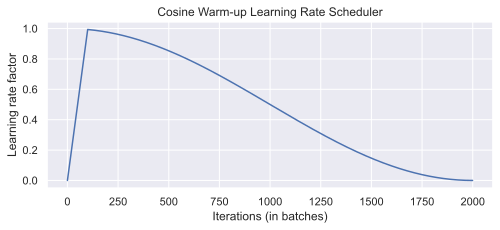
\includegraphics[keepaspectratio]{002_awwe_files/figure-pdf/cell-14-output-1.pdf}}

\begin{itemize}
\tightlist
\item
  Using a global colormap indicates that these variables have minor
  effects on the wing weight.
\item
  Important factors can be detected by visual inspection
\item
  Plotting the Big Picture: we can plot all 36 combinations in one
  figure.
\end{itemize}

\begin{Shaded}
\begin{Highlighting}[]
\NormalTok{fig }\OperatorTok{=}\NormalTok{ plt.figure(figsize}\OperatorTok{=}\NormalTok{(}\FloatTok{20.}\NormalTok{, }\FloatTok{20.}\NormalTok{))}
\NormalTok{grid }\OperatorTok{=}\NormalTok{ ImageGrid(fig, }\DecValTok{111}\NormalTok{,  }\CommentTok{\# similar to subplot(111)}
\NormalTok{                 nrows\_ncols}\OperatorTok{=}\NormalTok{(}\DecValTok{6}\NormalTok{,}\DecValTok{6}\NormalTok{),  }\CommentTok{\# creates 2x2 grid of axes}
\NormalTok{                 axes\_pad}\OperatorTok{=}\FloatTok{0.5}\NormalTok{,  }\CommentTok{\# pad between axes in inch.}
\NormalTok{                 share\_all}\OperatorTok{=}\VariableTok{True}\NormalTok{,}
\NormalTok{                 label\_mode}\OperatorTok{=}\StringTok{"all"}\NormalTok{,}
\NormalTok{                 ) }
\NormalTok{i }\OperatorTok{=} \DecValTok{0}
\ControlFlowTok{for}\NormalTok{ ax, im }\KeywordTok{in} \BuiltInTok{zip}\NormalTok{(grid, Z):}
    \CommentTok{\# Iterating over the grid returns the Axes.}
\NormalTok{    ax.set\_xlabel(Zlab[i][}\DecValTok{0}\NormalTok{])}
\NormalTok{    ax.set\_ylabel(Zlab[i][}\DecValTok{1}\NormalTok{])}
    \CommentTok{\# ax.set\_title(Zlab[i][1] + " vs. " + Zlab[i][0])}
\NormalTok{    ax.contourf(X, Y, im, }\DecValTok{30}\NormalTok{, cmap }\OperatorTok{=} \StringTok{"jet"}\NormalTok{,  vmin }\OperatorTok{=} \DecValTok{180}\NormalTok{, vmax }\OperatorTok{=} \DecValTok{360}\NormalTok{)}
\NormalTok{    i }\OperatorTok{=}\NormalTok{ i }\OperatorTok{+} \DecValTok{1}
       
\NormalTok{plt.show()}
\end{Highlighting}
\end{Shaded}

\pandocbounded{\includegraphics[keepaspectratio]{002_awwe_files/figure-pdf/cell-15-output-1.pdf}}

\section{AWWE Landscape}\label{awwe-landscape}

\begin{itemize}
\tightlist
\item
  Our Observations

  \begin{enumerate}
  \def\labelenumi{\arabic{enumi}.}
  \tightlist
  \item
    The load factor \(N_z\), which determines the magnitude of the
    maximum aerodynamic load on the wing, is very active and involved in
    interactions with other variables.
  \end{enumerate}

  \begin{itemize}
  \tightlist
  \item
    Classic example: the interaction of \(N_z\) with the aspect ratio
    \(A\) indicates a heavy wing for high aspect ratios and large
    \(g\)-forces
  \item
    This is the reaon why highly manoeuvrable fighter jets cannot have
    very efficient, glider wings)
  \end{itemize}

  \begin{enumerate}
  \def\labelenumi{\arabic{enumi}.}
  \setcounter{enumi}{1}
  \tightlist
  \item
    Aspect ratio \(A\) and airfoil thickness to chord ratio \(R_{tc}\)
    have nonlinear interactions.
  \item
    Most important variables:
  \end{enumerate}

  \begin{itemize}
  \tightlist
  \item
    Ultimate load factor \(N_z\), wing area \(S_w\), and flight design
    gross weight\(W_{dg}\).
  \end{itemize}

  \begin{enumerate}
  \def\labelenumi{\arabic{enumi}.}
  \setcounter{enumi}{3}
  \tightlist
  \item
    Little impact: dynamic pressure \(q\), taper ratio \(l\), and
    quarter-chord sweep \(L\).
  \end{enumerate}
\item
  Expert Knowledge

  \begin{itemize}
  \tightlist
  \item
    Aircraft designers know that the overall weight of the aircraft and
    the wing area must be kept to a minimum
  \item
    the latter usually dictated by constraints such as required stall
    speed, landing distance, turn rate, etc.
  \end{itemize}
\end{itemize}

\section{Summary of the First
Experiments}\label{summary-of-the-first-experiments}

\begin{itemize}
\tightlist
\item
  First, we considered two pairs of inputs, out of 36 total pairs
\item
  Then, the ``Big Picture'':

  \begin{itemize}
  \tightlist
  \item
    For each pair we evaluated \texttt{wingwt} 10,000 times
  \end{itemize}
\item
  Doing the same for all pairs would require 360K evaluations:

  \begin{itemize}
  \tightlist
  \item
    not a reasonable number with a real computer simulation that takes
    any non-trivial amount of time to evaluate
  \item
    Only 1s per evaluation: \(>100\) hours
  \end{itemize}
\item
  Many solvers take minutes/hours/days to execute a single run
\item
  And: three-way interactions?
\item
  Consequence: a different strategy is needed
\end{itemize}

\section{Exercise}\label{exercise}

\subsection{Adding Paint Weight}\label{adding-paint-weight}

\begin{itemize}
\tightlist
\item
  Paint weight is not considered.
\item
  Add Paint Weight \(W_p\) to formula (the updated formula is shown
  below) and update the functions and plots in the notebook.
\end{itemize}

\[ W = 0.036S_W^{0.758} \times W_{fw}^{0.0035} \times \left( \frac{A}{\cos^2 \Lambda} \right)^{0.6} \times q^{0.006} \times \lambda^{0.04} \]
\[ \times \left( \frac{100 R_{tc}}{\cos \Lambda} \right)^{-0.3} \times (N_z W_{dg})^{0.49} + S_w W_p\]

\section{Jupyter Notebook}\label{jupyter-notebook}

\begin{tcolorbox}[enhanced jigsaw, toptitle=1mm, opacityback=0, rightrule=.15mm, colframe=quarto-callout-note-color-frame, toprule=.15mm, opacitybacktitle=0.6, left=2mm, arc=.35mm, breakable, colbacktitle=quarto-callout-note-color!10!white, coltitle=black, bottomrule=.15mm, titlerule=0mm, bottomtitle=1mm, title=\textcolor{quarto-callout-note-color}{\faInfo}\hspace{0.5em}{Note}, leftrule=.75mm, colback=white]

\begin{itemize}
\tightlist
\item
  The Jupyter-Notebook of this lecture is available on GitHub in the
  \href{https://github.com/sequential-parameter-optimization/Hyperparameter-Tuning-Cookbook/blob/main/002_awwe.ipynb}{Hyperparameter-Tuning-Cookbook
  Repository}
\end{itemize}

\end{tcolorbox}

\chapter{\texorpdfstring{Introduction to
\texttt{scipy.optimize}}{Introduction to scipy.optimize}}\label{introduction-to-scipy.optimize}

\href{https://scipy.org}{SciPy} provides algorithms for optimization,
integration, interpolation, eigenvalue problems, algebraic equations,
differential equations, statistics and many other classes of problems.
SciPy is a collection of mathematical algorithms and convenience
functions built on NumPy. It adds significant power to Python by
providing the user with high-level commands and classes for manipulating
and visualizing data.

\href{https://docs.scipy.org/doc/scipy/reference/optimize.html\#module-scipy.optimize}{SciPy
optimize} provides functions for minimizing (or maximizing) objective
functions, possibly subject to constraints. It includes solvers for
nonlinear problems (with support for both local and global optimization
algorithms), linear programing, constrained and nonlinear least-squares,
root finding, and curve fitting.

In this notebook, we will learn how to use the \texttt{scipy.optimize}
module to solve optimization problems. See:
\url{https://docs.scipy.org/doc/scipy/tutorial/optimize.html}

\begin{tcolorbox}[enhanced jigsaw, toptitle=1mm, opacityback=0, rightrule=.15mm, colframe=quarto-callout-note-color-frame, toprule=.15mm, opacitybacktitle=0.6, left=2mm, arc=.35mm, breakable, colbacktitle=quarto-callout-note-color!10!white, coltitle=black, bottomrule=.15mm, titlerule=0mm, bottomtitle=1mm, title=\textcolor{quarto-callout-note-color}{\faInfo}\hspace{0.5em}{Note}, leftrule=.75mm, colback=white]

\begin{itemize}
\tightlist
\item
  This content is based on information from the scipy.optimize package.
\item
  The \texttt{scipy.optimize} package provides several commonly used
  optimization algorithms. A detailed listing is available in
  \texttt{scipy.optimize} (can also be found by
  \texttt{help(scipy.optimize)}).
\end{itemize}

\end{tcolorbox}

Common functions and objects, shared across different SciPy optimize
solvers, are shown in Table~\ref{tbl-shared-functions}.

\begin{longtable}[]{@{}
  >{\raggedright\arraybackslash}p{(\linewidth - 2\tabcolsep) * \real{0.5000}}
  >{\raggedright\arraybackslash}p{(\linewidth - 2\tabcolsep) * \real{0.5000}}@{}}
\caption{Common functions and objects, shared across different SciPy
optimize solvers}\label{tbl-shared-functions}\tabularnewline
\toprule\noalign{}
\begin{minipage}[b]{\linewidth}\raggedright
Function or Object
\end{minipage} & \begin{minipage}[b]{\linewidth}\raggedright
Description
\end{minipage} \\
\midrule\noalign{}
\endfirsthead
\toprule\noalign{}
\begin{minipage}[b]{\linewidth}\raggedright
Function or Object
\end{minipage} & \begin{minipage}[b]{\linewidth}\raggedright
Description
\end{minipage} \\
\midrule\noalign{}
\endhead
\bottomrule\noalign{}
\endlastfoot
\href{https://docs.scipy.org/doc/scipy/reference/generated/scipy.optimize.show_options.html\#scipy.optimize.show_options}{show\_options({[}solver,
method, disp{]})} & Show documentation for additional options of
optimization solvers. \\
\href{https://docs.scipy.org/doc/scipy/reference/generated/scipy.optimize.OptimizeResult.html\#scipy.optimize.OptimizeResult}{OptimizeResult}
& Represents the optimization result. \\
\href{https://docs.scipy.org/doc/scipy/reference/generated/scipy.optimize.OptimizeWarning.html\#scipy.optimize.OptimizeWarning}{OptimizeWarning}
& Warning issued by solvers. \\
\end{longtable}

We will introduce unconstrained minimization of multivariate scalar
functions in this chapter. The
\href{https://docs.scipy.org/doc/scipy/reference/generated/scipy.optimize.minimize.html\#scipy.optimize.minimize}{minimize}
function provides a common interface to unconstrained and constrained
minimization algorithms for multivariate scalar functions in
\texttt{scipy.optimize}. To demonstrate the minimization function,
consider the problem of minimizing the Rosenbrock function of \emph{N}
variables:

\[
f(J) = \sum_{i=1}^{N-1} 100 (x_{i+1} - x_i^2)^2 + (1 - x_i)^2
\]

The minimum value of this function is 0, which is achieved when (x\_i =
1).

Note that the Rosenbrock function and its derivatives are included in
\texttt{scipy.optimize}. The implementations shown in the following
sections provide examples of how to define an objective function as well
as its Jacobian and Hessian functions. Objective functions in
\texttt{scipy.optimize} expect a numpy array as their first parameter,
which is to be optimized and must return a float value. The exact
calling signature must be \texttt{f(x,\ *args)}, where \texttt{x}
represents a numpy array, and \texttt{args} is a tuple of additional
arguments supplied to the objective function.

\section{Derivative-free Optimization
Algorithms}\label{derivative-free-optimization-algorithms}

Section~\ref{sec-nelder-mead-simplex-algorithm} and
Section~\ref{sec-powells-method} present two approaches that do not need
gradient information to find the minimum. They use function evaluations
to find the minimum.

\subsection{Nelder-Mead Simplex
Algorithm}\label{sec-nelder-mead-simplex-algorithm}

The Nelder Mead is a simple local optimization algorithm. It requires
only function evaluations and is a good choice for simple minimization
problems. However, because it does not use any gradient evaluations, it
may take longer to find the minimum. It can be devided into the
following steps:

\begin{enumerate}
\def\labelenumi{\arabic{enumi}.}
\tightlist
\item
  Initialize the simplex
\item
  Evaluate the function at each vertex of the simplex
\item
  Order the vertices by function value
\item
  \textbf{Reflect} the worst point through the centroid of the remaining
  points
\item
  If the reflected point is better than the second worst, replace the
  worst point with the reflected point
\item
  If the reflected point is worse than the worst point, try
  \textbf{contracting} the simplex
\item
  If the reflected point is better than the best point, try
  \textbf{expanding} the simplex
\item
  If none of the above steps improve the simplex, \textbf{shrink} the
  simplex towards the best point
\item
  Check for convergence
\end{enumerate}

\texttt{method=\textquotesingle{}Nelder-Mead\textquotesingle{}}: In the
example below, the \texttt{minimize} routine is used with the
\emph{Nelder-Mead} simplex algorithm (selected through the
\texttt{method} parameter):

\begin{Shaded}
\begin{Highlighting}[]
\ImportTok{import}\NormalTok{ numpy }\ImportTok{as}\NormalTok{ np}
\ImportTok{from}\NormalTok{ scipy.optimize }\ImportTok{import}\NormalTok{ minimize}

\KeywordTok{def}\NormalTok{ rosen(x):}
    \CommentTok{"""The Rosenbrock function"""}
    \ControlFlowTok{return} \BuiltInTok{sum}\NormalTok{(}\FloatTok{100.0} \OperatorTok{*}\NormalTok{ (x[}\DecValTok{1}\NormalTok{:] }\OperatorTok{{-}}\NormalTok{ x[:}\OperatorTok{{-}}\DecValTok{1}\NormalTok{]}\OperatorTok{**}\FloatTok{2.0}\NormalTok{)}\OperatorTok{**}\FloatTok{2.0} \OperatorTok{+}\NormalTok{ (}\DecValTok{1} \OperatorTok{{-}}\NormalTok{ x[:}\OperatorTok{{-}}\DecValTok{1}\NormalTok{])}\OperatorTok{**}\FloatTok{2.0}\NormalTok{)}

\NormalTok{x0 }\OperatorTok{=}\NormalTok{ np.array([}\FloatTok{1.3}\NormalTok{, }\FloatTok{0.7}\NormalTok{, }\FloatTok{0.8}\NormalTok{, }\FloatTok{1.9}\NormalTok{, }\FloatTok{1.2}\NormalTok{])}
\NormalTok{res }\OperatorTok{=}\NormalTok{ minimize(rosen, x0, method}\OperatorTok{=}\StringTok{\textquotesingle{}nelder{-}mead\textquotesingle{}}\NormalTok{,}
\NormalTok{               options}\OperatorTok{=}\NormalTok{\{}\StringTok{\textquotesingle{}xatol\textquotesingle{}}\NormalTok{: }\FloatTok{1e{-}8}\NormalTok{, }\StringTok{\textquotesingle{}disp\textquotesingle{}}\NormalTok{: }\VariableTok{True}\NormalTok{\})}

\BuiltInTok{print}\NormalTok{(res.x)}
\end{Highlighting}
\end{Shaded}

\begin{verbatim}
Optimization terminated successfully.
         Current function value: 0.000000
         Iterations: 339
         Function evaluations: 571
[1. 1. 1. 1. 1.]
\end{verbatim}

The simplex algorithm is probably the simplest way to minimize a
well-behaved function. It requires only function evaluations and is a
good choice for simple minimization problems. However, because it does
not use any gradient evaluations, it may take longer to find the
minimum.

\subsection{Powell's Method}\label{sec-powells-method}

Another optimization algorithm that needs only function calls to find
the minimum is \emph{Powell}'s method, which can be selected by setting
the \texttt{method} parameter to
\texttt{\textquotesingle{}powell\textquotesingle{}} in the
\texttt{minimize} function. This algorithm consists of a conjugate
direction method. It performs sequential one-dimensional minimizations
along each vector of the directions set, which is updated at each
iteration of the main minimization loop. It can be described by the
following steps:

\begin{enumerate}
\def\labelenumi{\arabic{enumi}.}
\tightlist
\item
  Initialization
\item
  Minimization along each direction
\item
  Create conjugate direction
\item
  Line search along the conjugate direction
\item
  Check for convergence
\end{enumerate}

\begin{example}[]\protect\hypertarget{exm-powells-method}{}\label{exm-powells-method}

To demonstrate how to supply additional arguments to an objective
function, let's consider minimizing the Rosenbrock function with an
additional scaling factor \(a\) and an offset \(b\):

\[
f(J, a, b) = \sum_{i=1}^{N-1} a (x_{i+1} - x_i^2)^2 + (1 - x_i)^2 + b
\]

You can achieve this using the \texttt{minimize} routine with the
example parameters \(a=0.5\) and \(b=1\):

\begin{Shaded}
\begin{Highlighting}[]
\KeywordTok{def}\NormalTok{ rosen\_with\_args(x, a, b):}
    \CommentTok{"""The Rosenbrock function with additional arguments"""}
    \ControlFlowTok{return} \BuiltInTok{sum}\NormalTok{(a }\OperatorTok{*}\NormalTok{ (x[}\DecValTok{1}\NormalTok{:] }\OperatorTok{{-}}\NormalTok{ x[:}\OperatorTok{{-}}\DecValTok{1}\NormalTok{]}\OperatorTok{**}\FloatTok{2.0}\NormalTok{)}\OperatorTok{**}\FloatTok{2.0} \OperatorTok{+}\NormalTok{ (}\DecValTok{1} \OperatorTok{{-}}\NormalTok{ x[:}\OperatorTok{{-}}\DecValTok{1}\NormalTok{])}\OperatorTok{**}\FloatTok{2.0}\NormalTok{) }\OperatorTok{+}\NormalTok{ b}

\NormalTok{x0 }\OperatorTok{=}\NormalTok{ np.array([}\FloatTok{1.3}\NormalTok{, }\FloatTok{0.7}\NormalTok{, }\FloatTok{0.8}\NormalTok{, }\FloatTok{1.9}\NormalTok{, }\FloatTok{1.2}\NormalTok{])}
\NormalTok{res }\OperatorTok{=}\NormalTok{ minimize(rosen\_with\_args, x0, method}\OperatorTok{=}\StringTok{\textquotesingle{}nelder{-}mead\textquotesingle{}}\NormalTok{,}
\NormalTok{               args}\OperatorTok{=}\NormalTok{(}\FloatTok{0.5}\NormalTok{, }\FloatTok{1.}\NormalTok{), options}\OperatorTok{=}\NormalTok{\{}\StringTok{\textquotesingle{}xatol\textquotesingle{}}\NormalTok{: }\FloatTok{1e{-}8}\NormalTok{, }\StringTok{\textquotesingle{}disp\textquotesingle{}}\NormalTok{: }\VariableTok{True}\NormalTok{\})}

\BuiltInTok{print}\NormalTok{(res.x)}
\end{Highlighting}
\end{Shaded}

\begin{verbatim}
Optimization terminated successfully.
         Current function value: 1.000000
         Iterations: 319
         Function evaluations: 525
[1.         1.         1.         1.         0.99999999]
\end{verbatim}

As an alternative to using the \texttt{args} parameter of
\texttt{minimize}, you can wrap the objective function in a new function
that accepts only \texttt{x}. This approach is also useful when it is
necessary to pass additional parameters to the objective function as
keyword arguments.

\begin{Shaded}
\begin{Highlighting}[]
\KeywordTok{def}\NormalTok{ rosen\_with\_args(x, a, }\OperatorTok{*}\NormalTok{, b):  }\CommentTok{\# b is a keyword{-}only argument}
    \ControlFlowTok{return} \BuiltInTok{sum}\NormalTok{(a }\OperatorTok{*}\NormalTok{ (x[}\DecValTok{1}\NormalTok{:] }\OperatorTok{{-}}\NormalTok{ x[:}\OperatorTok{{-}}\DecValTok{1}\NormalTok{]}\OperatorTok{**}\FloatTok{2.0}\NormalTok{)}\OperatorTok{**}\FloatTok{2.0} \OperatorTok{+}\NormalTok{ (}\DecValTok{1} \OperatorTok{{-}}\NormalTok{ x[:}\OperatorTok{{-}}\DecValTok{1}\NormalTok{])}\OperatorTok{**}\FloatTok{2.0}\NormalTok{) }\OperatorTok{+}\NormalTok{ b}

\KeywordTok{def}\NormalTok{ wrapped\_rosen\_without\_args(x):}
    \ControlFlowTok{return}\NormalTok{ rosen\_with\_args(x, }\FloatTok{0.5}\NormalTok{, b}\OperatorTok{=}\FloatTok{1.}\NormalTok{)  }\CommentTok{\# pass in \textasciigrave{}a\textasciigrave{} and \textasciigrave{}b\textasciigrave{}}

\NormalTok{x0 }\OperatorTok{=}\NormalTok{ np.array([}\FloatTok{1.3}\NormalTok{, }\FloatTok{0.7}\NormalTok{, }\FloatTok{0.8}\NormalTok{, }\FloatTok{1.9}\NormalTok{, }\FloatTok{1.2}\NormalTok{])}
\NormalTok{res }\OperatorTok{=}\NormalTok{ minimize(wrapped\_rosen\_without\_args, x0, method}\OperatorTok{=}\StringTok{\textquotesingle{}nelder{-}mead\textquotesingle{}}\NormalTok{,}
\NormalTok{               options}\OperatorTok{=}\NormalTok{\{}\StringTok{\textquotesingle{}xatol\textquotesingle{}}\NormalTok{: }\FloatTok{1e{-}8}\NormalTok{,\})}

\BuiltInTok{print}\NormalTok{(res.x)}
\end{Highlighting}
\end{Shaded}

\begin{verbatim}
[1.         1.         1.         1.         0.99999999]
\end{verbatim}

Another alternative is to use \texttt{functools.partial}.

\begin{Shaded}
\begin{Highlighting}[]
\ImportTok{from}\NormalTok{ functools }\ImportTok{import}\NormalTok{ partial}

\NormalTok{partial\_rosen }\OperatorTok{=}\NormalTok{ partial(rosen\_with\_args, a}\OperatorTok{=}\FloatTok{0.5}\NormalTok{, b}\OperatorTok{=}\FloatTok{1.}\NormalTok{)}
\NormalTok{res }\OperatorTok{=}\NormalTok{ minimize(partial\_rosen, x0, method}\OperatorTok{=}\StringTok{\textquotesingle{}nelder{-}mead\textquotesingle{}}\NormalTok{,}
\NormalTok{               options}\OperatorTok{=}\NormalTok{\{}\StringTok{\textquotesingle{}xatol\textquotesingle{}}\NormalTok{: }\FloatTok{1e{-}8}\NormalTok{,\})}

\BuiltInTok{print}\NormalTok{(res.x)}
\end{Highlighting}
\end{Shaded}

\begin{verbatim}
[1.         1.         1.         1.         0.99999999]
\end{verbatim}

\end{example}

\section{Gradient-based Optimization
Algorithms}\label{gradient-based-optimization-algorithms}

\subsection{An Introductory Example: Broyden-Fletcher-Goldfarb-Shanno
Algorithm (BFGS)}\label{sec-bfgs-intro}

This section introduces an optimization algorithm that uses gradient
information to find the minimum. The Broyden-Fletcher-Goldfarb-Shanno
(BFGS) algorithm (selected by setting
\texttt{method=\textquotesingle{}BFGS\textquotesingle{}}) is an
optimization algorithm that aims to converge quickly to the solution.
This algorithm uses the gradient of the objective function. If the
gradient is not provided by the user, it is estimated using
first-differences. The BFGS method typically requires fewer function
calls compared to the simplex algorithm, even when the gradient needs to
be estimated.

\begin{example}[BFGS]\protect\hypertarget{exm-bfgs}{}\label{exm-bfgs}

To demonstrate the BFGS algorithm, let's use the Rosenbrock function
again. The gradient of the Rosenbrock function is a vector described by
the following mathematical expression:

\begin{align}
\frac{\partial f}{\partial x_j} = \sum_{i=1}^{N} 200(x_i - x_{i-1}^2)(\delta_{i,j} - 2x_{i-1}\delta_{i-1,j}) - 2(1 - x_{i-1})\delta_{i-1,j} \\
= 200(x_j - x_{j-1}^2) - 400x_j(x_{j+1} - x_j^2) - 2(1 - x_j)
\end{align}

This expression is valid for interior derivatives, but special cases
are:

\[
\frac{\partial f}{\partial x_0} = -400x_0(x_1 - x_0^2) - 2(1 - x_0)
\]

\[
\frac{\partial f}{\partial x_{N-1}} = 200(x_{N-1} - x_{N-2}^2)
\]

Here's a Python function that computes this gradient:

\begin{Shaded}
\begin{Highlighting}[]
\KeywordTok{def}\NormalTok{ rosen\_der(x):}
\NormalTok{    xm }\OperatorTok{=}\NormalTok{ x[}\DecValTok{1}\NormalTok{:}\OperatorTok{{-}}\DecValTok{1}\NormalTok{]}
\NormalTok{    xm\_m1 }\OperatorTok{=}\NormalTok{ x[:}\OperatorTok{{-}}\DecValTok{2}\NormalTok{]}
\NormalTok{    xm\_p1 }\OperatorTok{=}\NormalTok{ x[}\DecValTok{2}\NormalTok{:]}
\NormalTok{    der }\OperatorTok{=}\NormalTok{ np.zeros\_like(x)}
\NormalTok{    der[}\DecValTok{1}\NormalTok{:}\OperatorTok{{-}}\DecValTok{1}\NormalTok{] }\OperatorTok{=} \DecValTok{200}\OperatorTok{*}\NormalTok{(xm}\OperatorTok{{-}}\NormalTok{xm\_m1}\OperatorTok{**}\DecValTok{2}\NormalTok{) }\OperatorTok{{-}} \DecValTok{400}\OperatorTok{*}\NormalTok{(xm\_p1 }\OperatorTok{{-}}\NormalTok{ xm}\OperatorTok{**}\DecValTok{2}\NormalTok{)}\OperatorTok{*}\NormalTok{xm }\OperatorTok{{-}} \DecValTok{2}\OperatorTok{*}\NormalTok{(}\DecValTok{1}\OperatorTok{{-}}\NormalTok{xm)}
\NormalTok{    der[}\DecValTok{0}\NormalTok{] }\OperatorTok{=} \OperatorTok{{-}}\DecValTok{400}\OperatorTok{*}\NormalTok{x[}\DecValTok{0}\NormalTok{]}\OperatorTok{*}\NormalTok{(x[}\DecValTok{1}\NormalTok{]}\OperatorTok{{-}}\NormalTok{x[}\DecValTok{0}\NormalTok{]}\OperatorTok{**}\DecValTok{2}\NormalTok{) }\OperatorTok{{-}} \DecValTok{2}\OperatorTok{*}\NormalTok{(}\DecValTok{1}\OperatorTok{{-}}\NormalTok{x[}\DecValTok{0}\NormalTok{])}
\NormalTok{    der[}\OperatorTok{{-}}\DecValTok{1}\NormalTok{] }\OperatorTok{=} \DecValTok{200}\OperatorTok{*}\NormalTok{(x[}\OperatorTok{{-}}\DecValTok{1}\NormalTok{]}\OperatorTok{{-}}\NormalTok{x[}\OperatorTok{{-}}\DecValTok{2}\NormalTok{]}\OperatorTok{**}\DecValTok{2}\NormalTok{)}
    \ControlFlowTok{return}\NormalTok{ der}
\end{Highlighting}
\end{Shaded}

You can specify this gradient information in the minimize function using
the jac parameter as illustrated below:

\begin{Shaded}
\begin{Highlighting}[]
\NormalTok{res }\OperatorTok{=}\NormalTok{ minimize(rosen, x0, method}\OperatorTok{=}\StringTok{\textquotesingle{}BFGS\textquotesingle{}}\NormalTok{, jac}\OperatorTok{=}\NormalTok{rosen\_der,}
\NormalTok{               options}\OperatorTok{=}\NormalTok{\{}\StringTok{\textquotesingle{}disp\textquotesingle{}}\NormalTok{: }\VariableTok{True}\NormalTok{\})}

\BuiltInTok{print}\NormalTok{(res.x)}
\end{Highlighting}
\end{Shaded}

\begin{verbatim}
Optimization terminated successfully.
         Current function value: 0.000000
         Iterations: 25
         Function evaluations: 30
         Gradient evaluations: 30
[1.00000004 1.0000001  1.00000021 1.00000044 1.00000092]
\end{verbatim}

\end{example}

\subsection{Background and Basics for Gradient-based
Optimization}\label{background-and-basics-for-gradient-based-optimization}

\subsection{Gradient}\label{gradient}

The gradient \(\nabla f(J)\) for a scalar function \(f(J)\) with \(n\)
different variables is defined by its partial derivatives:

\[
\nabla f(J) = \left[ \frac{\partial f}{\partial x_1}, \frac{\partial f}{\partial x_2}, \ldots, \frac{\partial f}{\partial x_n} \right]
\]

\subsection{Jacobian Matrix}\label{jacobian-matrix}

The Jacobian matrix \(J(J)\) for a vector-valued function
\(F(J) = [f_1(J), f_2(J), \ldots, f_m(J)]\) is defined as:

\(J(J) = \begin{bmatrix} \frac{\partial f_1}{\partial x_1} & \frac{\partial f_1}{\partial x_2} & \ldots & \frac{\partial f_1}{\partial x_n} \\ \frac{\partial f_2}{\partial x_1} & \frac{\partial f_2}{\partial x_2} & \ldots & \frac{\partial f_2}{\partial x_n} \\ \vdots & \vdots & \ddots & \vdots \\ \frac{\partial f_m}{\partial x_1} & \frac{\partial f_m}{\partial x_2} & \ldots & \frac{\partial f_m}{\partial x_n} \end{bmatrix}\)

It consists of the first order partial derivatives and gives therefore
an overview about the gradients of a vector valued function.

\begin{example}[acobian
matrix]\protect\hypertarget{exm-jacobian}{}\label{exm-jacobian}

Consider a vector-valued function
\(f : \mathbb{R}^2 \rightarrow \mathbb{R}^3\) defined as follows:
\[f(J) = \begin{bmatrix} x_1^2 + 2x_2 \\ 3x_1 - \sin(x_2) \\ e^{x_1 + x_2} \end{bmatrix}\]

Let's compute the partial derivatives and construct the Jacobian matrix:

\(\frac{\partial f_1}{\partial x_1} = 2x_1, \quad \frac{\partial f_1}{\partial x_2} = 2\)

\(\frac{\partial f_2}{\partial x_1} = 3, \quad \frac{\partial f_2}{\partial x_2} = -\cos(x_2)\)

\(\frac{\partial f_3}{\partial x_1} = e^{x_1 + x_2}, \quad \frac{\partial f_3}{\partial x_2} = e^{x_1 + x_2}\)

So, the Jacobian matrix is:

\[J(J) = \begin{bmatrix} 2x_1 & 2 \\ 3 & -\cos(x_2) \\ e^{x_1 + x_2} & e^{x_1 + x_2} \end{bmatrix}\]

This Jacobian matrix provides information about how small changes in the
input variables \(x_1\) and \(x_2\) affect the corresponding changes in
each component of the output vector.

\end{example}

\subsection{Hessian Matrix}\label{hessian-matrix}

The Hessian matrix \(H(J)\) for a scalar function \(f(J)\) is defined
as:

\(H(J) = \begin{bmatrix} \frac{\partial^2 f}{\partial x_1^2} & \frac{\partial^2 f}{\partial x_1 \partial x_2} & \ldots & \frac{\partial^2 f}{\partial x_1 \partial x_n} \\ \frac{\partial^2 f}{\partial x_2 \partial x_1} & \frac{\partial^2 f}{\partial x_2^2} & \ldots & \frac{\partial^2 f}{\partial x_2 \partial x_n} \\ \vdots & \vdots & \ddots & \vdots \\ \frac{\partial^2 f}{\partial x_n \partial x_1} & \frac{\partial^2 f}{\partial x_n \partial x_2} & \ldots & \frac{\partial^2 f}{\partial x_n^2} \end{bmatrix}\)

The Hessian matrix consists of the second order derivatives of the
function. It provides information about the local curvature of the
function with respect to changes in the input variables.

\begin{example}[Hessian
matrix]\protect\hypertarget{exm-hessian}{}\label{exm-hessian}

Consider a scalar-valued function:
\[f(J) = x_1^2 + 2x_2^2 + \sin(x_1   x_2)\]

The Hessian matrix of this scalar-valued function is the matrix of its
second-order partial derivatives with respect to the input variables:
\[H(J) = \begin{bmatrix} \frac{\partial^2 f}{\partial x_1^2} & \frac{\partial^2 f}{\partial x_1 \partial x_2} \\ \frac{\partial^2 f}{\partial x_2 \partial x_1} & \frac{\partial^2 f}{\partial x_2^2} \end{bmatrix}\]

Let's compute the second-order partial derivatives and construct the
Hessian matrix:

\begin{align}
\frac{\partial^2 f}{\partial x_1^2} &= 2 + \cos(x_1 x_2) x_2^2\\
\frac{\partial^2 f}{\partial x_1 \partial x_2} &= 2x_1  x_2 \cos(x_1 x_2) - \sin(x_1  x_2)\\
\frac{\partial^2 f}{\partial x_2 \partial x_1} &= 2x_1  x_2  \cos(x_1  x_2) - \sin(x_1  x_2)\\
\frac{\partial^2 f}{\partial x_2^2} &= 4x_2^2 + \cos(x_1  x_2) x_1^2
\end{align}

So, the Hessian matrix is:

\[H(J) = \begin{bmatrix} 2 + \cos(x_1   x_2)   x_2^2 & 2x_1   x_2   \cos(x_1   x_2) - \sin(x_1   x_2) \\ 2x_1   x_2   \cos(x_1   x_2) - \sin(x_1   x_2) & 4x_2^2 + \cos(x_1   x_2)   x_1^2 \end{bmatrix}\]

\end{example}

\subsection{Gradient Descent}\label{gradient-descent}

In optimization, the goal is to find the minimum or maximum of a
function. Gradient-based optimization methods utilize information about
the gradient (or derivative) of the function to guide the search for the
optimal solution. This is particularly useful when dealing with complex,
high-dimensional functions where an exhaustive search is impractical.

The gradient descent method can be divided in the following steps:

\begin{itemize}
\tightlist
\item
  \textbf{Initialize:} start with an initial guess for the parameters of
  the function to be optimized.
\item
  \textbf{Compute Gradient:} Calculate the gradient (partial
  derivatives) of the function with respect to each parameter at the
  current point. The gradient indicates the direction of the steepest
  increase in the function.
\item
  \textbf{Update Parameters:} Adjust the parameters in the opposite
  direction of the gradient, scaled by a learning rate. This step aims
  to move towards the minimum of the function:

  \begin{itemize}
  \tightlist
  \item
    \(x_{k+1} = x_k - \alpha \times \nabla f(x_{k})\)
  \item
    \(x_{x}\) is current parameter vector or point in the parameter
    space.
  \item
    \(\alpha\) is the learning rate, a positive scalar that determines
    the step size in each iteration.
  \item
    \(\nabla f(x)\) is the gradient of the objective function.
  \end{itemize}
\item
  \textbf{Iterate:} Repeat the above steps until convergence or a
  predefined number of iterations. Convergence is typically determined
  when the change in the function value or parameters becomes
  negligible.
\end{itemize}

\begin{example}[Gradient
Descent]\protect\hypertarget{exm-gradient-descent}{}\label{exm-gradient-descent}

We consider a simple quadratic function as an example: \[
f(x) = x^2 + 4x + y^2 + 2y + 4.
\]

We'll use gradient descent to find the minimum of this function.

\begin{Shaded}
\begin{Highlighting}[]
\ImportTok{import}\NormalTok{ numpy }\ImportTok{as}\NormalTok{ np}
\ImportTok{import}\NormalTok{ matplotlib.pyplot }\ImportTok{as}\NormalTok{ plt}
\ImportTok{from}\NormalTok{ mpl\_toolkits.mplot3d }\ImportTok{import}\NormalTok{ Axes3D}

\CommentTok{\# Define the quadratic function}
\KeywordTok{def}\NormalTok{ quadratic\_function(x, y):}
    \ControlFlowTok{return}\NormalTok{ x}\OperatorTok{**}\DecValTok{2} \OperatorTok{+} \DecValTok{4}\OperatorTok{*}\NormalTok{x }\OperatorTok{+}\NormalTok{ y}\OperatorTok{**}\DecValTok{2} \OperatorTok{+} \DecValTok{2}\OperatorTok{*}\NormalTok{y }\OperatorTok{+} \DecValTok{4}

\CommentTok{\# Define the gradient of the quadratic function}
\KeywordTok{def}\NormalTok{ gradient\_quadratic\_function(x, y):}
\NormalTok{    grad\_x }\OperatorTok{=} \DecValTok{2}\OperatorTok{*}\NormalTok{x }\OperatorTok{+} \DecValTok{4}
\NormalTok{    grad\_y }\OperatorTok{=} \DecValTok{2}\OperatorTok{*}\NormalTok{y }\OperatorTok{+} \DecValTok{2}
    \ControlFlowTok{return}\NormalTok{ np.array([grad\_x, grad\_y])}

\CommentTok{\# Gradient Descent for optimization in 2D}
\KeywordTok{def}\NormalTok{ gradient\_descent(initial\_point, learning\_rate, num\_iterations):}
\NormalTok{    points }\OperatorTok{=}\NormalTok{ [np.array(initial\_point)]}
    \ControlFlowTok{for}\NormalTok{ \_ }\KeywordTok{in} \BuiltInTok{range}\NormalTok{(num\_iterations):}
\NormalTok{        current\_point }\OperatorTok{=}\NormalTok{ points[}\OperatorTok{{-}}\DecValTok{1}\NormalTok{]}
\NormalTok{        gradient }\OperatorTok{=}\NormalTok{ gradient\_quadratic\_function(}\OperatorTok{*}\NormalTok{current\_point)}
\NormalTok{        new\_point }\OperatorTok{=}\NormalTok{ current\_point }\OperatorTok{{-}}\NormalTok{ learning\_rate }\OperatorTok{*}\NormalTok{ gradient}
\NormalTok{        points.append(new\_point)}
    \ControlFlowTok{return}\NormalTok{ points}

\CommentTok{\# Visualization of optimization process with 3D surface and consistent arrow sizes}
\KeywordTok{def}\NormalTok{ plot\_optimization\_process\_3d\_consistent\_arrows(points):}
\NormalTok{    fig }\OperatorTok{=}\NormalTok{ plt.figure(figsize}\OperatorTok{=}\NormalTok{(}\DecValTok{10}\NormalTok{, }\DecValTok{8}\NormalTok{))}
\NormalTok{    ax }\OperatorTok{=}\NormalTok{ fig.add\_subplot(}\DecValTok{111}\NormalTok{, projection}\OperatorTok{=}\StringTok{\textquotesingle{}3d\textquotesingle{}}\NormalTok{)}

\NormalTok{    x\_vals }\OperatorTok{=}\NormalTok{ np.linspace(}\OperatorTok{{-}}\DecValTok{10}\NormalTok{, }\DecValTok{2}\NormalTok{, }\DecValTok{100}\NormalTok{)}
\NormalTok{    y\_vals }\OperatorTok{=}\NormalTok{ np.linspace(}\OperatorTok{{-}}\DecValTok{10}\NormalTok{, }\DecValTok{2}\NormalTok{, }\DecValTok{100}\NormalTok{)}
\NormalTok{    X, Y }\OperatorTok{=}\NormalTok{ np.meshgrid(x\_vals, y\_vals)}
\NormalTok{    Z }\OperatorTok{=}\NormalTok{ quadratic\_function(X, Y)}

\NormalTok{    ax.plot\_surface(X, Y, Z, cmap}\OperatorTok{=}\StringTok{\textquotesingle{}viridis\textquotesingle{}}\NormalTok{, alpha}\OperatorTok{=}\FloatTok{0.6}\NormalTok{)}
\NormalTok{    ax.scatter(}\OperatorTok{*}\BuiltInTok{zip}\NormalTok{(}\OperatorTok{*}\NormalTok{points), [quadratic\_function(}\OperatorTok{*}\NormalTok{p) }\ControlFlowTok{for}\NormalTok{ p }\KeywordTok{in}\NormalTok{ points], c}\OperatorTok{=}\StringTok{\textquotesingle{}red\textquotesingle{}}\NormalTok{, label}\OperatorTok{=}\StringTok{\textquotesingle{}Optimization Trajectory\textquotesingle{}}\NormalTok{)}

    \ControlFlowTok{for}\NormalTok{ i }\KeywordTok{in} \BuiltInTok{range}\NormalTok{(}\BuiltInTok{len}\NormalTok{(points) }\OperatorTok{{-}} \DecValTok{1}\NormalTok{):  }
\NormalTok{        x, y }\OperatorTok{=}\NormalTok{ points[i]}
\NormalTok{        dx, dy }\OperatorTok{=}\NormalTok{ points[i }\OperatorTok{+} \DecValTok{1}\NormalTok{] }\OperatorTok{{-}}\NormalTok{ points[i]}
\NormalTok{        dz }\OperatorTok{=}\NormalTok{ quadratic\_function(}\OperatorTok{*}\NormalTok{(points[i }\OperatorTok{+} \DecValTok{1}\NormalTok{])) }\OperatorTok{{-}}\NormalTok{ quadratic\_function(}\OperatorTok{*}\NormalTok{points[i])}
\NormalTok{        gradient\_length }\OperatorTok{=} \FloatTok{0.5}

\NormalTok{        ax.quiver(x, y, quadratic\_function(}\OperatorTok{*}\NormalTok{points[i]), dx, dy, dz, color}\OperatorTok{=}\StringTok{\textquotesingle{}blue\textquotesingle{}}\NormalTok{, length}\OperatorTok{=}\NormalTok{gradient\_length, normalize}\OperatorTok{=}\VariableTok{False}\NormalTok{, arrow\_length\_ratio}\OperatorTok{=}\FloatTok{0.1}\NormalTok{)}

\NormalTok{    ax.set\_title(}\StringTok{\textquotesingle{}Gradient{-}Based Optimization with 2D Quadratic Function\textquotesingle{}}\NormalTok{)}
\NormalTok{    ax.set\_xlabel(}\StringTok{\textquotesingle{}x\textquotesingle{}}\NormalTok{)}
\NormalTok{    ax.set\_ylabel(}\StringTok{\textquotesingle{}y\textquotesingle{}}\NormalTok{)}
\NormalTok{    ax.set\_zlabel(}\StringTok{\textquotesingle{}f(x, y)\textquotesingle{}}\NormalTok{)}
\NormalTok{    ax.legend()}
\NormalTok{    plt.show()}

\CommentTok{\# Initial guess and parameters}
\NormalTok{initial\_guess }\OperatorTok{=}\NormalTok{ [}\OperatorTok{{-}}\FloatTok{9.0}\NormalTok{, }\OperatorTok{{-}}\FloatTok{9.0}\NormalTok{]}
\NormalTok{learning\_rate }\OperatorTok{=} \FloatTok{0.2}
\NormalTok{num\_iterations }\OperatorTok{=} \DecValTok{10}

\CommentTok{\# Run gradient descent in 2D and visualize the optimization process with 3D surface and consistent arrow sizes}
\NormalTok{trajectory }\OperatorTok{=}\NormalTok{ gradient\_descent(initial\_guess, learning\_rate, num\_iterations)}
\NormalTok{plot\_optimization\_process\_3d\_consistent\_arrows(trajectory)}
\end{Highlighting}
\end{Shaded}

\pandocbounded{\includegraphics[keepaspectratio]{003_scipy_optimize_intro_files/figure-pdf/cell-8-output-1.pdf}}

\end{example}

\subsection{Newton Method}\label{newton-method}

\textbf{Initialization:} Start with an initial guess for the optimal
solution: \(x_0\).

\textbf{Iteration:} Repeat the following three steps until convergence
or a predefined stopping criterion is met:

\begin{enumerate}
\def\labelenumi{\arabic{enumi}.}
\item
  Calculate the gradient (\(\nabla\)) and the Hessian matrix
  (\(\nabla^2\)) of the objective function at the current point:
  \[\nabla f(x_k) \quad \text{and} \quad \nabla^2 f(x_k)\]
\item
  Update the current solution using the Newton-Raphson update formula \[
   x_{k+1} = x_k - [\nabla^2 f(x_k)]^{-1} \nabla f(x_k),
   \] where

\begin{verbatim}
* $\nabla f(x_k)$ is the gradient (first derivative) of the objective function with respect to the variable $x$, evaluated at the current solution $x_k$.
\end{verbatim}

  \begin{itemize}
  \tightlist
  \item
    \(\nabla^2 f(x_k)\): The Hessian matrix (second derivative) of the
    objective function with respect to \(x\), evaluated at the current
    solution \(x_k\).
  \item
    \(x_k\): The current solution or point in the optimization process.
  \item
    \(\nabla^2 f(x_k)]^{-1}\): The inverse of the Hessian matrix at the
    current point, representing the approximation of the curvature of
    the objective function.
  \item
    \(x_{k+1}\): The updated solution or point after applying the
    Newton-Raphson update.
  \end{itemize}
\item
  Check for convergence.
\end{enumerate}

\begin{example}[Newton
Method]\protect\hypertarget{exm-newton-method}{}\label{exm-newton-method}

We want to optimize the Rosenbrock function and use the Hessian and the
Jacobian (which is equal to the gradient vector for scalar objective
function) to the \texttt{minimize} function.

\begin{Shaded}
\begin{Highlighting}[]
\KeywordTok{def}\NormalTok{ rosenbrock(x):}
    \ControlFlowTok{return} \DecValTok{100} \OperatorTok{*}\NormalTok{ (x[}\DecValTok{1}\NormalTok{] }\OperatorTok{{-}}\NormalTok{ x[}\DecValTok{0}\NormalTok{]}\OperatorTok{**}\DecValTok{2}\NormalTok{)}\OperatorTok{**}\DecValTok{2} \OperatorTok{+}\NormalTok{ (}\DecValTok{1} \OperatorTok{{-}}\NormalTok{ x[}\DecValTok{0}\NormalTok{])}\OperatorTok{**}\DecValTok{2}

\KeywordTok{def}\NormalTok{ rosenbrock\_gradient(x):}
\NormalTok{    dfdx0 }\OperatorTok{=} \OperatorTok{{-}}\DecValTok{400} \OperatorTok{*}\NormalTok{ x[}\DecValTok{0}\NormalTok{] }\OperatorTok{*}\NormalTok{ (x[}\DecValTok{1}\NormalTok{] }\OperatorTok{{-}}\NormalTok{ x[}\DecValTok{0}\NormalTok{]}\OperatorTok{**}\DecValTok{2}\NormalTok{) }\OperatorTok{{-}} \DecValTok{2} \OperatorTok{*}\NormalTok{ (}\DecValTok{1} \OperatorTok{{-}}\NormalTok{ x[}\DecValTok{0}\NormalTok{])}
\NormalTok{    dfdx1 }\OperatorTok{=} \DecValTok{200} \OperatorTok{*}\NormalTok{ (x[}\DecValTok{1}\NormalTok{] }\OperatorTok{{-}}\NormalTok{ x[}\DecValTok{0}\NormalTok{]}\OperatorTok{**}\DecValTok{2}\NormalTok{)}
    \ControlFlowTok{return}\NormalTok{ np.array([dfdx0, dfdx1])}

\KeywordTok{def}\NormalTok{ rosenbrock\_hessian(x):}
\NormalTok{    d2fdx0 }\OperatorTok{=} \DecValTok{1200} \OperatorTok{*}\NormalTok{ x[}\DecValTok{0}\NormalTok{]}\OperatorTok{**}\DecValTok{2} \OperatorTok{{-}} \DecValTok{400} \OperatorTok{*}\NormalTok{ x[}\DecValTok{1}\NormalTok{] }\OperatorTok{+} \DecValTok{2}
\NormalTok{    d2fdx1 }\OperatorTok{=} \OperatorTok{{-}}\DecValTok{400} \OperatorTok{*}\NormalTok{ x[}\DecValTok{0}\NormalTok{]}
    \ControlFlowTok{return}\NormalTok{ np.array([[d2fdx0, d2fdx1], [d2fdx1, }\DecValTok{200}\NormalTok{]])}

\KeywordTok{def}\NormalTok{ classical\_newton\_optimization\_2d(initial\_guess, tol}\OperatorTok{=}\FloatTok{1e{-}6}\NormalTok{, max\_iter}\OperatorTok{=}\DecValTok{100}\NormalTok{):}
\NormalTok{    x }\OperatorTok{=}\NormalTok{ initial\_guess.copy()}

    \ControlFlowTok{for}\NormalTok{ i }\KeywordTok{in} \BuiltInTok{range}\NormalTok{(max\_iter):}
\NormalTok{        gradient }\OperatorTok{=}\NormalTok{ rosenbrock\_gradient(x)}
\NormalTok{        hessian }\OperatorTok{=}\NormalTok{ rosenbrock\_hessian(x)}

        \CommentTok{\# Solve the linear system H * d = {-}g for d}
\NormalTok{        d }\OperatorTok{=}\NormalTok{ np.linalg.solve(hessian, }\OperatorTok{{-}}\NormalTok{gradient)}

        \CommentTok{\# Update x}
\NormalTok{        x }\OperatorTok{+=}\NormalTok{ d}

        \CommentTok{\# Check for convergence}
        \ControlFlowTok{if}\NormalTok{ np.linalg.norm(gradient, }\BuiltInTok{ord}\OperatorTok{=}\NormalTok{np.inf) }\OperatorTok{\textless{}}\NormalTok{ tol:}
            \ControlFlowTok{break}

    \ControlFlowTok{return}\NormalTok{ x}

\CommentTok{\# Initial guess}
\NormalTok{initial\_guess\_2d }\OperatorTok{=}\NormalTok{ np.array([}\FloatTok{0.0}\NormalTok{, }\FloatTok{0.0}\NormalTok{])}

\CommentTok{\# Run classical Newton optimization for the 2D Rosenbrock function}
\NormalTok{result\_2d }\OperatorTok{=}\NormalTok{ classical\_newton\_optimization\_2d(initial\_guess\_2d)}

\CommentTok{\# Print the result}
\BuiltInTok{print}\NormalTok{(}\StringTok{"Optimal solution:"}\NormalTok{, result\_2d)}
\BuiltInTok{print}\NormalTok{(}\StringTok{"Objective value:"}\NormalTok{, rosenbrock(result\_2d))}
\end{Highlighting}
\end{Shaded}

\begin{verbatim}
Optimal solution: [1. 1.]
Objective value: 0.0
\end{verbatim}

\end{example}

\subsection{BFGS-Algorithm}\label{bfgs-algorithm}

BFGS is an optimization algorithm designed for unconstrained
optimization problems. It belongs to the class of quasi-Newton methods
and is known for its efficiency in finding the minimum of a smooth,
unconstrained objective function.

\subsection{Procedure:}\label{procedure}

\begin{enumerate}
\def\labelenumi{\arabic{enumi}.}
\tightlist
\item
  \textbf{Initialization:}

  \begin{itemize}
  \tightlist
  \item
    Start with an initial guess for the parameters of the objective
    function.
  \item
    Initialize an approximation of the Hessian matrix (inverse) denoted
    by \(H\).\\
  \end{itemize}
\item
  \textbf{Iterative Update:}

  \begin{itemize}
  \tightlist
  \item
    At each iteration, compute the gradient vector at the current point.
  \item
    Update the parameters using the BFGS update formula, which involves
    the inverse Hessian matrix approximation, the gradient, and the
    difference in parameter vectors between successive iterations:
    \[x_{k+1} = x_k - H_k^{-1} \nabla f(x_k).\]
  \item
    Update the inverse Hessian approximation using the BFGS update
    formula for the inverse Hessian.
    \[H_{k+1} = H_k + \frac{\Delta x_k \Delta x_k^T}{\Delta x_k^T \Delta g_k} - \frac{H_k g_k g_k^T H_k}{g_k^T H_k g_k},\]
    where:
  \item
    \(x_k\) and \(x_{k+1}\) are the parameter vectors at the current and
    updated iterations, respectively.
  \item
    \(\nabla f(x_k)\) is the gradient vector at the current iteration.
  \item
    \(\Delta x_k = x_{k+1} - x_k\) is the change in parameter vectors.
  \item
    \(\Delta g_k = \nabla f(x_{k+1}) - \nabla f(x_k)\) is the change in
    gradient vectors.
  \end{itemize}
\item
  \textbf{Convergence:}

  \begin{itemize}
  \tightlist
  \item
    Repeat the iterative update until the optimization converges.
    Convergence is typically determined by reaching a sufficiently low
    gradient or parameter change.
  \end{itemize}
\end{enumerate}

\begin{example}[BFGS for
Rosenbrock]\protect\hypertarget{exm-bfgs}{}\label{exm-bfgs}

~

\begin{Shaded}
\begin{Highlighting}[]
\ImportTok{import}\NormalTok{ numpy }\ImportTok{as}\NormalTok{ np}
\ImportTok{from}\NormalTok{ scipy.optimize }\ImportTok{import}\NormalTok{ minimize}

\CommentTok{\# Define the 2D Rosenbrock function}
\KeywordTok{def}\NormalTok{ rosenbrock(x):}
    \ControlFlowTok{return}\NormalTok{ (}\DecValTok{1} \OperatorTok{{-}}\NormalTok{ x[}\DecValTok{0}\NormalTok{])}\OperatorTok{**}\DecValTok{2} \OperatorTok{+} \DecValTok{100} \OperatorTok{*}\NormalTok{ (x[}\DecValTok{1}\NormalTok{] }\OperatorTok{{-}}\NormalTok{ x[}\DecValTok{0}\NormalTok{]}\OperatorTok{**}\DecValTok{2}\NormalTok{)}\OperatorTok{**}\DecValTok{2}

\CommentTok{\# Initial guess}
\NormalTok{initial\_guess }\OperatorTok{=}\NormalTok{ np.array([}\FloatTok{0.0}\NormalTok{, }\FloatTok{0.0}\NormalTok{])}

\CommentTok{\# Minimize the Rosenbrock function using BFGS}
\NormalTok{minimize(rosenbrock, initial\_guess, method}\OperatorTok{=}\StringTok{\textquotesingle{}BFGS\textquotesingle{}}\NormalTok{)}
\end{Highlighting}
\end{Shaded}

\begin{verbatim}
  message: Optimization terminated successfully.
  success: True
   status: 0
      fun: 2.8440052847381483e-11
        x: [ 1.000e+00  1.000e+00]
      nit: 19
      jac: [ 3.987e-06 -2.844e-06]
 hess_inv: [[ 4.948e-01  9.896e-01]
            [ 9.896e-01  1.984e+00]]
     nfev: 72
     njev: 24
\end{verbatim}

\end{example}

\subsection{Visualization BFGS for
Rosenbrock}\label{visualization-bfgs-for-rosenbrock}

A visualization of the BFGS search process on Rosenbrock's function can
be found here:
\url{https://upload.wikimedia.org/wikipedia/de/f/ff/Rosenbrock-bfgs-animation.gif}

\section{Global Optimization}\label{global-optimization}

Global optimization aims to find the global minimum of a function within
given bounds, in the presence of potentially many local minima.
Typically, global minimizers efficiently search the parameter space,
while using a local minimizer (e.g., minimize) under the hood.

\subsection{Local vs Global
Optimization}\label{local-vs-global-optimization}

\subsubsection{Local Optimizater:}\label{local-optimizater}

\begin{itemize}
\tightlist
\item
  Seeks the optimum in a \textbf{specific region} of the search space
\item
  Tends to \textbf{exploit} the local environment, to find solutions in
  the immediate area
\item
  Highly \textbf{sensitive to initial conditions}; may converge to
  different local optima based on the starting point
\item
  Often \textbf{computationally efficient for low-dimensional problems}
  but may struggle with high-dimensional or complex search spaces
\item
  Commonly used in situations where the objective is to refine and
  improve existing solutions
\end{itemize}

\subsubsection{Global Optimizer:}\label{global-optimizer}

\begin{itemize}
\tightlist
\item
  Explores the \textbf{entire search space} to find the global optimum
\item
  Emphasize \textbf{exploration over exploitation}, aiming to search
  broadly and avoid premature convergence to local optima
\item
  Aim to \textbf{mitigate the risk of premature convergence} to local
  optima by employing strategies for global exploration
\item
  \textbf{Less sensitive to initial conditions}, designed to navigate
  diverse regions of the search space
\item
  Equipped to handle \textbf{high-dimensional} and \textbf{complex}
  problems, though computational demands may vary depending on the
  specific algorithm
\item
  Preferred for applications where a comprehensive search of the
  solution space is crucial, such as in parameter tuning, machine
  learning, and complex engineering design
\end{itemize}

\begin{example}[Global Optimizers in
SciPy]\protect\hypertarget{exm-global-optimization}{}\label{exm-global-optimization}

SciPy contains a number of good global optimizers. Here, we'll use those
on the same objective function, namely the (aptly named) eggholder
function:

\begin{Shaded}
\begin{Highlighting}[]
\KeywordTok{def}\NormalTok{ eggholder(x):}
    \ControlFlowTok{return}\NormalTok{ (}\OperatorTok{{-}}\NormalTok{(x[}\DecValTok{1}\NormalTok{] }\OperatorTok{+} \DecValTok{47}\NormalTok{) }\OperatorTok{*}\NormalTok{ np.sin(np.sqrt(}\BuiltInTok{abs}\NormalTok{(x[}\DecValTok{0}\NormalTok{]}\OperatorTok{/}\DecValTok{2} \OperatorTok{+}\NormalTok{ (x[}\DecValTok{1}\NormalTok{]  }\OperatorTok{+} \DecValTok{47}\NormalTok{))))}
            \OperatorTok{{-}}\NormalTok{x[}\DecValTok{0}\NormalTok{] }\OperatorTok{*}\NormalTok{ np.sin(np.sqrt(}\BuiltInTok{abs}\NormalTok{(x[}\DecValTok{0}\NormalTok{] }\OperatorTok{{-}}\NormalTok{ (x[}\DecValTok{1}\NormalTok{]  }\OperatorTok{+} \DecValTok{47}\NormalTok{)))))}

\NormalTok{bounds }\OperatorTok{=}\NormalTok{ [(}\OperatorTok{{-}}\DecValTok{512}\NormalTok{, }\DecValTok{512}\NormalTok{), (}\OperatorTok{{-}}\DecValTok{512}\NormalTok{, }\DecValTok{512}\NormalTok{)]}
\end{Highlighting}
\end{Shaded}

\begin{Shaded}
\begin{Highlighting}[]
\ImportTok{import}\NormalTok{ matplotlib.pyplot }\ImportTok{as}\NormalTok{ plt}
\ImportTok{from}\NormalTok{ mpl\_toolkits.mplot3d }\ImportTok{import}\NormalTok{ Axes3D}

\NormalTok{x }\OperatorTok{=}\NormalTok{ np.arange(}\OperatorTok{{-}}\DecValTok{512}\NormalTok{, }\DecValTok{513}\NormalTok{)}
\NormalTok{y }\OperatorTok{=}\NormalTok{ np.arange(}\OperatorTok{{-}}\DecValTok{512}\NormalTok{, }\DecValTok{513}\NormalTok{)}
\NormalTok{xgrid, ygrid }\OperatorTok{=}\NormalTok{ np.meshgrid(x, y)}
\NormalTok{xy }\OperatorTok{=}\NormalTok{ np.stack([xgrid, ygrid])}

\NormalTok{fig }\OperatorTok{=}\NormalTok{ plt.figure()}
\NormalTok{ax }\OperatorTok{=}\NormalTok{ fig.add\_subplot(}\DecValTok{111}\NormalTok{, projection}\OperatorTok{=}\StringTok{\textquotesingle{}3d\textquotesingle{}}\NormalTok{)}
\NormalTok{ax.view\_init(}\DecValTok{45}\NormalTok{, }\OperatorTok{{-}}\DecValTok{45}\NormalTok{)}
\NormalTok{ax.plot\_surface(xgrid, ygrid, eggholder(xy), cmap}\OperatorTok{=}\StringTok{\textquotesingle{}terrain\textquotesingle{}}\NormalTok{)}
\NormalTok{ax.set\_xlabel(}\StringTok{\textquotesingle{}x\textquotesingle{}}\NormalTok{)}
\NormalTok{ax.set\_ylabel(}\StringTok{\textquotesingle{}y\textquotesingle{}}\NormalTok{)}
\NormalTok{ax.set\_zlabel(}\StringTok{\textquotesingle{}eggholder(x, y)\textquotesingle{}}\NormalTok{)}
\NormalTok{plt.show()}
\end{Highlighting}
\end{Shaded}

\pandocbounded{\includegraphics[keepaspectratio]{003_scipy_optimize_intro_files/figure-pdf/cell-12-output-1.pdf}}

We now use the global optimizers to obtain the minimum and the function
value at the minimum. We'll store the results in a dictionary so we can
compare different optimization results later.

\begin{Shaded}
\begin{Highlighting}[]
\ImportTok{from}\NormalTok{ scipy }\ImportTok{import}\NormalTok{ optimize}
\NormalTok{results }\OperatorTok{=} \BuiltInTok{dict}\NormalTok{()}
\NormalTok{results[}\StringTok{\textquotesingle{}shgo\textquotesingle{}}\NormalTok{] }\OperatorTok{=}\NormalTok{ optimize.shgo(eggholder, bounds)}
\NormalTok{results[}\StringTok{\textquotesingle{}shgo\textquotesingle{}}\NormalTok{]}
\end{Highlighting}
\end{Shaded}

\begin{verbatim}
 message: Optimization terminated successfully.
 success: True
     fun: -935.3379515605789
    funl: [-9.353e+02]
       x: [ 4.395e+02  4.540e+02]
      xl: [[ 4.395e+02  4.540e+02]]
     nit: 1
    nfev: 45
   nlfev: 40
   nljev: 10
   nlhev: 0
\end{verbatim}

\begin{Shaded}
\begin{Highlighting}[]
\NormalTok{results[}\StringTok{\textquotesingle{}DA\textquotesingle{}}\NormalTok{] }\OperatorTok{=}\NormalTok{ optimize.dual\_annealing(eggholder, bounds)}
\NormalTok{results[}\StringTok{\textquotesingle{}DA\textquotesingle{}}\NormalTok{]}
\end{Highlighting}
\end{Shaded}

\begin{verbatim}
 message: ['Maximum number of iteration reached']
 success: True
  status: 0
     fun: -956.9182316244605
       x: [ 4.824e+02  4.329e+02]
     nit: 1000
    nfev: 4148
    njev: 49
    nhev: 0
\end{verbatim}

All optimizers return an \texttt{OptimizeResult}, which in addition to
the solution contains information on the number of function evaluations,
whether the optimization was successful, and more. For brevity, we won't
show the full output of the other optimizers:

\begin{Shaded}
\begin{Highlighting}[]
\NormalTok{results[}\StringTok{\textquotesingle{}DE\textquotesingle{}}\NormalTok{] }\OperatorTok{=}\NormalTok{ optimize.differential\_evolution(eggholder, bounds)}
\NormalTok{results[}\StringTok{\textquotesingle{}DE\textquotesingle{}}\NormalTok{]}
\end{Highlighting}
\end{Shaded}

\begin{verbatim}
             message: Optimization terminated successfully.
             success: True
                 fun: -956.9182316223358
                   x: [ 4.824e+02  4.329e+02]
                 nit: 41
                nfev: 1293
          population: [[ 4.827e+02  4.333e+02]
                       [ 4.824e+02  4.331e+02]
                       ...
                       [ 4.822e+02  4.328e+02]
                       [ 4.821e+02  4.326e+02]]
 population_energies: [-9.569e+02 -9.561e+02 ... -9.567e+02 -9.567e+02]
                 jac: [ 9.095e-05 -1.478e-04]
\end{verbatim}

\texttt{shgo} has a second method, which returns all local minima rather
than only what it thinks is the global minimum:

\begin{Shaded}
\begin{Highlighting}[]
\NormalTok{results[}\StringTok{\textquotesingle{}shgo\_sobol\textquotesingle{}}\NormalTok{] }\OperatorTok{=}\NormalTok{ optimize.shgo(eggholder, bounds, n}\OperatorTok{=}\DecValTok{200}\NormalTok{, iters}\OperatorTok{=}\DecValTok{5}\NormalTok{,}
\NormalTok{                                      sampling\_method}\OperatorTok{=}\StringTok{\textquotesingle{}sobol\textquotesingle{}}\NormalTok{)}
\NormalTok{results[}\StringTok{\textquotesingle{}shgo\_sobol\textquotesingle{}}\NormalTok{]}
\end{Highlighting}
\end{Shaded}

\begin{verbatim}
 message: Optimization terminated successfully.
 success: True
     fun: -959.640662720831
    funl: [-9.596e+02 -9.353e+02 ... -6.591e+01 -6.387e+01]
       x: [ 5.120e+02  4.042e+02]
      xl: [[ 5.120e+02  4.042e+02]
           [ 4.395e+02  4.540e+02]
           ...
           [ 3.165e+01 -8.523e+01]
           [ 5.865e+01 -5.441e+01]]
     nit: 5
    nfev: 3529
   nlfev: 2327
   nljev: 634
   nlhev: 0
\end{verbatim}

We'll now plot all found minima on a heatmap of the function:

\begin{Shaded}
\begin{Highlighting}[]
\NormalTok{fig }\OperatorTok{=}\NormalTok{ plt.figure()}
\NormalTok{ax }\OperatorTok{=}\NormalTok{ fig.add\_subplot(}\DecValTok{111}\NormalTok{)}
\NormalTok{im }\OperatorTok{=}\NormalTok{ ax.imshow(eggholder(xy), interpolation}\OperatorTok{=}\StringTok{\textquotesingle{}bilinear\textquotesingle{}}\NormalTok{, origin}\OperatorTok{=}\StringTok{\textquotesingle{}lower\textquotesingle{}}\NormalTok{,}
\NormalTok{               cmap}\OperatorTok{=}\StringTok{\textquotesingle{}gray\textquotesingle{}}\NormalTok{)}
\NormalTok{ax.set\_xlabel(}\StringTok{\textquotesingle{}x\textquotesingle{}}\NormalTok{)}
\NormalTok{ax.set\_ylabel(}\StringTok{\textquotesingle{}y\textquotesingle{}}\NormalTok{)}

\KeywordTok{def}\NormalTok{ plot\_point(res, marker}\OperatorTok{=}\StringTok{\textquotesingle{}o\textquotesingle{}}\NormalTok{, color}\OperatorTok{=}\VariableTok{None}\NormalTok{):}
\NormalTok{    ax.plot(}\DecValTok{512}\OperatorTok{+}\NormalTok{res.x[}\DecValTok{0}\NormalTok{], }\DecValTok{512}\OperatorTok{+}\NormalTok{res.x[}\DecValTok{1}\NormalTok{], marker}\OperatorTok{=}\NormalTok{marker, color}\OperatorTok{=}\NormalTok{color, ms}\OperatorTok{=}\DecValTok{10}\NormalTok{)}

\NormalTok{plot\_point(results[}\StringTok{\textquotesingle{}DE\textquotesingle{}}\NormalTok{], color}\OperatorTok{=}\StringTok{\textquotesingle{}c\textquotesingle{}}\NormalTok{)  }\CommentTok{\# differential\_evolution {-} cyan}
\NormalTok{plot\_point(results[}\StringTok{\textquotesingle{}DA\textquotesingle{}}\NormalTok{], color}\OperatorTok{=}\StringTok{\textquotesingle{}w\textquotesingle{}}\NormalTok{)  }\CommentTok{\# dual\_annealing.        {-} white}

\CommentTok{\# SHGO produces multiple minima, plot them all (with a smaller marker size)}
\NormalTok{plot\_point(results[}\StringTok{\textquotesingle{}shgo\textquotesingle{}}\NormalTok{], color}\OperatorTok{=}\StringTok{\textquotesingle{}r\textquotesingle{}}\NormalTok{, marker}\OperatorTok{=}\StringTok{\textquotesingle{}+\textquotesingle{}}\NormalTok{)}
\NormalTok{plot\_point(results[}\StringTok{\textquotesingle{}shgo\_sobol\textquotesingle{}}\NormalTok{], color}\OperatorTok{=}\StringTok{\textquotesingle{}r\textquotesingle{}}\NormalTok{, marker}\OperatorTok{=}\StringTok{\textquotesingle{}x\textquotesingle{}}\NormalTok{)}
\ControlFlowTok{for}\NormalTok{ i }\KeywordTok{in} \BuiltInTok{range}\NormalTok{(results[}\StringTok{\textquotesingle{}shgo\_sobol\textquotesingle{}}\NormalTok{].xl.shape[}\DecValTok{0}\NormalTok{]):}
\NormalTok{    ax.plot(}\DecValTok{512} \OperatorTok{+}\NormalTok{ results[}\StringTok{\textquotesingle{}shgo\_sobol\textquotesingle{}}\NormalTok{].xl[i, }\DecValTok{0}\NormalTok{],}
            \DecValTok{512} \OperatorTok{+}\NormalTok{ results[}\StringTok{\textquotesingle{}shgo\_sobol\textquotesingle{}}\NormalTok{].xl[i, }\DecValTok{1}\NormalTok{],}
            \StringTok{\textquotesingle{}ro\textquotesingle{}}\NormalTok{, ms}\OperatorTok{=}\DecValTok{2}\NormalTok{)}

\NormalTok{ax.set\_xlim([}\OperatorTok{{-}}\DecValTok{4}\NormalTok{, }\DecValTok{514}\OperatorTok{*}\DecValTok{2}\NormalTok{])}
\NormalTok{ax.set\_ylim([}\OperatorTok{{-}}\DecValTok{4}\NormalTok{, }\DecValTok{514}\OperatorTok{*}\DecValTok{2}\NormalTok{])}
\NormalTok{plt.show()}
\end{Highlighting}
\end{Shaded}

\pandocbounded{\includegraphics[keepaspectratio]{003_scipy_optimize_intro_files/figure-pdf/cell-17-output-1.pdf}}

\end{example}

\subsection{Dual Annealing
Optimization}\label{dual-annealing-optimization}

This function implements the Dual-Annealing optimization, which is a
variant of the famous simulated annealing optimization.

Simulated Annealing is a \textbf{probabilistic} optimization algorithm
inspired by the annealing process in metallurgy. The algorithm is
designed to find a good or optimal \textbf{global} solution to a problem
by exploring the solution space in a controlled and adaptive manner.

\begin{tcolorbox}[enhanced jigsaw, toptitle=1mm, opacityback=0, rightrule=.15mm, colframe=quarto-callout-note-color-frame, toprule=.15mm, opacitybacktitle=0.6, left=2mm, arc=.35mm, breakable, colbacktitle=quarto-callout-note-color!10!white, coltitle=black, bottomrule=.15mm, titlerule=0mm, bottomtitle=1mm, title=\textcolor{quarto-callout-note-color}{\faInfo}\hspace{0.5em}{Annealing in Metallurgy}, leftrule=.75mm, colback=white]

Simulated Annealing draws inspiration from the physical process of
annealing in metallurgy. Just as metals are gradually cooled to achieve
a more stable state, Simulated Annealing uses a similar approach to
explore solution spaces in the digital world.

\end{tcolorbox}

\textbf{Heating Phase}: In metallurgy, a metal is initially heated to a
high temperature. At this elevated temperature, the atoms or molecules
in the material become more energetic and chaotic, allowing the material
to overcome energy barriers and defects.

\textbf{Analogy Simulated Annealing (Exploration Phase):} In Simulated
Annealing, the algorithm starts with a high ``temperature,'' which
encourages exploration of the solution space. At this stage, the
algorithm is more likely to accept solutions that are worse than the
current one, allowing it to escape local optima and explore a broader
region of the solution space.

\textbf{Cooling Phase:} The material is then gradually cooled at a
controlled rate. As the temperature decreases, the atoms or molecules
start to settle into more ordered and stable arrangements. The slow
cooling rate is crucial to avoid the formation of defects and to ensure
the material reaches a well-organized state.

\textbf{Analogy Simulated Annealing (Exploitation Phase):} As the
algorithm progresses, the temperature is gradually reduced over time
according to a cooling schedule. This reduction simulates the cooling
process in metallurgy. With lower temperatures, the algorithm becomes
more selective and tends to accept only better solutions, focusing on
refining and exploiting the promising regions discovered during the
exploration phase.

\subsubsection{Key Concepts}\label{key-concepts}

\textbf{Temperature:} The temperature is a parameter that controls the
likelihood of accepting worse solutions. We start with a high
temperature, allowing the algorithm to explore the solution space
braodly. The temperature decreases with the iterations of the algorithm.

\textbf{Cooling Schedule:} The temperature parameter is reduced
according to this schedule. The analogy to the annealing of metals: a
slower cooling rate allows the material to reach a more stable state.

\textbf{Neighborhood Exploration:} At each iteration, the algorithm
explores the neighborhood of the current solution. The neighborhood is
defined by small perturbations or changes to the current solution.

\textbf{Acceptance Probability:} The algorithm evaluates the objective
function for the new solution in the neighborhood. If the new solution
is better, it is accepted. If the new solution is worse, it may still be
accepted with a certain probability. This probability is determined by
both the difference in objective function values and the current
temperature.

\textbf{For minimization:} If: \[
f(x_{t}) > f(x_{t+1})
\] Then: \[
P(accept\_new\_point) = 1
\]

If: \[
f(x_{t}) < f(x_{t+1})
\] Then: \[
P(accept\_new\_point) = e^{-(\frac{f(x_{t+1}) - f(x_{t})}{Tt})}
\]

\textbf{Termination Criterion:} The algorithm continues iterations until
a termination condition is met. This could be a fixed number of
iterations, reaching a specific temperature threshold, or achieving a
satisfactory solution.

\subsubsection{Steps}\label{steps}

\textbf{1. Initialization:} Set an initial temperature (\(T_{0}\)) and
an initial solution (\(f(x_{0})\)). The temperature is typically set
high initially to encourage exploration.

\textbf{2. Generate a Neighbor:} Perturb the current solution to
generate a neighboring solution. The perturbation can be random or
follow a specific strategy.

\textbf{3. Evaluate the Neighbor:} Evaluate the objective function for
the new solution in the neighborhood.

\textbf{4. Accept or Reject the Neighbor:} + If the new solution is
better (lower cost for minimization problems or higher for maximization
problems), accept it as the new current solution. + If the new solution
is worse, accept it with a probability determined by an acceptance
probability function as mentioned above. The probability is influenced
by the difference in objective function values and the current
temperature.

\textbf{5. Cooling:} Reduce the temperature according to a cooling
schedule. The cooling schedule defines how fast the temperature
decreases over time. Common cooling schedules include exponential or
linear decay.

\textbf{6. Termination Criterion:} Repeat the iterations (2-5) until a
termination condition is met. This could be a fixed number of
iterations, reaching a specific temperature threshold, or achieving a
satisfactory solution.

\subsubsection{Scipy Implementation of the Dual Annealing
Algorithm}\label{scipy-implementation-of-the-dual-annealing-algorithm}

In Scipy, we utilize the Dual Annealing optimizer, an extension of the
simulated annealing algorithm that is versatile for both discrete and
continuous problems.

\begin{Shaded}
\begin{Highlighting}[]
\ImportTok{import}\NormalTok{ numpy }\ImportTok{as}\NormalTok{ np}
\ImportTok{import}\NormalTok{ matplotlib.pyplot }\ImportTok{as}\NormalTok{ plt}
\ImportTok{from}\NormalTok{ scipy.optimize }\ImportTok{import}\NormalTok{ dual\_annealing}

\KeywordTok{def}\NormalTok{ rastrigin\_function(x):}
    \ControlFlowTok{return} \DecValTok{20} \OperatorTok{+}\NormalTok{ x[}\DecValTok{0}\NormalTok{]}\OperatorTok{**}\DecValTok{2} \OperatorTok{{-}} \DecValTok{10} \OperatorTok{*}\NormalTok{ np.cos(}\DecValTok{2} \OperatorTok{*}\NormalTok{ np.pi }\OperatorTok{*}\NormalTok{ x[}\DecValTok{0}\NormalTok{]) }\OperatorTok{+}\NormalTok{ x[}\DecValTok{1}\NormalTok{]}\OperatorTok{**}\DecValTok{2} \OperatorTok{{-}} \DecValTok{10} \OperatorTok{*}\NormalTok{ np.cos(}\DecValTok{2} \OperatorTok{*}\NormalTok{ np.pi }\OperatorTok{*}\NormalTok{ x[}\DecValTok{1}\NormalTok{])}

\CommentTok{\# Define the Rastrigin function for visualization}
\KeywordTok{def}\NormalTok{ rastrigin\_visualization(x, y):}
    \ControlFlowTok{return} \DecValTok{20} \OperatorTok{+}\NormalTok{ x}\OperatorTok{**}\DecValTok{2} \OperatorTok{{-}} \DecValTok{10} \OperatorTok{*}\NormalTok{ np.cos(}\DecValTok{2} \OperatorTok{*}\NormalTok{ np.pi }\OperatorTok{*}\NormalTok{ x) }\OperatorTok{+}\NormalTok{ y}\OperatorTok{**}\DecValTok{2} \OperatorTok{{-}} \DecValTok{10} \OperatorTok{*}\NormalTok{ np.cos(}\DecValTok{2} \OperatorTok{*}\NormalTok{ np.pi }\OperatorTok{*}\NormalTok{ y)}

\CommentTok{\# Create a meshgrid for visualization}
\NormalTok{x\_vals }\OperatorTok{=}\NormalTok{ np.linspace(}\OperatorTok{{-}}\DecValTok{10}\NormalTok{, }\DecValTok{10}\NormalTok{, }\DecValTok{100}\NormalTok{)}
\NormalTok{y\_vals }\OperatorTok{=}\NormalTok{ np.linspace(}\OperatorTok{{-}}\DecValTok{10}\NormalTok{, }\DecValTok{10}\NormalTok{, }\DecValTok{100}\NormalTok{)}
\NormalTok{x\_mesh, y\_mesh }\OperatorTok{=}\NormalTok{ np.meshgrid(x\_vals, y\_vals)}
\NormalTok{z\_mesh }\OperatorTok{=}\NormalTok{ rastrigin\_visualization(x\_mesh, y\_mesh)}

\CommentTok{\# Visualize the Rastrigin function}
\NormalTok{plt.figure(figsize}\OperatorTok{=}\NormalTok{(}\DecValTok{10}\NormalTok{, }\DecValTok{8}\NormalTok{))}
\NormalTok{contour }\OperatorTok{=}\NormalTok{ plt.contour(x\_mesh, y\_mesh, z\_mesh, levels}\OperatorTok{=}\DecValTok{50}\NormalTok{, cmap}\OperatorTok{=}\StringTok{\textquotesingle{}viridis\textquotesingle{}}\NormalTok{)}
\NormalTok{plt.colorbar(contour, label}\OperatorTok{=}\StringTok{\textquotesingle{}Rastrigin Function Value\textquotesingle{}}\NormalTok{)}
\NormalTok{plt.title(}\StringTok{\textquotesingle{}Visualization of the 2D Rastrigin Function\textquotesingle{}}\NormalTok{)}

\CommentTok{\# Optimize the Rastrigin function using dual annealing}
\NormalTok{result }\OperatorTok{=}\NormalTok{ dual\_annealing(func }\OperatorTok{=}\NormalTok{ rastrigin\_function,}
\NormalTok{                        x0}\OperatorTok{=}\NormalTok{[}\FloatTok{5.0}\NormalTok{,}\FloatTok{3.0}\NormalTok{],                       }\CommentTok{\#Initial Guess}
\NormalTok{                        bounds}\OperatorTok{=}\NormalTok{ [(}\OperatorTok{{-}}\DecValTok{10}\NormalTok{, }\DecValTok{10}\NormalTok{), (}\OperatorTok{{-}}\DecValTok{10}\NormalTok{, }\DecValTok{10}\NormalTok{)],}
\NormalTok{                        initial\_temp }\OperatorTok{=} \DecValTok{5230}\NormalTok{,                }\CommentTok{\#Intial Value for temperature}
\NormalTok{                        restart\_temp\_ratio }\OperatorTok{=} \FloatTok{2e{-}05}\NormalTok{,         }\CommentTok{\#Temperature schedule}
\NormalTok{                        seed}\OperatorTok{=}\DecValTok{42}\NormalTok{)}

\CommentTok{\# Plot the optimized point}
\NormalTok{optimal\_x, optimal\_y }\OperatorTok{=}\NormalTok{ result.x}
\NormalTok{plt.plot(optimal\_x, optimal\_y, }\StringTok{\textquotesingle{}ro\textquotesingle{}}\NormalTok{, label}\OperatorTok{=}\StringTok{\textquotesingle{}Optimal Point\textquotesingle{}}\NormalTok{)}

\CommentTok{\# Set labels and legend}
\NormalTok{plt.xlabel(}\StringTok{\textquotesingle{}X\textquotesingle{}}\NormalTok{)}
\NormalTok{plt.ylabel(}\StringTok{\textquotesingle{}Y\textquotesingle{}}\NormalTok{)}
\NormalTok{plt.legend()}

\CommentTok{\# Show the plot}
\NormalTok{plt.show()}

\CommentTok{\# Display the optimization result}
\BuiltInTok{print}\NormalTok{(}\StringTok{"Optimal parameters:"}\NormalTok{, result.x)}
\BuiltInTok{print}\NormalTok{(}\StringTok{"Minimum value of the Rastrigin function:"}\NormalTok{, result.fun)}
\end{Highlighting}
\end{Shaded}

\pandocbounded{\includegraphics[keepaspectratio]{003_scipy_optimize_intro_files/figure-pdf/cell-18-output-1.pdf}}

\begin{verbatim}
Optimal parameters: [-4.60133247e-09 -4.31928660e-09]
Minimum value of the Rastrigin function: 7.105427357601002e-15
\end{verbatim}

\subsection{Differential Evolution}\label{differential-evolution}

Differential Evolution is an algorithm used for finding the global
minimum of multivariate functions. It is stochastic in nature (does not
use gradient methods), and can search large areas of candidate space,
but often requires larger numbers of function evaluations than
conventional gradient based techniques.

Differential Evolution (DE) is a versatile and global optimization
algorithm inspired by natural selection and evolutionary processes.
Introduced by Storn and Price in 1997, DE mimics the
survival-of-the-fittest principle by evolving a population of candidate
solutions through iterative mutation, crossover, and selection
operations. This nature-inspired approach enables DE to efficiently
explore complex and non-linear solution spaces, making it a widely
adopted optimization technique in diverse fields such as engineering,
finance, and machine learning.

\subsection{Procedure}\label{procedure-1}

The procedure boils down to the following steps:

\begin{enumerate}
\def\labelenumi{\arabic{enumi}.}
\tightlist
\item
  \textbf{Initialization:}

  \begin{itemize}
  \tightlist
  \item
    Create a population of candidate solutions randomly within the
    specified search space.
  \end{itemize}
\item
  \textbf{Mutation:}

  \begin{itemize}
  \tightlist
  \item
    For each individual in the population, select three distinct
    individuals (vectors) randomly.
  \item
    Generate a mutant vector \texttt{V} by combining these three vectors
    with a scaling factor.
  \end{itemize}
\item
  \textbf{Crossover:}

  \begin{itemize}
  \tightlist
  \item
    Perform the crossover operation between the target vector \texttt{U}
    and the mutant vector \texttt{V}. Information from both vectors is
    used to create a trial vector \texttt{U´}
  \end{itemize}
\end{enumerate}

\begin{tcolorbox}[enhanced jigsaw, toptitle=1mm, opacityback=0, rightrule=.15mm, colframe=quarto-callout-note-color-frame, toprule=.15mm, opacitybacktitle=0.6, left=2mm, arc=.35mm, breakable, colbacktitle=quarto-callout-note-color!10!white, coltitle=black, bottomrule=.15mm, titlerule=0mm, bottomtitle=1mm, title=\textcolor{quarto-callout-note-color}{\faInfo}\hspace{0.5em}{Cross-Over Strategies in DE}, leftrule=.75mm, colback=white]

\begin{itemize}
\tightlist
\item
  There are several crossover strategies in the literature. Two examples
  are:
\end{itemize}

\textbf{Binominal Crossover:}

In this strategy, each component of the trial vector is selected from
the mutant vector with a probability equal to the crossover rate
(\(CR\)). This means that each element of the trial vector has an
independent probability of being replaced by the corresponding element
of the mutant vector.

\[U'_i =
      \begin{cases}
      V_i, & \text{if a random number} \ \sim U(0, 1) \leq CR \ \text{(Crossover Rate)} \\
      U_i, & \text{otherwise}
      \end{cases}
\]

\textbf{Exponential Crossover:}

In exponential crossover, the trial vector is constructed by selecting a
random starting point and copying elements from the mutant vector with a
certain probability. The probability decreases exponentially with the
distance from the starting point. This strategy introduces a correlation
between neighboring elements in the trial vector.

\end{tcolorbox}

\begin{enumerate}
\def\labelenumi{\arabic{enumi}.}
\setcounter{enumi}{3}
\tightlist
\item
  \textbf{Selection:}

  \begin{itemize}
  \tightlist
  \item
    Evaluate the fitness of the trial vector obtained from the
    crossover.
  \item
    Replace the target vector with the trial vector if its fitness is
    better.
  \end{itemize}
\item
  \textbf{Termination:}

  \begin{itemize}
  \tightlist
  \item
    Repeat the mutation, crossover, and selection steps for a predefined
    number of generations or until convergence criteria are met.
  \end{itemize}
\item
  \textbf{Result:}

  \begin{itemize}
  \tightlist
  \item
    The algorithm returns the best-found solution after the specified
    number of iterations.
  \end{itemize}
\end{enumerate}

The key parameters in DE include the population size, crossover
probability, and the scaling factor. Tweak these parameters based on the
characteristics of the optimization problem for optimal performance.

\begin{Shaded}
\begin{Highlighting}[]
\ImportTok{import}\NormalTok{ numpy }\ImportTok{as}\NormalTok{ np}
\ImportTok{import}\NormalTok{ matplotlib.pyplot }\ImportTok{as}\NormalTok{ plt}
\ImportTok{from}\NormalTok{ scipy.optimize }\ImportTok{import}\NormalTok{ minimize}

\CommentTok{\# Define the Rastrigin function}
\KeywordTok{def}\NormalTok{ rastrigin(x):}
\NormalTok{    A }\OperatorTok{=} \DecValTok{10}
    \ControlFlowTok{return}\NormalTok{ A }\OperatorTok{*} \BuiltInTok{len}\NormalTok{(x) }\OperatorTok{+} \BuiltInTok{sum}\NormalTok{([(xi}\OperatorTok{**}\DecValTok{2} \OperatorTok{{-}}\NormalTok{ A }\OperatorTok{*}\NormalTok{ np.cos(}\DecValTok{2} \OperatorTok{*}\NormalTok{ np.pi }\OperatorTok{*}\NormalTok{ xi)) }\ControlFlowTok{for}\NormalTok{ xi }\KeywordTok{in}\NormalTok{ x])}

\CommentTok{\# Create a grid for visualization}
\NormalTok{x\_vals }\OperatorTok{=}\NormalTok{ np.linspace(}\OperatorTok{{-}}\FloatTok{5.12}\NormalTok{, }\FloatTok{5.12}\NormalTok{, }\DecValTok{100}\NormalTok{)}
\NormalTok{y\_vals }\OperatorTok{=}\NormalTok{ np.linspace(}\OperatorTok{{-}}\FloatTok{5.12}\NormalTok{, }\FloatTok{5.12}\NormalTok{, }\DecValTok{100}\NormalTok{)}
\NormalTok{X, Y }\OperatorTok{=}\NormalTok{ np.meshgrid(x\_vals, y\_vals)}
\NormalTok{Z }\OperatorTok{=}\NormalTok{ rastrigin(np.vstack([X.ravel(), Y.ravel()]))}

\CommentTok{\# Reshape Z to match the shape of X and Y}
\NormalTok{Z }\OperatorTok{=}\NormalTok{ Z.reshape(X.shape)}

\CommentTok{\# Plot the Rastrigin function}
\NormalTok{plt.contour(X, Y, Z, levels}\OperatorTok{=}\DecValTok{50}\NormalTok{, cmap}\OperatorTok{=}\StringTok{\textquotesingle{}viridis\textquotesingle{}}\NormalTok{, label}\OperatorTok{=}\StringTok{\textquotesingle{}Rastrigin Function\textquotesingle{}}\NormalTok{)}

\CommentTok{\# Initial guess (starting point for the optimization)}
\NormalTok{initial\_guess }\OperatorTok{=}\NormalTok{ (}\DecValTok{4}\NormalTok{,}\DecValTok{3}\NormalTok{,}\DecValTok{4}\NormalTok{,}\DecValTok{2}\NormalTok{)}

\CommentTok{\# Define the bounds for each variable in the Rastrigin function}
\NormalTok{bounds }\OperatorTok{=}\NormalTok{ [(}\OperatorTok{{-}}\FloatTok{5.12}\NormalTok{, }\FloatTok{5.12}\NormalTok{)] }\OperatorTok{*} \DecValTok{4}  \CommentTok{\# 4D problem, each variable has bounds ({-}5.12, 5.12)}

\CommentTok{\# Run the minimize function}
\NormalTok{result }\OperatorTok{=}\NormalTok{ minimize(rastrigin, initial\_guess, bounds}\OperatorTok{=}\NormalTok{bounds, method}\OperatorTok{=}\StringTok{\textquotesingle{}L{-}BFGS{-}B\textquotesingle{}}\NormalTok{)}

\CommentTok{\# Extract the optimal solution}
\NormalTok{optimal\_solution }\OperatorTok{=}\NormalTok{ result.x}

\CommentTok{\# Plot the optimal solution}
\NormalTok{plt.scatter(optimal\_solution[}\DecValTok{0}\NormalTok{], optimal\_solution[}\DecValTok{1}\NormalTok{], color}\OperatorTok{=}\StringTok{\textquotesingle{}red\textquotesingle{}}\NormalTok{, marker}\OperatorTok{=}\StringTok{\textquotesingle{}x\textquotesingle{}}\NormalTok{, label}\OperatorTok{=}\StringTok{\textquotesingle{}Optimal Solution\textquotesingle{}}\NormalTok{)}

\CommentTok{\# Add labels and legend}
\NormalTok{plt.title(}\StringTok{\textquotesingle{}Optimization of Rastrigin Function with Minimize\textquotesingle{}}\NormalTok{)}
\NormalTok{plt.xlabel(}\StringTok{\textquotesingle{}Variable 1\textquotesingle{}}\NormalTok{)}
\NormalTok{plt.ylabel(}\StringTok{\textquotesingle{}Variable 2\textquotesingle{}}\NormalTok{)}
\NormalTok{plt.legend()}

\CommentTok{\# Show the plot}
\NormalTok{plt.show()}

\CommentTok{\# Print the optimization result}
\BuiltInTok{print}\NormalTok{(}\StringTok{"Optimal Solution:"}\NormalTok{, optimal\_solution)}
\BuiltInTok{print}\NormalTok{(}\StringTok{"Optimal Objective Value:"}\NormalTok{, result.fun)}
\end{Highlighting}
\end{Shaded}

\pandocbounded{\includegraphics[keepaspectratio]{003_scipy_optimize_intro_files/figure-pdf/cell-19-output-1.pdf}}

\begin{verbatim}
Optimal Solution: [-2.52869119e-08 -2.07795060e-08 -2.52869119e-08 -1.62721002e-08]
Optimal Objective Value: 3.907985046680551e-13
\end{verbatim}

\subsection{Other global optimization
algorithms}\label{other-global-optimization-algorithms}

\subsection{DIRECT}\label{direct}

DIviding RECTangles (DIRECT) is a deterministic global optimization
algorithm capable of minimizing a black box function with its variables
subject to lower and upper bound constraints by sampling potential
solutions in the search space

\subsection{SHGO}\label{shgo}

SHGO stands for ``simplicial homology global optimization''. It is
considered appropriate for solving general purpose NLP and blackbox
optimization problems to global optimality (low-dimensional problems).

\subsection{Basin-hopping}\label{basin-hopping}

Basin-hopping is a two-phase method that combines a global stepping
algorithm with local minimization at each step. Designed to mimic the
natural process of energy minimization of clusters of atoms, it works
well for similar problems with ``funnel-like, but rugged'' energy
landscapes

\section{Project: One-Mass Oscillator
Optimization}\label{project-one-mass-oscillator-optimization}

\begin{Shaded}
\begin{Highlighting}[]
\ImportTok{import}\NormalTok{ numpy }\ImportTok{as}\NormalTok{ np}
\ImportTok{import}\NormalTok{ pandas }\ImportTok{as}\NormalTok{ pd}
\ImportTok{import}\NormalTok{ matplotlib.pyplot }\ImportTok{as}\NormalTok{ plt}
\ImportTok{from}\NormalTok{ scipy.optimize }\ImportTok{import}\NormalTok{ minimize}
\end{Highlighting}
\end{Shaded}

\subsection{Introduction}\label{introduction}

In this project, you will apply various optimization algorithms to fit a
one-mass oscillator model to real-world data. The objective is to
minimize the sum of the squared residuals between the model predictions
and the observed amplitudes of a one-mass oscillator system across
different frequencies.

\subsection{One-Mass Oscillator Model}\label{one-mass-oscillator-model}

The one-mass oscillator is characterized by the following equation,
representing the amplitudes of the system:

\[
V(\omega) = \frac{F}{\sqrt{(1 - \nu^2)^2 + 4D^2\nu^2}}
\]

Here, \(\omega\) represents the angular frequency of the system, \(\nu\)
is the ratio of the excitation frequency to the natural frequency, i.e.,
\[
\nu = \frac{\omega_{\text{err}}}{\omega_{\text{eig}}},
\] \(D\) is the damping ratio, and \(F\) is the force applied to the
system.

The goal of the project is to determine the optimal values for the
parameters \(\omega_{\text{eig}}\), \(D\), and \(F\) that result in the
best fit of the one-mass oscillator model to the observed amplitudes.

\subsection{The Real-World Data}\label{the-real-world-data}

There are two different measurements. \texttt{J} represents the measured
frequencies, and \texttt{N} represents the measured amplitudes.

\begin{Shaded}
\begin{Highlighting}[]
\NormalTok{df1 }\OperatorTok{=}\NormalTok{ pd.read\_pickle(}\StringTok{"./data/Hcf.d/df1.pkl"}\NormalTok{)}
\NormalTok{df2 }\OperatorTok{=}\NormalTok{ pd.read\_pickle(}\StringTok{"./data/Hcf.d/df2.pkl"}\NormalTok{)}
\NormalTok{df1.describe()}
\end{Highlighting}
\end{Shaded}

\begin{longtable}[]{@{}lll@{}}
\toprule\noalign{}
& J & N \\
\midrule\noalign{}
\endhead
\bottomrule\noalign{}
\endlastfoot
count & 33.000000 & 33.000000 \\
mean & 8148.750252 & 10.430887 \\
std & 6.870023 & 2.846469 \\
min & 8137.649210 & 4.698761 \\
25\% & 8143.799766 & 8.319253 \\
50\% & 8146.942295 & 10.152119 \\
75\% & 8153.934051 & 13.407260 \\
max & 8162.504002 & 14.382749 \\
\end{longtable}

\begin{Shaded}
\begin{Highlighting}[]
\NormalTok{df1.head()}
\end{Highlighting}
\end{Shaded}

\begin{longtable}[]{@{}lll@{}}
\toprule\noalign{}
& J & N \\
\midrule\noalign{}
\endhead
\bottomrule\noalign{}
\endlastfoot
14999 & 8162.504002 & 5.527511 \\
15011 & 8156.384831 & 7.359789 \\
15016 & 8159.199238 & 6.532958 \\
15020 & 8159.200889 & 5.895933 \\
15025 & 8153.934051 & 9.326749 \\
\end{longtable}

\begin{Shaded}
\begin{Highlighting}[]
\CommentTok{\# plot the data, i.e., the measured amplitudes as a function of the measured frequencies}
\NormalTok{plt.scatter(df1[}\StringTok{"J"}\NormalTok{], df1[}\StringTok{"N"}\NormalTok{], color}\OperatorTok{=}\StringTok{"black"}\NormalTok{, label}\OperatorTok{=}\StringTok{"Spektralpunkte"}\NormalTok{, zorder}\OperatorTok{=}\DecValTok{5}\NormalTok{, s}\OperatorTok{=}\DecValTok{10}\NormalTok{)}
\NormalTok{plt.xlabel(}\StringTok{"Frequency [Hz]"}\NormalTok{)}
\NormalTok{plt.ylabel(}\StringTok{"Amplitude"}\NormalTok{)}
\NormalTok{plt.show()}
\end{Highlighting}
\end{Shaded}

\pandocbounded{\includegraphics[keepaspectratio]{003_scipy_optimize_intro_files/figure-pdf/cell-23-output-1.pdf}}

Note: Low amplitudes distort the fit and are negligible therefore we
define a lower threshold for \texttt{N}.

\begin{Shaded}
\begin{Highlighting}[]
\NormalTok{threshold }\OperatorTok{=} \FloatTok{0.4}
\NormalTok{df1.sort\_values(}\StringTok{"N"}\NormalTok{)}
\NormalTok{max\_N }\OperatorTok{=} \BuiltInTok{max}\NormalTok{(df1[}\StringTok{"N"}\NormalTok{])}
\NormalTok{df1 }\OperatorTok{=}\NormalTok{ df1[df1[}\StringTok{"N"}\NormalTok{]}\OperatorTok{\textgreater{}=}\NormalTok{threshold}\OperatorTok{*}\NormalTok{max\_N]}
\end{Highlighting}
\end{Shaded}

We extract the frequency value for maximum value of the amplitude. This
serves as the initial value for one decision variable.

\begin{Shaded}
\begin{Highlighting}[]
\NormalTok{df\_max}\OperatorTok{=}\NormalTok{df1[df1[}\StringTok{"N"}\NormalTok{]}\OperatorTok{==}\BuiltInTok{max}\NormalTok{(df1[}\StringTok{"N"}\NormalTok{])]}
\NormalTok{initial\_Oeig }\OperatorTok{=}\NormalTok{ df\_max[}\StringTok{"J"}\NormalTok{].values[}\DecValTok{0}\NormalTok{]}
\NormalTok{max\_N }\OperatorTok{=}\NormalTok{ df\_max[}\StringTok{"N"}\NormalTok{].values[}\DecValTok{0}\NormalTok{]}
\end{Highlighting}
\end{Shaded}

We also have to define the other two initial guesses for the damping
ratio and the force, e.g.,

\begin{Shaded}
\begin{Highlighting}[]
\NormalTok{initial\_D }\OperatorTok{=} \FloatTok{0.006}
\NormalTok{initial\_F }\OperatorTok{=} \FloatTok{0.120}
\NormalTok{initial\_values }\OperatorTok{=}\NormalTok{ [initial\_Oeig, initial\_D, initial\_F]}
\end{Highlighting}
\end{Shaded}

Additionally, we define the bounds for the decision variables:

\begin{Shaded}
\begin{Highlighting}[]
\NormalTok{min\_Oerr }\OperatorTok{=} \BuiltInTok{min}\NormalTok{(df1[}\StringTok{"J"}\NormalTok{])}
\NormalTok{max\_Oerr }\OperatorTok{=} \BuiltInTok{max}\NormalTok{(df1[}\StringTok{"J"}\NormalTok{])}
\end{Highlighting}
\end{Shaded}

\begin{Shaded}
\begin{Highlighting}[]
\NormalTok{bounds }\OperatorTok{=}\NormalTok{ [(min\_Oerr, max\_Oerr), (}\DecValTok{0}\NormalTok{, }\FloatTok{0.03}\NormalTok{), (}\DecValTok{0}\NormalTok{, }\DecValTok{1}\NormalTok{)]}
\end{Highlighting}
\end{Shaded}

\subsection{Objective Function}\label{objective-function}

Then we define the objective function:

\begin{Shaded}
\begin{Highlighting}[]
\KeywordTok{def}\NormalTok{ one\_mass\_oscillator(params, Oerr) }\OperatorTok{{-}\textgreater{}}\NormalTok{ np.ndarray:}
    \CommentTok{\# returns amplitudes of the system}
    \CommentTok{\# Defines the model of a one mass oscilator }
\NormalTok{    Oeig, D, F }\OperatorTok{=}\NormalTok{ params}
\NormalTok{    nue }\OperatorTok{=}\NormalTok{ Oerr }\OperatorTok{/}\NormalTok{ Oeig}
\NormalTok{    V }\OperatorTok{=}\NormalTok{ F }\OperatorTok{/}\NormalTok{ (np.sqrt((}\DecValTok{1} \OperatorTok{{-}}\NormalTok{ nue}\OperatorTok{**}\DecValTok{2}\NormalTok{) }\OperatorTok{**} \DecValTok{2} \OperatorTok{+}\NormalTok{ (}\DecValTok{4} \OperatorTok{*}\NormalTok{ D}\OperatorTok{**}\DecValTok{2} \OperatorTok{*}\NormalTok{ nue}\OperatorTok{**}\DecValTok{2}\NormalTok{)))}
    \ControlFlowTok{return}\NormalTok{ V}
\end{Highlighting}
\end{Shaded}

\begin{Shaded}
\begin{Highlighting}[]
\KeywordTok{def}\NormalTok{ objective\_function(params, Oerr, amplitudes) }\OperatorTok{{-}\textgreater{}}\NormalTok{ np.ndarray:}
    \CommentTok{\# objective function to compare calculated and real amplitudes}
    \ControlFlowTok{return}\NormalTok{ np.}\BuiltInTok{sum}\NormalTok{((amplitudes }\OperatorTok{{-}}\NormalTok{ one\_mass\_oscillator(params, Oerr)) }\OperatorTok{**} \DecValTok{2}\NormalTok{)}
\end{Highlighting}
\end{Shaded}

We define the options for the optimzer and start the optimization
process:

\begin{Shaded}
\begin{Highlighting}[]
\NormalTok{options }\OperatorTok{=}\NormalTok{ \{}
    \StringTok{"maxfun"}\NormalTok{: }\DecValTok{100000}\NormalTok{,}
    \StringTok{"ftol"}\NormalTok{: }\FloatTok{1e{-}9}\NormalTok{,}
    \StringTok{"xtol"}\NormalTok{: }\FloatTok{1e{-}9}\NormalTok{,}
    \StringTok{"stepmx"}\NormalTok{: }\DecValTok{10}\NormalTok{,}
    \StringTok{"eta"}\NormalTok{: }\FloatTok{0.25}\NormalTok{,}
    \StringTok{"gtol"}\NormalTok{: }\FloatTok{1e{-}5}\NormalTok{\}}
\end{Highlighting}
\end{Shaded}

\begin{Shaded}
\begin{Highlighting}[]
\NormalTok{J }\OperatorTok{=}\NormalTok{ np.array(df1[}\StringTok{"J"}\NormalTok{]) }\CommentTok{\# measured frequency}
\NormalTok{N }\OperatorTok{=}\NormalTok{ np.array(df1[}\StringTok{"N"}\NormalTok{]) }\CommentTok{\# measured amplitude}
\end{Highlighting}
\end{Shaded}

\begin{Shaded}
\begin{Highlighting}[]
\NormalTok{result }\OperatorTok{=}\NormalTok{ minimize(}
\NormalTok{    objective\_function,}
\NormalTok{    initial\_values,}
\NormalTok{    args}\OperatorTok{=}\NormalTok{(J, N),}
\NormalTok{    method}\OperatorTok{=}\StringTok{\textquotesingle{}Nelder{-}Mead\textquotesingle{}}\NormalTok{,}
\NormalTok{    bounds}\OperatorTok{=}\NormalTok{bounds,}
\NormalTok{    options}\OperatorTok{=}\NormalTok{options)}
\end{Highlighting}
\end{Shaded}

\subsection{Results}\label{results}

We can observe the results:

\begin{Shaded}
\begin{Highlighting}[]
\CommentTok{\# map optimized values to variables}
\NormalTok{resonant\_frequency }\OperatorTok{=}\NormalTok{ result.x[}\DecValTok{0}\NormalTok{]}
\NormalTok{D }\OperatorTok{=}\NormalTok{ result.x[}\DecValTok{1}\NormalTok{]}
\NormalTok{F }\OperatorTok{=}\NormalTok{ result.x[}\DecValTok{2}\NormalTok{]}
\CommentTok{\# predict the resonant amplitude with the fitted one mass oscillator.}
\NormalTok{X\_pred }\OperatorTok{=}\NormalTok{ np.linspace(min\_Oerr, max\_Oerr, }\DecValTok{1000}\NormalTok{)}
\NormalTok{ypred\_one\_mass\_oscillator }\OperatorTok{=}\NormalTok{ one\_mass\_oscillator(result.x, X\_pred)}
\NormalTok{resonant\_amplitude }\OperatorTok{=} \BuiltInTok{max}\NormalTok{(ypred\_one\_mass\_oscillator)}
\BuiltInTok{print}\NormalTok{(}\SpecialStringTok{f"result: }\SpecialCharTok{\{}\NormalTok{result}\SpecialCharTok{\}}\SpecialStringTok{"}\NormalTok{)}
\end{Highlighting}
\end{Shaded}

\begin{verbatim}
result:        message: Optimization terminated successfully.
       success: True
        status: 0
           fun: 53.54144061205875
             x: [ 8.148e+03  7.435e-04  2.153e-02]
           nit: 93
          nfev: 169
 final_simplex: (array([[ 8.148e+03,  7.435e-04,  2.153e-02],
                       [ 8.148e+03,  7.435e-04,  2.153e-02],
                       [ 8.148e+03,  7.435e-04,  2.153e-02],
                       [ 8.148e+03,  7.435e-04,  2.153e-02]]), array([ 5.354e+01,  5.354e+01,  5.354e+01,  5.354e+01]))
\end{verbatim}

Finally, we can plot the optimized fit and the real values:

\begin{Shaded}
\begin{Highlighting}[]
\NormalTok{plt.scatter(}
\NormalTok{    df1[}\StringTok{"J"}\NormalTok{],}
\NormalTok{    df1[}\StringTok{"N"}\NormalTok{],}
\NormalTok{    color}\OperatorTok{=}\StringTok{"black"}\NormalTok{,}
\NormalTok{    label}\OperatorTok{=}\StringTok{"Spektralpunkte filtered"}\NormalTok{,}
\NormalTok{    zorder}\OperatorTok{=}\DecValTok{5}\NormalTok{,}
\NormalTok{    s}\OperatorTok{=}\DecValTok{10}\NormalTok{,}
\NormalTok{)}
\CommentTok{\# color the max amplitude point red}
\NormalTok{plt.scatter(}
\NormalTok{    initial\_Oeig,}
\NormalTok{    max\_N,}
\NormalTok{    color}\OperatorTok{=}\StringTok{"red"}\NormalTok{,}
\NormalTok{    label}\OperatorTok{=}\StringTok{"Max Amplitude"}\NormalTok{,}
\NormalTok{    zorder}\OperatorTok{=}\DecValTok{5}\NormalTok{,}
\NormalTok{    s}\OperatorTok{=}\DecValTok{10}\NormalTok{,}
\NormalTok{)}

\NormalTok{plt.plot(}
\NormalTok{        X\_pred,}
\NormalTok{        ypred\_one\_mass\_oscillator,}
\NormalTok{        label}\OperatorTok{=}\StringTok{"Alpha"}\NormalTok{,}
\NormalTok{        color}\OperatorTok{=}\StringTok{"blue"}\NormalTok{,}
\NormalTok{        linewidth}\OperatorTok{=}\DecValTok{1}\NormalTok{,}
\NormalTok{    )}
\NormalTok{plt.scatter(}
\NormalTok{    resonant\_frequency,}
\NormalTok{    resonant\_amplitude,}
\NormalTok{    color}\OperatorTok{=}\StringTok{"blue"}\NormalTok{,}
\NormalTok{    label}\OperatorTok{=}\StringTok{"Max Curve Fit"}\NormalTok{,}
\NormalTok{    zorder}\OperatorTok{=}\DecValTok{10}\NormalTok{,}
\NormalTok{    s}\OperatorTok{=}\DecValTok{20}\NormalTok{,}
\NormalTok{)}
\end{Highlighting}
\end{Shaded}

\pandocbounded{\includegraphics[keepaspectratio]{003_scipy_optimize_intro_files/figure-pdf/cell-35-output-1.pdf}}

\section{Exercises}\label{exercises}

\begin{exercise}[Nelder-Mead]\protect\hypertarget{exr-nelder-mead}{}\label{exr-nelder-mead}

~

\begin{enumerate}
\def\labelenumi{\arabic{enumi}.}
\tightlist
\item
  What are the steps of the Nelder-Mead algorithm?
\item
  What are the advantages and disadvantages of the Nelder-Mead
  algorithm?
\end{enumerate}

\end{exercise}

\begin{exercise}[Powell's
Method]\protect\hypertarget{exr-powell}{}\label{exr-powell}

~

\begin{enumerate}
\def\labelenumi{\arabic{enumi}.}
\tightlist
\item
  What are the steps of Powell's method?
\item
  What are the advantages and disadvantages of Powell's method?
\item
  What are similarities between the Nelder-Mead and Powell's methods?
\end{enumerate}

\end{exercise}

\begin{exercise}[Gradient
Descent]\protect\hypertarget{exr-cg}{}\label{exr-cg}

~

\begin{enumerate}
\def\labelenumi{\arabic{enumi}.}
\tightlist
\item
  What are the steps of the gradient descent algorithm?
\item
  What is the learning rate in the gradient descent algorithm?
\end{enumerate}

\end{exercise}

\begin{exercise}[Newton
Method]\protect\hypertarget{exr-newton}{}\label{exr-newton}

~

\begin{enumerate}
\def\labelenumi{\arabic{enumi}.}
\tightlist
\item
  What is the difference between the gradient descent and Newton method?
\item
  Which of the two methods converges faster?
\end{enumerate}

\end{exercise}

\begin{exercise}[BFGS]\protect\hypertarget{exr-bfgs}{}\label{exr-bfgs}

~

\begin{itemize}
\tightlist
\item
  In which situations is it possible to use algorithms like BFGS, but
  not the classical Newton method?
\item
  Would you choose Gradient Descent or BFGS for a large-scale
  optimization problem?
\end{itemize}

\end{exercise}

\begin{exercise}[Dual
Annealing]\protect\hypertarget{exr-simulated-annealing}{}\label{exr-simulated-annealing}

~

\begin{enumerate}
\def\labelenumi{\arabic{enumi}.}
\tightlist
\item
  When should you use Simulated Annealing or Dual Annealing over a local
  optimization algorithm?
\item
  Describe the Temperature parameter in Simulated Annealing.
\end{enumerate}

\end{exercise}

\begin{exercise}[Differential
Evolution]\protect\hypertarget{exr-global-optimization}{}\label{exr-global-optimization}

~

\begin{enumerate}
\def\labelenumi{\arabic{enumi}.}
\tightlist
\item
  What are the key steps in the Differential Evolution algorithm?
\item
  Explain the crossover operation in Differential Evolution.
\end{enumerate}

\end{exercise}

\section{Jupyter Notebook}\label{jupyter-notebook-1}

\begin{tcolorbox}[enhanced jigsaw, toptitle=1mm, opacityback=0, rightrule=.15mm, colframe=quarto-callout-note-color-frame, toprule=.15mm, opacitybacktitle=0.6, left=2mm, arc=.35mm, breakable, colbacktitle=quarto-callout-note-color!10!white, coltitle=black, bottomrule=.15mm, titlerule=0mm, bottomtitle=1mm, title=\textcolor{quarto-callout-note-color}{\faInfo}\hspace{0.5em}{Note}, leftrule=.75mm, colback=white]

\begin{itemize}
\tightlist
\item
  The Jupyter-Notebook of this lecture is available on GitHub in the
  \href{https://github.com/sequential-parameter-optimization/Hyperparameter-Tuning-Cookbook/blob/main/003_scipy_optimize_intro.ipynb}{Hyperparameter-Tuning-Cookbook
  Repository}
\end{itemize}

\end{tcolorbox}

\part{Numerical Methods}

\chapter{Simulation and Surrogate
Modeling}\label{simulation-and-surrogate-modeling}

\begin{itemize}
\tightlist
\item
  We will consider the interplay between

  \begin{itemize}
  \tightlist
  \item
    mathematical models,
  \item
    numerical approximation,
  \item
    simulation,
  \item
    computer experiments, and
  \item
    field data
  \end{itemize}
\item
  Experimental design will play a key role in our developments, but not
  in the classical regression and response surface methodology sense
\item
  Challenging real-data/real-simulation examples benefiting from modern
  surrogate modeling methodology
\item
  We will consider the classical, response surface methodology (RSM)
  approach, and then move on to more modern approaches
\item
  All approaches are based on surrogates
\end{itemize}

\section{Surrogates}\label{surrogates}

\begin{itemize}
\tightlist
\item
  Gathering data is \textbf{expensive}, and sometimes getting exactly
  the data you want is impossible or unethical
\item
  \textbf{Surrogate}: substitute for the real thing
\item
  In statistics, draws from predictive equations derived from a fitted
  model can act as a surrogate for the data-generating mechanism
\item
  Benefits of the surrogate approach:

  \begin{itemize}
  \tightlist
  \item
    Surrogate could represent a cheaper way to explore relationships,
    and entertain ``what ifs?''
  \item
    Surrogates favor faithful yet pragmatic reproduction of dynamics:

    \begin{itemize}
    \tightlist
    \item
      interpretation,
    \item
      establishing causality, or
    \item
      identification
    \end{itemize}
  \item
    Many numerical simulators are \textbf{deterministic}, whereas field
    observations are noisy or have measurement error
  \end{itemize}
\end{itemize}

\subsection{Costs of Simulation}\label{costs-of-simulation}

\begin{itemize}
\tightlist
\item
  Computer simulations are generally cheaper (but not always!) than
  physical observation
\item
  Some computer simulations can be just as expensive as field
  experimentation, but computer modeling is regarded as easier because:

  \begin{itemize}
  \tightlist
  \item
    the experimental apparatus is better understood
  \item
    more aspects may be controlled.
  \end{itemize}
\end{itemize}

\subsection{Mathematical Models and
Meta-Models}\label{mathematical-models-and-meta-models}

\begin{itemize}
\tightlist
\item
  Use of mathematical models leveraging numerical solvers has been
  commonplace for some time
\item
  Mathematical models became more complex, requiring more resources to
  simulate/solve numerically
\item
  Practitioners increasingly relied on \textbf{meta-models} built off of
  limited simulation campaigns
\end{itemize}

\subsection{Surrogates = Trained
Meta-models}\label{surrogates-trained-meta-models}

\begin{itemize}
\tightlist
\item
  Data collected via expensive computer evaluations tuned flexible
  functional forms that could be used in lieu of further simulation to

  \begin{itemize}
  \tightlist
  \item
    save money or computational resources;
  \item
    cope with an inability to perform future runs (expired licenses,
    off-line or over-impacted supercomputers)
  \end{itemize}
\item
  Trained meta-models became known as \textbf{surrogates}
\end{itemize}

\subsection{Computer Experiments}\label{computer-experiments}

\begin{itemize}
\tightlist
\item
  \textbf{Computer experiment}: design, running, and fitting
  meta-models.

  \begin{itemize}
  \tightlist
  \item
    Like an ordinary statistical experiment, except the data are
    generated by computer codes rather than physical or field
    observations, or surveys
  \end{itemize}
\item
  \textbf{Surrogate modeling} is statistical modeling of computer
  experiments
\end{itemize}

\subsection{Limits of Mathematical
Modeling}\label{limits-of-mathematical-modeling}

\begin{itemize}
\tightlist
\item
  Mathematical biologists, economists and others had reached the limit
  of equilibrium-based mathematical modeling with cute closed-form
  solutions
\item
  \textbf{Stochastic simulations replace deterministic solvers} based on
  FEM, Navier--Stokes or Euler methods
\item
  Agent-based simulation models are used to explore predator-prey
  (Lotka--Voltera) dynamics, spread of disease, management of inventory
  or patients in health insurance markets
\item
  Consequence: the distinction between surrogate and statistical model
  is all but gone
\end{itemize}

\subsection{Why Computer Simulations are
Necessary}\label{why-computer-simulations-are-necessary}

\begin{itemize}
\tightlist
\item
  You can't seed a real community with Ebola and watch what happens
\item
  If there's (real) field data, say on a historical epidemic, further
  experimentation may be almost entirely limited to the mathematical and
  computer modeling side
\item
  Classical statistical methods offer little guidance
\end{itemize}

\subsection{Simulation Requirements}\label{simulation-requirements}

\begin{itemize}
\tightlist
\item
  Simulation should

  \begin{itemize}
  \tightlist
  \item
    enable rich \textbf{diagnostics} to help criticize that models
  \item
    \textbf{understanding} its sensitivity to inputs and other
    configurations
  \item
    providing the ability to \textbf{optimize} and
  \item
    refine both \textbf{automatically} and with expert intervention
  \end{itemize}
\item
  And it has to do all that while remaining \textbf{computationally
  tractable}
\item
  One perspective is so-called \textbf{response surface methods} (RSMs):
\item
  a poster child from industrial statistics' heyday, well before
  information technology became a dominant industry
\end{itemize}

\section{Applications of Surrogate
Models}\label{applications-of-surrogate-models}

The four most common usages of surrogate models are:

\begin{itemize}
\tightlist
\item
  Augmenting Expensive Simulations: Surrogate models act as a `curve
  fit' to approximate the results of expensive simulation codes,
  enabling predictions without rerunning the primary source. This
  provides significant speed improvements while maintaining useful
  accuracy.
\item
  Calibration of Predictive Codes: Surrogates bridge the gap between
  simpler, faster but less accurate models and more accurate, slower
  models. This multi-fidelity approach allows for improved accuracy
  without the full computational expense.
\item
  Handling Noisy or Missing Data: Surrogates smooth out random or
  systematic errors in experimental or computational data, filling gaps
  and revealing overall trends while filtering out extraneous details.
\item
  Data Mining and Insight Generation: Surrogates help identify
  functional relationships between variables and their impact on
  results. They enable engineers to focus on critical variables and
  visualize data trends effectively.
\end{itemize}

\section{DACE and RSM}\label{dace-and-rsm}

Mathematical models implemented in computer codes are used to circumvent
the need for expensive field data collection. These models are
particularly useful when dealing with highly nonlinear response
surfaces, high signal-to-noise ratios (which often involve deterministic
evaluations), and a global scope. As a result, a new approach is
required in comparison to Response Surface Methodology (RSM), which is
discussed in Section~\ref{sec-rsm-intro}.

With the improvement in computing power and simulation fidelity,
researchers gain higher confidence and a better understanding of the
dynamics in physical, biological, and social systems. However, the
expansion of configuration spaces and increasing input dimensions
necessitates more extensive designs. High-performance computing (HPC)
allows for thousands of runs, whereas previously only tens were
possible. This shift towards larger models and training data presents
new computational challenges.

Research questions for DACE (Design and Analysis of Computer
Experiments) include how to design computer experiments that make
efficient use of computation and how to meta-model computer codes to
save on simulation effort. The choice of surrogate model for computer
codes significantly impacts the optimal experiment design, and the
preferred model-design pairs can vary depending on the specific goal.

The combination of computer simulation, design, and modeling with field
data from similar real-world experiments introduces a new category of
computer model tuning problems. The ultimate goal is to automate these
processes to the greatest extent possible, allowing for the deployment
of HPC with minimal human intervention.

One of the remaining differences between RSM and DACE lies in how they
handle noise. DACE employs replication, a technique that would not be
used in a deterministic setting, to separate signal from noise.
Traditional RSM is best suited for situations where a substantial
proportion of the variability in the data is due to noise, and where the
acquisition of data values can be severely limited. Consequently, RSM is
better suited for a different class of problems, aligning with its
intended purposes.

Two very good texts on computer experiments and surrogate modeling are
Santner, Williams, and Notz (2003) and Forrester, Sóbester, and Keane
(2008). The former is the canonical reference in the statistics
literature and the latter is perhaps more popular in engineering.

\begin{example}[Example: DACE and
RSM]\protect\hypertarget{exm-dace-rsm}{}\label{exm-dace-rsm}

Imagine you are a chemical engineer tasked with optimizing a chemical
process to maximize yield. You can control temperature and pressure, but
repeated experiments show variability in yield due to inconsistencies in
raw materials.

\begin{itemize}
\item
  Using RSM: You would use RSM to design a series of experiments varying
  temperature and pressure. You would then fit a response surface (a
  mathematical model) to the data, helping you understand how changes in
  temperature and pressure affect yield. Using this model, you can
  identify optimal conditions for maximizing yield despite the noise.
\item
  Using DACE: If instead you use a computational model to simulate the
  chemical process and want to account for numerical noise or
  uncertainty in model parameters, you might use DACE. You would run
  simulations at different conditions, possibly repeating them to assess
  variability and build a surrogate model that accurately predicts
  yields, which can be optimized to find the best conditions.
\end{itemize}

\end{example}

\subsection{Noise Handling in RSM and
DACE}\label{noise-handling-in-rsm-and-dace}

Noise in RSM: In experimental settings, noise often arises due to
variability in experimental conditions, measurement errors, or other
uncontrollable factors. This noise can significantly affect the response
variable, \(Y\). Replication is a standard procedure for handling noise
in RSM. In the context of computer experiments, noise might not be
present in the traditional sense since simulations can be deterministic.
However, variability can arise from uncertainty in input parameters or
model inaccuracies. DACE predominantly utilizes advanced interpolation
to construct accurate models of deterministic data, sometimes
considering statistical noise modeling if needed.

\section{Updating a Surrogate Model}\label{updating-a-surrogate-model}

A surrogate model is updated by incorporating new data points, known as
infill points, into the model to improve its accuracy and predictive
capabilities. This process is iterative and involves the following
steps:

\begin{itemize}
\tightlist
\item
  Identify Regions of Interest: The surrogate model is analyzed to
  determine areas where it is inaccurate or where further exploration is
  needed. This could be regions with high uncertainty or areas where the
  model predicts promising results (e.g., potential optima).
\item
  Select Infill Points: Infill points are new data points chosen based
  on specific criteria, such as:
\item
  Exploitation: Sampling near predicted optima to refine the solution.
  Exploration: Sampling in regions of high uncertainty to improve the
  model globally. Balanced Approach: Combining exploitation and
  exploration to ensure both local and global improvements.
\item
  Evaluate the True Function: The true function (e.g., a simulation or
  experiment) is evaluated at the selected infill points to obtain their
  corresponding outputs.
\item
  Update the Surrogate Model: The surrogate model is retrained or
  updated using the new data, including the infill points, to improve
  its accuracy.
\item
  Repeat: The process is repeated until the model meets predefined
  accuracy criteria or the computational budget is exhausted.
\end{itemize}

\begin{definition}[Infill
Points]\protect\hypertarget{def-infill-points}{}\label{def-infill-points}

Infill points are strategically chosen new data points added to the
surrogate model. They are selected to:

\begin{itemize}
\tightlist
\item
  Reduce uncertainty in the model.
\item
  Improve predictions in regions of interest.
\item
  Enhance the model's ability to identify optima or trends.
\end{itemize}

\end{definition}

The selection of infill points is often guided by infill criteria, such
as:

\begin{itemize}
\tightlist
\item
  Expected Improvement (EI): Maximizing the expected improvement over
  the current best solution.
\item
  Uncertainty Reduction: Sampling where the model's predictions have
  high variance.
\item
  Probability of Improvement (PI): Sampling where the probability of
  improving the current best solution is highest.
\end{itemize}

The iterative infill-points updating process ensures that the surrogate
model becomes increasingly accurate and useful for optimization or
decision-making tasks.

\chapter{Sampling Plans}\label{sampling-plans}

\begin{tcolorbox}[enhanced jigsaw, toptitle=1mm, opacityback=0, rightrule=.15mm, colframe=quarto-callout-note-color-frame, toprule=.15mm, opacitybacktitle=0.6, left=2mm, arc=.35mm, breakable, colbacktitle=quarto-callout-note-color!10!white, coltitle=black, bottomrule=.15mm, titlerule=0mm, bottomtitle=1mm, title=\textcolor{quarto-callout-note-color}{\faInfo}\hspace{0.5em}{Note}, leftrule=.75mm, colback=white]

\begin{itemize}
\tightlist
\item
  This section is based on chapter 1 in Forrester, Sóbester, and Keane
  (2008).
\item
  The following Python packages are imported:
\end{itemize}

\begin{Shaded}
\begin{Highlighting}[]
\ImportTok{import}\NormalTok{ numpy }\ImportTok{as}\NormalTok{ np}
\ImportTok{import}\NormalTok{ pandas }\ImportTok{as}\NormalTok{ pd}
\ImportTok{import}\NormalTok{ numpy }\ImportTok{as}\NormalTok{ np}
\ImportTok{from}\NormalTok{ typing }\ImportTok{import}\NormalTok{ Tuple, Optional}
\ImportTok{import}\NormalTok{ matplotlib.pyplot }\ImportTok{as}\NormalTok{ plt}
\ImportTok{from}\NormalTok{ spotpython.utils.sampling }\ImportTok{import}\NormalTok{ rlh}
\ImportTok{from}\NormalTok{ spotpython.utils.effects }\ImportTok{import}\NormalTok{ screening\_plot, screeningplan}
\ImportTok{from}\NormalTok{ spotpython.fun.objectivefunctions }\ImportTok{import}\NormalTok{ Analytical}
\ImportTok{from}\NormalTok{ spotpython.utils.sampling }\ImportTok{import}\NormalTok{ (fullfactorial, bestlh,}
\NormalTok{     jd, mm, mmphi, mmsort, perturb, mmlhs, phisort, mmphi\_intensive)}
\ImportTok{from}\NormalTok{ spotpython.design.poor }\ImportTok{import}\NormalTok{ Poor}
\ImportTok{from}\NormalTok{ spotpython.design.clustered }\ImportTok{import}\NormalTok{ Clustered}
\ImportTok{from}\NormalTok{ spotpython.design.sobol }\ImportTok{import}\NormalTok{ Sobol}
\ImportTok{from}\NormalTok{ spotpython.design.spacefilling }\ImportTok{import}\NormalTok{ SpaceFilling}
\ImportTok{from}\NormalTok{ spotpython.design.random }\ImportTok{import}\NormalTok{ Random}
\ImportTok{from}\NormalTok{ spotpython.design.grid }\ImportTok{import}\NormalTok{ Grid}
\end{Highlighting}
\end{Shaded}

\end{tcolorbox}

\section{Ideas and Concepts}\label{ideas-and-concepts}

\begin{definition}[Sampling
Plan]\protect\hypertarget{def-sampling-plan}{}\label{def-sampling-plan}

In the context of computer experiments, the term sampling plan refers to
the set of input values, say \(X\),at which the computer code is
evaluated.

\end{definition}

The goal of a sampling plan is to efficiently explore the input space to
understand the behavior of the computer code and build a surrogate model
that accurately represents the code's behavior. Traditionally, Response
Surface Methodology (RSM) has been used to design sampling plans for
computer experiments. These sampling plans are based on procedures that
generate points by means of a rectangular grid or a factorial design.

However, more recently, Design and Analysis of Computer Experiments
(DACE) has emerged as a more flexible and powerful approach for
designing sampling plans.

Engineering design often requires the construction of a surrogate model
\(\hat{f}\) to approximate the expensive response of a black-box
function \(f\). The function \(f(x)\) represents a continuous metric
(e.g., quality, cost, or performance) defined over a design space
\(D \subset \mathbb{R}^k\), where \(x\) is a \(k\)-dimensional vector of
design variables. Since evaluating \(f\) is costly, only a sparse set of
samples is used to construct \(\hat{f}\), which can then provide
inexpensive predictions for any \(x \in D\).

The process involves:

\begin{itemize}
\tightlist
\item
  Sampling discrete observations:
\item
  Using these samples to construct an approximation \(\hat{f}\).
\item
  Ensuring the surrogate model is well-posed, meaning it is
  mathematically valid and can generalize predictions effectively.
\end{itemize}

A sampling plan

\[
X =
\left\{
  x^{(i)} \in D | i = 1, \ldots, n 
\right\}
\]

determines the spatial arrangement of observations. While some models
require a minimum number of data points \(n\), once this threshold is
met, a surrogate model can be constructed to approximate \(f\)
efficiently.

A well-posed model does not always perform well because its ability to
generalize depends heavily on the sampling plan used to collect data. If
the sampling plan is poorly designed, the model may fail to capture
critical behaviors in the design space. For example:

\begin{itemize}
\tightlist
\item
  Extreme Sampling: Measuring performance only at the extreme values of
  parameters may miss important behaviors in the center of the design
  space, leading to incomplete understanding.
\item
  Uneven Sampling: Concentrating samples in certain regions while
  neglecting others forces the model to extrapolate over unsampled
  areas, potentially resulting in inaccurate or misleading predictions.
  Additionally, in some cases, the data may come from external sources
  or be limited in scope, leaving little control over the sampling plan.
  This can further restrict the model's ability to generalize
  effectively.
\end{itemize}

\subsection{The `Curse of Dimensionality' and How to Avoid
It}\label{the-curse-of-dimensionality-and-how-to-avoid-it}

The ``curse of dimensionality'' refers to the exponential increase in
computational complexity and data requirements as the number of
dimensions (variables) in a problem grows. For a one-dimensional space,
sampling \(n\) locations may suffice for accurate predictions. In
high-dimensional spaces, the amount of data needed to maintain the same
level of accuracy or coverage increases dramatically. For example, if a
one-dimensional space requires \(n\) samples for a certain accuracy, a
\(k\)-dimensional space would require \(n^k\) samples. This makes tasks
like optimization, sampling, and modeling computationally expensive and
often impractical in high-dimensional settings.

\begin{example}[Example: Curse of
Dimensionality]\protect\hypertarget{exm-curse-of-dim}{}\label{exm-curse-of-dim}

Consider a simple example where we want to model the cost of a car tire
based on its wheel diameter. If we have one variable (wheel diameter),
we might need 10 simulations to get a good estimate of the cost. Now, if
we add 8 more variables (e.g., tread pattern, rubber type, etc.), the
number of simulations required increases to \(10^8\) (10 million). This
is because the number of combinations of design variables grows
exponentially with the number of dimensions. This means that the
computational budget required to evaluate all combinations of design
variables becomes infeasible. In this case, it would take 11,416 years
to complete the simulations, making it impractical to explore the design
space fully.

\end{example}

\subsection{Physical versus Computational
Experiments}\label{physical-versus-computational-experiments}

Physical experiments are prone to experimental errors from three main
sources:

\begin{itemize}
\tightlist
\item
  Human error: Mistakes made by the experimenter.
\item
  Random error: Measurement inaccuracies that vary unpredictably.
\item
  Systematic error: Consistent bias due to flaws in the experimental
  setup.
\end{itemize}

The key distinction is repeatability: systematic errors remain constant
across repetitions, while random errors vary.

Computational experiments, on the other hand, are deterministic and free
from random errors. However, they are still affected by:

\begin{itemize}
\tightlist
\item
  Human error: Bugs in code or incorrect boundary conditions.
\item
  Systematic error: Biases from model simplifications (e.g., inviscid
  flow approximations) or finite resolution (e.g., insufficient mesh
  resolution).
\end{itemize}

The term ``noise'' is used differently in physical and computational
contexts. In physical experiments, it refers to random errors, while in
computational experiments, it often refers to systematic errors.

Understanding these differences is crucial for designing experiments and
applying techniques like Gaussian process-based approximations. For
physical experiments, replication mitigates random errors, but this is
unnecessary for deterministic computational experiments.

\subsection{Designing Preliminary Experiments
(Screening)}\label{designing-preliminary-experiments-screening}

Minimizing the number of design variables \(x_1, x_2, \dots, x_k\) is
crucial before modeling the objective function \(f\). This process,
called screening, aims to reduce dimensionality without compromising the
analysis. If \(f\) is at least once differentiable over the design
domain \(D\), the partial derivative \(\frac{\partial f}{\partial x_i}\)
can be used to classify variables:

\begin{itemize}
\tightlist
\item
  Negligible Variables: If
  \(\frac{\partial f}{\partial x_i} = 0, \, \forall x \in D\), the
  variable \(x_i\) can be safely neglected.
\item
  Linear Additive Variables: If
  \(\frac{\partial f}{\partial x_i} = \text{constant} \neq 0, \, \forall x \in D\),
  the effect of \(x_i\) is linear and additive.
\item
  Nonlinear Variables: If
  \(\frac{\partial f}{\partial x_i} = g(x_i), \, \forall x \in D\),
  where \(g(x_i)\) is a non-constant function, \(f\) is nonlinear in
  \(x_i\).
\item
  Interactive Nonlinear Variables: If
  \(\frac{\partial f}{\partial x_i} = g(x_i, x_j, \dots), /, \forall x \in D\),
  where \(g(x_i, x_j, \dots)\) is a function involving interactions with
  other variables, \(f\) is nonlinear in \(x_i\) and interacts with
  \(x_j\).
\end{itemize}

Measuring \(\frac{\partial f}{\partial x_i}\) across the entire design
space is often infeasible due to limited budgets. The percentage of time
allocated to screening depends on the problem: If many variables are
expected to be inactive, thorough screening can significantly improve
model accuracy by reducing dimensionality. If most variables are
believed to impact the objective, focus should shift to modeling
instead. Screening is a trade-off between computational cost and model
accuracy, and its effectiveness depends on the specific problem context.

\subsubsection{Estimating the Distribution of Elementary
Effects}\label{estimating-the-distribution-of-elementary-effects}

In order to simplify the presentation of what follows, we make, without
loss of generality, the assumption that the design space
\(D = [0, 1]^k\); that is, we normalize all variables into the unit
cube. We shall adhere to this convention for the rest of the book and
strongly urge the reader to do likewise when implementing any algorithms
described here, as this step not only yields clearer mathematics in some
cases but also safeguards against scaling issues.

Before proceeding with the description of the Morris algorithm, we need
to define an important statistical concept. Let us restrict our design
space \(D\) to a \(k\)-dimensional, \(p\)-level full factorial grid,
that is,

\[
x_i \in \{0, \frac{1}{p-1}, \frac{2}{p-1}, \dots, 1\}, \quad \text{ for } i = 1, \dots, k.
\]

\begin{definition}[Elementary
Effect]\protect\hypertarget{def-elementary-effect}{}\label{def-elementary-effect}

For a given baseline value \(x \in D\), let \(d_i(x)\) denote the
elementary effect of \(x_i\), where:

\begin{equation}\phantomsection\label{eq-eleffect}{
d_i(x) = \frac{f(x_1, \dots, x_i + \Delta, \dots, x_k) - f(x_1, \dots, x_i - \Delta, \dots, x_k)}{2\Delta}, \quad i = 1, \dots, k,
}\end{equation} where \(\Delta\) is the step size, which is defined as
the distance between two adjacent levels in the grid. In other words, we
have:

with
\[\Delta = \frac{\xi}{p-1}, \quad \xi \in \mathbb{N}^*, \quad \text{and} \quad x \in D , \text{ such that its components } x_i \leq 1 - \Delta.
\]

\(\Delta\) is the step size. The elementary effect \(d_i(x)\) measures
the sensitivity of the function \(f\) to changes in the variable \(x_i\)
at the point \(x\).

\end{definition}

Morris's method aims to estimate the parameters of the distribution of
elementary effects associated with each variable. A large measure of
central tendency indicates that a variable has a significant influence
on the objective function across the design space, while a large measure
of spread suggests that the variable is involved in interactions or
contributes to the nonlinearity of \(f\). In practice, the sample mean
and standard deviation of a set of \(d_i(x)\) values, calculated in
different parts of the design space, are used for this estimation.

To ensure efficiency, the preliminary sampling plan \(X\) should be
designed so that each evaluation of the objective function \(f\)
contributes to the calculation of two elementary effects, rather than
just one (as would occur with a naive random spread of baseline \(x\)
values and adding \(\Delta\) to one variable). Additionally, the
sampling plan should provide a specified number (e.g., \(r\)) of
elementary effects for each variable, independently drawn with
replacement. For a detailed discussion on constructing such a sampling
plan, readers are encouraged to consult Morris's original paper (Morris,
1991). Here, we focus on describing the process itself.

The random orientation of the sampling plan \(B\) can be constructed as
follows:

\begin{itemize}
\tightlist
\item
  Let \(B\) be a \((k+1) \times k\) matrix of 0s and 1s, where for each
  column \(i\), two rows differ only in their \(i\)-th entries.
\item
  Compute a random orientation of \(B\), denoted \(B^*\):
\end{itemize}

\[
B^* =
\left(
1_{k+1,k} x^* + (\Delta/2) 
\left[
(2B-1_{k+1,k})
D^* +
1_{k+1,k}
\right]
\right)
P^*,
\]

where:

\begin{itemize}
\tightlist
\item
  \(D^*\) is a \(k\)-dimensional diagonal matrix with diagonal elements
  \(\pm 1\) (equal probability),
\item
  \(\mathbf{1}\) is a matrix of 1s,
\item
  \(x^*\) is a randomly chosen point in the \(p\)-level design space
  (limited by \(\Delta\)),
\item
  \(P^*\) is a \(k \times k\) random permutation matrix with one 1 per
  column and row.
\end{itemize}

\texttt{spotpython} provides a \texttt{Python} implementation to compute
\(B^*\), see
\url{https://github.com/sequential-parameter-optimization/spotPython/blob/main/src/spotpython/utils/effects.py}.

Here is the corresponding code:

\begin{Shaded}
\begin{Highlighting}[]
\KeywordTok{def}\NormalTok{ randorient(k, p, xi, seed}\OperatorTok{=}\VariableTok{None}\NormalTok{):}
    \CommentTok{\# Initialize random number generator with the provided seed}
    \ControlFlowTok{if}\NormalTok{ seed }\KeywordTok{is} \KeywordTok{not} \VariableTok{None}\NormalTok{:}
\NormalTok{        rng }\OperatorTok{=}\NormalTok{ np.random.default\_rng(seed)}
    \ControlFlowTok{else}\NormalTok{:}
\NormalTok{        rng }\OperatorTok{=}\NormalTok{ np.random.default\_rng()}

    \CommentTok{\# Step length}
\NormalTok{    Delta }\OperatorTok{=}\NormalTok{ xi }\OperatorTok{/}\NormalTok{ (p }\OperatorTok{{-}} \DecValTok{1}\NormalTok{)}

\NormalTok{    m }\OperatorTok{=}\NormalTok{ k }\OperatorTok{+} \DecValTok{1}

    \CommentTok{\# A truncated p{-}level grid in one dimension}
\NormalTok{    xs }\OperatorTok{=}\NormalTok{ np.arange(}\DecValTok{0}\NormalTok{, }\DecValTok{1} \OperatorTok{{-}}\NormalTok{ Delta, }\DecValTok{1} \OperatorTok{/}\NormalTok{ (p }\OperatorTok{{-}} \DecValTok{1}\NormalTok{))}
\NormalTok{    xsl }\OperatorTok{=} \BuiltInTok{len}\NormalTok{(xs)}
    \ControlFlowTok{if}\NormalTok{ xsl }\OperatorTok{\textless{}} \DecValTok{1}\NormalTok{:}
        \BuiltInTok{print}\NormalTok{(}\SpecialStringTok{f"xi = }\SpecialCharTok{\{}\NormalTok{xi}\SpecialCharTok{\}}\SpecialStringTok{."}\NormalTok{)}
        \BuiltInTok{print}\NormalTok{(}\SpecialStringTok{f"p = }\SpecialCharTok{\{}\NormalTok{p}\SpecialCharTok{\}}\SpecialStringTok{."}\NormalTok{)}
        \BuiltInTok{print}\NormalTok{(}\SpecialStringTok{f"Delta = }\SpecialCharTok{\{}\NormalTok{Delta}\SpecialCharTok{\}}\SpecialStringTok{."}\NormalTok{)}
        \BuiltInTok{print}\NormalTok{(}\SpecialStringTok{f"p {-} 1 = }\SpecialCharTok{\{}\NormalTok{p }\OperatorTok{{-}} \DecValTok{1}\SpecialCharTok{\}}\SpecialStringTok{."}\NormalTok{)}
        \ControlFlowTok{raise} \PreprocessorTok{ValueError}\NormalTok{(}\SpecialStringTok{f"The number of levels xsl is }\SpecialCharTok{\{}\NormalTok{xsl}\SpecialCharTok{\}}\SpecialStringTok{, but it must be greater than 0."}\NormalTok{)}

    \CommentTok{\# Basic sampling matrix}
\NormalTok{    B }\OperatorTok{=}\NormalTok{ np.vstack((np.zeros((}\DecValTok{1}\NormalTok{, k)), np.tril(np.ones((k, k)))))}

    \CommentTok{\# Randomization}

    \CommentTok{\# Matrix with +1s and {-}1s on the diagonal with equal probability}
\NormalTok{    Dstar }\OperatorTok{=}\NormalTok{ np.diag(}\DecValTok{2} \OperatorTok{*}\NormalTok{ rng.integers(}\DecValTok{0}\NormalTok{, }\DecValTok{2}\NormalTok{, size}\OperatorTok{=}\NormalTok{k) }\OperatorTok{{-}} \DecValTok{1}\NormalTok{)}

    \CommentTok{\# Random base value}
\NormalTok{    xstar }\OperatorTok{=}\NormalTok{ xs[rng.integers(}\DecValTok{0}\NormalTok{, xsl, size}\OperatorTok{=}\NormalTok{k)]}

    \CommentTok{\# Permutation matrix}
\NormalTok{    Pstar }\OperatorTok{=}\NormalTok{ np.zeros((k, k))}
\NormalTok{    rp }\OperatorTok{=}\NormalTok{ rng.permutation(k)}
    \ControlFlowTok{for}\NormalTok{ i }\KeywordTok{in} \BuiltInTok{range}\NormalTok{(k):}
\NormalTok{        Pstar[i, rp[i]] }\OperatorTok{=} \DecValTok{1}

    \CommentTok{\# A random orientation of the sampling matrix}
\NormalTok{    Bstar }\OperatorTok{=}\NormalTok{ (np.ones((m, }\DecValTok{1}\NormalTok{)) }\OperatorTok{@}\NormalTok{ xstar.reshape(}\DecValTok{1}\NormalTok{, }\OperatorTok{{-}}\DecValTok{1}\NormalTok{) }\OperatorTok{+}
\NormalTok{        (Delta }\OperatorTok{/} \DecValTok{2}\NormalTok{) }\OperatorTok{*}\NormalTok{ ((}\DecValTok{2} \OperatorTok{*}\NormalTok{ B }\OperatorTok{{-}}\NormalTok{ np.ones((m, k))) }\OperatorTok{@}\NormalTok{ Dstar }\OperatorTok{+}
\NormalTok{        np.ones((m, k)))) }\OperatorTok{@}\NormalTok{ Pstar}

    \ControlFlowTok{return}\NormalTok{ Bstar}
\end{Highlighting}
\end{Shaded}

The code following snippet generates a random orientation of a sampling
matrix \texttt{Bstar} using the \texttt{randorient()} function. The
input parameters are:

\begin{itemize}
\tightlist
\item
  k = 3: The number of design variables (dimensions).
\item
  p = 3: The number of levels in the grid for each variable.
\item
  xi = 1: A parameter used to calculate the step size Delta.
\end{itemize}

Step-size calculation is performed as follows:
\texttt{Delta\ =\ xi\ /\ (p\ -\ 1)\ =\ 1\ /\ (3\ -\ 1)\ =\ 0.5}, which
determines the spacing between levels in the grid.

Next, random sampling matrix construction is computed:

\begin{itemize}
\tightlist
\item
  A truncated grid is created with levels \texttt{{[}0,\ 0.5{]}} (based
  on Delta).
\item
  A basic sampling matrix B is constructed, which is a lower triangular
  matrix with 0s and 1s.
\end{itemize}

Then, randomization is applied:

\begin{itemize}
\tightlist
\item
  \texttt{Dstar}: A diagonal matrix with random entries of +1 or -1.
\item
  \texttt{xstar}: A random starting point from the grid.
\item
  \texttt{Pstar}: A random permutation matrix.
\end{itemize}

Random orientation is applied to the basic sampling matrix \texttt{B} to
create \texttt{Bstar}. This involves scaling, shifting, and permuting
the rows and columns of B.

The final output is the matrix \texttt{Bstar}, which represents a random
orientation of the sampling plan. Each row corresponds to a sampled
point in the design space, and each column corresponds to a design
variable.

\begin{example}[Random Orientation of the Sampling Matrix in
2-D]\protect\hypertarget{exm-randorient-2}{}\label{exm-randorient-2}

~

\begin{Shaded}
\begin{Highlighting}[]
\NormalTok{k }\OperatorTok{=} \DecValTok{2}
\NormalTok{p }\OperatorTok{=} \DecValTok{3}
\NormalTok{xi }\OperatorTok{=} \DecValTok{1}
\NormalTok{Bstar }\OperatorTok{=}\NormalTok{ randorient(k, p, xi, seed}\OperatorTok{=}\DecValTok{123}\NormalTok{)}
\BuiltInTok{print}\NormalTok{(}\SpecialStringTok{f"Random orientation of the sampling matrix:}\CharTok{\textbackslash{}n}\SpecialCharTok{\{}\NormalTok{Bstar}\SpecialCharTok{\}}\SpecialStringTok{"}\NormalTok{)}
\end{Highlighting}
\end{Shaded}

\begin{verbatim}
Random orientation of the sampling matrix:
[[0.5 0. ]
 [0.  0. ]
 [0.  0.5]]
\end{verbatim}

We can visualize the random orientation of the sampling matrix in 2-D as
shown in Figure~\ref{fig-randorient-2d}.

\begin{Shaded}
\begin{Highlighting}[]
\NormalTok{plt.figure(figsize}\OperatorTok{=}\NormalTok{(}\DecValTok{6}\NormalTok{, }\DecValTok{6}\NormalTok{))}
\NormalTok{plt.scatter(Bstar[:, }\DecValTok{0}\NormalTok{], Bstar[:, }\DecValTok{1}\NormalTok{], color}\OperatorTok{=}\StringTok{\textquotesingle{}blue\textquotesingle{}}\NormalTok{, s}\OperatorTok{=}\DecValTok{50}\NormalTok{, label}\OperatorTok{=}\StringTok{\textquotesingle{}Hypercube Points\textquotesingle{}}\NormalTok{)}
\ControlFlowTok{for}\NormalTok{ i }\KeywordTok{in} \BuiltInTok{range}\NormalTok{(Bstar.shape[}\DecValTok{0}\NormalTok{]):}
\NormalTok{    plt.text(Bstar[i, }\DecValTok{0}\NormalTok{] }\OperatorTok{+} \FloatTok{0.01}\NormalTok{, Bstar[i, }\DecValTok{1}\NormalTok{] }\OperatorTok{+} \FloatTok{0.01}\NormalTok{, }\BuiltInTok{str}\NormalTok{(i), fontsize}\OperatorTok{=}\DecValTok{9}\NormalTok{)}
\NormalTok{plt.xlim(}\OperatorTok{{-}}\FloatTok{0.1}\NormalTok{, }\FloatTok{1.1}\NormalTok{)}
\NormalTok{plt.ylim(}\OperatorTok{{-}}\FloatTok{0.1}\NormalTok{, }\FloatTok{1.1}\NormalTok{)}
\NormalTok{plt.xlabel(}\StringTok{\textquotesingle{}x1\textquotesingle{}}\NormalTok{)}
\NormalTok{plt.ylabel(}\StringTok{\textquotesingle{}x2\textquotesingle{}}\NormalTok{)}
\NormalTok{plt.grid()}
\end{Highlighting}
\end{Shaded}

\begin{figure}[H]

\centering{

\pandocbounded{\includegraphics[keepaspectratio]{001_sampling_files/figure-pdf/fig-randorient-2d-output-1.pdf}}

}

\caption{\label{fig-randorient-2d}Random orientation of the sampling
matrix in 2-D. The labels indicate the row index of the points.}

\end{figure}%

\end{example}

\begin{example}[Random Orientation of the Sampling
Matrix]\protect\hypertarget{exm-randorient-3}{}\label{exm-randorient-3}

~

\begin{Shaded}
\begin{Highlighting}[]
\NormalTok{k }\OperatorTok{=} \DecValTok{3}
\NormalTok{p }\OperatorTok{=} \DecValTok{3}
\NormalTok{xi }\OperatorTok{=} \DecValTok{1}
\NormalTok{Bstar }\OperatorTok{=}\NormalTok{ randorient(k, p, xi)}
\BuiltInTok{print}\NormalTok{(}\SpecialStringTok{f"Random orientation of the sampling matrix:}\CharTok{\textbackslash{}n}\SpecialCharTok{\{}\NormalTok{Bstar}\SpecialCharTok{\}}\SpecialStringTok{"}\NormalTok{)}
\end{Highlighting}
\end{Shaded}

\begin{verbatim}
Random orientation of the sampling matrix:
[[0.  0.5 0. ]
 [0.  0.  0. ]
 [0.5 0.  0. ]
 [0.5 0.  0.5]]
\end{verbatim}

\end{example}

To obtain \(r\) elementary effects for each variable, the screening plan
is built from \(r\) random orientations:

\[
X = 
\begin{pmatrix}
B^*_1 \\
B^*_2 \\
\vdots \\
B^*_r
\end{pmatrix}
\]

The function \texttt{screeningplan()} generates a screening plan by
calling the \texttt{randorient()} function \texttt{r} times. It creates
a list of random orientations and then concatenates them into a single
array, which represents the screening plan. The screening plan
implementation in \texttt{Python} is as follows (see
\url{https://github.com/sequential-parameter-optimization/spotPython/blob/main/src/spotpython/utils/effects.py}):

\begin{Shaded}
\begin{Highlighting}[]
\KeywordTok{def}\NormalTok{ screeningplan(k, p, xi, r):}
    \CommentTok{\# Empty list to accumulate screening plan rows}
\NormalTok{    X }\OperatorTok{=}\NormalTok{ []}
    \ControlFlowTok{for}\NormalTok{ i }\KeywordTok{in} \BuiltInTok{range}\NormalTok{(r):}
\NormalTok{        X.append(randorient(k, p, xi))}
    \CommentTok{\# Concatenate list of arrays into a single array}
\NormalTok{    X }\OperatorTok{=}\NormalTok{ np.vstack(X)}
    \ControlFlowTok{return}\NormalTok{ X}
\end{Highlighting}
\end{Shaded}

It works like follows:

\begin{itemize}
\tightlist
\item
  The value of the objective function \(f\) is computed for each row of
  the screening plan matrix \(X\). These values are stored in a column
  vector \(t\) of size \((r * (k + 1)) \times 1\), where:

  \begin{itemize}
  \tightlist
  \item
    \texttt{r} is the number of random orientations.
  \item
    \texttt{k} is the number of design variables.
  \end{itemize}
\end{itemize}

The elementary effects are calculated using the following formula:

\begin{itemize}
\tightlist
\item
  For each random orientation, adjacent rows of the screening plan
  matrix X and their corresponding function values from t are used.
\item
  These values are inserted into Equation~\ref{eq-eleffect} to compute
  elementary effects for each variable. An elementary effect measures
  the sensitivity of the objective function to changes in a specific
  variable.
\end{itemize}

Results can be used for a statistical analysis. After collecting a
sample of \(r\) elementary effects for each variable:

\begin{itemize}
\tightlist
\item
  The sample mean (central tendency) is computed to indicate the overall
  influence of the variable.
\item
  The sample standard deviation (spread) is computed to capture
  variability, which may indicate interactions or nonlinearity.
\end{itemize}

The results (sample means and standard deviations) are plotted on a
chart for comparison. This helps identify which variables have the most
significant impact on the objective function and whether their effects
are linear or involve interactions. This is implemented in the function
\texttt{screening\_plot()} in \texttt{Python}, which uses the helper
function \texttt{\_screening()} to calculate the elementary effects and
their statistics.

\begin{Shaded}
\begin{Highlighting}[]
\KeywordTok{def}\NormalTok{ \_screening(X, fun, xi, p, labels, bounds}\OperatorTok{=}\VariableTok{None}\NormalTok{) }\OperatorTok{{-}\textgreater{}} \BuiltInTok{tuple}\NormalTok{:}
    \CommentTok{"""Helper function to calculate elementary effects for a screening design.}

\CommentTok{    Args:}
\CommentTok{        X (np.ndarray): The screening plan matrix, typically structured}
\CommentTok{            within a [0,1]\^{}k box.}
\CommentTok{        fun (object): The objective function to evaluate at each}
\CommentTok{            design point in the screening plan.}
\CommentTok{        xi (float): The elementary effect step length factor.}
\CommentTok{        p (int): Number of discrete levels along each dimension.}
\CommentTok{        labels (list of str): A list of variable names corresponding to}
\CommentTok{            the design variables.}
\CommentTok{        bounds (np.ndarray): A 2xk matrix where the first row contains}
\CommentTok{            lower bounds and the second row contains upper bounds for}
\CommentTok{            each variable.}

\CommentTok{    Returns:}
\CommentTok{        tuple: A tuple containing two arrays:}
\CommentTok{            {-} sm: The mean of the elementary effects for each variable.}
\CommentTok{            {-} ssd: The standard deviation of the elementary effects for}
\CommentTok{            each variable.}
\CommentTok{    """}
\NormalTok{    k }\OperatorTok{=}\NormalTok{ X.shape[}\DecValTok{1}\NormalTok{]}
\NormalTok{    r }\OperatorTok{=}\NormalTok{ X.shape[}\DecValTok{0}\NormalTok{] }\OperatorTok{//}\NormalTok{ (k }\OperatorTok{+} \DecValTok{1}\NormalTok{)}

    \CommentTok{\# Scale each design point}
\NormalTok{    t }\OperatorTok{=}\NormalTok{ np.zeros(X.shape[}\DecValTok{0}\NormalTok{])}
    \ControlFlowTok{for}\NormalTok{ i }\KeywordTok{in} \BuiltInTok{range}\NormalTok{(X.shape[}\DecValTok{0}\NormalTok{]):}
        \ControlFlowTok{if}\NormalTok{ bounds }\KeywordTok{is} \KeywordTok{not} \VariableTok{None}\NormalTok{:}
\NormalTok{            X[i, :] }\OperatorTok{=}\NormalTok{ bounds[}\DecValTok{0}\NormalTok{, :] }\OperatorTok{+}\NormalTok{ X[i, :] }\OperatorTok{*}\NormalTok{ (bounds[}\DecValTok{1}\NormalTok{, :] }\OperatorTok{{-}}\NormalTok{ bounds[}\DecValTok{0}\NormalTok{, :])}
\NormalTok{        t[i] }\OperatorTok{=}\NormalTok{ fun(X[i, :])}

    \CommentTok{\# Elementary effects}
\NormalTok{    F }\OperatorTok{=}\NormalTok{ np.zeros((k, r))}
    \ControlFlowTok{for}\NormalTok{ i }\KeywordTok{in} \BuiltInTok{range}\NormalTok{(r):}
        \ControlFlowTok{for}\NormalTok{ j }\KeywordTok{in} \BuiltInTok{range}\NormalTok{(i }\OperatorTok{*}\NormalTok{ (k }\OperatorTok{+} \DecValTok{1}\NormalTok{), i }\OperatorTok{*}\NormalTok{ (k }\OperatorTok{+} \DecValTok{1}\NormalTok{) }\OperatorTok{+}\NormalTok{ k):}
\NormalTok{            idx }\OperatorTok{=}\NormalTok{ np.where(X[j, :] }\OperatorTok{{-}}\NormalTok{ X[j }\OperatorTok{+} \DecValTok{1}\NormalTok{, :] }\OperatorTok{!=} \DecValTok{0}\NormalTok{)[}\DecValTok{0}\NormalTok{][}\DecValTok{0}\NormalTok{]}
\NormalTok{            F[idx, i] }\OperatorTok{=}\NormalTok{ (t[j }\OperatorTok{+} \DecValTok{1}\NormalTok{] }\OperatorTok{{-}}\NormalTok{ t[j]) }\OperatorTok{/}\NormalTok{ (xi }\OperatorTok{/}\NormalTok{ (p }\OperatorTok{{-}} \DecValTok{1}\NormalTok{))}

    \CommentTok{\# Statistical measures (divide by n)}
\NormalTok{    ssd }\OperatorTok{=}\NormalTok{ np.std(F, axis}\OperatorTok{=}\DecValTok{1}\NormalTok{, ddof}\OperatorTok{=}\DecValTok{0}\NormalTok{)}
\NormalTok{    sm }\OperatorTok{=}\NormalTok{ np.mean(F, axis}\OperatorTok{=}\DecValTok{1}\NormalTok{)}
    \ControlFlowTok{return}\NormalTok{ sm, ssd}


\KeywordTok{def}\NormalTok{ screening\_plot(X, fun, xi, p, labels, bounds}\OperatorTok{=}\VariableTok{None}\NormalTok{, show}\OperatorTok{=}\VariableTok{True}\NormalTok{) }\OperatorTok{{-}\textgreater{}} \VariableTok{None}\NormalTok{:}
    \CommentTok{"""Generates a plot with elementary effect screening metrics.}

\CommentTok{    This function calculates the mean and standard deviation of the}
\CommentTok{    elementary effects for a given set of design variables and plots}
\CommentTok{    the results.}

\CommentTok{    Args:}
\CommentTok{        X (np.ndarray):}
\CommentTok{            The screening plan matrix, typically structured within a [0,1]\^{}k box.}
\CommentTok{        fun (object):}
\CommentTok{            The objective function to evaluate at each design point in the screening plan.}
\CommentTok{        xi (float):}
\CommentTok{            The elementary effect step length factor.}
\CommentTok{        p (int):}
\CommentTok{            Number of discrete levels along each dimension.}
\CommentTok{        labels (list of str):}
\CommentTok{            A list of variable names corresponding to the design variables.}
\CommentTok{        bounds (np.ndarray):}
\CommentTok{            A 2xk matrix where the first row contains lower bounds and}
\CommentTok{            the second row contains upper bounds for each variable.}
\CommentTok{        show (bool):}
\CommentTok{            If True, the plot is displayed. Defaults to True.}

\CommentTok{    Returns:}
\CommentTok{        None: The function generates a plot of the results.}
\CommentTok{    """}
\NormalTok{    k }\OperatorTok{=}\NormalTok{ X.shape[}\DecValTok{1}\NormalTok{]}
\NormalTok{    sm, ssd }\OperatorTok{=}\NormalTok{ \_screening(X}\OperatorTok{=}\NormalTok{X, fun}\OperatorTok{=}\NormalTok{fun, xi}\OperatorTok{=}\NormalTok{xi, p}\OperatorTok{=}\NormalTok{p, labels}\OperatorTok{=}\NormalTok{labels, bounds}\OperatorTok{=}\NormalTok{bounds)}
\NormalTok{    plt.figure()}
    \ControlFlowTok{for}\NormalTok{ i }\KeywordTok{in} \BuiltInTok{range}\NormalTok{(k):}
\NormalTok{        plt.text(sm[i], ssd[i], labels[i], fontsize}\OperatorTok{=}\DecValTok{10}\NormalTok{)}
\NormalTok{    plt.axis([}\BuiltInTok{min}\NormalTok{(sm), }\FloatTok{1.1} \OperatorTok{*} \BuiltInTok{max}\NormalTok{(sm), }\BuiltInTok{min}\NormalTok{(ssd), }\FloatTok{1.1} \OperatorTok{*} \BuiltInTok{max}\NormalTok{(ssd)])}
\NormalTok{    plt.xlabel(}\StringTok{"Sample means"}\NormalTok{)}
\NormalTok{    plt.ylabel(}\StringTok{"Sample standard deviations"}\NormalTok{)}
\NormalTok{    plt.gca().tick\_params(labelsize}\OperatorTok{=}\DecValTok{10}\NormalTok{)}
\NormalTok{    plt.grid(}\VariableTok{True}\NormalTok{)}
    \ControlFlowTok{if}\NormalTok{ show:}
\NormalTok{        plt.show()}
\end{Highlighting}
\end{Shaded}

\subsection{Special Considerations When Deploying Screening
Algorithms}\label{special-considerations-when-deploying-screening-algorithms}

When implementing the screening algorithm described above, two specific
scenarios require special attention:

\begin{itemize}
\tightlist
\item
  Duplicate Design Points: If the dimensionality \(k\) of the space is
  relatively low and you can afford a large number of elementary effects
  \(r\), we should be be aware of the increased probability of duplicate
  design points appearing in the sampling plan \(X\). *Since the
  responses at sample points are deterministic, there's no value in
  evaluating the same point multiple times. Fortunately, this issue is
  relatively uncommon in practice, as screening high-dimensional spaces
  typically requires large numbers of elementary effects, which
  naturally reduces the likelihood of duplicates.
\item
  Failed Simulations: Numerical simulation codes occasionally fail to
  return valid results due to meshing errors, non-convergence of partial
  differential equation solvers, numerical instabilities, or parameter
  combinations outside the stable operating range.
\end{itemize}

From a screening perspective, this is particularly problematic because
an entire random orientation \(B^*\) becomes compromised if even a
single point within it fails to evaluate properly. Implementing error
handling strategies or fallback methods to manage such cases should be
considered.

For robust screening studies, monitoring simulation success rates and
having contingency plans for failed evaluations are important aspects of
the experimental design process.

\section{Analyzing Variable Importance in Aircraft Wing
Weight}\label{analyzing-variable-importance-in-aircraft-wing-weight}

Let us consider the following analytical expression used as a conceptual
level estimate of the weight of a light aircraft wing as discussed in
Chapter~\ref{sec-awwe}.

\begin{Shaded}
\begin{Highlighting}[]
\NormalTok{fun }\OperatorTok{=}\NormalTok{ Analytical()}
\NormalTok{k }\OperatorTok{=} \DecValTok{10}
\NormalTok{p }\OperatorTok{=} \DecValTok{10}
\NormalTok{xi }\OperatorTok{=} \DecValTok{1}
\NormalTok{r }\OperatorTok{=} \DecValTok{25}
\NormalTok{X }\OperatorTok{=}\NormalTok{ screeningplan(k}\OperatorTok{=}\NormalTok{k, p}\OperatorTok{=}\NormalTok{p, xi}\OperatorTok{=}\NormalTok{xi, r}\OperatorTok{=}\NormalTok{r)  }\CommentTok{\# shape (r x (k+1), k)}
\NormalTok{value\_range }\OperatorTok{=}\NormalTok{ np.array([}
\NormalTok{    [}\DecValTok{150}\NormalTok{, }\DecValTok{220}\NormalTok{,   }\DecValTok{6}\NormalTok{, }\OperatorTok{{-}}\DecValTok{10}\NormalTok{, }\DecValTok{16}\NormalTok{, }\FloatTok{0.5}\NormalTok{, }\FloatTok{0.08}\NormalTok{, }\FloatTok{2.5}\NormalTok{, }\DecValTok{1700}\NormalTok{, }\FloatTok{0.025}\NormalTok{],}
\NormalTok{    [}\DecValTok{200}\NormalTok{, }\DecValTok{300}\NormalTok{,  }\DecValTok{10}\NormalTok{,  }\DecValTok{10}\NormalTok{, }\DecValTok{45}\NormalTok{, }\FloatTok{1.0}\NormalTok{, }\FloatTok{0.18}\NormalTok{, }\FloatTok{6.0}\NormalTok{, }\DecValTok{2500}\NormalTok{, }\FloatTok{0.08}\NormalTok{ ],}
\NormalTok{])}
\NormalTok{labels }\OperatorTok{=}\NormalTok{ [}
    \StringTok{"S\_W"}\NormalTok{, }\StringTok{"W\_fw"}\NormalTok{, }\StringTok{"A"}\NormalTok{, }\StringTok{"Lambda"}\NormalTok{,}
    \StringTok{"q"}\NormalTok{,   }\StringTok{"lambda"}\NormalTok{, }\StringTok{"tc"}\NormalTok{, }\StringTok{"N\_z"}\NormalTok{,}
    \StringTok{"W\_dg"}\NormalTok{, }\StringTok{"W\_p"}
\NormalTok{]}
\NormalTok{screening\_plot(}
\NormalTok{    X}\OperatorTok{=}\NormalTok{X,}
\NormalTok{    fun}\OperatorTok{=}\NormalTok{fun.fun\_wingwt,}
\NormalTok{    bounds}\OperatorTok{=}\NormalTok{value\_range,}
\NormalTok{    xi}\OperatorTok{=}\NormalTok{xi,}
\NormalTok{    p}\OperatorTok{=}\NormalTok{p,}
\NormalTok{    labels}\OperatorTok{=}\NormalTok{labels,}
\NormalTok{)}
\end{Highlighting}
\end{Shaded}

\begin{figure}[H]

\centering{

\pandocbounded{\includegraphics[keepaspectratio]{001_sampling_files/figure-pdf/fig-forre08a-1-2-output-1.pdf}}

}

\caption{\label{fig-forre08a-1-2}Estimated means and standard deviations
of the elementary effects for the 10 design variables of the wing weight
function. Example based on Forrester, Sóbester, and Keane (2008).}

\end{figure}%

\begin{tcolorbox}[enhanced jigsaw, toptitle=1mm, opacityback=0, rightrule=.15mm, colframe=quarto-callout-note-color-frame, toprule=.15mm, opacitybacktitle=0.6, left=2mm, arc=.35mm, breakable, colbacktitle=quarto-callout-note-color!10!white, coltitle=black, bottomrule=.15mm, titlerule=0mm, bottomtitle=1mm, title=\textcolor{quarto-callout-note-color}{\faInfo}\hspace{0.5em}{Nondeterministic Results}, leftrule=.75mm, colback=white]

The code will generate a slightly different screening plan each time, as
it uses random orientations of the sampling matrix \(B\).

\end{tcolorbox}

Figure~\ref{fig-forre08a-1-2} provides valuable insights into variable
activity without requiring domain expertise. The screening study with
\(r = 25\) elementary effects reveals distinct patterns in how variables
affect wing weight:

\begin{itemize}
\tightlist
\item
  Variables with Minimal Impact: A clearly defined group of variables
  clusters around the origin - indicating their minimal impact on wing
  weight:

  \begin{itemize}
  \tightlist
  \item
    Paint weight (\(W_p\)) - as expected, contributes little to overall
    wing weight
  \item
    Dynamic pressure (\(q\)) - within our chosen range, this has limited
    effect (essentially representing different cruise altitudes at the
    same speed)
  \item
    Taper ratio (\(\lambda\)) and quarter-chord sweep (\(\Lambda\)) -
    these geometric parameters have minor influence within the narrow
    range (-10° to 10°) typical of light aircraft
  \end{itemize}
\item
  Variables with Linear Effects:

  \begin{itemize}
  \tightlist
  \item
    While still close to the origin, fuel weight (\(W_{fw}\)) shows a
    slightly larger central tendency with very low standard deviation.
    This indicates moderate importance but minimal involvement in
    interactions with other variables.
  \end{itemize}
\item
  Variables with Nonlinear/Interactive Effects:

  \begin{itemize}
  \tightlist
  \item
    Aspect ratio (\(A\)) and airfoil thickness ratio (\(R_{tc}\)) show
    similar importance levels, but their high standard deviations
    suggest significant nonlinear behavior and interactions with other
    variables.
  \end{itemize}
\item
  Dominant Variables: The most significant impacts come from:

  \begin{itemize}
  \tightlist
  \item
    Flight design gross weight (\(W_{dg}\))
  \item
    Wing area (\(S_W\))
  \item
    Ultimate load factor (\(N_z\))
  \end{itemize}
\end{itemize}

These variables show both large central tendency values and high
standard deviations, indicating strong direct effects and complex
interactions. The interaction between aspect ratio and load factor is
particularly important - high values of both create extremely heavy
wings, explaining why highly maneuverable fighter jets cannot use
glider-like wing designs.

What makes this screening approach valuable is its ability to identify
critical variables without requiring engineering knowledge or expensive
modeling. In real-world applications, we rarely have the luxury of
creating comprehensive parameter space visualizations, which is
precisely why surrogate modeling is needed. After identifying the active
variables through screening, we can design a focused sampling plan for
these key variables. This forms the foundation for building an accurate
surrogate model of the objective function.

When the objective function is particularly expensive to evaluate, we
might recycle the runs performed during screening for the actual model
fitting step. This is most effective when some variables prove to have
no impact at all. However, since completely inactive variables are rare
in practice, engineers must carefully balance the trade-off between
reusing expensive simulation runs and introducing potential noise into
the model.

\section{Designing a Sampling Plan}\label{designing-a-sampling-plan}

\subsection{Stratification}\label{stratification}

A feature shared by all of the approximation models discussed in
Forrester, Sóbester, and Keane (2008) is that they are more accurate in
the vicinity of the points where we have evaluated the objective
function. In later chapters we will delve into the laws that quantify
our decaying trust in the model as we move away from a known, sampled
point, but for the purposes of the present discussion we shall merely
draw the intuitive conclusion that a uniform level of model accuracy
throughout the design space requires a uniform spread of points. A
sampling plan possessing this feature is said to be space-filling.

The most straightforward way of sampling a design space in a uniform
fashion is by means of a rectangular grid of points. This is the full
factorial sampling technique.

Here is the simplified version of a \texttt{Python} function that will
sample the unit hypercube at all levels in all dimensions, with the
\(k\)-vector \(q\) containing the number of points required along each
dimension, see
\url{https://github.com/sequential-parameter-optimization/spotPython/blob/main/src/spotpython/utils/sampling.py}.

The variable \texttt{Edges} specifies whether we want the points to be
equally spaced from edge to edge (\texttt{Edges=1}) or we want them to
be in the centres of \(n = q_1 \times q_2 \times \ldots \times q_k\)
bins filling the unit hypercube (for any other value of \texttt{Edges}).

\begin{Shaded}
\begin{Highlighting}[]
\KeywordTok{def}\NormalTok{ fullfactorial(q\_param, Edges}\OperatorTok{=}\DecValTok{1}\NormalTok{) }\OperatorTok{{-}\textgreater{}}\NormalTok{ np.ndarray:}
    \CommentTok{"""Generates a full factorial sampling plan in the unit cube.}

\CommentTok{    Args:}
\CommentTok{        q (list or np.ndarray):}
\CommentTok{            A list or array containing the number of points along each dimension (k{-}vector).}
\CommentTok{        Edges (int, optional):}
\CommentTok{            Determines spacing of points. If \textasciigrave{}Edges=1\textasciigrave{}, points are equally spaced from edge to edge (default).}
\CommentTok{            Otherwise, points will be in the centers of n = q[0]*q[1]*...*q[k{-}1] bins filling the unit cube.}

\CommentTok{    Returns:}
\CommentTok{        (np.ndarray): Full factorial sampling plan as an array of shape (n, k), where n is the total number of points and k is the number of dimensions.}

\CommentTok{    Raises:}
\CommentTok{        ValueError: If any dimension in \textasciigrave{}q\textasciigrave{} is less than 2.}
\CommentTok{    """}
\NormalTok{    q\_levels }\OperatorTok{=}\NormalTok{ np.array(q\_param) }\CommentTok{\# Use a distinct variable for original levels}
    \ControlFlowTok{if}\NormalTok{ np.}\BuiltInTok{min}\NormalTok{(q\_levels) }\OperatorTok{\textless{}} \DecValTok{2}\NormalTok{:}
        \ControlFlowTok{raise} \PreprocessorTok{ValueError}\NormalTok{(}\StringTok{"You must have at least two points per dimension."}\NormalTok{)}
    
\NormalTok{    n }\OperatorTok{=}\NormalTok{ np.prod(q\_levels)}
\NormalTok{    k }\OperatorTok{=} \BuiltInTok{len}\NormalTok{(q\_levels)}
\NormalTok{    X }\OperatorTok{=}\NormalTok{ np.zeros((n, k))}
    
    \CommentTok{\# q\_for\_prod\_calc is used for calculating repetitions, includes the phantom element.}
    \CommentTok{\# This matches the logic of the user{-}provided snippet where \textquotesingle{}q\textquotesingle{} was modified.}
\NormalTok{    q\_for\_prod\_calc }\OperatorTok{=}\NormalTok{ np.append(q\_levels, }\DecValTok{1}\NormalTok{)}

    \ControlFlowTok{for}\NormalTok{ j }\KeywordTok{in} \BuiltInTok{range}\NormalTok{(k): }\CommentTok{\# k is the original number of dimensions}
        \CommentTok{\# current\_dim\_levels is the number of levels for the current dimension j}
        \CommentTok{\# In the user\textquotesingle{}s snippet, q[j] correctly refers to the original level count}
        \CommentTok{\# as j ranges from 0 to k{-}1, and q\_for\_prod\_calc[j] = q\_levels[j] for this range.}
\NormalTok{        current\_dim\_levels }\OperatorTok{=}\NormalTok{ q\_for\_prod\_calc[j] }
        
        \ControlFlowTok{if}\NormalTok{ Edges }\OperatorTok{==} \DecValTok{1}\NormalTok{:}
\NormalTok{            one\_d\_slice }\OperatorTok{=}\NormalTok{ np.linspace(}\DecValTok{0}\NormalTok{, }\DecValTok{1}\NormalTok{, }\BuiltInTok{int}\NormalTok{(current\_dim\_levels))}
        \ControlFlowTok{else}\NormalTok{:}
            \CommentTok{\# Corrected calculation for bin centers}
            \ControlFlowTok{if}\NormalTok{ current\_dim\_levels }\OperatorTok{==} \DecValTok{1}\NormalTok{: }\CommentTok{\# Should not be hit if np.min(q\_levels) \textgreater{}= 2}
\NormalTok{                one\_d\_slice }\OperatorTok{=}\NormalTok{ np.array([}\FloatTok{0.5}\NormalTok{])}
            \ControlFlowTok{else}\NormalTok{:}
\NormalTok{                one\_d\_slice }\OperatorTok{=}\NormalTok{ np.linspace(}\DecValTok{1} \OperatorTok{/}\NormalTok{ (}\DecValTok{2} \OperatorTok{*}\NormalTok{ current\_dim\_levels), }
                                          \DecValTok{1} \OperatorTok{{-}} \DecValTok{1} \OperatorTok{/}\NormalTok{ (}\DecValTok{2} \OperatorTok{*}\NormalTok{ current\_dim\_levels), }
                                          \BuiltInTok{int}\NormalTok{(current\_dim\_levels))}
        
\NormalTok{        column }\OperatorTok{=}\NormalTok{ np.array([])}
        \CommentTok{\# The product q\_for\_prod\_calc[j + 1 : k] correctly calculates }
        \CommentTok{\# the product of remaining original dimensions\textquotesingle{} levels.}
\NormalTok{        num\_consecutive\_repeats }\OperatorTok{=}\NormalTok{ np.prod(q\_for\_prod\_calc[j }\OperatorTok{+} \DecValTok{1}\NormalTok{ : k])}
        
        \CommentTok{\# This loop structure replicates the logic from the user\textquotesingle{}s snippet}
        \ControlFlowTok{while} \BuiltInTok{len}\NormalTok{(column) }\OperatorTok{\textless{}}\NormalTok{ n:}
            \ControlFlowTok{for}\NormalTok{ ll\_idx }\KeywordTok{in} \BuiltInTok{range}\NormalTok{(}\BuiltInTok{int}\NormalTok{(current\_dim\_levels)): }\CommentTok{\# Iterate through levels of current dimension}
\NormalTok{                val\_to\_repeat }\OperatorTok{=}\NormalTok{ one\_d\_slice[ll\_idx]}
\NormalTok{                column }\OperatorTok{=}\NormalTok{ np.append(column, np.ones(}\BuiltInTok{int}\NormalTok{(num\_consecutive\_repeats)) }\OperatorTok{*}\NormalTok{ val\_to\_repeat)}
\NormalTok{        X[:, j] }\OperatorTok{=}\NormalTok{ column}
    \ControlFlowTok{return}\NormalTok{ X}
\end{Highlighting}
\end{Shaded}

\begin{Shaded}
\begin{Highlighting}[]
\NormalTok{q }\OperatorTok{=}\NormalTok{ [}\DecValTok{3}\NormalTok{, }\DecValTok{2}\NormalTok{]}
\NormalTok{X }\OperatorTok{=}\NormalTok{ fullfactorial(q, Edges}\OperatorTok{=}\DecValTok{0}\NormalTok{)}
\BuiltInTok{print}\NormalTok{(X)}
\end{Highlighting}
\end{Shaded}

\begin{verbatim}
[[0.16666667 0.25      ]
 [0.16666667 0.75      ]
 [0.5        0.25      ]
 [0.5        0.75      ]
 [0.83333333 0.25      ]
 [0.83333333 0.75      ]]
\end{verbatim}

Figure~\ref{fig-fullfactorial-2d-edges0} shows the points in the unit
hypercube for the case of 3x2 points.

\begin{figure}

\centering{

\pandocbounded{\includegraphics[keepaspectratio]{001_sampling_files/figure-pdf/fig-fullfactorial-2d-edges0-output-1.pdf}}

}

\caption{\label{fig-fullfactorial-2d-edges0}2D Full Factorial Sampling
(3x2 Points). Edges = 0}

\end{figure}%

\begin{Shaded}
\begin{Highlighting}[]
\NormalTok{X }\OperatorTok{=}\NormalTok{ fullfactorial(q, Edges}\OperatorTok{=}\DecValTok{1}\NormalTok{)}
\BuiltInTok{print}\NormalTok{(X)}
\end{Highlighting}
\end{Shaded}

\begin{verbatim}
[[0.  0. ]
 [0.  1. ]
 [0.5 0. ]
 [0.5 1. ]
 [1.  0. ]
 [1.  1. ]]
\end{verbatim}

Figure~\ref{fig-fullfactorial-2d-edges1} shows the points in the unit
hypercube for the case of 3x2 points with edges.

\begin{figure}

\centering{

\pandocbounded{\includegraphics[keepaspectratio]{001_sampling_files/figure-pdf/fig-fullfactorial-2d-edges1-output-1.pdf}}

}

\caption{\label{fig-fullfactorial-2d-edges1}2D Full Factorial Sampling
(3x2 Points). Edges = 1}

\end{figure}%

The full factorial sampling plan method generates a uniform sampling
design by creating a grid of points across all dimensions. For example,
calling fullfactorial({[}3, 4, 5{]}, 1) produces a three-dimensional
sampling plan with 3, 4, and 5 levels along each dimension,
respectively. While this approach satisfies the uniformity criterion, it
has two significant limitations:

\begin{itemize}
\item
  Restricted Design Sizes: The method only works for designs where the
  total number of points \(n\) can be expressed as the product of the
  number of levels in each dimension, i.e.,
  \(n = q_1 \times q_2 \times \cdots \times q_k\).
\item
  Overlapping Projections: When the sampling points are projected onto
  individual axes, sets of points may overlap, reducing the
  effectiveness of the sampling plan. This can lead to non-uniform
  coverage in the projections, which may not fully represent the design
  space.
\end{itemize}

\subsection{Latin Squares and Random Latin
Hypercubes}\label{latin-squares-and-random-latin-hypercubes}

To improve the uniformity of projections for any individual variable,
the range of that variable can be divided into a large number of
equal-sized bins, and random subsamples of equal size can be generated
within these bins. This method is called stratified random sampling.
Extending this idea to all dimensions results in a stratified sampling
plan, commonly implemented using Latin hypercube sampling.

\begin{definition}[Latin Squares and
Hypercubes]\protect\hypertarget{def-latin-hypercube}{}\label{def-latin-hypercube}

In the context of statistical sampling, a square grid containing sample
positions is a Latin square if (and only if) there is only one sample in
each row and each column. A Latin hypercube is the generalisation of
this concept to an arbitrary number of dimensions, whereby each sample
is the only one in each axis-aligned hyperplane containing it

\end{definition}

For two-dimensional discrete variables, a Latin square ensures uniform
projections. An \((n \times n)\) Latin square is constructed by filling
each row and column with a permutation of \(\{1, 2, \dots, n\}\),
ensuring each number appears only once per row and column.

\begin{example}[Latin
Square]\protect\hypertarget{exm-latin-square}{}\label{exm-latin-square}

For \(n = 4\), a Latin square might look like this:

\begin{Shaded}
\begin{Highlighting}[]
\NormalTok{2   1   3   4}
\NormalTok{3   2   4   1}
\NormalTok{1   4   2   3}
\NormalTok{4   3   1   2}
\end{Highlighting}
\end{Shaded}

\end{example}

Latin Hypercubes are the multidimensional extension of Latin squares.
The design space is divided into equal-sized hypercubes (bins), and one
point is placed in each bin. The placement ensures that moving along any
axis from an occupied bin does not encounter another occupied bin. This
guarantees uniform projections across all dimensions. To construct a
Latin hypercube, the following steps are taken:

\begin{itemize}
\tightlist
\item
  Represent the sampling plan as an \(n \times k\) matrix \(X\), where
  \(n\) is the number of points and \(k\) is the number of dimensions.
\item
  Fill each column of \(X\) with random permutations of
  \(\{1, 2, \dots, n\}\).
\item
  Normalize the plan into the unit hypercube \([0, 1]^k\).
\end{itemize}

This approach ensures multidimensional stratification and uniformity in
projections. Here is the code:

\begin{Shaded}
\begin{Highlighting}[]
\KeywordTok{def}\NormalTok{ rlh(n: }\BuiltInTok{int}\NormalTok{, k: }\BuiltInTok{int}\NormalTok{, edges: }\BuiltInTok{int} \OperatorTok{=} \DecValTok{0}\NormalTok{) }\OperatorTok{{-}\textgreater{}}\NormalTok{ np.ndarray:}
    \CommentTok{\# Initialize array}
\NormalTok{    X }\OperatorTok{=}\NormalTok{ np.zeros((n, k), dtype}\OperatorTok{=}\BuiltInTok{float}\NormalTok{)}

    \CommentTok{\# Fill with random permutations}
    \ControlFlowTok{for}\NormalTok{ i }\KeywordTok{in} \BuiltInTok{range}\NormalTok{(k):}
\NormalTok{        X[:, i] }\OperatorTok{=}\NormalTok{ np.random.permutation(n)}

    \CommentTok{\# Adjust normalization based on the edges flag}
    \ControlFlowTok{if}\NormalTok{ edges }\OperatorTok{==} \DecValTok{1}\NormalTok{:}
        \CommentTok{\# [X=0..n{-}1] {-}\textgreater{} [0..1]}
\NormalTok{        X }\OperatorTok{=}\NormalTok{ X }\OperatorTok{/}\NormalTok{ (n }\OperatorTok{{-}} \DecValTok{1}\NormalTok{)}
    \ControlFlowTok{else}\NormalTok{:}
        \CommentTok{\# Points at true midpoints}
        \CommentTok{\# [X=0..n{-}1] {-}\textgreater{} [0.5/n..(n{-}0.5)/n]}
\NormalTok{        X }\OperatorTok{=}\NormalTok{ (X }\OperatorTok{+} \FloatTok{0.5}\NormalTok{) }\OperatorTok{/}\NormalTok{ n}

    \ControlFlowTok{return}\NormalTok{ X}
\end{Highlighting}
\end{Shaded}

\begin{example}[Random Latin
Hypercube]\protect\hypertarget{exm-rlh}{}\label{exm-rlh}

The following code can be used to generate a 2D Latin hypercube with 5
points and edges=0:

\begin{Shaded}
\begin{Highlighting}[]
\NormalTok{X }\OperatorTok{=}\NormalTok{ rlh(n}\OperatorTok{=}\DecValTok{5}\NormalTok{, k}\OperatorTok{=}\DecValTok{2}\NormalTok{, edges}\OperatorTok{=}\DecValTok{0}\NormalTok{)}
\BuiltInTok{print}\NormalTok{(X)}
\end{Highlighting}
\end{Shaded}

\begin{verbatim}
[[0.5 0.5]
 [0.3 0.1]
 [0.7 0.3]
 [0.9 0.9]
 [0.1 0.7]]
\end{verbatim}

Figure~\ref{fig-rlh-edges0} shows the points in the unit hypercube for
the case of 5 points with \texttt{edges=0}.

\begin{figure}

\centering{

\pandocbounded{\includegraphics[keepaspectratio]{001_sampling_files/figure-pdf/fig-rlh-edges0-output-1.pdf}}

}

\caption{\label{fig-rlh-edges0}2D Latin Hypercube Sampling (5 Points,
Edges=0)}

\end{figure}%

\end{example}

\begin{example}[Random Latin Hypercube with
Edges]\protect\hypertarget{exm-rlh-edges}{}\label{exm-rlh-edges}

The following code can be used to generate a 2D Latin hypercube with 5
points and edges=1:

\begin{Shaded}
\begin{Highlighting}[]
\NormalTok{X }\OperatorTok{=}\NormalTok{ rlh(n}\OperatorTok{=}\DecValTok{5}\NormalTok{, k}\OperatorTok{=}\DecValTok{2}\NormalTok{, edges}\OperatorTok{=}\DecValTok{1}\NormalTok{)}
\BuiltInTok{print}\NormalTok{(X)}
\end{Highlighting}
\end{Shaded}

\begin{verbatim}
[[0.25 0.75]
 [0.75 1.  ]
 [1.   0.  ]
 [0.   0.5 ]
 [0.5  0.25]]
\end{verbatim}

Figure~\ref{fig-rlh-edges1} shows the points in the unit hypercube for
the case of 5 points with \texttt{edges=1}.

\begin{figure}

\centering{

\pandocbounded{\includegraphics[keepaspectratio]{001_sampling_files/figure-pdf/fig-rlh-edges1-output-1.pdf}}

}

\caption{\label{fig-rlh-edges1}2D Latin Hypercube Sampling (5 Points,
Edges=1)}

\end{figure}%

\end{example}

\subsection{Space-filling Designs: Maximin
Plans}\label{space-filling-designs-maximin-plans}

A widely adopted measure for assessing the uniformity, or
`space-fillingness', of a sampling plan is the maximin metric, initially
proposed by Johnson, Moore, and Ylvisaker (1990). This criterion can be
formally defined as follows.

Consider a sampling plan \(X\). Let \(d_1, d_2, \ldots, d_m\) represent
the unique distances between all possible pairs of points within \(X\),
arranged in ascending order. Furthermore, let \(J_1, J_2, \ldots, J_m\)
be defined such that \(J_j\) denotes the count of point pairs in \(X\)
separated by the distance \(d_j\).

\begin{definition}[Maximin
plan]\protect\hypertarget{def-maximin}{}\label{def-maximin}

A sampling plan \(X\) is considered a maximin plan if, among all
candidate plans, it maximizes the smallest inter-point distance \(d_1\).
Among plans that satisfy this condition, it further minimizes \(J_1\),
the number of pairs separated by this minimum distance.

\end{definition}

While this definition is broadly applicable to any collection of
sampling plans, our focus is narrowed to Latin hypercube designs to
preserve their desirable stratification properties. However, even within
this restricted class, Definition~\ref{def-maximin} may identify
multiple equivalent maximin designs. To address this, a more
comprehensive `tie-breaker' definition, as proposed by Morris and
Mitchell (1995), is employed:

\begin{definition}[Maximin plan with
tie-breaker]\protect\hypertarget{def-maximin2}{}\label{def-maximin2}

A sampling plan \(X\) is designated as the maximin plan if it
sequentially optimizes the following conditions: it maximizes \(d_1\);
among those, it minimizes \(J_1\); among those, it maximizes \(d_2\);
among those, it minimizes \(J_2\); and so forth, concluding with
minimizing \(J_m\).

\end{definition}

Johnson, Moore, and Ylvisaker (1990) established that the maximin
criterion (Definition~\ref{def-maximin}) is equivalent to the
D-optimality criterion used in linear regression. However, the extended
maximin criterion incorporating a tie-breaker
(Definition~\ref{def-maximin2}) is often preferred due to its intuitive
nature and practical utility. Given that the sampling plans under
consideration make no assumptions about model structure, the latter
criterion (Definition~\ref{def-maximin2}) will be employed.

To proceed, a precise definition of `distance' within these contexts is
necessary. The p-norm is the most widely adopted metric for this
purpose:

\begin{definition}[p-norm]\protect\hypertarget{def-p-norm}{}\label{def-p-norm}

The p-norm of a vector \(\vec{x} = (x_1, x_2, \ldots, x_k)\) is defined
as:

\begin{equation}\phantomsection\label{eq-p-norm}{
d_p(\vec{x}^{(i_1)}, \vec{x}^{(i_2)}) = \left( \sum_{j=1}^k |x_j^{(i_1)} - x_j^{(i_2)}|^p \right)^{1/p}.
}\end{equation}

\end{definition}

When \(p = 1\), Equation~\ref{eq-p-norm} defines the rectangular
distance, occasionally referred to as the Manhattan norm (an allusion to
a grid-like city layout). Setting \(p = 2\) yields the Euclidean norm.
The existing literature offers limited evidence to suggest the
superiority of one norm over the other for evaluating sampling plans
when no model structure assumptions are made. It is important to note,
however, that the rectangular distance is considerably less
computationally demanding. This advantage can be quite significant,
particularly when evaluating large sampling plans.

For the computational implementation of Definition~\ref{def-maximin2},
the initial step involves constructing the vectors
\(d_1, d_2, \ldots, d_m\) and \(J_1, J_2, \ldots, J_m\). The \texttt{jd}
function facilitates this task.

\subsubsection{\texorpdfstring{The Function
\texttt{jd}}{The Function jd}}\label{the-function-jd}

The function \texttt{jd} computes the distinct p-norm distances between
all pairs of points in a given set and counts their occurrences. It
returns two arrays: one for the distinct distances and another for their
multiplicities.

\begin{Shaded}
\begin{Highlighting}[]
\KeywordTok{def}\NormalTok{ jd(X: np.ndarray, p: }\BuiltInTok{float} \OperatorTok{=} \FloatTok{1.0}\NormalTok{) }\OperatorTok{{-}\textgreater{}}\NormalTok{ Tuple[np.ndarray, np.ndarray]:}
    \CommentTok{"""}
\CommentTok{    Args:}
\CommentTok{        X (np.ndarray):}
\CommentTok{            A 2D array of shape (n, d) representing n points}
\CommentTok{            in d{-}dimensional space.}
\CommentTok{        p (float, optional):}
\CommentTok{            The distance norm to use.}
\CommentTok{            p=1 uses the Manhattan (L1) norm, while p=2 uses the}
\CommentTok{            Euclidean (L2) norm. Defaults to 1.0 (Manhattan norm).}

\CommentTok{    Returns:}
\CommentTok{        (np.ndarray, np.ndarray):}
\CommentTok{            A tuple (J, distinct\_d), where:}
\CommentTok{            {-} distinct\_d is a 1D float array of unique,}
\CommentTok{            sorted distances between points.}
\CommentTok{            {-} J is a 1D integer array that provides}
\CommentTok{            the multiplicity (occurrence count)}
\CommentTok{            of each distance in distinct\_d.}
\CommentTok{    """}
\NormalTok{    n }\OperatorTok{=}\NormalTok{ X.shape[}\DecValTok{0}\NormalTok{]}

    \CommentTok{\# Allocate enough space for all pairwise distances}
    \CommentTok{\# (n*(n{-}1))/2 pairs for an n{-}point set}
\NormalTok{    pair\_count }\OperatorTok{=}\NormalTok{ n }\OperatorTok{*}\NormalTok{ (n }\OperatorTok{{-}} \DecValTok{1}\NormalTok{) }\OperatorTok{//} \DecValTok{2}
\NormalTok{    d }\OperatorTok{=}\NormalTok{ np.zeros(pair\_count, dtype}\OperatorTok{=}\BuiltInTok{float}\NormalTok{)}

    \CommentTok{\# Fill the distance array}
\NormalTok{    idx }\OperatorTok{=} \DecValTok{0}
    \ControlFlowTok{for}\NormalTok{ i }\KeywordTok{in} \BuiltInTok{range}\NormalTok{(n }\OperatorTok{{-}} \DecValTok{1}\NormalTok{):}
        \ControlFlowTok{for}\NormalTok{ j }\KeywordTok{in} \BuiltInTok{range}\NormalTok{(i }\OperatorTok{+} \DecValTok{1}\NormalTok{, n):}
            \CommentTok{\# Compute the p{-}norm distance}
\NormalTok{            d[idx] }\OperatorTok{=}\NormalTok{ np.linalg.norm(X[i] }\OperatorTok{{-}}\NormalTok{ X[j], }\BuiltInTok{ord}\OperatorTok{=}\NormalTok{p)}
\NormalTok{            idx }\OperatorTok{+=} \DecValTok{1}

    \CommentTok{\# Find unique distances and their multiplicities}
\NormalTok{    distinct\_d }\OperatorTok{=}\NormalTok{ np.unique(d)}
\NormalTok{    J }\OperatorTok{=}\NormalTok{ np.zeros\_like(distinct\_d, dtype}\OperatorTok{=}\BuiltInTok{int}\NormalTok{)}
    \ControlFlowTok{for}\NormalTok{ i, val }\KeywordTok{in} \BuiltInTok{enumerate}\NormalTok{(distinct\_d):}
\NormalTok{        J[i] }\OperatorTok{=}\NormalTok{ np.}\BuiltInTok{sum}\NormalTok{(d }\OperatorTok{==}\NormalTok{ val)}
    \ControlFlowTok{return}\NormalTok{ J, distinct\_d}
\end{Highlighting}
\end{Shaded}

\begin{example}[The Function
\texttt{jd}]\protect\hypertarget{exm-jd}{}\label{exm-jd}

Consider a small 3-point set in 2D space, with points located at (0,0),
(1,1), and (2,2) as shown in Figure~\ref{fig-jd-3points}. The distinct
distances and their occurrences can be computed using the \texttt{jd}
function, as shown in the following code:

\begin{figure}

\centering{

\pandocbounded{\includegraphics[keepaspectratio]{001_sampling_files/figure-pdf/fig-jd-3points-output-1.pdf}}

}

\caption{\label{fig-jd-3points}3-Point Set in 2D Space}

\end{figure}%

\begin{Shaded}
\begin{Highlighting}[]
\NormalTok{J, distinct\_d }\OperatorTok{=}\NormalTok{ jd(X, p}\OperatorTok{=}\FloatTok{2.0}\NormalTok{)}
\BuiltInTok{print}\NormalTok{(}\StringTok{"Distinct distances (d\_i):"}\NormalTok{, distinct\_d)}
\BuiltInTok{print}\NormalTok{(}\StringTok{"Occurrences (J\_i):"}\NormalTok{, J)}
\end{Highlighting}
\end{Shaded}

\begin{verbatim}
Distinct distances (d_i): [1.41421356 2.82842712]
Occurrences (J_i): [2 1]
\end{verbatim}

\end{example}

\subsection{Memory Management}\label{memory-management}

A computationally intensive part of the calculation performed with the
\texttt{jd}-function is the creation of the vector \(\vec{d}\)
containing all pairwise distances. This is particularly true for large
sampling plans; for instance, a 1000-point plan requires nearly half a
million distance calculations.

\begin{definition}[Pre-allocation of
Memory]\protect\hypertarget{def-prealloc}{}\label{def-prealloc}

Pre-allocation of memory is a programming technique where a fixed amount
of memory is reserved for a data structure (like an array or vector)
before it is actually filled with data. This is done to avoid the
computational overhead associated with dynamic memory allocation, which
involves repeatedly requesting and resizing memory as new elements are
added.

\end{definition}

Consequently, pre-allocating memory for the distance vector \(\vec{d}\)
is essential. This necessitates a slightly less direct method for
computing the indices of \(\vec{d}\), rather than appending each new
element, which would involve costly dynamic memory allocation.

The implementation of Definition~\ref{def-maximin2} is now required.
Finding the most space-filling design involves pairwise comparisons.
This problem can be approached using a `divide and conquer' strategy,
simplifying it to the task of selecting the better of two sampling
plans. The function \texttt{mm(X1,X2,p)} is designed for this purpose.
It returns an index indicating which of the two designs is more
space-filling, or \texttt{0} if they are equally space-filling, based on
the \(p\)-norm for distance computation.

\subsubsection{\texorpdfstring{The Function
\texttt{mm}}{The Function mm}}\label{the-function-mm}

The function \texttt{mm} compares two sampling plans based on the
Morris-Mitchell criterion. It uses the \texttt{jd} function to compute
the distances and multiplicities, constructs vectors for comparison, and
determines which plan is more space-filling.

\begin{Shaded}
\begin{Highlighting}[]
\KeywordTok{def}\NormalTok{ mm(X1: np.ndarray, X2: np.ndarray, p: Optional[}\BuiltInTok{float}\NormalTok{] }\OperatorTok{=} \FloatTok{1.0}\NormalTok{) }\OperatorTok{{-}\textgreater{}} \BuiltInTok{int}\NormalTok{:}
    \CommentTok{"""}
\CommentTok{    Args:}
\CommentTok{        X1 (np.ndarray): A 2D array representing the first sampling plan.}
\CommentTok{        X2 (np.ndarray): A 2D array representing the second sampling plan.}
\CommentTok{        p (float, optional): The distance metric. p=1 uses Manhattan (L1) distance,}
\CommentTok{            while p=2 uses Euclidean (L2). Defaults to 1.0.}

\CommentTok{    Returns:}
\CommentTok{        int:}
\CommentTok{            {-} 0 if both plans are identical or equally space{-}filling}
\CommentTok{            {-} 1 if X1 is more space{-}filling}
\CommentTok{            {-} 2 if X2 is more space{-}filling}
\CommentTok{    """}
\NormalTok{    X1\_sorted }\OperatorTok{=}\NormalTok{ X1[np.lexsort(np.rot90(X1))]}
\NormalTok{    X2\_sorted }\OperatorTok{=}\NormalTok{ X2[np.lexsort(np.rot90(X2))]}
    \ControlFlowTok{if}\NormalTok{ np.array\_equal(X1\_sorted, X2\_sorted):}
        \ControlFlowTok{return} \DecValTok{0}  \CommentTok{\# Identical sampling plans}

    \CommentTok{\# Compute distance multiplicities for each plan}
\NormalTok{    J1, d1 }\OperatorTok{=}\NormalTok{ jd(X1, p)}
\NormalTok{    J2, d2 }\OperatorTok{=}\NormalTok{ jd(X2, p)}
\NormalTok{    m1, m2 }\OperatorTok{=} \BuiltInTok{len}\NormalTok{(d1), }\BuiltInTok{len}\NormalTok{(d2)}

    \CommentTok{\# Construct V1 and V2: alternate distance and negative multiplicity}
\NormalTok{    V1 }\OperatorTok{=}\NormalTok{ np.zeros(}\DecValTok{2} \OperatorTok{*}\NormalTok{ m1)}
\NormalTok{    V1[}\DecValTok{0}\NormalTok{::}\DecValTok{2}\NormalTok{] }\OperatorTok{=}\NormalTok{ d1}
\NormalTok{    V1[}\DecValTok{1}\NormalTok{::}\DecValTok{2}\NormalTok{] }\OperatorTok{=} \OperatorTok{{-}}\NormalTok{J1}

\NormalTok{    V2 }\OperatorTok{=}\NormalTok{ np.zeros(}\DecValTok{2} \OperatorTok{*}\NormalTok{ m2)}
\NormalTok{    V2[}\DecValTok{0}\NormalTok{::}\DecValTok{2}\NormalTok{] }\OperatorTok{=}\NormalTok{ d2}
\NormalTok{    V2[}\DecValTok{1}\NormalTok{::}\DecValTok{2}\NormalTok{] }\OperatorTok{=} \OperatorTok{{-}}\NormalTok{J2}

    \CommentTok{\# Trim the longer vector to match the size of the shorter}
\NormalTok{    m }\OperatorTok{=} \BuiltInTok{min}\NormalTok{(m1, m2)}
\NormalTok{    V1 }\OperatorTok{=}\NormalTok{ V1[:m]}
\NormalTok{    V2 }\OperatorTok{=}\NormalTok{ V2[:m]}

    \CommentTok{\# Compare element{-}by{-}element:}
    \CommentTok{\# c[i] = 1 if V1[i] \textgreater{} V2[i], 2 if V1[i] \textless{} V2[i], 0 otherwise.}
\NormalTok{    c }\OperatorTok{=}\NormalTok{ (V1 }\OperatorTok{\textgreater{}}\NormalTok{ V2).astype(}\BuiltInTok{int}\NormalTok{) }\OperatorTok{+} \DecValTok{2} \OperatorTok{*}\NormalTok{ (V1 }\OperatorTok{\textless{}}\NormalTok{ V2).astype(}\BuiltInTok{int}\NormalTok{)}

    \ControlFlowTok{if}\NormalTok{ np.}\BuiltInTok{sum}\NormalTok{(c) }\OperatorTok{==} \DecValTok{0}\NormalTok{:}
        \CommentTok{\# Equally space{-}filling}
        \ControlFlowTok{return} \DecValTok{0}
    \ControlFlowTok{else}\NormalTok{:}
        \CommentTok{\# The first non{-}zero entry indicates which plan is better}
\NormalTok{        idx }\OperatorTok{=}\NormalTok{ np.argmax(c }\OperatorTok{!=} \DecValTok{0}\NormalTok{)}
        \ControlFlowTok{return}\NormalTok{ c[idx]}
\end{Highlighting}
\end{Shaded}

\begin{example}[The Function
\texttt{mm}]\protect\hypertarget{exm-mm}{}\label{exm-mm}

We can use the \texttt{mm} function to compare two sampling plans. The
following code creates two 3-point sampling plans in 2D (shown in
Figure~\ref{fig-mm-3points}) and compares them using the Morris-Mitchell
criterion:

\begin{Shaded}
\begin{Highlighting}[]
\NormalTok{X1 }\OperatorTok{=}\NormalTok{ np.array([[}\FloatTok{0.0}\NormalTok{, }\FloatTok{0.0}\NormalTok{],[}\FloatTok{0.5}\NormalTok{, }\FloatTok{0.5}\NormalTok{],[}\FloatTok{0.0}\NormalTok{, }\FloatTok{1.0}\NormalTok{], [}\FloatTok{1.0}\NormalTok{, }\FloatTok{1.0}\NormalTok{]])}
\NormalTok{X2 }\OperatorTok{=}\NormalTok{ np.array([[}\FloatTok{0.1}\NormalTok{, }\FloatTok{0.1}\NormalTok{],[}\FloatTok{0.4}\NormalTok{, }\FloatTok{0.6}\NormalTok{],[}\FloatTok{0.1}\NormalTok{, }\FloatTok{0.9}\NormalTok{], [}\FloatTok{0.9}\NormalTok{, }\FloatTok{0.9}\NormalTok{]])}
\end{Highlighting}
\end{Shaded}

\begin{figure}

\centering{

\pandocbounded{\includegraphics[keepaspectratio]{001_sampling_files/figure-pdf/fig-mm-3points-output-1.pdf}}

}

\caption{\label{fig-mm-3points}Comparison of Two Sampling Plans}

\end{figure}%

We can compare which plan has better space-filling (Morris-Mitchell).
The output is either \texttt{0}, \texttt{1}, or \texttt{2} depending on
which plan is more space-filling.

\begin{Shaded}
\begin{Highlighting}[]
\NormalTok{better }\OperatorTok{=}\NormalTok{ mm(X1, X2, p}\OperatorTok{=}\FloatTok{2.0}\NormalTok{)}
\BuiltInTok{print}\NormalTok{(}\SpecialStringTok{f"Plan }\SpecialCharTok{\{}\NormalTok{better}\SpecialCharTok{\}}\SpecialStringTok{ is more space{-}filling."}\NormalTok{)}
\end{Highlighting}
\end{Shaded}

\begin{verbatim}
Plan 1 is more space-filling.
\end{verbatim}

\end{example}

\subsubsection{\texorpdfstring{The Function
\texttt{mmphi}}{The Function mmphi}}\label{the-function-mmphi}

Searching across a space of potential sampling plans can be accomplished
by pairwise comparisons. An optimization algorithm could, in theory, be
written with mm as the comparative objective. However, experimental
evidence (Morris and Mitchell 1995) suggests that the resulting
optimization landscape can be quite deceptive, making it difficult to
search reliably. This difficulty arises because the comparison process
terminates upon finding the first non-zero element in the comparison
array c.~Consequently, the remaining values in the distance
(\(d_1, d_2, ..., d_m\)) and multiplicity (\(J_1, J_2, ..., J_m\))
arrays are disregarded. These disregarded values, however, might contain
potentially useful `slope' information about the global landscape for
the optimization process.

To address this, Morris and Mitchell (1995) defined the following
scalar-valued criterion function, which is used to rank competing
sampling plans. This function, while based on the logic of
Definition~\ref{def-maximin2}, incorporates the complete vectors
\(d_1, d_2, ..., d_m\) and \(J_1, J_2, ..., J_m\).

\begin{definition}[Morris-Mitchell
Criterion]\protect\hypertarget{def-morris-mitchell}{}\label{def-morris-mitchell}

The Morris-Mitchell criterion is defined as:

\begin{equation}\phantomsection\label{eq-phiq}{
\Phi_q (X) = \left(\sum_{j=1}^m J_j d_j^{-q}\right)^{1/q},
}\end{equation}

where \(X\) is the sampling plan, \(d_j\) is the distance between
points, \(J_j\) is the multiplicity of that distance, and \(q\) is a
user-defined exponent. The parameter \(q\) can be adjusted to control
the influence of smaller distances on the overall metric.

\end{definition}

The smaller the value of \(\Phi_q\), the better the space-filling
properties of \(X\) will be.

The function \texttt{mmphi} computes the Morris-Mitchell sampling plan
quality criterion for a given sampling plan. It takes a 2D array of
points and calculates the space-fillingness metric based on the
distances between points. This can be implemented in Python as follows:

\begin{Shaded}
\begin{Highlighting}[]
\KeywordTok{def}\NormalTok{ mmphi(X: np.ndarray,}
\NormalTok{          q: Optional[}\BuiltInTok{float}\NormalTok{] }\OperatorTok{=} \FloatTok{2.0}\NormalTok{,}
\NormalTok{          p: Optional[}\BuiltInTok{float}\NormalTok{] }\OperatorTok{=} \FloatTok{1.0}\NormalTok{) }\OperatorTok{{-}\textgreater{}} \BuiltInTok{float}\NormalTok{:}
    \CommentTok{"""}
\CommentTok{    Args:}
\CommentTok{        X (np.ndarray):}
\CommentTok{            A 2D array representing the sampling plan,}
\CommentTok{            where each row is a point in}
\CommentTok{            d{-}dimensional space (shape: (n, d)).}
\CommentTok{        q (float, optional):}
\CommentTok{            Exponent used in the computation of the metric.}
\CommentTok{            Defaults to 2.0.}
\CommentTok{        p (float, optional):}
\CommentTok{            The distance norm to use.}
\CommentTok{            For example, p=1 is Manhattan (L1),}
\CommentTok{            p=2 is Euclidean (L2). Defaults to 1.0.}

\CommentTok{    Returns:}
\CommentTok{        float:}
\CommentTok{            The space{-}fillingness metric Phiq. Larger values typically indicate a more}
\CommentTok{            space{-}filling plan according to the Morris{-}Mitchell criterion.}
\CommentTok{    """}
    \CommentTok{\# Compute the distance multiplicities: J, and unique distances: d}
\NormalTok{    J, d }\OperatorTok{=}\NormalTok{ jd(X, p)}
    \CommentTok{\# Summation of J[i] * d[i]\^{}({-}q), then raised to 1/q}
    \CommentTok{\# This follows the Morris{-}Mitchell definition.}
\NormalTok{    Phiq }\OperatorTok{=}\NormalTok{ np.}\BuiltInTok{sum}\NormalTok{(J }\OperatorTok{*}\NormalTok{ (d }\OperatorTok{**}\NormalTok{ (}\OperatorTok{{-}}\NormalTok{q))) }\OperatorTok{**}\NormalTok{ (}\FloatTok{1.0} \OperatorTok{/}\NormalTok{ q)}
    \ControlFlowTok{return}\NormalTok{ Phiq}
\end{Highlighting}
\end{Shaded}

\begin{example}[The Function
\texttt{mmphi}]\protect\hypertarget{exm-mmphi}{}\label{exm-mmphi}

We can use the \texttt{mmphi} function to evaluate the space-filling
quality of the two sampling plans from Example~\ref{exm-mm}. The
following code uses these two 3-point sampling plans in 2D and computes
their quality using the Morris-Mitchell criterion:

\begin{Shaded}
\begin{Highlighting}[]
\CommentTok{\# Two simple sampling plans from above}
\NormalTok{quality1 }\OperatorTok{=}\NormalTok{ mmphi(X1, q}\OperatorTok{=}\DecValTok{2}\NormalTok{, p}\OperatorTok{=}\DecValTok{2}\NormalTok{)}
\NormalTok{quality2 }\OperatorTok{=}\NormalTok{ mmphi(X2, q}\OperatorTok{=}\DecValTok{2}\NormalTok{, p}\OperatorTok{=}\DecValTok{2}\NormalTok{)}
\BuiltInTok{print}\NormalTok{(}\SpecialStringTok{f"Quality of sampling plan X1:  }\SpecialCharTok{\{}\NormalTok{quality1}\SpecialCharTok{\}}\SpecialStringTok{"}\NormalTok{)}
\BuiltInTok{print}\NormalTok{(}\SpecialStringTok{f"Quality of sampling plan X2:  }\SpecialCharTok{\{}\NormalTok{quality2}\SpecialCharTok{\}}\SpecialStringTok{"}\NormalTok{)}
\end{Highlighting}
\end{Shaded}

\begin{verbatim}
Quality of sampling plan X1:  2.91547594742265
Quality of sampling plan X2:  3.917162046269215
\end{verbatim}

\end{example}

This equation provides a more compact representation of the maximin
criterion, but the selection of the \(q\) value is an important
consideration. Larger values of \(q\) ensure that terms in the sum
corresponding to smaller inter-point distances (the \(d_j\) values,
which are sorted in ascending order) have a dominant influence. As a
result, \(\Phi_q\) will rank sampling plans in a way that closely
emulates the original maximin definition
(Definition~\ref{def-maximin2}). This implies that the optimization
landscape might retain the challenging characteristics that the
\(\Phi_q\) metric, especially with smaller \(q\) values, is intended to
alleviate. Conversely, smaller \(q\) values tend to produce a \(\Phi_q\)
landscape that, while not perfectly aligning with the original
definition, is generally more conducive to optimization.

To illustrate the relationship between Equation~\ref{eq-phiq} and the
maximin criterion of Definition~\ref{def-maximin2}, sets of 50 random
Latin hypercubes of varying sizes and dimensionalities were considered
by Forrester, Sóbester, and Keane (2008). The correlation plots from
this analysis suggest that as the sampling plan size increases, a
smaller \(q\) value is needed for the \(\Phi_q\)-based ranking to
closely match the ranking derived from Definition~\ref{def-maximin2}.

Rankings based on both the direct maximin comparison (\texttt{mm}) and
the \(\Phi_q\) metric (\texttt{mmphi}), determined using a simple bubble
sort algorithm, are implemented in the Python function \texttt{mmsort}.

\subsubsection{\texorpdfstring{The Function
\texttt{mmsort}}{The Function mmsort}}\label{the-function-mmsort}

The function \texttt{mmsort} is designed to rank multiple sampling plans
based on their space-filling properties using the Morris-Mitchell
criterion. It takes a 3D array of sampling plans and returns the indices
of the plans sorted in ascending order of their space-filling quality.

\begin{Shaded}
\begin{Highlighting}[]
\KeywordTok{def}\NormalTok{ mmsort(X3D: np.ndarray, p: Optional[}\BuiltInTok{float}\NormalTok{] }\OperatorTok{=} \FloatTok{1.0}\NormalTok{) }\OperatorTok{{-}\textgreater{}}\NormalTok{ np.ndarray:}
    \CommentTok{"""}
\CommentTok{    Args:}
\CommentTok{        X3D (np.ndarray):}
\CommentTok{            A 3D NumPy array of shape (n, d, m), where m is the number of}
\CommentTok{            sampling plans, and each plan is an (n, d) matrix of points.}
\CommentTok{        p (float, optional):}
\CommentTok{            The distance metric to use. p=1 for Manhattan (L1), p=2 for}
\CommentTok{            Euclidean (L2). Defaults to 1.0.}

\CommentTok{    Returns:}
\CommentTok{        np.ndarray:}
\CommentTok{            A 1D integer array of length m that holds the plan indices in}
\CommentTok{            ascending order of space{-}filling quality. The first index in the}
\CommentTok{            returned array corresponds to the most space{-}filling plan.}
\CommentTok{    """}
    \CommentTok{\# Number of plans (m)}
\NormalTok{    m }\OperatorTok{=}\NormalTok{ X3D.shape[}\DecValTok{2}\NormalTok{]}

    \CommentTok{\# Create index array (1{-}based to match original MATLAB convention)}
\NormalTok{    Index }\OperatorTok{=}\NormalTok{ np.arange(}\DecValTok{1}\NormalTok{, m }\OperatorTok{+} \DecValTok{1}\NormalTok{)}

\NormalTok{    swap\_flag }\OperatorTok{=} \VariableTok{True}
    \ControlFlowTok{while}\NormalTok{ swap\_flag:}
\NormalTok{        swap\_flag }\OperatorTok{=} \VariableTok{False}
\NormalTok{        i }\OperatorTok{=} \DecValTok{0}
        \ControlFlowTok{while}\NormalTok{ i }\OperatorTok{\textless{}}\NormalTok{ m }\OperatorTok{{-}} \DecValTok{1}\NormalTok{:}
            \CommentTok{\# Compare plan at Index[i] vs. Index[i+1] using mm()}
            \CommentTok{\# Note: subtract 1 from each index to convert to 0{-}based array indexing}
            \ControlFlowTok{if}\NormalTok{ mm(X3D[:, :, Index[i] }\OperatorTok{{-}} \DecValTok{1}\NormalTok{], X3D[:, :, Index[i }\OperatorTok{+} \DecValTok{1}\NormalTok{] }\OperatorTok{{-}} \DecValTok{1}\NormalTok{], p) }\OperatorTok{==} \DecValTok{2}\NormalTok{:}
                \CommentTok{\# Swap indices if the second plan is more space{-}filling}
\NormalTok{                Index[i], Index[i }\OperatorTok{+} \DecValTok{1}\NormalTok{] }\OperatorTok{=}\NormalTok{ Index[i }\OperatorTok{+} \DecValTok{1}\NormalTok{], Index[i]}
\NormalTok{                swap\_flag }\OperatorTok{=} \VariableTok{True}
\NormalTok{            i }\OperatorTok{+=} \DecValTok{1}

    \ControlFlowTok{return}\NormalTok{ Index}
\end{Highlighting}
\end{Shaded}

\begin{example}[The Function
\texttt{mmsort}]\protect\hypertarget{exm-mmsort}{}\label{exm-mmsort}

The \texttt{mmsort} function can be used to rank multiple sampling plans
based on their space-filling properties. The following code demonstrates
how to use \texttt{mmsort} to compare two 3-point sampling plans in 3D
space:

Suppose we have two 3-point sampling plans X1 and X1 from above. They
are sorted using the Morris-Mitchell criterion with \(p=2.0\). For
example, the output \texttt{{[}1,\ 2{]}} indicates that X1 is more
space-filling than X2:

\begin{Shaded}
\begin{Highlighting}[]
\NormalTok{X3D }\OperatorTok{=}\NormalTok{ np.stack([X1, X2], axis}\OperatorTok{=}\DecValTok{2}\NormalTok{)}
\NormalTok{ranking }\OperatorTok{=}\NormalTok{ mmsort(X3D, p}\OperatorTok{=}\FloatTok{2.0}\NormalTok{)}
\BuiltInTok{print}\NormalTok{(ranking)}
\end{Highlighting}
\end{Shaded}

\begin{verbatim}
[1 2]
\end{verbatim}

\end{example}

To determine the optimal Latin hypercube for a specific application, a
recommended approach by Morris and Mitchell (1995) involves minimizing
\(\Phi_q\) for a set of \(q\) values (1, 2, 5, 10, 20, 50, and 100).
Subsequently, the best plan from these results is selected based on the
actual maximin definition. The mmsort function can be utilized for this
purpose: a 3D matrix, X3D, can be constructed where each 2D slice
represents the best sampling plan found for each \(\Phi_q\). Applying
\texttt{mmsort(X3D,1)} then ranks these plans according to
Definition~\ref{def-maximin2}, using the rectangular distance metric.
The subsequent discussion will address the methods for finding these
optimized \(\Phi_q\) designs.

\subsubsection{\texorpdfstring{The Function
\texttt{phisort}}{The Function phisort}}\label{the-function-phisort}

\texttt{phisort} only differs from \texttt{mmsort} in having \(q\) as an
additional argument, as well as the comparison line being:

\begin{Shaded}
\begin{Highlighting}[]
\ControlFlowTok{if}\NormalTok{ mmphi(X3D[:, :, Index[i] }\OperatorTok{{-}} \DecValTok{1}\NormalTok{], q}\OperatorTok{=}\NormalTok{q, p}\OperatorTok{=}\NormalTok{p) }\OperatorTok{\textgreater{}}
\NormalTok{    mmphi(X3D[:, :, Index[i }\OperatorTok{+} \DecValTok{1}\NormalTok{] }\OperatorTok{{-}} \DecValTok{1}\NormalTok{], q}\OperatorTok{=}\NormalTok{q, p}\OperatorTok{=}\NormalTok{p):}
\end{Highlighting}
\end{Shaded}

\begin{Shaded}
\begin{Highlighting}[]
\KeywordTok{def}\NormalTok{ phisort(X3D: np.ndarray,}
\NormalTok{            q: Optional[}\BuiltInTok{float}\NormalTok{] }\OperatorTok{=} \FloatTok{2.0}\NormalTok{,}
\NormalTok{            p: Optional[}\BuiltInTok{float}\NormalTok{] }\OperatorTok{=} \FloatTok{1.0}\NormalTok{) }\OperatorTok{{-}\textgreater{}}\NormalTok{ np.ndarray:}
    \CommentTok{"""}
\CommentTok{    Args:}
\CommentTok{        X3D (np.ndarray):}
\CommentTok{            A 3D array of shape (n, d, m),}
\CommentTok{            where m is the number of sampling plans.}
\CommentTok{        q (float, optional):}
\CommentTok{            Exponent for the mmphi metric. Defaults to 2.0.}
\CommentTok{        p (float, optional):}
\CommentTok{            Distance norm for mmphi.}
\CommentTok{            p=1 is Manhattan; p=2 is Euclidean.}
\CommentTok{            Defaults to 1.0.}

\CommentTok{    Returns:}
\CommentTok{        np.ndarray:}
\CommentTok{            A 1D integer array of length m, giving the plan indices in ascending}
\CommentTok{            order of mmphi. The first index in the returned array corresponds}
\CommentTok{            to the numerically lowest mmphi value.}
\CommentTok{    """}
    \CommentTok{\# Number of 2D sampling plans}
\NormalTok{    m }\OperatorTok{=}\NormalTok{ X3D.shape[}\DecValTok{2}\NormalTok{]}
    \CommentTok{\# Create a 1{-}based index array}
\NormalTok{    Index }\OperatorTok{=}\NormalTok{ np.arange(}\DecValTok{1}\NormalTok{, m }\OperatorTok{+} \DecValTok{1}\NormalTok{)}
    \CommentTok{\# Bubble{-}sort: plan with lower mmphi() climbs toward the front}
\NormalTok{    swap\_flag }\OperatorTok{=} \VariableTok{True}
    \ControlFlowTok{while}\NormalTok{ swap\_flag:}
\NormalTok{        swap\_flag }\OperatorTok{=} \VariableTok{False}
        \ControlFlowTok{for}\NormalTok{ i }\KeywordTok{in} \BuiltInTok{range}\NormalTok{(m }\OperatorTok{{-}} \DecValTok{1}\NormalTok{):}
            \CommentTok{\# Retrieve mmphi values for consecutive plans}
\NormalTok{            val\_i }\OperatorTok{=}\NormalTok{ mmphi(X3D[:, :, Index[i] }\OperatorTok{{-}} \DecValTok{1}\NormalTok{], q}\OperatorTok{=}\NormalTok{q, p}\OperatorTok{=}\NormalTok{p)}
\NormalTok{            val\_j }\OperatorTok{=}\NormalTok{ mmphi(X3D[:, :, Index[i }\OperatorTok{+} \DecValTok{1}\NormalTok{] }\OperatorTok{{-}} \DecValTok{1}\NormalTok{], q}\OperatorTok{=}\NormalTok{q, p}\OperatorTok{=}\NormalTok{p)}

            \CommentTok{\# Swap if the left plan\textquotesingle{}s mmphi is larger (i.e. \textquotesingle{}worse\textquotesingle{})}
            \ControlFlowTok{if}\NormalTok{ val\_i }\OperatorTok{\textgreater{}}\NormalTok{ val\_j:}
\NormalTok{                Index[i], Index[i }\OperatorTok{+} \DecValTok{1}\NormalTok{] }\OperatorTok{=}\NormalTok{ Index[i }\OperatorTok{+} \DecValTok{1}\NormalTok{], Index[i]}
\NormalTok{                swap\_flag }\OperatorTok{=} \VariableTok{True}
    \ControlFlowTok{return}\NormalTok{ Index}
\end{Highlighting}
\end{Shaded}

\begin{example}[The Function
\texttt{phisort}]\protect\hypertarget{exm-phisort}{}\label{exm-phisort}

The \texttt{phisort} function can be used to rank multiple sampling
plans based on the Morris-Mitchell criterion. The following code
demonstrates how to use \texttt{phisort} to compare two 3-point sampling
plans in 3D space:

\begin{Shaded}
\begin{Highlighting}[]
\NormalTok{X1 }\OperatorTok{=}\NormalTok{ bestlh(n}\OperatorTok{=}\DecValTok{5}\NormalTok{, k}\OperatorTok{=}\DecValTok{2}\NormalTok{, population}\OperatorTok{=}\DecValTok{5}\NormalTok{, iterations}\OperatorTok{=}\DecValTok{10}\NormalTok{)}
\NormalTok{X2 }\OperatorTok{=}\NormalTok{ bestlh(n}\OperatorTok{=}\DecValTok{5}\NormalTok{, k}\OperatorTok{=}\DecValTok{2}\NormalTok{, population}\OperatorTok{=}\DecValTok{15}\NormalTok{, iterations}\OperatorTok{=}\DecValTok{20}\NormalTok{)}
\NormalTok{X3 }\OperatorTok{=}\NormalTok{ bestlh(n}\OperatorTok{=}\DecValTok{5}\NormalTok{, k}\OperatorTok{=}\DecValTok{2}\NormalTok{, population}\OperatorTok{=}\DecValTok{25}\NormalTok{, iterations}\OperatorTok{=}\DecValTok{30}\NormalTok{)}
\CommentTok{\# Map X1 and X2 so that X3D has the two sampling plans}
\CommentTok{\# in X3D[:, :, 0] and X3D[:, :, 1]}
\NormalTok{X3D }\OperatorTok{=}\NormalTok{ np.array([X1, X2])}
\BuiltInTok{print}\NormalTok{(phisort(X3D))}
\NormalTok{X3D }\OperatorTok{=}\NormalTok{ np.array([X3, X2])}
\BuiltInTok{print}\NormalTok{(phisort(X3D))}
\end{Highlighting}
\end{Shaded}

\begin{verbatim}
[1 2]
[1 2]
\end{verbatim}

\end{example}

\subsection{\texorpdfstring{Optimizing the Morris-Mitchell Criterion
\(\Phi_q\)}{Optimizing the Morris-Mitchell Criterion \textbackslash Phi\_q}}\label{optimizing-the-morris-mitchell-criterion-phi_q}

Once a criterion for assessing the quality of a Latin hypercube sampling
plan has been established, a systematic method for optimizing this
metric across the space of Latin hypercubes is required. This task is
non-trivial; as the reader may recall from the earlier discussion on
Latin squares, this search space is vast. In fact, its vastness means
that for many practical applications, locating the globally optimal
solution is often infeasible. Therefore, the objective becomes finding
the best possible sampling plan achievable within a specific
computational time budget.

This budget is influenced by the computational cost associated with
obtaining each objective function value. Determining the optimal
allocation of total computational effort---between generating the
sampling plan and actually evaluating the objective function at the
selected points---remains an open research question. However, it is
typical for no more than approximately 5\% of the total available time
to be allocated to the task of generating the sampling plan itself.

Forrester, Sóbester, and Keane (2008) draw an analogy to the process of
devising a revision timetable before an exam. While a well-structured
timetable enhances the effectiveness of revision, an excessive amount of
the revision time itself should not be consumed by the planning phase.

A significant challenge in devising a sampling plan optimizer is
ensuring that the search process remains confined to the space of valid
Latin hypercubes. As previously discussed, the defining characteristic
of a Latin hypercube \(X\) is that each of its columns represents a
permutation of the possible levels for the corresponding variable.
Consequently, the smallest modification that can be applied to a Latin
hypercube---without compromising its crucial multidimensional
stratification property---involves swapping two elements within any
single column of \(X\). A Python implementation for `mutating' a Latin
hypercube through such an operation, generalized to accommodate random
changes applied to multiple sites, is provided below:

\subsubsection{\texorpdfstring{The Function
\texttt{perturb()}}{The Function perturb()}}\label{the-function-perturb}

The function \texttt{perturb} randomly swaps elements in a Latin
hypercube sampling plan. It takes a 2D array representing the sampling
plan and performs a specified number of random element swaps, ensuring
that the result remains a valid Latin hypercube.

\begin{Shaded}
\begin{Highlighting}[]
\KeywordTok{def}\NormalTok{ perturb(X: np.ndarray,}
\NormalTok{            PertNum: Optional[}\BuiltInTok{int}\NormalTok{] }\OperatorTok{=} \DecValTok{1}\NormalTok{) }\OperatorTok{{-}\textgreater{}}\NormalTok{ np.ndarray:}
    \CommentTok{"""}
\CommentTok{    Args:}
\CommentTok{        X (np.ndarray):}
\CommentTok{            A 2D array (sampling plan) of shape (n, k),}
\CommentTok{            where each row is a point}
\CommentTok{            and each column is a dimension.}
\CommentTok{        PertNum (int, optional):}
\CommentTok{            The number of element swaps (perturbations)}
\CommentTok{            to perform. Defaults to 1.}

\CommentTok{    Returns:}
\CommentTok{        np.ndarray:}
\CommentTok{            The perturbed sampling plan,}
\CommentTok{            identical in shape to the input, with}
\CommentTok{            one or more random column swaps executed.}
\CommentTok{    """}
    \CommentTok{\# Get dimensions of the plan}
\NormalTok{    n, k }\OperatorTok{=}\NormalTok{ X.shape}
    \ControlFlowTok{if}\NormalTok{ n }\OperatorTok{\textless{}} \DecValTok{2} \KeywordTok{or}\NormalTok{ k }\OperatorTok{\textless{}} \DecValTok{2}\NormalTok{:}
        \ControlFlowTok{raise} \PreprocessorTok{ValueError}\NormalTok{(}\StringTok{"Latin hypercubes require at least 2 points and 2 dimensions"}\NormalTok{)}
    \ControlFlowTok{for}\NormalTok{ \_ }\KeywordTok{in} \BuiltInTok{range}\NormalTok{(PertNum):}
        \CommentTok{\# Pick a random column}
\NormalTok{        col }\OperatorTok{=} \BuiltInTok{int}\NormalTok{(np.floor(np.random.rand() }\OperatorTok{*}\NormalTok{ k))}
        \CommentTok{\# Pick two distinct row indices}
\NormalTok{        el1, el2 }\OperatorTok{=} \DecValTok{0}\NormalTok{, }\DecValTok{0}
        \ControlFlowTok{while}\NormalTok{ el1 }\OperatorTok{==}\NormalTok{ el2:}
\NormalTok{            el1 }\OperatorTok{=} \BuiltInTok{int}\NormalTok{(np.floor(np.random.rand() }\OperatorTok{*}\NormalTok{ n))}
\NormalTok{            el2 }\OperatorTok{=} \BuiltInTok{int}\NormalTok{(np.floor(np.random.rand() }\OperatorTok{*}\NormalTok{ n))}
        \CommentTok{\# Swap the two selected elements in the chosen column}
\NormalTok{        X[el1, col], X[el2, col] }\OperatorTok{=}\NormalTok{ X[el2, col], X[el1, col]}
    \ControlFlowTok{return}\NormalTok{ X}
\end{Highlighting}
\end{Shaded}

\begin{example}[The Function
\texttt{perturb()}]\protect\hypertarget{exm-perturb}{}\label{exm-perturb}

The \texttt{perturb} function can be used to randomly swap elements in a
Latin hypercube sampling plan. The following code demonstrates how to
use \texttt{perturb} to create a perturbed version of a 4x2 sampling
plan:

\begin{Shaded}
\begin{Highlighting}[]
\NormalTok{X\_original }\OperatorTok{=}\NormalTok{ np.array([[}\DecValTok{1}\NormalTok{, }\DecValTok{3}\NormalTok{],[}\DecValTok{2}\NormalTok{, }\DecValTok{4}\NormalTok{],[}\DecValTok{3}\NormalTok{, }\DecValTok{1}\NormalTok{],[}\DecValTok{4}\NormalTok{, }\DecValTok{2}\NormalTok{]])}
\BuiltInTok{print}\NormalTok{(}\StringTok{"Original Sampling Plan:"}\NormalTok{)}
\BuiltInTok{print}\NormalTok{(X\_original)}
\BuiltInTok{print}\NormalTok{(}\StringTok{"Perturbed Sampling Plan:"}\NormalTok{)}
\NormalTok{X\_perturbed }\OperatorTok{=}\NormalTok{ perturb(X\_original, PertNum}\OperatorTok{=}\DecValTok{1}\NormalTok{)}
\BuiltInTok{print}\NormalTok{(X\_perturbed)}
\end{Highlighting}
\end{Shaded}

\begin{verbatim}
Original Sampling Plan:
[[1 3]
 [2 4]
 [3 1]
 [4 2]]
Perturbed Sampling Plan:
[[1 3]
 [2 4]
 [3 2]
 [4 1]]
\end{verbatim}

\end{example}

Forrester, Sóbester, and Keane (2008) uses the term `mutation', because
this problem lends itself to nature-inspired computation. Morris and
Mitchell (1995) use a simulated annealing algorithm, the detailed
pseudocode of which can be found in their paper. As an alternative, a
method based on evolutionary operation (EVOP) is offered by Forrester,
Sóbester, and Keane (2008).

\subsection{Evolutionary Operation}\label{evolutionary-operation}

As introduced by G. E. P. Box (1957), evolutionary operation was
designed to optimize chemical processes. The current parameters of the
reaction would be recorded in a box at the centre of a board, with a
series of `offspring' boxes along the edges containing values of the
parameters slightly altered with respect to the central, `parent'
values. Once the reaction was completed for all of these sets of
variable values and the corresponding yields recorded, the contents of
the central box would be replaced with that of the setup with the
highest yield and this would then become the parent of a new set of
peripheral boxes.

This is generally viewed as a local search procedure, though this
depends on the mutation step sizes, that is on the differences between
the parent box and its offspring. The longer these steps, the more
global is the scope of the search.

For the purposes of the Latin hypercube search, a variable scope
strategy is applied. The process starts with a long step length (that is
a relatively large number of swaps within the columns) and, as the
search progresses, the current best basin of attraction is gradually
approached by reducing the step length to a single change.

In each generation the parent is mutated (randomly, using the
\texttt{perturb} function) a pertnum number of times. The sampling plan
that yields the smallest \(\Phi_q\) value (as per the Morris-Mitchell
criterion, calculated using\texttt{mmphi}) among all offspring and the
parent is then selected; in evolutionary computation parlance this
selection philosophy is referred to as elitism.

The EVOP based search for space-filling Latin hypercubes is thus a truly
evolutionary process: the optimized sampling plan results from the
nonrandom survival of random variations.

\subsection{Putting it all Together}\label{putting-it-all-together}

All the pieces of the optimum Latin hypercube sampling process puzzle
are now in place: the random hypercube generator as a starting point for
the optimization process, the `spacefillingness' metric that needs to be
optimized, the optimization engine that performs this task and the
comparison function that selects the best of the optima found for the
various \(q\)'s. These pieces just need to be put into a sequence. Here
is the Python embodiment of the completed puzzle. It results in a
function \texttt{bestlh} that uses the function \texttt{mmlhs} to find
the best Latin hypercube sampling plan for a given set of parameters.

\subsubsection{\texorpdfstring{The Function
\texttt{mmlhs}}{The Function mmlhs}}\label{the-function-mmlhs}

Performs an evolutionary search (using perturbations) to find a
Morris-Mitchell optimal Latin hypercube, starting from an initial plan
X\_start.

This function does the following:

\begin{enumerate}
\def\labelenumi{\arabic{enumi}.}
\tightlist
\item
  Initializes a ``best'' Latin hypercube (\texttt{X\_best}) from the
  provided \texttt{X\_start}.
\item
  Iteratively perturbs \texttt{X\_best} to create offspring.
\item
  Evaluates the space-fillingness of each offspring via the
  Morris-Mitchell metric (using \texttt{mmphi}).
\item
  Updates the best plan whenever a better offspring is found.
\end{enumerate}

\begin{Shaded}
\begin{Highlighting}[]
\KeywordTok{def}\NormalTok{ mmlhs(X\_start: np.ndarray,}
\NormalTok{          population: }\BuiltInTok{int}\NormalTok{,}
\NormalTok{          iterations: }\BuiltInTok{int}\NormalTok{,}
\NormalTok{          q: Optional[}\BuiltInTok{float}\NormalTok{] }\OperatorTok{=} \FloatTok{2.0}\NormalTok{,}
\NormalTok{          plot}\OperatorTok{=}\VariableTok{False}\NormalTok{) }\OperatorTok{{-}\textgreater{}}\NormalTok{ np.ndarray:}
    \CommentTok{"""}
\CommentTok{    Args:}
\CommentTok{        X\_start (np.ndarray):}
\CommentTok{            A 2D array of shape (n, k) providing the initial Latin hypercube}
\CommentTok{            (n points in k dimensions).}
\CommentTok{        population (int):}
\CommentTok{            Number of offspring to create in each generation.}
\CommentTok{        iterations (int):}
\CommentTok{            Total number of generations to run the evolutionary search.}
\CommentTok{        q (float, optional):}
\CommentTok{            The exponent used by the Morris{-}Mitchell space{-}filling criterion.}
\CommentTok{            Defaults to 2.0.}
\CommentTok{        plot (bool, optional):}
\CommentTok{            If True, a simple scatter plot of the first two dimensions will be}
\CommentTok{            displayed at each iteration. Only if k \textgreater{}= 2. Defaults to False.}

\CommentTok{    Returns:}
\CommentTok{        np.ndarray:}
\CommentTok{            A 2D array representing the most space{-}filling Latin hypercube found}
\CommentTok{            after all iterations, of the same shape as X\_start.}
\CommentTok{    """}
\NormalTok{    n }\OperatorTok{=}\NormalTok{ X\_start.shape[}\DecValTok{0}\NormalTok{]}
    \ControlFlowTok{if}\NormalTok{ n }\OperatorTok{\textless{}} \DecValTok{2}\NormalTok{:}
        \ControlFlowTok{raise} \PreprocessorTok{ValueError}\NormalTok{(}\StringTok{"Latin hypercubes require at least 2 points"}\NormalTok{)}
\NormalTok{    k }\OperatorTok{=}\NormalTok{ X\_start.shape[}\DecValTok{1}\NormalTok{]}
    \ControlFlowTok{if}\NormalTok{ k }\OperatorTok{\textless{}} \DecValTok{2}\NormalTok{:}
        \ControlFlowTok{raise} \PreprocessorTok{ValueError}\NormalTok{(}\StringTok{"Latin hypercubes are not defined for dim k \textless{} 2"}\NormalTok{)}
    \CommentTok{\# Initialize best plan and its metric}
\NormalTok{    X\_best }\OperatorTok{=}\NormalTok{ X\_start.copy()}
\NormalTok{    Phi\_best }\OperatorTok{=}\NormalTok{ mmphi(X\_best, q}\OperatorTok{=}\NormalTok{q)}
    \CommentTok{\# After 85\% of iterations, reduce the mutation rate to 1}
\NormalTok{    leveloff }\OperatorTok{=} \BuiltInTok{int}\NormalTok{(np.floor(}\FloatTok{0.85} \OperatorTok{*}\NormalTok{ iterations))}
    \ControlFlowTok{for}\NormalTok{ it }\KeywordTok{in} \BuiltInTok{range}\NormalTok{(}\DecValTok{1}\NormalTok{, iterations }\OperatorTok{+} \DecValTok{1}\NormalTok{):}
        \CommentTok{\# Decrease number of mutations over time}
        \ControlFlowTok{if}\NormalTok{ it }\OperatorTok{\textless{}}\NormalTok{ leveloff:}
\NormalTok{            mutations }\OperatorTok{=} \BuiltInTok{int}\NormalTok{(}\BuiltInTok{round}\NormalTok{(}\DecValTok{1} \OperatorTok{+}\NormalTok{ (}\FloatTok{0.5} \OperatorTok{*}\NormalTok{ n }\OperatorTok{{-}} \DecValTok{1}\NormalTok{) }\OperatorTok{*}\NormalTok{ (leveloff }\OperatorTok{{-}}\NormalTok{ it) }\OperatorTok{/}\NormalTok{ (leveloff }\OperatorTok{{-}} \DecValTok{1}\NormalTok{)))}
        \ControlFlowTok{else}\NormalTok{:}
\NormalTok{            mutations }\OperatorTok{=} \DecValTok{1}
\NormalTok{        X\_improved }\OperatorTok{=}\NormalTok{ X\_best.copy()}
\NormalTok{        Phi\_improved }\OperatorTok{=}\NormalTok{ Phi\_best}
        \CommentTok{\# Create offspring, evaluate, and keep the best}
        \ControlFlowTok{for}\NormalTok{ \_ }\KeywordTok{in} \BuiltInTok{range}\NormalTok{(population):}
\NormalTok{            X\_try }\OperatorTok{=}\NormalTok{ perturb(X\_best.copy(), mutations)}
\NormalTok{            Phi\_try }\OperatorTok{=}\NormalTok{ mmphi(X\_try, q}\OperatorTok{=}\NormalTok{q)}

            \ControlFlowTok{if}\NormalTok{ Phi\_try }\OperatorTok{\textless{}}\NormalTok{ Phi\_improved:}
\NormalTok{                X\_improved }\OperatorTok{=}\NormalTok{ X\_try}
\NormalTok{                Phi\_improved }\OperatorTok{=}\NormalTok{ Phi\_try}
        \CommentTok{\# Update the global best if we found a better plan}
        \ControlFlowTok{if}\NormalTok{ Phi\_improved }\OperatorTok{\textless{}}\NormalTok{ Phi\_best:}
\NormalTok{            X\_best }\OperatorTok{=}\NormalTok{ X\_improved}
\NormalTok{            Phi\_best }\OperatorTok{=}\NormalTok{ Phi\_improved}
        \CommentTok{\# Simple visualization of the first two dimensions}
        \ControlFlowTok{if}\NormalTok{ plot }\KeywordTok{and}\NormalTok{ (X\_best.shape[}\DecValTok{1}\NormalTok{] }\OperatorTok{\textgreater{}=} \DecValTok{2}\NormalTok{):}
\NormalTok{            plt.clf()}
\NormalTok{            plt.scatter(X\_best[:, }\DecValTok{0}\NormalTok{], X\_best[:, }\DecValTok{1}\NormalTok{], marker}\OperatorTok{=}\StringTok{"o"}\NormalTok{)}
\NormalTok{            plt.grid(}\VariableTok{True}\NormalTok{)}
\NormalTok{            plt.title(}\SpecialStringTok{f"Iteration }\SpecialCharTok{\{}\NormalTok{it}\SpecialCharTok{\}}\SpecialStringTok{ {-} Current Best Plan"}\NormalTok{)}
\NormalTok{            plt.pause(}\FloatTok{0.01}\NormalTok{)}
    \ControlFlowTok{return}\NormalTok{ X\_best}
\end{Highlighting}
\end{Shaded}

\begin{example}[The Function
\texttt{mmlhs}]\protect\hypertarget{exm-mmlhs}{}\label{exm-mmlhs}

The \texttt{mmlhs} function can be used to optimize a Latin hypercube
sampling plan. The following code demonstrates how to use \texttt{mmlhs}
to optimize a 4x2 Latin hypercube starting from an initial plan:

\begin{Shaded}
\begin{Highlighting}[]
\CommentTok{\# Suppose we have an initial 4x2 plan}
\NormalTok{X\_start }\OperatorTok{=}\NormalTok{ np.array([[}\FloatTok{0.1}\NormalTok{, }\FloatTok{0.3}\NormalTok{],[}\FloatTok{.1}\NormalTok{, }\FloatTok{.4}\NormalTok{],[}\FloatTok{.2}\NormalTok{, }\FloatTok{.9}\NormalTok{],[}\FloatTok{.9}\NormalTok{, }\FloatTok{.2}\NormalTok{]])}
\BuiltInTok{print}\NormalTok{(}\StringTok{"Initial plan:"}\NormalTok{)}
\BuiltInTok{print}\NormalTok{(X\_start)}
\CommentTok{\# Search for a more space{-}filling plan}
\NormalTok{X\_opt }\OperatorTok{=}\NormalTok{ mmlhs(X\_start, population}\OperatorTok{=}\DecValTok{10}\NormalTok{, iterations}\OperatorTok{=}\DecValTok{100}\NormalTok{, q}\OperatorTok{=}\DecValTok{2}\NormalTok{)}
\BuiltInTok{print}\NormalTok{(}\StringTok{"Optimized plan:"}\NormalTok{)}
\BuiltInTok{print}\NormalTok{(X\_opt)}
\end{Highlighting}
\end{Shaded}

\begin{verbatim}
Initial plan:
[[0.1 0.3]
 [0.1 0.4]
 [0.2 0.9]
 [0.9 0.2]]
Optimized plan:
[[0.9 0.3]
 [0.1 0.9]
 [0.2 0.4]
 [0.1 0.2]]
\end{verbatim}

Figure~\ref{fig-forre08a-3} shows the initial and optimized plans in 2D.
The blue points represent the initial plan, while the red points
represent the optimized plan.

\begin{figure}

\centering{

\pandocbounded{\includegraphics[keepaspectratio]{001_sampling_files/figure-pdf/fig-forre08a-3-output-1.pdf}}

}

\caption{\label{fig-forre08a-3}Comparison of the initial and optimized
plans in 2D.}

\end{figure}%

\end{example}

\subsubsection{\texorpdfstring{The Function
\texttt{bestlh}}{The Function bestlh}}\label{the-function-bestlh}

Generates an optimized Latin hypercube by evolving the Morris-Mitchell
criterion across multiple exponents (q values) and selecting the best
plan.

\begin{Shaded}
\begin{Highlighting}[]
\KeywordTok{def}\NormalTok{ bestlh(n: }\BuiltInTok{int}\NormalTok{,}
\NormalTok{           k: }\BuiltInTok{int}\NormalTok{,}
\NormalTok{           population: }\BuiltInTok{int}\NormalTok{,}
\NormalTok{           iterations: }\BuiltInTok{int}\NormalTok{,}
\NormalTok{           p}\OperatorTok{=}\DecValTok{1}\NormalTok{,}
\NormalTok{           plot}\OperatorTok{=}\VariableTok{False}\NormalTok{,}
\NormalTok{           verbosity}\OperatorTok{=}\DecValTok{0}\NormalTok{,}
\NormalTok{           edges}\OperatorTok{=}\DecValTok{0}\NormalTok{,}
\NormalTok{           q\_list}\OperatorTok{=}\NormalTok{[}\DecValTok{1}\NormalTok{, }\DecValTok{2}\NormalTok{, }\DecValTok{5}\NormalTok{, }\DecValTok{10}\NormalTok{, }\DecValTok{20}\NormalTok{, }\DecValTok{50}\NormalTok{, }\DecValTok{100}\NormalTok{]) }\OperatorTok{{-}\textgreater{}}\NormalTok{ np.ndarray:}
    \CommentTok{"""}
\CommentTok{    Args:}
\CommentTok{        n (int):}
\CommentTok{            Number of points required in the Latin hypercube.}
\CommentTok{        k (int):}
\CommentTok{            Number of design variables (dimensions).}
\CommentTok{        population (int):}
\CommentTok{            Number of offspring in each generation of the evolutionary search.}
\CommentTok{        iterations (int):}
\CommentTok{            Number of generations for the evolutionary search.}
\CommentTok{        p (int, optional):}
\CommentTok{            The distance norm to use. p=1 for Manhattan (L1), p=2 for Euclidean (L2).}
\CommentTok{            Defaults to 1 (faster than 2).}
\CommentTok{        plot (bool, optional):}
\CommentTok{            If True, a scatter plot of the optimized plan in the first two dimensions}
\CommentTok{            will be displayed. Only if k\textgreater{}=2.  Defaults to False.}
\CommentTok{        verbosity (int, optional):}
\CommentTok{            Verbosity level. 0 is silent, 1 prints the best q value found. Defaults to 0.}
\CommentTok{        edges (int, optional):}
\CommentTok{            If 1, places centers of the extreme bins at the domain edges ([0,1]).}
\CommentTok{            Otherwise, bins are fully contained within the domain, i.e. midpoints.}
\CommentTok{            Defaults to 0.}
\CommentTok{        q\_list (list, optional):}
\CommentTok{            A list of q values to optimize. Defaults to [1, 2, 5, 10, 20, 50, 100].}
\CommentTok{            These values are used to evaluate the space{-}fillingness of the Latin}
\CommentTok{            hypercube. The best plan is selected based on the lowest mmphi value.}

\CommentTok{    Returns:}
\CommentTok{        np.ndarray:}
\CommentTok{            A 2D array of shape (n, k) representing an optimized Latin hypercube.}
\CommentTok{    """}
    \ControlFlowTok{if}\NormalTok{ n }\OperatorTok{\textless{}} \DecValTok{2}\NormalTok{:}
        \ControlFlowTok{raise} \PreprocessorTok{ValueError}\NormalTok{(}\StringTok{"Latin hypercubes require at least 2 points"}\NormalTok{)}
    \ControlFlowTok{if}\NormalTok{ k }\OperatorTok{\textless{}} \DecValTok{2}\NormalTok{:}
        \ControlFlowTok{raise} \PreprocessorTok{ValueError}\NormalTok{(}\StringTok{"Latin hypercubes are not defined for dim k \textless{} 2"}\NormalTok{)}

    \CommentTok{\# A list of exponents (q) to optimize}

    \CommentTok{\# Start with a random Latin hypercube}
\NormalTok{    X\_start }\OperatorTok{=}\NormalTok{ rlh(n, k, edges}\OperatorTok{=}\NormalTok{edges)}

    \CommentTok{\# Allocate a 3D array to store the results for each q}
    \CommentTok{\# (shape: (n, k, number\_of\_q\_values))}
\NormalTok{    X3D }\OperatorTok{=}\NormalTok{ np.zeros((n, k, }\BuiltInTok{len}\NormalTok{(q\_list)))}

    \CommentTok{\# Evolve the plan for each q in q\_list}
    \ControlFlowTok{for}\NormalTok{ i, q\_val }\KeywordTok{in} \BuiltInTok{enumerate}\NormalTok{(q\_list):}
        \ControlFlowTok{if}\NormalTok{ verbosity }\OperatorTok{\textgreater{}} \DecValTok{0}\NormalTok{:}
            \BuiltInTok{print}\NormalTok{(}\SpecialStringTok{f"Now optimizing for q=}\SpecialCharTok{\{}\NormalTok{q\_val}\SpecialCharTok{\}}\SpecialStringTok{..."}\NormalTok{)}
\NormalTok{        X3D[:, :, i] }\OperatorTok{=}\NormalTok{ mmlhs(X\_start, population, iterations, q\_val)}

    \CommentTok{\# Sort the set of evolved plans according to the Morris{-}Mitchell criterion}
\NormalTok{    index\_order }\OperatorTok{=}\NormalTok{ mmsort(X3D, p}\OperatorTok{=}\NormalTok{p)}

    \CommentTok{\# index\_order is a 1{-}based array of plan indices; the first element is the best}
\NormalTok{    best\_idx }\OperatorTok{=}\NormalTok{ index\_order[}\DecValTok{0}\NormalTok{] }\OperatorTok{{-}} \DecValTok{1}
    \ControlFlowTok{if}\NormalTok{ verbosity }\OperatorTok{\textgreater{}} \DecValTok{0}\NormalTok{:}
        \BuiltInTok{print}\NormalTok{(}\SpecialStringTok{f"Best lh found using q=}\SpecialCharTok{\{}\NormalTok{q\_list[best\_idx]}\SpecialCharTok{\}}\SpecialStringTok{..."}\NormalTok{)}

    \CommentTok{\# The best plan in 3D array order}
\NormalTok{    X }\OperatorTok{=}\NormalTok{ X3D[:, :, best\_idx]}

    \CommentTok{\# Plot the first two dimensions}
    \ControlFlowTok{if}\NormalTok{ plot }\KeywordTok{and}\NormalTok{ (k }\OperatorTok{\textgreater{}=} \DecValTok{2}\NormalTok{):}
\NormalTok{        plt.scatter(X[:, }\DecValTok{0}\NormalTok{], X[:, }\DecValTok{1}\NormalTok{], c}\OperatorTok{=}\StringTok{"r"}\NormalTok{, marker}\OperatorTok{=}\StringTok{"o"}\NormalTok{)}
\NormalTok{        plt.title(}\SpecialStringTok{f"Morris{-}Mitchell optimum plan found using q=}\SpecialCharTok{\{}\NormalTok{q\_list[best\_idx]}\SpecialCharTok{\}}\SpecialStringTok{"}\NormalTok{)}
\NormalTok{        plt.xlabel(}\StringTok{"x\_1"}\NormalTok{)}
\NormalTok{        plt.ylabel(}\StringTok{"x\_2"}\NormalTok{)}
\NormalTok{        plt.grid(}\VariableTok{True}\NormalTok{)}
\NormalTok{        plt.show()}

    \ControlFlowTok{return}\NormalTok{ X}
\end{Highlighting}
\end{Shaded}

\begin{example}[The Function
\texttt{bestlh}]\protect\hypertarget{exm-bestlh}{}\label{exm-bestlh}

The \texttt{bestlh} function can be used to generate an optimized Latin
hypercube sampling plan. The following code demonstrates how to use
\texttt{bestlh} to create a 5x2 Latin hypercube with a population of 5
and 10 iterations:

\begin{Shaded}
\begin{Highlighting}[]
\NormalTok{Xbestlh}\OperatorTok{=}\NormalTok{ bestlh(n}\OperatorTok{=}\DecValTok{5}\NormalTok{, k}\OperatorTok{=}\DecValTok{2}\NormalTok{, population}\OperatorTok{=}\DecValTok{5}\NormalTok{, iterations}\OperatorTok{=}\DecValTok{10}\NormalTok{)}
\end{Highlighting}
\end{Shaded}

Figure~\ref{fig-forre08a-4} shows the best Latin hypercube sampling in
2D. The red points represent the optimized plan.

\begin{figure}

\centering{

\pandocbounded{\includegraphics[keepaspectratio]{001_sampling_files/figure-pdf/fig-forre08a-4-output-1.pdf}}

}

\caption{\label{fig-forre08a-4}Best Latin Hypercube Sampling}

\end{figure}%

\end{example}

Sorting all candidate plans in ascending order is not strictly necessary
- after all, only the best one is truly of interest. Nonetheless, the
added computational complexity is minimal (the vector will only ever
contain as many elements as there are candidate \(q\) values, and only
an index array is sorted, not the actual repository of plans). This
sorting gives the reader the opportunity to compare, if desired, how
different choices of \(q\) influence the resulting plans.

\section{Experimental Analysis of the Morris-Mitchell
Criterion}\label{experimental-analysis-of-the-morris-mitchell-criterion}

Morris-Mitchell Criterion Experimental Analysis

\begin{itemize}
\tightlist
\item
  Number of points: 16, Dimensions: 2
\item
  mmphi parameters: q (exponent) = 2.0, p (distance norm) = 2.0
  (1=Manhattan, 2=Euclidean)
\end{itemize}

\begin{Shaded}
\begin{Highlighting}[]
\NormalTok{N\_POINTS }\OperatorTok{=} \DecValTok{16}
\NormalTok{N\_DIM }\OperatorTok{=} \DecValTok{2}
\NormalTok{RANDOM\_SEED }\OperatorTok{=} \DecValTok{42}
\NormalTok{q }\OperatorTok{=} \FloatTok{2.0}
\NormalTok{p }\OperatorTok{=} \FloatTok{2.0}
\end{Highlighting}
\end{Shaded}

\subsection{Evaluation of Sampling
Designs}\label{evaluation-of-sampling-designs}

We generate various sampling designs and evaluate their space-filling
properties using the Morris-Mitchell criterion.

\begin{Shaded}
\begin{Highlighting}[]
\NormalTok{designs }\OperatorTok{=}\NormalTok{ \{\}}
\ControlFlowTok{if} \BuiltInTok{int}\NormalTok{(np.sqrt(N\_POINTS))}\OperatorTok{**}\DecValTok{2} \OperatorTok{==}\NormalTok{ N\_POINTS:}
\NormalTok{    grid\_design }\OperatorTok{=}\NormalTok{ Grid(k}\OperatorTok{=}\NormalTok{N\_DIM)}
\NormalTok{    designs[}\StringTok{"Grid (4x4)"}\NormalTok{] }\OperatorTok{=}\NormalTok{ grid\_design.generate\_grid\_design(points\_per\_dim}\OperatorTok{=}\BuiltInTok{int}\NormalTok{(np.sqrt(N\_POINTS)))}
\ControlFlowTok{else}\NormalTok{:}
    \BuiltInTok{print}\NormalTok{(}\SpecialStringTok{f"Skipping grid design as N\_POINTS=}\SpecialCharTok{\{}\NormalTok{N\_POINTS}\SpecialCharTok{\}}\SpecialStringTok{ is not a perfect square for a simple 2D grid."}\NormalTok{)}

\NormalTok{lhs\_design }\OperatorTok{=}\NormalTok{ SpaceFilling(k}\OperatorTok{=}\NormalTok{N\_DIM, seed}\OperatorTok{=}\DecValTok{42}\NormalTok{)}
\NormalTok{designs[}\StringTok{"LHS"}\NormalTok{] }\OperatorTok{=}\NormalTok{ lhs\_design.generate\_qms\_lhs\_design(n\_points}\OperatorTok{=}\NormalTok{N\_POINTS)}

\NormalTok{sobol\_design }\OperatorTok{=}\NormalTok{ Sobol(k}\OperatorTok{=}\NormalTok{N\_DIM, seed}\OperatorTok{=}\DecValTok{42}\NormalTok{)}
\NormalTok{designs[}\StringTok{"Sobol"}\NormalTok{] }\OperatorTok{=}\NormalTok{ sobol\_design.generate\_sobol\_design(n\_points}\OperatorTok{=}\NormalTok{N\_POINTS)}

\NormalTok{random\_design }\OperatorTok{=}\NormalTok{ Random(k}\OperatorTok{=}\NormalTok{N\_DIM)}
\NormalTok{designs[}\StringTok{"Random"}\NormalTok{] }\OperatorTok{=}\NormalTok{ random\_design.uniform(n\_points}\OperatorTok{=}\NormalTok{N\_POINTS)}

\NormalTok{poor\_design }\OperatorTok{=}\NormalTok{ Poor(k}\OperatorTok{=}\NormalTok{N\_DIM)}
\NormalTok{designs[}\StringTok{"Collinear"}\NormalTok{] }\OperatorTok{=}\NormalTok{ poor\_design.generate\_collinear\_design(n\_points}\OperatorTok{=}\NormalTok{N\_POINTS)}

\NormalTok{clustered\_design }\OperatorTok{=}\NormalTok{ Clustered(k}\OperatorTok{=}\NormalTok{N\_DIM)}
\NormalTok{designs[}\StringTok{"Clustered (3 clusters)"}\NormalTok{] }\OperatorTok{=}\NormalTok{ clustered\_design.generate\_clustered\_design(n\_points}\OperatorTok{=}\NormalTok{N\_POINTS, n\_clusters}\OperatorTok{=}\DecValTok{3}\NormalTok{, seed}\OperatorTok{=}\DecValTok{42}\NormalTok{)}

\NormalTok{results }\OperatorTok{=}\NormalTok{ \{\}}

\BuiltInTok{print}\NormalTok{(}\StringTok{"Calculating Morris{-}Mitchell metric (smaller is better):"}\NormalTok{)}
\ControlFlowTok{for}\NormalTok{ name, X\_design }\KeywordTok{in}\NormalTok{ designs.items():}
\NormalTok{    metric\_val }\OperatorTok{=}\NormalTok{ mmphi(X\_design, q}\OperatorTok{=}\NormalTok{q, p}\OperatorTok{=}\NormalTok{p)}
\NormalTok{    results[name] }\OperatorTok{=}\NormalTok{ metric\_val}
    \BuiltInTok{print}\NormalTok{(}\SpecialStringTok{f"  }\SpecialCharTok{\{}\NormalTok{name}\SpecialCharTok{\}}\SpecialStringTok{: }\SpecialCharTok{\{}\NormalTok{metric\_val}\SpecialCharTok{:.4f\}}\SpecialStringTok{"}\NormalTok{)}
\end{Highlighting}
\end{Shaded}

\begin{verbatim}
Calculating Morris-Mitchell metric (smaller is better):
  Grid (4x4): 20.2617
  LHS: 28.1868
  Sobol: 28.4045
  Random: 39.0071
  Collinear: 87.8829
  Clustered (3 clusters): 90.3702
\end{verbatim}

\begin{Shaded}
\begin{Highlighting}[]
\ControlFlowTok{if}\NormalTok{ N\_DIM }\OperatorTok{==} \DecValTok{2}\NormalTok{:}
\NormalTok{    num\_designs }\OperatorTok{=} \BuiltInTok{len}\NormalTok{(designs)}
\NormalTok{    cols }\OperatorTok{=} \DecValTok{2}
\NormalTok{    rows }\OperatorTok{=} \BuiltInTok{int}\NormalTok{(np.ceil(num\_designs }\OperatorTok{/}\NormalTok{ cols))}
\NormalTok{    fig, axes }\OperatorTok{=}\NormalTok{ plt.subplots(rows, cols, figsize}\OperatorTok{=}\NormalTok{(}\DecValTok{5} \OperatorTok{*}\NormalTok{ cols, }\DecValTok{5} \OperatorTok{*}\NormalTok{ rows))}
\NormalTok{    axes }\OperatorTok{=}\NormalTok{ axes.ravel() }\CommentTok{\# Flatten axes array for easy iteration}

    \ControlFlowTok{for}\NormalTok{ i, (name, X\_design) }\KeywordTok{in} \BuiltInTok{enumerate}\NormalTok{(designs.items()):}
\NormalTok{        ax }\OperatorTok{=}\NormalTok{ axes[i]}
\NormalTok{        ax.scatter(X\_design[:, }\DecValTok{0}\NormalTok{], X\_design[:, }\DecValTok{1}\NormalTok{], s}\OperatorTok{=}\DecValTok{50}\NormalTok{, edgecolors}\OperatorTok{=}\StringTok{\textquotesingle{}k\textquotesingle{}}\NormalTok{, alpha}\OperatorTok{=}\FloatTok{0.7}\NormalTok{)}
\NormalTok{        ax.set\_title(}\SpecialStringTok{f"}\SpecialCharTok{\{}\NormalTok{name}\SpecialCharTok{\}}\CharTok{\textbackslash{}n}\SpecialStringTok{mmphi = }\SpecialCharTok{\{}\NormalTok{results[name]}\SpecialCharTok{:.3f\}}\SpecialStringTok{"}\NormalTok{, fontsize}\OperatorTok{=}\DecValTok{10}\NormalTok{)}
\NormalTok{        ax.set\_xlabel(}\StringTok{"X1"}\NormalTok{)}
\NormalTok{        ax.set\_ylabel(}\StringTok{"X2"}\NormalTok{)}
\NormalTok{        ax.set\_xlim(}\OperatorTok{{-}}\FloatTok{0.05}\NormalTok{, }\FloatTok{1.05}\NormalTok{)}
\NormalTok{        ax.set\_ylim(}\OperatorTok{{-}}\FloatTok{0.05}\NormalTok{, }\FloatTok{1.05}\NormalTok{)}
\NormalTok{        ax.set\_aspect(}\StringTok{\textquotesingle{}equal\textquotesingle{}}\NormalTok{, adjustable}\OperatorTok{=}\StringTok{\textquotesingle{}box\textquotesingle{}}\NormalTok{)}
\NormalTok{        ax.grid(}\VariableTok{True}\NormalTok{, linestyle}\OperatorTok{=}\StringTok{\textquotesingle{}{-}{-}\textquotesingle{}}\NormalTok{, alpha}\OperatorTok{=}\FloatTok{0.6}\NormalTok{)}

    \CommentTok{\# Hide any unused subplots}
    \ControlFlowTok{for}\NormalTok{ j }\KeywordTok{in} \BuiltInTok{range}\NormalTok{(i }\OperatorTok{+} \DecValTok{1}\NormalTok{, }\BuiltInTok{len}\NormalTok{(axes)):}
\NormalTok{        fig.delaxes(axes[j])}

\NormalTok{    plt.tight\_layout()}
\NormalTok{    plt.suptitle(}\SpecialStringTok{f"Comparison of 2D Sampling Designs (}\SpecialCharTok{\{}\NormalTok{N\_POINTS}\SpecialCharTok{\}}\SpecialStringTok{ points each)"}\NormalTok{, fontsize}\OperatorTok{=}\DecValTok{14}\NormalTok{, y}\OperatorTok{=}\FloatTok{1.02}\NormalTok{)}
\NormalTok{    plt.show()}
\end{Highlighting}
\end{Shaded}

\pandocbounded{\includegraphics[keepaspectratio]{001_sampling_files/figure-pdf/cell-43-output-1.pdf}}

\subsection{Demonstrate the Impact of mmphi
Parameters}\label{demonstrate-the-impact-of-mmphi-parameters}

Demonstrating Impact of mmphi Parameters on `LHS' Design

\begin{Shaded}
\begin{Highlighting}[]
\NormalTok{X\_lhs }\OperatorTok{=}\NormalTok{ designs[}\StringTok{"LHS"}\NormalTok{]}

\CommentTok{\# 1. Default parameters (already calculated)}
\BuiltInTok{print}\NormalTok{(}\SpecialStringTok{f"  LHS (q=}\SpecialCharTok{\{}\NormalTok{q}\SpecialCharTok{\}}\SpecialStringTok{, p=}\SpecialCharTok{\{}\NormalTok{p}\SpecialCharTok{\}}\SpecialStringTok{ Euclidean): }\SpecialCharTok{\{}\NormalTok{results[}\StringTok{\textquotesingle{}LHS\textquotesingle{}}\NormalTok{]}\SpecialCharTok{:.4f\}}\SpecialStringTok{"}\NormalTok{)}

\CommentTok{\# 2. Change q (main exponent, literature\textquotesingle{}s p or k)}
\NormalTok{q\_high }\OperatorTok{=} \FloatTok{15.0}
\NormalTok{metric\_lhs\_q\_high }\OperatorTok{=}\NormalTok{ mmphi(X\_lhs, q}\OperatorTok{=}\NormalTok{q\_high, p}\OperatorTok{=}\NormalTok{p)}
\BuiltInTok{print}\NormalTok{(}\SpecialStringTok{f"  LHS (q=}\SpecialCharTok{\{}\NormalTok{q\_high}\SpecialCharTok{\}}\SpecialStringTok{, p=}\SpecialCharTok{\{}\NormalTok{p}\SpecialCharTok{\}}\SpecialStringTok{ Euclidean): }\SpecialCharTok{\{}\NormalTok{metric\_lhs\_q\_high}\SpecialCharTok{:.4f\}}\SpecialStringTok{ (Higher q penalizes small distances more)"}\NormalTok{)}

\CommentTok{\# 3. Change p (distance norm, literature\textquotesingle{}s q or m)}
\NormalTok{p\_manhattan }\OperatorTok{=} \FloatTok{1.0}
\NormalTok{metric\_lhs\_p\_manhattan }\OperatorTok{=}\NormalTok{ mmphi(X\_lhs, q}\OperatorTok{=}\NormalTok{q, p}\OperatorTok{=}\NormalTok{p\_manhattan)}
\BuiltInTok{print}\NormalTok{(}\SpecialStringTok{f"  LHS (q=}\SpecialCharTok{\{}\NormalTok{q}\SpecialCharTok{\}}\SpecialStringTok{, p=}\SpecialCharTok{\{}\NormalTok{p\_manhattan}\SpecialCharTok{\}}\SpecialStringTok{ Manhattan): }\SpecialCharTok{\{}\NormalTok{metric\_lhs\_p\_manhattan}\SpecialCharTok{:.4f\}}\SpecialStringTok{ (Using L1 distance)"}\NormalTok{)}
\end{Highlighting}
\end{Shaded}

\begin{verbatim}
  LHS (q=2.0, p=2.0 Euclidean): 28.1868
  LHS (q=15.0, p=2.0 Euclidean): 8.1573 (Higher q penalizes small distances more)
  LHS (q=2.0, p=1.0 Manhattan): 22.0336 (Using L1 distance)
\end{verbatim}

\subsection{Morris-Mitchell Criterion: Impact of Adding
Points}\label{morris-mitchell-criterion-impact-of-adding-points}

Impact of adding a point to a 2x2 grid design

\begin{Shaded}
\begin{Highlighting}[]
\CommentTok{\# Initial 2x2 Grid Design}
\NormalTok{X\_initial }\OperatorTok{=}\NormalTok{ np.array([[}\FloatTok{0.0}\NormalTok{, }\FloatTok{0.0}\NormalTok{], [}\FloatTok{1.0}\NormalTok{, }\FloatTok{0.0}\NormalTok{], [}\FloatTok{0.0}\NormalTok{, }\FloatTok{1.0}\NormalTok{], [}\FloatTok{1.0}\NormalTok{, }\FloatTok{1.0}\NormalTok{]])}
\NormalTok{mmphi\_initial }\OperatorTok{=}\NormalTok{ mmphi(X\_initial, q}\OperatorTok{=}\NormalTok{q, p}\OperatorTok{=}\NormalTok{p)}

\BuiltInTok{print}\NormalTok{(}\SpecialStringTok{f"Parameters: q (exponent) = }\SpecialCharTok{\{}\NormalTok{q}\SpecialCharTok{\}}\SpecialStringTok{, p (distance) = }\SpecialCharTok{\{}\NormalTok{p}\SpecialCharTok{\}}\SpecialStringTok{ (Euclidean)}\CharTok{\textbackslash{}n}\SpecialStringTok{"}\NormalTok{)}
\BuiltInTok{print}\NormalTok{(}\SpecialStringTok{f"Initial 2x2 Grid Design (4 points):"}\NormalTok{)}
\BuiltInTok{print}\NormalTok{(}\SpecialStringTok{f"  Points:}\CharTok{\textbackslash{}n}\SpecialCharTok{\{}\NormalTok{X\_initial}\SpecialCharTok{\}}\SpecialStringTok{"}\NormalTok{)}
\BuiltInTok{print}\NormalTok{(}\SpecialStringTok{f"  Morris{-}Mitchell Criterion (Phi\_q): }\SpecialCharTok{\{}\NormalTok{mmphi\_initial}\SpecialCharTok{:.4f\}}\CharTok{\textbackslash{}n}\SpecialStringTok{"}\NormalTok{)}
\end{Highlighting}
\end{Shaded}

\begin{verbatim}
Parameters: q (exponent) = 2.0, p (distance) = 2.0 (Euclidean)

Initial 2x2 Grid Design (4 points):
  Points:
[[0. 0.]
 [1. 0.]
 [0. 1.]
 [1. 1.]]
  Morris-Mitchell Criterion (Phi_q): 2.2361
\end{verbatim}

Scenarios for adding a 5th point:

\begin{Shaded}
\begin{Highlighting}[]
\NormalTok{scenarios }\OperatorTok{=}\NormalTok{ \{}
    \StringTok{"Scenario 1: Add to Center"}\NormalTok{: \{}
        \StringTok{"new\_point"}\NormalTok{: np.array([[}\FloatTok{0.5}\NormalTok{, }\FloatTok{0.5}\NormalTok{]]),}
        \StringTok{"description"}\NormalTok{: }\StringTok{"Adding a point in the center of the grid."}
\NormalTok{    \},}
    \StringTok{"Scenario 2: Add Close to Existing (Cluster)"}\NormalTok{: \{}
        \StringTok{"new\_point"}\NormalTok{: np.array([[}\FloatTok{0.1}\NormalTok{, }\FloatTok{0.1}\NormalTok{]]),}
        \StringTok{"description"}\NormalTok{: }\StringTok{"Adding a point very close to an existing point (0,0)."}
\NormalTok{    \},}
    \StringTok{"Scenario 3: Add on Edge"}\NormalTok{: \{}
        \StringTok{"new\_point"}\NormalTok{: np.array([[}\FloatTok{0.5}\NormalTok{, }\FloatTok{0.0}\NormalTok{]]),}
        \StringTok{"description"}\NormalTok{: }\StringTok{"Adding a point on an edge between (0,0) and (1,0)."}
\NormalTok{    \}}
\NormalTok{\}}

\NormalTok{results\_summary }\OperatorTok{=}\NormalTok{ []}
\NormalTok{augmented\_designs\_for\_plotting }\OperatorTok{=}\NormalTok{ \{}\StringTok{"Initial Design"}\NormalTok{: X\_initial\}}

\ControlFlowTok{for}\NormalTok{ name, scenario\_details }\KeywordTok{in}\NormalTok{ scenarios.items():}
\NormalTok{    new\_point }\OperatorTok{=}\NormalTok{ scenario\_details[}\StringTok{"new\_point"}\NormalTok{]}
\NormalTok{    X\_augmented }\OperatorTok{=}\NormalTok{ np.vstack((X\_initial, new\_point))}
\NormalTok{    augmented\_designs\_for\_plotting[name] }\OperatorTok{=}\NormalTok{ X\_augmented}
    
\NormalTok{    mmphi\_augmented }\OperatorTok{=}\NormalTok{ mmphi(X\_augmented, q}\OperatorTok{=}\NormalTok{q, p}\OperatorTok{=}\NormalTok{p)}
\NormalTok{    change }\OperatorTok{=}\NormalTok{ mmphi\_augmented }\OperatorTok{{-}}\NormalTok{ mmphi\_initial}
    
    \BuiltInTok{print}\NormalTok{(}\SpecialStringTok{f"}\SpecialCharTok{\{}\NormalTok{name}\SpecialCharTok{\}}\SpecialStringTok{:"}\NormalTok{)}
    \BuiltInTok{print}\NormalTok{(}\SpecialStringTok{f"  Description: }\SpecialCharTok{\{}\NormalTok{scenario\_details[}\StringTok{\textquotesingle{}description\textquotesingle{}}\NormalTok{]}\SpecialCharTok{\}}\SpecialStringTok{"}\NormalTok{)}
    \BuiltInTok{print}\NormalTok{(}\SpecialStringTok{f"  New Point Added: }\SpecialCharTok{\{}\NormalTok{new\_point}\SpecialCharTok{\}}\SpecialStringTok{"}\NormalTok{)}
    \CommentTok{\# print(f"  Augmented Design (5 points):\textbackslash{}n\{X\_augmented\}") \# Optional: print full matrix}
    \BuiltInTok{print}\NormalTok{(}\SpecialStringTok{f"  Morris{-}Mitchell Criterion (Phi\_q): }\SpecialCharTok{\{}\NormalTok{mmphi\_augmented}\SpecialCharTok{:.4f\}}\SpecialStringTok{"}\NormalTok{)}
    \BuiltInTok{print}\NormalTok{(}\SpecialStringTok{f"  Change from Initial Phi\_q: }\SpecialCharTok{\{}\NormalTok{change}\SpecialCharTok{:+.4f\}}\CharTok{\textbackslash{}n}\SpecialStringTok{"}\NormalTok{)}
    
\NormalTok{    results\_summary.append(\{}
        \StringTok{"Scenario"}\NormalTok{: name,}
        \StringTok{"Initial Phi\_q"}\NormalTok{: mmphi\_initial,}
        \StringTok{"Augmented Phi\_q"}\NormalTok{: mmphi\_augmented,}
        \StringTok{"Change"}\NormalTok{: change}
\NormalTok{    \})}
\end{Highlighting}
\end{Shaded}

\begin{verbatim}
Scenario 1: Add to Center:
  Description: Adding a point in the center of the grid.
  New Point Added: [[0.5 0.5]]
  Morris-Mitchell Criterion (Phi_q): 3.6056
  Change from Initial Phi_q: +1.3695

Scenario 2: Add Close to Existing (Cluster):
  Description: Adding a point very close to an existing point (0,0).
  New Point Added: [[0.1 0.1]]
  Morris-Mitchell Criterion (Phi_q): 7.6195
  Change from Initial Phi_q: +5.3834

Scenario 3: Add on Edge:
  Description: Adding a point on an edge between (0,0) and (1,0).
  New Point Added: [[0.5 0. ]]
  Morris-Mitchell Criterion (Phi_q): 3.8210
  Change from Initial Phi_q: +1.5849
\end{verbatim}

\begin{Shaded}
\begin{Highlighting}[]
\NormalTok{num\_designs }\OperatorTok{=} \BuiltInTok{len}\NormalTok{(augmented\_designs\_for\_plotting)}
\NormalTok{cols }\OperatorTok{=} \DecValTok{2}
\NormalTok{rows }\OperatorTok{=} \BuiltInTok{int}\NormalTok{(np.ceil(num\_designs }\OperatorTok{/}\NormalTok{ cols))}

\NormalTok{fig, axes }\OperatorTok{=}\NormalTok{ plt.subplots(rows, cols, figsize}\OperatorTok{=}\NormalTok{(}\DecValTok{6} \OperatorTok{*}\NormalTok{ cols, }\DecValTok{5} \OperatorTok{*}\NormalTok{ rows))}
\NormalTok{axes }\OperatorTok{=}\NormalTok{ axes.ravel() }

\NormalTok{plot\_idx }\OperatorTok{=} \DecValTok{0}
\CommentTok{\# Plot initial design first}
\NormalTok{ax }\OperatorTok{=}\NormalTok{ axes[plot\_idx]}
\NormalTok{ax.scatter(X\_initial[:, }\DecValTok{0}\NormalTok{], X\_initial[:, }\DecValTok{1}\NormalTok{], s}\OperatorTok{=}\DecValTok{100}\NormalTok{, edgecolors}\OperatorTok{=}\StringTok{\textquotesingle{}k\textquotesingle{}}\NormalTok{, alpha}\OperatorTok{=}\FloatTok{0.7}\NormalTok{, label}\OperatorTok{=}\StringTok{"Original Points"}\NormalTok{)}
\NormalTok{ax.set\_title(}\SpecialStringTok{f"Initial Design}\CharTok{\textbackslash{}n}\SpecialStringTok{Phi\_q = }\SpecialCharTok{\{}\NormalTok{mmphi\_initial}\SpecialCharTok{:.3f\}}\SpecialStringTok{"}\NormalTok{, fontsize}\OperatorTok{=}\DecValTok{10}\NormalTok{)}
\NormalTok{ax.set\_xlabel(}\StringTok{"X1"}\NormalTok{)}
\NormalTok{ax.set\_ylabel(}\StringTok{"X2"}\NormalTok{)}
\NormalTok{ax.set\_xlim(}\OperatorTok{{-}}\FloatTok{0.1}\NormalTok{, }\FloatTok{1.1}\NormalTok{)}
\NormalTok{ax.set\_ylim(}\OperatorTok{{-}}\FloatTok{0.1}\NormalTok{, }\FloatTok{1.1}\NormalTok{)}
\NormalTok{ax.set\_aspect(}\StringTok{\textquotesingle{}equal\textquotesingle{}}\NormalTok{, adjustable}\OperatorTok{=}\StringTok{\textquotesingle{}box\textquotesingle{}}\NormalTok{)}
\NormalTok{ax.grid(}\VariableTok{True}\NormalTok{, linestyle}\OperatorTok{=}\StringTok{\textquotesingle{}{-}{-}\textquotesingle{}}\NormalTok{, alpha}\OperatorTok{=}\FloatTok{0.6}\NormalTok{)}
\NormalTok{ax.legend(fontsize}\OperatorTok{=}\StringTok{\textquotesingle{}small\textquotesingle{}}\NormalTok{)}
\NormalTok{plot\_idx }\OperatorTok{+=}\DecValTok{1}

\CommentTok{\# Plot augmented designs}
\ControlFlowTok{for}\NormalTok{ name, X\_design }\KeywordTok{in}\NormalTok{ augmented\_designs\_for\_plotting.items():}
    \ControlFlowTok{if}\NormalTok{ name }\OperatorTok{==} \StringTok{"Initial Design"}\NormalTok{:}
        \ControlFlowTok{continue} \CommentTok{\# Already plotted}

\NormalTok{    ax }\OperatorTok{=}\NormalTok{ axes[plot\_idx]}
    \CommentTok{\# Highlight original vs new point}
\NormalTok{    original\_points }\OperatorTok{=}\NormalTok{ X\_design[:}\OperatorTok{{-}}\DecValTok{1}\NormalTok{, :]}
\NormalTok{    new\_point }\OperatorTok{=}\NormalTok{ X\_design[}\OperatorTok{{-}}\DecValTok{1}\NormalTok{, :].reshape(}\DecValTok{1}\NormalTok{,}\DecValTok{2}\NormalTok{)}
    
\NormalTok{    ax.scatter(original\_points[:, }\DecValTok{0}\NormalTok{], original\_points[:, }\DecValTok{1}\NormalTok{], s}\OperatorTok{=}\DecValTok{100}\NormalTok{, edgecolors}\OperatorTok{=}\StringTok{\textquotesingle{}k\textquotesingle{}}\NormalTok{, alpha}\OperatorTok{=}\FloatTok{0.7}\NormalTok{, label}\OperatorTok{=}\StringTok{"Original Points"}\NormalTok{)}
\NormalTok{    ax.scatter(new\_point[:, }\DecValTok{0}\NormalTok{], new\_point[:, }\DecValTok{1}\NormalTok{], s}\OperatorTok{=}\DecValTok{150}\NormalTok{, color}\OperatorTok{=}\StringTok{\textquotesingle{}red\textquotesingle{}}\NormalTok{, edgecolors}\OperatorTok{=}\StringTok{\textquotesingle{}k\textquotesingle{}}\NormalTok{, marker}\OperatorTok{=}\StringTok{\textquotesingle{}X\textquotesingle{}}\NormalTok{, label}\OperatorTok{=}\StringTok{"Added Point"}\NormalTok{)}
    
\NormalTok{    current\_phi\_q }\OperatorTok{=} \BuiltInTok{next}\NormalTok{(item[}\StringTok{\textquotesingle{}Augmented Phi\_q\textquotesingle{}}\NormalTok{] }\ControlFlowTok{for}\NormalTok{ item }\KeywordTok{in}\NormalTok{ results\_summary }\ControlFlowTok{if}\NormalTok{ item[}\StringTok{"Scenario"}\NormalTok{] }\OperatorTok{==}\NormalTok{ name)}
\NormalTok{    ax.set\_title(}\SpecialStringTok{f"}\SpecialCharTok{\{}\NormalTok{name}\SpecialCharTok{\}}\CharTok{\textbackslash{}n}\SpecialStringTok{Phi\_q = }\SpecialCharTok{\{}\NormalTok{current\_phi\_q}\SpecialCharTok{:.3f\}}\SpecialStringTok{"}\NormalTok{, fontsize}\OperatorTok{=}\DecValTok{10}\NormalTok{)}
\NormalTok{    ax.set\_xlabel(}\StringTok{"X1"}\NormalTok{)}
\NormalTok{    ax.set\_ylabel(}\StringTok{"X2"}\NormalTok{)}
\NormalTok{    ax.set\_xlim(}\OperatorTok{{-}}\FloatTok{0.1}\NormalTok{, }\FloatTok{1.1}\NormalTok{)}
\NormalTok{    ax.set\_ylim(}\OperatorTok{{-}}\FloatTok{0.1}\NormalTok{, }\FloatTok{1.1}\NormalTok{)}
\NormalTok{    ax.set\_aspect(}\StringTok{\textquotesingle{}equal\textquotesingle{}}\NormalTok{, adjustable}\OperatorTok{=}\StringTok{\textquotesingle{}box\textquotesingle{}}\NormalTok{)}
\NormalTok{    ax.grid(}\VariableTok{True}\NormalTok{, linestyle}\OperatorTok{=}\StringTok{\textquotesingle{}{-}{-}\textquotesingle{}}\NormalTok{, alpha}\OperatorTok{=}\FloatTok{0.6}\NormalTok{)}
\NormalTok{    ax.legend(fontsize}\OperatorTok{=}\StringTok{\textquotesingle{}small\textquotesingle{}}\NormalTok{)}
\NormalTok{    plot\_idx }\OperatorTok{+=}\DecValTok{1}
    
\CommentTok{\# Hide any unused subplots}
\ControlFlowTok{for}\NormalTok{ j }\KeywordTok{in} \BuiltInTok{range}\NormalTok{(plot\_idx, }\BuiltInTok{len}\NormalTok{(axes)):}
\NormalTok{    fig.delaxes(axes[j])}

\NormalTok{plt.tight\_layout(rect}\OperatorTok{=}\NormalTok{[}\DecValTok{0}\NormalTok{, }\DecValTok{0}\NormalTok{, }\DecValTok{1}\NormalTok{, }\FloatTok{0.96}\NormalTok{]) }\CommentTok{\# Adjust layout to make space for suptitle}
\NormalTok{plt.suptitle(}\SpecialStringTok{f"Impact of Adding a Point to a 2x2 Grid Design (q=}\SpecialCharTok{\{}\NormalTok{q}\SpecialCharTok{\}}\SpecialStringTok{, p=}\SpecialCharTok{\{}\NormalTok{p}\SpecialCharTok{\}}\SpecialStringTok{)"}\NormalTok{, fontsize}\OperatorTok{=}\DecValTok{14}\NormalTok{)}
\NormalTok{plt.show()}
\end{Highlighting}
\end{Shaded}

\pandocbounded{\includegraphics[keepaspectratio]{001_sampling_files/figure-pdf/cell-47-output-1.pdf}}

Summary Table (Conceptual):

\begin{longtable}[]{@{}
  >{\raggedright\arraybackslash}p{(\linewidth - 6\tabcolsep) * \real{0.4819}}
  >{\raggedright\arraybackslash}p{(\linewidth - 6\tabcolsep) * \real{0.1807}}
  >{\raggedright\arraybackslash}p{(\linewidth - 6\tabcolsep) * \real{0.2048}}
  >{\raggedright\arraybackslash}p{(\linewidth - 6\tabcolsep) * \real{0.1325}}@{}}
\toprule\noalign{}
\begin{minipage}[b]{\linewidth}\raggedright
Scenario
\end{minipage} & \begin{minipage}[b]{\linewidth}\raggedright
Initial Phi\_q
\end{minipage} & \begin{minipage}[b]{\linewidth}\raggedright
Augmented Phi\_q
\end{minipage} & \begin{minipage}[b]{\linewidth}\raggedright
Change
\end{minipage} \\
\midrule\noalign{}
\endhead
\bottomrule\noalign{}
\endlastfoot
Baseline (2x2 Grid) & 2.236 & --- & --- \\
Scenario 1: Add to Center & 2.236 & 3.606 & +1.369 \\
Scenario 2: Add Close to Existing (Cluster) & 2.236 & 7.619 & +5.383 \\
Scenario 3: Add on Edge & 2.236 & 3.821 & +1.585 \\
\end{longtable}

\section{A Sample-Size Invariant Version of the Morris-Mitchell
Criterion}\label{a-sample-size-invariant-version-of-the-morris-mitchell-criterion}

\subsection{\texorpdfstring{Comparison of \texttt{mmphi()} and
\texttt{mmphi\_intensive()}}{Comparison of mmphi() and mmphi\_intensive()}}\label{comparison-of-mmphi-and-mmphi_intensive}

The Morris-Mitchell criterion is a widely used metric for evaluating the
space-filling properties of Latin hypercube sampling designs. However,
it is sensitive to the number of points in the design, which can lead to
misleading comparisons between designs with different sample sizes. To
address this issue, a sample-size invariant version of the
Morris-Mitchell criterion has been proposed. It is avaiable in the
\texttt{spotpython} package as \texttt{mmphi\_intensive()}, see
\href{https://sequential-parameter-optimization.github.io/spotPython/reference/spotpython/utils/sampling/\#spotpython.utils.sampling.mmphi_intensive}{{[}SOURCE{]}}.

The functions \texttt{mmphi()} and \texttt{mmphi\_intensive()} both
calculate a Morris-Mitchell criterion, but they differ in their
normalization, which makes \texttt{mmphi\_intensive()} invariant to the
sample size.

Let \(X\) be a sampling plan with \(n\) points
\(\{x_1, x_2, \dots, x_n\}\) in a \(k\)-dimensional space. Let
\(d_{ij} = \|x_i - x_j\|_p\) be the \(p\)-norm distance between points
\(x_i\) and \(x_j\). Let \(J_l\) be the multiplicity of the \(l\)-th
unique distance \(d_l\) among all pairs of points in \(X\). Let \(m\) be
the total number of unique distances.

\textbf{1. \texttt{mmphi()} (Morris-Mitchell Criterion \(\Phi_q\))}

The \texttt{mmphi()} function, as defined in the context and implemented
in \texttt{sampling.py}, calculates the Morris-Mitchell criterion
\(\Phi_q\) as:

\[
\Phi_q(X) = \left( \sum_{l=1}^{m} J_l d_l^{-q} \right)^{1/q},
\] where:

\begin{itemize}
\tightlist
\item
  \(J_l\) is the number of pairs of points separated by the unique
  distance \(d_l\).
\item
  \(d_l\) are the unique pairwise distances.
\item
  \(q\) is a user-defined exponent (typically \(q > 0\)).
\end{itemize}

This formulation is directly based on the sum of inverse powers of
distances. The value of \(\Phi_q\) is generally dependent on the number
of points \(n\) in the design \(X\), as the sum \(\sum J_l d_l^{-q}\)
will typically increase with more points (and thus more pairs).

\textbf{2. \texttt{mmphi\_intensive()} (Intensive Morris-Mitchell
Criterion)}

The \texttt{mmphi\_intensive()} function, as implemented in
\texttt{sampling.py} calculates a sample-size invariant version of the
Morris-Mitchell criterion, which will be referred to as \(\Phi_q^{I}\).
The formula is:

\[
\Phi_q^{I}(X) = \left( \frac{1}{M} \sum_{l=1}^{m} J_l d_l^{-q} \right)^{1/q}
\]

where:

\begin{itemize}
\tightlist
\item
  \(M = \binom{n}{2} = \frac{n(n-1)}{2}\) is the total number of unique
  pairs of points in the design \(X\).
\item
  The other terms \(J_l\), \(d_l\), \(q\) are the same as in
  \texttt{mmphi()}.
\end{itemize}

The key mathematical difference is the normalization factor
\(\frac{1}{M}\) inside the parentheses before the outer exponent \(1/q\)
is applied.

\begin{itemize}
\tightlist
\item
  \textbf{\texttt{mmphi()}}: Calculates
  \(\left( \text{SumTerm} \right)^{1/q}\), where SumTerm =
  \(\sum J_l d_l^{-q}\).
\item
  \textbf{\texttt{mmphi\_intensive()}}: Calculates
  \(\left( \frac{\text{SumTerm}}{M} \right)^{1/q}\).
\end{itemize}

By dividing the sum \(\sum J_l d_l^{-q}\) by \(M\) (the total number of
pairs), \texttt{mmphi\_intensive()} effectively calculates an
\emph{average} contribution per pair to the \(-q\)-th power of distance,
before taking the \(q\)-th root. This normalization makes the criterion
less dependent on the absolute number of points \(n\) and allows for
more meaningful comparisons of space-fillingness between designs of
different sizes. A smaller value indicates a better (more space-filling)
design for both criteria.

\subsection{Plotting the Two Morris-Mitchell Criteria for Different
Sample
Sizes}\label{plotting-the-two-morris-mitchell-criteria-for-different-sample-sizes}

Figure~\ref{fig-forre08a-6} shows the comparison of the two
Morris-Mitchell criteria for different sample sizes using the
\texttt{plot\_mmphi\_vs\_n\_lhs} function. The red line represents the
standard Morris-Mitchell criterion, while the blue line represents the
sample-size invariant version. Note the difference in the y-axis scales,
which highlights how the sample-size invariant version remains
consistent across varying sample sizes.

\phantomsection\label{code-forre08a-6}
\begin{Shaded}
\begin{Highlighting}[]
\KeywordTok{def}\NormalTok{ plot\_mmphi\_vs\_n\_lhs(k\_dim: }\BuiltInTok{int}\NormalTok{, }
\NormalTok{                        seed: }\BuiltInTok{int}\NormalTok{, }
\NormalTok{                        n\_min: }\BuiltInTok{int} \OperatorTok{=} \DecValTok{10}\NormalTok{, }
\NormalTok{                        n\_max: }\BuiltInTok{int} \OperatorTok{=} \DecValTok{100}\NormalTok{, }
\NormalTok{                        n\_step: }\BuiltInTok{int} \OperatorTok{=} \DecValTok{5}\NormalTok{,}
\NormalTok{                        q\_phi: }\BuiltInTok{float} \OperatorTok{=} \FloatTok{2.0}\NormalTok{, }
\NormalTok{                        p\_phi: }\BuiltInTok{float} \OperatorTok{=} \FloatTok{2.0}\NormalTok{):}
    \CommentTok{"""}
\CommentTok{    Generates LHS designs for varying n, calculates mmphi and mmphi\_intensive,}
\CommentTok{    and plots them against the number of samples (n).}

\CommentTok{    Args:}
\CommentTok{        k\_dim (int): Number of dimensions for the LHS design.}
\CommentTok{        seed (int): Random seed for reproducibility.}
\CommentTok{        n\_min (int): Minimum number of samples.}
\CommentTok{        n\_max (int): Maximum number of samples.}
\CommentTok{        n\_step (int): Step size for increasing n.}
\CommentTok{        q\_phi (float): Exponent q for the Morris{-}Mitchell criteria.}
\CommentTok{        p\_phi (float): Distance norm p for the Morris{-}Mitchell criteria.}
\CommentTok{    """}
\NormalTok{    n\_values }\OperatorTok{=} \BuiltInTok{list}\NormalTok{(}\BuiltInTok{range}\NormalTok{(n\_min, n\_max }\OperatorTok{+} \DecValTok{1}\NormalTok{, n\_step))}
    \ControlFlowTok{if} \KeywordTok{not}\NormalTok{ n\_values:}
        \BuiltInTok{print}\NormalTok{(}\StringTok{"Warning: n\_values list is empty. Check n\_min, n\_max, and n\_step."}\NormalTok{)}
        \ControlFlowTok{return}
\NormalTok{    mmphi\_results }\OperatorTok{=}\NormalTok{ []}
\NormalTok{    mmphi\_intensive\_results }\OperatorTok{=}\NormalTok{ []}
\NormalTok{    lhs\_generator }\OperatorTok{=}\NormalTok{ SpaceFilling(k}\OperatorTok{=}\NormalTok{k\_dim, seed}\OperatorTok{=}\NormalTok{seed)}
    \BuiltInTok{print}\NormalTok{(}\SpecialStringTok{f"Calculating for n from }\SpecialCharTok{\{}\NormalTok{n\_min}\SpecialCharTok{\}}\SpecialStringTok{ to }\SpecialCharTok{\{}\NormalTok{n\_max}\SpecialCharTok{\}}\SpecialStringTok{ with step }\SpecialCharTok{\{}\NormalTok{n\_step}\SpecialCharTok{\}}\SpecialStringTok{..."}\NormalTok{)}
    \ControlFlowTok{for}\NormalTok{ n\_points }\KeywordTok{in}\NormalTok{ n\_values:}
        \ControlFlowTok{if}\NormalTok{ n\_points }\OperatorTok{\textless{}} \DecValTok{2}\NormalTok{ : }\CommentTok{\# mmphi requires at least 2 points to calculate distances}
            \BuiltInTok{print}\NormalTok{(}\SpecialStringTok{f"Skipping n=}\SpecialCharTok{\{}\NormalTok{n\_points}\SpecialCharTok{\}}\SpecialStringTok{ as it\textquotesingle{}s less than 2."}\NormalTok{)}
\NormalTok{            mmphi\_results.append(np.nan)}
\NormalTok{            mmphi\_intensive\_results.append(np.nan)}
            \ControlFlowTok{continue}
        \ControlFlowTok{try}\NormalTok{:}
\NormalTok{            X\_design }\OperatorTok{=}\NormalTok{ lhs\_generator.generate\_qms\_lhs\_design(n\_points}\OperatorTok{=}\NormalTok{n\_points)}
\NormalTok{            phi }\OperatorTok{=}\NormalTok{ mmphi(X\_design, q}\OperatorTok{=}\NormalTok{q\_phi, p}\OperatorTok{=}\NormalTok{p\_phi)}
\NormalTok{            phi\_intensive, \_, \_ }\OperatorTok{=}\NormalTok{ mmphi\_intensive(X\_design, q}\OperatorTok{=}\NormalTok{q\_phi, p}\OperatorTok{=}\NormalTok{p\_phi)}
\NormalTok{            mmphi\_results.append(phi)}
\NormalTok{            mmphi\_intensive\_results.append(phi\_intensive)}
        \ControlFlowTok{except} \PreprocessorTok{Exception} \ImportTok{as}\NormalTok{ e:}
            \BuiltInTok{print}\NormalTok{(}\SpecialStringTok{f"Error calculating for n=}\SpecialCharTok{\{}\NormalTok{n\_points}\SpecialCharTok{\}}\SpecialStringTok{: }\SpecialCharTok{\{}\NormalTok{e}\SpecialCharTok{\}}\SpecialStringTok{"}\NormalTok{)}
\NormalTok{            mmphi\_results.append(np.nan)}
\NormalTok{            mmphi\_intensive\_results.append(np.nan)}

\NormalTok{    fig, ax1 }\OperatorTok{=}\NormalTok{ plt.subplots(figsize}\OperatorTok{=}\NormalTok{(}\DecValTok{9}\NormalTok{, }\DecValTok{6}\NormalTok{))}

\NormalTok{    color }\OperatorTok{=} \StringTok{\textquotesingle{}tab:red\textquotesingle{}}
\NormalTok{    ax1.set\_xlabel(}\StringTok{\textquotesingle{}Number of Samples (n)\textquotesingle{}}\NormalTok{)}
\NormalTok{    ax1.set\_ylabel(}\StringTok{\textquotesingle{}mmphi (Phiq)\textquotesingle{}}\NormalTok{, color}\OperatorTok{=}\NormalTok{color)}
\NormalTok{    ax1.plot(n\_values, mmphi\_results, color}\OperatorTok{=}\NormalTok{color, marker}\OperatorTok{=}\StringTok{\textquotesingle{}o\textquotesingle{}}\NormalTok{, linestyle}\OperatorTok{=}\StringTok{\textquotesingle{}{-}\textquotesingle{}}\NormalTok{, label}\OperatorTok{=}\StringTok{\textquotesingle{}mmphi (Phiq)\textquotesingle{}}\NormalTok{)}
\NormalTok{    ax1.tick\_params(axis}\OperatorTok{=}\StringTok{\textquotesingle{}y\textquotesingle{}}\NormalTok{, labelcolor}\OperatorTok{=}\NormalTok{color)}
\NormalTok{    ax1.grid(}\VariableTok{True}\NormalTok{, linestyle}\OperatorTok{=}\StringTok{\textquotesingle{}{-}{-}\textquotesingle{}}\NormalTok{, alpha}\OperatorTok{=}\FloatTok{0.7}\NormalTok{)}

\NormalTok{    ax2 }\OperatorTok{=}\NormalTok{ ax1.twinx()  }\CommentTok{\# instantiate a second axes that shares the same x{-}axis}
\NormalTok{    color }\OperatorTok{=} \StringTok{\textquotesingle{}tab:blue\textquotesingle{}}
\NormalTok{    ax2.set\_ylabel(}\StringTok{\textquotesingle{}mmphi\_intensive (PhiqI)\textquotesingle{}}\NormalTok{, color}\OperatorTok{=}\NormalTok{color)  }\CommentTok{\# we already handled the x{-}label with ax1}
\NormalTok{    ax2.plot(n\_values, mmphi\_intensive\_results, color}\OperatorTok{=}\NormalTok{color, marker}\OperatorTok{=}\StringTok{\textquotesingle{}x\textquotesingle{}}\NormalTok{, linestyle}\OperatorTok{=}\StringTok{\textquotesingle{}{-}{-}\textquotesingle{}}\NormalTok{, label}\OperatorTok{=}\StringTok{\textquotesingle{}mmphi\_intensive (PhiqI)\textquotesingle{}}\NormalTok{)}
\NormalTok{    ax2.tick\_params(axis}\OperatorTok{=}\StringTok{\textquotesingle{}y\textquotesingle{}}\NormalTok{, labelcolor}\OperatorTok{=}\NormalTok{color)}

\NormalTok{    fig.tight\_layout()  }\CommentTok{\# otherwise the right y{-}label is slightly clipped}
\NormalTok{    plt.title(}\SpecialStringTok{f\textquotesingle{}Morris{-}Mitchell Criteria vs. Number of Samples (n)}\CharTok{\textbackslash{}n}\SpecialStringTok{LHS (k=}\SpecialCharTok{\{}\NormalTok{k\_dim}\SpecialCharTok{\}}\SpecialStringTok{, q=}\SpecialCharTok{\{}\NormalTok{q\_phi}\SpecialCharTok{\}}\SpecialStringTok{, p=}\SpecialCharTok{\{}\NormalTok{p\_phi}\SpecialCharTok{\}}\SpecialStringTok{)\textquotesingle{}}\NormalTok{)}
    \CommentTok{\# Add legends}
\NormalTok{    lines, labels }\OperatorTok{=}\NormalTok{ ax1.get\_legend\_handles\_labels()}
\NormalTok{    lines2, labels2 }\OperatorTok{=}\NormalTok{ ax2.get\_legend\_handles\_labels()}
\NormalTok{    ax2.legend(lines }\OperatorTok{+}\NormalTok{ lines2, labels }\OperatorTok{+}\NormalTok{ labels2, loc}\OperatorTok{=}\StringTok{\textquotesingle{}best\textquotesingle{}}\NormalTok{)}
\NormalTok{    plt.show()}
\end{Highlighting}
\end{Shaded}

\begin{Shaded}
\begin{Highlighting}[]
\NormalTok{N\_DIM }\OperatorTok{=} \DecValTok{2}
\NormalTok{RANDOM\_SEED }\OperatorTok{=} \DecValTok{42}
\NormalTok{plot\_mmphi\_vs\_n\_lhs(k\_dim}\OperatorTok{=}\NormalTok{N\_DIM, seed}\OperatorTok{=}\NormalTok{RANDOM\_SEED, n\_min}\OperatorTok{=}\DecValTok{10}\NormalTok{, n\_max}\OperatorTok{=}\DecValTok{100}\NormalTok{, n\_step}\OperatorTok{=}\DecValTok{5}\NormalTok{)}
\end{Highlighting}
\end{Shaded}

\begin{verbatim}
Calculating for n from 10 to 100 with step 5...
\end{verbatim}

\begin{figure}[H]

\centering{

\pandocbounded{\includegraphics[keepaspectratio]{001_sampling_files/figure-pdf/fig-forre08a-6-output-2.pdf}}

}

\caption{\label{fig-forre08a-6}Comparison of the two Morris-Mitchell
Criteria for Different Sample Sizes}

\end{figure}%

\section{Jupyter Notebook}\label{jupyter-notebook-2}

\begin{tcolorbox}[enhanced jigsaw, toptitle=1mm, opacityback=0, rightrule=.15mm, colframe=quarto-callout-note-color-frame, toprule=.15mm, opacitybacktitle=0.6, left=2mm, arc=.35mm, breakable, colbacktitle=quarto-callout-note-color!10!white, coltitle=black, bottomrule=.15mm, titlerule=0mm, bottomtitle=1mm, title=\textcolor{quarto-callout-note-color}{\faInfo}\hspace{0.5em}{Note}, leftrule=.75mm, colback=white]

\begin{itemize}
\tightlist
\item
  The Jupyter-Notebook of this lecture is available on GitHub in the
  \href{https://github.com/sequential-parameter-optimization/Hyperparameter-Tuning-Cookbook/blob/main/001_sampling.ipynb}{Hyperparameter-Tuning-Cookbook
  Repository}
\end{itemize}

\end{tcolorbox}

\chapter{Constructing a Surrogate}\label{constructing-a-surrogate}

\begin{tcolorbox}[enhanced jigsaw, toptitle=1mm, opacityback=0, rightrule=.15mm, colframe=quarto-callout-note-color-frame, toprule=.15mm, opacitybacktitle=0.6, left=2mm, arc=.35mm, breakable, colbacktitle=quarto-callout-note-color!10!white, coltitle=black, bottomrule=.15mm, titlerule=0mm, bottomtitle=1mm, title=\textcolor{quarto-callout-note-color}{\faInfo}\hspace{0.5em}{Note}, leftrule=.75mm, colback=white]

This section is based on chapter 2 in Forrester, Sóbester, and Keane
(2008).

\end{tcolorbox}

\begin{definition}[Black Box
Problem]\protect\hypertarget{def-black-box}{}\label{def-black-box}

We are trying to learn a mapping that converts the vector \(\vec{x}\)
into a scalar output \(y\), i.e., we are trying to learn a function \[
y = f(x).
\] If function is hidden (``lives in a black box''), so that the physics
of the problem is not known, the problem is called a black box problem.

\end{definition}

This black box could take the form of either a physical or computer
experiment, for example, a finite element code, which calculates the
maximum stress (\(\sigma\)) for given product dimensions (\(\vec{x}\)).

\begin{definition}[Generic
Solution]\protect\hypertarget{def-generic-solution}{}\label{def-generic-solution}

The generic solution method is to collect the output values \(y^{(1)}\),
\(y^{(2)}\), \ldots, \(y^{(n)}\) that result from a set of inputs
\(\vec{x}^{(1)}\), \(\vec{x}^{(2)}\), \ldots, \(\vec{x}^{(n)}\) and find
a best guess \(\hat{f}(\vec{x})\) for the black box mapping \(f\), based
on these known observations.

\end{definition}

\section{Stage One: Preparing the Data and Choosing a Modelling
Approach}\label{stage-one-preparing-the-data-and-choosing-a-modelling-approach}

The first step is the identification, through a small number of
observations, of the inputs that have a significant impact on \(f\);
that is the determination of the shortest design variable vector
\(\vec{x} = \{x_1, x_2, \ldots, x_k\}^T\) that, by sweeping the ranges
of all of its variables, can still elicit most of the behavior the black
box is capable of. The ranges of the various design variables also have
to be established at this stage.

The second step is to recruit \(n\) of these \(k\)-vectors into a list
\[
X = \{ \vec{x}^{(1)},\vec{x}^{(2)}, \ldots, \vec{x}^{(n)} \}^T,
\] where each \(\vec{x}^{(i)}\) is a \(k\)-vector. The corresponding
responses are collected in a vector such that this represents the design
space as thoroughly as possible.

In the surrogate modeling process, the number of samples \(n\) is often
limited, as it is constrained by the computational cost (money and/or
time) associated with obtaining each observation.

It is advisable to scale \(\vec{x}\) at this stage into the unit cube
\([0, 1]^k\), a step that can simplify the subsequent mathematics and
prevent multidimensional scaling issues.

We now focus on the attempt to learn \(f\) through data pairs \[
\{ (\vec{x}^{(1)}, y^{(1)}), (\vec{x}^{(2)}, y^{(2)}), \ldots, (\vec{x}^{(n)}, y^{(n)}) \}.
\]

This supervised learning process essentially involves searching across
the space of possible functions \(\hat{f}\) that would replicate
observations of \(f\). This space of functions is infinite. Any number
of hypersurfaces could be drawn to pass through or near the known
observations, accounting for experimental error. However, most of these
would generalize poorly; they would be practically useless at predicting
responses at new sites, which is the ultimate goal.

\begin{example}[The Needle(s) in the Haystack
Function]\protect\hypertarget{exm-needle-haystack}{}\label{exm-needle-haystack}

An extreme example is the `needle(s) in the haystack' function:

\[
f(x) = \begin{cases} 
y^{(1)}, & \text{if } x = \vec{x}^{(1)} \\
y^{(2)}, & \text{if } x = \vec{x}^{(2)} \\
\vdots & \\
y^{(n)}, & \text{if } x = \vec{x}^{(n)} \\
0, & \text{otherwise.}
\end{cases}
\]

While this predictor reproduces all training data, it seems
counter-intuitive and unsettling to predict 0 everywhere else for most
engineering functions. Although there is a small chance that the
function genuinely resembles the equation above and we sampled exactly
where the needles are, it is highly unlikely.

\end{example}

There are countless other configurations, perhaps less contrived, that
still generalize poorly. This suggests a need for systematic means to
filter out nonsensical predictors. In our approach, we embed the
structure of \(f\) into the model selection algorithm and search over
its parameters to fine-tune the approximation to observations. For
instance, consider one of the simplest models,
\begin{equation}\phantomsection\label{eq-linear-model-simple}{
f(x, \vec{w}) = \vec{w}^T\vec{x} + v.
}\end{equation} Learning \(f\) with this model implies that its
structure---a hyperplane---is predetermined, and the fitting process
involves finding the \(k + 1\) parameters (the slope vector \(\vec{w}\)
and the intercept \(v\)) that best fit the data. This will be
accomplished in Stage Two.

Complicating this further is the noise present in observed responses (we
assume design vectors \(\vec{x}\) are not corrupted). Here, we focus on
learning from such data, which sometimes risks overfitting.

\begin{definition}[Overfitting]\protect\hypertarget{def-overfitting}{}\label{def-overfitting}

Overfitting occurs when the model becomes too flexible and captures not
only the underlying trend but also the noise in the data.

\end{definition}

In the surrogate modeling process, the second stage as described in
Section~\ref{sec-stage-two}, addresses this issue of complexity control
by estimating the parameters of the fixed structure model. However,
foresight is necessary even at the model type selection stage.

Model selection often involves physics-based considerations, where the
modeling technique is chosen based on expected underlying responses.

\begin{example}[Model
Selection]\protect\hypertarget{exm-model-selection}{}\label{exm-model-selection}

Modeling stress in an elastically deformed solid due to small strains
may justify using a simple linear approximation. Without insights into
the physics, and if one fails to account for the simplicity of the data,
a more complex and excessively flexible model may be incorrectly chosen.
Although parameter estimation might still adjust the approximation to
become linear, an opportunity to develop a simpler and robust model may
be lost.

\begin{itemize}
\tightlist
\item
  Simple linear (or polynomial) models, despite their lack of
  flexibility, have advantages like applicability in further symbolic
  computations.
\item
  Conversely, if we incorrectly assume a quadratic process when multiple
  peaks and troughs exist, the parameter estimation stage will not
  compensate for an unsuitable model choice. A quadratic model is too
  rigid to fit a multimodal function, regardless of parameter
  adjustments.
\end{itemize}

\end{example}

\section{Stage Two: Parameter Estimation and
Training}\label{sec-stage-two}

Assuming that Stage One helped identify the \(k\) critical design
variables, acquire the learning data set, and select a generic model
structure \(f(\vec{x}, \vec{w})\), the task now is to estimate
parameters \(\vec{w}\) to ensure the model fits the data optimally.
Among several estimation criteria, we will discuss two methods here.

\begin{definition}[Maximum Likelihood
Estimation]\protect\hypertarget{def-mle}{}\label{def-mle}

Given a set of parameters \(\vec{w}\), the model \(f(\vec{x}, \vec{w})\)
allows computation of the probability of the data set \[
\{(\vec{x}^{(1)}, y^{(1)} \pm \epsilon), (\vec{x}^{(2)}, y^{(2)} \pm \epsilon), \ldots, (\vec{x}^{(n)}, y^{(n)} \pm \epsilon)\}
\] resulting from \(f\) (where \(\epsilon\) is a small error margin
around each data point).

\end{definition}

\begin{tcolorbox}[enhanced jigsaw, toptitle=1mm, opacityback=0, rightrule=.15mm, colframe=quarto-callout-note-color-frame, toprule=.15mm, opacitybacktitle=0.6, left=2mm, arc=.35mm, breakable, colbacktitle=quarto-callout-note-color!10!white, coltitle=black, bottomrule=.15mm, titlerule=0mm, bottomtitle=1mm, title=\textcolor{quarto-callout-note-color}{\faInfo}\hspace{0.5em}{Maximum Likelihood Estimation}, leftrule=.75mm, colback=white]

Section~\ref{sec-max-likelihood} presents a more detailed discussion of
the maximum likelihood estimation (MLE) method.

\end{tcolorbox}

Taking Equation~\ref{eq-likelihood-mvn} and assuming errors \(\epsilon\)
are independently and normally distributed with standard deviation
\(\sigma\), the probability of the data set is given by:

\[
P = \frac{1}{(2\pi \sigma^2)^{n/2}} \exp \left[ -\frac{1}{2\sigma^2} \sum_{i=1}^{n} \left( y^{(i)} - f(\vec{x}^{(i)}, \vec{w}) \right)^2 \epsilon \right].
\]

Intuitively, this is equivalent to the likelihood of the parameters
given the data. Accepting this intuitive relationship as a mathematical
one aids in model parameter estimation. This is achieved by maximizing
the likelihood or, more conveniently, minimizing the negative of its
natural logarithm:

\begin{equation}\phantomsection\label{eq-forr23}{ 
\min_{\vec{w}} \sum_{i=1}^{n} \frac{[y^{(i)} - f(\vec{x}^{(i)}, \vec{w})]^2}{2\sigma^2} + \frac{n}{2} \ln \epsilon .
}\end{equation}

If we assume \(\sigma\) and \(\epsilon\) are constants,
Equation~\ref{eq-forr23} simplifies to the well-known least squares
criterion:

\[ 
\min_{\vec{w}} \sum_{i=1}^{n} [y^{(i)} - f(\vec{x}^{(i)}, \vec{w})]^2 . 
\]

Cross-validation is another method used to estimate model performance.

\begin{definition}[Cross-Validation]\protect\hypertarget{def-cross-validation}{}\label{def-cross-validation}

Cross-validation splits the data randomly into \(q\) roughly equal
subsets, and then cyclically removing each subset and fitting the model
to the remaining \(q - 1\) subsets. A loss function \(L\) is then
computed to measure the error between the predictor and the withheld
subset for each iteration, with contributions summed over all \(q\)
iterations. More formally, if a mapping
\(\theta: \{1, \ldots, n\} \to \{1, \ldots, q\}\) describes the
allocation of the \(n\) training points to one of the \(q\) subsets and
\(f^{(-\theta(i))}(\vec{x})\) is the predicted value by removing the
subset \(\theta(i)\) (i.e., the subset where observation \(i\) belongs),
the cross-validation measure, used as an estimate of prediction error,
is:

\begin{equation}\phantomsection\label{eq-cv-basis}{ 
CV = \frac{1}{n} \sum_{i=1}^{n} L(y^{(i)}, f^{(-\theta(i))}(\vec{x}^{(i)})) . 
}\end{equation}

\end{definition}

Introducing the squared error as the loss function and considering our
generic model \(f\) still dependent on undetermined parameters, we write
Equation~\ref{eq-cv-basis} as:

\begin{equation}\phantomsection\label{eq-cv-sse}{ 
CV = \frac{1}{n} \sum_{i=1}^{n} [y^{(i)} - f^{(-\theta(i))}(\vec{x}^{(i)})]^2 .
}\end{equation}

The extent to which Equation~\ref{eq-cv-sse} is an unbiased estimator of
true risk depends on \(q\). It is shown that if \(q = n\), the
leave-one-out cross-validation (LOOCV) measure is almost unbiased.
However, LOOCV can have high variance because subsets are very similar.
Hastie, Tibshirani, and Friedman (2017)) suggest using compromise values
like \(q = 5\) or \(q = 10\). Using fewer subsets also reduces the
computational cost of the cross-validation process, see also Arlot,
Celisse, et al. (2010) and Kohavi (1995).

\section{Stage Three: Model Testing}\label{stage-three-model-testing}

If there is a sufficient amount of observational data, a random subset
should be set aside initially for model testing. Hastie, Tibshirani, and
Friedman (2017) recommend setting aside approximately \(0.25n\) of
\(\vec{x} \rightarrow y\) pairs for testing purposes. These observations
must remain untouched during Stages One and Two, as their sole purpose
is to evaluate the testing error---the difference between true and
approximated function values at the test sites---once the model has been
built. Interestingly, if the main goal is to construct an initial
surrogate for seeding a global refinement criterion-based strategy (as
discussed in Section 3.2 in Forrester, Sóbester, and Keane (2008)), the
model testing phase might be skipped.

It is noted that, ideally, parameter estimation (Stage Two) should also
rely on a separate subset. However, observational data is rarely
abundant enough to afford this luxury (if the function is cheap to
evaluate and evaluation sites are selectable, a surrogate model might
not be necessary).

When data are available for model testing and the primary objective is a
globally accurate model, using either a root mean square error (RMSE)
metric or the correlation coefficient (\(r^2\)) is recommended. To test
the model, a test data set of size \(n_t\) is used alongside predictions
at the corresponding locations to calculate these metrics.

The RMSE is defined as follows:

\begin{definition}[Root Mean Square Error
(RMSE)]\protect\hypertarget{def-rmse}{}\label{def-rmse}

\[
\text{RMSE} = \sqrt{\frac{1}{n_t} \sum_{i=1}^{n_t} (y^{(i)} - \hat{y}^{(i)})^2}, 
\]

\end{definition}

Ideally, the RMSE should be minimized, acknowledging its limitation by
errors in the objective function \(f\) calculation. If the error level
is known, like a standard deviation, the aim might be to achieve an RMSE
within this value. Often, the target is an RMSE within a specific
percentage of the observed data's objective value range.

The squared correlation coefficient \(r\), see
Equation~\ref{eq-pears-corr}, between the observed \(y\) and predicted
\(\hat{y}\) values can be computed as:

\begin{equation}\phantomsection\label{eq-r2}{ 
r^2 = \left( \frac{\text{cov}(y, \hat{y})}{\sqrt{\text{var}(y)\text{var}(\hat{y})}} \right)^2, 
}\end{equation}

Equation~\ref{eq-r2} and can be expanded as:

\[ 
r^2 = 
\left(
\frac{n_t \sum_{i=1}^{n_t} y^{(i)} \hat{y}^{(i)} - \sum_{i=1}^{n_t} y^{(i)} \sum_{i=1}^{n_t} \hat{y}^{(i)}}{ \sqrt{\left( n_t \sum_{i=1}^{n_t} (y^{(i)})^2 - \left(\sum_{i=1}^{n_t} y^{(i)}\right)^2 \right) \left( n_t \sum_{i=1}^{n_t} (\hat{y}^{(i)})^2 - \left(\sum_{i=1}^{n_t} \hat{y}^{(i)}\right)^2 \right)}}
\right)^2.
\]

The correlation coefficient \(r^2\) does not require scaling the data
sets and only compares landscape shapes, not values. An \(r^2 > 0.8\)
typically indicates a surrogate with good predictive capability.

The methods outlined provide quantitative assessments of model accuracy,
yet visual evaluations can also be insightful. In general, the RMSE will
not reach zero but will stabilize around a low value. At this point, the
surrogate model is saturated with data, and further additions do not
enhance the model globally (though local improvements can occur at newly
added points if using an interpolating model).

\begin{example}[The Tea and Sugar
Analogy]\protect\hypertarget{exm-tea-sugar}{}\label{exm-tea-sugar}

Forrester, Sóbester, and Keane (2008) illustrates this saturation point
using a comparison with a cup of tea and sugar. The tea represents the
surrogate model, and sugar represents data. Initially, the tea is
unsweetened, and adding sugar increases its sweetness. Eventually, a
saturation point is reached where no more sugar dissolves, and the tea
cannot get any sweeter. Similarly, a more flexible model, like one with
additional parameters or employing interpolation rather than regression,
can increase the saturation point---akin to making a hotter cup of tea
for dissolving more sugar.

\end{example}

\section{Jupyter Notebook}\label{jupyter-notebook-3}

\begin{tcolorbox}[enhanced jigsaw, toptitle=1mm, opacityback=0, rightrule=.15mm, colframe=quarto-callout-note-color-frame, toprule=.15mm, opacitybacktitle=0.6, left=2mm, arc=.35mm, breakable, colbacktitle=quarto-callout-note-color!10!white, coltitle=black, bottomrule=.15mm, titlerule=0mm, bottomtitle=1mm, title=\textcolor{quarto-callout-note-color}{\faInfo}\hspace{0.5em}{Note}, leftrule=.75mm, colback=white]

\begin{itemize}
\tightlist
\item
  The Jupyter-Notebook of this lecture is available on GitHub in the
  \href{https://github.com/sequential-parameter-optimization/Hyperparameter-Tuning-Cookbook/blob/main/006_constructing_surrogate.ipynb}{Hyperparameter-Tuning-Cookbook
  Repository}
\end{itemize}

\end{tcolorbox}

\chapter{Response Surface Methods}\label{sec-rsm}

This part deals with numerical implementations of optimization methods.
The goal is to understand the implementation of optimization methods and
to solve real-world problems numerically and efficiently. We will focus
on the implementation of surrogate models, because they are the most
efficient way to solve real-world problems.

Starting point is the well-established response surface methodology
(RSM). It will be extended to the design and analysis of computer
experiments (DACE). The DACE methodology is a modern extension of the
response surface methodology. It is based on the use of surrogate
models, which are used to replace the real-world problem with a simpler
problem. The simpler problem is then solved numerically. The solution of
the simpler problem is then used to solve the real-world problem.

\begin{tcolorbox}[enhanced jigsaw, toptitle=1mm, opacityback=0, rightrule=.15mm, colframe=quarto-callout-important-color-frame, toprule=.15mm, opacitybacktitle=0.6, left=2mm, arc=.35mm, breakable, colbacktitle=quarto-callout-important-color!10!white, coltitle=black, bottomrule=.15mm, titlerule=0mm, bottomtitle=1mm, title=\textcolor{quarto-callout-important-color}{\faExclamation}\hspace{0.5em}{Numerical methods: Goals}, leftrule=.75mm, colback=white]

\begin{itemize}
\tightlist
\item
  Understand implementation of optimization methods
\item
  Solve real-world problems numerically and efficiently
\end{itemize}

\end{tcolorbox}

\section{What is RSM?}\label{sec-rsm-intro}

Response Surface Methods (RSM) refer to a collection of statistical and
mathematical tools that are valuable for developing, improving, and
optimizing processes. The overarching theme of RSM involves studying how
input variables that control a product or process can potentially
influence a response that measures performance or quality
characteristics.

The advantages of RSM include a rich literature, well-established
methods often used in manufacturing, the importance of careful
experimental design combined with a well-understood model, and the
potential to add significant value to scientific inquiry, process
refinement, optimization, and more. However, there are also drawbacks to
RSM, such as the use of simple and crude surrogates, the hands-on nature
of the methods, and the limitation of local methods.

RSM is related to various fields, including Design of Experiments (DoE),
quality management, reliability, and productivity. Its applications are
widespread in industry and manufacturing, focusing on designing,
developing, and formulating new products and improving existing ones, as
well as from laboratory research. RSM is commonly applied in domains
such as materials science, manufacturing, applied chemistry, climate
science, and many others.

An example of RSM involves studying the relationship between a response
variable, such as yield (\(y\)) in a chemical process, and two process
variables: reaction time (\(\xi_1\)) and reaction temperature
(\(\xi_2\)). The provided code illustrates this scenario, following a
variation of the so-called ``banana function.''

In the context of visualization, RSM offers the choice between 3D plots
and contour plots. In a 3D plot, the independent variables \(\xi_1\) and
\(\xi_2\) are represented, with \(y\) as the dependent variable.

\begin{Shaded}
\begin{Highlighting}[]
\ImportTok{import}\NormalTok{ numpy }\ImportTok{as}\NormalTok{ np}
\ImportTok{import}\NormalTok{ matplotlib.pyplot }\ImportTok{as}\NormalTok{ plt}

\KeywordTok{def}\NormalTok{ fun\_rosen(x1, x2):}
\NormalTok{    b }\OperatorTok{=} \DecValTok{10}
    \ControlFlowTok{return}\NormalTok{ (x1}\OperatorTok{{-}}\DecValTok{1}\NormalTok{)}\OperatorTok{**}\DecValTok{2} \OperatorTok{+}\NormalTok{ b}\OperatorTok{*}\NormalTok{(x2}\OperatorTok{{-}}\NormalTok{x1}\OperatorTok{**}\DecValTok{2}\NormalTok{)}\OperatorTok{**}\DecValTok{2}

\NormalTok{fig }\OperatorTok{=}\NormalTok{ plt.figure()}
\NormalTok{ax }\OperatorTok{=}\NormalTok{ fig.add\_subplot(}\DecValTok{111}\NormalTok{, projection}\OperatorTok{=}\StringTok{\textquotesingle{}3d\textquotesingle{}}\NormalTok{)}
\NormalTok{x }\OperatorTok{=}\NormalTok{ np.arange(}\OperatorTok{{-}}\FloatTok{2.0}\NormalTok{, }\FloatTok{2.0}\NormalTok{, }\FloatTok{0.05}\NormalTok{)}
\NormalTok{y }\OperatorTok{=}\NormalTok{ np.arange(}\OperatorTok{{-}}\FloatTok{1.0}\NormalTok{, }\FloatTok{3.0}\NormalTok{, }\FloatTok{0.05}\NormalTok{)}
\NormalTok{X, Y }\OperatorTok{=}\NormalTok{ np.meshgrid(x, y)}
\NormalTok{zs }\OperatorTok{=}\NormalTok{ np.array(fun\_rosen(np.ravel(X), np.ravel(Y)))}
\NormalTok{Z }\OperatorTok{=}\NormalTok{ zs.reshape(X.shape)}

\NormalTok{ax.plot\_surface(X, Y, Z)}

\NormalTok{ax.set\_xlabel(}\StringTok{\textquotesingle{}X1\textquotesingle{}}\NormalTok{)}
\NormalTok{ax.set\_ylabel(}\StringTok{\textquotesingle{}X2\textquotesingle{}}\NormalTok{)}
\NormalTok{ax.set\_zlabel(}\StringTok{\textquotesingle{}Y\textquotesingle{}}\NormalTok{)}

\NormalTok{plt.show()}
\end{Highlighting}
\end{Shaded}

\pandocbounded{\includegraphics[keepaspectratio]{005_num_rsm_files/figure-pdf/cell-2-output-1.pdf}}

\begin{itemize}
\tightlist
\item
  contour plot example:

  \begin{itemize}
  \tightlist
  \item
    \(x_1\) and \(x_2\) are the independent variables
  \item
    \(y\) is the dependent variable
  \end{itemize}
\end{itemize}

\begin{Shaded}
\begin{Highlighting}[]
\ImportTok{import}\NormalTok{ numpy }\ImportTok{as}\NormalTok{ np}
\ImportTok{import}\NormalTok{ matplotlib.cm }\ImportTok{as}\NormalTok{ cm}
\ImportTok{import}\NormalTok{ matplotlib.pyplot }\ImportTok{as}\NormalTok{ plt}

\NormalTok{delta }\OperatorTok{=} \FloatTok{0.025}
\NormalTok{x1 }\OperatorTok{=}\NormalTok{ np.arange(}\OperatorTok{{-}}\FloatTok{2.0}\NormalTok{, }\FloatTok{2.0}\NormalTok{, delta)}
\NormalTok{x2 }\OperatorTok{=}\NormalTok{ np.arange(}\OperatorTok{{-}}\FloatTok{1.0}\NormalTok{, }\FloatTok{3.0}\NormalTok{, delta)}
\NormalTok{X1, X2 }\OperatorTok{=}\NormalTok{ np.meshgrid(x1, x2)}
\NormalTok{Y }\OperatorTok{=}\NormalTok{ fun\_rosen(X1, X2)}
\NormalTok{fig, ax }\OperatorTok{=}\NormalTok{ plt.subplots()}
\NormalTok{CS }\OperatorTok{=}\NormalTok{ ax.contour(X1, X2, Y , }\DecValTok{50}\NormalTok{)}
\NormalTok{ax.clabel(CS, inline}\OperatorTok{=}\VariableTok{True}\NormalTok{, fontsize}\OperatorTok{=}\DecValTok{10}\NormalTok{)}
\NormalTok{ax.set\_title(}\StringTok{"Rosenbrock\textquotesingle{}s Banana Function"}\NormalTok{)}
\end{Highlighting}
\end{Shaded}

\begin{verbatim}
Text(0.5, 1.0, "Rosenbrock's Banana Function")
\end{verbatim}

\pandocbounded{\includegraphics[keepaspectratio]{005_num_rsm_files/figure-pdf/cell-3-output-2.pdf}}

\begin{itemize}
\tightlist
\item
  Visual inspection: yield is optimized near \((\xi_1. \xi_2)\)
\end{itemize}

\subsection{Visualization: Problems in
Practice}\label{visualization-problems-in-practice}

\begin{itemize}
\tightlist
\item
  True response surface is unknown in practice
\item
  When yield evaluation is not as simple as a toy banana function, but a
  process requiring care to monitor, reconfigure and run, it's far too
  expensive to observe over a dense grid
\item
  And, measuring yield may be a noisy/inexact process
\item
  That's where stats (RSM) comes in
\end{itemize}

\subsection{RSM: Strategies}\label{rsm-strategies}

\begin{itemize}
\item
  RSMs consist of experimental strategies for
\item
  \textbf{exploring} the space of the process (i.e., independent/input)
  variables (above \(\xi_1\) and \(\xi2)\)
\item
  empirical statistical \textbf{modeling} targeted toward development of
  an appropriate approximating relationship between the response (yield)
  and process variables local to a study region of interest
\item
  \textbf{optimization} methods for sequential refinement in search of
  the levels or values of process variables that produce desirable
  responses (e.g., that maximize yield or explain variation)
\item
  RSM used for fitting an Empirical Model
\item
  True response surface driven by an unknown physical mechanism
\item
  Observations corrupted by noise
\item
  Helpful: fit an empirical model to output collected under different
  process configurations
\item
  Consider response \(Y\) that depends on controllable input variables
  \(\xi_1, \xi_2, \ldots, \xi_m\)
\item
  RSM: Equations of the Empirical Model

  \begin{itemize}
  \tightlist
  \item
    \(Y=f(\xi_1, \xi_2, \ldots, \xi_m) + \epsilon\)
  \item
    \(\mathbb{E}\{Y\} = \eta = f(\xi1_1, \xi_2, \ldots, \xi_m)\)
  \item
    \(\epsilon\) is treated as zero mean idiosyncratic noise possibly
    representing

    \begin{itemize}
    \tightlist
    \item
      inherent variation, or
    \item
      the effect of other systems or
    \item
      variables not under our purview at this time
    \end{itemize}
  \end{itemize}
\end{itemize}

\subsection{RSM: Noise in the Empirical
Model}\label{rsm-noise-in-the-empirical-model}

\begin{itemize}
\tightlist
\item
  Typical simplifying assumption: \(\epsilon \sim N(0,\sigma^2)\)
\item
  We seek estimates for \(f\) and \(\sigma^2\) from noisy observations
  \(Y\) at inputs \(\xi\)
\end{itemize}

\subsection{RSM: Natural and Coded
Variables}\label{rsm-natural-and-coded-variables}

\begin{itemize}
\tightlist
\item
  Inputs \(\xi_1, \xi_2, \ldots, \xi_m\) called \textbf{natural
  variables}:

  \begin{itemize}
  \tightlist
  \item
    expressed in natural units of measurement, e.g., degrees Celsius,
    pounds per square inch (psi), etc.
  \end{itemize}
\item
  Transformed to \textbf{coded variables} \(x_1, x_2, \ldots, x_m\):

  \begin{itemize}
  \tightlist
  \item
    to mitigate hassles and confusion that can arise when working with a
    multitude of scales of measurement
  \end{itemize}
\item
  Typical \textbf{Transformations} offering dimensionless inputs
  \(x_1, x_2, \ldots, x_m\)

  \begin{itemize}
  \tightlist
  \item
    in the unit cube, or
  \item
    scaled to have a mean of zero and standard deviation of one, are
    common choices.
  \end{itemize}
\item
  Empirical model becomes \(\eta = f(x_1, x_2, \ldots, x_m)\)
\end{itemize}

\subsection{RSM Low-order Polynomials}\label{rsm-low-order-polynomials}

\begin{itemize}
\tightlist
\item
  Low-order polynomial make the following simplifying Assumptions

  \begin{itemize}
  \tightlist
  \item
    Learning about \(f\) is lots easier if we make some simplifying
    approximations
  \item
    Appealing to \textbf{Taylor's theorem}, a low-order polynomial in a
    small, localized region of the input (\(x\)) space is one way
    forward
  \item
    Classical RSM:

    \begin{itemize}
    \tightlist
    \item
      disciplined application of \textbf{local analysis} and
    \item
      \textbf{sequential refinement} of locality through conservative
      extrapolation
    \end{itemize}
  \item
    Inherently a \textbf{hands-on process}
  \end{itemize}
\end{itemize}

\section{First-Order Models (Main Effects
Model)}\label{first-order-models-main-effects-model}

\begin{itemize}
\tightlist
\item
  \textbf{First-order model} (sometimes called main effects model)
  useful in parts of the input space where it's believed that there's
  little curvature in \(f\):
  \[\eta = \beta_0 + \beta_1 x_1 + \beta_2 x_2 \]
\item
  For example: \[\eta = 50 + 8 x_1 + 3x_2\]
\item
  In practice, such a surface would be obtained by fitting a model to
  the outcome of a designed experiment
\item
  First-Order Model in python Evaluated on a Grid
\item
  Evaluate model on a grid in a double-unit square centered at the
  origin
\item
  Coded units are chosen arbitrarily, although one can imagine deploying
  this approximating function nearby \(x^{(0)} = (0,0)\)
\end{itemize}

\begin{Shaded}
\begin{Highlighting}[]
\KeywordTok{def}\NormalTok{ fun\_1(x1,x2):}
    \ControlFlowTok{return} \DecValTok{50} \OperatorTok{+} \DecValTok{8}\OperatorTok{*}\NormalTok{x1 }\OperatorTok{+} \DecValTok{3}\OperatorTok{*}\NormalTok{x2}
\end{Highlighting}
\end{Shaded}

\begin{Shaded}
\begin{Highlighting}[]
\ImportTok{import}\NormalTok{ numpy }\ImportTok{as}\NormalTok{ np}
\ImportTok{import}\NormalTok{ matplotlib.cm }\ImportTok{as}\NormalTok{ cm}
\ImportTok{import}\NormalTok{ matplotlib.pyplot }\ImportTok{as}\NormalTok{ plt}

\NormalTok{delta }\OperatorTok{=} \FloatTok{0.025}
\NormalTok{x1 }\OperatorTok{=}\NormalTok{ np.arange(}\OperatorTok{{-}}\FloatTok{1.0}\NormalTok{, }\FloatTok{1.0}\NormalTok{, delta)}
\NormalTok{x2 }\OperatorTok{=}\NormalTok{ np.arange(}\OperatorTok{{-}}\FloatTok{1.0}\NormalTok{, }\FloatTok{1.0}\NormalTok{, delta)}
\NormalTok{X1, X2 }\OperatorTok{=}\NormalTok{ np.meshgrid(x1, x2)}
\NormalTok{Y }\OperatorTok{=}\NormalTok{ fun\_1(X1,X2)}
\NormalTok{fig, ax }\OperatorTok{=}\NormalTok{ plt.subplots()}
\NormalTok{CS }\OperatorTok{=}\NormalTok{ ax.contour(X1, X2, Y)}
\NormalTok{ax.clabel(CS, inline}\OperatorTok{=}\VariableTok{True}\NormalTok{, fontsize}\OperatorTok{=}\DecValTok{10}\NormalTok{)}
\NormalTok{ax.set\_title(}\StringTok{\textquotesingle{}First Order Model: $50 + 8x\_1 + 3x\_2$\textquotesingle{}}\NormalTok{)}
\end{Highlighting}
\end{Shaded}

\begin{verbatim}
Text(0.5, 1.0, 'First Order Model: $50 + 8x_1 + 3x_2$')
\end{verbatim}

\pandocbounded{\includegraphics[keepaspectratio]{005_num_rsm_files/figure-pdf/cell-5-output-2.pdf}}

\subsection{First-Order Model
Properties}\label{first-order-model-properties}

\begin{itemize}
\tightlist
\item
  First-order model in 2d traces out a \textbf{plane} in
  \(y \times (x_1, x_2)\) space
\item
  Only be appropriate for the most trivial of response surfaces, even
  when applied in a highly localized part of the input space
\item
  Adding \textbf{curvature} is key to most applications:

  \begin{itemize}
  \tightlist
  \item
    First-order model with \textbf{interactions} induces limited degree
    of curvature via different rates of change of \(y\) as \(x_1\) is
    varied for fixed \(x_2\), and vice versa:
    \[\eta = \beta_0 + \beta_1 x_1 + \beta_2 x_2 + \beta_{12} x_{12} \]
  \end{itemize}
\item
  For example \(\eta = 50+8x_1+3x_2-4x_1x_2\)
\end{itemize}

\subsection{First-order Model with Interactions in
python}\label{first-order-model-with-interactions-in-python}

\begin{itemize}
\tightlist
\item
  Code below facilitates evaluations for pairs \((x_1, x_2)\)
\item
  Responses may be observed over a mesh in the same double-unit square
\end{itemize}

\begin{Shaded}
\begin{Highlighting}[]
\KeywordTok{def}\NormalTok{ fun\_11(x1,x2):}
    \ControlFlowTok{return} \DecValTok{50} \OperatorTok{+} \DecValTok{8} \OperatorTok{*}\NormalTok{ x1 }\OperatorTok{+} \DecValTok{3} \OperatorTok{*}\NormalTok{ x2 }\OperatorTok{{-}} \DecValTok{4} \OperatorTok{*}\NormalTok{ x1 }\OperatorTok{*}\NormalTok{ x2}
\end{Highlighting}
\end{Shaded}

\begin{Shaded}
\begin{Highlighting}[]
\ImportTok{import}\NormalTok{ numpy }\ImportTok{as}\NormalTok{ np}
\ImportTok{import}\NormalTok{ matplotlib.cm }\ImportTok{as}\NormalTok{ cm}
\ImportTok{import}\NormalTok{ matplotlib.pyplot }\ImportTok{as}\NormalTok{ plt}

\NormalTok{delta }\OperatorTok{=} \FloatTok{0.025}
\NormalTok{x1 }\OperatorTok{=}\NormalTok{ np.arange(}\OperatorTok{{-}}\FloatTok{2.0}\NormalTok{, }\FloatTok{2.0}\NormalTok{, delta)}
\NormalTok{x2 }\OperatorTok{=}\NormalTok{ np.arange(}\OperatorTok{{-}}\FloatTok{2.0}\NormalTok{, }\FloatTok{2.0}\NormalTok{, delta)}
\NormalTok{X1, X2 }\OperatorTok{=}\NormalTok{ np.meshgrid(x1, x2)}
\NormalTok{Y }\OperatorTok{=}\NormalTok{ fun\_11(X1,X2)}
\NormalTok{fig, ax }\OperatorTok{=}\NormalTok{ plt.subplots()}
\NormalTok{CS }\OperatorTok{=}\NormalTok{ ax.contour(X1, X2, Y, }\DecValTok{20}\NormalTok{)}
\NormalTok{ax.clabel(CS, inline}\OperatorTok{=}\VariableTok{True}\NormalTok{, fontsize}\OperatorTok{=}\DecValTok{10}\NormalTok{)}
\NormalTok{ax.set\_title(}\StringTok{\textquotesingle{}First Order Model with Interactions\textquotesingle{}}\NormalTok{)}
\end{Highlighting}
\end{Shaded}

\begin{verbatim}
Text(0.5, 1.0, 'First Order Model with Interactions')
\end{verbatim}

\pandocbounded{\includegraphics[keepaspectratio]{005_num_rsm_files/figure-pdf/cell-7-output-2.pdf}}

\subsection{Observations: First-Order Model with
Interactions}\label{observations-first-order-model-with-interactions}

\begin{itemize}
\tightlist
\item
  Mean response \(\eta\) is increasing marginally in both \(x_1\) and
  \(x_2\), or conditional on a fixed value of the other until \(x_1\) is
  0.75
\item
  Rate of increase slows as both coordinates grow simultaneously since
  the coefficient in front of the interaction term \(x_1 x_2\) is
  negative
\item
  Compared to the first-order model (without interactions): surface is
  far more useful locally
\item
  Least squares regressions often flag up significant interactions when
  fit to data collected on a design far from local optima
\end{itemize}

\section{Second-Order Models}\label{second-order-models}

\begin{itemize}
\item
  Second-order model may be appropriate near local optima where \(f\)
  would have substantial curvature:
  \[\eta = \beta_0 + \beta_1 x_1 + \beta_2 x_2  + \beta_{11}x_1^2 + \beta_{22}x^2 + \beta_{12} x_1 x_2\]
\item
  For example \[\eta = 50 + 8 x_1 + 3x_2 - 7x_1^2 - 3 x_2^2 - 4x_1x_2\]
\item
  Implementation of the Second-Order Model as \texttt{fun\_2()}.
\end{itemize}

\begin{Shaded}
\begin{Highlighting}[]
\KeywordTok{def}\NormalTok{ fun\_2(x1,x2):}
    \ControlFlowTok{return} \DecValTok{50} \OperatorTok{+} \DecValTok{8} \OperatorTok{*}\NormalTok{ x1 }\OperatorTok{+} \DecValTok{3} \OperatorTok{*}\NormalTok{ x2 }\OperatorTok{{-}} \DecValTok{7} \OperatorTok{*}\NormalTok{ x1}\OperatorTok{**}\DecValTok{2} \OperatorTok{{-}} \DecValTok{3}\OperatorTok{*}\NormalTok{x2}\OperatorTok{**}\DecValTok{2} \OperatorTok{{-}} \DecValTok{4} \OperatorTok{*}\NormalTok{ x1 }\OperatorTok{*}\NormalTok{ x2}
\end{Highlighting}
\end{Shaded}

\begin{Shaded}
\begin{Highlighting}[]
\ImportTok{import}\NormalTok{ numpy }\ImportTok{as}\NormalTok{ np}
\ImportTok{import}\NormalTok{ matplotlib.cm }\ImportTok{as}\NormalTok{ cm}
\ImportTok{import}\NormalTok{ matplotlib.pyplot }\ImportTok{as}\NormalTok{ plt}

\NormalTok{delta }\OperatorTok{=} \FloatTok{0.025}
\NormalTok{x1 }\OperatorTok{=}\NormalTok{ np.arange(}\OperatorTok{{-}}\FloatTok{2.0}\NormalTok{, }\FloatTok{2.0}\NormalTok{, delta)}
\NormalTok{x2 }\OperatorTok{=}\NormalTok{ np.arange(}\OperatorTok{{-}}\FloatTok{2.0}\NormalTok{, }\FloatTok{2.0}\NormalTok{, delta)}
\NormalTok{X1, X2 }\OperatorTok{=}\NormalTok{ np.meshgrid(x1, x2)}
\NormalTok{Y }\OperatorTok{=}\NormalTok{ fun\_2(X1,X2)}
\NormalTok{fig, ax }\OperatorTok{=}\NormalTok{ plt.subplots()}
\NormalTok{CS }\OperatorTok{=}\NormalTok{ ax.contour(X1, X2, Y, }\DecValTok{20}\NormalTok{)}
\NormalTok{ax.clabel(CS, inline}\OperatorTok{=}\VariableTok{True}\NormalTok{, fontsize}\OperatorTok{=}\DecValTok{10}\NormalTok{)}
\NormalTok{ax.set\_title(}\StringTok{\textquotesingle{}Second Order Model with Interactions. Maximum near about $(0.6,0.2)$\textquotesingle{}}\NormalTok{)}
\end{Highlighting}
\end{Shaded}

\begin{verbatim}
Text(0.5, 1.0, 'Second Order Model with Interactions. Maximum near about $(0.6,0.2)$')
\end{verbatim}

\pandocbounded{\includegraphics[keepaspectratio]{005_num_rsm_files/figure-pdf/cell-9-output-2.pdf}}

\subsection{Second-Order Models:
Properties}\label{second-order-models-properties}

\begin{itemize}
\tightlist
\item
  Not all second-order models would have a single stationary point (in
  RSM jargon called ``a simple maximum'')
\item
  In ``yield maximizing'' setting we're presuming response surface is
  \textbf{concave} down from a global viewpoint

  \begin{itemize}
  \tightlist
  \item
    even though local dynamics may be more nuanced
  \end{itemize}
\item
  Exact criteria depend upon the eigenvalues of a certain matrix built
  from those coefficients
\item
  Box and Draper (2007) provide a diagram categorizing all of the kinds
  of second-order surfaces in RSM analysis, where finding local maxima
  is the goal
\end{itemize}

\subsection{Example: Stationary Ridge}\label{example-stationary-ridge}

\begin{itemize}
\tightlist
\item
  Example set of coefficients describing what's called a
  \textbf{stationary ridge} is provided by the code below
\end{itemize}

\begin{Shaded}
\begin{Highlighting}[]
\KeywordTok{def}\NormalTok{ fun\_ridge(x1, x2):}
    \ControlFlowTok{return} \DecValTok{80} \OperatorTok{+} \DecValTok{4}\OperatorTok{*}\NormalTok{x1 }\OperatorTok{+} \DecValTok{8}\OperatorTok{*}\NormalTok{x2 }\OperatorTok{{-}} \DecValTok{3}\OperatorTok{*}\NormalTok{x1}\OperatorTok{**}\DecValTok{2} \OperatorTok{{-}} \DecValTok{12}\OperatorTok{*}\NormalTok{x2}\OperatorTok{**}\DecValTok{2} \OperatorTok{{-}} \DecValTok{12}\OperatorTok{*}\NormalTok{x1}\OperatorTok{*}\NormalTok{x2}
\end{Highlighting}
\end{Shaded}

\begin{Shaded}
\begin{Highlighting}[]
\ImportTok{import}\NormalTok{ numpy }\ImportTok{as}\NormalTok{ np}
\ImportTok{import}\NormalTok{ matplotlib.cm }\ImportTok{as}\NormalTok{ cm}
\ImportTok{import}\NormalTok{ matplotlib.pyplot }\ImportTok{as}\NormalTok{ plt}

\NormalTok{delta }\OperatorTok{=} \FloatTok{0.025}
\NormalTok{x1 }\OperatorTok{=}\NormalTok{ np.arange(}\OperatorTok{{-}}\FloatTok{2.0}\NormalTok{, }\FloatTok{2.0}\NormalTok{, delta)}
\NormalTok{x2 }\OperatorTok{=}\NormalTok{ np.arange(}\OperatorTok{{-}}\FloatTok{2.0}\NormalTok{, }\FloatTok{2.0}\NormalTok{, delta)}
\NormalTok{X1, X2 }\OperatorTok{=}\NormalTok{ np.meshgrid(x1, x2)}
\NormalTok{Y }\OperatorTok{=}\NormalTok{ fun\_ridge(X1,X2)}
\NormalTok{fig, ax }\OperatorTok{=}\NormalTok{ plt.subplots()}
\NormalTok{CS }\OperatorTok{=}\NormalTok{ ax.contour(X1, X2, Y, }\DecValTok{20}\NormalTok{)}
\NormalTok{ax.clabel(CS, inline}\OperatorTok{=}\VariableTok{True}\NormalTok{, fontsize}\OperatorTok{=}\DecValTok{10}\NormalTok{)}
\NormalTok{ax.set\_title(}\StringTok{\textquotesingle{}Example of a stationary ridge\textquotesingle{}}\NormalTok{)}
\end{Highlighting}
\end{Shaded}

\begin{verbatim}
Text(0.5, 1.0, 'Example of a stationary ridge')
\end{verbatim}

\pandocbounded{\includegraphics[keepaspectratio]{005_num_rsm_files/figure-pdf/cell-11-output-2.pdf}}

\subsection{Observations: Second-Order Model
(Ridge)}\label{observations-second-order-model-ridge}

\begin{itemize}
\tightlist
\item
  \textbf{Ridge}: a whole line of stationary points corresponding to
  maxima
\item
  Situation means that the practitioner has some flexibility when it
  comes to optimizing:

  \begin{itemize}
  \tightlist
  \item
    can choose the precise setting of \((x_1, x_2)\) either arbitrarily
    or (more commonly) by consulting some tertiary criteria
  \end{itemize}
\end{itemize}

\subsection{Example: Rising Ridge}\label{example-rising-ridge}

\begin{itemize}
\tightlist
\item
  An example of a rising ridge is implemented by the code below.
\end{itemize}

\begin{Shaded}
\begin{Highlighting}[]
\KeywordTok{def}\NormalTok{ fun\_ridge\_rise(x1, x2):}
     \ControlFlowTok{return} \DecValTok{80} \OperatorTok{{-}} \DecValTok{4}\OperatorTok{*}\NormalTok{x1 }\OperatorTok{+} \DecValTok{12}\OperatorTok{*}\NormalTok{x2 }\OperatorTok{{-}} \DecValTok{3}\OperatorTok{*}\NormalTok{x1}\OperatorTok{**}\DecValTok{2} \OperatorTok{{-}} \DecValTok{12}\OperatorTok{*}\NormalTok{x2}\OperatorTok{**}\DecValTok{2} \OperatorTok{{-}} \DecValTok{12}\OperatorTok{*}\NormalTok{x1}\OperatorTok{*}\NormalTok{x2}
\end{Highlighting}
\end{Shaded}

\begin{Shaded}
\begin{Highlighting}[]
\ImportTok{import}\NormalTok{ numpy }\ImportTok{as}\NormalTok{ np}
\ImportTok{import}\NormalTok{ matplotlib.cm }\ImportTok{as}\NormalTok{ cm}
\ImportTok{import}\NormalTok{ matplotlib.pyplot }\ImportTok{as}\NormalTok{ plt}

\NormalTok{delta }\OperatorTok{=} \FloatTok{0.025}
\NormalTok{x1 }\OperatorTok{=}\NormalTok{ np.arange(}\OperatorTok{{-}}\FloatTok{2.0}\NormalTok{, }\FloatTok{2.0}\NormalTok{, delta)}
\NormalTok{x2 }\OperatorTok{=}\NormalTok{ np.arange(}\OperatorTok{{-}}\FloatTok{2.0}\NormalTok{, }\FloatTok{2.0}\NormalTok{, delta)}
\NormalTok{X1, X2 }\OperatorTok{=}\NormalTok{ np.meshgrid(x1, x2)}
\NormalTok{Y }\OperatorTok{=}\NormalTok{ fun\_ridge\_rise(X1,X2)}
\NormalTok{fig, ax }\OperatorTok{=}\NormalTok{ plt.subplots()}
\NormalTok{CS }\OperatorTok{=}\NormalTok{ ax.contour(X1, X2, Y, }\DecValTok{20}\NormalTok{)}
\NormalTok{ax.clabel(CS, inline}\OperatorTok{=}\VariableTok{True}\NormalTok{, fontsize}\OperatorTok{=}\DecValTok{10}\NormalTok{)}
\NormalTok{ax.set\_title(}\StringTok{\textquotesingle{}Rising ridge: $}\CharTok{\textbackslash{}\textbackslash{}}\StringTok{eta = 80 + 4x\_1 + 8x\_2 {-} 3x\_1\^{}2 {-} 12x\_2\^{}2 {-} 12x\_1x\_2$\textquotesingle{}}\NormalTok{)}
\end{Highlighting}
\end{Shaded}

\begin{verbatim}
Text(0.5, 1.0, 'Rising ridge: $\\eta = 80 + 4x_1 + 8x_2 - 3x_1^2 - 12x_2^2 - 12x_1x_2$')
\end{verbatim}

\pandocbounded{\includegraphics[keepaspectratio]{005_num_rsm_files/figure-pdf/cell-13-output-2.pdf}}

\subsection{Summary: Rising Ridge}\label{summary-rising-ridge}

\begin{itemize}
\tightlist
\item
  The stationary point is remote to the study region
\item
  Ccontinuum of (local) stationary points along any line going through
  the 2d space, excepting one that lies directly on the ridge
\item
  Although estimated response will increase while moving along the axis
  of symmetry toward its stationary point, this situation indicates

  \begin{itemize}
  \tightlist
  \item
    either a poor fit by the approximating second-order function, or
  \item
    that the study region is not yet precisely in the vicinity of a
    local optima---often both.
  \end{itemize}
\end{itemize}

\subsection{Falling Ridge}\label{falling-ridge}

\begin{itemize}
\tightlist
\item
  Inversion of a rising ridge is a falling ridge
\item
  Similarly indicating one is far from local optima, except that the
  response decreases as you move toward the stationary point
\item
  Finding a falling ridge system can be a back-to-the-drawing-board
  affair.
\end{itemize}

\subsection{Saddle Point}\label{saddle-point}

\begin{itemize}
\tightlist
\item
  Finally, we can get what's called a saddle or minimax system.
\end{itemize}

\begin{Shaded}
\begin{Highlighting}[]
\KeywordTok{def}\NormalTok{ fun\_saddle(x1, x2):}
    \ControlFlowTok{return} \DecValTok{80} \OperatorTok{+} \DecValTok{4}\OperatorTok{*}\NormalTok{x1 }\OperatorTok{+} \DecValTok{8}\OperatorTok{*}\NormalTok{x2 }\OperatorTok{{-}} \DecValTok{2}\OperatorTok{*}\NormalTok{x2}\OperatorTok{**}\DecValTok{2} \OperatorTok{{-}} \DecValTok{12}\OperatorTok{*}\NormalTok{x1}\OperatorTok{*}\NormalTok{x2 }
\end{Highlighting}
\end{Shaded}

\begin{Shaded}
\begin{Highlighting}[]
\ImportTok{import}\NormalTok{ numpy }\ImportTok{as}\NormalTok{ np}
\ImportTok{import}\NormalTok{ matplotlib.cm }\ImportTok{as}\NormalTok{ cm}
\ImportTok{import}\NormalTok{ matplotlib.pyplot }\ImportTok{as}\NormalTok{ plt}

\NormalTok{delta }\OperatorTok{=} \FloatTok{0.025}
\NormalTok{x1 }\OperatorTok{=}\NormalTok{ np.arange(}\OperatorTok{{-}}\FloatTok{2.0}\NormalTok{, }\FloatTok{2.0}\NormalTok{, delta)}
\NormalTok{x2 }\OperatorTok{=}\NormalTok{ np.arange(}\OperatorTok{{-}}\FloatTok{2.0}\NormalTok{, }\FloatTok{2.0}\NormalTok{, delta)}
\NormalTok{X1, X2 }\OperatorTok{=}\NormalTok{ np.meshgrid(x1, x2)}
\NormalTok{Y }\OperatorTok{=}\NormalTok{ fun\_saddle(X1,X2)}
\NormalTok{fig, ax }\OperatorTok{=}\NormalTok{ plt.subplots()}
\NormalTok{CS }\OperatorTok{=}\NormalTok{ ax.contour(X1, X2, Y, }\DecValTok{20}\NormalTok{)}
\NormalTok{ax.clabel(CS, inline}\OperatorTok{=}\VariableTok{True}\NormalTok{, fontsize}\OperatorTok{=}\DecValTok{10}\NormalTok{)}
\NormalTok{ax.set\_title(}\StringTok{\textquotesingle{}Saddle Point: $}\CharTok{\textbackslash{}\textbackslash{}}\StringTok{eta = 80 + 4x\_1 + 8x\_2 {-} 2x\_2\^{}2 {-} 12x\_1x\_2$\textquotesingle{}}\NormalTok{)}
\end{Highlighting}
\end{Shaded}

\begin{verbatim}
Text(0.5, 1.0, 'Saddle Point: $\\eta = 80 + 4x_1 + 8x_2 - 2x_2^2 - 12x_1x_2$')
\end{verbatim}

\pandocbounded{\includegraphics[keepaspectratio]{005_num_rsm_files/figure-pdf/cell-15-output-2.pdf}}

\subsection{Interpretation: Saddle
Points}\label{interpretation-saddle-points}

\begin{itemize}
\tightlist
\item
  Likely further data collection, and/or outside expertise, is needed
  before determining a course of action in this situation
\end{itemize}

\subsection{Summary: Ridge Analysis}\label{summary-ridge-analysis}

\begin{itemize}
\tightlist
\item
  Finding a simple maximum, or stationary ridge, represents ideals in
  the spectrum of second-order approximating functions
\item
  But getting there can be a bit of a slog
\item
  Using models fitted from data means uncertainty due to noise, and
  therefore uncertainty in the type of fitted second-order model
\item
  A ridge analysis attempts to offer a principled approach to navigating
  uncertainties when one is seeking local maxima
\item
  The two-dimensional setting exemplified above is convenient for
  visualization, but rare in practice
\item
  Complications compound when studying the effect of more than two
  process variables
\end{itemize}

\section{General RSM Models}\label{general-rsm-models}

\begin{itemize}
\tightlist
\item
  General \textbf{first-order model} on \(m\) process variables
  \(x_1, x_2, \cdots, x_m\) is
  \[\eta = \beta_0 + \beta_1x_1 + \cdots + \beta_m x_m\]
\item
  General \textbf{second-order model} on \(m\) process variables \[
  \eta= \beta_0 + \sum_{j=1}^m + \sum_{j=1}^m x_j^2 + \sum_{j=2}^m \sum_{k=1}^j \beta_{kj}x_k x_j.
  \]
\end{itemize}

\subsection{Ordinary Least Squares}\label{ordinary-least-squares}

\begin{itemize}
\tightlist
\item
  Inference from data is carried out by \textbf{ordinary least squares}
  (OLS)
\item
  For an excellent review including R examples, see Sheather (2009)
\item
  OLS and maximum likelihood estimators (MLEs) are in the typical
  Gaussian linear modeling setup basically equivalent
\end{itemize}

\section{General Linear Regression}\label{general-linear-regression}

We are considering a model, which can be written in the form

\[
Y = X \beta + \epsilon,
\] where \(Y\) is an \((n \times 1)\) vector of observations
(responses), \(X\) is an \((n \times p)\) matrix of known form,
\(\beta\) is a \((1 \times p)\) vector of unknown parameters, and
\(\epsilon\) is an \((n \times 1)\) vector of errors. Furthermore,
\(E(\epsilon) = 0\), \(Var(\epsilon) = \sigma^2 I\) and the
\(\epsilon_i\) are uncorrelated.

Using the normal equations \[
(X'X)b = X'Y,
\]

the solution is given by

\[
b = (X'X)^{-1}X'Y.
\]

\begin{example}[Linear
Regression]\protect\hypertarget{exm-ols}{}\label{exm-ols}

~

\begin{Shaded}
\begin{Highlighting}[]
\ImportTok{import}\NormalTok{ numpy }\ImportTok{as}\NormalTok{ np}
\NormalTok{n }\OperatorTok{=} \DecValTok{8}
\NormalTok{X }\OperatorTok{=}\NormalTok{ np.linspace(}\DecValTok{0}\NormalTok{, }\DecValTok{2}\OperatorTok{*}\NormalTok{np.pi, n, endpoint}\OperatorTok{=}\VariableTok{False}\NormalTok{).reshape(}\OperatorTok{{-}}\DecValTok{1}\NormalTok{,}\DecValTok{1}\NormalTok{)}
\BuiltInTok{print}\NormalTok{(np.}\BuiltInTok{round}\NormalTok{(X, }\DecValTok{2}\NormalTok{))}
\NormalTok{y }\OperatorTok{=}\NormalTok{ np.sin(X)}
\BuiltInTok{print}\NormalTok{(np.}\BuiltInTok{round}\NormalTok{(y, }\DecValTok{2}\NormalTok{))}
\CommentTok{\# fit an OLS model to the data, predict the response based on the 1ßß x values}
\NormalTok{m }\OperatorTok{=} \DecValTok{100}
\NormalTok{x }\OperatorTok{=}\NormalTok{ np.linspace(}\DecValTok{0}\NormalTok{, }\DecValTok{2}\OperatorTok{*}\NormalTok{np.pi, m, endpoint}\OperatorTok{=}\VariableTok{False}\NormalTok{).reshape(}\OperatorTok{{-}}\DecValTok{1}\NormalTok{,}\DecValTok{1}\NormalTok{)}
\ImportTok{from}\NormalTok{ sklearn.linear\_model }\ImportTok{import}\NormalTok{ LinearRegression}
\NormalTok{model }\OperatorTok{=}\NormalTok{ LinearRegression()}
\NormalTok{model.fit(X, y)}
\NormalTok{y\_pred }\OperatorTok{=}\NormalTok{ model.predict(x)}
\CommentTok{\# visualize the data and the fitted model}
\ImportTok{import}\NormalTok{ matplotlib.pyplot }\ImportTok{as}\NormalTok{ plt}
\NormalTok{plt.scatter(X, y, color}\OperatorTok{=}\StringTok{\textquotesingle{}black\textquotesingle{}}\NormalTok{)}
\NormalTok{plt.plot(x, y\_pred, color}\OperatorTok{=}\StringTok{\textquotesingle{}blue\textquotesingle{}}\NormalTok{, linewidth}\OperatorTok{=}\DecValTok{1}\NormalTok{)}
\CommentTok{\# add the ground truth (sine function) in orange}
\NormalTok{plt.plot(x, np.sin(x), color}\OperatorTok{=}\StringTok{\textquotesingle{}orange\textquotesingle{}}\NormalTok{, linewidth}\OperatorTok{=}\DecValTok{1}\NormalTok{)}
\NormalTok{plt.show()}
\end{Highlighting}
\end{Shaded}

\begin{verbatim}
[[0.  ]
 [0.79]
 [1.57]
 [2.36]
 [3.14]
 [3.93]
 [4.71]
 [5.5 ]]
[[ 0.  ]
 [ 0.71]
 [ 1.  ]
 [ 0.71]
 [ 0.  ]
 [-0.71]
 [-1.  ]
 [-0.71]]
\end{verbatim}

\pandocbounded{\includegraphics[keepaspectratio]{005_num_rsm_files/figure-pdf/linreg-example-output-2.pdf}}

\end{example}

\section{Designs}\label{designs}

\begin{itemize}
\tightlist
\item
  Important: Organize the data collection phase of a response surface
  study carefully
\item
  \textbf{Design}: choice of \(x\)'s where we plan to observe \(y\)'s,
  for the purpose of approximating \(f\)
\item
  Analyses and designs need to be carefully matched
\item
  When using a first-order model, some designs are preferred over others
\item
  When using a second-order model to capture curvature, a different sort
  of design is appropriate
\item
  Design choices often contain features enabling modeling assumptions to
  be challenged

  \begin{itemize}
  \tightlist
  \item
    e.g., to check if initial impressions are supported by the data
    ultimately collected
  \end{itemize}
\end{itemize}

\subsection{Different Designs}\label{different-designs}

\begin{itemize}
\tightlist
\item
  \textbf{Screening desings}: determine which variables matter so that
  subsequent experiments may be smaller and/or more focused
\item
  Then there are designs tailored to the form of model (first- or
  second-order, say) in the screened variables
\item
  And then there are more designs still
\end{itemize}

\section{RSM Experimentation}\label{rsm-experimentation}

\subsection{First Step}\label{first-step}

\begin{itemize}
\tightlist
\item
  RSM-based experimentation begins with a \textbf{first-order model},
  possibly with interactions
\item
  Presumption: current process operating \textbf{far from optimal}
  conditions
\item
  Collect data and apply \textbf{method of steepest ascent} (gradient)
  on fitted surfaces to move to the optimum
\end{itemize}

\subsection{Second Step}\label{second-step}

\begin{itemize}
\tightlist
\item
  Eventually, if all goes well after several such carefully iterated
  refinements, \textbf{second-order models} are used on appropriate
  designs in order to zero-in on ideal operating conditions
\item
  Careful analysis of the fitted surface:

  \begin{itemize}
  \tightlist
  \item
    Ridge analysis with further refinement using gradients of, and
  \item
    standard errors associated with, the fitted surfaces, and so on
  \end{itemize}
\end{itemize}

\subsection{Third Step}\label{third-step}

\begin{itemize}
\tightlist
\item
  Once the practitioner is satisfied with the full arc of

  \begin{itemize}
  \tightlist
  \item
    design(s),
  \item
    fit(s), and
  \item
    decision(s):
  \end{itemize}
\item
  A small experiment called \textbf{confirmation test} may be performed
  to check if the predicted optimal settings are realizable in practice
\end{itemize}

\section{RSM: Review and General
Considerations}\label{rsm-review-and-general-considerations}

\begin{itemize}
\item
  First Glimpse, RSM seems sensible, and pretty straightforward as
  quantitative statistics-based analysis goes
\item
  But: RSM can get complicated, especially when input dimensions are not
  very low
\item
  Design considerations are particularly nuanced, since the goal is to
  obtain reliable estimates of main effects, interaction, and curvature
  while minimizing sampling effort/expense
\item
  RSM Downside: Inefficiency

  \begin{itemize}
  \tightlist
  \item
    Despite intuitive appeal, several RSM downsides become apparent upon
    reflection
  \item
    Problems in practice
  \item
    Stepwise nature of sequential decision making is inefficient:

    \begin{itemize}
    \tightlist
    \item
      Not obvious how to re-use or update analysis from earlier phases,
      or couple with data from other sources/related experiments
    \end{itemize}
  \end{itemize}
\item
  RSM Downside: Locality

  \begin{itemize}
  \tightlist
  \item
    In addition to being local in experiment-time (stepwise approach),
    it's local in experiment-space
  \item
    Balance between

    \begin{itemize}
    \tightlist
    \item
      exploration (maybe we're barking up the wrong tree) and
    \item
      exploitation (let's make things a little better) is modest at best
    \end{itemize}
  \end{itemize}
\item
  RSM Downside: Expert Knowledge

  \begin{itemize}
  \tightlist
  \item
    Interjection of expert knowledge is limited to hunches about
    relevant variables (i.e., the screening phase), where to initialize
    search, how to design the experiments
  \item
    Yet at the same time classical RSMs rely heavily on constant
    examination throughout stages of modeling and design and on the
    instincts of seasoned practitioners
  \end{itemize}
\item
  RSM Downside: Replicability

  \begin{itemize}
  \tightlist
  \item
    Parallel analyses, conducted according to the same best intentions,
    rarely lead to the same designs, model fits and so on
  \item
    Sometimes that means they lead to different conclusions, which can
    be cause for concern
  \end{itemize}
\end{itemize}

\subsection{Historical Considerations about
RSM}\label{historical-considerations-about-rsm}

\begin{itemize}
\tightlist
\item
  In spite of those criticisms, however, there was historically little
  impetus to revise the status quo
\item
  Classical RSM was comfortable in its skin, consistently led to
  improvements or compelling evidence that none can reasonably be
  expected
\item
  But then in the late 20th century came an explosive expansion in
  computational capability, and with it a means of addressing many of
  those downsides
\end{itemize}

\subsection{Status Quo}\label{status-quo}

\begin{itemize}
\tightlist
\item
  Nowadays, field experiments and statistical models, designs and
  optimizations are coupled with with mathematical models
\item
  Simple equations are not regarded as sufficient to describe real-world
  systems anymore
\item
  Physicists figured that out fifty years ago; industrial engineers
  followed, biologists, social scientists, climate scientists and
  weather forecasters, etc.
\item
  Systems of equations are required, solved over meshes (e.g., finite
  elements), or stochastically interacting agents
\item
  Goals for those simulation experiments are as diverse as their
  underlying dynamics
\item
  Optimization of systems is common, e.g., to identify worst-case
  scenarios
\end{itemize}

\subsection{The Role of Statistics}\label{the-role-of-statistics}

\begin{itemize}
\tightlist
\item
  Solving systems of equations, or interacting agents, requires
  computing
\item
  Statistics involved at various stages:

  \begin{itemize}
  \tightlist
  \item
    choosing the mathematical model
  \item
    solving by stochastic simulation (Monte Carlo)
  \item
    designing the computer experiment
  \item
    smoothing over idiosyncrasies or noise
  \item
    finding optimal conditions, or
  \item
    calibrating mathematical/computer models to data from field
    experiments
  \end{itemize}
\end{itemize}

\subsection{New RSM is needed: DACE}\label{new-rsm-is-needed-dace}

\begin{itemize}
\tightlist
\item
  Classical RSMs are not well-suited to any of those tasks, because

  \begin{itemize}
  \tightlist
  \item
    they lack the fidelity required to model these data
  \item
    their intended application is too local
  \item
    they're also too hands-on.
  \end{itemize}
\item
  Once computers are involved, a natural inclination is to automate---to
  remove humans from the loop and set the computer running on the
  analysis in order to maximize computing throughput, or minimize idle
  time
\item
  \textbf{Design and Analysis of Computer Experiments} as a modern
  extension of RSM
\item
  Experimentation is changing due to advances in machine learning
\item
  \textbf{Gaussian process} (GP) regression is the canonical surrogate
  model
\item
  Origins in geostatistics (gold mining)
\item
  Wide applicability in contexts where prediction is king
\item
  Machine learners exposed GPs as powerful predictors for all sorts of
  tasks:
\item
  from regression to classification,
\item
  active learning/sequential design,
\item
  reinforcement learning and optimization,
\item
  latent variable modeling, and so on
\end{itemize}

\section{Exercises}\label{exercises-1}

\begin{enumerate}
\def\labelenumi{\arabic{enumi}.}
\tightlist
\item
  Generate 3d Plots for the Contour Plots in this notebook.
\item
  Write a \texttt{plot\_3d} function, that takes the objective function
  \texttt{fun} as an argument.
\end{enumerate}

\begin{itemize}
\tightlist
\item
  It should provide the following interface: \texttt{plot\_3d(fun)}.
\end{itemize}

\begin{enumerate}
\def\labelenumi{\arabic{enumi}.}
\setcounter{enumi}{2}
\tightlist
\item
  Write a \texttt{plot\_contour} function, that takes the objective
  function \texttt{fun} as an argument:
\end{enumerate}

\begin{itemize}
\tightlist
\item
  It should provide the following interface:
  \texttt{plot\_contour(fun)}.
\end{itemize}

\begin{enumerate}
\def\labelenumi{\arabic{enumi}.}
\setcounter{enumi}{3}
\tightlist
\item
  Consider further arguments that might be useful for both function,
  e.g., ranges, size, etc.
\end{enumerate}

\section{Jupyter Notebook}\label{jupyter-notebook-4}

\begin{tcolorbox}[enhanced jigsaw, toptitle=1mm, opacityback=0, rightrule=.15mm, colframe=quarto-callout-note-color-frame, toprule=.15mm, opacitybacktitle=0.6, left=2mm, arc=.35mm, breakable, colbacktitle=quarto-callout-note-color!10!white, coltitle=black, bottomrule=.15mm, titlerule=0mm, bottomtitle=1mm, title=\textcolor{quarto-callout-note-color}{\faInfo}\hspace{0.5em}{Note}, leftrule=.75mm, colback=white]

\begin{itemize}
\tightlist
\item
  The Jupyter-Notebook of this lecture is available on GitHub in the
  \href{https://github.com/sequential-parameter-optimization/Hyperparameter-Tuning-Cookbook/blob/main/005_num_rsm.ipynb}{Hyperparameter-Tuning-Cookbook
  Repository}
\end{itemize}

\end{tcolorbox}

\chapter{Polynomial Models}\label{polynomial-models}

\begin{tcolorbox}[enhanced jigsaw, toptitle=1mm, opacityback=0, rightrule=.15mm, colframe=quarto-callout-note-color-frame, toprule=.15mm, opacitybacktitle=0.6, left=2mm, arc=.35mm, breakable, colbacktitle=quarto-callout-note-color!10!white, coltitle=black, bottomrule=.15mm, titlerule=0mm, bottomtitle=1mm, title=\textcolor{quarto-callout-note-color}{\faInfo}\hspace{0.5em}{Note}, leftrule=.75mm, colback=white]

\begin{itemize}
\tightlist
\item
  This section is based on chapter 2.2 in Forrester, Sóbester, and Keane
  (2008).
\item
  The following Python packages are imported:
\end{itemize}

\begin{Shaded}
\begin{Highlighting}[]
\ImportTok{import}\NormalTok{ numpy }\ImportTok{as}\NormalTok{ np}
\ImportTok{import}\NormalTok{ matplotlib.pyplot }\ImportTok{as}\NormalTok{ plt}
\end{Highlighting}
\end{Shaded}

\end{tcolorbox}

\section{Fitting a Polynomial}\label{fitting-a-polynomial}

We will consider one-variable cases, i.e., \(k=1\), first.

Let us consider the scalar-valued function
\(f: \mathbb{R} \to \mathbb{R}\) observed according to the sampling plan
\(X = \{x^{(1)}, x^{(2)} \dots, x^{(n)}\}^T\), yielding the responses
\(\vec{y} = \{y^{(1)}, y^{(2)}, \dots, y^{(n)}\}^T\).

A polynomial approximation of \(f\) of order \(m\) can be written as:

\[
\hat{f}(x, m, \vec{w}) = \sum_{i=0}^m w_i x^i.
\]

In the spirit of the earlier discussion of maximum likelihood parameter
estimation, we seek to estimate \(w = {w_0, w_1, \dots, w_m}^T\) through
a least squares solution of:

\[
\Phi \vec{w} = \vec{y}
\] where \(\Phi\) is the Vandermonde matrix:

\[
\Phi =
\begin{bmatrix}
1 & x_1 & x_1^2 & \dots & x_1^m \\
1 & x_2 & x_2^2 & \dots & x_2^m \\
\vdots & \vdots & \vdots & \ddots & \vdots \\
1 & x_n & x_n^2 & \dots & x_n^m
\end{bmatrix}.
\]

The maximum likelihood estimate of \(w\) is given by:

\[
\vec{w} = (\Phi^T \Phi)^{-1} \Phi^T y,
\]

where \(\Phi^+ = (\Phi^T \Phi)^{-1} \Phi^T\) is the Moore-Penrose
pseudo-inverse of \(\Phi\) (see Section~\ref{sec-matrix-pseudoinverse}).

The polynomial approximation of order \(m\) is essentially a truncated
Taylor series expansion. While higher values of \(m\) yield more
accurate approximations, they risk overfitting the noise in the data.

To prevent this, we estimate \(m\) using cross-validation. This involves
minimizing the cross-validation error over a discrete set of possible
orders \(m\) (e.g., \(m \in {1, 2, \dots, 15}\)).

For each \(m\), the data is split into \(q\) subsets. The model is
trained on \(q-1\) subsets, and the error is computed on the left-out
subset. This process is repeated for all subsets, and the
cross-validation error is summed. The order \(m\) with the smallest
cross-validation error is chosen.

\section{Polynomial Fitting in
Python}\label{polynomial-fitting-in-python}

\subsection{Fitting the Polynomial}\label{fitting-the-polynomial}

\phantomsection\label{polynomial_fit}
\begin{Shaded}
\begin{Highlighting}[]
\ImportTok{from}\NormalTok{ sklearn.model\_selection }\ImportTok{import}\NormalTok{ KFold}
\KeywordTok{def}\NormalTok{ polynomial\_fit(X, Y, max\_order}\OperatorTok{=}\DecValTok{15}\NormalTok{, q}\OperatorTok{=}\DecValTok{5}\NormalTok{):}
    \CommentTok{"""}
\CommentTok{    Fits a one{-}variable polynomial to one{-}dimensional data using cross{-}validation.}

\CommentTok{    Args:}
\CommentTok{        X (array{-}like): Training data vector (independent variable).}
\CommentTok{        Y (array{-}like): Training data vector (dependent variable).}
\CommentTok{        max\_order (int): Maximum polynomial order to consider. Default is 15.}
\CommentTok{        q (int): Number of cross{-}validation folds. Default is 5.}

\CommentTok{    Returns:}
\CommentTok{        best\_order (int): The optimal polynomial order.}
\CommentTok{        coeff (array): Coefficients of the best{-}fit polynomial.}
\CommentTok{        mnstd (tuple): Normalization parameters (mean, std) for X.}
\CommentTok{    """}
\NormalTok{    X }\OperatorTok{=}\NormalTok{ np.array(X)}
\NormalTok{    Y }\OperatorTok{=}\NormalTok{ np.array(Y)}
\NormalTok{    n }\OperatorTok{=} \BuiltInTok{len}\NormalTok{(X)}
    \CommentTok{\# Normalize X}
\NormalTok{    mnstd }\OperatorTok{=}\NormalTok{ (np.mean(X), np.std(X))}
\NormalTok{    X\_norm }\OperatorTok{=}\NormalTok{ (X }\OperatorTok{{-}}\NormalTok{ mnstd[}\DecValTok{0}\NormalTok{]) }\OperatorTok{/}\NormalTok{ mnstd[}\DecValTok{1}\NormalTok{]}
    \CommentTok{\# Cross{-}validation setup}
\NormalTok{    kf }\OperatorTok{=}\NormalTok{ KFold(n\_splits}\OperatorTok{=}\NormalTok{q, shuffle}\OperatorTok{=}\VariableTok{True}\NormalTok{, random\_state}\OperatorTok{=}\DecValTok{42}\NormalTok{)}
\NormalTok{    cross\_val\_errors }\OperatorTok{=}\NormalTok{ np.zeros(max\_order)}
    \ControlFlowTok{for}\NormalTok{ order }\KeywordTok{in} \BuiltInTok{range}\NormalTok{(}\DecValTok{1}\NormalTok{, max\_order }\OperatorTok{+} \DecValTok{1}\NormalTok{):}
\NormalTok{        fold\_errors }\OperatorTok{=}\NormalTok{ []}
        \ControlFlowTok{for}\NormalTok{ train\_idx, val\_idx }\KeywordTok{in}\NormalTok{ kf.split(X\_norm):}
\NormalTok{            X\_train, X\_val }\OperatorTok{=}\NormalTok{ X\_norm[train\_idx], X\_norm[val\_idx]}
\NormalTok{            Y\_train, Y\_val }\OperatorTok{=}\NormalTok{ Y[train\_idx], Y[val\_idx]}
            \CommentTok{\# Fit polynomial}
\NormalTok{            coeff }\OperatorTok{=}\NormalTok{ np.polyfit(X\_train, Y\_train, order)}
            \CommentTok{\# Predict on validation set}
\NormalTok{            Y\_pred }\OperatorTok{=}\NormalTok{ np.polyval(coeff, X\_val)}
            \CommentTok{\# Compute mean squared error}
\NormalTok{            mse }\OperatorTok{=}\NormalTok{ np.mean((Y\_val }\OperatorTok{{-}}\NormalTok{ Y\_pred) }\OperatorTok{**} \DecValTok{2}\NormalTok{)}
\NormalTok{            fold\_errors.append(mse)}
\NormalTok{        cross\_val\_errors[order }\OperatorTok{{-}} \DecValTok{1}\NormalTok{] }\OperatorTok{=}\NormalTok{ np.mean(fold\_errors)}
    \CommentTok{\# Find the best order}
\NormalTok{    best\_order }\OperatorTok{=}\NormalTok{ np.argmin(cross\_val\_errors) }\OperatorTok{+} \DecValTok{1}
    \CommentTok{\# Fit the best polynomial on the entire dataset}
\NormalTok{    best\_coeff }\OperatorTok{=}\NormalTok{ np.polyfit(X\_norm, Y, best\_order)}
    \ControlFlowTok{return}\NormalTok{ best\_order, best\_coeff, mnstd}
\end{Highlighting}
\end{Shaded}

\subsection{\texorpdfstring{Explaining the \(k\)-fold
Cross-Validation}{Explaining the k-fold Cross-Validation}}\label{explaining-the-k-fold-cross-validation}

The line

\begin{Shaded}
\begin{Highlighting}[]
\NormalTok{kf }\OperatorTok{=}\NormalTok{ KFold(n\_splits}\OperatorTok{=}\NormalTok{q, shuffle}\OperatorTok{=}\VariableTok{True}\NormalTok{, random\_state}\OperatorTok{=}\DecValTok{42}\NormalTok{)}
\end{Highlighting}
\end{Shaded}

initializes a \(k\)-Fold cross-validator object from the
\texttt{sklearn.model\_selection} library. The \texttt{n\_splits}
parameter specifies the number of folds. The data will be divided into
\texttt{q} parts. In each iteration of the cross-validation, one part
will be used as the validation set, and the remaining \texttt{q-1} parts
will be used as the training set.

The \texttt{kf.split} method takes the dataset \texttt{X\_norm} as input
and yields pairs of index arrays for each fold: * \texttt{train\_idx}:
In each iteration, \texttt{train\_idx} is an array containing the
indices of the data points that belong to the training set for that
specific fold. * \texttt{val\_idx}: Similarly, \texttt{val\_idx} is an
array containing the indices of the data points that belong to the
validation (or test) set for that specific fold.

The loop will run \texttt{q} times (the number of splits). In each
iteration, a different fold serves as the validation set, while the
other \texttt{q-1} folds form the training set.

Here's a Python example to demonstrate the values of \texttt{train\_idx}
and \texttt{val\_idx}:

\begin{Shaded}
\begin{Highlighting}[]
\CommentTok{\# Sample data (e.g., X\_norm)}
\NormalTok{X\_norm }\OperatorTok{=}\NormalTok{ np.array([}\FloatTok{0.1}\NormalTok{, }\FloatTok{0.2}\NormalTok{, }\FloatTok{0.3}\NormalTok{, }\FloatTok{0.4}\NormalTok{, }\FloatTok{0.5}\NormalTok{, }\FloatTok{0.6}\NormalTok{, }\FloatTok{0.7}\NormalTok{, }\FloatTok{0.8}\NormalTok{, }\FloatTok{0.9}\NormalTok{, }\FloatTok{1.0}\NormalTok{])}
\BuiltInTok{print}\NormalTok{(}\SpecialStringTok{f"Original data indices: }\SpecialCharTok{\{}\NormalTok{np}\SpecialCharTok{.}\NormalTok{arange(}\BuiltInTok{len}\NormalTok{(X\_norm))}\SpecialCharTok{\}}\CharTok{\textbackslash{}n}\SpecialStringTok{"}\NormalTok{)}
\CommentTok{\# Number of splits (folds)}
\NormalTok{q }\OperatorTok{=} \DecValTok{3} \CommentTok{\# Let\textquotesingle{}s use 3 folds for this example}
\CommentTok{\# Initialize KFold}
\NormalTok{kf }\OperatorTok{=}\NormalTok{ KFold(n\_splits}\OperatorTok{=}\NormalTok{q, shuffle}\OperatorTok{=}\VariableTok{True}\NormalTok{, random\_state}\OperatorTok{=}\DecValTok{42}\NormalTok{)}
\CommentTok{\# Iterate through the splits and print the indices}
\NormalTok{fold\_number }\OperatorTok{=} \DecValTok{1}
\ControlFlowTok{for}\NormalTok{ train\_idx, val\_idx }\KeywordTok{in}\NormalTok{ kf.split(X\_norm):}
    \BuiltInTok{print}\NormalTok{(}\SpecialStringTok{f"{-}{-}{-} Fold }\SpecialCharTok{\{}\NormalTok{fold\_number}\SpecialCharTok{\}}\SpecialStringTok{ {-}{-}{-}"}\NormalTok{)}
    \BuiltInTok{print}\NormalTok{(}\SpecialStringTok{f"Train indices: }\SpecialCharTok{\{}\NormalTok{train\_idx}\SpecialCharTok{\}}\SpecialStringTok{"}\NormalTok{)}
    \BuiltInTok{print}\NormalTok{(}\SpecialStringTok{f"Validation indices: }\SpecialCharTok{\{}\NormalTok{val\_idx}\SpecialCharTok{\}}\SpecialStringTok{"}\NormalTok{)}
    \BuiltInTok{print}\NormalTok{(}\SpecialStringTok{f"Training data for this fold: }\SpecialCharTok{\{}\NormalTok{X\_norm[train\_idx]}\SpecialCharTok{\}}\SpecialStringTok{"}\NormalTok{)}
    \BuiltInTok{print}\NormalTok{(}\SpecialStringTok{f"Validation data for this fold: }\SpecialCharTok{\{}\NormalTok{X\_norm[val\_idx]}\SpecialCharTok{\}}\CharTok{\textbackslash{}n}\SpecialStringTok{"}\NormalTok{)}
\NormalTok{    fold\_number }\OperatorTok{+=} \DecValTok{1}
\end{Highlighting}
\end{Shaded}

\begin{verbatim}
Original data indices: [0 1 2 3 4 5 6 7 8 9]

--- Fold 1 ---
Train indices: [2 3 4 6 7 9]
Validation indices: [0 1 5 8]
Training data for this fold: [0.3 0.4 0.5 0.7 0.8 1. ]
Validation data for this fold: [0.1 0.2 0.6 0.9]

--- Fold 2 ---
Train indices: [0 1 3 4 5 6 8]
Validation indices: [2 7 9]
Training data for this fold: [0.1 0.2 0.4 0.5 0.6 0.7 0.9]
Validation data for this fold: [0.3 0.8 1. ]

--- Fold 3 ---
Train indices: [0 1 2 5 7 8 9]
Validation indices: [3 4 6]
Training data for this fold: [0.1 0.2 0.3 0.6 0.8 0.9 1. ]
Validation data for this fold: [0.4 0.5 0.7]
\end{verbatim}

\subsection{Making Predictions}\label{making-predictions}

To make predictions, we can use the coefficients. The data is
standardized around its mean in the polynomial function, which is why
the vector \texttt{mnstd} is required. The coefficient vector is
computed based on the normalized data, and this must be taken into
account if further analytical calculations are performed on the fitted
model.

The polynomial approximation of \(C_D\) is:

\[
C_D(x) = w_8 x^8 + w_7 x^7 + \dots + w_1 x + w_0,
\]

where \(x\) is normalized as:

\[
\bar{x} = \frac{x - \mu(X)}{\sigma(X)}
\]

\begin{Shaded}
\begin{Highlighting}[]
\KeywordTok{def}\NormalTok{ predict\_polynomial\_fit(X, coeff, mnstd):}
    \CommentTok{"""}
\CommentTok{    Generates predictions for the polynomial fit.}

\CommentTok{    Args:}
\CommentTok{        X (array{-}like): Original independent variable data.}
\CommentTok{        coeff (array): Coefficients of the best{-}fit polynomial.}
\CommentTok{        mnstd (tuple): Normalization parameters (mean, std) for X.}

\CommentTok{    Returns:}
\CommentTok{        tuple: De{-}normalized predicted X values and corresponding Y predictions.}
\CommentTok{    """}
    \CommentTok{\# Normalize X}
\NormalTok{    X\_norm }\OperatorTok{=}\NormalTok{ (X }\OperatorTok{{-}}\NormalTok{ mnstd[}\DecValTok{0}\NormalTok{]) }\OperatorTok{/}\NormalTok{ mnstd[}\DecValTok{1}\NormalTok{]}

    \CommentTok{\# Generate predictions}
\NormalTok{    X\_pred }\OperatorTok{=}\NormalTok{ np.linspace(}\BuiltInTok{min}\NormalTok{(X\_norm), }\BuiltInTok{max}\NormalTok{(X\_norm), }\DecValTok{100}\NormalTok{)}
\NormalTok{    Y\_pred }\OperatorTok{=}\NormalTok{ np.polyval(coeff, X\_pred)}

    \CommentTok{\# De{-}normalize X for plotting}
\NormalTok{    X\_pred\_original }\OperatorTok{=}\NormalTok{ X\_pred }\OperatorTok{*}\NormalTok{ mnstd[}\DecValTok{1}\NormalTok{] }\OperatorTok{+}\NormalTok{ mnstd[}\DecValTok{0}\NormalTok{]}

    \ControlFlowTok{return}\NormalTok{ X\_pred\_original, Y\_pred}
\end{Highlighting}
\end{Shaded}

\subsection{Plotting the Results}\label{plotting-the-results}

\begin{Shaded}
\begin{Highlighting}[]
\KeywordTok{def}\NormalTok{ plot\_polynomial\_fit(X, Y, X\_pred\_original, Y\_pred, best\_order, y\_true}\OperatorTok{=}\VariableTok{None}\NormalTok{):}
    \CommentTok{"""}
\CommentTok{    Visualizes the polynomial fit.}

\CommentTok{    Args:}
\CommentTok{        X (array{-}like): Original independent variable data.}
\CommentTok{        Y (array{-}like): Original dependent variable data.}
\CommentTok{        X\_pred\_original (array): De{-}normalized predicted X values.}
\CommentTok{        Y\_pred (array): Predicted Y values.}
\CommentTok{        y\_true (array): True Y values.}
\CommentTok{        best\_order (int): The optimal polynomial order.}
\CommentTok{    """}
\NormalTok{    plt.scatter(X, Y, label}\OperatorTok{=}\StringTok{"Training Data"}\NormalTok{, color}\OperatorTok{=}\StringTok{"grey"}\NormalTok{, marker}\OperatorTok{=}\StringTok{"o"}\NormalTok{)}
\NormalTok{    plt.plot(X\_pred\_original, Y\_pred, label}\OperatorTok{=}\SpecialStringTok{f"Order }\SpecialCharTok{\{}\NormalTok{best\_order}\SpecialCharTok{\}}\SpecialStringTok{ Polynomial"}\NormalTok{, color}\OperatorTok{=}\StringTok{"red"}\NormalTok{)}
    \ControlFlowTok{if}\NormalTok{ y\_true }\KeywordTok{is} \KeywordTok{not} \VariableTok{None}\NormalTok{:}
\NormalTok{        plt.plot(X, y\_true, label}\OperatorTok{=}\StringTok{"True Function"}\NormalTok{, color}\OperatorTok{=}\StringTok{"blue"}\NormalTok{, linestyle}\OperatorTok{=}\StringTok{"{-}{-}"}\NormalTok{)}
\NormalTok{    plt.title(}\SpecialStringTok{f"Polynomial Fit (Order }\SpecialCharTok{\{}\NormalTok{best\_order}\SpecialCharTok{\}}\SpecialStringTok{)"}\NormalTok{)}
\NormalTok{    plt.xlabel(}\StringTok{"X"}\NormalTok{)}
\NormalTok{    plt.ylabel(}\StringTok{"Y"}\NormalTok{)}
\NormalTok{    plt.legend()}
\NormalTok{    plt.show()}
\end{Highlighting}
\end{Shaded}

\section{Example One: Aerofoil Drag}\label{example-one-aerofoil-drag}

The circles in Figure~\ref{fig-aerofoil-drag} represent 101 drag
coefficient values obtained through a numerical simulation by iterating
each member of a family of aerofoils towards a target lift value (see
the Appendix, Section A.3 in Forrester, Sóbester, and Keane (2008)). The
members of the family have different shapes, as determined by the
sampling plan:

\[
X = {x_1, x_2, \dots, x_{101}}
\]

The responses are:

\[
C_D = \{C_{D}^{(1)}, C_{D}^{(2)}, \dots, C_{D}^{(101)}\}
\]

These responses are corrupted by ``noise,'' which are deviations of the
systematic variety caused by small changes in the computational mesh
from one design to the next.

The original data is measured in natural units, i.e., from \(-0.3\)
untion to \(0.1\) unit. The data is normalized to the range of \(0\) to
\(1\) for the computation with the \texttt{aerofoilcd} function. The
data is then fitted with a polynomial of order \(m\). To obtain the best
polynomial through this data, the following Python code can be used:

\begin{Shaded}
\begin{Highlighting}[]
\ImportTok{from}\NormalTok{ spotpython.surrogate.functions.forr08a }\ImportTok{import}\NormalTok{ aerofoilcd}
\ImportTok{import}\NormalTok{ numpy }\ImportTok{as}\NormalTok{ np}
\ImportTok{import}\NormalTok{ matplotlib.pyplot }\ImportTok{as}\NormalTok{ plt}
\NormalTok{X }\OperatorTok{=}\NormalTok{ np.linspace(}\OperatorTok{{-}}\FloatTok{0.3}\NormalTok{, }\FloatTok{0.1}\NormalTok{, }\DecValTok{101}\NormalTok{)}
\CommentTok{\# normalize the data so that it will be in the range of 0 to 1}
\NormalTok{a }\OperatorTok{=}\NormalTok{ np.}\BuiltInTok{min}\NormalTok{(X)}
\NormalTok{b }\OperatorTok{=}\NormalTok{ np.}\BuiltInTok{max}\NormalTok{(X)}
\NormalTok{X\_cod }\OperatorTok{=}\NormalTok{ (X }\OperatorTok{{-}}\NormalTok{ a) }\OperatorTok{/}\NormalTok{ (b }\OperatorTok{{-}}\NormalTok{ a)}
\NormalTok{y }\OperatorTok{=}\NormalTok{ aerofoilcd(X\_cod)}
\NormalTok{best\_order, best\_coeff, mnstd }\OperatorTok{=}\NormalTok{ polynomial\_fit(X, y)}
\NormalTok{X\_pred\_original, Y\_pred }\OperatorTok{=}\NormalTok{ predict\_polynomial\_fit(X, best\_coeff, mnstd)}
\end{Highlighting}
\end{Shaded}

\begin{Shaded}
\begin{Highlighting}[]
\NormalTok{plot\_polynomial\_fit(X, y, X\_pred\_original, Y\_pred, best\_order)}
\end{Highlighting}
\end{Shaded}

\begin{figure}[H]

\centering{

\pandocbounded{\includegraphics[keepaspectratio]{006_num_poly_files/figure-pdf/fig-aerofoil-drag-output-1.pdf}}

}

\caption{\label{fig-aerofoil-drag}Aerofoil drag data}

\end{figure}%

Figure~\ref{fig-aerofoil-drag} shows an eighth-order polynomial fitted
through the aerofoil drag data. The order was selected via
cross-validation, and the coefficients were determined through
likelihood maximization. Results, i.e, the best polynomial order and
coefficients, are printed in the console. The coefficients are stored in
the vector \texttt{best\_coeff}, which contains the coefficients of the
polynomial in descending order. The first element is the coefficient of
\(x^8\), and the last element is the constant term. The vector
\texttt{mnstd}, containing the mean and standard deviation of \(X\), is:

\phantomsection\label{aerofoil-coefficients}
\begin{Shaded}
\begin{Highlighting}[]
\BuiltInTok{print}\NormalTok{(}\SpecialStringTok{f"Best polynomial order: }\SpecialCharTok{\{}\NormalTok{best\_order}\SpecialCharTok{\}}\CharTok{\textbackslash{}n}\SpecialStringTok{"}\NormalTok{)}
\BuiltInTok{print}\NormalTok{(}\SpecialStringTok{f"Coefficients (starting with w0):}\CharTok{\textbackslash{}n}\SpecialStringTok{ }\SpecialCharTok{\{}\NormalTok{best\_coeff}\SpecialCharTok{\}}\CharTok{\textbackslash{}n}\SpecialStringTok{"}\NormalTok{)}
\BuiltInTok{print}\NormalTok{(}\SpecialStringTok{f"Normalization parameters (mean, std):}\CharTok{\textbackslash{}n}\SpecialStringTok{ }\SpecialCharTok{\{}\NormalTok{mnstd}\SpecialCharTok{\}}\CharTok{\textbackslash{}n}\SpecialStringTok{"}\NormalTok{)}
\end{Highlighting}
\end{Shaded}

\begin{verbatim}
Best polynomial order: 8

Coefficients (starting with w0):
 [-0.00022964 -0.00014636  0.00116742  0.00052988 -0.0016912  -0.00047398
  0.00244373  0.00270342  0.03041508]

Normalization parameters (mean, std):
 (np.float64(-0.09999999999999999), np.float64(0.11661903789690602))
\end{verbatim}

\section{Example Two: A Multimodal Test
Case}\label{example-two-a-multimodal-test-case}

Let us consider the one-variable test function:

\[
f(x) = (6x - 2)^2 \sin(12x - 4).
\]

\begin{Shaded}
\begin{Highlighting}[]
\ImportTok{import}\NormalTok{ numpy }\ImportTok{as}\NormalTok{ np}
\ImportTok{from}\NormalTok{ spotpython.surrogate.functions.forr08a }\ImportTok{import}\NormalTok{ onevar}
\NormalTok{X }\OperatorTok{=}\NormalTok{ np.linspace(}\DecValTok{0}\NormalTok{, }\DecValTok{1}\NormalTok{, }\DecValTok{51}\NormalTok{)}
\NormalTok{y\_true }\OperatorTok{=}\NormalTok{ onevar(X)}
\CommentTok{\# initialize random seed}
\NormalTok{np.random.seed(}\DecValTok{42}\NormalTok{)}
\NormalTok{y }\OperatorTok{=}\NormalTok{ y\_true }\OperatorTok{+}\NormalTok{ np.random.normal(}\DecValTok{0}\NormalTok{, }\DecValTok{1}\NormalTok{, }\BuiltInTok{len}\NormalTok{(X))}\OperatorTok{*}\FloatTok{1.1}
\NormalTok{best\_order, best\_coeff, mnstd }\OperatorTok{=}\NormalTok{ polynomial\_fit(X, y)}
\NormalTok{X\_pred\_original, Y\_pred }\OperatorTok{=}\NormalTok{ predict\_polynomial\_fit(X, best\_coeff, mnstd)}
\end{Highlighting}
\end{Shaded}

\begin{Shaded}
\begin{Highlighting}[]
\NormalTok{plot\_polynomial\_fit(X, y, X\_pred\_original, Y\_pred, best\_order, y\_true}\OperatorTok{=}\NormalTok{y\_true)}
\end{Highlighting}
\end{Shaded}

\begin{figure}[H]

\centering{

\pandocbounded{\includegraphics[keepaspectratio]{006_num_poly_files/figure-pdf/fig-onevar-output-1.pdf}}

}

\caption{\label{fig-onevar}Onevar function}

\end{figure}%

This function, depicted by the dotted line in Figure~\ref{fig-onevar},
has local minima of different depths, which can be deceptive to some
surrogate-based optimization procedures. Here, we use it as an example
of a multimodal function for polynomial fitting.

We generate the training data (depicted by circles in
Figure~\ref{fig-onevar}) by adding normally distributed noise to the
function. Figure~\ref{fig-onevar} shows a seventh-order polynomial
fitted through the noisy data. This polynomial was selected as it
minimizes the cross-validation metric.

\section{Extending to Multivariable Polynomial
Models}\label{extending-to-multivariable-polynomial-models}

While the examples above focus on the one-variable case, real-world
engineering problems typically involve multiple input variables. For
\(k\)-variable problems, polynomial approximation becomes significantly
more complex but follows the same fundamental principles. For a
\(k\)-dimensional input space, the polynomial approximation can be
expressed as:

\[
\hat{f}(\vec{x}) = \sum_{i=1}^N w_i \phi_i(\vec{x}),
\] where \(\phi_i(\vec{x})\) represents multivariate basis functions,
and \(N\) is the total number of terms in the polynomial. Unlike the
univariate case, these basis functions include all possible combinations
of variables up to the selected polynomial order \(m\), which might
result in a ``basis function explosion'' as the number of variables
increases.

For a third-order polynomial (\(m = 3\)) with three variables
(\(k = 3\)), the complete set of basis functions would include 20 terms:

\begin{align} 
\text{Constant term: } & {1} \\
\text{First-order terms: } & {x_1, x_2, x_3} \\
\text{Second-order terms: } & {x_1^2, x_2^2, x_3^2, x_1x_2, x_1x_3, x_2x_3} \\
\text{Third-order terms: } & {x_1^3, x_2^3, x_3^3, x_1^2x_2, x_1^2x_3, x_2^2x_1, x_2^2x_3, x_3^2x_1, x_3^2x_2, x_1x_2x_3}
\end{align}

The total number of terms grows combinatorially as
\(N = \binom{k+m}{m}\), which quickly becomes prohibitive as
dimensionality increases. For example, a 10-variable cubic polynomial
requires \(\binom{13}{3} = 286\) coefficients! This exponential growth
creates three interrelated challenges:

\begin{itemize}
\tightlist
\item
  Model Selection: Determining the appropriate polynomial order \(m\)
  that balances complexity with generalization ability
\item
  Coefficient Estimation: Computing the potentially large number of
  weights \(\vec{w}\) while avoiding numerical instability
\item
  Term Selection: Identifying which specific basis functions should be
  included, as many may be irrelevant to the response
\end{itemize}

Several techniques have been developed to address these challenges:

\begin{itemize}
\tightlist
\item
  Regularization methods (LASSO, ridge regression) that penalize model
  complexity
\item
  Stepwise regression algorithms that incrementally add or remove terms
\item
  Dimension reduction techniques that project the input space to lower
  dimensions
\item
  Orthogonal polynomials that improve numerical stability for
  higher-order models
\end{itemize}

These limitations of polynomial models in higher dimensions motivate the
exploration of more flexible surrogate modeling approaches like Radial
Basis Functions and Kriging, which we'll examine in subsequent sections.

\section{Jupyter Notebook}\label{jupyter-notebook-5}

\begin{tcolorbox}[enhanced jigsaw, toptitle=1mm, opacityback=0, rightrule=.15mm, colframe=quarto-callout-note-color-frame, toprule=.15mm, opacitybacktitle=0.6, left=2mm, arc=.35mm, breakable, colbacktitle=quarto-callout-note-color!10!white, coltitle=black, bottomrule=.15mm, titlerule=0mm, bottomtitle=1mm, title=\textcolor{quarto-callout-note-color}{\faInfo}\hspace{0.5em}{Note}, leftrule=.75mm, colback=white]

\begin{itemize}
\tightlist
\item
  The Jupyter-Notebook of this lecture is available on GitHub in the
  \href{https://github.com/sequential-parameter-optimization/Hyperparameter-Tuning-Cookbook/blob/main/006_poly.ipynb}{Hyperparameter-Tuning-Cookbook
  Repository}
\end{itemize}

\end{tcolorbox}

\chapter{Radial Basis Function Models}\label{sec-rbf}

\begin{tcolorbox}[enhanced jigsaw, toptitle=1mm, opacityback=0, rightrule=.15mm, colframe=quarto-callout-note-color-frame, toprule=.15mm, opacitybacktitle=0.6, left=2mm, arc=.35mm, breakable, colbacktitle=quarto-callout-note-color!10!white, coltitle=black, bottomrule=.15mm, titlerule=0mm, bottomtitle=1mm, title=\textcolor{quarto-callout-note-color}{\faInfo}\hspace{0.5em}{Note}, leftrule=.75mm, colback=white]

\begin{itemize}
\tightlist
\item
  This section is based on chapter 2.3 in Forrester, Sóbester, and Keane
  (2008).
\item
  The following Python packages are imported:
\end{itemize}

\begin{Shaded}
\begin{Highlighting}[]
\ImportTok{import}\NormalTok{ numpy }\ImportTok{as}\NormalTok{ np}
\ImportTok{import}\NormalTok{ matplotlib.pyplot }\ImportTok{as}\NormalTok{ plt}
\end{Highlighting}
\end{Shaded}

\end{tcolorbox}

\section{Radial Basis Function
Models}\label{radial-basis-function-models}

Scientists and engineers frequently tackle complex functions by
decomposing them into a ``vocabulary'' of simpler, well-understood basic
functions. These fundamental building blocks possess properties that
make them easier to analyze mathematically and implement
computationally. We explored this concept earlier with multivariable
polynomials, where complex behaviors were modeled using combinations of
polynomial terms such as \(1\), \(x_1\), \(x_2\), \(x_1^2\), and
\(x_1 x_2\). This approach is not limited to polynomials; it extends to
various function classes, including trigonometric functions, exponential
functions, and even more complex structures.

While Fourier analysis---perhaps the most widely recognized example of
this approach---excels at representing periodic phenomena through sine
and cosine functions, the focus in Forrester, Sóbester, and Keane (2008)
is broader. They aim to approximate arbitrary smooth, continuous
functions using strategically positioned basis functions. Specifically,
radial basis function (RBF) models employ symmetrical basis functions
centered at selected points distributed throughout the design space.
These basis functions have the unique property that their output depends
only on the distance from their center point.

First, we give a definition of the Euclidean distance, which is the most
common distance measure used in RBF models.

\begin{definition}[Euclidean
Distance]\protect\hypertarget{def-euclidean-distance}{}\label{def-euclidean-distance}

The Euclidean distance between two points in a \(k\)-dimensional space
is defined as:

\begin{equation}\phantomsection\label{eq-euclidean-distance}{
\|\vec{x} - \vec{c}\| = \sqrt{\sum_{i=1}^{k} (x_i - c_i)^2},
}\end{equation}

where:

\begin{itemize}
\tightlist
\item
  \(\vec{x} = (x_1, x_2, \ldots, x_d)\) is the first point,
\item
  \(\vec{c} = (c_1, c_2, \ldots, c_d)\) is the second point, and
\item
  \(k\) is the number of dimensions.
\end{itemize}

\end{definition}

The Euclidean distance measure represents the straight-line distance
between two points in Euclidean space.

Using the Euclidean distance, we can define the radial basis function
(RBF) model.

\begin{definition}[Radial Basis Function
(RBF)]\protect\hypertarget{def-rbf}{}\label{def-rbf}

Mathematically, a radial basis function \(\psi\) can be expressed as:

\begin{equation}\phantomsection\label{eq-rbf-def}{
\psi(\vec{x}) = \psi(\|\vec{x} - \vec{c}\|),
}\end{equation} where \(\vec{x}\) is the input vector, \(\vec{c}\) is
the center of the function, and \(\|\vec{x} - \vec{c}\|\) denotes the
Euclidean distance between \(\vec{x}\) and \(\vec{c}\).

\end{definition}

In the context of RBFs, the Euclidean distance calculation determines
how much influence a particular center point \(\vec{c}\) has on the
prediction at point \(\vec{x}\).

We will first examine interpolating RBF models, which assume noise-free
data and pass exactly through all training points. This approach
provides an elegant mathematical foundation before we consider more
practical scenarios where data contains measurement or process noise.

\subsection{Fitting Noise-Free Data}\label{fitting-noise-free-data}

Let us consider the scalar valued function \(f\) observed without error,
according to the sampling plan
\(X = \{\vec{x}^{(1)}, \vec{x}^{(2)}, \ldots, \vec{x}^{(n)}\}^T\),
yielding the responses
\(\vec{y} = \{y^{(1)}, y^{(2)}, \ldots, y^{(n)}\}^T\).

For a given set of \(n_c\) centers \(\vec{c}^{(i)}\), we would like to
express the RBF model as a linear combination of the basis functions
centered at these points. The goal is to find the weights \(\vec{w}\)
that minimize the error between the predicted and observed values. Thus,
we seek a radial basis function approximation to \(f\) of the fixed
form:

\begin{equation}\phantomsection\label{eq-rbf}{
\hat{f}(\vec{x}) = \sum_{i=1}^{n_c} w_i \psi(||\vec{x} - \vec{c}^{(i)}||),
}\end{equation} where

\begin{itemize}
\tightlist
\item
  \(w_i\) are the weights of the \(n_c\) basis functions,
\item
  \(\vec{c}^{(i)}\) are the \(n_c\) centres of the basis functions, and
\item
  \(\psi\) is a radial basis function.
\end{itemize}

The notation \(||\cdot||\) denotes the Euclidean distance between two
points in the design space as defined in
Equation~\ref{eq-euclidean-distance}.

\subsubsection{Selecting Basis Functions: From Fixed to Parametric
Forms}\label{selecting-basis-functions-from-fixed-to-parametric-forms}

When implementing a radial basis function model, we initially have one
undetermined parameter per basis function: the weight applied to each
function's output. This simple parameterization remains true when we
select from several standard fixed-form basis functions, such as:

\begin{itemize}
\tightlist
\item
  Linear (\(\psi(r) = r\)): The simplest form, providing a response
  proportional to distance
\item
  Cubic (\(\psi(r) = r^3\)): Offers stronger emphasis on points farther
  from the center
\item
  Thin plate spline (\(\psi(r) = r^2 \ln r\)): Models the physical
  bending of a thin sheet, providing excellent smoothness properties
\end{itemize}

While these fixed basis functions are computationally efficient, they
offer limited flexibility in how they generalize across the design
space. For more adaptive modeling power, we can employ parametric basis
functions that introduce additional tunable parameters:

\begin{itemize}
\tightlist
\item
  Gaussian (\(\psi(r) = e^{-r^2/(2\sigma^2)}\)): Produces bell-shaped
  curves with \(\sigma\) controlling the width of influence
\item
  Multiquadric (\(\psi(r) = (r^2 + \sigma^2)^{1/2}\)): Provides broader
  coverage with less localized effects
\item
  Inverse multiquadric (\(\psi(r) = (r^2 + \sigma^2)^{-1/2}\)): Offers
  sharp peaks near centers with asymptotic behavior
\end{itemize}

The parameter \(\sigma\) in these functions serves as a shape parameter
that controls how rapidly the function's influence decays with distance.
This added flexibility enables significantly better generalization,
particularly when modeling complex responses, though at the cost of a
more involved parameter estimation process requiring optimization of
both weights and shape parameters.

\begin{example}[Gaussian
RBF]\protect\hypertarget{exm-rbf-gaussian}{}\label{exm-rbf-gaussian}

Using the general definition of a radial basis function
(Equation~\ref{eq-rbf-def}), we can express the Gaussian RBF as:
\begin{equation}\phantomsection\label{eq-gaussian-rbf}{
\psi(\vec{x}) = \exp\left(-\frac{\|\vec{x} - \vec{c}\|^2}{2\sigma^2}\right)  = \exp\left(-\frac{\sum_{j=1}^{k} (x_j - c_j)^2}{2\sigma^2}\right) 
}\end{equation} where:

\begin{itemize}
\tightlist
\item
  \(\vec{x}\) is the input vector,
\item
  \(\vec{c}\) is the center vector,
\item
  \(\|\vec{x} - \vec{c}\|\) is the Euclidean distance between the input
  and center, and
\item
  \(\sigma\) is the width parameter that controls how quickly the
  function's response diminishes with distance from the center.
\end{itemize}

The Gaussian RBF produces a bell-shaped response that reaches its
maximum value of 1 when \(\vec{x} = \vec{c}\) and asymptotically
approaches zero as the distance increases. The parameter \(\sigma\)
determines how ``localized'' the response is---smaller values create a
narrower peak with faster decay, while larger values produce a broader,
more gradual response across the input space.
Figure~\ref{fig-rbf-gaussian-k1} shows the Gaussian RBF for different
values of \(\sigma\) in an one-dimensional space. The center of the RBF
is set at 0, and the width parameter \(\sigma\) varies to illustrate how
it affects the shape of the function.

\begin{Shaded}
\begin{Highlighting}[]
\KeywordTok{def}\NormalTok{ gaussian\_rbf(x, center, sigma):}
    \CommentTok{"""}
\CommentTok{    Compute the Gaussian Radial Basis Function.}

\CommentTok{    Args:}
\CommentTok{        x (ndarray): Input points}
\CommentTok{        center (float): Center of the RBF}
\CommentTok{        sigma (float): Width parameter}

\CommentTok{    Returns:}
\CommentTok{        ndarray: RBF values}
\CommentTok{    """}
    \ControlFlowTok{return}\NormalTok{ np.exp(}\OperatorTok{{-}}\NormalTok{((x }\OperatorTok{{-}}\NormalTok{ center)}\OperatorTok{**}\DecValTok{2}\NormalTok{) }\OperatorTok{/}\NormalTok{ (}\DecValTok{2} \OperatorTok{*}\NormalTok{ sigma}\OperatorTok{**}\DecValTok{2}\NormalTok{))}
\end{Highlighting}
\end{Shaded}

\begin{figure}

\centering{

\pandocbounded{\includegraphics[keepaspectratio]{006_num_rbf_files/figure-pdf/fig-rbf-gaussian-k1-output-1.pdf}}

}

\caption{\label{fig-rbf-gaussian-k1}Gaussian RBF}

\end{figure}%

The sum of Gaussian RBFs can be visualized by summing the individual
Gaussian RBFs centered at different points as shown in
Figure~\ref{fig-rbf-gaussian-k2}. The following code snippet
demonstrates how to create this plot showing the sum of three Gaussian
RBFs with different centers and a common width parameter \(\sigma\).

\begin{figure}

\centering{

\pandocbounded{\includegraphics[keepaspectratio]{006_num_rbf_files/figure-pdf/fig-rbf-gaussian-k2-output-1.pdf}}

}

\caption{\label{fig-rbf-gaussian-k2}Sum of Gaussian RBFs}

\end{figure}%

\end{example}

\subsubsection{The Interpolation Condition: Elegant Solutions Through
Linear
Systems}\label{the-interpolation-condition-elegant-solutions-through-linear-systems}

A remarkable property of radial basis function models is that regardless
of which basis functions we choose---parametric or fixed---determining
the weights \(\vec{w}\) remains straightforward through interpolation.
The core principle is elegantly simple: we require our model to exactly
reproduce the observed data points:

\begin{equation}\phantomsection\label{eq-rbf-interp}{
\hat{f}(\vec{x}^{(i)}) = y^{(i)}, \quad i = 1, 2, \ldots, n.
}\end{equation}

This constraint produces one of the most powerful aspects of RBF
modeling: while the system in Equation~\ref{eq-rbf-interp} is linear
with respect to the weights \(\vec{w}\), the resulting predictor
\(\hat{f}\) can capture highly nonlinear relationships in the data. The
RBF approach transforms a complex nonlinear modeling problem into a
solvable linear algebra problem.

For a unique solution to exist, we require that the number of basis
functions equals the number of data points (\(n_c = n\)). The standard
practice, which greatly simplifies implementation, is to center each
basis function at a training data point, setting
\(\vec{c}^{(i)} = \vec{x}^{(i)}\) for all \(i = 1, 2, \ldots, n\). This
choice allows us to express the interpolation condition as a compact
matrix equation:

\[
\Psi \vec{w} = \vec{y}.
\]

Here, \(\Psi\) represents the Gram matrix (also called the design matrix
or kernel matrix), whose elements measure the similarity between data
points:

\[
\Psi_{i,j} = \psi(||\vec{x}^{(i)} - \vec{x}^{(j)}||), \quad i, j = 1, 2, \ldots, n.
\]

The solution for the weight vector becomes:

\[
\vec{w} = \Psi^{-1} \vec{y}.
\]

This matrix inversion step is the computational core of the RBF model
fitting process, and the numerical properties of this operation depend
critically on the chosen basis function. Different basis functions
produce Gram matrices with distinct conditioning properties, directly
affecting both computational stability and the model's generalization
capabilities.

\subsection{Numerical Stability Through Positive Definite
Matrices}\label{numerical-stability-through-positive-definite-matrices}

A significant advantage of Gaussian and inverse multiquadric basis
functions lies in their mathematical guarantees. Vapnik (1998)
demonstrated that these functions always produce symmetric positive
definite Gram matrices when using strictly positive definite kernels
(see Section~\ref{sec-strictly-positive-definite}), which is a critical
property for numerical reliability. Unlike other basis functions that
may lead to ill-conditioned systems, these functions ensure the
existence of unique, stable solutions.

This positive definiteness enables the use of Cholesky factorization,
which offers substantial computational advantages over standard matrix
inversion techniques. The Cholesky approach reduces the computational
cost (reducing from \(O(n^3)\) to roughly \(O(n^3/3)\)) while
significantly improving numerical stability when handling the inevitable
rounding errors in floating-point arithmetic. This robustness to
numerical issues explains why Gaussian and inverse multiquadric basis
functions remain the preferred choice in many practical RBF
implementations.

Furthermore, the positive definiteness guarantee provides theoretical
assurances about the model's interpolation properties---ensuring that
the RBF interpolant exists and is unique for any distinct set of
centers. This mathematical foundation gives practitioners confidence in
the method's reliability, particularly for complex engineering
applications where model stability is paramount.

The computational advantage stems from how a symmetric positive definite
matrix \(\Psi\) can be efficiently decomposed into the product of an
upper triangular matrix \(U\) and its transpose:

\[
\Psi = U^T U.
\]

This decomposition transforms the system \[
\Psi \vec{w} = \vec{y}
\] into \[
U^T U \vec{w} = \vec{y},
\] which can be solved through two simpler triangular systems:

\begin{itemize}
\tightlist
\item
  First solve \(U^T \vec{v} = \vec{y}\) for the intermediate vector
  \(\vec{v}\)
\item
  Then solve \(U \vec{w} = \vec{v}\) for the desired weights \(\vec{w}\)
\end{itemize}

In Python implementations, this process is elegantly handled using
NumPy's or SciPy's Cholesky decomposition functions, followed by
specialized solvers that exploit the triangular structure:

\begin{Shaded}
\begin{Highlighting}[]
\ImportTok{from}\NormalTok{ scipy.linalg }\ImportTok{import}\NormalTok{ cholesky, cho\_solve}
\CommentTok{\# Compute the Cholesky factorization}
\NormalTok{L }\OperatorTok{=}\NormalTok{ cholesky(Psi, lower}\OperatorTok{=}\VariableTok{True}\NormalTok{)  }\CommentTok{\# L is the lower triangular factor}
\NormalTok{weights }\OperatorTok{=}\NormalTok{ cho\_solve((L, }\VariableTok{True}\NormalTok{), y)  }\CommentTok{\# Efficient solver for (L L\^{}T)w = y}
\end{Highlighting}
\end{Shaded}

\subsection{Ill-Conditioning}\label{ill-conditioning}

An important numerical consideration in RBF modeling is that points
positioned extremely close to each other in the input space \(X\) can
lead to severe ill-conditioning of the Gram matrix (Micchelli 1986).
This ill-conditioning manifests as nearly linearly dependent rows and
columns in \(\Psi\), potentially causing the Cholesky factorization to
fail.

While this problem rarely arises with initial space-filling experimental
designs (such as Latin Hypercube or quasi-random sequences), it
frequently emerges during sequential optimization processes that
adaptively add infill points in promising regions. As these clusters of
points concentrate in areas of high interest, the condition number of
the Gram matrix deteriorates, jeopardizing numerical stability.

Several mitigation strategies exist: regularization through ridge-like
penalties (modifying the standard RBF interpolation problem by adding a
penalty term to the diagonal of the Gram matrix. This creates a literal
``ridge'' along the diagonal of the matrix), removing nearly coincident
points, clustering, or applying more sophisticated approaches. One
theoretically elegant solution involves augmenting non-conditionally
positive definite basis functions with polynomial terms (Keane and Nair
2005). This technique not only improves conditioning but also ensures
polynomial reproduction properties, enhancing the approximation quality
for certain function classes while maintaining numerical stability.

Beyond determining \(\vec{w}\), there is, of course, the additional task
of estimating any other parameters introduced via the basis functions. A
typical example is the \(\sigma\) of the Gaussian basis function,
usually taken to be the same for all basis functions, though a different
one can be selected for each centre, as is customary in the case of the
Kriging basis function, to be discussed shortly (once again, we trade
additional parameter estimation complexity versus increased flexibility
and, hopefully, better generalization).

\subsection{Parameter Optimization: A Two-Level
Approach}\label{parameter-optimization-a-two-level-approach}

When building RBF models, we face two distinct parameter estimation
challenges:

\begin{itemize}
\tightlist
\item
  Determining the weights (\(\vec{w}\)): These parameters ensure our
  model precisely reproduces the training data. For any fixed basis
  function configuration, we can calculate these weights directly
  through linear algebra as shown earlier.
\item
  Optimizing shape parameters (like \(\sigma\) in Gaussian RBF): These
  parameters control how the model generalizes to new, unseen data.
  Unlike weights, there's no direct formula to find their optimal
  values.
\end{itemize}

To address this dual challenge, we employ a nested optimization strategy
(inner and outer levels):

\subsubsection{\texorpdfstring{Inner Level
(\(\vec{w}\))}{Inner Level (\textbackslash vec\{w\})}}\label{inner-level-vecw}

For each candidate value of shape parameters (e.g., \(\sigma\)), we
determine the corresponding optimal weights \(\vec{w}\) by solving the
linear system. The \texttt{estim\_weights()} method implements the inner
level optimization by calculating the optimal weights \(\vec{w}\) for a
given shape parameter (\(\sigma\)):

\begin{Shaded}
\begin{Highlighting}[]
\KeywordTok{def}\NormalTok{ estim\_weights(}\VariableTok{self}\NormalTok{):}
    \CommentTok{\# [...]}
    
    \CommentTok{\# Construct the Phi (Psi) matrix}
    \VariableTok{self}\NormalTok{.Phi }\OperatorTok{=}\NormalTok{ np.zeros((n, n))}
    \ControlFlowTok{for}\NormalTok{ i }\KeywordTok{in} \BuiltInTok{range}\NormalTok{(n):}
        \ControlFlowTok{for}\NormalTok{ j }\KeywordTok{in} \BuiltInTok{range}\NormalTok{(i}\OperatorTok{+}\DecValTok{1}\NormalTok{):}
            \VariableTok{self}\NormalTok{.Phi[i, j] }\OperatorTok{=} \VariableTok{self}\NormalTok{.basis(d[i, j], }\VariableTok{self}\NormalTok{.sigma)}
            \VariableTok{self}\NormalTok{.Phi[j, i] }\OperatorTok{=} \VariableTok{self}\NormalTok{.Phi[i, j]}
    
    \CommentTok{\# Calculate weights using appropriate method}
    \ControlFlowTok{if} \VariableTok{self}\NormalTok{.code }\OperatorTok{==} \DecValTok{4} \KeywordTok{or} \VariableTok{self}\NormalTok{.code }\OperatorTok{==} \DecValTok{6}\NormalTok{:}
        \CommentTok{\# Use Cholesky factorization for Gaussian or inverse multiquadric}
        \ControlFlowTok{try}\NormalTok{:}
\NormalTok{            L }\OperatorTok{=}\NormalTok{ cholesky(}\VariableTok{self}\NormalTok{.Phi, lower}\OperatorTok{=}\VariableTok{True}\NormalTok{)}
            \VariableTok{self}\NormalTok{.weights }\OperatorTok{=}\NormalTok{ cho\_solve((L, }\VariableTok{True}\NormalTok{), }\VariableTok{self}\NormalTok{.y)}
            \VariableTok{self}\NormalTok{.success }\OperatorTok{=} \VariableTok{True}
        \ControlFlowTok{except}\NormalTok{ np.linalg.LinAlgError:}
            \CommentTok{\# Error handling...}
    \ControlFlowTok{else}\NormalTok{:}
        \CommentTok{\# Use direct solve for other basis functions}
        \ControlFlowTok{try}\NormalTok{:}
            \VariableTok{self}\NormalTok{.weights }\OperatorTok{=}\NormalTok{ np.linalg.solve(}\VariableTok{self}\NormalTok{.Phi, }\VariableTok{self}\NormalTok{.y)}
            \VariableTok{self}\NormalTok{.success }\OperatorTok{=} \VariableTok{True}
        \ControlFlowTok{except}\NormalTok{ np.linalg.LinAlgError:}
            \CommentTok{\# Error handling...}
    
    \ControlFlowTok{return} \VariableTok{self}
\end{Highlighting}
\end{Shaded}

This method:

\begin{itemize}
\tightlist
\item
  Creates the Gram matrix (Phi) based on distances between points
\item
  Solves the linear system \(\Psi\vec{w} = \vec{y}\) for weights
\item
  Uses appropriate numerical methods based on the basis function type
  (Cholesky factorization or direct solve)
\end{itemize}

\subsubsection{\texorpdfstring{Outer Level
(\(\sigma\))}{Outer Level (\textbackslash sigma)}}\label{outer-level-sigma}

We use cross-validation to evaluate how well the model generalizes with
different shape parameter values. The outer level optimization is
implemented within the \texttt{fit()} method, where cross-validation is
used to evaluate different \(\sigma\) values:

\begin{Shaded}
\begin{Highlighting}[]
\KeywordTok{def}\NormalTok{ fit(}\VariableTok{self}\NormalTok{):}
    \ControlFlowTok{if} \VariableTok{self}\NormalTok{.code }\OperatorTok{\textless{}} \DecValTok{4}\NormalTok{:}
        \CommentTok{\# Fixed basis function, only w needs estimating}
        \VariableTok{self}\NormalTok{.estim\_weights()}
    \ControlFlowTok{else}\NormalTok{:}
        \CommentTok{\# Basis function requires a sigma, estimate first using cross{-}validation}
        \CommentTok{\# [...]}
        
        \CommentTok{\# Generate candidate sigma values}
\NormalTok{        sigmas }\OperatorTok{=}\NormalTok{ np.logspace(}\OperatorTok{{-}}\DecValTok{2}\NormalTok{, }\DecValTok{2}\NormalTok{, }\DecValTok{30}\NormalTok{)}
        
        \CommentTok{\# Setup cross{-}validation (determine number of folds)}
        \CommentTok{\# [...]}
        
\NormalTok{        cross\_val }\OperatorTok{=}\NormalTok{ np.zeros(}\BuiltInTok{len}\NormalTok{(sigmas))}
        
        \CommentTok{\# For each candidate sigma value}
        \ControlFlowTok{for}\NormalTok{ sig\_index, sigma }\KeywordTok{in} \BuiltInTok{enumerate}\NormalTok{(sigmas):}
            \BuiltInTok{print}\NormalTok{(}\SpecialStringTok{f"Computing cross{-}validation metric for Sigma=}\SpecialCharTok{\{}\NormalTok{sigma}\SpecialCharTok{:.4f\}}\SpecialStringTok{..."}\NormalTok{)}
            
            \CommentTok{\# Perform k{-}fold cross{-}validation}
            \ControlFlowTok{for}\NormalTok{ j }\KeywordTok{in} \BuiltInTok{range}\NormalTok{(}\BuiltInTok{len}\NormalTok{(from\_idx)):}
                \CommentTok{\# Create and fit model on training subset}
\NormalTok{                temp\_model }\OperatorTok{=}\NormalTok{ Rbf(}
\NormalTok{                    X}\OperatorTok{=}\NormalTok{X\_orig[xs\_temp],}
\NormalTok{                    y}\OperatorTok{=}\NormalTok{y\_orig[xs\_temp],}
\NormalTok{                    code}\OperatorTok{=}\VariableTok{self}\NormalTok{.code}
\NormalTok{                )}
\NormalTok{                temp\_model.sigma }\OperatorTok{=}\NormalTok{ sigma}
                
                \CommentTok{\# Call inner level optimization}
\NormalTok{                temp\_model.estim\_weights()}
                
                \CommentTok{\# Evaluate on held{-}out data}
                \CommentTok{\# [...]}
            
        \CommentTok{\# Select best sigma based on cross{-}validation performance}
\NormalTok{        min\_cv\_index }\OperatorTok{=}\NormalTok{ np.argmin(cross\_val)}
\NormalTok{        best\_sig }\OperatorTok{=}\NormalTok{ sigmas[min\_cv\_index]}
        
        \CommentTok{\# Use the best sigma for final model}
        \VariableTok{self}\NormalTok{.sigma }\OperatorTok{=}\NormalTok{ best\_sig}
        \VariableTok{self}\NormalTok{.estim\_weights()  }\CommentTok{\# Call inner level again with optimal sigma}
\end{Highlighting}
\end{Shaded}

The outer level:

\begin{itemize}
\tightlist
\item
  Generates a range of candidate \(\sigma\) values
\item
  For each \(\sigma\), performs k-fold cross-validation:

  \begin{itemize}
  \tightlist
  \item
    Creates models on subsets of the data
  \item
    Calls the inner level method (estim\_weights()) to determine weights
  \item
    Evaluates prediction quality on held-out data
  \end{itemize}
\item
  Selects the \(\sigma\) that minimizes cross-validation error
\item
  Performs a final call to the inner level method with the optimal
  \(\sigma\)
\end{itemize}

This two-level approach is particularly critical for parametric basis
functions (Gaussian, multiquadric, etc.), where the wrong choice of
shape parameter could lead to either overfitting (too much flexibility)
or underfitting (too rigid). Cross-validation provides an unbiased
estimate of how well different parameter choices will perform on new
data, helping us balance the trade-off between fitting the training data
perfectly and generalizing well.

\section{Python Implementation of the RBF Model}\label{sec-rbf-python}

Section~\ref{sec-rbf-python} shows a Python implementation of this
parameter estimation process (based on a cross-validation routine),
which will represent the surrogate, once its parameters have been
estimated. The model building process is very simple.

Instead of using a dictionary for bookkeeping, we implement a Python
class Rbf that encapsulates all the necessary data and functionality.
The class stores the sampling plan \(X\) as the X attribute and the
corresponding \(n\)-vector of responses \(y\) as the y attribute. The
code attribute specifies the type of basis function to be used. After
fitting the model, the class will also contain the estimated parameter
values \(\vec{w}\) and, if a parametric basis function is used,
\(\sigma\). These are stored in the weights and sigma attributes
respectively.

Finally, a note on prediction error estimation. We have already
indicated that the guarantee of a positive definite \(\Psi\) is one of
the advantages of Gaussian radial basis functions. They also possess
another desirable feature: it is relatively easy to estimate their
prediction error at any \(\vec{x}\) in the design space. Additionally,
the expectation function of the improvement in minimum (or maximum)
function value with respect to the minimum (or maximum) known so far can
also be calculated quite easily, both of these features being very
useful when the optimization of \(f\) is the goal of the surrogate
modelling process.

\subsection{The Rbf Class}\label{the-rbf-class}

The Rbf class implements the Radial Basis Function model. It
encapsulates all the data and methods needed for fitting the model and
making predictions.

\begin{Shaded}
\begin{Highlighting}[]
\ImportTok{import}\NormalTok{ numpy }\ImportTok{as}\NormalTok{ np}
\ImportTok{from}\NormalTok{ scipy.linalg }\ImportTok{import}\NormalTok{ cholesky, cho\_solve}
\ImportTok{import}\NormalTok{ numpy.random }\ImportTok{as}\NormalTok{ rnd}

\KeywordTok{class}\NormalTok{ Rbf:}
    \CommentTok{"""Radial Basis Function model implementation.}
\CommentTok{    }
\CommentTok{    Attributes:}
\CommentTok{        X (ndarray): The sampling plan (input points).}
\CommentTok{        y (ndarray): The response vector.}
\CommentTok{        code (int): Type of basis function to use.}
\CommentTok{        weights (ndarray, optional): The weights vector (set after fitting).}
\CommentTok{        sigma (float, optional): Parameter for parametric basis functions.}
\CommentTok{        Phi (ndarray, optional): The Gram matrix (set during fitting).}
\CommentTok{        success (bool, optional): Flag indicating successful fitting.}
\CommentTok{    """}
    
    \KeywordTok{def} \FunctionTok{\_\_init\_\_}\NormalTok{(}\VariableTok{self}\NormalTok{, X}\OperatorTok{=}\VariableTok{None}\NormalTok{, y}\OperatorTok{=}\VariableTok{None}\NormalTok{, code}\OperatorTok{=}\DecValTok{3}\NormalTok{):}
        \CommentTok{"""Initialize the RBF model.}
\CommentTok{        }
\CommentTok{        Args:}
\CommentTok{            X (ndarray, optional):}
\CommentTok{                The sampling plan.}
\CommentTok{            y (ndarray, optional):}
\CommentTok{                The response vector.}
\CommentTok{            code (int, optional):}
\CommentTok{                Type of basis function.}
\CommentTok{                Default is 3 (thin plate spline).}
\CommentTok{        """}
        \VariableTok{self}\NormalTok{.X }\OperatorTok{=}\NormalTok{ X}
        \VariableTok{self}\NormalTok{.y }\OperatorTok{=}\NormalTok{ y}
        \VariableTok{self}\NormalTok{.code }\OperatorTok{=}\NormalTok{ code}
        \VariableTok{self}\NormalTok{.weights }\OperatorTok{=} \VariableTok{None}
        \VariableTok{self}\NormalTok{.sigma }\OperatorTok{=} \VariableTok{None}
        \VariableTok{self}\NormalTok{.Phi }\OperatorTok{=} \VariableTok{None}
        \VariableTok{self}\NormalTok{.success }\OperatorTok{=} \VariableTok{None}
    
    \KeywordTok{def}\NormalTok{ basis(}\VariableTok{self}\NormalTok{, r, sigma}\OperatorTok{=}\VariableTok{None}\NormalTok{):}
        \CommentTok{"""Compute the value of the basis function.}
\CommentTok{        }
\CommentTok{        Args:}
\CommentTok{            r (float): Radius (distance)}
\CommentTok{            sigma (float, optional): Parameter for parametric basis functions}
\CommentTok{            }
\CommentTok{        Returns:}
\CommentTok{            float: Value of the basis function}
\CommentTok{        """}
        \CommentTok{\# Use instance sigma if not provided}
        \ControlFlowTok{if}\NormalTok{ sigma }\KeywordTok{is} \VariableTok{None} \KeywordTok{and} \BuiltInTok{hasattr}\NormalTok{(}\VariableTok{self}\NormalTok{, }\StringTok{\textquotesingle{}sigma\textquotesingle{}}\NormalTok{):}
\NormalTok{            sigma }\OperatorTok{=} \VariableTok{self}\NormalTok{.sigma}
            
        \ControlFlowTok{if} \VariableTok{self}\NormalTok{.code }\OperatorTok{==} \DecValTok{1}\NormalTok{:}
            \CommentTok{\# Linear function}
            \ControlFlowTok{return}\NormalTok{ r}
        \ControlFlowTok{elif} \VariableTok{self}\NormalTok{.code }\OperatorTok{==} \DecValTok{2}\NormalTok{:}
            \CommentTok{\# Cubic}
            \ControlFlowTok{return}\NormalTok{ r}\OperatorTok{**}\DecValTok{3}
        \ControlFlowTok{elif} \VariableTok{self}\NormalTok{.code }\OperatorTok{==} \DecValTok{3}\NormalTok{:}
            \CommentTok{\# Thin plate spline}
            \ControlFlowTok{if}\NormalTok{ r }\OperatorTok{\textless{}} \FloatTok{1e{-}200}\NormalTok{:}
                \ControlFlowTok{return} \DecValTok{0}
            \ControlFlowTok{else}\NormalTok{:}
                \ControlFlowTok{return}\NormalTok{ r}\OperatorTok{**}\DecValTok{2} \OperatorTok{*}\NormalTok{ np.log(r)}
        \ControlFlowTok{elif} \VariableTok{self}\NormalTok{.code }\OperatorTok{==} \DecValTok{4}\NormalTok{:}
            \CommentTok{\# Gaussian}
            \ControlFlowTok{return}\NormalTok{ np.exp(}\OperatorTok{{-}}\NormalTok{(r}\OperatorTok{**}\DecValTok{2}\NormalTok{)}\OperatorTok{/}\NormalTok{(}\DecValTok{2}\OperatorTok{*}\NormalTok{sigma}\OperatorTok{**}\DecValTok{2}\NormalTok{))}
        \ControlFlowTok{elif} \VariableTok{self}\NormalTok{.code }\OperatorTok{==} \DecValTok{5}\NormalTok{:}
            \CommentTok{\# Multi{-}quadric}
            \ControlFlowTok{return}\NormalTok{ (r}\OperatorTok{**}\DecValTok{2} \OperatorTok{+}\NormalTok{ sigma}\OperatorTok{**}\DecValTok{2}\NormalTok{)}\OperatorTok{**}\FloatTok{0.5}
        \ControlFlowTok{elif} \VariableTok{self}\NormalTok{.code }\OperatorTok{==} \DecValTok{6}\NormalTok{:}
            \CommentTok{\# Inverse Multi{-}Quadric}
            \ControlFlowTok{return}\NormalTok{ (r}\OperatorTok{**}\DecValTok{2} \OperatorTok{+}\NormalTok{ sigma}\OperatorTok{**}\DecValTok{2}\NormalTok{)}\OperatorTok{**}\NormalTok{(}\OperatorTok{{-}}\FloatTok{0.5}\NormalTok{)}
        \ControlFlowTok{else}\NormalTok{:}
            \ControlFlowTok{raise} \PreprocessorTok{ValueError}\NormalTok{(}\StringTok{"Invalid basis function code"}\NormalTok{)}
    
    \KeywordTok{def}\NormalTok{ estim\_weights(}\VariableTok{self}\NormalTok{):}
        \CommentTok{"""Estimates the basis function weights if sigma is known or not required.}
\CommentTok{        }
\CommentTok{        Returns:}
\CommentTok{            self: The updated model instance}
\CommentTok{        """}
        \CommentTok{\# Check if sigma is required but not provided}
        \ControlFlowTok{if} \VariableTok{self}\NormalTok{.code }\OperatorTok{\textgreater{}} \DecValTok{3} \KeywordTok{and} \VariableTok{self}\NormalTok{.sigma }\KeywordTok{is} \VariableTok{None}\NormalTok{:}
            \ControlFlowTok{raise} \PreprocessorTok{ValueError}\NormalTok{(}\StringTok{"The basis function requires a sigma parameter"}\NormalTok{)}
        
        \CommentTok{\# Number of points}
\NormalTok{        n }\OperatorTok{=} \BuiltInTok{len}\NormalTok{(}\VariableTok{self}\NormalTok{.y)}
        
        \CommentTok{\# Build distance matrix}
\NormalTok{        d }\OperatorTok{=}\NormalTok{ np.zeros((n, n))}
        \ControlFlowTok{for}\NormalTok{ i }\KeywordTok{in} \BuiltInTok{range}\NormalTok{(n):}
            \ControlFlowTok{for}\NormalTok{ j }\KeywordTok{in} \BuiltInTok{range}\NormalTok{(i}\OperatorTok{+}\DecValTok{1}\NormalTok{):}
\NormalTok{                d[i, j] }\OperatorTok{=}\NormalTok{ np.linalg.norm(}\VariableTok{self}\NormalTok{.X[i] }\OperatorTok{{-}} \VariableTok{self}\NormalTok{.X[j])}
\NormalTok{                d[j, i] }\OperatorTok{=}\NormalTok{ d[i, j]}
        
        \CommentTok{\# Construct the Phi (Psi) matrix}
        \VariableTok{self}\NormalTok{.Phi }\OperatorTok{=}\NormalTok{ np.zeros((n, n))}
        \ControlFlowTok{for}\NormalTok{ i }\KeywordTok{in} \BuiltInTok{range}\NormalTok{(n):}
            \ControlFlowTok{for}\NormalTok{ j }\KeywordTok{in} \BuiltInTok{range}\NormalTok{(i}\OperatorTok{+}\DecValTok{1}\NormalTok{):}
                \VariableTok{self}\NormalTok{.Phi[i, j] }\OperatorTok{=} \VariableTok{self}\NormalTok{.basis(d[i, j], }\VariableTok{self}\NormalTok{.sigma)}
                \VariableTok{self}\NormalTok{.Phi[j, i] }\OperatorTok{=} \VariableTok{self}\NormalTok{.Phi[i, j]}
        
        \CommentTok{\# Calculate weights using appropriate method}
        \ControlFlowTok{if} \VariableTok{self}\NormalTok{.code }\OperatorTok{==} \DecValTok{4} \KeywordTok{or} \VariableTok{self}\NormalTok{.code }\OperatorTok{==} \DecValTok{6}\NormalTok{:}
            \CommentTok{\# Use Cholesky factorization for Gaussian or inverse multiquadric}
            \ControlFlowTok{try}\NormalTok{:}
\NormalTok{                L }\OperatorTok{=}\NormalTok{ cholesky(}\VariableTok{self}\NormalTok{.Phi, lower}\OperatorTok{=}\VariableTok{True}\NormalTok{)}
                \VariableTok{self}\NormalTok{.weights }\OperatorTok{=}\NormalTok{ cho\_solve((L, }\VariableTok{True}\NormalTok{), }\VariableTok{self}\NormalTok{.y)}
                \VariableTok{self}\NormalTok{.success }\OperatorTok{=} \VariableTok{True}
            \ControlFlowTok{except}\NormalTok{ np.linalg.LinAlgError:}
                \BuiltInTok{print}\NormalTok{(}\StringTok{"Cholesky factorization failed."}\NormalTok{)}
                \BuiltInTok{print}\NormalTok{(}\StringTok{"Two points may be too close together."}\NormalTok{)}
                \VariableTok{self}\NormalTok{.weights }\OperatorTok{=} \VariableTok{None}
                \VariableTok{self}\NormalTok{.success }\OperatorTok{=} \VariableTok{False}
        \ControlFlowTok{else}\NormalTok{:}
            \CommentTok{\# Use direct solve for other basis functions}
            \ControlFlowTok{try}\NormalTok{:}
                \VariableTok{self}\NormalTok{.weights }\OperatorTok{=}\NormalTok{ np.linalg.solve(}\VariableTok{self}\NormalTok{.Phi, }\VariableTok{self}\NormalTok{.y)}
                \VariableTok{self}\NormalTok{.success }\OperatorTok{=} \VariableTok{True}
            \ControlFlowTok{except}\NormalTok{ np.linalg.LinAlgError:}
                \VariableTok{self}\NormalTok{.weights }\OperatorTok{=} \VariableTok{None}
                \VariableTok{self}\NormalTok{.success }\OperatorTok{=} \VariableTok{False}
        
        \ControlFlowTok{return} \VariableTok{self}
    
    \KeywordTok{def}\NormalTok{ fit(}\VariableTok{self}\NormalTok{):}
        \CommentTok{"""Estimates the parameters of the Radial Basis Function model.}
\CommentTok{        }
\CommentTok{        Returns:}
\CommentTok{            self: The updated model instance}
\CommentTok{        """}
        \ControlFlowTok{if} \VariableTok{self}\NormalTok{.code }\OperatorTok{\textless{}} \DecValTok{4}\NormalTok{:}
            \CommentTok{\# Fixed basis function, only w needs estimating}
            \VariableTok{self}\NormalTok{.estim\_weights()}
        \ControlFlowTok{else}\NormalTok{:}
            \CommentTok{\# Basis function also requires a sigma, estimate first}
            \CommentTok{\# Save original model data}
\NormalTok{            X\_orig }\OperatorTok{=} \VariableTok{self}\NormalTok{.X.copy()}
\NormalTok{            y\_orig }\OperatorTok{=} \VariableTok{self}\NormalTok{.y.copy()}
            
            \CommentTok{\# Direct search between 10\^{}{-}2 and 10\^{}2}
\NormalTok{            sigmas }\OperatorTok{=}\NormalTok{ np.logspace(}\OperatorTok{{-}}\DecValTok{2}\NormalTok{, }\DecValTok{2}\NormalTok{, }\DecValTok{30}\NormalTok{)}
            
            \CommentTok{\# Number of cross{-}validation subsets}
            \ControlFlowTok{if} \BuiltInTok{len}\NormalTok{(}\VariableTok{self}\NormalTok{.X) }\OperatorTok{\textless{}} \DecValTok{6}\NormalTok{:}
\NormalTok{                q }\OperatorTok{=} \DecValTok{2}
            \ControlFlowTok{elif} \BuiltInTok{len}\NormalTok{(}\VariableTok{self}\NormalTok{.X) }\OperatorTok{\textless{}} \DecValTok{15}\NormalTok{:}
\NormalTok{                q }\OperatorTok{=} \DecValTok{3}
            \ControlFlowTok{elif} \BuiltInTok{len}\NormalTok{(}\VariableTok{self}\NormalTok{.X) }\OperatorTok{\textless{}} \DecValTok{50}\NormalTok{:}
\NormalTok{                q }\OperatorTok{=} \DecValTok{5}
            \ControlFlowTok{else}\NormalTok{:}
\NormalTok{                q }\OperatorTok{=} \DecValTok{10}
            
            \CommentTok{\# Number of sample points}
\NormalTok{            n }\OperatorTok{=} \BuiltInTok{len}\NormalTok{(}\VariableTok{self}\NormalTok{.X)}
            
            \CommentTok{\# X split into q randomly selected subsets}
\NormalTok{            xs }\OperatorTok{=}\NormalTok{ rnd.permutation(n)}
\NormalTok{            full\_xs }\OperatorTok{=}\NormalTok{ xs.copy()}
            
            \CommentTok{\# The beginnings of the subsets...}
\NormalTok{            from\_idx }\OperatorTok{=}\NormalTok{ np.arange(}\DecValTok{0}\NormalTok{, n, n}\OperatorTok{//}\NormalTok{q)}
            \ControlFlowTok{if}\NormalTok{ from\_idx[}\OperatorTok{{-}}\DecValTok{1}\NormalTok{] }\OperatorTok{\textgreater{}=}\NormalTok{ n:}
\NormalTok{                from\_idx }\OperatorTok{=}\NormalTok{ from\_idx[:}\OperatorTok{{-}}\DecValTok{1}\NormalTok{]}
            
            \CommentTok{\# ...and their ends}
\NormalTok{            to\_idx }\OperatorTok{=}\NormalTok{ np.zeros\_like(from\_idx)}
            \ControlFlowTok{for}\NormalTok{ i }\KeywordTok{in} \BuiltInTok{range}\NormalTok{(}\BuiltInTok{len}\NormalTok{(from\_idx) }\OperatorTok{{-}} \DecValTok{1}\NormalTok{):}
\NormalTok{                to\_idx[i] }\OperatorTok{=}\NormalTok{ from\_idx[i}\OperatorTok{+}\DecValTok{1}\NormalTok{] }\OperatorTok{{-}} \DecValTok{1}
\NormalTok{            to\_idx[}\OperatorTok{{-}}\DecValTok{1}\NormalTok{] }\OperatorTok{=}\NormalTok{ n }\OperatorTok{{-}} \DecValTok{1}
            
\NormalTok{            cross\_val }\OperatorTok{=}\NormalTok{ np.zeros(}\BuiltInTok{len}\NormalTok{(sigmas))}
            
            \CommentTok{\# Cycling through the possible values of Sigma}
            \ControlFlowTok{for}\NormalTok{ sig\_index, sigma }\KeywordTok{in} \BuiltInTok{enumerate}\NormalTok{(sigmas):}
                \BuiltInTok{print}\NormalTok{(}\SpecialStringTok{f"Computing cross{-}validation metric for Sigma=}\SpecialCharTok{\{}\NormalTok{sigma}\SpecialCharTok{:.4f\}}\SpecialStringTok{..."}\NormalTok{)}
                
\NormalTok{                cross\_val[sig\_index] }\OperatorTok{=} \DecValTok{0}
                
                \CommentTok{\# Model fitting to subsets of the data}
                \ControlFlowTok{for}\NormalTok{ j }\KeywordTok{in} \BuiltInTok{range}\NormalTok{(}\BuiltInTok{len}\NormalTok{(from\_idx)):}
\NormalTok{                    removed }\OperatorTok{=}\NormalTok{ xs[from\_idx[j]:to\_idx[j]}\OperatorTok{+}\DecValTok{1}\NormalTok{]}
\NormalTok{                    xs\_temp }\OperatorTok{=}\NormalTok{ np.delete(xs, np.arange(from\_idx[j], to\_idx[j]}\OperatorTok{+}\DecValTok{1}\NormalTok{))}
                    
                    \CommentTok{\# Create a temporary model for CV}
\NormalTok{                    temp\_model }\OperatorTok{=}\NormalTok{ Rbf(}
\NormalTok{                        X}\OperatorTok{=}\NormalTok{X\_orig[xs\_temp],}
\NormalTok{                        y}\OperatorTok{=}\NormalTok{y\_orig[xs\_temp],}
\NormalTok{                        code}\OperatorTok{=}\VariableTok{self}\NormalTok{.code}
\NormalTok{                    )}
\NormalTok{                    temp\_model.sigma }\OperatorTok{=}\NormalTok{ sigma}
                    
                    \CommentTok{\# Sigma and subset chosen, now estimate w}
\NormalTok{                    temp\_model.estim\_weights()}
                    
                    \ControlFlowTok{if}\NormalTok{ temp\_model.weights }\KeywordTok{is} \VariableTok{None}\NormalTok{:}
\NormalTok{                        cross\_val[sig\_index] }\OperatorTok{=} \FloatTok{1e20}
\NormalTok{                        xs }\OperatorTok{=}\NormalTok{ full\_xs.copy()}
                        \ControlFlowTok{break}
                    
                    \CommentTok{\# Compute vector of predictions at the removed sites}
\NormalTok{                    pr }\OperatorTok{=}\NormalTok{ np.zeros(}\BuiltInTok{len}\NormalTok{(removed))}
                    \ControlFlowTok{for}\NormalTok{ jj, idx }\KeywordTok{in} \BuiltInTok{enumerate}\NormalTok{(removed):}
\NormalTok{                        pr[jj] }\OperatorTok{=}\NormalTok{ temp\_model.predict(X\_orig[idx])}
                    
                    \CommentTok{\# Calculate cross{-}validation error}
\NormalTok{                    cross\_val[sig\_index] }\OperatorTok{+=}\NormalTok{ np.}\BuiltInTok{sum}\NormalTok{((y\_orig[removed] }\OperatorTok{{-}}\NormalTok{ pr)}\OperatorTok{**}\DecValTok{2}\NormalTok{) }\OperatorTok{/} \BuiltInTok{len}\NormalTok{(removed)}
                    
\NormalTok{                    xs }\OperatorTok{=}\NormalTok{ full\_xs.copy()}
                
                \CommentTok{\# Now attempt Cholesky on the full set, in case the subsets could}
                \CommentTok{\# be fitted correctly, but the complete X could not}
\NormalTok{                temp\_model }\OperatorTok{=}\NormalTok{ Rbf(}
\NormalTok{                    X}\OperatorTok{=}\NormalTok{X\_orig,}
\NormalTok{                    y}\OperatorTok{=}\NormalTok{y\_orig,}
\NormalTok{                    code}\OperatorTok{=}\VariableTok{self}\NormalTok{.code}
\NormalTok{                )}
\NormalTok{                temp\_model.sigma }\OperatorTok{=}\NormalTok{ sigma}
\NormalTok{                temp\_model.estim\_weights()}
                
                \ControlFlowTok{if}\NormalTok{ temp\_model.weights }\KeywordTok{is} \VariableTok{None}\NormalTok{:}
\NormalTok{                    cross\_val[sig\_index] }\OperatorTok{=} \FloatTok{1e20}
                    \BuiltInTok{print}\NormalTok{(}\StringTok{"Failed to fit complete sample data."}\NormalTok{)}
            
            \CommentTok{\# Find the best sigma}
\NormalTok{            min\_cv\_index }\OperatorTok{=}\NormalTok{ np.argmin(cross\_val)}
\NormalTok{            best\_sig }\OperatorTok{=}\NormalTok{ sigmas[min\_cv\_index]}
            
            \CommentTok{\# Set the best sigma and recompute weights}
            \BuiltInTok{print}\NormalTok{(}\SpecialStringTok{f"Selected sigma=}\SpecialCharTok{\{}\NormalTok{best\_sig}\SpecialCharTok{:.4f\}}\SpecialStringTok{"}\NormalTok{)}
            \VariableTok{self}\NormalTok{.sigma }\OperatorTok{=}\NormalTok{ best\_sig}
            \VariableTok{self}\NormalTok{.estim\_weights()}
        
        \ControlFlowTok{return} \VariableTok{self}
    
    \KeywordTok{def}\NormalTok{ predict(}\VariableTok{self}\NormalTok{, x):}
        \CommentTok{"""Calculates the value of the Radial Basis Function surrogate model at x.}
\CommentTok{        }
\CommentTok{        Args:}
\CommentTok{            x (ndarray): Point at which to make prediction}
\CommentTok{            }
\CommentTok{        Returns:}
\CommentTok{            float: Predicted value}
\CommentTok{        """}
        \CommentTok{\# Calculate distances to all sample points}
\NormalTok{        d }\OperatorTok{=}\NormalTok{ np.zeros(}\BuiltInTok{len}\NormalTok{(}\VariableTok{self}\NormalTok{.X))}
        \ControlFlowTok{for}\NormalTok{ k }\KeywordTok{in} \BuiltInTok{range}\NormalTok{(}\BuiltInTok{len}\NormalTok{(}\VariableTok{self}\NormalTok{.X)):}
\NormalTok{            d[k] }\OperatorTok{=}\NormalTok{ np.linalg.norm(x }\OperatorTok{{-}} \VariableTok{self}\NormalTok{.X[k])}
        
        \CommentTok{\# Calculate basis function values}
\NormalTok{        phi }\OperatorTok{=}\NormalTok{ np.zeros(}\BuiltInTok{len}\NormalTok{(}\VariableTok{self}\NormalTok{.X))}
        \ControlFlowTok{for}\NormalTok{ k }\KeywordTok{in} \BuiltInTok{range}\NormalTok{(}\BuiltInTok{len}\NormalTok{(}\VariableTok{self}\NormalTok{.X)):}
\NormalTok{            phi[k] }\OperatorTok{=} \VariableTok{self}\NormalTok{.basis(d[k], }\VariableTok{self}\NormalTok{.sigma)}
        
        \CommentTok{\# Calculate prediction}
\NormalTok{        y }\OperatorTok{=}\NormalTok{ np.dot(phi, }\VariableTok{self}\NormalTok{.weights)}
        \ControlFlowTok{return}\NormalTok{ y}
\end{Highlighting}
\end{Shaded}

\section{\texorpdfstring{RBF Example: The One-Dimensional \texttt{sin}
Function}{RBF Example: The One-Dimensional sin Function}}\label{rbf-example-the-one-dimensional-sin-function}

\begin{Shaded}
\begin{Highlighting}[]
\ImportTok{import}\NormalTok{ numpy }\ImportTok{as}\NormalTok{ np}
\ImportTok{import}\NormalTok{ matplotlib.pyplot }\ImportTok{as}\NormalTok{ plt}
\ImportTok{from}\NormalTok{ scipy.linalg }\ImportTok{import}\NormalTok{ cholesky, cho\_solve}

\CommentTok{\# Define the data points for fitting}
\NormalTok{x\_centers }\OperatorTok{=}\NormalTok{ np.array([np.pi}\OperatorTok{/}\DecValTok{2}\NormalTok{, np.pi, }\DecValTok{3}\OperatorTok{*}\NormalTok{np.pi}\OperatorTok{/}\DecValTok{2}\NormalTok{]).reshape(}\OperatorTok{{-}}\DecValTok{1}\NormalTok{, }\DecValTok{1}\NormalTok{)  }\CommentTok{\# Centers for RBFs}
\NormalTok{y\_values }\OperatorTok{=}\NormalTok{ np.sin(x\_centers.flatten())  }\CommentTok{\# Sine values at these points}

\CommentTok{\# Create and fit the RBF model}
\NormalTok{rbf\_model }\OperatorTok{=}\NormalTok{ Rbf(X}\OperatorTok{=}\NormalTok{x\_centers, y}\OperatorTok{=}\NormalTok{y\_values, code}\OperatorTok{=}\DecValTok{4}\NormalTok{)  }\CommentTok{\# Code 4 is Gaussian RBF}
\NormalTok{rbf\_model.sigma }\OperatorTok{=} \FloatTok{1.0}  \CommentTok{\# Set sigma parameter directly}
\NormalTok{rbf\_model.estim\_weights()  }\CommentTok{\# Calculate optimal weights}

\CommentTok{\# Print the weights}
\BuiltInTok{print}\NormalTok{(}\StringTok{"RBF model weights:"}\NormalTok{, rbf\_model.weights)}

\CommentTok{\# Create a grid for visualization}
\NormalTok{x\_grid }\OperatorTok{=}\NormalTok{ np.linspace(}\DecValTok{0}\NormalTok{, }\DecValTok{2}\OperatorTok{*}\NormalTok{np.pi, }\DecValTok{1000}\NormalTok{).reshape(}\OperatorTok{{-}}\DecValTok{1}\NormalTok{, }\DecValTok{1}\NormalTok{)}
\NormalTok{y\_true }\OperatorTok{=}\NormalTok{ np.sin(x\_grid.flatten())  }\CommentTok{\# True sine function}

\CommentTok{\# Generate predictions using the RBF model}
\NormalTok{y\_pred }\OperatorTok{=}\NormalTok{ np.zeros(}\BuiltInTok{len}\NormalTok{(x\_grid))}
\ControlFlowTok{for}\NormalTok{ i }\KeywordTok{in} \BuiltInTok{range}\NormalTok{(}\BuiltInTok{len}\NormalTok{(x\_grid)):}
\NormalTok{    y\_pred[i] }\OperatorTok{=}\NormalTok{ rbf\_model.predict(x\_grid[i])}

\CommentTok{\# Calculate individual basis functions for visualization}
\NormalTok{basis\_funcs }\OperatorTok{=}\NormalTok{ np.zeros((}\BuiltInTok{len}\NormalTok{(x\_grid), }\BuiltInTok{len}\NormalTok{(x\_centers)))}
\ControlFlowTok{for}\NormalTok{ i }\KeywordTok{in} \BuiltInTok{range}\NormalTok{(}\BuiltInTok{len}\NormalTok{(x\_grid)):}
    \ControlFlowTok{for}\NormalTok{ j }\KeywordTok{in} \BuiltInTok{range}\NormalTok{(}\BuiltInTok{len}\NormalTok{(x\_centers)):}
        \CommentTok{\# Calculate distance}
\NormalTok{        distance }\OperatorTok{=}\NormalTok{ np.linalg.norm(x\_grid[i] }\OperatorTok{{-}}\NormalTok{ x\_centers[j])}
        \CommentTok{\# Compute basis function value scaled by its weight}
\NormalTok{        basis\_funcs[i, j] }\OperatorTok{=}\NormalTok{ rbf\_model.basis(distance, rbf\_model.sigma) }\OperatorTok{*}\NormalTok{ rbf\_model.weights[j]}

\CommentTok{\# Plot the results}
\NormalTok{plt.figure(figsize}\OperatorTok{=}\NormalTok{(}\DecValTok{6}\NormalTok{, }\DecValTok{4}\NormalTok{))}

\CommentTok{\# Plot the true sine function}
\NormalTok{plt.plot(x\_grid, y\_true, }\StringTok{\textquotesingle{}k{-}\textquotesingle{}}\NormalTok{, label}\OperatorTok{=}\StringTok{\textquotesingle{}True sine function\textquotesingle{}}\NormalTok{, linewidth}\OperatorTok{=}\DecValTok{2}\NormalTok{)}

\CommentTok{\# Plot individual basis functions}
\ControlFlowTok{for}\NormalTok{ i }\KeywordTok{in} \BuiltInTok{range}\NormalTok{(}\BuiltInTok{len}\NormalTok{(x\_centers)):}
\NormalTok{    plt.plot(x\_grid, basis\_funcs[:, i], }\StringTok{\textquotesingle{}{-}{-}\textquotesingle{}}\NormalTok{, }
\NormalTok{             label}\OperatorTok{=}\SpecialStringTok{f\textquotesingle{}Basis function at x=}\SpecialCharTok{\{}\NormalTok{x\_centers[i][}\DecValTok{0}\NormalTok{]}\SpecialCharTok{:.2f\}}\SpecialStringTok{\textquotesingle{}}\NormalTok{)}

\CommentTok{\# Plot the RBF fit (sum of basis functions)}
\NormalTok{plt.plot(x\_grid, y\_pred, }\StringTok{\textquotesingle{}r{-}\textquotesingle{}}\NormalTok{, label}\OperatorTok{=}\StringTok{\textquotesingle{}RBF fit\textquotesingle{}}\NormalTok{, linewidth}\OperatorTok{=}\DecValTok{2}\NormalTok{)}

\CommentTok{\# Plot the sample points}
\NormalTok{plt.scatter(x\_centers, y\_values, color}\OperatorTok{=}\StringTok{\textquotesingle{}blue\textquotesingle{}}\NormalTok{, s}\OperatorTok{=}\DecValTok{100}\NormalTok{, label}\OperatorTok{=}\StringTok{\textquotesingle{}Sample points\textquotesingle{}}\NormalTok{)}

\CommentTok{\# Add horizontal line at y=0}
\NormalTok{plt.axhline(y}\OperatorTok{=}\DecValTok{0}\NormalTok{, color}\OperatorTok{=}\StringTok{\textquotesingle{}gray\textquotesingle{}}\NormalTok{, linestyle}\OperatorTok{=}\StringTok{\textquotesingle{}{-}{-}\textquotesingle{}}\NormalTok{, alpha}\OperatorTok{=}\FloatTok{0.3}\NormalTok{)}

\NormalTok{plt.title(}\StringTok{\textquotesingle{}RBF Approximation of Sine Function\textquotesingle{}}\NormalTok{)}
\NormalTok{plt.xlabel(}\StringTok{\textquotesingle{}x\textquotesingle{}}\NormalTok{)}
\NormalTok{plt.ylabel(}\StringTok{\textquotesingle{}y\textquotesingle{}}\NormalTok{)}
\NormalTok{plt.grid(}\VariableTok{True}\NormalTok{)}
\NormalTok{plt.legend()}
\NormalTok{plt.tight\_layout()}
\NormalTok{plt.show()}
\end{Highlighting}
\end{Shaded}

\begin{verbatim}
RBF model weights: [ 1.00724398e+00  2.32104414e-16 -1.00724398e+00]
\end{verbatim}

\pandocbounded{\includegraphics[keepaspectratio]{006_num_rbf_files/figure-pdf/cell-7-output-2.pdf}}

\section{\texorpdfstring{RBF Example: The Two-Diemnsional \texttt{dome}
Function}{RBF Example: The Two-Diemnsional dome Function}}\label{rbf-example-the-two-diemnsional-dome-function}

The \texttt{dome} function is an example of a test function that can be
used to evaluate the performance of the Radial Basis Function model. It
is a simple mathematical function defined over a two-dimensional space.

\begin{Shaded}
\begin{Highlighting}[]
\KeywordTok{def}\NormalTok{ dome(x) }\OperatorTok{{-}\textgreater{}} \BuiltInTok{float}\NormalTok{:}
  \CommentTok{"""}
\CommentTok{  Dome test function.}
\CommentTok{  }
\CommentTok{  Args:}
\CommentTok{      x (ndarray): Input vector (1D array of length 2)}
\CommentTok{  }
\CommentTok{  Returns:}
\CommentTok{      float: Function value}
\CommentTok{  }
\CommentTok{  Examples:}
\CommentTok{      dome(np.array([0.5, 0.5]))}
\CommentTok{  """}
  \ControlFlowTok{return}\NormalTok{ np.}\BuiltInTok{sum}\NormalTok{(}\DecValTok{1} \OperatorTok{{-}}\NormalTok{ (}\DecValTok{2}\OperatorTok{*}\NormalTok{x }\OperatorTok{{-}} \DecValTok{1}\NormalTok{)}\OperatorTok{**}\DecValTok{2}\NormalTok{) }\OperatorTok{/} \BuiltInTok{len}\NormalTok{(x)}
\end{Highlighting}
\end{Shaded}

The following code demonstrates how to use the Radial Basis Function
model to approximate a function. It generates a Latin Hypercube sample,
computes the objective function values, estimates the model parameters,
and plots the results.

\begin{Shaded}
\begin{Highlighting}[]
\KeywordTok{def}\NormalTok{ generate\_rbf\_data(n\_samples}\OperatorTok{=}\DecValTok{10}\NormalTok{, grid\_points}\OperatorTok{=}\DecValTok{41}\NormalTok{):}
    \CommentTok{"""}
\CommentTok{    Generates data for RBF visualization.}

\CommentTok{    Args:}
\CommentTok{        n\_samples (int): Number of samples for the RBF model}
\CommentTok{        grid\_points (int): Number of grid points for prediction}

\CommentTok{    Returns:}
\CommentTok{        tuple: (rbf\_model, X, Y, Z, Z\_0) {-} Model and grid data for plotting}
\CommentTok{    """}
    \ImportTok{from}\NormalTok{ spotpython.utils.sampling }\ImportTok{import}\NormalTok{ bestlh }\ImportTok{as}\NormalTok{ best\_lh}
    \CommentTok{\# Generate sampling plan}
\NormalTok{    X\_samples }\OperatorTok{=}\NormalTok{ best\_lh(n\_samples, }\DecValTok{2}\NormalTok{, population}\OperatorTok{=}\DecValTok{10}\NormalTok{, iterations}\OperatorTok{=}\DecValTok{100}\NormalTok{)}
    \CommentTok{\# Compute objective function values}
\NormalTok{    y\_samples }\OperatorTok{=}\NormalTok{ np.zeros(}\BuiltInTok{len}\NormalTok{(X\_samples))}
    \ControlFlowTok{for}\NormalTok{ i }\KeywordTok{in} \BuiltInTok{range}\NormalTok{(}\BuiltInTok{len}\NormalTok{(X\_samples)):}
\NormalTok{        y\_samples[i] }\OperatorTok{=}\NormalTok{ dome(X\_samples[i])}
    \CommentTok{\# Create and fit RBF model}
\NormalTok{    rbf\_model }\OperatorTok{=}\NormalTok{ Rbf(X}\OperatorTok{=}\NormalTok{X\_samples, y}\OperatorTok{=}\NormalTok{y\_samples, code}\OperatorTok{=}\DecValTok{3}\NormalTok{)  }\CommentTok{\# Thin plate spline}
\NormalTok{    rbf\_model.fit()}
    \CommentTok{\# Generate grid for prediction}
\NormalTok{    x }\OperatorTok{=}\NormalTok{ np.linspace(}\DecValTok{0}\NormalTok{, }\DecValTok{1}\NormalTok{, grid\_points)}
\NormalTok{    y }\OperatorTok{=}\NormalTok{ np.linspace(}\DecValTok{0}\NormalTok{, }\DecValTok{1}\NormalTok{, grid\_points)}
\NormalTok{    X, Y }\OperatorTok{=}\NormalTok{ np.meshgrid(x, y)}
\NormalTok{    Z\_0 }\OperatorTok{=}\NormalTok{ np.zeros\_like(X)}
\NormalTok{    Z }\OperatorTok{=}\NormalTok{ np.zeros\_like(X)}
    
    \CommentTok{\# Evaluate model at grid points}
    \ControlFlowTok{for}\NormalTok{ i }\KeywordTok{in} \BuiltInTok{range}\NormalTok{(}\BuiltInTok{len}\NormalTok{(x)):}
        \ControlFlowTok{for}\NormalTok{ j }\KeywordTok{in} \BuiltInTok{range}\NormalTok{(}\BuiltInTok{len}\NormalTok{(y)):}
\NormalTok{            Z\_0[j, i] }\OperatorTok{=}\NormalTok{ dome(np.array([x[i], y[j]]))}
\NormalTok{            Z[j, i] }\OperatorTok{=}\NormalTok{ rbf\_model.predict(np.array([x[i], y[j]]))}
    
    \ControlFlowTok{return}\NormalTok{ rbf\_model, X, Y, Z, Z\_0}

\KeywordTok{def}\NormalTok{ plot\_rbf\_results(rbf\_model, X, Y, Z, Z\_0}\OperatorTok{=}\VariableTok{None}\NormalTok{, n\_contours}\OperatorTok{=}\DecValTok{10}\NormalTok{):}
    \CommentTok{"""}
\CommentTok{    Plots RBF approximation results.}

\CommentTok{    Args:}
\CommentTok{        rbf\_model (Rbf): Fitted RBF model}
\CommentTok{        X (ndarray): Grid X{-}coordinates}
\CommentTok{        Y (ndarray): Grid Y{-}coordinates}
\CommentTok{        Z (ndarray): RBF model predictions}
\CommentTok{        Z\_0 (ndarray, optional): True function values for comparison}
\CommentTok{        n\_contours (int): Number of contour levels to plot}
\CommentTok{    """}
    \ImportTok{import}\NormalTok{ matplotlib.pyplot }\ImportTok{as}\NormalTok{ plt}
    
\NormalTok{    plt.figure(figsize}\OperatorTok{=}\NormalTok{(}\DecValTok{10}\NormalTok{, }\DecValTok{8}\NormalTok{))}
    
    \CommentTok{\# Plot the contour}
\NormalTok{    contour }\OperatorTok{=}\NormalTok{ plt.contour(X, Y, Z, n\_contours)}

    \ControlFlowTok{if}\NormalTok{ Z\_0 }\KeywordTok{is} \KeywordTok{not} \VariableTok{None}\NormalTok{:}
\NormalTok{        contour\_0 }\OperatorTok{=}\NormalTok{ plt.contour(X, Y, Z\_0, n\_contours, colors}\OperatorTok{=}\StringTok{\textquotesingle{}k\textquotesingle{}}\NormalTok{, linestyles}\OperatorTok{=}\StringTok{\textquotesingle{}dashed\textquotesingle{}}\NormalTok{)}
    
    \CommentTok{\# Plot the sample points}
\NormalTok{    plt.scatter(rbf\_model.X[:, }\DecValTok{0}\NormalTok{], rbf\_model.X[:, }\DecValTok{1}\NormalTok{], }
\NormalTok{                c}\OperatorTok{=}\StringTok{\textquotesingle{}r\textquotesingle{}}\NormalTok{, marker}\OperatorTok{=}\StringTok{\textquotesingle{}o\textquotesingle{}}\NormalTok{, s}\OperatorTok{=}\DecValTok{50}\NormalTok{)}
    
\NormalTok{    plt.title(}\StringTok{\textquotesingle{}RBF Approximation (Thin Plate Spline)\textquotesingle{}}\NormalTok{)}
\NormalTok{    plt.xlabel(}\StringTok{\textquotesingle{}x1\textquotesingle{}}\NormalTok{)}
\NormalTok{    plt.ylabel(}\StringTok{\textquotesingle{}x2\textquotesingle{}}\NormalTok{)}
\NormalTok{    plt.colorbar(label}\OperatorTok{=}\StringTok{\textquotesingle{}f(x1, x2)\textquotesingle{}}\NormalTok{)}
\NormalTok{    plt.show()}
\end{Highlighting}
\end{Shaded}

Figure~\ref{fig-rbf-approximation} shows the contour plots of the
underlying function \(f(x_1, x_2) = 0.5[-(2x_1-1)^2-(2x_2-1)^2]\) and
its thin plate spline radial basis function approximation, along with
the 10 points of a Morris-Mitchell optimal Latin hypercube sampling plan
(obtained via best\_lh()).

\begin{Shaded}
\begin{Highlighting}[]
\NormalTok{rbf\_model, X, Y, Z, Z\_0 }\OperatorTok{=}\NormalTok{ generate\_rbf\_data(n\_samples}\OperatorTok{=}\DecValTok{10}\NormalTok{, grid\_points}\OperatorTok{=}\DecValTok{41}\NormalTok{)}
\NormalTok{plot\_rbf\_results(rbf\_model, X, Y, Z, Z\_0)}
\end{Highlighting}
\end{Shaded}

\begin{figure}[H]

\centering{

\pandocbounded{\includegraphics[keepaspectratio]{006_num_rbf_files/figure-pdf/fig-rbf-approximation-output-1.pdf}}

}

\caption{\label{fig-rbf-approximation}RBF Approximation.}

\end{figure}%

\subsection{The Connection Between RBF Models and Neural
Networks}\label{the-connection-between-rbf-models-and-neural-networks}

Radial basis function models share a profound architectural similarity
with artificial neural networks, specifically with what's known as RBF
networks. This connection provides valuable intuition about how RBF
models function. A radial basis function model can be viewed as a
specialized neural network with the following structure:

\begin{itemize}
\tightlist
\item
  Input Layer: Receives the feature vector \(\vec{x}\)
\item
  Hidden Layer: Contains neurons (basis functions) that compute radial
  distances
\item
  Output Layer: Produces a weighted sum of the hidden unit activations
\end{itemize}

Unlike traditional neural networks that use dot products followed by
nonlinear activation functions, RBF networks measure the distance
between inputs and learned center points. This distance is then
transformed by the radial basis function.

Mathematically, the equivalence between RBF models and RBF networks can
be expressed as follows:

The RBF model equation:

\[
\hat{f}(\vec{x}) = \sum_{i=1}^{n_c} w_i \psi(||\vec{x} - \vec{c}^{(i)}||)
\]

directly maps to the following neural network components:

\begin{itemize}
\tightlist
\item
  \(\vec{x}\): Input vector
\item
  \(\vec{c}^{(i)}\): Center vectors for each hidden neuron
\item
  \(\psi(\cdot)\): Activation function (Gaussian, inverse multiquadric,
  etc.)
\item
  \(w_i\): Output weights
\item
  \(\hat{f}(\vec{x})\): Network output
\end{itemize}

\begin{example}[Comparison of RBF Networks and Traditional Neural
Networks]\protect\hypertarget{exm-rbfnn}{}\label{exm-rbfnn}

Consider approximating a simple 1D function \(f(x) = \sin(2\pi x)\) over
the interval \([0,1]\):

The neral network approach would use multiple layers with neurons
computing \(\sigma(w \cdot x + b)\). It would require a large number of
neurons and layers to capture the sine wave's complexity. The network
would learn both weights and biases, making it less interpretable.

The RBF network approach, on the other hand, places basis functions at
strategic points (e.g., 5 evenly spaced centers). Each neuron computes
\(\psi(||x - c_i||)\) (e.g., using Gaussian RBF). The output layer
combines these values with learned weights. If we place Gaussian RBFs
with \(\sigma=0.15\) at \({0.1, 0.3, 0.5, 0.7, 0.9}\), each neuron
responds strongly when the input is close to its center and weakly
otherwise. The network can then learn weights that, when multiplied by
these response patterns and summed, closely approximate the sine
function.

This locality property gives RBF networks a notable advantage: they
offer more interpretable internal representations and often require
fewer neurons for certain types of function approximation compared to
traditional multilayer perceptrons.

The key insight is that while standard neural networks create complex
decision boundaries through compositions of hyperplanes, RBF networks
directly model functions using a set of overlapping ``bumps'' positioned
strategically in the input space.

\end{example}

\section{Radial Basis Function Models for Noisy
Data}\label{radial-basis-function-models-for-noisy-data}

When the responses \(\vec{y} = {y^{(1)}, y^{(2)}, \ldots, y^{(n)}}^T\)
contain measurement or simulation noise, the standard RBF interpolation
approach can lead to overfitting---the model captures both the
underlying function and the random noise. This compromises
generalization performance on new data points. Two principal strategies
address this challenge:

\subsection{Ridge Regularization
Approach}\label{ridge-regularization-approach}

The most straightforward solution involves introducing regularization
through the parameter \(\lambda\) (Poggio and Girosi 1990). This is
implemented by adding \(\lambda\) to the diagonal elements of the Gram
matrix, creating a ``ridge'' that improves numerical stability.
Mathematically, the weights are determined by:

\[
\vec{w} = (\Psi + \lambda I)^{-1} \vec{y},
\]

where \(I\) is an \(n \times n\) identity matrix. This regularized
solution balances two competing objectives:

\begin{itemize}
\tightlist
\item
  fitting the training data accurately versus
\item
  keeping the magnitude of weights controlled to prevent overfitting.
\end{itemize}

Theoretically, optimal performance is achieved when \(\lambda\) equals
the variance of the noise in the response data \(\vec{y}\) (Keane and
Nair 2005). Since this information is rarely available in practice,
\(\lambda\) is typically estimated through cross-validation alongside
other model parameters.

\subsection{Reduced Basis Approach}\label{reduced-basis-approach}

An alternative strategy involves reducing \(m\), the number of basis
functions. This might result in a non-square \(\Psi\) matrix. With a
non-square \(\Psi\) matrix, the weights are found through least squares
minimization:

\[
\vec{w} = (\Psi^T\Psi)^{-1}\Psi^T\vec{y}
\]

This approach introduces an important design decision: which subset of
points should serve as basis function centers? Several selection
strategies exist:

\begin{itemize}
\tightlist
\item
  Clustering methods that identify representative points
\item
  Greedy algorithms that sequentially select influential centers
\item
  Support vector regression techniques (discussed elsewhere in the
  literature)
\end{itemize}

Additional parameters such as the width parameter \(\sigma\) in Gaussian
bases can be optimized through cross-validation to minimize
generalization error estimates.

The ridge regularization and reduced basis approaches can be combined,
allowing for a flexible modeling framework, though at the cost of a more
complex parameter estimation process. This hybrid approach often yields
superior results for highly noisy datasets or when the underlying
function has varying complexity across the input space.

The broader challenge of building accurate models from noisy
observations is examined comprehensively in the context of Kriging
models, which provide a statistical framework for explicitly modeling
both the underlying function and the noise process.

\section{Jupyter Notebook}\label{jupyter-notebook-6}

\begin{tcolorbox}[enhanced jigsaw, toptitle=1mm, opacityback=0, rightrule=.15mm, colframe=quarto-callout-note-color-frame, toprule=.15mm, opacitybacktitle=0.6, left=2mm, arc=.35mm, breakable, colbacktitle=quarto-callout-note-color!10!white, coltitle=black, bottomrule=.15mm, titlerule=0mm, bottomtitle=1mm, title=\textcolor{quarto-callout-note-color}{\faInfo}\hspace{0.5em}{Note}, leftrule=.75mm, colback=white]

\begin{itemize}
\tightlist
\item
  The Jupyter-Notebook of this lecture is available on GitHub in the
  \href{https://github.com/sequential-parameter-optimization/Hyperparameter-Tuning-Cookbook/blob/main/006_poly.ipynb}{Hyperparameter-Tuning-Cookbook
  Repository}
\end{itemize}

\end{tcolorbox}

\chapter{Kriging (Gaussian Process
Regression)}\label{kriging-gaussian-process-regression}

\begin{tcolorbox}[enhanced jigsaw, toptitle=1mm, opacityback=0, rightrule=.15mm, colframe=quarto-callout-note-color-frame, toprule=.15mm, opacitybacktitle=0.6, left=2mm, arc=.35mm, breakable, colbacktitle=quarto-callout-note-color!10!white, coltitle=black, bottomrule=.15mm, titlerule=0mm, bottomtitle=1mm, title=\textcolor{quarto-callout-note-color}{\faInfo}\hspace{0.5em}{Note}, leftrule=.75mm, colback=white]

\begin{itemize}
\tightlist
\item
  This section is based on chapter 2.4 in Forrester, Sóbester, and Keane
  (2008).
\item
  The following Python packages are imported:
\end{itemize}

\begin{Shaded}
\begin{Highlighting}[]
\ImportTok{import}\NormalTok{ matplotlib.pyplot }\ImportTok{as}\NormalTok{ plt}
\ImportTok{import}\NormalTok{ numpy }\ImportTok{as}\NormalTok{ np}
\ImportTok{from}\NormalTok{ numpy }\ImportTok{import}\NormalTok{ (array, zeros, power, ones, exp, multiply,}
\NormalTok{                    eye, linspace, spacing, sqrt, arange,}
\NormalTok{                    append, ravel)}
\ImportTok{from}\NormalTok{ numpy.linalg }\ImportTok{import}\NormalTok{ cholesky, solve}
\ImportTok{from}\NormalTok{ scipy.spatial.distance }\ImportTok{import}\NormalTok{ squareform, pdist, cdist}
\end{Highlighting}
\end{Shaded}

\end{tcolorbox}

\section{From Gaussian RBF to Kriging Basis
Functions}\label{from-gaussian-rbf-to-kriging-basis-functions}

Kriging can be explained using the concept of radial basis functions
(RBFs), which were introduced in Chapter~\ref{sec-rbf}. An RBF is a
real-valued function whose value depends only on the distance from a
certain point, called the center, usually in a multidimensional space.
The basis function is a function of the distance between the point
\(\vec{x}\) and the center \(\vec{x}^{(i)}\). Other names for basis
functions are \emph{kernel} or \emph{covariance} functions.

\begin{definition}[The Kriging Basis
Functions]\protect\hypertarget{def-kriging-basis-function}{}\label{def-kriging-basis-function}

Kriging (also known as Gaussian Process Regression) uses
\(k\)-dimensional basis functions of the form
\begin{equation}\phantomsection\label{eq-krigingbase}{
\psi^{(i)}(\vec{x}) = 
\psi(\vec{x}^{(i)}, \vec{x}) = \exp \left( - \sum_{j=1}^k \theta_j | x_{j}^{(i)} - x_{j} | ^{p_j} \right),
}\end{equation} where \(\vec{x}\) and \(\vec{x}^{(i)}\) denote the
\(k\)-dim vector \(\vec{x}= (x_1, \ldots, x_k)^T\) and
\(\vec{x}^{(i)}= (x_1^{(i)}, \ldots, x_k^{(i)})^T\), respectively.

\(\Box\)

\end{definition}

Kriging uses a specialized basis function that offers greater
flexibility than standard RBFs. Examining Equation~\ref{eq-krigingbase},
we can observe how Kriging builds upon and extends the Gaussian basis
concept. The key enhancements of Kriging over Gaussian RBF can be
summarized as follows:

\begin{itemize}
\tightlist
\item
  Dimension-specific width parameters: While a Gaussian RBF uses a
  single width parameter \(1/\sigma^2\), Kriging employs a vector
  \(\vec{\theta} = (\theta_1, \theta_2, \ldots, \theta_k)^T\). This
  allows the model to automatically adjust its sensitivity to each input
  dimension, effectively performing automatic feature relevance
  determination.
\item
  Flexible smoothness control: The Gaussian RBF fixes the exponent at 2,
  producing uniformly smooth functions. In contrast, Kriging's
  dimension-specific exponents \(\vec{p} = (p_1, p_2, \ldots, p_k)^T\)
  (typically with \(p_j \in [1, 2]\)) enable precise control over
  smoothness properties in each dimension.
\item
  Unifying framework: When all exponents are set to \(p_j = 2\) and all
  width parameters are equal (\(\theta_j = 1/\sigma^2\) for all \(j\)),
  the Kriging basis function reduces exactly to the Gaussian RBF. This
  makes Gaussian RBF a special case within the more general Kriging
  framework.
\end{itemize}

These enhancements make Kriging particularly well-suited for engineering
problems where variables may operate at different scales or exhibit
varying degrees of smoothness across dimensions. For now, we will only
consider Kriging interpolation. We will cover Kriging regression later.

\section{Building the Kriging Model}\label{building-the-kriging-model}

Consider sample data \(X\) and \(\vec{y}\) from \(n\) locations that are
available in matrix form: \(X\) is a \((n \times k)\) matrix, where
\(k\) denotes the problem dimension and \(\vec{y}\) is a \((n\times 1)\)
vector. We want to find an expression for a predicted values at a new
point \(\vec{x}\), denoted as \(\hat{y}\).

We start with an abstract, not really intuitive concept: The observed
responses \(\vec{y}\) are considered as if they are from a stochastic
process, which will be denoted as
\begin{equation}\phantomsection\label{eq-yvec-51}{
\begin{pmatrix}
Y(\vec{x}^{(1)})\\
\vdots\\
Y(\vec{x}^{(n)})\\
\end{pmatrix}.
}\end{equation}

The set of random vectors from Equation~\ref{eq-yvec-51} (also referred
to as a \emph{random field}) has a mean of \(\vec{1} \mu\), which is a
\((n\times 1)\) vector. The random vectors are correlated with each
other using the basis function expression from
Equation~\ref{eq-krigingbase}:
\begin{equation}\phantomsection\label{eq-corr-kriging-51}{
\text{cor} \left(Y(\vec{x}^{(i)}),Y(\vec{x}^{(l)}) \right) = \exp\left(- \sum_{j=1}^k \theta_j |x_j^{(i)} - x_j^{(l)} |^{p_j}\right).
}\end{equation} Using Equation~\ref{eq-corr-kriging-51}, we can compute
the \((n \times n)\) correlation matrix \(\Psi\) of the observed sample
data as shown in Equation~\ref{eq-corr-matrix-kriging-51},

\begin{equation}\phantomsection\label{eq-corr-matrix-kriging-51}{
\Psi = \begin{pmatrix}
\text{cor}\left(
Y(\vec{x}^{(1)}),
Y(\vec{x}^{(1)}) 
\right) & \ldots &
\text{cor}\left(
Y(\vec{x}^{(1)}),
Y(\vec{x}^{(n)}) 
\right)\\
\vdots  & \vdots &  \vdots\\
 \text{cor}\left(
Y(\vec{x}^{(n)}),
Y(\vec{x}^{(1)}) 
\right)&
\ldots &
\text{cor}\left(
Y(\vec{x}^{(n)}),
Y(\vec{x}^{(n)}) 
\right)
\end{pmatrix},
}\end{equation}

and a covariance matrix as shown in
Equation~\ref{eq-cov-matrix-kriging-52},

\begin{equation}\phantomsection\label{eq-cov-matrix-kriging-52}{
\text{Cov}(Y, Y ) = \sigma^2\Psi.
}\end{equation}

This assumed correlation between the sample data reflects our
expectation that an engineering function will behave in a certain way
and it will be smoothly and continuous.

\begin{refremark}[Note on Stochastic Processes]
See Section~\ref{sec-random-samples-gp} for a more detailed discussion
on realizations of stochastic processes.

\(\Box\)

\label{rem-stocastic-process}

\end{refremark}

We now have a set of \(n\) random variables (\(\mathbf{Y}\)) that are
correlated with each other as described in the \((n \times n)\)
correlation matrix \(\Psi\), see
Equation~\ref{eq-corr-matrix-kriging-51}. The correlations depend on the
absolute distances in dimension \(j\) between the \(i\)-th and the
\(l\)-th sample point \(|x_j^{(i)} - x_j^{(l)}|\) and the corresponding
parameters \(p_j\) and \(\theta_j\) for dimension \(j\). The correlation
is intuitive, because when

\begin{itemize}
\tightlist
\item
  two points move close together, then \(|x_j^{(i)} - x_j| \to 0\) and
  \(\exp \left(-|x_j^{(i)} - x_j|^{p_j} \right) \to 1\) (these points
  show very close correlation and \(Y(x_j^{(i)}) = Y(x_j)\)).
\item
  two points move far apart, then \(|x_j^{(i)} - x_j| \to \infty\) and
  \(\exp \left(-|x_j^{(i)} - x_j|^{p_j} \right) \to 0\) (these points
  show very low correlation).
\end{itemize}

\begin{example}[Correlations for different
\(p_j\)]\protect\hypertarget{exm-kriging-corr-1}{}\label{exm-kriging-corr-1}

Three different correlations are shown in Figure~\ref{fig-pval12}:
\(p_j= 0.1, 1, 2\). The smoothness parameter \(p_j\) affects the
correlation:

\begin{itemize}
\tightlist
\item
  With \(p_j=0.1\), there is basicaly no immediate correlation between
  the points and there is a near discontinuity between the points
  \(Y(\vec{x}_j^{(i)})\) and \(Y(\vec{x}_j)\).
\item
  With \(p_j=2\), the correlation is more smooth and we have a
  continuous gradient through \(x_j^{(i)} - x_j\).
\end{itemize}

Reducing \(p_j\) increases the rate at which the correlation initially
drops with distance. This is shown in Figure~\ref{fig-pval12}.

\begin{figure}

\centering{

\pandocbounded{\includegraphics[keepaspectratio]{006_num_gp_files/figure-pdf/fig-pval12-output-1.pdf}}

}

\caption{\label{fig-pval12}Correlations with varying \(p\). \(\theta\)
set to 1.}

\end{figure}%

\(\Box\)

\end{example}

\begin{example}[Correlations for different
\(\theta\)]\protect\hypertarget{exm-kriging-corr-2}{}\label{exm-kriging-corr-2}

Figure~\ref{fig-theta12} visualizes the correlation between two points
\(Y(\vec{x}_j^{(i)})\) and \(Y(\vec{x}_j)\) for different values of
\(\theta\). The parameter \(\theta\) can be seen as a \emph{width}
parameter:

\begin{itemize}
\tightlist
\item
  low \(\theta_j\) means that all points will have a high correlation,
  with \(Y(x_j)\) being similar across the sample.
\item
  high \(\theta_j\) means that there is a significant difference between
  the \(Y(x_j)\)'s.
\item
  \(\theta_j\) is a measure of how \emph{active} the function we are
  approximating is.
\item
  High \(\theta_j\) indicate important parameters, see
  Figure~\ref{fig-theta12}.
\end{itemize}

\begin{figure}

\centering{

\pandocbounded{\includegraphics[keepaspectratio]{006_num_gp_files/figure-pdf/fig-theta12-output-1.pdf}}

}

\caption{\label{fig-theta12}Correlations with varying \(\theta\). \(p\)
set to 2.}

\end{figure}%

\(\Box\)

\end{example}

Considering the activity parameter \(\theta\) is useful in
high-dimensional problems where it is difficult to visualize the design
landscape and the effect of the variable is unknown. By examining the
elements of the vector \(\vec{\theta}\), we can identify the most
important variables and focus on them. This is a crucial step in the
optimization process, as it allows us to reduce the dimensionality of
the problem and focus on the most important variables.

\begin{example}[The Correlation Matrix (Detailed
Computation)]\protect\hypertarget{exm-corr-matrix-detailed}{}\label{exm-corr-matrix-detailed}

Let \(n=4\) and \(k=3\). The sample plan is represented by the following
matrix \(X\): \[
X = \begin{pmatrix} x_{11} & x_{12} & x_{13}\\
x_{21} & x_{22} & x_{23}\\
x_{31} & x_{32} & x_{33}\\
x_{41} & x_{42} & x_{43}\\ 
\end{pmatrix}
\]

To compute the elements of the matrix \(\Psi\), the following \(k\) (one
for each of the \(k\) dimensions) \((n,n)\)-matrices have to be
computed:

\begin{itemize}
\item
  For \(k=1\), i.e., the first column of \(X\): \[
  D_1 = \begin{pmatrix} x_{11} - x_{11} & x_{11} - x_{21} & x_{11} -x_{31} & x_{11} - x_{41} \\  x_{21} - x_{11} & x_{21} - x_{21} & x_{21} -x_{31} & x_{21} - x_{41} \\ x_{31} - x_{11} & x_{31} - x_{21} & x_{31} -x_{31} & x_{31} - x_{41} \\ x_{41} - x_{11} & x_{41} - x_{21} & x_{41} -x_{31} & x_{41} - x_{41} \\
  \end{pmatrix}
  \]
\item
  For \(k=2\), i.e., the second column of \(X\): \[
  D_2 = \begin{pmatrix} x_{12} - x_{12} & x_{12} - x_{22} & x_{12} -x_{32} & x_{12} - x_{42} \\  x_{22} - x_{12} & x_{22} - x_{22} & x_{22} -x_{32} & x_{22} - x_{42} \\ x_{32} - x_{12} & x_{32} - x_{22} & x_{32} -x_{32} & x_{32} - x_{42} \\ x_{42} - x_{12} & x_{42} - x_{22} & x_{42} -x_{32} & x_{42} - x_{42} \\
  \end{pmatrix}
  \]
\item
  For \(k=3\), i.e., the third column of \(X\): \[
  D_3 = \begin{pmatrix} x_{13} - x_{13} & x_{13} - x_{23} & x_{13} -x_{33} & x_{13} - x_{43} \\  x_{23} - x_{13} & x_{23} - x_{23} & x_{23} -x_{33} & x_{23} - x_{43} \\ x_{33} - x_{13} & x_{33} - x_{23} & x_{33} -x_{33} & x_{33} - x_{43} \\ x_{43} - x_{13} & x_{43} - x_{23} & x_{43} -x_{33} & x_{43} - x_{43} \\\end{pmatrix}
  \]
\end{itemize}

Since the matrices are symmetric and the main diagonals are zero, it is
sufficient to compute the following matrices: \[
D_1 = \begin{pmatrix} 0 & x_{11} - x_{21} & x_{11} -x_{31} & x_{11} - x_{41} \\  0 &  0 & x_{21} -x_{31} & x_{21} - x_{41} \\ 0 & 0 & 0 & x_{31} - x_{41} \\ 0 & 0 & 0 & 0 \\\end{pmatrix}
\] \[
D_2 = \begin{pmatrix} 0 & x_{12} - x_{22} & x_{12} -x_{32} & x_{12} - x_{42} \\  0 & 0 & x_{22} -x_{32} & x_{22} - x_{42} \\ 0 & 0 & 0 & x_{32} - x_{42} \\ 0 & 0 & 0 & 0 \\
\end{pmatrix}
\]

\[
D_3 = \begin{pmatrix} 0 & x_{13} - x_{23} & x_{13} -x_{33} & x_{13} - x_{43} \\  0 & 0 & x_{23} -x_{33} & x_{23} - x_{43} \\ 0 & 0 & 0 & x_{33} - x_{43} \\ 0 & 0 & 0 & 0 \\\end{pmatrix}
\]

We will consider \(p_l=2\). The differences will be squared and
multiplied by \(\theta_i\), i.e.:

\[
D_1 = \theta_1 \begin{pmatrix} 0 & (x_{11} - x_{21})^2 & (x_{11} -x_{31})^2 & (x_{11} - x_{41})^2 \\  0 &  0 & (x_{21} -x_{31})^2 & (x_{21} - x_{41})^2 \\ 0 & 0 & 0 & (x_{31} - x_{41})^2 \\ 0 & 0 & 0 & 0 \\\end{pmatrix}
\]

\[
D_2 = \theta_2 \begin{pmatrix} 0 & (x_{12} - x_{22})^2 & (x_{12} -x_{32})^2 & (x_{12} - x_{42})^2 \\  0 & 0 & (x_{22} -x_{32})^2 & (x_{22} - x_{42})^2 \\ 0 & 0 & 0 & (x_{32} - x_{42})^2 \\ 0 & 0 & 0 & 0 \\\end{pmatrix}
\]

\[
D_3 = \theta_3 \begin{pmatrix} 0 & (x_{13} - x_{23})^2 & (x_{13} -x_{33})^2 & (x_{13} - x_{43})^2 \\  0 & 0 & (x_{23} -x_{33})^2 & (x_{23} - x_{43})^2 \\ 0 & 0 & 0 & (x_{33} - x_{43})^2 \\ 0 & 0 & 0 & 0 \\\end{pmatrix}
\]

The sum of the three matrices \(D=D_1+ D_2 + D_3\) will be calculated
next:

\[
\begin{pmatrix} 0 & 
\theta_1  (x_{11} - x_{21})^2 + \theta_2 (x_{12} - x_{22})^2 + \theta_3  (x_{13} - x_{23})^2  &
\theta_1 (x_{11} -x_{31})^2 + \theta_2  (x_{12} -x_{32})^2 + \theta_3  (x_{13} -x_{33})^2 &
\theta_1  (x_{11} - x_{41})^2 + \theta_2  (x_{12} - x_{42})^2 + \theta_3 (x_{13} - x_{43})^2
\\  0 &  0 & 
\theta_1  (x_{21} -x_{31})^2 + \theta_2 (x_{22} -x_{32})^2 + \theta_3  (x_{23} -x_{33})^2 &
\theta_1  x_{21} - x_{41})^2 + \theta_2  (x_{22} - x_{42})^2 + \theta_3 (x_{23} - x_{43})^2
\\ 0 & 0 & 0 & 
\theta_1 (x_{31} - x_{41})^2 + \theta_2 (x_{32} - x_{42})^2 + \theta_3 (x_{33} - x_{43})^2
\\ 0 & 0 & 0 & 0 \\\end{pmatrix}
\]

Finally, \[ \Psi = \exp(-D)\] is computed.

Next, we will demonstrate how this computation can be implemented in
Python. We will consider four points in three dimensions and compute the
correlation matrix \(\Psi\) using the basis function from
Equation~\ref{eq-krigingbase}. These points are placed at the origin, at
the unit vectors, and at the points \((100, 100, 100)\) and
\((101, 100, 100)\). So, they form two clusters: one at the origin and
one at \((100, 100, 100)\).

\begin{Shaded}
\begin{Highlighting}[]
\NormalTok{theta }\OperatorTok{=}\NormalTok{ np.array([}\DecValTok{1}\NormalTok{,}\DecValTok{2}\NormalTok{,}\DecValTok{3}\NormalTok{])}
\NormalTok{X }\OperatorTok{=}\NormalTok{ np.array([ [}\DecValTok{1}\NormalTok{,}\DecValTok{0}\NormalTok{,}\DecValTok{0}\NormalTok{], [}\DecValTok{0}\NormalTok{,}\DecValTok{1}\NormalTok{,}\DecValTok{0}\NormalTok{], [}\DecValTok{100}\NormalTok{, }\DecValTok{100}\NormalTok{, }\DecValTok{100}\NormalTok{], [}\DecValTok{101}\NormalTok{, }\DecValTok{100}\NormalTok{, }\DecValTok{100}\NormalTok{]])}
\NormalTok{X}
\end{Highlighting}
\end{Shaded}

\begin{verbatim}
array([[  1,   0,   0],
       [  0,   1,   0],
       [100, 100, 100],
       [101, 100, 100]])
\end{verbatim}

\begin{Shaded}
\begin{Highlighting}[]
\KeywordTok{def}\NormalTok{ build\_Psi(X, theta):}
\NormalTok{    n }\OperatorTok{=}\NormalTok{ X.shape[}\DecValTok{0}\NormalTok{]}
\NormalTok{    k }\OperatorTok{=}\NormalTok{ X.shape[}\DecValTok{1}\NormalTok{]}
\NormalTok{    D }\OperatorTok{=}\NormalTok{ zeros((k, n, n))}
    \ControlFlowTok{for}\NormalTok{ l }\KeywordTok{in} \BuiltInTok{range}\NormalTok{(k):}
        \ControlFlowTok{for}\NormalTok{ i }\KeywordTok{in} \BuiltInTok{range}\NormalTok{(n):}
            \ControlFlowTok{for}\NormalTok{ j }\KeywordTok{in} \BuiltInTok{range}\NormalTok{(i, n):}
\NormalTok{                D[l, i, j] }\OperatorTok{=}\NormalTok{ theta[l]}\OperatorTok{*}\NormalTok{(X[i,l] }\OperatorTok{{-}}\NormalTok{ X[j,l])}\OperatorTok{**}\DecValTok{2}
\NormalTok{    D }\OperatorTok{=} \BuiltInTok{sum}\NormalTok{(D)}
\NormalTok{    D }\OperatorTok{=}\NormalTok{ D }\OperatorTok{+}\NormalTok{ D.T}
    \ControlFlowTok{return}\NormalTok{ exp(}\OperatorTok{{-}}\NormalTok{D)  }
\end{Highlighting}
\end{Shaded}

\begin{Shaded}
\begin{Highlighting}[]
\NormalTok{Psi }\OperatorTok{=}\NormalTok{ build\_Psi(X, theta)}
\NormalTok{Psi}
\end{Highlighting}
\end{Shaded}

\begin{verbatim}
array([[1.        , 0.04978707, 0.        , 0.        ],
       [0.04978707, 1.        , 0.        , 0.        ],
       [0.        , 0.        , 1.        , 0.36787944],
       [0.        , 0.        , 0.36787944, 1.        ]])
\end{verbatim}

\begin{figure}

\centering{

\pandocbounded{\includegraphics[keepaspectratio]{006_num_gp_files/figure-pdf/fig-corr-matrix-build_psi-output-1.pdf}}

}

\caption{\label{fig-corr-matrix-build_psi}Correlation matrix \(\Psi\).}

\end{figure}%

\(\Box\)

\end{example}

\begin{example}[Example: The Correlation Matrix (Using Existing
Functions)]\protect\hypertarget{exm-corr-matrix-existing}{}\label{exm-corr-matrix-existing}

The same result as computed in Example~\ref{exm-corr-matrix-detailed}
can be obtained with existing python functions, e.g., from the package
\texttt{scipy}.

\begin{Shaded}
\begin{Highlighting}[]
\KeywordTok{def}\NormalTok{ build\_Psi(X, theta, eps}\OperatorTok{=}\NormalTok{sqrt(spacing(}\DecValTok{1}\NormalTok{))):}
    \ControlFlowTok{return}\NormalTok{ exp(}\OperatorTok{{-}}\NormalTok{ squareform(pdist(X,}
\NormalTok{                            metric}\OperatorTok{=}\StringTok{\textquotesingle{}sqeuclidean\textquotesingle{}}\NormalTok{,}
\NormalTok{                            out}\OperatorTok{=}\VariableTok{None}\NormalTok{,}
\NormalTok{                            w}\OperatorTok{=}\NormalTok{theta))) }\OperatorTok{+}\NormalTok{  multiply(eye(X.shape[}\DecValTok{0}\NormalTok{]),}
\NormalTok{                                                   eps)}

\NormalTok{Psi }\OperatorTok{=}\NormalTok{ build\_Psi(X, theta, eps}\OperatorTok{=}\FloatTok{.0}\NormalTok{)}
\NormalTok{Psi}
\end{Highlighting}
\end{Shaded}

\begin{verbatim}
array([[1.        , 0.04978707, 0.        , 0.        ],
       [0.04978707, 1.        , 0.        , 0.        ],
       [0.        , 0.        , 1.        , 0.36787944],
       [0.        , 0.        , 0.36787944, 1.        ]])
\end{verbatim}

The condition number of the correlation matrix \(\Psi\) is a measure of
how well the matrix can be inverted. A high condition number indicates
that the matrix is close to singular, which can lead to numerical
instability in computations involving the inverse of the matrix, see
Section~\ref{sec-conditon-number}.

\begin{Shaded}
\begin{Highlighting}[]
\NormalTok{np.linalg.cond(Psi)}
\end{Highlighting}
\end{Shaded}

\begin{verbatim}
np.float64(2.163953413738652)
\end{verbatim}

\(\Box\)

\end{example}

\section{\texorpdfstring{MLE to estimate \(\theta\) and
\(p\)}{MLE to estimate \textbackslash theta and p}}\label{mle-to-estimate-theta-and-p}

\subsection{The Log-Likelihood}\label{the-log-likelihood}

Until now, the observed data \(\vec{y}\) was not used. We know what the
correlations mean, but how do we estimate the values of \(\theta_j\) and
where does our observed data \(y\) come in? To estimate the values of
\(\vec{\theta}\) and \(\vec{p}\), they are chosen to maximize the
likelihood of \(\vec{y}\),
\begin{equation}\phantomsection\label{eq-likelihood-55-a}{
L = L\left(Y(\vec{x}^{(1)}), \ldots, Y(\vec{x}^{(n)}) | \mu, \sigma \right) = \frac{1}{(2\pi \sigma^2)^{n/2}} \exp\left[ - \frac{\sum_{i=1}^n(Y(\vec{x}^{(i)})-\mu)^2}{2 \sigma^2}\right],
}\end{equation} where \(\mu\) is the mean of the observed data
\(\vec{y}\) and \(\sigma\) is the standard deviation of the errors
\(\epsilon\), which can be expressed in terms of the sample data
\begin{equation}\phantomsection\label{eq-likelihood-55}{
L = \frac{1}{(2\pi \sigma^2)^{n/2} |\vec{\Psi}|^{1/2}} \exp\left[ - \frac{(\vec{y} - \vec{1}\mu)^T \vec{\Psi}^{-1}(\vec{y} - \vec{1}\mu) }{2 \sigma^2}\right].
}\end{equation}

\begin{refremark}
The transition from Equation~\ref{eq-likelihood-55-a} to
Equation~\ref{eq-likelihood-55} reflects a shift from assuming
independent errors in the observed data to explicitly modeling the
\emph{correlation structure} between the observed responses, which is a
key aspect of the stochastic process framework used in methods like
Kriging. It can be explained as follows:

\begin{enumerate}
\def\labelenumi{\arabic{enumi}.}
\item
  \textbf{Initial Likelihood Expression (assuming independent errors):}
  Equation~\ref{eq-likelihood-55-a} is an expression for the likelihood
  of the data set, which is based on the assumption that the errors
  \(\epsilon\) are \emph{independently randomly distributed according to
  a normal distribution with standard deviation \(\sigma\)}. This form
  is characteristic of the likelihood of \(n\) independent observations
  \(Y(\vec{x}^{(i)})\), each following a normal distribution with mean
  \(\mu\) and variance \(\sigma^2\).
\item
  \textbf{Using Vector Notation.} The sum in the exponent, i.e., \[
  \sum_{i=1}^n(Y(\vec{x}^{(i)})-\mu)^2
  \] is equivalent to \[
  (\vec{y} - \vec{1}\mu)^T (\vec{y} - \vec{1}\mu),
  \] assuming \(Y(\vec{x}^{(i)}) = y^{(i)}\) and using vector notation
  for \(\vec{y}\) and \(\vec{1}\mu\).
\item
  \textbf{Assuming Independent Observations:}
  Equation~\ref{eq-likelihood-55-a} assumes that the observations are
  independent, which means that the covariance between any two
  observations \(Y(\vec{x}^{(i)})\) and \(Y(\vec{x}^{(l)})\) is zero for
  \(i \neq l\). In this case, the covariance matrix of the observations
  would be a diagonal matrix with \(\sigma^2\) along the diagonal (i.e.,
  \(\sigma^2 I\)), where \(I\) is the identity matrix.
\item
  \textbf{Stochastic Process and Correlation:} In the context of
  Kriging, the observed responses \(\vec{y}\) are considered as if they
  are from a \emph{stochastic process} or \emph{random field}. This
  means the random variables \(Y(\vec{x}^{(i)})\) at different locations
  \(\vec{x}^{(i)}\) are not independent, but they correlated with each
  other. This correlation is described by an \((n \times n)\)
  \textbf{correlation matrix \(\Psi\)}, which is used instead of
  \(\sigma^2 I\). The strength of the correlation between two points
  \(Y(\vec{x}^{(i)})\) and \(Y(\vec{x}^{(l)})\) depends on the distance
  between them and model parameters \(\theta_j\) and \(p_j\).
\item
  \textbf{Multivariate Normal Distribution:} When random variables are
  correlated, their joint probability distribution is generally
  described by a \emph{multivariate distribution}. Assuming the
  stochastic process follows a Gaussian process, the joint distribution
  of the observed responses \(\vec{y}\) is a \textbf{multivariate normal
  distribution}. A multivariate normal distribution for a vector
  \(\vec{Y}\) with mean vector \(\vec{\mu}\) and covariance matrix
  \(\Sigma\) has a probability density function given by: \[
  p(\vec{y}) = \frac{1}{\sqrt{(2\pi)^n |\Sigma|}} \exp\left[ -\frac{1}{2}(\vec{y} - \vec{\mu})^T \Sigma^{-1}(\vec{y} - \vec{\mu}) \right].
  \]
\item
  \textbf{Connecting the Expressions:} In the stochastic process
  framework, the following holds:

  \begin{itemize}
  \tightlist
  \item
    The mean vector of the observed data \(\vec{y}\) is \(\vec{1}\mu\).
  \item
    The covariance matrix \(\Sigma\) is constructed by considering both
    the variance \(\sigma^2\) and the correlations \(\Psi\).
  \item
    The covariance between \(Y(\vec{x}^{(i)})\) and \(Y(\vec{x}^{(l)})\)
    is \(\sigma^2 \text{cor}(Y(\vec{x}^{(i)}), Y(\vec{x}^{(l)}))\).
  \item
    Therefore, the covariance matrix is
    \(\Sigma = \sigma^2 \vec{\Psi}\).
  \item
    Substituting \(\vec{\mu} = \vec{1}\mu\) and
    \(\Sigma = \sigma^2 \vec{\Psi}\) into the multivariate normal PDF
    formula, we get: \[
    \Sigma^{-1} = (\sigma^2 \vec{\Psi})^{-1} = \frac{1}{\sigma^2} \vec{\Psi}^{-1}
    \] and \[
    |\Sigma| = |\sigma^2 \vec{\Psi}| = (\sigma^2)^n |\vec{\Psi}|.
    \] The PDF becomes: \[
    p(\vec{y}) = \frac{1}{\sqrt{(2\pi)^n (\sigma^2)^n |\vec{\Psi}|}} \exp\left[ -\frac{1}{2}(\vec{y} - \vec{1}\mu)^T \left(\frac{1}{\sigma^2} \vec{\Psi}^{-1}\right)(\vec{y} - \vec{1}\mu) \right]
    \] and simplifies to: \[
    p(\vec{y}) = \frac{1}{(2\pi \sigma^2)^{n/2} |\vec{\Psi}|^{1/2}} \exp\left[ -\frac{1}{2\sigma^2}(\vec{y} - \vec{1}\mu)^T \vec{\Psi}^{-1}(\vec{y} - \vec{1}\mu) \right].
    \] This is the \textbf{likelihood of the sample data \(\vec{y}\)}
    given the parameters \(\mu\), \(\sigma\), and the correlation
    structure defined by the parameters within \(\vec{\Psi}\) (i.e.,
    \(\vec{\theta}\) and \(\vec{p}\)).
  \end{itemize}
\end{enumerate}

In summary, the Equation~\ref{eq-likelihood-55-a} represents the
likelihood under a simplified assumption of independent errors, whereas
Equation~\ref{eq-likelihood-55} is the likelihood derived from the
assumption that the observed data comes from a \textbf{multivariate
normal distribution} where observations are correlated according to the
matrix \(\vec{\Psi}\). Equation~\ref{eq-likelihood-55}, using the sample
data vector \(\vec{y}\) and the correlation matrix \(\vec{\Psi}\),
properly accounts for the dependencies between data points inherent in
the stochastic process model. Maximizing this likelihood is how the
correlation parameters \(\vec{\theta}\) and \(\vec{p}\) are estimated in
Kriging.

\(\Box\)

\label{rem-likelihood-55}

\end{refremark}

Equation~\ref{eq-likelihood-55} can be formulated as the log-likelihood:
\begin{equation}\phantomsection\label{eq-loglikelihood-55}{
\ln(L) = - \frac{n}{2} \ln(2\pi \sigma) - \frac{1}{2} \ln |\vec{\Psi}| - \frac{(\vec{y} - \vec{1}\mu)^T \vec{\Psi}^{-1}(\vec{y} - \vec{1}\mu) }{2 \sigma^2}.
}\end{equation}

\subsection{\texorpdfstring{Differentiation with Respect to
\(\mu\)}{Differentiation with Respect to \textbackslash mu}}\label{differentiation-with-respect-to-mu}

Looking at the log-likelihood function, only the last term depends on
\(\mu\):

\[
\frac{1}{2 \sigma^2} (\vec{y} - \vec{1}\mu)^T \vec{\Psi}^{-1} (\vec{y} - \vec{1}\mu)
\]

To differentiate this with respect to the scalar \(\mu\), we can use
matrix calculus rules.

Let \(\mathbf{v} = \vec{y} - \vec{1}\mu\). \(\vec{y}\) is a constant
vector with respect to \(\mu\), and \(\vec{1}\mu\) is a vector whose
derivative with respect to the scalar \(\mu\) is \(\vec{1}\). So,
\(\frac{\partial \mathbf{v}}{\partial \mu} = -\vec{1}\).

The term is in the form \(\mathbf{v}^T \mathbf{A} \mathbf{v}\), where
\(\mathbf{A} = \vec{\Psi}^{-1}\) is a symmetric matrix. The derivative
of \(\mathbf{v}^T \mathbf{A} \mathbf{v}\) with respect to \(\mathbf{v}\)
is \(2 \mathbf{A} \mathbf{v}\) as explained in
Remark~\ref{rem-derivative-quadratic-form}.

\begin{refremark}[Derivative of a Quadratic Form]
Consider the derivative of \(\mathbf{v}^T \mathbf{A} \mathbf{v}\) with
respect to \(\mathbf{v}\):

\begin{itemize}
\tightlist
\item
  The derivative of a scalar function \(f(\mathbf{v})\) with respect to
  a vector \(\mathbf{v}\) is a vector (the gradient).
\item
  For a quadratic form \(\mathbf{v}^T \mathbf{A} \mathbf{v}\), where
  \(\mathbf{A}\) is a matrix and \(\mathbf{v}\) is a vector, the general
  formula for the derivative with respect to \(\mathbf{v}\) is
  \(\frac{\partial}{\partial \mathbf{v}} (\mathbf{v}^T \mathbf{A} \mathbf{v}) = \mathbf{A} \mathbf{v} + \mathbf{A}^T \mathbf{v}\).
  (This is a standard result in matrix calculus and explained in
  Equation~\ref{eq-derivative-quadratic-form}).
\item
  Since \(\mathbf{A} = \vec{\Psi}^{-1}\) is a symmetric matrix, its
  transpose \(\mathbf{A}^T\) is equal to \(\mathbf{A}\).
\item
  Substituting \(\mathbf{A}^T = \mathbf{A}\) into the general derivative
  formula, we get
  \(\mathbf{A} \mathbf{v} + \mathbf{A} \mathbf{v} = 2 \mathbf{A} \mathbf{v}\).
\end{itemize}

\(\Box\)

\label{rem-derivative-quadratic-form}

\end{refremark}

Using the chain rule for differentiation with respect to the scalar
\(\mu\):
\[ \frac{\partial}{\partial \mu} (\mathbf{v}^T \mathbf{A} \mathbf{v}) = 2 \left(\frac{\partial \mathbf{v}}{\partial \mu}\right)^T \mathbf{A} \mathbf{v} \]
Substituting \(\frac{\partial \mathbf{v}}{\partial \mu} = -\vec{1}\) and
\(\mathbf{v} = \vec{y} - \vec{1}\mu\): \[
\frac{\partial}{\partial \mu} (\vec{y} - \vec{1}\mu)^T \vec{\Psi}^{-1} (\vec{y} - \vec{1}\mu) = 2 (-\vec{1})^T \vec{\Psi}^{-1} (\vec{y} - \vec{1}\mu) = -2 \vec{1}^T \vec{\Psi}^{-1} (\vec{y} - \vec{1}\mu)
\]

Now, differentiate the full log-likelihood term depending on \(\mu\):

\[
\frac{\partial}{\partial \mu} \left( - \frac{1}{2 \sigma^2} (\vec{y} - \vec{1}\mu)^T \vec{\Psi}^{-1} (\vec{y} - \vec{1}\mu) \right) = - \frac{1}{2 \sigma^2} \left( -2 \vec{1}^T \vec{\Psi}^{-1} (\vec{y} - \vec{1}\mu) \right) = \frac{1}{\sigma^2} \vec{1}^T \vec{\Psi}^{-1} (\vec{y} - \vec{1}\mu)
\]

Setting this to zero for maximization gives:

\[
\frac{1}{\sigma^2} \vec{1}^T \vec{\Psi}^{-1} (\vec{y} - \vec{1}\mu) = 0.
\]

Rearranging gives: \[
\vec{1}^T \vec{\Psi}^{-1} (\vec{y} - \vec{1}\mu) = 0.
\]

Solving for \(\mu\) gives: \[
\vec{1}^T \vec{\Psi}^{-1} \vec{y} = \mu \vec{1}^T \vec{\Psi}^{-1} \vec{1}.
\]

\subsection{\texorpdfstring{Differentiation with Respect to
\(\sigma\)}{Differentiation with Respect to \textbackslash sigma}}\label{differentiation-with-respect-to-sigma}

Let \(\nu = \sigma^2\) for simpler differentiation notation. The
log-likelihood becomes: \[
\ln(L) = C_1 - \frac{n}{2} \ln(\nu) - \frac{(\vec{y} - \vec{1}\mu)^T \vec{\Psi}^{-1}(\vec{y} - \vec{1}\mu)}{2\nu},
\] where
\(C_1 = - \frac{n}{2} \ln(2\pi) - \frac{1}{2} \ln |\vec{\Psi}|\) is a
constant with respect to \(\nu = \sigma^2\).

We differentiate with respect to \(\nu\): \[
\frac{\partial \ln(L)}{\partial \nu} = \frac{\partial}{\partial \nu} \left( -\frac{n}{2} \ln(\nu) \right) + \frac{\partial}{\partial \nu} \left( - \frac{(\vec{y} - \vec{1}\mu)^T \vec{\Psi}^{-1}(\vec{y} - \vec{1}\mu)}{2\nu} \right).
\]

The first term's derivative is straightforward: \[
\frac{\partial}{\partial \nu} \left( -\frac{n}{2} \ln(\nu) \right) = -\frac{n}{2} \cdot \frac{1}{\nu} = -\frac{n}{2\sigma^2}.
\]

For the second term, let
\(C_2 = (\vec{y} - \vec{1}\mu)^T \vec{\Psi}^{-1}(\vec{y} - \vec{1}\mu)\).
This term is constant with respect to \(\sigma^2\). The derivative is:

\[
\frac{\partial}{\partial \nu} \left( - \frac{C_2}{2\nu} \right) = - \frac{C_2}{2} \frac{\partial}{\partial \nu} (\nu^{-1}) = - \frac{C_2}{2} (-\nu^{-2}) = \frac{C_2}{2\nu^2} = \frac{(\vec{y} - \vec{1}\mu)^T \vec{\Psi}^{-1}(\vec{y} - \vec{1}\mu)}{2(\sigma^2)^2}.
\]

Combining the derivatives, the gradient of the log-likelihood with
respect to \(\sigma^2\) is: \[
\frac{\partial \ln(L)}{\partial \sigma^2} = -\frac{n}{2\sigma^2} + \frac{(\vec{y} - \vec{1}\mu)^T \vec{\Psi}^{-1}(\vec{y} - \vec{1}\mu)}{2(\sigma^2)^2}.
\]

Setting this to zero for maximization gives: \[
-\frac{n}{2\sigma^2} + \frac{(\vec{y} - \vec{1}\mu)^T \vec{\Psi}^{-1}(\vec{y} - \vec{1}\mu)}{2(\sigma^2)^2} = 0.
\]

\subsection{Results of the
Optimizations}\label{results-of-the-optimizations}

Optimization of the log-likelihood by taking derivatives with respect to
\(\mu\) and \(\sigma\) results in
\begin{equation}\phantomsection\label{eq-muhat-55}{
\hat{\mu} = \frac{\vec{1}^T \vec{\Psi}^{-1} \vec{y}^T}{\vec{1}^T \vec{\Psi}^{-1} \vec{1}^T}
}\end{equation} and
\begin{equation}\phantomsection\label{eq-sigmahat-55}{
\hat{\sigma}^2 = \frac{(\vec{y} - \vec{1}\mu)^T \vec{\Psi}^{-1}(\vec{y} - \vec{1}\mu)}{n}.
}\end{equation}

\subsection{The Concentrated Log-Likelihood
Function}\label{the-concentrated-log-likelihood-function}

Combining the equations, i.e., substituting Equation~\ref{eq-muhat-55}
and Equation~\ref{eq-sigmahat-55} into
Equation~\ref{eq-loglikelihood-55} leads to the concentrated
log-likelihood function:
\begin{equation}\phantomsection\label{eq-concentrated-loglikelihood}{
\ln(L) \approx - \frac{n}{2} \ln(\hat{\sigma}) - \frac{1}{2} \ln |\vec{\Psi}|.
}\end{equation}

\begin{refremark}[The Concentrated Log-Likelihood]
\leavevmode

\begin{itemize}
\tightlist
\item
  The first term in Equation~\ref{eq-concentrated-loglikelihood}
  requires information about the measured point (observations) \(y_i\).
\item
  To maximize \(\ln(L)\), optimal values of \(\vec{\theta}\) and
  \(\vec{p}\) are determined numerically, because the function
  (Equation~\ref{eq-concentrated-loglikelihood}) is not differentiable.
\end{itemize}

\(\Box\)

\label{rem-concentrated-loglikelihood}

\end{refremark}

\subsection{\texorpdfstring{Optimizing the Parameters \(\vec{\theta}\)
and
\(\vec{p}\)}{Optimizing the Parameters \textbackslash vec\{\textbackslash theta\} and \textbackslash vec\{p\}}}\label{optimizing-the-parameters-vectheta-and-vecp}

The concentrated log-likelihood function is very quick to compute. We do
not need a statistical model, because we are only interested in the
maximum likelihood estimate (MLE) of \(\theta\) and \(p\). Optimizers
such as Nelder-Mead, Conjugate Gradient, or Simulated Annealing can be
used to determine optimal values for \(\theta\) and \(p\). After the
optimization, the correlation matrix \(\Psi\) is build with the
optimized \(\theta\) and \(p\) values. This is best (most likely)
Kriging model for the given data \(y\).

Observing Figure~\ref{fig-theta12}, there's significant change between
\(\theta = 0.1\) and \(\theta = 1\), just as there is between
\(\theta = 1\) and \(\theta = 10\). Hence, it is sensible to search for
\(\theta\) on a logarithmic scale. Suitable search bounds typically
range from \(10^{-3}\) to \(10^2\), although this is not a stringent
requirement. Importantly, the scaling of the observed data does not
affect the values of \(\hat{\theta}\), but the scaling of the design
space does. Therefore, it is advisable to consistently scale variable
ranges between zero and one to ensure consistency in the degree of
activity \(\hat{\theta}_j\) represents across different problems.

\subsection{Correlation and Covariance Matrices
Revisited}\label{correlation-and-covariance-matrices-revisited}

The covariance matrix \(\Sigma\) is constructed by considering both the
variance \(\sigma^2\) and the correlation matrix \(\Psi\). They are
related as follows:

\begin{enumerate}
\def\labelenumi{\arabic{enumi}.}
\tightlist
\item
  \textbf{Covariance vs.~Correlation:} Covariance is a measure of the
  joint variability of two random variables, while correlation is a
  standardized measure of this relationship, ranging from -1 to 1. The
  relationship between covariance and correlation for two random
  variables \(X\) and \(Y\) is given by
  \(\text{cor}(X, Y) = \text{cov}(X, Y) / (\sigma_X \sigma_Y)\), where
  \(\sigma_X\) and \(\sigma_Y\) are their standard deviations.
\item
  \textbf{The Covariance Matrix \(\Sigma\):} The \textbf{covariance
  matrix \(\Sigma\)} (or \(\text{Cov}(Y, Y)\) for the vector
  \(\vec{Y}\)) captures the \textbf{pairwise covariances} between all
  elements of the vector of observed responses.
\item
  \textbf{Connecting \(\sigma^2\) and \(\Psi\) to \(\Sigma\):} In the
  Kriging framework described, the variance of each observation is often
  assumed to be constant, \(\sigma^2\). The covariance between any two
  observations \(Y(\vec{x}^{(i)})\) and \(Y(\vec{x}^{(l)})\) is given by
  \(\sigma^2\) multiplied by their correlation. That is, \[
  \text{cov}(Y(\vec{x}^{(i)}), Y(\vec{x}^{(l)})) = \sigma^2 \text{cor}(Y(\vec{x}^{(i)}), Y(\vec{x}^{(l)})).
  \] This relationship holds for \emph{all} pairs of points. When
  expressed in matrix form, the covariance matrix \(\Sigma\) is the
  product of the variance \(\sigma^2\) (a scalar) and the correlation
  matrix \(\Psi\): \[
  \Sigma = \sigma^2 \Psi.
  \]
\end{enumerate}

In essence, the correlation matrix \(\Psi\) defines the \emph{structure}
or \emph{shape} of the dependencies between the data points based on
their locations. The parameter \(\sigma^2\) acts as a \textbf{scaling
factor} that converts these unitless correlation values (which are
between -1 and 1) into actual covariance values with units of variance,
setting the overall level of variability in the system.

So, \(\sigma^2\) tells us about the general spread or variability of the
underlying process, while \(\Psi\) tells you \emph{how} that variability
is distributed and how strongly points are related to each other based
on their positions. Together, they completely define the covariance
structure of your observed data in the multivariate normal distribution
used in Kriging.

\section{Implementing an MLE of the Model
Parameters}\label{implementing-an-mle-of-the-model-parameters}

The matrix algebra necessary for calculating the likelihood is the most
computationally intensive aspect of the Kriging process. It is crucial
to ensure that the code implementation is as efficient as possible.

Given that \(\Psi\) (our correlation matrix) is symmetric, only half of
the matrix needs to be computed before adding it to its transpose. When
calculating the log-likelihood, several matrix inversions are required.
The fastest approach is to conduct one Cholesky factorization and then
apply backward and forward substitution for each inverse.

The Cholesky factorization is applicable only to positive-definite
matrices, which \(\Psi\) generally is. However, if \(\Psi\) becomes
nearly singular, such as when the \(\vec{x}^{(i)}\)'s are densely
packed, the Cholesky factorization might fail. In these cases, one could
employ an LU-decomposition, though the result might be unreliable. When
\(\Psi\) is near singular, the best course of action is to either use
regression techniques or, as we do here, assign a poor likelihood value
to parameters generating the near singular matrix, thus diverting the
MLE search towards better-conditioned \(\Psi\) matrices.

When working with correlation matrices, increasing the values on the
main diagonal of a matrix will increase the absolute value of its
determinant. A critical numerical consideration in calculating the
concentrated log-likelihood is that for poorly conditioned matrices,
\(\det(\Psi)\) approaches zero, leading to potential numerical
instability. To address this issue, it is advisable to calculate
\(\ln(\lvert\Psi\rvert)\) in
Equation~\ref{eq-concentrated-loglikelihood} using twice the sum of the
logarithms of the diagonal elements of the Cholesky factorization. This
approach provides a more numerically stable method for computing the
log-determinant, as the Cholesky decomposition \(\Psi = L L^T\) allows
us to express \(\ln(\lvert\Psi\rvert) = 2\sum_{i=1}^{n} \ln(L_{ii})\),
avoiding the direct computation of potentially very small determinant
values.

\section{Kriging Prediction}\label{kriging-prediction}

We will use the Kriging correlation \(\Psi\) to predict new values based
on the observed data. The presentation follows the approach described in
Forrester, Sóbester, and Keane (2008) and Bartz et al. (2022).

Main idea for prediction is that the new \(Y(\vec{x})\) should be
consistent with the old sample data \(X\). For a new prediction
\(\hat{y}\) at \(\vec{x}\), the value of \(\hat{y}\) is chosen so that
it maximizes the likelihood of the sample data \(X\) and the prediction,
given the (optimized) correlation parameter \(\vec{\theta}\) and
\(\vec{p}\) from above. The observed data \(\vec{y}\) is augmented with
the new prediction \(\hat{y}\) which results in the augmented vector
\(\vec{\tilde{y}} = ( \vec{y}^T, \hat{y})^T\). A vector of correlations
between the observed data and the new prediction is defined as

\[ \vec{\psi} = \begin{pmatrix}
\text{cor}\left(
Y(\vec{x}^{(1)}),
Y(\vec{x}) 
\right) \\
\vdots  \\
\text{cor}\left(
Y(\vec{x}^{(n)}),
Y(\vec{x}) 
\right)
\end{pmatrix}
=
\begin{pmatrix}
\vec{\psi}^{(1)}\\
\vdots\\
\vec{\psi}^{(n)}
\end{pmatrix}.
\]

\begin{definition}[The Augmented Correlation
Matrix]\protect\hypertarget{def-augmented-correlation-matrix}{}\label{def-augmented-correlation-matrix}

The augmented correlation matrix is constructed as
\[ \tilde{\vec{\Psi}} =
\begin{pmatrix}
\vec{\Psi} & \vec{\psi} \\
\vec{\psi}^T & 1
\end{pmatrix}.
\]

\(\Box\)

\end{definition}

The log-likelihood of the augmented data is
\begin{equation}\phantomsection\label{eq-loglikelihood-augmented}{
\ln(L) = - \frac{n}{2} \ln(2\pi) - \frac{n}{2} \ln(\hat{\sigma}^2) - \frac{1}{2} \ln |\vec{\hat{\Psi}}| -  \frac{(\vec{\tilde{y}} - \vec{1}\hat{\mu})^T \vec{\tilde{\Psi}}^{-1}(\vec{\tilde{y}} - \vec{1}\hat{\mu})}{2 \hat{\sigma}^2},
}\end{equation}

where \(\vec{1}\) is a vector of ones and \(\hat{\mu}\) and
\(\hat{\sigma}^2\) are the MLEs from Equation~\ref{eq-muhat-55} and
Equation~\ref{eq-sigmahat-55}. Only the last term in
Equation~\ref{eq-loglikelihood-augmented} depends on \(\hat{y}\), so we
need only consider this term in the maximization. Details can be found
in Forrester, Sóbester, and Keane (2008). Finally, the MLE for
\(\hat{y}\) can be calculated as
\begin{equation}\phantomsection\label{eq-mle-yhat}{
\hat{y}(\vec{x}) = \hat{\mu} + \vec{\psi}^T \vec{\tilde{\Psi}}^{-1} (\vec{y} - \vec{1}\hat{\mu}).
}\end{equation}

Equation~\ref{eq-mle-yhat} reveals two important properties of the
Kriging predictor:

\begin{itemize}
\tightlist
\item
  Basis functions: The basis function impacts the vector \(\vec{\psi}\),
  which contains the \(n\) correlations between the new point
  \(\vec{x}\) and the observed locations. Values from the \(n\) basis
  functions are added to a mean base term \(\mu\) with weightings \[
  \vec{w} = \vec{\tilde{\Psi}}^{(-1)} (\vec{y} - \vec{1}\hat{\mu}).
  \]
\item
  Interpolation: The predictions interpolate the sample data. When
  calculating the prediction at the \(i\)th sample point,
  \(\vec{x}^{(i)}\), the \(i\)th column of \(\vec{\Psi}^{-1}\) is
  \(\vec{\psi}\), and \(\vec{\psi}  \vec{\Psi}^{-1}\) is the \(i\)th
  unit vector. Hence,
\end{itemize}

\[
\hat{y}(\vec{x}^{(i)}) = y^{(i)}.
\]

\section{Kriging Example: Sinusoid
Function}\label{kriging-example-sinusoid-function}

Toy example in 1d where the response is a simple sinusoid measured at
eight equally spaced \(x\)-locations in the span of a single period of
oscillation.

\subsection{\texorpdfstring{Calculating the Correlation Matrix
\(\Psi\)}{Calculating the Correlation Matrix \textbackslash Psi}}\label{calculating-the-correlation-matrix-psi}

The correlation matrix \(\Psi\) is based on the pairwise squared
distances between the input locations. Here we will use \(n=8\) sample
locations and \(\theta\) is set to 1.0.

\begin{Shaded}
\begin{Highlighting}[]
\NormalTok{n }\OperatorTok{=} \DecValTok{8}
\NormalTok{X }\OperatorTok{=}\NormalTok{ np.linspace(}\DecValTok{0}\NormalTok{, }\DecValTok{2}\OperatorTok{*}\NormalTok{np.pi, n, endpoint}\OperatorTok{=}\VariableTok{False}\NormalTok{).reshape(}\OperatorTok{{-}}\DecValTok{1}\NormalTok{,}\DecValTok{1}\NormalTok{)}
\BuiltInTok{print}\NormalTok{(np.}\BuiltInTok{round}\NormalTok{(X, }\DecValTok{2}\NormalTok{))}
\end{Highlighting}
\end{Shaded}

\begin{verbatim}
[[0.  ]
 [0.79]
 [1.57]
 [2.36]
 [3.14]
 [3.93]
 [4.71]
 [5.5 ]]
\end{verbatim}

Evaluate at sample points

\begin{Shaded}
\begin{Highlighting}[]
\NormalTok{y }\OperatorTok{=}\NormalTok{ np.sin(X)}
\BuiltInTok{print}\NormalTok{(np.}\BuiltInTok{round}\NormalTok{(y, }\DecValTok{2}\NormalTok{))}
\end{Highlighting}
\end{Shaded}

\begin{verbatim}
[[ 0.  ]
 [ 0.71]
 [ 1.  ]
 [ 0.71]
 [ 0.  ]
 [-0.71]
 [-1.  ]
 [-0.71]]
\end{verbatim}

We have the data points shown in Table~\ref{tbl-sin-data}.

\begin{longtable}[]{@{}rr@{}}
\caption{Data points for the sinusoid
function}\label{tbl-sin-data}\tabularnewline
\toprule\noalign{}
\(x\) & \(y\) \\
\midrule\noalign{}
\endfirsthead
\toprule\noalign{}
\(x\) & \(y\) \\
\midrule\noalign{}
\endhead
\bottomrule\noalign{}
\endlastfoot
0.0 & 0.0 \\
0.79 & 0.71 \\
1.57 & 1.0 \\
2.36 & 0.71 \\
3.14 & 0.0 \\
3.93 & -0.71 \\
4.71 & -1.0 \\
5.5 & -0.71 \\
\end{longtable}

The data points are visualized in Figure~\ref{fig-sin-data}.

\begin{Shaded}
\begin{Highlighting}[]
\NormalTok{plt.plot(X, y, }\StringTok{"bo"}\NormalTok{)}
\NormalTok{plt.title(}\SpecialStringTok{f"Sin(x) evaluated at }\SpecialCharTok{\{}\NormalTok{n}\SpecialCharTok{\}}\SpecialStringTok{ points"}\NormalTok{)}
\NormalTok{plt.grid()}
\NormalTok{plt.show()}
\end{Highlighting}
\end{Shaded}

\begin{figure}[H]

\centering{

\pandocbounded{\includegraphics[keepaspectratio]{006_num_gp_files/figure-pdf/fig-sin-data-output-1.pdf}}

}

\caption{\label{fig-sin-data}Sin(x) evaluated at 8 points.}

\end{figure}%

\subsection{\texorpdfstring{Computing the \(\Psi\)
Matrix}{Computing the \textbackslash Psi Matrix}}\label{computing-the-psi-matrix}

We will use the \texttt{build\_Psi} function from
Example~\ref{exm-corr-matrix-existing} to compute the correlation matrix
\(\Psi\). \(\theta\) should be an array of one value, because we are
only working in one dimension (\(k=1\)).

\begin{Shaded}
\begin{Highlighting}[]
\NormalTok{theta }\OperatorTok{=}\NormalTok{ np.array([}\FloatTok{1.0}\NormalTok{])}
\NormalTok{Psi }\OperatorTok{=}\NormalTok{ build\_Psi(X, theta)}
\BuiltInTok{print}\NormalTok{(np.}\BuiltInTok{round}\NormalTok{(Psi, }\DecValTok{2}\NormalTok{))}
\end{Highlighting}
\end{Shaded}

\begin{verbatim}
[[1.   0.54 0.08 0.   0.   0.   0.   0.  ]
 [0.54 1.   0.54 0.08 0.   0.   0.   0.  ]
 [0.08 0.54 1.   0.54 0.08 0.   0.   0.  ]
 [0.   0.08 0.54 1.   0.54 0.08 0.   0.  ]
 [0.   0.   0.08 0.54 1.   0.54 0.08 0.  ]
 [0.   0.   0.   0.08 0.54 1.   0.54 0.08]
 [0.   0.   0.   0.   0.08 0.54 1.   0.54]
 [0.   0.   0.   0.   0.   0.08 0.54 1.  ]]
\end{verbatim}

Figure~\ref{fig-sin-corr} visualizes the \((8, 8)\) correlation matrix
\(\Psi\).

\begin{figure}

\centering{

\pandocbounded{\includegraphics[keepaspectratio]{006_num_gp_files/figure-pdf/fig-sin-corr-output-1.pdf}}

}

\caption{\label{fig-sin-corr}Correlation matrix \(\Psi\) for the
sinusoid function.}

\end{figure}%

\subsection{Selecting the New
Locations}\label{selecting-the-new-locations}

We would like to predict at \(m = 100\) new locations (or testign
locations) in the interval \([0, 2\pi]\). The new locations are stored
in the variable \texttt{x}.

\begin{Shaded}
\begin{Highlighting}[]
\NormalTok{m }\OperatorTok{=} \DecValTok{100}
\NormalTok{x }\OperatorTok{=}\NormalTok{ np.linspace(}\DecValTok{0}\NormalTok{, }\DecValTok{2}\OperatorTok{*}\NormalTok{np.pi, m, endpoint}\OperatorTok{=}\VariableTok{False}\NormalTok{).reshape(}\OperatorTok{{-}}\DecValTok{1}\NormalTok{,}\DecValTok{1}\NormalTok{)}
\end{Highlighting}
\end{Shaded}

\subsection{\texorpdfstring{Computing the \(\psi\)
Vector}{Computing the \textbackslash psi Vector}}\label{computing-the-psi-vector}

Distances between testing locations \(x\) and training data locations
\(X\).

\begin{Shaded}
\begin{Highlighting}[]
\KeywordTok{def}\NormalTok{ build\_psi(X, x, theta, eps}\OperatorTok{=}\NormalTok{sqrt(spacing(}\DecValTok{1}\NormalTok{))):}
\NormalTok{    n }\OperatorTok{=}\NormalTok{ X.shape[}\DecValTok{0}\NormalTok{]}
\NormalTok{    k }\OperatorTok{=}\NormalTok{ X.shape[}\DecValTok{1}\NormalTok{]}
\NormalTok{    m }\OperatorTok{=}\NormalTok{ x.shape[}\DecValTok{0}\NormalTok{]}
\NormalTok{    psi }\OperatorTok{=}\NormalTok{ zeros((n, m))}
\NormalTok{    theta }\OperatorTok{=}\NormalTok{ theta }\OperatorTok{*}\NormalTok{ ones(k)}
\NormalTok{    D }\OperatorTok{=}\NormalTok{ zeros((n, m))}
\NormalTok{    D }\OperatorTok{=}\NormalTok{ cdist(x.reshape(}\OperatorTok{{-}}\DecValTok{1}\NormalTok{, k),}
\NormalTok{              X.reshape(}\OperatorTok{{-}}\DecValTok{1}\NormalTok{, k),}
\NormalTok{              metric}\OperatorTok{=}\StringTok{\textquotesingle{}sqeuclidean\textquotesingle{}}\NormalTok{,}
\NormalTok{              out}\OperatorTok{=}\VariableTok{None}\NormalTok{,}
\NormalTok{              w}\OperatorTok{=}\NormalTok{theta)    }
\NormalTok{    psi }\OperatorTok{=}\NormalTok{ exp(}\OperatorTok{{-}}\NormalTok{D)}
    \CommentTok{\# return psi transpose to be consistent with the literature}
    \BuiltInTok{print}\NormalTok{(}\SpecialStringTok{f"Dimensions of psi: }\SpecialCharTok{\{}\NormalTok{psi}\SpecialCharTok{.}\NormalTok{T}\SpecialCharTok{.}\NormalTok{shape}\SpecialCharTok{\}}\SpecialStringTok{"}\NormalTok{)}
    \ControlFlowTok{return}\NormalTok{(psi.T)}

\NormalTok{psi }\OperatorTok{=}\NormalTok{ build\_psi(X, x, theta)}
\end{Highlighting}
\end{Shaded}

\begin{verbatim}
Dimensions of psi: (8, 100)
\end{verbatim}

Figure~\ref{fig-sin-corr-pred} visualizes the \((8, 100)\) prediction
matrix \(\psi\).

\begin{figure}

\centering{

\pandocbounded{\includegraphics[keepaspectratio]{006_num_gp_files/figure-pdf/fig-sin-corr-pred-output-1.pdf}}

}

\caption{\label{fig-sin-corr-pred}Visualization of the predition matrix
\(\psi\)}

\end{figure}%

\subsection{Predicting at New
Locations}\label{predicting-at-new-locations}

Computation of the predictive equations.

\begin{Shaded}
\begin{Highlighting}[]
\NormalTok{U }\OperatorTok{=}\NormalTok{ cholesky(Psi).T}
\NormalTok{one }\OperatorTok{=}\NormalTok{ np.ones(n).reshape(}\OperatorTok{{-}}\DecValTok{1}\NormalTok{,}\DecValTok{1}\NormalTok{)}
\NormalTok{mu }\OperatorTok{=}\NormalTok{ (one.T.dot(solve(U, solve(U.T, y)))) }\OperatorTok{/}\NormalTok{ one.T.dot(solve(U, solve(U.T, one)))}
\NormalTok{f }\OperatorTok{=}\NormalTok{ mu }\OperatorTok{*}\NormalTok{ ones(m).reshape(}\OperatorTok{{-}}\DecValTok{1}\NormalTok{,}\DecValTok{1}\NormalTok{) }\OperatorTok{+}\NormalTok{ psi.T.dot(solve(U, solve(U.T, y }\OperatorTok{{-}}\NormalTok{ one }\OperatorTok{*}\NormalTok{ mu)))}
\BuiltInTok{print}\NormalTok{(}\SpecialStringTok{f"Dimensions of f: }\SpecialCharTok{\{}\NormalTok{f}\SpecialCharTok{.}\NormalTok{shape}\SpecialCharTok{\}}\SpecialStringTok{"}\NormalTok{)}
\end{Highlighting}
\end{Shaded}

\begin{verbatim}
Dimensions of f: (100, 1)
\end{verbatim}

To compute \(f\), Equation~\ref{eq-mle-yhat} is used.

\subsection{Visualization}\label{visualization}

\begin{Shaded}
\begin{Highlighting}[]
\NormalTok{plt.plot(x, f, color }\OperatorTok{=} \StringTok{"orange"}\NormalTok{, label}\OperatorTok{=}\StringTok{"Fitted"}\NormalTok{)}
\NormalTok{plt.plot(x, np.sin(x), color }\OperatorTok{=} \StringTok{"grey"}\NormalTok{, label}\OperatorTok{=}\StringTok{"Original"}\NormalTok{)}
\NormalTok{plt.plot(X, y, }\StringTok{"bo"}\NormalTok{, label}\OperatorTok{=}\StringTok{"Measurements"}\NormalTok{)}
\NormalTok{plt.title(}\StringTok{"Kriging prediction of sin(x) with }\SpecialCharTok{\{\}}\StringTok{ points.}\CharTok{\textbackslash{}n}\StringTok{ theta: }\SpecialCharTok{\{\}}\StringTok{"}\NormalTok{.}\BuiltInTok{format}\NormalTok{(n, theta[}\DecValTok{0}\NormalTok{]))}
\NormalTok{plt.legend(loc}\OperatorTok{=}\StringTok{\textquotesingle{}upper right\textquotesingle{}}\NormalTok{)}
\NormalTok{plt.show()}
\end{Highlighting}
\end{Shaded}

\pandocbounded{\includegraphics[keepaspectratio]{006_num_gp_files/figure-pdf/cell-21-output-1.pdf}}

\subsection{The Complete Python Code for the
Example}\label{sec-kriging-example-006}

Here is the self-contained Python code for direct use in a notebook:

\begin{Shaded}
\begin{Highlighting}[]
\ImportTok{import}\NormalTok{ numpy }\ImportTok{as}\NormalTok{ np}
\ImportTok{import}\NormalTok{ matplotlib.pyplot }\ImportTok{as}\NormalTok{ plt}
\ImportTok{from}\NormalTok{ numpy }\ImportTok{import}\NormalTok{ (array, zeros, power, ones, exp, multiply, eye, linspace, spacing, sqrt, arange, append, ravel)}
\ImportTok{from}\NormalTok{ numpy.linalg }\ImportTok{import}\NormalTok{ cholesky, solve}
\ImportTok{from}\NormalTok{ scipy.spatial.distance }\ImportTok{import}\NormalTok{ squareform, pdist, cdist}

\CommentTok{\# {-}{-}{-} 1. Kriging Basis Functions (Defining the Correlation) {-}{-}{-}}
\CommentTok{\# The core of Kriging uses a specialized basis function for correlation:}
\CommentTok{\# psi(x\^{}(i), x) = exp({-} sum\_\{j=1\}\^{}k theta\_j |x\_j\^{}(i) {-} x\_j|\^{}p\_j)}
\CommentTok{\# For this 1D example (k=1), and with p\_j=2 (squared Euclidean distance implicit from pdist usage)}
\CommentTok{\# and theta\_j = theta (a single value), it simplifies.}

\KeywordTok{def}\NormalTok{ build\_Psi(X, theta, eps}\OperatorTok{=}\NormalTok{sqrt(spacing(}\DecValTok{1}\NormalTok{))):}
    \CommentTok{"""}
\CommentTok{    Computes the correlation matrix Psi based on pairwise squared Euclidean distances}
\CommentTok{    between input locations, scaled by theta.}
\CommentTok{    Adds a small epsilon to the diagonal for numerical stability (nugget effect).}
\CommentTok{    """}
    \CommentTok{\# Calculate pairwise squared Euclidean distances (D) between points in X}
\NormalTok{    D }\OperatorTok{=}\NormalTok{ squareform(pdist(X, metric}\OperatorTok{=}\StringTok{\textquotesingle{}sqeuclidean\textquotesingle{}}\NormalTok{, out}\OperatorTok{=}\VariableTok{None}\NormalTok{, w}\OperatorTok{=}\NormalTok{theta))}
    \CommentTok{\# Compute Psi = exp({-}D)}
\NormalTok{    Psi }\OperatorTok{=}\NormalTok{ exp(}\OperatorTok{{-}}\NormalTok{D)}
    \CommentTok{\# Add a small value to the diagonal for numerical stability (nugget)}
    \CommentTok{\# This is often done in Kriging implementations, though a regression method}
    \CommentTok{\# with a \textquotesingle{}nugget\textquotesingle{} parameter (Lambda) is explicitly mentioned for noisy data later.}
    \CommentTok{\# The source code snippet for build\_Psi explicitly includes \textasciigrave{}multiply(eye(X.shape), eps)\textasciigrave{}.}
    \CommentTok{\# FIX: Use X.shape to get the number of rows for the identity matrix}
\NormalTok{    Psi }\OperatorTok{+=}\NormalTok{ multiply(eye(X.shape[}\DecValTok{0}\NormalTok{]), eps) }\CommentTok{\# Corrected line}
    \ControlFlowTok{return}\NormalTok{ Psi}

\KeywordTok{def}\NormalTok{ build\_psi(X\_train, x\_predict, theta):}
    \CommentTok{"""}
\CommentTok{    Computes the correlation vector (or matrix) psi between new prediction locations}
\CommentTok{    and training data locations.}
\CommentTok{    """}
    \CommentTok{\# Calculate pairwise squared Euclidean distances (D) between prediction points (x\_predict)}
    \CommentTok{\# and training points (X\_train).}
    \CommentTok{\# \textasciigrave{}cdist\textasciigrave{} computes distances between each pair of the two collections of inputs.}
\NormalTok{    D }\OperatorTok{=}\NormalTok{ cdist(x\_predict, X\_train, metric}\OperatorTok{=}\StringTok{\textquotesingle{}sqeuclidean\textquotesingle{}}\NormalTok{, out}\OperatorTok{=}\VariableTok{None}\NormalTok{, w}\OperatorTok{=}\NormalTok{theta)}
    \CommentTok{\# Compute psi = exp({-}D)}
\NormalTok{    psi }\OperatorTok{=}\NormalTok{ exp(}\OperatorTok{{-}}\NormalTok{D)}
    \ControlFlowTok{return}\NormalTok{ psi.T }\CommentTok{\# Return transpose to be consistent with literature (n x m or n x 1)}

\CommentTok{\# {-}{-}{-} 2. Data Points for the Sinusoid Function Example {-}{-}{-}}
\CommentTok{\# The example uses a 1D sinusoid measured at eight equally spaced x{-}locations [153, Table 9.1].}
\NormalTok{n }\OperatorTok{=} \DecValTok{8} \CommentTok{\# Number of sample locations}
\NormalTok{X\_train }\OperatorTok{=}\NormalTok{ np.linspace(}\DecValTok{0}\NormalTok{, }\DecValTok{2} \OperatorTok{*}\NormalTok{ np.pi, n, endpoint}\OperatorTok{=}\VariableTok{False}\NormalTok{).reshape(}\OperatorTok{{-}}\DecValTok{1}\NormalTok{, }\DecValTok{1}\NormalTok{) }\CommentTok{\# Generate x{-}locations}
\NormalTok{y\_train }\OperatorTok{=}\NormalTok{ np.sin(X\_train) }\CommentTok{\# Corresponding y{-}values (sine of x)}

\BuiltInTok{print}\NormalTok{(}\StringTok{"{-}{-}{-} Training Data (X\_train, y\_train) {-}{-}{-}"}\NormalTok{)}
\BuiltInTok{print}\NormalTok{(}\StringTok{"x values:}\CharTok{\textbackslash{}n}\StringTok{"}\NormalTok{, np.}\BuiltInTok{round}\NormalTok{(X\_train, }\DecValTok{2}\NormalTok{))}
\BuiltInTok{print}\NormalTok{(}\StringTok{"y values:}\CharTok{\textbackslash{}n}\StringTok{"}\NormalTok{, np.}\BuiltInTok{round}\NormalTok{(y\_train, }\DecValTok{2}\NormalTok{))}
\BuiltInTok{print}\NormalTok{(}\StringTok{"{-}"} \OperatorTok{*} \DecValTok{40}\NormalTok{)}

\CommentTok{\# Visualize the data points}
\NormalTok{plt.figure(figsize}\OperatorTok{=}\NormalTok{(}\DecValTok{8}\NormalTok{, }\DecValTok{5}\NormalTok{))}
\NormalTok{plt.plot(X\_train, y\_train, }\StringTok{"bo"}\NormalTok{, label}\OperatorTok{=}\SpecialStringTok{f"Measurements (}\SpecialCharTok{\{}\NormalTok{n}\SpecialCharTok{\}}\SpecialStringTok{ points)"}\NormalTok{)}
\NormalTok{plt.title(}\SpecialStringTok{f"Sin(x) evaluated at }\SpecialCharTok{\{}\NormalTok{n}\SpecialCharTok{\}}\SpecialStringTok{ points"}\NormalTok{)}
\NormalTok{plt.xlabel(}\StringTok{"x"}\NormalTok{)}
\NormalTok{plt.ylabel(}\StringTok{"sin(x)"}\NormalTok{)}
\NormalTok{plt.grid(}\VariableTok{True}\NormalTok{)}
\NormalTok{plt.legend()}
\NormalTok{plt.show()}

\CommentTok{\# {-}{-}{-} 3. Calculating the Correlation Matrix (Psi) {-}{-}{-}}
\CommentTok{\# Psi is based on pairwise squared distances between input locations.}
\CommentTok{\# theta is set to 1.0 for this 1D example.}
\NormalTok{theta }\OperatorTok{=}\NormalTok{ np.array([}\FloatTok{1.0}\NormalTok{])}
\NormalTok{Psi }\OperatorTok{=}\NormalTok{ build\_Psi(X\_train, theta)}

\BuiltInTok{print}\NormalTok{(}\StringTok{"}\CharTok{\textbackslash{}n}\StringTok{{-}{-}{-} Computed Correlation Matrix (Psi) {-}{-}{-}"}\NormalTok{)}
\BuiltInTok{print}\NormalTok{(}\StringTok{"Dimensions of Psi:"}\NormalTok{, Psi.shape) }\CommentTok{\# Should be (8, 8)}
\BuiltInTok{print}\NormalTok{(}\StringTok{"First 5x5 block of Psi:}\CharTok{\textbackslash{}n}\StringTok{"}\NormalTok{, np.}\BuiltInTok{round}\NormalTok{(Psi[:}\DecValTok{5}\NormalTok{,:}\DecValTok{5}\NormalTok{], }\DecValTok{2}\NormalTok{))}
\BuiltInTok{print}\NormalTok{(}\StringTok{"{-}"} \OperatorTok{*} \DecValTok{40}\NormalTok{)}

\CommentTok{\# {-}{-}{-} 4. Selecting New Locations (for Prediction) {-}{-}{-}}
\CommentTok{\# We want to predict at m = 100 new locations in the interval [0, 2*pi].}
\NormalTok{m }\OperatorTok{=} \DecValTok{100} \CommentTok{\# Number of new locations}
\NormalTok{x\_predict }\OperatorTok{=}\NormalTok{ np.linspace(}\DecValTok{0}\NormalTok{, }\DecValTok{2} \OperatorTok{*}\NormalTok{ np.pi, m, endpoint}\OperatorTok{=}\VariableTok{True}\NormalTok{).reshape(}\OperatorTok{{-}}\DecValTok{1}\NormalTok{, }\DecValTok{1}\NormalTok{)}

\BuiltInTok{print}\NormalTok{(}\StringTok{"}\CharTok{\textbackslash{}n}\StringTok{{-}{-}{-} New Locations for Prediction (x\_predict) {-}{-}{-}"}\NormalTok{)}
\BuiltInTok{print}\NormalTok{(}\SpecialStringTok{f"Number of prediction points: }\SpecialCharTok{\{}\NormalTok{m}\SpecialCharTok{\}}\SpecialStringTok{"}\NormalTok{)}
\BuiltInTok{print}\NormalTok{(}\StringTok{"First 5 prediction points:}\CharTok{\textbackslash{}n}\StringTok{"}\NormalTok{, np.}\BuiltInTok{round}\NormalTok{(x\_predict[:}\DecValTok{5}\NormalTok{], }\DecValTok{2}\NormalTok{).flatten())}
\BuiltInTok{print}\NormalTok{(}\StringTok{"{-}"} \OperatorTok{*} \DecValTok{40}\NormalTok{)}

\CommentTok{\# {-}{-}{-} 5. Computing the psi Vector {-}{-}{-}}
\CommentTok{\# This vector contains correlations between each of the n observed data points}
\CommentTok{\# and each of the m new prediction locations.}
\NormalTok{psi }\OperatorTok{=}\NormalTok{ build\_psi(X\_train, x\_predict, theta)}

\BuiltInTok{print}\NormalTok{(}\StringTok{"}\CharTok{\textbackslash{}n}\StringTok{{-}{-}{-} Computed Prediction Correlation Matrix (psi) {-}{-}{-}"}\NormalTok{)}
\BuiltInTok{print}\NormalTok{(}\StringTok{"Dimensions of psi:"}\NormalTok{, psi.shape) }\CommentTok{\# Should be (8, 100)}
\BuiltInTok{print}\NormalTok{(}\StringTok{"First 5x5 block of psi:}\CharTok{\textbackslash{}n}\StringTok{"}\NormalTok{, np.}\BuiltInTok{round}\NormalTok{(psi[:}\DecValTok{5}\NormalTok{,:}\DecValTok{5}\NormalTok{], }\DecValTok{2}\NormalTok{))}
\BuiltInTok{print}\NormalTok{(}\StringTok{"{-}"} \OperatorTok{*} \DecValTok{40}\NormalTok{)}

\CommentTok{\# {-}{-}{-} 6. Predicting at New Locations (Kriging Prediction) {-}{-}{-}}
\CommentTok{\# The Maximum Likelihood Estimate (MLE) for y\_hat is calculated using the formula:}
\CommentTok{\# y\_hat(x) = mu\_hat + psi.T @ Psi\_inv @ (y {-} 1 * mu\_hat) [p. 2 of previous response, and 263]}
\CommentTok{\# Matrix inversion is efficiently performed using Cholesky factorization.}

\CommentTok{\# Step 6a: Cholesky decomposition of Psi}
\NormalTok{U }\OperatorTok{=}\NormalTok{ cholesky(Psi).T }\CommentTok{\# Note: \textasciigrave{}cholesky\textasciigrave{} in numpy returns lower triangular L, we need U (upper) so transpose L.}

\CommentTok{\# Step 6b: Calculate mu\_hat (estimated mean)}
\CommentTok{\# mu\_hat = (one.T @ Psi\_inv @ y) / (one.T @ Psi\_inv @ one) [p. 2 of previous response]}
\NormalTok{one }\OperatorTok{=}\NormalTok{ np.ones(n).reshape(}\OperatorTok{{-}}\DecValTok{1}\NormalTok{, }\DecValTok{1}\NormalTok{) }\CommentTok{\# Vector of ones}
\NormalTok{mu\_hat }\OperatorTok{=}\NormalTok{ (one.T }\OperatorTok{@}\NormalTok{ solve(U, solve(U.T, y\_train))) }\OperatorTok{/}\NormalTok{ (one.T }\OperatorTok{@}\NormalTok{ solve(U, solve(U.T, one)))}
\NormalTok{mu\_hat }\OperatorTok{=}\NormalTok{ mu\_hat.item() }\CommentTok{\# Extract scalar value}

\BuiltInTok{print}\NormalTok{(}\StringTok{"}\CharTok{\textbackslash{}n}\StringTok{{-}{-}{-} Kriging Prediction Calculation {-}{-}{-}"}\NormalTok{)}
\BuiltInTok{print}\NormalTok{(}\SpecialStringTok{f"Estimated mean (mu\_hat): }\SpecialCharTok{\{}\NormalTok{np}\SpecialCharTok{.}\BuiltInTok{round}\NormalTok{(mu\_hat, }\DecValTok{4}\NormalTok{)}\SpecialCharTok{\}}\SpecialStringTok{"}\NormalTok{)}

\CommentTok{\# Step 6c: Calculate predictions f (y\_hat) at new locations}
\CommentTok{\# f = mu\_hat * ones(m) + psi.T @ Psi\_inv @ (y {-} one * mu\_hat)}
\NormalTok{f\_predict }\OperatorTok{=}\NormalTok{ mu\_hat }\OperatorTok{*}\NormalTok{ np.ones(m).reshape(}\OperatorTok{{-}}\DecValTok{1}\NormalTok{, }\DecValTok{1}\NormalTok{) }\OperatorTok{+}\NormalTok{ psi.T }\OperatorTok{@}\NormalTok{ solve(U, solve(U.T, y\_train }\OperatorTok{{-}}\NormalTok{ one }\OperatorTok{*}\NormalTok{ mu\_hat))}

\BuiltInTok{print}\NormalTok{(}\SpecialStringTok{f"Dimensions of predicted values (f\_predict): }\SpecialCharTok{\{}\NormalTok{f\_predict}\SpecialCharTok{.}\NormalTok{shape}\SpecialCharTok{\}}\SpecialStringTok{"}\NormalTok{) }\CommentTok{\# Should be (100, 1)}
\BuiltInTok{print}\NormalTok{(}\StringTok{"First 5 predicted f values:}\CharTok{\textbackslash{}n}\StringTok{"}\NormalTok{, np.}\BuiltInTok{round}\NormalTok{(f\_predict[:}\DecValTok{5}\NormalTok{], }\DecValTok{2}\NormalTok{).flatten())}
\BuiltInTok{print}\NormalTok{(}\StringTok{"{-}"} \OperatorTok{*} \DecValTok{40}\NormalTok{)}

\CommentTok{\# {-}{-}{-} 7. Visualization {-}{-}{-}}
\CommentTok{\# Plot the original sinusoid function, the measured points, and the Kriging predictions.}

\NormalTok{plt.figure(figsize}\OperatorTok{=}\NormalTok{(}\DecValTok{10}\NormalTok{, }\DecValTok{6}\NormalTok{))}
\NormalTok{plt.plot(x\_predict, f\_predict, color}\OperatorTok{=}\StringTok{"orange"}\NormalTok{, label}\OperatorTok{=}\StringTok{"Kriging Prediction"}\NormalTok{)}
\NormalTok{plt.plot(x\_predict, np.sin(x\_predict), color}\OperatorTok{=}\StringTok{"grey"}\NormalTok{, linestyle}\OperatorTok{=}\StringTok{\textquotesingle{}{-}{-}\textquotesingle{}}\NormalTok{, label}\OperatorTok{=}\StringTok{"True Sinusoid Function"}\NormalTok{)}
\NormalTok{plt.plot(X\_train, y\_train, }\StringTok{"bo"}\NormalTok{, markersize}\OperatorTok{=}\DecValTok{8}\NormalTok{, label}\OperatorTok{=}\StringTok{"Measurements"}\NormalTok{)}
\NormalTok{plt.title(}\SpecialStringTok{f"Kriging prediction of sin(x) with }\SpecialCharTok{\{}\NormalTok{n}\SpecialCharTok{\}}\SpecialStringTok{ points. (theta: }\SpecialCharTok{\{}\NormalTok{theta}\SpecialCharTok{\}}\SpecialStringTok{)"}\NormalTok{)}
\NormalTok{plt.xlabel(}\StringTok{"x"}\NormalTok{)}
\NormalTok{plt.ylabel(}\StringTok{"y"}\NormalTok{)}
\NormalTok{plt.legend(loc}\OperatorTok{=}\StringTok{\textquotesingle{}upper right\textquotesingle{}}\NormalTok{)}
\NormalTok{plt.grid(}\VariableTok{True}\NormalTok{)}
\NormalTok{plt.show()}
\end{Highlighting}
\end{Shaded}

\begin{verbatim}
--- Training Data (X_train, y_train) ---
x values:
 [[0.  ]
 [0.79]
 [1.57]
 [2.36]
 [3.14]
 [3.93]
 [4.71]
 [5.5 ]]
y values:
 [[ 0.  ]
 [ 0.71]
 [ 1.  ]
 [ 0.71]
 [ 0.  ]
 [-0.71]
 [-1.  ]
 [-0.71]]
----------------------------------------
\end{verbatim}

\pandocbounded{\includegraphics[keepaspectratio]{006_num_gp_files/figure-pdf/cell-22-output-2.pdf}}

\begin{verbatim}

--- Computed Correlation Matrix (Psi) ---
Dimensions of Psi: (8, 8)
First 5x5 block of Psi:
 [[1.   0.54 0.08 0.   0.  ]
 [0.54 1.   0.54 0.08 0.  ]
 [0.08 0.54 1.   0.54 0.08]
 [0.   0.08 0.54 1.   0.54]
 [0.   0.   0.08 0.54 1.  ]]
----------------------------------------

--- New Locations for Prediction (x_predict) ---
Number of prediction points: 100
First 5 prediction points:
 [0.   0.06 0.13 0.19 0.25]
----------------------------------------

--- Computed Prediction Correlation Matrix (psi) ---
Dimensions of psi: (8, 100)
First 5x5 block of psi:
 [[1.   1.   0.98 0.96 0.94]
 [0.54 0.59 0.65 0.7  0.75]
 [0.08 0.1  0.12 0.15 0.18]
 [0.   0.01 0.01 0.01 0.01]
 [0.   0.   0.   0.   0.  ]]
----------------------------------------

--- Kriging Prediction Calculation ---
Estimated mean (mu_hat): -0.0499
Dimensions of predicted values (f_predict): (100, 1)
First 5 predicted f values:
 [0.   0.05 0.1  0.15 0.21]
----------------------------------------
\end{verbatim}

\pandocbounded{\includegraphics[keepaspectratio]{006_num_gp_files/figure-pdf/cell-22-output-4.pdf}}

\section{Jupyter Notebook}\label{jupyter-notebook-7}

\begin{tcolorbox}[enhanced jigsaw, toptitle=1mm, opacityback=0, rightrule=.15mm, colframe=quarto-callout-note-color-frame, toprule=.15mm, opacitybacktitle=0.6, left=2mm, arc=.35mm, breakable, colbacktitle=quarto-callout-note-color!10!white, coltitle=black, bottomrule=.15mm, titlerule=0mm, bottomtitle=1mm, title=\textcolor{quarto-callout-note-color}{\faInfo}\hspace{0.5em}{Note}, leftrule=.75mm, colback=white]

\begin{itemize}
\tightlist
\item
  The Jupyter-Notebook of this lecture is available on GitHub in the
  \href{https://github.com/sequential-parameter-optimization/Hyperparameter-Tuning-Cookbook/blob/main/006_num_gp.ipynb}{Hyperparameter-Tuning-Cookbook
  Repository}
\end{itemize}

\end{tcolorbox}

\chapter{Matrices}\label{matrices}

\section{Derivatives of Quadratic
Forms}\label{sec-derivative-quadratic-form}

We present a step-by-step derivation of the general formula
\begin{equation}\phantomsection\label{eq-derivative-quadratic-form}{
\frac{\partial}{\partial \mathbf{v}} (\mathbf{v}^T \mathbf{A} \mathbf{v}) = \mathbf{A} \mathbf{v} + \mathbf{A}^T \mathbf{v}.
}\end{equation}

\begin{enumerate}
\def\labelenumi{\arabic{enumi}.}
\item
  Define the components. Let \(\mathbf{v}\) be a vector of size
  \(n \times 1\), and let \(\mathbf{A}\) be a matrix of size
  \(n \times n\).
\item
  Write out the quadratic form in summation notation. The product
  \(\mathbf{v}^T \mathbf{A} \mathbf{v}\) is a scalar. It can be expanded
  and be rewritten as a double summation: \[
  \mathbf{v}^T \mathbf{A} \mathbf{v} = \sum_{i=1}^n \sum_{j=1}^n v_i a_{ij} v_j.
  \]
\item
  Calculate the partial derivative with respect to a component \(v_k\):
  The derivative of the scalar \(\mathbf{v}^T \mathbf{A} \mathbf{v}\)
  with respect to the vector \(\mathbf{v}\) is the gradient vector,
  whose \(k\)-th component is
  \(\frac{\partial}{\partial v_k} (\mathbf{v}^T \mathbf{A} \mathbf{v})\).
  We need to find
  \(\frac{\partial}{\partial v_k} \left( \sum_{i=1}^n \sum_{j=1}^n v_i a_{ij} v_j \right)\).
  Consider the terms in the summation that involve \(v_k\). A term
  \(v_i a_{ij} v_j\) involves \(v_k\) if \(i=k\) or \(j=k\) (or both).

  \begin{itemize}
  \tightlist
  \item
    Terms where \(i=k\): \(v_k a_{kj} v_j\). The derivative with respect
    to \(v_k\) is \(a_{kj} v_j\).
  \item
    Terms where \(j=k\): \(v_i a_{ik} v_k\). The derivative with respect
    to \(v_k\) is \(v_i a_{ik}\).
  \item
    The term where \(i=k\) and \(j=k\):
    \(v_k a_{kk} v_k = a_{kk} v_k^2\). Its derivative with respect to
    \(v_k\) is \(2 a_{kk} v_k\). Notice this term is included in both
    cases above when \(i=k\) and \(j=k\). When \(i=k\), the term is
    \(v_k a_{kk} v_k\), derivative is \(a_{kk} v_k\). When \(j=k\), the
    term is \(v_k a_{kk} v_k\), derivative is \(v_k a_{kk}\). Summing
    these two gives \(2 a_{kk} v_k\).
  \end{itemize}
\item
  Let's differentiate the sum
  \(\sum_{i=1}^n \sum_{j=1}^n v_i a_{ij} v_j\) with respect to \(v_k\):
  \[
  \frac{\partial}{\partial v_k} \left( \sum_{i=1}^n \sum_{j=1}^n v_i a_{ij} v_j \right) = \sum_{i=1}^n \sum_{j=1}^n \frac{\partial}{\partial v_k} (v_i a_{ij} v_j).
  \]
\item
  The partial derivative
  \(\frac{\partial}{\partial v_k} (v_i a_{ij} v_j)\) is non-zero only if
  \(i=k\) or \(j=k\).

  \begin{itemize}
  \tightlist
  \item
    If \(i=k\) and \(j \ne k\):
    \(\frac{\partial}{\partial v_k} (v_k a_{kj} v_j) = a_{kj} v_j\).
  \item
    If \(i \ne k\) and \(j = k\):
    \(\frac{\partial}{\partial v_k} (v_i a_{ik} v_k) = v_i a_{ik}\).
  \item
    If \(i=k\) and \(j=k\):
    \(\frac{\partial}{\partial v_k} (v_k a_{kk} v_k) = \frac{\partial}{\partial v_k} (a_{kk} v_k^2) = 2 a_{kk} v_k\).
  \end{itemize}
\item
  So, the partial derivative is the sum of derivatives of all terms
  involving \(v_k\):
  \(\frac{\partial}{\partial v_k} (\mathbf{v}^T \mathbf{A} \mathbf{v}) = \sum_{j \ne k} (a_{kj} v_j) + \sum_{i \ne k} (v_i a_{ik}) + (2 a_{kk} v_k)\).
\item
  We can rewrite this by including the \(i=k, j=k\) term back into the
  summations:
  \(\sum_{j \ne k} (a_{kj} v_j) + a_{kk} v_k + \sum_{i \ne k} (v_i a_{ik}) + v_k a_{kk}\)
  (since \(v_k a_{kk} = a_{kk} v_k\))
  \(= \sum_{j=1}^n a_{kj} v_j + \sum_{i=1}^n v_i a_{ik}\).
\item
  Convert back to matrix/vector notation: The first summation
  \(\sum_{j=1}^n a_{kj} v_j\) is the \(k\)-th component of the
  matrix-vector product \(\mathbf{A} \mathbf{v}\).The second summation
  \(\sum_{i=1}^n v_i a_{ik}\) can be written as
  \(\sum_{i=1}^n a_{ik} v_i\). Recall that the element in the \(k\)-th
  row and \(i\)-th column of the transpose matrix \(\mathbf{A}^T\) is
  \((A^T)_{ki} = a_{ik}\). So,
  \(\sum_{i=1}^n a_{ik} v_i = \sum_{i=1}^n (A^T)_{ki} v_i\), which is
  the \(k\)-th component of the matrix-vector product
  \(\mathbf{A}^T \mathbf{v}\).
\item
  Assemble the gradient vector: The \(k\)-th component of the gradient
  \(\frac{\partial}{\partial \mathbf{v}} (\mathbf{v}^T \mathbf{A} \mathbf{v})\)
  is \((\mathbf{A} \mathbf{v})_k + (\mathbf{A}^T \mathbf{v})_k\). Since
  this holds for all \(k = 1, \dots, n\), the gradient vector is the sum
  of the two vectors \(\mathbf{A} \mathbf{v}\) and
  \(\mathbf{A}^T \mathbf{v}\). Therefore, the general formula for the
  derivative is
  \(\frac{\partial}{\partial \mathbf{v}} (\mathbf{v}^T \mathbf{A} \mathbf{v}) = \mathbf{A} \mathbf{v} + \mathbf{A}^T \mathbf{v}\).
\end{enumerate}

\section{The Condition Number}\label{sec-conditon-number}

A small value, \texttt{eps}, can be passed to the function
\texttt{build\_Psi} to improve the condition number. For example,
\texttt{eps=sqrt(spacing(1))} can be used. The numpy function
\texttt{spacing()} returns the distance between a number and its nearest
adjacent number.

The condition number of a matrix is a measure of its sensitivity to
small changes in its elements. It is used to estimate how much the
output of a function will change if the input is slightly altered.

A matrix with a low condition number is well-conditioned, which means
its behavior is relatively stable, while a matrix with a high condition
number is ill-conditioned, meaning its behavior is unstable with respect
to numerical precision.

\begin{Shaded}
\begin{Highlighting}[]
\ImportTok{import}\NormalTok{ numpy }\ImportTok{as}\NormalTok{ np}

\CommentTok{\# Define a well{-}conditioned matrix (low condition number)}
\NormalTok{A }\OperatorTok{=}\NormalTok{ np.array([[}\DecValTok{1}\NormalTok{, }\FloatTok{0.1}\NormalTok{], [}\FloatTok{0.1}\NormalTok{, }\DecValTok{1}\NormalTok{]])}
\BuiltInTok{print}\NormalTok{(}\StringTok{"Condition number of A: "}\NormalTok{, np.linalg.cond(A))}

\CommentTok{\# Define an ill{-}conditioned matrix (high condition number)}
\NormalTok{B }\OperatorTok{=}\NormalTok{ np.array([[}\DecValTok{1}\NormalTok{, }\FloatTok{0.99999999}\NormalTok{], [}\FloatTok{0.99999999}\NormalTok{, }\DecValTok{1}\NormalTok{]])}
\BuiltInTok{print}\NormalTok{(}\StringTok{"Condition number of B: "}\NormalTok{, np.linalg.cond(B))}
\end{Highlighting}
\end{Shaded}

\begin{verbatim}
Condition number of A:  1.2222222222222225
Condition number of B:  200000000.57495335
\end{verbatim}

\section{The Moore-Penrose
Pseudoinverse}\label{sec-matrix-pseudoinverse}

\subsection{Definitions}\label{definitions}

The Moore-Penrose pseudoinverse is a generalization of the inverse
matrix for non-square or singular matrices. It is computed as

\[
A^+ = (A^* A)^{-1} A^*,
\] where \(A^*\) is the conjugate transpose of \(A\).

It satisfies the following properties:

\begin{enumerate}
\def\labelenumi{\arabic{enumi}.}
\tightlist
\item
  \(AA^+A = A\)
\item
  \(A^+AA^+ = A^+\)
\item
  \((AA^+)^* = AA^+\).
\item
  \((A^+A)^* = A^+A\)
\item
  \(A^+ = (A^*)^+\)
\item
  \(A^+ = A^T\) if \(A\) is a square matrix and \(A\) is invertible.
\end{enumerate}

The pseudoinverse can be computed using Singular Value Decomposition
(SVD).

\subsection{Implementation in Python}\label{implementation-in-python}

\begin{Shaded}
\begin{Highlighting}[]
\ImportTok{import}\NormalTok{ numpy }\ImportTok{as}\NormalTok{ np}
\ImportTok{from}\NormalTok{ numpy.linalg }\ImportTok{import}\NormalTok{ pinv}
\NormalTok{A }\OperatorTok{=}\NormalTok{ np.array([[}\DecValTok{1}\NormalTok{, }\DecValTok{2}\NormalTok{], [}\DecValTok{3}\NormalTok{, }\DecValTok{4}\NormalTok{], [}\DecValTok{5}\NormalTok{, }\DecValTok{6}\NormalTok{]])}
\BuiltInTok{print}\NormalTok{(}\SpecialStringTok{f"Matrix A:}\CharTok{\textbackslash{}n}\SpecialStringTok{ }\SpecialCharTok{\{}\NormalTok{A}\SpecialCharTok{\}}\SpecialStringTok{"}\NormalTok{)}
\NormalTok{A\_pseudo\_inv }\OperatorTok{=}\NormalTok{ pinv(A)}
\BuiltInTok{print}\NormalTok{(}\SpecialStringTok{f"Moore{-}Penrose Pseudoinverse:}\CharTok{\textbackslash{}n}\SpecialStringTok{ }\SpecialCharTok{\{}\NormalTok{A\_pseudo\_inv}\SpecialCharTok{\}}\SpecialStringTok{"}\NormalTok{)}
\end{Highlighting}
\end{Shaded}

\begin{verbatim}
Matrix A:
 [[1 2]
 [3 4]
 [5 6]]
Moore-Penrose Pseudoinverse:
 [[-1.33333333 -0.33333333  0.66666667]
 [ 1.08333333  0.33333333 -0.41666667]]
\end{verbatim}

\section{Strictly Positive Definite
Kernels}\label{sec-strictly-positive-definite}

\subsection{Definition}\label{definition}

\begin{definition}[Strictly Positive Definite
Kernel]\protect\hypertarget{def-strictly-positive-definite}{}\label{def-strictly-positive-definite}

A kernel function \(k(x,y)\) is called strictly positive definite if for
any finite collection of distinct points \({x_1, x_2, \ldots, x_n}\) in
the input space and any non-zero vector of coefficients
\(\alpha = (\alpha_1, \alpha_2, \ldots, \alpha_n)\), the following
inequality holds:

\begin{equation}\phantomsection\label{eq-strictly-positive-definite}{
\sum_{i=1}^{n} \sum_{j=1}^{n} \alpha_i \alpha_j k(x_i, x_j) > 0.
}\end{equation}

\end{definition}

In contrast, a kernel function \(k(x,y)\) is called positive definite
(but not strictly) if the ``\(>\)'' sign is replaced by ``\(\geq\)'' in
the above inequality.

\subsection{Connection to Positive Definite
Matrices}\label{connection-to-positive-definite-matrices}

The connection between strictly positive definite kernels and positive
definite matrices lies in the Gram matrix construction:

\begin{itemize}
\tightlist
\item
  When we evaluate a kernel function \(k(x,y)\) at all pairs of data
  points in our sample, we construct the Gram matrix \(K\) where
  \(K_{ij} = k(x_i, x_j)\).
\item
  If the kernel function \(k\) is strictly positive definite, then for
  any set of distinct points, the resulting Gram matrix will be
  symmetric positive definite.
\end{itemize}

A symmetric matrix is positive definite if and only if for any non-zero
vector \(\alpha\), the quadratic form \(\alpha^T K \alpha > 0\), which
directly corresponds to the kernel definition above.

\subsection{Connection to RBF Models}\label{connection-to-rbf-models}

For RBF models, the kernel function is the radial basis function itself:
\[
k(x,y) = \psi(||x-y||).
\]

The Gaussian RBF kernel \(\psi(r) = e^{-r^2/(2\sigma^2)}\) is strictly
positive definite in \(\mathbb{R}^n\) for any dimension \(n\). The
inverse multiquadric kernel \(\psi(r) = (r^2 + \sigma^2)^{-1/2}\) is
also strictly positive definite in any dimension.

This mathematical property guarantees that the interpolation problem has
a unique solution (the weight vector \(\vec{w}\) is uniquely
determined). The linear system \(\Psi \vec{w} = \vec{y}\) can be solved
reliably using Cholesky decomposition. The RBF interpolant exists and is
unique for any distinct set of centers.

\section{Cholesky Decomposition and Positive Definite
Matrices}\label{cholesky-decomposition-and-positive-definite-matrices}

We consider the definiteness of a matrix, before discussing the Cholesky
decomposition.

\begin{definition}[Positive Definite
Matrix]\protect\hypertarget{def-positive-definite}{}\label{def-positive-definite}

A symmetric matrix \(A\) is positive definite if all its eigenvalues are
positive.

\end{definition}

\begin{example}[Positive Definite
Matrix]\protect\hypertarget{exm-positive-definite}{}\label{exm-positive-definite}

Given a symmetric matrix
\(A = \begin{pmatrix} 9 & 4 \\ 4 & 9 \end{pmatrix}\), the eigenvalues of
\(A\) are \(\lambda_1 = 13\) and \(\lambda_2 = 5\). Since both
eigenvalues are positive, the matrix \(A\) is positive definite.

\end{example}

\begin{definition}[Negative Definite, Positive Semidefinite, and
Negative Semidefinite
Matrices]\protect\hypertarget{def-negative-definite}{}\label{def-negative-definite}

Similarily, a symmetric matrix \(A\) is negative definite if all its
eigenvalues are negative. It is positive semidefinite if all its
eigenvalues are non-negative, and negative semidefinite if all its
eigenvalues are non-positive.

\end{definition}

The covariance matrix must be positive definite for a multivariate
normal distribution for a couple of reasons:

\begin{itemize}
\tightlist
\item
  Semidefinite vs Definite: A covariance matrix is always symmetric and
  positive semidefinite. However, for a multivariate normal
  distribution, it must be positive definite, not just semidefinite.
  This is because a positive semidefinite matrix can have zero
  eigenvalues, which would imply that some dimensions in the
  distribution have zero variance, collapsing the distribution in those
  dimensions. A positive definite matrix has all positive eigenvalues,
  ensuring that the distribution has positive variance in all
  dimensions.
\item
  Invertibility: The multivariate normal distribution's probability
  density function involves the inverse of the covariance matrix. If the
  covariance matrix is not positive definite, it may not be invertible,
  and the density function would be undefined.
\end{itemize}

In summary, the covariance matrix being positive definite ensures that
the multivariate normal distribution is well-defined and has positive
variance in all dimensions.

The definiteness of a matrix can be checked by examining the eigenvalues
of the matrix. If all eigenvalues are positive, the matrix is positive
definite.

\begin{Shaded}
\begin{Highlighting}[]
\ImportTok{import}\NormalTok{ numpy }\ImportTok{as}\NormalTok{ np}

\KeywordTok{def}\NormalTok{ is\_positive\_definite(matrix):}
    \ControlFlowTok{return}\NormalTok{ np.}\BuiltInTok{all}\NormalTok{(np.linalg.eigvals(matrix) }\OperatorTok{\textgreater{}} \DecValTok{0}\NormalTok{)}

\NormalTok{matrix }\OperatorTok{=}\NormalTok{ np.array([[}\DecValTok{9}\NormalTok{, }\DecValTok{4}\NormalTok{], [}\DecValTok{4}\NormalTok{, }\DecValTok{9}\NormalTok{]])}
\BuiltInTok{print}\NormalTok{(is\_positive\_definite(matrix))  }\CommentTok{\# Outputs: True}
\end{Highlighting}
\end{Shaded}

\begin{verbatim}
True
\end{verbatim}

However, a more efficient way to check the definiteness of a matrix is
through the Cholesky decomposition.

\begin{definition}[Cholesky
Decomposition]\protect\hypertarget{def-cholesky-decomposition}{}\label{def-cholesky-decomposition}

For a given symmetric positive-definite matrix
\(A \in \mathbb{R}^{n \times n}\), there exists a unique lower
triangular matrix \(L \in \mathbb{R}^{n \times n}\) with positive
diagonal elements such that:

\[
A = L L^T.
\]

Here, \(L^T\) denotes the transpose of \(L\).

\end{definition}

\begin{example}[Cholesky decomposition using
\texttt{numpy}]\protect\hypertarget{exm-cholesky-decomposition}{}\label{exm-cholesky-decomposition}

\texttt{linalg.cholesky} computes the Cholesky decomposition of a
matrix, i.e., it computes a lower triangular matrix \(L\) such that
\(LL^T = A\). If the matrix is not positive definite, an error
(\texttt{LinAlgError}) is raised.

\begin{Shaded}
\begin{Highlighting}[]
\ImportTok{import}\NormalTok{ numpy }\ImportTok{as}\NormalTok{ np}

\CommentTok{\# Define a Hermitian, positive{-}definite matrix}
\NormalTok{A }\OperatorTok{=}\NormalTok{ np.array([[}\DecValTok{9}\NormalTok{, }\DecValTok{4}\NormalTok{], [}\DecValTok{4}\NormalTok{, }\DecValTok{9}\NormalTok{]]) }

\CommentTok{\# Compute the Cholesky decomposition}
\NormalTok{L }\OperatorTok{=}\NormalTok{ np.linalg.cholesky(A)}

\BuiltInTok{print}\NormalTok{(}\StringTok{"L = }\CharTok{\textbackslash{}n}\StringTok{"}\NormalTok{, L)}
\BuiltInTok{print}\NormalTok{(}\StringTok{"L*LT = }\CharTok{\textbackslash{}n}\StringTok{"}\NormalTok{, np.dot(L, L.T))}
\end{Highlighting}
\end{Shaded}

\begin{verbatim}
L = 
 [[3.         0.        ]
 [1.33333333 2.68741925]]
L*LT = 
 [[9. 4.]
 [4. 9.]]
\end{verbatim}

\end{example}

\begin{example}[Cholesky
Decomposition]\protect\hypertarget{exm-cholesky-decomposition}{}\label{exm-cholesky-decomposition}

Given a symmetric positive-definite matrix
\(A = \begin{pmatrix} 9 & 4 \\ 4 & 9 \end{pmatrix}\), the Cholesky
decomposition computes the lower triangular matrix \(L\) such that
\(A = L L^T\). The matrix \(L\) is computed as: \[
L = \begin{pmatrix} 3 & 0 \\ 4/3 & 2 \end{pmatrix},
\] so that \[
L L^T = \begin{pmatrix} 3 & 0 \\ 4/3 & \sqrt{65}/3 \end{pmatrix} \begin{pmatrix} 3 & 4/3 \\ 0 & \sqrt{65}/3 \end{pmatrix} = \begin{pmatrix} 9 & 4 \\ 4 & 9 \end{pmatrix} = A.
\]

\end{example}

An efficient implementation of the definiteness-check based on Cholesky
is already available in the \texttt{numpy} library. It provides the
\texttt{np.linalg.cholesky} function to compute the Cholesky
decomposition of a matrix. This more efficient \texttt{numpy}-approach
can be used as follows:

\begin{Shaded}
\begin{Highlighting}[]
\ImportTok{import}\NormalTok{ numpy }\ImportTok{as}\NormalTok{ np}

\KeywordTok{def}\NormalTok{ is\_pd(K):}
    \ControlFlowTok{try}\NormalTok{:}
\NormalTok{        np.linalg.cholesky(K)}
        \ControlFlowTok{return} \VariableTok{True}
    \ControlFlowTok{except}\NormalTok{ np.linalg.linalg.LinAlgError }\ImportTok{as}\NormalTok{ err:}
        \ControlFlowTok{if} \StringTok{\textquotesingle{}Matrix is not positive definite\textquotesingle{}} \KeywordTok{in}\NormalTok{ err.message:}
            \ControlFlowTok{return} \VariableTok{False}
        \ControlFlowTok{else}\NormalTok{:}
            \ControlFlowTok{raise}
\NormalTok{matrix }\OperatorTok{=}\NormalTok{ np.array([[}\DecValTok{9}\NormalTok{, }\DecValTok{4}\NormalTok{], [}\DecValTok{4}\NormalTok{, }\DecValTok{9}\NormalTok{]])}
\BuiltInTok{print}\NormalTok{(is\_pd(matrix))  }\CommentTok{\# Outputs: True}
\end{Highlighting}
\end{Shaded}

\begin{verbatim}
True
\end{verbatim}

\subsection{Example of Cholesky
Decomposition}\label{example-of-cholesky-decomposition}

We consider dimension \(k=1\) and \(n=2\) sample points. The sample
points are located at \(x_1=1\) and \(x_2=5\). The response values are
\(y_1=2\) and \(y_2=10\). The correlation parameter is \(\theta=1\) and
\(p\) is set to \(1\). Using Equation~\ref{eq-krigingbase}, we can
compute the correlation matrix \(\Psi\):

\[
\Psi = \begin{pmatrix}
1 & e^{-1}\\
e^{-1} & 1
\end{pmatrix}.
\]

To determine MLE as in Equation~\ref{eq-mle-yhat}, we need to compute
\(\Psi^{-1}\):

\[
\Psi^{-1} = \frac{e}{e^2 -1} \begin{pmatrix}
e & -1\\
-1 & e
\end{pmatrix}.
\]

Cholesky-decomposition of \(\Psi\) is recommended to compute
\(\Psi^{-1}\). Cholesky decomposition is a decomposition of a positive
definite symmetric matrix into the product of a lower triangular matrix
\(L\), a diagonal matrix \(D\) and the transpose of \(L\), which is
denoted as \(L^T\). Consider the following example:

\[
LDL^T=
\begin{pmatrix}
1 & 0 \\
l_{21} & 1
\end{pmatrix}
\begin{pmatrix}
d_{11} & 0 \\
0 & d_{22}
\end{pmatrix}
\begin{pmatrix}
1 & l_{21} \\
0 & 1
\end{pmatrix}=
\]

\begin{equation}\phantomsection\label{eq-cholex}{
\begin{pmatrix}
d_{11} & 0 \\
d_{11} l_{21} & d_{22}
\end{pmatrix}
\begin{pmatrix}
1 & l_{21} \\
0 & 1
\end{pmatrix}
=
\begin{pmatrix}
d_{11} & d_{11} l_{21} \\
d_{11} l_{21} & d_{11} l_{21}^2 + d_{22}
\end{pmatrix}.
}\end{equation}

Using Equation~\ref{eq-cholex}, we can compute the Cholesky
decomposition of \(\Psi\):

\begin{enumerate}
\def\labelenumi{\arabic{enumi}.}
\tightlist
\item
  \(d_{11} = 1\),
\item
  \(l_{21}d_{11} = e^{-1} \Rightarrow l_{21} = e^{-1}\), and
\item
  \(d_{11} l_{21}^2 + d_{22} = 1 \Rightarrow d_{22} = 1 - e^{-2}\).
\end{enumerate}

The Cholesky decomposition of \(\Psi\) is \[
\Psi = \begin{pmatrix}
1 & 0\\
e^{-1} & 1\\
\end{pmatrix}
\begin{pmatrix}
1 & 0\\
0 & 1 - e^{-2}\\
\end{pmatrix}
\begin{pmatrix}
1 & e^{-1}\\
0 & 1\\
\end{pmatrix}
= LDL^T\]

Some programs use \(U\) instead of \(L\). The Cholesky decomposition of
\(\Psi\) is \[
\Psi = LDL^T = U^TDU.
\]

Using \[
\sqrt{D} =\begin{pmatrix}
1 & 0\\
0 & \sqrt{1 - e^{-2}}\\
\end{pmatrix},
\] we can write the Cholesky decomposition of \(\Psi\) without a
diagonal matrix \(D\) as \[
\Psi = \begin{pmatrix}
1 & 0\\
e^{-1} & \sqrt{1 - e^{-2}}\\
\end{pmatrix}
\begin{pmatrix}
1 & e^{-1}\\
0 & \sqrt{1 - e^{-2}}\\
\end{pmatrix}
= U^TU.
\]

\subsection{Inverse Matrix Using Cholesky
Decomposition}\label{inverse-matrix-using-cholesky-decomposition}

To compute the inverse of a matrix using the Cholesky decomposition, you
can follow these steps:

\begin{enumerate}
\def\labelenumi{\arabic{enumi}.}
\tightlist
\item
  Decompose the matrix \(A\) into \(L\) and \(L^T\), where \(L\) is a
  lower triangular matrix and \(L^T\) is the transpose of \(L\).
\item
  Compute \(L^{-1}\), the inverse of \(L\).
\item
  The inverse of \(A\) is then \((L^{-1})^T  L^-1\).
\end{enumerate}

Please note that this method only applies to symmetric,
positive-definite matrices.

The inverse of the matrix \(\Psi\) from above is:

\[
\Psi^{-1} = \frac{e}{e^2 -1} \begin{pmatrix}
e & -1\\
-1 & e
\end{pmatrix}.
\]

Here's an example of how to compute the inverse of a matrix using
Cholesky decomposition in Python:

\begin{Shaded}
\begin{Highlighting}[]
\ImportTok{import}\NormalTok{ numpy }\ImportTok{as}\NormalTok{ np}
\ImportTok{from}\NormalTok{ scipy.linalg }\ImportTok{import}\NormalTok{ cholesky, inv}
\NormalTok{E }\OperatorTok{=}\NormalTok{ np.exp(}\DecValTok{1}\NormalTok{)}

\CommentTok{\# Psi is a symmetric, positive{-}definite matrix }
\NormalTok{Psi }\OperatorTok{=}\NormalTok{ np.array([[}\DecValTok{1}\NormalTok{, }\DecValTok{1}\OperatorTok{/}\NormalTok{E], [}\DecValTok{1}\OperatorTok{/}\NormalTok{E, }\DecValTok{1}\NormalTok{]])}
\NormalTok{L }\OperatorTok{=}\NormalTok{ cholesky(Psi, lower}\OperatorTok{=}\VariableTok{True}\NormalTok{)}
\NormalTok{L\_inv }\OperatorTok{=}\NormalTok{ inv(L)}
\CommentTok{\# The inverse of A is (L\^{}{-}1)\^{}T * L\^{}{-}1}
\NormalTok{Psi\_inv }\OperatorTok{=}\NormalTok{ np.dot(L\_inv.T, L\_inv)}

\BuiltInTok{print}\NormalTok{(}\StringTok{"Psi:}\CharTok{\textbackslash{}n}\StringTok{"}\NormalTok{, Psi)}
\BuiltInTok{print}\NormalTok{(}\StringTok{"Psi Inverse:}\CharTok{\textbackslash{}n}\StringTok{"}\NormalTok{, Psi\_inv)}
\end{Highlighting}
\end{Shaded}

\begin{verbatim}
Psi:
 [[1.         0.36787944]
 [0.36787944 1.        ]]
Psi Inverse:
 [[ 1.15651764 -0.42545906]
 [-0.42545906  1.15651764]]
\end{verbatim}

\section{Jupyter Notebook}\label{jupyter-notebook-8}

\begin{tcolorbox}[enhanced jigsaw, toptitle=1mm, opacityback=0, rightrule=.15mm, colframe=quarto-callout-note-color-frame, toprule=.15mm, opacitybacktitle=0.6, left=2mm, arc=.35mm, breakable, colbacktitle=quarto-callout-note-color!10!white, coltitle=black, bottomrule=.15mm, titlerule=0mm, bottomtitle=1mm, title=\textcolor{quarto-callout-note-color}{\faInfo}\hspace{0.5em}{Note}, leftrule=.75mm, colback=white]

\begin{itemize}
\tightlist
\item
  The Jupyter-Notebook of this lecture is available on GitHub in the
  \href{https://github.com/sequential-parameter-optimization/Hyperparameter-Tuning-Cookbook/blob/main/006_matrices.ipynb}{Hyperparameter-Tuning-Cookbook
  Repository}
\end{itemize}

\end{tcolorbox}

\chapter{Infill Criteria}\label{infill-criteria}

In the context of computer experiments and surrogate modeling, a
\textbf{sampling plan} refers to the set of input values, often denoted
as \(X\), at which a computer code is evaluated. The primary objective
of a sampling plan is to efficiently explore the input space to
understand the behavior of the computer code and to construct a
surrogate model that accurately represents that behavior. Historically,
Response Surface Methodology (RSM) provided methods for designing such
plans, often based on rectangular grids or factorial designs. More
recently, Design and Analysis of Computer Experiments (DACE) has emerged
as a more flexible and powerful approach for this purpose.

A \textbf{surrogate model}, or \(\hat{f}\), is built to approximate the
expensive response of a black-box function \(f(x)\). Since evaluating
\(f\) is costly, only a sparse set of samples is used to construct
\(\hat{f}\), which can then provide inexpensive predictions for any
point in the design space. However, as a surrogate model is inherently
an approximation of the true function, its accuracy and predictive
capabilities can be significantly improved by incorporating new data
points, known as \textbf{infill points}. Infill points are strategically
chosen to either reduce uncertainty, improve predictions in specific
regions of interest, or enhance the model's ability to identify optima
or trends.

The process of updating a surrogate model with infill points is
iterative. It typically involves: * \textbf{Identifying Regions of
Interest}: Analyzing the current surrogate model to determine areas
where it is inaccurate, has high uncertainty, or predicts promising
results (e.g., potential optima). * \textbf{Selecting Infill Points}:
Choosing new data points based on specific criteria that balance
different objectives. * \textbf{Evaluating the True Function}: Running
the actual simulation or experiment at the selected infill points to
obtain their corresponding outputs. * \textbf{Updating the Surrogate
Model}: Retraining or updating the surrogate model using the new,
augmented dataset. * \textbf{Repeating}: Iterating this process until
the model meets predefined accuracy criteria or the computational budget
is exhausted.

\subsection{Balancing Exploitation and
Exploration}\label{balancing-exploitation-and-exploration}

A crucial aspect of selecting infill points is navigating the inherent
trade-off between \textbf{exploitation} and \textbf{exploration}. *
\textbf{Exploitation} refers to sampling near predicted optima to refine
the solution. This strategy aims to rapidly converge on a good solution
by focusing computational effort where the surrogate model suggests the
best values might lie. * \textbf{Exploration} involves sampling in
regions of high uncertainty to improve the global accuracy of the model.
This approach ensures that the model is well-informed across the entire
design space, preventing it from getting stuck in local optima.

Forrester emphasizes that effective infill criteria are designed to
combine both exploitation and exploration.

\subsection{Expected Improvement (EI)}\label{expected-improvement-ei}

\textbf{Expected Improvement (EI)} is one of the most influential and
widely-used infill criteria, particularly within \textbf{Bayesian
optimization}. Formalized by Jones (1998) and building upon the work of
Mockus (1978), EI provides a mathematically elegant framework that
naturally balances exploitation and exploration. Rather than simply
picking the point with the best predicted value (pure exploitation) or
the point with the highest uncertainty (pure exploration), EI asks a
more nuanced question: ``How much improvement over the current best
solution can we \emph{expect} to gain by evaluating the true function at
a new point \(x\)?''.

\subsubsection{Mathematical Formulation}\label{mathematical-formulation}

The Expected Improvement, \(EI(x)\), can be calculated using the
following formula:

\[ EI(x) = \sigma(x) \left[ Z \Phi(Z) + \phi(Z) \right] \]

where: * \(\mu(x)\) (or \(\hat{y}(x)\)) is the Kriging prediction (mean
of the stochastic process) at a new, unobserved point \(x\). *
\(\sigma(x)\) (or \(\hat{s}(x)\)) is the estimated standard deviation
(square root of the variance \(\hat{s}^2(x)\)) of the prediction at
point \(x\). * \(f_{best}\) (or \(y_{min}\)) is the best (minimum, for
minimization problems) observed function value found so far. *
\(Z = \frac{f_{best} - \mu(x)}{\sigma(x)}\) is the standardized
improvement. * \(\Phi(Z)\) is the cumulative distribution function (CDF)
of the standard normal distribution. * \(\phi(Z)\) is the probability
density function (PDF) of the standard normal distribution.

If \(\sigma(x) = 0\) (meaning there is no uncertainty at point \(x\),
typically because it's an already sampled point), then \(EI(x) = 0\),
reflecting the intuition that no further improvement can be expected at
a known point. A maximization of Expected Improvement as an infill
criterion will eventually lead to the global optimum.

\subsubsection{Understanding the
Components}\label{understanding-the-components}

The elegance of the EI formula lies in its combination of two distinct
terms: * \textbf{Exploitation Term}: \((f_{best} - \mu(x)) \Phi(Z)\).
This part of the formula contributes more when the predicted value
\(\mu(x)\) is significantly lower (better) than the current best
observed value \(f_{best}\). It is weighted by the probability
\(\Phi(Z)\) that the true function value at \(x\) will indeed be an
improvement over \(f_{best}\). * \textbf{Exploration Term}:
\(\sigma(x) \phi(Z)\). This term becomes larger when there is high
uncertainty (\(\sigma(x)\) is large) in the model's prediction at \(x\).
It accounts for the potential of discovering unexpectedly good values in
areas that have not been thoroughly explored, even if the current mean
prediction there is not the absolute best.

\subsubsection{Practical Advantages}\label{practical-advantages}

Expected Improvement offers several significant practical benefits: *
\textbf{Automatic Balance}: It inherently balances exploitation and
exploration without requiring any manual adjustment of weights or
parameters. * \textbf{Scale Invariance}: EI is relatively insensitive to
the scaling of the objective function, making it robust across various
problem types. * \textbf{Theoretical Foundation}: It is underpinned by a
strong theoretical basis derived from decision theory and information
theory. * \textbf{Efficient Optimization}: The smooth and differentiable
nature of the EI function allows for efficient optimization using
gradient-based algorithms to find the next infill point. *
\textbf{Proven Performance}: EI has demonstrated consistent and strong
performance in numerous real-world applications across various domains.

\subsection{Expected Improvement in the Hyperparameter Tuning Cookbook
(Python
Implementation)}\label{expected-improvement-in-the-hyperparameter-tuning-cookbook-python-implementation}

Within the context of the Hyperparameter Tuning Cookbook, Expected
Improvement serves a critical role in \textbf{Sequential Model-Based
Optimization}. It systematically guides the selection of which
hyperparameter configurations to evaluate next, facilitating the
efficient utilization of computational resources. By intelligently
balancing the need to exploit promising regions and explore uncertain
areas, EI helps identify optimal hyperparameters with a reduced number
of expensive model training runs. This provides a principled and
automated method for navigating complex hyperparameter spaces without
extensive manual intervention.

While the foundational concepts in Forrester's ``Engineering Design via
Surrogate Modelling'' are often illustrated with MATLAB code, the
Hyperparameter Tuning Cookbook emphasizes and provides implementations
in \textbf{Python}. The \texttt{spotpython} package, consistent with the
Cookbook's approach, provides a Python implementation of Expected
Improvement within its Kriging class. For minimization problems,
\texttt{spotpython} typically calculates and returns the
\textbf{negative} Expected Improvement, aligning with standard
optimization algorithm conventions. Furthermore, to enhance numerical
stability and mitigate issues when EI values are very small,
\texttt{spotpython} often works with a \textbf{logarithmic
transformation} of EI and incorporates a small epsilon value.

\section{Jupyter Notebook}\label{jupyter-notebook-9}

\begin{tcolorbox}[enhanced jigsaw, toptitle=1mm, opacityback=0, rightrule=.15mm, colframe=quarto-callout-note-color-frame, toprule=.15mm, opacitybacktitle=0.6, left=2mm, arc=.35mm, breakable, colbacktitle=quarto-callout-note-color!10!white, coltitle=black, bottomrule=.15mm, titlerule=0mm, bottomtitle=1mm, title=\textcolor{quarto-callout-note-color}{\faInfo}\hspace{0.5em}{Note}, leftrule=.75mm, colback=white]

\begin{itemize}
\tightlist
\item
  The Jupyter-Notebook of this lecture is available on GitHub in the
  \href{https://github.com/sequential-parameter-optimization/Hyperparameter-Tuning-Cookbook/blob/main/006_infill.ipynb}{Hyperparameter-Tuning-Cookbook
  Repository}
\end{itemize}

\end{tcolorbox}

\part{Sequential Parameter Optimization Toolbox (SPOT)}

\chapter{Introduction to Sequential Parameter
Optimization}\label{sec-spot-intro}

The following libraries are used in this document:

\begin{Shaded}
\begin{Highlighting}[]
\ImportTok{import}\NormalTok{ numpy }\ImportTok{as}\NormalTok{ np}
\ImportTok{from}\NormalTok{ math }\ImportTok{import}\NormalTok{ inf}
\ImportTok{from}\NormalTok{ scipy.optimize }\ImportTok{import}\NormalTok{ shgo}
\ImportTok{from}\NormalTok{ scipy.optimize }\ImportTok{import}\NormalTok{ direct}
\ImportTok{from}\NormalTok{ scipy.optimize }\ImportTok{import}\NormalTok{ differential\_evolution}
\ImportTok{import}\NormalTok{ matplotlib.pyplot }\ImportTok{as}\NormalTok{ plt}
\ImportTok{from}\NormalTok{ spotpython.fun.objectivefunctions }\ImportTok{import}\NormalTok{ Analytical}
\ImportTok{from}\NormalTok{ spotpython.spot }\ImportTok{import}\NormalTok{ Spot}
\ImportTok{from}\NormalTok{ spotpython.utils.init }\ImportTok{import}\NormalTok{ (fun\_control\_init, design\_control\_init, surrogate\_control\_init, optimizer\_control\_init)}
\end{Highlighting}
\end{Shaded}

This document describes the \texttt{Spot} features. The official
\texttt{spotpython} documentation can be found here:
\url{https://sequential-parameter-optimization.github.io/spotpython/}.

\section{An Initial Example: Optimization of the One-dimensional Sphere
Function}\label{an-initial-example-optimization-of-the-one-dimensional-sphere-function}

\subsection{The Objective Function:
Sphere}\label{the-objective-function-sphere}

The \texttt{spotpython} package provides several classes of objective
functions. We will use the \texttt{sphere}-function, which is an
analytical objective function. Analytical functions can be described by
a (closed) formula: \[
f(x) = x^2.
\]

\begin{Shaded}
\begin{Highlighting}[]
\NormalTok{fun }\OperatorTok{=}\NormalTok{ Analytical().fun\_sphere}
\NormalTok{x }\OperatorTok{=}\NormalTok{ np.linspace(}\OperatorTok{{-}}\DecValTok{1}\NormalTok{, }\DecValTok{1}\NormalTok{, }\DecValTok{100}\NormalTok{).reshape(}\OperatorTok{{-}}\DecValTok{1}\NormalTok{,}\DecValTok{1}\NormalTok{)}
\NormalTok{y }\OperatorTok{=}\NormalTok{ fun(x)}
\NormalTok{plt.figure()}
\NormalTok{plt.plot(x,y, }\StringTok{"k"}\NormalTok{)}
\NormalTok{plt.grid()}
\NormalTok{plt.xlabel(}\StringTok{"x"}\NormalTok{)}
\NormalTok{plt.ylabel(}\StringTok{"f(x)"}\NormalTok{)}
\NormalTok{plt.title(}\StringTok{"Sphere Function"}\NormalTok{)}
\NormalTok{plt.show()}
\end{Highlighting}
\end{Shaded}

\begin{figure}[H]

\centering{

\pandocbounded{\includegraphics[keepaspectratio]{007_spot_intro_files/figure-pdf/fig-sphere-fun-output-1.pdf}}

}

\caption{\label{fig-sphere-fun}The sphere function \(f(x) = x^2\) in the
range {[}-1, 1{]}.}

\end{figure}%

The optimal solution of the sphere function is \(x^* = 0\) with
\(f(x^*) = 0\).

\subsection{\texorpdfstring{The \texttt{Spot} Method as an Optimization
Algorithm Using a Surrogate
Model}{The Spot Method as an Optimization Algorithm Using a Surrogate Model}}\label{the-spot-method-as-an-optimization-algorithm-using-a-surrogate-model}

\texttt{pyspot} implements the \texttt{Spot} method. The \texttt{Spot}
method uses a surrogate model to approximate the objective function and
to find the optimal solution by performing an optimization on the
surrogate model. In this example, \texttt{Spot} uses ten initial design
points, which are sampled from a Latin Hypercube Sampling (LHS) design.
The \texttt{Spot} method will then build a surrogate model based on
these initial design points and the corresponding objective function
values. The surrogate model is then used to find the optimal solution.
As a default, \texttt{Spot} uses a Kriging surrogate model, which is a
Gaussian process model. As a default, ten initial design points are
sampled from a Latin Hypercube Sampling (LHS) design. Also as a default,
15 function evaluations are performed, i.e., the final surrogate model
is built based on 15 points.

The specification of the \texttt{lower} and \texttt{upper} bounds of the
input space is mandatory via the \texttt{fun\_control} dictionary, is
passed to the \texttt{Spot} method. For convenience, \texttt{spotpython}
provides an initialization method \texttt{fun\_control\_init()} to
create the \texttt{fun\_control} dictionary. After the \texttt{Spot}
method is initialized, the \texttt{run()} method is called to start the
optimization process. The \texttt{run()} method will perform the
optimization on the surrogate model and return the optimal solution.
Finally, the \texttt{print\_results()} method is called to print the
results of the optimization process, i.e., the best objective function
value (``min y'') and the corresponding input value (``x0'').

\begin{Shaded}
\begin{Highlighting}[]
\NormalTok{fun\_control}\OperatorTok{=}\NormalTok{fun\_control\_init(lower }\OperatorTok{=}\NormalTok{ np.array([}\OperatorTok{{-}}\DecValTok{1}\NormalTok{]),}
\NormalTok{                             upper }\OperatorTok{=}\NormalTok{ np.array([}\DecValTok{1}\NormalTok{]))}
\NormalTok{S }\OperatorTok{=}\NormalTok{ Spot(fun}\OperatorTok{=}\NormalTok{fun, fun\_control}\OperatorTok{=}\NormalTok{fun\_control)}
\NormalTok{S.run()}
\NormalTok{S.print\_results()}
\end{Highlighting}
\end{Shaded}

\begin{verbatim}
spotpython tuning: 4.74409224815101e-10 [#######---] 73.33% 
spotpython tuning: 4.74409224815101e-10 [########--] 80.00% 
spotpython tuning: 4.74409224815101e-10 [#########-] 86.67% 
spotpython tuning: 4.74409224815101e-10 [#########-] 93.33% 
spotpython tuning: 1.6645032376738785e-10 [##########] 100.00% Done...

Experiment saved to 000_res.pkl
min y: 1.6645032376738785e-10
x0: 1.2901562842050875e-05
\end{verbatim}

\begin{verbatim}
[['x0', np.float64(1.2901562842050875e-05)]]
\end{verbatim}

\texttt{spotpython} provides a method \texttt{plot\_progress()} to
visualize the search progress. The parameter \texttt{log\_y} is used to
plot the objective function values on a logarithmic scale. The black
points represent the ten initial design points, whereas the remainin g
five red points represent the points found by the surrogate model based
optimization.

\begin{Shaded}
\begin{Highlighting}[]
\NormalTok{S.plot\_progress(log\_y}\OperatorTok{=}\VariableTok{True}\NormalTok{)}
\end{Highlighting}
\end{Shaded}

\pandocbounded{\includegraphics[keepaspectratio]{007_spot_intro_files/figure-pdf/cell-5-output-1.pdf}}

\section{A Second Example: Optimization of a User-Specified
Multi-dimensional
Function}\label{a-second-example-optimization-of-a-user-specified-multi-dimensional-function}

Users can easily specify their own objective functions. The following
example shows how to use the \texttt{Spot} method to optimize a
user-specified two-dimensional function. Here we will use the
2-dimensional Branin function, which is a well-known test function in
optimization. The Branin function is defined as follows: \[
f(x) = a (x2 - bx1^2 + cx1 - r)^2 + s(1-t) \cos(x1) + s
\] where:

\begin{itemize}
\tightlist
\item
  \(a = 1\),
\item
  \(b = 5.1/(4\pi^2)\),
\item
  \(c = 5/\pi\),
\item
  \(r = 6\),
\item
  \(s = 10\), and
\item
  \(t = 1/(8\pi)\).
\end{itemize}

The input space is defined as \(x_1 \in [-5, 10]\) and
\(x_2 \in [0, 15]\). The user specified Branin function can be
implemented as follows (note, that the function is vectorized, i.e., it
can handle multiple input points at once and that the \texttt{**kwargs}
argument is mandatory for compatibility with \texttt{spotpython} to pass
additional parameters to the function, if needed):

\begin{Shaded}
\begin{Highlighting}[]
\KeywordTok{def}\NormalTok{ user\_fun(X, }\OperatorTok{**}\NormalTok{kwargs):}
\NormalTok{    x1 }\OperatorTok{=}\NormalTok{ X[:, }\DecValTok{0}\NormalTok{]}
\NormalTok{    x2 }\OperatorTok{=}\NormalTok{ X[:, }\DecValTok{1}\NormalTok{]}
\NormalTok{    a }\OperatorTok{=} \DecValTok{1}
\NormalTok{    b }\OperatorTok{=} \FloatTok{5.1} \OperatorTok{/}\NormalTok{ (}\DecValTok{4} \OperatorTok{*}\NormalTok{ np.pi}\OperatorTok{**}\DecValTok{2}\NormalTok{)}
\NormalTok{    c }\OperatorTok{=} \DecValTok{5} \OperatorTok{/}\NormalTok{ np.pi}
\NormalTok{    r }\OperatorTok{=} \DecValTok{6}
\NormalTok{    s }\OperatorTok{=} \DecValTok{10}
\NormalTok{    t }\OperatorTok{=} \DecValTok{1} \OperatorTok{/}\NormalTok{ (}\DecValTok{8} \OperatorTok{*}\NormalTok{ np.pi)}
\NormalTok{    y }\OperatorTok{=}\NormalTok{ a }\OperatorTok{*}\NormalTok{ (x2 }\OperatorTok{{-}}\NormalTok{ b }\OperatorTok{*}\NormalTok{ x1}\OperatorTok{**}\DecValTok{2} \OperatorTok{+}\NormalTok{ c }\OperatorTok{*}\NormalTok{ x1 }\OperatorTok{{-}}\NormalTok{ r)}\OperatorTok{**}\DecValTok{2} \OperatorTok{+}\NormalTok{ s }\OperatorTok{*}\NormalTok{ (}\DecValTok{1} \OperatorTok{{-}}\NormalTok{ t) }\OperatorTok{*}\NormalTok{ np.cos(x1) }\OperatorTok{+}\NormalTok{ s}
    \ControlFlowTok{return}\NormalTok{ y}
\end{Highlighting}
\end{Shaded}

The Branin function has its global minimum at three points:
\(f(x^*) = 0.397887\), at \(x^* = (-\pi, 12.275)\), \((\pi, 2.275)\) and
\((9.42478, 2.475)\). It can be visualized as shown in
Figure~\ref{fig-branin-fun}.

\begin{Shaded}
\begin{Highlighting}[]
\NormalTok{x1 }\OperatorTok{=}\NormalTok{ np.linspace(}\OperatorTok{{-}}\DecValTok{5}\NormalTok{, }\DecValTok{10}\NormalTok{, }\DecValTok{100}\NormalTok{)}
\NormalTok{x2 }\OperatorTok{=}\NormalTok{ np.linspace(}\DecValTok{0}\NormalTok{, }\DecValTok{15}\NormalTok{, }\DecValTok{100}\NormalTok{)}
\NormalTok{X1, X2 }\OperatorTok{=}\NormalTok{ np.meshgrid(x1, x2)}
\NormalTok{Z }\OperatorTok{=}\NormalTok{ user\_fun(np.array([X1.ravel(), X2.ravel()]).T)}
\NormalTok{Z }\OperatorTok{=}\NormalTok{ Z.reshape(X1.shape)}
\NormalTok{plt.figure(figsize}\OperatorTok{=}\NormalTok{(}\DecValTok{8}\NormalTok{, }\DecValTok{6}\NormalTok{))}
\NormalTok{plt.contourf(X1, X2, Z, levels}\OperatorTok{=}\DecValTok{30}\NormalTok{, cmap}\OperatorTok{=}\StringTok{\textquotesingle{}jet\textquotesingle{}}\NormalTok{)}
\NormalTok{plt.colorbar(label}\OperatorTok{=}\StringTok{\textquotesingle{}f(x)\textquotesingle{}}\NormalTok{)}
\NormalTok{plt.xlabel(}\StringTok{\textquotesingle{}x1\textquotesingle{}}\NormalTok{)}
\NormalTok{plt.ylabel(}\StringTok{\textquotesingle{}x2\textquotesingle{}}\NormalTok{)}
\NormalTok{plt.title(}\StringTok{\textquotesingle{}Branin Function\textquotesingle{}}\NormalTok{)}
\NormalTok{plt.scatter([}\OperatorTok{{-}}\NormalTok{np.pi, np.pi, }\FloatTok{9.42478}\NormalTok{], [}\FloatTok{12.275}\NormalTok{, }\FloatTok{2.275}\NormalTok{, }\FloatTok{2.475}\NormalTok{], color}\OperatorTok{=}\StringTok{\textquotesingle{}white\textquotesingle{}}\NormalTok{, label}\OperatorTok{=}\StringTok{\textquotesingle{}Global Minima\textquotesingle{}}\NormalTok{)}
\NormalTok{plt.legend()}
\NormalTok{plt.show()}
\end{Highlighting}
\end{Shaded}

\begin{figure}[H]

\centering{

\pandocbounded{\includegraphics[keepaspectratio]{007_spot_intro_files/figure-pdf/fig-branin-fun-output-1.pdf}}

}

\caption{\label{fig-branin-fun}The Branin function \(f(x)\) in the range
\(x1 \in [-5, 10]\) and \(x2 \in [0, 15]\).}

\end{figure}%

The default \texttt{Spot} class assumes a noisy objective function,
because many real-world applications have noisy objective functions.
Here, we will set the \texttt{noise} parameter to \texttt{False} in the
\texttt{fun\_control} dictionary, because the Branin function is a
deterministic function. Accordingly, the \texttt{interpolation}
surrogate method is used, which is suitable for deterministic functions.
Therefore, we need to specify the \texttt{interpolation} method in the
\texttt{surrogate\_control} dictionary. Furthermore, since the Branin is
harder to optimize than the sphere function, we will increase the number
of function evaluations to 25 and the number of initial design points to
15.

\begin{Shaded}
\begin{Highlighting}[]
\NormalTok{fun\_control }\OperatorTok{=}\NormalTok{ fun\_control\_init(}
\NormalTok{              lower }\OperatorTok{=}\NormalTok{ np.array( [}\OperatorTok{{-}}\DecValTok{5}\NormalTok{, }\DecValTok{0}\NormalTok{]),}
\NormalTok{              upper }\OperatorTok{=}\NormalTok{ np.array([}\DecValTok{10}\NormalTok{, }\DecValTok{15}\NormalTok{]),}
\NormalTok{              fun\_evals }\OperatorTok{=} \DecValTok{25}\NormalTok{,}
\NormalTok{              noise }\OperatorTok{=} \VariableTok{False}\NormalTok{,}
\NormalTok{              seed}\OperatorTok{=}\DecValTok{123}
\NormalTok{)}

\NormalTok{design\_control}\OperatorTok{=}\NormalTok{design\_control\_init(init\_size}\OperatorTok{=}\DecValTok{15}\NormalTok{)}
\NormalTok{surrogate\_control}\OperatorTok{=}\NormalTok{surrogate\_control\_init(method}\OperatorTok{=}\StringTok{"interpolation"}\NormalTok{)}

\NormalTok{S }\OperatorTok{=}\NormalTok{ Spot(fun}\OperatorTok{=}\NormalTok{user\_fun,}
\NormalTok{                 fun\_control}\OperatorTok{=}\NormalTok{fun\_control,}
\NormalTok{                 design\_control}\OperatorTok{=}\NormalTok{design\_control,}
\NormalTok{                 surrogate\_control}\OperatorTok{=}\NormalTok{surrogate\_control)}
\NormalTok{S.run()}
\NormalTok{S.print\_results()}
\NormalTok{S.plot\_progress(log\_y}\OperatorTok{=}\VariableTok{True}\NormalTok{)}
\end{Highlighting}
\end{Shaded}

\begin{verbatim}
spotpython tuning: 3.1165078710223124 [######----] 64.00% 
spotpython tuning: 2.323448956430262 [#######---] 68.00% 
spotpython tuning: 0.7636109581451755 [#######---] 72.00% 
spotpython tuning: 0.7636109581451755 [########--] 76.00% 
spotpython tuning: 0.71360347451356 [########--] 80.00% 
spotpython tuning: 0.5262201623083058 [########--] 84.00% 
spotpython tuning: 0.40295610228125334 [#########-] 88.00% 
spotpython tuning: 0.3985380283391091 [#########-] 92.00% 
spotpython tuning: 0.3984076404914436 [##########] 96.00% 
spotpython tuning: 0.3984076404914436 [##########] 100.00% Done...

Experiment saved to 000_res.pkl
min y: 0.3984076404914436
x0: -3.143828866242352
x1: 12.302652017593074
\end{verbatim}

\pandocbounded{\includegraphics[keepaspectratio]{007_spot_intro_files/figure-pdf/cell-8-output-2.pdf}}

The resulting surrogate used by \texttt{Spot} can be visualized as shown
in Figure~\ref{fig-spot-branin-surrogate}.

\begin{Shaded}
\begin{Highlighting}[]
\NormalTok{S.surrogate.plot()}
\end{Highlighting}
\end{Shaded}

\begin{figure}[H]

\centering{

\pandocbounded{\includegraphics[keepaspectratio]{007_spot_intro_files/figure-pdf/fig-spot-branin-surrogate-output-1.pdf}}

}

\caption{\label{fig-spot-branin-surrogate}Visualization of the surrogate
model of the Branin function.}

\end{figure}%

\section{Organization}\label{organization}

\texttt{Spot} organizes the surrogate based optimization process in four
steps:

\begin{enumerate}
\def\labelenumi{\arabic{enumi}.}
\tightlist
\item
  Selection of the objective function: \texttt{fun}.
\item
  Selection of the initial design: \texttt{design}.
\item
  Selection of the optimization algorithm: \texttt{optimizer}.
\item
  Selection of the surrogate model: \texttt{surrogate}.
\end{enumerate}

For each of these steps, the user can specify an object:

\begin{Shaded}
\begin{Highlighting}[]
\ImportTok{from}\NormalTok{ spotpython.fun.objectivefunctions }\ImportTok{import}\NormalTok{ Analytical}
\NormalTok{fun }\OperatorTok{=}\NormalTok{ Analytical().fun\_sphere}
\ImportTok{from}\NormalTok{ spotpython.design.spacefilling }\ImportTok{import}\NormalTok{ SpaceFilling}
\NormalTok{design }\OperatorTok{=}\NormalTok{ SpaceFilling(}\DecValTok{2}\NormalTok{)}
\ImportTok{from}\NormalTok{ scipy.optimize }\ImportTok{import}\NormalTok{ differential\_evolution}
\NormalTok{optimizer }\OperatorTok{=}\NormalTok{ differential\_evolution}
\ImportTok{from}\NormalTok{ spotpython.surrogate.kriging }\ImportTok{import}\NormalTok{ Kriging}
\NormalTok{surrogate }\OperatorTok{=}\NormalTok{ Kriging()}
\end{Highlighting}
\end{Shaded}

For each of these steps, the user can specify a dictionary of control
parameters.

\begin{enumerate}
\def\labelenumi{\arabic{enumi}.}
\tightlist
\item
  \texttt{fun\_control}
\item
  \texttt{design\_control}
\item
  \texttt{optimizer\_control}
\item
  \texttt{surrogate\_control}
\end{enumerate}

Each of these dictionaries has an initialzaion method, e.g.,
\texttt{fun\_control\_init()}. The initialization methods set the
default values for the control parameters.

\begin{tcolorbox}[enhanced jigsaw, toptitle=1mm, opacityback=0, rightrule=.15mm, colframe=quarto-callout-important-color-frame, toprule=.15mm, opacitybacktitle=0.6, left=2mm, arc=.35mm, breakable, colbacktitle=quarto-callout-important-color!10!white, coltitle=black, bottomrule=.15mm, titlerule=0mm, bottomtitle=1mm, title=\textcolor{quarto-callout-important-color}{\faExclamation}\hspace{0.5em}{Important:}, leftrule=.75mm, colback=white]

\begin{itemize}
\tightlist
\item
  The specification of an lower bound in \texttt{fun\_control} is
  mandatory.
\end{itemize}

\end{tcolorbox}

\begin{Shaded}
\begin{Highlighting}[]
\ImportTok{from}\NormalTok{ spotpython.utils.init }\ImportTok{import}\NormalTok{ fun\_control\_init, design\_control\_init, optimizer\_control\_init, surrogate\_control\_init}
\NormalTok{fun\_control}\OperatorTok{=}\NormalTok{fun\_control\_init(lower}\OperatorTok{=}\NormalTok{np.array([}\OperatorTok{{-}}\DecValTok{1}\NormalTok{, }\OperatorTok{{-}}\DecValTok{1}\NormalTok{]),}
\NormalTok{                            upper}\OperatorTok{=}\NormalTok{np.array([}\DecValTok{1}\NormalTok{, }\DecValTok{1}\NormalTok{]))}
\NormalTok{design\_control}\OperatorTok{=}\NormalTok{design\_control\_init()}
\NormalTok{optimizer\_control}\OperatorTok{=}\NormalTok{optimizer\_control\_init()}
\NormalTok{surrogate\_control}\OperatorTok{=}\NormalTok{surrogate\_control\_init()}
\end{Highlighting}
\end{Shaded}

\section{The Spot Object}\label{the-spot-object}

Based on the definition of the \texttt{fun}, \texttt{design},
\texttt{optimizer}, and \texttt{surrogate} objects, and their
corresponding control parameter dictionaries, \texttt{fun\_control},
\texttt{design\_control}, \texttt{optimizer\_control}, and
\texttt{surrogate\_control}, the \texttt{spot} object can be build as
follows:

\begin{Shaded}
\begin{Highlighting}[]
\ImportTok{from}\NormalTok{ spotpython.spot }\ImportTok{import}\NormalTok{ Spot}
\NormalTok{spot\_tuner }\OperatorTok{=}\NormalTok{ Spot(fun}\OperatorTok{=}\NormalTok{fun,}
\NormalTok{                       fun\_control}\OperatorTok{=}\NormalTok{fun\_control,}
\NormalTok{                       design\_control}\OperatorTok{=}\NormalTok{design\_control,}
\NormalTok{                       optimizer\_control}\OperatorTok{=}\NormalTok{optimizer\_control,}
\NormalTok{                       surrogate\_control}\OperatorTok{=}\NormalTok{surrogate\_control)}
\end{Highlighting}
\end{Shaded}

\section{Run}\label{run}

\begin{Shaded}
\begin{Highlighting}[]
\NormalTok{spot\_tuner.run()}
\end{Highlighting}
\end{Shaded}

\begin{verbatim}
spotpython tuning: 7.295426096197904e-06 [#######---] 73.33% 
spotpython tuning: 7.295426096197904e-06 [########--] 80.00% 
spotpython tuning: 7.295426096197904e-06 [#########-] 86.67% 
spotpython tuning: 7.295426096197904e-06 [#########-] 93.33% 
spotpython tuning: 7.295426096197904e-06 [##########] 100.00% Done...

Experiment saved to 000_res.pkl
\end{verbatim}

\begin{verbatim}
<spotpython.spot.spot.Spot at 0x173dc1e20>
\end{verbatim}

\section{Print the Results}\label{print-the-results}

\begin{Shaded}
\begin{Highlighting}[]
\NormalTok{spot\_tuner.print\_results()}
\end{Highlighting}
\end{Shaded}

\begin{verbatim}
min y: 7.295426096197904e-06
x0: 0.0005343129105654898
x1: 0.002647628336795204
\end{verbatim}

\begin{verbatim}
[['x0', np.float64(0.0005343129105654898)],
 ['x1', np.float64(0.002647628336795204)]]
\end{verbatim}

\section{Show the Progress}\label{show-the-progress}

\begin{Shaded}
\begin{Highlighting}[]
\NormalTok{spot\_tuner.plot\_progress()}
\end{Highlighting}
\end{Shaded}

\pandocbounded{\includegraphics[keepaspectratio]{007_spot_intro_files/figure-pdf/cell-15-output-1.pdf}}

\section{Visualize the Surrogate}\label{visualize-the-surrogate}

\begin{itemize}
\tightlist
\item
  The plot method of the \texttt{kriging} surrogate is used.
\item
  Note: the plot uses the interval defined by the ranges of the natural
  variables.
\end{itemize}

\begin{Shaded}
\begin{Highlighting}[]
\NormalTok{spot\_tuner.surrogate.plot()}
\end{Highlighting}
\end{Shaded}

\pandocbounded{\includegraphics[keepaspectratio]{007_spot_intro_files/figure-pdf/cell-16-output-1.pdf}}

\section{Run With a Specific Start
Design}\label{run-with-a-specific-start-design}

To pass a specific start design, use the \texttt{X\_start} argument of
the \texttt{run} method.

\begin{Shaded}
\begin{Highlighting}[]
\NormalTok{spot\_x0 }\OperatorTok{=}\NormalTok{ Spot(fun}\OperatorTok{=}\NormalTok{fun,}
\NormalTok{                    fun\_control}\OperatorTok{=}\NormalTok{fun\_control\_init(}
\NormalTok{                        lower }\OperatorTok{=}\NormalTok{ np.array([}\OperatorTok{{-}}\DecValTok{10}\NormalTok{]),}
\NormalTok{                        upper }\OperatorTok{=}\NormalTok{ np.array([}\DecValTok{100}\NormalTok{]),}
\NormalTok{                        fun\_evals }\OperatorTok{=} \DecValTok{7}\NormalTok{,}
\NormalTok{                        fun\_repeats }\OperatorTok{=} \DecValTok{1}\NormalTok{,}
\NormalTok{                        max\_time }\OperatorTok{=}\NormalTok{ inf,}
\NormalTok{                        noise }\OperatorTok{=} \VariableTok{False}\NormalTok{,}
\NormalTok{                        tolerance\_x }\OperatorTok{=}\NormalTok{ np.sqrt(np.spacing(}\DecValTok{1}\NormalTok{)),}
\NormalTok{                        var\_type}\OperatorTok{=}\NormalTok{[}\StringTok{"num"}\NormalTok{],}
\NormalTok{                        infill\_criterion }\OperatorTok{=} \StringTok{"y"}\NormalTok{,}
\NormalTok{                        n\_points }\OperatorTok{=} \DecValTok{1}\NormalTok{,}
\NormalTok{                        seed}\OperatorTok{=}\DecValTok{123}\NormalTok{,}
\NormalTok{                        log\_level }\OperatorTok{=} \DecValTok{50}\NormalTok{),}
\NormalTok{                    design\_control}\OperatorTok{=}\NormalTok{design\_control\_init(}
\NormalTok{                        init\_size}\OperatorTok{=}\DecValTok{5}\NormalTok{,}
\NormalTok{                        repeats}\OperatorTok{=}\DecValTok{1}\NormalTok{),}
\NormalTok{                    surrogate\_control}\OperatorTok{=}\NormalTok{surrogate\_control\_init(}
\NormalTok{                        method}\OperatorTok{=}\StringTok{"interpolation"}\NormalTok{,}
\NormalTok{                        min\_theta}\OperatorTok{={-}}\DecValTok{4}\NormalTok{,}
\NormalTok{                        max\_theta}\OperatorTok{=}\DecValTok{3}\NormalTok{,}
\NormalTok{                        n\_theta}\OperatorTok{=}\DecValTok{1}\NormalTok{,}
\NormalTok{                        model\_optimizer}\OperatorTok{=}\NormalTok{differential\_evolution,}
\NormalTok{                        model\_fun\_evals}\OperatorTok{=}\DecValTok{10000}\NormalTok{))}
\NormalTok{spot\_x0.run(X\_start}\OperatorTok{=}\NormalTok{np.array([}\FloatTok{0.5}\NormalTok{, }\OperatorTok{{-}}\FloatTok{0.5}\NormalTok{]))}
\NormalTok{spot\_x0.plot\_progress()}
\end{Highlighting}
\end{Shaded}

\begin{verbatim}
spotpython tuning: 2.0074491330357596 [#########-] 85.71% 
spotpython tuning: 0.010160653451099972 [##########] 100.00% Done...

Experiment saved to 000_res.pkl
\end{verbatim}

\pandocbounded{\includegraphics[keepaspectratio]{007_spot_intro_files/figure-pdf/cell-17-output-2.pdf}}

\section{Init: Build Initial Design}\label{init-build-initial-design}

\begin{Shaded}
\begin{Highlighting}[]
\ImportTok{from}\NormalTok{ spotpython.design.spacefilling }\ImportTok{import}\NormalTok{ SpaceFilling}
\ImportTok{from}\NormalTok{ spotpython.surrogate.kriging }\ImportTok{import}\NormalTok{ Kriging}
\ImportTok{from}\NormalTok{ spotpython.fun.objectivefunctions }\ImportTok{import}\NormalTok{ Analytical}
\ImportTok{from}\NormalTok{ spotpython.utils.init }\ImportTok{import}\NormalTok{ fun\_control\_init}
\NormalTok{gen }\OperatorTok{=}\NormalTok{ SpaceFilling(}\DecValTok{2}\NormalTok{)}
\NormalTok{rng }\OperatorTok{=}\NormalTok{ np.random.RandomState(}\DecValTok{1}\NormalTok{)}
\NormalTok{lower }\OperatorTok{=}\NormalTok{ np.array([}\OperatorTok{{-}}\DecValTok{5}\NormalTok{,}\OperatorTok{{-}}\DecValTok{0}\NormalTok{])}
\NormalTok{upper }\OperatorTok{=}\NormalTok{ np.array([}\DecValTok{10}\NormalTok{,}\DecValTok{15}\NormalTok{])}
\NormalTok{fun }\OperatorTok{=}\NormalTok{ Analytical().fun\_branin}

\NormalTok{fun\_control }\OperatorTok{=}\NormalTok{ fun\_control\_init(sigma}\OperatorTok{=}\DecValTok{0}\NormalTok{)}

\NormalTok{X }\OperatorTok{=}\NormalTok{ gen.scipy\_lhd(}\DecValTok{10}\NormalTok{, lower}\OperatorTok{=}\NormalTok{lower, upper }\OperatorTok{=}\NormalTok{ upper)}
\BuiltInTok{print}\NormalTok{(X)}
\NormalTok{y }\OperatorTok{=}\NormalTok{ fun(X, fun\_control}\OperatorTok{=}\NormalTok{fun\_control)}
\BuiltInTok{print}\NormalTok{(y)}
\end{Highlighting}
\end{Shaded}

\begin{verbatim}
[[ 8.97647221 13.41926847]
 [ 0.66946019  1.22344228]
 [ 5.23614115 13.78185824]
 [ 5.6149825  11.5851384 ]
 [-1.72963184  1.66516096]
 [-4.26945568  7.1325531 ]
 [ 1.26363761 10.17935555]
 [ 2.88779942  8.05508969]
 [-3.39111089  4.15213772]
 [ 7.30131231  5.22275244]]
[128.95676449  31.73474356 172.89678121 126.71295908  64.34349975
  70.16178611  48.71407916  31.77322887  76.91788181  30.69410529]
\end{verbatim}

\section{Replicability}\label{replicability}

Seed

\begin{Shaded}
\begin{Highlighting}[]
\NormalTok{gen }\OperatorTok{=}\NormalTok{ SpaceFilling(}\DecValTok{2}\NormalTok{, seed}\OperatorTok{=}\DecValTok{123}\NormalTok{)}
\NormalTok{X0 }\OperatorTok{=}\NormalTok{ gen.scipy\_lhd(}\DecValTok{3}\NormalTok{)}
\NormalTok{gen }\OperatorTok{=}\NormalTok{ SpaceFilling(}\DecValTok{2}\NormalTok{, seed}\OperatorTok{=}\DecValTok{345}\NormalTok{)}
\NormalTok{X1 }\OperatorTok{=}\NormalTok{ gen.scipy\_lhd(}\DecValTok{3}\NormalTok{)}
\NormalTok{X2 }\OperatorTok{=}\NormalTok{ gen.scipy\_lhd(}\DecValTok{3}\NormalTok{)}
\NormalTok{gen }\OperatorTok{=}\NormalTok{ SpaceFilling(}\DecValTok{2}\NormalTok{, seed}\OperatorTok{=}\DecValTok{123}\NormalTok{)}
\NormalTok{X3 }\OperatorTok{=}\NormalTok{ gen.scipy\_lhd(}\DecValTok{3}\NormalTok{)}
\NormalTok{X0, X1, X2, X3}
\end{Highlighting}
\end{Shaded}

\begin{verbatim}
(array([[0.77254938, 0.31539299],
        [0.59321338, 0.93854273],
        [0.27469803, 0.3959685 ]]),
 array([[0.78373509, 0.86811887],
        [0.06692621, 0.6058029 ],
        [0.41374778, 0.00525456]]),
 array([[0.121357  , 0.69043832],
        [0.41906219, 0.32838498],
        [0.86742658, 0.52910374]]),
 array([[0.77254938, 0.31539299],
        [0.59321338, 0.93854273],
        [0.27469803, 0.3959685 ]]))
\end{verbatim}

\section{Surrogates}\label{surrogates-1}

\subsection{A Simple Predictor}\label{a-simple-predictor}

The code below shows how to use a simple model for prediction. Assume
that only two (very costly) measurements are available:

\begin{enumerate}
\def\labelenumi{\arabic{enumi}.}
\tightlist
\item
  f(0) = 0.5
\item
  f(2) = 2.5
\end{enumerate}

We are interested in the value at \(x_0 = 1\), i.e., \(f(x_0 = 1)\), but
cannot run an additional, third experiment.

\begin{Shaded}
\begin{Highlighting}[]
\ImportTok{from}\NormalTok{ sklearn }\ImportTok{import}\NormalTok{ linear\_model}
\NormalTok{X }\OperatorTok{=}\NormalTok{ np.array([[}\DecValTok{0}\NormalTok{], [}\DecValTok{2}\NormalTok{]])}
\NormalTok{y }\OperatorTok{=}\NormalTok{ np.array([}\FloatTok{0.5}\NormalTok{, }\FloatTok{2.5}\NormalTok{])}
\NormalTok{S\_lm }\OperatorTok{=}\NormalTok{ linear\_model.LinearRegression()}
\NormalTok{S\_lm }\OperatorTok{=}\NormalTok{ S\_lm.fit(X, y)}
\NormalTok{X0 }\OperatorTok{=}\NormalTok{ np.array([[}\DecValTok{1}\NormalTok{]])}
\NormalTok{y0 }\OperatorTok{=}\NormalTok{ S\_lm.predict(X0)}
\BuiltInTok{print}\NormalTok{(y0)}
\end{Highlighting}
\end{Shaded}

\begin{verbatim}
[1.5]
\end{verbatim}

Central Idea: Evaluation of the surrogate model \texttt{S\_lm} is much
cheaper (or / and much faster) than running the real-world experiment
\(f\).

\section{Tensorboard Setup}\label{tensorboard-setup}

\subsection{Tensorboard Configuration}\label{tensorboard-configuration}

The \texttt{TENSORBOARD\_CLEAN} argument can be set to \texttt{True} in
the \texttt{fun\_control} dictionary to archive the TensorBoard folder
if it already exists. This is useful if you want to start a
hyperparameter tuning process from scratch. If you want to continue a
hyperparameter tuning process, set \texttt{TENSORBOARD\_CLEAN} to
\texttt{False}. Then the TensorBoard folder will not be archived and the
old and new TensorBoard files will shown in the TensorBoard dashboard.

\subsection{Starting TensorBoard}\label{sec-tensorboard-start}

\texttt{TensorBoard} can be started as a background process with the
following command, where \texttt{./runs} is the default directory for
the TensorBoard log files:

\begin{Shaded}
\begin{Highlighting}[]
\NormalTok{tensorboard {-}{-}logdir="./runs"}
\end{Highlighting}
\end{Shaded}

\begin{tcolorbox}[enhanced jigsaw, toptitle=1mm, opacityback=0, rightrule=.15mm, colframe=quarto-callout-note-color-frame, toprule=.15mm, opacitybacktitle=0.6, left=2mm, arc=.35mm, breakable, colbacktitle=quarto-callout-note-color!10!white, coltitle=black, bottomrule=.15mm, titlerule=0mm, bottomtitle=1mm, title=\textcolor{quarto-callout-note-color}{\faInfo}\hspace{0.5em}{TENSORBOARD\_PATH}, leftrule=.75mm, colback=white]

The TensorBoard path can be printed with the following command (after a
\texttt{fun\_control} object has been created):

\phantomsection\label{tensorboard_path}
\begin{Shaded}
\begin{Highlighting}[]
\ImportTok{from}\NormalTok{ spotpython.utils.init }\ImportTok{import}\NormalTok{ get\_tensorboard\_path}
\NormalTok{get\_tensorboard\_path(fun\_control)}
\end{Highlighting}
\end{Shaded}

\end{tcolorbox}

\section{Demo/Test: Objective Function
Fails}\label{demotest-objective-function-fails}

SPOT expects \texttt{np.nan} values from failed objective function
values. These are handled. Note: SPOT's counter considers only
successful executions of the objective function.

\begin{Shaded}
\begin{Highlighting}[]
\ImportTok{import}\NormalTok{ numpy }\ImportTok{as}\NormalTok{ np}
\ImportTok{from}\NormalTok{ spotpython.fun.objectivefunctions }\ImportTok{import}\NormalTok{ Analytical}
\ImportTok{from}\NormalTok{ spotpython.spot }\ImportTok{import}\NormalTok{ Spot}
\ImportTok{import}\NormalTok{ numpy }\ImportTok{as}\NormalTok{ np}
\ImportTok{from}\NormalTok{ math }\ImportTok{import}\NormalTok{ inf}
\CommentTok{\# number of initial points:}
\NormalTok{ni }\OperatorTok{=} \DecValTok{20}
\CommentTok{\# number of points}
\NormalTok{n }\OperatorTok{=} \DecValTok{30}

\NormalTok{fun }\OperatorTok{=}\NormalTok{ Analytical().fun\_random\_error}
\NormalTok{fun\_control}\OperatorTok{=}\NormalTok{fun\_control\_init(}
\NormalTok{    lower }\OperatorTok{=}\NormalTok{ np.array([}\OperatorTok{{-}}\DecValTok{1}\NormalTok{]),}
\NormalTok{    upper}\OperatorTok{=}\NormalTok{ np.array([}\DecValTok{1}\NormalTok{]),}
\NormalTok{    fun\_evals }\OperatorTok{=}\NormalTok{ n,}
\NormalTok{    show\_progress}\OperatorTok{=}\VariableTok{False}\NormalTok{)}
\NormalTok{design\_control}\OperatorTok{=}\NormalTok{design\_control\_init(init\_size}\OperatorTok{=}\NormalTok{ni)}

\NormalTok{spot\_1 }\OperatorTok{=}\NormalTok{ Spot(fun}\OperatorTok{=}\NormalTok{fun,}
\NormalTok{                     fun\_control}\OperatorTok{=}\NormalTok{fun\_control,}
\NormalTok{                     design\_control}\OperatorTok{=}\NormalTok{design\_control)}

\CommentTok{\# assert value error from the run method}
\ControlFlowTok{try}\NormalTok{:}
\NormalTok{    spot\_1.run()}
\ControlFlowTok{except} \PreprocessorTok{ValueError} \ImportTok{as}\NormalTok{ e:}
    \BuiltInTok{print}\NormalTok{(e)}
\end{Highlighting}
\end{Shaded}

\begin{verbatim}
Experiment saved to 000_res.pkl
\end{verbatim}

\section{Handling Results: Printing, Saving, and
Loading}\label{handling-results-printing-saving-and-loading}

The results can be printed with the following command:

\phantomsection\label{a_04__print_results}
\begin{Shaded}
\begin{Highlighting}[]
\NormalTok{spot\_tuner.print\_results(print\_screen}\OperatorTok{=}\VariableTok{False}\NormalTok{)}
\end{Highlighting}
\end{Shaded}

The tuned hyperparameters can be obtained as a dictionary with the
following command:

\phantomsection\label{a_04__get_tuned_hyperparameters}
\begin{Shaded}
\begin{Highlighting}[]
\ImportTok{from}\NormalTok{ spotpython.hyperparameters.values }\ImportTok{import}\NormalTok{ get\_tuned\_hyperparameters}
\NormalTok{get\_tuned\_hyperparameters(spot\_tuner, fun\_control)}
\end{Highlighting}
\end{Shaded}

The results can be saved and reloaded with the following commands:

\phantomsection\label{a_04__save_and_load}
\begin{Shaded}
\begin{Highlighting}[]
\ImportTok{from}\NormalTok{ spotpython.utils.}\BuiltInTok{file} \ImportTok{import}\NormalTok{ save\_pickle, load\_pickle}
\ImportTok{from}\NormalTok{ spotpython.utils.init }\ImportTok{import}\NormalTok{ get\_experiment\_name}
\NormalTok{experiment\_name }\OperatorTok{=}\NormalTok{ get\_experiment\_name(}\StringTok{"024"}\NormalTok{)}
\NormalTok{SAVE\_AND\_LOAD }\OperatorTok{=} \VariableTok{False}
\ControlFlowTok{if}\NormalTok{ SAVE\_AND\_LOAD }\OperatorTok{==} \VariableTok{True}\NormalTok{:}
\NormalTok{    save\_pickle(spot\_tuner, experiment\_name)}
\NormalTok{    spot\_tuner }\OperatorTok{=}\NormalTok{ load\_pickle(experiment\_name)}
\end{Highlighting}
\end{Shaded}

\section{\texorpdfstring{\texttt{spotpython} as a Hyperparameter
Tuner}{spotpython as a Hyperparameter Tuner}}\label{spotpython-as-a-hyperparameter-tuner}

\subsection{Modifying Hyperparameter
Levels}\label{sec-modifying-hyperparameter-levels}

\texttt{spotpython} distinguishes between different types of
hyperparameters. The following types are supported:

\begin{itemize}
\tightlist
\item
  \texttt{int} (integer)
\item
  \texttt{float} (floating point number)
\item
  \texttt{boolean} (boolean)
\item
  \texttt{factor} (categorical)
\end{itemize}

\subsubsection{Integer Hyperparameters}\label{integer-hyperparameters}

Integer hyperparameters can be modified with the
\texttt{set\_int\_hyperparameter\_values()}
\href{https://sequential-parameter-optimization.github.io/spotpython/reference/spotpython/hyperparameters/values/\#spotpython.hyperparameters.values.set_int_hyperparameter_values}{{[}SOURCE{]}}
function. The following code snippet shows how to modify the
\texttt{n\_estimators} hyperparameter of a random forest model:

\begin{Shaded}
\begin{Highlighting}[]
\ImportTok{from}\NormalTok{ spotriver.hyperdict.river\_hyper\_dict }\ImportTok{import}\NormalTok{ RiverHyperDict}
\ImportTok{from}\NormalTok{ spotpython.utils.init }\ImportTok{import}\NormalTok{ fun\_control\_init}
\ImportTok{from}\NormalTok{ spotpython.hyperparameters.values }\ImportTok{import}\NormalTok{ set\_int\_hyperparameter\_values}
\ImportTok{from}\NormalTok{ spotpython.utils.eda }\ImportTok{import}\NormalTok{ print\_exp\_table}
\NormalTok{fun\_control }\OperatorTok{=}\NormalTok{ fun\_control\_init(}
\NormalTok{    core\_model\_name}\OperatorTok{=}\StringTok{"forest.AMFRegressor"}\NormalTok{,}
\NormalTok{    hyperdict}\OperatorTok{=}\NormalTok{RiverHyperDict,}
\NormalTok{)}
\BuiltInTok{print}\NormalTok{(}\StringTok{"Before modification:"}\NormalTok{)}
\NormalTok{print\_exp\_table(fun\_control)}
\NormalTok{set\_int\_hyperparameter\_values(fun\_control, }\StringTok{"n\_estimators"}\NormalTok{, }\DecValTok{2}\NormalTok{, }\DecValTok{5}\NormalTok{)}
\BuiltInTok{print}\NormalTok{(}\StringTok{"After modification:"}\NormalTok{)}
\NormalTok{print\_exp\_table(fun\_control)}
\end{Highlighting}
\end{Shaded}

\begin{verbatim}
Before modification:
| name            | type   |   default |   lower |   upper | transform             |
|-----------------|--------|-----------|---------|---------|-----------------------|
| n_estimators    | int    |         3 |     2   |       5 | transform_power_2_int |
| step            | float  |         1 |     0.1 |      10 | None                  |
| use_aggregation | factor |         1 |     0   |       1 | None                  |
Setting hyperparameter n_estimators to value [2, 5].
Variable type is int.
Core type is None.
Calling modify_hyper_parameter_bounds().
After modification:
| name            | type   |   default |   lower |   upper | transform             |
|-----------------|--------|-----------|---------|---------|-----------------------|
| n_estimators    | int    |         3 |     2   |       5 | transform_power_2_int |
| step            | float  |         1 |     0.1 |      10 | None                  |
| use_aggregation | factor |         1 |     0   |       1 | None                  |
\end{verbatim}

\subsubsection{Float Hyperparameters}\label{float-hyperparameters}

Float hyperparameters can be modified with the
\texttt{set\_float\_hyperparameter\_values()}
\href{https://sequential-parameter-optimization.github.io/spotpython/reference/spotpython/hyperparameters/values/\#spotpython.hyperparameters.values.set_float_hyperparameter_values}{{[}SOURCE{]}}
function. The following code snippet shows how to modify the
\texttt{step} hyperparameter of a hyperparameter of a Mondrian
Regression Tree model:

\begin{Shaded}
\begin{Highlighting}[]
\ImportTok{from}\NormalTok{ spotriver.hyperdict.river\_hyper\_dict }\ImportTok{import}\NormalTok{ RiverHyperDict}
\ImportTok{from}\NormalTok{ spotpython.utils.init }\ImportTok{import}\NormalTok{ fun\_control\_init}
\ImportTok{from}\NormalTok{ spotpython.hyperparameters.values }\ImportTok{import}\NormalTok{ set\_float\_hyperparameter\_values}
\ImportTok{from}\NormalTok{ spotpython.utils.eda }\ImportTok{import}\NormalTok{ print\_exp\_table}
\NormalTok{fun\_control }\OperatorTok{=}\NormalTok{ fun\_control\_init(}
\NormalTok{    core\_model\_name}\OperatorTok{=}\StringTok{"forest.AMFRegressor"}\NormalTok{,}
\NormalTok{    hyperdict}\OperatorTok{=}\NormalTok{RiverHyperDict,}
\NormalTok{)}
\BuiltInTok{print}\NormalTok{(}\StringTok{"Before modification:"}\NormalTok{)}
\NormalTok{print\_exp\_table(fun\_control)}
\NormalTok{set\_float\_hyperparameter\_values(fun\_control, }\StringTok{"step"}\NormalTok{, }\FloatTok{0.2}\NormalTok{, }\DecValTok{5}\NormalTok{)}
\BuiltInTok{print}\NormalTok{(}\StringTok{"After modification:"}\NormalTok{)}
\NormalTok{print\_exp\_table(fun\_control)}
\end{Highlighting}
\end{Shaded}

\begin{verbatim}
Before modification:
| name            | type   |   default |   lower |   upper | transform             |
|-----------------|--------|-----------|---------|---------|-----------------------|
| n_estimators    | int    |         3 |     2   |       5 | transform_power_2_int |
| step            | float  |         1 |     0.1 |      10 | None                  |
| use_aggregation | factor |         1 |     0   |       1 | None                  |
Setting hyperparameter step to value [0.2, 5].
Variable type is float.
Core type is None.
Calling modify_hyper_parameter_bounds().
After modification:
| name            | type   |   default |   lower |   upper | transform             |
|-----------------|--------|-----------|---------|---------|-----------------------|
| n_estimators    | int    |         3 |     2   |       5 | transform_power_2_int |
| step            | float  |         1 |     0.2 |       5 | None                  |
| use_aggregation | factor |         1 |     0   |       1 | None                  |
\end{verbatim}

\subsubsection{Boolean Hyperparameters}\label{boolean-hyperparameters}

Boolean hyperparameters can be modified with the
\texttt{set\_boolean\_hyperparameter\_values()}
\href{https://sequential-parameter-optimization.github.io/spotpython/reference/spotpython/hyperparameters/values/\#spotpython.hyperparameters.values.set_boolean_hyperparameter_values}{{[}SOURCE{]}}
function. The following code snippet shows how to modify the
\texttt{use\_aggregation} hyperparameter of a Mondrian Regression Tree
model:

\begin{Shaded}
\begin{Highlighting}[]
\ImportTok{from}\NormalTok{ spotriver.hyperdict.river\_hyper\_dict }\ImportTok{import}\NormalTok{ RiverHyperDict}
\ImportTok{from}\NormalTok{ spotpython.utils.init }\ImportTok{import}\NormalTok{ fun\_control\_init}
\ImportTok{from}\NormalTok{ spotpython.hyperparameters.values }\ImportTok{import}\NormalTok{ set\_boolean\_hyperparameter\_values}
\ImportTok{from}\NormalTok{ spotpython.utils.eda }\ImportTok{import}\NormalTok{ print\_exp\_table}
\NormalTok{fun\_control }\OperatorTok{=}\NormalTok{ fun\_control\_init(}
\NormalTok{    core\_model\_name}\OperatorTok{=}\StringTok{"forest.AMFRegressor"}\NormalTok{,}
\NormalTok{    hyperdict}\OperatorTok{=}\NormalTok{RiverHyperDict,}
\NormalTok{)}
\BuiltInTok{print}\NormalTok{(}\StringTok{"Before modification:"}\NormalTok{)}
\NormalTok{print\_exp\_table(fun\_control)}
\NormalTok{set\_boolean\_hyperparameter\_values(fun\_control, }\StringTok{"use\_aggregation"}\NormalTok{, }\DecValTok{0}\NormalTok{, }\DecValTok{0}\NormalTok{)}
\BuiltInTok{print}\NormalTok{(}\StringTok{"After modification:"}\NormalTok{)}
\NormalTok{print\_exp\_table(fun\_control)}
\end{Highlighting}
\end{Shaded}

\begin{verbatim}
Before modification:
| name            | type   |   default |   lower |   upper | transform             |
|-----------------|--------|-----------|---------|---------|-----------------------|
| n_estimators    | int    |         3 |     2   |       5 | transform_power_2_int |
| step            | float  |         1 |     0.1 |      10 | None                  |
| use_aggregation | factor |         1 |     0   |       1 | None                  |
Setting hyperparameter use_aggregation to value [0, 0].
Variable type is factor.
Core type is bool.
Calling modify_boolean_hyper_parameter_levels().
After modification:
| name            | type   |   default |   lower |   upper | transform             |
|-----------------|--------|-----------|---------|---------|-----------------------|
| n_estimators    | int    |         3 |     2   |       5 | transform_power_2_int |
| step            | float  |         1 |     0.1 |      10 | None                  |
| use_aggregation | factor |         1 |     0   |       0 | None                  |
\end{verbatim}

\subsubsection{Factor Hyperparameters}\label{factor-hyperparameters}

Factor hyperparameters can be modified with the
\texttt{set\_factor\_hyperparameter\_values()}
\href{https://sequential-parameter-optimization.github.io/spotpython/reference/spotpython/hyperparameters/values/\#spotpython.hyperparameters.values.set_factor_hyperparameter_values}{{[}SOURCE{]}}
function. The following code snippet shows how to modify the
\texttt{leaf\_model} hyperparameter of a Hoeffding Tree Regressor model:

\begin{Shaded}
\begin{Highlighting}[]
\ImportTok{from}\NormalTok{ spotriver.hyperdict.river\_hyper\_dict }\ImportTok{import}\NormalTok{ RiverHyperDict}
\ImportTok{from}\NormalTok{ spotpython.utils.init }\ImportTok{import}\NormalTok{ fun\_control\_init}
\ImportTok{from}\NormalTok{ spotpython.hyperparameters.values }\ImportTok{import}\NormalTok{ set\_factor\_hyperparameter\_values}
\ImportTok{from}\NormalTok{ spotpython.utils.eda }\ImportTok{import}\NormalTok{ print\_exp\_table}
\NormalTok{fun\_control }\OperatorTok{=}\NormalTok{ fun\_control\_init(}
\NormalTok{    core\_model\_name}\OperatorTok{=}\StringTok{"tree.HoeffdingTreeRegressor"}\NormalTok{,}
\NormalTok{    hyperdict}\OperatorTok{=}\NormalTok{RiverHyperDict,}
\NormalTok{)}
\BuiltInTok{print}\NormalTok{(}\StringTok{"Before modification:"}\NormalTok{)}
\NormalTok{print\_exp\_table(fun\_control)}
\NormalTok{set\_factor\_hyperparameter\_values(fun\_control, }\StringTok{"leaf\_model"}\NormalTok{, [}\StringTok{\textquotesingle{}LinearRegression\textquotesingle{}}\NormalTok{,}
                                                    \StringTok{\textquotesingle{}Perceptron\textquotesingle{}}\NormalTok{])}
\BuiltInTok{print}\NormalTok{(}\StringTok{"After modification:"}\NormalTok{)}
\end{Highlighting}
\end{Shaded}

\begin{verbatim}
Before modification:
| name                   | type   | default          |   lower |    upper | transform              |
|------------------------|--------|------------------|---------|----------|------------------------|
| grace_period           | int    | 200              |  10     | 1000     | None                   |
| max_depth              | int    | 20               |   2     |   20     | transform_power_2_int  |
| delta                  | float  | 1e-07            |   1e-08 |    1e-06 | None                   |
| tau                    | float  | 0.05             |   0.01  |    0.1   | None                   |
| leaf_prediction        | factor | mean             |   0     |    2     | None                   |
| leaf_model             | factor | LinearRegression |   0     |    2     | None                   |
| model_selector_decay   | float  | 0.95             |   0.9   |    0.99  | None                   |
| splitter               | factor | EBSTSplitter     |   0     |    2     | None                   |
| min_samples_split      | int    | 5                |   2     |   10     | None                   |
| binary_split           | factor | 0                |   0     |    1     | None                   |
| max_size               | float  | 500.0            | 100     | 1000     | None                   |
| memory_estimate_period | int    | 6                |   3     |    8     | transform_power_10_int |
| stop_mem_management    | factor | 0                |   0     |    1     | None                   |
| remove_poor_attrs      | factor | 0                |   0     |    1     | None                   |
| merit_preprune         | factor | 1                |   0     |    1     | None                   |
After modification:
\end{verbatim}

\chapter{Introduction to spotpython}\label{sec-spot}

Surrogate model based optimization methods are common approaches in
simulation and optimization. SPOT was developed because there is a great
need for sound statistical analysis of simulation and optimization
algorithms. SPOT includes methods for tuning based on classical
regression and analysis of variance techniques. It presents tree-based
models such as classification and regression trees and random forests as
well as Bayesian optimization (Gaussian process models, also known as
Kriging). Combinations of different meta-modeling approaches are
possible. SPOT comes with a sophisticated surrogate model based
optimization method, that can handle discrete and continuous inputs.
Furthermore, any model implemented in \texttt{scikit-learn} can be used
out-of-the-box as a surrogate in \texttt{spotpython}.

SPOT implements key techniques such as exploratory fitness landscape
analysis and sensitivity analysis. It can be used to understand the
performance of various algorithms, while simultaneously giving insights
into their algorithmic behavior.

The \texttt{spot} loop consists of the following steps:

\begin{enumerate}
\def\labelenumi{\arabic{enumi}.}
\tightlist
\item
  Init: Build initial design \(X\)
\item
  Evaluate initial design on real objective \(f\): \(y = f(X)\)
\item
  Build surrogate: \(S = S(X,y)\)
\item
  Optimize on surrogate: \(X_0 =  \text{optimize}(S)\)
\item
  Evaluate on real objective: \(y_0 = f(X_0)\)
\item
  Impute (Infill) new points: \(X = X \cup X_0\), \(y = y \cup y_0\).
\item
  Goto 3.
\end{enumerate}

\section{Advantages of the spotpython
approach}\label{advantages-of-the-spotpython-approach}

\begin{itemize}
\item
  Neural networks and many ML algorithms are non-deterministic, so
  results are noisy (i.e., depend on the the initialization of the
  weights). Enhanced noise handling strategies, OCBA (description from
  HPT-book).
\item
  Optimal Computational Budget Allocation (OCBA) is a very efficient
  solution to solve the ``general ranking and selection problem'' if the
  objective function is noisy. It allocates function evaluations in an
  uneven manner to identify the best solutions and to reduce the total
  optimization costs. {[}Chen10a, Bart11b{]} Given a total number of
  optimization samples \(N\) to be allocated to \(k\) competing
  solutions whose performance is depicted by random variables with means
  \(\bar{y}_i\) (\(i=1, 2, \ldots, k\)), and finite variances
  \(\sigma_i^2\), respectively, as \(N \to \infty\), the \gls{APCS} can
  be asymptotically maximized when \begin{align}
  \frac{N_i}{N_j} & = \left( \frac{ \sigma_i / \delta_{b,i}}{\sigma_j/ \delta_{b,j}} \right)^2, i,j \in \{ 1, 2, \ldots, k\}, \text{ and }
  i \neq j \neq b,\\
  N_b &= \sigma_b \sqrt{ 
  \sum_{i=1, i\neq b}^k \frac{N_i^2}{\sigma_i^2}
  },
  \end{align} where \(N_i\) is the number of replications allocated to
  solution \(i\), \(\delta_{b,i} = \bar{y}_b - \bar{y}_i\), and
  \(\bar{y}_b \leq \min_{i\neq b} \bar{y}_i\) Bartz-Beielstein and
  Friese (2011).
\item
  Surrogate-based optimization: Better than grid search and random
  search (Reference to HPT-book)
\item
  Visualization
\item
  Importance based on the Kriging model
\item
  Sensitivity analysis. Exploratory fitness landscape analysis. Provides
  XAI methods (feature importance, integrated gradients, etc.)
\item
  Uncertainty quantification
\item
  Flexible, modular meta-modeling handling. spotpython come with a
  Kriging model, which can be replaced by any model implemented in
  \texttt{scikit-learn}.
\item
  Enhanced metric handling, especially for categorical hyperparameters
  (any sklearn metric can be used). Default is..
\item
  Integration with TensorBoard: Visualization of the hyperparameter
  tuning process, of the training steps, the model graph. Parallel
  coordinates plot, scatter plot matrix, and more.
\item
  Reproducibility. Results are stored as pickle files. The results can
  be loaded and visualized at any time and be transferred between
  different machines and operating systems.
\item
  Handles scikit-learn models and pytorch models out-of-the-box. The
  user has to add a simple wrapper for passing the hyperparemeters to
  use a pytorch model in spotpython.
\item
  Compatible with Lightning.
\item
  User can add own models as plain python code.
\item
  User can add own data sets in various formats.
\item
  Flexible data handling and data preprocessing.
\item
  Many examples online (hyperparameter-tuning-cookbook).
\item
  spotpython uses a robust optimizer that can even deal with
  hyperparameter-settings that cause crashes of the algorithms to be
  tuned.
\item
  even if the optimum is not found, HPT with spotpython prevents the
  user from choosing bad hyperparameters in a systematic way (design of
  experiments).
\end{itemize}

\section{Disadvantages of the spotpython
approach}\label{disadvantages-of-the-spotpython-approach}

\begin{itemize}
\tightlist
\item
  Time consuming
\item
  Surrogate can be misguiding
\item
  no parallelization implement yet
\end{itemize}

\section{Sampling in spotpython}\label{sampling-in-spotpython}

\texttt{spotpython} uses a class for generating space-filling designs
using Latin Hypercube Sampling (LHS) and maximin distance criteria. It
is based on \texttt{scipy}'s \texttt{LatinHypercube} class. The
following example demonstrates how to generate a Latin Hypercube
Sampling design using \texttt{spotpython}. The result is shown in
Figure~\ref{fig-lhs-spotpython}. As can seen in the figure, a Latin
hypercube sample generates \(n\) points in \([0,1)^{d}\). Each
univariate marginal distribution is stratified, placing exactly one
point in \([j/n, (j+1)/n)\) for \(j=0,1,...,n-1\).

\begin{Shaded}
\begin{Highlighting}[]
\ImportTok{import}\NormalTok{ matplotlib.pyplot }\ImportTok{as}\NormalTok{ plt}
\ImportTok{import}\NormalTok{ numpy }\ImportTok{as}\NormalTok{ np}
\ImportTok{from}\NormalTok{ spotpython.design.spacefilling }\ImportTok{import}\NormalTok{ SpaceFilling}
\NormalTok{lhd }\OperatorTok{=}\NormalTok{ SpaceFilling(k}\OperatorTok{=}\DecValTok{2}\NormalTok{, seed}\OperatorTok{=}\DecValTok{123}\NormalTok{)}
\NormalTok{X }\OperatorTok{=}\NormalTok{ lhd.scipy\_lhd(n}\OperatorTok{=}\DecValTok{10}\NormalTok{, repeats}\OperatorTok{=}\DecValTok{1}\NormalTok{, lower}\OperatorTok{=}\NormalTok{np.array([}\DecValTok{0}\NormalTok{, }\DecValTok{0}\NormalTok{]), upper}\OperatorTok{=}\NormalTok{np.array([}\DecValTok{10}\NormalTok{, }\DecValTok{10}\NormalTok{]))}
\NormalTok{plt.scatter(X[:, }\DecValTok{0}\NormalTok{], X[:, }\DecValTok{1}\NormalTok{])}
\NormalTok{plt.xlabel(}\StringTok{\textquotesingle{}x1\textquotesingle{}}\NormalTok{)}
\NormalTok{plt.ylabel(}\StringTok{\textquotesingle{}x2\textquotesingle{}}\NormalTok{)}
\NormalTok{plt.grid()}
\end{Highlighting}
\end{Shaded}

\begin{figure}[H]

\centering{

\pandocbounded{\includegraphics[keepaspectratio]{007_spot_intro_files/figure-pdf/fig-lhs-spotpython-output-1.pdf}}

}

\caption{\label{fig-lhs-spotpython}Latin Hypercube Sampling design
(sampling plan)}

\end{figure}%

\section{\texorpdfstring{Example: \texttt{Spot} and the Sphere
Function}{Example: Spot and the Sphere Function}}\label{example-spot-and-the-sphere-function}

Central Idea: Evaluation of the surrogate model \texttt{S} is much
cheaper (or / and much faster) than running the real-world experiment
\(f\). We start with a small example.

\begin{Shaded}
\begin{Highlighting}[]
\ImportTok{import}\NormalTok{ numpy }\ImportTok{as}\NormalTok{ np}
\ImportTok{from}\NormalTok{ math }\ImportTok{import}\NormalTok{ inf}
\ImportTok{from}\NormalTok{ spotpython.fun.objectivefunctions }\ImportTok{import}\NormalTok{ Analytical}
\ImportTok{from}\NormalTok{ spotpython.utils.init }\ImportTok{import}\NormalTok{ fun\_control\_init, design\_control\_init}
\ImportTok{from}\NormalTok{ spotpython.hyperparameters.values }\ImportTok{import}\NormalTok{ set\_control\_key\_value}
\ImportTok{from}\NormalTok{ spotpython.spot }\ImportTok{import}\NormalTok{ Spot}
\ImportTok{import}\NormalTok{ matplotlib.pyplot }\ImportTok{as}\NormalTok{ plt}
\end{Highlighting}
\end{Shaded}

\subsection{The Objective Function:
Sphere}\label{the-objective-function-sphere-1}

The \texttt{spotpython} package provides several classes of objective
functions. We will use an analytical objective function, i.e., a
function that can be described by a (closed) formula: \[
f(x) = x^2
\]

\begin{Shaded}
\begin{Highlighting}[]
\NormalTok{fun }\OperatorTok{=}\NormalTok{ Analytical().fun\_sphere}
\end{Highlighting}
\end{Shaded}

We can apply the function \texttt{fun} to input values and plot the
result:

\begin{Shaded}
\begin{Highlighting}[]
\NormalTok{x }\OperatorTok{=}\NormalTok{ np.linspace(}\OperatorTok{{-}}\DecValTok{1}\NormalTok{,}\DecValTok{1}\NormalTok{,}\DecValTok{100}\NormalTok{).reshape(}\OperatorTok{{-}}\DecValTok{1}\NormalTok{,}\DecValTok{1}\NormalTok{)}
\NormalTok{y }\OperatorTok{=}\NormalTok{ fun(x)}
\NormalTok{plt.figure()}
\NormalTok{plt.plot(x, y, }\StringTok{"k"}\NormalTok{)}
\NormalTok{plt.show()}
\end{Highlighting}
\end{Shaded}

\pandocbounded{\includegraphics[keepaspectratio]{007_spot_intro_files/figure-pdf/cell-33-output-1.pdf}}

\subsection{\texorpdfstring{The \texttt{Spot} Method as an Optimization
Algorithm Using a Surrogate
Model}{The Spot Method as an Optimization Algorithm Using a Surrogate Model}}\label{the-spot-method-as-an-optimization-algorithm-using-a-surrogate-model-1}

We initialize the \texttt{fun\_control} dictionary. The
\texttt{fun\_control} dictionary contains the parameters for the
objective function. The \texttt{fun\_control} dictionary is passed to
the \texttt{Spot} method.

\begin{Shaded}
\begin{Highlighting}[]
\NormalTok{fun\_control}\OperatorTok{=}\NormalTok{fun\_control\_init(lower }\OperatorTok{=}\NormalTok{ np.array([}\OperatorTok{{-}}\DecValTok{1}\NormalTok{]),}
\NormalTok{                     upper }\OperatorTok{=}\NormalTok{ np.array([}\DecValTok{1}\NormalTok{]))}
\NormalTok{spot\_0 }\OperatorTok{=}\NormalTok{ Spot(fun}\OperatorTok{=}\NormalTok{fun,}
\NormalTok{                   fun\_control}\OperatorTok{=}\NormalTok{fun\_control)}
\NormalTok{spot\_0.run()}
\end{Highlighting}
\end{Shaded}

\begin{verbatim}
spotpython tuning: 4.74409224815101e-10 [#######---] 73.33% 
spotpython tuning: 4.74409224815101e-10 [########--] 80.00% 
spotpython tuning: 4.74409224815101e-10 [#########-] 86.67% 
spotpython tuning: 4.74409224815101e-10 [#########-] 93.33% 
spotpython tuning: 1.6645032376738785e-10 [##########] 100.00% Done...

Experiment saved to 000_res.pkl
\end{verbatim}

\begin{verbatim}
<spotpython.spot.spot.Spot at 0x17681c410>
\end{verbatim}

The method \texttt{print\_results()} prints the results, i.e., the best
objective function value (``min y'') and the corresponding input value
(``x0'').

\begin{Shaded}
\begin{Highlighting}[]
\NormalTok{spot\_0.print\_results()}
\end{Highlighting}
\end{Shaded}

\begin{verbatim}
min y: 1.6645032376738785e-10
x0: 1.2901562842050875e-05
\end{verbatim}

\begin{verbatim}
[['x0', np.float64(1.2901562842050875e-05)]]
\end{verbatim}

To plot the search progress, the method \texttt{plot\_progress()} can be
used. The parameter \texttt{log\_y} is used to plot the objective
function values on a logarithmic scale.

\begin{Shaded}
\begin{Highlighting}[]
\NormalTok{spot\_0.plot\_progress(log\_y}\OperatorTok{=}\VariableTok{True}\NormalTok{)}
\end{Highlighting}
\end{Shaded}

\begin{figure}[H]

\centering{

\pandocbounded{\includegraphics[keepaspectratio]{007_spot_intro_files/figure-pdf/fig-spot-progress-output-1.pdf}}

}

\caption{\label{fig-spot-progress}Visualization of the search progress
of the \texttt{Spot} method. The black elements (points and line)
represent the initial design, before the surrogate is build. The red
elements represent the search on the surrogate.}

\end{figure}%

If the dimension of the input space is one, the method
\texttt{plot\_model()} can be used to visualize the model and the
underlying objective function values.

\begin{Shaded}
\begin{Highlighting}[]
\NormalTok{spot\_0.plot\_model()}
\end{Highlighting}
\end{Shaded}

\begin{figure}[H]

\centering{

\pandocbounded{\includegraphics[keepaspectratio]{007_spot_intro_files/figure-pdf/fig-spot-model-1d-output-1.pdf}}

}

\caption{\label{fig-spot-model-1d}Visualization of the model and the
underlying objective function values.}

\end{figure}%

\section{\texorpdfstring{\texttt{Spot} Parameters: \texttt{fun\_evals},
\texttt{init\_size} and
\texttt{show\_models}}{Spot Parameters: fun\_evals, init\_size and show\_models}}\label{spot-parameters-fun_evals-init_size-and-show_models}

We will modify three parameters:

\begin{enumerate}
\def\labelenumi{\arabic{enumi}.}
\tightlist
\item
  The number of function evaluations (\texttt{fun\_evals}) will be set
  to \texttt{10} (instead of 15, which is the default value) in the
  \texttt{fun\_control} dictionary.
\item
  The parameter \texttt{show\_models}, which visualizes the search
  process for each single iteration for 1-dim functions, in the
  \texttt{fun\_control} dictionary.
\item
  The size of the initial design (\texttt{init\_size}) in the
  \texttt{design\_control} dictionary.
\end{enumerate}

The full list of the \texttt{Spot} parameters is shown in code reference
on GitHub, see
\href{https://sequential-parameter-optimization.github.io/spotpython/reference/spotpython/spot/spot/\#spotpython.Spot}{Spot}.

\begin{Shaded}
\begin{Highlighting}[]
\NormalTok{fun\_control}\OperatorTok{=}\NormalTok{fun\_control\_init(lower }\OperatorTok{=}\NormalTok{ np.array([}\OperatorTok{{-}}\DecValTok{1}\NormalTok{]),}
\NormalTok{                     upper }\OperatorTok{=}\NormalTok{ np.array([}\DecValTok{1}\NormalTok{]),}
\NormalTok{                     fun\_evals }\OperatorTok{=} \DecValTok{10}\NormalTok{,}
\NormalTok{                     show\_models }\OperatorTok{=} \VariableTok{True}\NormalTok{)               }
\NormalTok{design\_control }\OperatorTok{=}\NormalTok{ design\_control\_init(init\_size}\OperatorTok{=}\DecValTok{9}\NormalTok{)}
\NormalTok{spot\_1 }\OperatorTok{=}\NormalTok{ Spot(fun}\OperatorTok{=}\NormalTok{fun,}
\NormalTok{                   fun\_control}\OperatorTok{=}\NormalTok{fun\_control,}
\NormalTok{                   design\_control}\OperatorTok{=}\NormalTok{design\_control)}
\NormalTok{spot\_1.run()}
\end{Highlighting}
\end{Shaded}

\pandocbounded{\includegraphics[keepaspectratio]{007_spot_intro_files/figure-pdf/cell-38-output-1.pdf}}

\pandocbounded{\includegraphics[keepaspectratio]{007_spot_intro_files/figure-pdf/cell-38-output-2.pdf}}

\begin{verbatim}
spotpython tuning: 2.114944556417761e-09 [##########] 100.00% Done...

Experiment saved to 000_res.pkl
\end{verbatim}

\section{Print the Results}\label{print-the-results-1}

\begin{Shaded}
\begin{Highlighting}[]
\NormalTok{spot\_1.print\_results()}
\end{Highlighting}
\end{Shaded}

\begin{verbatim}
min y: 2.114944556417761e-09
x0: -4.598852635623108e-05
\end{verbatim}

\begin{verbatim}
[['x0', np.float64(-4.598852635623108e-05)]]
\end{verbatim}

\section{Show the Progress}\label{show-the-progress-1}

\begin{Shaded}
\begin{Highlighting}[]
\NormalTok{spot\_1.plot\_progress()}
\end{Highlighting}
\end{Shaded}

\pandocbounded{\includegraphics[keepaspectratio]{007_spot_intro_files/figure-pdf/cell-40-output-1.pdf}}

\section{Visualizing the Optimization and Hyperparameter Tuning Process
with TensorBoard}\label{sec-visualizing-tensorboard-01}

\texttt{spotpython} supports the visualization of the hyperparameter
tuning process with TensorBoard. The following example shows how to use
TensorBoard with \texttt{spotpython}.

First, we define an ``PREFIX'' to identify the hyperparameter tuning
process. The PREFIX is used to create a directory for the TensorBoard
files.

\phantomsection\label{code-spot-tensorboard}
\begin{Shaded}
\begin{Highlighting}[]
\NormalTok{fun\_control }\OperatorTok{=}\NormalTok{ fun\_control\_init(}
\NormalTok{    PREFIX }\OperatorTok{=} \StringTok{"01"}\NormalTok{,}
\NormalTok{    lower }\OperatorTok{=}\NormalTok{ np.array([}\OperatorTok{{-}}\DecValTok{1}\NormalTok{]),}
\NormalTok{    upper }\OperatorTok{=}\NormalTok{ np.array([}\DecValTok{2}\NormalTok{]),}
\NormalTok{    fun\_evals}\OperatorTok{=}\DecValTok{100}\NormalTok{,}
\NormalTok{    TENSORBOARD\_CLEAN}\OperatorTok{=}\VariableTok{True}\NormalTok{,}
\NormalTok{    tensorboard\_log}\OperatorTok{=}\VariableTok{True}\NormalTok{)}
\NormalTok{design\_control }\OperatorTok{=}\NormalTok{ design\_control\_init(init\_size}\OperatorTok{=}\DecValTok{5}\NormalTok{)}
\end{Highlighting}
\end{Shaded}

\begin{verbatim}
Moving TENSORBOARD_PATH: runs/ to TENSORBOARD_PATH_OLD: runs_OLD/runs_2025_07_28_20_22_35_0
Created spot_tensorboard_path: runs/spot_logs/01_p040025_2025-07-28_20-22-35 for SummaryWriter()
\end{verbatim}

Since the \texttt{tensorboard\_log} is \texttt{True},
\texttt{spotpython} will log the optimization process in the TensorBoard
files. The argument \texttt{TENSORBOARD\_CLEAN=True} will move the
TensorBoard files from the previous run to a backup folder, so that
TensorBoard files from previous runs are not overwritten and a clean
start in the \texttt{runs} folder is guaranteed.

\begin{Shaded}
\begin{Highlighting}[]
\NormalTok{spot\_tuner }\OperatorTok{=}\NormalTok{ Spot(fun}\OperatorTok{=}\NormalTok{fun,                   }
\NormalTok{                   fun\_control}\OperatorTok{=}\NormalTok{fun\_control,}
\NormalTok{                   design\_control}\OperatorTok{=}\NormalTok{design\_control)}
\NormalTok{spot\_tuner.run()}
\NormalTok{spot\_tuner.print\_results()}
\end{Highlighting}
\end{Shaded}

\begin{verbatim}
spotpython tuning: 6.428084284497196e-06 [#---------] 6.00% 
spotpython tuning: 1.0020061415058982e-07 [#---------] 7.00% 
spotpython tuning: 7.750062852871415e-08 [#---------] 8.00% 
spotpython tuning: 3.676077540852884e-08 [#---------] 9.00% 
spotpython tuning: 3.676077540852884e-08 [#---------] 10.00% 
spotpython tuning: 3.676077540852884e-08 [#---------] 11.00% 
spotpython tuning: 3.676077540852884e-08 [#---------] 12.00% 
spotpython tuning: 3.676077540852884e-08 [#---------] 13.00% 
spotpython tuning: 3.676077540852884e-08 [#---------] 14.00% 
spotpython tuning: 3.676077540852884e-08 [##--------] 15.00% 
spotpython tuning: 3.676077540852884e-08 [##--------] 16.00% 
spotpython tuning: 3.676077540852884e-08 [##--------] 17.00% 
spotpython tuning: 3.676077540852884e-08 [##--------] 18.00% 
spotpython tuning: 3.676077540852884e-08 [##--------] 19.00% 
spotpython tuning: 3.676077540852884e-08 [##--------] 20.00% 
spotpython tuning: 3.676077540852884e-08 [##--------] 21.00% 
spotpython tuning: 3.676077540852884e-08 [##--------] 22.00% 
spotpython tuning: 3.676077540852884e-08 [##--------] 23.00% 
spotpython tuning: 3.676077540852884e-08 [##--------] 24.00% 
spotpython tuning: 3.676077540852884e-08 [##--------] 25.00% 
spotpython tuning: 3.676077540852884e-08 [###-------] 26.00% 
spotpython tuning: 3.676077540852884e-08 [###-------] 27.00% 
spotpython tuning: 3.676077540852884e-08 [###-------] 28.00% 
spotpython tuning: 3.676077540852884e-08 [###-------] 29.00% 
spotpython tuning: 3.676077540852884e-08 [###-------] 30.00% 
spotpython tuning: 3.676077540852884e-08 [###-------] 31.00% 
spotpython tuning: 3.676077540852884e-08 [###-------] 32.00% 
spotpython tuning: 3.676077540852884e-08 [###-------] 33.00% 
spotpython tuning: 3.676077540852884e-08 [###-------] 34.00% 
spotpython tuning: 3.676077540852884e-08 [####------] 35.00% 
spotpython tuning: 3.676077540852884e-08 [####------] 36.00% 
spotpython tuning: 3.676077540852884e-08 [####------] 37.00% 
spotpython tuning: 3.676077540852884e-08 [####------] 38.00% 
spotpython tuning: 3.676077540852884e-08 [####------] 39.00% 
spotpython tuning: 3.676077540852884e-08 [####------] 40.00% 
spotpython tuning: 3.676077540852884e-08 [####------] 41.00% 
spotpython tuning: 3.676077540852884e-08 [####------] 42.00% 
spotpython tuning: 3.676077540852884e-08 [####------] 43.00% 
spotpython tuning: 3.676077540852884e-08 [####------] 44.00% 
spotpython tuning: 3.676077540852884e-08 [####------] 45.00% 
spotpython tuning: 3.676077540852884e-08 [#####-----] 46.00% 
spotpython tuning: 3.676077540852884e-08 [#####-----] 47.00% 
spotpython tuning: 3.676077540852884e-08 [#####-----] 48.00% 
spotpython tuning: 3.676077540852884e-08 [#####-----] 49.00% 
spotpython tuning: 3.676077540852884e-08 [#####-----] 50.00% 
spotpython tuning: 3.676077540852884e-08 [#####-----] 51.00% 
spotpython tuning: 3.676077540852884e-08 [#####-----] 52.00% 
spotpython tuning: 3.676077540852884e-08 [#####-----] 53.00% 
spotpython tuning: 3.676077540852884e-08 [#####-----] 54.00% 
spotpython tuning: 3.676077540852884e-08 [######----] 55.00% 
spotpython tuning: 3.676077540852884e-08 [######----] 56.00% 
spotpython tuning: 3.676077540852884e-08 [######----] 57.00% 
spotpython tuning: 3.676077540852884e-08 [######----] 58.00% 
spotpython tuning: 3.676077540852884e-08 [######----] 59.00% 
spotpython tuning: 3.676077540852884e-08 [######----] 60.00% 
spotpython tuning: 3.676077540852884e-08 [######----] 61.00% 
spotpython tuning: 3.676077540852884e-08 [######----] 62.00% 
spotpython tuning: 3.676077540852884e-08 [######----] 63.00% 
spotpython tuning: 3.676077540852884e-08 [######----] 64.00% 
spotpython tuning: 3.676077540852884e-08 [######----] 65.00% 
spotpython tuning: 3.676077540852884e-08 [#######---] 66.00% 
spotpython tuning: 3.676077540852884e-08 [#######---] 67.00% 
spotpython tuning: 3.676077540852884e-08 [#######---] 68.00% 
spotpython tuning: 3.676077540852884e-08 [#######---] 69.00% 
spotpython tuning: 3.676077540852884e-08 [#######---] 70.00% 
spotpython tuning: 3.676077540852884e-08 [#######---] 71.00% 
spotpython tuning: 3.676077540852884e-08 [#######---] 72.00% 
spotpython tuning: 3.676077540852884e-08 [#######---] 73.00% 
spotpython tuning: 3.676077540852884e-08 [#######---] 74.00% 
spotpython tuning: 3.676077540852884e-08 [########--] 75.00% 
spotpython tuning: 3.676077540852884e-08 [########--] 76.00% 
spotpython tuning: 3.676077540852884e-08 [########--] 77.00% 
spotpython tuning: 3.676077540852884e-08 [########--] 78.00% 
spotpython tuning: 3.676077540852884e-08 [########--] 79.00% 
spotpython tuning: 3.676077540852884e-08 [########--] 80.00% 
spotpython tuning: 3.676077540852884e-08 [########--] 81.00% 
spotpython tuning: 3.676077540852884e-08 [########--] 82.00% 
spotpython tuning: 3.676077540852884e-08 [########--] 83.00% 
spotpython tuning: 3.676077540852884e-08 [########--] 84.00% 
spotpython tuning: 3.676077540852884e-08 [########--] 85.00% 
spotpython tuning: 3.676077540852884e-08 [#########-] 86.00% 
spotpython tuning: 3.676077540852884e-08 [#########-] 87.00% 
spotpython tuning: 3.676077540852884e-08 [#########-] 88.00% 
spotpython tuning: 3.676077540852884e-08 [#########-] 89.00% 
spotpython tuning: 3.676077540852884e-08 [#########-] 90.00% 
spotpython tuning: 3.676077540852884e-08 [#########-] 91.00% 
spotpython tuning: 3.676077540852884e-08 [#########-] 92.00% 
spotpython tuning: 3.676077540852884e-08 [#########-] 93.00% 
spotpython tuning: 3.676077540852884e-08 [#########-] 94.00% 
spotpython tuning: 3.676077540852884e-08 [##########] 95.00% 
spotpython tuning: 3.676077540852884e-08 [##########] 96.00% 
spotpython tuning: 3.676077540852884e-08 [##########] 97.00% 
spotpython tuning: 3.676077540852884e-08 [##########] 98.00% 
spotpython tuning: 3.676077540852884e-08 [##########] 99.00% 
spotpython tuning: 3.676077540852884e-08 [##########] 100.00% Done...

Experiment saved to 01_res.pkl
min y: 3.676077540852884e-08
x0: -0.00019173099751612632
\end{verbatim}

\begin{verbatim}
[['x0', np.float64(-0.00019173099751612632)]]
\end{verbatim}

Now we can start TensorBoard in the background. The TensorBoard process
will read the TensorBoard files and visualize the hyperparameter tuning
process. From the terminal, we can start TensorBoard with the following
command:

\begin{Shaded}
\begin{Highlighting}[]
\NormalTok{tensorboard {-}{-}logdir="./runs"}
\end{Highlighting}
\end{Shaded}

\texttt{logdir} is the directory where the TensorBoard files are stored.
In our case, the TensorBoard files are stored in the directory
\texttt{./runs}.

TensorBoard will start a web server on port 6006. We can access the
TensorBoard web server with the following URL:

\begin{Shaded}
\begin{Highlighting}[]
\NormalTok{http://localhost:6006/}
\end{Highlighting}
\end{Shaded}

The first TensorBoard visualization shows the objective function values
plotted against the wall time. The wall time is the time that has passed
since the start of the hyperparameter tuning process. The five initial
design points are shown in the upper left region of the plot. The line
visualizes the optimization process.
\pandocbounded{\includegraphics[keepaspectratio]{figures_static/01_tensorboard_01.png}}

The second TensorBoard visualization shows the input values, i.e.,
\(x_0\), plotted against the wall time.
\pandocbounded{\includegraphics[keepaspectratio]{figures_static/01_tensorboard_02.png}}

The third TensorBoard plot illustrates how \texttt{spotpython} can be
used as a microscope for the internal mechanisms of the surrogate-based
optimization process. Here, one important parameter, the learning rate
\(\theta\) of the Kriging surrogate is plotted against the number of
optimization steps.

\begin{figure}[H]

{\centering \includegraphics[width=0.5\linewidth,height=\textheight,keepaspectratio]{figures_static/01_tensorboard_03.png}

}

\caption{TensorBoard visualization of the spotpython process.}

\end{figure}%

\section{Jupyter Notebook}\label{jupyter-notebook-10}

\begin{tcolorbox}[enhanced jigsaw, toptitle=1mm, opacityback=0, rightrule=.15mm, colframe=quarto-callout-note-color-frame, toprule=.15mm, opacitybacktitle=0.6, left=2mm, arc=.35mm, breakable, colbacktitle=quarto-callout-note-color!10!white, coltitle=black, bottomrule=.15mm, titlerule=0mm, bottomtitle=1mm, title=\textcolor{quarto-callout-note-color}{\faInfo}\hspace{0.5em}{Note}, leftrule=.75mm, colback=white]

\begin{itemize}
\tightlist
\item
  The Jupyter-Notebook of this lecture is available on GitHub in the
  \href{https://github.com/sequential-parameter-optimization/Hyperparameter-Tuning-Cookbook/blob/main/007_spot_intro.ipynb}{Hyperparameter-Tuning-Cookbook
  Repository}
\end{itemize}

\end{tcolorbox}

\chapter{Multi-dimensional Functions}\label{sec-multi-dim}

This chapter illustrates how high-dimensional functions can be optimized
and analyzed. For reasons of illustration, we will use the
three-dimensional Sphere function, which is a simple and well-known
function. The problem dimension is \(k=3\), but can be easily adapted to
other, higher dimensions.

\begin{Shaded}
\begin{Highlighting}[]
\ImportTok{import}\NormalTok{ numpy }\ImportTok{as}\NormalTok{ np}
\ImportTok{from}\NormalTok{ spotpython.fun.objectivefunctions }\ImportTok{import}\NormalTok{ Analytical}
\ImportTok{from}\NormalTok{ spotpython.utils.init }\ImportTok{import}\NormalTok{ fun\_control\_init, surrogate\_control\_init, design\_control\_init}
\ImportTok{from}\NormalTok{ spotpython.spot }\ImportTok{import}\NormalTok{ Spot}
\end{Highlighting}
\end{Shaded}

\section{The Objective Function: 3-dim
Sphere}\label{the-objective-function-3-dim-sphere}

The \texttt{spotpython} package provides several classes of objective
functions. We will use an analytical objective function, i.e., a
function that can be described by a (closed) formula: \[
f(x) = \sum_i^k x_i^2.
\]

The Sphere function is continuous, convex and unimodal. The plot shows
its two-dimensional form. \index{Sphere function} The global minimum is
\[
f(x) = 0, \text{at } x = (0,0, \ldots, 0).
\]

It is available as \texttt{fun\_sphere} in the \texttt{Analytical} class
\href{https://github.com/sequential-parameter-optimization/spotpython/blob/main/src/spotpython/fun/objectivefunctions.py}{{[}SOURCE{]}}.
\index{fun\_sphere}

\begin{Shaded}
\begin{Highlighting}[]
\NormalTok{fun }\OperatorTok{=}\NormalTok{ Analytical().fun\_sphere}
\end{Highlighting}
\end{Shaded}

Here we will use problem dimension \(k=3\), which can be specified by
the \texttt{lower} bound arrays. The size of the \texttt{lower} bound
array determines the problem dimension. If we select
\texttt{-1.0\ *\ np.ones(3)}, a three-dimensional function is created.

In contrast to the one-dimensional case
(Section~\ref{sec-visualizing-tensorboard-01}), where only one
\texttt{theta} value was used, we will use three different
\texttt{theta} values (one for each dimension), i.e., we set
\texttt{n\_theta=3} in the \texttt{surrogate\_control}. As default,
\texttt{spotpython} sets the \texttt{n\_theta} to the problem dimension.
Therefore, the \texttt{n\_theta} parameter can be omitted in this case.
More specifically, if \texttt{n\_theta} is larger than 1 or set to the
string ``anisotropic'', then the \(k\) theta values are used, where
\(k\) is the problem dimension. The meaning of ``anisotropic'' is
explained in @\#sec-iso-aniso-kriging.

The prefix is set to \texttt{"03"} to distinguish the results from the
one-dimensional case. Again, TensorBoard can be used to monitor the
progress of the optimization.

We can also add interpretable labels to the dimensions, which will be
used in the plots. Therefore, we set
\texttt{var\_name={[}"Pressure",\ "Temp",\ "Lambda"{]}} instead of the
default \texttt{var\_name=None}, which would result in the labels
\texttt{x\_0}, \texttt{x\_1}, and \texttt{x\_2}.

\begin{Shaded}
\begin{Highlighting}[]
\NormalTok{fun\_control }\OperatorTok{=}\NormalTok{ fun\_control\_init(}
\NormalTok{              PREFIX}\OperatorTok{=}\StringTok{"03"}\NormalTok{,}
\NormalTok{              lower }\OperatorTok{=} \OperatorTok{{-}}\FloatTok{1.0}\OperatorTok{*}\NormalTok{np.ones(}\DecValTok{3}\NormalTok{),}
\NormalTok{              upper }\OperatorTok{=}\NormalTok{ np.ones(}\DecValTok{3}\NormalTok{),}
\NormalTok{              var\_name}\OperatorTok{=}\NormalTok{[}\StringTok{"Pressure"}\NormalTok{, }\StringTok{"Temp"}\NormalTok{, }\StringTok{"Lambda"}\NormalTok{],}
\NormalTok{              TENSORBOARD\_CLEAN}\OperatorTok{=}\VariableTok{True}\NormalTok{,}
\NormalTok{              tensorboard\_log}\OperatorTok{=}\VariableTok{True}\NormalTok{)}
\NormalTok{surrogate\_control }\OperatorTok{=}\NormalTok{ surrogate\_control\_init(n\_theta}\OperatorTok{=}\DecValTok{3}\NormalTok{)}
\NormalTok{spot\_3 }\OperatorTok{=}\NormalTok{ Spot(fun}\OperatorTok{=}\NormalTok{fun,}
\NormalTok{                  fun\_control}\OperatorTok{=}\NormalTok{fun\_control,}
\NormalTok{                  surrogate\_control}\OperatorTok{=}\NormalTok{surrogate\_control)}
\NormalTok{spot\_3.run()}
\end{Highlighting}
\end{Shaded}

\begin{verbatim}
Moving TENSORBOARD_PATH: runs/ to TENSORBOARD_PATH_OLD: runs_OLD/runs_2025_07_28_20_23_01_0
Created spot_tensorboard_path: runs/spot_logs/03_p040025_2025-07-28_20-23-01 for SummaryWriter()
spotpython tuning: 0.03442497485189992 [#######---] 73.33% 
spotpython tuning: 0.031343262612961505 [########--] 80.00% 
spotpython tuning: 0.0009641706492032278 [#########-] 86.67% 
spotpython tuning: 8.315721872403357e-05 [#########-] 93.33% 
spotpython tuning: 3.046497570425941e-05 [##########] 100.00% Done...

Experiment saved to 03_res.pkl
\end{verbatim}

\phantomsection\label{spot-run}
\begin{verbatim}
<spotpython.spot.spot.Spot at 0x1199fa030>
\end{verbatim}

\begin{tcolorbox}[enhanced jigsaw, toptitle=1mm, opacityback=0, rightrule=.15mm, colframe=quarto-callout-note-color-frame, toprule=.15mm, opacitybacktitle=0.6, left=2mm, arc=.35mm, breakable, colbacktitle=quarto-callout-note-color!10!white, coltitle=black, bottomrule=.15mm, titlerule=0mm, bottomtitle=1mm, title=\textcolor{quarto-callout-note-color}{\faInfo}\hspace{0.5em}{Note}, leftrule=.75mm, colback=white]

Now we can start TensorBoard in the background with the following
command:

\begin{Shaded}
\begin{Highlighting}[]
\NormalTok{tensorboard {-}{-}logdir="./runs"}
\end{Highlighting}
\end{Shaded}

and can access the TensorBoard web server with the following URL:

\begin{Shaded}
\begin{Highlighting}[]
\NormalTok{http://localhost:6006/}
\end{Highlighting}
\end{Shaded}

\end{tcolorbox}

\subsection{Results}\label{results-1}

\subsubsection{Best Objective Function
Values}\label{best-objective-function-values}

The best objective function value and its corresponding input values are
printed as follows:

\begin{Shaded}
\begin{Highlighting}[]
\NormalTok{\_ }\OperatorTok{=}\NormalTok{ spot\_3.print\_results()}
\end{Highlighting}
\end{Shaded}

\begin{verbatim}
min y: 3.046497570425941e-05
Pressure: 0.0033615787953453734
Temp: 0.0008868273552704765
Lambda: 0.004286992063077296
\end{verbatim}

The method \texttt{plot\_progress()} plots current and best found
solutions versus the number of iterations as shown in
Figure~\ref{fig-008-spot-plot-progress}.

\begin{Shaded}
\begin{Highlighting}[]
\NormalTok{spot\_3.plot\_progress()}
\end{Highlighting}
\end{Shaded}

\begin{figure}[H]

\centering{

\pandocbounded{\includegraphics[keepaspectratio]{008_num_spot_multidim_files/figure-pdf/fig-008-spot-plot-progress-output-1.pdf}}

}

\caption{\label{fig-008-spot-plot-progress}Progress of the optimization
process for the 3-dim Sphere function. The initial design points are
shown in black, whereas the points that were found by the search on the
surrogate are plotted in red.}

\end{figure}%

\subsubsection{A Contour Plot}\label{a-contour-plot}

We can select two dimensions, say \(i=0\) and \(j=1\), and generate a
contour plot as follows. Note, we have specified identical
\texttt{min\_z} and \texttt{max\_z} values to generate comparable plots.

\begin{Shaded}
\begin{Highlighting}[]
\NormalTok{spot\_3.plot\_contour(i}\OperatorTok{=}\DecValTok{0}\NormalTok{, j}\OperatorTok{=}\DecValTok{1}\NormalTok{, min\_z}\OperatorTok{=}\DecValTok{0}\NormalTok{, max\_z}\OperatorTok{=}\FloatTok{2.25}\NormalTok{)}
\end{Highlighting}
\end{Shaded}

\pandocbounded{\includegraphics[keepaspectratio]{008_num_spot_multidim_files/figure-pdf/cell-7-output-1.pdf}}

\begin{itemize}
\tightlist
\item
  In a similar manner, we can plot dimension \(i=0\) and \(j=2\):
\end{itemize}

\begin{Shaded}
\begin{Highlighting}[]
\NormalTok{spot\_3.plot\_contour(i}\OperatorTok{=}\DecValTok{0}\NormalTok{, j}\OperatorTok{=}\DecValTok{2}\NormalTok{, min\_z}\OperatorTok{=}\DecValTok{0}\NormalTok{, max\_z}\OperatorTok{=}\FloatTok{2.25}\NormalTok{)}
\end{Highlighting}
\end{Shaded}

\pandocbounded{\includegraphics[keepaspectratio]{008_num_spot_multidim_files/figure-pdf/cell-8-output-1.pdf}}

\begin{itemize}
\tightlist
\item
  The final combination is \(i=1\) and \(j=2\):
\end{itemize}

\begin{Shaded}
\begin{Highlighting}[]
\NormalTok{spot\_3.plot\_contour(i}\OperatorTok{=}\DecValTok{1}\NormalTok{, j}\OperatorTok{=}\DecValTok{2}\NormalTok{, min\_z}\OperatorTok{=}\DecValTok{0}\NormalTok{, max\_z}\OperatorTok{=}\FloatTok{2.25}\NormalTok{)}
\end{Highlighting}
\end{Shaded}

\pandocbounded{\includegraphics[keepaspectratio]{008_num_spot_multidim_files/figure-pdf/cell-9-output-1.pdf}}

\begin{itemize}
\tightlist
\item
  The three plots look very similar, because the \texttt{fun\_sphere} is
  symmetric.
\item
  This can also be seen from the variable importance:
\end{itemize}

\begin{Shaded}
\begin{Highlighting}[]
\NormalTok{\_ }\OperatorTok{=}\NormalTok{ spot\_3.print\_importance()}
\end{Highlighting}
\end{Shaded}

\begin{verbatim}
Pressure:  96.93836066174154
Temp:  100.0
Lambda:  88.15704978730236
\end{verbatim}

\begin{Shaded}
\begin{Highlighting}[]
\NormalTok{spot\_3.plot\_importance()}
\end{Highlighting}
\end{Shaded}

\pandocbounded{\includegraphics[keepaspectratio]{008_num_spot_multidim_files/figure-pdf/cell-11-output-1.pdf}}

\subsection{TensorBoard}\label{tensorboard}

\begin{figure}[H]

{\centering \pandocbounded{\includegraphics[keepaspectratio]{figures_static/02_tensorboard_01.png}}

}

\caption{TensorBoard visualization of the spotpython process. Objective
function values plotted against wall time.}

\end{figure}%

The second TensorBoard visualization shows the input values, i.e.,
\(x_0, \ldots, x_2\), plotted against the wall time.
\pandocbounded{\includegraphics[keepaspectratio]{figures_static/02_tensorboard_02.png}}

The third TensorBoard plot illustrates how \texttt{spotpython} can be
used as a microscope for the internal mechanisms of the surrogate-based
optimization process. Here, one important parameter, the learning rate
\(\theta\) of the Kriging surrogate is plotted against the number of
optimization steps.

\begin{figure}[H]

{\centering \includegraphics[width=1\linewidth,height=\textheight,keepaspectratio]{figures_static/02_tensorboard_03.png}

}

\caption{TensorBoard visualization of the spotpython surrogate model.}

\end{figure}%

\subsection{Conclusion}\label{conclusion}

Based on this quick analysis, we can conclude that all three dimensions
are equally important (as expected, because the Analytical function is
known).

\section{Exercises}\label{exercises-2}

\begin{exercise}[The Three Dimensional
\texttt{fun\_cubed}]\protect\hypertarget{exr-fun-cubed}{}\label{exr-fun-cubed}

The \texttt{spotpython} package provides several classes of objective
functions.

We will use the \texttt{fun\_cubed} in the \texttt{Analytical} class
\href{https://github.com/sequential-parameter-optimization/spotpython/blob/main/src/spotpython/fun/objectivefunctions.py}{{[}SOURCE{]}}.
The input dimension is \texttt{3}. The search range is
\(-1 \leq x \leq 1\) for all dimensions.

Tasks: * Generate contour plots * Calculate the variable importance. *
Discuss the variable importance: * Are all variables equally important?
* If not: * Which is the most important variable? * Which is the least
important variable?

\end{exercise}

\begin{exercise}[The Ten Dimensional
\texttt{fun\_wing\_wt}]\protect\hypertarget{exr-fun-wing-wt}{}\label{exr-fun-wing-wt}

~

\begin{itemize}
\tightlist
\item
  The input dimension is \texttt{10}. The search range is
  \(0 \leq x \leq 1\) for all dimensions.
\item
  Calculate the variable importance.
\item
  Discuss the variable importance:

  \begin{itemize}
  \tightlist
  \item
    Are all variables equally important?
  \item
    If not:

    \begin{itemize}
    \tightlist
    \item
      Which is the most important variable?
    \item
      Which is the least important variable?
    \end{itemize}
  \item
    Generate contour plots for the three most important variables. Do
    they confirm your selection?
  \end{itemize}
\end{itemize}

\end{exercise}

\begin{exercise}[The Three Dimensional
\texttt{fun\_runge}]\protect\hypertarget{exr-fun-runge}{}\label{exr-fun-runge}

~

\begin{itemize}
\tightlist
\item
  The input dimension is \texttt{3}. The search range is
  \(-5 \leq x \leq 5\) for all dimensions.
\item
  Generate contour plots
\item
  Calculate the variable importance.
\item
  Discuss the variable importance:

  \begin{itemize}
  \tightlist
  \item
    Are all variables equally important?
  \item
    If not:

    \begin{itemize}
    \tightlist
    \item
      Which is the most important variable?
    \item
      Which is the least important variable?
    \end{itemize}
  \end{itemize}
\end{itemize}

\end{exercise}

\begin{exercise}[The Three Dimensional
\texttt{fun\_linear}]\protect\hypertarget{exr-fun-linear}{}\label{exr-fun-linear}

~

\begin{itemize}
\tightlist
\item
  The input dimension is \texttt{3}. The search range is
  \(-5 \leq x \leq 5\) for all dimensions.
\item
  Generate contour plots
\item
  Calculate the variable importance.
\item
  Discuss the variable importance:

  \begin{itemize}
  \tightlist
  \item
    Are all variables equally important?
  \item
    If not:

    \begin{itemize}
    \tightlist
    \item
      Which is the most important variable?
    \item
      Which is the least important variable?
    \end{itemize}
  \end{itemize}
\end{itemize}

\end{exercise}

\begin{exercise}[The Two Dimensional Rosenbrock Function
\texttt{fun\_rosen}]\protect\hypertarget{exr-fun-rosen}{}\label{exr-fun-rosen}

~

\begin{itemize}
\tightlist
\item
  The input dimension is \texttt{2}. The search range is
  \(-5 \leq x \leq 10\) for all dimensions.
\item
  See
  \href{https://en.wikipedia.org/wiki/Rosenbrock_function}{Rosenbrock
  function} and
  \href{https://www.sfu.ca/~ssurjano/rosen.html}{Rosenbrock Function}
  for details.
\item
  Generate contour plots
\item
  Calculate the variable importance.
\item
  Discuss the variable importance:

  \begin{itemize}
  \tightlist
  \item
    Are all variables equally important?
  \item
    If not:

    \begin{itemize}
    \tightlist
    \item
      Which is the most important variable?
    \item
      Which is the least important variable?
    \end{itemize}
  \end{itemize}
\end{itemize}

\end{exercise}

\section{Selected Solutions}\label{selected-solutions}

\begin{refsolution}[Solution to Exercise~\ref{exr-fun-cubed}: The
Three-dimensional Cubed Function \texttt{fun\_cubed}]
We instanciate the \texttt{fun\_cubed} function from the
\texttt{Analytical} class.

\phantomsection\label{spot-fun-cubed-instanciation}
\begin{Shaded}
\begin{Highlighting}[]
\ImportTok{from}\NormalTok{ spotpython.fun.objectivefunctions }\ImportTok{import}\NormalTok{ Analytical}
\NormalTok{fun\_cubed }\OperatorTok{=}\NormalTok{ Analytical().fun\_cubed}
\end{Highlighting}
\end{Shaded}

\begin{itemize}
\tightlist
\item
  Here we will use problem dimension \(k=3\), which can be specified by
  the \texttt{lower} bound arrays. The size of the \texttt{lower} bound
  array determines the problem dimension. If we select
  \texttt{-1.0\ *\ np.ones(3)}, a three-dimensional function is created.
\item
  In contrast to the one-dimensional case, where only one \texttt{theta}
  value was used, we will use three different \texttt{theta} values (one
  for each dimension), i.e., we can set \texttt{n\_theta=3} in the
  \texttt{surrogate\_control}. However, this is not necessary, because
  by default, \texttt{n\_theta} is set to the number of dimensions.
\item
  The prefix is set to \texttt{"03"} to distinguish the results from the
  one-dimensional case.
\item
  We will set the \texttt{fun\_evals=20} to limit the number of function
  evaluations to 20 for this example.
\item
  The size of the initial design is set to \texttt{10} by default. It
  can be changed by setting \texttt{init\_size=10} via
  \texttt{design\_control\_init} in the \texttt{design\_control}
  dictionary.
\item
  Again, TensorBoard can be used to monitor the progress of the
  optimization.
\item
  We can also add interpretable labels to the dimensions, which will be
  used in the plots. Therefore, we set
  \texttt{var\_name={[}"Pressure",\ "Temp",\ "Lambda"{]}} instead of the
  default \texttt{var\_name=None}, which would result in the labels
  \texttt{x\_0}, \texttt{x\_1}, and \texttt{x\_2}.
\end{itemize}

Here is the link to the documentation of the fun\_control\_init
function:
\href{https://sequential-parameter-optimization.github.io/spotPython/reference/spotpython/utils/init/\#spotpython.utils.init.fun_control_init}{{[}DOC{]}}.
The documentation of the \texttt{design\_control\_init} function can be
found here:
\href{https://sequential-parameter-optimization.github.io/spotPython/reference/spotpython/utils/init/\#spotpython.utils.init.design_control_init}{{[}DOC{]}}.

The setup can be done as follows:

\begin{Shaded}
\begin{Highlighting}[]
\NormalTok{fun\_control }\OperatorTok{=}\NormalTok{ fun\_control\_init(}
\NormalTok{              PREFIX}\OperatorTok{=}\StringTok{"cubed"}\NormalTok{,}
\NormalTok{              fun\_evals}\OperatorTok{=}\DecValTok{20}\NormalTok{,}
\NormalTok{              lower }\OperatorTok{=} \OperatorTok{{-}}\FloatTok{1.0}\OperatorTok{*}\NormalTok{np.ones(}\DecValTok{3}\NormalTok{),}
\NormalTok{              upper }\OperatorTok{=}\NormalTok{ np.ones(}\DecValTok{3}\NormalTok{),}
\NormalTok{              var\_name}\OperatorTok{=}\NormalTok{[}\StringTok{"Pressure"}\NormalTok{, }\StringTok{"Temp"}\NormalTok{, }\StringTok{"Lambda"}\NormalTok{],}
\NormalTok{              TENSORBOARD\_CLEAN}\OperatorTok{=}\VariableTok{True}\NormalTok{,}
\NormalTok{              tensorboard\_log}\OperatorTok{=}\VariableTok{True}
\NormalTok{              )}

\NormalTok{surrogate\_control }\OperatorTok{=}\NormalTok{ surrogate\_control\_init(n\_theta}\OperatorTok{=}\DecValTok{3}\NormalTok{)}
\NormalTok{design\_control }\OperatorTok{=}\NormalTok{ design\_control\_init(init\_size}\OperatorTok{=}\DecValTok{10}\NormalTok{)}
\end{Highlighting}
\end{Shaded}

\begin{verbatim}
Moving TENSORBOARD_PATH: runs/ to TENSORBOARD_PATH_OLD: runs_OLD/runs_2025_07_28_20_23_03_0
Created spot_tensorboard_path: runs/spot_logs/cubed_p040025_2025-07-28_20-23-03 for SummaryWriter()
\end{verbatim}

\begin{itemize}
\tightlist
\item
  After the setup, we can pass the dictionaries to the \texttt{Spot}
  class and run the optimization process.
\end{itemize}

\begin{Shaded}
\begin{Highlighting}[]
\NormalTok{spot\_cubed }\OperatorTok{=}\NormalTok{ Spot(fun}\OperatorTok{=}\NormalTok{fun\_cubed,}
\NormalTok{                  fun\_control}\OperatorTok{=}\NormalTok{fun\_control,}
\NormalTok{                  surrogate\_control}\OperatorTok{=}\NormalTok{surrogate\_control)}
\NormalTok{spot\_cubed.run()}
\end{Highlighting}
\end{Shaded}

\begin{verbatim}
spotpython tuning: -1.46168396130613 [######----] 55.00% 
spotpython tuning: -1.46168396130613 [######----] 60.00% 
spotpython tuning: -1.46168396130613 [######----] 65.00% 
spotpython tuning: -2.2005698654378087 [#######---] 70.00% 
spotpython tuning: -2.2005698654378087 [########--] 75.00% 
spotpython tuning: -2.5961501496362165 [########--] 80.00% 
spotpython tuning: -3.0 [########--] 85.00% 
spotpython tuning: -3.0 [#########-] 90.00% 
spotpython tuning: -3.0 [##########] 95.00% 
spotpython tuning: -3.0 [##########] 100.00% Done...

Experiment saved to cubed_res.pkl
\end{verbatim}

\begin{verbatim}
<spotpython.spot.spot.Spot at 0x1198f76e0>
\end{verbatim}

\begin{itemize}
\tightlist
\item
  Results
\end{itemize}

\begin{Shaded}
\begin{Highlighting}[]
\NormalTok{\_ }\OperatorTok{=}\NormalTok{ spot\_cubed.print\_results()}
\end{Highlighting}
\end{Shaded}

\begin{verbatim}
min y: -3.0
Pressure: -1.0
Temp: -1.0
Lambda: -1.0
\end{verbatim}

\begin{Shaded}
\begin{Highlighting}[]
\NormalTok{spot\_cubed.plot\_progress()}
\end{Highlighting}
\end{Shaded}

\pandocbounded{\includegraphics[keepaspectratio]{008_num_spot_multidim_files/figure-pdf/cell-16-output-1.pdf}}

\begin{itemize}
\tightlist
\item
  Contour Plots
\end{itemize}

We can select two dimensions, say \(i=0\) and \(j=1\), and generate a
contour plot as follows.

We can specify identical \texttt{min\_z} and \texttt{max\_z} values to
generate comparable plots. The default values are \texttt{min\_z=None}
and \texttt{max\_z=None}, which will be replaced by the minimum and
maximum values of the objective function.

\begin{Shaded}
\begin{Highlighting}[]
\NormalTok{min\_z }\OperatorTok{=} \OperatorTok{{-}}\DecValTok{3}
\NormalTok{max\_z }\OperatorTok{=} \DecValTok{1}
\NormalTok{spot\_cubed.plot\_contour(i}\OperatorTok{=}\DecValTok{0}\NormalTok{, j}\OperatorTok{=}\DecValTok{1}\NormalTok{, min\_z}\OperatorTok{=}\NormalTok{min\_z, max\_z}\OperatorTok{=}\NormalTok{max\_z)}
\end{Highlighting}
\end{Shaded}

\pandocbounded{\includegraphics[keepaspectratio]{008_num_spot_multidim_files/figure-pdf/cell-17-output-1.pdf}}

\begin{itemize}
\tightlist
\item
  In a similar manner, we can plot dimension \(i=0\) and \(j=2\):
\end{itemize}

\begin{Shaded}
\begin{Highlighting}[]
\NormalTok{spot\_cubed.plot\_contour(i}\OperatorTok{=}\DecValTok{0}\NormalTok{, j}\OperatorTok{=}\DecValTok{2}\NormalTok{, min\_z}\OperatorTok{=}\NormalTok{min\_z, max\_z}\OperatorTok{=}\NormalTok{max\_z)}
\end{Highlighting}
\end{Shaded}

\pandocbounded{\includegraphics[keepaspectratio]{008_num_spot_multidim_files/figure-pdf/cell-18-output-1.pdf}}

\begin{itemize}
\tightlist
\item
  The final combination is \(i=1\) and \(j=2\):
\end{itemize}

\begin{Shaded}
\begin{Highlighting}[]
\NormalTok{spot\_cubed.plot\_contour(i}\OperatorTok{=}\DecValTok{1}\NormalTok{, j}\OperatorTok{=}\DecValTok{2}\NormalTok{, min\_z}\OperatorTok{=}\NormalTok{min\_z, max\_z}\OperatorTok{=}\NormalTok{max\_z)}
\end{Highlighting}
\end{Shaded}

\pandocbounded{\includegraphics[keepaspectratio]{008_num_spot_multidim_files/figure-pdf/cell-19-output-1.pdf}}

\begin{itemize}
\tightlist
\item
  The variable importance can be printed and visualized as follows:
\end{itemize}

\begin{Shaded}
\begin{Highlighting}[]
\NormalTok{\_ }\OperatorTok{=}\NormalTok{ spot\_cubed.print\_importance()}
\end{Highlighting}
\end{Shaded}

\begin{verbatim}
Pressure:  25.146421326777876
Temp:  100.0
Lambda:  79.69113821213593
\end{verbatim}

\begin{Shaded}
\begin{Highlighting}[]
\NormalTok{spot\_cubed.plot\_importance()}
\end{Highlighting}
\end{Shaded}

\pandocbounded{\includegraphics[keepaspectratio]{008_num_spot_multidim_files/figure-pdf/cell-21-output-1.pdf}}

\label{sol-fun-cubed}

\end{refsolution}

\begin{refsolution}[Solution to Exercise~\ref{exr-fun-rosen}: The
Two-dimensional Rosenbrock Function \texttt{fun\_rosen}]
\leavevmode

\begin{Shaded}
\begin{Highlighting}[]
\ImportTok{import}\NormalTok{ numpy }\ImportTok{as}\NormalTok{ np}
\ImportTok{from}\NormalTok{ spotpython.fun.objectivefunctions }\ImportTok{import}\NormalTok{ Analytical}
\ImportTok{from}\NormalTok{ spotpython.utils.init }\ImportTok{import}\NormalTok{ fun\_control\_init, surrogate\_control\_init}
\ImportTok{from}\NormalTok{ spotpython.spot }\ImportTok{import}\NormalTok{ Spot}
\end{Highlighting}
\end{Shaded}

\begin{itemize}
\tightlist
\item
  The Objective Function: 2-dim \texttt{fun\_rosen}
\end{itemize}

The \texttt{spotpython} package provides several classes of objective
functions. We will use the \texttt{fun\_rosen} in the
\texttt{Analytical} class
\href{https://github.com/sequential-parameter-optimization/spotpython/blob/main/src/spotpython/fun/objectivefunctions.py}{{[}SOURCE{]}}.

\begin{Shaded}
\begin{Highlighting}[]
\NormalTok{fun\_rosen }\OperatorTok{=}\NormalTok{ Analytical().fun\_rosen}
\end{Highlighting}
\end{Shaded}

\begin{itemize}
\tightlist
\item
  Here we will use problem dimension \(k=2\), which can be specified by
  the \texttt{lower} bound arrays.
\item
  The size of the \texttt{lower} bound array determines the problem
  dimension. If we select \texttt{-5.0\ *\ np.ones(2)}, a
  two-dimensional function is created.
\item
  In contrast to the one-dimensional case, where only one \texttt{theta}
  value is used, we will use \(k\) different \texttt{theta} values (one
  for each dimension), i.e., we set \texttt{n\_theta=3} in the
  \texttt{surrogate\_control}.
\item
  The prefix is set to \texttt{"ROSEN"}.
\item
  Again, TensorBoard can be used to monitor the progress of the
  optimization.
\end{itemize}

\begin{Shaded}
\begin{Highlighting}[]
\NormalTok{fun\_control }\OperatorTok{=}\NormalTok{ fun\_control\_init(}
\NormalTok{              PREFIX}\OperatorTok{=}\StringTok{"ROSEN"}\NormalTok{,}
\NormalTok{              lower }\OperatorTok{=} \OperatorTok{{-}}\FloatTok{5.0}\OperatorTok{*}\NormalTok{np.ones(}\DecValTok{2}\NormalTok{),}
\NormalTok{              upper }\OperatorTok{=} \DecValTok{10}\OperatorTok{*}\NormalTok{np.ones(}\DecValTok{2}\NormalTok{),}
\NormalTok{              fun\_evals}\OperatorTok{=}\DecValTok{25}\NormalTok{)}
\NormalTok{surrogate\_control }\OperatorTok{=}\NormalTok{ surrogate\_control\_init(n\_theta}\OperatorTok{=}\DecValTok{2}\NormalTok{)}
\NormalTok{spot\_rosen }\OperatorTok{=}\NormalTok{ Spot(fun}\OperatorTok{=}\NormalTok{fun\_rosen,}
\NormalTok{                  fun\_control}\OperatorTok{=}\NormalTok{fun\_control,}
\NormalTok{                  surrogate\_control}\OperatorTok{=}\NormalTok{surrogate\_control)}
\NormalTok{spot\_rosen.run()}
\end{Highlighting}
\end{Shaded}

\begin{verbatim}
spotpython tuning: 90.78420558209558 [####------] 44.00% 
spotpython tuning: 1.017249393036265 [#####-----] 48.00% 
spotpython tuning: 1.017249393036265 [#####-----] 52.00% 
spotpython tuning: 1.017249393036265 [######----] 56.00% 
spotpython tuning: 1.017249393036265 [######----] 60.00% 
spotpython tuning: 1.017249393036265 [######----] 64.00% 
spotpython tuning: 1.017249393036265 [#######---] 68.00% 
spotpython tuning: 1.017249393036265 [#######---] 72.00% 
spotpython tuning: 1.017249393036265 [########--] 76.00% 
spotpython tuning: 0.7286871166116258 [########--] 80.00% 
spotpython tuning: 0.7286871166116258 [########--] 84.00% 
spotpython tuning: 0.7286871166116258 [#########-] 88.00% 
spotpython tuning: 0.7286871166116258 [#########-] 92.00% 
spotpython tuning: 0.7286871166116258 [##########] 96.00% 
spotpython tuning: 0.7286871166116258 [##########] 100.00% Done...

Experiment saved to ROSEN_res.pkl
\end{verbatim}

\begin{verbatim}
<spotpython.spot.spot.Spot at 0x16e300c20>
\end{verbatim}

Now we can start TensorBoard in the background with the following
command:

\begin{Shaded}
\begin{Highlighting}[]
\NormalTok{tensorboard {-}{-}logdir="./runs"}
\end{Highlighting}
\end{Shaded}

and can access the TensorBoard web server with the following URL:

\begin{Shaded}
\begin{Highlighting}[]
\NormalTok{http://localhost:6006/}
\end{Highlighting}
\end{Shaded}

\begin{itemize}
\tightlist
\item
  Results
\end{itemize}

\begin{Shaded}
\begin{Highlighting}[]
\NormalTok{\_ }\OperatorTok{=}\NormalTok{ spot\_rosen.print\_results()}
\end{Highlighting}
\end{Shaded}

\begin{verbatim}
min y: 0.7286871166116258
x0: 0.19404602333169288
x1: 0.1266062644807441
\end{verbatim}

\begin{Shaded}
\begin{Highlighting}[]
\NormalTok{spot\_rosen.plot\_progress(log\_y}\OperatorTok{=}\VariableTok{True}\NormalTok{)}
\end{Highlighting}
\end{Shaded}

\pandocbounded{\includegraphics[keepaspectratio]{008_num_spot_multidim_files/figure-pdf/cell-26-output-1.pdf}}

\begin{itemize}
\tightlist
\item
  A Contour Plot: We can select two dimensions, say \(i=0\) and \(j=1\),
  and generate a contour plot as follows.
\item
  Note: For higher dimensions, it might be useful to have identical
  \texttt{min\_z} and \texttt{max\_z} values to generate comparable
  plots. The default values are \texttt{min\_z=None} and
  \texttt{max\_z=None}, which will be replaced by the minimum and
  maximum values of the objective function.
\end{itemize}

\begin{Shaded}
\begin{Highlighting}[]
\NormalTok{min\_z }\OperatorTok{=} \VariableTok{None}
\NormalTok{max\_z }\OperatorTok{=} \VariableTok{None}
\NormalTok{spot\_rosen.plot\_contour(i}\OperatorTok{=}\DecValTok{0}\NormalTok{, j}\OperatorTok{=}\DecValTok{1}\NormalTok{, min\_z}\OperatorTok{=}\NormalTok{min\_z, max\_z}\OperatorTok{=}\NormalTok{max\_z)}
\end{Highlighting}
\end{Shaded}

\pandocbounded{\includegraphics[keepaspectratio]{008_num_spot_multidim_files/figure-pdf/cell-27-output-1.pdf}}

\begin{itemize}
\tightlist
\item
  The variable importance can be calculated as follows:
\end{itemize}

\begin{Shaded}
\begin{Highlighting}[]
\NormalTok{\_ }\OperatorTok{=}\NormalTok{ spot\_rosen.print\_importance()}
\end{Highlighting}
\end{Shaded}

\begin{verbatim}
x0:  100.0
x1:  2.840311597213685
\end{verbatim}

\begin{Shaded}
\begin{Highlighting}[]
\NormalTok{spot\_rosen.plot\_importance()}
\end{Highlighting}
\end{Shaded}

\pandocbounded{\includegraphics[keepaspectratio]{008_num_spot_multidim_files/figure-pdf/cell-29-output-1.pdf}}

\label{sol-fun-rosen}

\end{refsolution}

\section{Jupyter Notebook}\label{jupyter-notebook-11}

\begin{tcolorbox}[enhanced jigsaw, toptitle=1mm, opacityback=0, rightrule=.15mm, colframe=quarto-callout-note-color-frame, toprule=.15mm, opacitybacktitle=0.6, left=2mm, arc=.35mm, breakable, colbacktitle=quarto-callout-note-color!10!white, coltitle=black, bottomrule=.15mm, titlerule=0mm, bottomtitle=1mm, title=\textcolor{quarto-callout-note-color}{\faInfo}\hspace{0.5em}{Note}, leftrule=.75mm, colback=white]

\begin{itemize}
\tightlist
\item
  The Jupyter-Notebook of this lecture is available on GitHub in the
  \href{https://github.com/sequential-parameter-optimization/Hyperparameter-Tuning-Cookbook/blob/main/008_num_spot_multidim.ipynb}{Hyperparameter-Tuning-Cookbook
  Repository}
\end{itemize}

\end{tcolorbox}

\chapter{Isotropic and Anisotropic Kriging}\label{sec-iso-aniso-kriging}

This chapter illustrates the difference between isotropic and
anisotropic Kriging models. The difference is illustrated with the help
of the \texttt{spotpython} package. Isotropic Kriging models use the
same \texttt{theta} value for every dimension. Anisotropic Kriging
models use different \texttt{theta} values for each dimension.

\section{\texorpdfstring{Example: Isotropic \texttt{Spot} Surrogate and
the 2-dim Sphere
Function}{Example: Isotropic Spot Surrogate and the 2-dim Sphere Function}}\label{sec-spot-2d-sphere-iso}

\begin{Shaded}
\begin{Highlighting}[]
\ImportTok{import}\NormalTok{ numpy }\ImportTok{as}\NormalTok{ np}
\ImportTok{from}\NormalTok{ math }\ImportTok{import}\NormalTok{ inf}
\ImportTok{from}\NormalTok{ spotpython.fun.objectivefunctions }\ImportTok{import}\NormalTok{ Analytical}
\ImportTok{from}\NormalTok{ spotpython.spot }\ImportTok{import}\NormalTok{ Spot}
\ImportTok{from}\NormalTok{ spotpython.utils.init }\ImportTok{import}\NormalTok{ fun\_control\_init, surrogate\_control\_init}
\NormalTok{PREFIX}\OperatorTok{=}\StringTok{"003"}
\end{Highlighting}
\end{Shaded}

\subsection{The Objective Function: 2-dim
Sphere}\label{the-objective-function-2-dim-sphere}

The \texttt{spotpython} package provides several classes of objective
functions. We will use an analytical objective function, i.e., a
function that can be described by a (closed) formula:

\[
f(x, y) = x^2 + y^2
\] The size of the \texttt{lower} bound vector determines the problem
dimension. Here we will use \texttt{np.array({[}-1,\ -1{]})}, i.e., a
two-dimensional function.

\begin{Shaded}
\begin{Highlighting}[]
\NormalTok{fun }\OperatorTok{=}\NormalTok{ Analytical().fun\_sphere}
\NormalTok{fun\_control }\OperatorTok{=}\NormalTok{ fun\_control\_init(PREFIX}\OperatorTok{=}\NormalTok{PREFIX,}
\NormalTok{                               lower }\OperatorTok{=}\NormalTok{ np.array([}\OperatorTok{{-}}\DecValTok{1}\NormalTok{, }\OperatorTok{{-}}\DecValTok{1}\NormalTok{]),}
\NormalTok{                               upper }\OperatorTok{=}\NormalTok{ np.array([}\DecValTok{1}\NormalTok{, }\DecValTok{1}\NormalTok{]))}
\end{Highlighting}
\end{Shaded}

Although the default \texttt{spot} surrogate model is an isotropic
Kriging model, we will explicitly set the \texttt{n\_theta} parameter to
a value of \texttt{1}, so that the same theta value is used for both
dimensions. This is done to illustrate the difference between isotropic
and anisotropic Kriging models.

\begin{Shaded}
\begin{Highlighting}[]
\NormalTok{surrogate\_control}\OperatorTok{=}\NormalTok{surrogate\_control\_init(n\_theta}\OperatorTok{=}\DecValTok{1}\NormalTok{)}
\end{Highlighting}
\end{Shaded}

\begin{Shaded}
\begin{Highlighting}[]
\NormalTok{spot\_2 }\OperatorTok{=}\NormalTok{ Spot(fun}\OperatorTok{=}\NormalTok{fun,}
\NormalTok{                   fun\_control}\OperatorTok{=}\NormalTok{fun\_control,}
\NormalTok{                   surrogate\_control}\OperatorTok{=}\NormalTok{surrogate\_control)}

\NormalTok{spot\_2.run()}
\end{Highlighting}
\end{Shaded}

\begin{verbatim}
spotpython tuning: 0.0025690863693297395 [#######---] 73.33% 
spotpython tuning: 0.0025690863693297395 [########--] 80.00% 
spotpython tuning: 0.0025690863693297395 [#########-] 86.67% 
spotpython tuning: 0.0025690863693297395 [#########-] 93.33% 
spotpython tuning: 0.0025690863693297395 [##########] 100.00% Done...

Experiment saved to 003_res.pkl
\end{verbatim}

\begin{verbatim}
<spotpython.spot.spot.Spot at 0x10a970680>
\end{verbatim}

\subsection{Results}\label{results-2}

\begin{Shaded}
\begin{Highlighting}[]
\NormalTok{spot\_2.print\_results()}
\end{Highlighting}
\end{Shaded}

\begin{verbatim}
min y: 0.0025690863693297395
x0: 0.03166402399885732
x1: 0.03957873107528243
\end{verbatim}

\begin{verbatim}
[['x0', np.float64(0.03166402399885732)],
 ['x1', np.float64(0.03957873107528243)]]
\end{verbatim}

\begin{Shaded}
\begin{Highlighting}[]
\NormalTok{spot\_2.plot\_progress(log\_y}\OperatorTok{=}\VariableTok{True}\NormalTok{)}
\end{Highlighting}
\end{Shaded}

\pandocbounded{\includegraphics[keepaspectratio]{009_num_spot_anisotropic_files/figure-pdf/cell-7-output-1.pdf}}

\section{Example With Anisotropic
Kriging}\label{example-with-anisotropic-kriging}

As described in Section~\ref{sec-spot-2d-sphere-iso}, the default
parameter setting of \texttt{spotpython}'s Kriging surrogate uses the
same \texttt{theta} value for every dimension. This is referred to as
``using an isotropic kernel''. If different \texttt{theta} values are
used for each dimension, then an anisotropic kernel is used. To enable
anisotropic models in \texttt{spotpython}, the number of \texttt{theta}
values should be larger than one. We can use
\texttt{surrogate\_control=surrogate\_control\_init(n\_theta=2)} to
enable this behavior (\texttt{2} is the problem dimension).

\begin{Shaded}
\begin{Highlighting}[]
\NormalTok{surrogate\_control }\OperatorTok{=}\NormalTok{ surrogate\_control\_init(n\_theta}\OperatorTok{=}\DecValTok{2}\NormalTok{)}
\NormalTok{spot\_2\_anisotropic }\OperatorTok{=}\NormalTok{ Spot(fun}\OperatorTok{=}\NormalTok{fun,}
\NormalTok{                    fun\_control}\OperatorTok{=}\NormalTok{fun\_control,}
\NormalTok{                    surrogate\_control}\OperatorTok{=}\NormalTok{surrogate\_control)}
\NormalTok{spot\_2\_anisotropic.run()}
\end{Highlighting}
\end{Shaded}

\begin{verbatim}
spotpython tuning: 7.295426096197904e-06 [#######---] 73.33% 
spotpython tuning: 7.295426096197904e-06 [########--] 80.00% 
spotpython tuning: 7.295426096197904e-06 [#########-] 86.67% 
spotpython tuning: 7.295426096197904e-06 [#########-] 93.33% 
spotpython tuning: 7.295426096197904e-06 [##########] 100.00% Done...

Experiment saved to 003_res.pkl
\end{verbatim}

\begin{verbatim}
<spotpython.spot.spot.Spot at 0x14f4fd040>
\end{verbatim}

The search progress of the optimization with the anisotropic model can
be visualized:

\begin{Shaded}
\begin{Highlighting}[]
\NormalTok{spot\_2\_anisotropic.plot\_progress(log\_y}\OperatorTok{=}\VariableTok{True}\NormalTok{)}
\end{Highlighting}
\end{Shaded}

\pandocbounded{\includegraphics[keepaspectratio]{009_num_spot_anisotropic_files/figure-pdf/cell-9-output-1.pdf}}

\begin{Shaded}
\begin{Highlighting}[]
\NormalTok{spot\_2\_anisotropic.print\_results()}
\end{Highlighting}
\end{Shaded}

\begin{verbatim}
min y: 7.295426096197904e-06
x0: 0.0005343129105654898
x1: 0.002647628336795204
\end{verbatim}

\begin{verbatim}
[['x0', np.float64(0.0005343129105654898)],
 ['x1', np.float64(0.002647628336795204)]]
\end{verbatim}

\begin{Shaded}
\begin{Highlighting}[]
\NormalTok{spot\_2\_anisotropic.surrogate.plot()}
\end{Highlighting}
\end{Shaded}

\pandocbounded{\includegraphics[keepaspectratio]{009_num_spot_anisotropic_files/figure-pdf/cell-11-output-1.pdf}}

\subsection{\texorpdfstring{Taking a Look at the \texttt{theta}
Values}{Taking a Look at the theta Values}}\label{taking-a-look-at-the-theta-values}

\subsubsection{\texorpdfstring{\texttt{theta} Values from the
\texttt{spot}
Model}{theta Values from the spot Model}}\label{theta-values-from-the-spot-model}

We can check, whether one or several \texttt{theta} values were used.
The \texttt{theta} values from the surrogate can be printed as follows:

\begin{Shaded}
\begin{Highlighting}[]
\NormalTok{spot\_2\_anisotropic.surrogate.theta}
\end{Highlighting}
\end{Shaded}

\begin{verbatim}
array([-0.52074634, -0.35258365])
\end{verbatim}

\begin{itemize}
\tightlist
\item
  Since the surrogate from the isotropic setting was stored as
  \texttt{spot\_2}, we can also take a look at the \texttt{theta} value
  from this model:
\end{itemize}

\begin{Shaded}
\begin{Highlighting}[]
\NormalTok{spot\_2.surrogate.theta}
\end{Highlighting}
\end{Shaded}

\begin{verbatim}
array([-0.07437663])
\end{verbatim}

\subsubsection{TensorBoard}\label{tensorboard-1}

Now we can start TensorBoard in the background with the following
command:

\begin{Shaded}
\begin{Highlighting}[]
\NormalTok{tensorboard {-}{-}logdir="./runs"}
\end{Highlighting}
\end{Shaded}

We can access the TensorBoard web server with the following URL:

\begin{Shaded}
\begin{Highlighting}[]
\NormalTok{http://localhost:6006/}
\end{Highlighting}
\end{Shaded}

The TensorBoard plot illustrates how \texttt{spotpython} can be used as
a microscope for the internal mechanisms of the surrogate-based
optimization process. Here, one important parameter, the learning rate
\(\theta\) of the Kriging surrogate is plotted against the number of
optimization steps.

\begin{figure}[H]

{\centering \includegraphics[width=1\linewidth,height=\textheight,keepaspectratio]{figures_static/03_tensorboard_03.png}

}

\caption{TensorBoard visualization of the spotpython surrogate model.}

\end{figure}%

\section{Exercises}\label{exercises-3}

\subsection{\texorpdfstring{1. The Branin Function
\texttt{fun\_branin}}{1. The Branin Function fun\_branin}}\label{the-branin-function-fun_branin}

\begin{itemize}
\tightlist
\item
  Describe the function.

  \begin{itemize}
  \tightlist
  \item
    The input dimension is \texttt{2}. The search range is
    \(-5 \leq x_1 \leq 10\) and \(0 \leq x_2 \leq 15\).
  \end{itemize}
\item
  Compare the results from \texttt{spotpython} run a) with isotropic and
  b) anisotropic surrogate models.
\item
  Modify the termination criterion: instead of the number of evaluations
  (which is specified via \texttt{fun\_evals}), the time should be used
  as the termination criterion. This can be done as follows
  (\texttt{max\_time=1} specifies a run time of one minute):
\end{itemize}

\begin{Shaded}
\begin{Highlighting}[]
\ImportTok{from}\NormalTok{ math }\ImportTok{import}\NormalTok{ inf}
\NormalTok{fun\_control }\OperatorTok{=}\NormalTok{ fun\_control\_init(}
\NormalTok{              fun\_evals}\OperatorTok{=}\NormalTok{inf,}
\NormalTok{              max\_time}\OperatorTok{=}\DecValTok{1}\NormalTok{)}
\end{Highlighting}
\end{Shaded}

\subsection{\texorpdfstring{2. The Two-dimensional Sin-Cos Function
\texttt{fun\_sin\_cos}}{2. The Two-dimensional Sin-Cos Function fun\_sin\_cos}}\label{the-two-dimensional-sin-cos-function-fun_sin_cos}

\begin{itemize}
\tightlist
\item
  Describe the function.

  \begin{itemize}
  \tightlist
  \item
    The input dimension is \texttt{2}. The search range is
    \(-2\pi \leq x_1 \leq 2\pi\) and \(-2\pi \leq x_2 \leq 2\pi\).
  \end{itemize}
\item
  Compare the results from \texttt{spotpython} run a) with isotropic and
  b) anisotropic surrogate models.
\item
  Modify the termination criterion (\texttt{max\_time} instead of
  \texttt{fun\_evals}) as described for \texttt{fun\_branin}.
\end{itemize}

\subsection{\texorpdfstring{3. The Two-dimensional Runge Function
\texttt{fun\_runge}}{3. The Two-dimensional Runge Function fun\_runge}}\label{the-two-dimensional-runge-function-fun_runge}

\begin{itemize}
\tightlist
\item
  Describe the function.

  \begin{itemize}
  \tightlist
  \item
    The input dimension is \texttt{2}. The search range is
    \(-5 \leq x_1 \leq 5\) and \(-5 \leq x_2 \leq 5\).
  \end{itemize}
\item
  Compare the results from \texttt{spotpython} run a) with isotropic and
  b) anisotropic surrogate models.
\item
  Modify the termination criterion (\texttt{max\_time} instead of
  \texttt{fun\_evals}) as described for \texttt{fun\_branin}.
\end{itemize}

\subsection{\texorpdfstring{4. The Ten-dimensional Wing-Weight Function
\texttt{fun\_wingwt}}{4. The Ten-dimensional Wing-Weight Function fun\_wingwt}}\label{the-ten-dimensional-wing-weight-function-fun_wingwt}

\begin{itemize}
\tightlist
\item
  Describe the function.

  \begin{itemize}
  \tightlist
  \item
    The input dimension is \texttt{10}. The search ranges are between 0
    and 1 (values are mapped internally to their natural bounds).
  \end{itemize}
\item
  Compare the results from \texttt{spotpython} run a) with isotropic and
  b) anisotropic surrogate models.
\item
  Modify the termination criterion (\texttt{max\_time} instead of
  \texttt{fun\_evals}) as described for \texttt{fun\_branin}.
\end{itemize}

\subsection{\texorpdfstring{5. The Two-dimensional Rosenbrock Function
\texttt{fun\_rosen}}{5. The Two-dimensional Rosenbrock Function fun\_rosen}}\label{sec-09-exercise-rosen}

\begin{itemize}
\tightlist
\item
  Describe the function.

  \begin{itemize}
  \tightlist
  \item
    The input dimension is \texttt{2}. The search ranges are between -5
    and 10.
  \end{itemize}
\item
  Compare the results from \texttt{spotpython} run a) with isotropic and
  b) anisotropic surrogate models.
\item
  Modify the termination criterion (\texttt{max\_time} instead of
  \texttt{fun\_evals}) as described for \texttt{fun\_branin}.
\end{itemize}

\section{Selected Solutions}\label{selected-solutions-1}

\subsection{\texorpdfstring{Solution to Exercise
Section~\ref{sec-09-exercise-rosen}: The Two-dimensional Rosenbrock
Function
\texttt{fun\_rosen}}{Solution to Exercise Section~: The Two-dimensional Rosenbrock Function fun\_rosen}}\label{solution-to-exercise-sec-09-exercise-rosen-the-two-dimensional-rosenbrock-function-fun_rosen}

\subsubsection{\texorpdfstring{The Two Dimensional \texttt{fun\_rosen}:
The Isotropic
Case}{The Two Dimensional fun\_rosen: The Isotropic Case}}\label{the-two-dimensional-fun_rosen-the-isotropic-case}

\begin{Shaded}
\begin{Highlighting}[]
\ImportTok{import}\NormalTok{ numpy }\ImportTok{as}\NormalTok{ np}
\ImportTok{from}\NormalTok{ spotpython.fun.objectivefunctions }\ImportTok{import}\NormalTok{ Analytical}
\ImportTok{from}\NormalTok{ spotpython.utils.init }\ImportTok{import}\NormalTok{ fun\_control\_init, surrogate\_control\_init}
\ImportTok{from}\NormalTok{ spotpython.spot }\ImportTok{import}\NormalTok{ Spot}
\end{Highlighting}
\end{Shaded}

The \texttt{spotpython} package provides several classes of objective
functions. We will use the \texttt{fun\_rosen} in the
\texttt{analytical} class
\href{https://github.com/sequential-parameter-optimization/spotpython/blob/main/src/spotpython/fun/objectivefunctions.py}{{[}SOURCE{]}}.

\begin{Shaded}
\begin{Highlighting}[]
\NormalTok{fun\_rosen }\OperatorTok{=}\NormalTok{ Analytical().fun\_rosen}
\end{Highlighting}
\end{Shaded}

Here we will use problem dimension \(k=2\), which can be specified by
the \texttt{lower} bound arrays. The size of the \texttt{lower} bound
array determines the problem dimension.

The prefix is set to \texttt{"ROSEN"} to distinguish the results from
the one-dimensional case. Again, TensorBoard can be used to monitor the
progress of the optimization.

\begin{Shaded}
\begin{Highlighting}[]
\NormalTok{fun\_control }\OperatorTok{=}\NormalTok{ fun\_control\_init(}
\NormalTok{              PREFIX}\OperatorTok{=}\StringTok{"ROSEN"}\NormalTok{,}
\NormalTok{              lower }\OperatorTok{=}\NormalTok{ np.array([}\OperatorTok{{-}}\DecValTok{5}\NormalTok{, }\OperatorTok{{-}}\DecValTok{5}\NormalTok{]),}
\NormalTok{              upper }\OperatorTok{=}\NormalTok{ np.array([}\DecValTok{10}\NormalTok{, }\DecValTok{10}\NormalTok{]),}
\NormalTok{              show\_progress}\OperatorTok{=}\VariableTok{True}\NormalTok{)}
\NormalTok{surrogate\_control }\OperatorTok{=}\NormalTok{ surrogate\_control\_init(n\_theta}\OperatorTok{=}\DecValTok{1}\NormalTok{)}
\NormalTok{spot\_rosen }\OperatorTok{=}\NormalTok{ Spot(fun}\OperatorTok{=}\NormalTok{fun\_rosen,}
\NormalTok{                  fun\_control}\OperatorTok{=}\NormalTok{fun\_control,}
\NormalTok{                  surrogate\_control}\OperatorTok{=}\NormalTok{surrogate\_control)}
\NormalTok{spot\_rosen.run()}
\end{Highlighting}
\end{Shaded}

\begin{verbatim}
spotpython tuning: 53.73845432262032 [#######---] 73.33% 
spotpython tuning: 49.86702482001801 [########--] 80.00% 
spotpython tuning: 49.86702482001801 [#########-] 86.67% 
spotpython tuning: 12.621737387425856 [#########-] 93.33% 
spotpython tuning: 12.621737387425856 [##########] 100.00% Done...

Experiment saved to ROSEN_res.pkl
\end{verbatim}

\begin{verbatim}
<spotpython.spot.spot.Spot at 0x1697617c0>
\end{verbatim}

\begin{tcolorbox}[enhanced jigsaw, toptitle=1mm, opacityback=0, rightrule=.15mm, colframe=quarto-callout-note-color-frame, toprule=.15mm, opacitybacktitle=0.6, left=2mm, arc=.35mm, breakable, colbacktitle=quarto-callout-note-color!10!white, coltitle=black, bottomrule=.15mm, titlerule=0mm, bottomtitle=1mm, title=\textcolor{quarto-callout-note-color}{\faInfo}\hspace{0.5em}{Note}, leftrule=.75mm, colback=white]

Now we can start TensorBoard in the background with the following
command:

\begin{Shaded}
\begin{Highlighting}[]
\NormalTok{tensorboard {-}{-}logdir="./runs"}
\end{Highlighting}
\end{Shaded}

and can access the TensorBoard web server with the following URL:

\begin{Shaded}
\begin{Highlighting}[]
\NormalTok{http://localhost:6006/}
\end{Highlighting}
\end{Shaded}

\end{tcolorbox}

\paragraph{Results}\label{results-3}

\begin{Shaded}
\begin{Highlighting}[]
\NormalTok{\_ }\OperatorTok{=}\NormalTok{ spot\_rosen.print\_results()}
\end{Highlighting}
\end{Shaded}

\begin{verbatim}
min y: 12.621737387425856
x0: -0.539881372952315
x1: -0.7209757681895371
\end{verbatim}

\begin{Shaded}
\begin{Highlighting}[]
\NormalTok{spot\_rosen.plot\_progress()}
\end{Highlighting}
\end{Shaded}

\pandocbounded{\includegraphics[keepaspectratio]{009_num_spot_anisotropic_files/figure-pdf/cell-19-output-1.pdf}}

\paragraph{A Contour Plot}\label{a-contour-plot-1}

We can select two dimensions, say \(i=0\) and \(j=1\), and generate a
contour plot as follows.

\begin{Shaded}
\begin{Highlighting}[]
\NormalTok{min\_z }\OperatorTok{=} \VariableTok{None}
\NormalTok{max\_z }\OperatorTok{=} \VariableTok{None}
\NormalTok{spot\_rosen.plot\_contour(i}\OperatorTok{=}\DecValTok{0}\NormalTok{, j}\OperatorTok{=}\DecValTok{1}\NormalTok{, min\_z}\OperatorTok{=}\NormalTok{min\_z, max\_z}\OperatorTok{=}\NormalTok{max\_z)}
\end{Highlighting}
\end{Shaded}

\pandocbounded{\includegraphics[keepaspectratio]{009_num_spot_anisotropic_files/figure-pdf/cell-20-output-1.pdf}}

\begin{itemize}
\tightlist
\item
  The variable importance cannot be calculated, because only one
  \texttt{theta} value was used.
\end{itemize}

\paragraph{TensorBoard}\label{tensorboard-2}

TBD

\subsubsection{\texorpdfstring{The Two Dimensional \texttt{fun\_rosen}:
The Anisotropic
Case}{The Two Dimensional fun\_rosen: The Anisotropic Case}}\label{the-two-dimensional-fun_rosen-the-anisotropic-case}

\begin{Shaded}
\begin{Highlighting}[]
\ImportTok{import}\NormalTok{ numpy }\ImportTok{as}\NormalTok{ np}
\ImportTok{from}\NormalTok{ spotpython.fun.objectivefunctions }\ImportTok{import}\NormalTok{ Analytical}
\ImportTok{from}\NormalTok{ spotpython.utils.init }\ImportTok{import}\NormalTok{ fun\_control\_init, surrogate\_control\_init}
\ImportTok{from}\NormalTok{ spotpython.spot }\ImportTok{import}\NormalTok{ Spot}
\end{Highlighting}
\end{Shaded}

The \texttt{spotpython} package provides several classes of objective
functions. We will use the \texttt{fun\_rosen} in the
\texttt{analytical} class
\href{https://github.com/sequential-parameter-optimization/spotpython/blob/main/src/spotpython/fun/objectivefunctions.py}{{[}SOURCE{]}}.

\begin{Shaded}
\begin{Highlighting}[]
\NormalTok{fun\_rosen }\OperatorTok{=}\NormalTok{ Analytical().fun\_rosen}
\end{Highlighting}
\end{Shaded}

Here we will use problem dimension \(k=2\), which can be specified by
the \texttt{lower} bound arrays. The size of the \texttt{lower} bound
array determines the problem dimension.

We can also add interpreable labels to the dimensions, which will be
used in the plots.

\begin{Shaded}
\begin{Highlighting}[]
\NormalTok{fun\_control }\OperatorTok{=}\NormalTok{ fun\_control\_init(}
\NormalTok{              PREFIX}\OperatorTok{=}\StringTok{"ROSEN"}\NormalTok{,}
\NormalTok{              lower }\OperatorTok{=}\NormalTok{ np.array([}\OperatorTok{{-}}\DecValTok{5}\NormalTok{, }\OperatorTok{{-}}\DecValTok{5}\NormalTok{]),}
\NormalTok{              upper }\OperatorTok{=}\NormalTok{ np.array([}\DecValTok{10}\NormalTok{, }\DecValTok{10}\NormalTok{]),}
\NormalTok{              show\_progress}\OperatorTok{=}\VariableTok{True}\NormalTok{)}
\NormalTok{surrogate\_control }\OperatorTok{=}\NormalTok{ surrogate\_control\_init(n\_theta}\OperatorTok{=}\DecValTok{2}\NormalTok{)}
\NormalTok{spot\_rosen }\OperatorTok{=}\NormalTok{ Spot(fun}\OperatorTok{=}\NormalTok{fun\_rosen,}
\NormalTok{                  fun\_control}\OperatorTok{=}\NormalTok{fun\_control,}
\NormalTok{                  surrogate\_control}\OperatorTok{=}\NormalTok{surrogate\_control)}
\NormalTok{spot\_rosen.run()}
\end{Highlighting}
\end{Shaded}

\begin{verbatim}
spotpython tuning: 90.78420558209558 [#######---] 73.33% 
spotpython tuning: 1.017249393036265 [########--] 80.00% 
spotpython tuning: 1.017249393036265 [#########-] 86.67% 
spotpython tuning: 1.017249393036265 [#########-] 93.33% 
spotpython tuning: 1.017249393036265 [##########] 100.00% Done...

Experiment saved to ROSEN_res.pkl
\end{verbatim}

\begin{verbatim}
<spotpython.spot.spot.Spot at 0x1697b5be0>
\end{verbatim}

\begin{tcolorbox}[enhanced jigsaw, toptitle=1mm, opacityback=0, rightrule=.15mm, colframe=quarto-callout-note-color-frame, toprule=.15mm, opacitybacktitle=0.6, left=2mm, arc=.35mm, breakable, colbacktitle=quarto-callout-note-color!10!white, coltitle=black, bottomrule=.15mm, titlerule=0mm, bottomtitle=1mm, title=\textcolor{quarto-callout-note-color}{\faInfo}\hspace{0.5em}{Note}, leftrule=.75mm, colback=white]

Now we can start TensorBoard in the background with the following
command:

\begin{Shaded}
\begin{Highlighting}[]
\NormalTok{tensorboard {-}{-}logdir="./runs"}
\end{Highlighting}
\end{Shaded}

and can access the TensorBoard web server with the following URL:

\begin{Shaded}
\begin{Highlighting}[]
\NormalTok{http://localhost:6006/}
\end{Highlighting}
\end{Shaded}

\end{tcolorbox}

\paragraph{Results}\label{results-4}

\begin{Shaded}
\begin{Highlighting}[]
\NormalTok{\_ }\OperatorTok{=}\NormalTok{ spot\_rosen.print\_results()}
\end{Highlighting}
\end{Shaded}

\begin{verbatim}
min y: 1.017249393036265
x0: 0.0027952990730095058
x1: -0.04777521413241297
\end{verbatim}

\begin{Shaded}
\begin{Highlighting}[]
\NormalTok{spot\_rosen.plot\_progress()}
\end{Highlighting}
\end{Shaded}

\pandocbounded{\includegraphics[keepaspectratio]{009_num_spot_anisotropic_files/figure-pdf/cell-25-output-1.pdf}}

\paragraph{A Contour Plot}\label{a-contour-plot-2}

We can select two dimensions, say \(i=0\) and \(j=1\), and generate a
contour plot as follows.

\begin{Shaded}
\begin{Highlighting}[]
\NormalTok{min\_z }\OperatorTok{=} \VariableTok{None}
\NormalTok{max\_z }\OperatorTok{=} \VariableTok{None}
\NormalTok{spot\_rosen.plot\_contour(i}\OperatorTok{=}\DecValTok{0}\NormalTok{, j}\OperatorTok{=}\DecValTok{1}\NormalTok{, min\_z}\OperatorTok{=}\NormalTok{min\_z, max\_z}\OperatorTok{=}\NormalTok{max\_z)}
\end{Highlighting}
\end{Shaded}

\pandocbounded{\includegraphics[keepaspectratio]{009_num_spot_anisotropic_files/figure-pdf/cell-26-output-1.pdf}}

\begin{itemize}
\tightlist
\item
  The variable importance can be calculated as follows:
\end{itemize}

\begin{Shaded}
\begin{Highlighting}[]
\NormalTok{\_ }\OperatorTok{=}\NormalTok{ spot\_rosen.print\_importance()}
\end{Highlighting}
\end{Shaded}

\begin{verbatim}
x0:  100.0
x1:  2.2268788594308546
\end{verbatim}

\begin{Shaded}
\begin{Highlighting}[]
\NormalTok{spot\_rosen.plot\_importance()}
\end{Highlighting}
\end{Shaded}

\pandocbounded{\includegraphics[keepaspectratio]{009_num_spot_anisotropic_files/figure-pdf/cell-28-output-1.pdf}}

\paragraph{TensorBoard}\label{tensorboard-3}

TBD

\section{Jupyter Notebook}\label{jupyter-notebook-12}

\begin{tcolorbox}[enhanced jigsaw, toptitle=1mm, opacityback=0, rightrule=.15mm, colframe=quarto-callout-note-color-frame, toprule=.15mm, opacitybacktitle=0.6, left=2mm, arc=.35mm, breakable, colbacktitle=quarto-callout-note-color!10!white, coltitle=black, bottomrule=.15mm, titlerule=0mm, bottomtitle=1mm, title=\textcolor{quarto-callout-note-color}{\faInfo}\hspace{0.5em}{Note}, leftrule=.75mm, colback=white]

\begin{itemize}
\tightlist
\item
  The Jupyter-Notebook of this lecture is available on GitHub in the
  \href{https://github.com/sequential-parameter-optimization/Hyperparameter-Tuning-Cookbook/blob/main/009_num_spot_anisotropic.ipynb}{Hyperparameter-Tuning-Cookbook
  Repository}
\end{itemize}

\end{tcolorbox}

\chapter{\texorpdfstring{Sequential Parameter Optimization: Using
\texttt{scipy}
Optimizers}{Sequential Parameter Optimization: Using scipy Optimizers}}\label{sec-scipy-optimizers}

As a default optimizer, \texttt{spotpython} uses
\texttt{differential\_evolution} from the \texttt{scipy.optimize}
package. Alternatively, any other optimizer from the
\texttt{scipy.optimize} package can be used. This chapter describes how
different optimizers from the \texttt{scipy\ optimize} package can be
used on the surrogate. The optimization algorithms are available from
\url{https://docs.scipy.org/doc/scipy/reference/optimize.html}

\phantomsection\label{imports}
\begin{Shaded}
\begin{Highlighting}[]
\ImportTok{import}\NormalTok{ numpy }\ImportTok{as}\NormalTok{ np}
\ImportTok{from}\NormalTok{ math }\ImportTok{import}\NormalTok{ inf}
\ImportTok{from}\NormalTok{ spotpython.fun.objectivefunctions }\ImportTok{import}\NormalTok{ Analytical}
\ImportTok{from}\NormalTok{ spotpython.spot }\ImportTok{import}\NormalTok{ Spot}
\ImportTok{from}\NormalTok{ scipy.optimize }\ImportTok{import}\NormalTok{ shgo}
\ImportTok{from}\NormalTok{ scipy.optimize }\ImportTok{import}\NormalTok{ direct}
\ImportTok{from}\NormalTok{ scipy.optimize }\ImportTok{import}\NormalTok{ differential\_evolution}
\ImportTok{from}\NormalTok{ scipy.optimize }\ImportTok{import}\NormalTok{ dual\_annealing}
\ImportTok{from}\NormalTok{ scipy.optimize }\ImportTok{import}\NormalTok{ basinhopping}
\ImportTok{from}\NormalTok{ spotpython.utils.init }\ImportTok{import}\NormalTok{ fun\_control\_init, design\_control\_init, optimizer\_control\_init, surrogate\_control\_init}
\end{Highlighting}
\end{Shaded}

\section{The Objective Function
Branin}\label{the-objective-function-branin}

The \texttt{spotpython} package provides several classes of objective
functions. We will use an analytical objective function, i.e., a
function that can be described by a (closed) formula. Here we will use
the Branin function. The 2-dim Branin function is \[
y = a  (x_2 - b  x_1^2 + c  x_1 - r) ^2 + s  (1 - t)  \cos(x_1) + s,
\] where values of \(a\), \(b\), \(c\), \(r\), \(s\) and \(t\) are:
\(a = 1\), \(b = 5.1 / (4\pi^2)\), \(c = 5 / \pi\), \(r = 6\),
\(s = 10\) and \(t = 1 / (8\pi)\).

It has three global minima: \(f(x) = 0.397887\) at \((-\pi, 12.275)\),
\((\pi, 2.275)\), and \((9.42478, 2.475)\).

Input Domain: This function is usually evaluated on the square
\(x_1 \in  [-5, 10] \times x_2 \in  [0, 15]\).

\phantomsection\label{objective_function}
\begin{Shaded}
\begin{Highlighting}[]
\ImportTok{from}\NormalTok{ spotpython.fun.objectivefunctions }\ImportTok{import}\NormalTok{ Analytical}
\NormalTok{lower }\OperatorTok{=}\NormalTok{ np.array([}\OperatorTok{{-}}\DecValTok{5}\NormalTok{,}\OperatorTok{{-}}\DecValTok{0}\NormalTok{])}
\NormalTok{upper }\OperatorTok{=}\NormalTok{ np.array([}\DecValTok{10}\NormalTok{,}\DecValTok{15}\NormalTok{])}
\NormalTok{fun }\OperatorTok{=}\NormalTok{ Analytical(seed}\OperatorTok{=}\DecValTok{123}\NormalTok{).fun\_branin}
\end{Highlighting}
\end{Shaded}

\section{The Optimizer}\label{sec-optimizer}

Differential Evolution (DE) from the \texttt{scikit.optimize} package,
see
\url{https://docs.scipy.org/doc/scipy/reference/generated/scipy.optimize.differential_evolution.html\#scipy.optimize.differential_evolution}
is the default optimizer for the search on the surrogate. Other
optimiers that are available in \texttt{spotpython}, see
\url{https://docs.scipy.org/doc/scipy/reference/optimize.html\#global-optimization}.

\begin{itemize}
\tightlist
\item
  \texttt{dual\_annealing}
\item
  \texttt{direct}
\item
  \texttt{shgo}
\item
  \texttt{basinhopping}
\end{itemize}

These optimizers can be selected as follows:

\phantomsection\label{optimizer_control}
\begin{Shaded}
\begin{Highlighting}[]
\ImportTok{from}\NormalTok{ scipy.optimize }\ImportTok{import}\NormalTok{ differential\_evolution}
\NormalTok{optimizer }\OperatorTok{=}\NormalTok{ differential\_evolution}
\end{Highlighting}
\end{Shaded}

As noted above, we will use \texttt{differential\_evolution}. The
optimizer can use \texttt{1000} evaluations. This value will be passed
to the \texttt{differential\_evolution} method, which has the argument
\texttt{maxiter} (int). It defines the maximum number of generations
over which the entire differential evolution population is evolved, see
\url{https://docs.scipy.org/doc/scipy/reference/generated/scipy.optimize.differential_evolution.html\#scipy.optimize.differential_evolution}

\begin{tcolorbox}[enhanced jigsaw, toptitle=1mm, opacityback=0, rightrule=.15mm, colframe=quarto-callout-note-color-frame, toprule=.15mm, opacitybacktitle=0.6, left=2mm, arc=.35mm, breakable, colbacktitle=quarto-callout-note-color!10!white, coltitle=black, bottomrule=.15mm, titlerule=0mm, bottomtitle=1mm, title=\textcolor{quarto-callout-note-color}{\faInfo}\hspace{0.5em}{TensorBoard}, leftrule=.75mm, colback=white]

Similar to the one-dimensional case, which is discussed in
Section~\ref{sec-visualizing-tensorboard-01}, we can use TensorBoard to
monitor the progress of the optimization. We will use a similar code,
only the prefix is different:

\begin{Shaded}
\begin{Highlighting}[]
\NormalTok{fun\_control}\OperatorTok{=}\NormalTok{fun\_control\_init(}
\NormalTok{                    lower }\OperatorTok{=}\NormalTok{ lower,}
\NormalTok{                    upper }\OperatorTok{=}\NormalTok{ upper,}
\NormalTok{                    fun\_evals }\OperatorTok{=} \DecValTok{20}\NormalTok{,}
\NormalTok{                    PREFIX }\OperatorTok{=} \StringTok{"04\_DE\_"}
\NormalTok{                    )}
\NormalTok{surrogate\_control}\OperatorTok{=}\NormalTok{surrogate\_control\_init(}
\NormalTok{                    n\_theta}\OperatorTok{=}\BuiltInTok{len}\NormalTok{(lower))}
\end{Highlighting}
\end{Shaded}

\end{tcolorbox}

\begin{Shaded}
\begin{Highlighting}[]
\NormalTok{spot\_de }\OperatorTok{=}\NormalTok{ Spot(fun}\OperatorTok{=}\NormalTok{fun,}
\NormalTok{                    fun\_control}\OperatorTok{=}\NormalTok{fun\_control,}
\NormalTok{                    surrogate\_control}\OperatorTok{=}\NormalTok{surrogate\_control)}
\NormalTok{spot\_de.run()}
\end{Highlighting}
\end{Shaded}

\begin{verbatim}
spotpython tuning: 3.80045515981163 [######----] 55.00% 
spotpython tuning: 3.80045515981163 [######----] 60.00% 
spotpython tuning: 3.1595355074600704 [######----] 65.00% 
spotpython tuning: 3.134553168752926 [#######---] 70.00% 
spotpython tuning: 3.052359008241419 [########--] 75.00% 
spotpython tuning: 2.9065279131311197 [########--] 80.00% 
spotpython tuning: 0.4487806844392068 [########--] 85.00% 
spotpython tuning: 0.4193192118950613 [#########-] 90.00% 
spotpython tuning: 0.3992766654184763 [##########] 95.00% 
spotpython tuning: 0.3981104654592649 [##########] 100.00% Done...

Experiment saved to 04_DE__res.pkl
\end{verbatim}

\begin{verbatim}
<spotpython.spot.spot.Spot at 0x16bd39880>
\end{verbatim}

\subsection{TensorBoard}\label{tensorboard-5}

If the \texttt{prefix} argument in \texttt{fun\_control\_init()}is not
\texttt{None} (as above, where the \texttt{prefix} was set to
\texttt{04\_DE\_}) , we can start TensorBoard in the background with the
following command:

\begin{Shaded}
\begin{Highlighting}[]
\NormalTok{tensorboard {-}{-}logdir="./runs"}
\end{Highlighting}
\end{Shaded}

We can access the TensorBoard web server with the following URL:

\begin{Shaded}
\begin{Highlighting}[]
\NormalTok{http://localhost:6006/}
\end{Highlighting}
\end{Shaded}

The TensorBoard plot illustrates how \texttt{spotpython} can be used as
a microscope for the internal mechanisms of the surrogate-based
optimization process. Here, one important parameter, the learning rate
\(\theta\) of the Kriging surrogate is plotted against the number of
optimization steps.

\begin{figure}[H]

{\centering \includegraphics[width=1\linewidth,height=\textheight,keepaspectratio]{figures_static/05_tensorboard_01.png}

}

\caption{TensorBoard visualization of the spotpython optimization
process and the surrogate model.}

\end{figure}%

\section{Print the Results}\label{print-the-results-2}

\begin{Shaded}
\begin{Highlighting}[]
\NormalTok{spot\_de.print\_results()}
\end{Highlighting}
\end{Shaded}

\begin{verbatim}
min y: 0.3981104654592649
x0: 3.1354737819805276
x1: 2.273192326567295
\end{verbatim}

\begin{verbatim}
[['x0', np.float64(3.1354737819805276)], ['x1', np.float64(2.273192326567295)]]
\end{verbatim}

\section{Show the Progress}\label{show-the-progress-2}

\begin{Shaded}
\begin{Highlighting}[]
\NormalTok{spot\_de.plot\_progress(log\_y}\OperatorTok{=}\VariableTok{True}\NormalTok{)}
\end{Highlighting}
\end{Shaded}

\pandocbounded{\includegraphics[keepaspectratio]{004_spot_sklearn_optimization_files/figure-pdf/cell-8-output-1.pdf}}

\begin{Shaded}
\begin{Highlighting}[]
\NormalTok{spot\_de.surrogate.plot()}
\end{Highlighting}
\end{Shaded}

\pandocbounded{\includegraphics[keepaspectratio]{004_spot_sklearn_optimization_files/figure-pdf/cell-9-output-1.pdf}}

\section{Exercises}\label{exercises-4}

\subsection{\texorpdfstring{\texttt{dual\_annealing}}{dual\_annealing}}\label{dual_annealing}

\begin{itemize}
\tightlist
\item
  Describe the optimization algorithm, see
  \href{https://docs.scipy.org/doc/scipy/reference/generated/scipy.optimize.dual_annealing.html}{scipy.optimize.dual\_annealing}.
\item
  Use the algorithm as an optimizer on the surrogate.
\end{itemize}

\begin{tcolorbox}[enhanced jigsaw, toptitle=1mm, opacityback=0, rightrule=.15mm, colframe=quarto-callout-tip-color-frame, toprule=.15mm, opacitybacktitle=0.6, left=2mm, arc=.35mm, breakable, colbacktitle=quarto-callout-tip-color!10!white, coltitle=black, bottomrule=.15mm, titlerule=0mm, bottomtitle=1mm, title=\textcolor{quarto-callout-tip-color}{\faLightbulb}\hspace{0.5em}{Tip: Selecting the Optimizer for the Surrogate}, leftrule=.75mm, colback=white]

We can run spotpython with the \texttt{dual\_annealing} optimizer as
follows:

\begin{Shaded}
\begin{Highlighting}[]
\NormalTok{spot\_da }\OperatorTok{=}\NormalTok{ Spot(fun}\OperatorTok{=}\NormalTok{fun,}
\NormalTok{                    fun\_control}\OperatorTok{=}\NormalTok{fun\_control,}
\NormalTok{                    optimizer}\OperatorTok{=}\NormalTok{dual\_annealing,}
\NormalTok{                    surrogate\_control}\OperatorTok{=}\NormalTok{surrogate\_control)}
\NormalTok{spot\_da.run()}
\NormalTok{spot\_da.print\_results()}
\NormalTok{spot\_da.plot\_progress(log\_y}\OperatorTok{=}\VariableTok{True}\NormalTok{)}
\NormalTok{spot\_da.surrogate.plot()}
\end{Highlighting}
\end{Shaded}

\begin{verbatim}
spotpython tuning: 3.8004527658422695 [######----] 55.00% 
spotpython tuning: 3.8004527658422695 [######----] 60.00% 
spotpython tuning: 3.159739385950637 [######----] 65.00% 
spotpython tuning: 3.134737088109639 [#######---] 70.00% 
spotpython tuning: 3.0516422017960814 [########--] 75.00% 
spotpython tuning: 2.9054302378143575 [########--] 80.00% 
spotpython tuning: 0.4421664422471121 [########--] 85.00% 
spotpython tuning: 0.42372505893309587 [#########-] 90.00% 
spotpython tuning: 0.39983413422763014 [##########] 95.00% 
spotpython tuning: 0.398257665280795 [##########] 100.00% Done...

Experiment saved to 04_DE__res.pkl
min y: 0.398257665280795
x0: 3.1343284505688267
x1: 2.2698569095443624
\end{verbatim}

\pandocbounded{\includegraphics[keepaspectratio]{004_spot_sklearn_optimization_files/figure-pdf/cell-10-output-2.pdf}}

\pandocbounded{\includegraphics[keepaspectratio]{004_spot_sklearn_optimization_files/figure-pdf/cell-10-output-3.pdf}}

\end{tcolorbox}

\subsection{\texorpdfstring{\texttt{direct}}{direct}}\label{direct-1}

\begin{itemize}
\tightlist
\item
  Describe the optimization algorithm
\item
  Use the algorithm as an optimizer on the surrogate
\end{itemize}

\begin{tcolorbox}[enhanced jigsaw, toptitle=1mm, opacityback=0, rightrule=.15mm, colframe=quarto-callout-tip-color-frame, toprule=.15mm, opacitybacktitle=0.6, left=2mm, arc=.35mm, breakable, colbacktitle=quarto-callout-tip-color!10!white, coltitle=black, bottomrule=.15mm, titlerule=0mm, bottomtitle=1mm, title=\textcolor{quarto-callout-tip-color}{\faLightbulb}\hspace{0.5em}{Tip: Selecting the Optimizer for the Surrogate}, leftrule=.75mm, colback=white]

We can run spotpython with the \texttt{direct} optimizer as follows:

\begin{Shaded}
\begin{Highlighting}[]
\NormalTok{spot\_di }\OperatorTok{=}\NormalTok{ Spot(fun}\OperatorTok{=}\NormalTok{fun,}
\NormalTok{                    fun\_control}\OperatorTok{=}\NormalTok{fun\_control,}
\NormalTok{                    optimizer}\OperatorTok{=}\NormalTok{direct,}
\NormalTok{                    surrogate\_control}\OperatorTok{=}\NormalTok{surrogate\_control)}
\NormalTok{spot\_di.run()}
\NormalTok{spot\_di.print\_results()}
\NormalTok{spot\_di.plot\_progress(log\_y}\OperatorTok{=}\VariableTok{True}\NormalTok{)}
\NormalTok{spot\_di.surrogate.plot()}
\end{Highlighting}
\end{Shaded}

\begin{verbatim}
spotpython tuning: 3.808603529901438 [######----] 55.00% 
spotpython tuning: 3.808603529901438 [######----] 60.00% 
spotpython tuning: 3.19804562480188 [######----] 65.00% 
spotpython tuning: 3.17767194117126 [#######---] 70.00% 
spotpython tuning: 3.165751373773567 [########--] 75.00% 
spotpython tuning: 3.133265047041581 [########--] 80.00% 
spotpython tuning: 3.1245953461467835 [########--] 85.00% 
spotpython tuning: 0.505142127626538 [#########-] 90.00% 
spotpython tuning: 0.45462335569409085 [##########] 95.00% 
spotpython tuning: 0.4026960069118921 [##########] 100.00% Done...

Experiment saved to 04_DE__res.pkl
min y: 0.4026960069118921
x0: 3.110425240054868
x1: 2.287379972565158
\end{verbatim}

\pandocbounded{\includegraphics[keepaspectratio]{004_spot_sklearn_optimization_files/figure-pdf/cell-11-output-2.pdf}}

\pandocbounded{\includegraphics[keepaspectratio]{004_spot_sklearn_optimization_files/figure-pdf/cell-11-output-3.pdf}}

\end{tcolorbox}

\subsection{\texorpdfstring{\texttt{shgo}}{shgo}}\label{shgo-1}

\begin{itemize}
\tightlist
\item
  Describe the optimization algorithm
\item
  Use the algorithm as an optimizer on the surrogate
\end{itemize}

\begin{tcolorbox}[enhanced jigsaw, toptitle=1mm, opacityback=0, rightrule=.15mm, colframe=quarto-callout-tip-color-frame, toprule=.15mm, opacitybacktitle=0.6, left=2mm, arc=.35mm, breakable, colbacktitle=quarto-callout-tip-color!10!white, coltitle=black, bottomrule=.15mm, titlerule=0mm, bottomtitle=1mm, title=\textcolor{quarto-callout-tip-color}{\faLightbulb}\hspace{0.5em}{Tip: Selecting the Optimizer for the Surrogate}, leftrule=.75mm, colback=white]

We can run spotpython with the \texttt{direct} optimizer as follows:

\begin{Shaded}
\begin{Highlighting}[]
\NormalTok{spot\_sh }\OperatorTok{=}\NormalTok{ Spot(fun}\OperatorTok{=}\NormalTok{fun,}
\NormalTok{                    fun\_control}\OperatorTok{=}\NormalTok{fun\_control,}
\NormalTok{                    optimizer}\OperatorTok{=}\NormalTok{shgo,}
\NormalTok{                    surrogate\_control}\OperatorTok{=}\NormalTok{surrogate\_control)}
\NormalTok{spot\_sh.run()}
\NormalTok{spot\_sh.print\_results()}
\NormalTok{spot\_sh.plot\_progress(log\_y}\OperatorTok{=}\VariableTok{True}\NormalTok{)}
\NormalTok{spot\_sh.surrogate.plot()}
\end{Highlighting}
\end{Shaded}

\begin{verbatim}
spotpython tuning: 3.8004579559249176 [######----] 55.00% 
spotpython tuning: 3.8004579559249176 [######----] 60.00% 
spotpython tuning: 3.1595754982621527 [######----] 65.00% 
spotpython tuning: 3.134470467449841 [#######---] 70.00% 
spotpython tuning: 3.0500504117227276 [########--] 75.00% 
spotpython tuning: 2.9036702793420908 [########--] 80.00% 
spotpython tuning: 0.4550529222929214 [########--] 85.00% 
spotpython tuning: 0.42255005357414355 [#########-] 90.00% 
spotpython tuning: 0.3994253165131507 [##########] 95.00% 
spotpython tuning: 0.398217967002898 [##########] 100.00% Done...

Experiment saved to 04_DE__res.pkl
min y: 0.398217967002898
x0: 3.134718511984561
x1: 2.270181590317817
\end{verbatim}

\pandocbounded{\includegraphics[keepaspectratio]{004_spot_sklearn_optimization_files/figure-pdf/cell-12-output-2.pdf}}

\pandocbounded{\includegraphics[keepaspectratio]{004_spot_sklearn_optimization_files/figure-pdf/cell-12-output-3.pdf}}

\end{tcolorbox}

\subsection{\texorpdfstring{\texttt{basinhopping}}{basinhopping}}\label{basinhopping}

\begin{itemize}
\tightlist
\item
  Describe the optimization algorithm
\item
  Use the algorithm as an optimizer on the surrogate
\end{itemize}

\begin{tcolorbox}[enhanced jigsaw, toptitle=1mm, opacityback=0, rightrule=.15mm, colframe=quarto-callout-tip-color-frame, toprule=.15mm, opacitybacktitle=0.6, left=2mm, arc=.35mm, breakable, colbacktitle=quarto-callout-tip-color!10!white, coltitle=black, bottomrule=.15mm, titlerule=0mm, bottomtitle=1mm, title=\textcolor{quarto-callout-tip-color}{\faLightbulb}\hspace{0.5em}{Tip: Selecting the Optimizer for the Surrogate}, leftrule=.75mm, colback=white]

We can run spotpython with the \texttt{direct} optimizer as follows:

\begin{Shaded}
\begin{Highlighting}[]
\NormalTok{spot\_bh }\OperatorTok{=}\NormalTok{ Spot(fun}\OperatorTok{=}\NormalTok{fun,}
\NormalTok{                    fun\_control}\OperatorTok{=}\NormalTok{fun\_control,}
\NormalTok{                    optimizer}\OperatorTok{=}\NormalTok{basinhopping,}
\NormalTok{                    surrogate\_control}\OperatorTok{=}\NormalTok{surrogate\_control)}
\NormalTok{spot\_bh.run()}
\NormalTok{spot\_bh.print\_results()}
\NormalTok{spot\_bh.plot\_progress(log\_y}\OperatorTok{=}\VariableTok{True}\NormalTok{)}
\NormalTok{spot\_bh.surrogate.plot()}
\end{Highlighting}
\end{Shaded}

\begin{verbatim}
spotpython tuning: 3.800515912225105 [######----] 55.00% 
spotpython tuning: 3.800515912225105 [######----] 60.00% 
spotpython tuning: 3.160076172435943 [######----] 65.00% 
spotpython tuning: 3.1345680452422 [#######---] 70.00% 
spotpython tuning: 3.0518661500352735 [########--] 75.00% 
spotpython tuning: 2.9063991714379007 [########--] 80.00% 
spotpython tuning: 0.4449573323802589 [########--] 85.00% 
spotpython tuning: 0.4217546937771459 [#########-] 90.00% 
spotpython tuning: 0.39939160635564264 [##########] 95.00% 
spotpython tuning: 0.3982273107606229 [##########] 100.00% Done...

Experiment saved to 04_DE__res.pkl
min y: 0.3982273107606229
x0: 3.1346952559844707
x1: 2.269823514736108
\end{verbatim}

\pandocbounded{\includegraphics[keepaspectratio]{004_spot_sklearn_optimization_files/figure-pdf/cell-13-output-2.pdf}}

\pandocbounded{\includegraphics[keepaspectratio]{004_spot_sklearn_optimization_files/figure-pdf/cell-13-output-3.pdf}}

\end{tcolorbox}

\subsection{Performance Comparison}\label{performance-comparison}

Compare the performance and run time of the 5 different optimizers:

\begin{itemize}
\tightlist
\item
  \texttt{differential\_evolution}
\item
  \texttt{dual\_annealing}
\item
  \texttt{direct}
\item
  \texttt{shgo}
\item
  \texttt{basinhopping}.
\end{itemize}

The Branin function has three global minima:

\begin{itemize}
\tightlist
\item
  \(f(x) = 0.397887\) at

  \begin{itemize}
  \tightlist
  \item
    \((-\pi, 12.275)\),
  \item
    \((\pi, 2.275)\), and
  \item
    \((9.42478, 2.475)\).\\
  \end{itemize}
\item
  Which optima are found by the optimizers?
\item
  Does the \texttt{seed} argument in
  \texttt{fun\ =\ Analytical(seed=123).fun\_branin} change this
  behavior?
\end{itemize}

\section{Jupyter Notebook}\label{jupyter-notebook-13}

\begin{tcolorbox}[enhanced jigsaw, toptitle=1mm, opacityback=0, rightrule=.15mm, colframe=quarto-callout-note-color-frame, toprule=.15mm, opacitybacktitle=0.6, left=2mm, arc=.35mm, breakable, colbacktitle=quarto-callout-note-color!10!white, coltitle=black, bottomrule=.15mm, titlerule=0mm, bottomtitle=1mm, title=\textcolor{quarto-callout-note-color}{\faInfo}\hspace{0.5em}{Note}, leftrule=.75mm, colback=white]

\begin{itemize}
\tightlist
\item
  The Jupyter-Notebook of this chapter is available on GitHub in the
  \href{https://github.com/sequential-parameter-optimization/Hyperparameter-Tuning-Cookbook/blob/main/004_spot_sklearn_optimization.ipynb}{Hyperparameter-Tuning-Cookbook
  Repository}
\end{itemize}

\end{tcolorbox}

\chapter{\texorpdfstring{Using \texttt{sklearn} Surrogates in
\texttt{spotpython}}{Using sklearn Surrogates in spotpython}}\label{sec-sklearn-surrogates}

Besides the internal kriging surrogate, which is used as a default by
\texttt{spotpython}, any surrogate model from \texttt{scikit-learn} can
be used as a surrogate in \texttt{spotpython}. This chapter explains how
to use \texttt{scikit-learn} surrogates in \texttt{spotpython}.

\begin{Shaded}
\begin{Highlighting}[]
\ImportTok{import}\NormalTok{ numpy }\ImportTok{as}\NormalTok{ np}
\ImportTok{from}\NormalTok{ math }\ImportTok{import}\NormalTok{ inf}
\ImportTok{from}\NormalTok{ spotpython.fun.objectivefunctions }\ImportTok{import}\NormalTok{ Analytical}
\ImportTok{from}\NormalTok{ spotpython.spot }\ImportTok{import}\NormalTok{ Spot}
\end{Highlighting}
\end{Shaded}

\section{\texorpdfstring{Example: Branin Function with
\texttt{spotpython}'s Internal Kriging
Surrogate}{Example: Branin Function with spotpython's Internal Kriging Surrogate}}\label{example-branin-function-with-spotpythons-internal-kriging-surrogate}

\subsection{The Objective Function
Branin}\label{the-objective-function-branin-1}

\begin{itemize}
\item
  The \texttt{spotpython} package provides several classes of objective
  functions.
\item
  We will use an analytical objective function, i.e., a function that
  can be described by a (closed) formula.
\item
  Here we will use the Branin function:

\begin{verbatim}
  y = a * (x2 - b * x1**2 + c * x1 - r) ** 2 + s * (1 - t) * np.cos(x1) + s,
  where values of a, b, c, r, s and t are: a = 1, b = 5.1 / (4*pi**2),
  c = 5 / pi, r = 6, s = 10 and t = 1 / (8*pi).
\end{verbatim}
\item
  It has three global minima:

\begin{verbatim}
  f(x) = 0.397887 at (-pi, 12.275), (pi, 2.275), and (9.42478, 2.475).
\end{verbatim}
\end{itemize}

\begin{Shaded}
\begin{Highlighting}[]
\ImportTok{from}\NormalTok{ spotpython.fun.objectivefunctions }\ImportTok{import}\NormalTok{ Analytical}
\NormalTok{fun }\OperatorTok{=}\NormalTok{ Analytical().fun\_branin}
\end{Highlighting}
\end{Shaded}

\begin{tcolorbox}[enhanced jigsaw, toptitle=1mm, opacityback=0, rightrule=.15mm, colframe=quarto-callout-note-color-frame, toprule=.15mm, opacitybacktitle=0.6, left=2mm, arc=.35mm, breakable, colbacktitle=quarto-callout-note-color!10!white, coltitle=black, bottomrule=.15mm, titlerule=0mm, bottomtitle=1mm, title=\textcolor{quarto-callout-note-color}{\faInfo}\hspace{0.5em}{TensorBoard}, leftrule=.75mm, colback=white]

Similar to the one-dimensional case, which was introduced in Section
Section~\ref{sec-visualizing-tensorboard-01}, we can use TensorBoard to
monitor the progress of the optimization. We will use the same code,
only the prefix is different:

\begin{Shaded}
\begin{Highlighting}[]
\ImportTok{from}\NormalTok{ spotpython.utils.init }\ImportTok{import}\NormalTok{ fun\_control\_init, design\_control\_init}
\NormalTok{PREFIX }\OperatorTok{=} \StringTok{"04"}
\NormalTok{fun\_control }\OperatorTok{=}\NormalTok{ fun\_control\_init(}
\NormalTok{    PREFIX}\OperatorTok{=}\NormalTok{PREFIX,}
\NormalTok{    lower }\OperatorTok{=}\NormalTok{ np.array([}\OperatorTok{{-}}\DecValTok{5}\NormalTok{,}\OperatorTok{{-}}\DecValTok{0}\NormalTok{]),}
\NormalTok{    upper }\OperatorTok{=}\NormalTok{ np.array([}\DecValTok{10}\NormalTok{,}\DecValTok{15}\NormalTok{]),}
\NormalTok{    fun\_evals}\OperatorTok{=}\DecValTok{20}\NormalTok{,}
\NormalTok{    max\_time}\OperatorTok{=}\NormalTok{inf)}

\NormalTok{design\_control }\OperatorTok{=}\NormalTok{ design\_control\_init(}
\NormalTok{    init\_size}\OperatorTok{=}\DecValTok{10}\NormalTok{)}
\end{Highlighting}
\end{Shaded}

\end{tcolorbox}

\subsection{\texorpdfstring{Running the surrogate model based optimizer
\texttt{Spot}:}{Running the surrogate model based optimizer Spot:}}\label{running-the-surrogate-model-based-optimizer-spot}

\begin{Shaded}
\begin{Highlighting}[]
\NormalTok{spot\_2 }\OperatorTok{=}\NormalTok{ Spot(fun}\OperatorTok{=}\NormalTok{fun,}
\NormalTok{                   fun\_control}\OperatorTok{=}\NormalTok{fun\_control,}
\NormalTok{                   design\_control}\OperatorTok{=}\NormalTok{design\_control)}
\end{Highlighting}
\end{Shaded}

\begin{Shaded}
\begin{Highlighting}[]
\NormalTok{spot\_2.run()}
\end{Highlighting}
\end{Shaded}

\begin{verbatim}
spotpython tuning: 3.80045515981163 [######----] 55.00% 
spotpython tuning: 3.80045515981163 [######----] 60.00% 
spotpython tuning: 3.1595355074600704 [######----] 65.00% 
spotpython tuning: 3.134553168752926 [#######---] 70.00% 
spotpython tuning: 3.052359008241419 [########--] 75.00% 
spotpython tuning: 2.9065279131311197 [########--] 80.00% 
spotpython tuning: 0.4487806844392068 [########--] 85.00% 
spotpython tuning: 0.4193192118950613 [#########-] 90.00% 
spotpython tuning: 0.3992766654184763 [##########] 95.00% 
spotpython tuning: 0.3981104654592649 [##########] 100.00% Done...

Experiment saved to 04_res.pkl
\end{verbatim}

\begin{verbatim}
<spotpython.spot.spot.Spot at 0x109903440>
\end{verbatim}

\subsection{TensorBoard}\label{tensorboard-7}

Now we can start TensorBoard in the background with the following
command:

\begin{Shaded}
\begin{Highlighting}[]
\NormalTok{tensorboard {-}{-}logdir="./runs"}
\end{Highlighting}
\end{Shaded}

We can access the TensorBoard web server with the following URL:

\begin{Shaded}
\begin{Highlighting}[]
\NormalTok{http://localhost:6006/}
\end{Highlighting}
\end{Shaded}

The TensorBoard plot illustrates how \texttt{spotpython} can be used as
a microscope for the internal mechanisms of the surrogate-based
optimization process. Here, one important parameter, the learning rate
\(\theta\) of the Kriging surrogate is plotted against the number of
optimization steps.

\begin{figure}[H]

{\centering \includegraphics[width=1\linewidth,height=\textheight,keepaspectratio]{figures_static/04_tensorboard_01.png}

}

\caption{TensorBoard visualization of the spotpython optimization
process and the surrogate model.}

\end{figure}%

\subsection{Print the Results}\label{print-the-results-3}

\begin{Shaded}
\begin{Highlighting}[]
\NormalTok{spot\_2.print\_results()}
\end{Highlighting}
\end{Shaded}

\begin{verbatim}
min y: 0.3981104654592649
x0: 3.1354737819805276
x1: 2.273192326567295
\end{verbatim}

\begin{verbatim}
[['x0', np.float64(3.1354737819805276)], ['x1', np.float64(2.273192326567295)]]
\end{verbatim}

\subsection{Show the Progress and the
Surrogate}\label{show-the-progress-and-the-surrogate}

\begin{Shaded}
\begin{Highlighting}[]
\NormalTok{spot\_2.plot\_progress(log\_y}\OperatorTok{=}\VariableTok{True}\NormalTok{)}
\end{Highlighting}
\end{Shaded}

\pandocbounded{\includegraphics[keepaspectratio]{010_num_spot_sklearn_surrogate_files/figure-pdf/cell-8-output-1.pdf}}

\begin{Shaded}
\begin{Highlighting}[]
\NormalTok{spot\_2.surrogate.plot()}
\end{Highlighting}
\end{Shaded}

\pandocbounded{\includegraphics[keepaspectratio]{010_num_spot_sklearn_surrogate_files/figure-pdf/cell-9-output-1.pdf}}

\section{Example: Using Surrogates From
scikit-learn}\label{example-using-surrogates-from-scikit-learn}

\begin{itemize}
\tightlist
\item
  Default is the \texttt{spotpython} (i.e., the internal)
  \texttt{kriging} surrogate.
\item
  It can be called explicitely and passed to \texttt{Spot}.
\end{itemize}

\begin{Shaded}
\begin{Highlighting}[]
\ImportTok{from}\NormalTok{ spotpython.surrogate.kriging }\ImportTok{import}\NormalTok{ Kriging}
\NormalTok{S\_0 }\OperatorTok{=}\NormalTok{ Kriging(name}\OperatorTok{=}\StringTok{\textquotesingle{}kriging\textquotesingle{}}\NormalTok{, seed}\OperatorTok{=}\DecValTok{123}\NormalTok{)}
\end{Highlighting}
\end{Shaded}

\begin{itemize}
\tightlist
\item
  Alternatively, models from \texttt{scikit-learn} can be selected,
  e.g., Gaussian Process, RBFs, Regression Trees, etc.
\end{itemize}

\begin{Shaded}
\begin{Highlighting}[]
\CommentTok{\# Needed for the sklearn surrogates:}
\ImportTok{from}\NormalTok{ sklearn.gaussian\_process }\ImportTok{import}\NormalTok{ GaussianProcessRegressor}
\ImportTok{from}\NormalTok{ sklearn.gaussian\_process.kernels }\ImportTok{import}\NormalTok{ RBF}
\ImportTok{from}\NormalTok{ sklearn.tree }\ImportTok{import}\NormalTok{ DecisionTreeRegressor}
\ImportTok{from}\NormalTok{ sklearn.ensemble }\ImportTok{import}\NormalTok{ RandomForestRegressor}
\ImportTok{from}\NormalTok{ sklearn }\ImportTok{import}\NormalTok{ linear\_model}
\ImportTok{from}\NormalTok{ sklearn }\ImportTok{import}\NormalTok{ tree}
\ImportTok{import}\NormalTok{ pandas }\ImportTok{as}\NormalTok{ pd}
\end{Highlighting}
\end{Shaded}

\begin{itemize}
\tightlist
\item
  Here are some additional models that might be useful later:
\end{itemize}

\begin{Shaded}
\begin{Highlighting}[]
\NormalTok{S\_Tree }\OperatorTok{=}\NormalTok{ DecisionTreeRegressor(random\_state}\OperatorTok{=}\DecValTok{0}\NormalTok{)}
\NormalTok{S\_LM }\OperatorTok{=}\NormalTok{ linear\_model.LinearRegression()}
\NormalTok{S\_Ridge }\OperatorTok{=}\NormalTok{ linear\_model.Ridge()}
\NormalTok{S\_RF }\OperatorTok{=}\NormalTok{ RandomForestRegressor(max\_depth}\OperatorTok{=}\DecValTok{2}\NormalTok{, random\_state}\OperatorTok{=}\DecValTok{0}\NormalTok{)}
\end{Highlighting}
\end{Shaded}

\subsection{GaussianProcessRegressor as a
Surrogate}\label{gaussianprocessregressor-as-a-surrogate}

\begin{itemize}
\tightlist
\item
  To use a Gaussian Process model from \texttt{sklearn}, that is similar
  to \texttt{spotpython}'s \texttt{Kriging}, we can proceed as follows:
\end{itemize}

\begin{Shaded}
\begin{Highlighting}[]
\NormalTok{kernel }\OperatorTok{=} \DecValTok{1} \OperatorTok{*}\NormalTok{ RBF(length\_scale}\OperatorTok{=}\FloatTok{1.0}\NormalTok{, length\_scale\_bounds}\OperatorTok{=}\NormalTok{(}\FloatTok{1e{-}2}\NormalTok{, }\FloatTok{1e2}\NormalTok{))}
\NormalTok{S\_GP }\OperatorTok{=}\NormalTok{ GaussianProcessRegressor(kernel}\OperatorTok{=}\NormalTok{kernel, n\_restarts\_optimizer}\OperatorTok{=}\DecValTok{9}\NormalTok{)}
\end{Highlighting}
\end{Shaded}

\begin{itemize}
\item
  The scikit-learn GP model \texttt{S\_GP} is selected for \texttt{Spot}
  as follows:

  \texttt{surrogate\ =\ S\_GP}
\item
  We can check the kind of surogate model with the command
  \texttt{isinstance}:
\end{itemize}

\begin{Shaded}
\begin{Highlighting}[]
\BuiltInTok{isinstance}\NormalTok{(S\_GP, GaussianProcessRegressor) }
\end{Highlighting}
\end{Shaded}

\begin{verbatim}
True
\end{verbatim}

\begin{Shaded}
\begin{Highlighting}[]
\BuiltInTok{isinstance}\NormalTok{(S\_0, Kriging)}
\end{Highlighting}
\end{Shaded}

\begin{verbatim}
True
\end{verbatim}

\begin{itemize}
\tightlist
\item
  Similar to the \texttt{Spot} run with the internal \texttt{Kriging}
  model, we can call the run with the \texttt{scikit-learn} surrogate:
\end{itemize}

\begin{Shaded}
\begin{Highlighting}[]
\NormalTok{fun }\OperatorTok{=}\NormalTok{ Analytical(seed}\OperatorTok{=}\DecValTok{123}\NormalTok{).fun\_branin}
\NormalTok{spot\_2\_GP }\OperatorTok{=}\NormalTok{ Spot(fun}\OperatorTok{=}\NormalTok{fun,}
\NormalTok{                     fun\_control}\OperatorTok{=}\NormalTok{fun\_control,}
\NormalTok{                     design\_control}\OperatorTok{=}\NormalTok{design\_control,}
\NormalTok{                     surrogate }\OperatorTok{=}\NormalTok{ S\_GP)}
\NormalTok{spot\_2\_GP.run()}
\end{Highlighting}
\end{Shaded}

\begin{verbatim}
spotpython tuning: 18.865129821249617 [######----] 55.00% 
spotpython tuning: 4.066961682805861 [######----] 60.00% 
spotpython tuning: 3.4619112320780285 [######----] 65.00% 
spotpython tuning: 3.4619112320780285 [#######---] 70.00% 
spotpython tuning: 1.3283123221495199 [########--] 75.00% 
spotpython tuning: 0.9548698218896146 [########--] 80.00% 
spotpython tuning: 0.9356616728510581 [########--] 85.00% 
spotpython tuning: 0.39968125707661706 [#########-] 90.00% 
spotpython tuning: 0.3983050744842078 [##########] 95.00% 
\end{verbatim}

\begin{verbatim}
spotpython tuning: 0.39821610604643354 [##########] 100.00% Done...

Experiment saved to 04_res.pkl
\end{verbatim}

\begin{verbatim}
<spotpython.spot.spot.Spot at 0x14e221f40>
\end{verbatim}

\begin{Shaded}
\begin{Highlighting}[]
\NormalTok{spot\_2\_GP.plot\_progress()}
\end{Highlighting}
\end{Shaded}

\pandocbounded{\includegraphics[keepaspectratio]{010_num_spot_sklearn_surrogate_files/figure-pdf/cell-17-output-1.pdf}}

\begin{Shaded}
\begin{Highlighting}[]
\NormalTok{spot\_2\_GP.print\_results()}
\end{Highlighting}
\end{Shaded}

\begin{verbatim}
min y: 0.39821610604643354
x0: 3.1496411777654334
x1: 2.272943969041002
\end{verbatim}

\begin{verbatim}
[['x0', np.float64(3.1496411777654334)], ['x1', np.float64(2.272943969041002)]]
\end{verbatim}

\section{\texorpdfstring{Example: One-dimensional Sphere Function With
\texttt{spotpython}'s
Kriging}{Example: One-dimensional Sphere Function With spotpython's Kriging}}\label{example-one-dimensional-sphere-function-with-spotpythons-kriging}

\begin{itemize}
\tightlist
\item
  In this example, we will use an one-dimensional function, which allows
  us to visualize the optimization process.

  \begin{itemize}
  \tightlist
  \item
    \texttt{show\_models=\ True} is added to the argument list.
  \end{itemize}
\end{itemize}

\begin{Shaded}
\begin{Highlighting}[]
\ImportTok{from}\NormalTok{ spotpython.fun.objectivefunctions }\ImportTok{import}\NormalTok{ Analytical}
\NormalTok{fun\_control }\OperatorTok{=}\NormalTok{ fun\_control\_init(}
\NormalTok{    lower }\OperatorTok{=}\NormalTok{ np.array([}\OperatorTok{{-}}\DecValTok{1}\NormalTok{]),}
\NormalTok{    upper }\OperatorTok{=}\NormalTok{ np.array([}\DecValTok{1}\NormalTok{]),}
\NormalTok{    fun\_evals}\OperatorTok{=}\DecValTok{10}\NormalTok{,}
\NormalTok{    max\_time}\OperatorTok{=}\NormalTok{inf,}
\NormalTok{    show\_models}\OperatorTok{=} \VariableTok{True}\NormalTok{,}
\NormalTok{    tolerance\_x }\OperatorTok{=}\NormalTok{ np.sqrt(np.spacing(}\DecValTok{1}\NormalTok{)))}
\NormalTok{fun }\OperatorTok{=}\NormalTok{ Analytical(seed}\OperatorTok{=}\DecValTok{123}\NormalTok{).fun\_sphere}
\NormalTok{design\_control }\OperatorTok{=}\NormalTok{ design\_control\_init(}
\NormalTok{    init\_size}\OperatorTok{=}\DecValTok{3}\NormalTok{)}
\end{Highlighting}
\end{Shaded}

\begin{Shaded}
\begin{Highlighting}[]
\NormalTok{spot\_1 }\OperatorTok{=}\NormalTok{ Spot(fun}\OperatorTok{=}\NormalTok{fun,}
\NormalTok{                    fun\_control}\OperatorTok{=}\NormalTok{fun\_control,}
\NormalTok{                    design\_control}\OperatorTok{=}\NormalTok{design\_control)}
\NormalTok{spot\_1.run()}
\end{Highlighting}
\end{Shaded}

\pandocbounded{\includegraphics[keepaspectratio]{010_num_spot_sklearn_surrogate_files/figure-pdf/cell-20-output-1.pdf}}

\pandocbounded{\includegraphics[keepaspectratio]{010_num_spot_sklearn_surrogate_files/figure-pdf/cell-20-output-2.pdf}}

\begin{verbatim}
spotpython tuning: 0.03475493366922229 [####------] 40.00% 
\end{verbatim}

\pandocbounded{\includegraphics[keepaspectratio]{010_num_spot_sklearn_surrogate_files/figure-pdf/cell-20-output-4.pdf}}

\begin{verbatim}
spotpython tuning: 0.03475493366922229 [#####-----] 50.00% 
\end{verbatim}

\pandocbounded{\includegraphics[keepaspectratio]{010_num_spot_sklearn_surrogate_files/figure-pdf/cell-20-output-6.pdf}}

\begin{verbatim}
spotpython tuning: 0.00027083160051229584 [######----] 60.00% 
\end{verbatim}

\pandocbounded{\includegraphics[keepaspectratio]{010_num_spot_sklearn_surrogate_files/figure-pdf/cell-20-output-8.pdf}}

\begin{verbatim}
spotpython tuning: 3.519786841988656e-07 [#######---] 70.00% 
\end{verbatim}

\pandocbounded{\includegraphics[keepaspectratio]{010_num_spot_sklearn_surrogate_files/figure-pdf/cell-20-output-10.pdf}}

\begin{verbatim}
spotpython tuning: 6.51707594329458e-08 [########--] 80.00% 
\end{verbatim}

\pandocbounded{\includegraphics[keepaspectratio]{010_num_spot_sklearn_surrogate_files/figure-pdf/cell-20-output-12.pdf}}

\begin{verbatim}
spotpython tuning: 1.0003900044925278e-09 [#########-] 90.00% 
\end{verbatim}

\pandocbounded{\includegraphics[keepaspectratio]{010_num_spot_sklearn_surrogate_files/figure-pdf/cell-20-output-14.pdf}}

\begin{verbatim}
spotpython tuning: 1.0003900044925278e-09 [##########] 100.00% Done...

Experiment saved to 000_res.pkl
\end{verbatim}

\subsection{Results}\label{results-5}

\begin{Shaded}
\begin{Highlighting}[]
\NormalTok{spot\_1.print\_results()}
\end{Highlighting}
\end{Shaded}

\begin{verbatim}
min y: 1.0003900044925278e-09
x0: 3.1628942513029546e-05
\end{verbatim}

\begin{verbatim}
[['x0', np.float64(3.1628942513029546e-05)]]
\end{verbatim}

\begin{Shaded}
\begin{Highlighting}[]
\NormalTok{spot\_1.plot\_progress(log\_y}\OperatorTok{=}\VariableTok{True}\NormalTok{)}
\end{Highlighting}
\end{Shaded}

\pandocbounded{\includegraphics[keepaspectratio]{010_num_spot_sklearn_surrogate_files/figure-pdf/cell-22-output-1.pdf}}

\begin{itemize}
\tightlist
\item
  The method \texttt{plot\_model} plots the final surrogate:
\end{itemize}

\begin{Shaded}
\begin{Highlighting}[]
\NormalTok{spot\_1.plot\_model()}
\end{Highlighting}
\end{Shaded}

\pandocbounded{\includegraphics[keepaspectratio]{010_num_spot_sklearn_surrogate_files/figure-pdf/cell-23-output-1.pdf}}

\section{\texorpdfstring{Example: \texttt{Sklearn} Model
GaussianProcess}{Example: Sklearn Model GaussianProcess}}\label{example-sklearn-model-gaussianprocess}

\begin{itemize}
\tightlist
\item
  This example visualizes the search process on the
  \texttt{GaussianProcessRegression} surrogate from \texttt{sklearn}.
\item
  Therefore \texttt{surrogate\ =\ S\_GP} is added to the argument list.
\end{itemize}

\begin{Shaded}
\begin{Highlighting}[]
\NormalTok{fun }\OperatorTok{=}\NormalTok{ Analytical(seed}\OperatorTok{=}\DecValTok{123}\NormalTok{).fun\_sphere}
\NormalTok{spot\_1\_GP }\OperatorTok{=}\NormalTok{ Spot(fun}\OperatorTok{=}\NormalTok{fun,}
\NormalTok{                      fun\_control}\OperatorTok{=}\NormalTok{fun\_control,}
\NormalTok{                      design\_control}\OperatorTok{=}\NormalTok{design\_control,}
\NormalTok{                      surrogate }\OperatorTok{=}\NormalTok{ S\_GP)}
\NormalTok{spot\_1\_GP.run()}
\end{Highlighting}
\end{Shaded}

\pandocbounded{\includegraphics[keepaspectratio]{010_num_spot_sklearn_surrogate_files/figure-pdf/cell-24-output-1.pdf}}

\pandocbounded{\includegraphics[keepaspectratio]{010_num_spot_sklearn_surrogate_files/figure-pdf/cell-24-output-2.pdf}}

\begin{verbatim}
spotpython tuning: 0.004925671418704527 [####------] 40.00% 
\end{verbatim}

\pandocbounded{\includegraphics[keepaspectratio]{010_num_spot_sklearn_surrogate_files/figure-pdf/cell-24-output-4.pdf}}

\begin{verbatim}
spotpython tuning: 0.002612062398164981 [#####-----] 50.00% 
\end{verbatim}

\pandocbounded{\includegraphics[keepaspectratio]{010_num_spot_sklearn_surrogate_files/figure-pdf/cell-24-output-6.pdf}}

\begin{verbatim}
spotpython tuning: 5.609944300870913e-07 [######----] 60.00% 
\end{verbatim}

\pandocbounded{\includegraphics[keepaspectratio]{010_num_spot_sklearn_surrogate_files/figure-pdf/cell-24-output-8.pdf}}

\begin{verbatim}
spotpython tuning: 3.399776625316493e-08 [#######---] 70.00% 
\end{verbatim}

\pandocbounded{\includegraphics[keepaspectratio]{010_num_spot_sklearn_surrogate_files/figure-pdf/cell-24-output-10.pdf}}

\begin{verbatim}
spotpython tuning: 2.8303204876737398e-08 [########--] 80.00% 
\end{verbatim}

\pandocbounded{\includegraphics[keepaspectratio]{010_num_spot_sklearn_surrogate_files/figure-pdf/cell-24-output-12.pdf}}

\begin{verbatim}
spotpython tuning: 2.8303204876737398e-08 [#########-] 90.00% 
\end{verbatim}

\pandocbounded{\includegraphics[keepaspectratio]{010_num_spot_sklearn_surrogate_files/figure-pdf/cell-24-output-14.pdf}}

\begin{verbatim}
spotpython tuning: 2.2894458385368016e-08 [##########] 100.00% Done...

Experiment saved to 000_res.pkl
\end{verbatim}

\begin{Shaded}
\begin{Highlighting}[]
\NormalTok{spot\_1\_GP.print\_results()}
\end{Highlighting}
\end{Shaded}

\begin{verbatim}
min y: 2.2894458385368016e-08
x0: 0.0001513091483862361
\end{verbatim}

\begin{verbatim}
[['x0', np.float64(0.0001513091483862361)]]
\end{verbatim}

\begin{Shaded}
\begin{Highlighting}[]
\NormalTok{spot\_1\_GP.plot\_progress(log\_y}\OperatorTok{=}\VariableTok{True}\NormalTok{)}
\end{Highlighting}
\end{Shaded}

\pandocbounded{\includegraphics[keepaspectratio]{010_num_spot_sklearn_surrogate_files/figure-pdf/cell-26-output-1.pdf}}

\begin{Shaded}
\begin{Highlighting}[]
\NormalTok{spot\_1\_GP.plot\_model()}
\end{Highlighting}
\end{Shaded}

\pandocbounded{\includegraphics[keepaspectratio]{010_num_spot_sklearn_surrogate_files/figure-pdf/cell-27-output-1.pdf}}

\section{Exercises}\label{exercises-5}

\subsection{\texorpdfstring{1. A decision tree regressor:
\texttt{DecisionTreeRegressor}}{1. A decision tree regressor: DecisionTreeRegressor}}\label{sec-10-exercise-01}

\begin{itemize}
\tightlist
\item
  Describe the surrogate model. Use the information from the
  \href{https://scikit-learn.org/stable/modules/generated/sklearn.tree.DecisionTreeRegressor.html}{scikit-learn
  documentation}.
\item
  Use the surrogate as the model for optimization.
\end{itemize}

\subsection{\texorpdfstring{2. A random forest regressor:
\texttt{RandomForestRegressor}}{2. A random forest regressor: RandomForestRegressor}}\label{sec-10-exercise-02}

\begin{itemize}
\tightlist
\item
  Describe the surrogate model. Use the information from the
  \href{https://scikit-learn.org/stable/modules/generated/sklearn.ensemble.RandomForestRegressor.html}{scikit-learn
  documentation}.
\item
  Use the surrogate as the model for optimization.
\end{itemize}

\subsection{\texorpdfstring{3. Ordinary least squares Linear Regression:
\texttt{LinearRegression}}{3. Ordinary least squares Linear Regression: LinearRegression}}\label{sec-10-exercise-03}

\begin{itemize}
\tightlist
\item
  Describe the surrogate model. Use the information from the
  \href{https://scikit-learn.org/stable/modules/generated/sklearn.linear_model.LinearRegression.html}{scikit-learn
  documentation}.
\item
  Use the surrogate as the model for optimization.
\end{itemize}

\subsection{\texorpdfstring{4. Linear least squares with l2
regularization:
\texttt{Ridge}}{4. Linear least squares with l2 regularization: Ridge}}\label{sec-10-exercise-04}

\begin{itemize}
\tightlist
\item
  Describe the surrogate model. Use the information from the
  \href{https://scikit-learn.org/stable/modules/generated/sklearn.linear_model.Ridge.html}{scikit-learn
  documentation}.
\item
  Use the surrogate as the model for optimization.
\end{itemize}

\subsection{\texorpdfstring{5. Gradient Boosting:
\texttt{HistGradientBoostingRegressor}}{5. Gradient Boosting: HistGradientBoostingRegressor}}\label{sec-10-exercise-05}

\begin{itemize}
\tightlist
\item
  Describe the surrogate model. Use the information from the
  \href{https://scikit-learn.org/stable/modules/generated/sklearn.ensemble.HistGradientBoostingRegressor.html\#sklearn.ensemble.HistGradientBoostingRegressor}{scikit-learn
  documentation}.
\item
  Use the surrogate as the model for optimization.
\end{itemize}

\subsection{6. Comparison of Surrogates}\label{sec-10-exercise-06}

\begin{itemize}
\item
  Use the following two objective functions

  \begin{enumerate}
  \def\labelenumi{\arabic{enumi}.}
  \tightlist
  \item
    the 1-dim sphere function
    \href{https://github.com/sequential-parameter-optimization/spotpython/blob/main/src/spotpython/fun/objectivefunctions.py}{\texttt{fun\_sphere}}
    and
  \item
    the two-dim Branin function
    \href{https://github.com/sequential-parameter-optimization/spotpython/blob/main/src/spotpython/fun/objectivefunctions.py}{\texttt{fun\_branin}}:
  \end{enumerate}

  for a comparison of the performance of the five different surrogates:

  \begin{itemize}
  \tightlist
  \item
    \texttt{spotpython}'s internal Kriging
  \item
    \texttt{DecisionTreeRegressor}
  \item
    \texttt{RandomForestRegressor}
  \item
    \texttt{linear\_model.LinearRegression}
  \item
    \texttt{linear\_model.Ridge}.
  \end{itemize}
\item
  Generate a table with the results (number of function evaluations,
  best function value, and best parameter vector) for each surrogate and
  each function as shown in Table~\ref{tbl-results}.
\end{itemize}

\begin{longtable}[]{@{}
  >{\raggedright\arraybackslash}p{(\linewidth - 12\tabcolsep) * \real{0.1529}}
  >{\raggedright\arraybackslash}p{(\linewidth - 12\tabcolsep) * \real{0.0824}}
  >{\raggedleft\arraybackslash}p{(\linewidth - 12\tabcolsep) * \real{0.1647}}
  >{\raggedright\arraybackslash}p{(\linewidth - 12\tabcolsep) * \real{0.1412}}
  >{\raggedleft\arraybackslash}p{(\linewidth - 12\tabcolsep) * \real{0.2235}}
  >{\raggedleft\arraybackslash}p{(\linewidth - 12\tabcolsep) * \real{0.1176}}
  >{\raggedright\arraybackslash}p{(\linewidth - 12\tabcolsep) * \real{0.1176}}@{}}
\caption{Result table}\label{tbl-results}\tabularnewline
\toprule\noalign{}
\begin{minipage}[b]{\linewidth}\raggedright
\texttt{surrogate}
\end{minipage} & \begin{minipage}[b]{\linewidth}\raggedright
\texttt{fun}
\end{minipage} & \begin{minipage}[b]{\linewidth}\raggedleft
\texttt{fun\_evals}
\end{minipage} & \begin{minipage}[b]{\linewidth}\raggedright
\texttt{max\_time}
\end{minipage} & \begin{minipage}[b]{\linewidth}\raggedleft
\texttt{x\_0}
\end{minipage} & \begin{minipage}[b]{\linewidth}\raggedleft
\texttt{min\_y}
\end{minipage} & \begin{minipage}[b]{\linewidth}\raggedright
Comments
\end{minipage} \\
\midrule\noalign{}
\endfirsthead
\toprule\noalign{}
\begin{minipage}[b]{\linewidth}\raggedright
\texttt{surrogate}
\end{minipage} & \begin{minipage}[b]{\linewidth}\raggedright
\texttt{fun}
\end{minipage} & \begin{minipage}[b]{\linewidth}\raggedleft
\texttt{fun\_evals}
\end{minipage} & \begin{minipage}[b]{\linewidth}\raggedright
\texttt{max\_time}
\end{minipage} & \begin{minipage}[b]{\linewidth}\raggedleft
\texttt{x\_0}
\end{minipage} & \begin{minipage}[b]{\linewidth}\raggedleft
\texttt{min\_y}
\end{minipage} & \begin{minipage}[b]{\linewidth}\raggedright
Comments
\end{minipage} \\
\midrule\noalign{}
\endhead
\bottomrule\noalign{}
\endlastfoot
\texttt{Kriging} & \texttt{fun\_sphere} & 10 & \texttt{inf} & & & \\
\texttt{Kriging} & \texttt{fun\_branin} & 10 & \texttt{inf} & & & \\
\texttt{DecisionTreeRegressor} & \texttt{fun\_sphere} & 10 &
\texttt{inf} & & & \\
\ldots{} & \ldots{} & \ldots{} & \ldots{} & & & \\
\texttt{Ridge} & \texttt{fun\_branin} & 10 & \texttt{inf} & & & \\
\end{longtable}

\begin{itemize}
\tightlist
\item
  Discuss the results. Which surrogate is the best for which function?
  Why?
\end{itemize}

\section{Selected Solutions}\label{selected-solutions-2}

\subsection{\texorpdfstring{Solution to Exercise
Section~\ref{sec-10-exercise-05}: Gradient
Boosting}{Solution to Exercise Section~: Gradient Boosting}}\label{solution-to-exercise-sec-10-exercise-05-gradient-boosting}

\subsubsection{Branin: Using SPOT}\label{branin-using-spot}

\begin{Shaded}
\begin{Highlighting}[]
\ImportTok{import}\NormalTok{ numpy }\ImportTok{as}\NormalTok{ np}
\ImportTok{from}\NormalTok{ math }\ImportTok{import}\NormalTok{ inf}
\ImportTok{from}\NormalTok{ spotpython.fun.objectivefunctions }\ImportTok{import}\NormalTok{ Analytical}
\ImportTok{from}\NormalTok{ spotpython.utils.init }\ImportTok{import}\NormalTok{ fun\_control\_init, design\_control\_init}
\ImportTok{from}\NormalTok{ spotpython.spot }\ImportTok{import}\NormalTok{ Spot}
\end{Highlighting}
\end{Shaded}

\begin{itemize}
\tightlist
\item
  The Objective Function Branin
\end{itemize}

\begin{Shaded}
\begin{Highlighting}[]
\NormalTok{fun }\OperatorTok{=}\NormalTok{ Analytical().fun\_branin}
\NormalTok{PREFIX }\OperatorTok{=} \StringTok{"BRANIN"}
\NormalTok{fun\_control }\OperatorTok{=}\NormalTok{ fun\_control\_init(}
\NormalTok{    PREFIX}\OperatorTok{=}\NormalTok{PREFIX,}
\NormalTok{    lower }\OperatorTok{=}\NormalTok{ np.array([}\OperatorTok{{-}}\DecValTok{5}\NormalTok{,}\OperatorTok{{-}}\DecValTok{0}\NormalTok{]),}
\NormalTok{    upper }\OperatorTok{=}\NormalTok{ np.array([}\DecValTok{10}\NormalTok{,}\DecValTok{15}\NormalTok{]),}
\NormalTok{    fun\_evals}\OperatorTok{=}\DecValTok{20}\NormalTok{,}
\NormalTok{    max\_time}\OperatorTok{=}\NormalTok{inf)}

\NormalTok{design\_control }\OperatorTok{=}\NormalTok{ design\_control\_init(}
\NormalTok{    init\_size}\OperatorTok{=}\DecValTok{10}\NormalTok{)}
\end{Highlighting}
\end{Shaded}

\begin{itemize}
\tightlist
\item
  Running the surrogate model based optimizer \texttt{Spot}:
\end{itemize}

\begin{Shaded}
\begin{Highlighting}[]
\NormalTok{spot\_2 }\OperatorTok{=}\NormalTok{ Spot(fun}\OperatorTok{=}\NormalTok{fun,}
\NormalTok{                   fun\_control}\OperatorTok{=}\NormalTok{fun\_control,}
\NormalTok{                   design\_control}\OperatorTok{=}\NormalTok{design\_control)}
\NormalTok{spot\_2.run()}
\end{Highlighting}
\end{Shaded}

\begin{verbatim}
spotpython tuning: 3.2416280772737487 [######----] 55.00% 
spotpython tuning: 3.2416280772737487 [######----] 60.00% 
spotpython tuning: 3.2416280772737487 [######----] 65.00% 
spotpython tuning: 3.2416280772737487 [#######---] 70.00% 
spotpython tuning: 3.2416280772737487 [########--] 75.00% 
spotpython tuning: 3.2416280772737487 [########--] 80.00% 
spotpython tuning: 3.2416280772737487 [########--] 85.00% 
spotpython tuning: 3.2416280772737487 [#########-] 90.00% 
spotpython tuning: 3.2416280772737487 [##########] 95.00% 
spotpython tuning: 3.2416280772737487 [##########] 100.00% Done...

Experiment saved to BRANIN_res.pkl
\end{verbatim}

\begin{verbatim}
<spotpython.spot.spot.Spot at 0x14af98e60>
\end{verbatim}

\begin{itemize}
\tightlist
\item
  Print the results
\end{itemize}

\begin{Shaded}
\begin{Highlighting}[]
\NormalTok{spot\_2.print\_results()}
\end{Highlighting}
\end{Shaded}

\begin{verbatim}
min y: 3.2416280772737487
x0: 3.618860034611283
x1: 3.2629156174955503
\end{verbatim}

\begin{verbatim}
[['x0', np.float64(3.618860034611283)], ['x1', np.float64(3.2629156174955503)]]
\end{verbatim}

\begin{itemize}
\tightlist
\item
  Show the optimization progress:
\end{itemize}

\begin{Shaded}
\begin{Highlighting}[]
\NormalTok{spot\_2.plot\_progress(log\_y}\OperatorTok{=}\VariableTok{True}\NormalTok{)}
\end{Highlighting}
\end{Shaded}

\pandocbounded{\includegraphics[keepaspectratio]{010_num_spot_sklearn_surrogate_files/figure-pdf/cell-32-output-1.pdf}}

\begin{itemize}
\tightlist
\item
  Generate a surrogate model plot:
\end{itemize}

\begin{Shaded}
\begin{Highlighting}[]
\NormalTok{spot\_2.surrogate.plot()}
\end{Highlighting}
\end{Shaded}

\pandocbounded{\includegraphics[keepaspectratio]{010_num_spot_sklearn_surrogate_files/figure-pdf/cell-33-output-1.pdf}}

\subsubsection{Branin: Using Surrogates From
scikit-learn}\label{branin-using-surrogates-from-scikit-learn}

\begin{itemize}
\tightlist
\item
  The \texttt{HistGradientBoostingRegressor} model from
  \texttt{scikit-learn} is selected:
\end{itemize}

\begin{Shaded}
\begin{Highlighting}[]
\CommentTok{\# Needed for the sklearn surrogates:}
\ImportTok{from}\NormalTok{ sklearn.ensemble }\ImportTok{import}\NormalTok{ HistGradientBoostingRegressor}
\ImportTok{import}\NormalTok{ pandas }\ImportTok{as}\NormalTok{ pd}
\NormalTok{S\_XGB }\OperatorTok{=}\NormalTok{ HistGradientBoostingRegressor()}
\end{Highlighting}
\end{Shaded}

\begin{itemize}
\tightlist
\item
  The scikit-learn XGB model \texttt{S\_XGB} is selected for
  \texttt{Spot} as follows: \texttt{surrogate\ =\ S\_XGB}.
\item
  Similar to the \texttt{Spot} run with the internal \texttt{Kriging}
  model, we can call the run with the \texttt{scikit-learn} surrogate:
\end{itemize}

\begin{Shaded}
\begin{Highlighting}[]
\NormalTok{fun }\OperatorTok{=}\NormalTok{ Analytical(seed}\OperatorTok{=}\DecValTok{123}\NormalTok{).fun\_branin}
\NormalTok{spot\_2\_XGB }\OperatorTok{=}\NormalTok{ Spot(fun}\OperatorTok{=}\NormalTok{fun,}
\NormalTok{                     fun\_control}\OperatorTok{=}\NormalTok{fun\_control,}
\NormalTok{                     design\_control}\OperatorTok{=}\NormalTok{design\_control,}
\NormalTok{                     surrogate }\OperatorTok{=}\NormalTok{ S\_XGB)}
\NormalTok{spot\_2\_XGB.run()}
\end{Highlighting}
\end{Shaded}

\begin{verbatim}
spotpython tuning: 30.69410528614059 [######----] 55.00% 
spotpython tuning: 30.69410528614059 [######----] 60.00% 
spotpython tuning: 30.69410528614059 [######----] 65.00% 
spotpython tuning: 30.69410528614059 [#######---] 70.00% 
spotpython tuning: 1.3263745845108854 [########--] 75.00% 
spotpython tuning: 1.3263745845108854 [########--] 80.00% 
spotpython tuning: 1.3263745845108854 [########--] 85.00% 
spotpython tuning: 1.3263745845108854 [#########-] 90.00% 
spotpython tuning: 1.3263745845108854 [##########] 95.00% 
spotpython tuning: 1.3263745845108854 [##########] 100.00% Done...

Experiment saved to BRANIN_res.pkl
\end{verbatim}

\begin{verbatim}
<spotpython.spot.spot.Spot at 0x14eb12ba0>
\end{verbatim}

\begin{itemize}
\tightlist
\item
  Print the Results
\end{itemize}

\begin{Shaded}
\begin{Highlighting}[]
\NormalTok{spot\_2\_XGB.print\_results()}
\end{Highlighting}
\end{Shaded}

\begin{verbatim}
min y: 1.3263745845108854
x0: -2.872730773493426
x1: 10.874313833535739
\end{verbatim}

\begin{verbatim}
[['x0', np.float64(-2.872730773493426)],
 ['x1', np.float64(10.874313833535739)]]
\end{verbatim}

\begin{itemize}
\tightlist
\item
  Show the Progress
\end{itemize}

\begin{Shaded}
\begin{Highlighting}[]
\NormalTok{spot\_2\_XGB.plot\_progress(log\_y}\OperatorTok{=}\VariableTok{True}\NormalTok{)}
\end{Highlighting}
\end{Shaded}

\pandocbounded{\includegraphics[keepaspectratio]{010_num_spot_sklearn_surrogate_files/figure-pdf/cell-37-output-1.pdf}}

\begin{itemize}
\tightlist
\item
  Since the \texttt{sklearn} model does not provide a \texttt{plot}
  method, we cannot generate a surrogate model plot.
\end{itemize}

\subsubsection{\texorpdfstring{One-dimensional Sphere Function With
\texttt{spotpython}'s
Kriging}{One-dimensional Sphere Function With spotpython's Kriging}}\label{one-dimensional-sphere-function-with-spotpythons-kriging}

\begin{itemize}
\tightlist
\item
  In this example, we will use an one-dimensional function, which allows
  us to visualize the optimization process.

  \begin{itemize}
  \tightlist
  \item
    \texttt{show\_models=\ True} is added to the argument list.
  \end{itemize}
\end{itemize}

\begin{Shaded}
\begin{Highlighting}[]
\ImportTok{from}\NormalTok{ spotpython.fun.objectivefunctions }\ImportTok{import}\NormalTok{ Analytical}
\NormalTok{fun\_control }\OperatorTok{=}\NormalTok{ fun\_control\_init(}
\NormalTok{    lower }\OperatorTok{=}\NormalTok{ np.array([}\OperatorTok{{-}}\DecValTok{1}\NormalTok{]),}
\NormalTok{    upper }\OperatorTok{=}\NormalTok{ np.array([}\DecValTok{1}\NormalTok{]),}
\NormalTok{    fun\_evals}\OperatorTok{=}\DecValTok{10}\NormalTok{,}
\NormalTok{    max\_time}\OperatorTok{=}\NormalTok{inf,}
\NormalTok{    show\_models}\OperatorTok{=} \VariableTok{True}\NormalTok{,}
\NormalTok{    tolerance\_x }\OperatorTok{=}\NormalTok{ np.sqrt(np.spacing(}\DecValTok{1}\NormalTok{)))}
\NormalTok{fun }\OperatorTok{=}\NormalTok{ Analytical(seed}\OperatorTok{=}\DecValTok{123}\NormalTok{).fun\_sphere}
\NormalTok{design\_control }\OperatorTok{=}\NormalTok{ design\_control\_init(}
\NormalTok{    init\_size}\OperatorTok{=}\DecValTok{3}\NormalTok{)}
\end{Highlighting}
\end{Shaded}

\begin{Shaded}
\begin{Highlighting}[]
\NormalTok{spot\_1 }\OperatorTok{=}\NormalTok{ Spot(fun}\OperatorTok{=}\NormalTok{fun,}
\NormalTok{                    fun\_control}\OperatorTok{=}\NormalTok{fun\_control,}
\NormalTok{                    design\_control}\OperatorTok{=}\NormalTok{design\_control)}
\NormalTok{spot\_1.run()}
\end{Highlighting}
\end{Shaded}

\pandocbounded{\includegraphics[keepaspectratio]{010_num_spot_sklearn_surrogate_files/figure-pdf/cell-39-output-1.pdf}}

\pandocbounded{\includegraphics[keepaspectratio]{010_num_spot_sklearn_surrogate_files/figure-pdf/cell-39-output-2.pdf}}

\begin{verbatim}
spotpython tuning: 0.03475493366922229 [####------] 40.00% 
\end{verbatim}

\pandocbounded{\includegraphics[keepaspectratio]{010_num_spot_sklearn_surrogate_files/figure-pdf/cell-39-output-4.pdf}}

\begin{verbatim}
spotpython tuning: 0.03475493366922229 [#####-----] 50.00% 
\end{verbatim}

\pandocbounded{\includegraphics[keepaspectratio]{010_num_spot_sklearn_surrogate_files/figure-pdf/cell-39-output-6.pdf}}

\begin{verbatim}
spotpython tuning: 0.00027083160051229584 [######----] 60.00% 
\end{verbatim}

\pandocbounded{\includegraphics[keepaspectratio]{010_num_spot_sklearn_surrogate_files/figure-pdf/cell-39-output-8.pdf}}

\begin{verbatim}
spotpython tuning: 3.519786841988656e-07 [#######---] 70.00% 
\end{verbatim}

\pandocbounded{\includegraphics[keepaspectratio]{010_num_spot_sklearn_surrogate_files/figure-pdf/cell-39-output-10.pdf}}

\begin{verbatim}
spotpython tuning: 6.51707594329458e-08 [########--] 80.00% 
\end{verbatim}

\pandocbounded{\includegraphics[keepaspectratio]{010_num_spot_sklearn_surrogate_files/figure-pdf/cell-39-output-12.pdf}}

\begin{verbatim}
spotpython tuning: 1.0003900044925278e-09 [#########-] 90.00% 
\end{verbatim}

\pandocbounded{\includegraphics[keepaspectratio]{010_num_spot_sklearn_surrogate_files/figure-pdf/cell-39-output-14.pdf}}

\begin{verbatim}
spotpython tuning: 1.0003900044925278e-09 [##########] 100.00% Done...

Experiment saved to 000_res.pkl
\end{verbatim}

\begin{itemize}
\tightlist
\item
  Print the Results
\end{itemize}

\begin{Shaded}
\begin{Highlighting}[]
\NormalTok{spot\_1.print\_results()}
\end{Highlighting}
\end{Shaded}

\begin{verbatim}
min y: 1.0003900044925278e-09
x0: 3.1628942513029546e-05
\end{verbatim}

\begin{verbatim}
[['x0', np.float64(3.1628942513029546e-05)]]
\end{verbatim}

\begin{itemize}
\tightlist
\item
  Show the Progress
\end{itemize}

\begin{Shaded}
\begin{Highlighting}[]
\NormalTok{spot\_1.plot\_progress(log\_y}\OperatorTok{=}\VariableTok{True}\NormalTok{)}
\end{Highlighting}
\end{Shaded}

\pandocbounded{\includegraphics[keepaspectratio]{010_num_spot_sklearn_surrogate_files/figure-pdf/cell-41-output-1.pdf}}

\begin{itemize}
\tightlist
\item
  The method \texttt{plot\_model} plots the final surrogate:
\end{itemize}

\begin{Shaded}
\begin{Highlighting}[]
\NormalTok{spot\_1.plot\_model()}
\end{Highlighting}
\end{Shaded}

\pandocbounded{\includegraphics[keepaspectratio]{010_num_spot_sklearn_surrogate_files/figure-pdf/cell-42-output-1.pdf}}

\subsubsection{\texorpdfstring{One-dimensional Sphere Function With
\texttt{Sklearn} Model
HistGradientBoostingRegressor}{One-dimensional Sphere Function With Sklearn Model HistGradientBoostingRegressor}}\label{one-dimensional-sphere-function-with-sklearn-model-histgradientboostingregressor}

\begin{itemize}
\tightlist
\item
  This example visualizes the search process on the
  \texttt{HistGradientBoostingRegressor} surrogate from
  \texttt{sklearn}.
\item
  Therefore \texttt{surrogate\ =\ S\_XGB} is added to the argument list.
\end{itemize}

\begin{Shaded}
\begin{Highlighting}[]
\NormalTok{fun\_control }\OperatorTok{=}\NormalTok{ fun\_control\_init(}
\NormalTok{    lower }\OperatorTok{=}\NormalTok{ np.array([}\OperatorTok{{-}}\DecValTok{1}\NormalTok{]),}
\NormalTok{    upper }\OperatorTok{=}\NormalTok{ np.array([}\DecValTok{1}\NormalTok{]),}
\NormalTok{    fun\_evals}\OperatorTok{=}\DecValTok{10}\NormalTok{,}
\NormalTok{    max\_time}\OperatorTok{=}\NormalTok{inf,}
\NormalTok{    show\_models}\OperatorTok{=} \VariableTok{True}\NormalTok{,}
\NormalTok{    tolerance\_x }\OperatorTok{=}\NormalTok{ np.sqrt(np.spacing(}\DecValTok{1}\NormalTok{)))}
\NormalTok{fun }\OperatorTok{=}\NormalTok{ Analytical(seed}\OperatorTok{=}\DecValTok{123}\NormalTok{).fun\_sphere}
\NormalTok{design\_control }\OperatorTok{=}\NormalTok{ design\_control\_init(}
\NormalTok{    init\_size}\OperatorTok{=}\DecValTok{3}\NormalTok{)}
\NormalTok{spot\_1\_XGB }\OperatorTok{=}\NormalTok{ Spot(fun}\OperatorTok{=}\NormalTok{fun,}
\NormalTok{                      fun\_control}\OperatorTok{=}\NormalTok{fun\_control,}
\NormalTok{                      design\_control}\OperatorTok{=}\NormalTok{design\_control,}
\NormalTok{                      surrogate }\OperatorTok{=}\NormalTok{ S\_XGB)}
\NormalTok{spot\_1\_XGB.run()}
\end{Highlighting}
\end{Shaded}

\pandocbounded{\includegraphics[keepaspectratio]{010_num_spot_sklearn_surrogate_files/figure-pdf/cell-43-output-1.pdf}}

\pandocbounded{\includegraphics[keepaspectratio]{010_num_spot_sklearn_surrogate_files/figure-pdf/cell-43-output-2.pdf}}

\begin{verbatim}
spotpython tuning: 0.03475493366922229 [####------] 40.00% 
\end{verbatim}

\pandocbounded{\includegraphics[keepaspectratio]{010_num_spot_sklearn_surrogate_files/figure-pdf/cell-43-output-4.pdf}}

\begin{verbatim}
spotpython tuning: 0.03475493366922229 [#####-----] 50.00% 
\end{verbatim}

\pandocbounded{\includegraphics[keepaspectratio]{010_num_spot_sklearn_surrogate_files/figure-pdf/cell-43-output-6.pdf}}

\begin{verbatim}
spotpython tuning: 0.03475493366922229 [######----] 60.00% 
\end{verbatim}

\pandocbounded{\includegraphics[keepaspectratio]{010_num_spot_sklearn_surrogate_files/figure-pdf/cell-43-output-8.pdf}}

\begin{verbatim}
spotpython tuning: 0.03475493366922229 [#######---] 70.00% 
\end{verbatim}

\pandocbounded{\includegraphics[keepaspectratio]{010_num_spot_sklearn_surrogate_files/figure-pdf/cell-43-output-10.pdf}}

\begin{verbatim}
spotpython tuning: 0.008730885505764131 [########--] 80.00% 
\end{verbatim}

\pandocbounded{\includegraphics[keepaspectratio]{010_num_spot_sklearn_surrogate_files/figure-pdf/cell-43-output-12.pdf}}

\begin{verbatim}
spotpython tuning: 0.008730885505764131 [#########-] 90.00% 
\end{verbatim}

\pandocbounded{\includegraphics[keepaspectratio]{010_num_spot_sklearn_surrogate_files/figure-pdf/cell-43-output-14.pdf}}

\begin{verbatim}
spotpython tuning: 0.008730885505764131 [##########] 100.00% Done...

Experiment saved to 000_res.pkl
\end{verbatim}

\begin{Shaded}
\begin{Highlighting}[]
\NormalTok{spot\_1\_XGB.print\_results()}
\end{Highlighting}
\end{Shaded}

\begin{verbatim}
min y: 0.008730885505764131
x0: 0.09343920754032609
\end{verbatim}

\begin{verbatim}
[['x0', np.float64(0.09343920754032609)]]
\end{verbatim}

\begin{Shaded}
\begin{Highlighting}[]
\NormalTok{spot\_1\_XGB.plot\_progress(log\_y}\OperatorTok{=}\VariableTok{True}\NormalTok{)}
\end{Highlighting}
\end{Shaded}

\pandocbounded{\includegraphics[keepaspectratio]{010_num_spot_sklearn_surrogate_files/figure-pdf/cell-45-output-1.pdf}}

\begin{Shaded}
\begin{Highlighting}[]
\NormalTok{spot\_1\_XGB.plot\_model()}
\end{Highlighting}
\end{Shaded}

\pandocbounded{\includegraphics[keepaspectratio]{010_num_spot_sklearn_surrogate_files/figure-pdf/cell-46-output-1.pdf}}

\section{Jupyter Notebook}\label{jupyter-notebook-14}

\begin{tcolorbox}[enhanced jigsaw, toptitle=1mm, opacityback=0, rightrule=.15mm, colframe=quarto-callout-note-color-frame, toprule=.15mm, opacitybacktitle=0.6, left=2mm, arc=.35mm, breakable, colbacktitle=quarto-callout-note-color!10!white, coltitle=black, bottomrule=.15mm, titlerule=0mm, bottomtitle=1mm, title=\textcolor{quarto-callout-note-color}{\faInfo}\hspace{0.5em}{Note}, leftrule=.75mm, colback=white]

\begin{itemize}
\tightlist
\item
  The Jupyter-Notebook of this lecture is available on GitHub in the
  \href{https://github.com/sequential-parameter-optimization/Hyperparameter-Tuning-Cookbook/blob/main/010_num_spot_sklearn_surrogate.ipynb}{Hyperparameter-Tuning-Cookbook
  Repository}
\end{itemize}

\end{tcolorbox}

\chapter{Sequential Parameter Optimization: Gaussian Process
Models}\label{sec-gaussian-process-models}

This chapter analyzes differences between the \texttt{Kriging}
implementation in \texttt{spotpython} and the
\texttt{GaussianProcessRegressor} in \texttt{scikit-learn}.

\begin{Shaded}
\begin{Highlighting}[]
\ImportTok{import}\NormalTok{ numpy }\ImportTok{as}\NormalTok{ np}
\ImportTok{from}\NormalTok{ math }\ImportTok{import}\NormalTok{ inf}
\ImportTok{from}\NormalTok{ spotpython.fun.objectivefunctions }\ImportTok{import}\NormalTok{ Analytical}
\ImportTok{from}\NormalTok{ spotpython.design.spacefilling }\ImportTok{import}\NormalTok{ SpaceFilling}
\ImportTok{from}\NormalTok{ spotpython.spot }\ImportTok{import}\NormalTok{ Spot}
\ImportTok{from}\NormalTok{ spotpython.surrogate.kriging }\ImportTok{import}\NormalTok{ Kriging}
\ImportTok{from}\NormalTok{ scipy.optimize }\ImportTok{import}\NormalTok{ shgo}
\ImportTok{from}\NormalTok{ scipy.optimize }\ImportTok{import}\NormalTok{ direct}
\ImportTok{from}\NormalTok{ scipy.optimize }\ImportTok{import}\NormalTok{ differential\_evolution}
\ImportTok{import}\NormalTok{ matplotlib.pyplot }\ImportTok{as}\NormalTok{ plt}
\ImportTok{import}\NormalTok{ math }\ImportTok{as}\NormalTok{ m}
\ImportTok{from}\NormalTok{ sklearn.gaussian\_process }\ImportTok{import}\NormalTok{ GaussianProcessRegressor}
\ImportTok{from}\NormalTok{ sklearn.gaussian\_process.kernels }\ImportTok{import}\NormalTok{ RBF}
\end{Highlighting}
\end{Shaded}

\section{\texorpdfstring{Gaussian Processes Regression: Basic
Introductory \texttt{scikit-learn}
Example}{Gaussian Processes Regression: Basic Introductory scikit-learn Example}}\label{gaussian-processes-regression-basic-introductory-scikit-learn-example}

\begin{itemize}
\item
  This is the example from
  \href{https://scikit-learn.org/stable/auto_examples/gaussian_process/plot_gpr_noisy_targets.html}{scikit-learn:
  https://scikit-learn.org/stable/auto\_examples/gaussian\_process/plot\_gpr\_noisy\_targets.html}
\item
  After fitting our model, we see that the hyperparameters of the kernel
  have been optimized.
\item
  Now, we will use our kernel to compute the mean prediction of the full
  dataset and plot the 95\% confidence interval.
\end{itemize}

\subsection{Train and Test Data}\label{train-and-test-data}

\begin{Shaded}
\begin{Highlighting}[]
\NormalTok{X }\OperatorTok{=}\NormalTok{ np.linspace(start}\OperatorTok{=}\DecValTok{0}\NormalTok{, stop}\OperatorTok{=}\DecValTok{10}\NormalTok{, num}\OperatorTok{=}\DecValTok{1\_000}\NormalTok{).reshape(}\OperatorTok{{-}}\DecValTok{1}\NormalTok{, }\DecValTok{1}\NormalTok{)}
\NormalTok{y }\OperatorTok{=}\NormalTok{ np.squeeze(X }\OperatorTok{*}\NormalTok{ np.sin(X))}
\NormalTok{rng }\OperatorTok{=}\NormalTok{ np.random.RandomState(}\DecValTok{1}\NormalTok{)}
\NormalTok{training\_indices }\OperatorTok{=}\NormalTok{ rng.choice(np.arange(y.size), size}\OperatorTok{=}\DecValTok{6}\NormalTok{, replace}\OperatorTok{=}\VariableTok{False}\NormalTok{)}
\NormalTok{X\_train, y\_train }\OperatorTok{=}\NormalTok{ X[training\_indices], y[training\_indices]}
\end{Highlighting}
\end{Shaded}

\subsection{\texorpdfstring{Building the Surrogate With
\texttt{Sklearn}}{Building the Surrogate With Sklearn}}\label{building-the-surrogate-with-sklearn}

\begin{itemize}
\tightlist
\item
  The model building with \texttt{sklearn} consisits of three steps:

  \begin{enumerate}
  \def\labelenumi{\arabic{enumi}.}
  \tightlist
  \item
    Instantiating the model, then
  \item
    fitting the model (using \texttt{fit}), and
  \item
    making predictions (using \texttt{predict})
  \end{enumerate}
\end{itemize}

\begin{Shaded}
\begin{Highlighting}[]
\NormalTok{kernel }\OperatorTok{=} \DecValTok{1} \OperatorTok{*}\NormalTok{ RBF(length\_scale}\OperatorTok{=}\FloatTok{1.0}\NormalTok{, length\_scale\_bounds}\OperatorTok{=}\NormalTok{(}\FloatTok{1e{-}2}\NormalTok{, }\FloatTok{1e2}\NormalTok{))}
\NormalTok{gaussian\_process }\OperatorTok{=}\NormalTok{ GaussianProcessRegressor(kernel}\OperatorTok{=}\NormalTok{kernel, n\_restarts\_optimizer}\OperatorTok{=}\DecValTok{9}\NormalTok{)}
\NormalTok{gaussian\_process.fit(X\_train, y\_train)}
\NormalTok{mean\_prediction, std\_prediction }\OperatorTok{=}\NormalTok{ gaussian\_process.predict(X, return\_std}\OperatorTok{=}\VariableTok{True}\NormalTok{)}
\end{Highlighting}
\end{Shaded}

\subsection{\texorpdfstring{Plotting the
\texttt{Sklearn}Model}{Plotting the SklearnModel}}\label{plotting-the-sklearnmodel}

\begin{Shaded}
\begin{Highlighting}[]
\NormalTok{plt.plot(X, y, label}\OperatorTok{=}\VerbatimStringTok{r"}\DecValTok{$}\VerbatimStringTok{f}\KeywordTok{(}\VerbatimStringTok{x}\KeywordTok{)}\VerbatimStringTok{ = x }\DecValTok{\textbackslash{}s}\VerbatimStringTok{in}\KeywordTok{(}\VerbatimStringTok{x}\KeywordTok{)}\DecValTok{$}\VerbatimStringTok{"}\NormalTok{, linestyle}\OperatorTok{=}\StringTok{"dotted"}\NormalTok{)}
\NormalTok{plt.scatter(X\_train, y\_train, label}\OperatorTok{=}\StringTok{"Observations"}\NormalTok{)}
\NormalTok{plt.plot(X, mean\_prediction, label}\OperatorTok{=}\StringTok{"Mean prediction"}\NormalTok{)}
\NormalTok{plt.fill\_between(}
\NormalTok{    X.ravel(),}
\NormalTok{    mean\_prediction }\OperatorTok{{-}} \FloatTok{1.96} \OperatorTok{*}\NormalTok{ std\_prediction,}
\NormalTok{    mean\_prediction }\OperatorTok{+} \FloatTok{1.96} \OperatorTok{*}\NormalTok{ std\_prediction,}
\NormalTok{    alpha}\OperatorTok{=}\FloatTok{0.5}\NormalTok{,}
\NormalTok{    label}\OperatorTok{=}\VerbatimStringTok{r"95\% confidence interval"}\NormalTok{,}
\NormalTok{)}
\NormalTok{plt.legend()}
\NormalTok{plt.xlabel(}\StringTok{"$x$"}\NormalTok{)}
\NormalTok{plt.ylabel(}\StringTok{"$f(x)$"}\NormalTok{)}
\NormalTok{\_ }\OperatorTok{=}\NormalTok{ plt.title(}\StringTok{"sk{-}learn Version: Gaussian process regression on noise{-}free dataset"}\NormalTok{)}
\end{Highlighting}
\end{Shaded}

\pandocbounded{\includegraphics[keepaspectratio]{011_num_spot_sklearn_gaussian_files/figure-pdf/cell-5-output-1.pdf}}

\subsection{\texorpdfstring{The \texttt{spotpython}
Version}{The spotpython Version}}\label{the-spotpython-version}

\begin{itemize}
\tightlist
\item
  The \texttt{spotpython} version is very similar:

  \begin{enumerate}
  \def\labelenumi{\arabic{enumi}.}
  \tightlist
  \item
    Instantiating the model, then
  \item
    fitting the model and
  \item
    making predictions (using \texttt{predict}).
  \end{enumerate}
\end{itemize}

\begin{Shaded}
\begin{Highlighting}[]
\NormalTok{S }\OperatorTok{=}\NormalTok{ Kriging(name}\OperatorTok{=}\StringTok{\textquotesingle{}kriging\textquotesingle{}}\NormalTok{,  seed}\OperatorTok{=}\DecValTok{123}\NormalTok{, log\_level}\OperatorTok{=}\DecValTok{50}\NormalTok{, cod\_type}\OperatorTok{=}\StringTok{"norm"}\NormalTok{)}
\NormalTok{S.fit(X\_train, y\_train)}
\NormalTok{S\_mean\_prediction, S\_std\_prediction, S\_ei }\OperatorTok{=}\NormalTok{ S.predict(X, return\_val}\OperatorTok{=}\StringTok{"all"}\NormalTok{)}
\end{Highlighting}
\end{Shaded}

\begin{Shaded}
\begin{Highlighting}[]
\NormalTok{plt.plot(X, y, label}\OperatorTok{=}\VerbatimStringTok{r"}\DecValTok{$}\VerbatimStringTok{f}\KeywordTok{(}\VerbatimStringTok{x}\KeywordTok{)}\VerbatimStringTok{ = x }\DecValTok{\textbackslash{}s}\VerbatimStringTok{in}\KeywordTok{(}\VerbatimStringTok{x}\KeywordTok{)}\DecValTok{$}\VerbatimStringTok{"}\NormalTok{, linestyle}\OperatorTok{=}\StringTok{"dotted"}\NormalTok{)}
\NormalTok{plt.scatter(X\_train, y\_train, label}\OperatorTok{=}\StringTok{"Observations"}\NormalTok{)}
\NormalTok{plt.plot(X, S\_mean\_prediction, label}\OperatorTok{=}\StringTok{"Mean prediction"}\NormalTok{)}
\NormalTok{plt.fill\_between(}
\NormalTok{    X.ravel(),}
\NormalTok{    S\_mean\_prediction }\OperatorTok{{-}} \FloatTok{1.96} \OperatorTok{*}\NormalTok{ S\_std\_prediction,}
\NormalTok{    S\_mean\_prediction }\OperatorTok{+} \FloatTok{1.96} \OperatorTok{*}\NormalTok{ S\_std\_prediction,}
\NormalTok{    alpha}\OperatorTok{=}\FloatTok{0.5}\NormalTok{,}
\NormalTok{    label}\OperatorTok{=}\VerbatimStringTok{r"95\% confidence interval"}\NormalTok{,}
\NormalTok{)}
\NormalTok{plt.legend()}
\NormalTok{plt.xlabel(}\StringTok{"$x$"}\NormalTok{)}
\NormalTok{plt.ylabel(}\StringTok{"$f(x)$"}\NormalTok{)}
\NormalTok{\_ }\OperatorTok{=}\NormalTok{ plt.title(}\StringTok{"spotpython Version: Gaussian process regression on noise{-}free dataset"}\NormalTok{)}
\end{Highlighting}
\end{Shaded}

\pandocbounded{\includegraphics[keepaspectratio]{011_num_spot_sklearn_gaussian_files/figure-pdf/cell-7-output-1.pdf}}

\subsection{\texorpdfstring{Visualizing the Differences Between the
\texttt{spotpython} and the \texttt{sklearn} Model
Fits}{Visualizing the Differences Between the spotpython and the sklearn Model Fits}}\label{visualizing-the-differences-between-the-spotpython-and-the-sklearn-model-fits}

\begin{Shaded}
\begin{Highlighting}[]
\NormalTok{plt.plot(X, y, label}\OperatorTok{=}\VerbatimStringTok{r"}\DecValTok{$}\VerbatimStringTok{f}\KeywordTok{(}\VerbatimStringTok{x}\KeywordTok{)}\VerbatimStringTok{ = x }\DecValTok{\textbackslash{}s}\VerbatimStringTok{in}\KeywordTok{(}\VerbatimStringTok{x}\KeywordTok{)}\DecValTok{$}\VerbatimStringTok{"}\NormalTok{, linestyle}\OperatorTok{=}\StringTok{"dotted"}\NormalTok{)}
\NormalTok{plt.scatter(X\_train, y\_train, label}\OperatorTok{=}\StringTok{"Observations"}\NormalTok{)}
\NormalTok{plt.plot(X, S\_mean\_prediction, label}\OperatorTok{=}\StringTok{"spotpython Mean prediction"}\NormalTok{)}
\NormalTok{plt.plot(X, mean\_prediction, label}\OperatorTok{=}\StringTok{"Sklearn Mean Prediction"}\NormalTok{)}
\NormalTok{plt.legend()}
\NormalTok{plt.xlabel(}\StringTok{"$x$"}\NormalTok{)}
\NormalTok{plt.ylabel(}\StringTok{"$f(x)$"}\NormalTok{)}
\NormalTok{\_ }\OperatorTok{=}\NormalTok{ plt.title(}\StringTok{"Comparing Mean Predictions"}\NormalTok{)}
\end{Highlighting}
\end{Shaded}

\pandocbounded{\includegraphics[keepaspectratio]{011_num_spot_sklearn_gaussian_files/figure-pdf/cell-8-output-1.pdf}}

\section{Exercises}\label{exercises-6}

\subsection{\texorpdfstring{\texttt{Schonlau\ Example\ Function}}{Schonlau Example Function}}\label{schonlau-example-function}

\begin{itemize}
\tightlist
\item
  The Schonlau Example Function is based on sample points only (there is
  no analytical function description available):
\end{itemize}

\begin{Shaded}
\begin{Highlighting}[]
\NormalTok{X }\OperatorTok{=}\NormalTok{ np.linspace(start}\OperatorTok{=}\DecValTok{0}\NormalTok{, stop}\OperatorTok{=}\DecValTok{13}\NormalTok{, num}\OperatorTok{=}\DecValTok{1\_000}\NormalTok{).reshape(}\OperatorTok{{-}}\DecValTok{1}\NormalTok{, }\DecValTok{1}\NormalTok{)}
\NormalTok{X\_train }\OperatorTok{=}\NormalTok{ np.array([}\FloatTok{1.}\NormalTok{, }\FloatTok{2.}\NormalTok{, }\FloatTok{3.}\NormalTok{, }\FloatTok{4.}\NormalTok{, }\FloatTok{12.}\NormalTok{]).reshape(}\OperatorTok{{-}}\DecValTok{1}\NormalTok{,}\DecValTok{1}\NormalTok{)}
\NormalTok{y\_train }\OperatorTok{=}\NormalTok{ np.array([}\FloatTok{0.}\NormalTok{, }\OperatorTok{{-}}\FloatTok{1.75}\NormalTok{, }\OperatorTok{{-}}\DecValTok{2}\NormalTok{, }\OperatorTok{{-}}\FloatTok{0.5}\NormalTok{, }\FloatTok{5.}\NormalTok{])}
\end{Highlighting}
\end{Shaded}

\begin{itemize}
\tightlist
\item
  Describe the function.
\item
  Compare the two models that were build using the \texttt{spotpython}
  and the \texttt{sklearn} surrogate.
\item
  Note: Since there is no analytical function available, you might be
  interested in adding some points and describe the effects.
\end{itemize}

\subsection{\texorpdfstring{\texttt{Forrester\ Example\ Function}}{Forrester Example Function}}\label{forrester-example-function}

\begin{itemize}
\item
  The Forrester Example Function is defined as follows:

  \texttt{f(x)\ =\ (6x-\ 2)\^{}2\ sin(12x-4)\ for\ x\ in\ {[}0,1{]}.}
\item
  Data points are generated as follows:
\end{itemize}

\begin{Shaded}
\begin{Highlighting}[]
\ImportTok{from}\NormalTok{ spotpython.utils.init }\ImportTok{import}\NormalTok{ fun\_control\_init}
\NormalTok{X }\OperatorTok{=}\NormalTok{ np.linspace(start}\OperatorTok{={-}}\FloatTok{0.5}\NormalTok{, stop}\OperatorTok{=}\FloatTok{1.5}\NormalTok{, num}\OperatorTok{=}\DecValTok{1\_000}\NormalTok{).reshape(}\OperatorTok{{-}}\DecValTok{1}\NormalTok{, }\DecValTok{1}\NormalTok{)}
\NormalTok{X\_train }\OperatorTok{=}\NormalTok{ np.array([}\FloatTok{0.0}\NormalTok{, }\FloatTok{0.175}\NormalTok{, }\FloatTok{0.225}\NormalTok{, }\FloatTok{0.3}\NormalTok{, }\FloatTok{0.35}\NormalTok{, }\FloatTok{0.375}\NormalTok{, }\FloatTok{0.5}\NormalTok{,}\DecValTok{1}\NormalTok{]).reshape(}\OperatorTok{{-}}\DecValTok{1}\NormalTok{,}\DecValTok{1}\NormalTok{)}
\NormalTok{fun }\OperatorTok{=}\NormalTok{ Analytical().fun\_forrester}
\NormalTok{fun\_control }\OperatorTok{=}\NormalTok{ fun\_control\_init(sigma }\OperatorTok{=} \FloatTok{0.1}\NormalTok{)}
\NormalTok{y }\OperatorTok{=}\NormalTok{ fun(X, fun\_control}\OperatorTok{=}\NormalTok{fun\_control)}
\NormalTok{y\_train }\OperatorTok{=}\NormalTok{ fun(X\_train, fun\_control}\OperatorTok{=}\NormalTok{fun\_control)}
\end{Highlighting}
\end{Shaded}

\begin{itemize}
\tightlist
\item
  Describe the function.
\item
  Compare the two models that were build using the \texttt{spotpython}
  and the \texttt{sklearn} surrogate.
\item
  Note: Modify the noise level (\texttt{"sigma"}), e.g., use a value of
  \texttt{0.2}, and compare the two models.
\end{itemize}

\begin{Shaded}
\begin{Highlighting}[]
\NormalTok{fun\_control }\OperatorTok{=}\NormalTok{ fun\_control\_init(sigma }\OperatorTok{=} \FloatTok{0.2}\NormalTok{)}
\end{Highlighting}
\end{Shaded}

\subsection{\texorpdfstring{\texttt{fun\_runge\ Function\ (1-dim)}}{fun\_runge Function (1-dim)}}\label{fun_runge-function-1-dim}

\begin{itemize}
\item
  The Runge function is defined as follows:

  \texttt{f(x)\ =\ 1/\ (1\ +\ sum(x\_i))\^{}2}
\item
  Data points are generated as follows:
\end{itemize}

\begin{Shaded}
\begin{Highlighting}[]
\NormalTok{gen }\OperatorTok{=}\NormalTok{ SpaceFilling(}\DecValTok{1}\NormalTok{)}
\NormalTok{rng }\OperatorTok{=}\NormalTok{ np.random.RandomState(}\DecValTok{1}\NormalTok{)}
\NormalTok{lower }\OperatorTok{=}\NormalTok{ np.array([}\OperatorTok{{-}}\DecValTok{10}\NormalTok{])}
\NormalTok{upper }\OperatorTok{=}\NormalTok{ np.array([}\DecValTok{10}\NormalTok{])}
\NormalTok{fun }\OperatorTok{=}\NormalTok{ Analytical().fun\_runge}
\NormalTok{fun\_control }\OperatorTok{=}\NormalTok{ fun\_control\_init(sigma }\OperatorTok{=} \FloatTok{0.025}\NormalTok{)}
\NormalTok{X\_train }\OperatorTok{=}\NormalTok{ gen.scipy\_lhd(}\DecValTok{10}\NormalTok{, lower}\OperatorTok{=}\NormalTok{lower, upper }\OperatorTok{=}\NormalTok{ upper).reshape(}\OperatorTok{{-}}\DecValTok{1}\NormalTok{,}\DecValTok{1}\NormalTok{)}
\NormalTok{y\_train }\OperatorTok{=}\NormalTok{ fun(X, fun\_control}\OperatorTok{=}\NormalTok{fun\_control)}
\NormalTok{X }\OperatorTok{=}\NormalTok{ np.linspace(start}\OperatorTok{={-}}\DecValTok{13}\NormalTok{, stop}\OperatorTok{=}\DecValTok{13}\NormalTok{, num}\OperatorTok{=}\DecValTok{1000}\NormalTok{).reshape(}\OperatorTok{{-}}\DecValTok{1}\NormalTok{, }\DecValTok{1}\NormalTok{)}
\NormalTok{y }\OperatorTok{=}\NormalTok{ fun(X, fun\_control}\OperatorTok{=}\NormalTok{fun\_control)}
\end{Highlighting}
\end{Shaded}

\begin{itemize}
\tightlist
\item
  Describe the function.
\item
  Compare the two models that were build using the \texttt{spotpython}
  and the \texttt{sklearn} surrogate.
\item
  Note: Modify the noise level (\texttt{"sigma"}), e.g., use a value of
  \texttt{0.05}, and compare the two models.
\end{itemize}

\begin{Shaded}
\begin{Highlighting}[]
\NormalTok{fun\_control }\OperatorTok{=}\NormalTok{ fun\_control\_init(sigma }\OperatorTok{=} \FloatTok{0.5}\NormalTok{)}
\end{Highlighting}
\end{Shaded}

\subsection{\texorpdfstring{\texttt{fun\_cubed\ (1-dim)}}{fun\_cubed (1-dim)}}\label{fun_cubed-1-dim}

\begin{itemize}
\item
  The Cubed function is defined as follows:

  \texttt{np.sum(X{[}i{]}**\ 3)}
\item
  Data points are generated as follows:
\end{itemize}

\begin{Shaded}
\begin{Highlighting}[]
\NormalTok{gen }\OperatorTok{=}\NormalTok{ SpaceFilling(}\DecValTok{1}\NormalTok{)}
\NormalTok{rng }\OperatorTok{=}\NormalTok{ np.random.RandomState(}\DecValTok{1}\NormalTok{)}
\NormalTok{fun\_control }\OperatorTok{=}\NormalTok{ fun\_control\_init(sigma }\OperatorTok{=} \FloatTok{0.025}\NormalTok{,}
\NormalTok{                lower }\OperatorTok{=}\NormalTok{ np.array([}\OperatorTok{{-}}\DecValTok{10}\NormalTok{]),}
\NormalTok{                upper }\OperatorTok{=}\NormalTok{ np.array([}\DecValTok{10}\NormalTok{]))}
\NormalTok{fun }\OperatorTok{=}\NormalTok{ Analytical().fun\_cubed}
\NormalTok{X\_train }\OperatorTok{=}\NormalTok{ gen.scipy\_lhd(}\DecValTok{10}\NormalTok{, lower}\OperatorTok{=}\NormalTok{lower, upper }\OperatorTok{=}\NormalTok{ upper).reshape(}\OperatorTok{{-}}\DecValTok{1}\NormalTok{,}\DecValTok{1}\NormalTok{)}
\NormalTok{y\_train }\OperatorTok{=}\NormalTok{ fun(X, fun\_control}\OperatorTok{=}\NormalTok{fun\_control)}
\NormalTok{X }\OperatorTok{=}\NormalTok{ np.linspace(start}\OperatorTok{={-}}\DecValTok{13}\NormalTok{, stop}\OperatorTok{=}\DecValTok{13}\NormalTok{, num}\OperatorTok{=}\DecValTok{1000}\NormalTok{).reshape(}\OperatorTok{{-}}\DecValTok{1}\NormalTok{, }\DecValTok{1}\NormalTok{)}
\NormalTok{y }\OperatorTok{=}\NormalTok{ fun(X, fun\_control}\OperatorTok{=}\NormalTok{fun\_control)}
\end{Highlighting}
\end{Shaded}

\begin{itemize}
\tightlist
\item
  Describe the function.
\item
  Compare the two models that were build using the \texttt{spotpython}
  and the \texttt{sklearn} surrogate.
\item
  Note: Modify the noise level (\texttt{"sigma"}), e.g., use a value of
  \texttt{0.05}, and compare the two models.
\end{itemize}

\begin{Shaded}
\begin{Highlighting}[]
\NormalTok{fun\_control }\OperatorTok{=}\NormalTok{ fun\_control\_init(sigma }\OperatorTok{=} \FloatTok{0.025}\NormalTok{)}
\end{Highlighting}
\end{Shaded}

\subsection{The Effect of Noise}\label{the-effect-of-noise}

How does the behavior of the \texttt{spotpython} fit changes when the
argument \texttt{noise} is set to \texttt{True}, i.e.,

\texttt{S\ =\ Kriging(name=\textquotesingle{}kriging\textquotesingle{},\ \ seed=123,\ n\_theta=1,\ method="regression")}

is used?

\chapter{Infill Criteria}\label{sec-expected-improvement}

This chapter describes, analyzes, and compares different infill
criterion. An infill criterion defines how the next point \(x_{n+1}\) is
selected from the surrogate model \(S\). Expected improvement is a
popular infill criterion in Bayesian optimization.

\section{Expected Improvement}\label{expected-improvement}

Expected Improvement (EI) is one of the most influential and widely-used
infill criteria in surrogate-based optimization, particularly in
Bayesian optimization. An infill criterion defines how the next
evaluation point \(x_{n+1}\) is selected from the surrogate model \(S\),
balancing the fundamental trade-off between \textbf{exploitation}
(sampling where the surrogate predicts good values) and
\textbf{exploration} (sampling where the surrogate is uncertain).

The concept of Expected Improvement was formalized by Jones, Schonlau,
and Welch (1998) and builds upon the theoretical foundation established
by Močkus (1974). It provides an elegant mathematical framework that
naturally combines both exploitation and exploration in a single
criterion, making it particularly well-suited for expensive black-box
optimization problems.

\subsection{The Philosophy Behind Expected
Improvement}\label{the-philosophy-behind-expected-improvement}

The core idea of Expected Improvement is deceptively simple yet
mathematically sophisticated. Rather than simply choosing the point
where the surrogate model predicts the best value (pure exploitation) or
the point with the highest uncertainty (pure exploration), EI asks a
more nuanced question:

\begin{quote}
``What is the expected value of improvement over the current best
observation if we evaluate the objective function at point \(x\)?''
\end{quote}

This approach naturally balances exploitation and exploration because:

\begin{itemize}
\tightlist
\item
  Points near the current best solution have a reasonable chance of
  improvement (exploitation)
\item
  Points in unexplored regions with high uncertainty may yield
  surprising improvements (exploration)
\item
  The mathematical expectation provides a principled way to combine
  these considerations
\end{itemize}

\subsection{Mathematical Definition}\label{mathematical-definition}

\subsubsection{Setup and Notation}\label{setup-and-notation}

Consider a Gaussian Process (Kriging) surrogate model fitted to \(n\)
observations \(\{(x^{(i)}, y^{(i)})\}_{i=1}^n\), where
\(y^{(i)} = f(x^{(i)})\) are the expensive function evaluations. Let
\(f_{best} = \min_{i=1,\ldots,n} y^{(i)}\) be the best (minimum)
observed value so far.

At any unobserved point \(x\), the Gaussian Process provides:

\begin{itemize}
\tightlist
\item
  A predictive mean: \(\hat{f}(x) = \mu(x)\)
\item
  A predictive standard deviation: \(s(x) = \sigma(x)\)
\end{itemize}

The GP assumes that the true function value \(f(x)\) follows a normal
distribution: \[
f(x) \sim \mathcal{N}(\mu(x), \sigma^2(x))
\]

\subsubsection{The Improvement Function}\label{the-improvement-function}

The \textbf{improvement} at point \(x\) is defined as: \[
I(x) = \max(f_{best} - f(x), 0)
\]

This represents how much better the function value at \(x\) is compared
to the current best. Note that \(I(x) = 0\) if \(f(x) \geq f_{best}\)
(no improvement).

\begin{definition}[Expected Improvement
Formula]\protect\hypertarget{def-exp-improvement}{}\label{def-exp-improvement}

The Expected Improvement is the expectation of the improvement function:
\[
EI(x) = \mathbb{E}[I(x)] = \mathbb{E}[\max(f_{best} - f(x), 0)]
\]

\end{definition}

Since \(f(x)\) is normally distributed under the GP model, this
expectation has a closed-form solution:

\[
EI(x) = \begin{cases}
(f_{best} - \mu(x)) \Phi\left(\frac{f_{best} - \mu(x)}{\sigma(x)}\right) + \sigma(x) \phi\left(\frac{f_{best} - \mu(x)}{\sigma(x)}\right) & \text{if } \sigma(x) > 0 \\
0 & \text{if } \sigma(x) = 0
\end{cases}
\]

where:

\begin{itemize}
\tightlist
\item
  \(\Phi(\cdot)\) is the cumulative distribution function (CDF) of the
  standard normal distribution
\item
  \(\phi(\cdot)\) is the probability density function (PDF) of the
  standard normal distribution
\item
  \(Z = \frac{f_{best} - \mu(x)}{\sigma(x)}\) is the standardized
  improvement
\end{itemize}

\subsubsection{Alternative Formulation}\label{alternative-formulation}

The Expected Improvement can also be written as: \[
EI(x) = \sigma(x) \left[ Z \Phi(Z) + \phi(Z) \right]
\]

where \(Z = \frac{f_{best} - \mu(x)}{\sigma(x)}\) is the standardized
improvement.

\subsection{Understanding the
Components}\label{understanding-the-components-1}

The EI formula elegantly combines two terms:

\begin{enumerate}
\def\labelenumi{\arabic{enumi}.}
\tightlist
\item
  \textbf{Exploitation Term}: \((f_{best} - \mu(x)) \Phi(Z)\)

  \begin{itemize}
  \tightlist
  \item
    Larger when \(\mu(x)\) is small (good predicted value)
  \item
    Weighted by the probability that \(f(x) < f_{best}\)
  \end{itemize}
\item
  \textbf{Exploration Term}: \(\sigma(x) \phi(Z)\)

  \begin{itemize}
  \tightlist
  \item
    Larger when \(\sigma(x)\) is large (high uncertainty)
  \item
    Represents the potential for discovering unexpectedly good values
  \end{itemize}
\end{enumerate}

\section{EI: Implementation in
spotpython}\label{ei-implementation-in-spotpython}

The spotpython package implements Expected Improvement in its Kriging
class. Here's how it works in practice:

\subsection{Key Implementation
Details}\label{key-implementation-details}

\begin{enumerate}
\def\labelenumi{\arabic{enumi}.}
\item
  \textbf{Negative Expected Improvement}: In optimization contexts,
  spotpython often returns the \textbf{negative} Expected Improvement
  because many optimization algorithms are designed to minimize rather
  than maximize objectives.
\item
  \textbf{Logarithmic Transformation}: To handle numerical issues and
  improve optimization stability, spotpython often works with
  \(\log(EI)\):

\begin{Shaded}
\begin{Highlighting}[]
\NormalTok{ExpImp }\OperatorTok{=}\NormalTok{ np.log10(EITermOne }\OperatorTok{+}\NormalTok{ EITermTwo }\OperatorTok{+} \VariableTok{self}\NormalTok{.eps)}
\ControlFlowTok{return} \BuiltInTok{float}\NormalTok{(}\OperatorTok{{-}}\NormalTok{ExpImp)  }\CommentTok{\# Negative for minimization}
\end{Highlighting}
\end{Shaded}
\item
  \textbf{Numerical Stability}: A small epsilon value
  (\texttt{self.eps}) is added to prevent numerical issues when EI
  becomes very small.
\end{enumerate}

\subsection{Code Example from the Kriging
Class}\label{code-example-from-the-kriging-class}

\begin{Shaded}
\begin{Highlighting}[]
\KeywordTok{def}\NormalTok{ \_pred(}\VariableTok{self}\NormalTok{, x: np.ndarray) }\OperatorTok{{-}\textgreater{}}\NormalTok{ Tuple[}\BuiltInTok{float}\NormalTok{, }\BuiltInTok{float}\NormalTok{, }\BuiltInTok{float}\NormalTok{]:}
    \CommentTok{"""Computes Kriging prediction including Expected Improvement."""}
    \CommentTok{\# ... [prediction calculations] ...}
    
    \CommentTok{\# Compute Expected Improvement}
    \ControlFlowTok{if} \VariableTok{self}\NormalTok{.return\_ei:}
\NormalTok{        yBest }\OperatorTok{=}\NormalTok{ np.}\BuiltInTok{min}\NormalTok{(y)  }\CommentTok{\# Current best observation}
        
        \CommentTok{\# First term: (f\_best {-} mu) * Phi(Z)}
\NormalTok{        EITermOne }\OperatorTok{=}\NormalTok{ (yBest }\OperatorTok{{-}}\NormalTok{ f) }\OperatorTok{*}\NormalTok{ (}\FloatTok{0.5} \OperatorTok{+} \FloatTok{0.5} \OperatorTok{*}\NormalTok{ erf((}\DecValTok{1} \OperatorTok{/}\NormalTok{ np.sqrt(}\DecValTok{2}\NormalTok{)) }\OperatorTok{*}\NormalTok{ ((yBest }\OperatorTok{{-}}\NormalTok{ f) }\OperatorTok{/}\NormalTok{ s)))}
        
        \CommentTok{\# Second term: sigma * phi(Z)}
\NormalTok{        EITermTwo }\OperatorTok{=}\NormalTok{ s }\OperatorTok{*}\NormalTok{ (}\DecValTok{1} \OperatorTok{/}\NormalTok{ np.sqrt(}\DecValTok{2} \OperatorTok{*}\NormalTok{ np.pi)) }\OperatorTok{*}\NormalTok{ np.exp(}\OperatorTok{{-}}\FloatTok{0.5} \OperatorTok{*}\NormalTok{ ((yBest }\OperatorTok{{-}}\NormalTok{ f) }\OperatorTok{**} \DecValTok{2} \OperatorTok{/}\NormalTok{ SSqr))}
        
        \CommentTok{\# Expected Improvement (in log scale)}
\NormalTok{        ExpImp }\OperatorTok{=}\NormalTok{ np.log10(EITermOne }\OperatorTok{+}\NormalTok{ EITermTwo }\OperatorTok{+} \VariableTok{self}\NormalTok{.eps)}
        
        \ControlFlowTok{return} \BuiltInTok{float}\NormalTok{(f), }\BuiltInTok{float}\NormalTok{(s), }\BuiltInTok{float}\NormalTok{(}\OperatorTok{{-}}\NormalTok{ExpImp)  }\CommentTok{\# Return negative EI}
\end{Highlighting}
\end{Shaded}

\section{Practical Advantages of Expected
Improvement}\label{practical-advantages-of-expected-improvement}

\begin{enumerate}
\def\labelenumi{\arabic{enumi}.}
\tightlist
\item
  \textbf{Automatic Balance}: EI naturally balances exploitation and
  exploration without requiring manual tuning of weights or parameters.
\item
  \textbf{Scale Invariance}: EI is relatively invariant to the scale of
  the objective function.
\item
  \textbf{Theoretical Foundation}: EI has strong theoretical
  justification from decision theory and information theory.
\item
  \textbf{Efficient Optimization}: The smooth, differentiable nature of
  EI makes it suitable for gradient-based optimization of the
  acquisition function.
\item
  \textbf{Proven Performance}: EI has been successfully applied across
  numerous domains and consistently performs well in practice.
\end{enumerate}

\section{Connection to the Hyperparameter Tuning
Cookbook}\label{connection-to-the-hyperparameter-tuning-cookbook}

In the context of hyperparameter tuning, Expected Improvement plays a
crucial role in:

\begin{itemize}
\tightlist
\item
  \textbf{Sequential Model-Based Optimization}: EI guides the selection
  of which hyperparameter configurations to evaluate next
\item
  \textbf{Efficient Resource Utilization}: By balancing exploration and
  exploitation, EI helps find good hyperparameters with fewer expensive
  model training runs
\item
  \textbf{Automated Optimization}: EI provides a principled, automatic
  way to navigate the hyperparameter space without manual intervention
\end{itemize}

The implementation in \texttt{spotpython} makes Expected Improvement
accessible for practical hyperparameter optimization tasks, providing
both the theoretical rigor of Bayesian optimization and the
computational efficiency needed for real-world applications.

\section{\texorpdfstring{Example: \texttt{Spot} and the 1-dim Sphere
Function}{Example: Spot and the 1-dim Sphere Function}}\label{example-spot-and-the-1-dim-sphere-function}

\begin{Shaded}
\begin{Highlighting}[]
\ImportTok{import}\NormalTok{ numpy }\ImportTok{as}\NormalTok{ np}
\ImportTok{from}\NormalTok{ math }\ImportTok{import}\NormalTok{ inf}
\ImportTok{from}\NormalTok{ spotpython.fun.objectivefunctions }\ImportTok{import}\NormalTok{ Analytical}
\ImportTok{from}\NormalTok{ spotpython.spot }\ImportTok{import}\NormalTok{ Spot}
\ImportTok{from}\NormalTok{ spotpython.utils.init }\ImportTok{import}\NormalTok{ fun\_control\_init, surrogate\_control\_init, design\_control\_init}
\ImportTok{import}\NormalTok{ matplotlib.pyplot }\ImportTok{as}\NormalTok{ plt}
\end{Highlighting}
\end{Shaded}

\subsection{The Objective Function: 1-dim
Sphere}\label{the-objective-function-1-dim-sphere}

\begin{itemize}
\tightlist
\item
  The \texttt{spotpython} package provides several classes of objective
  functions.
\item
  We will use an analytical objective function, i.e., a function that
  can be described by a (closed) formula: \[f(x) = x^2 \]
\end{itemize}

\begin{Shaded}
\begin{Highlighting}[]
\NormalTok{fun }\OperatorTok{=}\NormalTok{ Analytical().fun\_sphere}
\end{Highlighting}
\end{Shaded}

\begin{itemize}
\tightlist
\item
  The size of the \texttt{lower} bound vector determines the problem
  dimension.
\item
  Here we will use \texttt{np.array({[}-1{]})}, i.e., a one-dim
  function.
\end{itemize}

\begin{tcolorbox}[enhanced jigsaw, toptitle=1mm, opacityback=0, rightrule=.15mm, colframe=quarto-callout-note-color-frame, toprule=.15mm, opacitybacktitle=0.6, left=2mm, arc=.35mm, breakable, colbacktitle=quarto-callout-note-color!10!white, coltitle=black, bottomrule=.15mm, titlerule=0mm, bottomtitle=1mm, title=\textcolor{quarto-callout-note-color}{\faInfo}\hspace{0.5em}{TensorBoard}, leftrule=.75mm, colback=white]

Similar to the one-dimensional case, which was introduced in Section
Section~\ref{sec-visualizing-tensorboard-01}, we can use TensorBoard to
monitor the progress of the optimization. We will use the same code,
only the prefix is different:

\begin{Shaded}
\begin{Highlighting}[]
\ImportTok{from}\NormalTok{ spotpython.utils.init }\ImportTok{import}\NormalTok{ fun\_control\_init}
\NormalTok{PREFIX }\OperatorTok{=} \StringTok{"07\_Y"}
\NormalTok{fun\_control }\OperatorTok{=}\NormalTok{ fun\_control\_init(}
\NormalTok{    PREFIX}\OperatorTok{=}\NormalTok{PREFIX,}
\NormalTok{    fun\_evals }\OperatorTok{=} \DecValTok{25}\NormalTok{,}
\NormalTok{    lower }\OperatorTok{=}\NormalTok{ np.array([}\OperatorTok{{-}}\DecValTok{1}\NormalTok{]),}
\NormalTok{    upper }\OperatorTok{=}\NormalTok{ np.array([}\DecValTok{1}\NormalTok{]),}
\NormalTok{    tolerance\_x }\OperatorTok{=}\NormalTok{ np.sqrt(np.spacing(}\DecValTok{1}\NormalTok{)),)}
\NormalTok{design\_control }\OperatorTok{=}\NormalTok{ design\_control\_init(init\_size}\OperatorTok{=}\DecValTok{10}\NormalTok{)}
\end{Highlighting}
\end{Shaded}

\end{tcolorbox}

\begin{Shaded}
\begin{Highlighting}[]
\NormalTok{spot\_1 }\OperatorTok{=}\NormalTok{ Spot(}
\NormalTok{            fun}\OperatorTok{=}\NormalTok{fun,}
\NormalTok{            fun\_control}\OperatorTok{=}\NormalTok{fun\_control,}
\NormalTok{            design\_control}\OperatorTok{=}\NormalTok{design\_control)}
\NormalTok{spot\_1.run()}
\end{Highlighting}
\end{Shaded}

\begin{verbatim}
spotpython tuning: 4.74409224815101e-10 [####------] 44.00% 
spotpython tuning: 4.74409224815101e-10 [#####-----] 48.00% 
spotpython tuning: 4.74409224815101e-10 [#####-----] 52.00% 
spotpython tuning: 4.74409224815101e-10 [######----] 56.00% 
spotpython tuning: 1.6645032376738785e-10 [######----] 60.00% 
spotpython tuning: 1.6645032376738785e-10 [######----] 64.00% 
spotpython tuning: 1.6645032376738785e-10 [#######---] 68.00% 
spotpython tuning: 1.6645032376738785e-10 [#######---] 72.00% 
spotpython tuning: 1.6645032376738785e-10 [########--] 76.00% 
spotpython tuning: 1.6645032376738785e-10 [########--] 80.00% 
spotpython tuning: 1.6645032376738785e-10 [########--] 84.00% 
spotpython tuning: 1.6645032376738785e-10 [#########-] 88.00% 
spotpython tuning: 1.6645032376738785e-10 [#########-] 92.00% 
spotpython tuning: 1.6645032376738785e-10 [##########] 96.00% 
spotpython tuning: 1.6645032376738785e-10 [##########] 100.00% Done...

Experiment saved to 07_Y_res.pkl
\end{verbatim}

\begin{verbatim}
<spotpython.spot.spot.Spot at 0x168a38e60>
\end{verbatim}

\subsection{Results}\label{results-6}

\begin{Shaded}
\begin{Highlighting}[]
\NormalTok{spot\_1.print\_results()}
\end{Highlighting}
\end{Shaded}

\begin{verbatim}
min y: 1.6645032376738785e-10
x0: 1.2901562842050875e-05
\end{verbatim}

\begin{verbatim}
[['x0', np.float64(1.2901562842050875e-05)]]
\end{verbatim}

\begin{Shaded}
\begin{Highlighting}[]
\NormalTok{spot\_1.plot\_progress(log\_y}\OperatorTok{=}\VariableTok{True}\NormalTok{)}
\end{Highlighting}
\end{Shaded}

\pandocbounded{\includegraphics[keepaspectratio]{012_num_spot_ei_files/figure-pdf/cell-7-output-1.pdf}}

\begin{figure}[H]

{\centering \includegraphics[width=1\linewidth,height=\textheight,keepaspectratio]{figures_static/07_tensorboard_Y.png}

}

\caption{TensorBoard visualization of the spotpython optimization
process and the surrogate model.}

\end{figure}%

\section{Same, but with EI as
infill\_criterion}\label{same-but-with-ei-as-infill_criterion}

\begin{Shaded}
\begin{Highlighting}[]
\NormalTok{PREFIX }\OperatorTok{=} \StringTok{"07\_EI\_ISO"}
\NormalTok{fun\_control }\OperatorTok{=}\NormalTok{ fun\_control\_init(}
\NormalTok{    PREFIX}\OperatorTok{=}\NormalTok{PREFIX,}
\NormalTok{    lower }\OperatorTok{=}\NormalTok{ np.array([}\OperatorTok{{-}}\DecValTok{1}\NormalTok{]),}
\NormalTok{    upper }\OperatorTok{=}\NormalTok{ np.array([}\DecValTok{1}\NormalTok{]),}
\NormalTok{    fun\_evals }\OperatorTok{=} \DecValTok{25}\NormalTok{,}
\NormalTok{    tolerance\_x }\OperatorTok{=}\NormalTok{ np.sqrt(np.spacing(}\DecValTok{1}\NormalTok{)),}
\NormalTok{    infill\_criterion }\OperatorTok{=} \StringTok{"ei"}\NormalTok{)}
\end{Highlighting}
\end{Shaded}

\begin{Shaded}
\begin{Highlighting}[]
\NormalTok{spot\_1\_ei }\OperatorTok{=}\NormalTok{ Spot(fun}\OperatorTok{=}\NormalTok{fun,}
\NormalTok{                     fun\_control}\OperatorTok{=}\NormalTok{fun\_control)}
\NormalTok{spot\_1\_ei.run()}
\end{Highlighting}
\end{Shaded}

\begin{verbatim}
spotpython tuning: 1.6739119739724672e-09 [####------] 44.00% 
spotpython tuning: 1.6739119739724672e-09 [#####-----] 48.00% 
spotpython tuning: 1.6739119739724672e-09 [#####-----] 52.00% 
spotpython tuning: 1.6739119739724672e-09 [######----] 56.00% 
spotpython tuning: 5.969349640837553e-12 [######----] 60.00% 
spotpython tuning: 5.969349640837553e-12 [######----] 64.00% 
spotpython tuning: 5.969349640837553e-12 [#######---] 68.00% 
spotpython tuning: 5.969349640837553e-12 [#######---] 72.00% 
spotpython tuning: 5.969349640837553e-12 [########--] 76.00% 
spotpython tuning: 5.969349640837553e-12 [########--] 80.00% 
spotpython tuning: 5.969349640837553e-12 [########--] 84.00% 
spotpython tuning: 5.969349640837553e-12 [#########-] 88.00% 
spotpython tuning: 5.969349640837553e-12 [#########-] 92.00% 
spotpython tuning: 5.969349640837553e-12 [##########] 96.00% 
spotpython tuning: 5.969349640837553e-12 [##########] 100.00% Done...

Experiment saved to 07_EI_ISO_res.pkl
\end{verbatim}

\begin{verbatim}
<spotpython.spot.spot.Spot at 0x16ba68830>
\end{verbatim}

\begin{Shaded}
\begin{Highlighting}[]
\NormalTok{spot\_1\_ei.plot\_progress(log\_y}\OperatorTok{=}\VariableTok{True}\NormalTok{)}
\end{Highlighting}
\end{Shaded}

\pandocbounded{\includegraphics[keepaspectratio]{012_num_spot_ei_files/figure-pdf/cell-10-output-1.pdf}}

\begin{Shaded}
\begin{Highlighting}[]
\NormalTok{spot\_1\_ei.print\_results()}
\end{Highlighting}
\end{Shaded}

\begin{verbatim}
min y: 5.969349640837553e-12
x0: 2.443225253806442e-06
\end{verbatim}

\begin{verbatim}
[['x0', np.float64(2.443225253806442e-06)]]
\end{verbatim}

\begin{figure}[H]

{\centering \includegraphics[width=1\linewidth,height=\textheight,keepaspectratio]{figures_static/07_tensorboard_EI_ISO.png}

}

\caption{TensorBoard visualization of the spotpython optimization
process and the surrogate model. Expected improvement, isotropic
Kriging.}

\end{figure}%

\section{Non-isotropic Kriging}\label{non-isotropic-kriging}

\begin{Shaded}
\begin{Highlighting}[]
\NormalTok{PREFIX }\OperatorTok{=} \StringTok{"07\_EI\_NONISO"}
\NormalTok{fun\_control }\OperatorTok{=}\NormalTok{ fun\_control\_init(}
\NormalTok{    PREFIX}\OperatorTok{=}\NormalTok{PREFIX,}
\NormalTok{    lower }\OperatorTok{=}\NormalTok{ np.array([}\OperatorTok{{-}}\DecValTok{1}\NormalTok{, }\OperatorTok{{-}}\DecValTok{1}\NormalTok{]),}
\NormalTok{    upper }\OperatorTok{=}\NormalTok{ np.array([}\DecValTok{1}\NormalTok{, }\DecValTok{1}\NormalTok{]),}
\NormalTok{    fun\_evals }\OperatorTok{=} \DecValTok{25}\NormalTok{,}
\NormalTok{    tolerance\_x }\OperatorTok{=}\NormalTok{ np.sqrt(np.spacing(}\DecValTok{1}\NormalTok{)),}
\NormalTok{    infill\_criterion }\OperatorTok{=} \StringTok{"ei"}\NormalTok{)}
\NormalTok{surrogate\_control }\OperatorTok{=}\NormalTok{ surrogate\_control\_init(}
\NormalTok{    n\_theta}\OperatorTok{=}\DecValTok{2}\NormalTok{,}
\NormalTok{    method}\OperatorTok{=}\StringTok{"interpolation"}\NormalTok{,}
\NormalTok{    )}
\end{Highlighting}
\end{Shaded}

\begin{Shaded}
\begin{Highlighting}[]
\NormalTok{spot\_2\_ei\_noniso }\OperatorTok{=}\NormalTok{ Spot(fun}\OperatorTok{=}\NormalTok{fun,}
\NormalTok{                   fun\_control}\OperatorTok{=}\NormalTok{fun\_control,}
\NormalTok{                   surrogate\_control}\OperatorTok{=}\NormalTok{surrogate\_control)}
\NormalTok{spot\_2\_ei\_noniso.run()}
\end{Highlighting}
\end{Shaded}

\begin{verbatim}
spotpython tuning: 1.8879649092418398e-05 [####------] 44.00% 
spotpython tuning: 1.8879649092418398e-05 [#####-----] 48.00% 
spotpython tuning: 1.8879649092418398e-05 [#####-----] 52.00% 
spotpython tuning: 1.8879649092418398e-05 [######----] 56.00% 
spotpython tuning: 1.8879649092418398e-05 [######----] 60.00% 
spotpython tuning: 1.8879649092418398e-05 [######----] 64.00% 
spotpython tuning: 1.8879649092418398e-05 [#######---] 68.00% 
spotpython tuning: 1.8879649092418398e-05 [#######---] 72.00% 
spotpython tuning: 1.8879649092418398e-05 [########--] 76.00% 
spotpython tuning: 1.8879649092418398e-05 [########--] 80.00% 
spotpython tuning: 1.8879649092418398e-05 [########--] 84.00% 
spotpython tuning: 1.8879649092418398e-05 [#########-] 88.00% 
spotpython tuning: 1.8879649092418398e-05 [#########-] 92.00% 
spotpython tuning: 1.8879649092418398e-05 [##########] 96.00% 
spotpython tuning: 1.8879649092418398e-05 [##########] 100.00% Done...

Experiment saved to 07_EI_NONISO_res.pkl
\end{verbatim}

\begin{verbatim}
<spotpython.spot.spot.Spot at 0x169f00ce0>
\end{verbatim}

\begin{Shaded}
\begin{Highlighting}[]
\NormalTok{spot\_2\_ei\_noniso.plot\_progress(log\_y}\OperatorTok{=}\VariableTok{True}\NormalTok{)}
\end{Highlighting}
\end{Shaded}

\pandocbounded{\includegraphics[keepaspectratio]{012_num_spot_ei_files/figure-pdf/cell-14-output-1.pdf}}

\begin{Shaded}
\begin{Highlighting}[]
\NormalTok{spot\_2\_ei\_noniso.print\_results()}
\end{Highlighting}
\end{Shaded}

\begin{verbatim}
min y: 1.8879649092418398e-05
x0: 0.0016422868343098733
x1: 0.004022753167455201
\end{verbatim}

\begin{verbatim}
[['x0', np.float64(0.0016422868343098733)],
 ['x1', np.float64(0.004022753167455201)]]
\end{verbatim}

\begin{Shaded}
\begin{Highlighting}[]
\NormalTok{spot\_2\_ei\_noniso.surrogate.plot()}
\end{Highlighting}
\end{Shaded}

\pandocbounded{\includegraphics[keepaspectratio]{012_num_spot_ei_files/figure-pdf/cell-16-output-1.pdf}}

\begin{figure}[H]

{\centering \includegraphics[width=1\linewidth,height=\textheight,keepaspectratio]{figures_static/07_tensorboard_EI_NONISO.png}

}

\caption{TensorBoard visualization of the spotpython optimization
process and the surrogate model. Expected improvement, isotropic
Kriging.}

\end{figure}%

\section{\texorpdfstring{Using \texttt{sklearn}
Surrogates}{Using sklearn Surrogates}}\label{using-sklearn-surrogates}

\subsection{The spot Loop}\label{the-spot-loop}

The \texttt{spot} loop consists of the following steps:

\begin{enumerate}
\def\labelenumi{\arabic{enumi}.}
\tightlist
\item
  Init: Build initial design \(X\)
\item
  Evaluate initial design on real objective \(f\): \(y = f(X)\)
\item
  Build surrogate: \(S = S(X,y)\)
\item
  Optimize on surrogate: \(X_0 =  \text{optimize}(S)\)
\item
  Evaluate on real objective: \(y_0 = f(X_0)\)
\item
  Impute (Infill) new points: \(X = X \cup X_0\), \(y = y \cup y_0\).
\item
  Got 3.
\end{enumerate}

The \texttt{spot} loop is implemented in \texttt{R} as follows:

\begin{figure}[H]

{\centering \pandocbounded{\includegraphics[keepaspectratio]{figures_static/spotModel.png}}

}

\caption{Visual representation of the model based search with SPOT.
Taken from: Bartz-Beielstein, T., and Zaefferer, M. Hyperparameter
tuning approaches. In Hyperparameter Tuning for Machine and Deep
Learning with R - A Practical Guide, E. Bartz, T. Bartz-Beielstein, M.
Zaefferer, and O. Mersmann, Eds. Springer, 2022, ch.~4, pp.~67--114.}

\end{figure}%

\subsection{spot: The Initial Model}\label{spot-the-initial-model}

\subsubsection{Example: Modifying the initial design
size}\label{example-modifying-the-initial-design-size}

This is the ``Example: Modifying the initial design size'' from Chapter
4.5.1 in {[}bart21i{]}.

\begin{Shaded}
\begin{Highlighting}[]
\NormalTok{spot\_ei }\OperatorTok{=}\NormalTok{ Spot(fun}\OperatorTok{=}\NormalTok{fun,}
\NormalTok{                fun\_control}\OperatorTok{=}\NormalTok{fun\_control\_init(}
\NormalTok{                lower }\OperatorTok{=}\NormalTok{ np.array([}\OperatorTok{{-}}\DecValTok{1}\NormalTok{,}\OperatorTok{{-}}\DecValTok{1}\NormalTok{]),}
\NormalTok{                upper}\OperatorTok{=}\NormalTok{ np.array([}\DecValTok{1}\NormalTok{,}\DecValTok{1}\NormalTok{])), }
\NormalTok{                design\_control }\OperatorTok{=}\NormalTok{ design\_control\_init(init\_size}\OperatorTok{=}\DecValTok{5}\NormalTok{))}
\NormalTok{spot\_ei.run()}
\end{Highlighting}
\end{Shaded}

\begin{verbatim}
spotpython tuning: 0.13773784008577408 [####------] 40.00% 
spotpython tuning: 0.137092032817552 [#####-----] 46.67% 
spotpython tuning: 0.13507127750732323 [#####-----] 53.33% 
spotpython tuning: 0.12519833727871527 [######----] 60.00% 
spotpython tuning: 0.09323163938334049 [#######---] 66.67% 
spotpython tuning: 0.057966805090302165 [#######---] 73.33% 
spotpython tuning: 0.010203880941217082 [########--] 80.00% 
spotpython tuning: 0.0030660266707283317 [#########-] 86.67% 
spotpython tuning: 0.0030473908765633047 [#########-] 93.33% 
spotpython tuning: 0.0030473908765633047 [##########] 100.00% Done...

Experiment saved to 000_res.pkl
\end{verbatim}

\begin{verbatim}
<spotpython.spot.spot.Spot at 0x16da98590>
\end{verbatim}

\begin{Shaded}
\begin{Highlighting}[]
\NormalTok{spot\_ei.plot\_progress()}
\end{Highlighting}
\end{Shaded}

\pandocbounded{\includegraphics[keepaspectratio]{012_num_spot_ei_files/figure-pdf/cell-18-output-1.pdf}}

\begin{Shaded}
\begin{Highlighting}[]
\NormalTok{np.}\BuiltInTok{min}\NormalTok{(spot\_1.y), np.}\BuiltInTok{min}\NormalTok{(spot\_ei.y)}
\end{Highlighting}
\end{Shaded}

\begin{verbatim}
(np.float64(1.6645032376738785e-10), np.float64(0.0030473908765633047))
\end{verbatim}

\subsection{Init: Build Initial
Design}\label{init-build-initial-design-1}

\begin{Shaded}
\begin{Highlighting}[]
\ImportTok{from}\NormalTok{ spotpython.design.spacefilling }\ImportTok{import}\NormalTok{ SpaceFilling}
\ImportTok{from}\NormalTok{ spotpython.surrogate.kriging }\ImportTok{import}\NormalTok{ Kriging}
\ImportTok{from}\NormalTok{ spotpython.fun.objectivefunctions }\ImportTok{import}\NormalTok{ Analytical}
\NormalTok{gen }\OperatorTok{=}\NormalTok{ SpaceFilling(}\DecValTok{2}\NormalTok{)}
\NormalTok{rng }\OperatorTok{=}\NormalTok{ np.random.RandomState(}\DecValTok{1}\NormalTok{)}
\NormalTok{lower }\OperatorTok{=}\NormalTok{ np.array([}\OperatorTok{{-}}\DecValTok{5}\NormalTok{,}\OperatorTok{{-}}\DecValTok{0}\NormalTok{])}
\NormalTok{upper }\OperatorTok{=}\NormalTok{ np.array([}\DecValTok{10}\NormalTok{,}\DecValTok{15}\NormalTok{])}
\NormalTok{fun }\OperatorTok{=}\NormalTok{ Analytical().fun\_branin}

\NormalTok{X }\OperatorTok{=}\NormalTok{ gen.scipy\_lhd(}\DecValTok{10}\NormalTok{, lower}\OperatorTok{=}\NormalTok{lower, upper }\OperatorTok{=}\NormalTok{ upper)}
\BuiltInTok{print}\NormalTok{(X)}
\NormalTok{y }\OperatorTok{=}\NormalTok{ fun(X, fun\_control}\OperatorTok{=}\NormalTok{fun\_control)}
\BuiltInTok{print}\NormalTok{(y)}
\end{Highlighting}
\end{Shaded}

\begin{verbatim}
[[ 8.97647221 13.41926847]
 [ 0.66946019  1.22344228]
 [ 5.23614115 13.78185824]
 [ 5.6149825  11.5851384 ]
 [-1.72963184  1.66516096]
 [-4.26945568  7.1325531 ]
 [ 1.26363761 10.17935555]
 [ 2.88779942  8.05508969]
 [-3.39111089  4.15213772]
 [ 7.30131231  5.22275244]]
[128.95676449  31.73474356 172.89678121 126.71295908  64.34349975
  70.16178611  48.71407916  31.77322887  76.91788181  30.69410529]
\end{verbatim}

\begin{Shaded}
\begin{Highlighting}[]
\NormalTok{S }\OperatorTok{=}\NormalTok{ Kriging(name}\OperatorTok{=}\StringTok{\textquotesingle{}kriging\textquotesingle{}}\NormalTok{,  seed}\OperatorTok{=}\DecValTok{123}\NormalTok{)}
\NormalTok{S.fit(X, y)}
\NormalTok{S.plot()}
\end{Highlighting}
\end{Shaded}

\pandocbounded{\includegraphics[keepaspectratio]{012_num_spot_ei_files/figure-pdf/cell-21-output-1.pdf}}

\begin{Shaded}
\begin{Highlighting}[]
\NormalTok{gen }\OperatorTok{=}\NormalTok{ SpaceFilling(}\DecValTok{2}\NormalTok{, seed}\OperatorTok{=}\DecValTok{123}\NormalTok{)}
\NormalTok{X0 }\OperatorTok{=}\NormalTok{ gen.scipy\_lhd(}\DecValTok{3}\NormalTok{)}
\NormalTok{gen }\OperatorTok{=}\NormalTok{ SpaceFilling(}\DecValTok{2}\NormalTok{, seed}\OperatorTok{=}\DecValTok{345}\NormalTok{)}
\NormalTok{X1 }\OperatorTok{=}\NormalTok{ gen.scipy\_lhd(}\DecValTok{3}\NormalTok{)}
\NormalTok{X2 }\OperatorTok{=}\NormalTok{ gen.scipy\_lhd(}\DecValTok{3}\NormalTok{)}
\NormalTok{gen }\OperatorTok{=}\NormalTok{ SpaceFilling(}\DecValTok{2}\NormalTok{, seed}\OperatorTok{=}\DecValTok{123}\NormalTok{)}
\NormalTok{X3 }\OperatorTok{=}\NormalTok{ gen.scipy\_lhd(}\DecValTok{3}\NormalTok{)}
\NormalTok{X0, X1, X2, X3}
\end{Highlighting}
\end{Shaded}

\begin{verbatim}
(array([[0.77254938, 0.31539299],
        [0.59321338, 0.93854273],
        [0.27469803, 0.3959685 ]]),
 array([[0.78373509, 0.86811887],
        [0.06692621, 0.6058029 ],
        [0.41374778, 0.00525456]]),
 array([[0.121357  , 0.69043832],
        [0.41906219, 0.32838498],
        [0.86742658, 0.52910374]]),
 array([[0.77254938, 0.31539299],
        [0.59321338, 0.93854273],
        [0.27469803, 0.3959685 ]]))
\end{verbatim}

\subsection{Evaluate}\label{evaluate}

\subsection{Build Surrogate}\label{build-surrogate}

\subsection{A Simple Predictor}\label{a-simple-predictor-1}

The code below shows how to use a simple model for prediction.

\begin{itemize}
\item
  Assume that only two (very costly) measurements are available:

  \begin{enumerate}
  \def\labelenumi{\arabic{enumi}.}
  \tightlist
  \item
    f(0) = 0.5
  \item
    f(2) = 2.5
  \end{enumerate}
\item
  We are interested in the value at \(x_0 = 1\), i.e., \(f(x_0 = 1)\),
  but cannot run an additional, third experiment.
\end{itemize}

\begin{Shaded}
\begin{Highlighting}[]
\ImportTok{from}\NormalTok{ sklearn }\ImportTok{import}\NormalTok{ linear\_model}
\NormalTok{X }\OperatorTok{=}\NormalTok{ np.array([[}\DecValTok{0}\NormalTok{], [}\DecValTok{2}\NormalTok{]])}
\NormalTok{y }\OperatorTok{=}\NormalTok{ np.array([}\FloatTok{0.5}\NormalTok{, }\FloatTok{2.5}\NormalTok{])}
\NormalTok{S\_lm }\OperatorTok{=}\NormalTok{ linear\_model.LinearRegression()}
\NormalTok{S\_lm }\OperatorTok{=}\NormalTok{ S\_lm.fit(X, y)}
\NormalTok{X0 }\OperatorTok{=}\NormalTok{ np.array([[}\DecValTok{1}\NormalTok{]])}
\NormalTok{y0 }\OperatorTok{=}\NormalTok{ S\_lm.predict(X0)}
\BuiltInTok{print}\NormalTok{(y0)}
\end{Highlighting}
\end{Shaded}

\begin{verbatim}
[1.5]
\end{verbatim}

\begin{itemize}
\tightlist
\item
  Central Idea:

  \begin{itemize}
  \tightlist
  \item
    Evaluation of the surrogate model \texttt{S\_lm} is much cheaper (or
    / and much faster) than running the real-world experiment \(f\).
  \end{itemize}
\end{itemize}

\section{Gaussian Processes regression: basic introductory
example}\label{gaussian-processes-regression-basic-introductory-example}

This example was taken from
\href{https://scikit-learn.org/stable/auto_examples/gaussian_process/plot_gpr_noisy_targets.html}{scikit-learn}.
After fitting our model, we see that the hyperparameters of the kernel
have been optimized. Now, we will use our kernel to compute the mean
prediction of the full dataset and plot the 95\% confidence interval.

\begin{Shaded}
\begin{Highlighting}[]
\ImportTok{import}\NormalTok{ numpy }\ImportTok{as}\NormalTok{ np}
\ImportTok{import}\NormalTok{ matplotlib.pyplot }\ImportTok{as}\NormalTok{ plt}
\ImportTok{import}\NormalTok{ math }\ImportTok{as}\NormalTok{ m}
\ImportTok{from}\NormalTok{ sklearn.gaussian\_process }\ImportTok{import}\NormalTok{ GaussianProcessRegressor}
\ImportTok{from}\NormalTok{ sklearn.gaussian\_process.kernels }\ImportTok{import}\NormalTok{ RBF}

\NormalTok{X }\OperatorTok{=}\NormalTok{ np.linspace(start}\OperatorTok{=}\DecValTok{0}\NormalTok{, stop}\OperatorTok{=}\DecValTok{10}\NormalTok{, num}\OperatorTok{=}\DecValTok{1\_000}\NormalTok{).reshape(}\OperatorTok{{-}}\DecValTok{1}\NormalTok{, }\DecValTok{1}\NormalTok{)}
\NormalTok{y }\OperatorTok{=}\NormalTok{ np.squeeze(X }\OperatorTok{*}\NormalTok{ np.sin(X))}
\NormalTok{rng }\OperatorTok{=}\NormalTok{ np.random.RandomState(}\DecValTok{1}\NormalTok{)}
\NormalTok{training\_indices }\OperatorTok{=}\NormalTok{ rng.choice(np.arange(y.size), size}\OperatorTok{=}\DecValTok{6}\NormalTok{, replace}\OperatorTok{=}\VariableTok{False}\NormalTok{)}
\NormalTok{X\_train, y\_train }\OperatorTok{=}\NormalTok{ X[training\_indices], y[training\_indices]}

\NormalTok{kernel }\OperatorTok{=} \DecValTok{1} \OperatorTok{*}\NormalTok{ RBF(length\_scale}\OperatorTok{=}\FloatTok{1.0}\NormalTok{, length\_scale\_bounds}\OperatorTok{=}\NormalTok{(}\FloatTok{1e{-}2}\NormalTok{, }\FloatTok{1e2}\NormalTok{))}
\NormalTok{gaussian\_process }\OperatorTok{=}\NormalTok{ GaussianProcessRegressor(kernel}\OperatorTok{=}\NormalTok{kernel, n\_restarts\_optimizer}\OperatorTok{=}\DecValTok{9}\NormalTok{)}
\NormalTok{gaussian\_process.fit(X\_train, y\_train)}
\NormalTok{gaussian\_process.kernel\_}

\NormalTok{mean\_prediction, std\_prediction }\OperatorTok{=}\NormalTok{ gaussian\_process.predict(X, return\_std}\OperatorTok{=}\VariableTok{True}\NormalTok{)}

\NormalTok{plt.plot(X, y, label}\OperatorTok{=}\VerbatimStringTok{r"}\DecValTok{$}\VerbatimStringTok{f}\KeywordTok{(}\VerbatimStringTok{x}\KeywordTok{)}\VerbatimStringTok{ = x }\DecValTok{\textbackslash{}s}\VerbatimStringTok{in}\KeywordTok{(}\VerbatimStringTok{x}\KeywordTok{)}\DecValTok{$}\VerbatimStringTok{"}\NormalTok{, linestyle}\OperatorTok{=}\StringTok{"dotted"}\NormalTok{)}
\NormalTok{plt.scatter(X\_train, y\_train, label}\OperatorTok{=}\StringTok{"Observations"}\NormalTok{)}
\NormalTok{plt.plot(X, mean\_prediction, label}\OperatorTok{=}\StringTok{"Mean prediction"}\NormalTok{)}
\NormalTok{plt.fill\_between(}
\NormalTok{    X.ravel(),}
\NormalTok{    mean\_prediction }\OperatorTok{{-}} \FloatTok{1.96} \OperatorTok{*}\NormalTok{ std\_prediction,}
\NormalTok{    mean\_prediction }\OperatorTok{+} \FloatTok{1.96} \OperatorTok{*}\NormalTok{ std\_prediction,}
\NormalTok{    alpha}\OperatorTok{=}\FloatTok{0.5}\NormalTok{,}
\NormalTok{    label}\OperatorTok{=}\VerbatimStringTok{r"95\% confidence interval"}\NormalTok{,}
\NormalTok{)}
\NormalTok{plt.legend()}
\NormalTok{plt.xlabel(}\StringTok{"$x$"}\NormalTok{)}
\NormalTok{plt.ylabel(}\StringTok{"$f(x)$"}\NormalTok{)}
\NormalTok{\_ }\OperatorTok{=}\NormalTok{ plt.title(}\StringTok{"sk{-}learn Version: Gaussian process regression on noise{-}free dataset"}\NormalTok{)}
\end{Highlighting}
\end{Shaded}

\pandocbounded{\includegraphics[keepaspectratio]{012_num_spot_ei_files/figure-pdf/cell-24-output-1.pdf}}

\begin{Shaded}
\begin{Highlighting}[]
\ImportTok{from}\NormalTok{ spotpython.surrogate.kriging }\ImportTok{import}\NormalTok{ Kriging}
\ImportTok{import}\NormalTok{ numpy }\ImportTok{as}\NormalTok{ np}
\ImportTok{import}\NormalTok{ matplotlib.pyplot }\ImportTok{as}\NormalTok{ plt}
\NormalTok{rng }\OperatorTok{=}\NormalTok{ np.random.RandomState(}\DecValTok{1}\NormalTok{)}
\NormalTok{X }\OperatorTok{=}\NormalTok{ np.linspace(start}\OperatorTok{=}\DecValTok{0}\NormalTok{, stop}\OperatorTok{=}\DecValTok{10}\NormalTok{, num}\OperatorTok{=}\DecValTok{1\_000}\NormalTok{).reshape(}\OperatorTok{{-}}\DecValTok{1}\NormalTok{, }\DecValTok{1}\NormalTok{)}
\NormalTok{y }\OperatorTok{=}\NormalTok{ np.squeeze(X }\OperatorTok{*}\NormalTok{ np.sin(X))}
\NormalTok{training\_indices }\OperatorTok{=}\NormalTok{ rng.choice(np.arange(y.size), size}\OperatorTok{=}\DecValTok{6}\NormalTok{, replace}\OperatorTok{=}\VariableTok{False}\NormalTok{)}
\NormalTok{X\_train, y\_train }\OperatorTok{=}\NormalTok{ X[training\_indices], y[training\_indices]}


\NormalTok{S }\OperatorTok{=}\NormalTok{ Kriging(name}\OperatorTok{=}\StringTok{\textquotesingle{}kriging\textquotesingle{}}\NormalTok{,  seed}\OperatorTok{=}\DecValTok{123}\NormalTok{, log\_level}\OperatorTok{=}\DecValTok{50}\NormalTok{, cod\_type}\OperatorTok{=}\StringTok{"norm"}\NormalTok{)}
\NormalTok{S.fit(X\_train, y\_train)}

\NormalTok{mean\_prediction, std\_prediction, ei }\OperatorTok{=}\NormalTok{ S.predict(X, return\_val}\OperatorTok{=}\StringTok{"all"}\NormalTok{)}

\NormalTok{std\_prediction}

\NormalTok{plt.plot(X, y, label}\OperatorTok{=}\VerbatimStringTok{r"}\DecValTok{$}\VerbatimStringTok{f}\KeywordTok{(}\VerbatimStringTok{x}\KeywordTok{)}\VerbatimStringTok{ = x }\DecValTok{\textbackslash{}s}\VerbatimStringTok{in}\KeywordTok{(}\VerbatimStringTok{x}\KeywordTok{)}\DecValTok{$}\VerbatimStringTok{"}\NormalTok{, linestyle}\OperatorTok{=}\StringTok{"dotted"}\NormalTok{)}
\NormalTok{plt.scatter(X\_train, y\_train, label}\OperatorTok{=}\StringTok{"Observations"}\NormalTok{)}
\NormalTok{plt.plot(X, mean\_prediction, label}\OperatorTok{=}\StringTok{"Mean prediction"}\NormalTok{)}
\NormalTok{plt.fill\_between(}
\NormalTok{    X.ravel(),}
\NormalTok{    mean\_prediction }\OperatorTok{{-}} \FloatTok{1.96} \OperatorTok{*}\NormalTok{ std\_prediction,}
\NormalTok{    mean\_prediction }\OperatorTok{+} \FloatTok{1.96} \OperatorTok{*}\NormalTok{ std\_prediction,}
\NormalTok{    alpha}\OperatorTok{=}\FloatTok{0.5}\NormalTok{,}
\NormalTok{    label}\OperatorTok{=}\VerbatimStringTok{r"95\% confidence interval"}\NormalTok{,}
\NormalTok{)}
\NormalTok{plt.legend()}
\NormalTok{plt.xlabel(}\StringTok{"$x$"}\NormalTok{)}
\NormalTok{plt.ylabel(}\StringTok{"$f(x)$"}\NormalTok{)}
\NormalTok{\_ }\OperatorTok{=}\NormalTok{ plt.title(}\StringTok{"spotpython Version: Gaussian process regression on noise{-}free dataset"}\NormalTok{)}
\end{Highlighting}
\end{Shaded}

\pandocbounded{\includegraphics[keepaspectratio]{012_num_spot_ei_files/figure-pdf/cell-25-output-1.pdf}}

\section{The Surrogate: Using scikit-learn
models}\label{the-surrogate-using-scikit-learn-models}

Default is the internal \texttt{kriging} surrogate.

\begin{Shaded}
\begin{Highlighting}[]
\NormalTok{S\_0 }\OperatorTok{=}\NormalTok{ Kriging(name}\OperatorTok{=}\StringTok{\textquotesingle{}kriging\textquotesingle{}}\NormalTok{, seed}\OperatorTok{=}\DecValTok{123}\NormalTok{)}
\end{Highlighting}
\end{Shaded}

Models from \texttt{scikit-learn} can be selected, e.g., Gaussian
Process:

\begin{Shaded}
\begin{Highlighting}[]
\CommentTok{\# Needed for the sklearn surrogates:}
\ImportTok{from}\NormalTok{ sklearn.gaussian\_process }\ImportTok{import}\NormalTok{ GaussianProcessRegressor}
\ImportTok{from}\NormalTok{ sklearn.gaussian\_process.kernels }\ImportTok{import}\NormalTok{ RBF}
\ImportTok{from}\NormalTok{ sklearn.tree }\ImportTok{import}\NormalTok{ DecisionTreeRegressor}
\ImportTok{from}\NormalTok{ sklearn.ensemble }\ImportTok{import}\NormalTok{ RandomForestRegressor}
\ImportTok{from}\NormalTok{ sklearn }\ImportTok{import}\NormalTok{ linear\_model}
\ImportTok{from}\NormalTok{ sklearn }\ImportTok{import}\NormalTok{ tree}
\ImportTok{import}\NormalTok{ pandas }\ImportTok{as}\NormalTok{ pd}
\end{Highlighting}
\end{Shaded}

\begin{Shaded}
\begin{Highlighting}[]
\NormalTok{kernel }\OperatorTok{=} \DecValTok{1} \OperatorTok{*}\NormalTok{ RBF(length\_scale}\OperatorTok{=}\FloatTok{1.0}\NormalTok{, length\_scale\_bounds}\OperatorTok{=}\NormalTok{(}\FloatTok{1e{-}2}\NormalTok{, }\FloatTok{1e2}\NormalTok{))}
\NormalTok{S\_GP }\OperatorTok{=}\NormalTok{ GaussianProcessRegressor(kernel}\OperatorTok{=}\NormalTok{kernel, n\_restarts\_optimizer}\OperatorTok{=}\DecValTok{9}\NormalTok{)}
\end{Highlighting}
\end{Shaded}

\begin{itemize}
\tightlist
\item
  and many more:
\end{itemize}

\begin{Shaded}
\begin{Highlighting}[]
\NormalTok{S\_Tree }\OperatorTok{=}\NormalTok{ DecisionTreeRegressor(random\_state}\OperatorTok{=}\DecValTok{0}\NormalTok{)}
\NormalTok{S\_LM }\OperatorTok{=}\NormalTok{ linear\_model.LinearRegression()}
\NormalTok{S\_Ridge }\OperatorTok{=}\NormalTok{ linear\_model.Ridge()}
\NormalTok{S\_RF }\OperatorTok{=}\NormalTok{ RandomForestRegressor(max\_depth}\OperatorTok{=}\DecValTok{2}\NormalTok{, random\_state}\OperatorTok{=}\DecValTok{0}\NormalTok{) }
\end{Highlighting}
\end{Shaded}

\begin{itemize}
\tightlist
\item
  The scikit-learn GP model \texttt{S\_GP} is selected.
\end{itemize}

\begin{Shaded}
\begin{Highlighting}[]
\NormalTok{S }\OperatorTok{=}\NormalTok{ S\_GP}
\end{Highlighting}
\end{Shaded}

\begin{Shaded}
\begin{Highlighting}[]
\BuiltInTok{isinstance}\NormalTok{(S, GaussianProcessRegressor)}
\end{Highlighting}
\end{Shaded}

\begin{verbatim}
True
\end{verbatim}

\begin{Shaded}
\begin{Highlighting}[]
\ImportTok{from}\NormalTok{ spotpython.fun.objectivefunctions }\ImportTok{import}\NormalTok{ Analytical}
\NormalTok{fun }\OperatorTok{=}\NormalTok{ Analytical().fun\_branin}
\NormalTok{fun\_control }\OperatorTok{=}\NormalTok{ fun\_control\_init(}
\NormalTok{    lower }\OperatorTok{=}\NormalTok{ np.array([}\OperatorTok{{-}}\DecValTok{5}\NormalTok{,}\OperatorTok{{-}}\DecValTok{0}\NormalTok{]),}
\NormalTok{    upper }\OperatorTok{=}\NormalTok{ np.array([}\DecValTok{10}\NormalTok{,}\DecValTok{15}\NormalTok{]),}
\NormalTok{    fun\_evals }\OperatorTok{=} \DecValTok{15}\NormalTok{)    }
\NormalTok{design\_control }\OperatorTok{=}\NormalTok{ design\_control\_init(init\_size}\OperatorTok{=}\DecValTok{5}\NormalTok{)}
\NormalTok{spot\_GP }\OperatorTok{=}\NormalTok{ Spot(fun}\OperatorTok{=}\NormalTok{fun, }
\NormalTok{                    fun\_control}\OperatorTok{=}\NormalTok{fun\_control,}
\NormalTok{                    surrogate}\OperatorTok{=}\NormalTok{S, }
\NormalTok{                    design\_control}\OperatorTok{=}\NormalTok{design\_control)}
\NormalTok{spot\_GP.run()}
\end{Highlighting}
\end{Shaded}

\begin{verbatim}
spotpython tuning: 24.51465459019188 [####------] 40.00% 
spotpython tuning: 11.003092545432404 [#####-----] 46.67% 
spotpython tuning: 11.003092545432404 [#####-----] 53.33% 
spotpython tuning: 7.281405479109784 [######----] 60.00% 
spotpython tuning: 7.281405479109784 [#######---] 66.67% 
spotpython tuning: 7.281405479109784 [#######---] 73.33% 
spotpython tuning: 2.9520033012954237 [########--] 80.00% 
spotpython tuning: 2.9520033012954237 [#########-] 86.67% 
spotpython tuning: 2.1049818033904044 [#########-] 93.33% 
spotpython tuning: 1.9431597967021723 [##########] 100.00% Done...

Experiment saved to 000_res.pkl
\end{verbatim}

\begin{verbatim}
<spotpython.spot.spot.Spot at 0x16dae9be0>
\end{verbatim}

\begin{Shaded}
\begin{Highlighting}[]
\NormalTok{spot\_GP.y}
\end{Highlighting}
\end{Shaded}

\begin{verbatim}
array([ 69.32459936, 152.38491454, 107.92560483,  24.51465459,
        76.73500031,  86.30426863,  11.00309255,  16.11758333,
         7.28140548,  21.82343562,  10.96088904,   2.9520033 ,
         3.02912616,   2.1049818 ,   1.9431598 ])
\end{verbatim}

\begin{Shaded}
\begin{Highlighting}[]
\NormalTok{spot\_GP.plot\_progress()}
\end{Highlighting}
\end{Shaded}

\pandocbounded{\includegraphics[keepaspectratio]{012_num_spot_ei_files/figure-pdf/cell-34-output-1.pdf}}

\begin{Shaded}
\begin{Highlighting}[]
\NormalTok{spot\_GP.print\_results()}
\end{Highlighting}
\end{Shaded}

\begin{verbatim}
min y: 1.9431597967021723
x0: 10.0
x1: 2.99858238342458
\end{verbatim}

\begin{verbatim}
[['x0', np.float64(10.0)], ['x1', np.float64(2.99858238342458)]]
\end{verbatim}

\section{Additional Examples}\label{additional-examples}

\begin{Shaded}
\begin{Highlighting}[]
\CommentTok{\# Needed for the sklearn surrogates:}
\ImportTok{from}\NormalTok{ sklearn.gaussian\_process }\ImportTok{import}\NormalTok{ GaussianProcessRegressor}
\ImportTok{from}\NormalTok{ sklearn.gaussian\_process.kernels }\ImportTok{import}\NormalTok{ RBF}
\ImportTok{from}\NormalTok{ sklearn.tree }\ImportTok{import}\NormalTok{ DecisionTreeRegressor}
\ImportTok{from}\NormalTok{ sklearn.ensemble }\ImportTok{import}\NormalTok{ RandomForestRegressor}
\ImportTok{from}\NormalTok{ sklearn }\ImportTok{import}\NormalTok{ linear\_model}
\ImportTok{from}\NormalTok{ sklearn }\ImportTok{import}\NormalTok{ tree}
\ImportTok{import}\NormalTok{ pandas }\ImportTok{as}\NormalTok{ pd}
\end{Highlighting}
\end{Shaded}

\begin{Shaded}
\begin{Highlighting}[]
\NormalTok{kernel }\OperatorTok{=} \DecValTok{1} \OperatorTok{*}\NormalTok{ RBF(length\_scale}\OperatorTok{=}\FloatTok{1.0}\NormalTok{, length\_scale\_bounds}\OperatorTok{=}\NormalTok{(}\FloatTok{1e{-}2}\NormalTok{, }\FloatTok{1e2}\NormalTok{))}
\NormalTok{S\_GP }\OperatorTok{=}\NormalTok{ GaussianProcessRegressor(kernel}\OperatorTok{=}\NormalTok{kernel, n\_restarts\_optimizer}\OperatorTok{=}\DecValTok{9}\NormalTok{)}
\end{Highlighting}
\end{Shaded}

\begin{Shaded}
\begin{Highlighting}[]
\ImportTok{from}\NormalTok{ spotpython.surrogate.kriging }\ImportTok{import}\NormalTok{ Kriging}
\ImportTok{import}\NormalTok{ numpy }\ImportTok{as}\NormalTok{ np}
\ImportTok{import}\NormalTok{ spotpython}
\ImportTok{from}\NormalTok{ spotpython.fun.objectivefunctions }\ImportTok{import}\NormalTok{ Analytical}
\ImportTok{from}\NormalTok{ spotpython.spot }\ImportTok{import}\NormalTok{ Spot}

\NormalTok{S\_K }\OperatorTok{=}\NormalTok{ Kriging(name}\OperatorTok{=}\StringTok{\textquotesingle{}kriging\textquotesingle{}}\NormalTok{,}
\NormalTok{              seed}\OperatorTok{=}\DecValTok{123}\NormalTok{,}
\NormalTok{              log\_level}\OperatorTok{=}\DecValTok{50}\NormalTok{,}
\NormalTok{              infill\_criterion }\OperatorTok{=} \StringTok{"y"}\NormalTok{,}
\NormalTok{              n\_theta}\OperatorTok{=}\DecValTok{1}\NormalTok{,}
\NormalTok{              method}\OperatorTok{=}\StringTok{"interpolation"}\NormalTok{,}
\NormalTok{              cod\_type}\OperatorTok{=}\StringTok{"norm"}\NormalTok{)}
\NormalTok{fun }\OperatorTok{=}\NormalTok{ Analytical().fun\_sphere}

\NormalTok{fun\_control }\OperatorTok{=}\NormalTok{ fun\_control\_init(}
\NormalTok{    lower }\OperatorTok{=}\NormalTok{ np.array([}\OperatorTok{{-}}\DecValTok{1}\NormalTok{,}\OperatorTok{{-}}\DecValTok{1}\NormalTok{]),}
\NormalTok{    upper }\OperatorTok{=}\NormalTok{ np.array([}\DecValTok{1}\NormalTok{,}\DecValTok{1}\NormalTok{]),}
\NormalTok{    fun\_evals }\OperatorTok{=} \DecValTok{25}\NormalTok{)}

\NormalTok{spot\_S\_K }\OperatorTok{=}\NormalTok{ Spot(fun}\OperatorTok{=}\NormalTok{fun,}
\NormalTok{                     fun\_control}\OperatorTok{=}\NormalTok{fun\_control,}
\NormalTok{                     surrogate}\OperatorTok{=}\NormalTok{S\_K,}
\NormalTok{                     design\_control}\OperatorTok{=}\NormalTok{design\_control,}
\NormalTok{                     surrogate\_control}\OperatorTok{=}\NormalTok{surrogate\_control)}
\NormalTok{spot\_S\_K.run()}
\end{Highlighting}
\end{Shaded}

\begin{verbatim}
spotpython tuning: 0.13771720249971786 [##--------] 24.00% 
spotpython tuning: 0.008765811130597791 [###-------] 28.00% 
spotpython tuning: 0.002838288758657914 [###-------] 32.00% 
spotpython tuning: 0.0008164210951892503 [####------] 36.00% 
spotpython tuning: 0.0003661048177839494 [####------] 40.00% 
spotpython tuning: 0.0003589648342263893 [####------] 44.00% 
spotpython tuning: 0.0003589648342263893 [#####-----] 48.00% 
spotpython tuning: 0.00032902762400155227 [#####-----] 52.00% 
spotpython tuning: 0.0002817371331525184 [######----] 56.00% 
spotpython tuning: 0.0001682443401655298 [######----] 60.00% 
spotpython tuning: 2.039354315945154e-05 [######----] 64.00% 
spotpython tuning: 1.5898357927868756e-06 [#######---] 68.00% 
spotpython tuning: 7.231797257673966e-07 [#######---] 72.00% 
spotpython tuning: 4.7009088690905644e-07 [########--] 76.00% 
spotpython tuning: 3.8991843792581266e-07 [########--] 80.00% 
spotpython tuning: 3.7436106441025836e-07 [########--] 84.00% 
spotpython tuning: 3.7287987551444754e-07 [#########-] 88.00% 
spotpython tuning: 3.7287987551444754e-07 [#########-] 92.00% 
spotpython tuning: 3.7287987551444754e-07 [##########] 96.00% 
spotpython tuning: 3.7287987551444754e-07 [##########] 100.00% Done...

Experiment saved to 000_res.pkl
\end{verbatim}

\begin{verbatim}
<spotpython.spot.spot.Spot at 0x16d8e5400>
\end{verbatim}

\begin{Shaded}
\begin{Highlighting}[]
\NormalTok{spot\_S\_K.plot\_progress(log\_y}\OperatorTok{=}\VariableTok{True}\NormalTok{)}
\end{Highlighting}
\end{Shaded}

\pandocbounded{\includegraphics[keepaspectratio]{012_num_spot_ei_files/figure-pdf/cell-39-output-1.pdf}}

\begin{Shaded}
\begin{Highlighting}[]
\NormalTok{spot\_S\_K.surrogate.plot()}
\end{Highlighting}
\end{Shaded}

\pandocbounded{\includegraphics[keepaspectratio]{012_num_spot_ei_files/figure-pdf/cell-40-output-1.pdf}}

\begin{Shaded}
\begin{Highlighting}[]
\NormalTok{spot\_S\_K.print\_results()}
\end{Highlighting}
\end{Shaded}

\begin{verbatim}
min y: 3.7287987551444754e-07
x0: -0.0006065092770223268
x1: 7.089691389829288e-05
\end{verbatim}

\begin{verbatim}
[['x0', np.float64(-0.0006065092770223268)],
 ['x1', np.float64(7.089691389829288e-05)]]
\end{verbatim}

\subsection{Optimize on Surrogate}\label{optimize-on-surrogate}

\subsection{Evaluate on Real
Objective}\label{evaluate-on-real-objective}

\subsection{Impute / Infill new Points}\label{impute-infill-new-points}

\section{Tests}\label{tests}

\begin{Shaded}
\begin{Highlighting}[]
\ImportTok{import}\NormalTok{ numpy }\ImportTok{as}\NormalTok{ np}
\ImportTok{from}\NormalTok{ spotpython.spot }\ImportTok{import}\NormalTok{ Spot}
\ImportTok{from}\NormalTok{ spotpython.fun.objectivefunctions }\ImportTok{import}\NormalTok{ Analytical}

\NormalTok{fun\_sphere }\OperatorTok{=}\NormalTok{ Analytical().fun\_sphere}

\NormalTok{fun\_control }\OperatorTok{=}\NormalTok{ fun\_control\_init(}
\NormalTok{                    lower}\OperatorTok{=}\NormalTok{np.array([}\OperatorTok{{-}}\DecValTok{1}\NormalTok{, }\OperatorTok{{-}}\DecValTok{1}\NormalTok{]),}
\NormalTok{                    upper}\OperatorTok{=}\NormalTok{np.array([}\DecValTok{1}\NormalTok{, }\DecValTok{1}\NormalTok{]),}
\NormalTok{                    n\_points }\OperatorTok{=} \DecValTok{2}\NormalTok{)}
\NormalTok{spot\_1 }\OperatorTok{=}\NormalTok{ Spot(}
\NormalTok{    fun}\OperatorTok{=}\NormalTok{fun\_sphere,}
\NormalTok{    fun\_control}\OperatorTok{=}\NormalTok{fun\_control,}
\NormalTok{)}

\CommentTok{\# (S{-}2) Initial Design:}
\NormalTok{spot\_1.X }\OperatorTok{=}\NormalTok{ spot\_1.design.scipy\_lhd(}
\NormalTok{    spot\_1.design\_control[}\StringTok{"init\_size"}\NormalTok{], lower}\OperatorTok{=}\NormalTok{spot\_1.lower, upper}\OperatorTok{=}\NormalTok{spot\_1.upper}
\NormalTok{)}
\BuiltInTok{print}\NormalTok{(spot\_1.X)}

\CommentTok{\# (S{-}3): Eval initial design:}
\NormalTok{spot\_1.y }\OperatorTok{=}\NormalTok{ spot\_1.fun(spot\_1.X)}
\BuiltInTok{print}\NormalTok{(spot\_1.y)}

\NormalTok{spot\_1.fit\_surrogate()}
\NormalTok{X0 }\OperatorTok{=}\NormalTok{ spot\_1.suggest\_new\_X()}
\BuiltInTok{print}\NormalTok{(X0)}
\ControlFlowTok{assert}\NormalTok{ X0.size }\OperatorTok{==}\NormalTok{ spot\_1.n\_points }\OperatorTok{*}\NormalTok{ spot\_1.k}
\end{Highlighting}
\end{Shaded}

\begin{verbatim}
[[ 0.86352963  0.7892358 ]
 [-0.24407197 -0.83687436]
 [ 0.36481882  0.8375811 ]
 [ 0.415331    0.54468512]
 [-0.56395091 -0.77797854]
 [-0.90259409 -0.04899292]
 [-0.16484832  0.35724741]
 [ 0.05170659  0.07401196]
 [-0.78548145 -0.44638164]
 [ 0.64017497 -0.30363301]]
[1.36857656 0.75992983 0.83463487 0.46918172 0.92329124 0.8170764
 0.15480068 0.00815134 0.81623768 0.502017  ]
[[0.03166402 0.03957873]
 [0.03166914 0.03957624]]
\end{verbatim}

\section{EI: The Famous Schonlau
Example}\label{ei-the-famous-schonlau-example}

\begin{Shaded}
\begin{Highlighting}[]
\NormalTok{X\_train0 }\OperatorTok{=}\NormalTok{ np.array([}\DecValTok{1}\NormalTok{, }\DecValTok{2}\NormalTok{, }\DecValTok{3}\NormalTok{, }\DecValTok{4}\NormalTok{, }\DecValTok{12}\NormalTok{]).reshape(}\OperatorTok{{-}}\DecValTok{1}\NormalTok{,}\DecValTok{1}\NormalTok{)}
\NormalTok{X\_train }\OperatorTok{=}\NormalTok{ np.linspace(start}\OperatorTok{=}\DecValTok{0}\NormalTok{, stop}\OperatorTok{=}\DecValTok{10}\NormalTok{, num}\OperatorTok{=}\DecValTok{5}\NormalTok{).reshape(}\OperatorTok{{-}}\DecValTok{1}\NormalTok{, }\DecValTok{1}\NormalTok{)}
\end{Highlighting}
\end{Shaded}

\begin{Shaded}
\begin{Highlighting}[]
\ImportTok{from}\NormalTok{ spotpython.surrogate.kriging }\ImportTok{import}\NormalTok{ Kriging}
\ImportTok{import}\NormalTok{ numpy }\ImportTok{as}\NormalTok{ np}
\ImportTok{import}\NormalTok{ matplotlib.pyplot }\ImportTok{as}\NormalTok{ plt}

\NormalTok{X\_train }\OperatorTok{=}\NormalTok{ np.array([}\FloatTok{1.}\NormalTok{, }\FloatTok{2.}\NormalTok{, }\FloatTok{3.}\NormalTok{, }\FloatTok{4.}\NormalTok{, }\FloatTok{12.}\NormalTok{]).reshape(}\OperatorTok{{-}}\DecValTok{1}\NormalTok{,}\DecValTok{1}\NormalTok{)}
\NormalTok{y\_train }\OperatorTok{=}\NormalTok{ np.array([}\FloatTok{0.}\NormalTok{, }\OperatorTok{{-}}\FloatTok{1.75}\NormalTok{, }\OperatorTok{{-}}\DecValTok{2}\NormalTok{, }\OperatorTok{{-}}\FloatTok{0.5}\NormalTok{, }\FloatTok{5.}\NormalTok{])}

\NormalTok{S }\OperatorTok{=}\NormalTok{ Kriging(name}\OperatorTok{=}\StringTok{\textquotesingle{}kriging\textquotesingle{}}\NormalTok{,  seed}\OperatorTok{=}\DecValTok{123}\NormalTok{, log\_level}\OperatorTok{=}\DecValTok{50}\NormalTok{, n\_theta}\OperatorTok{=}\DecValTok{1}\NormalTok{, method}\OperatorTok{=}\StringTok{"interpolation"}\NormalTok{, cod\_type}\OperatorTok{=}\StringTok{"norm"}\NormalTok{)}
\NormalTok{S.fit(X\_train, y\_train)}

\NormalTok{X }\OperatorTok{=}\NormalTok{ np.linspace(start}\OperatorTok{=}\DecValTok{0}\NormalTok{, stop}\OperatorTok{=}\DecValTok{13}\NormalTok{, num}\OperatorTok{=}\DecValTok{1000}\NormalTok{).reshape(}\OperatorTok{{-}}\DecValTok{1}\NormalTok{, }\DecValTok{1}\NormalTok{)}
\NormalTok{mean\_prediction, std\_prediction, ei }\OperatorTok{=}\NormalTok{ S.predict(X, return\_val}\OperatorTok{=}\StringTok{"all"}\NormalTok{)}

\NormalTok{plt.scatter(X\_train, y\_train, label}\OperatorTok{=}\StringTok{"Observations"}\NormalTok{)}
\NormalTok{plt.plot(X, mean\_prediction, label}\OperatorTok{=}\StringTok{"Mean prediction"}\NormalTok{)}
\ControlFlowTok{if} \VariableTok{True}\NormalTok{:}
\NormalTok{    plt.fill\_between(}
\NormalTok{        X.ravel(),}
\NormalTok{        mean\_prediction }\OperatorTok{{-}} \DecValTok{2} \OperatorTok{*}\NormalTok{ std\_prediction,}
\NormalTok{        mean\_prediction }\OperatorTok{+} \DecValTok{2} \OperatorTok{*}\NormalTok{ std\_prediction,}
\NormalTok{        alpha}\OperatorTok{=}\FloatTok{0.5}\NormalTok{,}
\NormalTok{        label}\OperatorTok{=}\VerbatimStringTok{r"95\% confidence interval"}\NormalTok{,}
\NormalTok{    )}
\NormalTok{plt.legend()}
\NormalTok{plt.xlabel(}\StringTok{"$x$"}\NormalTok{)}
\NormalTok{plt.ylabel(}\StringTok{"$f(x)$"}\NormalTok{)}
\NormalTok{\_ }\OperatorTok{=}\NormalTok{ plt.title(}\StringTok{"Gaussian process regression on noise{-}free dataset"}\NormalTok{)}
\end{Highlighting}
\end{Shaded}

\pandocbounded{\includegraphics[keepaspectratio]{012_num_spot_ei_files/figure-pdf/cell-44-output-1.pdf}}

\begin{Shaded}
\begin{Highlighting}[]
\CommentTok{\#plt.plot(X, y, label=r"$f(x) = x \textbackslash{}sin(x)$", linestyle="dotted")}
\CommentTok{\# plt.scatter(X\_train, y\_train, label="Observations")}
\NormalTok{plt.plot(X, }\OperatorTok{{-}}\NormalTok{ei, label}\OperatorTok{=}\StringTok{"Expected Improvement"}\NormalTok{)}
\NormalTok{plt.legend()}
\NormalTok{plt.xlabel(}\StringTok{"$x$"}\NormalTok{)}
\NormalTok{plt.ylabel(}\StringTok{"$f(x)$"}\NormalTok{)}
\NormalTok{\_ }\OperatorTok{=}\NormalTok{ plt.title(}\StringTok{"Gaussian process regression on noise{-}free dataset"}\NormalTok{)}
\end{Highlighting}
\end{Shaded}

\pandocbounded{\includegraphics[keepaspectratio]{012_num_spot_ei_files/figure-pdf/cell-45-output-1.pdf}}

\begin{Shaded}
\begin{Highlighting}[]
\NormalTok{S.get\_model\_params()}
\end{Highlighting}
\end{Shaded}

\begin{verbatim}
{'log_theta_lambda': array([-0.99002527]),
 'U': array([[1.00000001e+00, 0.00000000e+00, 0.00000000e+00, 0.00000000e+00,
         0.00000000e+00],
        [9.02737603e-01, 4.30191626e-01, 0.00000000e+00, 0.00000000e+00,
         0.00000000e+00],
        [6.64119362e-01, 7.04830290e-01, 2.49318571e-01, 0.00000000e+00,
         0.00000000e+00],
        [3.98156512e-01, 7.08262302e-01, 5.57958584e-01, 1.68873137e-01,
         0.00000000e+00],
        [4.19706687e-06, 7.48476021e-05, 7.85849126e-04, 5.55938288e-03,
         9.99984242e-01]]),
 'X': array([[ 1.],
        [ 2.],
        [ 3.],
        [ 4.],
        [12.]]),
 'y': array([ 0.  , -1.75, -2.  , -0.5 ,  5.  ]),
 'negLnLike': np.float64(1.2078820477330403)}
\end{verbatim}

\section{EI: The Forrester Example}\label{ei-the-forrester-example}

\begin{Shaded}
\begin{Highlighting}[]
\ImportTok{from}\NormalTok{ spotpython.surrogate.kriging }\ImportTok{import}\NormalTok{ Kriging}
\ImportTok{import}\NormalTok{ numpy }\ImportTok{as}\NormalTok{ np}
\ImportTok{import}\NormalTok{ matplotlib.pyplot }\ImportTok{as}\NormalTok{ plt}
\ImportTok{import}\NormalTok{ spotpython}
\ImportTok{from}\NormalTok{ spotpython.fun.objectivefunctions }\ImportTok{import}\NormalTok{ Analytical}
\ImportTok{from}\NormalTok{ spotpython.spot }\ImportTok{import}\NormalTok{ Spot}

\CommentTok{\# exact x locations are unknown:}
\NormalTok{X\_train }\OperatorTok{=}\NormalTok{ np.array([}\FloatTok{0.0}\NormalTok{, }\FloatTok{0.175}\NormalTok{, }\FloatTok{0.225}\NormalTok{, }\FloatTok{0.3}\NormalTok{, }\FloatTok{0.35}\NormalTok{, }\FloatTok{0.375}\NormalTok{, }\FloatTok{0.5}\NormalTok{,}\DecValTok{1}\NormalTok{]).reshape(}\OperatorTok{{-}}\DecValTok{1}\NormalTok{,}\DecValTok{1}\NormalTok{)}

\NormalTok{fun }\OperatorTok{=}\NormalTok{ Analytical().fun\_forrester}
\NormalTok{fun\_control }\OperatorTok{=}\NormalTok{ fun\_control\_init(}
\NormalTok{    PREFIX}\OperatorTok{=}\StringTok{"07\_EI\_FORRESTER"}\NormalTok{,}
\NormalTok{    sigma}\OperatorTok{=}\FloatTok{1.0}\NormalTok{,}
\NormalTok{    seed}\OperatorTok{=}\DecValTok{123}\NormalTok{,)}
\NormalTok{y\_train }\OperatorTok{=}\NormalTok{ fun(X\_train, fun\_control}\OperatorTok{=}\NormalTok{fun\_control)}

\NormalTok{S }\OperatorTok{=}\NormalTok{ Kriging(name}\OperatorTok{=}\StringTok{\textquotesingle{}kriging\textquotesingle{}}\NormalTok{,  seed}\OperatorTok{=}\DecValTok{123}\NormalTok{, log\_level}\OperatorTok{=}\DecValTok{50}\NormalTok{, n\_theta}\OperatorTok{=}\DecValTok{1}\NormalTok{, method}\OperatorTok{=}\StringTok{"interpolation"}\NormalTok{, cod\_type}\OperatorTok{=}\StringTok{"norm"}\NormalTok{)}
\NormalTok{S.fit(X\_train, y\_train)}

\NormalTok{X }\OperatorTok{=}\NormalTok{ np.linspace(start}\OperatorTok{=}\DecValTok{0}\NormalTok{, stop}\OperatorTok{=}\DecValTok{1}\NormalTok{, num}\OperatorTok{=}\DecValTok{1000}\NormalTok{).reshape(}\OperatorTok{{-}}\DecValTok{1}\NormalTok{, }\DecValTok{1}\NormalTok{)}
\NormalTok{mean\_prediction, std\_prediction, ei }\OperatorTok{=}\NormalTok{ S.predict(X, return\_val}\OperatorTok{=}\StringTok{"all"}\NormalTok{)}

\NormalTok{plt.scatter(X\_train, y\_train, label}\OperatorTok{=}\StringTok{"Observations"}\NormalTok{)}
\NormalTok{plt.plot(X, mean\_prediction, label}\OperatorTok{=}\StringTok{"Mean prediction"}\NormalTok{)}
\ControlFlowTok{if} \VariableTok{True}\NormalTok{:}
\NormalTok{    plt.fill\_between(}
\NormalTok{        X.ravel(),}
\NormalTok{        mean\_prediction }\OperatorTok{{-}} \DecValTok{2} \OperatorTok{*}\NormalTok{ std\_prediction,}
\NormalTok{        mean\_prediction }\OperatorTok{+} \DecValTok{2} \OperatorTok{*}\NormalTok{ std\_prediction,}
\NormalTok{        alpha}\OperatorTok{=}\FloatTok{0.5}\NormalTok{,}
\NormalTok{        label}\OperatorTok{=}\VerbatimStringTok{r"95\% confidence interval"}\NormalTok{,}
\NormalTok{    )}
\NormalTok{plt.legend()}
\NormalTok{plt.xlabel(}\StringTok{"$x$"}\NormalTok{)}
\NormalTok{plt.ylabel(}\StringTok{"$f(x)$"}\NormalTok{)}
\NormalTok{\_ }\OperatorTok{=}\NormalTok{ plt.title(}\StringTok{"Gaussian process regression on noise{-}free dataset"}\NormalTok{)}
\end{Highlighting}
\end{Shaded}

\pandocbounded{\includegraphics[keepaspectratio]{012_num_spot_ei_files/figure-pdf/cell-47-output-1.pdf}}

\begin{Shaded}
\begin{Highlighting}[]
\CommentTok{\#plt.plot(X, y, label=r"$f(x) = x \textbackslash{}sin(x)$", linestyle="dotted")}
\CommentTok{\# plt.scatter(X\_train, y\_train, label="Observations")}
\NormalTok{plt.plot(X, }\OperatorTok{{-}}\NormalTok{ei, label}\OperatorTok{=}\StringTok{"Expected Improvement"}\NormalTok{)}
\NormalTok{plt.legend()}
\NormalTok{plt.xlabel(}\StringTok{"$x$"}\NormalTok{)}
\NormalTok{plt.ylabel(}\StringTok{"$f(x)$"}\NormalTok{)}
\NormalTok{\_ }\OperatorTok{=}\NormalTok{ plt.title(}\StringTok{"Gaussian process regression on noise{-}free dataset"}\NormalTok{)}
\end{Highlighting}
\end{Shaded}

\pandocbounded{\includegraphics[keepaspectratio]{012_num_spot_ei_files/figure-pdf/cell-48-output-1.pdf}}

\section{Noise}\label{noise}

\begin{Shaded}
\begin{Highlighting}[]
\ImportTok{import}\NormalTok{ numpy }\ImportTok{as}\NormalTok{ np}
\ImportTok{import}\NormalTok{ spotpython}
\ImportTok{from}\NormalTok{ spotpython.fun.objectivefunctions }\ImportTok{import}\NormalTok{ Analytical}
\ImportTok{from}\NormalTok{ spotpython.spot }\ImportTok{import}\NormalTok{ Spot}
\ImportTok{from}\NormalTok{ spotpython.design.spacefilling }\ImportTok{import}\NormalTok{ SpaceFilling}
\ImportTok{from}\NormalTok{ spotpython.surrogate.kriging }\ImportTok{import}\NormalTok{ Kriging}
\ImportTok{import}\NormalTok{ matplotlib.pyplot }\ImportTok{as}\NormalTok{ plt}

\NormalTok{gen }\OperatorTok{=}\NormalTok{ SpaceFilling(}\DecValTok{1}\NormalTok{)}
\NormalTok{rng }\OperatorTok{=}\NormalTok{ np.random.RandomState(}\DecValTok{1}\NormalTok{)}
\NormalTok{lower }\OperatorTok{=}\NormalTok{ np.array([}\OperatorTok{{-}}\DecValTok{10}\NormalTok{])}
\NormalTok{upper }\OperatorTok{=}\NormalTok{ np.array([}\DecValTok{10}\NormalTok{])}
\NormalTok{fun }\OperatorTok{=}\NormalTok{ Analytical().fun\_sphere}
\NormalTok{fun\_control }\OperatorTok{=}\NormalTok{ fun\_control\_init(}
\NormalTok{    PREFIX}\OperatorTok{=}\StringTok{"07\_Y"}\NormalTok{,}
\NormalTok{    sigma}\OperatorTok{=}\FloatTok{2.0}\NormalTok{,}
\NormalTok{    seed}\OperatorTok{=}\DecValTok{123}\NormalTok{,)}
\NormalTok{X }\OperatorTok{=}\NormalTok{ gen.scipy\_lhd(}\DecValTok{10}\NormalTok{, lower}\OperatorTok{=}\NormalTok{lower, upper }\OperatorTok{=}\NormalTok{ upper)}
\BuiltInTok{print}\NormalTok{(X)}
\NormalTok{y }\OperatorTok{=}\NormalTok{ fun(X, fun\_control}\OperatorTok{=}\NormalTok{fun\_control)}
\BuiltInTok{print}\NormalTok{(y)}
\NormalTok{y.shape}
\NormalTok{X\_train }\OperatorTok{=}\NormalTok{ X.reshape(}\OperatorTok{{-}}\DecValTok{1}\NormalTok{,}\DecValTok{1}\NormalTok{)}
\NormalTok{y\_train }\OperatorTok{=}\NormalTok{ y}

\NormalTok{S }\OperatorTok{=}\NormalTok{ Kriging(name}\OperatorTok{=}\StringTok{\textquotesingle{}kriging\textquotesingle{}}\NormalTok{,}
\NormalTok{            seed}\OperatorTok{=}\DecValTok{123}\NormalTok{,}
\NormalTok{            log\_level}\OperatorTok{=}\DecValTok{50}\NormalTok{,}
\NormalTok{            n\_theta}\OperatorTok{=}\DecValTok{1}\NormalTok{,}
\NormalTok{            method}\OperatorTok{=}\StringTok{"interpolation"}\NormalTok{)}
\NormalTok{S.fit(X\_train, y\_train)}

\NormalTok{X\_axis }\OperatorTok{=}\NormalTok{ np.linspace(start}\OperatorTok{={-}}\DecValTok{13}\NormalTok{, stop}\OperatorTok{=}\DecValTok{13}\NormalTok{, num}\OperatorTok{=}\DecValTok{1000}\NormalTok{).reshape(}\OperatorTok{{-}}\DecValTok{1}\NormalTok{, }\DecValTok{1}\NormalTok{)}
\NormalTok{mean\_prediction, std\_prediction, ei }\OperatorTok{=}\NormalTok{ S.predict(X\_axis, return\_val}\OperatorTok{=}\StringTok{"all"}\NormalTok{)}

\CommentTok{\#plt.plot(X, y, label=r"$f(x) = x \textbackslash{}sin(x)$", linestyle="dotted")}
\NormalTok{plt.scatter(X\_train, y\_train, label}\OperatorTok{=}\StringTok{"Observations"}\NormalTok{)}
\CommentTok{\#plt.plot(X, ei, label="Expected Improvement")}
\NormalTok{plt.plot(X\_axis, mean\_prediction, label}\OperatorTok{=}\StringTok{"mue"}\NormalTok{)}
\NormalTok{plt.legend()}
\NormalTok{plt.xlabel(}\StringTok{"$x$"}\NormalTok{)}
\NormalTok{plt.ylabel(}\StringTok{"$f(x)$"}\NormalTok{)}
\NormalTok{\_ }\OperatorTok{=}\NormalTok{ plt.title(}\StringTok{"Sphere: Gaussian process regression on noisy dataset"}\NormalTok{)}
\end{Highlighting}
\end{Shaded}

\begin{verbatim}
[[ 0.63529627]
 [-4.10764204]
 [-0.44071975]
 [ 9.63125638]
 [-8.3518118 ]
 [-3.62418901]
 [ 4.15331   ]
 [ 3.4468512 ]
 [ 6.36049088]
 [-7.77978539]]
[-1.57464135 16.13714981  2.77008442 93.14904827 71.59322218 14.28895359
 15.9770567  12.96468767 39.82265329 59.88028242]
\end{verbatim}

\pandocbounded{\includegraphics[keepaspectratio]{012_num_spot_ei_files/figure-pdf/cell-49-output-2.pdf}}

\begin{Shaded}
\begin{Highlighting}[]
\NormalTok{S.get\_model\_params()}
\end{Highlighting}
\end{Shaded}

\begin{verbatim}
{'log_theta_lambda': array([-1.10547476]),
 'U': array([[ 1.00000001e+00,  0.00000000e+00,  0.00000000e+00,
          0.00000000e+00,  0.00000000e+00,  0.00000000e+00,
          0.00000000e+00,  0.00000000e+00,  0.00000000e+00,
          0.00000000e+00],
        [ 1.71273420e-01,  9.85223543e-01,  0.00000000e+00,
          0.00000000e+00,  0.00000000e+00,  0.00000000e+00,
          0.00000000e+00,  0.00000000e+00,  0.00000000e+00,
          0.00000000e+00],
        [ 9.13185648e-01,  1.94770737e-01,  3.57989311e-01,
          0.00000000e+00,  0.00000000e+00,  0.00000000e+00,
          0.00000000e+00,  0.00000000e+00,  0.00000000e+00,
          0.00000000e+00],
        [ 1.75066965e-03, -3.03963173e-04, -3.32220779e-03,
          9.99992910e-01,  0.00000000e+00,  0.00000000e+00,
          0.00000000e+00,  0.00000000e+00,  0.00000000e+00,
          0.00000000e+00],
        [ 1.77266598e-03,  2.46779757e-01, -1.18173383e-01,
         -3.20690193e-04,  9.61837602e-01,  0.00000000e+00,
          0.00000000e+00,  0.00000000e+00,  0.00000000e+00,
          0.00000000e+00],
        [ 2.40962648e-01,  9.54670161e-01,  1.27460012e-01,
          2.92823322e-04, -4.96183483e-02,  1.08783176e-01,
          0.00000000e+00,  0.00000000e+00,  0.00000000e+00,
          0.00000000e+00],
        [ 3.78787902e-01, -6.10436927e-02, -3.99469260e-01,
          9.30038103e-02, -3.40797821e-02,  2.28886571e-01,
          7.94366109e-01,  0.00000000e+00,  0.00000000e+00,
          0.00000000e+00],
        [ 5.37923928e-01, -8.19698319e-02, -4.73894997e-01,
          4.72464311e-02, -3.81494553e-02,  2.47600403e-01,
          6.30909812e-01,  1.27677658e-01,  0.00000000e+00,
          0.00000000e+00],
        [ 7.64573844e-02, -1.31037818e-02, -1.13704605e-01,
          4.31578080e-01, -1.06049066e-02,  7.65591659e-02,
          6.91377243e-01, -4.55944025e-01,  3.20831704e-01,
          0.00000000e+00],
        [ 3.87015427e-03,  3.51787204e-01, -1.60406611e-01,
         -4.32752122e-04,  9.03358179e-01, -1.23536920e-01,
          1.89427140e-02,  3.06145331e-02,  1.92052594e-02,
          1.32355746e-01]]),
 'X': array([[ 0.63529627],
        [-4.10764204],
        [-0.44071975],
        [ 9.63125638],
        [-8.3518118 ],
        [-3.62418901],
        [ 4.15331   ],
        [ 3.4468512 ],
        [ 6.36049088],
        [-7.77978539]]),
 'y': array([-1.57464135, 16.13714981,  2.77008442, 93.14904827, 71.59322218,
        14.28895359, 15.9770567 , 12.96468767, 39.82265329, 59.88028242]),
 'negLnLike': np.float64(26.185053861403652)}
\end{verbatim}

\begin{Shaded}
\begin{Highlighting}[]
\NormalTok{S }\OperatorTok{=}\NormalTok{ Kriging(name}\OperatorTok{=}\StringTok{\textquotesingle{}kriging\textquotesingle{}}\NormalTok{,}
\NormalTok{            seed}\OperatorTok{=}\DecValTok{123}\NormalTok{,}
\NormalTok{            log\_level}\OperatorTok{=}\DecValTok{50}\NormalTok{,}
\NormalTok{            n\_theta}\OperatorTok{=}\DecValTok{1}\NormalTok{,}
\NormalTok{            method}\OperatorTok{=}\StringTok{"regression"}\NormalTok{)}
\NormalTok{S.fit(X\_train, y\_train)}

\NormalTok{X\_axis }\OperatorTok{=}\NormalTok{ np.linspace(start}\OperatorTok{={-}}\DecValTok{13}\NormalTok{, stop}\OperatorTok{=}\DecValTok{13}\NormalTok{, num}\OperatorTok{=}\DecValTok{1000}\NormalTok{).reshape(}\OperatorTok{{-}}\DecValTok{1}\NormalTok{, }\DecValTok{1}\NormalTok{)}
\NormalTok{mean\_prediction, std\_prediction, ei }\OperatorTok{=}\NormalTok{ S.predict(X\_axis, return\_val}\OperatorTok{=}\StringTok{"all"}\NormalTok{)}

\CommentTok{\#plt.plot(X, y, label=r"$f(x) = x \textbackslash{}sin(x)$", linestyle="dotted")}
\NormalTok{plt.scatter(X\_train, y\_train, label}\OperatorTok{=}\StringTok{"Observations"}\NormalTok{)}
\CommentTok{\#plt.plot(X, ei, label="Expected Improvement")}
\NormalTok{plt.plot(X\_axis, mean\_prediction, label}\OperatorTok{=}\StringTok{"mue"}\NormalTok{)}
\NormalTok{plt.legend()}
\NormalTok{plt.xlabel(}\StringTok{"$x$"}\NormalTok{)}
\NormalTok{plt.ylabel(}\StringTok{"$f(x)$"}\NormalTok{)}
\NormalTok{\_ }\OperatorTok{=}\NormalTok{ plt.title(}\StringTok{"Sphere: Gaussian process regression with nugget on noisy dataset"}\NormalTok{)}
\end{Highlighting}
\end{Shaded}

\pandocbounded{\includegraphics[keepaspectratio]{012_num_spot_ei_files/figure-pdf/cell-51-output-1.pdf}}

\begin{Shaded}
\begin{Highlighting}[]
\NormalTok{S.get\_model\_params()}
\end{Highlighting}
\end{Shaded}

\begin{verbatim}
{'log_theta_lambda': array([-2.96944858, -4.36747214]),
 'U': array([[ 1.00002145e+00,  0.00000000e+00,  0.00000000e+00,
          0.00000000e+00,  0.00000000e+00,  0.00000000e+00,
          0.00000000e+00,  0.00000000e+00,  0.00000000e+00,
          0.00000000e+00],
        [ 9.76133029e-01,  2.17272217e-01,  0.00000000e+00,
          0.00000000e+00,  0.00000000e+00,  0.00000000e+00,
          0.00000000e+00,  0.00000000e+00,  0.00000000e+00,
          0.00000000e+00],
        [ 9.98737153e-01,  4.96011067e-02,  1.03313745e-02,
          0.00000000e+00,  0.00000000e+00,  0.00000000e+00,
          0.00000000e+00,  0.00000000e+00,  0.00000000e+00,
          0.00000000e+00],
        [ 9.16817553e-01, -3.60197553e-01, -8.88468998e-02,
          1.47825687e-01,  0.00000000e+00,  0.00000000e+00,
          0.00000000e+00,  0.00000000e+00,  0.00000000e+00,
          0.00000000e+00],
        [ 9.16974148e-01,  3.94762935e-01, -3.27890052e-02,
          3.66328503e-02,  3.07645906e-02,  0.00000000e+00,
          0.00000000e+00,  0.00000000e+00,  0.00000000e+00,
          0.00000000e+00],
        [ 9.80701686e-01,  1.95395269e-01,  2.97962139e-03,
         -1.95305835e-03,  2.02283513e-03,  8.42704730e-03,
          0.00000000e+00,  0.00000000e+00,  0.00000000e+00,
          0.00000000e+00],
        [ 9.86788177e-01, -1.55737151e-01, -1.99497526e-02,
          3.88600274e-02,  2.80752262e-03, -2.58965848e-03,
          1.07358109e-02,  0.00000000e+00,  0.00000000e+00,
          0.00000000e+00],
        [ 9.91533639e-01, -1.25471967e-01, -1.37303482e-02,
          2.92651839e-02,  2.04205703e-03, -2.17491982e-03,
          6.31892482e-03,  8.18125303e-03,  0.00000000e+00,
          0.00000000e+00],
        [ 9.65423727e-01, -2.45324121e-01, -4.38018569e-02,
          7.58583497e-02,  4.13729684e-03, -2.99254932e-03,
          6.62089183e-03,  2.90075086e-03,  8.03708950e-03,
          0.00000000e+00],
        [ 9.26819918e-01,  3.72515229e-01, -2.67187334e-02,
          3.00084948e-02,  2.43303379e-02,  1.24104117e-03,
         -3.28660593e-04, -2.24039384e-04,  1.35180886e-04,
          8.48929786e-03]]),
 'X': array([[ 0.63529627],
        [-4.10764204],
        [-0.44071975],
        [ 9.63125638],
        [-8.3518118 ],
        [-3.62418901],
        [ 4.15331   ],
        [ 3.4468512 ],
        [ 6.36049088],
        [-7.77978539]]),
 'y': array([-1.57464135, 16.13714981,  2.77008442, 93.14904827, 71.59322218,
        14.28895359, 15.9770567 , 12.96468767, 39.82265329, 59.88028242]),
 'negLnLike': np.float64(21.820591738048208)}
\end{verbatim}

\section{Cubic Function}\label{cubic-function}

\begin{Shaded}
\begin{Highlighting}[]
\ImportTok{import}\NormalTok{ numpy }\ImportTok{as}\NormalTok{ np}
\ImportTok{import}\NormalTok{ spotpython}
\ImportTok{from}\NormalTok{ spotpython.fun.objectivefunctions }\ImportTok{import}\NormalTok{ Analytical}
\ImportTok{from}\NormalTok{ spotpython.spot }\ImportTok{import}\NormalTok{ Spot}
\ImportTok{from}\NormalTok{ spotpython.design.spacefilling }\ImportTok{import}\NormalTok{ SpaceFilling}
\ImportTok{from}\NormalTok{ spotpython.surrogate.kriging }\ImportTok{import}\NormalTok{ Kriging}
\ImportTok{import}\NormalTok{ matplotlib.pyplot }\ImportTok{as}\NormalTok{ plt}

\NormalTok{gen }\OperatorTok{=}\NormalTok{ SpaceFilling(}\DecValTok{1}\NormalTok{)}
\NormalTok{rng }\OperatorTok{=}\NormalTok{ np.random.RandomState(}\DecValTok{1}\NormalTok{)}
\NormalTok{lower }\OperatorTok{=}\NormalTok{ np.array([}\OperatorTok{{-}}\DecValTok{10}\NormalTok{])}
\NormalTok{upper }\OperatorTok{=}\NormalTok{ np.array([}\DecValTok{10}\NormalTok{])}
\NormalTok{fun }\OperatorTok{=}\NormalTok{ Analytical().fun\_cubed}
\NormalTok{fun\_control }\OperatorTok{=}\NormalTok{ fun\_control\_init(}
\NormalTok{    PREFIX}\OperatorTok{=}\StringTok{"07\_Y"}\NormalTok{,}
\NormalTok{    sigma}\OperatorTok{=}\FloatTok{10.0}\NormalTok{,}
\NormalTok{    seed}\OperatorTok{=}\DecValTok{123}\NormalTok{,)}

\NormalTok{X }\OperatorTok{=}\NormalTok{ gen.scipy\_lhd(}\DecValTok{10}\NormalTok{, lower}\OperatorTok{=}\NormalTok{lower, upper }\OperatorTok{=}\NormalTok{ upper)}
\BuiltInTok{print}\NormalTok{(X)}
\NormalTok{y }\OperatorTok{=}\NormalTok{ fun(X, fun\_control}\OperatorTok{=}\NormalTok{fun\_control)}
\BuiltInTok{print}\NormalTok{(y)}
\NormalTok{y.shape}
\NormalTok{X\_train }\OperatorTok{=}\NormalTok{ X.reshape(}\OperatorTok{{-}}\DecValTok{1}\NormalTok{,}\DecValTok{1}\NormalTok{)}
\NormalTok{y\_train }\OperatorTok{=}\NormalTok{ y}

\NormalTok{S }\OperatorTok{=}\NormalTok{ Kriging(name}\OperatorTok{=}\StringTok{\textquotesingle{}kriging\textquotesingle{}}\NormalTok{,  seed}\OperatorTok{=}\DecValTok{123}\NormalTok{, log\_level}\OperatorTok{=}\DecValTok{50}\NormalTok{, n\_theta}\OperatorTok{=}\DecValTok{1}\NormalTok{, method}\OperatorTok{=}\StringTok{"interpolation"}\NormalTok{)}
\NormalTok{S.fit(X\_train, y\_train)}

\NormalTok{X\_axis }\OperatorTok{=}\NormalTok{ np.linspace(start}\OperatorTok{={-}}\DecValTok{13}\NormalTok{, stop}\OperatorTok{=}\DecValTok{13}\NormalTok{, num}\OperatorTok{=}\DecValTok{1000}\NormalTok{).reshape(}\OperatorTok{{-}}\DecValTok{1}\NormalTok{, }\DecValTok{1}\NormalTok{)}
\NormalTok{mean\_prediction, std\_prediction, ei }\OperatorTok{=}\NormalTok{ S.predict(X\_axis, return\_val}\OperatorTok{=}\StringTok{"all"}\NormalTok{)}

\NormalTok{plt.scatter(X\_train, y\_train, label}\OperatorTok{=}\StringTok{"Observations"}\NormalTok{)}
\CommentTok{\#plt.plot(X, ei, label="Expected Improvement")}
\NormalTok{plt.plot(X\_axis, mean\_prediction, label}\OperatorTok{=}\StringTok{"mue"}\NormalTok{)}
\NormalTok{plt.legend()}
\NormalTok{plt.xlabel(}\StringTok{"$x$"}\NormalTok{)}
\NormalTok{plt.ylabel(}\StringTok{"$f(x)$"}\NormalTok{)}
\NormalTok{\_ }\OperatorTok{=}\NormalTok{ plt.title(}\StringTok{"Cubed: Gaussian process regression on noisy dataset"}\NormalTok{)}
\end{Highlighting}
\end{Shaded}

\begin{verbatim}
[[ 0.63529627]
 [-4.10764204]
 [-0.44071975]
 [ 9.63125638]
 [-8.3518118 ]
 [-3.62418901]
 [ 4.15331   ]
 [ 3.4468512 ]
 [ 6.36049088]
 [-7.77978539]]
[  -9.63480707  -72.98497325   12.7936499   895.34567477 -573.35961837
  -41.83176425   65.27989461   46.37081417  254.1530734  -474.09587355]
\end{verbatim}

\pandocbounded{\includegraphics[keepaspectratio]{012_num_spot_ei_files/figure-pdf/cell-53-output-2.pdf}}

\begin{Shaded}
\begin{Highlighting}[]
\NormalTok{S }\OperatorTok{=}\NormalTok{ Kriging(name}\OperatorTok{=}\StringTok{\textquotesingle{}kriging\textquotesingle{}}\NormalTok{,  seed}\OperatorTok{=}\DecValTok{123}\NormalTok{, log\_level}\OperatorTok{=}\DecValTok{0}\NormalTok{, n\_theta}\OperatorTok{=}\DecValTok{1}\NormalTok{, method}\OperatorTok{=}\StringTok{"regression"}\NormalTok{)}
\NormalTok{S.fit(X\_train, y\_train)}

\NormalTok{X\_axis }\OperatorTok{=}\NormalTok{ np.linspace(start}\OperatorTok{={-}}\DecValTok{13}\NormalTok{, stop}\OperatorTok{=}\DecValTok{13}\NormalTok{, num}\OperatorTok{=}\DecValTok{1000}\NormalTok{).reshape(}\OperatorTok{{-}}\DecValTok{1}\NormalTok{, }\DecValTok{1}\NormalTok{)}
\NormalTok{mean\_prediction, std\_prediction, ei }\OperatorTok{=}\NormalTok{ S.predict(X\_axis, return\_val}\OperatorTok{=}\StringTok{"all"}\NormalTok{)}

\NormalTok{plt.scatter(X\_train, y\_train, label}\OperatorTok{=}\StringTok{"Observations"}\NormalTok{)}
\CommentTok{\#plt.plot(X, ei, label="Expected Improvement")}
\NormalTok{plt.plot(X\_axis, mean\_prediction, label}\OperatorTok{=}\StringTok{"mue"}\NormalTok{)}
\NormalTok{plt.legend()}
\NormalTok{plt.xlabel(}\StringTok{"$x$"}\NormalTok{)}
\NormalTok{plt.ylabel(}\StringTok{"$f(x)$"}\NormalTok{)}
\NormalTok{\_ }\OperatorTok{=}\NormalTok{ plt.title(}\StringTok{"Cubed: Gaussian process with nugget regression on noisy dataset"}\NormalTok{)}
\end{Highlighting}
\end{Shaded}

\pandocbounded{\includegraphics[keepaspectratio]{012_num_spot_ei_files/figure-pdf/cell-54-output-1.pdf}}

\begin{Shaded}
\begin{Highlighting}[]
\ImportTok{import}\NormalTok{ numpy }\ImportTok{as}\NormalTok{ np}
\ImportTok{import}\NormalTok{ spotpython}
\ImportTok{from}\NormalTok{ spotpython.fun.objectivefunctions }\ImportTok{import}\NormalTok{ Analytical}
\ImportTok{from}\NormalTok{ spotpython.spot }\ImportTok{import}\NormalTok{ Spot}
\ImportTok{from}\NormalTok{ spotpython.design.spacefilling }\ImportTok{import}\NormalTok{ SpaceFilling}
\ImportTok{from}\NormalTok{ spotpython.surrogate.kriging }\ImportTok{import}\NormalTok{ Kriging}
\ImportTok{import}\NormalTok{ matplotlib.pyplot }\ImportTok{as}\NormalTok{ plt}

\NormalTok{gen }\OperatorTok{=}\NormalTok{ SpaceFilling(}\DecValTok{1}\NormalTok{)}
\NormalTok{rng }\OperatorTok{=}\NormalTok{ np.random.RandomState(}\DecValTok{1}\NormalTok{)}
\NormalTok{lower }\OperatorTok{=}\NormalTok{ np.array([}\OperatorTok{{-}}\DecValTok{10}\NormalTok{])}
\NormalTok{upper }\OperatorTok{=}\NormalTok{ np.array([}\DecValTok{10}\NormalTok{])}
\NormalTok{fun }\OperatorTok{=}\NormalTok{ Analytical().fun\_runge}
\NormalTok{fun\_control }\OperatorTok{=}\NormalTok{ fun\_control\_init(}
\NormalTok{    PREFIX}\OperatorTok{=}\StringTok{"07\_Y"}\NormalTok{,}
\NormalTok{    sigma}\OperatorTok{=}\FloatTok{0.25}\NormalTok{,}
\NormalTok{    seed}\OperatorTok{=}\DecValTok{123}\NormalTok{,)}

\NormalTok{X }\OperatorTok{=}\NormalTok{ gen.scipy\_lhd(}\DecValTok{10}\NormalTok{, lower}\OperatorTok{=}\NormalTok{lower, upper }\OperatorTok{=}\NormalTok{ upper)}
\BuiltInTok{print}\NormalTok{(X)}
\NormalTok{y }\OperatorTok{=}\NormalTok{ fun(X, fun\_control}\OperatorTok{=}\NormalTok{fun\_control)}
\BuiltInTok{print}\NormalTok{(y)}
\NormalTok{y.shape}
\NormalTok{X\_train }\OperatorTok{=}\NormalTok{ X.reshape(}\OperatorTok{{-}}\DecValTok{1}\NormalTok{,}\DecValTok{1}\NormalTok{)}
\NormalTok{y\_train }\OperatorTok{=}\NormalTok{ y}

\NormalTok{S }\OperatorTok{=}\NormalTok{ Kriging(name}\OperatorTok{=}\StringTok{\textquotesingle{}kriging\textquotesingle{}}\NormalTok{,  seed}\OperatorTok{=}\DecValTok{123}\NormalTok{, log\_level}\OperatorTok{=}\DecValTok{50}\NormalTok{, n\_theta}\OperatorTok{=}\DecValTok{1}\NormalTok{, method}\OperatorTok{=}\StringTok{"interpolation"}\NormalTok{)}
\NormalTok{S.fit(X\_train, y\_train)}

\NormalTok{X\_axis }\OperatorTok{=}\NormalTok{ np.linspace(start}\OperatorTok{={-}}\DecValTok{13}\NormalTok{, stop}\OperatorTok{=}\DecValTok{13}\NormalTok{, num}\OperatorTok{=}\DecValTok{1000}\NormalTok{).reshape(}\OperatorTok{{-}}\DecValTok{1}\NormalTok{, }\DecValTok{1}\NormalTok{)}
\NormalTok{mean\_prediction, std\_prediction, ei }\OperatorTok{=}\NormalTok{ S.predict(X\_axis, return\_val}\OperatorTok{=}\StringTok{"all"}\NormalTok{)}

\NormalTok{plt.scatter(X\_train, y\_train, label}\OperatorTok{=}\StringTok{"Observations"}\NormalTok{)}
\CommentTok{\#plt.plot(X, ei, label="Expected Improvement")}
\NormalTok{plt.plot(X\_axis, mean\_prediction, label}\OperatorTok{=}\StringTok{"mue"}\NormalTok{)}
\NormalTok{plt.legend()}
\NormalTok{plt.xlabel(}\StringTok{"$x$"}\NormalTok{)}
\NormalTok{plt.ylabel(}\StringTok{"$f(x)$"}\NormalTok{)}
\NormalTok{\_ }\OperatorTok{=}\NormalTok{ plt.title(}\StringTok{"Gaussian process regression on noisy dataset"}\NormalTok{)}
\end{Highlighting}
\end{Shaded}

\begin{verbatim}
[[ 0.63529627]
 [-4.10764204]
 [-0.44071975]
 [ 9.63125638]
 [-8.3518118 ]
 [-3.62418901]
 [ 4.15331   ]
 [ 3.4468512 ]
 [ 6.36049088]
 [-7.77978539]]
[ 0.46517267 -0.03599548  1.15933822  0.05915901  0.24419145  0.21502359
 -0.10432134  0.21312309 -0.05502681 -0.06434374]
\end{verbatim}

\pandocbounded{\includegraphics[keepaspectratio]{012_num_spot_ei_files/figure-pdf/cell-55-output-2.pdf}}

\begin{Shaded}
\begin{Highlighting}[]
\NormalTok{S }\OperatorTok{=}\NormalTok{ Kriging(name}\OperatorTok{=}\StringTok{\textquotesingle{}kriging\textquotesingle{}}\NormalTok{,}
\NormalTok{            seed}\OperatorTok{=}\DecValTok{123}\NormalTok{,}
\NormalTok{            log\_level}\OperatorTok{=}\DecValTok{50}\NormalTok{,}
\NormalTok{            n\_theta}\OperatorTok{=}\DecValTok{1}\NormalTok{,}
\NormalTok{            method}\OperatorTok{=}\StringTok{"regression"}\NormalTok{)}
\NormalTok{S.fit(X\_train, y\_train)}

\NormalTok{X\_axis }\OperatorTok{=}\NormalTok{ np.linspace(start}\OperatorTok{={-}}\DecValTok{13}\NormalTok{, stop}\OperatorTok{=}\DecValTok{13}\NormalTok{, num}\OperatorTok{=}\DecValTok{1000}\NormalTok{).reshape(}\OperatorTok{{-}}\DecValTok{1}\NormalTok{, }\DecValTok{1}\NormalTok{)}
\NormalTok{mean\_prediction, std\_prediction, ei }\OperatorTok{=}\NormalTok{ S.predict(X\_axis, return\_val}\OperatorTok{=}\StringTok{"all"}\NormalTok{)}

\NormalTok{plt.scatter(X\_train, y\_train, label}\OperatorTok{=}\StringTok{"Observations"}\NormalTok{)}
\CommentTok{\#plt.plot(X, ei, label="Expected Improvement")}
\NormalTok{plt.plot(X\_axis, mean\_prediction, label}\OperatorTok{=}\StringTok{"mue"}\NormalTok{)}
\NormalTok{plt.legend()}
\NormalTok{plt.xlabel(}\StringTok{"$x$"}\NormalTok{)}
\NormalTok{plt.ylabel(}\StringTok{"$f(x)$"}\NormalTok{)}
\NormalTok{\_ }\OperatorTok{=}\NormalTok{ plt.title(}\StringTok{"Gaussian process regression with nugget on noisy dataset"}\NormalTok{)}
\end{Highlighting}
\end{Shaded}

\pandocbounded{\includegraphics[keepaspectratio]{012_num_spot_ei_files/figure-pdf/cell-56-output-1.pdf}}

\section{Modifying Lambda Search
Space}\label{modifying-lambda-search-space}

\begin{Shaded}
\begin{Highlighting}[]
\NormalTok{S }\OperatorTok{=}\NormalTok{ Kriging(name}\OperatorTok{=}\StringTok{\textquotesingle{}kriging\textquotesingle{}}\NormalTok{,}
\NormalTok{            seed}\OperatorTok{=}\DecValTok{123}\NormalTok{,}
\NormalTok{            log\_level}\OperatorTok{=}\DecValTok{50}\NormalTok{,}
\NormalTok{            n\_theta}\OperatorTok{=}\DecValTok{1}\NormalTok{,}
\NormalTok{            method}\OperatorTok{=}\StringTok{"regression"}\NormalTok{,}
\NormalTok{            min\_Lambda}\OperatorTok{=}\FloatTok{0.1}\NormalTok{,}
\NormalTok{            max\_Lambda}\OperatorTok{=}\DecValTok{10}\NormalTok{)}
\NormalTok{S.fit(X\_train, y\_train)}

\BuiltInTok{print}\NormalTok{(}\SpecialStringTok{f"Lambda: }\SpecialCharTok{\{}\NormalTok{S}\SpecialCharTok{.}\NormalTok{Lambda}\SpecialCharTok{\}}\SpecialStringTok{"}\NormalTok{)}
\end{Highlighting}
\end{Shaded}

\begin{verbatim}
Lambda: [0.1]
\end{verbatim}

\begin{Shaded}
\begin{Highlighting}[]
\NormalTok{X\_axis }\OperatorTok{=}\NormalTok{ np.linspace(start}\OperatorTok{={-}}\DecValTok{13}\NormalTok{, stop}\OperatorTok{=}\DecValTok{13}\NormalTok{, num}\OperatorTok{=}\DecValTok{1000}\NormalTok{).reshape(}\OperatorTok{{-}}\DecValTok{1}\NormalTok{, }\DecValTok{1}\NormalTok{)}
\NormalTok{mean\_prediction, std\_prediction, ei }\OperatorTok{=}\NormalTok{ S.predict(X\_axis, return\_val}\OperatorTok{=}\StringTok{"all"}\NormalTok{)}

\NormalTok{plt.scatter(X\_train, y\_train, label}\OperatorTok{=}\StringTok{"Observations"}\NormalTok{)}
\CommentTok{\#plt.plot(X, ei, label="Expected Improvement")}
\NormalTok{plt.plot(X\_axis, mean\_prediction, label}\OperatorTok{=}\StringTok{"mue"}\NormalTok{)}
\NormalTok{plt.legend()}
\NormalTok{plt.xlabel(}\StringTok{"$x$"}\NormalTok{)}
\NormalTok{plt.ylabel(}\StringTok{"$f(x)$"}\NormalTok{)}
\NormalTok{\_ }\OperatorTok{=}\NormalTok{ plt.title(}\StringTok{"Gaussian process regression with nugget on noisy dataset. Modified Lambda search space."}\NormalTok{)}
\end{Highlighting}
\end{Shaded}

\pandocbounded{\includegraphics[keepaspectratio]{012_num_spot_ei_files/figure-pdf/cell-58-output-1.pdf}}

\chapter{Handling Noise}\label{sec-noise}

This chapter demonstrates how noisy functions can be handled by
\texttt{Spot} and how noise can be simulated, i.e., added to the
objective function.

\section{\texorpdfstring{Example: \texttt{Spot} and the Noisy Sphere
Function}{Example: Spot and the Noisy Sphere Function}}\label{example-spot-and-the-noisy-sphere-function}

\begin{Shaded}
\begin{Highlighting}[]
\ImportTok{import}\NormalTok{ numpy }\ImportTok{as}\NormalTok{ np}
\ImportTok{from}\NormalTok{ math }\ImportTok{import}\NormalTok{ inf}
\ImportTok{from}\NormalTok{ spotpython.fun.objectivefunctions }\ImportTok{import}\NormalTok{ Analytical}
\ImportTok{from}\NormalTok{ spotpython.spot }\ImportTok{import}\NormalTok{ Spot}
\ImportTok{import}\NormalTok{ matplotlib.pyplot }\ImportTok{as}\NormalTok{ plt}
\ImportTok{from}\NormalTok{ spotpython.utils.init }\ImportTok{import}\NormalTok{ fun\_control\_init, get\_spot\_tensorboard\_path}
\ImportTok{from}\NormalTok{ spotpython.utils.init }\ImportTok{import}\NormalTok{ fun\_control\_init, design\_control\_init, surrogate\_control\_init}

\NormalTok{PREFIX }\OperatorTok{=} \StringTok{"08"}
\end{Highlighting}
\end{Shaded}

\subsection{The Objective Function: Noisy
Sphere}\label{the-objective-function-noisy-sphere}

The \texttt{spotpython} package provides several classes of objective
functions, which return a one-dimensional output \(y=f(x)\) for a given
input \(x\) (independent variable). Several objective functions allow
one- or multidimensional input, some also combinations of real-valued
and categorial input values.

An objective function is considered as ``analytical'' if it can be
described by a closed mathematical formula, e.g., \[
f(x, y) = x^2 + y^2.
\]

To simulate measurement errors, adding artificial noise to the function
value \(y\) is a common practice, e.g.,:

\[
f(x, y) = x^2 + y^2 + \epsilon.
\]

Usually, noise is assumed to be normally distributed with mean \(\mu=0\)
and standard deviation \(\sigma\). spotpython uses numpy's
\texttt{scale} parameter, which specifies the standard deviation (spread
or ``width'') of the distribution is used. This must be a non-negative
value, see
\url{https://numpy.org/doc/stable/reference/random/generated/numpy.random.normal.html}.

\begin{tcolorbox}[enhanced jigsaw, toptitle=1mm, opacityback=0, rightrule=.15mm, colframe=quarto-callout-note-color-frame, toprule=.15mm, opacitybacktitle=0.6, left=2mm, arc=.35mm, breakable, colbacktitle=quarto-callout-note-color!10!white, coltitle=black, bottomrule=.15mm, titlerule=0mm, bottomtitle=1mm, title=\textcolor{quarto-callout-note-color}{\faInfo}\hspace{0.5em}{Example: The sphere function without noise}, leftrule=.75mm, colback=white]

The default setting does not use any noise.

\begin{Shaded}
\begin{Highlighting}[]
\ImportTok{from}\NormalTok{ spotpython.fun.objectivefunctions }\ImportTok{import}\NormalTok{ Analytical}
\NormalTok{fun }\OperatorTok{=}\NormalTok{ Analytical().fun\_sphere}
\NormalTok{x }\OperatorTok{=}\NormalTok{ np.linspace(}\OperatorTok{{-}}\DecValTok{1}\NormalTok{,}\DecValTok{1}\NormalTok{,}\DecValTok{100}\NormalTok{).reshape(}\OperatorTok{{-}}\DecValTok{1}\NormalTok{,}\DecValTok{1}\NormalTok{)}
\NormalTok{y }\OperatorTok{=}\NormalTok{ fun(x)}
\NormalTok{plt.figure()}
\NormalTok{plt.plot(x,y, }\StringTok{"k"}\NormalTok{)}
\NormalTok{plt.show()}
\end{Highlighting}
\end{Shaded}

\pandocbounded{\includegraphics[keepaspectratio]{013_num_spot_noisy_files/figure-pdf/cell-3-output-1.pdf}}

\end{tcolorbox}

\begin{tcolorbox}[enhanced jigsaw, toptitle=1mm, opacityback=0, rightrule=.15mm, colframe=quarto-callout-note-color-frame, toprule=.15mm, opacitybacktitle=0.6, left=2mm, arc=.35mm, breakable, colbacktitle=quarto-callout-note-color!10!white, coltitle=black, bottomrule=.15mm, titlerule=0mm, bottomtitle=1mm, title=\textcolor{quarto-callout-note-color}{\faInfo}\hspace{0.5em}{Example: The sphere function with noise}, leftrule=.75mm, colback=white]

Noise can be added to the sphere function as follows:

\begin{Shaded}
\begin{Highlighting}[]
\ImportTok{from}\NormalTok{ spotpython.fun.objectivefunctions }\ImportTok{import}\NormalTok{ Analytical}
\NormalTok{fun }\OperatorTok{=}\NormalTok{ Analytical(seed}\OperatorTok{=}\DecValTok{123}\NormalTok{, sigma}\OperatorTok{=}\FloatTok{0.02}\NormalTok{).fun\_sphere}
\NormalTok{x }\OperatorTok{=}\NormalTok{ np.linspace(}\OperatorTok{{-}}\DecValTok{1}\NormalTok{,}\DecValTok{1}\NormalTok{,}\DecValTok{100}\NormalTok{).reshape(}\OperatorTok{{-}}\DecValTok{1}\NormalTok{,}\DecValTok{1}\NormalTok{)}
\NormalTok{y }\OperatorTok{=}\NormalTok{ fun(x)}
\NormalTok{plt.figure()}
\NormalTok{plt.plot(x,y, }\StringTok{"k"}\NormalTok{)}
\NormalTok{plt.show()}
\end{Highlighting}
\end{Shaded}

\pandocbounded{\includegraphics[keepaspectratio]{013_num_spot_noisy_files/figure-pdf/cell-4-output-1.pdf}}

\end{tcolorbox}

\subsection{Reproducibility: Noise Generation and Seed
Handling}\label{reproducibility-noise-generation-and-seed-handling}

spotpython provides two mechanisms for generating random noise:

\begin{enumerate}
\def\labelenumi{\arabic{enumi}.}
\tightlist
\item
  The seed is initialized once, i.e., when the objective function is
  instantiated. This can be done using the following call:
  \texttt{fun\ =\ Analytical(sigma=0.02,\ seed=123).fun\_sphere}.
\item
  The seed is set every time the objective function is called. This can
  be done using the following call:
  \texttt{y\ =\ fun(x,\ sigma=0.02,\ seed=123)}.
\end{enumerate}

These two different ways lead to different results as explained in the
following tables:

\begin{tcolorbox}[enhanced jigsaw, toptitle=1mm, opacityback=0, rightrule=.15mm, colframe=quarto-callout-note-color-frame, toprule=.15mm, opacitybacktitle=0.6, left=2mm, arc=.35mm, breakable, colbacktitle=quarto-callout-note-color!10!white, coltitle=black, bottomrule=.15mm, titlerule=0mm, bottomtitle=1mm, title=\textcolor{quarto-callout-note-color}{\faInfo}\hspace{0.5em}{Example: Noise added to the sphere function}, leftrule=.75mm, colback=white]

Since \texttt{sigma} is set to \texttt{0.02}, noise is added to the
function:

\begin{Shaded}
\begin{Highlighting}[]
\ImportTok{from}\NormalTok{ spotpython.fun.objectivefunctions }\ImportTok{import}\NormalTok{ Analytical}
\NormalTok{fun }\OperatorTok{=}\NormalTok{ Analytical(sigma}\OperatorTok{=}\FloatTok{0.02}\NormalTok{, seed}\OperatorTok{=}\DecValTok{123}\NormalTok{).fun\_sphere}
\NormalTok{x }\OperatorTok{=}\NormalTok{ np.array([}\DecValTok{1}\NormalTok{]).reshape(}\OperatorTok{{-}}\DecValTok{1}\NormalTok{,}\DecValTok{1}\NormalTok{)}
\ControlFlowTok{for}\NormalTok{ i }\KeywordTok{in} \BuiltInTok{range}\NormalTok{(}\DecValTok{3}\NormalTok{):}
    \BuiltInTok{print}\NormalTok{(}\SpecialStringTok{f"}\SpecialCharTok{\{}\NormalTok{i}\SpecialCharTok{\}}\SpecialStringTok{: }\SpecialCharTok{\{}\NormalTok{fun(x)}\SpecialCharTok{\}}\SpecialStringTok{"}\NormalTok{)}
\end{Highlighting}
\end{Shaded}

\begin{verbatim}
0: [0.98021757]
1: [0.98021757]
2: [0.98021757]
\end{verbatim}

The seed is set once. Every call to \texttt{fun()} results in a
different value. The whole experiment can be repeated, the initial seed
is used to generate the same sequence as shown below:

\end{tcolorbox}

\begin{tcolorbox}[enhanced jigsaw, toptitle=1mm, opacityback=0, rightrule=.15mm, colframe=quarto-callout-note-color-frame, toprule=.15mm, opacitybacktitle=0.6, left=2mm, arc=.35mm, breakable, colbacktitle=quarto-callout-note-color!10!white, coltitle=black, bottomrule=.15mm, titlerule=0mm, bottomtitle=1mm, title=\textcolor{quarto-callout-note-color}{\faInfo}\hspace{0.5em}{Example: Noise added to the sphere function}, leftrule=.75mm, colback=white]

Since \texttt{sigma} is set to \texttt{0.02}, noise is added to the
function:

\begin{Shaded}
\begin{Highlighting}[]
\ImportTok{from}\NormalTok{ spotpython.fun.objectivefunctions }\ImportTok{import}\NormalTok{ Analytical}
\NormalTok{fun }\OperatorTok{=}\NormalTok{ Analytical(sigma}\OperatorTok{=}\FloatTok{0.02}\NormalTok{, seed}\OperatorTok{=}\DecValTok{123}\NormalTok{).fun\_sphere}
\NormalTok{x }\OperatorTok{=}\NormalTok{ np.array([}\DecValTok{1}\NormalTok{]).reshape(}\OperatorTok{{-}}\DecValTok{1}\NormalTok{,}\DecValTok{1}\NormalTok{)}
\ControlFlowTok{for}\NormalTok{ i }\KeywordTok{in} \BuiltInTok{range}\NormalTok{(}\DecValTok{3}\NormalTok{):}
    \BuiltInTok{print}\NormalTok{(}\SpecialStringTok{f"}\SpecialCharTok{\{}\NormalTok{i}\SpecialCharTok{\}}\SpecialStringTok{: }\SpecialCharTok{\{}\NormalTok{fun(x)}\SpecialCharTok{\}}\SpecialStringTok{"}\NormalTok{)}
\end{Highlighting}
\end{Shaded}

\begin{verbatim}
0: [0.98021757]
1: [0.98021757]
2: [0.98021757]
\end{verbatim}

\end{tcolorbox}

If \texttt{spotpython} is used as a hyperparameter tuner, it is
important that only one realization of the noise function is optimized.
This behaviour can be accomplished by passing the same seed via the
dictionary \texttt{fun\_control} to every call of the objective function
\texttt{fun} as shown below:

\begin{tcolorbox}[enhanced jigsaw, toptitle=1mm, opacityback=0, rightrule=.15mm, colframe=quarto-callout-note-color-frame, toprule=.15mm, opacitybacktitle=0.6, left=2mm, arc=.35mm, breakable, colbacktitle=quarto-callout-note-color!10!white, coltitle=black, bottomrule=.15mm, titlerule=0mm, bottomtitle=1mm, title=\textcolor{quarto-callout-note-color}{\faInfo}\hspace{0.5em}{Example: The same noise added to the sphere function}, leftrule=.75mm, colback=white]

Since \texttt{sigma} is set to \texttt{0.02}, noise is added to the
function:

\begin{Shaded}
\begin{Highlighting}[]
\ImportTok{from}\NormalTok{ spotpython.fun.objectivefunctions }\ImportTok{import}\NormalTok{ Analytical}
\NormalTok{fun }\OperatorTok{=}\NormalTok{ Analytical().fun\_sphere}
\NormalTok{fun\_control }\OperatorTok{=}\NormalTok{ fun\_control\_init(}
\NormalTok{    PREFIX}\OperatorTok{=}\NormalTok{PREFIX,}
\NormalTok{    sigma}\OperatorTok{=}\FloatTok{0.02}\NormalTok{)}
\NormalTok{y }\OperatorTok{=}\NormalTok{ fun(x, fun\_control}\OperatorTok{=}\NormalTok{fun\_control)}
\NormalTok{x }\OperatorTok{=}\NormalTok{ np.array([}\DecValTok{1}\NormalTok{]).reshape(}\OperatorTok{{-}}\DecValTok{1}\NormalTok{,}\DecValTok{1}\NormalTok{)}
\ControlFlowTok{for}\NormalTok{ i }\KeywordTok{in} \BuiltInTok{range}\NormalTok{(}\DecValTok{3}\NormalTok{):}
    \BuiltInTok{print}\NormalTok{(}\SpecialStringTok{f"}\SpecialCharTok{\{}\NormalTok{i}\SpecialCharTok{\}}\SpecialStringTok{: }\SpecialCharTok{\{}\NormalTok{fun(x)}\SpecialCharTok{\}}\SpecialStringTok{"}\NormalTok{)}
\end{Highlighting}
\end{Shaded}

\begin{verbatim}
0: [0.98021757]
1: [0.98021757]
2: [0.98021757]
\end{verbatim}

\end{tcolorbox}

\section{spotpython's Noise Handling
Approaches}\label{spotpythons-noise-handling-approaches}

The following setting will be used for the next steps:

\begin{Shaded}
\begin{Highlighting}[]
\NormalTok{fun }\OperatorTok{=}\NormalTok{ Analytical().fun\_sphere}
\NormalTok{fun\_control }\OperatorTok{=}\NormalTok{ fun\_control\_init(}
\NormalTok{    PREFIX}\OperatorTok{=}\NormalTok{PREFIX,}
\NormalTok{    sigma}\OperatorTok{=}\FloatTok{0.02}\NormalTok{,}
\NormalTok{)}
\end{Highlighting}
\end{Shaded}

\texttt{spotpython} is adopted as follows to cope with noisy functions:

\begin{enumerate}
\def\labelenumi{\arabic{enumi}.}
\tightlist
\item
  \texttt{fun\_repeats} is set to a value larger than 1 (here: 2)
\item
  \texttt{noise} is set to \texttt{true}. Therefore, a nugget
  (\texttt{Lambda}) term is added to the correlation matrix
\item
  \texttt{init\ size} (of the \texttt{design\_control} dictionary) is
  set to a value larger than 1 (here: 3)
\end{enumerate}

\begin{Shaded}
\begin{Highlighting}[]
\NormalTok{spot\_1\_noisy }\OperatorTok{=}\NormalTok{ Spot(fun}\OperatorTok{=}\NormalTok{fun,}
\NormalTok{                   fun\_control}\OperatorTok{=}\NormalTok{fun\_control\_init(}
\NormalTok{                                    lower }\OperatorTok{=}\NormalTok{ np.array([}\OperatorTok{{-}}\DecValTok{1}\NormalTok{]),}
\NormalTok{                                    upper }\OperatorTok{=}\NormalTok{ np.array([}\DecValTok{1}\NormalTok{]),}
\NormalTok{                                    fun\_evals }\OperatorTok{=} \DecValTok{20}\NormalTok{,}
\NormalTok{                                    fun\_repeats }\OperatorTok{=} \DecValTok{2}\NormalTok{,}
\NormalTok{                                    noise }\OperatorTok{=} \VariableTok{True}\NormalTok{,}
\NormalTok{                                    show\_models}\OperatorTok{=}\VariableTok{True}\NormalTok{),}
\NormalTok{                   design\_control}\OperatorTok{=}\NormalTok{design\_control\_init(init\_size}\OperatorTok{=}\DecValTok{3}\NormalTok{, repeats}\OperatorTok{=}\DecValTok{2}\NormalTok{),}
\NormalTok{                   surrogate\_control}\OperatorTok{=}\NormalTok{surrogate\_control\_init(method}\OperatorTok{=}\StringTok{"regression"}\NormalTok{))}
\end{Highlighting}
\end{Shaded}

\begin{Shaded}
\begin{Highlighting}[]
\NormalTok{spot\_1\_noisy.run()}
\end{Highlighting}
\end{Shaded}

\pandocbounded{\includegraphics[keepaspectratio]{013_num_spot_noisy_files/figure-pdf/cell-10-output-1.pdf}}

\pandocbounded{\includegraphics[keepaspectratio]{013_num_spot_noisy_files/figure-pdf/cell-10-output-2.pdf}}

\begin{verbatim}
spotpython tuning: 0.03475492805572275 [####------] 40.00% 
\end{verbatim}

\pandocbounded{\includegraphics[keepaspectratio]{013_num_spot_noisy_files/figure-pdf/cell-10-output-4.pdf}}

\begin{verbatim}
spotpython tuning: 0.034754865604642006 [#####-----] 50.00% 
\end{verbatim}

\pandocbounded{\includegraphics[keepaspectratio]{013_num_spot_noisy_files/figure-pdf/cell-10-output-6.pdf}}

\begin{verbatim}
spotpython tuning: 0.03474337902706255 [######----] 60.00% 
\end{verbatim}

\pandocbounded{\includegraphics[keepaspectratio]{013_num_spot_noisy_files/figure-pdf/cell-10-output-8.pdf}}

\begin{verbatim}
spotpython tuning: 0.018339603060606516 [#######---] 70.00% 
\end{verbatim}

\pandocbounded{\includegraphics[keepaspectratio]{013_num_spot_noisy_files/figure-pdf/cell-10-output-10.pdf}}

\begin{verbatim}
spotpython tuning: 0.01041300310733295 [########--] 80.00% 
\end{verbatim}

\pandocbounded{\includegraphics[keepaspectratio]{013_num_spot_noisy_files/figure-pdf/cell-10-output-12.pdf}}

\begin{verbatim}
spotpython tuning: 0.00036216371201222173 [#########-] 90.00% 
\end{verbatim}

\pandocbounded{\includegraphics[keepaspectratio]{013_num_spot_noisy_files/figure-pdf/cell-10-output-14.pdf}}

\begin{verbatim}
spotpython tuning: 2.0659685535288025e-05 [##########] 100.00% Done...

Experiment saved to 000_res.pkl
\end{verbatim}

\section{Print the Results}\label{print-the-results-4}

\begin{Shaded}
\begin{Highlighting}[]
\NormalTok{spot\_1\_noisy.print\_results()}
\end{Highlighting}
\end{Shaded}

\begin{verbatim}
min y: 2.0659685535288025e-05
min mean y: 2.0659685535288025e-05
x0: 0.004545292678726863
\end{verbatim}

\begin{verbatim}
[['x0', np.float64(0.004545292678726863)]]
\end{verbatim}

\begin{Shaded}
\begin{Highlighting}[]
\NormalTok{spot\_1\_noisy.plot\_progress(log\_y}\OperatorTok{=}\VariableTok{False}\NormalTok{,}
\NormalTok{    filename}\OperatorTok{=}\StringTok{"./figures/"} \OperatorTok{+}\NormalTok{ PREFIX }\OperatorTok{+} \StringTok{"\_progress.png"}\NormalTok{)}
\end{Highlighting}
\end{Shaded}

\begin{figure}[H]

{\centering \pandocbounded{\includegraphics[keepaspectratio]{013_num_spot_noisy_files/figure-pdf/cell-12-output-1.pdf}}

}

\caption{Progress plot. \emph{Black} dots denote results from the
initial design. \emph{Red} dots illustrate the improvement found by the
surrogate model based optimization.}

\end{figure}%

\section{Noise and Surrogates: The Nugget
Effect}\label{noise-and-surrogates-the-nugget-effect}

\subsection{The Noisy Sphere}\label{the-noisy-sphere}

\subsubsection{The Data}\label{the-data}

\begin{itemize}
\tightlist
\item
  We prepare some data first:
\end{itemize}

\begin{Shaded}
\begin{Highlighting}[]
\ImportTok{import}\NormalTok{ numpy }\ImportTok{as}\NormalTok{ np}
\ImportTok{import}\NormalTok{ spotpython}
\ImportTok{from}\NormalTok{ spotpython.fun.objectivefunctions }\ImportTok{import}\NormalTok{ Analytical}
\ImportTok{from}\NormalTok{ spotpython.spot }\ImportTok{import}\NormalTok{ Spot}
\ImportTok{from}\NormalTok{ spotpython.design.spacefilling }\ImportTok{import}\NormalTok{ SpaceFilling}
\ImportTok{from}\NormalTok{ spotpython.surrogate.kriging }\ImportTok{import}\NormalTok{ Kriging}
\ImportTok{import}\NormalTok{ matplotlib.pyplot }\ImportTok{as}\NormalTok{ plt}

\NormalTok{gen }\OperatorTok{=}\NormalTok{ SpaceFilling(}\DecValTok{1}\NormalTok{)}
\NormalTok{rng }\OperatorTok{=}\NormalTok{ np.random.RandomState(}\DecValTok{1}\NormalTok{)}
\NormalTok{lower }\OperatorTok{=}\NormalTok{ np.array([}\OperatorTok{{-}}\DecValTok{10}\NormalTok{])}
\NormalTok{upper }\OperatorTok{=}\NormalTok{ np.array([}\DecValTok{10}\NormalTok{])}
\NormalTok{fun }\OperatorTok{=}\NormalTok{ Analytical().fun\_sphere}
\NormalTok{fun\_control }\OperatorTok{=}\NormalTok{ fun\_control\_init(}
\NormalTok{    PREFIX}\OperatorTok{=}\NormalTok{PREFIX,}
\NormalTok{    sigma}\OperatorTok{=}\DecValTok{4}\NormalTok{)}
\NormalTok{X }\OperatorTok{=}\NormalTok{ gen.scipy\_lhd(}\DecValTok{10}\NormalTok{, lower}\OperatorTok{=}\NormalTok{lower, upper }\OperatorTok{=}\NormalTok{ upper)}
\NormalTok{y }\OperatorTok{=}\NormalTok{ fun(X, fun\_control}\OperatorTok{=}\NormalTok{fun\_control)}
\NormalTok{X\_train }\OperatorTok{=}\NormalTok{ X.reshape(}\OperatorTok{{-}}\DecValTok{1}\NormalTok{,}\DecValTok{1}\NormalTok{)}
\NormalTok{y\_train }\OperatorTok{=}\NormalTok{ y}
\end{Highlighting}
\end{Shaded}

\begin{itemize}
\tightlist
\item
  A surrogate without nugget is fitted to these data:
\end{itemize}

\begin{Shaded}
\begin{Highlighting}[]
\NormalTok{S }\OperatorTok{=}\NormalTok{ Kriging(name}\OperatorTok{=}\StringTok{\textquotesingle{}kriging\textquotesingle{}}\NormalTok{,}
\NormalTok{            n\_theta}\OperatorTok{=}\DecValTok{1}\NormalTok{,}
\NormalTok{            method}\OperatorTok{=}\StringTok{"interpolation"}\NormalTok{)}
\NormalTok{S.fit(X\_train, y\_train)}

\NormalTok{X\_axis }\OperatorTok{=}\NormalTok{ np.linspace(start}\OperatorTok{={-}}\DecValTok{13}\NormalTok{, stop}\OperatorTok{=}\DecValTok{13}\NormalTok{, num}\OperatorTok{=}\DecValTok{1000}\NormalTok{).reshape(}\OperatorTok{{-}}\DecValTok{1}\NormalTok{, }\DecValTok{1}\NormalTok{)}
\NormalTok{mean\_prediction, std\_prediction, ei }\OperatorTok{=}\NormalTok{ S.predict(X\_axis, return\_val}\OperatorTok{=}\StringTok{"all"}\NormalTok{)}

\NormalTok{plt.scatter(X\_train, y\_train, label}\OperatorTok{=}\StringTok{"Observations"}\NormalTok{)}
\NormalTok{plt.plot(X\_axis, mean\_prediction, label}\OperatorTok{=}\StringTok{"mue"}\NormalTok{)}
\NormalTok{plt.legend()}
\NormalTok{plt.xlabel(}\StringTok{"$x$"}\NormalTok{)}
\NormalTok{plt.ylabel(}\StringTok{"$f(x)$"}\NormalTok{)}
\NormalTok{\_ }\OperatorTok{=}\NormalTok{ plt.title(}\StringTok{"Sphere: Gaussian process regression on noisy dataset"}\NormalTok{)}
\end{Highlighting}
\end{Shaded}

\pandocbounded{\includegraphics[keepaspectratio]{013_num_spot_noisy_files/figure-pdf/cell-14-output-1.pdf}}

\begin{itemize}
\tightlist
\item
  In comparison to the surrogate without nugget, we fit a surrogate with
  nugget to the data:
\end{itemize}

\begin{Shaded}
\begin{Highlighting}[]
\NormalTok{S\_nug }\OperatorTok{=}\NormalTok{ Kriging(name}\OperatorTok{=}\StringTok{\textquotesingle{}kriging\textquotesingle{}}\NormalTok{,}
\NormalTok{            n\_theta}\OperatorTok{=}\DecValTok{1}\NormalTok{,}
\NormalTok{            method}\OperatorTok{=}\StringTok{"regression"}\NormalTok{)}
\NormalTok{S\_nug.fit(X\_train, y\_train)}
\NormalTok{X\_axis }\OperatorTok{=}\NormalTok{ np.linspace(start}\OperatorTok{={-}}\DecValTok{13}\NormalTok{, stop}\OperatorTok{=}\DecValTok{13}\NormalTok{, num}\OperatorTok{=}\DecValTok{1000}\NormalTok{).reshape(}\OperatorTok{{-}}\DecValTok{1}\NormalTok{, }\DecValTok{1}\NormalTok{)}
\NormalTok{mean\_prediction, std\_prediction, ei }\OperatorTok{=}\NormalTok{ S\_nug.predict(X\_axis, return\_val}\OperatorTok{=}\StringTok{"all"}\NormalTok{)}
\NormalTok{plt.scatter(X\_train, y\_train, label}\OperatorTok{=}\StringTok{"Observations"}\NormalTok{)}
\NormalTok{plt.plot(X\_axis, mean\_prediction, label}\OperatorTok{=}\StringTok{"mue"}\NormalTok{)}
\NormalTok{plt.legend()}
\NormalTok{plt.xlabel(}\StringTok{"$x$"}\NormalTok{)}
\NormalTok{plt.ylabel(}\StringTok{"$f(x)$"}\NormalTok{)}
\NormalTok{\_ }\OperatorTok{=}\NormalTok{ plt.title(}\StringTok{"Sphere: Gaussian process regression with nugget on noisy dataset"}\NormalTok{)}
\end{Highlighting}
\end{Shaded}

\pandocbounded{\includegraphics[keepaspectratio]{013_num_spot_noisy_files/figure-pdf/cell-15-output-1.pdf}}

\begin{itemize}
\tightlist
\item
  The value of the nugget term can be extracted from the model as
  follows:
\end{itemize}

\begin{Shaded}
\begin{Highlighting}[]
\NormalTok{S.Lambda}
\end{Highlighting}
\end{Shaded}

\begin{Shaded}
\begin{Highlighting}[]
\NormalTok{S\_nug.Lambda}
\end{Highlighting}
\end{Shaded}

\begin{verbatim}
array([-3.25241122])
\end{verbatim}

\begin{itemize}
\tightlist
\item
  We see:

  \begin{itemize}
  \tightlist
  \item
    the first model \texttt{S} has no nugget,
  \item
    whereas the second model has a nugget value (\texttt{Lambda}) larger
    than zero.
  \end{itemize}
\end{itemize}

\section{Exercises}\label{exercises-7}

\subsection{\texorpdfstring{Noisy
\texttt{fun\_cubed}}{Noisy fun\_cubed}}\label{noisy-fun_cubed}

\begin{itemize}
\tightlist
\item
  Analyse the effect of noise on the \texttt{fun\_cubed} function with
  the following settings:
\end{itemize}

\begin{Shaded}
\begin{Highlighting}[]
\NormalTok{fun }\OperatorTok{=}\NormalTok{ Analytical().fun\_cubed}
\NormalTok{fun\_control }\OperatorTok{=}\NormalTok{ fun\_control\_init(}
\NormalTok{    sigma}\OperatorTok{=}\DecValTok{10}\NormalTok{)}
\NormalTok{lower }\OperatorTok{=}\NormalTok{ np.array([}\OperatorTok{{-}}\DecValTok{10}\NormalTok{])}
\NormalTok{upper }\OperatorTok{=}\NormalTok{ np.array([}\DecValTok{10}\NormalTok{])}
\end{Highlighting}
\end{Shaded}

\subsection{\texorpdfstring{\texttt{fun\_runge}}{fun\_runge}}\label{fun_runge}

\begin{itemize}
\tightlist
\item
  Analyse the effect of noise on the \texttt{fun\_runge} function with
  the following settings:
\end{itemize}

\begin{Shaded}
\begin{Highlighting}[]
\NormalTok{lower }\OperatorTok{=}\NormalTok{ np.array([}\OperatorTok{{-}}\DecValTok{10}\NormalTok{])}
\NormalTok{upper }\OperatorTok{=}\NormalTok{ np.array([}\DecValTok{10}\NormalTok{])}
\NormalTok{fun }\OperatorTok{=}\NormalTok{ Analytical().fun\_runge}
\NormalTok{fun\_control }\OperatorTok{=}\NormalTok{ fun\_control\_init(}
\NormalTok{    sigma}\OperatorTok{=}\FloatTok{0.25}\NormalTok{)}
\end{Highlighting}
\end{Shaded}

\subsection{\texorpdfstring{\texttt{fun\_forrester}}{fun\_forrester}}\label{fun_forrester}

\begin{itemize}
\tightlist
\item
  Analyse the effect of noise on the \texttt{fun\_forrester} function
  with the following settings:
\end{itemize}

\begin{Shaded}
\begin{Highlighting}[]
\NormalTok{lower }\OperatorTok{=}\NormalTok{ np.array([}\DecValTok{0}\NormalTok{])}
\NormalTok{upper }\OperatorTok{=}\NormalTok{ np.array([}\DecValTok{1}\NormalTok{])}
\NormalTok{fun }\OperatorTok{=}\NormalTok{ Analytical().fun\_forrester}
\NormalTok{fun\_control }\OperatorTok{=}\NormalTok{ fun\_control\_init(}
\NormalTok{    sigma}\OperatorTok{=}\DecValTok{5}\NormalTok{)}
\end{Highlighting}
\end{Shaded}

\subsection{\texorpdfstring{\texttt{fun\_xsin}}{fun\_xsin}}\label{fun_xsin}

\begin{itemize}
\tightlist
\item
  Analyse the effect of noise on the \texttt{fun\_xsin} function with
  the following settings:
\end{itemize}

\begin{Shaded}
\begin{Highlighting}[]
\NormalTok{lower }\OperatorTok{=}\NormalTok{ np.array([}\OperatorTok{{-}}\FloatTok{1.}\NormalTok{])}
\NormalTok{upper }\OperatorTok{=}\NormalTok{ np.array([}\FloatTok{1.}\NormalTok{])}
\NormalTok{fun }\OperatorTok{=}\NormalTok{ Analytical().fun\_xsin}
\NormalTok{fun\_control }\OperatorTok{=}\NormalTok{ fun\_control\_init(    }
\NormalTok{    sigma}\OperatorTok{=}\FloatTok{0.5}\NormalTok{)}
\end{Highlighting}
\end{Shaded}

\chapter{Optimal Computational Budget Allocation in
spotpython}\label{sec-ocba}

This chapter demonstrates how noisy functions can be handled
\texttt{spotpython}:

\begin{itemize}
\tightlist
\item
  First, Optimal Computational Budget Allocation (OCBA) is introduced in
  Chapter~\ref{sec-ocba}.
\item
  Then, the nugget effect is explained in Section~\ref{sec-nugget}.
\end{itemize}

\section*{Citation}\label{citation-1}
\addcontentsline{toc}{section}{Citation}

\markright{Citation}

If this document has been useful to you and you wish to cite it in a
scientific publication, please refer to the following paper, which can
be found on arXiv: \url{https://arxiv.org/abs/2307.10262}.

\begin{Shaded}
\begin{Highlighting}[]
\NormalTok{@ARTICLE\{bart23iArXiv,}
\NormalTok{      author = \{\{Bartz{-}Beielstein\}, Thomas\},}
\NormalTok{      title = "\{Hyperparameter Tuning Cookbook:}
\NormalTok{          A guide for scikit{-}learn, PyTorch, river, and spotpython\}",}
\NormalTok{     journal = \{arXiv e{-}prints\},}
\NormalTok{    keywords = \{Computer Science {-} Machine Learning,}
\NormalTok{      Computer Science {-} Artificial Intelligence, 90C26, I.2.6, G.1.6\},}
\NormalTok{         year = 2023,}
\NormalTok{        month = jul,}
\NormalTok{          eid = \{arXiv:2307.10262\},}
\NormalTok{          doi = \{10.48550/arXiv.2307.10262\},}
\NormalTok{archivePrefix = \{arXiv\},}
\NormalTok{       eprint = \{2307.10262\},}
\NormalTok{ primaryClass = \{cs.LG\}}
\NormalTok{\}}
\end{Highlighting}
\end{Shaded}

\section{\texorpdfstring{Example: \texttt{spotpython}, OCBA, and the
Noisy Sphere
Function}{Example: spotpython, OCBA, and the Noisy Sphere Function}}\label{example-spotpython-ocba-and-the-noisy-sphere-function}

\begin{Shaded}
\begin{Highlighting}[]
\ImportTok{import}\NormalTok{ numpy }\ImportTok{as}\NormalTok{ np}
\ImportTok{from}\NormalTok{ math }\ImportTok{import}\NormalTok{ inf}
\ImportTok{from}\NormalTok{ spotpython.fun.objectivefunctions }\ImportTok{import}\NormalTok{ Analytical}
\ImportTok{from}\NormalTok{ spotpython.spot }\ImportTok{import}\NormalTok{ Spot}
\ImportTok{import}\NormalTok{ matplotlib.pyplot }\ImportTok{as}\NormalTok{ plt}
\ImportTok{from}\NormalTok{ spotpython.utils.init }\ImportTok{import}\NormalTok{ fun\_control\_init, get\_spot\_tensorboard\_path}
\ImportTok{from}\NormalTok{ spotpython.utils.init }\ImportTok{import}\NormalTok{ fun\_control\_init, design\_control\_init, surrogate\_control\_init}

\NormalTok{PREFIX }\OperatorTok{=} \StringTok{"14"}
\end{Highlighting}
\end{Shaded}

\subsection{The Objective Function: Noisy
Sphere}\label{sec-noisy-sphere}

The \texttt{spotpython} package provides several classes of objective
functions. We will use an analytical objective function with noise,
i.e., a function that can be described by a (closed) formula:
\[f(x) = x^2 + \epsilon\]

Since \texttt{sigma} is set to \texttt{0.1}, noise is added to the
function:

\begin{Shaded}
\begin{Highlighting}[]
\NormalTok{fun }\OperatorTok{=}\NormalTok{ Analytical().fun\_sphere}
\NormalTok{fun\_control }\OperatorTok{=}\NormalTok{ fun\_control\_init(}
\NormalTok{    PREFIX}\OperatorTok{=}\NormalTok{PREFIX,}
\NormalTok{    sigma}\OperatorTok{=}\FloatTok{0.1}\NormalTok{)}
\end{Highlighting}
\end{Shaded}

A plot (Figure~\ref{fig-noisy-sphere-14}) illustrates the noise:

\begin{Shaded}
\begin{Highlighting}[]
\NormalTok{x }\OperatorTok{=}\NormalTok{ np.linspace(}\OperatorTok{{-}}\DecValTok{1}\NormalTok{,}\DecValTok{1}\NormalTok{,}\DecValTok{100}\NormalTok{).reshape(}\OperatorTok{{-}}\DecValTok{1}\NormalTok{,}\DecValTok{1}\NormalTok{)}
\NormalTok{y }\OperatorTok{=}\NormalTok{ fun(x, fun\_control}\OperatorTok{=}\NormalTok{fun\_control)}
\NormalTok{plt.figure()}
\NormalTok{plt.plot(x,y, }\StringTok{"k"}\NormalTok{)}
\NormalTok{plt.show()}
\end{Highlighting}
\end{Shaded}

\begin{figure}[H]

\centering{

\pandocbounded{\includegraphics[keepaspectratio]{014_num_spot_ocba_files/figure-pdf/fig-noisy-sphere-14-output-1.pdf}}

}

\caption{\label{fig-noisy-sphere-14}The noisy sphere function with
noise.}

\end{figure}%

\begin{tcolorbox}[enhanced jigsaw, toptitle=1mm, opacityback=0, rightrule=.15mm, colframe=quarto-callout-note-color-frame, toprule=.15mm, opacitybacktitle=0.6, left=2mm, arc=.35mm, breakable, colbacktitle=quarto-callout-note-color!10!white, coltitle=black, bottomrule=.15mm, titlerule=0mm, bottomtitle=1mm, title=\textcolor{quarto-callout-note-color}{\faInfo}\hspace{0.5em}{Noise Handling in \texttt{spotpython}}, leftrule=.75mm, colback=white]

\texttt{spotpython} has several options to cope with noisy functions:

\begin{enumerate}
\def\labelenumi{\arabic{enumi}.}
\tightlist
\item
  \texttt{fun\_repeats} is set to a value larger than 1, e.g., 2, which
  means every function evaluation during the search on the surrogate is
  repeated twice. The mean of the two evaluations is used as the
  function value.
\item
  \texttt{init\ size} (of the \texttt{design\_control} dictionary) is
  set to a value larger than 1 (here: 2).
\item
  \texttt{ocba\_delta} is set to a value larger than 1 (here: 2). This
  means that the OCBA algorithm is used to allocate the computational
  budget optimally.
\item
  Using a nugget term in the surrogate model. This is done by setting
  \texttt{method="regression"} in the \texttt{surrogate\_control}
  dictionary. An example is given in Section~\ref{sec-nugget}.
\end{enumerate}

\end{tcolorbox}

\section{Using Optimal Computational Budget Allocation
(OCBA)}\label{sec-ocba-example}

The
\href{https://en.wikipedia.org/wiki/Optimal_computing_budget_allocation}{Optimal
Computational Budget Allocation} (OCBA) algorithm is a powerful tool for
efficiently distributing computational resources (C. H. Chen 2010). It
is specifically designed to maximize the Probability of Correct
Selection (PCS) while minimizing computational costs. By strategically
allocating more simulation effort to design alternatives that are either
more challenging to evaluate or more likely to yield optimal results,
OCBA ensures an efficient use of resources. This approach enables
researchers and decision-makers to achieve accurate outcomes more
quickly and with fewer computational demands, making it an invaluable
method for simulation optimization.

The OCBA algorithm is implemented in \texttt{spotpython} and can be used
by setting \texttt{ocba\_delta} to a value larger than \texttt{0}. The
source code is available in the \texttt{spotpython} package, see
\href{https://sequential-parameter-optimization.github.io/spotPython/reference/spotpython/budget/ocba/}{{[}DOC{]}}.
See also Bartz-Beielstein et al. (2011).

\begin{example}[]\protect\hypertarget{exm-ocba}{}\label{exm-ocba}

To reproduce the example from p.49 in C. H. Chen (2010), the following
\texttt{spotpython} code can be used:

\begin{Shaded}
\begin{Highlighting}[]
\ImportTok{import}\NormalTok{ numpy }\ImportTok{as}\NormalTok{ np}
\ImportTok{from}\NormalTok{ spotpython.budget.ocba }\ImportTok{import}\NormalTok{ get\_ocba}
\NormalTok{mean\_y }\OperatorTok{=}\NormalTok{ np.array([}\DecValTok{1}\NormalTok{,}\DecValTok{2}\NormalTok{,}\DecValTok{3}\NormalTok{,}\DecValTok{4}\NormalTok{,}\DecValTok{5}\NormalTok{])}
\NormalTok{var\_y }\OperatorTok{=}\NormalTok{ np.array([}\DecValTok{1}\NormalTok{,}\DecValTok{1}\NormalTok{,}\DecValTok{9}\NormalTok{,}\DecValTok{9}\NormalTok{,}\DecValTok{4}\NormalTok{])}
\NormalTok{get\_ocba(mean\_y, var\_y, }\DecValTok{50}\NormalTok{)}
\end{Highlighting}
\end{Shaded}

\begin{verbatim}
array([11,  9, 19,  9,  2])
\end{verbatim}

\end{example}

\subsection{The Noisy Sphere}\label{the-noisy-sphere-1}

We will demonstrate the OCBA algorithm on the noisy sphere function
defined in Section~\ref{sec-noisy-sphere}. The OCBA algorithm is used to
allocate the computational budget optimally. This means that the
function evaluations are repeated several times, and the best function
value is used for the next iteration.

\begin{tcolorbox}[enhanced jigsaw, toptitle=1mm, opacityback=0, rightrule=.15mm, colframe=quarto-callout-note-color-frame, toprule=.15mm, opacitybacktitle=0.6, left=2mm, arc=.35mm, breakable, colbacktitle=quarto-callout-note-color!10!white, coltitle=black, bottomrule=.15mm, titlerule=0mm, bottomtitle=1mm, title=\textcolor{quarto-callout-note-color}{\faInfo}\hspace{0.5em}{Visualizing the Search of the OCBA Algorithm}, leftrule=.75mm, colback=white]

\begin{itemize}
\tightlist
\item
  The \texttt{show\_models} parameter in the \texttt{fun\_control}
  dictionary is set to \texttt{True}. This means that the surrogate
  model is shown during the search.
\item
  To keep the visualization simple, only the ground truth and the
  surrogate model are shown. The surrogate model is shown in blue, and
  the ground truth is shown in orange. The noisy function was shown in
  Figure~\ref{fig-noisy-sphere-14}.
\end{itemize}

\end{tcolorbox}

\begin{Shaded}
\begin{Highlighting}[]
\NormalTok{spot\_1\_noisy }\OperatorTok{=}\NormalTok{ Spot(fun}\OperatorTok{=}\NormalTok{fun,}
\NormalTok{                   fun\_control}\OperatorTok{=}\NormalTok{fun\_control\_init( }
\NormalTok{                   lower }\OperatorTok{=}\NormalTok{ np.array([}\OperatorTok{{-}}\DecValTok{1}\NormalTok{]),}
\NormalTok{                   upper }\OperatorTok{=}\NormalTok{ np.array([}\DecValTok{1}\NormalTok{]),}
\NormalTok{                   fun\_evals }\OperatorTok{=} \DecValTok{20}\NormalTok{,}
\NormalTok{                   fun\_repeats }\OperatorTok{=} \DecValTok{1}\NormalTok{,}
\NormalTok{                   noise }\OperatorTok{=} \VariableTok{True}\NormalTok{,}
\NormalTok{                   tolerance\_x}\OperatorTok{=}\FloatTok{0.0}\NormalTok{,}
\NormalTok{                   ocba\_delta }\OperatorTok{=} \DecValTok{2}\NormalTok{,                   }
\NormalTok{                   show\_models}\OperatorTok{=}\VariableTok{True}\NormalTok{),}
\NormalTok{                   design\_control}\OperatorTok{=}\NormalTok{design\_control\_init(init\_size}\OperatorTok{=}\DecValTok{5}\NormalTok{, repeats}\OperatorTok{=}\DecValTok{2}\NormalTok{),}
\NormalTok{                   surrogate\_control}\OperatorTok{=}\NormalTok{surrogate\_control\_init(method}\OperatorTok{=}\StringTok{"regression"}\NormalTok{))}
\end{Highlighting}
\end{Shaded}

\begin{Shaded}
\begin{Highlighting}[]
\NormalTok{spot\_1\_noisy.run()}
\end{Highlighting}
\end{Shaded}

\pandocbounded{\includegraphics[keepaspectratio]{014_num_spot_ocba_files/figure-pdf/cell-7-output-1.pdf}}

\pandocbounded{\includegraphics[keepaspectratio]{014_num_spot_ocba_files/figure-pdf/cell-7-output-2.pdf}}

\begin{verbatim}
spotpython tuning: 0.005320352324811128 [######----] 55.00% 
\end{verbatim}

\pandocbounded{\includegraphics[keepaspectratio]{014_num_spot_ocba_files/figure-pdf/cell-7-output-4.pdf}}

\begin{verbatim}
spotpython tuning: 0.0004242283723781539 [######----] 60.00% 
\end{verbatim}

\pandocbounded{\includegraphics[keepaspectratio]{014_num_spot_ocba_files/figure-pdf/cell-7-output-6.pdf}}

\begin{verbatim}
spotpython tuning: 8.849670665205058e-08 [######----] 65.00% 
\end{verbatim}

\pandocbounded{\includegraphics[keepaspectratio]{014_num_spot_ocba_files/figure-pdf/cell-7-output-8.pdf}}

\begin{verbatim}
spotpython tuning: 8.849670665205058e-08 [#######---] 70.00% 
\end{verbatim}

\pandocbounded{\includegraphics[keepaspectratio]{014_num_spot_ocba_files/figure-pdf/cell-7-output-10.pdf}}

\begin{verbatim}
spotpython tuning: 5.043851995385244e-11 [########--] 75.00% 
\end{verbatim}

\pandocbounded{\includegraphics[keepaspectratio]{014_num_spot_ocba_files/figure-pdf/cell-7-output-12.pdf}}

\begin{verbatim}
spotpython tuning: 1.2330075308902535e-11 [########--] 80.00% 
\end{verbatim}

\pandocbounded{\includegraphics[keepaspectratio]{014_num_spot_ocba_files/figure-pdf/cell-7-output-14.pdf}}

\begin{verbatim}
spotpython tuning: 1.2330075308902535e-11 [########--] 85.00% 
\end{verbatim}

\pandocbounded{\includegraphics[keepaspectratio]{014_num_spot_ocba_files/figure-pdf/cell-7-output-16.pdf}}

\begin{verbatim}
spotpython tuning: 1.2330075308902535e-11 [#########-] 90.00% 
\end{verbatim}

\pandocbounded{\includegraphics[keepaspectratio]{014_num_spot_ocba_files/figure-pdf/cell-7-output-18.pdf}}

\begin{verbatim}
spotpython tuning: 1.2330075308902535e-11 [##########] 95.00% 
\end{verbatim}

\pandocbounded{\includegraphics[keepaspectratio]{014_num_spot_ocba_files/figure-pdf/cell-7-output-20.pdf}}

\begin{verbatim}
spotpython tuning: 1.2330075308902535e-11 [##########] 100.00% Done...

Experiment saved to 000_res.pkl
\end{verbatim}

\subsection{Print the Results}\label{print-the-results-5}

\begin{Shaded}
\begin{Highlighting}[]
\NormalTok{spot\_1\_noisy.print\_results()}
\end{Highlighting}
\end{Shaded}

\begin{verbatim}
min y: 1.2330075308902535e-11
min mean y: 1.2330075308902535e-11
x0: 3.511420696655776e-06
\end{verbatim}

\begin{verbatim}
[['x0', np.float64(3.511420696655776e-06)]]
\end{verbatim}

\begin{Shaded}
\begin{Highlighting}[]
\NormalTok{spot\_1\_noisy.plot\_progress(log\_y}\OperatorTok{=}\VariableTok{True}\NormalTok{)}
\end{Highlighting}
\end{Shaded}

\pandocbounded{\includegraphics[keepaspectratio]{014_num_spot_ocba_files/figure-pdf/cell-9-output-1.pdf}}

\section{Noise and Surrogates: The Nugget Effect}\label{sec-nugget}

In the previous example, we have seen that the \texttt{fun\_repeats}
parameter can be used to repeat function evaluations. This is useful
when the function is noisy. However, it is not always possible to repeat
function evaluations, e.g., when the function is expensive to evaluate.
In this case, we can use a surrogate model with a nugget term. The
nugget term is a small value that is added to the diagonal of the
covariance matrix. This allows the surrogate model to fit the data
better, even if the data is noisy. The nugget term is added, if
\texttt{method="regression"} is set in the \texttt{surrogate\_control}
dictionary.

\subsection{The Noisy Sphere}\label{the-noisy-sphere-2}

\subsubsection{The Data}\label{the-data-1}

We prepare some data first:

\begin{Shaded}
\begin{Highlighting}[]
\ImportTok{import}\NormalTok{ numpy }\ImportTok{as}\NormalTok{ np}
\ImportTok{import}\NormalTok{ spotpython}
\ImportTok{from}\NormalTok{ spotpython.fun.objectivefunctions }\ImportTok{import}\NormalTok{ Analytical}
\ImportTok{from}\NormalTok{ spotpython.spot }\ImportTok{import}\NormalTok{ Spot}
\ImportTok{from}\NormalTok{ spotpython.design.spacefilling }\ImportTok{import}\NormalTok{ SpaceFilling}
\ImportTok{from}\NormalTok{ spotpython.surrogate.kriging }\ImportTok{import}\NormalTok{ Kriging}
\ImportTok{import}\NormalTok{ matplotlib.pyplot }\ImportTok{as}\NormalTok{ plt}

\NormalTok{gen }\OperatorTok{=}\NormalTok{ SpaceFilling(}\DecValTok{1}\NormalTok{)}
\NormalTok{rng }\OperatorTok{=}\NormalTok{ np.random.RandomState(}\DecValTok{1}\NormalTok{)}
\NormalTok{lower }\OperatorTok{=}\NormalTok{ np.array([}\OperatorTok{{-}}\DecValTok{10}\NormalTok{])}
\NormalTok{upper }\OperatorTok{=}\NormalTok{ np.array([}\DecValTok{10}\NormalTok{])}
\NormalTok{fun }\OperatorTok{=}\NormalTok{ Analytical().fun\_sphere}
\NormalTok{fun\_control }\OperatorTok{=}\NormalTok{ fun\_control\_init(    }
\NormalTok{    sigma}\OperatorTok{=}\DecValTok{2}\NormalTok{,}
\NormalTok{    seed}\OperatorTok{=}\DecValTok{125}\NormalTok{)}
\NormalTok{X }\OperatorTok{=}\NormalTok{ gen.scipy\_lhd(}\DecValTok{10}\NormalTok{, lower}\OperatorTok{=}\NormalTok{lower, upper }\OperatorTok{=}\NormalTok{ upper)}
\NormalTok{y }\OperatorTok{=}\NormalTok{ fun(X, fun\_control}\OperatorTok{=}\NormalTok{fun\_control)}
\NormalTok{X\_train }\OperatorTok{=}\NormalTok{ X.reshape(}\OperatorTok{{-}}\DecValTok{1}\NormalTok{,}\DecValTok{1}\NormalTok{)}
\NormalTok{y\_train }\OperatorTok{=}\NormalTok{ y}
\end{Highlighting}
\end{Shaded}

A surrogate without nugget is fitted to these data:

\begin{Shaded}
\begin{Highlighting}[]
\NormalTok{S }\OperatorTok{=}\NormalTok{ Kriging(name}\OperatorTok{=}\StringTok{\textquotesingle{}kriging\textquotesingle{}}\NormalTok{,}
\NormalTok{            seed}\OperatorTok{=}\DecValTok{123}\NormalTok{,}
\NormalTok{            log\_level}\OperatorTok{=}\DecValTok{50}\NormalTok{,}
\NormalTok{            n\_theta}\OperatorTok{=}\DecValTok{1}\NormalTok{,}
\NormalTok{            method}\OperatorTok{=}\StringTok{"interpolation"}\NormalTok{)}
\NormalTok{S.fit(X\_train, y\_train)}

\NormalTok{X\_axis }\OperatorTok{=}\NormalTok{ np.linspace(start}\OperatorTok{={-}}\DecValTok{13}\NormalTok{, stop}\OperatorTok{=}\DecValTok{13}\NormalTok{, num}\OperatorTok{=}\DecValTok{1000}\NormalTok{).reshape(}\OperatorTok{{-}}\DecValTok{1}\NormalTok{, }\DecValTok{1}\NormalTok{)}
\NormalTok{mean\_prediction, std\_prediction, ei }\OperatorTok{=}\NormalTok{ S.predict(X\_axis, return\_val}\OperatorTok{=}\StringTok{"all"}\NormalTok{)}

\NormalTok{plt.scatter(X\_train, y\_train, label}\OperatorTok{=}\StringTok{"Observations"}\NormalTok{)}
\NormalTok{plt.plot(X\_axis, mean\_prediction, label}\OperatorTok{=}\StringTok{"mue"}\NormalTok{)}
\NormalTok{plt.legend()}
\NormalTok{plt.xlabel(}\StringTok{"$x$"}\NormalTok{)}
\NormalTok{plt.ylabel(}\StringTok{"$f(x)$"}\NormalTok{)}
\NormalTok{\_ }\OperatorTok{=}\NormalTok{ plt.title(}\StringTok{"Sphere: Gaussian process regression on noisy dataset"}\NormalTok{)}
\end{Highlighting}
\end{Shaded}

\pandocbounded{\includegraphics[keepaspectratio]{014_num_spot_ocba_files/figure-pdf/cell-11-output-1.pdf}}

In comparison to the surrogate without nugget, we fit a surrogate with
nugget to the data:

\begin{Shaded}
\begin{Highlighting}[]
\NormalTok{S\_nug }\OperatorTok{=}\NormalTok{ Kriging(name}\OperatorTok{=}\StringTok{\textquotesingle{}kriging\textquotesingle{}}\NormalTok{,}
\NormalTok{            seed}\OperatorTok{=}\DecValTok{123}\NormalTok{,}
\NormalTok{            log\_level}\OperatorTok{=}\DecValTok{50}\NormalTok{,}
\NormalTok{            n\_theta}\OperatorTok{=}\DecValTok{1}\NormalTok{,}
\NormalTok{            method}\OperatorTok{=}\StringTok{"regression"}\NormalTok{)}
\NormalTok{S\_nug.fit(X\_train, y\_train)}
\NormalTok{X\_axis }\OperatorTok{=}\NormalTok{ np.linspace(start}\OperatorTok{={-}}\DecValTok{13}\NormalTok{, stop}\OperatorTok{=}\DecValTok{13}\NormalTok{, num}\OperatorTok{=}\DecValTok{1000}\NormalTok{).reshape(}\OperatorTok{{-}}\DecValTok{1}\NormalTok{, }\DecValTok{1}\NormalTok{)}
\NormalTok{mean\_prediction, std\_prediction, ei }\OperatorTok{=}\NormalTok{ S\_nug.predict(X\_axis, return\_val}\OperatorTok{=}\StringTok{"all"}\NormalTok{)}
\NormalTok{plt.scatter(X\_train, y\_train, label}\OperatorTok{=}\StringTok{"Observations"}\NormalTok{)}
\NormalTok{plt.plot(X\_axis, mean\_prediction, label}\OperatorTok{=}\StringTok{"mue"}\NormalTok{)}
\NormalTok{plt.legend()}
\NormalTok{plt.xlabel(}\StringTok{"$x$"}\NormalTok{)}
\NormalTok{plt.ylabel(}\StringTok{"$f(x)$"}\NormalTok{)}
\NormalTok{\_ }\OperatorTok{=}\NormalTok{ plt.title(}\StringTok{"Sphere: Gaussian process regression with nugget on noisy dataset"}\NormalTok{)}
\end{Highlighting}
\end{Shaded}

\pandocbounded{\includegraphics[keepaspectratio]{014_num_spot_ocba_files/figure-pdf/cell-12-output-1.pdf}}

The value of the nugget term can be extracted from the model as follows:

\begin{Shaded}
\begin{Highlighting}[]
\NormalTok{S.Lambda}
\end{Highlighting}
\end{Shaded}

\begin{Shaded}
\begin{Highlighting}[]
\DecValTok{10}\OperatorTok{**}\NormalTok{S\_nug.Lambda}
\end{Highlighting}
\end{Shaded}

\begin{verbatim}
array([7.80822676e-05])
\end{verbatim}

We see:

\begin{itemize}
\tightlist
\item
  the first model \texttt{S} has no nugget,
\item
  whereas the second model has a nugget value (\texttt{Lambda}) larger
  than zero.
\end{itemize}

\section{Exercises}\label{exercises-8}

\subsection{\texorpdfstring{Noisy
\texttt{fun\_cubed}}{Noisy fun\_cubed}}\label{noisy-fun_cubed-1}

Analyse the effect of noise on the \texttt{fun\_cubed} function with the
following settings:

\begin{Shaded}
\begin{Highlighting}[]
\NormalTok{fun }\OperatorTok{=}\NormalTok{ Analytical().fun\_cubed}
\NormalTok{fun\_control }\OperatorTok{=}\NormalTok{ fun\_control\_init(    }
\NormalTok{    sigma}\OperatorTok{=}\DecValTok{10}\NormalTok{,}
\NormalTok{    seed}\OperatorTok{=}\DecValTok{123}\NormalTok{)}
\NormalTok{lower }\OperatorTok{=}\NormalTok{ np.array([}\OperatorTok{{-}}\DecValTok{10}\NormalTok{])}
\NormalTok{upper }\OperatorTok{=}\NormalTok{ np.array([}\DecValTok{10}\NormalTok{])}
\end{Highlighting}
\end{Shaded}

\subsection{\texorpdfstring{\texttt{fun\_runge}}{fun\_runge}}\label{fun_runge-1}

Analyse the effect of noise on the \texttt{fun\_runge} function with the
following settings:

\begin{Shaded}
\begin{Highlighting}[]
\NormalTok{lower }\OperatorTok{=}\NormalTok{ np.array([}\OperatorTok{{-}}\DecValTok{10}\NormalTok{])}
\NormalTok{upper }\OperatorTok{=}\NormalTok{ np.array([}\DecValTok{10}\NormalTok{])}
\NormalTok{fun }\OperatorTok{=}\NormalTok{ Analytical().fun\_runge}
\NormalTok{fun\_control }\OperatorTok{=}\NormalTok{ fun\_control\_init(    }
\NormalTok{    sigma}\OperatorTok{=}\FloatTok{0.25}\NormalTok{,}
\NormalTok{    seed}\OperatorTok{=}\DecValTok{123}\NormalTok{)}
\end{Highlighting}
\end{Shaded}

\subsection{\texorpdfstring{\texttt{fun\_forrester}}{fun\_forrester}}\label{fun_forrester-1}

Analyse the effect of noise on the \texttt{fun\_forrester} function with
the following settings:

\begin{Shaded}
\begin{Highlighting}[]
\NormalTok{lower }\OperatorTok{=}\NormalTok{ np.array([}\DecValTok{0}\NormalTok{])}
\NormalTok{upper }\OperatorTok{=}\NormalTok{ np.array([}\DecValTok{1}\NormalTok{])}
\NormalTok{fun }\OperatorTok{=}\NormalTok{ Analytical().fun\_forrester}
\NormalTok{fun\_control }\OperatorTok{=}\NormalTok{ \{}\StringTok{"sigma"}\NormalTok{: }\DecValTok{5}\NormalTok{,}
               \StringTok{"seed"}\NormalTok{: }\DecValTok{123}\NormalTok{\}}
\end{Highlighting}
\end{Shaded}

\subsection{\texorpdfstring{\texttt{fun\_xsin}}{fun\_xsin}}\label{fun_xsin-1}

Analyse the effect of noise on the \texttt{fun\_xsin} function with the
following settings:

\begin{Shaded}
\begin{Highlighting}[]
\NormalTok{lower }\OperatorTok{=}\NormalTok{ np.array([}\OperatorTok{{-}}\FloatTok{1.}\NormalTok{])}
\NormalTok{upper }\OperatorTok{=}\NormalTok{ np.array([}\FloatTok{1.}\NormalTok{])}
\NormalTok{fun }\OperatorTok{=}\NormalTok{ Analytical().fun\_xsin}
\NormalTok{fun\_control }\OperatorTok{=}\NormalTok{ fun\_control\_init(    }
\NormalTok{    sigma}\OperatorTok{=}\FloatTok{0.5}\NormalTok{,}
\NormalTok{    seed}\OperatorTok{=}\DecValTok{123}\NormalTok{)}
\end{Highlighting}
\end{Shaded}

\section{Jupyter Notebook}\label{jupyter-notebook-15}

\begin{tcolorbox}[enhanced jigsaw, toptitle=1mm, opacityback=0, rightrule=.15mm, colframe=quarto-callout-note-color-frame, toprule=.15mm, opacitybacktitle=0.6, left=2mm, arc=.35mm, breakable, colbacktitle=quarto-callout-note-color!10!white, coltitle=black, bottomrule=.15mm, titlerule=0mm, bottomtitle=1mm, title=\textcolor{quarto-callout-note-color}{\faInfo}\hspace{0.5em}{Note}, leftrule=.75mm, colback=white]

\begin{itemize}
\tightlist
\item
  The Jupyter-Notebook of this chapter is available on GitHub in the
  \href{https://github.com/sequential-parameter-optimization/Hyperparameter-Tuning-Cookbook/blob/main/014_num_spot_ocba.ipynb}{Hyperparameter-Tuning-Cookbook
  Repository}
\end{itemize}

\end{tcolorbox}

\chapter{Kriging with Varying
Correlation-p}\label{sec-num-spot-correlation-p}

This chapter illustrates the difference between Kriging models with
varying p.~The difference is illustrated with the help of the
\texttt{spotpython} package.

\section{\texorpdfstring{Example: \texttt{Spot} Surrogate and the 2-dim
Sphere
Function}{Example: Spot Surrogate and the 2-dim Sphere Function}}\label{example-spot-surrogate-and-the-2-dim-sphere-function}

\begin{Shaded}
\begin{Highlighting}[]
\ImportTok{import}\NormalTok{ numpy }\ImportTok{as}\NormalTok{ np}
\ImportTok{from}\NormalTok{ math }\ImportTok{import}\NormalTok{ inf}
\ImportTok{from}\NormalTok{ spotpython.fun.objectivefunctions }\ImportTok{import}\NormalTok{ Analytical}
\ImportTok{from}\NormalTok{ spotpython.spot }\ImportTok{import}\NormalTok{ Spot}
\ImportTok{from}\NormalTok{ spotpython.utils.init }\ImportTok{import}\NormalTok{ fun\_control\_init, surrogate\_control\_init}
\NormalTok{PREFIX}\OperatorTok{=}\StringTok{"015"}
\end{Highlighting}
\end{Shaded}

\subsection{The Objective Function: 2-dim
Sphere}\label{the-objective-function-2-dim-sphere-1}

\begin{itemize}
\tightlist
\item
  The \texttt{spotpython} package provides several classes of objective
  functions.
\item
  We will use an analytical objective function, i.e., a function that
  can be described by a (closed) formula: \[f(x, y) = x^2 + y^2\]
\item
  The size of the \texttt{lower} bound vector determines the problem
  dimension.
\item
  Here we will use \texttt{np.array({[}-1,\ -1{]})}, i.e., a two-dim
  function.
\end{itemize}

\begin{Shaded}
\begin{Highlighting}[]
\NormalTok{fun }\OperatorTok{=}\NormalTok{ Analytical().fun\_sphere}
\NormalTok{fun\_control }\OperatorTok{=}\NormalTok{ fun\_control\_init(PREFIX}\OperatorTok{=}\NormalTok{PREFIX,}
\NormalTok{                               lower }\OperatorTok{=}\NormalTok{ np.array([}\OperatorTok{{-}}\DecValTok{1}\NormalTok{, }\OperatorTok{{-}}\DecValTok{1}\NormalTok{]),}
\NormalTok{                               upper }\OperatorTok{=}\NormalTok{ np.array([}\DecValTok{1}\NormalTok{, }\DecValTok{1}\NormalTok{]))}
\end{Highlighting}
\end{Shaded}

\begin{itemize}
\tightlist
\item
  Although the default \texttt{spot} surrogate model is an isotropic
  Kriging model, we will explicitly set the \texttt{theta} parameter to
  a value of \texttt{1} for both dimensions. This is done to illustrate
  the difference between isotropic and anisotropic Kriging models.
\end{itemize}

\begin{Shaded}
\begin{Highlighting}[]
\NormalTok{surrogate\_control}\OperatorTok{=}\NormalTok{surrogate\_control\_init(n\_p}\OperatorTok{=}\DecValTok{1}\NormalTok{,}
\NormalTok{                                         p\_val}\OperatorTok{=}\FloatTok{2.0}\NormalTok{,)}
\end{Highlighting}
\end{Shaded}

\begin{Shaded}
\begin{Highlighting}[]
\NormalTok{spot\_2 }\OperatorTok{=}\NormalTok{ Spot(fun}\OperatorTok{=}\NormalTok{fun,}
\NormalTok{                   fun\_control}\OperatorTok{=}\NormalTok{fun\_control,}
\NormalTok{                   surrogate\_control}\OperatorTok{=}\NormalTok{surrogate\_control)}

\NormalTok{spot\_2.run()}
\end{Highlighting}
\end{Shaded}

\begin{verbatim}
spotpython tuning: 7.295426096197904e-06 [#######---] 73.33% 
spotpython tuning: 7.295426096197904e-06 [########--] 80.00% 
spotpython tuning: 7.295426096197904e-06 [#########-] 86.67% 
spotpython tuning: 7.295426096197904e-06 [#########-] 93.33% 
spotpython tuning: 7.295426096197904e-06 [##########] 100.00% Done...

Experiment saved to 015_res.pkl
\end{verbatim}

\begin{verbatim}
<spotpython.spot.spot.Spot at 0x1212923c0>
\end{verbatim}

\subsection{Results}\label{results-7}

\begin{Shaded}
\begin{Highlighting}[]
\NormalTok{spot\_2.print\_results()}
\end{Highlighting}
\end{Shaded}

\begin{verbatim}
min y: 7.295426096197904e-06
x0: 0.0005343129105654898
x1: 0.002647628336795204
\end{verbatim}

\begin{verbatim}
[['x0', np.float64(0.0005343129105654898)],
 ['x1', np.float64(0.002647628336795204)]]
\end{verbatim}

\begin{Shaded}
\begin{Highlighting}[]
\NormalTok{spot\_2.plot\_progress(log\_y}\OperatorTok{=}\VariableTok{True}\NormalTok{)}
\end{Highlighting}
\end{Shaded}

\pandocbounded{\includegraphics[keepaspectratio]{015_num_spot_correlation_p_files/figure-pdf/cell-7-output-1.pdf}}

\begin{Shaded}
\begin{Highlighting}[]
\NormalTok{spot\_2.surrogate.plot()}
\end{Highlighting}
\end{Shaded}

\pandocbounded{\includegraphics[keepaspectratio]{015_num_spot_correlation_p_files/figure-pdf/cell-8-output-1.pdf}}

\section{Example With Modified p}\label{example-with-modified-p}

\begin{itemize}
\tightlist
\item
  We can use set \texttt{p\_val} to a value other than \texttt{2} to
  obtain a different Kriging model.
\end{itemize}

\begin{Shaded}
\begin{Highlighting}[]
\NormalTok{surrogate\_control }\OperatorTok{=}\NormalTok{ surrogate\_control\_init(n\_p}\OperatorTok{=}\DecValTok{1}\NormalTok{,}
\NormalTok{                                           p\_val}\OperatorTok{=}\FloatTok{1.0}\NormalTok{)}
\NormalTok{spot\_2\_p1}\OperatorTok{=}\NormalTok{ Spot(fun}\OperatorTok{=}\NormalTok{fun,}
\NormalTok{                    fun\_control}\OperatorTok{=}\NormalTok{fun\_control,}
\NormalTok{                    surrogate\_control}\OperatorTok{=}\NormalTok{surrogate\_control)}
\NormalTok{spot\_2\_p1.run()}
\end{Highlighting}
\end{Shaded}

\begin{verbatim}
spotpython tuning: 0.008151340444524795 [#######---] 73.33% 
spotpython tuning: 0.008151338321477783 [########--] 80.00% 
spotpython tuning: 0.008151338321477783 [#########-] 86.67% 
spotpython tuning: 0.008151329471958513 [#########-] 93.33% 
spotpython tuning: 0.008151328637051841 [##########] 100.00% Done...

Experiment saved to 015_res.pkl
\end{verbatim}

\begin{verbatim}
<spotpython.spot.spot.Spot at 0x302812de0>
\end{verbatim}

\begin{itemize}
\tightlist
\item
  The search progress of the optimization with the anisotropic model can
  be visualized:
\end{itemize}

\begin{Shaded}
\begin{Highlighting}[]
\NormalTok{spot\_2\_p1.plot\_progress(log\_y}\OperatorTok{=}\VariableTok{True}\NormalTok{)}
\end{Highlighting}
\end{Shaded}

\pandocbounded{\includegraphics[keepaspectratio]{015_num_spot_correlation_p_files/figure-pdf/cell-10-output-1.pdf}}

\begin{Shaded}
\begin{Highlighting}[]
\NormalTok{spot\_2\_p1.print\_results()}
\end{Highlighting}
\end{Shaded}

\begin{verbatim}
min y: 0.008151328637051841
x0: 0.051706566088337895
x1: 0.07401188864232683
\end{verbatim}

\begin{verbatim}
[['x0', np.float64(0.051706566088337895)],
 ['x1', np.float64(0.07401188864232683)]]
\end{verbatim}

\begin{Shaded}
\begin{Highlighting}[]
\NormalTok{spot\_2\_p1.surrogate.plot()}
\end{Highlighting}
\end{Shaded}

\pandocbounded{\includegraphics[keepaspectratio]{015_num_spot_correlation_p_files/figure-pdf/cell-12-output-1.pdf}}

\subsection{\texorpdfstring{Taking a Look at the \texttt{p\_val}
Values}{Taking a Look at the p\_val Values}}\label{taking-a-look-at-the-p_val-values}

\subsubsection{\texorpdfstring{\texttt{p\_val} Values from the
\texttt{spot}
Model}{p\_val Values from the spot Model}}\label{p_val-values-from-the-spot-model}

\begin{itemize}
\tightlist
\item
  We can check, which \texttt{p\_val} values the \texttt{spot} model has
  used:
\item
  The \texttt{p\_val} values from the surrogate can be printed as
  follows:
\end{itemize}

\begin{Shaded}
\begin{Highlighting}[]
\NormalTok{spot\_2\_p1.surrogate.p\_val}
\end{Highlighting}
\end{Shaded}

\begin{verbatim}
1.0
\end{verbatim}

\begin{itemize}
\tightlist
\item
  Since the surrogate from the isotropic setting was stored as
  \texttt{spot\_2}, we can also take a look at the \texttt{theta} value
  from this model:
\end{itemize}

\begin{Shaded}
\begin{Highlighting}[]
\NormalTok{spot\_2.surrogate.p\_val}
\end{Highlighting}
\end{Shaded}

\begin{verbatim}
2.0
\end{verbatim}

\section{\texorpdfstring{Optimization of the \texttt{p\_val}
Values}{Optimization of the p\_val Values}}\label{optimization-of-the-p_val-values}

\begin{Shaded}
\begin{Highlighting}[]
\NormalTok{surrogate\_control }\OperatorTok{=}\NormalTok{ surrogate\_control\_init(n\_p}\OperatorTok{=}\DecValTok{1}\NormalTok{,}
\NormalTok{                                           optim\_p}\OperatorTok{=}\VariableTok{True}\NormalTok{)}
\NormalTok{spot\_2\_pm}\OperatorTok{=}\NormalTok{ Spot(fun}\OperatorTok{=}\NormalTok{fun,}
\NormalTok{                    fun\_control}\OperatorTok{=}\NormalTok{fun\_control,}
\NormalTok{                    surrogate\_control}\OperatorTok{=}\NormalTok{surrogate\_control)}
\NormalTok{spot\_2\_pm.run()}
\end{Highlighting}
\end{Shaded}

\begin{verbatim}
spotpython tuning: 7.476853710610035e-06 [#######---] 73.33% 
spotpython tuning: 7.476853710610035e-06 [########--] 80.00% 
spotpython tuning: 7.476853710610035e-06 [#########-] 86.67% 
spotpython tuning: 6.058492032872421e-06 [#########-] 93.33% 
spotpython tuning: 6.058492032872421e-06 [##########] 100.00% Done...

Experiment saved to 015_res.pkl
\end{verbatim}

\begin{verbatim}
<spotpython.spot.spot.Spot at 0x304c5af30>
\end{verbatim}

\begin{Shaded}
\begin{Highlighting}[]
\NormalTok{spot\_2\_pm.plot\_progress(log\_y}\OperatorTok{=}\VariableTok{True}\NormalTok{)}
\end{Highlighting}
\end{Shaded}

\pandocbounded{\includegraphics[keepaspectratio]{015_num_spot_correlation_p_files/figure-pdf/cell-16-output-1.pdf}}

\begin{Shaded}
\begin{Highlighting}[]
\NormalTok{spot\_2\_pm.print\_results()}
\end{Highlighting}
\end{Shaded}

\begin{verbatim}
min y: 6.058492032872421e-06
x0: 0.0008753496178213194
x1: 0.0023004901824290602
\end{verbatim}

\begin{verbatim}
[['x0', np.float64(0.0008753496178213194)],
 ['x1', np.float64(0.0023004901824290602)]]
\end{verbatim}

\begin{Shaded}
\begin{Highlighting}[]
\NormalTok{spot\_2\_pm.surrogate.plot()}
\end{Highlighting}
\end{Shaded}

\pandocbounded{\includegraphics[keepaspectratio]{015_num_spot_correlation_p_files/figure-pdf/cell-18-output-1.pdf}}

\begin{Shaded}
\begin{Highlighting}[]
\NormalTok{spot\_2\_pm.surrogate.p\_val}
\end{Highlighting}
\end{Shaded}

\begin{verbatim}
array([1.99943293])
\end{verbatim}

\section{\texorpdfstring{Optimization of Multiple \texttt{p\_val}
Values}{Optimization of Multiple p\_val Values}}\label{optimization-of-multiple-p_val-values}

\begin{Shaded}
\begin{Highlighting}[]
\NormalTok{surrogate\_control }\OperatorTok{=}\NormalTok{ surrogate\_control\_init(n\_p}\OperatorTok{=}\DecValTok{2}\NormalTok{,}
\NormalTok{                                           optim\_p}\OperatorTok{=}\VariableTok{True}\NormalTok{)}
\NormalTok{spot\_2\_pmo}\OperatorTok{=}\NormalTok{ Spot(fun}\OperatorTok{=}\NormalTok{fun,}
\NormalTok{                    fun\_control}\OperatorTok{=}\NormalTok{fun\_control,}
\NormalTok{                    surrogate\_control}\OperatorTok{=}\NormalTok{surrogate\_control)}
\NormalTok{spot\_2\_pmo.run()}
\end{Highlighting}
\end{Shaded}

\begin{verbatim}
spotpython tuning: 1.0859280773037223e-05 [#######---] 73.33% 
spotpython tuning: 1.0859280773037223e-05 [########--] 80.00% 
spotpython tuning: 1.0859280773037223e-05 [#########-] 86.67% 
spotpython tuning: 1.0859280773037223e-05 [#########-] 93.33% 
spotpython tuning: 1.0859280773037223e-05 [##########] 100.00% Done...

Experiment saved to 015_res.pkl
\end{verbatim}

\begin{verbatim}
<spotpython.spot.spot.Spot at 0x17f010230>
\end{verbatim}

\begin{Shaded}
\begin{Highlighting}[]
\NormalTok{spot\_2\_pmo.plot\_progress(log\_y}\OperatorTok{=}\VariableTok{True}\NormalTok{)}
\end{Highlighting}
\end{Shaded}

\pandocbounded{\includegraphics[keepaspectratio]{015_num_spot_correlation_p_files/figure-pdf/cell-21-output-1.pdf}}

\begin{Shaded}
\begin{Highlighting}[]
\NormalTok{spot\_2\_pmo.print\_results()}
\end{Highlighting}
\end{Shaded}

\begin{verbatim}
min y: 1.0859280773037223e-05
x0: 0.0007730756995786265
x1: 0.0032033786438318904
\end{verbatim}

\begin{verbatim}
[['x0', np.float64(0.0007730756995786265)],
 ['x1', np.float64(0.0032033786438318904)]]
\end{verbatim}

\begin{Shaded}
\begin{Highlighting}[]
\NormalTok{spot\_2\_pmo.surrogate.plot()}
\end{Highlighting}
\end{Shaded}

\pandocbounded{\includegraphics[keepaspectratio]{015_num_spot_correlation_p_files/figure-pdf/cell-23-output-1.pdf}}

\begin{Shaded}
\begin{Highlighting}[]
\NormalTok{spot\_2\_pmo.surrogate.p\_val}
\end{Highlighting}
\end{Shaded}

\begin{verbatim}
array([2.        , 1.99967559])
\end{verbatim}

\section{Exercises}\label{exercises-9}

\subsection{\texorpdfstring{\texttt{fun\_branin}}{fun\_branin}}\label{fun_branin}

\begin{itemize}
\tightlist
\item
  Describe the function.

  \begin{itemize}
  \tightlist
  \item
    The input dimension is \texttt{2}. The search range is
    \(-5 \leq x_1 \leq 10\) and \(0 \leq x_2 \leq 15\).
  \end{itemize}
\item
  Compare the results from \texttt{spotpython} runs with different
  options for \texttt{p\_val}.
\item
  Modify the termination criterion: instead of the number of evaluations
  (which is specified via \texttt{fun\_evals}), the time should be used
  as the termination criterion. This can be done as follows
  (\texttt{max\_time=1} specifies a run time of one minute):
\end{itemize}

\begin{Shaded}
\begin{Highlighting}[]
\NormalTok{fun\_evals}\OperatorTok{=}\NormalTok{inf,}
\NormalTok{max\_time}\OperatorTok{=}\DecValTok{1}\NormalTok{,}
\end{Highlighting}
\end{Shaded}

\subsection{\texorpdfstring{\texttt{fun\_sin\_cos}}{fun\_sin\_cos}}\label{fun_sin_cos}

\begin{itemize}
\tightlist
\item
  Describe the function.

  \begin{itemize}
  \tightlist
  \item
    The input dimension is \texttt{2}. The search range is
    \(-2\pi \leq x_1 \leq 2\pi\) and \(-2\pi \leq x_2 \leq 2\pi\).
  \end{itemize}
\item
  Compare the results from \texttt{spotpython} run a) with isotropic and
  b) anisotropic surrogate models.
\item
  Modify the termination criterion (\texttt{max\_time} instead of
  \texttt{fun\_evals}) as described for \texttt{fun\_branin}.
\end{itemize}

\subsection{\texorpdfstring{\texttt{fun\_runge}}{fun\_runge}}\label{fun_runge-2}

\begin{itemize}
\tightlist
\item
  Describe the function.

  \begin{itemize}
  \tightlist
  \item
    The input dimension is \texttt{2}. The search range is
    \(-5 \leq x_1 \leq 5\) and \(-5 \leq x_2 \leq 5\).
  \end{itemize}
\item
  Compare the results from \texttt{spotpython} runs with different
  options for \texttt{p\_val}.
\item
  Modify the termination criterion (\texttt{max\_time} instead of
  \texttt{fun\_evals}) as described for \texttt{fun\_branin}.
\end{itemize}

\subsection{\texorpdfstring{\texttt{fun\_wingwt}}{fun\_wingwt}}\label{fun_wingwt}

\begin{itemize}
\tightlist
\item
  Describe the function.

  \begin{itemize}
  \tightlist
  \item
    The input dimension is \texttt{10}. The search ranges are between 0
    and 1 (values are mapped internally to their natural bounds).
  \end{itemize}
\item
  Compare the results from \texttt{spotpython} runs with different
  options for \texttt{p\_val}.
\item
  Modify the termination criterion (\texttt{max\_time} instead of
  \texttt{fun\_evals}) as described for \texttt{fun\_branin}.
\end{itemize}

\section{Jupyter Notebook}\label{jupyter-notebook-16}

\begin{tcolorbox}[enhanced jigsaw, toptitle=1mm, opacityback=0, rightrule=.15mm, colframe=quarto-callout-note-color-frame, toprule=.15mm, opacitybacktitle=0.6, left=2mm, arc=.35mm, breakable, colbacktitle=quarto-callout-note-color!10!white, coltitle=black, bottomrule=.15mm, titlerule=0mm, bottomtitle=1mm, title=\textcolor{quarto-callout-note-color}{\faInfo}\hspace{0.5em}{Note}, leftrule=.75mm, colback=white]

\begin{itemize}
\tightlist
\item
  The Jupyter-Notebook of this lecture is available on GitHub in the
  \href{https://github.com/sequential-parameter-optimization/Hyperparameter-Tuning-Cookbook/blob/main/015_num_spot_correlation_p.ipynb}{Hyperparameter-Tuning-Cookbook
  Repository}
\end{itemize}

\end{tcolorbox}

\chapter{Factorial Variables}\label{sec-factorial}

Until now, we have considered continuous variables. However, in many
applications, the variables are not continuous, but rather discrete or
categorical. For example, the number of layers in a neural network, the
number of trees in a random forest, or the type of kernel in a support
vector machine are all discrete variables. In the following, we will
consider a simple example with two numerical variables and one
categorical variable.

\begin{Shaded}
\begin{Highlighting}[]
\ImportTok{from}\NormalTok{ spotpython.design.spacefilling }\ImportTok{import}\NormalTok{ SpaceFilling}
\ImportTok{from}\NormalTok{ spotpython.surrogate.kriging }\ImportTok{import}\NormalTok{ Kriging}
\ImportTok{from}\NormalTok{ spotpython.fun.objectivefunctions }\ImportTok{import}\NormalTok{ Analytical}
\ImportTok{import}\NormalTok{ numpy }\ImportTok{as}\NormalTok{ np}
\end{Highlighting}
\end{Shaded}

First, we generate the test data set for fitting the Kriging model. We
use the \texttt{SpaceFilling} class to generate the first two diemnsion
of \(n=30\) design points. The third dimension is a categorical
variable, which can take the values \(0\), \(1\), or \(2\).

\begin{Shaded}
\begin{Highlighting}[]
\NormalTok{gen }\OperatorTok{=}\NormalTok{ SpaceFilling(}\DecValTok{2}\NormalTok{)}
\NormalTok{n }\OperatorTok{=} \DecValTok{30}
\NormalTok{rng }\OperatorTok{=}\NormalTok{ np.random.RandomState(}\DecValTok{1}\NormalTok{)}
\NormalTok{lower }\OperatorTok{=}\NormalTok{ np.array([}\OperatorTok{{-}}\DecValTok{5}\NormalTok{,}\OperatorTok{{-}}\DecValTok{0}\NormalTok{])}
\NormalTok{upper }\OperatorTok{=}\NormalTok{ np.array([}\DecValTok{10}\NormalTok{,}\DecValTok{15}\NormalTok{])}
\NormalTok{fun\_orig }\OperatorTok{=}\NormalTok{ Analytical().fun\_branin}
\NormalTok{fun }\OperatorTok{=}\NormalTok{ Analytical().fun\_branin\_factor}

\NormalTok{X0 }\OperatorTok{=}\NormalTok{ gen.scipy\_lhd(n, lower}\OperatorTok{=}\NormalTok{lower, upper }\OperatorTok{=}\NormalTok{ upper)}
\NormalTok{X1 }\OperatorTok{=}\NormalTok{ np.random.randint(low}\OperatorTok{=}\DecValTok{0}\NormalTok{, high}\OperatorTok{=}\DecValTok{3}\NormalTok{, size}\OperatorTok{=}\NormalTok{(n,))}
\NormalTok{X }\OperatorTok{=}\NormalTok{ np.c\_[X0, X1]}
\BuiltInTok{print}\NormalTok{(X[:}\DecValTok{5}\NormalTok{,:])}
\end{Highlighting}
\end{Shaded}

\begin{verbatim}
[[-2.84117593  5.97308949  0.        ]
 [-3.61017994  6.90781409  0.        ]
 [ 9.91204705  5.09395275  2.        ]
 [-4.4616725   1.3617128   0.        ]
 [-2.40987728  8.05505365  2.        ]]
\end{verbatim}

The objective function is the \texttt{fun\_branin\_factor} in the
\texttt{analytical} class
\href{https://sequential-parameter-optimization.github.io/spotpython/reference/spotpython/fun/objectivefunctions/\#spotpython.fun.objectivefunctions.analytical.fun_branin_factor}{{[}SOURCE{]}}.
It calculates the Branin function of \((x_1, x_2)\) with an additional
factor based on the value of \(x_3\). If \(x_3 = 1\), the value of the
Branin function is increased by 10. If \(x_3 = 2\), the value of the
Branin function is decreased by 10. Otherwise, the value of the Branin
function is not changed.

\begin{Shaded}
\begin{Highlighting}[]
\NormalTok{y }\OperatorTok{=}\NormalTok{ fun(X)}
\NormalTok{y\_orig }\OperatorTok{=}\NormalTok{ fun\_orig(X0)}
\NormalTok{data }\OperatorTok{=}\NormalTok{ np.c\_[X, y\_orig, y]}
\BuiltInTok{print}\NormalTok{(data[:}\DecValTok{5}\NormalTok{,:])}
\end{Highlighting}
\end{Shaded}

\begin{verbatim}
[[ -2.84117593   5.97308949   0.          32.09388125  32.09388125]
 [ -3.61017994   6.90781409   0.          43.965223    43.965223  ]
 [  9.91204705   5.09395275   2.           6.25588575  -3.74411425]
 [ -4.4616725    1.3617128    0.         212.41884106 212.41884106]
 [ -2.40987728   8.05505365   2.           9.25981051  -0.74018949]]
\end{verbatim}

We fit two Kriging models, one with three numerical variables and one
with two numerical variables and one categorical variable. We then
compare the predictions of the two models.

\begin{Shaded}
\begin{Highlighting}[]
\NormalTok{S }\OperatorTok{=}\NormalTok{ Kriging(name}\OperatorTok{=}\StringTok{\textquotesingle{}kriging\textquotesingle{}}\NormalTok{,  seed}\OperatorTok{=}\DecValTok{123}\NormalTok{, log\_level}\OperatorTok{=}\DecValTok{50}\NormalTok{, n\_theta}\OperatorTok{=}\DecValTok{3}\NormalTok{, method}\OperatorTok{=}\StringTok{"interpolation"}\NormalTok{, var\_type}\OperatorTok{=}\NormalTok{[}\StringTok{"num"}\NormalTok{, }\StringTok{"num"}\NormalTok{, }\StringTok{"num"}\NormalTok{])}
\NormalTok{S.fit(X, y)}
\NormalTok{Sf }\OperatorTok{=}\NormalTok{ Kriging(name}\OperatorTok{=}\StringTok{\textquotesingle{}kriging\textquotesingle{}}\NormalTok{,  seed}\OperatorTok{=}\DecValTok{123}\NormalTok{, log\_level}\OperatorTok{=}\DecValTok{50}\NormalTok{, n\_theta}\OperatorTok{=}\DecValTok{3}\NormalTok{, method}\OperatorTok{=}\StringTok{"interpolation"}\NormalTok{, var\_type}\OperatorTok{=}\NormalTok{[}\StringTok{"num"}\NormalTok{, }\StringTok{"num"}\NormalTok{, }\StringTok{"factor"}\NormalTok{])}
\NormalTok{Sf.fit(X, y)}
\end{Highlighting}
\end{Shaded}

\begin{verbatim}
Kriging(eps=np.float64(1.4901161193847656e-08), method='interpolation',
        model_fun_evals=100,
        model_optimizer=<function differential_evolution at 0x117d00680>,
        n_theta=3, name='kriging', seed=123, var_type=['num', 'num', 'factor'])
\end{verbatim}

We can now compare the predictions of the two models. We generate a new
test data set and calculate the sum of the absolute differences between
the predictions of the two models and the true values of the objective
function. If the categorical variable is important, the sum of the
absolute differences should be smaller than if the categorical variable
is not important.

\begin{Shaded}
\begin{Highlighting}[]
\NormalTok{n }\OperatorTok{=} \DecValTok{100}
\NormalTok{k }\OperatorTok{=} \DecValTok{100}
\NormalTok{y\_true }\OperatorTok{=}\NormalTok{ np.zeros(n}\OperatorTok{*}\NormalTok{k)}
\NormalTok{y\_pred}\OperatorTok{=}\NormalTok{ np.zeros(n}\OperatorTok{*}\NormalTok{k)}
\NormalTok{y\_factor\_pred}\OperatorTok{=}\NormalTok{ np.zeros(n}\OperatorTok{*}\NormalTok{k)}
\ControlFlowTok{for}\NormalTok{ i }\KeywordTok{in} \BuiltInTok{range}\NormalTok{(k):}
\NormalTok{  X0 }\OperatorTok{=}\NormalTok{ gen.scipy\_lhd(n, lower}\OperatorTok{=}\NormalTok{lower, upper }\OperatorTok{=}\NormalTok{ upper)}
\NormalTok{  X1 }\OperatorTok{=}\NormalTok{ np.random.randint(low}\OperatorTok{=}\DecValTok{0}\NormalTok{, high}\OperatorTok{=}\DecValTok{3}\NormalTok{, size}\OperatorTok{=}\NormalTok{(n,))}
\NormalTok{  X }\OperatorTok{=}\NormalTok{ np.c\_[X0, X1]}
\NormalTok{  a }\OperatorTok{=}\NormalTok{ i}\OperatorTok{*}\NormalTok{n}
\NormalTok{  b }\OperatorTok{=}\NormalTok{ (i}\OperatorTok{+}\DecValTok{1}\NormalTok{)}\OperatorTok{*}\NormalTok{n}
\NormalTok{  y\_true[a:b] }\OperatorTok{=}\NormalTok{ fun(X)}
\NormalTok{  y\_pred[a:b] }\OperatorTok{=}\NormalTok{ S.predict(X)}
\NormalTok{  y\_factor\_pred[a:b] }\OperatorTok{=}\NormalTok{ Sf.predict(X)}
\end{Highlighting}
\end{Shaded}

\begin{Shaded}
\begin{Highlighting}[]
\ImportTok{import}\NormalTok{ pandas }\ImportTok{as}\NormalTok{ pd}
\NormalTok{df }\OperatorTok{=}\NormalTok{ pd.DataFrame(\{}\StringTok{"y"}\NormalTok{:y\_true, }\StringTok{"Prediction"}\NormalTok{:y\_pred, }\StringTok{"Prediction\_factor"}\NormalTok{:y\_factor\_pred\})}
\NormalTok{df.head()}
\end{Highlighting}
\end{Shaded}

\begin{longtable}[]{@{}llll@{}}
\toprule\noalign{}
& y & Prediction & Prediction\_factor \\
\midrule\noalign{}
\endhead
\bottomrule\noalign{}
\endlastfoot
0 & -3.315251 & -4.016842 & -4.016962 \\
1 & 105.865258 & 105.666522 & 105.666547 \\
2 & 39.811774 & 38.853446 & 38.853500 \\
3 & -1.822850 & -2.343268 & -2.343244 \\
4 & 0.968377 & 9.656206 & 9.654744 \\
\end{longtable}

\begin{Shaded}
\begin{Highlighting}[]
\NormalTok{df.tail()}
\end{Highlighting}
\end{Shaded}

\begin{longtable}[]{@{}llll@{}}
\toprule\noalign{}
& y & Prediction & Prediction\_factor \\
\midrule\noalign{}
\endhead
\bottomrule\noalign{}
\endlastfoot
9995 & 83.620503 & 83.547947 & 83.548000 \\
9996 & 96.187178 & 96.394356 & 96.394473 \\
9997 & 49.494401 & 50.343630 & 50.343551 \\
9998 & 25.390268 & 14.164873 & 14.163447 \\
9999 & 36.261264 & 36.550626 & 36.550642 \\
\end{longtable}

\begin{Shaded}
\begin{Highlighting}[]
\NormalTok{s}\OperatorTok{=}\NormalTok{np.}\BuiltInTok{sum}\NormalTok{(np.}\BuiltInTok{abs}\NormalTok{(y\_pred }\OperatorTok{{-}}\NormalTok{ y\_true))}
\NormalTok{sf}\OperatorTok{=}\NormalTok{np.}\BuiltInTok{sum}\NormalTok{(np.}\BuiltInTok{abs}\NormalTok{(y\_factor\_pred }\OperatorTok{{-}}\NormalTok{ y\_true))}
\NormalTok{res }\OperatorTok{=}\NormalTok{ (sf }\OperatorTok{{-}}\NormalTok{ s)}
\BuiltInTok{print}\NormalTok{(res)}
\end{Highlighting}
\end{Shaded}

\begin{verbatim}
-0.2077733402402373
\end{verbatim}

\begin{Shaded}
\begin{Highlighting}[]
\ImportTok{from}\NormalTok{ spotpython.plot.validation }\ImportTok{import}\NormalTok{ plot\_actual\_vs\_predicted}
\NormalTok{plot\_actual\_vs\_predicted(y\_test}\OperatorTok{=}\NormalTok{df[}\StringTok{"y"}\NormalTok{], y\_pred}\OperatorTok{=}\NormalTok{df[}\StringTok{"Prediction"}\NormalTok{], title}\OperatorTok{=}\StringTok{"Default"}\NormalTok{)}
\NormalTok{plot\_actual\_vs\_predicted(y\_test}\OperatorTok{=}\NormalTok{df[}\StringTok{"y"}\NormalTok{], y\_pred}\OperatorTok{=}\NormalTok{df[}\StringTok{"Prediction\_factor"}\NormalTok{], title}\OperatorTok{=}\StringTok{"Factor"}\NormalTok{)}
\end{Highlighting}
\end{Shaded}

\pandocbounded{\includegraphics[keepaspectratio]{016_num_spot_factorial_files/figure-pdf/cell-10-output-1.pdf}}

\pandocbounded{\includegraphics[keepaspectratio]{016_num_spot_factorial_files/figure-pdf/cell-10-output-2.pdf}}

\section{Jupyter Notebook}\label{jupyter-notebook-17}

\begin{tcolorbox}[enhanced jigsaw, toptitle=1mm, opacityback=0, rightrule=.15mm, colframe=quarto-callout-note-color-frame, toprule=.15mm, opacitybacktitle=0.6, left=2mm, arc=.35mm, breakable, colbacktitle=quarto-callout-note-color!10!white, coltitle=black, bottomrule=.15mm, titlerule=0mm, bottomtitle=1mm, title=\textcolor{quarto-callout-note-color}{\faInfo}\hspace{0.5em}{Note}, leftrule=.75mm, colback=white]

\begin{itemize}
\tightlist
\item
  The Jupyter-Notebook of this lecture is available on GitHub in the
  \href{https://github.com/sequential-parameter-optimization/Hyperparameter-Tuning-Cookbook/blob/main/016_num_spot_factorial.ipynb}{Hyperparameter-Tuning-Cookbook
  Repository}
\end{itemize}

\end{tcolorbox}

\chapter{User-Specified Functions: Extending the Analytical
Class}\label{sec-user-function}

This chapter illustrates how user-specified functions can be optimized
and analyzed. It covers singe-objective function in
Section~\ref{sec-single-objective} and multi-objective functions in
Section~\ref{sec-multi-objective}, and how to use the
\texttt{spotpython} package to optimize them. It shows a simple approach
to define a user-specified function, both for single- and
multi-objective optimization, and how to extend the \texttt{Analytical}
class to create a custom function.

\begin{tcolorbox}[enhanced jigsaw, toptitle=1mm, opacityback=0, rightrule=.15mm, colframe=quarto-callout-note-color-frame, toprule=.15mm, opacitybacktitle=0.6, left=2mm, arc=.35mm, breakable, colbacktitle=quarto-callout-note-color!10!white, coltitle=black, bottomrule=.15mm, titlerule=0mm, bottomtitle=1mm, title=\textcolor{quarto-callout-note-color}{\faInfo}\hspace{0.5em}{Citation}, leftrule=.75mm, colback=white]

\begin{itemize}
\tightlist
\item
  If this document has been useful to you and you wish to cite it in a
  scientific publication, please refer to the following paper, which can
  be found on arXiv: \url{https://arxiv.org/abs/2307.10262}.
\end{itemize}

\begin{Shaded}
\begin{Highlighting}[]
\NormalTok{@ARTICLE\{bart23iArXiv,}
\NormalTok{      author = \{\{Bartz{-}Beielstein\}, Thomas\},}
\NormalTok{      title = "\{Hyperparameter Tuning Cookbook:}
\NormalTok{          A guide for scikit{-}learn, PyTorch, river, and spotpython\}",}
\NormalTok{     journal = \{arXiv e{-}prints\},}
\NormalTok{    keywords = \{Computer Science {-} Machine Learning,}
\NormalTok{      Computer Science {-} Artificial Intelligence, 90C26, I.2.6, G.1.6\},}
\NormalTok{         year = 2023,}
\NormalTok{        month = jul,}
\NormalTok{          eid = \{arXiv:2307.10262\},}
\NormalTok{          doi = \{10.48550/arXiv.2307.10262\},}
\NormalTok{archivePrefix = \{arXiv\},}
\NormalTok{       eprint = \{2307.10262\},}
\NormalTok{ primaryClass = \{cs.LG\}}
\NormalTok{\}}
\end{Highlighting}
\end{Shaded}

\end{tcolorbox}

\section{Software Requirements}\label{software-requirements}

\begin{itemize}
\tightlist
\item
  The code examples in this chapter require the \texttt{spotpython}
  package, which can be installed via \texttt{pip}.
\item
  Furthermore, the following Python packages are required:
\end{itemize}

\begin{Shaded}
\begin{Highlighting}[]
\ImportTok{import}\NormalTok{ numpy }\ImportTok{as}\NormalTok{ np}
\ImportTok{import}\NormalTok{ matplotlib.pyplot }\ImportTok{as}\NormalTok{ plt}
\ImportTok{from}\NormalTok{ spotpython.fun.objectivefunctions }\ImportTok{import}\NormalTok{ Analytical}
\ImportTok{from}\NormalTok{ spotpython.utils.init }\ImportTok{import}\NormalTok{ fun\_control\_init, surrogate\_control\_init}
\ImportTok{from}\NormalTok{ spotpython.spot }\ImportTok{import}\NormalTok{ Spot}
\end{Highlighting}
\end{Shaded}

\section{The Single-Objective Function: User
Specified}\label{sec-single-objective}

We will use an analytical objective function, i.e., a function that can
be described by a (closed) formula: \[
f(x) = \sum_i^k x_i^4.
\]

This function is continuous, convex and unimodal. Since it returns one
value for each input vector, it is a single-objective function.
Multiple-objective functions can also be handled by \texttt{spotpython}.
They are covered in Section~\ref{sec-multi-objective}.

The global minimum of the single-objective function is \[
f(x) = 0, \text{at } x = (0,0, \ldots, 0).
\]

It can be implemented in Python as follows:

\begin{Shaded}
\begin{Highlighting}[]
\KeywordTok{def}\NormalTok{ user\_fun(X):}
    \ControlFlowTok{return}\NormalTok{(np.}\BuiltInTok{sum}\NormalTok{((X) }\OperatorTok{**}\DecValTok{4}\NormalTok{, axis}\OperatorTok{=}\DecValTok{1}\NormalTok{))}
\end{Highlighting}
\end{Shaded}

For example, if we have \(X = (1, 2, 3)\), then \[
f(x) = 1^4 + 2^4 + 3^4 = 1 + 16 + 81 = 98,
\] and if we have \(X = (4, 5, 6)\), then \[
f(x) = 4^4 + 5^4 + 6^4 = 256 + 625 + 1296 = 2177.
\]

We can pass a 2D array to the function, and it will return a 1D array
with the results for each row:

\begin{Shaded}
\begin{Highlighting}[]
\NormalTok{user\_fun(np.array([[}\DecValTok{1}\NormalTok{, }\DecValTok{2}\NormalTok{, }\DecValTok{3}\NormalTok{], [}\DecValTok{4}\NormalTok{, }\DecValTok{5}\NormalTok{, }\DecValTok{6}\NormalTok{]]))}
\end{Highlighting}
\end{Shaded}

\begin{verbatim}
array([  98, 2177])
\end{verbatim}

To make \texttt{user\_fun} compatible with the \texttt{spotpython}
package, we need to extend its argument list, so that it can handle the
\texttt{fun\_control} dictionary.

\begin{Shaded}
\begin{Highlighting}[]
\KeywordTok{def}\NormalTok{ user\_fun(X, fun\_control}\OperatorTok{=}\VariableTok{None}\NormalTok{):}
    \ControlFlowTok{return}\NormalTok{(np.}\BuiltInTok{sum}\NormalTok{((X) }\OperatorTok{**}\DecValTok{4}\NormalTok{, axis}\OperatorTok{=}\DecValTok{1}\NormalTok{))}
\end{Highlighting}
\end{Shaded}

Alternatively, you can add the \texttt{**kwargs} argument to the
function, which will allow you to pass any additional keyword arguments:

\begin{Shaded}
\begin{Highlighting}[]
\KeywordTok{def}\NormalTok{ user\_fun(X, }\OperatorTok{**}\NormalTok{kwargs):}
    \ControlFlowTok{return}\NormalTok{(np.}\BuiltInTok{sum}\NormalTok{((X) }\OperatorTok{**}\DecValTok{4}\NormalTok{, axis}\OperatorTok{=}\DecValTok{1}\NormalTok{))}
\end{Highlighting}
\end{Shaded}

\begin{Shaded}
\begin{Highlighting}[]
\NormalTok{fun\_control }\OperatorTok{=}\NormalTok{ fun\_control\_init(}
\NormalTok{              lower }\OperatorTok{=}\NormalTok{ np.array( [}\OperatorTok{{-}}\DecValTok{1}\NormalTok{, }\OperatorTok{{-}}\DecValTok{1}\NormalTok{]),}
\NormalTok{              upper }\OperatorTok{=}\NormalTok{ np.array([}\DecValTok{1}\NormalTok{, }\DecValTok{1}\NormalTok{]),}
\NormalTok{)}
\NormalTok{S }\OperatorTok{=}\NormalTok{ Spot(fun}\OperatorTok{=}\NormalTok{user\_fun,}
\NormalTok{                 fun\_control}\OperatorTok{=}\NormalTok{fun\_control)}
\NormalTok{S.run()}
\NormalTok{S.plot\_progress()}
\end{Highlighting}
\end{Shaded}

\begin{verbatim}
spotpython tuning: 3.715394917589437e-05 [#######---] 73.33% 
spotpython tuning: 3.715394917589437e-05 [########--] 80.00% 
spotpython tuning: 3.715394917589437e-05 [#########-] 86.67% 
spotpython tuning: 3.715394917589437e-05 [#########-] 93.33% 
spotpython tuning: 3.715394917589437e-05 [##########] 100.00% Done...

Experiment saved to 000_res.pkl
\end{verbatim}

\pandocbounded{\includegraphics[keepaspectratio]{017_num_spot_user_function_files/figure-pdf/cell-7-output-2.pdf}}

\begin{tcolorbox}[enhanced jigsaw, toptitle=1mm, opacityback=0, rightrule=.15mm, colframe=quarto-callout-note-color-frame, toprule=.15mm, opacitybacktitle=0.6, left=2mm, arc=.35mm, breakable, colbacktitle=quarto-callout-note-color!10!white, coltitle=black, bottomrule=.15mm, titlerule=0mm, bottomtitle=1mm, title=\textcolor{quarto-callout-note-color}{\faInfo}\hspace{0.5em}{Summary: Using \texttt{spotpython} with Single-Objective User-Specified
Functions}, leftrule=.75mm, colback=white]

\begin{itemize}
\tightlist
\item
  \texttt{spotpython} accepts user-specified functions that can be
  defined in Python.
\item
  The function should accept a 2D array as input and return a 1D array
  as output.
\item
  The function can be defined with an additional argument
  \texttt{fun\_control} to handle control parameters.
\item
  The \texttt{fun\_control} dictionary can be initialized with the
  \texttt{fun\_control\_init} function, which allows you to specify the
  bounds of the input variables.
\end{itemize}

\end{tcolorbox}

\section{The Objective Function: Extending the Analytical
Class}\label{the-objective-function-extending-the-analytical-class}

\begin{itemize}
\tightlist
\item
  The \texttt{Analytical} class is a base class for analytical functions
  in the \texttt{spotpython} package.
\item
  It provides a framework for defining and evaluating analytical
  functions, including the ability to add noise to the output.
\item
  The \texttt{Analytical} class can be extended as follows:
\end{itemize}

\begin{Shaded}
\begin{Highlighting}[]
\ImportTok{from}\NormalTok{ typing }\ImportTok{import}\NormalTok{ Optional, Dict}

\KeywordTok{class}\NormalTok{ UserAnalytical(Analytical):}
    \KeywordTok{def}\NormalTok{ fun\_user\_function(}\VariableTok{self}\NormalTok{, X: np.ndarray, fun\_control: Optional[Dict] }\OperatorTok{=} \VariableTok{None}\NormalTok{) }\OperatorTok{{-}\textgreater{}}\NormalTok{ np.ndarray:}
        \CommentTok{"""}
\CommentTok{        Custom new function: f(x) = x\^{}4}
\CommentTok{        }
\CommentTok{        Args:}
\CommentTok{            X (np.ndarray): Input data as a 2D array.}
\CommentTok{            fun\_control (Optional[Dict]): Control parameters for the function.}
\CommentTok{        }
\CommentTok{        Returns:}
\CommentTok{            np.ndarray: Computed values with optional noise.}
\CommentTok{        }
\CommentTok{        Examples:}
\CommentTok{            \textgreater{}\textgreater{}\textgreater{} import numpy as np}
\CommentTok{            \textgreater{}\textgreater{}\textgreater{} X = np.array([[1, 2, 3], [4, 5, 6]])}
\CommentTok{            \textgreater{}\textgreater{}\textgreater{} fun = UserAnalytical()}
\CommentTok{            \textgreater{}\textgreater{}\textgreater{} fun.fun\_user\_function(X)}
\CommentTok{        """}
\NormalTok{        X }\OperatorTok{=} \VariableTok{self}\NormalTok{.\_prepare\_input\_data(X, fun\_control)}
     
\NormalTok{        offset }\OperatorTok{=}\NormalTok{ np.ones(X.shape[}\DecValTok{1}\NormalTok{]) }\OperatorTok{*} \VariableTok{self}\NormalTok{.offset}
\NormalTok{        y }\OperatorTok{=}\NormalTok{ np.}\BuiltInTok{sum}\NormalTok{((X }\OperatorTok{{-}}\NormalTok{ offset) }\OperatorTok{**}\DecValTok{4}\NormalTok{, axis}\OperatorTok{=}\DecValTok{1}\NormalTok{) }

        \CommentTok{\# Add noise if specified in fun\_control}
        \ControlFlowTok{return} \VariableTok{self}\NormalTok{.\_add\_noise(y)}
\end{Highlighting}
\end{Shaded}

\begin{itemize}
\tightlist
\item
  In comparison to the \texttt{user\_fun} function, the
  \texttt{UserAnalytical} class provides additional functionality, such
  as adding noise to the output and preparing the input data.
\item
  First, we use the \texttt{user\_fun} function as above.
\end{itemize}

\begin{Shaded}
\begin{Highlighting}[]
\NormalTok{user\_fun }\OperatorTok{=}\NormalTok{ UserAnalytical()}
\NormalTok{X }\OperatorTok{=}\NormalTok{ np.array([[}\DecValTok{0}\NormalTok{, }\DecValTok{0}\NormalTok{, }\DecValTok{0}\NormalTok{], [}\DecValTok{1}\NormalTok{, }\DecValTok{1}\NormalTok{, }\DecValTok{1}\NormalTok{]])}
\NormalTok{results }\OperatorTok{=}\NormalTok{ user\_fun.fun\_user\_function(X)}
\BuiltInTok{print}\NormalTok{(results)}
\end{Highlighting}
\end{Shaded}

\begin{verbatim}
[0. 3.]
\end{verbatim}

\begin{itemize}
\tightlist
\item
  Then we can add an offset to the function, which will shift the
  function by a constant value. This is useful for testing the
  optimization algorithm's ability to find the global minimum.
\end{itemize}

\begin{Shaded}
\begin{Highlighting}[]
\NormalTok{user\_fun }\OperatorTok{=}\NormalTok{ UserAnalytical(offset}\OperatorTok{=}\FloatTok{1.0}\NormalTok{)}
\NormalTok{X }\OperatorTok{=}\NormalTok{ np.array([[}\DecValTok{0}\NormalTok{, }\DecValTok{0}\NormalTok{, }\DecValTok{0}\NormalTok{], [}\DecValTok{1}\NormalTok{, }\DecValTok{1}\NormalTok{, }\DecValTok{1}\NormalTok{]])}
\NormalTok{results }\OperatorTok{=}\NormalTok{ user\_fun.fun\_user\_function(X)}
\BuiltInTok{print}\NormalTok{(results)}
\end{Highlighting}
\end{Shaded}

\begin{verbatim}
[3. 0.]
\end{verbatim}

\begin{itemize}
\tightlist
\item
  And, we can add noise to the function, which will add a random value
  to the output. This is useful for testing the optimization algorithm's
  ability to find the global minimum in the presence of noise.
\end{itemize}

\begin{Shaded}
\begin{Highlighting}[]
\NormalTok{user\_fun }\OperatorTok{=}\NormalTok{ UserAnalytical(sigma}\OperatorTok{=}\FloatTok{1.0}\NormalTok{)}
\NormalTok{X }\OperatorTok{=}\NormalTok{ np.array([[}\DecValTok{0}\NormalTok{, }\DecValTok{0}\NormalTok{, }\DecValTok{0}\NormalTok{], [}\DecValTok{1}\NormalTok{, }\DecValTok{1}\NormalTok{, }\DecValTok{1}\NormalTok{]])}
\NormalTok{results }\OperatorTok{=}\NormalTok{ user\_fun.fun\_user\_function(X)}
\BuiltInTok{print}\NormalTok{(results)}
\end{Highlighting}
\end{Shaded}

\begin{verbatim}
[0.06691138 3.11495313]
\end{verbatim}

\begin{itemize}
\tightlist
\item
  Here is an example of how to use the \texttt{UserAnalytical} class
  with the \texttt{spotpython} package:
\end{itemize}

\begin{Shaded}
\begin{Highlighting}[]
\NormalTok{user\_fun }\OperatorTok{=}\NormalTok{ UserAnalytical().fun\_user\_function}
\NormalTok{fun\_control }\OperatorTok{=}\NormalTok{ fun\_control\_init(}
\NormalTok{              PREFIX}\OperatorTok{=}\StringTok{"USER"}\NormalTok{,              }
\NormalTok{              lower }\OperatorTok{=} \OperatorTok{{-}}\FloatTok{1.0}\OperatorTok{*}\NormalTok{np.ones(}\DecValTok{2}\NormalTok{),}
\NormalTok{              upper }\OperatorTok{=}\NormalTok{ np.ones(}\DecValTok{2}\NormalTok{),}
\NormalTok{              var\_name}\OperatorTok{=}\NormalTok{[}\StringTok{"User Pressure"}\NormalTok{, }\StringTok{"User Temp"}\NormalTok{],}
\NormalTok{              TENSORBOARD\_CLEAN}\OperatorTok{=}\VariableTok{True}\NormalTok{,}
\NormalTok{              tensorboard\_log}\OperatorTok{=}\VariableTok{True}\NormalTok{)}
\NormalTok{spot\_user }\OperatorTok{=}\NormalTok{ Spot(fun}\OperatorTok{=}\NormalTok{user\_fun,}
\NormalTok{                  fun\_control}\OperatorTok{=}\NormalTok{fun\_control)}
\NormalTok{spot\_user.run()}
\end{Highlighting}
\end{Shaded}

\begin{verbatim}
Moving TENSORBOARD_PATH: runs/ to TENSORBOARD_PATH_OLD: runs_OLD/runs_2025_07_28_20_27_15_0
Created spot_tensorboard_path: runs/spot_logs/USER_p040025_2025-07-28_20-27-15 for SummaryWriter()
spotpython tuning: 3.715394917589437e-05 [#######---] 73.33% 
spotpython tuning: 3.715394917589437e-05 [########--] 80.00% 
spotpython tuning: 3.715394917589437e-05 [#########-] 86.67% 
spotpython tuning: 3.715394917589437e-05 [#########-] 93.33% 
spotpython tuning: 3.715394917589437e-05 [##########] 100.00% Done...

Experiment saved to USER_res.pkl
\end{verbatim}

\phantomsection\label{spot-run}
\begin{verbatim}
<spotpython.spot.spot.Spot at 0x16a5ff050>
\end{verbatim}

\section{Results}\label{results-8}

\begin{Shaded}
\begin{Highlighting}[]
\NormalTok{\_ }\OperatorTok{=}\NormalTok{ spot\_user.print\_results()}
\end{Highlighting}
\end{Shaded}

\begin{verbatim}
min y: 3.715394917589437e-05
User Pressure: 0.05170658955305796
User Temp: 0.07401195908206382
\end{verbatim}

\begin{Shaded}
\begin{Highlighting}[]
\NormalTok{spot\_user.plot\_progress()}
\end{Highlighting}
\end{Shaded}

\pandocbounded{\includegraphics[keepaspectratio]{017_num_spot_user_function_files/figure-pdf/cell-14-output-1.pdf}}

\section{A Contour Plot}\label{a-contour-plot-3}

We can select two dimensions, say \(i=0\) and \(j=1\), and generate a
contour plot as follows.

\begin{tcolorbox}[enhanced jigsaw, toptitle=1mm, opacityback=0, rightrule=.15mm, colframe=quarto-callout-note-color-frame, toprule=.15mm, opacitybacktitle=0.6, left=2mm, arc=.35mm, breakable, colbacktitle=quarto-callout-note-color!10!white, coltitle=black, bottomrule=.15mm, titlerule=0mm, bottomtitle=1mm, title=\textcolor{quarto-callout-note-color}{\faInfo}\hspace{0.5em}{Note:}, leftrule=.75mm, colback=white]

We have specified identical \texttt{min\_z} and \texttt{max\_z} values
to generate comparable plots.

\end{tcolorbox}

\begin{Shaded}
\begin{Highlighting}[]
\NormalTok{spot\_user.plot\_contour(i}\OperatorTok{=}\DecValTok{0}\NormalTok{, j}\OperatorTok{=}\DecValTok{1}\NormalTok{, min\_z}\OperatorTok{=}\DecValTok{0}\NormalTok{, max\_z}\OperatorTok{=}\FloatTok{2.25}\NormalTok{)}
\end{Highlighting}
\end{Shaded}

\pandocbounded{\includegraphics[keepaspectratio]{017_num_spot_user_function_files/figure-pdf/cell-15-output-1.pdf}}

\begin{itemize}
\tightlist
\item
  The variable importance:
\end{itemize}

\begin{Shaded}
\begin{Highlighting}[]
\NormalTok{\_ }\OperatorTok{=}\NormalTok{ spot\_user.print\_importance()}
\end{Highlighting}
\end{Shaded}

\begin{verbatim}
User Pressure:  59.784282751688636
User Temp:  100.0
\end{verbatim}

\begin{Shaded}
\begin{Highlighting}[]
\NormalTok{spot\_user.plot\_importance()}
\end{Highlighting}
\end{Shaded}

\pandocbounded{\includegraphics[keepaspectratio]{017_num_spot_user_function_files/figure-pdf/cell-17-output-1.pdf}}

\section{Multi-Objective Functions}\label{sec-multi-objective}

\begin{itemize}
\tightlist
\item
  The \texttt{spotpython} package can also handle multi-objective
  functions, which are functions that return multiple values for each
  input vector.
\item
  As noted in Section~\ref{sec-single-objective}, in the
  single-objective case, the function returns one value for each input
  vector and \texttt{spotpython} expects a 1D array as output.
\item
  If the function returns a 2D array as output, \texttt{spotpython} will
  treat it as a multi-objective function result.
\end{itemize}

\subsection{Response Surface
Experiment}\label{response-surface-experiment}

Myers, Montgomery, and Anderson-Cook (2016) describe a response surface
experiment where three input variables (\texttt{reaction\ time},
\texttt{reaction\ temperature}, and \texttt{percent\ catalyst}) were
used to model two characteristics of a chemical reaction:
\texttt{percent\ conversion} and \texttt{thermal\ activity}. Their model
is based on the following equations:

\begin{align*}
f_{\text{con}}(x) =
&
 81.09
+
1.0284 \cdot x_1
+
4.043 \cdot x_2
+
6.2037 \cdot x_3
+
1.8366 \cdot x_1^2
+
2.9382 \cdot x_2^2 \\
&
+
5.1915 \cdot x_3^2
+
2.2150 \cdot x_1 \cdot x_2
+
11.375 \cdot x_1 \cdot x_3
+
3.875 \cdot x_2 \cdot x_3
\end{align*} and \begin{align*}
f_{\text{act}}(x) = 
 & 
 59.85
+ 3.583 \cdot x_1
+ 0.2546 \cdot x_2
+ 2.2298 \cdot x_3
+ 0.83479 \cdot x_1^2
+ 0.07484 \cdot x_2^2
\\
&
+ 0.05716 \cdot x_3^2
+ 0.3875 \cdot x_1 \cdot x_2
+ 0.375 \cdot x_1 \cdot x_3
+ 0.3125 \cdot x_2 \cdot x_3. 
\end{align*}

\subsubsection{\texorpdfstring{Defining the Multi-Objective Function
\texttt{myer16a}}{Defining the Multi-Objective Function myer16a}}\label{defining-the-multi-objective-function-myer16a}

\begin{itemize}
\tightlist
\item
  The multi-objective function \texttt{myer16a} combines the results of
  two single-objective functions: conversion and activity.
\item
  It is implemented in \texttt{spotpython} as follows:
\end{itemize}

\begin{Shaded}
\begin{Highlighting}[]
\ImportTok{import}\NormalTok{ numpy }\ImportTok{as}\NormalTok{ np}

\KeywordTok{def}\NormalTok{ conversion\_pred(X):}
    \CommentTok{"""}
\CommentTok{    Compute conversion predictions for each row in the input array.}

\CommentTok{    Args:}
\CommentTok{        X (np.ndarray): 2D array where each row is a configuration.}

\CommentTok{    Returns:}
\CommentTok{        np.ndarray: 1D array of conversion predictions.}
\CommentTok{    """}
    \ControlFlowTok{return}\NormalTok{ (}
        \FloatTok{81.09}
        \OperatorTok{+} \FloatTok{1.0284} \OperatorTok{*}\NormalTok{ X[:, }\DecValTok{0}\NormalTok{]}
        \OperatorTok{+} \FloatTok{4.043} \OperatorTok{*}\NormalTok{ X[:, }\DecValTok{1}\NormalTok{]}
        \OperatorTok{+} \FloatTok{6.2037} \OperatorTok{*}\NormalTok{ X[:, }\DecValTok{2}\NormalTok{]}
        \OperatorTok{{-}} \FloatTok{1.8366} \OperatorTok{*}\NormalTok{ X[:, }\DecValTok{0}\NormalTok{]}\OperatorTok{**}\DecValTok{2}
        \OperatorTok{+} \FloatTok{2.9382} \OperatorTok{*}\NormalTok{ X[:, }\DecValTok{1}\NormalTok{]}\OperatorTok{**}\DecValTok{2}
        \OperatorTok{{-}} \FloatTok{5.1915} \OperatorTok{*}\NormalTok{ X[:, }\DecValTok{2}\NormalTok{]}\OperatorTok{**}\DecValTok{2}
        \OperatorTok{+} \FloatTok{2.2150} \OperatorTok{*}\NormalTok{ X[:, }\DecValTok{0}\NormalTok{] }\OperatorTok{*}\NormalTok{ X[:, }\DecValTok{1}\NormalTok{]}
        \OperatorTok{+} \FloatTok{11.375} \OperatorTok{*}\NormalTok{ X[:, }\DecValTok{0}\NormalTok{] }\OperatorTok{*}\NormalTok{ X[:, }\DecValTok{2}\NormalTok{]}
        \OperatorTok{{-}} \FloatTok{3.875} \OperatorTok{*}\NormalTok{ X[:, }\DecValTok{1}\NormalTok{] }\OperatorTok{*}\NormalTok{ X[:, }\DecValTok{2}\NormalTok{]}
\NormalTok{    )}

\KeywordTok{def}\NormalTok{ activity\_pred(X):}
    \CommentTok{"""}
\CommentTok{    Compute activity predictions for each row in the input array.}

\CommentTok{    Args:}
\CommentTok{        X (np.ndarray): 2D array where each row is a configuration.}

\CommentTok{    Returns:}
\CommentTok{        np.ndarray: 1D array of activity predictions.}
\CommentTok{    """}
    \ControlFlowTok{return}\NormalTok{ (}
        \FloatTok{59.85}
        \OperatorTok{+} \FloatTok{3.583} \OperatorTok{*}\NormalTok{ X[:, }\DecValTok{0}\NormalTok{]}
        \OperatorTok{+} \FloatTok{0.2546} \OperatorTok{*}\NormalTok{ X[:, }\DecValTok{1}\NormalTok{]}
        \OperatorTok{+} \FloatTok{2.2298} \OperatorTok{*}\NormalTok{ X[:, }\DecValTok{2}\NormalTok{]}
        \OperatorTok{+} \FloatTok{0.83479} \OperatorTok{*}\NormalTok{ X[:, }\DecValTok{0}\NormalTok{]}\OperatorTok{**}\DecValTok{2}
        \OperatorTok{+} \FloatTok{0.07484} \OperatorTok{*}\NormalTok{ X[:, }\DecValTok{1}\NormalTok{]}\OperatorTok{**}\DecValTok{2}
        \OperatorTok{+} \FloatTok{0.05716} \OperatorTok{*}\NormalTok{ X[:, }\DecValTok{2}\NormalTok{]}\OperatorTok{**}\DecValTok{2}
        \OperatorTok{{-}} \FloatTok{0.3875} \OperatorTok{*}\NormalTok{ X[:, }\DecValTok{0}\NormalTok{] }\OperatorTok{*}\NormalTok{ X[:, }\DecValTok{1}\NormalTok{]}
        \OperatorTok{{-}} \FloatTok{0.375} \OperatorTok{*}\NormalTok{ X[:, }\DecValTok{0}\NormalTok{] }\OperatorTok{*}\NormalTok{ X[:, }\DecValTok{2}\NormalTok{]}
        \OperatorTok{+} \FloatTok{0.3125} \OperatorTok{*}\NormalTok{ X[:, }\DecValTok{1}\NormalTok{] }\OperatorTok{*}\NormalTok{ X[:, }\DecValTok{2}\NormalTok{]}
\NormalTok{    )}

\KeywordTok{def}\NormalTok{ fun\_myer16a(X, fun\_control}\OperatorTok{=}\VariableTok{None}\NormalTok{):}
    \CommentTok{"""}
\CommentTok{    Compute both conversion and activity predictions for each row in the input array.}

\CommentTok{    Args:}
\CommentTok{        X (np.ndarray): 2D array where each row is a configuration.}
\CommentTok{        fun\_control (dict, optional): Additional control parameters (not used here).}

\CommentTok{    Returns:}
\CommentTok{        np.ndarray: 2D array where each row contains [conversion\_pred, activity\_pred].}
\CommentTok{    """}
    \ControlFlowTok{return}\NormalTok{ np.column\_stack((conversion\_pred(X), activity\_pred(X)))}
\end{Highlighting}
\end{Shaded}

Now the function returns a 2D array with two columns, one for each
objective function. The first column corresponds to the conversion
prediction, and the second column corresponds to the activity
prediction.

\begin{Shaded}
\begin{Highlighting}[]
\NormalTok{X }\OperatorTok{=}\NormalTok{ np.array([[}\DecValTok{1}\NormalTok{, }\DecValTok{2}\NormalTok{, }\DecValTok{3}\NormalTok{], [}\DecValTok{4}\NormalTok{, }\DecValTok{5}\NormalTok{, }\DecValTok{6}\NormalTok{]])}
\NormalTok{results }\OperatorTok{=}\NormalTok{ fun\_myer16a(X)}
\BuiltInTok{print}\NormalTok{(results)}
\end{Highlighting}
\end{Shaded}

\begin{verbatim}
[[ 87.3132   72.25519]
 [200.8662   98.7442 ]]
\end{verbatim}

\subsubsection{Using a Weighted Sum}\label{using-a-weighted-sum}

\begin{itemize}
\tightlist
\item
  The \texttt{spotpython} package can also handle multi-objective
  functions, which are functions that return multiple values for each
  input vector.
\item
  In this case, we can use a weighted sum to combine the two objectives
  into a single objective function.
\item
  The function \texttt{aggergate} takes the two objectives and combines
  them into a single objective function by applying weights to each
  objective.
\item
  The weights can be adjusted to give more importance to one objective
  over the other.
\item
  For example, if we want to give more importance to the conversion
  prediction, we can set the weight for the conversion prediction to 2
  and the weight for the activity prediction to 0.1.
\end{itemize}

\begin{Shaded}
\begin{Highlighting}[]
\CommentTok{\# Weight first objective with 2, second with 1/10}
\KeywordTok{def}\NormalTok{ aggregate(y):}
    \ControlFlowTok{return}\NormalTok{ np.}\BuiltInTok{sum}\NormalTok{(y}\OperatorTok{*}\NormalTok{np.array([}\DecValTok{2}\NormalTok{, }\FloatTok{0.1}\NormalTok{]), axis}\OperatorTok{=}\DecValTok{1}\NormalTok{)}
\end{Highlighting}
\end{Shaded}

The \texttt{aggregate} function object is passed to the
\texttt{fun\_control} dictionary aas the \texttt{fun\_mo2so} argument.

\begin{Shaded}
\begin{Highlighting}[]
\NormalTok{fun\_control }\OperatorTok{=}\NormalTok{ fun\_control\_init(}
\NormalTok{              lower }\OperatorTok{=}\NormalTok{ np.array( [}\DecValTok{0}\NormalTok{, }\DecValTok{0}\NormalTok{, }\DecValTok{0}\NormalTok{]),}
\NormalTok{              upper }\OperatorTok{=}\NormalTok{ np.array([}\DecValTok{1}\NormalTok{, }\DecValTok{1}\NormalTok{, }\DecValTok{1}\NormalTok{]),}
\NormalTok{              fun\_mo2so}\OperatorTok{=}\NormalTok{aggregate)}
\NormalTok{S }\OperatorTok{=}\NormalTok{ Spot(fun}\OperatorTok{=}\NormalTok{fun\_myer16a,}
\NormalTok{        fun\_control}\OperatorTok{=}\NormalTok{fun\_control)}
\NormalTok{S.run()}
\NormalTok{S.plot\_progress()}
\end{Highlighting}
\end{Shaded}

\begin{verbatim}
spotpython tuning: 171.65718061122357 [#######---] 73.33% 
spotpython tuning: 168.32532567554364 [########--] 80.00% 
spotpython tuning: 168.26312274598183 [#########-] 86.67% 
spotpython tuning: 168.16500000000002 [#########-] 93.33% 
spotpython tuning: 168.16500000000002 [##########] 100.00% Done...

Experiment saved to 000_res.pkl
\end{verbatim}

\pandocbounded{\includegraphics[keepaspectratio]{017_num_spot_user_function_files/figure-pdf/cell-21-output-2.pdf}}

If no \texttt{fun\_mo2so} function is specified, the \texttt{spotpython}
package will use the first return value of the multi-objective function
as the single objective function.

\texttt{spotpython} allows access to the complete history of
multi-objective return values. They are stored in the \texttt{y\_mo}
attribute of the \texttt{Spot} object. The \texttt{y\_mo} attribute is a
2D array where each row corresponds to a configuration and each column
corresponds to an objective function. These values can be visualized as
shown in Figure~\ref{fig-017-spot-single-multi-objective}.

\begin{Shaded}
\begin{Highlighting}[]
\NormalTok{y\_mo }\OperatorTok{=}\NormalTok{ S.y\_mo}
\NormalTok{y }\OperatorTok{=}\NormalTok{ S.y}
\NormalTok{plt.xlim(}\DecValTok{0}\NormalTok{, }\BuiltInTok{len}\NormalTok{(y\_mo))}
\NormalTok{plt.ylim(}\FloatTok{0.9} \OperatorTok{*}\NormalTok{ np.}\BuiltInTok{min}\NormalTok{(y\_mo), }\FloatTok{1.1}\OperatorTok{*}\NormalTok{ np.}\BuiltInTok{max}\NormalTok{(y))}
\NormalTok{plt.scatter(}\BuiltInTok{range}\NormalTok{(}\BuiltInTok{len}\NormalTok{(y\_mo)), y\_mo[:, }\DecValTok{0}\NormalTok{], label}\OperatorTok{=}\StringTok{\textquotesingle{}Conversion\textquotesingle{}}\NormalTok{, marker}\OperatorTok{=}\StringTok{\textquotesingle{}o\textquotesingle{}}\NormalTok{)}
\NormalTok{plt.scatter(}\BuiltInTok{range}\NormalTok{(}\BuiltInTok{len}\NormalTok{(y\_mo)), y\_mo[:, }\DecValTok{1}\NormalTok{], label}\OperatorTok{=}\StringTok{\textquotesingle{}Activity\textquotesingle{}}\NormalTok{, marker}\OperatorTok{=}\StringTok{\textquotesingle{}x\textquotesingle{}}\NormalTok{)}
\NormalTok{plt.plot(np.minimum.accumulate(y\_mo[:, }\DecValTok{0}\NormalTok{]), label}\OperatorTok{=}\StringTok{\textquotesingle{}Cum. Min Conversion\textquotesingle{}}\NormalTok{)}
\NormalTok{plt.plot(np.minimum.accumulate(y\_mo[:, }\DecValTok{1}\NormalTok{]), label}\OperatorTok{=}\StringTok{\textquotesingle{}Cum. Min Activity\textquotesingle{}}\NormalTok{)}
\NormalTok{plt.scatter(}\BuiltInTok{range}\NormalTok{(}\BuiltInTok{len}\NormalTok{(y)), y, label}\OperatorTok{=}\StringTok{\textquotesingle{}Agg. Result\textquotesingle{}}\NormalTok{, marker}\OperatorTok{=}\StringTok{\textquotesingle{}D\textquotesingle{}}\NormalTok{, color}\OperatorTok{=}\StringTok{\textquotesingle{}red\textquotesingle{}}\NormalTok{)}
\NormalTok{plt.plot(np.minimum.accumulate(y), label}\OperatorTok{=}\StringTok{\textquotesingle{}Cum. Min Agg. Res.\textquotesingle{}}\NormalTok{, color}\OperatorTok{=}\StringTok{\textquotesingle{}red\textquotesingle{}}\NormalTok{)}
\NormalTok{plt.xlabel(}\StringTok{\textquotesingle{}Iteration\textquotesingle{}}\NormalTok{)}
\NormalTok{plt.ylabel(}\StringTok{\textquotesingle{}Objective Function Value\textquotesingle{}}\NormalTok{)}
\NormalTok{plt.grid()}
\NormalTok{plt.title(}\StringTok{\textquotesingle{}Single{-} and Multi{-}Obj. Function Values\textquotesingle{}}\NormalTok{)}
\NormalTok{plt.legend(loc}\OperatorTok{=}\StringTok{\textquotesingle{}upper left\textquotesingle{}}\NormalTok{, bbox\_to\_anchor}\OperatorTok{=}\NormalTok{(}\DecValTok{1}\NormalTok{, }\DecValTok{1}\NormalTok{))}
\NormalTok{plt.tight\_layout()}
\NormalTok{plt.show()}
\end{Highlighting}
\end{Shaded}

\begin{figure}[H]

\centering{

\pandocbounded{\includegraphics[keepaspectratio]{017_num_spot_user_function_files/figure-pdf/fig-017-spot-single-multi-objective-output-1.pdf}}

}

\caption{\label{fig-017-spot-single-multi-objective}Single- and
Multi-Objective Function Values. The red line shows the optimization
progress based on the aggregated objective function. The blue lines show
the progress of the conversion objective, the orange line the progress
of the activity objective. Points denote individual evaluations, lines
the cumulative minimum of the respective objective function.}

\end{figure}%

Since all values from the multi-objective functions can be accessed,
more sophisticated multi-objective optimization methods can be
implemented. For example, the \texttt{spotpython} package provides a
\texttt{pareto\_front} function that can be used to compute the Pareto
front of the multi-objective function values, see
\href{https://sequential-parameter-optimization.github.io/spotPython/reference/spotpython/mo/pareto/}{pareto}.
The Pareto front is a set of solutions that are not dominated by any
other solution in the objective space.

\begin{tcolorbox}[enhanced jigsaw, toptitle=1mm, opacityback=0, rightrule=.15mm, colframe=quarto-callout-note-color-frame, toprule=.15mm, opacitybacktitle=0.6, left=2mm, arc=.35mm, breakable, colbacktitle=quarto-callout-note-color!10!white, coltitle=black, bottomrule=.15mm, titlerule=0mm, bottomtitle=1mm, title=\textcolor{quarto-callout-note-color}{\faInfo}\hspace{0.5em}{Summary: Using \texttt{spotpython} with Multi-Objective User-Specified
Functions}, leftrule=.75mm, colback=white]

\begin{itemize}
\tightlist
\item
  \texttt{spotpython} accepts user-specified multi-objective functions
  that can be defined in Python.
\item
  The function should accept a 2D array as input and return a 2D array
  as output.
\item
  An \texttt{aggregate} function can be used to combine multiple
  objectives into a single objective function.
\end{itemize}

\end{tcolorbox}

\section{Jupyter Notebook}\label{jupyter-notebook-18}

\begin{tcolorbox}[enhanced jigsaw, toptitle=1mm, opacityback=0, rightrule=.15mm, colframe=quarto-callout-note-color-frame, toprule=.15mm, opacitybacktitle=0.6, left=2mm, arc=.35mm, breakable, colbacktitle=quarto-callout-note-color!10!white, coltitle=black, bottomrule=.15mm, titlerule=0mm, bottomtitle=1mm, title=\textcolor{quarto-callout-note-color}{\faInfo}\hspace{0.5em}{Note}, leftrule=.75mm, colback=white]

\begin{itemize}
\tightlist
\item
  The Jupyter-Notebook of this lecture is available on GitHub in the
  \href{https://github.com/sequential-parameter-optimization/Hyperparameter-Tuning-Cookbook/blob/main/017_num_spot_user_function.ipynb}{Hyperparameter-Tuning-Cookbook
  Repository}
\end{itemize}

\end{tcolorbox}

\part{Data-Driven Modeling and Optimization}

\chapter{Basic Statistics and Data
Analysis}\label{basic-statistics-and-data-analysis}

This chapter covers basic statistical concepts, namely descriptive
statistics, probability distributions, and hypothesis testing. These
concepts are fundamental to understanding data and making informed
decisions based on data analysis. The chapter also introduces the
concept of exploratory data analysis (EDA), data preprocessing
(Principal Component Analysis), and data visualization techniques.

\section{Exploratory Data Analysis}\label{exploratory-data-analysis}

\subsection{Histograms}\label{histograms}

Creating a histogram and calculating the probabilities from a dataset
can be approached with scientific precision

\begin{enumerate}
\def\labelenumi{\arabic{enumi}.}
\item
  Data Collection: Obtain the dataset you wish to analyze. This dataset
  could represent any quantitative measure, such to examine its
  distribution.
\item
  Decide on the Number of Bins: The number of bins influences the
  histogram's granularity. There are several statistical rules to
  determine an optimal number of bins:

  \begin{itemize}
  \tightlist
  \item
    Square-root rule: suggests using the square root of the number of
    data points as the number of bins.
  \item
    Sturges' formula: \(k = 1 + 3.322 \log_{10}(n)\), where \(n\) is the
    number of data points and \(k\) is the suggested number of bins.
  \item
    Freedman-Diaconis rule: uses the interquartile range (IQR) and the
    cube root of the number of data points \(n\) to calculate bin width
    as \(2 \dfrac{IQR}{n^{1/3}}\).
  \end{itemize}
\item
  Determine Range and Bin Width: Calculate the range of data by
  subtracting the minimum data point value from the maximum. Divide this
  range by the number of bins to determine the width of each bin.
\item
  Allocate Data Points to Bins: Iterate through the data, sorting each
  data point into the appropriate bin based on its value.
\item
  Draw the Histogram: Use a histogram to visualize the frequency or
  relative frequency (probability) of data points within each bin.
\item
  Calculate Probabilities: The relative frequency of data within each
  bin represents the probability of a randomly selected data point
  falling within that bin's range.
\end{enumerate}

Below is a Python script that demonstrates how to generate a histogram
and compute probabilities using the \texttt{matplotlib} library for
visualization and \texttt{numpy} for data manipulation.

\begin{Shaded}
\begin{Highlighting}[]
\ImportTok{import}\NormalTok{ numpy }\ImportTok{as}\NormalTok{ np}
\ImportTok{import}\NormalTok{ matplotlib.pyplot }\ImportTok{as}\NormalTok{ plt}

\CommentTok{\# Sample data: Randomly generated for demonstration}
\NormalTok{data }\OperatorTok{=}\NormalTok{ np.random.normal(}\DecValTok{0}\NormalTok{, }\DecValTok{1}\NormalTok{, }\DecValTok{1000}\NormalTok{)  }\CommentTok{\# 1000 data points with a normal distribution}

\CommentTok{\# Step 2: Decide on the number of bins}
\NormalTok{num\_bins }\OperatorTok{=} \BuiltInTok{int}\NormalTok{(np.ceil(}\DecValTok{1} \OperatorTok{+} \FloatTok{3.322} \OperatorTok{*}\NormalTok{ np.log10(}\BuiltInTok{len}\NormalTok{(data))))  }\CommentTok{\# Sturges\textquotesingle{} formula}

\CommentTok{\# Step 3: Determine range and bin width {-}{-} handled internally by matplotlib}

\CommentTok{\# Steps 4 \& 5: Sort data into bins and draw the histogram}
\NormalTok{fig, ax }\OperatorTok{=}\NormalTok{ plt.subplots()}
\NormalTok{n, bins, patches }\OperatorTok{=}\NormalTok{ ax.hist(data, bins}\OperatorTok{=}\NormalTok{num\_bins, density}\OperatorTok{=}\VariableTok{True}\NormalTok{, alpha}\OperatorTok{=}\FloatTok{0.75}\NormalTok{, edgecolor}\OperatorTok{=}\StringTok{\textquotesingle{}black\textquotesingle{}}\NormalTok{)}

\CommentTok{\# Calculate probabilities (relative frequencies) manually, if needed}
\NormalTok{bin\_width }\OperatorTok{=}\NormalTok{ np.diff(bins)  }\CommentTok{\# np.diff finds the difference between adjacent bin boundaries}
\NormalTok{probabilities }\OperatorTok{=}\NormalTok{ n }\OperatorTok{*}\NormalTok{ bin\_width  }\CommentTok{\# n is already normalized to form a probability density if \textasciigrave{}density=True\textasciigrave{}}

\CommentTok{\# Adding labels and title for clarity}
\NormalTok{ax.set\_xlabel(}\StringTok{\textquotesingle{}Data Value\textquotesingle{}}\NormalTok{)}
\NormalTok{ax.set\_ylabel(}\StringTok{\textquotesingle{}Probability Density\textquotesingle{}}\NormalTok{)}
\NormalTok{ax.set\_title(}\StringTok{\textquotesingle{}Histogram with Probability Density\textquotesingle{}}\NormalTok{)}
\end{Highlighting}
\end{Shaded}

\begin{figure}[H]

\centering{

\centering{

\begin{verbatim}
Text(0.5, 1.0, 'Histogram with Probability Density')
\end{verbatim}

}

\subcaption{\label{fig-histogram-1}Histogram with Probability Density}

\centering{

\pandocbounded{\includegraphics[keepaspectratio]{100_ddmo_eda_files/figure-pdf/fig-histogram-output-2.pdf}}

}

\subcaption{\label{fig-histogram-2}}

}

\caption{\label{fig-histogram}}

\end{figure}%

\begin{Shaded}
\begin{Highlighting}[]
\ControlFlowTok{for}\NormalTok{ i, prob }\KeywordTok{in} \BuiltInTok{enumerate}\NormalTok{(probabilities):}
    \BuiltInTok{print}\NormalTok{(}\SpecialStringTok{f"Bin }\SpecialCharTok{\{}\NormalTok{i}\OperatorTok{+}\DecValTok{1}\SpecialCharTok{\}}\SpecialStringTok{ Probability: }\SpecialCharTok{\{}\NormalTok{prob}\SpecialCharTok{:.4f\}}\SpecialStringTok{"}\NormalTok{)}

\CommentTok{\# Ensure probabilities sum to 1 (or very close, due to floating{-}point arithmetic)}
\BuiltInTok{print}\NormalTok{(}\SpecialStringTok{f"Sum of probabilities: }\SpecialCharTok{\{}\NormalTok{np}\SpecialCharTok{.}\BuiltInTok{sum}\NormalTok{(probabilities)}\SpecialCharTok{\}}\SpecialStringTok{"}\NormalTok{)}
\end{Highlighting}
\end{Shaded}

\begin{verbatim}
Bin 1 Probability: 0.0060
Bin 2 Probability: 0.0340
Bin 3 Probability: 0.0700
Bin 4 Probability: 0.1750
Bin 5 Probability: 0.2120
Bin 6 Probability: 0.2420
Bin 7 Probability: 0.1530
Bin 8 Probability: 0.0840
Bin 9 Probability: 0.0190
Bin 10 Probability: 0.0030
Bin 11 Probability: 0.0020
Sum of probabilities: 1.0
\end{verbatim}

This code segment goes through the necessary steps to generate a
histogram and calculate probabilities for a synthetic dataset. It
demonstrates important scientific and computational practices including
binning, visualization, and probability calculation in Python.

Key Points:

\begin{itemize}
\item
  The histogram represents the distribution of data, with the
  histogram's bins outlining the data's spread and density.
\item
  The option \texttt{density=True} in \texttt{ax.hist()} normalizes the
  histogram so that the total area under the histogram sums to 1,
  thereby converting frequencies to probability densities.
\item
  The choice of bin number and width has a significant influence on the
  histogram's shape and the insights that can be drawn from it,
  highlighting the importance of selecting appropriate binning
  strategies based on the dataset's characteristics and the analysis
  objectives.
\item
  Video: \href{https://youtu.be/qBigTkBLU6g}{Histograms, Clearly
  Explained}
\end{itemize}

\subsection{Boxplots}\label{boxplots}

\begin{itemize}
\tightlist
\item
  Video:
  \href{https://youtu.be/fHLhBnmwUM0?si=QB5ccKIxL1FaIc0M}{Boxplots are
  Awesome}
\end{itemize}

\section{Probability Distributions}\label{probability-distributions}

What happens when we use smaller bins in a histogram? The histogram
becomes more detailed, revealing the distribution of data points with
greater precision. However, as the bin size decreases, the number of
data points within each bin may decrease, leading to sparse or empty
bins. This sparsity can make it challenging to estimate probabilities
accurately, especially for data points that fall within these empty
bins.

Advantages, when using a probability distribution, include:

\begin{itemize}
\tightlist
\item
  Blanks can be filled
\item
  Probabilities can be calculated
\item
  Parameters are sufficient to describe the distribution, e.g., mean and
  variance for the normal distribution
\end{itemize}

Probability distributions offer a powerful solution to the challenges
posed by limited data in estimating probabilities. When data is scarce,
constructing a histogram to determine the probability of certain
outcomes can lead to inaccurate or unreliable results due to the lack of
detail in the dataset. However, collecting vast amounts of data to
populate a histogram for more precise estimates can often be
impractical, time-consuming, and expensive.

A probability distribution is a mathematical function that provides the
probabilities of occurrence of different possible outcomes for an
experiment. It is a more efficient approach to understanding the
likelihood of various outcomes than relying solely on extensive data
collection. For continuous data, this is often represented graphically
by a smooth curve.

\begin{itemize}
\tightlist
\item
  Video: \href{https://youtu.be/oI3hZJqXJuc}{The Main Ideas behind
  Probability Distributions}
\end{itemize}

\subsection{Sampling from a
Distribution}\label{sampling-from-a-distribution}

\begin{itemize}
\tightlist
\item
  Video: \href{https://youtu.be/XLCWeSVzHUU}{Sampling from a
  Distribution, Clearly Explained!!!}
\end{itemize}

\section{Discrete Distributions}\label{discrete-distributions}

Discrete probability distributions are essential tools in statistics,
providing a mathematical foundation to model and analyze situations with
discrete outcomes. Histograms, which can be seen as discrete
distributions with data organized into bins, offer a way to visualize
and estimate probabilities based on the collected data. However, they
come with limitations, especially when data is scarce or when we
encounter gaps in the data (blank spaces in histograms). These gaps can
make it challenging to accurately estimate probabilities.

A more efficient approach, especially for discrete data, is to use
mathematical equations---particularly those defining discrete
probability distributions---to calculate probabilities directly, thus
bypassing the intricacies of data collection and histogram
interpretation.

\subsection{Bernoulli Distribution}\label{bernoulli-distribution}

The Bernoulli distribution, named after Swiss scientist Jacob Bernoulli,
is a discrete probability distribution, which takes value \(1\) with
success probability \(p\) and value \(0\) with failure probability
\(q = 1-p\). So if \(X\) is a random variable with this distribution, we
have: \[
P(X=1) = 1-P(X=0) = p = 1-q.
\]

\subsection{Binomial Distribution}\label{binomial-distribution}

The Binomial Distribution is a prime example of a discrete probability
distribution that is particularly useful for binary outcomes (e.g.,
success/failure, yes/no, pumpkin pie/blueberry pie). It leverages simple
mathematical principles to calculate the probability of observing a
specific number of successes (preferred outcomes) in a fixed number of
trials, given the probability of success in each trial.

\begin{example}[Pie
Preference]\protect\hypertarget{exm-binom}{}\label{exm-binom}

Consider a scenario from ``StatLand'' where 70\% of people prefer
pumpkin pie over blueberry pie. The question is: What is the probability
that, out of three people asked, the first two prefer pumpkin pie and
the third prefers blueberry pie?

Using the concept of the Binomial Distribution, the probability of such
an outcome can be calculated without the need to layout every possible
combination by hand. This process not only simplifies calculations but
also provides a clear and precise method to determine probabilities in
scenarios involving discrete choices. We will use Python to calculate
the probability of observing exactly two out of three people prefer
pumpkin pie, given the 70\% preference rate:

\begin{Shaded}
\begin{Highlighting}[]
\ImportTok{from}\NormalTok{ scipy.stats }\ImportTok{import}\NormalTok{ binom}
\NormalTok{n }\OperatorTok{=} \DecValTok{3}  \CommentTok{\# Number of trials (people asked)}
\NormalTok{p }\OperatorTok{=} \FloatTok{0.7}  \CommentTok{\# Probability of success (preferring pumpkin pie)}
\NormalTok{x }\OperatorTok{=} \DecValTok{2}  \CommentTok{\# Number of successes (people preferring pumpkin pie)}
\CommentTok{\# Probability calculation using Binomial Distribution}
\NormalTok{prob }\OperatorTok{=}\NormalTok{ binom.pmf(x, n, p)}
\BuiltInTok{print}\NormalTok{(}\SpecialStringTok{f"The probability that exactly 2 out of 3 people prefer pumpkin pie is: }\SpecialCharTok{\{}\NormalTok{prob}\SpecialCharTok{:.3f\}}\SpecialStringTok{"}\NormalTok{)}
\end{Highlighting}
\end{Shaded}

\begin{verbatim}
The probability that exactly 2 out of 3 people prefer pumpkin pie is: 0.441
\end{verbatim}

This code uses the \texttt{binom.pmf()} function from
\texttt{scipy.stats} to calculate the probability mass function (PMF) of
observing exactly \texttt{x} successes in \texttt{n} trials, where each
trial has a success probability of \texttt{p}.

\end{example}

A Binomial random variable is the sum of \(n\) independent, identically
distributed Bernoulli random variables, each with probability \(p\) of
success. We may indicate a random variable \(X\) with Bernoulli
distribution using the notation \(X \sim \mathrm{Bi}(1,\theta)\). Then,
the notation for the Binomial is \(X \sim \mathrm{Bi}(n,\theta)\). Its
probability and distribution functions are, respectively, \[
p_X(x) = {n\choose x}\theta^x(1-\theta)^{n-x}, \qquad F_X(x) = \Pr\{X \le x\} = \sum_{i=0}^{x} {n\choose i}\theta^i(1-\theta)^{n-i}.
\]

The mean of the binomial distribution is \(\text{E}[X] = n\theta\). The
variance of the distribution is \(\text{Var}[X] = n\theta(1-\theta)\)
(see next section).

A process consists of a sequence of \(n\) independent trials, i.e., the
outcome of each trial does not depend on the outcome of previous trials.
The outcome of each trial is either a success or a failure. The
probability of success is denoted as \(p\), and \(p\) is constant for
each trial. Coin tossing is a classical example for this setting.

The binomial distribution is a statistical distribution giving the
probability of obtaining a specified number of successes in a binomial
experiment; written Binomial(n, p), where \(n\) is the number of trials,
and \(p\) the probability of success in each.

\begin{definition}[Binomial
Distribution]\protect\hypertarget{def-binom}{}\label{def-binom}

The binomial distribution with parameters \(n\) and \(p\), where \(n\)
is the number of trials, and \(p\) the probability of success in each,
is \begin{equation}
p(x) = { n \choose k } p^x(1-p)^{n-x} \qquad x = 0,1, \ldots, n.
\end{equation} The mean \(\mu\) and the variance \(\sigma^2\) of the
binomial distribution are \begin{equation}
\mu = np
\end{equation} and \begin{equation}
\sigma^2 = np(1-p).
\end{equation}

\end{definition}

Note, the Bernoulli distribution is simply Binomial(1,p).

\section{Continuous Distributions}\label{continuous-distributions}

Our considerations regarding probability distributions, expectations,
and standard deviations will be extended from discrete distributions to
continuous distributions. One simple example of a continuous
distribution is the uniform distribution. Continuous distributions are
defined by probability density functions.

\subsection{Distribution functions: PDFs and
CDFs}\label{distribution-functions-pdfs-and-cdfs}

The density for a continuous distribution is a measure of the relative
probability of ``getting a value close to \(x\).'' Probability density
functions \(f\) and cumulative distribution function \(F\) are related
as follows. \begin{equation}
f(x) = \frac{d}{dx} F(x)
\end{equation}

\section{Background: Expectation, Mean, Standard
Deviation}\label{background-expectation-mean-standard-deviation}

The distribution of a random vector is characterized by some indexes.
These are the expectation, the mean, and the standard deviation. The
expectation is a measure of the central tendency of a random variable,
while the standard deviation quantifies the spread of the distribution.
These indexes are essential for understanding the behavior of random
variables and making predictions based on them.

\begin{definition}[Random
Variable]\protect\hypertarget{def-random-variable}{}\label{def-random-variable}

A random variable \(X\) is a mapping from the sample space of a random
experiment to the real numbers. It assigns a numerical value to each
outcome of the experiment. Random variables can be either:

\begin{itemize}
\tightlist
\item
  Discrete: If \(X\) takes on a countable number of distinct values.
\item
  Continuous: If \(X\) takes on an uncountable number of values.
\end{itemize}

Mathematically, a random variable is a function
\(X: \Omega \rightarrow \mathbb{R}\), where \(\Omega\) is the sample
space.

\end{definition}

\begin{definition}[Probability
Distribution]\protect\hypertarget{def-probability-distribution}{}\label{def-probability-distribution}

A probability distribution describes how the values of a random variable
are distributed. It is characterized for a discrete random variable
\(X\) by the probability mass function (PMF) \(p_X(x)\) and for a
continuous random variable \(X\) by the probability density function
(PDF) \(f_X(x)\).

\end{definition}

\begin{definition}[Probability Mass Function
(PMF)]\protect\hypertarget{def-probability-mass-function}{}\label{def-probability-mass-function}

\(p_X(x) = P(X = x)\) gives the probability that \(X\) takes the value
\(x\).

\end{definition}

\begin{definition}[Probability Density Function
(PDF):]\protect\hypertarget{def-probability-density-function}{}\label{def-probability-density-function}

\(f_X(x)\) is a function such that for any interval \([a, b]\), the
probability that \(X\) falls within this interval is given by the
integral \(\int_a^b f_X(x) \mathrm{d}x\).

\end{definition}

The distribution function must satisfy: \[
\sum_{x \in D_X} p_X(x) = 1
\] for discrete random variables, where \(D_X\) is the domain of \(X\)
and \[
\int_{-\infty}^{\infty} f_X(x) \mathrm{d}x = 1
\] for continuous random variables.

With these definitions in place, we can now introduce the definition of
the expectation, which is a fundamental measure of the central tendency
of a random variable.

\begin{definition}[Expectation]\protect\hypertarget{def-expectation}{}\label{def-expectation}

The expectation or expected value of a random variable \(X\), denoted
\(E[X]\), is defined as follows:

For a discrete random variable \(X\): \[
E[X] = \sum_{x \in D_X} x p_X(x) \quad \text{if $X$ is discrete}.
\]

For a continuous random variable \(X\): \[
E[X] = \int_{x \in D_X} x f_X(x) \mathrm{d}x \quad \text{if $X$ is continuous.}
\]

\end{definition}

The mean, \(\mu\), of a probability distribution is a measure of its
central tendency or location. That is, \(E(X)\) is defined as the
average of all possible values of \(X\), weighted by their
probabilities.

\begin{example}[Expectation]\protect\hypertarget{exm-expectation}{}\label{exm-expectation}

Let \(X\) denote the number produced by rolling a fair die. Then \[
E(X) = 1 \times 1/6 + 2 \times 1/6 + 3 \times 1/6 + 4 \times 1/6 + 5 \times 1/6 + 6\times 1/6 = 3.5.
\]

\end{example}

\begin{definition}[Sample
Mean]\protect\hypertarget{def-sample-mean}{}\label{def-sample-mean}

The sample mean is an important estimate of the population mean. The
sample mean of a sample \(\{x_i\}\) (\(i=1,2,\ldots,n\)) is defined as
\[
\overline{x}  = \frac{1}{n} \sum_i x_i.
\]

\end{definition}

While both the expectation of a random variable and the sample mean
provide measures of central tendency, they differ in their context,
calculation, and interpretation.

\begin{itemize}
\tightlist
\item
  The expectation is a theoretical measure that characterizes the
  average value of a random variable over an infinite number of
  repetitions of an experiment. The expectation is calculated using a
  probability distribution and provides a parameter of the entire
  population or distribution. It reflects the long-term average or
  central value of the outcomes generated by the random process.
\item
  The sample mean is a statistic. It provides an estimate of the
  population mean based on a finite sample of data. It is computed
  directly from the data sample, and its value can vary between
  different samples from the same population. It serves as an
  approximation or estimate of the population mean. It is used in
  statistical inference to make conclusions about the population mean
  based on sample data.
\end{itemize}

If we are trying to predict the value of a random variable \(X\) by its
mean \(\mu = E(X)\), the error will be \(X-\mu\). In many situations it
is useful to have an idea how large this deviation or error is. Since
\(E(X-\mu) = E(X) -\mu = 0\), it is necessary to use the absolute value
or the square of (\(X-\mu\)). The squared error is the first choice,
because the derivatives are easier to calculate. These considerations
motivate the definition of the variance:

\begin{definition}[Variance]\protect\hypertarget{def-variance}{}\label{def-variance}

The variance of a random variable \(X\) is the mean squared deviation of
\(X\) from its expected value \(\mu = E(X)\). \begin{equation}
Var(X) = E[ (X-\mu)^2].
\end{equation}

\end{definition}

The variance is a measure of the spread of a distribution. It quantifies
how much the values of a random variable differ from the mean. A high
variance indicates that the values are spread out over a wide range,
while a low variance indicates that the values are clustered closely
around the mean.

\begin{definition}[Standard
Deviation]\protect\hypertarget{def-standard-deviation}{}\label{def-standard-deviation}

Taking the square root of the variance to get back to the same scale of
units as \(X\) gives the standard deviation. The standard deviation of
\(X\) is the square root of the variance of \(X\). \begin{equation}
sd(X) = \sqrt{Var(X)}.
\end{equation}

\end{definition}

\section{Distributions and Random Numbers in
Python}\label{distributions-and-random-numbers-in-python}

Results from computers are deterministic, so it sounds like a
contradiction in terms to generate random numbers on a computer.
Standard computers generate pseudo-randomnumbers, i.e., numbers that
behave as if they were drawn randomly.

\begin{tcolorbox}[enhanced jigsaw, toptitle=1mm, opacityback=0, rightrule=.15mm, colframe=quarto-callout-note-color-frame, toprule=.15mm, opacitybacktitle=0.6, left=2mm, arc=.35mm, breakable, colbacktitle=quarto-callout-note-color!10!white, coltitle=black, bottomrule=.15mm, titlerule=0mm, bottomtitle=1mm, title=\textcolor{quarto-callout-note-color}{\faInfo}\hspace{0.5em}{Deterministic Random Numbers}, leftrule=.75mm, colback=white]

\begin{itemize}
\tightlist
\item
  Idea: Generate deterministically numbers that \textbf{look} (behave)
  as if they were drawn randomly.
\end{itemize}

\end{tcolorbox}

\subsection{Calculation of the Standard Deviation with
Python}\label{calculation-of-the-standard-deviation-with-python}

The function \texttt{numpy.std} returns the standard deviation, a
measure of the spread of a distribution, of the array elements. The
argument \texttt{ddof} specifies the Delta Degrees of Freedom. The
divisor used in calculations is \texttt{N\ -\ ddof}, where \texttt{N}
represents the number of elements. By default \texttt{ddof} is zero,
i.e., \texttt{std} uses the formula \[
\sqrt{  \frac{1}{N} \sum_i \left( x_i - \bar{x} \right)^2  } \qquad \text{with } \quad \bar{x} = \sum_{i=1}^N x_i /N.
\]

\begin{example}[Standard Deviation with
Python]\protect\hypertarget{exm-std-python}{}\label{exm-std-python}

Consider the array \([1,2,3]\): Since \(\bar{x} = 2\), the following
value is computed:
\[ \sqrt{1/3 \times \left( (1-2)^2 + (2-2)^2 + (3-2)^2  \right)} = \sqrt{2/3}.\]

\begin{Shaded}
\begin{Highlighting}[]
\ImportTok{import}\NormalTok{ numpy }\ImportTok{as}\NormalTok{ np}
\NormalTok{a }\OperatorTok{=}\NormalTok{ np.array([[}\DecValTok{1}\NormalTok{, }\DecValTok{2}\NormalTok{, }\DecValTok{3}\NormalTok{]])}
\NormalTok{np.std(a)}
\end{Highlighting}
\end{Shaded}

\begin{verbatim}
np.float64(0.816496580927726)
\end{verbatim}

\end{example}

The empirical standard deviation (which uses \(N-1\)),
\(\sqrt{1/2 \times \left( (1-2)^2 + (2-2)^2 + (3-2)^2  \right)} = \sqrt{2/2}\),
can be calculated in Python as follows:

\begin{Shaded}
\begin{Highlighting}[]
\NormalTok{np.std(a, ddof}\OperatorTok{=}\DecValTok{1}\NormalTok{)}
\end{Highlighting}
\end{Shaded}

\begin{verbatim}
np.float64(1.0)
\end{verbatim}

\subsection{The Argument ``axis''}\label{the-argument-axis}

When you compute \texttt{np.std} with \texttt{axis=0}, it calculates the
standard deviation along the vertical axis, meaning it computes the
standard deviation for each column of the array. On the other hand, when
you compute \texttt{np.std} with \texttt{axis=1}, it calculates the
standard deviation along the horizontal axis, meaning it computes the
standard deviation for each row of the array. If the axis parameter is
not specified, \texttt{np.std} computes the standard deviation of the
flattened array, i.e., it calculates the standard deviation of all the
elements in the array.

\begin{example}[Axes along which the standard deviation is
computed]\protect\hypertarget{exm-std-axis}{}\label{exm-std-axis}

~

\begin{Shaded}
\begin{Highlighting}[]
\NormalTok{A }\OperatorTok{=}\NormalTok{ np.array([[}\DecValTok{1}\NormalTok{, }\DecValTok{2}\NormalTok{], [}\DecValTok{3}\NormalTok{, }\DecValTok{4}\NormalTok{]])}
\NormalTok{A}
\end{Highlighting}
\end{Shaded}

\begin{verbatim}
array([[1, 2],
       [3, 4]])
\end{verbatim}

First, we calculate the standard deviation of all elements in the array:

\begin{Shaded}
\begin{Highlighting}[]
\NormalTok{np.std(A)}
\end{Highlighting}
\end{Shaded}

\begin{verbatim}
np.float64(1.118033988749895)
\end{verbatim}

Setting \texttt{axis=0} calculates the standard deviation along the
vertical axis (column-wise):

\begin{Shaded}
\begin{Highlighting}[]
\NormalTok{np.std(A, axis}\OperatorTok{=}\DecValTok{0}\NormalTok{)}
\end{Highlighting}
\end{Shaded}

\begin{verbatim}
array([1., 1.])
\end{verbatim}

Finally, setting \texttt{axis=1} calculates the standard deviation along
the horizontal axis (row-wise):

\begin{Shaded}
\begin{Highlighting}[]
\NormalTok{np.std(A, axis}\OperatorTok{=}\DecValTok{1}\NormalTok{)}
\end{Highlighting}
\end{Shaded}

\begin{verbatim}
array([0.5, 0.5])
\end{verbatim}

\end{example}

\section{Expectation (Continuous)}\label{expectation-continuous}

\begin{definition}[Expectation
(Continuous)]\protect\hypertarget{def-expectation}{}\label{def-expectation}

\begin{equation}
  \text{E}(X) = \int_{-\infty}^\infty x f(x) \, dx
  \end{equation}

\end{definition}

\section{Variance and Standard Deviation
(Continuous)}\label{variance-and-standard-deviation-continuous}

\begin{definition}[Variance
(Continuous)]\protect\hypertarget{def-variance}{}\label{def-variance}

Variance can be calculated with \(\text{E}(X)\) and \begin{equation}
  \text{E}(X^2) = \int_{-\infty}^\infty x^2 f(x) \, dx
\end{equation} as \begin{equation*}
  \text{Var}(X) = \text{E}(X^2) - [ E(X)]^2.
  \end{equation*} \hfill \(\Box\)

\end{definition}

\begin{definition}[Standard Deviation
(Continuous)]\protect\hypertarget{def-standard-deviation}{}\label{def-standard-deviation}

Standard deviation can be calculated as \begin{equation*}
  \text{sd}(X) = \sqrt{\text{Var}(X)}.
  \end{equation*} \hfill \(\Box\)

\end{definition}

\begin{itemize}
\tightlist
\item
  Video: \href{https://youtu.be/vikkiwjQqfU}{Population and Estimated
  Parameters, Clearly Explained}
\item
  Video: \href{https://youtu.be/SzZ6GpcfoQY}{Calculating the Mean,
  Variance, and Standard Deviation}
\end{itemize}

\subsection{The Uniform Distribution}\label{the-uniform-distribution}

\begin{definition}[The Uniform
Distribution]\protect\hypertarget{def-uniform-distribution}{}\label{def-uniform-distribution}

The probability density function of the uniform distribution is defined
as: \[
f_X(x) = \frac{1}{b-a} \qquad \text{for $x \in [a,b]$}.
\]

\end{definition}

Generate 10 random numbers from a uniform distribution between \(a=0\)
and \(b=1\):

\begin{Shaded}
\begin{Highlighting}[]
\ImportTok{import}\NormalTok{ numpy }\ImportTok{as}\NormalTok{ np}
\CommentTok{\# Initialize the random number generator}
\NormalTok{rng }\OperatorTok{=}\NormalTok{ np.random.default\_rng(seed}\OperatorTok{=}\DecValTok{123456789}\NormalTok{)}
\NormalTok{n }\OperatorTok{=} \DecValTok{10}
\NormalTok{x }\OperatorTok{=}\NormalTok{ rng.uniform(low}\OperatorTok{=}\FloatTok{0.0}\NormalTok{, high}\OperatorTok{=}\FloatTok{1.0}\NormalTok{, size}\OperatorTok{=}\NormalTok{n)}
\NormalTok{x}
\end{Highlighting}
\end{Shaded}

\begin{verbatim}
array([0.02771274, 0.90670006, 0.88139355, 0.62489728, 0.79071481,
       0.82590801, 0.84170584, 0.47172795, 0.95722878, 0.94659153])
\end{verbatim}

Generate 10,000 random numbers from a uniform distribution between 0 and
10 and plot a histogram of the numbers:

\begin{Shaded}
\begin{Highlighting}[]
\ImportTok{import}\NormalTok{ numpy }\ImportTok{as}\NormalTok{ np}
\ImportTok{import}\NormalTok{ matplotlib.pyplot }\ImportTok{as}\NormalTok{ plt}

\CommentTok{\# Initialize the random number generator}
\NormalTok{rng }\OperatorTok{=}\NormalTok{ np.random.default\_rng(seed}\OperatorTok{=}\DecValTok{123456789}\NormalTok{)}

\CommentTok{\# Generate random numbers from a uniform distribution}
\NormalTok{x }\OperatorTok{=}\NormalTok{ rng.uniform(low}\OperatorTok{=}\DecValTok{0}\NormalTok{, high}\OperatorTok{=}\DecValTok{10}\NormalTok{, size}\OperatorTok{=}\DecValTok{10000}\NormalTok{)}

\CommentTok{\# Plot a histogram of the numbers}
\NormalTok{plt.hist(x, bins}\OperatorTok{=}\DecValTok{50}\NormalTok{, density}\OperatorTok{=}\VariableTok{True}\NormalTok{, edgecolor}\OperatorTok{=}\StringTok{\textquotesingle{}black\textquotesingle{}}\NormalTok{)}
\NormalTok{plt.title(}\StringTok{\textquotesingle{}Uniform Distribution [0,10]\textquotesingle{}}\NormalTok{)}
\NormalTok{plt.xlabel(}\StringTok{\textquotesingle{}Value\textquotesingle{}}\NormalTok{)}
\NormalTok{plt.ylabel(}\StringTok{\textquotesingle{}Frequency\textquotesingle{}}\NormalTok{)}
\NormalTok{plt.show()}
\end{Highlighting}
\end{Shaded}

\pandocbounded{\includegraphics[keepaspectratio]{100_ddmo_eda_files/figure-pdf/cell-12-output-1.pdf}}

\section{The Uniform Distribution}\label{the-uniform-distribution-2}

This variable is defined in the interval \([a,b]\). We write it as
\(X \sim U[a,b]\). Its density and cumulative distribution functions
are, respectively, \[
f_X(x) = \frac{I_{[a,b]}(x)}{b-a},  \quad\quad F_X(x) = \frac{1}{b-a}\int\limits_{-\infty}\limits^x I_{[a,b]}(t) \mathrm{d}t = \frac{x-a}{b-a},
\] where \(I_{[a,b]}(\cdot)\) is the indicator function of the interval
\([a,b]\). Note that, if we set \(a=0\) and \(b=1\), we obtain
\(F_X(x) = x\), \(x\) \(\in\) \([0,1]\).

A typical example is the following: the cdf of a continuous r.v. is
uniformly distributed in \([0,1]\). The proof of this statement is as
follows: For \(u\) \(\in\) \([0,1]\), we have \begin{eqnarray*}
\Pr\{F_X(X) \leq u\} &=& \Pr\{F_X^{-1}(F_X(X)) \leq F_X^{-1}(u)\} = \Pr\{X \leq F_X^{-1}(u)\} \\
                      &=& F_X(F_X^{-1}(u)) = u.     
\end{eqnarray*} This means that, when \(X\) is continuous, there is a
one-to-one relationship (given by the cdf) between \(x\) \(\in\) \(D_X\)
and \(u\) \(\in\) \([0,1]\).

The \emph{uniform distribution} has a constant density over a specified
interval, say \([a,b]\). The uniform \(U(a,b)\) distribution has density
\begin{equation}
 f(x) = 
 \left\{
  \begin{array}{ll}
  1/(b-a) & \textrm{ if } a < x < b,\\
  0 & \textrm{ otherwise}
  \end{array}
  \right.
  \end{equation}

\subsection{The Normal Distribution}\label{the-normal-distribution}

A normally distributed random variable is a random variable whose
associated probability distribution is the normal (or Gaussian)
distribution. The normal distribution is a continuous probability
distribution characterized by a symmetric bell-shaped curve.

The distribution is defined by two parameters: the mean \(\mu\) and the
standard deviation \(\sigma\). The mean indicates the center of the
distribution, while the standard deviation measures the spread or
dispersion of the distribution.

This distribution is widely used in statistics and the natural and
social sciences as a simple model for random variables with unknown
distributions.

\begin{definition}[The Normal
Distribution]\protect\hypertarget{def-normal-distribution}{}\label{def-normal-distribution}

The probability density function of the normal distribution is defined
as: \begin{equation}\phantomsection\label{eq-normal-one}{
f_X(x) = \frac{1}{\sqrt{2\pi \sigma^2}} \exp\left(-\frac{1}{2} \left(\frac{x-\mu}{\sigma}\right)^2\right),
}\end{equation} where: \(\mu\) is the mean; \(\sigma\) is the standard
deviation.

\end{definition}

To generate ten random numbers from a normal distribution, the following
command can be used.

\begin{Shaded}
\begin{Highlighting}[]
\ImportTok{import}\NormalTok{ numpy }\ImportTok{as}\NormalTok{ np}
\NormalTok{rng }\OperatorTok{=}\NormalTok{ np.random.default\_rng()}
\NormalTok{n }\OperatorTok{=} \DecValTok{10}
\NormalTok{mu, sigma }\OperatorTok{=} \DecValTok{2}\NormalTok{, }\FloatTok{0.1}
\NormalTok{x }\OperatorTok{=}\NormalTok{ rng.normal(mu, sigma, n)}
\NormalTok{x}
\end{Highlighting}
\end{Shaded}

\phantomsection\label{gen-normal-10}
\begin{verbatim}
array([1.97244045, 1.95899891, 1.97808859, 1.99789927, 2.19751971,
       1.88504756, 1.85388151, 1.98650371, 2.0488427 , 1.97520465])
\end{verbatim}

Verify the mean:

\begin{Shaded}
\begin{Highlighting}[]
\BuiltInTok{abs}\NormalTok{(mu }\OperatorTok{{-}}\NormalTok{ np.mean(x))}
\end{Highlighting}
\end{Shaded}

\begin{verbatim}
np.float64(0.014557293146550965)
\end{verbatim}

Note: To verify the standard deviation, we use \texttt{ddof\ =\ 1}
(empirical standard deviation):

\begin{Shaded}
\begin{Highlighting}[]
\BuiltInTok{abs}\NormalTok{(sigma }\OperatorTok{{-}}\NormalTok{ np.std(x, ddof}\OperatorTok{=}\DecValTok{1}\NormalTok{))}
\end{Highlighting}
\end{Shaded}

\begin{verbatim}
np.float64(0.007163659859478769)
\end{verbatim}

\begin{Shaded}
\begin{Highlighting}[]
\NormalTok{plot\_normal\_distribution(mu}\OperatorTok{=}\DecValTok{0}\NormalTok{, sigma}\OperatorTok{=}\DecValTok{1}\NormalTok{, num\_samples}\OperatorTok{=}\DecValTok{10000}\NormalTok{)}
\end{Highlighting}
\end{Shaded}

\pandocbounded{\includegraphics[keepaspectratio]{100_ddmo_eda_files/figure-pdf/cell-17-output-1.pdf}}

\subsection{Visualization of the Standard
Deviation}\label{visualization-of-the-standard-deviation}

The standard deviation of normal distributed can be visualized in terms
of the histogram of \(X\):

\begin{itemize}
\tightlist
\item
  about 68\% of the values will lie in the interval within one standard
  deviation of the mean
\item
  95\% lie within two standard deviation of the mean
\item
  and 99.9\% lie within 3 standard deviations of the mean.
\end{itemize}

\pandocbounded{\includegraphics[keepaspectratio]{100_ddmo_eda_files/figure-pdf/cell-18-output-1.pdf}}

\subsection{Realizations of a Normal
Distribution}\label{realizations-of-a-normal-distribution}

Realizations of a normal distribution refers to the actual values that
you get when you draw samples from a normal distribution. Each sample
drawn from the distribution is a realization of that distribution.

\begin{example}[Realizations of a Normal
Distribution]\protect\hypertarget{exm-realizations}{}\label{exm-realizations}

If you have a normal distribution with a mean of 0 and a standard
deviation of 1, each number you draw from that distribution is a
realization. Here is a Python example that generates 10 realizations of
a normal distribution with a mean of 0 and a standard deviation of 1:

\begin{Shaded}
\begin{Highlighting}[]
\ImportTok{import}\NormalTok{ numpy }\ImportTok{as}\NormalTok{ np}
\NormalTok{mu }\OperatorTok{=} \DecValTok{0}
\NormalTok{sigma }\OperatorTok{=} \DecValTok{1}
\NormalTok{realizations }\OperatorTok{=}\NormalTok{ np.random.normal(mu, sigma, }\DecValTok{10}\NormalTok{)}
\BuiltInTok{print}\NormalTok{(realizations)}
\end{Highlighting}
\end{Shaded}

\begin{verbatim}
[ 0.48951662  0.23879586 -0.44811181 -0.610795   -2.02994507  0.60794659
 -0.35410888  0.15258149  0.50127485 -0.78640277]
\end{verbatim}

In this code, \texttt{np.random.normal} generates ten realizations of a
normal distribution with a mean of 0 and a standard deviation of 1. The
realizations array contains the actual values drawn from the
distribution.

\end{example}

\section{The Normal Distribution}\label{the-normal-distribution-2}

A commonly encountered probability distribution is the normal
distribution, known for its characteristic bell-shaped curve. This curve
represents how the values of a variable are distributed: most of the
observations cluster around the mean (or center) of the distribution,
with frequencies gradually decreasing as values move away from the mean.

The normal distribution is particularly useful because of its defined
mathematical properties. It is determined entirely by its mean (mu,
\(\mu\)) and its standard deviation (sigma, \(\sigma\)). The area under
the curve represents probability, making it possible to calculate the
likelihood of a random variable falling within a specific range.

\begin{itemize}
\tightlist
\item
  Video: \href{https://youtu.be/rzFX5NWojp0}{The Normal Distribution,
  Clearly Explained!!!}
\end{itemize}

\begin{example}[Normal Distribution: Estimating
Probabilities]\protect\hypertarget{exm-estimat-prob}{}\label{exm-estimat-prob}

Consider we are interested in the heights of adults in a population.
Instead of measuring the height of every adult (which would be
impractical), we can use the normal distribution to estimate the
probability of adults' heights falling within certain intervals,
assuming we know the mean and standard deviation of the heights.

\begin{Shaded}
\begin{Highlighting}[]
\ImportTok{import}\NormalTok{ numpy }\ImportTok{as}\NormalTok{ np}
\ImportTok{import}\NormalTok{ matplotlib.pyplot }\ImportTok{as}\NormalTok{ plt}
\ImportTok{from}\NormalTok{ scipy.stats }\ImportTok{import}\NormalTok{ norm}
\NormalTok{mu }\OperatorTok{=} \DecValTok{170}  \CommentTok{\# e.g., mu height of adults in cm}
\NormalTok{sd }\OperatorTok{=} \DecValTok{10}  \CommentTok{\# e.g., standard deviation of heights in cm}
\NormalTok{heights }\OperatorTok{=}\NormalTok{ np.linspace(mu }\OperatorTok{{-}} \DecValTok{3}\OperatorTok{*}\NormalTok{sd, mu }\OperatorTok{+} \DecValTok{3}\OperatorTok{*}\NormalTok{sd, }\DecValTok{1000}\NormalTok{)}
\CommentTok{\# Calculate the probability density function for the normal distribution}
\NormalTok{pdf }\OperatorTok{=}\NormalTok{ norm.pdf(heights, mu, sd)}
\CommentTok{\# Plot the normal distribution curve}
\NormalTok{plt.plot(heights, pdf, color}\OperatorTok{=}\StringTok{\textquotesingle{}blue\textquotesingle{}}\NormalTok{, linewidth}\OperatorTok{=}\DecValTok{2}\NormalTok{)}
\NormalTok{plt.fill\_between(heights, pdf, where}\OperatorTok{=}\NormalTok{(heights }\OperatorTok{\textgreater{}=}\NormalTok{ mu }\OperatorTok{{-}} \DecValTok{2} \OperatorTok{*}\NormalTok{ sd) }\OperatorTok{\&}\NormalTok{ (heights }\OperatorTok{\textless{}=}\NormalTok{ mu }\OperatorTok{+} \DecValTok{2}\OperatorTok{*}\NormalTok{sd), color}\OperatorTok{=}\StringTok{\textquotesingle{}grey\textquotesingle{}}\NormalTok{, alpha}\OperatorTok{=}\FloatTok{0.5}\NormalTok{)}
\NormalTok{plt.xlabel(}\StringTok{\textquotesingle{}Height (cm)\textquotesingle{}}\NormalTok{)}
\NormalTok{plt.ylabel(}\StringTok{\textquotesingle{}Probability Density\textquotesingle{}}\NormalTok{)}
\NormalTok{plt.show()}
\end{Highlighting}
\end{Shaded}

\begin{figure}[H]

\centering{

\pandocbounded{\includegraphics[keepaspectratio]{100_ddmo_eda_files/figure-pdf/fig-normal-distribution-output-1.pdf}}

}

\caption{\label{fig-normal-distribution}Normal Distribution Curve with
Highlighted Probability Area. 95 percent of the data falls within two
standard deviations of the mean.}

\end{figure}%

This Python code snippet generates a plot of the normal distribution for
adult heights, with a mean of 170 cm and a standard deviation of 10 cm.
It visually approximates a histogram with a blue bell-shaped curve, and
highlights (in grey) the area under the curve between
\(\mu \pm 2 \times \sigma\). This area corresponds to the probability of
randomly selecting an individual whose height falls within this range.

By using the area under the curve, we can efficiently estimate
probabilities without needing to collect and analyze a vast amount of
data. This method not only saves time and resources but also provides a
clear and intuitive way to understand and communicate statistical
probabilities.

\end{example}

\begin{definition}[Normal
Distribution]\protect\hypertarget{def-normal}{}\label{def-normal}

This variable is defined on the support \(D_X = \mathbb{R}\) and its
density function is given by \[
f_X(x) = \frac{1}{\sqrt{2\pi\sigma^2}}\exp\left \{-\frac{1}{2\sigma^2}(x-\mu)^2 \right \}.
\] The density function is identified by the pair of parameters
\((\mu,\sigma^2)\), where \(\mu\) \(\in\) \(\mathbb{R}\) is the mean (or
location parameter) and \(\sigma^2 > 0\) is the variance (or dispersion
parameter) of \(X\). \hfill \(\Box\)

\end{definition}

The density function is symmetric around \(\mu\). The normal
distribution belongs to the location-scale family distributions. This
means that, if \(Z \sim N(0,1)\) (read, \(Z\) has a standard normal
distribution; i.e., with \(\mu=0\) and \(\sigma^2=1\)), and we consider
the linear transformation \(X = \mu + \sigma Z\), then
\(X \sim N(\mu,\sigma^2)\) (read, \(X\) has a normal distribution with
mean \(\mu\) and variance \(\sigma^2\)). This means that one can obtain
the probability of any interval \((-\infty,x]\), \(x\) \(\in\) \(R\) for
any normal distribution (i.e., for any pair of the parameters \(\mu\)
and \(\sigma\)) once the quantiles of the standard normal distribution
are known. Indeed \begin{eqnarray*}
F_X(x) &=& \Pr\left\{X \leq x \right\} = \Pr\left\{\frac{X-\mu}{\sigma} \leq \frac{x-\mu}{\sigma} \right\} \\
           &=& \Pr\left\{Z \leq \frac{x-\mu}{\sigma}\right\}  = F_Z\left(\frac{x-\mu}{\sigma}\right)    \qquad x \in \mathbb{R}.
\end{eqnarray*} The quantiles of the standard normal distribution are
available in any statistical program. The density and cumulative
distribution function of the standard normal r.v.\textasciitilde at
point \(x\) are usually denoted by the symbols \(\phi(x)\) and
\(\Phi(x)\).

The standard normal distribution is based on the
\emph{standard normal density function}
\begin{equation}\phantomsection\label{eq-standardization}{
 \varphi(z) = \frac{1}{\sqrt{2\pi}} \exp \left(- \frac{z^2}{2} \right).
}\end{equation}

An important application of the standardization introduced in
Equation~\ref{eq-standardization} reads as follows. In case the
distribution of \(X\) is approximately normal, the distribution of
X\^{}\{*\} is approximately standard normal. That is \begin{equation*}
  P(X\leq b) = P( \frac{X-\mu}{\sigma} \leq \frac{b-\mu}{\sigma}) = P(X^{*} \leq \frac{b-\mu}{\sigma})
\end{equation*} The probability \(P(X\leq b)\) can be approximated by
\(\Phi(\frac{b-\mu}{\sigma})\), where \(\Phi\) is the standard normal
cumulative distribution function.

If \(X\) is a normal random variable with mean \(\mu\) and variance
\(\sigma^2\), i.e., \(X \sim \cal{N} (\mu, \sigma^2)\), then
\begin{equation}
  X = \mu + \sigma Z \textrm{ where } Z \sim \cal{N}(0,1).
  \end{equation}

If \(Z \sim \cal{N}(0,1)\) and \(X\sim \cal{N}(\mu, \sigma^2)\), then
\begin{equation*}
  X = \mu + \sigma Z. 
\end{equation*}

The probability of getting a value in a particular interval is the area
under the corresponding part of the curve. Consider the density function
of the normal distribution. It can be plotted using the following
commands. The result is shown in Figure~\ref{fig-normal-density}.

\begin{Shaded}
\begin{Highlighting}[]
\ImportTok{import}\NormalTok{ numpy }\ImportTok{as}\NormalTok{ np}
\ImportTok{import}\NormalTok{ matplotlib.pyplot }\ImportTok{as}\NormalTok{ plt}
\ImportTok{from}\NormalTok{ scipy.stats }\ImportTok{import}\NormalTok{ norm}
\NormalTok{x }\OperatorTok{=}\NormalTok{ np.arange(}\OperatorTok{{-}}\DecValTok{4}\NormalTok{, }\DecValTok{4}\NormalTok{, }\FloatTok{0.1}\NormalTok{)}
\CommentTok{\# Calculating the normal distribution\textquotesingle{}s density function values for each point in x}
\NormalTok{y }\OperatorTok{=}\NormalTok{ norm.pdf(x, }\DecValTok{0}\NormalTok{, }\DecValTok{1}\NormalTok{)}
\NormalTok{plt.plot(x, y, linestyle}\OperatorTok{=}\StringTok{\textquotesingle{}{-}\textquotesingle{}}\NormalTok{, linewidth}\OperatorTok{=}\DecValTok{2}\NormalTok{)}
\NormalTok{plt.title(}\StringTok{\textquotesingle{}Normal Distribution\textquotesingle{}}\NormalTok{)}
\NormalTok{plt.xlabel(}\StringTok{\textquotesingle{}X\textquotesingle{}}\NormalTok{)}
\NormalTok{plt.ylabel(}\StringTok{\textquotesingle{}Density\textquotesingle{}}\NormalTok{)}
\NormalTok{plt.grid(}\VariableTok{True}\NormalTok{)}
\NormalTok{plt.show()}
\end{Highlighting}
\end{Shaded}

\begin{figure}[H]

\centering{

\pandocbounded{\includegraphics[keepaspectratio]{100_ddmo_eda_files/figure-pdf/fig-normal-density-output-1.pdf}}

}

\caption{\label{fig-normal-density}Normal Distribution Density Function}

\end{figure}%

The \emph{cumulative distribution function} (CDF) describes the
probability of ``hitting'' \(x\) or less in a given distribution. We
consider the CDF function of the normal distribution. It can be plotted
using the following commands. The result is shown in
Figure~\ref{fig-normal-cdf}.

\begin{Shaded}
\begin{Highlighting}[]
\ImportTok{import}\NormalTok{ numpy }\ImportTok{as}\NormalTok{ np}
\ImportTok{import}\NormalTok{ matplotlib.pyplot }\ImportTok{as}\NormalTok{ plt}
\ImportTok{from}\NormalTok{ scipy.stats }\ImportTok{import}\NormalTok{ norm}

\CommentTok{\# Generating a sequence of numbers from {-}4 to 4 with 0.1 intervals}
\NormalTok{x }\OperatorTok{=}\NormalTok{ np.arange(}\OperatorTok{{-}}\DecValTok{4}\NormalTok{, }\DecValTok{4}\NormalTok{, }\FloatTok{0.1}\NormalTok{)}

\CommentTok{\# Calculating the cumulative distribution function value of the normal distribution for each point in x}
\NormalTok{y }\OperatorTok{=}\NormalTok{ norm.cdf(x, }\DecValTok{0}\NormalTok{, }\DecValTok{1}\NormalTok{)  }\CommentTok{\# mean=0, stddev=1}

\CommentTok{\# Plotting the results. The equivalent of \textquotesingle{}type="l"\textquotesingle{} in R (line plot) becomes the default plot type in matplotlib.}
\NormalTok{plt.plot(x, y, linestyle}\OperatorTok{=}\StringTok{\textquotesingle{}{-}\textquotesingle{}}\NormalTok{, linewidth}\OperatorTok{=}\DecValTok{2}\NormalTok{)}
\NormalTok{plt.title(}\StringTok{\textquotesingle{}Normal Distribution CDF\textquotesingle{}}\NormalTok{)}
\NormalTok{plt.xlabel(}\StringTok{\textquotesingle{}X\textquotesingle{}}\NormalTok{)}
\NormalTok{plt.ylabel(}\StringTok{\textquotesingle{}Cumulative Probability\textquotesingle{}}\NormalTok{)}
\NormalTok{plt.grid(}\VariableTok{True}\NormalTok{)}
\NormalTok{plt.show()}
\end{Highlighting}
\end{Shaded}

\begin{figure}[H]

\centering{

\pandocbounded{\includegraphics[keepaspectratio]{100_ddmo_eda_files/figure-pdf/fig-normal-cdf-output-1.pdf}}

}

\caption{\label{fig-normal-cdf}Normal Distribution Cumulative
Distribution Function}

\end{figure}%

\section{The Exponential
Distribution}\label{the-exponential-distribution}

The exponential distribution is a continuous probability distribution
that describes the time between events in a Poisson process, where
events occur continuously and independently at a constant average rate.
It is characterized by a single parameter, the rate parameter
\(\lambda\), which represents the average number of events per unit
time.

\subsection{Standardization of Random
Variables}\label{standardization-of-random-variables}

To compare statistical properties of random variables which use
different units, it is a common practice to transform these random
variables into standardized variables.

\begin{definition}[Standard
Units]\protect\hypertarget{def-standard-units}{}\label{def-standard-units}

If a random variable \(X\) has expectation \(E(X) = \mu\) and standard
deviation \(sd(X) = \sigma >0\), the random variable \[
X^{\ast} = (X-\mu)/\sigma
\] is called \(X\) in standard units. It has \(E(X^{\ast}) = 0\) and
\(sd(X^{\ast}) =1\).

\end{definition}

\section{Covariance and Correlation}\label{covariance-and-correlation}

\subsection{The Multivariate Normal
Distribution}\label{the-multivariate-normal-distribution}

The multivariate normal, multinormal, or Gaussian distribution serves as
a generalization of the one-dimensional normal distribution to higher
dimensions. We will consider \(n\)-dimensional random vectors
\(X = (X_1, X_2, \ldots, X_n)\). When drawing samples from this
distribution, it results in a set of values represented as
\(\{x_1, x_2, \ldots, x_n\}\). To fully define this distribution, it is
necessary to specify its mean \(\mu\) and covariance matrix \(\Sigma\).
These parameters are analogous to the mean, which represents the central
location, and the variance (squared standard deviation) of the
one-dimensional normal distribution introduced in
Equation~\ref{eq-normal-one}.

\begin{definition}[The Multivariate Normal
Distribution]\protect\hypertarget{def-multivariate-normal}{}\label{def-multivariate-normal}

The probability density function (PDF) of the multivariate normal
distribution is defined as: \[
f_X(x) = \frac{1}{\sqrt{(2\pi)^n \det(\Sigma)}} \exp\left(-\frac{1}{2} (x-\mu)^T\Sigma^{-1} (x-\mu)\right),
\] where: \(\mu\) is the \(n \times 1\) mean vector; \(\Sigma\) is the
\(n \times n\) covariance matrix. The covariance matrix \(\Sigma\) is
assumed to be positive definite, so that its determinant is strictly
positive.

\end{definition}

In the context of the multivariate normal distribution, the mean takes
the form of a coordinate within an \(k\)-dimensional space. This
coordinate represents the location where samples are most likely to be
generated, akin to the peak of the bell curve in a one-dimensional or
univariate normal distribution.

\begin{definition}[Covariance of two random
variables]\protect\hypertarget{def-covariance-2}{}\label{def-covariance-2}

For two random variables \(X\) and \(Y\), the covariance is defined as
the expected value (or mean) of the product of their deviations from
their individual expected values: \[
\operatorname{cov}(X, Y) = \operatorname{E}{\big[(X - \operatorname{E}[X])(Y - \operatorname{E}[Y])\big]}
\]

For discrete random variables, covariance can be written as: \[
\operatorname{cov} (X,Y) = \frac{1}{n}\sum_{i=1}^n (x_i-E(X)) (y_i-E(Y)).
\]

\end{definition}

The covariance within the multivariate normal distribution denotes the
extent to which two variables vary together. The elements of the
covariance matrix, such as \(\Sigma_{ij}\), represent the covariances
between the variables \(x_i\) and \(x_j\). These covariances describe
how the different variables in the distribution are related to each
other in terms of their variability.

\begin{example}[The Bivariate Normal Distribution with Positive
Covariances]\protect\hypertarget{exm-bivariate-normal-cov-pos}{}\label{exm-bivariate-normal-cov-pos}

Figure~\ref{fig-bi9040} shows draws from a bivariate normal distribution
with \(\mu = \begin{pmatrix}0 \\ 0\end{pmatrix}\) and
\(\Sigma=\begin{pmatrix} 9 & 4 \\ 4 & 9 \end{pmatrix}\).

\begin{figure}

\centering{

\pandocbounded{\includegraphics[keepaspectratio]{100_ddmo_eda_files/figure-pdf/fig-bi9040-output-1.pdf}}

}

\caption{\label{fig-bi9040}Bivariate Normal. Mean zero and covariance
\(\Sigma=\begin{pmatrix} 9 & 4 \\ 4 & 9\end{pmatrix}\)}

\end{figure}%

\end{example}

The covariance matrix of a bivariate normal distribution determines the
shape, orientation, and spread of the distribution in the
two-dimensional space.

The diagonal elements of the covariance matrix (\(\sigma_1^2\),
\(\sigma_2^2\)) are the variances of the individual variables. They
determine the spread of the distribution along each axis. A larger
variance corresponds to a greater spread along that axis.

The off-diagonal elements of the covariance matrix
(\(\sigma_{12}, \sigma_{21}\)) are the covariances between the
variables. They determine the orientation and shape of the distribution.
If the covariance is positive, the distribution is stretched along the
line \(y=x\), indicating that the variables tend to increase together.
If the covariance is negative, the distribution is stretched along the
line \(y=-x\), indicating that one variable tends to decrease as the
other increases. If the covariance is zero, the variables are
uncorrelated and the distribution is axis-aligned.

In Figure~\ref{fig-bi9040}, the variances are identical and the
variables are correlated (covariance is 4), so the distribution is
stretched along the line \(y=x\).

\begin{figure}

\centering{

\pandocbounded{\includegraphics[keepaspectratio]{100_ddmo_eda_files/figure-pdf/fig-bi90403d-output-1.pdf}}

}

\caption{\label{fig-bi90403d}Bivariate Normal. Mean zero and covariance
\(\Sigma=\begin{pmatrix} 9 & 4 \\ 4 & 9\end{pmatrix}\).}

\end{figure}%

\begin{example}[The Bivariate Normal Distribution with Mean Zero and
Zero
Covariances]\protect\hypertarget{exm-bivariate-normal-zero}{}\label{exm-bivariate-normal-zero}

The Bivariate Normal Distribution with Mean Zero and Zero Covariances
\(\sigma_{12} = \sigma_{21} = 0\).

\(\Sigma=\begin{pmatrix} 9 & 0 \\ 0 & 9\end{pmatrix}\)

\begin{figure}

\centering{

\pandocbounded{\includegraphics[keepaspectratio]{100_ddmo_eda_files/figure-pdf/fig-bi9000-output-1.pdf}}

}

\caption{\label{fig-bi9000}Bivariate Normal. Mean zero and covariance
\(\Sigma=\begin{pmatrix} 9 & 0 \\ 0 & 9\end{pmatrix}\)}

\end{figure}%

\end{example}

\begin{example}[The Bivariate Normal Distribution with Mean Zero and
Negative
Covariances]\protect\hypertarget{exm-bivariate-normal-zero-neg}{}\label{exm-bivariate-normal-zero-neg}

The Bivariate Normal Distribution with Mean Zero and Negative
Covariances \(\sigma_{12} = \sigma_{21} = -4\).

\(\Sigma=\begin{pmatrix} 9 & -4 \\ -4 & 9\end{pmatrix}\)

\begin{figure}

\centering{

\pandocbounded{\includegraphics[keepaspectratio]{100_ddmo_eda_files/figure-pdf/fig-bi9449-output-1.pdf}}

}

\caption{\label{fig-bi9449}Bivariate Normal. Mean zero and covariance
\(\Sigma=\begin{pmatrix} 9 & -4 \\ -4 & 9\end{pmatrix}\)}

\end{figure}%

\end{example}

\section{Covariance}\label{covariance}

In statistics, understanding the relationship between random variables
is crucial for making inferences and predictions. Two common measures of
such relationships are covariance and correlation. Covariance is a
measure of how much two random variables change together. If the
variables tend to show similar behavior (i.e., when one increases, the
other tends to increase), the covariance is positive. Conversely, if
they tend to move in opposite directions, the covariance is negative.

\begin{definition}[Covariance]\protect\hypertarget{def-covariance}{}\label{def-covariance}

Covariance is calculated as:

\[
\text{Cov}(X, Y) = E[(X - E[X])(Y - E[Y])] = E[XY] - E[X]E[Y]
\]

Here, \(E[X]\) and \(E[Y]\) are the expected values (means) of \(X\) and
\(Y\), respectively. Covariance has units that are the product of the
units of \(X\) and \(Y\).

\end{definition}

For a vector of random variables
\(\mathbf{Y} = \begin{pmatrix} Y^{(1)}, \ldots, Y^{(n)} \end{pmatrix}^T\),
the covariance matrix \(\Sigma\) encapsulates the covariances between
each pair of variables:

\[
\Sigma = \text{Cov}(\mathbf{Y}, \mathbf{Y}) =
\begin{pmatrix}
\text{Var}(Y^{(1)}) & \text{Cov}(Y^{(1)}, Y^{(2)}) & \ldots \\
\text{Cov}(Y^{(2)}, Y^{(1)}) & \text{Var}(Y^{(2)}) & \ldots \\
\vdots & \vdots & \ddots
\end{pmatrix}
\]

The diagonal elements represent the variances, while the off-diagonal
elements are the covariances.

\section{Correlation}\label{correlation}

\subsection{Definitions}\label{definitions-1}

\begin{definition}[(Pearson) Correlation
Coefficient]\protect\hypertarget{def-correlation-coefficient}{}\label{def-correlation-coefficient}

\index{correlation coefficient} \index{Pearson correlation coefficient}
The Pearson correlation coefficient, often denoted by \(\rho\) for the
population or \(r\) for a sample, is calculated by dividing the
covariance of two variables by the product of their standard deviations.

\begin{equation}\phantomsection\label{eq-pears-corr}{
\rho_{XY} = \frac{\text{Cov}(X, Y)}{\sigma_X \sigma_Y},
}\end{equation}

where \(\text{Cov}(X, Y)\) is the covariance between variables \(X\) and
\(Y\), and \(\sigma_X\) and \(\sigma_Y\) are the standard deviations of
\(X\) and \(Y\), respectively.

\end{definition}

Correlation, specifically the correlation coefficient, is a normalized
measure of the linear relationship between two variables. It provides a
value ranging from \(-1\) to \(1\), which is scale-free, making it
easier to interpret:

\begin{itemize}
\tightlist
\item
  \(-1\): Perfect negative correlation, indicating that as one variable
  increases, the other decreases.
\item
  \(0\): No correlation, indicating no linear relationship between the
  variables.
\item
  \(1\): Perfect positive correlation, indicating that both variables
  increase together.
\end{itemize}

The correlation matrix \(\Psi\) provides a way to quantify the linear
relationship between multiple variables, extending the notion of the
correlation coefficient beyond just pairs of variables. It is derived
from the covariance matrix \(\Sigma\) by normalizing each element with
respect to the variances of the relevant variables.

\begin{definition}[The Correlation Matrix
\(\Psi\)]\protect\hypertarget{def-correlation-matrix}{}\label{def-correlation-matrix}

Given a set of random variables \(X_1, X_2, \ldots, X_n\), the
covariance matrix \(\Sigma\) is:

\[
\Sigma = \begin{pmatrix}
\sigma_{11} & \sigma_{12} & \cdots & \sigma_{1n} \\
\sigma_{21} & \sigma_{22} & \cdots & \sigma_{2n} \\
\vdots & \vdots & \ddots & \vdots \\
\sigma_{n1} & \sigma_{n2} & \cdots & \sigma_{nn}
\end{pmatrix},
\]

where \(\sigma_{ij} = \text{cov}(X_i, X_j)\) is the covariance between
the \(i^{\text{th}}\) and \(j^{\text{th}}\) variables. The correlation
matrix \(\Psi\) is then defined as:

\[
\Psi = \begin{pmatrix} \rho_{ij} \end{pmatrix} = \begin{pmatrix} \frac{\sigma_{ij}}{\sqrt{\sigma_{ii} \sigma_{jj}}} \end{pmatrix},
\]

where:

\begin{itemize}
\tightlist
\item
  \(\rho_{ij}\) is the correlation coefficient between the
  \(i^{\text{th}}\) and \(j^{\text{th}}\) variables.
\item
  \(\sigma_{ii}\) is the variance of the \(i^{\text{th}}\) variable,
  i.e., \(\sigma_i^2\).
\item
  \(\sqrt{\sigma_{ii}}\) is the standard deviation of the
  \(i^{\text{th}}\) variable, denoted as \(\sigma_i\).
\end{itemize}

Thus, \(\Psi\) can also be expressed as:

\[
\Psi = \begin{pmatrix}
1 & \frac{\sigma_{12}}{\sigma_1 \sigma_2} & \cdots & \frac{\sigma_{1n}}{\sigma_1 \sigma_n} \\
\frac{\sigma_{21}}{\sigma_2 \sigma_1} & 1 & \cdots & \frac{\sigma_{2n}}{\sigma_2 \sigma_n} \\
\vdots & \vdots & \ddots & \vdots \\
\frac{\sigma_{n1}}{\sigma_n \sigma_1} & \frac{\sigma_{n2}}{\sigma_n \sigma_2} & \cdots & 1
\end{pmatrix}
\]

\end{definition}

The correlation matrix \(\Psi\) has the following properties:

\begin{itemize}
\tightlist
\item
  The matrix \(\Psi\) is symmetric, meaning \(\rho_{ij} = \rho_{ji}\).
\item
  The diagonal elements are all 1, as
  \(\rho_{ii} = \frac{\sigma_{ii}}{\sigma_i \sigma_i} = 1\).
\item
  Each off-diagonal element is constrained between -1 and 1, indicating
  the strength and direction of the linear relationship between pairs of
  variables.
\end{itemize}

\subsection{Computations}\label{computations}

\begin{example}[Computing a Correlation
Matrix]\protect\hypertarget{exm-covariance-correlation-matrix}{}\label{exm-covariance-correlation-matrix}

Suppose you have a dataset consisting of three variables: \(X\), \(Y\),
and \(Z\). You can compute the correlation matrix as follows:

\begin{enumerate}
\def\labelenumi{\arabic{enumi}.}
\tightlist
\item
  Calculate the covariance matrix \(\Sigma\), which contains covariances
  between all pairs of variables.
\item
  Extract the standard deviations for each variable from the diagonal
  elements of \(\Sigma\).
\item
  Use the standard deviations to compute the correlation matrix
  \(\Psi\).
\end{enumerate}

Suppose we have two sets of data points:

\begin{itemize}
\tightlist
\item
  \(X = [1, 2, 3]\)
\item
  \(Y = [4, 5, 6]\)
\end{itemize}

We want to compute the correlation matrix \(\Psi\) for these variables.
First, calculate the mean of each variable.

\[
\bar{X} = \frac{1 + 2 + 3}{3} = 2
\]

\[
\bar{Y} = \frac{4 + 5 + 6}{3} = 5
\]

Second, compute the covariance between \(X\) and \(Y\). The covariance
is calculated as:

\[
\text{Cov}(X, Y) = \frac{1}{n-1} \sum_{i=1}^{n} (X_i - \bar{X})(Y_i - \bar{Y})
\]

For our data:

\[
\text{Cov}(X, Y) = \frac{1}{3-1} \left[(1 - 2)(4 - 5) + (2 - 2)(5 - 5) + (3 - 2)(6 - 5)\right]
\]

\[
= \frac{1}{2} \left[1 + 0 + 1\right] = 1
\]

Third, calculate the variances of \(X\) and \(Y\). Variance is
calculated as:

\[
\text{Var}(X) = \frac{1}{n-1} \sum_{i=1}^{n} (X_i - \bar{X})^2
\]

\[
= \frac{1}{2} \left[(1-2)^2 + (2-2)^2 + (3-2)^2\right] = \frac{1}{2} (1 + 0 + 1) = 1
\]

Similarly,

\[
\text{Var}(Y) = \frac{1}{2} \left[(4-5)^2 + (5-5)^2 + (6-5)^2\right] = \frac{1}{2} (1 + 0 + 1) = 1
\]

Then, compute the correlation coefficient. The correlation coefficient
\(\rho_{XY}\) is:

\[
\rho_{XY} = \frac{\text{Cov}(X, Y)}{\sqrt{\text{Var}(X)} \cdot \sqrt{\text{Var}(Y)}}
\]

\[
= \frac{1}{\sqrt{1} \cdot \sqrt{1}} = 1
\]

Finally, construct the correlation matrix. The correlation matrix
\(\Psi\) is given as:

\[
\Psi = \begin{pmatrix}
1 & \rho_{XY} \\
\rho_{XY} & 1
\end{pmatrix}
= \begin{pmatrix}
1 & 1 \\
1 & 1
\end{pmatrix}
\]

Thus, for these two variables, the correlation matrix indicates a
perfect positive linear relationship (correlation coefficient of 1)
between \(X\) and \(Y\).

\end{example}

\subsection{\texorpdfstring{The Outer-product and the \texttt{np.outer}
Function}{The Outer-product and the np.outer Function}}\label{the-outer-product-and-the-np.outer-function}

The function \texttt{np.outer} from the NumPy library computes the outer
product of two vectors. The outer product of two vectors results in a
matrix, where each element is the product of an element from the first
vector and an element from the second vector.

\begin{definition}[Outer
Product]\protect\hypertarget{def-outer-product}{}\label{def-outer-product}

For two vectors \(\mathbf{a}\) and \(\mathbf{b}\), the outer product is
defined in terms of their elements as:

\[
\text{outer}(\mathbf{a}, \mathbf{b}) = \begin{pmatrix}
a_1 \cdot b_1 & a_1 \cdot b_2 & \cdots & a_1 \cdot b_n \\
a_2 \cdot b_1 & a_2 \cdot b_2 & \cdots & a_2 \cdot b_n \\
\vdots & \vdots & \ddots & \vdots \\
a_m \cdot b_1 & a_m \cdot b_2 & \cdots & a_m \cdot b_n
\end{pmatrix},
\]

where \(\mathbf{a}\) is a vector of length \(m\) and \(\mathbf{b}\) is a
vector of length \(n\).

\end{definition}

\begin{example}[Computing the Outer
Product]\protect\hypertarget{exm-outer-product}{}\label{exm-outer-product}

We will consider two vectors, \(\mathbf{a}\) and \(\mathbf{b}\):

\begin{Shaded}
\begin{Highlighting}[]
\ImportTok{import}\NormalTok{ numpy }\ImportTok{as}\NormalTok{ np}

\NormalTok{a }\OperatorTok{=}\NormalTok{ np.array([}\DecValTok{1}\NormalTok{, }\DecValTok{2}\NormalTok{, }\DecValTok{3}\NormalTok{])}
\NormalTok{b }\OperatorTok{=}\NormalTok{ np.array([}\DecValTok{4}\NormalTok{, }\DecValTok{5}\NormalTok{])}
\NormalTok{outer\_product }\OperatorTok{=}\NormalTok{ np.outer(a, b)}
\BuiltInTok{print}\NormalTok{(}\StringTok{"Vector a:"}\NormalTok{, a)}
\BuiltInTok{print}\NormalTok{(}\StringTok{"Vector b:"}\NormalTok{, b)}
\BuiltInTok{print}\NormalTok{(}\StringTok{"Outer Product:}\CharTok{\textbackslash{}n}\StringTok{"}\NormalTok{, outer\_product)}
\end{Highlighting}
\end{Shaded}

\begin{verbatim}
Vector a: [1 2 3]
Vector b: [4 5]
Outer Product:
 [[ 4  5]
 [ 8 10]
 [12 15]]
\end{verbatim}

For the vectors defined:

\[
\mathbf{a} = [1, 2, 3], \quad \mathbf{b} = [4, 5]
\]

The outer product will be:

\[
\begin{pmatrix}
1 \cdot 4 & 1 \cdot 5 \\
2 \cdot 4 & 2 \cdot 5 \\
3 \cdot 4 & 3 \cdot 5
\end{pmatrix}
=
\begin{pmatrix}
4 & 5 \\
8 & 10 \\
12 & 15
\end{pmatrix}.
\]

\end{example}

Thus, \texttt{np.outer} creates a matrix with dimensions \(m \times n\),
where \(m\) is the length of the first vector and \(n\) is the length of
the second vector. The function is particularly useful in various
mathematical and scientific computations where matrix representations of
vector relationships are needed.

\begin{example}[Computing the Covariance and the Correlation
Matrix]\protect\hypertarget{exm-covariance-correlation}{}\label{exm-covariance-correlation}

The following Python code computes the covariance and correlation
matrices using the NumPy library.

\begin{Shaded}
\begin{Highlighting}[]
\ImportTok{import}\NormalTok{ numpy }\ImportTok{as}\NormalTok{ np}

\KeywordTok{def}\NormalTok{ calculate\_cov\_corr\_matrices(data, rowvar}\OperatorTok{=}\VariableTok{False}\NormalTok{)}\OperatorTok{{-}\textgreater{}}\NormalTok{(np.array, np.array):}
    \CommentTok{"""}
\CommentTok{    Calculate the covariance and correlation matrices of the input data.}

\CommentTok{    Args:}
\CommentTok{        data (np.array):}
\CommentTok{            Input data array.}
\CommentTok{        rowvar (bool):}
\CommentTok{            Whether the data is row{-}wise or column{-}wise.}
\CommentTok{            Default is False (column{-}wise).}

\CommentTok{    Returns:}
\CommentTok{        np.array: Covariance matrix.}
\CommentTok{        np.array: Correlation matrix.}

\CommentTok{    Examples:}
\CommentTok{        \textgreater{}\textgreater{}\textgreater{} data = np.array([[1, 2, 3],}
\CommentTok{                         [4, 5, 6],}
\CommentTok{                         [7, 8, 9]])}
\CommentTok{        \textgreater{}\textgreater{}\textgreater{} calculate\_cov\_corr\_matrices(data)}
\CommentTok{    """}   
\NormalTok{    cov\_matrix }\OperatorTok{=}\NormalTok{ np.cov(data, rowvar}\OperatorTok{=}\NormalTok{rowvar)}
\NormalTok{    std\_devs }\OperatorTok{=}\NormalTok{ np.sqrt(np.diag(cov\_matrix))}
    \CommentTok{\# check whether the standard deviations are zero}
    \CommentTok{\# and throw an error if they are}
    \ControlFlowTok{if}\NormalTok{ np.}\BuiltInTok{any}\NormalTok{(std\_devs }\OperatorTok{==} \DecValTok{0}\NormalTok{):}
        \ControlFlowTok{raise} \PreprocessorTok{ValueError}\NormalTok{(}\StringTok{"Correlation matrix cannot be computed,"}\OperatorTok{+}
                         \StringTok{" because one or more variables have zero variance."}\NormalTok{)}
\NormalTok{    corr\_matrix }\OperatorTok{=}\NormalTok{ cov\_matrix }\OperatorTok{/}\NormalTok{ np.outer(std\_devs, std\_devs)}
    \ControlFlowTok{return}\NormalTok{ cov\_matrix, corr\_matrix}
\end{Highlighting}
\end{Shaded}

\begin{Shaded}
\begin{Highlighting}[]
\NormalTok{A }\OperatorTok{=}\NormalTok{ np.array([[}\DecValTok{0}\NormalTok{,}\DecValTok{1}\NormalTok{],}
\NormalTok{                 [}\DecValTok{1}\NormalTok{,}\DecValTok{0}\NormalTok{]])}
\BuiltInTok{print}\NormalTok{(}\SpecialStringTok{f"Input matrix:}\CharTok{\textbackslash{}n}\SpecialStringTok{ }\SpecialCharTok{\{}\NormalTok{A}\SpecialCharTok{\}}\SpecialStringTok{"}\NormalTok{)}
\NormalTok{Sigma, Psi }\OperatorTok{=}\NormalTok{ calculate\_cov\_corr\_matrices(A)}
\BuiltInTok{print}\NormalTok{(}\SpecialStringTok{f"Covariance matrix:}\CharTok{\textbackslash{}n}\SpecialStringTok{ }\SpecialCharTok{\{}\NormalTok{Sigma}\SpecialCharTok{\}}\SpecialStringTok{"}\NormalTok{)}
\BuiltInTok{print}\NormalTok{(}\SpecialStringTok{f"Correlation matrix:}\CharTok{\textbackslash{}n}\SpecialStringTok{ }\SpecialCharTok{\{}\NormalTok{Psi}\SpecialCharTok{\}}\SpecialStringTok{"}\NormalTok{)}
\end{Highlighting}
\end{Shaded}

\begin{verbatim}
Input matrix:
 [[0 1]
 [1 0]]
Covariance matrix:
 [[ 0.5 -0.5]
 [-0.5  0.5]]
Correlation matrix:
 [[ 1. -1.]
 [-1.  1.]]
\end{verbatim}

\end{example}

\subsection{Correlation and
Independence}\label{correlation-and-independence}

\begin{definition}[Statistical Independence (Independence of Random
Vectors)]\protect\hypertarget{def-statistical-independence}{}\label{def-statistical-independence}

Two random vectors are statistically independent if the joint
distribution of the vectors is equal to the product of their marginal
distributions.

\end{definition}

This means that knowing the realization of one vector gives you no
information about the realization of the other vector. This independence
is a probabilistic concept used in statistics and probability theory to
denote that two sets of random variables do not affect each other.
Independence implies that all pairwise covariances between the
components of the two vectors are zero, but zero covariance does not
imply independence unless certain conditions are met (e.g., normality).
Statistical independence is a stronger condition than zero covariance.
Statistical independence is not related to the linear independence of
vectors in linear algebra.

\begin{example}[Covariance of Independent
Variables]\protect\hypertarget{exm-cov-independent}{}\label{exm-cov-independent}

Consider a covariance matrix where variables are independent:

\begin{Shaded}
\begin{Highlighting}[]
\NormalTok{A }\OperatorTok{=}\NormalTok{ np.array([[}\DecValTok{1}\NormalTok{,}\OperatorTok{{-}}\DecValTok{1}\NormalTok{],}
\NormalTok{[}\DecValTok{2}\NormalTok{,}\DecValTok{0}\NormalTok{],}
\NormalTok{[}\DecValTok{3}\NormalTok{,}\DecValTok{1}\NormalTok{],}
\NormalTok{[}\DecValTok{4}\NormalTok{,}\DecValTok{0}\NormalTok{],}
\NormalTok{[}\DecValTok{5}\NormalTok{,}\OperatorTok{{-}}\DecValTok{1}\NormalTok{]])}
\BuiltInTok{print}\NormalTok{(}\SpecialStringTok{f"Input matrix:}\CharTok{\textbackslash{}n}\SpecialStringTok{ }\SpecialCharTok{\{}\NormalTok{A}\SpecialCharTok{\}}\SpecialStringTok{"}\NormalTok{)}
\NormalTok{Sigma, Psi }\OperatorTok{=}\NormalTok{ calculate\_cov\_corr\_matrices(A)}
\BuiltInTok{print}\NormalTok{(}\SpecialStringTok{f"Covariance matrix:}\CharTok{\textbackslash{}n}\SpecialStringTok{ }\SpecialCharTok{\{}\NormalTok{Sigma}\SpecialCharTok{\}}\SpecialStringTok{"}\NormalTok{)}
\BuiltInTok{print}\NormalTok{(}\SpecialStringTok{f"Correlation matrix:}\CharTok{\textbackslash{}n}\SpecialStringTok{ }\SpecialCharTok{\{}\NormalTok{Psi}\SpecialCharTok{\}}\SpecialStringTok{"}\NormalTok{)}
\end{Highlighting}
\end{Shaded}

\begin{verbatim}
Input matrix:
 [[ 1 -1]
 [ 2  0]
 [ 3  1]
 [ 4  0]
 [ 5 -1]]
Covariance matrix:
 [[2.5 0. ]
 [0.  0.7]]
Correlation matrix:
 [[1. 0.]
 [0. 1.]]
\end{verbatim}

Here, since the off-diagonal elements are 0, the variables are
uncorrelated. \(X\) increases linearly, while \(Y\) alternates in a
simple pattern with no trend that is linearly related to \(Y\).

\end{example}

\begin{example}[Strong
Correlation]\protect\hypertarget{exm-cov-strong}{}\label{exm-cov-strong}

For a covariance matrix with strong positive correlation:

\begin{Shaded}
\begin{Highlighting}[]
\NormalTok{A }\OperatorTok{=}\NormalTok{ np.array([[}\DecValTok{10}\NormalTok{,}\OperatorTok{{-}}\DecValTok{1}\NormalTok{],}
\NormalTok{[}\DecValTok{20}\NormalTok{,}\DecValTok{0}\NormalTok{],}
\NormalTok{[}\DecValTok{30}\NormalTok{,}\DecValTok{1}\NormalTok{],}
\NormalTok{[}\DecValTok{40}\NormalTok{,}\DecValTok{2}\NormalTok{],}
\NormalTok{[}\DecValTok{50}\NormalTok{,}\DecValTok{3}\NormalTok{]])}
\BuiltInTok{print}\NormalTok{(}\SpecialStringTok{f"Input matrix:}\CharTok{\textbackslash{}n}\SpecialStringTok{ }\SpecialCharTok{\{}\NormalTok{A}\SpecialCharTok{\}}\SpecialStringTok{"}\NormalTok{)}
\NormalTok{Sigma, Psi }\OperatorTok{=}\NormalTok{ calculate\_cov\_corr\_matrices(A)}
\BuiltInTok{print}\NormalTok{(}\SpecialStringTok{f"Covariance matrix:}\CharTok{\textbackslash{}n}\SpecialStringTok{ }\SpecialCharTok{\{}\NormalTok{Sigma}\SpecialCharTok{\}}\SpecialStringTok{"}\NormalTok{)}
\BuiltInTok{print}\NormalTok{(}\SpecialStringTok{f"Correlation matrix:}\CharTok{\textbackslash{}n}\SpecialStringTok{ }\SpecialCharTok{\{}\NormalTok{Psi}\SpecialCharTok{\}}\SpecialStringTok{"}\NormalTok{) }
\end{Highlighting}
\end{Shaded}

\begin{verbatim}
Input matrix:
 [[10 -1]
 [20  0]
 [30  1]
 [40  2]
 [50  3]]
Covariance matrix:
 [[250.   25. ]
 [ 25.    2.5]]
Correlation matrix:
 [[1. 1.]
 [1. 1.]]
\end{verbatim}

A value close to 1 suggests a strong positive relationship between the
variables.

\end{example}

\begin{example}[Strong Negative
Correlation]\protect\hypertarget{exm-cov-negative}{}\label{exm-cov-negative}

~

\begin{Shaded}
\begin{Highlighting}[]
\NormalTok{A }\OperatorTok{=}\NormalTok{ np.array([[}\DecValTok{10}\NormalTok{,}\DecValTok{1}\NormalTok{],}
\NormalTok{[}\DecValTok{20}\NormalTok{,}\DecValTok{0}\NormalTok{],}
\NormalTok{[}\DecValTok{30}\NormalTok{,}\OperatorTok{{-}}\DecValTok{1}\NormalTok{],}
\NormalTok{[}\DecValTok{40}\NormalTok{,}\OperatorTok{{-}}\DecValTok{2}\NormalTok{],}
\NormalTok{[}\DecValTok{50}\NormalTok{,}\OperatorTok{{-}}\DecValTok{3}\NormalTok{]])}
\BuiltInTok{print}\NormalTok{(}\SpecialStringTok{f"Input matrix:}\CharTok{\textbackslash{}n}\SpecialStringTok{ }\SpecialCharTok{\{}\NormalTok{A}\SpecialCharTok{\}}\SpecialStringTok{"}\NormalTok{)}
\NormalTok{Sigma, Psi }\OperatorTok{=}\NormalTok{ calculate\_cov\_corr\_matrices(A)}
\BuiltInTok{print}\NormalTok{(}\SpecialStringTok{f"Covariance matrix:}\CharTok{\textbackslash{}n}\SpecialStringTok{ }\SpecialCharTok{\{}\NormalTok{Sigma}\SpecialCharTok{\}}\SpecialStringTok{"}\NormalTok{)}
\BuiltInTok{print}\NormalTok{(}\SpecialStringTok{f"Correlation matrix:}\CharTok{\textbackslash{}n}\SpecialStringTok{ }\SpecialCharTok{\{}\NormalTok{Psi}\SpecialCharTok{\}}\SpecialStringTok{"}\NormalTok{) }
\end{Highlighting}
\end{Shaded}

\begin{verbatim}
Input matrix:
 [[10  1]
 [20  0]
 [30 -1]
 [40 -2]
 [50 -3]]
Covariance matrix:
 [[250.  -25. ]
 [-25.    2.5]]
Correlation matrix:
 [[ 1. -1.]
 [-1.  1.]]
\end{verbatim}

This matrix indicates a perfect negative correlation where one variable
increases as the other decreases.

\end{example}

\subsection{Pearson's Correlation}\label{pearsons-correlation}

\begin{itemize}
\tightlist
\item
  Video: {[}Pearson's Correlation, Clearly Explained{]}
\end{itemize}

\subsection{Interpreting the Correlation: Correlation
Squared}\label{interpreting-the-correlation-correlation-squared}

Rummel (1976) describes how to interpret correlations as follows:

Seldom, indeed, will a correlation be zero or perfect. Usually, the
covariation between things will be something like \(.56\) or \(-.16\).
Clearly \(.56\) is positive, indicating positive covariation; \(-.16\)
is negative, indicating some negative covariation. Moreover, we can say
that the positive correlation is greater than the negative. But, we
require more than. If we have a correlation of \(.56\) between two
variables, for example, what precisely can we say other than the
correlation is positive and \(.56\)? The squared correlation describes
the proportion of variance in common between the two variables. If we
multiply this by 100 we then get the percent of variance in common
between two variables. That is:

\[
r^2_{XY} \times  100 = \text{percent of variance in common between} X \text{ and } Y.
\]

For example, we found that the correlation between a nation's power and
its defense budget was \(.66\). This correlation squared is \(.45\),
which means that across the fourteen nations constituting the sample
\(45\) percent of their variance on the two variables is in common (or
\(55\) percent is not in common). In thus squaring correlations and
transforming covariance to percentage terms we have an easy to
understand meaning of correlation. And we are then in a position to
evaluate a particular correlation. As a matter of routine it is the
squared correlations that should be interpreted. This is because the
correlation coefficient is misleading in suggesting the existence of
more covariation than exists, and this problem gets worse as the
correlation approaches zero.

\begin{example}[The relationship between study time and test
scores]\protect\hypertarget{exm-explain-cov}{}\label{exm-explain-cov}

Imagine we are examining the relationship between the number of hours
students study for a subject (Variable \(A\)) and their scores on a test
(Variable \(B\)). After analyzing the data, we calculate a correlation
of 0.8 between study time and test scores. When we square this
correlation coefficient (\(0.8^2\) = 0.64), we get 0.64 or 64\%. This
means that 64\% of the variability in test scores can be accounted for
by the variability in study hours. This indicates that a substantial
part of why students score differently on the test can be explained by
how much they studied. However, there remains 36\% of the variability in
test scores that needs to be explained by other factors, such as
individual abilities, the difficulty of the test, or other external
influences.

\end{example}

\subsection{Partial Correlation}\label{partial-correlation}

Often, a correlation between two variables \(X\) and \(Y\) can be found
only because both variables are correlated with a third variable \(Z\).
The correlation between \(X\) and \(Y\) is then a spurious correlation.
Therefore, it is often of interest to determine the correlation between
\(X\) and \(Y\) while partializing a variable \(Z\), i.e., the
correlation between \(X\) and \(Y\) that exists without the influence of
\(Z\). Such a correlation \(\rho_{(X,Y)/Z}\) is called the partial
correlation of \(X\) and \(Y\) while holding \(Z\) constant. It is given
by \begin{equation}
\rho_{(X,Y)/Z} = \frac{\rho_{XY} - \rho_{XZ}\rho_{YZ}}{\sqrt{(1-\rho_{XZ}^2)(1-\rho_{YZ}^2)}}, 
\end{equation} where \(\rho_{XY}\) is the correlation between \(X\) and
\(Y\), \(\rho_{XZ}\) is the correlation between \(X\) and \(Z\), and
\(\rho_{YZ}\) is the correlation between \(Y\) and \(Z\) (Hartung,
Elpert, and Klösener 1995).

If the variables \(X\), \(Y\) and \(Z\) are jointly normally distributed
in the population of interest, one can estimate \(\rho_{(X,Y)/Z}\) based
on \(n\) realizations \(x_1, \ldots, x_n\), \(y_1, \ldots, y_n\) and
\(z_1, \ldots, z_n\) of the random variables \(X\), \(Y\) and \(Z\) by
replacing the simple correlations \(\rho_{XY}\), \(\rho_{XZ}\) and
\(\rho_{YZ}\) with the empirical correlations \(\hat{\rho}_{XY}\),
\(\hat{\rho}_{XZ}\) and \(\hat{\rho}_{YZ}\). The partial correlation
coefficient \(\hat{\rho}_{(X,Y)/Z}\) is then estimated using
\begin{equation}
r_{(X,Y)/Z} = \frac{r_{XY} - r_{XZ}r_{YZ}}{\sqrt{(1-r_{XZ}^2)(1-r_{YZ}^2)}}.
\end{equation} Based on this estimated value for the partial
correlation, a test at the \(\alpha\) level for partial uncorrelatedness
or independence of \(X\) and \(Y\) under \(Z\) can also be carried out.
The hypothesis

\begin{equation}
H_0: \rho_{(X,Y)/Z} = 0
\end{equation} is tested against the alternative \begin{equation}
H_1: \rho_{(X,Y)/Z} \neq 0
\end{equation} at the level \(\alpha\) is discarded if \[
\left| 
\frac{r_{(X,Y)/Z} \sqrt{n-3}}{\sqrt{1-r_{(X,Y)/Z}^2}} 
\right| > t_{n-3, 1-\alpha/2}
\] applies. Here \(t_{n-3, 1-\alpha/2}\) is the
(\(1-\alpha/2\))-quantile of the \(t\)-distribution with \(n-3\) degrees
of freedom.

\begin{example}[]\protect\hypertarget{exm-partial-corr1}{}\label{exm-partial-corr1}

For example, given economic data on the consumption \(X\), income \(Y\),
and wealth \(Z\) of various individuals, consider the relationship
between consumption and income. Failing to control for wealth when
computing a correlation coefficient between consumption and income would
give a misleading result, since income might be numerically related to
wealth which in turn might be numerically related to consumption; a
measured correlation between consumption and income might actually be
contaminated by these other correlations. The use of a partial
correlation avoids this problem (Wikipedia contributors 2024).

\end{example}

\begin{example}[Partial Correlation. Numerical
Example]\protect\hypertarget{exm-partial-correlation}{}\label{exm-partial-correlation}

Given the following data, calculate the partial correlation between
\(A\) and \(B\), controlling for \(C\). \[
A = \begin{pmatrix}
2\\
4\\
15\\
20
\end{pmatrix}, \quad B = \begin{pmatrix}
1\\
2\\
3\\
4
\end{pmatrix}, \quad C = \begin{pmatrix}
0\\
0\\
1\\
1
\end{pmatrix}
\]

\begin{Shaded}
\begin{Highlighting}[]
\ImportTok{from}\NormalTok{ spotpython.utils.stats }\ImportTok{import}\NormalTok{ partial\_correlation}
\ImportTok{import}\NormalTok{ numpy }\ImportTok{as}\NormalTok{ np}
\ImportTok{import}\NormalTok{ pandas }\ImportTok{as}\NormalTok{ pd}
\NormalTok{data }\OperatorTok{=}\NormalTok{ pd.DataFrame(\{}
    \StringTok{\textquotesingle{}A\textquotesingle{}}\NormalTok{: [}\DecValTok{2}\NormalTok{, }\DecValTok{4}\NormalTok{, }\DecValTok{15}\NormalTok{, }\DecValTok{20}\NormalTok{],}
    \StringTok{\textquotesingle{}B\textquotesingle{}}\NormalTok{: [}\DecValTok{1}\NormalTok{, }\DecValTok{2}\NormalTok{, }\DecValTok{3}\NormalTok{, }\DecValTok{4}\NormalTok{],}
    \StringTok{\textquotesingle{}C\textquotesingle{}}\NormalTok{: [}\DecValTok{0}\NormalTok{, }\DecValTok{0}\NormalTok{, }\DecValTok{1}\NormalTok{, }\DecValTok{1}\NormalTok{]}
\NormalTok{\})}
\BuiltInTok{print}\NormalTok{(}\SpecialStringTok{f"Correlation between A and B: }\SpecialCharTok{\{}\NormalTok{data[}\StringTok{\textquotesingle{}A\textquotesingle{}}\NormalTok{]}\SpecialCharTok{.}\NormalTok{corr(data[}\StringTok{\textquotesingle{}B\textquotesingle{}}\NormalTok{])}\SpecialCharTok{\}}\SpecialStringTok{"}\NormalTok{)}
\NormalTok{pc }\OperatorTok{=}\NormalTok{ partial\_correlation(data, method}\OperatorTok{=}\StringTok{\textquotesingle{}pearson\textquotesingle{}}\NormalTok{)}
\BuiltInTok{print}\NormalTok{(}\SpecialStringTok{f"Partial Correlation between A and B: }\SpecialCharTok{\{}\NormalTok{pc[}\StringTok{"estimate"}\NormalTok{][}\DecValTok{0}\NormalTok{, }\DecValTok{1}\NormalTok{]}\SpecialCharTok{\}}\SpecialStringTok{"}\NormalTok{)}
\end{Highlighting}
\end{Shaded}

\begin{verbatim}
Correlation between A and B: 0.9695015519208121
Partial Correlation between A and B: 0.9191450300180576
\end{verbatim}

\end{example}

Instead of considering only one variable \(Z\), multiple variables
\(Z_i\) can be considered. The formal definiton of partial correlation
reads as follows:

\begin{definition}[Partial
Correlation]\protect\hypertarget{def-partial-correlation}{}\label{def-partial-correlation}

Formally, the partial correlation between \(X\) and \(Y\) given a set of
\(n\) controlling variables \(\mathbf{Z} = \{Z_1, Z_2, \ldots, Z_n\}\),
written \(\rho_{XY \cdot \mathbf{Z}}\), is the correlation between the
residuals \(e_X\) and \(e_Y\) resulting from the linear regression of
\(X\) with \(\mathbf{Z}\) and of \(Y\) with \(\mathbf{Z}\),
respectively. The first-order partial correlation (i.e., when \(n = 1\))
is the difference between a correlation and the product of the removable
correlations divided by the product of the coefficients of alienation of
the removable correlations (Wikipedia contributors 2024).

\end{definition}

Like the correlation coefficient, the partial correlation coefficient
takes on a value in the range from -1 to 1. The value -1 conveys a
perfect negative correlation controlling for some variables (that is, an
exact linear relationship in which higher values of one variable are
associated with lower values of the other); the value 1 conveys a
perfect positive linear relationship, and the value 0 conveys that there
is no linear relationship (Wikipedia contributors 2024).

\begin{lemma}[Matrix Representation of the Partial
Correlation]\protect\hypertarget{lem-matrix-part-corr}{}\label{lem-matrix-part-corr}

The partial correlation can also be written in terms of the joint
precision matrix (Wikipedia contributors 2024). Consider a set of random
variables, \(\mathbf{V} = \{X_1,\dots, X_n\}\) of cardinality \(n\). We
want the partial correlation between two variables \(X_i\) and \(X_j\)
given all others, i.e., \(\mathbf{V} \setminus \{X_i, X_j\}\). Suppose
the (joint/full) covariance matrix \(\Sigma = (\sigma_{ij})\) is
positive definite and therefore invertible. If the precision matrix is
defined as \(\Omega = (p_{ij}) = \Sigma^{-1}\), then \begin{equation}
\rho_{X_i X_j \cdot \mathbf{V} \setminus \{X_i,X_j\}} = - \frac{p_{ij}}{\sqrt{p_{ii}p_{jj}}}
\end{equation}

\end{lemma}

The semipartial correlation statistic is similar to the partial
correlation statistic; both compare variations of two variables after
certain factors are controlled for. However, to calculate the
semipartial correlation, one holds the third variable constant for
either X or Y but not both; whereas for the partial correlation, one
holds the third variable constant for both (Wikipedia contributors
2024).

\section{Hypothesis Testing and the
Null-Hypothesis}\label{hypothesis-testing-and-the-null-hypothesis}

\subsection{Alternative Hypotheses, Main
Ideas}\label{alternative-hypotheses-main-ideas}

\subsection{p-values: What they are and how to interpret
them}\label{p-values-what-they-are-and-how-to-interpret-them}

\subsubsection{How to calculate
p-values}\label{how-to-calculate-p-values}

\subsubsection{p-hacking: What it is and how to avoid
it}\label{p-hacking-what-it-is-and-how-to-avoid-it}

\section{Statistical Power}\label{statistical-power}

\begin{itemize}
\tightlist
\item
  Video:
  \href{https://youtu.be/Rsc5znwR5FA?si=Ca4e-EopumAtgl8Q}{Statistical
  Power, Clearly Explained}
\end{itemize}

\subsubsection{Power Analysis}\label{power-analysis}

\begin{itemize}
\tightlist
\item
  Video: \href{https://youtu.be/VX_M3tIyiYk?si=Vb6Fr1aJWQU5Ujjp}{Power
  Analysis, Clearly Explained!!!}
\end{itemize}

\section{The Central Limit Theorem}\label{the-central-limit-theorem}

\begin{itemize}
\tightlist
\item
  Video: \href{https://youtu.be/YAlJCEDH2uY?si=NRYvP7Y0Mow32jV2}{The
  Central Limit Theorem, Clearly Explained!!!}
\end{itemize}

\section{Maximum Likelihood}\label{sec-max-likelihood}

Maximum likelihood estimation is a method used to estimate the
parameters of a statistical model. It is based on the principle of
choosing the parameter values that maximize the likelihood of the
observed data. The likelihood function represents the probability of
observing the data given the model parameters. By maximizing this
likelihood, we can find the parameter values that best explain the
observed data.

\begin{example}[Maximum Likelihood Estimation: Bernoulli
Experiment]\protect\hypertarget{exm-MaxLike1Bern}{}\label{exm-MaxLike1Bern}

\index{Maximum Likelihood Estimation} Bernoulli experiment for the event
\(A\), repeated \(n\) times, with the probability of success \(p\).
Result given as \(n\) tuple with entries \(A\) and \(\overline{A}\).
\(A\) appears \(k\) times. The probability of this event is given by
\begin{equation}
L(p) = p^k (1-p)^{n-k}
\end{equation} \label{eq:mle-bernoulli} Applying maximum likelihood
estimation, we find the maximum of the likelihood function \(L(p)\),
i.e., we are trying to find the value of \(p\) that maximizes the
probability of observing the data. This value will be denoted as
\(\hat{p}\).

Differentiating the likelihood function with respect to \(p\) and
setting the derivative to zero, we find the maximum likelihood estimate
\(\hat{p}\). We get \begin{align}
\frac{d}{dp} L(p) & = k p^{k-1} (1-p)^{n-k} - p^k (n-k) (1-p)^{n-k-1}\\
                  & = p^{k-1} (1-p)^{n-k-1} \left(k(1-p) - p(n-k)\right) = 0
\end{align}

Because \[
p \neq 0 \text{ and } (1-p) p \neq 0,
\] we can divide by \(p^{k-1} (1-p)^{n-k-1}\) and get \begin{equation}
k(1-p) - p(n-k) = 0.
\end{equation} Solving for \(p\) gives \begin{equation}
\hat{p} = \frac{k}{n}
\end{equation}

Therefore, the maximum likelihood estimate for the probability of
success in a Bernoulli experiment is the ratio of the number of
successes to the total number of trials.

\hfill \(\Box\)

\end{example}

\begin{example}[Maximum Likelihood Estimation: Normal
Distribution]\protect\hypertarget{exm-MaxLikeNormal}{}\label{exm-MaxLikeNormal}

Random variable \(X \sim \mathcal{N}(\mu, \sigma^2)\) with \(n\)
observations \(x_1, x_2, \ldots, x_n\). The likelihood function is given
by \begin{equation}
L(x_1, x_2, \ldots, x_n, \mu, \sigma^2) = \prod_{i=1}^n \frac{1}{\sqrt{2\pi \sigma^2}} \exp\left(-\frac{(x_i - \mu)^2}{2\sigma^2}\right)
\end{equation}

Taking the logarithm of the likelihood function, we get \begin{equation}
\log L(x_1, x_2, \ldots, x_n, \mu, \sigma^2) = -\frac{n}{2} \log(2\pi) - \frac{n}{2} \log(\sigma^2) - \frac{1}{2\sigma^2} \sum_{i=1}^n (x_i - \mu)^2
\end{equation}

Partial derivative with respect to \(\mu\) is \begin{align}
\frac{\partial}{\partial \mu} \log L(x_1, x_2, \ldots, x_n, \mu, \sigma^2) & = \frac{1}{\sigma^2} \sum_{i=1}^n (x_i - \mu) = 0
\end{align} We obtain the maximum likelihood estimate for \(\mu\) as
\begin{equation}\phantomsection\label{eq-mle-mean}{
\hat{\mu} = \frac{1}{n} \sum_{i=1}^n x_i,
}\end{equation} which is the sample mean \(\overline{x}\).

The partial derivative with respect to \(\sigma^2\) is \begin{align}
\frac{\partial}{\partial \sigma^2} \log L(x_1, x_2, \ldots, x_n, \mu, \sigma^2) & = -\frac{n}{2\sigma^2} + \frac{1}{2(\sigma^2)^2} \sum_{i=1}^n (x_i - \mu)^2 = 0
\end{align} This can be simplified to \begin{align}
-n + \frac{1}{\sigma^2} \sum_{i=1}^n (x_i - \mu)^2 = 0\\
\Rightarrow n \sigma^2 = \sum_{i=1}^n (x_i - \mu)^2
\end{align} Using the maximum likelihood estimate for \(\mu\) from
Equation~\ref{eq-mle-mean}, we get \begin{equation}
\hat{\sigma}^2 = \frac{1}{n} \sum_{i=1}^n (x_i - \hat{\mu})^2
= \frac{1}{n} \sum_{i=1}^n (x_i - \overline{x})^2
\end{equation} \begin{equation}
= \frac{n-1}{n} \frac{\sum_{i=1}^n (x_i - \hat{\mu})^2}{n-1} = \frac{n-1}{n} s^2,
\end{equation} where \begin{equation}
s = \sqrt{\frac{\sum_{i=1}^n (x_i- \overline{x})}{n-1}}
\end{equation} is the sample standard deviation. \index{sample variance}
\index{sample standard deviation} We obtain the maximum likelihood
estimate for \(\sigma^2\) as \begin{equation}
\hat{\sigma}^2 = \frac{n-1}{n} s^2
\end{equation}

\end{example}

\begin{itemize}
\item
  Video: \href{https://youtu.be/XepXtl9YKwc?si=ADMYC10DscaxSTvk}{Maximum
  Likelihood, clearly explained!!!}
\item
  Video:
  \href{https://youtu.be/pYxNSUDSFH4?si=eEan9lAUp1NNGEjY}{Probability is
  not Likelihood. Find out why!!!}
\end{itemize}

\section{Maximum Likelihood Estimation: Multivariate Normal
Distribution}\label{maximum-likelihood-estimation-multivariate-normal-distribution}

\subsection{The Joint Probability Density Function of the Multivariate
Normal
Distribution}\label{the-joint-probability-density-function-of-the-multivariate-normal-distribution}

Consider the first \(n\) terms of an identically and independently
distributed (i.i..d.) sequence \({X^{(j)}}\) of \(k\)-dimensional
multivariate normal random vectors, i.e.,
\begin{equation}\phantomsection\label{eq-mvn}{
X^{(j)} \sim N(\mu, \Sigma), j=1,2,\ldots.
}\end{equation}

The joint probability density function of the \(j\)-th term of the
sequence is \[
f_X(x_j) = \frac{1}{\sqrt{(2\pi)^k \det(\Sigma)}} \exp\left(-\frac{1}{2} (x_j-\mu)^T\Sigma^{-1} (x_j-\mu)\right),
\]

where: \(\mu\) is the \(k \times 1\) mean vector; \(\Sigma\) is the
\(k \times k\) covariance matrix. The covariance matrix \(\Sigma\) is
assumed to be positive definite, so that its determinant is strictly
positive. We use \(x_1, \ldots x_n\), i.e., the realizations of the
first \(n\) random vectors in the sequence, to estimate the two unknown
parameters \(\mu\) and \(\Sigma\).

\subsection{The Log-Likelihood
Function}\label{the-log-likelihood-function}

\begin{definition}[Likelihood
Function]\protect\hypertarget{def-likelihood}{}\label{def-likelihood}

The likelihood function is defined as the joint probability density
function of the observed data, viewed as a function of the unknown
parameters.

\end{definition}

Since the terms in the sequence Equation~\ref{eq-mvn} are independent,
their joint density is equal to the product of their marginal densities.
As a consequence, the likelihood function can be written as the product
of the individual densities:

\[
L(\mu, \Sigma) = \prod_{j=1}^n f_X(x_j) = \prod_{j=1}^n \frac{1}{\sqrt{(2\pi)^k \det(\Sigma)}} \exp\left(-\frac{1}{2} (x_j-\mu)^T\Sigma^{-1} (x_j-\mu)\right)
\] \begin{equation}\phantomsection\label{eq-likelihood-mvn}{
= \frac{1}{(2\pi)^{nk/2} \det(\Sigma)^{n/2}} \exp\left(-\frac{1}{2} \sum_{j=1}^n (x_j-\mu)^T\Sigma^{-1} (x_j-\mu)\right).
}\end{equation}

Taking the natural logarithm of the likelihood function, we obtain the
log-likelihood function:

\begin{example}[Log-Likelihood Function of the Multivariate Normal
Distribution]\protect\hypertarget{exm-log-likelihood}{}\label{exm-log-likelihood}

The log-likelihood function of the multivariate normal distribution is
given by \[
\ell(\mu, \Sigma) = -\frac{nk}{2} \ln(2\pi) - \frac{n}{2} \ln(\det(\Sigma)) - \frac{1}{2} \sum_{j=1}^n (x_j-\mu)^T\Sigma^{-1} (x_j-\mu).
\]

\end{example}

The likelihood function is well-defined only if \(\det(\Sigma)>0\).

\section{Cross-Validation}\label{cross-validation-1}

\begin{itemize}
\tightlist
\item
  Video: \href{https://youtu.be/fSytzGwwBVw?si=a8U5yCIEhwAw4AyU}{Machine
  Learning Fundamentals: Cross Validation}
\end{itemize}

\subsubsection{Bias and Variance}\label{bias-and-variance}

\begin{itemize}
\tightlist
\item
  Video: \href{https://youtu.be/EuBBz3bI-aA?si=7MVv_J1HbzMSQS4K}{Machine
  Learning Fundamentals: Bias and Variance}
\end{itemize}

\section{Mutual Information}\label{mutual-information}

\(R^2\) works only for numerical data. Mutual information can also be
used, when the dependent variable is boolean or categorical. Mutual
information provides a way to quantify the relationship of a mixture of
continuous and discrete variables to a target variable. Mutual
information explains how closely related two variables are. It is a
measure of the amount of information that one variable provides about
another variable.

\begin{definition}[Mutual
Information]\protect\hypertarget{def-mutual-information}{}\label{def-mutual-information}

\begin{equation}\phantomsection\label{eq-mutual-information}{
\text{MI} =
\sum_{x \in X} \sum_{y \in Y} p(x, y) \log \left(\frac{p(x, y)}{p(x)p(y)}\right)
}\end{equation}

\end{definition}

The terms in the nominator and denominator in
Equation~\ref{eq-mutual-information} are the joint probability,
\(p(x, y)\), the marginal probability of \(X\), \(p(x)\) and the
marginal probability of \(Y\), \(p(y)\) respectively. Joint probabilites
are the probabilities of two events happening together. Marginal
probabilities are the probabilities of individual events happening. If
\(p(x,y) = p(x)p(y)\), then \(X\) and \(Y\) are independent. In this
case, the mutual information is one.

The mutual information of two variables \(X\) and \(Y\) is \begin{align}
\text{MI}(X, Y) = 
p(X,Y) \log \left(\frac{p(X,Y)}{p(X)p(Y)}\right) + 
p(X, \overline{Y}) \log \left(\frac{p(X, \overline{Y})}{p(X)p(\overline{Y})}\right) +  \\ 
p(\overline{X}, Y) \log \left(\frac{p(\overline{X}, Y)}{p(\overline{X})p(Y)}\right) + 
p(\overline{X}, \overline{Y}) \log \left(\frac{p(\overline{X}, \overline{Y})}{p(\overline{X})p(\overline{Y})}\right)
\end{align}

In general, when at least one of the two features has no variance (i.e.,
it is constant), the mutual information is zero, because something that
never changes cannot tell us about something that does. When two
features change, but change in exact the same way, then \(\text{MI}\) is
\(1/2\). When two factors change, but in exact the opposite way, then
\(\text{MI}\) is \(1/2\). When both features change, it does not matter
if they change in the exact same or exact opposite ways; both result in
the same \(\text{MI}\) value

\begin{tcolorbox}[enhanced jigsaw, toptitle=1mm, opacityback=0, rightrule=.15mm, colframe=quarto-callout-tip-color-frame, toprule=.15mm, opacitybacktitle=0.6, left=2mm, arc=.35mm, breakable, colbacktitle=quarto-callout-tip-color!10!white, coltitle=black, bottomrule=.15mm, titlerule=0mm, bottomtitle=1mm, title=\textcolor{quarto-callout-tip-color}{\faLightbulb}\hspace{0.5em}{Mutual Information}, leftrule=.75mm, colback=white]

\begin{itemize}
\tightlist
\item
  Video: \href{https://youtu.be/eJIp_mgVLwE?si=KaeiRN0st1gqkj4c}{Mutual
  Information, Clearly Explained}
\end{itemize}

\end{tcolorbox}

\section{t-SNE}\label{t-sne}

\begin{itemize}
\tightlist
\item
  Video: \href{https://youtu.be/NEaUSP4YerM?si=f8-6ewwv5TMD7gdL}{t-SNE,
  Clearly Explained}
\end{itemize}

\chapter{Addressing Multicollinearity: Principle Component Analysis
(PCA) and Factor Analysis
(FA)}\label{addressing-multicollinearity-principle-component-analysis-pca-and-factor-analysis-fa}

\section{Introduction}\label{introduction-1}

The concepts of Principal Component Analysis (PCA) and Factor Analysis
(FA) are both dimensionality reduction techniques. They operate on
different assumptions and serve distinct purposes. PCA aims to transform
correlated variables into a smaller set of uncorrelated principal
components that capture maximum variance, whereas Factor Analysis seeks
to explain the correlations between observed variables in terms of a
smaller number of unobserved, underlying factors.

After loading and preprocessing the data in
Section~\ref{sec-data-preprocessing}, we will explore these methods to
reduce dimensions and address multicollinearity. In
Section~\ref{sec-fit-ols} we will conduct linear regression on the
extracted components or factors.
Section~\ref{sec-collinearity-diagnostics} provides diagnostics for
multicollinearity, including the coefficient table, eigenvalues,
condition indices, and the KMO measure. Section~\ref{sec-pca} explains
how PCA is applied to the data, while Section~\ref{sec-fa} discusses
Factor Analysis. Both methods are used to mitigate multicollinearity
issues in regression models. Section~\ref{sec-other-models} shows how
the reduced dimensions can be used in other machine learning models,
such as Random Forests.

The following packages are used in this chapter:

\begin{Shaded}
\begin{Highlighting}[]
\ImportTok{import}\NormalTok{ pandas }\ImportTok{as}\NormalTok{ pd}
\ImportTok{import}\NormalTok{ numpy }\ImportTok{as}\NormalTok{ np}
\ImportTok{import}\NormalTok{ statsmodels.api }\ImportTok{as}\NormalTok{ sm}
\ImportTok{from}\NormalTok{ sklearn.preprocessing }\ImportTok{import}\NormalTok{ StandardScaler, OneHotEncoder}
\ImportTok{from}\NormalTok{ factor\_analyzer }\ImportTok{import}\NormalTok{ FactorAnalyzer}
\ImportTok{from}\NormalTok{ factor\_analyzer.factor\_analyzer }\ImportTok{import}\NormalTok{ calculate\_kmo}
\ImportTok{from}\NormalTok{ sklearn.metrics }\ImportTok{import}\NormalTok{ mean\_squared\_error, r2\_score}
\ImportTok{from}\NormalTok{ sklearn.decomposition }\ImportTok{import}\NormalTok{ PCA}
\ImportTok{import}\NormalTok{ matplotlib.pyplot }\ImportTok{as}\NormalTok{ plt}
\ImportTok{import}\NormalTok{ seaborn }\ImportTok{as}\NormalTok{ sns}
\ImportTok{from}\NormalTok{ sklearn.model\_selection }\ImportTok{import}\NormalTok{ train\_test\_split}
\ImportTok{import}\NormalTok{ copy}
\ImportTok{from}\NormalTok{ spotpython.utils.stats }\ImportTok{import}\NormalTok{ condition\_index}
\ImportTok{from}\NormalTok{ spotpython.utils.pca }\ImportTok{import}\NormalTok{ (get\_pca, plot\_pca\_scree, plot\_pca1vs2, get\_pca\_topk, get\_loading\_scores, plot\_loading\_scores)}
\end{Highlighting}
\end{Shaded}

\section{The Car-Sales Data Set}\label{sec-data-preprocessing}

First, the data is preprocessed to ensure that it does not contain any
NaN or infinite values. We load the data set, which contains information
about car sales, including various features such as price, engine size,
horsepower, and more. The initial shape of the DataFrame is
\texttt{(157,\ 27)}.

\begin{Shaded}
\begin{Highlighting}[]
\NormalTok{df }\OperatorTok{=}\NormalTok{ pd.read\_csv(}\StringTok{"data/car\_sales.csv"}\NormalTok{, encoding}\OperatorTok{=}\StringTok{"utf{-}8"}\NormalTok{, index\_col}\OperatorTok{=}\VariableTok{None}\NormalTok{)}
\BuiltInTok{print}\NormalTok{(df.shape)}
\NormalTok{df.head()}
\end{Highlighting}
\end{Shaded}

\begin{verbatim}
(157, 27)
\end{verbatim}

\phantomsection\label{load_car_sales_data}
\begin{longtable}[]{@{}llllllllllllllllllllll@{}}
\toprule\noalign{}
& Unnamed: 0 & manufact & model & sales & resale & type & price &
engine\_s & horsepow & wheelbas & ... & ztype & zprice & zengine\_ &
zhorsepo & zwheelba & zwidth & zlength & zcurb\_wg & zfuel\_ca & zmpg \\
\midrule\noalign{}
\endhead
\bottomrule\noalign{}
\endlastfoot
0 & 1 & Acura & Integra & 16.919 & 16.360 & 0 & 21.50 & 1.8 & 140.0 &
101.2 & ... & -0.592619 & -0.410458 & -1.207001 & -0.810378 & -0.822789
& -1.115337 & -1.112557 & -1.172124 & -1.222227 & 0.970527 \\
1 & 2 & Acura & TL & 39.384 & 19.875 & 0 & 28.40 & 3.2 & 225.0 & 108.1 &
... & -0.592619 & 0.070323 & 0.133157 & 0.688731 & 0.080198 & -0.246243
& 0.413677 & 0.220418 & -0.193400 & 0.270037 \\
2 & 3 & Acura & CL & 14.114 & 18.225 & 0 & NaN & 3.2 & 225.0 & 106.9 &
... & -0.592619 & NaN & 0.133157 & 0.688731 & -0.076843 & -0.159334 &
0.346672 & 0.145875 & -0.193400 & 0.503534 \\
3 & 4 & Acura & RL & 8.588 & 29.725 & 0 & 42.00 & 3.5 & 210.0 & 114.6 &
... & -0.592619 & 1.017949 & 0.420333 & 0.424182 & 0.930839 & 0.072424 &
0.689144 & 0.748569 & 0.012366 & -0.430452 \\
4 & 5 & Audi & A4 & 20.397 & 22.255 & 0 & 23.99 & 1.8 & 150.0 & 102.6 &
... & -0.592619 & -0.236959 & -1.207001 & -0.634013 & -0.639574 &
-0.854609 & -0.695634 & -0.602736 & -0.399165 & 0.737030 \\
\end{longtable}

The first column is removed as it's an index or non-informative column.

\begin{Shaded}
\begin{Highlighting}[]
\NormalTok{df }\OperatorTok{=}\NormalTok{ df.drop(df.columns[}\DecValTok{0}\NormalTok{], axis}\OperatorTok{=}\DecValTok{1}\NormalTok{)}
\NormalTok{df.head()}
\end{Highlighting}
\end{Shaded}

\phantomsection\label{drop_first_column}
\begin{longtable}[]{@{}llllllllllllllllllllll@{}}
\toprule\noalign{}
& manufact & model & sales & resale & type & price & engine\_s &
horsepow & wheelbas & width & ... & ztype & zprice & zengine\_ &
zhorsepo & zwheelba & zwidth & zlength & zcurb\_wg & zfuel\_ca & zmpg \\
\midrule\noalign{}
\endhead
\bottomrule\noalign{}
\endlastfoot
0 & Acura & Integra & 16.919 & 16.360 & 0 & 21.50 & 1.8 & 140.0 & 101.2
& 67.3 & ... & -0.592619 & -0.410458 & -1.207001 & -0.810378 & -0.822789
& -1.115337 & -1.112557 & -1.172124 & -1.222227 & 0.970527 \\
1 & Acura & TL & 39.384 & 19.875 & 0 & 28.40 & 3.2 & 225.0 & 108.1 &
70.3 & ... & -0.592619 & 0.070323 & 0.133157 & 0.688731 & 0.080198 &
-0.246243 & 0.413677 & 0.220418 & -0.193400 & 0.270037 \\
2 & Acura & CL & 14.114 & 18.225 & 0 & NaN & 3.2 & 225.0 & 106.9 & 70.6
& ... & -0.592619 & NaN & 0.133157 & 0.688731 & -0.076843 & -0.159334 &
0.346672 & 0.145875 & -0.193400 & 0.503534 \\
3 & Acura & RL & 8.588 & 29.725 & 0 & 42.00 & 3.5 & 210.0 & 114.6 & 71.4
& ... & -0.592619 & 1.017949 & 0.420333 & 0.424182 & 0.930839 & 0.072424
& 0.689144 & 0.748569 & 0.012366 & -0.430452 \\
4 & Audi & A4 & 20.397 & 22.255 & 0 & 23.99 & 1.8 & 150.0 & 102.6 & 68.2
& ... & -0.592619 & -0.236959 & -1.207001 & -0.634013 & -0.639574 &
-0.854609 & -0.695634 & -0.602736 & -0.399165 & 0.737030 \\
\end{longtable}

\subsection{The Target Variable}\label{the-target-variable}

The \texttt{sales} variable, which is our target, is transformed to a
log scale. Missing or zero values are handled by replacing them with the
median.

\phantomsection\label{transform_sales_variable}
\begin{Shaded}
\begin{Highlighting}[]
\NormalTok{df[}\StringTok{\textquotesingle{}ln\_sales\textquotesingle{}}\NormalTok{] }\OperatorTok{=}\NormalTok{ np.log(df[}\StringTok{\textquotesingle{}sales\textquotesingle{}}\NormalTok{].replace(}\DecValTok{0}\NormalTok{, np.nan))}
\ControlFlowTok{if}\NormalTok{ df[}\StringTok{\textquotesingle{}ln\_sales\textquotesingle{}}\NormalTok{].isnull().}\BuiltInTok{any}\NormalTok{() }\KeywordTok{or}\NormalTok{ np.isinf(df[}\StringTok{\textquotesingle{}ln\_sales\textquotesingle{}}\NormalTok{]).}\BuiltInTok{any}\NormalTok{():}
\NormalTok{    df[}\StringTok{\textquotesingle{}ln\_sales\textquotesingle{}}\NormalTok{] }\OperatorTok{=}\NormalTok{ df[}\StringTok{\textquotesingle{}ln\_sales\textquotesingle{}}\NormalTok{].fillna(df[}\StringTok{\textquotesingle{}ln\_sales\textquotesingle{}}\NormalTok{].median()) }\CommentTok{\# Or any other strategy}
\NormalTok{y }\OperatorTok{=}\NormalTok{ df[}\StringTok{\textquotesingle{}ln\_sales\textquotesingle{}}\NormalTok{]}
\end{Highlighting}
\end{Shaded}

\subsection{The Features}\label{the-features}

\subsubsection{Numerical Features}\label{numerical-features}

The following steps are performed during data preprocessing for
numerical features:

\begin{enumerate}
\def\labelenumi{\arabic{enumi}.}
\tightlist
\item
  Check for NaN or infinite values in X.
\item
  Replace NaN and infinite values with the median of the respective
  column.
\item
  Remove constant or nearly constant columns (not explicitly shown in
  code but stated in preprocessing steps).
\item
  Standardize the numerical predictors in X using StandardScaler.
\item
  Verify that X\_scaled does not contain any NaN or infinite values.
\end{enumerate}

\begin{Shaded}
\begin{Highlighting}[]
\CommentTok{\# Use columns from \textquotesingle{}price\textquotesingle{} to \textquotesingle{}mpg\textquotesingle{} as predictors}
\NormalTok{independent\_var\_columns }\OperatorTok{=}\NormalTok{ [}\StringTok{\textquotesingle{}price\textquotesingle{}}\NormalTok{, }\StringTok{\textquotesingle{}engine\_s\textquotesingle{}}\NormalTok{, }\StringTok{\textquotesingle{}horsepow\textquotesingle{}}\NormalTok{, }\StringTok{\textquotesingle{}wheelbas\textquotesingle{}}\NormalTok{,}
                           \StringTok{\textquotesingle{}width\textquotesingle{}}\NormalTok{, }\StringTok{\textquotesingle{}length\textquotesingle{}}\NormalTok{, }\StringTok{\textquotesingle{}curb\_wgt\textquotesingle{}}\NormalTok{, }\StringTok{\textquotesingle{}fuel\_cap\textquotesingle{}}\NormalTok{, }\StringTok{\textquotesingle{}mpg\textquotesingle{}}\NormalTok{]}
\CommentTok{\# Select those columns, ensuring they are numeric}
\NormalTok{X }\OperatorTok{=}\NormalTok{ df[independent\_var\_columns].}\BuiltInTok{apply}\NormalTok{(pd.to\_numeric, errors}\OperatorTok{=}\StringTok{\textquotesingle{}coerce\textquotesingle{}}\NormalTok{)}
\CommentTok{\# Handle missing/nans in features by using an appropriate imputation strategy}
\NormalTok{X }\OperatorTok{=}\NormalTok{ X.fillna(X.median()) }\CommentTok{\# Impute with median or any other appropriate strategy}
\CommentTok{\# Display the first few rows of the features}
\NormalTok{X.head()}
\end{Highlighting}
\end{Shaded}

\begin{longtable}[]{@{}llllllllll@{}}
\toprule\noalign{}
& price & engine\_s & horsepow & wheelbas & width & length & curb\_wgt &
fuel\_cap & mpg \\
\midrule\noalign{}
\endhead
\bottomrule\noalign{}
\endlastfoot
0 & 21.500 & 1.8 & 140.0 & 101.2 & 67.3 & 172.4 & 2.639 & 13.2 & 28.0 \\
1 & 28.400 & 3.2 & 225.0 & 108.1 & 70.3 & 192.9 & 3.517 & 17.2 & 25.0 \\
2 & 22.799 & 3.2 & 225.0 & 106.9 & 70.6 & 192.0 & 3.470 & 17.2 & 26.0 \\
3 & 42.000 & 3.5 & 210.0 & 114.6 & 71.4 & 196.6 & 3.850 & 18.0 & 22.0 \\
4 & 23.990 & 1.8 & 150.0 & 102.6 & 68.2 & 178.0 & 2.998 & 16.4 & 27.0 \\
\end{longtable}

\begin{Shaded}
\begin{Highlighting}[]
\ControlFlowTok{if}\NormalTok{ X.isnull().}\BuiltInTok{any}\NormalTok{().}\BuiltInTok{any}\NormalTok{():}
    \BuiltInTok{print}\NormalTok{(}\StringTok{"NaNs detected in X. Filling with column medians."}\NormalTok{)}
\NormalTok{    X }\OperatorTok{=}\NormalTok{ X.fillna(X.median())}

\NormalTok{scaler }\OperatorTok{=}\NormalTok{ StandardScaler()}
\NormalTok{X\_scaled }\OperatorTok{=}\NormalTok{ scaler.fit\_transform(X)}
\ControlFlowTok{if}\NormalTok{ np.isnan(X\_scaled).}\BuiltInTok{any}\NormalTok{() }\KeywordTok{or}\NormalTok{ np.isinf(X\_scaled).}\BuiltInTok{any}\NormalTok{():}
    \ControlFlowTok{raise} \PreprocessorTok{ValueError}\NormalTok{(}\StringTok{"X\_scaled contains NaN or infinite values after preprocessing."}\NormalTok{)}
\CommentTok{\# Convert the scaled data back to a DataFrame}
\NormalTok{X\_scaled }\OperatorTok{=}\NormalTok{ pd.DataFrame(X\_scaled, columns}\OperatorTok{=}\NormalTok{X.columns)}
\CommentTok{\# Display the first few rows of the scaled features}
\NormalTok{X\_scaled.head()}
\end{Highlighting}
\end{Shaded}

\begin{longtable}[]{@{}llllllllll@{}}
\toprule\noalign{}
& price & engine\_s & horsepow & wheelbas & width & length & curb\_wgt &
fuel\_cap & mpg \\
\midrule\noalign{}
\endhead
\bottomrule\noalign{}
\endlastfoot
0 & -0.410053 & -1.214376 & -0.814577 & -0.827661 & -1.121287 &
-1.119971 & -1.182726 & -1.228700 & 0.982411 \\
1 & 0.075070 & 0.134385 & 0.694066 & 0.081122 & -0.246689 & 0.416070 &
0.223285 & -0.193381 & 0.272833 \\
2 & -0.318723 & 0.134385 & 0.694066 & -0.076927 & -0.159229 & 0.348634 &
0.148020 & -0.193381 & 0.509359 \\
3 & 1.031255 & 0.423406 & 0.427835 & 0.937221 & 0.073997 & 0.693306 &
0.756545 & 0.013683 & -0.436744 \\
4 & -0.234987 & -1.214376 & -0.637089 & -0.643270 & -0.858907 &
-0.700370 & -0.607830 & -0.400444 & 0.745885 \\
\end{longtable}

\subsubsection{Categorical Features}\label{categorical-features}

Categorical features (like `type') are one-hot encoded and then combined
with the scaled numerical features.

\begin{Shaded}
\begin{Highlighting}[]
\NormalTok{categorical\_cols }\OperatorTok{=}\NormalTok{ [}\StringTok{\textquotesingle{}type\textquotesingle{}}\NormalTok{] }\CommentTok{\# Replace if more categorical variables exist}
\NormalTok{encoder }\OperatorTok{=}\NormalTok{ OneHotEncoder(drop}\OperatorTok{=}\StringTok{\textquotesingle{}first\textquotesingle{}}\NormalTok{, sparse\_output}\OperatorTok{=}\VariableTok{False}\NormalTok{)}
\NormalTok{X\_categorical\_encoded }\OperatorTok{=}\NormalTok{ encoder.fit\_transform(df[categorical\_cols])}
\CommentTok{\# Convert encoded data into a DataFrame}
\NormalTok{X\_categorical\_encoded\_df }\OperatorTok{=}\NormalTok{ pd.DataFrame(X\_categorical\_encoded,}
\NormalTok{                                        columns}\OperatorTok{=}\NormalTok{encoder.get\_feature\_names\_out(categorical\_cols))}
\NormalTok{X\_categorical\_encoded\_df.describe(include}\OperatorTok{=}\StringTok{\textquotesingle{}all\textquotesingle{}}\NormalTok{)}
\end{Highlighting}
\end{Shaded}

\begin{longtable}[]{@{}ll@{}}
\toprule\noalign{}
& type\_1 \\
\midrule\noalign{}
\endhead
\bottomrule\noalign{}
\endlastfoot
count & 157.000000 \\
mean & 0.261146 \\
std & 0.440665 \\
min & 0.000000 \\
25\% & 0.000000 \\
50\% & 0.000000 \\
75\% & 1.000000 \\
max & 1.000000 \\
\end{longtable}

\subsection{Combining Non-categorical and Categorical (encoded)
Data}\label{combining-non-categorical-and-categorical-encoded-data}

The final feature set \texttt{X\_encoded} is created by concatenating
the scaled numerical features and the one-hot encoded categorical
features. This combined DataFrame will be used for regression analysis.

\begin{Shaded}
\begin{Highlighting}[]
\NormalTok{X\_encoded }\OperatorTok{=}\NormalTok{ pd.concat([X\_scaled, X\_categorical\_encoded\_df], axis}\OperatorTok{=}\DecValTok{1}\NormalTok{)}
\BuiltInTok{print}\NormalTok{(}\SpecialStringTok{f"Dimension: }\SpecialCharTok{\{}\NormalTok{X\_encoded}\SpecialCharTok{.}\NormalTok{shape}\SpecialCharTok{\}}\SpecialStringTok{"}\NormalTok{)}
\BuiltInTok{print}\NormalTok{(}\BuiltInTok{list}\NormalTok{(X\_encoded.columns))}
\end{Highlighting}
\end{Shaded}

\begin{verbatim}
Dimension: (157, 10)
['price', 'engine_s', 'horsepow', 'wheelbas', 'width', 'length', 'curb_wgt', 'fuel_cap', 'mpg', 'type_1']
\end{verbatim}

\begin{Shaded}
\begin{Highlighting}[]
\NormalTok{X\_encoded.describe(include}\OperatorTok{=}\StringTok{\textquotesingle{}all\textquotesingle{}}\NormalTok{)}
\end{Highlighting}
\end{Shaded}

\begin{longtable}[]{@{}lllllllllll@{}}
\toprule\noalign{}
& price & engine\_s & horsepow & wheelbas & width & length & curb\_wgt &
fuel\_cap & mpg & type\_1 \\
\midrule\noalign{}
\endhead
\bottomrule\noalign{}
\endlastfoot
count & 1.570000e+02 & 1.570000e+02 & 1.570000e+02 & 1.570000e+02 &
1.570000e+02 & 1.570000e+02 & 1.570000e+02 & 1.570000e+02 & 1.570000e+02
& 157.000000 \\
mean & -5.091469e-16 & 1.018294e-16 & 1.584012e-16 & 3.892145e-15 &
-2.489162e-16 & -1.584012e-16 & -2.941737e-16 & 5.657187e-17 &
1.980016e-17 & 0.261146 \\
std & 1.003200e+00 & 1.003200e+00 & 1.003200e+00 & 1.003200e+00 &
1.003200e+00 & 1.003200e+00 & 1.003200e+00 & 1.003200e+00 & 1.003200e+00
& 0.440665 \\
min & -1.272376e+00 & -1.985097e+00 & -2.323220e+00 & -1.960346e+00 &
-2.491490e+00 & -2.843334e+00 & -2.374152e+00 & -1.979307e+00 &
-2.092426e+00 & 0.000000 \\
25\% & -6.459349e-01 & -7.326758e-01 & -6.370894e-01 & -5.905870e-01 &
-8.006008e-01 & -7.303412e-01 & -6.446622e-01 & -5.557424e-01 &
-6.732705e-01 & 0.000000 \\
50\% & -3.187230e-01 & -5.829498e-02 & -1.489990e-01 & -6.375655e-02 &
-1.738055e-01 & 4.142561e-02 & -5.695606e-02 & -1.933806e-01 &
3.630749e-02 & 0.000000 \\
75\% & 3.232563e-01 & 4.234056e-01 & 5.165788e-01 & 6.211231e-01 &
6.570627e-01 & 6.558419e-01 & 6.412452e-01 & 4.019282e-01 & 5.093595e-01
& 1.000000 \\
max & 4.089638e+00 & 4.758711e+00 & 4.687533e+00 & 4.111375e+00 &
2.552025e+00 & 2.783820e+00 & 3.514119e+00 & 3.637302e+00 & 5.003353e+00
& 1.000000 \\
\end{longtable}

\section{Fit the Linear Regression Model}\label{sec-fit-ols}

An Ordinary Least Squares (OLS) regression model is fitted using the
preprocessed and combined features (\texttt{X\_encoded}).

\begin{Shaded}
\begin{Highlighting}[]
\NormalTok{X\_encoded\_with\_const }\OperatorTok{=}\NormalTok{ sm.add\_constant(X\_encoded) }\CommentTok{\# Adds a constant term (intercept) to the model}
\NormalTok{model }\OperatorTok{=}\NormalTok{ sm.OLS(df[}\StringTok{\textquotesingle{}ln\_sales\textquotesingle{}}\NormalTok{], X\_encoded\_with\_const).fit()}
\end{Highlighting}
\end{Shaded}

\subsection{Model Summary and
Interpretation}\label{model-summary-and-interpretation}

\subsubsection{Model Summary (ANOVA
Table)}\label{model-summary-anova-table}

The ANOVA table shows a significant F-value (Prob (F-statistic) close to
zero), indicating that the model is statistically significant and better
than simply estimating the mean. The Adj. R-squared value, close to
0.40, suggests that nearly 40\% of the variation in \texttt{ln\_sales}
is explained by the model.

\begin{Shaded}
\begin{Highlighting}[]
\BuiltInTok{print}\NormalTok{(model.summary())}
\end{Highlighting}
\end{Shaded}

\begin{verbatim}
                            OLS Regression Results                            
==============================================================================
Dep. Variable:               ln_sales   R-squared:                       0.485
Model:                            OLS   Adj. R-squared:                  0.449
Method:                 Least Squares   F-statistic:                     13.73
Date:                Mon, 28 Jul 2025   Prob (F-statistic):           7.69e-17
Time:                        20:27:32   Log-Likelihood:                -213.62
No. Observations:                 157   AIC:                             449.2
Df Residuals:                     146   BIC:                             482.9
Df Model:                          10                                         
Covariance Type:            nonrobust                                         
==============================================================================
                 coef    std err          t      P>|t|      [0.025      0.975]
------------------------------------------------------------------------------
const          3.0678      0.114     26.962      0.000       2.843       3.293
price         -0.6451      0.177     -3.655      0.000      -0.994      -0.296
engine_s       0.3557      0.192      1.854      0.066      -0.023       0.735
horsepow      -0.1364      0.229     -0.596      0.552      -0.589       0.316
wheelbas       0.3166      0.174      1.816      0.071      -0.028       0.661
width         -0.0763      0.140     -0.547      0.586      -0.352       0.200
length         0.2029      0.185      1.099      0.273      -0.162       0.568
curb_wgt       0.0842      0.211      0.399      0.691      -0.333       0.501
fuel_cap      -0.2284      0.179     -1.276      0.204      -0.582       0.125
mpg            0.3232      0.167      1.941      0.054      -0.006       0.652
type_1         0.8735      0.317      2.756      0.007       0.247       1.500
==============================================================================
Omnibus:                       41.296   Durbin-Watson:                   1.423
Prob(Omnibus):                  0.000   Jarque-Bera (JB):              107.145
Skew:                          -1.064   Prob(JB):                     5.42e-24
Kurtosis:                       6.442   Cond. No.                         11.4
==============================================================================

Notes:
[1] Standard Errors assume that the covariance matrix of the errors is correctly specified.
\end{verbatim}

Despite the positive model fit, many predictors show non-significant
coefficients (P\textgreater\textbar t\textbar{} much larger than 0.05),
suggesting they contribute little to the model.

\section{Collinearity Diagnostics}\label{sec-collinearity-diagnostics}

\subsection{The Coefficient Table}\label{the-coefficient-table}

The coefficient table provides further evidence of multicollinearity.
The function \texttt{compute\_coefficients\_table()} from the
\texttt{spotpython} package is used here for comprehensive diagnostics.

\begin{Shaded}
\begin{Highlighting}[]
\ImportTok{from}\NormalTok{ spotpython.utils.stats }\ImportTok{import}\NormalTok{ compute\_coefficients\_table}
\NormalTok{coeffs\_table }\OperatorTok{=}\NormalTok{ compute\_coefficients\_table(}
\NormalTok{    model}\OperatorTok{=}\NormalTok{model, X\_encoded}\OperatorTok{=}\NormalTok{X\_encoded\_with\_const, y}\OperatorTok{=}\NormalTok{y, vif\_table}\OperatorTok{=}\VariableTok{None}
\NormalTok{)}
\BuiltInTok{print}\NormalTok{(}\StringTok{"}\CharTok{\textbackslash{}n}\StringTok{Coefficients Table:"}\NormalTok{)}
\BuiltInTok{print}\NormalTok{(coeffs\_table)}
\end{Highlighting}
\end{Shaded}

\begin{verbatim}

Coefficients Table:
   Variable  Zero-Order r  Partial r  Semipartial r  Tolerance       VIF
0     price     -0.551325  -0.289521      -0.217155   0.195662  5.110865
1  engine_s     -0.139066   0.151682       0.110172   0.165615  6.038084
2  horsepow     -0.386896  -0.049229      -0.035386   0.116244  8.602562
3  wheelbas      0.292461   0.148618       0.107895   0.200566  4.985881
4     width      0.040572  -0.045185      -0.032473   0.312675  3.198207
5    length      0.216882   0.090597       0.065310   0.178835  5.591740
6  curb_wgt     -0.040042   0.032981       0.023691   0.136742  7.313045
7  fuel_cap     -0.017278  -0.105041      -0.075831   0.190355  5.253349
8       mpg      0.119998   0.158587       0.115313   0.219810  4.549388
9    type_1      0.273500   0.222382       0.163754   0.314477  3.179880
\end{verbatim}

For most predictors, the partial correlations (Partial r) decrease
significantly compared to the zero-order correlations (Zero-Order r),
which suggests multicollinearity. Tolerance values (1 minus the
proportion of variance explained by other predictors) are low,
indicating that approximately 70\%-90\% of a given predictor's variance
can be explained by other predictors. Tolerances close to 0 signify high
multicollinearity. A Variance Inflation Factor (VIF) greater than 2 is
typically considered problematic, and in this table, the smallest VIF is
already greater than 2, confirming serious multicollinearity.

\subsection{Eigenvalues and Condition
Indices}\label{eigenvalues-and-condition-indices}

Eigenvalues indicate how many factors or components can be meaningfully
extracted. An eigenvalue greater than 1 suggests that the
factor/component explains more variance than a single variable.

\subsubsection{Eigenvalues}\label{eigenvalues}

We use the \texttt{FactorAnalyzer} function from the
\texttt{factor\_analyzer} package to compute eigenvalues.

\begin{Shaded}
\begin{Highlighting}[]
\NormalTok{fa\_temp }\OperatorTok{=}\NormalTok{ FactorAnalyzer(n\_factors}\OperatorTok{=}\NormalTok{X\_encoded.shape[}\DecValTok{1}\NormalTok{], method}\OperatorTok{=}\StringTok{"principal"}\NormalTok{, rotation}\OperatorTok{=}\VariableTok{None}\NormalTok{)}
\ControlFlowTok{try}\NormalTok{:}
\NormalTok{    fa\_temp.fit(X\_encoded)}
\NormalTok{    ev, \_ }\OperatorTok{=}\NormalTok{ fa\_temp.get\_eigenvalues()}
\NormalTok{    ev }\OperatorTok{=}\NormalTok{ np.sort(ev) }\CommentTok{\# The source prints in ascending order}
    \BuiltInTok{print}\NormalTok{(}\StringTok{"Eigenvalues for each component:}\CharTok{\textbackslash{}n}\StringTok{"}\NormalTok{, ev)}
\ControlFlowTok{except} \PreprocessorTok{Exception} \ImportTok{as}\NormalTok{ e:}
    \BuiltInTok{print}\NormalTok{(}\SpecialStringTok{f"Error during factor analysis fitting: }\SpecialCharTok{\{}\NormalTok{e}\SpecialCharTok{\}}\SpecialStringTok{"}\NormalTok{)}
    \BuiltInTok{print}\NormalTok{(}\StringTok{"Consider reducing multicollinearity or removing problematic features."}\NormalTok{)}
\end{Highlighting}
\end{Shaded}

\begin{verbatim}
Eigenvalues for each component:
 [0.06453844 0.09238346 0.13143422 0.15658714 0.20129034 0.25457714
 0.33712112 1.14556836 1.64880929 5.96769049]
\end{verbatim}

The eigenvalue-based diagnostics confirm severe multicollinearity.
Several eigenvalues are close to 0, indicating strong correlations among
predictors.

\subsubsection{Condition Indices}\label{condition-indices}

From \texttt{spotpython.utils.stats}, we can compute the condition
index, which is a measure of multicollinearity. A condition index
greater than 15 suggests potential multicollinearity issues, and values
above 30 indicate severe problems.

Condition indices, calculated as the square roots of the ratios of the
largest eigenvalue to each subsequent eigenvalue, also highlight the
issue.

\begin{definition}[Condition
Index]\protect\hypertarget{def-condition_index}{}\label{def-condition_index}

The Condition Index (\(CI_i\)) for the \(i\)-th eigenvalue is defined
as: \[
\text{CI}_i = \sqrt{\frac{\lambda{\max}}{\lambda_i}},
\] where \(\lambda_{\max}\) is the largest eigenvalue of the scaled
predictor correlation matrix, and \(\lambda_i\) is the \(i\)-th
eigenvalue of the same matrix.

\end{definition}

\(CI_i\)-values greater than 15 suggest a potential problem, and values
over 30 indicate a severe problem.

\begin{Shaded}
\begin{Highlighting}[]
\NormalTok{X\_cond }\OperatorTok{=}\NormalTok{ copy.deepcopy(X\_encoded)}
\NormalTok{condition\_index\_df }\OperatorTok{=}\NormalTok{ condition\_index(X\_cond)}
\BuiltInTok{print}\NormalTok{(}\StringTok{"}\CharTok{\textbackslash{}n}\StringTok{Condition Index:"}\NormalTok{)}
\BuiltInTok{print}\NormalTok{(condition\_index\_df)}
\end{Highlighting}
\end{Shaded}

\begin{verbatim}

Condition Index:
   Index  Eigenvalue  Condition Index
0      0    0.047116        11.150268
1      1    0.067199         9.336595
2      2    0.121066         6.955955
3      3    0.146634         6.320499
4      4    0.157663         6.095428
5      5    0.248119         4.858905
6      6    0.338187         4.161884
7      7    0.736900         2.819449
8      8    1.531162         1.955951
9      9    5.857833         1.000000
\end{verbatim}

\subsection{Kayser-Meyer-Olkin (KMO)
Measure}\label{kayser-meyer-olkin-kmo-measure}

The KMO (Kaiser-Meyer-Olkin) measure is a metric for assessing the
suitability of data for Factor Analysis. A KMO value of 0.6 or higher is
generally considered acceptable, while a value below 0.5 indicates that
the data is not suitable for Factor Analysis.

The KMO measure is based on the correlation and partial correlation
between variables. It is calculated as the ratio of the squared sums of
correlations to the squared sums of correlations plus the squared sums
of partial correlations. KMO values range between 0 and 1, where values
close to 1 suggest strong correlations and suitability for Factor
Analysis, and values close to 0 indicate weak correlations and
unsuitability.

\begin{Shaded}
\begin{Highlighting}[]
\NormalTok{kmo\_all, kmo\_model }\OperatorTok{=}\NormalTok{ calculate\_kmo(X\_encoded)}
\BuiltInTok{print}\NormalTok{(}\SpecialStringTok{f"}\CharTok{\textbackslash{}n}\SpecialStringTok{KMO measure: }\SpecialCharTok{\{}\NormalTok{kmo\_model}\SpecialCharTok{:.3f\}}\SpecialStringTok{ (0.6+ is often considered acceptable)"}\NormalTok{)}
\end{Highlighting}
\end{Shaded}

\begin{verbatim}

KMO measure: 0.835 (0.6+ is often considered acceptable)
\end{verbatim}

A KMO measure of 0.835 indicates that the data is well-suited for Factor
Analysis.

\section{Addressing Multicollinearity with Principal Component Analysis
(PCA)}\label{sec-pca}

\begin{definition}[Multicollinearity and
Multicorrelation]\protect\hypertarget{def-multicoll}{}\label{def-multicoll}

Multicorrelation is a general term that describes correlation between
multiple variables. Multicollinearity is a specific problem in
regression models caused by strong correlations between independent
variables, making model interpretation difficult.

\end{definition}

\subsection{Introduction to PCA}\label{introduction-to-pca}

Principal Component Analysis (PCA) is a popular unsupervised
dimensionality reduction technique. It transforms a set of possibly
correlated variables into a set of linearly uncorrelated variables
called principal components. The first principal component accounts for
as much of the variability in the data as possible, and each succeeding
component accounts for as much of the remaining variability as possible.
PCA is primarily used for data compression and simplifying complex
datasets.

\subsection{Application of PCA in Regression
Problems:}\label{application-of-pca-in-regression-problems}

\begin{itemize}
\tightlist
\item
  \textbf{Dimensionality Reduction:} PCA reduces the number of
  explanatory variables by transforming original variables into a
  smaller set of uncorrelated principal components, making regression
  algorithms less prone to overfitting, especially with many features.
\item
  \textbf{Reducing Multicollinearity:} PCA effectively eliminates
  multicollinearity in linear regression models because the resulting
  principal components are orthogonal (uncorrelated) to each other,
  leading to more stable coefficient estimates.
\item
  \textbf{Handling High-Dimensional Data:} It can reduce the dimensions
  of datasets with many variables to a manageable level before
  regression.
\item
  \textbf{Reduced Overfitting Tendencies:} By removing redundant and
  highly correlated variables, PCA helps reduce the risk of overfitting
  by focusing the model on the most influential features.
\item
  \textbf{Improved Model Performance:} Performing regression on the most
  important principal components often leads to better generalization
  and improved model performance on new data.
\item
  \textbf{Interpretation of Feature Importance:} PCA provides insights
  into the importance of original features through the variance
  explained by each principal component, which can identify combinations
  of variables best representing the data.
\end{itemize}

\subsection{Scree Plot}\label{scree-plot}

\begin{definition}[Scree
Plot]\protect\hypertarget{def-scree-plot}{}\label{def-scree-plot}

A scree plot is a graphical representation of the eigenvalues of a
covariance or correlation matrix in descending order. It is used to
determine the number of significant components or factors in
dimensionality reduction techniques.

Mathematically, the eigenvalues
\(\lambda_1, \lambda_2, \dots, \lambda_p\) are plotted against their
corresponding component or factor indices \(i = 1, 2, \dots, p\), where
\(p\) is the total number of components or factors.

The eigenvalues are defined as:

\[
\lambda_i = \text{Var}(\mathbf{z}_i),
\]

where \(\mathbf{z}_i\) is the \(i\)-th principal component or factor,
and \(\text{Var}(\mathbf{z}_i)\) is its variance.

The scree plot is constructed by plotting the points \((i, \lambda_i)\)
for \(i = 1, 2, \dots, p\). The ``elbow'' in the plot, where the
eigenvalues start to level off, indicates the optimal number of
components or factors to retain.

\end{definition}

\subsection{Loading Scores (for PCA)}\label{loading-scores-for-pca}

Loading scores in the context of Principal Component Analysis (PCA)
represent the correlation or relationship between the original variables
and the principal components.

\begin{definition}[Loading
Scores]\protect\hypertarget{def-loading_scores}{}\label{def-loading_scores}

The loading score for the \(j\)-th variable on the \(i\)-th principal
component is defined as:

\[
L_{ij} = \mathbf{a}_i^\top \mathbf{x}_j,
\]

where:

\(\mathbf{a}_i\) is the eigenvector corresponding to the \(i\)-th
principal component, \(\mathbf{x}_j\) is the standardized value of the
\(j\)-th variable.

\end{definition}

In PCA, the loading scores indicate how much each original variable
contributes to a given principal component. High absolute values of
\(L_{ij}\) suggest that the \(j\)-th variable strongly influences the
\(i\)-th principal component. In PCA, loading scores can be viewed as
directional vectors in the feature space. The magnitude of the score
indicates how dominant the variable is in a component, while the sign
represents the direction of the relationship. A high positive loading
means a positive influence and correlation with the component, and a
high negative loading indicates a negative correlation. Loading score
values also show how much each original variable contributes to the
explained variance in its respective principal component.

\begin{tcolorbox}[enhanced jigsaw, toptitle=1mm, opacityback=0, rightrule=.15mm, colframe=quarto-callout-note-color-frame, toprule=.15mm, opacitybacktitle=0.6, left=2mm, arc=.35mm, breakable, colbacktitle=quarto-callout-note-color!10!white, coltitle=black, bottomrule=.15mm, titlerule=0mm, bottomtitle=1mm, title=\textcolor{quarto-callout-note-color}{\faInfo}\hspace{0.5em}{Summary of Loading Scores}, leftrule=.75mm, colback=white]

Loading scores are used in Principal Component Analysis (PCA).

\begin{itemize}
\tightlist
\item
  Definition: Loading scores represent the correlation or relationship
  between the original variables and the principal components.
\item
  Purpose: They indicate how much each original variable contributes to
  a given principal component.
\item
  Mathematical Representation: In PCA, the loading scores are the
  elements of the eigenvectors of the covariance (or correlation)
  matrix, scaled by the square root of the corresponding eigenvalues.
\item
  Interpretation: High absolute values of loading scores suggest that
  the variable strongly influences the corresponding principal
  component.
\end{itemize}

\end{tcolorbox}

Section~\ref{sec-loading-scores-vs-factor-loadings} explains the
difference between loading scores in PCA and factor loadings in FA.

\subsection{PCA for Car Sales Example}\label{pca-for-car-sales-example}

\subsubsection{Computing the Principal
Components}\label{computing-the-principal-components}

The Principal Component Analysis (PCA) is applied only to the features
(\texttt{X\_encoded}), not to the target variable. We will use functions
from \texttt{spotpython.utils.pca}, which are based on
\texttt{sklearn.decomposition.PCA} to perform PCA.

Step 1: Perform PCA and scale the data

\phantomsection\label{pca_car_sales}
\begin{Shaded}
\begin{Highlighting}[]
\NormalTok{pca, scaled\_data, feature\_names, sample\_names, df\_pca\_components }\OperatorTok{=}\NormalTok{ get\_pca(df}\OperatorTok{=}\NormalTok{X\_encoded, n\_components}\OperatorTok{=}\DecValTok{10}\NormalTok{)}
\end{Highlighting}
\end{Shaded}

Step 2: Plot the scree plot

\begin{Shaded}
\begin{Highlighting}[]
\NormalTok{plot\_pca\_scree(pca, df\_name}\OperatorTok{=}\StringTok{"Car Sales Data"}\NormalTok{, max\_scree}\OperatorTok{=}\DecValTok{10}\NormalTok{)}
\end{Highlighting}
\end{Shaded}

\begin{figure}[H]

\centering{

\pandocbounded{\includegraphics[keepaspectratio]{100_ddmo_pca_files/figure-pdf/fig-scree_plot_pca-1-output-1.pdf}}

}

\caption{\label{fig-scree_plot_pca-1}Scree plot for PCA showing the
explained variance ratio for each principal component.}

\end{figure}%

Step 3: Plot the first two principal components

\begin{Shaded}
\begin{Highlighting}[]
\NormalTok{plot\_pca1vs2(pca, df\_pca\_components, df\_name}\OperatorTok{=}\StringTok{"Car Sales Data"}\NormalTok{)}
\end{Highlighting}
\end{Shaded}

\begin{figure}[H]

\centering{

\pandocbounded{\includegraphics[keepaspectratio]{100_ddmo_pca_files/figure-pdf/fig-pcvals2-output-1.pdf}}

}

\caption{\label{fig-pcvals2}Scatter plot of the first two principal
components (PC1 vs PC2) for the Car Sales Data.}

\end{figure}%

Step 4: Get the top k features influencing PC1 and PC2

\phantomsection\label{pca_top_k_features}
\begin{Shaded}
\begin{Highlighting}[]
\NormalTok{top\_k\_features\_pc1, top\_k\_features\_pc2 }\OperatorTok{=}\NormalTok{ get\_pca\_topk(pca, feature\_names, k}\OperatorTok{=}\DecValTok{10}\NormalTok{)}
\BuiltInTok{print}\NormalTok{(}\StringTok{"Top 10 features influencing PC1:"}\NormalTok{, top\_k\_features\_pc1)}
\BuiltInTok{print}\NormalTok{(}\StringTok{"Top 10 features influencing PC2:"}\NormalTok{, top\_k\_features\_pc2)}
\end{Highlighting}
\end{Shaded}

\begin{verbatim}
Top 10 features influencing PC1: ['curb_wgt', 'engine_s', 'fuel_cap', 'mpg', 'width', 'horsepow', 'length', 'wheelbas', 'price', 'type_1']
Top 10 features influencing PC2: ['price', 'wheelbas', 'horsepow', 'length', 'engine_s', 'width', 'fuel_cap', 'type_1', 'mpg', 'curb_wgt']
\end{verbatim}

\subsubsection{Loading Scores for PCA (10
Components)}\label{loading-scores-for-pca-10-components}

\phantomsection\label{pca_loading_scores-10}
\begin{Shaded}
\begin{Highlighting}[]
\CommentTok{\# Get and print loading scores}
\NormalTok{loading\_scores\_df }\OperatorTok{=}\NormalTok{ get\_loading\_scores(pca, X\_encoded.columns)}
\BuiltInTok{print}\NormalTok{(}\StringTok{"PCA Loading Scores (10 Components):}\CharTok{\textbackslash{}n}\StringTok{"}\NormalTok{, loading\_scores\_df)}
\end{Highlighting}
\end{Shaded}

\begin{verbatim}
PCA Loading Scores (10 Components):
                PC1       PC2       PC3       PC4       PC5       PC6  \
price     0.251214  0.568904  0.145341 -0.484049  0.335697 -0.164197   
engine_s  0.364662  0.204801  0.120816  0.392355 -0.419180  0.432765   
horsepow  0.317527  0.438619  0.305988  0.022026 -0.199571 -0.072824   
wheelbas  0.300637 -0.470803  0.154529 -0.380962 -0.080738 -0.283304   
width     0.343110 -0.186317  0.239367  0.582904  0.634863 -0.193732   
length    0.302587 -0.398562  0.440896 -0.197738 -0.274463  0.077374   
curb_wgt  0.382220 -0.036672 -0.252691 -0.118033  0.162548  0.314687   
fuel_cap  0.358821 -0.102589 -0.424633 -0.203499  0.220563  0.384133   
mpg      -0.351143 -0.076695  0.468213 -0.176015  0.326376  0.640074   
type_1    0.072646 -0.095107 -0.362901  0.030564 -0.072634  0.019721   

               PC7       PC8       PC9      PC10  
price    -0.009121 -0.098316 -0.395916  0.227288  
engine_s  0.279081 -0.161115 -0.433737 -0.039611  
horsepow  0.132544  0.184063  0.718133 -0.019567  
wheelbas  0.568127 -0.236665 -0.001192 -0.231065  
width     0.030011  0.022386 -0.009774  0.091688  
length   -0.517766  0.214795 -0.090943  0.335102  
curb_wgt -0.410187 -0.591957  0.262427 -0.248584  
fuel_cap  0.163440  0.640656 -0.004986 -0.074928  
mpg       0.243304 -0.105455  0.148714  0.109367  
type_1    0.241967 -0.236377  0.200080  0.832423  
\end{verbatim}

Figure~\ref{fig-pca_loading_scores-10} shows the loading scores heatmap
for the first 10 principal components. The heatmap visualizes how much
each original feature contributes to each principal component, with
darker colors indicating stronger contributions.

\begin{Shaded}
\begin{Highlighting}[]
\NormalTok{plot\_loading\_scores(loading\_scores\_df)}
\end{Highlighting}
\end{Shaded}

\begin{figure}[H]

\centering{

\pandocbounded{\includegraphics[keepaspectratio]{100_ddmo_pca_files/figure-pdf/fig-pca_loading_scores-10-output-1.pdf}}

}

\caption{\label{fig-pca_loading_scores-10}PCA Loading Scores Heatmap
showing the influence of original features on the principal components.}

\end{figure}%

\subsection{Creating the Regression Model with Principal
Components}\label{creating-the-regression-model-with-principal-components}

Now, a linear regression model is fitted using the principal components
derived from PCA. These components are uncorrelated, which should
eliminate multicollinearity issues.

\begin{Shaded}
\begin{Highlighting}[]
\NormalTok{X\_pca\_model\_with\_const }\OperatorTok{=}\NormalTok{ sm.add\_constant(df\_pca\_components)}
\NormalTok{model\_pca }\OperatorTok{=}\NormalTok{ sm.OLS(y, X\_pca\_model\_with\_const).fit()}
\BuiltInTok{print}\NormalTok{(}\StringTok{"}\CharTok{\textbackslash{}n}\StringTok{Regression on PCA Components:"}\NormalTok{)}
\BuiltInTok{print}\NormalTok{(model\_pca.summary())}
\end{Highlighting}
\end{Shaded}

\begin{verbatim}

Regression on PCA Components:
                            OLS Regression Results                            
==============================================================================
Dep. Variable:               ln_sales   R-squared:                       0.485
Model:                            OLS   Adj. R-squared:                  0.449
Method:                 Least Squares   F-statistic:                     13.73
Date:                Mon, 28 Jul 2025   Prob (F-statistic):           7.69e-17
Time:                        20:27:32   Log-Likelihood:                -213.62
No. Observations:                 157   AIC:                             449.2
Df Residuals:                     146   BIC:                             482.9
Df Model:                          10                                         
Covariance Type:            nonrobust                                         
==============================================================================
                 coef    std err          t      P>|t|      [0.025      0.975]
------------------------------------------------------------------------------
const          3.2959      0.078     42.215      0.000       3.142       3.450
PC1           -0.0450      0.032     -1.392      0.166      -0.109       0.019
PC2           -0.6572      0.063    -10.383      0.000      -0.782      -0.532
PC3           -0.0624      0.091     -0.683      0.495      -0.243       0.118
PC4            0.2500      0.135      1.856      0.065      -0.016       0.516
PC5           -0.4628      0.157     -2.943      0.004      -0.774      -0.152
PC6            0.3734      0.197      1.893      0.060      -0.016       0.763
PC7            0.3777      0.205      1.847      0.067      -0.027       0.782
PC8           -0.4887      0.225     -2.171      0.032      -0.934      -0.044
PC9            0.2311      0.302      0.765      0.445      -0.366       0.828
PC10           0.5885      0.361      1.631      0.105      -0.125       1.302
==============================================================================
Omnibus:                       41.296   Durbin-Watson:                   1.423
Prob(Omnibus):                  0.000   Jarque-Bera (JB):              107.145
Skew:                          -1.064   Prob(JB):                     5.42e-24
Kurtosis:                       6.442   Cond. No.                         11.2
==============================================================================

Notes:
[1] Standard Errors assume that the covariance matrix of the errors is correctly specified.
\end{verbatim}

When all principal components are retained, the PCA regression model
performs identically to the original OLS model in terms of R-squared,
Adjusted R-squared, MSE, and RMSE. This is because PCA merely rotates
the data, preserving all variance if all components are used. Its
benefit lies in handling multicollinearity and enabling dimensionality
reduction if fewer components are chosen without significant loss of
information.

\subsection{Collinearity Diagnostics for PCA Regression
Model}\label{collinearity-diagnostics-for-pca-regression-model}

Consider the eigenvalues of the PCA components to verify that they are
uncorrelated. The eigenvalues should be close to 1, indicating that the
components are orthogonal and do not exhibit multicollinearity.

\begin{Shaded}
\begin{Highlighting}[]
\NormalTok{fa\_temp }\OperatorTok{=}\NormalTok{ FactorAnalyzer(n\_factors}\OperatorTok{=}\NormalTok{df\_pca\_components.shape[}\DecValTok{1}\NormalTok{], method}\OperatorTok{=}\StringTok{"principal"}\NormalTok{, rotation}\OperatorTok{=}\VariableTok{None}\NormalTok{)}
\ControlFlowTok{try}\NormalTok{:}
\NormalTok{    fa\_temp.fit(df\_pca\_components)}
\NormalTok{    ev, \_ }\OperatorTok{=}\NormalTok{ fa\_temp.get\_eigenvalues()}
\NormalTok{    ev }\OperatorTok{=}\NormalTok{ np.sort(ev) }\CommentTok{\# The source prints in ascending order}
    \BuiltInTok{print}\NormalTok{(}\StringTok{"Eigenvalues for each component:}\CharTok{\textbackslash{}n}\StringTok{"}\NormalTok{, ev)}
\ControlFlowTok{except} \PreprocessorTok{Exception} \ImportTok{as}\NormalTok{ e:}
    \BuiltInTok{print}\NormalTok{(}\SpecialStringTok{f"Error during factor analysis fitting: }\SpecialCharTok{\{}\NormalTok{e}\SpecialCharTok{\}}\SpecialStringTok{"}\NormalTok{)}
    \BuiltInTok{print}\NormalTok{(}\StringTok{"Consider reducing multicollinearity or removing problematic features."}\NormalTok{)}
\end{Highlighting}
\end{Shaded}

\begin{verbatim}
Eigenvalues for each component:
 [1. 1. 1. 1. 1. 1. 1. 1. 1. 1.]
\end{verbatim}

Next, we compute the condition indices for the PCA components to confirm
that they are uncorrelated.

\begin{Shaded}
\begin{Highlighting}[]
\NormalTok{coeffs\_table }\OperatorTok{=}\NormalTok{ compute\_coefficients\_table(}
\NormalTok{    model}\OperatorTok{=}\NormalTok{model\_pca, X\_encoded}\OperatorTok{=}\NormalTok{X\_pca\_model\_with\_const, y}\OperatorTok{=}\NormalTok{y, vif\_table}\OperatorTok{=}\VariableTok{None}
\NormalTok{)}
\BuiltInTok{print}\NormalTok{(}\StringTok{"}\CharTok{\textbackslash{}n}\StringTok{Coefficients Table:"}\NormalTok{)}
\BuiltInTok{print}\NormalTok{(coeffs\_table)}
\end{Highlighting}
\end{Shaded}

\begin{verbatim}

Coefficients Table:
  Variable  Zero-Order r  Partial r  Semipartial r  Tolerance  VIF
0      PC1     -0.082694  -0.114428      -0.082694        1.0  1.0
1      PC2     -0.616895  -0.651723      -0.616895        1.0  1.0
2      PC3     -0.040608  -0.056473      -0.040608        1.0  1.0
3      PC4      0.110272   0.151818       0.110272        1.0  1.0
4      PC5     -0.174882  -0.236673      -0.174882        1.0  1.0
5      PC6      0.112489   0.154797       0.112489        1.0  1.0
6      PC7      0.109722   0.151078       0.109722        1.0  1.0
7      PC8     -0.129005  -0.176859      -0.129005        1.0  1.0
8      PC9      0.045456   0.063189       0.045456        1.0  1.0
9     PC10      0.096903   0.133763       0.096903        1.0  1.0
\end{verbatim}

As expected, results indicate that there is no multicollinearity among
the principal components. This confirms that PCA successfully addresses
the multicollinearity problem. The R-squared and Adjusted R-squared
values remain the same as the original OLS model since PCA preserves the
total variance when all components are retained.

\subsection{PCA: Creating the Regression Model with three Principle
Components only}\label{sec-pca-reduced}

\begin{Shaded}
\begin{Highlighting}[]
\CommentTok{\# Create a regression model using only the first three principal components}
\NormalTok{df\_pc\_reduced }\OperatorTok{=}\NormalTok{ df\_pca\_components.iloc[:, :}\DecValTok{3}\NormalTok{] }\CommentTok{\# select the first three factors}
\NormalTok{X\_model\_pc\_reduced }\OperatorTok{=}\NormalTok{ sm.add\_constant(df\_pc\_reduced)}
\NormalTok{model\_pc\_reduced }\OperatorTok{=}\NormalTok{ sm.OLS(y, X\_model\_pc\_reduced).fit()}
\BuiltInTok{print}\NormalTok{(}\StringTok{"}\CharTok{\textbackslash{}n}\StringTok{Regression on PCs (three PCs only):"}\NormalTok{)}
\BuiltInTok{print}\NormalTok{(model\_pc\_reduced.summary())}

\CommentTok{\# Verify collinearity statistics for reduced PCs scores}
\NormalTok{coeffs\_table\_pc\_reduced }\OperatorTok{=}\NormalTok{ compute\_coefficients\_table(}
\NormalTok{    model}\OperatorTok{=}\NormalTok{model\_pc\_reduced, X\_encoded}\OperatorTok{=}\NormalTok{X\_model\_pc\_reduced, y}\OperatorTok{=}\NormalTok{y, vif\_table}\OperatorTok{=}\VariableTok{None}
\NormalTok{)}
\BuiltInTok{print}\NormalTok{(}\StringTok{"}\CharTok{\textbackslash{}n}\StringTok{Coefficients Table (Reduced PCs Analysis Model):"}\NormalTok{)}
\BuiltInTok{print}\NormalTok{(coeffs\_table\_pc\_reduced)}

\CommentTok{\# Verify condition indices for reduced FA scores}
\NormalTok{X\_cond\_pc\_reduced }\OperatorTok{=}\NormalTok{ copy.deepcopy(df\_pc\_reduced)}
\NormalTok{condition\_index\_df\_pc\_reduced }\OperatorTok{=}\NormalTok{ condition\_index(X\_cond\_pc\_reduced)}
\BuiltInTok{print}\NormalTok{(}\StringTok{"}\CharTok{\textbackslash{}n}\StringTok{Condition Index (Reduced PC Analysis Model):"}\NormalTok{)}
\BuiltInTok{print}\NormalTok{(condition\_index\_df\_pc\_reduced)}
\end{Highlighting}
\end{Shaded}

\begin{verbatim}

Regression on PCs (three PCs only):
                            OLS Regression Results                            
==============================================================================
Dep. Variable:               ln_sales   R-squared:                       0.389
Model:                            OLS   Adj. R-squared:                  0.377
Method:                 Least Squares   F-statistic:                     32.48
Date:                Mon, 28 Jul 2025   Prob (F-statistic):           2.66e-16
Time:                        20:27:32   Log-Likelihood:                -226.97
No. Observations:                 157   AIC:                             461.9
Df Residuals:                     153   BIC:                             474.2
Df Model:                           3                                         
Covariance Type:            nonrobust                                         
==============================================================================
                 coef    std err          t      P>|t|      [0.025      0.975]
------------------------------------------------------------------------------
const          3.2959      0.083     39.693      0.000       3.132       3.460
PC1           -0.0450      0.034     -1.309      0.193      -0.113       0.023
PC2           -0.6572      0.067     -9.762      0.000      -0.790      -0.524
PC3           -0.0624      0.097     -0.643      0.521      -0.254       0.129
==============================================================================
Omnibus:                       43.520   Durbin-Watson:                   1.413
Prob(Omnibus):                  0.000   Jarque-Bera (JB):              125.210
Skew:                          -1.081   Prob(JB):                     6.47e-28
Kurtosis:                       6.804   Cond. No.                         2.82
==============================================================================

Notes:
[1] Standard Errors assume that the covariance matrix of the errors is correctly specified.

Coefficients Table (Reduced PCs Analysis Model):
  Variable  Zero-Order r  Partial r  Semipartial r  Tolerance  VIF
0      PC1     -0.082694  -0.105209      -0.082694        1.0  1.0
1      PC2     -0.616895  -0.619530      -0.616895        1.0  1.0
2      PC3     -0.040608  -0.051883      -0.040608        1.0  1.0

Condition Index (Reduced PC Analysis Model):
   Index  Eigenvalue  Condition Index
0      0    0.736900         2.819449
1      1    1.531162         1.955951
2      2    5.857833         1.000000
\end{verbatim}

\section{Addressing Multicollinearity and Latent Structure with Factor
Analysis (FA)}\label{sec-fa}

\subsection{Introduction to Factor
Analysis}\label{introduction-to-factor-analysis}

Factor Analysis (FA) is a statistical method used to describe
variability among observed, correlated variables in terms of a
potentially lower number of unobserved variables called factors or
latent variables. Unlike PCA, which is primarily a data reduction
technique focused on maximizing variance explained, FA assumes that the
observed variables are linear combinations of these underlying factors
plus an error term. FA's main goal is to uncover the underlying
structure that explains the correlations among observed variables.

\subsection{Determining the Number of Factors for Factor
Analysis}\label{determining-the-number-of-factors-for-factor-analysis}

For Factor Analysis, the number of factors to extract is a crucial
decision. A common approach, consistent with the KMO measure, is to
consider factors with eigenvalues greater than 1 (Kaiser's criterion).
Factor analysis is then performed, often with a rotation method like
Varimax to improve factor interpretability.

\begin{Shaded}
\begin{Highlighting}[]
\NormalTok{anz\_fak }\OperatorTok{=} \DecValTok{10} \CommentTok{\# Number of factors to extract, similar to the components in PCA}
\NormalTok{n\_factors }\OperatorTok{=} \BuiltInTok{min}\NormalTok{(anz\_fak, X\_encoded.shape[}\DecValTok{1}\NormalTok{])}
\NormalTok{fa }\OperatorTok{=}\NormalTok{ FactorAnalyzer(n\_factors}\OperatorTok{=}\NormalTok{n\_factors, method}\OperatorTok{=}\StringTok{"principal"}\NormalTok{, rotation}\OperatorTok{=}\StringTok{"varimax"}\NormalTok{)}
\NormalTok{fa.fit(X\_encoded) }\CommentTok{\# Fit the Factor Analyzer}
\NormalTok{actual\_factors }\OperatorTok{=}\NormalTok{ fa.loadings\_.shape[}\DecValTok{1}\NormalTok{] }\CommentTok{\# Number of factors actually extracted}
\BuiltInTok{print}\NormalTok{(}\SpecialStringTok{f"actual\_factors: }\SpecialCharTok{\{}\NormalTok{actual\_factors}\SpecialCharTok{\}}\SpecialStringTok{"}\NormalTok{)}
\ControlFlowTok{if}\NormalTok{ actual\_factors }\OperatorTok{\textless{}}\NormalTok{ n\_factors:}
    \BuiltInTok{print}\NormalTok{(}
        \SpecialStringTok{f"}\CharTok{\textbackslash{}n}\SpecialStringTok{Warning: Only }\SpecialCharTok{\{}\NormalTok{actual\_factors}\SpecialCharTok{\}}\SpecialStringTok{ factors could be extracted "}
        \SpecialStringTok{f"(requested }\SpecialCharTok{\{}\NormalTok{n\_factors}\SpecialCharTok{\}}\SpecialStringTok{)."}
\NormalTok{    )}
\NormalTok{factor\_columns }\OperatorTok{=}\NormalTok{ [}\SpecialStringTok{f"Factor}\SpecialCharTok{\{}\NormalTok{i}\OperatorTok{+}\DecValTok{1}\SpecialCharTok{\}}\SpecialStringTok{"} \ControlFlowTok{for}\NormalTok{ i }\KeywordTok{in} \BuiltInTok{range}\NormalTok{(actual\_factors)]}
\end{Highlighting}
\end{Shaded}

\begin{verbatim}
actual_factors: 10
\end{verbatim}

\subsection{Scree Plot for Factor
Analysis}\label{scree-plot-for-factor-analysis}

Figure~\ref{fig-scree_plot_fa} shows the eigenvalues for each factor
extracted from Factor Analysis. The scree plot helps in determining the
number of factors to retain by identifying the ``elbow'' point where the
eigenvalues start to level off, indicating diminishing returns in
explained variance.

\begin{Shaded}
\begin{Highlighting}[]
\NormalTok{plt.figure(figsize}\OperatorTok{=}\NormalTok{(}\DecValTok{10}\NormalTok{, }\DecValTok{6}\NormalTok{))}
\NormalTok{ev\_fa, \_ }\OperatorTok{=}\NormalTok{ fa.get\_eigenvalues()}
\NormalTok{plt.plot(}\BuiltInTok{range}\NormalTok{(}\DecValTok{1}\NormalTok{, }\BuiltInTok{len}\NormalTok{(ev\_fa) }\OperatorTok{+} \DecValTok{1}\NormalTok{), ev\_fa, marker}\OperatorTok{=}\StringTok{\textquotesingle{}o\textquotesingle{}}\NormalTok{, linestyle}\OperatorTok{=}\StringTok{\textquotesingle{}{-}{-}\textquotesingle{}}\NormalTok{)}
\NormalTok{plt.title(}\StringTok{\textquotesingle{}Scree Plot for Factor Analysis\textquotesingle{}}\NormalTok{)}
\NormalTok{plt.xlabel(}\StringTok{\textquotesingle{}Number of Factors\textquotesingle{}}\NormalTok{)}
\NormalTok{plt.ylabel(}\StringTok{\textquotesingle{}Eigenvalue\textquotesingle{}}\NormalTok{)}
\NormalTok{plt.grid(}\VariableTok{True}\NormalTok{)}
\NormalTok{plt.xticks(}\BuiltInTok{range}\NormalTok{(}\DecValTok{1}\NormalTok{, }\BuiltInTok{len}\NormalTok{(ev\_fa) }\OperatorTok{+} \DecValTok{1}\NormalTok{))}
\NormalTok{plt.show()}
\end{Highlighting}
\end{Shaded}

\begin{figure}[H]

\centering{

\pandocbounded{\includegraphics[keepaspectratio]{100_ddmo_pca_files/figure-pdf/fig-scree_plot_fa-output-1.pdf}}

}

\caption{\label{fig-scree_plot_fa}Scree plot for Factor Analysis showing
the eigenvalues for each factor.}

\end{figure}%

\subsection{Factor Loadings}\label{factor-loadings}

Factor Loadings indicate how strongly each original variable is
correlated with the extracted factors. High absolute values suggest that
the variable has a significant influence on, or is strongly associated
with, that factor. Loadings help in interpreting the meaning of each
underlying factor.

\begin{tcolorbox}[enhanced jigsaw, toptitle=1mm, opacityback=0, rightrule=.15mm, colframe=quarto-callout-note-color-frame, toprule=.15mm, opacitybacktitle=0.6, left=2mm, arc=.35mm, breakable, colbacktitle=quarto-callout-note-color!10!white, coltitle=black, bottomrule=.15mm, titlerule=0mm, bottomtitle=1mm, title=\textcolor{quarto-callout-note-color}{\faInfo}\hspace{0.5em}{Summary of Factor Loadings}, leftrule=.75mm, colback=white]

Factor loadings are used in Factor Analysis (FA). * Definition: Factor
loadings represent the correlation or relationship between the observed
variables and the latent factors. * Purpose: They indicate how much each
observed variable is explained by a given factor. * Mathematical
Representation: In FA, factor loadings are derived from the factor
model, where observed variables are expressed as linear combinations of
latent factors plus error terms. * Interpretation: High absolute values
of factor loadings suggest that the variable is strongly associated with
the corresponding factor.

\end{tcolorbox}

Section~\ref{sec-loading-scores-vs-factor-loadings} explains the
difference between loading scores in PCA and factor loadings in FA.

\begin{Shaded}
\begin{Highlighting}[]
\CommentTok{\# Print factor loadings with 2 decimals}
\NormalTok{factor\_loadings }\OperatorTok{=}\NormalTok{ fa.loadings\_}
\BuiltInTok{print}\NormalTok{(}\StringTok{"Factor Loadings (rounded to 2 decimals):}\CharTok{\textbackslash{}n}\StringTok{"}\NormalTok{, np.}\BuiltInTok{round}\NormalTok{(factor\_loadings, }\DecValTok{2}\NormalTok{))}

\CommentTok{\# Create a DataFrame for the factor loadings for better visualization}
\NormalTok{factor\_loadings\_df }\OperatorTok{=}\NormalTok{ pd.DataFrame(}
\NormalTok{    factor\_loadings, index}\OperatorTok{=}\NormalTok{X\_encoded.columns, }\CommentTok{\# Original feature names}
\NormalTok{    columns}\OperatorTok{=}\NormalTok{factor\_columns }\CommentTok{\# Factor names}
\NormalTok{)}

\CommentTok{\# Plot the heatmap for factor loadings}
\NormalTok{plt.figure(figsize}\OperatorTok{=}\NormalTok{(}\DecValTok{10}\NormalTok{, }\DecValTok{8}\NormalTok{))}
\NormalTok{sns.heatmap(}
\NormalTok{    factor\_loadings\_df, annot}\OperatorTok{=}\VariableTok{True}\NormalTok{, }\CommentTok{\# Annotate with values}
\NormalTok{    fmt}\OperatorTok{=}\StringTok{".2f"}\NormalTok{, }\CommentTok{\# Format values to 2 decimals}
\NormalTok{    cmap}\OperatorTok{=}\StringTok{"coolwarm"}\NormalTok{, }\CommentTok{\# Color map}
\NormalTok{    cbar}\OperatorTok{=}\VariableTok{True} \CommentTok{\# Show color bar}
\NormalTok{)}
\NormalTok{plt.title(}\StringTok{"Factor Loadings Heatmap"}\NormalTok{)}
\NormalTok{plt.xlabel(}\StringTok{"Factors"}\NormalTok{)}
\NormalTok{plt.ylabel(}\StringTok{"Features"}\NormalTok{)}
\NormalTok{plt.tight\_layout()}
\NormalTok{plt.show()}
\end{Highlighting}
\end{Shaded}

\begin{verbatim}
Factor Loadings (rounded to 2 decimals):
 [[ 0.12  0.97 -0.01  0.06 -0.01  0.08  0.01  0.09  0.01 -0.15]
 [ 0.12  0.6   0.18  0.28  0.61  0.2   0.31  0.09 -0.01  0.02]
 [ 0.06  0.87 -0.01  0.19  0.26  0.16  0.19  0.01 -0.02  0.26]
 [ 0.13  0.07  0.26  0.18  0.04  0.09  0.9   0.03  0.26 -0.01]
 [ 0.14  0.25  0.12  0.77  0.15  0.14  0.51  0.08  0.    0.01]
 [ 0.09  0.12  0.    0.2   0.14  0.11  0.92  0.09 -0.23  0.03]
 [ 0.28  0.43  0.41  0.26  0.15  0.25  0.44  0.48 -0.01 -0.  ]
 [ 0.63  0.32  0.46  0.22  0.11  0.24  0.4   0.12  0.01  0.  ]
 [-0.2  -0.41 -0.46 -0.2  -0.17 -0.66 -0.25 -0.1  -0.   -0.01]
 [ 0.1  -0.06  0.98  0.06  0.05  0.12  0.1   0.05  0.01 -0.  ]]
\end{verbatim}

\pandocbounded{\includegraphics[keepaspectratio]{100_ddmo_pca_files/figure-pdf/cell-29-output-2.pdf}}

\subsection{Factor Scores}\label{factor-scores}

The factor scores are the transformed values of the original variables
based on the extracted factors. These scores represent the values of the
latent factors for each observation and can be used as new features in
regression models, similar to principal components in PCA.

\begin{definition}[Factor
Scores]\protect\hypertarget{def-factor_scores}{}\label{def-factor_scores}

A \textbf{factor score} represents the value of a latent factor for a
given observation, calculated as a linear combination of the observed
variables weighted by the factor score coefficients.

Mathematically, the factor score for the \(i\)-th factor and the
\(j\)-th observation is defined as:

\[
F_{ji} = w_{i1} x_{j1} + w_{i2} x_{j2} + \cdots + w_{ip} x_{jp} = \sum_{k=1}^p w_{ik} x_{jk},
\]

where

\begin{itemize}
\tightlist
\item
  \(F_{ji}\) is the factor score for factor \(i\) and observation
  \(j\),\\
\item
  \(w_{ik}\) is the factor score coefficient for variable \(k\) on
  factor \(i\),\\
\item
  \(x_{jk}\) is the standardized value of variable \(k\) for observation
  \(j\), and
\item
  \(p\) is the number of observed variables.
\end{itemize}

\end{definition}

\begin{Shaded}
\begin{Highlighting}[]
\CommentTok{\# Factor scores for each row (shape: [n\_samples, actual\_factors])}
\NormalTok{X\_factor\_scores }\OperatorTok{=}\NormalTok{ fa.transform(X\_encoded)}
\BuiltInTok{print}\NormalTok{(}\SpecialStringTok{f"X\_factor\_scores shape: }\SpecialCharTok{\{}\NormalTok{X\_factor\_scores}\SpecialCharTok{.}\NormalTok{shape}\SpecialCharTok{\}}\SpecialStringTok{"}\NormalTok{)}

\CommentTok{\# Adapt the factor column names to the actual factor count}
\NormalTok{df\_factors }\OperatorTok{=}\NormalTok{ pd.DataFrame(X\_factor\_scores, columns}\OperatorTok{=}\NormalTok{factor\_columns)}
\BuiltInTok{print}\NormalTok{(}\SpecialStringTok{f"df\_factors shape: }\SpecialCharTok{\{}\NormalTok{df\_factors}\SpecialCharTok{.}\NormalTok{shape}\SpecialCharTok{\}}\SpecialStringTok{"}\NormalTok{)}
\BuiltInTok{print}\NormalTok{(}\SpecialStringTok{f"df\_factors head:}\CharTok{\textbackslash{}n}\SpecialCharTok{\{}\NormalTok{df\_factors}\SpecialCharTok{.}\NormalTok{head()}\SpecialCharTok{\}}\SpecialStringTok{"}\NormalTok{)}
\end{Highlighting}
\end{Shaded}

\begin{verbatim}
X_factor_scores shape: (157, 10)
df_factors shape: (157, 10)
df_factors head:
    Factor1   Factor2   Factor3   Factor4   Factor5   Factor6   Factor7  \
0 -0.647996 -0.310986 -0.395620 -0.514476 -0.753763 -0.171572 -0.691765   
1 -0.171241  0.352069 -0.579629 -0.677204  0.113380 -0.329903  0.434305   
2  0.077192  0.050156 -0.595317 -0.396626  0.412052 -0.688322  0.246025   
3 -0.683708  0.820534 -0.676114 -0.796906 -0.241928  0.602161  1.058645   
4  0.615152 -0.262258 -0.541357 -0.489288 -1.207964 -0.186946 -0.485740   

    Factor8   Factor9  Factor10  
0 -0.233725  0.567292 -0.139248  
1  0.852994 -0.099874  1.690789  
2  0.941176 -0.209195  2.468886  
3  1.063771  1.022527 -1.245557  
4  0.259073  0.073952  0.308099  
\end{verbatim}

\subsection{Creating the Regression Model with Extracted Factors (from
FA)}\label{creating-the-regression-model-with-extracted-factors-from-fa}

A linear regression model is built using all ten extracted factors from
Factor Analysis. The expectation is that these factors are uncorrelated,
addressing multicollinearity.

\begin{Shaded}
\begin{Highlighting}[]
\NormalTok{X\_model\_fa }\OperatorTok{=}\NormalTok{ sm.add\_constant(df\_factors)}
\NormalTok{model\_factors }\OperatorTok{=}\NormalTok{ sm.OLS(y, X\_model\_fa).fit()}
\BuiltInTok{print}\NormalTok{(}\StringTok{"}\CharTok{\textbackslash{}n}\StringTok{Regression on Factor Scores (all 10 factors):"}\NormalTok{)}
\BuiltInTok{print}\NormalTok{(model\_factors.summary())}

\CommentTok{\# Verify collinearity statistics for Factor Analysis scores (VIF and Tolerance)}
\NormalTok{coeffs\_table\_fa }\OperatorTok{=}\NormalTok{ compute\_coefficients\_table(}
\NormalTok{    model}\OperatorTok{=}\NormalTok{model\_factors, X\_encoded}\OperatorTok{=}\NormalTok{X\_model\_fa, y}\OperatorTok{=}\NormalTok{y, vif\_table}\OperatorTok{=}\VariableTok{None}
\NormalTok{)}
\BuiltInTok{print}\NormalTok{(}\StringTok{"}\CharTok{\textbackslash{}n}\StringTok{Coefficients Table (Factor Analysis Model):"}\NormalTok{)}
\BuiltInTok{print}\NormalTok{(coeffs\_table\_fa)}

\CommentTok{\# Verify condition indices}
\NormalTok{X\_cond\_fa }\OperatorTok{=}\NormalTok{ copy.deepcopy(df\_factors)}
\NormalTok{condition\_index\_df\_fa }\OperatorTok{=}\NormalTok{ condition\_index(X\_cond\_fa)}
\BuiltInTok{print}\NormalTok{(}\StringTok{"}\CharTok{\textbackslash{}n}\StringTok{Condition Index (Factor Analysis Model):"}\NormalTok{)}
\BuiltInTok{print}\NormalTok{(condition\_index\_df\_fa)}
\end{Highlighting}
\end{Shaded}

\begin{verbatim}

Regression on Factor Scores (all 10 factors):
                            OLS Regression Results                            
==============================================================================
Dep. Variable:               ln_sales   R-squared:                       0.485
Model:                            OLS   Adj. R-squared:                  0.449
Method:                 Least Squares   F-statistic:                     13.73
Date:                Mon, 28 Jul 2025   Prob (F-statistic):           7.69e-17
Time:                        20:27:33   Log-Likelihood:                -213.62
No. Observations:                 157   AIC:                             449.2
Df Residuals:                     146   BIC:                             482.9
Df Model:                          10                                         
Covariance Type:            nonrobust                                         
==============================================================================
                 coef    std err          t      P>|t|      [0.025      0.975]
------------------------------------------------------------------------------
const          3.2959      0.078     42.215      0.000       3.142       3.450
Factor1       -0.1366      0.078     -1.749      0.082      -0.291       0.018
Factor2       -0.7022      0.078     -8.994      0.000      -0.856      -0.548
Factor3        0.3035      0.078      3.888      0.000       0.149       0.458
Factor4     9.177e-06      0.078      0.000      1.000      -0.154       0.154
Factor5        0.1719      0.078      2.201      0.029       0.018       0.326
Factor6       -0.1653      0.078     -2.117      0.036      -0.320      -0.011
Factor7        0.4130      0.078      5.290      0.000       0.259       0.567
Factor8       -0.0072      0.078     -0.092      0.927      -0.161       0.147
Factor9        0.0317      0.078      0.407      0.685      -0.123       0.186
Factor10       0.0665      0.078      0.852      0.396      -0.088       0.221
==============================================================================
Omnibus:                       41.296   Durbin-Watson:                   1.423
Prob(Omnibus):                  0.000   Jarque-Bera (JB):              107.145
Skew:                          -1.064   Prob(JB):                     5.42e-24
Kurtosis:                       6.442   Cond. No.                         1.00
==============================================================================

Notes:
[1] Standard Errors assume that the covariance matrix of the errors is correctly specified.

Coefficients Table (Factor Analysis Model):
   Variable  Zero-Order r  Partial r  Semipartial r  Tolerance  VIF
0   Factor1     -0.103920  -0.143257      -0.103920        1.0  1.0
1   Factor2     -0.534367  -0.597080      -0.534367        1.0  1.0
2   Factor3      0.231004   0.306300       0.231004        1.0  1.0
3   Factor4      0.000007   0.000010       0.000007        1.0  1.0
4   Factor5      0.130790   0.179228       0.130790        1.0  1.0
5   Factor6     -0.125772  -0.172560      -0.125772        1.0  1.0
6   Factor7      0.314284   0.401023       0.314284        1.0  1.0
7   Factor8     -0.005478  -0.007630      -0.005478        1.0  1.0
8   Factor9      0.024158   0.033630       0.024158        1.0  1.0
9  Factor10      0.050594   0.070298       0.050594        1.0  1.0

Condition Index (Factor Analysis Model):
   Index  Eigenvalue  Condition Index
0      0     1.00641              1.0
1      1     1.00641              1.0
2      2     1.00641              1.0
3      3     1.00641              1.0
4      4     1.00641              1.0
5      5     1.00641              1.0
6      6     1.00641              1.0
7      7     1.00641              1.0
8      8     1.00641              1.0
9      9     1.00641              1.0
\end{verbatim}

As expected, the collinearity statistics (VIF and Tolerance) for the
factor values show that they are uncorrelated (VIF=1, Tolerance=1). The
condition indices are also all close to 1, confirming that Factor
Analysis successfully mitigates multicollinearity. The coefficient
estimates are larger relative to their standard errors compared to the
original model, which can lead to more factors being identified as
statistically significant.

If the R-squared and Adjusted R-squared values for
\texttt{model\_factors} are close to those of the original
\texttt{model}, it indicates that the regression model based on Factor
Analysis performs similarly well, while successfully reducing
multicollinearity. When all factors are used, the predictive performance
metrics are identical to the original OLS model.

\subsection{Factor Analysis: Creating the Regression Model with three
Extracted Factors
only}\label{factor-analysis-creating-the-regression-model-with-three-extracted-factors-only}

\subsubsection{Setting Up the Regression Model with Reduced
Factors}\label{setting-up-the-regression-model-with-reduced-factors}

To demonstrate the effect of dimensionality reduction, a regression
model is created using only the first three extracted factors from
Factor Analysis.

\begin{Shaded}
\begin{Highlighting}[]
\CommentTok{\# Create a regression model using only the first three factors}
\NormalTok{df\_factors\_reduced }\OperatorTok{=}\NormalTok{ df\_factors.iloc[:, :}\DecValTok{3}\NormalTok{] }\CommentTok{\# select the first three factors}
\NormalTok{X\_model\_fa\_reduced }\OperatorTok{=}\NormalTok{ sm.add\_constant(df\_factors\_reduced)}
\NormalTok{model\_factors\_reduced }\OperatorTok{=}\NormalTok{ sm.OLS(y, X\_model\_fa\_reduced).fit()}
\BuiltInTok{print}\NormalTok{(}\StringTok{"}\CharTok{\textbackslash{}n}\StringTok{Regression on Factor Scores (three factors only):"}\NormalTok{)}
\BuiltInTok{print}\NormalTok{(model\_factors\_reduced.summary())}

\CommentTok{\# Verify collinearity statistics for reduced FA scores}
\NormalTok{coeffs\_table\_fa\_reduced }\OperatorTok{=}\NormalTok{ compute\_coefficients\_table(}
\NormalTok{    model}\OperatorTok{=}\NormalTok{model\_factors\_reduced, X\_encoded}\OperatorTok{=}\NormalTok{X\_model\_fa\_reduced, y}\OperatorTok{=}\NormalTok{y, vif\_table}\OperatorTok{=}\VariableTok{None}
\NormalTok{)}
\BuiltInTok{print}\NormalTok{(}\StringTok{"}\CharTok{\textbackslash{}n}\StringTok{Coefficients Table (Reduced Factor Analysis Model):"}\NormalTok{)}
\BuiltInTok{print}\NormalTok{(coeffs\_table\_fa\_reduced)}

\CommentTok{\# Verify condition indices for reduced FA scores}
\NormalTok{X\_cond\_fa\_reduced }\OperatorTok{=}\NormalTok{ copy.deepcopy(df\_factors\_reduced)}
\NormalTok{condition\_index\_df\_fa\_reduced }\OperatorTok{=}\NormalTok{ condition\_index(X\_cond\_fa\_reduced)}
\BuiltInTok{print}\NormalTok{(}\StringTok{"}\CharTok{\textbackslash{}n}\StringTok{Condition Index (Reduced Factor Analysis Model):"}\NormalTok{)}
\BuiltInTok{print}\NormalTok{(condition\_index\_df\_fa\_reduced)}
\end{Highlighting}
\end{Shaded}

\begin{verbatim}

Regression on Factor Scores (three factors only):
                            OLS Regression Results                            
==============================================================================
Dep. Variable:               ln_sales   R-squared:                       0.350
Model:                            OLS   Adj. R-squared:                  0.337
Method:                 Least Squares   F-statistic:                     27.43
Date:                Mon, 28 Jul 2025   Prob (F-statistic):           2.99e-14
Time:                        20:27:33   Log-Likelihood:                -231.87
No. Observations:                 157   AIC:                             471.7
Df Residuals:                     153   BIC:                             484.0
Df Model:                           3                                         
Covariance Type:            nonrobust                                         
==============================================================================
                 coef    std err          t      P>|t|      [0.025      0.975]
------------------------------------------------------------------------------
const          3.2959      0.086     38.474      0.000       3.127       3.465
Factor1       -0.1366      0.086     -1.594      0.113      -0.306       0.033
Factor2       -0.7022      0.086     -8.197      0.000      -0.871      -0.533
Factor3        0.3035      0.086      3.543      0.001       0.134       0.473
==============================================================================
Omnibus:                       43.992   Durbin-Watson:                   1.418
Prob(Omnibus):                  0.000   Jarque-Bera (JB):              134.618
Skew:                          -1.068   Prob(JB):                     5.86e-30
Kurtosis:                       7.002   Cond. No.                         1.00
==============================================================================

Notes:
[1] Standard Errors assume that the covariance matrix of the errors is correctly specified.

Coefficients Table (Reduced Factor Analysis Model):
  Variable  Zero-Order r  Partial r  Semipartial r  Tolerance  VIF
0  Factor1     -0.103920  -0.127811      -0.103920        1.0  1.0
1  Factor2     -0.534367  -0.552381      -0.534367        1.0  1.0
2  Factor3      0.231004   0.275385       0.231004        1.0  1.0

Condition Index (Reduced Factor Analysis Model):
   Index  Eigenvalue  Condition Index
0      0     1.00641              1.0
1      1     1.00641              1.0
2      2     1.00641              1.0
\end{verbatim}

The collinearity statistics for the reduced factor set continue to show
that they are uncorrelated, with VIFs of 1.0 and condition indices close
to 1.

\subsubsection{Comparison of Model Performance of the Reduced FA Model
and the Full OLS
Model}\label{comparison-of-model-performance-of-the-reduced-fa-model-and-the-full-ols-model}

When reducing the number of factors from 10 to 3, the R-squared and
Adjusted R-squared values for the Factor Analysis model decrease
significantly (from \textasciitilde0.48 to \textasciitilde0.35). This
indicates a trade-off: while reducing dimensionality successfully
addresses multicollinearity, retaining too few factors can lead to
information loss and reduced predictive accuracy. Lower MSE and RMSE
values still suggest better predictive performance for the full OLS
model in this specific comparison, as it retains more information.

\section{Summary: Comparing OLS, PCA, and Factor Analysis
Models}\label{sec-summary-comparison}

Multicollinearity is a common issue in regression models that can lead
to unstable and difficult-to-interpret coefficients. Both Principal
Component Analysis (PCA) and Factor Analysis (FA) are powerful
techniques for addressing multicollinearity and reducing dimensionality.

\begin{itemize}
\tightlist
\item
  \textbf{PCA} is a standard method for addressing multicollinearity by
  transforming correlated variables into uncorrelated principal
  components. These components can be effectively used in linear
  regression and other models like Random Forest. While PCA components
  are not always easy to interpret directly in terms of original
  variables, they excel at data compression and reducing model
  complexity.
\item
  \textbf{Factor Analysis} provides a way to simplify data by
  identifying underlying latent structures (factors) that explain
  correlations among variables. It also results in uncorrelated factors,
  making it suitable for regression problems affected by
  multicollinearity. Interpretation of factors relies on factor
  loadings.
\end{itemize}

The choice between PCA and Factor Analysis depends on the specific
goals: PCA for dimensionality reduction and variance explanation, FA for
discovering latent constructs. Both are valuable tools in the data
scientist's toolkit for handling complex, highly correlated datasets.

\subsection{Interpretation of the Regression
Models}\label{interpretation-of-the-regression-models}

\begin{itemize}
\tightlist
\item
  \textbf{OLS Model (\texttt{model}):} This model uses the original
  variables directly. Coefficients indicate the direct relationship
  between each original variable and the target variable.
\item
  \textbf{PCA Regression Model (\texttt{model\_pca}):} This model uses
  principal components, which are linear combinations of the original
  variables, as predictors. The coefficients show the relationship
  between the target variable and these abstract components.
\item
  \textbf{Factor Analysis Model (\texttt{model\_factors}):} This model
  uses extracted factors, which are also linear combinations of original
  variables, designed to capture underlying latent structures.
  Coefficients indicate the relationship between the target variable and
  these latent factors.
\end{itemize}

\subsection{Differences Compared to the Standard OLS
Model}\label{differences-compared-to-the-standard-ols-model}

\begin{longtable}[]{@{}
  >{\raggedright\arraybackslash}p{(\linewidth - 6\tabcolsep) * \real{0.0762}}
  >{\raggedright\arraybackslash}p{(\linewidth - 6\tabcolsep) * \real{0.2646}}
  >{\raggedright\arraybackslash}p{(\linewidth - 6\tabcolsep) * \real{0.3274}}
  >{\raggedright\arraybackslash}p{(\linewidth - 6\tabcolsep) * \real{0.3318}}@{}}
\toprule\noalign{}
\begin{minipage}[b]{\linewidth}\raggedright
Feature
\end{minipage} & \begin{minipage}[b]{\linewidth}\raggedright
OLS Model (Standard)
\end{minipage} & \begin{minipage}[b]{\linewidth}\raggedright
PCA Regression Model
\end{minipage} & \begin{minipage}[b]{\linewidth}\raggedright
Factor Analysis Model
\end{minipage} \\
\midrule\noalign{}
\endhead
\bottomrule\noalign{}
\endlastfoot
\textbf{Input Variables} & Uses original variables (e.g.,
\texttt{X\_encoded}) as predictors. & Uses principal components (e.g.,
\texttt{df\_pca\_components}) as predictors. & Uses extracted factors
(e.g., \texttt{df\_factors}) as predictors. \\
\textbf{Multicollinearity} & Can suffer from multicollinearity if
predictors are highly correlated, leading to unstable coefficients and
inflated standard errors. & Reduces multicollinearity because principal
components are orthogonal (uncorrelated). & Reduces multicollinearity by
using uncorrelated factors as predictors. \\
\textbf{Interpretability} & Coefficients correspond directly to original
variables, making interpretation straightforward. & Coefficients relate
to abstract principal components, making direct interpretation of
original variable influence more challenging. & Coefficients relate to
abstract factors, making interpretation more challenging. Factor
loadings must be analyzed for meaning. \\
\textbf{Dimensionality} & Uses all original variables, potentially
including redundant or irrelevant features. & Reduces the number of
predictors by combining original variables into fewer principal
components. & Reduces the number of predictors by combining original
variables into fewer factors. \\
\textbf{Purpose} & Direct relationship modeling, inference. &
Dimensionality reduction, variance maximization, multicollinearity
mitigation. & Discovering latent structures, explaining correlations. \\
\textbf{Assumptions} & None on underlying structure beyond linear
relationship. & Does not assume an underlying causal model. & Assumes
observed variables are caused by underlying factors. \\
\textbf{Error Variance} & Does not explicitly separate unique variance.
& Does not separate unique variance from common variance. & Explicitly
models unique variance for each variable. \\
\end{longtable}

\subsection{Key Differences Between Loading Scores (PCA) and Factor
Loadings (FA)}\label{sec-loading-scores-vs-factor-loadings}

\begin{longtable}[]{@{}
  >{\raggedright\arraybackslash}p{(\linewidth - 4\tabcolsep) * \real{0.1716}}
  >{\raggedright\arraybackslash}p{(\linewidth - 4\tabcolsep) * \real{0.4179}}
  >{\raggedright\arraybackslash}p{(\linewidth - 4\tabcolsep) * \real{0.4104}}@{}}
\toprule\noalign{}
\begin{minipage}[b]{\linewidth}\raggedright
Aspect
\end{minipage} & \begin{minipage}[b]{\linewidth}\raggedright
Loading Scores (PCA)
\end{minipage} & \begin{minipage}[b]{\linewidth}\raggedright
Factor Loadings (FA)
\end{minipage} \\
\midrule\noalign{}
\endhead
\bottomrule\noalign{}
\endlastfoot
\textbf{Context} & Principal Component Analysis (PCA) & Factor Analysis
(FA) \\
\textbf{Purpose} & Describe the contribution of variables to principal
components. & Describe the relationship between variables and latent
factors. \\
\textbf{Underlying Model} & No assumption of latent structure; purely
variance-based. & Assumes a latent structure explaining observed
variables. \\
\textbf{Error Term} & PCA does not explicitly model error variance. & FA
explicitly models unique (error) variance for each variable. \\
\textbf{Interpretability} & Components are orthogonal (uncorrelated). &
Factors may not be orthogonal, depending on rotation. \\
\end{longtable}

While both loading scores and factor loadings describe relationships
between variables and derived components or factors, \textbf{loading
scores} are specific to PCA and focus on maximizing variance, while
\textbf{factor loadings} are specific to FA and aim to uncover latent
structures.

\subsection{Advantages of Using PCA and
FA}\label{advantages-of-using-pca-and-fa}

\textbf{Principal Component Analysis (PCA):}

\begin{itemize}
\tightlist
\item
  \textbf{Reduced Multicollinearity:} By using uncorrelated principal
  components, the model avoids instability caused by multicollinearity.
\item
  \textbf{Dimensionality Reduction:} The model uses fewer predictors if
  desired, improving computational efficiency and potentially
  generalization by removing noise.
\item
  \textbf{Variance Maximization:} Components are constructed to capture
  the maximum possible variance from the original data.
\end{itemize}

\textbf{Factor Analysis (FA):}

\begin{itemize}
\tightlist
\item
  \textbf{Reduced Multicollinearity:} Similar to PCA, using uncorrelated
  factors prevents instability from multicollinearity.
\item
  \textbf{Dimensionality Reduction:} Reduces the number of predictors,
  improving computational efficiency and generalization.
\item
  \textbf{Focus on Underlying Structure:} Factor analysis aims to
  capture the latent structure of the data, potentially providing better
  insights into the fundamental relationships between variables.
\end{itemize}

\subsection{Disadvantages of Using PCA and
FA}\label{disadvantages-of-using-pca-and-fa}

\textbf{Principal Component Analysis (PCA):}

\begin{itemize}
\tightlist
\item
  \textbf{Loss of Interpretability:} Principal components are abstract
  combinations of the original variables, making it harder to directly
  interpret the coefficients. Understanding individual variable
  influence requires examining loading scores.
\item
  \textbf{Potential Information Loss:} If too few components are
  retained, information from the original variables may be lost,
  potentially reducing predictive accuracy.
\end{itemize}

\textbf{Factor Analysis (FA):}

\begin{itemize}
\tightlist
\item
  \textbf{Loss of Interpretability:} Factors are abstract combinations
  of the original variables, making it harder to directly interpret the
  coefficients. Factor loadings must be analyzed to understand the
  influence of individual variables.
\item
  \textbf{Potential Information Loss:} If too few factors are retained,
  information from the original variables may be lost, reducing
  predictive accuracy.
\item
  \textbf{Complexity:} The process of extracting factors and
  interpreting their meaning adds complexity to the modeling process.
\item
  \textbf{Dependence on Factor Selection:} The number of factors to
  retain is subjective and can affect model performance. Too few factors
  may oversimplify, while too many may reintroduce multicollinearity.
\item
  \textbf{Assumption of Latent Structure:} Relies on the assumption that
  an underlying latent structure exists, which may not always be true
  for all datasets.
\end{itemize}

\subsection{When to Use Which Method}\label{when-to-use-which-method}

\begin{itemize}
\tightlist
\item
  Use PCA when the primary goal is \textbf{dimensionality reduction},
  \textbf{data compression}, and \textbf{multicollinearity resolution},
  especially when interpretability of the new components is secondary to
  predictive performance.
\item
  Use Factor Analysis when the goal is to \textbf{uncover underlying
  latent constructs or factors} that explain the relationships among
  variables, and when you seek to understand the conceptual meaning of
  these latent variables, even if it adds complexity.
\item
  The original OLS model is preferable when \textbf{interpretability of
  original variables is crucial} and multicollinearity is not a
  significant issue.
\end{itemize}

\section{Using Principal Components / Factors in Other
Models}\label{sec-other-models}

The principal components from PCA or factors from Factor Analysis can
also be effectively used as predictors in other machine learning models,
not just linear regression.

\subsection{Random Forest Regressor with the Full
Dataset}\label{random-forest-regressor-with-the-full-dataset}

First, a Random Forest Regressor is trained using the original, full
dataset (\texttt{X\_encoded}).

\begin{Shaded}
\begin{Highlighting}[]
\CommentTok{\# 1. Prepare Data \# }
\CommentTok{\# Use the original input features (X\_encoded) as predictors}
\NormalTok{X\_original }\OperatorTok{=}\NormalTok{ X\_encoded}
\CommentTok{\# Split the data into training and testing sets}
\NormalTok{X\_train\_orig, X\_test\_orig, y\_train\_orig, y\_test\_orig }\OperatorTok{=}\NormalTok{ train\_test\_split(X\_original, y, test\_size}\OperatorTok{=}\FloatTok{0.2}\NormalTok{, random\_state}\OperatorTok{=}\DecValTok{42}\NormalTok{)}

\CommentTok{\# 2. Fit Random Forest Model }
\ImportTok{from}\NormalTok{ sklearn.ensemble }\ImportTok{import}\NormalTok{ RandomForestRegressor}
\NormalTok{rf\_model\_orig }\OperatorTok{=}\NormalTok{ RandomForestRegressor(n\_estimators}\OperatorTok{=}\DecValTok{100}\NormalTok{, random\_state}\OperatorTok{=}\DecValTok{42}\NormalTok{)}
\CommentTok{\# Train the model on the training data}
\NormalTok{rf\_model\_orig.fit(X\_train\_orig, y\_train\_orig)}

\CommentTok{\# 3. Evaluate the Model}
\CommentTok{\# Make predictions on the test set}
\NormalTok{y\_pred\_orig }\OperatorTok{=}\NormalTok{ rf\_model\_orig.predict(X\_test\_orig)}
\CommentTok{\# Calculate evaluation metrics}
\NormalTok{r2\_rf\_orig }\OperatorTok{=}\NormalTok{ r2\_score(y\_test\_orig, y\_pred\_orig)}
\NormalTok{mse\_rf\_orig }\OperatorTok{=}\NormalTok{ mean\_squared\_error(y\_test\_orig, y\_pred\_orig)}
\NormalTok{rmse\_rf\_orig }\OperatorTok{=}\NormalTok{ np.sqrt(mse\_rf\_orig)}

\CommentTok{\# Print the results}
\BuiltInTok{print}\NormalTok{(}\StringTok{"}\CharTok{\textbackslash{}n}\StringTok{Random Forest Model (using original data):"}\NormalTok{)}
\BuiltInTok{print}\NormalTok{(}\SpecialStringTok{f"R{-}squared: }\SpecialCharTok{\{}\NormalTok{r2\_rf\_orig}\SpecialCharTok{:.4f\}}\SpecialStringTok{"}\NormalTok{)}
\BuiltInTok{print}\NormalTok{(}\SpecialStringTok{f"MSE: }\SpecialCharTok{\{}\NormalTok{mse\_rf\_orig}\SpecialCharTok{:.4f\}}\SpecialStringTok{"}\NormalTok{)}
\BuiltInTok{print}\NormalTok{(}\SpecialStringTok{f"RMSE: }\SpecialCharTok{\{}\NormalTok{rmse\_rf\_orig}\SpecialCharTok{:.4f\}}\SpecialStringTok{"}\NormalTok{)}
\end{Highlighting}
\end{Shaded}

\begin{verbatim}

Random Forest Model (using original data):
R-squared: 0.4032
MSE: 1.3118
RMSE: 1.1453
\end{verbatim}

\subsection{Random Forest Regressor with PCA
Components}\label{random-forest-regressor-with-pca-components}

Next, a Random Forest Regressor is trained using the principal
components derived from PCA. This tests if the dimensionality reduction
and multicollinearity resolution of PCA benefit non-linear models.

\begin{Shaded}
\begin{Highlighting}[]
\CommentTok{\# 1. Prepare Data }
\CommentTok{\# Use the extracted PCA components as predictors (using the 10 components)}
\NormalTok{X\_pca\_rf }\OperatorTok{=}\NormalTok{ df\_pca\_components}

\CommentTok{\# Split the data into training and testing sets}
\NormalTok{X\_train\_pca\_rf, X\_test\_pca\_rf, y\_train\_pca\_rf, y\_test\_pca\_rf }\OperatorTok{=}\NormalTok{ train\_test\_split(X\_pca\_rf, y, test\_size}\OperatorTok{=}\FloatTok{0.2}\NormalTok{, random\_state}\OperatorTok{=}\DecValTok{42}\NormalTok{)}

\CommentTok{\# 2. Fit Random Forest Model}
\CommentTok{\# Initialize the Random Forest Regressor}
\NormalTok{rf\_model\_pca }\OperatorTok{=}\NormalTok{ RandomForestRegressor(n\_estimators}\OperatorTok{=}\DecValTok{100}\NormalTok{, random\_state}\OperatorTok{=}\DecValTok{42}\NormalTok{)}
\CommentTok{\# Train the model on the training data}
\NormalTok{rf\_model\_pca.fit(X\_train\_pca\_rf, y\_train\_pca\_rf)}

\CommentTok{\#  3. Evaluate the Model }
\CommentTok{\# Make predictions on the test set}
\NormalTok{y\_pred\_pca\_rf }\OperatorTok{=}\NormalTok{ rf\_model\_pca.predict(X\_test\_pca\_rf)}
\CommentTok{\# Calculate evaluation metrics}
\NormalTok{r2\_rf\_pca }\OperatorTok{=}\NormalTok{ r2\_score(y\_test\_pca\_rf, y\_pred\_pca\_rf)}
\NormalTok{mse\_rf\_pca }\OperatorTok{=}\NormalTok{ mean\_squared\_error(y\_test\_pca\_rf, y\_pred\_pca\_rf)}
\NormalTok{rmse\_rf\_pca }\OperatorTok{=}\NormalTok{ np.sqrt(mse\_rf\_pca)}

\CommentTok{\# Print the results}
\BuiltInTok{print}\NormalTok{(}\StringTok{"}\CharTok{\textbackslash{}n}\StringTok{Random Forest Model (using PCA components):"}\NormalTok{)}
\BuiltInTok{print}\NormalTok{(}\SpecialStringTok{f"R{-}squared: }\SpecialCharTok{\{}\NormalTok{r2\_rf\_pca}\SpecialCharTok{:.4f\}}\SpecialStringTok{"}\NormalTok{)}
\BuiltInTok{print}\NormalTok{(}\SpecialStringTok{f"MSE: }\SpecialCharTok{\{}\NormalTok{mse\_rf\_pca}\SpecialCharTok{:.4f\}}\SpecialStringTok{"}\NormalTok{)}
\BuiltInTok{print}\NormalTok{(}\SpecialStringTok{f"RMSE: }\SpecialCharTok{\{}\NormalTok{rmse\_rf\_pca}\SpecialCharTok{:.4f\}}\SpecialStringTok{"}\NormalTok{)}
\end{Highlighting}
\end{Shaded}

\begin{verbatim}

Random Forest Model (using PCA components):
R-squared: 0.2871
MSE: 1.5670
RMSE: 1.2518
\end{verbatim}

\subsection{Random Forest Regressor with Extracted Factors (from
FA)}\label{random-forest-regressor-with-extracted-factors-from-fa}

Finally, a Random Forest Regressor is trained using the extracted
factors from Factor Analysis (using the 3 factors from the reduced model
for this example to illustrate potential impact of reduction).

\begin{Shaded}
\begin{Highlighting}[]
\CommentTok{\# 1. Prepare Data }
\CommentTok{\# Use the extracted factors as predictors (using the 3 factors from the reduced FA model)}
\NormalTok{X\_factors\_rf }\OperatorTok{=}\NormalTok{ df\_factors\_reduced}

\CommentTok{\# Split the data into training and testing sets}
\NormalTok{X\_train\_fa\_rf, X\_test\_fa\_rf, y\_train\_fa\_rf, y\_test\_fa\_rf }\OperatorTok{=}\NormalTok{ train\_test\_split(X\_factors\_rf, y, test\_size}\OperatorTok{=}\FloatTok{0.2}\NormalTok{, random\_state}\OperatorTok{=}\DecValTok{42}\NormalTok{)}

\CommentTok{\# 2. Fit Random Forest Model }
\CommentTok{\# Initialize the Random Forest Regressor}
\NormalTok{rf\_model\_fa }\OperatorTok{=}\NormalTok{ RandomForestRegressor(n\_estimators}\OperatorTok{=}\DecValTok{100}\NormalTok{, random\_state}\OperatorTok{=}\DecValTok{42}\NormalTok{)}
\CommentTok{\# Train the model on the training data}
\NormalTok{rf\_model\_fa.fit(X\_train\_fa\_rf, y\_train\_fa\_rf)}

\CommentTok{\# 3. Evaluate the Model }
\CommentTok{\# Make predictions on the test set}
\NormalTok{y\_pred\_fa\_rf }\OperatorTok{=}\NormalTok{ rf\_model\_fa.predict(X\_test\_fa\_rf)}
\CommentTok{\# Calculate evaluation metrics}
\NormalTok{r2\_rf\_fa }\OperatorTok{=}\NormalTok{ r2\_score(y\_test\_fa\_rf, y\_pred\_fa\_rf)}
\NormalTok{mse\_rf\_fa }\OperatorTok{=}\NormalTok{ mean\_squared\_error(y\_test\_fa\_rf, y\_pred\_fa\_rf)}
\NormalTok{rmse\_rf\_fa }\OperatorTok{=}\NormalTok{ np.sqrt(mse\_rf\_fa)}

\CommentTok{\# Print the results}
\BuiltInTok{print}\NormalTok{(}\StringTok{"}\CharTok{\textbackslash{}n}\StringTok{Random Forest Model (using extracted factors):"}\NormalTok{)}
\BuiltInTok{print}\NormalTok{(}\SpecialStringTok{f"R{-}squared: }\SpecialCharTok{\{}\NormalTok{r2\_rf\_fa}\SpecialCharTok{:.4f\}}\SpecialStringTok{"}\NormalTok{)}
\BuiltInTok{print}\NormalTok{(}\SpecialStringTok{f"MSE: }\SpecialCharTok{\{}\NormalTok{mse\_rf\_fa}\SpecialCharTok{:.4f\}}\SpecialStringTok{"}\NormalTok{)}
\BuiltInTok{print}\NormalTok{(}\SpecialStringTok{f"RMSE: }\SpecialCharTok{\{}\NormalTok{rmse\_rf\_fa}\SpecialCharTok{:.4f\}}\SpecialStringTok{"}\NormalTok{)}
\end{Highlighting}
\end{Shaded}

\begin{verbatim}

Random Forest Model (using extracted factors):
R-squared: 0.2901
MSE: 1.5605
RMSE: 1.2492
\end{verbatim}

\subsection{Comparison of the Random Forest
Models}\label{sec-rf-comparison}

\begin{Shaded}
\begin{Highlighting}[]
\CommentTok{\# Print comparison of Random Forest models}
\BuiltInTok{print}\NormalTok{(}\StringTok{"}\CharTok{\textbackslash{}n}\StringTok{Comparison of Random Forest Models:"}\NormalTok{)}
\BuiltInTok{print}\NormalTok{(}\StringTok{"}\CharTok{\textbackslash{}n}\StringTok{Using Original Data:"}\NormalTok{)}
\BuiltInTok{print}\NormalTok{(}\SpecialStringTok{f"R{-}squared: }\SpecialCharTok{\{}\NormalTok{r2\_rf\_orig}\SpecialCharTok{:.4f\}}\SpecialStringTok{"}\NormalTok{)}
\BuiltInTok{print}\NormalTok{(}\SpecialStringTok{f"MSE: }\SpecialCharTok{\{}\NormalTok{mse\_rf\_orig}\SpecialCharTok{:.4f\}}\SpecialStringTok{"}\NormalTok{)}
\BuiltInTok{print}\NormalTok{(}\SpecialStringTok{f"RMSE: }\SpecialCharTok{\{}\NormalTok{rmse\_rf\_orig}\SpecialCharTok{:.4f\}}\SpecialStringTok{"}\NormalTok{)}

\BuiltInTok{print}\NormalTok{(}\StringTok{"}\CharTok{\textbackslash{}n}\StringTok{Using PCA Components:"}\NormalTok{)}
\BuiltInTok{print}\NormalTok{(}\SpecialStringTok{f"R{-}squared: }\SpecialCharTok{\{}\NormalTok{r2\_rf\_pca}\SpecialCharTok{:.4f\}}\SpecialStringTok{"}\NormalTok{)}
\BuiltInTok{print}\NormalTok{(}\SpecialStringTok{f"MSE: }\SpecialCharTok{\{}\NormalTok{mse\_rf\_pca}\SpecialCharTok{:.4f\}}\SpecialStringTok{"}\NormalTok{)}
\BuiltInTok{print}\NormalTok{(}\SpecialStringTok{f"RMSE: }\SpecialCharTok{\{}\NormalTok{rmse\_rf\_pca}\SpecialCharTok{:.4f\}}\SpecialStringTok{"}\NormalTok{)}

\BuiltInTok{print}\NormalTok{(}\StringTok{"}\CharTok{\textbackslash{}n}\StringTok{Using Extracted Factors (from FA):"}\NormalTok{)}
\BuiltInTok{print}\NormalTok{(}\SpecialStringTok{f"R{-}squared: }\SpecialCharTok{\{}\NormalTok{r2\_rf\_fa}\SpecialCharTok{:.4f\}}\SpecialStringTok{"}\NormalTok{)}
\BuiltInTok{print}\NormalTok{(}\SpecialStringTok{f"MSE: }\SpecialCharTok{\{}\NormalTok{mse\_rf\_fa}\SpecialCharTok{:.4f\}}\SpecialStringTok{"}\NormalTok{)}
\BuiltInTok{print}\NormalTok{(}\SpecialStringTok{f"RMSE: }\SpecialCharTok{\{}\NormalTok{rmse\_rf\_fa}\SpecialCharTok{:.4f\}}\SpecialStringTok{"}\NormalTok{)}
\end{Highlighting}
\end{Shaded}

\begin{verbatim}

Comparison of Random Forest Models:

Using Original Data:
R-squared: 0.4032
MSE: 1.3118
RMSE: 1.1453

Using PCA Components:
R-squared: 0.2871
MSE: 1.5670
RMSE: 1.2518

Using Extracted Factors (from FA):
R-squared: 0.2901
MSE: 1.5605
RMSE: 1.2492
\end{verbatim}

In this example, for Random Forest, using the reduced set of 3 factors
from PCA and FA led to a decrease in R-squared and an increase in
MSE/RMSE compared to using the original variables. This highlights that
while dimensionality reduction can be beneficial, choosing too few
components or factors can lead to information loss, negatively impacting
predictive performance.

\section{Videos: Principal Component Analysis
(PCA)}\label{videos-principal-component-analysis-pca}

\begin{itemize}
\tightlist
\item
  Video:
  \href{https://youtu.be/FgakZw6K1QQ?si=lmXhc-bpOqb7RmDP}{Principal
  Component Analysis (PCA), Step-by-Step}
\item
  Video: \href{https://youtu.be/oRvgq966yZg?si=TIUsxNItfyYOjTLt}{PCA -
  Practical Tips}
\item
  Video: \href{https://youtu.be/Lsue2gEM9D0?si=_fV_RzK8j1jwcb-e}{PCA in
  Python}
\end{itemize}

\section{Jupyter Notebook}\label{jupyter-notebook-19}

\begin{tcolorbox}[enhanced jigsaw, toptitle=1mm, opacityback=0, rightrule=.15mm, colframe=quarto-callout-note-color-frame, toprule=.15mm, opacitybacktitle=0.6, left=2mm, arc=.35mm, breakable, colbacktitle=quarto-callout-note-color!10!white, coltitle=black, bottomrule=.15mm, titlerule=0mm, bottomtitle=1mm, title=\textcolor{quarto-callout-note-color}{\faInfo}\hspace{0.5em}{Note}, leftrule=.75mm, colback=white]

\begin{itemize}
\tightlist
\item
  The Jupyter-Notebook of this lecture is available on GitHub in the
  \href{https://github.com/sequential-parameter-optimization/Hyperparameter-Tuning-Cookbook/blob/main/100_ddmo_pca.ipynb}{Hyperparameter-Tuning-Cookbook
  Repository}
\end{itemize}

\end{tcolorbox}

\chapter{Regression}\label{regression}

\section{Supervised and Unsupervised
Learning}\label{supervised-and-unsupervised-learning}

Two important types: supervised and unsupervised learning. There is even
more, e.g., semi-supervised learning.

\subsection{Starting point}\label{starting-point}

\begin{itemize}
\tightlist
\item
  Outcome measurement \(Y\) (dependent variable, response, target).
\item
  Vector of \(p\) predictor measurements \(X\) (inputs, regressors,
  covariates, features, independent variables).
\item
  Training data \((x_1, y1), \ldots ,(x_N, y_N)\). These are
  observations (examples, instances) of these measurements.
\end{itemize}

In the \emph{regression} problem, \(Y\) is quantitative (e.g., price,
blood pressure). In the \emph{classification} problem, \(Y\) takes
values in a finite, unordered set (e.g., survived/died, digit 0-9,
cancer class of tissue sample).

\subsection{Philosophy}\label{philosophy}

It is important to understand the ideas behind the various techniques,
in order to know how and when to use them. One has to understand the
simpler methods first, in order to grasp the more sophisticated ones. It
is important to accurately assess the performance of a method, to know
how well or how badly it is working (simpler methods often perform as
well as fancier ones!) This is an exciting research area, having
important applications in science, industry and finance. Statistical
learning is a fundamental ingredient in the training of a modern data
scientist.

\subsection{Supervised Learning}\label{supervised-learning}

Objectives of supervised learning: On the basis of the training data we
would like to:

\begin{itemize}
\tightlist
\item
  Accurately predict unseen test cases.
\item
  Understand which inputs affect the outcome, and how.
\item
  Assess the quality of our predictions and inferences.
\end{itemize}

Note: Supervised means \(Y\) is known.

\begin{exercise}[]\protect\hypertarget{exr-starting-point}{}\label{exr-starting-point}

~

\begin{itemize}
\tightlist
\item
  Do children learn supervised?
\item
  When do you learn supervised?
\item
  Can learning be unsupervised?
\end{itemize}

\end{exercise}

\subsection{Unsupervised Learning}\label{unsupervised-learning}

No outcome variable, just a set of predictors (features) measured on a
set of samples. The objective is more fuzzy---find groups of samples
that behave similarly, find features that behave similarly, find linear
combinations of features with the most variation. It is difficult to
know how well your are doing. Unsupervised learning different from
supervised learning, but can be useful as a pre-processing step for
supervised learning. Clustering and principle component analysis are
important techniques.

Unsupervised: \(Y\) is unknown, there is no \(Y\), no trainer, no
teacher, but: distances between the inputs values (features). A distance
(or similarity) measure is necessary.

\paragraph{Statistical Learning}\label{statistical-learning}

We consider supervised learning first.

\begin{figure}

\centering{

\includegraphics[width=1\linewidth,height=\textheight,keepaspectratio]{./figures_static/0201.png}

}

\caption{\label{fig-0201}Sales as a function of TV, radio and newspaper.
Taken from James et al. (2014)}

\end{figure}%

Sales figures from a marketing campaign, see Figure~\ref{fig-0201}.
Trend shown using regression. First seems to be stronger than the third.

Can we predict \(Y\) = Sales using these three? Perhaps we can do better
using a model \[
Y = Sales \approx  f(X_1 = TV,  X_2 = Radio, X_3= Newspaper)
\] modeling the joint relationsship.

Here Sales is a response or target that we wish to predict. We
generically refer to the response as \(Y\). TV is a feature, or input,
or predictor; we name it \(X_1\). Likewise name Radio as \(X_2\), and so
on. We can refer to the input vector collectively as \[
X =
\begin{pmatrix}
X_1\\
X_2\\
X_3
\end{pmatrix}
\]

Now we write our model as \[
Y = f(X) + \epsilon
\] where \(\epsilon\) captures measurement errors and other
discrepancies.

What is \(f\) good for? With a good \(f\) we can make predictions of
\(Y\) at new points \(X = x\). We can understand which components of
\(X = (X_1, X_2, \ldots X_p)\) are important in explaining \(Y\), and
which are irrelevant.

For example, Seniority and Years of Education have a big impact on
Income, but Marital Status typically does not. Depending on the
complexity of \(f\), we may be able to understand how each component
\(X_j\) of \(X\) affects \(Y\).

\section{Linear Regression}\label{linear-regression-1}

\subsection{The main ideas of fitting a line to data (The main ideas of
least squares and linear
regression.)}\label{the-main-ideas-of-fitting-a-line-to-data-the-main-ideas-of-least-squares-and-linear-regression.}

\begin{itemize}
\tightlist
\item
  Video: \href{https://www.youtube.com/embed/PaFPbb66DxQ}{The main ideas
  of fitting a line to data (The main ideas of least squares and linear
  regression.)}
\end{itemize}

\subsubsection{Linear Regression}\label{linear-regression-2}

\begin{itemize}
\tightlist
\item
  Video: \href{https://youtu.be/nk2CQITm_eo}{Linear Regression, Clearly
  Explained}
\end{itemize}

\subsubsection{Multiple Regression}\label{multiple-regression}

\begin{itemize}
\tightlist
\item
  Video: Multiple Regression, Clearly Explained
\end{itemize}

\subsubsection{A Gentle Introduction to Machine
Learning}\label{a-gentle-introduction-to-machine-learning}

\begin{itemize}
\tightlist
\item
  Video: \href{https://youtu.be/Gv9_4yMHFhI?si=BPtw5Rekl37bJ9V1}{A
  Gentle Introduction to Machine Learning}
\end{itemize}

\subsubsection{Regression Function}\label{regression-function}

\begin{figure}

\centering{

\includegraphics[width=1\linewidth,height=\textheight,keepaspectratio]{./figures_static/0202a.png}

}

\caption{\label{fig-0202a}Scatter plot of 2000 points (population). What
is a good function \(f\)? There are many function values at \(X=4\). A
function can return only one value. We can take the mean from these
values as a return value. Taken from James et al. (2014)}

\end{figure}%

Consider Figure~\ref{fig-0202a}. Is there an ideal \(f(X)\)? In
particular, what is a good value for \(f(X)\) at any selected value of
\(X\), say \(X = 4\)? There can be many \(Y\) values at \(X=4\). A good
value is \[
f(4) = E(Y |X = 4).
\]

\(E(Y |X = 4)\) means \textbf{expected value} (average) of \(Y\) given
\(X = 4\).

The ideal \(f(x) = E(Y |X = x)\) is called the \textbf{regression
function}. Read: The regression function gives the conditional
expectation of \(Y\) given \(X\).

The regression function \(f(x)\) is also defined for the vector \(X\);
e.g., \(f(x) = f(x_1, x_2, x_3) = E(Y | X_1 =x_1, X_2 =x_2, X_3 =x_3).\)

\subsection{Optimal Predictor}\label{optimal-predictor}

The regression function is the \textbf{ideal} or \textbf{optimal
predictor} of \(Y\) with regard to mean-squared prediction error: It
means that \(f(x) = E(Y | X = x)\) is the function that minimizes \[
E[(Y - g(X))^2|X = x]
\] over all functions \(g\) at all points \(X = x\).

\subsubsection{Residuals, Reducible and Irreducible
Error}\label{residuals-reducible-and-irreducible-error}

At each point \(X\) we make mistakes: \[
\epsilon = Y-f(x)
\] is the \textbf{residual}. Even if we knew \(f(x)\), we would still
make errors in prediction, since at each \(X=x\) there is typically a
distribution of possible \(Y\) values as is illustrated in
Figure~\ref{fig-0202a}.

For any estimate \(\hat{f}(x)\) of \(f(x)\), we have \[
E\left[ ( Y - \hat{f}(X))^2 | X = x\right] = \left[ f(x) - \hat{f}(x) \right]^2 + \text{var}(\epsilon),
\] and \(\left[ f(x) - \hat{f}(x) \right]^2\) is the \textbf{reducible}
error, because it depends on the model (changing the model \(f\) might
reduce this error), and \(\text{var}(\epsilon)\) is the
\textbf{irreducible} error.

\subsubsection{Local Regression
(Smoothing)}\label{local-regression-smoothing}

Typically we have few if any data points with \(X = 4\) exactly. So we
cannot compute \(E(Y |X = x)\)! Idea: Relax the definition and let \[
 \hat{f}(x)=  Ave(Y|X \in  \cal{N}(x)),
 \] where \(\cal{N} (x)\) is some neighborhood of \(x\), see
Figure~\ref{fig-0203a}.

\begin{figure}

\centering{

\includegraphics[width=0.7\linewidth,height=\textheight,keepaspectratio]{./figures_static/0203a.png}

}

\caption{\label{fig-0203a}Relaxing the definition. There is no \(Y\)
value at \(X=4\). Taken from James et al. (2014)}

\end{figure}%

Nearest neighbor averaging can be pretty good for small \(p\), i.e.,
\(p \leq 4\) and large-ish \(N\). We will discuss smoother versions,
such as kernel and spline smoothing later in the course.

\subsection{Curse of Dimensionality and Parametric
Models}\label{curse-of-dimensionality-and-parametric-models}

\begin{figure}

\centering{

\includegraphics[width=1\linewidth,height=\textheight,keepaspectratio]{./figures_static/0204a.png}

}

\caption{\label{fig-0204a}A 10\% neighborhood in high dimensions need no
longer be local. Left: Values of two variables \(x_1\) and \(x_2\),
uniformly distributed. Form two 10\% neighborhoods: (a) the first is
just involving \(x_1\) ignoring \(x_2\). (b) is the neighborhood in two
dimension. Notice that the radius of the circle is much larger than the
lenght of the interval in one dimension. Right: radius plotted against
fraction of the volume. In 10 dim, you have to break out the interval
\([-1;+1]\) to get 10\% of the data. Taken from James et al. (2014)}

\end{figure}%

Local, e.g., nearest neighbor, methods can be lousy when \(p\) is large.
Reason: \textbf{the curse of dimensionality}, i.e., nearest neighbors
tend to be far away in high dimensions. We need to get a reasonable
fraction of the \(N\) values of \(y_i\) to average to bring the variance
down---e.g., 10\%. A 10\% neighborhood in high dimensions need no longer
be local, so we lose the spirit of estimating \(E(Y |X = x)\) by local
averaging, see Figure~\ref{fig-0204a}. If the curse of dimensionality
does not exist, nearest neighbor models would be perfect prediction
models.

We will use structured (parametric) models to deal with the curse of
dimensionality. The linear model is an important example of a parametric
model: \[
f_L(X) = \beta_0 + \beta_1 X_1 + \ldots + \beta_p X_p.
\] A linear model is specified in terms of \(p + 1\) parameters
\(\beta_1, \beta_2, \ldots, \beta_p\). We estimate the parameters by
fitting the model to \emph{training data}. Although it is almost never
correct, a linear model often serves as a good and interpretable
approximation to the unknown true function \(f(X)\).

The linear model is avoiding the curse of dimensionality, because it is
not relying on any local properties. Linear models belong to the class
of \emph{model-based} approaches: they replace the problem of estimating
\(f\) with estimating a fixed set of coefficients \(\beta_i\), with
\(i=1,2, \ldots, p\).

\begin{figure}

\centering{

\includegraphics[width=0.7\linewidth,height=\textheight,keepaspectratio]{./figures_static/0301a.png}

}

\caption{\label{fig-0301a}A linear model \(\hat{f}_L\) gives a
reasonable fit. Taken from James et al. (2014)}

\end{figure}%

\begin{figure}

\centering{

\includegraphics[width=0.7\linewidth,height=\textheight,keepaspectratio]{./figures_static/0302a.png}

}

\caption{\label{fig-0302a}A quadratic model \(\hat{f}_Q\) fits slightly
better. Taken from James et al. (2014)}

\end{figure}%

A linear model \[
\hat{f}_L(X) = \hat{\beta}_0 + \hat{\beta}_1 X
\] gives a reasonable fit, see Figure~\ref{fig-0301a}. A quadratic model
\[
\hat{f}_Q(X) = \hat{\beta}_0 + \hat{\beta}_1 X + \hat{\beta}_2 X^2
\] gives a slightly improved fit, see Figure~\ref{fig-0302a}.

Figure~\ref{fig-0203} shows a simulated example. Red points are
simulated values for income from the model \[
income = f(education, seniority) + \epsilon
\] \(f\) is the blue surface.

\begin{figure}

\centering{

\includegraphics[width=0.7\linewidth,height=\textheight,keepaspectratio]{./figures_static/0203.png}

}

\caption{\label{fig-0203}The true model. Red points are simulated values
for income from the model, \(f\) is the blue surface. Taken from James
et al. (2014)}

\end{figure}%

\begin{figure}

\centering{

\includegraphics[width=0.7\linewidth,height=\textheight,keepaspectratio]{./figures_static/0204.png}

}

\caption{\label{fig-0204}Linear regression fit to the simulated data
(red points). Taken from James et al. (2014)}

\end{figure}%

The linear regression model \[
\hat{f}(education, seniority) = \hat{\beta}_0 + \hat{\beta}_1 \times education +
 \hat{\beta}_2 \times seniority
\] captures the important information. But it does not capture
everything. More flexible regression model \[
\hat{f}_S (education, seniority)
\] fit to the simulated data. Here we use a technique called a
\textbf{thin-plate spline} to fit a flexible surface. Even more flexible
spline regression model \[
\hat{f}_S (education, seniority)
\] fit to the simulated data. Here the fitted model makes no errors on
the training data! Also known as \textbf{overfitting}.

\begin{figure}

\centering{

\includegraphics[width=0.7\linewidth,height=\textheight,keepaspectratio]{./figures_static/0205.png}

}

\caption{\label{fig-0205}Thin-plate spline models
\(\hat{f}_S (education, seniority)\) fitted to the model from
Figure~\ref{fig-0203}. Taken from James et al. (2014)}

\end{figure}%

\begin{figure}

\centering{

\includegraphics[width=0.7\linewidth,height=\textheight,keepaspectratio]{./figures_static/0206.png}

}

\caption{\label{fig-0206}Thin-plate spline models
\(\hat{f}_S (education, seniority)\) fitted to the model from
Figure~\ref{fig-0203}. The model makes no errors on the training data
(overfitting). Taken from James et al. (2014)}

\end{figure}%

\subsubsection{Trade-offs}\label{trade-offs}

\begin{itemize}
\tightlist
\item
  Prediction accuracy versus interpretability: Linear models are easy to
  interpret; thin-plate splines are not.
\item
  Good fit versus over-fit or under-fit: How do we know when the fit is
  just right?
\item
  Parsimony (Occam's razor) versus black-box: We often prefer a simpler
  model involving fewer variables over a black-box predictor involving
  them all.
\end{itemize}

The trad-offs are visualized in Figure~\ref{fig-0207}.

\begin{figure}

\centering{

\includegraphics[width=0.7\linewidth,height=\textheight,keepaspectratio]{./figures_static/0207.png}

}

\caption{\label{fig-0207}Interpretability versus flexibility.
Flexibility corresponds with the number of model parameters. Taken from
James et al. (2014)}

\end{figure}%

\subsection{Assessing Model Accuracy and Bias-Variance
Trade-off}\label{assessing-model-accuracy-and-bias-variance-trade-off}

\begin{figure}

\centering{

\includegraphics[width=1\linewidth,height=\textheight,keepaspectratio]{./figures_static/0303a.png}

}

\caption{\label{fig-0303a}Black curve is truth. Red curve on right is
\(MSETe\), grey curve is \(MSETr\). Orange, blue and green
curves/squares correspond to fits of different flexibility. The dotted
line represents the irreducible error, i.e., \(var(\epsilon)\). Taken
from James et al. (2014)}

\end{figure}%

\begin{figure}

\centering{

\includegraphics[width=1\linewidth,height=\textheight,keepaspectratio]{./figures_static/0210.png}

}

\caption{\label{fig-0210}Here, the truth is smoother. Black curve is
truth. Red curve on right is \(MSETe\), grey curve is \(MSETr\). Orange,
blue and green curves/squares correspond to fits of different
flexibility. The dotted line represents the irreducible error, i.e.,
\(var(\epsilon)\). Taken from James et al. (2014)}

\end{figure}%

\begin{figure}

\centering{

\includegraphics[width=1\linewidth,height=\textheight,keepaspectratio]{./figures_static/0211.png}

}

\caption{\label{fig-0211}Here the truth is wiggly and the noise is low,
so the more flexible fits do the best. Black curve is truth. Red curve
on right is \(MSETe\), grey curve is \(MSETr\). Orange, blue and green
curves/squares correspond to fits of different flexibility. The dotted
line represents the irreducible error, i.e., \(var(\epsilon)\). Taken
from James et al. (2014)}

\end{figure}%

Suppose we fit a model \(f(x)\) to some training data
\(Tr = \{x_i, y_i \}^N_1\), and we wish to see how well it performs. We
could compute the average squared prediction error over \(Tr\): \[
MSE_{Tr} = Ave_{i \in Tr}[y_i - \hat{f}(x_i)]^2.
\] This may be biased toward more overfit models. Instead we should, if
possible, compute it using fresh \textbf{test data}
\(Te== \{x_i, y_i \}^N_1\): \[
MSE_{Te} = Ave_{i \in Te}[y_i - \hat{f}(x_i)]^2.
\] The red curve, which illustrated the test error, can be estimated by
holding out some data to get the test-data set.

\subsubsection{Bias-Variance Trade-off}\label{bias-variance-trade-off}

Suppose we have fit a model \(f(x)\) to some training data \(Tr\), and
let \((x_0, y_0)\) be a test observation drawn from the population. If
the true model is \[
Y = f(X) + \epsilon  \qquad \text{ with } f(x) = E(Y|X=x),
\] then \begin{equation}\phantomsection\label{eq-biasvariance}{
E \left( y_0 - \hat{f}(x_0) \right)^2 = \text{var} (\hat{f}(x_0)) + [Bias(\hat{f}(x_0))]^2 + \text{var}(\epsilon).
}\end{equation}

Here, \(\text{var}(\epsilon)\) is the irreducible error. The reducible
error consists of two components:

\begin{itemize}
\tightlist
\item
  \(\text{var} (\hat{f}(x_0))\) is the variance that comes from
  different training sets. Different training sets result in different
  functions \(\hat{f}\).
\item
  \(Bias(\hat{f}(x_0)) = E[\hat{f}(x_0)] - f(x_0)\).
\end{itemize}

The expectation averages over the variability of \(y_0\) as well as the
variability in \(Tr\). Note that \[
Bias(\hat{f}(x_0)) = E[\hat{f}(x_0)] - f(x_0).
\] Typically as the flexibility of \(\hat{f}\) increases, its variance
increases (because the fits differ from training set to trainig set),
and its bias decreases. So choosing the flexibility based on average
test error amounts to a bias-variance trade-off, see
Figure~\ref{fig-0212}.

\begin{figure}

\centering{

\includegraphics[width=1\linewidth,height=\textheight,keepaspectratio]{./figures_static/0212.png}

}

\caption{\label{fig-0212}Bias-variance trade-off for the three examples.
Taken from James et al. (2014)}

\end{figure}%

If we add the two components (reducible and irreducible error), we get
the MSE in Figure~\ref{fig-0212} as can be seen in
Equation~\ref{eq-biasvariance}.

\begin{itemize}
\tightlist
\item
  Video: \href{https://youtu.be/EuBBz3bI-aA?si=7MVv_J1HbzMSQS4K}{Machine
  Learning Fundamentals: Bias and Variance}
\end{itemize}

\section{Multiple Regression}\label{multiple-regression-1}

\section{R-squared}\label{r-squared}

\subsection{R-Squared in Simple Linear
Regression}\label{r-squared-in-simple-linear-regression}

In simple linear regression, the relationship between the independent
variable \(X\) and the dependent variable \(Y\) is modeled using the
equation:

\[
Y = \beta_0 + \beta_1 X + \epsilon
\]

Here, \(\beta_0\) is the intercept, \(\beta_1\) is the slope or
regression coefficient, and \(\epsilon\) is the error term.

\begin{definition}[R-Squared
(\(R^2\))\index{R-squared}]\protect\hypertarget{def-r-squared}{}\label{def-r-squared}

\(R^2\) is a measure of how well the regression model explains the
variance in the dependent variable. It is calculated as the square of
the correlation coefficient (\(r\)) between the actual values \(Y\) and
the predicted values \(\hat{Y}\) from the regression model. It ranges
from 0 to 1, where:

\begin{itemize}
\tightlist
\item
  1 indicates that the regression predictions perfectly fit the data.
\item
  0 indicates that the model does not explain any of the variability in
  the target data around its mean.
\end{itemize}

\end{definition}

In simple linear regression, where there is one independent variable
\(X\) and one dependent variable \(Y\), the R-squared (\(R^2\)) is the
square of the Pearson correlation coefficient (\(r\)) between the
observed values of the dependent variable and the values predicted by
the regression model. That is, in simple linear regression, we have\\
\[
R^2 = r^2.
\]

This equivalence holds specifically for simple linear regression due to
the direct relationship between the linear fit and the correlation of
two variables. In multiple linear regression, while \(R^2\) still
represents the proportion of variance explained by the model, it is not
simply the square of a single correlation coefficient as it involves
multiple predictors.

\begin{itemize}
\tightlist
\item
  Video: \href{https://youtu.be/2AQKmw14mHM}{R-squared, Clearly
  Explained}
\end{itemize}

\section{Assessing Confounding Effects in Multiple
Regression}\label{assessing-confounding-effects-in-multiple-regression}

Confounding is a bias introduced by the imbalanced distribution of
extraneous risk factors among comparison groups (Wang 2007).
\texttt{spotpython} provides tools for assessing confounding effects in
multiple regression models.

\begin{example}[Assessing Confounding Effects in Multiple Regression
with
\texttt{spotpython}]\protect\hypertarget{exm-confounding}{}\label{exm-confounding}

Consider the following data generation function \texttt{generate\_data}
and the \texttt{fit\_ols\_model} function to fit an ordinary least
squares (OLS) regression model.

\begin{Shaded}
\begin{Highlighting}[]
\ImportTok{import}\NormalTok{ numpy }\ImportTok{as}\NormalTok{ np}
\ImportTok{import}\NormalTok{ pandas }\ImportTok{as}\NormalTok{ pd}
\ImportTok{import}\NormalTok{ statsmodels.formula.api }\ImportTok{as}\NormalTok{ smf}

\KeywordTok{def}\NormalTok{ generate\_data(n\_samples}\OperatorTok{=}\DecValTok{100}\NormalTok{, b0}\OperatorTok{=}\DecValTok{0}\NormalTok{, b1}\OperatorTok{={-}}\DecValTok{1}\NormalTok{, b2}\OperatorTok{=}\DecValTok{0}\NormalTok{, b3}\OperatorTok{=}\DecValTok{10}\NormalTok{, b12}\OperatorTok{=}\DecValTok{0}\NormalTok{, b13}\OperatorTok{=}\DecValTok{0}\NormalTok{, b23}\OperatorTok{=}\DecValTok{0}\NormalTok{, b123}\OperatorTok{=}\DecValTok{0}\NormalTok{, noise\_std}\OperatorTok{=}\DecValTok{1}\NormalTok{) }\OperatorTok{{-}\textgreater{}}\NormalTok{ pd.DataFrame:}
    \CommentTok{"""}
\CommentTok{    Generate data for the linear formula y \textasciitilde{} b0 + b1*x1 + b2*x2 + b3*x3 + b12*x1*x2 + b13*x1*x3 + b23*x2*x3 + b123*x1*x2*x3.}

\CommentTok{    Args:}
\CommentTok{        n\_samples (int): Number of samples to generate.}
\CommentTok{        b0 (float): Coefficient for the intercept.}
\CommentTok{        b1 (float): Coefficient for x1.}
\CommentTok{        b2 (float): Coefficient for x2.}
\CommentTok{        b3 (float): Coefficient for x3.}
\CommentTok{        b12 (float): Coefficient for the interaction term x1*x2.}
\CommentTok{        b13 (float): Coefficient for the interaction term x1*x3.}
\CommentTok{        b23 (float): Coefficient for the interaction term x2*x3.}
\CommentTok{        b123 (float): Coefficient for the interaction term x1*x2*x3.}
\CommentTok{        noise\_std (float): Standard deviation of the Gaussian noise added to y.}

\CommentTok{    Returns:}
\CommentTok{        pd.DataFrame: A DataFrame containing the generated data with columns [\textquotesingle{}x1\textquotesingle{}, \textquotesingle{}x2\textquotesingle{}, \textquotesingle{}x3\textquotesingle{}, \textquotesingle{}y\textquotesingle{}].}
\CommentTok{    """}
\NormalTok{    np.random.seed(}\DecValTok{42}\NormalTok{)  }\CommentTok{\# For reproducibility}
\NormalTok{    x1 }\OperatorTok{=}\NormalTok{ np.random.uniform(}\DecValTok{0}\NormalTok{, }\DecValTok{1}\NormalTok{, n\_samples)}
\NormalTok{    x2 }\OperatorTok{=}\NormalTok{ np.random.uniform(}\DecValTok{0}\NormalTok{, }\DecValTok{1}\NormalTok{, n\_samples)}
\NormalTok{    x3 }\OperatorTok{=}\NormalTok{ np.random.uniform(}\DecValTok{0}\NormalTok{, }\DecValTok{1}\NormalTok{, n\_samples)}
    
\NormalTok{    y }\OperatorTok{=}\NormalTok{ (b0 }\OperatorTok{+}\NormalTok{ b1}\OperatorTok{*}\NormalTok{x1 }\OperatorTok{+}\NormalTok{ b2}\OperatorTok{*}\NormalTok{x2 }\OperatorTok{+}\NormalTok{ b3}\OperatorTok{*}\NormalTok{x3 }\OperatorTok{+}\NormalTok{ b12}\OperatorTok{*}\NormalTok{x1}\OperatorTok{*}\NormalTok{x2 }\OperatorTok{+}\NormalTok{ b13}\OperatorTok{*}\NormalTok{x1}\OperatorTok{*}\NormalTok{x3 }\OperatorTok{+}\NormalTok{ b23}\OperatorTok{*}\NormalTok{x2}\OperatorTok{*}\NormalTok{x3 }\OperatorTok{+}\NormalTok{ b123}\OperatorTok{*}\NormalTok{x1}\OperatorTok{*}\NormalTok{x2}\OperatorTok{*}\NormalTok{x3 }\OperatorTok{+}
\NormalTok{         np.random.normal(}\DecValTok{0}\NormalTok{, noise\_std, n\_samples))}
    
\NormalTok{    data }\OperatorTok{=}\NormalTok{ pd.DataFrame(\{}\StringTok{\textquotesingle{}y\textquotesingle{}}\NormalTok{: y, }\StringTok{\textquotesingle{}x1\textquotesingle{}}\NormalTok{: x1, }\StringTok{\textquotesingle{}x2\textquotesingle{}}\NormalTok{: x2, }\StringTok{\textquotesingle{}x3\textquotesingle{}}\NormalTok{: x3\})}
    \ControlFlowTok{return}\NormalTok{ data}

\KeywordTok{def}\NormalTok{ fit\_ols\_model(formula, data) }\OperatorTok{{-}\textgreater{}} \BuiltInTok{dict}\NormalTok{:}
    \CommentTok{"""}
\CommentTok{    Fit an OLS model using the given formula and data, and print the results.}

\CommentTok{    Args:}
\CommentTok{        formula (str): The formula for the OLS model.}
\CommentTok{        data (pd.DataFrame): The data frame containing the variables.}

\CommentTok{    Returns:}
\CommentTok{        dict: A dictionary containing the p{-}values, estimates, confidence intervals, and AIC value.}
\CommentTok{    """}
\NormalTok{    mod\_0 }\OperatorTok{=}\NormalTok{ smf.ols(formula}\OperatorTok{=}\NormalTok{formula, data}\OperatorTok{=}\NormalTok{data).fit()}
\NormalTok{    p }\OperatorTok{=}\NormalTok{ mod\_0.pvalues.iloc[}\DecValTok{1}\NormalTok{]}
\NormalTok{    estimate }\OperatorTok{=}\NormalTok{ mod\_0.params.iloc[}\DecValTok{1}\NormalTok{]}
\NormalTok{    conf\_int }\OperatorTok{=}\NormalTok{ mod\_0.conf\_int().iloc[}\DecValTok{1}\NormalTok{]}
\NormalTok{    aic\_value }\OperatorTok{=}\NormalTok{ mod\_0.aic}

    \BuiltInTok{print}\NormalTok{(}\SpecialStringTok{f"p{-}values: }\SpecialCharTok{\{}\NormalTok{p}\SpecialCharTok{\}}\SpecialStringTok{"}\NormalTok{)}
    \BuiltInTok{print}\NormalTok{(}\SpecialStringTok{f"estimate: }\SpecialCharTok{\{}\NormalTok{estimate}\SpecialCharTok{\}}\SpecialStringTok{"}\NormalTok{)}
    \BuiltInTok{print}\NormalTok{(}\SpecialStringTok{f"conf\_int: }\SpecialCharTok{\{}\NormalTok{conf\_int}\SpecialCharTok{\}}\SpecialStringTok{"}\NormalTok{)}
    \BuiltInTok{print}\NormalTok{(}\SpecialStringTok{f"aic: }\SpecialCharTok{\{}\NormalTok{aic\_value}\SpecialCharTok{\}}\SpecialStringTok{"}\NormalTok{)}
\end{Highlighting}
\end{Shaded}

These functions can be used to generate data and fit an OLS model. Here
we use the model \[
y = f(x_1, x_2, x_3) + \epsilon =  x_1 + 10 x_3 + \epsilon.
\] We set up the basic model \(y_0 = f_0(x_1)\) and analyze how the
model fit changes when adding \(x_2\) and \(x_3\) to the model. If the
\(p\)-values are decreasing by adding a variable, this indicates that
the variable is relevant for the model. Similiarly, if the \(p\)-values
are increasing by removing a variable, this indicates that the variable
is not relevant for the model.

\phantomsection\label{data_generation}
\begin{Shaded}
\begin{Highlighting}[]
\NormalTok{data }\OperatorTok{=}\NormalTok{ generate\_data(b0}\OperatorTok{=}\DecValTok{0}\NormalTok{, b1}\OperatorTok{=}\DecValTok{1}\NormalTok{, b2}\OperatorTok{=}\DecValTok{0}\NormalTok{, b3}\OperatorTok{=}\DecValTok{10}\NormalTok{, b12}\OperatorTok{=}\DecValTok{0}\NormalTok{, b13}\OperatorTok{=}\DecValTok{0}\NormalTok{, b23}\OperatorTok{=}\DecValTok{0}\NormalTok{, b123}\OperatorTok{=}\DecValTok{0}\NormalTok{, noise\_std}\OperatorTok{=}\DecValTok{1}\NormalTok{)}
\NormalTok{fit\_ols\_model(}\StringTok{"y \textasciitilde{} x1"}\NormalTok{, data)}
\NormalTok{fit\_ols\_model(}\StringTok{"y \textasciitilde{} x1 + x2"}\NormalTok{, data)}
\NormalTok{fit\_ols\_model(}\StringTok{"y \textasciitilde{} x1 + x3"}\NormalTok{, data)}
\NormalTok{fit\_ols\_model(}\StringTok{"y \textasciitilde{} x1 + x2 + x3"}\NormalTok{, data)}
\end{Highlighting}
\end{Shaded}

\begin{verbatim}
p-values: 0.34343741859526267
estimate: 1.025306391110114
conf_int: 0   -1.111963
1    3.162575
Name: x1, dtype: float64
aic: 517.6397392012537
p-values: 0.3637511850778461
estimate: 0.9810502049698089
conf_int: 0   -1.152698
1    3.114798
Name: x1, dtype: float64
aic: 518.1426513151566
p-values: 4.9467606744218404e-05
estimate: 1.4077923469421165
conf_int: 0    0.750106
1    2.065479
Name: x1, dtype: float64
aic: 282.73524524532
p-values: 4.849840959643538e-05
estimate: 1.4159292625696247
conf_int: 0    0.755494
1    2.076364
Name: x1, dtype: float64
aic: 284.34665447613634
\end{verbatim}

The function \texttt{fit\_all\_lm()} simplifies this procedure. It can
be used to fit all possible linear models with the given data and print
the results in a systematic way for various combinations of variables.

\phantomsection\label{fit_all_lm_example}
\begin{Shaded}
\begin{Highlighting}[]
\ImportTok{from}\NormalTok{ spotpython.utils.stats }\ImportTok{import}\NormalTok{ fit\_all\_lm, plot\_coeff\_vs\_pvals, plot\_coeff\_vs\_pvals\_by\_included}
\NormalTok{res }\OperatorTok{=}\NormalTok{ fit\_all\_lm(}\StringTok{"y \textasciitilde{} x1"}\NormalTok{, [}\StringTok{"x2"}\NormalTok{, }\StringTok{"x3"}\NormalTok{], data)}
\BuiltInTok{print}\NormalTok{(res[}\StringTok{"estimate"}\NormalTok{])}
\end{Highlighting}
\end{Shaded}

\begin{verbatim}
The basic model is: y ~ x1
The following features will be used for fitting the basic model: Index(['y', 'x2', 'x1', 'x3'], dtype='object')
p-values: 0.34343741859526267
estimate: 1.025306391110114
conf_int: 0   -1.111963
1    3.162575
Name: x1, dtype: float64
aic: 517.6397392012537
Combinations: [('x2',), ('x3',), ('x2', 'x3')]
  variables  estimate  conf_low  conf_high         p         aic    n
0     basic  1.025306 -1.111963   3.162575  0.343437  517.639739  100
1        x2  0.981050 -1.152698   3.114798  0.363751  518.142651  100
2        x3  1.407792  0.750106   2.065479  0.000049  282.735245  100
3    x2, x3  1.415929  0.755494   2.076364  0.000048  284.346654  100
\end{verbatim}

Interpreting the results, we can see that the \(p\)-values decrease when
adding \(x_3\) (as well as both \(x_2\) and \$x\_3) to the model,
indicating that \(x_3\) is relevant for the model. Adding only \(x_2\)
does not significantly improve the model fit.

In addition to the textural output, the function
\texttt{plot\_coeff\_vs\_pvals\_by\_included()} can be used to visualize
the coefficients and p-values of the fitted models.

\begin{Shaded}
\begin{Highlighting}[]
\NormalTok{plot\_coeff\_vs\_pvals\_by\_included(res)}
\end{Highlighting}
\end{Shaded}

\begin{figure}[H]

\centering{

\pandocbounded{\includegraphics[keepaspectratio]{100_ddmo_regression_files/figure-pdf/fig-plot-coeff-vs-pvals-output-1.pdf}}

}

\caption{\label{fig-plot-coeff-vs-pvals}Coefficients vs.~p-values for
different models. The right plot indicates that x3 should be included in
the model, whereas the left plot shows that x2 is not relevant.}

\end{figure}%

Figure~\ref{fig-plot-coeff-vs-pvals} shows the coefficients and p-values
for different models. Because \(y\) depends on \(x1\) and \(x3\), the
p-value much smaller if \(x3\) is included in the model as can be seen
in the right plot in Figure~\ref{fig-plot-coeff-vs-pvals}. The left plot
shows that including \(x2\) in the model does not significantly improve
the model fit.

\end{example}

\section{Cross-Validation}\label{cross-validation-2}

\begin{itemize}
\tightlist
\item
  Video: \href{https://youtu.be/fSytzGwwBVw?si=a8U5yCIEhwAw4AyU}{Machine
  Learning Fundamentals: Cross Validation}
\end{itemize}

\chapter{Classification}\label{classification}

In classification we have a qualitative response variable.

\begin{figure}

\centering{

\includegraphics[width=1\linewidth,height=\textheight,keepaspectratio]{./figures_static/0218a.png}

}

\caption{\label{fig-0218a}Classification. Taken from James et al.
(2014)}

\end{figure}%

Here the response variable \(Y\) is qualitative, e.g., email is one of
\(\cal{C} = (spam, ham)\), where ham is good email, digit class is one
of \(\cal{C} = \{ 0, 1, \ldots, 9 \}\). Our goals are to:

\begin{itemize}
\tightlist
\item
  Build a classifier \(C(X)\) that assigns a class label from
  \(\cal{C}\) to a future unlabeled observation \(X\).
\item
  Assess the uncertainty in each classification
\item
  Understand the roles of the different predictors among
  \(X = (X_1,X_2, \ldots, X_p)\).
\end{itemize}

Simulation example depicted in@fig-0218a. \(Y\) takes two values, zero
and one, and \(X\) has only one value. Big sample: each single vertical
bar indicates an occurrance of a zero (orange) or one (blue) as a
function of the \(X\)s. Black curve generated the data: it is the
probability of generating a one. For high values of \(X\), the
probability of ones is increasing. What is an ideal classifier \(C(X)\)?

Suppose the \(K\) elements in \(\cal{C}\) are numbered
\(1,2,\ldots, K\). Let \[
p_k(x) = Pr(Y = k|X = x), k = 1,2,\ldots,K.
\]

These are the \textbf{conditional class probabilities} at \(x\);
e.g.~see little barplot at \(x = 5\). Then the \textbf{Bayes optimal
classifier} at \(x\) is \[
C(x) = j \qquad \text{ if }  p_j(x) = \max \{p_1(x),p_2(x),\ldots, p_K(x)\}.
\] At \(x=5\) there is an 80\% probability of one, and an 20\%
probability of a zero. So, we classify this point to the class with the
highest probability, the majority class.

Nearest-neighbor averaging can be used as before. This is illustrated in
Fig.\textasciitilde{}\ref{fig:0219a}. Here, we consider 100 points only.
Nearest-neighbor averaging also breaks down as dimension grows. However,
the impact on \(\hat{C}(x)\) is less than on \(\hat{p}_k (x)\),
\(k = 1, \ldots, K\).

\begin{figure}

\centering{

\includegraphics[width=1\linewidth,height=\textheight,keepaspectratio]{./figures_static/0219a.png}

}

\caption{\label{fig-0219a}Classification. Taken from James et al.
(2014)}

\end{figure}%

\section{Classification: Some
Details}\label{classification-some-details}

Average number of errors made to measure the performance. Typically we
measure the performance of \(\hat{C}(x)\) using the
\textbf{misclassification error rate}: \[
Err_{Te} = Ave_{i\in Te} I[y_i \neq \hat{C} (x_i) ].
\] The Bayes classifier (using the true \(p_k(x)\)) has smallest error
(in the population).

\section{k-Nearest Neighbor
Classification}\label{k-nearest-neighbor-classification}

Consider k-nearest neighbors in two dimensions. Orange and blue dots
label the true class memberships of the underlying points in the 2-dim
plane. Dotted line is the decision boundary, that is the contour with
equal probability for both classes.

Nearest-neighbor averaging in 2-dim. At any given point we want to
classify, we spread out a little neighborhood, say \(K=10\) points from
the neighborhood and calulated the percentage of blue and orange. We
assign the color with the highest probability to this point. If this is
done for every point in the plane, we obtain the solid black curve as
the esitmated decsion boundary.

We can use \(K=1\). This is the \textbf{nearest-neighbor classifier}.
The decision boundary is piecewise linear. Islands occur. Approximation
is rather noisy.

\(K=100\) leads to a smooth decision boundary. But gets uninteresting.

\begin{figure}

\centering{

\includegraphics[width=0.7\linewidth,height=\textheight,keepaspectratio]{./figures_static/0213.png}

}

\caption{\label{fig-0213}K-nearest neighbors in two dimensions. Taken
from James et al. (2014)}

\end{figure}%

\begin{figure}

\centering{

\includegraphics[width=0.7\linewidth,height=\textheight,keepaspectratio]{./figures_static/0215.png}

}

\caption{\label{fig-0215}K-nearest neighbors in two dimensions. Taken
from James et al. (2014)}

\end{figure}%

\begin{figure}

\centering{

\includegraphics[width=0.7\linewidth,height=\textheight,keepaspectratio]{./figures_static/0216.png}

}

\caption{\label{fig-0216}K-nearest neighbors in two dimensions. Taken
from James et al. (2014)}

\end{figure}%

\(K\) large means higher bias, so \(1/K\) is chosen, because we go from
low to high complexity on the \(x\)-error, see Figure~\ref{fig-0217}.
Horizontal dotted line is the base error.

\begin{figure}

\centering{

\includegraphics[width=0.7\linewidth,height=\textheight,keepaspectratio]{./figures_static/0217.png}

}

\caption{\label{fig-0217}K-nearest neighbors classification error. Taken
from James et al. (2014)}

\end{figure}%

\subsection{Minkowski Distance}\label{minkowski-distance}

The Minkowski distance of order \(p\) (where \(p\) is an integer)
between two points
\(X=(x_1,x_2,\ldots,x_n)\text{ and }Y=(y_1,y_2,\ldots,y_n) \in \mathbb{R}^n\)
is defined as: \[
D \left( X,Y \right) = \left( \sum_{i=1}^n |x_i-y_i|^p \right)^\frac{1}{p}.
\]

\begin{itemize}
\tightlist
\item
  Video:
  \href{https://youtu.be/HVXime0nQeI?si=wTGGkn_6vIshrTk0}{StatQuest:
  K-nearest neighbors, Clearly Explained}
\end{itemize}

\section{Decision and Classification
Trees}\label{decision-and-classification-trees}

\subsection{Decision Trees}\label{decision-trees}

\subsubsection{\texorpdfstring{\href{https://youtu.be/_L39rN6gz7Y?si=KtY-CsLGeAbIJN-f}{Decision
and Classification Trees, Clearly
Explained}}{Decision and Classification Trees, Clearly Explained}}\label{decision-and-classification-trees-clearly-explained}

\subsubsection{\texorpdfstring{\href{https://youtu.be/wpNl-JwwplA?si=R7qiQ4rVzsrW1GAI}{StatQuest:
Decision Trees, Part 2 - Feature Selection and Missing
Data}}{StatQuest: Decision Trees, Part 2 - Feature Selection and Missing Data}}\label{statquest-decision-trees-part-2---feature-selection-and-missing-data}

\subsection{Regression Trees}\label{regression-trees}

\subsubsection{\texorpdfstring{\href{https://youtu.be/g9c66TUylZ4?si=aXOCqkDl-fGAFRx2}{Regression
Trees, Clearly
Explained!!!}}{Regression Trees, Clearly Explained!!!}}\label{regression-trees-clearly-explained}

\subsubsection{\texorpdfstring{\href{https://youtu.be/D0efHEJsfHo?si=OKizIPtcrWDOSCRF}{How
to Prune Regression Trees, Clearly
Explained!!!}}{How to Prune Regression Trees, Clearly Explained!!!}}\label{how-to-prune-regression-trees-clearly-explained}

\section{The Confusion Matrix}\label{the-confusion-matrix}

\begin{itemize}
\tightlist
\item
  Video: \href{https://youtu.be/Kdsp6soqA7o?si=pOEUeyk1Crt9heg1}{Machine
  Learning Fundamentals: The Confusion Matrix}
\end{itemize}

\subsection{Sensitivity and
Specificity}\label{sensitivity-and-specificity}

\begin{itemize}
\tightlist
\item
  Video: \href{https://youtu.be/vP06aMoz4v8?si=9O6FfcKtOWSdx84t}{Machine
  Learning Fundamentals: Sensitivity and Specificity}
\end{itemize}

\section{Naive Bayes}\label{naive-bayes}

\begin{itemize}
\tightlist
\item
  Video: \href{https://youtu.be/O2L2Uv9pdDA?si=CTRhu0XXwTZuxxwS}{Naive
  Bayes, Clearly Explained!!!}
\end{itemize}

\section{Gaussian Naive Bayes}\label{gaussian-naive-bayes}

\begin{itemize}
\tightlist
\item
  Video:
  \href{https://youtu.be/H3EjCKtlVog?si=cXWTWaQ1cw5wbFXr}{Gaussian Naive
  Bayes, Clearly Explained!!!}
\end{itemize}

\chapter{Clustering}\label{clustering}

\section{DBSCAN}\label{dbscan}

\begin{itemize}
\tightlist
\item
  Video:
  \href{https://youtu.be/RDZUdRSDOok?si=C7SzTAQC8BmD8AZy}{Clustering
  with DBSCAN, Clearly Explained!!!}
\end{itemize}

\section{k-Means Clustering}\label{k-means-clustering}

The \(k\)-means algorithm is an unsupervised learning algorithm that has
a loose relationship to the \(k\)-nearest neighbor classifier. The
\(k\)-means algorithm works as follows:

\begin{itemize}
\tightlist
\item
  Step 1: Randomly choose \(k\) centers. Assign points to cluster.
\item
  Step 2: Determine the distances of each data point to the centroids
  and re-assign each point to the closest cluster centroid based upon
  minimum distance
\item
  Step 3: Calculate cluster centroids again
\item
  Step 4: Repeat steps 2 and 3 until we reach global optima where no
  improvements are possible and no switching of data points from one
  cluster to other.
\end{itemize}

The basic principle of the \(k\)-means algorithm is illustrated in
Figure~\ref{fig-kmeans1}, Figure~\ref{fig-kmeans2},
Figure~\ref{fig-kmeans3}, and Figure~\ref{fig-kmeans4}.

\begin{figure}

\centering{

\includegraphics[width=0.7\linewidth,height=\textheight,keepaspectratio]{./figures_static/kmeans1.png}

}

\caption{\label{fig-kmeans1}k-means algorithm. Step 1. Randomly choose
\(k\) centers. Assign points to cluster. \(k\) initial \lq means\rq (in
this case \(k=3\)) are randomly generated within the data domain (shown
in color). Attribution: I, Weston.pace, CC BY-SA 3.0
\url{http://creativecommons.org/licenses/by-sa/3.0/}, via Wikimedia
Commons}

\end{figure}%

\begin{figure}

\centering{

\includegraphics[width=0.7\linewidth,height=\textheight,keepaspectratio]{./figures_static/kmeans2.png}

}

\caption{\label{fig-kmeans2}k-means algorithm. Step 2. \(k\) clusters
are created by associating every observation with the nearest mean. The
partitions here represent the Voronoi diagram generated by the means.
Attribution: I, Weston.pace, CC BY-SA 3.0
\url{http://creativecommons.org/licenses/by-sa/3.0/}, via Wikimedia
Commons}

\end{figure}%

\begin{figure}

\centering{

\includegraphics[width=0.7\linewidth,height=\textheight,keepaspectratio]{./figures_static/kmeans3.png}

}

\caption{\label{fig-kmeans3}k-means algorithm. Step 3. The centroid of
each of the \(k\) clusters becomes the new mean. Attribution: I,
Weston.pace, CC BY-SA 3.0
\url{http://creativecommons.org/licenses/by-sa/3.0/}, via Wikimedia
Commons}

\end{figure}%

\begin{figure}

\centering{

\includegraphics[width=0.7\linewidth,height=\textheight,keepaspectratio]{./figures_static/kmeans4.png}

}

\caption{\label{fig-kmeans4}k-means algorithm. Step 4. Steps 2 and 3 are
repeated until convergence has been reached. Attribution: I,
Weston.pace, CC BY-SA 3.0
\url{http://creativecommons.org/licenses/by-sa/3.0/}, via Wikimedia
Commons}

\end{figure}%

\begin{itemize}
\tightlist
\item
  Video: \href{https://youtu.be/4b5d3muPQmA?si=O9-s32Kw676wXCQF}{K-means
  clustering}
\end{itemize}

\section{DDMO-Additional Videos}\label{ddmo-additional-videos}

\begin{itemize}
\tightlist
\item
  \href{https://youtu.be/ARfXDSkQf1Y?si=E4TjFoloRjbQYbzQ}{Odds and
  Log(Odds), Clearly Explained!!!}
\item
  \href{https://youtu.be/589nCGeWG1w?si=YN9vO0HQlnll1wb6}{One-Hot,
  Label, Target and K-Fold Target Encoding, Clearly Explained!!!}
\item
  \href{https://youtu.be/p3T-_LMrvBc?si=3Jcjueue1otXzS1r}{Maximum
  Likelihood for the Exponential Distribution, Clearly Explained!!!}
\item
  \href{https://youtu.be/4jRBRDbJemM?si=hJXxjRV7_Ib2ckVe}{ROC and AUC,
  Clearly Explained!}
\item
  \href{https://youtu.be/YtebGVx-Fxw?si=xbMzfX2oqAsE6MGK}{Entropy (for
  data science) Clearly Explained!!!}
\item
  \href{https://youtu.be/q90UDEgYqeI?si=teRC5oYkHcXXgUSU}{Classification
  Trees in Python from Start to Finish}: Long live video!
\end{itemize}

\section{DDMO-Exercises}\label{ddmo-exercises}

\begin{exercise}[Smaller
Bins]\protect\hypertarget{exr-small-bins}{}\label{exr-small-bins}

What happens when we use smaller bins in a histogram?

\end{exercise}

\begin{exercise}[Density
Curve]\protect\hypertarget{exr-curve}{}\label{exr-curve}

Why plot a curve to approximate a histogram?

\end{exercise}

\begin{exercise}[TwoSDQuestion]\protect\hypertarget{exr-2SD}{}\label{exr-2SD}

How many samples are plus/minus two SD around the mean?

\end{exercise}

\begin{exercise}[OneSDQuestion]\protect\hypertarget{exr-2SD1}{}\label{exr-2SD1}

How many samples are plus/minus one SD around the mean?

\end{exercise}

\begin{exercise}[ThreeSDQuestion]\protect\hypertarget{exr-2SD2}{}\label{exr-2SD2}

How many samples are plus/minus three SD around the mean?

\end{exercise}

\begin{exercise}[DataRangeQuestion]\protect\hypertarget{exr-2SD3}{}\label{exr-2SD3}

You have a mean at 100 and a SD of 10. Where are 95\% of the data?

\end{exercise}

\begin{exercise}[PeakHeightQuestion]\protect\hypertarget{exr-2SD4}{}\label{exr-2SD4}

If the peak is very high, is the SD low or high?

\end{exercise}

\begin{exercise}[ProbabilityQuestion]\protect\hypertarget{exr-POP1}{}\label{exr-POP1}

If we have a certain curve and want to calculate the probability of
values equal to 20 if the mean is 20.

\end{exercise}

\begin{exercise}[MeanDifferenceQuestion]\protect\hypertarget{exr-CAL1}{}\label{exr-CAL1}

The difference between \(\mu\) and x-bar?

\end{exercise}

\begin{exercise}[EstimateMeanQuestion]\protect\hypertarget{exr-CAL2}{}\label{exr-CAL2}

How do you calculate the sample mean?

\end{exercise}

\begin{exercise}[SigmaSquaredQuestion]\protect\hypertarget{exr-CAL3}{}\label{exr-CAL3}

What is sigma squared?

\end{exercise}

\begin{exercise}[EstimatedSDQuestion]\protect\hypertarget{exr-CAL4}{}\label{exr-CAL4}

What is the formula for the estimated standard deviation?

\end{exercise}

\begin{exercise}[VarianceDifferenceQuestion]\protect\hypertarget{exr-CAL5}{}\label{exr-CAL5}

Difference between the variance and the estimated variance?

\end{exercise}

\begin{exercise}[ModelBenefitsQuestion]\protect\hypertarget{exr-MAT1}{}\label{exr-MAT1}

What are the benefits of using models?

\end{exercise}

\begin{exercise}[SampleDefinitionQuestion]\protect\hypertarget{exr-SAM1}{}\label{exr-SAM1}

What is a sample in statistics?

\end{exercise}

\begin{exercise}[RejectHypothesisQuestion]\protect\hypertarget{exr-Hyp1}{}\label{exr-Hyp1}

What does it mean to reject a hypothesis?

\end{exercise}

\begin{exercise}[NullHypothesisQuestion]\protect\hypertarget{exr-Hyp2}{}\label{exr-Hyp2}

What is a null hypothesis?

\end{exercise}

\begin{exercise}[BetterDrugQuestion]\protect\hypertarget{exr-Hyp3}{}\label{exr-Hyp3}

How can you show that you have found a better drug?

\end{exercise}

\begin{exercise}[PValueIntroductionQuestion]\protect\hypertarget{exr-PVal1}{}\label{exr-PVal1}

What is the reason for introducing the p-value?

\end{exercise}

\begin{exercise}[PValueRangeQuestion]\protect\hypertarget{exr-PVal2}{}\label{exr-PVal2}

Is there any range for p-values? Can it be negative?

\end{exercise}

\begin{exercise}[PValueRangeQuestion]\protect\hypertarget{exr-PVal3}{}\label{exr-PVal3}

Is there any range for p-values? Can it be negative?

\end{exercise}

\begin{exercise}[TypicalPValueQuestion]\protect\hypertarget{exr-PVal4}{}\label{exr-PVal4}

What are typical values of the p-value and what does it mean? 5\%?

\end{exercise}

\begin{exercise}[FalsePositiveQuestion]\protect\hypertarget{exr-PVal5}{}\label{exr-PVal5}

What is a false-positive?

\end{exercise}

\begin{exercise}[CalculatePValueQuestion]\protect\hypertarget{exr-Calc1}{}\label{exr-Calc1}

How to calculate p-value?

\end{exercise}

\begin{exercise}[SDCalculationQuestion]\protect\hypertarget{exr-Calc2}{}\label{exr-Calc2}

What is the SD if the mean is 155 and in the range from 142 - 169 there
are 95\% of the data?

\end{exercise}

\begin{exercise}[SidedPValueQuestion]\protect\hypertarget{exr-Calc3}{}\label{exr-Calc3}

When do we need the two-sided p-value and when the one-sided?

\end{exercise}

\begin{exercise}[CoinTestQuestion]\protect\hypertarget{exr-Calc4}{}\label{exr-Calc4}

Test a coin with Tail-Head-Head. What is the p-value?

\end{exercise}

\begin{exercise}[BorderPValueQuestion]\protect\hypertarget{exr-Calc5}{}\label{exr-Calc5}

If you get exactly the 0.05 border value, can you reject?

\end{exercise}

\begin{exercise}[OneSidedPValueCautionQuestion]\protect\hypertarget{exr-Calc6}{}\label{exr-Calc6}

Why should you be careful with a one-sided p-test?

\end{exercise}

\begin{exercise}[BinomialDistributionQuestion]\protect\hypertarget{exr-Calc7}{}\label{exr-Calc7}

What is the binomial distribution?

\end{exercise}

\begin{exercise}[PHackingWaysQuestion]\protect\hypertarget{exr-Hack1}{}\label{exr-Hack1}

Name two typical ways of p-hacking.

\end{exercise}

\begin{exercise}[AvoidPHackingQuestion]\protect\hypertarget{exr-Hack2}{}\label{exr-Hack2}

How can p-hacking be avoided?

\end{exercise}

\begin{exercise}[MultipleTestingProblemQuestion]\protect\hypertarget{exr-Hack3}{}\label{exr-Hack3}

What is the multiple testing problem?

\end{exercise}

\subsubsection{Covariance}\label{covariance-2}

\begin{exercise}[CovarianceDefinitionQuestion]\protect\hypertarget{exr-Cov1}{}\label{exr-Cov1}

What is covariance?

\end{exercise}

\begin{exercise}[CovarianceMeaningQuestion]\protect\hypertarget{exr-Cov2}{}\label{exr-Cov2}

What is the meaning of covariance?

\end{exercise}

\begin{exercise}[CovarianceVarianceRelationshipQuestion]\protect\hypertarget{exr-Cov3}{}\label{exr-Cov3}

What is the relationship between covariance and variance?

\end{exercise}

\begin{exercise}[HighCovarianceQuestion]\protect\hypertarget{exr-Cov4}{}\label{exr-Cov4}

If covariance is high, is there a strong relationship?

\end{exercise}

\begin{exercise}[ZeroCovarianceQuestion]\protect\hypertarget{exr-Cov5}{}\label{exr-Cov5}

What if the covariance is zero?

\end{exercise}

\begin{exercise}[NegativeCovarianceQuestion]\protect\hypertarget{exr-Cov6}{}\label{exr-Cov6}

Can covariance be negative?

\end{exercise}

\begin{exercise}[NegativeVarianceQuestion]\protect\hypertarget{exr-Cov7}{}\label{exr-Cov7}

Can variance be negative?

\end{exercise}

\begin{exercise}[CorrelationValueQuestion]\protect\hypertarget{exr-Corr1}{}\label{exr-Corr1}

What do you do if the correlation value is 10?

\end{exercise}

\begin{exercise}[CorrelationRangeQuestion]\protect\hypertarget{exr-Corr2}{}\label{exr-Corr2}

What is the possible range of correlation values?

\end{exercise}

\begin{exercise}[CorrelationFormulaQuestion]\protect\hypertarget{exr-Corr3}{}\label{exr-Corr3}

What is the formula for correlation?

\end{exercise}

\begin{exercise}[UnderstandingStatisticalPower]\protect\hypertarget{exr-StatPow1}{}\label{exr-StatPow1}

What is the definition of power in a statistical test?

\end{exercise}

\begin{exercise}[DistributionEffectOnPower]\protect\hypertarget{exr-StatPow2}{}\label{exr-StatPow2}

What is the implication for power analysis if the samples come from the
same distribution?

\end{exercise}

\begin{exercise}[IncreasingPower]\protect\hypertarget{exr-StatPow3}{}\label{exr-StatPow3}

How can you increase the power if the distributions are very similar?

\end{exercise}

\begin{exercise}[PreventingPHacking]\protect\hypertarget{exr-StatPow4}{}\label{exr-StatPow4}

What should be done to avoid p-hacking when the distributions are close
to each other?

\end{exercise}

\begin{exercise}[SampleSizeAndPower]\protect\hypertarget{exr-StatPow5}{}\label{exr-StatPow5}

If there is overlap and the sample size is small, will the power be high
or low?

\end{exercise}

\begin{exercise}[FactorsAffectingPower]\protect\hypertarget{exr-PowAn1}{}\label{exr-PowAn1}

Which are the two main factors that affect power?

\end{exercise}

\begin{exercise}[PurposeOfPowerAnalysis]\protect\hypertarget{exr-PowAn2}{}\label{exr-PowAn2}

What does power analysis tell us?

\end{exercise}

\begin{exercise}[ExperimentRisks]\protect\hypertarget{exr-PowAn3}{}\label{exr-PowAn3}

What are the two risks faced when performing an experiment?

\end{exercise}

\begin{exercise}[PerformingPowerAnalysis]\protect\hypertarget{exr-PowAn4}{}\label{exr-PowAn4}

How do you perform a power analysis?

\end{exercise}

\begin{exercise}[CentralLimitTheoremExplanation]\protect\hypertarget{exr-CenLi1}{}\label{exr-CenLi1}

What does the Central Limit Theorem state?

\end{exercise}

\begin{exercise}[MedianInBoxplot]\protect\hypertarget{exr-BoxPlo1}{}\label{exr-BoxPlo1}

What is represented by the middle line in a boxplot?

\end{exercise}

\begin{exercise}[BoxContentInBoxplot]\protect\hypertarget{exr-BoxPlo2}{}\label{exr-BoxPlo2}

What does the box in a boxplot represent?

\end{exercise}

\begin{exercise}[RSquaredDefinition]\protect\hypertarget{exr-RSqu1}{}\label{exr-RSqu1}

What is R-squared? Show the formula.

\end{exercise}

\begin{exercise}[NegativeRSquared]\protect\hypertarget{exr-RSqu2}{}\label{exr-RSqu2}

Can the R-squared value be negative?

\end{exercise}

\begin{exercise}[RSquaredCalculation]\protect\hypertarget{exr-RSqu3}{}\label{exr-RSqu3}

Perform a calculation involving R-squared.

\end{exercise}

\begin{exercise}[LeastSquaresMeaning]\protect\hypertarget{exr-FitLin1}{}\label{exr-FitLin1}

What is the meaning of the least squares method?

\end{exercise}

\begin{exercise}[RegressionVsClassification]\protect\hypertarget{exr-ML1}{}\label{exr-ML1}

What is the difference between regression and classification?

\end{exercise}

\begin{exercise}[LikelihoodConcept]\protect\hypertarget{exr-MaxLike1}{}\label{exr-MaxLike1}

What is the idea of likelihood?

\end{exercise}

\begin{exercise}[ProbabilityVsLikelihood]\protect\hypertarget{exr-Prob1}{}\label{exr-Prob1}

What is the difference between probability and likelihood?

\end{exercise}

\begin{exercise}[TrainVsTestData]\protect\hypertarget{exr-CroVal1}{}\label{exr-CroVal1}

What is the difference between training and testing data?

\end{exercise}

\begin{exercise}[SingleValidationIssue]\protect\hypertarget{exr-CroVal2}{}\label{exr-CroVal2}

What is the problem if you validate the model only once?

\end{exercise}

\begin{exercise}[FoldDefinition]\protect\hypertarget{exr-CroVal3}{}\label{exr-CroVal3}

What is a fold in cross-validation?

\end{exercise}

\begin{exercise}[LeaveOneOutValidation]\protect\hypertarget{exr-CroVal4}{}\label{exr-CroVal4}

What is leave-one-out cross-validation?

\end{exercise}

\begin{exercise}[DrawingConfusionMatrix]\protect\hypertarget{exr-ConMat1}{}\label{exr-ConMat1}

Draw the confusion matrix.

\end{exercise}

\begin{exercise}[SensitivitySpecificityCalculation1]\protect\hypertarget{exr-SenSpe1}{}\label{exr-SenSpe1}

Calculate the sensitivity and specificity for a given confusion matrix.

\end{exercise}

\begin{exercise}[SensitivitySpecificityCalculation2]\protect\hypertarget{exr-SenSpe2}{}\label{exr-SenSpe2}

Calculate the sensitivity and specificity for a given confusion matrix.

\end{exercise}

\begin{exercise}[BiasAndVariance]\protect\hypertarget{exr-MalLea1}{}\label{exr-MalLea1}

What are bias and variance?

\end{exercise}

\begin{exercise}[MutualInformationExample]\protect\hypertarget{exr-MutInf1}{}\label{exr-MutInf1}

Provide an example and calculate if mutual information is high or low.

\end{exercise}

\begin{exercise}[WhatIsPCA]\protect\hypertarget{exr-PCA1}{}\label{exr-PCA1}

What is PCA?

\end{exercise}

\begin{exercise}[ScreePlotExplanation]\protect\hypertarget{exr-PCA2}{}\label{exr-PCA2}

What is a scree plot?

\end{exercise}

\begin{exercise}[LeastSquaresInPCA]\protect\hypertarget{exr-PCA3}{}\label{exr-PCA3}

Does PCA use least squares?

\end{exercise}

\begin{exercise}[PCASteps]\protect\hypertarget{exr-PCA4}{}\label{exr-PCA4}

Which steps are performed by PCA?

\end{exercise}

\begin{exercise}[EigenvaluePC1]\protect\hypertarget{exr-PCA5}{}\label{exr-PCA5}

What is the eigenvalue of the first principal component?

\end{exercise}

\begin{exercise}[DifferencesBetweenPoints]\protect\hypertarget{exr-PCA6}{}\label{exr-PCA6}

Are the differences between red and yellow the same as the differences
between red and blue points?

\end{exercise}

\begin{exercise}[ScalingInPCA]\protect\hypertarget{exr-PCA7}{}\label{exr-PCA7}

How to scale data in PCA?

\end{exercise}

\begin{exercise}[DetermineNumberOfComponents]\protect\hypertarget{exr-PCA8}{}\label{exr-PCA8}

How to determine the number of principal components?

\end{exercise}

\begin{exercise}[LimitingNumberOfComponents]\protect\hypertarget{exr-PCA9}{}\label{exr-PCA9}

How is the number of principal components limited?

\end{exercise}

\begin{exercise}[WhyUseTSNE]\protect\hypertarget{exr-tSNE1}{}\label{exr-tSNE1}

Why use t-SNE?

\end{exercise}

\begin{exercise}[MainIdeaOfTSNE]\protect\hypertarget{exr-tSNE2}{}\label{exr-tSNE2}

What is the main idea of t-SNE?

\end{exercise}

\begin{exercise}[BasicConceptOfTSNE]\protect\hypertarget{exr-tSNE3}{}\label{exr-tSNE3}

What is the basic concept of t-SNE?

\end{exercise}

\begin{exercise}[TSNESteps]\protect\hypertarget{exr-tSNE4}{}\label{exr-tSNE4}

What are the steps in t-SNE?

\end{exercise}

\begin{exercise}[HowKMeansWorks]\protect\hypertarget{exr-KMeans1}{}\label{exr-KMeans1}

How does K-means clustering work?

\end{exercise}

\begin{exercise}[QualityOfClusters]\protect\hypertarget{exr-KMeans2}{}\label{exr-KMeans2}

How can the quality of the resulting clusters be calculated?

\end{exercise}

\begin{exercise}[IncreasingK]\protect\hypertarget{exr-KMeans3}{}\label{exr-KMeans3}

Why is it not a good idea to increase k too much?

\end{exercise}

\begin{exercise}[CorePointInDBSCAN]\protect\hypertarget{exr-DBSCAN1}{}\label{exr-DBSCAN1}

What is a core point in DBSCAN?

\end{exercise}

\begin{exercise}[AddingVsExtending]\protect\hypertarget{exr-DBSCAN2}{}\label{exr-DBSCAN2}

What is the difference between adding and extending in DBSCAN?

\end{exercise}

\begin{exercise}[OutliersInDBSCAN]\protect\hypertarget{exr-DBSCAN3}{}\label{exr-DBSCAN3}

What are outliers in DBSCAN?

\end{exercise}

\begin{exercise}[AdvantagesAndDisadvantagesOfK]\protect\hypertarget{exr-KNN1}{}\label{exr-KNN1}

What are the advantages and disadvantages of k = 1 and k = 100 in
K-nearest neighbors?

\end{exercise}

\begin{exercise}[NaiveBayesFormula]\protect\hypertarget{exr-NaiveBayes1}{}\label{exr-NaiveBayes1}

What is the formula for Naive Bayes?

\end{exercise}

\begin{exercise}[CalculateProbabilities]\protect\hypertarget{exr-NaiveBayes2}{}\label{exr-NaiveBayes2}

Calculate the probabilities for a given example using Naive Bayes.

\end{exercise}

\begin{exercise}[UnderflowProblem]\protect\hypertarget{exr-GaussianNB1}{}\label{exr-GaussianNB1}

Why is underflow a problem in Gaussian Naive Bayes?

\end{exercise}

\begin{exercise}[Tree
Usage]\protect\hypertarget{exr-Tree1}{}\label{exr-Tree1}

For what can we use trees?

\end{exercise}

\begin{exercise}[Tree
Usage]\protect\hypertarget{exr-DTree1}{}\label{exr-DTree1}

Based on a shown tree graph:

\begin{itemize}
\tightlist
\item
  How can you use this tree?
\item
  What is the root node?
\item
  What are branches and internal nodes?
\item
  What are the leafs?
\item
  Are the leafs pure or impure?
\item
  Which of the leafs is more impure?
\end{itemize}

\end{exercise}

\begin{exercise}[Tree Feature
Importance]\protect\hypertarget{exr-DTree2}{}\label{exr-DTree2}

Is the most or least important feature on top?

\end{exercise}

\begin{exercise}[Tree Feature
Imputation]\protect\hypertarget{exr-DTree3}{}\label{exr-DTree3}

How can you fill a gap/missing data?

\end{exercise}

\begin{refsolution}[Tree Feature Imputation]
\leavevmode

\begin{itemize}
\tightlist
\item
  Mean
\item
  Median
\item
  Comparing to column with high correlation
\end{itemize}

\label{sol-DTree3}

\end{refsolution}

\begin{exercise}[Regression Tree
Limitations]\protect\hypertarget{exr-RTree1}{}\label{exr-RTree1}

What are limitations?

\end{exercise}

\begin{exercise}[Regression Tree
Score]\protect\hypertarget{exr-RTree2}{}\label{exr-RTree2}

How is the tree score calculated?

\end{exercise}

\begin{exercise}[Regression Tree Alpha Value
Small]\protect\hypertarget{exr-RTree3}{}\label{exr-RTree3}

What can we say about the tree if the alpha value is small?

\end{exercise}

\begin{exercise}[Regression Tree Increase Alpha
Value]\protect\hypertarget{exr-RTree4}{}\label{exr-RTree4}

What happens if you increase alpha?

\end{exercise}

\begin{exercise}[Regression Tree
Pruning]\protect\hypertarget{exr-RTree5}{}\label{exr-RTree5}

What is the meaning of pruning?

\end{exercise}

\part{Machine Learning and AI}

\chapter{Machine Learning and Artificial
Intelligence}\label{machine-learning-and-artificial-intelligence}

\section{Jupyter Notebooks}\label{jupyter-notebooks}

\begin{itemize}
\tightlist
\item
  The Jupyter-Notebook version of this file can be found here:
  \href{https://github.com/sequential-parameter-optimization/Hyperparameter-Tuning-Cookbook/blob/main/mlai.ipynb}{malai.ipynb}
\end{itemize}

\section{Videos}\label{videos}

\subsection{June, 11th 2024}\label{june-11th-2024}

\begin{itemize}
\tightlist
\item
  \href{https://youtu.be/zxagGtF9MeU?si=4klFloENih3Pw7Ix}{Happy
  Halloween (Neural Networks Are Not Scary)}
\item
  \href{https://youtu.be/CqOfi41LfDw?si=tGfuObKzWonsNLZ1}{The Essential
  Main Ideas of Neural Networks}
\end{itemize}

\subsection{June, 18th 2024}\label{june-18th-2024}

\begin{itemize}
\item
  \href{https://youtu.be/wl1myxrtQHQ?si=jcGIAhXkBLUvSqeV}{The Chain
  Rule}
\item
  \href{https://youtu.be/sDv4f4s2SB8?si=V3XzPVbJNsbZSbNw}{Gradient
  Descent, Step-by-Step}
\item
  \href{https://youtu.be/IN2XmBhILt4?si=Ldx6rk6mPplQjZZv}{Neural
  Networks Pt. 2: Backpropagation Main Ideas}
\end{itemize}

\subsubsection{Gradient Descent}\label{gradient-descent-3}

\begin{exercise}[GradDescStepSize]\protect\hypertarget{exr-GradDesc1}{}\label{exr-GradDesc1}

How is the step size calculated?

\end{exercise}

\begin{exercise}[GradDescIntercept]\protect\hypertarget{exr-GradDesc2}{}\label{exr-GradDesc2}

How to calculate the new intercept?

\end{exercise}

\begin{exercise}[GradDescIntercept]\protect\hypertarget{exr-GradDesc3}{}\label{exr-GradDesc3}

When does the gradient descend stop?

\end{exercise}

\subsubsection{Backpropagation}\label{backpropagation}

\begin{exercise}[ChainRuleAndGradientDescent]\protect\hypertarget{exr-BacPro1}{}\label{exr-BacPro1}

What are the key components involved in backpropagation?

\end{exercise}

\begin{exercise}[BackpropagationNaming]\protect\hypertarget{exr-BacPro2}{}\label{exr-BacPro2}

Why is it called backpropagation?

\end{exercise}

\subsubsection{ReLU}\label{relu}

\begin{exercise}[Graph
ReLU]\protect\hypertarget{exr-Relu1}{}\label{exr-Relu1}

Draw the graph of a ReLU function.

\end{exercise}

\begin{itemize}
\item
  \href{https://youtu.be/iyn2zdALii8?si=yBsgPec1R1O55f9q}{Backpropagation
  Details Pt. 1: Optimizing 3 parameters simultaneously.}
\item
  \href{https://youtu.be/GKZoOHXGcLo?si=Ypv_EDEMMC--8Flj}{Backpropagation
  Details Pt. 2: Going bonkers with The Chain Rule}
\item
  \href{https://youtu.be/68BZ5f7P94E?si=3hPUkdicWLwFzOGZ}{Neural
  Networks Pt. 3: ReLU In Action!!!}
\item
  \href{https://youtu.be/83LYR-1IcjA?si=kePw0yRCj-A6MsOH}{Neural
  Networks Pt. 4: Multiple Inputs and Outputs}
\item
  \href{https://youtu.be/KpKog-L9veg?si=gqXLSbOxwJwYs0hu}{Neural
  Networks Part 5: ArgMax and SoftMax}
\item
  \href{https://youtu.be/L35fFDpwIM4?si=Q-oglIUJb8wVO9nd}{Tensors for
  Neural Networks, Clearly Explained!!!}
\item
  \href{https://youtu.be/ZTt9gsGcdDo?si=sKDLZ8nbj4vVi9aj}{Essential
  Matrix Algebra for Neural Networks, Clearly Explained!!!}
\item
  \href{https://youtu.be/FHdlXe1bSe4?si=Yh5gfWsnjDd2WqxN}{The StatQuest
  Introduction to PyTorch}
\end{itemize}

\subsubsection{PyTorch Links}\label{pytorch-links}

\begin{itemize}
\tightlist
\item
  \href{https://lightning.ai/lightning-ai/studios/statquest-introduction-to-coding-neural-networks-with-pytorch?view=public&section=all}{StatQuest:
  Introduction to Coding Neural Networks with PyTorch}
\item
  \href{https://uvadlc-notebooks.readthedocs.io/en/latest/tutorial_notebooks/tutorial2/Introduction_to_PyTorch.html}{ML-AI
  Pytorch Introduction}
\end{itemize}

\subsection{June, 25th 2024}\label{june-25th-2024}

\subsection{CNNs}\label{cnns}

\subsubsection{\texorpdfstring{\href{https://youtu.be/HGwBXDKFk9I?si=3yBfpZQ0dXw7s6j9}{Neural
Networks Part 8: Image Classification with Convolutional Neural Networks
(CNNs)}}{Neural Networks Part 8: Image Classification with Convolutional Neural Networks (CNNs)}}\label{neural-networks-part-8-image-classification-with-convolutional-neural-networks-cnns}

\begin{exercise}[CNNImageRecognition]\protect\hypertarget{exr-CNN1}{}\label{exr-CNN1}

Why are classical neural networks poor at image recognition?

\end{exercise}

\begin{exercise}[CNNFiltersInitialization]\protect\hypertarget{exr-CNN2}{}\label{exr-CNN2}

How are the filter values in CNNs initialized and optimized?

\end{exercise}

\begin{exercise}[CNNFilterInitialization]\protect\hypertarget{exr-CNN3}{}\label{exr-CNN3}

How are the filter values determined in Convolutional Neural Networks
(CNNs)?

\end{exercise}

\begin{exercise}[GenNNStockPrediction]\protect\hypertarget{exr-CNN4}{}\label{exr-CNN4}

What is a limitation of using classical neural networks for stock market
prediction?

\end{exercise}

\subsection{RNN}\label{rnn}

\subsubsection{\texorpdfstring{\href{https://youtu.be/AsNTP8Kwu80?si=-JiRYXyOpu-gnhnk}{Recurrent
Neural Networks (RNNs), Clearly
Explained!!!}}{Recurrent Neural Networks (RNNs), Clearly Explained!!!}}\label{recurrent-neural-networks-rnns-clearly-explained}

\begin{exercise}[RNNUnrolling]\protect\hypertarget{exr-RNN1}{}\label{exr-RNN1}

How does the unrolling process work in Recurrent Neural Networks (RNNs)?

\end{exercise}

\begin{exercise}[RNNReliability]\protect\hypertarget{exr-RNN2}{}\label{exr-RNN2}

Why do Recurrent Neural Networks (RNNs) sometimes fail to work reliably?

\end{exercise}

\subsection{LSTM}\label{lstm}

\subsubsection{\texorpdfstring{\href{https://youtu.be/YCzL96nL7j0?si=DphYdoYgx23Twgz6}{Long
Short-Term Memory (LSTM), Clearly
Explained}}{Long Short-Term Memory (LSTM), Clearly Explained}}\label{long-short-term-memory-lstm-clearly-explained}

\begin{exercise}[LSTMSigmoidTanh]\protect\hypertarget{exr-LSTM1}{}\label{exr-LSTM1}

What are the differences between the sigmoid and tanh activation
functions?

\end{exercise}

\begin{exercise}[LSTMSigmoidTanh]\protect\hypertarget{exr-LSTM11}{}\label{exr-LSTM11}

What is the ?

\end{exercise}

\begin{exercise}[LSTMGates]\protect\hypertarget{exr-LSTM2}{}\label{exr-LSTM2}

What are the gates in an LSTM network and their functions?

\end{exercise}

\begin{exercise}[LSTMLongTermInfo]\protect\hypertarget{exr-LSTM3}{}\label{exr-LSTM3}

In which gate is long-term information used in an LSTM network?

\end{exercise}

\begin{exercise}[LSTMUpdateGates]\protect\hypertarget{exr-LSTM4}{}\label{exr-LSTM4}

In which Gates is it updated in an LSTM?

\end{exercise}

\subsection{Pytorch/Lightning}\label{pytorchlightning}

\subsubsection{\texorpdfstring{\href{https://youtu.be/khMzi6xPbuM?si=6aqbmYIIaefKQnWX}{Introduction
to Coding Neural Networks with PyTorch and
Lightning}}{Introduction to Coding Neural Networks with PyTorch and Lightning}}\label{introduction-to-coding-neural-networks-with-pytorch-and-lightning}

\begin{exercise}[PyTorchRequiresGrad]\protect\hypertarget{exr-PyTorch1}{}\label{exr-PyTorch1}

What does \texttt{requires\_grad} mean in PyTorch?

\end{exercise}

\subsection{July, 2nd 2024}\label{july-2nd-2024}

\begin{itemize}
\tightlist
\item
  \href{https://youtu.be/viZrOnJclY0?si=B0gvlx4_ppegZAB-}{Word Embedding
  and Word2Vec, Clearly Explained!!!}
\item
  \href{https://youtu.be/L8HKweZIOmg?si=LzC6wjlC2yE9ZekP}{Sequence-to-Sequence
  (seq2seq) Encoder-Decoder Neural Networks, Clearly Explained!!!}
\item
  \href{https://youtu.be/PSs6nxngL6k?si=jajDsVYk4FQgCgNA}{Attention for
  Neural Networks, Clearly Explained!!!}
\end{itemize}

\subsubsection{Embeddings}\label{embeddings}

\begin{exercise}[NN
Strings]\protect\hypertarget{exr-Embedding1}{}\label{exr-Embedding1}

Can neural networks process strings?

\end{exercise}

\begin{exercise}[Embedding
Definition]\protect\hypertarget{exr-Embedding2}{}\label{exr-Embedding2}

What is the meaning of word embedding?

\end{exercise}

\begin{exercise}[Embedding
Dimensions]\protect\hypertarget{exr-Embedding3}{}\label{exr-Embedding3}

Why do we need high dimension in word embedding?

\end{exercise}

\subsubsection{Sequence to Sequence}\label{sequence-to-sequence}

\begin{exercise}[LSTM]\protect\hypertarget{exr-S2S1}{}\label{exr-S2S1}

Why are LSTMs used?

\end{exercise}

\begin{exercise}[Teacher
Forcing]\protect\hypertarget{exr-S2S2}{}\label{exr-S2S2}

Why is teacher forcing used?

\end{exercise}

\begin{exercise}[Attention]\protect\hypertarget{exr-S2S3}{}\label{exr-S2S3}

What is the idea of attention?

\end{exercise}

\subsection{Additional Lecture (July, 9th
2024)?}\label{additional-lecture-july-9th-2024}

\begin{itemize}
\tightlist
\item
  \href{https://youtu.be/zxQyTK8quyY?si=LGe6J13PJ4s0qKbr}{Transformer
  Neural Networks, ChatGPT's foundation, Clearly Explained!!!}
\item
  \href{https://youtu.be/bQ5BoolX9Ag?si=cojnYPck8CK6NK8p}{Decoder-Only
  Transformers, ChatGPTs specific Transformer, Clearly Explained!!!}
\item
  \href{https://youtu.be/KphmOJnLAdI?si=JwIK3MhmoHxnuI3G}{The matrix
  math behind transformer neural networks, one step at a time!!!}
\item
  \href{https://youtu.be/Qf06XDYXCXI?si=gIKMOQ0xjAxLo_7_}{Word Embedding
  in PyTorch + Lightning}
\end{itemize}

\subsubsection{Transformers}\label{transformers}

\begin{exercise}[ChatGPT]\protect\hypertarget{exr-Transformer1}{}\label{exr-Transformer1}

What kind of transformer does ChatGPT use?

\end{exercise}

\begin{exercise}[Translation]\protect\hypertarget{exr-Transformer2}{}\label{exr-Transformer2}

What kind of NN are used for translation?

\end{exercise}

\begin{exercise}[Difference Encoder-Decoder and Decoder
Only.]\protect\hypertarget{exr-Transformer3}{}\label{exr-Transformer3}

What is the encoder-decoder transformer and the decoder only
transformer?

\end{exercise}

\begin{exercise}[Weights]\protect\hypertarget{exr-Transformer4}{}\label{exr-Transformer4}

How are the weights initialized (a) and trained (b)?

\end{exercise}

\begin{exercise}[Order of
Words]\protect\hypertarget{exr-Transformer5}{}\label{exr-Transformer5}

How is the word order preserved?

\end{exercise}

\begin{exercise}[Relationship Between
Words]\protect\hypertarget{exr-Transformer6}{}\label{exr-Transformer6}

How is the relationship between words modeled?

\end{exercise}

\begin{exercise}[Masked Self
Attention]\protect\hypertarget{exr-Transformer7}{}\label{exr-Transformer7}

What is masked self-attention?

\end{exercise}

\begin{exercise}[Softmax]\protect\hypertarget{exr-Transformer8}{}\label{exr-Transformer8}

Why is Softmax used to calculate percentage of similarities?

\end{exercise}

\begin{exercise}[Softmax
Output]\protect\hypertarget{exr-Transformer9}{}\label{exr-Transformer9}

How is the percentage output of softmax in Transformers used?

\end{exercise}

\begin{exercise}[V´s]\protect\hypertarget{exr-Transformer10}{}\label{exr-Transformer10}

What is done with the scaled V´s that we get for each token so far
(example: ``is'',''what'')?

\end{exercise}

\begin{exercise}[Residual
Connections]\protect\hypertarget{exr-Transformer11}{}\label{exr-Transformer11}

What are residual connections?

\end{exercise}

\begin{exercise}[Generate Known Word in
Sequence]\protect\hypertarget{exr-Transformer12}{}\label{exr-Transformer12}

Why do we want to generate the word in the sequence that comes after
``what'' that we already know? (Example from video)

\end{exercise}

\begin{exercise}[Masked-Self-Attention Values and
Bypass]\protect\hypertarget{exr-Transformer13}{}\label{exr-Transformer13}

How do we use the two values (``masked-self-attention values + bypass'')
which we have for each input? (Example from video: (``What'', ''is'',
''StatQuest''))

\end{exercise}

\subsection{Additional Videos}\label{additional-videos}

\begin{itemize}
\tightlist
\item
  \href{https://youtu.be/M59JElEPgIg?si=KoZGFEZWVc-PclSU}{The SoftMax
  Derivative, Step-by-Step!!!}
\item
  \href{https://youtu.be/6ArSys5qHAU?si=TxyJi22ELyYl0m3L}{Neural
  Networks Part 6: Cross Entropy}
\item
  \href{https://youtu.be/xBEh66V9gZo?si=kUco4zKdH8CNW23k}{Neural
  Networks Part 7: Cross Entropy Derivatives and Backpropagation}
\end{itemize}

\subsection{All Videos in a Playlist}\label{all-videos-in-a-playlist}

\begin{itemize}
\tightlist
\item
  Full Playlist
  \href{https://www.youtube.com/playlist?list=PLblh5JKOoLUIxGDQs4LFFD--41Vzf-ME1}{ML-AI}
\end{itemize}

\section{The StatQuest Introduction to
PyTorch}\label{the-statquest-introduction-to-pytorch}

The following code is taken from
\href{https://lightning.ai/lightning-ai/studios/statquest-introduction-to-coding-neural-networks-with-pytorch?view=public&section=all&tab=files&layout=column&path=cloudspaces\%2F01hf54c4fhjc8wwadsd037kjjm&y=3&x=0}{The
StatQuest Introduction to PyTorch}. Attribution goes to Josh Starmer,
the creator of StatQuest, see
\href{https://lightning.ai/josh-starmer}{Josh Starmer}.

\begin{Shaded}
\begin{Highlighting}[]
\ImportTok{import}\NormalTok{ torch }\CommentTok{\# torch provides basic functions, from setting a random seed (for reproducability) to creating tensors.}
\ImportTok{import}\NormalTok{ torch.nn }\ImportTok{as}\NormalTok{ nn }\CommentTok{\# torch.nn allows us to create a neural network.}
\ImportTok{import}\NormalTok{ torch.nn.functional }\ImportTok{as}\NormalTok{ F }\CommentTok{\# nn.functional give us access to the activation and loss functions.}
\ImportTok{from}\NormalTok{ torch.optim }\ImportTok{import}\NormalTok{ SGD }\CommentTok{\# optim contains many optimizers. Here, we\textquotesingle{}re using SGD, stochastic gradient descent.}

\ImportTok{import}\NormalTok{ matplotlib.pyplot }\ImportTok{as}\NormalTok{ plt }\CommentTok{\#\# matplotlib allows us to draw graphs.}
\ImportTok{import}\NormalTok{ seaborn }\ImportTok{as}\NormalTok{ sns }\CommentTok{\#\# seaborn makes it easier to draw nice{-}looking graphs.}

\OperatorTok{\%}\NormalTok{matplotlib inline}
\end{Highlighting}
\end{Shaded}

Building a neural network in PyTorch means creating a new class with two
methods: init() and forward(). The init() method defines and initializes
all of the parameters that we want to use, and the forward() method
tells PyTorch what should happen during a forward pass through the
neural network.

\subsection{Build a Simple Neural Network in
PyTorch}\label{build-a-simple-neural-network-in-pytorch}

\texttt{\_\_init\_\_()} is the class constructor function, and we use it
to initialize the weights and biases.

\begin{Shaded}
\begin{Highlighting}[]
\CommentTok{\#\# create a neural network class by creating a class that inherits from nn.Module.}
\KeywordTok{class}\NormalTok{ BasicNN(nn.Module):}

    \KeywordTok{def} \FunctionTok{\_\_init\_\_}\NormalTok{(}\VariableTok{self}\NormalTok{): }\CommentTok{\# \_\_init\_\_() is the class constructor function, and we use it to initialize the weights and biases.}
        
        \BuiltInTok{super}\NormalTok{().}\FunctionTok{\_\_init\_\_}\NormalTok{() }\CommentTok{\# initialize an instance of the parent class, nn.Model.}
        
        \CommentTok{\#\# Now create the weights and biases that we need for our neural network.}
        \CommentTok{\#\# Each weight or bias is an nn.Parameter, which gives us the option to optimize the parameter by setting}
        \CommentTok{\#\# requires\_grad, which is short for "requires gradient", to True. Since we don\textquotesingle{}t need to optimize any of these}
        \CommentTok{\#\# parameters now, we set requires\_grad=False.}
        \CommentTok{\#\#}
        \CommentTok{\#\# }\AlertTok{NOTE}\CommentTok{: Because our neural network is already fit to the data, we will input specific values}
        \CommentTok{\#\# for each weight and bias. In contrast, if we had not already fit the neural network to the data,}
        \CommentTok{\#\# we might start with a random initalization of the weights and biases.}
        \VariableTok{self}\NormalTok{.w00 }\OperatorTok{=}\NormalTok{ nn.Parameter(torch.tensor(}\FloatTok{1.7}\NormalTok{), requires\_grad}\OperatorTok{=}\VariableTok{False}\NormalTok{)}
        \VariableTok{self}\NormalTok{.b00 }\OperatorTok{=}\NormalTok{ nn.Parameter(torch.tensor(}\OperatorTok{{-}}\FloatTok{0.85}\NormalTok{), requires\_grad}\OperatorTok{=}\VariableTok{False}\NormalTok{)}
        \VariableTok{self}\NormalTok{.w01 }\OperatorTok{=}\NormalTok{ nn.Parameter(torch.tensor(}\OperatorTok{{-}}\FloatTok{40.8}\NormalTok{), requires\_grad}\OperatorTok{=}\VariableTok{False}\NormalTok{)}
        
        \VariableTok{self}\NormalTok{.w10 }\OperatorTok{=}\NormalTok{ nn.Parameter(torch.tensor(}\FloatTok{12.6}\NormalTok{), requires\_grad}\OperatorTok{=}\VariableTok{False}\NormalTok{)}
        \VariableTok{self}\NormalTok{.b10 }\OperatorTok{=}\NormalTok{ nn.Parameter(torch.tensor(}\FloatTok{0.0}\NormalTok{), requires\_grad}\OperatorTok{=}\VariableTok{False}\NormalTok{)}
        \VariableTok{self}\NormalTok{.w11 }\OperatorTok{=}\NormalTok{ nn.Parameter(torch.tensor(}\FloatTok{2.7}\NormalTok{), requires\_grad}\OperatorTok{=}\VariableTok{False}\NormalTok{)}

        \VariableTok{self}\NormalTok{.final\_bias }\OperatorTok{=}\NormalTok{ nn.Parameter(torch.tensor(}\OperatorTok{{-}}\FloatTok{16.}\NormalTok{), requires\_grad}\OperatorTok{=}\VariableTok{False}\NormalTok{)}
        
        
    \KeywordTok{def}\NormalTok{ forward(}\VariableTok{self}\NormalTok{, }\BuiltInTok{input}\NormalTok{): }\CommentTok{\#\# forward() takes an input value and runs it though the neural network }
                              \CommentTok{\#\# illustrated at the top of this notebook. }
        
        \CommentTok{\#\# the next three lines implement the top of the neural network (using the top node in the hidden layer).}
\NormalTok{        input\_to\_top\_relu }\OperatorTok{=} \BuiltInTok{input} \OperatorTok{*} \VariableTok{self}\NormalTok{.w00 }\OperatorTok{+} \VariableTok{self}\NormalTok{.b00}
\NormalTok{        top\_relu\_output }\OperatorTok{=}\NormalTok{ F.relu(input\_to\_top\_relu)}
\NormalTok{        scaled\_top\_relu\_output }\OperatorTok{=}\NormalTok{ top\_relu\_output }\OperatorTok{*} \VariableTok{self}\NormalTok{.w01}
        
        \CommentTok{\#\# the next three lines implement the bottom of the neural network (using the bottom node in the hidden layer).}
\NormalTok{        input\_to\_bottom\_relu }\OperatorTok{=} \BuiltInTok{input} \OperatorTok{*} \VariableTok{self}\NormalTok{.w10 }\OperatorTok{+} \VariableTok{self}\NormalTok{.b10}
\NormalTok{        bottom\_relu\_output }\OperatorTok{=}\NormalTok{ F.relu(input\_to\_bottom\_relu)}
\NormalTok{        scaled\_bottom\_relu\_output }\OperatorTok{=}\NormalTok{ bottom\_relu\_output }\OperatorTok{*} \VariableTok{self}\NormalTok{.w11}
        
        \CommentTok{\#\# here, we combine both the top and bottom nodes from the hidden layer with the final bias.}
\NormalTok{        input\_to\_final\_relu }\OperatorTok{=}\NormalTok{ scaled\_top\_relu\_output }\OperatorTok{+}\NormalTok{ scaled\_bottom\_relu\_output }\OperatorTok{+} \VariableTok{self}\NormalTok{.final\_bias}
        
\NormalTok{        output }\OperatorTok{=}\NormalTok{ F.relu(input\_to\_final\_relu)}
    
        \ControlFlowTok{return}\NormalTok{ output }\CommentTok{\# output is the predicted effectiveness for a drug dose.}
\end{Highlighting}
\end{Shaded}

Once we have created the class that defines the neural network, we can
create an actual neural network and print out its parameters, just to
make sure things are what we expect.

\begin{Shaded}
\begin{Highlighting}[]
\CommentTok{\#\# create the neural network. }
\NormalTok{model }\OperatorTok{=}\NormalTok{ BasicNN()}

\CommentTok{\#\# print out the name and value for each parameter}
\ControlFlowTok{for}\NormalTok{ name, param }\KeywordTok{in}\NormalTok{ model.named\_parameters():}
    \BuiltInTok{print}\NormalTok{(name, param.data)}
\end{Highlighting}
\end{Shaded}

\begin{verbatim}
w00 tensor(1.7000)
b00 tensor(-0.8500)
w01 tensor(-40.8000)
w10 tensor(12.6000)
b10 tensor(0.)
w11 tensor(2.7000)
final_bias tensor(-16.)
\end{verbatim}

\subsection{Use the Neural Network and Graph the
Output}\label{use-the-neural-network-and-graph-the-output}

Now that we have a neural network, we can use it on a variety of doses
to determine which will be effective. Then we can make a graph of these
data, and this graph should match the green bent shape fit to the
training data that's shown at the top of this document. So, let's start
by making a sequence of input doses\ldots{}

\begin{Shaded}
\begin{Highlighting}[]
\CommentTok{\#\# now create the different doses we want to run through the neural network.}
\CommentTok{\#\# torch.linspace() creates the sequence of numbers between, and including, 0 and 1.}
\NormalTok{input\_doses }\OperatorTok{=}\NormalTok{ torch.linspace(start}\OperatorTok{=}\DecValTok{0}\NormalTok{, end}\OperatorTok{=}\DecValTok{1}\NormalTok{, steps}\OperatorTok{=}\DecValTok{11}\NormalTok{)}

\CommentTok{\# now print out the doses to make sure they are what we expect...}
\NormalTok{input\_doses}
\end{Highlighting}
\end{Shaded}

\begin{verbatim}
tensor([0.0000, 0.1000, 0.2000, 0.3000, 0.4000, 0.5000, 0.6000, 0.7000, 0.8000,
        0.9000, 1.0000])
\end{verbatim}

Now that we have input\_doses, let's run them through the neural network
and graph the output\ldots{}

\begin{Shaded}
\begin{Highlighting}[]
\CommentTok{\#\# create the neural network. }
\NormalTok{model }\OperatorTok{=}\NormalTok{ BasicNN() }

\CommentTok{\#\# now run the different doses through the neural network.}
\NormalTok{output\_values }\OperatorTok{=}\NormalTok{ model(input\_doses)}

\CommentTok{\#\# Now draw a graph that shows the effectiveness for each dose.}
\CommentTok{\#\#}
\CommentTok{\#\# First, set the style for seaborn so that the graph looks cool.}
\NormalTok{sns.}\BuiltInTok{set}\NormalTok{(style}\OperatorTok{=}\StringTok{"whitegrid"}\NormalTok{)}

\CommentTok{\#\# create the graph (you might not see it at this point, but you will after we save it as a PDF).}
\NormalTok{sns.lineplot(x}\OperatorTok{=}\NormalTok{input\_doses, }
\NormalTok{     y}\OperatorTok{=}\NormalTok{output\_values, }
\NormalTok{     color}\OperatorTok{=}\StringTok{\textquotesingle{}green\textquotesingle{}}\NormalTok{, }
\NormalTok{     linewidth}\OperatorTok{=}\FloatTok{2.5}\NormalTok{)}

\CommentTok{\#\# now label the y{-} and x{-}axes.}
\NormalTok{plt.ylabel(}\StringTok{\textquotesingle{}Effectiveness\textquotesingle{}}\NormalTok{)}
\NormalTok{plt.xlabel(}\StringTok{\textquotesingle{}Dose\textquotesingle{}}\NormalTok{)}

\CommentTok{\#\# optionally, save the graph as a PDF.}
\CommentTok{\# plt.savefig(\textquotesingle{}BasicNN.pdf\textquotesingle{})}
\end{Highlighting}
\end{Shaded}

\begin{verbatim}
Text(0.5, 0, 'Dose')
\end{verbatim}

\pandocbounded{\includegraphics[keepaspectratio]{200_mlai_files/figure-pdf/cell-6-output-2.pdf}}

The graph shows that the neural network fits the training data. In other
words, so far, we don't have any bugs in our code.

\subsection{Optimize (Train) a Parameter in the Neural Network and Graph
the
Output}\label{optimize-train-a-parameter-in-the-neural-network-and-graph-the-output}

Now that we know how to create and use a simple neural network, and we
can graph the output relative to the input, let's see how to train a
neural network. The first thing we need to do is tell PyTorch which
parameter (or parameters) we want to train, and we do that by setting
requiresgrad=True. In this example, we'll train finalbias.

Now we create a neural network by creating a class that inherits from
nn.Module.

NOTE: This code is the same as before, except we changed the class name
to BasicNN\_train and we modified final\_bias in two ways:

\begin{verbatim}
1) we set the value of the tensor to 0, and
2) we set "requires_grad=True".
\end{verbatim}

Now let's graph the output of BasicNN\_train, which is currently not
optimized, and compare it to the graph we drew earlier of the optimized
neural network.

\begin{Shaded}
\begin{Highlighting}[]
\KeywordTok{class}\NormalTok{ BasicNN\_train(nn.Module):}

    \KeywordTok{def} \FunctionTok{\_\_init\_\_}\NormalTok{(}\VariableTok{self}\NormalTok{): }\CommentTok{\# \_\_init\_\_ is the class constructor function, and we use it to initialize the weights and biases.}
        
        \BuiltInTok{super}\NormalTok{().}\FunctionTok{\_\_init\_\_}\NormalTok{() }\CommentTok{\# initialize an instance of the parent class, nn.Module.}
        
        \VariableTok{self}\NormalTok{.w00 }\OperatorTok{=}\NormalTok{ nn.Parameter(torch.tensor(}\FloatTok{1.7}\NormalTok{), requires\_grad}\OperatorTok{=}\VariableTok{False}\NormalTok{)}
        \VariableTok{self}\NormalTok{.b00 }\OperatorTok{=}\NormalTok{ nn.Parameter(torch.tensor(}\OperatorTok{{-}}\FloatTok{0.85}\NormalTok{), requires\_grad}\OperatorTok{=}\VariableTok{False}\NormalTok{)}
        \VariableTok{self}\NormalTok{.w01 }\OperatorTok{=}\NormalTok{ nn.Parameter(torch.tensor(}\OperatorTok{{-}}\FloatTok{40.8}\NormalTok{), requires\_grad}\OperatorTok{=}\VariableTok{False}\NormalTok{)}
        
        \VariableTok{self}\NormalTok{.w10 }\OperatorTok{=}\NormalTok{ nn.Parameter(torch.tensor(}\FloatTok{12.6}\NormalTok{), requires\_grad}\OperatorTok{=}\VariableTok{False}\NormalTok{)}
        \VariableTok{self}\NormalTok{.b10 }\OperatorTok{=}\NormalTok{ nn.Parameter(torch.tensor(}\FloatTok{0.0}\NormalTok{), requires\_grad}\OperatorTok{=}\VariableTok{False}\NormalTok{)}
        \VariableTok{self}\NormalTok{.w11 }\OperatorTok{=}\NormalTok{ nn.Parameter(torch.tensor(}\FloatTok{2.7}\NormalTok{), requires\_grad}\OperatorTok{=}\VariableTok{False}\NormalTok{)}

        \CommentTok{\#\# we want to modify final\_bias to demonstrate how to optimize it with backpropagation.}
        \CommentTok{\#\# The optimal value for final\_bias is {-}16...}
\CommentTok{\#         self.final\_bias = nn.Parameter(torch.tensor({-}16.), requires\_grad=False)}
        \CommentTok{\#\# ...so we set it to 0 and tell Pytorch that it now needs to calculate the gradient for this parameter.}
        \VariableTok{self}\NormalTok{.final\_bias }\OperatorTok{=}\NormalTok{ nn.Parameter(torch.tensor(}\FloatTok{0.}\NormalTok{), requires\_grad}\OperatorTok{=}\VariableTok{True}\NormalTok{) }
        
    \KeywordTok{def}\NormalTok{ forward(}\VariableTok{self}\NormalTok{, }\BuiltInTok{input}\NormalTok{):}
        
\NormalTok{        input\_to\_top\_relu }\OperatorTok{=} \BuiltInTok{input} \OperatorTok{*} \VariableTok{self}\NormalTok{.w00 }\OperatorTok{+} \VariableTok{self}\NormalTok{.b00}
\NormalTok{        top\_relu\_output }\OperatorTok{=}\NormalTok{ F.relu(input\_to\_top\_relu)}
\NormalTok{        scaled\_top\_relu\_output }\OperatorTok{=}\NormalTok{ top\_relu\_output }\OperatorTok{*} \VariableTok{self}\NormalTok{.w01}
        
\NormalTok{        input\_to\_bottom\_relu }\OperatorTok{=} \BuiltInTok{input} \OperatorTok{*} \VariableTok{self}\NormalTok{.w10 }\OperatorTok{+} \VariableTok{self}\NormalTok{.b10}
\NormalTok{        bottom\_relu\_output }\OperatorTok{=}\NormalTok{ F.relu(input\_to\_bottom\_relu)}
\NormalTok{        scaled\_bottom\_relu\_output }\OperatorTok{=}\NormalTok{ bottom\_relu\_output }\OperatorTok{*} \VariableTok{self}\NormalTok{.w11}
    
\NormalTok{        input\_to\_final\_relu }\OperatorTok{=}\NormalTok{ scaled\_top\_relu\_output }\OperatorTok{+}\NormalTok{ scaled\_bottom\_relu\_output }\OperatorTok{+} \VariableTok{self}\NormalTok{.final\_bias}
        
\NormalTok{        output }\OperatorTok{=}\NormalTok{ F.relu(input\_to\_final\_relu)}
        
        \ControlFlowTok{return}\NormalTok{ output}
\end{Highlighting}
\end{Shaded}

\begin{Shaded}
\begin{Highlighting}[]
\CommentTok{\#\# create the neural network. }
\NormalTok{model }\OperatorTok{=}\NormalTok{ BasicNN\_train() }

\CommentTok{\#\# now run the different doses through the neural network.}
\NormalTok{output\_values }\OperatorTok{=}\NormalTok{ model(input\_doses)}

\CommentTok{\#\# Now draw a graph that shows the effectiveness for each dose.}
\CommentTok{\#\#}
\CommentTok{\#\# set the style for seaborn so that the graph looks cool.}
\NormalTok{sns.}\BuiltInTok{set}\NormalTok{(style}\OperatorTok{=}\StringTok{"whitegrid"}\NormalTok{)}

\CommentTok{\#\# create the graph (you might not see it at this point, but you will after we save it as a PDF).}
\NormalTok{sns.lineplot(x}\OperatorTok{=}\NormalTok{input\_doses, }
\NormalTok{             y}\OperatorTok{=}\NormalTok{output\_values.detach(), }\CommentTok{\#\# }\AlertTok{NOTE}\CommentTok{: because final\_bias has a gradident, we call detach() }
                                       \CommentTok{\#\# to return a new tensor that only has the value and not the gradient.}
\NormalTok{             color}\OperatorTok{=}\StringTok{\textquotesingle{}green\textquotesingle{}}\NormalTok{, }
\NormalTok{             linewidth}\OperatorTok{=}\FloatTok{2.5}\NormalTok{)}

\CommentTok{\#\# now label the y{-} and x{-}axes.}
\NormalTok{plt.ylabel(}\StringTok{\textquotesingle{}Effectiveness\textquotesingle{}}\NormalTok{)}
\NormalTok{plt.xlabel(}\StringTok{\textquotesingle{}Dose\textquotesingle{}}\NormalTok{)}

\CommentTok{\#\# lastly, save the graph as a PDF.}
\CommentTok{\# plt.savefig(\textquotesingle{}BasicNN\_train.pdf\textquotesingle{})}
\end{Highlighting}
\end{Shaded}

\begin{verbatim}
Text(0.5, 0, 'Dose')
\end{verbatim}

\pandocbounded{\includegraphics[keepaspectratio]{200_mlai_files/figure-pdf/cell-8-output-2.pdf}}

The graph shows that when the dose is 0.5, the output from the
unoptimized neural network is 17, which is wrong, since the output value
should be 1. So, now that we have a parameter we can optimize, let's
create some training data that we can use to optimize it.

\begin{Shaded}
\begin{Highlighting}[]
\CommentTok{\#\# create the training data for the neural network.}
\NormalTok{inputs }\OperatorTok{=}\NormalTok{ torch.tensor([}\FloatTok{0.}\NormalTok{, }\FloatTok{0.5}\NormalTok{, }\FloatTok{1.}\NormalTok{])}
\NormalTok{labels }\OperatorTok{=}\NormalTok{ torch.tensor([}\FloatTok{0.}\NormalTok{, }\FloatTok{1.}\NormalTok{, }\FloatTok{0.}\NormalTok{])}
\end{Highlighting}
\end{Shaded}

..and now let's use that training data to train (or optimize)
final\_bias.

\begin{Shaded}
\begin{Highlighting}[]
\CommentTok{\#\# create the neural network we want to train.}
\NormalTok{model }\OperatorTok{=}\NormalTok{ BasicNN\_train()}

\NormalTok{optimizer }\OperatorTok{=}\NormalTok{ SGD(model.parameters(), lr}\OperatorTok{=}\FloatTok{0.1}\NormalTok{) }\CommentTok{\#\# here we\textquotesingle{}re creating an optimizer to train the neural network.}
                                            \CommentTok{\#\# }\AlertTok{NOTE}\CommentTok{: There are a bunch of different ways to optimize a neural network.}
                                            \CommentTok{\#\# In this example, we\textquotesingle{}ll use Stochastic Gradient Descent (SGD). However,}
                                            \CommentTok{\#\# another popular algortihm is Adam (which will be covered in a StatQuest).}

\BuiltInTok{print}\NormalTok{(}\StringTok{"Final bias, before optimization: "} \OperatorTok{+} \BuiltInTok{str}\NormalTok{(model.final\_bias.data) }\OperatorTok{+} \StringTok{"}\CharTok{\textbackslash{}n}\StringTok{"}\NormalTok{)}

\CommentTok{\#\# this is the optimization loop. Each time the optimizer sees all of the training data is called an "epoch".}
\ControlFlowTok{for}\NormalTok{ epoch }\KeywordTok{in} \BuiltInTok{range}\NormalTok{(}\DecValTok{100}\NormalTok{):}

    \CommentTok{\#\# we create and initialize total\_loss for each epoch so that we can evaluate how well model fits the}
    \CommentTok{\#\# training data. At first, when the model doesn\textquotesingle{}t fit the training data very well, total\_loss}
    \CommentTok{\#\# will be large. However, as gradient descent improves the fit, total\_loss will get smaller and smaller.}
    \CommentTok{\#\# If total\_loss gets really small, we can decide that the model fits the data well enough and stop}
    \CommentTok{\#\# optimizing the fit. Otherwise, we can just keep optimizing until we reach the maximum number of epochs. }
\NormalTok{    total\_loss }\OperatorTok{=} \DecValTok{0}

    \CommentTok{\#\# this internal loop is where the optimizer sees all of the training data and where we }
    \CommentTok{\#\# calculate the total\_loss for all of the training data.}
    \ControlFlowTok{for}\NormalTok{ iteration }\KeywordTok{in} \BuiltInTok{range}\NormalTok{(}\BuiltInTok{len}\NormalTok{(inputs)):}

\NormalTok{        input\_i }\OperatorTok{=}\NormalTok{ inputs[iteration] }\CommentTok{\#\# extract a single input value (a single dose)...}
\NormalTok{        label\_i }\OperatorTok{=}\NormalTok{ labels[iteration] }\CommentTok{\#\# ...and its corresponding label (the effectiveness for the dose).}

\NormalTok{        output\_i }\OperatorTok{=}\NormalTok{ model(input\_i) }\CommentTok{\#\# calculate the neural network output for the input (the single dose).}

\NormalTok{        loss }\OperatorTok{=}\NormalTok{ (output\_i }\OperatorTok{{-}}\NormalTok{ label\_i)}\OperatorTok{**}\DecValTok{2} \CommentTok{\#\# calculate the loss for the single value.}
                                       \CommentTok{\#\# }\AlertTok{NOTE}\CommentTok{: Because output\_i = model(input\_i), "loss" has a connection to "model"}
                                       \CommentTok{\#\# and the derivative (calculated in the next step) is kept and accumulated}
                                       \CommentTok{\#\# in "model".}

\NormalTok{        loss.backward() }\CommentTok{\# backward() calculates the derivative for that single value and adds it to the previous one.}

\NormalTok{        total\_loss }\OperatorTok{+=} \BuiltInTok{float}\NormalTok{(loss) }\CommentTok{\# accumulate the total loss for this epoch.}


    \ControlFlowTok{if}\NormalTok{ (total\_loss }\OperatorTok{\textless{}} \FloatTok{0.0001}\NormalTok{):}
        \BuiltInTok{print}\NormalTok{(}\StringTok{"Num steps: "} \OperatorTok{+} \BuiltInTok{str}\NormalTok{(epoch))}
        \ControlFlowTok{break}

\NormalTok{    optimizer.step() }\CommentTok{\#\# take a step toward the optimal value.}
\NormalTok{    optimizer.zero\_grad() }\CommentTok{\#\# This zeroes out the gradient stored in "model". }
                          \CommentTok{\#\# Remember, by default, gradients are added to the previous step (the gradients are accumulated),}
                          \CommentTok{\#\# and we took advantage of this process to calculate the derivative one data point at a time.}
                          \CommentTok{\#\# }\AlertTok{NOTE}\CommentTok{: "optimizer" has access to "model" because of how it was created with the call }
                          \CommentTok{\#\# (made earlier): optimizer = SGD(model.parameters(), lr=0.1).}
                          \CommentTok{\#\# ALSO }\AlertTok{NOTE}\CommentTok{: Alternatively, we can zero out the gradient with model.zero\_grad().}
    \ControlFlowTok{if}\NormalTok{ epoch }\OperatorTok{\%} \DecValTok{10} \OperatorTok{==} \DecValTok{0}\NormalTok{:}
        \BuiltInTok{print}\NormalTok{(}\StringTok{"Step: "} \OperatorTok{+} \BuiltInTok{str}\NormalTok{(epoch) }\OperatorTok{+} \StringTok{" Final Bias: "} \OperatorTok{+} \BuiltInTok{str}\NormalTok{(model.final\_bias.data) }\OperatorTok{+} \StringTok{"}\CharTok{\textbackslash{}n}\StringTok{"}\NormalTok{)}
    \CommentTok{\#\# now go back to the start of the loop and go through another epoch.}

\BuiltInTok{print}\NormalTok{(}\StringTok{"Total loss: "} \OperatorTok{+} \BuiltInTok{str}\NormalTok{(total\_loss))}
\BuiltInTok{print}\NormalTok{(}\StringTok{"Final bias, after optimization: "} \OperatorTok{+} \BuiltInTok{str}\NormalTok{(model.final\_bias.data))}
\end{Highlighting}
\end{Shaded}

\begin{verbatim}
Final bias, before optimization: tensor(0.)

Step: 0 Final Bias: tensor(-3.2020)

Step: 10 Final Bias: tensor(-14.6348)

Step: 20 Final Bias: tensor(-15.8623)

Step: 30 Final Bias: tensor(-15.9941)

Num steps: 34
Total loss: 6.58966600894928e-05
Final bias, after optimization: tensor(-16.0019)
\end{verbatim}

So, if everything worked correctly, the optimizer should have converged
on final\_bias = 16.0019 after 34 steps, or epochs. BAM!

Lastly, let's graph the output from the optimized neural network and see
if it's the same as what we started with. If so, then the optimization
worked.

\begin{Shaded}
\begin{Highlighting}[]
\CommentTok{\#\# run the different doses through the neural network}
\NormalTok{output\_values }\OperatorTok{=}\NormalTok{ model(input\_doses)}

\CommentTok{\#\# set the style for seaborn so that the graph looks cool.}
\NormalTok{sns.}\BuiltInTok{set}\NormalTok{(style}\OperatorTok{=}\StringTok{"whitegrid"}\NormalTok{)}

\CommentTok{\#\# create the graph (you might not see it at this point, but you will after we save it as a PDF).}
\NormalTok{sns.lineplot(x}\OperatorTok{=}\NormalTok{input\_doses, }
\NormalTok{     y}\OperatorTok{=}\NormalTok{output\_values.detach(), }\CommentTok{\#\# }\AlertTok{NOTE}\CommentTok{: we call detach() because final\_bias has a gradient}
\NormalTok{     color}\OperatorTok{=}\StringTok{\textquotesingle{}green\textquotesingle{}}\NormalTok{, }
\NormalTok{     linewidth}\OperatorTok{=}\FloatTok{2.5}\NormalTok{)}

\CommentTok{\#\# now label the y{-} and x{-}axes.}
\NormalTok{plt.ylabel(}\StringTok{\textquotesingle{}Effectiveness\textquotesingle{}}\NormalTok{)}
\NormalTok{plt.xlabel(}\StringTok{\textquotesingle{}Dose\textquotesingle{}}\NormalTok{)}

\CommentTok{\#\# lastly, save the graph as a PDF.}
\CommentTok{\# plt.savefig(\textquotesingle{}BascNN\_optimized.pdf\textquotesingle{})}
\end{Highlighting}
\end{Shaded}

\begin{verbatim}
Text(0.5, 0, 'Dose')
\end{verbatim}

\pandocbounded{\includegraphics[keepaspectratio]{200_mlai_files/figure-pdf/cell-11-output-2.pdf}}

And we see that the optimized model results in the same graph that we
started with, so the optimization worked as expected.

\section{Build a Long Short-Term Memory unit by hand using PyTorch +
Lightning}\label{build-a-long-short-term-memory-unit-by-hand-using-pytorch-lightning}

The following code is based on
\href{https://www.youtube.com/watch?v=RHGiXPuo_pI&t=23s}{Long Short-Term
Memory with PyTorch + Lightning} and
\href{https://lightning.ai/lightning-ai/studios/statquest-long-short-term-memory-lstm-with-pytorch-lightning?view=public&section=all&tab=files&layout=column&path=cloudspaces\%2F01henpavmdtqndyk17xpzjdbj6&y=3&x=0}{StatQuest:
Long Short-Term Memory (LSTM) with PyTorch + Lightning!!!}. Attribution
goes to Josh Starmer, the creator of StatQuest, see
\href{https://lightning.ai/josh-starmer}{Josh Starmer}.

\begin{Shaded}
\begin{Highlighting}[]
\ImportTok{import}\NormalTok{ torch }\CommentTok{\# torch will allow us to create tensors.}
\ImportTok{import}\NormalTok{ torch.nn }\ImportTok{as}\NormalTok{ nn }\CommentTok{\# torch.nn allows us to create a neural network.}
\ImportTok{import}\NormalTok{ torch.nn.functional }\ImportTok{as}\NormalTok{ F }\CommentTok{\# nn.functional give us access to the activation and loss functions.}
\ImportTok{from}\NormalTok{ torch.optim }\ImportTok{import}\NormalTok{ Adam }\CommentTok{\# optim contains many optimizers. This time we\textquotesingle{}re using Adam}

\ImportTok{import}\NormalTok{ lightning }\ImportTok{as}\NormalTok{ L }\CommentTok{\# lightning has tons of cool tools that make neural networks easier}
\ImportTok{from}\NormalTok{ torch.utils.data }\ImportTok{import}\NormalTok{ TensorDataset, DataLoader }\CommentTok{\# these are needed for the training data}
\end{Highlighting}
\end{Shaded}

A Long Short-Term Memory (LSTM) unit is a type of neural network, and
that means we need to create a new class. To make it easy to train the
LSTM, this class will inherit from LightningModule and we'll create the
following methods:

\begin{itemize}
\tightlist
\item
  \texttt{init()} to initialize the Weights and Biases and keep track of
  a few other house keeping things.
\item
  \texttt{lstm\_unit()} to do the LSTM math. For example, to calculate
  the percentage of the long-term memory to remember.
\item
  \texttt{forward()} to make a forward pass through the unrolled LSTM.
  In other words forward() calls \texttt{lstm\_unit()} for each data
  point.
\item
  \texttt{configure\_optimizers()} to configure the opimimizer. In the
  past, we have use SGD (Stochastic Gradient Descent), however, in this
  tutorial we'll change things up and use Adam, another popular
  algorithm for optimizing the Weights and Biases.
\item
  \texttt{training\_step()} to pass the training data to forward(),
  calculate the loss and to keep track of the loss values in a log file.
\end{itemize}

\begin{Shaded}
\begin{Highlighting}[]
\KeywordTok{class}\NormalTok{ LSTMbyHand(L.LightningModule):}

    \KeywordTok{def} \FunctionTok{\_\_init\_\_}\NormalTok{(}\VariableTok{self}\NormalTok{):}
        \BuiltInTok{super}\NormalTok{().}\FunctionTok{\_\_init\_\_}\NormalTok{()}
\NormalTok{        L.seed\_everything(seed}\OperatorTok{=}\DecValTok{42}\NormalTok{)}

        \CommentTok{\#\# }\AlertTok{NOTE}\CommentTok{: nn.LSTM() uses random values from a uniform distribution to initialize the tensors}
        \CommentTok{\#\# Here we can do it 2 different ways 1) Normal Distribution and 2) Uniform Distribution}
        \CommentTok{\#\# We\textquotesingle{}ll start with the Normal distribution.}
\NormalTok{        mean }\OperatorTok{=}\NormalTok{ torch.tensor(}\FloatTok{0.0}\NormalTok{)}
\NormalTok{        std }\OperatorTok{=}\NormalTok{ torch.tensor(}\FloatTok{1.0}\NormalTok{)}

        \CommentTok{\#\# }\AlertTok{NOTE}\CommentTok{: In this case, I\textquotesingle{}m only using the normal distribution for the Weights.}
        \CommentTok{\#\# All Biases are initialized to 0.}
        \CommentTok{\#\#}
        \CommentTok{\#\# These are the Weights and Biases in the first stage, which determines what percentage}
        \CommentTok{\#\# of the long{-}term memory the LSTM unit will remember.}
        \VariableTok{self}\NormalTok{.wlr1 }\OperatorTok{=}\NormalTok{ nn.Parameter(torch.normal(mean}\OperatorTok{=}\NormalTok{mean, std}\OperatorTok{=}\NormalTok{std), requires\_grad}\OperatorTok{=}\VariableTok{True}\NormalTok{)}
        \VariableTok{self}\NormalTok{.wlr2 }\OperatorTok{=}\NormalTok{ nn.Parameter(torch.normal(mean}\OperatorTok{=}\NormalTok{mean, std}\OperatorTok{=}\NormalTok{std), requires\_grad}\OperatorTok{=}\VariableTok{True}\NormalTok{)}
        \VariableTok{self}\NormalTok{.blr1 }\OperatorTok{=}\NormalTok{ nn.Parameter(torch.tensor(}\FloatTok{0.}\NormalTok{), requires\_grad}\OperatorTok{=}\VariableTok{True}\NormalTok{)}

        \CommentTok{\#\# These are the Weights and Biases in the second stage, which determines the new}
        \CommentTok{\#\# potential long{-}term memory and what percentage will be remembered.}
        \VariableTok{self}\NormalTok{.wpr1 }\OperatorTok{=}\NormalTok{ nn.Parameter(torch.normal(mean}\OperatorTok{=}\NormalTok{mean, std}\OperatorTok{=}\NormalTok{std), requires\_grad}\OperatorTok{=}\VariableTok{True}\NormalTok{)}
        \VariableTok{self}\NormalTok{.wpr2 }\OperatorTok{=}\NormalTok{ nn.Parameter(torch.normal(mean}\OperatorTok{=}\NormalTok{mean, std}\OperatorTok{=}\NormalTok{std), requires\_grad}\OperatorTok{=}\VariableTok{True}\NormalTok{)}
        \VariableTok{self}\NormalTok{.bpr1 }\OperatorTok{=}\NormalTok{ nn.Parameter(torch.tensor(}\FloatTok{0.}\NormalTok{), requires\_grad}\OperatorTok{=}\VariableTok{True}\NormalTok{)}

        \VariableTok{self}\NormalTok{.wp1 }\OperatorTok{=}\NormalTok{ nn.Parameter(torch.normal(mean}\OperatorTok{=}\NormalTok{mean, std}\OperatorTok{=}\NormalTok{std), requires\_grad}\OperatorTok{=}\VariableTok{True}\NormalTok{)}
        \VariableTok{self}\NormalTok{.wp2 }\OperatorTok{=}\NormalTok{ nn.Parameter(torch.normal(mean}\OperatorTok{=}\NormalTok{mean, std}\OperatorTok{=}\NormalTok{std), requires\_grad}\OperatorTok{=}\VariableTok{True}\NormalTok{)}
        \VariableTok{self}\NormalTok{.bp1 }\OperatorTok{=}\NormalTok{ nn.Parameter(torch.tensor(}\FloatTok{0.}\NormalTok{), requires\_grad}\OperatorTok{=}\VariableTok{True}\NormalTok{)}

        \CommentTok{\#\# These are the Weights and Biases in the third stage, which determines the}
        \CommentTok{\#\# new short{-}term memory and what percentage will be sent to the output.}
        \VariableTok{self}\NormalTok{.wo1 }\OperatorTok{=}\NormalTok{ nn.Parameter(torch.normal(mean}\OperatorTok{=}\NormalTok{mean, std}\OperatorTok{=}\NormalTok{std), requires\_grad}\OperatorTok{=}\VariableTok{True}\NormalTok{)}
        \VariableTok{self}\NormalTok{.wo2 }\OperatorTok{=}\NormalTok{ nn.Parameter(torch.normal(mean}\OperatorTok{=}\NormalTok{mean, std}\OperatorTok{=}\NormalTok{std), requires\_grad}\OperatorTok{=}\VariableTok{True}\NormalTok{)}
        \VariableTok{self}\NormalTok{.bo1 }\OperatorTok{=}\NormalTok{ nn.Parameter(torch.tensor(}\FloatTok{0.}\NormalTok{), requires\_grad}\OperatorTok{=}\VariableTok{True}\NormalTok{)}

        \CommentTok{\#\# We can also initialize all Weights and Biases using a uniform distribution. This is}
        \CommentTok{\#\# how nn.LSTM() does it.}
\CommentTok{\#         self.wlr1 = nn.Parameter(torch.rand(1), requires\_grad=True)}
\CommentTok{\#         self.wlr2 = nn.Parameter(torch.rand(1), requires\_grad=True)}
\CommentTok{\#         self.blr1 = nn.Parameter(torch.rand(1), requires\_grad=True)}

\CommentTok{\#         self.wpr1 = nn.Parameter(torch.rand(1), requires\_grad=True)}
\CommentTok{\#         self.wpr2 = nn.Parameter(torch.rand(1), requires\_grad=True)}
\CommentTok{\#         self.bpr1 = nn.Parameter(torch.rand(1), requires\_grad=True)}

\CommentTok{\#         self.wp1 = nn.Parameter(torch.rand(1), requires\_grad=True)}
\CommentTok{\#         self.wp2 = nn.Parameter(torch.rand(1), requires\_grad=True)}
\CommentTok{\#         self.bp1 = nn.Parameter(torch.rand(1), requires\_grad=True)}

\CommentTok{\#         self.wo1 = nn.Parameter(torch.rand(1), requires\_grad=True)}
\CommentTok{\#         self.wo2 = nn.Parameter(torch.rand(1), requires\_grad=True)}
\CommentTok{\#         self.bo1 = nn.Parameter(torch.rand(1), requires\_grad=True)}


    \KeywordTok{def}\NormalTok{ lstm\_unit(}\VariableTok{self}\NormalTok{, input\_value, long\_memory, short\_memory):}
        \CommentTok{\#\# lstm\_unit does the math for a single LSTM unit.}

        \CommentTok{\#\# NOTES:}
        \CommentTok{\#\# long term memory is also called "cell state"}
        \CommentTok{\#\# short term memory is also called "hidden state"}

        \CommentTok{\#\# 1) The first stage determines what percent of the current long{-}term memory}
        \CommentTok{\#\#    should be remembered}
\NormalTok{        long\_remember\_percent }\OperatorTok{=}\NormalTok{ torch.sigmoid((short\_memory }\OperatorTok{*} \VariableTok{self}\NormalTok{.wlr1) }\OperatorTok{+}
\NormalTok{                                              (input\_value }\OperatorTok{*} \VariableTok{self}\NormalTok{.wlr2) }\OperatorTok{+}
                                              \VariableTok{self}\NormalTok{.blr1)}

        \CommentTok{\#\# 2) The second stage creates a new, potential long{-}term memory and determines what}
        \CommentTok{\#\#    percentage of that to add to the current long{-}term memory}
\NormalTok{        potential\_remember\_percent }\OperatorTok{=}\NormalTok{ torch.sigmoid((short\_memory }\OperatorTok{*} \VariableTok{self}\NormalTok{.wpr1) }\OperatorTok{+}
\NormalTok{                                                   (input\_value }\OperatorTok{*} \VariableTok{self}\NormalTok{.wpr2) }\OperatorTok{+}
                                                   \VariableTok{self}\NormalTok{.bpr1)}
\NormalTok{        potential\_memory }\OperatorTok{=}\NormalTok{ torch.tanh((short\_memory }\OperatorTok{*} \VariableTok{self}\NormalTok{.wp1) }\OperatorTok{+}
\NormalTok{                                      (input\_value }\OperatorTok{*} \VariableTok{self}\NormalTok{.wp2) }\OperatorTok{+}
                                      \VariableTok{self}\NormalTok{.bp1)}

        \CommentTok{\#\# Once we have gone through the first two stages, we can update the long{-}term memory}
\NormalTok{        updated\_long\_memory }\OperatorTok{=}\NormalTok{ ((long\_memory }\OperatorTok{*}\NormalTok{ long\_remember\_percent) }\OperatorTok{+}
\NormalTok{                       (potential\_remember\_percent }\OperatorTok{*}\NormalTok{ potential\_memory))}

        \CommentTok{\#\# 3) The third stage creates a new, potential short{-}term memory and determines what}
        \CommentTok{\#\#    percentage of that should be remembered and used as output.}
\NormalTok{        output\_percent }\OperatorTok{=}\NormalTok{ torch.sigmoid((short\_memory }\OperatorTok{*} \VariableTok{self}\NormalTok{.wo1) }\OperatorTok{+}
\NormalTok{                                       (input\_value }\OperatorTok{*} \VariableTok{self}\NormalTok{.wo2) }\OperatorTok{+}
                                       \VariableTok{self}\NormalTok{.bo1)}
\NormalTok{        updated\_short\_memory }\OperatorTok{=}\NormalTok{ torch.tanh(updated\_long\_memory) }\OperatorTok{*}\NormalTok{ output\_percent}

        \CommentTok{\#\# Finally, we return the updated long and short{-}term memories}
        \ControlFlowTok{return}\NormalTok{([updated\_long\_memory, updated\_short\_memory])}

    \KeywordTok{def}\NormalTok{ forward(}\VariableTok{self}\NormalTok{, }\BuiltInTok{input}\NormalTok{):}
        \CommentTok{\#\# forward() unrolls the LSTM for the training data by calling lstm\_unit() for each day of training data}
        \CommentTok{\#\# that we have. forward() also keeps track of the long and short{-}term memories after each day and returns}
        \CommentTok{\#\# the final short{-}term memory, which is the \textquotesingle{}output\textquotesingle{} of the LSTM.}

\NormalTok{        long\_memory }\OperatorTok{=} \DecValTok{0} \CommentTok{\# long term memory is also called "cell state" and indexed with c0, c1, ..., cN}
\NormalTok{        short\_memory }\OperatorTok{=} \DecValTok{0} \CommentTok{\# short term memory is also called "hidden state" and indexed with h0, h1, ..., cN}
\NormalTok{        day1 }\OperatorTok{=} \BuiltInTok{input}\NormalTok{[}\DecValTok{0}\NormalTok{]}
\NormalTok{        day2 }\OperatorTok{=} \BuiltInTok{input}\NormalTok{[}\DecValTok{1}\NormalTok{]}
\NormalTok{        day3 }\OperatorTok{=} \BuiltInTok{input}\NormalTok{[}\DecValTok{2}\NormalTok{]}
\NormalTok{        day4 }\OperatorTok{=} \BuiltInTok{input}\NormalTok{[}\DecValTok{3}\NormalTok{]}

        \CommentTok{\#\# Day 1}
\NormalTok{        long\_memory, short\_memory }\OperatorTok{=} \VariableTok{self}\NormalTok{.lstm\_unit(day1, long\_memory, short\_memory)}

        \CommentTok{\#\# Day 2}
\NormalTok{        long\_memory, short\_memory }\OperatorTok{=} \VariableTok{self}\NormalTok{.lstm\_unit(day2, long\_memory, short\_memory)}

        \CommentTok{\#\# Day 3}
\NormalTok{        long\_memory, short\_memory }\OperatorTok{=} \VariableTok{self}\NormalTok{.lstm\_unit(day3, long\_memory, short\_memory)}

        \CommentTok{\#\# Day 4}
\NormalTok{        long\_memory, short\_memory }\OperatorTok{=} \VariableTok{self}\NormalTok{.lstm\_unit(day4, long\_memory, short\_memory)}

        \CommentTok{\#\#\#\#\# Now return short\_memory, which is the \textquotesingle{}output\textquotesingle{} of the LSTM.}
        \ControlFlowTok{return}\NormalTok{ short\_memory}

    \KeywordTok{def}\NormalTok{ configure\_optimizers(}\VariableTok{self}\NormalTok{): }\CommentTok{\# this configures the optimizer we want to use for backpropagation.}
        \CommentTok{\# return Adam(self.parameters(), lr=0.1) \# }\AlertTok{NOTE}\CommentTok{: Setting the learning rate to 0.1 trains way faster than}
                                                 \CommentTok{\# using the default learning rate, lr=0.001, which requires a lot more}
                                                 \CommentTok{\# training. However, if we use the default value, we get}
                                                 \CommentTok{\# the exact same Weights and Biases that I used in}
                                                 \CommentTok{\# the LSTM Clearly Explained StatQuest video. So we\textquotesingle{}ll use the}
                                                 \CommentTok{\# default value.}
        \ControlFlowTok{return}\NormalTok{ Adam(}\VariableTok{self}\NormalTok{.parameters())}


    \KeywordTok{def}\NormalTok{ training\_step(}\VariableTok{self}\NormalTok{, batch, batch\_idx): }\CommentTok{\# take a step during gradient descent.}
\NormalTok{        input\_i, label\_i }\OperatorTok{=}\NormalTok{ batch }\CommentTok{\# collect input}
\NormalTok{        output\_i }\OperatorTok{=} \VariableTok{self}\NormalTok{.forward(input\_i[}\DecValTok{0}\NormalTok{]) }\CommentTok{\# run input through the neural network}
\NormalTok{        loss }\OperatorTok{=}\NormalTok{ (output\_i }\OperatorTok{{-}}\NormalTok{ label\_i)}\OperatorTok{**}\DecValTok{2} \CommentTok{\#\# loss = sum of squared residual}
        \CommentTok{\# Logging the loss and the predicted values so we can evaluate the training:}
        \VariableTok{self}\NormalTok{.log(}\StringTok{"train\_loss"}\NormalTok{, loss)}
        \CommentTok{\#\# }\AlertTok{NOTE}\CommentTok{: Our dataset consists of two sequences of values representing Company A and Company B}
        \CommentTok{\#\# For Company A, the goal is to predict that the value on Day 5 = 0, and for Company B,}
        \CommentTok{\#\# the goal is to predict that the value on Day 5 = 1. We use label\_i, the value we want to}
        \CommentTok{\#\# predict, to keep track of which company we just made a prediction for and}
        \CommentTok{\#\# log that output value in a company specific file}
        \ControlFlowTok{if}\NormalTok{ (label\_i }\OperatorTok{==} \DecValTok{0}\NormalTok{):}
            \VariableTok{self}\NormalTok{.log(}\StringTok{"out\_0"}\NormalTok{, output\_i)}
        \ControlFlowTok{else}\NormalTok{:}
            \VariableTok{self}\NormalTok{.log(}\StringTok{"out\_1"}\NormalTok{, output\_i)}
        \ControlFlowTok{return}\NormalTok{ loss}
\end{Highlighting}
\end{Shaded}

Once we have created the class that defines an LSTM, we can use it to
create a model and print out the randomly initialized Weights and
Biases. Then, just for fun, we'll see what those random Weights and
Biases predict for Company A and Company B. If they are good
predictions, then we're done! However, the chances of getting good
predictions from random values is very small.

\begin{Shaded}
\begin{Highlighting}[]
\CommentTok{\#\# Create the model object, print out parameters and see how well}
\CommentTok{\#\# the untrained LSTM can make predictions...}
\NormalTok{model }\OperatorTok{=}\NormalTok{ LSTMbyHand() }

\BuiltInTok{print}\NormalTok{(}\StringTok{"Before optimization, the parameters are..."}\NormalTok{)}
\ControlFlowTok{for}\NormalTok{ name, param }\KeywordTok{in}\NormalTok{ model.named\_parameters():}
    \BuiltInTok{print}\NormalTok{(name, param.data)}

\BuiltInTok{print}\NormalTok{(}\StringTok{"}\CharTok{\textbackslash{}n}\StringTok{Now let\textquotesingle{}s compare the observed and predicted values..."}\NormalTok{)}
\CommentTok{\#\# }\AlertTok{NOTE}\CommentTok{: To make predictions, we pass in the first 4 days worth of stock values }
\CommentTok{\#\# in an array for each company. In this case, the only difference between the}
\CommentTok{\#\# input values for Company A and B occurs on the first day. Company A has 0 and}
\CommentTok{\#\# Company B has 1.}
\BuiltInTok{print}\NormalTok{(}\StringTok{"Company A: Observed = 0, Predicted ="}\NormalTok{, }
\NormalTok{      model(torch.tensor([}\FloatTok{0.}\NormalTok{, }\FloatTok{0.5}\NormalTok{, }\FloatTok{0.25}\NormalTok{, }\FloatTok{1.}\NormalTok{])).detach())}
\BuiltInTok{print}\NormalTok{(}\StringTok{"Company B: Observed = 1, Predicted ="}\NormalTok{, }
\NormalTok{      model(torch.tensor([}\FloatTok{1.}\NormalTok{, }\FloatTok{0.5}\NormalTok{, }\FloatTok{0.25}\NormalTok{, }\FloatTok{1.}\NormalTok{])).detach())}
\end{Highlighting}
\end{Shaded}

\begin{verbatim}
Before optimization, the parameters are...
wlr1 tensor(0.3367)
wlr2 tensor(0.1288)
blr1 tensor(0.)
wpr1 tensor(0.2345)
wpr2 tensor(0.2303)
bpr1 tensor(0.)
wp1 tensor(-1.1229)
wp2 tensor(-0.1863)
bp1 tensor(0.)
wo1 tensor(2.2082)
wo2 tensor(-0.6380)
bo1 tensor(0.)

Now let's compare the observed and predicted values...
Company A: Observed = 0, Predicted = tensor(-0.0377)
Company B: Observed = 1, Predicted = tensor(-0.0383)
\end{verbatim}

With the unoptimized paramters, the predicted value for Company A,
-0.0377, isn't terrible, since it is relatively close to the observed
value, 0. However, the predicted value for Company B, -0.0383, is
terrible, because it is relatively far from the observed value, 1. So,
that means we need to train the LSTM.

\subsection{Train the LSTM unit and use Lightning and TensorBoard to
evaluate: Part 1 - Getting
Started}\label{train-the-lstm-unit-and-use-lightning-and-tensorboard-to-evaluate-part-1---getting-started}

Since we are using Lightning training, training the LSTM we created by
hand is pretty easy. All we have to do is create the training data and
put it into a DataLoader\ldots{}

\begin{Shaded}
\begin{Highlighting}[]
\CommentTok{\#\# create the training data for the neural network.}
\NormalTok{inputs }\OperatorTok{=}\NormalTok{ torch.tensor([[}\FloatTok{0.}\NormalTok{, }\FloatTok{0.5}\NormalTok{, }\FloatTok{0.25}\NormalTok{, }\FloatTok{1.}\NormalTok{], [}\FloatTok{1.}\NormalTok{, }\FloatTok{0.5}\NormalTok{, }\FloatTok{0.25}\NormalTok{, }\FloatTok{1.}\NormalTok{]])}
\NormalTok{labels }\OperatorTok{=}\NormalTok{ torch.tensor([}\FloatTok{0.}\NormalTok{, }\FloatTok{1.}\NormalTok{])}

\NormalTok{dataset }\OperatorTok{=}\NormalTok{ TensorDataset(inputs, labels)}
\NormalTok{dataloader }\OperatorTok{=}\NormalTok{ DataLoader(dataset)}

\CommentTok{\# show the training data}
\ControlFlowTok{for}\NormalTok{ i, (input\_i, label\_i) }\KeywordTok{in} \BuiltInTok{enumerate}\NormalTok{(dataloader):}
    \BuiltInTok{print}\NormalTok{(}\StringTok{"Training data: "}\NormalTok{, input\_i, label\_i)}
\end{Highlighting}
\end{Shaded}

\begin{verbatim}
Training data:  tensor([[0.0000, 0.5000, 0.2500, 1.0000]]) tensor([0.])
Training data:  tensor([[1.0000, 0.5000, 0.2500, 1.0000]]) tensor([1.])
\end{verbatim}

\ldots and then create a Lightning Trainer, L.Trainer, and fit it to the
training data. NOTE: We are starting with 2000 epochs. This may be
enough to successfully optimize all of the parameters, but it might not.
We'll find out after we compare the predictions to the observed values.

\begin{Shaded}
\begin{Highlighting}[]
\NormalTok{trainer }\OperatorTok{=}\NormalTok{ L.Trainer(max\_epochs}\OperatorTok{=}\DecValTok{2000}\NormalTok{) }\CommentTok{\# with default learning rate, 0.001 (this tiny learning rate makes learning slow)}
\NormalTok{trainer.fit(model, train\_dataloaders}\OperatorTok{=}\NormalTok{dataloader)}
\end{Highlighting}
\end{Shaded}

\begin{verbatim}
Training: |          | 0/? [00:00<?, ?it/s]
\end{verbatim}

Now that we've trained the model with 2000 epochs, we can see how good
the predictions are\ldots{}

\begin{Shaded}
\begin{Highlighting}[]
\BuiltInTok{print}\NormalTok{(}\StringTok{"}\CharTok{\textbackslash{}n}\StringTok{Now let\textquotesingle{}s compare the observed and predicted values..."}\NormalTok{)}
\BuiltInTok{print}\NormalTok{(}\StringTok{"Company A: Observed = 0, Predicted ="}\NormalTok{, model(torch.tensor([}\FloatTok{0.}\NormalTok{, }\FloatTok{0.5}\NormalTok{, }\FloatTok{0.25}\NormalTok{, }\FloatTok{1.}\NormalTok{])).detach())}
\BuiltInTok{print}\NormalTok{(}\StringTok{"Company B: Observed = 1, Predicted ="}\NormalTok{, model(torch.tensor([}\FloatTok{1.}\NormalTok{, }\FloatTok{0.5}\NormalTok{, }\FloatTok{0.25}\NormalTok{, }\FloatTok{1.}\NormalTok{])).detach())}
\end{Highlighting}
\end{Shaded}

\begin{verbatim}

Now let's compare the observed and predicted values...
Company A: Observed = 0, Predicted = tensor(0.4342)
Company B: Observed = 1, Predicted = tensor(0.6171)
\end{verbatim}

Unfortunately, these predictions are terrible. So it seems like we'll
have to do more training. However, it would be awesome if we could be
confident that more training will actually improve the predictions. If
not, we can spare ourselves a lot of time, and potentially money, and
just give up. So, before we dive into more training, let's look at the
loss values and predictions that we saved in log files with TensorBoard.
TensorBoard will graph everything that we logged during training, making
it super easy to see if things are headed in the right direction or not.

To get TensorBoard working:

\begin{itemize}
\tightlist
\item
  First, check to see if the TensorBoard plugin is installed. If it's
  not, install it with the following command: pip install tensorboard
\item
  Next, run the following command:
  \texttt{tensorboard\ -\/-logdir\ lightning\_logs}
\end{itemize}

NOTE: If your graphs look messed up and you see a bunch of different
lines, instead of just one red line per graph, then check where this
notebook is saved for a directory called \texttt{lightning\_logs}.
Delete \texttt{lightning\_logs} and the re-run everything in this
notebook. One source of problems with the graphs is that every time we
train a model, a new batch of log files is created and stored in
lightning\_logs and TensorBoard, by default, will plot all of them. You
can turn off unwanted log files in TensorBoard, and we'll do this later
on in this notebook, but for now, the easiest thing to do is to start
with a clean slate.

Anyway, if we look at the loss (trainloss), we see that it is going
down, which is good, but it still has further to go. When we look at the
predictions for Company A (out0), we see that they started out pretty
good, close to 0, but then got really bad early on in training, shooting
all the way up to 0.5, but are starting to get smaller. In contrast,
when we look at the predictions for Company B (out\_1), we see that they
started out really bad, close to 0, but have been getting better ever
since and look like they could continue to get better if we kept
training.

In summary, the graphs seem to suggest that if we continued training our
model, the predictions would improve. So let's add more epochs to the
training.

\subsection{Optimizing (Training) the Weights and Biases in the LSTM
that we made by hand: Part 2 - Adding More Epochs without Starting
Over}\label{optimizing-training-the-weights-and-biases-in-the-lstm-that-we-made-by-hand-part-2---adding-more-epochs-without-starting-over}

The good news is that because we're using Lightning, we can pick up
where we left off training without having to start over from scratch.
This is because when we train with Lightning, it creates checkpoint
files that keep track of the Weights and Biases as they change. As a
result, all we have to do to pick up where we left off is tell the
Trainer where the checkpoint files are located. This is awesome and will
save us a lot of time since we don't have to retrain the first 2000
epochs. So let's add an additional 1000 epochs to the training.

\begin{Shaded}
\begin{Highlighting}[]
\CommentTok{\#\# First, find where the most recent checkpoint files are stored}
\NormalTok{path\_to\_checkpoint }\OperatorTok{=}\NormalTok{ trainer.checkpoint\_callback.best\_model\_path }\CommentTok{\#\# By default, "best" = "most recent"}
\BuiltInTok{print}\NormalTok{(}\StringTok{"The new trainer will start where the last left off, and the check point data is here: "} \OperatorTok{+} 
\NormalTok{      path\_to\_checkpoint }\OperatorTok{+} \StringTok{"}\CharTok{\textbackslash{}n}\StringTok{"}\NormalTok{)}

\CommentTok{\#\# Then create a new Lightning Trainer}
\NormalTok{trainer }\OperatorTok{=}\NormalTok{ L.Trainer(max\_epochs}\OperatorTok{=}\DecValTok{3000}\NormalTok{) }\CommentTok{\# Before, max\_epochs=2000, so, by setting it to 3000, we\textquotesingle{}re adding 1000 more.}
\CommentTok{\#\# And then call fit() using the path to the most recent checkpoint files}
\CommentTok{\#\# so that we can pick up where we left off.}
\NormalTok{trainer.fit(model, train\_dataloaders}\OperatorTok{=}\NormalTok{dataloader, ckpt\_path}\OperatorTok{=}\NormalTok{path\_to\_checkpoint)}
\end{Highlighting}
\end{Shaded}

\begin{verbatim}
The new trainer will start where the last left off, and the check point data is here: /Users/bartz/workspace/Hyperparameter-Tuning-Cookbook/lightning_logs/version_994/checkpoints/epoch=1999-step=4000.ckpt
\end{verbatim}

\begin{verbatim}
Training: |          | 0/? [00:00<?, ?it/s]
\end{verbatim}

Now that we have added 1000 epochs to the training, let's check the
predictions\ldots{}

\begin{Shaded}
\begin{Highlighting}[]
\BuiltInTok{print}\NormalTok{(}\StringTok{"}\CharTok{\textbackslash{}n}\StringTok{Now let\textquotesingle{}s compare the observed and predicted values..."}\NormalTok{)}
\BuiltInTok{print}\NormalTok{(}\StringTok{"Company A: Observed = 0, Predicted ="}\NormalTok{, model(torch.tensor([}\FloatTok{0.}\NormalTok{, }\FloatTok{0.5}\NormalTok{, }\FloatTok{0.25}\NormalTok{, }\FloatTok{1.}\NormalTok{])).detach())}
\BuiltInTok{print}\NormalTok{(}\StringTok{"Company B: Observed = 1, Predicted ="}\NormalTok{, model(torch.tensor([}\FloatTok{1.}\NormalTok{, }\FloatTok{0.5}\NormalTok{, }\FloatTok{0.25}\NormalTok{, }\FloatTok{1.}\NormalTok{])).detach())}
\end{Highlighting}
\end{Shaded}

\begin{verbatim}

Now let's compare the observed and predicted values...
Company A: Observed = 0, Predicted = tensor(0.2708)
Company B: Observed = 1, Predicted = tensor(0.7534)
\end{verbatim}

The blue lines in each graph represents the values we logged during the
extra 1000 epochs. The loss is getting smaller and the predictions for
both companies are improving! Hooray!!! However, because it looks like
there is even more room for improvement, let's add 2000 more epochs to
the training.

\begin{Shaded}
\begin{Highlighting}[]
\CommentTok{\#\# First, find where the most recent checkpoint files are stored}
\NormalTok{path\_to\_checkpoint }\OperatorTok{=}\NormalTok{ trainer.checkpoint\_callback.best\_model\_path }\CommentTok{\#\# By default, "best" = "most recent"}
\BuiltInTok{print}\NormalTok{(}\StringTok{"The new trainer will start where the last left off, and the check point data is here: "} \OperatorTok{+} 
\NormalTok{      path\_to\_checkpoint }\OperatorTok{+} \StringTok{"}\CharTok{\textbackslash{}n}\StringTok{"}\NormalTok{)}

\CommentTok{\#\# Then create a new Lightning Trainer}
\NormalTok{trainer }\OperatorTok{=}\NormalTok{ L.Trainer(max\_epochs}\OperatorTok{=}\DecValTok{5000}\NormalTok{) }\CommentTok{\# Before, max\_epochs=3000, so, by setting it to 5000, we\textquotesingle{}re adding 2000 more.}
\CommentTok{\#\# And then call fit() using the path to the most recent checkpoint files}
\CommentTok{\#\# so that we can pick up where we left off.}
\NormalTok{trainer.fit(model, train\_dataloaders}\OperatorTok{=}\NormalTok{dataloader, ckpt\_path}\OperatorTok{=}\NormalTok{path\_to\_checkpoint)}
\end{Highlighting}
\end{Shaded}

\begin{verbatim}
The new trainer will start where the last left off, and the check point data is here: /Users/bartz/workspace/Hyperparameter-Tuning-Cookbook/lightning_logs/version_995/checkpoints/epoch=2999-step=6000.ckpt
\end{verbatim}

\begin{verbatim}
Training: |          | 0/? [00:00<?, ?it/s]
\end{verbatim}

Now that we have added 2000 more epochs to the training (for a total of
5000 epochs), let's check the predictions.

\begin{Shaded}
\begin{Highlighting}[]
\BuiltInTok{print}\NormalTok{(}\StringTok{"}\CharTok{\textbackslash{}n}\StringTok{Now let\textquotesingle{}s compare the observed and predicted values..."}\NormalTok{)}
\BuiltInTok{print}\NormalTok{(}\StringTok{"Company A: Observed = 0, Predicted ="}\NormalTok{, model(torch.tensor([}\FloatTok{0.}\NormalTok{, }\FloatTok{0.5}\NormalTok{, }\FloatTok{0.25}\NormalTok{, }\FloatTok{1.}\NormalTok{])).detach())}
\BuiltInTok{print}\NormalTok{(}\StringTok{"Company B: Observed = 1, Predicted ="}\NormalTok{, model(torch.tensor([}\FloatTok{1.}\NormalTok{, }\FloatTok{0.5}\NormalTok{, }\FloatTok{0.25}\NormalTok{, }\FloatTok{1.}\NormalTok{])).detach())}
\end{Highlighting}
\end{Shaded}

\begin{verbatim}

Now let's compare the observed and predicted values...
Company A: Observed = 0, Predicted = tensor(0.0022)
Company B: Observed = 1, Predicted = tensor(0.9693)
\end{verbatim}

The prediction for Company A is super close to 0, which is exactly what
we want, and the prediction for Company B is close to 1, which is also
what we want.

The dark red lines show how things changed when we added an additional
2000 epochs to the training, for a total of 5000 epochs. Now we see that
the loss (train\_loss) and the predictions for each company appear to be
tapering off, suggesting that adding more epochs may not improve the
predictions much, so we're done!

Lastly, let's print out the final estimates for the Weights and Biases.
In theory, they should be the same (within rounding error) as what we
used in the StatQuest on Long Short-Term Memory and seen in the diagram
of the LSTM unit at the top of this Jupyter notebook.

\begin{Shaded}
\begin{Highlighting}[]
\BuiltInTok{print}\NormalTok{(}\StringTok{"After optimization, the parameters are..."}\NormalTok{)}
\ControlFlowTok{for}\NormalTok{ name, param }\KeywordTok{in}\NormalTok{ model.named\_parameters():}
    \BuiltInTok{print}\NormalTok{(name, param.data)}
\end{Highlighting}
\end{Shaded}

\begin{verbatim}
After optimization, the parameters are...
wlr1 tensor(2.7043)
wlr2 tensor(1.6307)
blr1 tensor(1.6234)
wpr1 tensor(1.9983)
wpr2 tensor(1.6525)
bpr1 tensor(0.6204)
wp1 tensor(1.4122)
wp2 tensor(0.9393)
bp1 tensor(-0.3217)
wo1 tensor(4.3848)
wo2 tensor(-0.1943)
bo1 tensor(0.5935)
\end{verbatim}

\section{Using and optimzing the PyTorch LSTM,
nn.LSTM()}\label{using-and-optimzing-the-pytorch-lstm-nn.lstm}

Now that we know how to create an LSTM unit by hand, train it, and then
use it to make good predictions, let's learn how to take advantage of
PyTorch's \texttt{nn.LSTM()} function. For the most part, using
nn.LSTM() allows us to simplify the init() function and the forward()
function. The other big difference is that this time, we're not going to
try and recreate the parameter values we used in the StatQuest on Long
Short-Term Memory, and that means we can set the learning rate for the
Adam to 0.1. This will speed up training a lot. Everything else stays
the same.

\begin{Shaded}
\begin{Highlighting}[]
\CommentTok{\#\# Instead of coding an LSTM by hand, let\textquotesingle{}s see what we can do with PyTorch\textquotesingle{}s nn.LSTM()}
\KeywordTok{class}\NormalTok{ LightningLSTM(L.LightningModule):}

    \KeywordTok{def} \FunctionTok{\_\_init\_\_}\NormalTok{(}\VariableTok{self}\NormalTok{): }\CommentTok{\# \_\_init\_\_() is the class constructor function, and we use it to initialize the Weights and Biases.}

        \BuiltInTok{super}\NormalTok{().}\FunctionTok{\_\_init\_\_}\NormalTok{() }\CommentTok{\# initialize an instance of the parent class, LightningModule.}

\NormalTok{        L.seed\_everything(seed}\OperatorTok{=}\DecValTok{42}\NormalTok{)}

        \CommentTok{\#\# input\_size = number of features (or variables) in the data. In our example}
        \CommentTok{\#\#              we only have a single feature (value)}
        \CommentTok{\#\# hidden\_size = this determines the dimension of the output}
        \CommentTok{\#\#               in other words, if we set hidden\_size=1, then we have 1 output node}
        \CommentTok{\#\#               if we set hidden\_size=50, then we hve 50 output nodes (that can then be 50 input}
        \CommentTok{\#\#               nodes to a subsequent fully connected neural network.}
        \VariableTok{self}\NormalTok{.lstm }\OperatorTok{=}\NormalTok{ nn.LSTM(input\_size}\OperatorTok{=}\DecValTok{1}\NormalTok{, hidden\_size}\OperatorTok{=}\DecValTok{1}\NormalTok{)}


    \KeywordTok{def}\NormalTok{ forward(}\VariableTok{self}\NormalTok{, }\BuiltInTok{input}\NormalTok{):}
        \CommentTok{\#\# transpose the input vector}
\NormalTok{        input\_trans }\OperatorTok{=} \BuiltInTok{input}\NormalTok{.view(}\BuiltInTok{len}\NormalTok{(}\BuiltInTok{input}\NormalTok{), }\DecValTok{1}\NormalTok{)}

\NormalTok{        lstm\_out, temp }\OperatorTok{=} \VariableTok{self}\NormalTok{.lstm(input\_trans)}

        \CommentTok{\#\# lstm\_out has the short{-}term memories for all inputs. We make our prediction with the last one}
\NormalTok{        prediction }\OperatorTok{=}\NormalTok{ lstm\_out[}\OperatorTok{{-}}\DecValTok{1}\NormalTok{]}
        \ControlFlowTok{return}\NormalTok{ prediction}


    \KeywordTok{def}\NormalTok{ configure\_optimizers(}\VariableTok{self}\NormalTok{): }\CommentTok{\# this configures the optimizer we want to use for backpropagation.}
        \ControlFlowTok{return}\NormalTok{ Adam(}\VariableTok{self}\NormalTok{.parameters(), lr}\OperatorTok{=}\FloatTok{0.1}\NormalTok{) }\CommentTok{\#\# we\textquotesingle{}ll just go ahead and set the learning rate to 0.1}


    \KeywordTok{def}\NormalTok{ training\_step(}\VariableTok{self}\NormalTok{, batch, batch\_idx): }\CommentTok{\# take a step during gradient descent.}
\NormalTok{        input\_i, label\_i }\OperatorTok{=}\NormalTok{ batch }\CommentTok{\# collect input}
\NormalTok{        output\_i }\OperatorTok{=} \VariableTok{self}\NormalTok{.forward(input\_i[}\DecValTok{0}\NormalTok{]) }\CommentTok{\# run input through the neural network}
\NormalTok{        loss }\OperatorTok{=}\NormalTok{ (output\_i }\OperatorTok{{-}}\NormalTok{ label\_i)}\OperatorTok{**}\DecValTok{2} \CommentTok{\#\# loss = squared residual}
        \VariableTok{self}\NormalTok{.log(}\StringTok{"train\_loss"}\NormalTok{, loss)}

        \ControlFlowTok{if}\NormalTok{ (label\_i }\OperatorTok{==} \DecValTok{0}\NormalTok{):}
            \VariableTok{self}\NormalTok{.log(}\StringTok{"out\_0"}\NormalTok{, output\_i)}
        \ControlFlowTok{else}\NormalTok{:}
            \VariableTok{self}\NormalTok{.log(}\StringTok{"out\_1"}\NormalTok{, output\_i)}

        \ControlFlowTok{return}\NormalTok{ loss}
\end{Highlighting}
\end{Shaded}

Now let's create the model and print out the initial Weights and Biases
and predictions.

\begin{Shaded}
\begin{Highlighting}[]
\NormalTok{model }\OperatorTok{=}\NormalTok{ LightningLSTM() }\CommentTok{\# First, make model from the class}

\CommentTok{\#\# print out the name and value for each parameter}
\BuiltInTok{print}\NormalTok{(}\StringTok{"Before optimization, the parameters are..."}\NormalTok{)}
\ControlFlowTok{for}\NormalTok{ name, param }\KeywordTok{in}\NormalTok{ model.named\_parameters():}
    \BuiltInTok{print}\NormalTok{(name, param.data)}

\BuiltInTok{print}\NormalTok{(}\StringTok{"}\CharTok{\textbackslash{}n}\StringTok{Now let\textquotesingle{}s compare the observed and predicted values..."}\NormalTok{)}
\BuiltInTok{print}\NormalTok{(}\StringTok{"Company A: Observed = 0, Predicted ="}\NormalTok{, model(torch.tensor([}\FloatTok{0.}\NormalTok{, }\FloatTok{0.5}\NormalTok{, }\FloatTok{0.25}\NormalTok{, }\FloatTok{1.}\NormalTok{])).detach())}
\BuiltInTok{print}\NormalTok{(}\StringTok{"Company B: Observed = 1, Predicted ="}\NormalTok{, model(torch.tensor([}\FloatTok{1.}\NormalTok{, }\FloatTok{0.5}\NormalTok{, }\FloatTok{0.25}\NormalTok{, }\FloatTok{1.}\NormalTok{])).detach())}
\end{Highlighting}
\end{Shaded}

\begin{verbatim}
Before optimization, the parameters are...
lstm.weight_ih_l0 tensor([[ 0.7645],
        [ 0.8300],
        [-0.2343],
        [ 0.9186]])
lstm.weight_hh_l0 tensor([[-0.2191],
        [ 0.2018],
        [-0.4869],
        [ 0.5873]])
lstm.bias_ih_l0 tensor([ 0.8815, -0.7336,  0.8692,  0.1872])
lstm.bias_hh_l0 tensor([ 0.7388,  0.1354,  0.4822, -0.1412])

Now let's compare the observed and predicted values...
Company A: Observed = 0, Predicted = tensor([0.6675])
Company B: Observed = 1, Predicted = tensor([0.6665])
\end{verbatim}

As expected, the predictions are bad, so we will train the model.
However, because we've increased the learning rate to 0.1, we only need
to train for 300 epochs.

\begin{Shaded}
\begin{Highlighting}[]
\CommentTok{\#\# }\AlertTok{NOTE}\CommentTok{: Because we have set Adam\textquotesingle{}s learning rate to 0.1, we will train much, much faster.}
\CommentTok{\#\# Before, with the hand made LSTM and the default learning rate, 0.001, it took about 5000 epochs to fully train}
\CommentTok{\#\# the model. Now, with the learning rate set to 0.1, we only need 300 epochs. Now, because we are doing so few epochs,}
\CommentTok{\#\# we have to tell the trainer add stuff to the log files every 2 steps (or epoch, since we have to rows of training data)}
\CommentTok{\#\# because the default, updating the log files every 50 steps, will result in a terrible looking graphs. So}
\NormalTok{trainer }\OperatorTok{=}\NormalTok{ L.Trainer(max\_epochs}\OperatorTok{=}\DecValTok{300}\NormalTok{, log\_every\_n\_steps}\OperatorTok{=}\DecValTok{2}\NormalTok{)}

\NormalTok{trainer.fit(model, train\_dataloaders}\OperatorTok{=}\NormalTok{dataloader)}

\BuiltInTok{print}\NormalTok{(}\StringTok{"After optimization, the parameters are..."}\NormalTok{)}
\ControlFlowTok{for}\NormalTok{ name, param }\KeywordTok{in}\NormalTok{ model.named\_parameters():}
    \BuiltInTok{print}\NormalTok{(name, param.data)}
\end{Highlighting}
\end{Shaded}

\begin{verbatim}
Training: |          | 0/? [00:00<?, ?it/s]
\end{verbatim}

\begin{verbatim}
After optimization, the parameters are...
lstm.weight_ih_l0 tensor([[3.5364],
        [1.3869],
        [1.5390],
        [1.2488]])
lstm.weight_hh_l0 tensor([[5.2070],
        [2.9577],
        [3.2652],
        [2.0678]])
lstm.bias_ih_l0 tensor([-0.9143,  0.3724, -0.1815,  0.6376])
lstm.bias_hh_l0 tensor([-1.0570,  1.2414, -0.5685,  0.3092])
\end{verbatim}

Now that training is done, let's print out the new predictions\ldots{}

\begin{Shaded}
\begin{Highlighting}[]
\BuiltInTok{print}\NormalTok{(}\StringTok{"}\CharTok{\textbackslash{}n}\StringTok{Now let\textquotesingle{}s compare the observed and predicted values..."}\NormalTok{)}
\BuiltInTok{print}\NormalTok{(}\StringTok{"Company A: Observed = 0, Predicted ="}\NormalTok{, model(torch.tensor([}\FloatTok{0.}\NormalTok{, }\FloatTok{0.5}\NormalTok{, }\FloatTok{0.25}\NormalTok{, }\FloatTok{1.}\NormalTok{])).detach())}
\BuiltInTok{print}\NormalTok{(}\StringTok{"Company B: Observed = 1, Predicted ="}\NormalTok{, model(torch.tensor([}\FloatTok{1.}\NormalTok{, }\FloatTok{0.5}\NormalTok{, }\FloatTok{0.25}\NormalTok{, }\FloatTok{1.}\NormalTok{])).detach())}
\end{Highlighting}
\end{Shaded}

\begin{verbatim}

Now let's compare the observed and predicted values...
Company A: Observed = 0, Predicted = tensor([6.7842e-05])
Company B: Observed = 1, Predicted = tensor([0.9809])
\end{verbatim}

\ldots and, as we can see, after just 300 epochs, the LSTM is making
great predictions. The prediction for Company A is close to the observed
value 0 and the prediction for Company B is close to the observed value
1.

Lastly, let's go back to TensorBoard to see the latest graphs. NOTE: To
make it easier to see what we just did, deselect version0, version1 and
version2 and make sure version3 is checked on the left-hand side of the
page, under where it says Runs. This allows us to just look at the log
files from the most recent training, which only went for 300 epochs.

In all three graphs, the loss (trainloss) and the predictions for
Company A (out0) and Company B (out\_1) started to taper off after 500
steps, or just 250 epochs, suggesting that adding more epochs may not
improve the predictions much, so we're done!

\part{Introduction to Hyperparameter Tuning}

\chapter{Hyperparameter Tuning}\label{hyperparameter-tuning}

\section{Structure of the Hyperparameter Tuning
Chapters}\label{structure-of-the-hyperparameter-tuning-chapters}

The first part is structured as follows:

The concept of the hyperparameter tuning is described in
Section~\ref{sec-hyperparameter-tuning-goals}.

Hyperparameter tuning with sklearn in Python is described in
Chapter~\ref{sec-hpt-sklearn}.

Hyperparameter tuning with river in Python is described in
Chapter~\ref{sec-hpt-river}.

This part of the book is concluded with a description of the most recent
\texttt{PyTorch} hyperparameter tuning approach, which is the
integration of \texttt{spotpython} into the \texttt{PyTorch\ Lightning}
training workflow. Hyperparameter tuning with PyTorch Lightning in
Python is described in Chapter~\ref{sec-hpt-pytorch}. This is considered
as the most effective, efficient, and flexible way to integrate
\texttt{spotpython} into the \texttt{PyTorch} training workflow.

Figure~\ref{fig-spotGUI} shows the graphical user interface of
\texttt{spotpython} that is used in this book.

\begin{figure}

\centering{

\pandocbounded{\includegraphics[keepaspectratio]{./figures_static/spotGUI.png}}

}

\caption{\label{fig-spotGUI}spot GUI}

\end{figure}%

\section{Goals of Hyperparameter
Tuning}\label{sec-hyperparameter-tuning-goals}

The goal of hyperparameter tuning is to optimize the hyperparameters in
a way that improves the performance of the machine learning or deep
learning model. Hyperparameters are parameters that are not learned
during the training process, but are set before the training process
begins. Hyperparameter tuning is an important, but often difficult and
computationally intensive task. Changing the architecture of a neural
network or the learning rate of an optimizer can have a significant
impact on the performance.

Hyperparameter tuning is referred to as ``hyperparameter optimization''
(HPO) in the literature. However, since we do not consider the
optimization, but also the understanding of the hyperparameters, we use
the term ``hyperparameter tuning'' in this book. See also the discussion
in Chapter 2 of Bartz et al. (2022), which lays the groundwork and
presents an introduction to the process of tuning Machine Learning and
Deep Learning hyperparameters and the respective methodology. Since the
key elements such as the hyperparameter tuning process and measures of
tunability and performance are presented in Bartz et al. (2022), we
refer to this chapter for details.

The simplest, but also most computationally expensive, hyperparameter
tuning approach uses manual search (or trial-and-error (Meignan et al.
2015)). Commonly encountered is simple random search, i.e., random and
repeated selection of hyperparameters for evaluation, and lattice search
(``grid search''). In addition, methods that perform directed search and
other model-free algorithms, i.e., algorithms that do not explicitly
rely on a model, e.g., evolution strategies (Bartz-Beielstein et al.
2014) or pattern search (Lewis, Torczon, and Trosset 2000) play an
important role. Also, ``hyperband'', i.e., a multi-armed bandit strategy
that dynamically allocates resources to a set of random configurations
and uses successive bisections to stop configurations with poor
performance (Li et al. 2016), is very common in hyperparameter tuning.
The most sophisticated and efficient approaches are the Bayesian
optimization and surrogate model based optimization methods, which are
based on the optimization of cost functions determined by simulations or
experiments.

We consider a surrogate optimization based hyperparameter tuning
approach that uses the Python version of the SPOT (``Sequential
Parameter Optimization Toolbox'') (Bartz-Beielstein, Lasarczyk, and
Preuss 2005), which is suitable for situations where only limited
resources are available. This may be due to limited availability and
cost of hardware, or due to the fact that confidential data may only be
processed locally, e.g., due to legal requirements. Furthermore, in our
approach, the understanding of algorithms is seen as a key tool for
enabling transparency and explainability. This can be enabled, for
example, by quantifying the contribution of machine learning and deep
learning components (nodes, layers, split decisions, activation
functions, etc.). Understanding the importance of hyperparameters and
the interactions between multiple hyperparameters plays a major role in
the interpretability and explainability of machine learning models. SPOT
provides statistical tools for understanding hyperparameters and their
interactions. Last but not least, it should be noted that the SPOT
software code is available in the open source \texttt{spotpython}
package on github\footnote{\url{https://github.com/sequential-parameter-optimization}},
allowing replicability of the results. This tutorial describes the
Python variant of SPOT, which is called \texttt{spotpython}. The R
implementation is described in Bartz et al. (2022). SPOT is an
established open source software that has been maintained for more than
15 years (Bartz-Beielstein, Lasarczyk, and Preuss 2005) (Bartz et al.
2022).

\part{Hyperparameter Tuning with Sklearn}

\chapter{HPT: sklearn}\label{sec-hpt-sklearn}

\section{Introduction to sklearn}\label{sec-hpt-sklearn-intro}

\chapter{HPT: sklearn SVC on Moons Data}\label{sec-hpt-sklearn-svc}

This chapter is a tutorial for the Hyperparameter Tuning (HPT) of a
\texttt{sklearn} SVC model on the Moons dataset.

\section{Step 1: Setup}\label{sec-setup-17}

Before we consider the detailed experimental setup, we select the
parameters that affect run time, initial design size and the device that
is used.

\begin{tcolorbox}[enhanced jigsaw, toptitle=1mm, opacityback=0, rightrule=.15mm, colframe=quarto-callout-caution-color-frame, toprule=.15mm, opacitybacktitle=0.6, left=2mm, arc=.35mm, breakable, colbacktitle=quarto-callout-caution-color!10!white, coltitle=black, bottomrule=.15mm, titlerule=0mm, bottomtitle=1mm, title=\textcolor{quarto-callout-caution-color}{\faFire}\hspace{0.5em}{Caution: Run time and initial design size should be increased for real
experiments}, leftrule=.75mm, colback=white]

\begin{itemize}
\tightlist
\item
  MAX\_TIME is set to one minute for demonstration purposes. For real
  experiments, this should be increased to at least 1 hour.
\item
  INIT\_SIZE is set to 5 for demonstration purposes. For real
  experiments, this should be increased to at least 10.
\end{itemize}

\end{tcolorbox}

\begin{Shaded}
\begin{Highlighting}[]
\NormalTok{MAX\_TIME }\OperatorTok{=} \DecValTok{1}
\NormalTok{INIT\_SIZE }\OperatorTok{=} \DecValTok{10}
\NormalTok{PREFIX }\OperatorTok{=} \StringTok{"10"}
\end{Highlighting}
\end{Shaded}

\section{\texorpdfstring{Step 2: Initialization of the Empty
\texttt{fun\_control}
Dictionary}{Step 2: Initialization of the Empty fun\_control Dictionary}}\label{step-2-initialization-of-the-empty-fun_control-dictionary}

\texttt{spotpython} supports the visualization of the hyperparameter
tuning process with TensorBoard. The following example shows how to use
TensorBoard with \texttt{spotpython}. The \texttt{fun\_control}
dictionary is the central data structure that is used to control the
optimization process. It is initialized as follows:

\begin{Shaded}
\begin{Highlighting}[]
\ImportTok{from}\NormalTok{ spotpython.utils.init }\ImportTok{import}\NormalTok{ fun\_control\_init}
\ImportTok{from}\NormalTok{ spotpython.hyperparameters.values }\ImportTok{import}\NormalTok{ set\_control\_key\_value}
\ImportTok{from}\NormalTok{ spotpython.utils.eda }\ImportTok{import}\NormalTok{ print\_res\_table}
\NormalTok{fun\_control }\OperatorTok{=}\NormalTok{ fun\_control\_init(}
\NormalTok{    PREFIX}\OperatorTok{=}\NormalTok{PREFIX,}
\NormalTok{    TENSORBOARD\_CLEAN}\OperatorTok{=}\VariableTok{True}\NormalTok{,}
\NormalTok{    max\_time}\OperatorTok{=}\NormalTok{MAX\_TIME,}
\NormalTok{    fun\_evals}\OperatorTok{=}\NormalTok{inf,}
\NormalTok{    tolerance\_x }\OperatorTok{=}\NormalTok{ np.sqrt(np.spacing(}\DecValTok{1}\NormalTok{)))}
\end{Highlighting}
\end{Shaded}

\begin{verbatim}
Moving TENSORBOARD_PATH: runs/ to TENSORBOARD_PATH_OLD: runs_OLD/runs_2025_07_28_20_32_22_0
\end{verbatim}

\begin{tcolorbox}[enhanced jigsaw, toptitle=1mm, opacityback=0, rightrule=.15mm, colframe=quarto-callout-tip-color-frame, toprule=.15mm, opacitybacktitle=0.6, left=2mm, arc=.35mm, breakable, colbacktitle=quarto-callout-tip-color!10!white, coltitle=black, bottomrule=.15mm, titlerule=0mm, bottomtitle=1mm, title=\textcolor{quarto-callout-tip-color}{\faLightbulb}\hspace{0.5em}{Tip: TensorBoard}, leftrule=.75mm, colback=white]

\begin{itemize}
\tightlist
\item
  Since the \texttt{spot\_tensorboard\_path} argument is not
  \texttt{None}, which is the default, \texttt{spotpython} will log the
  optimization process in the TensorBoard folder.
\item
  The \texttt{TENSORBOARD\_CLEAN} argument is set to \texttt{True} to
  archive the TensorBoard folder if it already exists. This is useful if
  you want to start a hyperparameter tuning process from scratch. If you
  want to continue a hyperparameter tuning process, set
  \texttt{TENSORBOARD\_CLEAN} to \texttt{False}. Then the TensorBoard
  folder will not be archived and the old and new TensorBoard files will
  shown in the TensorBoard dashboard.
\end{itemize}

\end{tcolorbox}

\section{Step 3: SKlearn Load Data
(Classification)}\label{sec-data-loading-14}

Randomly generate classification data.

\begin{Shaded}
\begin{Highlighting}[]
\ImportTok{import}\NormalTok{ pandas }\ImportTok{as}\NormalTok{ pd}
\ImportTok{import}\NormalTok{ numpy }\ImportTok{as}\NormalTok{ np}
\ImportTok{from}\NormalTok{ sklearn.model\_selection }\ImportTok{import}\NormalTok{ train\_test\_split}
\ImportTok{from}\NormalTok{ sklearn.datasets }\ImportTok{import}\NormalTok{ make\_moons, make\_circles, make\_classification}
\NormalTok{n\_features }\OperatorTok{=} \DecValTok{2}
\NormalTok{n\_samples }\OperatorTok{=} \DecValTok{500}
\NormalTok{target\_column }\OperatorTok{=} \StringTok{"y"}
\NormalTok{ds }\OperatorTok{=}\NormalTok{  make\_moons(n\_samples, noise}\OperatorTok{=}\FloatTok{0.5}\NormalTok{, random\_state}\OperatorTok{=}\DecValTok{0}\NormalTok{)}
\NormalTok{X, y }\OperatorTok{=}\NormalTok{ ds}
\NormalTok{X\_train, X\_test, y\_train, y\_test }\OperatorTok{=}\NormalTok{ train\_test\_split(}
\NormalTok{    X, y, test\_size}\OperatorTok{=}\FloatTok{0.3}\NormalTok{, random\_state}\OperatorTok{=}\DecValTok{42}
\NormalTok{)}
\NormalTok{train }\OperatorTok{=}\NormalTok{ pd.DataFrame(np.hstack((X\_train, y\_train.reshape(}\OperatorTok{{-}}\DecValTok{1}\NormalTok{, }\DecValTok{1}\NormalTok{))))}
\NormalTok{test }\OperatorTok{=}\NormalTok{ pd.DataFrame(np.hstack((X\_test, y\_test.reshape(}\OperatorTok{{-}}\DecValTok{1}\NormalTok{, }\DecValTok{1}\NormalTok{))))}
\NormalTok{train.columns }\OperatorTok{=}\NormalTok{ [}\SpecialStringTok{f"x}\SpecialCharTok{\{}\NormalTok{i}\SpecialCharTok{\}}\SpecialStringTok{"} \ControlFlowTok{for}\NormalTok{ i }\KeywordTok{in} \BuiltInTok{range}\NormalTok{(}\DecValTok{1}\NormalTok{, n\_features}\OperatorTok{+}\DecValTok{1}\NormalTok{)] }\OperatorTok{+}\NormalTok{ [target\_column]}
\NormalTok{test.columns }\OperatorTok{=}\NormalTok{ [}\SpecialStringTok{f"x}\SpecialCharTok{\{}\NormalTok{i}\SpecialCharTok{\}}\SpecialStringTok{"} \ControlFlowTok{for}\NormalTok{ i }\KeywordTok{in} \BuiltInTok{range}\NormalTok{(}\DecValTok{1}\NormalTok{, n\_features}\OperatorTok{+}\DecValTok{1}\NormalTok{)] }\OperatorTok{+}\NormalTok{ [target\_column]}
\NormalTok{train.head()}
\end{Highlighting}
\end{Shaded}

\begin{longtable}[]{@{}llll@{}}
\toprule\noalign{}
& x1 & x2 & y \\
\midrule\noalign{}
\endhead
\bottomrule\noalign{}
\endlastfoot
0 & 1.960101 & 0.383172 & 0.0 \\
1 & 2.354420 & -0.536942 & 1.0 \\
2 & 1.682186 & -0.332108 & 0.0 \\
3 & 1.856507 & 0.687220 & 1.0 \\
4 & 1.925524 & 0.427413 & 1.0 \\
\end{longtable}

\begin{Shaded}
\begin{Highlighting}[]
\ImportTok{import}\NormalTok{ matplotlib.pyplot }\ImportTok{as}\NormalTok{ plt}
\ImportTok{from}\NormalTok{ matplotlib.colors }\ImportTok{import}\NormalTok{ ListedColormap}

\NormalTok{x\_min, x\_max }\OperatorTok{=}\NormalTok{ X[:, }\DecValTok{0}\NormalTok{].}\BuiltInTok{min}\NormalTok{() }\OperatorTok{{-}} \FloatTok{0.5}\NormalTok{, X[:, }\DecValTok{0}\NormalTok{].}\BuiltInTok{max}\NormalTok{() }\OperatorTok{+} \FloatTok{0.5}
\NormalTok{y\_min, y\_max }\OperatorTok{=}\NormalTok{ X[:, }\DecValTok{1}\NormalTok{].}\BuiltInTok{min}\NormalTok{() }\OperatorTok{{-}} \FloatTok{0.5}\NormalTok{, X[:, }\DecValTok{1}\NormalTok{].}\BuiltInTok{max}\NormalTok{() }\OperatorTok{+} \FloatTok{0.5}
\NormalTok{cm }\OperatorTok{=}\NormalTok{ plt.cm.RdBu}
\NormalTok{cm\_bright }\OperatorTok{=}\NormalTok{ ListedColormap([}\StringTok{"\#FF0000"}\NormalTok{, }\StringTok{"\#0000FF"}\NormalTok{])}
\NormalTok{ax }\OperatorTok{=}\NormalTok{ plt.subplot(}\DecValTok{1}\NormalTok{, }\DecValTok{1}\NormalTok{, }\DecValTok{1}\NormalTok{)}
\NormalTok{ax.set\_title(}\StringTok{"Input data"}\NormalTok{)}
\CommentTok{\# Plot the training points}
\NormalTok{ax.scatter(X\_train[:, }\DecValTok{0}\NormalTok{], X\_train[:, }\DecValTok{1}\NormalTok{], c}\OperatorTok{=}\NormalTok{y\_train, cmap}\OperatorTok{=}\NormalTok{cm\_bright, edgecolors}\OperatorTok{=}\StringTok{"k"}\NormalTok{)}
\CommentTok{\# Plot the testing points}
\NormalTok{ax.scatter(}
\NormalTok{    X\_test[:, }\DecValTok{0}\NormalTok{], X\_test[:, }\DecValTok{1}\NormalTok{], c}\OperatorTok{=}\NormalTok{y\_test, cmap}\OperatorTok{=}\NormalTok{cm\_bright, alpha}\OperatorTok{=}\FloatTok{0.6}\NormalTok{, edgecolors}\OperatorTok{=}\StringTok{"k"}
\NormalTok{)}
\NormalTok{ax.set\_xlim(x\_min, x\_max)}
\NormalTok{ax.set\_ylim(y\_min, y\_max)}
\NormalTok{ax.set\_xticks(())}
\NormalTok{ax.set\_yticks(())}
\NormalTok{plt.tight\_layout()}
\NormalTok{plt.show()}
\end{Highlighting}
\end{Shaded}

\pandocbounded{\includegraphics[keepaspectratio]{401_spot_hpt_sklearn_classification_files/figure-pdf/cell-6-output-1.pdf}}

\begin{Shaded}
\begin{Highlighting}[]
\NormalTok{n\_samples }\OperatorTok{=} \BuiltInTok{len}\NormalTok{(train)}
\CommentTok{\# add the dataset to the fun\_control}
\NormalTok{fun\_control.update(\{}\StringTok{"data"}\NormalTok{: }\VariableTok{None}\NormalTok{, }\CommentTok{\# dataset,}
               \StringTok{"train"}\NormalTok{: train,}
               \StringTok{"test"}\NormalTok{: test,}
               \StringTok{"n\_samples"}\NormalTok{: n\_samples,}
               \StringTok{"target\_column"}\NormalTok{: target\_column\})}
\end{Highlighting}
\end{Shaded}

\section{Step 4: Specification of the Preprocessing
Model}\label{sec-specification-of-preprocessing-model-401}

Data preprocesssing can be very simple, e.g., you can ignore it. Then
you would choose the \texttt{prep\_model} ``None'':

\begin{Shaded}
\begin{Highlighting}[]
\NormalTok{prep\_model }\OperatorTok{=} \VariableTok{None}
\NormalTok{fun\_control.update(\{}\StringTok{"prep\_model"}\NormalTok{: prep\_model\})}
\end{Highlighting}
\end{Shaded}

A default approach for numerical data is the \texttt{StandardScaler}
(mean 0, variance 1). This can be selected as follows:

\begin{Shaded}
\begin{Highlighting}[]
\ImportTok{from}\NormalTok{ sklearn.preprocessing }\ImportTok{import}\NormalTok{ StandardScaler}
\NormalTok{prep\_model }\OperatorTok{=}\NormalTok{ StandardScaler}
\NormalTok{fun\_control.update(\{}\StringTok{"prep\_model"}\NormalTok{: prep\_model\})}
\end{Highlighting}
\end{Shaded}

Even more complicated pre-processing steps are possible, e.g., the
follwing pipeline:

\begin{Shaded}
\begin{Highlighting}[]
\NormalTok{categorical\_columns = []}
\NormalTok{one\_hot\_encoder = OneHotEncoder(handle\_unknown="ignore", sparse\_output=False)}
\NormalTok{prep\_model = ColumnTransformer(}
\NormalTok{         transformers=[}
\NormalTok{             ("categorical", one\_hot\_encoder, categorical\_columns),}
\NormalTok{         ],}
\NormalTok{         remainder=StandardScaler,}
\NormalTok{     )}
\end{Highlighting}
\end{Shaded}

\section{\texorpdfstring{Step 5: Select Model (\texttt{algorithm}) and
\texttt{core\_model\_hyper\_dict}}{Step 5: Select Model (algorithm) and core\_model\_hyper\_dict}}\label{step-5-select-model-algorithm-and-core_model_hyper_dict}

The selection of the algorithm (ML model) that should be tuned is done
by specifying the its name from the \texttt{sklearn} implementation. For
example, the \texttt{SVC} support vector machine classifier is selected
as follows:

\begin{Shaded}
\begin{Highlighting}[]
\ImportTok{from}\NormalTok{ spotpython.hyperparameters.values }\ImportTok{import}\NormalTok{ add\_core\_model\_to\_fun\_control}
\ImportTok{from}\NormalTok{ spotpython.hyperdict.sklearn\_hyper\_dict }\ImportTok{import}\NormalTok{ SklearnHyperDict}
\ImportTok{from}\NormalTok{ sklearn.svm }\ImportTok{import}\NormalTok{ SVC}
\NormalTok{add\_core\_model\_to\_fun\_control(core\_model}\OperatorTok{=}\NormalTok{SVC,}
\NormalTok{                              fun\_control}\OperatorTok{=}\NormalTok{fun\_control,}
\NormalTok{                              hyper\_dict}\OperatorTok{=}\NormalTok{SklearnHyperDict,}
\NormalTok{                              filename}\OperatorTok{=}\VariableTok{None}\NormalTok{)}
\end{Highlighting}
\end{Shaded}

Now \texttt{fun\_control} has the information from the JSON file. The
corresponding entries for the \texttt{core\_model} class are shown
below.

\begin{Shaded}
\begin{Highlighting}[]
\NormalTok{fun\_control[}\StringTok{\textquotesingle{}core\_model\_hyper\_dict\textquotesingle{}}\NormalTok{]}
\end{Highlighting}
\end{Shaded}

\begin{verbatim}
{'C': {'type': 'float',
  'default': 1.0,
  'transform': 'None',
  'lower': 0.1,
  'upper': 10.0},
 'kernel': {'levels': ['linear', 'poly', 'rbf', 'sigmoid'],
  'type': 'factor',
  'default': 'rbf',
  'transform': 'None',
  'core_model_parameter_type': 'str',
  'lower': 0,
  'upper': 3},
 'degree': {'type': 'int',
  'default': 3,
  'transform': 'None',
  'lower': 3,
  'upper': 3},
 'gamma': {'levels': ['scale', 'auto'],
  'type': 'factor',
  'default': 'scale',
  'transform': 'None',
  'core_model_parameter_type': 'str',
  'lower': 0,
  'upper': 1},
 'coef0': {'type': 'float',
  'default': 0.0,
  'transform': 'None',
  'lower': 0.0,
  'upper': 0.0},
 'shrinking': {'levels': [0, 1],
  'type': 'factor',
  'default': 0,
  'transform': 'None',
  'core_model_parameter_type': 'bool',
  'lower': 0,
  'upper': 1},
 'probability': {'levels': [0, 1],
  'type': 'factor',
  'default': 0,
  'transform': 'None',
  'core_model_parameter_type': 'bool',
  'lower': 0,
  'upper': 1},
 'tol': {'type': 'float',
  'default': 0.001,
  'transform': 'None',
  'lower': 0.0001,
  'upper': 0.01},
 'cache_size': {'type': 'float',
  'default': 200,
  'transform': 'None',
  'lower': 100,
  'upper': 400},
 'break_ties': {'levels': [0, 1],
  'type': 'factor',
  'default': 0,
  'transform': 'None',
  'core_model_parameter_type': 'bool',
  'lower': 0,
  'upper': 1}}
\end{verbatim}

\begin{tcolorbox}[enhanced jigsaw, toptitle=1mm, opacityback=0, rightrule=.15mm, colframe=quarto-callout-note-color-frame, toprule=.15mm, opacitybacktitle=0.6, left=2mm, arc=.35mm, breakable, colbacktitle=quarto-callout-note-color!10!white, coltitle=black, bottomrule=.15mm, titlerule=0mm, bottomtitle=1mm, title=\textcolor{quarto-callout-note-color}{\faInfo}\hspace{0.5em}{\texttt{sklearn\ Model} Selection}, leftrule=.75mm, colback=white]

The following \texttt{sklearn} models are supported by default:

\begin{itemize}
\tightlist
\item
  RidgeCV
\item
  RandomForestClassifier
\item
  SVC
\item
  LogisticRegression
\item
  KNeighborsClassifier
\item
  GradientBoostingClassifier
\item
  GradientBoostingRegressor
\item
  ElasticNet
\end{itemize}

They can be imported as follows:

\phantomsection\label{import_sklearn_models}
\begin{Shaded}
\begin{Highlighting}[]
\ImportTok{from}\NormalTok{ sklearn.linear\_model }\ImportTok{import}\NormalTok{ RidgeCV}
\ImportTok{from}\NormalTok{ sklearn.ensemble }\ImportTok{import}\NormalTok{ RandomForestClassifier}
\ImportTok{from}\NormalTok{ sklearn.svm }\ImportTok{import}\NormalTok{ SVC}
\ImportTok{from}\NormalTok{ sklearn.linear\_model }\ImportTok{import}\NormalTok{ LogisticRegression}
\ImportTok{from}\NormalTok{ sklearn.neighbors }\ImportTok{import}\NormalTok{ KNeighborsClassifier}
\ImportTok{from}\NormalTok{ sklearn.ensemble }\ImportTok{import}\NormalTok{ GradientBoostingClassifier}
\ImportTok{from}\NormalTok{ sklearn.ensemble }\ImportTok{import}\NormalTok{ GradientBoostingRegressor}
\ImportTok{from}\NormalTok{ sklearn.linear\_model }\ImportTok{import}\NormalTok{ ElasticNet}
\end{Highlighting}
\end{Shaded}

\end{tcolorbox}

\section{\texorpdfstring{Step 6: Modify \texttt{hyper\_dict}
Hyperparameters for the Selected Algorithm aka
\texttt{core\_model}}{Step 6: Modify hyper\_dict Hyperparameters for the Selected Algorithm aka core\_model}}\label{step-6-modify-hyper_dict-hyperparameters-for-the-selected-algorithm-aka-core_model}

\texttt{spotpython} provides functions for modifying the
hyperparameters, their bounds and factors as well as for activating and
de-activating hyperparameters without re-compilation of the Python
source code. These functions were described in
Section~\ref{sec-modifying-hyperparameter-levels}.

\subsection{Modify hyperparameter of type numeric and integer
(boolean)}\label{modify-hyperparameter-of-type-numeric-and-integer-boolean}

Numeric and boolean values can be modified using the
\texttt{modify\_hyper\_parameter\_bounds} method.

\begin{tcolorbox}[enhanced jigsaw, toptitle=1mm, opacityback=0, rightrule=.15mm, colframe=quarto-callout-note-color-frame, toprule=.15mm, opacitybacktitle=0.6, left=2mm, arc=.35mm, breakable, colbacktitle=quarto-callout-note-color!10!white, coltitle=black, bottomrule=.15mm, titlerule=0mm, bottomtitle=1mm, title=\textcolor{quarto-callout-note-color}{\faInfo}\hspace{0.5em}{\texttt{sklearn\ Model} Hyperparameters}, leftrule=.75mm, colback=white]

The hyperparameters of the \texttt{sklearn} \texttt{SVC} model are
described in the
\href{https://scikit-learn.org/stable/modules/generated/sklearn.svm.SVC.html}{sklearn
documentation}.

\end{tcolorbox}

\begin{itemize}
\tightlist
\item
  For example, to change the \texttt{tol} hyperparameter of the
  \texttt{SVC} model to the interval {[}1e-5, 1e-3{]}, the following
  code can be used:
\end{itemize}

\begin{Shaded}
\begin{Highlighting}[]
\ImportTok{from}\NormalTok{ spotpython.hyperparameters.values }\ImportTok{import}\NormalTok{ modify\_hyper\_parameter\_bounds}
\NormalTok{modify\_hyper\_parameter\_bounds(fun\_control, }\StringTok{"tol"}\NormalTok{, bounds}\OperatorTok{=}\NormalTok{[}\FloatTok{1e{-}5}\NormalTok{, }\FloatTok{1e{-}3}\NormalTok{])}
\NormalTok{modify\_hyper\_parameter\_bounds(fun\_control, }\StringTok{"probability"}\NormalTok{, bounds}\OperatorTok{=}\NormalTok{[}\DecValTok{0}\NormalTok{, }\DecValTok{0}\NormalTok{])}
\NormalTok{fun\_control[}\StringTok{"core\_model\_hyper\_dict"}\NormalTok{][}\StringTok{"tol"}\NormalTok{]}
\end{Highlighting}
\end{Shaded}

\begin{verbatim}
{'type': 'float',
 'default': 0.001,
 'transform': 'None',
 'lower': 1e-05,
 'upper': 0.001}
\end{verbatim}

\subsection{Modify hyperparameter of type
factor}\label{modify-hyperparameter-of-type-factor}

Factors can be modified with the
\texttt{modify\_hyper\_parameter\_levels} function. For example, to
exclude the \texttt{sigmoid} kernel from the tuning, the \texttt{kernel}
hyperparameter of the \texttt{SVC} model can be modified as follows:

\begin{Shaded}
\begin{Highlighting}[]
\ImportTok{from}\NormalTok{ spotpython.hyperparameters.values }\ImportTok{import}\NormalTok{ modify\_hyper\_parameter\_levels}
\NormalTok{modify\_hyper\_parameter\_levels(fun\_control, }\StringTok{"kernel"}\NormalTok{, [}\StringTok{"poly"}\NormalTok{, }\StringTok{"rbf"}\NormalTok{])}
\NormalTok{fun\_control[}\StringTok{"core\_model\_hyper\_dict"}\NormalTok{][}\StringTok{"kernel"}\NormalTok{]}
\end{Highlighting}
\end{Shaded}

\begin{verbatim}
{'levels': ['poly', 'rbf'],
 'type': 'factor',
 'default': 'rbf',
 'transform': 'None',
 'core_model_parameter_type': 'str',
 'lower': 0,
 'upper': 1}
\end{verbatim}

\subsection{Optimizers}\label{sec-optimizers-401}

Optimizers are described in Section~\ref{sec-optimizer}.

\section{Step 7: Selection of the Objective (Loss)
Function}\label{step-7-selection-of-the-objective-loss-function}

There are two metrics:

\begin{enumerate}
\def\labelenumi{\arabic{enumi}.}
\tightlist
\item
  \texttt{metric\_river} is used for the river based evaluation via
  \texttt{eval\_oml\_iter\_progressive}.
\item
  \texttt{metric\_sklearn} is used for the sklearn based evaluation.
\end{enumerate}

\begin{Shaded}
\begin{Highlighting}[]
\ImportTok{from}\NormalTok{ sklearn.metrics }\ImportTok{import}\NormalTok{ mean\_absolute\_error, accuracy\_score, roc\_curve, roc\_auc\_score, log\_loss, mean\_squared\_error}
\NormalTok{fun\_control.update(\{}
               \StringTok{"metric\_sklearn"}\NormalTok{: log\_loss,}
               \StringTok{"weights"}\NormalTok{: }\FloatTok{1.0}\NormalTok{,}
\NormalTok{               \})}
\end{Highlighting}
\end{Shaded}

\begin{tcolorbox}[enhanced jigsaw, toptitle=1mm, opacityback=0, rightrule=.15mm, colframe=quarto-callout-warning-color-frame, toprule=.15mm, opacitybacktitle=0.6, left=2mm, arc=.35mm, breakable, colbacktitle=quarto-callout-warning-color!10!white, coltitle=black, bottomrule=.15mm, titlerule=0mm, bottomtitle=1mm, title=\textcolor{quarto-callout-warning-color}{\faExclamationTriangle}\hspace{0.5em}{\texttt{metric\_sklearn}: Minimization and Maximization}, leftrule=.75mm, colback=white]

\begin{itemize}
\tightlist
\item
  Because the \texttt{metric\_sklearn} is used for the sklearn based
  evaluation, it is important to know whether the metric should be
  minimized or maximized.
\item
  The \texttt{weights} parameter is used to indicate whether the metric
  should be minimized or maximized.
\item
  If \texttt{weights} is set to \texttt{-1.0}, the metric is maximized.
\item
  If \texttt{weights} is set to \texttt{1.0}, the metric is minimized,
  e.g., \texttt{weights\ =\ 1.0} for \texttt{mean\_absolute\_error}, or
  \texttt{weights\ =\ -1.0} for \texttt{roc\_auc\_score}.
\end{itemize}

\end{tcolorbox}

\subsection{Predict Classes or Class
Probabilities}\label{predict-classes-or-class-probabilities}

If the key \texttt{"predict\_proba"} is set to \texttt{True}, the class
probabilities are predicted. \texttt{False} is the default, i.e., the
classes are predicted.

\begin{Shaded}
\begin{Highlighting}[]
\NormalTok{fun\_control.update(\{}
               \StringTok{"predict\_proba"}\NormalTok{: }\VariableTok{False}\NormalTok{,}
\NormalTok{               \})}
\end{Highlighting}
\end{Shaded}

\section{Step 8: Calling the SPOT
Function}\label{step-8-calling-the-spot-function}

\subsection{The Objective
Function}\label{sec-the-objective-function-401}

The objective function is selected next. It implements an interface from
\texttt{sklearn}'s training, validation, and testing methods to
\texttt{spotpython}.

\begin{Shaded}
\begin{Highlighting}[]
\ImportTok{from}\NormalTok{ spotpython.fun.hypersklearn }\ImportTok{import}\NormalTok{ HyperSklearn}
\NormalTok{fun }\OperatorTok{=}\NormalTok{ HyperSklearn().fun\_sklearn}
\end{Highlighting}
\end{Shaded}

The following code snippet shows how to get the default hyperparameters
as an array, so that they can be passed to the \texttt{Spot} function.

\begin{Shaded}
\begin{Highlighting}[]
\ImportTok{from}\NormalTok{ spotpython.hyperparameters.values }\ImportTok{import}\NormalTok{ get\_default\_hyperparameters\_as\_array}
\NormalTok{X\_start }\OperatorTok{=}\NormalTok{ get\_default\_hyperparameters\_as\_array(fun\_control)}
\end{Highlighting}
\end{Shaded}

\subsection{\texorpdfstring{Run the \texttt{Spot}
Optimizer}{Run the Spot Optimizer}}\label{run-the-spot-optimizer}

The class \texttt{Spot}
\href{https://github.com/sequential-parameter-optimization/spotpython/blob/main/src/spotpython/spot/spot.py}{{[}SOURCE{]}}
is the hyperparameter tuning workhorse. It is initialized with the
following parameters:

\begin{itemize}
\tightlist
\item
  \texttt{fun}: the objective function
\item
  \texttt{fun\_control}: the dictionary with the control parameters for
  the objective function
\item
  \texttt{design}: the experimental design
\item
  \texttt{design\_control}: the dictionary with the control parameters
  for the experimental design
\item
  \texttt{surrogate}: the surrogate model
\item
  \texttt{surrogate\_control}: the dictionary with the control
  parameters for the surrogate model
\item
  \texttt{optimizer}: the optimizer
\item
  \texttt{optimizer\_control}: the dictionary with the control
  parameters for the optimizer
\end{itemize}

\begin{tcolorbox}[enhanced jigsaw, toptitle=1mm, opacityback=0, rightrule=.15mm, colframe=quarto-callout-note-color-frame, toprule=.15mm, opacitybacktitle=0.6, left=2mm, arc=.35mm, breakable, colbacktitle=quarto-callout-note-color!10!white, coltitle=black, bottomrule=.15mm, titlerule=0mm, bottomtitle=1mm, title=\textcolor{quarto-callout-note-color}{\faInfo}\hspace{0.5em}{Note: Total run time}, leftrule=.75mm, colback=white]

The total run time may exceed the specified \texttt{max\_time}, because
the initial design (here: \texttt{init\_size} = INIT\_SIZE as specified
above) is always evaluated, even if this takes longer than
\texttt{max\_time}.

\end{tcolorbox}

\begin{Shaded}
\begin{Highlighting}[]
\ImportTok{from}\NormalTok{ spotpython.utils.init }\ImportTok{import}\NormalTok{ design\_control\_init, surrogate\_control\_init}
\NormalTok{design\_control }\OperatorTok{=}\NormalTok{ design\_control\_init()}
\NormalTok{set\_control\_key\_value(control\_dict}\OperatorTok{=}\NormalTok{design\_control,}
\NormalTok{                        key}\OperatorTok{=}\StringTok{"init\_size"}\NormalTok{,}
\NormalTok{                        value}\OperatorTok{=}\NormalTok{INIT\_SIZE,}
\NormalTok{                        replace}\OperatorTok{=}\VariableTok{True}\NormalTok{)}

\NormalTok{surrogate\_control }\OperatorTok{=}\NormalTok{ surrogate\_control\_init(method}\OperatorTok{=}\StringTok{"regression"}\NormalTok{,}
\NormalTok{                                           n\_theta}\OperatorTok{=}\DecValTok{2}\NormalTok{)}
\ImportTok{from}\NormalTok{ spotpython.spot }\ImportTok{import}\NormalTok{ Spot}
\NormalTok{spot\_tuner }\OperatorTok{=}\NormalTok{ Spot(fun}\OperatorTok{=}\NormalTok{fun,}
\NormalTok{                   fun\_control}\OperatorTok{=}\NormalTok{fun\_control,}
\NormalTok{                   design\_control}\OperatorTok{=}\NormalTok{design\_control,}
\NormalTok{                   surrogate\_control}\OperatorTok{=}\NormalTok{surrogate\_control)}
\NormalTok{spot\_tuner.run(X\_start}\OperatorTok{=}\NormalTok{X\_start)}
\end{Highlighting}
\end{Shaded}

\begin{verbatim}
spotpython tuning: 6.436366676628063 [----------] 1.56% 
spotpython tuning: 6.436366676628063 [----------] 2.35% 
spotpython tuning: 6.436366676628063 [----------] 3.06% 
spotpython tuning: 6.436366676628063 [----------] 3.87% 
spotpython tuning: 6.436366676628063 [----------] 4.92% 
spotpython tuning: 6.436366676628063 [#---------] 5.85% 
spotpython tuning: 6.436366676628063 [#---------] 6.85% 
spotpython tuning: 6.436366676628063 [#---------] 7.85% 
spotpython tuning: 6.436366676628063 [#---------] 8.68% 
spotpython tuning: 6.436366676628063 [#---------] 9.79% 
spotpython tuning: 6.436366676628063 [#---------] 10.52% 
spotpython tuning: 6.436366676628063 [#---------] 11.58% 
spotpython tuning: 6.436366676628063 [#---------] 12.54% 
spotpython tuning: 6.436366676628063 [#---------] 13.68% 
spotpython tuning: 6.436366676628063 [#---------] 14.81% 
spotpython tuning: 6.436366676628063 [##--------] 15.82% 
spotpython tuning: 6.436366676628063 [##--------] 16.87% 
spotpython tuning: 6.436366676628063 [##--------] 17.86% 
spotpython tuning: 6.436366676628063 [##--------] 19.23% 
spotpython tuning: 6.436366676628063 [##--------] 20.36% 
spotpython tuning: 6.436366676628063 [##--------] 21.93% 
spotpython tuning: 6.436366676628063 [##--------] 23.22% 
spotpython tuning: 6.436366676628063 [##--------] 24.56% 
spotpython tuning: 6.436366676628063 [###-------] 26.20% 
spotpython tuning: 6.436366676628063 [###-------] 27.71% 
spotpython tuning: 6.436366676628063 [###-------] 28.94% 
spotpython tuning: 6.436366676628063 [###-------] 30.35% 
spotpython tuning: 6.436366676628063 [###-------] 31.66% 
spotpython tuning: 6.436366676628063 [###-------] 33.22% 
spotpython tuning: 6.436366676628063 [###-------] 34.56% 
spotpython tuning: 6.436366676628063 [####------] 36.05% 
spotpython tuning: 6.436366676628063 [####------] 37.60% 
spotpython tuning: 6.436366676628063 [####------] 38.91% 
spotpython tuning: 6.436366676628063 [####------] 40.29% 
spotpython tuning: 6.436366676628063 [####------] 41.70% 
spotpython tuning: 6.436366676628063 [####------] 43.11% 
spotpython tuning: 6.436366676628063 [####------] 44.35% 
spotpython tuning: 6.436366676628063 [#####-----] 45.71% 
spotpython tuning: 6.436366676628063 [#####-----] 47.26% 
spotpython tuning: 6.436366676628063 [#####-----] 48.73% 
spotpython tuning: 6.436366676628063 [#####-----] 50.11% 
spotpython tuning: 6.436366676628063 [#####-----] 51.47% 
spotpython tuning: 6.436366676628063 [#####-----] 52.93% 
spotpython tuning: 6.436366676628063 [#####-----] 54.20% 
spotpython tuning: 6.436366676628063 [######----] 55.58% 
spotpython tuning: 6.436366676628063 [######----] 56.91% 
spotpython tuning: 6.436366676628063 [######----] 58.36% 
spotpython tuning: 6.436366676628063 [######----] 59.86% 
spotpython tuning: 6.436366676628063 [######----] 61.22% 
spotpython tuning: 6.436366676628063 [######----] 62.65% 
spotpython tuning: 6.436366676628063 [######----] 64.14% 
spotpython tuning: 6.436366676628063 [#######---] 65.39% 
spotpython tuning: 6.436366676628063 [#######---] 66.78% 
spotpython tuning: 6.436366676628063 [#######---] 68.33% 
spotpython tuning: 6.436366676628063 [#######---] 69.75% 
spotpython tuning: 6.436366676628063 [#######---] 71.17% 
spotpython tuning: 6.436366676628063 [#######---] 72.63% 
spotpython tuning: 6.436366676628063 [#######---] 73.96% 
spotpython tuning: 6.436366676628063 [########--] 75.21% 
spotpython tuning: 6.436366676628063 [########--] 76.65% 
spotpython tuning: 6.436366676628063 [########--] 78.07% 
spotpython tuning: 6.436366676628063 [########--] 79.62% 
spotpython tuning: 6.436366676628063 [########--] 81.15% 
spotpython tuning: 6.436366676628063 [########--] 82.63% 
spotpython tuning: 6.436366676628063 [########--] 83.99% 
spotpython tuning: 6.436366676628063 [#########-] 85.50% 
spotpython tuning: 6.436366676628063 [#########-] 86.99% 
spotpython tuning: 6.436366676628063 [#########-] 88.44% 
spotpython tuning: 6.436366676628063 [#########-] 89.93% 
spotpython tuning: 6.436366676628063 [#########-] 91.37% 
spotpython tuning: 6.436366676628063 [#########-] 92.71% 
spotpython tuning: 6.436366676628063 [#########-] 94.30% 
spotpython tuning: 6.436366676628063 [##########] 95.64% 
spotpython tuning: 6.436366676628063 [##########] 97.14% 
spotpython tuning: 6.436366676628063 [##########] 98.47% 
spotpython tuning: 6.436366676628063 [##########] 99.73% 
spotpython tuning: 6.436366676628063 [##########] 100.00% Done...

Experiment saved to 10_res.pkl
\end{verbatim}

\begin{verbatim}
<spotpython.spot.spot.Spot at 0x1766d1b50>
\end{verbatim}

\subsection{TensorBoard}\label{sec-tensorboard-401}

Now we can start TensorBoard in the background with the following
command, where \texttt{./runs} is the default directory for the
TensorBoard log files:

\begin{Shaded}
\begin{Highlighting}[]
\NormalTok{tensorboard {-}{-}logdir="./runs"}
\end{Highlighting}
\end{Shaded}

\begin{tcolorbox}[enhanced jigsaw, toptitle=1mm, opacityback=0, rightrule=.15mm, colframe=quarto-callout-tip-color-frame, toprule=.15mm, opacitybacktitle=0.6, left=2mm, arc=.35mm, breakable, colbacktitle=quarto-callout-tip-color!10!white, coltitle=black, bottomrule=.15mm, titlerule=0mm, bottomtitle=1mm, title=\textcolor{quarto-callout-tip-color}{\faLightbulb}\hspace{0.5em}{Tip: TENSORBOARD\_PATH}, leftrule=.75mm, colback=white]

The TensorBoard path can be printed with the following command:

\begin{Shaded}
\begin{Highlighting}[]
\ImportTok{from}\NormalTok{ spotpython.utils.init }\ImportTok{import}\NormalTok{ get\_tensorboard\_path}
\NormalTok{get\_tensorboard\_path(fun\_control)}
\end{Highlighting}
\end{Shaded}

\begin{verbatim}
'runs/'
\end{verbatim}

\end{tcolorbox}

We can access the TensorBoard web server with the following URL:

\begin{Shaded}
\begin{Highlighting}[]
\NormalTok{http://localhost:6006/}
\end{Highlighting}
\end{Shaded}

The TensorBoard plot illustrates how \texttt{spotpython} can be used as
a microscope for the internal mechanisms of the surrogate-based
optimization process. Here, one important parameter, the learning rate
\(\theta\) of the Kriging surrogate
\href{https://github.com/sequential-parameter-optimization/spotpython/blob/main/src/spotpython/build/kriging.py}{{[}SOURCE{]}}
is plotted against the number of optimization steps.

\begin{figure}[H]

{\centering \includegraphics[width=1\linewidth,height=\textheight,keepaspectratio]{figures_static/13_tensorboard_01.png}

}

\caption{TensorBoard visualization of the spotpython optimization
process and the surrogate model.}

\end{figure}%

\section{Step 9: Results}\label{sec-results-tuning-17}

After the hyperparameter tuning run is finished, the results can be
saved and reloaded with the following commands:

\begin{Shaded}
\begin{Highlighting}[]
\ImportTok{from}\NormalTok{ spotpython.utils.}\BuiltInTok{file} \ImportTok{import}\NormalTok{ save\_pickle, load\_pickle}
\ImportTok{from}\NormalTok{ spotpython.utils.init }\ImportTok{import}\NormalTok{ get\_experiment\_name}
\NormalTok{experiment\_name }\OperatorTok{=}\NormalTok{ get\_experiment\_name(PREFIX)}
\NormalTok{SAVE\_AND\_LOAD }\OperatorTok{=} \VariableTok{False}
\ControlFlowTok{if}\NormalTok{ SAVE\_AND\_LOAD }\OperatorTok{==} \VariableTok{True}\NormalTok{:}
\NormalTok{    save\_pickle(spot\_tuner, experiment\_name)}
\NormalTok{    spot\_tuner }\OperatorTok{=}\NormalTok{ load\_pickle(experiment\_name)}
\end{Highlighting}
\end{Shaded}

After the hyperparameter tuning run is finished, the progress of the
hyperparameter tuning can be visualized. The black points represent the
performace values (score or metric) of hyperparameter configurations
from the initial design, whereas the red points represents the
hyperparameter configurations found by the surrogate model based
optimization.

\begin{Shaded}
\begin{Highlighting}[]
\NormalTok{spot\_tuner.plot\_progress(log\_y}\OperatorTok{=}\VariableTok{True}\NormalTok{, filename}\OperatorTok{=}\StringTok{"./figures/"} \OperatorTok{+}\NormalTok{ experiment\_name}\OperatorTok{+}\StringTok{"\_progress.pdf"}\NormalTok{)}
\end{Highlighting}
\end{Shaded}

\pandocbounded{\includegraphics[keepaspectratio]{401_spot_hpt_sklearn_classification_files/figure-pdf/cell-22-output-1.pdf}}

Results can also be printed in tabular form.

\begin{Shaded}
\begin{Highlighting}[]
\NormalTok{print\_res\_table(spot\_tuner)}
\end{Highlighting}
\end{Shaded}

\begin{verbatim}
| name        | type   | default   |   lower |   upper | tuned                 | transform   |   importance | stars   |
|-------------|--------|-----------|---------|---------|-----------------------|-------------|--------------|---------|
| C           | float  | 1.0       |     0.1 |    10.0 | 1.3459476182876375    | None        |         0.10 | .       |
| kernel      | factor | rbf       |     0.0 |     1.0 | rbf                   | None        |       100.00 | ***     |
| degree      | int    | 3         |     3.0 |     3.0 | 3.0                   | None        |         0.00 |         |
| gamma       | factor | scale     |     0.0 |     1.0 | scale                 | None        |         0.00 |         |
| coef0       | float  | 0.0       |     0.0 |     0.0 | 0.0                   | None        |         0.00 |         |
| shrinking   | factor | 0         |     0.0 |     1.0 | 1                     | None        |         0.00 |         |
| probability | factor | 0         |     0.0 |     0.0 | 0                     | None        |         0.00 |         |
| tol         | float  | 0.001     |   1e-05 |   0.001 | 2.988661226661179e-05 | None        |         4.69 | *       |
| cache_size  | float  | 200.0     |   100.0 |   400.0 | 174.45504889441855    | None        |         0.00 |         |
| break_ties  | factor | 0         |     0.0 |     1.0 | 0                     | None        |         0.01 |         |
\end{verbatim}

A histogram can be used to visualize the most important hyperparameters.

\begin{Shaded}
\begin{Highlighting}[]
\NormalTok{spot\_tuner.plot\_importance(threshold}\OperatorTok{=}\FloatTok{0.0025}\NormalTok{, filename}\OperatorTok{=}\StringTok{"./figures/"} \OperatorTok{+}\NormalTok{ experiment\_name}\OperatorTok{+}\StringTok{"\_importance.pdf"}\NormalTok{)}
\end{Highlighting}
\end{Shaded}

\pandocbounded{\includegraphics[keepaspectratio]{401_spot_hpt_sklearn_classification_files/figure-pdf/cell-24-output-1.pdf}}

\section{Get Default Hyperparameters}\label{get-default-hyperparameters}

The default hyperparameters, whihc will be used for a comparion with the
tuned hyperparameters, can be obtained with the following commands:

\begin{Shaded}
\begin{Highlighting}[]
\ImportTok{from}\NormalTok{ spotpython.hyperparameters.values }\ImportTok{import}\NormalTok{ get\_one\_core\_model\_from\_X}
\ImportTok{from}\NormalTok{ spotpython.hyperparameters.values }\ImportTok{import}\NormalTok{ get\_default\_hyperparameters\_as\_array}
\NormalTok{X\_start }\OperatorTok{=}\NormalTok{ get\_default\_hyperparameters\_as\_array(fun\_control)}
\NormalTok{model\_default }\OperatorTok{=}\NormalTok{ get\_one\_core\_model\_from\_X(X\_start, fun\_control, default}\OperatorTok{=}\VariableTok{True}\NormalTok{)}
\NormalTok{model\_default}
\end{Highlighting}
\end{Shaded}

\begin{verbatim}
SVC(cache_size=200.0, shrinking=False)
\end{verbatim}

\section{Get SPOT Results}\label{get-spot-results}

In a similar way, we can obtain the hyperparameters found by
\texttt{spotpython}.

\begin{Shaded}
\begin{Highlighting}[]
\ImportTok{from}\NormalTok{ spotpython.hyperparameters.values }\ImportTok{import}\NormalTok{ get\_one\_core\_model\_from\_X}
\NormalTok{X }\OperatorTok{=}\NormalTok{ spot\_tuner.to\_all\_dim(spot\_tuner.min\_X.reshape(}\DecValTok{1}\NormalTok{,}\OperatorTok{{-}}\DecValTok{1}\NormalTok{))}
\NormalTok{model\_spot }\OperatorTok{=}\NormalTok{ get\_one\_core\_model\_from\_X(X, fun\_control)}
\end{Highlighting}
\end{Shaded}

\subsection{Plot: Compare Predictions}\label{plot-compare-predictions}

\begin{Shaded}
\begin{Highlighting}[]
\ImportTok{from}\NormalTok{ spotpython.plot.validation }\ImportTok{import}\NormalTok{ plot\_roc}
\NormalTok{plot\_roc(model\_list}\OperatorTok{=}\NormalTok{[model\_default, model\_spot], fun\_control}\OperatorTok{=}\NormalTok{ fun\_control, model\_names}\OperatorTok{=}\NormalTok{[}\StringTok{"Default"}\NormalTok{, }\StringTok{"Spot"}\NormalTok{])}
\end{Highlighting}
\end{Shaded}

\pandocbounded{\includegraphics[keepaspectratio]{401_spot_hpt_sklearn_classification_files/figure-pdf/cell-27-output-1.pdf}}

\begin{Shaded}
\begin{Highlighting}[]
\ImportTok{from}\NormalTok{ spotpython.plot.validation }\ImportTok{import}\NormalTok{ plot\_confusion\_matrix}
\NormalTok{plot\_confusion\_matrix(model}\OperatorTok{=}\NormalTok{model\_default, fun\_control}\OperatorTok{=}\NormalTok{fun\_control, title }\OperatorTok{=} \StringTok{"Default"}\NormalTok{)}
\end{Highlighting}
\end{Shaded}

\pandocbounded{\includegraphics[keepaspectratio]{401_spot_hpt_sklearn_classification_files/figure-pdf/cell-28-output-1.pdf}}

\begin{Shaded}
\begin{Highlighting}[]
\NormalTok{plot\_confusion\_matrix(model}\OperatorTok{=}\NormalTok{model\_spot, fun\_control}\OperatorTok{=}\NormalTok{fun\_control, title}\OperatorTok{=}\StringTok{"SPOT"}\NormalTok{)}
\end{Highlighting}
\end{Shaded}

\pandocbounded{\includegraphics[keepaspectratio]{401_spot_hpt_sklearn_classification_files/figure-pdf/cell-29-output-1.pdf}}

\begin{Shaded}
\begin{Highlighting}[]
\BuiltInTok{min}\NormalTok{(spot\_tuner.y), }\BuiltInTok{max}\NormalTok{(spot\_tuner.y)}
\end{Highlighting}
\end{Shaded}

\begin{verbatim}
(np.float64(6.436366676628063), np.float64(10.813096016735146))
\end{verbatim}

\subsection{Detailed Hyperparameter
Plots}\label{detailed-hyperparameter-plots}

\begin{Shaded}
\begin{Highlighting}[]
\NormalTok{spot\_tuner.plot\_important\_hyperparameter\_contour(filename}\OperatorTok{=}\VariableTok{None}\NormalTok{)}
\end{Highlighting}
\end{Shaded}

\begin{verbatim}
C:  0.10185999616471554
kernel:  100.0
gamma:  0.001
shrinking:  0.001
tol:  4.692177977036773
cache_size:  0.001
break_ties:  0.014004842846783388
\end{verbatim}

\pandocbounded{\includegraphics[keepaspectratio]{401_spot_hpt_sklearn_classification_files/figure-pdf/cell-31-output-2.pdf}}

\pandocbounded{\includegraphics[keepaspectratio]{401_spot_hpt_sklearn_classification_files/figure-pdf/cell-31-output-3.pdf}}

\pandocbounded{\includegraphics[keepaspectratio]{401_spot_hpt_sklearn_classification_files/figure-pdf/cell-31-output-4.pdf}}

\pandocbounded{\includegraphics[keepaspectratio]{401_spot_hpt_sklearn_classification_files/figure-pdf/cell-31-output-5.pdf}}

\pandocbounded{\includegraphics[keepaspectratio]{401_spot_hpt_sklearn_classification_files/figure-pdf/cell-31-output-6.pdf}}

\pandocbounded{\includegraphics[keepaspectratio]{401_spot_hpt_sklearn_classification_files/figure-pdf/cell-31-output-7.pdf}}

\pandocbounded{\includegraphics[keepaspectratio]{401_spot_hpt_sklearn_classification_files/figure-pdf/cell-31-output-8.pdf}}

\pandocbounded{\includegraphics[keepaspectratio]{401_spot_hpt_sklearn_classification_files/figure-pdf/cell-31-output-9.pdf}}

\pandocbounded{\includegraphics[keepaspectratio]{401_spot_hpt_sklearn_classification_files/figure-pdf/cell-31-output-10.pdf}}

\pandocbounded{\includegraphics[keepaspectratio]{401_spot_hpt_sklearn_classification_files/figure-pdf/cell-31-output-11.pdf}}

\pandocbounded{\includegraphics[keepaspectratio]{401_spot_hpt_sklearn_classification_files/figure-pdf/cell-31-output-12.pdf}}

\pandocbounded{\includegraphics[keepaspectratio]{401_spot_hpt_sklearn_classification_files/figure-pdf/cell-31-output-13.pdf}}

\pandocbounded{\includegraphics[keepaspectratio]{401_spot_hpt_sklearn_classification_files/figure-pdf/cell-31-output-14.pdf}}

\pandocbounded{\includegraphics[keepaspectratio]{401_spot_hpt_sklearn_classification_files/figure-pdf/cell-31-output-15.pdf}}

\pandocbounded{\includegraphics[keepaspectratio]{401_spot_hpt_sklearn_classification_files/figure-pdf/cell-31-output-16.pdf}}

\pandocbounded{\includegraphics[keepaspectratio]{401_spot_hpt_sklearn_classification_files/figure-pdf/cell-31-output-17.pdf}}

\pandocbounded{\includegraphics[keepaspectratio]{401_spot_hpt_sklearn_classification_files/figure-pdf/cell-31-output-18.pdf}}

\pandocbounded{\includegraphics[keepaspectratio]{401_spot_hpt_sklearn_classification_files/figure-pdf/cell-31-output-19.pdf}}

\pandocbounded{\includegraphics[keepaspectratio]{401_spot_hpt_sklearn_classification_files/figure-pdf/cell-31-output-20.pdf}}

\pandocbounded{\includegraphics[keepaspectratio]{401_spot_hpt_sklearn_classification_files/figure-pdf/cell-31-output-21.pdf}}

\pandocbounded{\includegraphics[keepaspectratio]{401_spot_hpt_sklearn_classification_files/figure-pdf/cell-31-output-22.pdf}}

\subsection{Parallel Coordinates Plot}\label{parallel-coordinates-plot}

\begin{Shaded}
\begin{Highlighting}[]
\NormalTok{spot\_tuner.parallel\_plot()}
\end{Highlighting}
\end{Shaded}

\begin{verbatim}
Unable to display output for mime type(s): text/html
\end{verbatim}

\begin{verbatim}
Unable to display output for mime type(s): text/html
\end{verbatim}

\subsection{Plot all Combinations of
Hyperparameters}\label{plot-all-combinations-of-hyperparameters}

\begin{itemize}
\tightlist
\item
  Warning: this may take a while.
\end{itemize}

\begin{Shaded}
\begin{Highlighting}[]
\NormalTok{PLOT\_ALL }\OperatorTok{=} \VariableTok{False}
\ControlFlowTok{if}\NormalTok{ PLOT\_ALL:}
\NormalTok{    n }\OperatorTok{=}\NormalTok{ spot\_tuner.k}
    \ControlFlowTok{for}\NormalTok{ i }\KeywordTok{in} \BuiltInTok{range}\NormalTok{(n}\OperatorTok{{-}}\DecValTok{1}\NormalTok{):}
        \ControlFlowTok{for}\NormalTok{ j }\KeywordTok{in} \BuiltInTok{range}\NormalTok{(i}\OperatorTok{+}\DecValTok{1}\NormalTok{, n):}
\NormalTok{            spot\_tuner.plot\_contour(i}\OperatorTok{=}\NormalTok{i, j}\OperatorTok{=}\NormalTok{j, min\_z}\OperatorTok{=}\NormalTok{min\_z, max\_z }\OperatorTok{=}\NormalTok{ max\_z)}
\end{Highlighting}
\end{Shaded}

\chapter{HPT: sklearn SVR on Regression Data}\label{sec-hpt-sklearn-svR}

This chapter is a tutorial for the Hyperparameter Tuning (HPT) of a
\texttt{sklearn} SVR model on a regression dataset.

\section{Step 1: Setup}\label{sec-setup-svr}

Before we consider the detailed experimental setup, we select the
parameters that affect run time, initial design size and the device that
is used.

\begin{tcolorbox}[enhanced jigsaw, toptitle=1mm, opacityback=0, rightrule=.15mm, colframe=quarto-callout-caution-color-frame, toprule=.15mm, opacitybacktitle=0.6, left=2mm, arc=.35mm, breakable, colbacktitle=quarto-callout-caution-color!10!white, coltitle=black, bottomrule=.15mm, titlerule=0mm, bottomtitle=1mm, title=\textcolor{quarto-callout-caution-color}{\faFire}\hspace{0.5em}{Caution: Run time and initial design size should be increased for real
experiments}, leftrule=.75mm, colback=white]

\begin{itemize}
\tightlist
\item
  MAX\_TIME is set to one minute for demonstration purposes. For real
  experiments, this should be increased to at least 1 hour.
\item
  INIT\_SIZE is set to 5 for demonstration purposes. For real
  experiments, this should be increased to at least 10.
\end{itemize}

\end{tcolorbox}

\begin{Shaded}
\begin{Highlighting}[]
\NormalTok{MAX\_TIME }\OperatorTok{=} \DecValTok{1}
\NormalTok{INIT\_SIZE }\OperatorTok{=} \DecValTok{20}
\NormalTok{PREFIX }\OperatorTok{=} \StringTok{"18"}
\end{Highlighting}
\end{Shaded}

\section{\texorpdfstring{Step 2: Initialization of the Empty
\texttt{fun\_control}
Dictionary}{Step 2: Initialization of the Empty fun\_control Dictionary}}\label{step-2-initialization-of-the-empty-fun_control-dictionary-1}

\texttt{spotpython} supports the visualization of the hyperparameter
tuning process with TensorBoard. The following example shows how to use
TensorBoard with \texttt{spotpython}. The \texttt{fun\_control}
dictionary is the central data structure that is used to control the
optimization process. It is initialized as follows:

\begin{Shaded}
\begin{Highlighting}[]
\ImportTok{from}\NormalTok{ spotpython.utils.init }\ImportTok{import}\NormalTok{ fun\_control\_init}
\ImportTok{from}\NormalTok{ spotpython.hyperparameters.values }\ImportTok{import}\NormalTok{ set\_control\_key\_value}
\ImportTok{from}\NormalTok{ spotpython.utils.eda }\ImportTok{import}\NormalTok{ print\_res\_table}
\NormalTok{fun\_control }\OperatorTok{=}\NormalTok{ fun\_control\_init(}
\NormalTok{    PREFIX}\OperatorTok{=}\NormalTok{PREFIX,}
\NormalTok{    TENSORBOARD\_CLEAN}\OperatorTok{=}\VariableTok{True}\NormalTok{,}
\NormalTok{    max\_time}\OperatorTok{=}\NormalTok{MAX\_TIME,}
\NormalTok{    fun\_evals}\OperatorTok{=}\NormalTok{inf,}
\NormalTok{    tolerance\_x }\OperatorTok{=}\NormalTok{ np.sqrt(np.spacing(}\DecValTok{1}\NormalTok{)))}
\end{Highlighting}
\end{Shaded}

\begin{verbatim}
Moving TENSORBOARD_PATH: runs/ to TENSORBOARD_PATH_OLD: runs_OLD/runs_2025_07_28_20_34_51_0
\end{verbatim}

\begin{tcolorbox}[enhanced jigsaw, toptitle=1mm, opacityback=0, rightrule=.15mm, colframe=quarto-callout-tip-color-frame, toprule=.15mm, opacitybacktitle=0.6, left=2mm, arc=.35mm, breakable, colbacktitle=quarto-callout-tip-color!10!white, coltitle=black, bottomrule=.15mm, titlerule=0mm, bottomtitle=1mm, title=\textcolor{quarto-callout-tip-color}{\faLightbulb}\hspace{0.5em}{Tip: TensorBoard}, leftrule=.75mm, colback=white]

\begin{itemize}
\tightlist
\item
  Since the \texttt{spot\_tensorboard\_path} argument is not
  \texttt{None}, which is the default, \texttt{spotpython} will log the
  optimization process in the TensorBoard folder.
\item
  The \texttt{TENSORBOARD\_CLEAN} argument is set to \texttt{True} to
  archive the TensorBoard folder if it already exists. This is useful if
  you want to start a hyperparameter tuning process from scratch. If you
  want to continue a hyperparameter tuning process, set
  \texttt{TENSORBOARD\_CLEAN} to \texttt{False}. Then the TensorBoard
  folder will not be archived and the old and new TensorBoard files will
  shown in the TensorBoard dashboard.
\end{itemize}

\end{tcolorbox}

\section{Step 3: SKlearn Load Data
(Classification)}\label{sec-data-loading-17}

Randomly generate classification data. Here, we use similar data as in
\href{https://scikit-learn.org/stable/auto_examples/miscellaneous/plot_kernel_ridge_regression.html\#sphx-glr-auto-examples-miscellaneous-plot-kernel-ridge-regression-py}{Comparison
of kernel ridge regression and SVR}.

\begin{Shaded}
\begin{Highlighting}[]
\ImportTok{import}\NormalTok{ numpy }\ImportTok{as}\NormalTok{ np}

\NormalTok{rng }\OperatorTok{=}\NormalTok{ np.random.RandomState(}\DecValTok{42}\NormalTok{)}

\NormalTok{X }\OperatorTok{=} \DecValTok{5} \OperatorTok{*}\NormalTok{ rng.rand(}\DecValTok{10}\NormalTok{, }\DecValTok{1}\NormalTok{)}
\NormalTok{y }\OperatorTok{=}\NormalTok{ np.sin(}\DecValTok{1}\OperatorTok{/}\NormalTok{X).ravel()}\OperatorTok{*}\NormalTok{np.cos(X).ravel()}

\CommentTok{\# Add noise to targets}
\NormalTok{y[::}\DecValTok{5}\NormalTok{] }\OperatorTok{+=} \DecValTok{3} \OperatorTok{*}\NormalTok{ (}\FloatTok{0.5} \OperatorTok{{-}}\NormalTok{ rng.rand(X.shape[}\DecValTok{0}\NormalTok{] }\OperatorTok{//} \DecValTok{5}\NormalTok{))}

\NormalTok{X\_plot }\OperatorTok{=}\NormalTok{ np.linspace(}\DecValTok{0}\NormalTok{, }\DecValTok{5}\NormalTok{, }\DecValTok{100000}\NormalTok{)[:, }\VariableTok{None}\NormalTok{]}
\end{Highlighting}
\end{Shaded}

\begin{Shaded}
\begin{Highlighting}[]
\ImportTok{import}\NormalTok{ pandas }\ImportTok{as}\NormalTok{ pd}
\ImportTok{import}\NormalTok{ numpy }\ImportTok{as}\NormalTok{ np}
\ImportTok{from}\NormalTok{ sklearn.model\_selection }\ImportTok{import}\NormalTok{ train\_test\_split}

\NormalTok{n\_features }\OperatorTok{=} \DecValTok{1}
\NormalTok{target\_column }\OperatorTok{=} \StringTok{"y"}
\NormalTok{X\_train, X\_test, y\_train, y\_test }\OperatorTok{=}\NormalTok{ train\_test\_split(}
\NormalTok{    X, y, test\_size}\OperatorTok{=}\FloatTok{0.3}\NormalTok{, random\_state}\OperatorTok{=}\DecValTok{42}
\NormalTok{)}
\NormalTok{train }\OperatorTok{=}\NormalTok{ pd.DataFrame(np.hstack((X\_train, y\_train.reshape(}\OperatorTok{{-}}\DecValTok{1}\NormalTok{, }\DecValTok{1}\NormalTok{))))}
\NormalTok{test }\OperatorTok{=}\NormalTok{ pd.DataFrame(np.hstack((X\_test, y\_test.reshape(}\OperatorTok{{-}}\DecValTok{1}\NormalTok{, }\DecValTok{1}\NormalTok{))))}
\NormalTok{train.columns }\OperatorTok{=}\NormalTok{ [}\SpecialStringTok{f"x}\SpecialCharTok{\{}\NormalTok{i}\SpecialCharTok{\}}\SpecialStringTok{"} \ControlFlowTok{for}\NormalTok{ i }\KeywordTok{in} \BuiltInTok{range}\NormalTok{(}\DecValTok{1}\NormalTok{, n\_features}\OperatorTok{+}\DecValTok{1}\NormalTok{)] }\OperatorTok{+}\NormalTok{ [target\_column]}
\NormalTok{test.columns }\OperatorTok{=}\NormalTok{ [}\SpecialStringTok{f"x}\SpecialCharTok{\{}\NormalTok{i}\SpecialCharTok{\}}\SpecialStringTok{"} \ControlFlowTok{for}\NormalTok{ i }\KeywordTok{in} \BuiltInTok{range}\NormalTok{(}\DecValTok{1}\NormalTok{, n\_features}\OperatorTok{+}\DecValTok{1}\NormalTok{)] }\OperatorTok{+}\NormalTok{ [target\_column]}
\NormalTok{train.head()}
\end{Highlighting}
\end{Shaded}

\begin{longtable}[]{@{}lll@{}}
\toprule\noalign{}
& x1 & y \\
\midrule\noalign{}
\endhead
\bottomrule\noalign{}
\endlastfoot
0 & 1.872701 & 1.286910 \\
1 & 4.330881 & -0.085207 \\
2 & 3.659970 & -0.234389 \\
3 & 3.540363 & -0.256848 \\
4 & 0.780093 & 0.681389 \\
\end{longtable}

\begin{Shaded}
\begin{Highlighting}[]
\NormalTok{n\_samples }\OperatorTok{=} \BuiltInTok{len}\NormalTok{(train)}
\CommentTok{\# add the dataset to the fun\_control}
\NormalTok{fun\_control.update(\{}\StringTok{"data"}\NormalTok{: }\VariableTok{None}\NormalTok{, }\CommentTok{\# dataset,}
               \StringTok{"train"}\NormalTok{: train,}
               \StringTok{"test"}\NormalTok{: test,}
               \StringTok{"n\_samples"}\NormalTok{: n\_samples,}
               \StringTok{"target\_column"}\NormalTok{: target\_column\})}
\end{Highlighting}
\end{Shaded}

\section{Step 4: Specification of the Preprocessing
Model}\label{sec-specification-of-preprocessing-model-17}

Data preprocesssing can be very simple, e.g., you can ignore it. Then
you would choose the \texttt{prep\_model} ``None'':

\begin{Shaded}
\begin{Highlighting}[]
\NormalTok{prep\_model }\OperatorTok{=} \VariableTok{None}
\NormalTok{fun\_control.update(\{}\StringTok{"prep\_model"}\NormalTok{: prep\_model\})}
\end{Highlighting}
\end{Shaded}

A default approach for numerical data is the \texttt{StandardScaler}
(mean 0, variance 1). This can be selected as follows:

\begin{Shaded}
\begin{Highlighting}[]
\ImportTok{from}\NormalTok{ sklearn.preprocessing }\ImportTok{import}\NormalTok{ StandardScaler}
\NormalTok{prep\_model }\OperatorTok{=}\NormalTok{ StandardScaler}
\NormalTok{fun\_control.update(\{}\StringTok{"prep\_model"}\NormalTok{: prep\_model\})}
\end{Highlighting}
\end{Shaded}

Even more complicated pre-processing steps are possible, e.g., the
follwing pipeline:

\begin{Shaded}
\begin{Highlighting}[]
\NormalTok{categorical\_columns = []}
\NormalTok{one\_hot\_encoder = OneHotEncoder(handle\_unknown="ignore", sparse\_output=False)}
\NormalTok{prep\_model = ColumnTransformer(}
\NormalTok{         transformers=[}
\NormalTok{             ("categorical", one\_hot\_encoder, categorical\_columns),}
\NormalTok{         ],}
\NormalTok{         remainder=StandardScaler,}
\NormalTok{     )}
\end{Highlighting}
\end{Shaded}

\section{\texorpdfstring{Step 5: Select Model (\texttt{algorithm}) and
\texttt{core\_model\_hyper\_dict}}{Step 5: Select Model (algorithm) and core\_model\_hyper\_dict}}\label{step-5-select-model-algorithm-and-core_model_hyper_dict-1}

The selection of the algorithm (ML model) that should be tuned is done
by specifying the its name from the \texttt{sklearn} implementation. For
example, the \texttt{SVC} support vector machine classifier is selected
as follows:

\begin{Shaded}
\begin{Highlighting}[]
\ImportTok{from}\NormalTok{ spotpython.hyperparameters.values }\ImportTok{import}\NormalTok{ add\_core\_model\_to\_fun\_control}
\ImportTok{from}\NormalTok{ spotpython.hyperdict.sklearn\_hyper\_dict }\ImportTok{import}\NormalTok{ SklearnHyperDict}
\ImportTok{from}\NormalTok{ sklearn.svm }\ImportTok{import}\NormalTok{ SVR}
\NormalTok{add\_core\_model\_to\_fun\_control(core\_model}\OperatorTok{=}\NormalTok{SVR,}
\NormalTok{                              fun\_control}\OperatorTok{=}\NormalTok{fun\_control,}
\NormalTok{                              hyper\_dict}\OperatorTok{=}\NormalTok{SklearnHyperDict,}
\NormalTok{                              filename}\OperatorTok{=}\VariableTok{None}\NormalTok{)}
\end{Highlighting}
\end{Shaded}

Now \texttt{fun\_control} has the information from the JSON file. The
corresponding entries for the \texttt{core\_model} class are shown
below.

\begin{Shaded}
\begin{Highlighting}[]
\NormalTok{fun\_control[}\StringTok{\textquotesingle{}core\_model\_hyper\_dict\textquotesingle{}}\NormalTok{]}
\end{Highlighting}
\end{Shaded}

\begin{verbatim}
{'C': {'type': 'float',
  'default': 1.0,
  'transform': 'None',
  'lower': 0.1,
  'upper': 10.0},
 'kernel': {'levels': ['linear', 'poly', 'rbf', 'sigmoid'],
  'type': 'factor',
  'default': 'rbf',
  'transform': 'None',
  'core_model_parameter_type': 'str',
  'lower': 0,
  'upper': 3},
 'degree': {'type': 'int',
  'default': 3,
  'transform': 'None',
  'lower': 3,
  'upper': 3},
 'gamma': {'levels': ['scale', 'auto'],
  'type': 'factor',
  'default': 'scale',
  'transform': 'None',
  'core_model_parameter_type': 'str',
  'lower': 0,
  'upper': 1},
 'coef0': {'type': 'float',
  'default': 0.0,
  'transform': 'None',
  'lower': 0.0,
  'upper': 0.0},
 'epsilon': {'type': 'float',
  'default': 0.1,
  'transform': 'None',
  'lower': 0.01,
  'upper': 1.0},
 'shrinking': {'levels': [0, 1],
  'type': 'factor',
  'default': 0,
  'transform': 'None',
  'core_model_parameter_type': 'bool',
  'lower': 0,
  'upper': 1},
 'tol': {'type': 'float',
  'default': 0.001,
  'transform': 'None',
  'lower': 0.0001,
  'upper': 0.01},
 'cache_size': {'type': 'float',
  'default': 200,
  'transform': 'None',
  'lower': 100,
  'upper': 400}}
\end{verbatim}

\begin{tcolorbox}[enhanced jigsaw, toptitle=1mm, opacityback=0, rightrule=.15mm, colframe=quarto-callout-note-color-frame, toprule=.15mm, opacitybacktitle=0.6, left=2mm, arc=.35mm, breakable, colbacktitle=quarto-callout-note-color!10!white, coltitle=black, bottomrule=.15mm, titlerule=0mm, bottomtitle=1mm, title=\textcolor{quarto-callout-note-color}{\faInfo}\hspace{0.5em}{\texttt{sklearn\ Model} Selection}, leftrule=.75mm, colback=white]

The following \texttt{sklearn} models are supported by default:

\begin{itemize}
\tightlist
\item
  RidgeCV
\item
  RandomForestClassifier
\item
  SVC
\item
  SVR
\item
  LogisticRegression
\item
  KNeighborsClassifier
\item
  GradientBoostingClassifier
\item
  GradientBoostingRegressor
\item
  ElasticNet
\end{itemize}

They can be imported as follows:

\phantomsection\label{import_sklearn_models}
\begin{Shaded}
\begin{Highlighting}[]
\ImportTok{from}\NormalTok{ sklearn.linear\_model }\ImportTok{import}\NormalTok{ RidgeCV}
\ImportTok{from}\NormalTok{ sklearn.ensemble }\ImportTok{import}\NormalTok{ RandomForestClassifier}
\ImportTok{from}\NormalTok{ sklearn.svm }\ImportTok{import}\NormalTok{ SVC}
\ImportTok{from}\NormalTok{ sklearn.svm }\ImportTok{import}\NormalTok{ SVR}
\ImportTok{from}\NormalTok{ sklearn.linear\_model }\ImportTok{import}\NormalTok{ LogisticRegression}
\ImportTok{from}\NormalTok{ sklearn.neighbors }\ImportTok{import}\NormalTok{ KNeighborsClassifier}
\ImportTok{from}\NormalTok{ sklearn.ensemble }\ImportTok{import}\NormalTok{ GradientBoostingClassifier}
\ImportTok{from}\NormalTok{ sklearn.ensemble }\ImportTok{import}\NormalTok{ GradientBoostingRegressor}
\ImportTok{from}\NormalTok{ sklearn.linear\_model }\ImportTok{import}\NormalTok{ ElasticNet}
\end{Highlighting}
\end{Shaded}

\end{tcolorbox}

\section{\texorpdfstring{Step 6: Modify \texttt{hyper\_dict}
Hyperparameters for the Selected Algorithm aka
\texttt{core\_model}}{Step 6: Modify hyper\_dict Hyperparameters for the Selected Algorithm aka core\_model}}\label{step-6-modify-hyper_dict-hyperparameters-for-the-selected-algorithm-aka-core_model-1}

\texttt{spotpython} provides functions for modifying the
hyperparameters, their bounds and factors as well as for activating and
de-activating hyperparameters without re-compilation of the Python
source code. These functions were described in
Section~\ref{sec-modifying-hyperparameter-levels}.

\subsection{Modify hyperparameter of type numeric and integer
(boolean)}\label{modify-hyperparameter-of-type-numeric-and-integer-boolean-1}

Numeric and boolean values can be modified using the
\texttt{modify\_hyper\_parameter\_bounds} method.

\begin{tcolorbox}[enhanced jigsaw, toptitle=1mm, opacityback=0, rightrule=.15mm, colframe=quarto-callout-note-color-frame, toprule=.15mm, opacitybacktitle=0.6, left=2mm, arc=.35mm, breakable, colbacktitle=quarto-callout-note-color!10!white, coltitle=black, bottomrule=.15mm, titlerule=0mm, bottomtitle=1mm, title=\textcolor{quarto-callout-note-color}{\faInfo}\hspace{0.5em}{\texttt{sklearn\ Model} Hyperparameters}, leftrule=.75mm, colback=white]

The hyperparameters of the \texttt{sklearn} \texttt{SVC} model are
described in the
\href{https://scikit-learn.org/stable/modules/generated/sklearn.svm.SVC.html}{sklearn
documentation}.

\end{tcolorbox}

\begin{itemize}
\tightlist
\item
  For example, to change the \texttt{tol} hyperparameter of the
  \texttt{SVC} model to the interval {[}1e-5, 1e-3{]}, the following
  code can be used:
\end{itemize}

\begin{Shaded}
\begin{Highlighting}[]
\ImportTok{from}\NormalTok{ spotpython.hyperparameters.values }\ImportTok{import}\NormalTok{ modify\_hyper\_parameter\_bounds}
\NormalTok{modify\_hyper\_parameter\_bounds(fun\_control, }\StringTok{"tol"}\NormalTok{, bounds}\OperatorTok{=}\NormalTok{[}\FloatTok{1e{-}5}\NormalTok{, }\FloatTok{1e{-}3}\NormalTok{])}
\NormalTok{modify\_hyper\_parameter\_bounds(fun\_control, }\StringTok{"epsilon"}\NormalTok{, bounds}\OperatorTok{=}\NormalTok{[}\FloatTok{0.1}\NormalTok{, }\FloatTok{1.0}\NormalTok{])}
\CommentTok{\# modify\_hyper\_parameter\_bounds(fun\_control, "degree", bounds=[2, 5])}
\NormalTok{fun\_control[}\StringTok{"core\_model\_hyper\_dict"}\NormalTok{][}\StringTok{"tol"}\NormalTok{]}
\end{Highlighting}
\end{Shaded}

\begin{verbatim}
{'type': 'float',
 'default': 0.001,
 'transform': 'None',
 'lower': 1e-05,
 'upper': 0.001}
\end{verbatim}

\subsection{Modify hyperparameter of type
factor}\label{modify-hyperparameter-of-type-factor-1}

Factors can be modified with the
\texttt{modify\_hyper\_parameter\_levels} function. For example, to
exclude the \texttt{sigmoid} kernel from the tuning, the \texttt{kernel}
hyperparameter of the \texttt{SVR} model can be modified as follows:

\begin{Shaded}
\begin{Highlighting}[]
\ImportTok{from}\NormalTok{ spotpython.hyperparameters.values }\ImportTok{import}\NormalTok{ modify\_hyper\_parameter\_levels}
\CommentTok{\# modify\_hyper\_parameter\_levels(fun\_control, "kernel", ["poly", "rbf"])}
\NormalTok{modify\_hyper\_parameter\_levels(fun\_control, }\StringTok{"kernel"}\NormalTok{, [}\StringTok{"rbf"}\NormalTok{])}
\NormalTok{fun\_control[}\StringTok{"core\_model\_hyper\_dict"}\NormalTok{][}\StringTok{"kernel"}\NormalTok{]}
\end{Highlighting}
\end{Shaded}

\begin{verbatim}
{'levels': ['rbf'],
 'type': 'factor',
 'default': 'rbf',
 'transform': 'None',
 'core_model_parameter_type': 'str',
 'lower': 0,
 'upper': 0}
\end{verbatim}

\subsection{Optimizers}\label{sec-optimizers-17}

Optimizers are described in Section~\ref{sec-optimizer}.

\section{Step 7: Selection of the Objective (Loss)
Function}\label{step-7-selection-of-the-objective-loss-function-1}

There are two metrics:

\begin{enumerate}
\def\labelenumi{\arabic{enumi}.}
\tightlist
\item
  \texttt{metric\_river} is used for the river based evaluation via
  \texttt{eval\_oml\_iter\_progressive}.
\item
  \texttt{metric\_sklearn} is used for the sklearn based evaluation.
\end{enumerate}

\begin{Shaded}
\begin{Highlighting}[]
\ImportTok{from}\NormalTok{ sklearn.metrics }\ImportTok{import}\NormalTok{ mean\_absolute\_error, accuracy\_score, roc\_curve, roc\_auc\_score, log\_loss, mean\_squared\_error}
\NormalTok{fun\_control.update(\{}
               \StringTok{"metric\_sklearn"}\NormalTok{: mean\_squared\_error,}
               \StringTok{"weights"}\NormalTok{: }\FloatTok{1.0}\NormalTok{,}
\NormalTok{               \})}
\end{Highlighting}
\end{Shaded}

\begin{tcolorbox}[enhanced jigsaw, toptitle=1mm, opacityback=0, rightrule=.15mm, colframe=quarto-callout-warning-color-frame, toprule=.15mm, opacitybacktitle=0.6, left=2mm, arc=.35mm, breakable, colbacktitle=quarto-callout-warning-color!10!white, coltitle=black, bottomrule=.15mm, titlerule=0mm, bottomtitle=1mm, title=\textcolor{quarto-callout-warning-color}{\faExclamationTriangle}\hspace{0.5em}{\texttt{metric\_sklearn}: Minimization and Maximization}, leftrule=.75mm, colback=white]

\begin{itemize}
\tightlist
\item
  Because the \texttt{metric\_sklearn} is used for the sklearn based
  evaluation, it is important to know whether the metric should be
  minimized or maximized.
\item
  The \texttt{weights} parameter is used to indicate whether the metric
  should be minimized or maximized.
\item
  If \texttt{weights} is set to \texttt{-1.0}, the metric is maximized.
\item
  If \texttt{weights} is set to \texttt{1.0}, the metric is minimized,
  e.g., \texttt{weights\ =\ 1.0} for \texttt{mean\_absolute\_error}, or
  \texttt{weights\ =\ -1.0} for \texttt{roc\_auc\_score}.
\end{itemize}

\end{tcolorbox}

\subsection{Predict Classes or Class
Probabilities}\label{predict-classes-or-class-probabilities-1}

If the key \texttt{"predict\_proba"} is set to \texttt{True}, the class
probabilities are predicted. \texttt{False} is the default, i.e., the
classes are predicted.

\begin{Shaded}
\begin{Highlighting}[]
\NormalTok{fun\_control.update(\{}
               \StringTok{"predict\_proba"}\NormalTok{: }\VariableTok{False}\NormalTok{,}
\NormalTok{               \})}
\end{Highlighting}
\end{Shaded}

\section{Step 8: Calling the SPOT
Function}\label{step-8-calling-the-spot-function-1}

\subsection{The Objective Function}\label{sec-the-objective-function-17}

The objective function is selected next. It implements an interface from
\texttt{sklearn}'s training, validation, and testing methods to
\texttt{spotpython}.

\begin{Shaded}
\begin{Highlighting}[]
\ImportTok{from}\NormalTok{ spotpython.fun.hypersklearn }\ImportTok{import}\NormalTok{ HyperSklearn}
\NormalTok{fun }\OperatorTok{=}\NormalTok{ HyperSklearn().fun\_sklearn}
\end{Highlighting}
\end{Shaded}

The following code snippet shows how to get the default hyperparameters
as an array, so that they can be passed to the \texttt{Spot} function.

\begin{Shaded}
\begin{Highlighting}[]
\ImportTok{from}\NormalTok{ spotpython.hyperparameters.values }\ImportTok{import}\NormalTok{ get\_default\_hyperparameters\_as\_array}
\NormalTok{X\_start }\OperatorTok{=}\NormalTok{ get\_default\_hyperparameters\_as\_array(fun\_control)}
\end{Highlighting}
\end{Shaded}

\subsection{\texorpdfstring{Run the \texttt{Spot}
Optimizer}{Run the Spot Optimizer}}\label{run-the-spot-optimizer-1}

The class \texttt{Spot}
\href{https://github.com/sequential-parameter-optimization/spotpython/blob/main/src/spotpython/spot/spot.py}{{[}SOURCE{]}}
is the hyperparameter tuning workhorse. It is initialized with the
following parameters:

\begin{itemize}
\tightlist
\item
  \texttt{fun}: the objective function
\item
  \texttt{fun\_control}: the dictionary with the control parameters for
  the objective function
\item
  \texttt{design}: the experimental design
\item
  \texttt{design\_control}: the dictionary with the control parameters
  for the experimental design
\item
  \texttt{surrogate}: the surrogate model
\item
  \texttt{surrogate\_control}: the dictionary with the control
  parameters for the surrogate model
\item
  \texttt{optimizer}: the optimizer
\item
  \texttt{optimizer\_control}: the dictionary with the control
  parameters for the optimizer
\end{itemize}

\begin{tcolorbox}[enhanced jigsaw, toptitle=1mm, opacityback=0, rightrule=.15mm, colframe=quarto-callout-note-color-frame, toprule=.15mm, opacitybacktitle=0.6, left=2mm, arc=.35mm, breakable, colbacktitle=quarto-callout-note-color!10!white, coltitle=black, bottomrule=.15mm, titlerule=0mm, bottomtitle=1mm, title=\textcolor{quarto-callout-note-color}{\faInfo}\hspace{0.5em}{Note: Total run time}, leftrule=.75mm, colback=white]

The total run time may exceed the specified \texttt{max\_time}, because
the initial design (here: \texttt{init\_size} = INIT\_SIZE as specified
above) is always evaluated, even if this takes longer than
\texttt{max\_time}.

\end{tcolorbox}

\begin{Shaded}
\begin{Highlighting}[]
\ImportTok{from}\NormalTok{ spotpython.utils.init }\ImportTok{import}\NormalTok{ design\_control\_init, surrogate\_control\_init}
\NormalTok{design\_control }\OperatorTok{=}\NormalTok{ design\_control\_init()}
\NormalTok{set\_control\_key\_value(control\_dict}\OperatorTok{=}\NormalTok{design\_control,}
\NormalTok{                        key}\OperatorTok{=}\StringTok{"init\_size"}\NormalTok{,}
\NormalTok{                        value}\OperatorTok{=}\NormalTok{INIT\_SIZE,}
\NormalTok{                        replace}\OperatorTok{=}\VariableTok{True}\NormalTok{)}

\NormalTok{surrogate\_control }\OperatorTok{=}\NormalTok{ surrogate\_control\_init(method}\OperatorTok{=}\StringTok{"regression"}\NormalTok{,}
\NormalTok{                                           n\_theta}\OperatorTok{=}\DecValTok{2}\NormalTok{)}
\ImportTok{from}\NormalTok{ spotpython.spot }\ImportTok{import}\NormalTok{ Spot}
\NormalTok{spot\_tuner }\OperatorTok{=}\NormalTok{ Spot(fun}\OperatorTok{=}\NormalTok{fun,}
\NormalTok{                   fun\_control}\OperatorTok{=}\NormalTok{fun\_control,}
\NormalTok{                   design\_control}\OperatorTok{=}\NormalTok{design\_control,}
\NormalTok{                   surrogate\_control}\OperatorTok{=}\NormalTok{surrogate\_control)}
\NormalTok{spot\_tuner.run(X\_start}\OperatorTok{=}\NormalTok{X\_start)}
\end{Highlighting}
\end{Shaded}

\begin{verbatim}
spotpython tuning: 0.11831336203046443 [----------] 0.54% 
spotpython tuning: 0.11831336203046443 [----------] 0.95% 
spotpython tuning: 0.11831336203046443 [----------] 1.76% 
spotpython tuning: 0.11831336203046443 [----------] 2.54% 
spotpython tuning: 0.11364616958974101 [----------] 3.17% 
spotpython tuning: 0.1099633332228968 [----------] 3.84% 
spotpython tuning: 0.09162684498057505 [----------] 4.45% 
spotpython tuning: 0.09162684498057505 [#---------] 5.29% 
spotpython tuning: 0.08423427702103133 [#---------] 6.18% 
spotpython tuning: 0.08423427702103133 [#---------] 7.14% 
spotpython tuning: 0.08423427702103133 [#---------] 8.61% 
spotpython tuning: 0.08423427702103133 [#---------] 9.69% 
spotpython tuning: 0.08423427702103133 [#---------] 10.78% 
spotpython tuning: 0.08423427702103133 [#---------] 11.93% 
spotpython tuning: 0.08423427702103133 [#---------] 13.13% 
spotpython tuning: 0.08423427702103133 [#---------] 14.37% 
spotpython tuning: 0.08423427702103133 [##--------] 15.36% 
spotpython tuning: 0.08423427702103133 [##--------] 16.29% 
spotpython tuning: 0.08423427702103133 [##--------] 17.40% 
spotpython tuning: 0.08423427702103133 [##--------] 18.59% 
spotpython tuning: 0.0840974933371116 [##--------] 19.73% 
spotpython tuning: 0.0840974933371116 [##--------] 21.00% 
spotpython tuning: 0.0840974933371116 [##--------] 21.93% 
spotpython tuning: 0.0840974933371116 [##--------] 23.34% 
spotpython tuning: 0.0840974933371116 [##--------] 24.54% 
spotpython tuning: 0.0840974933371116 [###-------] 25.75% 
spotpython tuning: 0.0840974933371116 [###-------] 26.92% 
spotpython tuning: 0.0840974933371116 [###-------] 28.12% 
spotpython tuning: 0.0840974933371116 [###-------] 29.29% 
spotpython tuning: 0.0840974933371116 [###-------] 30.50% 
spotpython tuning: 0.0840974933371116 [###-------] 31.66% 
spotpython tuning: 0.0840974933371116 [###-------] 32.77% 
spotpython tuning: 0.0840974933371116 [###-------] 33.73% 
spotpython tuning: 0.0840974933371116 [###-------] 34.78% 
spotpython tuning: 0.0840974933371116 [####------] 35.85% 
spotpython tuning: 0.0840974933371116 [####------] 36.91% 
spotpython tuning: 0.0840974933371116 [####------] 38.30% 
spotpython tuning: 0.0840974933371116 [####------] 39.51% 
spotpython tuning: 0.0840974933371116 [####------] 40.51% 
spotpython tuning: 0.0840974933371116 [####------] 41.87% 
spotpython tuning: 0.0840974933371116 [####------] 43.01% 
spotpython tuning: 0.0840974933371116 [####------] 44.08% 
spotpython tuning: 0.0840974933371116 [#####-----] 45.17% 
spotpython tuning: 0.0840974933371116 [#####-----] 46.24% 
spotpython tuning: 0.0840974933371116 [#####-----] 47.41% 
spotpython tuning: 0.0840974933371116 [#####-----] 48.48% 
spotpython tuning: 0.0840974933371116 [#####-----] 49.62% 
spotpython tuning: 0.0840974933371116 [#####-----] 50.73% 
spotpython tuning: 0.0840974933371116 [#####-----] 51.90% 
spotpython tuning: 0.0840974933371116 [#####-----] 53.15% 
spotpython tuning: 0.0840974933371116 [#####-----] 54.28% 
spotpython tuning: 0.0840974933371116 [######----] 55.51% 
spotpython tuning: 0.0840974933371116 [######----] 56.76% 
spotpython tuning: 0.0840974933371116 [######----] 57.86% 
spotpython tuning: 0.0840974933371116 [######----] 59.02% 
spotpython tuning: 0.0840974933371116 [######----] 60.15% 
spotpython tuning: 0.0840974933371116 [######----] 61.32% 
spotpython tuning: 0.0840974933371116 [######----] 62.53% 
spotpython tuning: 0.0840974933371116 [######----] 63.70% 
spotpython tuning: 0.0840974933371116 [######----] 64.81% 
spotpython tuning: 0.0840974933371116 [#######---] 66.07% 
spotpython tuning: 0.0840974933371116 [#######---] 67.37% 
spotpython tuning: 0.0840974933371116 [#######---] 68.60% 
spotpython tuning: 0.0840974933371116 [#######---] 69.75% 
spotpython tuning: 0.0840974933371116 [#######---] 70.93% 
spotpython tuning: 0.0840974933371116 [#######---] 72.11% 
spotpython tuning: 0.0840974933371116 [#######---] 73.20% 
spotpython tuning: 0.0840974933371116 [#######---] 74.50% 
spotpython tuning: 0.0840974933371116 [########--] 75.59% 
spotpython tuning: 0.0840974933371116 [########--] 76.66% 
spotpython tuning: 0.0840974933371116 [########--] 78.06% 
spotpython tuning: 0.0840974933371116 [########--] 79.32% 
spotpython tuning: 0.0840974933371116 [########--] 80.52% 
spotpython tuning: 0.0840974933371116 [########--] 81.38% 
spotpython tuning: 0.0840974933371116 [########--] 82.44% 
spotpython tuning: 0.0840974933371116 [########--] 83.52% 
spotpython tuning: 0.0840974933371116 [########--] 84.70% 
spotpython tuning: 0.0840974933371116 [#########-] 85.72% 
spotpython tuning: 0.0840974933371116 [#########-] 86.87% 
spotpython tuning: 0.0840974933371116 [#########-] 88.06% 
spotpython tuning: 0.0840974933371116 [#########-] 89.26% 
spotpython tuning: 0.0840974933371116 [#########-] 90.35% 
spotpython tuning: 0.0840974933371116 [#########-] 91.55% 
spotpython tuning: 0.0840974933371116 [#########-] 92.76% 
spotpython tuning: 0.0840974933371116 [#########-] 94.12% 
spotpython tuning: 0.0840974933371116 [##########] 95.13% 
spotpython tuning: 0.0840974933371116 [##########] 96.49% 
spotpython tuning: 0.0840974933371116 [##########] 97.63% 
spotpython tuning: 0.0840974933371116 [##########] 98.70% 
spotpython tuning: 0.0840974933371116 [##########] 99.62% 
spotpython tuning: 0.0840974933371116 [##########] 100.00% Done...

Experiment saved to 18_res.pkl
\end{verbatim}

\begin{verbatim}
<spotpython.spot.spot.Spot at 0x31eee1970>
\end{verbatim}

\subsection{TensorBoard}\label{sec-tensorboard-17}

Now we can start TensorBoard in the background with the following
command, where \texttt{./runs} is the default directory for the
TensorBoard log files:

\begin{Shaded}
\begin{Highlighting}[]
\NormalTok{tensorboard {-}{-}logdir="./runs"}
\end{Highlighting}
\end{Shaded}

\begin{Shaded}
\begin{Highlighting}[]
\ImportTok{from}\NormalTok{ spotpython.utils.init }\ImportTok{import}\NormalTok{ get\_tensorboard\_path}
\NormalTok{get\_tensorboard\_path(fun\_control)}
\end{Highlighting}
\end{Shaded}

\begin{verbatim}
'runs/'
\end{verbatim}

After the hyperparameter tuning run is finished, the progress of the
hyperparameter tuning can be visualized. The black points represent the
performace values (score or metric) of hyperparameter configurations
from the initial design, whereas the red points represents the
hyperparameter configurations found by the surrogate model based
optimization.

\begin{Shaded}
\begin{Highlighting}[]
\NormalTok{spot\_tuner.plot\_progress(log\_y}\OperatorTok{=}\VariableTok{True}\NormalTok{)}
\end{Highlighting}
\end{Shaded}

\pandocbounded{\includegraphics[keepaspectratio]{401_spot_hpt_sklearn_regression_files/figure-pdf/cell-21-output-1.pdf}}

Results can also be printed in tabular form.

\begin{Shaded}
\begin{Highlighting}[]
\NormalTok{print\_res\_table(spot\_tuner)}
\end{Highlighting}
\end{Shaded}

\begin{verbatim}
| name       | type   | default   |   lower |   upper | tuned              | transform   |   importance | stars   |
|------------|--------|-----------|---------|---------|--------------------|-------------|--------------|---------|
| C          | float  | 1.0       |     0.1 |    10.0 | 4.1639070992257095 | None        |         0.06 |         |
| kernel     | factor | rbf       |     0.0 |     0.0 | rbf                | None        |         0.00 |         |
| degree     | int    | 3         |     3.0 |     3.0 | 3.0                | None        |         0.00 |         |
| gamma      | factor | scale     |     0.0 |     1.0 | scale              | None        |         0.00 |         |
| coef0      | float  | 0.0       |     0.0 |     0.0 | 0.0                | None        |         0.00 |         |
| epsilon    | float  | 0.1       |     0.1 |     1.0 | 0.1                | None        |         7.98 | *       |
| shrinking  | factor | 0         |     0.0 |     1.0 | 1                  | None        |         0.00 |         |
| tol        | float  | 0.001     |   1e-05 |   0.001 | 0.001              | None        |       100.00 | ***     |
| cache_size | float  | 200.0     |   100.0 |   400.0 | 340.87725763959753 | None        |         0.00 |         |
\end{verbatim}

A histogram can be used to visualize the most important hyperparameters.

\begin{Shaded}
\begin{Highlighting}[]
\NormalTok{spot\_tuner.plot\_importance(threshold}\OperatorTok{=}\FloatTok{0.0025}\NormalTok{)}
\end{Highlighting}
\end{Shaded}

\pandocbounded{\includegraphics[keepaspectratio]{401_spot_hpt_sklearn_regression_files/figure-pdf/cell-23-output-1.pdf}}

\section{Get Default
Hyperparameters}\label{get-default-hyperparameters-1}

The default hyperparameters, which will be used for a comparion with the
tuned hyperparameters, can be obtained with the following commands:

\begin{Shaded}
\begin{Highlighting}[]
\ImportTok{from}\NormalTok{ spotpython.hyperparameters.values }\ImportTok{import}\NormalTok{ get\_one\_core\_model\_from\_X}
\ImportTok{from}\NormalTok{ spotpython.hyperparameters.values }\ImportTok{import}\NormalTok{ get\_default\_hyperparameters\_as\_array}
\NormalTok{X\_start }\OperatorTok{=}\NormalTok{ get\_default\_hyperparameters\_as\_array(fun\_control)}
\NormalTok{model\_default }\OperatorTok{=}\NormalTok{ get\_one\_core\_model\_from\_X(X\_start, fun\_control, default}\OperatorTok{=}\VariableTok{True}\NormalTok{)}
\NormalTok{model\_default}
\end{Highlighting}
\end{Shaded}

\begin{verbatim}
SVR(cache_size=200.0, shrinking=False)
\end{verbatim}

\section{Get SPOT Results}\label{get-spot-results-1}

In a similar way, we can obtain the hyperparameters found by
\texttt{spotpython}.

\begin{Shaded}
\begin{Highlighting}[]
\ImportTok{from}\NormalTok{ spotpython.hyperparameters.values }\ImportTok{import}\NormalTok{ get\_one\_core\_model\_from\_X}
\NormalTok{X\_tuned }\OperatorTok{=}\NormalTok{ spot\_tuner.to\_all\_dim(spot\_tuner.min\_X.reshape(}\DecValTok{1}\NormalTok{,}\OperatorTok{{-}}\DecValTok{1}\NormalTok{))}
\NormalTok{model\_spot }\OperatorTok{=}\NormalTok{ get\_one\_core\_model\_from\_X(X\_tuned, fun\_control)}
\end{Highlighting}
\end{Shaded}

\subsection{Plot: Compare Predictions}\label{plot-compare-predictions-1}

\begin{Shaded}
\begin{Highlighting}[]
\NormalTok{model\_default.fit(X\_train, y\_train)}
\NormalTok{y\_default }\OperatorTok{=}\NormalTok{ model\_default.predict(X\_plot)}
\end{Highlighting}
\end{Shaded}

\begin{Shaded}
\begin{Highlighting}[]
\NormalTok{model\_spot.fit(X\_train, y\_train)}
\NormalTok{y\_spot }\OperatorTok{=}\NormalTok{ model\_spot.predict(X\_plot)}
\end{Highlighting}
\end{Shaded}

\begin{Shaded}
\begin{Highlighting}[]
\ImportTok{import}\NormalTok{ matplotlib.pyplot }\ImportTok{as}\NormalTok{ plt}
\NormalTok{plt.scatter(X[:}\DecValTok{100}\NormalTok{], y[:}\DecValTok{100}\NormalTok{], c}\OperatorTok{=}\StringTok{"orange"}\NormalTok{, label}\OperatorTok{=}\StringTok{"data"}\NormalTok{, zorder}\OperatorTok{=}\DecValTok{1}\NormalTok{, edgecolors}\OperatorTok{=}\NormalTok{(}\DecValTok{0}\NormalTok{, }\DecValTok{0}\NormalTok{, }\DecValTok{0}\NormalTok{))}
\NormalTok{plt.plot(}
\NormalTok{    X\_plot,}
\NormalTok{    y\_default,}
\NormalTok{    c}\OperatorTok{=}\StringTok{"red"}\NormalTok{,}
\NormalTok{    label}\OperatorTok{=}\StringTok{"Default SVR"}\NormalTok{)}

\NormalTok{plt.plot(}
\NormalTok{    X\_plot, y\_spot, c}\OperatorTok{=}\StringTok{"blue"}\NormalTok{, label}\OperatorTok{=}\StringTok{"SPOT SVR"}\NormalTok{)}

\NormalTok{plt.xlabel(}\StringTok{"data"}\NormalTok{)}
\NormalTok{plt.ylabel(}\StringTok{"target"}\NormalTok{)}
\NormalTok{plt.title(}\StringTok{"SVR"}\NormalTok{)}
\NormalTok{\_ }\OperatorTok{=}\NormalTok{ plt.legend()}
\end{Highlighting}
\end{Shaded}

\pandocbounded{\includegraphics[keepaspectratio]{401_spot_hpt_sklearn_regression_files/figure-pdf/cell-28-output-1.pdf}}

\subsection{Detailed Hyperparameter
Plots}\label{detailed-hyperparameter-plots-1}

\begin{Shaded}
\begin{Highlighting}[]
\NormalTok{spot\_tuner.plot\_important\_hyperparameter\_contour(filename}\OperatorTok{=}\VariableTok{None}\NormalTok{)}
\end{Highlighting}
\end{Shaded}

\begin{verbatim}
C:  0.055200955188526815
gamma:  0.001
epsilon:  7.98439502541184
shrinking:  0.001
tol:  100.0
cache_size:  0.001
\end{verbatim}

\pandocbounded{\includegraphics[keepaspectratio]{401_spot_hpt_sklearn_regression_files/figure-pdf/cell-29-output-2.pdf}}

\pandocbounded{\includegraphics[keepaspectratio]{401_spot_hpt_sklearn_regression_files/figure-pdf/cell-29-output-3.pdf}}

\pandocbounded{\includegraphics[keepaspectratio]{401_spot_hpt_sklearn_regression_files/figure-pdf/cell-29-output-4.pdf}}

\pandocbounded{\includegraphics[keepaspectratio]{401_spot_hpt_sklearn_regression_files/figure-pdf/cell-29-output-5.pdf}}

\pandocbounded{\includegraphics[keepaspectratio]{401_spot_hpt_sklearn_regression_files/figure-pdf/cell-29-output-6.pdf}}

\pandocbounded{\includegraphics[keepaspectratio]{401_spot_hpt_sklearn_regression_files/figure-pdf/cell-29-output-7.pdf}}

\pandocbounded{\includegraphics[keepaspectratio]{401_spot_hpt_sklearn_regression_files/figure-pdf/cell-29-output-8.pdf}}

\pandocbounded{\includegraphics[keepaspectratio]{401_spot_hpt_sklearn_regression_files/figure-pdf/cell-29-output-9.pdf}}

\pandocbounded{\includegraphics[keepaspectratio]{401_spot_hpt_sklearn_regression_files/figure-pdf/cell-29-output-10.pdf}}

\pandocbounded{\includegraphics[keepaspectratio]{401_spot_hpt_sklearn_regression_files/figure-pdf/cell-29-output-11.pdf}}

\pandocbounded{\includegraphics[keepaspectratio]{401_spot_hpt_sklearn_regression_files/figure-pdf/cell-29-output-12.pdf}}

\pandocbounded{\includegraphics[keepaspectratio]{401_spot_hpt_sklearn_regression_files/figure-pdf/cell-29-output-13.pdf}}

\pandocbounded{\includegraphics[keepaspectratio]{401_spot_hpt_sklearn_regression_files/figure-pdf/cell-29-output-14.pdf}}

\pandocbounded{\includegraphics[keepaspectratio]{401_spot_hpt_sklearn_regression_files/figure-pdf/cell-29-output-15.pdf}}

\pandocbounded{\includegraphics[keepaspectratio]{401_spot_hpt_sklearn_regression_files/figure-pdf/cell-29-output-16.pdf}}

\subsection{Parallel Coordinates
Plot}\label{parallel-coordinates-plot-1}

\begin{Shaded}
\begin{Highlighting}[]
\NormalTok{spot\_tuner.parallel\_plot()}
\end{Highlighting}
\end{Shaded}

\begin{verbatim}
Unable to display output for mime type(s): text/html
\end{verbatim}

\begin{verbatim}
Unable to display output for mime type(s): text/html
\end{verbatim}

\part{Hyperparameter Tuning with River}

\chapter{HPT: River}\label{sec-hpt-river}

\section{Introduction to River}\label{sec-hpt-river-intro}

\chapter{Simplifying Hyperparameter Tuning in Online Machine
Learning---The
spotRiverGUI}\label{simplifying-hyperparameter-tuning-in-online-machine-learningthe-spotrivergui}

\section{Introduction}\label{introduction-2}

Batch Machine Learning (BML) often encounters limitations when
processing substantial volumes of streaming data (Keller-McNulty 2004;
Gaber, Zaslavsky, and Krishnaswamy 2005; Aggarwal 2007). These
limitations become particularly evident in terms of available memory,
managing drift in data streams (Bifet and Gavaldà 2007, 2009; Gama et
al. 2004; Bartz-Beielstein 2024c), and processing novel, unclassified
data (Bifet 2010), (Dredze, Oates, and Piatko 2010). As a solution,
Online Machine Learning (OML) serves as an effective alternative to BML,
adeptly addressing these constraints. OML's ability to sequentially
process data proves especially beneficial for handling data streams
(Bifet et al. 2010a; Masud et al. 2011; Gama, Sebastião, and Rodrigues
2013; Putatunda 2021; Bartz-Beielstein and Hans 2024).

The Online Machine Learning (OML) methods provided by software packages
such as \texttt{river} (Montiel et al. 2021) or \texttt{MOA} (Bifet et
al. 2010b) require the specification of many hyperparameters. To give an
example, Hoeffding trees (Hoeglinger and Pears 2007), which are very
popular in OML, offer a variety of ``splitters'' to generate subtrees.
There are also several methods to limit the tree size, ensuring time and
memory requirements remain manageable. Given the multitude of
parameters, manually searching for the optimal hyperparameter setting
can be a daunting and often futile task due to the complexity of
possible combinations. This article elucidates how automatic
hyperparameter optimization, or ``tuning'', can be achieved. Beyond
optimizing the OML process, Hyperparameter Tuning (HPT) executed with
the Sequential Parameter Optimization Toolbox (SPOT) enhances the
explainability and interpretability of OML procedures. This can result
in a more efficient, resource-conserving algorithm, contributing to the
concept of ``Green AI''.

\begin{tcolorbox}[enhanced jigsaw, toptitle=1mm, opacityback=0, rightrule=.15mm, colframe=quarto-callout-note-color-frame, toprule=.15mm, opacitybacktitle=0.6, left=2mm, arc=.35mm, breakable, colbacktitle=quarto-callout-note-color!10!white, coltitle=black, bottomrule=.15mm, titlerule=0mm, bottomtitle=1mm, title=\textcolor{quarto-callout-note-color}{\faInfo}\hspace{0.5em}{Note}, leftrule=.75mm, colback=white]

Note: This document refers to \texttt{spotRiverGUI} version 0.0.26 which
was released on Feb 18, 2024 on GitHub, see:
\url{https://github.com/sequential-parameter-optimization/spotGUI/tree/main}.
The GUI is under active development and new features will be added soon.

\end{tcolorbox}

This article describes the \texttt{spotRiverGUI}, which is a graphical
user interface for the \texttt{spotriver} package. The GUI allows the
user to select the task, the data set, the preprocessing model, the
metric, and the online machine learning model. The user can specify the
experiment duration, the initial design, and the evaluation options. The
GUI provides information about the data set and allows the user to save
and load experiments. It also starts and stops a tensorboard process to
observe the tuning online and provides an analysis of the hyperparameter
tuning process. The \texttt{spotRiverGUI} releases the user from the
burden of manually searching for the optimal hyperparameter setting.
After providing the data, users can compare different OML algorithms
from the powerful \texttt{river} package in a convenient way and tune
the selected algorithm very efficiently.

This article is structured as follows:

Section~\ref{sec-starting-gui} describes how to install the software. It
also explains how the \texttt{spotRiverGUI} can be started.
Section~\ref{sec-binary-classification} describes the binary
classification task and the options available in the
\texttt{spotRiverGUI}. Section~\ref{sec-regression} provides information
about the planned regression task. Section~\ref{sec-showing-data}
describes how the data can be visualized in the \texttt{spotRiverGUI}.
Section~\ref{sec-saving-loading} provides information about saving and
loading experiments. Section~\ref{sec-running-experiment} describes how
to start an experiment and how the associated tensorboard process can be
started and stopped. Section~\ref{sec-analysis} provides information
about the analysis of the results from the hyperparameter tuning
process. Section~\ref{sec-summary} concludes the article and provides an
outlook.

\section{Installation and Starting}\label{sec-starting-gui}

\subsection{Installation}\label{installation}

We strongly recommend using a virtual environment for the installation
of the \texttt{river}, \texttt{spotriver}, \texttt{build} and
\texttt{spotRiverGUI} packages.

Miniforge, which holds the minimal installers for Conda, is a good
starting point. Please follow the instructions on
\url{https://github.com/conda-forge/miniforge}. Using Conda, the
following commands can be used to create a virtual environment (Python
3.11 is recommended):

\begin{Shaded}
\begin{Highlighting}[]
\NormalTok{\textgreater{}\textgreater{} conda create {-}n myenv python=3.11}
\NormalTok{\textgreater{}\textgreater{} conda activate myenv}
\end{Highlighting}
\end{Shaded}

Now the \texttt{river} and \texttt{spotriver} packages can be installed:

\begin{Shaded}
\begin{Highlighting}[]
\NormalTok{\textgreater{}\textgreater{} (myenv) pip install river spotriver build}
\end{Highlighting}
\end{Shaded}

Although the \texttt{spotGUI} package is available on PyPI, we recommend
an installation from the GitHub repository
\href{./https://github.com/sequential-parameter-optimization/spotGUI}{https://github.com/sequential-parameter-optimization/spotGUI},
because the \texttt{spotGUI} package is under active development and new
features will be added soon. The installation from the GitHub repository
is done by executing the following command:

\begin{Shaded}
\begin{Highlighting}[]
\NormalTok{\textgreater{}\textgreater{} (myenv) git clone git@github.com:sequential{-}parameter{-}optimization/spotGUI.git}
\end{Highlighting}
\end{Shaded}

Building the \texttt{spotGUI} package is done by executing the following
command:

\begin{Shaded}
\begin{Highlighting}[]
\NormalTok{\textgreater{}\textgreater{} (myenv) cd spotGUI}
\NormalTok{\textgreater{}\textgreater{} (myenv) python {-}m build}
\end{Highlighting}
\end{Shaded}

Now the \texttt{spotRiverGUI} package can be installed:

\begin{Shaded}
\begin{Highlighting}[]
\NormalTok{\textgreater{}\textgreater{} (myenv) pip install dist/spotGUI{-}0.0.26.tar.gz}
\end{Highlighting}
\end{Shaded}

\subsection{Starting the GUI}\label{starting-the-gui}

The GUI can be started by executing the \texttt{spotRiverGUI.py} file in
the \texttt{spotGUI/spotRiverGUI} directory. Change to the
\texttt{spotRiverGUI} directory and start the GUI:

\begin{Shaded}
\begin{Highlighting}[]
\NormalTok{\textgreater{}\textgreater{} (myenv) cd spotGUI/spotRiverGUI}
\NormalTok{\textgreater{}\textgreater{} (myenv) python spotRiverGUI.py}
\end{Highlighting}
\end{Shaded}

The GUI window will open, as shown in Figure~\ref{fig-spotRiverGUI-00}.

\begin{figure}

\centering{

\pandocbounded{\includegraphics[keepaspectratio]{./figures_static/spotRiverGUI-00.png}}

}

\caption{\label{fig-spotRiverGUI-00}spotriver GUI}

\end{figure}%

After the GUI window has opened, the user can select the task.
Currently, \texttt{Binary\ Classification} is available. Further tasks
like \texttt{Regression} will be available soon.

Depending on the task, the user can select the data set, the
preprocessing model, the metric, and the online machine learning model.

\section{Binary Classification}\label{sec-binary-classification}

\subsection{Binary Classification
Options}\label{binary-classification-options}

If the \texttt{Binary\ Classification} task is selected, the user can
select pre-specified data sets from the \texttt{Data} drop-down menu.

\subsubsection{River Data Sets}\label{sec-river-datasets}

The following data sets from the \texttt{river} package are available
(the descriptions are taken from the \texttt{river} package):

\begin{itemize}
\tightlist
\item
  \texttt{Bananas}: An artificial dataset where instances belongs to
  several clusters with a banana shape.There are two attributes that
  correspond to the x and y axis, respectively. More:
  \url{https://riverml.xyz/dev/api/datasets/Bananas/}.
\item
  \texttt{CreditCard}: Credit card frauds. The datasets contains
  transactions made by credit cards in September 2013 by European
  cardholders. Feature `\texttt{Class}' is the response variable and it
  takes value 1 in case of fraud and 0 otherwise. More:
  \url{https://riverml.xyz/dev/api/datasets/CreditCard/}.
\item
  \texttt{Elec2}: Electricity prices in New South Wales. This is a
  binary classification task, where the goal is to predict if the price
  of electricity will go up or down. This data was collected from the
  Australian New South Wales Electricity Market. In this market, prices
  are not fixed and are affected by demand and supply of the market.
  They are set every five minutes. Electricity transfers to/from the
  neighboring state of Victoria were done to alleviate fluctuations.
  More: \url{https://riverml.xyz/dev/api/datasets/Elec2/}.
\item
  \texttt{Higgs}: The data has been produced using Monte Carlo
  simulations. The first 21 features (columns 2-22) are kinematic
  properties measured by the particle detectors in the accelerator. The
  last seven features are functions of the first 21 features; these are
  high-level features derived by physicists to help discriminate between
  the two classes. More:
  \url{https://riverml.xyz/dev/api/datasets/Higgs/}.
\item
  \texttt{HTTP}: HTTP dataset of the KDD 1999 cup. The goal is to
  predict whether or not an HTTP connection is anomalous or not. The
  dataset only contains 2,211 (0.4\%) positive labels. More:
  \url{https://riverml.xyz/dev/api/datasets/HTTP/}.
\item
  \texttt{Phishing}: Phishing websites. This dataset contains features
  from web pages that are classified as phishing or
  not.\url{https://riverml.xyz/dev/api/datasets/Phishing/}
\end{itemize}

\subsubsection{User Data Sets}\label{user-data-sets}

Besides the \texttt{river} data sets described in
Section~\ref{sec-river-datasets}, the user can also select a
user-defined data set. Currently, comma-separated values (CSV) files are
supported. Further formats will be supported soon. The user-defined CSV
data set must be a binary classification task with the target variable
in the last column. The first row must contain the column names. If the
file is copied to the subdirectory \texttt{userData}, the user can
select the data set from the \texttt{Data} drop-down menu.

As an example, we have provided a CSV-version of the \texttt{Phishing}
data set. The file is located in the \texttt{userData} subdirectory and
is called \texttt{PhishingData.csv}. It contains the columns
\texttt{empty\_server\_form\_handler}, \texttt{popup\_window},
\texttt{https}, \texttt{request\_from\_other\_domain},
\texttt{anchor\_from\_other\_domain}, \texttt{is\_popular},
\texttt{long\_url}, \texttt{age\_of\_domain}, \texttt{ip\_in\_url}, and
\texttt{is\_phishing}. The first few lines of the file are shown below
(modified due to formatting reasons):

\begin{Shaded}
\begin{Highlighting}[]
\NormalTok{empty\_server\_form\_handler,...,is\_phishing}
\NormalTok{0.0,0.0,0.0,0.0,0.0,0.5,1.0,1,1,1}
\NormalTok{1.0,0.0,0.5,0.5,0.0,0.5,0.0,1,0,1}
\NormalTok{0.0,0.0,1.0,0.0,0.5,0.5,0.0,1,0,1}
\NormalTok{0.0,0.0,1.0,0.0,0.0,1.0,0.5,0,0,1}
\end{Highlighting}
\end{Shaded}

Based on the required format, we can see that \texttt{is\_phishing} is
the target column, because it is the last column of the data set.

\subsubsection{Stream Data Sets}\label{stream-data-sets}

Forthcoming versions of the GUI will support stream data sets, e.g, the
Friedman-Drift generator (Ikonomovska 2012) or the SEA-Drift generator
(Street and Kim 2001). The Friedman-Drift generator was also used in the
hyperparameter tuning study in Bartz-Beielstein (2024b).

\subsubsection{Data Set Options}\label{data-set-options}

Currently, the user can select the following parameters for the data
sets:

\begin{itemize}
\tightlist
\item
  \texttt{n\_total}: The total number of instances. Since some data sets
  are quite large, the user can select a subset of the data set by
  specifying the \texttt{n\_total} value.
\item
  \texttt{test\_size}: The size of the test set in percent
  (\texttt{0.0\ -\ 1.0}). The training set will be
  \texttt{1.0\ -\ test\_size}.
\end{itemize}

The target column should be the last column of the data set. Future
versions of the GUI will support the selection of the
\texttt{target\_column} from the GUI. Currently, the value from the
field \texttt{target\_column} has not effect.

To compare different data scaling methods, the user can select the
preprocessing model from the \texttt{Preprocessing} drop-down menu.
Currently, the following preprocessing models are available:

\begin{itemize}
\tightlist
\item
  \texttt{StandardScaler}: Standardize features by removing the mean and
  scaling to unit variance.
\item
  \texttt{MinMaxScaler}: Scale features to a range.
\item
  \texttt{None}: No scaling is performed.
\end{itemize}

The \texttt{spotRiverGUI} will not provide sophisticated data
preprocessing methods. We assume that the data was preprocessed before
it is copied into the \texttt{userData} subdirectory.

\subsection{Experiment Options}\label{experiment-options}

Currently, the user can select the following options for specifying the
experiment duration:

\begin{itemize}
\tightlist
\item
  \texttt{MAX\_TIME}: The maximum time in minutes for the experiment.
\item
  \texttt{FUN\_EVALS}: The number of function evaluations for the
  experiment. This is the number of OML-models that are built and
  evaluated.
\end{itemize}

If the \texttt{MAX\_TIME} is reached or \texttt{FUN\_EVALS} OML models
are evaluated, the experiment will be stopped.

\begin{tcolorbox}[enhanced jigsaw, toptitle=1mm, opacityback=0, rightrule=.15mm, colframe=quarto-callout-note-color-frame, toprule=.15mm, opacitybacktitle=0.6, left=2mm, arc=.35mm, breakable, colbacktitle=quarto-callout-note-color!10!white, coltitle=black, bottomrule=.15mm, titlerule=0mm, bottomtitle=1mm, title=\textcolor{quarto-callout-note-color}{\faInfo}\hspace{0.5em}{Initial design is always evaluated}, leftrule=.75mm, colback=white]

\begin{itemize}
\tightlist
\item
  The initial design will always be evaluated before one of the stopping
  criteria is reached.
\item
  If the initial design is very large or the model evaluations are very
  time-consuming, the runtime will be larger than the \texttt{MAX\_TIME}
  value.
\end{itemize}

\end{tcolorbox}

Based on the \texttt{INIT\_SIZE}, the number of hyperparameter
configurations for the initial design can be specified. The initial
design is evaluated before the first surrogate model is built. A
detailed description of the initial design and the surrogate model based
hyperparameter tuning can be found in Bartz-Beielstein (2024a) and in
Bartz-Beielstein and Zaefferer (2022). The \texttt{spotpython} package
is used for the hyperparameter tuning process. It implements a robust
surrogate model based optimization method (Forrester, Sóbester, and
Keane 2008).

The \texttt{PREFIX} parameter can be used to specify the experiment
name.

The \texttt{spotpython} hyperparameter tuning program allows the user to
specify several options for the hyperparameter tuning process. The
\texttt{spotRiverGUI} will support more options in future versions.
Currently, the user can specify whether the outcome from the experiment
is noisy or deterministic. The corresponding parameter is called
\texttt{NOISE}. The reader is referred to Bartz-Beielstein (2024b) and
to the chapter ``Handling Noise''
(\url{https://sequential-parameter-optimization.github.io/Hyperparameter-Tuning-Cookbook/013_num_spot_noisy.html})
for further information about the \texttt{NOISE} parameter.

\subsection{Evaluation Options}\label{evaluation-options}

The user can select one of the following evaluation metrics for binary
classification tasks from the \texttt{metric} drop-down menu:

\begin{itemize}
\tightlist
\item
  \texttt{accuracy\_score}
\item
  \texttt{cohen\_kappa\_score}
\item
  \texttt{f1\_score}
\item
  \texttt{hamming\_loss}
\item
  \texttt{hinge\_loss}
\item
  \texttt{jaccard\_score}
\item
  \texttt{matthews\_corrcoef}
\item
  \texttt{precision\_score}
\item
  \texttt{recall\_score}
\item
  \texttt{roc\_auc\_score}
\item
  \texttt{zero\_one\_loss}
\end{itemize}

These metrics are based on the \texttt{scikit-learn} module (Pedregosa
et al. 2011), which implements several loss, score, and utility
functions to measure classification performance, see
\url{https://scikit-learn.org/stable/modules/model_evaluation.html\#classification-metrics}.
\texttt{spotRiverGUI} supports metrics that are computed from the
\texttt{y\_pred} and the \texttt{y\_true} values. The \texttt{y\_pred}
values are the predicted target values, and the \texttt{y\_true} values
are the true target values. The \texttt{y\_pred} values are generated by
the online machine learning model, and the \texttt{y\_true} values are
the true target values from the data set.

\begin{tcolorbox}[enhanced jigsaw, toptitle=1mm, opacityback=0, rightrule=.15mm, colframe=quarto-callout-note-color-frame, toprule=.15mm, opacitybacktitle=0.6, left=2mm, arc=.35mm, breakable, colbacktitle=quarto-callout-note-color!10!white, coltitle=black, bottomrule=.15mm, titlerule=0mm, bottomtitle=1mm, title=\textcolor{quarto-callout-note-color}{\faInfo}\hspace{0.5em}{Evaluation Metrics: Minimization and Maximization}, leftrule=.75mm, colback=white]

\begin{itemize}
\tightlist
\item
  Some metrics are minimized, and some are maximized. The
  \texttt{spotRiverGUI} will support the user in selecting the correct
  metric based on the task. For example, the \texttt{accuracy\_score} is
  maximized, and the \texttt{hamming\_loss} is minimized. The user can
  select the metric and \texttt{spotRiverGUI} will automatically
  determine whether the metric is minimized or maximized.
\end{itemize}

\end{tcolorbox}

In addition to the evaluation metric results, \texttt{spotriver}
considers the time and memory consumption of the online machine learning
model. The \texttt{spotRiverGUI} will support the user in selecting the
time and memory consumption as additional evaluation metrics. By
modifying the weight vector, which is shown in the
\texttt{weights:\ y,\ time,\ mem} field, the user can specify the
importance of the evaluation metrics. For example, the weight vector
\texttt{1,0,0} specifies that only the \texttt{y} metric (e.g.,
accuracy) is considered. The weight vector \texttt{0,1,0} specifies that
only the time metric is considered. The weight vector \texttt{0,0,1}
specifies that only the memory metric is considered. The weight vector
\texttt{1,1,1} specifies that all metrics are considered. Any real
values (also negative ones) are allowed for the weights.

\begin{tcolorbox}[enhanced jigsaw, toptitle=1mm, opacityback=0, rightrule=.15mm, colframe=quarto-callout-note-color-frame, toprule=.15mm, opacitybacktitle=0.6, left=2mm, arc=.35mm, breakable, colbacktitle=quarto-callout-note-color!10!white, coltitle=black, bottomrule=.15mm, titlerule=0mm, bottomtitle=1mm, title=\textcolor{quarto-callout-note-color}{\faInfo}\hspace{0.5em}{The weight vector}, leftrule=.75mm, colback=white]

\begin{itemize}
\tightlist
\item
  The specification of adequate weights is highly problem dependent.
\item
  There is no generic setting that fits to all problems.
\end{itemize}

\end{tcolorbox}

As described in Bartz-Beielstein (2024a), a prediction horizon is used
for the comparison of the online-machine learning algorithms. The
\texttt{horizon} can be specified in the \texttt{spotRiverGUI} by the
user and is highly problem dependent. The \texttt{spotRiverGUI} uses the
\texttt{eval\_oml\_horizon} method from the \texttt{spotriver} package,
which evaluates the online-machine learning model on a rolling horizon
basis.

In addition to the \texttt{horizon} value, the user can specify the
\texttt{oml\_grace\_period} value. During the
\texttt{oml\_grace\_period}, the OML-model is trained on the (small)
training data set. No predictions are made during this initial training
phase, but the memory and computation time are measured. Then, the
OML-model is evaluated on the test data set using a given (sklearn)
evaluation metric. The default value of the \texttt{oml\_grace\_period}
is \texttt{horizon}. For convenience, the value \texttt{horizon} is also
selected when the user specifies the \texttt{oml\_grace\_period} value
as \texttt{None}.

\begin{tcolorbox}[enhanced jigsaw, toptitle=1mm, opacityback=0, rightrule=.15mm, colframe=quarto-callout-note-color-frame, toprule=.15mm, opacitybacktitle=0.6, left=2mm, arc=.35mm, breakable, colbacktitle=quarto-callout-note-color!10!white, coltitle=black, bottomrule=.15mm, titlerule=0mm, bottomtitle=1mm, title=\textcolor{quarto-callout-note-color}{\faInfo}\hspace{0.5em}{The oml\_grace\_period}, leftrule=.75mm, colback=white]

\begin{itemize}
\tightlist
\item
  If the \texttt{oml\_grace\_period} is set to the size of the training
  data set, the OML-model is trained on the entire training data set and
  then evaluated on the test data set using a given (sklearn) evaluation
  metric.
\item
  This setting might be ``unfair'' in some cases, because the OML-model
  should learn online and not on the entire training data set.
\item
  Therefore, a small data set is recommended for the
  \texttt{oml\_grace\_period} setting and the prediction
  \texttt{horizon} is a recommended value for the
  \texttt{oml\_grace\_period} setting. The reader is referred to
  Bartz-Beielstein (2024a) for further information about the
  \texttt{oml\_grace\_period} setting.
\end{itemize}

\end{tcolorbox}

\subsection{Online Machine Learning Model
Options}\label{online-machine-learning-model-options}

The user can select one of the following online machine learning models
from the \texttt{coremodel} drop-down menu:

\begin{itemize}
\tightlist
\item
  \texttt{forest.AMFClassifier}: Aggregated Mondrian Forest classifier
  for online learning (Mourtada, Gaiffas, and Scornet 2019). This
  implementation is truly online, in the sense that a single pass is
  performed, and that predictions can be produced anytime. More:
  \url{https://riverml.xyz/dev/api/forest/AMFClassifier/}.
\item
  \texttt{tree.ExtremelyFastDecisionTreeClassifier}: Extremely Fast
  Decision Tree (EFDT) classifier (Manapragada, Webb, and Salehi 2018).
  Also referred to as the Hoeffding AnyTime Tree (HATT) classifier. In
  practice, despite the name, EFDTs are typically slower than a vanilla
  Hoeffding Tree to process data. More:
  \url{https://riverml.xyz/dev/api/tree/ExtremelyFastDecisionTreeClassifier/}.
\item
  \texttt{tree.HoeffdingTreeClassifier}: Hoeffding Tree or Very Fast
  Decision Tree classifier (Bifet et al. 2010a; Domingos and Hulten
  2000). More:
  \url{https://riverml.xyz/dev/api/tree/HoeffdingTreeClassifier/}.
\item
  \texttt{tree.HoeffdingAdaptiveTreeClassifier}: Hoeffding Adaptive Tree
  classifier (Bifet and Gavaldà 2009). More:
  \url{https://riverml.xyz/dev/api/tree/HoeffdingAdaptiveTreeClassifier/}.
\item
  \texttt{linear\_model.LogisticRegression}: Logistic regression
  classifier. More:
  \href{https://riverml.xyz/dev/api/linear-model/LogisticRegression/}{hhttps://riverml.xyz/dev/api/linear-model/LogisticRegression/}.
\end{itemize}

The \texttt{spotRiverGUI} automatically determines the hyperparameters
for the selected online machine learning model and adapts the input
fields to the model hyperparameters. The user can modify the
hyperparameters in the GUI. Figure~\ref{fig-spotRiverGUI-01} shows the
\texttt{spotRiverGUI} when the \texttt{forest.AMFClassifier} is selected
and Figure~\ref{fig-spotRiverGUI-02} shows the \texttt{spotRiverGUI}
when the \texttt{tree.HoeffdingTreeClassifier} is selected.

\begin{figure}

\centering{

\pandocbounded{\includegraphics[keepaspectratio]{./figures_static/spotRiverGUI-01.png}}

}

\caption{\label{fig-spotRiverGUI-01}\texttt{spotRiverGUI} when
\texttt{forest.AMFClassifier} is selected}

\end{figure}%

\begin{figure}

\centering{

\pandocbounded{\includegraphics[keepaspectratio]{./figures_static/spotRiverGUI-02.png}}

}

\caption{\label{fig-spotRiverGUI-02}\texttt{spotRiverGUI} when
\texttt{tree.HoeffdingAdaptiveTreeClassifier} is selected}

\end{figure}%

Numerical and categorical hyperparameters are treated differently in the
\texttt{spotRiverGUI}:

\begin{itemize}
\tightlist
\item
  The user can modify the lower and upper bounds for the numerical
  hyperparameters.
\item
  There are no upper or lower bounds for categorical hyperparameters.
  Instead, hyperparameter values for the categorical hyperparameters are
  considered as sets of values, e.g., the set of
  \texttt{ExhaustiveSplitter}, \texttt{HistogramSplitter},
  \texttt{GaussianSplitter} is provided for the \texttt{splitter}
  hyperparameter of the \texttt{tree.HoeffdingAdaptiveTreeClassifier}
  model as can be seen in Figure~\ref{fig-spotRiverGUI-02}. The user can
  select the full set or any subset of the set of values for the
  categorical hyperparameters.
\end{itemize}

In addition to the lower and upper bounds (or the set of values for the
categorical hyperparameters), the \texttt{spotRiverGUI} provides
information about the \texttt{Default\ values} and the
\texttt{Transformation} function. If the \texttt{Transformation}
function is set to \texttt{None}, the values of the hyperparameters are
passed to the \texttt{spot} tuner as they are. If the
\texttt{Transformation} function is set to
\texttt{transform\_power\_2\_int}, the value \(x\) is transformed to
\(2^x\) before it is passed to the \texttt{spot} tuner.

Modifications of the \texttt{Default\ values} and
\texttt{Transformation} functions values in the \texttt{spotRiverGUI}
have no effect on the hyperparameter tuning process. This is
intensional. In future versions, the user will be able to add their own
hyperparameter dictionaries to the \texttt{spotRiverGUI}, which allows
the modification of \texttt{Default\ values} and \texttt{Transformation}
functions values. Furthermore, the \texttt{spotRiverGUI} will support
more online machine learning models in future versions.

\section{Regression}\label{sec-regression}

Regression tasks will be supported soon. The same workflow as for the
binary classification task will be used, i.e., the user can select the
data set, the preprocessing model, the metric, and the online machine
learning model.

\section{Showing the Data}\label{sec-showing-data}

The \texttt{spotRiverGUI} provides the \texttt{Show\ Data} button, which
opens a new window and shows information about the data set. The first
figure (Figure~\ref{fig-bananas-01}) shows histograms of the target
variables in the train and test data sets. The second figure
(Figure~\ref{fig-bananas-02}) shows scatter plots of the features in the
train data set. The third figure (Figure~\ref{fig-bananas-03}) shows the
corresponding scatter plots of the features in the test data set.

\begin{figure}

\centering{

\includegraphics[width=0.5\linewidth,height=\textheight,keepaspectratio]{./figures_static/bananas-01.png}

}

\caption{\label{fig-bananas-01}Output from the \texttt{spotRiverGUI}
when \texttt{Bananas} data is selected for the \texttt{Show\ Data}
option}

\end{figure}%

\begin{figure}

\centering{

\includegraphics[width=0.5\linewidth,height=\textheight,keepaspectratio]{./figures_static/bananas-02.png}

}

\caption{\label{fig-bananas-02}Visualization of the train data. Output
from the \texttt{spotRiverGUI} when \texttt{Bananas} data is selected
for the \texttt{Show\ Data} option}

\end{figure}%

\begin{figure}

\centering{

\includegraphics[width=0.5\linewidth,height=\textheight,keepaspectratio]{./figures_static/bananas-03.png}

}

\caption{\label{fig-bananas-03}Visualization of the test data. Output
from the \texttt{spotRiverGUI} when \texttt{Bananas} data is selected
for the \texttt{Show\ Data} option}

\end{figure}%

\begin{tcolorbox}[enhanced jigsaw, toptitle=1mm, opacityback=0, rightrule=.15mm, colframe=quarto-callout-note-color-frame, toprule=.15mm, opacitybacktitle=0.6, left=2mm, arc=.35mm, breakable, colbacktitle=quarto-callout-note-color!10!white, coltitle=black, bottomrule=.15mm, titlerule=0mm, bottomtitle=1mm, title=\textcolor{quarto-callout-note-color}{\faInfo}\hspace{0.5em}{Size of the Displayed Data Sets}, leftrule=.75mm, colback=white]

\begin{itemize}
\tightlist
\item
  Some data sets are quite large and the display of the data sets might
  take some time.
\item
  Therefore, a random subset of 1000 instances of the data set is
  displayed if the data set is larger than 1000 instances.
\end{itemize}

\end{tcolorbox}

Showing the data is important, especially for the new / unknown data
sets as can be seen in Figure~\ref{fig-http-01},
Figure~\ref{fig-http-02}, and Figure~\ref{fig-http-03}: The target
variable is highly biased. The user can check whether the data set is
correctly formatted and whether the target variable is correctly
specified.

\begin{figure}

\centering{

\includegraphics[width=0.5\linewidth,height=\textheight,keepaspectratio]{./figures_static/http-01.png}

}

\caption{\label{fig-http-01}Output from the \texttt{spotRiverGUI} when
\texttt{HTTP} data is selected for the \texttt{Show\ Data} option. The
target variable is biased.}

\end{figure}%

\begin{figure}

\centering{

\includegraphics[width=0.6\linewidth,height=\textheight,keepaspectratio]{./figures_static/http-02.png}

}

\caption{\label{fig-http-02}Output from the \texttt{spotRiverGUI} when
\texttt{HTTP} data is selected for the \texttt{Show\ Data} option. A
subset of 1000 randomly chosen data points is shown. Only a few positive
events are in the data.}

\end{figure}%

\begin{figure}

\centering{

\includegraphics[width=0.6\linewidth,height=\textheight,keepaspectratio]{./figures_static/http-03.png}

}

\caption{\label{fig-http-03}Output from the \texttt{spotRiverGUI} when
\texttt{HTTP} data is selected for the \texttt{Show\ Data} option. The
test data set shows the same structure as the train data set.}

\end{figure}%

In addition to the histograms and scatter plots, the
\texttt{spotRiverGUI} provides textual information about the data set in
the console window. e.g., for the \texttt{Bananas} data set, the
following information is shown:

\begin{Shaded}
\begin{Highlighting}[]
\NormalTok{Train data summary:}
\NormalTok{                 x1           x2            y}
\NormalTok{count  3710.000000  3710.000000  3710.000000}
\NormalTok{mean     {-}0.016243     0.002430     0.451482}
\NormalTok{std       0.995490     1.001150     0.497708}
\NormalTok{min      {-}3.089839    {-}2.385937     0.000000}
\NormalTok{25\%      {-}0.764512    {-}0.914144     0.000000}
\NormalTok{50\%      {-}0.027259    {-}0.033754     0.000000}
\NormalTok{75\%       0.745066     0.836618     1.000000}
\NormalTok{max       2.754447     2.517112     1.000000}

\NormalTok{Test data summary:}
\NormalTok{                 x1           x2            y}
\NormalTok{count  1590.000000  1590.000000  1590.000000}
\NormalTok{mean      0.037900    {-}0.005670     0.440881}
\NormalTok{std       1.009744     0.997603     0.496649}
\NormalTok{min      {-}2.980834    {-}2.199138     0.000000}
\NormalTok{25\%      {-}0.718710    {-}0.911151     0.000000}
\NormalTok{50\%       0.034858    {-}0.046502     0.000000}
\NormalTok{75\%       0.862049     0.806506     1.000000}
\NormalTok{max       2.813360     3.194302     1.000000}
\end{Highlighting}
\end{Shaded}

\section{Saving and Loading}\label{sec-saving-loading}

\subsection{Saving the Experiment}\label{saving-the-experiment}

If the experiment should not be started immediately, the user can save
the experiment by clicking on the \texttt{Save\ Experiment} button. The
\texttt{spotRiverGUI} will save the experiment as a pickle file. The
file name is generated based on the \texttt{PREFIX} parameter. The
pickle file contains a set of dictionaries, which are used to start the
experiment.

\texttt{spotRiverGUI} shows a summary of the selected hyperparameters in
the console window as can be seen in Table~\ref{tbl-hyperdict}.

\begin{longtable}[]{@{}
  >{\raggedright\arraybackslash}p{(\linewidth - 10\tabcolsep) * \real{0.2526}}
  >{\raggedright\arraybackslash}p{(\linewidth - 10\tabcolsep) * \real{0.0842}}
  >{\raggedright\arraybackslash}p{(\linewidth - 10\tabcolsep) * \real{0.1895}}
  >{\raggedright\arraybackslash}p{(\linewidth - 10\tabcolsep) * \real{0.1263}}
  >{\raggedright\arraybackslash}p{(\linewidth - 10\tabcolsep) * \real{0.1053}}
  >{\raggedright\arraybackslash}p{(\linewidth - 10\tabcolsep) * \real{0.2421}}@{}}
\caption{The hyperparameter values for the
\texttt{tree.HoeffdingAdaptiveTreeClassifier}
model.}\label{tbl-hyperdict}\tabularnewline
\toprule\noalign{}
\begin{minipage}[b]{\linewidth}\raggedright
name
\end{minipage} & \begin{minipage}[b]{\linewidth}\raggedright
type
\end{minipage} & \begin{minipage}[b]{\linewidth}\raggedright
default
\end{minipage} & \begin{minipage}[b]{\linewidth}\raggedright
lower
\end{minipage} & \begin{minipage}[b]{\linewidth}\raggedright
upper
\end{minipage} & \begin{minipage}[b]{\linewidth}\raggedright
transform
\end{minipage} \\
\midrule\noalign{}
\endfirsthead
\toprule\noalign{}
\begin{minipage}[b]{\linewidth}\raggedright
name
\end{minipage} & \begin{minipage}[b]{\linewidth}\raggedright
type
\end{minipage} & \begin{minipage}[b]{\linewidth}\raggedright
default
\end{minipage} & \begin{minipage}[b]{\linewidth}\raggedright
lower
\end{minipage} & \begin{minipage}[b]{\linewidth}\raggedright
upper
\end{minipage} & \begin{minipage}[b]{\linewidth}\raggedright
transform
\end{minipage} \\
\midrule\noalign{}
\endhead
\bottomrule\noalign{}
\endlastfoot
grace\_period & int & 200 & 10 & 1000 & None \\
max\_depth & int & 20 & 2 & 20 & transform\_power\_2\_int \\
delta & float & 1e-07 & 1e-08 & 1e-06 & None \\
tau & float & 0.05 & 0.01 & 0.1 & None \\
leaf\_prediction & factor & nba & 0 & 2 & None \\
nb\_threshold & int & 0 & 0 & 10 & None \\
splitter & factor & GaussianSplitter & 0 & 2 & None \\
bootstrap\_sampling & factor & 0 & 0 & 1 & None \\
drift\_window\_threshold & int & 300 & 100 & 500 & None \\
drift\_detector & factor & ADWIN & 0 & 0 & None \\
switch\_significance & float & 0.05 & 0.01 & 0.1 & None \\
binary\_split & factor & 0 & 0 & 1 & None \\
max\_size & float & 100.0 & 100 & 1000 & None \\
memory\_estimate\_period & int & 1000000 & 100000 & 1e+06 & None \\
stop\_mem\_management & factor & 0 & 0 & 1 & None \\
remove\_poor\_attrs & factor & 0 & 0 & 1 & None \\
merit\_preprune & factor & 0 & 0 & 1 & None \\
\end{longtable}

\subsection{Loading an Experiment}\label{loading-an-experiment}

Future versions of the \texttt{spotRiverGUI} will support the loading of
experiments from the GUI. Currently, the user can load the experiment by
executing the command \texttt{load\_experiment}, see
\url{https://sequential-parameter-optimization.github.io/spotpython/reference/spotpython/utils/file/\#spotpython.utils.file.load_experiment}.

\section{Running a New Experiment}\label{sec-running-experiment}

An experiment can be started by clicking on the \texttt{Run\ Experiment}
button. The GUI calls \texttt{run\_spot\_python\_experiment} from
\texttt{spotGUI.tuner.spotRun}. Output will be shown in the console
window from which the GUI was started.

\subsection{Starting and Stopping
Tensorboard}\label{starting-and-stopping-tensorboard}

Tensorboard (Abadi et al. 2016) is automatically started when an
experiment is started. The tensorboard process can be observed in a
browser by opening the \url{http://localhost:6006} page. Tensorboard
provides a visual representation of the hyperparameter tuning process.
Figure~\ref{fig-tensorboard-05} and Figure~\ref{fig-tensorboard-04} show
the tensorboard page when the \texttt{spotRiverGUI} is performing the
tuning process.

\begin{figure}

\centering{

\includegraphics[width=1\linewidth,height=\textheight,keepaspectratio]{./figures_static/tb-05.png}

}

\caption{\label{fig-tensorboard-05}Tensorboard visualization of the
hyperparameter tuning process}

\end{figure}%

\begin{figure}

\centering{

\includegraphics[width=0.7\linewidth,height=\textheight,keepaspectratio]{./figures_static/tb-04.png}

}

\caption{\label{fig-tensorboard-04}Tensorboard. Parallel coordinates
plot}

\end{figure}%

\texttt{spotpython.utils.tensorboard} provides the methods
\texttt{start\_tensorboard} and \texttt{stop\_tensorboard} to start and
stop tensorboard as a background process. After the experiment is
finished, the tensorboard process is stopped automatically.

\section{Performing the Analysis}\label{sec-analysis}

If the hyperparameter tuning process is finished, the user can analyze
the results by clicking on the \texttt{Analysis} button. The following
options are available:

\begin{itemize}
\tightlist
\item
  Progress plot
\item
  Compare tuned versus default hyperparameters
\item
  Importance of hyperparameters
\item
  Contour plot
\item
  Parallel coordinates plot
\end{itemize}

Figure~\ref{fig-prg-00} shows the progress plot of the hyperparameter
tuning process. Black dots denote results from the initial design. Red
dots illustrate the improvement found by the surrogate model based
optimization. For binary classification tasks, the
\texttt{roc\_auc\_score} can be used as the evaluation metric. The
confusion matrix is shown in Figure~\ref{fig-cm-00}. The default versus
tuned hyperparameters are shown in Figure~\ref{fig-default-tuned-00}.
The surrogate plot is shown in Figure~\ref{fig-surrogate-00},
Figure~\ref{fig-surrogate-01}, and Figure~\ref{fig-surrogate-02}.

\begin{figure}

\centering{

\includegraphics[width=0.7\linewidth,height=\textheight,keepaspectratio]{./figures_static/prg-00.png}

}

\caption{\label{fig-prg-00}Progress plot of the hyperparameter tuning
process}

\end{figure}%

\begin{figure}

\centering{

\includegraphics[width=0.8\linewidth,height=\textheight,keepaspectratio]{./figures_static/cm-00.png}

}

\caption{\label{fig-cm-00}Confusion matrix}

\end{figure}%

\begin{figure}

\centering{

\pandocbounded{\includegraphics[keepaspectratio]{./figures_static/default-tuned-00.png}}

}

\caption{\label{fig-default-tuned-00}Default versus tuned
hyperparameters}

\end{figure}%

\begin{figure}

\centering{

\includegraphics[width=0.7\linewidth,height=\textheight,keepaspectratio]{./figures_static/surrogate-00.png}

}

\caption{\label{fig-surrogate-00}Surrogate plot based on the Kriging
model. \texttt{x0} and \texttt{x1} plotted against each other.}

\end{figure}%

\begin{figure}

\centering{

\includegraphics[width=0.7\linewidth,height=\textheight,keepaspectratio]{./figures_static/surrogate-01.png}

}

\caption{\label{fig-surrogate-01}Surrogate plot based on the Kriging
model. \texttt{x1} and \texttt{x2} plotted against each other.}

\end{figure}%

\begin{figure}

\centering{

\includegraphics[width=0.7\linewidth,height=\textheight,keepaspectratio]{./figures_static/surrogate-02.png}

}

\caption{\label{fig-surrogate-02}Surrogate plot based an the Kriging
model. \texttt{x0} and \texttt{x2} plotted against each other.}

\end{figure}%

Furthermore, the tuned hyperparameters are shown in the console window.
A typical output is shown below (modified due to formatting reasons):

\begin{Shaded}
\begin{Highlighting}[]
\NormalTok{|name    |type   |default |low | up |tuned |transf |importance|stars|}
\NormalTok{|{-}{-}{-}{-}{-}{-}{-}{-}|{-}{-}{-}{-}{-}{-}{-}|{-}{-}{-}{-}{-}{-}{-}{-}|{-}{-}{-}{-}|{-}{-}{-}{-}|{-}{-}{-}{-}{-}{-}|{-}{-}{-}{-}{-}{-}{-}|{-}{-}{-}{-}{-}{-}{-}{-}{-}{-}|{-}{-}{-}{-}{-}|}
\NormalTok{|n\_estim |int    |    3.0 |2.0 |7.0 |  3.0 | pow\_2 |      0.04|     |}
\NormalTok{|step    |float  |    1.0 |0.1 |10.0|  5.12| None  |      0.21| .   |}
\NormalTok{|use\_agg |factor |    1.0 |0.0 |1.0 |  0.0 | None  |     10.17| *   |}
\NormalTok{|dirichl |float  |    0.5 |0.1 |0.75|  0.37| None  |     13.64| *   |}
\NormalTok{|split\_p |factor |    0.0 |0.0 |1.0 |  0.0 | None  |    100.00| *** |}
\end{Highlighting}
\end{Shaded}

In addition to the tuned parameters that are shown in the column
\texttt{tuned}, the columns \texttt{importance} and \texttt{stars} are
shown. Both columns show the most important hyperparameters based on
information from the surrogate model. The \texttt{stars} column shows
the importance of the hyperparameters in a graphical way. It is
important to note that the results are based on a demo of the
hyperparameter tuning process. The plots are not based on a real
hyperparameter tuning process. The reader is referred to
Bartz-Beielstein (2024b) for further information about the analysis of
the hyperparameter tuning process.

\section{Summary and Outlook}\label{sec-summary}

The \texttt{spotRiverGUI} provides a graphical user interface for the
\texttt{spotriver} package. It releases the user from the burden of
manually searching for the optimal hyperparameter setting. After copying
a data set into the \texttt{userData} folder and starting
\texttt{spotRiverGUI}, users can compare different OML algorithms from
the powerful \texttt{river} package in a convenient way. Users can
generate configurations on their local machines, which can be
transferred to a remote machine for execution. Results from the remote
machine can be copied back to the local machine for analysis.

\begin{tcolorbox}[enhanced jigsaw, toptitle=1mm, opacityback=0, rightrule=.15mm, colframe=quarto-callout-important-color-frame, toprule=.15mm, opacitybacktitle=0.6, left=2mm, arc=.35mm, breakable, colbacktitle=quarto-callout-important-color!10!white, coltitle=black, bottomrule=.15mm, titlerule=0mm, bottomtitle=1mm, title=\textcolor{quarto-callout-important-color}{\faExclamation}\hspace{0.5em}{Benefits of the spotRiverGUI:}, leftrule=.75mm, colback=white]

\begin{itemize}
\tightlist
\item
  Very easy to use (only the data must be provided in the correct
  format).
\item
  Reproducible results.
\item
  State-of-the-art hyperparameter tuning methods.
\item
  Powerful analysis tools, e.g., Bayesian optimization (Forrester,
  Sóbester, and Keane 2008; Gramacy 2020).
\item
  Visual representation of the hyperparameter tuning process with
  tensorboard.
\item
  Most advanced online machine learning models from the \texttt{river}
  package.
\end{itemize}

\end{tcolorbox}

The \texttt{river} package (Montiel et al. 2021), which is very well
documented, can be downloaded from \url{https://riverml.xyz/latest/}.

The \texttt{spotRiverGUI} is under active development and new features
will be added soon. It can be downloaded from GitHub:
\url{https://github.com/sequential-parameter-optimization/spotGUI}.

Interactive Jupyter Notebooks and further material about OML are
provided in the GitHub repository
\url{https://github.com/sn-code-inside/online-machine-learning}. This
material is part of the supplementary material of the book ``Online
Machine Learning - A Practical Guide with Examples in Python'', see
\url{https://link.springer.com/book/9789819970063} and the forthcoming
book ``Online Machine Learning - Eine praxisorientierte Einführung'',
see \url{https://link.springer.com/book/9783658425043}.

\section{Appendix}\label{sec-appendix}

\subsection{Adding new Tasks}\label{adding-new-tasks}

Currently, three tasks are supported in the \texttt{spotRiverGUI}:
\texttt{Binary\ Classification}, \texttt{Regression}, and
\texttt{Rules}. \texttt{Rules} was added in ver 0.6.0. Here, we document
how this task updated was implemented. Adding an additional task
requires modifications in the following files:

\begin{itemize}
\tightlist
\item
  \texttt{spotRun.py}:

  \begin{itemize}
  \tightlist
  \item
    The \texttt{river}class \texttt{rules} must be imported, i.e.,
    \texttt{from\ river\ import\ forest,\ tree,\ linear\_model,\ rules}.
  \item
    The method \texttt{get\_river\_rules\_core\_model\_names()} must be
    modified.
  \item
    The \texttt{get\_scenario\_dict()} method must be modified.
  \end{itemize}
\item
  \texttt{CTk.py}:

  \begin{itemize}
  \tightlist
  \item
    The \texttt{task\_frame} must be extended.
  \item
    The \texttt{change\_task\_event()} method must be modified.
  \end{itemize}
\end{itemize}

In addition, the hyperparameter dictionary in \texttt{spotriver} must be
updated. This is the only modification required in the
\texttt{spotriver}package.

\chapter{\texorpdfstring{\texttt{river} Hyperparameter Tuning: Hoeffding
Tree Regressor with Friedman Drift
Data}{river Hyperparameter Tuning: Hoeffding Tree Regressor with Friedman Drift Data}}\label{river-hyperparameter-tuning-hoeffding-tree-regressor-with-friedman-drift-data}

This chapter demonstrates hyperparameter tuning for \texttt{river}'s
\texttt{Hoeffding\ Tree\ Regressor\ (HTR)} with the Friedman drift data
set
\href{https://riverml.xyz/0.18.0/api/datasets/synth/FriedmanDrift/}{{[}SOURCE{]}}.
The \texttt{Hoeffding\ Tree\ Regressor} is a regression tree that uses
the Hoeffding bound to limit the number of splits evaluated at each
node, i.e., it predicts a real value for each sample.

\section{The Friedman Drift Data
Set}\label{sec-the-friedman-drift-data-set-24}

We will use the Friedman synthetic dataset with concept drifts, which is
described in detail in Section~\ref{sec-a-05-friedman}. The following
parameters are used to generate and handle the data set:

\begin{itemize}
\tightlist
\item
  \texttt{position}: The positions of the concept drifts.
\item
  \texttt{n\_train}: The number of samples used for training.
\item
  \texttt{n\_test}: The number of samples used for testing.
\item
  \texttt{seed}: The seed for the random number generator.
\item
  \texttt{target\_column}: The name of the target column.
\item
  \texttt{drift\_type}: The type of the concept drift.
\end{itemize}

We will use \texttt{spotriver}'s \texttt{convert\_to\_df} function
\href{https://github.com/sequential-parameter-optimization/spotriver/blob/main/src/spotriver/utils/data_conversion.py}{{[}SOURCE{]}}
to convert the \texttt{river} data set to a \texttt{pandas} data frame.
Then we add column names x1 until x10 to the first 10 columns of the
dataframe and the column name y to the last column of the dataframe.

This data generation is independently repeated for the training and test
data sets, because the data sets are generated with concept drifts and
the usual train-test split would not work.

\phantomsection\label{data_set}
\begin{Shaded}
\begin{Highlighting}[]
\ImportTok{from}\NormalTok{ river.datasets }\ImportTok{import}\NormalTok{ synth}
\ImportTok{import}\NormalTok{ pandas }\ImportTok{as}\NormalTok{ pd}
\ImportTok{import}\NormalTok{ numpy }\ImportTok{as}\NormalTok{ np}
\ImportTok{from}\NormalTok{ spotriver.utils.data\_conversion }\ImportTok{import}\NormalTok{ convert\_to\_df}

\NormalTok{n\_train }\OperatorTok{=} \DecValTok{6\_000}
\NormalTok{n\_test }\OperatorTok{=} \DecValTok{4\_000}
\NormalTok{n\_samples }\OperatorTok{=}\NormalTok{ n\_train }\OperatorTok{+}\NormalTok{ n\_test}
\NormalTok{target\_column }\OperatorTok{=} \StringTok{"y"}

\NormalTok{dataset }\OperatorTok{=}\NormalTok{ synth.FriedmanDrift(}
\NormalTok{   drift\_type}\OperatorTok{=}\StringTok{\textquotesingle{}gra\textquotesingle{}}\NormalTok{,}
\NormalTok{   position}\OperatorTok{=}\NormalTok{(n\_train}\OperatorTok{/}\DecValTok{4}\NormalTok{, n\_train}\OperatorTok{/}\DecValTok{2}\NormalTok{),}
\NormalTok{   seed}\OperatorTok{=}\DecValTok{123}
\NormalTok{)}

\NormalTok{train }\OperatorTok{=}\NormalTok{ convert\_to\_df(dataset, n\_total}\OperatorTok{=}\NormalTok{n\_train)}
\NormalTok{train.columns }\OperatorTok{=}\NormalTok{ [}\SpecialStringTok{f"x}\SpecialCharTok{\{}\NormalTok{i}\SpecialCharTok{\}}\SpecialStringTok{"} \ControlFlowTok{for}\NormalTok{ i }\KeywordTok{in} \BuiltInTok{range}\NormalTok{(}\DecValTok{1}\NormalTok{, }\DecValTok{11}\NormalTok{)] }\OperatorTok{+}\NormalTok{ [target\_column]}
\end{Highlighting}
\end{Shaded}

\phantomsection\label{data_set_testing}
\begin{Shaded}
\begin{Highlighting}[]
\NormalTok{dataset }\OperatorTok{=}\NormalTok{ synth.FriedmanDrift(}
\NormalTok{   drift\_type}\OperatorTok{=}\StringTok{\textquotesingle{}gra\textquotesingle{}}\NormalTok{,}
\NormalTok{   position}\OperatorTok{=}\NormalTok{(n\_test}\OperatorTok{/}\DecValTok{4}\NormalTok{, n\_test}\OperatorTok{/}\DecValTok{2}\NormalTok{),}
\NormalTok{   seed}\OperatorTok{=}\DecValTok{123}
\NormalTok{)}
\NormalTok{test }\OperatorTok{=}\NormalTok{ convert\_to\_df(dataset, n\_total}\OperatorTok{=}\NormalTok{n\_test)}
\NormalTok{test.columns }\OperatorTok{=}\NormalTok{ [}\SpecialStringTok{f"x}\SpecialCharTok{\{}\NormalTok{i}\SpecialCharTok{\}}\SpecialStringTok{"} \ControlFlowTok{for}\NormalTok{ i }\KeywordTok{in} \BuiltInTok{range}\NormalTok{(}\DecValTok{1}\NormalTok{, }\DecValTok{11}\NormalTok{)] }\OperatorTok{+}\NormalTok{ [target\_column]}
\end{Highlighting}
\end{Shaded}

\begin{tcolorbox}[enhanced jigsaw, toptitle=1mm, opacityback=0, rightrule=.15mm, colframe=quarto-callout-note-color-frame, toprule=.15mm, opacitybacktitle=0.6, left=2mm, arc=.35mm, breakable, colbacktitle=quarto-callout-note-color!10!white, coltitle=black, bottomrule=.15mm, titlerule=0mm, bottomtitle=1mm, title=\textcolor{quarto-callout-note-color}{\faInfo}\hspace{0.5em}{The Data Set}, leftrule=.75mm, colback=white]

Data sets that are available as \texttt{pandas} dataframes can easily be
passed to the \texttt{spot} hyperparameter tuner. \texttt{spotpython}
requires a \texttt{train} and a \texttt{test} data set, where the column
names must be identical.

\end{tcolorbox}

We combine the train and test data sets and save them to a csv file.

\phantomsection\label{save_data}
\begin{Shaded}
\begin{Highlighting}[]
\NormalTok{df }\OperatorTok{=}\NormalTok{ pd.concat([train, test])}
\NormalTok{df.to\_csv(}\StringTok{"./userData/friedman.csv"}\NormalTok{, index}\OperatorTok{=}\VariableTok{False}\NormalTok{)}
\end{Highlighting}
\end{Shaded}

The Friedman Drift data set described in this section is avaialble as a
\texttt{csv} data file and can be downloaded from github:
\href{https://github.com/sequential-parameter-optimization/Hyperparameter-Tuning-Cookbook/blob/main/userData/friedman.csv}{friedman.csv}.

\section{Setup}\label{sec-setup-24}

\subsection{General Experiment
Setup}\label{sec-general-experiment-setup-24}

To keep track of the different experiments, we use a \texttt{PREFIX} for
the experiment name. The \texttt{PREFIX} is used to create a unique
experiment name. The \texttt{PREFIX} is also used to create a unique
TensorBoard folder, which is used to store the TensorBoard log files.

\texttt{spotpython} allows the specification of two different types of
stopping criteria: first, the number of function evaluations
(\texttt{fun\_evals}), and second, the maximum run time in seconds
(\texttt{max\_time}). Here, we will set the number of function
evaluations to infinity and the maximum run time to one minute.

Furthermore, we set the initial design size (\texttt{init\_size}) to 10.
The initial design is used to train the surrogate model. The surrogate
model is used to predict the performance of the hyperparameter
configurations. The initial design is also used to train the first
model. Since the \texttt{init\_size} belongs to the experimental design,
it is set in the \texttt{design\_control} dictionary, see
\href{https://sequential-parameter-optimization.github.io/spotpython/reference/spotpython/utils/init/\#spotpython.utils.init.design_control_init}{{[}SOURCE{]}}.

\texttt{max\_time} is set to one minute for demonstration purposes and
\texttt{init\_size} is set to 10 for demonstration purposes. For real
experiments, these values should be increased. Note, the total run time
may exceed the specified \texttt{max\_time}, because the initial design
is always evaluated, even if this takes longer than \texttt{max\_time}.

\begin{tcolorbox}[enhanced jigsaw, toptitle=1mm, opacityback=0, rightrule=.15mm, colframe=quarto-callout-note-color-frame, toprule=.15mm, opacitybacktitle=0.6, left=2mm, arc=.35mm, breakable, colbacktitle=quarto-callout-note-color!10!white, coltitle=black, bottomrule=.15mm, titlerule=0mm, bottomtitle=1mm, title=\textcolor{quarto-callout-note-color}{\faInfo}\hspace{0.5em}{Summary: General Experiment Setup}, leftrule=.75mm, colback=white]

The following parameters are used to specify the general experiment
setup:

\phantomsection\label{sum_exp}
\begin{Shaded}
\begin{Highlighting}[]
\NormalTok{PREFIX }\OperatorTok{=} \StringTok{"024"}
\NormalTok{fun\_evals }\OperatorTok{=}\NormalTok{ inf}
\NormalTok{max\_time }\OperatorTok{=} \DecValTok{1}
\NormalTok{init\_size }\OperatorTok{=} \DecValTok{10}
\end{Highlighting}
\end{Shaded}

\end{tcolorbox}

\subsection{Data Setup}\label{data-setup}

We use the \texttt{StandardScaler}
\href{https://riverml.xyz/dev/api/preprocessing/StandardScaler/}{{[}SOURCE{]}}
from \texttt{river} as the data-preprocessing model. The
\texttt{StandardScaler} is used to standardize the data set, i.e., it
has zero mean and unit variance.

The names of the training and test data sets are \texttt{train} and
\texttt{test}, respectively. They are available as \texttt{pandas}
dataframes. Both must use the same column names. The column names were
set to \texttt{x1} to \texttt{x10} for the features and \texttt{y} for
the target column during the data set generation in
Section~\ref{sec-the-friedman-drift-data-set-24}. Therefore, the
\texttt{target\_column} is set to \texttt{y} (as above).

\begin{tcolorbox}[enhanced jigsaw, toptitle=1mm, opacityback=0, rightrule=.15mm, colframe=quarto-callout-note-color-frame, toprule=.15mm, opacitybacktitle=0.6, left=2mm, arc=.35mm, breakable, colbacktitle=quarto-callout-note-color!10!white, coltitle=black, bottomrule=.15mm, titlerule=0mm, bottomtitle=1mm, title=\textcolor{quarto-callout-note-color}{\faInfo}\hspace{0.5em}{Summary: Data Setup}, leftrule=.75mm, colback=white]

The following parameters are used to specify the data setup:

\phantomsection\label{sum_data}
\begin{Shaded}
\begin{Highlighting}[]
\NormalTok{prep\_model\_name }\OperatorTok{=} \StringTok{"StandardScaler"}
\NormalTok{test }\OperatorTok{=}\NormalTok{ test}
\NormalTok{train }\OperatorTok{=}\NormalTok{ train}
\NormalTok{target\_column }\OperatorTok{=} \StringTok{"y"}
\end{Highlighting}
\end{Shaded}

\end{tcolorbox}

\subsection{Evaluation Setup}\label{evaluation-setup}

Here we use the \texttt{mean\_absolute\_error}
\href{https://scikit-learn.org/stable/modules/generated/sklearn.metrics.mean_absolute_error.html}{{[}SOURCE{]}}
as the evaluation metric. Internally, this metric is passed to the
objective (or loss) function \texttt{fun\_oml\_horizon}
\href{https://github.com/sequential-parameter-optimization/spotriver/blob/main/src/spotriver/fun/hyperriver.py}{{[}SOURCE{]}}
and further to the evaluation function \texttt{eval\_oml\_horizon}
\href{https://github.com/sequential-parameter-optimization/spotriver/blob/main/src/spotriver/evaluation/eval_bml.py}{{[}SOURCE{]}}.

\texttt{spotriver} also supports additional metrics. For example, the
\texttt{metric\_river} is used for the river based evaluation via
\texttt{eval\_oml\_iter\_progressive}
\href{https://github.com/sequential-parameter-optimization/spotriver/blob/main/src/spotriver/evaluation/eval_oml.py}{{[}SOURCE{]}}.
The \texttt{metric\_river} is implemented to simulate the behaviour of
the ``original'' \texttt{river} metrics.

\begin{tcolorbox}[enhanced jigsaw, toptitle=1mm, opacityback=0, rightrule=.15mm, colframe=quarto-callout-note-color-frame, toprule=.15mm, opacitybacktitle=0.6, left=2mm, arc=.35mm, breakable, colbacktitle=quarto-callout-note-color!10!white, coltitle=black, bottomrule=.15mm, titlerule=0mm, bottomtitle=1mm, title=\textcolor{quarto-callout-note-color}{\faInfo}\hspace{0.5em}{Summary: Evaluation Setup}, leftrule=.75mm, colback=white]

The following parameter are used to select the evaluation metric:

\phantomsection\label{sum_eval}
\begin{Shaded}
\begin{Highlighting}[]
\NormalTok{metric\_sklearn\_name }\OperatorTok{=} \StringTok{"mean\_absolute\_error"}
\end{Highlighting}
\end{Shaded}

\end{tcolorbox}

\subsection{River-Specific Setup}\label{sec-river-specific-setup-24}

In the online-machine-learning (OML) setup, the model is trained on a
fixed number of observations and then evaluated on a fixed number of
observations. The \texttt{horizon} defines the number of observations
that are used for the evaluation. Here, a horizon of 7*24 is used, which
corresponds to one week of data.

The \texttt{oml\_grace\_period} defines the number of observations that
are used for the initial training of the model. This value is relatively
small, since the online-machine-learning is trained on the incoming data
and the model is updated continuously. However, it needs a certain
number of observations to start the training process. Therefore, this
short training period aka \texttt{oml\_grace\_period} is set to the
horizon, i.e., the number of observations that are used for the
evaluation. In this case, we use a horizon of 7*24.

The \texttt{weights} provide a flexible way to define specific
requirements, e.g., if the memory is more important than the time, the
weight for the memory can be increased. \texttt{spotriver} stores
information about the model' s score (metric), memory, and time. The
hyperparamter tuner requires a single objective. Therefore, a weighted
sum of the metric, memory, and time is computed. The weights are defined
in the \texttt{weights} array. The \texttt{weights} provide a flexible
way to define specific requirements, e.g., if the memory is more
important than the time, the weight for the memory can be increased.

The \texttt{weight\_coeff} defines a multiplier for the results: results
are multiplied by (step/n\_steps)**weight\_coeff, where n\_steps is the
total number of iterations. Results from the beginning have a lower
weight than results from the end if weight\_coeff \textgreater{} 1. If
weight\_coeff == 0, all results have equal weight. Note, that the
\texttt{weight\_coeff} is only used internally for the tuner and does
not affect the results that are used for the evaluation or comparisons.

\begin{tcolorbox}[enhanced jigsaw, toptitle=1mm, opacityback=0, rightrule=.15mm, colframe=quarto-callout-note-color-frame, toprule=.15mm, opacitybacktitle=0.6, left=2mm, arc=.35mm, breakable, colbacktitle=quarto-callout-note-color!10!white, coltitle=black, bottomrule=.15mm, titlerule=0mm, bottomtitle=1mm, title=\textcolor{quarto-callout-note-color}{\faInfo}\hspace{0.5em}{Summary: River-Specific Setup}, leftrule=.75mm, colback=white]

The following parameters are used:

\phantomsection\label{sum_river-setup}
\begin{Shaded}
\begin{Highlighting}[]
\NormalTok{horizon }\OperatorTok{=} \DecValTok{7}\OperatorTok{*}\DecValTok{24}
\NormalTok{oml\_grace\_period }\OperatorTok{=} \DecValTok{7}\OperatorTok{*}\DecValTok{24}
\NormalTok{weights }\OperatorTok{=}\NormalTok{ np.array([}\DecValTok{1}\NormalTok{, }\FloatTok{0.01}\NormalTok{, }\FloatTok{0.01}\NormalTok{])}
\NormalTok{weight\_coeff }\OperatorTok{=} \FloatTok{0.0}
\end{Highlighting}
\end{Shaded}

\end{tcolorbox}

\subsection{Model Setup}\label{model-setup}

By using \texttt{core\_model\_name\ =\ "tree.HoeffdingTreeRegressor"},
the \texttt{river} model class \texttt{HoeffdingTreeRegressor}
\href{https://riverml.xyz/dev/api/tree/HoeffdingTreeRegressor/}{{[}SOURCE{]}}
from the \texttt{tree} module is selected. For a given
\texttt{core\_model\_name}, the corresponding hyperparameters are
automatically loaded from the associated dictionary, which is stored as
a JSON file. The JSON file contains hyperparameter type information,
names, and bounds. For \texttt{river} models, the hyperparameters are
stored in the \texttt{RiverHyperDict}, see
\href{https://github.com/sequential-parameter-optimization/spotriver/blob/main/src/spotriver/data/river_hyper_dict.json}{{[}SOURCE{]}}

Alternatively, you can load a local hyper\_dict. Simply set
\texttt{river\_hyper\_dict.json} as the filename. If \texttt{filename}is
set to \texttt{None}, which is the default, the hyper\_dict
\href{https://github.com/sequential-parameter-optimization/spotriver/blob/main/src/spotriver/data/river_hyper_dict.json}{{[}SOURCE{]}}
is loaded from the \texttt{spotriver} package.

How hyperparameter levels can be modified is described in
Section~\ref{sec-modifying-hyperparameter-levels}.

\begin{tcolorbox}[enhanced jigsaw, toptitle=1mm, opacityback=0, rightrule=.15mm, colframe=quarto-callout-note-color-frame, toprule=.15mm, opacitybacktitle=0.6, left=2mm, arc=.35mm, breakable, colbacktitle=quarto-callout-note-color!10!white, coltitle=black, bottomrule=.15mm, titlerule=0mm, bottomtitle=1mm, title=\textcolor{quarto-callout-note-color}{\faInfo}\hspace{0.5em}{Summary: Model Setup}, leftrule=.75mm, colback=white]

The following parameters are used for the model setup:

\phantomsection\label{sum_model-setup}
\begin{Shaded}
\begin{Highlighting}[]
\ImportTok{from}\NormalTok{ spotriver.fun.hyperriver }\ImportTok{import}\NormalTok{ HyperRiver}
\ImportTok{from}\NormalTok{ spotriver.hyperdict.river\_hyper\_dict }\ImportTok{import}\NormalTok{ RiverHyperDict}
\NormalTok{core\_model\_name }\OperatorTok{=} \StringTok{"tree.HoeffdingTreeRegressor"}
\NormalTok{hyperdict }\OperatorTok{=}\NormalTok{ RiverHyperDict}
\end{Highlighting}
\end{Shaded}

\end{tcolorbox}

\subsection{Objective Function Setup}\label{objective-function-setup}

The loss function (metric) values are passed to the objective function
\texttt{fun\_oml\_horizon}
\href{https://github.com/sequential-parameter-optimization/spotriver/blob/main/src/spotriver/fun/hyperriver.py}{{[}SOURCE{]}},
which combines information about the loss, required memory and time as
described in Section~\ref{sec-river-specific-setup-24}.

\begin{tcolorbox}[enhanced jigsaw, toptitle=1mm, opacityback=0, rightrule=.15mm, colframe=quarto-callout-note-color-frame, toprule=.15mm, opacitybacktitle=0.6, left=2mm, arc=.35mm, breakable, colbacktitle=quarto-callout-note-color!10!white, coltitle=black, bottomrule=.15mm, titlerule=0mm, bottomtitle=1mm, title=\textcolor{quarto-callout-note-color}{\faInfo}\hspace{0.5em}{Summary: Objective Function Setup}, leftrule=.75mm, colback=white]

The following parameters are used:

\phantomsection\label{sum_fun-setup}
\begin{Shaded}
\begin{Highlighting}[]
\NormalTok{fun }\OperatorTok{=}\NormalTok{ HyperRiver().fun\_oml\_horizon}
\end{Highlighting}
\end{Shaded}

\subsection{Surrogate Model Setup}\label{surrogate-model-setup}

The default surrogate model is the \texttt{Kriging} model, see
\href{https://sequential-parameter-optimization.github.io/spotpython/reference/spotpython/build/kriging/}{{[}SOURCE{]}}.
We specify \texttt{noise} as \texttt{True} to include noise in the
model. An \texttt{anisotropic} kernel is used, which allows different
length scales for each dimension, by setting \texttt{n\_theta\ =\ 2}.
Furthermore, the interval for the \texttt{Lambda} value is set to
\texttt{{[}1e-3,\ 1e2{]}}.

These parameters are set in the \texttt{surrogate\_control} dictionary
and therefore passed to the \texttt{surrogate\_control\_init} function
\href{https://sequential-parameter-optimization.github.io/spotpython/reference/spotpython/utils/init/\#spotpython.utils.init.surrogate_control_init}{{[}SOURCE{]}}.

\phantomsection\label{surrogate_control_setup}
\begin{Shaded}
\begin{Highlighting}[]
\NormalTok{noise }\OperatorTok{=} \VariableTok{True}
\NormalTok{n\_theta }\OperatorTok{=} \DecValTok{2}
\NormalTok{min\_Lambda }\OperatorTok{=} \FloatTok{1e{-}3}
\NormalTok{max\_Lambda }\OperatorTok{=} \DecValTok{10}
\end{Highlighting}
\end{Shaded}

\end{tcolorbox}

\subsection{Summary: Setting up the
Experiment}\label{sec-summary-setting-up-the-experiment-24}

At this stage, all required information is available to set up the
dictionaries for the hyperparameter tuning. Altogether, the
\texttt{fun\_control}, \texttt{design\_control},
\texttt{surrogate\_control}, and \texttt{optimize\_control} dictionaries
are initialized as follows:

\phantomsection\label{summary_control}
\begin{Shaded}
\begin{Highlighting}[]
\ImportTok{from}\NormalTok{ spotpython.utils.init }\ImportTok{import}\NormalTok{ fun\_control\_init, design\_control\_init, surrogate\_control\_init, optimizer\_control\_init}

\NormalTok{fun }\OperatorTok{=}\NormalTok{ HyperRiver().fun\_oml\_horizon}

\NormalTok{fun\_control }\OperatorTok{=}\NormalTok{ fun\_control\_init(}
\NormalTok{    PREFIX}\OperatorTok{=}\StringTok{"024"}\NormalTok{,}
\NormalTok{    fun\_evals}\OperatorTok{=}\NormalTok{inf,}
\NormalTok{    max\_time}\OperatorTok{=}\DecValTok{1}\NormalTok{,}

\NormalTok{    prep\_model\_name}\OperatorTok{=}\StringTok{"StandardScaler"}\NormalTok{,}
\NormalTok{    test}\OperatorTok{=}\NormalTok{test,}
\NormalTok{    train}\OperatorTok{=}\NormalTok{train,}
\NormalTok{    target\_column}\OperatorTok{=}\NormalTok{target\_column,}

\NormalTok{    metric\_sklearn\_name}\OperatorTok{=}\StringTok{"mean\_absolute\_error"}\NormalTok{,}
\NormalTok{    horizon}\OperatorTok{=}\DecValTok{7}\OperatorTok{*}\DecValTok{24}\NormalTok{,}
\NormalTok{    oml\_grace\_period}\OperatorTok{=}\DecValTok{7}\OperatorTok{*}\DecValTok{24}\NormalTok{,}
\NormalTok{    weight\_coeff}\OperatorTok{=}\FloatTok{0.0}\NormalTok{,}
\NormalTok{    weights}\OperatorTok{=}\NormalTok{np.array([}\DecValTok{1}\NormalTok{, }\FloatTok{0.01}\NormalTok{, }\FloatTok{0.01}\NormalTok{]),}

\NormalTok{    core\_model\_name}\OperatorTok{=}\StringTok{"tree.HoeffdingTreeRegressor"}\NormalTok{,}
\NormalTok{    hyperdict}\OperatorTok{=}\NormalTok{RiverHyperDict,}
\NormalTok{   )}


\NormalTok{design\_control }\OperatorTok{=}\NormalTok{ design\_control\_init(}
\NormalTok{    init\_size}\OperatorTok{=}\DecValTok{10}\NormalTok{,}
\NormalTok{)}

\NormalTok{surrogate\_control }\OperatorTok{=}\NormalTok{ surrogate\_control\_init(}
\NormalTok{    method}\OperatorTok{=}\StringTok{"regression"}\NormalTok{,}
\NormalTok{    n\_theta}\OperatorTok{=}\DecValTok{2}\NormalTok{,}
\NormalTok{    min\_Lambda}\OperatorTok{=}\FloatTok{1e{-}3}\NormalTok{,}
\NormalTok{    max\_Lambda}\OperatorTok{=}\DecValTok{10}\NormalTok{,}
\NormalTok{)}

\NormalTok{optimizer\_control }\OperatorTok{=}\NormalTok{ optimizer\_control\_init()}
\end{Highlighting}
\end{Shaded}

\subsection{\texorpdfstring{Run the \texttt{Spot}
Optimizer}{Run the Spot Optimizer}}\label{run-the-spot-optimizer-2}

The class \texttt{Spot}
\href{https://github.com/sequential-parameter-optimization/spotpython/blob/main/src/spotpython/spot/spot.py}{{[}SOURCE{]}}
is the hyperparameter tuning workhorse. It is initialized with the
following parameters, which were specified above.

\begin{itemize}
\tightlist
\item
  \texttt{fun}: the objective function
\item
  \texttt{fun\_control}: the dictionary with the control parameters for
  the objective function
\item
  \texttt{design\_control}: the dictionary with the control parameters
  for the experimental design
\item
  \texttt{surrogate\_control}: the dictionary with the control
  parameters for the surrogate model
\item
  \texttt{optimizer\_control}: the dictionary with the control
  parameters for the optimizer
\end{itemize}

\texttt{spotpython} allows maximum flexibility in the definition of the
hyperparameter tuning setup. Alternative surrogate models, optimizers,
and experimental designs can be used. Thus, interfaces for the
\texttt{surrogate} model, experimental \texttt{design}, and
\texttt{optimizer} are provided. The default surrogate model is the
kriging model, the default optimizer is the differential evolution, and
default experimental design is the Latin hypercube design.

\begin{tcolorbox}[enhanced jigsaw, toptitle=1mm, opacityback=0, rightrule=.15mm, colframe=quarto-callout-note-color-frame, toprule=.15mm, opacitybacktitle=0.6, left=2mm, arc=.35mm, breakable, colbacktitle=quarto-callout-note-color!10!white, coltitle=black, bottomrule=.15mm, titlerule=0mm, bottomtitle=1mm, title=\textcolor{quarto-callout-note-color}{\faInfo}\hspace{0.5em}{Summary: \texttt{Spot} Setup}, leftrule=.75mm, colback=white]

The following parameters are used for the \texttt{Spot} setup. These
were specified above:

\phantomsection\label{sum_spot-setup}
\begin{Shaded}
\begin{Highlighting}[]
\NormalTok{fun }\OperatorTok{=}\NormalTok{ fun}
\NormalTok{fun\_control }\OperatorTok{=}\NormalTok{ fun\_control}
\NormalTok{design\_control }\OperatorTok{=}\NormalTok{ design\_control}
\NormalTok{surrogate\_control }\OperatorTok{=}\NormalTok{ surrogate\_control}
\NormalTok{optimizer\_control }\OperatorTok{=}\NormalTok{ optimizer\_control}
\end{Highlighting}
\end{Shaded}

\end{tcolorbox}

\phantomsection\label{spot_run}
\begin{Shaded}
\begin{Highlighting}[]
\ImportTok{from}\NormalTok{ spotpython.spot }\ImportTok{import}\NormalTok{ Spot}
\NormalTok{spot\_tuner }\OperatorTok{=}\NormalTok{ Spot(}
\NormalTok{    fun}\OperatorTok{=}\NormalTok{fun,}
\NormalTok{    fun\_control}\OperatorTok{=}\NormalTok{fun\_control,}
\NormalTok{    design\_control}\OperatorTok{=}\NormalTok{design\_control,}
\NormalTok{    surrogate\_control}\OperatorTok{=}\NormalTok{surrogate\_control,}
\NormalTok{    optimizer\_control}\OperatorTok{=}\NormalTok{optimizer\_control,}
\NormalTok{)}
\NormalTok{res }\OperatorTok{=}\NormalTok{ spot\_tuner.run()}
\end{Highlighting}
\end{Shaded}

\begin{verbatim}
spotpython tuning: 3.196625086781762 [----------] 0.54% 
spotpython tuning: 2.2362359351300602 [----------] 4.09% 
spotpython tuning: 2.2362359351300602 [#---------] 5.27% 
spotpython tuning: 2.2362359351300602 [#---------] 5.80% 
spotpython tuning: 2.2362359351300602 [#---------] 7.82% 
spotpython tuning: 2.2362359351300602 [#---------] 8.41% 
spotpython tuning: 2.2362359351300602 [#---------] 9.04% 
spotpython tuning: 2.2362359351300602 [#---------] 11.11% 
spotpython tuning: 2.1968022527086073 [#---------] 12.22% 
spotpython tuning: 2.195117011451396 [#---------] 13.55% 
spotpython tuning: 2.195117011451396 [##--------] 15.16% 
spotpython tuning: 2.195117011451396 [##--------] 16.82% 
spotpython tuning: 2.1950755003210274 [##--------] 18.50% 
spotpython tuning: 2.1950755003210274 [##--------] 20.38% 
spotpython tuning: 2.194993642693289 [##--------] 22.24% 
spotpython tuning: 2.194993642693289 [###-------] 28.72% 
spotpython tuning: 2.194993642693289 [###-------] 30.77% 
spotpython tuning: 2.194993642693289 [####------] 35.02% 
spotpython tuning: 2.194993642693289 [####------] 37.57% 
spotpython tuning: 2.194993642693289 [####------] 42.30% 
spotpython tuning: 2.194993642693289 [####------] 44.45% 
spotpython tuning: 2.194993642693289 [#####-----] 46.86% 
spotpython tuning: 2.194993642693289 [#####-----] 49.01% 
spotpython tuning: 2.194993642693289 [#####-----] 54.11% 
spotpython tuning: 2.194993642693289 [######----] 58.31% 
spotpython tuning: 2.194993642693289 [######----] 60.44% 
spotpython tuning: 2.194993642693289 [#######---] 65.76% 
spotpython tuning: 2.194993642693289 [#######---] 70.94% 
spotpython tuning: 2.194993642693289 [#######---] 73.48% 
spotpython tuning: 2.194993642693289 [########--] 75.97% 
spotpython tuning: 2.194993642693289 [########--] 81.30% 
spotpython tuning: 2.194993642693289 [########--] 83.97% 
spotpython tuning: 2.194993642693289 [#########-] 86.39% 
spotpython tuning: 2.1949915904233728 [#########-] 91.24% 
spotpython tuning: 2.1949915904233728 [#########-] 93.73% 
spotpython tuning: 2.1949915904233728 [##########] 96.05% 
spotpython tuning: 2.194988729698084 [##########] 100.00% Done...

Experiment saved to 024_res.pkl
\end{verbatim}

\section{\texorpdfstring{Using the
\texttt{spotgui}}{Using the spotgui}}\label{using-the-spotgui}

The \texttt{spotgui}
\href{https://github.com/sequential-parameter-optimization/spotGUI}{{[}github{]}}
provides a convenient way to interact with the hyperparameter tuning
process. To obtain the settings from
Section~\ref{sec-summary-setting-up-the-experiment-24}, the
\texttt{spotgui} can be started as shown in Figure~\ref{fig-spotgui}.

\begin{figure}

\centering{

\includegraphics[width=1\linewidth,height=\textheight,keepaspectratio]{./figures_static/024_gui.png}

}

\caption{\label{fig-spotgui}spotgui}

\end{figure}%

\section{Results}\label{results-9}

After the hyperparameter tuning run is finished, the progress of the
hyperparameter tuning can be visualized with \texttt{spotpython}'s
method \texttt{plot\_progress}. The black points represent the
performace values (score or metric) of hyperparameter configurations
from the initial design, whereas the red points represents the
hyperparameter configurations found by the surrogate model based
optimization.

\begin{Shaded}
\begin{Highlighting}[]
\NormalTok{spot\_tuner.plot\_progress(log\_y}\OperatorTok{=}\VariableTok{True}\NormalTok{, filename}\OperatorTok{=}\VariableTok{None}\NormalTok{)}
\end{Highlighting}
\end{Shaded}

\pandocbounded{\includegraphics[keepaspectratio]{502_spot_hpt_river_friedman_htr_files/figure-pdf/cell-16-output-1.pdf}}

Results can be printed in tabular form.

\begin{Shaded}
\begin{Highlighting}[]
\ImportTok{from}\NormalTok{ spotpython.utils.eda }\ImportTok{import}\NormalTok{ print\_res\_table}
\NormalTok{print\_res\_table(spot\_tuner)}
\end{Highlighting}
\end{Shaded}

\begin{verbatim}
| name                   | type   | default          |   lower |   upper | tuned               | transform              |   importance | stars   |
|------------------------|--------|------------------|---------|---------|---------------------|------------------------|--------------|---------|
| grace_period           | int    | 200              |    10.0 |  1000.0 | 456.0               | None                   |         0.02 |         |
| max_depth              | int    | 20               |     2.0 |    20.0 | 2.0                 | transform_power_2_int  |         0.00 |         |
| delta                  | float  | 1e-07            |   1e-08 |   1e-06 | 1e-06               | None                   |         0.91 | .       |
| tau                    | float  | 0.05             |    0.01 |     0.1 | 0.09901920957978126 | None                   |         0.00 |         |
| leaf_prediction        | factor | mean             |     0.0 |     2.0 | adaptive            | None                   |       100.00 | ***     |
| leaf_model             | factor | LinearRegression |     0.0 |     2.0 | LinearRegression    | None                   |         0.00 |         |
| model_selector_decay   | float  | 0.95             |     0.9 |    0.99 | 0.99                | None                   |         0.01 |         |
| splitter               | factor | EBSTSplitter     |     0.0 |     2.0 | TEBSTSplitter       | None                   |         0.04 |         |
| min_samples_split      | int    | 5                |     2.0 |    10.0 | 9.0                 | None                   |         0.00 |         |
| binary_split           | factor | 0                |     0.0 |     1.0 | 1                   | None                   |         0.02 |         |
| max_size               | float  | 500.0            |   100.0 |  1000.0 | 505.02353344136543  | None                   |         0.00 |         |
| memory_estimate_period | int    | 6                |     3.0 |     8.0 | 5.0                 | transform_power_10_int |         0.01 |         |
| stop_mem_management    | factor | 0                |     0.0 |     1.0 | 1                   | None                   |         1.64 | *       |
| remove_poor_attrs      | factor | 0                |     0.0 |     1.0 | 1                   | None                   |         0.01 |         |
| merit_preprune         | factor | 1                |     0.0 |     1.0 | 1                   | None                   |         0.00 |         |
\end{verbatim}

A histogram can be used to visualize the most important hyperparameters.

\begin{Shaded}
\begin{Highlighting}[]
\NormalTok{spot\_tuner.plot\_importance(threshold}\OperatorTok{=}\FloatTok{10.0}\NormalTok{)}
\end{Highlighting}
\end{Shaded}

\pandocbounded{\includegraphics[keepaspectratio]{502_spot_hpt_river_friedman_htr_files/figure-pdf/cell-18-output-1.pdf}}

\section{Performance of the Model with Default
Hyperparameters}\label{performance-of-the-model-with-default-hyperparameters}

\subsection{Get Default Hyperparameters and Fit the
Model}\label{get-default-hyperparameters-and-fit-the-model}

The default hyperparameters, which will be used for a comparion with the
tuned hyperparameters, can be obtained with the following commands:

\begin{Shaded}
\begin{Highlighting}[]
\ImportTok{from}\NormalTok{ spotpython.hyperparameters.values }\ImportTok{import}\NormalTok{ get\_default\_hyperparameters\_as\_array}
\NormalTok{X\_start }\OperatorTok{=}\NormalTok{ get\_default\_hyperparameters\_as\_array(fun\_control)}
\end{Highlighting}
\end{Shaded}

\texttt{spotpython} tunes numpy arrays, i.e., the hyperparameters are
stored in a numpy array.

\begin{Shaded}
\begin{Highlighting}[]
\ImportTok{from}\NormalTok{ spotpython.hyperparameters.values }\ImportTok{import}\NormalTok{ get\_one\_core\_model\_from\_X}
\NormalTok{model\_default }\OperatorTok{=}\NormalTok{ get\_one\_core\_model\_from\_X(X\_start, fun\_control, default}\OperatorTok{=}\VariableTok{True}\NormalTok{)}
\end{Highlighting}
\end{Shaded}

\subsection{Evaluate the Model with Default
Hyperparameters}\label{evaluate-the-model-with-default-hyperparameters}

The model with the default hyperparameters can be trained and evaluated.
The evaluation function \texttt{eval\_oml\_horizon}
\href{https://github.com/sequential-parameter-optimization/spotriver/blob/main/src/spotriver/evaluation/eval_bml.py}{{[}SOURCE{]}}
is the same function that was used for the hyperparameter tuning. During
the hyperparameter tuning, the evaluation function was called from the
objective (or loss) function \texttt{fun\_oml\_horizon}
\href{https://github.com/sequential-parameter-optimization/spotriver/blob/main/src/spotriver/fun/hyperriver.py}{{[}SOURCE{]}}.

\phantomsection\label{eval_default}
\begin{Shaded}
\begin{Highlighting}[]
\ImportTok{from}\NormalTok{ spotriver.evaluation.eval\_bml }\ImportTok{import}\NormalTok{ eval\_oml\_horizon}

\NormalTok{df\_eval\_default, df\_true\_default }\OperatorTok{=}\NormalTok{ eval\_oml\_horizon(}
\NormalTok{                    model}\OperatorTok{=}\NormalTok{model\_default,}
\NormalTok{                    train}\OperatorTok{=}\NormalTok{fun\_control[}\StringTok{"train"}\NormalTok{],}
\NormalTok{                    test}\OperatorTok{=}\NormalTok{fun\_control[}\StringTok{"test"}\NormalTok{],}
\NormalTok{                    target\_column}\OperatorTok{=}\NormalTok{fun\_control[}\StringTok{"target\_column"}\NormalTok{],}
\NormalTok{                    horizon}\OperatorTok{=}\NormalTok{fun\_control[}\StringTok{"horizon"}\NormalTok{],}
\NormalTok{                    oml\_grace\_period}\OperatorTok{=}\NormalTok{fun\_control[}\StringTok{"oml\_grace\_period"}\NormalTok{],}
\NormalTok{                    metric}\OperatorTok{=}\NormalTok{fun\_control[}\StringTok{"metric\_sklearn"}\NormalTok{],}
\NormalTok{                )}
\end{Highlighting}
\end{Shaded}

The three performance criteria, i.e., score (metric), runtime, and
memory consumption, can be visualized with the following commands:

\begin{Shaded}
\begin{Highlighting}[]
\ImportTok{from}\NormalTok{ spotriver.evaluation.eval\_bml }\ImportTok{import}\NormalTok{ plot\_bml\_oml\_horizon\_metrics, plot\_bml\_oml\_horizon\_predictions}
\NormalTok{df\_labels}\OperatorTok{=}\NormalTok{[}\StringTok{"default"}\NormalTok{]}
\NormalTok{plot\_bml\_oml\_horizon\_metrics(df\_eval }\OperatorTok{=}\NormalTok{ [df\_eval\_default], log\_y}\OperatorTok{=}\VariableTok{False}\NormalTok{, df\_labels}\OperatorTok{=}\NormalTok{df\_labels, metric}\OperatorTok{=}\NormalTok{fun\_control[}\StringTok{"metric\_sklearn"}\NormalTok{])}
\end{Highlighting}
\end{Shaded}

\pandocbounded{\includegraphics[keepaspectratio]{502_spot_hpt_river_friedman_htr_files/figure-pdf/plot_bml_oml_horizon_metrics_default-output-1.pdf}}

\subsection{Show Predictions of the Model with Default
Hyperparameters}\label{show-predictions-of-the-model-with-default-hyperparameters}

\begin{itemize}
\tightlist
\item
  Select a subset of the data set for the visualization of the
  predictions:

  \begin{itemize}
  \tightlist
  \item
    We use the mean, \(m\), of the data set as the center of the
    visualization.
  \item
    We use 100 data points, i.e., \(m \pm 50\) as the visualization
    window.
  \end{itemize}
\end{itemize}

\begin{Shaded}
\begin{Highlighting}[]
\NormalTok{m }\OperatorTok{=}\NormalTok{ fun\_control[}\StringTok{"test"}\NormalTok{].shape[}\DecValTok{0}\NormalTok{]}
\NormalTok{a }\OperatorTok{=} \BuiltInTok{int}\NormalTok{(m}\OperatorTok{/}\DecValTok{2}\NormalTok{)}\OperatorTok{{-}}\DecValTok{50}
\NormalTok{b }\OperatorTok{=} \BuiltInTok{int}\NormalTok{(m}\OperatorTok{/}\DecValTok{2}\NormalTok{)}\OperatorTok{+}\DecValTok{50}
\NormalTok{plot\_bml\_oml\_horizon\_predictions(df\_true }\OperatorTok{=}\NormalTok{ [df\_true\_default[a:b]], target\_column}\OperatorTok{=}\NormalTok{target\_column,  df\_labels}\OperatorTok{=}\NormalTok{df\_labels)}
\end{Highlighting}
\end{Shaded}

\pandocbounded{\includegraphics[keepaspectratio]{502_spot_hpt_river_friedman_htr_files/figure-pdf/plot_bml_oml_horizon_predictions_default-output-1.pdf}}

\section{Get SPOT Results}\label{get-spot-results-2}

In a similar way, we can obtain the hyperparameters found by
\texttt{spotpython}.

\phantomsection\label{get_one_core_model_from_x}
\begin{Shaded}
\begin{Highlighting}[]
\ImportTok{from}\NormalTok{ spotpython.hyperparameters.values }\ImportTok{import}\NormalTok{ get\_one\_core\_model\_from\_X}
\NormalTok{X }\OperatorTok{=}\NormalTok{ spot\_tuner.to\_all\_dim(spot\_tuner.min\_X.reshape(}\DecValTok{1}\NormalTok{,}\OperatorTok{{-}}\DecValTok{1}\NormalTok{))}
\NormalTok{model\_spot }\OperatorTok{=}\NormalTok{ get\_one\_core\_model\_from\_X(X, fun\_control)}
\end{Highlighting}
\end{Shaded}

\phantomsection\label{eval_om_horizon}
\begin{Shaded}
\begin{Highlighting}[]
\NormalTok{df\_eval\_spot, df\_true\_spot }\OperatorTok{=}\NormalTok{ eval\_oml\_horizon(}
\NormalTok{                    model}\OperatorTok{=}\NormalTok{model\_spot,}
\NormalTok{                    train}\OperatorTok{=}\NormalTok{fun\_control[}\StringTok{"train"}\NormalTok{],}
\NormalTok{                    test}\OperatorTok{=}\NormalTok{fun\_control[}\StringTok{"test"}\NormalTok{],}
\NormalTok{                    target\_column}\OperatorTok{=}\NormalTok{fun\_control[}\StringTok{"target\_column"}\NormalTok{],}
\NormalTok{                    horizon}\OperatorTok{=}\NormalTok{fun\_control[}\StringTok{"horizon"}\NormalTok{],}
\NormalTok{                    oml\_grace\_period}\OperatorTok{=}\NormalTok{fun\_control[}\StringTok{"oml\_grace\_period"}\NormalTok{],}
\NormalTok{                    metric}\OperatorTok{=}\NormalTok{fun\_control[}\StringTok{"metric\_sklearn"}\NormalTok{],}
\NormalTok{                )}
\end{Highlighting}
\end{Shaded}

\begin{Shaded}
\begin{Highlighting}[]
\NormalTok{df\_labels}\OperatorTok{=}\NormalTok{[}\StringTok{"default"}\NormalTok{, }\StringTok{"spot"}\NormalTok{]}
\NormalTok{plot\_bml\_oml\_horizon\_metrics(df\_eval }\OperatorTok{=}\NormalTok{ [df\_eval\_default, df\_eval\_spot], log\_y}\OperatorTok{=}\VariableTok{False}\NormalTok{, df\_labels}\OperatorTok{=}\NormalTok{df\_labels, metric}\OperatorTok{=}\NormalTok{fun\_control[}\StringTok{"metric\_sklearn"}\NormalTok{])}
\end{Highlighting}
\end{Shaded}

\pandocbounded{\includegraphics[keepaspectratio]{502_spot_hpt_river_friedman_htr_files/figure-pdf/plot_bml_oml_horizon_metrics-output-1.pdf}}

\begin{Shaded}
\begin{Highlighting}[]
\NormalTok{plot\_bml\_oml\_horizon\_predictions(df\_true }\OperatorTok{=}\NormalTok{ [df\_true\_default[a:b], df\_true\_spot[a:b]], target\_column}\OperatorTok{=}\NormalTok{target\_column,  df\_labels}\OperatorTok{=}\NormalTok{df\_labels)}
\end{Highlighting}
\end{Shaded}

\pandocbounded{\includegraphics[keepaspectratio]{502_spot_hpt_river_friedman_htr_files/figure-pdf/plot_bml_oml_horizon_predictions-output-1.pdf}}

\phantomsection\label{plot_actual_vs_predicted}
\begin{Shaded}
\begin{Highlighting}[]
\ImportTok{from}\NormalTok{ spotpython.plot.validation }\ImportTok{import}\NormalTok{ plot\_actual\_vs\_predicted}
\NormalTok{plot\_actual\_vs\_predicted(y\_test}\OperatorTok{=}\NormalTok{df\_true\_default[target\_column], y\_pred}\OperatorTok{=}\NormalTok{df\_true\_default[}\StringTok{"Prediction"}\NormalTok{], title}\OperatorTok{=}\StringTok{"Default"}\NormalTok{)}
\NormalTok{plot\_actual\_vs\_predicted(y\_test}\OperatorTok{=}\NormalTok{df\_true\_spot[target\_column], y\_pred}\OperatorTok{=}\NormalTok{df\_true\_spot[}\StringTok{"Prediction"}\NormalTok{], title}\OperatorTok{=}\StringTok{"SPOT"}\NormalTok{)}
\end{Highlighting}
\end{Shaded}

\pandocbounded{\includegraphics[keepaspectratio]{502_spot_hpt_river_friedman_htr_files/figure-pdf/plot_actual_vs_predicted-output-1.pdf}}

\pandocbounded{\includegraphics[keepaspectratio]{502_spot_hpt_river_friedman_htr_files/figure-pdf/plot_actual_vs_predicted-output-2.pdf}}

\section{Visualize Regression Trees}\label{visualize-regression-trees}

\phantomsection\label{model_default_learn_one}
\begin{Shaded}
\begin{Highlighting}[]
\NormalTok{dataset\_f }\OperatorTok{=}\NormalTok{ dataset.take(n\_samples)}
\BuiltInTok{print}\NormalTok{(}\SpecialStringTok{f"n\_samples: }\SpecialCharTok{\{}\NormalTok{n\_samples}\SpecialCharTok{\}}\SpecialStringTok{"}\NormalTok{)}
\ControlFlowTok{for}\NormalTok{ x, y }\KeywordTok{in}\NormalTok{ dataset\_f:}
\NormalTok{    model\_default.learn\_one(x, y)}
\end{Highlighting}
\end{Shaded}

\begin{verbatim}
n_samples: 10000
\end{verbatim}

\begin{tcolorbox}[enhanced jigsaw, toptitle=1mm, opacityback=0, rightrule=.15mm, colframe=quarto-callout-caution-color-frame, toprule=.15mm, opacitybacktitle=0.6, left=2mm, arc=.35mm, breakable, colbacktitle=quarto-callout-caution-color!10!white, coltitle=black, bottomrule=.15mm, titlerule=0mm, bottomtitle=1mm, title=\textcolor{quarto-callout-caution-color}{\faFire}\hspace{0.5em}{Caution: Large Trees}, leftrule=.75mm, colback=white]

\begin{itemize}
\tightlist
\item
  Since the trees are large, the visualization is suppressed by default.
\item
  To visualize the trees, uncomment the following line.
\end{itemize}

\end{tcolorbox}

\begin{Shaded}
\begin{Highlighting}[]
\CommentTok{\# model\_default.draw()}
\end{Highlighting}
\end{Shaded}

\begin{Shaded}
\begin{Highlighting}[]
\NormalTok{model\_default.summary}
\end{Highlighting}
\end{Shaded}

\phantomsection\label{model_default_summary}
\begin{verbatim}
{'n_nodes': 23,
 'n_branches': 11,
 'n_leaves': 12,
 'n_active_leaves': 12,
 'n_inactive_leaves': 0,
 'height': 7,
 'total_observed_weight': 14168.0}
\end{verbatim}

\subsection{Spot Model}\label{spot-model}

\phantomsection\label{model_spot_learn_one}
\begin{Shaded}
\begin{Highlighting}[]
\BuiltInTok{print}\NormalTok{(}\SpecialStringTok{f"n\_samples: }\SpecialCharTok{\{}\NormalTok{n\_samples}\SpecialCharTok{\}}\SpecialStringTok{"}\NormalTok{)}
\NormalTok{dataset\_f }\OperatorTok{=}\NormalTok{ dataset.take(n\_samples)}
\ControlFlowTok{for}\NormalTok{ x, y }\KeywordTok{in}\NormalTok{ dataset\_f:}
\NormalTok{    model\_spot.learn\_one(x, y)}
\end{Highlighting}
\end{Shaded}

\begin{verbatim}
n_samples: 10000
\end{verbatim}

\begin{tcolorbox}[enhanced jigsaw, toptitle=1mm, opacityback=0, rightrule=.15mm, colframe=quarto-callout-caution-color-frame, toprule=.15mm, opacitybacktitle=0.6, left=2mm, arc=.35mm, breakable, colbacktitle=quarto-callout-caution-color!10!white, coltitle=black, bottomrule=.15mm, titlerule=0mm, bottomtitle=1mm, title=\textcolor{quarto-callout-caution-color}{\faFire}\hspace{0.5em}{Caution: Large Trees}, leftrule=.75mm, colback=white]

\begin{itemize}
\tightlist
\item
  Since the trees are large, the visualization is suppressed by default.
\item
  To visualize the trees, uncomment the following line.
\end{itemize}

\end{tcolorbox}

\begin{Shaded}
\begin{Highlighting}[]
\CommentTok{\# model\_spot.draw()}
\end{Highlighting}
\end{Shaded}

\begin{Shaded}
\begin{Highlighting}[]
\NormalTok{model\_spot.summary}
\end{Highlighting}
\end{Shaded}

\phantomsection\label{model_spot_summary}
\begin{verbatim}
{'n_nodes': 13,
 'n_branches': 6,
 'n_leaves': 7,
 'n_active_leaves': 5,
 'n_inactive_leaves': 2,
 'height': 5,
 'total_observed_weight': 14168.0}
\end{verbatim}

\phantomsection\label{compare_two_tree_models}
\begin{Shaded}
\begin{Highlighting}[]
\ImportTok{from}\NormalTok{ spotpython.utils.eda }\ImportTok{import}\NormalTok{ compare\_two\_tree\_models}
\BuiltInTok{print}\NormalTok{(compare\_two\_tree\_models(model\_default, model\_spot))}
\end{Highlighting}
\end{Shaded}

\begin{verbatim}
| Parameter             |   Default |   Spot |
|-----------------------|-----------|--------|
| n_nodes               |        23 |     13 |
| n_branches            |        11 |      6 |
| n_leaves              |        12 |      7 |
| n_active_leaves       |        12 |      5 |
| n_inactive_leaves     |         0 |      2 |
| height                |         7 |      5 |
| total_observed_weight |     14168 |  14168 |
\end{verbatim}

\section{Detailed Hyperparameter
Plots}\label{detailed-hyperparameter-plots-2}

\phantomsection\label{plot_important_hyperparameter_contour}
\begin{Shaded}
\begin{Highlighting}[]
\NormalTok{spot\_tuner.plot\_important\_hyperparameter\_contour(max\_imp}\OperatorTok{=}\DecValTok{3}\NormalTok{)}
\end{Highlighting}
\end{Shaded}

\begin{verbatim}
grace_period:  0.018098196565692153
max_depth:  0.001
delta:  0.9111853750172372
tau:  0.001
leaf_prediction:  100.0
leaf_model:  0.0023402441231654453
model_selector_decay:  0.006419481537951211
splitter:  0.035948896407298724
min_samples_split:  0.001
binary_split:  0.023782447596260203
max_size:  0.001
memory_estimate_period:  0.005394967052164695
stop_mem_management:  1.6363908077220082
remove_poor_attrs:  0.005075279410727211
merit_preprune:  0.004414153178624805
\end{verbatim}

\pandocbounded{\includegraphics[keepaspectratio]{502_spot_hpt_river_friedman_htr_files/figure-pdf/plot_important_hyperparameter_contour-output-2.pdf}}

\pandocbounded{\includegraphics[keepaspectratio]{502_spot_hpt_river_friedman_htr_files/figure-pdf/plot_important_hyperparameter_contour-output-3.pdf}}

\pandocbounded{\includegraphics[keepaspectratio]{502_spot_hpt_river_friedman_htr_files/figure-pdf/plot_important_hyperparameter_contour-output-4.pdf}}

\section{Parallel Coordinates Plots}\label{parallel-coordinates-plots}

\phantomsection\label{parallel_plot}
\begin{Shaded}
\begin{Highlighting}[]
\NormalTok{spot\_tuner.parallel\_plot()}
\end{Highlighting}
\end{Shaded}

\phantomsection\label{parallel_plot-1}
\begin{verbatim}
Unable to display output for mime type(s): text/html
\end{verbatim}

\phantomsection\label{parallel_plot-2}
\begin{verbatim}
Unable to display output for mime type(s): text/html
\end{verbatim}

\chapter{The Friedman Drift Data
Set}\label{sec-the-friedman-drift-data-set-25}

This chapter demonstrates hyperparameter tuning for \texttt{river}'s
\texttt{Mondrian\ Tree\ Regressor}
\href{https://riverml.xyz/latest/api/forest/AMFRegressor/}{{[}SOURCE{]}}
with the Friedman drift data set
\href{https://riverml.xyz/0.18.0/api/datasets/synth/FriedmanDrift/}{{[}SOURCE{]}}.
The \texttt{Mondrian\ Tree\ Regressor} is a regression tree, i.e., it
predicts a real value for each sample.

The data set was introduced in
Section~\ref{sec-the-friedman-drift-data-set-24}.

\phantomsection\label{data_set}
\begin{Shaded}
\begin{Highlighting}[]
\ImportTok{from}\NormalTok{ river.datasets }\ImportTok{import}\NormalTok{ synth}
\ImportTok{import}\NormalTok{ pandas }\ImportTok{as}\NormalTok{ pd}
\ImportTok{import}\NormalTok{ numpy }\ImportTok{as}\NormalTok{ np}
\ImportTok{from}\NormalTok{ spotriver.utils.data\_conversion }\ImportTok{import}\NormalTok{ convert\_to\_df}
\ImportTok{from}\NormalTok{ spotpython.utils.eda }\ImportTok{import}\NormalTok{ print\_exp\_table, print\_res\_table}

\NormalTok{n\_train }\OperatorTok{=} \DecValTok{6\_000}
\NormalTok{n\_test }\OperatorTok{=} \DecValTok{4\_000}
\NormalTok{n\_samples }\OperatorTok{=}\NormalTok{ n\_train }\OperatorTok{+}\NormalTok{ n\_test}
\NormalTok{target\_column }\OperatorTok{=} \StringTok{"y"}

\NormalTok{dataset }\OperatorTok{=}\NormalTok{ synth.FriedmanDrift(}
\NormalTok{   drift\_type}\OperatorTok{=}\StringTok{\textquotesingle{}gra\textquotesingle{}}\NormalTok{,}
\NormalTok{   position}\OperatorTok{=}\NormalTok{(n\_train}\OperatorTok{/}\DecValTok{4}\NormalTok{, n\_train}\OperatorTok{/}\DecValTok{2}\NormalTok{),}
\NormalTok{   seed}\OperatorTok{=}\DecValTok{123}
\NormalTok{)}

\NormalTok{train }\OperatorTok{=}\NormalTok{ convert\_to\_df(dataset, n\_total}\OperatorTok{=}\NormalTok{n\_train)}
\NormalTok{train.columns }\OperatorTok{=}\NormalTok{ [}\SpecialStringTok{f"x}\SpecialCharTok{\{}\NormalTok{i}\SpecialCharTok{\}}\SpecialStringTok{"} \ControlFlowTok{for}\NormalTok{ i }\KeywordTok{in} \BuiltInTok{range}\NormalTok{(}\DecValTok{1}\NormalTok{, }\DecValTok{11}\NormalTok{)] }\OperatorTok{+}\NormalTok{ [target\_column]}

\NormalTok{dataset }\OperatorTok{=}\NormalTok{ synth.FriedmanDrift(}
\NormalTok{   drift\_type}\OperatorTok{=}\StringTok{\textquotesingle{}gra\textquotesingle{}}\NormalTok{,}
\NormalTok{   position}\OperatorTok{=}\NormalTok{(n\_test}\OperatorTok{/}\DecValTok{4}\NormalTok{, n\_test}\OperatorTok{/}\DecValTok{2}\NormalTok{),}
\NormalTok{   seed}\OperatorTok{=}\DecValTok{123}
\NormalTok{)}
\NormalTok{test }\OperatorTok{=}\NormalTok{ convert\_to\_df(dataset, n\_total}\OperatorTok{=}\NormalTok{n\_test)}
\NormalTok{test.columns }\OperatorTok{=}\NormalTok{ [}\SpecialStringTok{f"x}\SpecialCharTok{\{}\NormalTok{i}\SpecialCharTok{\}}\SpecialStringTok{"} \ControlFlowTok{for}\NormalTok{ i }\KeywordTok{in} \BuiltInTok{range}\NormalTok{(}\DecValTok{1}\NormalTok{, }\DecValTok{11}\NormalTok{)] }\OperatorTok{+}\NormalTok{ [target\_column]}
\end{Highlighting}
\end{Shaded}

\section{Setup}\label{setup}

We will use a general experiment, data, evaluation, river-specific,
objective-function, and surrogate setup similar to the setup from
Section~\ref{sec-setup-24}. Only the model setup differs from the setup
in Section~\ref{sec-setup-24}. Here we use the
\texttt{Mondrian\ Tree\ Regressor} from \texttt{river}.

\begin{Shaded}
\begin{Highlighting}[]
\ImportTok{from}\NormalTok{ spotriver.hyperdict.river\_hyper\_dict }\ImportTok{import}\NormalTok{ RiverHyperDict}
\NormalTok{core\_model\_name }\OperatorTok{=} \StringTok{"forest.AMFRegressor"}
\NormalTok{hyperdict }\OperatorTok{=}\NormalTok{ RiverHyperDict}
\NormalTok{hyperdict}
\end{Highlighting}
\end{Shaded}

\phantomsection\label{model_setup}
\begin{verbatim}
spotriver.hyperdict.river_hyper_dict.RiverHyperDict
\end{verbatim}

\subsection{Select a User
Hyperdictionary}\label{select-a-user-hyperdictionary}

Alternatively, you can load a local hyper\_dict from the ``userModel''
folder. Here, we have selected a copy of the JSON
\texttt{MondrianHyperDict} hyperdictionary from
\href{https://github.com/sequential-parameter-optimization/Hyperparameter-Tuning-Cookbook/blob/main/userModel/mondrian_hyper_dict.json}{{[}SOURCE{]}}
and the \texttt{MondrianHyperDict} class from
\href{https://github.com/sequential-parameter-optimization/Hyperparameter-Tuning-Cookbook/blob/main/userModel/mondrian_hyper_dict.py}{{[}SOURCE{]}}.
The hyperparameters of the \texttt{Mondrian\ Tree\ Regressor} are
defined in the \texttt{MondrianHyperDict} class, i.e., there is an key
``AMFRegressor'' in the \texttt{hyperdict}
``\href{https://github.com/sequential-parameter-optimization/Hyperparameter-Tuning-Cookbook/blob/main/userModel/mondrian_hyper_dict.json}{mondrian\_hyper\_dict.json}''
file.

\begin{Shaded}
\begin{Highlighting}[]
\ImportTok{import}\NormalTok{ sys}
\NormalTok{sys.path.insert(}\DecValTok{0}\NormalTok{, }\StringTok{\textquotesingle{}./userModel\textquotesingle{}}\NormalTok{)}
\ImportTok{import}\NormalTok{ mondrian\_hyper\_dict}
\NormalTok{hyperdict }\OperatorTok{=}\NormalTok{ mondrian\_hyper\_dict.MondrianHyperDict}
\NormalTok{hyperdict}
\end{Highlighting}
\end{Shaded}

\phantomsection\label{hyperdict_from_user_model}
\begin{verbatim}
mondrian_hyper_dict.MondrianHyperDict
\end{verbatim}

\phantomsection\label{summary_control}
\begin{Shaded}
\begin{Highlighting}[]
\ImportTok{from}\NormalTok{ spotpython.utils.init }\ImportTok{import}\NormalTok{ fun\_control\_init, design\_control\_init, surrogate\_control\_init, optimizer\_control\_init}
\ImportTok{from}\NormalTok{ spotriver.fun.hyperriver }\ImportTok{import}\NormalTok{ HyperRiver}

\NormalTok{fun }\OperatorTok{=}\NormalTok{ HyperRiver().fun\_oml\_horizon}

\NormalTok{fun\_control }\OperatorTok{=}\NormalTok{ fun\_control\_init(}
\NormalTok{    PREFIX}\OperatorTok{=}\StringTok{"503"}\NormalTok{,}
\NormalTok{    fun\_evals}\OperatorTok{=}\NormalTok{inf,}
\NormalTok{    max\_time}\OperatorTok{=}\DecValTok{1}\NormalTok{,}

\NormalTok{    prep\_model\_name}\OperatorTok{=}\StringTok{"StandardScaler"}\NormalTok{,}
\NormalTok{    test}\OperatorTok{=}\NormalTok{test,}
\NormalTok{    train}\OperatorTok{=}\NormalTok{train,}
\NormalTok{    target\_column}\OperatorTok{=}\NormalTok{target\_column,}

\NormalTok{    metric\_sklearn\_name}\OperatorTok{=}\StringTok{"mean\_absolute\_error"}\NormalTok{,}
\NormalTok{    horizon}\OperatorTok{=}\DecValTok{7}\OperatorTok{*}\DecValTok{24}\NormalTok{,}
\NormalTok{    oml\_grace\_period}\OperatorTok{=}\DecValTok{7}\OperatorTok{*}\DecValTok{24}\NormalTok{,}
\NormalTok{    weight\_coeff}\OperatorTok{=}\FloatTok{0.0}\NormalTok{,}
\NormalTok{    weights}\OperatorTok{=}\NormalTok{np.array([}\DecValTok{1}\NormalTok{, }\FloatTok{0.01}\NormalTok{, }\FloatTok{0.01}\NormalTok{]),}

\NormalTok{    core\_model\_name}\OperatorTok{=}\StringTok{"forest.AMFRegressor"}\NormalTok{,}
\NormalTok{    hyperdict}\OperatorTok{=}\NormalTok{hyperdict,}
\NormalTok{   )}


\NormalTok{design\_control }\OperatorTok{=}\NormalTok{ design\_control\_init(}
\NormalTok{    init\_size}\OperatorTok{=}\DecValTok{5}\NormalTok{,}
\NormalTok{)}

\NormalTok{surrogate\_control }\OperatorTok{=}\NormalTok{ surrogate\_control\_init(}
\NormalTok{    method}\OperatorTok{=}\StringTok{"regression"}\NormalTok{,}
\NormalTok{    n\_theta}\OperatorTok{=}\DecValTok{2}\NormalTok{,}
\NormalTok{    min\_Lambda}\OperatorTok{=}\FloatTok{1e{-}3}\NormalTok{,}
\NormalTok{    max\_Lambda}\OperatorTok{=}\DecValTok{10}\NormalTok{,}
\NormalTok{)}

\NormalTok{optimizer\_control }\OperatorTok{=}\NormalTok{ optimizer\_control\_init()}
\end{Highlighting}
\end{Shaded}

\section{\texorpdfstring{Modify \texttt{hyper\_dict} Hyperparameters for
the Selected Algorithm aka
\texttt{core\_model}}{Modify hyper\_dict Hyperparameters for the Selected Algorithm aka core\_model}}\label{modify-hyper_dict-hyperparameters-for-the-selected-algorithm-aka-core_model}

After the \texttt{core\_model} and the \texttt{hyperdict} are added to
the \texttt{fun\_control} dictionary, the hyperparameter tuning can be
started. However, in some settings, the user wants to modify the
hyperparameters. This can be done with the
\texttt{set\_int\_hyperparameter\_values},
\texttt{set\_float\_hyperparameter\_values},
\texttt{set\_boolean\_hyperparameter\_values}, and
\texttt{set\_factor\_hyperparameter\_values} functions, which can be
imported from \texttt{from\ spotpython.hyperparameters.values}
\href{https://github.com/sequential-parameter-optimization/spotpython/blob/main/src/spotpython/hyperparameters/values.py}{{[}SOURCE{]}}.

The following code shows how hyperparameter of type float and integer
can be modified. Additional examples can be found in
Section~\ref{sec-modifying-hyperparameter-levels}.

\begin{Shaded}
\begin{Highlighting}[]
\NormalTok{print\_exp\_table(fun\_control)}
\end{Highlighting}
\end{Shaded}

\begin{verbatim}
| name            | type   |   default |   lower |   upper | transform             |
|-----------------|--------|-----------|---------|---------|-----------------------|
| n_estimators    | int    |         3 |     2   |      10 | transform_power_2_int |
| step            | float  |         1 |     0.1 |      10 | None                  |
| use_aggregation | factor |         1 |     0   |       1 | None                  |
\end{verbatim}

\begin{Shaded}
\begin{Highlighting}[]
\ImportTok{from}\NormalTok{ spotpython.hyperparameters.values }\ImportTok{import}\NormalTok{ set\_int\_hyperparameter\_values, set\_float\_hyperparameter\_values, set\_factor\_hyperparameter\_values}
\NormalTok{set\_int\_hyperparameter\_values(fun\_control, }\StringTok{"n\_estimators"}\NormalTok{, }\DecValTok{2}\NormalTok{, }\DecValTok{7}\NormalTok{)}
\NormalTok{set\_float\_hyperparameter\_values(fun\_control, }\StringTok{"step"}\NormalTok{, }\FloatTok{0.1}\NormalTok{, }\DecValTok{15}\NormalTok{)}
\NormalTok{print\_exp\_table(fun\_control)}
\end{Highlighting}
\end{Shaded}

\begin{verbatim}
Setting hyperparameter n_estimators to value [2, 7].
Variable type is int.
Core type is None.
Calling modify_hyper_parameter_bounds().
Setting hyperparameter step to value [0.1, 15].
Variable type is float.
Core type is None.
Calling modify_hyper_parameter_bounds().
| name            | type   |   default |   lower |   upper | transform             |
|-----------------|--------|-----------|---------|---------|-----------------------|
| n_estimators    | int    |         3 |     2   |       7 | transform_power_2_int |
| step            | float  |         1 |     0.1 |      15 | None                  |
| use_aggregation | factor |         1 |     0   |       1 | None                  |
\end{verbatim}

\begin{tcolorbox}[enhanced jigsaw, toptitle=1mm, opacityback=0, rightrule=.15mm, colframe=quarto-callout-note-color-frame, toprule=.15mm, opacitybacktitle=0.6, left=2mm, arc=.35mm, breakable, colbacktitle=quarto-callout-note-color!10!white, coltitle=black, bottomrule=.15mm, titlerule=0mm, bottomtitle=1mm, title=\textcolor{quarto-callout-note-color}{\faInfo}\hspace{0.5em}{Note: Active and Inactive Hyperparameters}, leftrule=.75mm, colback=white]

Hyperparameters can be excluded from the tuning procedure by selecting
identical values for the lower and upper bounds.

\end{tcolorbox}

\subsection{\texorpdfstring{Run the \texttt{Spot}
Optimizer}{Run the Spot Optimizer}}\label{run-the-spot-optimizer-3}

\phantomsection\label{spot_run}
\begin{Shaded}
\begin{Highlighting}[]
\ImportTok{from}\NormalTok{ spotpython.spot }\ImportTok{import}\NormalTok{ Spot}
\NormalTok{spot\_tuner }\OperatorTok{=}\NormalTok{ Spot(}
\NormalTok{    fun}\OperatorTok{=}\NormalTok{fun,}
\NormalTok{    fun\_control}\OperatorTok{=}\NormalTok{fun\_control,}
\NormalTok{    design\_control}\OperatorTok{=}\NormalTok{design\_control,}
\NormalTok{    surrogate\_control}\OperatorTok{=}\NormalTok{surrogate\_control,}
\NormalTok{    optimizer\_control}\OperatorTok{=}\NormalTok{optimizer\_control,}
\NormalTok{)}
\NormalTok{res }\OperatorTok{=}\NormalTok{ spot\_tuner.run()}
\end{Highlighting}
\end{Shaded}

\begin{verbatim}
spotpython tuning: 2.807651812219983 [###-------] 34.19% 
spotpython tuning: 2.807651812219983 [#######---] 69.50% 
spotpython tuning: 2.807651812219983 [##########] 100.00% Done...

Experiment saved to 503_res.pkl
\end{verbatim}

We can start TensorBoard in the background with the following command,
where ./runs is the default directory for the TensorBoard log files:

\texttt{tensorboard\ -\/-logdir="./runs"}We can access the TensorBoard
web server with the following URL:

\begin{Shaded}
\begin{Highlighting}[]
\NormalTok{http://localhost:6006/}
\end{Highlighting}
\end{Shaded}

\section{Results}\label{results-10}

After the hyperparameter tuning run is finished, the progress of the
hyperparameter tuning can be visualized with \texttt{spotpython}'s
method \texttt{plot\_progress}. The black points represent the
performace values (score or metric) of hyperparameter configurations
from the initial design, whereas the red points represents the
hyperparameter configurations found by the surrogate model based
optimization.

\begin{Shaded}
\begin{Highlighting}[]
\NormalTok{spot\_tuner.plot\_progress()}
\end{Highlighting}
\end{Shaded}

\pandocbounded{\includegraphics[keepaspectratio]{503_spot_hpt_river_friedman_amfr_files/figure-pdf/cell-10-output-1.pdf}}

Results can be printed in tabular form.

\begin{Shaded}
\begin{Highlighting}[]
\ImportTok{from}\NormalTok{ spotpython.utils.eda }\ImportTok{import}\NormalTok{ print\_res\_table}
\NormalTok{print\_res\_table(spot\_tuner)}
\end{Highlighting}
\end{Shaded}

\begin{verbatim}
| name            | type   |   default |   lower |   upper |             tuned | transform             |   importance | stars   |
|-----------------|--------|-----------|---------|---------|-------------------|-----------------------|--------------|---------|
| n_estimators    | int    |       3.0 |     2.0 |       7 |               5.0 | transform_power_2_int |       100.00 | ***     |
| step            | float  |       1.0 |     0.1 |      15 | 6.156686795780106 | None                  |         0.00 |         |
| use_aggregation | factor |       1.0 |     0.0 |       1 |               1.0 | None                  |         0.00 |         |
\end{verbatim}

A histogram can be used to visualize the most important hyperparameters.

\begin{Shaded}
\begin{Highlighting}[]
\NormalTok{spot\_tuner.plot\_importance(threshold}\OperatorTok{=}\FloatTok{10.0}\NormalTok{)}
\end{Highlighting}
\end{Shaded}

\pandocbounded{\includegraphics[keepaspectratio]{503_spot_hpt_river_friedman_amfr_files/figure-pdf/cell-12-output-1.pdf}}

\section{Performance of the Model with Default
Hyperparameters}\label{performance-of-the-model-with-default-hyperparameters-1}

\subsection{Get Default Hyperparameters and Fit the
Model}\label{get-default-hyperparameters-and-fit-the-model-1}

The default hyperparameters, which will be used for a comparion with the
tuned hyperparameters, can be obtained with the following commands:

\begin{Shaded}
\begin{Highlighting}[]
\ImportTok{from}\NormalTok{ spotpython.hyperparameters.values }\ImportTok{import}\NormalTok{ get\_default\_hyperparameters\_as\_array}
\NormalTok{X\_start }\OperatorTok{=}\NormalTok{ get\_default\_hyperparameters\_as\_array(fun\_control)}
\end{Highlighting}
\end{Shaded}

\texttt{spotpython} tunes numpy arrays, i.e., the hyperparameters are
stored in a numpy array.

\begin{Shaded}
\begin{Highlighting}[]
\ImportTok{from}\NormalTok{ spotpython.hyperparameters.values }\ImportTok{import}\NormalTok{ get\_one\_core\_model\_from\_X}
\NormalTok{model\_default }\OperatorTok{=}\NormalTok{ get\_one\_core\_model\_from\_X(X\_start, fun\_control, default}\OperatorTok{=}\VariableTok{True}\NormalTok{)}
\end{Highlighting}
\end{Shaded}

\subsection{Evaluate the Model with Default
Hyperparameters}\label{evaluate-the-model-with-default-hyperparameters-1}

The model with the default hyperparameters can be trained and evaluated.
The evaluation function \texttt{eval\_oml\_horizon}
\href{https://github.com/sequential-parameter-optimization/spotriver/blob/main/src/spotriver/evaluation/eval_bml.py}{{[}SOURCE{]}}
is the same function that was used for the hyperparameter tuning. During
the hyperparameter tuning, the evaluation function was called from the
objective (or loss) function \texttt{fun\_oml\_horizon}
\href{https://github.com/sequential-parameter-optimization/spotriver/blob/main/src/spotriver/fun/hyperriver.py}{{[}SOURCE{]}}.

\phantomsection\label{eval_default}
\begin{Shaded}
\begin{Highlighting}[]
\ImportTok{from}\NormalTok{ spotriver.evaluation.eval\_bml }\ImportTok{import}\NormalTok{ eval\_oml\_horizon}

\NormalTok{df\_eval\_default, df\_true\_default }\OperatorTok{=}\NormalTok{ eval\_oml\_horizon(}
\NormalTok{                    model}\OperatorTok{=}\NormalTok{model\_default,}
\NormalTok{                    train}\OperatorTok{=}\NormalTok{fun\_control[}\StringTok{"train"}\NormalTok{],}
\NormalTok{                    test}\OperatorTok{=}\NormalTok{fun\_control[}\StringTok{"test"}\NormalTok{],}
\NormalTok{                    target\_column}\OperatorTok{=}\NormalTok{fun\_control[}\StringTok{"target\_column"}\NormalTok{],}
\NormalTok{                    horizon}\OperatorTok{=}\NormalTok{fun\_control[}\StringTok{"horizon"}\NormalTok{],}
\NormalTok{                    oml\_grace\_period}\OperatorTok{=}\NormalTok{fun\_control[}\StringTok{"oml\_grace\_period"}\NormalTok{],}
\NormalTok{                    metric}\OperatorTok{=}\NormalTok{fun\_control[}\StringTok{"metric\_sklearn"}\NormalTok{],}
\NormalTok{                )}
\end{Highlighting}
\end{Shaded}

The three performance criteria, i.e., score (metric), runtime, and
memory consumption, can be visualized with the following commands:

\begin{Shaded}
\begin{Highlighting}[]
\ImportTok{from}\NormalTok{ spotriver.evaluation.eval\_bml }\ImportTok{import}\NormalTok{ plot\_bml\_oml\_horizon\_metrics, plot\_bml\_oml\_horizon\_predictions}
\NormalTok{df\_labels}\OperatorTok{=}\NormalTok{[}\StringTok{"default"}\NormalTok{]}
\NormalTok{plot\_bml\_oml\_horizon\_metrics(df\_eval }\OperatorTok{=}\NormalTok{ [df\_eval\_default], log\_y}\OperatorTok{=}\VariableTok{False}\NormalTok{, df\_labels}\OperatorTok{=}\NormalTok{df\_labels, metric}\OperatorTok{=}\NormalTok{fun\_control[}\StringTok{"metric\_sklearn"}\NormalTok{])}
\end{Highlighting}
\end{Shaded}

\pandocbounded{\includegraphics[keepaspectratio]{503_spot_hpt_river_friedman_amfr_files/figure-pdf/plot_bml_oml_horizon_metrics_default-output-1.pdf}}

\subsection{Show Predictions of the Model with Default
Hyperparameters}\label{show-predictions-of-the-model-with-default-hyperparameters-1}

\begin{itemize}
\tightlist
\item
  Select a subset of the data set for the visualization of the
  predictions:

  \begin{itemize}
  \tightlist
  \item
    We use the mean, \(m\), of the data set as the center of the
    visualization.
  \item
    We use 100 data points, i.e., \(m \pm 50\) as the visualization
    window.
  \end{itemize}
\end{itemize}

\begin{Shaded}
\begin{Highlighting}[]
\NormalTok{m }\OperatorTok{=}\NormalTok{ fun\_control[}\StringTok{"test"}\NormalTok{].shape[}\DecValTok{0}\NormalTok{]}
\NormalTok{a }\OperatorTok{=} \BuiltInTok{int}\NormalTok{(m}\OperatorTok{/}\DecValTok{2}\NormalTok{)}\OperatorTok{{-}}\DecValTok{50}
\NormalTok{b }\OperatorTok{=} \BuiltInTok{int}\NormalTok{(m}\OperatorTok{/}\DecValTok{2}\NormalTok{)}\OperatorTok{+}\DecValTok{50}
\NormalTok{plot\_bml\_oml\_horizon\_predictions(df\_true }\OperatorTok{=}\NormalTok{ [df\_true\_default[a:b]], target\_column}\OperatorTok{=}\NormalTok{target\_column,  df\_labels}\OperatorTok{=}\NormalTok{df\_labels)}
\end{Highlighting}
\end{Shaded}

\pandocbounded{\includegraphics[keepaspectratio]{503_spot_hpt_river_friedman_amfr_files/figure-pdf/plot_bml_oml_horizon_predictions_default-output-1.pdf}}

\section{Get SPOT Results}\label{get-spot-results-3}

In a similar way, we can obtain the hyperparameters found by
\texttt{spotpython}.

\phantomsection\label{get_one_core_model_from_x}
\begin{Shaded}
\begin{Highlighting}[]
\ImportTok{from}\NormalTok{ spotpython.hyperparameters.values }\ImportTok{import}\NormalTok{ get\_one\_core\_model\_from\_X}
\NormalTok{X }\OperatorTok{=}\NormalTok{ spot\_tuner.to\_all\_dim(spot\_tuner.min\_X.reshape(}\DecValTok{1}\NormalTok{,}\OperatorTok{{-}}\DecValTok{1}\NormalTok{))}
\NormalTok{model\_spot }\OperatorTok{=}\NormalTok{ get\_one\_core\_model\_from\_X(X, fun\_control)}
\end{Highlighting}
\end{Shaded}

\phantomsection\label{eval_om_horizon}
\begin{Shaded}
\begin{Highlighting}[]
\NormalTok{df\_eval\_spot, df\_true\_spot }\OperatorTok{=}\NormalTok{ eval\_oml\_horizon(}
\NormalTok{                    model}\OperatorTok{=}\NormalTok{model\_spot,}
\NormalTok{                    train}\OperatorTok{=}\NormalTok{fun\_control[}\StringTok{"train"}\NormalTok{],}
\NormalTok{                    test}\OperatorTok{=}\NormalTok{fun\_control[}\StringTok{"test"}\NormalTok{],}
\NormalTok{                    target\_column}\OperatorTok{=}\NormalTok{fun\_control[}\StringTok{"target\_column"}\NormalTok{],}
\NormalTok{                    horizon}\OperatorTok{=}\NormalTok{fun\_control[}\StringTok{"horizon"}\NormalTok{],}
\NormalTok{                    oml\_grace\_period}\OperatorTok{=}\NormalTok{fun\_control[}\StringTok{"oml\_grace\_period"}\NormalTok{],}
\NormalTok{                    metric}\OperatorTok{=}\NormalTok{fun\_control[}\StringTok{"metric\_sklearn"}\NormalTok{],}
\NormalTok{                )}
\end{Highlighting}
\end{Shaded}

\begin{Shaded}
\begin{Highlighting}[]
\NormalTok{df\_labels}\OperatorTok{=}\NormalTok{[}\StringTok{"default"}\NormalTok{, }\StringTok{"spot"}\NormalTok{]}
\NormalTok{plot\_bml\_oml\_horizon\_metrics(df\_eval }\OperatorTok{=}\NormalTok{ [df\_eval\_default, df\_eval\_spot], log\_y}\OperatorTok{=}\VariableTok{False}\NormalTok{, df\_labels}\OperatorTok{=}\NormalTok{df\_labels, metric}\OperatorTok{=}\NormalTok{fun\_control[}\StringTok{"metric\_sklearn"}\NormalTok{])}
\end{Highlighting}
\end{Shaded}

\pandocbounded{\includegraphics[keepaspectratio]{503_spot_hpt_river_friedman_amfr_files/figure-pdf/plot_bml_oml_horizon_metrics-output-1.pdf}}

\begin{Shaded}
\begin{Highlighting}[]
\NormalTok{plot\_bml\_oml\_horizon\_predictions(df\_true }\OperatorTok{=}\NormalTok{ [df\_true\_default[a:b], df\_true\_spot[a:b]], target\_column}\OperatorTok{=}\NormalTok{target\_column,  df\_labels}\OperatorTok{=}\NormalTok{df\_labels)}
\end{Highlighting}
\end{Shaded}

\pandocbounded{\includegraphics[keepaspectratio]{503_spot_hpt_river_friedman_amfr_files/figure-pdf/plot_bml_oml_horizon_predictions-output-1.pdf}}

\phantomsection\label{plot_actual_vs_predicted}
\begin{Shaded}
\begin{Highlighting}[]
\ImportTok{from}\NormalTok{ spotpython.plot.validation }\ImportTok{import}\NormalTok{ plot\_actual\_vs\_predicted}
\NormalTok{plot\_actual\_vs\_predicted(y\_test}\OperatorTok{=}\NormalTok{df\_true\_default[target\_column], y\_pred}\OperatorTok{=}\NormalTok{df\_true\_default[}\StringTok{"Prediction"}\NormalTok{], title}\OperatorTok{=}\StringTok{"Default"}\NormalTok{)}
\NormalTok{plot\_actual\_vs\_predicted(y\_test}\OperatorTok{=}\NormalTok{df\_true\_spot[target\_column], y\_pred}\OperatorTok{=}\NormalTok{df\_true\_spot[}\StringTok{"Prediction"}\NormalTok{], title}\OperatorTok{=}\StringTok{"SPOT"}\NormalTok{)}
\end{Highlighting}
\end{Shaded}

\pandocbounded{\includegraphics[keepaspectratio]{503_spot_hpt_river_friedman_amfr_files/figure-pdf/plot_actual_vs_predicted-output-1.pdf}}

\pandocbounded{\includegraphics[keepaspectratio]{503_spot_hpt_river_friedman_amfr_files/figure-pdf/plot_actual_vs_predicted-output-2.pdf}}

\section{Detailed Hyperparameter
Plots}\label{detailed-hyperparameter-plots-3}

\phantomsection\label{plot_important_hyperparameter_contour}
\begin{Shaded}
\begin{Highlighting}[]
\NormalTok{spot\_tuner.plot\_important\_hyperparameter\_contour(max\_imp}\OperatorTok{=}\DecValTok{3}\NormalTok{)}
\end{Highlighting}
\end{Shaded}

\begin{verbatim}
n_estimators:  99.99999999999999
step:  0.004447365429711255
use_aggregation:  0.004447365429711255
\end{verbatim}

\pandocbounded{\includegraphics[keepaspectratio]{503_spot_hpt_river_friedman_amfr_files/figure-pdf/plot_important_hyperparameter_contour-output-2.pdf}}

\pandocbounded{\includegraphics[keepaspectratio]{503_spot_hpt_river_friedman_amfr_files/figure-pdf/plot_important_hyperparameter_contour-output-3.pdf}}

\pandocbounded{\includegraphics[keepaspectratio]{503_spot_hpt_river_friedman_amfr_files/figure-pdf/plot_important_hyperparameter_contour-output-4.pdf}}

\section{Parallel Coordinates Plots}\label{parallel-coordinates-plots-1}

\phantomsection\label{parallel_plot}
\begin{Shaded}
\begin{Highlighting}[]
\NormalTok{spot\_tuner.parallel\_plot()}
\end{Highlighting}
\end{Shaded}

\phantomsection\label{parallel_plot-1}
\begin{verbatim}
Unable to display output for mime type(s): text/html
\end{verbatim}

\phantomsection\label{parallel_plot-2}
\begin{verbatim}
Unable to display output for mime type(s): text/html
\end{verbatim}

\part{Hyperparameter Tuning with PyTorch Lightning}

\chapter{Basic Lightning Module}\label{basic-lightning-module}

\section{Introduction}\label{introduction-3}

This chapter implements a basic Pytorch Lightning module. It is based on
the Lightning documentation
\href{https://lightning.ai/docs/pytorch/stable/common/lightning_module.html}{LIGHTNINGMODULE}.

A \texttt{LightningModule} organizes your \texttt{PyTorch} code into six
sections:

\begin{itemize}
\tightlist
\item
  Initialization (\texttt{\_\_init\_\_} and \texttt{setup()}).
\item
  Train Loop (\texttt{training\_step()})
\item
  Validation Loop (\texttt{validation\_step()})
\item
  Test Loop (\texttt{test\_step()})
\item
  Prediction Loop (\texttt{predict\_step()})
\item
  Optimizers and LR Schedulers (\texttt{configure\_optimizers()})
\end{itemize}

The \texttt{Trainer} automates every required step in a clear and
reproducible way. It is the most important part of PyTorch Lightning. It
is responsible for training, testing, and validating the model. The
\texttt{Lightning} core structure looks like this:

\begin{Shaded}
\begin{Highlighting}[]
\NormalTok{net }\OperatorTok{=}\NormalTok{ MyLightningModuleNet()}
\NormalTok{trainer }\OperatorTok{=}\NormalTok{ Trainer()}
\NormalTok{trainer.fit(net)}
\end{Highlighting}
\end{Shaded}

There are no \texttt{.cuda()} or \texttt{.to(device)} calls required.
Lightning does these for you.

\begin{Shaded}
\begin{Highlighting}[]
\CommentTok{\# don\textquotesingle{}t do in Lightning}
\NormalTok{x }\OperatorTok{=}\NormalTok{ torch.Tensor(}\DecValTok{2}\NormalTok{, }\DecValTok{3}\NormalTok{)}
\NormalTok{x }\OperatorTok{=}\NormalTok{ x.cuda()}
\NormalTok{x }\OperatorTok{=}\NormalTok{ x.to(device)}

\CommentTok{\# do this instead}
\NormalTok{x }\OperatorTok{=}\NormalTok{ x  }\CommentTok{\# leave it alone!}

\CommentTok{\# or to init a new tensor}
\NormalTok{new\_x }\OperatorTok{=}\NormalTok{ torch.Tensor(}\DecValTok{2}\NormalTok{, }\DecValTok{3}\NormalTok{)}
\NormalTok{new\_x }\OperatorTok{=}\NormalTok{ new\_x.to(x)}
\end{Highlighting}
\end{Shaded}

A LightningModule is a \texttt{torch.nn.Module} but with added
functionality. For example:

\begin{Shaded}
\begin{Highlighting}[]
\NormalTok{net }\OperatorTok{=}\NormalTok{ Net.load\_from\_checkpoint(PATH)}
\NormalTok{net.freeze()}
\NormalTok{out }\OperatorTok{=}\NormalTok{ net(x)}
\end{Highlighting}
\end{Shaded}

\section{Starter Example:
Transformer}\label{starter-example-transformer}

Here are the only required methods for setting up a transfomer model:

\phantomsection\label{transformer-setup}
\begin{Shaded}
\begin{Highlighting}[]
\ImportTok{import}\NormalTok{ lightning }\ImportTok{as}\NormalTok{ L}
\ImportTok{import}\NormalTok{ torch}

\ImportTok{from}\NormalTok{ lightning.pytorch.demos }\ImportTok{import}\NormalTok{ Transformer}


\KeywordTok{class}\NormalTok{ LightningTransformer(L.LightningModule):}
    \KeywordTok{def} \FunctionTok{\_\_init\_\_}\NormalTok{(}\VariableTok{self}\NormalTok{, vocab\_size):}
        \BuiltInTok{super}\NormalTok{().}\FunctionTok{\_\_init\_\_}\NormalTok{()}
        \VariableTok{self}\NormalTok{.model }\OperatorTok{=}\NormalTok{ Transformer(vocab\_size}\OperatorTok{=}\NormalTok{vocab\_size)}

    \KeywordTok{def}\NormalTok{ forward(}\VariableTok{self}\NormalTok{, inputs, target):}
        \ControlFlowTok{return} \VariableTok{self}\NormalTok{.model(inputs, target)}

    \KeywordTok{def}\NormalTok{ training\_step(}\VariableTok{self}\NormalTok{, batch, batch\_idx):}
\NormalTok{        inputs, target }\OperatorTok{=}\NormalTok{ batch}
\NormalTok{        output }\OperatorTok{=} \VariableTok{self}\NormalTok{(inputs, target)}
\NormalTok{        loss }\OperatorTok{=}\NormalTok{ torch.nn.functional.nll\_loss(output, target.view(}\OperatorTok{{-}}\DecValTok{1}\NormalTok{))}
        \ControlFlowTok{return}\NormalTok{ loss}

    \KeywordTok{def}\NormalTok{ configure\_optimizers(}\VariableTok{self}\NormalTok{):}
        \ControlFlowTok{return}\NormalTok{ torch.optim.SGD(}\VariableTok{self}\NormalTok{.model.parameters(), lr}\OperatorTok{=}\FloatTok{0.1}\NormalTok{)}
\end{Highlighting}
\end{Shaded}

The \texttt{LightningTransformer} class is a subclass of
\texttt{LightningModule}. It can be trainted as follows:

\begin{Shaded}
\begin{Highlighting}[]
\ImportTok{from}\NormalTok{ lightning.pytorch.demos }\ImportTok{import}\NormalTok{ WikiText2}
\ImportTok{from}\NormalTok{ torch.utils.data }\ImportTok{import}\NormalTok{ DataLoader}

\NormalTok{dataset }\OperatorTok{=}\NormalTok{ WikiText2()}
\NormalTok{dataloader }\OperatorTok{=}\NormalTok{ DataLoader(dataset)}
\NormalTok{model }\OperatorTok{=}\NormalTok{ LightningTransformer(vocab\_size}\OperatorTok{=}\NormalTok{dataset.vocab\_size)}

\NormalTok{trainer }\OperatorTok{=}\NormalTok{ L.Trainer(fast\_dev\_run}\OperatorTok{=}\DecValTok{100}\NormalTok{)}
\NormalTok{trainer.fit(model}\OperatorTok{=}\NormalTok{model, train\_dataloaders}\OperatorTok{=}\NormalTok{dataloader)}
\end{Highlighting}
\end{Shaded}

\phantomsection\label{transformer-train}
\begin{verbatim}
Training: |          | 0/? [00:00<?, ?it/s]
\end{verbatim}

\section{Lightning Core Methods}\label{lightning-core-methods}

The LightningModule has many convenient methods, but the core ones you
need to know about are shown in Table~\ref{tbl-lm-core-methods}.

\begin{longtable}[]{@{}
  >{\raggedright\arraybackslash}p{(\linewidth - 2\tabcolsep) * \real{0.5000}}
  >{\raggedright\arraybackslash}p{(\linewidth - 2\tabcolsep) * \real{0.5000}}@{}}
\caption{The core methods of a
LightningModule}\label{tbl-lm-core-methods}\tabularnewline
\toprule\noalign{}
\begin{minipage}[b]{\linewidth}\raggedright
Method
\end{minipage} & \begin{minipage}[b]{\linewidth}\raggedright
Description
\end{minipage} \\
\midrule\noalign{}
\endfirsthead
\toprule\noalign{}
\begin{minipage}[b]{\linewidth}\raggedright
Method
\end{minipage} & \begin{minipage}[b]{\linewidth}\raggedright
Description
\end{minipage} \\
\midrule\noalign{}
\endhead
\bottomrule\noalign{}
\endlastfoot
\texttt{\_\_init\_\_} and \texttt{setup} & Initializes the model. \\
\texttt{forward} & Performs a forward pass through the model. To run
data through your model only (separate from \texttt{training\_step}). \\
\texttt{training\_step} & Performs a complete training step. \\
\texttt{validation\_step} & Performs a complete validation step. \\
\texttt{test\_step} & Performs a complete test step. \\
\texttt{predict\_step} & Performs a complete prediction step. \\
\texttt{configure\_optimizers} & Configures the optimizers and
learning-rate schedulers. \\
\end{longtable}

We will take a closer look at thes methods.

\subsection{Training Step}\label{training-step}

\subsubsection{Basics}\label{basics}

To activate the training loop, override the \texttt{training\_step()}
method. \index{training\_step()} If you want to calculate epoch-level
metrics and log them, use \texttt{log()}.

\begin{Shaded}
\begin{Highlighting}[]
\KeywordTok{class}\NormalTok{ LightningTransformer(L.LightningModule):}
    \KeywordTok{def} \FunctionTok{\_\_init\_\_}\NormalTok{(}\VariableTok{self}\NormalTok{, vocab\_size):}
        \BuiltInTok{super}\NormalTok{().}\FunctionTok{\_\_init\_\_}\NormalTok{()}
        \VariableTok{self}\NormalTok{.model }\OperatorTok{=}\NormalTok{ Transformer(vocab\_size}\OperatorTok{=}\NormalTok{vocab\_size)}

    \KeywordTok{def}\NormalTok{ training\_step(}\VariableTok{self}\NormalTok{, batch, batch\_idx):}
\NormalTok{        inputs, target }\OperatorTok{=}\NormalTok{ batch}
\NormalTok{        output }\OperatorTok{=} \VariableTok{self}\NormalTok{.model(inputs, target)}
\NormalTok{        loss }\OperatorTok{=}\NormalTok{ torch.nn.functional.nll\_loss(output, target.view(}\OperatorTok{{-}}\DecValTok{1}\NormalTok{))}

        \CommentTok{\# logs metrics for each training\_step,}
        \CommentTok{\# and the average across the epoch, to the progress bar and logger}
        \VariableTok{self}\NormalTok{.log(}\StringTok{"train\_loss"}\NormalTok{, loss, on\_step}\OperatorTok{=}\VariableTok{True}\NormalTok{, on\_epoch}\OperatorTok{=}\VariableTok{True}\NormalTok{, prog\_bar}\OperatorTok{=}\VariableTok{True}\NormalTok{, logger}\OperatorTok{=}\VariableTok{True}\NormalTok{)}
        \ControlFlowTok{return}\NormalTok{ loss}
\end{Highlighting}
\end{Shaded}

The \texttt{log()} method automatically reduces the requested metrics
across a complete epoch and devices.

\subsubsection{Background}\label{background}

\begin{itemize}
\tightlist
\item
  Here is the pseudocode of what the \texttt{log()} method does under
  the hood: \index{log()}
\end{itemize}

\begin{Shaded}
\begin{Highlighting}[]
\NormalTok{outs }\OperatorTok{=}\NormalTok{ []}
\ControlFlowTok{for}\NormalTok{ batch\_idx, batch }\KeywordTok{in} \BuiltInTok{enumerate}\NormalTok{(train\_dataloader):}
    \CommentTok{\# forward}
\NormalTok{    loss }\OperatorTok{=}\NormalTok{ training\_step(batch, batch\_idx)}
\NormalTok{    outs.append(loss.detach())}

    \CommentTok{\# clear gradients}
\NormalTok{    optimizer.zero\_grad()}
    \CommentTok{\# backward}
\NormalTok{    loss.backward()}
    \CommentTok{\# update parameters}
\NormalTok{    optimizer.step()}

\CommentTok{\# note: in reality, we do this incrementally, instead of keeping all outputs in memory}
\NormalTok{epoch\_metric }\OperatorTok{=}\NormalTok{ torch.mean(torch.stack(outs))}
\end{Highlighting}
\end{Shaded}

\begin{itemize}
\tightlist
\item
  In the case that you need to make use of all the outputs from each
  \texttt{training\_step()}, override the
  \texttt{on\_train\_epoch\_end()} method.
  \index{on\_train\_epoch\_end()}
\end{itemize}

\begin{Shaded}
\begin{Highlighting}[]
\KeywordTok{class}\NormalTok{ LightningTransformer(L.LightningModule):}
    \KeywordTok{def} \FunctionTok{\_\_init\_\_}\NormalTok{(}\VariableTok{self}\NormalTok{, vocab\_size):}
        \BuiltInTok{super}\NormalTok{().}\FunctionTok{\_\_init\_\_}\NormalTok{()}
        \VariableTok{self}\NormalTok{.model }\OperatorTok{=}\NormalTok{ Transformer(vocab\_size}\OperatorTok{=}\NormalTok{vocab\_size)}
        \VariableTok{self}\NormalTok{.training\_step\_outputs }\OperatorTok{=}\NormalTok{ []}

    \KeywordTok{def}\NormalTok{ training\_step(}\VariableTok{self}\NormalTok{, batch, batch\_idx):}
\NormalTok{        inputs, target }\OperatorTok{=}\NormalTok{ batch}
\NormalTok{        output }\OperatorTok{=} \VariableTok{self}\NormalTok{.model(inputs, target)}
\NormalTok{        loss }\OperatorTok{=}\NormalTok{ torch.nn.functional.nll\_loss(output, target.view(}\OperatorTok{{-}}\DecValTok{1}\NormalTok{))}
\NormalTok{        preds }\OperatorTok{=}\NormalTok{ ...}
        \VariableTok{self}\NormalTok{.training\_step\_outputs.append(preds)}
        \ControlFlowTok{return}\NormalTok{ loss}

    \KeywordTok{def}\NormalTok{ on\_train\_epoch\_end(}\VariableTok{self}\NormalTok{):}
\NormalTok{        all\_preds }\OperatorTok{=}\NormalTok{ torch.stack(}\VariableTok{self}\NormalTok{.training\_step\_outputs)}
        \CommentTok{\# do something with all preds}
\NormalTok{        ...}
        \VariableTok{self}\NormalTok{.training\_step\_outputs.clear()  }\CommentTok{\# free memory}
\end{Highlighting}
\end{Shaded}

\subsection{Validation Step}\label{validation-step}

\subsubsection{Basics}\label{basics-1}

To activate the validation loop while training, override the
\texttt{validation\_step()} method.

\index{validation\_step()}

\begin{Shaded}
\begin{Highlighting}[]
\KeywordTok{class}\NormalTok{ LightningTransformer(L.LightningModule):}
    \KeywordTok{def}\NormalTok{ validation\_step(}\VariableTok{self}\NormalTok{, batch, batch\_idx):}
\NormalTok{        inputs, target }\OperatorTok{=}\NormalTok{ batch}
\NormalTok{        output }\OperatorTok{=} \VariableTok{self}\NormalTok{.model(inputs, target)}
\NormalTok{        loss }\OperatorTok{=}\NormalTok{ F.cross\_entropy(y\_hat, y)}
        \VariableTok{self}\NormalTok{.log(}\StringTok{"val\_loss"}\NormalTok{, loss)}
        \ControlFlowTok{return}\NormalTok{ loss}
\end{Highlighting}
\end{Shaded}

\subsubsection{Background}\label{background-1}

\begin{itemize}
\tightlist
\item
  You can also run just the validation loop on your validation
  dataloaders by overriding \texttt{validation\_step()} and calling
  \texttt{validate()}.
\end{itemize}

\index{validate()}

\begin{Shaded}
\begin{Highlighting}[]
\NormalTok{model }\OperatorTok{=}\NormalTok{ LightningTransformer(vocab\_size}\OperatorTok{=}\NormalTok{dataset.vocab\_size)}
\NormalTok{trainer }\OperatorTok{=}\NormalTok{ L.Trainer()}
\NormalTok{trainer.validate(model)}
\end{Highlighting}
\end{Shaded}

\begin{itemize}
\tightlist
\item
  In the case that you need to make use of all the outputs from each
  \texttt{validation\_step()}, override the
  \texttt{on\_validation\_epoch\_end()} method. Note that this method is
  called before \texttt{on\_train\_epoch\_end()}.
\end{itemize}

\index{on\_validation\_epoch\_end()}

\begin{Shaded}
\begin{Highlighting}[]
\KeywordTok{class}\NormalTok{ LightningTransformer(L.LightningModule):}
    \KeywordTok{def} \FunctionTok{\_\_init\_\_}\NormalTok{(}\VariableTok{self}\NormalTok{, vocab\_size):}
        \BuiltInTok{super}\NormalTok{().}\FunctionTok{\_\_init\_\_}\NormalTok{()}
        \VariableTok{self}\NormalTok{.model }\OperatorTok{=}\NormalTok{ Transformer(vocab\_size}\OperatorTok{=}\NormalTok{vocab\_size)}
        \VariableTok{self}\NormalTok{.validation\_step\_outputs }\OperatorTok{=}\NormalTok{ []}

    \KeywordTok{def}\NormalTok{ validation\_step(}\VariableTok{self}\NormalTok{, batch, batch\_idx):}
\NormalTok{        x, y }\OperatorTok{=}\NormalTok{ batch}
\NormalTok{        inputs, target }\OperatorTok{=}\NormalTok{ batch}
\NormalTok{        output }\OperatorTok{=} \VariableTok{self}\NormalTok{.model(inputs, target)}
\NormalTok{        loss }\OperatorTok{=}\NormalTok{ torch.nn.functional.nll\_loss(output, target.view(}\OperatorTok{{-}}\DecValTok{1}\NormalTok{))}
\NormalTok{        pred }\OperatorTok{=}\NormalTok{ ...}
        \VariableTok{self}\NormalTok{.validation\_step\_outputs.append(pred)}
        \ControlFlowTok{return}\NormalTok{ pred}

    \KeywordTok{def}\NormalTok{ on\_validation\_epoch\_end(}\VariableTok{self}\NormalTok{):}
\NormalTok{        all\_preds }\OperatorTok{=}\NormalTok{ torch.stack(}\VariableTok{self}\NormalTok{.validation\_step\_outputs)}
        \CommentTok{\# do something with all preds}
\NormalTok{        ...}
        \VariableTok{self}\NormalTok{.validation\_step\_outputs.clear()  }\CommentTok{\# free memory}
\end{Highlighting}
\end{Shaded}

\subsection{Test Step}\label{test-step}

The process for enabling a test loop is the same as the process for
enabling a validation loop. For this you need to override the
\texttt{test\_step()} method. The only difference is that the test loop
is only called when \texttt{test()} is used. \index{test\_step()}

\begin{Shaded}
\begin{Highlighting}[]
\KeywordTok{def}\NormalTok{ test\_step(}\VariableTok{self}\NormalTok{, batch, batch\_idx):}
\NormalTok{    inputs, target }\OperatorTok{=}\NormalTok{ batch}
\NormalTok{    output }\OperatorTok{=} \VariableTok{self}\NormalTok{.model(inputs, target)}
\NormalTok{    loss }\OperatorTok{=}\NormalTok{ F.cross\_entropy(y\_hat, y)}
    \VariableTok{self}\NormalTok{.log(}\StringTok{"test\_loss"}\NormalTok{, loss)}
    \ControlFlowTok{return}\NormalTok{ loss}
\end{Highlighting}
\end{Shaded}

\subsection{Predict Step}\label{predict-step}

\subsubsection{Basics}\label{basics-2}

By default, the \texttt{predict\_step()} method runs the
\texttt{forward()} method. In order to customize this behaviour, simply
override the \texttt{predict\_step()} method.

\index{predict\_step()}

\begin{Shaded}
\begin{Highlighting}[]
\KeywordTok{class}\NormalTok{ LightningTransformer(L.LightningModule):}
    \KeywordTok{def} \FunctionTok{\_\_init\_\_}\NormalTok{(}\VariableTok{self}\NormalTok{, vocab\_size):}
        \BuiltInTok{super}\NormalTok{().}\FunctionTok{\_\_init\_\_}\NormalTok{()}
        \VariableTok{self}\NormalTok{.model }\OperatorTok{=}\NormalTok{ Transformer(vocab\_size}\OperatorTok{=}\NormalTok{vocab\_size)}

    \KeywordTok{def}\NormalTok{ predict\_step(}\VariableTok{self}\NormalTok{, batch):}
\NormalTok{        inputs, target }\OperatorTok{=}\NormalTok{ batch}
        \ControlFlowTok{return} \VariableTok{self}\NormalTok{.model(inputs, target)}
\end{Highlighting}
\end{Shaded}

\subsubsection{Background}\label{background-2}

\begin{itemize}
\tightlist
\item
  If you want to perform inference with the system, you can add a
  \texttt{forward} method to the LightningModule.
\item
  When using forward, you are responsible to call \texttt{eval()} and
  use the \texttt{no\_grad()} context manager.
\end{itemize}

\begin{Shaded}
\begin{Highlighting}[]
\KeywordTok{class}\NormalTok{ LightningTransformer(L.LightningModule):}
    \KeywordTok{def} \FunctionTok{\_\_init\_\_}\NormalTok{(}\VariableTok{self}\NormalTok{, vocab\_size):}
        \BuiltInTok{super}\NormalTok{().}\FunctionTok{\_\_init\_\_}\NormalTok{()}
        \VariableTok{self}\NormalTok{.model }\OperatorTok{=}\NormalTok{ Transformer(vocab\_size}\OperatorTok{=}\NormalTok{vocab\_size)}

    \KeywordTok{def}\NormalTok{ forward(}\VariableTok{self}\NormalTok{, batch):}
\NormalTok{        inputs, target }\OperatorTok{=}\NormalTok{ batch}
        \ControlFlowTok{return} \VariableTok{self}\NormalTok{.model(inputs, target)}

    \KeywordTok{def}\NormalTok{ training\_step(}\VariableTok{self}\NormalTok{, batch, batch\_idx):}
\NormalTok{        inputs, target }\OperatorTok{=}\NormalTok{ batch}
\NormalTok{        output }\OperatorTok{=} \VariableTok{self}\NormalTok{.model(inputs, target)}
\NormalTok{        loss }\OperatorTok{=}\NormalTok{ torch.nn.functional.nll\_loss(output, target.view(}\OperatorTok{{-}}\DecValTok{1}\NormalTok{))}
        \ControlFlowTok{return}\NormalTok{ loss}

    \KeywordTok{def}\NormalTok{ configure\_optimizers(}\VariableTok{self}\NormalTok{):}
        \ControlFlowTok{return}\NormalTok{ torch.optim.SGD(}\VariableTok{self}\NormalTok{.model.parameters(), lr}\OperatorTok{=}\FloatTok{0.1}\NormalTok{)}


\NormalTok{model }\OperatorTok{=}\NormalTok{ LightningTransformer(vocab\_size}\OperatorTok{=}\NormalTok{dataset.vocab\_size)}

\NormalTok{model.}\BuiltInTok{eval}\NormalTok{()}
\ControlFlowTok{with}\NormalTok{ torch.no\_grad():}
\NormalTok{    batch }\OperatorTok{=}\NormalTok{ dataloader.dataset[}\DecValTok{0}\NormalTok{]}
\NormalTok{    pred }\OperatorTok{=}\NormalTok{ model(batch)}
\end{Highlighting}
\end{Shaded}

\section{Lightning Extras}\label{lightning-extras}

This section covers some additional features of Lightning.

\subsection{Lightning: Save
Hyperparameters}\label{lightning-save-hyperparameters}

Often times we train many versions of a model. You might share that
model or come back to it a few months later at which point it is very
useful to know how that model was trained (i.e.: what learning rate,
neural network, etc.).

Lightning has a standardized way of saving the information for you in
checkpoints and YAML files. The goal here is to improve readability and
reproducibility.

Use \texttt{save\_hyperparameters()} within your
\texttt{LightningModule}'s \texttt{\_\_init\_\_} method.
\index{save\_hyperparameters()} It will enable Lightning to store all
the provided arguments under the \texttt{self.hparams} attribute. These
hyperparameters will also be stored within the model checkpoint, which
simplifies model re-instantiation after training.

\begin{Shaded}
\begin{Highlighting}[]
\KeywordTok{class}\NormalTok{ LitMNIST(L.LightningModule):}
    \KeywordTok{def} \FunctionTok{\_\_init\_\_}\NormalTok{(}\VariableTok{self}\NormalTok{, layer\_1\_dim}\OperatorTok{=}\DecValTok{128}\NormalTok{, learning\_rate}\OperatorTok{=}\FloatTok{1e{-}2}\NormalTok{):}
        \BuiltInTok{super}\NormalTok{().}\FunctionTok{\_\_init\_\_}\NormalTok{()}
        \CommentTok{\# call this to save (layer\_1\_dim=128, learning\_rate=1e{-}4) to the checkpoint}
        \VariableTok{self}\NormalTok{.save\_hyperparameters()}

        \CommentTok{\# equivalent}
        \VariableTok{self}\NormalTok{.save\_hyperparameters(}\StringTok{"layer\_1\_dim"}\NormalTok{, }\StringTok{"learning\_rate"}\NormalTok{)}

        \CommentTok{\# Now possible to access layer\_1\_dim from hparams}
        \VariableTok{self}\NormalTok{.hparams.layer\_1\_dim}
\end{Highlighting}
\end{Shaded}

\subsection{Lightning: Model Loading}\label{lightning-model-loading}

LightningModules that have hyperparameters automatically saved with
\texttt{save\_hyperparameters()} can conveniently be loaded and
instantiated directly from a checkpoint with
\texttt{load\_from\_checkpoint()}:

\index{load\_from\_checkpoint()}

\begin{Shaded}
\begin{Highlighting}[]
\CommentTok{\# to load specify the other args}
\NormalTok{model }\OperatorTok{=}\NormalTok{ LitMNIST.load\_from\_checkpoint(PATH, loss\_fx}\OperatorTok{=}\NormalTok{torch.nn.SomeOtherLoss, generator\_network}\OperatorTok{=}\NormalTok{MyGenerator())}
\end{Highlighting}
\end{Shaded}

\section{Starter Example: Linear Neural
Network}\label{starter-example-linear-neural-network}

We will use the \texttt{LightningModule} to create a simple neural
network for regression. It will be implemented as the
\texttt{LightningBasic} class.

\subsection{Hidden Layers}\label{hidden-layers}

To specify the number of hidden layers, we will use the hyperparameter
\texttt{l1} and the function \texttt{get\_hidden\_sizes()}
\href{https://sequential-parameter-optimization.github.io/spotPython/reference/spotpython/hyperparameters/architecture/\#spotpython.hyperparameters.architecture.get_hidden_sizes}{{[}DOC{]}}
from the \texttt{spotpython} package.

\begin{Shaded}
\begin{Highlighting}[]
\ImportTok{from}\NormalTok{ spotpython.hyperparameters.architecture }\ImportTok{import}\NormalTok{ get\_hidden\_sizes}
\NormalTok{\_L\_in }\OperatorTok{=} \DecValTok{10}
\NormalTok{l1 }\OperatorTok{=} \DecValTok{20}
\NormalTok{max\_n }\OperatorTok{=} \DecValTok{4}
\NormalTok{get\_hidden\_sizes(\_L\_in, l1, max\_n)}
\end{Highlighting}
\end{Shaded}

\phantomsection\label{get_hidden_sizes}
\begin{verbatim}
[20, 10, 10, 5]
\end{verbatim}

\subsection{Hyperparameters}\label{hyperparameters}

The argument \texttt{l1} will be treated as a hyperparameter, so it will
be tuned in the following steps. Besides \texttt{l1}, additonal
hyperparameters are \texttt{act\_fn} and \texttt{dropout\_prob}.

The arguments \texttt{\_L\_in}, \texttt{\_L\_out}, and
\texttt{\_torchmetric} are not hyperparameters, but are needed to create
the network. The first two are specified by the data and the latter by
user preferences (the desired evaluation metric).

\subsection{The LightningBasic Class}\label{the-lightningbasic-class}

\phantomsection\label{lightning_starter_example_regression}
\begin{Shaded}
\begin{Highlighting}[]
\ImportTok{import}\NormalTok{ lightning }\ImportTok{as}\NormalTok{ L}
\ImportTok{import}\NormalTok{ torch}
\ImportTok{import}\NormalTok{ torch.nn.functional }\ImportTok{as}\NormalTok{ F}
\ImportTok{import}\NormalTok{ torchmetrics.functional.regression}
\ImportTok{from}\NormalTok{ torch }\ImportTok{import}\NormalTok{ nn}
\ImportTok{from}\NormalTok{ spotpython.hyperparameters.architecture }\ImportTok{import}\NormalTok{ get\_hidden\_sizes}

\KeywordTok{class}\NormalTok{ LightningBasic(L.LightningModule):}
    \KeywordTok{def} \FunctionTok{\_\_init\_\_}\NormalTok{(}
    \VariableTok{self}\NormalTok{,}
\NormalTok{    l1: }\BuiltInTok{int}\NormalTok{,}
\NormalTok{    act\_fn: nn.Module,}
\NormalTok{    dropout\_prob: }\BuiltInTok{float}\NormalTok{,}
\NormalTok{    \_L\_in: }\BuiltInTok{int}\NormalTok{,}
\NormalTok{    \_L\_out: }\BuiltInTok{int}\NormalTok{,}
\NormalTok{    \_torchmetric: }\BuiltInTok{str}\NormalTok{,}
    \OperatorTok{*}\NormalTok{args,}
    \OperatorTok{**}\NormalTok{kwargs):}
        \BuiltInTok{super}\NormalTok{().}\FunctionTok{\_\_init\_\_}\NormalTok{()}
        \VariableTok{self}\NormalTok{.\_L\_in }\OperatorTok{=}\NormalTok{ \_L\_in}
        \VariableTok{self}\NormalTok{.\_L\_out }\OperatorTok{=}\NormalTok{ \_L\_out}
        \VariableTok{self}\NormalTok{.\_torchmetric }\OperatorTok{=}\NormalTok{ \_torchmetric}
        \VariableTok{self}\NormalTok{.metric }\OperatorTok{=} \BuiltInTok{getattr}\NormalTok{(torchmetrics.functional.regression, \_torchmetric)}
        \CommentTok{\# \_L\_in and \_L\_out are not hyperparameters, but are needed to create the network}
        \CommentTok{\# \_torchmetric is not a hyperparameter, but is needed to calculate the loss}
        \VariableTok{self}\NormalTok{.save\_hyperparameters(ignore}\OperatorTok{=}\NormalTok{[}\StringTok{"\_L\_in"}\NormalTok{, }\StringTok{"\_L\_out"}\NormalTok{, }\StringTok{"\_torchmetric"}\NormalTok{])}
        \CommentTok{\# set dummy input array for Tensorboard Graphs}
        \CommentTok{\# set log\_graph=True in Trainer to see the graph (in traintest.py)}
\NormalTok{        hidden\_sizes }\OperatorTok{=}\NormalTok{ get\_hidden\_sizes(\_L\_in}\OperatorTok{=}\VariableTok{self}\NormalTok{.\_L\_in, l1}\OperatorTok{=}\NormalTok{l1, max\_n}\OperatorTok{=}\DecValTok{4}\NormalTok{)}
        \CommentTok{\# Create the network based on the specified hidden sizes}
\NormalTok{        layers }\OperatorTok{=}\NormalTok{ []}
\NormalTok{        layer\_sizes }\OperatorTok{=}\NormalTok{ [}\VariableTok{self}\NormalTok{.\_L\_in] }\OperatorTok{+}\NormalTok{ hidden\_sizes}
\NormalTok{        layer\_size\_last }\OperatorTok{=}\NormalTok{ layer\_sizes[}\DecValTok{0}\NormalTok{]}
        \ControlFlowTok{for}\NormalTok{ layer\_size }\KeywordTok{in}\NormalTok{ layer\_sizes[}\DecValTok{1}\NormalTok{:]:}
\NormalTok{            layers }\OperatorTok{+=}\NormalTok{ [}
\NormalTok{                nn.Linear(layer\_size\_last, layer\_size),}
                \VariableTok{self}\NormalTok{.hparams.act\_fn,}
\NormalTok{                nn.Dropout(}\VariableTok{self}\NormalTok{.hparams.dropout\_prob),}
\NormalTok{            ]}
\NormalTok{            layer\_size\_last }\OperatorTok{=}\NormalTok{ layer\_size}
\NormalTok{        layers }\OperatorTok{+=}\NormalTok{ [nn.Linear(layer\_sizes[}\OperatorTok{{-}}\DecValTok{1}\NormalTok{], }\VariableTok{self}\NormalTok{.\_L\_out)]}
        \CommentTok{\# nn.Sequential summarizes a list of modules into a single module,}
        \CommentTok{\# applying them in sequence}
        \VariableTok{self}\NormalTok{.layers }\OperatorTok{=}\NormalTok{ nn.Sequential(}\OperatorTok{*}\NormalTok{layers)}

    \KeywordTok{def}\NormalTok{ \_calculate\_loss(}\VariableTok{self}\NormalTok{, batch):}
\NormalTok{        x, y }\OperatorTok{=}\NormalTok{ batch}
\NormalTok{        y }\OperatorTok{=}\NormalTok{ y.view(}\BuiltInTok{len}\NormalTok{(y), }\DecValTok{1}\NormalTok{)}
\NormalTok{        y\_hat }\OperatorTok{=} \VariableTok{self}\NormalTok{.layers(x)}
\NormalTok{        loss }\OperatorTok{=} \VariableTok{self}\NormalTok{.metric(y\_hat, y)}
        \ControlFlowTok{return}\NormalTok{ loss}

    \KeywordTok{def}\NormalTok{ forward(}\VariableTok{self}\NormalTok{, x: torch.Tensor) }\OperatorTok{{-}\textgreater{}}\NormalTok{ torch.Tensor:}
        \ControlFlowTok{return} \VariableTok{self}\NormalTok{.layers(x)}

    \KeywordTok{def}\NormalTok{ training\_step(}\VariableTok{self}\NormalTok{, batch: }\BuiltInTok{tuple}\NormalTok{) }\OperatorTok{{-}\textgreater{}}\NormalTok{ torch.Tensor:}
\NormalTok{        loss }\OperatorTok{=} \VariableTok{self}\NormalTok{.\_calculate\_loss(batch)}
        \VariableTok{self}\NormalTok{.log(}\StringTok{"train\_loss"}\NormalTok{, loss, on\_step}\OperatorTok{=}\VariableTok{True}\NormalTok{, on\_epoch}\OperatorTok{=}\VariableTok{True}\NormalTok{, prog\_bar}\OperatorTok{=}\VariableTok{True}\NormalTok{, logger}\OperatorTok{=}\VariableTok{True}\NormalTok{)}
        \ControlFlowTok{return}\NormalTok{ loss}

    \KeywordTok{def}\NormalTok{ validation\_step(}\VariableTok{self}\NormalTok{, batch: }\BuiltInTok{tuple}\NormalTok{) }\OperatorTok{{-}\textgreater{}}\NormalTok{ torch.Tensor:}
\NormalTok{        loss }\OperatorTok{=} \VariableTok{self}\NormalTok{.\_calculate\_loss(batch)}
        \CommentTok{\# logs metrics for each training\_step,}
        \CommentTok{\# and the average across the epoch, to the progress bar and logger}
        \VariableTok{self}\NormalTok{.log(}\StringTok{"val\_loss"}\NormalTok{, loss, on\_step}\OperatorTok{=}\VariableTok{True}\NormalTok{, on\_epoch}\OperatorTok{=}\VariableTok{True}\NormalTok{, prog\_bar}\OperatorTok{=}\VariableTok{True}\NormalTok{, logger}\OperatorTok{=}\VariableTok{True}\NormalTok{)}
        \ControlFlowTok{return}\NormalTok{ loss}

    \KeywordTok{def}\NormalTok{ test\_step(}\VariableTok{self}\NormalTok{, batch, batch\_idx):}
\NormalTok{        loss }\OperatorTok{=} \VariableTok{self}\NormalTok{.\_calculate\_loss(batch)}
        \CommentTok{\# logs metrics for each training\_step,}
        \CommentTok{\# and the average across the epoch, to the progress bar and logger}
        \VariableTok{self}\NormalTok{.log(}\StringTok{"test\_loss"}\NormalTok{, loss, on\_step}\OperatorTok{=}\VariableTok{True}\NormalTok{, on\_epoch}\OperatorTok{=}\VariableTok{True}\NormalTok{, prog\_bar}\OperatorTok{=}\VariableTok{True}\NormalTok{, logger}\OperatorTok{=}\VariableTok{True}\NormalTok{)}
        \ControlFlowTok{return}\NormalTok{ loss}

    \KeywordTok{def}\NormalTok{ predict\_step(}\VariableTok{self}\NormalTok{, batch, batch\_idx, dataloader\_idx}\OperatorTok{=}\DecValTok{0}\NormalTok{):}
\NormalTok{        x, \_ }\OperatorTok{=}\NormalTok{ batch}
\NormalTok{        y\_hat }\OperatorTok{=} \VariableTok{self}\NormalTok{.layers(x)}
        \ControlFlowTok{return}\NormalTok{ y\_hat}

    \KeywordTok{def}\NormalTok{ configure\_optimizers(}\VariableTok{self}\NormalTok{):}
        \ControlFlowTok{return}\NormalTok{ torch.optim.Adam(}\VariableTok{self}\NormalTok{.layers.parameters(), lr}\OperatorTok{=}\FloatTok{0.02}\NormalTok{)}
\end{Highlighting}
\end{Shaded}

We can instantiate the \texttt{LightningBasic} class as follows:

\phantomsection\label{lightning_starter_instantiate}
\begin{Shaded}
\begin{Highlighting}[]
\NormalTok{model\_base }\OperatorTok{=}\NormalTok{ LightningBasic(}
\NormalTok{    l1}\OperatorTok{=}\DecValTok{20}\NormalTok{,}
\NormalTok{    act\_fn}\OperatorTok{=}\NormalTok{nn.ReLU(),}
\NormalTok{    dropout\_prob}\OperatorTok{=}\FloatTok{0.01}\NormalTok{,}
\NormalTok{    \_L\_in}\OperatorTok{=}\DecValTok{10}\NormalTok{,}
\NormalTok{    \_L\_out}\OperatorTok{=}\DecValTok{1}\NormalTok{,}
\NormalTok{    \_torchmetric}\OperatorTok{=}\StringTok{"mean\_squared\_error"}\NormalTok{)}
\end{Highlighting}
\end{Shaded}

It has the following structure:

\phantomsection\label{lightning_starter_print_model}
\begin{Shaded}
\begin{Highlighting}[]
\BuiltInTok{print}\NormalTok{(model\_base)}
\end{Highlighting}
\end{Shaded}

\begin{verbatim}
LightningBasic(
  (layers): Sequential(
    (0): Linear(in_features=10, out_features=20, bias=True)
    (1): ReLU()
    (2): Dropout(p=0.01, inplace=False)
    (3): Linear(in_features=20, out_features=10, bias=True)
    (4): ReLU()
    (5): Dropout(p=0.01, inplace=False)
    (6): Linear(in_features=10, out_features=10, bias=True)
    (7): ReLU()
    (8): Dropout(p=0.01, inplace=False)
    (9): Linear(in_features=10, out_features=5, bias=True)
    (10): ReLU()
    (11): Dropout(p=0.01, inplace=False)
    (12): Linear(in_features=5, out_features=1, bias=True)
  )
)
\end{verbatim}

\phantomsection\label{lightning_starter_model_architecture_plot}
\begin{Shaded}
\begin{Highlighting}[]
\ImportTok{from}\NormalTok{ spotpython.plot.xai }\ImportTok{import}\NormalTok{ viz\_net}
\NormalTok{viz\_net(net}\OperatorTok{=}\NormalTok{model\_base,}
\NormalTok{    device}\OperatorTok{=}\StringTok{"cpu"}\NormalTok{,}
\NormalTok{    filename}\OperatorTok{=}\StringTok{"model\_architecture700"}\NormalTok{, }\BuiltInTok{format}\OperatorTok{=}\StringTok{"png"}\NormalTok{)}
\end{Highlighting}
\end{Shaded}

\begin{figure}[H]

{\centering \pandocbounded{\includegraphics[keepaspectratio]{./model_architecture700.png}}

}

\caption{Model architecture}

\end{figure}%

\subsection{The Data Set: Diabetes}\label{the-data-set-diabetes}

We will use the \texttt{Diabetes}
\href{https://sequential-parameter-optimization.github.io/spotPython/reference/spotpython/data/diabetes/}{{[}DOC{]}}
data set from the \texttt{spotpython} package, which is a PyTorch
Dataset for regression based on a data set from \texttt{scikit-learn}.
It consists of DataFrame entries, which were converted to PyTorch
tensors.

Ten baseline variables, age, sex, body mass index, average blood
pressure, and six blood serum measurements were obtained for each of n =
442 diabetes patients, as well as the response of interest, a
quantitative measure of disease progression one year after baseline.

The \texttt{Diabetes} data set has the following properties:

\begin{itemize}
\tightlist
\item
  Number of Instances: 442
\item
  Number of Attributes: First 10 columns are numeric predictive values.
\item
  Target: Column 11 is a quantitative measure of disease progression one
  year after baseline.
\item
  Attribute Information:

  \begin{itemize}
  \tightlist
  \item
    age age in years
  \item
    sex
  \item
    bmi body mass index
  \item
    bp average blood pressure
  \item
    s1 tc, total serum cholesterol
  \item
    s2 ldl, low-density lipoproteins
  \item
    s3 hdl, high-density lipoproteins
  \item
    s4 tch, total cholesterol / HDL
  \item
    s5 ltg, possibly log of serum triglycerides level
  \item
    s6 glu, blood sugar level
  \end{itemize}
\end{itemize}

\phantomsection\label{lightning_starter_diabetes_dataset}
\begin{Shaded}
\begin{Highlighting}[]
\ImportTok{from}\NormalTok{ torch.utils.data }\ImportTok{import}\NormalTok{ DataLoader}
\ImportTok{from}\NormalTok{ spotpython.data.diabetes }\ImportTok{import}\NormalTok{ Diabetes}
\ImportTok{import}\NormalTok{ torch}
\NormalTok{dataset }\OperatorTok{=}\NormalTok{ Diabetes(feature\_type}\OperatorTok{=}\NormalTok{torch.float32, target\_type}\OperatorTok{=}\NormalTok{torch.float32)}
\CommentTok{\# Set batch size for DataLoader to 2 for demonstration purposes}
\NormalTok{batch\_size }\OperatorTok{=} \DecValTok{2}
\NormalTok{dataloader }\OperatorTok{=}\NormalTok{ DataLoader(dataset, batch\_size}\OperatorTok{=}\NormalTok{batch\_size, shuffle}\OperatorTok{=}\VariableTok{False}\NormalTok{)}
\ControlFlowTok{for}\NormalTok{ batch }\KeywordTok{in}\NormalTok{ dataloader:}
\NormalTok{    inputs, targets }\OperatorTok{=}\NormalTok{ batch}
    \BuiltInTok{print}\NormalTok{(}\SpecialStringTok{f"Batch Size: }\SpecialCharTok{\{}\NormalTok{inputs}\SpecialCharTok{.}\NormalTok{size(}\DecValTok{0}\NormalTok{)}\SpecialCharTok{\}}\SpecialStringTok{"}\NormalTok{)}
    \BuiltInTok{print}\NormalTok{(}\StringTok{"{-}{-}{-}{-}{-}{-}{-}{-}{-}{-}{-}{-}{-}{-}{-}"}\NormalTok{)}
    \BuiltInTok{print}\NormalTok{(}\SpecialStringTok{f"Inputs: }\SpecialCharTok{\{}\NormalTok{inputs}\SpecialCharTok{\}}\SpecialStringTok{"}\NormalTok{)}
    \BuiltInTok{print}\NormalTok{(}\SpecialStringTok{f"Targets: }\SpecialCharTok{\{}\NormalTok{targets}\SpecialCharTok{\}}\SpecialStringTok{"}\NormalTok{)}
    \ControlFlowTok{break}
\end{Highlighting}
\end{Shaded}

\begin{verbatim}
Batch Size: 2
---------------
Inputs: tensor([[ 0.0381,  0.0507,  0.0617,  0.0219, -0.0442, -0.0348, -0.0434, -0.0026,
          0.0199, -0.0176],
        [-0.0019, -0.0446, -0.0515, -0.0263, -0.0084, -0.0192,  0.0744, -0.0395,
         -0.0683, -0.0922]])
Targets: tensor([151.,  75.])
\end{verbatim}

\subsection{The DataLoaders}\label{the-dataloaders}

Before we can call the \texttt{Trainer} to fit, validate, and test the
model, we need to create the \texttt{DataLoaders} for each of these
steps. The \texttt{DataLoaders} are used to load the data into the model
in batches and need the \texttt{batch\_size}.

\index{DataLoaders} \index{batch\_size}

\phantomsection\label{lightning_starter_dataloaders}
\begin{Shaded}
\begin{Highlighting}[]
\ImportTok{import}\NormalTok{ torch}
\ImportTok{from}\NormalTok{ spotpython.data.diabetes }\ImportTok{import}\NormalTok{ Diabetes}
\ImportTok{from}\NormalTok{ torch.utils.data }\ImportTok{import}\NormalTok{ DataLoader}

\NormalTok{batch\_size }\OperatorTok{=} \DecValTok{8}

\NormalTok{dataset }\OperatorTok{=}\NormalTok{ Diabetes(target\_type}\OperatorTok{=}\NormalTok{torch.}\BuiltInTok{float}\NormalTok{)}
\NormalTok{train1\_set, test\_set }\OperatorTok{=}\NormalTok{ torch.utils.data.random\_split(dataset, [}\FloatTok{0.6}\NormalTok{, }\FloatTok{0.4}\NormalTok{])}
\NormalTok{train\_set, val\_set }\OperatorTok{=}\NormalTok{ torch.utils.data.random\_split(train1\_set, [}\FloatTok{0.6}\NormalTok{, }\FloatTok{0.4}\NormalTok{])}
\BuiltInTok{print}\NormalTok{(}\SpecialStringTok{f"Full Data Set: }\SpecialCharTok{\{}\BuiltInTok{len}\NormalTok{(dataset)}\SpecialCharTok{\}}\SpecialStringTok{"}\NormalTok{)}
\BuiltInTok{print}\NormalTok{(}\SpecialStringTok{f"Train Set: }\SpecialCharTok{\{}\BuiltInTok{len}\NormalTok{(train\_set)}\SpecialCharTok{\}}\SpecialStringTok{"}\NormalTok{)}
\BuiltInTok{print}\NormalTok{(}\SpecialStringTok{f"Validation Set: }\SpecialCharTok{\{}\BuiltInTok{len}\NormalTok{(val\_set)}\SpecialCharTok{\}}\SpecialStringTok{"}\NormalTok{)}
\BuiltInTok{print}\NormalTok{(}\SpecialStringTok{f"Test Set: }\SpecialCharTok{\{}\BuiltInTok{len}\NormalTok{(test\_set)}\SpecialCharTok{\}}\SpecialStringTok{"}\NormalTok{)}
\NormalTok{train\_loader }\OperatorTok{=}\NormalTok{ DataLoader(train\_set, batch\_size}\OperatorTok{=}\NormalTok{batch\_size, shuffle}\OperatorTok{=}\VariableTok{True}\NormalTok{, drop\_last}\OperatorTok{=}\VariableTok{True}\NormalTok{, pin\_memory}\OperatorTok{=}\VariableTok{True}\NormalTok{)}
\NormalTok{test\_loader }\OperatorTok{=}\NormalTok{ DataLoader(test\_set, batch\_size}\OperatorTok{=}\NormalTok{batch\_size)}
\NormalTok{val\_loader }\OperatorTok{=}\NormalTok{ DataLoader(val\_set, batch\_size}\OperatorTok{=}\NormalTok{batch\_size)}
\end{Highlighting}
\end{Shaded}

\begin{verbatim}
Full Data Set: 442
Train Set: 160
Validation Set: 106
Test Set: 176
\end{verbatim}

\subsection{The Trainer}\label{the-trainer}

Now we are ready to train the model. We will use the \texttt{Trainer}
class from the \texttt{lightning} package. For demonstration purposes,
we will train the model for 100 epochs only.

\begin{Shaded}
\begin{Highlighting}[]
\NormalTok{epochs }\OperatorTok{=} \DecValTok{100}

\NormalTok{trainer }\OperatorTok{=}\NormalTok{ L.Trainer(max\_epochs}\OperatorTok{=}\NormalTok{epochs, enable\_progress\_bar}\OperatorTok{=}\VariableTok{True}\NormalTok{)}
\NormalTok{trainer.fit(model}\OperatorTok{=}\NormalTok{model\_base, train\_dataloaders}\OperatorTok{=}\NormalTok{train\_loader)}
\end{Highlighting}
\end{Shaded}

\phantomsection\label{lightning_starter_train}
\begin{verbatim}
Training: |          | 0/? [00:00<?, ?it/s]
\end{verbatim}

\begin{Shaded}
\begin{Highlighting}[]
\NormalTok{trainer.validate(model\_base, val\_loader)}
\end{Highlighting}
\end{Shaded}

\phantomsection\label{lightning_starter_test}
\begin{Shaded}
\begin{Highlighting}[]
\CommentTok{\# automatically loads the best weights for you}
\NormalTok{out }\OperatorTok{=}\NormalTok{ trainer.test(model\_base, test\_loader, verbose}\OperatorTok{=}\VariableTok{True}\NormalTok{)}
\end{Highlighting}
\end{Shaded}

\phantomsection\label{lightning_starter_test-1}
\begin{verbatim}
Testing: |          | 0/? [00:00<?, ?it/s]
\end{verbatim}

\phantomsection\label{lightning_starter_test-2}
\begin{verbatim}
┏━━━━━━━━━━━━━━━━━━━━━━━━━━━┳━━━━━━━━━━━━━━━━━━━━━━━━━━━┓
┃        Test metric        ┃       DataLoader 0        ┃
┡━━━━━━━━━━━━━━━━━━━━━━━━━━━╇━━━━━━━━━━━━━━━━━━━━━━━━━━━┩
│      test_loss_epoch      │     3456.395263671875     │
└───────────────────────────┴───────────────────────────┘
\end{verbatim}

\begin{Shaded}
\begin{Highlighting}[]
\NormalTok{yhat }\OperatorTok{=}\NormalTok{ trainer.predict(model\_base, test\_loader)}
\CommentTok{\# convert the list of tensors to a numpy array}
\NormalTok{yhat }\OperatorTok{=}\NormalTok{ torch.cat(yhat).numpy()}
\NormalTok{yhat.shape}
\end{Highlighting}
\end{Shaded}

\subsection{Using a DataModule}\label{using-a-datamodule}

Instead of creating the three \texttt{DataLoaders} manually, we can use
the \texttt{LightDataModule} class from the \texttt{spotpython} package.

\phantomsection\label{lightning_starter_datamodule}
\begin{Shaded}
\begin{Highlighting}[]
\ImportTok{from}\NormalTok{ spotpython.data.lightdatamodule }\ImportTok{import}\NormalTok{ LightDataModule}
\NormalTok{dataset }\OperatorTok{=}\NormalTok{ Diabetes(target\_type}\OperatorTok{=}\NormalTok{torch.}\BuiltInTok{float}\NormalTok{)}
\NormalTok{data\_module }\OperatorTok{=}\NormalTok{ LightDataModule(dataset}\OperatorTok{=}\NormalTok{dataset, batch\_size}\OperatorTok{=}\DecValTok{5}\NormalTok{, test\_size}\OperatorTok{=}\FloatTok{0.4}\NormalTok{)}
\NormalTok{data\_module.setup()}
\end{Highlighting}
\end{Shaded}

There is a minor difference in the sizes of the data sets due to the
random split as can be seen in the following code:

\phantomsection\label{lightning_starter_datamodule_print_sizes}
\begin{Shaded}
\begin{Highlighting}[]
\BuiltInTok{print}\NormalTok{(}\SpecialStringTok{f"Full Data Set: }\SpecialCharTok{\{}\BuiltInTok{len}\NormalTok{(dataset)}\SpecialCharTok{\}}\SpecialStringTok{"}\NormalTok{)}
\BuiltInTok{print}\NormalTok{(}\SpecialStringTok{f"Training set size: }\SpecialCharTok{\{}\BuiltInTok{len}\NormalTok{(data\_module.data\_train)}\SpecialCharTok{\}}\SpecialStringTok{"}\NormalTok{)}
\BuiltInTok{print}\NormalTok{(}\SpecialStringTok{f"Validation set size: }\SpecialCharTok{\{}\BuiltInTok{len}\NormalTok{(data\_module.data\_val)}\SpecialCharTok{\}}\SpecialStringTok{"}\NormalTok{)}
\BuiltInTok{print}\NormalTok{(}\SpecialStringTok{f"Test set size: }\SpecialCharTok{\{}\BuiltInTok{len}\NormalTok{(data\_module.data\_test)}\SpecialCharTok{\}}\SpecialStringTok{"}\NormalTok{)}
\end{Highlighting}
\end{Shaded}

\begin{verbatim}
Full Data Set: 442
Training set size: 160
Validation set size: 106
Test set size: 177
\end{verbatim}

The \texttt{DataModule} can be used to train the model as follows:

\phantomsection\label{lightning_starter_train_datamodule}
\begin{Shaded}
\begin{Highlighting}[]
\NormalTok{trainer }\OperatorTok{=}\NormalTok{ L.Trainer(max\_epochs}\OperatorTok{=}\NormalTok{epochs, enable\_progress\_bar}\OperatorTok{=}\VariableTok{False}\NormalTok{)}
\NormalTok{trainer.fit(model}\OperatorTok{=}\NormalTok{model\_base, datamodule}\OperatorTok{=}\NormalTok{data\_module)}
\end{Highlighting}
\end{Shaded}

\phantomsection\label{lightning_starter_validate_datamodule}
\begin{Shaded}
\begin{Highlighting}[]
\NormalTok{trainer.validate(model}\OperatorTok{=}\NormalTok{model\_base, datamodule}\OperatorTok{=}\NormalTok{data\_module, verbose}\OperatorTok{=}\VariableTok{True}\NormalTok{, ckpt\_path}\OperatorTok{=}\VariableTok{None}\NormalTok{)}
\end{Highlighting}
\end{Shaded}

\phantomsection\label{lightning_starter_validate_datamodule-1}
\begin{verbatim}
┏━━━━━━━━━━━━━━━━━━━━━━━━━━━┳━━━━━━━━━━━━━━━━━━━━━━━━━━━┓
┃      Validate metric      ┃       DataLoader 0        ┃
┡━━━━━━━━━━━━━━━━━━━━━━━━━━━╇━━━━━━━━━━━━━━━━━━━━━━━━━━━┩
│      val_loss_epoch       │     3318.99267578125      │
└───────────────────────────┴───────────────────────────┘
\end{verbatim}

\phantomsection\label{lightning_starter_validate_datamodule-2}
\begin{verbatim}
[{'val_loss_epoch': 3318.99267578125}]
\end{verbatim}

\phantomsection\label{lightning_starter_test_datamodule}
\begin{Shaded}
\begin{Highlighting}[]
\NormalTok{trainer.test(model}\OperatorTok{=}\NormalTok{model\_base, datamodule}\OperatorTok{=}\NormalTok{data\_module, verbose}\OperatorTok{=}\VariableTok{True}\NormalTok{, ckpt\_path}\OperatorTok{=}\VariableTok{None}\NormalTok{)}
\end{Highlighting}
\end{Shaded}

\phantomsection\label{lightning_starter_test_datamodule-1}
\begin{verbatim}
┏━━━━━━━━━━━━━━━━━━━━━━━━━━━┳━━━━━━━━━━━━━━━━━━━━━━━━━━━┓
┃        Test metric        ┃       DataLoader 0        ┃
┡━━━━━━━━━━━━━━━━━━━━━━━━━━━╇━━━━━━━━━━━━━━━━━━━━━━━━━━━┩
│      test_loss_epoch      │     3071.53662109375      │
└───────────────────────────┴───────────────────────────┘
\end{verbatim}

\phantomsection\label{lightning_starter_test_datamodule-2}
\begin{verbatim}
[{'test_loss_epoch': 3071.53662109375}]
\end{verbatim}

\section{Using spotpython with Pytorch
Lightning}\label{using-spotpython-with-pytorch-lightning}

\phantomsection\label{lightning_starter_imports_spotpython}
\begin{Shaded}
\begin{Highlighting}[]
\ImportTok{import}\NormalTok{ os}
\ImportTok{from}\NormalTok{ math }\ImportTok{import}\NormalTok{ inf}
\ImportTok{import}\NormalTok{ warnings}
\NormalTok{warnings.filterwarnings(}\StringTok{"ignore"}\NormalTok{)}
\ImportTok{from}\NormalTok{ spotpython.data.diabetes }\ImportTok{import}\NormalTok{ Diabetes}
\ImportTok{from}\NormalTok{ spotpython.hyperdict.light\_hyper\_dict }\ImportTok{import}\NormalTok{ LightHyperDict}
\ImportTok{from}\NormalTok{ spotpython.fun.hyperlight }\ImportTok{import}\NormalTok{ HyperLight}
\ImportTok{from}\NormalTok{ spotpython.utils.init }\ImportTok{import}\NormalTok{ (fun\_control\_init, surrogate\_control\_init, design\_control\_init)}
\ImportTok{from}\NormalTok{ spotpython.utils.eda }\ImportTok{import}\NormalTok{ print\_exp\_table, print\_res\_table}
\ImportTok{from}\NormalTok{ spotpython.spot }\ImportTok{import}\NormalTok{ Spot}
\ImportTok{from}\NormalTok{ spotpython.utils.}\BuiltInTok{file} \ImportTok{import}\NormalTok{ get\_experiment\_filename}
\end{Highlighting}
\end{Shaded}

\begin{Shaded}
\begin{Highlighting}[]
\NormalTok{PREFIX}\OperatorTok{=}\StringTok{"700"}
\NormalTok{data\_set }\OperatorTok{=}\NormalTok{ Diabetes()}
\NormalTok{fun\_control }\OperatorTok{=}\NormalTok{ fun\_control\_init(}
\NormalTok{    PREFIX}\OperatorTok{=}\NormalTok{PREFIX,}
\NormalTok{    save\_experiment}\OperatorTok{=}\VariableTok{True}\NormalTok{,}
\NormalTok{    fun\_evals}\OperatorTok{=}\NormalTok{inf,}
\NormalTok{    fun\_repeats}\OperatorTok{=}\DecValTok{2}\NormalTok{,}
\NormalTok{    max\_time}\OperatorTok{=}\DecValTok{1}\NormalTok{,}
\NormalTok{    data\_set}\OperatorTok{=}\NormalTok{data\_set,}
\NormalTok{    core\_model\_name}\OperatorTok{=}\StringTok{"light.regression.NNLinearRegressor"}\NormalTok{,}
\NormalTok{    hyperdict}\OperatorTok{=}\NormalTok{LightHyperDict,}
\NormalTok{    \_L\_in}\OperatorTok{=}\DecValTok{10}\NormalTok{,}
\NormalTok{    \_L\_out}\OperatorTok{=}\DecValTok{1}\NormalTok{,}
\NormalTok{    TENSORBOARD\_CLEAN}\OperatorTok{=}\VariableTok{True}\NormalTok{,}
\NormalTok{    tensorboard\_log}\OperatorTok{=}\VariableTok{True}\NormalTok{,}
\NormalTok{    noise}\OperatorTok{=}\VariableTok{True}\NormalTok{,}
\NormalTok{    ocba\_delta }\OperatorTok{=} \DecValTok{1}\NormalTok{,  )}
\NormalTok{fun }\OperatorTok{=}\NormalTok{ HyperLight().fun}
\ImportTok{from}\NormalTok{ spotpython.hyperparameters.values }\ImportTok{import}\NormalTok{ set\_hyperparameter}
\NormalTok{set\_hyperparameter(fun\_control, }\StringTok{"optimizer"}\NormalTok{, [ }\StringTok{"Adadelta"}\NormalTok{, }\StringTok{"Adam"}\NormalTok{, }\StringTok{"Adamax"}\NormalTok{])}
\NormalTok{set\_hyperparameter(fun\_control, }\StringTok{"l1"}\NormalTok{, [}\DecValTok{3}\NormalTok{,}\DecValTok{4}\NormalTok{])}
\NormalTok{set\_hyperparameter(fun\_control, }\StringTok{"epochs"}\NormalTok{, [}\DecValTok{3}\NormalTok{,}\DecValTok{7}\NormalTok{])}
\NormalTok{set\_hyperparameter(fun\_control, }\StringTok{"batch\_size"}\NormalTok{, [}\DecValTok{4}\NormalTok{,}\DecValTok{11}\NormalTok{])}
\NormalTok{set\_hyperparameter(fun\_control, }\StringTok{"dropout\_prob"}\NormalTok{, [}\FloatTok{0.0}\NormalTok{, }\FloatTok{0.025}\NormalTok{])}
\NormalTok{set\_hyperparameter(fun\_control, }\StringTok{"patience"}\NormalTok{, [}\DecValTok{2}\NormalTok{,}\DecValTok{3}\NormalTok{])}

\NormalTok{design\_control }\OperatorTok{=}\NormalTok{ design\_control\_init(init\_size}\OperatorTok{=}\DecValTok{10}\NormalTok{, repeats}\OperatorTok{=}\DecValTok{2}\NormalTok{)}

\NormalTok{print\_exp\_table(fun\_control)}

\NormalTok{spot\_tuner }\OperatorTok{=}\NormalTok{ Spot(fun}\OperatorTok{=}\NormalTok{fun,fun\_control}\OperatorTok{=}\NormalTok{fun\_control, design\_control}\OperatorTok{=}\NormalTok{design\_control)}
\NormalTok{res }\OperatorTok{=}\NormalTok{ spot\_tuner.run()}
\NormalTok{spot\_tuner.plot\_progress()}
\NormalTok{print\_res\_table(spot\_tuner)}
\end{Highlighting}
\end{Shaded}

\begin{verbatim}
Moving TENSORBOARD_PATH: runs/ to TENSORBOARD_PATH_OLD: runs_OLD/runs_2025_07_28_20_47_30_0
Created spot_tensorboard_path: runs/spot_logs/700_p040025_2025-07-28_20-47-30 for SummaryWriter()
module_name: light
submodule_name: regression
model_name: NNLinearRegressor
| name           | type   | default   |   lower |   upper | transform             |
|----------------|--------|-----------|---------|---------|-----------------------|
| l1             | int    | 3         |     3   |   4     | transform_power_2_int |
| epochs         | int    | 4         |     3   |   7     | transform_power_2_int |
| batch_size     | int    | 4         |     4   |  11     | transform_power_2_int |
| act_fn         | factor | ReLU      |     0   |   5     | None                  |
| optimizer      | factor | SGD       |     0   |   2     | None                  |
| dropout_prob   | float  | 0.01      |     0   |   0.025 | None                  |
| lr_mult        | float  | 1.0       |     0.1 |  10     | None                  |
| patience       | int    | 2         |     2   |   3     | transform_power_2_int |
| batch_norm     | factor | 0         |     0   |   1     | None                  |
| initialization | factor | Default   |     0   |   4     | None                  |
Experiment saved to 700_exp.pkl
\end{verbatim}

\begin{verbatim}
train_model result: {'val_loss': 23075.09765625, 'hp_metric': 23075.09765625}
\end{verbatim}

\begin{verbatim}
train_model result: {'val_loss': 23175.75, 'hp_metric': 23175.75}
\end{verbatim}

\begin{verbatim}
train_model result: {'val_loss': 3110.947021484375, 'hp_metric': 3110.947021484375}
\end{verbatim}

\begin{verbatim}
train_model result: {'val_loss': 3212.389404296875, 'hp_metric': 3212.389404296875}
\end{verbatim}

\begin{verbatim}
train_model result: {'val_loss': 4957.84326171875, 'hp_metric': 4957.84326171875}
\end{verbatim}

\begin{verbatim}
train_model result: {'val_loss': 4993.84619140625, 'hp_metric': 4993.84619140625}
\end{verbatim}

\begin{verbatim}
train_model result: {'val_loss': 24098.83984375, 'hp_metric': 24098.83984375}
\end{verbatim}

\begin{verbatim}
train_model result: {'val_loss': 23989.943359375, 'hp_metric': 23989.943359375}
\end{verbatim}

\begin{verbatim}
train_model result: {'val_loss': 22616.037109375, 'hp_metric': 22616.037109375}
\end{verbatim}

\begin{verbatim}
train_model result: {'val_loss': 22840.552734375, 'hp_metric': 22840.552734375}
\end{verbatim}

\begin{verbatim}
train_model result: {'val_loss': 4575.27001953125, 'hp_metric': 4575.27001953125}
\end{verbatim}

\begin{verbatim}
train_model result: {'val_loss': 4273.986328125, 'hp_metric': 4273.986328125}
train_model result: {'val_loss': 21430.103515625, 'hp_metric': 21430.103515625}
\end{verbatim}

\begin{verbatim}
train_model result: {'val_loss': 21671.5234375, 'hp_metric': 21671.5234375}
\end{verbatim}

\begin{verbatim}
train_model result: {'val_loss': 3816.30712890625, 'hp_metric': 3816.30712890625}
\end{verbatim}

\begin{verbatim}
train_model result: {'val_loss': 4234.60107421875, 'hp_metric': 4234.60107421875}
\end{verbatim}

\begin{verbatim}
train_model result: {'val_loss': 20498.853515625, 'hp_metric': 20498.853515625}
\end{verbatim}

\begin{verbatim}
train_model result: {'val_loss': 20785.01953125, 'hp_metric': 20785.01953125}
\end{verbatim}

\begin{verbatim}
train_model result: {'val_loss': 24008.23828125, 'hp_metric': 24008.23828125}
train_model result: {'val_loss': 23748.583984375, 'hp_metric': 23748.583984375}
\end{verbatim}

\begin{verbatim}
train_model result: {'val_loss': 4203.2431640625, 'hp_metric': 4203.2431640625}
\end{verbatim}

\begin{verbatim}
train_model result: {'val_loss': 3227.812255859375, 'hp_metric': 3227.812255859375}
train_model result: {'val_loss': 3209.074951171875, 'hp_metric': 3209.074951171875}
spotpython tuning: 3110.947021484375 [#---------] 6.73% 
\end{verbatim}

\begin{verbatim}
train_model result: {'val_loss': 3098.359619140625, 'hp_metric': 3098.359619140625}
\end{verbatim}

\begin{verbatim}
train_model result: {'val_loss': 23458.009765625, 'hp_metric': 23458.009765625}
\end{verbatim}

\begin{verbatim}
train_model result: {'val_loss': 22745.001953125, 'hp_metric': 22745.001953125}
spotpython tuning: 3098.359619140625 [#---------] 9.87% 
\end{verbatim}

\begin{verbatim}
train_model result: {'val_loss': 2707.05029296875, 'hp_metric': 2707.05029296875}
train_model result: {'val_loss': nan, 'hp_metric': nan}
\end{verbatim}

\begin{verbatim}
train_model result: {'val_loss': nan, 'hp_metric': nan}
spotpython tuning: 2707.05029296875 [#---------] 13.28% 
\end{verbatim}

\begin{verbatim}
train_model result: {'val_loss': 3115.015869140625, 'hp_metric': 3115.015869140625}
\end{verbatim}

\begin{verbatim}
train_model result: {'val_loss': 3209.755615234375, 'hp_metric': 3209.755615234375}
train_model result: {'val_loss': 2928.767578125, 'hp_metric': 2928.767578125}
spotpython tuning: 2707.05029296875 [##--------] 18.61% 
\end{verbatim}

\begin{verbatim}
train_model result: {'val_loss': 3102.9521484375, 'hp_metric': 3102.9521484375}
\end{verbatim}

\begin{verbatim}
train_model result: {'val_loss': 14175.2568359375, 'hp_metric': 14175.2568359375}
\end{verbatim}

\begin{verbatim}
train_model result: {'val_loss': 14068.66015625, 'hp_metric': 14068.66015625}
spotpython tuning: 2707.05029296875 [###-------] 30.37% 
\end{verbatim}

\begin{verbatim}
train_model result: {'val_loss': 3276.646728515625, 'hp_metric': 3276.646728515625}
\end{verbatim}

\begin{verbatim}
train_model result: {'val_loss': 4255.01953125, 'hp_metric': 4255.01953125}
train_model result: {'val_loss': 23021.818359375, 'hp_metric': 23021.818359375}
spotpython tuning: 2707.05029296875 [####------] 36.05% 
\end{verbatim}

\begin{verbatim}
train_model result: {'val_loss': 3198.998779296875, 'hp_metric': 3198.998779296875}
\end{verbatim}

\begin{verbatim}
train_model result: {'val_loss': 3159.876708984375, 'hp_metric': 3159.876708984375}
train_model result: {'val_loss': 3131.88525390625, 'hp_metric': 3131.88525390625}
spotpython tuning: 2707.05029296875 [####------] 43.14% 
\end{verbatim}

\begin{verbatim}
train_model result: {'val_loss': 3073.362548828125, 'hp_metric': 3073.362548828125}
\end{verbatim}

\begin{verbatim}
train_model result: {'val_loss': 3242.899169921875, 'hp_metric': 3242.899169921875}
train_model result: {'val_loss': 3106.366943359375, 'hp_metric': 3106.366943359375}
spotpython tuning: 2707.05029296875 [#####-----] 49.76% 
\end{verbatim}

\begin{verbatim}
train_model result: {'val_loss': 3237.148681640625, 'hp_metric': 3237.148681640625}
\end{verbatim}

\begin{verbatim}
train_model result: {'val_loss': 3221.927001953125, 'hp_metric': 3221.927001953125}
train_model result: {'val_loss': 3037.35205078125, 'hp_metric': 3037.35205078125}
spotpython tuning: 2707.05029296875 [######----] 56.82% 
\end{verbatim}

\begin{verbatim}
train_model result: {'val_loss': 2870.549560546875, 'hp_metric': 2870.549560546875}
\end{verbatim}

\begin{verbatim}
train_model result: {'val_loss': 6974.0830078125, 'hp_metric': 6974.0830078125}
\end{verbatim}

\begin{verbatim}
train_model result: {'val_loss': 7638.1669921875, 'hp_metric': 7638.1669921875}
spotpython tuning: 2707.05029296875 [#######---] 72.19% 
\end{verbatim}

\begin{verbatim}
train_model result: {'val_loss': 3169.934814453125, 'hp_metric': 3169.934814453125}
\end{verbatim}

\begin{verbatim}
train_model result: {'val_loss': 3184.522216796875, 'hp_metric': 3184.522216796875}
train_model result: {'val_loss': 3032.842041015625, 'hp_metric': 3032.842041015625}
spotpython tuning: 2707.05029296875 [########--] 82.99% 
\end{verbatim}

\begin{verbatim}
train_model result: {'val_loss': 3396.318359375, 'hp_metric': 3396.318359375}
\end{verbatim}

\begin{verbatim}
train_model result: {'val_loss': 3301.737060546875, 'hp_metric': 3301.737060546875}
train_model result: {'val_loss': 3196.283935546875, 'hp_metric': 3196.283935546875}
spotpython tuning: 2707.05029296875 [#########-] 92.53% 
\end{verbatim}

\begin{verbatim}
train_model result: {'val_loss': 3175.60693359375, 'hp_metric': 3175.60693359375}
\end{verbatim}

\begin{verbatim}
train_model result: {'val_loss': 3848.96728515625, 'hp_metric': 3848.96728515625}
train_model result: {'val_loss': 3049.026611328125, 'hp_metric': 3049.026611328125}
spotpython tuning: 2707.05029296875 [##########] 100.00% Done...

Experiment saved to 700_res.pkl
\end{verbatim}

\pandocbounded{\includegraphics[keepaspectratio]{700_lightning_basic_files/figure-pdf/lightning_starter_full_spot-output-49.png}}

\begin{verbatim}
| name           | type   | default   |   lower |   upper | tuned              | transform             |   importance | stars   |
|----------------|--------|-----------|---------|---------|--------------------|-----------------------|--------------|---------|
| l1             | int    | 3         |     3.0 |     4.0 | 3.0                | transform_power_2_int |         0.00 |         |
| epochs         | int    | 4         |     3.0 |     7.0 | 5.0                | transform_power_2_int |         1.07 | *       |
| batch_size     | int    | 4         |     4.0 |    11.0 | 6.0                | transform_power_2_int |         0.01 |         |
| act_fn         | factor | ReLU      |     0.0 |     5.0 | ReLU               | None                  |         0.08 |         |
| optimizer      | factor | SGD       |     0.0 |     2.0 | Adadelta           | None                  |         0.00 |         |
| dropout_prob   | float  | 0.01      |     0.0 |   0.025 | 0.0184251494885258 | None                  |       100.00 | ***     |
| lr_mult        | float  | 1.0       |     0.1 |    10.0 | 3.1418668140600845 | None                  |         0.00 |         |
| patience       | int    | 2         |     2.0 |     3.0 | 3.0                | transform_power_2_int |        25.28 | *       |
| batch_norm     | factor | 0         |     0.0 |     1.0 | 0                  | None                  |        22.76 | *       |
| initialization | factor | Default   |     0.0 |     4.0 | kaiming_normal     | None                  |         0.06 |         |
\end{verbatim}

\chapter{Details of the Lightning Module Integration in
spotpython}\label{details-of-the-lightning-module-integration-in-spotpython}

\section{Introduction}\label{introduction-4}

Based on the Diabetes Data set and the \texttt{NNLinearRegressor} model,
we will provide details on the integration of the Lightning module in
spotpython.

\begin{itemize}
\tightlist
\item
  Section~\ref{sec-hyperlight-fun}: The \texttt{Hyperlight} class
  provides the \texttt{fun} method, which takes \texttt{X} and
  \texttt{fun\_control} as arguments. It calls the \texttt{train\_model}
  method.
\item
  Section~\ref{sec-trainmodel}: The \texttt{train\_model} method trains
  the model and returns the loss.
\item
  Section~\ref{sec-trainer}: The \texttt{Trainer} class is used to train
  the model and validate it. It also uses the \texttt{LightDataModule}
  class to load the data.
\end{itemize}

\section{1.
spotpython.fun.hyperlight.HyperLight.fun()}\label{sec-hyperlight-fun}

The class \texttt{Hyperlight} provides the method \texttt{fun}, which
takes \texttt{X} (\texttt{np.ndarray}) and \texttt{fun\_control}
(\texttt{dict}) as arguments. It calls the

\begin{Shaded}
\begin{Highlighting}[]
\ImportTok{from}\NormalTok{ math }\ImportTok{import}\NormalTok{ inf}
\ImportTok{import}\NormalTok{ numpy }\ImportTok{as}\NormalTok{ np}
\ImportTok{from}\NormalTok{ spotpython.data.diabetes }\ImportTok{import}\NormalTok{ Diabetes}
\ImportTok{from}\NormalTok{ spotpython.hyperdict.light\_hyper\_dict }\ImportTok{import}\NormalTok{ LightHyperDict}
\ImportTok{from}\NormalTok{ spotpython.fun.hyperlight }\ImportTok{import}\NormalTok{ HyperLight}
\ImportTok{from}\NormalTok{ spotpython.utils.init }\ImportTok{import}\NormalTok{ fun\_control\_init}
\ImportTok{from}\NormalTok{ spotpython.utils.eda }\ImportTok{import}\NormalTok{ print\_exp\_table}
\ImportTok{from}\NormalTok{ spotpython.spot }\ImportTok{import}\NormalTok{ Spot}
\ImportTok{from}\NormalTok{ spotpython.hyperparameters.values }\ImportTok{import}\NormalTok{ get\_default\_hyperparameters\_as\_array}

\NormalTok{PREFIX}\OperatorTok{=}\StringTok{"000"}

\NormalTok{data\_set }\OperatorTok{=}\NormalTok{ Diabetes()}

\NormalTok{fun\_control }\OperatorTok{=}\NormalTok{ fun\_control\_init(}
\NormalTok{    PREFIX}\OperatorTok{=}\NormalTok{PREFIX,}
\NormalTok{    save\_experiment}\OperatorTok{=}\VariableTok{True}\NormalTok{,}
\NormalTok{    fun\_evals}\OperatorTok{=}\NormalTok{inf,}
\NormalTok{    max\_time}\OperatorTok{=}\DecValTok{1}\NormalTok{,}
\NormalTok{    data\_set }\OperatorTok{=}\NormalTok{ data\_set,}
\NormalTok{    core\_model\_name}\OperatorTok{=}\StringTok{"light.regression.NNLinearRegressor"}\NormalTok{,}
\NormalTok{    hyperdict}\OperatorTok{=}\NormalTok{LightHyperDict,}
\NormalTok{    \_L\_in}\OperatorTok{=}\DecValTok{10}\NormalTok{,}
\NormalTok{    \_L\_out}\OperatorTok{=}\DecValTok{1}\NormalTok{,}
\NormalTok{    TENSORBOARD\_CLEAN}\OperatorTok{=}\VariableTok{True}\NormalTok{,}
\NormalTok{    tensorboard\_log}\OperatorTok{=}\VariableTok{True}\NormalTok{,}
\NormalTok{    seed}\OperatorTok{=}\DecValTok{42}\NormalTok{,)}

\NormalTok{print\_exp\_table(fun\_control)}

\NormalTok{X }\OperatorTok{=}\NormalTok{ get\_default\_hyperparameters\_as\_array(fun\_control)}
\CommentTok{\# set epochs to 2\^{}8:}
\CommentTok{\# X[0, 1] = 8}
\CommentTok{\# set patience to 2\^{}10:}
\CommentTok{\# X[0, 7] = 10}

\BuiltInTok{print}\NormalTok{(}\SpecialStringTok{f"X: }\SpecialCharTok{\{}\NormalTok{X}\SpecialCharTok{\}}\SpecialStringTok{"}\NormalTok{)}
\CommentTok{\# combine X and X to a np.array with shape (2, n\_hyperparams)}
\CommentTok{\# so that two values are returned}
\NormalTok{X }\OperatorTok{=}\NormalTok{ np.vstack((X, X, X))}
\BuiltInTok{print}\NormalTok{(}\SpecialStringTok{f"X: }\SpecialCharTok{\{}\NormalTok{X}\SpecialCharTok{\}}\SpecialStringTok{"}\NormalTok{)}
\end{Highlighting}
\end{Shaded}

\begin{Shaded}
\begin{Highlighting}[]
\NormalTok{hyper\_light }\OperatorTok{=}\NormalTok{ HyperLight(seed}\OperatorTok{=}\DecValTok{125}\NormalTok{, log\_level}\OperatorTok{=}\DecValTok{50}\NormalTok{)}
\NormalTok{hyper\_light.fun(X, fun\_control)}
\end{Highlighting}
\end{Shaded}

\begin{itemize}
\tightlist
\item
  Using the same seed:
\end{itemize}

\begin{Shaded}
\begin{Highlighting}[]
\NormalTok{hyper\_light }\OperatorTok{=}\NormalTok{ HyperLight(seed}\OperatorTok{=}\DecValTok{125}\NormalTok{, log\_level}\OperatorTok{=}\DecValTok{50}\NormalTok{)}
\NormalTok{hyper\_light.fun(X, fun\_control)}
\end{Highlighting}
\end{Shaded}

\begin{itemize}
\tightlist
\item
  Using a different seed:
\end{itemize}

\begin{Shaded}
\begin{Highlighting}[]
\NormalTok{hyper\_light }\OperatorTok{=}\NormalTok{ HyperLight(seed}\OperatorTok{=}\DecValTok{123}\NormalTok{, log\_level}\OperatorTok{=}\DecValTok{50}\NormalTok{)}
\NormalTok{hyper\_light.fun(X, fun\_control)}
\end{Highlighting}
\end{Shaded}

\section{2.
spotpython.light.trainmodel.train\_model()}\label{sec-trainmodel}

\begin{Shaded}
\begin{Highlighting}[]
\ImportTok{from}\NormalTok{ math }\ImportTok{import}\NormalTok{ inf}
\ImportTok{import}\NormalTok{ numpy }\ImportTok{as}\NormalTok{ np}
\ImportTok{from}\NormalTok{ spotpython.data.diabetes }\ImportTok{import}\NormalTok{ Diabetes}
\ImportTok{from}\NormalTok{ spotpython.hyperdict.light\_hyper\_dict }\ImportTok{import}\NormalTok{ LightHyperDict}
\ImportTok{from}\NormalTok{ spotpython.utils.init }\ImportTok{import}\NormalTok{ fun\_control\_init}
\ImportTok{from}\NormalTok{ spotpython.utils.eda }\ImportTok{import}\NormalTok{ print\_exp\_table}
\ImportTok{from}\NormalTok{ spotpython.hyperparameters.values }\ImportTok{import}\NormalTok{ get\_default\_hyperparameters\_as\_array}
\ImportTok{from}\NormalTok{ spotpython.hyperparameters.values }\ImportTok{import}\NormalTok{ assign\_values, generate\_one\_config\_from\_var\_dict, get\_var\_name}
\ImportTok{from}\NormalTok{ spotpython.light.trainmodel }\ImportTok{import}\NormalTok{ train\_model}
\ImportTok{import}\NormalTok{ pprint}

\NormalTok{PREFIX}\OperatorTok{=}\StringTok{"000"}

\NormalTok{data\_set }\OperatorTok{=}\NormalTok{ Diabetes()}

\NormalTok{fun\_control }\OperatorTok{=}\NormalTok{ fun\_control\_init(}
\NormalTok{    PREFIX}\OperatorTok{=}\NormalTok{PREFIX,}
\NormalTok{    save\_experiment}\OperatorTok{=}\VariableTok{True}\NormalTok{,}
\NormalTok{    fun\_evals}\OperatorTok{=}\NormalTok{inf,}
\NormalTok{    max\_time}\OperatorTok{=}\DecValTok{1}\NormalTok{,}
\NormalTok{    data\_set }\OperatorTok{=}\NormalTok{ data\_set,}
\NormalTok{    core\_model\_name}\OperatorTok{=}\StringTok{"light.regression.NNLinearRegressor"}\NormalTok{,}
\NormalTok{    hyperdict}\OperatorTok{=}\NormalTok{LightHyperDict,}
\NormalTok{    \_L\_in}\OperatorTok{=}\DecValTok{10}\NormalTok{,}
\NormalTok{    \_L\_out}\OperatorTok{=}\DecValTok{1}\NormalTok{,}
\NormalTok{    TENSORBOARD\_CLEAN}\OperatorTok{=}\VariableTok{True}\NormalTok{,}
\NormalTok{    tensorboard\_log}\OperatorTok{=}\VariableTok{True}\NormalTok{,}
\NormalTok{    seed}\OperatorTok{=}\DecValTok{42}\NormalTok{,)}

\NormalTok{print\_exp\_table(fun\_control)}

\NormalTok{X }\OperatorTok{=}\NormalTok{ get\_default\_hyperparameters\_as\_array(fun\_control)}
\CommentTok{\# set epochs to 2\^{}8:}
\CommentTok{\# X[0, 1] = 8}
\CommentTok{\# set patience to 2\^{}10:}
\CommentTok{\# X[0, 7] = 10}

\BuiltInTok{print}\NormalTok{(}\SpecialStringTok{f"X: }\SpecialCharTok{\{}\NormalTok{X}\SpecialCharTok{\}}\SpecialStringTok{"}\NormalTok{)}
\CommentTok{\# combine X and X to a np.array with shape (2, n\_hyperparams)}
\CommentTok{\# so that two values are returned}
\NormalTok{X }\OperatorTok{=}\NormalTok{ np.vstack((X, X))}
\NormalTok{var\_dict }\OperatorTok{=}\NormalTok{ assign\_values(X, get\_var\_name(fun\_control))}
\ControlFlowTok{for}\NormalTok{ config }\KeywordTok{in}\NormalTok{ generate\_one\_config\_from\_var\_dict(var\_dict, fun\_control):}
\NormalTok{    pprint.pprint(config)}
\NormalTok{    y }\OperatorTok{=}\NormalTok{ train\_model(config, fun\_control)}
\end{Highlighting}
\end{Shaded}

\section{3. Trainer: fit and validate}\label{sec-trainer}

\begin{itemize}
\tightlist
\item
  Generate the \texttt{config} dictionary:
\end{itemize}

\begin{Shaded}
\begin{Highlighting}[]
\ImportTok{from}\NormalTok{ math }\ImportTok{import}\NormalTok{ inf}
\ImportTok{import}\NormalTok{ numpy }\ImportTok{as}\NormalTok{ np}
\ImportTok{from}\NormalTok{ spotpython.data.diabetes }\ImportTok{import}\NormalTok{ Diabetes}
\ImportTok{from}\NormalTok{ spotpython.hyperdict.light\_hyper\_dict }\ImportTok{import}\NormalTok{ LightHyperDict}
\ImportTok{from}\NormalTok{ spotpython.utils.init }\ImportTok{import}\NormalTok{ fun\_control\_init}
\ImportTok{from}\NormalTok{ spotpython.utils.eda }\ImportTok{import}\NormalTok{ print\_exp\_table}
\ImportTok{from}\NormalTok{ spotpython.hyperparameters.values }\ImportTok{import}\NormalTok{ get\_default\_hyperparameters\_as\_array}
\ImportTok{from}\NormalTok{ spotpython.hyperparameters.values }\ImportTok{import}\NormalTok{ assign\_values, generate\_one\_config\_from\_var\_dict, get\_var\_name}
\ImportTok{from}\NormalTok{ spotpython.light.trainmodel }\ImportTok{import}\NormalTok{ train\_model}

\NormalTok{PREFIX}\OperatorTok{=}\StringTok{"000"}

\NormalTok{data\_set }\OperatorTok{=}\NormalTok{ Diabetes()}

\NormalTok{fun\_control }\OperatorTok{=}\NormalTok{ fun\_control\_init(}
\NormalTok{    PREFIX}\OperatorTok{=}\NormalTok{PREFIX,}
\NormalTok{    save\_experiment}\OperatorTok{=}\VariableTok{True}\NormalTok{,}
\NormalTok{    fun\_evals}\OperatorTok{=}\NormalTok{inf,}
\NormalTok{    max\_time}\OperatorTok{=}\DecValTok{1}\NormalTok{,}
\NormalTok{    data\_set }\OperatorTok{=}\NormalTok{ data\_set,}
\NormalTok{    core\_model\_name}\OperatorTok{=}\StringTok{"light.regression.NNLinearRegressor"}\NormalTok{,}
\NormalTok{    hyperdict}\OperatorTok{=}\NormalTok{LightHyperDict,}
\NormalTok{    \_L\_in}\OperatorTok{=}\DecValTok{10}\NormalTok{,}
\NormalTok{    \_L\_out}\OperatorTok{=}\DecValTok{1}\NormalTok{,}
\NormalTok{    TENSORBOARD\_CLEAN}\OperatorTok{=}\VariableTok{True}\NormalTok{,}
\NormalTok{    tensorboard\_log}\OperatorTok{=}\VariableTok{True}\NormalTok{,}
\NormalTok{    seed}\OperatorTok{=}\DecValTok{42}\NormalTok{,)}
\NormalTok{print\_exp\_table(fun\_control)}
\NormalTok{X }\OperatorTok{=}\NormalTok{ get\_default\_hyperparameters\_as\_array(fun\_control)}
\CommentTok{\# set epochs to 2\^{}8:}
\NormalTok{X[}\DecValTok{0}\NormalTok{, }\DecValTok{1}\NormalTok{] }\OperatorTok{=} \DecValTok{10}
\CommentTok{\# set patience to 2\^{}10:}
\NormalTok{X[}\DecValTok{0}\NormalTok{, }\DecValTok{7}\NormalTok{] }\OperatorTok{=} \DecValTok{10}
\BuiltInTok{print}\NormalTok{(}\SpecialStringTok{f"X: }\SpecialCharTok{\{}\NormalTok{X}\SpecialCharTok{\}}\SpecialStringTok{"}\NormalTok{)}
\NormalTok{var\_dict }\OperatorTok{=}\NormalTok{ assign\_values(X, get\_var\_name(fun\_control))}
\NormalTok{config }\OperatorTok{=} \BuiltInTok{list}\NormalTok{(generate\_one\_config\_from\_var\_dict(var\_dict, fun\_control))[}\DecValTok{0}\NormalTok{]}
\NormalTok{config}
\end{Highlighting}
\end{Shaded}

\begin{Shaded}
\begin{Highlighting}[]
\NormalTok{\_L\_in }\OperatorTok{=} \DecValTok{10}
\NormalTok{\_L\_out }\OperatorTok{=} \DecValTok{1}
\NormalTok{\_L\_cond }\OperatorTok{=} \DecValTok{0}
\NormalTok{\_torchmetric }\OperatorTok{=} \StringTok{"mean\_squared\_error"}
\end{Highlighting}
\end{Shaded}

\subsection{Commented: Using the fun\_control
dictionary}\label{commented-using-the-fun_control-dictionary}

\begin{Shaded}
\begin{Highlighting}[]
\CommentTok{\# model = fun\_control["core\_model"](**config, \_L\_in=\_L\_in, \_L\_out=\_L\_out, \_L\_cond=\_L\_cond, \_torchmetric=\_torchmetric)}
\CommentTok{\# model}
\end{Highlighting}
\end{Shaded}

\subsection{Using the source code:}\label{using-the-source-code}

\begin{Shaded}
\begin{Highlighting}[]
\ImportTok{import}\NormalTok{ lightning }\ImportTok{as}\NormalTok{ L}
\ImportTok{import}\NormalTok{ torch}
\ImportTok{from}\NormalTok{ torch }\ImportTok{import}\NormalTok{ nn}
\ImportTok{from}\NormalTok{ spotpython.hyperparameters.optimizer }\ImportTok{import}\NormalTok{ optimizer\_handler}
\ImportTok{import}\NormalTok{ torchmetrics.functional.regression}
\ImportTok{import}\NormalTok{ torch.optim }\ImportTok{as}\NormalTok{ optim}
\ImportTok{from}\NormalTok{ spotpython.hyperparameters.architecture }\ImportTok{import}\NormalTok{ get\_hidden\_sizes}


\KeywordTok{class}\NormalTok{ NNLinearRegressor(L.LightningModule):}
    \KeywordTok{def} \FunctionTok{\_\_init\_\_}\NormalTok{(}
        \VariableTok{self}\NormalTok{,}
\NormalTok{        l1: }\BuiltInTok{int}\NormalTok{,}
\NormalTok{        epochs: }\BuiltInTok{int}\NormalTok{,}
\NormalTok{        batch\_size: }\BuiltInTok{int}\NormalTok{,}
\NormalTok{        initialization: }\BuiltInTok{str}\NormalTok{,}
\NormalTok{        act\_fn: nn.Module,}
\NormalTok{        optimizer: }\BuiltInTok{str}\NormalTok{,}
\NormalTok{        dropout\_prob: }\BuiltInTok{float}\NormalTok{,}
\NormalTok{        lr\_mult: }\BuiltInTok{float}\NormalTok{,}
\NormalTok{        patience: }\BuiltInTok{int}\NormalTok{,}
\NormalTok{        batch\_norm: }\BuiltInTok{bool}\NormalTok{,}
\NormalTok{        \_L\_in: }\BuiltInTok{int}\NormalTok{,}
\NormalTok{        \_L\_out: }\BuiltInTok{int}\NormalTok{,}
\NormalTok{        \_torchmetric: }\BuiltInTok{str}\NormalTok{,}
        \OperatorTok{*}\NormalTok{args,}
        \OperatorTok{**}\NormalTok{kwargs,}
\NormalTok{    ):}
        \BuiltInTok{super}\NormalTok{().}\FunctionTok{\_\_init\_\_}\NormalTok{()}
        \CommentTok{\# Attribute \textquotesingle{}act\_fn\textquotesingle{} is an instance of \textasciigrave{}nn.Module\textasciigrave{} and is already saved during}
        \CommentTok{\# checkpointing. It is recommended to ignore them}
        \CommentTok{\# using \textasciigrave{}self.save\_hyperparameters(ignore=[\textquotesingle{}act\_fn\textquotesingle{}])\textasciigrave{}}
        \CommentTok{\# self.save\_hyperparameters(ignore=["act\_fn"])}
        \CommentTok{\#}
        \VariableTok{self}\NormalTok{.\_L\_in }\OperatorTok{=}\NormalTok{ \_L\_in}
        \VariableTok{self}\NormalTok{.\_L\_out }\OperatorTok{=}\NormalTok{ \_L\_out}
        \ControlFlowTok{if}\NormalTok{ \_torchmetric }\KeywordTok{is} \VariableTok{None}\NormalTok{:}
\NormalTok{            \_torchmetric }\OperatorTok{=} \StringTok{"mean\_squared\_error"}
        \VariableTok{self}\NormalTok{.\_torchmetric }\OperatorTok{=}\NormalTok{ \_torchmetric}
        \VariableTok{self}\NormalTok{.metric }\OperatorTok{=} \BuiltInTok{getattr}\NormalTok{(torchmetrics.functional.regression, \_torchmetric)}
        \CommentTok{\# \_L\_in and \_L\_out are not hyperparameters, but are needed to create the network}
        \CommentTok{\# \_torchmetric is not a hyperparameter, but is needed to calculate the loss}
        \VariableTok{self}\NormalTok{.save\_hyperparameters(ignore}\OperatorTok{=}\NormalTok{[}\StringTok{"\_L\_in"}\NormalTok{, }\StringTok{"\_L\_out"}\NormalTok{, }\StringTok{"\_torchmetric"}\NormalTok{])}
        \CommentTok{\# set dummy input array for Tensorboard Graphs}
        \CommentTok{\# set log\_graph=True in Trainer to see the graph (in traintest.py)}
        \VariableTok{self}\NormalTok{.example\_input\_array }\OperatorTok{=}\NormalTok{ torch.zeros((batch\_size, }\VariableTok{self}\NormalTok{.\_L\_in))}
        \ControlFlowTok{if} \VariableTok{self}\NormalTok{.hparams.l1 }\OperatorTok{\textless{}} \DecValTok{4}\NormalTok{:}
            \ControlFlowTok{raise} \PreprocessorTok{ValueError}\NormalTok{(}\StringTok{"l1 must be at least 4"}\NormalTok{)}
\NormalTok{        hidden\_sizes }\OperatorTok{=}\NormalTok{ get\_hidden\_sizes(\_L\_in}\OperatorTok{=}\VariableTok{self}\NormalTok{.\_L\_in, l1}\OperatorTok{=}\NormalTok{l1, n}\OperatorTok{=}\DecValTok{10}\NormalTok{)}

        \ControlFlowTok{if}\NormalTok{ batch\_norm:}
            \CommentTok{\# Add batch normalization layers}
\NormalTok{            layers }\OperatorTok{=}\NormalTok{ []}
\NormalTok{            layer\_sizes }\OperatorTok{=}\NormalTok{ [}\VariableTok{self}\NormalTok{.\_L\_in] }\OperatorTok{+}\NormalTok{ hidden\_sizes}
            \ControlFlowTok{for}\NormalTok{ i }\KeywordTok{in} \BuiltInTok{range}\NormalTok{(}\BuiltInTok{len}\NormalTok{(layer\_sizes) }\OperatorTok{{-}} \DecValTok{1}\NormalTok{):}
\NormalTok{                current\_layer\_size }\OperatorTok{=}\NormalTok{ layer\_sizes[i]}
\NormalTok{                next\_layer\_size }\OperatorTok{=}\NormalTok{ layer\_sizes[i }\OperatorTok{+} \DecValTok{1}\NormalTok{]}
\NormalTok{                layers }\OperatorTok{+=}\NormalTok{ [}
\NormalTok{                    nn.Linear(current\_layer\_size, next\_layer\_size),}
\NormalTok{                    nn.BatchNorm1d(next\_layer\_size),}
                    \VariableTok{self}\NormalTok{.hparams.act\_fn,}
\NormalTok{                    nn.Dropout(}\VariableTok{self}\NormalTok{.hparams.dropout\_prob),}
\NormalTok{                ]}
\NormalTok{            layers }\OperatorTok{+=}\NormalTok{ [nn.Linear(layer\_sizes[}\OperatorTok{{-}}\DecValTok{1}\NormalTok{], }\VariableTok{self}\NormalTok{.\_L\_out)]}
        \ControlFlowTok{else}\NormalTok{:}
\NormalTok{            layers }\OperatorTok{=}\NormalTok{ []}
\NormalTok{            layer\_sizes }\OperatorTok{=}\NormalTok{ [}\VariableTok{self}\NormalTok{.\_L\_in] }\OperatorTok{+}\NormalTok{ hidden\_sizes}
            \ControlFlowTok{for}\NormalTok{ i }\KeywordTok{in} \BuiltInTok{range}\NormalTok{(}\BuiltInTok{len}\NormalTok{(layer\_sizes) }\OperatorTok{{-}} \DecValTok{1}\NormalTok{):}
\NormalTok{                current\_layer\_size }\OperatorTok{=}\NormalTok{ layer\_sizes[i]}
\NormalTok{                next\_layer\_size }\OperatorTok{=}\NormalTok{ layer\_sizes[i }\OperatorTok{+} \DecValTok{1}\NormalTok{]}
\NormalTok{                layers }\OperatorTok{+=}\NormalTok{ [}
\NormalTok{                    nn.Linear(current\_layer\_size, next\_layer\_size),}
                    \VariableTok{self}\NormalTok{.hparams.act\_fn,}
\NormalTok{                    nn.Dropout(}\VariableTok{self}\NormalTok{.hparams.dropout\_prob),}
\NormalTok{                ]}
\NormalTok{            layers }\OperatorTok{+=}\NormalTok{ [nn.Linear(layer\_sizes[}\OperatorTok{{-}}\DecValTok{1}\NormalTok{], }\VariableTok{self}\NormalTok{.\_L\_out)]}

        \CommentTok{\# Wrap the layers into a sequential container}
        \VariableTok{self}\NormalTok{.layers }\OperatorTok{=}\NormalTok{ nn.Sequential(}\OperatorTok{*}\NormalTok{layers)}

        \CommentTok{\# Initialization (Xavier, Kaiming, or Default)}
        \VariableTok{self}\NormalTok{.}\BuiltInTok{apply}\NormalTok{(}\VariableTok{self}\NormalTok{.\_init\_weights)}

    \KeywordTok{def}\NormalTok{ \_init\_weights(}\VariableTok{self}\NormalTok{, module):}
        \ControlFlowTok{if} \BuiltInTok{isinstance}\NormalTok{(module, nn.Linear):}
            \ControlFlowTok{if} \VariableTok{self}\NormalTok{.hparams.initialization }\OperatorTok{==} \StringTok{"xavier\_uniform"}\NormalTok{:}
\NormalTok{                nn.init.xavier\_uniform\_(module.weight)}
            \ControlFlowTok{elif} \VariableTok{self}\NormalTok{.hparams.initialization }\OperatorTok{==} \StringTok{"xavier\_normal"}\NormalTok{:}
\NormalTok{                nn.init.xavier\_normal\_(module.weight)}
            \ControlFlowTok{elif} \VariableTok{self}\NormalTok{.hparams.initialization }\OperatorTok{==} \StringTok{"kaiming\_uniform"}\NormalTok{:}
\NormalTok{                nn.init.kaiming\_uniform\_(module.weight)}
            \ControlFlowTok{elif} \VariableTok{self}\NormalTok{.hparams.initialization }\OperatorTok{==} \StringTok{"kaiming\_normal"}\NormalTok{:}
\NormalTok{                nn.init.kaiming\_normal\_(module.weight)}
            \ControlFlowTok{else}\NormalTok{:  }\CommentTok{\# "Default"}
\NormalTok{                nn.init.uniform\_(module.weight)}
            \ControlFlowTok{if}\NormalTok{ module.bias }\KeywordTok{is} \KeywordTok{not} \VariableTok{None}\NormalTok{:}
\NormalTok{                nn.init.zeros\_(module.bias)}

    \KeywordTok{def}\NormalTok{ forward(}\VariableTok{self}\NormalTok{, x: torch.Tensor) }\OperatorTok{{-}\textgreater{}}\NormalTok{ torch.Tensor:}
        \CommentTok{"""}
\CommentTok{        Performs a forward pass through the model.}

\CommentTok{        Args:}
\CommentTok{            x (torch.Tensor): A tensor containing a batch of input data.}

\CommentTok{        Returns:}
\CommentTok{            torch.Tensor: A tensor containing the output of the model.}

\CommentTok{        """}
\NormalTok{        x }\OperatorTok{=} \VariableTok{self}\NormalTok{.layers(x)}
        \ControlFlowTok{return}\NormalTok{ x}

    \KeywordTok{def}\NormalTok{ \_calculate\_loss(}\VariableTok{self}\NormalTok{, batch):}
        \CommentTok{"""}
\CommentTok{        Calculate the loss for the given batch.}

\CommentTok{        Args:}
\CommentTok{            batch (tuple): A tuple containing a batch of input data and labels.}
\CommentTok{            mode (str, optional): The mode of the model. Defaults to "train".}

\CommentTok{        Returns:}
\CommentTok{            torch.Tensor: A tensor containing the loss for this batch.}

\CommentTok{        """}
\NormalTok{        x, y }\OperatorTok{=}\NormalTok{ batch}
\NormalTok{        y }\OperatorTok{=}\NormalTok{ y.view(}\BuiltInTok{len}\NormalTok{(y), }\DecValTok{1}\NormalTok{)}
\NormalTok{        y\_hat }\OperatorTok{=} \VariableTok{self}\NormalTok{(x)}
\NormalTok{        loss }\OperatorTok{=} \VariableTok{self}\NormalTok{.metric(y\_hat, y)}
        \ControlFlowTok{return}\NormalTok{ loss}

    \KeywordTok{def}\NormalTok{ training\_step(}\VariableTok{self}\NormalTok{, batch: }\BuiltInTok{tuple}\NormalTok{) }\OperatorTok{{-}\textgreater{}}\NormalTok{ torch.Tensor:}
        \CommentTok{"""}
\CommentTok{        Performs a single training step.}

\CommentTok{        Args:}
\CommentTok{            batch (tuple): A tuple containing a batch of input data and labels.}

\CommentTok{        Returns:}
\CommentTok{            torch.Tensor: A tensor containing the loss for this batch.}

\CommentTok{        """}
\NormalTok{        loss }\OperatorTok{=} \VariableTok{self}\NormalTok{.\_calculate\_loss(batch)}
        \VariableTok{self}\NormalTok{.log(}\StringTok{"train\_loss"}\NormalTok{, loss, on\_step}\OperatorTok{=}\VariableTok{False}\NormalTok{, on\_epoch}\OperatorTok{=}\VariableTok{True}\NormalTok{, prog\_bar}\OperatorTok{=}\VariableTok{False}\NormalTok{)}
        \ControlFlowTok{return}\NormalTok{ loss}

    \KeywordTok{def}\NormalTok{ validation\_step(}\VariableTok{self}\NormalTok{, batch: }\BuiltInTok{tuple}\NormalTok{, batch\_idx: }\BuiltInTok{int}\NormalTok{, prog\_bar: }\BuiltInTok{bool} \OperatorTok{=} \VariableTok{False}\NormalTok{) }\OperatorTok{{-}\textgreater{}}\NormalTok{ torch.Tensor:}
        \CommentTok{"""}
\CommentTok{        Performs a single validation step.}

\CommentTok{        Args:}
\CommentTok{            batch (tuple): A tuple containing a batch of input data and labels.}
\CommentTok{            batch\_idx (int): The index of the current batch.}
\CommentTok{            prog\_bar (bool, optional): Whether to display the progress bar. Defaults to False.}

\CommentTok{        Returns:}
\CommentTok{            torch.Tensor: A tensor containing the loss for this batch.}

\CommentTok{        """}
\NormalTok{        loss }\OperatorTok{=} \VariableTok{self}\NormalTok{.\_calculate\_loss(batch)}
        \VariableTok{self}\NormalTok{.log(}\StringTok{"val\_loss"}\NormalTok{, loss, on\_step}\OperatorTok{=}\VariableTok{False}\NormalTok{, on\_epoch}\OperatorTok{=}\VariableTok{True}\NormalTok{, prog\_bar}\OperatorTok{=}\NormalTok{prog\_bar)}
        \VariableTok{self}\NormalTok{.log(}\StringTok{"hp\_metric"}\NormalTok{, loss, on\_step}\OperatorTok{=}\VariableTok{False}\NormalTok{, on\_epoch}\OperatorTok{=}\VariableTok{True}\NormalTok{, prog\_bar}\OperatorTok{=}\NormalTok{prog\_bar)}
        \ControlFlowTok{return}\NormalTok{ loss}

    \KeywordTok{def}\NormalTok{ test\_step(}\VariableTok{self}\NormalTok{, batch: }\BuiltInTok{tuple}\NormalTok{, batch\_idx: }\BuiltInTok{int}\NormalTok{, prog\_bar: }\BuiltInTok{bool} \OperatorTok{=} \VariableTok{False}\NormalTok{) }\OperatorTok{{-}\textgreater{}}\NormalTok{ torch.Tensor:}
        \CommentTok{"""}
\CommentTok{        Performs a single test step.}

\CommentTok{        Args:}
\CommentTok{            batch (tuple): A tuple containing a batch of input data and labels.}
\CommentTok{            batch\_idx (int): The index of the current batch.}
\CommentTok{            prog\_bar (bool, optional): Whether to display the progress bar. Defaults to False.}

\CommentTok{        Returns:}
\CommentTok{            torch.Tensor: A tensor containing the loss for this batch.}
\CommentTok{        """}
\NormalTok{        loss }\OperatorTok{=} \VariableTok{self}\NormalTok{.\_calculate\_loss(batch)}
        \VariableTok{self}\NormalTok{.log(}\StringTok{"val\_loss"}\NormalTok{, loss, on\_step}\OperatorTok{=}\VariableTok{False}\NormalTok{, on\_epoch}\OperatorTok{=}\VariableTok{True}\NormalTok{, prog\_bar}\OperatorTok{=}\NormalTok{prog\_bar)}
        \VariableTok{self}\NormalTok{.log(}\StringTok{"hp\_metric"}\NormalTok{, loss, on\_step}\OperatorTok{=}\VariableTok{False}\NormalTok{, on\_epoch}\OperatorTok{=}\VariableTok{True}\NormalTok{, prog\_bar}\OperatorTok{=}\NormalTok{prog\_bar)}
        \ControlFlowTok{return}\NormalTok{ loss}

    \KeywordTok{def}\NormalTok{ predict\_step(}\VariableTok{self}\NormalTok{, batch: }\BuiltInTok{tuple}\NormalTok{, batch\_idx: }\BuiltInTok{int}\NormalTok{, prog\_bar: }\BuiltInTok{bool} \OperatorTok{=} \VariableTok{False}\NormalTok{) }\OperatorTok{{-}\textgreater{}}\NormalTok{ torch.Tensor:}
        \CommentTok{"""}
\CommentTok{        Performs a single prediction step.}

\CommentTok{        Args:}
\CommentTok{            batch (tuple): A tuple containing a batch of input data and labels.}
\CommentTok{            batch\_idx (int): The index of the current batch.}
\CommentTok{            prog\_bar (bool, optional): Whether to display the progress bar. Defaults to False.}

\CommentTok{        Returns:}
\CommentTok{            torch.Tensor: A tensor containing the prediction for this batch.}
\CommentTok{        """}
\NormalTok{        x, y }\OperatorTok{=}\NormalTok{ batch}
\NormalTok{        yhat }\OperatorTok{=} \VariableTok{self}\NormalTok{(x)}
\NormalTok{        y }\OperatorTok{=}\NormalTok{ y.view(}\BuiltInTok{len}\NormalTok{(y), }\DecValTok{1}\NormalTok{)}
\NormalTok{        yhat }\OperatorTok{=}\NormalTok{ yhat.view(}\BuiltInTok{len}\NormalTok{(yhat), }\DecValTok{1}\NormalTok{)}
        \BuiltInTok{print}\NormalTok{(}\SpecialStringTok{f"Predict step x: }\SpecialCharTok{\{}\NormalTok{x}\SpecialCharTok{\}}\SpecialStringTok{"}\NormalTok{)}
        \BuiltInTok{print}\NormalTok{(}\SpecialStringTok{f"Predict step y: }\SpecialCharTok{\{}\NormalTok{y}\SpecialCharTok{\}}\SpecialStringTok{"}\NormalTok{)}
        \BuiltInTok{print}\NormalTok{(}\SpecialStringTok{f"Predict step y\_hat: }\SpecialCharTok{\{}\NormalTok{yhat}\SpecialCharTok{\}}\SpecialStringTok{"}\NormalTok{)}
        \CommentTok{\# pred\_loss = F.mse\_loss(y\_hat, y)}
        \CommentTok{\# pred loss not registered}
        \CommentTok{\# self.log("pred\_loss", pred\_loss, prog\_bar=prog\_bar)}
        \CommentTok{\# self.log("hp\_metric", pred\_loss, prog\_bar=prog\_bar)}
        \CommentTok{\# MisconfigurationException: You are trying to \textasciigrave{}self.log()\textasciigrave{}}
        \CommentTok{\# but the loop\textquotesingle{}s result collection is not registered yet.}
        \CommentTok{\# This is most likely because you are trying to log in a \textasciigrave{}predict\textasciigrave{} hook, but it doesn\textquotesingle{}t support logging.}
        \CommentTok{\# If you want to manually log, please consider using \textasciigrave{}self.log\_dict(\{\textquotesingle{}pred\_loss\textquotesingle{}: pred\_loss\})\textasciigrave{} instead.}
        \ControlFlowTok{return}\NormalTok{ (x, y, yhat)}

    \KeywordTok{def}\NormalTok{ configure\_optimizers(}\VariableTok{self}\NormalTok{) }\OperatorTok{{-}\textgreater{}}\NormalTok{ torch.optim.Optimizer:}
        \CommentTok{"""}
\CommentTok{        Configures the optimizer for the model.}

\CommentTok{        Notes:}
\CommentTok{            The default Lightning way is to define an optimizer as}
\CommentTok{            \textasciigrave{}optimizer = torch.optim.Adam(self.parameters(), lr=self.learning\_rate)\textasciigrave{}.}
\CommentTok{            spotpython uses an optimizer handler to create the optimizer, which}
\CommentTok{            adapts the learning rate according to the lr\_mult hyperparameter as}
\CommentTok{            well as other hyperparameters. See \textasciigrave{}spotpython.hyperparameters.optimizer.py\textasciigrave{} for details.}

\CommentTok{        Returns:}
\CommentTok{            torch.optim.Optimizer: The optimizer to use during training.}

\CommentTok{        """}
        \CommentTok{\# optimizer = torch.optim.Adam(self.parameters(), lr=self.learning\_rate)}
\NormalTok{        optimizer }\OperatorTok{=}\NormalTok{ optimizer\_handler(optimizer\_name}\OperatorTok{=}\VariableTok{self}\NormalTok{.hparams.optimizer, params}\OperatorTok{=}\VariableTok{self}\NormalTok{.parameters(), lr\_mult}\OperatorTok{=}\VariableTok{self}\NormalTok{.hparams.lr\_mult)}

\NormalTok{        num\_milestones }\OperatorTok{=} \DecValTok{3}  \CommentTok{\# Number of milestones to divide the epochs}
\NormalTok{        milestones }\OperatorTok{=}\NormalTok{ [}\BuiltInTok{int}\NormalTok{(}\VariableTok{self}\NormalTok{.hparams.epochs }\OperatorTok{/}\NormalTok{ (num\_milestones }\OperatorTok{+} \DecValTok{1}\NormalTok{) }\OperatorTok{*}\NormalTok{ (i }\OperatorTok{+} \DecValTok{1}\NormalTok{)) }\ControlFlowTok{for}\NormalTok{ i }\KeywordTok{in} \BuiltInTok{range}\NormalTok{(num\_milestones)]}
\NormalTok{        scheduler }\OperatorTok{=}\NormalTok{ optim.lr\_scheduler.MultiStepLR(optimizer, milestones}\OperatorTok{=}\NormalTok{milestones, gamma}\OperatorTok{=}\FloatTok{0.1}\NormalTok{)  }\CommentTok{\# Decay factor}

\NormalTok{        lr\_scheduler\_config }\OperatorTok{=}\NormalTok{ \{}
            \StringTok{"scheduler"}\NormalTok{: scheduler,}
            \StringTok{"interval"}\NormalTok{: }\StringTok{"epoch"}\NormalTok{,}
            \StringTok{"frequency"}\NormalTok{: }\DecValTok{1}\NormalTok{,}
\NormalTok{        \}}

        \ControlFlowTok{return}\NormalTok{ \{}\StringTok{"optimizer"}\NormalTok{: optimizer, }\StringTok{"lr\_scheduler"}\NormalTok{: lr\_scheduler\_config\}}
\end{Highlighting}
\end{Shaded}

\begin{Shaded}
\begin{Highlighting}[]
\NormalTok{model }\OperatorTok{=}\NormalTok{ NNLinearRegressor(}\OperatorTok{**}\NormalTok{config, \_L\_in}\OperatorTok{=}\NormalTok{\_L\_in, \_L\_out}\OperatorTok{=}\NormalTok{\_L\_out, \_L\_cond}\OperatorTok{=}\NormalTok{\_L\_cond, \_torchmetric}\OperatorTok{=}\NormalTok{\_torchmetric)}
\NormalTok{model}
\end{Highlighting}
\end{Shaded}

\begin{Shaded}
\begin{Highlighting}[]
\ImportTok{from}\NormalTok{ spotpython.data.lightdatamodule }\ImportTok{import}\NormalTok{ LightDataModule}
\ImportTok{from}\NormalTok{ spotpython.data.diabetes }\ImportTok{import}\NormalTok{ Diabetes}

\NormalTok{data\_set }\OperatorTok{=}\NormalTok{ Diabetes()}
\NormalTok{dm }\OperatorTok{=}\NormalTok{ LightDataModule(}
\NormalTok{    dataset}\OperatorTok{=}\NormalTok{data\_set,}
\NormalTok{    batch\_size}\OperatorTok{=}\NormalTok{config[}\StringTok{"batch\_size"}\NormalTok{],}
\NormalTok{    test\_size}\OperatorTok{=}\NormalTok{fun\_control[}\StringTok{"test\_size"}\NormalTok{],}
\NormalTok{    test\_seed}\OperatorTok{=}\NormalTok{fun\_control[}\StringTok{"test\_seed"}\NormalTok{],}
\NormalTok{    scaler}\OperatorTok{=}\VariableTok{None}\NormalTok{,}
\NormalTok{)}
\end{Highlighting}
\end{Shaded}

\begin{itemize}
\tightlist
\item
  Using \texttt{callbacks} for early stopping:
\end{itemize}

\begin{Shaded}
\begin{Highlighting}[]
\ImportTok{from}\NormalTok{ lightning.pytorch.callbacks.early\_stopping }\ImportTok{import}\NormalTok{ EarlyStopping}
\NormalTok{callbacks }\OperatorTok{=}\NormalTok{ [EarlyStopping(monitor}\OperatorTok{=}\StringTok{"val\_loss"}\NormalTok{, patience}\OperatorTok{=}\NormalTok{config[}\StringTok{"patience"}\NormalTok{], mode}\OperatorTok{=}\StringTok{"min"}\NormalTok{, strict}\OperatorTok{=}\VariableTok{False}\NormalTok{, verbose}\OperatorTok{=}\VariableTok{False}\NormalTok{)]}
\end{Highlighting}
\end{Shaded}

\begin{Shaded}
\begin{Highlighting}[]
\NormalTok{timestamp }\OperatorTok{=} \VariableTok{True}

\ImportTok{from}\NormalTok{ lightning.pytorch.callbacks }\ImportTok{import}\NormalTok{ ModelCheckpoint}
\ControlFlowTok{if} \KeywordTok{not}\NormalTok{ timestamp:}
    \CommentTok{\# add ModelCheckpoint only if timestamp is False}
\NormalTok{    callbacks.append(ModelCheckpoint(dirpath}\OperatorTok{=}\NormalTok{os.path.join(fun\_control[}\StringTok{"CHECKPOINT\_PATH"}\NormalTok{], config\_id), save\_last}\OperatorTok{=}\VariableTok{True}\NormalTok{))  }\CommentTok{\# Save the last checkpoint}
\end{Highlighting}
\end{Shaded}

\begin{Shaded}
\begin{Highlighting}[]
\ImportTok{from}\NormalTok{ spotpython.utils.eda }\ImportTok{import}\NormalTok{ generate\_config\_id}
\ControlFlowTok{if}\NormalTok{ timestamp:}
    \CommentTok{\# config id is unique. Since the model is not loaded from a checkpoint,}
    \CommentTok{\# the config id is generated here with a timestamp.}
\NormalTok{    config\_id }\OperatorTok{=}\NormalTok{ generate\_config\_id(config, timestamp}\OperatorTok{=}\VariableTok{True}\NormalTok{)}
\ControlFlowTok{else}\NormalTok{:}
    \CommentTok{\# config id is not time{-}dependent and therefore unique,}
    \CommentTok{\# so that the model can be loaded from a checkpoint,}
    \CommentTok{\# the config id is generated here without a timestamp.}
\NormalTok{    config\_id }\OperatorTok{=}\NormalTok{ generate\_config\_id(config, timestamp}\OperatorTok{=}\VariableTok{False}\NormalTok{) }\OperatorTok{+} \StringTok{"\_TRAIN"}
\end{Highlighting}
\end{Shaded}

\begin{Shaded}
\begin{Highlighting}[]
\ImportTok{from}\NormalTok{ pytorch\_lightning.loggers }\ImportTok{import}\NormalTok{ TensorBoardLogger}
\ImportTok{import}\NormalTok{ lightning }\ImportTok{as}\NormalTok{ L}
\ImportTok{import}\NormalTok{ os}
\NormalTok{trainer }\OperatorTok{=}\NormalTok{ L.Trainer(}
    \CommentTok{\# Where to save models}
\NormalTok{    default\_root\_dir}\OperatorTok{=}\NormalTok{os.path.join(fun\_control[}\StringTok{"CHECKPOINT\_PATH"}\NormalTok{], config\_id),}
\NormalTok{    max\_epochs}\OperatorTok{=}\NormalTok{model.hparams.epochs,}
\NormalTok{    accelerator}\OperatorTok{=}\NormalTok{fun\_control[}\StringTok{"accelerator"}\NormalTok{],}
\NormalTok{    devices}\OperatorTok{=}\NormalTok{fun\_control[}\StringTok{"devices"}\NormalTok{],}
\NormalTok{    strategy}\OperatorTok{=}\NormalTok{fun\_control[}\StringTok{"strategy"}\NormalTok{],}
\NormalTok{    num\_nodes}\OperatorTok{=}\NormalTok{fun\_control[}\StringTok{"num\_nodes"}\NormalTok{],}
\NormalTok{    precision}\OperatorTok{=}\NormalTok{fun\_control[}\StringTok{"precision"}\NormalTok{],}
\NormalTok{    logger}\OperatorTok{=}\NormalTok{TensorBoardLogger(save\_dir}\OperatorTok{=}\NormalTok{fun\_control[}\StringTok{"TENSORBOARD\_PATH"}\NormalTok{], version}\OperatorTok{=}\NormalTok{config\_id, default\_hp\_metric}\OperatorTok{=}\VariableTok{True}\NormalTok{, log\_graph}\OperatorTok{=}\NormalTok{fun\_control[}\StringTok{"log\_graph"}\NormalTok{], name}\OperatorTok{=}\StringTok{""}\NormalTok{),}
\NormalTok{    callbacks}\OperatorTok{=}\NormalTok{callbacks,}
\NormalTok{    enable\_progress\_bar}\OperatorTok{=}\VariableTok{False}\NormalTok{,}
\NormalTok{    num\_sanity\_val\_steps}\OperatorTok{=}\NormalTok{fun\_control[}\StringTok{"num\_sanity\_val\_steps"}\NormalTok{],}
\NormalTok{    log\_every\_n\_steps}\OperatorTok{=}\NormalTok{fun\_control[}\StringTok{"log\_every\_n\_steps"}\NormalTok{],}
\NormalTok{    gradient\_clip\_val}\OperatorTok{=}\VariableTok{None}\NormalTok{,}
\NormalTok{    gradient\_clip\_algorithm}\OperatorTok{=}\StringTok{"norm"}\NormalTok{,}
\NormalTok{)}
\end{Highlighting}
\end{Shaded}

\begin{Shaded}
\begin{Highlighting}[]
\NormalTok{trainer.fit(model}\OperatorTok{=}\NormalTok{model, datamodule}\OperatorTok{=}\NormalTok{dm, ckpt\_path}\OperatorTok{=}\VariableTok{None}\NormalTok{)}
\end{Highlighting}
\end{Shaded}

\begin{Shaded}
\begin{Highlighting}[]
\NormalTok{trainer.validate(model}\OperatorTok{=}\NormalTok{model, datamodule}\OperatorTok{=}\NormalTok{dm, verbose}\OperatorTok{=}\VariableTok{True}\NormalTok{, ckpt\_path}\OperatorTok{=}\VariableTok{None}\NormalTok{)}
\end{Highlighting}
\end{Shaded}

\subsection{DataModule}\label{datamodule}

\begin{Shaded}
\begin{Highlighting}[]
\ImportTok{from}\NormalTok{ spotpython.data.lightdatamodule }\ImportTok{import}\NormalTok{ LightDataModule}
\ImportTok{from}\NormalTok{ spotpython.data.csvdataset }\ImportTok{import}\NormalTok{ CSVDataset}
\ImportTok{import}\NormalTok{ torch}
\NormalTok{dataset }\OperatorTok{=}\NormalTok{ CSVDataset(csv\_file}\OperatorTok{=}\StringTok{\textquotesingle{}data.csv\textquotesingle{}}\NormalTok{, target\_column}\OperatorTok{=}\StringTok{\textquotesingle{}prognosis\textquotesingle{}}\NormalTok{, feature\_type}\OperatorTok{=}\NormalTok{torch.}\BuiltInTok{long}\NormalTok{)}
\NormalTok{data\_module }\OperatorTok{=}\NormalTok{ LightDataModule(dataset}\OperatorTok{=}\NormalTok{dataset, batch\_size}\OperatorTok{=}\DecValTok{5}\NormalTok{, test\_size}\OperatorTok{=}\FloatTok{0.5}\NormalTok{)}
\NormalTok{data\_module.setup()}
\BuiltInTok{print}\NormalTok{(}\SpecialStringTok{f"Training set size: }\SpecialCharTok{\{}\BuiltInTok{len}\NormalTok{(data\_module.data\_train)}\SpecialCharTok{\}}\SpecialStringTok{"}\NormalTok{)}
\end{Highlighting}
\end{Shaded}

\begin{itemize}
\tightlist
\item
  Generate the \texttt{config} dictionary:
\end{itemize}

\begin{Shaded}
\begin{Highlighting}[]
\ImportTok{from}\NormalTok{ math }\ImportTok{import}\NormalTok{ inf}
\ImportTok{import}\NormalTok{ lightning }\ImportTok{as}\NormalTok{ L}
\ImportTok{import}\NormalTok{ numpy }\ImportTok{as}\NormalTok{ np}
\ImportTok{import}\NormalTok{ os}
\ImportTok{from}\NormalTok{ spotpython.data.diabetes }\ImportTok{import}\NormalTok{ Diabetes}
\ImportTok{from}\NormalTok{ spotpython.hyperdict.light\_hyper\_dict }\ImportTok{import}\NormalTok{ LightHyperDict}
\ImportTok{from}\NormalTok{ spotpython.utils.init }\ImportTok{import}\NormalTok{ fun\_control\_init}
\ImportTok{from}\NormalTok{ spotpython.utils.eda }\ImportTok{import}\NormalTok{ print\_exp\_table}
\ImportTok{from}\NormalTok{ spotpython.hyperparameters.values }\ImportTok{import}\NormalTok{ get\_default\_hyperparameters\_as\_array}
\ImportTok{from}\NormalTok{ spotpython.hyperparameters.values }\ImportTok{import}\NormalTok{ assign\_values, generate\_one\_config\_from\_var\_dict, get\_var\_name}
\ImportTok{from}\NormalTok{ spotpython.light.trainmodel }\ImportTok{import}\NormalTok{ train\_model, generate\_config\_id\_with\_timestamp}
\ImportTok{from}\NormalTok{ pytorch\_lightning.loggers }\ImportTok{import}\NormalTok{ TensorBoardLogger}
\ImportTok{from}\NormalTok{ lightning.pytorch.callbacks.early\_stopping }\ImportTok{import}\NormalTok{ EarlyStopping}
\ImportTok{from}\NormalTok{ spotpython.data.lightdatamodule }\ImportTok{import}\NormalTok{ LightDataModule}
\NormalTok{PREFIX}\OperatorTok{=}\StringTok{"000"}
\NormalTok{data\_set }\OperatorTok{=}\NormalTok{ Diabetes()}
\NormalTok{fun\_control }\OperatorTok{=}\NormalTok{ fun\_control\_init(}
\NormalTok{    PREFIX}\OperatorTok{=}\NormalTok{PREFIX,}
\NormalTok{    save\_experiment}\OperatorTok{=}\VariableTok{True}\NormalTok{,}
\NormalTok{    fun\_evals}\OperatorTok{=}\NormalTok{inf,}
\NormalTok{    max\_time}\OperatorTok{=}\DecValTok{1}\NormalTok{,}
\NormalTok{    data\_set }\OperatorTok{=}\NormalTok{ data\_set,}
\NormalTok{    core\_model\_name}\OperatorTok{=}\StringTok{"light.regression.NNLinearRegressor"}\NormalTok{,}
\NormalTok{    hyperdict}\OperatorTok{=}\NormalTok{LightHyperDict,}
\NormalTok{    \_L\_in}\OperatorTok{=}\DecValTok{10}\NormalTok{,}
\NormalTok{    \_L\_out}\OperatorTok{=}\DecValTok{1}\NormalTok{,}
\NormalTok{    TENSORBOARD\_CLEAN}\OperatorTok{=}\VariableTok{True}\NormalTok{,}
\NormalTok{    tensorboard\_log}\OperatorTok{=}\VariableTok{True}\NormalTok{,}
\NormalTok{    seed}\OperatorTok{=}\DecValTok{42}\NormalTok{,)}
\NormalTok{print\_exp\_table(fun\_control)}
\NormalTok{X }\OperatorTok{=}\NormalTok{ get\_default\_hyperparameters\_as\_array(fun\_control)}
\CommentTok{\# set epochs to 2\^{}8:}
\NormalTok{X[}\DecValTok{0}\NormalTok{, }\DecValTok{1}\NormalTok{] }\OperatorTok{=} \DecValTok{10}
\CommentTok{\# set patience to 2\^{}10:}
\NormalTok{X[}\DecValTok{0}\NormalTok{, }\DecValTok{7}\NormalTok{] }\OperatorTok{=} \DecValTok{10}
\BuiltInTok{print}\NormalTok{(}\SpecialStringTok{f"X: }\SpecialCharTok{\{}\NormalTok{X}\SpecialCharTok{\}}\SpecialStringTok{"}\NormalTok{)}
\NormalTok{var\_dict }\OperatorTok{=}\NormalTok{ assign\_values(X, get\_var\_name(fun\_control))}
\NormalTok{config }\OperatorTok{=} \BuiltInTok{list}\NormalTok{(generate\_one\_config\_from\_var\_dict(var\_dict, fun\_control))[}\DecValTok{0}\NormalTok{]}
\NormalTok{\_L\_in }\OperatorTok{=}\NormalTok{ fun\_control[}\StringTok{"\_L\_in"}\NormalTok{]}
\NormalTok{\_L\_out }\OperatorTok{=}\NormalTok{ fun\_control[}\StringTok{"\_L\_out"}\NormalTok{]}
\NormalTok{\_L\_cond }\OperatorTok{=}\NormalTok{ fun\_control[}\StringTok{"\_L\_cond"}\NormalTok{]}
\NormalTok{\_torchmetric }\OperatorTok{=}\NormalTok{ fun\_control[}\StringTok{"\_torchmetric"}\NormalTok{]}
\NormalTok{model }\OperatorTok{=}\NormalTok{ fun\_control[}\StringTok{"core\_model"}\NormalTok{](}\OperatorTok{**}\NormalTok{config, \_L\_in}\OperatorTok{=}\NormalTok{\_L\_in, \_L\_out}\OperatorTok{=}\NormalTok{\_L\_out, \_L\_cond}\OperatorTok{=}\NormalTok{\_L\_cond, \_torchmetric}\OperatorTok{=}\NormalTok{\_torchmetric)}
\NormalTok{dm }\OperatorTok{=}\NormalTok{ LightDataModule(}
\NormalTok{    dataset}\OperatorTok{=}\NormalTok{fun\_control[}\StringTok{"data\_set"}\NormalTok{],}
\NormalTok{    batch\_size}\OperatorTok{=}\NormalTok{config[}\StringTok{"batch\_size"}\NormalTok{],}
\NormalTok{    num\_workers}\OperatorTok{=}\NormalTok{fun\_control[}\StringTok{"num\_workers"}\NormalTok{],}
\NormalTok{    test\_size}\OperatorTok{=}\NormalTok{fun\_control[}\StringTok{"test\_size"}\NormalTok{],}
\NormalTok{    test\_seed}\OperatorTok{=}\NormalTok{fun\_control[}\StringTok{"test\_seed"}\NormalTok{],}
\NormalTok{    scaler}\OperatorTok{=}\NormalTok{fun\_control[}\StringTok{"scaler"}\NormalTok{],}
\NormalTok{)}
\NormalTok{config\_id }\OperatorTok{=}\NormalTok{ generate\_config\_id\_with\_timestamp(config, timestamp}\OperatorTok{=}\VariableTok{True}\NormalTok{)}
\NormalTok{callbacks }\OperatorTok{=}\NormalTok{ [EarlyStopping(monitor}\OperatorTok{=}\StringTok{"val\_loss"}\NormalTok{, patience}\OperatorTok{=}\NormalTok{config[}\StringTok{"patience"}\NormalTok{], mode}\OperatorTok{=}\StringTok{"min"}\NormalTok{, strict}\OperatorTok{=}\VariableTok{False}\NormalTok{, verbose}\OperatorTok{=}\VariableTok{False}\NormalTok{)]}
\NormalTok{trainer }\OperatorTok{=}\NormalTok{ L.Trainer(}
\NormalTok{    default\_root\_dir}\OperatorTok{=}\NormalTok{os.path.join(fun\_control[}\StringTok{"CHECKPOINT\_PATH"}\NormalTok{], config\_id),}
\NormalTok{    max\_epochs}\OperatorTok{=}\NormalTok{model.hparams.epochs,}
\NormalTok{    accelerator}\OperatorTok{=}\NormalTok{fun\_control[}\StringTok{"accelerator"}\NormalTok{],}
\NormalTok{    devices}\OperatorTok{=}\NormalTok{fun\_control[}\StringTok{"devices"}\NormalTok{],}
\NormalTok{    strategy}\OperatorTok{=}\NormalTok{fun\_control[}\StringTok{"strategy"}\NormalTok{],}
\NormalTok{    num\_nodes}\OperatorTok{=}\NormalTok{fun\_control[}\StringTok{"num\_nodes"}\NormalTok{],}
\NormalTok{    precision}\OperatorTok{=}\NormalTok{fun\_control[}\StringTok{"precision"}\NormalTok{],}
\NormalTok{    logger}\OperatorTok{=}\NormalTok{TensorBoardLogger(save\_dir}\OperatorTok{=}\NormalTok{fun\_control[}\StringTok{"TENSORBOARD\_PATH"}\NormalTok{], version}\OperatorTok{=}\NormalTok{config\_id, default\_hp\_metric}\OperatorTok{=}\VariableTok{True}\NormalTok{, log\_graph}\OperatorTok{=}\NormalTok{fun\_control[}\StringTok{"log\_graph"}\NormalTok{], name}\OperatorTok{=}\StringTok{""}\NormalTok{),}
\NormalTok{    callbacks}\OperatorTok{=}\NormalTok{callbacks,}
\NormalTok{    enable\_progress\_bar}\OperatorTok{=}\VariableTok{False}\NormalTok{,}
\NormalTok{    num\_sanity\_val\_steps}\OperatorTok{=}\NormalTok{fun\_control[}\StringTok{"num\_sanity\_val\_steps"}\NormalTok{],}
\NormalTok{    log\_every\_n\_steps}\OperatorTok{=}\NormalTok{fun\_control[}\StringTok{"log\_every\_n\_steps"}\NormalTok{],}
\NormalTok{    gradient\_clip\_val}\OperatorTok{=}\VariableTok{None}\NormalTok{,}
\NormalTok{    gradient\_clip\_algorithm}\OperatorTok{=}\StringTok{"norm"}\NormalTok{,}
\NormalTok{)}
\NormalTok{trainer.fit(model}\OperatorTok{=}\NormalTok{model, datamodule}\OperatorTok{=}\NormalTok{dm, ckpt\_path}\OperatorTok{=}\VariableTok{None}\NormalTok{)}
\end{Highlighting}
\end{Shaded}

\begin{Shaded}
\begin{Highlighting}[]
\ImportTok{from}\NormalTok{ math }\ImportTok{import}\NormalTok{ inf}
\ImportTok{import}\NormalTok{ lightning }\ImportTok{as}\NormalTok{ L}
\ImportTok{import}\NormalTok{ numpy }\ImportTok{as}\NormalTok{ np}
\ImportTok{from}\NormalTok{ spotpython.data.diabetes }\ImportTok{import}\NormalTok{ Diabetes}
\ImportTok{from}\NormalTok{ spotpython.hyperdict.light\_hyper\_dict }\ImportTok{import}\NormalTok{ LightHyperDict}
\ImportTok{from}\NormalTok{ spotpython.utils.init }\ImportTok{import}\NormalTok{ fun\_control\_init}
\ImportTok{from}\NormalTok{ spotpython.hyperparameters.values }\ImportTok{import}\NormalTok{ assign\_values, generate\_one\_config\_from\_var\_dict, get\_var\_name}
\ImportTok{from}\NormalTok{ spotpython.data.lightdatamodule }\ImportTok{import}\NormalTok{ LightDataModule}
\ImportTok{from}\NormalTok{ spotpython.utils.scaler }\ImportTok{import}\NormalTok{ TorchStandardScaler}
\NormalTok{PREFIX}\OperatorTok{=}\StringTok{"000"}
\NormalTok{data\_set }\OperatorTok{=}\NormalTok{ Diabetes()}
\NormalTok{fun\_control }\OperatorTok{=}\NormalTok{ fun\_control\_init(}
\NormalTok{    PREFIX}\OperatorTok{=}\NormalTok{PREFIX,}
\NormalTok{    fun\_evals}\OperatorTok{=}\NormalTok{inf,}
\NormalTok{    max\_time}\OperatorTok{=}\DecValTok{1}\NormalTok{,}
\NormalTok{    data\_set }\OperatorTok{=}\NormalTok{ data\_set,}
\NormalTok{    core\_model\_name}\OperatorTok{=}\StringTok{"light.regression.NNLinearRegressor"}\NormalTok{,}
\NormalTok{    hyperdict}\OperatorTok{=}\NormalTok{LightHyperDict,}
\NormalTok{    \_L\_in}\OperatorTok{=}\DecValTok{10}\NormalTok{,}
\NormalTok{    \_L\_out}\OperatorTok{=}\DecValTok{1}\NormalTok{)}
\NormalTok{X }\OperatorTok{=}\NormalTok{ np.array([[}\FloatTok{3.0e+00}\NormalTok{, }\FloatTok{5.0}\NormalTok{, }\FloatTok{4.0e+00}\NormalTok{, }\FloatTok{2.0e+00}\NormalTok{, }\FloatTok{1.1e+01}\NormalTok{, }\FloatTok{1.0e{-}02}\NormalTok{, }\FloatTok{1.0e+00}\NormalTok{, }\FloatTok{1.0e+01}\NormalTok{, }\FloatTok{0.0e+00}\NormalTok{,}
  \FloatTok{0.0e+00}\NormalTok{]])}
\NormalTok{var\_dict }\OperatorTok{=}\NormalTok{ assign\_values(X, get\_var\_name(fun\_control))}
\NormalTok{config }\OperatorTok{=} \BuiltInTok{list}\NormalTok{(generate\_one\_config\_from\_var\_dict(var\_dict, fun\_control))[}\DecValTok{0}\NormalTok{]}
\NormalTok{\_torchmetric }\OperatorTok{=} \StringTok{"mean\_squared\_error"}
\NormalTok{model }\OperatorTok{=}\NormalTok{ fun\_control[}\StringTok{"core\_model"}\NormalTok{](}\OperatorTok{**}\NormalTok{config, \_L\_in}\OperatorTok{=}\DecValTok{10}\NormalTok{, \_L\_out}\OperatorTok{=}\DecValTok{1}\NormalTok{, \_L\_cond}\OperatorTok{=}\VariableTok{None}\NormalTok{, \_torchmetric}\OperatorTok{=}\NormalTok{\_torchmetric)}
\NormalTok{dm }\OperatorTok{=}\NormalTok{ LightDataModule(}
\NormalTok{    dataset}\OperatorTok{=}\NormalTok{data\_set,}
\NormalTok{    batch\_size}\OperatorTok{=}\DecValTok{16}\NormalTok{,}
\NormalTok{    test\_size}\OperatorTok{=}\FloatTok{0.6}\NormalTok{,}
\NormalTok{    scaler}\OperatorTok{=}\NormalTok{TorchStandardScaler())}
\NormalTok{trainer }\OperatorTok{=}\NormalTok{ L.Trainer(}
\NormalTok{    max\_epochs}\OperatorTok{=}\DecValTok{32}\NormalTok{,}
\NormalTok{    enable\_progress\_bar}\OperatorTok{=}\VariableTok{False}\NormalTok{,}
\NormalTok{)}
\NormalTok{trainer.fit(model}\OperatorTok{=}\NormalTok{model, datamodule}\OperatorTok{=}\NormalTok{dm, ckpt\_path}\OperatorTok{=}\VariableTok{None}\NormalTok{)}
\NormalTok{trainer.validate(model}\OperatorTok{=}\NormalTok{model, datamodule}\OperatorTok{=}\NormalTok{dm, ckpt\_path}\OperatorTok{=}\VariableTok{None}\NormalTok{)}
\end{Highlighting}
\end{Shaded}

\chapter{User Specified Basic Lightning Module With
spotpython}\label{user-specified-basic-lightning-module-with-spotpython}

\section{Introduction}\label{introduction-5}

This chapter implements a user-defined DataModule and a user-defined
neural network. Remember, that a \texttt{LightningModule} organizes your
\texttt{PyTorch} code into six sections:

\begin{itemize}
\tightlist
\item
  Initialization (\texttt{\_\_init\_\_} and \texttt{setup()}).
\item
  Train Loop (\texttt{training\_step()})
\item
  Validation Loop (\texttt{validation\_step()})
\item
  Test Loop (\texttt{test\_step()})
\item
  Prediction Loop (\texttt{predict\_step()})
\item
  Optimizers and LR Schedulers (\texttt{configure\_optimizers()})
\end{itemize}

The \texttt{Trainer} automates every required step in a clear and
reproducible way. It is the most important part of PyTorch Lightning. It
is responsible for training, testing, and validating the model. The
\texttt{Lightning} core structure looks like this:

\begin{Shaded}
\begin{Highlighting}[]
\ImportTok{import}\NormalTok{ pandas }\ImportTok{as}\NormalTok{ pd}
\NormalTok{df }\OperatorTok{=}\NormalTok{ pd.read\_pickle(}\StringTok{"./userData/Turbo\_Charger\_Data.pkl"}\NormalTok{)}
\NormalTok{df }\OperatorTok{=}\NormalTok{ df.drop(columns}\OperatorTok{=}\NormalTok{[}\StringTok{"M"}\NormalTok{, }\StringTok{"R"}\NormalTok{])}
\BuiltInTok{print}\NormalTok{(}\SpecialStringTok{f"Features des DataFrames: }\SpecialCharTok{\{}\NormalTok{df}\SpecialCharTok{.}\NormalTok{columns}\SpecialCharTok{\}}\SpecialStringTok{"}\NormalTok{)}
\BuiltInTok{print}\NormalTok{(df.shape)}
\end{Highlighting}
\end{Shaded}

\subsection{Dataset}\label{dataset}

\begin{Shaded}
\begin{Highlighting}[]
\ImportTok{from}\NormalTok{ sklearn.preprocessing }\ImportTok{import}\NormalTok{ LabelEncoder}
\ImportTok{from}\NormalTok{ lightning }\ImportTok{import}\NormalTok{ LightningDataModule}
\ImportTok{import}\NormalTok{ torch}
\ImportTok{from}\NormalTok{ torch.utils.data }\ImportTok{import}\NormalTok{ Dataset, DataLoader, random\_split}

\KeywordTok{class}\NormalTok{ UserDataset(Dataset):}
    \KeywordTok{def} \FunctionTok{\_\_init\_\_}\NormalTok{(}\VariableTok{self}\NormalTok{, data, y\_varname}\OperatorTok{=}\StringTok{"N"}\NormalTok{, x\_varnames}\OperatorTok{=}\VariableTok{None}\NormalTok{, dtype}\OperatorTok{=}\NormalTok{torch.float32):}
        \CommentTok{"""}
\CommentTok{        Args:}
\CommentTok{            data (pd.DataFrame):}
\CommentTok{                The user data. for example,}
\CommentTok{                generated by the \textasciigrave{}preprocess\_data\textasciigrave{} function.}
\CommentTok{            y\_varname (str):}
\CommentTok{                The name of the target variable.}
\CommentTok{                Default is "N".}
\CommentTok{            x\_varnames (list):}
\CommentTok{                The names of the input variables.}
\CommentTok{                Default is \textasciigrave{}None\textasciigrave{}, which means all columns}
\CommentTok{                except the target variable are used.}
\CommentTok{            dtype (torch.dtype):}
\CommentTok{                The data type for the tensors.}
\CommentTok{                Default is \textasciigrave{}torch.float32\textasciigrave{}.}

\CommentTok{        Examples:}
\CommentTok{            \textgreater{}\textgreater{}\textgreater{} dataset = UserDataset(data)}
\CommentTok{            \textgreater{}\textgreater{}\textgreater{} x, y = dataset[0]}
\CommentTok{        """}
        \VariableTok{self}\NormalTok{.data }\OperatorTok{=}\NormalTok{ data.reset\_index(drop}\OperatorTok{=}\VariableTok{True}\NormalTok{)}
        \ControlFlowTok{if}\NormalTok{ x\_varnames }\KeywordTok{is} \KeywordTok{not} \VariableTok{None}\NormalTok{:}
            \VariableTok{self}\NormalTok{.x\_varnames }\OperatorTok{=}\NormalTok{ x\_varnames}
        \ControlFlowTok{else}\NormalTok{:}
            \VariableTok{self}\NormalTok{.x\_varnames }\OperatorTok{=}\NormalTok{ [col }\ControlFlowTok{for}\NormalTok{ col }\KeywordTok{in} \VariableTok{self}\NormalTok{.data.columns }\ControlFlowTok{if}\NormalTok{ col }\OperatorTok{!=}\NormalTok{ y\_varname]}
        \BuiltInTok{print}\NormalTok{(}\SpecialStringTok{f"X variables: }\SpecialCharTok{\{}\VariableTok{self}\SpecialCharTok{.}\NormalTok{x\_varnames}\SpecialCharTok{\}}\SpecialStringTok{"}\NormalTok{)}
        \BuiltInTok{print}\NormalTok{(}\SpecialStringTok{f"Y variable: }\SpecialCharTok{\{}\NormalTok{y\_varname}\SpecialCharTok{\}}\SpecialStringTok{"}\NormalTok{)}
        \VariableTok{self}\NormalTok{.y\_varname }\OperatorTok{=}\NormalTok{ y\_varname}
        \VariableTok{self}\NormalTok{.dtype }\OperatorTok{=}\NormalTok{ dtype}
        \VariableTok{self}\NormalTok{.encoders }\OperatorTok{=}\NormalTok{ \{\}}

        \ControlFlowTok{for}\NormalTok{ var }\KeywordTok{in} \VariableTok{self}\NormalTok{.x\_varnames:}
            \ControlFlowTok{if} \VariableTok{self}\NormalTok{.data[var].dtype }\OperatorTok{==} \StringTok{"object"} \KeywordTok{or} \BuiltInTok{isinstance}\NormalTok{(}\VariableTok{self}\NormalTok{.data[var][}\DecValTok{0}\NormalTok{], }\BuiltInTok{str}\NormalTok{):}
\NormalTok{                le }\OperatorTok{=}\NormalTok{ LabelEncoder()}
                \VariableTok{self}\NormalTok{.data[var] }\OperatorTok{=}\NormalTok{ le.fit\_transform(}\VariableTok{self}\NormalTok{.data[var])}
                \VariableTok{self}\NormalTok{.encoders[var] }\OperatorTok{=}\NormalTok{ le}

        \ControlFlowTok{if} \VariableTok{self}\NormalTok{.data[}\VariableTok{self}\NormalTok{.y\_varname].dtype }\OperatorTok{==} \StringTok{"object"} \KeywordTok{or} \BuiltInTok{isinstance}\NormalTok{(}\VariableTok{self}\NormalTok{.data[}\VariableTok{self}\NormalTok{.y\_varname][}\DecValTok{0}\NormalTok{], }\BuiltInTok{str}\NormalTok{):}
\NormalTok{            le }\OperatorTok{=}\NormalTok{ LabelEncoder()}
            \VariableTok{self}\NormalTok{.data[}\VariableTok{self}\NormalTok{.y\_varname] }\OperatorTok{=}\NormalTok{ le.fit\_transform(}\VariableTok{self}\NormalTok{.data[}\VariableTok{self}\NormalTok{.y\_varname])}
            \VariableTok{self}\NormalTok{.encoders[}\VariableTok{self}\NormalTok{.y\_varname] }\OperatorTok{=}\NormalTok{ le}

        \CommentTok{\# Convert entire dataset to tensors}
        \VariableTok{self}\NormalTok{.features }\OperatorTok{=}\NormalTok{ torch.tensor(}\VariableTok{self}\NormalTok{.data[}\VariableTok{self}\NormalTok{.x\_varnames].values, dtype}\OperatorTok{=}\VariableTok{self}\NormalTok{.dtype)}
        \VariableTok{self}\NormalTok{.targets }\OperatorTok{=}\NormalTok{ torch.tensor(}\VariableTok{self}\NormalTok{.data[}\VariableTok{self}\NormalTok{.y\_varname].values, dtype}\OperatorTok{=}\VariableTok{self}\NormalTok{.dtype)}

    \KeywordTok{def} \FunctionTok{\_\_len\_\_}\NormalTok{(}\VariableTok{self}\NormalTok{):}
        \ControlFlowTok{return} \BuiltInTok{len}\NormalTok{(}\VariableTok{self}\NormalTok{.data)}

    \KeywordTok{def} \FunctionTok{\_\_getitem\_\_}\NormalTok{(}\VariableTok{self}\NormalTok{, idx):}
        \ControlFlowTok{return} \VariableTok{self}\NormalTok{.features[idx], }\VariableTok{self}\NormalTok{.targets[idx]}
\end{Highlighting}
\end{Shaded}

\begin{Shaded}
\begin{Highlighting}[]
\NormalTok{dataset }\OperatorTok{=}\NormalTok{ UserDataset(df)}
\NormalTok{x, y }\OperatorTok{=}\NormalTok{ dataset[}\DecValTok{0}\NormalTok{]}
\BuiltInTok{print}\NormalTok{(x)}
\BuiltInTok{print}\NormalTok{(y)}
\end{Highlighting}
\end{Shaded}

\subsection{DataModule}\label{datamodule-1}

\begin{Shaded}
\begin{Highlighting}[]
\ImportTok{import}\NormalTok{ lightning }\ImportTok{as}\NormalTok{ L}
\ImportTok{import}\NormalTok{ torch}
\ImportTok{from}\NormalTok{ torch.utils.data }\ImportTok{import}\NormalTok{ DataLoader, random\_split, TensorDataset}
\ImportTok{from}\NormalTok{ typing }\ImportTok{import}\NormalTok{ Optional}
\ImportTok{from}\NormalTok{ math }\ImportTok{import}\NormalTok{ floor}


\KeywordTok{class}\NormalTok{ LightDataModule(L.LightningDataModule):}
    \CommentTok{"""}
\CommentTok{    A LightningDataModule for handling data.}

\CommentTok{    Args:}
\CommentTok{        batch\_size (int):}
\CommentTok{            The batch size. Required.}
\CommentTok{        dataset (torch.utils.data.Dataset, optional):}
\CommentTok{            The dataset from the torch.utils.data Dataset class.}
\CommentTok{            It must implement three functions: \_\_init\_\_, \_\_len\_\_, and \_\_getitem\_\_.}
\CommentTok{        test\_size (float, optional):}
\CommentTok{            The test size. If test\_size is float, then train\_size is 1 {-} test\_size.}
\CommentTok{            If test\_size is int, then train\_size is len(data\_full) {-} test\_size.}
\CommentTok{        test\_seed (int):}
\CommentTok{            The test seed. Defaults to 42.}
\CommentTok{        num\_workers (int):}
\CommentTok{            The number of workers. Defaults to 0.}
\CommentTok{        verbosity (int):}
\CommentTok{            The verbosity level. Defaults to 0.}

\CommentTok{    Examples:}
\CommentTok{        \textgreater{}\textgreater{}\textgreater{} from spotpython.data.lightdatamodule import LightDataModule}
\CommentTok{            from spotpython.data.csvdataset import CSVDataset}
\CommentTok{            from spotpython.utils.scaler import TorchStandardScaler}
\CommentTok{            import torch}
\CommentTok{            \# data.csv is simple csv file with 11 samples}
\CommentTok{            dataset = CSVDataset(csv\_file=\textquotesingle{}data.csv\textquotesingle{}, target\_column=\textquotesingle{}prognosis\textquotesingle{}, feature\_type=torch.long)}
\CommentTok{            scaler = TorchStandardScaler()}
\CommentTok{            data\_module = LightDataModule(dataset=dataset, batch\_size=5, test\_size=0.5, scaler=scaler)}
\CommentTok{            data\_module.setup()}
\CommentTok{            print(f"Training set size: \{len(data\_module.data\_train)\}")}
\CommentTok{            print(f"Validation set size: \{len(data\_module.data\_val)\}")}
\CommentTok{            print(f"Test set size: \{len(data\_module.data\_test)\}")}
\CommentTok{            full\_train\_size: 0.5}
\CommentTok{            val\_size: 0.25}
\CommentTok{            train\_size: 0.25}
\CommentTok{            test\_size: 0.5}
\CommentTok{            Training set size: 3}
\CommentTok{            Validation set size: 3}
\CommentTok{            Test set size: 6}

\CommentTok{    References:}
\CommentTok{        See https://lightning.ai/docs/pytorch/stable/data/datamodule.html}

\CommentTok{    """}

    \KeywordTok{def} \FunctionTok{\_\_init\_\_}\NormalTok{(}
        \VariableTok{self}\NormalTok{,}
\NormalTok{        batch\_size: }\BuiltInTok{int}\NormalTok{,}
\NormalTok{        dataset: Optional[}\BuiltInTok{object}\NormalTok{] }\OperatorTok{=} \VariableTok{None}\NormalTok{,}
\NormalTok{        test\_size: Optional[}\BuiltInTok{float}\NormalTok{] }\OperatorTok{=} \VariableTok{None}\NormalTok{,}
\NormalTok{        test\_seed: }\BuiltInTok{int} \OperatorTok{=} \DecValTok{42}\NormalTok{,}
\NormalTok{        num\_workers: }\BuiltInTok{int} \OperatorTok{=} \DecValTok{0}\NormalTok{,}
\NormalTok{        verbosity: }\BuiltInTok{int} \OperatorTok{=} \DecValTok{0}\NormalTok{,}
\NormalTok{    ):}
        \BuiltInTok{super}\NormalTok{().}\FunctionTok{\_\_init\_\_}\NormalTok{()}
        \VariableTok{self}\NormalTok{.batch\_size }\OperatorTok{=}\NormalTok{ batch\_size}
        \VariableTok{self}\NormalTok{.data\_full }\OperatorTok{=}\NormalTok{ dataset}
        \VariableTok{self}\NormalTok{.test\_size }\OperatorTok{=}\NormalTok{ test\_size}
        \VariableTok{self}\NormalTok{.test\_seed }\OperatorTok{=}\NormalTok{ test\_seed}
        \VariableTok{self}\NormalTok{.num\_workers }\OperatorTok{=}\NormalTok{ num\_workers}
        \VariableTok{self}\NormalTok{.verbosity }\OperatorTok{=}\NormalTok{ verbosity}

    \KeywordTok{def}\NormalTok{ prepare\_data(}\VariableTok{self}\NormalTok{) }\OperatorTok{{-}\textgreater{}} \VariableTok{None}\NormalTok{:}
        \CommentTok{"""Prepares the data for use."""}
        \CommentTok{\# download}
        \ControlFlowTok{pass}

    \KeywordTok{def}\NormalTok{ \_setup\_full\_data\_provided(}\VariableTok{self}\NormalTok{, stage) }\OperatorTok{{-}\textgreater{}} \VariableTok{None}\NormalTok{:}
\NormalTok{        full\_size }\OperatorTok{=} \BuiltInTok{len}\NormalTok{(}\VariableTok{self}\NormalTok{.data\_full)}
\NormalTok{        test\_size }\OperatorTok{=} \VariableTok{self}\NormalTok{.test\_size}

        \CommentTok{\# consider the case when test\_size is a float}
        \ControlFlowTok{if} \BuiltInTok{isinstance}\NormalTok{(}\VariableTok{self}\NormalTok{.test\_size, }\BuiltInTok{float}\NormalTok{):}
\NormalTok{            full\_train\_size }\OperatorTok{=} \FloatTok{1.0} \OperatorTok{{-}} \VariableTok{self}\NormalTok{.test\_size}
\NormalTok{            val\_size }\OperatorTok{=}\NormalTok{ full\_train\_size }\OperatorTok{*} \VariableTok{self}\NormalTok{.test\_size}
\NormalTok{            train\_size }\OperatorTok{=}\NormalTok{ full\_train\_size }\OperatorTok{{-}}\NormalTok{ val\_size}
        \ControlFlowTok{else}\NormalTok{:}
            \CommentTok{\# test\_size is an int, training size calculation directly based on it}
\NormalTok{            full\_train\_size }\OperatorTok{=}\NormalTok{ full\_size }\OperatorTok{{-}} \VariableTok{self}\NormalTok{.test\_size}
\NormalTok{            val\_size }\OperatorTok{=}\NormalTok{ floor(full\_train\_size }\OperatorTok{*} \VariableTok{self}\NormalTok{.test\_size }\OperatorTok{/}\NormalTok{ full\_size)}
\NormalTok{            train\_size }\OperatorTok{=}\NormalTok{ full\_size }\OperatorTok{{-}}\NormalTok{ val\_size }\OperatorTok{{-}}\NormalTok{ test\_size}

        \CommentTok{\# Assign train/val datasets for use in dataloaders}
        \ControlFlowTok{if}\NormalTok{ stage }\OperatorTok{==} \StringTok{"fit"} \KeywordTok{or}\NormalTok{ stage }\KeywordTok{is} \VariableTok{None}\NormalTok{:}
\NormalTok{            generator\_fit }\OperatorTok{=}\NormalTok{ torch.Generator().manual\_seed(}\VariableTok{self}\NormalTok{.test\_seed)}
            \VariableTok{self}\NormalTok{.data\_train, }\VariableTok{self}\NormalTok{.data\_val, \_ }\OperatorTok{=}\NormalTok{ random\_split(}\VariableTok{self}\NormalTok{.data\_full, [train\_size, val\_size, test\_size], generator}\OperatorTok{=}\NormalTok{generator\_fit)}
            \ControlFlowTok{if} \VariableTok{self}\NormalTok{.verbosity }\OperatorTok{\textgreater{}} \DecValTok{0}\NormalTok{:}
                \BuiltInTok{print}\NormalTok{(}\SpecialStringTok{f"train\_size: }\SpecialCharTok{\{}\NormalTok{train\_size}\SpecialCharTok{\}}\SpecialStringTok{, val\_size: }\SpecialCharTok{\{}\NormalTok{val\_size}\SpecialCharTok{\}}\SpecialStringTok{, test\_sie: }\SpecialCharTok{\{}\NormalTok{test\_size}\SpecialCharTok{\}}\SpecialStringTok{ for splitting train \& val data."}\NormalTok{)}
                \BuiltInTok{print}\NormalTok{(}\SpecialStringTok{f"train samples: }\SpecialCharTok{\{}\BuiltInTok{len}\NormalTok{(}\VariableTok{self}\NormalTok{.data\_train)}\SpecialCharTok{\}}\SpecialStringTok{, val samples: }\SpecialCharTok{\{}\BuiltInTok{len}\NormalTok{(}\VariableTok{self}\NormalTok{.data\_val)}\SpecialCharTok{\}}\SpecialStringTok{ generated for train \& val data."}\NormalTok{)}

        \CommentTok{\# Assign test dataset for use in dataloader(s)}
        \ControlFlowTok{if}\NormalTok{ stage }\OperatorTok{==} \StringTok{"test"} \KeywordTok{or}\NormalTok{ stage }\KeywordTok{is} \VariableTok{None}\NormalTok{:}
\NormalTok{            generator\_test }\OperatorTok{=}\NormalTok{ torch.Generator().manual\_seed(}\VariableTok{self}\NormalTok{.test\_seed)}
            \VariableTok{self}\NormalTok{.data\_test, \_, \_ }\OperatorTok{=}\NormalTok{ random\_split(}\VariableTok{self}\NormalTok{.data\_full, [test\_size, train\_size, val\_size], generator}\OperatorTok{=}\NormalTok{generator\_test)}
            \ControlFlowTok{if} \VariableTok{self}\NormalTok{.verbosity }\OperatorTok{\textgreater{}} \DecValTok{0}\NormalTok{:}
                \BuiltInTok{print}\NormalTok{(}\SpecialStringTok{f"train\_size: }\SpecialCharTok{\{}\NormalTok{train\_size}\SpecialCharTok{\}}\SpecialStringTok{, val\_size: }\SpecialCharTok{\{}\NormalTok{val\_size}\SpecialCharTok{\}}\SpecialStringTok{, test\_sie: }\SpecialCharTok{\{}\NormalTok{test\_size}\SpecialCharTok{\}}\SpecialStringTok{ for splitting test data."}\NormalTok{)}
                \BuiltInTok{print}\NormalTok{(}\SpecialStringTok{f"test samples: }\SpecialCharTok{\{}\BuiltInTok{len}\NormalTok{(}\VariableTok{self}\NormalTok{.data\_test)}\SpecialCharTok{\}}\SpecialStringTok{ generated for test data."}\NormalTok{)}

        \CommentTok{\# Assign pred dataset for use in dataloader(s)}
        \ControlFlowTok{if}\NormalTok{ stage }\OperatorTok{==} \StringTok{"predict"} \KeywordTok{or}\NormalTok{ stage }\KeywordTok{is} \VariableTok{None}\NormalTok{:}
\NormalTok{            generator\_predict }\OperatorTok{=}\NormalTok{ torch.Generator().manual\_seed(}\VariableTok{self}\NormalTok{.test\_seed)}
            \VariableTok{self}\NormalTok{.data\_predict, \_, \_ }\OperatorTok{=}\NormalTok{ random\_split(}\VariableTok{self}\NormalTok{.data\_full, [test\_size, train\_size, val\_size], generator}\OperatorTok{=}\NormalTok{generator\_predict)}
            \ControlFlowTok{if} \VariableTok{self}\NormalTok{.verbosity }\OperatorTok{\textgreater{}} \DecValTok{0}\NormalTok{:}
                \BuiltInTok{print}\NormalTok{(}\SpecialStringTok{f"train\_size: }\SpecialCharTok{\{}\NormalTok{train\_size}\SpecialCharTok{\}}\SpecialStringTok{, val\_size: }\SpecialCharTok{\{}\NormalTok{val\_size}\SpecialCharTok{\}}\SpecialStringTok{, test\_size (= predict\_size): }\SpecialCharTok{\{}\NormalTok{test\_size}\SpecialCharTok{\}}\SpecialStringTok{ for splitting predict data."}\NormalTok{)}
                \BuiltInTok{print}\NormalTok{(}\SpecialStringTok{f"predict samples: }\SpecialCharTok{\{}\BuiltInTok{len}\NormalTok{(}\VariableTok{self}\NormalTok{.data\_predict)}\SpecialCharTok{\}}\SpecialStringTok{ generated for train \& val data."}\NormalTok{)}
    

    \KeywordTok{def}\NormalTok{ setup(}\VariableTok{self}\NormalTok{, stage: Optional[}\BuiltInTok{str}\NormalTok{] }\OperatorTok{=} \VariableTok{None}\NormalTok{) }\OperatorTok{{-}\textgreater{}} \VariableTok{None}\NormalTok{:}
        \CommentTok{"""}
\CommentTok{        Splits the data for use in training, validation, and testing.}
\CommentTok{        Uses torch.utils.data.random\_split() to split the data.}
\CommentTok{        Splitting is based on the test\_size and test\_seed.}
\CommentTok{        The test\_size can be a float or an int.}
\CommentTok{        If a spotpython scaler object is defined, the data will be scaled.}

\CommentTok{        Args:}
\CommentTok{            stage (Optional[str]):}
\CommentTok{                The current stage. Can be "fit" (for training and validation), "test" (testing),}
\CommentTok{                or None (for all three stages). Defaults to None.}

\CommentTok{        Examples:}
\CommentTok{            \textgreater{}\textgreater{}\textgreater{} from spotpython.data.lightdatamodule import LightDataModule}
\CommentTok{                from spotpython.data.csvdataset import CSVDataset}
\CommentTok{                import torch}
\CommentTok{                dataset = CSVDataset(csv\_file=\textquotesingle{}data.csv\textquotesingle{}, target\_column=\textquotesingle{}prognosis\textquotesingle{}, feature\_type=torch.long)}
\CommentTok{                data\_module = LightDataModule(dataset=dataset, batch\_size=5, test\_size=0.5)}
\CommentTok{                data\_module.setup()}
\CommentTok{                print(f"Training set size: \{len(data\_module.data\_train)\}")}
\CommentTok{                Training set size: 3}

\CommentTok{        """}
        \VariableTok{self}\NormalTok{.\_setup\_full\_data\_provided(stage)}


    \KeywordTok{def}\NormalTok{ train\_dataloader(}\VariableTok{self}\NormalTok{) }\OperatorTok{{-}\textgreater{}}\NormalTok{ DataLoader:}
        \CommentTok{"""}
\CommentTok{        Returns the training dataloader, i.e., a pytorch DataLoader instance}
\CommentTok{        using the training dataset.}

\CommentTok{        Returns:}
\CommentTok{            DataLoader: The training dataloader.}

\CommentTok{        Examples:}
\CommentTok{            \textgreater{}\textgreater{}\textgreater{} from spotpython.data.lightdatamodule import LightDataModule}
\CommentTok{                from spotpython.data.csvdataset import CSVDataset}
\CommentTok{                import torch}
\CommentTok{                dataset = CSVDataset(csv\_file=\textquotesingle{}data.csv\textquotesingle{}, target\_column=\textquotesingle{}prognosis\textquotesingle{}, feature\_type=torch.long)}
\CommentTok{                data\_module = LightDataModule(dataset=dataset, batch\_size=5, test\_size=0.5)}
\CommentTok{                data\_module.setup()}
\CommentTok{                print(f"Training set size: \{len(data\_module.data\_train)\}")}
\CommentTok{                Training set size: 3}

\CommentTok{        """}
        \ControlFlowTok{if} \VariableTok{self}\NormalTok{.verbosity }\OperatorTok{\textgreater{}} \DecValTok{0}\NormalTok{:}
            \BuiltInTok{print}\NormalTok{(}\SpecialStringTok{f"LightDataModule.train\_dataloader(). data\_train size: }\SpecialCharTok{\{}\BuiltInTok{len}\NormalTok{(}\VariableTok{self}\NormalTok{.data\_train)}\SpecialCharTok{\}}\SpecialStringTok{"}\NormalTok{)}
        \ControlFlowTok{return}\NormalTok{ DataLoader(}\VariableTok{self}\NormalTok{.data\_train, batch\_size}\OperatorTok{=}\VariableTok{self}\NormalTok{.batch\_size, num\_workers}\OperatorTok{=}\VariableTok{self}\NormalTok{.num\_workers)}

    \KeywordTok{def}\NormalTok{ val\_dataloader(}\VariableTok{self}\NormalTok{) }\OperatorTok{{-}\textgreater{}}\NormalTok{ DataLoader:}
        \CommentTok{"""}
\CommentTok{        Returns the validation dataloader, i.e., a pytorch DataLoader instance}
\CommentTok{        using the validation dataset.}

\CommentTok{        Returns:}
\CommentTok{            DataLoader: The validation dataloader.}

\CommentTok{        Examples:}
\CommentTok{            \textgreater{}\textgreater{}\textgreater{} from spotpython.data.lightdatamodule import LightDataModule}
\CommentTok{                from spotpython.data.csvdataset import CSVDataset}
\CommentTok{                import torch}
\CommentTok{                dataset = CSVDataset(csv\_file=\textquotesingle{}data.csv\textquotesingle{}, target\_column=\textquotesingle{}prognosis\textquotesingle{}, feature\_type=torch.long)}
\CommentTok{                data\_module = LightDataModule(dataset=dataset, batch\_size=5, test\_size=0.5)}
\CommentTok{                data\_module.setup()}
\CommentTok{                print(f"Training set size: \{len(data\_module.data\_val)\}")}
\CommentTok{                Training set size: 3}
\CommentTok{        """}
        \ControlFlowTok{if} \VariableTok{self}\NormalTok{.verbosity }\OperatorTok{\textgreater{}} \DecValTok{0}\NormalTok{:}
            \BuiltInTok{print}\NormalTok{(}\SpecialStringTok{f"LightDataModule.val\_dataloader(). Val. set size: }\SpecialCharTok{\{}\BuiltInTok{len}\NormalTok{(}\VariableTok{self}\NormalTok{.data\_val)}\SpecialCharTok{\}}\SpecialStringTok{"}\NormalTok{)}
        \ControlFlowTok{return}\NormalTok{ DataLoader(}\VariableTok{self}\NormalTok{.data\_val, batch\_size}\OperatorTok{=}\VariableTok{self}\NormalTok{.batch\_size, num\_workers}\OperatorTok{=}\VariableTok{self}\NormalTok{.num\_workers)}

    \KeywordTok{def}\NormalTok{ test\_dataloader(}\VariableTok{self}\NormalTok{) }\OperatorTok{{-}\textgreater{}}\NormalTok{ DataLoader:}
        \CommentTok{"""}
\CommentTok{        Returns the test dataloader, i.e., a pytorch DataLoader instance}
\CommentTok{        using the test dataset.}

\CommentTok{        Returns:}
\CommentTok{            DataLoader: The test dataloader.}

\CommentTok{        Examples:}
\CommentTok{            \textgreater{}\textgreater{}\textgreater{} from spotpython.data.lightdatamodule import LightDataModule}
\CommentTok{                from spotpython.data.csvdataset import CSVDataset}
\CommentTok{                import torch}
\CommentTok{                dataset = CSVDataset(csv\_file=\textquotesingle{}data.csv\textquotesingle{}, target\_column=\textquotesingle{}prognosis\textquotesingle{}, feature\_type=torch.long)}
\CommentTok{                data\_module = LightDataModule(dataset=dataset, batch\_size=5, test\_size=0.5)}
\CommentTok{                data\_module.setup()}
\CommentTok{                print(f"Test set size: \{len(data\_module.data\_test)\}")}
\CommentTok{                Test set size: 6}

\CommentTok{        """}
        \ControlFlowTok{if} \VariableTok{self}\NormalTok{.verbosity }\OperatorTok{\textgreater{}} \DecValTok{0}\NormalTok{:}
            \BuiltInTok{print}\NormalTok{(}\SpecialStringTok{f"LightDataModule.test\_dataloader(). Test set size: }\SpecialCharTok{\{}\BuiltInTok{len}\NormalTok{(}\VariableTok{self}\NormalTok{.data\_test)}\SpecialCharTok{\}}\SpecialStringTok{"}\NormalTok{)}
        \ControlFlowTok{return}\NormalTok{ DataLoader(}\VariableTok{self}\NormalTok{.data\_test, batch\_size}\OperatorTok{=}\VariableTok{self}\NormalTok{.batch\_size, num\_workers}\OperatorTok{=}\VariableTok{self}\NormalTok{.num\_workers)}

    \KeywordTok{def}\NormalTok{ predict\_dataloader(}\VariableTok{self}\NormalTok{) }\OperatorTok{{-}\textgreater{}}\NormalTok{ DataLoader:}
        \CommentTok{"""}
\CommentTok{        Returns the predict dataloader, i.e., a pytorch DataLoader instance}
\CommentTok{        using the predict dataset.}

\CommentTok{        Returns:}
\CommentTok{            DataLoader: The predict dataloader.}

\CommentTok{        Examples:}
\CommentTok{            \textgreater{}\textgreater{}\textgreater{} from spotpython.data.lightdatamodule import LightDataModule}
\CommentTok{                from spotpython.data.csvdataset import CSVDataset}
\CommentTok{                import torch}
\CommentTok{                dataset = CSVDataset(csv\_file=\textquotesingle{}data.csv\textquotesingle{}, target\_column=\textquotesingle{}prognosis\textquotesingle{}, feature\_type=torch.long)}
\CommentTok{                data\_module = LightDataModule(dataset=dataset, batch\_size=5, test\_size=0.5)}
\CommentTok{                data\_module.setup()}
\CommentTok{                print(f"Predict set size: \{len(data\_module.data\_predict)\}")}
\CommentTok{                Predict set size: 6}

\CommentTok{        """}
        \ControlFlowTok{if} \VariableTok{self}\NormalTok{.verbosity }\OperatorTok{\textgreater{}} \DecValTok{0}\NormalTok{:}
            \BuiltInTok{print}\NormalTok{(}\SpecialStringTok{f"LightDataModule.predict\_dataloader(). Predict set size: }\SpecialCharTok{\{}\BuiltInTok{len}\NormalTok{(}\VariableTok{self}\NormalTok{.data\_predict)}\SpecialCharTok{\}}\SpecialStringTok{"}\NormalTok{)}
        \ControlFlowTok{return}\NormalTok{ DataLoader(}\VariableTok{self}\NormalTok{.data\_predict, batch\_size}\OperatorTok{=}\BuiltInTok{len}\NormalTok{(}\VariableTok{self}\NormalTok{.data\_predict), num\_workers}\OperatorTok{=}\VariableTok{self}\NormalTok{.num\_workers)}
\end{Highlighting}
\end{Shaded}

\begin{Shaded}
\begin{Highlighting}[]
\NormalTok{data\_module }\OperatorTok{=}\NormalTok{ LightDataModule(batch\_size}\OperatorTok{=}\DecValTok{2}\NormalTok{, dataset}\OperatorTok{=}\NormalTok{dataset, test\_size}\OperatorTok{=}\FloatTok{0.2}\NormalTok{)}
\NormalTok{data\_module.setup()}
\ControlFlowTok{for}\NormalTok{ batch }\KeywordTok{in}\NormalTok{ data\_module.train\_dataloader():}
    \BuiltInTok{print}\NormalTok{(batch)}
    \BuiltInTok{print}\NormalTok{(}\SpecialStringTok{f"Number of input features: }\SpecialCharTok{\{}\NormalTok{batch[}\DecValTok{0}\NormalTok{][}\DecValTok{1}\NormalTok{]}\SpecialCharTok{.}\NormalTok{shape}\SpecialCharTok{\}}\SpecialStringTok{"}\NormalTok{)}
    \ControlFlowTok{break}
\end{Highlighting}
\end{Shaded}

\section{The Neural Network:
MyRegressor}\label{the-neural-network-myregressor}

\phantomsection\label{myregressor}
\begin{Shaded}
\begin{Highlighting}[]
\ImportTok{import}\NormalTok{ lightning }\ImportTok{as}\NormalTok{ L}
\ImportTok{import}\NormalTok{ torch}
\ImportTok{from}\NormalTok{ torch }\ImportTok{import}\NormalTok{ nn}
\ImportTok{from}\NormalTok{ spotpython.hyperparameters.optimizer }\ImportTok{import}\NormalTok{ optimizer\_handler}
\ImportTok{import}\NormalTok{ torchmetrics.functional.regression}
\ImportTok{from}\NormalTok{ math }\ImportTok{import}\NormalTok{ ceil}

\KeywordTok{class}\NormalTok{ MyRegressor(L.LightningModule):}
    \CommentTok{"""}
\CommentTok{    A LightningModule class for a regression neural network model.}

\CommentTok{    Attributes:}
\CommentTok{        l1 (int):}
\CommentTok{            The number of neurons in the first hidden layer.}
\CommentTok{        epochs (int):}
\CommentTok{            The number of epochs to train the model for.}
\CommentTok{        batch\_size (int):}
\CommentTok{            The batch size to use during training.}
\CommentTok{        initialization (str):}
\CommentTok{            The initialization method to use for the weights.}
\CommentTok{        act\_fn (nn.Module):}
\CommentTok{            The activation function to use in the hidden layers.}
\CommentTok{        optimizer (str):}
\CommentTok{            The optimizer to use during training.}
\CommentTok{        dropout\_prob (float):}
\CommentTok{            The probability of dropping out a neuron during training.}
\CommentTok{        lr\_mult (float):}
\CommentTok{            The learning rate multiplier for the optimizer.}
\CommentTok{        patience (int):}
\CommentTok{            The number of epochs to wait before early stopping.}
\CommentTok{        \_L\_in (int):}
\CommentTok{            The number of input features.}
\CommentTok{        \_L\_out (int):}
\CommentTok{            The number of output classes.}
\CommentTok{        \_torchmetric (str):}
\CommentTok{            The metric to use for the loss function. If \textasciigrave{}None\textasciigrave{},}
\CommentTok{            then "mean\_squared\_error" is used.}
\CommentTok{        layers (nn.Sequential):}
\CommentTok{            The neural network model.}

\CommentTok{    """}

    \KeywordTok{def} \FunctionTok{\_\_init\_\_}\NormalTok{(}
        \VariableTok{self}\NormalTok{,}
\NormalTok{        l1: }\BuiltInTok{int}\NormalTok{,}
\NormalTok{        epochs: }\BuiltInTok{int}\NormalTok{,}
\NormalTok{        batch\_size: }\BuiltInTok{int}\NormalTok{,}
\NormalTok{        initialization: }\BuiltInTok{str}\NormalTok{,}
\NormalTok{        act\_fn: nn.Module,}
\NormalTok{        optimizer: }\BuiltInTok{str}\NormalTok{,}
\NormalTok{        dropout\_prob: }\BuiltInTok{float}\NormalTok{,}
\NormalTok{        lr\_mult: }\BuiltInTok{float}\NormalTok{,}
\NormalTok{        patience: }\BuiltInTok{int}\NormalTok{,}
\NormalTok{        \_L\_in: }\BuiltInTok{int}\NormalTok{,}
\NormalTok{        \_L\_out: }\BuiltInTok{int}\NormalTok{,}
\NormalTok{        \_torchmetric: }\BuiltInTok{str}\NormalTok{,}
        \OperatorTok{*}\NormalTok{args,}
        \OperatorTok{**}\NormalTok{kwargs,}
\NormalTok{    ):}
        \CommentTok{"""}
\CommentTok{        Initializes the MyRegressor object.}

\CommentTok{        Args:}
\CommentTok{            l1 (int):}
\CommentTok{                The number of neurons in the first hidden layer.}
\CommentTok{            epochs (int):}
\CommentTok{                The number of epochs to train the model for.}
\CommentTok{            batch\_size (int):}
\CommentTok{                The batch size to use during training.}
\CommentTok{            initialization (str):}
\CommentTok{                The initialization method to use for the weights.}
\CommentTok{            act\_fn (nn.Module):}
\CommentTok{                The activation function to use in the hidden layers.}
\CommentTok{            optimizer (str):}
\CommentTok{                The optimizer to use during training.}
\CommentTok{            dropout\_prob (float):}
\CommentTok{                The probability of dropping out a neuron during training.}
\CommentTok{            lr\_mult (float):}
\CommentTok{                The learning rate multiplier for the optimizer.}
\CommentTok{            patience (int):}
\CommentTok{                The number of epochs to wait before early stopping.}
\CommentTok{            \_L\_in (int):}
\CommentTok{                The number of input features. Not a hyperparameter, but needed to create the network.}
\CommentTok{            \_L\_out (int):}
\CommentTok{                The number of output classes. Not a hyperparameter, but needed to create the network.}
\CommentTok{            \_torchmetric (str):}
\CommentTok{                The metric to use for the loss function. If \textasciigrave{}None\textasciigrave{},}
\CommentTok{                then "mean\_squared\_error" is used.}

\CommentTok{        Returns:}
\CommentTok{            (NoneType): None}

\CommentTok{        Raises:}
\CommentTok{            ValueError: If l1 is less than 4.}

\CommentTok{        """}
        \BuiltInTok{super}\NormalTok{().}\FunctionTok{\_\_init\_\_}\NormalTok{()}
        \VariableTok{self}\NormalTok{.\_L\_in }\OperatorTok{=}\NormalTok{ \_L\_in}
        \VariableTok{self}\NormalTok{.\_L\_out }\OperatorTok{=}\NormalTok{ \_L\_out}
        \ControlFlowTok{if}\NormalTok{ \_torchmetric }\KeywordTok{is} \VariableTok{None}\NormalTok{:}
\NormalTok{            \_torchmetric }\OperatorTok{=} \StringTok{"mean\_squared\_error"}
        \VariableTok{self}\NormalTok{.\_torchmetric }\OperatorTok{=}\NormalTok{ \_torchmetric}
        \VariableTok{self}\NormalTok{.metric }\OperatorTok{=} \BuiltInTok{getattr}\NormalTok{(torchmetrics.functional.regression, \_torchmetric)}
        \CommentTok{\# \_L\_in and \_L\_out are not hyperparameters, but are needed to create the network}
        \CommentTok{\# \_torchmetric is not a hyperparameter, but is needed to calculate the loss}
        \VariableTok{self}\NormalTok{.save\_hyperparameters(ignore}\OperatorTok{=}\NormalTok{[}\StringTok{"\_L\_in"}\NormalTok{, }\StringTok{"\_L\_out"}\NormalTok{, }\StringTok{"\_torchmetric"}\NormalTok{])}
        \CommentTok{\# set dummy input array for Tensorboard Graphs}
        \CommentTok{\# set log\_graph=True in Trainer to see the graph (in traintest.py)}
        \VariableTok{self}\NormalTok{.example\_input\_array }\OperatorTok{=}\NormalTok{ torch.zeros((batch\_size, }\VariableTok{self}\NormalTok{.\_L\_in))}
        \ControlFlowTok{if} \VariableTok{self}\NormalTok{.hparams.l1 }\OperatorTok{\textless{}} \DecValTok{4}\NormalTok{:}
            \ControlFlowTok{raise} \PreprocessorTok{ValueError}\NormalTok{(}\StringTok{"l1 must be at least 4"}\NormalTok{)}
\NormalTok{        hidden\_sizes }\OperatorTok{=}\NormalTok{ [l1 }\OperatorTok{*} \DecValTok{2}\NormalTok{, l1, ceil(l1}\OperatorTok{/}\DecValTok{2}\NormalTok{)]}
        \CommentTok{\# Create the network based on the specified hidden sizes}
\NormalTok{        layers }\OperatorTok{=}\NormalTok{ []}
\NormalTok{        layer\_sizes }\OperatorTok{=}\NormalTok{ [}\VariableTok{self}\NormalTok{.\_L\_in] }\OperatorTok{+}\NormalTok{ hidden\_sizes}
\NormalTok{        layer\_size\_last }\OperatorTok{=}\NormalTok{ layer\_sizes[}\DecValTok{0}\NormalTok{]}
        \ControlFlowTok{for}\NormalTok{ layer\_size }\KeywordTok{in}\NormalTok{ layer\_sizes[}\DecValTok{1}\NormalTok{:]:}
\NormalTok{            layers }\OperatorTok{+=}\NormalTok{ [}
\NormalTok{                nn.Linear(layer\_size\_last, layer\_size),}
                \VariableTok{self}\NormalTok{.hparams.act\_fn,}
\NormalTok{                nn.Dropout(}\VariableTok{self}\NormalTok{.hparams.dropout\_prob),}
\NormalTok{            ]}
\NormalTok{            layer\_size\_last }\OperatorTok{=}\NormalTok{ layer\_size}
\NormalTok{        layers }\OperatorTok{+=}\NormalTok{ [nn.Linear(layer\_sizes[}\OperatorTok{{-}}\DecValTok{1}\NormalTok{], }\VariableTok{self}\NormalTok{.\_L\_out)]}
        \VariableTok{self}\NormalTok{.layers }\OperatorTok{=}\NormalTok{ nn.Sequential(}\OperatorTok{*}\NormalTok{layers)}

    \KeywordTok{def}\NormalTok{ forward(}\VariableTok{self}\NormalTok{, x: torch.Tensor) }\OperatorTok{{-}\textgreater{}}\NormalTok{ torch.Tensor:}
        \CommentTok{"""}
\CommentTok{        Performs a forward pass through the model.}

\CommentTok{        Args:}
\CommentTok{            x (torch.Tensor): A tensor containing a batch of input data.}

\CommentTok{        Returns:}
\CommentTok{            torch.Tensor: A tensor containing the output of the model.}

\CommentTok{        """}
\NormalTok{        x }\OperatorTok{=} \VariableTok{self}\NormalTok{.layers(x)}
        \ControlFlowTok{return}\NormalTok{ x}

    \KeywordTok{def}\NormalTok{ \_calculate\_loss(}\VariableTok{self}\NormalTok{, batch):}
        \CommentTok{"""}
\CommentTok{        Calculate the loss for the given batch.}

\CommentTok{        Args:}
\CommentTok{            batch (tuple): A tuple containing a batch of input data and labels.}

\CommentTok{        Returns:}
\CommentTok{            torch.Tensor: A tensor containing the loss for this batch.}

\CommentTok{        """}
\NormalTok{        x, y }\OperatorTok{=}\NormalTok{ batch}
\NormalTok{        y }\OperatorTok{=}\NormalTok{ y.view(}\BuiltInTok{len}\NormalTok{(y), }\DecValTok{1}\NormalTok{)}
\NormalTok{        y\_hat }\OperatorTok{=} \VariableTok{self}\NormalTok{(x)}
\NormalTok{        loss }\OperatorTok{=} \VariableTok{self}\NormalTok{.metric(y\_hat, y)}
        \ControlFlowTok{return}\NormalTok{ loss}

    \KeywordTok{def}\NormalTok{ training\_step(}\VariableTok{self}\NormalTok{, batch: }\BuiltInTok{tuple}\NormalTok{) }\OperatorTok{{-}\textgreater{}}\NormalTok{ torch.Tensor:}
        \CommentTok{"""}
\CommentTok{        Performs a single training step.}

\CommentTok{        Args:}
\CommentTok{            batch (tuple): A tuple containing a batch of input data and labels.}

\CommentTok{        Returns:}
\CommentTok{            torch.Tensor: A tensor containing the loss for this batch.}

\CommentTok{        """}
\NormalTok{        val\_loss }\OperatorTok{=} \VariableTok{self}\NormalTok{.\_calculate\_loss(batch)}
        \ControlFlowTok{return}\NormalTok{ val\_loss}

    \KeywordTok{def}\NormalTok{ validation\_step(}\VariableTok{self}\NormalTok{, batch: }\BuiltInTok{tuple}\NormalTok{, batch\_idx: }\BuiltInTok{int}\NormalTok{, prog\_bar: }\BuiltInTok{bool} \OperatorTok{=} \VariableTok{False}\NormalTok{) }\OperatorTok{{-}\textgreater{}}\NormalTok{ torch.Tensor:}
        \CommentTok{"""}
\CommentTok{        Performs a single validation step.}

\CommentTok{        Args:}
\CommentTok{            batch (tuple): A tuple containing a batch of input data and labels.}
\CommentTok{            batch\_idx (int): The index of the current batch.}
\CommentTok{            prog\_bar (bool, optional): Whether to display the progress bar. Defaults to False.}

\CommentTok{        Returns:}
\CommentTok{            torch.Tensor: A tensor containing the loss for this batch.}

\CommentTok{        """}
\NormalTok{        val\_loss }\OperatorTok{=} \VariableTok{self}\NormalTok{.\_calculate\_loss(batch)}
        \VariableTok{self}\NormalTok{.log(}\StringTok{"val\_loss"}\NormalTok{, val\_loss, prog\_bar}\OperatorTok{=}\NormalTok{prog\_bar)}
        \VariableTok{self}\NormalTok{.log(}\StringTok{"hp\_metric"}\NormalTok{, val\_loss, prog\_bar}\OperatorTok{=}\NormalTok{prog\_bar)}
        \ControlFlowTok{return}\NormalTok{ val\_loss}

    \KeywordTok{def}\NormalTok{ test\_step(}\VariableTok{self}\NormalTok{, batch: }\BuiltInTok{tuple}\NormalTok{, batch\_idx: }\BuiltInTok{int}\NormalTok{, prog\_bar: }\BuiltInTok{bool} \OperatorTok{=} \VariableTok{False}\NormalTok{) }\OperatorTok{{-}\textgreater{}}\NormalTok{ torch.Tensor:}
        \CommentTok{"""}
\CommentTok{        Performs a single test step.}

\CommentTok{        Args:}
\CommentTok{            batch (tuple): A tuple containing a batch of input data and labels.}
\CommentTok{            batch\_idx (int): The index of the current batch.}
\CommentTok{            prog\_bar (bool, optional): Whether to display the progress bar. Defaults to False.}

\CommentTok{        Returns:}
\CommentTok{            torch.Tensor: A tensor containing the loss for this batch.}
\CommentTok{        """}
\NormalTok{        val\_loss }\OperatorTok{=} \VariableTok{self}\NormalTok{.\_calculate\_loss(batch)}
        \VariableTok{self}\NormalTok{.log(}\StringTok{"val\_loss"}\NormalTok{, val\_loss, prog\_bar}\OperatorTok{=}\NormalTok{prog\_bar)}
        \VariableTok{self}\NormalTok{.log(}\StringTok{"hp\_metric"}\NormalTok{, val\_loss, prog\_bar}\OperatorTok{=}\NormalTok{prog\_bar)}
        \ControlFlowTok{return}\NormalTok{ val\_loss}

    \KeywordTok{def}\NormalTok{ predict\_step(}\VariableTok{self}\NormalTok{, batch: }\BuiltInTok{tuple}\NormalTok{, batch\_idx: }\BuiltInTok{int}\NormalTok{, prog\_bar: }\BuiltInTok{bool} \OperatorTok{=} \VariableTok{False}\NormalTok{) }\OperatorTok{{-}\textgreater{}}\NormalTok{ torch.Tensor:}
        \CommentTok{"""}
\CommentTok{        Performs a single prediction step.}

\CommentTok{        Args:}
\CommentTok{            batch (tuple): A tuple containing a batch of input data and labels.}
\CommentTok{            batch\_idx (int): The index of the current batch.}
\CommentTok{            prog\_bar (bool, optional): Whether to display the progress bar. Defaults to False.}

\CommentTok{        Returns:}
\CommentTok{            A tuple containing the input data, the true labels, and the predicted values.}
\CommentTok{        """}
\NormalTok{        x, y }\OperatorTok{=}\NormalTok{ batch}
\NormalTok{        yhat }\OperatorTok{=} \VariableTok{self}\NormalTok{(x)}
\NormalTok{        y }\OperatorTok{=}\NormalTok{ y.view(}\BuiltInTok{len}\NormalTok{(y), }\DecValTok{1}\NormalTok{)}
\NormalTok{        yhat }\OperatorTok{=}\NormalTok{ yhat.view(}\BuiltInTok{len}\NormalTok{(yhat), }\DecValTok{1}\NormalTok{)}
        \BuiltInTok{print}\NormalTok{(}\SpecialStringTok{f"Predict step x: }\SpecialCharTok{\{}\NormalTok{x}\SpecialCharTok{\}}\SpecialStringTok{"}\NormalTok{)}
        \BuiltInTok{print}\NormalTok{(}\SpecialStringTok{f"Predict step y: }\SpecialCharTok{\{}\NormalTok{y}\SpecialCharTok{\}}\SpecialStringTok{"}\NormalTok{)}
        \BuiltInTok{print}\NormalTok{(}\SpecialStringTok{f"Predict step y\_hat: }\SpecialCharTok{\{}\NormalTok{yhat}\SpecialCharTok{\}}\SpecialStringTok{"}\NormalTok{)}
        \ControlFlowTok{return}\NormalTok{ (x, y, yhat)}

    \KeywordTok{def}\NormalTok{ configure\_optimizers(}\VariableTok{self}\NormalTok{) }\OperatorTok{{-}\textgreater{}}\NormalTok{ torch.optim.Optimizer:}
        \CommentTok{"""}
\CommentTok{        Configures the optimizer for the model.}
\CommentTok{        Simple examples use the following code here:}
\CommentTok{        \textasciigrave{}optimizer = torch.optim.Adam(self.parameters(), lr=self.learning\_rate)\textasciigrave{}}

\CommentTok{        Notes:}
\CommentTok{            The default Lightning way is to define an optimizer as}
\CommentTok{            \textasciigrave{}optimizer = torch.optim.Adam(self.parameters(), lr=self.learning\_rate)\textasciigrave{}.}
\CommentTok{            spotpython uses an optimizer handler to create the optimizer, which}
\CommentTok{            adapts the learning rate according to the lr\_mult hyperparameter as}
\CommentTok{            well as other hyperparameters. See \textasciigrave{}spotpython.hyperparameters.optimizer.py\textasciigrave{} for details.}

\CommentTok{        Returns:}
\CommentTok{            torch.optim.Optimizer: The optimizer to use during training.}

\CommentTok{        """}
        \CommentTok{\# optimizer = torch.optim.Adam(self.parameters(), lr=self.learning\_rate)}
\NormalTok{        optimizer }\OperatorTok{=}\NormalTok{ optimizer\_handler(}
\NormalTok{            optimizer\_name}\OperatorTok{=}\VariableTok{self}\NormalTok{.hparams.optimizer, params}\OperatorTok{=}\VariableTok{self}\NormalTok{.parameters(), lr\_mult}\OperatorTok{=}\VariableTok{self}\NormalTok{.hparams.lr\_mult}
\NormalTok{        )}
        \ControlFlowTok{return}\NormalTok{ optimizer}
\end{Highlighting}
\end{Shaded}

\section{Calling the Neural Network With
spotpython}\label{calling-the-neural-network-with-spotpython}

\phantomsection\label{prefix_setup}
\begin{Shaded}
\begin{Highlighting}[]
\NormalTok{PREFIX}\OperatorTok{=}\StringTok{"702\_lightning\_user\_datamodule"}
\end{Highlighting}
\end{Shaded}

\phantomsection\label{spotpython_setup}
\begin{Shaded}
\begin{Highlighting}[]
\ImportTok{import}\NormalTok{ sys}
\NormalTok{sys.path.insert(}\DecValTok{0}\NormalTok{, }\StringTok{\textquotesingle{}./userModel\textquotesingle{}}\NormalTok{)}
\ImportTok{import}\NormalTok{ my\_regressor}
\ImportTok{import}\NormalTok{ my\_hyper\_dict}
\end{Highlighting}
\end{Shaded}

\begin{Shaded}
\begin{Highlighting}[]
\ImportTok{from}\NormalTok{ spotpython.hyperparameters.values }\ImportTok{import}\NormalTok{ add\_core\_model\_to\_fun\_control}
\ImportTok{from}\NormalTok{ spotpython.fun.hyperlight }\ImportTok{import}\NormalTok{ HyperLight}
\ImportTok{from}\NormalTok{ spotpython.utils.init }\ImportTok{import}\NormalTok{ (fun\_control\_init, surrogate\_control\_init, design\_control\_init)}
\ImportTok{from}\NormalTok{ spotpython.hyperparameters.values }\ImportTok{import}\NormalTok{ set\_hyperparameter}
\ImportTok{from}\NormalTok{ spotpython.spot }\ImportTok{import}\NormalTok{ Spot}
\ImportTok{from}\NormalTok{ math }\ImportTok{import}\NormalTok{ inf}
\NormalTok{fun\_control }\OperatorTok{=}\NormalTok{ fun\_control\_init(}
\NormalTok{    PREFIX}\OperatorTok{=}\NormalTok{PREFIX,}
\NormalTok{    fun\_evals}\OperatorTok{=}\NormalTok{inf,}
\NormalTok{    fun\_repeats}\OperatorTok{=}\DecValTok{1}\NormalTok{,}
\NormalTok{    max\_time}\OperatorTok{=}\DecValTok{5}\NormalTok{,}
\NormalTok{    accelerator}\OperatorTok{=}\StringTok{"cpu"}\NormalTok{,}
\NormalTok{    data\_module}\OperatorTok{=}\NormalTok{data\_module,}
\NormalTok{    \_L\_in}\OperatorTok{=}\NormalTok{dataset[}\DecValTok{0}\NormalTok{][}\DecValTok{0}\NormalTok{].shape[}\DecValTok{0}\NormalTok{],}
\NormalTok{    \_L\_out}\OperatorTok{=}\DecValTok{1}\NormalTok{,}
\NormalTok{    noise}\OperatorTok{=}\VariableTok{False}\NormalTok{,}
\NormalTok{    ocba\_delta}\OperatorTok{=}\DecValTok{0}\NormalTok{,}
\NormalTok{    TENSORBOARD\_CLEAN}\OperatorTok{=}\VariableTok{True}\NormalTok{,}
\NormalTok{    tensorboard\_log}\OperatorTok{=}\VariableTok{True}\NormalTok{,}
\NormalTok{    \_torchmetric}\OperatorTok{=}\StringTok{"mean\_squared\_error"}\NormalTok{,}
\NormalTok{    log\_level}\OperatorTok{=}\DecValTok{50}\NormalTok{,}
\NormalTok{    save\_experiment}\OperatorTok{=}\VariableTok{True}\NormalTok{,}
\NormalTok{    verbosity}\OperatorTok{=}\DecValTok{1}\NormalTok{)}

\NormalTok{add\_core\_model\_to\_fun\_control(fun\_control}\OperatorTok{=}\NormalTok{fun\_control,}
\NormalTok{                              core\_model}\OperatorTok{=}\NormalTok{my\_regressor.MyRegressor,}
\NormalTok{                              hyper\_dict}\OperatorTok{=}\NormalTok{my\_hyper\_dict.MyHyperDict)}

\NormalTok{set\_hyperparameter(fun\_control, }\StringTok{"optimizer"}\NormalTok{, [ }\StringTok{"Adadelta"}\NormalTok{, }\StringTok{"Adam"}\NormalTok{, }\StringTok{"Adamax"}\NormalTok{])}
\NormalTok{set\_hyperparameter(fun\_control, }\StringTok{"act\_fn"}\NormalTok{, [ }\StringTok{"ReLU"}\NormalTok{, }\StringTok{"Swish"}\NormalTok{, }\StringTok{"LeakyReLU"}\NormalTok{])}
\NormalTok{set\_hyperparameter(fun\_control, }\StringTok{"l1"}\NormalTok{, [}\DecValTok{3}\NormalTok{,}\DecValTok{4}\NormalTok{])}
\NormalTok{set\_hyperparameter(fun\_control, }\StringTok{"epochs"}\NormalTok{, [}\DecValTok{3}\NormalTok{,}\DecValTok{5}\NormalTok{])}
\NormalTok{set\_hyperparameter(fun\_control, }\StringTok{"batch\_size"}\NormalTok{, [}\DecValTok{1}\NormalTok{,}\DecValTok{5}\NormalTok{])}
\NormalTok{set\_hyperparameter(fun\_control, }\StringTok{"dropout\_prob"}\NormalTok{, [}\FloatTok{0.0}\NormalTok{, }\FloatTok{0.025}\NormalTok{])}
\NormalTok{set\_hyperparameter(fun\_control, }\StringTok{"patience"}\NormalTok{, [}\DecValTok{2}\NormalTok{,}\DecValTok{3}\NormalTok{])}
\CommentTok{\# set\_hyperparameter(fun\_control, "initialization", ["Default"])}

\NormalTok{design\_control }\OperatorTok{=}\NormalTok{ design\_control\_init(init\_size}\OperatorTok{=}\DecValTok{5}\NormalTok{, repeats}\OperatorTok{=}\DecValTok{1}\NormalTok{)}
\NormalTok{surrogate\_control }\OperatorTok{=}\NormalTok{ surrogate\_control\_init(method}\OperatorTok{=}\StringTok{"regression"}\NormalTok{)}

\NormalTok{fun }\OperatorTok{=}\NormalTok{ HyperLight().fun}

\NormalTok{spot\_tuner }\OperatorTok{=}\NormalTok{ Spot(fun}\OperatorTok{=}\NormalTok{fun,fun\_control}\OperatorTok{=}\NormalTok{fun\_control, design\_control}\OperatorTok{=}\NormalTok{design\_control, surrogate\_control}\OperatorTok{=}\NormalTok{surrogate\_control)}
\end{Highlighting}
\end{Shaded}

\phantomsection\label{spot_tuner_run}
\begin{Shaded}
\begin{Highlighting}[]
\ImportTok{import}\NormalTok{ os}
\ImportTok{from}\NormalTok{ spotpython.utils.}\BuiltInTok{file} \ImportTok{import}\NormalTok{ load\_experiment}
\ControlFlowTok{if}\NormalTok{ os.path.exists(}\StringTok{"spot\_"} \OperatorTok{+}\NormalTok{ PREFIX }\OperatorTok{+} \StringTok{"\_experiment.pickle"}\NormalTok{):}
\NormalTok{    (spot\_tuner, fun\_control, design\_control,}
\NormalTok{        surrogate\_control, optimizer\_control) }\OperatorTok{=}\NormalTok{ load\_experiment(PREFIX}\OperatorTok{=}\NormalTok{PREFIX)}
\ControlFlowTok{else}\NormalTok{:}
\NormalTok{    res }\OperatorTok{=}\NormalTok{ spot\_tuner.run()}
\end{Highlighting}
\end{Shaded}

\section{Looking at the Results}\label{looking-at-the-results}

\subsection{Tuning Progress}\label{tuning-progress}

After the hyperparameter tuning run is finished, the progress of the
hyperparameter tuning can be visualized with \texttt{spotpython}'s
method \texttt{plot\_progress}. The black points represent the
performace values (score or metric) of hyperparameter configurations
from the initial design, whereas the red points represents the
hyperparameter configurations found by the surrogate model based
optimization.

\phantomsection\label{plot_progress_1}
\begin{Shaded}
\begin{Highlighting}[]
\NormalTok{spot\_tuner.plot\_progress()}
\end{Highlighting}
\end{Shaded}

\subsection{Tuned Hyperparameters and Their
Importance}\label{tuned-hyperparameters-and-their-importance}

Results can be printed in tabular form.

\begin{Shaded}
\begin{Highlighting}[]
\ImportTok{from}\NormalTok{ spotpython.utils.eda }\ImportTok{import}\NormalTok{ print\_res\_table}
\NormalTok{print\_res\_table(spot\_tuner)}
\end{Highlighting}
\end{Shaded}

A histogram can be used to visualize the most important hyperparameters.

\begin{Shaded}
\begin{Highlighting}[]
\NormalTok{spot\_tuner.plot\_importance(threshold}\OperatorTok{=}\FloatTok{1.0}\NormalTok{)}
\end{Highlighting}
\end{Shaded}

\begin{Shaded}
\begin{Highlighting}[]
\NormalTok{spot\_tuner.plot\_important\_hyperparameter\_contour(max\_imp}\OperatorTok{=}\DecValTok{3}\NormalTok{)}
\end{Highlighting}
\end{Shaded}

\subsection{Get the Tuned Architecture}\label{sec-get-spot-results-702}

\begin{Shaded}
\begin{Highlighting}[]
\ImportTok{import}\NormalTok{ pprint}
\ImportTok{from}\NormalTok{ spotpython.hyperparameters.values }\ImportTok{import}\NormalTok{ get\_tuned\_architecture}
\NormalTok{config }\OperatorTok{=}\NormalTok{ get\_tuned\_architecture(spot\_tuner)}
\NormalTok{pprint.pprint(config)}
\end{Highlighting}
\end{Shaded}

\chapter{HPT PyTorch Lightning:
Data}\label{sec-hpt-pytorch-lightning-data-30}

In this tutorial, we will show how \texttt{spotpython} can be integrated
into the \texttt{PyTorch} Lightning training workflow.

This chapter describes the data preparation and processing in
\texttt{spotpython}. The Diabetes data set is used as an example. This
is a PyTorch Dataset for regression. A toy data set from scikit-learn.
Ten baseline variables, age, sex, body mass index, average blood
pressure, and six blood serum measurements were obtained for each of n =
442 diabetes patients, as well as the response of interest, a
quantitative measure of disease progression one year after baseline.

\section{Setup}\label{sec-setup-30}

\begin{itemize}
\tightlist
\item
  Before we consider the detailed experimental setup, we select the
  parameters that affect run time, initial design size, etc.
\item
  The parameter \texttt{WORKERS} specifies the number of workers.
\item
  The prefix \texttt{PREFIX} is used for the experiment name and the
  name of the log file.
\item
  The parameter \texttt{DEVICE} specifies the device to use for
  training.
\end{itemize}

\begin{Shaded}
\begin{Highlighting}[]
\ImportTok{import}\NormalTok{ torch}
\ImportTok{from}\NormalTok{ spotpython.utils.device }\ImportTok{import}\NormalTok{ getDevice}
\ImportTok{from}\NormalTok{ math }\ImportTok{import}\NormalTok{ inf}
\NormalTok{WORKERS }\OperatorTok{=} \DecValTok{0}
\NormalTok{PREFIX}\OperatorTok{=}\StringTok{"030"}
\NormalTok{DEVICE }\OperatorTok{=}\NormalTok{ getDevice()}
\NormalTok{DEVICES }\OperatorTok{=} \DecValTok{1}
\NormalTok{TEST\_SIZE }\OperatorTok{=} \FloatTok{0.4}
\end{Highlighting}
\end{Shaded}

\begin{tcolorbox}[enhanced jigsaw, toptitle=1mm, opacityback=0, rightrule=.15mm, colframe=quarto-callout-note-color-frame, toprule=.15mm, opacitybacktitle=0.6, left=2mm, arc=.35mm, breakable, colbacktitle=quarto-callout-note-color!10!white, coltitle=black, bottomrule=.15mm, titlerule=0mm, bottomtitle=1mm, title=\textcolor{quarto-callout-note-color}{\faInfo}\hspace{0.5em}{Note: Device selection}, leftrule=.75mm, colback=white]

\begin{itemize}
\tightlist
\item
  Although there are no .cuda() or .to(device) calls required, because
  Lightning does these for you, see
  \href{https://lightning.ai/docs/pytorch/stable/common/lightning_module.html}{LIGHTNINGMODULE},
  we would like to know which device is used. Threrefore, we imitate the
  LightningModule behaviour which selects the highest device.
\item
  The method \texttt{spotpython.utils.device.getDevice()} returns the
  device that is used by Lightning.
\end{itemize}

\end{tcolorbox}

\section{\texorpdfstring{Initialization of the \texttt{fun\_control}
Dictionary}{Initialization of the fun\_control Dictionary}}\label{initialization-of-the-fun_control-dictionary}

\texttt{spotpython} uses a Python dictionary for storing the information
required for the hyperparameter tuning process.

\begin{Shaded}
\begin{Highlighting}[]
\ImportTok{from}\NormalTok{ spotpython.utils.init }\ImportTok{import}\NormalTok{ fun\_control\_init}
\ImportTok{import}\NormalTok{ numpy }\ImportTok{as}\NormalTok{ np}
\NormalTok{fun\_control }\OperatorTok{=}\NormalTok{ fun\_control\_init(}
\NormalTok{    \_L\_in}\OperatorTok{=}\DecValTok{10}\NormalTok{,}
\NormalTok{    \_L\_out}\OperatorTok{=}\DecValTok{1}\NormalTok{,}
\NormalTok{    \_torchmetric}\OperatorTok{=}\StringTok{"mean\_squared\_error"}\NormalTok{,}
\NormalTok{    PREFIX}\OperatorTok{=}\NormalTok{PREFIX,}
\NormalTok{    device}\OperatorTok{=}\NormalTok{DEVICE,}
\NormalTok{    enable\_progress\_bar}\OperatorTok{=}\VariableTok{False}\NormalTok{,}
\NormalTok{    num\_workers}\OperatorTok{=}\NormalTok{WORKERS,}
\NormalTok{    show\_progress}\OperatorTok{=}\VariableTok{True}\NormalTok{,}
\NormalTok{    test\_size}\OperatorTok{=}\NormalTok{TEST\_SIZE,}
\NormalTok{    )}
\end{Highlighting}
\end{Shaded}

\section{Loading the Diabetes Data
Set}\label{loading-the-diabetes-data-set}

Here, we load the Diabetes data set from \texttt{spotpython}'s
\texttt{data} module.

\begin{Shaded}
\begin{Highlighting}[]
\ImportTok{from}\NormalTok{ spotpython.data.diabetes }\ImportTok{import}\NormalTok{ Diabetes}
\NormalTok{dataset }\OperatorTok{=}\NormalTok{ Diabetes(target\_type}\OperatorTok{=}\NormalTok{torch.}\BuiltInTok{float}\NormalTok{)}
\BuiltInTok{print}\NormalTok{(}\BuiltInTok{len}\NormalTok{(dataset))}
\end{Highlighting}
\end{Shaded}

\begin{verbatim}
442
\end{verbatim}

\subsection{Data Set and Data Loader}\label{data-set-and-data-loader}

As shown below, a DataLoader from \texttt{torch.utils.data} can be used
to check the data.

\begin{Shaded}
\begin{Highlighting}[]
\CommentTok{\# Set batch size for DataLoader}
\NormalTok{batch\_size }\OperatorTok{=} \DecValTok{5}
\CommentTok{\# Create DataLoader}
\ImportTok{from}\NormalTok{ torch.utils.data }\ImportTok{import}\NormalTok{ DataLoader}
\NormalTok{dataloader }\OperatorTok{=}\NormalTok{ DataLoader(dataset, batch\_size}\OperatorTok{=}\NormalTok{batch\_size, shuffle}\OperatorTok{=}\VariableTok{False}\NormalTok{)}

\CommentTok{\# Iterate over the data in the DataLoader}
\ControlFlowTok{for}\NormalTok{ batch }\KeywordTok{in}\NormalTok{ dataloader:}
\NormalTok{    inputs, targets }\OperatorTok{=}\NormalTok{ batch}
    \BuiltInTok{print}\NormalTok{(}\SpecialStringTok{f"Batch Size: }\SpecialCharTok{\{}\NormalTok{inputs}\SpecialCharTok{.}\NormalTok{size(}\DecValTok{0}\NormalTok{)}\SpecialCharTok{\}}\SpecialStringTok{"}\NormalTok{)}
    \BuiltInTok{print}\NormalTok{(}\SpecialStringTok{f"Inputs Shape: }\SpecialCharTok{\{}\NormalTok{inputs}\SpecialCharTok{.}\NormalTok{shape}\SpecialCharTok{\}}\SpecialStringTok{"}\NormalTok{)}
    \BuiltInTok{print}\NormalTok{(}\SpecialStringTok{f"Targets Shape: }\SpecialCharTok{\{}\NormalTok{targets}\SpecialCharTok{.}\NormalTok{shape}\SpecialCharTok{\}}\SpecialStringTok{"}\NormalTok{)}
    \BuiltInTok{print}\NormalTok{(}\StringTok{"{-}{-}{-}{-}{-}{-}{-}{-}{-}{-}{-}{-}{-}{-}{-}"}\NormalTok{)}
    \BuiltInTok{print}\NormalTok{(}\SpecialStringTok{f"Inputs: }\SpecialCharTok{\{}\NormalTok{inputs}\SpecialCharTok{\}}\SpecialStringTok{"}\NormalTok{)}
    \BuiltInTok{print}\NormalTok{(}\SpecialStringTok{f"Targets: }\SpecialCharTok{\{}\NormalTok{targets}\SpecialCharTok{\}}\SpecialStringTok{"}\NormalTok{)}
    \ControlFlowTok{break}
\end{Highlighting}
\end{Shaded}

\begin{verbatim}
Batch Size: 5
Inputs Shape: torch.Size([5, 10])
Targets Shape: torch.Size([5])
---------------
Inputs: tensor([[ 0.0381,  0.0507,  0.0617,  0.0219, -0.0442, -0.0348, -0.0434, -0.0026,
          0.0199, -0.0176],
        [-0.0019, -0.0446, -0.0515, -0.0263, -0.0084, -0.0192,  0.0744, -0.0395,
         -0.0683, -0.0922],
        [ 0.0853,  0.0507,  0.0445, -0.0057, -0.0456, -0.0342, -0.0324, -0.0026,
          0.0029, -0.0259],
        [-0.0891, -0.0446, -0.0116, -0.0367,  0.0122,  0.0250, -0.0360,  0.0343,
          0.0227, -0.0094],
        [ 0.0054, -0.0446, -0.0364,  0.0219,  0.0039,  0.0156,  0.0081, -0.0026,
         -0.0320, -0.0466]])
Targets: tensor([151.,  75., 141., 206., 135.])
\end{verbatim}

\subsection{Preparing Training, Validation, and Test
Data}\label{preparing-training-validation-and-test-data}

The following code shows how to split the data into training,
validation, and test sets. Then a Lightning Trainer is used to train
(\texttt{fit}) the model, validate it, and test it.

\begin{Shaded}
\begin{Highlighting}[]
\ImportTok{from}\NormalTok{ torch.utils.data }\ImportTok{import}\NormalTok{ DataLoader}
\ImportTok{from}\NormalTok{ spotpython.data.diabetes }\ImportTok{import}\NormalTok{ Diabetes}
\ImportTok{from}\NormalTok{ spotpython.light.regression.netlightregression }\ImportTok{import}\NormalTok{ NetLightRegression}
\ImportTok{from}\NormalTok{ torch }\ImportTok{import}\NormalTok{ nn}
\ImportTok{import}\NormalTok{ lightning }\ImportTok{as}\NormalTok{ L}
\ImportTok{import}\NormalTok{ torch}
\NormalTok{BATCH\_SIZE }\OperatorTok{=} \DecValTok{8}
\NormalTok{dataset }\OperatorTok{=}\NormalTok{ Diabetes(target\_type}\OperatorTok{=}\NormalTok{torch.}\BuiltInTok{float}\NormalTok{)}
\NormalTok{train1\_set, test\_set }\OperatorTok{=}\NormalTok{ torch.utils.data.random\_split(dataset, [}\FloatTok{0.6}\NormalTok{, }\FloatTok{0.4}\NormalTok{])}
\NormalTok{train\_set, val\_set }\OperatorTok{=}\NormalTok{ torch.utils.data.random\_split(train1\_set, [}\FloatTok{0.6}\NormalTok{, }\FloatTok{0.4}\NormalTok{])}
\NormalTok{train\_loader }\OperatorTok{=}\NormalTok{ DataLoader(train\_set, batch\_size}\OperatorTok{=}\NormalTok{BATCH\_SIZE, shuffle}\OperatorTok{=}\VariableTok{True}\NormalTok{, drop\_last}\OperatorTok{=}\VariableTok{True}\NormalTok{, pin\_memory}\OperatorTok{=}\VariableTok{True}\NormalTok{)}
\NormalTok{test\_loader }\OperatorTok{=}\NormalTok{ DataLoader(test\_set, batch\_size}\OperatorTok{=}\NormalTok{BATCH\_SIZE)}
\NormalTok{val\_loader }\OperatorTok{=}\NormalTok{ DataLoader(val\_set, batch\_size}\OperatorTok{=}\NormalTok{BATCH\_SIZE)}
\NormalTok{batch\_x, batch\_y }\OperatorTok{=} \BuiltInTok{next}\NormalTok{(}\BuiltInTok{iter}\NormalTok{(train\_loader))}
\BuiltInTok{print}\NormalTok{(}\SpecialStringTok{f"batch\_x.shape: }\SpecialCharTok{\{}\NormalTok{batch\_x}\SpecialCharTok{.}\NormalTok{shape}\SpecialCharTok{\}}\SpecialStringTok{"}\NormalTok{)}
\BuiltInTok{print}\NormalTok{(}\SpecialStringTok{f"batch\_y.shape: }\SpecialCharTok{\{}\NormalTok{batch\_y}\SpecialCharTok{.}\NormalTok{shape}\SpecialCharTok{\}}\SpecialStringTok{"}\NormalTok{)}
\NormalTok{net\_light\_base }\OperatorTok{=}\NormalTok{ NetLightRegression(l1}\OperatorTok{=}\DecValTok{128}\NormalTok{,}
\NormalTok{                                    epochs}\OperatorTok{=}\DecValTok{10}\NormalTok{,}
\NormalTok{                                    batch\_size}\OperatorTok{=}\NormalTok{BATCH\_SIZE,}
\NormalTok{                                    initialization}\OperatorTok{=}\StringTok{\textquotesingle{}Default\textquotesingle{}}\NormalTok{,}
\NormalTok{                                    act\_fn}\OperatorTok{=}\NormalTok{nn.ReLU(),}
\NormalTok{                                    optimizer}\OperatorTok{=}\StringTok{\textquotesingle{}Adam\textquotesingle{}}\NormalTok{,}
\NormalTok{                                    dropout\_prob}\OperatorTok{=}\FloatTok{0.1}\NormalTok{,}
\NormalTok{                                    lr\_mult}\OperatorTok{=}\FloatTok{0.1}\NormalTok{,}
\NormalTok{                                    patience}\OperatorTok{=}\DecValTok{5}\NormalTok{,}
\NormalTok{                                    \_L\_in}\OperatorTok{=}\DecValTok{10}\NormalTok{,}
\NormalTok{                                    \_L\_out}\OperatorTok{=}\DecValTok{1}\NormalTok{,}
\NormalTok{                                    \_torchmetric}\OperatorTok{=}\StringTok{"mean\_squared\_error"}\NormalTok{)}
\NormalTok{trainer }\OperatorTok{=}\NormalTok{ L.Trainer(max\_epochs}\OperatorTok{=}\DecValTok{10}\NormalTok{,  enable\_progress\_bar}\OperatorTok{=}\VariableTok{False}\NormalTok{)}
\NormalTok{trainer.fit(net\_light\_base, train\_loader)}
\NormalTok{trainer.validate(net\_light\_base, val\_loader)}
\NormalTok{trainer.test(net\_light\_base, test\_loader)}
\end{Highlighting}
\end{Shaded}

\begin{verbatim}
batch_x.shape: torch.Size([8, 10])
batch_y.shape: torch.Size([8])
\end{verbatim}

\begin{verbatim}
┏━━━━━━━━━━━━━━━━━━━━━━━━━━━┳━━━━━━━━━━━━━━━━━━━━━━━━━━━┓
┃      Validate metric      ┃       DataLoader 0        ┃
┡━━━━━━━━━━━━━━━━━━━━━━━━━━━╇━━━━━━━━━━━━━━━━━━━━━━━━━━━┩
│         hp_metric         │      32421.490234375      │
│         val_loss          │      32421.490234375      │
└───────────────────────────┴───────────────────────────┘
\end{verbatim}

\begin{verbatim}
┏━━━━━━━━━━━━━━━━━━━━━━━━━━━┳━━━━━━━━━━━━━━━━━━━━━━━━━━━┓
┃        Test metric        ┃       DataLoader 0        ┃
┡━━━━━━━━━━━━━━━━━━━━━━━━━━━╇━━━━━━━━━━━━━━━━━━━━━━━━━━━┩
│         hp_metric         │       25781.0234375       │
│         val_loss          │       25781.0234375       │
└───────────────────────────┴───────────────────────────┘
\end{verbatim}

\begin{verbatim}
[{'val_loss': 25781.0234375, 'hp_metric': 25781.0234375}]
\end{verbatim}

\subsection{Dataset for spotpython}\label{dataset-for-spotpython}

\texttt{spotpython} handles the data set, which is added to the
\texttt{fun\_control} dictionary with the key \texttt{data\_set} as
follows:

\begin{Shaded}
\begin{Highlighting}[]
\ImportTok{from}\NormalTok{ spotpython.hyperparameters.values }\ImportTok{import}\NormalTok{ set\_control\_key\_value}
\ImportTok{from}\NormalTok{ spotpython.data.diabetes }\ImportTok{import}\NormalTok{ Diabetes}
\NormalTok{dataset }\OperatorTok{=}\NormalTok{ Diabetes(target\_type}\OperatorTok{=}\NormalTok{torch.}\BuiltInTok{float}\NormalTok{)}
\NormalTok{set\_control\_key\_value(control\_dict}\OperatorTok{=}\NormalTok{fun\_control,}
\NormalTok{                        key}\OperatorTok{=}\StringTok{"data\_set"}\NormalTok{,}
\NormalTok{                        value}\OperatorTok{=}\NormalTok{dataset,}
\NormalTok{                        replace}\OperatorTok{=}\VariableTok{True}\NormalTok{)}
\BuiltInTok{print}\NormalTok{(}\BuiltInTok{len}\NormalTok{(dataset))}
\end{Highlighting}
\end{Shaded}

\begin{verbatim}
442
\end{verbatim}

If the data set is in the \texttt{fun\_control} dictionary, it is used
to create a \texttt{LightDataModule} object. This object is used to
create the data loaders for the training, validation, and test sets.
Therefore, the following information must be provided in the
\texttt{fun\_control} dictionary:

\begin{itemize}
\tightlist
\item
  \texttt{data\_set}: the data set
\item
  \texttt{batch\_size}: the batch size
\item
  \texttt{num\_workers}: the number of workers
\item
  \texttt{test\_size}: the size of the test set
\item
  \texttt{test\_seed}: the seed for the test set
\end{itemize}

\begin{Shaded}
\begin{Highlighting}[]
\ImportTok{from}\NormalTok{ spotpython.utils.init }\ImportTok{import}\NormalTok{ fun\_control\_init}
\ImportTok{import}\NormalTok{ numpy }\ImportTok{as}\NormalTok{ np}
\NormalTok{fun\_control }\OperatorTok{=}\NormalTok{ fun\_control\_init(}
\NormalTok{    data\_set}\OperatorTok{=}\NormalTok{dataset,}
\NormalTok{    device}\OperatorTok{=}\StringTok{"cpu"}\NormalTok{,}
\NormalTok{    enable\_progress\_bar}\OperatorTok{=}\VariableTok{False}\NormalTok{,}
\NormalTok{    num\_workers}\OperatorTok{=}\DecValTok{0}\NormalTok{,}
\NormalTok{    show\_progress}\OperatorTok{=}\VariableTok{True}\NormalTok{,}
\NormalTok{    test\_size}\OperatorTok{=}\FloatTok{0.4}\NormalTok{,}
\NormalTok{    test\_seed}\OperatorTok{=}\DecValTok{42}\NormalTok{,    }
\NormalTok{    )}
\end{Highlighting}
\end{Shaded}

\begin{Shaded}
\begin{Highlighting}[]
\ImportTok{from}\NormalTok{ spotpython.data.lightdatamodule }\ImportTok{import}\NormalTok{ LightDataModule}
\NormalTok{dm }\OperatorTok{=}\NormalTok{ LightDataModule(}
\NormalTok{    dataset}\OperatorTok{=}\NormalTok{fun\_control[}\StringTok{"data\_set"}\NormalTok{],}
\NormalTok{    batch\_size}\OperatorTok{=}\DecValTok{8}\NormalTok{,}
\NormalTok{    num\_workers}\OperatorTok{=}\NormalTok{fun\_control[}\StringTok{"num\_workers"}\NormalTok{],}
\NormalTok{    test\_size}\OperatorTok{=}\NormalTok{fun\_control[}\StringTok{"test\_size"}\NormalTok{],}
\NormalTok{    test\_seed}\OperatorTok{=}\NormalTok{fun\_control[}\StringTok{"test\_seed"}\NormalTok{],}
\NormalTok{)}
\NormalTok{dm.setup()}
\BuiltInTok{print}\NormalTok{(}\SpecialStringTok{f"train\_model(): Test set size: }\SpecialCharTok{\{}\BuiltInTok{len}\NormalTok{(dm.data\_test)}\SpecialCharTok{\}}\SpecialStringTok{"}\NormalTok{)}
\BuiltInTok{print}\NormalTok{(}\SpecialStringTok{f"train\_model(): Train set size: }\SpecialCharTok{\{}\BuiltInTok{len}\NormalTok{(dm.data\_train)}\SpecialCharTok{\}}\SpecialStringTok{"}\NormalTok{)}
\end{Highlighting}
\end{Shaded}

\begin{verbatim}
train_model(): Test set size: 177
train_model(): Train set size: 160
\end{verbatim}

\section{The LightDataModule}\label{the-lightdatamodule}

The steps described above are handled by the \texttt{LightDataModule}
class. This class is used to create the data loaders for the training,
validation, and test sets. The \texttt{LightDataModule} class is part of
the \texttt{spotpython} package. The \texttt{LightDataModule} class
provides the following methods:

\begin{itemize}
\tightlist
\item
  \texttt{prepare\_data()}: This method is used to prepare the data set.
\item
  \texttt{setup()}: This method is used to create the data loaders for
  the training, validation, and test sets.
\item
  \texttt{train\_dataloader()}: This method is used to return the data
  loader for the training set.
\item
  \texttt{val\_dataloader()}: This method is used to return the data
  loader for the validation set.
\item
  \texttt{test\_dataloader()}: This method is used to return the data
  loader for the test set.
\item
  \texttt{predict\_dataloader()}: This method is used to return the data
  loader for the prediction set.
\end{itemize}

\subsection{\texorpdfstring{The \texttt{prepare\_data()}
Method}{The prepare\_data() Method}}\label{the-prepare_data-method}

The \texttt{prepare\_data()} method is used to prepare the data set.
This method is called only once and on a single process. It can be used
to download the data set. In our case, the data set is already
available, so this method uses a simple \texttt{pass} statement.

\subsection{\texorpdfstring{The \texttt{setup()}
Method}{The setup() Method}}\label{the-setup-method}

Splits the data for use in training, validation, and testing. It uses
\texttt{torch.utils.data.random\_split()} to split the data. Splitting
is based on the \texttt{test\_size} and \texttt{test\_seed}. The
\texttt{test\_size} can be a float or an int.

\subsubsection{Determine the Sizes of the Data
Sets}\label{determine-the-sizes-of-the-data-sets}

\begin{Shaded}
\begin{Highlighting}[]
\ImportTok{from}\NormalTok{ torch.utils.data }\ImportTok{import}\NormalTok{ random\_split}
\NormalTok{data\_full }\OperatorTok{=}\NormalTok{ dataset}
\NormalTok{test\_size }\OperatorTok{=}\NormalTok{ fun\_control[}\StringTok{"test\_size"}\NormalTok{]}
\NormalTok{test\_seed}\OperatorTok{=}\NormalTok{fun\_control[}\StringTok{"test\_seed"}\NormalTok{]}
\CommentTok{\# if test\_size is float, then train\_size is 1 {-} test\_size}
\ControlFlowTok{if} \BuiltInTok{isinstance}\NormalTok{(test\_size, }\BuiltInTok{float}\NormalTok{):}
\NormalTok{    full\_train\_size }\OperatorTok{=} \BuiltInTok{round}\NormalTok{(}\FloatTok{1.0} \OperatorTok{{-}}\NormalTok{ test\_size, }\DecValTok{2}\NormalTok{)}
\NormalTok{    val\_size }\OperatorTok{=} \BuiltInTok{round}\NormalTok{(full\_train\_size }\OperatorTok{*}\NormalTok{ test\_size, }\DecValTok{2}\NormalTok{)}
\NormalTok{    train\_size }\OperatorTok{=} \BuiltInTok{round}\NormalTok{(full\_train\_size }\OperatorTok{{-}}\NormalTok{ val\_size, }\DecValTok{2}\NormalTok{)}
\ControlFlowTok{else}\NormalTok{:}
    \CommentTok{\# if test\_size is int, then train\_size is len(data\_full) {-} test\_size}
\NormalTok{    full\_train\_size }\OperatorTok{=} \BuiltInTok{len}\NormalTok{(data\_full) }\OperatorTok{{-}}\NormalTok{ test\_size}
\NormalTok{    val\_size }\OperatorTok{=} \BuiltInTok{int}\NormalTok{(full\_train\_size }\OperatorTok{*}\NormalTok{ test\_size }\OperatorTok{/} \BuiltInTok{len}\NormalTok{(data\_full))}
\NormalTok{    train\_size }\OperatorTok{=}\NormalTok{ full\_train\_size }\OperatorTok{{-}}\NormalTok{ val\_size}

\BuiltInTok{print}\NormalTok{(}\SpecialStringTok{f"LightDataModule setup(): full\_train\_size: }\SpecialCharTok{\{}\NormalTok{full\_train\_size}\SpecialCharTok{\}}\SpecialStringTok{"}\NormalTok{)}
\BuiltInTok{print}\NormalTok{(}\SpecialStringTok{f"LightDataModule setup(): val\_size: }\SpecialCharTok{\{}\NormalTok{val\_size}\SpecialCharTok{\}}\SpecialStringTok{"}\NormalTok{)}
\BuiltInTok{print}\NormalTok{(}\SpecialStringTok{f"LightDataModule setup(): train\_size: }\SpecialCharTok{\{}\NormalTok{train\_size}\SpecialCharTok{\}}\SpecialStringTok{"}\NormalTok{)}
\BuiltInTok{print}\NormalTok{(}\SpecialStringTok{f"LightDataModule setup(): test\_size: }\SpecialCharTok{\{}\NormalTok{test\_size}\SpecialCharTok{\}}\SpecialStringTok{"}\NormalTok{)}
\end{Highlighting}
\end{Shaded}

\begin{verbatim}
LightDataModule setup(): full_train_size: 0.6
LightDataModule setup(): val_size: 0.24
LightDataModule setup(): train_size: 0.36
LightDataModule setup(): test_size: 0.4
\end{verbatim}

\texttt{stage} is used to define the data set to be returned. The
\texttt{stage} can be \texttt{None}, \texttt{fit}, \texttt{test}, or
\texttt{predict}. If \texttt{stage} is \texttt{None}, the method returns
the training (\texttt{fit}), testing (\texttt{test}) and prediction
(\texttt{predict}) data sets.

\subsubsection{Stage ``fit''}\label{sec-stage-fit-30}

\begin{Shaded}
\begin{Highlighting}[]
\NormalTok{stage }\OperatorTok{=} \StringTok{"fit"}
\ControlFlowTok{if}\NormalTok{ stage }\OperatorTok{==} \StringTok{"fit"} \KeywordTok{or}\NormalTok{ stage }\KeywordTok{is} \VariableTok{None}\NormalTok{:}
\NormalTok{    generator\_fit }\OperatorTok{=}\NormalTok{ torch.Generator().manual\_seed(test\_seed)}
\NormalTok{    data\_train, data\_val, \_ }\OperatorTok{=}\NormalTok{ random\_split(data\_full, [train\_size, val\_size, test\_size], generator}\OperatorTok{=}\NormalTok{generator\_fit)}
\BuiltInTok{print}\NormalTok{(}\SpecialStringTok{f"LightDataModule setup(): Train set size: }\SpecialCharTok{\{}\BuiltInTok{len}\NormalTok{(data\_train)}\SpecialCharTok{\}}\SpecialStringTok{"}\NormalTok{)}
\BuiltInTok{print}\NormalTok{(}\SpecialStringTok{f"LightDataModule setup(): Validation set size: }\SpecialCharTok{\{}\BuiltInTok{len}\NormalTok{(data\_val)}\SpecialCharTok{\}}\SpecialStringTok{"}\NormalTok{)}
\end{Highlighting}
\end{Shaded}

\begin{verbatim}
LightDataModule setup(): Train set size: 160
LightDataModule setup(): Validation set size: 106
\end{verbatim}

\subsubsection{Stage ``test''}\label{sec-stage-test-30}

\begin{Shaded}
\begin{Highlighting}[]
\NormalTok{stage }\OperatorTok{=} \StringTok{"test"}
\ControlFlowTok{if}\NormalTok{ stage }\OperatorTok{==} \StringTok{"test"} \KeywordTok{or}\NormalTok{ stage }\KeywordTok{is} \VariableTok{None}\NormalTok{:}
\NormalTok{    generator\_test }\OperatorTok{=}\NormalTok{ torch.Generator().manual\_seed(test\_seed)}
\NormalTok{    data\_test, \_ }\OperatorTok{=}\NormalTok{ random\_split(data\_full, [test\_size, full\_train\_size], generator}\OperatorTok{=}\NormalTok{generator\_test)}
\BuiltInTok{print}\NormalTok{(}\SpecialStringTok{f"LightDataModule setup(): Test set size: }\SpecialCharTok{\{}\BuiltInTok{len}\NormalTok{(data\_test)}\SpecialCharTok{\}}\SpecialStringTok{"}\NormalTok{)}
\CommentTok{\# Set batch size for DataLoader}
\NormalTok{batch\_size }\OperatorTok{=} \DecValTok{5}
\CommentTok{\# Create DataLoader}
\ImportTok{from}\NormalTok{ torch.utils.data }\ImportTok{import}\NormalTok{ DataLoader}
\NormalTok{dataloader }\OperatorTok{=}\NormalTok{ DataLoader(data\_test, batch\_size}\OperatorTok{=}\NormalTok{batch\_size, shuffle}\OperatorTok{=}\VariableTok{False}\NormalTok{)}
\CommentTok{\# Iterate over the data in the DataLoader}
\ControlFlowTok{for}\NormalTok{ batch }\KeywordTok{in}\NormalTok{ dataloader:}
\NormalTok{    inputs, targets }\OperatorTok{=}\NormalTok{ batch}
    \BuiltInTok{print}\NormalTok{(}\SpecialStringTok{f"Batch Size: }\SpecialCharTok{\{}\NormalTok{inputs}\SpecialCharTok{.}\NormalTok{size(}\DecValTok{0}\NormalTok{)}\SpecialCharTok{\}}\SpecialStringTok{"}\NormalTok{)}
    \BuiltInTok{print}\NormalTok{(}\SpecialStringTok{f"Inputs Shape: }\SpecialCharTok{\{}\NormalTok{inputs}\SpecialCharTok{.}\NormalTok{shape}\SpecialCharTok{\}}\SpecialStringTok{"}\NormalTok{)}
    \BuiltInTok{print}\NormalTok{(}\SpecialStringTok{f"Targets Shape: }\SpecialCharTok{\{}\NormalTok{targets}\SpecialCharTok{.}\NormalTok{shape}\SpecialCharTok{\}}\SpecialStringTok{"}\NormalTok{)}
    \BuiltInTok{print}\NormalTok{(}\StringTok{"{-}{-}{-}{-}{-}{-}{-}{-}{-}{-}{-}{-}{-}{-}{-}"}\NormalTok{)}
    \BuiltInTok{print}\NormalTok{(}\SpecialStringTok{f"Inputs: }\SpecialCharTok{\{}\NormalTok{inputs}\SpecialCharTok{\}}\SpecialStringTok{"}\NormalTok{)}
    \BuiltInTok{print}\NormalTok{(}\SpecialStringTok{f"Targets: }\SpecialCharTok{\{}\NormalTok{targets}\SpecialCharTok{\}}\SpecialStringTok{"}\NormalTok{)}
    \ControlFlowTok{break}
\end{Highlighting}
\end{Shaded}

\begin{verbatim}
LightDataModule setup(): Test set size: 177
Batch Size: 5
Inputs Shape: torch.Size([5, 10])
Targets Shape: torch.Size([5])
---------------
Inputs: tensor([[ 0.0562, -0.0446, -0.0579, -0.0080,  0.0521,  0.0491,  0.0560, -0.0214,
         -0.0283,  0.0445],
        [ 0.0018, -0.0446, -0.0709, -0.0229, -0.0016, -0.0010,  0.0266, -0.0395,
         -0.0225,  0.0072],
        [-0.0527, -0.0446,  0.0542, -0.0263, -0.0552, -0.0339, -0.0139, -0.0395,
         -0.0741, -0.0591],
        [ 0.0054, -0.0446, -0.0482, -0.0126,  0.0012, -0.0066,  0.0634, -0.0395,
         -0.0514, -0.0591],
        [-0.0527, -0.0446, -0.0094, -0.0057,  0.0397,  0.0447,  0.0266, -0.0026,
         -0.0181, -0.0135]])
Targets: tensor([158.,  49., 142.,  96.,  59.])
\end{verbatim}

\subsubsection{Stage ``predict''}\label{sec-stage-predict-30}

Prediction and testing use the same data set.

\begin{Shaded}
\begin{Highlighting}[]
\NormalTok{stage }\OperatorTok{=} \StringTok{"predict"}
\ControlFlowTok{if}\NormalTok{ stage }\OperatorTok{==} \StringTok{"predict"} \KeywordTok{or}\NormalTok{ stage }\KeywordTok{is} \VariableTok{None}\NormalTok{:}
\NormalTok{    generator\_predict }\OperatorTok{=}\NormalTok{ torch.Generator().manual\_seed(test\_seed)}
\NormalTok{    data\_predict, \_ }\OperatorTok{=}\NormalTok{ random\_split(}
\NormalTok{        data\_full, [test\_size, full\_train\_size], generator}\OperatorTok{=}\NormalTok{generator\_predict}
\NormalTok{    )}
\BuiltInTok{print}\NormalTok{(}\SpecialStringTok{f"LightDataModule setup(): Predict set size: }\SpecialCharTok{\{}\BuiltInTok{len}\NormalTok{(data\_predict)}\SpecialCharTok{\}}\SpecialStringTok{"}\NormalTok{)}
\CommentTok{\# Set batch size for DataLoader}
\NormalTok{batch\_size }\OperatorTok{=} \DecValTok{5}
\CommentTok{\# Create DataLoader}
\ImportTok{from}\NormalTok{ torch.utils.data }\ImportTok{import}\NormalTok{ DataLoader}
\NormalTok{dataloader }\OperatorTok{=}\NormalTok{ DataLoader(data\_predict, batch\_size}\OperatorTok{=}\NormalTok{batch\_size, shuffle}\OperatorTok{=}\VariableTok{False}\NormalTok{)}
\CommentTok{\# Iterate over the data in the DataLoader}
\ControlFlowTok{for}\NormalTok{ batch }\KeywordTok{in}\NormalTok{ dataloader:}
\NormalTok{    inputs, targets }\OperatorTok{=}\NormalTok{ batch}
    \BuiltInTok{print}\NormalTok{(}\SpecialStringTok{f"Batch Size: }\SpecialCharTok{\{}\NormalTok{inputs}\SpecialCharTok{.}\NormalTok{size(}\DecValTok{0}\NormalTok{)}\SpecialCharTok{\}}\SpecialStringTok{"}\NormalTok{)}
    \BuiltInTok{print}\NormalTok{(}\SpecialStringTok{f"Inputs Shape: }\SpecialCharTok{\{}\NormalTok{inputs}\SpecialCharTok{.}\NormalTok{shape}\SpecialCharTok{\}}\SpecialStringTok{"}\NormalTok{)}
    \BuiltInTok{print}\NormalTok{(}\SpecialStringTok{f"Targets Shape: }\SpecialCharTok{\{}\NormalTok{targets}\SpecialCharTok{.}\NormalTok{shape}\SpecialCharTok{\}}\SpecialStringTok{"}\NormalTok{)}
    \BuiltInTok{print}\NormalTok{(}\StringTok{"{-}{-}{-}{-}{-}{-}{-}{-}{-}{-}{-}{-}{-}{-}{-}"}\NormalTok{)}
    \BuiltInTok{print}\NormalTok{(}\SpecialStringTok{f"Inputs: }\SpecialCharTok{\{}\NormalTok{inputs}\SpecialCharTok{\}}\SpecialStringTok{"}\NormalTok{)}
    \BuiltInTok{print}\NormalTok{(}\SpecialStringTok{f"Targets: }\SpecialCharTok{\{}\NormalTok{targets}\SpecialCharTok{\}}\SpecialStringTok{"}\NormalTok{)}
    \ControlFlowTok{break}
\end{Highlighting}
\end{Shaded}

\begin{verbatim}
LightDataModule setup(): Predict set size: 177
Batch Size: 5
Inputs Shape: torch.Size([5, 10])
Targets Shape: torch.Size([5])
---------------
Inputs: tensor([[ 0.0562, -0.0446, -0.0579, -0.0080,  0.0521,  0.0491,  0.0560, -0.0214,
         -0.0283,  0.0445],
        [ 0.0018, -0.0446, -0.0709, -0.0229, -0.0016, -0.0010,  0.0266, -0.0395,
         -0.0225,  0.0072],
        [-0.0527, -0.0446,  0.0542, -0.0263, -0.0552, -0.0339, -0.0139, -0.0395,
         -0.0741, -0.0591],
        [ 0.0054, -0.0446, -0.0482, -0.0126,  0.0012, -0.0066,  0.0634, -0.0395,
         -0.0514, -0.0591],
        [-0.0527, -0.0446, -0.0094, -0.0057,  0.0397,  0.0447,  0.0266, -0.0026,
         -0.0181, -0.0135]])
Targets: tensor([158.,  49., 142.,  96.,  59.])
\end{verbatim}

\subsection{\texorpdfstring{The \texttt{train\_dataloader()}
Method}{The train\_dataloader() Method}}\label{the-train_dataloader-method}

Returns the training dataloader, i.e., a Pytorch DataLoader instance
using the training dataset. It simply returns a DataLoader with the
\texttt{data\_train} set that was created in the \texttt{setup()} method
as described in Section~\ref{sec-stage-fit-30}.

\begin{Shaded}
\begin{Highlighting}[]
\KeywordTok{def}\NormalTok{ train\_dataloader(}\VariableTok{self}\NormalTok{) }\OperatorTok{{-}\textgreater{}}\NormalTok{ DataLoader:}
    \ControlFlowTok{return}\NormalTok{ DataLoader(}\VariableTok{self}\NormalTok{.data\_train, batch\_size}\OperatorTok{=}\VariableTok{self}\NormalTok{.batch\_size, num\_workers}\OperatorTok{=}\VariableTok{self}\NormalTok{.num\_workers)}
\end{Highlighting}
\end{Shaded}

The \texttt{train\_dataloader()} method can be used as follows:

\begin{Shaded}
\begin{Highlighting}[]
\ImportTok{from}\NormalTok{ spotpython.data.lightdatamodule }\ImportTok{import}\NormalTok{ LightDataModule}
\ImportTok{from}\NormalTok{ spotpython.data.diabetes }\ImportTok{import}\NormalTok{ Diabetes}
\NormalTok{dataset }\OperatorTok{=}\NormalTok{ Diabetes(target\_type}\OperatorTok{=}\NormalTok{torch.}\BuiltInTok{float}\NormalTok{)}
\NormalTok{data\_module }\OperatorTok{=}\NormalTok{ LightDataModule(dataset}\OperatorTok{=}\NormalTok{dataset, batch\_size}\OperatorTok{=}\DecValTok{5}\NormalTok{, test\_size}\OperatorTok{=}\FloatTok{0.4}\NormalTok{)}
\NormalTok{data\_module.setup()}
\BuiltInTok{print}\NormalTok{(}\SpecialStringTok{f"Training set size: }\SpecialCharTok{\{}\BuiltInTok{len}\NormalTok{(data\_module.data\_train)}\SpecialCharTok{\}}\SpecialStringTok{"}\NormalTok{)}
\NormalTok{dl }\OperatorTok{=}\NormalTok{ data\_module.train\_dataloader()}
\CommentTok{\# Iterate over the data in the DataLoader}
\ControlFlowTok{for}\NormalTok{ batch }\KeywordTok{in}\NormalTok{ dl:}
\NormalTok{    inputs, targets }\OperatorTok{=}\NormalTok{ batch}
    \BuiltInTok{print}\NormalTok{(}\SpecialStringTok{f"Batch Size: }\SpecialCharTok{\{}\NormalTok{inputs}\SpecialCharTok{.}\NormalTok{size(}\DecValTok{0}\NormalTok{)}\SpecialCharTok{\}}\SpecialStringTok{"}\NormalTok{)}
    \BuiltInTok{print}\NormalTok{(}\SpecialStringTok{f"Inputs Shape: }\SpecialCharTok{\{}\NormalTok{inputs}\SpecialCharTok{.}\NormalTok{shape}\SpecialCharTok{\}}\SpecialStringTok{"}\NormalTok{)}
    \BuiltInTok{print}\NormalTok{(}\SpecialStringTok{f"Targets Shape: }\SpecialCharTok{\{}\NormalTok{targets}\SpecialCharTok{.}\NormalTok{shape}\SpecialCharTok{\}}\SpecialStringTok{"}\NormalTok{)}
    \BuiltInTok{print}\NormalTok{(}\StringTok{"{-}{-}{-}{-}{-}{-}{-}{-}{-}{-}{-}{-}{-}{-}{-}"}\NormalTok{)}
    \BuiltInTok{print}\NormalTok{(}\SpecialStringTok{f"Inputs: }\SpecialCharTok{\{}\NormalTok{inputs}\SpecialCharTok{\}}\SpecialStringTok{"}\NormalTok{)}
    \BuiltInTok{print}\NormalTok{(}\SpecialStringTok{f"Targets: }\SpecialCharTok{\{}\NormalTok{targets}\SpecialCharTok{\}}\SpecialStringTok{"}\NormalTok{)}
    \ControlFlowTok{break}
\end{Highlighting}
\end{Shaded}

\begin{verbatim}
Training set size: 160
Batch Size: 5
Inputs Shape: torch.Size([5, 10])
Targets Shape: torch.Size([5])
---------------
Inputs: tensor([[ 0.0708,  0.0507, -0.0310,  0.0219, -0.0373, -0.0470,  0.0339, -0.0395,
         -0.0150, -0.0011],
        [ 0.0344,  0.0507, -0.0299,  0.0047,  0.0934,  0.0870,  0.0339, -0.0026,
          0.0241, -0.0384],
        [ 0.0090, -0.0446,  0.0552, -0.0057,  0.0576,  0.0447, -0.0029,  0.0232,
          0.0557,  0.1066],
        [ 0.0417, -0.0446, -0.0644,  0.0356,  0.0122, -0.0580,  0.1812, -0.0764,
         -0.0006, -0.0508],
        [ 0.0381,  0.0507,  0.0164,  0.0219,  0.0397,  0.0450, -0.0434,  0.0712,
          0.0498,  0.0155]])
Targets: tensor([ 66.,  69., 173., 170., 212.])
\end{verbatim}

\subsection{\texorpdfstring{The \texttt{val\_dataloader()}
Method}{The val\_dataloader() Method}}\label{the-val_dataloader-method}

Returns the validation dataloader, i.e., a Pytorch DataLoader instance
using the validation dataset. It simply returns a DataLoader with the
\texttt{data\_val} set that was created in the \texttt{setup()} method
as desccribed in Section~\ref{sec-stage-fit-30}.

\begin{Shaded}
\begin{Highlighting}[]
\KeywordTok{def}\NormalTok{ val\_dataloader(}\VariableTok{self}\NormalTok{) }\OperatorTok{{-}\textgreater{}}\NormalTok{ DataLoader:}
    \ControlFlowTok{return}\NormalTok{ DataLoader(}\VariableTok{self}\NormalTok{.data\_val, batch\_size}\OperatorTok{=}\VariableTok{self}\NormalTok{.batch\_size, num\_workers}\OperatorTok{=}\VariableTok{self}\NormalTok{.num\_workers)}
\end{Highlighting}
\end{Shaded}

The \texttt{val\_dataloader()} method can be used as follows:

\begin{Shaded}
\begin{Highlighting}[]
\ImportTok{from}\NormalTok{ spotpython.data.lightdatamodule }\ImportTok{import}\NormalTok{ LightDataModule}
\ImportTok{from}\NormalTok{ spotpython.data.diabetes }\ImportTok{import}\NormalTok{ Diabetes}
\NormalTok{dataset }\OperatorTok{=}\NormalTok{ Diabetes(target\_type}\OperatorTok{=}\NormalTok{torch.}\BuiltInTok{float}\NormalTok{)}
\NormalTok{data\_module }\OperatorTok{=}\NormalTok{ LightDataModule(dataset}\OperatorTok{=}\NormalTok{dataset, batch\_size}\OperatorTok{=}\DecValTok{5}\NormalTok{, test\_size}\OperatorTok{=}\FloatTok{0.4}\NormalTok{)}
\NormalTok{data\_module.setup()}
\BuiltInTok{print}\NormalTok{(}\SpecialStringTok{f"Validation set size: }\SpecialCharTok{\{}\BuiltInTok{len}\NormalTok{(data\_module.data\_val)}\SpecialCharTok{\}}\SpecialStringTok{"}\NormalTok{)}
\NormalTok{dl }\OperatorTok{=}\NormalTok{ data\_module.val\_dataloader()}
\CommentTok{\# Iterate over the data in the DataLoader}
\ControlFlowTok{for}\NormalTok{ batch }\KeywordTok{in}\NormalTok{ dl:}
\NormalTok{    inputs, targets }\OperatorTok{=}\NormalTok{ batch}
    \BuiltInTok{print}\NormalTok{(}\SpecialStringTok{f"Batch Size: }\SpecialCharTok{\{}\NormalTok{inputs}\SpecialCharTok{.}\NormalTok{size(}\DecValTok{0}\NormalTok{)}\SpecialCharTok{\}}\SpecialStringTok{"}\NormalTok{)}
    \BuiltInTok{print}\NormalTok{(}\SpecialStringTok{f"Inputs Shape: }\SpecialCharTok{\{}\NormalTok{inputs}\SpecialCharTok{.}\NormalTok{shape}\SpecialCharTok{\}}\SpecialStringTok{"}\NormalTok{)}
    \BuiltInTok{print}\NormalTok{(}\SpecialStringTok{f"Targets Shape: }\SpecialCharTok{\{}\NormalTok{targets}\SpecialCharTok{.}\NormalTok{shape}\SpecialCharTok{\}}\SpecialStringTok{"}\NormalTok{)}
    \BuiltInTok{print}\NormalTok{(}\StringTok{"{-}{-}{-}{-}{-}{-}{-}{-}{-}{-}{-}{-}{-}{-}{-}"}\NormalTok{)}
    \BuiltInTok{print}\NormalTok{(}\SpecialStringTok{f"Inputs: }\SpecialCharTok{\{}\NormalTok{inputs}\SpecialCharTok{\}}\SpecialStringTok{"}\NormalTok{)}
    \BuiltInTok{print}\NormalTok{(}\SpecialStringTok{f"Targets: }\SpecialCharTok{\{}\NormalTok{targets}\SpecialCharTok{\}}\SpecialStringTok{"}\NormalTok{)}
    \ControlFlowTok{break}
\end{Highlighting}
\end{Shaded}

\begin{verbatim}
Validation set size: 106
Batch Size: 5
Inputs Shape: torch.Size([5, 10])
Targets Shape: torch.Size([5])
---------------
Inputs: tensor([[ 0.0163, -0.0446,  0.0736, -0.0412, -0.0043, -0.0135, -0.0139, -0.0011,
          0.0429,  0.0445],
        [ 0.0453, -0.0446,  0.0714,  0.0012, -0.0098, -0.0010,  0.0155, -0.0395,
         -0.0412, -0.0715],
        [ 0.0308,  0.0507,  0.0326,  0.0494, -0.0401, -0.0436, -0.0692,  0.0343,
          0.0630,  0.0031],
        [ 0.0235,  0.0507, -0.0396, -0.0057, -0.0484, -0.0333,  0.0118, -0.0395,
         -0.1016, -0.0674],
        [-0.0091,  0.0507,  0.0013, -0.0022,  0.0796,  0.0701,  0.0339, -0.0026,
          0.0267,  0.0818]])
Targets: tensor([275., 141., 208.,  78., 142.])
\end{verbatim}

\subsection{\texorpdfstring{The \texttt{test\_dataloader()}
Method}{The test\_dataloader() Method}}\label{the-test_dataloader-method}

Returns the test dataloader, i.e., a Pytorch DataLoader instance using
the test dataset. It simply returns a DataLoader with the
\texttt{data\_test} set that was created in the \texttt{setup()} method
as described in Section~\ref{sec-stage-test-30}.

\begin{Shaded}
\begin{Highlighting}[]
\KeywordTok{def}\NormalTok{ test\_dataloader(}\VariableTok{self}\NormalTok{) }\OperatorTok{{-}\textgreater{}}\NormalTok{ DataLoader:}
    \ControlFlowTok{return}\NormalTok{ DataLoader(}\VariableTok{self}\NormalTok{.data\_test, batch\_size}\OperatorTok{=}\VariableTok{self}\NormalTok{.batch\_size, num\_workers}\OperatorTok{=}\VariableTok{self}\NormalTok{.num\_workers)}
\end{Highlighting}
\end{Shaded}

The \texttt{test\_dataloader()} method can be used as follows:

\begin{Shaded}
\begin{Highlighting}[]
\ImportTok{from}\NormalTok{ spotpython.data.lightdatamodule }\ImportTok{import}\NormalTok{ LightDataModule}
\ImportTok{from}\NormalTok{ spotpython.data.diabetes }\ImportTok{import}\NormalTok{ Diabetes}
\NormalTok{dataset }\OperatorTok{=}\NormalTok{ Diabetes(target\_type}\OperatorTok{=}\NormalTok{torch.}\BuiltInTok{float}\NormalTok{)}
\NormalTok{data\_module }\OperatorTok{=}\NormalTok{ LightDataModule(dataset}\OperatorTok{=}\NormalTok{dataset, batch\_size}\OperatorTok{=}\DecValTok{5}\NormalTok{, test\_size}\OperatorTok{=}\FloatTok{0.4}\NormalTok{)}
\NormalTok{data\_module.setup()}
\BuiltInTok{print}\NormalTok{(}\SpecialStringTok{f"Test set size: }\SpecialCharTok{\{}\BuiltInTok{len}\NormalTok{(data\_module.data\_test)}\SpecialCharTok{\}}\SpecialStringTok{"}\NormalTok{)}
\NormalTok{dl }\OperatorTok{=}\NormalTok{ data\_module.test\_dataloader()}
\CommentTok{\# Iterate over the data in the DataLoader}
\ControlFlowTok{for}\NormalTok{ batch }\KeywordTok{in}\NormalTok{ dl:}
\NormalTok{    inputs, targets }\OperatorTok{=}\NormalTok{ batch}
    \BuiltInTok{print}\NormalTok{(}\SpecialStringTok{f"Batch Size: }\SpecialCharTok{\{}\NormalTok{inputs}\SpecialCharTok{.}\NormalTok{size(}\DecValTok{0}\NormalTok{)}\SpecialCharTok{\}}\SpecialStringTok{"}\NormalTok{)}
    \BuiltInTok{print}\NormalTok{(}\SpecialStringTok{f"Inputs Shape: }\SpecialCharTok{\{}\NormalTok{inputs}\SpecialCharTok{.}\NormalTok{shape}\SpecialCharTok{\}}\SpecialStringTok{"}\NormalTok{)}
    \BuiltInTok{print}\NormalTok{(}\SpecialStringTok{f"Targets Shape: }\SpecialCharTok{\{}\NormalTok{targets}\SpecialCharTok{.}\NormalTok{shape}\SpecialCharTok{\}}\SpecialStringTok{"}\NormalTok{)}
    \BuiltInTok{print}\NormalTok{(}\StringTok{"{-}{-}{-}{-}{-}{-}{-}{-}{-}{-}{-}{-}{-}{-}{-}"}\NormalTok{)}
    \BuiltInTok{print}\NormalTok{(}\SpecialStringTok{f"Inputs: }\SpecialCharTok{\{}\NormalTok{inputs}\SpecialCharTok{\}}\SpecialStringTok{"}\NormalTok{)}
    \BuiltInTok{print}\NormalTok{(}\SpecialStringTok{f"Targets: }\SpecialCharTok{\{}\NormalTok{targets}\SpecialCharTok{\}}\SpecialStringTok{"}\NormalTok{)}
    \ControlFlowTok{break}
\end{Highlighting}
\end{Shaded}

\begin{verbatim}
Test set size: 177
Batch Size: 5
Inputs Shape: torch.Size([5, 10])
Targets Shape: torch.Size([5])
---------------
Inputs: tensor([[ 0.0562, -0.0446, -0.0579, -0.0080,  0.0521,  0.0491,  0.0560, -0.0214,
         -0.0283,  0.0445],
        [ 0.0018, -0.0446, -0.0709, -0.0229, -0.0016, -0.0010,  0.0266, -0.0395,
         -0.0225,  0.0072],
        [-0.0527, -0.0446,  0.0542, -0.0263, -0.0552, -0.0339, -0.0139, -0.0395,
         -0.0741, -0.0591],
        [ 0.0054, -0.0446, -0.0482, -0.0126,  0.0012, -0.0066,  0.0634, -0.0395,
         -0.0514, -0.0591],
        [-0.0527, -0.0446, -0.0094, -0.0057,  0.0397,  0.0447,  0.0266, -0.0026,
         -0.0181, -0.0135]])
Targets: tensor([158.,  49., 142.,  96.,  59.])
\end{verbatim}

\subsection{\texorpdfstring{The \texttt{predict\_dataloader()}
Method}{The predict\_dataloader() Method}}\label{the-predict_dataloader-method}

Returns the prediction dataloader, i.e., a Pytorch DataLoader instance
using the prediction dataset. It simply returns a DataLoader with the
\texttt{data\_predict} set that was created in the \texttt{setup()}
method as described in Section~\ref{sec-stage-predict-30}.

\begin{tcolorbox}[enhanced jigsaw, toptitle=1mm, opacityback=0, rightrule=.15mm, colframe=quarto-callout-warning-color-frame, toprule=.15mm, opacitybacktitle=0.6, left=2mm, arc=.35mm, breakable, colbacktitle=quarto-callout-warning-color!10!white, coltitle=black, bottomrule=.15mm, titlerule=0mm, bottomtitle=1mm, title=\textcolor{quarto-callout-warning-color}{\faExclamationTriangle}\hspace{0.5em}{Warning}, leftrule=.75mm, colback=white]

The \texttt{batch\_size} is set to the length of the
\texttt{data\_predict} set.

\end{tcolorbox}

\begin{Shaded}
\begin{Highlighting}[]
\KeywordTok{def}\NormalTok{ predict\_dataloader(}\VariableTok{self}\NormalTok{) }\OperatorTok{{-}\textgreater{}}\NormalTok{ DataLoader:}
    \ControlFlowTok{return}\NormalTok{ DataLoader(}\VariableTok{self}\NormalTok{.data\_predict, batch\_size}\OperatorTok{=}\BuiltInTok{len}\NormalTok{(}\VariableTok{self}\NormalTok{.data\_predict), num\_workers}\OperatorTok{=}\VariableTok{self}\NormalTok{.num\_workers)}
\end{Highlighting}
\end{Shaded}

The \texttt{predict\_dataloader()} method can be used as follows:

\begin{Shaded}
\begin{Highlighting}[]
\ImportTok{from}\NormalTok{ spotpython.data.lightdatamodule }\ImportTok{import}\NormalTok{ LightDataModule}
\ImportTok{from}\NormalTok{ spotpython.data.diabetes }\ImportTok{import}\NormalTok{ Diabetes}
\NormalTok{dataset }\OperatorTok{=}\NormalTok{ Diabetes(target\_type}\OperatorTok{=}\NormalTok{torch.}\BuiltInTok{float}\NormalTok{)}
\NormalTok{data\_module }\OperatorTok{=}\NormalTok{ LightDataModule(dataset}\OperatorTok{=}\NormalTok{dataset, batch\_size}\OperatorTok{=}\DecValTok{5}\NormalTok{, test\_size}\OperatorTok{=}\FloatTok{0.4}\NormalTok{)}
\NormalTok{data\_module.setup()}
\BuiltInTok{print}\NormalTok{(}\SpecialStringTok{f"Test set size: }\SpecialCharTok{\{}\BuiltInTok{len}\NormalTok{(data\_module.data\_predict)}\SpecialCharTok{\}}\SpecialStringTok{"}\NormalTok{)}
\NormalTok{dl }\OperatorTok{=}\NormalTok{ data\_module.predict\_dataloader()}
\CommentTok{\# Iterate over the data in the DataLoader}
\ControlFlowTok{for}\NormalTok{ batch }\KeywordTok{in}\NormalTok{ dl:}
\NormalTok{    inputs, targets }\OperatorTok{=}\NormalTok{ batch}
    \BuiltInTok{print}\NormalTok{(}\SpecialStringTok{f"Batch Size: }\SpecialCharTok{\{}\NormalTok{inputs}\SpecialCharTok{.}\NormalTok{size(}\DecValTok{0}\NormalTok{)}\SpecialCharTok{\}}\SpecialStringTok{"}\NormalTok{)}
    \BuiltInTok{print}\NormalTok{(}\SpecialStringTok{f"Inputs Shape: }\SpecialCharTok{\{}\NormalTok{inputs}\SpecialCharTok{.}\NormalTok{shape}\SpecialCharTok{\}}\SpecialStringTok{"}\NormalTok{)}
    \BuiltInTok{print}\NormalTok{(}\SpecialStringTok{f"Targets Shape: }\SpecialCharTok{\{}\NormalTok{targets}\SpecialCharTok{.}\NormalTok{shape}\SpecialCharTok{\}}\SpecialStringTok{"}\NormalTok{)}
    \BuiltInTok{print}\NormalTok{(}\StringTok{"{-}{-}{-}{-}{-}{-}{-}{-}{-}{-}{-}{-}{-}{-}{-}"}\NormalTok{)}
    \BuiltInTok{print}\NormalTok{(}\SpecialStringTok{f"Inputs: }\SpecialCharTok{\{}\NormalTok{inputs}\SpecialCharTok{\}}\SpecialStringTok{"}\NormalTok{)}
    \BuiltInTok{print}\NormalTok{(}\SpecialStringTok{f"Targets: }\SpecialCharTok{\{}\NormalTok{targets}\SpecialCharTok{\}}\SpecialStringTok{"}\NormalTok{)}
    \ControlFlowTok{break}
\end{Highlighting}
\end{Shaded}

\begin{verbatim}
Test set size: 177
Batch Size: 177
Inputs Shape: torch.Size([177, 10])
Targets Shape: torch.Size([177])
---------------
Inputs: tensor([[ 0.0562, -0.0446, -0.0579,  ..., -0.0214, -0.0283,  0.0445],
        [ 0.0018, -0.0446, -0.0709,  ..., -0.0395, -0.0225,  0.0072],
        [-0.0527, -0.0446,  0.0542,  ..., -0.0395, -0.0741, -0.0591],
        ...,
        [ 0.0090, -0.0446, -0.0321,  ..., -0.0764, -0.0119, -0.0384],
        [-0.0273, -0.0446, -0.0666,  ..., -0.0395, -0.0358, -0.0094],
        [ 0.0817,  0.0507,  0.0067,  ...,  0.0919,  0.0547,  0.0072]])
Targets: tensor([158.,  49., 142.,  96.,  59.,  74., 137., 136.,  39.,  66., 310., 198.,
        235., 116.,  55., 177.,  59., 246.,  53., 135.,  88., 198., 186., 217.,
         51., 118., 153., 180.,  51., 229.,  84.,  72., 237., 142., 185.,  91.,
         88., 148., 179., 144.,  25.,  89.,  42.,  60., 124., 170., 215., 263.,
        178., 245., 202.,  97., 321.,  71., 123., 220., 132., 243.,  61., 102.,
        187.,  70., 242., 134.,  63.,  72.,  88., 219., 127., 146., 122., 143.,
        220., 293.,  59., 317.,  60., 140.,  65., 277.,  90.,  96., 109., 190.,
         90.,  52., 160., 233., 230., 175.,  68., 272., 144.,  70.,  68., 163.,
         71.,  93., 263., 118., 220.,  90., 232., 120., 163.,  88.,  85.,  52.,
        181., 232., 212., 332.,  81., 214., 145., 268., 115.,  93.,  64., 156.,
        128., 200., 281., 103., 220.,  66.,  48., 246.,  42., 150., 125., 109.,
        129.,  97., 265.,  97., 173., 216., 237., 121.,  42., 151.,  31.,  68.,
        137., 221., 283., 124., 243., 150.,  69., 306., 182., 252., 132., 258.,
        121., 110., 292., 101., 275., 141., 208.,  78., 142., 185., 167., 258.,
        144.,  89., 225., 140., 303., 236.,  87.,  77., 131.])
\end{verbatim}

\section{\texorpdfstring{Using the \texttt{LightDataModule} in the
\texttt{train\_model()}
Method}{Using the LightDataModule in the train\_model() Method}}\label{using-the-lightdatamodule-in-the-train_model-method}

First, a \texttt{LightDataModule} object is created and the
\texttt{setup()} method is called.

\begin{Shaded}
\begin{Highlighting}[]
\NormalTok{dm }\OperatorTok{=}\NormalTok{ LightDataModule(}
\NormalTok{    dataset}\OperatorTok{=}\NormalTok{fun\_control[}\StringTok{"data\_set"}\NormalTok{],}
\NormalTok{    batch\_size}\OperatorTok{=}\NormalTok{config[}\StringTok{"batch\_size"}\NormalTok{],}
\NormalTok{    num\_workers}\OperatorTok{=}\NormalTok{fun\_control[}\StringTok{"num\_workers"}\NormalTok{],}
\NormalTok{    test\_size}\OperatorTok{=}\NormalTok{fun\_control[}\StringTok{"test\_size"}\NormalTok{],}
\NormalTok{    test\_seed}\OperatorTok{=}\NormalTok{fun\_control[}\StringTok{"test\_seed"}\NormalTok{],}
\NormalTok{)}
\NormalTok{dm.setup()}
\end{Highlighting}
\end{Shaded}

Then, the \texttt{Trainer} is initialized.

\begin{Shaded}
\begin{Highlighting}[]
\CommentTok{\# Init trainer}
\NormalTok{trainer }\OperatorTok{=}\NormalTok{ L.Trainer(}
\NormalTok{    default\_root\_dir}\OperatorTok{=}\NormalTok{os.path.join(fun\_control[}\StringTok{"CHECKPOINT\_PATH"}\NormalTok{], config\_id),}
\NormalTok{    max\_epochs}\OperatorTok{=}\NormalTok{model.hparams.epochs,}
\NormalTok{    accelerator}\OperatorTok{=}\NormalTok{fun\_control[}\StringTok{"accelerator"}\NormalTok{],}
\NormalTok{    devices}\OperatorTok{=}\NormalTok{fun\_control[}\StringTok{"devices"}\NormalTok{],}
\NormalTok{    logger}\OperatorTok{=}\NormalTok{TensorBoardLogger(}
\NormalTok{        save\_dir}\OperatorTok{=}\NormalTok{fun\_control[}\StringTok{"TENSORBOARD\_PATH"}\NormalTok{],}
\NormalTok{        version}\OperatorTok{=}\NormalTok{config\_id,}
\NormalTok{        default\_hp\_metric}\OperatorTok{=}\VariableTok{True}\NormalTok{,}
\NormalTok{        log\_graph}\OperatorTok{=}\NormalTok{fun\_control[}\StringTok{"log\_graph"}\NormalTok{],}
\NormalTok{    ),}
\NormalTok{    callbacks}\OperatorTok{=}\NormalTok{[}
\NormalTok{        EarlyStopping(monitor}\OperatorTok{=}\StringTok{"val\_loss"}\NormalTok{, patience}\OperatorTok{=}\NormalTok{config[}\StringTok{"patience"}\NormalTok{], mode}\OperatorTok{=}\StringTok{"min"}\NormalTok{, strict}\OperatorTok{=}\VariableTok{False}\NormalTok{, verbose}\OperatorTok{=}\VariableTok{False}\NormalTok{)}
\NormalTok{    ],}
\NormalTok{    enable\_progress\_bar}\OperatorTok{=}\NormalTok{enable\_progress\_bar,}
\NormalTok{)}
\end{Highlighting}
\end{Shaded}

Next, the \texttt{fit()} method is called to train the model.

\begin{Shaded}
\begin{Highlighting}[]
\CommentTok{\# Pass the datamodule as arg to trainer.fit to override model hooks :)}
\NormalTok{trainer.fit(model}\OperatorTok{=}\NormalTok{model, datamodule}\OperatorTok{=}\NormalTok{dm)}
\end{Highlighting}
\end{Shaded}

Finally, the \texttt{validate()} method is called to validate the model.
The \texttt{validate()} method returns the validation loss.

\begin{Shaded}
\begin{Highlighting}[]
\CommentTok{\# Test best model on validation and test set}
\CommentTok{\# result = trainer.validate(model=model, datamodule=dm, ckpt\_path="last")}
\NormalTok{result }\OperatorTok{=}\NormalTok{ trainer.validate(model}\OperatorTok{=}\NormalTok{model, datamodule}\OperatorTok{=}\NormalTok{dm)}
\CommentTok{\# unlist the result (from a list of one dict)}
\NormalTok{result }\OperatorTok{=}\NormalTok{ result[}\DecValTok{0}\NormalTok{]}
\ControlFlowTok{return}\NormalTok{ result[}\StringTok{"val\_loss"}\NormalTok{]}
\end{Highlighting}
\end{Shaded}

\section{Further Information}\label{further-information}

\subsection{Preprocessing}\label{sec-preprocessing-30}

Preprocessing is handled by \texttt{Lightning} and \texttt{PyTorch}. It
is described in the
\href{https://lightning.ai/docs/pytorch/stable/data/datamodule.html}{LIGHTNINGDATAMODULE}
documentation. Here you can find information about the
\texttt{transforms} methods.

\chapter{\texorpdfstring{Hyperparameter Tuning with \texttt{spotpython}
and \texttt{PyTorch} Lightning for the Diabetes Data
Set}{Hyperparameter Tuning with spotpython and PyTorch Lightning for the Diabetes Data Set}}\label{sec-hpt-pytorch}

In this section, we will show how \texttt{spotpython} can be integrated
into the \texttt{PyTorch} Lightning training workflow for a regression
task. It demonstrates how easy it is to use \texttt{spotpython} to tune
hyperparameters for a \texttt{PyTorch} Lightning model.

\section{The Basic Setting}\label{sec-basic-setup-601}

\phantomsection\label{imports}
\begin{Shaded}
\begin{Highlighting}[]
\ImportTok{import}\NormalTok{ os}
\ImportTok{from}\NormalTok{ math }\ImportTok{import}\NormalTok{ inf}
\ImportTok{import}\NormalTok{ warnings}
\NormalTok{warnings.filterwarnings(}\StringTok{"ignore"}\NormalTok{)}
\end{Highlighting}
\end{Shaded}

After importing the necessary libraries, the \texttt{fun\_control}
dictionary is set up via the \texttt{fun\_control\_init} function. The
\texttt{fun\_control} dictionary contains

\begin{itemize}
\tightlist
\item
  \texttt{PREFIX}: a unique identifier for the experiment
\item
  \texttt{fun\_evals}: the number of function evaluations
\item
  \texttt{max\_time}: the maximum run time in minutes
\item
  \texttt{data\_set}: the data set. Here we use the \texttt{Diabetes}
  data set that is provided by \texttt{spotpython}.
\item
  \texttt{core\_model\_name}: the class name of the neural network
  model. This neural network model is provided by \texttt{spotpython}.
\item
  \texttt{hyperdict}: the hyperparameter dictionary. This dictionary is
  used to define the hyperparameters of the neural network model. It is
  also provided by \texttt{spotpython}.
\item
  \texttt{\_L\_in}: the number of input features. Since the
  \texttt{Diabetes} data set has 10 features, \texttt{\_L\_in} is set to
  10.
\item
  \texttt{\_L\_out}: the number of output features. Since we want to
  predict a single value, \texttt{\_L\_out} is set to 1.
\end{itemize}

The \texttt{HyperLight} class is used to define the objective function
\texttt{fun}. It connects the \texttt{PyTorch} and the
\texttt{spotpython} methods and is provided by \texttt{spotpython}.

\phantomsection\label{spotpython_setup}
\begin{Shaded}
\begin{Highlighting}[]
\ImportTok{from}\NormalTok{ spotpython.data.diabetes }\ImportTok{import}\NormalTok{ Diabetes}
\ImportTok{from}\NormalTok{ spotpython.hyperdict.light\_hyper\_dict }\ImportTok{import}\NormalTok{ LightHyperDict}
\ImportTok{from}\NormalTok{ spotpython.fun.hyperlight }\ImportTok{import}\NormalTok{ HyperLight}
\ImportTok{from}\NormalTok{ spotpython.utils.init }\ImportTok{import}\NormalTok{ (fun\_control\_init, surrogate\_control\_init, design\_control\_init)}
\ImportTok{from}\NormalTok{ spotpython.utils.eda }\ImportTok{import}\NormalTok{ print\_exp\_table, print\_res\_table}
\ImportTok{from}\NormalTok{ spotpython.spot }\ImportTok{import}\NormalTok{ Spot}
\ImportTok{from}\NormalTok{ spotpython.utils.}\BuiltInTok{file} \ImportTok{import}\NormalTok{ get\_experiment\_filename}

\NormalTok{PREFIX}\OperatorTok{=}\StringTok{"601"}

\NormalTok{data\_set }\OperatorTok{=}\NormalTok{ Diabetes()}

\NormalTok{fun\_control }\OperatorTok{=}\NormalTok{ fun\_control\_init(}
\NormalTok{    PREFIX}\OperatorTok{=}\NormalTok{PREFIX,}
\NormalTok{    fun\_evals}\OperatorTok{=}\NormalTok{inf,}
\NormalTok{    max\_time}\OperatorTok{=}\DecValTok{1}\NormalTok{,}
\NormalTok{    data\_set }\OperatorTok{=}\NormalTok{ data\_set,}
\NormalTok{    core\_model\_name}\OperatorTok{=}\StringTok{"light.regression.NNLinearRegressor"}\NormalTok{,}
\NormalTok{    hyperdict}\OperatorTok{=}\NormalTok{LightHyperDict,}
\NormalTok{    \_L\_in}\OperatorTok{=}\DecValTok{10}\NormalTok{,}
\NormalTok{    \_L\_out}\OperatorTok{=}\DecValTok{1}\NormalTok{)}

\NormalTok{fun }\OperatorTok{=}\NormalTok{ HyperLight().fun}
\end{Highlighting}
\end{Shaded}

\begin{verbatim}
module_name: light
submodule_name: regression
model_name: NNLinearRegressor
\end{verbatim}

The method \texttt{set\_hyperparameter} allows the user to modify
default hyperparameter settings. Here we modify some hyperparameters to
keep the model small and to decrease the tuning time.

\begin{Shaded}
\begin{Highlighting}[]
\ImportTok{from}\NormalTok{ spotpython.hyperparameters.values }\ImportTok{import}\NormalTok{ set\_hyperparameter}
\NormalTok{set\_hyperparameter(fun\_control, }\StringTok{"optimizer"}\NormalTok{, [ }\StringTok{"Adadelta"}\NormalTok{, }\StringTok{"Adam"}\NormalTok{, }\StringTok{"Adamax"}\NormalTok{])}
\NormalTok{set\_hyperparameter(fun\_control, }\StringTok{"l1"}\NormalTok{, [}\DecValTok{3}\NormalTok{,}\DecValTok{4}\NormalTok{])}
\NormalTok{set\_hyperparameter(fun\_control, }\StringTok{"epochs"}\NormalTok{, [}\DecValTok{3}\NormalTok{,}\DecValTok{7}\NormalTok{])}
\NormalTok{set\_hyperparameter(fun\_control, }\StringTok{"batch\_size"}\NormalTok{, [}\DecValTok{4}\NormalTok{,}\DecValTok{11}\NormalTok{])}
\NormalTok{set\_hyperparameter(fun\_control, }\StringTok{"dropout\_prob"}\NormalTok{, [}\FloatTok{0.0}\NormalTok{, }\FloatTok{0.025}\NormalTok{])}
\NormalTok{set\_hyperparameter(fun\_control, }\StringTok{"patience"}\NormalTok{, [}\DecValTok{2}\NormalTok{,}\DecValTok{3}\NormalTok{])}

\NormalTok{design\_control }\OperatorTok{=}\NormalTok{ design\_control\_init(init\_size}\OperatorTok{=}\DecValTok{10}\NormalTok{)}
\NormalTok{print\_exp\_table(fun\_control)}
\end{Highlighting}
\end{Shaded}

\begin{verbatim}
| name           | type   | default   |   lower |   upper | transform             |
|----------------|--------|-----------|---------|---------|-----------------------|
| l1             | int    | 3         |     3   |   4     | transform_power_2_int |
| epochs         | int    | 4         |     3   |   7     | transform_power_2_int |
| batch_size     | int    | 4         |     4   |  11     | transform_power_2_int |
| act_fn         | factor | ReLU      |     0   |   5     | None                  |
| optimizer      | factor | SGD       |     0   |   2     | None                  |
| dropout_prob   | float  | 0.01      |     0   |   0.025 | None                  |
| lr_mult        | float  | 1.0       |     0.1 |  10     | None                  |
| patience       | int    | 2         |     2   |   3     | transform_power_2_int |
| batch_norm     | factor | 0         |     0   |   1     | None                  |
| initialization | factor | Default   |     0   |   4     | None                  |
\end{verbatim}

Finally, a \texttt{Spot} object is created. Calling the method
\texttt{run()} starts the hyperparameter tuning process.

\begin{Shaded}
\begin{Highlighting}[]
\NormalTok{S }\OperatorTok{=}\NormalTok{ Spot(fun}\OperatorTok{=}\NormalTok{fun,fun\_control}\OperatorTok{=}\NormalTok{fun\_control, design\_control}\OperatorTok{=}\NormalTok{design\_control)}
\NormalTok{S.run()}
\end{Highlighting}
\end{Shaded}

\begin{verbatim}
train_model result: {'val_loss': 23075.09765625, 'hp_metric': 23075.09765625}
\end{verbatim}

\begin{verbatim}
train_model result: {'val_loss': 3466.6259765625, 'hp_metric': 3466.6259765625}
\end{verbatim}

\begin{verbatim}
train_model result: {'val_loss': 4775.89208984375, 'hp_metric': 4775.89208984375}
\end{verbatim}

\begin{verbatim}
train_model result: {'val_loss': 23975.326171875, 'hp_metric': 23975.326171875}
\end{verbatim}

\begin{verbatim}
train_model result: {'val_loss': 23003.38671875, 'hp_metric': 23003.38671875}
\end{verbatim}

\begin{verbatim}
train_model result: {'val_loss': 4060.3369140625, 'hp_metric': 4060.3369140625}
\end{verbatim}

\begin{verbatim}
train_model result: {'val_loss': 20739.09375, 'hp_metric': 20739.09375}
\end{verbatim}

\begin{verbatim}
train_model result: {'val_loss': 3895.298828125, 'hp_metric': 3895.298828125}
\end{verbatim}

\begin{verbatim}
train_model result: {'val_loss': 20846.337890625, 'hp_metric': 20846.337890625}
train_model result: {'val_loss': 23905.603515625, 'hp_metric': 23905.603515625}
\end{verbatim}

\begin{verbatim}
train_model result: {'val_loss': 22541.916015625, 'hp_metric': 22541.916015625}
spotpython tuning: 3466.6259765625 [----------] 1.82% 
\end{verbatim}

\begin{verbatim}
train_model result: {'val_loss': 3095.923828125, 'hp_metric': 3095.923828125}
spotpython tuning: 3095.923828125 [----------] 4.16% 
\end{verbatim}

\begin{verbatim}
train_model result: {'val_loss': 5322.34716796875, 'hp_metric': 5322.34716796875}
spotpython tuning: 3095.923828125 [#---------] 7.76% 
\end{verbatim}

\begin{verbatim}
train_model result: {'val_loss': 4516.82275390625, 'hp_metric': 4516.82275390625}
spotpython tuning: 3095.923828125 [#---------] 9.17% 
\end{verbatim}

\begin{verbatim}
train_model result: {'val_loss': 4319.27734375, 'hp_metric': 4319.27734375}
spotpython tuning: 3095.923828125 [#---------] 13.43% 
\end{verbatim}

\begin{verbatim}
train_model result: {'val_loss': 4950.45751953125, 'hp_metric': 4950.45751953125}
spotpython tuning: 3095.923828125 [##--------] 16.57% 
\end{verbatim}

\begin{verbatim}
train_model result: {'val_loss': 21461.662109375, 'hp_metric': 21461.662109375}
spotpython tuning: 3095.923828125 [####------] 38.38% 
\end{verbatim}

\begin{verbatim}
train_model result: {'val_loss': 3158.8291015625, 'hp_metric': 3158.8291015625}
spotpython tuning: 3095.923828125 [####------] 43.18% 
\end{verbatim}

\begin{verbatim}
train_model result: {'val_loss': 3101.673583984375, 'hp_metric': 3101.673583984375}
spotpython tuning: 3095.923828125 [#####-----] 47.97% 
\end{verbatim}

\begin{verbatim}
train_model result: {'val_loss': 13475.998046875, 'hp_metric': 13475.998046875}
spotpython tuning: 3095.923828125 [#####-----] 52.25% 
\end{verbatim}

\begin{verbatim}
train_model result: {'val_loss': 5228.68994140625, 'hp_metric': 5228.68994140625}
spotpython tuning: 3095.923828125 [######----] 55.29% 
\end{verbatim}

\begin{verbatim}
train_model result: {'val_loss': 5306.59765625, 'hp_metric': 5306.59765625}
spotpython tuning: 3095.923828125 [######----] 58.17% 
\end{verbatim}

\begin{verbatim}
train_model result: {'val_loss': 3779.40869140625, 'hp_metric': 3779.40869140625}
spotpython tuning: 3095.923828125 [######----] 61.36% 
\end{verbatim}

\begin{verbatim}
train_model result: {'val_loss': 3362.15087890625, 'hp_metric': 3362.15087890625}
spotpython tuning: 3095.923828125 [#######---] 69.68% 
\end{verbatim}

\begin{verbatim}
train_model result: {'val_loss': 19387.96875, 'hp_metric': 19387.96875}
spotpython tuning: 3095.923828125 [#######---] 72.06% 
\end{verbatim}

\begin{verbatim}
train_model result: {'val_loss': 24021.193359375, 'hp_metric': 24021.193359375}
spotpython tuning: 3095.923828125 [########--] 75.94% 
\end{verbatim}

\begin{verbatim}
train_model result: {'val_loss': 4357.02734375, 'hp_metric': 4357.02734375}
spotpython tuning: 3095.923828125 [########--] 78.79% 
\end{verbatim}

\begin{verbatim}
train_model result: {'val_loss': 3192.70556640625, 'hp_metric': 3192.70556640625}
spotpython tuning: 3095.923828125 [########--] 82.18% 
\end{verbatim}

\begin{verbatim}
train_model result: {'val_loss': 2.6982622276041572e+20, 'hp_metric': 2.6982622276041572e+20}
spotpython tuning: 3095.923828125 [#########-] 86.94% 
\end{verbatim}

\begin{verbatim}
train_model result: {'val_loss': 23627.447265625, 'hp_metric': 23627.447265625}
spotpython tuning: 3095.923828125 [#########-] 90.55% 
\end{verbatim}

\begin{verbatim}
train_model result: {'val_loss': nan, 'hp_metric': nan}
train_model result: {'val_loss': nan, 'hp_metric': nan}
spotpython tuning: 3095.923828125 [#########-] 92.70% 
\end{verbatim}

\begin{verbatim}
train_model result: {'val_loss': 21553.078125, 'hp_metric': 21553.078125}
spotpython tuning: 3095.923828125 [##########] 95.61% 
\end{verbatim}

\begin{verbatim}
train_model result: {'val_loss': 3206.864013671875, 'hp_metric': 3206.864013671875}
spotpython tuning: 3095.923828125 [##########] 99.09% 
\end{verbatim}

\begin{verbatim}
train_model result: {'val_loss': 19893.333984375, 'hp_metric': 19893.333984375}
spotpython tuning: 3095.923828125 [##########] 100.00% Done...

Experiment saved to 601_res.pkl
\end{verbatim}

\phantomsection\label{run}
\begin{verbatim}
<spotpython.spot.spot.Spot at 0x169753e90>
\end{verbatim}

\section{Looking at the Results}\label{looking-at-the-results-1}

\subsection{Tuning Progress}\label{tuning-progress-1}

After the hyperparameter tuning run is finished, the progress of the
hyperparameter tuning can be visualized with \texttt{spotpython}'s
method \texttt{plot\_progress}. The black points represent the
performace values (score or metric) of hyperparameter configurations
from the initial design, whereas the red points represents the
hyperparameter configurations found by the surrogate model based
optimization.

\begin{Shaded}
\begin{Highlighting}[]
\NormalTok{S.plot\_progress()}
\end{Highlighting}
\end{Shaded}

\pandocbounded{\includegraphics[keepaspectratio]{601_spot_hpt_light_diabetes_files/figure-pdf/plot_progress_1-output-1.pdf}}

\subsection{Tuned Hyperparameters and Their
Importance}\label{tuned-hyperparameters-and-their-importance-1}

Results can be printed in tabular form.

\begin{Shaded}
\begin{Highlighting}[]
\NormalTok{print\_res\_table(S)}
\end{Highlighting}
\end{Shaded}

\begin{verbatim}
| name           | type   | default   |   lower |   upper | tuned                | transform             |   importance | stars   |
|----------------|--------|-----------|---------|---------|----------------------|-----------------------|--------------|---------|
| l1             | int    | 3         |     3.0 |     4.0 | 3.0                  | transform_power_2_int |         0.00 |         |
| epochs         | int    | 4         |     3.0 |     7.0 | 6.0                  | transform_power_2_int |         0.00 |         |
| batch_size     | int    | 4         |     4.0 |    11.0 | 5.0                  | transform_power_2_int |         0.00 |         |
| act_fn         | factor | ReLU      |     0.0 |     5.0 | ReLU                 | None                  |         0.00 |         |
| optimizer      | factor | SGD       |     0.0 |     2.0 | Adadelta             | None                  |         0.00 |         |
| dropout_prob   | float  | 0.01      |     0.0 |   0.025 | 0.016428932897930612 | None                  |         0.00 |         |
| lr_mult        | float  | 1.0       |     0.1 |    10.0 | 3.97797118936703     | None                  |         0.00 |         |
| patience       | int    | 2         |     2.0 |     3.0 | 3.0                  | transform_power_2_int |        46.26 | *       |
| batch_norm     | factor | 0         |     0.0 |     1.0 | 0                    | None                  |         0.00 |         |
| initialization | factor | Default   |     0.0 |     4.0 | kaiming_normal       | None                  |       100.00 | ***     |
\end{verbatim}

A histogram can be used to visualize the most important hyperparameters.

\begin{Shaded}
\begin{Highlighting}[]
\NormalTok{S.plot\_importance(threshold}\OperatorTok{=}\FloatTok{1.0}\NormalTok{)}
\end{Highlighting}
\end{Shaded}

\pandocbounded{\includegraphics[keepaspectratio]{601_spot_hpt_light_diabetes_files/figure-pdf/cell-8-output-1.pdf}}

\begin{Shaded}
\begin{Highlighting}[]
\NormalTok{S.plot\_important\_hyperparameter\_contour(max\_imp}\OperatorTok{=}\DecValTok{3}\NormalTok{)}
\end{Highlighting}
\end{Shaded}

\begin{verbatim}
l1:  0.0021898192031186594
epochs:  0.0021898192031186594
batch_size:  0.0021898192031186594
act_fn:  0.0021898192031186594
optimizer:  0.0021898192031186594
dropout_prob:  0.0021898192031186594
lr_mult:  0.0021898192031186594
patience:  46.261455144061145
batch_norm:  0.0021898192031186594
initialization:  100.0
\end{verbatim}

\pandocbounded{\includegraphics[keepaspectratio]{601_spot_hpt_light_diabetes_files/figure-pdf/cell-9-output-2.pdf}}

\pandocbounded{\includegraphics[keepaspectratio]{601_spot_hpt_light_diabetes_files/figure-pdf/cell-9-output-3.pdf}}

\pandocbounded{\includegraphics[keepaspectratio]{601_spot_hpt_light_diabetes_files/figure-pdf/cell-9-output-4.pdf}}

\subsection{Get the Tuned Architecture}\label{sec-get-spot-results-601}

\begin{Shaded}
\begin{Highlighting}[]
\ImportTok{import}\NormalTok{ pprint}
\ImportTok{from}\NormalTok{ spotpython.hyperparameters.values }\ImportTok{import}\NormalTok{ get\_tuned\_architecture}
\NormalTok{config }\OperatorTok{=}\NormalTok{ get\_tuned\_architecture(S)}
\NormalTok{pprint.pprint(config)}
\end{Highlighting}
\end{Shaded}

\begin{verbatim}
{'act_fn': ReLU(),
 'batch_norm': False,
 'batch_size': 32,
 'dropout_prob': 0.016428932897930612,
 'epochs': 64,
 'initialization': 'kaiming_normal',
 'l1': 8,
 'lr_mult': 3.97797118936703,
 'optimizer': 'Adadelta',
 'patience': 8}
\end{verbatim}

\subsection{Test on the full data set}\label{test-on-the-full-data-set}

\begin{Shaded}
\begin{Highlighting}[]
\CommentTok{\# set the value of the key "TENSORBOARD\_CLEAN" to True in the fun\_control dictionary and use the update() method to update the fun\_control dictionary}
\NormalTok{fun\_control.update(\{}\StringTok{"TENSORBOARD\_CLEAN"}\NormalTok{: }\VariableTok{True}\NormalTok{\})}
\NormalTok{fun\_control.update(\{}\StringTok{"tensorboard\_log"}\NormalTok{: }\VariableTok{True}\NormalTok{\})}
\end{Highlighting}
\end{Shaded}

\begin{Shaded}
\begin{Highlighting}[]
\ImportTok{from}\NormalTok{ spotpython.light.testmodel }\ImportTok{import}\NormalTok{ test\_model}
\ImportTok{from}\NormalTok{ spotpython.utils.init }\ImportTok{import}\NormalTok{ get\_feature\_names}

\NormalTok{test\_model(config, fun\_control)}
\NormalTok{get\_feature\_names(fun\_control)}
\end{Highlighting}
\end{Shaded}

\begin{verbatim}
┏━━━━━━━━━━━━━━━━━━━━━━━━━━━┳━━━━━━━━━━━━━━━━━━━━━━━━━━━┓
┃        Test metric        ┃       DataLoader 0        ┃
┡━━━━━━━━━━━━━━━━━━━━━━━━━━━╇━━━━━━━━━━━━━━━━━━━━━━━━━━━┩
│         hp_metric         │     3047.473876953125     │
│         val_loss          │     3047.473876953125     │
└───────────────────────────┴───────────────────────────┘
\end{verbatim}

\begin{verbatim}
test_model result: {'val_loss': 3047.473876953125, 'hp_metric': 3047.473876953125}
\end{verbatim}

\begin{verbatim}
['age',
 'sex',
 'bmi',
 'bp',
 's1_tc',
 's2_ldl',
 's3_hdl',
 's4_tch',
 's5_ltg',
 's6_glu']
\end{verbatim}

\section{Cross Validation With
Lightning}\label{cross-validation-with-lightning}

\begin{itemize}
\tightlist
\item
  The \texttt{KFold} class from \texttt{sklearn.model\_selection} is
  used to generate the folds for cross-validation.
\item
  These mechanism is used to generate the folds for the final evaluation
  of the model.
\item
  The \texttt{CrossValidationDataModule} class
  \href{https://github.com/sequential-parameter-optimization/spotpython/blob/main/src/spotpython/data/lightcrossvalidationdatamodule.py}{{[}SOURCE{]}}
  is used to generate the folds for the hyperparameter tuning process.
\item
  It is called from the \texttt{cv\_model} function
  \href{https://github.com/sequential-parameter-optimization/spotpython/blob/main/src/spotpython/light/cvmodel.py}{{[}SOURCE{]}}.
\end{itemize}

\begin{Shaded}
\begin{Highlighting}[]
\NormalTok{config}
\end{Highlighting}
\end{Shaded}

\begin{verbatim}
{'l1': 8,
 'epochs': 64,
 'batch_size': 32,
 'act_fn': ReLU(),
 'optimizer': 'Adadelta',
 'dropout_prob': 0.016428932897930612,
 'lr_mult': 3.97797118936703,
 'patience': 8,
 'batch_norm': False,
 'initialization': 'kaiming_normal'}
\end{verbatim}

\begin{Shaded}
\begin{Highlighting}[]
\ImportTok{from}\NormalTok{ spotpython.light.cvmodel }\ImportTok{import}\NormalTok{ cv\_model}
\NormalTok{fun\_control.update(\{}\StringTok{"k\_folds"}\NormalTok{: }\DecValTok{2}\NormalTok{\})}
\NormalTok{fun\_control.update(\{}\StringTok{"test\_size"}\NormalTok{: }\FloatTok{0.6}\NormalTok{\})}
\NormalTok{cv\_model(config, fun\_control)}
\end{Highlighting}
\end{Shaded}

\begin{verbatim}
k: 0
\end{verbatim}

\begin{verbatim}
train_model result: {'val_loss': 3250.399658203125, 'hp_metric': 3250.399658203125}
k: 1
train_model result: {'val_loss': 4286.8564453125, 'hp_metric': 4286.8564453125}
\end{verbatim}

\begin{verbatim}
3768.6280517578125
\end{verbatim}

\section{Extending the Basic Setup}\label{extending-the-basic-setup}

This basic setup can be adapted to user-specific needs in many ways. For
example, the user can specify a custom data set, a custom model, or a
custom loss function. The following sections provide more details on how
to customize the hyperparameter tuning process. Before we proceed, we
will provide an overview of the basic settings of the hyperparameter
tuning process and explain the parameters used so far.

\subsection{General Experiment
Setup}\label{sec-general-experiment-setup-601}

To keep track of the different experiments, we use a \texttt{PREFIX} for
the experiment name. The \texttt{PREFIX} is used to create a unique
experiment name. The \texttt{PREFIX} is also used to create a unique
TensorBoard folder, which is used to store the TensorBoard log files.

\texttt{spotpython} allows the specification of two different types of
stopping criteria: first, the number of function evaluations
(\texttt{fun\_evals}), and second, the maximum run time in seconds
(\texttt{max\_time}). Here, we will set the number of function
evaluations to infinity and the maximum run time to one minute.

\texttt{max\_time} is set to one minute for demonstration purposes. For
real experiments, this value should be increased. Note, the total run
time may exceed the specified \texttt{max\_time}, because the initial
design is always evaluated, even if this takes longer than
\texttt{max\_time}.

\subsection{Data Setup}\label{sec-data-601}

Here, we have provided the \texttt{Diabetes} data set class, which is a
subclass of \texttt{torch.utils.data.Dataset}. Data preprocessing is
handled by \texttt{Lightning} and \texttt{PyTorch}. It is described in
the
\href{https://lightning.ai/docs/pytorch/stable/data/datamodule.html}{LIGHTNINGDATAMODULE}
documentation.

The data splitting, i.e., the generation of training, validation, and
testing data, is handled by \texttt{Lightning}.

\subsection{\texorpdfstring{Objective Function
\texttt{fun}}{Objective Function fun}}\label{sec-the-objective-function-601}

The objective function \texttt{fun} from the class \texttt{HyperLight}
\href{https://github.com/sequential-parameter-optimization/spotpython/blob/main/src/spotpython/fun/hyperlight.py}{{[}SOURCE{]}}
is selected next. It implements an interface from \texttt{PyTorch}'s
training, validation, and testing methods to \texttt{spotpython}.

\subsection{Core-Model Setup}\label{core-model-setup}

By using
\texttt{core\_model\_name\ =\ "light.regression.NNLinearRegressor"}, the
\texttt{spotpython} model class \texttt{NetLightRegression}
\href{https://sequential-parameter-optimization.github.io/spotpython/reference/spotpython/light/regression/netlightregression/}{{[}SOURCE{]}}
from the \texttt{light.regression} module is selected.

\subsection{Hyperdict Setup}\label{hyperdict-setup}

For a given \texttt{core\_model\_name}, the corresponding
hyperparameters are automatically loaded from the associated dictionary,
which is stored as a JSON file. The JSON file contains hyperparameter
type information, names, and bounds. For \texttt{spotpython} models, the
hyperparameters are stored in the \texttt{LightHyperDict}, see
\href{https://github.com/sequential-parameter-optimization/spotpython/blob/main/src/spotpython/hyperdict/light_hyper_dict.json}{{[}SOURCE{]}}
Alternatively, you can load a local hyper\_dict. The \texttt{hyperdict}
uses the default hyperparameter settings. These can be modified as
described in Section~\ref{sec-modifying-hyperparameter-levels}.

\subsection{Other Settings}\label{sec-other-settings-601}

There are several additional parameters that can be specified, e.g.,
since we did not specify a loss function, \texttt{mean\_squared\_error}
is used, which is the default loss function. These will be explained in
more detail in the following sections.

\section{Tensorboard}\label{sec-tensorboard-601-diabetes}

The textual output shown in the console (or code cell) can be visualized
with Tensorboard, if the argument \texttt{tensorboard\_log} to
\texttt{fun\_control\_init()} is set to \texttt{True}. The Tensorboard
log files are stored in the \texttt{runs} folder. To start Tensorboard,
run the following command in the terminal:

\begin{Shaded}
\begin{Highlighting}[]
\NormalTok{tensorboard {-}{-}logdir="runs/"}
\end{Highlighting}
\end{Shaded}

Further information can be found in the
\href{https://lightning.ai/docs/pytorch/stable/api/lightning.pytorch.loggers.tensorboard.html}{PyTorch
Lightning documentation} for Tensorboard.

\section{Loading the Saved Experiment and Getting the Hyperparameters of
the Tuned
Model}\label{loading-the-saved-experiment-and-getting-the-hyperparameters-of-the-tuned-model}

To get the tuned hyperparameters as a dictionary, the
\texttt{get\_tuned\_architecture} function can be used.

\begin{Shaded}
\begin{Highlighting}[]
\ImportTok{from}\NormalTok{ spotpython.utils.}\BuiltInTok{file} \ImportTok{import}\NormalTok{ load\_result}
\NormalTok{spot\_tuner }\OperatorTok{=}\NormalTok{ load\_result(PREFIX}\OperatorTok{=}\NormalTok{PREFIX)}
\NormalTok{config }\OperatorTok{=}\NormalTok{ get\_tuned\_architecture(spot\_tuner)}
\NormalTok{config}
\end{Highlighting}
\end{Shaded}

\begin{verbatim}
Loaded experiment from 601_res.pkl
\end{verbatim}

\begin{verbatim}
{'l1': 8,
 'epochs': 64,
 'batch_size': 32,
 'act_fn': ReLU(),
 'optimizer': 'Adadelta',
 'dropout_prob': 0.016428932897930612,
 'lr_mult': 3.97797118936703,
 'patience': 8,
 'batch_norm': False,
 'initialization': 'kaiming_normal'}
\end{verbatim}

\section{\texorpdfstring{Using the
\texttt{spotgui}}{Using the spotgui}}\label{using-the-spotgui-1}

The \texttt{spotgui}
\href{https://github.com/sequential-parameter-optimization/spotGUI}{{[}github{]}}
provides a convenient way to interact with the hyperparameter tuning
process. To obtain the settings from Section~\ref{sec-basic-setup-601},
the \texttt{spotgui} can be started as shown in
Figure~\ref{fig-spotgui}.

\begin{figure}

\centering{

\includegraphics[width=1\linewidth,height=\textheight,keepaspectratio]{./figures_static/024_gui.png}

}

\caption{\label{fig-spotgui}spotgui}

\end{figure}%

\section{Summary}\label{summary}

This section presented an introduction to the basic setup of
hyperparameter tuning with \texttt{spotpython} and \texttt{PyTorch}
Lightning.

\chapter{\texorpdfstring{Early Stopping Explained: HPT with
\texttt{spotpython} and \texttt{PyTorch} Lightning for the Diabetes Data
Set}{Early Stopping Explained: HPT with spotpython and PyTorch Lightning for the Diabetes Data Set}}\label{sec-hpt-pytorch-early}

In this section, we will show how early stopping can be integrated into
the \texttt{PyTorch} Lightning training workflow for a regression task.
We will use the setting described in Chapter~\ref{sec-hpt-pytorch},
i.e., the \texttt{Diabetes} data set, which is provided by
\texttt{spotpython}, and the \texttt{HyperLight} class to define the
objective function.

\section{The Basic Setting}\label{sec-basic-setup-601-early}

\phantomsection\label{imports-early}
\begin{Shaded}
\begin{Highlighting}[]
\ImportTok{import}\NormalTok{ os}
\ImportTok{from}\NormalTok{ math }\ImportTok{import}\NormalTok{ inf}
\ImportTok{import}\NormalTok{ warnings}
\NormalTok{warnings.filterwarnings(}\StringTok{"ignore"}\NormalTok{)}
\end{Highlighting}
\end{Shaded}

After importing the necessary libraries, the \texttt{fun\_control}
dictionary is set up via the \texttt{fun\_control\_init} function. The
\texttt{fun\_control} dictionary contains the same parameters as in
Chapter~\ref{sec-hpt-pytorch}, i.e., it contains the following
parameters:

\begin{itemize}
\tightlist
\item
  \texttt{PREFIX}: a unique identifier for the experiment
\item
  \texttt{fun\_evals}: the number of function evaluations
\item
  \texttt{max\_time}: the maximum run time in minutes
\item
  \texttt{data\_set}: the data set. Here we use the \texttt{Diabetes}
  data set that is provided by \texttt{spotpython}.
\item
  \texttt{core\_model\_name}: the class name of the neural network
  model. This neural network model is provided by \texttt{spotpython}.
\item
  \texttt{hyperdict}: the hyperparameter dictionary. This dictionary is
  used to define the hyperparameters of the neural network model. It is
  also provided by \texttt{spotpython}.
\item
  \texttt{\_L\_in}: the number of input features. Since the
  \texttt{Diabetes} data set has 10 features, \texttt{\_L\_in} is set to
  10.
\item
  \texttt{\_L\_out}: the number of output features. Since we want to
  predict a single value, \texttt{\_L\_out} is set to 1.
\end{itemize}

In addition, the \texttt{fun\_control} dictionary contains the following
parameters that are specific to the early-stopping mechanism:

\begin{itemize}
\tightlist
\item
  \texttt{divergence\_threshold}: Stop training as soon as the monitored
  quantity becomes worse than this threshold.
\item
  \texttt{check\_finite}: When set True, stops training when the monitor
  becomes NaN or infinite.
\item
  \texttt{stopping\_threshold}: Stop training immediately once the
  monitored quantity reaches this threshold.
\end{itemize}

\begin{tcolorbox}[enhanced jigsaw, toptitle=1mm, opacityback=0, rightrule=.15mm, colframe=quarto-callout-note-color-frame, toprule=.15mm, opacitybacktitle=0.6, left=2mm, arc=.35mm, breakable, colbacktitle=quarto-callout-note-color!10!white, coltitle=black, bottomrule=.15mm, titlerule=0mm, bottomtitle=1mm, title=\textcolor{quarto-callout-note-color}{\faInfo}\hspace{0.5em}{\texttt{divergence\_threshold}}, leftrule=.75mm, colback=white]

\begin{itemize}
\tightlist
\item
  We will set the \texttt{divergence\_threshold} to 25,000, because good
  values are in a range around 15,000. This means that the training will
  be stopped if the monitored quantity becomes worse than this
  threshold.
\end{itemize}

\end{tcolorbox}

Furthermore, the \texttt{patience} parameter can be used as a
hyperparameter to control the early stopping mechanism. It defines how
many validation checks with no improvement are allowed before training
is stopped.

\begin{tcolorbox}[enhanced jigsaw, toptitle=1mm, opacityback=0, rightrule=.15mm, colframe=quarto-callout-note-color-frame, toprule=.15mm, opacitybacktitle=0.6, left=2mm, arc=.35mm, breakable, colbacktitle=quarto-callout-note-color!10!white, coltitle=black, bottomrule=.15mm, titlerule=0mm, bottomtitle=1mm, title=\textcolor{quarto-callout-note-color}{\faInfo}\hspace{0.5em}{patience}, leftrule=.75mm, colback=white]

It must be noted that the patience parameter counts the number of
validation checks with no improvement, and not the number of training
epochs. Therefore, with parameters check\_val\_every\_n\_epoch=10 and
patience=3, the trainer will perform at least 40 training epochs before
being stopped.

\end{tcolorbox}

The \texttt{HyperLight} class is used to define the objective function
\texttt{fun}. It connects the \texttt{PyTorch} and the
\texttt{spotpython} methods and is provided by \texttt{spotpython}.

\phantomsection\label{spotpython_setup-early}
\begin{Shaded}
\begin{Highlighting}[]
\ImportTok{from}\NormalTok{ spotpython.data.diabetes }\ImportTok{import}\NormalTok{ Diabetes}
\ImportTok{from}\NormalTok{ spotpython.hyperdict.light\_hyper\_dict }\ImportTok{import}\NormalTok{ LightHyperDict}
\ImportTok{from}\NormalTok{ spotpython.fun.hyperlight }\ImportTok{import}\NormalTok{ HyperLight}
\ImportTok{from}\NormalTok{ spotpython.utils.init }\ImportTok{import}\NormalTok{ (fun\_control\_init, surrogate\_control\_init, design\_control\_init)}
\ImportTok{from}\NormalTok{ spotpython.utils.eda }\ImportTok{import}\NormalTok{ print\_exp\_table, print\_res\_table}
\ImportTok{from}\NormalTok{ spotpython.spot }\ImportTok{import}\NormalTok{ Spot}
\ImportTok{from}\NormalTok{ spotpython.utils.}\BuiltInTok{file} \ImportTok{import}\NormalTok{ get\_experiment\_filename}

\NormalTok{PREFIX}\OperatorTok{=}\StringTok{"601{-}early\_stopping"}

\NormalTok{data\_set }\OperatorTok{=}\NormalTok{ Diabetes()}

\NormalTok{fun\_control }\OperatorTok{=}\NormalTok{ fun\_control\_init(}
\NormalTok{    PREFIX}\OperatorTok{=}\NormalTok{PREFIX,}
\NormalTok{    fun\_evals}\OperatorTok{=}\NormalTok{inf,}
\NormalTok{    TENSORBOARD\_CLEAN}\OperatorTok{=}\VariableTok{True}\NormalTok{,}
\NormalTok{    tensorboard\_log}\OperatorTok{=}\VariableTok{True}\NormalTok{,}
\NormalTok{    max\_time}\OperatorTok{=}\DecValTok{1}\NormalTok{,}
\NormalTok{    data\_set }\OperatorTok{=}\NormalTok{ data\_set,}
\NormalTok{    core\_model\_name}\OperatorTok{=}\StringTok{"light.regression.NNLinearRegressor"}\NormalTok{,}
\NormalTok{    hyperdict}\OperatorTok{=}\NormalTok{LightHyperDict,}
\NormalTok{    divergence\_threshold}\OperatorTok{=}\DecValTok{25\_000}\NormalTok{,}
\NormalTok{    \_L\_in}\OperatorTok{=}\DecValTok{10}\NormalTok{,}
\NormalTok{    \_L\_out}\OperatorTok{=}\DecValTok{1}\NormalTok{)}

\NormalTok{fun }\OperatorTok{=}\NormalTok{ HyperLight().fun}
\end{Highlighting}
\end{Shaded}

\begin{verbatim}
Moving TENSORBOARD_PATH: runs/ to TENSORBOARD_PATH_OLD: runs_OLD/runs_2025_07_28_20_53_03_0
Created spot_tensorboard_path: runs/spot_logs/601-early_stopping_p040025_2025-07-28_20-53-03 for SummaryWriter()
module_name: light
submodule_name: regression
model_name: NNLinearRegressor
\end{verbatim}

The method \texttt{set\_hyperparameter} allows the user to modify
default hyperparameter settings. Here we modify some hyperparameters to
keep the model small and to decrease the tuning time.

\begin{Shaded}
\begin{Highlighting}[]
\ImportTok{from}\NormalTok{ spotpython.hyperparameters.values }\ImportTok{import}\NormalTok{ set\_hyperparameter}
\NormalTok{set\_hyperparameter(fun\_control, }\StringTok{"optimizer"}\NormalTok{, [ }\StringTok{"Adadelta"}\NormalTok{, }\StringTok{"Adam"}\NormalTok{, }\StringTok{"Adamax"}\NormalTok{])}
\NormalTok{set\_hyperparameter(fun\_control, }\StringTok{"l1"}\NormalTok{, [}\DecValTok{3}\NormalTok{,}\DecValTok{4}\NormalTok{])}
\NormalTok{set\_hyperparameter(fun\_control, }\StringTok{"epochs"}\NormalTok{, [}\DecValTok{3}\NormalTok{,}\DecValTok{7}\NormalTok{])}
\NormalTok{set\_hyperparameter(fun\_control, }\StringTok{"batch\_size"}\NormalTok{, [}\DecValTok{4}\NormalTok{,}\DecValTok{11}\NormalTok{])}
\NormalTok{set\_hyperparameter(fun\_control, }\StringTok{"dropout\_prob"}\NormalTok{, [}\FloatTok{0.0}\NormalTok{, }\FloatTok{0.025}\NormalTok{])}
\NormalTok{set\_hyperparameter(fun\_control, }\StringTok{"patience"}\NormalTok{, [}\DecValTok{2}\NormalTok{,}\DecValTok{3}\NormalTok{])}

\NormalTok{design\_control }\OperatorTok{=}\NormalTok{ design\_control\_init(init\_size}\OperatorTok{=}\DecValTok{10}\NormalTok{)}
\NormalTok{print\_exp\_table(fun\_control)}
\end{Highlighting}
\end{Shaded}

\begin{verbatim}
| name           | type   | default   |   lower |   upper | transform             |
|----------------|--------|-----------|---------|---------|-----------------------|
| l1             | int    | 3         |     3   |   4     | transform_power_2_int |
| epochs         | int    | 4         |     3   |   7     | transform_power_2_int |
| batch_size     | int    | 4         |     4   |  11     | transform_power_2_int |
| act_fn         | factor | ReLU      |     0   |   5     | None                  |
| optimizer      | factor | SGD       |     0   |   2     | None                  |
| dropout_prob   | float  | 0.01      |     0   |   0.025 | None                  |
| lr_mult        | float  | 1.0       |     0.1 |  10     | None                  |
| patience       | int    | 2         |     2   |   3     | transform_power_2_int |
| batch_norm     | factor | 0         |     0   |   1     | None                  |
| initialization | factor | Default   |     0   |   4     | None                  |
\end{verbatim}

Finally, a \texttt{Spot} object is created. Calling the method
\texttt{run()} starts the hyperparameter tuning process.

\begin{Shaded}
\begin{Highlighting}[]
\NormalTok{S }\OperatorTok{=}\NormalTok{ Spot(fun}\OperatorTok{=}\NormalTok{fun,fun\_control}\OperatorTok{=}\NormalTok{fun\_control, design\_control}\OperatorTok{=}\NormalTok{design\_control)}
\NormalTok{S.run()}
\end{Highlighting}
\end{Shaded}

\begin{verbatim}
train_model result: {'val_loss': 23075.09765625, 'hp_metric': 23075.09765625}
\end{verbatim}

\begin{verbatim}
train_model result: {'val_loss': 3466.6259765625, 'hp_metric': 3466.6259765625}
\end{verbatim}

\begin{verbatim}
train_model result: {'val_loss': 44729220.0, 'hp_metric': 44729220.0}
\end{verbatim}

\begin{verbatim}
train_model result: {'val_loss': 24005.150390625, 'hp_metric': 24005.150390625}
\end{verbatim}

\begin{verbatim}
train_model result: {'val_loss': 22915.138671875, 'hp_metric': 22915.138671875}
\end{verbatim}

\begin{verbatim}
train_model result: {'val_loss': 4215.99072265625, 'hp_metric': 4215.99072265625}
\end{verbatim}

\begin{verbatim}
train_model result: {'val_loss': 20590.515625, 'hp_metric': 20590.515625}
\end{verbatim}

\begin{verbatim}
train_model result: {'val_loss': 4035.48291015625, 'hp_metric': 4035.48291015625}
\end{verbatim}

\begin{verbatim}
train_model result: {'val_loss': 20699.109375, 'hp_metric': 20699.109375}
train_model result: {'val_loss': 23858.537109375, 'hp_metric': 23858.537109375}
\end{verbatim}

\begin{verbatim}
train_model result: {'val_loss': 26152.673828125, 'hp_metric': 26152.673828125}
spotpython tuning: 3466.6259765625 [----------] 1.09% 
\end{verbatim}

\begin{verbatim}
train_model result: {'val_loss': 23378.26171875, 'hp_metric': 23378.26171875}
spotpython tuning: 3466.6259765625 [----------] 4.02% 
\end{verbatim}

\begin{verbatim}
train_model result: {'val_loss': 22719.28125, 'hp_metric': 22719.28125}
spotpython tuning: 3466.6259765625 [#---------] 5.03% 
\end{verbatim}

\begin{verbatim}
train_model result: {'val_loss': 13361.490234375, 'hp_metric': 13361.490234375}
spotpython tuning: 3466.6259765625 [#---------] 10.36% 
\end{verbatim}

\begin{verbatim}
train_model result: {'val_loss': 23906.50390625, 'hp_metric': 23906.50390625}
spotpython tuning: 3466.6259765625 [#---------] 12.01% 
\end{verbatim}

\begin{verbatim}
train_model result: {'val_loss': 22906.419921875, 'hp_metric': 22906.419921875}
spotpython tuning: 3466.6259765625 [#---------] 13.89% 
\end{verbatim}

\begin{verbatim}
train_model result: {'val_loss': 23614.091796875, 'hp_metric': 23614.091796875}
spotpython tuning: 3466.6259765625 [##--------] 15.66% 
\end{verbatim}

\begin{verbatim}
train_model result: {'val_loss': 23973.421875, 'hp_metric': 23973.421875}
spotpython tuning: 3466.6259765625 [##--------] 17.48% 
\end{verbatim}

\begin{verbatim}
train_model result: {'val_loss': 5899.0517578125, 'hp_metric': 5899.0517578125}
spotpython tuning: 3466.6259765625 [##--------] 20.73% 
\end{verbatim}

\begin{verbatim}
train_model result: {'val_loss': 23639.759765625, 'hp_metric': 23639.759765625}
spotpython tuning: 3466.6259765625 [##--------] 23.97% 
\end{verbatim}

\begin{verbatim}
train_model result: {'val_loss': 22265.041015625, 'hp_metric': 22265.041015625}
spotpython tuning: 3466.6259765625 [###-------] 27.06% 
\end{verbatim}

\begin{verbatim}
train_model result: {'val_loss': 21614.546875, 'hp_metric': 21614.546875}
spotpython tuning: 3466.6259765625 [###-------] 29.24% 
\end{verbatim}

\begin{verbatim}
train_model result: {'val_loss': 23080.599609375, 'hp_metric': 23080.599609375}
spotpython tuning: 3466.6259765625 [###-------] 31.76% 
\end{verbatim}

\begin{verbatim}
train_model result: {'val_loss': 3888.931640625, 'hp_metric': 3888.931640625}
spotpython tuning: 3466.6259765625 [###-------] 34.09% 
\end{verbatim}

\begin{verbatim}
train_model result: {'val_loss': 24372146.0, 'hp_metric': 24372146.0}
spotpython tuning: 3466.6259765625 [####------] 35.97% 
\end{verbatim}

\begin{verbatim}
train_model result: {'val_loss': 23751.765625, 'hp_metric': 23751.765625}
spotpython tuning: 3466.6259765625 [####------] 39.77% 
\end{verbatim}

\begin{verbatim}
train_model result: {'val_loss': 23913.1015625, 'hp_metric': 23913.1015625}
spotpython tuning: 3466.6259765625 [#####-----] 47.36% 
\end{verbatim}

\begin{verbatim}
train_model result: {'val_loss': 23230.490234375, 'hp_metric': 23230.490234375}
spotpython tuning: 3466.6259765625 [#####-----] 51.88% 
\end{verbatim}

\begin{verbatim}
train_model result: {'val_loss': 23997.240234375, 'hp_metric': 23997.240234375}
spotpython tuning: 3466.6259765625 [######----] 56.11% 
\end{verbatim}

\begin{verbatim}
train_model result: {'val_loss': 149062656.0, 'hp_metric': 149062656.0}
spotpython tuning: 3466.6259765625 [######----] 59.55% 
\end{verbatim}

\begin{verbatim}
train_model result: {'val_loss': 23505.140625, 'hp_metric': 23505.140625}
spotpython tuning: 3466.6259765625 [######----] 63.65% 
\end{verbatim}

\begin{verbatim}
train_model result: {'val_loss': 6262.00634765625, 'hp_metric': 6262.00634765625}
spotpython tuning: 3466.6259765625 [#######---] 66.80% 
\end{verbatim}

\begin{verbatim}
train_model result: {'val_loss': 21239.228515625, 'hp_metric': 21239.228515625}
spotpython tuning: 3466.6259765625 [#######---] 69.74% 
\end{verbatim}

\begin{verbatim}
train_model result: {'val_loss': 16612.53515625, 'hp_metric': 16612.53515625}
spotpython tuning: 3466.6259765625 [#######---] 73.24% 
\end{verbatim}

\begin{verbatim}
train_model result: {'val_loss': 23238.45703125, 'hp_metric': 23238.45703125}
spotpython tuning: 3466.6259765625 [########--] 76.28% 
\end{verbatim}

\begin{verbatim}
train_model result: {'val_loss': 23977.640625, 'hp_metric': 23977.640625}
spotpython tuning: 3466.6259765625 [########--] 78.76% 
\end{verbatim}

\begin{verbatim}
train_model result: {'val_loss': 11396.7705078125, 'hp_metric': 11396.7705078125}
spotpython tuning: 3466.6259765625 [########--] 80.20% 
\end{verbatim}

\begin{verbatim}
train_model result: {'val_loss': 5497.52001953125, 'hp_metric': 5497.52001953125}
spotpython tuning: 3466.6259765625 [########--] 83.75% 
\end{verbatim}

\begin{verbatim}
train_model result: {'val_loss': 24249.099609375, 'hp_metric': 24249.099609375}
spotpython tuning: 3466.6259765625 [#########-] 87.55% 
\end{verbatim}

\begin{verbatim}
train_model result: {'val_loss': 20551.02734375, 'hp_metric': 20551.02734375}
spotpython tuning: 3466.6259765625 [#########-] 91.44% 
\end{verbatim}

\begin{verbatim}
train_model result: {'val_loss': 23480.009765625, 'hp_metric': 23480.009765625}
spotpython tuning: 3466.6259765625 [##########] 98.41% 
\end{verbatim}

\begin{verbatim}
train_model result: {'val_loss': 3053.57666015625, 'hp_metric': 3053.57666015625}
spotpython tuning: 3053.57666015625 [##########] 100.00% Done...

Experiment saved to 601-early_stopping_res.pkl
\end{verbatim}

\phantomsection\label{run-early}
\begin{verbatim}
<spotpython.spot.spot.Spot at 0x1061aff80>
\end{verbatim}

\section{Looking at the Results}\label{looking-at-the-results-2}

\subsection{Tuning Progress}\label{tuning-progress-2}

After the hyperparameter tuning run is finished, the progress of the
hyperparameter tuning can be visualized with \texttt{spotpython}'s
method \texttt{plot\_progress}. The black points represent the
performance values (score or metric) of hyperparameter configurations
from the initial design, whereas the red points represents the
hyperparameter configurations found by the surrogate model based
optimization.

\begin{Shaded}
\begin{Highlighting}[]
\NormalTok{S.plot\_progress(log\_y}\OperatorTok{=}\VariableTok{True}\NormalTok{)}
\end{Highlighting}
\end{Shaded}

\pandocbounded{\includegraphics[keepaspectratio]{601_spot_hpt_light_early_stopping_files/figure-pdf/plot_progress_1-early-output-1.pdf}}

\subsection{Tuned Hyperparameters and Their
Importance}\label{tuned-hyperparameters-and-their-importance-2}

Results can be printed in tabular form.

\begin{Shaded}
\begin{Highlighting}[]
\NormalTok{print\_res\_table(S)}
\end{Highlighting}
\end{Shaded}

\begin{verbatim}
| name           | type   | default   |   lower |   upper | tuned                | transform             |   importance | stars   |
|----------------|--------|-----------|---------|---------|----------------------|-----------------------|--------------|---------|
| l1             | int    | 3         |     3.0 |     4.0 | 3.0                  | transform_power_2_int |         0.01 |         |
| epochs         | int    | 4         |     3.0 |     7.0 | 5.0                  | transform_power_2_int |         0.30 | .       |
| batch_size     | int    | 4         |     4.0 |    11.0 | 6.0                  | transform_power_2_int |         0.51 | .       |
| act_fn         | factor | ReLU      |     0.0 |     5.0 | LeakyReLU            | None                  |       100.00 | ***     |
| optimizer      | factor | SGD       |     0.0 |     2.0 | Adamax               | None                  |         0.01 |         |
| dropout_prob   | float  | 0.01      |     0.0 |   0.025 | 0.020439256402409636 | None                  |         1.37 | *       |
| lr_mult        | float  | 1.0       |     0.1 |    10.0 | 5.00995158325906     | None                  |         0.01 |         |
| patience       | int    | 2         |     2.0 |     3.0 | 3.0                  | transform_power_2_int |         0.01 |         |
| batch_norm     | factor | 0         |     0.0 |     1.0 | 0                    | None                  |         0.01 |         |
| initialization | factor | Default   |     0.0 |     4.0 | xavier_uniform       | None                  |         0.01 |         |
\end{verbatim}

A histogram can be used to visualize the most important hyperparameters.

\begin{Shaded}
\begin{Highlighting}[]
\NormalTok{S.plot\_importance(threshold}\OperatorTok{=}\FloatTok{1.0}\NormalTok{)}
\end{Highlighting}
\end{Shaded}

\pandocbounded{\includegraphics[keepaspectratio]{601_spot_hpt_light_early_stopping_files/figure-pdf/cell-8-output-1.pdf}}

\begin{Shaded}
\begin{Highlighting}[]
\NormalTok{S.plot\_important\_hyperparameter\_contour(max\_imp}\OperatorTok{=}\DecValTok{3}\NormalTok{)}
\end{Highlighting}
\end{Shaded}

\begin{verbatim}
l1:  0.005859408955239412
epochs:  0.3032831020198598
batch_size:  0.5148295300712867
act_fn:  100.0
optimizer:  0.005859408955239412
dropout_prob:  1.374504118049617
lr_mult:  0.005859408955239412
patience:  0.005859408955239412
batch_norm:  0.005859408955239412
initialization:  0.005859408955239412
\end{verbatim}

\pandocbounded{\includegraphics[keepaspectratio]{601_spot_hpt_light_early_stopping_files/figure-pdf/cell-9-output-2.pdf}}

\pandocbounded{\includegraphics[keepaspectratio]{601_spot_hpt_light_early_stopping_files/figure-pdf/cell-9-output-3.pdf}}

\pandocbounded{\includegraphics[keepaspectratio]{601_spot_hpt_light_early_stopping_files/figure-pdf/cell-9-output-4.pdf}}

\subsection{Get the Tuned Architecture}\label{sec-get-spot-results-601}

\begin{Shaded}
\begin{Highlighting}[]
\ImportTok{import}\NormalTok{ pprint}
\ImportTok{from}\NormalTok{ spotpython.hyperparameters.values }\ImportTok{import}\NormalTok{ get\_tuned\_architecture}
\NormalTok{config }\OperatorTok{=}\NormalTok{ get\_tuned\_architecture(S)}
\NormalTok{pprint.pprint(config)}
\end{Highlighting}
\end{Shaded}

\begin{verbatim}
{'act_fn': LeakyReLU(),
 'batch_norm': False,
 'batch_size': 64,
 'dropout_prob': 0.020439256402409636,
 'epochs': 32,
 'initialization': 'xavier_uniform',
 'l1': 8,
 'lr_mult': 5.00995158325906,
 'optimizer': 'Adamax',
 'patience': 8}
\end{verbatim}

\subsection{Test on the full data
set}\label{test-on-the-full-data-set-1}

\begin{Shaded}
\begin{Highlighting}[]
\NormalTok{fun\_control.update(\{}\StringTok{"TENSORBOARD\_CLEAN"}\NormalTok{: }\VariableTok{True}\NormalTok{\})}
\NormalTok{fun\_control.update(\{}\StringTok{"tensorboard\_log"}\NormalTok{: }\VariableTok{True}\NormalTok{\})}
\end{Highlighting}
\end{Shaded}

\begin{Shaded}
\begin{Highlighting}[]
\ImportTok{from}\NormalTok{ spotpython.light.testmodel }\ImportTok{import}\NormalTok{ test\_model}
\ImportTok{from}\NormalTok{ spotpython.utils.init }\ImportTok{import}\NormalTok{ get\_feature\_names}

\NormalTok{test\_model(config, fun\_control)}
\NormalTok{get\_feature\_names(fun\_control)}
\end{Highlighting}
\end{Shaded}

\begin{verbatim}
┏━━━━━━━━━━━━━━━━━━━━━━━━━━━┳━━━━━━━━━━━━━━━━━━━━━━━━━━━┓
┃        Test metric        ┃       DataLoader 0        ┃
┡━━━━━━━━━━━━━━━━━━━━━━━━━━━╇━━━━━━━━━━━━━━━━━━━━━━━━━━━┩
│         hp_metric         │      3708.1298828125      │
│         val_loss          │      3708.1298828125      │
└───────────────────────────┴───────────────────────────┘
\end{verbatim}

\begin{verbatim}
test_model result: {'val_loss': 3708.1298828125, 'hp_metric': 3708.1298828125}
\end{verbatim}

\begin{verbatim}
['age',
 'sex',
 'bmi',
 'bp',
 's1_tc',
 's2_ldl',
 's3_hdl',
 's4_tch',
 's5_ltg',
 's6_glu']
\end{verbatim}

\section{Cross Validation With
Lightning}\label{cross-validation-with-lightning-1}

\begin{itemize}
\tightlist
\item
  The \texttt{KFold} class from \texttt{sklearn.model\_selection} is
  used to generate the folds for cross-validation.
\item
  These mechanism is used to generate the folds for the final evaluation
  of the model.
\item
  The \texttt{CrossValidationDataModule} class
  \href{https://github.com/sequential-parameter-optimization/spotpython/blob/main/src/spotpython/data/lightcrossvalidationdatamodule.py}{{[}SOURCE{]}}
  is used to generate the folds for the hyperparameter tuning process.
\item
  It is called from the \texttt{cv\_model} function
  \href{https://github.com/sequential-parameter-optimization/spotpython/blob/main/src/spotpython/light/cvmodel.py}{{[}SOURCE{]}}.
\end{itemize}

\begin{Shaded}
\begin{Highlighting}[]
\NormalTok{config}
\end{Highlighting}
\end{Shaded}

\begin{verbatim}
{'l1': 8,
 'epochs': 32,
 'batch_size': 64,
 'act_fn': LeakyReLU(),
 'optimizer': 'Adamax',
 'dropout_prob': 0.020439256402409636,
 'lr_mult': 5.00995158325906,
 'patience': 8,
 'batch_norm': False,
 'initialization': 'xavier_uniform'}
\end{verbatim}

\begin{Shaded}
\begin{Highlighting}[]
\ImportTok{from}\NormalTok{ spotpython.light.cvmodel }\ImportTok{import}\NormalTok{ cv\_model}
\NormalTok{fun\_control.update(\{}\StringTok{"k\_folds"}\NormalTok{: }\DecValTok{2}\NormalTok{\})}
\NormalTok{fun\_control.update(\{}\StringTok{"test\_size"}\NormalTok{: }\FloatTok{0.6}\NormalTok{\})}
\NormalTok{cv\_model(config, fun\_control)}
\end{Highlighting}
\end{Shaded}

\begin{verbatim}
k: 0
\end{verbatim}

\begin{verbatim}
train_model result: {'val_loss': 3215.0546875, 'hp_metric': 3215.0546875}
k: 1
train_model result: {'val_loss': 3257.913818359375, 'hp_metric': 3257.913818359375}
\end{verbatim}

\begin{verbatim}
3236.4842529296875
\end{verbatim}

\section{Extending the Basic Setup}\label{extending-the-basic-setup-1}

This basic setup can be adapted to user-specific needs in many ways. For
example, the user can specify a custom data set, a custom model, or a
custom loss function. The following sections provide more details on how
to customize the hyperparameter tuning process. Before we proceed, we
will provide an overview of the basic settings of the hyperparameter
tuning process and explain the parameters used so far.

\subsection{General Experiment
Setup}\label{sec-general-experiment-setup-601-early}

To keep track of the different experiments, we use a \texttt{PREFIX} for
the experiment name. The \texttt{PREFIX} is used to create a unique
experiment name. The \texttt{PREFIX} is also used to create a unique
TensorBoard folder, which is used to store the TensorBoard log files.

\texttt{spotpython} allows the specification of two different types of
stopping criteria: first, the number of function evaluations
(\texttt{fun\_evals}), and second, the maximum run time in seconds
(\texttt{max\_time}). Here, we will set the number of function
evaluations to infinity and the maximum run time to one minute.

\texttt{max\_time} is set to one minute for demonstration purposes. For
real experiments, this value should be increased. Note, the total run
time may exceed the specified \texttt{max\_time}, because the initial
design is always evaluated, even if this takes longer than
\texttt{max\_time}.

\subsection{Data Setup}\label{sec-data-601-early}

Here, we have provided the \texttt{Diabetes} data set class, which is a
subclass of \texttt{torch.utils.data.Dataset}. Data preprocessing is
handled by \texttt{Lightning} and \texttt{PyTorch}. It is described in
the
\href{https://lightning.ai/docs/pytorch/stable/data/datamodule.html}{LIGHTNINGDATAMODULE}
documentation.

The data splitting, i.e., the generation of training, validation, and
testing data, is handled by \texttt{Lightning}.

\subsection{\texorpdfstring{Objective Function
\texttt{fun}}{Objective Function fun}}\label{sec-the-objective-function-601-early}

The objective function \texttt{fun} from the class \texttt{HyperLight}
\href{https://github.com/sequential-parameter-optimization/spotpython/blob/main/src/spotpython/fun/hyperlight.py}{{[}SOURCE{]}}
is selected next. It implements an interface from \texttt{PyTorch}'s
training, validation, and testing methods to \texttt{spotpython}.

\subsection{Core-Model Setup}\label{core-model-setup-1}

By using
\texttt{core\_model\_name\ =\ "light.regression.NNLinearRegressor"}, the
\texttt{spotpython} model class \texttt{NetLightRegression}
\href{https://sequential-parameter-optimization.github.io/spotpython/reference/spotpython/light/regression/netlightregression/}{{[}SOURCE{]}}
from the \texttt{light.regression} module is selected.

\subsection{Hyperdict Setup}\label{hyperdict-setup-1}

For a given \texttt{core\_model\_name}, the corresponding
hyperparameters are automatically loaded from the associated dictionary,
which is stored as a JSON file. The JSON file contains hyperparameter
type information, names, and bounds. For \texttt{spotpython} models, the
hyperparameters are stored in the \texttt{LightHyperDict}, see
\href{https://github.com/sequential-parameter-optimization/spotpython/blob/main/src/spotpython/hyperdict/light_hyper_dict.json}{{[}SOURCE{]}}
Alternatively, you can load a local hyper\_dict. The \texttt{hyperdict}
uses the default hyperparameter settings. These can be modified as
described in Section~\ref{sec-modifying-hyperparameter-levels}.

\subsection{Other Settings}\label{sec-other-settings-601-early}

There are several additional parameters that can be specified, e.g.,
since we did not specify a loss function, \texttt{mean\_squared\_error}
is used, which is the default loss function. These will be explained in
more detail in the following sections.

\section{Tensorboard}\label{sec-tensorboard-601-diabetes-early}

The textual output shown in the console (or code cell) can be visualized
with Tensorboard, if the argument \texttt{tensorboard\_log} to
\texttt{fun\_control\_init()} is set to \texttt{True}. The Tensorboard
log files are stored in the \texttt{runs} folder. To start Tensorboard,
run the following command in the terminal:

\begin{Shaded}
\begin{Highlighting}[]
\NormalTok{tensorboard {-}{-}logdir="runs/"}
\end{Highlighting}
\end{Shaded}

Further information can be found in the
\href{https://lightning.ai/docs/pytorch/stable/api/lightning.pytorch.loggers.tensorboard.html}{PyTorch
Lightning documentation} for Tensorboard.

\section{Loading the Saved Experiment and Getting the Hyperparameters of
the Tuned
Model}\label{loading-the-saved-experiment-and-getting-the-hyperparameters-of-the-tuned-model-1}

To get the tuned hyperparameters as a dictionary, the
\texttt{get\_tuned\_architecture} function can be used.

\begin{Shaded}
\begin{Highlighting}[]
\ImportTok{from}\NormalTok{ spotpython.utils.}\BuiltInTok{file} \ImportTok{import}\NormalTok{ load\_result}
\NormalTok{spot\_tuner }\OperatorTok{=}\NormalTok{ load\_result(PREFIX}\OperatorTok{=}\NormalTok{PREFIX)}
\NormalTok{config }\OperatorTok{=}\NormalTok{ get\_tuned\_architecture(spot\_tuner)}
\NormalTok{config}
\end{Highlighting}
\end{Shaded}

\begin{verbatim}
Loaded experiment from 601-early_stopping_res.pkl
\end{verbatim}

\begin{verbatim}
{'l1': 8,
 'epochs': 32,
 'batch_size': 64,
 'act_fn': LeakyReLU(),
 'optimizer': 'Adamax',
 'dropout_prob': 0.020439256402409636,
 'lr_mult': 5.00995158325906,
 'patience': 8,
 'batch_norm': False,
 'initialization': 'xavier_uniform'}
\end{verbatim}

\section{\texorpdfstring{Using the
\texttt{spotgui}}{Using the spotgui}}\label{using-the-spotgui-2}

The \texttt{spotgui}
\href{https://github.com/sequential-parameter-optimization/spotGUI}{{[}github{]}}
provides a convenient way to interact with the hyperparameter tuning
process. To obtain the settings from Section~\ref{sec-basic-setup-601},
the \texttt{spotgui} can be started as shown in
Figure~\ref{fig-spotgui}.

\begin{figure}

\centering{

\includegraphics[width=1\linewidth,height=\textheight,keepaspectratio]{./figures_static/024_gui.png}

}

\caption{\label{fig-spotgui}spotgui}

\end{figure}%

\section{Summary}\label{summary-1}

This section presented an introduction to the basic setup of
hyperparameter tuning with \texttt{spotpython} and \texttt{PyTorch}
Lightning.

\chapter{Hyperparameter Tuning with PyTorch Lightning and User Data
Sets}\label{sec-light-user-data-601}

In this section, we will show how user specfied data can be used for the
\texttt{PyTorch} Lightning hyperparameter tuning workflow with
\texttt{spotpython}.

\section{Loading a User Specified Data
Set}\label{loading-a-user-specified-data-set}

Using a user-specified data set is straightforward.

The user simply needs to provide a data set and loads is as a
\texttt{spotpython} \texttt{CVSDataset()} class by specifying the path,
filename, and target column.

Consider the following example, where the user has a data set stored in
the \texttt{userData} directory. The data set is stored in a file named
\texttt{data.csv}. The target column is named \texttt{target}. To show
the data, it is loaded as a \texttt{pandas} data frame and the first 5
rows are displayed. This step is not necessary for the hyperparameter
tuning process, but it is useful for understanding the data.

\phantomsection\label{user_data_load}
\begin{Shaded}
\begin{Highlighting}[]
\CommentTok{\# load the csv data set as a pandas dataframe and dislay the first 5 rows}
\ImportTok{import}\NormalTok{ pandas }\ImportTok{as}\NormalTok{ pd}
\NormalTok{data }\OperatorTok{=}\NormalTok{ pd.read\_csv(}\StringTok{"./userData/data.csv"}\NormalTok{)}
\BuiltInTok{print}\NormalTok{(data.head())}
\end{Highlighting}
\end{Shaded}

\begin{verbatim}
        age       sex       bmi        bp        s1        s2        s3  \
0  0.038076  0.050680  0.061696  0.021872 -0.044223 -0.034821 -0.043401   
1 -0.001882 -0.044642 -0.051474 -0.026328 -0.008449 -0.019163  0.074412   
2  0.085299  0.050680  0.044451 -0.005670 -0.045599 -0.034194 -0.032356   
3 -0.089063 -0.044642 -0.011595 -0.036656  0.012191  0.024991 -0.036038   
4  0.005383 -0.044642 -0.036385  0.021872  0.003935  0.015596  0.008142   

         s4        s5        s6  target  
0 -0.002592  0.019907 -0.017646   151.0  
1 -0.039493 -0.068332 -0.092204    75.0  
2 -0.002592  0.002861 -0.025930   141.0  
3  0.034309  0.022688 -0.009362   206.0  
4 -0.002592 -0.031988 -0.046641   135.0  
\end{verbatim}

Next, the data set is loaded as a \texttt{spotpython}
\texttt{CSVDataset()} class. This step is necessary for the
hyperparameter tuning process.

\phantomsection\label{user_data_load_csvdataset}
\begin{Shaded}
\begin{Highlighting}[]
\ImportTok{from}\NormalTok{ spotpython.data.csvdataset }\ImportTok{import}\NormalTok{ CSVDataset}
\ImportTok{import}\NormalTok{ torch}
\NormalTok{data\_set }\OperatorTok{=}\NormalTok{ CSVDataset(directory}\OperatorTok{=}\StringTok{"./userData/"}\NormalTok{,}
\NormalTok{                     filename}\OperatorTok{=}\StringTok{"data.csv"}\NormalTok{,}
\NormalTok{                     target\_column}\OperatorTok{=}\StringTok{"target"}\NormalTok{,}
\NormalTok{                     feature\_type}\OperatorTok{=}\NormalTok{torch.float32,}
\NormalTok{                     target\_type}\OperatorTok{=}\NormalTok{torch.float32,}
\NormalTok{                     rmNA}\OperatorTok{=}\VariableTok{True}\NormalTok{)}
\BuiltInTok{print}\NormalTok{(}\BuiltInTok{len}\NormalTok{(data\_set))}
\end{Highlighting}
\end{Shaded}

\begin{verbatim}
442
\end{verbatim}

The following step is not necessary for the hyperparameter tuning
process, but it is useful for understanding the data. The data set is
loaded as a \texttt{DataLoader} from \texttt{torch.utils.data} to check
the data.

\phantomsection\label{user_data_dataloader}
\begin{Shaded}
\begin{Highlighting}[]
\CommentTok{\# Set batch size for DataLoader}
\NormalTok{batch\_size }\OperatorTok{=} \DecValTok{5}
\CommentTok{\# Create DataLoader}
\ImportTok{from}\NormalTok{ torch.utils.data }\ImportTok{import}\NormalTok{ DataLoader}
\NormalTok{dataloader }\OperatorTok{=}\NormalTok{ DataLoader(data\_set, batch\_size}\OperatorTok{=}\NormalTok{batch\_size, shuffle}\OperatorTok{=}\VariableTok{False}\NormalTok{)}

\CommentTok{\# Iterate over the data in the DataLoader}
\ControlFlowTok{for}\NormalTok{ batch }\KeywordTok{in}\NormalTok{ dataloader:}
\NormalTok{    inputs, targets }\OperatorTok{=}\NormalTok{ batch}
    \BuiltInTok{print}\NormalTok{(}\SpecialStringTok{f"Batch Size: }\SpecialCharTok{\{}\NormalTok{inputs}\SpecialCharTok{.}\NormalTok{size(}\DecValTok{0}\NormalTok{)}\SpecialCharTok{\}}\SpecialStringTok{"}\NormalTok{)}
    \BuiltInTok{print}\NormalTok{(}\SpecialStringTok{f"Inputs Shape: }\SpecialCharTok{\{}\NormalTok{inputs}\SpecialCharTok{.}\NormalTok{shape}\SpecialCharTok{\}}\SpecialStringTok{"}\NormalTok{)}
    \BuiltInTok{print}\NormalTok{(}\SpecialStringTok{f"Targets Shape: }\SpecialCharTok{\{}\NormalTok{targets}\SpecialCharTok{.}\NormalTok{shape}\SpecialCharTok{\}}\SpecialStringTok{"}\NormalTok{)}
    \BuiltInTok{print}\NormalTok{(}\StringTok{"{-}{-}{-}{-}{-}{-}{-}{-}{-}{-}{-}{-}{-}{-}{-}"}\NormalTok{)}
    \BuiltInTok{print}\NormalTok{(}\SpecialStringTok{f"Inputs: }\SpecialCharTok{\{}\NormalTok{inputs}\SpecialCharTok{\}}\SpecialStringTok{"}\NormalTok{)}
    \BuiltInTok{print}\NormalTok{(}\SpecialStringTok{f"Targets: }\SpecialCharTok{\{}\NormalTok{targets}\SpecialCharTok{\}}\SpecialStringTok{"}\NormalTok{)}
    \ControlFlowTok{break}
\end{Highlighting}
\end{Shaded}

\begin{verbatim}
Batch Size: 5
Inputs Shape: torch.Size([5, 10])
Targets Shape: torch.Size([5])
---------------
Inputs: tensor([[ 0.0381,  0.0507,  0.0617,  0.0219, -0.0442, -0.0348, -0.0434, -0.0026,
          0.0199, -0.0176],
        [-0.0019, -0.0446, -0.0515, -0.0263, -0.0084, -0.0192,  0.0744, -0.0395,
         -0.0683, -0.0922],
        [ 0.0853,  0.0507,  0.0445, -0.0057, -0.0456, -0.0342, -0.0324, -0.0026,
          0.0029, -0.0259],
        [-0.0891, -0.0446, -0.0116, -0.0367,  0.0122,  0.0250, -0.0360,  0.0343,
          0.0227, -0.0094],
        [ 0.0054, -0.0446, -0.0364,  0.0219,  0.0039,  0.0156,  0.0081, -0.0026,
         -0.0320, -0.0466]])
Targets: tensor([151.,  75., 141., 206., 135.])
\end{verbatim}

Similar to the setting from Section~\ref{sec-basic-setup-601}, the
hyperparameter tuning setup is defined. Instead of using the
\texttt{Diabetes} data set, the user data set is used. The
\texttt{data\_set} parameter is set to the user data set. The
\texttt{fun\_control} dictionary is set up via the
\texttt{fun\_control\_init} function.

Note, that we have modified the \texttt{fun\_evals} parameter to 12 and
the \texttt{init\_size} to 7 to reduce the computational time for this
example. The \texttt{divergence\_threshold} is set to 5,000, which is
based on some pre-experiments with the user data set.

\phantomsection\label{user_data_setup}
\begin{Shaded}
\begin{Highlighting}[]
\ImportTok{from}\NormalTok{ spotpython.hyperdict.light\_hyper\_dict }\ImportTok{import}\NormalTok{ LightHyperDict}
\ImportTok{from}\NormalTok{ spotpython.fun.hyperlight }\ImportTok{import}\NormalTok{ HyperLight}
\ImportTok{from}\NormalTok{ spotpython.utils.init }\ImportTok{import}\NormalTok{ (fun\_control\_init, surrogate\_control\_init, design\_control\_init)}
\ImportTok{from}\NormalTok{ spotpython.utils.eda }\ImportTok{import}\NormalTok{ print\_res\_table}
\ImportTok{from}\NormalTok{ spotpython.hyperparameters.values }\ImportTok{import}\NormalTok{ set\_hyperparameter}
\ImportTok{from}\NormalTok{ spotpython.spot }\ImportTok{import}\NormalTok{ Spot}

\NormalTok{fun\_control }\OperatorTok{=}\NormalTok{ fun\_control\_init(}
\NormalTok{    PREFIX}\OperatorTok{=}\StringTok{"601"}\NormalTok{,}
\NormalTok{    fun\_evals}\OperatorTok{=}\DecValTok{12}\NormalTok{,}
\NormalTok{    max\_time}\OperatorTok{=}\DecValTok{1}\NormalTok{,}
\NormalTok{    data\_set }\OperatorTok{=}\NormalTok{ data\_set,}
\NormalTok{    core\_model\_name}\OperatorTok{=}\StringTok{"light.regression.NNLinearRegressor"}\NormalTok{,}
\NormalTok{    hyperdict}\OperatorTok{=}\NormalTok{LightHyperDict,}
\NormalTok{    divergence\_threshold}\OperatorTok{=}\DecValTok{5\_000}\NormalTok{,}
\NormalTok{    \_L\_in}\OperatorTok{=}\DecValTok{10}\NormalTok{,}
\NormalTok{    \_L\_out}\OperatorTok{=}\DecValTok{1}\NormalTok{)}

\NormalTok{design\_control }\OperatorTok{=}\NormalTok{ design\_control\_init(init\_size}\OperatorTok{=}\DecValTok{7}\NormalTok{)}

\NormalTok{set\_hyperparameter(fun\_control, }\StringTok{"initialization"}\NormalTok{, [}\StringTok{"Default"}\NormalTok{])}

\NormalTok{fun }\OperatorTok{=}\NormalTok{ HyperLight().fun}

\NormalTok{spot\_tuner }\OperatorTok{=}\NormalTok{ Spot(fun}\OperatorTok{=}\NormalTok{fun,fun\_control}\OperatorTok{=}\NormalTok{fun\_control, design\_control}\OperatorTok{=}\NormalTok{design\_control)}
\end{Highlighting}
\end{Shaded}

\begin{verbatim}
module_name: light
submodule_name: regression
model_name: NNLinearRegressor
\end{verbatim}

\phantomsection\label{user_data_run}
\begin{Shaded}
\begin{Highlighting}[]
\NormalTok{res }\OperatorTok{=}\NormalTok{ spot\_tuner.run()}
\NormalTok{print\_res\_table(spot\_tuner)}
\NormalTok{spot\_tuner.plot\_important\_hyperparameter\_contour(max\_imp}\OperatorTok{=}\DecValTok{3}\NormalTok{)}
\end{Highlighting}
\end{Shaded}

\begin{verbatim}
train_model(): trainer.fit failed with exception: SparseAdam does not support dense gradients, please consider Adam instead
\end{verbatim}

\begin{verbatim}
train_model result: {'val_loss': 23320.16015625, 'hp_metric': 23320.16015625}
\end{verbatim}

\begin{verbatim}
train_model result: {'val_loss': nan, 'hp_metric': nan}
\end{verbatim}

\begin{verbatim}
train_model result: {'val_loss': 22160.599609375, 'hp_metric': 22160.599609375}
\end{verbatim}

\begin{verbatim}
train_model result: {'val_loss': 16100.7138671875, 'hp_metric': 16100.7138671875}
\end{verbatim}

\begin{verbatim}
train_model result: {'val_loss': nan, 'hp_metric': nan}
\end{verbatim}

\begin{verbatim}
train_model result: {'val_loss': nan, 'hp_metric': nan}
\end{verbatim}

\begin{verbatim}
train_model result: {'val_loss': 24040.451171875, 'hp_metric': 24040.451171875}
train_model result: {'val_loss': 13271.5908203125, 'hp_metric': 13271.5908203125}
spotpython tuning: 13271.5908203125 [####------] 41.67% 
\end{verbatim}

\begin{verbatim}
train_model result: {'val_loss': 14923.072265625, 'hp_metric': 14923.072265625}
spotpython tuning: 13271.5908203125 [#####-----] 50.00% 
\end{verbatim}

\begin{verbatim}
train_model result: {'val_loss': 15589.880859375, 'hp_metric': 15589.880859375}
spotpython tuning: 13271.5908203125 [######----] 58.33% 
\end{verbatim}

\begin{verbatim}
train_model result: {'val_loss': 15088.4140625, 'hp_metric': 15088.4140625}
spotpython tuning: 13271.5908203125 [#######---] 66.67% 
\end{verbatim}

\begin{verbatim}
train_model result: {'val_loss': 13837.533203125, 'hp_metric': 13837.533203125}
spotpython tuning: 13271.5908203125 [########--] 75.00% 
\end{verbatim}

\begin{verbatim}
train_model result: {'val_loss': 10927.63671875, 'hp_metric': 10927.63671875}
spotpython tuning: 10927.63671875 [########--] 83.33% 
\end{verbatim}

\begin{verbatim}
train_model result: {'val_loss': 14041.4208984375, 'hp_metric': 14041.4208984375}
spotpython tuning: 10927.63671875 [#########-] 91.67% 
\end{verbatim}

\begin{verbatim}
train_model result: {'val_loss': 10705.9794921875, 'hp_metric': 10705.9794921875}
spotpython tuning: 10705.9794921875 [##########] 100.00% Done...

Experiment saved to 601_res.pkl
| name           | type   | default   |   lower |   upper | tuned               | transform             |   importance | stars   |
|----------------|--------|-----------|---------|---------|---------------------|-----------------------|--------------|---------|
| l1             | int    | 3         |     3.0 |     8.0 | 6.0                 | transform_power_2_int |         0.78 | .       |
| epochs         | int    | 4         |     4.0 |     9.0 | 8.0                 | transform_power_2_int |         0.04 |         |
| batch_size     | int    | 4         |     1.0 |     4.0 | 3.0                 | transform_power_2_int |         0.04 |         |
| act_fn         | factor | ReLU      |     0.0 |     5.0 | Sigmoid             | None                  |         5.26 | *       |
| optimizer      | factor | SGD       |     0.0 |    11.0 | RAdam               | None                  |         0.48 | .       |
| dropout_prob   | float  | 0.01      |     0.0 |    0.25 | 0.03751695618610301 | None                  |         0.32 | .       |
| lr_mult        | float  | 1.0       |     0.1 |    10.0 | 7.934653517229064   | None                  |       100.00 | ***     |
| patience       | int    | 2         |     2.0 |     6.0 | 3.0                 | transform_power_2_int |         0.04 |         |
| batch_norm     | factor | 0         |     0.0 |     1.0 | 1                   | None                  |         0.05 |         |
| initialization | factor | Default   |     0.0 |     0.0 | Default             | None                  |         0.00 |         |
l1:  0.7840726846785624
epochs:  0.04123303354521738
batch_size:  0.03630089424377496
act_fn:  5.260458054406786
optimizer:  0.4759311732706978
dropout_prob:  0.3214685338852634
lr_mult:  100.0
patience:  0.04264263081489488
batch_norm:  0.05286300655571562
\end{verbatim}

\pandocbounded{\includegraphics[keepaspectratio]{601_spot_hpt_light_user_data_files/figure-pdf/user_data_run-output-16.pdf}}

\pandocbounded{\includegraphics[keepaspectratio]{601_spot_hpt_light_user_data_files/figure-pdf/user_data_run-output-17.pdf}}

\pandocbounded{\includegraphics[keepaspectratio]{601_spot_hpt_light_user_data_files/figure-pdf/user_data_run-output-18.pdf}}

\section{Summary}\label{summary-2}

This section showed how to use user-specified data sets for the
hyperparameter tuning process with \texttt{spotpython}. The user needs
to provide the data set and load it as a \texttt{spotpython}
\texttt{CSVDataset()} class.

\chapter{Hyperparameter Tuning with PyTorch Lightning and User
Models}\label{sec-light-user-model-601}

In this section, we will show how a user defined model can be used for
the \texttt{PyTorch} Lightning hyperparameter tuning workflow with
\texttt{spotpython}.

\section{Using a User Specified
Model}\label{using-a-user-specified-model}

As templates, we provide the following three files that allow the user
to specify a model in the \texttt{/userModel} directory:

\begin{itemize}
\tightlist
\item
  \texttt{my\_regressor.py}, see Section~\ref{sec-my-regressor}
\item
  \texttt{my\_hyperdict.json}, see Section~\ref{sec-my-hyper-dict-json}
\item
  \texttt{my\_hyperdict.py}, see Section~\ref{sec-my-hyper-dict}.
\end{itemize}

The \texttt{my\_regressor.py} file contains the model class, which is a
subclass of \texttt{nn.Module}. The \texttt{my\_hyperdict.json} file
contains the hyperparameter settings as a dictionary, which are loaded
via the \texttt{my\_hyperdict.py} file.

Note, that we have to add the path to the \texttt{userModel} directory
to the \texttt{sys.path} list as shown below. The
\texttt{divergence\_threshold} is set to 3,000, which is based on some
pre-experiments with the user data set.

\phantomsection\label{user_model_imports_sys}
\begin{Shaded}
\begin{Highlighting}[]
\ImportTok{import}\NormalTok{ sys}
\NormalTok{sys.path.insert(}\DecValTok{0}\NormalTok{, }\StringTok{\textquotesingle{}./userModel\textquotesingle{}}\NormalTok{)}
\ImportTok{import}\NormalTok{ my\_regressor}
\ImportTok{import}\NormalTok{ my\_hyper\_dict}
\ImportTok{from}\NormalTok{ spotpython.hyperparameters.values }\ImportTok{import}\NormalTok{ add\_core\_model\_to\_fun\_control}

\ImportTok{from}\NormalTok{ spotpython.data.diabetes }\ImportTok{import}\NormalTok{ Diabetes}
\ImportTok{from}\NormalTok{ spotpython.hyperdict.light\_hyper\_dict }\ImportTok{import}\NormalTok{ LightHyperDict}
\ImportTok{from}\NormalTok{ spotpython.fun.hyperlight }\ImportTok{import}\NormalTok{ HyperLight}
\ImportTok{from}\NormalTok{ spotpython.utils.init }\ImportTok{import}\NormalTok{ (fun\_control\_init, design\_control\_init)}
\ImportTok{from}\NormalTok{ spotpython.utils.eda }\ImportTok{import}\NormalTok{ print\_res\_table}
\ImportTok{from}\NormalTok{ spotpython.hyperparameters.values }\ImportTok{import}\NormalTok{ set\_hyperparameter}
\ImportTok{from}\NormalTok{ spotpython.spot }\ImportTok{import}\NormalTok{ Spot}

\NormalTok{fun\_control }\OperatorTok{=}\NormalTok{ fun\_control\_init(}
\NormalTok{    PREFIX}\OperatorTok{=}\StringTok{"601{-}user{-}model"}\NormalTok{,}
\NormalTok{    fun\_evals}\OperatorTok{=}\NormalTok{inf,}
\NormalTok{    max\_time}\OperatorTok{=}\DecValTok{1}\NormalTok{,}
\NormalTok{    data\_set }\OperatorTok{=}\NormalTok{ Diabetes(),}
\NormalTok{    divergence\_threshold}\OperatorTok{=}\DecValTok{3\_000}\NormalTok{,}
\NormalTok{    \_L\_in}\OperatorTok{=}\DecValTok{10}\NormalTok{,}
\NormalTok{    \_L\_out}\OperatorTok{=}\DecValTok{1}\NormalTok{)}

\NormalTok{add\_core\_model\_to\_fun\_control(fun\_control}\OperatorTok{=}\NormalTok{fun\_control,}
\NormalTok{                              core\_model}\OperatorTok{=}\NormalTok{my\_regressor.MyRegressor,}
\NormalTok{                              hyper\_dict}\OperatorTok{=}\NormalTok{my\_hyper\_dict.MyHyperDict)}

\NormalTok{design\_control }\OperatorTok{=}\NormalTok{ design\_control\_init(init\_size}\OperatorTok{=}\DecValTok{7}\NormalTok{)}

\NormalTok{fun }\OperatorTok{=}\NormalTok{ HyperLight().fun}

\NormalTok{spot\_tuner }\OperatorTok{=}\NormalTok{ Spot(fun}\OperatorTok{=}\NormalTok{fun,fun\_control}\OperatorTok{=}\NormalTok{fun\_control, design\_control}\OperatorTok{=}\NormalTok{design\_control)}
\end{Highlighting}
\end{Shaded}

\phantomsection\label{user_model_run}
\begin{Shaded}
\begin{Highlighting}[]
\NormalTok{res }\OperatorTok{=}\NormalTok{ spot\_tuner.run()}
\NormalTok{print\_res\_table(spot\_tuner)}
\NormalTok{spot\_tuner.plot\_important\_hyperparameter\_contour(max\_imp}\OperatorTok{=}\DecValTok{3}\NormalTok{)}
\end{Highlighting}
\end{Shaded}

\begin{verbatim}
train_model(): trainer.fit failed with exception: SparseAdam does not support dense gradients, please consider Adam instead
train_model result: {'val_loss': 23988.361328125, 'hp_metric': 23988.361328125}
\end{verbatim}

\begin{verbatim}
train_model result: {'val_loss': nan, 'hp_metric': nan}
\end{verbatim}

\begin{verbatim}
train_model result: {'val_loss': 3563.59619140625, 'hp_metric': 3563.59619140625}
\end{verbatim}

\begin{verbatim}
train_model result: {'val_loss': 17523.4453125, 'hp_metric': 17523.4453125}
train_model result: {'val_loss': nan, 'hp_metric': nan}
\end{verbatim}

\begin{verbatim}
train_model result: {'val_loss': 3854.307861328125, 'hp_metric': 3854.307861328125}
train_model result: {'val_loss': 23849.71875, 'hp_metric': 23849.71875}
\end{verbatim}

\begin{verbatim}
train_model result: {'val_loss': 18626.349609375, 'hp_metric': 18626.349609375}
spotpython tuning: 3563.59619140625 [----------] 0.70% 
\end{verbatim}

\begin{verbatim}
train_model result: {'val_loss': 3982.020263671875, 'hp_metric': 3982.020263671875}
spotpython tuning: 3563.59619140625 [----------] 1.97% 
\end{verbatim}

\begin{verbatim}
train_model result: {'val_loss': 4304.748046875, 'hp_metric': 4304.748046875}
spotpython tuning: 3563.59619140625 [----------] 2.83% 
\end{verbatim}

\begin{verbatim}
train_model result: {'val_loss': 3956.2412109375, 'hp_metric': 3956.2412109375}
spotpython tuning: 3563.59619140625 [----------] 3.75% 
\end{verbatim}

\begin{verbatim}
train_model result: {'val_loss': 3973.26513671875, 'hp_metric': 3973.26513671875}
spotpython tuning: 3563.59619140625 [----------] 4.61% 
\end{verbatim}

\begin{verbatim}
train_model result: {'val_loss': 22613.375, 'hp_metric': 22613.375}
spotpython tuning: 3563.59619140625 [#---------] 5.24% 
\end{verbatim}

\begin{verbatim}
train_model result: {'val_loss': 5787.96630859375, 'hp_metric': 5787.96630859375}
spotpython tuning: 3563.59619140625 [#---------] 5.84% 
\end{verbatim}

\begin{verbatim}
train_model result: {'val_loss': 3898.49755859375, 'hp_metric': 3898.49755859375}
spotpython tuning: 3563.59619140625 [#---------] 6.85% 
\end{verbatim}

\begin{verbatim}
train_model result: {'val_loss': 3833.68212890625, 'hp_metric': 3833.68212890625}
spotpython tuning: 3563.59619140625 [#---------] 7.90% 
\end{verbatim}

\begin{verbatim}
train_model result: {'val_loss': 4425.9697265625, 'hp_metric': 4425.9697265625}
spotpython tuning: 3563.59619140625 [#---------] 9.64% 
\end{verbatim}

\begin{verbatim}
train_model result: {'val_loss': 4576.3818359375, 'hp_metric': 4576.3818359375}
spotpython tuning: 3563.59619140625 [#---------] 10.55% 
\end{verbatim}

\begin{verbatim}
train_model result: {'val_loss': 4959.79443359375, 'hp_metric': 4959.79443359375}
spotpython tuning: 3563.59619140625 [#---------] 10.99% 
\end{verbatim}

\begin{verbatim}
train_model result: {'val_loss': 5775.92431640625, 'hp_metric': 5775.92431640625}
spotpython tuning: 3563.59619140625 [#---------] 12.63% 
\end{verbatim}

\begin{verbatim}
train_model result: {'val_loss': 3866.330810546875, 'hp_metric': 3866.330810546875}
spotpython tuning: 3563.59619140625 [#---------] 13.32% 
\end{verbatim}

\begin{verbatim}
train_model result: {'val_loss': 22470.697265625, 'hp_metric': 22470.697265625}
spotpython tuning: 3563.59619140625 [#---------] 14.01% 
\end{verbatim}

\begin{verbatim}
train_model result: {'val_loss': 4617.07177734375, 'hp_metric': 4617.07177734375}
spotpython tuning: 3563.59619140625 [##--------] 15.32% 
\end{verbatim}

\begin{verbatim}
train_model result: {'val_loss': nan, 'hp_metric': nan}
train_model result: {'val_loss': 22656.078125, 'hp_metric': 22656.078125}
spotpython tuning: 3563.59619140625 [##--------] 16.13% 
\end{verbatim}

\begin{verbatim}
train_model result: {'val_loss': nan, 'hp_metric': nan}
train_model result: {'val_loss': 3451.25, 'hp_metric': 3451.25}
spotpython tuning: 3451.25 [##--------] 16.90% 
\end{verbatim}

\begin{verbatim}
train_model result: {'val_loss': nan, 'hp_metric': nan}
train_model result: {'val_loss': 23968.146484375, 'hp_metric': 23968.146484375}
spotpython tuning: 3451.25 [##--------] 18.84% 
\end{verbatim}

\begin{verbatim}
train_model result: {'val_loss': 3291.6259765625, 'hp_metric': 3291.6259765625}
spotpython tuning: 3291.6259765625 [##--------] 19.48% 
\end{verbatim}

\begin{verbatim}
train_model result: {'val_loss': nan, 'hp_metric': nan}
train_model result: {'val_loss': 23632.04296875, 'hp_metric': 23632.04296875}
spotpython tuning: 3291.6259765625 [##--------] 20.97% 
\end{verbatim}

\begin{verbatim}
train_model result: {'val_loss': 4673.0546875, 'hp_metric': 4673.0546875}
spotpython tuning: 3291.6259765625 [##--------] 22.00% 
\end{verbatim}

\begin{verbatim}
train_model result: {'val_loss': 5278.9443359375, 'hp_metric': 5278.9443359375}
spotpython tuning: 3291.6259765625 [##--------] 22.70% 
\end{verbatim}

\begin{verbatim}
train_model result: {'val_loss': 5136.95361328125, 'hp_metric': 5136.95361328125}
spotpython tuning: 3291.6259765625 [##--------] 23.30% 
\end{verbatim}

\begin{verbatim}
train_model result: {'val_loss': 5258.95361328125, 'hp_metric': 5258.95361328125}
spotpython tuning: 3291.6259765625 [###-------] 25.42% 
\end{verbatim}

\begin{verbatim}
train_model result: {'val_loss': nan, 'hp_metric': nan}
train_model result: {'val_loss': nan, 'hp_metric': nan}
spotpython tuning: 3291.6259765625 [###-------] 26.74% 
\end{verbatim}

\begin{verbatim}
train_model result: {'val_loss': 23716.900390625, 'hp_metric': 23716.900390625}
spotpython tuning: 3291.6259765625 [###-------] 27.46% 
\end{verbatim}

\begin{verbatim}
train_model result: {'val_loss': 4293.3134765625, 'hp_metric': 4293.3134765625}
spotpython tuning: 3291.6259765625 [###-------] 28.58% 
\end{verbatim}

\begin{verbatim}
train_model result: {'val_loss': nan, 'hp_metric': nan}
train_model result: {'val_loss': 15974.044921875, 'hp_metric': 15974.044921875}
spotpython tuning: 3291.6259765625 [###-------] 29.49% 
\end{verbatim}

\begin{verbatim}
train_model result: {'val_loss': 10966.7802734375, 'hp_metric': 10966.7802734375}
spotpython tuning: 3291.6259765625 [###-------] 30.22% 
\end{verbatim}

\begin{verbatim}
train_model result: {'val_loss': 3466.091064453125, 'hp_metric': 3466.091064453125}
spotpython tuning: 3291.6259765625 [###-------] 32.04% 
\end{verbatim}

\begin{verbatim}
train_model result: {'val_loss': 19950.40625, 'hp_metric': 19950.40625}
spotpython tuning: 3291.6259765625 [###-------] 34.43% 
\end{verbatim}

\begin{verbatim}
train_model result: {'val_loss': 9363.70703125, 'hp_metric': 9363.70703125}
spotpython tuning: 3291.6259765625 [####------] 35.11% 
\end{verbatim}

\begin{verbatim}
train_model result: {'val_loss': 3888.611328125, 'hp_metric': 3888.611328125}
spotpython tuning: 3291.6259765625 [####------] 35.80% 
\end{verbatim}

\begin{verbatim}
train_model result: {'val_loss': nan, 'hp_metric': nan}
train_model result: {'val_loss': 22214.736328125, 'hp_metric': 22214.736328125}
spotpython tuning: 3291.6259765625 [####------] 37.21% 
\end{verbatim}

\begin{verbatim}
train_model result: {'val_loss': 3844.47412109375, 'hp_metric': 3844.47412109375}
spotpython tuning: 3291.6259765625 [####------] 39.20% 
\end{verbatim}

\begin{verbatim}
train_model result: {'val_loss': 3613.949951171875, 'hp_metric': 3613.949951171875}
spotpython tuning: 3291.6259765625 [####------] 39.86% 
\end{verbatim}

\begin{verbatim}
train_model result: {'val_loss': 3954.8583984375, 'hp_metric': 3954.8583984375}
spotpython tuning: 3291.6259765625 [####------] 40.59% 
\end{verbatim}

\begin{verbatim}
train_model result: {'val_loss': 4874.9599609375, 'hp_metric': 4874.9599609375}
spotpython tuning: 3291.6259765625 [####------] 41.25% 
\end{verbatim}

\begin{verbatim}
train_model result: {'val_loss': 3646.11376953125, 'hp_metric': 3646.11376953125}
spotpython tuning: 3291.6259765625 [####------] 41.88% 
\end{verbatim}

\begin{verbatim}
train_model result: {'val_loss': 3553.088623046875, 'hp_metric': 3553.088623046875}
spotpython tuning: 3291.6259765625 [####------] 42.60% 
\end{verbatim}

\begin{verbatim}
train_model result: {'val_loss': 16590.837890625, 'hp_metric': 16590.837890625}
spotpython tuning: 3291.6259765625 [####------] 43.24% 
\end{verbatim}

\begin{verbatim}
train_model result: {'val_loss': 3292.54736328125, 'hp_metric': 3292.54736328125}
spotpython tuning: 3291.6259765625 [####------] 44.62% 
\end{verbatim}

\begin{verbatim}
train_model result: {'val_loss': 4130.7763671875, 'hp_metric': 4130.7763671875}
spotpython tuning: 3291.6259765625 [#####-----] 45.96% 
\end{verbatim}

\begin{verbatim}
train_model result: {'val_loss': 3322.045166015625, 'hp_metric': 3322.045166015625}
spotpython tuning: 3291.6259765625 [#####-----] 47.21% 
\end{verbatim}

\begin{verbatim}
train_model result: {'val_loss': 21121.46875, 'hp_metric': 21121.46875}
spotpython tuning: 3291.6259765625 [#####-----] 49.82% 
\end{verbatim}

\begin{verbatim}
train_model result: {'val_loss': 7696.71875, 'hp_metric': 7696.71875}
spotpython tuning: 3291.6259765625 [#####-----] 51.85% 
\end{verbatim}

\begin{verbatim}
train_model result: {'val_loss': 3038.83056640625, 'hp_metric': 3038.83056640625}
spotpython tuning: 3038.83056640625 [#####-----] 53.75% 
\end{verbatim}

\begin{verbatim}
train_model result: {'val_loss': nan, 'hp_metric': nan}
train_model result: {'val_loss': 6344.64697265625, 'hp_metric': 6344.64697265625}
spotpython tuning: 3038.83056640625 [######----] 55.78% 
\end{verbatim}

\begin{verbatim}
train_model result: {'val_loss': nan, 'hp_metric': nan}
train_model result: {'val_loss': 12188.4052734375, 'hp_metric': 12188.4052734375}
spotpython tuning: 3038.83056640625 [######----] 57.96% 
\end{verbatim}

\begin{verbatim}
train_model result: {'val_loss': nan, 'hp_metric': nan}
train_model(): trainer.fit failed with exception: SparseAdam does not support dense gradients, please consider Adam instead
train_model result: {'val_loss': 23856.265625, 'hp_metric': 23856.265625}
spotpython tuning: 3038.83056640625 [######----] 59.69% 
\end{verbatim}

\begin{verbatim}
train_model result: {'val_loss': 3726.120849609375, 'hp_metric': 3726.120849609375}
spotpython tuning: 3038.83056640625 [######----] 61.94% 
\end{verbatim}

\begin{verbatim}
train_model result: {'val_loss': 5665.98388671875, 'hp_metric': 5665.98388671875}
spotpython tuning: 3038.83056640625 [######----] 63.45% 
\end{verbatim}

\begin{verbatim}
train_model result: {'val_loss': 3089.785888671875, 'hp_metric': 3089.785888671875}
spotpython tuning: 3038.83056640625 [######----] 64.30% 
\end{verbatim}

\begin{verbatim}
train_model result: {'val_loss': 4325.01171875, 'hp_metric': 4325.01171875}
spotpython tuning: 3038.83056640625 [#######---] 66.29% 
\end{verbatim}

\begin{verbatim}
train_model result: {'val_loss': nan, 'hp_metric': nan}
train_model result: {'val_loss': 17658.134765625, 'hp_metric': 17658.134765625}
spotpython tuning: 3038.83056640625 [#######---] 68.59% 
\end{verbatim}

\begin{verbatim}
train_model result: {'val_loss': 3440.655029296875, 'hp_metric': 3440.655029296875}
spotpython tuning: 3038.83056640625 [#######---] 70.75% 
\end{verbatim}

\begin{verbatim}
train_model result: {'val_loss': 3444.56298828125, 'hp_metric': 3444.56298828125}
spotpython tuning: 3038.83056640625 [#######---] 72.42% 
\end{verbatim}

\begin{verbatim}
train_model result: {'val_loss': 3657.663330078125, 'hp_metric': 3657.663330078125}
spotpython tuning: 3038.83056640625 [#######---] 74.67% 
\end{verbatim}

\begin{verbatim}
train_model result: {'val_loss': 3432.11376953125, 'hp_metric': 3432.11376953125}
spotpython tuning: 3038.83056640625 [########--] 76.77% 
\end{verbatim}

\begin{verbatim}
train_model result: {'val_loss': nan, 'hp_metric': nan}
train_model(): trainer.fit failed with exception: SparseAdam does not support dense gradients, please consider Adam instead
train_model result: {'val_loss': 24041.048828125, 'hp_metric': 24041.048828125}
spotpython tuning: 3038.83056640625 [########--] 79.63% 
\end{verbatim}

\begin{verbatim}
train_model result: {'val_loss': 9942.365234375, 'hp_metric': 9942.365234375}
spotpython tuning: 3038.83056640625 [########--] 80.88% 
\end{verbatim}

\begin{verbatim}
train_model result: {'val_loss': 5388.337890625, 'hp_metric': 5388.337890625}
spotpython tuning: 3038.83056640625 [########--] 84.30% 
\end{verbatim}

\begin{verbatim}
train_model result: {'val_loss': 3313.6875, 'hp_metric': 3313.6875}
spotpython tuning: 3038.83056640625 [#########-] 87.70% 
\end{verbatim}

\begin{verbatim}
train_model result: {'val_loss': 3589.837158203125, 'hp_metric': 3589.837158203125}
spotpython tuning: 3038.83056640625 [#########-] 89.51% 
\end{verbatim}

\begin{verbatim}
train_model result: {'val_loss': 3137.003173828125, 'hp_metric': 3137.003173828125}
spotpython tuning: 3038.83056640625 [#########-] 92.11% 
\end{verbatim}

\begin{verbatim}
train_model result: {'val_loss': 23666.134765625, 'hp_metric': 23666.134765625}
spotpython tuning: 3038.83056640625 [##########] 95.29% 
\end{verbatim}

\begin{verbatim}
train_model result: {'val_loss': 3049.393310546875, 'hp_metric': 3049.393310546875}
spotpython tuning: 3038.83056640625 [##########] 98.39% 
\end{verbatim}

\begin{verbatim}
train_model result: {'val_loss': 3012.944091796875, 'hp_metric': 3012.944091796875}
spotpython tuning: 3012.944091796875 [##########] 100.00% Done...

Experiment saved to 601-user-model_res.pkl
| name           | type   | default   |   lower |   upper | tuned               | transform             |   importance | stars   |
|----------------|--------|-----------|---------|---------|---------------------|-----------------------|--------------|---------|
| l1             | int    | 3         |     3.0 |     8.0 | 7.0                 | transform_power_2_int |         0.07 |         |
| epochs         | int    | 4         |     4.0 |     9.0 | 9.0                 | transform_power_2_int |         0.00 |         |
| batch_size     | int    | 4         |     1.0 |     4.0 | 2.0                 | transform_power_2_int |       100.00 | ***     |
| act_fn         | factor | ReLU      |     0.0 |     5.0 | LeakyReLU           | None                  |         0.00 |         |
| optimizer      | factor | SGD       |     0.0 |    11.0 | Adagrad             | None                  |         1.11 | *       |
| dropout_prob   | float  | 0.01      |     0.0 |    0.25 | 0.11611410645861775 | None                  |         0.98 | .       |
| lr_mult        | float  | 1.0       |     0.1 |    10.0 | 10.0                | None                  |         0.00 |         |
| patience       | int    | 2         |     2.0 |     6.0 | 5.0                 | transform_power_2_int |         0.12 | .       |
| initialization | factor | Default   |     0.0 |     4.0 | kaiming_uniform     | None                  |         0.00 |         |
l1:  0.07161262540497712
epochs:  0.0026503885219831412
batch_size:  100.0
act_fn:  0.0026503885219831412
optimizer:  1.1078528736150948
dropout_prob:  0.9821531002595564
lr_mult:  0.0026503885219831412
patience:  0.12071608032004753
initialization:  0.0026503885219831412
\end{verbatim}

\pandocbounded{\includegraphics[keepaspectratio]{601_spot_hpt_light_user_model_files/figure-pdf/user_model_run-output-75.pdf}}

\pandocbounded{\includegraphics[keepaspectratio]{601_spot_hpt_light_user_model_files/figure-pdf/user_model_run-output-76.pdf}}

\pandocbounded{\includegraphics[keepaspectratio]{601_spot_hpt_light_user_model_files/figure-pdf/user_model_run-output-77.pdf}}

\section{Details}\label{details}

\subsection{Model Setup}\label{model-setup-1}

By using \texttt{core\_model\_name\ =\ "my\_regressor.MyRegressor"}, the
user specified model class \texttt{MyRegressor}
\href{https://github.com/sequential-parameter-optimization/Hyperparameter-Tuning-Cookbook/blob/main/userModel/my_regressor.py}{{[}SOURCE{]}}
is selected. For this given \texttt{core\_model\_name}, the local
hyper\_dict is loaded using the \texttt{my\_hyper\_dict.py} file as
shown below.

\subsection{\texorpdfstring{The \texttt{my\_hyper\_dict.py}
File}{The my\_hyper\_dict.py File}}\label{sec-my-hyper-dict}

The \texttt{my\_hyper\_dict.py} file must be placed in the
\texttt{/userModel} directory. It provides a convenience function to
load the hyperparameters from user specified the
\texttt{my\_hyper\_dict.json} file, see Section~\ref{sec-my-hyper-dict}.
The user does not need to modify this file, if the JSON file is stored
as \texttt{my\_hyper\_dict.json}. Alternative filenames can be specified
via the \texttt{filename} argument (which is default set to
\texttt{"my\_hyper\_dict.json"}).

\subsection{\texorpdfstring{The \texttt{my\_hyper\_dict.json}
File}{The my\_hyper\_dict.json File}}\label{sec-my-hyper-dict-json}

The \texttt{my\_hyper\_dict.json} file contains the hyperparameter
settings as a dictionary, which are loaded via the
\texttt{my\_hyper\_dict.py} file. The example below shows the content of
the \texttt{my\_hyper\_dict.json} file.

\begin{Shaded}
\begin{Highlighting}[]
\FunctionTok{\{}
    \DataTypeTok{"MyRegressor"}\FunctionTok{:} \FunctionTok{\{}
        \DataTypeTok{"l1"}\FunctionTok{:} \FunctionTok{\{}
            \DataTypeTok{"type"}\FunctionTok{:} \StringTok{"int"}\FunctionTok{,}
            \DataTypeTok{"default"}\FunctionTok{:} \DecValTok{3}\FunctionTok{,}
            \DataTypeTok{"transform"}\FunctionTok{:} \StringTok{"transform\_power\_2\_int"}\FunctionTok{,}
            \DataTypeTok{"lower"}\FunctionTok{:} \DecValTok{3}\FunctionTok{,}
            \DataTypeTok{"upper"}\FunctionTok{:} \DecValTok{8}
        \FunctionTok{\},}
        \DataTypeTok{"epochs"}\FunctionTok{:} \FunctionTok{\{}
            \DataTypeTok{"type"}\FunctionTok{:} \StringTok{"int"}\FunctionTok{,}
            \DataTypeTok{"default"}\FunctionTok{:} \DecValTok{4}\FunctionTok{,}
            \DataTypeTok{"transform"}\FunctionTok{:} \StringTok{"transform\_power\_2\_int"}\FunctionTok{,}
            \DataTypeTok{"lower"}\FunctionTok{:} \DecValTok{4}\FunctionTok{,}
            \DataTypeTok{"upper"}\FunctionTok{:} \DecValTok{9}
        \FunctionTok{\},}
        \DataTypeTok{"batch\_size"}\FunctionTok{:} \FunctionTok{\{}
            \DataTypeTok{"type"}\FunctionTok{:} \StringTok{"int"}\FunctionTok{,}
            \DataTypeTok{"default"}\FunctionTok{:} \DecValTok{4}\FunctionTok{,}
            \DataTypeTok{"transform"}\FunctionTok{:} \StringTok{"transform\_power\_2\_int"}\FunctionTok{,}
            \DataTypeTok{"lower"}\FunctionTok{:} \DecValTok{1}\FunctionTok{,}
            \DataTypeTok{"upper"}\FunctionTok{:} \DecValTok{4}
        \FunctionTok{\},}
        \DataTypeTok{"act\_fn"}\FunctionTok{:} \FunctionTok{\{}
            \DataTypeTok{"levels"}\FunctionTok{:} \OtherTok{[}
                \StringTok{"Sigmoid"}\OtherTok{,}
                \StringTok{"Tanh"}\OtherTok{,}
                \StringTok{"ReLU"}\OtherTok{,}
                \StringTok{"LeakyReLU"}\OtherTok{,}
                \StringTok{"ELU"}\OtherTok{,}
                \StringTok{"Swish"}
            \OtherTok{]}\FunctionTok{,}
            \DataTypeTok{"type"}\FunctionTok{:} \StringTok{"factor"}\FunctionTok{,}
            \DataTypeTok{"default"}\FunctionTok{:} \StringTok{"ReLU"}\FunctionTok{,}
            \DataTypeTok{"transform"}\FunctionTok{:} \StringTok{"None"}\FunctionTok{,}
            \DataTypeTok{"class\_name"}\FunctionTok{:} \StringTok{"spotpython.torch.activation"}\FunctionTok{,}
            \DataTypeTok{"core\_model\_parameter\_type"}\FunctionTok{:} \StringTok{"instance()"}\FunctionTok{,}
            \DataTypeTok{"lower"}\FunctionTok{:} \DecValTok{0}\FunctionTok{,}
            \DataTypeTok{"upper"}\FunctionTok{:} \DecValTok{5}
        \FunctionTok{\},}
        \DataTypeTok{"optimizer"}\FunctionTok{:} \FunctionTok{\{}
            \DataTypeTok{"levels"}\FunctionTok{:} \OtherTok{[}
                \StringTok{"Adadelta"}\OtherTok{,}
                \StringTok{"Adagrad"}\OtherTok{,}
                \StringTok{"Adam"}\OtherTok{,}
                \StringTok{"AdamW"}\OtherTok{,}
                \StringTok{"SparseAdam"}\OtherTok{,}
                \StringTok{"Adamax"}\OtherTok{,}
                \StringTok{"ASGD"}\OtherTok{,}
                \StringTok{"NAdam"}\OtherTok{,}
                \StringTok{"RAdam"}\OtherTok{,}
                \StringTok{"RMSprop"}\OtherTok{,}
                \StringTok{"Rprop"}\OtherTok{,}
                \StringTok{"SGD"}
            \OtherTok{]}\FunctionTok{,}
            \DataTypeTok{"type"}\FunctionTok{:} \StringTok{"factor"}\FunctionTok{,}
            \DataTypeTok{"default"}\FunctionTok{:} \StringTok{"SGD"}\FunctionTok{,}
            \DataTypeTok{"transform"}\FunctionTok{:} \StringTok{"None"}\FunctionTok{,}
            \DataTypeTok{"class\_name"}\FunctionTok{:} \StringTok{"torch.optim"}\FunctionTok{,}
            \DataTypeTok{"core\_model\_parameter\_type"}\FunctionTok{:} \StringTok{"str"}\FunctionTok{,}
            \DataTypeTok{"lower"}\FunctionTok{:} \DecValTok{0}\FunctionTok{,}
            \DataTypeTok{"upper"}\FunctionTok{:} \DecValTok{11}
        \FunctionTok{\},}
        \DataTypeTok{"dropout\_prob"}\FunctionTok{:} \FunctionTok{\{}
            \DataTypeTok{"type"}\FunctionTok{:} \StringTok{"float"}\FunctionTok{,}
            \DataTypeTok{"default"}\FunctionTok{:} \FloatTok{0.01}\FunctionTok{,}
            \DataTypeTok{"transform"}\FunctionTok{:} \StringTok{"None"}\FunctionTok{,}
            \DataTypeTok{"lower"}\FunctionTok{:} \FloatTok{0.0}\FunctionTok{,}
            \DataTypeTok{"upper"}\FunctionTok{:} \FloatTok{0.25}
        \FunctionTok{\},}
        \DataTypeTok{"lr\_mult"}\FunctionTok{:} \FunctionTok{\{}
            \DataTypeTok{"type"}\FunctionTok{:} \StringTok{"float"}\FunctionTok{,}
            \DataTypeTok{"default"}\FunctionTok{:} \FloatTok{1.0}\FunctionTok{,}
            \DataTypeTok{"transform"}\FunctionTok{:} \StringTok{"None"}\FunctionTok{,}
            \DataTypeTok{"lower"}\FunctionTok{:} \FloatTok{0.1}\FunctionTok{,}
            \DataTypeTok{"upper"}\FunctionTok{:} \FloatTok{10.0}
        \FunctionTok{\},}
        \DataTypeTok{"patience"}\FunctionTok{:} \FunctionTok{\{}
            \DataTypeTok{"type"}\FunctionTok{:} \StringTok{"int"}\FunctionTok{,}
            \DataTypeTok{"default"}\FunctionTok{:} \DecValTok{2}\FunctionTok{,}
            \DataTypeTok{"transform"}\FunctionTok{:} \StringTok{"transform\_power\_2\_int"}\FunctionTok{,}
            \DataTypeTok{"lower"}\FunctionTok{:} \DecValTok{2}\FunctionTok{,}
            \DataTypeTok{"upper"}\FunctionTok{:} \DecValTok{6}
        \FunctionTok{\},}
        \DataTypeTok{"initialization"}\FunctionTok{:} \FunctionTok{\{}
            \DataTypeTok{"levels"}\FunctionTok{:} \OtherTok{[}
                \StringTok{"Default"}\OtherTok{,}
                \StringTok{"Kaiming"}\OtherTok{,}
                \StringTok{"Xavier"}
            \OtherTok{]}\FunctionTok{,}
            \DataTypeTok{"type"}\FunctionTok{:} \StringTok{"factor"}\FunctionTok{,}
            \DataTypeTok{"default"}\FunctionTok{:} \StringTok{"Default"}\FunctionTok{,}
            \DataTypeTok{"transform"}\FunctionTok{:} \StringTok{"None"}\FunctionTok{,}
            \DataTypeTok{"core\_model\_parameter\_type"}\FunctionTok{:} \StringTok{"str"}\FunctionTok{,}
            \DataTypeTok{"lower"}\FunctionTok{:} \DecValTok{0}\FunctionTok{,}
            \DataTypeTok{"upper"}\FunctionTok{:} \DecValTok{2}
        \FunctionTok{\}}
    \FunctionTok{\}}
\FunctionTok{\}}
\end{Highlighting}
\end{Shaded}

\subsection{\texorpdfstring{The \texttt{my\_regressor.py}
File}{The my\_regressor.py File}}\label{sec-my-regressor}

The \texttt{my\_regressor.py} file contains
\href{https://github.com/sequential-parameter-optimization/Hyperparameter-Tuning-Cookbook/blob/main/userModel/my_regressor.py}{{[}SOURCE{]}}~the
model class, which is a subclass of \texttt{nn.Module}. It must
implement the following methods:

\begin{itemize}
\tightlist
\item
  \texttt{\_\_init\_\_(self,\ **kwargs)}: The constructor of the model
  class. The hyperparameters are passed as keyword arguments.
\item
  \texttt{forward(self,\ x:\ torch.Tensor)\ -\textgreater{}\ torch.Tensor}:
  The forward pass of the model. The input \texttt{x} is passed through
  the model and the output is returned.
\item
  \texttt{training\_step(self,\ batch,\ batch\_idx)\ -\textgreater{}\ torch.Tensor}:
  The training step of the model. It takes a batch of data and the batch
  index as input and returns the loss.
\item
  \texttt{validation\_step(self,\ batch,\ batch\_idx)\ -\textgreater{}\ torch.Tensor}:
  The validation step of the model. It takes a batch of data and the
  batch index as input and returns the loss.
\item
  \texttt{test\_step(self,\ batch,\ batch\_idx)\ -\textgreater{}\ torch.Tensor}:
  The test step of the model. It takes a batch of data and the batch
  index as input and returns the loss.
\item
  \texttt{predict(self,\ x:\ torch.Tensor)\ -\textgreater{}\ torch.Tensor}:
  The prediction method of the model. It takes an input \texttt{x} and
  returns the prediction.
\item
  \texttt{configure\_optimizers(self)\ -\textgreater{}\ torch.optim.Optimizer}:
  The method to configure the optimizer of the model. It returns the
  optimizer.
\end{itemize}

The file \texttt{my\_regressor.py} must be placed in the
\texttt{/userModel} directory. The user can modify the model class to
implement a custom model architecture.

We will take a closer look at the methods defined in the
\texttt{my\_regressor.py} file in the next subsections.

\subsubsection{\texorpdfstring{The \texttt{\_\_init\_\_}
Method}{The \_\_init\_\_ Method}}\label{the-__init__-method}

\texttt{\_\_init\_\_()} initializes the \texttt{MyRegressor} object. It
takes the following arguments:

\begin{itemize}
\tightlist
\item
  \texttt{l1} (int): The number of neurons in the first hidden layer.
\item
  \texttt{epochs} (int): The number of epochs to train the model for.
\item
  \texttt{batch\_size} (int): The batch size to use during training.
\item
  \texttt{initialization} (str): The initialization method to use for
  the weights.
\item
  \texttt{act\_fn} (nn.Module): The activation function to use in the
  hidden layers.
\item
  \texttt{optimizer} (str): The optimizer to use during training.
\item
  \texttt{dropout\_prob} (float): The probability of dropping out a
  neuron during training.
\item
  \texttt{lr\_mult} (float): The learning rate multiplier for the
  optimizer.
\item
  \texttt{patience} (int): The number of epochs to wait before early
  stopping.
\item
  \texttt{\_L\_in} (int): The number of input features. Not a
  hyperparameter, but needed to create the network.
\item
  \texttt{\_L\_out} (int): The number of output classes. Not a
  hyperparameter, but needed to create the network.
\item
  \texttt{\_torchmetric} (str): The metric to use for the loss function.
  If \texttt{None}, then ``mean\_squared\_error'' is used.
\end{itemize}

It is implemented as follows:

\phantomsection\label{user_model_init}
\begin{Shaded}
\begin{Highlighting}[]
\KeywordTok{class}\NormalTok{ MyRegressor(L.LightningModule):}
        \KeywordTok{def} \FunctionTok{\_\_init\_\_}\NormalTok{(}
        \VariableTok{self}\NormalTok{,}
\NormalTok{        l1: }\BuiltInTok{int}\NormalTok{,}
\NormalTok{        epochs: }\BuiltInTok{int}\NormalTok{,}
\NormalTok{        batch\_size: }\BuiltInTok{int}\NormalTok{,}
\NormalTok{        initialization: }\BuiltInTok{str}\NormalTok{,}
\NormalTok{        act\_fn: nn.Module,}
\NormalTok{        optimizer: }\BuiltInTok{str}\NormalTok{,}
\NormalTok{        dropout\_prob: }\BuiltInTok{float}\NormalTok{,}
\NormalTok{        lr\_mult: }\BuiltInTok{float}\NormalTok{,}
\NormalTok{        patience: }\BuiltInTok{int}\NormalTok{,}
\NormalTok{        \_L\_in: }\BuiltInTok{int}\NormalTok{,}
\NormalTok{        \_L\_out: }\BuiltInTok{int}\NormalTok{,}
\NormalTok{        \_torchmetric: }\BuiltInTok{str}\NormalTok{,}
        \OperatorTok{*}\NormalTok{args,}
        \OperatorTok{**}\NormalTok{kwargs,}
\NormalTok{    ):}
        \BuiltInTok{super}\NormalTok{().}\FunctionTok{\_\_init\_\_}\NormalTok{()}
        \VariableTok{self}\NormalTok{.\_L\_in }\OperatorTok{=}\NormalTok{ \_L\_in}
        \VariableTok{self}\NormalTok{.\_L\_out }\OperatorTok{=}\NormalTok{ \_L\_out}
        \ControlFlowTok{if}\NormalTok{ \_torchmetric }\KeywordTok{is} \VariableTok{None}\NormalTok{:}
\NormalTok{            \_torchmetric }\OperatorTok{=} \StringTok{"mean\_squared\_error"}
        \VariableTok{self}\NormalTok{.\_torchmetric }\OperatorTok{=}\NormalTok{ \_torchmetric}
        \VariableTok{self}\NormalTok{.metric }\OperatorTok{=} \BuiltInTok{getattr}\NormalTok{(torchmetrics.functional.regression, \_torchmetric)}
        \CommentTok{\# \_L\_in and \_L\_out are not hyperparameters, but are needed to create the network}
        \CommentTok{\# \_torchmetric is not a hyperparameter, but is needed to calculate the loss}
        \VariableTok{self}\NormalTok{.save\_hyperparameters(ignore}\OperatorTok{=}\NormalTok{[}\StringTok{"\_L\_in"}\NormalTok{, }\StringTok{"\_L\_out"}\NormalTok{, }\StringTok{"\_torchmetric"}\NormalTok{])}
        \CommentTok{\# set dummy input array for Tensorboard Graphs}
        \CommentTok{\# set log\_graph=True in Trainer to see the graph (in traintest.py)}
        \VariableTok{self}\NormalTok{.example\_input\_array }\OperatorTok{=}\NormalTok{ torch.zeros((batch\_size, }\VariableTok{self}\NormalTok{.\_L\_in))}
        \ControlFlowTok{if} \VariableTok{self}\NormalTok{.hparams.l1 }\OperatorTok{\textless{}} \DecValTok{4}\NormalTok{:}
            \ControlFlowTok{raise} \PreprocessorTok{ValueError}\NormalTok{(}\StringTok{"l1 must be at least 4"}\NormalTok{)}
\NormalTok{        hidden\_sizes }\OperatorTok{=}\NormalTok{ [l1 }\OperatorTok{*} \DecValTok{2}\NormalTok{, l1, ceil(l1}\OperatorTok{/}\DecValTok{2}\NormalTok{)]}
        \CommentTok{\# Create the network based on the specified hidden sizes}
\NormalTok{        layers }\OperatorTok{=}\NormalTok{ []}
\NormalTok{        layer\_sizes }\OperatorTok{=}\NormalTok{ [}\VariableTok{self}\NormalTok{.\_L\_in] }\OperatorTok{+}\NormalTok{ hidden\_sizes}
\NormalTok{        layer\_size\_last }\OperatorTok{=}\NormalTok{ layer\_sizes[}\DecValTok{0}\NormalTok{]}
        \ControlFlowTok{for}\NormalTok{ layer\_size }\KeywordTok{in}\NormalTok{ layer\_sizes[}\DecValTok{1}\NormalTok{:]:}
\NormalTok{            layers }\OperatorTok{+=}\NormalTok{ [}
\NormalTok{                nn.Linear(layer\_size\_last, layer\_size),}
                \VariableTok{self}\NormalTok{.hparams.act\_fn,}
\NormalTok{                nn.Dropout(}\VariableTok{self}\NormalTok{.hparams.dropout\_prob),}
\NormalTok{            ]}
\NormalTok{            layer\_size\_last }\OperatorTok{=}\NormalTok{ layer\_size}
\NormalTok{        layers }\OperatorTok{+=}\NormalTok{ [nn.Linear(layer\_sizes[}\OperatorTok{{-}}\DecValTok{1}\NormalTok{], }\VariableTok{self}\NormalTok{.\_L\_out)]}
        \CommentTok{\# nn.Sequential summarizes a list of modules into a single module,}
        \CommentTok{\# applying them in sequence}
        \VariableTok{self}\NormalTok{.layers }\OperatorTok{=}\NormalTok{ nn.Sequential(}\OperatorTok{*}\NormalTok{layers)}
\end{Highlighting}
\end{Shaded}

\subsubsection{\texorpdfstring{The
\texttt{hidden\_sizes}}{The hidden\_sizes}}\label{the-hidden_sizes}

\texttt{\_\_init\_\_()} uses the \texttt{hidden\_sizes} list to define
the sizes of the hidden layers in the network. The hidden sizes are
calculated based on the \texttt{l1} hyperparameter. The hidden sizes can
be computed in different ways, depending on the problem and the desired
network architecture. We recommend using a separate function to
calculate the hidden sizes based on the hyperparameters.

\subsubsection{\texorpdfstring{The \texttt{forward}
Method}{The forward Method}}\label{the-forward-method}

The \texttt{forward()} method defines the forward pass of the model. It
takes an input tensor \texttt{x} and passes it through the network
layers to produce an output tensor. It is implemented as follows:

\phantomsection\label{user_model_forward}
\begin{Shaded}
\begin{Highlighting}[]
\KeywordTok{def}\NormalTok{ forward(}\VariableTok{self}\NormalTok{, x: torch.Tensor) }\OperatorTok{{-}\textgreater{}}\NormalTok{ torch.Tensor:}
    \ControlFlowTok{return} \VariableTok{self}\NormalTok{.layers(x)}
\end{Highlighting}
\end{Shaded}

\subsubsection{\texorpdfstring{The \texttt{\_calculate\_loss}
Method}{The \_calculate\_loss Method}}\label{the-_calculate_loss-method}

The \texttt{\_calculate\_loss()} method calculates the loss based on the
predicted output and the target values. It uses the specified metric to
calculate the loss. It takes the following arguments:

\begin{itemize}
\tightlist
\item
  \texttt{batch\ (tuple)}: A tuple containing a batch of input data and
  labels.
\end{itemize}

It is implemented as follows:

\phantomsection\label{user_model_calculate_loss}
\begin{Shaded}
\begin{Highlighting}[]
\KeywordTok{def}\NormalTok{ \_calculate\_loss(}\VariableTok{self}\NormalTok{, batch):}
\NormalTok{    x, y }\OperatorTok{=}\NormalTok{ batch}
\NormalTok{    y }\OperatorTok{=}\NormalTok{ y.view(}\BuiltInTok{len}\NormalTok{(y), }\DecValTok{1}\NormalTok{)}
\NormalTok{    y\_hat }\OperatorTok{=} \VariableTok{self}\NormalTok{(x)}
\NormalTok{    loss }\OperatorTok{=} \VariableTok{self}\NormalTok{.metric(y\_hat, y)}
    \ControlFlowTok{return}\NormalTok{ loss}
\end{Highlighting}
\end{Shaded}

\subsubsection{\texorpdfstring{The \texttt{training\_step}
Method}{The training\_step Method}}\label{the-training_step-method}

The \texttt{training\_step()} method defines the training step of the
model. It takes a batch of data and returns the loss. It is implemented
as follows:

\phantomsection\label{user_model_training_step}
\begin{Shaded}
\begin{Highlighting}[]
\KeywordTok{def}\NormalTok{ training\_step(}\VariableTok{self}\NormalTok{, batch: }\BuiltInTok{tuple}\NormalTok{) }\OperatorTok{{-}\textgreater{}}\NormalTok{ torch.Tensor:}
\NormalTok{    val\_loss }\OperatorTok{=} \VariableTok{self}\NormalTok{.\_calculate\_loss(batch)}
    \ControlFlowTok{return}\NormalTok{ val\_loss}
\end{Highlighting}
\end{Shaded}

\subsubsection{\texorpdfstring{The \texttt{validation\_step}
Method}{The validation\_step Method}}\label{the-validation_step-method}

The \texttt{validation\_step()} method defines the validation step of
the model. It takes a batch of data and returns the loss. It is
implemented as follows:

\phantomsection\label{user_model_validation_step}
\begin{Shaded}
\begin{Highlighting}[]
\KeywordTok{def}\NormalTok{ validation\_step(}\VariableTok{self}\NormalTok{, batch: }\BuiltInTok{tuple}\NormalTok{) }\OperatorTok{{-}\textgreater{}}\NormalTok{ torch.Tensor:}
\NormalTok{    val\_loss }\OperatorTok{=} \VariableTok{self}\NormalTok{.\_calculate\_loss(batch)}
    \ControlFlowTok{return}\NormalTok{ val\_loss}
\end{Highlighting}
\end{Shaded}

\subsubsection{\texorpdfstring{The \texttt{test\_step}
Method}{The test\_step Method}}\label{the-test_step-method}

The \texttt{test\_step()} method defines the test step of the model. It
takes a batch of data and returns the loss. It is implemented as
follows:

\phantomsection\label{user_model_test_step}
\begin{Shaded}
\begin{Highlighting}[]
\KeywordTok{def}\NormalTok{ test\_step(}\VariableTok{self}\NormalTok{, batch: }\BuiltInTok{tuple}\NormalTok{) }\OperatorTok{{-}\textgreater{}}\NormalTok{ torch.Tensor:}
\NormalTok{    val\_loss }\OperatorTok{=} \VariableTok{self}\NormalTok{.\_calculate\_loss(batch)}
    \ControlFlowTok{return}\NormalTok{ val\_loss}
\end{Highlighting}
\end{Shaded}

\subsubsection{\texorpdfstring{The \texttt{predict}
Method}{The predict Method}}\label{the-predict-method}

The \texttt{predict()} method defines the prediction method of the
model. It takes an input tensor \texttt{x} and returns a tuple with the
input tensor \texttt{x}, the target tensor \texttt{y}, and the predicted
tensor \texttt{y\_hat}.

It is implemented as follows:

\phantomsection\label{user_model_predict}
\begin{Shaded}
\begin{Highlighting}[]
\KeywordTok{def}\NormalTok{ predict(}\VariableTok{self}\NormalTok{, x: torch.Tensor) }\OperatorTok{{-}\textgreater{}}\NormalTok{ torch.Tensor:}
\NormalTok{    x, y }\OperatorTok{=}\NormalTok{ batch}
\NormalTok{    yhat }\OperatorTok{=} \VariableTok{self}\NormalTok{(x)}
\NormalTok{    y }\OperatorTok{=}\NormalTok{ y.view(}\BuiltInTok{len}\NormalTok{(y), }\DecValTok{1}\NormalTok{)}
\NormalTok{    yhat }\OperatorTok{=}\NormalTok{ yhat.view(}\BuiltInTok{len}\NormalTok{(yhat), }\DecValTok{1}\NormalTok{)}
    \ControlFlowTok{return}\NormalTok{ (x, y, yhat)}
\end{Highlighting}
\end{Shaded}

\subsubsection{\texorpdfstring{The \texttt{configure\_optimizers}
Method}{The configure\_optimizers Method}}\label{the-configure_optimizers-method}

The \texttt{configure\_optimizers()} method defines the optimizer to use
during training. It uses the \texttt{optimizer\_handler} from
\texttt{spotpython.hyperparameter.optimizer} to create the optimizer
based on the specified optimizer name, parameters, and learning rate
multiplier. It is implemented as follows:

\phantomsection\label{user_model_configure_optimizers}
\begin{Shaded}
\begin{Highlighting}[]
\KeywordTok{def}\NormalTok{ configure\_optimizers(}\VariableTok{self}\NormalTok{) }\OperatorTok{{-}\textgreater{}}\NormalTok{ torch.optim.Optimizer:}
\NormalTok{    optimizer }\OperatorTok{=}\NormalTok{ optimizer\_handler(}
\NormalTok{        optimizer\_name}\OperatorTok{=}\VariableTok{self}\NormalTok{.hparams.optimizer, params}\OperatorTok{=}\VariableTok{self}\NormalTok{.parameters(), lr\_mult}\OperatorTok{=}\VariableTok{self}\NormalTok{.hparams.lr\_mult}
\NormalTok{    )}
    \ControlFlowTok{return}\NormalTok{ optimizer}
\end{Highlighting}
\end{Shaded}

Note, the default Lightning way is to define an optimizer as
\texttt{optimizer\ =\ torch.optim.Adam(self.parameters(),\ lr=self.learning\_rate)}.
\texttt{spotpython} uses an optimizer handler to create the optimizer,
which adapts the learning rate according to the \texttt{lr\_mult}
hyperparameter as well as other hyperparameters. See
\texttt{spotpython.hyperparameters.optimizer.py}
\href{https://github.com/sequential-parameter-optimization/spotPython/blob/main/src/spotpython/hyperparameters/optimizer.py}{{[}SOURCE{]}}
for details.

\section{Connection with the
LightDataModule}\label{connection-with-the-lightdatamodule}

The steps described in Section~\ref{sec-my-regressor} are connected to
the \texttt{LightDataModule} class
\href{https://sequential-parameter-optimization.github.io/spotPython/reference/spotpython/data/lightdatamodule/}{{[}DOC{]}}.
This class is used to create the data loaders for the training,
validation, and test sets. The \texttt{LightDataModule} class is part of
the \texttt{spotpython} package and class provides the following methods
\href{https://github.com/sequential-parameter-optimization/spotPython/blob/main/src/spotpython/data/lightdatamodule.py}{{[}SOURCE{]}}:

\begin{itemize}
\tightlist
\item
  \texttt{prepare\_data()}: This method is used to prepare the data set.
\item
  \texttt{setup()}: This method is used to create the data loaders for
  the training, validation, and test sets.
\item
  \texttt{train\_dataloader()}: This method is used to return the data
  loader for the training set.
\item
  \texttt{val\_dataloader()}: This method is used to return the data
  loader for the validation set.
\item
  \texttt{test\_dataloader()}: This method is used to return the data
  loader for the test set.
\item
  \texttt{predict\_dataloader()}: This method is used to return the data
  loader for the prediction set.
\end{itemize}

\subsection{\texorpdfstring{The \texttt{prepare\_data()}
Method}{The prepare\_data() Method}}\label{the-prepare_data-method-1}

The \texttt{prepare\_data()} method is used to prepare the data set.
This method is called only once and on a single process. It can be used
to download the data set. In our case, the data set is already
available, so this method uses a simple \texttt{pass} statement.

\subsection{\texorpdfstring{The \texttt{setup()}
Method}{The setup() Method}}\label{the-setup-method-1}

The \texttt{stage} is used to define the data set to be returned. It can
be \texttt{None}, \texttt{fit}, \texttt{test}, or \texttt{predict}. If
\texttt{stage} is \texttt{None}, the method returns the training
(\texttt{fit}), testing (\texttt{test}), and prediction
(\texttt{predict}) data sets.

The \texttt{setup} methods splits the data based on the \texttt{stage}
setting for use in training, validation, and testing. It uses
\texttt{torch.utils.data.random\_split()} to split the data.

Splitting is based on the \texttt{test\_size} and \texttt{test\_seed}.
The \texttt{test\_size} can be a float or an int.

First, the data set sizes are determined as described in
Section~\ref{sec-determine-sizes-601}. Then, the data sets are split
based on the \texttt{stage} setting. \texttt{spotpython}'s
\texttt{LightDataModule} class uses the following sizes:

\begin{itemize}
\tightlist
\item
  \texttt{full\_train\_size}: The size of the full training data set.
  This data set is splitted into the final training data set and a
  validation data set.
\item
  \texttt{val\_size}: The size of the validation data set. The
  validation data set is used to validate the model during training.
\item
  \texttt{train\_size}: The size of the training data set. The training
  data set is used to train the model.
\item
  \texttt{test\_size}: The size of the test data set. The test data set
  is used to evaluate the model after training. It is not used during
  training (``hyperparameter tuning''). Only after everything is
  finished, the model is evaluated on the test data set.
\end{itemize}

\subsubsection{Determine the Sizes of the Data
Sets}\label{sec-determine-sizes-601}

\phantomsection\label{user_data_module_setup}
\begin{Shaded}
\begin{Highlighting}[]
\ImportTok{import}\NormalTok{ torch}
\ImportTok{from}\NormalTok{ torch.utils.data }\ImportTok{import}\NormalTok{ random\_split}
\NormalTok{data\_full }\OperatorTok{=}\NormalTok{ Diabetes()}
\NormalTok{test\_size }\OperatorTok{=}\NormalTok{ fun\_control[}\StringTok{"test\_size"}\NormalTok{]}
\NormalTok{test\_seed}\OperatorTok{=}\NormalTok{fun\_control[}\StringTok{"test\_seed"}\NormalTok{]}
\CommentTok{\# if test\_size is float, then train\_size is 1 {-} test\_size}
\ControlFlowTok{if} \BuiltInTok{isinstance}\NormalTok{(test\_size, }\BuiltInTok{float}\NormalTok{):}
\NormalTok{    full\_train\_size }\OperatorTok{=} \BuiltInTok{round}\NormalTok{(}\FloatTok{1.0} \OperatorTok{{-}}\NormalTok{ test\_size, }\DecValTok{2}\NormalTok{)}
\NormalTok{    val\_size }\OperatorTok{=} \BuiltInTok{round}\NormalTok{(full\_train\_size }\OperatorTok{*}\NormalTok{ test\_size, }\DecValTok{2}\NormalTok{)}
\NormalTok{    train\_size }\OperatorTok{=} \BuiltInTok{round}\NormalTok{(full\_train\_size }\OperatorTok{{-}}\NormalTok{ val\_size, }\DecValTok{2}\NormalTok{)}
\ControlFlowTok{else}\NormalTok{:}
    \CommentTok{\# if test\_size is int, then train\_size is len(data\_full) {-} test\_size}
\NormalTok{    full\_train\_size }\OperatorTok{=} \BuiltInTok{len}\NormalTok{(data\_full) }\OperatorTok{{-}}\NormalTok{ test\_size}
\NormalTok{    val\_size }\OperatorTok{=} \BuiltInTok{int}\NormalTok{(full\_train\_size }\OperatorTok{*}\NormalTok{ test\_size }\OperatorTok{/} \BuiltInTok{len}\NormalTok{(data\_full))}
\NormalTok{    train\_size }\OperatorTok{=}\NormalTok{ full\_train\_size }\OperatorTok{{-}}\NormalTok{ val\_size}

\BuiltInTok{print}\NormalTok{(}\SpecialStringTok{f"LightDataModule setup(): full\_train\_size: }\SpecialCharTok{\{}\NormalTok{full\_train\_size}\SpecialCharTok{\}}\SpecialStringTok{"}\NormalTok{)}
\BuiltInTok{print}\NormalTok{(}\SpecialStringTok{f"LightDataModule setup(): val\_size: }\SpecialCharTok{\{}\NormalTok{val\_size}\SpecialCharTok{\}}\SpecialStringTok{"}\NormalTok{)}
\BuiltInTok{print}\NormalTok{(}\SpecialStringTok{f"LightDataModule setup(): train\_size: }\SpecialCharTok{\{}\NormalTok{train\_size}\SpecialCharTok{\}}\SpecialStringTok{"}\NormalTok{)}
\BuiltInTok{print}\NormalTok{(}\SpecialStringTok{f"LightDataModule setup(): test\_size: }\SpecialCharTok{\{}\NormalTok{test\_size}\SpecialCharTok{\}}\SpecialStringTok{"}\NormalTok{)}
\end{Highlighting}
\end{Shaded}

\begin{verbatim}
LightDataModule setup(): full_train_size: 0.6
LightDataModule setup(): val_size: 0.24
LightDataModule setup(): train_size: 0.36
LightDataModule setup(): test_size: 0.4
\end{verbatim}

\subsubsection{The ``setup'' Method: Stage
``fit''}\label{sec-stage-fit-601}

Here, \texttt{train\_size} and \texttt{val\_size} are used to split the
data into training and validation sets.

\phantomsection\label{user_data_module_setup_fit}
\begin{Shaded}
\begin{Highlighting}[]
\NormalTok{stage }\OperatorTok{=} \StringTok{"fit"}
\NormalTok{scaler }\OperatorTok{=} \VariableTok{None}
\CommentTok{\# Assign train/val datasets for use in dataloaders}
\ControlFlowTok{if}\NormalTok{ stage }\OperatorTok{==} \StringTok{"fit"} \KeywordTok{or}\NormalTok{ stage }\KeywordTok{is} \VariableTok{None}\NormalTok{:}
    \BuiltInTok{print}\NormalTok{(}\SpecialStringTok{f"train\_size: }\SpecialCharTok{\{}\NormalTok{train\_size}\SpecialCharTok{\}}\SpecialStringTok{, val\_size: }\SpecialCharTok{\{}\NormalTok{val\_size}\SpecialCharTok{\}}\SpecialStringTok{ used for train \& val data."}\NormalTok{)}
\NormalTok{    generator\_fit }\OperatorTok{=}\NormalTok{ torch.Generator().manual\_seed(test\_seed)}
\NormalTok{    data\_train, data\_val, \_ }\OperatorTok{=}\NormalTok{ random\_split(}
\NormalTok{        data\_full, [train\_size, val\_size, test\_size], generator}\OperatorTok{=}\NormalTok{generator\_fit}
\NormalTok{    )}
    \ControlFlowTok{if}\NormalTok{ scaler }\KeywordTok{is} \KeywordTok{not} \VariableTok{None}\NormalTok{:}
        \CommentTok{\# Fit the scaler on training data and transform both train and val data}
\NormalTok{        scaler\_train\_data }\OperatorTok{=}\NormalTok{ torch.stack([data\_train[i][}\DecValTok{0}\NormalTok{] }\ControlFlowTok{for}\NormalTok{ i }\KeywordTok{in} \BuiltInTok{range}\NormalTok{(}\BuiltInTok{len}\NormalTok{(data\_train))]).squeeze(}\DecValTok{1}\NormalTok{)}
        \CommentTok{\# train\_val\_data = data\_train[:,0]}
        \BuiltInTok{print}\NormalTok{(scaler\_train\_data.shape)}
\NormalTok{        scaler.fit(scaler\_train\_data)}
\NormalTok{        data\_train }\OperatorTok{=}\NormalTok{ [(scaler.transform(data), target) }\ControlFlowTok{for}\NormalTok{ data, target }\KeywordTok{in}\NormalTok{ data\_train]}
\NormalTok{        data\_tensors\_train }\OperatorTok{=}\NormalTok{ [data.clone().detach() }\ControlFlowTok{for}\NormalTok{ data, target }\KeywordTok{in}\NormalTok{ data\_train]}
\NormalTok{        target\_tensors\_train }\OperatorTok{=}\NormalTok{ [target.clone().detach() }\ControlFlowTok{for}\NormalTok{ data, target }\KeywordTok{in}\NormalTok{ data\_train]}
\NormalTok{        data\_train }\OperatorTok{=}\NormalTok{ TensorDataset(}
\NormalTok{            torch.stack(data\_tensors\_train).squeeze(}\DecValTok{1}\NormalTok{), torch.stack(target\_tensors\_train)}
\NormalTok{        )}
        \CommentTok{\# print(data\_train)}
\NormalTok{        data\_val }\OperatorTok{=}\NormalTok{ [(scaler.transform(data), target) }\ControlFlowTok{for}\NormalTok{ data, target }\KeywordTok{in}\NormalTok{ data\_val]}
\NormalTok{        data\_tensors\_val }\OperatorTok{=}\NormalTok{ [data.clone().detach() }\ControlFlowTok{for}\NormalTok{ data, target }\KeywordTok{in}\NormalTok{ data\_val]}
\NormalTok{        target\_tensors\_val }\OperatorTok{=}\NormalTok{ [target.clone().detach() }\ControlFlowTok{for}\NormalTok{ data, target }\KeywordTok{in}\NormalTok{ data\_val]}
\NormalTok{        data\_val }\OperatorTok{=}\NormalTok{ TensorDataset(torch.stack(data\_tensors\_val).squeeze(}\DecValTok{1}\NormalTok{), torch.stack(target\_tensors\_val))}
\end{Highlighting}
\end{Shaded}

\begin{verbatim}
train_size: 0.36, val_size: 0.24 used for train & val data.
\end{verbatim}

The \texttt{data\_train} and \texttt{data\_val} data sets are further
used to create the training and validation data loaders as described in
Section~\ref{sec-train-dataloader-601} and
Section~\ref{sec-val-dataloader-601}, respectively.

\subsubsection{The ``setup'' Method: Stage
``test''}\label{sec-stage-test-601}

Here, the test data set, which is based on the \texttt{test\_size}, is
created.

\phantomsection\label{user_data_module_setup_test}
\begin{Shaded}
\begin{Highlighting}[]
\NormalTok{stage }\OperatorTok{=} \StringTok{"test"}
\CommentTok{\# Assign test dataset for use in dataloader(s)}
\ControlFlowTok{if}\NormalTok{ stage }\OperatorTok{==} \StringTok{"test"} \KeywordTok{or}\NormalTok{ stage }\KeywordTok{is} \VariableTok{None}\NormalTok{:}
    \BuiltInTok{print}\NormalTok{(}\SpecialStringTok{f"test\_size: }\SpecialCharTok{\{}\NormalTok{test\_size}\SpecialCharTok{\}}\SpecialStringTok{ used for test dataset."}\NormalTok{)}
    \CommentTok{\# get test data set as test\_abs percent of the full dataset}
\NormalTok{    generator\_test }\OperatorTok{=}\NormalTok{ torch.Generator().manual\_seed(test\_seed)}
\NormalTok{    data\_test, \_ }\OperatorTok{=}\NormalTok{ random\_split(data\_full, [test\_size, full\_train\_size], generator}\OperatorTok{=}\NormalTok{generator\_test)}
    \ControlFlowTok{if}\NormalTok{ scaler }\KeywordTok{is} \KeywordTok{not} \VariableTok{None}\NormalTok{:}
\NormalTok{        data\_test }\OperatorTok{=}\NormalTok{ [(scaler.transform(data), target) }\ControlFlowTok{for}\NormalTok{ data, target }\KeywordTok{in}\NormalTok{ data\_test]}
\NormalTok{        data\_tensors\_test }\OperatorTok{=}\NormalTok{ [data.clone().detach() }\ControlFlowTok{for}\NormalTok{ data, target }\KeywordTok{in}\NormalTok{ data\_test]}
\NormalTok{        target\_tensors\_test }\OperatorTok{=}\NormalTok{ [target.clone().detach() }\ControlFlowTok{for}\NormalTok{ data, target }\KeywordTok{in}\NormalTok{ data\_test]}
\NormalTok{        data\_test }\OperatorTok{=}\NormalTok{ TensorDataset(}
\NormalTok{            torch.stack(data\_tensors\_test).squeeze(}\DecValTok{1}\NormalTok{), torch.stack(target\_tensors\_test)}
\NormalTok{        )}
\BuiltInTok{print}\NormalTok{(}\SpecialStringTok{f"LightDataModule setup(): Test set size: }\SpecialCharTok{\{}\BuiltInTok{len}\NormalTok{(data\_test)}\SpecialCharTok{\}}\SpecialStringTok{"}\NormalTok{)}
\CommentTok{\# Set batch size for DataLoader}
\NormalTok{batch\_size }\OperatorTok{=} \DecValTok{5}
\CommentTok{\# Create DataLoader}
\ImportTok{from}\NormalTok{ torch.utils.data }\ImportTok{import}\NormalTok{ DataLoader}
\NormalTok{dataloader }\OperatorTok{=}\NormalTok{ DataLoader(data\_test, batch\_size}\OperatorTok{=}\NormalTok{batch\_size, shuffle}\OperatorTok{=}\VariableTok{False}\NormalTok{)}
\CommentTok{\# Iterate over the data in the DataLoader}
\ControlFlowTok{for}\NormalTok{ batch }\KeywordTok{in}\NormalTok{ dataloader:}
\NormalTok{    inputs, targets }\OperatorTok{=}\NormalTok{ batch}
    \BuiltInTok{print}\NormalTok{(}\SpecialStringTok{f"Batch Size: }\SpecialCharTok{\{}\NormalTok{inputs}\SpecialCharTok{.}\NormalTok{size(}\DecValTok{0}\NormalTok{)}\SpecialCharTok{\}}\SpecialStringTok{"}\NormalTok{)}
    \BuiltInTok{print}\NormalTok{(}\SpecialStringTok{f"Inputs Shape: }\SpecialCharTok{\{}\NormalTok{inputs}\SpecialCharTok{.}\NormalTok{shape}\SpecialCharTok{\}}\SpecialStringTok{"}\NormalTok{)}
    \BuiltInTok{print}\NormalTok{(}\SpecialStringTok{f"Targets Shape: }\SpecialCharTok{\{}\NormalTok{targets}\SpecialCharTok{.}\NormalTok{shape}\SpecialCharTok{\}}\SpecialStringTok{"}\NormalTok{)}
    \BuiltInTok{print}\NormalTok{(}\StringTok{"{-}{-}{-}{-}{-}{-}{-}{-}{-}{-}{-}{-}{-}{-}{-}"}\NormalTok{)}
    \BuiltInTok{print}\NormalTok{(}\SpecialStringTok{f"Inputs: }\SpecialCharTok{\{}\NormalTok{inputs}\SpecialCharTok{\}}\SpecialStringTok{"}\NormalTok{)}
    \BuiltInTok{print}\NormalTok{(}\SpecialStringTok{f"Targets: }\SpecialCharTok{\{}\NormalTok{targets}\SpecialCharTok{\}}\SpecialStringTok{"}\NormalTok{)}
    \ControlFlowTok{break}
\end{Highlighting}
\end{Shaded}

\begin{verbatim}
test_size: 0.4 used for test dataset.
LightDataModule setup(): Test set size: 177
Batch Size: 5
Inputs Shape: torch.Size([5, 10])
Targets Shape: torch.Size([5])
---------------
Inputs: tensor([[ 0.0490, -0.0446, -0.0418,  0.1045,  0.0356, -0.0257,  0.1775, -0.0764,
         -0.0129,  0.0155],
        [-0.0273,  0.0507, -0.0159, -0.0298,  0.0039, -0.0007,  0.0413, -0.0395,
         -0.0236,  0.0113],
        [ 0.0708,  0.0507, -0.0170,  0.0219,  0.0438,  0.0563,  0.0376, -0.0026,
         -0.0702, -0.0176],
        [-0.0382,  0.0507,  0.0714, -0.0573,  0.1539,  0.1559,  0.0008,  0.0719,
          0.0503,  0.0693],
        [ 0.0453, -0.0446,  0.0391,  0.0460,  0.0067, -0.0242,  0.0081, -0.0126,
          0.0643,  0.0569]])
Targets: tensor([103.,  53.,  80., 220., 246.])
\end{verbatim}

\subsubsection{The ``setup'' Method: Stage
``predict''}\label{sec-stage-predict-601}

Prediction and testing use the same data set. The prediction data set is
created based on the \texttt{test\_size}.

\phantomsection\label{user_data_module_setup_predict}
\begin{Shaded}
\begin{Highlighting}[]
\NormalTok{stage }\OperatorTok{=} \StringTok{"predict"}
\ControlFlowTok{if}\NormalTok{ stage }\OperatorTok{==} \StringTok{"predict"} \KeywordTok{or}\NormalTok{ stage }\KeywordTok{is} \VariableTok{None}\NormalTok{:}
    \BuiltInTok{print}\NormalTok{(}\SpecialStringTok{f"test\_size: }\SpecialCharTok{\{}\NormalTok{test\_size}\SpecialCharTok{\}}\SpecialStringTok{ used for predict dataset."}\NormalTok{)}
    \CommentTok{\# get test data set as test\_abs percent of the full dataset}
\NormalTok{    generator\_predict }\OperatorTok{=}\NormalTok{ torch.Generator().manual\_seed(test\_seed)}
\NormalTok{    data\_predict, \_ }\OperatorTok{=}\NormalTok{ random\_split(}
\NormalTok{        data\_full, [test\_size, full\_train\_size], generator}\OperatorTok{=}\NormalTok{generator\_predict}
\NormalTok{    )}
    \ControlFlowTok{if}\NormalTok{ scaler }\KeywordTok{is} \KeywordTok{not} \VariableTok{None}\NormalTok{:}
\NormalTok{        data\_predict }\OperatorTok{=}\NormalTok{ [(scaler.transform(data), target) }\ControlFlowTok{for}\NormalTok{ data, target }\KeywordTok{in}\NormalTok{ data\_predict]}
\NormalTok{        data\_tensors\_predict }\OperatorTok{=}\NormalTok{ [data.clone().detach() }\ControlFlowTok{for}\NormalTok{ data, target }\KeywordTok{in}\NormalTok{ data\_predict]}
\NormalTok{        target\_tensors\_predict }\OperatorTok{=}\NormalTok{ [target.clone().detach() }\ControlFlowTok{for}\NormalTok{ data, target }\KeywordTok{in}\NormalTok{ data\_predict]}
\NormalTok{        data\_predict }\OperatorTok{=}\NormalTok{ TensorDataset(}
\NormalTok{            torch.stack(data\_tensors\_predict).squeeze(}\DecValTok{1}\NormalTok{), torch.stack(target\_tensors\_predict)}
\NormalTok{        )}
\BuiltInTok{print}\NormalTok{(}\SpecialStringTok{f"LightDataModule setup(): Predict set size: }\SpecialCharTok{\{}\BuiltInTok{len}\NormalTok{(data\_predict)}\SpecialCharTok{\}}\SpecialStringTok{"}\NormalTok{)}
\CommentTok{\# Set batch size for DataLoader}
\NormalTok{batch\_size }\OperatorTok{=} \DecValTok{5}
\CommentTok{\# Create DataLoader}
\ImportTok{from}\NormalTok{ torch.utils.data }\ImportTok{import}\NormalTok{ DataLoader}
\NormalTok{dataloader }\OperatorTok{=}\NormalTok{ DataLoader(data\_predict, batch\_size}\OperatorTok{=}\NormalTok{batch\_size, shuffle}\OperatorTok{=}\VariableTok{False}\NormalTok{)}
\CommentTok{\# Iterate over the data in the DataLoader}
\ControlFlowTok{for}\NormalTok{ batch }\KeywordTok{in}\NormalTok{ dataloader:}
\NormalTok{    inputs, targets }\OperatorTok{=}\NormalTok{ batch}
    \BuiltInTok{print}\NormalTok{(}\SpecialStringTok{f"Batch Size: }\SpecialCharTok{\{}\NormalTok{inputs}\SpecialCharTok{.}\NormalTok{size(}\DecValTok{0}\NormalTok{)}\SpecialCharTok{\}}\SpecialStringTok{"}\NormalTok{)}
    \BuiltInTok{print}\NormalTok{(}\SpecialStringTok{f"Inputs Shape: }\SpecialCharTok{\{}\NormalTok{inputs}\SpecialCharTok{.}\NormalTok{shape}\SpecialCharTok{\}}\SpecialStringTok{"}\NormalTok{)}
    \BuiltInTok{print}\NormalTok{(}\SpecialStringTok{f"Targets Shape: }\SpecialCharTok{\{}\NormalTok{targets}\SpecialCharTok{.}\NormalTok{shape}\SpecialCharTok{\}}\SpecialStringTok{"}\NormalTok{)}
    \BuiltInTok{print}\NormalTok{(}\StringTok{"{-}{-}{-}{-}{-}{-}{-}{-}{-}{-}{-}{-}{-}{-}{-}"}\NormalTok{)}
    \BuiltInTok{print}\NormalTok{(}\SpecialStringTok{f"Inputs: }\SpecialCharTok{\{}\NormalTok{inputs}\SpecialCharTok{\}}\SpecialStringTok{"}\NormalTok{)}
    \BuiltInTok{print}\NormalTok{(}\SpecialStringTok{f"Targets: }\SpecialCharTok{\{}\NormalTok{targets}\SpecialCharTok{\}}\SpecialStringTok{"}\NormalTok{)}
    \ControlFlowTok{break}
\end{Highlighting}
\end{Shaded}

\begin{verbatim}
test_size: 0.4 used for predict dataset.
LightDataModule setup(): Predict set size: 177
Batch Size: 5
Inputs Shape: torch.Size([5, 10])
Targets Shape: torch.Size([5])
---------------
Inputs: tensor([[ 0.0490, -0.0446, -0.0418,  0.1045,  0.0356, -0.0257,  0.1775, -0.0764,
         -0.0129,  0.0155],
        [-0.0273,  0.0507, -0.0159, -0.0298,  0.0039, -0.0007,  0.0413, -0.0395,
         -0.0236,  0.0113],
        [ 0.0708,  0.0507, -0.0170,  0.0219,  0.0438,  0.0563,  0.0376, -0.0026,
         -0.0702, -0.0176],
        [-0.0382,  0.0507,  0.0714, -0.0573,  0.1539,  0.1559,  0.0008,  0.0719,
          0.0503,  0.0693],
        [ 0.0453, -0.0446,  0.0391,  0.0460,  0.0067, -0.0242,  0.0081, -0.0126,
          0.0643,  0.0569]])
Targets: tensor([103.,  53.,  80., 220., 246.])
\end{verbatim}

\subsection{\texorpdfstring{The \texttt{train\_dataloader()}
Method}{The train\_dataloader() Method}}\label{sec-train-dataloader-601}

The method `\texttt{train\_dataloader} returns the training dataloader,
i.e., a Pytorch DataLoader instance using the training dataset. It
simply returns a DataLoader with the \texttt{data\_train} set that was
created in the \texttt{setup()} method as described in
Section~\ref{sec-stage-fit-601}.

\begin{Shaded}
\begin{Highlighting}[]
\KeywordTok{def}\NormalTok{ train\_dataloader(}\VariableTok{self}\NormalTok{) }\OperatorTok{{-}\textgreater{}}\NormalTok{ DataLoader:}
    \ControlFlowTok{return}\NormalTok{ DataLoader(data\_train, batch\_size}\OperatorTok{=}\NormalTok{batch\_size, num\_workers}\OperatorTok{=}\NormalTok{num\_workers)}
\end{Highlighting}
\end{Shaded}

\begin{tcolorbox}[enhanced jigsaw, toptitle=1mm, opacityback=0, rightrule=.15mm, colframe=quarto-callout-note-color-frame, toprule=.15mm, opacitybacktitle=0.6, left=2mm, arc=.35mm, breakable, colbacktitle=quarto-callout-note-color!10!white, coltitle=black, bottomrule=.15mm, titlerule=0mm, bottomtitle=1mm, title=\textcolor{quarto-callout-note-color}{\faInfo}\hspace{0.5em}{Using the \texttt{train\_dataloader()} Method}, leftrule=.75mm, colback=white]

The \texttt{train\_dataloader()} method can be used as follows:

\begin{Shaded}
\begin{Highlighting}[]
\ImportTok{from}\NormalTok{ spotpython.data.lightdatamodule }\ImportTok{import}\NormalTok{ LightDataModule}
\ImportTok{from}\NormalTok{ spotpython.data.diabetes }\ImportTok{import}\NormalTok{ Diabetes}
\NormalTok{dataset }\OperatorTok{=}\NormalTok{ Diabetes(target\_type}\OperatorTok{=}\NormalTok{torch.}\BuiltInTok{float}\NormalTok{)}
\NormalTok{data\_module }\OperatorTok{=}\NormalTok{ LightDataModule(dataset}\OperatorTok{=}\NormalTok{dataset, batch\_size}\OperatorTok{=}\DecValTok{5}\NormalTok{, test\_size}\OperatorTok{=}\FloatTok{0.4}\NormalTok{)}
\NormalTok{data\_module.setup()}
\BuiltInTok{print}\NormalTok{(}\SpecialStringTok{f"Training set size: }\SpecialCharTok{\{}\BuiltInTok{len}\NormalTok{(data\_module.data\_train)}\SpecialCharTok{\}}\SpecialStringTok{"}\NormalTok{)}
\NormalTok{dl }\OperatorTok{=}\NormalTok{ data\_module.train\_dataloader()}
\CommentTok{\# Iterate over the data in the DataLoader}
\ControlFlowTok{for}\NormalTok{ batch }\KeywordTok{in}\NormalTok{ dl:}
\NormalTok{    inputs, targets }\OperatorTok{=}\NormalTok{ batch}
    \BuiltInTok{print}\NormalTok{(}\SpecialStringTok{f"Batch Size: }\SpecialCharTok{\{}\NormalTok{inputs}\SpecialCharTok{.}\NormalTok{size(}\DecValTok{0}\NormalTok{)}\SpecialCharTok{\}}\SpecialStringTok{"}\NormalTok{)}
    \BuiltInTok{print}\NormalTok{(}\SpecialStringTok{f"Inputs Shape: }\SpecialCharTok{\{}\NormalTok{inputs}\SpecialCharTok{.}\NormalTok{shape}\SpecialCharTok{\}}\SpecialStringTok{"}\NormalTok{)}
    \BuiltInTok{print}\NormalTok{(}\SpecialStringTok{f"Targets Shape: }\SpecialCharTok{\{}\NormalTok{targets}\SpecialCharTok{.}\NormalTok{shape}\SpecialCharTok{\}}\SpecialStringTok{"}\NormalTok{)}
    \BuiltInTok{print}\NormalTok{(}\StringTok{"{-}{-}{-}{-}{-}{-}{-}{-}{-}{-}{-}{-}{-}{-}{-}"}\NormalTok{)}
    \BuiltInTok{print}\NormalTok{(}\SpecialStringTok{f"Inputs: }\SpecialCharTok{\{}\NormalTok{inputs}\SpecialCharTok{\}}\SpecialStringTok{"}\NormalTok{)}
    \BuiltInTok{print}\NormalTok{(}\SpecialStringTok{f"Targets: }\SpecialCharTok{\{}\NormalTok{targets}\SpecialCharTok{\}}\SpecialStringTok{"}\NormalTok{)}
    \ControlFlowTok{break}
\end{Highlighting}
\end{Shaded}

\begin{verbatim}
Training set size: 160
Batch Size: 5
Inputs Shape: torch.Size([5, 10])
Targets Shape: torch.Size([5])
---------------
Inputs: tensor([[ 0.0018, -0.0446, -0.0084, -0.0642, -0.0387, -0.0245,  0.0045, -0.0395,
         -0.0647, -0.0549],
        [ 0.0090, -0.0446, -0.0202, -0.0539,  0.0315,  0.0206,  0.0560, -0.0395,
         -0.0109, -0.0011],
        [-0.0636, -0.0446, -0.0332, -0.0332,  0.0012,  0.0241, -0.0250, -0.0026,
         -0.0225, -0.0591],
        [ 0.0381,  0.0507, -0.0299, -0.0401, -0.0332, -0.0242, -0.0103, -0.0026,
         -0.0129,  0.0031],
        [ 0.0018,  0.0507, -0.0579, -0.0435, -0.0965, -0.0470, -0.0986,  0.0343,
         -0.0612, -0.0715]])
Targets: tensor([ 31.,  97., 214., 160.,  88.])
\end{verbatim}

\end{tcolorbox}

\subsection{\texorpdfstring{The \texttt{val\_dataloader()}
Method}{The val\_dataloader() Method}}\label{sec-val-dataloader-601}

Returns the validation dataloader, i.e., a Pytorch DataLoader instance
using the validation dataset. It simply returns a DataLoader with the
\texttt{data\_val} set that was created in the \texttt{setup()} method
as desccribed in Section~\ref{sec-stage-fit-601}.

\begin{Shaded}
\begin{Highlighting}[]
\KeywordTok{def}\NormalTok{ val\_dataloader(}\VariableTok{self}\NormalTok{) }\OperatorTok{{-}\textgreater{}}\NormalTok{ DataLoader:}
    \ControlFlowTok{return}\NormalTok{ DataLoader(data\_val, batch\_size}\OperatorTok{=}\NormalTok{batch\_size, num\_workers}\OperatorTok{=}\NormalTok{num\_workers)}
\end{Highlighting}
\end{Shaded}

\begin{tcolorbox}[enhanced jigsaw, toptitle=1mm, opacityback=0, rightrule=.15mm, colframe=quarto-callout-note-color-frame, toprule=.15mm, opacitybacktitle=0.6, left=2mm, arc=.35mm, breakable, colbacktitle=quarto-callout-note-color!10!white, coltitle=black, bottomrule=.15mm, titlerule=0mm, bottomtitle=1mm, title=\textcolor{quarto-callout-note-color}{\faInfo}\hspace{0.5em}{Using the \texttt{val\_dataloader()} Method}, leftrule=.75mm, colback=white]

The \texttt{val\_dataloader()} method can be used as follows:

\begin{Shaded}
\begin{Highlighting}[]
\ImportTok{from}\NormalTok{ spotpython.data.lightdatamodule }\ImportTok{import}\NormalTok{ LightDataModule}
\ImportTok{from}\NormalTok{ spotpython.data.diabetes }\ImportTok{import}\NormalTok{ Diabetes}
\NormalTok{dataset }\OperatorTok{=}\NormalTok{ Diabetes(target\_type}\OperatorTok{=}\NormalTok{torch.}\BuiltInTok{float}\NormalTok{)}
\NormalTok{data\_module }\OperatorTok{=}\NormalTok{ LightDataModule(dataset}\OperatorTok{=}\NormalTok{dataset, batch\_size}\OperatorTok{=}\DecValTok{5}\NormalTok{, test\_size}\OperatorTok{=}\FloatTok{0.4}\NormalTok{)}
\NormalTok{data\_module.setup()}
\BuiltInTok{print}\NormalTok{(}\SpecialStringTok{f"Validation set size: }\SpecialCharTok{\{}\BuiltInTok{len}\NormalTok{(data\_module.data\_val)}\SpecialCharTok{\}}\SpecialStringTok{"}\NormalTok{)}
\NormalTok{dl }\OperatorTok{=}\NormalTok{ data\_module.val\_dataloader()}
\CommentTok{\# Iterate over the data in the DataLoader}
\ControlFlowTok{for}\NormalTok{ batch }\KeywordTok{in}\NormalTok{ dl:}
\NormalTok{    inputs, targets }\OperatorTok{=}\NormalTok{ batch}
    \BuiltInTok{print}\NormalTok{(}\SpecialStringTok{f"Batch Size: }\SpecialCharTok{\{}\NormalTok{inputs}\SpecialCharTok{.}\NormalTok{size(}\DecValTok{0}\NormalTok{)}\SpecialCharTok{\}}\SpecialStringTok{"}\NormalTok{)}
    \BuiltInTok{print}\NormalTok{(}\SpecialStringTok{f"Inputs Shape: }\SpecialCharTok{\{}\NormalTok{inputs}\SpecialCharTok{.}\NormalTok{shape}\SpecialCharTok{\}}\SpecialStringTok{"}\NormalTok{)}
    \BuiltInTok{print}\NormalTok{(}\SpecialStringTok{f"Targets Shape: }\SpecialCharTok{\{}\NormalTok{targets}\SpecialCharTok{.}\NormalTok{shape}\SpecialCharTok{\}}\SpecialStringTok{"}\NormalTok{)}
    \BuiltInTok{print}\NormalTok{(}\StringTok{"{-}{-}{-}{-}{-}{-}{-}{-}{-}{-}{-}{-}{-}{-}{-}"}\NormalTok{)}
    \BuiltInTok{print}\NormalTok{(}\SpecialStringTok{f"Inputs: }\SpecialCharTok{\{}\NormalTok{inputs}\SpecialCharTok{\}}\SpecialStringTok{"}\NormalTok{)}
    \BuiltInTok{print}\NormalTok{(}\SpecialStringTok{f"Targets: }\SpecialCharTok{\{}\NormalTok{targets}\SpecialCharTok{\}}\SpecialStringTok{"}\NormalTok{)}
    \ControlFlowTok{break}
\end{Highlighting}
\end{Shaded}

\begin{verbatim}
Validation set size: 106
Batch Size: 5
Inputs Shape: torch.Size([5, 10])
Targets Shape: torch.Size([5])
---------------
Inputs: tensor([[ 0.0163, -0.0446,  0.0736, -0.0412, -0.0043, -0.0135, -0.0139, -0.0011,
          0.0429,  0.0445],
        [ 0.0453, -0.0446,  0.0714,  0.0012, -0.0098, -0.0010,  0.0155, -0.0395,
         -0.0412, -0.0715],
        [ 0.0308,  0.0507,  0.0326,  0.0494, -0.0401, -0.0436, -0.0692,  0.0343,
          0.0630,  0.0031],
        [ 0.0235,  0.0507, -0.0396, -0.0057, -0.0484, -0.0333,  0.0118, -0.0395,
         -0.1016, -0.0674],
        [-0.0091,  0.0507,  0.0013, -0.0022,  0.0796,  0.0701,  0.0339, -0.0026,
          0.0267,  0.0818]])
Targets: tensor([275., 141., 208.,  78., 142.])
\end{verbatim}

\end{tcolorbox}

\subsection{\texorpdfstring{The \texttt{test\_dataloader()}
Method}{The test\_dataloader() Method}}\label{the-test_dataloader-method-1}

Returns the test dataloader, i.e., a Pytorch DataLoader instance using
the test dataset. It simply returns a DataLoader with the
\texttt{data\_test} set that was created in the \texttt{setup()} method
as described in Section~\ref{sec-stage-test-30}.

\begin{Shaded}
\begin{Highlighting}[]
\KeywordTok{def}\NormalTok{ test\_dataloader(}\VariableTok{self}\NormalTok{) }\OperatorTok{{-}\textgreater{}}\NormalTok{ DataLoader:}
    \ControlFlowTok{return}\NormalTok{ DataLoader(data\_test, batch\_size}\OperatorTok{=}\NormalTok{batch\_size, num\_workers}\OperatorTok{=}\NormalTok{num\_workers)}
\end{Highlighting}
\end{Shaded}

\begin{tcolorbox}[enhanced jigsaw, toptitle=1mm, opacityback=0, rightrule=.15mm, colframe=quarto-callout-note-color-frame, toprule=.15mm, opacitybacktitle=0.6, left=2mm, arc=.35mm, breakable, colbacktitle=quarto-callout-note-color!10!white, coltitle=black, bottomrule=.15mm, titlerule=0mm, bottomtitle=1mm, title=\textcolor{quarto-callout-note-color}{\faInfo}\hspace{0.5em}{Using the \texttt{test\_dataloader()} Method}, leftrule=.75mm, colback=white]

The \texttt{test\_dataloader()} method can be used as follows:

\begin{Shaded}
\begin{Highlighting}[]
\ImportTok{from}\NormalTok{ spotpython.data.lightdatamodule }\ImportTok{import}\NormalTok{ LightDataModule}
\ImportTok{from}\NormalTok{ spotpython.data.diabetes }\ImportTok{import}\NormalTok{ Diabetes}
\NormalTok{dataset }\OperatorTok{=}\NormalTok{ Diabetes(target\_type}\OperatorTok{=}\NormalTok{torch.}\BuiltInTok{float}\NormalTok{)}
\NormalTok{data\_module }\OperatorTok{=}\NormalTok{ LightDataModule(dataset}\OperatorTok{=}\NormalTok{dataset, batch\_size}\OperatorTok{=}\DecValTok{5}\NormalTok{, test\_size}\OperatorTok{=}\FloatTok{0.4}\NormalTok{)}
\NormalTok{data\_module.setup()}
\BuiltInTok{print}\NormalTok{(}\SpecialStringTok{f"Test set size: }\SpecialCharTok{\{}\BuiltInTok{len}\NormalTok{(data\_module.data\_test)}\SpecialCharTok{\}}\SpecialStringTok{"}\NormalTok{)}
\NormalTok{dl }\OperatorTok{=}\NormalTok{ data\_module.test\_dataloader()}
\CommentTok{\# Iterate over the data in the DataLoader}
\ControlFlowTok{for}\NormalTok{ batch }\KeywordTok{in}\NormalTok{ dl:}
\NormalTok{    inputs, targets }\OperatorTok{=}\NormalTok{ batch}
    \BuiltInTok{print}\NormalTok{(}\SpecialStringTok{f"Batch Size: }\SpecialCharTok{\{}\NormalTok{inputs}\SpecialCharTok{.}\NormalTok{size(}\DecValTok{0}\NormalTok{)}\SpecialCharTok{\}}\SpecialStringTok{"}\NormalTok{)}
    \BuiltInTok{print}\NormalTok{(}\SpecialStringTok{f"Inputs Shape: }\SpecialCharTok{\{}\NormalTok{inputs}\SpecialCharTok{.}\NormalTok{shape}\SpecialCharTok{\}}\SpecialStringTok{"}\NormalTok{)}
    \BuiltInTok{print}\NormalTok{(}\SpecialStringTok{f"Targets Shape: }\SpecialCharTok{\{}\NormalTok{targets}\SpecialCharTok{.}\NormalTok{shape}\SpecialCharTok{\}}\SpecialStringTok{"}\NormalTok{)}
    \BuiltInTok{print}\NormalTok{(}\StringTok{"{-}{-}{-}{-}{-}{-}{-}{-}{-}{-}{-}{-}{-}{-}{-}"}\NormalTok{)}
    \BuiltInTok{print}\NormalTok{(}\SpecialStringTok{f"Inputs: }\SpecialCharTok{\{}\NormalTok{inputs}\SpecialCharTok{\}}\SpecialStringTok{"}\NormalTok{)}
    \BuiltInTok{print}\NormalTok{(}\SpecialStringTok{f"Targets: }\SpecialCharTok{\{}\NormalTok{targets}\SpecialCharTok{\}}\SpecialStringTok{"}\NormalTok{)}
    \ControlFlowTok{break}
\end{Highlighting}
\end{Shaded}

\begin{verbatim}
Test set size: 177
Batch Size: 5
Inputs Shape: torch.Size([5, 10])
Targets Shape: torch.Size([5])
---------------
Inputs: tensor([[ 0.0562, -0.0446, -0.0579, -0.0080,  0.0521,  0.0491,  0.0560, -0.0214,
         -0.0283,  0.0445],
        [ 0.0018, -0.0446, -0.0709, -0.0229, -0.0016, -0.0010,  0.0266, -0.0395,
         -0.0225,  0.0072],
        [-0.0527, -0.0446,  0.0542, -0.0263, -0.0552, -0.0339, -0.0139, -0.0395,
         -0.0741, -0.0591],
        [ 0.0054, -0.0446, -0.0482, -0.0126,  0.0012, -0.0066,  0.0634, -0.0395,
         -0.0514, -0.0591],
        [-0.0527, -0.0446, -0.0094, -0.0057,  0.0397,  0.0447,  0.0266, -0.0026,
         -0.0181, -0.0135]])
Targets: tensor([158.,  49., 142.,  96.,  59.])
\end{verbatim}

\end{tcolorbox}

\subsection{\texorpdfstring{The \texttt{predict\_dataloader()}
Method}{The predict\_dataloader() Method}}\label{the-predict_dataloader-method-1}

Returns the prediction dataloader, i.e., a Pytorch DataLoader instance
using the prediction dataset. It simply returns a DataLoader with the
\texttt{data\_predict} set that was created in the \texttt{setup()}
method as described in Section~\ref{sec-stage-predict-30}.

\begin{tcolorbox}[enhanced jigsaw, toptitle=1mm, opacityback=0, rightrule=.15mm, colframe=quarto-callout-warning-color-frame, toprule=.15mm, opacitybacktitle=0.6, left=2mm, arc=.35mm, breakable, colbacktitle=quarto-callout-warning-color!10!white, coltitle=black, bottomrule=.15mm, titlerule=0mm, bottomtitle=1mm, title=\textcolor{quarto-callout-warning-color}{\faExclamationTriangle}\hspace{0.5em}{Warning}, leftrule=.75mm, colback=white]

The \texttt{batch\_size} is set to the length of the
\texttt{data\_predict} set.

\end{tcolorbox}

\begin{Shaded}
\begin{Highlighting}[]
\KeywordTok{def}\NormalTok{ predict\_dataloader(}\VariableTok{self}\NormalTok{) }\OperatorTok{{-}\textgreater{}}\NormalTok{ DataLoader:}
    \ControlFlowTok{return}\NormalTok{ DataLoader(data\_predict, batch\_size}\OperatorTok{=}\BuiltInTok{len}\NormalTok{(data\_predict), num\_workers}\OperatorTok{=}\NormalTok{num\_workers)}
\end{Highlighting}
\end{Shaded}

\begin{tcolorbox}[enhanced jigsaw, toptitle=1mm, opacityback=0, rightrule=.15mm, colframe=quarto-callout-note-color-frame, toprule=.15mm, opacitybacktitle=0.6, left=2mm, arc=.35mm, breakable, colbacktitle=quarto-callout-note-color!10!white, coltitle=black, bottomrule=.15mm, titlerule=0mm, bottomtitle=1mm, title=\textcolor{quarto-callout-note-color}{\faInfo}\hspace{0.5em}{Using the \texttt{predict\_dataloader()} Method}, leftrule=.75mm, colback=white]

The \texttt{predict\_dataloader()} method can be used as follows:

\begin{Shaded}
\begin{Highlighting}[]
\ImportTok{from}\NormalTok{ spotpython.data.lightdatamodule }\ImportTok{import}\NormalTok{ LightDataModule}
\ImportTok{from}\NormalTok{ spotpython.data.diabetes }\ImportTok{import}\NormalTok{ Diabetes}
\NormalTok{dataset }\OperatorTok{=}\NormalTok{ Diabetes(target\_type}\OperatorTok{=}\NormalTok{torch.}\BuiltInTok{float}\NormalTok{)}
\NormalTok{data\_module }\OperatorTok{=}\NormalTok{ LightDataModule(dataset}\OperatorTok{=}\NormalTok{dataset, batch\_size}\OperatorTok{=}\DecValTok{5}\NormalTok{, test\_size}\OperatorTok{=}\FloatTok{0.4}\NormalTok{)}
\NormalTok{data\_module.setup()}
\BuiltInTok{print}\NormalTok{(}\SpecialStringTok{f"Test set size: }\SpecialCharTok{\{}\BuiltInTok{len}\NormalTok{(data\_module.data\_predict)}\SpecialCharTok{\}}\SpecialStringTok{"}\NormalTok{)}
\NormalTok{dl }\OperatorTok{=}\NormalTok{ data\_module.predict\_dataloader()}
\CommentTok{\# Iterate over the data in the DataLoader}
\ControlFlowTok{for}\NormalTok{ batch }\KeywordTok{in}\NormalTok{ dl:}
\NormalTok{    inputs, targets }\OperatorTok{=}\NormalTok{ batch}
    \BuiltInTok{print}\NormalTok{(}\SpecialStringTok{f"Batch Size: }\SpecialCharTok{\{}\NormalTok{inputs}\SpecialCharTok{.}\NormalTok{size(}\DecValTok{0}\NormalTok{)}\SpecialCharTok{\}}\SpecialStringTok{"}\NormalTok{)}
    \BuiltInTok{print}\NormalTok{(}\SpecialStringTok{f"Inputs Shape: }\SpecialCharTok{\{}\NormalTok{inputs}\SpecialCharTok{.}\NormalTok{shape}\SpecialCharTok{\}}\SpecialStringTok{"}\NormalTok{)}
    \BuiltInTok{print}\NormalTok{(}\SpecialStringTok{f"Targets Shape: }\SpecialCharTok{\{}\NormalTok{targets}\SpecialCharTok{.}\NormalTok{shape}\SpecialCharTok{\}}\SpecialStringTok{"}\NormalTok{)}
    \BuiltInTok{print}\NormalTok{(}\StringTok{"{-}{-}{-}{-}{-}{-}{-}{-}{-}{-}{-}{-}{-}{-}{-}"}\NormalTok{)}
    \BuiltInTok{print}\NormalTok{(}\SpecialStringTok{f"Inputs: }\SpecialCharTok{\{}\NormalTok{inputs}\SpecialCharTok{\}}\SpecialStringTok{"}\NormalTok{)}
    \BuiltInTok{print}\NormalTok{(}\SpecialStringTok{f"Targets: }\SpecialCharTok{\{}\NormalTok{targets}\SpecialCharTok{\}}\SpecialStringTok{"}\NormalTok{)}
    \ControlFlowTok{break}
\end{Highlighting}
\end{Shaded}

\begin{verbatim}
Test set size: 177
Batch Size: 177
Inputs Shape: torch.Size([177, 10])
Targets Shape: torch.Size([177])
---------------
Inputs: tensor([[ 0.0562, -0.0446, -0.0579,  ..., -0.0214, -0.0283,  0.0445],
        [ 0.0018, -0.0446, -0.0709,  ..., -0.0395, -0.0225,  0.0072],
        [-0.0527, -0.0446,  0.0542,  ..., -0.0395, -0.0741, -0.0591],
        ...,
        [ 0.0090, -0.0446, -0.0321,  ..., -0.0764, -0.0119, -0.0384],
        [-0.0273, -0.0446, -0.0666,  ..., -0.0395, -0.0358, -0.0094],
        [ 0.0817,  0.0507,  0.0067,  ...,  0.0919,  0.0547,  0.0072]])
Targets: tensor([158.,  49., 142.,  96.,  59.,  74., 137., 136.,  39.,  66., 310., 198.,
        235., 116.,  55., 177.,  59., 246.,  53., 135.,  88., 198., 186., 217.,
         51., 118., 153., 180.,  51., 229.,  84.,  72., 237., 142., 185.,  91.,
         88., 148., 179., 144.,  25.,  89.,  42.,  60., 124., 170., 215., 263.,
        178., 245., 202.,  97., 321.,  71., 123., 220., 132., 243.,  61., 102.,
        187.,  70., 242., 134.,  63.,  72.,  88., 219., 127., 146., 122., 143.,
        220., 293.,  59., 317.,  60., 140.,  65., 277.,  90.,  96., 109., 190.,
         90.,  52., 160., 233., 230., 175.,  68., 272., 144.,  70.,  68., 163.,
         71.,  93., 263., 118., 220.,  90., 232., 120., 163.,  88.,  85.,  52.,
        181., 232., 212., 332.,  81., 214., 145., 268., 115.,  93.,  64., 156.,
        128., 200., 281., 103., 220.,  66.,  48., 246.,  42., 150., 125., 109.,
        129.,  97., 265.,  97., 173., 216., 237., 121.,  42., 151.,  31.,  68.,
        137., 221., 283., 124., 243., 150.,  69., 306., 182., 252., 132., 258.,
        121., 110., 292., 101., 275., 141., 208.,  78., 142., 185., 167., 258.,
        144.,  89., 225., 140., 303., 236.,  87.,  77., 131.])
\end{verbatim}

\end{tcolorbox}

\section{\texorpdfstring{Using the \texttt{LightDataModule} in the
\texttt{train\_model()}
Method}{Using the LightDataModule in the train\_model() Method}}\label{using-the-lightdatamodule-in-the-train_model-method-1}

The methods discussed so far are used in \texttt{spotpython}'s
\texttt{train\_model()} method
\href{https://sequential-parameter-optimization.github.io/spotPython/reference/spotpython/light/trainmodel/}{{[}DOC{]}}
to train the model. It is implemented as follows
\href{https://github.com/sequential-parameter-optimization/spotPython/blob/main/src/spotpython/light/trainmodel.py}{{[}SOURCE{]}}.

First, a \texttt{LightDataModule} object is created and the
\texttt{setup()} method is called.

\begin{Shaded}
\begin{Highlighting}[]
\NormalTok{dm }\OperatorTok{=}\NormalTok{ LightDataModule(}
\NormalTok{    dataset}\OperatorTok{=}\NormalTok{fun\_control[}\StringTok{"data\_set"}\NormalTok{],}
\NormalTok{    batch\_size}\OperatorTok{=}\NormalTok{config[}\StringTok{"batch\_size"}\NormalTok{],}
\NormalTok{    num\_workers}\OperatorTok{=}\NormalTok{fun\_control[}\StringTok{"num\_workers"}\NormalTok{],}
\NormalTok{    test\_size}\OperatorTok{=}\NormalTok{fun\_control[}\StringTok{"test\_size"}\NormalTok{],}
\NormalTok{    test\_seed}\OperatorTok{=}\NormalTok{fun\_control[}\StringTok{"test\_seed"}\NormalTok{],}
\NormalTok{)}
\NormalTok{dm.setup()}
\end{Highlighting}
\end{Shaded}

Then, the \texttt{Trainer} is initialized.

\begin{Shaded}
\begin{Highlighting}[]
\CommentTok{\# Init trainer}
\NormalTok{trainer }\OperatorTok{=}\NormalTok{ L.Trainer(}
\NormalTok{    default\_root\_dir}\OperatorTok{=}\NormalTok{os.path.join(fun\_control[}\StringTok{"CHECKPOINT\_PATH"}\NormalTok{], config\_id),}
\NormalTok{    max\_epochs}\OperatorTok{=}\NormalTok{model.hparams.epochs,}
\NormalTok{    accelerator}\OperatorTok{=}\NormalTok{fun\_control[}\StringTok{"accelerator"}\NormalTok{],}
\NormalTok{    devices}\OperatorTok{=}\NormalTok{fun\_control[}\StringTok{"devices"}\NormalTok{],}
\NormalTok{    logger}\OperatorTok{=}\NormalTok{TensorBoardLogger(}
\NormalTok{        save\_dir}\OperatorTok{=}\NormalTok{fun\_control[}\StringTok{"TENSORBOARD\_PATH"}\NormalTok{],}
\NormalTok{        version}\OperatorTok{=}\NormalTok{config\_id,}
\NormalTok{        default\_hp\_metric}\OperatorTok{=}\VariableTok{True}\NormalTok{,}
\NormalTok{        log\_graph}\OperatorTok{=}\NormalTok{fun\_control[}\StringTok{"log\_graph"}\NormalTok{],}
\NormalTok{    ),}
\NormalTok{    callbacks}\OperatorTok{=}\NormalTok{[}
\NormalTok{        EarlyStopping(monitor}\OperatorTok{=}\StringTok{"val\_loss"}\NormalTok{, patience}\OperatorTok{=}\NormalTok{config[}\StringTok{"patience"}\NormalTok{], mode}\OperatorTok{=}\StringTok{"min"}\NormalTok{, strict}\OperatorTok{=}\VariableTok{False}\NormalTok{, verbose}\OperatorTok{=}\VariableTok{False}\NormalTok{)}
\NormalTok{    ],}
\NormalTok{    enable\_progress\_bar}\OperatorTok{=}\NormalTok{enable\_progress\_bar,}
\NormalTok{)}
\end{Highlighting}
\end{Shaded}

Next, the \texttt{fit()} method is called to train the model.

\begin{Shaded}
\begin{Highlighting}[]
\CommentTok{\# Pass the datamodule as arg to trainer.fit to override model hooks :)}
\NormalTok{trainer.fit(model}\OperatorTok{=}\NormalTok{model, datamodule}\OperatorTok{=}\NormalTok{dm)}
\end{Highlighting}
\end{Shaded}

Finally, the \texttt{validate()} method is called to validate the model.
The \texttt{validate()} method returns the validation loss.

\begin{Shaded}
\begin{Highlighting}[]
\CommentTok{\# Test best model on validation and test set}
\NormalTok{result }\OperatorTok{=}\NormalTok{ trainer.validate(model}\OperatorTok{=}\NormalTok{model, datamodule}\OperatorTok{=}\NormalTok{dm)}
\CommentTok{\# unlist the result (from a list of one dict)}
\NormalTok{result }\OperatorTok{=}\NormalTok{ result[}\DecValTok{0}\NormalTok{]}
\ControlFlowTok{return}\NormalTok{ result[}\StringTok{"val\_loss"}\NormalTok{]}
\end{Highlighting}
\end{Shaded}

\section{\texorpdfstring{The Last Connection: The \texttt{HyperLight}
Class}{The Last Connection: The HyperLight Class}}\label{the-last-connection-the-hyperlight-class}

The method \texttt{train\_model()} is part of the \texttt{HyperLight}
class
\href{https://sequential-parameter-optimization.github.io/spotPython/reference/spotpython/light/trainmodel/}{{[}DOC{]}}.
It is called from \texttt{spotpython} as an objective function to train
the model and return the validation loss.

The \texttt{HyperLight} class is implemented as follows
\href{https://github.com/sequential-parameter-optimization/spotPython/blob/main/src/spotpython/fun/hyperlight.py}{{[}SOURCE{]}}.

\phantomsection\label{user_hyperlight}
\begin{Shaded}
\begin{Highlighting}[]
\KeywordTok{class}\NormalTok{ HyperLight:}
    \KeywordTok{def}\NormalTok{ fun(}\VariableTok{self}\NormalTok{, X: np.ndarray, fun\_control: }\BuiltInTok{dict} \OperatorTok{=} \VariableTok{None}\NormalTok{) }\OperatorTok{{-}\textgreater{}}\NormalTok{ np.ndarray:}
\NormalTok{        z\_res }\OperatorTok{=}\NormalTok{ np.array([], dtype}\OperatorTok{=}\BuiltInTok{float}\NormalTok{)}
        \VariableTok{self}\NormalTok{.check\_X\_shape(X}\OperatorTok{=}\NormalTok{X, fun\_control}\OperatorTok{=}\NormalTok{fun\_control)}
\NormalTok{        var\_dict }\OperatorTok{=}\NormalTok{ assign\_values(X, get\_var\_name(fun\_control))}
        \ControlFlowTok{for}\NormalTok{ config }\KeywordTok{in}\NormalTok{ generate\_one\_config\_from\_var\_dict(var\_dict, fun\_control):}
\NormalTok{            df\_eval }\OperatorTok{=}\NormalTok{ train\_model(config, fun\_control)}
\NormalTok{            z\_val }\OperatorTok{=}\NormalTok{ fun\_control[}\StringTok{"weights"}\NormalTok{] }\OperatorTok{*}\NormalTok{ df\_eval}
\NormalTok{            z\_res }\OperatorTok{=}\NormalTok{ np.append(z\_res, z\_val)}
        \ControlFlowTok{return}\NormalTok{ z\_res}
\end{Highlighting}
\end{Shaded}

\section{Further Information}\label{further-information-1}

\subsection{Preprocessing}\label{sec-preprocessing-601}

Preprocessing is handled by \texttt{Lightning} and \texttt{PyTorch}. It
is described in the
\href{https://lightning.ai/docs/pytorch/stable/data/datamodule.html}{LIGHTNINGDATAMODULE}
documentation. Here you can find information about the
\texttt{transforms} methods.

\chapter{Hyperparameter Tuning with PyTorch Lightning:
ResNets}\label{sec-light-resnets-601}

Neural ODEs are related to Residual Neural Networks (ResNets). We
consider ResNets in Section~\ref{sec-resnets}.

\section{Residual Neural Networks}\label{sec-resnets}

He et al. (2015) introduced Residual Neural Networks (ResNets).

\subsection{Residual Connections}\label{residual-connections-1}

Residual connections are a key component of ResNets. They are used to
stabilize the training of very deep networks. The idea is to learn a
residual mapping instead of the full mapping. The residual mapping is
defined as:

\begin{definition}[Residual
Connection]\protect\hypertarget{def-residual-connection}{}\label{def-residual-connection}

Let \(F\) denote a non-linear mapping (usually a sequence of NN modules
likes convolutions, activation functions, and normalizations).

Instead of modeling \[
x_{l+1}=F(x_{l}),
\] residual connections model
\begin{equation}\phantomsection\label{eq-residual-connection}{
x_{l+1}=x_{l}+F(x_{l}).
}\end{equation}

This is illustrated in Figure~\ref{fig-block}.

\begin{figure}

\centering{

\includegraphics[width=0.7\linewidth,height=\textheight,keepaspectratio]{./figures_static/block.png}

}

\caption{\label{fig-block}Residual Connection. Figure credit He et al.
(2015)}

\end{figure}%

Applying backpropagation to the residual mapping results in the
following gradient calculation:

\begin{equation}\phantomsection\label{eq-residual-grad}{
\frac{\partial x_{l+1}}{\partial x_{l}} = \mathbf{I} + \frac{\partial F(x_{l})}{\partial x_{l}},
}\end{equation}

where \(\mathbf{I}\) is the identity matrix. The identity matrix is
added to the gradient, which helps to stabilize the training of very
deep networks. The identity matrix ensures that the gradient is not too
small, which can happen if the gradient of \(F\) is close to zero. This
is especially important for very deep networks, where the gradient can
vanish quickly.

\end{definition}

The bias towards the identity matrix guarantees a stable gradient
propagation being less effected by \(F\) itself.

There have been many variants of ResNet proposed, which mostly concern
the function \(F\), or operations applied on the sum.
Figure~\ref{fig-resnet-block} shows two different ResNet blocks:

\begin{itemize}
\tightlist
\item
  the original ResNet block, which applies a non-linear activation
  function, usually ReLU, after the skip connection. and
\item
  the pre-activation ResNet block, which applies the non-linearity at
  the beginning of \(F\).
\end{itemize}

\begin{figure}

\centering{

\includegraphics[width=0.5\linewidth,height=\textheight,keepaspectratio]{index_files/mediabag/figures_static/resnet_block.pdf}

}

\caption{\label{fig-resnet-block}ResNet Block. Left: original Residual
block in He et al. (2015). Right: pre-activation block. BN describes
batch-normalization. Figure credit He et al. (2016)}

\end{figure}%

For very deep network the pre-activation ResNet has shown to perform
better as the gradient flow is guaranteed to have the identity matrix as
shown in Equation~\ref{eq-residual-grad}, and is not harmed by any
non-linear activation applied to it.

\subsection{Implementation of the Original ResNet
Block}\label{implementation-of-the-original-resnet-block}

One special case we have to handle is when we want to reduce the image
dimensions in terms of width and height. The basic ResNet block requires
\(F(x_{l})\) to be of the same shape as \(x_{l}\). Thus, we need to
change the dimensionality of \(x_{l}\) as well before adding to
\(F(x_{l})\). The original implementation used an identity mapping with
stride 2 and padded additional feature dimensions with 0. However, the
more common implementation is to use a 1x1 convolution with stride 2 as
it allows us to change the feature dimensionality while being efficient
in parameter and computation cost. The code for the ResNet block is
relatively simple, and shown below:

\begin{Shaded}
\begin{Highlighting}[]
\ImportTok{import}\NormalTok{ torch}
\ImportTok{import}\NormalTok{ torch.nn }\ImportTok{as}\NormalTok{ nn}

\KeywordTok{class}\NormalTok{ ResNetBlock(nn.Module):}
    \KeywordTok{def} \FunctionTok{\_\_init\_\_}\NormalTok{(}\VariableTok{self}\NormalTok{, c\_in, act\_fn, subsample}\OperatorTok{=}\VariableTok{False}\NormalTok{, c\_out}\OperatorTok{={-}}\DecValTok{1}\NormalTok{):}
        \CommentTok{"""}
\CommentTok{        Inputs:}
\CommentTok{            c\_in {-} Number of input features}
\CommentTok{            act\_fn {-} Activation class constructor (e.g. nn.ReLU)}
\CommentTok{            subsample {-} If True, we need to apply a transformation inside the block to change the feature dimensionality}
\CommentTok{            c\_out {-} Number of output features. Note that this is only relevant if subsample is True, as otherwise, c\_out = c\_in}
\CommentTok{        """}
        \BuiltInTok{super}\NormalTok{().}\FunctionTok{\_\_init\_\_}\NormalTok{()}
        \ControlFlowTok{if} \KeywordTok{not}\NormalTok{ subsample:}
\NormalTok{            c\_out }\OperatorTok{=}\NormalTok{ c\_in}

        \CommentTok{\# Network representing F}
        \VariableTok{self}\NormalTok{.net }\OperatorTok{=}\NormalTok{ nn.Sequential(}
\NormalTok{            nn.Linear(c\_in, c\_out, bias}\OperatorTok{=}\VariableTok{False}\NormalTok{),  }\CommentTok{\# Linear layer for feature transformation}
\NormalTok{            nn.BatchNorm1d(c\_out),               }\CommentTok{\# Batch normalization for stable learning}
\NormalTok{            act\_fn(),                            }\CommentTok{\# Activation function}
\NormalTok{            nn.Linear(c\_out, c\_out, bias}\OperatorTok{=}\VariableTok{False}\NormalTok{), }\CommentTok{\# Second linear layer}
\NormalTok{            nn.BatchNorm1d(c\_out)                }\CommentTok{\# Batch normalization}
\NormalTok{        )}
        
        \CommentTok{\# If subsampling, adjust the input feature dimensionality using a linear layer}
        \VariableTok{self}\NormalTok{.downsample }\OperatorTok{=}\NormalTok{ nn.Linear(c\_in, c\_out) }\ControlFlowTok{if}\NormalTok{ subsample }\ControlFlowTok{else} \VariableTok{None}
        \VariableTok{self}\NormalTok{.act\_fn }\OperatorTok{=}\NormalTok{ act\_fn()}

    \KeywordTok{def}\NormalTok{ forward(}\VariableTok{self}\NormalTok{, x):}
\NormalTok{        z }\OperatorTok{=} \VariableTok{self}\NormalTok{.net(x)  }\CommentTok{\# Apply the main network}
        \ControlFlowTok{if} \VariableTok{self}\NormalTok{.downsample }\KeywordTok{is} \KeywordTok{not} \VariableTok{None}\NormalTok{:}
\NormalTok{            x }\OperatorTok{=} \VariableTok{self}\NormalTok{.downsample(x)  }\CommentTok{\# Adjust dimensionality if necessary}
\NormalTok{        out }\OperatorTok{=}\NormalTok{ z }\OperatorTok{+}\NormalTok{ x  }\CommentTok{\# Residual connection}
\NormalTok{        out }\OperatorTok{=} \VariableTok{self}\NormalTok{.act\_fn(out)  }\CommentTok{\# Apply activation function}
        \ControlFlowTok{return}\NormalTok{ out}

\KeywordTok{class}\NormalTok{ ResNetRegression(nn.Module):}
    \KeywordTok{def} \FunctionTok{\_\_init\_\_}\NormalTok{(}\VariableTok{self}\NormalTok{, input\_dim, output\_dim, block, num\_blocks}\OperatorTok{=}\DecValTok{1}\NormalTok{, hidden\_dim}\OperatorTok{=}\DecValTok{64}\NormalTok{, act\_fn}\OperatorTok{=}\NormalTok{nn.ReLU):}
        \BuiltInTok{super}\NormalTok{().}\FunctionTok{\_\_init\_\_}\NormalTok{()}
        \VariableTok{self}\NormalTok{.input\_layer }\OperatorTok{=}\NormalTok{ nn.Linear(input\_dim, hidden\_dim)  }\CommentTok{\# Input layer transformation}
        \VariableTok{self}\NormalTok{.blocks }\OperatorTok{=}\NormalTok{ nn.ModuleList([block(hidden\_dim, act\_fn) }\ControlFlowTok{for}\NormalTok{ \_ }\KeywordTok{in} \BuiltInTok{range}\NormalTok{(num\_blocks)])  }\CommentTok{\# List of ResNet blocks}
        \VariableTok{self}\NormalTok{.output\_layer }\OperatorTok{=}\NormalTok{ nn.Linear(hidden\_dim, output\_dim)  }\CommentTok{\# Output layer for regression}
        
    \KeywordTok{def}\NormalTok{ forward(}\VariableTok{self}\NormalTok{, x):}
\NormalTok{        x }\OperatorTok{=} \VariableTok{self}\NormalTok{.input\_layer(x)  }\CommentTok{\# Apply input layer}
        \ControlFlowTok{for}\NormalTok{ block }\KeywordTok{in} \VariableTok{self}\NormalTok{.blocks:}
\NormalTok{            x }\OperatorTok{=}\NormalTok{ block(x)  }\CommentTok{\# Apply each block}
\NormalTok{        x }\OperatorTok{=} \VariableTok{self}\NormalTok{.output\_layer(x)  }\CommentTok{\# Get final output}
        \ControlFlowTok{return}\NormalTok{ x}
\end{Highlighting}
\end{Shaded}

\begin{Shaded}
\begin{Highlighting}[]
\NormalTok{input\_dim }\OperatorTok{=} \DecValTok{10}
\NormalTok{output\_dim }\OperatorTok{=} \DecValTok{1}
\NormalTok{hidden\_dim }\OperatorTok{=} \DecValTok{64}
\NormalTok{model }\OperatorTok{=}\NormalTok{ ResNetRegression(input\_dim, output\_dim, ResNetBlock, num\_blocks}\OperatorTok{=}\DecValTok{2}\NormalTok{, hidden\_dim}\OperatorTok{=}\NormalTok{hidden\_dim, act\_fn}\OperatorTok{=}\NormalTok{nn.ReLU)}
\NormalTok{model}
\end{Highlighting}
\end{Shaded}

\begin{verbatim}
ResNetRegression(
  (input_layer): Linear(in_features=10, out_features=64, bias=True)
  (blocks): ModuleList(
    (0-1): 2 x ResNetBlock(
      (net): Sequential(
        (0): Linear(in_features=64, out_features=64, bias=False)
        (1): BatchNorm1d(64, eps=1e-05, momentum=0.1, affine=True, track_running_stats=True)
        (2): ReLU()
        (3): Linear(in_features=64, out_features=64, bias=False)
        (4): BatchNorm1d(64, eps=1e-05, momentum=0.1, affine=True, track_running_stats=True)
      )
      (act_fn): ReLU()
    )
  )
  (output_layer): Linear(in_features=64, out_features=1, bias=True)
)
\end{verbatim}

\begin{Shaded}
\begin{Highlighting}[]
\CommentTok{\# Create a sample input tensor with a batch size of 2}
\ImportTok{from}\NormalTok{ torchviz }\ImportTok{import}\NormalTok{ make\_dot}
\NormalTok{sample\_input }\OperatorTok{=}\NormalTok{ torch.randn(}\DecValTok{2}\NormalTok{, input\_dim)}

\CommentTok{\# Generate the visualization}
\NormalTok{output }\OperatorTok{=}\NormalTok{ model(sample\_input)}
\NormalTok{dot }\OperatorTok{=}\NormalTok{ make\_dot(output, params}\OperatorTok{=}\BuiltInTok{dict}\NormalTok{(model.named\_parameters()))}

\CommentTok{\# Save and render the visualization}
\NormalTok{dot.}\BuiltInTok{format} \OperatorTok{=} \StringTok{\textquotesingle{}png\textquotesingle{}}
\NormalTok{dot.render(}\StringTok{\textquotesingle{}./figures\_static/resnet\_regression\textquotesingle{}}\NormalTok{)}
\end{Highlighting}
\end{Shaded}

\begin{verbatim}
'figures_static/resnet_regression.png'
\end{verbatim}

\begin{figure}[H]

{\centering \includegraphics[width=1\linewidth,height=\textheight,keepaspectratio]{./figures_static/resnet_regression.png}

}

\caption{ResNet Regression}

\end{figure}%

\subsection{Implementation of the Pre-Activation ResNet
Block}\label{implementation-of-the-pre-activation-resnet-block}

The second block we implement is the pre-activation ResNet block. For
this, we have to change the order of layer in \texttt{self.net}, and do
not apply an activation function on the output. Additionally, the
downsampling operation has to apply a non-linearity as well as the
input, \(x_l\), has not been processed by a non-linearity yet. Hence,
the block looks as follows:

\begin{Shaded}
\begin{Highlighting}[]
\ImportTok{import}\NormalTok{ torch}
\ImportTok{import}\NormalTok{ torch.nn }\ImportTok{as}\NormalTok{ nn}

\KeywordTok{class}\NormalTok{ PreActResNetBlock(nn.Module):}
    \KeywordTok{def} \FunctionTok{\_\_init\_\_}\NormalTok{(}\VariableTok{self}\NormalTok{, c\_in, act\_fn, subsample}\OperatorTok{=}\VariableTok{False}\NormalTok{, c\_out}\OperatorTok{={-}}\DecValTok{1}\NormalTok{):}
        \BuiltInTok{super}\NormalTok{().}\FunctionTok{\_\_init\_\_}\NormalTok{()}
        \ControlFlowTok{if} \KeywordTok{not}\NormalTok{ subsample:}
\NormalTok{            c\_out }\OperatorTok{=}\NormalTok{ c\_in}
        \VariableTok{self}\NormalTok{.net }\OperatorTok{=}\NormalTok{ nn.Sequential(}
\NormalTok{            nn.LayerNorm(c\_in),  }\CommentTok{\# Replacing BatchNorm1d with LayerNorm}
\NormalTok{            act\_fn(),}
\NormalTok{            nn.Linear(c\_in, c\_out, bias}\OperatorTok{=}\VariableTok{False}\NormalTok{),}
\NormalTok{            nn.LayerNorm(c\_out),}
\NormalTok{            act\_fn(),}
\NormalTok{            nn.Linear(c\_out, c\_out, bias}\OperatorTok{=}\VariableTok{False}\NormalTok{)}
\NormalTok{        )}
        \VariableTok{self}\NormalTok{.downsample }\OperatorTok{=}\NormalTok{ nn.Sequential(}
\NormalTok{            nn.LayerNorm(c\_in),}
\NormalTok{            act\_fn(),}
\NormalTok{            nn.Linear(c\_in, c\_out, bias}\OperatorTok{=}\VariableTok{False}\NormalTok{)}
\NormalTok{        ) }\ControlFlowTok{if}\NormalTok{ subsample }\ControlFlowTok{else} \VariableTok{None}

    \KeywordTok{def}\NormalTok{ forward(}\VariableTok{self}\NormalTok{, x):}
\NormalTok{        z }\OperatorTok{=} \VariableTok{self}\NormalTok{.net(x)}
        \ControlFlowTok{if} \VariableTok{self}\NormalTok{.downsample }\KeywordTok{is} \KeywordTok{not} \VariableTok{None}\NormalTok{:}
\NormalTok{            x }\OperatorTok{=} \VariableTok{self}\NormalTok{.downsample(x)}
\NormalTok{        out }\OperatorTok{=}\NormalTok{ z }\OperatorTok{+}\NormalTok{ x}
        \ControlFlowTok{return}\NormalTok{ out}

\KeywordTok{class}\NormalTok{ PreActResNetRegression(nn.Module):}
    \KeywordTok{def} \FunctionTok{\_\_init\_\_}\NormalTok{(}\VariableTok{self}\NormalTok{, input\_dim, output\_dim, block, num\_blocks}\OperatorTok{=}\DecValTok{1}\NormalTok{, hidden\_dim}\OperatorTok{=}\DecValTok{64}\NormalTok{, act\_fn}\OperatorTok{=}\NormalTok{nn.ReLU):}
        \BuiltInTok{super}\NormalTok{().}\FunctionTok{\_\_init\_\_}\NormalTok{()}
        \VariableTok{self}\NormalTok{.input\_layer }\OperatorTok{=}\NormalTok{ nn.Linear(input\_dim, hidden\_dim)}
        \VariableTok{self}\NormalTok{.blocks }\OperatorTok{=}\NormalTok{ nn.ModuleList([block(hidden\_dim, act\_fn) }\ControlFlowTok{for}\NormalTok{ \_ }\KeywordTok{in} \BuiltInTok{range}\NormalTok{(num\_blocks)])}
        \VariableTok{self}\NormalTok{.output\_layer }\OperatorTok{=}\NormalTok{ nn.Linear(hidden\_dim, output\_dim)}
        
    \KeywordTok{def}\NormalTok{ forward(}\VariableTok{self}\NormalTok{, x):}
\NormalTok{        x }\OperatorTok{=} \VariableTok{self}\NormalTok{.input\_layer(x)}
        \ControlFlowTok{for}\NormalTok{ block }\KeywordTok{in} \VariableTok{self}\NormalTok{.blocks:}
\NormalTok{            x }\OperatorTok{=}\NormalTok{ block(x)}
\NormalTok{        x }\OperatorTok{=} \VariableTok{self}\NormalTok{.output\_layer(x)}
        \ControlFlowTok{return}\NormalTok{ x}
\end{Highlighting}
\end{Shaded}

\begin{Shaded}
\begin{Highlighting}[]
\NormalTok{input\_dim }\OperatorTok{=} \DecValTok{10}
\NormalTok{output\_dim }\OperatorTok{=} \DecValTok{1}
\NormalTok{hidden\_dim }\OperatorTok{=} \DecValTok{64}
\NormalTok{model }\OperatorTok{=}\NormalTok{ PreActResNetRegression(input\_dim, output\_dim, PreActResNetBlock, num\_blocks}\OperatorTok{=}\DecValTok{2}\NormalTok{, hidden\_dim}\OperatorTok{=}\NormalTok{hidden\_dim, act\_fn}\OperatorTok{=}\NormalTok{nn.ReLU)}
\NormalTok{model}
\end{Highlighting}
\end{Shaded}

\begin{verbatim}
PreActResNetRegression(
  (input_layer): Linear(in_features=10, out_features=64, bias=True)
  (blocks): ModuleList(
    (0-1): 2 x PreActResNetBlock(
      (net): Sequential(
        (0): LayerNorm((64,), eps=1e-05, elementwise_affine=True)
        (1): ReLU()
        (2): Linear(in_features=64, out_features=64, bias=False)
        (3): LayerNorm((64,), eps=1e-05, elementwise_affine=True)
        (4): ReLU()
        (5): Linear(in_features=64, out_features=64, bias=False)
      )
    )
  )
  (output_layer): Linear(in_features=64, out_features=1, bias=True)
)
\end{verbatim}

\begin{Shaded}
\begin{Highlighting}[]
\ImportTok{from}\NormalTok{ torchviz }\ImportTok{import}\NormalTok{ make\_dot}
\CommentTok{\# Create a sample input tensor}
\NormalTok{sample\_input }\OperatorTok{=}\NormalTok{ torch.randn(}\DecValTok{1}\NormalTok{, input\_dim)}

\CommentTok{\# Generate the visualization}
\NormalTok{output }\OperatorTok{=}\NormalTok{ model(sample\_input)}
\NormalTok{dot }\OperatorTok{=}\NormalTok{ make\_dot(output, params}\OperatorTok{=}\BuiltInTok{dict}\NormalTok{(model.named\_parameters()))}

\CommentTok{\# Save and render the visualization}
\NormalTok{dot.}\BuiltInTok{format} \OperatorTok{=} \StringTok{\textquotesingle{}png\textquotesingle{}}
\NormalTok{dot.render(}\StringTok{\textquotesingle{}./figures\_static/preact\_resnet\_regression\textquotesingle{}}\NormalTok{)}
\end{Highlighting}
\end{Shaded}

\begin{verbatim}
'figures_static/preact_resnet_regression.png'
\end{verbatim}

\begin{figure}[H]

{\centering \includegraphics[width=1\linewidth,height=\textheight,keepaspectratio]{./figures_static/preact_resnet_regression.png}

}

\caption{Pre-Activation ResNet Regression}

\end{figure}%

\subsection{The Overall ResNet
Architecture}\label{the-overall-resnet-architecture}

The overall ResNet architecture for regression consists of stacking
multiple ResNet blocks, of which some are downsampling the input. When
discussing ResNet blocks within the entire network, they are usually
grouped by output shape. If we describe the ResNet as having
\texttt{{[}3,3,3{]}} blocks, it means there are three groups of ResNet
blocks, each containing three blocks, with downsampling occurring in the
first block of the second and third groups. The final layer produces
continuous outputs suitable for regression tasks.

\begin{figure}[H]

{\centering \includegraphics[width=1\linewidth,height=\textheight,keepaspectratio]{index_files/mediabag/figures_static/resnet_notation.pdf}

}

\caption{ResNet Notation. Figure credit Lippe (2022)}

\end{figure}%

The \texttt{output\_dim} parameter is used to determine the number of
outputs for regression. This is set to 1 for a single regression target
by default, but can be adjusted for multiple targets. Note, a final
layer without a softmax or similar classification layer has to be added
for regression tasks. A similar notation is used by many other
implementations such as in the
\href{https://pytorch.org/docs/stable/_modules/torchvision/models/resnet.html\#resnet18}{torchvision
library} from PyTorch.

\begin{example}[Example ResNet
Model]\protect\hypertarget{exm-example-resnet}{}\label{exm-example-resnet}

~

\begin{Shaded}
\begin{Highlighting}[]
\ImportTok{import}\NormalTok{ torch}
\ImportTok{import}\NormalTok{ torch.nn }\ImportTok{as}\NormalTok{ nn}
\ImportTok{import}\NormalTok{ torch.optim }\ImportTok{as}\NormalTok{ optim}
\ImportTok{from}\NormalTok{ sklearn.datasets }\ImportTok{import}\NormalTok{ make\_regression}
\ImportTok{from}\NormalTok{ types }\ImportTok{import}\NormalTok{ SimpleNamespace}

\KeywordTok{def}\NormalTok{ get\_resnet\_blocks\_by\_name():}
    \ControlFlowTok{return}\NormalTok{ \{}\StringTok{"ResNetBlock"}\NormalTok{: ResNetBlock\}}

\KeywordTok{def}\NormalTok{ get\_act\_fn\_by\_name():}
    \ControlFlowTok{return}\NormalTok{ \{}\StringTok{"relu"}\NormalTok{: nn.ReLU\}}

\CommentTok{\# Define a simple ResNetBlock for fully connected layers}
\KeywordTok{class}\NormalTok{ ResNetBlock(nn.Module):}
    \KeywordTok{def} \FunctionTok{\_\_init\_\_}\NormalTok{(}\VariableTok{self}\NormalTok{, c\_in, act\_fn, subsample}\OperatorTok{=}\VariableTok{False}\NormalTok{, c\_out}\OperatorTok{={-}}\DecValTok{1}\NormalTok{):}
        \BuiltInTok{super}\NormalTok{().}\FunctionTok{\_\_init\_\_}\NormalTok{()}
        \ControlFlowTok{if} \KeywordTok{not}\NormalTok{ subsample:}
\NormalTok{            c\_out }\OperatorTok{=}\NormalTok{ c\_in}

        \VariableTok{self}\NormalTok{.net }\OperatorTok{=}\NormalTok{ nn.Sequential(}
\NormalTok{            nn.Linear(c\_in, c\_out, bias}\OperatorTok{=}\VariableTok{False}\NormalTok{),}
\NormalTok{            nn.BatchNorm1d(c\_out),}
\NormalTok{            act\_fn(),}
\NormalTok{            nn.Linear(c\_out, c\_out, bias}\OperatorTok{=}\VariableTok{False}\NormalTok{),}
\NormalTok{            nn.BatchNorm1d(c\_out)}
\NormalTok{        )}
        
        \VariableTok{self}\NormalTok{.downsample }\OperatorTok{=}\NormalTok{ nn.Linear(c\_in, c\_out) }\ControlFlowTok{if}\NormalTok{ subsample }\ControlFlowTok{else} \VariableTok{None}
        \VariableTok{self}\NormalTok{.act\_fn }\OperatorTok{=}\NormalTok{ act\_fn()}

    \KeywordTok{def}\NormalTok{ forward(}\VariableTok{self}\NormalTok{, x):}
\NormalTok{        z }\OperatorTok{=} \VariableTok{self}\NormalTok{.net(x)}
        \ControlFlowTok{if} \VariableTok{self}\NormalTok{.downsample }\KeywordTok{is} \KeywordTok{not} \VariableTok{None}\NormalTok{:}
\NormalTok{            x }\OperatorTok{=} \VariableTok{self}\NormalTok{.downsample(x)}
\NormalTok{        out }\OperatorTok{=}\NormalTok{ z }\OperatorTok{+}\NormalTok{ x}
\NormalTok{        out }\OperatorTok{=} \VariableTok{self}\NormalTok{.act\_fn(out)}
        \ControlFlowTok{return}\NormalTok{ out}

\CommentTok{\# Generate a simple random dataset for regression}
\NormalTok{num\_samples }\OperatorTok{=} \DecValTok{100}
\NormalTok{num\_features }\OperatorTok{=} \DecValTok{20}  \CommentTok{\# Number of features, typical in a regression dataset}
\NormalTok{X, y }\OperatorTok{=}\NormalTok{ make\_regression(n\_samples}\OperatorTok{=}\NormalTok{num\_samples, n\_features}\OperatorTok{=}\NormalTok{num\_features, noise}\OperatorTok{=}\FloatTok{0.1}\NormalTok{)}

\CommentTok{\# Convert to PyTorch tensors}
\NormalTok{X\_tensor }\OperatorTok{=}\NormalTok{ torch.tensor(X, dtype}\OperatorTok{=}\NormalTok{torch.float32)}
\NormalTok{y\_tensor }\OperatorTok{=}\NormalTok{ torch.tensor(y, dtype}\OperatorTok{=}\NormalTok{torch.float32).unsqueeze(}\DecValTok{1}\NormalTok{)  }\CommentTok{\# Add a dimension for compatibility}

\CommentTok{\# Define the ResNet model for regression}
\KeywordTok{class}\NormalTok{ ResNet(nn.Module):}
    \KeywordTok{def} \FunctionTok{\_\_init\_\_}\NormalTok{(}\VariableTok{self}\NormalTok{, input\_dim, output\_dim, num\_blocks}\OperatorTok{=}\NormalTok{[}\DecValTok{3}\NormalTok{, }\DecValTok{3}\NormalTok{, }\DecValTok{3}\NormalTok{], c\_hidden}\OperatorTok{=}\NormalTok{[}\DecValTok{64}\NormalTok{, }\DecValTok{64}\NormalTok{, }\DecValTok{64}\NormalTok{], act\_fn\_name}\OperatorTok{=}\StringTok{"relu"}\NormalTok{, block\_name}\OperatorTok{=}\StringTok{"ResNetBlock"}\NormalTok{, }\OperatorTok{**}\NormalTok{kwargs):}
        \BuiltInTok{super}\NormalTok{().}\FunctionTok{\_\_init\_\_}\NormalTok{()}
\NormalTok{        resnet\_blocks\_by\_name }\OperatorTok{=}\NormalTok{ get\_resnet\_blocks\_by\_name()}
\NormalTok{        act\_fn\_by\_name }\OperatorTok{=}\NormalTok{ get\_act\_fn\_by\_name()}
        \ControlFlowTok{assert}\NormalTok{ block\_name }\KeywordTok{in}\NormalTok{ resnet\_blocks\_by\_name}
        \VariableTok{self}\NormalTok{.hparams }\OperatorTok{=}\NormalTok{ SimpleNamespace(output\_dim}\OperatorTok{=}\NormalTok{output\_dim, }
\NormalTok{                                       c\_hidden}\OperatorTok{=}\NormalTok{c\_hidden, }
\NormalTok{                                       num\_blocks}\OperatorTok{=}\NormalTok{num\_blocks, }
\NormalTok{                                       act\_fn\_name}\OperatorTok{=}\NormalTok{act\_fn\_name,}
\NormalTok{                                       act\_fn}\OperatorTok{=}\NormalTok{act\_fn\_by\_name[act\_fn\_name],}
\NormalTok{                                       block\_class}\OperatorTok{=}\NormalTok{resnet\_blocks\_by\_name[block\_name])}
        \VariableTok{self}\NormalTok{.\_create\_network(input\_dim)}
        \VariableTok{self}\NormalTok{.\_init\_params()}

    \KeywordTok{def}\NormalTok{ \_create\_network(}\VariableTok{self}\NormalTok{, input\_dim):}
\NormalTok{        c\_hidden }\OperatorTok{=} \VariableTok{self}\NormalTok{.hparams.c\_hidden}
        \VariableTok{self}\NormalTok{.input\_net }\OperatorTok{=}\NormalTok{ nn.Sequential(}
\NormalTok{            nn.Linear(input\_dim, c\_hidden[}\DecValTok{0}\NormalTok{]),}
            \VariableTok{self}\NormalTok{.hparams.act\_fn()}
\NormalTok{        )}

\NormalTok{        blocks }\OperatorTok{=}\NormalTok{ []}
        \ControlFlowTok{for}\NormalTok{ block\_idx, block\_count }\KeywordTok{in} \BuiltInTok{enumerate}\NormalTok{(}\VariableTok{self}\NormalTok{.hparams.num\_blocks):}
            \ControlFlowTok{for}\NormalTok{ bc }\KeywordTok{in} \BuiltInTok{range}\NormalTok{(block\_count):}
\NormalTok{                subsample }\OperatorTok{=}\NormalTok{ (bc }\OperatorTok{==} \DecValTok{0} \KeywordTok{and}\NormalTok{ block\_idx }\OperatorTok{\textgreater{}} \DecValTok{0}\NormalTok{)}
\NormalTok{                blocks.append(}
                    \VariableTok{self}\NormalTok{.hparams.block\_class(c\_in}\OperatorTok{=}\NormalTok{c\_hidden[block\_idx }\ControlFlowTok{if} \KeywordTok{not}\NormalTok{ subsample }\ControlFlowTok{else}\NormalTok{ block\_idx}\OperatorTok{{-}}\DecValTok{1}\NormalTok{],}
\NormalTok{                                             act\_fn}\OperatorTok{=}\VariableTok{self}\NormalTok{.hparams.act\_fn,}
\NormalTok{                                             subsample}\OperatorTok{=}\NormalTok{subsample,}
\NormalTok{                                             c\_out}\OperatorTok{=}\NormalTok{c\_hidden[block\_idx])}
\NormalTok{                )}
        \VariableTok{self}\NormalTok{.blocks }\OperatorTok{=}\NormalTok{ nn.Sequential(}\OperatorTok{*}\NormalTok{blocks)}

        \VariableTok{self}\NormalTok{.output\_net }\OperatorTok{=}\NormalTok{ nn.Linear(c\_hidden[}\OperatorTok{{-}}\DecValTok{1}\NormalTok{], }\VariableTok{self}\NormalTok{.hparams.output\_dim)}

    \KeywordTok{def}\NormalTok{ \_init\_params(}\VariableTok{self}\NormalTok{):}
        \ControlFlowTok{for}\NormalTok{ m }\KeywordTok{in} \VariableTok{self}\NormalTok{.modules():}
            \ControlFlowTok{if} \BuiltInTok{isinstance}\NormalTok{(m, nn.Linear):}
\NormalTok{                nn.init.kaiming\_normal\_(m.weight, mode}\OperatorTok{=}\StringTok{\textquotesingle{}fan\_out\textquotesingle{}}\NormalTok{, nonlinearity}\OperatorTok{=}\StringTok{\textquotesingle{}relu\textquotesingle{}}\NormalTok{)}
            \ControlFlowTok{elif} \BuiltInTok{isinstance}\NormalTok{(m, nn.BatchNorm1d):}
\NormalTok{                nn.init.constant\_(m.weight, }\DecValTok{1}\NormalTok{)}
\NormalTok{                nn.init.constant\_(m.bias, }\DecValTok{0}\NormalTok{)}

    \KeywordTok{def}\NormalTok{ forward(}\VariableTok{self}\NormalTok{, x):}
\NormalTok{        x }\OperatorTok{=} \VariableTok{self}\NormalTok{.input\_net(x)}
\NormalTok{        x }\OperatorTok{=} \VariableTok{self}\NormalTok{.blocks(x)}
\NormalTok{        x }\OperatorTok{=} \VariableTok{self}\NormalTok{.output\_net(x)}
        \ControlFlowTok{return}\NormalTok{ x}

\CommentTok{\# Instantiate the model}
\NormalTok{model }\OperatorTok{=}\NormalTok{ ResNet(input\_dim}\OperatorTok{=}\NormalTok{num\_features, output\_dim}\OperatorTok{=}\DecValTok{1}\NormalTok{)}

\CommentTok{\# Define a loss function and optimizer}
\NormalTok{criterion }\OperatorTok{=}\NormalTok{ nn.MSELoss()}
\NormalTok{optimizer }\OperatorTok{=}\NormalTok{ optim.Adam(model.parameters(), lr}\OperatorTok{=}\FloatTok{1e{-}3}\NormalTok{)}

\CommentTok{\# Example training loop}
\NormalTok{num\_epochs }\OperatorTok{=} \DecValTok{10}
\ControlFlowTok{for}\NormalTok{ epoch }\KeywordTok{in} \BuiltInTok{range}\NormalTok{(num\_epochs):}
\NormalTok{    model.train()}
\NormalTok{    optimizer.zero\_grad()}
    
    \CommentTok{\# Forward pass}
\NormalTok{    output }\OperatorTok{=}\NormalTok{ model(X\_tensor)}
    
    \CommentTok{\# Compute loss}
\NormalTok{    loss }\OperatorTok{=}\NormalTok{ criterion(output, y\_tensor)}
    
    \CommentTok{\# Backward pass and optimization}
\NormalTok{    loss.backward()}
\NormalTok{    optimizer.step()}
    
    \BuiltInTok{print}\NormalTok{(}\SpecialStringTok{f\textquotesingle{}Epoch }\SpecialCharTok{\{}\NormalTok{epoch}\OperatorTok{+}\DecValTok{1}\SpecialCharTok{\}}\SpecialStringTok{/}\SpecialCharTok{\{}\NormalTok{num\_epochs}\SpecialCharTok{\}}\SpecialStringTok{, Loss: }\SpecialCharTok{\{}\NormalTok{loss}\SpecialCharTok{.}\NormalTok{item()}\SpecialCharTok{\}}\SpecialStringTok{\textquotesingle{}}\NormalTok{)}
\end{Highlighting}
\end{Shaded}

\begin{verbatim}
Epoch 1/10, Loss: 31158.8515625
Epoch 2/10, Loss: 26632.67578125
Epoch 3/10, Loss: 23499.908203125
Epoch 4/10, Loss: 21035.1640625
Epoch 5/10, Loss: 18948.869140625
Epoch 6/10, Loss: 17139.7265625
Epoch 7/10, Loss: 15584.3603515625
Epoch 8/10, Loss: 14133.291015625
Epoch 9/10, Loss: 12789.2021484375
Epoch 10/10, Loss: 11482.4296875
\end{verbatim}

\end{example}

\chapter{Neural ODEs}\label{sec-light-neural-ode-601}

Neural ODEs are related to Residual Neural Networks (ResNets). We
consider ResNets in Section~\ref{sec-resnets}.

\section{Neural Ordinary Differential
Equations}\label{neural-ordinary-differential-equations}

Neural Ordinary Differential Equations (Neural ODEs) are a class of
models that are based on ordinary differential equations (ODEs). They
are a generalization of ResNets, where the depth of the network is
treated as a continuous parameter. Neural ODEs have been introduced by
R. T. Q. Chen et al. (2018). We will consider dynamical systems first.

\begin{definition}[]\protect\hypertarget{def-dynamical-system}{}\label{def-dynamical-system}

A dynamical system is a triple \[
(\mathcal{S}, \mathcal{T}, \Phi)
\] where

\begin{itemize}
\tightlist
\item
  \(\mathcal{S}\) is the \emph{state space}
\item
  \(\mathcal{T}\) is the \emph{parameter space}, and
\item
  \(\Phi: (\mathcal{T} \times \mathcal{S}) \longrightarrow \mathcal{S}\)
  is the evolution.
\end{itemize}

\end{definition}

Definition~\ref{def-dynamical-system} is a very general definition that
includes all sort of dynamical systems. We deal with ODEs where \(\Phi\)
plays the role of the \emph{general solution}: indeed a 1-parameter
family of transformations of the state space.
\(\mathcal{T}=\mathbb{R}_{+}\) is the time, and usually,
\(\mathcal{S}=\mathbb{R}^{n}\) is the state space. The evolution takes a
point in space (initial value), a point in time, and returns the a point
in space. A general solution to an ODE is a function
\(y: I \times \mathbb{R}^{n} ⟶ \mathbb{R}^{n}\): a 1-parameter (usually
time is the parameter) family of transformations of the state space. A
1-parameter family of transformations is often called a \emph{flow}.

First-order Ordinary Differential Equations (ODEs) can be defined as
follows:

\begin{definition}[First-Order Ordinary Differential Equation
(ODE)]\protect\hypertarget{def-ode}{}\label{def-ode}

\[
\mathbf{\dot{y}}(t) = f(t, \mathbf{y}(t)),\quad \mathbf{y}(t_0) = y_0,\quad f: \mathbb{R} \times \mathbb{R}^n \to \mathbb{R}^n
\]

\end{definition}

The solution of the ODE is the function \(\mathbf{y}(t)\) that satisfies
the ODE and the initial condition, which can be stated as an initial
value problems (IVP), i.e.~predict \(\mathbf{y}(t_1)\) given
\(\mathbf{y}(t_0)\).

\begin{definition}[Initial Value Problem
(IVP)]\protect\hypertarget{def-ivp}{}\label{def-ivp}

\begin{equation}\phantomsection\label{eq-ivp}{
\mathbf{y}(t_1) = \mathbf{y}(t_0) + \int_{t_0}^{t_1} f(\mathbf{y}(t), t)
\mathrm{d}t = \textrm{ODESolve}(\mathbf{y}(t_0), f, t_0, t_1)
}\end{equation}

\end{definition}

The existence and uniqueness of solutions to an IVP is ensured by the
Picard-Lindelöf theorem, provided the RHS of the ODE is \emph{Lipschitz
continuous}. Lipschitz continuity is a property that pops up quite often
in ODE-related results in ML.

\begin{definition}[Lipschitz
Continuity]\protect\hypertarget{def-lipschitz}{}\label{def-lipschitz}

A function \(f: X \subset \mathbb{R}^{n} ⟶ \mathbb{R}^{n}\) is called
\emph{Lipschitz continuous} (with constant \(\lambda\)) if

\[
|| f(x_{1}) - f(x_{2}) || \leq \lambda ||x_{1} - x_{2}|| \quad \forall x_{1},x_{2} \in X.
\]

\end{definition}

Note that Lipschitz continuity is a stronger condition than just
continuity.

Numerical solvers can be used to perform the forward pass and solve the
IVP. If we use, for example, Euler's method, we have the following
update rule:

\begin{equation}\phantomsection\label{eq-euler-update}{
\mathbf{y}(t+h) = \mathbf{y}(t) + hf(\mathbf{y}(t), t)
}\end{equation}

where \(h\) is the step size. The update rule is applied iteratively to
solve the IVP. The solution is a discrete approximation of the
continuous function \(\mathbf{y}(t)\).

Equation~\ref{eq-euler-update} looks almost identical to a ResNet block
(see Equation~\ref{eq-residual-connection}). This was one of the main
motivations for Neural ODEs (R. T. Q. Chen et al. 2018).

ResNets update hidden states by employing residual connections:

\[
\mathbf{y}_{l+1} = \mathbf{y}_l + f(\mathbf{y}_l, \theta_l)
\]

where \(f\) is a neural network with parameters \(\theta_l\), and
\(\mathbf{y}_l\) and \(\mathbf{y}_{l+1}\) are the hidden states at
subsequent layers, \(l \in \{0,
\ldots, L\}\).

These updates can be seen as Euler discretizations of continuous
transformations.

\begin{align}
\mathbf{\dot{y}} &= f(\mathbf{y}, t, \theta)
\\
&\Bigg\downarrow \ \textrm{Euler Discretization}
\\
\mathbf{y}_{n+1} &= \mathbf{y}_n + h f(\mathbf{y}_n, t_n, \theta)
\end{align}

What happens in a residual network (with step sizes \(h\)) if we
consider the continuous limit of each discrete layer in the network?
What happens as we add more layers and take smaller steps? The answer
seems rather astounding: instead of having a discrete number of layers
between the input and output domains, we allow the evolution of the
hidden states to become continuous.

\begin{figure}

\centering{

\includegraphics[width=0.5\linewidth,height=\textheight,keepaspectratio]{./figures_static/resnet_0_viz.png}

}

\caption{\label{fig-neural-ode}A residual network defines a discrete
sequence of finite transformations. Circles represent evaluation
locations. Figure credit R. T. Q. Chen et al. (2018).}

\end{figure}%

\begin{figure}

\centering{

\includegraphics[width=0.5\linewidth,height=\textheight,keepaspectratio]{./figures_static/odenet_0_viz.png}

}

\caption{\label{fig-resnet-ode}An ODE network defines a vector field,
which continuously transforms the state. Circles represent evaluation
locations. Figure credit R. T. Q. Chen et al. (2018).}

\end{figure}%

The main technical difficulty in training continuous-depth networks is
performing backpropagation through the ODE solver. Differentiating
through the operations of the forward pass is straightforward, but
incurs a high memory cost and introduces additional numerical error.

Pontryagin (1987) treated the ODE solver as a black box, and computed
gradients using the adjoint sensitivity method. This approach computes
gradients by solving a second, augmented ODE backwards in time, and is
applicable to all ODE solvers. It scales linearly with problem size, has
low memory cost, and explicitly controls numerical error.

Consider optimizing a scalar-valued loss function \(L()\), whose input
is the result of an ODE solver:
\begin{equation}\phantomsection\label{eq-ode-loss}{
L(y(t_1) = L \left(y(t_0) + \int_{t_0}^{t_1} f(y(t), t, \theta) dt \right) = L \left( \textrm{ODESolve}( y(t_0), f, t_0, t_1, \theta) \right)
}\end{equation}

Equation~\ref{eq-ode-loss} is related to \{Equation~\ref{eq-ivp}\}. To
optimize \(L\), we require gradients with respect to \(\theta\).

Similar to standard neural networks, we start with determining how the
gradient of the loss depends on the hidden state \(y(t)\) at each
instant. This quantity is called the adjoint
\(a(t) = \frac{\partial{L}}{\partial y(t)}\). It satisfies the following
IVP:

\[
 \dot{\mathbf{a}}(t) = -\mathbf{a}(t)^{\top} \frac{\partial f(\mathbf{x}(t), t,
\theta)}{\partial \mathbf{x}}, \quad \mathbf{a}(t_1) = \frac{\partial L}{\partial \mathbf{x}(t_1)}.
\]

Its dynamics are given by another ODE, which can be thought of as the
instantaneous analog of the chain rule: \[
\frac{d a(t)}{d t} = - a(t)^{T} \frac{\partial f(y(t), t, \theta)}{\partial y}.
\]

Thus, starting from the initial (remember we are running backwards)
value \(\mathbf{a}(t_1) = \frac{\partial L}{\partial \mathbf{x}(t_1)}\),
we can compute
\(\mathbf{a}(t_0) = \frac{\partial L}{\partial \mathbf{x}(t_0)}\) by
another call to an ODE solver.

Finally, computing the gradients with respect to the parameters
\(\theta\) requires evaluating a third integral, which depends on both
\(\mathbf{x}(t)\) and \(\mathbf{a}(t)\):

\[
\frac{\mathrm{d}L}{\mathrm{d}\theta} = -\int_{t_1}^{t_0} \mathbf{a}(t)^{\top}\frac{\partial f}{\partial \theta} \mathrm{d}t,
\]

So this method trades off computation for memory---in fact the memory
requirement for this gradient calculation is only \(\mathcal{O}(1)\)
with respect to the number of layers. The corresponding algorithm is
described in R. T. Q. Chen et al. (2018), see also
Figure~\ref{fig-adjoint}.

\begin{figure}

\centering{

\includegraphics[width=0.9\linewidth,height=\textheight,keepaspectratio]{./figures_static/AdjointFig_w_L.png}

}

\caption{\label{fig-adjoint}Reverse-mode differentiation of an ODE
solution. The adjoint sensitivity method solves an augmented ODE
backwards in time. The augmented system contains both the original state
and the sensitivity of the loss with respect to the state. If the loss
depends directly on the state at multiple observation times, the adjoint
state must be updated in the direction of the partial derivative of the
loss with respect to each observation. Figure credit R. T. Q. Chen et
al. (2018).}

\end{figure}%

\href{https://vaipatel.com/deriving-the-adjoint-equation-for-neural-odes-using-lagrange-multipliers/\#:~:text=Luckily\%2C\%20a\%20very\%20well\%2Dknown,to\%20store\%20intermediate\%20function\%20evaluations.}{Here}
you can find a very good explanation of the following result based on
Lagrange multipliers.

\section{Regression Example}\label{regression-example}

To illustrate this concept, we will consider a simple regression
example. This example is based on the Neural-ODEs tutorial from
\href{https://github.com/manncodes/neural-ODEs/blob/main/chapters/Chapter\%203/Neural_Ordinary_Differential_Equations.ipynb}{Neural
Ordinary Differential Equations}, which is provided by R. T. Q. Chen et
al. (2018). We will use the ODE solvers from
\href{https://github.com/rtqichen/torchdiffeq}{Torchdiffeq}.

Neural ODEs, or ODE-Nets, build complex models by chaining together
simple building blocks, similar to residual networks. Here, our base
layer will define the dynamics of an ODE, which will be interconnected
using an ODE solver to form the complete neural network model.

\subsection{Specifying the Dynamics
Layer}\label{specifying-the-dynamics-layer}

The dynamics of an ODE can be captured by the equation:

\[
\dot y(t) = f(y(t), t,  \theta), \qquad y(0) = y_0,
\] where the initial value \(y_0 \in \mathbb{R}^n\). The \(\theta\)
parameters were added to the dynamics, so the dynamics function has the
dimensions
\(f : \mathbb{R}^{n} \times \mathbb{R} \times \mathbb{R}^{|\theta|} \to \mathbb{R}^n\),
where \(|\theta|\) is the number of parameters we've added to \(f\).

We need the dynamics function to take in the current state \(y(t)\) of
the ODE, the current time \(t\), and some parameters \(\theta\), and
output \(\frac{\partial y(t)}{\partial t}\), which has the same shape as
\(y(t)\). They are passed as input to a multi-layer perceptron (MLP).
Multiple evaluations of this dynamics layer can be combined using any
suitable ODE solver, such as the adaptive-step Dormand-Price solver
implemented in the \texttt{torchdiffeq} library's \texttt{odeint}
function.

\begin{Shaded}
\begin{Highlighting}[]
\ImportTok{import}\NormalTok{ torch}
\ImportTok{import}\NormalTok{ torch.nn }\ImportTok{as}\NormalTok{ nn}
\ImportTok{import}\NormalTok{ torch.optim }\ImportTok{as}\NormalTok{ optim}
\ImportTok{import}\NormalTok{ numpy }\ImportTok{as}\NormalTok{ np}
\ImportTok{import}\NormalTok{ matplotlib.pyplot }\ImportTok{as}\NormalTok{ plt}
\ImportTok{import}\NormalTok{ torchdiffeq}
\end{Highlighting}
\end{Shaded}

Let's start by defining an MLP class to serve as the building block of
our models.

\begin{Shaded}
\begin{Highlighting}[]
\KeywordTok{class}\NormalTok{ MLP(nn.Module):}
    \KeywordTok{def} \FunctionTok{\_\_init\_\_}\NormalTok{(}\VariableTok{self}\NormalTok{, layer\_sizes):}
        \BuiltInTok{super}\NormalTok{(MLP, }\VariableTok{self}\NormalTok{).}\FunctionTok{\_\_init\_\_}\NormalTok{()}
\NormalTok{        layers }\OperatorTok{=}\NormalTok{ []}
        \ControlFlowTok{for}\NormalTok{ i }\KeywordTok{in} \BuiltInTok{range}\NormalTok{(}\BuiltInTok{len}\NormalTok{(layer\_sizes) }\OperatorTok{{-}} \DecValTok{1}\NormalTok{):}
\NormalTok{            layers.append(nn.Linear(layer\_sizes[i], layer\_sizes[i}\OperatorTok{+}\DecValTok{1}\NormalTok{]))}
            \ControlFlowTok{if}\NormalTok{ i }\OperatorTok{\textless{}} \BuiltInTok{len}\NormalTok{(layer\_sizes) }\OperatorTok{{-}} \DecValTok{2}\NormalTok{:}
\NormalTok{                layers.append(nn.Tanh())}
        \VariableTok{self}\NormalTok{.network }\OperatorTok{=}\NormalTok{ nn.Sequential(}\OperatorTok{*}\NormalTok{layers)}

    \KeywordTok{def}\NormalTok{ forward(}\VariableTok{self}\NormalTok{, x):}
        \ControlFlowTok{return} \VariableTok{self}\NormalTok{.network(x)}
\end{Highlighting}
\end{Shaded}

Next, we'll define a ResNet class that uses the MLP as its inner
component.

\begin{Shaded}
\begin{Highlighting}[]
\KeywordTok{class}\NormalTok{ ResNet(nn.Module):}
    \KeywordTok{def} \FunctionTok{\_\_init\_\_}\NormalTok{(}\VariableTok{self}\NormalTok{, layer\_sizes, depth):}
        \BuiltInTok{super}\NormalTok{(ResNet, }\VariableTok{self}\NormalTok{).}\FunctionTok{\_\_init\_\_}\NormalTok{()}
        \VariableTok{self}\NormalTok{.mlp }\OperatorTok{=}\NormalTok{ MLP(layer\_sizes)}
        \VariableTok{self}\NormalTok{.depth }\OperatorTok{=}\NormalTok{ depth}

    \KeywordTok{def}\NormalTok{ forward(}\VariableTok{self}\NormalTok{, x):}
        \ControlFlowTok{for}\NormalTok{ \_ }\KeywordTok{in} \BuiltInTok{range}\NormalTok{(}\VariableTok{self}\NormalTok{.depth):}
\NormalTok{            x }\OperatorTok{=} \VariableTok{self}\NormalTok{.mlp(x) }\OperatorTok{+}\NormalTok{ x}
        \ControlFlowTok{return}\NormalTok{ x}
\end{Highlighting}
\end{Shaded}

\begin{itemize}
\tightlist
\item
  \texttt{ODEFunc} defines how the system evolves over time using the
  MLP to approximate derivatives \(\dot{y}(t)\).
\item
  \texttt{ODEBlock} specifies the network structure. It uses
  \texttt{torchdiffeq.odeint} to integrate these dynamics over time.
\end{itemize}

\begin{Shaded}
\begin{Highlighting}[]
\KeywordTok{class}\NormalTok{ ODEFunc(nn.Module):}
    \KeywordTok{def} \FunctionTok{\_\_init\_\_}\NormalTok{(}\VariableTok{self}\NormalTok{, layer\_sizes):}
        \BuiltInTok{super}\NormalTok{(ODEFunc, }\VariableTok{self}\NormalTok{).}\FunctionTok{\_\_init\_\_}\NormalTok{()}
        \VariableTok{self}\NormalTok{.mlp }\OperatorTok{=}\NormalTok{ MLP(layer\_sizes)}

    \KeywordTok{def}\NormalTok{ forward(}\VariableTok{self}\NormalTok{, t, y):}
\NormalTok{        t\_expanded }\OperatorTok{=}\NormalTok{ t.expand\_as(y)}
\NormalTok{        state\_and\_time }\OperatorTok{=}\NormalTok{ torch.cat([y, t\_expanded], dim}\OperatorTok{=}\DecValTok{1}\NormalTok{)}
        \ControlFlowTok{return} \VariableTok{self}\NormalTok{.mlp(state\_and\_time)}

\KeywordTok{class}\NormalTok{ ODEBlock(nn.Module):}
    \KeywordTok{def} \FunctionTok{\_\_init\_\_}\NormalTok{(}\VariableTok{self}\NormalTok{, odefunc):}
        \BuiltInTok{super}\NormalTok{(ODEBlock, }\VariableTok{self}\NormalTok{).}\FunctionTok{\_\_init\_\_}\NormalTok{()}
        \VariableTok{self}\NormalTok{.odefunc }\OperatorTok{=}\NormalTok{ odefunc}

    \KeywordTok{def}\NormalTok{ forward(}\VariableTok{self}\NormalTok{, x):}
\NormalTok{        t }\OperatorTok{=}\NormalTok{ torch.tensor([}\FloatTok{0.0}\NormalTok{, }\FloatTok{1.0}\NormalTok{])}
\NormalTok{        out }\OperatorTok{=}\NormalTok{ torchdiffeq.odeint(}\VariableTok{self}\NormalTok{.odefunc, x, t, atol}\OperatorTok{=}\FloatTok{1e{-}3}\NormalTok{, rtol}\OperatorTok{=}\FloatTok{1e{-}3}\NormalTok{)}
        \ControlFlowTok{return}\NormalTok{ out[}\DecValTok{1}\NormalTok{]}
\end{Highlighting}
\end{Shaded}

Generate a toy 1D dataset.

\begin{Shaded}
\begin{Highlighting}[]
\NormalTok{inputs }\OperatorTok{=}\NormalTok{ torch.linspace(}\OperatorTok{{-}}\FloatTok{2.0}\NormalTok{, }\FloatTok{2.0}\NormalTok{, }\DecValTok{10}\NormalTok{).reshape(}\DecValTok{10}\NormalTok{, }\DecValTok{1}\NormalTok{)}
\NormalTok{targets }\OperatorTok{=}\NormalTok{ inputs}\OperatorTok{**}\DecValTok{3} \OperatorTok{+}  \FloatTok{0.1} \OperatorTok{*}\NormalTok{ inputs}
\end{Highlighting}
\end{Shaded}

We specify the hyperparameters for the ResNet and ODE-Net.

\begin{Shaded}
\begin{Highlighting}[]
\NormalTok{layer\_sizes }\OperatorTok{=}\NormalTok{ [}\DecValTok{1}\NormalTok{, }\DecValTok{25}\NormalTok{, }\DecValTok{1}\NormalTok{]}
\NormalTok{param\_scale }\OperatorTok{=} \FloatTok{1.0}
\NormalTok{step\_size }\OperatorTok{=} \FloatTok{0.01}
\NormalTok{train\_iters }\OperatorTok{=} \DecValTok{1000}
\NormalTok{resnet\_depth }\OperatorTok{=} \DecValTok{3}
\end{Highlighting}
\end{Shaded}

Initialize and train the ResNet.

\begin{Shaded}
\begin{Highlighting}[]
\NormalTok{resnet }\OperatorTok{=}\NormalTok{ ResNet(layer\_sizes, resnet\_depth)}
\NormalTok{criterion }\OperatorTok{=}\NormalTok{ nn.MSELoss()}
\NormalTok{optimizer }\OperatorTok{=}\NormalTok{ optim.SGD(resnet.parameters(), lr}\OperatorTok{=}\NormalTok{step\_size)}

\ControlFlowTok{for}\NormalTok{ \_ }\KeywordTok{in} \BuiltInTok{range}\NormalTok{(train\_iters):}
\NormalTok{    optimizer.zero\_grad()}
\NormalTok{    outputs }\OperatorTok{=}\NormalTok{ resnet(inputs)}
\NormalTok{    loss }\OperatorTok{=}\NormalTok{ criterion(outputs, targets)}
\NormalTok{    loss.backward()}
\NormalTok{    optimizer.step()}
\end{Highlighting}
\end{Shaded}

\begin{Shaded}
\begin{Highlighting}[]
\CommentTok{\# We need to change the input dimension to 2, to allow time{-}dependent dynamics.}
\NormalTok{odenet\_layer\_sizes }\OperatorTok{=}\NormalTok{ [}\DecValTok{2}\NormalTok{, }\DecValTok{25}\NormalTok{, }\DecValTok{1}\NormalTok{]}

\CommentTok{\# Initialize and train ODE{-}Net.}
\NormalTok{odefunc }\OperatorTok{=}\NormalTok{ ODEFunc(odenet\_layer\_sizes)}
\NormalTok{odenet }\OperatorTok{=}\NormalTok{ ODEBlock(odefunc)}
\NormalTok{optimizer }\OperatorTok{=}\NormalTok{ optim.SGD(odenet.parameters(), lr}\OperatorTok{=}\NormalTok{step\_size)}

\ControlFlowTok{for}\NormalTok{ \_ }\KeywordTok{in} \BuiltInTok{range}\NormalTok{(train\_iters):}
\NormalTok{    optimizer.zero\_grad()}
\NormalTok{    outputs }\OperatorTok{=}\NormalTok{ odenet(inputs)}
\NormalTok{    loss }\OperatorTok{=}\NormalTok{ criterion(outputs, targets)}
\NormalTok{    loss.backward()}
\NormalTok{    optimizer.step()}
\end{Highlighting}
\end{Shaded}

Finally, plot the predictions of both models.

\begin{Shaded}
\begin{Highlighting}[]
\NormalTok{fine\_inputs }\OperatorTok{=}\NormalTok{ np.linspace(}\OperatorTok{{-}}\FloatTok{3.0}\NormalTok{, }\FloatTok{3.0}\NormalTok{, }\DecValTok{100}\NormalTok{).reshape(}\OperatorTok{{-}}\DecValTok{1}\NormalTok{, }\DecValTok{1}\NormalTok{)}
\NormalTok{fine\_inputs\_tensor }\OperatorTok{=}\NormalTok{ torch.from\_numpy(fine\_inputs).}\BuiltInTok{float}\NormalTok{()}
\NormalTok{plt.figure(figsize}\OperatorTok{=}\NormalTok{(}\DecValTok{6}\NormalTok{, }\DecValTok{4}\NormalTok{), dpi}\OperatorTok{=}\DecValTok{150}\NormalTok{)}
\NormalTok{plt.scatter(inputs, targets, color}\OperatorTok{=}\StringTok{\textquotesingle{}green\textquotesingle{}}\NormalTok{, label}\OperatorTok{=}\StringTok{\textquotesingle{}Targets\textquotesingle{}}\NormalTok{)}
\NormalTok{plt.plot(fine\_inputs, resnet(fine\_inputs\_tensor).detach().numpy(), color}\OperatorTok{=}\StringTok{\textquotesingle{}blue\textquotesingle{}}\NormalTok{, label}\OperatorTok{=}\StringTok{\textquotesingle{}ResNet predictions\textquotesingle{}}\NormalTok{)}

\NormalTok{plt.plot(fine\_inputs, odenet(fine\_inputs\_tensor).detach().numpy(), color}\OperatorTok{=}\StringTok{\textquotesingle{}red\textquotesingle{}}\NormalTok{, label}\OperatorTok{=}\StringTok{\textquotesingle{}ODE Net predictions\textquotesingle{}}\NormalTok{)}
\NormalTok{plt.xlabel(}\StringTok{\textquotesingle{}Input\textquotesingle{}}\NormalTok{)}
\NormalTok{plt.ylabel(}\StringTok{\textquotesingle{}Output\textquotesingle{}}\NormalTok{)}
\NormalTok{plt.legend()}
\NormalTok{plt.show()}
\end{Highlighting}
\end{Shaded}

\pandocbounded{\includegraphics[keepaspectratio]{601_neural_ode_files/figure-pdf/cell-10-output-1.pdf}}

\section{Further Reading}\label{further-reading}

Neural ODEs have received a lot of attention in the past few years, ever
since their introduction in Neurips 2018. Some of many many work in this
field include:

\begin{itemize}
\tightlist
\item
  Neural Stochastic Differential Equations (Neural SDEs),
\item
  Neural Controlled Differential Equations (Neural CDEs),
\item
  Graph ODEs,
\item
  Hamiltonial Neural Networks, and
\item
  Lagrangian Neural Networks.
\end{itemize}

\href{https://zymrael.github.io/}{Michael Poli} maintains the excellent
\href{https://github.com/Zymrael/awesome-neural-ode}{Awesome Neural
ODE}, a collection of resources regarding the interplay between neural
differential equations, dynamical systems, deep learning, control,
numerical methods and scientific machine learning.

\href{https://github.com/DiffEqML/torchdyn}{Torchdyn} is an excellent
library for Neural Differential Equations.

\href{https://implicit-layers-tutorial.org/}{Implicit Layers} is a list
of tutorials on implicit functions and automatic differentiation, Neural
ODEs, and Deep Equilibrium Models.

\href{https://jontysinai.github.io/jekyll/update/2019/01/18/understanding-neural-odes.html}{Understanding
Neural ODE's} is an excellent blogpost on ODEs and Neural ODEs.

\href{https://kidger.site/}{Patrick Kidger}'s doctoral dissertation is
an excellent textbook on Neural Differential Equations, see Kidger
(2022).

\chapter{Neural ODE Example}\label{neural-ode-example}

\section{Implementation of a Neural
ODE}\label{implementation-of-a-neural-ode}

The following example is based on the ``UvA Deep Learning Tutorials''
(Lippe 2022).

\begin{example}[Example: Neural
ODE]\protect\hypertarget{exm-uva-neural-ode}{}\label{exm-uva-neural-ode}

~

\begin{Shaded}
\begin{Highlighting}[]
\OperatorTok{\%}\NormalTok{matplotlib inline}
\ImportTok{import}\NormalTok{ time}
\ImportTok{import}\NormalTok{ logging}
\ImportTok{import}\NormalTok{ statistics}
\ImportTok{from}\NormalTok{ typing }\ImportTok{import}\NormalTok{ Optional, List}

\ImportTok{import}\NormalTok{ numpy }\ImportTok{as}\NormalTok{ np}
\ImportTok{import}\NormalTok{ matplotlib.pyplot }\ImportTok{as}\NormalTok{ plt}
\ImportTok{import}\NormalTok{ matplotlib.image }\ImportTok{as}\NormalTok{ mpimg}
\ImportTok{from}\NormalTok{ mpl\_toolkits.mplot3d }\ImportTok{import}\NormalTok{ Axes3D}
\ImportTok{from}\NormalTok{ matplotlib.animation }\ImportTok{import}\NormalTok{ FuncAnimation}
\ImportTok{from}\NormalTok{ IPython.display }\ImportTok{import}\NormalTok{ HTML}

\ImportTok{import}\NormalTok{ torch}
\ImportTok{import}\NormalTok{ torch.nn }\ImportTok{as}\NormalTok{ nn}
\ImportTok{import}\NormalTok{ torch.utils.data }\ImportTok{as}\NormalTok{ data}
\ImportTok{import}\NormalTok{ torch.nn.functional }\ImportTok{as}\NormalTok{ F}
\ImportTok{from}\NormalTok{ torch.utils.data }\ImportTok{import}\NormalTok{ Dataset}

\ControlFlowTok{try}\NormalTok{:}
    \ImportTok{import}\NormalTok{ torchdiffeq}
\ControlFlowTok{except} \PreprocessorTok{ModuleNotFoundError}\NormalTok{:}
    \OperatorTok{!}\NormalTok{pip install }\OperatorTok{{-}{-}}\NormalTok{quiet torchdiffeq}
    \ImportTok{import}\NormalTok{ torchdiffeq}

\ControlFlowTok{try}\NormalTok{:}
    \ImportTok{import}\NormalTok{ rich}
\ControlFlowTok{except} \PreprocessorTok{ModuleNotFoundError}\NormalTok{:}
    \OperatorTok{!}\NormalTok{pip install }\OperatorTok{{-}{-}}\NormalTok{quiet rich}
    \ImportTok{import}\NormalTok{ rich}

\ControlFlowTok{try}\NormalTok{:}
    \CommentTok{\# import pytorch\_lightning as pl}
    \ImportTok{import}\NormalTok{ lightning }\ImportTok{as}\NormalTok{ pl}
\ControlFlowTok{except} \PreprocessorTok{ModuleNotFoundError}\NormalTok{:}
    \OperatorTok{!}\NormalTok{pip install }\OperatorTok{{-}{-}}\NormalTok{quiet pytorch}\OperatorTok{{-}}\NormalTok{lightning}\OperatorTok{\textgreater{}=}\FloatTok{1.4}
    \CommentTok{\# import pytorch\_lightning as pl}
    \ImportTok{import}\NormalTok{ lightning }\ImportTok{as}\NormalTok{ pl}
\ImportTok{from}\NormalTok{ torchmetrics.classification }\ImportTok{import}\NormalTok{ Accuracy}

\NormalTok{pl.seed\_everything(}\DecValTok{42}\NormalTok{)}

\NormalTok{torch.backends.cudnn.deterministic }\OperatorTok{=} \VariableTok{True}
\NormalTok{torch.backends.cudnn.benchmark }\OperatorTok{=} \VariableTok{False}

\NormalTok{device }\OperatorTok{=}\NormalTok{ torch.device(}\StringTok{"cuda"} \ControlFlowTok{if}\NormalTok{ torch.cuda.is\_available() }\ControlFlowTok{else} \StringTok{"cpu"}\NormalTok{)}
\BuiltInTok{print}\NormalTok{(}\SpecialStringTok{f"Device: }\SpecialCharTok{\{}\NormalTok{device}\SpecialCharTok{\}}\SpecialStringTok{"}\NormalTok{)}

\ImportTok{from}\NormalTok{ torchmetrics.functional }\ImportTok{import}\NormalTok{ accuracy}
\end{Highlighting}
\end{Shaded}

\begin{verbatim}
Device: cpu
\end{verbatim}

First, we define the core of our Neural ODE model.

\begin{Shaded}
\begin{Highlighting}[]
\KeywordTok{class}\NormalTok{ \_ODEFunc(nn.Module):}
    \KeywordTok{def} \FunctionTok{\_\_init\_\_}\NormalTok{(}\VariableTok{self}\NormalTok{, module, autonomous}\OperatorTok{=}\VariableTok{True}\NormalTok{):}
        \BuiltInTok{super}\NormalTok{().}\FunctionTok{\_\_init\_\_}\NormalTok{()}
        \VariableTok{self}\NormalTok{.module }\OperatorTok{=}\NormalTok{ module}
        \VariableTok{self}\NormalTok{.autonomous }\OperatorTok{=}\NormalTok{ autonomous}

    \KeywordTok{def}\NormalTok{ forward(}\VariableTok{self}\NormalTok{, t, x):}
        \ControlFlowTok{if} \KeywordTok{not} \VariableTok{self}\NormalTok{.autonomous:}
\NormalTok{            x }\OperatorTok{=}\NormalTok{ torch.cat([torch.ones\_like(x[:, [}\DecValTok{0}\NormalTok{]]) }\OperatorTok{*}\NormalTok{ t, x], }\DecValTok{1}\NormalTok{)}
        \ControlFlowTok{return} \VariableTok{self}\NormalTok{.module(x)}


\KeywordTok{class}\NormalTok{ ODEBlock(nn.Module):}
    \KeywordTok{def} \FunctionTok{\_\_init\_\_}\NormalTok{(}\VariableTok{self}\NormalTok{, odefunc: nn.Module, solver: }\BuiltInTok{str} \OperatorTok{=} \StringTok{\textquotesingle{}dopri5\textquotesingle{}}\NormalTok{,}
\NormalTok{                 rtol: }\BuiltInTok{float} \OperatorTok{=} \FloatTok{1e{-}4}\NormalTok{, atol: }\BuiltInTok{float} \OperatorTok{=} \FloatTok{1e{-}4}\NormalTok{, adjoint: }\BuiltInTok{bool} \OperatorTok{=} \VariableTok{True}\NormalTok{,}
\NormalTok{                 autonomous: }\BuiltInTok{bool} \OperatorTok{=} \VariableTok{True}\NormalTok{):}
        \BuiltInTok{super}\NormalTok{().}\FunctionTok{\_\_init\_\_}\NormalTok{()}
        \VariableTok{self}\NormalTok{.odefunc }\OperatorTok{=}\NormalTok{ \_ODEFunc(odefunc, autonomous}\OperatorTok{=}\NormalTok{autonomous)}
        \VariableTok{self}\NormalTok{.rtol }\OperatorTok{=}\NormalTok{ rtol}
        \VariableTok{self}\NormalTok{.atol }\OperatorTok{=}\NormalTok{ atol}
        \VariableTok{self}\NormalTok{.solver }\OperatorTok{=}\NormalTok{ solver}
        \VariableTok{self}\NormalTok{.use\_adjoint }\OperatorTok{=}\NormalTok{ adjoint}
        \VariableTok{self}\NormalTok{.integration\_time }\OperatorTok{=}\NormalTok{ torch.tensor([}\DecValTok{0}\NormalTok{, }\DecValTok{1}\NormalTok{], dtype}\OperatorTok{=}\NormalTok{torch.float32)  }
    
    \AttributeTok{@property}
    \KeywordTok{def}\NormalTok{ ode\_method(}\VariableTok{self}\NormalTok{):}
        \ControlFlowTok{return}\NormalTok{ torchdiffeq.odeint\_adjoint }\ControlFlowTok{if} \VariableTok{self}\NormalTok{.use\_adjoint }\ControlFlowTok{else}\NormalTok{ torchdiffeq.odeint}

    \KeywordTok{def}\NormalTok{ forward(}\VariableTok{self}\NormalTok{, x: torch.Tensor, adjoint: }\BuiltInTok{bool} \OperatorTok{=} \VariableTok{True}\NormalTok{, integration\_time}\OperatorTok{=}\VariableTok{None}\NormalTok{):}
\NormalTok{        integration\_time }\OperatorTok{=} \VariableTok{self}\NormalTok{.integration\_time }\ControlFlowTok{if}\NormalTok{ integration\_time }\KeywordTok{is} \VariableTok{None} \ControlFlowTok{else}\NormalTok{ integration\_time}
\NormalTok{        integration\_time }\OperatorTok{=}\NormalTok{ integration\_time.to(x.device)}
\NormalTok{        ode\_method }\OperatorTok{=}\NormalTok{  torchdiffeq.odeint\_adjoint }\ControlFlowTok{if}\NormalTok{ adjoint }\ControlFlowTok{else}\NormalTok{ torchdiffeq.odeint}
\NormalTok{        out }\OperatorTok{=}\NormalTok{ ode\_method(}
            \VariableTok{self}\NormalTok{.odefunc, x, integration\_time, rtol}\OperatorTok{=}\VariableTok{self}\NormalTok{.rtol,}
\NormalTok{            atol}\OperatorTok{=}\VariableTok{self}\NormalTok{.atol, method}\OperatorTok{=}\VariableTok{self}\NormalTok{.solver)}
        \ControlFlowTok{return}\NormalTok{ out}
\end{Highlighting}
\end{Shaded}

Next, we will wrap everything together in a LightningModule.

\begin{Shaded}
\begin{Highlighting}[]
\KeywordTok{class}\NormalTok{ Learner(pl.LightningModule):}
    \KeywordTok{def} \FunctionTok{\_\_init\_\_}\NormalTok{(}\VariableTok{self}\NormalTok{, model:nn.Module, t\_span:torch.Tensor, learning\_rate:}\BuiltInTok{float}\OperatorTok{=}\FloatTok{5e{-}3}\NormalTok{):}
        \BuiltInTok{super}\NormalTok{().}\FunctionTok{\_\_init\_\_}\NormalTok{()}
        \VariableTok{self}\NormalTok{.model }\OperatorTok{=}\NormalTok{ model}
        \VariableTok{self}\NormalTok{.t\_span }\OperatorTok{=}\NormalTok{ t\_span}
        \VariableTok{self}\NormalTok{.learning\_rate }\OperatorTok{=}\NormalTok{ learning\_rate}
        \CommentTok{\# self.accuracy = Accuracy(num\_classes=2)}
        \VariableTok{self}\NormalTok{.accuracy }\OperatorTok{=}\NormalTok{ accuracy}
    
    \KeywordTok{def}\NormalTok{ forward(}\VariableTok{self}\NormalTok{, x):}
        \ControlFlowTok{return} \VariableTok{self}\NormalTok{.model(x)}

    \KeywordTok{def}\NormalTok{ inference(}\VariableTok{self}\NormalTok{, x, time\_span):}
        \ControlFlowTok{return} \VariableTok{self}\NormalTok{.model(x, adjoint}\OperatorTok{=}\VariableTok{False}\NormalTok{, integration\_time}\OperatorTok{=}\NormalTok{time\_span)}

    \KeywordTok{def}\NormalTok{ inference\_no\_projection(}\VariableTok{self}\NormalTok{, x, time\_span):}
        \ControlFlowTok{return} \VariableTok{self}\NormalTok{.model.forward\_no\_projection(x, adjoint}\OperatorTok{=}\VariableTok{False}\NormalTok{, integration\_time}\OperatorTok{=}\NormalTok{time\_span)}
   
    \KeywordTok{def}\NormalTok{ training\_step(}\VariableTok{self}\NormalTok{, batch, batch\_idx):}
\NormalTok{        x, y }\OperatorTok{=}\NormalTok{ batch      }
\NormalTok{        y\_pred }\OperatorTok{=} \VariableTok{self}\NormalTok{(x)}
\NormalTok{        y\_pred }\OperatorTok{=}\NormalTok{ y\_pred[}\OperatorTok{{-}}\DecValTok{1}\NormalTok{]  }\CommentTok{\# select last point of solution trajectory}
\NormalTok{        loss }\OperatorTok{=}\NormalTok{ nn.CrossEntropyLoss()(y\_pred, y)}
        \VariableTok{self}\NormalTok{.log(}\StringTok{\textquotesingle{}train\_loss\textquotesingle{}}\NormalTok{, loss, prog\_bar}\OperatorTok{=}\VariableTok{True}\NormalTok{, logger}\OperatorTok{=}\VariableTok{True}\NormalTok{)}
        \ControlFlowTok{return}\NormalTok{ loss}

    \KeywordTok{def}\NormalTok{ validation\_step(}\VariableTok{self}\NormalTok{, batch, batch\_idx):}
\NormalTok{        x, y }\OperatorTok{=}\NormalTok{ batch      }
\NormalTok{        y\_pred }\OperatorTok{=} \VariableTok{self}\NormalTok{(x)}
\NormalTok{        y\_pred }\OperatorTok{=}\NormalTok{ y\_pred[}\OperatorTok{{-}}\DecValTok{1}\NormalTok{]  }\CommentTok{\# select last point of solution trajectory}
\NormalTok{        loss }\OperatorTok{=}\NormalTok{ nn.CrossEntropyLoss()(y\_pred, y)}
        \VariableTok{self}\NormalTok{.log(}\StringTok{\textquotesingle{}val\_loss\textquotesingle{}}\NormalTok{, loss, prog\_bar}\OperatorTok{=}\VariableTok{True}\NormalTok{, logger}\OperatorTok{=}\VariableTok{True}\NormalTok{)}
\NormalTok{        acc }\OperatorTok{=} \VariableTok{self}\NormalTok{.accuracy(y\_pred.softmax(dim}\OperatorTok{={-}}\DecValTok{1}\NormalTok{), y, num\_classes}\OperatorTok{=}\DecValTok{2}\NormalTok{, task}\OperatorTok{=}\StringTok{"MULTICLASS"}\NormalTok{)}
        \VariableTok{self}\NormalTok{.log(}\StringTok{\textquotesingle{}val\_accuracy\textquotesingle{}}\NormalTok{, acc, prog\_bar}\OperatorTok{=}\VariableTok{True}\NormalTok{, logger}\OperatorTok{=}\VariableTok{True}\NormalTok{)}
        \ControlFlowTok{return}\NormalTok{ loss}

    \KeywordTok{def}\NormalTok{ test\_step(}\VariableTok{self}\NormalTok{, batch, batch\_idx):}
\NormalTok{        x, y }\OperatorTok{=}\NormalTok{ batch      }
\NormalTok{        y\_pred }\OperatorTok{=} \VariableTok{self}\NormalTok{(x)}
\NormalTok{        y\_pred }\OperatorTok{=}\NormalTok{ y\_pred[}\OperatorTok{{-}}\DecValTok{1}\NormalTok{]  }\CommentTok{\# select last point of solution trajectory}
\NormalTok{        loss }\OperatorTok{=}\NormalTok{ nn.CrossEntropyLoss()(y\_pred, y)}
        \VariableTok{self}\NormalTok{.log(}\StringTok{\textquotesingle{}test\_loss\textquotesingle{}}\NormalTok{, loss, prog\_bar}\OperatorTok{=}\VariableTok{True}\NormalTok{, logger}\OperatorTok{=}\VariableTok{True}\NormalTok{)}
\NormalTok{        acc }\OperatorTok{=} \VariableTok{self}\NormalTok{.accuracy(y\_pred.softmax(dim}\OperatorTok{={-}}\DecValTok{1}\NormalTok{), y, num\_classes}\OperatorTok{=}\DecValTok{2}\NormalTok{, task}\OperatorTok{=}\StringTok{"MULTICLASS"}\NormalTok{)}
        \VariableTok{self}\NormalTok{.log(}\StringTok{\textquotesingle{}test\_accuracy\textquotesingle{}}\NormalTok{, acc, prog\_bar}\OperatorTok{=}\VariableTok{True}\NormalTok{, logger}\OperatorTok{=}\VariableTok{True}\NormalTok{)}
        \ControlFlowTok{return}\NormalTok{ loss}

    \KeywordTok{def}\NormalTok{ configure\_optimizers(}\VariableTok{self}\NormalTok{):}
\NormalTok{        optimizer }\OperatorTok{=}\NormalTok{ torch.optim.Adam(}\VariableTok{self}\NormalTok{.model.parameters(), lr}\OperatorTok{=}\VariableTok{self}\NormalTok{.learning\_rate)}
        \ControlFlowTok{return}\NormalTok{ optimizer}
\end{Highlighting}
\end{Shaded}

We will be working will Half Moons Dataset, a non-linearly separable,
binary classification dataset. The code is based on the excellent
TorchDyn tutorials (https://github.com/DiffEqML/torchdyn), as well as
the original TorchDiffEq examples
(https://github.com/rtqichen/torchdiffeq).

\begin{Shaded}
\begin{Highlighting}[]
\KeywordTok{class}\NormalTok{ MoonsDataset(Dataset):}
    \CommentTok{"""Half Moons Classification Dataset}
\CommentTok{    }
\CommentTok{    Adapted from https://github.com/DiffEqML/torchdyn}
\CommentTok{    """}
    \KeywordTok{def} \FunctionTok{\_\_init\_\_}\NormalTok{(}\VariableTok{self}\NormalTok{, num\_samples}\OperatorTok{=}\DecValTok{100}\NormalTok{, noise\_std}\OperatorTok{=}\FloatTok{1e{-}4}\NormalTok{):}
        \VariableTok{self}\NormalTok{.num\_samples }\OperatorTok{=}\NormalTok{ num\_samples}
        \VariableTok{self}\NormalTok{.noise\_std }\OperatorTok{=}\NormalTok{ noise\_std}
        \VariableTok{self}\NormalTok{.X, }\VariableTok{self}\NormalTok{.y }\OperatorTok{=} \VariableTok{self}\NormalTok{.generate\_moons(num\_samples, noise\_std)}

    \AttributeTok{@staticmethod}
    \KeywordTok{def}\NormalTok{ generate\_moons(num\_samples}\OperatorTok{=}\DecValTok{100}\NormalTok{, noise\_std}\OperatorTok{=}\FloatTok{1e{-}4}\NormalTok{):}
        \CommentTok{"""Creates a *moons* dataset of \textasciigrave{}num\_samples\textasciigrave{} data points.}
\CommentTok{        :param num\_samples: number of data points in the generated dataset}
\CommentTok{        :type num\_samples: int}
\CommentTok{        :param noise\_std: standard deviation of noise magnitude added to each data point}
\CommentTok{        :type noise\_std: float}
\CommentTok{        """}
\NormalTok{        num\_samples\_out }\OperatorTok{=}\NormalTok{ num\_samples }\OperatorTok{//} \DecValTok{2}
\NormalTok{        num\_samples\_in }\OperatorTok{=}\NormalTok{ num\_samples }\OperatorTok{{-}}\NormalTok{ num\_samples\_out}
\NormalTok{        theta\_out }\OperatorTok{=}\NormalTok{ np.linspace(}\DecValTok{0}\NormalTok{, np.pi, num\_samples\_out)}
\NormalTok{        theta\_in }\OperatorTok{=}\NormalTok{ np.linspace(}\DecValTok{0}\NormalTok{, np.pi, num\_samples\_in)}
\NormalTok{        outer\_circ\_x }\OperatorTok{=}\NormalTok{ np.cos(theta\_out)}
\NormalTok{        outer\_circ\_y }\OperatorTok{=}\NormalTok{ np.sin(theta\_out)}
\NormalTok{        inner\_circ\_x }\OperatorTok{=} \DecValTok{1} \OperatorTok{{-}}\NormalTok{ np.cos(theta\_in)}
\NormalTok{        inner\_circ\_y }\OperatorTok{=} \DecValTok{1} \OperatorTok{{-}}\NormalTok{ np.sin(theta\_in) }\OperatorTok{{-}} \FloatTok{0.5}

\NormalTok{        X }\OperatorTok{=}\NormalTok{ np.vstack([np.append(outer\_circ\_x, inner\_circ\_x),}
\NormalTok{                       np.append(outer\_circ\_y, inner\_circ\_y)]).T}
\NormalTok{        y }\OperatorTok{=}\NormalTok{ np.hstack([np.zeros(num\_samples\_out), np.ones(num\_samples\_in)])}

        \ControlFlowTok{if}\NormalTok{ noise\_std }\KeywordTok{is} \KeywordTok{not} \VariableTok{None}\NormalTok{:}
\NormalTok{            X }\OperatorTok{+=}\NormalTok{ noise\_std }\OperatorTok{*}\NormalTok{ np.random.rand(num\_samples, }\DecValTok{2}\NormalTok{)}

\NormalTok{        X }\OperatorTok{=}\NormalTok{ torch.Tensor(X)}
\NormalTok{        y }\OperatorTok{=}\NormalTok{ torch.LongTensor(y)}
        \ControlFlowTok{return}\NormalTok{ X, y}

    \KeywordTok{def} \FunctionTok{\_\_len\_\_}\NormalTok{(}\VariableTok{self}\NormalTok{):}
        \ControlFlowTok{return} \VariableTok{self}\NormalTok{.num\_samples}

    \KeywordTok{def} \FunctionTok{\_\_getitem\_\_}\NormalTok{(}\VariableTok{self}\NormalTok{, idx):}
        \ControlFlowTok{return} \VariableTok{self}\NormalTok{.X[idx], }\VariableTok{self}\NormalTok{.y[idx]}
\end{Highlighting}
\end{Shaded}

\begin{Shaded}
\begin{Highlighting}[]
\KeywordTok{def}\NormalTok{ plot\_binary\_classification\_dataset(X, y, title}\OperatorTok{=}\VariableTok{None}\NormalTok{):}
\NormalTok{    CLASS\_COLORS }\OperatorTok{=}\NormalTok{ [}\StringTok{\textquotesingle{}coral\textquotesingle{}}\NormalTok{, }\StringTok{\textquotesingle{}darkviolet\textquotesingle{}}\NormalTok{]}
\NormalTok{    fig, ax }\OperatorTok{=}\NormalTok{ plt.subplots(figsize}\OperatorTok{=}\NormalTok{(}\DecValTok{10}\NormalTok{, }\DecValTok{10}\NormalTok{))}
\NormalTok{    ax.scatter(X[:, }\DecValTok{0}\NormalTok{], X[:, }\DecValTok{1}\NormalTok{], color}\OperatorTok{=}\NormalTok{[CLASS\_COLORS[yi.}\BuiltInTok{int}\NormalTok{()] }\ControlFlowTok{for}\NormalTok{ yi }\KeywordTok{in}\NormalTok{ y], alpha}\OperatorTok{=}\FloatTok{0.6}\NormalTok{)}
\NormalTok{    ax.set\_aspect(}\StringTok{\textquotesingle{}equal\textquotesingle{}}\NormalTok{)}
    \ControlFlowTok{if}\NormalTok{ title }\KeywordTok{is} \KeywordTok{not} \VariableTok{None}\NormalTok{:}
\NormalTok{        ax.set\_title(title)}

    \ControlFlowTok{return}\NormalTok{ fig, ax}
\end{Highlighting}
\end{Shaded}

Let's create a sample dataset and visualize it.

\begin{Shaded}
\begin{Highlighting}[]
\NormalTok{sample\_dataset }\OperatorTok{=}\NormalTok{ MoonsDataset(num\_samples}\OperatorTok{=}\DecValTok{400}\NormalTok{, noise\_std}\OperatorTok{=}\FloatTok{1e{-}1}\NormalTok{)}
\NormalTok{fig, ax }\OperatorTok{=}\NormalTok{ plot\_binary\_classification\_dataset(sample\_dataset.X, sample\_dataset.y, title}\OperatorTok{=}\StringTok{\textquotesingle{}Half Moons Dataset\textquotesingle{}}\NormalTok{)}
\end{Highlighting}
\end{Shaded}

\pandocbounded{\includegraphics[keepaspectratio]{601_neural_ode_example_files/figure-pdf/half-moons-dataset-output-1.pdf}}

Let's now create the train, validation, and test sets, with their
corresponding data loaders. We will create a single big dataset and
randomly split it in train, val, and test sets.

\begin{Shaded}
\begin{Highlighting}[]
\KeywordTok{def}\NormalTok{ split\_dataset(dataset\_size:}\BuiltInTok{int}\NormalTok{, split\_percentages:List[}\BuiltInTok{float}\NormalTok{]) }\OperatorTok{{-}\textgreater{}}\NormalTok{ List[}\BuiltInTok{int}\NormalTok{]:}
\NormalTok{    split\_sizes }\OperatorTok{=}\NormalTok{ [}\BuiltInTok{int}\NormalTok{(pi }\OperatorTok{*}\NormalTok{ dataset\_size) }\ControlFlowTok{for}\NormalTok{ pi }\KeywordTok{in}\NormalTok{ split\_percentages]}
\NormalTok{    split\_sizes[}\DecValTok{0}\NormalTok{] }\OperatorTok{+=}\NormalTok{ dataset\_size }\OperatorTok{{-}} \BuiltInTok{sum}\NormalTok{(split\_sizes)}
    \ControlFlowTok{return}\NormalTok{ split\_sizes}


\KeywordTok{class}\NormalTok{ ToyDataModule(pl.LightningDataModule):}
    \KeywordTok{def} \FunctionTok{\_\_init\_\_}\NormalTok{(}\VariableTok{self}\NormalTok{, dataset\_size:}\BuiltInTok{int}\NormalTok{, split\_percentages:Optional[}\BuiltInTok{float}\NormalTok{]}\OperatorTok{=}\VariableTok{None}\NormalTok{):}
        \BuiltInTok{super}\NormalTok{().}\FunctionTok{\_\_init\_\_}\NormalTok{()}
        \VariableTok{self}\NormalTok{.dataset\_size }\OperatorTok{=}\NormalTok{ dataset\_size}
        \ControlFlowTok{if}\NormalTok{ split\_percentages }\KeywordTok{is} \VariableTok{None}\NormalTok{:}
\NormalTok{            split\_percentages }\OperatorTok{=}\NormalTok{ [}\FloatTok{0.8}\NormalTok{, }\FloatTok{0.1}\NormalTok{, }\FloatTok{0.1}\NormalTok{]}
        \VariableTok{self}\NormalTok{.split\_sizes }\OperatorTok{=}\NormalTok{ split\_dataset(}\VariableTok{self}\NormalTok{.dataset\_size, split\_percentages)}

    \KeywordTok{def}\NormalTok{ prepare\_data(}\VariableTok{self}\NormalTok{):}
        \ControlFlowTok{pass}

    \KeywordTok{def}\NormalTok{ setup(}\VariableTok{self}\NormalTok{, stage: Optional[}\BuiltInTok{str}\NormalTok{] }\OperatorTok{=} \VariableTok{None}\NormalTok{):}
        \ControlFlowTok{pass}

    \KeywordTok{def}\NormalTok{ train\_dataloader(}\VariableTok{self}\NormalTok{):}
\NormalTok{        train\_loader }\OperatorTok{=}\NormalTok{ torch.utils.data.DataLoader(}\VariableTok{self}\NormalTok{.train\_set, batch\_size}\OperatorTok{=}\BuiltInTok{len}\NormalTok{(}\VariableTok{self}\NormalTok{.train\_set), shuffle}\OperatorTok{=}\VariableTok{True}\NormalTok{)}
        \ControlFlowTok{return}\NormalTok{ train\_loader}

    \KeywordTok{def}\NormalTok{ val\_dataloader(}\VariableTok{self}\NormalTok{):}
\NormalTok{        val\_loader }\OperatorTok{=}\NormalTok{ torch.utils.data.DataLoader(}\VariableTok{self}\NormalTok{.val\_set, batch\_size}\OperatorTok{=}\BuiltInTok{len}\NormalTok{(}\VariableTok{self}\NormalTok{.val\_set), shuffle}\OperatorTok{=}\VariableTok{False}\NormalTok{)}
        \ControlFlowTok{return}\NormalTok{ val\_loader}

    \KeywordTok{def}\NormalTok{ test\_dataloader(}\VariableTok{self}\NormalTok{):}
\NormalTok{        test\_loader }\OperatorTok{=}\NormalTok{ torch.utils.data.DataLoader(}\VariableTok{self}\NormalTok{.test\_set, batch\_size}\OperatorTok{=}\BuiltInTok{len}\NormalTok{(}\VariableTok{self}\NormalTok{.test\_set), shuffle}\OperatorTok{=}\VariableTok{False}\NormalTok{)}
        \ControlFlowTok{return}\NormalTok{ test\_loader}


\KeywordTok{class}\NormalTok{ HalfMoonsDataModule(ToyDataModule):}
    \KeywordTok{def} \FunctionTok{\_\_init\_\_}\NormalTok{(}\VariableTok{self}\NormalTok{, dataset\_size:}\BuiltInTok{int}\NormalTok{, split\_percentages:Optional[}\BuiltInTok{float}\NormalTok{]}\OperatorTok{=}\VariableTok{None}\NormalTok{):}
        \BuiltInTok{super}\NormalTok{().}\FunctionTok{\_\_init\_\_}\NormalTok{(dataset\_size, split\_percentages}\OperatorTok{=}\NormalTok{split\_percentages)}

    \KeywordTok{def}\NormalTok{ setup(}\VariableTok{self}\NormalTok{, stage: Optional[}\BuiltInTok{str}\NormalTok{] }\OperatorTok{=} \VariableTok{None}\NormalTok{):}
\NormalTok{        dataset }\OperatorTok{=}\NormalTok{ MoonsDataset(num\_samples}\OperatorTok{=}\VariableTok{self}\NormalTok{.dataset\_size, noise\_std}\OperatorTok{=}\FloatTok{1e{-}1}\NormalTok{)}
        \VariableTok{self}\NormalTok{.train\_set, }\VariableTok{self}\NormalTok{.val\_set, }\VariableTok{self}\NormalTok{.test\_set }\OperatorTok{=}\NormalTok{ torch.utils.data.random\_split(dataset, }\VariableTok{self}\NormalTok{.split\_sizes)}
\end{Highlighting}
\end{Shaded}

We define a Neural ODE and train it. We will use a simple 2-layer MLP
with a \emph{tanh} activation and 64 hidden dimensions. We will train
the model using the adjoint method for backpropagation.

A quick note on the architectural choices for our model. The
\textbf{Picard-Lindelöf theorem} (Coddington and Levinson, 1955) states
that the solution to an initial value problem \textbf{exists and is
unique} if the differential equation is \emph{uniformly Lipschitz
continuous} in \(\mathbf{z}\) and \emph{continuous} in \(t\). It turns
out that this theorem holds for our model if the neural network has
finite weights and uses Lipschitz nonlinearities, such as tanh or relu.
However, not all tools are our deep learning arsenal is c.~For example,
as shown in \href{https://arxiv.org/abs/2006.04710}{\textbf{The
Lipschitz Constant of Self-Attention}} by Hyunjik Kim et al., standard
self-attention is \textbf{\emph{not}} Lipschitz. The authors propose
alternative forms of self-attention that are Lipschitz.

\phantomsection\label{neural-ode-training}
\begin{Shaded}
\begin{Highlighting}[]
\ImportTok{import}\NormalTok{ torch}
\ImportTok{from}\NormalTok{ lightning.pytorch }\ImportTok{import}\NormalTok{ Trainer}
\ImportTok{from}\NormalTok{ lightning.pytorch.callbacks }\ImportTok{import}\NormalTok{ ModelCheckpoint, RichProgressBar}


\NormalTok{adjoint }\OperatorTok{=} \VariableTok{True}
\NormalTok{data\_module }\OperatorTok{=}\NormalTok{ HalfMoonsDataModule(}\DecValTok{1000}\NormalTok{)}
\NormalTok{t\_span }\OperatorTok{=}\NormalTok{ torch.linspace(}\DecValTok{0}\NormalTok{, }\DecValTok{1}\NormalTok{, }\DecValTok{2}\NormalTok{)}
\NormalTok{f }\OperatorTok{=}\NormalTok{ nn.Sequential(}
\NormalTok{    nn.Linear(}\DecValTok{2}\NormalTok{, }\DecValTok{64}\NormalTok{),}
\NormalTok{    nn.Tanh(),}
\NormalTok{    nn.Linear(}\DecValTok{64}\NormalTok{, }\DecValTok{2}\NormalTok{))}
\NormalTok{model }\OperatorTok{=}\NormalTok{ ODEBlock(f, adjoint}\OperatorTok{=}\NormalTok{adjoint)}
\NormalTok{learner }\OperatorTok{=}\NormalTok{ Learner(model, t\_span)}

\NormalTok{trainer }\OperatorTok{=}\NormalTok{ Trainer(}
\NormalTok{    max\_epochs}\OperatorTok{=}\DecValTok{200}\NormalTok{,}
\NormalTok{    accelerator}\OperatorTok{=}\StringTok{"gpu"} \ControlFlowTok{if}\NormalTok{ torch.cuda.is\_available() }\ControlFlowTok{else} \StringTok{"cpu"}\NormalTok{,}
\NormalTok{    devices}\OperatorTok{=}\DecValTok{1}\NormalTok{,}
\NormalTok{    callbacks}\OperatorTok{=}\NormalTok{[}
\NormalTok{        ModelCheckpoint(mode}\OperatorTok{=}\StringTok{"max"}\NormalTok{, monitor}\OperatorTok{=}\StringTok{"val\_accuracy"}\NormalTok{),}
\NormalTok{        RichProgressBar(),}
\NormalTok{    ],}
\NormalTok{    log\_every\_n\_steps}\OperatorTok{=}\DecValTok{1}\NormalTok{,}
\NormalTok{)}
\NormalTok{trainer.fit(learner, datamodule}\OperatorTok{=}\NormalTok{data\_module)}
\NormalTok{val\_result }\OperatorTok{=}\NormalTok{ trainer.validate(learner, datamodule}\OperatorTok{=}\NormalTok{data\_module, verbose}\OperatorTok{=}\VariableTok{True}\NormalTok{)}
\NormalTok{test\_result }\OperatorTok{=}\NormalTok{ trainer.test(learner, datamodule}\OperatorTok{=}\NormalTok{data\_module, verbose}\OperatorTok{=}\VariableTok{True}\NormalTok{)}
\end{Highlighting}
\end{Shaded}

\phantomsection\label{neural-ode-training-1}
\begin{verbatim}
┏━━━┳━━━━━━━┳━━━━━━━━━━┳━━━━━━━━┳━━━━━━━┓
┃   ┃ Name  ┃ Type     ┃ Params ┃ Mode  ┃
┡━━━╇━━━━━━━╇━━━━━━━━━━╇━━━━━━━━╇━━━━━━━┩
│ 0 │ model │ ODEBlock │    322 │ train │
└───┴───────┴──────────┴────────┴───────┘
\end{verbatim}

\phantomsection\label{neural-ode-training-2}
\begin{verbatim}
Trainable params: 322                                                                                              
Non-trainable params: 0                                                                                            
Total params: 322                                                                                                  
Total estimated model params size (MB): 0                                                                          
Modules in train mode: 6                                                                                           
Modules in eval mode: 0                                                                                            
\end{verbatim}

\phantomsection\label{neural-ode-training-3}
\begin{verbatim}
Output()
\end{verbatim}

\phantomsection\label{neural-ode-training-4}
\begin{verbatim}
/Users/bartz/miniforge3/envs/spot312/lib/python3.12/site-packages/lightning/pytorch/trainer/connectors/data_connect
or.py:424: The 'val_dataloader' does not have many workers which may be a bottleneck. Consider increasing the value
of the `num_workers` argument` to `num_workers=15` in the `DataLoader` to improve performance.
\end{verbatim}

\phantomsection\label{neural-ode-training-5}
\begin{verbatim}
/Users/bartz/miniforge3/envs/spot312/lib/python3.12/site-packages/lightning/pytorch/trainer/connectors/data_connect
or.py:424: The 'train_dataloader' does not have many workers which may be a bottleneck. Consider increasing the 
value of the `num_workers` argument` to `num_workers=15` in the `DataLoader` to improve performance.
\end{verbatim}

\phantomsection\label{neural-ode-training-6}
\begin{verbatim}
\end{verbatim}

\phantomsection\label{neural-ode-training-7}
\begin{verbatim}
\end{verbatim}

\phantomsection\label{neural-ode-training-8}
\begin{verbatim}
Output()
\end{verbatim}

\phantomsection\label{neural-ode-training-9}
\begin{verbatim}
┏━━━━━━━━━━━━━━━━━━━━━━━━━━━┳━━━━━━━━━━━━━━━━━━━━━━━━━━━┓
┃      Validate metric      ┃       DataLoader 0        ┃
┡━━━━━━━━━━━━━━━━━━━━━━━━━━━╇━━━━━━━━━━━━━━━━━━━━━━━━━━━┩
│       val_accuracy        │            1.0            │
│         val_loss          │   0.0021276671905070543   │
└───────────────────────────┴───────────────────────────┘
\end{verbatim}

\phantomsection\label{neural-ode-training-10}
\begin{verbatim}
\end{verbatim}

\phantomsection\label{neural-ode-training-11}
\begin{verbatim}
\end{verbatim}

\phantomsection\label{neural-ode-training-12}
\begin{verbatim}
Output()
\end{verbatim}

\phantomsection\label{neural-ode-training-13}
\begin{verbatim}
┏━━━━━━━━━━━━━━━━━━━━━━━━━━━┳━━━━━━━━━━━━━━━━━━━━━━━━━━━┓
┃        Test metric        ┃       DataLoader 0        ┃
┡━━━━━━━━━━━━━━━━━━━━━━━━━━━╇━━━━━━━━━━━━━━━━━━━━━━━━━━━┩
│       test_accuracy       │            1.0            │
│         test_loss         │   0.0018281589727848768   │
└───────────────────────────┴───────────────────────────┘
\end{verbatim}

\phantomsection\label{neural-ode-training-14}
\begin{verbatim}
\end{verbatim}

\phantomsection\label{neural-ode-training-15}
\begin{verbatim}
\end{verbatim}

It seems that in less that 200 epochs we have achieved perfect
validation accuracy. Let's now use the trained model to run inference
and visualize the trajectories using a dense time span of 100 timesteps.

\begin{Shaded}
\begin{Highlighting}[]
\AttributeTok{@torch.no\_grad}\NormalTok{()}
\KeywordTok{def}\NormalTok{ run\_inference(learner, data\_loader, time\_span):}
\NormalTok{    learner.to(device)}
\NormalTok{    trajectories }\OperatorTok{=}\NormalTok{ []}
\NormalTok{    classes }\OperatorTok{=}\NormalTok{ []}
\NormalTok{    time\_span }\OperatorTok{=}\NormalTok{ torch.from\_numpy(time\_span).to(device)}
    \ControlFlowTok{for}\NormalTok{ data, target }\KeywordTok{in}\NormalTok{ data\_loader:}
\NormalTok{        data }\OperatorTok{=}\NormalTok{ data.to(device)}
\NormalTok{        traj }\OperatorTok{=}\NormalTok{ learner.inference(data, time\_span).cpu().numpy()}
\NormalTok{        trajectories.append(traj)}
\NormalTok{        classes.extend(target.numpy())}
\NormalTok{    trajectories }\OperatorTok{=}\NormalTok{ np.concatenate(trajectories, }\DecValTok{1}\NormalTok{)}
    \ControlFlowTok{return}\NormalTok{ trajectories, classes}

\NormalTok{time\_span }\OperatorTok{=}\NormalTok{ np.linspace(}\FloatTok{0.0}\NormalTok{, }\FloatTok{1.0}\NormalTok{, }\DecValTok{100}\NormalTok{)}
\NormalTok{trajectories, classes }\OperatorTok{=}\NormalTok{ run\_inference(learner, data\_module.train\_dataloader(), time\_span)}

\NormalTok{colors }\OperatorTok{=}\NormalTok{ [}\StringTok{\textquotesingle{}coral\textquotesingle{}}\NormalTok{, }\StringTok{\textquotesingle{}darkviolet\textquotesingle{}}\NormalTok{]}
\NormalTok{class\_colors }\OperatorTok{=}\NormalTok{ [colors[ci] }\ControlFlowTok{for}\NormalTok{ ci }\KeywordTok{in}\NormalTok{ classes]}
\end{Highlighting}
\end{Shaded}

We will now define a few functions to visualize the learned
trajectories, the state-space, and the learned vector field.

Before we visualize the trajectories, let's plot the (training) data
once again:

\begin{Shaded}
\begin{Highlighting}[]
\NormalTok{fig, ax }\OperatorTok{=}\NormalTok{ plot\_binary\_classification\_dataset(}\OperatorTok{*}\NormalTok{data\_module.train\_set[:], title}\OperatorTok{=}\StringTok{\textquotesingle{}Half Moons Dataset\textquotesingle{}}\NormalTok{)}
\end{Highlighting}
\end{Shaded}

\pandocbounded{\includegraphics[keepaspectratio]{601_neural_ode_example_files/figure-pdf/plot_half-moons-output-1.pdf}}

Below we visualize the evolution for each of the 2 inputs dimensions as
a function of time (depth):

\begin{Shaded}
\begin{Highlighting}[]
\NormalTok{plot\_trajectories(time\_span, trajectories, class\_colors)}
\end{Highlighting}
\end{Shaded}

\pandocbounded{\includegraphics[keepaspectratio]{601_neural_ode_example_files/figure-pdf/plot-trajectories-output-1.pdf}}

And the same evolution combined in a single plot:

\begin{Shaded}
\begin{Highlighting}[]
\NormalTok{plot\_trajectories\_3d(time\_span, trajectories, class\_colors)}
\end{Highlighting}
\end{Shaded}

\pandocbounded{\includegraphics[keepaspectratio]{601_neural_ode_example_files/figure-pdf/plot-trajectories-3d-output-1.pdf}}

The 3D plot can be somewhat complicated to decipher. Thus, we also plot
an animated version of the evolution. Each timestep of the animation is
a slice on the temporal axis of the figure above.

\begin{Shaded}
\begin{Highlighting}[]
\NormalTok{anim }\OperatorTok{=}\NormalTok{ plot\_trajectories\_animation(time\_span, trajectories, colors, classes, lim}\OperatorTok{=}\FloatTok{8.0}\NormalTok{)}
\NormalTok{HTML(anim.to\_html5\_video())}
\end{Highlighting}
\end{Shaded}

\phantomsection\label{animate-trajectories}
\begin{verbatim}
<IPython.core.display.HTML object>
\end{verbatim}

Finally, we can visualize the state-space diagram and the learned vector
field:

\begin{Shaded}
\begin{Highlighting}[]
\NormalTok{fig, ax }\OperatorTok{=}\NormalTok{ plt.subplots(}\DecValTok{2}\NormalTok{, }\DecValTok{1}\NormalTok{, figsize}\OperatorTok{=}\NormalTok{(}\DecValTok{16}\NormalTok{, }\DecValTok{8}\NormalTok{))}
\NormalTok{plot\_state\_space(trajectories, class\_colors, ax}\OperatorTok{=}\NormalTok{ax[}\DecValTok{0}\NormalTok{])}
\NormalTok{plot\_static\_vector\_field(model, trajectories, ax}\OperatorTok{=}\NormalTok{ax[}\DecValTok{1}\NormalTok{], device}\OperatorTok{=}\NormalTok{device)}
\end{Highlighting}
\end{Shaded}

\pandocbounded{\includegraphics[keepaspectratio]{601_neural_ode_example_files/figure-pdf/visualize-state-space-vector-field-output-1.pdf}}

\end{example}

\chapter{Physics Informed Neural Networks}\label{sec-pinn-601}

\section{PINNs}\label{pinns}

\phantomsection\label{import_601_pinns}
\begin{Shaded}
\begin{Highlighting}[]
\ImportTok{import}\NormalTok{ torch}
\ImportTok{import}\NormalTok{ numpy }\ImportTok{as}\NormalTok{ np}
\ImportTok{import}\NormalTok{ torch.nn }\ImportTok{as}\NormalTok{ nn}
\ImportTok{import}\NormalTok{ torch.optim }\ImportTok{as}\NormalTok{ optim}
\ImportTok{import}\NormalTok{ torch.utils.data }\ImportTok{as}\NormalTok{ thdat}
\ImportTok{import}\NormalTok{ functools}
\ImportTok{import}\NormalTok{ matplotlib.pyplot }\ImportTok{as}\NormalTok{ plt}
\ImportTok{import}\NormalTok{ seaborn }\ImportTok{as}\NormalTok{ sns}

\NormalTok{sns.set\_theme()}
\NormalTok{torch.manual\_seed(}\DecValTok{42}\NormalTok{)}

\NormalTok{DEVICE }\OperatorTok{=}\NormalTok{ torch.device(}\StringTok{"cuda"} \ControlFlowTok{if}\NormalTok{ torch.cuda.is\_available() }\ControlFlowTok{else} \StringTok{"cpu"}\NormalTok{)}

\CommentTok{\# boundaries for the frequency range}
\NormalTok{a }\OperatorTok{=} \DecValTok{0}
\NormalTok{b }\OperatorTok{=} \DecValTok{500}
\end{Highlighting}
\end{Shaded}

\section{Generation and Visualization of the Training Data and the
Ground Truth
(Function)}\label{generation-and-visualization-of-the-training-data-and-the-ground-truth-function}

\begin{itemize}
\tightlist
\item
  Definition of the (unknown) differential equation:
\end{itemize}

\phantomsection\label{ode_601_pinns}
\begin{Shaded}
\begin{Highlighting}[]
\KeywordTok{def}\NormalTok{ ode(frequency, loc, sigma, R):}
    \CommentTok{"""Computes the amplitude. Defining equation, used}
\CommentTok{    to generate data and train models.}
\CommentTok{    The equation itself is not known to the model.}

\CommentTok{    Args:}
\CommentTok{        frequency: (N,) array{-}like}
\CommentTok{        loc: float}
\CommentTok{        sigma: float}
\CommentTok{        R: float}
\CommentTok{    }
\CommentTok{    Returns:}
\CommentTok{        (N,) array{-}like}
\CommentTok{    }
\CommentTok{    Examples:}
\CommentTok{        \textgreater{}\textgreater{}\textgreater{} ode(0, 25, 100, 0.005)}
\CommentTok{        100.0}
\CommentTok{    """}
\NormalTok{    A }\OperatorTok{=}\NormalTok{ np.exp(}\OperatorTok{{-}}\NormalTok{R }\OperatorTok{*}\NormalTok{ (frequency }\OperatorTok{{-}}\NormalTok{ loc)}\OperatorTok{**}\DecValTok{2}\OperatorTok{/}\NormalTok{sigma}\OperatorTok{**}\DecValTok{2}\NormalTok{)}
    \ControlFlowTok{return}\NormalTok{ A}
\end{Highlighting}
\end{Shaded}

\begin{itemize}
\tightlist
\item
  Setting the parameters for the ode
\end{itemize}

\phantomsection\label{parameters_601_pinns}
\begin{Shaded}
\begin{Highlighting}[]
\NormalTok{np.random.seed(}\DecValTok{10}\NormalTok{)}
\NormalTok{loc }\OperatorTok{=} \DecValTok{250}
\NormalTok{sigma }\OperatorTok{=} \DecValTok{100}
\NormalTok{R }\OperatorTok{=} \FloatTok{0.5}
\end{Highlighting}
\end{Shaded}

\begin{itemize}
\tightlist
\item
  Generating the data
\end{itemize}

\phantomsection\label{amp_data_601_pinns}
\begin{Shaded}
\begin{Highlighting}[]
\NormalTok{frequencies }\OperatorTok{=}\NormalTok{ np.linspace(a, b, }\DecValTok{1000}\NormalTok{)}
\NormalTok{eq }\OperatorTok{=}\NormalTok{ functools.partial(ode, loc}\OperatorTok{=}\NormalTok{loc, sigma}\OperatorTok{=}\NormalTok{sigma, R}\OperatorTok{=}\NormalTok{R)}
\NormalTok{amplitudes }\OperatorTok{=}\NormalTok{ eq(frequencies)}
\end{Highlighting}
\end{Shaded}

\begin{itemize}
\tightlist
\item
  Now we have the ground truth for the full frequency range and can take
  a look at the first 10 values:
\end{itemize}

\phantomsection\label{first_10_601_pinns}
\begin{Shaded}
\begin{Highlighting}[]
\ImportTok{import}\NormalTok{ pandas }\ImportTok{as}\NormalTok{ pd}
\NormalTok{df }\OperatorTok{=}\NormalTok{ pd.DataFrame(\{}\StringTok{\textquotesingle{}Frequency\textquotesingle{}}\NormalTok{: frequencies[:}\DecValTok{10}\NormalTok{], }\StringTok{\textquotesingle{}Amplitude\textquotesingle{}}\NormalTok{: amplitudes[:}\DecValTok{10}\NormalTok{]\})}
\BuiltInTok{print}\NormalTok{(df)}
\end{Highlighting}
\end{Shaded}

\begin{verbatim}
   Frequency  Amplitude
0   0.000000   0.043937
1   0.500501   0.044490
2   1.001001   0.045048
3   1.501502   0.045612
4   2.002002   0.046183
5   2.502503   0.046759
6   3.003003   0.047341
7   3.503504   0.047929
8   4.004004   0.048524
9   4.504505   0.049124
\end{verbatim}

\begin{itemize}
\tightlist
\item
  We generate the training data as a subset of the full frequency range
  and add some noise:
\end{itemize}

\phantomsection\label{training_data_601_pinns}
\begin{Shaded}
\begin{Highlighting}[]
\NormalTok{t }\OperatorTok{=}\NormalTok{ np.linspace(a, }\DecValTok{2}\OperatorTok{*}\NormalTok{b}\OperatorTok{/}\DecValTok{3}\NormalTok{, }\DecValTok{10}\NormalTok{)}
\NormalTok{A }\OperatorTok{=}\NormalTok{ eq(t) }\OperatorTok{+}  \FloatTok{0.2} \OperatorTok{*}\NormalTok{ np.random.randn(}\DecValTok{10}\NormalTok{)}
\end{Highlighting}
\end{Shaded}

\begin{itemize}
\tightlist
\item
  Plot of the training data and the ground truth:
\end{itemize}

\begin{Shaded}
\begin{Highlighting}[]
\NormalTok{plt.plot(frequencies, amplitudes)}
\NormalTok{plt.plot(t, A, }\StringTok{\textquotesingle{}o\textquotesingle{}}\NormalTok{)}
\NormalTok{plt.legend([}\StringTok{\textquotesingle{}Equation (ground truth)\textquotesingle{}}\NormalTok{, }\StringTok{\textquotesingle{}Training data\textquotesingle{}}\NormalTok{])}
\NormalTok{plt.ylabel(}\StringTok{\textquotesingle{}Amplitude\textquotesingle{}}\NormalTok{)}
\NormalTok{plt.xlabel(}\StringTok{\textquotesingle{}Frequency\textquotesingle{}}\NormalTok{)}
\end{Highlighting}
\end{Shaded}

\begin{figure}[H]

\centering{

\centering{

\begin{verbatim}
Text(0.5, 0, 'Frequency')
\end{verbatim}

}

\subcaption{\label{fig-plot_data_601_pinns-1}}

\centering{

\pandocbounded{\includegraphics[keepaspectratio]{601_pinn_files/figure-pdf/fig-plot_data_601_pinns-output-2.pdf}}

}

\subcaption{\label{fig-plot_data_601_pinns-2}}

}

\caption{\label{fig-plot_data_601_pinns}}

\end{figure}%

\section{Gradient With Autograd}\label{gradient-with-autograd}

\phantomsection\label{autograd_601_pinns}
\begin{Shaded}
\begin{Highlighting}[]
\KeywordTok{def}\NormalTok{ grad(outputs, inputs):}
    \CommentTok{"""Computes the partial derivative of }
\CommentTok{    an output with respect to an input.}

\CommentTok{    Args:}
\CommentTok{        outputs: (N, 1) tensor}
\CommentTok{        inputs: (N, D) tensor}

\CommentTok{    Returns:}
\CommentTok{        (N, D) tensor}
\CommentTok{    }
\CommentTok{    Examples:}
\CommentTok{        \textgreater{}\textgreater{}\textgreater{} x = torch.tensor([1.0, 2.0, 3.0], requires\_grad=True)}
\CommentTok{        \textgreater{}\textgreater{}\textgreater{} y = x**2}
\CommentTok{        \textgreater{}\textgreater{}\textgreater{} grad(y, x)}
\CommentTok{        tensor([2., 4., 6.])}
\CommentTok{    """}
    \ControlFlowTok{return}\NormalTok{ torch.autograd.grad(}
\NormalTok{        outputs, inputs, grad\_outputs}\OperatorTok{=}\NormalTok{torch.ones\_like(outputs), create\_graph}\OperatorTok{=}\VariableTok{True}
\NormalTok{    )}
\end{Highlighting}
\end{Shaded}

\begin{itemize}
\tightlist
\item
  Autograd example:
\end{itemize}

\begin{Shaded}
\begin{Highlighting}[]
\NormalTok{x }\OperatorTok{=}\NormalTok{ torch.tensor([}\FloatTok{1.0}\NormalTok{, }\FloatTok{2.0}\NormalTok{, }\FloatTok{3.0}\NormalTok{], requires\_grad}\OperatorTok{=}\VariableTok{True}\NormalTok{)}
\NormalTok{y }\OperatorTok{=}\NormalTok{ x}\OperatorTok{**}\DecValTok{2}
\NormalTok{grad(y, x)}
\end{Highlighting}
\end{Shaded}

\phantomsection\label{autograd_example_601_pinns}
\begin{verbatim}
(tensor([2., 4., 6.], grad_fn=<MulBackward0>),)
\end{verbatim}

\section{Network}\label{network}

\phantomsection\label{numpy2torch_601_pinns}
\begin{Shaded}
\begin{Highlighting}[]
\KeywordTok{def}\NormalTok{ numpy2torch(x):}
    \CommentTok{"""Converts a numpy array to a pytorch tensor.}

\CommentTok{    Args:}
\CommentTok{        x: (N, D) array{-}like}

\CommentTok{    Returns:}
\CommentTok{        (N, D) tensor}

\CommentTok{    Examples:}
\CommentTok{        \textgreater{}\textgreater{}\textgreater{} numpy2torch(np.array([1,2,3]))}
\CommentTok{        tensor([1., 2., 3.])}
\CommentTok{    """}
\NormalTok{    n\_samples }\OperatorTok{=} \BuiltInTok{len}\NormalTok{(x)}
    \ControlFlowTok{return}\NormalTok{ torch.from\_numpy(x).to(torch.}\BuiltInTok{float}\NormalTok{).to(DEVICE).reshape(n\_samples, }\OperatorTok{{-}}\DecValTok{1}\NormalTok{)}
\end{Highlighting}
\end{Shaded}

\phantomsection\label{net_601_pinns}
\begin{Shaded}
\begin{Highlighting}[]
\KeywordTok{class}\NormalTok{ Net(nn.Module):}
    \KeywordTok{def} \FunctionTok{\_\_init\_\_}\NormalTok{(}
        \VariableTok{self}\NormalTok{,}
\NormalTok{        input\_dim,}
\NormalTok{        output\_dim,}
\NormalTok{        n\_units}\OperatorTok{=}\DecValTok{100}\NormalTok{,}
\NormalTok{        epochs}\OperatorTok{=}\DecValTok{1000}\NormalTok{,}
\NormalTok{        loss}\OperatorTok{=}\NormalTok{nn.MSELoss(),}
\NormalTok{        lr}\OperatorTok{=}\FloatTok{1e{-}3}\NormalTok{,}
\NormalTok{        loss2}\OperatorTok{=}\VariableTok{None}\NormalTok{,}
\NormalTok{        loss2\_weight}\OperatorTok{=}\FloatTok{0.1}\NormalTok{,}
\NormalTok{    ) }\OperatorTok{{-}\textgreater{}} \VariableTok{None}\NormalTok{:}
        \BuiltInTok{super}\NormalTok{().}\FunctionTok{\_\_init\_\_}\NormalTok{()}

        \VariableTok{self}\NormalTok{.epochs }\OperatorTok{=}\NormalTok{ epochs}
        \VariableTok{self}\NormalTok{.loss }\OperatorTok{=}\NormalTok{ loss}
        \VariableTok{self}\NormalTok{.loss2 }\OperatorTok{=}\NormalTok{ loss2}
        \VariableTok{self}\NormalTok{.loss2\_weight }\OperatorTok{=}\NormalTok{ loss2\_weight}
        \VariableTok{self}\NormalTok{.lr }\OperatorTok{=}\NormalTok{ lr}
        \VariableTok{self}\NormalTok{.n\_units }\OperatorTok{=}\NormalTok{ n\_units}

        \VariableTok{self}\NormalTok{.layers }\OperatorTok{=}\NormalTok{ nn.Sequential(}
\NormalTok{            nn.Linear(input\_dim, }\VariableTok{self}\NormalTok{.n\_units),}
\NormalTok{            nn.ReLU(),}
\NormalTok{            nn.Linear(}\VariableTok{self}\NormalTok{.n\_units, }\VariableTok{self}\NormalTok{.n\_units),}
\NormalTok{            nn.ReLU(),}
\NormalTok{            nn.Linear(}\VariableTok{self}\NormalTok{.n\_units, }\VariableTok{self}\NormalTok{.n\_units),}
\NormalTok{            nn.ReLU(),}
\NormalTok{            nn.Linear(}\VariableTok{self}\NormalTok{.n\_units, }\VariableTok{self}\NormalTok{.n\_units),}
\NormalTok{            nn.ReLU(),}
\NormalTok{        )}
        \VariableTok{self}\NormalTok{.out }\OperatorTok{=}\NormalTok{ nn.Linear(}\VariableTok{self}\NormalTok{.n\_units, output\_dim)}

    \KeywordTok{def}\NormalTok{ forward(}\VariableTok{self}\NormalTok{, x):}
\NormalTok{        h }\OperatorTok{=} \VariableTok{self}\NormalTok{.layers(x)}
\NormalTok{        out }\OperatorTok{=} \VariableTok{self}\NormalTok{.out(h)}
        \ControlFlowTok{return}\NormalTok{ out}

    \KeywordTok{def}\NormalTok{ fit(}\VariableTok{self}\NormalTok{, X, y):}
\NormalTok{        Xt }\OperatorTok{=}\NormalTok{ numpy2torch(X)}
\NormalTok{        yt }\OperatorTok{=}\NormalTok{ numpy2torch(y)}

\NormalTok{        optimiser }\OperatorTok{=}\NormalTok{ optim.Adam(}\VariableTok{self}\NormalTok{.parameters(), lr}\OperatorTok{=}\VariableTok{self}\NormalTok{.lr)}
        \VariableTok{self}\NormalTok{.train()}
\NormalTok{        losses }\OperatorTok{=}\NormalTok{ []}
        \ControlFlowTok{for}\NormalTok{ ep }\KeywordTok{in} \BuiltInTok{range}\NormalTok{(}\VariableTok{self}\NormalTok{.epochs):}
\NormalTok{            optimiser.zero\_grad()}
\NormalTok{            outputs }\OperatorTok{=} \VariableTok{self}\NormalTok{.forward(Xt)}
\NormalTok{            loss }\OperatorTok{=} \VariableTok{self}\NormalTok{.loss(yt, outputs)}
            \ControlFlowTok{if} \VariableTok{self}\NormalTok{.loss2:}
\NormalTok{                loss }\OperatorTok{+=} \VariableTok{self}\NormalTok{.loss2\_weight }\OperatorTok{+} \VariableTok{self}\NormalTok{.loss2\_weight }\OperatorTok{*} \VariableTok{self}\NormalTok{.loss2(}\VariableTok{self}\NormalTok{)}
\NormalTok{            loss.backward()}
\NormalTok{            optimiser.step()}
\NormalTok{            losses.append(loss.item())}
            \ControlFlowTok{if}\NormalTok{ ep }\OperatorTok{\%} \BuiltInTok{int}\NormalTok{(}\VariableTok{self}\NormalTok{.epochs }\OperatorTok{/} \DecValTok{10}\NormalTok{) }\OperatorTok{==} \DecValTok{0}\NormalTok{:}
                \BuiltInTok{print}\NormalTok{(}\SpecialStringTok{f"Epoch }\SpecialCharTok{\{}\NormalTok{ep}\SpecialCharTok{\}}\SpecialStringTok{/}\SpecialCharTok{\{}\VariableTok{self}\SpecialCharTok{.}\NormalTok{epochs}\SpecialCharTok{\}}\SpecialStringTok{, loss: }\SpecialCharTok{\{}\NormalTok{losses[}\OperatorTok{{-}}\DecValTok{1}\NormalTok{]}\SpecialCharTok{:.2f\}}\SpecialStringTok{"}\NormalTok{)}
        \ControlFlowTok{return}\NormalTok{ losses}

    \KeywordTok{def}\NormalTok{ predict(}\VariableTok{self}\NormalTok{, X):}
        \VariableTok{self}\NormalTok{.}\BuiltInTok{eval}\NormalTok{()}
\NormalTok{        out }\OperatorTok{=} \VariableTok{self}\NormalTok{.forward(numpy2torch(X))}
        \ControlFlowTok{return}\NormalTok{ out.detach().cpu().numpy()}
\end{Highlighting}
\end{Shaded}

\begin{itemize}
\tightlist
\item
  Extended network for parameter estimation of parameter \texttt{r}:
\end{itemize}

\phantomsection\label{pinnparam_601_pinns_ext}
\begin{Shaded}
\begin{Highlighting}[]
\KeywordTok{class}\NormalTok{ PINNParam(Net):}
    \KeywordTok{def} \FunctionTok{\_\_init\_\_}\NormalTok{(}
        \VariableTok{self}\NormalTok{,}
\NormalTok{        input\_dim,}
\NormalTok{        output\_dim,}
\NormalTok{        n\_units}\OperatorTok{=}\DecValTok{100}\NormalTok{,}
\NormalTok{        epochs}\OperatorTok{=}\DecValTok{1000}\NormalTok{,}
\NormalTok{        loss}\OperatorTok{=}\NormalTok{nn.MSELoss(),}
\NormalTok{        lr}\OperatorTok{=}\FloatTok{0.001}\NormalTok{,}
\NormalTok{        loss2}\OperatorTok{=}\VariableTok{None}\NormalTok{,}
\NormalTok{        loss2\_weight}\OperatorTok{=}\FloatTok{0.1}\NormalTok{,}
\NormalTok{    ) }\OperatorTok{{-}\textgreater{}} \VariableTok{None}\NormalTok{:}
        \BuiltInTok{super}\NormalTok{().}\FunctionTok{\_\_init\_\_}\NormalTok{(}
\NormalTok{            input\_dim, output\_dim, n\_units, epochs, loss, lr, loss2, loss2\_weight}
\NormalTok{        )}

        \VariableTok{self}\NormalTok{.r }\OperatorTok{=}\NormalTok{ nn.Parameter(data}\OperatorTok{=}\NormalTok{torch.tensor([}\FloatTok{1.}\NormalTok{]))}
        \VariableTok{self}\NormalTok{.sigma }\OperatorTok{=}\NormalTok{ nn.Parameter(data}\OperatorTok{=}\NormalTok{torch.tensor([}\FloatTok{100.}\NormalTok{]))}
        \VariableTok{self}\NormalTok{.loc }\OperatorTok{=}\NormalTok{ nn.Parameter(data}\OperatorTok{=}\NormalTok{torch.tensor([}\FloatTok{100.}\NormalTok{]))}
\end{Highlighting}
\end{Shaded}

\section{Basic Neutral Network}\label{basic-neutral-network}

\begin{itemize}
\tightlist
\item
  Network without regularization:
\end{itemize}

\begin{Shaded}
\begin{Highlighting}[]
\NormalTok{net }\OperatorTok{=}\NormalTok{ Net(}\DecValTok{1}\NormalTok{,}\DecValTok{1}\NormalTok{, loss2}\OperatorTok{=}\VariableTok{None}\NormalTok{, epochs}\OperatorTok{=}\DecValTok{2000}\NormalTok{, lr}\OperatorTok{=}\FloatTok{1e{-}5}\NormalTok{).to(DEVICE)}

\NormalTok{losses }\OperatorTok{=}\NormalTok{ net.fit(t, A)}

\NormalTok{plt.plot(losses)}
\NormalTok{plt.yscale(}\StringTok{\textquotesingle{}log\textquotesingle{}}\NormalTok{)}
\end{Highlighting}
\end{Shaded}

\begin{verbatim}
Epoch 0/2000, loss: 6.59
Epoch 200/2000, loss: 0.06
Epoch 400/2000, loss: 0.05
Epoch 600/2000, loss: 0.05
Epoch 800/2000, loss: 0.05
Epoch 1000/2000, loss: 0.05
Epoch 1200/2000, loss: 0.05
Epoch 1400/2000, loss: 0.05
Epoch 1600/2000, loss: 0.05
Epoch 1800/2000, loss: 0.05
\end{verbatim}

\begin{figure}[H]

\centering{

\pandocbounded{\includegraphics[keepaspectratio]{601_pinn_files/figure-pdf/fig-net_601_pinns_wo_reg-output-2.pdf}}

}

\caption{\label{fig-net_601_pinns_wo_reg}}

\end{figure}%

\begin{itemize}
\tightlist
\item
  Adding L2 regularization:
\end{itemize}

\phantomsection\label{l2_reg_601_pinns_reg}
\begin{Shaded}
\begin{Highlighting}[]
\KeywordTok{def}\NormalTok{ l2\_reg(model: torch.nn.Module):}
    \CommentTok{"""L2 regularization for the model parameters.}

\CommentTok{    Args:}
\CommentTok{        model: torch.nn.Module}

\CommentTok{    Returns:}
\CommentTok{        torch.Tensor}

\CommentTok{    Examples:}
\CommentTok{        \textgreater{}\textgreater{}\textgreater{} l2\_reg(Net(1,1))}
\CommentTok{        tensor(0.0001, grad\_fn=\textless{}SumBackward0\textgreater{})}
\CommentTok{    """}
    \ControlFlowTok{return}\NormalTok{ torch.}\BuiltInTok{sum}\NormalTok{(}\BuiltInTok{sum}\NormalTok{([p.}\BuiltInTok{pow}\NormalTok{(}\FloatTok{2.}\NormalTok{) }\ControlFlowTok{for}\NormalTok{ p }\KeywordTok{in}\NormalTok{ model.parameters()]))}
\end{Highlighting}
\end{Shaded}

\begin{Shaded}
\begin{Highlighting}[]
\NormalTok{netreg }\OperatorTok{=}\NormalTok{ Net(}\DecValTok{1}\NormalTok{,}\DecValTok{1}\NormalTok{, loss2}\OperatorTok{=}\NormalTok{l2\_reg, epochs}\OperatorTok{=}\DecValTok{20000}\NormalTok{, lr}\OperatorTok{=}\FloatTok{1e{-}5}\NormalTok{, loss2\_weight}\OperatorTok{=}\FloatTok{.1}\NormalTok{).to(DEVICE)}
\NormalTok{losses }\OperatorTok{=}\NormalTok{ netreg.fit(t, A)}
\NormalTok{plt.plot(losses)}
\NormalTok{plt.yscale(}\StringTok{\textquotesingle{}log\textquotesingle{}}\NormalTok{)}
\end{Highlighting}
\end{Shaded}

\begin{verbatim}
Epoch 0/20000, loss: 662.07
Epoch 2000/20000, loss: 612.81
Epoch 4000/20000, loss: 571.32
Epoch 6000/20000, loss: 533.74
Epoch 8000/20000, loss: 499.32
Epoch 10000/20000, loss: 467.44
Epoch 12000/20000, loss: 437.53
Epoch 14000/20000, loss: 409.15
Epoch 16000/20000, loss: 382.10
Epoch 18000/20000, loss: 356.29
\end{verbatim}

\begin{figure}[H]

\centering{

\pandocbounded{\includegraphics[keepaspectratio]{601_pinn_files/figure-pdf/fig-net_601_pinns_reg-output-2.pdf}}

}

\caption{\label{fig-net_601_pinns_reg}}

\end{figure}%

\begin{Shaded}
\begin{Highlighting}[]
\NormalTok{predsreg }\OperatorTok{=}\NormalTok{ netreg.predict(frequencies)}
\NormalTok{preds }\OperatorTok{=}\NormalTok{ net.predict(frequencies)}
\NormalTok{plt.plot(frequencies, amplitudes, alpha}\OperatorTok{=}\FloatTok{0.8}\NormalTok{)}
\NormalTok{plt.plot(t, A, }\StringTok{\textquotesingle{}o\textquotesingle{}}\NormalTok{)}
\NormalTok{plt.plot(frequencies, preds, alpha}\OperatorTok{=}\FloatTok{0.8}\NormalTok{)}
\NormalTok{plt.plot(frequencies, predsreg, alpha}\OperatorTok{=}\FloatTok{0.8}\NormalTok{)}

\NormalTok{plt.legend(labels}\OperatorTok{=}\NormalTok{[}\StringTok{\textquotesingle{}Equation\textquotesingle{}}\NormalTok{,}\StringTok{\textquotesingle{}Training data\textquotesingle{}}\NormalTok{, }\StringTok{\textquotesingle{}Network\textquotesingle{}}\NormalTok{, }\StringTok{\textquotesingle{}L2 Regularization Network\textquotesingle{}}\NormalTok{])}
\NormalTok{plt.ylabel(}\StringTok{\textquotesingle{}Amplitude\textquotesingle{}}\NormalTok{)}
\NormalTok{plt.xlabel(}\StringTok{\textquotesingle{}Frequency\textquotesingle{}}\NormalTok{)}
\end{Highlighting}
\end{Shaded}

\begin{figure}[H]

\centering{

\centering{

\begin{verbatim}
Text(0.5, 0, 'Frequency')
\end{verbatim}

}

\subcaption{\label{fig-plot_results_601_pinns-1}}

\centering{

\pandocbounded{\includegraphics[keepaspectratio]{601_pinn_files/figure-pdf/fig-plot_results_601_pinns-output-2.pdf}}

}

\subcaption{\label{fig-plot_results_601_pinns-2}}

}

\caption{\label{fig-plot_results_601_pinns}}

\end{figure}%

\section{PINNs}\label{pinns-1}

\begin{itemize}
\tightlist
\item
  Calculate the physics-informed loss (similar to the L2
  regularization):
\end{itemize}

\phantomsection\label{physics_loss_601_pinns}
\begin{Shaded}
\begin{Highlighting}[]
\KeywordTok{def}\NormalTok{ physics\_loss(model: torch.nn.Module):}
    \CommentTok{"""Computes the physics{-}informed loss for the model.}

\CommentTok{    Args:}
\CommentTok{        model: torch.nn.Module}

\CommentTok{    Returns:}
\CommentTok{        torch.Tensor}

\CommentTok{    Examples:}
\CommentTok{        \textgreater{}\textgreater{}\textgreater{} physics\_loss(Net(1,1))}
\CommentTok{        tensor(0.0001, grad\_fn=\textless{}MeanBackward0\textgreater{})}
\CommentTok{    """}
\NormalTok{    ts }\OperatorTok{=}\NormalTok{ torch.linspace(a, b, steps}\OperatorTok{=}\DecValTok{1000}\NormalTok{).view(}\OperatorTok{{-}}\DecValTok{1}\NormalTok{,}\DecValTok{1}\NormalTok{).requires\_grad\_(}\VariableTok{True}\NormalTok{).to(DEVICE)}
\NormalTok{    amplitudes }\OperatorTok{=}\NormalTok{ model(ts)}
\NormalTok{    dT }\OperatorTok{=}\NormalTok{ grad(amplitudes, ts)[}\DecValTok{0}\NormalTok{]}
\NormalTok{    ode }\OperatorTok{=} \OperatorTok{{-}}\DecValTok{2}\OperatorTok{*}\NormalTok{R}\OperatorTok{*}\NormalTok{(ts}\OperatorTok{{-}}\NormalTok{loc)}\OperatorTok{/}\NormalTok{ sigma}\OperatorTok{**}\DecValTok{2} \OperatorTok{*}\NormalTok{ amplitudes }\OperatorTok{{-}}\NormalTok{ dT}
    \ControlFlowTok{return}\NormalTok{ torch.mean(ode}\OperatorTok{**}\DecValTok{2}\NormalTok{)}
\end{Highlighting}
\end{Shaded}

\begin{itemize}
\tightlist
\item
  Train the network with the physics-informed loss and plot the training
  error:
\end{itemize}

\begin{Shaded}
\begin{Highlighting}[]
\NormalTok{net\_pinn }\OperatorTok{=}\NormalTok{ Net(}\DecValTok{1}\NormalTok{,}\DecValTok{1}\NormalTok{, loss2}\OperatorTok{=}\NormalTok{physics\_loss, epochs}\OperatorTok{=}\DecValTok{2000}\NormalTok{, loss2\_weight}\OperatorTok{=}\DecValTok{1}\NormalTok{, lr}\OperatorTok{=}\FloatTok{1e{-}5}\NormalTok{).to(DEVICE)}
\NormalTok{losses }\OperatorTok{=}\NormalTok{ net\_pinn.fit(t, A)}
\NormalTok{plt.plot(losses)}
\NormalTok{plt.yscale(}\StringTok{\textquotesingle{}log\textquotesingle{}}\NormalTok{)}
\end{Highlighting}
\end{Shaded}

\begin{verbatim}
Epoch 0/2000, loss: 12.23
Epoch 200/2000, loss: 1.05
Epoch 400/2000, loss: 1.05
Epoch 600/2000, loss: 1.05
Epoch 800/2000, loss: 1.05
Epoch 1000/2000, loss: 1.05
Epoch 1200/2000, loss: 1.05
Epoch 1400/2000, loss: 1.05
Epoch 1600/2000, loss: 1.05
Epoch 1800/2000, loss: 1.05
\end{verbatim}

\begin{figure}[H]

\centering{

\pandocbounded{\includegraphics[keepaspectratio]{601_pinn_files/figure-pdf/fig-net_601_pinns_pinn_plot_loss-output-2.pdf}}

}

\caption{\label{fig-net_601_pinns_pinn_plot_loss}}

\end{figure}%

\begin{itemize}
\tightlist
\item
  Predict the amplitude and plot the results:
\end{itemize}

\begin{Shaded}
\begin{Highlighting}[]
\NormalTok{preds\_pinn }\OperatorTok{=}\NormalTok{ net\_pinn.predict(frequencies)}
\NormalTok{plt.plot(frequencies, amplitudes, alpha}\OperatorTok{=}\FloatTok{0.8}\NormalTok{)}
\NormalTok{plt.plot(t, A, }\StringTok{\textquotesingle{}o\textquotesingle{}}\NormalTok{)}
\NormalTok{plt.plot(frequencies, preds, alpha}\OperatorTok{=}\FloatTok{0.8}\NormalTok{)}
\NormalTok{plt.plot(frequencies, predsreg, alpha}\OperatorTok{=}\FloatTok{0.8}\NormalTok{)}
\NormalTok{plt.plot(frequencies, preds\_pinn, alpha}\OperatorTok{=}\FloatTok{0.8}\NormalTok{)}
\NormalTok{plt.legend(labels}\OperatorTok{=}\NormalTok{[}\StringTok{\textquotesingle{}Equation\textquotesingle{}}\NormalTok{,}\StringTok{\textquotesingle{}Training data\textquotesingle{}}\NormalTok{, }\StringTok{\textquotesingle{}NN\textquotesingle{}}\NormalTok{, }\StringTok{"R2"}\NormalTok{, }\StringTok{\textquotesingle{}PINN\textquotesingle{}}\NormalTok{])}
\NormalTok{plt.ylabel(}\StringTok{\textquotesingle{}Amplitude\textquotesingle{}}\NormalTok{)}
\NormalTok{plt.xlabel(}\StringTok{\textquotesingle{}Frequency\textquotesingle{}}\NormalTok{)}
\end{Highlighting}
\end{Shaded}

\begin{figure}[H]

\centering{

\centering{

\begin{verbatim}
Text(0.5, 0, 'Frequency')
\end{verbatim}

}

\subcaption{\label{fig-net_601_pinns_pinn_plot_results-1}}

\centering{

\pandocbounded{\includegraphics[keepaspectratio]{601_pinn_files/figure-pdf/fig-net_601_pinns_pinn_plot_results-output-2.pdf}}

}

\subcaption{\label{fig-net_601_pinns_pinn_plot_results-2}}

}

\caption{\label{fig-net_601_pinns_pinn_plot_results}}

\end{figure}%

\subsection{PINNs: Parameter
Estimation}\label{pinns-parameter-estimation}

\phantomsection\label{pinn_param_601_pinns_param_est}
\begin{Shaded}
\begin{Highlighting}[]
\KeywordTok{def}\NormalTok{ physics\_loss\_estimation(model: torch.nn.Module):}
\NormalTok{    ts }\OperatorTok{=}\NormalTok{ torch.linspace(a, b, steps}\OperatorTok{=}\DecValTok{1000}\NormalTok{,).view(}\OperatorTok{{-}}\DecValTok{1}\NormalTok{,}\DecValTok{1}\NormalTok{).requires\_grad\_(}\VariableTok{True}\NormalTok{).to(DEVICE)}
\NormalTok{    amplitudes }\OperatorTok{=}\NormalTok{ model(ts)}
\NormalTok{    dT }\OperatorTok{=}\NormalTok{ grad(amplitudes, ts)[}\DecValTok{0}\NormalTok{]}
\NormalTok{    ode }\OperatorTok{=} \OperatorTok{{-}}\DecValTok{2}\OperatorTok{*}\NormalTok{model.r}\OperatorTok{*}\NormalTok{(ts}\OperatorTok{{-}}\NormalTok{model.loc)}\OperatorTok{/}\NormalTok{ (model.sigma)}\OperatorTok{**}\DecValTok{2} \OperatorTok{*}\NormalTok{ amplitudes }\OperatorTok{{-}}\NormalTok{ dT}
    \ControlFlowTok{return}\NormalTok{ torch.mean(ode}\OperatorTok{**}\DecValTok{2}\NormalTok{)}
\end{Highlighting}
\end{Shaded}

\begin{Shaded}
\begin{Highlighting}[]
\NormalTok{pinn\_param }\OperatorTok{=}\NormalTok{ PINNParam(}\DecValTok{1}\NormalTok{, }\DecValTok{1}\NormalTok{, loss2}\OperatorTok{=}\NormalTok{physics\_loss\_estimation, loss2\_weight}\OperatorTok{=}\DecValTok{1}\NormalTok{, epochs}\OperatorTok{=}\DecValTok{4000}\NormalTok{, lr}\OperatorTok{=} \FloatTok{5e{-}6}\NormalTok{).to(DEVICE)}
\NormalTok{losses }\OperatorTok{=}\NormalTok{ pinn\_param.fit(t, A)}
\NormalTok{plt.plot(losses)}
\NormalTok{plt.yscale(}\StringTok{\textquotesingle{}log\textquotesingle{}}\NormalTok{)}
\end{Highlighting}
\end{Shaded}

\begin{verbatim}
Epoch 0/4000, loss: 15.06
Epoch 400/4000, loss: 1.06
Epoch 800/4000, loss: 1.06
Epoch 1200/4000, loss: 1.06
Epoch 1600/4000, loss: 1.05
Epoch 2000/4000, loss: 1.05
Epoch 2400/4000, loss: 1.05
Epoch 2800/4000, loss: 1.05
Epoch 3200/4000, loss: 1.05
Epoch 3600/4000, loss: 1.05
\end{verbatim}

\begin{figure}[H]

\centering{

\pandocbounded{\includegraphics[keepaspectratio]{601_pinn_files/figure-pdf/fig-pinn_param_601_pinns_param_est-output-2.pdf}}

}

\caption{\label{fig-pinn_param_601_pinns_param_est}}

\end{figure}%

\phantomsection\label{print-pinn_param_601_pinns_param_est_plot_results}
\begin{Shaded}
\begin{Highlighting}[]
\NormalTok{preds\_disc }\OperatorTok{=}\NormalTok{ pinn\_param.predict(frequencies)}
\BuiltInTok{print}\NormalTok{(}\SpecialStringTok{f"Estimated r: }\SpecialCharTok{\{}\NormalTok{pinn\_param}\SpecialCharTok{.}\NormalTok{r}\SpecialCharTok{\}}\SpecialStringTok{"}\NormalTok{)}
\BuiltInTok{print}\NormalTok{(}\SpecialStringTok{f"Estimated sigma: }\SpecialCharTok{\{}\NormalTok{pinn\_param}\SpecialCharTok{.}\NormalTok{sigma}\SpecialCharTok{\}}\SpecialStringTok{"}\NormalTok{)}
\BuiltInTok{print}\NormalTok{(}\SpecialStringTok{f"Estimated loc: }\SpecialCharTok{\{}\NormalTok{pinn\_param}\SpecialCharTok{.}\NormalTok{loc}\SpecialCharTok{\}}\SpecialStringTok{"}\NormalTok{)}
\end{Highlighting}
\end{Shaded}

\begin{verbatim}
Estimated r: Parameter containing:
tensor([0.9893], requires_grad=True)
Estimated sigma: Parameter containing:
tensor([100.0067], requires_grad=True)
Estimated loc: Parameter containing:
tensor([100.0066], requires_grad=True)
\end{verbatim}

\begin{Shaded}
\begin{Highlighting}[]
\NormalTok{plt.plot(frequencies, amplitudes, alpha}\OperatorTok{=}\FloatTok{0.8}\NormalTok{)}
\NormalTok{plt.plot(t, A, }\StringTok{\textquotesingle{}o\textquotesingle{}}\NormalTok{)}
\NormalTok{plt.plot(frequencies, preds\_disc, alpha}\OperatorTok{=}\FloatTok{0.8}\NormalTok{)}
\NormalTok{plt.legend(labels}\OperatorTok{=}\NormalTok{[}\StringTok{\textquotesingle{}Equation\textquotesingle{}}\NormalTok{,}\StringTok{\textquotesingle{}Training data\textquotesingle{}}\NormalTok{, }\StringTok{\textquotesingle{}estimation PINN\textquotesingle{}}\NormalTok{])}
\NormalTok{plt.ylabel(}\StringTok{\textquotesingle{}Amplitude\textquotesingle{}}\NormalTok{)}
\NormalTok{plt.xlabel(}\StringTok{\textquotesingle{}Frequency\textquotesingle{}}\NormalTok{)}
\end{Highlighting}
\end{Shaded}

\begin{figure}[H]

\centering{

\centering{

\begin{verbatim}
Text(0.5, 0, 'Frequency')
\end{verbatim}

}

\subcaption{\label{fig-pinn_param_601_pinns_param_est_plot_results-1}}

\centering{

\pandocbounded{\includegraphics[keepaspectratio]{601_pinn_files/figure-pdf/fig-pinn_param_601_pinns_param_est_plot_results-output-2.pdf}}

}

\subcaption{\label{fig-pinn_param_601_pinns_param_est_plot_results-2}}

}

\caption{\label{fig-pinn_param_601_pinns_param_est_plot_results}}

\end{figure}%

\begin{Shaded}
\begin{Highlighting}[]
\NormalTok{plt.plot(frequencies, amplitudes, alpha}\OperatorTok{=}\FloatTok{0.8}\NormalTok{)}
\NormalTok{plt.plot(t, A, }\StringTok{\textquotesingle{}o\textquotesingle{}}\NormalTok{)}
\NormalTok{plt.plot(frequencies, preds, alpha}\OperatorTok{=}\FloatTok{0.8}\NormalTok{)}
\NormalTok{plt.plot(frequencies, predsreg, alpha}\OperatorTok{=}\FloatTok{0.8}\NormalTok{)}
\NormalTok{plt.plot(frequencies, preds\_pinn, alpha}\OperatorTok{=}\FloatTok{0.8}\NormalTok{)}
\NormalTok{plt.plot(frequencies, preds\_disc, alpha}\OperatorTok{=}\FloatTok{0.8}\NormalTok{)}
\NormalTok{plt.legend(labels}\OperatorTok{=}\NormalTok{[}\StringTok{\textquotesingle{}Equation\textquotesingle{}}\NormalTok{,}\StringTok{\textquotesingle{}Training data\textquotesingle{}}\NormalTok{, }\StringTok{\textquotesingle{}NN\textquotesingle{}}\NormalTok{, }\StringTok{"R2"}\NormalTok{, }\StringTok{\textquotesingle{}PINN\textquotesingle{}}\NormalTok{, }\StringTok{\textquotesingle{}paramPINN\textquotesingle{}}\NormalTok{])}
\NormalTok{plt.ylabel(}\StringTok{\textquotesingle{}Amplitude\textquotesingle{}}\NormalTok{)}
\NormalTok{plt.xlabel(}\StringTok{\textquotesingle{}Frequency\textquotesingle{}}\NormalTok{)}
\end{Highlighting}
\end{Shaded}

\begin{figure}[H]

\centering{

\centering{

\begin{verbatim}
Text(0.5, 0, 'Frequency')
\end{verbatim}

}

\subcaption{\label{fig-pinn_param_601_pinns_param_est_amplitude-1}}

\centering{

\pandocbounded{\includegraphics[keepaspectratio]{601_pinn_files/figure-pdf/fig-pinn_param_601_pinns_param_est_amplitude-output-2.pdf}}

}

\subcaption{\label{fig-pinn_param_601_pinns_param_est_amplitude-2}}

}

\caption{\label{fig-pinn_param_601_pinns_param_est_amplitude}}

\end{figure}%

\begin{Shaded}
\begin{Highlighting}[]
\NormalTok{plt.plot(frequencies, amplitudes, alpha}\OperatorTok{=}\FloatTok{0.8}\NormalTok{)}
\NormalTok{plt.plot(t, A, }\StringTok{\textquotesingle{}o\textquotesingle{}}\NormalTok{)}
\NormalTok{plt.plot(frequencies, preds, alpha}\OperatorTok{=}\FloatTok{0.8}\NormalTok{)}
\NormalTok{plt.plot(frequencies, predsreg, alpha}\OperatorTok{=}\FloatTok{0.8}\NormalTok{)}
\NormalTok{plt.plot(frequencies, preds\_disc, alpha}\OperatorTok{=}\FloatTok{0.8}\NormalTok{)}
\NormalTok{plt.legend(labels}\OperatorTok{=}\NormalTok{[}\StringTok{\textquotesingle{}Equation\textquotesingle{}}\NormalTok{,}\StringTok{\textquotesingle{}Training data\textquotesingle{}}\NormalTok{, }\StringTok{\textquotesingle{}NN\textquotesingle{}}\NormalTok{, }\StringTok{"R2"}\NormalTok{, }\StringTok{\textquotesingle{}paramPINN\textquotesingle{}}\NormalTok{])}
\NormalTok{plt.ylabel(}\StringTok{\textquotesingle{}Amplitude\textquotesingle{}}\NormalTok{)}
\NormalTok{plt.xlabel(}\StringTok{\textquotesingle{}Frequency\textquotesingle{}}\NormalTok{)}
\end{Highlighting}
\end{Shaded}

\begin{figure}[H]

\centering{

\centering{

\begin{verbatim}
Text(0.5, 0, 'Frequency')
\end{verbatim}

}

\subcaption{\label{fig-pinn_param_601_pinns_param_est_plot_results_all-1}}

\centering{

\pandocbounded{\includegraphics[keepaspectratio]{601_pinn_files/figure-pdf/fig-pinn_param_601_pinns_param_est_plot_results_all-output-2.pdf}}

}

\subcaption{\label{fig-pinn_param_601_pinns_param_est_plot_results_all-2}}

}

\caption{\label{fig-pinn_param_601_pinns_param_est_plot_results_all}}

\end{figure}%

\begin{Shaded}
\begin{Highlighting}[]
\NormalTok{plt.plot(frequencies, amplitudes, alpha}\OperatorTok{=}\FloatTok{0.8}\NormalTok{)}
\NormalTok{plt.plot(t, A, }\StringTok{\textquotesingle{}o\textquotesingle{}}\NormalTok{)}
\NormalTok{plt.plot(frequencies, preds, alpha}\OperatorTok{=}\FloatTok{0.8}\NormalTok{)}
\NormalTok{plt.plot(frequencies, predsreg, alpha}\OperatorTok{=}\FloatTok{0.8}\NormalTok{)}
\NormalTok{plt.plot(frequencies, preds\_disc, alpha}\OperatorTok{=}\FloatTok{0.8}\NormalTok{)}
\NormalTok{plt.legend(labels}\OperatorTok{=}\NormalTok{[}\StringTok{\textquotesingle{}Grundwahrheit\textquotesingle{}}\NormalTok{,}\StringTok{\textquotesingle{}Trainingsdaten\textquotesingle{}}\NormalTok{, }\StringTok{\textquotesingle{}NN\textquotesingle{}}\NormalTok{, }\StringTok{"NN+R2"}\NormalTok{, }\StringTok{\textquotesingle{}PINN\textquotesingle{}}\NormalTok{])}
\NormalTok{plt.ylabel(}\StringTok{\textquotesingle{}Amplitude\textquotesingle{}}\NormalTok{)}
\NormalTok{plt.xlabel(}\StringTok{\textquotesingle{}Frequenz\textquotesingle{}}\NormalTok{)}
\CommentTok{\# save the plot as a pdf}
\NormalTok{plt.savefig(}\StringTok{\textquotesingle{}pinns.pdf\textquotesingle{}}\NormalTok{)}
\NormalTok{plt.savefig(}\StringTok{\textquotesingle{}pinns.png\textquotesingle{}}\NormalTok{)}
\end{Highlighting}
\end{Shaded}

\begin{figure}[H]

\centering{

\pandocbounded{\includegraphics[keepaspectratio]{601_pinn_files/figure-pdf/fig-pinn_param_601_pinns_param_ground-output-1.pdf}}

}

\caption{\label{fig-pinn_param_601_pinns_param_ground}}

\end{figure}%

\section{Summary}\label{summary-3}

\begin{itemize}
\tightlist
\item
  Results strongly depend on the parametrization(s)
\item
  PINN parameter estimation not robust
\item
  Hyperparameter tuning is crucial
\item
  Use SPOT before further analysis is done
\end{itemize}

\chapter{Hyperparameter Tuning with PyTorch Lightning: Physics Informed
Neural Networks}\label{sec-light-pinn-601}

\section{PINNs}\label{pinns-2}

In this section, we will show how to set up PINN hyperparameter tuner
from scratch based on the \texttt{spotpython} programs from
Chapter~\ref{sec-light-user-model-601}.

\subsection{The Ground Truth Model}\label{the-ground-truth-model}

Definition of the (unknown) differential equation:

\begin{Shaded}
\begin{Highlighting}[]
\ImportTok{import}\NormalTok{ torch}
\ImportTok{import}\NormalTok{ numpy }\ImportTok{as}\NormalTok{ np}
\ImportTok{import}\NormalTok{ torch.nn }\ImportTok{as}\NormalTok{ nn}
\ImportTok{import}\NormalTok{ torch.optim }\ImportTok{as}\NormalTok{ optim}
\ImportTok{import}\NormalTok{ torch.utils.data }\ImportTok{as}\NormalTok{ thdat}
\ImportTok{import}\NormalTok{ functools}
\ImportTok{import}\NormalTok{ matplotlib.pyplot }\ImportTok{as}\NormalTok{ plt}
\ImportTok{import}\NormalTok{ seaborn }\ImportTok{as}\NormalTok{ sns}
\CommentTok{\# boundaries for the frequency range}
\NormalTok{a }\OperatorTok{=} \DecValTok{0}
\NormalTok{b }\OperatorTok{=} \DecValTok{500}

\KeywordTok{def}\NormalTok{ ode(frequency, loc, sigma, R):}
    \CommentTok{"""Computes the amplitude. Defining equation, used}
\CommentTok{    to generate data and train models.}
\CommentTok{    The equation itself is not known to the model.}

\CommentTok{    Args:}
\CommentTok{        frequency: (N,) array{-}like}
\CommentTok{        loc: float}
\CommentTok{        sigma: float}
\CommentTok{        R: float}
\CommentTok{    }
\CommentTok{    Returns:}
\CommentTok{        (N,) array{-}like}
\CommentTok{    }
\CommentTok{    Examples:}
\CommentTok{        \textgreater{}\textgreater{}\textgreater{} ode(0, 25, 100, 0.005)}
\CommentTok{        100.0}
\CommentTok{    """}
\NormalTok{    A }\OperatorTok{=}\NormalTok{ np.exp(}\OperatorTok{{-}}\NormalTok{R }\OperatorTok{*}\NormalTok{ (frequency }\OperatorTok{{-}}\NormalTok{ loc)}\OperatorTok{**}\DecValTok{2}\OperatorTok{/}\NormalTok{sigma}\OperatorTok{**}\DecValTok{2}\NormalTok{)}
    \ControlFlowTok{return}\NormalTok{ A}
\end{Highlighting}
\end{Shaded}

Setting the parameters for the ode

\begin{Shaded}
\begin{Highlighting}[]
\NormalTok{np.random.seed(}\DecValTok{10}\NormalTok{)}
\NormalTok{loc }\OperatorTok{=} \DecValTok{250}
\NormalTok{sigma }\OperatorTok{=} \DecValTok{100}
\NormalTok{R }\OperatorTok{=} \FloatTok{0.5}
\end{Highlighting}
\end{Shaded}

\begin{itemize}
\tightlist
\item
  Generating the data
\end{itemize}

\begin{Shaded}
\begin{Highlighting}[]
\NormalTok{frequencies }\OperatorTok{=}\NormalTok{ np.linspace(a, b, }\DecValTok{1000}\NormalTok{)}
\NormalTok{eq }\OperatorTok{=}\NormalTok{ functools.partial(ode, loc}\OperatorTok{=}\NormalTok{loc, sigma}\OperatorTok{=}\NormalTok{sigma, R}\OperatorTok{=}\NormalTok{R)}
\NormalTok{amplitudes }\OperatorTok{=}\NormalTok{ eq(frequencies)}
\end{Highlighting}
\end{Shaded}

\begin{itemize}
\tightlist
\item
  Now we have the ground truth for the full frequency range and can take
  a look at the first 10 values:
\end{itemize}

\begin{Shaded}
\begin{Highlighting}[]
\NormalTok{df }\OperatorTok{=}\NormalTok{ pd.DataFrame(\{}\StringTok{\textquotesingle{}Frequency\textquotesingle{}}\NormalTok{: frequencies[:}\DecValTok{10}\NormalTok{], }\StringTok{\textquotesingle{}Amplitude\textquotesingle{}}\NormalTok{: amplitudes[:}\DecValTok{10}\NormalTok{]\})}
\BuiltInTok{print}\NormalTok{(df)}
\end{Highlighting}
\end{Shaded}

\begin{verbatim}
   Frequency  Amplitude
0   0.000000   0.043937
1   0.500501   0.044490
2   1.001001   0.045048
3   1.501502   0.045612
4   2.002002   0.046183
5   2.502503   0.046759
6   3.003003   0.047341
7   3.503504   0.047929
8   4.004004   0.048524
9   4.504505   0.049124
\end{verbatim}

\begin{itemize}
\tightlist
\item
  We generate the training data as a subset of the full frequency range
  and add some noise:
\end{itemize}

\begin{Shaded}
\begin{Highlighting}[]
\CommentTok{\# Make training data}
\NormalTok{t }\OperatorTok{=}\NormalTok{ np.linspace(a, }\DecValTok{2}\OperatorTok{*}\NormalTok{b}\OperatorTok{/}\DecValTok{3}\NormalTok{, }\DecValTok{10}\NormalTok{)}
\NormalTok{A }\OperatorTok{=}\NormalTok{ eq(t) }\OperatorTok{+}  \FloatTok{0.2} \OperatorTok{*}\NormalTok{ np.random.randn(}\DecValTok{10}\NormalTok{)}
\end{Highlighting}
\end{Shaded}

\begin{itemize}
\tightlist
\item
  Plot of the training data and the ground truth:
\end{itemize}

\begin{Shaded}
\begin{Highlighting}[]
\NormalTok{plt.plot(frequencies, amplitudes)}
\NormalTok{plt.plot(t, A, }\StringTok{\textquotesingle{}o\textquotesingle{}}\NormalTok{)}
\NormalTok{plt.legend([}\StringTok{\textquotesingle{}Equation (ground truth)\textquotesingle{}}\NormalTok{, }\StringTok{\textquotesingle{}Training data\textquotesingle{}}\NormalTok{])}
\NormalTok{plt.ylabel(}\StringTok{\textquotesingle{}Amplitude\textquotesingle{}}\NormalTok{)}
\NormalTok{plt.xlabel(}\StringTok{\textquotesingle{}Frequency\textquotesingle{}}\NormalTok{)}
\end{Highlighting}
\end{Shaded}

\begin{verbatim}
Text(0.5, 0, 'Frequency')
\end{verbatim}

\pandocbounded{\includegraphics[keepaspectratio]{601_spot_hpt_light_pinn_files/figure-pdf/cell-8-output-2.pdf}}

\subsection{Required Files}\label{required-files}

We use the files from the \texttt{/userModel} directory as templates.
They are renamed as follows:

\begin{itemize}
\tightlist
\item
  \texttt{my\_regressor.py} \(\Rightarrow\) \texttt{pinn\_regressor.py},
  see Section~\ref{sec-pinn-regressor}
\item
  \texttt{my\_hyperdict.json} \(\Rightarrow\)
  \texttt{pinn\_hyperdict.py}, see
  Section~\ref{sec-pinn-hyper-dict-json}
\item
  \texttt{my\_hyperdict.py} \(\Rightarrow\) \texttt{pinn\_hyperdict.py},
  see Section~\ref{sec-pinn-hyperdict}.
\end{itemize}

\subsection{\texorpdfstring{The New \texttt{pinn\_hyperdict.py}
File}{The New pinn\_hyperdict.py File}}\label{sec-pinn-hyperdict}

Modifying the \texttt{pin\_hyperdict.py} file is very easy. We simply
have to change the classname \texttt{MyHyperDict} to
\texttt{PINNHyperDict} and the \texttt{filename} from
\texttt{"my\_hyper\_dict.json"} to \texttt{"pinn\_hyper\_dict.json"}.
The file is shown below.

\begin{Shaded}
\begin{Highlighting}[]
\ImportTok{import}\NormalTok{ json}
\ImportTok{from}\NormalTok{ spotpython.data }\ImportTok{import}\NormalTok{ base}
\ImportTok{import}\NormalTok{ pathlib}

\KeywordTok{class}\NormalTok{ PINNHyperDict(base.FileConfig):}
    \KeywordTok{def} \FunctionTok{\_\_init\_\_}\NormalTok{(}
        \VariableTok{self}\NormalTok{,}
\NormalTok{        filename: }\BuiltInTok{str} \OperatorTok{=} \StringTok{"pinn\_hyper\_dict.json"}\NormalTok{,}
\NormalTok{        directory: }\VariableTok{None} \OperatorTok{=} \VariableTok{None}\NormalTok{,}
\NormalTok{    ) }\OperatorTok{{-}\textgreater{}} \VariableTok{None}\NormalTok{:}
        \BuiltInTok{super}\NormalTok{().}\FunctionTok{\_\_init\_\_}\NormalTok{(filename}\OperatorTok{=}\NormalTok{filename, directory}\OperatorTok{=}\NormalTok{directory)}
        \VariableTok{self}\NormalTok{.filename }\OperatorTok{=}\NormalTok{ filename}
        \VariableTok{self}\NormalTok{.directory }\OperatorTok{=}\NormalTok{ directory}
        \VariableTok{self}\NormalTok{.hyper\_dict }\OperatorTok{=} \VariableTok{self}\NormalTok{.load()}

    \AttributeTok{@property}
    \KeywordTok{def}\NormalTok{ path(}\VariableTok{self}\NormalTok{):}
        \ControlFlowTok{if} \VariableTok{self}\NormalTok{.directory:}
            \ControlFlowTok{return}\NormalTok{ pathlib.Path(}\VariableTok{self}\NormalTok{.directory).joinpath(}\VariableTok{self}\NormalTok{.filename)}
        \ControlFlowTok{return}\NormalTok{ pathlib.Path(}\VariableTok{\_\_file\_\_}\NormalTok{).parent.joinpath(}\VariableTok{self}\NormalTok{.filename)}

    \KeywordTok{def}\NormalTok{ load(}\VariableTok{self}\NormalTok{) }\OperatorTok{{-}\textgreater{}} \BuiltInTok{dict}\NormalTok{:}
        \ControlFlowTok{with} \BuiltInTok{open}\NormalTok{(}\VariableTok{self}\NormalTok{.path, }\StringTok{"r"}\NormalTok{) }\ImportTok{as}\NormalTok{ f:}
\NormalTok{            d }\OperatorTok{=}\NormalTok{ json.load(f)}
        \ControlFlowTok{return}\NormalTok{ d}
\end{Highlighting}
\end{Shaded}

\subsection{\texorpdfstring{The New \texttt{pinn\_regressor.py}
File}{The New pinn\_regressor.py File}}\label{sec-pinn-regressor}

\begin{tcolorbox}[enhanced jigsaw, toptitle=1mm, opacityback=0, rightrule=.15mm, colframe=quarto-callout-warning-color-frame, toprule=.15mm, opacitybacktitle=0.6, left=2mm, arc=.35mm, breakable, colbacktitle=quarto-callout-warning-color!10!white, coltitle=black, bottomrule=.15mm, titlerule=0mm, bottomtitle=1mm, title=\textcolor{quarto-callout-warning-color}{\faExclamationTriangle}\hspace{0.5em}{Warning}, leftrule=.75mm, colback=white]

The document is not complete. The code below is a template and needs to
be modified to work with the PINN model.

\end{tcolorbox}

\phantomsection\label{pinn_regressor}
\begin{Shaded}
\begin{Highlighting}[]
\ImportTok{import}\NormalTok{ lightning }\ImportTok{as}\NormalTok{ L}
\ImportTok{import}\NormalTok{ torch}
\ImportTok{from}\NormalTok{ torch }\ImportTok{import}\NormalTok{ nn}
\ImportTok{from}\NormalTok{ spotpython.hyperparameters.optimizer }\ImportTok{import}\NormalTok{ optimizer\_handler}
\ImportTok{import}\NormalTok{ torchmetrics.functional.regression}

\KeywordTok{class}\NormalTok{ PINNRegressor(L.LightningModule):}
    \CommentTok{"""}
\CommentTok{    A LightningModule class for a regression neural network model.}

\CommentTok{    Attributes:}
\CommentTok{        l1 (int):}
\CommentTok{            The number of neurons in the first hidden layer.}
\CommentTok{        epochs (int):}
\CommentTok{            The number of epochs to train the model for.}
\CommentTok{        batch\_size (int):}
\CommentTok{            The batch size to use during training.}
\CommentTok{        initialization (str):}
\CommentTok{            The initialization method to use for the weights.}
\CommentTok{        act\_fn (nn.Module):}
\CommentTok{            The activation function to use in the hidden layers.}
\CommentTok{        optimizer (str):}
\CommentTok{            The optimizer to use during training.}
\CommentTok{        dropout\_prob (float):}
\CommentTok{            The probability of dropping out a neuron during training.}
\CommentTok{        lr\_mult (float):}
\CommentTok{            The learning rate multiplier for the optimizer.}
\CommentTok{        patience (int):}
\CommentTok{            The number of epochs to wait before early stopping.}
\CommentTok{        \_L\_in (int):}
\CommentTok{            The number of input features.}
\CommentTok{        \_L\_out (int):}
\CommentTok{            The number of output classes.}
\CommentTok{        \_torchmetric (str):}
\CommentTok{            The metric to use for the loss function. If \textasciigrave{}None\textasciigrave{},}
\CommentTok{            then "mean\_squared\_error" is used.}
\CommentTok{        layers (nn.Sequential):}
\CommentTok{            The neural network model.}

\CommentTok{    """}

    \KeywordTok{def} \FunctionTok{\_\_init\_\_}\NormalTok{(}
        \VariableTok{self}\NormalTok{,}
\NormalTok{        l1: }\BuiltInTok{int}\NormalTok{,}
\NormalTok{        epochs: }\BuiltInTok{int}\NormalTok{,}
\NormalTok{        batch\_size: }\BuiltInTok{int}\NormalTok{,}
\NormalTok{        initialization: }\BuiltInTok{str}\NormalTok{,}
\NormalTok{        act\_fn: nn.Module,}
\NormalTok{        optimizer: }\BuiltInTok{str}\NormalTok{,}
\NormalTok{        dropout\_prob: }\BuiltInTok{float}\NormalTok{,}
\NormalTok{        lr\_mult: }\BuiltInTok{float}\NormalTok{,}
\NormalTok{        patience: }\BuiltInTok{int}\NormalTok{,}
\NormalTok{        \_L\_in: }\BuiltInTok{int}\NormalTok{,}
\NormalTok{        \_L\_out: }\BuiltInTok{int}\NormalTok{,}
\NormalTok{        \_torchmetric: }\BuiltInTok{str}\NormalTok{,}
\NormalTok{    ):}
        \CommentTok{"""}
\CommentTok{        Initializes the MyRegressor object.}

\CommentTok{        Args:}
\CommentTok{            l1 (int):}
\CommentTok{                The number of neurons in the first hidden layer.}
\CommentTok{            epochs (int):}
\CommentTok{                The number of epochs to train the model for.}
\CommentTok{            batch\_size (int):}
\CommentTok{                The batch size to use during training.}
\CommentTok{            initialization (str):}
\CommentTok{                The initialization method to use for the weights.}
\CommentTok{            act\_fn (nn.Module):}
\CommentTok{                The activation function to use in the hidden layers.}
\CommentTok{            optimizer (str):}
\CommentTok{                The optimizer to use during training.}
\CommentTok{            dropout\_prob (float):}
\CommentTok{                The probability of dropping out a neuron during training.}
\CommentTok{            lr\_mult (float):}
\CommentTok{                The learning rate multiplier for the optimizer.}
\CommentTok{            patience (int):}
\CommentTok{                The number of epochs to wait before early stopping.}
\CommentTok{            \_L\_in (int):}
\CommentTok{                The number of input features. Not a hyperparameter, but needed to create the network.}
\CommentTok{            \_L\_out (int):}
\CommentTok{                The number of output classes. Not a hyperparameter, but needed to create the network.}
\CommentTok{            \_torchmetric (str):}
\CommentTok{                The metric to use for the loss function. If \textasciigrave{}None\textasciigrave{},}
\CommentTok{                then "mean\_squared\_error" is used.}

\CommentTok{        Returns:}
\CommentTok{            (NoneType): None}

\CommentTok{        Raises:}
\CommentTok{            ValueError: If l1 is less than 4.}

\CommentTok{        """}
        \BuiltInTok{super}\NormalTok{().}\FunctionTok{\_\_init\_\_}\NormalTok{()}
        \CommentTok{\# Attribute \textquotesingle{}act\_fn\textquotesingle{} is an instance of \textasciigrave{}nn.Module\textasciigrave{} and is already saved during}
        \CommentTok{\# checkpointing. It is recommended to ignore them}
        \CommentTok{\# using \textasciigrave{}self.save\_hyperparameters(ignore=[\textquotesingle{}act\_fn\textquotesingle{}])\textasciigrave{}}
        \CommentTok{\# self.save\_hyperparameters(ignore=["act\_fn"])}
        \CommentTok{\#}
        \VariableTok{self}\NormalTok{.\_L\_in }\OperatorTok{=}\NormalTok{ \_L\_in}
        \VariableTok{self}\NormalTok{.\_L\_out }\OperatorTok{=}\NormalTok{ \_L\_out}
        \ControlFlowTok{if}\NormalTok{ \_torchmetric }\KeywordTok{is} \VariableTok{None}\NormalTok{:}
\NormalTok{            \_torchmetric }\OperatorTok{=} \StringTok{"mean\_squared\_error"}
        \VariableTok{self}\NormalTok{.\_torchmetric }\OperatorTok{=}\NormalTok{ \_torchmetric}
        \VariableTok{self}\NormalTok{.metric }\OperatorTok{=} \BuiltInTok{getattr}\NormalTok{(torchmetrics.functional.regression, \_torchmetric)}
        \CommentTok{\# \_L\_in and \_L\_out are not hyperparameters, but are needed to create the network}
        \CommentTok{\# \_torchmetric is not a hyperparameter, but is needed to calculate the loss}
        \VariableTok{self}\NormalTok{.save\_hyperparameters(ignore}\OperatorTok{=}\NormalTok{[}\StringTok{"\_L\_in"}\NormalTok{, }\StringTok{"\_L\_out"}\NormalTok{, }\StringTok{"\_torchmetric"}\NormalTok{])}
        \CommentTok{\# set dummy input array for Tensorboard Graphs}
        \CommentTok{\# set log\_graph=True in Trainer to see the graph (in traintest.py)}
        \VariableTok{self}\NormalTok{.example\_input\_array }\OperatorTok{=}\NormalTok{ torch.zeros((batch\_size, }\VariableTok{self}\NormalTok{.\_L\_in))}
        \ControlFlowTok{if} \VariableTok{self}\NormalTok{.hparams.l1 }\OperatorTok{\textless{}} \DecValTok{4}\NormalTok{:}
            \ControlFlowTok{raise} \PreprocessorTok{ValueError}\NormalTok{(}\StringTok{"l1 must be at least 4"}\NormalTok{)}
\NormalTok{        hidden\_sizes }\OperatorTok{=} \VariableTok{self}\NormalTok{.\_get\_hidden\_sizes()}
        \CommentTok{\# Create the network based on the specified hidden sizes}
\NormalTok{        layers }\OperatorTok{=}\NormalTok{ []}
\NormalTok{        layer\_sizes }\OperatorTok{=}\NormalTok{ [}\VariableTok{self}\NormalTok{.\_L\_in] }\OperatorTok{+}\NormalTok{ hidden\_sizes}
\NormalTok{        layer\_size\_last }\OperatorTok{=}\NormalTok{ layer\_sizes[}\DecValTok{0}\NormalTok{]}
        \ControlFlowTok{for}\NormalTok{ layer\_size }\KeywordTok{in}\NormalTok{ layer\_sizes[}\DecValTok{1}\NormalTok{:]:}
\NormalTok{            layers }\OperatorTok{+=}\NormalTok{ [}
\NormalTok{                nn.Linear(layer\_size\_last, layer\_size),}
                \VariableTok{self}\NormalTok{.hparams.act\_fn,}
\NormalTok{                nn.Dropout(}\VariableTok{self}\NormalTok{.hparams.dropout\_prob),}
\NormalTok{            ]}
\NormalTok{            layer\_size\_last }\OperatorTok{=}\NormalTok{ layer\_size}
\NormalTok{        layers }\OperatorTok{+=}\NormalTok{ [nn.Linear(layer\_sizes[}\OperatorTok{{-}}\DecValTok{1}\NormalTok{], }\VariableTok{self}\NormalTok{.\_L\_out)]}
        \CommentTok{\# nn.Sequential summarizes a list of modules into a single module, applying them in sequence}
        \VariableTok{self}\NormalTok{.layers }\OperatorTok{=}\NormalTok{ nn.Sequential(}\OperatorTok{*}\NormalTok{layers)}

    \KeywordTok{def}\NormalTok{ \_generate\_div2\_list(}\VariableTok{self}\NormalTok{, n, n\_min) }\OperatorTok{{-}\textgreater{}} \BuiltInTok{list}\NormalTok{:}
        \CommentTok{"""}
\CommentTok{        Generate a list of numbers from n to n\_min (inclusive) by dividing n by 2}
\CommentTok{        until the result is less than n\_min.}
\CommentTok{        This function starts with n and keeps dividing it by 2 until n\_min is reached.}
\CommentTok{        The number of times each value is added to the list is determined by n // current.}
\CommentTok{        No more than 4 repeats of the same value (\textasciigrave{}max\_repeats\textasciigrave{} below) are added to the list.}

\CommentTok{        Args:}
\CommentTok{            n (int): The number to start with.}
\CommentTok{            n\_min (int): The minimum number to stop at.}

\CommentTok{        Returns:}
\CommentTok{            list: A list of numbers from n to n\_min (inclusive).}

\CommentTok{        Examples:}
\CommentTok{            \_generate\_div2\_list(10, 1)}
\CommentTok{            [10, 5, 5, 2, 2, 2, 2, 2, 1, 1, 1, 1, 1, 1, 1, 1, 1, 1]}
\CommentTok{            \_ generate\_div2\_list(10, 2)}
\CommentTok{            [10, 5, 5, 2, 2, 2, 2, 2]}
\CommentTok{        """}
\NormalTok{        result }\OperatorTok{=}\NormalTok{ []}
\NormalTok{        current }\OperatorTok{=}\NormalTok{ n}
\NormalTok{        repeats }\OperatorTok{=} \DecValTok{1}
\NormalTok{        max\_repeats }\OperatorTok{=} \DecValTok{4}
        \ControlFlowTok{while}\NormalTok{ current }\OperatorTok{\textgreater{}=}\NormalTok{ n\_min:}
\NormalTok{            result.extend([current] }\OperatorTok{*} \BuiltInTok{min}\NormalTok{(repeats, max\_repeats))}
\NormalTok{            current }\OperatorTok{=}\NormalTok{ current }\OperatorTok{//} \DecValTok{2}
\NormalTok{            repeats }\OperatorTok{=}\NormalTok{ repeats }\OperatorTok{+} \DecValTok{1}
        \ControlFlowTok{return}\NormalTok{ result}

    \KeywordTok{def}\NormalTok{ \_get\_hidden\_sizes(}\VariableTok{self}\NormalTok{):}
        \CommentTok{"""}
\CommentTok{        Generate the hidden layer sizes for the network.}

\CommentTok{        Returns:}
\CommentTok{            list: A list of hidden layer sizes.}

\CommentTok{        """}
\NormalTok{        n\_low }\OperatorTok{=} \VariableTok{self}\NormalTok{.\_L\_in }\OperatorTok{//} \DecValTok{4}
\NormalTok{        n\_high }\OperatorTok{=} \BuiltInTok{max}\NormalTok{(}\VariableTok{self}\NormalTok{.hparams.l1, }\DecValTok{2} \OperatorTok{*}\NormalTok{ n\_low)}
\NormalTok{        hidden\_sizes }\OperatorTok{=} \VariableTok{self}\NormalTok{.\_generate\_div2\_list(n\_high, n\_low)}
        \ControlFlowTok{return}\NormalTok{ hidden\_sizes}

    \KeywordTok{def}\NormalTok{ forward(}\VariableTok{self}\NormalTok{, x: torch.Tensor) }\OperatorTok{{-}\textgreater{}}\NormalTok{ torch.Tensor:}
        \CommentTok{"""}
\CommentTok{        Performs a forward pass through the model.}

\CommentTok{        Args:}
\CommentTok{            x (torch.Tensor): A tensor containing a batch of input data.}

\CommentTok{        Returns:}
\CommentTok{            torch.Tensor: A tensor containing the output of the model.}

\CommentTok{        """}
\NormalTok{        x }\OperatorTok{=} \VariableTok{self}\NormalTok{.layers(x)}
        \ControlFlowTok{return}\NormalTok{ x}

    \KeywordTok{def}\NormalTok{ \_calculate\_loss(}\VariableTok{self}\NormalTok{, batch):}
        \CommentTok{"""}
\CommentTok{        Calculate the loss for the given batch.}

\CommentTok{        Args:}
\CommentTok{            batch (tuple): A tuple containing a batch of input data and labels.}

\CommentTok{        Returns:}
\CommentTok{            torch.Tensor: A tensor containing the loss for this batch.}

\CommentTok{        """}
\NormalTok{        x, y }\OperatorTok{=}\NormalTok{ batch}
\NormalTok{        y }\OperatorTok{=}\NormalTok{ y.view(}\BuiltInTok{len}\NormalTok{(y), }\DecValTok{1}\NormalTok{)}
\NormalTok{        y\_hat }\OperatorTok{=} \VariableTok{self}\NormalTok{(x)}
\NormalTok{        loss }\OperatorTok{=} \VariableTok{self}\NormalTok{.metric(y\_hat, y)}
        \ControlFlowTok{return}\NormalTok{ loss}

    \KeywordTok{def}\NormalTok{ training\_step(}\VariableTok{self}\NormalTok{, batch: }\BuiltInTok{tuple}\NormalTok{) }\OperatorTok{{-}\textgreater{}}\NormalTok{ torch.Tensor:}
        \CommentTok{"""}
\CommentTok{        Performs a single training step.}

\CommentTok{        Args:}
\CommentTok{            batch (tuple): A tuple containing a batch of input data and labels.}

\CommentTok{        Returns:}
\CommentTok{            torch.Tensor: A tensor containing the loss for this batch.}

\CommentTok{        """}
\NormalTok{        val\_loss }\OperatorTok{=} \VariableTok{self}\NormalTok{.\_calculate\_loss(batch)}
        \CommentTok{\# self.log("train\_loss", val\_loss, on\_step=True, on\_epoch=True, prog\_bar=True)}
        \CommentTok{\# self.log("train\_mae\_loss", mae\_loss, on\_step=True, on\_epoch=True, prog\_bar=True)}
        \ControlFlowTok{return}\NormalTok{ val\_loss}

    \KeywordTok{def}\NormalTok{ validation\_step(}\VariableTok{self}\NormalTok{, batch: }\BuiltInTok{tuple}\NormalTok{, batch\_idx: }\BuiltInTok{int}\NormalTok{, prog\_bar: }\BuiltInTok{bool} \OperatorTok{=} \VariableTok{False}\NormalTok{) }\OperatorTok{{-}\textgreater{}}\NormalTok{ torch.Tensor:}
        \CommentTok{"""}
\CommentTok{        Performs a single validation step.}

\CommentTok{        Args:}
\CommentTok{            batch (tuple): A tuple containing a batch of input data and labels.}
\CommentTok{            batch\_idx (int): The index of the current batch.}
\CommentTok{            prog\_bar (bool, optional): Whether to display the progress bar. Defaults to False.}

\CommentTok{        Returns:}
\CommentTok{            torch.Tensor: A tensor containing the loss for this batch.}

\CommentTok{        """}
\NormalTok{        val\_loss }\OperatorTok{=} \VariableTok{self}\NormalTok{.\_calculate\_loss(batch)}
        \CommentTok{\# self.log("val\_loss", val\_loss, on\_step=False, on\_epoch=True, prog\_bar=prog\_bar)}
        \VariableTok{self}\NormalTok{.log(}\StringTok{"val\_loss"}\NormalTok{, val\_loss, prog\_bar}\OperatorTok{=}\NormalTok{prog\_bar)}
        \VariableTok{self}\NormalTok{.log(}\StringTok{"hp\_metric"}\NormalTok{, val\_loss, prog\_bar}\OperatorTok{=}\NormalTok{prog\_bar)}
        \ControlFlowTok{return}\NormalTok{ val\_loss}

    \KeywordTok{def}\NormalTok{ test\_step(}\VariableTok{self}\NormalTok{, batch: }\BuiltInTok{tuple}\NormalTok{, batch\_idx: }\BuiltInTok{int}\NormalTok{, prog\_bar: }\BuiltInTok{bool} \OperatorTok{=} \VariableTok{False}\NormalTok{) }\OperatorTok{{-}\textgreater{}}\NormalTok{ torch.Tensor:}
        \CommentTok{"""}
\CommentTok{        Performs a single test step.}

\CommentTok{        Args:}
\CommentTok{            batch (tuple): A tuple containing a batch of input data and labels.}
\CommentTok{            batch\_idx (int): The index of the current batch.}
\CommentTok{            prog\_bar (bool, optional): Whether to display the progress bar. Defaults to False.}

\CommentTok{        Returns:}
\CommentTok{            torch.Tensor: A tensor containing the loss for this batch.}
\CommentTok{        """}
\NormalTok{        val\_loss }\OperatorTok{=} \VariableTok{self}\NormalTok{.\_calculate\_loss(batch)}
        \VariableTok{self}\NormalTok{.log(}\StringTok{"val\_loss"}\NormalTok{, val\_loss, prog\_bar}\OperatorTok{=}\NormalTok{prog\_bar)}
        \VariableTok{self}\NormalTok{.log(}\StringTok{"hp\_metric"}\NormalTok{, val\_loss, prog\_bar}\OperatorTok{=}\NormalTok{prog\_bar)}
        \ControlFlowTok{return}\NormalTok{ val\_loss}

    \KeywordTok{def}\NormalTok{ predict\_step(}\VariableTok{self}\NormalTok{, batch: }\BuiltInTok{tuple}\NormalTok{, batch\_idx: }\BuiltInTok{int}\NormalTok{, prog\_bar: }\BuiltInTok{bool} \OperatorTok{=} \VariableTok{False}\NormalTok{) }\OperatorTok{{-}\textgreater{}}\NormalTok{ torch.Tensor:}
        \CommentTok{"""}
\CommentTok{        Performs a single prediction step.}

\CommentTok{        Args:}
\CommentTok{            batch (tuple): A tuple containing a batch of input data and labels.}
\CommentTok{            batch\_idx (int): The index of the current batch.}
\CommentTok{            prog\_bar (bool, optional): Whether to display the progress bar. Defaults to False.}

\CommentTok{        Returns:}
\CommentTok{            A tuple containing the input data, the true labels, and the predicted values.}
\CommentTok{        """}
\NormalTok{        x, y }\OperatorTok{=}\NormalTok{ batch}
\NormalTok{        yhat }\OperatorTok{=} \VariableTok{self}\NormalTok{(x)}
\NormalTok{        y }\OperatorTok{=}\NormalTok{ y.view(}\BuiltInTok{len}\NormalTok{(y), }\DecValTok{1}\NormalTok{)}
\NormalTok{        yhat }\OperatorTok{=}\NormalTok{ yhat.view(}\BuiltInTok{len}\NormalTok{(yhat), }\DecValTok{1}\NormalTok{)}
        \BuiltInTok{print}\NormalTok{(}\SpecialStringTok{f"Predict step x: }\SpecialCharTok{\{}\NormalTok{x}\SpecialCharTok{\}}\SpecialStringTok{"}\NormalTok{)}
        \BuiltInTok{print}\NormalTok{(}\SpecialStringTok{f"Predict step y: }\SpecialCharTok{\{}\NormalTok{y}\SpecialCharTok{\}}\SpecialStringTok{"}\NormalTok{)}
        \BuiltInTok{print}\NormalTok{(}\SpecialStringTok{f"Predict step y\_hat: }\SpecialCharTok{\{}\NormalTok{yhat}\SpecialCharTok{\}}\SpecialStringTok{"}\NormalTok{)}
        \CommentTok{\# pred\_loss = F.mse\_loss(y\_hat, y)}
        \CommentTok{\# pred loss not registered}
        \CommentTok{\# self.log("pred\_loss", pred\_loss, prog\_bar=prog\_bar)}
        \CommentTok{\# self.log("hp\_metric", pred\_loss, prog\_bar=prog\_bar)}
        \CommentTok{\# MisconfigurationException: You are trying to \textasciigrave{}self.log()\textasciigrave{}}
        \CommentTok{\# but the loop\textquotesingle{}s result collection is not registered yet.}
        \CommentTok{\# This is most likely because you are trying to log in a \textasciigrave{}predict\textasciigrave{} hook, but it doesn\textquotesingle{}t support logging.}
        \CommentTok{\# If you want to manually log, please consider using \textasciigrave{}self.log\_dict(\{\textquotesingle{}pred\_loss\textquotesingle{}: pred\_loss\})\textasciigrave{} instead.}
        \ControlFlowTok{return}\NormalTok{ (x, y, yhat)}

    \KeywordTok{def}\NormalTok{ configure\_optimizers(}\VariableTok{self}\NormalTok{) }\OperatorTok{{-}\textgreater{}}\NormalTok{ torch.optim.Optimizer:}
        \CommentTok{"""}
\CommentTok{        Configures the optimizer for the model.}

\CommentTok{        Notes:}
\CommentTok{            The default Lightning way is to define an optimizer as}
\CommentTok{            \textasciigrave{}optimizer = torch.optim.Adam(self.parameters(), lr=self.learning\_rate)\textasciigrave{}.}
\CommentTok{            spotpython uses an optimizer handler to create the optimizer, which}
\CommentTok{            adapts the learning rate according to the lr\_mult hyperparameter as}
\CommentTok{            well as other hyperparameters. See \textasciigrave{}spotpython.hyperparameters.optimizer.py\textasciigrave{} for details.}

\CommentTok{        Returns:}
\CommentTok{            torch.optim.Optimizer: The optimizer to use during training.}

\CommentTok{        """}
        \CommentTok{\# optimizer = torch.optim.Adam(self.parameters(), lr=self.learning\_rate)}
\NormalTok{        optimizer }\OperatorTok{=}\NormalTok{ optimizer\_handler(}
\NormalTok{            optimizer\_name}\OperatorTok{=}\VariableTok{self}\NormalTok{.hparams.optimizer, params}\OperatorTok{=}\VariableTok{self}\NormalTok{.parameters(), lr\_mult}\OperatorTok{=}\VariableTok{self}\NormalTok{.hparams.lr\_mult}
\NormalTok{        )}
        \ControlFlowTok{return}\NormalTok{ optimizer}
\end{Highlighting}
\end{Shaded}

\subsection{\texorpdfstring{The New \texttt{pinn\_hyperdict.json}
File}{The New pinn\_hyperdict.json File}}\label{sec-pinn-hyper-dict-json}

\chapter{Explainable AI with SpotPython and
Pytorch}\label{explainable-ai-with-spotpython-and-pytorch}

Note, the \texttt{divergence\_threshold} is set to 3,000, which is based
on some pre-experiments with the user data set.

\phantomsection\label{configure_spot}
\begin{Shaded}
\begin{Highlighting}[]
\ImportTok{from}\NormalTok{ spotpython.data.diabetes }\ImportTok{import}\NormalTok{ Diabetes}
\ImportTok{from}\NormalTok{ spotpython.hyperdict.light\_hyper\_dict }\ImportTok{import}\NormalTok{ LightHyperDict}
\ImportTok{from}\NormalTok{ spotpython.fun.hyperlight }\ImportTok{import}\NormalTok{ HyperLight}
\ImportTok{from}\NormalTok{ spotpython.utils.init }\ImportTok{import}\NormalTok{ (fun\_control\_init, surrogate\_control\_init, design\_control\_init)}
\ImportTok{from}\NormalTok{ spotpython.spot }\ImportTok{import}\NormalTok{ Spot}
\ImportTok{from}\NormalTok{ spotpython.utils.}\BuiltInTok{file} \ImportTok{import}\NormalTok{ get\_experiment\_filename}
\ImportTok{from}\NormalTok{ spotpython.hyperparameters.values }\ImportTok{import}\NormalTok{ set\_hyperparameter}
\ImportTok{from}\NormalTok{ math }\ImportTok{import}\NormalTok{ inf}

\NormalTok{PREFIX}\OperatorTok{=}\StringTok{"602\_12\_1"}

\NormalTok{data\_set }\OperatorTok{=}\NormalTok{ Diabetes()}

\NormalTok{fun\_control }\OperatorTok{=}\NormalTok{ fun\_control\_init(}
\NormalTok{    save\_experiment}\OperatorTok{=}\VariableTok{True}\NormalTok{,}
\NormalTok{    PREFIX}\OperatorTok{=}\NormalTok{PREFIX,}
\NormalTok{    fun\_evals}\OperatorTok{=}\NormalTok{inf,}
\NormalTok{    max\_time}\OperatorTok{=}\DecValTok{1}\NormalTok{,}
\NormalTok{    data\_set }\OperatorTok{=}\NormalTok{ data\_set,}
\NormalTok{    core\_model\_name}\OperatorTok{=}\StringTok{"light.regression.NNLinearRegressor"}\NormalTok{,}
\NormalTok{    hyperdict}\OperatorTok{=}\NormalTok{LightHyperDict,}
\NormalTok{    divergence\_threshold}\OperatorTok{=}\DecValTok{3\_000}\NormalTok{,}
\NormalTok{    \_L\_in}\OperatorTok{=}\DecValTok{10}\NormalTok{,}
\NormalTok{    \_L\_out}\OperatorTok{=}\DecValTok{1}\NormalTok{)}

\NormalTok{fun }\OperatorTok{=}\NormalTok{ HyperLight().fun}


\NormalTok{set\_hyperparameter(fun\_control, }\StringTok{"optimizer"}\NormalTok{, [ }\StringTok{"Adadelta"}\NormalTok{, }\StringTok{"Adam"}\NormalTok{, }\StringTok{"Adamax"}\NormalTok{])}
\NormalTok{set\_hyperparameter(fun\_control, }\StringTok{"l1"}\NormalTok{, [}\DecValTok{3}\NormalTok{,}\DecValTok{7}\NormalTok{])}
\NormalTok{set\_hyperparameter(fun\_control, }\StringTok{"epochs"}\NormalTok{, [}\DecValTok{10}\NormalTok{,}\DecValTok{12}\NormalTok{])}
\NormalTok{set\_hyperparameter(fun\_control, }\StringTok{"batch\_size"}\NormalTok{, [}\DecValTok{4}\NormalTok{,}\DecValTok{11}\NormalTok{])}
\NormalTok{set\_hyperparameter(fun\_control, }\StringTok{"dropout\_prob"}\NormalTok{, [}\FloatTok{0.0}\NormalTok{, }\FloatTok{0.025}\NormalTok{])}
\NormalTok{set\_hyperparameter(fun\_control, }\StringTok{"patience"}\NormalTok{, [}\DecValTok{2}\NormalTok{,}\DecValTok{9}\NormalTok{])}

\NormalTok{design\_control }\OperatorTok{=}\NormalTok{ design\_control\_init(init\_size}\OperatorTok{=}\DecValTok{7}\NormalTok{)}

\NormalTok{S }\OperatorTok{=}\NormalTok{ Spot(fun}\OperatorTok{=}\NormalTok{fun,fun\_control}\OperatorTok{=}\NormalTok{fun\_control, design\_control}\OperatorTok{=}\NormalTok{design\_control)}
\end{Highlighting}
\end{Shaded}

\begin{verbatim}
module_name: light
submodule_name: regression
model_name: NNLinearRegressor
Experiment saved to 602_12_1_exp.pkl
\end{verbatim}

\section{Running the Hyperparameter Tuning or Loading the Existing
Model}\label{running-the-hyperparameter-tuning-or-loading-the-existing-model}

\begin{Shaded}
\begin{Highlighting}[]
\NormalTok{S.run()}
\end{Highlighting}
\end{Shaded}

\begin{verbatim}
train_model result: {'val_loss': 24008.5703125, 'hp_metric': 24008.5703125}
\end{verbatim}

\begin{verbatim}
train_model result: {'val_loss': 25638.109375, 'hp_metric': 25638.109375}
train_model result: {'val_loss': 4298.646484375, 'hp_metric': 4298.646484375}
\end{verbatim}

\begin{verbatim}
train_model result: {'val_loss': 23521.037109375, 'hp_metric': 23521.037109375}
\end{verbatim}

\begin{verbatim}
train_model result: {'val_loss': 234333.578125, 'hp_metric': 234333.578125}
\end{verbatim}

\begin{verbatim}
train_model result: {'val_loss': 24054.2265625, 'hp_metric': 24054.2265625}
train_model result: {'val_loss': 24206.201171875, 'hp_metric': 24206.201171875}
\end{verbatim}

\begin{verbatim}
train_model result: {'val_loss': 21959.01953125, 'hp_metric': 21959.01953125}
spotpython tuning: 4298.646484375 [----------] 1.24% 
\end{verbatim}

\begin{verbatim}
train_model result: {'val_loss': 3.117221894374304e+24, 'hp_metric': 3.117221894374304e+24}
spotpython tuning: 4298.646484375 [----------] 2.89% 
\end{verbatim}

\begin{verbatim}
train_model result: {'val_loss': 22444.173828125, 'hp_metric': 22444.173828125}
spotpython tuning: 4298.646484375 [#---------] 6.57% 
\end{verbatim}

\begin{verbatim}
train_model result: {'val_loss': 23536.888671875, 'hp_metric': 23536.888671875}
spotpython tuning: 4298.646484375 [#---------] 6.94% 
\end{verbatim}

\begin{verbatim}
train_model result: {'val_loss': 23698.33203125, 'hp_metric': 23698.33203125}
spotpython tuning: 4298.646484375 [#---------] 10.88% 
\end{verbatim}

\begin{verbatim}
train_model result: {'val_loss': 23995.447265625, 'hp_metric': 23995.447265625}
spotpython tuning: 4298.646484375 [#---------] 11.27% 
\end{verbatim}

\begin{verbatim}
train_model result: {'val_loss': 24057.498046875, 'hp_metric': 24057.498046875}
spotpython tuning: 4298.646484375 [##--------] 15.58% 
\end{verbatim}

\begin{verbatim}
train_model result: {'val_loss': 23792.673828125, 'hp_metric': 23792.673828125}
spotpython tuning: 4298.646484375 [##--------] 19.37% 
\end{verbatim}

\begin{verbatim}
train_model result: {'val_loss': 30745.138671875, 'hp_metric': 30745.138671875}
spotpython tuning: 4298.646484375 [##--------] 23.93% 
\end{verbatim}

\begin{verbatim}
train_model result: {'val_loss': 24059.662109375, 'hp_metric': 24059.662109375}
spotpython tuning: 4298.646484375 [##--------] 24.42% 
\end{verbatim}

\begin{verbatim}
train_model result: {'val_loss': 23557.689453125, 'hp_metric': 23557.689453125}
spotpython tuning: 4298.646484375 [###-------] 29.25% 
\end{verbatim}

\begin{verbatim}
train_model result: {'val_loss': 1313933.25, 'hp_metric': 1313933.25}
spotpython tuning: 4298.646484375 [###-------] 34.19% 
\end{verbatim}

\begin{verbatim}
train_model result: {'val_loss': 24507.498046875, 'hp_metric': 24507.498046875}
spotpython tuning: 4298.646484375 [####------] 40.05% 
\end{verbatim}

\begin{verbatim}
train_model result: {'val_loss': 24061.75, 'hp_metric': 24061.75}
spotpython tuning: 4298.646484375 [#####-----] 45.85% 
\end{verbatim}

\begin{verbatim}
train_model result: {'val_loss': 23393.63671875, 'hp_metric': 23393.63671875}
spotpython tuning: 4298.646484375 [#####-----] 47.24% 
\end{verbatim}

\begin{verbatim}
train_model result: {'val_loss': 23999.7265625, 'hp_metric': 23999.7265625}
spotpython tuning: 4298.646484375 [#####-----] 51.91% 
\end{verbatim}

\begin{verbatim}
train_model result: {'val_loss': 23989.134765625, 'hp_metric': 23989.134765625}
spotpython tuning: 4298.646484375 [#####-----] 53.43% 
\end{verbatim}

\begin{verbatim}
train_model result: {'val_loss': 22446.65234375, 'hp_metric': 22446.65234375}
spotpython tuning: 4298.646484375 [######----] 55.12% 
\end{verbatim}

\begin{verbatim}
train_model result: {'val_loss': 23823.759765625, 'hp_metric': 23823.759765625}
spotpython tuning: 4298.646484375 [######----] 56.65% 
\end{verbatim}

\begin{verbatim}
train_model result: {'val_loss': 24004.353515625, 'hp_metric': 24004.353515625}
spotpython tuning: 4298.646484375 [######----] 62.27% 
\end{verbatim}

\begin{verbatim}
train_model result: {'val_loss': 22851.56640625, 'hp_metric': 22851.56640625}
spotpython tuning: 4298.646484375 [######----] 63.99% 
\end{verbatim}

\begin{verbatim}
train_model result: {'val_loss': 13168.8515625, 'hp_metric': 13168.8515625}
spotpython tuning: 4298.646484375 [#######---] 65.42% 
\end{verbatim}

\begin{verbatim}
train_model result: {'val_loss': 9634.685546875, 'hp_metric': 9634.685546875}
spotpython tuning: 4298.646484375 [#######---] 67.65% 
\end{verbatim}

\begin{verbatim}
train_model result: {'val_loss': 18146.580078125, 'hp_metric': 18146.580078125}
spotpython tuning: 4298.646484375 [#######---] 69.19% 
\end{verbatim}

\begin{verbatim}
train_model result: {'val_loss': 23201.802734375, 'hp_metric': 23201.802734375}
spotpython tuning: 4298.646484375 [#######---] 71.18% 
\end{verbatim}

\begin{verbatim}
train_model result: {'val_loss': 81198.171875, 'hp_metric': 81198.171875}
spotpython tuning: 4298.646484375 [#######---] 73.13% 
\end{verbatim}

\begin{verbatim}
train_model result: {'val_loss': 21520.181640625, 'hp_metric': 21520.181640625}
spotpython tuning: 4298.646484375 [#######---] 74.88% 
\end{verbatim}

\begin{verbatim}
train_model result: {'val_loss': 18543.240234375, 'hp_metric': 18543.240234375}
spotpython tuning: 4298.646484375 [########--] 76.70% 
\end{verbatim}

\begin{verbatim}
train_model result: {'val_loss': 22341.77734375, 'hp_metric': 22341.77734375}
spotpython tuning: 4298.646484375 [########--] 78.92% 
\end{verbatim}

\begin{verbatim}
train_model result: {'val_loss': 23223.689453125, 'hp_metric': 23223.689453125}
spotpython tuning: 4298.646484375 [########--] 81.65% 
\end{verbatim}

\begin{verbatim}
train_model result: {'val_loss': 23529.26953125, 'hp_metric': 23529.26953125}
spotpython tuning: 4298.646484375 [########--] 83.60% 
\end{verbatim}

\begin{verbatim}
train_model result: {'val_loss': 21271.283203125, 'hp_metric': 21271.283203125}
spotpython tuning: 4298.646484375 [#########-] 85.12% 
\end{verbatim}

\begin{verbatim}
train_model result: {'val_loss': 22231928.0, 'hp_metric': 22231928.0}
spotpython tuning: 4298.646484375 [#########-] 86.96% 
\end{verbatim}

\begin{verbatim}
train_model result: {'val_loss': 9.807328159924748e+18, 'hp_metric': 9.807328159924748e+18}
spotpython tuning: 4298.646484375 [#########-] 89.54% 
\end{verbatim}

\begin{verbatim}
train_model result: {'val_loss': 24025.375, 'hp_metric': 24025.375}
spotpython tuning: 4298.646484375 [#########-] 91.96% 
\end{verbatim}

\begin{verbatim}
train_model result: {'val_loss': 24562.541015625, 'hp_metric': 24562.541015625}
spotpython tuning: 4298.646484375 [#########-] 94.36% 
\end{verbatim}

\begin{verbatim}
train_model result: {'val_loss': nan, 'hp_metric': nan}
train_model result: {'val_loss': 24082.29296875, 'hp_metric': 24082.29296875}
spotpython tuning: 4298.646484375 [##########] 96.82% 
\end{verbatim}

\begin{verbatim}
train_model result: {'val_loss': 2439405.25, 'hp_metric': 2439405.25}
spotpython tuning: 4298.646484375 [##########] 99.12% 
\end{verbatim}

\begin{verbatim}
train_model result: {'val_loss': 23487.52734375, 'hp_metric': 23487.52734375}
spotpython tuning: 4298.646484375 [##########] 100.00% Done...

Experiment saved to 602_12_1_res.pkl
\end{verbatim}

\phantomsection\label{run_experiment}
\begin{verbatim}
<spotpython.spot.spot.Spot at 0x33892f6e0>
\end{verbatim}

\section{Results from the Hyperparameter Tuning
Experiment}\label{results-from-the-hyperparameter-tuning-experiment}

\begin{itemize}
\tightlist
\item
  After the hyperparameter tuning is finished, the following information
  is available:

  \begin{itemize}
  \tightlist
  \item
    the \texttt{S} object and the associated
  \item
    \texttt{fun\_control} dictionary
  \end{itemize}
\end{itemize}

\begin{Shaded}
\begin{Highlighting}[]
\NormalTok{S.print\_results(print\_screen}\OperatorTok{=}\VariableTok{True}\NormalTok{)}
\end{Highlighting}
\end{Shaded}

\begin{verbatim}
min y: 4298.646484375
l1: 4.0
epochs: 12.0
batch_size: 5.0
act_fn: 2.0
optimizer: 1.0
dropout_prob: 0.0035182324401420283
lr_mult: 5.090825861997777
patience: 2.0
batch_norm: 0.0
initialization: 1.0
\end{verbatim}

\phantomsection\label{print_results}
\begin{verbatim}
[['l1', np.float64(4.0)],
 ['epochs', np.float64(12.0)],
 ['batch_size', np.float64(5.0)],
 ['act_fn', np.float64(2.0)],
 ['optimizer', np.float64(1.0)],
 ['dropout_prob', np.float64(0.0035182324401420283)],
 ['lr_mult', np.float64(5.090825861997777)],
 ['patience', np.float64(2.0)],
 ['batch_norm', np.float64(0.0)],
 ['initialization', np.float64(1.0)]]
\end{verbatim}

\begin{Shaded}
\begin{Highlighting}[]
\NormalTok{S.plot\_progress()}
\end{Highlighting}
\end{Shaded}

\pandocbounded{\includegraphics[keepaspectratio]{602_spot_lightning_xai_files/figure-pdf/plot_progress_xai-output-1.pdf}}

\subsection{Getting the Best Model, i.e, the Tuned
Architecture}\label{getting-the-best-model-i.e-the-tuned-architecture}

\begin{itemize}
\tightlist
\item
  The method \texttt{get\_tuned\_architecture}
  \href{https://sequential-parameter-optimization.github.io/spotPython/reference/spotpython/hyperparameters/values/\#spotpython.hyperparameters.values.get_tuned_architecture}{{[}DOC{]}}
  returns the best model architecture found during the hyperparameter
  tuning.
\item
  It returns the transformed values, i.e.,
  \texttt{batch\_size\ =\ 2\^{}x} if the hyperparameter
  \texttt{batch\_size} was transformed with the
  \texttt{transform\_power\_2\_int} function.
\end{itemize}

\phantomsection\label{get_tuned_architecture}
\begin{Shaded}
\begin{Highlighting}[]
\ImportTok{from}\NormalTok{ spotpython.hyperparameters.values }\ImportTok{import}\NormalTok{ get\_tuned\_architecture}
\ImportTok{import}\NormalTok{ pprint}
\NormalTok{config }\OperatorTok{=}\NormalTok{ get\_tuned\_architecture(S)}
\NormalTok{pprint.pprint(config)}
\end{Highlighting}
\end{Shaded}

\begin{verbatim}
{'act_fn': ReLU(),
 'batch_norm': False,
 'batch_size': 32,
 'dropout_prob': 0.0035182324401420283,
 'epochs': 4096,
 'initialization': 'kaiming_uniform',
 'l1': 16,
 'lr_mult': 5.090825861997777,
 'optimizer': 'Adam',
 'patience': 4}
\end{verbatim}

\begin{itemize}
\tightlist
\item
  Note: \texttt{get\_tuned\_architecture} has the option
  \texttt{force\_minX} which does not have any effect in this case.
\end{itemize}

\phantomsection\label{get_tuned_architecture_force_minx}
\begin{Shaded}
\begin{Highlighting}[]
\ImportTok{from}\NormalTok{ spotpython.hyperparameters.values }\ImportTok{import}\NormalTok{ get\_tuned\_architecture}
\NormalTok{config }\OperatorTok{=}\NormalTok{ get\_tuned\_architecture(S, force\_minX}\OperatorTok{=}\VariableTok{True}\NormalTok{)}
\NormalTok{pprint.pprint(config)}
\end{Highlighting}
\end{Shaded}

\begin{verbatim}
{'act_fn': ReLU(),
 'batch_norm': False,
 'batch_size': 32,
 'dropout_prob': 0.0035182324401420283,
 'epochs': 4096,
 'initialization': 'kaiming_uniform',
 'l1': 16,
 'lr_mult': 5.090825861997777,
 'optimizer': 'Adam',
 'patience': 4}
\end{verbatim}

\section{Training the Tuned Architecture on the Test
Data}\label{training-the-tuned-architecture-on-the-test-data}

\begin{itemize}
\tightlist
\item
  Since we are interested in the explainability of the model, we will
  train the tuned architecture on the test data.
\item
  \texttt{spotpythons}'s \texttt{test\_model} function
  \href{https://sequential-parameter-optimization.github.io/spotPython/reference/spotpython/light/testmodel/}{{[}DOC{]}}
  is used to train the model on the test data.
\item
  Note: Until now, we do not use any information about the NN's weights
  and biases. Only the architecture, which is available as the
  \texttt{config}, is used.
\item
  \texttt{spotpython} used the TensorBoard logger to save the training
  process in the \texttt{./runs} directory. Therefore, we have to enable
  the TensorBoard logger in the \texttt{fun\_control} dictionary. To get
  a clean start, we remove an existing \texttt{runs} folder.
\end{itemize}

\phantomsection\label{test_model}
\begin{Shaded}
\begin{Highlighting}[]
\ImportTok{from}\NormalTok{ spotpython.light.testmodel }\ImportTok{import}\NormalTok{ test\_model}
\ImportTok{from}\NormalTok{ spotpython.light.loadmodel }\ImportTok{import}\NormalTok{ load\_light\_from\_checkpoint}
\NormalTok{fun\_control.update(\{}\StringTok{"tensorboard\_log"}\NormalTok{: }\VariableTok{True}\NormalTok{\})}
\NormalTok{test\_model(config, fun\_control)}
\end{Highlighting}
\end{Shaded}

\phantomsection\label{test_model-1}
\begin{verbatim}
┏━━━━━━━━━━━━━━━━━━━━━━━━━━━┳━━━━━━━━━━━━━━━━━━━━━━━━━━━┓
┃        Test metric        ┃       DataLoader 0        ┃
┡━━━━━━━━━━━━━━━━━━━━━━━━━━━╇━━━━━━━━━━━━━━━━━━━━━━━━━━━┩
│         hp_metric         │     11461.2763671875      │
│         val_loss          │     11461.2763671875      │
└───────────────────────────┴───────────────────────────┘
\end{verbatim}

\begin{verbatim}
test_model result: {'val_loss': 11461.2763671875, 'hp_metric': 11461.2763671875}
\end{verbatim}

\phantomsection\label{test_model-2}
\begin{verbatim}
(11461.2763671875, 11461.2763671875)
\end{verbatim}

\phantomsection\label{load_model_from_chkpt}
\begin{Shaded}
\begin{Highlighting}[]
\NormalTok{model }\OperatorTok{=}\NormalTok{ load\_light\_from\_checkpoint(config, fun\_control)}
\end{Highlighting}
\end{Shaded}

\begin{verbatim}
config: {'l1': 16, 'epochs': 4096, 'batch_size': 32, 'act_fn': ReLU(), 'optimizer': 'Adam', 'dropout_prob': 0.0035182324401420283, 'lr_mult': 5.090825861997777, 'patience': 4, 'batch_norm': False, 'initialization': 'kaiming_uniform'}
Loading model with 16_4096_32_ReLU_Adam_0.0035_5.0908_4_False_kaiming_uniform_TEST from runs/saved_models/16_4096_32_ReLU_Adam_0.0035_5.0908_4_False_kaiming_uniform_TEST/last.ckpt
Model: NNLinearRegressor(
  (layers): Sequential(
    (0): Linear(in_features=10, out_features=320, bias=True)
    (1): ReLU()
    (2): Dropout(p=0.0035182324401420283, inplace=False)
    (3): Linear(in_features=320, out_features=160, bias=True)
    (4): ReLU()
    (5): Dropout(p=0.0035182324401420283, inplace=False)
    (6): Linear(in_features=160, out_features=320, bias=True)
    (7): ReLU()
    (8): Dropout(p=0.0035182324401420283, inplace=False)
    (9): Linear(in_features=320, out_features=160, bias=True)
    (10): ReLU()
    (11): Dropout(p=0.0035182324401420283, inplace=False)
    (12): Linear(in_features=160, out_features=160, bias=True)
    (13): ReLU()
    (14): Dropout(p=0.0035182324401420283, inplace=False)
    (15): Linear(in_features=160, out_features=80, bias=True)
    (16): ReLU()
    (17): Dropout(p=0.0035182324401420283, inplace=False)
    (18): Linear(in_features=80, out_features=80, bias=True)
    (19): ReLU()
    (20): Dropout(p=0.0035182324401420283, inplace=False)
    (21): Linear(in_features=80, out_features=1, bias=True)
  )
)
\end{verbatim}

\subsubsection{Details of the Training Process on the Test
Data}\label{details-of-the-training-process-on-the-test-data}

\begin{itemize}
\tightlist
\item
  The \texttt{test\_model} method initializes the model with the tuned
  architecture as follows:
\end{itemize}

\begin{Shaded}
\begin{Highlighting}[]
\NormalTok{model }\OperatorTok{=}\NormalTok{ fun\_control[}\StringTok{"core\_model"}\NormalTok{](}\OperatorTok{**}\NormalTok{config, \_L\_in}\OperatorTok{=}\NormalTok{\_L\_in, \_L\_out}\OperatorTok{=}\NormalTok{\_L\_out, \_torchmetric}\OperatorTok{=}\NormalTok{\_torchmetric)}
\end{Highlighting}
\end{Shaded}

\begin{itemize}
\item
  Then, the Lightning Trainer is initialized with the
  \texttt{fun\_control} dictionary and the model as follows:

\begin{Shaded}
\begin{Highlighting}[]
\NormalTok{    trainer }\OperatorTok{=}\NormalTok{ L.Trainer(}
\NormalTok{    default\_root\_dir}\OperatorTok{=}\NormalTok{os.path.join(fun\_control[}\StringTok{"CHECKPOINT\_PATH"}\NormalTok{], config\_id),}
\NormalTok{    max\_epochs}\OperatorTok{=}\NormalTok{model.hparams.epochs,}
\NormalTok{    accelerator}\OperatorTok{=}\NormalTok{fun\_control[}\StringTok{"accelerator"}\NormalTok{],}
\NormalTok{    devices}\OperatorTok{=}\NormalTok{fun\_control[}\StringTok{"devices"}\NormalTok{],}
\NormalTok{    logger}\OperatorTok{=}\NormalTok{TensorBoardLogger(}
\NormalTok{        save\_dir}\OperatorTok{=}\NormalTok{fun\_control[}\StringTok{"TENSORBOARD\_PATH"}\NormalTok{],}
\NormalTok{        version}\OperatorTok{=}\NormalTok{config\_id,}
\NormalTok{        default\_hp\_metric}\OperatorTok{=}\VariableTok{True}\NormalTok{,}
\NormalTok{        log\_graph}\OperatorTok{=}\NormalTok{fun\_control[}\StringTok{"log\_graph"}\NormalTok{],}
\NormalTok{    ),}
\NormalTok{    callbacks}\OperatorTok{=}\NormalTok{[}
\NormalTok{        EarlyStopping(monitor}\OperatorTok{=}\StringTok{"val\_loss"}\NormalTok{, patience}\OperatorTok{=}\NormalTok{config[}\StringTok{"patience"}\NormalTok{], mode}\OperatorTok{=}\StringTok{"min"}\NormalTok{, strict}\OperatorTok{=}\VariableTok{False}\NormalTok{, verbose}\OperatorTok{=}\VariableTok{False}\NormalTok{),}
\NormalTok{        ModelCheckpoint(}
\NormalTok{            dirpath}\OperatorTok{=}\NormalTok{os.path.join(fun\_control[}\StringTok{"CHECKPOINT\_PATH"}\NormalTok{], config\_id), save\_last}\OperatorTok{=}\VariableTok{True}
\NormalTok{        ), }
\NormalTok{    ],}
\NormalTok{    enable\_progress\_bar}\OperatorTok{=}\NormalTok{enable\_progress\_bar,}
\NormalTok{)}
\NormalTok{trainer.fit(model}\OperatorTok{=}\NormalTok{model, datamodule}\OperatorTok{=}\NormalTok{dm)    }
\NormalTok{test\_result }\OperatorTok{=}\NormalTok{ trainer.test(datamodule}\OperatorTok{=}\NormalTok{dm, ckpt\_path}\OperatorTok{=}\StringTok{"last"}\NormalTok{)}
\end{Highlighting}
\end{Shaded}
\item
  As shown in the code above, the last checkpoint ist saved.
\item
  \texttt{spotpython}'s method \texttt{load\_light\_from\_checkpoint} is
  used to load the last checkpoint and to get the model's weights and
  biases. It requires the \texttt{fun\_control} dictionary and the
  \texttt{config\_id} as input to find the correct checkpoint.
\item
  Now, the model is trained and the weights and biases are available.
\end{itemize}

\section{Visualizing the Neural Network
Architecture}\label{visualizing-the-neural-network-architecture}

\begin{Shaded}
\begin{Highlighting}[]
\CommentTok{\# get the device}
\ImportTok{from}\NormalTok{ spotpython.utils.device }\ImportTok{import}\NormalTok{ getDevice}
\NormalTok{device }\OperatorTok{=}\NormalTok{ getDevice()}
\end{Highlighting}
\end{Shaded}

\phantomsection\label{viz_net_spotpython}
\begin{Shaded}
\begin{Highlighting}[]
\ImportTok{from}\NormalTok{ spotpython.plot.xai }\ImportTok{import}\NormalTok{ viz\_net}
\NormalTok{viz\_net(model, device}\OperatorTok{=}\NormalTok{device)}
\end{Highlighting}
\end{Shaded}

\begin{figure}[H]

{\centering \pandocbounded{\includegraphics[keepaspectratio]{./model_architecture.png}}

}

\caption{architecture}

\end{figure}%

\section{XAI Methods}\label{xai-methods}

\begin{itemize}
\tightlist
\item
  \texttt{spotpython} provides methods to explain the model's
  predictions. The following neural network elements can be analyzed:
\end{itemize}

\subsection{Weights}\label{weights-1}

\begin{itemize}
\tightlist
\item
  Weights are the parameters of the neural network that are learned from
  the data during training. They connect neurons between layers and
  determine the strength and direction of the signal sent from one
  neuron to another. The network adjusts the weights during training to
  minimize the error between the predicted output and the actual output.
\item
  Interpretation of the weights: A high weight value indicates a strong
  influence of the input neuron on the output. Positive weights suggest
  a positive correlation, whereas negative weights suggest an inverse
  relationship between neurons.
\end{itemize}

\subsection{Activations}\label{activations}

\begin{itemize}
\tightlist
\item
  Activations are the outputs produced by neurons after applying an
  activation function to the weighted sum of inputs. The activation
  function (e.g., ReLU, sigmoid, tanh) adds non-linearity to the model,
  allowing it to learn more complex relationships.
\item
  Interpretation of the activations: The value of activations indicates
  the intensity of the signal passed to the next layer. Certain
  activation patterns can highlight which features or parts of the data
  the network is focusing on.
\end{itemize}

\subsection{Gradients}\label{gradients}

\begin{itemize}
\tightlist
\item
  Gradients are the partial derivatives of the loss function with
  respect to different parameters (weights) of the network. During
  backpropagation, gradients are used to update the weights in the
  direction that reduces the loss by methods like gradient descent.
\item
  Interpretation of the gradients: The magnitude of the gradient
  indicates how much a parameter should change to reduce the error. A
  large gradient implies a steeper slope and a bigger update, while a
  small gradient suggests that the parameter is near an optimal point.
  If gradients are too small (vanishing gradient problem), the network
  may learn slowly or stop learning. If they are too large (exploding
  gradient problem), the updates may be unstable.
\item
  \texttt{sptpython} provides the method \texttt{get\_gradients} to get
  the gradients of the model.
\end{itemize}

\phantomsection\label{import_xai}
\begin{Shaded}
\begin{Highlighting}[]
\ImportTok{from}\NormalTok{ spotpython.plot.xai }\ImportTok{import}\NormalTok{ (get\_activations, get\_gradients, get\_weights, visualize\_weights, visualize\_gradients, visualize\_mean\_activations, visualize\_gradient\_distributions, visualize\_weights\_distributions, visualize\_activations\_distributions)}
\NormalTok{batch\_size }\OperatorTok{=}\NormalTok{ config[}\StringTok{"batch\_size"}\NormalTok{]}
\end{Highlighting}
\end{Shaded}

\subsection{Getting the Weights}\label{getting-the-weights}

\phantomsection\label{get_weights}
\begin{Shaded}
\begin{Highlighting}[]
\ImportTok{from}\NormalTok{ spotpython.plot.xai }\ImportTok{import}\NormalTok{ sort\_layers}
\NormalTok{weights, \_ }\OperatorTok{=}\NormalTok{ get\_weights(model)}
\CommentTok{\# sort\_layers(weights)}
\end{Highlighting}
\end{Shaded}

\phantomsection\label{visualize_weights}
\begin{Shaded}
\begin{Highlighting}[]
\NormalTok{visualize\_weights(model, absolute}\OperatorTok{=}\VariableTok{True}\NormalTok{, cmap}\OperatorTok{=}\StringTok{"GreenYellowRed"}\NormalTok{, figsize}\OperatorTok{=}\NormalTok{(}\DecValTok{6}\NormalTok{, }\DecValTok{6}\NormalTok{))}
\end{Highlighting}
\end{Shaded}

\begin{verbatim}
3200 values in Layer Layer 0. Geometry: (320, 10)
\end{verbatim}

\pandocbounded{\includegraphics[keepaspectratio]{602_spot_lightning_xai_files/figure-pdf/visualize_weights-output-2.pdf}}

\begin{verbatim}
51200 values in Layer Layer 3. Geometry: (160, 320)
\end{verbatim}

\pandocbounded{\includegraphics[keepaspectratio]{602_spot_lightning_xai_files/figure-pdf/visualize_weights-output-4.pdf}}

\begin{verbatim}
51200 values in Layer Layer 6. Geometry: (320, 160)
\end{verbatim}

\pandocbounded{\includegraphics[keepaspectratio]{602_spot_lightning_xai_files/figure-pdf/visualize_weights-output-6.pdf}}

\begin{verbatim}
51200 values in Layer Layer 9. Geometry: (160, 320)
\end{verbatim}

\pandocbounded{\includegraphics[keepaspectratio]{602_spot_lightning_xai_files/figure-pdf/visualize_weights-output-8.pdf}}

\begin{verbatim}
25600 values in Layer Layer 12. Geometry: (160, 160)
\end{verbatim}

\pandocbounded{\includegraphics[keepaspectratio]{602_spot_lightning_xai_files/figure-pdf/visualize_weights-output-10.pdf}}

\begin{verbatim}
12800 values in Layer Layer 15. Geometry: (80, 160)
\end{verbatim}

\pandocbounded{\includegraphics[keepaspectratio]{602_spot_lightning_xai_files/figure-pdf/visualize_weights-output-12.pdf}}

\begin{verbatim}
6400 values in Layer Layer 18. Geometry: (80, 80)
\end{verbatim}

\pandocbounded{\includegraphics[keepaspectratio]{602_spot_lightning_xai_files/figure-pdf/visualize_weights-output-14.pdf}}

\begin{verbatim}
80 values in Layer Layer 21. Geometry: (1, 80)
\end{verbatim}

\pandocbounded{\includegraphics[keepaspectratio]{602_spot_lightning_xai_files/figure-pdf/visualize_weights-output-16.pdf}}

\begin{Shaded}
\begin{Highlighting}[]
\NormalTok{visualize\_weights\_distributions(model, color}\OperatorTok{=}\SpecialStringTok{f"C}\SpecialCharTok{\{}\DecValTok{0}\SpecialCharTok{\}}\SpecialStringTok{"}\NormalTok{, columns}\OperatorTok{=}\DecValTok{4}\NormalTok{)}
\end{Highlighting}
\end{Shaded}

\begin{verbatim}
n:8
\end{verbatim}

\pandocbounded{\includegraphics[keepaspectratio]{602_spot_lightning_xai_files/figure-pdf/visualize_weights_distributions-output-2.pdf}}

\subsection{Getting the Activations}\label{getting-the-activations}

\phantomsection\label{get_activations}
\begin{Shaded}
\begin{Highlighting}[]
\ImportTok{from}\NormalTok{ spotpython.plot.xai }\ImportTok{import}\NormalTok{ get\_activations}
\NormalTok{activations, mean\_activations, layer\_sizes }\OperatorTok{=}\NormalTok{ get\_activations(net}\OperatorTok{=}\NormalTok{model, fun\_control}\OperatorTok{=}\NormalTok{fun\_control, batch\_size}\OperatorTok{=}\NormalTok{batch\_size, device}\OperatorTok{=}\NormalTok{device)}
\end{Highlighting}
\end{Shaded}

\begin{verbatim}
train_size: 0.36, val_size: 0.24, test_sie: 0.4 for splitting train & val data.
train samples: 160, val samples: 106 generated for train & val data.
LightDataModule.train_dataloader(). data_train size: 160
\end{verbatim}

\phantomsection\label{visualize_mean_activations}
\begin{Shaded}
\begin{Highlighting}[]
\NormalTok{visualize\_mean\_activations(mean\_activations, layer\_sizes}\OperatorTok{=}\NormalTok{layer\_sizes, absolute}\OperatorTok{=}\VariableTok{True}\NormalTok{, cmap}\OperatorTok{=}\StringTok{"GreenYellowRed"}\NormalTok{, figsize}\OperatorTok{=}\NormalTok{(}\DecValTok{6}\NormalTok{, }\DecValTok{6}\NormalTok{))}
\end{Highlighting}
\end{Shaded}

\begin{verbatim}
320 values in Layer 0. Geometry: (1, 320)
\end{verbatim}

\pandocbounded{\includegraphics[keepaspectratio]{602_spot_lightning_xai_files/figure-pdf/visualize_mean_activations-output-2.pdf}}

\begin{verbatim}
160 values in Layer 3. Geometry: (1, 160)
\end{verbatim}

\pandocbounded{\includegraphics[keepaspectratio]{602_spot_lightning_xai_files/figure-pdf/visualize_mean_activations-output-4.pdf}}

\begin{verbatim}
320 values in Layer 6. Geometry: (1, 320)
\end{verbatim}

\pandocbounded{\includegraphics[keepaspectratio]{602_spot_lightning_xai_files/figure-pdf/visualize_mean_activations-output-6.pdf}}

\begin{verbatim}
160 values in Layer 9. Geometry: (1, 160)
\end{verbatim}

\pandocbounded{\includegraphics[keepaspectratio]{602_spot_lightning_xai_files/figure-pdf/visualize_mean_activations-output-8.pdf}}

\begin{verbatim}
160 values in Layer 12. Geometry: (1, 160)
\end{verbatim}

\pandocbounded{\includegraphics[keepaspectratio]{602_spot_lightning_xai_files/figure-pdf/visualize_mean_activations-output-10.pdf}}

\begin{verbatim}
80 values in Layer 15. Geometry: (1, 80)
\end{verbatim}

\pandocbounded{\includegraphics[keepaspectratio]{602_spot_lightning_xai_files/figure-pdf/visualize_mean_activations-output-12.pdf}}

\begin{verbatim}
80 values in Layer 18. Geometry: (1, 80)
\end{verbatim}

\pandocbounded{\includegraphics[keepaspectratio]{602_spot_lightning_xai_files/figure-pdf/visualize_mean_activations-output-14.pdf}}

\begin{Shaded}
\begin{Highlighting}[]
\NormalTok{visualize\_activations\_distributions(activations}\OperatorTok{=}\NormalTok{activations,}
\NormalTok{                                    net}\OperatorTok{=}\NormalTok{model, color}\OperatorTok{=}\StringTok{"C0"}\NormalTok{, columns}\OperatorTok{=}\DecValTok{4}\NormalTok{)}
\end{Highlighting}
\end{Shaded}

\pandocbounded{\includegraphics[keepaspectratio]{602_spot_lightning_xai_files/figure-pdf/visualize_activations_distributions-output-1.pdf}}

\subsection{Getting the Gradients}\label{getting-the-gradients}

\phantomsection\label{get_gradients}
\begin{Shaded}
\begin{Highlighting}[]
\NormalTok{gradients, \_ }\OperatorTok{=}\NormalTok{ get\_gradients(net}\OperatorTok{=}\NormalTok{model, fun\_control}\OperatorTok{=}\NormalTok{fun\_control, batch\_size}\OperatorTok{=}\NormalTok{batch\_size, device}\OperatorTok{=}\NormalTok{device)}
\end{Highlighting}
\end{Shaded}

\begin{verbatim}
train_size: 0.36, val_size: 0.24, test_sie: 0.4 for splitting train & val data.
train samples: 160, val samples: 106 generated for train & val data.
LightDataModule.train_dataloader(). data_train size: 160
\end{verbatim}

\phantomsection\label{visualize_gradients}
\begin{Shaded}
\begin{Highlighting}[]
\NormalTok{visualize\_gradients(model, fun\_control, batch\_size, absolute}\OperatorTok{=}\VariableTok{True}\NormalTok{, cmap}\OperatorTok{=}\StringTok{"GreenYellowRed"}\NormalTok{, figsize}\OperatorTok{=}\NormalTok{(}\DecValTok{6}\NormalTok{, }\DecValTok{6}\NormalTok{), device}\OperatorTok{=}\NormalTok{device)}
\end{Highlighting}
\end{Shaded}

\begin{verbatim}
train_size: 0.36, val_size: 0.24, test_sie: 0.4 for splitting train & val data.
train samples: 160, val samples: 106 generated for train & val data.
LightDataModule.train_dataloader(). data_train size: 160
3200 values in Layer layers.0.weight. Geometry: (320, 10)
\end{verbatim}

\pandocbounded{\includegraphics[keepaspectratio]{602_spot_lightning_xai_files/figure-pdf/visualize_gradients-output-2.pdf}}

\begin{verbatim}
51200 values in Layer layers.3.weight. Geometry: (160, 320)
\end{verbatim}

\pandocbounded{\includegraphics[keepaspectratio]{602_spot_lightning_xai_files/figure-pdf/visualize_gradients-output-4.pdf}}

\begin{verbatim}
51200 values in Layer layers.6.weight. Geometry: (320, 160)
\end{verbatim}

\pandocbounded{\includegraphics[keepaspectratio]{602_spot_lightning_xai_files/figure-pdf/visualize_gradients-output-6.pdf}}

\begin{verbatim}
51200 values in Layer layers.9.weight. Geometry: (160, 320)
\end{verbatim}

\pandocbounded{\includegraphics[keepaspectratio]{602_spot_lightning_xai_files/figure-pdf/visualize_gradients-output-8.pdf}}

\begin{verbatim}
25600 values in Layer layers.12.weight. Geometry: (160, 160)
\end{verbatim}

\pandocbounded{\includegraphics[keepaspectratio]{602_spot_lightning_xai_files/figure-pdf/visualize_gradients-output-10.pdf}}

\begin{verbatim}
12800 values in Layer layers.15.weight. Geometry: (80, 160)
\end{verbatim}

\pandocbounded{\includegraphics[keepaspectratio]{602_spot_lightning_xai_files/figure-pdf/visualize_gradients-output-12.pdf}}

\begin{verbatim}
6400 values in Layer layers.18.weight. Geometry: (80, 80)
\end{verbatim}

\pandocbounded{\includegraphics[keepaspectratio]{602_spot_lightning_xai_files/figure-pdf/visualize_gradients-output-14.pdf}}

\begin{verbatim}
80 values in Layer layers.21.weight. Geometry: (1, 80)
\end{verbatim}

\pandocbounded{\includegraphics[keepaspectratio]{602_spot_lightning_xai_files/figure-pdf/visualize_gradients-output-16.pdf}}

\begin{Shaded}
\begin{Highlighting}[]
\NormalTok{visualize\_gradient\_distributions(model, fun\_control, batch\_size}\OperatorTok{=}\NormalTok{batch\_size, color}\OperatorTok{=}\SpecialStringTok{f"C}\SpecialCharTok{\{}\DecValTok{0}\SpecialCharTok{\}}\SpecialStringTok{"}\NormalTok{, device}\OperatorTok{=}\NormalTok{device, columns}\OperatorTok{=}\DecValTok{3}\NormalTok{)}
\end{Highlighting}
\end{Shaded}

\begin{verbatim}
train_size: 0.36, val_size: 0.24, test_sie: 0.4 for splitting train & val data.
train samples: 160, val samples: 106 generated for train & val data.
LightDataModule.train_dataloader(). data_train size: 160
n:8
\end{verbatim}

\pandocbounded{\includegraphics[keepaspectratio]{602_spot_lightning_xai_files/figure-pdf/visualize_gradient_distributions-output-2.pdf}}

\section{Feature Attributions}\label{feature-attributions}

\subsection{Integrated Gradients}\label{integrated-gradients}

\begin{Shaded}
\begin{Highlighting}[]
\ImportTok{from}\NormalTok{ spotpython.plot.xai }\ImportTok{import}\NormalTok{ get\_attributions, plot\_attributions}
\NormalTok{df\_att }\OperatorTok{=}\NormalTok{ get\_attributions(S, fun\_control, attr\_method}\OperatorTok{=}\StringTok{"IntegratedGradients"}\NormalTok{, n\_rel}\OperatorTok{=}\DecValTok{10}\NormalTok{)}
\NormalTok{plot\_attributions(df\_att, attr\_method}\OperatorTok{=}\StringTok{"IntegratedGradients"}\NormalTok{)}
\end{Highlighting}
\end{Shaded}

\begin{verbatim}
train_model result: {'val_loss': 18741.95703125, 'hp_metric': 18741.95703125}
config: {'l1': 16, 'epochs': 4096, 'batch_size': 32, 'act_fn': ReLU(), 'optimizer': 'Adam', 'dropout_prob': 0.0035182324401420283, 'lr_mult': 5.090825861997777, 'patience': 4, 'batch_norm': False, 'initialization': 'kaiming_uniform'}
Loading model with 16_4096_32_ReLU_Adam_0.0035_5.0908_4_False_kaiming_uniform_TRAIN from runs/saved_models/16_4096_32_ReLU_Adam_0.0035_5.0908_4_False_kaiming_uniform_TRAIN/last.ckpt
Model: NNLinearRegressor(
  (layers): Sequential(
    (0): Linear(in_features=10, out_features=320, bias=True)
    (1): ReLU()
    (2): Dropout(p=0.0035182324401420283, inplace=False)
    (3): Linear(in_features=320, out_features=160, bias=True)
    (4): ReLU()
    (5): Dropout(p=0.0035182324401420283, inplace=False)
    (6): Linear(in_features=160, out_features=320, bias=True)
    (7): ReLU()
    (8): Dropout(p=0.0035182324401420283, inplace=False)
    (9): Linear(in_features=320, out_features=160, bias=True)
    (10): ReLU()
    (11): Dropout(p=0.0035182324401420283, inplace=False)
    (12): Linear(in_features=160, out_features=160, bias=True)
    (13): ReLU()
    (14): Dropout(p=0.0035182324401420283, inplace=False)
    (15): Linear(in_features=160, out_features=80, bias=True)
    (16): ReLU()
    (17): Dropout(p=0.0035182324401420283, inplace=False)
    (18): Linear(in_features=80, out_features=80, bias=True)
    (19): ReLU()
    (20): Dropout(p=0.0035182324401420283, inplace=False)
    (21): Linear(in_features=80, out_features=1, bias=True)
  )
)
train_size: 0.36, val_size: 0.24, test_sie: 0.4 for splitting test data.
test samples: 177 generated for test data.
LightDataModule.test_dataloader(). Test set size: 177
\end{verbatim}

\pandocbounded{\includegraphics[keepaspectratio]{602_spot_lightning_xai_files/figure-pdf/get_attributions_xai-output-2.pdf}}

\subsection{Deep Lift}\label{deep-lift}

\begin{Shaded}
\begin{Highlighting}[]
\NormalTok{df\_lift }\OperatorTok{=}\NormalTok{ get\_attributions(S, fun\_control, attr\_method}\OperatorTok{=}\StringTok{"DeepLift"}\NormalTok{,n\_rel}\OperatorTok{=}\DecValTok{10}\NormalTok{)}
\BuiltInTok{print}\NormalTok{(df\_lift)}
\NormalTok{plot\_attributions(df\_lift,  attr\_method}\OperatorTok{=}\StringTok{"DeepLift"}\NormalTok{)}
\end{Highlighting}
\end{Shaded}

\begin{verbatim}
train_model result: {'val_loss': 7601.33154296875, 'hp_metric': 7601.33154296875}
config: {'l1': 16, 'epochs': 4096, 'batch_size': 32, 'act_fn': ReLU(), 'optimizer': 'Adam', 'dropout_prob': 0.0035182324401420283, 'lr_mult': 5.090825861997777, 'patience': 4, 'batch_norm': False, 'initialization': 'kaiming_uniform'}
Loading model with 16_4096_32_ReLU_Adam_0.0035_5.0908_4_False_kaiming_uniform_TRAIN from runs/saved_models/16_4096_32_ReLU_Adam_0.0035_5.0908_4_False_kaiming_uniform_TRAIN/last.ckpt
Model: NNLinearRegressor(
  (layers): Sequential(
    (0): Linear(in_features=10, out_features=320, bias=True)
    (1): ReLU()
    (2): Dropout(p=0.0035182324401420283, inplace=False)
    (3): Linear(in_features=320, out_features=160, bias=True)
    (4): ReLU()
    (5): Dropout(p=0.0035182324401420283, inplace=False)
    (6): Linear(in_features=160, out_features=320, bias=True)
    (7): ReLU()
    (8): Dropout(p=0.0035182324401420283, inplace=False)
    (9): Linear(in_features=320, out_features=160, bias=True)
    (10): ReLU()
    (11): Dropout(p=0.0035182324401420283, inplace=False)
    (12): Linear(in_features=160, out_features=160, bias=True)
    (13): ReLU()
    (14): Dropout(p=0.0035182324401420283, inplace=False)
    (15): Linear(in_features=160, out_features=80, bias=True)
    (16): ReLU()
    (17): Dropout(p=0.0035182324401420283, inplace=False)
    (18): Linear(in_features=80, out_features=80, bias=True)
    (19): ReLU()
    (20): Dropout(p=0.0035182324401420283, inplace=False)
    (21): Linear(in_features=80, out_features=1, bias=True)
  )
)
train_size: 0.36, val_size: 0.24, test_sie: 0.4 for splitting test data.
test samples: 177 generated for test data.
LightDataModule.test_dataloader(). Test set size: 177
   Feature Index Feature  DeepLiftAttribution
0              9  s6_glu           181.316498
1              7  s4_tch           161.276947
2              0     age           157.867889
3              8  s5_ltg           151.530014
4              2     bmi           148.607147
5              1     sex           147.071594
6              3      bp           146.118744
7              6  s3_hdl           141.472870
8              4   s1_tc           138.777191
9              5  s2_ldl           136.617645
\end{verbatim}

\pandocbounded{\includegraphics[keepaspectratio]{602_spot_lightning_xai_files/figure-pdf/get_attributions_deep_lift-output-2.pdf}}

\subsection{Feature Ablation}\label{feature-ablation}

\phantomsection\label{get_attributions_feature_ablation}
\begin{Shaded}
\begin{Highlighting}[]
\NormalTok{df\_fl }\OperatorTok{=}\NormalTok{ get\_attributions(S, fun\_control, attr\_method}\OperatorTok{=}\StringTok{"FeatureAblation"}\NormalTok{,n\_rel}\OperatorTok{=}\DecValTok{10}\NormalTok{)}
\end{Highlighting}
\end{Shaded}

\begin{verbatim}
train_model result: {'val_loss': 10155.2880859375, 'hp_metric': 10155.2880859375}
config: {'l1': 16, 'epochs': 4096, 'batch_size': 32, 'act_fn': ReLU(), 'optimizer': 'Adam', 'dropout_prob': 0.0035182324401420283, 'lr_mult': 5.090825861997777, 'patience': 4, 'batch_norm': False, 'initialization': 'kaiming_uniform'}
Loading model with 16_4096_32_ReLU_Adam_0.0035_5.0908_4_False_kaiming_uniform_TRAIN from runs/saved_models/16_4096_32_ReLU_Adam_0.0035_5.0908_4_False_kaiming_uniform_TRAIN/last.ckpt
Model: NNLinearRegressor(
  (layers): Sequential(
    (0): Linear(in_features=10, out_features=320, bias=True)
    (1): ReLU()
    (2): Dropout(p=0.0035182324401420283, inplace=False)
    (3): Linear(in_features=320, out_features=160, bias=True)
    (4): ReLU()
    (5): Dropout(p=0.0035182324401420283, inplace=False)
    (6): Linear(in_features=160, out_features=320, bias=True)
    (7): ReLU()
    (8): Dropout(p=0.0035182324401420283, inplace=False)
    (9): Linear(in_features=320, out_features=160, bias=True)
    (10): ReLU()
    (11): Dropout(p=0.0035182324401420283, inplace=False)
    (12): Linear(in_features=160, out_features=160, bias=True)
    (13): ReLU()
    (14): Dropout(p=0.0035182324401420283, inplace=False)
    (15): Linear(in_features=160, out_features=80, bias=True)
    (16): ReLU()
    (17): Dropout(p=0.0035182324401420283, inplace=False)
    (18): Linear(in_features=80, out_features=80, bias=True)
    (19): ReLU()
    (20): Dropout(p=0.0035182324401420283, inplace=False)
    (21): Linear(in_features=80, out_features=1, bias=True)
  )
)
train_size: 0.36, val_size: 0.24, test_sie: 0.4 for splitting test data.
test samples: 177 generated for test data.
LightDataModule.test_dataloader(). Test set size: 177
\end{verbatim}

\begin{Shaded}
\begin{Highlighting}[]
\BuiltInTok{print}\NormalTok{(df\_fl)}
\NormalTok{plot\_attributions(df\_fl, attr\_method}\OperatorTok{=}\StringTok{"FeatureAblation"}\NormalTok{)}
\end{Highlighting}
\end{Shaded}

\begin{verbatim}
   Feature Index Feature  FeatureAblationAttribution
0              9  s6_glu                  108.457634
1              7  s4_tch                   92.472504
2              8  s5_ltg                   86.859985
3              0     age                   85.596054
4              6  s3_hdl                   80.580185
5              2     bmi                   80.294388
6              4   s1_tc                   77.865417
7              3      bp                   77.207664
8              5  s2_ldl                   73.977280
9              1     sex                   69.968124
\end{verbatim}

\pandocbounded{\includegraphics[keepaspectratio]{602_spot_lightning_xai_files/figure-pdf/plot_attributions_feature_ablation-output-2.pdf}}

\section{Conductance}\label{conductance}

\begin{Shaded}
\begin{Highlighting}[]
\ImportTok{from}\NormalTok{ spotpython.plot.xai }\ImportTok{import}\NormalTok{ plot\_conductance\_last\_layer, get\_weights\_conductance\_last\_layer}
\NormalTok{weights\_last, layer\_conductance\_last }\OperatorTok{=}\NormalTok{ get\_weights\_conductance\_last\_layer(S, fun\_control)}
\NormalTok{plot\_conductance\_last\_layer(weights\_last, layer\_conductance\_last, figsize}\OperatorTok{=}\NormalTok{(}\DecValTok{6}\NormalTok{, }\DecValTok{6}\NormalTok{))}
\end{Highlighting}
\end{Shaded}

\begin{verbatim}
train_model result: {'val_loss': 13015.564453125, 'hp_metric': 13015.564453125}
config: {'l1': 16, 'epochs': 4096, 'batch_size': 32, 'act_fn': ReLU(), 'optimizer': 'Adam', 'dropout_prob': 0.0035182324401420283, 'lr_mult': 5.090825861997777, 'patience': 4, 'batch_norm': False, 'initialization': 'kaiming_uniform'}
Loading model with 16_4096_32_ReLU_Adam_0.0035_5.0908_4_False_kaiming_uniform_TRAIN from runs/saved_models/16_4096_32_ReLU_Adam_0.0035_5.0908_4_False_kaiming_uniform_TRAIN/last.ckpt
\end{verbatim}

\begin{verbatim}
Model: NNLinearRegressor(
  (layers): Sequential(
    (0): Linear(in_features=10, out_features=320, bias=True)
    (1): ReLU()
    (2): Dropout(p=0.0035182324401420283, inplace=False)
    (3): Linear(in_features=320, out_features=160, bias=True)
    (4): ReLU()
    (5): Dropout(p=0.0035182324401420283, inplace=False)
    (6): Linear(in_features=160, out_features=320, bias=True)
    (7): ReLU()
    (8): Dropout(p=0.0035182324401420283, inplace=False)
    (9): Linear(in_features=320, out_features=160, bias=True)
    (10): ReLU()
    (11): Dropout(p=0.0035182324401420283, inplace=False)
    (12): Linear(in_features=160, out_features=160, bias=True)
    (13): ReLU()
    (14): Dropout(p=0.0035182324401420283, inplace=False)
    (15): Linear(in_features=160, out_features=80, bias=True)
    (16): ReLU()
    (17): Dropout(p=0.0035182324401420283, inplace=False)
    (18): Linear(in_features=80, out_features=80, bias=True)
    (19): ReLU()
    (20): Dropout(p=0.0035182324401420283, inplace=False)
    (21): Linear(in_features=80, out_features=1, bias=True)
  )
)
train_model result: {'val_loss': 10500.541015625, 'hp_metric': 10500.541015625}
config: {'l1': 16, 'epochs': 4096, 'batch_size': 32, 'act_fn': ReLU(), 'optimizer': 'Adam', 'dropout_prob': 0.0035182324401420283, 'lr_mult': 5.090825861997777, 'patience': 4, 'batch_norm': False, 'initialization': 'kaiming_uniform'}
Loading model with 16_4096_32_ReLU_Adam_0.0035_5.0908_4_False_kaiming_uniform_TRAIN from runs/saved_models/16_4096_32_ReLU_Adam_0.0035_5.0908_4_False_kaiming_uniform_TRAIN/last.ckpt
Model: NNLinearRegressor(
  (layers): Sequential(
    (0): Linear(in_features=10, out_features=320, bias=True)
    (1): ReLU()
    (2): Dropout(p=0.0035182324401420283, inplace=False)
    (3): Linear(in_features=320, out_features=160, bias=True)
    (4): ReLU()
    (5): Dropout(p=0.0035182324401420283, inplace=False)
    (6): Linear(in_features=160, out_features=320, bias=True)
    (7): ReLU()
    (8): Dropout(p=0.0035182324401420283, inplace=False)
    (9): Linear(in_features=320, out_features=160, bias=True)
    (10): ReLU()
    (11): Dropout(p=0.0035182324401420283, inplace=False)
    (12): Linear(in_features=160, out_features=160, bias=True)
    (13): ReLU()
    (14): Dropout(p=0.0035182324401420283, inplace=False)
    (15): Linear(in_features=160, out_features=80, bias=True)
    (16): ReLU()
    (17): Dropout(p=0.0035182324401420283, inplace=False)
    (18): Linear(in_features=80, out_features=80, bias=True)
    (19): ReLU()
    (20): Dropout(p=0.0035182324401420283, inplace=False)
    (21): Linear(in_features=80, out_features=1, bias=True)
  )
)
Conductance analysis for layer:  Linear(in_features=80, out_features=1, bias=True)
\end{verbatim}

\pandocbounded{\includegraphics[keepaspectratio]{602_spot_lightning_xai_files/figure-pdf/get_conductance-output-3.pdf}}

\chapter{HPT PyTorch Lightning Transformer:
Introduction}\label{hpt-pytorch-lightning-transformer-introduction}

In this chapter, we will introduce transformer. The transformer
architecture is a neural network architecture that is based on the
attention mechanism (Vaswani et al. 2017). It is particularly well
suited for sequence-to-sequence tasks, such as machine translation, text
summarization, and more. The transformer architecture has been a
breakthrough in the field of natural language processing (NLP) and has
been the basis for many state-of-the-art models in the field.

We start with a description of the transformer basics in
Section~\ref{sec-transformer-basics}.
Section~\ref{sec-details-implementation} provides a detailed description
of the implementation of the transformer architecture. Finally, an
example of a transformer implemented in PyTorch Lightning in presented
in Section~\ref{sec-transformer-in-lightning}.

\section{Transformer Basics}\label{sec-transformer-basics}

\subsection{Embedding}\label{embedding}

Word embedding is a technique where words or phrases (so-called tokens)
from the vocabulary are mapped to vectors of real numbers. These vectors
capture the semantic properties of the words. Words that are similar in
meaning are mapped to vectors that are close to each other in the vector
space, and words that are dissimilar are mapped to vectors that are far
apart. Word embeddings are needed for transformers for several reasons:

\begin{itemize}
\tightlist
\item
  Dimensionality reduction: Word embeddings reduce the dimensionality of
  the data. Instead of dealing with high-dimensional sparse vectors
  (like one-hot encoded vectors), we deal with dense vectors of much
  lower dimensionality.
\item
  Capturing semantic similarities: Word embeddings capture semantic
  similarities between words. This is crucial for tasks like text
  classification, sentiment analysis, etc., where the meaning of the
  words is important.
\item
  Handling unknown words: If a word is not present in the training data
  but appears in the test data, one-hot encoding cannot handle it. But
  word embeddings can handle such situations by mapping the unknown word
  to a vector that is similar to known words.
\item
  Input to neural networks: Transformers, like other neural networks,
  work with numerical data. Word embeddings provide a way to convert
  text data into numerical form that can be fed into these networks.
\end{itemize}

In the context of transformers, word embeddings are used as the initial
input representation. The transformer then learns more complex
representations by considering the context in which each token appears.

\subsubsection{Neural Network for
Embeddings}\label{neural-network-for-embeddings}

Idea for word embeddings: use a relatively simple NN that has one input
for every token (word, symbol) in the vocabulary. The output of the NN
is a vector of a fixed size, which is the word embedding. The network
that is used in this chapter is visualized in
Figure~\ref{fig-transformer-attention}. For simplicity, a 2-dimensional
output vector is used in this visualization. The weights of the NN are
randomly initialized, and are learned during training.

\begin{figure}

\centering{

\pandocbounded{\includegraphics[keepaspectratio]{./figures_static/transformer.png}}

}

\caption{\label{fig-transformer-attention}Transformer. Computation of
the self attention. In this example, we consider two inputs, i.e., (1,0)
and (0,1). For each input, there are two values, which results in a
\(2 \times 2\) matrix. In general, when there are \(T\) inputs, a
\(T \times T\) matrix will be generated. Figure credits:
\href{https://youtu.be/bQ5BoolX9Ag?si=vO5N_cHUULcl-dBn}{Starmer, Josh:
Decoder-Only Transformers, ChatGPTs specific Transformer, Clearly
Explained}.}

\end{figure}%

All tokens are embedded in this way. For each token there are two
numerical values, the embedding vector. The same network is used for
embedding all tokens. If a longer input is added, it can be embedded
with the same net.

\subsubsection{Positional Encoding for the
Embeddings}\label{positional-encoding-for-the-embeddings}

Positional encoding is added to the input embeddings to give the model
some information about the relative or absolute position of the tokens
in the sequence. The positional encodings have the same dimension as the
embeddings so that the two can be summed.

If a token occurs several times, it is embedded several times and
receives different embedding vectors, as the position is taken into
account by the positional encoding.

\subsection{Attention}\label{attention-1}

Attention describes how similar is each token to itself and to all other
tokens in the input, e.g., in a sentence. The attention mechanism can be
implemented as a set of layers in neural networks. There are a lot of
different possible definitions of ``attention'' in the literature, but
the one we will use here is the following: \emph{the attention mechanism
describes a weighted average of (sequence) elements with the weights
dynamically computed based on an input query and elements' keys} (Lippe
2022).

The goal is to take an average over the features of multiple elements.
However, instead of weighting each element equally, we want to weight
them depending on their actual values. In other words, we want to
dynamically decide on which inputs we want to ``attend'' more than
others.

Calculation of the self-attention:

\begin{enumerate}
\def\labelenumi{\arabic{enumi}.}
\tightlist
\item
  Queries: Calculate two new values from the (two) values of the
  embedding vector using an NN, which are referred to as query values.
\item
  Keys: Calculate two new values, called key values, from the (two)
  values of the embedding vector using an NN.
\item
  Dot product: Calculate the dot product of the query values and the key
  values. This is a measure of the similarity of the query and key
  values.
\item
  Softmax: Apply the softmax function to the outputs from the dot
  product. This is a measure of the attention that a token pays to other
  tokens.
\item
  Values: Calculate two new values from the (two) values of the
  embedding vector using an NN, which are referred to as value values.
\item
  The values are multiplied (weighted) by the values of the softmax
  function.
\item
  The weighted values are summed. Now we have the self attention value
  for the token.
\end{enumerate}

\subsection{Self-Attention}\label{sec-self-attention}

Most attention mechanisms differ in terms of what queries they use, how
the key and value vectors are defined, and what score function is used.
The attention applied inside the Transformer architecture is called
``self-attention''. In self-attention, each sequence element provides a
key, value, and query. For each element, we perform an attention layer
where based on its query, we check the similarity of the all sequence
elements' keys, and returned a different, averaged value vector for each
element.

\subsection{Masked Self-Attention}\label{masked-self-attention-1}

Masked self-attention is a variant of the self-attention method
described in Section~\ref{sec-self-attention}. It asks the question: How
similar is each token to itself and to all preceding tokens in the input
(sentence)? Masked self-attention is an autoregressive mechanism, which
means that the attention mechanism is only allowed to look at the tokens
that have already been processed. Calculation of the mask self-attention
is identical to the self-attention, but the attention is only calculated
for the tokens that have already been processed. If the masked
self-attention method is applied to the first token, the masked
self-attention value is exactly the value of the first token, as it only
takes itself into account. For the other tokens, the masked
self-attention value is a weighted sum of the values of the previous
tokens. The weighting is determined by the similarity of the query
values and the key values (dot product and softmax).

\subsection{Generation of Outputs}\label{generation-of-outputs}

To calculate the output, we use a residual connector that adds the
output of the neural network and the output of the masked self-attention
method. We thus obtain the residual connection values. The residual
connector is used to facilitate training.

To generate the next token, we use another neural network that
calculates the output from the (two) residual connection values. The
input layer of the neural network has the size of the residual
connection values, the output layer has the number of tokens in the
vocabulary as a dimension.

If we now enter the residual connection value of the first token, we
receive the token (or the probabilities using Softmax) that is to come
next as the output of the neural network. This makes sense even if we
already know the second token (as with the first token): We can use it
to calculate the error of the neural network and train the network. In
addition, the decoder-transformer uses the masked self-attention method
to calculate the output, i.e.~the encoding and generation of new tokens
is done with exactly the same elements of the network.

Note: ChatGPT does not use a new neural network, but the same network
that was already used to calculate the embedding. The network is
therefore used for embedding, masked self-attention and calculating the
output. In the last calculation, the network is inverted, i.e.~it is run
in the opposite direction to obtain the tokens and not the embeddings as
in the original run.

\subsection{End-Of-Sequence-Token}\label{end-of-sequence-token}

The end-of-sequence token is used to signal the end of the input and
also to start generating new tokens after the input. The EOS token
recognizes all other tokens, as it comes after all tokens. When
generating tokens, it is important to consider the relationships between
the input tokens and the generation of new tokens.

\section{Details of the
Implementation}\label{sec-details-implementation}

We will now go into a bit more detail by first looking at the specific
implementation of the attention mechanism which is in the Transformer
case the (scaled) dot product attention. The variables shown in
Table~\ref{tbl-transformer-variables} are used in the Transformer
architecture.

\begin{longtable}[]{@{}
  >{\raggedright\arraybackslash}p{(\linewidth - 4\tabcolsep) * \real{0.2000}}
  >{\raggedright\arraybackslash}p{(\linewidth - 4\tabcolsep) * \real{0.4000}}
  >{\raggedright\arraybackslash}p{(\linewidth - 4\tabcolsep) * \real{0.4000}}@{}}
\caption{Variables used in the Transformer
architecture.}\label{tbl-transformer-variables}\tabularnewline
\toprule\noalign{}
\begin{minipage}[b]{\linewidth}\raggedright
Symbol
\end{minipage} & \begin{minipage}[b]{\linewidth}\raggedright
Variable
\end{minipage} & \begin{minipage}[b]{\linewidth}\raggedright
Description
\end{minipage} \\
\midrule\noalign{}
\endfirsthead
\toprule\noalign{}
\begin{minipage}[b]{\linewidth}\raggedright
Symbol
\end{minipage} & \begin{minipage}[b]{\linewidth}\raggedright
Variable
\end{minipage} & \begin{minipage}[b]{\linewidth}\raggedright
Description
\end{minipage} \\
\midrule\noalign{}
\endhead
\bottomrule\noalign{}
\endlastfoot
\(Q\) & \texttt{query} & The query vectors. \\
\(K\) & \texttt{key} & The key vectors. \\
\(V\) & \texttt{value} & The value vectors. \\
\(d_{\text{model}}\) & \texttt{d\_model} & The dimensionality of the
input and output features of the Transformer. \\
\(d_k\) & \texttt{d\_k} & The hidden dimensionality of the key and query
vectors. \\
\(d_v\) & \texttt{d\_v} & The hidden dimensionality of the value
vectors. \\
\(h\) & \texttt{num\_heads} & The number of heads in the Multi-Head
Attention layer. \\
\(B\) & \texttt{batch\_size} & The batch size. \\
\(T\) & \texttt{seq\_length} & The sequence length. \\
\(X\) & \texttt{x} & The input features (input elements in the
sequence). \\
\(W^{Q}\) & \texttt{qkv\_proj} & The weight matrix to transform the
input to the query vectors. \\
\(W^{K}\) & \texttt{qkv\_proj} & The weight matrix to transform the
input to the key vectors. \\
\(W^{V}\) & \texttt{qkv\_proj} & The weight matrix to transform the
input to the value vectors. \\
\(W^{O}\) & \texttt{o\_proj} & The weight matrix to transform the
concatenated output of the Multi-Head Attention layer to the final
output. \\
\(N\) & \texttt{num\_layers} & The number of layers in the
Transformer. \\
\(PE_{(pos,i)}\) & \texttt{positional\_encoding} & The positional
encoding for position \(pos\) and hidden dimensionality \(i\). \\
\end{longtable}

Summarizing the ideas from Section~\ref{sec-transformer-basics}, an
attention mechanism has usually four parts we need to specify (Lippe
2022):

\begin{itemize}
\tightlist
\item
  \emph{Query}: The query is a feature vector that describes what we are
  looking for in the sequence, i.e., what would we maybe want to pay
  attention to.
\item
  \emph{Keys}: For each input element, we have a key which is again a
  feature vector. This feature vector roughly describes what the element
  is ``offering'', or when it might be important. The keys should be
  designed such that we can identify the elements we want to pay
  attention to based on the query.
\item
  \emph{Score function}: To rate which elements we want to pay attention
  to, we need to specify a score function \(f_{attn}\). The score
  function takes the query and a key as input, and output the
  score/attention weight of the query-key pair. It is usually
  implemented by simple similarity metrics like a dot product, or a
  small MLP.
\item
  \emph{Values}: For each input element, we also have a value vector.
  This feature vector is the one we want to average over.
\end{itemize}

The weights of the average are calculated by a softmax over all score
function outputs. Hence, we assign those value vectors a higher weight
whose corresponding key is most similar to the query. If we try to
describe it with pseudo-math, we can write:

\[
\alpha_i = \frac{\exp\left(f_{attn}\left(\text{key}_i, \text{query}\right)\right)}{\sum_j \exp\left(f_{attn}\left(\text{key}_j, \text{query}\right)\right)}, \hspace{5mm} \text{out} = \sum_i \alpha_i \cdot \text{value}_i
\]

Visually, we can show the attention over a sequence of words as follows:

\begin{figure}[H]

{\centering \pandocbounded{\includegraphics[keepaspectratio]{./figures_static/attention_example.png}}

}

\caption{Attention over a sequence of words. For every word, we have one
key and one value vector. The query is compared to all keys with a score
function (in this case the dot product) to determine the weights. The
softmax is not visualized for simplicity. Finally, the value vectors of
all words are averaged using the attention weights. Figure taken from
Lippe (2022)}

\end{figure}%

\subsection{Dot Product Attention}\label{dot-product-attention}

Our goal is to have an attention mechanism with which any element in a
sequence can attend to any other while still being efficient to compute.
The dot product attention takes as input a set of queries
\(Q\in\mathbb{R}^{T\times d_k}\), keys \(K\in\mathbb{R}^{T\times d_k}\)
and values \(V\in\mathbb{R}^{T\times d_v}\) where \(T\) is the sequence
length, and \(d_k\) and \(d_v\) are the hidden dimensionality for
queries/keys and values respectively. For simplicity, we neglect the
batch dimension for now. The attention value from element \(i\) to \(j\)
is based on its similarity of the query \(Q_i\) and key \(K_j\), using
the dot product as the similarity metric (in
Figure~\ref{fig-transformer-attention}, we considered \(Q_2\) and
\(K_1\) as well as \(Q_2\) and \(K_2\)). The dot product attention is
calculated as follows:

\begin{equation}\phantomsection\label{eq-dot-product-attention}{
\text{Attention}(Q,K,V)=\text{softmax}\left(QK^T\right) V 
}\end{equation}

The matrix multiplication \(QK^T\) performs the dot product for every
possible pair of queries and keys, resulting in a matrix of the shape
\(T\times T\). Each row represents the attention logits for a specific
element \(i\) to all other elements in the sequence. On these, we apply
a softmax and multiply with the value vector to obtain a weighted mean
(the weights being determined by the attention).

\subsection{Scaled Dot Product
Attention}\label{scaled-dot-product-attention}

An additional aspect is the scaling of the dot product using a scaling
factor of \(1/\sqrt{d_k}\). This scaling factor is crucial to maintain
an appropriate variance of attention values after initialization. We
initialize our layers with the intention of having equal variance
throughout the model, and hence, \(Q\) and \(K\) might also have a
variance close to \(1\). However, performing a dot product over two
vectors with a variance \(\sigma^2\) results in a scalar having
\(d_k\)-times higher variance:

\[
q_i \sim \mathcal{N}(0,\sigma^2), k_i \sim \mathcal{N}(0,\sigma^2) \to \text{Var}\left(\sum_{i=1}^{d_k} q_i\cdot k_i\right) = \sigma^4\cdot d_k
\]

If we do not scale down the variance back to \(\sim\sigma^2\), the
softmax over the logits will already saturate to \(1\) for one random
element and \(0\) for all others. The gradients through the softmax will
be close to zero so that we can't learn the parameters appropriately.
Note that the extra factor of \(\sigma^2\), i.e., having \(\sigma^4\)
instead of \(\sigma^2\), is usually not an issue, since we keep the
original variance \(\sigma^2\) close to \(1\) anyways.
Equation~\ref{eq-dot-product-attention} can be modified as follows to
calculate the dot product attention:

\[
\text{Attention}(Q,K,V)=\text{softmax}\left(\frac{QK^T}{\sqrt{d_k}}\right) V.
\]

Another perspective on this scaled dot product attention mechanism
offers the computation graph which is visualized in
Figure~\ref{fig-scaled-dot-product-attn}.

\begin{figure}

\centering{

\pandocbounded{\includegraphics[keepaspectratio]{./figures_static/scaled_dot_product_attn.png}}

}

\caption{\label{fig-scaled-dot-product-attn}Scaled dot product
attention. Figure credit Vaswani et al. (2017)}

\end{figure}%

The block \texttt{Mask\ (opt.)} in the diagram above represents the
optional masking of specific entries in the attention matrix. This is
for instance used if we stack multiple sequences with different lengths
into a batch. To still benefit from parallelization in PyTorch, we pad
the sentences to the same length and mask out the padding tokens during
the calculation of the attention values. This is usually done by setting
the respective attention logits to a very low value.

After we have discussed the details of the scaled dot product attention
block, we can write a function below which computes the output features
given the triple of queries, keys, and values:

\section{Example: Transformer in
Lightning}\label{sec-transformer-in-lightning}

The following code is based on
\url{https://github.com/phlippe/uvadlc_notebooks/tree/master} (Author:
Phillip Lippe)

First, we import the necessary libraries and download the pretrained
models.

\begin{Shaded}
\begin{Highlighting}[]
\ImportTok{import}\NormalTok{ os}
\ImportTok{import}\NormalTok{ numpy }\ImportTok{as}\NormalTok{ np}
\ImportTok{import}\NormalTok{ random}
\ImportTok{import}\NormalTok{ math}
\ImportTok{import}\NormalTok{ json}
\ImportTok{from}\NormalTok{ functools }\ImportTok{import}\NormalTok{ partial}
\ImportTok{import}\NormalTok{ matplotlib.pyplot }\ImportTok{as}\NormalTok{ plt}
\ImportTok{from}\NormalTok{ matplotlib.colors }\ImportTok{import}\NormalTok{ to\_rgb}
\ImportTok{import}\NormalTok{ matplotlib}
\ImportTok{import}\NormalTok{ seaborn }\ImportTok{as}\NormalTok{ sns}

\CommentTok{\#\# tqdm for loading bars}
\ImportTok{from}\NormalTok{ tqdm.notebook }\ImportTok{import}\NormalTok{ tqdm}

\CommentTok{\#\# PyTorch}
\ImportTok{import}\NormalTok{ torch}
\ImportTok{import}\NormalTok{ torch.nn }\ImportTok{as}\NormalTok{ nn}
\ImportTok{import}\NormalTok{ torch.nn.functional }\ImportTok{as}\NormalTok{ F}
\ImportTok{import}\NormalTok{ torch.utils.data }\ImportTok{as}\NormalTok{ data}
\ImportTok{import}\NormalTok{ torch.optim }\ImportTok{as}\NormalTok{ optim}

\CommentTok{\# PyTorch Lightning}
\ImportTok{import}\NormalTok{ pytorch\_lightning }\ImportTok{as}\NormalTok{ pl}
\ImportTok{from}\NormalTok{ pytorch\_lightning.callbacks }\ImportTok{import}\NormalTok{ LearningRateMonitor, ModelCheckpoint}
\end{Highlighting}
\end{Shaded}

\begin{Shaded}
\begin{Highlighting}[]
\CommentTok{\# Path to the folder where the pretrained models are saved}
\NormalTok{CHECKPOINT\_PATH }\OperatorTok{=} \StringTok{"../saved\_models/tutorial6"}

\CommentTok{\# Ensure that all operations are deterministic on GPU (if used) for reproducibility}
\NormalTok{torch.backends.cudnn.deterministic }\OperatorTok{=} \VariableTok{True}
\NormalTok{torch.backends.cudnn.benchmark }\OperatorTok{=} \VariableTok{False}
\end{Highlighting}
\end{Shaded}

\begin{Shaded}
\begin{Highlighting}[]
\ImportTok{from}\NormalTok{ spotpython.utils.device }\ImportTok{import}\NormalTok{ getDevice}
\NormalTok{device }\OperatorTok{=}\NormalTok{ getDevice()}
\BuiltInTok{print}\NormalTok{(}\StringTok{"Device:"}\NormalTok{, device)}
\end{Highlighting}
\end{Shaded}

\begin{verbatim}
Device: mps
\end{verbatim}

\begin{Shaded}
\begin{Highlighting}[]
\CommentTok{\# Setting the seed}
\NormalTok{pl.seed\_everything(}\DecValTok{42}\NormalTok{)}
\end{Highlighting}
\end{Shaded}

\begin{verbatim}
42
\end{verbatim}

Two pre-trained models are downloaded below. Make sure to have adjusted
your \texttt{CHECKPOINT\_PATH} before running this code if not already
done.

\begin{Shaded}
\begin{Highlighting}[]
\ImportTok{import}\NormalTok{ urllib.request}
\ImportTok{from}\NormalTok{ urllib.error }\ImportTok{import}\NormalTok{ HTTPError}
\CommentTok{\# Github URL where saved models are stored for this tutorial}
\NormalTok{base\_url }\OperatorTok{=} \StringTok{"https://raw.githubusercontent.com/phlippe/saved\_models/main/tutorial6/"}
\CommentTok{\# Files to download}
\NormalTok{pretrained\_files }\OperatorTok{=}\NormalTok{ [}\StringTok{"ReverseTask.ckpt"}\NormalTok{, }\StringTok{"SetAnomalyTask.ckpt"}\NormalTok{]}

\CommentTok{\# Create checkpoint path if it doesn\textquotesingle{}t exist yet}
\NormalTok{os.makedirs(CHECKPOINT\_PATH, exist\_ok}\OperatorTok{=}\VariableTok{True}\NormalTok{)}
\end{Highlighting}
\end{Shaded}

\subsection{Downloading the Pretrained
Models}\label{downloading-the-pretrained-models}

\begin{Shaded}
\begin{Highlighting}[]
\CommentTok{\# For each file, check whether it already exists. If not, try downloading it.}
\ControlFlowTok{for}\NormalTok{ file\_name }\KeywordTok{in}\NormalTok{ pretrained\_files:}
\NormalTok{    file\_path }\OperatorTok{=}\NormalTok{ os.path.join(CHECKPOINT\_PATH, file\_name)}
    \ControlFlowTok{if} \StringTok{"/"} \KeywordTok{in}\NormalTok{ file\_name:}
\NormalTok{        os.makedirs(file\_path.rsplit(}\StringTok{"/"}\NormalTok{,}\DecValTok{1}\NormalTok{)[}\DecValTok{0}\NormalTok{], exist\_ok}\OperatorTok{=}\VariableTok{True}\NormalTok{)}
    \ControlFlowTok{if} \KeywordTok{not}\NormalTok{ os.path.isfile(file\_path):}
\NormalTok{        file\_url }\OperatorTok{=}\NormalTok{ base\_url }\OperatorTok{+}\NormalTok{ file\_name}
        \BuiltInTok{print}\NormalTok{(}\SpecialStringTok{f"Downloading }\SpecialCharTok{\{}\NormalTok{file\_url}\SpecialCharTok{\}}\SpecialStringTok{..."}\NormalTok{)}
        \ControlFlowTok{try}\NormalTok{:}
\NormalTok{            urllib.request.urlretrieve(file\_url, file\_path)}
        \ControlFlowTok{except}\NormalTok{ HTTPError }\ImportTok{as}\NormalTok{ e:}
            \BuiltInTok{print}\NormalTok{(}\StringTok{"Error:}\CharTok{\textbackslash{}n}\StringTok{"}\NormalTok{, e)}
\end{Highlighting}
\end{Shaded}

\subsection{The Transformer
Architecture}\label{the-transformer-architecture}

We will implement the Transformer architecture by hand. As the
architecture is so popular, there already exists a Pytorch module
\texttt{nn.Transformer}
(\href{https://pytorch.org/docs/stable/generated/torch.nn.Transformer.html}{documentation})
and a
\href{https://pytorch.org/tutorials/beginner/transformer_tutorial.html}{tutorial}
on how to use it for next token prediction. However, we will implement
it here ourselves, to get through to the smallest details.

\subsection{Attention Mechanism}\label{attention-mechanism}

\begin{Shaded}
\begin{Highlighting}[]
\KeywordTok{def}\NormalTok{ scaled\_dot\_product(q, k, v, mask}\OperatorTok{=}\VariableTok{None}\NormalTok{):}
    \CommentTok{"""}
\CommentTok{    Compute scaled dot product attention.}
\CommentTok{    Args:}
\CommentTok{        q: Queries}
\CommentTok{        k: Keys}
\CommentTok{        v: Values}
\CommentTok{        mask: Mask to apply to the attention logits}

\CommentTok{    Returns:}
\CommentTok{        Tuple of (Values, Attention weights)}

\CommentTok{    Examples:}
\CommentTok{    \textgreater{}\textgreater{}\textgreater{} seq\_len, d\_k = 1, 2}
\CommentTok{        pl.seed\_everything(42)}
\CommentTok{        q = torch.randn(seq\_len, d\_k)}
\CommentTok{        k = torch.randn(seq\_len, d\_k)}
\CommentTok{        v = torch.randn(seq\_len, d\_k)}
\CommentTok{        values, attention = scaled\_dot\_product(q, k, v)}
\CommentTok{        print("Q}\CharTok{\textbackslash{}n}\CommentTok{", q)}
\CommentTok{        print("K}\CharTok{\textbackslash{}n}\CommentTok{", k)}
\CommentTok{        print("V}\CharTok{\textbackslash{}n}\CommentTok{", v)}
\CommentTok{        print("Values}\CharTok{\textbackslash{}n}\CommentTok{", values)}
\CommentTok{        print("Attention}\CharTok{\textbackslash{}n}\CommentTok{", attention)}
\CommentTok{    """}
\NormalTok{    d\_k }\OperatorTok{=}\NormalTok{ q.size()[}\OperatorTok{{-}}\DecValTok{1}\NormalTok{]}
\NormalTok{    attn\_logits }\OperatorTok{=}\NormalTok{ torch.matmul(q, k.transpose(}\OperatorTok{{-}}\DecValTok{2}\NormalTok{, }\OperatorTok{{-}}\DecValTok{1}\NormalTok{))}
\NormalTok{    attn\_logits }\OperatorTok{=}\NormalTok{ attn\_logits }\OperatorTok{/}\NormalTok{ math.sqrt(d\_k)}
    \ControlFlowTok{if}\NormalTok{ mask }\KeywordTok{is} \KeywordTok{not} \VariableTok{None}\NormalTok{:}
\NormalTok{        attn\_logits }\OperatorTok{=}\NormalTok{ attn\_logits.masked\_fill(mask }\OperatorTok{==} \DecValTok{0}\NormalTok{, }\OperatorTok{{-}}\FloatTok{9e15}\NormalTok{)}
\NormalTok{    attention }\OperatorTok{=}\NormalTok{ F.softmax(attn\_logits, dim}\OperatorTok{={-}}\DecValTok{1}\NormalTok{)}
\NormalTok{    values }\OperatorTok{=}\NormalTok{ torch.matmul(attention, v)}
    \ControlFlowTok{return}\NormalTok{ values, attention}
\end{Highlighting}
\end{Shaded}

Note that our code above supports any additional dimensionality in front
of the sequence length so that we can also use it for batches. However,
for a better understanding, let's generate a few random queries, keys,
and value vectors, and calculate the attention outputs:

\begin{Shaded}
\begin{Highlighting}[]
\NormalTok{seq\_len, d\_k }\OperatorTok{=} \DecValTok{1}\NormalTok{, }\DecValTok{2}
\NormalTok{pl.seed\_everything(}\DecValTok{42}\NormalTok{)}
\NormalTok{q }\OperatorTok{=}\NormalTok{ torch.randn(seq\_len, d\_k)}
\NormalTok{k }\OperatorTok{=}\NormalTok{ torch.randn(seq\_len, d\_k)}
\NormalTok{v }\OperatorTok{=}\NormalTok{ torch.randn(seq\_len, d\_k)}
\NormalTok{values, attention }\OperatorTok{=}\NormalTok{ scaled\_dot\_product(q, k, v)}
\BuiltInTok{print}\NormalTok{(}\StringTok{"Q}\CharTok{\textbackslash{}n}\StringTok{"}\NormalTok{, q)}
\BuiltInTok{print}\NormalTok{(}\StringTok{"K}\CharTok{\textbackslash{}n}\StringTok{"}\NormalTok{, k)}
\BuiltInTok{print}\NormalTok{(}\StringTok{"V}\CharTok{\textbackslash{}n}\StringTok{"}\NormalTok{, v)}
\BuiltInTok{print}\NormalTok{(}\StringTok{"Values}\CharTok{\textbackslash{}n}\StringTok{"}\NormalTok{, values)}
\BuiltInTok{print}\NormalTok{(}\StringTok{"Attention}\CharTok{\textbackslash{}n}\StringTok{"}\NormalTok{, attention)}
\end{Highlighting}
\end{Shaded}

\begin{verbatim}
Q
 tensor([[0.3367, 0.1288]])
K
 tensor([[0.2345, 0.2303]])
V
 tensor([[-1.1229, -0.1863]])
Values
 tensor([[-1.1229, -0.1863]])
Attention
 tensor([[1.]])
\end{verbatim}

\subsection{Multi-Head Attention}\label{multi-head-attention}

The scaled dot product attention allows a network to attend over a
sequence. However, often there are multiple different aspects a sequence
element wants to attend to, and a single weighted average is not a good
option for it. This is why we extend the attention mechanisms to
multiple heads, i.e.~multiple different query-key-value triplets on the
same features. Specifically, given a query, key, and value matrix, we
transform those into \(h\) sub-queries, sub-keys, and sub-values, which
we pass through the scaled dot product attention independently.
Afterward, we concatenate the heads and combine them with a final weight
matrix. Mathematically, we can express this operation as:

\[
\begin{split}
    \text{Multihead}(Q,K,V) & = \text{Concat}(\text{head}_1,...,\text{head}_h)W^{O}\\
    \text{where } \text{head}_i & = \text{Attention}(QW_i^Q,KW_i^K, VW_i^V)
\end{split}
\]

We refer to this as Multi-Head Attention layer with the learnable
parameters \(W_{1...h}^{Q}\in\mathbb{R}^{D\times d_k}\),
\(W_{1...h}^{K}\in\mathbb{R}^{D\times d_k}\),
\(W_{1...h}^{V}\in\mathbb{R}^{D\times d_v}\), and
\(W^{O}\in\mathbb{R}^{h\cdot d_v\times d_{out}}\) (\(D\) being the input
dimensionality). Expressed in a computational graph, we can visualize it
as in Figure~\ref{fig-multihead-attention}.

\begin{figure}

\centering{

\pandocbounded{\includegraphics[keepaspectratio]{./figures_static/multihead_attention.png}}

}

\caption{\label{fig-multihead-attention}Multi-Head Attention. Figure
taken from Vaswani et al. (2017)}

\end{figure}%

How are we applying a Multi-Head Attention layer in a neural network,
where we do not have an arbitrary query, key, and value vector as input?
Looking at the computation graph in
Figure~\ref{fig-multihead-attention}, a simple but effective
implementation is to set the current feature map in a NN,
\(X\in\mathbb{R}^{B\times T\times d_{\text{model}}}\), as \(Q\), \(K\)
and \(V\) (\(B\) being the batch size, \(T\) the sequence length,
\(d_{\text{model}}\) the hidden dimensionality of \(X\)). The
consecutive weight matrices \(W^{Q}\), \(W^{K}\), and \(W^{V}\) can
transform \(X\) to the corresponding feature vectors that represent the
queries, keys, and values of the input. Using this approach, we can
implement the Multi-Head Attention module below.

As a consequence, if the embedding dimension is 4, then 1, 2 or 4 heads
can be used, but not 3. If 4 heads are used, then the dimension of the
query, key and value vectors is 1. If 2 heads are used, then the
dimension of the query, key and value vectors is \(D=2\). If 1 head is
used, then the dimension of the query, key and value vectors is \(D=4\).
The number of heads is a hyperparameter that can be adjusted. The number
of heads is usually 8 or 16.

\begin{Shaded}
\begin{Highlighting}[]
\CommentTok{\# Helper function to support different mask shapes.}
\CommentTok{\# Output shape supports (batch\_size, number of heads, seq length, seq length)}
\CommentTok{\# If 2D: broadcasted over batch size and number of heads}
\CommentTok{\# If 3D: broadcasted over number of heads}
\CommentTok{\# If 4D: leave as is}
\KeywordTok{def}\NormalTok{ expand\_mask(mask):}
    \ControlFlowTok{assert}\NormalTok{ mask.ndim }\OperatorTok{\textgreater{}=} \DecValTok{2}\NormalTok{, }\StringTok{"Mask must be \textgreater{}= 2{-}dim. with seq\_length x seq\_length"}
    \ControlFlowTok{if}\NormalTok{ mask.ndim }\OperatorTok{==} \DecValTok{3}\NormalTok{:}
\NormalTok{        mask }\OperatorTok{=}\NormalTok{ mask.unsqueeze(}\DecValTok{1}\NormalTok{)}
    \ControlFlowTok{while}\NormalTok{ mask.ndim }\OperatorTok{\textless{}} \DecValTok{4}\NormalTok{:}
\NormalTok{        mask }\OperatorTok{=}\NormalTok{ mask.unsqueeze(}\DecValTok{0}\NormalTok{)}
    \ControlFlowTok{return}\NormalTok{ mask}
\end{Highlighting}
\end{Shaded}

\begin{Shaded}
\begin{Highlighting}[]
\KeywordTok{class}\NormalTok{ MultiheadAttention(nn.Module):}
    
    \KeywordTok{def} \FunctionTok{\_\_init\_\_}\NormalTok{(}\VariableTok{self}\NormalTok{, input\_dim, embed\_dim, num\_heads):}
        \BuiltInTok{super}\NormalTok{().}\FunctionTok{\_\_init\_\_}\NormalTok{()}
        \ControlFlowTok{assert}\NormalTok{ embed\_dim }\OperatorTok{\%}\NormalTok{ num\_heads }\OperatorTok{==} \DecValTok{0}\NormalTok{, }\StringTok{"Embedding dim. must be 0 modulo number of heads."}
        
        \VariableTok{self}\NormalTok{.embed\_dim }\OperatorTok{=}\NormalTok{ embed\_dim}
        \VariableTok{self}\NormalTok{.num\_heads }\OperatorTok{=}\NormalTok{ num\_heads}
        \VariableTok{self}\NormalTok{.head\_dim }\OperatorTok{=}\NormalTok{ embed\_dim }\OperatorTok{//}\NormalTok{ num\_heads}
        
        \CommentTok{\# Stack all weight matrices 1...h together for efficiency}
        \CommentTok{\# Note that in many implementations you see "bias=False" which is optional}
        \VariableTok{self}\NormalTok{.qkv\_proj }\OperatorTok{=}\NormalTok{ nn.Linear(input\_dim, }\DecValTok{3}\OperatorTok{*}\NormalTok{embed\_dim)}
        \VariableTok{self}\NormalTok{.o\_proj }\OperatorTok{=}\NormalTok{ nn.Linear(embed\_dim, embed\_dim)}
        
        \VariableTok{self}\NormalTok{.\_reset\_parameters()}

    \KeywordTok{def}\NormalTok{ \_reset\_parameters(}\VariableTok{self}\NormalTok{):}
        \CommentTok{\# Original Transformer initialization, see PyTorch documentation}
\NormalTok{        nn.init.xavier\_uniform\_(}\VariableTok{self}\NormalTok{.qkv\_proj.weight)}
        \VariableTok{self}\NormalTok{.qkv\_proj.bias.data.fill\_(}\DecValTok{0}\NormalTok{)}
\NormalTok{        nn.init.xavier\_uniform\_(}\VariableTok{self}\NormalTok{.o\_proj.weight)}
        \VariableTok{self}\NormalTok{.o\_proj.bias.data.fill\_(}\DecValTok{0}\NormalTok{)}

    \KeywordTok{def}\NormalTok{ forward(}\VariableTok{self}\NormalTok{, x, mask}\OperatorTok{=}\VariableTok{None}\NormalTok{, return\_attention}\OperatorTok{=}\VariableTok{False}\NormalTok{):}
\NormalTok{        batch\_size, seq\_length, \_ }\OperatorTok{=}\NormalTok{ x.size()}
        \ControlFlowTok{if}\NormalTok{ mask }\KeywordTok{is} \KeywordTok{not} \VariableTok{None}\NormalTok{:}
\NormalTok{            mask }\OperatorTok{=}\NormalTok{ expand\_mask(mask)}
\NormalTok{        qkv }\OperatorTok{=} \VariableTok{self}\NormalTok{.qkv\_proj(x)}
        
        \CommentTok{\# Separate Q, K, V from linear output}
\NormalTok{        qkv }\OperatorTok{=}\NormalTok{ qkv.reshape(batch\_size, seq\_length, }\VariableTok{self}\NormalTok{.num\_heads, }\DecValTok{3}\OperatorTok{*}\VariableTok{self}\NormalTok{.head\_dim)}
\NormalTok{        qkv }\OperatorTok{=}\NormalTok{ qkv.permute(}\DecValTok{0}\NormalTok{, }\DecValTok{2}\NormalTok{, }\DecValTok{1}\NormalTok{, }\DecValTok{3}\NormalTok{) }\CommentTok{\# [Batch, Head, SeqLen, Dims]}
\NormalTok{        q, k, v }\OperatorTok{=}\NormalTok{ qkv.chunk(}\DecValTok{3}\NormalTok{, dim}\OperatorTok{={-}}\DecValTok{1}\NormalTok{)}
        
        \CommentTok{\# Determine value outputs}
\NormalTok{        values, attention }\OperatorTok{=}\NormalTok{ scaled\_dot\_product(q, k, v, mask}\OperatorTok{=}\NormalTok{mask)}
\NormalTok{        values }\OperatorTok{=}\NormalTok{ values.permute(}\DecValTok{0}\NormalTok{, }\DecValTok{2}\NormalTok{, }\DecValTok{1}\NormalTok{, }\DecValTok{3}\NormalTok{) }\CommentTok{\# [Batch, SeqLen, Head, Dims]}
\NormalTok{        values }\OperatorTok{=}\NormalTok{ values.reshape(batch\_size, seq\_length, }\VariableTok{self}\NormalTok{.embed\_dim)}
\NormalTok{        o }\OperatorTok{=} \VariableTok{self}\NormalTok{.o\_proj(values)}
        
        \ControlFlowTok{if}\NormalTok{ return\_attention:}
            \ControlFlowTok{return}\NormalTok{ o, attention}
        \ControlFlowTok{else}\NormalTok{:}
            \ControlFlowTok{return}\NormalTok{ o}
\end{Highlighting}
\end{Shaded}

\subsection{Permutation Equivariance}\label{permutation-equivariance}

One crucial characteristic of the multi-head attention is that it is
permutation-equivariant with respect to its inputs. This means that if
we switch two input elements in the sequence,
e.g.~\(X_1\leftrightarrow X_2\) (neglecting the batch dimension for
now), the output is exactly the same besides the elements 1 and 2
switched. Hence, the multi-head attention is actually looking at the
input not as a sequence, but as a set of elements. This property makes
the multi-head attention block and the Transformer architecture so
powerful and widely applicable! But what if the order of the input is
actually important for solving the task, like language modeling? The
answer is to encode the position in the input features, which we will
take a closer look in Section~\ref{sec-positional-encoding}.

\subsection{Transformer Encoder}\label{transformer-encoder}

Next, we will look at how to apply the multi-head attention block inside
the Transformer architecture. Originally, the Transformer model was
designed for machine translation. Hence, it got an encoder-decoder
structure where the encoder takes as input the sentence in the original
language and generates an attention-based representation. On the other
hand, the decoder attends over the encoded information and generates the
translated sentence in an autoregressive manner, as in a standard RNN.
While this structure is extremely useful for Sequence-to-Sequence tasks
with the necessity of autoregressive decoding, we will focus here on the
encoder part. Many advances in NLP have been made using pure
encoder-based Transformer models (if interested, models include the
BERT-family (Devlin et al. 2018), the Vision Transformer (Dosovitskiy et
al. 2020), and more). We will also mainly focus on the encoder part. If
you have understood the encoder architecture, the decoder is a very
small step to implement as well. The full Transformer architecture looks
as shown in Figure~\ref{fig-transformer-architecture}.

\begin{figure}

\centering{

\pandocbounded{\includegraphics[keepaspectratio]{./figures_static/transformer_architecture.png}}

}

\caption{\label{fig-transformer-architecture}Transformer architecture.
Figure credit: Vaswani et al. (2017)}

\end{figure}%

The encoder consists of \(N\) identical blocks that are applied in
sequence. Taking as input \(x\), it is first passed through a Multi-Head
Attention block as we have implemented above. The output is added to the
original input using a residual connection, and we apply a consecutive
Layer Normalization on the sum. Overall, it calculates \[
\text{LayerNorm}(x+\text{Multihead}(x,x,x))
\] (\(x\) being \(Q\), \(K\) and \(V\) input to the attention layer).
The residual connection is crucial in the Transformer architecture for
two reasons:

\begin{enumerate}
\def\labelenumi{\arabic{enumi}.}
\tightlist
\item
  Similar to ResNets, Transformers are designed to be very deep. Some
  models contain more than 24 blocks in the encoder. Hence, the residual
  connections are crucial for enabling a smooth gradient flow through
  the model.
\item
  Without the residual connection, the information about the original
  sequence is lost. Remember that the Multi-Head Attention layer ignores
  the position of elements in a sequence, and can only learn it based on
  the input features. Removing the residual connections would mean that
  this information is lost after the first attention layer (after
  initialization), and with a randomly initialized query and key vector,
  the output vectors for position \(i\) has no relation to its original
  input. All outputs of the attention are likely to represent
  similar/same information, and there is no chance for the model to
  distinguish which information came from which input element. An
  alternative option to residual connection would be to fix at least one
  head to focus on its original input, but this is very inefficient and
  does not have the benefit of the improved gradient flow.
\end{enumerate}

\subsection{Layer Normalization and Feed-Forward
Network}\label{layer-normalization-and-feed-forward-network}

The Layer Normalization also plays an important role in the Transformer
architecture as it enables faster training and provides small
regularization. Additionally, it ensures that the features are in a
similar magnitude among the elements in the sequence.

We are not using Batch Normalization because it depends on the batch
size which is often small with Transformers (they require a lot of GPU
memory), and BatchNorm has shown to perform particularly bad in language
as the features of words tend to have a much higher variance (there are
many, very rare words which need to be considered for a good
distribution estimate).

Additionally to the Multi-Head Attention, a small fully connected
feed-forward network is added to the model, which is applied to each
position separately and identically. Specifically, the model uses a
Linear\(\to\)ReLU\(\to\)Linear MLP. The full transformation including
the residual connection can be expressed as:

\[
\begin{split}
    \text{FFN}(x) & = \max(0, xW_1+b_1)W_2 + b_2\\
    x & = \text{LayerNorm}(x + \text{FFN}(x))
\end{split}
\]

This MLP adds extra complexity to the model and allows transformations
on each sequence element separately. You can imagine as this allows the
model to ``post-process'' the new information added by the previous
Multi-Head Attention, and prepare it for the next attention block.
Usually, the inner dimensionality of the MLP is 2-8\(\times\) larger
than \(d_{\text{model}}\), i.e.~the dimensionality of the original input
\(x\). The general advantage of a wider layer instead of a narrow,
multi-layer MLP is the faster, parallelizable execution.

Finally, after looking at all parts of the encoder architecture, we can
start implementing it below. We first start by implementing a single
encoder block. Additionally to the layers described above, we will add
dropout layers in the MLP and on the output of the MLP and Multi-Head
Attention for regularization.

\begin{Shaded}
\begin{Highlighting}[]
\KeywordTok{class}\NormalTok{ EncoderBlock(nn.Module):}
    
    \KeywordTok{def} \FunctionTok{\_\_init\_\_}\NormalTok{(}\VariableTok{self}\NormalTok{, input\_dim, num\_heads, dim\_feedforward, dropout}\OperatorTok{=}\FloatTok{0.0}\NormalTok{):}
        \CommentTok{"""}
\CommentTok{        Inputs:}
\CommentTok{            input\_dim {-} Dimensionality of the input}
\CommentTok{            num\_heads {-} Number of heads to use in the attention block}
\CommentTok{            dim\_feedforward {-} Dimensionality of the hidden layer in the MLP}
\CommentTok{            dropout {-} Dropout probability to use in the dropout layers}
\CommentTok{        """}
        \BuiltInTok{super}\NormalTok{().}\FunctionTok{\_\_init\_\_}\NormalTok{()}
        
        \CommentTok{\# Attention layer}
        \VariableTok{self}\NormalTok{.self\_attn }\OperatorTok{=}\NormalTok{ MultiheadAttention(input\_dim, input\_dim, num\_heads)}
        
        \CommentTok{\# Two{-}layer MLP}
        \VariableTok{self}\NormalTok{.linear\_net }\OperatorTok{=}\NormalTok{ nn.Sequential(}
\NormalTok{            nn.Linear(input\_dim, dim\_feedforward),}
\NormalTok{            nn.Dropout(dropout),}
\NormalTok{            nn.ReLU(inplace}\OperatorTok{=}\VariableTok{True}\NormalTok{),}
\NormalTok{            nn.Linear(dim\_feedforward, input\_dim)}
\NormalTok{        )}
        
        \CommentTok{\# Layers to apply in between the main layers}
        \VariableTok{self}\NormalTok{.norm1 }\OperatorTok{=}\NormalTok{ nn.LayerNorm(input\_dim)}
        \VariableTok{self}\NormalTok{.norm2 }\OperatorTok{=}\NormalTok{ nn.LayerNorm(input\_dim)}
        \VariableTok{self}\NormalTok{.dropout }\OperatorTok{=}\NormalTok{ nn.Dropout(dropout)}

    \KeywordTok{def}\NormalTok{ forward(}\VariableTok{self}\NormalTok{, x, mask}\OperatorTok{=}\VariableTok{None}\NormalTok{):}
        \CommentTok{\# Attention part}
\NormalTok{        attn\_out }\OperatorTok{=} \VariableTok{self}\NormalTok{.self\_attn(x, mask}\OperatorTok{=}\NormalTok{mask)}
\NormalTok{        x }\OperatorTok{=}\NormalTok{ x }\OperatorTok{+} \VariableTok{self}\NormalTok{.dropout(attn\_out)}
\NormalTok{        x }\OperatorTok{=} \VariableTok{self}\NormalTok{.norm1(x)}
        
        \CommentTok{\# MLP part}
\NormalTok{        linear\_out }\OperatorTok{=} \VariableTok{self}\NormalTok{.linear\_net(x)}
\NormalTok{        x }\OperatorTok{=}\NormalTok{ x }\OperatorTok{+} \VariableTok{self}\NormalTok{.dropout(linear\_out)}
\NormalTok{        x }\OperatorTok{=} \VariableTok{self}\NormalTok{.norm2(x)}
        
        \ControlFlowTok{return}\NormalTok{ x}
\end{Highlighting}
\end{Shaded}

Based on this block, we can implement a module for the full Transformer
encoder. Additionally to a forward function that iterates through the
sequence of encoder blocks, we also provide a function called
\texttt{get\_attention\_maps}. The idea of this function is to return
the attention probabilities for all Multi-Head Attention blocks in the
encoder. This helps us in understanding, and in a sense, explaining the
model. However, the attention probabilities should be interpreted with a
grain of salt as it does not necessarily reflect the true interpretation
of the model (there is a series of papers about this, including Jain and
Wallace (2019) and Wiegreffe and Pinter (2019)).

\begin{Shaded}
\begin{Highlighting}[]
\KeywordTok{class}\NormalTok{ TransformerEncoder(nn.Module):}
    
    \KeywordTok{def} \FunctionTok{\_\_init\_\_}\NormalTok{(}\VariableTok{self}\NormalTok{, num\_layers, }\OperatorTok{**}\NormalTok{block\_args):}
        \BuiltInTok{super}\NormalTok{().}\FunctionTok{\_\_init\_\_}\NormalTok{()}
        \VariableTok{self}\NormalTok{.layers }\OperatorTok{=}\NormalTok{ nn.ModuleList(}
\NormalTok{            [EncoderBlock(}\OperatorTok{**}\NormalTok{block\_args) }\ControlFlowTok{for}\NormalTok{ \_ }\KeywordTok{in} \BuiltInTok{range}\NormalTok{(num\_layers)])}

    \KeywordTok{def}\NormalTok{ forward(}\VariableTok{self}\NormalTok{, x, mask}\OperatorTok{=}\VariableTok{None}\NormalTok{):}
        \ControlFlowTok{for}\NormalTok{ l }\KeywordTok{in} \VariableTok{self}\NormalTok{.layers:}
\NormalTok{            x }\OperatorTok{=}\NormalTok{ l(x, mask}\OperatorTok{=}\NormalTok{mask)}
        \ControlFlowTok{return}\NormalTok{ x}

    \KeywordTok{def}\NormalTok{ get\_attention\_maps(}\VariableTok{self}\NormalTok{, x, mask}\OperatorTok{=}\VariableTok{None}\NormalTok{):}
\NormalTok{        attention\_maps }\OperatorTok{=}\NormalTok{ []}
        \ControlFlowTok{for}\NormalTok{ l }\KeywordTok{in} \VariableTok{self}\NormalTok{.layers:}
\NormalTok{            \_, attn\_map }\OperatorTok{=}\NormalTok{ l.self\_attn(x, mask}\OperatorTok{=}\NormalTok{mask, return\_attention}\OperatorTok{=}\VariableTok{True}\NormalTok{)}
\NormalTok{            attention\_maps.append(attn\_map)}
\NormalTok{            x }\OperatorTok{=}\NormalTok{ l(x)}
        \ControlFlowTok{return}\NormalTok{ attention\_maps}
\end{Highlighting}
\end{Shaded}

\subsection{Positional Encoding}\label{sec-positional-encoding}

We have discussed before that the Multi-Head Attention block is
permutation-equivariant, and cannot distinguish whether an input comes
before another one in the sequence or not. In tasks like language
understanding, however, the position is important for interpreting the
input words. The position information can therefore be added via the
input features. We could learn a embedding for every possible position,
but this would not generalize to a dynamical input sequence length.
Hence, the better option is to use feature patterns that the network can
identify from the features and potentially generalize to larger
sequences. The specific pattern chosen by Vaswani et al. (2017) are sine
and cosine functions of different frequencies, as follows:

\[
PE_{(pos,i)} = \begin{cases}
    \sin\left(\frac{pos}{10000^{i/d_{\text{model}}}}\right) & \text{if}\hspace{3mm} i \text{ mod } 2=0\\
    \cos\left(\frac{pos}{10000^{(i-1)/d_{\text{model}}}}\right) & \text{otherwise}\\
\end{cases}
\]

\(PE_{(pos,i)}\) represents the position encoding at position \(pos\) in
the sequence, and hidden dimensionality \(i\). These values,
concatenated for all hidden dimensions, are added to the original input
features (in the Transformer visualization above, see ``Positional
encoding''), and constitute the position information. We distinguish
between even (\(i \text{ mod } 2=0\)) and uneven
(\(i \text{ mod } 2=1\)) hidden dimensionalities where we apply a
sine/cosine respectively. The intuition behind this encoding is that you
can represent \(PE_{(pos+k,:)}\) as a linear function of
\(PE_{(pos,:)}\), which might allow the model to easily attend to
relative positions. The wavelengths in different dimensions range from
\(2\pi\) to \(10000\cdot 2\pi\).

The positional encoding is implemented below. The code is taken from the
PyTorch tutorial
\url{https://pytorch.org/tutorials/beginner/transformer_tutorial.html\#define-the-model}
about Transformers on NLP and adjusted for our purposes.

\begin{Shaded}
\begin{Highlighting}[]
\KeywordTok{class}\NormalTok{ PositionalEncoding(nn.Module):}

    \KeywordTok{def} \FunctionTok{\_\_init\_\_}\NormalTok{(}\VariableTok{self}\NormalTok{, d\_model, max\_len}\OperatorTok{=}\DecValTok{5000}\NormalTok{):}
        \CommentTok{"""}
\CommentTok{        Inputs}
\CommentTok{            d\_model {-} Hidden dimensionality of the input.}
\CommentTok{            max\_len {-} Maximum length of a sequence to expect.}
\CommentTok{        """}
        \BuiltInTok{super}\NormalTok{().}\FunctionTok{\_\_init\_\_}\NormalTok{()}

        \CommentTok{\# Create matrix of [SeqLen, HiddenDim] representing }
        \CommentTok{\# the positional encoding for max\_len inputs}
\NormalTok{        pe }\OperatorTok{=}\NormalTok{ torch.zeros(max\_len, d\_model)}
\NormalTok{        position }\OperatorTok{=}\NormalTok{ torch.arange(}\DecValTok{0}\NormalTok{, max\_len, dtype}\OperatorTok{=}\NormalTok{torch.}\BuiltInTok{float}\NormalTok{).unsqueeze(}\DecValTok{1}\NormalTok{)}
\NormalTok{        div\_term }\OperatorTok{=}\NormalTok{ torch.exp(torch.arange(}\DecValTok{0}\NormalTok{, d\_model, }\DecValTok{2}\NormalTok{).}\BuiltInTok{float}\NormalTok{() }\OperatorTok{*}\NormalTok{ (}\OperatorTok{{-}}\NormalTok{math.log(}\FloatTok{10000.0}\NormalTok{) }\OperatorTok{/}\NormalTok{ d\_model))}
\NormalTok{        pe[:, }\DecValTok{0}\NormalTok{::}\DecValTok{2}\NormalTok{] }\OperatorTok{=}\NormalTok{ torch.sin(position }\OperatorTok{*}\NormalTok{ div\_term)}
\NormalTok{        pe[:, }\DecValTok{1}\NormalTok{::}\DecValTok{2}\NormalTok{] }\OperatorTok{=}\NormalTok{ torch.cos(position }\OperatorTok{*}\NormalTok{ div\_term)}
\NormalTok{        pe }\OperatorTok{=}\NormalTok{ pe.unsqueeze(}\DecValTok{0}\NormalTok{)}
        
        \CommentTok{\# register\_buffer =\textgreater{} Tensor which is not a parameter,}
        \CommentTok{\# but should be part of the modules state.}
        \CommentTok{\# Used for tensors that need to be on the same device as the module.}
        \CommentTok{\# persistent=False tells PyTorch to not add the buffer to the }
        \CommentTok{\# state dict (e.g. when we save the model) }
        \VariableTok{self}\NormalTok{.register\_buffer(}\StringTok{\textquotesingle{}pe\textquotesingle{}}\NormalTok{, pe, persistent}\OperatorTok{=}\VariableTok{False}\NormalTok{)}

    \KeywordTok{def}\NormalTok{ forward(}\VariableTok{self}\NormalTok{, x):}
\NormalTok{        x }\OperatorTok{=}\NormalTok{ x }\OperatorTok{+} \VariableTok{self}\NormalTok{.pe[:, :x.size(}\DecValTok{1}\NormalTok{)]}
        \ControlFlowTok{return}\NormalTok{ x}
\end{Highlighting}
\end{Shaded}

To understand the positional encoding, we can visualize it below. We
will generate an image of the positional encoding over hidden
dimensionality and position in a sequence. Each pixel, therefore,
represents the change of the input feature we perform to encode the
specific position. Let's do it below.

\begin{Shaded}
\begin{Highlighting}[]
\NormalTok{matplotlib.rcParams[}\StringTok{\textquotesingle{}lines.linewidth\textquotesingle{}}\NormalTok{] }\OperatorTok{=} \FloatTok{2.0}
\NormalTok{plt.set\_cmap(}\StringTok{\textquotesingle{}cividis\textquotesingle{}}\NormalTok{)}
\NormalTok{encod\_block }\OperatorTok{=}\NormalTok{ PositionalEncoding(d\_model}\OperatorTok{=}\DecValTok{48}\NormalTok{, max\_len}\OperatorTok{=}\DecValTok{96}\NormalTok{)}
\NormalTok{pe }\OperatorTok{=}\NormalTok{ encod\_block.pe.squeeze().T.cpu().numpy()}

\NormalTok{fig, ax }\OperatorTok{=}\NormalTok{ plt.subplots(nrows}\OperatorTok{=}\DecValTok{1}\NormalTok{, ncols}\OperatorTok{=}\DecValTok{1}\NormalTok{, figsize}\OperatorTok{=}\NormalTok{(}\DecValTok{8}\NormalTok{,}\DecValTok{3}\NormalTok{))}
\NormalTok{pos }\OperatorTok{=}\NormalTok{ ax.imshow(pe, cmap}\OperatorTok{=}\StringTok{"RdGy"}\NormalTok{, extent}\OperatorTok{=}\NormalTok{(}\DecValTok{1}\NormalTok{,pe.shape[}\DecValTok{1}\NormalTok{]}\OperatorTok{+}\DecValTok{1}\NormalTok{,pe.shape[}\DecValTok{0}\NormalTok{]}\OperatorTok{+}\DecValTok{1}\NormalTok{,}\DecValTok{1}\NormalTok{))}
\NormalTok{fig.colorbar(pos, ax}\OperatorTok{=}\NormalTok{ax)}
\NormalTok{ax.set\_xlabel(}\StringTok{"Position in sequence"}\NormalTok{)}
\NormalTok{ax.set\_ylabel(}\StringTok{"Hidden dimension"}\NormalTok{)}
\NormalTok{ax.set\_title(}\StringTok{"Positional encoding over hidden dimensions"}\NormalTok{)}
\NormalTok{ax.set\_xticks([}\DecValTok{1}\NormalTok{]}\OperatorTok{+}\NormalTok{[i}\OperatorTok{*}\DecValTok{10} \ControlFlowTok{for}\NormalTok{ i }\KeywordTok{in} \BuiltInTok{range}\NormalTok{(}\DecValTok{1}\NormalTok{,}\DecValTok{1}\OperatorTok{+}\NormalTok{pe.shape[}\DecValTok{1}\NormalTok{]}\OperatorTok{//}\DecValTok{10}\NormalTok{)])}
\NormalTok{ax.set\_yticks([}\DecValTok{1}\NormalTok{]}\OperatorTok{+}\NormalTok{[i}\OperatorTok{*}\DecValTok{10} \ControlFlowTok{for}\NormalTok{ i }\KeywordTok{in} \BuiltInTok{range}\NormalTok{(}\DecValTok{1}\NormalTok{,}\DecValTok{1}\OperatorTok{+}\NormalTok{pe.shape[}\DecValTok{0}\NormalTok{]}\OperatorTok{//}\DecValTok{10}\NormalTok{)])}
\NormalTok{plt.show()}
\end{Highlighting}
\end{Shaded}

\begin{verbatim}
<Figure size 1650x1050 with 0 Axes>
\end{verbatim}

\pandocbounded{\includegraphics[keepaspectratio]{603_spot_lightning_transformer_introduction_files/figure-pdf/cell-15-output-2.pdf}}

You can clearly see the sine and cosine waves with different wavelengths
that encode the position in the hidden dimensions. Specifically, we can
look at the sine/cosine wave for each hidden dimension separately, to
get a better intuition of the pattern. Below we visualize the positional
encoding for the hidden dimensions \(1\), \(2\), \(3\) and \(4\).

\begin{Shaded}
\begin{Highlighting}[]
\NormalTok{sns.set\_theme()}
\NormalTok{fig, ax }\OperatorTok{=}\NormalTok{ plt.subplots(}\DecValTok{2}\NormalTok{, }\DecValTok{2}\NormalTok{, figsize}\OperatorTok{=}\NormalTok{(}\DecValTok{12}\NormalTok{,}\DecValTok{4}\NormalTok{))}
\NormalTok{ax }\OperatorTok{=}\NormalTok{ [a }\ControlFlowTok{for}\NormalTok{ a\_list }\KeywordTok{in}\NormalTok{ ax }\ControlFlowTok{for}\NormalTok{ a }\KeywordTok{in}\NormalTok{ a\_list]}
\ControlFlowTok{for}\NormalTok{ i }\KeywordTok{in} \BuiltInTok{range}\NormalTok{(}\BuiltInTok{len}\NormalTok{(ax)):}
\NormalTok{    ax[i].plot(np.arange(}\DecValTok{1}\NormalTok{,}\DecValTok{17}\NormalTok{), pe[i,:}\DecValTok{16}\NormalTok{], color}\OperatorTok{=}\SpecialStringTok{f\textquotesingle{}C}\SpecialCharTok{\{}\NormalTok{i}\SpecialCharTok{\}}\SpecialStringTok{\textquotesingle{}}\NormalTok{, marker}\OperatorTok{=}\StringTok{"o"}\NormalTok{,}
\NormalTok{                markersize}\OperatorTok{=}\DecValTok{6}\NormalTok{, markeredgecolor}\OperatorTok{=}\StringTok{"black"}\NormalTok{)}
\NormalTok{    ax[i].set\_title(}\SpecialStringTok{f"Encoding in hidden dimension }\SpecialCharTok{\{}\NormalTok{i}\OperatorTok{+}\DecValTok{1}\SpecialCharTok{\}}\SpecialStringTok{"}\NormalTok{)}
\NormalTok{    ax[i].set\_xlabel(}\StringTok{"Position in sequence"}\NormalTok{, fontsize}\OperatorTok{=}\DecValTok{10}\NormalTok{)}
\NormalTok{    ax[i].set\_ylabel(}\StringTok{"Positional encoding"}\NormalTok{, fontsize}\OperatorTok{=}\DecValTok{10}\NormalTok{)}
\NormalTok{    ax[i].set\_xticks(np.arange(}\DecValTok{1}\NormalTok{,}\DecValTok{17}\NormalTok{))}
\NormalTok{    ax[i].tick\_params(axis}\OperatorTok{=}\StringTok{\textquotesingle{}both\textquotesingle{}}\NormalTok{, which}\OperatorTok{=}\StringTok{\textquotesingle{}major\textquotesingle{}}\NormalTok{, labelsize}\OperatorTok{=}\DecValTok{10}\NormalTok{)}
\NormalTok{    ax[i].tick\_params(axis}\OperatorTok{=}\StringTok{\textquotesingle{}both\textquotesingle{}}\NormalTok{, which}\OperatorTok{=}\StringTok{\textquotesingle{}minor\textquotesingle{}}\NormalTok{, labelsize}\OperatorTok{=}\DecValTok{8}\NormalTok{)}
\NormalTok{    ax[i].set\_ylim(}\OperatorTok{{-}}\FloatTok{1.2}\NormalTok{, }\FloatTok{1.2}\NormalTok{)}
\NormalTok{fig.subplots\_adjust(hspace}\OperatorTok{=}\FloatTok{0.8}\NormalTok{)}
\NormalTok{sns.reset\_orig()}
\NormalTok{plt.show()}
\end{Highlighting}
\end{Shaded}

\pandocbounded{\includegraphics[keepaspectratio]{603_spot_lightning_transformer_introduction_files/figure-pdf/cell-16-output-1.pdf}}

As we can see, the patterns between the hidden dimension \(1\) and \(2\)
only differ in the starting angle. The wavelength is \(2\pi\), hence the
repetition after position \(6\). The hidden dimensions \(2\) and \(3\)
have about twice the wavelength.

\subsection{Learning Rate Warm-up}\label{learning-rate-warm-up}

One commonly used technique for training a Transformer is learning rate
warm-up. This means that we gradually increase the learning rate from 0
on to our originally specified learning rate in the first few
iterations. Thus, we slowly start learning instead of taking very large
steps from the beginning. In fact, training a deep Transformer without
learning rate warm-up can make the model diverge and achieve a much
worse performance on training and testing. Take for instance the
following plot by \href{https://arxiv.org/pdf/1908.03265.pdf}{Liu et
al.~(2019)} comparing Adam-vanilla (i.e.~Adam without warm-up) vs Adam
with a warm-up:

\begin{figure}[H]

{\centering \pandocbounded{\includegraphics[keepaspectratio]{./figures_static/warmup_loss_plot.png}}

}

\caption{Warm-up comparison. Figure taken from Liu et al. (2019)}

\end{figure}%

Clearly, the warm-up is a crucial hyperparameter in the Transformer
architecture. Why is it so important? There are currently two common
explanations. Firstly, Adam uses the bias correction factors which
however can lead to a higher variance in the adaptive learning rate
during the first iterations. Improved optimizers like
\href{https://arxiv.org/abs/1908.03265}{RAdam} have been shown to
overcome this issue, not requiring warm-up for training Transformers.
Secondly, the iteratively applied Layer Normalization across layers can
lead to very high gradients during the first iterations, which can be
solved by using
\href{https://proceedings.icml.cc/static/paper_files/icml/2020/328-Paper.pdf}{Pre-Layer
Normalization} (similar to Pre-Activation ResNet), or replacing Layer
Normalization by other techniques
(\href{https://proceedings.icml.cc/static/paper_files/icml/2020/328-Paper.pdf}{Adaptive
Normalization}, \href{https://arxiv.org/abs/2003.07845}{Power
Normalization}).

Nevertheless, many applications and papers still use the original
Transformer architecture with Adam, because warm-up is a simple, yet
effective way of solving the gradient problem in the first iterations.
There are many different schedulers we could use. For instance, the
original Transformer paper used an exponential decay scheduler with a
warm-up. However, the currently most popular scheduler is the cosine
warm-up scheduler, which combines warm-up with a cosine-shaped learning
rate decay. We can implement it below, and visualize the learning rate
factor over epochs.

\begin{Shaded}
\begin{Highlighting}[]
\KeywordTok{class}\NormalTok{ CosineWarmupScheduler(optim.lr\_scheduler.\_LRScheduler):}
    
    \KeywordTok{def} \FunctionTok{\_\_init\_\_}\NormalTok{(}\VariableTok{self}\NormalTok{, optimizer, warmup, max\_iters):}
        \VariableTok{self}\NormalTok{.warmup }\OperatorTok{=}\NormalTok{ warmup}
        \VariableTok{self}\NormalTok{.max\_num\_iters }\OperatorTok{=}\NormalTok{ max\_iters}
        \BuiltInTok{super}\NormalTok{().}\FunctionTok{\_\_init\_\_}\NormalTok{(optimizer)}
        
    \KeywordTok{def}\NormalTok{ get\_lr(}\VariableTok{self}\NormalTok{):}
\NormalTok{        lr\_factor }\OperatorTok{=} \VariableTok{self}\NormalTok{.get\_lr\_factor(epoch}\OperatorTok{=}\VariableTok{self}\NormalTok{.last\_epoch)}
        \ControlFlowTok{return}\NormalTok{ [base\_lr }\OperatorTok{*}\NormalTok{ lr\_factor }\ControlFlowTok{for}\NormalTok{ base\_lr }\KeywordTok{in} \VariableTok{self}\NormalTok{.base\_lrs]}
    
    \KeywordTok{def}\NormalTok{ get\_lr\_factor(}\VariableTok{self}\NormalTok{, epoch):}
\NormalTok{        lr\_factor }\OperatorTok{=} \FloatTok{0.5} \OperatorTok{*}\NormalTok{ (}\DecValTok{1} \OperatorTok{+}\NormalTok{ np.cos(np.pi }\OperatorTok{*}\NormalTok{ epoch }\OperatorTok{/} \VariableTok{self}\NormalTok{.max\_num\_iters))}
        \ControlFlowTok{if}\NormalTok{ epoch }\OperatorTok{\textless{}=} \VariableTok{self}\NormalTok{.warmup:}
\NormalTok{            lr\_factor }\OperatorTok{*=}\NormalTok{ epoch }\OperatorTok{*} \FloatTok{1.0} \OperatorTok{/} \VariableTok{self}\NormalTok{.warmup}
        \ControlFlowTok{return}\NormalTok{ lr\_factor}
\end{Highlighting}
\end{Shaded}

\begin{Shaded}
\begin{Highlighting}[]
\CommentTok{\# Needed for initializing the lr scheduler}
\NormalTok{p }\OperatorTok{=}\NormalTok{ nn.Parameter(torch.empty(}\DecValTok{4}\NormalTok{,}\DecValTok{4}\NormalTok{))}
\NormalTok{optimizer }\OperatorTok{=}\NormalTok{ optim.Adam([p], lr}\OperatorTok{=}\FloatTok{1e{-}3}\NormalTok{)}
\NormalTok{lr\_scheduler }\OperatorTok{=}\NormalTok{ CosineWarmupScheduler(optimizer}\OperatorTok{=}\NormalTok{optimizer, warmup}\OperatorTok{=}\DecValTok{100}\NormalTok{, max\_iters}\OperatorTok{=}\DecValTok{2000}\NormalTok{)}

\CommentTok{\# Plotting}
\NormalTok{epochs }\OperatorTok{=} \BuiltInTok{list}\NormalTok{(}\BuiltInTok{range}\NormalTok{(}\DecValTok{2000}\NormalTok{))}
\NormalTok{sns.}\BuiltInTok{set}\NormalTok{()}
\NormalTok{plt.figure(figsize}\OperatorTok{=}\NormalTok{(}\DecValTok{8}\NormalTok{,}\DecValTok{3}\NormalTok{))}
\NormalTok{plt.plot(epochs, [lr\_scheduler.get\_lr\_factor(e) }\ControlFlowTok{for}\NormalTok{ e }\KeywordTok{in}\NormalTok{ epochs])}
\NormalTok{plt.ylabel(}\StringTok{"Learning rate factor"}\NormalTok{)}
\NormalTok{plt.xlabel(}\StringTok{"Iterations (in batches)"}\NormalTok{)}
\NormalTok{plt.title(}\StringTok{"Cosine Warm{-}up Learning Rate Scheduler"}\NormalTok{)}
\NormalTok{plt.show()}
\NormalTok{sns.reset\_orig()}
\end{Highlighting}
\end{Shaded}

\pandocbounded{\includegraphics[keepaspectratio]{603_spot_lightning_transformer_introduction_files/figure-pdf/cell-18-output-1.pdf}}

In the first 100 iterations, we increase the learning rate factor from 0
to 1, whereas for all later iterations, we decay it using the cosine
wave. Pre-implementations of this scheduler can be found in the popular
NLP Transformer library
\href{https://huggingface.co/transformers/main_classes/optimizer_schedules.html?highlight=cosine\#transformers.get_cosine_schedule_with_warmup}{huggingface}.

\subsection{PyTorch Lightning Module}\label{pytorch-lightning-module}

Finally, we can embed the Transformer architecture into a PyTorch
lightning module. PyTorch Lightning simplifies our training and test
code, as well as structures the code nicely in separate functions. We
will implement a template for a classifier based on the Transformer
encoder. Thereby, we have a prediction output per sequence element. If
we would need a classifier over the whole sequence, the common approach
is to add an additional \texttt{{[}CLS{]}} token to the sequence
(\texttt{CLS} stands for classification, i.e., the first token of every
sequence is always a special classification token, \texttt{CLS}).
However, here we focus on tasks where we have an output per element.

Additionally to the Transformer architecture, we add a small input
network (maps input dimensions to model dimensions), the positional
encoding, and an output network (transforms output encodings to
predictions). We also add the learning rate scheduler, which takes a
step each iteration instead of once per epoch. This is needed for the
warmup and the smooth cosine decay. The training, validation, and test
step is left empty for now and will be filled for our task-specific
models.

\begin{Shaded}
\begin{Highlighting}[]
\KeywordTok{class}\NormalTok{ TransformerPredictor(pl.LightningModule):}

    \KeywordTok{def} \FunctionTok{\_\_init\_\_}\NormalTok{(}\VariableTok{self}\NormalTok{, input\_dim, model\_dim, num\_classes, num\_heads, num\_layers, lr, warmup, max\_iters, dropout}\OperatorTok{=}\FloatTok{0.0}\NormalTok{, input\_dropout}\OperatorTok{=}\FloatTok{0.0}\NormalTok{):}
        \CommentTok{"""}
\CommentTok{        Inputs:}
\CommentTok{            input\_dim {-} Hidden dimensionality of the input}
\CommentTok{            model\_dim {-} Hidden dimensionality to use inside the Transformer}
\CommentTok{            num\_classes {-} Number of classes to predict per sequence element}
\CommentTok{            num\_heads {-} Number of heads to use in the Multi{-}Head Attention blocks}
\CommentTok{            num\_layers {-} Number of encoder blocks to use.}
\CommentTok{            lr {-} Learning rate in the optimizer}
\CommentTok{            warmup {-} Number of warmup steps. Usually between 50 and 500}
\CommentTok{            max\_iters {-} Number of maximum iterations the model is trained for. This is needed for the CosineWarmup scheduler}
\CommentTok{            dropout {-} Dropout to apply inside the model}
\CommentTok{            input\_dropout {-} Dropout to apply on the input features}
\CommentTok{        """}
        \BuiltInTok{super}\NormalTok{().}\FunctionTok{\_\_init\_\_}\NormalTok{()}
        \VariableTok{self}\NormalTok{.save\_hyperparameters()}
        \VariableTok{self}\NormalTok{.\_create\_model()}

    \KeywordTok{def}\NormalTok{ \_create\_model(}\VariableTok{self}\NormalTok{):}
        \CommentTok{\# Input dim {-}\textgreater{} Model dim}
        \VariableTok{self}\NormalTok{.input\_net }\OperatorTok{=}\NormalTok{ nn.Sequential(}
\NormalTok{            nn.Dropout(}\VariableTok{self}\NormalTok{.hparams.input\_dropout),}
\NormalTok{            nn.Linear(}\VariableTok{self}\NormalTok{.hparams.input\_dim, }\VariableTok{self}\NormalTok{.hparams.model\_dim)}
\NormalTok{        )}
        \CommentTok{\# Positional encoding for sequences}
        \VariableTok{self}\NormalTok{.positional\_encoding }\OperatorTok{=}\NormalTok{ PositionalEncoding(d\_model}\OperatorTok{=}\VariableTok{self}\NormalTok{.hparams.model\_dim)}
        \CommentTok{\# Transformer}
        \VariableTok{self}\NormalTok{.transformer }\OperatorTok{=}\NormalTok{ TransformerEncoder(num\_layers}\OperatorTok{=}\VariableTok{self}\NormalTok{.hparams.num\_layers,}
\NormalTok{                                              input\_dim}\OperatorTok{=}\VariableTok{self}\NormalTok{.hparams.model\_dim,}
\NormalTok{                                              dim\_feedforward}\OperatorTok{=}\DecValTok{2}\OperatorTok{*}\VariableTok{self}\NormalTok{.hparams.model\_dim,}
\NormalTok{                                              num\_heads}\OperatorTok{=}\VariableTok{self}\NormalTok{.hparams.num\_heads,}
\NormalTok{                                              dropout}\OperatorTok{=}\VariableTok{self}\NormalTok{.hparams.dropout)}
        \CommentTok{\# Output classifier per sequence lement}
        \VariableTok{self}\NormalTok{.output\_net }\OperatorTok{=}\NormalTok{ nn.Sequential(}
\NormalTok{            nn.Linear(}\VariableTok{self}\NormalTok{.hparams.model\_dim, }\VariableTok{self}\NormalTok{.hparams.model\_dim),}
\NormalTok{            nn.LayerNorm(}\VariableTok{self}\NormalTok{.hparams.model\_dim),}
\NormalTok{            nn.ReLU(inplace}\OperatorTok{=}\VariableTok{True}\NormalTok{),}
\NormalTok{            nn.Dropout(}\VariableTok{self}\NormalTok{.hparams.dropout),}
\NormalTok{            nn.Linear(}\VariableTok{self}\NormalTok{.hparams.model\_dim, }\VariableTok{self}\NormalTok{.hparams.num\_classes)}
\NormalTok{        ) }

    \KeywordTok{def}\NormalTok{ forward(}\VariableTok{self}\NormalTok{, x, mask}\OperatorTok{=}\VariableTok{None}\NormalTok{, add\_positional\_encoding}\OperatorTok{=}\VariableTok{True}\NormalTok{):}
        \CommentTok{"""}
\CommentTok{        Inputs:}
\CommentTok{            x {-} Input features of shape [Batch, SeqLen, input\_dim]}
\CommentTok{            mask {-} Mask to apply on the attention outputs (optional)}
\CommentTok{            add\_positional\_encoding {-} If True, we add the positional encoding to the input.}
\CommentTok{                                      Might not be desired for some tasks.}
\CommentTok{        """}
\NormalTok{        x }\OperatorTok{=} \VariableTok{self}\NormalTok{.input\_net(x)}
        \ControlFlowTok{if}\NormalTok{ add\_positional\_encoding:}
\NormalTok{            x }\OperatorTok{=} \VariableTok{self}\NormalTok{.positional\_encoding(x)}
\NormalTok{        x }\OperatorTok{=} \VariableTok{self}\NormalTok{.transformer(x, mask}\OperatorTok{=}\NormalTok{mask)}
\NormalTok{        x }\OperatorTok{=} \VariableTok{self}\NormalTok{.output\_net(x)}
        \ControlFlowTok{return}\NormalTok{ x}

    \AttributeTok{@torch.no\_grad}\NormalTok{()}
    \KeywordTok{def}\NormalTok{ get\_attention\_maps(}\VariableTok{self}\NormalTok{, x, mask}\OperatorTok{=}\VariableTok{None}\NormalTok{, add\_positional\_encoding}\OperatorTok{=}\VariableTok{True}\NormalTok{):}
        \CommentTok{"""}
\CommentTok{        Function for extracting the attention matrices of the whole Transformer for a single batch.}
\CommentTok{        Input arguments same as the forward pass.}
\CommentTok{        """}
\NormalTok{        x }\OperatorTok{=} \VariableTok{self}\NormalTok{.input\_net(x)}
        \ControlFlowTok{if}\NormalTok{ add\_positional\_encoding:}
\NormalTok{            x }\OperatorTok{=} \VariableTok{self}\NormalTok{.positional\_encoding(x)}
\NormalTok{        attention\_maps }\OperatorTok{=} \VariableTok{self}\NormalTok{.transformer.get\_attention\_maps(x, mask}\OperatorTok{=}\NormalTok{mask)}
        \ControlFlowTok{return}\NormalTok{ attention\_maps}

    \KeywordTok{def}\NormalTok{ configure\_optimizers(}\VariableTok{self}\NormalTok{):}
\NormalTok{        optimizer }\OperatorTok{=}\NormalTok{ optim.Adam(}\VariableTok{self}\NormalTok{.parameters(), lr}\OperatorTok{=}\VariableTok{self}\NormalTok{.hparams.lr)}
        
        \CommentTok{\# Apply lr scheduler per step}
\NormalTok{        lr\_scheduler }\OperatorTok{=}\NormalTok{ CosineWarmupScheduler(optimizer, }
\NormalTok{                                             warmup}\OperatorTok{=}\VariableTok{self}\NormalTok{.hparams.warmup, }
\NormalTok{                                             max\_iters}\OperatorTok{=}\VariableTok{self}\NormalTok{.hparams.max\_iters)}
        \ControlFlowTok{return}\NormalTok{ [optimizer], [\{}\StringTok{\textquotesingle{}scheduler\textquotesingle{}}\NormalTok{: lr\_scheduler, }\StringTok{\textquotesingle{}interval\textquotesingle{}}\NormalTok{: }\StringTok{\textquotesingle{}step\textquotesingle{}}\NormalTok{\}]}

    \KeywordTok{def}\NormalTok{ training\_step(}\VariableTok{self}\NormalTok{, batch, batch\_idx):}
        \ControlFlowTok{raise} \PreprocessorTok{NotImplementedError}

    \KeywordTok{def}\NormalTok{ validation\_step(}\VariableTok{self}\NormalTok{, batch, batch\_idx):}
        \ControlFlowTok{raise} \PreprocessorTok{NotImplementedError}    

    \KeywordTok{def}\NormalTok{ test\_step(}\VariableTok{self}\NormalTok{, batch, batch\_idx):}
        \ControlFlowTok{raise} \PreprocessorTok{NotImplementedError}   
\end{Highlighting}
\end{Shaded}

\section{Experiment: Sequence to
Sequence}\label{experiment-sequence-to-sequence}

After having finished the implementation of the Transformer
architecture, we can start experimenting and apply it to various tasks.
We will focus on parallel Sequence-to-Sequence.

A Sequence-to-Sequence task represents a task where the input \emph{and}
the output is a sequence, not necessarily of the same length. Popular
tasks in this domain include machine translation and summarization. For
this, we usually have a Transformer encoder for interpreting the input
sequence, and a decoder for generating the output in an autoregressive
manner. Here, however, we will go back to a much simpler example task
and use only the encoder. Given a sequence of \(N\) numbers between
\(0\) and \(M\), the task is to reverse the input sequence. In Numpy
notation, if our input is \(x\), the output should be \(x\){[}::-1{]}.
Although this task sounds very simple, RNNs can have issues with such
because the task requires long-term dependencies. Transformers are built
to support such, and hence, we expect it to perform very well.

\subsection{Dataset and Data Loaders}\label{dataset-and-data-loaders}

First, let's create a dataset class below.

\begin{Shaded}
\begin{Highlighting}[]
\KeywordTok{class}\NormalTok{ ReverseDataset(data.Dataset):}

    \KeywordTok{def} \FunctionTok{\_\_init\_\_}\NormalTok{(}\VariableTok{self}\NormalTok{, num\_categories, seq\_len, size):}
        \BuiltInTok{super}\NormalTok{().}\FunctionTok{\_\_init\_\_}\NormalTok{()}
        \VariableTok{self}\NormalTok{.num\_categories }\OperatorTok{=}\NormalTok{ num\_categories}
        \VariableTok{self}\NormalTok{.seq\_len }\OperatorTok{=}\NormalTok{ seq\_len}
        \VariableTok{self}\NormalTok{.size }\OperatorTok{=}\NormalTok{ size}
        
        \VariableTok{self}\NormalTok{.data }\OperatorTok{=}\NormalTok{ torch.randint(}\VariableTok{self}\NormalTok{.num\_categories, size}\OperatorTok{=}\NormalTok{(}\VariableTok{self}\NormalTok{.size, }\VariableTok{self}\NormalTok{.seq\_len))}
  
    \KeywordTok{def} \FunctionTok{\_\_len\_\_}\NormalTok{(}\VariableTok{self}\NormalTok{):}
        \ControlFlowTok{return} \VariableTok{self}\NormalTok{.size}

    \KeywordTok{def} \FunctionTok{\_\_getitem\_\_}\NormalTok{(}\VariableTok{self}\NormalTok{, idx):}
\NormalTok{        inp\_data }\OperatorTok{=} \VariableTok{self}\NormalTok{.data[idx]}
\NormalTok{        labels }\OperatorTok{=}\NormalTok{ torch.flip(inp\_data, dims}\OperatorTok{=}\NormalTok{(}\DecValTok{0}\NormalTok{,))}
        \ControlFlowTok{return}\NormalTok{ inp\_data, labels}
\end{Highlighting}
\end{Shaded}

We create an arbitrary number of random sequences of numbers between 0
and \texttt{num\_categories-1}. The label is simply the tensor flipped
over the sequence dimension. We can create the corresponding data
loaders below.

\begin{Shaded}
\begin{Highlighting}[]
\NormalTok{dataset }\OperatorTok{=}\NormalTok{ partial(ReverseDataset, }\DecValTok{10}\NormalTok{, }\DecValTok{16}\NormalTok{)}
\NormalTok{train\_loader }\OperatorTok{=}\NormalTok{ data.DataLoader(dataset(}\DecValTok{50000}\NormalTok{),}
\NormalTok{                                batch\_size}\OperatorTok{=}\DecValTok{128}\NormalTok{,}
\NormalTok{                                shuffle}\OperatorTok{=}\VariableTok{True}\NormalTok{,}
\NormalTok{                                drop\_last}\OperatorTok{=}\VariableTok{True}\NormalTok{,}
\NormalTok{                                pin\_memory}\OperatorTok{=}\VariableTok{True}\NormalTok{)}
\NormalTok{val\_loader   }\OperatorTok{=}\NormalTok{ data.DataLoader(dataset(}\DecValTok{1000}\NormalTok{), batch\_size}\OperatorTok{=}\DecValTok{128}\NormalTok{)}
\NormalTok{test\_loader  }\OperatorTok{=}\NormalTok{ data.DataLoader(dataset(}\DecValTok{10000}\NormalTok{), batch\_size}\OperatorTok{=}\DecValTok{128}\NormalTok{)}
\end{Highlighting}
\end{Shaded}

\begin{Shaded}
\begin{Highlighting}[]
\NormalTok{inp\_data, labels }\OperatorTok{=}\NormalTok{ train\_loader.dataset[}\DecValTok{0}\NormalTok{]}
\BuiltInTok{print}\NormalTok{(}\StringTok{"Input data:"}\NormalTok{, inp\_data)}
\BuiltInTok{print}\NormalTok{(}\StringTok{"Labels:    "}\NormalTok{, labels)}
\end{Highlighting}
\end{Shaded}

\begin{verbatim}
Input data: tensor([0, 4, 1, 2, 5, 5, 7, 6, 9, 6, 3, 1, 9, 3, 1, 9])
Labels:     tensor([9, 1, 3, 9, 1, 3, 6, 9, 6, 7, 5, 5, 2, 1, 4, 0])
\end{verbatim}

During training, we pass the input sequence through the Transformer
encoder and predict the output for each input token. We use the standard
Cross-Entropy loss to perform this. Every number is represented as a
one-hot vector. Remember that representing the categories as single
scalars decreases the expressiveness of the model extremely as \(0\) and
\(1\) are not closer related than \(0\) and \(9\) in our example. An
alternative to a one-hot vector is using a learned embedding vector as
it is provided by the PyTorch module \texttt{nn.Embedding}. However,
using a one-hot vector with an additional linear layer as in our case
has the same effect as an embedding layer (\texttt{self.input\_net} maps
one-hot vector to a dense vector, where each row of the weight matrix
represents the embedding for a specific category).

\subsection{The Reverse Predictor
Class}\label{the-reverse-predictor-class}

To implement the training dynamic, we create a new class inheriting from
\texttt{TransformerPredictor} and overwriting the training, validation
and test step functions, which were left empty in the base class. We
also add a \texttt{\_calculate\_loss} function to calculate the loss and
accuracy for a batch.

\begin{Shaded}
\begin{Highlighting}[]
\KeywordTok{class}\NormalTok{ ReversePredictor(TransformerPredictor):}
    
    \KeywordTok{def}\NormalTok{ \_calculate\_loss(}\VariableTok{self}\NormalTok{, batch, mode}\OperatorTok{=}\StringTok{"train"}\NormalTok{):}
        \CommentTok{\# Fetch data and transform categories to one{-}hot vectors}
\NormalTok{        inp\_data, labels }\OperatorTok{=}\NormalTok{ batch}
\NormalTok{        inp\_data }\OperatorTok{=}\NormalTok{ F.one\_hot(inp\_data, num\_classes}\OperatorTok{=}\VariableTok{self}\NormalTok{.hparams.num\_classes).}\BuiltInTok{float}\NormalTok{()}
        
        \CommentTok{\# Perform prediction and calculate loss and accuracy}
\NormalTok{        preds }\OperatorTok{=} \VariableTok{self}\NormalTok{.forward(inp\_data, add\_positional\_encoding}\OperatorTok{=}\VariableTok{True}\NormalTok{)}
\NormalTok{        loss }\OperatorTok{=}\NormalTok{ F.cross\_entropy(preds.view(}\OperatorTok{{-}}\DecValTok{1}\NormalTok{,preds.size(}\OperatorTok{{-}}\DecValTok{1}\NormalTok{)), labels.view(}\OperatorTok{{-}}\DecValTok{1}\NormalTok{))}
\NormalTok{        acc }\OperatorTok{=}\NormalTok{ (preds.argmax(dim}\OperatorTok{={-}}\DecValTok{1}\NormalTok{) }\OperatorTok{==}\NormalTok{ labels).}\BuiltInTok{float}\NormalTok{().mean()}
        
        \CommentTok{\# Logging}
        \VariableTok{self}\NormalTok{.log(}\SpecialStringTok{f"}\SpecialCharTok{\{}\NormalTok{mode}\SpecialCharTok{\}}\SpecialStringTok{\_loss"}\NormalTok{, loss)}
        \VariableTok{self}\NormalTok{.log(}\SpecialStringTok{f"}\SpecialCharTok{\{}\NormalTok{mode}\SpecialCharTok{\}}\SpecialStringTok{\_acc"}\NormalTok{, acc)}
        \ControlFlowTok{return}\NormalTok{ loss, acc}
        
    \KeywordTok{def}\NormalTok{ training\_step(}\VariableTok{self}\NormalTok{, batch, batch\_idx):}
\NormalTok{        loss, \_ }\OperatorTok{=} \VariableTok{self}\NormalTok{.\_calculate\_loss(batch, mode}\OperatorTok{=}\StringTok{"train"}\NormalTok{)}
        \ControlFlowTok{return}\NormalTok{ loss}
    
    \KeywordTok{def}\NormalTok{ validation\_step(}\VariableTok{self}\NormalTok{, batch, batch\_idx):}
\NormalTok{        \_ }\OperatorTok{=} \VariableTok{self}\NormalTok{.\_calculate\_loss(batch, mode}\OperatorTok{=}\StringTok{"val"}\NormalTok{)}
    
    \KeywordTok{def}\NormalTok{ test\_step(}\VariableTok{self}\NormalTok{, batch, batch\_idx):}
\NormalTok{        \_ }\OperatorTok{=} \VariableTok{self}\NormalTok{.\_calculate\_loss(batch, mode}\OperatorTok{=}\StringTok{"test"}\NormalTok{)}
\end{Highlighting}
\end{Shaded}

Finally, we can create a training function. We create a
\texttt{pl.Trainer} object, running for \(N\) epochs, logging in
TensorBoard, and saving our best model based on the validation.
Afterward, we test our models on the test set.

\subsection{Gradient Clipping}\label{gradient-clipping}

An additional parameter we pass to the trainer here is
\texttt{gradient\_clip\_val}. This clips the norm of the gradients for
all parameters before taking an optimizer step and prevents the model
from diverging if we obtain very high gradients at, for instance, sharp
loss surfaces (see many good blog posts on gradient clipping, like
\href{https://deepai.org/machine-learning-glossary-and-terms/gradient-clipping}{DeepAI
glossary}). For Transformers, gradient clipping can help to further
stabilize the training during the first few iterations, and also
afterward. In plain PyTorch, you can apply gradient clipping via
\texttt{torch.nn.utils.clip\_grad\_norm\_(...)} (see
\href{https://pytorch.org/docs/stable/generated/torch.nn.utils.clip_grad_norm_.html\#torch.nn.utils.clip_grad_norm_}{documentation}).
The clip value is usually between 0.5 and 10, depending on how harsh you
want to clip large gradients.

\subsection{Implementation of the Lightning
Trainer}\label{implementation-of-the-lightning-trainer}

The Lightning trainer can be implemented as follows:

\begin{Shaded}
\begin{Highlighting}[]
\KeywordTok{def}\NormalTok{ train\_reverse(}\OperatorTok{**}\NormalTok{kwargs):}
    \CommentTok{\# Create a PyTorch Lightning trainer with the generation callback}
\NormalTok{    root\_dir }\OperatorTok{=}\NormalTok{ os.path.join(CHECKPOINT\_PATH, }\StringTok{"ReverseTask"}\NormalTok{)}
\NormalTok{    os.makedirs(root\_dir, exist\_ok}\OperatorTok{=}\VariableTok{True}\NormalTok{)}
\NormalTok{    trainer }\OperatorTok{=}\NormalTok{ pl.Trainer(default\_root\_dir}\OperatorTok{=}\NormalTok{root\_dir, }
\NormalTok{                         callbacks}\OperatorTok{=}\NormalTok{[ModelCheckpoint(save\_weights\_only}\OperatorTok{=}\VariableTok{True}\NormalTok{,}
\NormalTok{                                    mode}\OperatorTok{=}\StringTok{"max"}\NormalTok{, monitor}\OperatorTok{=}\StringTok{"val\_acc"}\NormalTok{)],}
\NormalTok{                         accelerator}\OperatorTok{=}\StringTok{"gpu"} \ControlFlowTok{if} \BuiltInTok{str}\NormalTok{(device).startswith(}\StringTok{"cuda"}\NormalTok{) }\ControlFlowTok{else} \StringTok{"cpu"}\NormalTok{,}
\NormalTok{                         devices}\OperatorTok{=}\DecValTok{1}\NormalTok{,}
\NormalTok{                         max\_epochs}\OperatorTok{=}\DecValTok{10}\NormalTok{,}
\NormalTok{                         gradient\_clip\_val}\OperatorTok{=}\DecValTok{5}\NormalTok{)}
\NormalTok{    trainer.logger.\_default\_hp\_metric }\OperatorTok{=} \VariableTok{None} \CommentTok{\# Optional logging argument that we don\textquotesingle{}t need}
    
    \CommentTok{\# Check whether pretrained model exists. If yes, load it and skip training}
\NormalTok{    pretrained\_filename }\OperatorTok{=}\NormalTok{ os.path.join(CHECKPOINT\_PATH, }\StringTok{"ReverseTask.ckpt"}\NormalTok{)}
    \ControlFlowTok{if}\NormalTok{ os.path.isfile(pretrained\_filename):}
        \BuiltInTok{print}\NormalTok{(}\StringTok{"Found pretrained model, loading..."}\NormalTok{)}
\NormalTok{        model }\OperatorTok{=}\NormalTok{ ReversePredictor.load\_from\_checkpoint(pretrained\_filename)}
    \ControlFlowTok{else}\NormalTok{:}
\NormalTok{        model }\OperatorTok{=}\NormalTok{ ReversePredictor(max\_iters}\OperatorTok{=}\NormalTok{trainer.max\_epochs}\OperatorTok{*}\BuiltInTok{len}\NormalTok{(train\_loader), }\OperatorTok{**}\NormalTok{kwargs)}
\NormalTok{        trainer.fit(model, train\_loader, val\_loader)}
        
    \CommentTok{\# Test best model on validation and test set}
\NormalTok{    val\_result }\OperatorTok{=}\NormalTok{ trainer.test(model, val\_loader, verbose}\OperatorTok{=}\VariableTok{False}\NormalTok{)}
\NormalTok{    test\_result }\OperatorTok{=}\NormalTok{ trainer.test(model, test\_loader, verbose}\OperatorTok{=}\VariableTok{False}\NormalTok{)}
\NormalTok{    result }\OperatorTok{=}\NormalTok{ \{}\StringTok{"test\_acc"}\NormalTok{: test\_result[}\DecValTok{0}\NormalTok{][}\StringTok{"test\_acc"}\NormalTok{], }\StringTok{"val\_acc"}\NormalTok{: val\_result[}\DecValTok{0}\NormalTok{][}\StringTok{"test\_acc"}\NormalTok{]\}}
    
\NormalTok{    model }\OperatorTok{=}\NormalTok{ model.to(device)}
    \ControlFlowTok{return}\NormalTok{ model, result}
\end{Highlighting}
\end{Shaded}

\subsection{Training the Model}\label{training-the-model}

Finally, we can train the model. In this setup, we will use a single
encoder block and a single head in the Multi-Head Attention. This is
chosen because of the simplicity of the task, and in this case, the
attention can actually be interpreted as an ``explanation'' of the
predictions (compared to the other papers above dealing with deep
Transformers).

\begin{Shaded}
\begin{Highlighting}[]
\NormalTok{reverse\_model, reverse\_result }\OperatorTok{=}\NormalTok{ train\_reverse(input\_dim}\OperatorTok{=}\NormalTok{train\_loader.dataset.num\_categories,}
\NormalTok{                                              model\_dim}\OperatorTok{=}\DecValTok{32}\NormalTok{,}
\NormalTok{                                              num\_heads}\OperatorTok{=}\DecValTok{1}\NormalTok{,}
\NormalTok{                                              num\_classes}\OperatorTok{=}\NormalTok{train\_loader.dataset.num\_categories,}
\NormalTok{                                              num\_layers}\OperatorTok{=}\DecValTok{1}\NormalTok{,}
\NormalTok{                                              dropout}\OperatorTok{=}\FloatTok{0.0}\NormalTok{,}
\NormalTok{                                              lr}\OperatorTok{=}\FloatTok{5e{-}4}\NormalTok{,}
\NormalTok{                                              warmup}\OperatorTok{=}\DecValTok{50}\NormalTok{)}
\end{Highlighting}
\end{Shaded}

\begin{verbatim}
Found pretrained model, loading...
\end{verbatim}

\begin{verbatim}
Testing: |          | 0/? [00:00<?, ?it/s]
\end{verbatim}

\begin{verbatim}
Testing: |          | 0/? [00:00<?, ?it/s]
\end{verbatim}

The warning of PyTorch Lightning regarding the number of workers can be
ignored for now. As the data set is so simple and the
\texttt{\_\_getitem\_\_} finishes a neglectable time, we don't need
subprocesses to provide us the data (in fact, more workers can slow down
the training as we have communication overhead among processes/threads).
First, let's print the results:

\begin{Shaded}
\begin{Highlighting}[]
\BuiltInTok{print}\NormalTok{(}\SpecialStringTok{f"Val accuracy:  }\SpecialCharTok{\{}\NormalTok{(}\FloatTok{100.0} \OperatorTok{*}\NormalTok{ reverse\_result[}\StringTok{\textquotesingle{}val\_acc\textquotesingle{}}\NormalTok{])}\SpecialCharTok{:4.2f\}}\SpecialStringTok{\%"}\NormalTok{)}
\BuiltInTok{print}\NormalTok{(}\SpecialStringTok{f"Test accuracy: }\SpecialCharTok{\{}\NormalTok{(}\FloatTok{100.0} \OperatorTok{*}\NormalTok{ reverse\_result[}\StringTok{\textquotesingle{}test\_acc\textquotesingle{}}\NormalTok{])}\SpecialCharTok{:4.2f\}}\SpecialStringTok{\%"}\NormalTok{)}
\end{Highlighting}
\end{Shaded}

\begin{verbatim}
Val accuracy:  100.00%
Test accuracy: 100.00%
\end{verbatim}

As we would have expected, the Transformer can correctly solve the task.

\section{Visualizing Attention Maps}\label{visualizing-attention-maps}

How does the attention in the Multi-Head Attention block looks like for
an arbitrary input? Let's try to visualize it below.

\begin{Shaded}
\begin{Highlighting}[]
\NormalTok{data\_input, labels }\OperatorTok{=} \BuiltInTok{next}\NormalTok{(}\BuiltInTok{iter}\NormalTok{(val\_loader))}
\NormalTok{inp\_data }\OperatorTok{=}\NormalTok{ F.one\_hot(data\_input, num\_classes}\OperatorTok{=}\NormalTok{reverse\_model.hparams.num\_classes).}\BuiltInTok{float}\NormalTok{()}
\NormalTok{inp\_data }\OperatorTok{=}\NormalTok{ inp\_data.to(device)}
\NormalTok{attention\_maps }\OperatorTok{=}\NormalTok{ reverse\_model.get\_attention\_maps(inp\_data)}
\end{Highlighting}
\end{Shaded}

The object \texttt{attention\_maps} is a list of length \(N\) where
\(N\) is the number of layers. Each element is a tensor of shape
{[}Batch, Heads, SeqLen, SeqLen{]}, which we can verify below.

\begin{Shaded}
\begin{Highlighting}[]
\NormalTok{attention\_maps[}\DecValTok{0}\NormalTok{].shape}
\end{Highlighting}
\end{Shaded}

\begin{verbatim}
torch.Size([128, 1, 16, 16])
\end{verbatim}

Next, we will write a plotting function that takes as input the
sequences, attention maps, and an index indicating for which batch
element we want to visualize the attention map. We will create a plot
where over rows, we have different layers, while over columns, we show
the different heads. Remember that the softmax has been applied for each
row separately.

\begin{Shaded}
\begin{Highlighting}[]
\KeywordTok{def}\NormalTok{ plot\_attention\_maps(input\_data, attn\_maps, idx}\OperatorTok{=}\DecValTok{0}\NormalTok{):}
    \ControlFlowTok{if}\NormalTok{ input\_data }\KeywordTok{is} \KeywordTok{not} \VariableTok{None}\NormalTok{:}
\NormalTok{        input\_data }\OperatorTok{=}\NormalTok{ input\_data[idx].detach().cpu().numpy()}
    \ControlFlowTok{else}\NormalTok{:}
\NormalTok{        input\_data }\OperatorTok{=}\NormalTok{ np.arange(attn\_maps[}\DecValTok{0}\NormalTok{][idx].shape[}\OperatorTok{{-}}\DecValTok{1}\NormalTok{])}
\NormalTok{    attn\_maps }\OperatorTok{=}\NormalTok{ [m[idx].detach().cpu().numpy() }\ControlFlowTok{for}\NormalTok{ m }\KeywordTok{in}\NormalTok{ attn\_maps]}
    
\NormalTok{    num\_heads }\OperatorTok{=}\NormalTok{ attn\_maps[}\DecValTok{0}\NormalTok{].shape[}\DecValTok{0}\NormalTok{]}
\NormalTok{    num\_layers }\OperatorTok{=} \BuiltInTok{len}\NormalTok{(attn\_maps)}
\NormalTok{    seq\_len }\OperatorTok{=}\NormalTok{ input\_data.shape[}\DecValTok{0}\NormalTok{]}
\NormalTok{    fig\_size }\OperatorTok{=} \DecValTok{4} \ControlFlowTok{if}\NormalTok{ num\_heads }\OperatorTok{==} \DecValTok{1} \ControlFlowTok{else} \DecValTok{3}
\NormalTok{    fig, ax }\OperatorTok{=}\NormalTok{ plt.subplots(num\_layers, num\_heads, figsize}\OperatorTok{=}\NormalTok{(num\_heads}\OperatorTok{*}\NormalTok{fig\_size, num\_layers}\OperatorTok{*}\NormalTok{fig\_size))}
    \ControlFlowTok{if}\NormalTok{ num\_layers }\OperatorTok{==} \DecValTok{1}\NormalTok{:}
\NormalTok{        ax }\OperatorTok{=}\NormalTok{ [ax]}
    \ControlFlowTok{if}\NormalTok{ num\_heads }\OperatorTok{==} \DecValTok{1}\NormalTok{:}
\NormalTok{        ax }\OperatorTok{=}\NormalTok{ [[a] }\ControlFlowTok{for}\NormalTok{ a }\KeywordTok{in}\NormalTok{ ax]}
    \ControlFlowTok{for}\NormalTok{ row }\KeywordTok{in} \BuiltInTok{range}\NormalTok{(num\_layers):}
        \ControlFlowTok{for}\NormalTok{ column }\KeywordTok{in} \BuiltInTok{range}\NormalTok{(num\_heads):}
\NormalTok{            ax[row][column].imshow(attn\_maps[row][column], origin}\OperatorTok{=}\StringTok{\textquotesingle{}lower\textquotesingle{}}\NormalTok{, vmin}\OperatorTok{=}\DecValTok{0}\NormalTok{)}
\NormalTok{            ax[row][column].set\_xticks(}\BuiltInTok{list}\NormalTok{(}\BuiltInTok{range}\NormalTok{(seq\_len)))}
\NormalTok{            ax[row][column].set\_xticklabels(input\_data.tolist())}
\NormalTok{            ax[row][column].set\_yticks(}\BuiltInTok{list}\NormalTok{(}\BuiltInTok{range}\NormalTok{(seq\_len)))}
\NormalTok{            ax[row][column].set\_yticklabels(input\_data.tolist())}
\NormalTok{            ax[row][column].set\_title(}\SpecialStringTok{f"Layer }\SpecialCharTok{\{}\NormalTok{row}\OperatorTok{+}\DecValTok{1}\SpecialCharTok{\}}\SpecialStringTok{, Head }\SpecialCharTok{\{}\NormalTok{column}\OperatorTok{+}\DecValTok{1}\SpecialCharTok{\}}\SpecialStringTok{"}\NormalTok{)}
\NormalTok{    fig.subplots\_adjust(hspace}\OperatorTok{=}\FloatTok{0.5}\NormalTok{)}
\NormalTok{    cax }\OperatorTok{=}\NormalTok{ fig.add\_axes([}\FloatTok{0.95}\NormalTok{, }\FloatTok{0.15}\NormalTok{, }\FloatTok{0.01}\NormalTok{, }\FloatTok{0.7}\NormalTok{])}
\NormalTok{    cbar }\OperatorTok{=}\NormalTok{ fig.colorbar(ax[}\DecValTok{0}\NormalTok{][}\DecValTok{0}\NormalTok{].imshow(attn\_maps[}\DecValTok{0}\NormalTok{][}\DecValTok{0}\NormalTok{], origin}\OperatorTok{=}\StringTok{\textquotesingle{}lower\textquotesingle{}}\NormalTok{, vmin}\OperatorTok{=}\DecValTok{0}\NormalTok{), cax}\OperatorTok{=}\NormalTok{cax)}
\NormalTok{    cbar.set\_label(}\StringTok{\textquotesingle{}Attention\textquotesingle{}}\NormalTok{)}
\NormalTok{    plt.show()}
\end{Highlighting}
\end{Shaded}

Finally, we can plot the attention map of our trained Transformer on the
reverse task:

\begin{Shaded}
\begin{Highlighting}[]
\NormalTok{plot\_attention\_maps(data\_input, attention\_maps, idx}\OperatorTok{=}\DecValTok{0}\NormalTok{)}
\end{Highlighting}
\end{Shaded}

\pandocbounded{\includegraphics[keepaspectratio]{603_spot_lightning_transformer_introduction_files/figure-pdf/cell-30-output-1.pdf}}

The model has learned to attend to the token that is on the flipped
index of itself. Hence, it actually does what we intended it to do. We
see that it however also pays some attention to values close to the
flipped index. This is because the model doesn't need the perfect, hard
attention to solve this problem, but is fine with this approximate,
noisy attention map. The close-by indices are caused by the similarity
of the positional encoding, which we also intended with the positional
encoding.

\section{Conclusion}\label{conclusion-1}

In this chapter, we took a closer look at the Multi-Head Attention layer
which uses a scaled dot product between queries and keys to find
correlations and similarities between input elements. The Transformer
architecture is based on the Multi-Head Attention layer and applies
multiple of them in a ResNet-like block. The Transformer is a very
important, recent architecture that can be applied to many tasks and
datasets. Although it is best known for its success in NLP, there is so
much more to it. We have seen its application on sequence-to-sequence
tasks. Its property of being permutation-equivariant if we do not
provide any positional encodings, allows it to generalize to many
settings. Hence, it is important to know the architecture, but also its
possible issues such as the gradient problem during the first iterations
solved by learning rate warm-up. If you are interested in continuing
with the study of the Transformer architecture, please have a look at
the blog posts listed in the ``Further Reading'' section below.

\section{Additional Considerations}\label{additional-considerations}

\subsection{Complexity and Path
Length}\label{complexity-and-path-length}

We can compare the self-attention operation with our other common layer
competitors for sequence data: convolutions and recurrent neural
networks. In Figure~\ref{fig-comparison-conv-rnn} you can find a table
by Vaswani et al. (2017) on the complexity per layer, the number of
sequential operations, and maximum path length. The complexity is
measured by the upper bound of the number of operations to perform,
while the maximum path length represents the maximum number of steps a
forward or backward signal has to traverse to reach any other position.
The lower this length, the better gradient signals can backpropagate for
long-range dependencies. Let's take a look at the table in
Figure~\ref{fig-comparison-conv-rnn}.

\begin{figure}

\centering{

\pandocbounded{\includegraphics[keepaspectratio]{./figures_static/comparison_conv_rnn.png}}

}

\caption{\label{fig-comparison-conv-rnn}Comparison of complexity and
path length of different sequence layers. Table taken from Lippe (2022)}

\end{figure}%

\(n\) is the sequence length, \(d\) is the representation dimension and
\(k\) is the kernel size of convolutions. In contrast to recurrent
networks, the self-attention layer can parallelize all its operations
making it much faster to execute for smaller sequence lengths. However,
when the sequence length exceeds the hidden dimensionality,
self-attention becomes more expensive than RNNs. One way of reducing the
computational cost for long sequences is by restricting the
self-attention to a neighborhood of inputs to attend over, denoted by
\(r\). Nevertheless, there has been recently a lot of work on more
efficient Transformer architectures that still allow long dependencies,
of which you can find an overview in the paper by Tay et al. (2020) if
interested.

\section{Further Reading}\label{further-reading-1}

There are of course many more tutorials out there about attention and
Transformers. Below, we list a few that are worth exploring if you are
interested in the topic and might want yet another perspective on the
topic after this one:

\begin{itemize}
\tightlist
\item
  \href{https://ai.googleblog.com/2017/08/transformer-novel-neural-network.html}{Transformer:
  A Novel Neural Network Architecture for Language Understanding (Jakob
  Uszkoreit, 2017)} - The original Google blog post about the
  Transformer paper, focusing on the application in machine translation.
\item
  \href{http://jalammar.github.io/illustrated-transformer/}{The
  Illustrated Transformer (Jay Alammar, 2018)} - A very popular and
  great blog post intuitively explaining the Transformer architecture
  with many nice visualizations. The focus is on NLP.
\item
  \href{https://lilianweng.github.io/lil-log/2018/06/24/attention-attention.html}{Attention?
  Attention! (Lilian Weng, 2018)} - A nice blog post summarizing
  attention mechanisms in many domains including vision.
\item
  \href{https://towardsdatascience.com/illustrated-self-attention-2d627e33b20a}{Illustrated:
  Self-Attention (Raimi Karim, 2019)} - A nice visualization of the
  steps of self-attention. Recommended going through if the explanation
  below is too abstract for you.
\item
  \href{https://lilianweng.github.io/lil-log/2020/04/07/the-transformer-family.html}{The
  Transformer family (Lilian Weng, 2020)} - A very detailed blog post
  reviewing more variants of Transformers besides the original one.
\end{itemize}

\chapter{Hyperparameter Tuning of a Transformer Network with PyTorch
Lightning}\label{sec-hyperparameter-tuning-with-pytorch-lightning-603}

\section{Basic Setup}\label{sec-basic-setup-603}

This section provides an overview of the hyperparameter tuning process
using \texttt{spotpython} and \texttt{PyTorch} Lightning. It uses the
\texttt{Diabetes} data set (see
Section~\ref{sec-a-05-diabetes-data-set}) for a regression task.

In this section, we will show how \texttt{spotpython} can be integrated
into the \texttt{PyTorch} Lightning training workflow for a regression
task. It demonstrates how easy it is to use \texttt{spotpython} to tune
hyperparameters for a \texttt{PyTorch} Lightning model.

After importing the necessary libraries, the \texttt{fun\_control}
dictionary is set up via the \texttt{fun\_control\_init} function. The
\texttt{fun\_control} dictionary contains

\begin{itemize}
\tightlist
\item
  \texttt{PREFIX}: a unique identifier for the experiment
\item
  \texttt{fun\_evals}: the number of function evaluations
\item
  \texttt{max\_time}: the maximum run time in minutes
\item
  \texttt{data\_set}: the data set. Here we use the \texttt{Diabetes}
  data set that is provided by \texttt{spotpython}.
\item
  \texttt{core\_model\_name}: the class name of the neural network
  model. This neural network model is provided by \texttt{spotpython}.
\item
  \texttt{hyperdict}: the hyperparameter dictionary. This dictionary is
  used to define the hyperparameters of the neural network model. It is
  also provided by \texttt{spotpython}.
\item
  \texttt{\_L\_in}: the number of input features. Since the
  \texttt{Diabetes} data set has 10 features, \texttt{\_L\_in} is set to
  10.
\item
  \texttt{\_L\_out}: the number of output features. Since we want to
  predict a single value, \texttt{\_L\_out} is set to 1.
\end{itemize}

The method \texttt{set\_hyperparameter} allows the user to modify
default hyperparameter settings. Here we set the \texttt{initialization}
method to \texttt{{[}"Default"{]}}. No other initializations are used in
this experiment. The \texttt{HyperLight} class is used to define the
objective function \texttt{fun}. It connects the \texttt{PyTorch} and
the \texttt{spotpython} methods and is provided by \texttt{spotpython}.
Finally, a \texttt{Spot} object is created.

Note, the \texttt{divergence\_threshold} is set to 25,000, which is
based on some pre-experiments with the \texttt{Diabetes} data set.

\phantomsection\label{setup}
\begin{Shaded}
\begin{Highlighting}[]
\ImportTok{from}\NormalTok{ spotpython.data.diabetes }\ImportTok{import}\NormalTok{ Diabetes}
\ImportTok{from}\NormalTok{ spotpython.hyperdict.light\_hyper\_dict }\ImportTok{import}\NormalTok{ LightHyperDict}
\ImportTok{from}\NormalTok{ spotpython.fun.hyperlight }\ImportTok{import}\NormalTok{ HyperLight}
\ImportTok{from}\NormalTok{ spotpython.utils.init }\ImportTok{import}\NormalTok{ (fun\_control\_init, surrogate\_control\_init, design\_control\_init)}
\ImportTok{from}\NormalTok{ spotpython.utils.eda }\ImportTok{import}\NormalTok{ print\_exp\_table}
\ImportTok{from}\NormalTok{ spotpython.hyperparameters.values }\ImportTok{import}\NormalTok{ set\_hyperparameter}
\ImportTok{from}\NormalTok{ spotpython.spot }\ImportTok{import}\NormalTok{ Spot}
\ImportTok{from}\NormalTok{ spotpython.utils.}\BuiltInTok{file} \ImportTok{import}\NormalTok{ get\_experiment\_filename}
\ImportTok{from}\NormalTok{ spotpython.utils.scaler }\ImportTok{import}\NormalTok{ TorchStandardScaler}

\NormalTok{fun\_control }\OperatorTok{=}\NormalTok{ fun\_control\_init(}
\NormalTok{    PREFIX}\OperatorTok{=}\StringTok{"603"}\NormalTok{,}
\NormalTok{    TENSORBOARD\_CLEAN}\OperatorTok{=}\VariableTok{True}\NormalTok{,}
\NormalTok{    tensorboard\_log}\OperatorTok{=}\VariableTok{True}\NormalTok{,}
\NormalTok{    fun\_evals}\OperatorTok{=}\NormalTok{inf,}
\NormalTok{    max\_time}\OperatorTok{=}\DecValTok{1}\NormalTok{,}
\NormalTok{    data\_set }\OperatorTok{=}\NormalTok{ Diabetes(),}
\NormalTok{    scaler}\OperatorTok{=}\NormalTok{TorchStandardScaler(),}
\NormalTok{    core\_model\_name}\OperatorTok{=}\StringTok{"light.regression.NNTransformerRegressor"}\NormalTok{,}
\NormalTok{    hyperdict}\OperatorTok{=}\NormalTok{LightHyperDict,}
\NormalTok{    divergence\_threshold}\OperatorTok{=}\DecValTok{25\_000}\NormalTok{,}
\NormalTok{    \_L\_in}\OperatorTok{=}\DecValTok{10}\NormalTok{,}
\NormalTok{    \_L\_out}\OperatorTok{=}\DecValTok{1}\NormalTok{)}

\NormalTok{set\_hyperparameter(fun\_control, }\StringTok{"optimizer"}\NormalTok{, [}
                \StringTok{"Adadelta"}\NormalTok{,}
                \StringTok{"Adagrad"}\NormalTok{,}
                \StringTok{"Adam"}\NormalTok{,}
                \StringTok{"AdamW"}\NormalTok{,}
                \StringTok{"Adamax"}\NormalTok{,}
\NormalTok{            ])}
\NormalTok{set\_hyperparameter(fun\_control, }\StringTok{"epochs"}\NormalTok{, [}\DecValTok{5}\NormalTok{, }\DecValTok{7}\NormalTok{])}
\NormalTok{set\_hyperparameter(fun\_control, }\StringTok{"nhead"}\NormalTok{, [}\DecValTok{1}\NormalTok{, }\DecValTok{2}\NormalTok{])}
\NormalTok{set\_hyperparameter(fun\_control, }\StringTok{"dim\_feedforward\_mult"}\NormalTok{, [}\DecValTok{1}\NormalTok{, }\DecValTok{1}\NormalTok{])}

\NormalTok{design\_control }\OperatorTok{=}\NormalTok{ design\_control\_init(init\_size}\OperatorTok{=}\DecValTok{5}\NormalTok{)}
\NormalTok{surrogate\_control }\OperatorTok{=}\NormalTok{ surrogate\_control\_init(}
\NormalTok{    method}\OperatorTok{=}\StringTok{"regression"}\NormalTok{,}
\NormalTok{    min\_Lambda}\OperatorTok{=}\FloatTok{1e{-}3}\NormalTok{,}
\NormalTok{    max\_Lambda}\OperatorTok{=}\DecValTok{10}\NormalTok{,}
\NormalTok{)}

\NormalTok{fun }\OperatorTok{=}\NormalTok{ HyperLight().fun}

\NormalTok{spot\_tuner }\OperatorTok{=}\NormalTok{ Spot(fun}\OperatorTok{=}\NormalTok{fun,fun\_control}\OperatorTok{=}\NormalTok{fun\_control, design\_control}\OperatorTok{=}\NormalTok{design\_control, surrogate\_control}\OperatorTok{=}\NormalTok{surrogate\_control)}
\end{Highlighting}
\end{Shaded}

\begin{verbatim}
Moving TENSORBOARD_PATH: runs/ to TENSORBOARD_PATH_OLD: runs_OLD/runs_2025_07_28_21_03_16_0
Created spot_tensorboard_path: runs/spot_logs/603_p040025_2025-07-28_21-03-16 for SummaryWriter()
module_name: light
submodule_name: regression
model_name: NNTransformerRegressor
\end{verbatim}

We can take a look at the design table to see the initial design.

\phantomsection\label{design_table}
\begin{Shaded}
\begin{Highlighting}[]
\NormalTok{print\_exp\_table(fun\_control)}
\end{Highlighting}
\end{Shaded}

\begin{verbatim}
| name                 | type   | default        |   lower |   upper | transform             |
|----------------------|--------|----------------|---------|---------|-----------------------|
| d_model_mult         | int    | 4              |    1    |     5   | transform_power_2_int |
| nhead                | int    | 3              |    1    |     2   | transform_power_2_int |
| num_encoder_layers   | int    | 1              |    1    |     4   | transform_power_2_int |
| dim_feedforward_mult | int    | 1              |    1    |     1   | transform_power_2_int |
| epochs               | int    | 7              |    5    |     7   | transform_power_2_int |
| batch_size           | int    | 5              |    5    |     8   | transform_power_2_int |
| optimizer            | factor | Adam           |    0    |     4   | None                  |
| dropout              | float  | 0.1            |    0.01 |     0.1 | None                  |
| lr_mult              | float  | 0.1            |    0.01 |     0.3 | None                  |
| patience             | int    | 5              |    4    |     7   | transform_power_2_int |
| initialization       | factor | xavier_uniform |    0    |     3   | None                  |
\end{verbatim}

Calling the method \texttt{run()} starts the hyperparameter tuning
process on the local machine.

\phantomsection\label{run}
\begin{Shaded}
\begin{Highlighting}[]
\NormalTok{res }\OperatorTok{=}\NormalTok{ spot\_tuner.run()}
\end{Highlighting}
\end{Shaded}

\begin{verbatim}
d_model: 8, dim_feedforward: 16
\end{verbatim}

\begin{verbatim}
train_model result: {'val_loss': 23955.66015625, 'hp_metric': 23955.66015625}
d_model: 128, dim_feedforward: 256
\end{verbatim}

\begin{verbatim}
train_model result: {'val_loss': 20858.498046875, 'hp_metric': 20858.498046875}
d_model: 32, dim_feedforward: 64
\end{verbatim}

\begin{verbatim}
train_model result: {'val_loss': 23231.283203125, 'hp_metric': 23231.283203125}
d_model: 16, dim_feedforward: 32
\end{verbatim}

\begin{verbatim}
train_model result: {'val_loss': 23903.546875, 'hp_metric': 23903.546875}
d_model: 8, dim_feedforward: 16
\end{verbatim}

\begin{verbatim}
train_model result: {'val_loss': 23954.796875, 'hp_metric': 23954.796875}
d_model: 128, dim_feedforward: 256
\end{verbatim}

\begin{verbatim}
train_model result: {'val_loss': 20721.58984375, 'hp_metric': 20721.58984375}
spotpython tuning: 20721.58984375 [##--------] 20.38% 
\end{verbatim}

\begin{verbatim}
d_model: 128, dim_feedforward: 256
\end{verbatim}

\begin{verbatim}
train_model result: {'val_loss': 20814.5, 'hp_metric': 20814.5}
spotpython tuning: 20721.58984375 [####------] 40.96% 
d_model: 128, dim_feedforward: 256
\end{verbatim}

\begin{verbatim}
train_model result: {'val_loss': 20745.078125, 'hp_metric': 20745.078125}
spotpython tuning: 20721.58984375 [######----] 62.02% 
\end{verbatim}

\begin{verbatim}
d_model: 128, dim_feedforward: 256
\end{verbatim}

\begin{verbatim}
train_model result: {'val_loss': 20634.806640625, 'hp_metric': 20634.806640625}
spotpython tuning: 20634.806640625 [########--] 82.73% 
\end{verbatim}

\begin{verbatim}
d_model: 128, dim_feedforward: 256
\end{verbatim}

\begin{verbatim}
train_model result: {'val_loss': 20749.447265625, 'hp_metric': 20749.447265625}
spotpython tuning: 20634.806640625 [##########] 100.00% Done...

Experiment saved to 603_res.pkl
\end{verbatim}

Note that we have enabled Tensorboard-Logging, so we can visualize the
results with Tensorboard. Execute the following command in the terminal
to start Tensorboard.

\phantomsection\label{tensorboard}
\begin{Shaded}
\begin{Highlighting}[]
\NormalTok{tensorboard }\OperatorTok{{-}{-}}\NormalTok{logdir}\OperatorTok{=}\StringTok{"runs/"}
\end{Highlighting}
\end{Shaded}

\section{Looking at the Results}\label{looking-at-the-results-3}

\subsection{Tuning Progress}\label{tuning-progress-3}

After the hyperparameter tuning run is finished, the progress of the
hyperparameter tuning can be visualized with \texttt{spotpython}'s
method \texttt{plot\_progress}. The black points represent the
performace values (score or metric) of hyperparameter configurations
from the initial design, whereas the red points represents the
hyperparameter configurations found by the surrogate model based
optimization.

\begin{Shaded}
\begin{Highlighting}[]
\NormalTok{spot\_tuner.plot\_progress(log\_y}\OperatorTok{=}\VariableTok{True}\NormalTok{, filename}\OperatorTok{=}\VariableTok{None}\NormalTok{)}
\end{Highlighting}
\end{Shaded}

\pandocbounded{\includegraphics[keepaspectratio]{603_spot_lightning_transformer_hpt_files/figure-pdf/plot_progress-output-1.pdf}}

\subsection{Tuned Hyperparameters and Their
Importance}\label{tuned-hyperparameters-and-their-importance-3}

Results can be printed in tabular form.

\phantomsection\label{gen_design_table_results}
\begin{Shaded}
\begin{Highlighting}[]
\ImportTok{from}\NormalTok{ spotpython.utils.eda }\ImportTok{import}\NormalTok{ print\_res\_table}
\NormalTok{print\_res\_table(spot\_tuner)}
\end{Highlighting}
\end{Shaded}

\begin{verbatim}
| name                 | type   | default        |   lower |   upper | tuned                | transform             |   importance | stars   |
|----------------------|--------|----------------|---------|---------|----------------------|-----------------------|--------------|---------|
| d_model_mult         | int    | 4              |     1.0 |     5.0 | 5.0                  | transform_power_2_int |       100.00 | ***     |
| nhead                | int    | 3              |     1.0 |     2.0 | 2.0                  | transform_power_2_int |         0.17 | .       |
| num_encoder_layers   | int    | 1              |     1.0 |     4.0 | 2.0                  | transform_power_2_int |         0.17 | .       |
| dim_feedforward_mult | int    | 1              |     1.0 |     1.0 | 1.0                  | transform_power_2_int |         0.00 |         |
| epochs               | int    | 7              |     5.0 |     7.0 | 7.0                  | transform_power_2_int |         0.17 | .       |
| batch_size           | int    | 5              |     5.0 |     8.0 | 5.0                  | transform_power_2_int |         0.17 | .       |
| optimizer            | factor | Adam           |     0.0 |     4.0 | Adagrad              | None                  |         0.17 | .       |
| dropout              | float  | 0.1            |    0.01 |     0.1 | 0.027976964298057832 | None                  |         0.21 | .       |
| lr_mult              | float  | 0.1            |    0.01 |     0.3 | 0.17683039091365874  | None                  |         0.17 | .       |
| patience             | int    | 5              |     4.0 |     7.0 | 4.0                  | transform_power_2_int |         0.17 | .       |
| initialization       | factor | xavier_uniform |     0.0 |     3.0 | xavier_normal        | None                  |         0.17 | .       |
\end{verbatim}

\section{Hyperparameter
Considerations}\label{hyperparameter-considerations}

\begin{enumerate}
\def\labelenumi{\arabic{enumi}.}
\item
  \texttt{d\_model} (or \texttt{d\_embedding}):

  \begin{itemize}
  \tightlist
  \item
    This is the dimension of the embedding space or the number of
    expected features in the input.
  \item
    All input features are projected into this dimensional space before
    entering the transformer encoder.
  \item
    This dimension must be divisible by \texttt{nhead} since each head
    in the multi-head attention mechanism will process a subset of
    \texttt{d\_model/nhead} features.
  \end{itemize}
\item
  \texttt{nhead}:

  \begin{itemize}
  \tightlist
  \item
    This is the number of attention heads in the multi-head attention
    mechanism.
  \item
    It allows the transformer to jointly attend to information from
    different representation subspaces.
  \item
    It's important that \texttt{d\_model\ \%\ nhead\ ==\ 0} to ensure
    the dimensions are evenly split among the heads.
  \end{itemize}
\item
  \texttt{num\_encoder\_layers}:

  \begin{itemize}
  \tightlist
  \item
    This specifies the number of transformer encoder layers stacked
    together.
  \item
    Each layer contains a multi-head attention mechanism followed by
    position-wise feedforward layers.
  \end{itemize}
\item
  \texttt{dim\_feedforward}:

  \begin{itemize}
  \tightlist
  \item
    This is the dimension of the feedforward network model within the
    transformer encoder layer.
  \item
    Typically, this dimension is larger than \texttt{d\_model} (e.g.,
    2048 for a Transformer model with \texttt{d\_model=512}).
  \end{itemize}
\end{enumerate}

\subsection{Important: Constraints and
Interconnections:}\label{important-constraints-and-interconnections}

\begin{itemize}
\tightlist
\item
  \texttt{d\_model} and \texttt{nhead}:

  \begin{itemize}
  \tightlist
  \item
    As mentioned, \texttt{d\_model} must be divisible by \texttt{nhead}.
    This is critical because each attention head operates simultaneously
    on a part of the embedding, so \texttt{d\_model/nhead} should be an
    integer.
  \end{itemize}
\item
  \texttt{num\_encoder\_layers} and \texttt{dim\_feedforward}**:

  \begin{itemize}
  \tightlist
  \item
    These parameters are more flexible and can be chosen independently
    of \texttt{d\_model} and \texttt{nhead}.
  \item
    However, the choice of \texttt{dim\_feedforward} does influence the
    computational cost and model capacity, as larger dimensions allow
    learning more complex representations.
  \end{itemize}
\item
  One hyperparameter does not strictly need to be a multiple of others
  except for ensuring \texttt{d\_model\ \%\ nhead\ ==\ 0}.
\end{itemize}

\subsection{Practical Considerations:}\label{practical-considerations}

\begin{enumerate}
\def\labelenumi{\arabic{enumi}.}
\item
  Setting \texttt{d\_model}:

  \begin{itemize}
  \tightlist
  \item
    Common choices for \texttt{d\_model} are powers of 2 (e.g., 256,
    512, 1024).
  \item
    Ensure that it matches the size of the input data after the linear
    projection layer.
  \end{itemize}
\item
  Setting \texttt{nhead}:

  \begin{itemize}
  \tightlist
  \item
    Typically, values are 1, 2, 4, 8, etc., depending on the
    \texttt{d\_model} value.
  \item
    Each head works on a subset of features, so
    \texttt{d\_model\ /\ nhead} should be large enough to be meaningful.
  \end{itemize}
\item
  Setting \texttt{num\_encoder\_layers}:

  \begin{itemize}
  \tightlist
  \item
    Practical values range from 1 to 12 or more depending on the depth
    desired.
  \item
    Deeper models can capture more complex patterns but are also more
    computationally intensive.
  \end{itemize}
\item
  Setting \texttt{dim\_feedforward}:

  \begin{itemize}
  \tightlist
  \item
    Often set to a multiple of \texttt{d\_model}, such as 2048 when
    \texttt{d\_model} is 512.
  \item
    Ensures sufficient capacity in the intermediate layers for complex
    feature transformations.
  \end{itemize}
\end{enumerate}

\begin{tcolorbox}[enhanced jigsaw, toptitle=1mm, opacityback=0, rightrule=.15mm, colframe=quarto-callout-note-color-frame, toprule=.15mm, opacitybacktitle=0.6, left=2mm, arc=.35mm, breakable, colbacktitle=quarto-callout-note-color!10!white, coltitle=black, bottomrule=.15mm, titlerule=0mm, bottomtitle=1mm, title=\textcolor{quarto-callout-note-color}{\faInfo}\hspace{0.5em}{Note: \texttt{d\_model} Calculation}, leftrule=.75mm, colback=white]

Since \texttt{d\_model\ \%\ nhead\ ==\ 0} is a critical constraint to
ensure that the multi-head attention mechanism can operate effectively,
\texttt{spotpython} computes the value of \texttt{d\_model} based on the
\texttt{nhead} value provided by the user. This ensures that the
hyperparameter configuration is valid. So, the final value of
\texttt{d\_model} is a multiple of \texttt{nhead}. \texttt{spotpython}
uses the hyperparameter \texttt{d\_model\_mult} to determine the
multiple of \texttt{nhead} to use for \texttt{d\_model}, i.e.,
\texttt{d\_model\ =\ nhead\ *\ d\_model\_mult}.

\end{tcolorbox}

\begin{tcolorbox}[enhanced jigsaw, toptitle=1mm, opacityback=0, rightrule=.15mm, colframe=quarto-callout-note-color-frame, toprule=.15mm, opacitybacktitle=0.6, left=2mm, arc=.35mm, breakable, colbacktitle=quarto-callout-note-color!10!white, coltitle=black, bottomrule=.15mm, titlerule=0mm, bottomtitle=1mm, title=\textcolor{quarto-callout-note-color}{\faInfo}\hspace{0.5em}{Note: \texttt{dim\_feedforward} Calculation}, leftrule=.75mm, colback=white]

Since this dimension is typically larger than \texttt{d\_model} (e.g.,
2048 for a Transformer model with \texttt{d\_model=512}),
\texttt{spotpython} uses the hyperparameter
\texttt{dim\_feedforward\_mult} to determine the multiple of
\texttt{d\_model} to use for \texttt{dim\_feedforward}, i.e.,
\texttt{dim\_feedforward\ =\ d\_model\ *\ dim\_feedforward\_mult}.

\end{tcolorbox}

\section{Summary}\label{summary-4}

This section presented an introduction to the basic setup of
hyperparameter tuning of a transformer with \texttt{spotpython} and
\texttt{PyTorch} Lightning.

\chapter{Saving and Loading}\label{saving-and-loading}

This tutorial shows how to save and load objects in \texttt{spotpython}.
It is split into the following parts:

\begin{itemize}
\tightlist
\item
  Section~\ref{sec-spotpython-saving-and-loading} shows how to save and
  load objects in \texttt{spotpython}, if \texttt{spotpython} is used as
  an optimizer.
\item
  Section~\ref{sec-spotpython-as-a-hyperparameter-tuner-604} shows how
  to save and load hyperparameter tuning experiments.
\item
  Section~\ref{sec-saving-and-loading-pytorch-lightning-models-604}
  shows how to save and load \texttt{PyTorch\ Lightning} models.
\item
  Section~\ref{sec-converting-a-lightning-model-to-a-plain-torch-model-604}
  shows how to convert a \texttt{PyTorch\ Lightning} model to a plain
  \texttt{PyTorch} model.
\end{itemize}

\section{spotpython: Saving and Loading Optimization
Experiments}\label{sec-spotpython-saving-and-loading}

In this section, we will show how results from \texttt{spotpython} can
be saved and reloaded. Here, \texttt{spotpython} can be used as an
optimizer. If \texttt{spotpython} is used as an optimizer, no dictionary
of hyperparameters has be specified. The \texttt{fun\_control}
dictionary is sufficient.

\phantomsection\label{code-optimization-experiment-604}
\begin{Shaded}
\begin{Highlighting}[]
\ImportTok{import}\NormalTok{ os}
\ImportTok{import}\NormalTok{ pprint}
\ImportTok{from}\NormalTok{ spotpython.utils.}\BuiltInTok{file} \ImportTok{import}\NormalTok{ load\_experiment}
\ImportTok{from}\NormalTok{ spotpython.utils.}\BuiltInTok{file} \ImportTok{import}\NormalTok{ get\_experiment\_filename}
\ImportTok{import}\NormalTok{ numpy }\ImportTok{as}\NormalTok{ np}
\ImportTok{from}\NormalTok{ math }\ImportTok{import}\NormalTok{ inf}
\ImportTok{from}\NormalTok{ spotpython.spot }\ImportTok{import}\NormalTok{ Spot}
\ImportTok{from}\NormalTok{ spotpython.utils.init }\ImportTok{import}\NormalTok{ (}
\NormalTok{    fun\_control\_init,}
\NormalTok{    design\_control\_init,}
\NormalTok{    surrogate\_control\_init,}
\NormalTok{    optimizer\_control\_init)}
\ImportTok{from}\NormalTok{ spotpython.fun.objectivefunctions }\ImportTok{import}\NormalTok{ Analytical}
\NormalTok{fun }\OperatorTok{=}\NormalTok{ Analytical().fun\_branin}
\NormalTok{fun\_control }\OperatorTok{=}\NormalTok{ fun\_control\_init(}
\NormalTok{            PREFIX}\OperatorTok{=}\StringTok{"branin"}\NormalTok{,            }
\NormalTok{            lower }\OperatorTok{=}\NormalTok{ np.array([}\DecValTok{0}\NormalTok{, }\DecValTok{0}\NormalTok{]),}
\NormalTok{            upper }\OperatorTok{=}\NormalTok{ np.array([}\DecValTok{10}\NormalTok{, }\DecValTok{10}\NormalTok{]),}
\NormalTok{            fun\_evals}\OperatorTok{=}\DecValTok{8}\NormalTok{,}
\NormalTok{            fun\_repeats}\OperatorTok{=}\DecValTok{1}\NormalTok{,}
\NormalTok{            max\_time}\OperatorTok{=}\NormalTok{inf,}
\NormalTok{            noise}\OperatorTok{=}\VariableTok{False}\NormalTok{,}
\NormalTok{            tolerance\_x}\OperatorTok{=}\DecValTok{0}\NormalTok{,}
\NormalTok{            ocba\_delta}\OperatorTok{=}\DecValTok{0}\NormalTok{,}
\NormalTok{            var\_type}\OperatorTok{=}\NormalTok{[}\StringTok{"num"}\NormalTok{, }\StringTok{"num"}\NormalTok{],}
\NormalTok{            infill\_criterion}\OperatorTok{=}\StringTok{"ei"}\NormalTok{,}
\NormalTok{            n\_points}\OperatorTok{=}\DecValTok{1}\NormalTok{,}
\NormalTok{            seed}\OperatorTok{=}\DecValTok{123}\NormalTok{,}
\NormalTok{            log\_level}\OperatorTok{=}\DecValTok{20}\NormalTok{,}
\NormalTok{            show\_models}\OperatorTok{=}\VariableTok{False}\NormalTok{,}
\NormalTok{            show\_progress}\OperatorTok{=}\VariableTok{True}\NormalTok{)}
\NormalTok{design\_control }\OperatorTok{=}\NormalTok{ design\_control\_init(}
\NormalTok{            init\_size}\OperatorTok{=}\DecValTok{5}\NormalTok{,}
\NormalTok{            repeats}\OperatorTok{=}\DecValTok{1}\NormalTok{)}
\NormalTok{surrogate\_control }\OperatorTok{=}\NormalTok{ surrogate\_control\_init(}
\NormalTok{            model\_fun\_evals}\OperatorTok{=}\DecValTok{10000}\NormalTok{,}
\NormalTok{            min\_theta}\OperatorTok{={-}}\DecValTok{3}\NormalTok{,}
\NormalTok{            max\_theta}\OperatorTok{=}\DecValTok{3}\NormalTok{,}
\NormalTok{            n\_theta}\OperatorTok{=}\DecValTok{2}\NormalTok{,}
\NormalTok{            theta\_init\_zero}\OperatorTok{=}\VariableTok{True}\NormalTok{,}
\NormalTok{            n\_p}\OperatorTok{=}\DecValTok{1}\NormalTok{,}
\NormalTok{            optim\_p}\OperatorTok{=}\VariableTok{False}\NormalTok{,}
\NormalTok{            var\_type}\OperatorTok{=}\NormalTok{[}\StringTok{"num"}\NormalTok{, }\StringTok{"num"}\NormalTok{],}
\NormalTok{            seed}\OperatorTok{=}\DecValTok{124}\NormalTok{)}
\NormalTok{optimizer\_control }\OperatorTok{=}\NormalTok{ optimizer\_control\_init(}
\NormalTok{            max\_iter}\OperatorTok{=}\DecValTok{1000}\NormalTok{,}
\NormalTok{            seed}\OperatorTok{=}\DecValTok{125}\NormalTok{)}
\NormalTok{spot\_tuner }\OperatorTok{=}\NormalTok{ Spot(fun}\OperatorTok{=}\NormalTok{fun,}
\NormalTok{            fun\_control}\OperatorTok{=}\NormalTok{fun\_control,}
\NormalTok{            design\_control}\OperatorTok{=}\NormalTok{design\_control,}
\NormalTok{            surrogate\_control}\OperatorTok{=}\NormalTok{surrogate\_control,}
\NormalTok{            optimizer\_control}\OperatorTok{=}\NormalTok{optimizer\_control)}
\NormalTok{spot\_tuner.run()}
\NormalTok{PREFIX }\OperatorTok{=}\NormalTok{ fun\_control[}\StringTok{"PREFIX"}\NormalTok{]}
\NormalTok{filename }\OperatorTok{=}\NormalTok{ get\_experiment\_filename(PREFIX)}
\NormalTok{spot\_tuner.save\_experiment(filename}\OperatorTok{=}\NormalTok{filename)}
\BuiltInTok{print}\NormalTok{(}\SpecialStringTok{f"filename: }\SpecialCharTok{\{}\NormalTok{filename}\SpecialCharTok{\}}\SpecialStringTok{"}\NormalTok{)}
\end{Highlighting}
\end{Shaded}

\phantomsection\label{code-reload-optimization-experiment-604}
\begin{Shaded}
\begin{Highlighting}[]
\NormalTok{(spot\_tuner\_1, fun\_control\_1, design\_control\_1,}
\NormalTok{    surrogate\_control\_1, optimizer\_control\_1) }\OperatorTok{=}\NormalTok{ load\_experiment(filename)}
\end{Highlighting}
\end{Shaded}

The progress of the original experiment is shown in
Figure~\ref{fig-plot-progress-604a} and the reloaded experiment in
Figure~\ref{fig-plot-progress-604b}.

\begin{figure}

\centering{

\begin{Shaded}
\begin{Highlighting}[]
\NormalTok{spot\_tuner.plot\_progress(log\_y}\OperatorTok{=}\VariableTok{True}\NormalTok{)}
\end{Highlighting}
\end{Shaded}

}

\caption{\label{fig-plot-progress-604a}}

\end{figure}%

\begin{figure}

\centering{

\begin{Shaded}
\begin{Highlighting}[]
\NormalTok{spot\_tuner\_1.plot\_progress(log\_y}\OperatorTok{=}\VariableTok{True}\NormalTok{)}
\end{Highlighting}
\end{Shaded}

}

\caption{\label{fig-plot-progress-604b}}

\end{figure}%

The results from the original experiment are shown in
Table~\ref{tbl-results-604a} and the reloaded experiment in
Table~\ref{tbl-results-604b}.

\begin{table}

\caption{\label{tbl-results-604a}}

\centering{

\begin{Shaded}
\begin{Highlighting}[]
\NormalTok{spot\_tuner.print\_results()}
\end{Highlighting}
\end{Shaded}

}

\end{table}%

\begin{table}

\caption{\label{tbl-results-604b}}

\centering{

\begin{Shaded}
\begin{Highlighting}[]
\NormalTok{spot\_tuner\_1.print\_results()}
\end{Highlighting}
\end{Shaded}

}

\end{table}%

\subsection{Getting the Tuned
Hyperparameters}\label{getting-the-tuned-hyperparameters}

The tuned hyperparameters can be obtained as a dictionary with the
following code. Since \texttt{spotpython} is used as an optimizer, the
numerical levels of the hyperparameters are identical to the optimized
values of the underlying optimization problem, here: the Branin
function.

\phantomsection\label{code-get-tuned-optimization-604}
\begin{Shaded}
\begin{Highlighting}[]
\ImportTok{from}\NormalTok{ spotpython.hyperparameters.values }\ImportTok{import}\NormalTok{ get\_tuned\_hyperparameters}
\NormalTok{get\_tuned\_hyperparameters(spot\_tuner}\OperatorTok{=}\NormalTok{spot\_tuner)}
\end{Highlighting}
\end{Shaded}

\begin{tcolorbox}[enhanced jigsaw, toptitle=1mm, opacityback=0, rightrule=.15mm, colframe=quarto-callout-note-color-frame, toprule=.15mm, opacitybacktitle=0.6, left=2mm, arc=.35mm, breakable, colbacktitle=quarto-callout-note-color!10!white, coltitle=black, bottomrule=.15mm, titlerule=0mm, bottomtitle=1mm, title=\textcolor{quarto-callout-note-color}{\faInfo}\hspace{0.5em}{Summary: Saving and Loading Optimization Experiments}, leftrule=.75mm, colback=white]

\begin{itemize}
\tightlist
\item
  If \texttt{spotpython} is used as an optimizer (without an
  hyperparameter dictionary), experiments can be saved and reloaded with
  the \texttt{save\_experiment} and \texttt{load\_experiment} functions.
\item
  The tuned hyperparameters can be obtained with the
  \texttt{get\_tuned\_hyperparameters} function.
\end{itemize}

\end{tcolorbox}

\section{spotpython as a Hyperparameter
Tuner}\label{sec-spotpython-as-a-hyperparameter-tuner-604}

If \texttt{spotpython} is used as a hyperparameter tuner, in addition to
the \texttt{fun\_control} dictionary a \texttt{core\_model} dictionary
has to be specified. Furthermore, a data set has to be selected and
added to the \texttt{fun\_control} dictionary. Here, we will use the
\texttt{Diabetes} data set.

\subsection{The Diabetes Data Set}\label{the-diabetes-data-set}

The hyperparameter tuning of a \texttt{PyTorch\ Lightning} network on
the \texttt{Diabetes} data set is used as an example. The
\texttt{Diabetes} data set is a PyTorch Dataset for regression, which
originates from the \texttt{scikit-learn} package, see
\url{https://scikit-learn.org/stable/modules/generated/sklearn.datasets.load_diabetes.html\#sklearn.datasets.load_diabetes}.

Ten baseline variables, age, sex, body mass index, average blood
pressure, and six blood serum measurements were obtained for each of n =
442 diabetes patients, as well as the response of interest, a
quantitative measure of disease progression one year after baseline. The
\texttt{Diabetes} data set is has the following properties:

\begin{itemize}
\tightlist
\item
  Samples total: 442
\item
  Dimensionality: 10
\item
  Features: real, \(-.2 < x < .2\)
\item
  Targets: integer \(25 - 346\)
\end{itemize}

\phantomsection\label{code-diabetes-data-set-604}
\begin{Shaded}
\begin{Highlighting}[]
\ImportTok{from}\NormalTok{ spotpython.data.diabetes }\ImportTok{import}\NormalTok{ Diabetes}
\NormalTok{data\_set }\OperatorTok{=}\NormalTok{ Diabetes()}
\end{Highlighting}
\end{Shaded}

\phantomsection\label{code-hyperparameter-tuning-604}
\begin{Shaded}
\begin{Highlighting}[]
\ImportTok{from}\NormalTok{ spotpython.hyperdict.light\_hyper\_dict }\ImportTok{import}\NormalTok{ LightHyperDict}
\ImportTok{from}\NormalTok{ spotpython.fun.hyperlight }\ImportTok{import}\NormalTok{ HyperLight}
\ImportTok{from}\NormalTok{ spotpython.utils.init }\ImportTok{import}\NormalTok{ (fun\_control\_init, surrogate\_control\_init, design\_control\_init)}
\ImportTok{from}\NormalTok{ spotpython.utils.eda }\ImportTok{import}\NormalTok{ print\_exp\_table}
\ImportTok{from}\NormalTok{ spotpython.spot }\ImportTok{import}\NormalTok{ Spot}
\ImportTok{from}\NormalTok{ spotpython.utils.}\BuiltInTok{file} \ImportTok{import}\NormalTok{ get\_experiment\_filename}

\NormalTok{PREFIX}\OperatorTok{=}\StringTok{"604"}
\NormalTok{fun\_control }\OperatorTok{=}\NormalTok{ fun\_control\_init(}
\NormalTok{    save\_experiment}\OperatorTok{=}\VariableTok{True}\NormalTok{,}
\NormalTok{    PREFIX}\OperatorTok{=}\NormalTok{PREFIX,}
\NormalTok{    fun\_evals}\OperatorTok{=}\NormalTok{inf,}
\NormalTok{    max\_time}\OperatorTok{=}\DecValTok{1}\NormalTok{,}
\NormalTok{    data\_set }\OperatorTok{=}\NormalTok{ data\_set,}
\NormalTok{    core\_model\_name}\OperatorTok{=}\StringTok{"light.regression.NNLinearRegressor"}\NormalTok{,}
\NormalTok{    hyperdict}\OperatorTok{=}\NormalTok{LightHyperDict,}
\NormalTok{    \_L\_in}\OperatorTok{=}\DecValTok{10}\NormalTok{,}
\NormalTok{    \_L\_out}\OperatorTok{=}\DecValTok{1}\NormalTok{)}

\NormalTok{fun }\OperatorTok{=}\NormalTok{ HyperLight().fun}

\ImportTok{from}\NormalTok{ spotpython.hyperparameters.values }\ImportTok{import}\NormalTok{ set\_hyperparameter}
\NormalTok{set\_hyperparameter(fun\_control, }\StringTok{"optimizer"}\NormalTok{, [ }\StringTok{"Adadelta"}\NormalTok{, }\StringTok{"Adam"}\NormalTok{, }\StringTok{"Adamax"}\NormalTok{])}
\NormalTok{set\_hyperparameter(fun\_control, }\StringTok{"l1"}\NormalTok{, [}\DecValTok{3}\NormalTok{,}\DecValTok{4}\NormalTok{])}
\NormalTok{set\_hyperparameter(fun\_control, }\StringTok{"epochs"}\NormalTok{, [}\DecValTok{3}\NormalTok{,}\DecValTok{5}\NormalTok{])}
\NormalTok{set\_hyperparameter(fun\_control, }\StringTok{"batch\_size"}\NormalTok{, [}\DecValTok{4}\NormalTok{,}\DecValTok{11}\NormalTok{])}
\NormalTok{set\_hyperparameter(fun\_control, }\StringTok{"dropout\_prob"}\NormalTok{, [}\FloatTok{0.0}\NormalTok{, }\FloatTok{0.025}\NormalTok{])}
\NormalTok{set\_hyperparameter(fun\_control, }\StringTok{"patience"}\NormalTok{, [}\DecValTok{2}\NormalTok{,}\DecValTok{3}\NormalTok{])}

\NormalTok{design\_control }\OperatorTok{=}\NormalTok{ design\_control\_init(init\_size}\OperatorTok{=}\DecValTok{10}\NormalTok{)}

\NormalTok{print\_exp\_table(fun\_control)}
\end{Highlighting}
\end{Shaded}

In contrast to the default setttin, where \texttt{sava\_experiment} is
set to \texttt{False}, here the \texttt{fun\_control} dictionary is
initialized \texttt{save\_experiment=True}. Alternatively, an existing
\texttt{fun\_control} dictionary can be updated with
\texttt{\{"save\_experiment":\ True\}} as shown in the following code.

\phantomsection\label{save_experiment}
\begin{Shaded}
\begin{Highlighting}[]
\NormalTok{fun\_control.update(\{}\StringTok{"save\_experiment"}\NormalTok{: }\VariableTok{True}\NormalTok{\})}
\end{Highlighting}
\end{Shaded}

If \texttt{save\_experiment} is set to \texttt{True}, the results of the
hyperparameter tuning experiment are stored in a pickle file with the
name \texttt{PREFIX} after the tuning is finished in the current
directory.

Alternatively, the spot object and the corresponding dictionaries can be
saved with the \texttt{save\_experiment} method, which is part of the
\texttt{spot} object. Therefore, the \texttt{spot} object has to be
created as shown in the following code.

\begin{Shaded}
\begin{Highlighting}[]
\NormalTok{spot\_tuner }\OperatorTok{=}\NormalTok{ Spot(fun}\OperatorTok{=}\NormalTok{fun,fun\_control}\OperatorTok{=}\NormalTok{fun\_control, design\_control}\OperatorTok{=}\NormalTok{design\_control)}
\NormalTok{spot\_tuner.save\_experiment(path}\OperatorTok{=}\StringTok{"userExperiment"}\NormalTok{, overwrite}\OperatorTok{=}\VariableTok{False}\NormalTok{)}
\end{Highlighting}
\end{Shaded}

Here, we have added a \texttt{path} argument to specify the directory
where the experiment is saved. The resulting pickle file can be copied
to another directory or computer and reloaded with the
\texttt{load\_experiment} function. It can also be used for performing
the tuning run. Here, we will execute the tuning run on the local
machine, which can be done with the following code.

\begin{Shaded}
\begin{Highlighting}[]
\NormalTok{res }\OperatorTok{=}\NormalTok{ spot\_tuner.run()}
\end{Highlighting}
\end{Shaded}

After the tuning run is finished, a pickle file with the name
\texttt{spot\_604\_experiment.pickle} is stored in the local directory.
This is a result of setting the \texttt{save\_experiment} argument to
\texttt{True} in the \texttt{fun\_control} dictionary. We can load the
experiment with the following code. Here, we have specified the
\texttt{PREFIX} as an argument to the \texttt{load\_experiment}
function. Alternatively, the filename (\texttt{filename}) can be used as
an argument.

\phantomsection\label{code-reload-hyper-experiment-37}
\begin{Shaded}
\begin{Highlighting}[]
\ImportTok{from}\NormalTok{ spotpython.utils.}\BuiltInTok{file} \ImportTok{import}\NormalTok{ load\_experiment}
\NormalTok{(spot\_tuner\_1, fun\_control\_1, design\_control\_1,}
\NormalTok{    surrogate\_control\_1, optimizer\_control\_1) }\OperatorTok{=}\NormalTok{ load\_experiment(PREFIX}\OperatorTok{=}\NormalTok{PREFIX)}
\end{Highlighting}
\end{Shaded}

For comparison, the tuned hyperparameters of the original experiment are
shown first:

\phantomsection\label{code-get-tuned-hyperparameters-fun-ctrl604a}
\begin{Shaded}
\begin{Highlighting}[]
\NormalTok{get\_tuned\_hyperparameters(spot\_tuner, fun\_control)}
\end{Highlighting}
\end{Shaded}

Second, the tuned hyperparameters of the reloaded experiment are shown:

\phantomsection\label{code-get-tuned-hyperparameters-fun-ctrl604b}
\begin{Shaded}
\begin{Highlighting}[]
\NormalTok{get\_tuned\_hyperparameters(spot\_tuner\_1, fun\_control\_1)}
\end{Highlighting}
\end{Shaded}

Note: The numerical levels of the hyperparameters are used as keys in
the dictionary. If the \texttt{fun\_control} dictionary is used, the
names of the hyperparameters are used as keys in the dictionary.

\begin{Shaded}
\begin{Highlighting}[]
\NormalTok{get\_tuned\_hyperparameters(spot\_tuner\_1, fun\_control\_1)}
\end{Highlighting}
\end{Shaded}

Plot the progress of the original experiment are identical to the
reloaded experiment.

\begin{figure}

\centering{

\begin{Shaded}
\begin{Highlighting}[]
\NormalTok{spot\_tuner.plot\_progress()}
\end{Highlighting}
\end{Shaded}

}

\caption{\label{fig-plot-progress-604aa}}

\end{figure}%

\begin{figure}

\centering{

\begin{Shaded}
\begin{Highlighting}[]
\NormalTok{spot\_tuner\_1.plot\_progress()}
\end{Highlighting}
\end{Shaded}

}

\caption{\label{fig-plot-progress-604bb}}

\end{figure}%

\begin{tcolorbox}[enhanced jigsaw, toptitle=1mm, opacityback=0, rightrule=.15mm, colframe=quarto-callout-note-color-frame, toprule=.15mm, opacitybacktitle=0.6, left=2mm, arc=.35mm, breakable, colbacktitle=quarto-callout-note-color!10!white, coltitle=black, bottomrule=.15mm, titlerule=0mm, bottomtitle=1mm, title=\textcolor{quarto-callout-note-color}{\faInfo}\hspace{0.5em}{Summary: Saving and Loading Hyperparameter-Tuning Experiments}, leftrule=.75mm, colback=white]

\begin{itemize}
\tightlist
\item
  If \texttt{spotpython} is used as an hyperparameter tuner (with an
  hyperparameter dictionary), experiments can be saved and reloaded with
  the \texttt{save\_experiment} and \texttt{load\_experiment} functions.
\item
  The tuned hyperparameters can be obtained with the
  \texttt{get\_tuned\_hyperparameters} function.
\end{itemize}

\end{tcolorbox}

\section{Saving and Loading PyTorch Lightning
Models}\label{sec-saving-and-loading-pytorch-lightning-models-604}

Section~\ref{sec-spotpython-saving-and-loading} and
Section~\ref{sec-spotpython-as-a-hyperparameter-tuner-604} explained how
to save and load optimization and hyperparameter tuning experiments and
how to get the tuned hyperparameters as a dictionary. This section shows
how to save and load \texttt{PyTorch\ Lightning} models.

\subsection{Get the Tuned Architecture}\label{sec-get-spot-results-604}

In contrast to the function \texttt{get\_tuned\_hyperparameters}, the
function \texttt{get\_tuned\_architecture} returns the tuned
architecture of the model as a dictionary. Here, the transformations are
already applied to the numerical levels of the hyperparameters and the
encoding (and types) are the original types of the hyperparameters used
by the model. Important: The \texttt{config} dictionary from
\texttt{get\_tuned\_architecture} can be passed to the model without any
modifications.

\begin{Shaded}
\begin{Highlighting}[]
\ImportTok{from}\NormalTok{ spotpython.hyperparameters.values }\ImportTok{import}\NormalTok{ get\_tuned\_architecture}
\NormalTok{config }\OperatorTok{=}\NormalTok{ get\_tuned\_architecture(spot\_tuner)}
\NormalTok{pprint.pprint(config)}
\end{Highlighting}
\end{Shaded}

After getting the tuned architecture, the model can be created and
tested with the following code.

\begin{Shaded}
\begin{Highlighting}[]
\ImportTok{from}\NormalTok{ spotpython.light.testmodel }\ImportTok{import}\NormalTok{ test\_model}
\NormalTok{test\_model(config, fun\_control)}
\end{Highlighting}
\end{Shaded}

\subsection{Load a Model from
Checkpoint}\label{load-a-model-from-checkpoint}

The method \texttt{load\_light\_from\_checkpoint} loads a model from a
checkpoint file. Important: The model has to be trained before the
checkpoint is loaded. As shown here, loading a model with trained
weights is possible, but requires two steps:

\begin{enumerate}
\def\labelenumi{\arabic{enumi}.}
\tightlist
\item
  The model weights have to be learned using \texttt{test\_model}. The
  \texttt{test\_model} method writes a checkpoint file.
\item
  The model has to be loaded from the checkpoint file.
\end{enumerate}

\subsubsection{\texorpdfstring{Details About the
\texttt{load\_light\_from\_checkpoint}
Method}{Details About the load\_light\_from\_checkpoint Method}}\label{details-about-the-load_light_from_checkpoint-method}

\begin{itemize}
\tightlist
\item
  The \texttt{test\_model} method saves the last checkpoint to a file
  using the following code:
\end{itemize}

\begin{Shaded}
\begin{Highlighting}[]
\NormalTok{ModelCheckpoint(}
\NormalTok{    dirpath}\OperatorTok{=}\NormalTok{os.path.join(fun\_control[}\StringTok{"CHECKPOINT\_PATH"}\NormalTok{], config\_id), save\_last}\OperatorTok{=}\VariableTok{True}
\NormalTok{), }
\end{Highlighting}
\end{Shaded}

The filename of the last checkpoint has a specific structure:

\begin{itemize}
\tightlist
\item
  A \texttt{config\_id} is generated from the \texttt{config}
  dictionary. It does not use a timestamp. This differs from the config
  id generated in cvmodel.py and trainmodel.py, which provide time
  information for the TensorBoard logging.
\item
  Furthermore, the postfix \texttt{\_TEST} is added to the
  \texttt{config\_id} to indicate that the model is tested.
\item
  For example:
  \texttt{runs/saved\_models/16\_16\_64\_LeakyReLU\_Adadelta\_0.0014\_8.5895\_8\_False\_kaiming\_uniform\_TEST/last.ckpt}
\end{itemize}

\begin{Shaded}
\begin{Highlighting}[]
\ImportTok{from}\NormalTok{ spotpython.light.loadmodel }\ImportTok{import}\NormalTok{ load\_light\_from\_checkpoint}
\NormalTok{model\_loaded }\OperatorTok{=}\NormalTok{ load\_light\_from\_checkpoint(config, fun\_control)}
\end{Highlighting}
\end{Shaded}

\begin{Shaded}
\begin{Highlighting}[]
\BuiltInTok{vars}\NormalTok{(model\_loaded)}
\end{Highlighting}
\end{Shaded}

\begin{Shaded}
\begin{Highlighting}[]
\ImportTok{import}\NormalTok{ torch}
\NormalTok{torch.save(model\_loaded, }\StringTok{"model.pt"}\NormalTok{)}
\end{Highlighting}
\end{Shaded}

\begin{Shaded}
\begin{Highlighting}[]
\NormalTok{mymodel }\OperatorTok{=}\NormalTok{ torch.load(}\StringTok{"model.pt"}\NormalTok{)}
\end{Highlighting}
\end{Shaded}

\begin{Shaded}
\begin{Highlighting}[]
\CommentTok{\# show all attributes of the model}
\BuiltInTok{vars}\NormalTok{(mymodel)}
\end{Highlighting}
\end{Shaded}

\section{Converting a Lightning Model to a Plain Torch
Model}\label{sec-converting-a-lightning-model-to-a-plain-torch-model-604}

\subsection{\texorpdfstring{The Function
\texttt{get\_removed\_attributes\_and\_base\_net}}{The Function get\_removed\_attributes\_and\_base\_net}}\label{the-function-get_removed_attributes_and_base_net}

\texttt{spotpython} provides a function to covert a
\texttt{PyTorch\ Lightning} model to a plain \texttt{PyTorch} model. The
function \texttt{get\_removed\_attributes\_and\_base\_net} returns a
tuple with the removed attributes and the base net. The base net is a
plain \texttt{PyTorch} model. The removed attributes are the attributes
of the \texttt{PyTorch\ Lightning} model that are not part of the base
net.

This conversion can be reverted.

\begin{Shaded}
\begin{Highlighting}[]
\ImportTok{import}\NormalTok{ numpy }\ImportTok{as}\NormalTok{ np}
\ImportTok{import}\NormalTok{ torch}
\ImportTok{from}\NormalTok{ spotpython.utils.device }\ImportTok{import}\NormalTok{ getDevice}
\ImportTok{from}\NormalTok{ torch.utils.data }\ImportTok{import}\NormalTok{ random\_split}
\ImportTok{from}\NormalTok{ spotpython.utils.classes }\ImportTok{import}\NormalTok{ get\_removed\_attributes\_and\_base\_net}
\ImportTok{from}\NormalTok{ spotpython.hyperparameters.optimizer }\ImportTok{import}\NormalTok{ optimizer\_handler}
\NormalTok{removed\_attributes, torch\_net }\OperatorTok{=}\NormalTok{ get\_removed\_attributes\_and\_base\_net(net}\OperatorTok{=}\NormalTok{mymodel)}
\end{Highlighting}
\end{Shaded}

\begin{Shaded}
\begin{Highlighting}[]
\BuiltInTok{print}\NormalTok{(removed\_attributes)}
\end{Highlighting}
\end{Shaded}

\begin{Shaded}
\begin{Highlighting}[]
\BuiltInTok{print}\NormalTok{(torch\_net)}
\end{Highlighting}
\end{Shaded}

\subsection{An Example how to use the Plain Torch
Net}\label{an-example-how-to-use-the-plain-torch-net}

\begin{Shaded}
\begin{Highlighting}[]
\ImportTok{import}\NormalTok{ torch}
\ImportTok{import}\NormalTok{ torch.nn }\ImportTok{as}\NormalTok{ nn}
\ImportTok{import}\NormalTok{ torch.optim }\ImportTok{as}\NormalTok{ optim}
\ImportTok{from}\NormalTok{ torch.utils.data }\ImportTok{import}\NormalTok{ DataLoader, TensorDataset}
\ImportTok{from}\NormalTok{ sklearn.datasets }\ImportTok{import}\NormalTok{ load\_diabetes}
\ImportTok{from}\NormalTok{ sklearn.model\_selection }\ImportTok{import}\NormalTok{ train\_test\_split}
\ImportTok{from}\NormalTok{ sklearn.preprocessing }\ImportTok{import}\NormalTok{ StandardScaler}
\ImportTok{import}\NormalTok{ matplotlib.pyplot }\ImportTok{as}\NormalTok{ plt}

\CommentTok{\# Load the Diabetes dataset from sklearn}
\NormalTok{diabetes }\OperatorTok{=}\NormalTok{ load\_diabetes()}
\NormalTok{X }\OperatorTok{=}\NormalTok{ diabetes.data}
\NormalTok{y }\OperatorTok{=}\NormalTok{ diabetes.target}

\CommentTok{\# Split the dataset into training and testing sets}
\NormalTok{X\_train, X\_test, y\_train, y\_test }\OperatorTok{=}\NormalTok{ train\_test\_split(X, y, test\_size}\OperatorTok{=}\FloatTok{0.2}\NormalTok{, random\_state}\OperatorTok{=}\DecValTok{42}\NormalTok{)}

\CommentTok{\# Scale the features}
\NormalTok{scaler }\OperatorTok{=}\NormalTok{ StandardScaler()}
\NormalTok{X\_train }\OperatorTok{=}\NormalTok{ scaler.fit\_transform(X\_train)}
\NormalTok{X\_test }\OperatorTok{=}\NormalTok{ scaler.transform(X\_test)}

\CommentTok{\# Convert the data to PyTorch tensors}
\NormalTok{X\_train\_tensor }\OperatorTok{=}\NormalTok{ torch.tensor(X\_train, dtype}\OperatorTok{=}\NormalTok{torch.float32)}
\NormalTok{y\_train\_tensor }\OperatorTok{=}\NormalTok{ torch.tensor(y\_train, dtype}\OperatorTok{=}\NormalTok{torch.float32)}
\NormalTok{X\_test\_tensor }\OperatorTok{=}\NormalTok{ torch.tensor(X\_test, dtype}\OperatorTok{=}\NormalTok{torch.float32)}
\NormalTok{y\_test\_tensor }\OperatorTok{=}\NormalTok{ torch.tensor(y\_test, dtype}\OperatorTok{=}\NormalTok{torch.float32)}

\CommentTok{\# Create a PyTorch dataset}
\NormalTok{train\_dataset }\OperatorTok{=}\NormalTok{ TensorDataset(X\_train\_tensor, y\_train\_tensor)}
\NormalTok{test\_dataset }\OperatorTok{=}\NormalTok{ TensorDataset(X\_test\_tensor, y\_test\_tensor)}

\CommentTok{\# Create a PyTorch dataloader}
\NormalTok{batch\_size }\OperatorTok{=} \DecValTok{32}
\NormalTok{train\_dataloader }\OperatorTok{=}\NormalTok{ DataLoader(train\_dataset, batch\_size}\OperatorTok{=}\NormalTok{batch\_size, shuffle}\OperatorTok{=}\VariableTok{True}\NormalTok{)}
\NormalTok{test\_dataloader }\OperatorTok{=}\NormalTok{ DataLoader(test\_dataset, batch\_size}\OperatorTok{=}\NormalTok{batch\_size)}

\NormalTok{torch\_net.to(getDevice(}\StringTok{"cpu"}\NormalTok{))}

\CommentTok{\# train the net}
\NormalTok{criterion }\OperatorTok{=}\NormalTok{ nn.MSELoss()}
\NormalTok{optimizer }\OperatorTok{=}\NormalTok{ optim.Adam(torch\_net.parameters(), lr}\OperatorTok{=}\FloatTok{0.01}\NormalTok{)}
\NormalTok{n\_epochs }\OperatorTok{=} \DecValTok{100}
\NormalTok{losses }\OperatorTok{=}\NormalTok{ []}
\ControlFlowTok{for}\NormalTok{ epoch }\KeywordTok{in} \BuiltInTok{range}\NormalTok{(n\_epochs):}
    \ControlFlowTok{for}\NormalTok{ inputs, targets }\KeywordTok{in}\NormalTok{ train\_dataloader:}
\NormalTok{        targets }\OperatorTok{=}\NormalTok{ targets.view(}\OperatorTok{{-}}\DecValTok{1}\NormalTok{, }\DecValTok{1}\NormalTok{)}
\NormalTok{        optimizer.zero\_grad()}
\NormalTok{        outputs }\OperatorTok{=}\NormalTok{ torch\_net(inputs)}
\NormalTok{        loss }\OperatorTok{=}\NormalTok{ criterion(outputs, targets)}
\NormalTok{        losses.append(loss.item())}
\NormalTok{        loss.backward()}
\NormalTok{        optimizer.step()}
\CommentTok{\# visualize the network training}
\NormalTok{plt.plot(losses)}
\NormalTok{plt.xlabel(}\StringTok{"Epoch"}\NormalTok{)}
\NormalTok{plt.ylabel(}\StringTok{"Loss"}\NormalTok{)}
\NormalTok{plt.show()}
\end{Highlighting}
\end{Shaded}

\chapter{\texorpdfstring{Hyperparameter Tuning with \texttt{spotpython}
and \texttt{PyTorch} Lightning for the Diabetes Data Set Using a ResNet
Model}{Hyperparameter Tuning with spotpython and PyTorch Lightning for the Diabetes Data Set Using a ResNet Model}}\label{hyperparameter-tuning-with-spotpython-and-pytorch-lightning-for-the-diabetes-data-set-using-a-resnet-model}

In this section, we will show how \texttt{spotpython} can be integrated
into the \texttt{PyTorch} Lightning training workflow for a regression
task. It demonstrates how easy it is to use \texttt{spotpython} to tune
hyperparameters for a \texttt{PyTorch} Lightning model.

After importing the necessary libraries, the \texttt{fun\_control}
dictionary is set up via the \texttt{fun\_control\_init} function. The
\texttt{fun\_control} dictionary contains

\begin{itemize}
\tightlist
\item
  \texttt{PREFIX}: a unique identifier for the experiment
\item
  \texttt{fun\_evals}: the number of function evaluations
\item
  \texttt{max\_time}: the maximum run time in minutes
\item
  \texttt{data\_set}: the data set. Here we use the \texttt{Diabetes}
  data set that is provided by \texttt{spotpython}.
\item
  \texttt{core\_model\_name}: the class name of the neural network
  model. This neural network model is provided by \texttt{spotpython}.
\item
  \texttt{hyperdict}: the hyperparameter dictionary. This dictionary is
  used to define the hyperparameters of the neural network model. It is
  also provided by \texttt{spotpython}.
\item
  \texttt{\_L\_in}: the number of input features. Since the
  \texttt{Diabetes} data set has 10 features, \texttt{\_L\_in} is set to
  10.
\item
  \texttt{\_L\_out}: the number of output features. Since we want to
  predict a single value, \texttt{\_L\_out} is set to 1.
\end{itemize}

The \texttt{HyperLight} class is used to define the objective function
\texttt{fun}. It connects the \texttt{PyTorch} and the
\texttt{spotpython} methods and is provided by \texttt{spotpython}.

Note, the \texttt{divergence\_threshold} is set to 5,000, which is based
on some pre-experiments with the \texttt{Diabetes} data set.

\phantomsection\label{spotpython_setup}
\begin{Shaded}
\begin{Highlighting}[]
\ImportTok{from}\NormalTok{ spotpython.data.diabetes }\ImportTok{import}\NormalTok{ Diabetes}
\ImportTok{from}\NormalTok{ spotpython.hyperdict.light\_hyper\_dict }\ImportTok{import}\NormalTok{ LightHyperDict}
\ImportTok{from}\NormalTok{ spotpython.fun.hyperlight }\ImportTok{import}\NormalTok{ HyperLight}
\ImportTok{from}\NormalTok{ spotpython.utils.init }\ImportTok{import}\NormalTok{ (fun\_control\_init, surrogate\_control\_init, design\_control\_init)}
\ImportTok{from}\NormalTok{ spotpython.utils.eda }\ImportTok{import}\NormalTok{ print\_exp\_table}
\ImportTok{from}\NormalTok{ spotpython.spot }\ImportTok{import}\NormalTok{ Spot}
\ImportTok{from}\NormalTok{ spotpython.utils.}\BuiltInTok{file} \ImportTok{import}\NormalTok{ get\_experiment\_filename}

\NormalTok{PREFIX}\OperatorTok{=}\StringTok{"605"}

\NormalTok{data\_set }\OperatorTok{=}\NormalTok{ Diabetes()}

\NormalTok{fun\_control }\OperatorTok{=}\NormalTok{ fun\_control\_init(}
\NormalTok{    PREFIX}\OperatorTok{=}\NormalTok{PREFIX,}
\NormalTok{    fun\_evals}\OperatorTok{=}\NormalTok{inf,}
\NormalTok{    max\_time}\OperatorTok{=}\DecValTok{1}\NormalTok{,}
\NormalTok{    data\_set }\OperatorTok{=}\NormalTok{ data\_set,}
\NormalTok{    core\_model\_name}\OperatorTok{=}\StringTok{"light.regression.NNResNetRegressor"}\NormalTok{,}
\NormalTok{    hyperdict}\OperatorTok{=}\NormalTok{LightHyperDict,}
\NormalTok{    divergence\_threshold}\OperatorTok{=}\DecValTok{5\_000}\NormalTok{,}
\NormalTok{    \_L\_in}\OperatorTok{=}\DecValTok{10}\NormalTok{,}
\NormalTok{    \_L\_out}\OperatorTok{=}\DecValTok{1}\NormalTok{)}

\NormalTok{fun }\OperatorTok{=}\NormalTok{ HyperLight().fun}
\end{Highlighting}
\end{Shaded}

\begin{verbatim}
module_name: light
submodule_name: regression
model_name: NNResNetRegressor
\end{verbatim}

The method \texttt{set\_hyperparameter} allows the user to modify
default hyperparameter settings. Here we modify some hyperparameters to
keep the model small and to decrease the tuning time.

\begin{Shaded}
\begin{Highlighting}[]
\ImportTok{from}\NormalTok{ spotpython.hyperparameters.values }\ImportTok{import}\NormalTok{ set\_hyperparameter}
\NormalTok{set\_hyperparameter(fun\_control, }\StringTok{"optimizer"}\NormalTok{, [ }\StringTok{"Adadelta"}\NormalTok{, }\StringTok{"Adam"}\NormalTok{, }\StringTok{"Adamax"}\NormalTok{])}
\NormalTok{set\_hyperparameter(fun\_control, }\StringTok{"l1"}\NormalTok{, [}\DecValTok{3}\NormalTok{,}\DecValTok{4}\NormalTok{])}
\NormalTok{set\_hyperparameter(fun\_control, }\StringTok{"epochs"}\NormalTok{, [}\DecValTok{3}\NormalTok{,}\DecValTok{7}\NormalTok{])}
\NormalTok{set\_hyperparameter(fun\_control, }\StringTok{"batch\_size"}\NormalTok{, [}\DecValTok{4}\NormalTok{,}\DecValTok{11}\NormalTok{])}
\NormalTok{set\_hyperparameter(fun\_control, }\StringTok{"dropout\_prob"}\NormalTok{, [}\FloatTok{0.0}\NormalTok{, }\FloatTok{0.025}\NormalTok{])}
\NormalTok{set\_hyperparameter(fun\_control, }\StringTok{"patience"}\NormalTok{, [}\DecValTok{2}\NormalTok{,}\DecValTok{3}\NormalTok{])}
\NormalTok{set\_hyperparameter(fun\_control, }\StringTok{"lr\_mult"}\NormalTok{, [}\FloatTok{0.1}\NormalTok{, }\FloatTok{20.0}\NormalTok{])}

\NormalTok{design\_control }\OperatorTok{=}\NormalTok{ design\_control\_init(init\_size}\OperatorTok{=}\DecValTok{10}\NormalTok{)}

\NormalTok{print\_exp\_table(fun\_control)}
\end{Highlighting}
\end{Shaded}

\begin{verbatim}
| name           | type   | default   |   lower |   upper | transform             |
|----------------|--------|-----------|---------|---------|-----------------------|
| l1             | int    | 3         |     3   |   4     | transform_power_2_int |
| epochs         | int    | 4         |     3   |   7     | transform_power_2_int |
| batch_size     | int    | 4         |     4   |  11     | transform_power_2_int |
| act_fn         | factor | ReLU      |     0   |   5     | None                  |
| optimizer      | factor | SGD       |     0   |   2     | None                  |
| dropout_prob   | float  | 0.01      |     0   |   0.025 | None                  |
| lr_mult        | float  | 1.0       |     0.1 |  20     | None                  |
| patience       | int    | 2         |     2   |   3     | transform_power_2_int |
| initialization | factor | Default   |     0   |   4     | None                  |
\end{verbatim}

Finally, a \texttt{Spot} object is created. Calling the method
\texttt{run()} starts the hyperparameter tuning process.

\phantomsection\label{run}
\begin{Shaded}
\begin{Highlighting}[]
\NormalTok{spot\_tuner }\OperatorTok{=}\NormalTok{ Spot(fun}\OperatorTok{=}\NormalTok{fun,fun\_control}\OperatorTok{=}\NormalTok{fun\_control, design\_control}\OperatorTok{=}\NormalTok{design\_control)}
\NormalTok{res }\OperatorTok{=}\NormalTok{ spot\_tuner.run()}
\end{Highlighting}
\end{Shaded}

\begin{verbatim}
train_model result: {'val_loss': 24053.9765625, 'hp_metric': 24053.9765625}
\end{verbatim}

\begin{verbatim}
train_model result: {'val_loss': 23919.796875, 'hp_metric': 23919.796875}
\end{verbatim}

\begin{verbatim}
train_model result: {'val_loss': 23585.548828125, 'hp_metric': 23585.548828125}
\end{verbatim}

\begin{verbatim}
train_model result: {'val_loss': 23688.146484375, 'hp_metric': 23688.146484375}
\end{verbatim}

\begin{verbatim}
train_model result: {'val_loss': 23582.01953125, 'hp_metric': 23582.01953125}
\end{verbatim}

\begin{verbatim}
train_model result: {'val_loss': 24734.1171875, 'hp_metric': 24734.1171875}
\end{verbatim}

\begin{verbatim}
train_model result: {'val_loss': 24007.859375, 'hp_metric': 24007.859375}
train_model result: {'val_loss': 24582.8515625, 'hp_metric': 24582.8515625}
\end{verbatim}

\begin{verbatim}
train_model result: {'val_loss': 24473.623046875, 'hp_metric': 24473.623046875}
\end{verbatim}

\begin{verbatim}
train_model result: {'val_loss': 24463.46484375, 'hp_metric': 24463.46484375}
train_model result: {'val_loss': 24368.63671875, 'hp_metric': 24368.63671875}
spotpython tuning: 23582.01953125 [----------] 0.56% 
\end{verbatim}

\begin{verbatim}
train_model result: {'val_loss': 23869.56640625, 'hp_metric': 23869.56640625}
spotpython tuning: 23582.01953125 [----------] 1.74% 
\end{verbatim}

\begin{verbatim}
train_model result: {'val_loss': 24816.314453125, 'hp_metric': 24816.314453125}
spotpython tuning: 23582.01953125 [----------] 2.49% 
\end{verbatim}

\begin{verbatim}
train_model result: {'val_loss': 24056.84765625, 'hp_metric': 24056.84765625}
spotpython tuning: 23582.01953125 [----------] 3.05% 
\end{verbatim}

\begin{verbatim}
train_model result: {'val_loss': 24292.197265625, 'hp_metric': 24292.197265625}
spotpython tuning: 23582.01953125 [----------] 3.79% 
\end{verbatim}

\begin{verbatim}
train_model result: {'val_loss': 23864.908203125, 'hp_metric': 23864.908203125}
spotpython tuning: 23582.01953125 [----------] 4.83% 
\end{verbatim}

\begin{verbatim}
train_model result: {'val_loss': 23825.501953125, 'hp_metric': 23825.501953125}
spotpython tuning: 23582.01953125 [#---------] 5.83% 
\end{verbatim}

\begin{verbatim}
train_model result: {'val_loss': 23950.837890625, 'hp_metric': 23950.837890625}
spotpython tuning: 23582.01953125 [#---------] 6.86% 
\end{verbatim}

\begin{verbatim}
train_model result: {'val_loss': 23774.60546875, 'hp_metric': 23774.60546875}
spotpython tuning: 23582.01953125 [#---------] 7.91% 
\end{verbatim}

\begin{verbatim}
train_model result: {'val_loss': 24446.322265625, 'hp_metric': 24446.322265625}
spotpython tuning: 23582.01953125 [#---------] 9.19% 
\end{verbatim}

\begin{verbatim}
train_model result: {'val_loss': 23971.212890625, 'hp_metric': 23971.212890625}
spotpython tuning: 23582.01953125 [#---------] 10.16% 
\end{verbatim}

\begin{verbatim}
train_model result: {'val_loss': 23878.26953125, 'hp_metric': 23878.26953125}
spotpython tuning: 23582.01953125 [#---------] 11.50% 
\end{verbatim}

\begin{verbatim}
train_model result: {'val_loss': 23729.171875, 'hp_metric': 23729.171875}
spotpython tuning: 23582.01953125 [#---------] 12.84% 
\end{verbatim}

\begin{verbatim}
train_model result: {'val_loss': 23835.849609375, 'hp_metric': 23835.849609375}
spotpython tuning: 23582.01953125 [#---------] 14.20% 
\end{verbatim}

\begin{verbatim}
train_model result: {'val_loss': 23880.09765625, 'hp_metric': 23880.09765625}
spotpython tuning: 23582.01953125 [##--------] 15.62% 
\end{verbatim}

\begin{verbatim}
train_model result: {'val_loss': 23775.927734375, 'hp_metric': 23775.927734375}
spotpython tuning: 23582.01953125 [##--------] 17.04% 
\end{verbatim}

\begin{verbatim}
train_model result: {'val_loss': 23904.037109375, 'hp_metric': 23904.037109375}
spotpython tuning: 23582.01953125 [##--------] 18.40% 
\end{verbatim}

\begin{verbatim}
train_model result: {'val_loss': 23687.27734375, 'hp_metric': 23687.27734375}
spotpython tuning: 23582.01953125 [##--------] 19.84% 
\end{verbatim}

\begin{verbatim}
train_model result: {'val_loss': 23854.46875, 'hp_metric': 23854.46875}
spotpython tuning: 23582.01953125 [##--------] 21.40% 
\end{verbatim}

\begin{verbatim}
train_model result: {'val_loss': 23693.701171875, 'hp_metric': 23693.701171875}
spotpython tuning: 23582.01953125 [##--------] 22.98% 
\end{verbatim}

\begin{verbatim}
train_model result: {'val_loss': 23759.240234375, 'hp_metric': 23759.240234375}
spotpython tuning: 23582.01953125 [##--------] 24.55% 
\end{verbatim}

\begin{verbatim}
train_model result: {'val_loss': 23710.705078125, 'hp_metric': 23710.705078125}
spotpython tuning: 23582.01953125 [###-------] 26.06% 
\end{verbatim}

\begin{verbatim}
train_model result: {'val_loss': 23726.37890625, 'hp_metric': 23726.37890625}
spotpython tuning: 23582.01953125 [###-------] 27.53% 
\end{verbatim}

\begin{verbatim}
train_model result: {'val_loss': 23209.81640625, 'hp_metric': 23209.81640625}
spotpython tuning: 23209.81640625 [###-------] 28.44% 
\end{verbatim}

\begin{verbatim}
train_model result: {'val_loss': 23730.787109375, 'hp_metric': 23730.787109375}
spotpython tuning: 23209.81640625 [###-------] 29.43% 
\end{verbatim}

\begin{verbatim}
train_model result: {'val_loss': 23814.12109375, 'hp_metric': 23814.12109375}
spotpython tuning: 23209.81640625 [###-------] 30.18% 
\end{verbatim}

\begin{verbatim}
train_model result: {'val_loss': 24302.2421875, 'hp_metric': 24302.2421875}
spotpython tuning: 23209.81640625 [###-------] 31.05% 
\end{verbatim}

\begin{verbatim}
train_model result: {'val_loss': 23828.291015625, 'hp_metric': 23828.291015625}
spotpython tuning: 23209.81640625 [###-------] 32.01% 
\end{verbatim}

\begin{verbatim}
train_model result: {'val_loss': 24151.126953125, 'hp_metric': 24151.126953125}
spotpython tuning: 23209.81640625 [###-------] 32.89% 
\end{verbatim}

\begin{verbatim}
train_model result: {'val_loss': 23770.08203125, 'hp_metric': 23770.08203125}
spotpython tuning: 23209.81640625 [###-------] 34.36% 
\end{verbatim}

\begin{verbatim}
train_model result: {'val_loss': 27462.341796875, 'hp_metric': 27462.341796875}
spotpython tuning: 23209.81640625 [####------] 35.30% 
\end{verbatim}

\begin{verbatim}
train_model result: {'val_loss': 24051.330078125, 'hp_metric': 24051.330078125}
spotpython tuning: 23209.81640625 [####------] 36.13% 
\end{verbatim}

\begin{verbatim}
train_model result: {'val_loss': 23824.48828125, 'hp_metric': 23824.48828125}
spotpython tuning: 23209.81640625 [####------] 36.96% 
\end{verbatim}

\begin{verbatim}
train_model result: {'val_loss': 24089.810546875, 'hp_metric': 24089.810546875}
spotpython tuning: 23209.81640625 [####------] 37.73% 
\end{verbatim}

\begin{verbatim}
train_model result: {'val_loss': 24024.03125, 'hp_metric': 24024.03125}
spotpython tuning: 23209.81640625 [####------] 38.56% 
\end{verbatim}

\begin{verbatim}
train_model result: {'val_loss': 23818.53125, 'hp_metric': 23818.53125}
spotpython tuning: 23209.81640625 [####------] 39.40% 
\end{verbatim}

\begin{verbatim}
train_model result: {'val_loss': 23878.333984375, 'hp_metric': 23878.333984375}
spotpython tuning: 23209.81640625 [####------] 40.12% 
\end{verbatim}

\begin{verbatim}
train_model result: {'val_loss': 24110.046875, 'hp_metric': 24110.046875}
spotpython tuning: 23209.81640625 [####------] 40.87% 
\end{verbatim}

\begin{verbatim}
train_model result: {'val_loss': 24679.486328125, 'hp_metric': 24679.486328125}
spotpython tuning: 23209.81640625 [####------] 41.78% 
\end{verbatim}

\begin{verbatim}
train_model result: {'val_loss': 23749.568359375, 'hp_metric': 23749.568359375}
spotpython tuning: 23209.81640625 [####------] 43.23% 
\end{verbatim}

\begin{verbatim}
train_model result: {'val_loss': 24032.8828125, 'hp_metric': 24032.8828125}
spotpython tuning: 23209.81640625 [####------] 43.96% 
\end{verbatim}

\begin{verbatim}
train_model result: {'val_loss': 23885.1328125, 'hp_metric': 23885.1328125}
spotpython tuning: 23209.81640625 [####------] 44.90% 
\end{verbatim}

\begin{verbatim}
train_model result: {'val_loss': 24040.8203125, 'hp_metric': 24040.8203125}
spotpython tuning: 23209.81640625 [#####-----] 45.70% 
\end{verbatim}

\begin{verbatim}
train_model result: {'val_loss': 23737.1953125, 'hp_metric': 23737.1953125}
spotpython tuning: 23209.81640625 [#####-----] 47.06% 
\end{verbatim}

\begin{verbatim}
train_model result: {'val_loss': 23779.673828125, 'hp_metric': 23779.673828125}
spotpython tuning: 23209.81640625 [#####-----] 48.25% 
\end{verbatim}

\begin{verbatim}
train_model result: {'val_loss': 24132.1171875, 'hp_metric': 24132.1171875}
spotpython tuning: 23209.81640625 [#####-----] 49.04% 
\end{verbatim}

\begin{verbatim}
train_model result: {'val_loss': 23860.3203125, 'hp_metric': 23860.3203125}
spotpython tuning: 23209.81640625 [#####-----] 49.92% 
\end{verbatim}

\begin{verbatim}
train_model result: {'val_loss': 23721.408203125, 'hp_metric': 23721.408203125}
spotpython tuning: 23209.81640625 [#####-----] 51.40% 
\end{verbatim}

\begin{verbatim}
train_model result: {'val_loss': 24664.0234375, 'hp_metric': 24664.0234375}
spotpython tuning: 23209.81640625 [#####-----] 52.20% 
\end{verbatim}

\begin{verbatim}
train_model result: {'val_loss': 24459.509765625, 'hp_metric': 24459.509765625}
spotpython tuning: 23209.81640625 [#####-----] 53.28% 
\end{verbatim}

\begin{verbatim}
train_model result: {'val_loss': 24088.796875, 'hp_metric': 24088.796875}
spotpython tuning: 23209.81640625 [#####-----] 54.04% 
\end{verbatim}

\begin{verbatim}
train_model result: {'val_loss': 23685.53515625, 'hp_metric': 23685.53515625}
spotpython tuning: 23209.81640625 [######----] 55.37% 
\end{verbatim}

\begin{verbatim}
train_model result: {'val_loss': 24285.70703125, 'hp_metric': 24285.70703125}
spotpython tuning: 23209.81640625 [######----] 56.18% 
\end{verbatim}

\begin{verbatim}
train_model result: {'val_loss': 23858.109375, 'hp_metric': 23858.109375}
spotpython tuning: 23209.81640625 [######----] 57.08% 
\end{verbatim}

\begin{verbatim}
train_model result: {'val_loss': 23979.046875, 'hp_metric': 23979.046875}
spotpython tuning: 23209.81640625 [######----] 58.11% 
\end{verbatim}

\begin{verbatim}
train_model result: {'val_loss': 23362.181640625, 'hp_metric': 23362.181640625}
spotpython tuning: 23209.81640625 [######----] 59.01% 
\end{verbatim}

\begin{verbatim}
train_model result: {'val_loss': 24534.40625, 'hp_metric': 24534.40625}
spotpython tuning: 23209.81640625 [######----] 59.79% 
\end{verbatim}

\begin{verbatim}
train_model result: {'val_loss': 24071.02734375, 'hp_metric': 24071.02734375}
spotpython tuning: 23209.81640625 [######----] 60.77% 
\end{verbatim}

\begin{verbatim}
train_model result: {'val_loss': 23755.041015625, 'hp_metric': 23755.041015625}
spotpython tuning: 23209.81640625 [######----] 62.00% 
\end{verbatim}

\begin{verbatim}
train_model result: {'val_loss': 24079.3515625, 'hp_metric': 24079.3515625}
spotpython tuning: 23209.81640625 [######----] 62.89% 
\end{verbatim}

\begin{verbatim}
train_model result: {'val_loss': 24051.41796875, 'hp_metric': 24051.41796875}
spotpython tuning: 23209.81640625 [######----] 63.67% 
\end{verbatim}

\begin{verbatim}
train_model result: {'val_loss': 24060.51171875, 'hp_metric': 24060.51171875}
spotpython tuning: 23209.81640625 [######----] 64.49% 
\end{verbatim}

\begin{verbatim}
train_model result: {'val_loss': 24649.064453125, 'hp_metric': 24649.064453125}
spotpython tuning: 23209.81640625 [#######---] 65.33% 
\end{verbatim}

\begin{verbatim}
train_model result: {'val_loss': 24171.134765625, 'hp_metric': 24171.134765625}
spotpython tuning: 23209.81640625 [#######---] 66.10% 
\end{verbatim}

\begin{verbatim}
train_model result: {'val_loss': 23996.04296875, 'hp_metric': 23996.04296875}
spotpython tuning: 23209.81640625 [#######---] 66.83% 
\end{verbatim}

\begin{verbatim}
train_model result: {'val_loss': 23623.701171875, 'hp_metric': 23623.701171875}
spotpython tuning: 23209.81640625 [#######---] 68.28% 
\end{verbatim}

\begin{verbatim}
train_model result: {'val_loss': 24023.08984375, 'hp_metric': 24023.08984375}
spotpython tuning: 23209.81640625 [#######---] 69.24% 
\end{verbatim}

\begin{verbatim}
train_model result: {'val_loss': 24058.859375, 'hp_metric': 24058.859375}
spotpython tuning: 23209.81640625 [#######---] 69.99% 
\end{verbatim}

\begin{verbatim}
train_model result: {'val_loss': 24022.9296875, 'hp_metric': 24022.9296875}
spotpython tuning: 23209.81640625 [#######---] 70.82% 
\end{verbatim}

\begin{verbatim}
train_model result: {'val_loss': 23697.537109375, 'hp_metric': 23697.537109375}
spotpython tuning: 23209.81640625 [#######---] 72.24% 
\end{verbatim}

\begin{verbatim}
train_model result: {'val_loss': 24078.486328125, 'hp_metric': 24078.486328125}
spotpython tuning: 23209.81640625 [#######---] 73.66% 
\end{verbatim}

\begin{verbatim}
train_model result: {'val_loss': 23894.697265625, 'hp_metric': 23894.697265625}
spotpython tuning: 23209.81640625 [#######---] 74.45% 
\end{verbatim}

\begin{verbatim}
train_model result: {'val_loss': 24076.91015625, 'hp_metric': 24076.91015625}
spotpython tuning: 23209.81640625 [########--] 75.30% 
\end{verbatim}

\begin{verbatim}
train_model result: {'val_loss': 23355.203125, 'hp_metric': 23355.203125}
spotpython tuning: 23209.81640625 [########--] 76.25% 
\end{verbatim}

\begin{verbatim}
train_model result: {'val_loss': 24393.576171875, 'hp_metric': 24393.576171875}
spotpython tuning: 23209.81640625 [########--] 77.29% 
\end{verbatim}

\begin{verbatim}
train_model result: {'val_loss': 24233.26953125, 'hp_metric': 24233.26953125}
spotpython tuning: 23209.81640625 [########--] 78.20% 
\end{verbatim}

\begin{verbatim}
train_model result: {'val_loss': 23910.552734375, 'hp_metric': 23910.552734375}
spotpython tuning: 23209.81640625 [########--] 79.14% 
\end{verbatim}

\begin{verbatim}
train_model result: {'val_loss': 23960.955078125, 'hp_metric': 23960.955078125}
spotpython tuning: 23209.81640625 [########--] 80.37% 
\end{verbatim}

\begin{verbatim}
train_model result: {'val_loss': 23851.1484375, 'hp_metric': 23851.1484375}
spotpython tuning: 23209.81640625 [########--] 81.38% 
\end{verbatim}

\begin{verbatim}
train_model result: {'val_loss': 23853.04296875, 'hp_metric': 23853.04296875}
spotpython tuning: 23209.81640625 [########--] 82.76% 
\end{verbatim}

\begin{verbatim}
train_model result: {'val_loss': 24144.634765625, 'hp_metric': 24144.634765625}
spotpython tuning: 23209.81640625 [########--] 83.37% 
\end{verbatim}

\begin{verbatim}
train_model result: {'val_loss': 23784.04296875, 'hp_metric': 23784.04296875}
spotpython tuning: 23209.81640625 [########--] 84.78% 
\end{verbatim}

\begin{verbatim}
train_model result: {'val_loss': 22672.537109375, 'hp_metric': 22672.537109375}
spotpython tuning: 22672.537109375 [#########-] 85.57% 
\end{verbatim}

\begin{verbatim}
train_model result: {'val_loss': 23909.58984375, 'hp_metric': 23909.58984375}
spotpython tuning: 22672.537109375 [#########-] 86.77% 
\end{verbatim}

\begin{verbatim}
train_model result: {'val_loss': 23914.875, 'hp_metric': 23914.875}
spotpython tuning: 22672.537109375 [#########-] 87.55% 
\end{verbatim}

\begin{verbatim}
train_model result: {'val_loss': 25067.625, 'hp_metric': 25067.625}
spotpython tuning: 22672.537109375 [#########-] 88.45% 
\end{verbatim}

\begin{verbatim}
train_model result: {'val_loss': 24605.64453125, 'hp_metric': 24605.64453125}
spotpython tuning: 22672.537109375 [#########-] 89.32% 
\end{verbatim}

\begin{verbatim}
train_model result: {'val_loss': 23810.41015625, 'hp_metric': 23810.41015625}
spotpython tuning: 22672.537109375 [#########-] 90.68% 
\end{verbatim}

\begin{verbatim}
train_model result: {'val_loss': 24373.736328125, 'hp_metric': 24373.736328125}
spotpython tuning: 22672.537109375 [#########-] 91.41% 
\end{verbatim}

\begin{verbatim}
train_model result: {'val_loss': 23522.150390625, 'hp_metric': 23522.150390625}
spotpython tuning: 22672.537109375 [#########-] 92.13% 
\end{verbatim}

\begin{verbatim}
train_model result: {'val_loss': 24405.4296875, 'hp_metric': 24405.4296875}
spotpython tuning: 22672.537109375 [#########-] 92.88% 
\end{verbatim}

\begin{verbatim}
train_model result: {'val_loss': 24529.205078125, 'hp_metric': 24529.205078125}
spotpython tuning: 22672.537109375 [#########-] 93.58% 
\end{verbatim}

\begin{verbatim}
train_model result: {'val_loss': 23953.1796875, 'hp_metric': 23953.1796875}
spotpython tuning: 22672.537109375 [#########-] 94.47% 
\end{verbatim}

\begin{verbatim}
train_model result: {'val_loss': 23115.3515625, 'hp_metric': 23115.3515625}
spotpython tuning: 22672.537109375 [##########] 95.16% 
\end{verbatim}

\begin{verbatim}
train_model result: {'val_loss': 24181.203125, 'hp_metric': 24181.203125}
spotpython tuning: 22672.537109375 [##########] 95.91% 
\end{verbatim}

\begin{verbatim}
train_model result: {'val_loss': 24068.287109375, 'hp_metric': 24068.287109375}
spotpython tuning: 22672.537109375 [##########] 96.71% 
\end{verbatim}

\begin{verbatim}
train_model result: {'val_loss': 23141.25, 'hp_metric': 23141.25}
spotpython tuning: 22672.537109375 [##########] 97.53% 
\end{verbatim}

\begin{verbatim}
train_model result: {'val_loss': 24472.33984375, 'hp_metric': 24472.33984375}
spotpython tuning: 22672.537109375 [##########] 98.36% 
\end{verbatim}

\begin{verbatim}
train_model result: {'val_loss': 24635.31640625, 'hp_metric': 24635.31640625}
spotpython tuning: 22672.537109375 [##########] 99.29% 
\end{verbatim}

\begin{verbatim}
train_model result: {'val_loss': 23890.326171875, 'hp_metric': 23890.326171875}
spotpython tuning: 22672.537109375 [##########] 100.00% Done...

Experiment saved to 605_res.pkl
\end{verbatim}

\section{Looking at the Results}\label{looking-at-the-results-4}

\subsection{Tuning Progress}\label{tuning-progress-4}

After the hyperparameter tuning run is finished, the progress of the
hyperparameter tuning can be visualized with \texttt{spotpython}'s
method \texttt{plot\_progress}. The black points represent the
performace values (score or metric) of hyperparameter configurations
from the initial design, whereas the red points represents the
hyperparameter configurations found by the surrogate model based
optimization.

\begin{Shaded}
\begin{Highlighting}[]
\NormalTok{spot\_tuner.plot\_progress()}
\end{Highlighting}
\end{Shaded}

\pandocbounded{\includegraphics[keepaspectratio]{605_spot_hpt_light_diabetes_resnet_files/figure-pdf/cell-6-output-1.pdf}}

\subsection{Tuned Hyperparameters and Their
Importance}\label{tuned-hyperparameters-and-their-importance-4}

Results can be printed in tabular form.

\begin{Shaded}
\begin{Highlighting}[]
\ImportTok{from}\NormalTok{ spotpython.utils.eda }\ImportTok{import}\NormalTok{ print\_res\_table}
\NormalTok{print\_res\_table(spot\_tuner)}
\end{Highlighting}
\end{Shaded}

\begin{verbatim}
| name           | type   | default   |   lower |   upper | tuned              | transform             |   importance | stars   |
|----------------|--------|-----------|---------|---------|--------------------|-----------------------|--------------|---------|
| l1             | int    | 3         |     3.0 |     4.0 | 3.0                | transform_power_2_int |         0.00 |         |
| epochs         | int    | 4         |     3.0 |     7.0 | 4.0                | transform_power_2_int |         0.00 |         |
| batch_size     | int    | 4         |     4.0 |    11.0 | 6.0                | transform_power_2_int |       100.00 | ***     |
| act_fn         | factor | ReLU      |     0.0 |     5.0 | LeakyReLU          | None                  |       100.00 | ***     |
| optimizer      | factor | SGD       |     0.0 |     2.0 | Adam               | None                  |         0.00 |         |
| dropout_prob   | float  | 0.01      |     0.0 |   0.025 | 0.0                | None                  |         0.00 |         |
| lr_mult        | float  | 1.0       |     0.1 |    20.0 | 13.140169463019047 | None                  |         0.00 |         |
| patience       | int    | 2         |     2.0 |     3.0 | 2.0                | transform_power_2_int |       100.00 | ***     |
| initialization | factor | Default   |     0.0 |     4.0 | xavier_uniform     | None                  |         0.00 |         |
\end{verbatim}

A histogram can be used to visualize the most important hyperparameters.

\begin{Shaded}
\begin{Highlighting}[]
\NormalTok{spot\_tuner.plot\_importance(threshold}\OperatorTok{=}\FloatTok{1.0}\NormalTok{)}
\end{Highlighting}
\end{Shaded}

\pandocbounded{\includegraphics[keepaspectratio]{605_spot_hpt_light_diabetes_resnet_files/figure-pdf/cell-8-output-1.pdf}}

\begin{Shaded}
\begin{Highlighting}[]
\NormalTok{spot\_tuner.plot\_important\_hyperparameter\_contour(max\_imp}\OperatorTok{=}\DecValTok{3}\NormalTok{)}
\end{Highlighting}
\end{Shaded}

\begin{verbatim}
l1:  0.001
epochs:  0.001
batch_size:  100.0
act_fn:  100.0
optimizer:  0.001
dropout_prob:  0.001
lr_mult:  0.001
patience:  100.0
initialization:  0.001
\end{verbatim}

\pandocbounded{\includegraphics[keepaspectratio]{605_spot_hpt_light_diabetes_resnet_files/figure-pdf/cell-9-output-2.pdf}}

\pandocbounded{\includegraphics[keepaspectratio]{605_spot_hpt_light_diabetes_resnet_files/figure-pdf/cell-9-output-3.pdf}}

\pandocbounded{\includegraphics[keepaspectratio]{605_spot_hpt_light_diabetes_resnet_files/figure-pdf/cell-9-output-4.pdf}}

\subsection{Get the Tuned Architecture}\label{sec-get-spot-results-31}

\begin{Shaded}
\begin{Highlighting}[]
\ImportTok{import}\NormalTok{ pprint}
\ImportTok{from}\NormalTok{ spotpython.hyperparameters.values }\ImportTok{import}\NormalTok{ get\_tuned\_architecture}
\NormalTok{config }\OperatorTok{=}\NormalTok{ get\_tuned\_architecture(spot\_tuner)}
\NormalTok{pprint.pprint(config)}
\end{Highlighting}
\end{Shaded}

\begin{verbatim}
{'act_fn': LeakyReLU(),
 'batch_size': 64,
 'dropout_prob': 0.0,
 'epochs': 16,
 'initialization': 'xavier_uniform',
 'l1': 8,
 'lr_mult': 13.140169463019047,
 'optimizer': 'Adam',
 'patience': 4}
\end{verbatim}

\subsection{Test on the full data
set}\label{test-on-the-full-data-set-2}

\begin{Shaded}
\begin{Highlighting}[]
\CommentTok{\# set the value of the key "TENSORBOARD\_CLEAN" to True in the fun\_control dictionary and use the update() method to update the fun\_control dictionary}
\ImportTok{import}\NormalTok{ os}
\CommentTok{\# if the directory "./runs" exists, delete it}
\ControlFlowTok{if}\NormalTok{ os.path.exists(}\StringTok{"./runs"}\NormalTok{):}
\NormalTok{    os.system(}\StringTok{"rm {-}r ./runs"}\NormalTok{)}
\NormalTok{fun\_control.update(\{}\StringTok{"tensorboard\_log"}\NormalTok{: }\VariableTok{True}\NormalTok{\})}
\end{Highlighting}
\end{Shaded}

\begin{Shaded}
\begin{Highlighting}[]
\ImportTok{from}\NormalTok{ spotpython.light.testmodel }\ImportTok{import}\NormalTok{ test\_model}
\ImportTok{from}\NormalTok{ spotpython.utils.init }\ImportTok{import}\NormalTok{ get\_feature\_names}

\NormalTok{test\_model(config, fun\_control)}
\NormalTok{get\_feature\_names(fun\_control)}
\end{Highlighting}
\end{Shaded}

\begin{verbatim}
┏━━━━━━━━━━━━━━━━━━━━━━━━━━━┳━━━━━━━━━━━━━━━━━━━━━━━━━━━┓
┃        Test metric        ┃       DataLoader 0        ┃
┡━━━━━━━━━━━━━━━━━━━━━━━━━━━╇━━━━━━━━━━━━━━━━━━━━━━━━━━━┩
│         hp_metric         │        31500.0625         │
│         val_loss          │        31500.0625         │
└───────────────────────────┴───────────────────────────┘
\end{verbatim}

\begin{verbatim}
test_model result: {'val_loss': 31500.0625, 'hp_metric': 31500.0625}
\end{verbatim}

\begin{verbatim}
['age',
 'sex',
 'bmi',
 'bp',
 's1_tc',
 's2_ldl',
 's3_hdl',
 's4_tch',
 's5_ltg',
 's6_glu']
\end{verbatim}

\subsection{Cross Validation With
Lightning}\label{cross-validation-with-lightning-2}

\begin{itemize}
\tightlist
\item
  The \texttt{KFold} class from \texttt{sklearn.model\_selection} is
  used to generate the folds for cross-validation.
\item
  These mechanism is used to generate the folds for the final evaluation
  of the model.
\item
  The \texttt{CrossValidationDataModule} class
  \href{https://github.com/sequential-parameter-optimization/spotpython/blob/main/src/spotpython/data/lightcrossvalidationdatamodule.py}{{[}SOURCE{]}}
  is used to generate the folds for the hyperparameter tuning process.
\item
  It is called from the \texttt{cv\_model} function
  \href{https://github.com/sequential-parameter-optimization/spotpython/blob/main/src/spotpython/light/cvmodel.py}{{[}SOURCE{]}}.
\end{itemize}

\begin{Shaded}
\begin{Highlighting}[]
\NormalTok{config}
\end{Highlighting}
\end{Shaded}

\begin{verbatim}
{'l1': 8,
 'epochs': 16,
 'batch_size': 64,
 'act_fn': LeakyReLU(),
 'optimizer': 'Adam',
 'dropout_prob': 0.0,
 'lr_mult': 13.140169463019047,
 'patience': 4,
 'initialization': 'xavier_uniform'}
\end{verbatim}

\begin{Shaded}
\begin{Highlighting}[]
\ImportTok{from}\NormalTok{ spotpython.light.cvmodel }\ImportTok{import}\NormalTok{ cv\_model}
\NormalTok{fun\_control.update(\{}\StringTok{"k\_folds"}\NormalTok{: }\DecValTok{2}\NormalTok{\})}
\NormalTok{fun\_control.update(\{}\StringTok{"test\_size"}\NormalTok{: }\FloatTok{0.6}\NormalTok{\})}
\NormalTok{cv\_model(config, fun\_control)}
\end{Highlighting}
\end{Shaded}

\begin{verbatim}
k: 0
\end{verbatim}

\begin{verbatim}
train_model result: {'val_loss': 30028.2734375, 'hp_metric': 30028.2734375}
k: 1
\end{verbatim}

\begin{verbatim}
train_model result: {'val_loss': 26323.361328125, 'hp_metric': 26323.361328125}
\end{verbatim}

\begin{verbatim}
28175.8173828125
\end{verbatim}

\section{Summary}\label{summary-5}

This section presented an introduction to the basic setup of
hyperparameter tuning with \texttt{spotpython} and \texttt{PyTorch}
Lightning using a ResNet model for the Diabetes data set.

\chapter{\texorpdfstring{Hyperparameter Tuning with \texttt{spotpython}
and \texttt{PyTorch} Lightning for the Diabetes Data Set Using a User
Specified ResNet
Model}{Hyperparameter Tuning with spotpython and PyTorch Lightning for the Diabetes Data Set Using a User Specified ResNet Model}}\label{hyperparameter-tuning-with-spotpython-and-pytorch-lightning-for-the-diabetes-data-set-using-a-user-specified-resnet-model}

After importing the necessary libraries, the \texttt{fun\_control}
dictionary is set up via the \texttt{fun\_control\_init} function. The
\texttt{fun\_control} dictionary contains

\begin{itemize}
\tightlist
\item
  \texttt{PREFIX}: a unique identifier for the experiment
\item
  \texttt{fun\_evals}: the number of function evaluations
\item
  \texttt{max\_time}: the maximum run time in minutes
\item
  \texttt{data\_set}: the data set. Here we use the \texttt{Diabetes}
  data set that is provided by \texttt{spotpython}.
\item
  \texttt{core\_model\_name}: the class name of the neural network
  model. This neural network model is provided by \texttt{spotpython}.
\item
  \texttt{hyperdict}: the hyperparameter dictionary. This dictionary is
  used to define the hyperparameters of the neural network model. It is
  also provided by \texttt{spotpython}.
\item
  \texttt{\_L\_in}: the number of input features. Since the
  \texttt{Diabetes} data set has 10 features, \texttt{\_L\_in} is set to
  10.
\item
  \texttt{\_L\_out}: the number of output features. Since we want to
  predict a single value, \texttt{\_L\_out} is set to 1.
\end{itemize}

The \texttt{HyperLight} class is used to define the objective function
\texttt{fun}. It connects the \texttt{PyTorch} and the
\texttt{spotpython} methods and is provided by \texttt{spotpython}.

To access the user specified ResNet model, the path to the user model
must be added to the Python path:

\phantomsection\label{user-user-path_setup}
\begin{Shaded}
\begin{Highlighting}[]
\ImportTok{import}\NormalTok{ sys}
\NormalTok{sys.path.insert(}\DecValTok{0}\NormalTok{, }\StringTok{\textquotesingle{}./userModel\textquotesingle{}}\NormalTok{)}
\ImportTok{import}\NormalTok{ my\_resnet}
\ImportTok{import}\NormalTok{ my\_hyper\_dict}
\end{Highlighting}
\end{Shaded}

In the following code, we do not specify the ResNet model in the
\texttt{fun\_control} dictionary. It will be added in a second step as
the user specified model.

Note, the \texttt{divergence\_threshold} is set to 5,000, which is based
on some pre-experiments with the \texttt{Diabetes} data set.

\phantomsection\label{user-user-spotpython_setup}
\begin{Shaded}
\begin{Highlighting}[]
\ImportTok{from}\NormalTok{ spotpython.data.diabetes }\ImportTok{import}\NormalTok{ Diabetes}
\ImportTok{from}\NormalTok{ spotpython.hyperdict.light\_hyper\_dict }\ImportTok{import}\NormalTok{ LightHyperDict}
\ImportTok{from}\NormalTok{ spotpython.fun.hyperlight }\ImportTok{import}\NormalTok{ HyperLight}
\ImportTok{from}\NormalTok{ spotpython.utils.init }\ImportTok{import}\NormalTok{ (fun\_control\_init, surrogate\_control\_init, design\_control\_init)}
\ImportTok{from}\NormalTok{ spotpython.utils.eda }\ImportTok{import}\NormalTok{ print\_exp\_table}
\ImportTok{from}\NormalTok{ spotpython.spot }\ImportTok{import}\NormalTok{ Spot}
\ImportTok{from}\NormalTok{ spotpython.utils.}\BuiltInTok{file} \ImportTok{import}\NormalTok{ get\_experiment\_filename}

\NormalTok{PREFIX}\OperatorTok{=}\StringTok{"606{-}user{-}resnet"}

\NormalTok{data\_set }\OperatorTok{=}\NormalTok{ Diabetes()}

\NormalTok{fun\_control }\OperatorTok{=}\NormalTok{ fun\_control\_init(}
\NormalTok{    PREFIX}\OperatorTok{=}\NormalTok{PREFIX,}
\NormalTok{    fun\_evals}\OperatorTok{=}\NormalTok{inf,}
\NormalTok{    max\_time}\OperatorTok{=}\DecValTok{1}\NormalTok{,}
\NormalTok{    data\_set }\OperatorTok{=}\NormalTok{ data\_set,}
\NormalTok{    divergence\_threshold}\OperatorTok{=}\DecValTok{5\_000}\NormalTok{,}
\NormalTok{    \_L\_in}\OperatorTok{=}\DecValTok{10}\NormalTok{,}
\NormalTok{    \_L\_out}\OperatorTok{=}\DecValTok{1}\NormalTok{)}

\NormalTok{fun }\OperatorTok{=}\NormalTok{ HyperLight().fun}
\end{Highlighting}
\end{Shaded}

In a second step, we can add the user specified ResNet model to the
\texttt{fun\_control} dictionary:

\begin{Shaded}
\begin{Highlighting}[]
\ImportTok{from}\NormalTok{ spotpython.hyperparameters.values }\ImportTok{import}\NormalTok{ add\_core\_model\_to\_fun\_control}
\NormalTok{add\_core\_model\_to\_fun\_control(fun\_control}\OperatorTok{=}\NormalTok{fun\_control,}
\NormalTok{                              core\_model}\OperatorTok{=}\NormalTok{my\_resnet.MyResNet,}
\NormalTok{                              hyper\_dict}\OperatorTok{=}\NormalTok{my\_hyper\_dict.MyHyperDict)}
\end{Highlighting}
\end{Shaded}

The method \texttt{set\_hyperparameter} allows the user to modify
default hyperparameter settings. Here we modify some hyperparameters to
keep the model small and to decrease the tuning time.

\begin{Shaded}
\begin{Highlighting}[]
\ImportTok{from}\NormalTok{ spotpython.hyperparameters.values }\ImportTok{import}\NormalTok{ set\_hyperparameter}
\NormalTok{set\_hyperparameter(fun\_control, }\StringTok{"optimizer"}\NormalTok{, [ }\StringTok{"Adadelta"}\NormalTok{, }\StringTok{"Adam"}\NormalTok{, }\StringTok{"Adamax"}\NormalTok{])}
\NormalTok{set\_hyperparameter(fun\_control, }\StringTok{"l1"}\NormalTok{, [}\DecValTok{3}\NormalTok{,}\DecValTok{4}\NormalTok{])}
\NormalTok{set\_hyperparameter(fun\_control, }\StringTok{"epochs"}\NormalTok{, [}\DecValTok{3}\NormalTok{,}\DecValTok{7}\NormalTok{])}
\NormalTok{set\_hyperparameter(fun\_control, }\StringTok{"batch\_size"}\NormalTok{, [}\DecValTok{4}\NormalTok{,}\DecValTok{11}\NormalTok{])}
\NormalTok{set\_hyperparameter(fun\_control, }\StringTok{"dropout\_prob"}\NormalTok{, [}\FloatTok{0.0}\NormalTok{, }\FloatTok{0.025}\NormalTok{])}
\NormalTok{set\_hyperparameter(fun\_control, }\StringTok{"patience"}\NormalTok{, [}\DecValTok{2}\NormalTok{,}\DecValTok{3}\NormalTok{])}
\NormalTok{set\_hyperparameter(fun\_control, }\StringTok{"lr\_mult"}\NormalTok{, [}\FloatTok{0.1}\NormalTok{, }\FloatTok{20.0}\NormalTok{])}

\NormalTok{design\_control }\OperatorTok{=}\NormalTok{ design\_control\_init(init\_size}\OperatorTok{=}\DecValTok{10}\NormalTok{)}

\NormalTok{print\_exp\_table(fun\_control)}
\end{Highlighting}
\end{Shaded}

\begin{verbatim}
| name           | type   | default   |   lower |   upper | transform             |
|----------------|--------|-----------|---------|---------|-----------------------|
| l1             | int    | 3         |     3   |   4     | transform_power_2_int |
| epochs         | int    | 4         |     3   |   7     | transform_power_2_int |
| batch_size     | int    | 4         |     4   |  11     | transform_power_2_int |
| act_fn         | factor | ReLU      |     0   |   5     | None                  |
| optimizer      | factor | SGD       |     0   |   2     | None                  |
| dropout_prob   | float  | 0.01      |     0   |   0.025 | None                  |
| lr_mult        | float  | 1.0       |     0.1 |  20     | None                  |
| patience       | int    | 2         |     2   |   3     | transform_power_2_int |
| initialization | factor | Default   |     0   |   4     | None                  |
\end{verbatim}

Finally, a \texttt{Spot} object is created. Calling the method
\texttt{run()} starts the hyperparameter tuning process.

\phantomsection\label{user-user-run}
\begin{Shaded}
\begin{Highlighting}[]
\NormalTok{spot\_tuner }\OperatorTok{=}\NormalTok{ Spot(fun}\OperatorTok{=}\NormalTok{fun,fun\_control}\OperatorTok{=}\NormalTok{fun\_control, design\_control}\OperatorTok{=}\NormalTok{design\_control)}
\NormalTok{res }\OperatorTok{=}\NormalTok{ spot\_tuner.run()}
\end{Highlighting}
\end{Shaded}

\begin{verbatim}
Milestones: [16, 32, 48]
\end{verbatim}

\begin{verbatim}
train_model result: {'val_loss': 24053.9765625, 'hp_metric': 24053.9765625}
Milestones: [2, 4, 6]
\end{verbatim}

\begin{verbatim}
train_model result: {'val_loss': 23919.796875, 'hp_metric': 23919.796875}
Milestones: [16, 32, 48]
\end{verbatim}

\begin{verbatim}
train_model result: {'val_loss': 23585.548828125, 'hp_metric': 23585.548828125}
Milestones: [2, 4, 6]
\end{verbatim}

\begin{verbatim}
train_model result: {'val_loss': 23688.146484375, 'hp_metric': 23688.146484375}
Milestones: [32, 64, 96]
\end{verbatim}

\begin{verbatim}
train_model result: {'val_loss': 23582.01953125, 'hp_metric': 23582.01953125}
Milestones: [32, 64, 96]
\end{verbatim}

\begin{verbatim}
train_model result: {'val_loss': 24734.1171875, 'hp_metric': 24734.1171875}
Milestones: [4, 8, 12]
\end{verbatim}

\begin{verbatim}
train_model result: {'val_loss': 24007.859375, 'hp_metric': 24007.859375}
Milestones: [4, 8, 12]
\end{verbatim}

\begin{verbatim}
train_model result: {'val_loss': 24582.8515625, 'hp_metric': 24582.8515625}
Milestones: [8, 16, 24]
\end{verbatim}

\begin{verbatim}
train_model result: {'val_loss': 24473.623046875, 'hp_metric': 24473.623046875}
Milestones: [8, 16, 24]
\end{verbatim}

\begin{verbatim}
train_model result: {'val_loss': 24463.46484375, 'hp_metric': 24463.46484375}
Milestones: [32, 64, 96]
train_model result: {'val_loss': 24368.63671875, 'hp_metric': 24368.63671875}
spotpython tuning: 23582.01953125 [----------] 0.68% 
\end{verbatim}

\begin{verbatim}
Milestones: [2, 4, 6]
train_model result: {'val_loss': 23869.56640625, 'hp_metric': 23869.56640625}
spotpython tuning: 23582.01953125 [----------] 2.06% 
\end{verbatim}

\begin{verbatim}
Milestones: [16, 32, 48]
train_model result: {'val_loss': 24816.314453125, 'hp_metric': 24816.314453125}
spotpython tuning: 23582.01953125 [----------] 2.90% 
\end{verbatim}

\begin{verbatim}
Milestones: [8, 16, 24]
train_model result: {'val_loss': 24056.84765625, 'hp_metric': 24056.84765625}
spotpython tuning: 23582.01953125 [----------] 3.53% 
\end{verbatim}

\begin{verbatim}
Milestones: [32, 64, 96]
train_model result: {'val_loss': 24292.197265625, 'hp_metric': 24292.197265625}
spotpython tuning: 23582.01953125 [----------] 4.37% 
\end{verbatim}

\begin{verbatim}
Milestones: [2, 4, 6]
train_model result: {'val_loss': 23864.908203125, 'hp_metric': 23864.908203125}
spotpython tuning: 23582.01953125 [#---------] 5.52% 
\end{verbatim}

\begin{verbatim}
Milestones: [2, 4, 6]
train_model result: {'val_loss': 23825.501953125, 'hp_metric': 23825.501953125}
spotpython tuning: 23582.01953125 [#---------] 6.58% 
\end{verbatim}

\begin{verbatim}
Milestones: [2, 4, 6]
train_model result: {'val_loss': 23950.837890625, 'hp_metric': 23950.837890625}
spotpython tuning: 23582.01953125 [#---------] 7.64% 
\end{verbatim}

\begin{verbatim}
Milestones: [2, 4, 6]
train_model result: {'val_loss': 23774.60546875, 'hp_metric': 23774.60546875}
spotpython tuning: 23582.01953125 [#---------] 8.76% 
\end{verbatim}

\begin{verbatim}
Milestones: [2, 4, 6]
train_model result: {'val_loss': 24446.322265625, 'hp_metric': 24446.322265625}
spotpython tuning: 23582.01953125 [#---------] 10.18% 
\end{verbatim}

\begin{verbatim}
Milestones: [2, 4, 6]
train_model result: {'val_loss': 23971.212890625, 'hp_metric': 23971.212890625}
spotpython tuning: 23582.01953125 [#---------] 11.20% 
\end{verbatim}

\begin{verbatim}
Milestones: [2, 4, 6]
train_model result: {'val_loss': 23878.26953125, 'hp_metric': 23878.26953125}
spotpython tuning: 23582.01953125 [#---------] 12.61% 
\end{verbatim}

\begin{verbatim}
Milestones: [2, 4, 6]
train_model result: {'val_loss': 23729.171875, 'hp_metric': 23729.171875}
spotpython tuning: 23582.01953125 [#---------] 14.00% 
\end{verbatim}

\begin{verbatim}
Milestones: [2, 4, 6]
train_model result: {'val_loss': 23835.849609375, 'hp_metric': 23835.849609375}
spotpython tuning: 23582.01953125 [##--------] 15.43% 
\end{verbatim}

\begin{verbatim}
Milestones: [2, 4, 6]
train_model result: {'val_loss': 23880.09765625, 'hp_metric': 23880.09765625}
spotpython tuning: 23582.01953125 [##--------] 16.94% 
\end{verbatim}

\begin{verbatim}
Milestones: [2, 4, 6]
train_model result: {'val_loss': 23775.927734375, 'hp_metric': 23775.927734375}
spotpython tuning: 23582.01953125 [##--------] 18.45% 
\end{verbatim}

\begin{verbatim}
Milestones: [2, 4, 6]
train_model result: {'val_loss': 23904.037109375, 'hp_metric': 23904.037109375}
spotpython tuning: 23582.01953125 [##--------] 19.90% 
\end{verbatim}

\begin{verbatim}
Milestones: [2, 4, 6]
train_model result: {'val_loss': 23687.27734375, 'hp_metric': 23687.27734375}
spotpython tuning: 23582.01953125 [##--------] 21.44% 
\end{verbatim}

\begin{verbatim}
Milestones: [2, 4, 6]
train_model result: {'val_loss': 23854.46875, 'hp_metric': 23854.46875}
spotpython tuning: 23582.01953125 [##--------] 22.95% 
\end{verbatim}

\begin{verbatim}
Milestones: [2, 4, 6]
train_model result: {'val_loss': 23693.701171875, 'hp_metric': 23693.701171875}
spotpython tuning: 23582.01953125 [##--------] 24.64% 
\end{verbatim}

\begin{verbatim}
Milestones: [2, 4, 6]
train_model result: {'val_loss': 23759.240234375, 'hp_metric': 23759.240234375}
spotpython tuning: 23582.01953125 [###-------] 26.26% 
\end{verbatim}

\begin{verbatim}
Milestones: [2, 4, 6]
train_model result: {'val_loss': 23710.705078125, 'hp_metric': 23710.705078125}
spotpython tuning: 23582.01953125 [###-------] 27.91% 
\end{verbatim}

\begin{verbatim}
Milestones: [2, 4, 6]
train_model result: {'val_loss': 23726.37890625, 'hp_metric': 23726.37890625}
spotpython tuning: 23582.01953125 [###-------] 29.44% 
\end{verbatim}

\begin{verbatim}
Milestones: [16, 32, 48]
train_model result: {'val_loss': 23209.81640625, 'hp_metric': 23209.81640625}
spotpython tuning: 23209.81640625 [###-------] 30.35% 
\end{verbatim}

\begin{verbatim}
Milestones: [16, 32, 48]
train_model result: {'val_loss': 23730.787109375, 'hp_metric': 23730.787109375}
spotpython tuning: 23209.81640625 [###-------] 31.36% 
\end{verbatim}

\begin{verbatim}
Milestones: [4, 8, 12]
train_model result: {'val_loss': 23814.12109375, 'hp_metric': 23814.12109375}
spotpython tuning: 23209.81640625 [###-------] 32.14% 
\end{verbatim}

\begin{verbatim}
Milestones: [16, 32, 48]
train_model result: {'val_loss': 24302.2421875, 'hp_metric': 24302.2421875}
spotpython tuning: 23209.81640625 [###-------] 33.03% 
\end{verbatim}

\begin{verbatim}
Milestones: [16, 32, 48]
train_model result: {'val_loss': 23828.291015625, 'hp_metric': 23828.291015625}
spotpython tuning: 23209.81640625 [###-------] 34.00% 
\end{verbatim}

\begin{verbatim}
Milestones: [16, 32, 48]
train_model result: {'val_loss': 24151.126953125, 'hp_metric': 24151.126953125}
spotpython tuning: 23209.81640625 [###-------] 34.87% 
\end{verbatim}

\begin{verbatim}
Milestones: [2, 4, 6]
train_model result: {'val_loss': 23770.08203125, 'hp_metric': 23770.08203125}
spotpython tuning: 23209.81640625 [####------] 36.36% 
\end{verbatim}

\begin{verbatim}
Milestones: [32, 64, 96]
train_model result: {'val_loss': 27462.341796875, 'hp_metric': 27462.341796875}
spotpython tuning: 23209.81640625 [####------] 37.30% 
\end{verbatim}

\begin{verbatim}
Milestones: [16, 32, 48]
train_model result: {'val_loss': 24051.330078125, 'hp_metric': 24051.330078125}
spotpython tuning: 23209.81640625 [####------] 38.13% 
\end{verbatim}

\begin{verbatim}
Milestones: [4, 8, 12]
train_model result: {'val_loss': 23824.48828125, 'hp_metric': 23824.48828125}
spotpython tuning: 23209.81640625 [####------] 38.97% 
\end{verbatim}

\begin{verbatim}
Milestones: [4, 8, 12]
train_model result: {'val_loss': 24089.810546875, 'hp_metric': 24089.810546875}
spotpython tuning: 23209.81640625 [####------] 39.74% 
\end{verbatim}

\begin{verbatim}
Milestones: [16, 32, 48]
train_model result: {'val_loss': 24024.03125, 'hp_metric': 24024.03125}
spotpython tuning: 23209.81640625 [####------] 40.53% 
\end{verbatim}

\begin{verbatim}
Milestones: [16, 32, 48]
train_model result: {'val_loss': 23818.53125, 'hp_metric': 23818.53125}
spotpython tuning: 23209.81640625 [####------] 41.34% 
\end{verbatim}

\begin{verbatim}
Milestones: [4, 8, 12]
train_model result: {'val_loss': 23878.333984375, 'hp_metric': 23878.333984375}
spotpython tuning: 23209.81640625 [####------] 42.05% 
\end{verbatim}

\begin{verbatim}
Milestones: [4, 8, 12]
train_model result: {'val_loss': 24110.046875, 'hp_metric': 24110.046875}
spotpython tuning: 23209.81640625 [####------] 42.80% 
\end{verbatim}

\begin{verbatim}
Milestones: [32, 64, 96]
train_model result: {'val_loss': 24679.486328125, 'hp_metric': 24679.486328125}
spotpython tuning: 23209.81640625 [####------] 43.72% 
\end{verbatim}

\begin{verbatim}
Milestones: [2, 4, 6]
train_model result: {'val_loss': 23749.568359375, 'hp_metric': 23749.568359375}
spotpython tuning: 23209.81640625 [#####-----] 45.15% 
\end{verbatim}

\begin{verbatim}
Milestones: [4, 8, 12]
train_model result: {'val_loss': 24032.8828125, 'hp_metric': 24032.8828125}
spotpython tuning: 23209.81640625 [#####-----] 45.85% 
\end{verbatim}

\begin{verbatim}
Milestones: [4, 8, 12]
train_model result: {'val_loss': 23885.1328125, 'hp_metric': 23885.1328125}
spotpython tuning: 23209.81640625 [#####-----] 46.77% 
\end{verbatim}

\begin{verbatim}
Milestones: [4, 8, 12]
train_model result: {'val_loss': 24040.8203125, 'hp_metric': 24040.8203125}
spotpython tuning: 23209.81640625 [#####-----] 47.59% 
\end{verbatim}

\begin{verbatim}
Milestones: [2, 4, 6]
train_model result: {'val_loss': 23737.1953125, 'hp_metric': 23737.1953125}
spotpython tuning: 23209.81640625 [#####-----] 48.93% 
\end{verbatim}

\begin{verbatim}
Milestones: [2, 4, 6]
train_model result: {'val_loss': 23779.673828125, 'hp_metric': 23779.673828125}
spotpython tuning: 23209.81640625 [#####-----] 50.12% 
\end{verbatim}

\begin{verbatim}
Milestones: [4, 8, 12]
train_model result: {'val_loss': 24132.1171875, 'hp_metric': 24132.1171875}
spotpython tuning: 23209.81640625 [#####-----] 50.89% 
\end{verbatim}

\begin{verbatim}
Milestones: [16, 32, 48]
train_model result: {'val_loss': 23860.3203125, 'hp_metric': 23860.3203125}
spotpython tuning: 23209.81640625 [#####-----] 51.77% 
\end{verbatim}

\begin{verbatim}
Milestones: [2, 4, 6]
train_model result: {'val_loss': 23721.408203125, 'hp_metric': 23721.408203125}
spotpython tuning: 23209.81640625 [#####-----] 53.22% 
\end{verbatim}

\begin{verbatim}
Milestones: [2, 4, 6]
train_model result: {'val_loss': 24664.0234375, 'hp_metric': 24664.0234375}
spotpython tuning: 23209.81640625 [#####-----] 54.00% 
\end{verbatim}

\begin{verbatim}
Milestones: [2, 4, 6]
train_model result: {'val_loss': 24459.509765625, 'hp_metric': 24459.509765625}
spotpython tuning: 23209.81640625 [######----] 55.06% 
\end{verbatim}

\begin{verbatim}
Milestones: [8, 16, 24]
train_model result: {'val_loss': 24088.796875, 'hp_metric': 24088.796875}
spotpython tuning: 23209.81640625 [######----] 55.84% 
\end{verbatim}

\begin{verbatim}
Milestones: [8, 16, 24]
train_model result: {'val_loss': 23685.53515625, 'hp_metric': 23685.53515625}
spotpython tuning: 23209.81640625 [######----] 57.19% 
\end{verbatim}

\begin{verbatim}
Milestones: [8, 16, 24]
train_model result: {'val_loss': 24285.70703125, 'hp_metric': 24285.70703125}
spotpython tuning: 23209.81640625 [######----] 57.98% 
\end{verbatim}

\begin{verbatim}
Milestones: [4, 8, 12]
train_model result: {'val_loss': 23858.109375, 'hp_metric': 23858.109375}
spotpython tuning: 23209.81640625 [######----] 58.85% 
\end{verbatim}

\begin{verbatim}
Milestones: [2, 4, 6]
train_model result: {'val_loss': 23979.046875, 'hp_metric': 23979.046875}
spotpython tuning: 23209.81640625 [######----] 59.86% 
\end{verbatim}

\begin{verbatim}
Milestones: [4, 8, 12]
train_model result: {'val_loss': 23362.181640625, 'hp_metric': 23362.181640625}
spotpython tuning: 23209.81640625 [######----] 60.74% 
\end{verbatim}

\begin{verbatim}
Milestones: [4, 8, 12]
train_model result: {'val_loss': 24534.40625, 'hp_metric': 24534.40625}
spotpython tuning: 23209.81640625 [######----] 61.51% 
\end{verbatim}

\begin{verbatim}
Milestones: [2, 4, 6]
train_model result: {'val_loss': 24071.02734375, 'hp_metric': 24071.02734375}
spotpython tuning: 23209.81640625 [######----] 62.49% 
\end{verbatim}

\begin{verbatim}
Milestones: [8, 16, 24]
train_model result: {'val_loss': 23755.041015625, 'hp_metric': 23755.041015625}
spotpython tuning: 23209.81640625 [######----] 63.71% 
\end{verbatim}

\begin{verbatim}
Milestones: [4, 8, 12]
train_model result: {'val_loss': 24079.3515625, 'hp_metric': 24079.3515625}
spotpython tuning: 23209.81640625 [######----] 64.60% 
\end{verbatim}

\begin{verbatim}
Milestones: [4, 8, 12]
train_model result: {'val_loss': 24051.41796875, 'hp_metric': 24051.41796875}
spotpython tuning: 23209.81640625 [#######---] 65.33% 
\end{verbatim}

\begin{verbatim}
Milestones: [4, 8, 12]
train_model result: {'val_loss': 24060.51171875, 'hp_metric': 24060.51171875}
spotpython tuning: 23209.81640625 [#######---] 66.47% 
\end{verbatim}

\begin{verbatim}
Milestones: [8, 16, 24]
train_model result: {'val_loss': 24649.064453125, 'hp_metric': 24649.064453125}
spotpython tuning: 23209.81640625 [#######---] 67.32% 
\end{verbatim}

\begin{verbatim}
Milestones: [4, 8, 12]
train_model result: {'val_loss': 24171.134765625, 'hp_metric': 24171.134765625}
spotpython tuning: 23209.81640625 [#######---] 68.11% 
\end{verbatim}

\begin{verbatim}
Milestones: [4, 8, 12]
train_model result: {'val_loss': 23996.04296875, 'hp_metric': 23996.04296875}
spotpython tuning: 23209.81640625 [#######---] 68.82% 
\end{verbatim}

\begin{verbatim}
Milestones: [2, 4, 6]
train_model result: {'val_loss': 23623.701171875, 'hp_metric': 23623.701171875}
spotpython tuning: 23209.81640625 [#######---] 70.25% 
\end{verbatim}

\begin{verbatim}
Milestones: [2, 4, 6]
train_model result: {'val_loss': 24023.08984375, 'hp_metric': 24023.08984375}
spotpython tuning: 23209.81640625 [#######---] 71.21% 
\end{verbatim}

\begin{verbatim}
Milestones: [4, 8, 12]
train_model result: {'val_loss': 24058.859375, 'hp_metric': 24058.859375}
spotpython tuning: 23209.81640625 [#######---] 71.96% 
\end{verbatim}

\begin{verbatim}
Milestones: [4, 8, 12]
train_model result: {'val_loss': 24022.9296875, 'hp_metric': 24022.9296875}
spotpython tuning: 23209.81640625 [#######---] 72.70% 
\end{verbatim}

\begin{verbatim}
Milestones: [2, 4, 6]
train_model result: {'val_loss': 23697.537109375, 'hp_metric': 23697.537109375}
spotpython tuning: 23209.81640625 [#######---] 74.10% 
\end{verbatim}

\begin{verbatim}
Milestones: [8, 16, 24]
train_model result: {'val_loss': 24078.486328125, 'hp_metric': 24078.486328125}
spotpython tuning: 23209.81640625 [########--] 75.49% 
\end{verbatim}

\begin{verbatim}
Milestones: [4, 8, 12]
train_model result: {'val_loss': 23894.697265625, 'hp_metric': 23894.697265625}
spotpython tuning: 23209.81640625 [########--] 76.26% 
\end{verbatim}

\begin{verbatim}
Milestones: [4, 8, 12]
train_model result: {'val_loss': 24076.91015625, 'hp_metric': 24076.91015625}
spotpython tuning: 23209.81640625 [########--] 77.11% 
\end{verbatim}

\begin{verbatim}
Milestones: [16, 32, 48]
train_model result: {'val_loss': 23355.203125, 'hp_metric': 23355.203125}
spotpython tuning: 23209.81640625 [########--] 78.06% 
\end{verbatim}

\begin{verbatim}
Milestones: [2, 4, 6]
train_model result: {'val_loss': 24393.576171875, 'hp_metric': 24393.576171875}
spotpython tuning: 23209.81640625 [########--] 79.10% 
\end{verbatim}

\begin{verbatim}
Milestones: [4, 8, 12]
train_model result: {'val_loss': 24233.26953125, 'hp_metric': 24233.26953125}
spotpython tuning: 23209.81640625 [########--] 80.02% 
\end{verbatim}

\begin{verbatim}
Milestones: [4, 8, 12]
train_model result: {'val_loss': 23910.552734375, 'hp_metric': 23910.552734375}
spotpython tuning: 23209.81640625 [########--] 80.82% 
\end{verbatim}

\begin{verbatim}
Milestones: [8, 16, 24]
train_model result: {'val_loss': 23960.955078125, 'hp_metric': 23960.955078125}
spotpython tuning: 23209.81640625 [########--] 82.03% 
\end{verbatim}

\begin{verbatim}
Milestones: [2, 4, 6]
train_model result: {'val_loss': 23851.1484375, 'hp_metric': 23851.1484375}
spotpython tuning: 23209.81640625 [########--] 83.01% 
\end{verbatim}

\begin{verbatim}
Milestones: [2, 4, 6]
train_model result: {'val_loss': 23853.04296875, 'hp_metric': 23853.04296875}
spotpython tuning: 23209.81640625 [########--] 84.35% 
\end{verbatim}

\begin{verbatim}
Milestones: [4, 8, 12]
train_model result: {'val_loss': 24144.634765625, 'hp_metric': 24144.634765625}
spotpython tuning: 23209.81640625 [########--] 84.97% 
\end{verbatim}

\begin{verbatim}
Milestones: [2, 4, 6]
train_model result: {'val_loss': 23784.04296875, 'hp_metric': 23784.04296875}
spotpython tuning: 23209.81640625 [#########-] 86.35% 
\end{verbatim}

\begin{verbatim}
Milestones: [4, 8, 12]
train_model result: {'val_loss': 22672.537109375, 'hp_metric': 22672.537109375}
spotpython tuning: 22672.537109375 [#########-] 87.14% 
\end{verbatim}

\begin{verbatim}
Milestones: [8, 16, 24]
train_model result: {'val_loss': 23909.58984375, 'hp_metric': 23909.58984375}
spotpython tuning: 22672.537109375 [#########-] 88.50% 
\end{verbatim}

\begin{verbatim}
Milestones: [4, 8, 12]
train_model result: {'val_loss': 23914.875, 'hp_metric': 23914.875}
spotpython tuning: 22672.537109375 [#########-] 89.27% 
\end{verbatim}

\begin{verbatim}
Milestones: [2, 4, 6]
train_model result: {'val_loss': 25067.625, 'hp_metric': 25067.625}
spotpython tuning: 22672.537109375 [#########-] 90.15% 
\end{verbatim}

\begin{verbatim}
Milestones: [4, 8, 12]
train_model result: {'val_loss': 24605.64453125, 'hp_metric': 24605.64453125}
spotpython tuning: 22672.537109375 [#########-] 91.04% 
\end{verbatim}

\begin{verbatim}
Milestones: [2, 4, 6]
train_model result: {'val_loss': 23810.41015625, 'hp_metric': 23810.41015625}
spotpython tuning: 22672.537109375 [#########-] 92.36% 
\end{verbatim}

\begin{verbatim}
Milestones: [4, 8, 12]
train_model result: {'val_loss': 24373.736328125, 'hp_metric': 24373.736328125}
spotpython tuning: 22672.537109375 [#########-] 93.07% 
\end{verbatim}

\begin{verbatim}
Milestones: [4, 8, 12]
train_model result: {'val_loss': 23522.150390625, 'hp_metric': 23522.150390625}
spotpython tuning: 22672.537109375 [#########-] 93.78% 
\end{verbatim}

\begin{verbatim}
Milestones: [2, 4, 6]
train_model result: {'val_loss': 24405.4296875, 'hp_metric': 24405.4296875}
spotpython tuning: 22672.537109375 [#########-] 94.51% 
\end{verbatim}

\begin{verbatim}
Milestones: [4, 8, 12]
train_model result: {'val_loss': 24529.205078125, 'hp_metric': 24529.205078125}
spotpython tuning: 22672.537109375 [##########] 95.23% 
\end{verbatim}

\begin{verbatim}
Milestones: [4, 8, 12]
train_model result: {'val_loss': 23953.1796875, 'hp_metric': 23953.1796875}
spotpython tuning: 22672.537109375 [##########] 96.12% 
\end{verbatim}

\begin{verbatim}
Milestones: [4, 8, 12]
train_model result: {'val_loss': 23115.3515625, 'hp_metric': 23115.3515625}
spotpython tuning: 22672.537109375 [##########] 96.80% 
\end{verbatim}

\begin{verbatim}
Milestones: [4, 8, 12]
train_model result: {'val_loss': 24181.203125, 'hp_metric': 24181.203125}
spotpython tuning: 22672.537109375 [##########] 97.56% 
\end{verbatim}

\begin{verbatim}
Milestones: [16, 32, 48]
train_model result: {'val_loss': 24068.287109375, 'hp_metric': 24068.287109375}
spotpython tuning: 22672.537109375 [##########] 98.35% 
\end{verbatim}

\begin{verbatim}
Milestones: [32, 64, 96]
train_model result: {'val_loss': 23141.25, 'hp_metric': 23141.25}
spotpython tuning: 22672.537109375 [##########] 99.18% 
\end{verbatim}

\begin{verbatim}
Milestones: [16, 32, 48]
train_model result: {'val_loss': 24472.33984375, 'hp_metric': 24472.33984375}
spotpython tuning: 22672.537109375 [##########] 99.99% 
\end{verbatim}

\begin{verbatim}
Milestones: [16, 32, 48]
train_model result: {'val_loss': 24635.31640625, 'hp_metric': 24635.31640625}
spotpython tuning: 22672.537109375 [##########] 100.00% Done...

Experiment saved to 606-user-resnet_res.pkl
\end{verbatim}

\section{Looking at the Results}\label{looking-at-the-results-5}

\subsection{Tuning Progress}\label{tuning-progress-5}

After the hyperparameter tuning run is finished, the progress of the
hyperparameter tuning can be visualized with \texttt{spotpython}'s
method \texttt{plot\_progress}. The black points represent the
performace values (score or metric) of hyperparameter configurations
from the initial design, whereas the red points represents the
hyperparameter configurations found by the surrogate model based
optimization.

\begin{Shaded}
\begin{Highlighting}[]
\NormalTok{spot\_tuner.plot\_progress()}
\end{Highlighting}
\end{Shaded}

\pandocbounded{\includegraphics[keepaspectratio]{606_spot_hpt_light_diabetes_user_resnet_files/figure-pdf/cell-8-output-1.pdf}}

\subsection{Tuned Hyperparameters and Their
Importance}\label{tuned-hyperparameters-and-their-importance-5}

Results can be printed in tabular form.

\begin{Shaded}
\begin{Highlighting}[]
\ImportTok{from}\NormalTok{ spotpython.utils.eda }\ImportTok{import}\NormalTok{ print\_res\_table}
\NormalTok{print\_res\_table(spot\_tuner)}
\end{Highlighting}
\end{Shaded}

\begin{verbatim}
| name           | type   | default   |   lower |   upper | tuned              | transform             |   importance | stars   |
|----------------|--------|-----------|---------|---------|--------------------|-----------------------|--------------|---------|
| l1             | int    | 3         |     3.0 |     4.0 | 3.0                | transform_power_2_int |         1.67 | *       |
| epochs         | int    | 4         |     3.0 |     7.0 | 4.0                | transform_power_2_int |         0.08 |         |
| batch_size     | int    | 4         |     4.0 |    11.0 | 6.0                | transform_power_2_int |        56.19 | **      |
| act_fn         | factor | ReLU      |     0.0 |     5.0 | LeakyReLU          | None                  |         0.00 |         |
| optimizer      | factor | SGD       |     0.0 |     2.0 | Adam               | None                  |        14.19 | *       |
| dropout_prob   | float  | 0.01      |     0.0 |   0.025 | 0.0                | None                  |         0.05 |         |
| lr_mult        | float  | 1.0       |     0.1 |    20.0 | 13.140169463019047 | None                  |         0.00 |         |
| patience       | int    | 2         |     2.0 |     3.0 | 2.0                | transform_power_2_int |         0.00 |         |
| initialization | factor | Default   |     0.0 |     4.0 | xavier_uniform     | None                  |       100.00 | ***     |
\end{verbatim}

A histogram can be used to visualize the most important hyperparameters.

\begin{Shaded}
\begin{Highlighting}[]
\NormalTok{spot\_tuner.plot\_importance(threshold}\OperatorTok{=}\FloatTok{1.0}\NormalTok{)}
\end{Highlighting}
\end{Shaded}

\pandocbounded{\includegraphics[keepaspectratio]{606_spot_hpt_light_diabetes_user_resnet_files/figure-pdf/cell-10-output-1.pdf}}

\begin{Shaded}
\begin{Highlighting}[]
\NormalTok{spot\_tuner.plot\_important\_hyperparameter\_contour(max\_imp}\OperatorTok{=}\DecValTok{3}\NormalTok{)}
\end{Highlighting}
\end{Shaded}

\begin{verbatim}
l1:  1.6692242650272133
epochs:  0.08015991415984053
batch_size:  56.18550272616308
act_fn:  0.001
optimizer:  14.188674567596017
dropout_prob:  0.04884973369892618
lr_mult:  0.001
patience:  0.001
initialization:  100.0
\end{verbatim}

\pandocbounded{\includegraphics[keepaspectratio]{606_spot_hpt_light_diabetes_user_resnet_files/figure-pdf/cell-11-output-2.pdf}}

\pandocbounded{\includegraphics[keepaspectratio]{606_spot_hpt_light_diabetes_user_resnet_files/figure-pdf/cell-11-output-3.pdf}}

\pandocbounded{\includegraphics[keepaspectratio]{606_spot_hpt_light_diabetes_user_resnet_files/figure-pdf/cell-11-output-4.pdf}}

\subsection{Get the Tuned Architecture}\label{sec-get-spot-results-605}

\begin{Shaded}
\begin{Highlighting}[]
\ImportTok{import}\NormalTok{ pprint}
\ImportTok{from}\NormalTok{ spotpython.hyperparameters.values }\ImportTok{import}\NormalTok{ get\_tuned\_architecture}
\NormalTok{config }\OperatorTok{=}\NormalTok{ get\_tuned\_architecture(spot\_tuner)}
\NormalTok{pprint.pprint(config)}
\end{Highlighting}
\end{Shaded}

\begin{verbatim}
{'act_fn': LeakyReLU(),
 'batch_size': 64,
 'dropout_prob': 0.0,
 'epochs': 16,
 'initialization': 'xavier_uniform',
 'l1': 8,
 'lr_mult': 13.140169463019047,
 'optimizer': 'Adam',
 'patience': 4}
\end{verbatim}

\section{Details of the User-Specified ResNet
Model}\label{details-of-the-user-specified-resnet-model}

The specification of a user model requires three files:

\begin{itemize}
\tightlist
\item
  \texttt{my\_resnet.py}: the Python file containing the user specified
  ResNet model
\item
  \texttt{my\_hyperdict.py}: the Python file for loading the
  hyperparameter dictionary \texttt{my\_hyperdict.json} for the user
  specified ResNet model
\item
  \texttt{my\_hyperdict.json}: the JSON file containing the
  hyperparameter dictionary for the user specified ResNet model
\end{itemize}

\subsection{\texorpdfstring{\texttt{my\_resnet.py}}{my\_resnet.py}}\label{my_resnet.py}

\begin{Shaded}
\begin{Highlighting}[]
\ImportTok{import}\NormalTok{ lightning }\ImportTok{as}\NormalTok{ L}
\ImportTok{import}\NormalTok{ torch}
\ImportTok{from}\NormalTok{ torch }\ImportTok{import}\NormalTok{ nn}
\ImportTok{from}\NormalTok{ spotpython.hyperparameters.optimizer }\ImportTok{import}\NormalTok{ optimizer\_handler}
\ImportTok{import}\NormalTok{ torchmetrics.functional.regression}
\ImportTok{import}\NormalTok{ torch.optim }\ImportTok{as}\NormalTok{ optim}

\KeywordTok{class}\NormalTok{ ResidualBlock(nn.Module):}
    \KeywordTok{def} \FunctionTok{\_\_init\_\_}\NormalTok{(}\VariableTok{self}\NormalTok{, input\_dim, output\_dim, act\_fn, dropout\_prob):}
        \BuiltInTok{super}\NormalTok{(ResidualBlock, }\VariableTok{self}\NormalTok{).}\FunctionTok{\_\_init\_\_}\NormalTok{()}
        \VariableTok{self}\NormalTok{.fc1 }\OperatorTok{=}\NormalTok{ nn.Linear(input\_dim, output\_dim)}
        \VariableTok{self}\NormalTok{.bn1 }\OperatorTok{=}\NormalTok{ nn.BatchNorm1d(output\_dim)}
        \VariableTok{self}\NormalTok{.ln1 }\OperatorTok{=}\NormalTok{ nn.LayerNorm(output\_dim)  }
        \VariableTok{self}\NormalTok{.fc2 }\OperatorTok{=}\NormalTok{ nn.Linear(output\_dim, output\_dim)}
        \VariableTok{self}\NormalTok{.bn2 }\OperatorTok{=}\NormalTok{ nn.BatchNorm1d(output\_dim)}
        \VariableTok{self}\NormalTok{.ln2 }\OperatorTok{=}\NormalTok{ nn.LayerNorm(output\_dim)}
        \VariableTok{self}\NormalTok{.act\_fn }\OperatorTok{=}\NormalTok{ act\_fn}
        \VariableTok{self}\NormalTok{.dropout }\OperatorTok{=}\NormalTok{ nn.Dropout(dropout\_prob)}
        \VariableTok{self}\NormalTok{.shortcut }\OperatorTok{=}\NormalTok{ nn.Sequential()}

        \ControlFlowTok{if}\NormalTok{ input\_dim }\OperatorTok{!=}\NormalTok{ output\_dim:}
            \VariableTok{self}\NormalTok{.shortcut }\OperatorTok{=}\NormalTok{ nn.Sequential(}
\NormalTok{                nn.Linear(input\_dim, output\_dim),}
\NormalTok{                nn.BatchNorm1d(output\_dim)}
\NormalTok{            )}
    
    \KeywordTok{def}\NormalTok{ forward(}\VariableTok{self}\NormalTok{, x):}
\NormalTok{        identity }\OperatorTok{=} \VariableTok{self}\NormalTok{.shortcut(x)}
        
\NormalTok{        out }\OperatorTok{=} \VariableTok{self}\NormalTok{.fc1(x)}
\NormalTok{        out }\OperatorTok{=} \VariableTok{self}\NormalTok{.bn1(out)}
\NormalTok{        out }\OperatorTok{=} \VariableTok{self}\NormalTok{.ln1(out)}
\NormalTok{        out }\OperatorTok{=} \VariableTok{self}\NormalTok{.act\_fn(out)}
\NormalTok{        out }\OperatorTok{=} \VariableTok{self}\NormalTok{.dropout(out)}
\NormalTok{        out }\OperatorTok{=} \VariableTok{self}\NormalTok{.fc2(out)}
\NormalTok{        out }\OperatorTok{=} \VariableTok{self}\NormalTok{.bn2(out)}
\NormalTok{        out }\OperatorTok{=} \VariableTok{self}\NormalTok{.ln2(out)}
\NormalTok{        out }\OperatorTok{+=}\NormalTok{ identity  }\CommentTok{\# Residual connection}
\NormalTok{        out }\OperatorTok{=} \VariableTok{self}\NormalTok{.act\_fn(out)}
        \ControlFlowTok{return}\NormalTok{ out}

\KeywordTok{class}\NormalTok{ MyResNet(L.LightningModule):}
    \KeywordTok{def} \FunctionTok{\_\_init\_\_}\NormalTok{(}
        \VariableTok{self}\NormalTok{,}
\NormalTok{        l1: }\BuiltInTok{int}\NormalTok{,}
\NormalTok{        epochs: }\BuiltInTok{int}\NormalTok{,}
\NormalTok{        batch\_size: }\BuiltInTok{int}\NormalTok{,}
\NormalTok{        initialization: }\BuiltInTok{str}\NormalTok{,}
\NormalTok{        act\_fn: nn.Module,}
\NormalTok{        optimizer: }\BuiltInTok{str}\NormalTok{,}
\NormalTok{        dropout\_prob: }\BuiltInTok{float}\NormalTok{,}
\NormalTok{        lr\_mult: }\BuiltInTok{float}\NormalTok{,}
\NormalTok{        patience: }\BuiltInTok{int}\NormalTok{,}
\NormalTok{        \_L\_in: }\BuiltInTok{int}\NormalTok{,}
\NormalTok{        \_L\_out: }\BuiltInTok{int}\NormalTok{,}
\NormalTok{        \_torchmetric: }\BuiltInTok{str}\NormalTok{,}
\NormalTok{    ):}
        \BuiltInTok{super}\NormalTok{().}\FunctionTok{\_\_init\_\_}\NormalTok{()}
        \VariableTok{self}\NormalTok{.\_L\_in }\OperatorTok{=}\NormalTok{ \_L\_in}
        \VariableTok{self}\NormalTok{.\_L\_out }\OperatorTok{=}\NormalTok{ \_L\_out}
        \ControlFlowTok{if}\NormalTok{ \_torchmetric }\KeywordTok{is} \VariableTok{None}\NormalTok{:}
\NormalTok{            \_torchmetric }\OperatorTok{=} \StringTok{"mean\_squared\_error"}
        \VariableTok{self}\NormalTok{.\_torchmetric }\OperatorTok{=}\NormalTok{ \_torchmetric}
        \VariableTok{self}\NormalTok{.metric }\OperatorTok{=} \BuiltInTok{getattr}\NormalTok{(torchmetrics.functional.regression, \_torchmetric)}
        \VariableTok{self}\NormalTok{.save\_hyperparameters(ignore}\OperatorTok{=}\NormalTok{[}\StringTok{"\_L\_in"}\NormalTok{, }\StringTok{"\_L\_out"}\NormalTok{, }\StringTok{"\_torchmetric"}\NormalTok{])}
        \VariableTok{self}\NormalTok{.example\_input\_array }\OperatorTok{=}\NormalTok{ torch.zeros((batch\_size, }\VariableTok{self}\NormalTok{.\_L\_in))}
        
        \ControlFlowTok{if} \VariableTok{self}\NormalTok{.hparams.l1 }\OperatorTok{\textless{}} \DecValTok{4}\NormalTok{:}
            \ControlFlowTok{raise} \PreprocessorTok{ValueError}\NormalTok{(}\StringTok{"l1 must be at least 4"}\NormalTok{)}
        
        \CommentTok{\# Get hidden sizes}
\NormalTok{        hidden\_sizes }\OperatorTok{=} \VariableTok{self}\NormalTok{.\_get\_hidden\_sizes()}
\NormalTok{        layer\_sizes }\OperatorTok{=}\NormalTok{ [}\VariableTok{self}\NormalTok{.\_L\_in] }\OperatorTok{+}\NormalTok{ hidden\_sizes}

        \CommentTok{\# Construct the layers with Residual Blocks and Linear Layer at the end}
\NormalTok{        layers }\OperatorTok{=}\NormalTok{ []}
        \ControlFlowTok{for}\NormalTok{ i }\KeywordTok{in} \BuiltInTok{range}\NormalTok{(}\BuiltInTok{len}\NormalTok{(layer\_sizes) }\OperatorTok{{-}} \DecValTok{1}\NormalTok{):}
\NormalTok{            layers.append(}
\NormalTok{                ResidualBlock(}
\NormalTok{                    layer\_sizes[i], }
\NormalTok{                    layer\_sizes[i }\OperatorTok{+} \DecValTok{1}\NormalTok{], }
                    \VariableTok{self}\NormalTok{.hparams.act\_fn, }
                    \VariableTok{self}\NormalTok{.hparams.dropout\_prob}
\NormalTok{                )}
\NormalTok{            )}
\NormalTok{        layers.append(nn.Linear(layer\_sizes[}\OperatorTok{{-}}\DecValTok{1}\NormalTok{], }\VariableTok{self}\NormalTok{.\_L\_out))}
        
        \VariableTok{self}\NormalTok{.layers }\OperatorTok{=}\NormalTok{ nn.Sequential(}\OperatorTok{*}\NormalTok{layers)}

        \CommentTok{\# Initialization (Xavier, Kaiming, or Default)}
        \VariableTok{self}\NormalTok{.}\BuiltInTok{apply}\NormalTok{(}\VariableTok{self}\NormalTok{.\_init\_weights)}

    \KeywordTok{def}\NormalTok{ \_init\_weights(}\VariableTok{self}\NormalTok{, module):        }
        \ControlFlowTok{if} \BuiltInTok{isinstance}\NormalTok{(module, nn.Linear):}
            \ControlFlowTok{if} \VariableTok{self}\NormalTok{.hparams.initialization }\OperatorTok{==} \StringTok{"xavier\_uniform"}\NormalTok{:}
\NormalTok{                nn.init.xavier\_uniform\_(module.weight)}
            \ControlFlowTok{elif} \VariableTok{self}\NormalTok{.hparams.initialization }\OperatorTok{==} \StringTok{"xavier\_normal"}\NormalTok{:}
\NormalTok{                nn.init.xavier\_normal\_(module.weight)}
            \ControlFlowTok{elif} \VariableTok{self}\NormalTok{.hparams.initialization }\OperatorTok{==} \StringTok{"kaiming\_uniform"}\NormalTok{:}
\NormalTok{                nn.init.kaiming\_uniform\_(module.weight)}
            \ControlFlowTok{elif} \VariableTok{self}\NormalTok{.hparams.initialization }\OperatorTok{==} \StringTok{"kaiming\_normal"}\NormalTok{:}
\NormalTok{                nn.init.kaiming\_normal\_(module.weight)}
            \ControlFlowTok{else}\NormalTok{: }\CommentTok{\# "Default"}
\NormalTok{                nn.init.uniform\_(module.weight)}
            \ControlFlowTok{if}\NormalTok{ module.bias }\KeywordTok{is} \KeywordTok{not} \VariableTok{None}\NormalTok{:}
\NormalTok{                nn.init.zeros\_(module.bias)}
    
    \KeywordTok{def}\NormalTok{ \_generate\_div2\_list(}\VariableTok{self}\NormalTok{, n, n\_min) }\OperatorTok{{-}\textgreater{}} \BuiltInTok{list}\NormalTok{:}
\NormalTok{        result }\OperatorTok{=}\NormalTok{ []}
\NormalTok{        current }\OperatorTok{=}\NormalTok{ n}
\NormalTok{        repeats }\OperatorTok{=} \DecValTok{1}
\NormalTok{        max\_repeats }\OperatorTok{=} \DecValTok{4}
        \ControlFlowTok{while}\NormalTok{ current }\OperatorTok{\textgreater{}=}\NormalTok{ n\_min:}
\NormalTok{            result.extend([current] }\OperatorTok{*} \BuiltInTok{min}\NormalTok{(repeats, max\_repeats))}
\NormalTok{            current }\OperatorTok{=}\NormalTok{ current }\OperatorTok{//} \DecValTok{2}
\NormalTok{            repeats }\OperatorTok{=}\NormalTok{ repeats }\OperatorTok{+} \DecValTok{1}
        \ControlFlowTok{return}\NormalTok{ result}

    \KeywordTok{def}\NormalTok{ \_get\_hidden\_sizes(}\VariableTok{self}\NormalTok{):}
\NormalTok{        n\_low }\OperatorTok{=} \BuiltInTok{max}\NormalTok{(}\DecValTok{2}\NormalTok{, }\BuiltInTok{int}\NormalTok{(}\VariableTok{self}\NormalTok{.\_L\_in }\OperatorTok{/} \DecValTok{4}\NormalTok{))  }\CommentTok{\# Ensure minimum reasonable size}
\NormalTok{        n\_high }\OperatorTok{=} \BuiltInTok{max}\NormalTok{(}\VariableTok{self}\NormalTok{.hparams.l1, }\DecValTok{2} \OperatorTok{*}\NormalTok{ n\_low)}
\NormalTok{        hidden\_sizes }\OperatorTok{=} \VariableTok{self}\NormalTok{.\_generate\_div2\_list(n\_high, n\_low)}
        \ControlFlowTok{return}\NormalTok{ hidden\_sizes}

    \KeywordTok{def}\NormalTok{ forward(}\VariableTok{self}\NormalTok{, x: torch.Tensor) }\OperatorTok{{-}\textgreater{}}\NormalTok{ torch.Tensor:}
\NormalTok{        x }\OperatorTok{=} \VariableTok{self}\NormalTok{.layers(x)}
        \ControlFlowTok{return}\NormalTok{ x}

    \KeywordTok{def}\NormalTok{ \_calculate\_loss(}\VariableTok{self}\NormalTok{, batch):}
\NormalTok{        x, y }\OperatorTok{=}\NormalTok{ batch}
\NormalTok{        y }\OperatorTok{=}\NormalTok{ y.view(}\BuiltInTok{len}\NormalTok{(y), }\DecValTok{1}\NormalTok{)}
\NormalTok{        y\_hat }\OperatorTok{=} \VariableTok{self}\NormalTok{(x)}
\NormalTok{        loss }\OperatorTok{=} \VariableTok{self}\NormalTok{.metric(y\_hat, y)}
        \ControlFlowTok{return}\NormalTok{ loss}

    \KeywordTok{def}\NormalTok{ training\_step(}\VariableTok{self}\NormalTok{, batch: }\BuiltInTok{tuple}\NormalTok{) }\OperatorTok{{-}\textgreater{}}\NormalTok{ torch.Tensor:}
\NormalTok{        val\_loss }\OperatorTok{=} \VariableTok{self}\NormalTok{.\_calculate\_loss(batch)}
        \ControlFlowTok{return}\NormalTok{ val\_loss}

    \KeywordTok{def}\NormalTok{ validation\_step(}\VariableTok{self}\NormalTok{, batch: }\BuiltInTok{tuple}\NormalTok{, batch\_idx: }\BuiltInTok{int}\NormalTok{, prog\_bar: }\BuiltInTok{bool} \OperatorTok{=} \VariableTok{False}\NormalTok{) }\OperatorTok{{-}\textgreater{}}\NormalTok{ torch.Tensor:}
\NormalTok{        val\_loss }\OperatorTok{=} \VariableTok{self}\NormalTok{.\_calculate\_loss(batch)}
        \VariableTok{self}\NormalTok{.log(}\StringTok{"val\_loss"}\NormalTok{, val\_loss, prog\_bar}\OperatorTok{=}\NormalTok{prog\_bar)}
        \VariableTok{self}\NormalTok{.log(}\StringTok{"hp\_metric"}\NormalTok{, val\_loss, prog\_bar}\OperatorTok{=}\NormalTok{prog\_bar)}
        \ControlFlowTok{return}\NormalTok{ val\_loss}

    \KeywordTok{def}\NormalTok{ test\_step(}\VariableTok{self}\NormalTok{, batch: }\BuiltInTok{tuple}\NormalTok{, batch\_idx: }\BuiltInTok{int}\NormalTok{, prog\_bar: }\BuiltInTok{bool} \OperatorTok{=} \VariableTok{False}\NormalTok{) }\OperatorTok{{-}\textgreater{}}\NormalTok{ torch.Tensor:}
\NormalTok{        val\_loss }\OperatorTok{=} \VariableTok{self}\NormalTok{.\_calculate\_loss(batch)}
        \VariableTok{self}\NormalTok{.log(}\StringTok{"val\_loss"}\NormalTok{, val\_loss, prog\_bar}\OperatorTok{=}\NormalTok{prog\_bar)}
        \VariableTok{self}\NormalTok{.log(}\StringTok{"hp\_metric"}\NormalTok{, val\_loss, prog\_bar}\OperatorTok{=}\NormalTok{prog\_bar)}
        \ControlFlowTok{return}\NormalTok{ val\_loss}

    \KeywordTok{def}\NormalTok{ predict\_step(}\VariableTok{self}\NormalTok{, batch: }\BuiltInTok{tuple}\NormalTok{, batch\_idx: }\BuiltInTok{int}\NormalTok{, prog\_bar: }\BuiltInTok{bool} \OperatorTok{=} \VariableTok{False}\NormalTok{) }\OperatorTok{{-}\textgreater{}}\NormalTok{ torch.Tensor:}
\NormalTok{        x, y }\OperatorTok{=}\NormalTok{ batch}
\NormalTok{        yhat }\OperatorTok{=} \VariableTok{self}\NormalTok{(x)}
\NormalTok{        y }\OperatorTok{=}\NormalTok{ y.view(}\BuiltInTok{len}\NormalTok{(y), }\DecValTok{1}\NormalTok{)}
\NormalTok{        yhat }\OperatorTok{=}\NormalTok{ yhat.view(}\BuiltInTok{len}\NormalTok{(yhat), }\DecValTok{1}\NormalTok{)}
        \ControlFlowTok{return}\NormalTok{ (x, y, yhat)}

    \KeywordTok{def}\NormalTok{ configure\_optimizers(}\VariableTok{self}\NormalTok{):}
\NormalTok{        optimizer }\OperatorTok{=}\NormalTok{ optimizer\_handler(}
\NormalTok{            optimizer\_name}\OperatorTok{=}\VariableTok{self}\NormalTok{.hparams.optimizer,}
\NormalTok{            params}\OperatorTok{=}\VariableTok{self}\NormalTok{.parameters(),}
\NormalTok{            lr\_mult}\OperatorTok{=}\VariableTok{self}\NormalTok{.hparams.lr\_mult}
\NormalTok{        )}

        \CommentTok{\# Dynamic creation of milestones based on the number of epochs.}
\NormalTok{        num\_milestones }\OperatorTok{=} \DecValTok{3}  \CommentTok{\# Number of milestones to divide the epochs}
\NormalTok{        milestones }\OperatorTok{=}\NormalTok{ [}\BuiltInTok{int}\NormalTok{(}\VariableTok{self}\NormalTok{.hparams.epochs }\OperatorTok{/}\NormalTok{ (num\_milestones }\OperatorTok{+} \DecValTok{1}\NormalTok{) }\OperatorTok{*}\NormalTok{ (i }\OperatorTok{+} \DecValTok{1}\NormalTok{)) }\ControlFlowTok{for}\NormalTok{ i }\KeywordTok{in} \BuiltInTok{range}\NormalTok{(num\_milestones)]}

        \CommentTok{\# Print milestones for debug purposes}
        \BuiltInTok{print}\NormalTok{(}\SpecialStringTok{f"Milestones: }\SpecialCharTok{\{}\NormalTok{milestones}\SpecialCharTok{\}}\SpecialStringTok{"}\NormalTok{)}

        \CommentTok{\# Create MultiStepLR scheduler with dynamic milestones and learning rate multiplier.}
\NormalTok{        scheduler }\OperatorTok{=}\NormalTok{ optim.lr\_scheduler.MultiStepLR(}
\NormalTok{            optimizer, }
\NormalTok{            milestones}\OperatorTok{=}\NormalTok{milestones, }
\NormalTok{            gamma}\OperatorTok{=}\FloatTok{0.1}  \CommentTok{\# Decay factor}
\NormalTok{        )}

        \CommentTok{\# Learning rate scheduler configuration}
\NormalTok{        lr\_scheduler\_config }\OperatorTok{=}\NormalTok{ \{}
            \StringTok{"scheduler"}\NormalTok{: scheduler,}
            \StringTok{"interval"}\NormalTok{: }\StringTok{"epoch"}\NormalTok{,  }\CommentTok{\# Adjust learning rate per epoch}
            \StringTok{"frequency"}\NormalTok{: }\DecValTok{1}\NormalTok{,      }\CommentTok{\# Apply the scheduler at every epoch}
\NormalTok{        \}}
        
        \ControlFlowTok{return}\NormalTok{ \{}\StringTok{"optimizer"}\NormalTok{: optimizer, }\StringTok{"lr\_scheduler"}\NormalTok{: lr\_scheduler\_config\}}
\end{Highlighting}
\end{Shaded}

\subsection{\texorpdfstring{\texttt{my\_hyperdict.py}}{my\_hyperdict.py}}\label{my_hyperdict.py}

\begin{Shaded}
\begin{Highlighting}[]
\ImportTok{import}\NormalTok{ json}
\ImportTok{from}\NormalTok{ spotpython.data }\ImportTok{import}\NormalTok{ base}
\ImportTok{import}\NormalTok{ pathlib}


\KeywordTok{class}\NormalTok{ MyHyperDict(base.FileConfig):}
    \CommentTok{"""User specified hyperparameter dictionary.}

\CommentTok{    This class extends the FileConfig class to provide a dictionary for storing hyperparameters.}

\CommentTok{    Attributes:}
\CommentTok{        filename (str):}
\CommentTok{            The name of the file where the hyperparameters are stored.}
\CommentTok{    """}

    \KeywordTok{def} \FunctionTok{\_\_init\_\_}\NormalTok{(}
        \VariableTok{self}\NormalTok{,}
\NormalTok{        filename: }\BuiltInTok{str} \OperatorTok{=} \StringTok{"my\_hyper\_dict.json"}\NormalTok{,}
\NormalTok{        directory: }\VariableTok{None} \OperatorTok{=} \VariableTok{None}\NormalTok{,}
\NormalTok{    ) }\OperatorTok{{-}\textgreater{}} \VariableTok{None}\NormalTok{:}
        \BuiltInTok{super}\NormalTok{().}\FunctionTok{\_\_init\_\_}\NormalTok{(filename}\OperatorTok{=}\NormalTok{filename, directory}\OperatorTok{=}\NormalTok{directory)}
        \VariableTok{self}\NormalTok{.filename }\OperatorTok{=}\NormalTok{ filename}
        \VariableTok{self}\NormalTok{.directory }\OperatorTok{=}\NormalTok{ directory}
        \VariableTok{self}\NormalTok{.hyper\_dict }\OperatorTok{=} \VariableTok{self}\NormalTok{.load()}

    \AttributeTok{@property}
    \KeywordTok{def}\NormalTok{ path(}\VariableTok{self}\NormalTok{):}
        \ControlFlowTok{if} \VariableTok{self}\NormalTok{.directory:}
            \ControlFlowTok{return}\NormalTok{ pathlib.Path(}\VariableTok{self}\NormalTok{.directory).joinpath(}\VariableTok{self}\NormalTok{.filename)}
        \ControlFlowTok{return}\NormalTok{ pathlib.Path(}\VariableTok{\_\_file\_\_}\NormalTok{).parent.joinpath(}\VariableTok{self}\NormalTok{.filename)}

    \KeywordTok{def}\NormalTok{ load(}\VariableTok{self}\NormalTok{) }\OperatorTok{{-}\textgreater{}} \BuiltInTok{dict}\NormalTok{:}
        \CommentTok{"""Load the hyperparameters from the file.}

\CommentTok{        Returns:}
\CommentTok{            dict: A dictionary containing the hyperparameters.}

\CommentTok{        Examples:}
\CommentTok{            \# Assume the user specified file \textasciigrave{}my\_hyper\_dict.json\textasciigrave{} is in the \textasciigrave{}./hyperdict/\textasciigrave{} directory.}
\CommentTok{            \textgreater{}\textgreater{}\textgreater{} user\_lhd = MyHyperDict(filename=\textquotesingle{}my\_hyper\_dict.json\textquotesingle{}, directory=\textquotesingle{}./hyperdict/\textquotesingle{})}
\CommentTok{        """}
        \ControlFlowTok{with} \BuiltInTok{open}\NormalTok{(}\VariableTok{self}\NormalTok{.path, }\StringTok{"r"}\NormalTok{) }\ImportTok{as}\NormalTok{ f:}
\NormalTok{            d }\OperatorTok{=}\NormalTok{ json.load(f)}
        \ControlFlowTok{return}\NormalTok{ d}
\end{Highlighting}
\end{Shaded}

\subsection{\texorpdfstring{\texttt{my\_hyperdict.json}}{my\_hyperdict.json}}\label{my_hyperdict.json}

\begin{Shaded}
\begin{Highlighting}[]
 \CommentTok{"MyResNet"}\NormalTok{: \{}
        \StringTok{"l1"}\NormalTok{: \{}
            \StringTok{"type"}\NormalTok{: }\StringTok{"int"}\NormalTok{,}
            \StringTok{"default"}\NormalTok{: }\DecValTok{3}\NormalTok{,}
            \StringTok{"transform"}\NormalTok{: }\StringTok{"transform\_power\_2\_int"}\NormalTok{,}
            \StringTok{"lower"}\NormalTok{: }\DecValTok{3}\NormalTok{,}
            \StringTok{"upper"}\NormalTok{: }\DecValTok{10}
\NormalTok{        \},}
        \StringTok{"epochs"}\NormalTok{: \{}
            \StringTok{"type"}\NormalTok{: }\StringTok{"int"}\NormalTok{,}
            \StringTok{"default"}\NormalTok{: }\DecValTok{4}\NormalTok{,}
            \StringTok{"transform"}\NormalTok{: }\StringTok{"transform\_power\_2\_int"}\NormalTok{,}
            \StringTok{"lower"}\NormalTok{: }\DecValTok{4}\NormalTok{,}
            \StringTok{"upper"}\NormalTok{: }\DecValTok{9}
\NormalTok{        \},}
        \StringTok{"batch\_size"}\NormalTok{: \{}
            \StringTok{"type"}\NormalTok{: }\StringTok{"int"}\NormalTok{,}
            \StringTok{"default"}\NormalTok{: }\DecValTok{4}\NormalTok{,}
            \StringTok{"transform"}\NormalTok{: }\StringTok{"transform\_power\_2\_int"}\NormalTok{,}
            \StringTok{"lower"}\NormalTok{: }\DecValTok{1}\NormalTok{,}
            \StringTok{"upper"}\NormalTok{: }\DecValTok{6}
\NormalTok{        \},}
        \StringTok{"act\_fn"}\NormalTok{: \{}
            \StringTok{"levels"}\NormalTok{: [}
                \StringTok{"Sigmoid"}\NormalTok{,}
                \StringTok{"Tanh"}\NormalTok{,}
                \StringTok{"ReLU"}\NormalTok{,}
                \StringTok{"LeakyReLU"}\NormalTok{,}
                \StringTok{"ELU"}\NormalTok{,}
                \StringTok{"Swish"}
\NormalTok{            ],}
            \StringTok{"type"}\NormalTok{: }\StringTok{"factor"}\NormalTok{,}
            \StringTok{"default"}\NormalTok{: }\StringTok{"ReLU"}\NormalTok{,}
            \StringTok{"transform"}\NormalTok{: }\StringTok{"None"}\NormalTok{,}
            \StringTok{"class\_name"}\NormalTok{: }\StringTok{"spotpython.torch.activation"}\NormalTok{,}
            \StringTok{"core\_model\_parameter\_type"}\NormalTok{: }\StringTok{"instance()"}\NormalTok{,}
            \StringTok{"lower"}\NormalTok{: }\DecValTok{0}\NormalTok{,}
            \StringTok{"upper"}\NormalTok{: }\DecValTok{5}
\NormalTok{        \},}
        \StringTok{"optimizer"}\NormalTok{: \{}
            \StringTok{"levels"}\NormalTok{: [}
                \StringTok{"Adadelta"}\NormalTok{,}
                \StringTok{"Adagrad"}\NormalTok{,}
                \StringTok{"Adam"}\NormalTok{,}
                \StringTok{"AdamW"}\NormalTok{,}
                \StringTok{"SparseAdam"}\NormalTok{,}
                \StringTok{"Adamax"}\NormalTok{,}
                \StringTok{"ASGD"}\NormalTok{,}
                \StringTok{"NAdam"}\NormalTok{,}
                \StringTok{"RAdam"}\NormalTok{,}
                \StringTok{"RMSprop"}\NormalTok{,}
                \StringTok{"Rprop"}\NormalTok{,}
                \StringTok{"SGD"}
\NormalTok{            ],}
            \StringTok{"type"}\NormalTok{: }\StringTok{"factor"}\NormalTok{,}
            \StringTok{"default"}\NormalTok{: }\StringTok{"SGD"}\NormalTok{,}
            \StringTok{"transform"}\NormalTok{: }\StringTok{"None"}\NormalTok{,}
            \StringTok{"class\_name"}\NormalTok{: }\StringTok{"torch.optim"}\NormalTok{,}
            \StringTok{"core\_model\_parameter\_type"}\NormalTok{: }\StringTok{"str"}\NormalTok{,}
            \StringTok{"lower"}\NormalTok{: }\DecValTok{0}\NormalTok{,}
            \StringTok{"upper"}\NormalTok{: }\DecValTok{11}
\NormalTok{        \},}
        \StringTok{"dropout\_prob"}\NormalTok{: \{}
            \StringTok{"type"}\NormalTok{: }\StringTok{"float"}\NormalTok{,}
            \StringTok{"default"}\NormalTok{: }\FloatTok{0.01}\NormalTok{,}
            \StringTok{"transform"}\NormalTok{: }\StringTok{"None"}\NormalTok{,}
            \StringTok{"lower"}\NormalTok{: }\FloatTok{0.0}\NormalTok{,}
            \StringTok{"upper"}\NormalTok{: }\FloatTok{0.25}
\NormalTok{        \},}
        \StringTok{"lr\_mult"}\NormalTok{: \{}
            \StringTok{"type"}\NormalTok{: }\StringTok{"float"}\NormalTok{,}
            \StringTok{"default"}\NormalTok{: }\FloatTok{1.0}\NormalTok{,}
            \StringTok{"transform"}\NormalTok{: }\StringTok{"None"}\NormalTok{,}
            \StringTok{"lower"}\NormalTok{: }\FloatTok{0.1}\NormalTok{,}
            \StringTok{"upper"}\NormalTok{: }\FloatTok{10.0}
\NormalTok{        \},}
        \StringTok{"patience"}\NormalTok{: \{}
            \StringTok{"type"}\NormalTok{: }\StringTok{"int"}\NormalTok{,}
            \StringTok{"default"}\NormalTok{: }\DecValTok{2}\NormalTok{,}
            \StringTok{"transform"}\NormalTok{: }\StringTok{"transform\_power\_2\_int"}\NormalTok{,}
            \StringTok{"lower"}\NormalTok{: }\DecValTok{2}\NormalTok{,}
            \StringTok{"upper"}\NormalTok{: }\DecValTok{6}
\NormalTok{        \},}
        \StringTok{"initialization"}\NormalTok{: \{}
            \StringTok{"levels"}\NormalTok{: [}
                \StringTok{"Default"}\NormalTok{,}
                \StringTok{"kaiming\_uniform"}\NormalTok{,}
                \StringTok{"kaiming\_normal"}\NormalTok{,}
                \StringTok{"xavier\_uniform"}\NormalTok{,}
                \StringTok{"xavier\_normal"}
\NormalTok{            ],}
            \StringTok{"type"}\NormalTok{: }\StringTok{"factor"}\NormalTok{,}
            \StringTok{"default"}\NormalTok{: }\StringTok{"Default"}\NormalTok{,}
            \StringTok{"transform"}\NormalTok{: }\StringTok{"None"}\NormalTok{,}
            \StringTok{"core\_model\_parameter\_type"}\NormalTok{: }\StringTok{"str"}\NormalTok{,}
            \StringTok{"lower"}\NormalTok{: }\DecValTok{0}\NormalTok{,}
            \StringTok{"upper"}\NormalTok{: }\DecValTok{4}
\NormalTok{        \}}
\NormalTok{    \}}
\end{Highlighting}
\end{Shaded}

\section{Summary}\label{summary-6}

This section presented an introduction to the basic setup of
hyperparameter tuning with \texttt{spotpython} and \texttt{PyTorch}
Lightning using a ResNet model for the Diabetes data set.

\chapter{\texorpdfstring{Hyperparameter Tuning with \texttt{spotpython}
and \texttt{PyTorch} Lightning Using a CondNet
Model}{Hyperparameter Tuning with spotpython and PyTorch Lightning Using a CondNet Model}}\label{hyperparameter-tuning-with-spotpython-and-pytorch-lightning-using-a-condnet-model}

\begin{itemize}
\tightlist
\item
  We use the \texttt{Diabetes} dataset to illustrate the hyperparameter
  tuning process of a \texttt{CondNet} model using the
  \texttt{spotpython} package.
\item
  The CondNet model is a conditional neural network that can be used to
  model conditional distributions
  \href{https://sequential-parameter-optimization.github.io/spotPython/reference/spotpython/light/regression/nn_condnet_regressor/}{{[}LINK{]}}.
\end{itemize}

Note, the \texttt{divergence\_threshold} is set to 5,000, which is based
on some pre-experiments with the \texttt{Diabetes} data set.

\phantomsection\label{cond_net_setup}
\begin{Shaded}
\begin{Highlighting}[]
\ImportTok{from}\NormalTok{ spotpython.data.diabetes }\ImportTok{import}\NormalTok{ Diabetes}
\ImportTok{from}\NormalTok{ spotpython.hyperdict.light\_hyper\_dict }\ImportTok{import}\NormalTok{ LightHyperDict}
\ImportTok{from}\NormalTok{ spotpython.fun.hyperlight }\ImportTok{import}\NormalTok{ HyperLight}
\ImportTok{from}\NormalTok{ spotpython.utils.init }\ImportTok{import}\NormalTok{ (fun\_control\_init, surrogate\_control\_init, design\_control\_init)}
\ImportTok{from}\NormalTok{ spotpython.utils.eda }\ImportTok{import}\NormalTok{ print\_exp\_table}
\ImportTok{from}\NormalTok{ spotpython.spot }\ImportTok{import}\NormalTok{ Spot}
\ImportTok{from}\NormalTok{ spotpython.utils.}\BuiltInTok{file} \ImportTok{import}\NormalTok{ get\_experiment\_filename}
\ImportTok{from}\NormalTok{ math }\ImportTok{import}\NormalTok{ inf}
\ImportTok{from}\NormalTok{ spotpython.hyperparameters.values }\ImportTok{import}\NormalTok{ set\_hyperparameter}

\NormalTok{PREFIX}\OperatorTok{=}\StringTok{"CondNet\_01"}

\NormalTok{data\_set }\OperatorTok{=}\NormalTok{ Diabetes()}
\NormalTok{input\_dim }\OperatorTok{=} \DecValTok{10}
\NormalTok{output\_dim }\OperatorTok{=} \DecValTok{1}
\NormalTok{cond\_dim }\OperatorTok{=} \DecValTok{2}

\NormalTok{fun\_control }\OperatorTok{=}\NormalTok{ fun\_control\_init(}
\NormalTok{    PREFIX}\OperatorTok{=}\NormalTok{PREFIX,}
\NormalTok{    fun\_evals}\OperatorTok{=}\NormalTok{inf,}
\NormalTok{    max\_time}\OperatorTok{=}\DecValTok{1}\NormalTok{,}
\NormalTok{    data\_set }\OperatorTok{=}\NormalTok{ data\_set,}
\NormalTok{    core\_model\_name}\OperatorTok{=}\StringTok{"light.regression.NNCondNetRegressor"}\NormalTok{,}
\NormalTok{    hyperdict}\OperatorTok{=}\NormalTok{LightHyperDict,}
\NormalTok{    divergence\_threshold}\OperatorTok{=}\DecValTok{5\_000}\NormalTok{,}
\NormalTok{    \_L\_in}\OperatorTok{=}\NormalTok{input\_dim }\OperatorTok{{-}}\NormalTok{ cond\_dim,}
\NormalTok{    \_L\_out}\OperatorTok{=}\DecValTok{1}\NormalTok{,}
\NormalTok{    \_L\_cond}\OperatorTok{=}\NormalTok{cond\_dim,)}

\NormalTok{fun }\OperatorTok{=}\NormalTok{ HyperLight().fun}


\NormalTok{set\_hyperparameter(fun\_control, }\StringTok{"optimizer"}\NormalTok{, [ }\StringTok{"Adadelta"}\NormalTok{, }\StringTok{"Adam"}\NormalTok{, }\StringTok{"Adamax"}\NormalTok{])}
\NormalTok{set\_hyperparameter(fun\_control, }\StringTok{"l1"}\NormalTok{, [}\DecValTok{3}\NormalTok{,}\DecValTok{4}\NormalTok{])}
\NormalTok{set\_hyperparameter(fun\_control, }\StringTok{"epochs"}\NormalTok{, [}\DecValTok{3}\NormalTok{,}\DecValTok{7}\NormalTok{])}
\NormalTok{set\_hyperparameter(fun\_control, }\StringTok{"batch\_size"}\NormalTok{, [}\DecValTok{4}\NormalTok{,}\DecValTok{5}\NormalTok{])}
\NormalTok{set\_hyperparameter(fun\_control, }\StringTok{"dropout\_prob"}\NormalTok{, [}\FloatTok{0.0}\NormalTok{, }\FloatTok{0.025}\NormalTok{])}
\NormalTok{set\_hyperparameter(fun\_control, }\StringTok{"patience"}\NormalTok{, [}\DecValTok{2}\NormalTok{,}\DecValTok{3}\NormalTok{])}
\NormalTok{set\_hyperparameter(fun\_control, }\StringTok{"lr\_mult"}\NormalTok{, [}\FloatTok{0.1}\NormalTok{, }\FloatTok{20.0}\NormalTok{])}

\NormalTok{design\_control }\OperatorTok{=}\NormalTok{ design\_control\_init(init\_size}\OperatorTok{=}\DecValTok{10}\NormalTok{)}

\NormalTok{print\_exp\_table(fun\_control)}
\end{Highlighting}
\end{Shaded}

\begin{verbatim}
module_name: light
submodule_name: regression
model_name: NNCondNetRegressor
| name           | type   | default   |   lower |   upper | transform             |
|----------------|--------|-----------|---------|---------|-----------------------|
| l1             | int    | 3         |     3   |   4     | transform_power_2_int |
| epochs         | int    | 4         |     3   |   7     | transform_power_2_int |
| batch_size     | int    | 4         |     4   |   5     | transform_power_2_int |
| act_fn         | factor | ReLU      |     0   |   5     | None                  |
| optimizer      | factor | SGD       |     0   |   2     | None                  |
| dropout_prob   | float  | 0.01      |     0   |   0.025 | None                  |
| lr_mult        | float  | 1.0       |     0.1 |  20     | None                  |
| patience       | int    | 2         |     2   |   3     | transform_power_2_int |
| batch_norm     | factor | 0         |     0   |   1     | None                  |
| initialization | factor | Default   |     0   |   4     | None                  |
\end{verbatim}

\phantomsection\label{cond_net_run}
\begin{Shaded}
\begin{Highlighting}[]
\NormalTok{spot\_tuner }\OperatorTok{=}\NormalTok{ Spot(fun}\OperatorTok{=}\NormalTok{fun,fun\_control}\OperatorTok{=}\NormalTok{fun\_control, design\_control}\OperatorTok{=}\NormalTok{design\_control)}
\NormalTok{res }\OperatorTok{=}\NormalTok{ spot\_tuner.run()}
\end{Highlighting}
\end{Shaded}

\begin{verbatim}
train_model result: {'val_loss': 24266.927734375, 'hp_metric': 24266.927734375}
\end{verbatim}

\begin{verbatim}
train_model result: {'val_loss': 24001.298828125, 'hp_metric': 24001.298828125}
\end{verbatim}

\begin{verbatim}
train_model result: {'val_loss': 21142.560546875, 'hp_metric': 21142.560546875}
train_model result: {'val_loss': 24029.455078125, 'hp_metric': 24029.455078125}
\end{verbatim}

\begin{verbatim}
train_model result: {'val_loss': 23414.509765625, 'hp_metric': 23414.509765625}
train_model result: {'val_loss': 24010.201171875, 'hp_metric': 24010.201171875}
\end{verbatim}

\begin{verbatim}
train_model result: {'val_loss': 23698.623046875, 'hp_metric': 23698.623046875}
\end{verbatim}

\begin{verbatim}
train_model result: {'val_loss': 23921.234375, 'hp_metric': 23921.234375}
train_model result: {'val_loss': 23699.216796875, 'hp_metric': 23699.216796875}
train_model result: {'val_loss': 24038.666015625, 'hp_metric': 24038.666015625}
\end{verbatim}

\begin{verbatim}
train_model result: {'val_loss': 23227.431640625, 'hp_metric': 23227.431640625}
spotpython tuning: 21142.560546875 [----------] 0.92% 
\end{verbatim}

\begin{verbatim}
train_model result: {'val_loss': 22640.9921875, 'hp_metric': 22640.9921875}
spotpython tuning: 21142.560546875 [----------] 1.65% 
\end{verbatim}

\begin{verbatim}
train_model result: {'val_loss': 22115.78125, 'hp_metric': 22115.78125}
spotpython tuning: 21142.560546875 [----------] 2.37% 
\end{verbatim}

\begin{verbatim}
train_model result: {'val_loss': 8609.603515625, 'hp_metric': 8609.603515625}
spotpython tuning: 8609.603515625 [----------] 3.06% 
\end{verbatim}

\begin{verbatim}
train_model result: {'val_loss': 37192.7421875, 'hp_metric': 37192.7421875}
spotpython tuning: 8609.603515625 [----------] 3.71% 
\end{verbatim}

\begin{verbatim}
train_model result: {'val_loss': 7383.3291015625, 'hp_metric': 7383.3291015625}
spotpython tuning: 7383.3291015625 [----------] 4.32% 
\end{verbatim}

\begin{verbatim}
train_model result: {'val_loss': 23880.302734375, 'hp_metric': 23880.302734375}
spotpython tuning: 7383.3291015625 [#---------] 5.48% 
\end{verbatim}

\begin{verbatim}
train_model result: {'val_loss': 23832.31640625, 'hp_metric': 23832.31640625}
spotpython tuning: 7383.3291015625 [#---------] 6.24% 
\end{verbatim}

\begin{verbatim}
train_model result: {'val_loss': 23830.7734375, 'hp_metric': 23830.7734375}
spotpython tuning: 7383.3291015625 [#---------] 6.85% 
\end{verbatim}

\begin{verbatim}
train_model result: {'val_loss': 23740.36328125, 'hp_metric': 23740.36328125}
spotpython tuning: 7383.3291015625 [#---------] 8.04% 
\end{verbatim}

\begin{verbatim}
train_model result: {'val_loss': 23846.87890625, 'hp_metric': 23846.87890625}
spotpython tuning: 7383.3291015625 [#---------] 8.92% 
\end{verbatim}

\begin{verbatim}
train_model result: {'val_loss': 24064.001953125, 'hp_metric': 24064.001953125}
spotpython tuning: 7383.3291015625 [#---------] 9.60% 
\end{verbatim}

\begin{verbatim}
train_model result: {'val_loss': 22793.138671875, 'hp_metric': 22793.138671875}
spotpython tuning: 7383.3291015625 [#---------] 10.47% 
\end{verbatim}

\begin{verbatim}
train_model result: {'val_loss': 23785.427734375, 'hp_metric': 23785.427734375}
spotpython tuning: 7383.3291015625 [#---------] 11.18% 
\end{verbatim}

\begin{verbatim}
train_model result: {'val_loss': 23290.8046875, 'hp_metric': 23290.8046875}
spotpython tuning: 7383.3291015625 [#---------] 12.10% 
\end{verbatim}

\begin{verbatim}
train_model result: {'val_loss': 23964.046875, 'hp_metric': 23964.046875}
spotpython tuning: 7383.3291015625 [#---------] 12.86% 
\end{verbatim}

\begin{verbatim}
train_model result: {'val_loss': 23962.5, 'hp_metric': 23962.5}
spotpython tuning: 7383.3291015625 [#---------] 13.66% 
\end{verbatim}

\begin{verbatim}
train_model result: {'val_loss': 24009.44140625, 'hp_metric': 24009.44140625}
spotpython tuning: 7383.3291015625 [#---------] 14.72% 
\end{verbatim}

\begin{verbatim}
train_model result: {'val_loss': 23905.2734375, 'hp_metric': 23905.2734375}
spotpython tuning: 7383.3291015625 [##--------] 15.79% 
\end{verbatim}

\begin{verbatim}
train_model result: {'val_loss': 24063.443359375, 'hp_metric': 24063.443359375}
spotpython tuning: 7383.3291015625 [##--------] 16.82% 
\end{verbatim}

\begin{verbatim}
train_model result: {'val_loss': 23920.787109375, 'hp_metric': 23920.787109375}
spotpython tuning: 7383.3291015625 [##--------] 17.70% 
\end{verbatim}

\begin{verbatim}
train_model result: {'val_loss': 19669.091796875, 'hp_metric': 19669.091796875}
spotpython tuning: 7383.3291015625 [##--------] 18.52% 
\end{verbatim}

\begin{verbatim}
train_model result: {'val_loss': 23985.802734375, 'hp_metric': 23985.802734375}
spotpython tuning: 7383.3291015625 [##--------] 19.33% 
\end{verbatim}

\begin{verbatim}
train_model result: {'val_loss': 24069.193359375, 'hp_metric': 24069.193359375}
spotpython tuning: 7383.3291015625 [##--------] 20.44% 
\end{verbatim}

\begin{verbatim}
train_model result: {'val_loss': 23298.158203125, 'hp_metric': 23298.158203125}
spotpython tuning: 7383.3291015625 [##--------] 22.77% 
\end{verbatim}

\begin{verbatim}
train_model result: {'val_loss': 14599.953125, 'hp_metric': 14599.953125}
spotpython tuning: 7383.3291015625 [###-------] 25.36% 
\end{verbatim}

\begin{verbatim}
train_model result: {'val_loss': 10611.1796875, 'hp_metric': 10611.1796875}
spotpython tuning: 7383.3291015625 [###-------] 28.08% 
\end{verbatim}

\begin{verbatim}
train_model result: {'val_loss': 8085.79150390625, 'hp_metric': 8085.79150390625}
spotpython tuning: 7383.3291015625 [###-------] 30.40% 
\end{verbatim}

\begin{verbatim}
train_model result: {'val_loss': 7675.13330078125, 'hp_metric': 7675.13330078125}
spotpython tuning: 7383.3291015625 [###-------] 32.55% 
\end{verbatim}

\begin{verbatim}
train_model result: {'val_loss': 57354.9296875, 'hp_metric': 57354.9296875}
spotpython tuning: 7383.3291015625 [###-------] 34.85% 
\end{verbatim}

\begin{verbatim}
train_model result: {'val_loss': 23429.623046875, 'hp_metric': 23429.623046875}
spotpython tuning: 7383.3291015625 [####------] 36.97% 
\end{verbatim}

\begin{verbatim}
train_model result: {'val_loss': 23986.64453125, 'hp_metric': 23986.64453125}
spotpython tuning: 7383.3291015625 [####------] 37.61% 
\end{verbatim}

\begin{verbatim}
train_model result: {'val_loss': 23575.736328125, 'hp_metric': 23575.736328125}
spotpython tuning: 7383.3291015625 [####------] 38.69% 
\end{verbatim}

\begin{verbatim}
train_model result: {'val_loss': 23070.59765625, 'hp_metric': 23070.59765625}
spotpython tuning: 7383.3291015625 [####------] 40.65% 
\end{verbatim}

\begin{verbatim}
train_model result: {'val_loss': 22363.046875, 'hp_metric': 22363.046875}
spotpython tuning: 7383.3291015625 [####------] 41.69% 
\end{verbatim}

\begin{verbatim}
train_model result: {'val_loss': 23581.052734375, 'hp_metric': 23581.052734375}
spotpython tuning: 7383.3291015625 [####------] 43.63% 
\end{verbatim}

\begin{verbatim}
train_model result: {'val_loss': 21403.765625, 'hp_metric': 21403.765625}
spotpython tuning: 7383.3291015625 [####------] 44.36% 
\end{verbatim}

\begin{verbatim}
train_model result: {'val_loss': 21564.84375, 'hp_metric': 21564.84375}
spotpython tuning: 7383.3291015625 [#####-----] 45.16% 
\end{verbatim}

\begin{verbatim}
train_model result: {'val_loss': 22878.03125, 'hp_metric': 22878.03125}
spotpython tuning: 7383.3291015625 [#####-----] 46.03% 
\end{verbatim}

\begin{verbatim}
train_model result: {'val_loss': 23787.96484375, 'hp_metric': 23787.96484375}
spotpython tuning: 7383.3291015625 [#####-----] 48.00% 
\end{verbatim}

\begin{verbatim}
train_model result: {'val_loss': 23598.0546875, 'hp_metric': 23598.0546875}
spotpython tuning: 7383.3291015625 [#####-----] 48.65% 
\end{verbatim}

\begin{verbatim}
train_model result: {'val_loss': 23918.05859375, 'hp_metric': 23918.05859375}
spotpython tuning: 7383.3291015625 [#####-----] 51.01% 
\end{verbatim}

\begin{verbatim}
train_model result: {'val_loss': nan, 'hp_metric': nan}
train_model result: {'val_loss': 24090.16796875, 'hp_metric': 24090.16796875}
spotpython tuning: 7383.3291015625 [#####-----] 52.29% 
\end{verbatim}

\begin{verbatim}
train_model result: {'val_loss': 21067.326171875, 'hp_metric': 21067.326171875}
spotpython tuning: 7383.3291015625 [#####-----] 54.44% 
\end{verbatim}

\begin{verbatim}
train_model result: {'val_loss': 9638.3486328125, 'hp_metric': 9638.3486328125}
spotpython tuning: 7383.3291015625 [######----] 56.06% 
\end{verbatim}

\begin{verbatim}
train_model result: {'val_loss': 79079.7578125, 'hp_metric': 79079.7578125}
spotpython tuning: 7383.3291015625 [######----] 58.20% 
\end{verbatim}

\begin{verbatim}
train_model result: {'val_loss': 23743.693359375, 'hp_metric': 23743.693359375}
spotpython tuning: 7383.3291015625 [######----] 58.95% 
\end{verbatim}

\begin{verbatim}
train_model result: {'val_loss': nan, 'hp_metric': nan}
train_model result: {'val_loss': 23924.552734375, 'hp_metric': 23924.552734375}
spotpython tuning: 7383.3291015625 [######----] 59.76% 
\end{verbatim}

\begin{verbatim}
train_model result: {'val_loss': 13121.36328125, 'hp_metric': 13121.36328125}
spotpython tuning: 7383.3291015625 [######----] 62.26% 
\end{verbatim}

\begin{verbatim}
train_model result: {'val_loss': 5711.9921875, 'hp_metric': 5711.9921875}
spotpython tuning: 5711.9921875 [######----] 62.85% 
\end{verbatim}

\begin{verbatim}
train_model result: {'val_loss': 22654.203125, 'hp_metric': 22654.203125}
spotpython tuning: 5711.9921875 [######----] 63.56% 
\end{verbatim}

\begin{verbatim}
train_model result: {'val_loss': 14777.5791015625, 'hp_metric': 14777.5791015625}
spotpython tuning: 5711.9921875 [#######---] 65.61% 
\end{verbatim}

\begin{verbatim}
train_model result: {'val_loss': 20017.462890625, 'hp_metric': 20017.462890625}
spotpython tuning: 5711.9921875 [#######---] 66.38% 
\end{verbatim}

\begin{verbatim}
train_model result: {'val_loss': 7380.19921875, 'hp_metric': 7380.19921875}
spotpython tuning: 5711.9921875 [#######---] 68.84% 
\end{verbatim}

\begin{verbatim}
train_model result: {'val_loss': 23792.974609375, 'hp_metric': 23792.974609375}
spotpython tuning: 5711.9921875 [#######---] 70.94% 
\end{verbatim}

\begin{verbatim}
train_model result: {'val_loss': 24048.623046875, 'hp_metric': 24048.623046875}
spotpython tuning: 5711.9921875 [#######---] 72.91% 
\end{verbatim}

\begin{verbatim}
train_model result: {'val_loss': 21701.802734375, 'hp_metric': 21701.802734375}
spotpython tuning: 5711.9921875 [#######---] 73.73% 
\end{verbatim}

\begin{verbatim}
train_model result: {'val_loss': 12123.8193359375, 'hp_metric': 12123.8193359375}
spotpython tuning: 5711.9921875 [########--] 76.06% 
\end{verbatim}

\begin{verbatim}
train_model result: {'val_loss': 8105.3056640625, 'hp_metric': 8105.3056640625}
spotpython tuning: 5711.9921875 [########--] 76.73% 
\end{verbatim}

\begin{verbatim}
train_model result: {'val_loss': 23778.099609375, 'hp_metric': 23778.099609375}
spotpython tuning: 5711.9921875 [########--] 77.41% 
\end{verbatim}

\begin{verbatim}
train_model result: {'val_loss': 22171.6796875, 'hp_metric': 22171.6796875}
spotpython tuning: 5711.9921875 [########--] 78.19% 
\end{verbatim}

\begin{verbatim}
train_model result: {'val_loss': 23999.26953125, 'hp_metric': 23999.26953125}
spotpython tuning: 5711.9921875 [########--] 79.97% 
\end{verbatim}

\begin{verbatim}
train_model result: {'val_loss': 23695.068359375, 'hp_metric': 23695.068359375}
spotpython tuning: 5711.9921875 [########--] 80.64% 
\end{verbatim}

\begin{verbatim}
train_model result: {'val_loss': 21652.24609375, 'hp_metric': 21652.24609375}
spotpython tuning: 5711.9921875 [########--] 83.11% 
\end{verbatim}

\begin{verbatim}
train_model result: {'val_loss': 23745.306640625, 'hp_metric': 23745.306640625}
spotpython tuning: 5711.9921875 [########--] 83.73% 
\end{verbatim}

\begin{verbatim}
train_model result: {'val_loss': 24020.6015625, 'hp_metric': 24020.6015625}
spotpython tuning: 5711.9921875 [########--] 84.59% 
\end{verbatim}

\begin{verbatim}
train_model result: {'val_loss': 24057.001953125, 'hp_metric': 24057.001953125}
spotpython tuning: 5711.9921875 [#########-] 85.18% 
\end{verbatim}

\begin{verbatim}
train_model result: {'val_loss': 23367.087890625, 'hp_metric': 23367.087890625}
spotpython tuning: 5711.9921875 [#########-] 85.84% 
\end{verbatim}

\begin{verbatim}
train_model result: {'val_loss': 12069.3544921875, 'hp_metric': 12069.3544921875}
spotpython tuning: 5711.9921875 [#########-] 86.62% 
\end{verbatim}

\begin{verbatim}
train_model result: {'val_loss': 20095.93359375, 'hp_metric': 20095.93359375}
spotpython tuning: 5711.9921875 [#########-] 87.51% 
\end{verbatim}

\begin{verbatim}
train_model result: {'val_loss': 20309.328125, 'hp_metric': 20309.328125}
spotpython tuning: 5711.9921875 [#########-] 89.57% 
\end{verbatim}

\begin{verbatim}
train_model result: {'val_loss': 18969.05859375, 'hp_metric': 18969.05859375}
spotpython tuning: 5711.9921875 [#########-] 90.32% 
\end{verbatim}

\begin{verbatim}
train_model result: {'val_loss': 23792.810546875, 'hp_metric': 23792.810546875}
spotpython tuning: 5711.9921875 [#########-] 90.97% 
\end{verbatim}

\begin{verbatim}
train_model result: {'val_loss': 27047.181640625, 'hp_metric': 27047.181640625}
spotpython tuning: 5711.9921875 [#########-] 93.32% 
\end{verbatim}

\begin{verbatim}
train_model result: {'val_loss': 23652.0, 'hp_metric': 23652.0}
spotpython tuning: 5711.9921875 [#########-] 94.02% 
\end{verbatim}

\begin{verbatim}
train_model result: {'val_loss': 6589.716796875, 'hp_metric': 6589.716796875}
spotpython tuning: 5711.9921875 [#########-] 94.80% 
\end{verbatim}

\begin{verbatim}
train_model result: {'val_loss': 82327.7578125, 'hp_metric': 82327.7578125}
spotpython tuning: 5711.9921875 [##########] 96.93% 
\end{verbatim}

\begin{verbatim}
train_model result: {'val_loss': 23458.794921875, 'hp_metric': 23458.794921875}
spotpython tuning: 5711.9921875 [##########] 98.86% 
\end{verbatim}

\begin{verbatim}
train_model result: {'val_loss': 11434.1123046875, 'hp_metric': 11434.1123046875}
spotpython tuning: 5711.9921875 [##########] 100.00% Done...

Experiment saved to CondNet_01_res.pkl
\end{verbatim}

\section{Looking at the Results}\label{looking-at-the-results-6}

\subsection{Tuning Progress}\label{tuning-progress-6}

After the hyperparameter tuning run is finished, the progress of the
hyperparameter tuning can be visualized with \texttt{spotpython}'s
method \texttt{plot\_progress}. The black points represent the
performace values (score or metric) of hyperparameter configurations
from the initial design, whereas the red points represents the
hyperparameter configurations found by the surrogate model based
optimization.

\begin{Shaded}
\begin{Highlighting}[]
\NormalTok{spot\_tuner.plot\_progress()}
\end{Highlighting}
\end{Shaded}

\pandocbounded{\includegraphics[keepaspectratio]{608_spot_hpt_light_condnet_files/figure-pdf/cell-5-output-1.pdf}}

\subsection{Tuned Hyperparameters and Their
Importance}\label{tuned-hyperparameters-and-their-importance-6}

Results can be printed in tabular form.

\begin{Shaded}
\begin{Highlighting}[]
\ImportTok{from}\NormalTok{ spotpython.utils.eda }\ImportTok{import}\NormalTok{ print\_res\_table}
\NormalTok{print\_res\_table(spot\_tuner)}
\end{Highlighting}
\end{Shaded}

\begin{verbatim}
| name           | type   | default   |   lower |   upper | tuned                | transform             |   importance | stars   |
|----------------|--------|-----------|---------|---------|----------------------|-----------------------|--------------|---------|
| l1             | int    | 3         |     3.0 |     4.0 | 4.0                  | transform_power_2_int |       100.00 | ***     |
| epochs         | int    | 4         |     3.0 |     7.0 | 7.0                  | transform_power_2_int |         2.38 | *       |
| batch_size     | int    | 4         |     4.0 |     5.0 | 5.0                  | transform_power_2_int |         0.07 |         |
| act_fn         | factor | ReLU      |     0.0 |     5.0 | Swish                | None                  |         0.10 |         |
| optimizer      | factor | SGD       |     0.0 |     2.0 | Adadelta             | None                  |         0.00 |         |
| dropout_prob   | float  | 0.01      |     0.0 |   0.025 | 0.017943796472168556 | None                  |         0.00 |         |
| lr_mult        | float  | 1.0       |     0.1 |    20.0 | 20.0                 | None                  |         0.00 |         |
| patience       | int    | 2         |     2.0 |     3.0 | 3.0                  | transform_power_2_int |         0.00 |         |
| batch_norm     | factor | 0         |     0.0 |     1.0 | 1                    | None                  |        85.15 | **      |
| initialization | factor | Default   |     0.0 |     4.0 | Default              | None                  |         0.00 |         |
\end{verbatim}

A histogram can be used to visualize the most important hyperparameters.

\begin{Shaded}
\begin{Highlighting}[]
\NormalTok{spot\_tuner.plot\_importance(threshold}\OperatorTok{=}\FloatTok{1.0}\NormalTok{)}
\end{Highlighting}
\end{Shaded}

\pandocbounded{\includegraphics[keepaspectratio]{608_spot_hpt_light_condnet_files/figure-pdf/cell-7-output-1.pdf}}

\begin{Shaded}
\begin{Highlighting}[]
\NormalTok{spot\_tuner.plot\_important\_hyperparameter\_contour(max\_imp}\OperatorTok{=}\DecValTok{3}\NormalTok{)}
\end{Highlighting}
\end{Shaded}

\begin{verbatim}
l1:  100.0
epochs:  2.3843930790935977
batch_size:  0.0650899991753583
act_fn:  0.09821448645386884
optimizer:  0.001
dropout_prob:  0.001
lr_mult:  0.0025609151080025847
patience:  0.001
batch_norm:  85.15438957604823
initialization:  0.001
\end{verbatim}

\pandocbounded{\includegraphics[keepaspectratio]{608_spot_hpt_light_condnet_files/figure-pdf/cell-8-output-2.pdf}}

\pandocbounded{\includegraphics[keepaspectratio]{608_spot_hpt_light_condnet_files/figure-pdf/cell-8-output-3.pdf}}

\pandocbounded{\includegraphics[keepaspectratio]{608_spot_hpt_light_condnet_files/figure-pdf/cell-8-output-4.pdf}}

\subsection{Get the Tuned Architecture}\label{sec-get-spot-results-608}

\begin{Shaded}
\begin{Highlighting}[]
\ImportTok{import}\NormalTok{ pprint}
\ImportTok{from}\NormalTok{ spotpython.hyperparameters.values }\ImportTok{import}\NormalTok{ get\_tuned\_architecture}
\NormalTok{config }\OperatorTok{=}\NormalTok{ get\_tuned\_architecture(spot\_tuner)}
\NormalTok{pprint.pprint(config)}
\end{Highlighting}
\end{Shaded}

\begin{verbatim}
{'act_fn': Swish(),
 'batch_norm': True,
 'batch_size': 32,
 'dropout_prob': 0.017943796472168556,
 'epochs': 128,
 'initialization': 'Default',
 'l1': 16,
 'lr_mult': 20.0,
 'optimizer': 'Adadelta',
 'patience': 8}
\end{verbatim}

\part{Multi Objective Optimization}

\chapter{Introduction to Desirability
Functions}\label{introduction-to-desirability-functions}

The desirability function approach is a widely adopted method in
industry for optimizing multiple response processes ({``{NIST/SEMATECH
e-Handbook of Statistical Methods}''} 2021). It operates on the
principle that the overall ``quality'' of a product or process with
multiple quality characteristics is deemed unacceptable if any
characteristic falls outside the ``desired'' limits. This approach
identifies operating conditions that yield the most ``desirable''
response values, effectively balancing multiple objectives to achieve
optimal outcomes.

Often, different scales are used for various objectives. When combining
these objectives into a single new one, the challenge arises of how to
compare the scales with each other. The fundamental idea of the
desirability index is to transform the deviations of the objective value
from its target value into comparable desirabilities, i.e., onto a
common scale. For this, a target value as well as a lower and/or upper
specification limit must be known for each objective involved. A result
outside the specification limits is assigned a desirability of 0, while
a result at the target value is assigned a desirability of 1. Linear or
nonlinear transformation, such as a power transformation, can be chosen
as the transformation between the specification limits. The desirability
index according to Derringer and Suich (1980) is then the geometric mean
of the desirabilities of the various objectives (Weihe et al. 1999).

The \texttt{desirability} package (Kuhn 2016), which is written in the
statistical programming language \texttt{R}, contains \texttt{S3}
classes for multivariate optimization using the desirability function
approach of Harington (1965) with functional forms described by
Derringer and Suich (1980). It is available on CRAN, see
\url{https://cran.r-project.org/package=desirability}.

Hyperparameter Tuning (or Hyperparameter Optimization) is crucial for
configuring machine learning algorithms, as hyperparameters
significantly impact performance (Bartz et al. 2022; Bischl et al. 2023)
To avoid manual, time-consuming, and irreproducible trial-and-error
processes, these tuning methods can be used. They include simple
techniques like grid and random search, as well as advanced approaches
such as evolution strategies, surrogate optimization, Hyperband, and
racing. The tuning process has to consider several objectives, such as
maximizing the model's performance while minimizing the training time or
model complexity. The desirability function approach is a suitable
method for multi-objective optimization, as it allows for the
simultaneous optimization of multiple objectives by combining them into
a single desirability score.

This paper is structured as follows: After presenting the desirability
function approach in Section~\ref{sec-desirability}, we introduce the
\texttt{Python} package \texttt{spotdesirability}, which is a
\texttt{Python} implementation of the \texttt{R} package
\texttt{desirability}. The introduction is based on several ``hands-on''
examples. Section~\ref{sec-related-work} provides an overview of related
work in the field of multi-objective optimization and hyperparameter
tuning. Section~\ref{sec-example-chemical-reaction} presents an example
of a chemical reaction with two objectives: conversion and activity. The
example is based on a response surface experiment described by Myers,
Montgomery, and Anderson-Cook (2016) and also used by Kuhn (2016). It
allows a direct comparison of the results obtained with the \texttt{R}
package \texttt{desirability} and the \texttt{Python} package
\texttt{spotdesirability}. Section~\ref{sec-maximizing-desirability}
describes how to maximize the desirability function using the
Nelder-Mead algorithm from the \texttt{scipy.optimize.minimize}
function. This approach is common in RSM (G. E. P. Box and Wilson 1951;
Myers, Montgomery, and Anderson-Cook 2016). The optimization process is
illustrated using the chemical reaction example from
Section~\ref{sec-example-chemical-reaction}. This example is based on
the example presented in Kuhn (2016), so that, similar to the comparison
in Section~\ref{sec-example-chemical-reaction}, a comparison of the
results obtained with the \texttt{R} and \texttt{Python} packages is
possible. Section~\ref{sec-surrogate} presents an example of surrogate
model-based optimization (Gramacy 2020; Forrester, Sóbester, and Keane
2008) using the \texttt{spotdesirability} package. Results from the RSM
optimization can be compared with the results from surrogate model-based
optimization. The surrogate model is based on the \texttt{spotpython}
package (Bartz-Beielstein 2023b).
Section~\ref{sec-hyperparameter-tuning} presents an example of
hyperparameter tuning of a neural network implemented in
\texttt{PyTorch} using the \texttt{spotdesirability} package. The goal
of this example is to demonstrate how to use the desirability function
approach for hyperparameter tuning in a machine learning context. The
article concludes with a summary and outlook in
Section~\ref{sec-conclusion}.

\begin{tcolorbox}[enhanced jigsaw, toptitle=1mm, opacityback=0, rightrule=.15mm, colframe=quarto-callout-note-color-frame, toprule=.15mm, opacitybacktitle=0.6, left=2mm, arc=.35mm, breakable, colbacktitle=quarto-callout-note-color!10!white, coltitle=black, bottomrule=.15mm, titlerule=0mm, bottomtitle=1mm, title=\textcolor{quarto-callout-note-color}{\faInfo}\hspace{0.5em}{Citation}, leftrule=.75mm, colback=white]

\begin{itemize}
\tightlist
\item
  If this document has been useful to you and you wish to cite it in a
  scientific publication, please refer to the following paper, which can
  be found on arXiv: \url{https://arxiv.org/abs/2307.10262}.
\end{itemize}

\begin{Shaded}
\begin{Highlighting}[]
\NormalTok{@article\{bart25a,}
\NormalTok{    adsurl = \{https://ui.adsabs.harvard.edu/abs/2025arXiv250323595B\},}
\NormalTok{    archiveprefix = \{arXiv\},}
\NormalTok{    author = \{\{Bartz{-}Beielstein\}, Thomas\},}
\NormalTok{    doi = \{10.48550/arXiv.2503.23595\},}
\NormalTok{    eid = \{arXiv:2503.23595\},}
\NormalTok{    eprint = \{2503.23595\},}
\NormalTok{    journal = \{arXiv e{-}prints\},}
\NormalTok{    keywords = \{Optimization and Control, Machine Learning, Applications, 90C26, I.2.6; G.1.6\},}
\NormalTok{    month = mar,}
\NormalTok{    pages = \{arXiv:2503.23595\},}
\NormalTok{    primaryclass = \{math.OC\},}
\NormalTok{    title = \{\{Multi{-}Objective Optimization and Hyperparameter Tuning With Desirability Functions\}\},}
\NormalTok{    year = 2025,}
\NormalTok{    \}}
\end{Highlighting}
\end{Shaded}

\end{tcolorbox}

\section{\texorpdfstring{The \texttt{Python} Packages Used in This
Article}{The Python Packages Used in This Article}}\label{the-python-packages-used-in-this-article}

The following \texttt{Python} packages, classes, and functions are used
in this article:

\begin{Shaded}
\begin{Highlighting}[]
\ImportTok{import}\NormalTok{ os}
\ImportTok{from}\NormalTok{ math }\ImportTok{import}\NormalTok{ inf}
\ImportTok{import}\NormalTok{ warnings}
\ImportTok{import}\NormalTok{ numpy }\ImportTok{as}\NormalTok{ np}
\ImportTok{import}\NormalTok{ pandas }\ImportTok{as}\NormalTok{ pd}
\ImportTok{import}\NormalTok{ matplotlib.pyplot }\ImportTok{as}\NormalTok{ plt}
\ImportTok{from}\NormalTok{ scipy.optimize }\ImportTok{import}\NormalTok{ minimize}
\ImportTok{from}\NormalTok{ spotpython.hyperparameters.values }\ImportTok{import}\NormalTok{ set\_hyperparameter}
\ImportTok{from}\NormalTok{ spotpython.data.diabetes }\ImportTok{import}\NormalTok{ Diabetes}
\ImportTok{from}\NormalTok{ spotpython.fun.mohyperlight }\ImportTok{import}\NormalTok{ MoHyperLight}
\ImportTok{from}\NormalTok{ spotpython.hyperdict.light\_hyper\_dict }\ImportTok{import}\NormalTok{ LightHyperDict}
\ImportTok{from}\NormalTok{ spotpython.hyperparameters.values }\ImportTok{import}\NormalTok{ set\_hyperparameter}
\ImportTok{from}\NormalTok{ spotpython.mo.functions }\ImportTok{import}\NormalTok{ fun\_myer16a}
\ImportTok{from}\NormalTok{ spotpython.mo.plot }\ImportTok{import}\NormalTok{ plot\_mo}
\ImportTok{from}\NormalTok{ spotpython.plot.contour }\ImportTok{import}\NormalTok{ (mo\_generate\_plot\_grid, contour\_plot,}
\NormalTok{                                     contourf\_plot)}
\ImportTok{from}\NormalTok{ spotpython.utils.eda }\ImportTok{import}\NormalTok{ print\_exp\_table, print\_res\_table}
\ImportTok{from}\NormalTok{ spotpython.utils.}\BuiltInTok{file} \ImportTok{import}\NormalTok{ get\_experiment\_filename}
\ImportTok{from}\NormalTok{ spotpython.spot }\ImportTok{import}\NormalTok{ Spot}
\ImportTok{from}\NormalTok{ spotpython.utils.init }\ImportTok{import}\NormalTok{ (fun\_control\_init, surrogate\_control\_init,}
\NormalTok{                                   design\_control\_init)}
\ImportTok{from}\NormalTok{ spotdesirability.utils.desirability }\ImportTok{import}\NormalTok{ (DOverall, DMax, DCategorical, DMin,}
\NormalTok{                                                 DTarget, DArb, DBox)}
\ImportTok{from}\NormalTok{ spotdesirability.plot.ccd }\ImportTok{import}\NormalTok{ plotCCD}
\ImportTok{from}\NormalTok{ spotdesirability.functions.rsm }\ImportTok{import}\NormalTok{ rsm\_opt, conversion\_pred, activity\_pred}
\NormalTok{warnings.filterwarnings(}\StringTok{"ignore"}\NormalTok{)}
\end{Highlighting}
\end{Shaded}

\section{Desirability}\label{sec-desirability}

\subsection{Basic Desirability
Functions}\label{basic-desirability-functions}

The desirability function approach to simultaneously optimizing multiple
equations was originally proposed by Harington (1965). The approach
translates the functions to a common scale (\([0, 1]\)), combines them
using the geometric mean, and optimizes the overall metric. The
equations can represent model predictions or other equations. Kuhn
(2016) notes that desirability functions are popular in response surface
methodology (RSM) (G. E. P. Box and Wilson 1951; Myers, Montgomery, and
Anderson-Cook 2016) to simultaneously optimize a series of quadratic
models. A response surface experiment may use measurements on a set of
outcomes, where instead of optimizing each outcome separately, settings
for the predictor variables are sought to satisfy all outcomes at once.

Kuhn (2016) explains that originally, Harrington used exponential
functions to quantify desirability. In our \texttt{Python}
implementation, which is based on the \texttt{R} package
\texttt{desirablity} from Kuhn (2016), the simple discontinuous
functions of Derringer and Suich (1980) are adopted. For simultaneous
optimization of equations, individual ``desirability'' functions are
constructed for each function, and Derringer and Suich (1980) proposed
three forms of these functions corresponding to the optimization goal
type. Kuhn (2016) describes the \texttt{R} implementation as follows:

\begin{quote}
Suppose there are \(R\) equations or functions to simultaneously
optimize, denoted \(f_r(\vec{x})\) (\(r = 1 \ldots R\)). For each of the
\(R\) functions, an individual ``desirability'' function is constructed
that is high when \(f_r(\vec{x})\) is at the desirable level (such as a
maximum, minimum, or target) and low when \(f_r(\vec{x})\) is at an
undesirable value. Derringer and Suich (1980) proposed three forms of
these functions, corresponding to the type of optimization goal, namely
maximization, minimization, or target optimization. The associated
desirability functions are denoted \(d_r^{\text{max}}\),
\(d_r^{\text{min}}\), and \(d_r^{\text{target}}\).
\end{quote}

\subsubsection{Maximization}\label{maximization}

For maximization of \(f_r(\vec{x})\) (``larger-is-better''), the
following function is used:

\[
d_r^{\text{max}} =
\begin{cases}
    0 & \text{if } f_r(\vec{x}) < A \\
    \left(\frac{f_r(\vec{x}) - A}{B - A}\right)^s & \text{if } A \leq f_r(\vec{x}) \leq B \\
    1 & \text{if } f_r(\vec{x}) > B,
\end{cases}
\]

where \(A\), \(B\), and \(s\) are chosen by the investigator.

\subsubsection{Minimization}\label{minimization}

For minimization (``smaller-is-better''), the following function is
proposed:

\[
d_r^{\text{min}} =
\begin{cases}
    0 & \text{if } f_r(\vec{x}) > B \\
    \left(\frac{f_r(\vec{x}) - B}{A - B}\right)^s & \text{if } A \leq f_r(\vec{x}) \leq B \\
    1 & \text{if } f_r(\vec{x}) < A
\end{cases}
\]

\subsubsection{Target Optimization}\label{target-optimization}

In ``target-is-best'' situations, the following function is used:

\[
d_r^{\text{target}} =
\begin{cases}
    \left(\frac{f_r(\vec{x}) - A}{t_0 - A}\right)^{s_1} & \text{if } A \leq f_r(\vec{x}) \leq t_0 \\
    \left(\frac{f_r(\vec{x}) - B}{t_0 - B}\right)^{s_2} & \text{if } t_0 \leq f_r(\vec{x}) \leq B \\
    0 & \text{otherwise.}
\end{cases}
\]

Kuhn (2016) explains that these functions, which are shown in
Figure~\ref{fig-kuhn16a-1}, share the same scale and are discontinuous
at specific points \(A\), \(B\), and \(t_0\). The values of \(s\),
\(s_1\), or \(s_2\) can be chosen so that the desirability criterion is
easier or more difficult to satisfy. For example:

\begin{itemize}
\tightlist
\item
  If \(s\) is chosen to be less than 1 in \(d_r^{\text{min}}\),
  \(d_r^{\text{min}}\) is near 1 even if the model \(f_r(\vec{x})\) is
  not low.
\item
  As values of \(s\) move closer to 0, the desirability reflected by
  \(d_r^{\text{min}}\) becomes higher.
\item
  Values of \(s\) greater than 1 will make \(d_r^{\text{min}}\) harder
  to satisfy in terms of desirability.
\end{itemize}

Kuhn notes that these scaling factors are useful when one equation holds
more importance than others. He emphasizes that any function can reflect
model desirability; Del Castillo, Montgomery, and McCarville (1996)
developed alternative functions suitable for gradient-based
optimizations.

\pandocbounded{\includegraphics[keepaspectratio]{bart25a-desirability-latest_files/figure-pdf/cell-3-output-1.pdf}}

\begin{Shaded}
\begin{Highlighting}[]
\NormalTok{dCategorical\_obj }\OperatorTok{=}\NormalTok{ DCategorical(missing}\OperatorTok{=}\FloatTok{0.2}\NormalTok{, values}\OperatorTok{=}\NormalTok{\{}\StringTok{"A"}\NormalTok{: }\FloatTok{0.8}\NormalTok{, }\StringTok{"B"}\NormalTok{: }\FloatTok{0.6}\NormalTok{, }\StringTok{"C"}\NormalTok{: }\FloatTok{0.4}\NormalTok{\})}
\NormalTok{dCategorical\_obj.plot()}
\end{Highlighting}
\end{Shaded}

\pandocbounded{\includegraphics[keepaspectratio]{bart25a-desirability-latest_files/figure-pdf/cell-4-output-1.pdf}}

\begin{figure}

\centering{

\pandocbounded{\includegraphics[keepaspectratio]{bart25a-desirability-latest_files/figure-pdf/fig-kuhn16a-1-output-1.pdf}}

}

\caption{\label{fig-kuhn16a-1}Examples of the three primary desirability
functions. Panel (a) shows an example of a larger--is--better function,
panel (b) shows a smaller--is--better desirability function and panel
(c) shows a function where the optimal value corresponds to a target
value. Not that increasing the scale parameter makes it more difficult
to achieve higher desirability, while values smaller than 1 make it
easier to achieve good results.}

\end{figure}%

For each of these three desirability functions (and the others discussed
in Section~\ref{sec-nonstandard}), there are
\texttt{print\_class\_attributes}, \texttt{plot}, and \texttt{predict}
methods similar to the \texttt{R} implementation (Kuhn 2016). The
\texttt{print\_attributes} method prints the class attributes, the
\texttt{plot} method plots the desirability function, and the
\texttt{predict} method predicts the desirability for a given input.

\subsection{Overall Desirability}\label{overall-desirability}

Given the \(R\) desirability functions \(d_1 \ldots d_r\) are on the
{[}0,1{]} scale, they can be combined to achieve an overall desirability
function, \(D\). One method of doing this is by the geometric mean:

\[
D = \left(\prod_{r=1}^R d_r\right)^{1/R}.
\]

The geometric mean has the property that if any one model is undesirable
(\(d_r = 0\)), the overall desirability is also unacceptable
(\(D = 0\)). Once \(D\) has been defined and the prediction equations
for each of the \(R\) equations have been computed, it can be used to
optimize or rank the predictors.

\subsection{Non-Standard Features}\label{sec-nonstandard}

The \texttt{R} package \texttt{desirability} (Kuhn 2016) offers a few
non-standard features. These non-standard features are also included in
the \texttt{Python} implementation and will be discussed in the
following. First, we will consider the non-informative desirability and
missing values, followed by zero-desirability tolerances, and finally
non-standard desirability functions.

\subsubsection{Non-Informative Desirability and Missing
Values}\label{sec-missing}

According to Kuhn, if inputs to desirability functions are uncomputable,
the package estimates a non-informative value by computing
desirabilities over the possible range and taking the mean.\\
If an input to a desirability function is \texttt{NA}, by default, it is
replaced by this non-informative value. Setting \texttt{object\$missing}
to \texttt{NA} (in \texttt{R}) changes the calculation to return an
\texttt{NA} for the result, where \texttt{object} is the result of a
call to one of the desirability functions.A similar procedure is
implemented in the \texttt{Python} package. The non-informative value is
plotted as a broken line in default \texttt{plot} methods.

\subsubsection{Zero-Desirability
Tolerances}\label{zero-desirability-tolerances}

Kuhn (2016) highlights that in high-dimensional outcomes, finding
feasible solutions where every desirability value is acceptable can be
challenging. Each desirability R function has a \texttt{tol} argument,
which can be set between {[}0, 1{]} (default is \texttt{NULL}). If not
null, zero desirability values are replaced by \texttt{tol}.

\subsubsection{Non-Standard Desirability
Functions}\label{non-standard-desirability-functions}

Kuhn mentions scenarios where the three discussed desirability functions
are inadequate for user requirements.

\paragraph{Custom or Arbitary Desirability
Functions}\label{sec-arbitary}

In this case, the \texttt{dArb} function (\texttt{Arb} stands for
``Arbitary'') can be used to create a custom desirability function.
\texttt{dArb} accepts numeric vector inputs with matching desirabilities
to approximate other functional forms. For instance, a logistic function
can be used as a desirability function. The logistic function is defined
as \(d(\vec{x}) = \frac{1}{1+\exp(-\vec{x})}\). For inputs outside the
range \(\pm5\), desirability values remain near zero and one. The
desirability function is defined using 20 computation points on this
range, and these values establish the desirability function.

\phantomsection\label{kuhn16a-logistic}
\begin{Shaded}
\begin{Highlighting}[]
\CommentTok{\# Define the logistic function}
\KeywordTok{def}\NormalTok{ foo(u):}
    \ControlFlowTok{return} \DecValTok{1} \OperatorTok{/}\NormalTok{ (}\DecValTok{1} \OperatorTok{+}\NormalTok{ np.exp(}\OperatorTok{{-}}\NormalTok{u))}

\CommentTok{\# Generate input values}
\NormalTok{x\_input }\OperatorTok{=}\NormalTok{ np.linspace(}\OperatorTok{{-}}\DecValTok{5}\NormalTok{, }\DecValTok{5}\NormalTok{, }\DecValTok{20}\NormalTok{)}

\CommentTok{\# Create the DArb object}
\NormalTok{logistic\_d }\OperatorTok{=}\NormalTok{ DArb(x\_input, foo(x\_input))}
\NormalTok{logistic\_d.print\_class\_attributes()}
\end{Highlighting}
\end{Shaded}

\begin{verbatim}

Class: DArb
x: [-5.         -4.47368421 -3.94736842 -3.42105263 -2.89473684 -2.36842105
 -1.84210526 -1.31578947 -0.78947368 -0.26315789  0.26315789  0.78947368
  1.31578947  1.84210526  2.36842105  2.89473684  3.42105263  3.94736842
  4.47368421  5.        ]
d: [0.00669285 0.01127661 0.0189398  0.03164396 0.05241435 0.08561266
 0.1368025  0.21151967 0.31228169 0.43458759 0.56541241 0.68771831
 0.78848033 0.8631975  0.91438734 0.94758565 0.96835604 0.9810602
 0.98872339 0.99330715]
tol: None
missing: 0.5
\end{verbatim}

Inputs in-between these grid points are linearly interpolated. Using
this method, extreme values are applied outside the input range.
Figure~\ref{fig-kuhn16a-7} displays a \texttt{plot} of the
\texttt{logisticD} object.

\begin{Shaded}
\begin{Highlighting}[]
\NormalTok{logistic\_d.plot()}
\end{Highlighting}
\end{Shaded}

\begin{figure}[H]

\centering{

\pandocbounded{\includegraphics[keepaspectratio]{bart25a-desirability-latest_files/figure-pdf/fig-kuhn16a-7-output-1.pdf}}

}

\caption{\label{fig-kuhn16a-7}An example of a desirability function
created using the \texttt{DArb} function. The desirability function is a
logistic curve that is defined by 20 points on the range {[}-5, 5{]}.}

\end{figure}%

\paragraph{Desirabilty Function for Box
Constraints}\label{sec-box-constraints}

Kuhn also adds that there is a desirability function for implementing
box constraints on an equation. For example, assigning zero desirability
to values beyond \(\pm 1.682\) in the design region, instead of
penalizing. Figure~\ref{fig-kuhn16a-8} demonstrates an example function.

\begin{Shaded}
\begin{Highlighting}[]
\NormalTok{box\_desirability }\OperatorTok{=}\NormalTok{ DBox(low}\OperatorTok{={-}}\FloatTok{1.682}\NormalTok{, high}\OperatorTok{=}\FloatTok{1.682}\NormalTok{)}
\NormalTok{box\_desirability.plot(non\_inform}\OperatorTok{=}\VariableTok{False}\NormalTok{)}
\end{Highlighting}
\end{Shaded}

\begin{figure}[H]

\centering{

\pandocbounded{\includegraphics[keepaspectratio]{bart25a-desirability-latest_files/figure-pdf/fig-kuhn16a-8-output-1.pdf}}

}

\caption{\label{fig-kuhn16a-8}An example of a box-like desirability
function that assigns zero desirability to values outside of the range
{[}-1.682, 1.682{]}.}

\end{figure}%

\paragraph{Desirability Function for Categorical
Inputs}\label{desirability-function-for-categorical-inputs}

Kuhn concludes by mentioning another non-standard application involving
categorical inputs. Desirabilities are assigned to each value. For
example:

\phantomsection\label{kuhn16a-categorical}
\begin{Shaded}
\begin{Highlighting}[]
\CommentTok{\# Define desirability values for categorical inputs}
\NormalTok{values }\OperatorTok{=}\NormalTok{ \{}\StringTok{"value1"}\NormalTok{: }\FloatTok{0.1}\NormalTok{, }\StringTok{"value2"}\NormalTok{: }\FloatTok{0.9}\NormalTok{, }\StringTok{"value3"}\NormalTok{: }\FloatTok{0.2}\NormalTok{\}}

\CommentTok{\# Create a DCategorical object}
\NormalTok{grouped\_desirabilities }\OperatorTok{=}\NormalTok{ DCategorical(values)}

\CommentTok{\# Print the desirability values}
\BuiltInTok{print}\NormalTok{(}\StringTok{"Desirability values for categories:"}\NormalTok{)}
\ControlFlowTok{for}\NormalTok{ category, desirability }\KeywordTok{in}\NormalTok{ grouped\_desirabilities.values.items():}
    \BuiltInTok{print}\NormalTok{(}\SpecialStringTok{f"}\SpecialCharTok{\{}\NormalTok{category}\SpecialCharTok{\}}\SpecialStringTok{: }\SpecialCharTok{\{}\NormalTok{desirability}\SpecialCharTok{\}}\SpecialStringTok{"}\NormalTok{)}

\CommentTok{\# Example usage: Predict desirability for a specific category}
\NormalTok{category }\OperatorTok{=} \StringTok{"value2"}
\NormalTok{predicted\_desirability }\OperatorTok{=}\NormalTok{ grouped\_desirabilities.predict([category])}
\BuiltInTok{print}\NormalTok{(}\SpecialStringTok{f"}\CharTok{\textbackslash{}n}\SpecialStringTok{Predicted desirability for \textquotesingle{}}\SpecialCharTok{\{}\NormalTok{category}\SpecialCharTok{\}}\SpecialStringTok{\textquotesingle{}: }\SpecialCharTok{\{}\NormalTok{predicted\_desirability[}\DecValTok{0}\NormalTok{]}\SpecialCharTok{\}}\SpecialStringTok{"}\NormalTok{)}
\end{Highlighting}
\end{Shaded}

\begin{verbatim}
Desirability values for categories:
value1: 0.1
value2: 0.9
value3: 0.2

Predicted desirability for 'value2': 0.9
\end{verbatim}

Figure~\ref{fig-kuhn16a-9} visualizes a plot of desirability profiles
for this setup.

\begin{Shaded}
\begin{Highlighting}[]
\NormalTok{grouped\_desirabilities.plot(non\_inform}\OperatorTok{=}\VariableTok{False}\NormalTok{)}
\end{Highlighting}
\end{Shaded}

\begin{figure}[H]

\centering{

\pandocbounded{\includegraphics[keepaspectratio]{bart25a-desirability-latest_files/figure-pdf/fig-kuhn16a-9-output-1.pdf}}

}

\caption{\label{fig-kuhn16a-9}Desirability function for categorical
values. The desirability values are assigned to three categories:
`value1', `value2', and `value3'.}

\end{figure}%

\section{Related Work}\label{sec-related-work}

Multiobjective approaches are established optimization tools (Emmerich
and Deutz 2018). The weighted-sum approach is a simple and widely used
method for multi-objective optimization, but probably only, because its
disadvantages are unknown. Compared to the weighted-sum approach, the
desirability-function approach is a better choice for multi-objective
optimization. The desirability function approach also allows for more
flexibility in defining the objectives and their trade-offs.

Nino et al. (2015) discuss the use of Experimental Designs and RSM to
optimize conflicting responses in the development of a 3D printer
prototype. Specifically, they focus on an interlocking device designed
to recycle polyethylene terephthalate water bottles. The optimization
involves two conflicting goals: maximizing load capacity and minimizing
mass. A Box Behnken Design (BBD) was used for the experimental setup,
and desirability functions were applied to identify the best trade-offs.

Karl et al. (2023) describe multi-objective optimization in maschine
learning. Coello et al. (2021) give an overview of Multi-Objective
Evolutionary Algorithms.

\section{An Example With Two Objectives: Chemical
Reaction}\label{sec-example-chemical-reaction}

Similar to the presentation in Kuhn (2016), we will use the example of a
chemical reaction to illustrate the desirability function approach. The
example is based on a response surface experiment described by Myers,
Montgomery, and Anderson-Cook (2016). The goal is to maximize the
percent conversion of a chemical reaction while keeping the thermal
activity within a specified range.

The central composite design (CCD) is the most popular class of designs
used for fitting second-order response surface models (Montgomery 2001).
Since the location of the optimum is unknown before the RSM starts, G.
E. P. Box and Hunter (1957) suggested that the design should be
rotatable (it provides equal precision of estimation in all directions
or stated differently, the variance of the predicted response is the
same at all points that are the same distance from the center of the
design space). A CCD is made rotable by using an axis distance value of
\(\alpha = (n_F)^{1/4}\), where \(n_F\) is the number of points (here
\(2^3 = 8\)) (Montgomery 2001). Figure~\ref{fig-ccd} shows the design
space for the chemical reaction example. The design space is defined by
three variables: reaction time, reaction temperature, and percent
catalyst. This rotable CCD consists of a full factorial design with
three factors, each at two levels, plus a center point and six
(\(2\times k\)) axial points. The axial points are located at a distance
of \(\pm \alpha\) from the center point in each direction.

\begin{Shaded}
\begin{Highlighting}[]
\NormalTok{plotCCD(figsize}\OperatorTok{=}\NormalTok{(}\DecValTok{8}\NormalTok{, }\DecValTok{6}\NormalTok{), title}\OperatorTok{=}\VariableTok{None}\NormalTok{)}
\end{Highlighting}
\end{Shaded}

\begin{figure}[H]

\centering{

\pandocbounded{\includegraphics[keepaspectratio]{bart25a-desirability-latest_files/figure-pdf/fig-ccd-output-1.pdf}}

}

\caption{\label{fig-ccd}Central composite design (CCD) for the chemical
reaction example.}

\end{figure}%

Montgomery (2001) note that it is not important to have exact
rotability. From a prediction variance point of view, the best choice is
to set \(\alpha = \sqrt{k}\), which results in a so-called spherical
CCD.

\subsection{The Two Objective Functions: Conversion and
Activity}\label{the-two-objective-functions-conversion-and-activity}

Myers, Montgomery, and Anderson-Cook (2016) present two equations for
the fitted quadratic response surface models.

\begin{align*}
f_{\text{con}}(x) =
&
 81.09
+
1.0284 \cdot x_1
+
4.043 \cdot x_2
+
6.2037 \cdot x_3
+
1.8366 \cdot x_1^2
+
2.9382 \cdot x_2^2 \\
&
+
5.1915 \cdot x_3^2
+
2.2150 \cdot x_1 \cdot x_2
+
11.375 \cdot x_1 \cdot x_3
+
3.875 \cdot x_2 \cdot x_3
\end{align*} and \begin{align*}
f_{\text{act}}(x) = 
 & 
 59.85
+ 3.583 \cdot x_1
+ 0.2546 \cdot x_2
+ 2.2298 \cdot x_3
+ 0.83479 \cdot x_1^2
+ 0.07484 \cdot x_2^2
\\
&
+ 0.05716 \cdot x_3^2
+ 0.3875 \cdot x_1 \cdot x_2
+ 0.375 \cdot x_1 \cdot x_3
+ 0.3125 \cdot x_2 \cdot x_3. 
\end{align*}

They are implemented as Python functions that take a vector of three
parameters (reaction time, reaction temperature, and percent catalyst)
and return the predicted values for the percent conversion and thermal
activity and available in the \texttt{spotdesirability} package.

The goal of the analysis in Myers, Montgomery, and Anderson-Cook (2016)
was to

\begin{itemize}
\tightlist
\item
  maximize conversion while
\item
  keeping the thermal activity between 55 and 60 units. An activity
  target of 57.5 was used in the analysis.
\end{itemize}

Plots of the response surface models are shown in
Figure~\ref{fig-kuhn16a-2} and Figure~\ref{fig-kuhn16a-3}, where
reaction time and percent catalyst are plotted while the reaction
temperature was varied at four different levels. Both quadratic models,
as pointed out by Kuhn, are saddle surfaces, and the stationary points
are outside of the experimental region. To determine predictor settings
for these models, a constrained optimization can be used to stay inside
the experimental region. Kuhn notes:

\begin{quote}
In practice, we would just use the \texttt{predict} method for the
linear model objects to get the prediction equation. Our results are
slightly different from those given by Myers and Montgomery because they
used prediction equations with full floating-point precision.
\end{quote}

\subsection{Contour Plot Generation}\label{sec-contour-plot-generation}

\subsubsection{Contour Plots for the Response Surface
Models}\label{contour-plots-for-the-response-surface-models}

We will generate contour plots for the percent conversion and thermal
activity models. The contour-plot generation comprehends the following
steps:

\begin{itemize}
\tightlist
\item
  generating a grid of points in the design space and evaluating the
  response surface models at these points, and
\item
  plotting the contour plots for the response surface models
\end{itemize}

We will use the function \texttt{mo\_generate\_plot\_grid} to generate
the grid and the function \texttt{mo\_contourf\_plots} for creating the
contour plots for the response surface models. Both functions are
available in the \texttt{spotpython} package.

First we define the variables, their ranges, the resolutions for the
grid, and the objective functions. The \texttt{variables} dictionary
contains the variable names as keys and their ranges as values. The
\texttt{resolutions} dictionary contains the variable names as keys and
their resolutions as values. The \texttt{functions} dictionary contains
the function names as keys and the corresponding functions as values.
Next we can generate the Pandas DataFrame \texttt{plot\_grid}. It has
the columns \texttt{time}, \texttt{temperature}, \texttt{catalyst},
\texttt{conversionPred}, and \texttt{activityPred}.

\begin{Shaded}
\begin{Highlighting}[]
\NormalTok{variables }\OperatorTok{=}\NormalTok{ \{}
    \StringTok{"time"}\NormalTok{: (}\OperatorTok{{-}}\FloatTok{1.7}\NormalTok{, }\FloatTok{1.7}\NormalTok{),}
    \StringTok{"temperature"}\NormalTok{: (}\OperatorTok{{-}}\FloatTok{1.7}\NormalTok{, }\FloatTok{1.7}\NormalTok{),}
    \StringTok{"catalyst"}\NormalTok{: (}\OperatorTok{{-}}\FloatTok{1.7}\NormalTok{, }\FloatTok{1.7}\NormalTok{)}
\NormalTok{\}}
\NormalTok{resolutions }\OperatorTok{=}\NormalTok{ \{}
    \StringTok{"time"}\NormalTok{: }\DecValTok{50}\NormalTok{,}
    \StringTok{"temperature"}\NormalTok{: }\DecValTok{4}\NormalTok{,}
    \StringTok{"catalyst"}\NormalTok{: }\DecValTok{50}
\NormalTok{\}}
\NormalTok{functions }\OperatorTok{=}\NormalTok{ \{}
    \StringTok{"conversionPred"}\NormalTok{: conversion\_pred,}
    \StringTok{"activityPred"}\NormalTok{: activity\_pred}
\NormalTok{\}}
\NormalTok{plot\_grid }\OperatorTok{=}\NormalTok{ mo\_generate\_plot\_grid(variables, resolutions, functions)}
\end{Highlighting}
\end{Shaded}

Figure~\ref{fig-kuhn16a-2} shows the response surface for the percent
conversion model. To plot the model contours, the temperature variable
was fixed at four diverse levels. The largest effects in the fitted
model are due to the time \(\times\) catalyst interaction and the linear
and quadratic effects of catalyst. Figure~\ref{fig-kuhn16a-3} shows the
response surface for the thermal activity model. To plot the model
contours, the temperature variable was fixed at four diverse levels. The
main effects of time and catalyst have the largest effect on the fitted
model.

\begin{Shaded}
\begin{Highlighting}[]
\NormalTok{contourf\_plot(}
\NormalTok{    plot\_grid,}
\NormalTok{    x\_col}\OperatorTok{=}\StringTok{"time"}\NormalTok{,}
\NormalTok{    y\_col}\OperatorTok{=}\StringTok{"catalyst"}\NormalTok{,}
\NormalTok{    z\_col}\OperatorTok{=}\StringTok{"conversionPred"}\NormalTok{,}
\NormalTok{    facet\_col}\OperatorTok{=}\StringTok{"temperature"}\NormalTok{,    }
\NormalTok{)}
\end{Highlighting}
\end{Shaded}

\begin{figure}[H]

\centering{

\pandocbounded{\includegraphics[keepaspectratio]{bart25a-desirability-latest_files/figure-pdf/fig-kuhn16a-2-output-1.pdf}}

}

\caption{\label{fig-kuhn16a-2}The response surface for the percent
conversion model. To plot the model contours, the temperature variable
was fixed at four diverse levels.}

\end{figure}%

\begin{Shaded}
\begin{Highlighting}[]
\NormalTok{contourf\_plot(}
\NormalTok{    plot\_grid,}
\NormalTok{    x\_col}\OperatorTok{=}\StringTok{"time"}\NormalTok{,}
\NormalTok{    y\_col}\OperatorTok{=}\StringTok{"catalyst"}\NormalTok{,}
\NormalTok{    z\_col}\OperatorTok{=}\StringTok{"activityPred"}\NormalTok{,}
\NormalTok{    facet\_col}\OperatorTok{=}\StringTok{"temperature"}\NormalTok{,}
\NormalTok{)}
\end{Highlighting}
\end{Shaded}

\begin{figure}[H]

\centering{

\pandocbounded{\includegraphics[keepaspectratio]{bart25a-desirability-latest_files/figure-pdf/fig-kuhn16a-3-output-1.pdf}}

}

\caption{\label{fig-kuhn16a-3}The response surface for the thermal
activity model. To plot the model contours, the temperature variable was
fixed at four diverse levels.}

\end{figure}%

\subsubsection{Defining the Desirability
Functions}\label{sec-defining-desirability}

Following the steps described in Kuhn (2016), translating the
experimental goals to desirability functions, a larger-is-better
function (\(d_r^{\text{max}}\)) is used for percent conversion with
values \(A = 80\) and \(B = 97\). A target-oriented desirability
function (\(d_r^{\text{target}}\)) was used for thermal activity with
\(t_0 = 57.5\), \(A = 55\), and \(B = 60\).

Kuhn emphasizes that to construct the overall desirability functions,
objects must be created for the individual functions. In the following,
we will use classes of the \texttt{Python} package
\texttt{spotdesirability} to create the desirability objects. The
\texttt{spotdesirability} package is part of the
\texttt{sequential\ parameter\ optimization} framework (Bartz-Beielstein
2023b). It is available on GitHub
{[}https://github.com/sequential-parameter-optimization/spotdesirability{]}
and on PyPi \url{https://pypi.org/project/spotdesirability} and can be
installed via \texttt{pip\ install\ spotdesirability}.

The desirability objects can be created as follows:

\phantomsection\label{kuhn16a-desirability-obj}
\begin{Shaded}
\begin{Highlighting}[]
\NormalTok{conversionD }\OperatorTok{=}\NormalTok{ DMax(}\DecValTok{80}\NormalTok{, }\DecValTok{97}\NormalTok{)}
\NormalTok{activityD }\OperatorTok{=}\NormalTok{ DTarget(}\DecValTok{55}\NormalTok{, }\FloatTok{57.5}\NormalTok{, }\DecValTok{60}\NormalTok{)}
\end{Highlighting}
\end{Shaded}

Although the original analysis in Myers, Montgomery, and Anderson-Cook
(2016) used numerous combinations of scaling parameters, following the
presentation in Kuhn (2016), we will only show analyses with the default
scaling factor values.

\begin{example}[Computing Desirability at the Center
Point]\protect\hypertarget{exm-desirability}{}\label{exm-desirability}

Using these desirability objects \texttt{conversionD}and
\texttt{activityD}, the following code segment shows how to predict the
desirability for the center point of the experimental design. The center
point is defined as {[}0, 0, 0{]}.

\begin{Shaded}
\begin{Highlighting}[]
\NormalTok{pred\_outcomes }\OperatorTok{=}\NormalTok{ [}
\NormalTok{    conversion\_pred([}\DecValTok{0}\NormalTok{, }\DecValTok{0}\NormalTok{, }\DecValTok{0}\NormalTok{]),}
\NormalTok{    activity\_pred([}\DecValTok{0}\NormalTok{, }\DecValTok{0}\NormalTok{, }\DecValTok{0}\NormalTok{])}
\NormalTok{]}
\BuiltInTok{print}\NormalTok{(}\StringTok{"Predicted Outcomes:"}\NormalTok{, pred\_outcomes)}
\end{Highlighting}
\end{Shaded}

\begin{verbatim}
Predicted Outcomes: [81.09, 59.85]
\end{verbatim}

\begin{Shaded}
\begin{Highlighting}[]
\CommentTok{\# Predict desirability for each outcome}
\NormalTok{conversion\_desirability }\OperatorTok{=}\NormalTok{ conversionD.predict(pred\_outcomes[}\DecValTok{0}\NormalTok{])}
\NormalTok{activity\_desirability }\OperatorTok{=}\NormalTok{ activityD.predict(pred\_outcomes[}\DecValTok{1}\NormalTok{])}
\BuiltInTok{print}\NormalTok{(}\StringTok{"Conversion Desirability:"}\NormalTok{, conversion\_desirability)}
\BuiltInTok{print}\NormalTok{(}\StringTok{"Activity Desirability:"}\NormalTok{, activity\_desirability)}
\end{Highlighting}
\end{Shaded}

\begin{verbatim}
Conversion Desirability: [0.06411765]
Activity Desirability: [0.06]
\end{verbatim}

Similar to the implementation in Kuhn (2016), to get the overall score
for these settings of the experimental factors, the \texttt{dOverall}
function is used to combine the objects and \texttt{predict} is used to
get the final score. The \texttt{print\_class\_attributes} method prints
the class attributes of the \texttt{DOverall} object.

\begin{Shaded}
\begin{Highlighting}[]
\NormalTok{overallD }\OperatorTok{=}\NormalTok{ DOverall(conversionD, activityD)}
\NormalTok{overallD.print\_class\_attributes()}
\end{Highlighting}
\end{Shaded}

\begin{verbatim}

Class: DOverall
d_objs: [

  Class: DMax
  low: 80
  high: 97
  scale: 1
  tol: None
  missing: 0.5

  Class: DTarget
  low: 55
  target: 57.5
  high: 60
  low_scale: 1
  high_scale: 1
  tol: None
  missing: 0.4949494949494951
]
\end{verbatim}

Note: The attribute \texttt{missing} is explained in
Section~\ref{sec-missing}.

Finally, we can print the overall desirability for the center point of
the experimental design.

\phantomsection\label{kuhn16a-desirability-predict-tree}
\begin{Shaded}
\begin{Highlighting}[]
\CommentTok{\#] echo: true}
\NormalTok{overall\_desirability }\OperatorTok{=}\NormalTok{ overallD.predict(pred\_outcomes, }\BuiltInTok{all}\OperatorTok{=}\VariableTok{True}\NormalTok{)}
\BuiltInTok{print}\NormalTok{(}\StringTok{"Conversion Desirability:"}\NormalTok{, overall\_desirability[}\DecValTok{0}\NormalTok{][}\DecValTok{0}\NormalTok{])}
\BuiltInTok{print}\NormalTok{(}\StringTok{"Activity Desirability:"}\NormalTok{, overall\_desirability[}\DecValTok{0}\NormalTok{][}\DecValTok{1}\NormalTok{])}
\BuiltInTok{print}\NormalTok{(}\StringTok{"Overall Desirability:"}\NormalTok{, overall\_desirability[}\DecValTok{1}\NormalTok{])}
\end{Highlighting}
\end{Shaded}

\begin{verbatim}
Conversion Desirability: [0.06411765]
Activity Desirability: [0.06]
Overall Desirability: [0.06202466]
\end{verbatim}

\end{example}

\subsubsection{Generating the Desirability
DataFrame}\label{generating-the-desirability-dataframe}

A DataFrame \texttt{d\_values\_df} is created to store the individual
desirability values for each outcome, and the overall desirability value
is added as a new column. First, we predict desirability values and
extract the individual and overall desirability values.

Note: The \texttt{all=True} argument indicates that both individual and
overall desirability values should be returned.

We add the individual and overall desirability values to the
\texttt{plot\_grid} DataFrame, that was created earlier in
Section~\ref{sec-contour-plot-generation}.

\phantomsection\label{kuhn16a-desirability-all-true}
\begin{Shaded}
\begin{Highlighting}[]
\NormalTok{d\_values }\OperatorTok{=}\NormalTok{ overallD.predict(plot\_grid.iloc[:, [}\DecValTok{3}\NormalTok{, }\DecValTok{4}\NormalTok{]].values, }\BuiltInTok{all}\OperatorTok{=}\VariableTok{True}\NormalTok{)}
\NormalTok{individual\_desirabilities }\OperatorTok{=}\NormalTok{ d\_values[}\DecValTok{0}\NormalTok{]}
\NormalTok{overall\_desirability }\OperatorTok{=}\NormalTok{ d\_values[}\DecValTok{1}\NormalTok{]}
\NormalTok{d\_values\_df }\OperatorTok{=}\NormalTok{ pd.DataFrame(individual\_desirabilities).T  }
\NormalTok{d\_values\_df.columns }\OperatorTok{=}\NormalTok{ [}\StringTok{"D1"}\NormalTok{, }\StringTok{"D2"}\NormalTok{]}
\NormalTok{d\_values\_df[}\StringTok{"Overall"}\NormalTok{] }\OperatorTok{=}\NormalTok{ overall\_desirability}
\NormalTok{plot\_grid }\OperatorTok{=}\NormalTok{ pd.concat([plot\_grid, d\_values\_df], axis}\OperatorTok{=}\DecValTok{1}\NormalTok{)}
\end{Highlighting}
\end{Shaded}

\subsubsection{Contour Plots for the Desirability
Surfaces}\label{contour-plots-for-the-desirability-surfaces}

We will use \texttt{spotpython}'s \texttt{contourf\_plot} function to
create the contour plots for the individual desirability surfaces and
the overall desirability surface. The \texttt{plot\_grid} DataFrame
contains the predicted values for the conversion and activity models,
which are used to create the contour plots.

Figure~\ref{fig-kuhn16a-4}, Figure~\ref{fig-kuhn16a-5}, and
Figure~\ref{fig-kuhn16a-6} show contour plots of the individual
desirability function surfaces and the overall surface. These plots are
in correspondence with the figures in Kuhn (2016), but the color schemes
are different. The \texttt{plot\_grid} DataFrame contains the predicted
values for the conversion and activity models, which are used to create
the contour plots.

The individual desirability surface for the \texttt{percent\ conversion}
outcome is shown in Figure~\ref{fig-kuhn16a-4} and the individual
desirability surface for the thermal activity outcome is shown in
Figure~\ref{fig-kuhn16a-5}. Finally, the overall desirability surface is
shown in Figure~\ref{fig-kuhn16a-6}.

\begin{Shaded}
\begin{Highlighting}[]
\NormalTok{contourf\_plot(}
\NormalTok{    data}\OperatorTok{=}\NormalTok{plot\_grid,}
\NormalTok{    x\_col}\OperatorTok{=}\StringTok{\textquotesingle{}time\textquotesingle{}}\NormalTok{,}
\NormalTok{    y\_col}\OperatorTok{=}\StringTok{\textquotesingle{}catalyst\textquotesingle{}}\NormalTok{,}
\NormalTok{    z\_col}\OperatorTok{=}\StringTok{\textquotesingle{}D1\textquotesingle{}}\NormalTok{,}
\NormalTok{    facet\_col}\OperatorTok{=}\StringTok{\textquotesingle{}temperature\textquotesingle{}}\NormalTok{,}
\NormalTok{    aspect}\OperatorTok{=}\DecValTok{1}\NormalTok{,}
\NormalTok{    as\_table}\OperatorTok{=}\VariableTok{True}\NormalTok{,}
\NormalTok{    figsize}\OperatorTok{=}\NormalTok{(}\DecValTok{3}\NormalTok{,}\DecValTok{3}\NormalTok{)    }
\NormalTok{)}
\end{Highlighting}
\end{Shaded}

\begin{figure}[H]

\centering{

\pandocbounded{\includegraphics[keepaspectratio]{bart25a-desirability-latest_files/figure-pdf/fig-kuhn16a-4-output-1.pdf}}

}

\caption{\label{fig-kuhn16a-4}The individual desirability surface for
the percent conversion outcome using \texttt{dMax(80,\ 97)}}

\end{figure}%

\begin{Shaded}
\begin{Highlighting}[]
\NormalTok{contourf\_plot(}
\NormalTok{    data}\OperatorTok{=}\NormalTok{plot\_grid,}
\NormalTok{    x\_col}\OperatorTok{=}\StringTok{\textquotesingle{}time\textquotesingle{}}\NormalTok{,}
\NormalTok{    y\_col}\OperatorTok{=}\StringTok{\textquotesingle{}catalyst\textquotesingle{}}\NormalTok{,}
\NormalTok{    z\_col}\OperatorTok{=}\StringTok{\textquotesingle{}D2\textquotesingle{}}\NormalTok{,}
\NormalTok{    facet\_col}\OperatorTok{=}\StringTok{\textquotesingle{}temperature\textquotesingle{}}\NormalTok{,}
\NormalTok{    aspect}\OperatorTok{=}\DecValTok{1}\NormalTok{,}
\NormalTok{    as\_table}\OperatorTok{=}\VariableTok{True}\NormalTok{,}
\NormalTok{    figsize}\OperatorTok{=}\NormalTok{(}\DecValTok{3}\NormalTok{,}\DecValTok{3}\NormalTok{)}
\NormalTok{)}
\end{Highlighting}
\end{Shaded}

\begin{figure}[H]

\centering{

\pandocbounded{\includegraphics[keepaspectratio]{bart25a-desirability-latest_files/figure-pdf/fig-kuhn16a-5-output-1.pdf}}

}

\caption{\label{fig-kuhn16a-5}The individual desirability surface for
the thermal activity outcome using \texttt{dTarget(55,\ 57.5,\ 60)}}

\end{figure}%

\begin{Shaded}
\begin{Highlighting}[]
\NormalTok{contourf\_plot(}
\NormalTok{    data}\OperatorTok{=}\NormalTok{plot\_grid,}
\NormalTok{    x\_col}\OperatorTok{=}\StringTok{\textquotesingle{}time\textquotesingle{}}\NormalTok{,}
\NormalTok{    y\_col}\OperatorTok{=}\StringTok{\textquotesingle{}catalyst\textquotesingle{}}\NormalTok{,}
\NormalTok{    z\_col}\OperatorTok{=}\StringTok{\textquotesingle{}Overall\textquotesingle{}}\NormalTok{,}
\NormalTok{    facet\_col}\OperatorTok{=}\StringTok{\textquotesingle{}temperature\textquotesingle{}}\NormalTok{,}
\NormalTok{    aspect}\OperatorTok{=}\DecValTok{1}\NormalTok{,}
\NormalTok{    as\_table}\OperatorTok{=}\VariableTok{True}\NormalTok{,}
\NormalTok{    figsize}\OperatorTok{=}\NormalTok{(}\DecValTok{3}\NormalTok{,}\DecValTok{3}\NormalTok{)}
\NormalTok{)}
\end{Highlighting}
\end{Shaded}

\begin{figure}[H]

\centering{

\pandocbounded{\includegraphics[keepaspectratio]{bart25a-desirability-latest_files/figure-pdf/fig-kuhn16a-6-output-1.pdf}}

}

\caption{\label{fig-kuhn16a-6}The overall desirability surface for the
combined outcomes of percent conversion and thermal activity}

\end{figure}%

\section{Multi-Objective Optimization and Maximizing
Desirability}\label{sec-maximizing-desirability}

Kuhn indicates that as described by Myers, Montgomery, and Anderson-Cook
(2016), desirability can be maximized within a cuboidal region defined
by the axial point values. The objective function (\texttt{rsmOpt})
utilizes a penalty approach: if a candidate point extends beyond the
cuboidal design region, desirability is set to zero. These penalties are
implemented in the \texttt{rsm\_opt} function, which is used to optimize
the desirability function. An \(\alpha\) value of 1.682
(\(\approx (2^k)^(1/4)\) with \(k=3\) in our case), see Montgomery
(2001), is used as the limit for both circular and square spaces. After
checking the bounds, predictions for all provided functions are
calculated, and the overall desirability is predicted using the
\texttt{predict} method of the \texttt{DOverall} object. The negative
desirability is returned to maximize the desirability function.

\phantomsection\label{kuhn16a-optimization-rsm}
\begin{Shaded}
\begin{Highlighting}[]
\KeywordTok{def}\NormalTok{ rsm\_opt(x, d\_object, prediction\_funcs, space}\OperatorTok{=}\StringTok{"square"}\NormalTok{, alpha}\OperatorTok{=}\FloatTok{1.682}\NormalTok{) }\OperatorTok{{-}\textgreater{}} \BuiltInTok{float}\NormalTok{:}
    \ControlFlowTok{if}\NormalTok{ space }\OperatorTok{==} \StringTok{"circular"}\NormalTok{:}
        \ControlFlowTok{if}\NormalTok{ np.sqrt(np.}\BuiltInTok{sum}\NormalTok{(np.array(x) }\OperatorTok{**} \DecValTok{2}\NormalTok{)) }\OperatorTok{\textgreater{}}\NormalTok{ alpha:}
            \ControlFlowTok{return} \FloatTok{0.0}
    \ControlFlowTok{elif}\NormalTok{ space }\OperatorTok{==} \StringTok{"square"}\NormalTok{:}
        \ControlFlowTok{if}\NormalTok{ np.}\BuiltInTok{any}\NormalTok{(np.}\BuiltInTok{abs}\NormalTok{(np.array(x)) }\OperatorTok{\textgreater{}}\NormalTok{ alpha):}
            \ControlFlowTok{return} \FloatTok{0.0}
    \ControlFlowTok{else}\NormalTok{:}
        \ControlFlowTok{raise} \PreprocessorTok{ValueError}\NormalTok{(}\StringTok{"space must be \textquotesingle{}square\textquotesingle{} or \textquotesingle{}circular\textquotesingle{}"}\NormalTok{)}
\NormalTok{    predictions }\OperatorTok{=}\NormalTok{ [func(x) }\ControlFlowTok{for}\NormalTok{ func }\KeywordTok{in}\NormalTok{ prediction\_funcs]}
\NormalTok{    desirability }\OperatorTok{=}\NormalTok{ d\_object.predict(np.array([predictions]))}
    \ControlFlowTok{return} \OperatorTok{{-}}\NormalTok{desirability}
\end{Highlighting}
\end{Shaded}

Note: Instead of using the penatlty approach, alternatively the
desirability function for box-constraints can be used, see
Section~\ref{sec-box-constraints}. Furthermore, \texttt{scipy.optimize}
provides a \texttt{bounds} argument for some optimizers to restrict the
search space.

Kuhn (2016) used \texttt{R}'s \texttt{optim} function to implement the
Nelder-Mead simplex method (Nelder and Mead 1965; Olsson and Nelson
1975). This direct search method relies on function evaluations without
using gradient information. Although this method may converge to a local
optimum, it is fast with efficient functions, allowing for multiple
feasible region restarts to find the best result. Alternatively, methods
like simulated annealing (Bohachevsky 1986), also available in
\texttt{R}'s \texttt{optim} function, might better suit global optimum
searches, though they might need parameter tuning for effective
performance. We will use the \texttt{scipy.optimize.minimize} function
to implement the Nelder-Mead simplex method in Python.

Putting the pieces together, the following code segment shows how to
create the desirability objects and use them in the optimization
process. First, a \texttt{search\_grid} is created using
\texttt{numpy}'s \texttt{meshgrid} function to generate a grid of
restarts points in the design space. For each (restart) point in the
search grid, the \texttt{rsm\_opt} function is called to calculate the
desirability for that point. The \texttt{conversion\_pred} and
\texttt{activity\_pred} functions are used as prediction functions, and
the \texttt{DOverall} object is created using the individual
desirability objects for conversion and activity. The \texttt{overallD}
(overall desirability) is passed to tne \texttt{rsm\_opt} function. The
\texttt{minimize} function from \texttt{scipy.optimize} is used to find
the optimal parameters that minimize the negative desirability.

\phantomsection\label{kuhn16a-optimization}
\begin{Shaded}
\begin{Highlighting}[]
\NormalTok{time }\OperatorTok{=}\NormalTok{ np.linspace(}\OperatorTok{{-}}\FloatTok{1.5}\NormalTok{, }\FloatTok{1.5}\NormalTok{, }\DecValTok{5}\NormalTok{)}
\NormalTok{temperature }\OperatorTok{=}\NormalTok{ np.linspace(}\OperatorTok{{-}}\FloatTok{1.5}\NormalTok{, }\FloatTok{1.5}\NormalTok{, }\DecValTok{5}\NormalTok{)}
\NormalTok{catalyst }\OperatorTok{=}\NormalTok{ np.linspace(}\OperatorTok{{-}}\FloatTok{1.5}\NormalTok{, }\FloatTok{1.5}\NormalTok{, }\DecValTok{5}\NormalTok{)}

\NormalTok{search\_grid }\OperatorTok{=}\NormalTok{ pd.DataFrame(}
\NormalTok{    np.array(np.meshgrid(time, temperature, catalyst)).T.reshape(}\OperatorTok{{-}}\DecValTok{1}\NormalTok{, }\DecValTok{3}\NormalTok{),}
\NormalTok{    columns}\OperatorTok{=}\NormalTok{[}\StringTok{"time"}\NormalTok{, }\StringTok{"temperature"}\NormalTok{, }\StringTok{"catalyst"}\NormalTok{]}
\NormalTok{)}

\CommentTok{\# List of prediction functions}
\NormalTok{prediction\_funcs }\OperatorTok{=}\NormalTok{ [conversion\_pred, activity\_pred]}

\CommentTok{\# Individual desirability objects}
\NormalTok{conversionD }\OperatorTok{=}\NormalTok{ DMax(}\DecValTok{80}\NormalTok{, }\DecValTok{97}\NormalTok{)}
\NormalTok{activityD }\OperatorTok{=}\NormalTok{ DTarget(}\DecValTok{55}\NormalTok{, }\FloatTok{57.5}\NormalTok{, }\DecValTok{60}\NormalTok{)}

\CommentTok{\# Desirability object (DOverall)}
\NormalTok{overallD }\OperatorTok{=}\NormalTok{ DOverall(conversionD, activityD)}

\CommentTok{\# Initialize the best result}
\NormalTok{best }\OperatorTok{=} \VariableTok{None}

\CommentTok{\# Perform optimization for each point in the search grid}
\ControlFlowTok{for}\NormalTok{ i, row }\KeywordTok{in}\NormalTok{ search\_grid.iterrows():}
\NormalTok{    initial\_guess }\OperatorTok{=}\NormalTok{ row.values  }\CommentTok{\# Initial guess for optimization}

    \CommentTok{\# Perform optimization using scipy\textquotesingle{}s minimize function}
\NormalTok{    result }\OperatorTok{=}\NormalTok{ minimize(}
\NormalTok{        rsm\_opt,}
\NormalTok{        initial\_guess,}
\NormalTok{        args}\OperatorTok{=}\NormalTok{(overallD, prediction\_funcs, }\StringTok{"square"}\NormalTok{), }
\NormalTok{        method}\OperatorTok{=}\StringTok{"Nelder{-}Mead"}\NormalTok{,}
\NormalTok{        options}\OperatorTok{=}\NormalTok{\{}\StringTok{"maxiter"}\NormalTok{: }\DecValTok{1000}\NormalTok{, }\StringTok{"disp"}\NormalTok{: }\VariableTok{False}\NormalTok{\}}
\NormalTok{    )}

    \CommentTok{\# Update the best result if necessary}
    \CommentTok{\# Compare based on the negative desirability}
    \ControlFlowTok{if}\NormalTok{ best }\KeywordTok{is} \VariableTok{None} \KeywordTok{or}\NormalTok{ result.fun }\OperatorTok{\textless{}}\NormalTok{ best.fun:}
\NormalTok{        best }\OperatorTok{=}\NormalTok{ result}
\BuiltInTok{print}\NormalTok{(}\StringTok{"Best Parameters:"}\NormalTok{, best.x)}
\BuiltInTok{print}\NormalTok{(}\StringTok{"Best Desirability:"}\NormalTok{, }\OperatorTok{{-}}\NormalTok{best.fun)}
\end{Highlighting}
\end{Shaded}

\begin{verbatim}
Best Parameters: [-0.51207663  1.68199987 -0.58609664]
Best Desirability: 0.9425092694688632
\end{verbatim}

Using these best parameters, the predicted values for conversion and
activity can be calculated as follows:

\begin{Shaded}
\begin{Highlighting}[]
\BuiltInTok{print}\NormalTok{(}\SpecialStringTok{f"Conversion pred(x): }\SpecialCharTok{\{}\NormalTok{conversion\_pred(best.x)}\SpecialCharTok{\}}\SpecialStringTok{"}\NormalTok{)}
\BuiltInTok{print}\NormalTok{(}\SpecialStringTok{f"Activity pred(x): }\SpecialCharTok{\{}\NormalTok{activity\_pred(best.x)}\SpecialCharTok{\}}\SpecialStringTok{"}\NormalTok{)}
\end{Highlighting}
\end{Shaded}

\begin{verbatim}
Conversion pred(x): 95.10150374903237
Activity pred(x): 57.49999992427212
\end{verbatim}

We extract the best temperature from the best parameters and remove it
from the best parameters for plotting. The \texttt{best.x} array
contains the best parameters found by the optimizer, where the second
element corresponds to the temperature variable.

\begin{Shaded}
\begin{Highlighting}[]
\NormalTok{best\_temperature }\OperatorTok{=}\NormalTok{ best.x[}\DecValTok{1}\NormalTok{]}
\NormalTok{best\_point }\OperatorTok{=}\NormalTok{ np.delete(best.x, }\DecValTok{1}\NormalTok{)}
\end{Highlighting}
\end{Shaded}

Then we set the values of \texttt{temperature} to the best temperature
in the \texttt{plot\_grid\_df} and recalculate the predicted values for
\texttt{conversion} and \texttt{activity} using the
\texttt{conversion\_pred} and \texttt{activity\_pred} functions. A copy
of the \texttt{plot\_grid} DataFrame is created, and the
\texttt{temperature} column is updated with the best temperature value.

\begin{Shaded}
\begin{Highlighting}[]
\NormalTok{plot\_grid\_best }\OperatorTok{=}\NormalTok{ plot\_grid.copy()}
\NormalTok{plot\_grid\_best[}\StringTok{"temperature"}\NormalTok{] }\OperatorTok{=}\NormalTok{ best\_temperature}
\NormalTok{plot\_grid\_best[}\StringTok{"conversionPred"}\NormalTok{] }\OperatorTok{=}\NormalTok{ conversion\_pred(plot\_grid\_best[[}\StringTok{"time"}\NormalTok{,}
     \StringTok{"temperature"}\NormalTok{, }\StringTok{"catalyst"}\NormalTok{]].values.T)}
\NormalTok{plot\_grid\_best[}\StringTok{"activityPred"}\NormalTok{] }\OperatorTok{=}\NormalTok{ activity\_pred(plot\_grid\_best[[}\StringTok{"time"}\NormalTok{,}
    \StringTok{"temperature"}\NormalTok{, }\StringTok{"catalyst"}\NormalTok{]].values.T)}
\end{Highlighting}
\end{Shaded}

Now we are ready to plot the response surfaces for the best parameters
found by the optimizer. The \texttt{contourf\_plot} function is used to
create the contour plots for the response surface models. The
\texttt{highlight\_point} argument is used to highlight the best point
found by the optimizer in the contour plots. First, the response surface
for the \texttt{percent\ conversion} model is plotted. The temperature
variable is fixed at the best value found by the optimizer, see
Figure~\ref{fig-kuhn16a-best-conversion}.

\begin{Shaded}
\begin{Highlighting}[]
\NormalTok{contourf\_plot(}
\NormalTok{    plot\_grid\_best,}
\NormalTok{    x\_col}\OperatorTok{=}\StringTok{"time"}\NormalTok{,}
\NormalTok{    y\_col}\OperatorTok{=}\StringTok{"catalyst"}\NormalTok{,}
\NormalTok{    z\_col}\OperatorTok{=}\StringTok{"conversionPred"}\NormalTok{,}
\NormalTok{    facet\_col}\OperatorTok{=}\StringTok{"temperature"}\NormalTok{,}
\NormalTok{    highlight\_point}\OperatorTok{=}\NormalTok{best\_point,}
\NormalTok{)}
\end{Highlighting}
\end{Shaded}

\begin{figure}[H]

\centering{

\pandocbounded{\includegraphics[keepaspectratio]{bart25a-desirability-latest_files/figure-pdf/fig-kuhn16a-best-conversion-output-1.pdf}}

}

\caption{\label{fig-kuhn16a-best-conversion}The response surface for the
percent conversion model. To plot the model contours, the temperature
variable was fixed at the best value found by the optimizer.}

\end{figure}%

Second, the response surface for the \texttt{thermal\ activity} model is
plotted. The temperature variable is fixed at the best value found by
the optimizer, see Figure~\ref{fig-kuhn16a-best-activity}.

\begin{Shaded}
\begin{Highlighting}[]
\NormalTok{contourf\_plot(}
\NormalTok{    plot\_grid\_best,}
\NormalTok{    x\_col}\OperatorTok{=}\StringTok{"time"}\NormalTok{,}
\NormalTok{    y\_col}\OperatorTok{=}\StringTok{"catalyst"}\NormalTok{,}
\NormalTok{    z\_col}\OperatorTok{=}\StringTok{"activityPred"}\NormalTok{,}
\NormalTok{    facet\_col}\OperatorTok{=}\StringTok{"temperature"}\NormalTok{,}
\NormalTok{    highlight\_point}\OperatorTok{=}\NormalTok{best\_point,}
\NormalTok{)}
\end{Highlighting}
\end{Shaded}

\begin{figure}[H]

\centering{

\pandocbounded{\includegraphics[keepaspectratio]{bart25a-desirability-latest_files/figure-pdf/fig-kuhn16a-best-activity-output-1.pdf}}

}

\caption{\label{fig-kuhn16a-best-activity}The response surface for the
thermal activity model. To plot the model contours, the temperature
variable was fixed at the best value found by the optimizer.}

\end{figure}%

\begin{tcolorbox}[enhanced jigsaw, toptitle=1mm, opacityback=0, rightrule=.15mm, colframe=quarto-callout-important-color-frame, toprule=.15mm, opacitybacktitle=0.6, left=2mm, arc=.35mm, breakable, colbacktitle=quarto-callout-important-color!10!white, coltitle=black, bottomrule=.15mm, titlerule=0mm, bottomtitle=1mm, title=\textcolor{quarto-callout-important-color}{\faExclamation}\hspace{0.5em}{Analysing the Best Values From the Nelder-Mead Optimizer}, leftrule=.75mm, colback=white]

\begin{itemize}
\tightlist
\item
  Objective function values for the best parameters found by the
  optimizer are:

  \begin{itemize}
  \tightlist
  \item
    \texttt{conversion} = 95.1
  \item
    \texttt{activity} = 57.5
  \end{itemize}
\item
  The best value for the percent conversion should be maximized, as
  defined in \texttt{conversionD\ =\ DMax(80,\ 97)}. Here, we have
  obtained a value of 95.1, which is close to the maximum value of 97.
\item
  Since we are using the desirabilty function \texttt{DTarget}, the
  values for the \texttt{thermal\ activity} should not be maximized, but
  should be close to the target. The setting
  \texttt{activityD\ =\ DTarget(55,\ 57.5,\ 60)}, as defined in
  Section~\ref{sec-defining-desirability}, states that the best value
  for the \texttt{thermal\ activity} should be close to 57.5 as
  specified by the user (and not at its maximum). Here, we have obtained
  a value of 57.5, which is exactly the target value.
\end{itemize}

\end{tcolorbox}

An alternative approach to the optimization process is to use a circular
design region instead of a cuboidal design region can be found in the
Appendix.

\section{Surrogate-Model Based Optimization Using
Desirability}\label{sec-surrogate}

\texttt{spotpython} implements a vectorized function
\texttt{fun\_myer16a()} that computes the two objective functions for
\texttt{conversion} and \texttt{activity}. To illustrate the vectorized
evaluation, we will use two input points: the center point of the design
space and the best point found by the optimizer from
Section~\ref{sec-maximizing-desirability}. The \texttt{fun\_myer16a()}
function takes a 2D array as input, where each row corresponds to a
different set of parameters. The function returns a 2D array with the
predicted values for \texttt{conversion} and \texttt{activity}.

\begin{Shaded}
\begin{Highlighting}[]
\NormalTok{X }\OperatorTok{=}\NormalTok{ np.array([[}\DecValTok{0}\NormalTok{, }\DecValTok{0}\NormalTok{, }\DecValTok{0}\NormalTok{], best.x])}
\NormalTok{y }\OperatorTok{=}\NormalTok{ fun\_myer16a(X)}
\BuiltInTok{print}\NormalTok{(}\StringTok{"Objective function values:"}\NormalTok{)}
\BuiltInTok{print}\NormalTok{(y)}
\end{Highlighting}
\end{Shaded}

\begin{verbatim}
Objective function values:
[[81.09       59.85      ]
 [95.10150375 57.49999992]]
\end{verbatim}

Next, we define the desirability objects. This step is identical to the
previous one, where we defined the desirability functions for
\texttt{conversion} and \texttt{activity}. The \texttt{DMax} function is
used for the \texttt{conversion} function, and the \texttt{DTarget}
function is used for the \texttt{activity} function. The
\texttt{DOverall} function is used to combine the two desirability
functions into an overall desirability function. The \texttt{DOverall}
function takes two arguments: the desirability object for
\texttt{conversion} and the desirability object for \texttt{activity}.

\begin{Shaded}
\begin{Highlighting}[]
\ImportTok{from}\NormalTok{ spotdesirability.utils.desirability }\ImportTok{import}\NormalTok{ DOverall, DMax, DTarget}
\NormalTok{conversionD }\OperatorTok{=}\NormalTok{ DMax(}\DecValTok{80}\NormalTok{, }\DecValTok{97}\NormalTok{)}
\NormalTok{activityD }\OperatorTok{=}\NormalTok{ DTarget(}\DecValTok{55}\NormalTok{, }\FloatTok{57.5}\NormalTok{, }\DecValTok{60}\NormalTok{)}
\NormalTok{overallD }\OperatorTok{=}\NormalTok{ DOverall(conversionD, activityD)}
\end{Highlighting}
\end{Shaded}

\begin{Shaded}
\begin{Highlighting}[]
\NormalTok{conversionD.plot()}
\end{Highlighting}
\end{Shaded}

\begin{figure}[H]

\centering{

\pandocbounded{\includegraphics[keepaspectratio]{bart25a-desirability-latest_files/figure-pdf/fig-kuhn16a-desirability-plot-conversion-output-1.pdf}}

}

\caption{\label{fig-kuhn16a-desirability-plot-conversion}The
desirability function for the conversion outcome.}

\end{figure}%

\begin{Shaded}
\begin{Highlighting}[]
\NormalTok{activityD.plot()}
\end{Highlighting}
\end{Shaded}

\begin{figure}[H]

\centering{

\pandocbounded{\includegraphics[keepaspectratio]{bart25a-desirability-latest_files/figure-pdf/fig-kuhn16a-desirability-plot-activity-output-1.pdf}}

}

\caption{\label{fig-kuhn16a-desirability-plot-activity}The desirability
function for the activity outcome.}

\end{figure}%

Predicting the desirability for each outcome can also be vectorized. The
\texttt{predict} method of the desirability objects can take a 2D array
as input, where each row corresponds to a different set of parameters.
The method returns a 1D array with the predicted desirability values for
each set of parameters.

\begin{Shaded}
\begin{Highlighting}[]
\NormalTok{conversion\_desirability }\OperatorTok{=}\NormalTok{ conversionD.predict(y[:,}\DecValTok{0}\NormalTok{])}
\NormalTok{activity\_desirability }\OperatorTok{=}\NormalTok{ activityD.predict(y[:,}\DecValTok{1}\NormalTok{])}
\end{Highlighting}
\end{Shaded}

\begin{Shaded}
\begin{Highlighting}[]
\BuiltInTok{print}\NormalTok{(}\SpecialStringTok{f"Conversion Desirability: }\SpecialCharTok{\{}\NormalTok{conversion\_desirability}\SpecialCharTok{\}}\SpecialStringTok{"}\NormalTok{)}
\BuiltInTok{print}\NormalTok{(}\SpecialStringTok{f"Activity Desirability: }\SpecialCharTok{\{}\NormalTok{activity\_desirability}\SpecialCharTok{\}}\SpecialStringTok{"}\NormalTok{)}
\end{Highlighting}
\end{Shaded}

\begin{verbatim}
Conversion Desirability: [0.06411765 0.88832375]
Activity Desirability: [0.06       0.99999997]
\end{verbatim}

The \texttt{overall\_desirability} variable contains the overall
desirability values for each set of parameters. The \texttt{all=True}
argument indicates that we want to return both the individual
desirability values and the overall desirability value.

\begin{Shaded}
\begin{Highlighting}[]
\NormalTok{overall\_desirability }\OperatorTok{=}\NormalTok{ overallD.predict(y, }\BuiltInTok{all}\OperatorTok{=}\VariableTok{True}\NormalTok{)}
\end{Highlighting}
\end{Shaded}

\begin{Shaded}
\begin{Highlighting}[]
\BuiltInTok{print}\NormalTok{(}\SpecialStringTok{f"OverallD: }\SpecialCharTok{\{}\NormalTok{overall\_desirability}\SpecialCharTok{\}}\SpecialStringTok{"}\NormalTok{)}
\end{Highlighting}
\end{Shaded}

\begin{verbatim}
OverallD: ([array([0.06411765, 0.88832375]), array([0.06      , 0.99999997])], array([0.06202466, 0.94250927]))
\end{verbatim}

During the surrogate-model based optimization, the argument \texttt{all}
is set to \texttt{False}, because \texttt{spotpython} does not need the
individual desirability values.

Now we have introduced all elements needed to perform surrogate-model
based optimization using desirability functions and the
\texttt{spotpython} package.

\begin{tcolorbox}[enhanced jigsaw, toptitle=1mm, opacityback=0, rightrule=.15mm, colframe=quarto-callout-important-color-frame, toprule=.15mm, opacitybacktitle=0.6, left=2mm, arc=.35mm, breakable, colbacktitle=quarto-callout-important-color!10!white, coltitle=black, bottomrule=.15mm, titlerule=0mm, bottomtitle=1mm, title=\textcolor{quarto-callout-important-color}{\faExclamation}\hspace{0.5em}{Maximization and Minimization}, leftrule=.75mm, colback=white]

\begin{itemize}
\tightlist
\item
  Since \texttt{spotpython} uses minimization, but desirability should
  be maximized, \texttt{fun\_desirability} is defined to return
  \texttt{1\ -\ overall\_desirability}.
\end{itemize}

\end{tcolorbox}

\begin{Shaded}
\begin{Highlighting}[]
\KeywordTok{def}\NormalTok{ fun\_desirability(X, }\OperatorTok{**}\NormalTok{kwargs):}
\NormalTok{    y }\OperatorTok{=}\NormalTok{ fun\_myer16a(X)}
\NormalTok{    conversionD }\OperatorTok{=}\NormalTok{ DMax(}\DecValTok{80}\NormalTok{, }\DecValTok{97}\NormalTok{)}
\NormalTok{    activityD }\OperatorTok{=}\NormalTok{ DTarget(}\DecValTok{55}\NormalTok{, }\FloatTok{57.5}\NormalTok{, }\DecValTok{60}\NormalTok{)}
\NormalTok{    overallD }\OperatorTok{=}\NormalTok{ DOverall(conversionD, activityD)}
\NormalTok{    overall\_desirability }\OperatorTok{=}\NormalTok{ overallD.predict(y, }\BuiltInTok{all}\OperatorTok{=}\VariableTok{False}\NormalTok{)}
    \ControlFlowTok{return} \FloatTok{1.0} \OperatorTok{{-}}\NormalTok{ overall\_desirability}
\end{Highlighting}
\end{Shaded}

We can test the function:

\begin{Shaded}
\begin{Highlighting}[]
\NormalTok{X }\OperatorTok{=}\NormalTok{ np.array([[}\DecValTok{0}\NormalTok{, }\DecValTok{0}\NormalTok{, }\DecValTok{0}\NormalTok{], best.x])}
\NormalTok{y }\OperatorTok{=}\NormalTok{ fun\_desirability(X)}
\BuiltInTok{print}\NormalTok{(}\StringTok{"Objective function values:"}\NormalTok{)}
\BuiltInTok{print}\NormalTok{(y)}
\end{Highlighting}
\end{Shaded}

\begin{verbatim}
Objective function values:
[0.93797534 0.05749073]
\end{verbatim}

As expected, the output contains the two overall ``1 minus
desirability'' function values for the center point of the design space
and the best point found by the optimizer.

We are now ready to perform the surrogate-model based optimization using
desirability functions. The \texttt{spotpython} package provides a class
\texttt{Spot} that implements the surrogate-model based optimization
algorithm. The \texttt{Spot} class takes the objective function and the
control parameters as input. The control parameters define the search
space and other settings for the optimization process.

\begin{Shaded}
\begin{Highlighting}[]
\NormalTok{fun\_control }\OperatorTok{=}\NormalTok{ fun\_control\_init(}
\NormalTok{              lower }\OperatorTok{=}\NormalTok{ np.array( [}\OperatorTok{{-}}\FloatTok{1.7}\NormalTok{, }\OperatorTok{{-}}\FloatTok{1.7}\NormalTok{, }\OperatorTok{{-}}\FloatTok{1.7}\NormalTok{]),}
\NormalTok{              upper }\OperatorTok{=}\NormalTok{ np.array([}\FloatTok{1.7}\NormalTok{, }\FloatTok{1.7}\NormalTok{, }\FloatTok{1.7}\NormalTok{]),}
\NormalTok{              var\_name }\OperatorTok{=}\NormalTok{ [}\StringTok{"time"}\NormalTok{, }\StringTok{"temperature"}\NormalTok{, }\StringTok{"catalyst"}\NormalTok{],}
\NormalTok{              fun\_evals}\OperatorTok{=} \DecValTok{50}
\NormalTok{)}
\NormalTok{surrogate\_control }\OperatorTok{=}\NormalTok{ surrogate\_control\_init(n\_theta}\OperatorTok{=}\DecValTok{3}\NormalTok{)}
\NormalTok{design\_control}\OperatorTok{=}\NormalTok{design\_control\_init(init\_size}\OperatorTok{=}\DecValTok{15}\NormalTok{)}
\NormalTok{S }\OperatorTok{=}\NormalTok{ Spot(fun}\OperatorTok{=}\NormalTok{fun\_desirability,         }
\NormalTok{         fun\_control}\OperatorTok{=}\NormalTok{fun\_control,}
\NormalTok{         surrogate\_control}\OperatorTok{=}\NormalTok{surrogate\_control,}
\NormalTok{         design\_control}\OperatorTok{=}\NormalTok{design\_control)}
\NormalTok{S.run()}
\end{Highlighting}
\end{Shaded}

\begin{verbatim}
spotpython tuning: 0.16080910335362375 [###-------] 32.00% 
spotpython tuning: 0.16080910335362375 [###-------] 34.00% 
spotpython tuning: 0.1561076679477783 [####------] 36.00% 
spotpython tuning: 0.1561076679477783 [####------] 38.00% 
spotpython tuning: 0.06094356640121934 [####------] 40.00% 
spotpython tuning: 0.06094356640121934 [####------] 42.00% 
spotpython tuning: 0.06094356640121934 [####------] 44.00% 
spotpython tuning: 0.06094356640121934 [#####-----] 46.00% 
spotpython tuning: 0.06094356640121934 [#####-----] 48.00% 
spotpython tuning: 0.058500865841724425 [#####-----] 50.00% 
spotpython tuning: 0.058500865841724425 [#####-----] 52.00% 
spotpython tuning: 0.05206998614903102 [#####-----] 54.00% 
spotpython tuning: 0.05164807048341058 [######----] 56.00% 
spotpython tuning: 0.051607475538010705 [######----] 58.00% 
spotpython tuning: 0.05155525402059635 [######----] 60.00% 
spotpython tuning: 0.05155525402059635 [######----] 62.00% 
spotpython tuning: 0.05155525402059635 [######----] 64.00% 
spotpython tuning: 0.05155525402059635 [#######---] 66.00% 
spotpython tuning: 0.05155525402059635 [#######---] 68.00% 
spotpython tuning: 0.05155525402059635 [#######---] 70.00% 
spotpython tuning: 0.05155525402059635 [#######---] 72.00% 
spotpython tuning: 0.05155525402059635 [#######---] 74.00% 
spotpython tuning: 0.05155525402059635 [########--] 76.00% 
spotpython tuning: 0.05155525402059635 [########--] 78.00% 
spotpython tuning: 0.05155525402059635 [########--] 80.00% 
spotpython tuning: 0.05155525402059635 [########--] 82.00% 
spotpython tuning: 0.05155525402059635 [########--] 84.00% 
spotpython tuning: 0.05155525402059635 [#########-] 86.00% 
spotpython tuning: 0.05155525402059635 [#########-] 88.00% 
spotpython tuning: 0.05155525402059635 [#########-] 90.00% 
spotpython tuning: 0.05155525402059635 [#########-] 92.00% 
spotpython tuning: 0.05155525402059635 [#########-] 94.00% 
spotpython tuning: 0.05155525402059635 [##########] 96.00% 
spotpython tuning: 0.05155525402059635 [##########] 98.00% 
spotpython tuning: 0.05155525402059635 [##########] 100.00% Done...

Experiment saved to 000_res.pkl
\end{verbatim}

\phantomsection\label{kuhn16a-spot}
\begin{verbatim}
<spotpython.spot.spot.Spot at 0x17f443f80>
\end{verbatim}

The progress of the optimization process can be visualized using the
\texttt{plot\_progress} method (Figure~\ref{fig-kuhn16a-spot-progress}).

\begin{Shaded}
\begin{Highlighting}[]
\NormalTok{S.plot\_progress(log\_y}\OperatorTok{=}\VariableTok{True}\NormalTok{)}
\end{Highlighting}
\end{Shaded}

\begin{figure}[H]

\centering{

\pandocbounded{\includegraphics[keepaspectratio]{bart25a-desirability-latest_files/figure-pdf/fig-kuhn16a-spot-progress-output-1.pdf}}

}

\caption{\label{fig-kuhn16a-spot-progress}The progress of the
surrogate-model based optimization using desirability functions. The
y-axis is on a logarithmic scale.}

\end{figure}%

We can analyze the results in detail by accessing the attributes of the
\texttt{Spot} object directly. The \texttt{min\_X} attribute contains
the best parameters found by the optimizer, and the \texttt{min\_y}
attribute contains the best desirability value. First, we take a look at
the desirability values for the best parameters found by the optimizer.
The \texttt{min\_y} attribute contains the best desirability value.
Note, we have to compute 1 minus the \texttt{min\_y} value, because the
\texttt{fun\_desirability} function returns
\texttt{1\ -\ overall\_desirability}. This results in the following best
desirability value:

\begin{verbatim}
Best Desirability: 0.9484447459794036
\end{verbatim}

We can use the \texttt{min\_X} attribute to calculate the predicted
values for \texttt{conversion} and \texttt{activity} for the best
parameters found by the optimizer. Using the \texttt{fun\_myer16a}
function, we can calculate these predicted values.

\begin{Shaded}
\begin{Highlighting}[]
\BuiltInTok{print}\NormalTok{(}\SpecialStringTok{f"Best Parameters: }\SpecialCharTok{\{}\NormalTok{S}\SpecialCharTok{.}\NormalTok{min\_X}\SpecialCharTok{\}}\SpecialStringTok{"}\NormalTok{)}
\BuiltInTok{print}\NormalTok{(}\SpecialStringTok{f"Best Conversion: }\SpecialCharTok{\{}\NormalTok{best\_conversion}\SpecialCharTok{\}}\SpecialStringTok{"}\NormalTok{)}
\BuiltInTok{print}\NormalTok{(}\SpecialStringTok{f"Best Activity: }\SpecialCharTok{\{}\NormalTok{best\_activity}\SpecialCharTok{\}}\SpecialStringTok{"}\NormalTok{)}
\end{Highlighting}
\end{Shaded}

\begin{verbatim}
Best Parameters: [-0.58376569  1.7        -0.53507084]
Best Conversion: 95.30218178085471
Best Activity: 57.49838660819659
\end{verbatim}

\begin{tcolorbox}[enhanced jigsaw, toptitle=1mm, opacityback=0, rightrule=.15mm, colframe=quarto-callout-important-color-frame, toprule=.15mm, opacitybacktitle=0.6, left=2mm, arc=.35mm, breakable, colbacktitle=quarto-callout-important-color!10!white, coltitle=black, bottomrule=.15mm, titlerule=0mm, bottomtitle=1mm, title=\textcolor{quarto-callout-important-color}{\faExclamation}\hspace{0.5em}{Analysing the Best Values from the spotpython Optimizer}, leftrule=.75mm, colback=white]

\begin{itemize}
\tightlist
\item
  Objective function values for the best parameters found by the
  optimizer are very close to the values found by the Nelder-Mead
  optimizer.
\end{itemize}

\end{tcolorbox}

Based on the information from the surrogate, which is by default a
Kriging model in \texttt{spotpython}, we can analyze the importance of
the parameters in the optimization process. The
\texttt{plot\_importance} method plots the importance of each parameter,
see Figure~\ref{fig-spot-importance}.

\begin{figure}

\centering{

\pandocbounded{\includegraphics[keepaspectratio]{bart25a-desirability-latest_files/figure-pdf/fig-spot-importance-output-1.pdf}}

}

\caption{\label{fig-spot-importance}The importance of the parameters in
the optimization process}

\end{figure}%

The \texttt{plot\_important\_hyperparameter\_contour} method plots the
contour plots for the important parameters. The results are shown in
Figure~\ref{fig-spot-importance-contour}. The contour plots show the
importance of the parameters in the optimization process, which tries to
minimize the 1 minus desirability values. Regions with low values
present high desirability. Note: These surface plots illustrate how the
Kriging surrogate ``sees the world'' and decides where to sample next.
The Kriging model computes the following importance values:

\begin{verbatim}
time:  43.12542938877595
temperature:  23.032110572473847
catalyst:  100.0
\end{verbatim}

\begin{figure}

\centering{

\centering{

\pandocbounded{\includegraphics[keepaspectratio]{bart25a-desirability-latest_files/figure-pdf/fig-spot-importance-contour-output-2.pdf}}

}

\subcaption{\label{fig-spot-importance-contour-1}The contour plots for
the important parameters}

\centering{

\pandocbounded{\includegraphics[keepaspectratio]{bart25a-desirability-latest_files/figure-pdf/fig-spot-importance-contour-output-3.pdf}}

}

\subcaption{\label{fig-spot-importance-contour-2}}

\centering{

\pandocbounded{\includegraphics[keepaspectratio]{bart25a-desirability-latest_files/figure-pdf/fig-spot-importance-contour-output-4.pdf}}

}

\subcaption{\label{fig-spot-importance-contour-3}}

}

\caption{\label{fig-spot-importance-contour}}

\end{figure}%

Finally, we show a comparison with the response-surface model. Similar
to the procedure above, we generate the \texttt{plot\_grid} DataFrame
for the response surface models.

\begin{Shaded}
\begin{Highlighting}[]
\NormalTok{best\_x }\OperatorTok{=}\NormalTok{ S.min\_X}
\NormalTok{best\_point }\OperatorTok{=}\NormalTok{ np.delete(best\_x, }\DecValTok{1}\NormalTok{)}
\NormalTok{best\_temperature }\OperatorTok{=}\NormalTok{ best\_x[}\DecValTok{1}\NormalTok{]}

\NormalTok{variables }\OperatorTok{=}\NormalTok{ \{}
    \StringTok{"time"}\NormalTok{: (}\OperatorTok{{-}}\FloatTok{1.7}\NormalTok{, }\FloatTok{1.7}\NormalTok{),}
    \StringTok{"temperature"}\NormalTok{: (best\_temperature, best\_temperature),}
    \StringTok{"catalyst"}\NormalTok{: (}\OperatorTok{{-}}\FloatTok{1.7}\NormalTok{, }\FloatTok{1.7}\NormalTok{)}
\NormalTok{\}}

\NormalTok{resolutions }\OperatorTok{=}\NormalTok{ \{}
    \StringTok{"time"}\NormalTok{: }\DecValTok{50}\NormalTok{,}
    \StringTok{"temperature"}\NormalTok{: }\DecValTok{1}\NormalTok{,}
    \StringTok{"catalyst"}\NormalTok{: }\DecValTok{50}
\NormalTok{\}}

\NormalTok{functions }\OperatorTok{=}\NormalTok{ \{}
    \StringTok{"conversionPred"}\NormalTok{: conversion\_pred,}
    \StringTok{"activityPred"}\NormalTok{: activity\_pred}
\NormalTok{\}}

\NormalTok{plot\_grid }\OperatorTok{=}\NormalTok{ mo\_generate\_plot\_grid(variables, resolutions, functions)}
\end{Highlighting}
\end{Shaded}

Usintg the \texttt{plot\_grid} DataFrame, we generate contour plots
shown in Figure~\ref{fig-kuhn16a-2-surrogate} and
Figure~\ref{fig-kuhn16a-surrogate-3}. The largest effects in the fitted
model are due to the time \(\\times\) catalyst interaction and the
linear and quadratic effects of catalyst. The
Figure~\ref{fig-kuhn16a-surrogate-3} shows the response surface for the
thermal activity model. To plot the model contours, the temperature
variable was fixed at four diverse levels. The main effects of time and
catalyst have the largest effect on the fitted model.

\begin{Shaded}
\begin{Highlighting}[]
\NormalTok{contourf\_plot(}
\NormalTok{    plot\_grid,}
\NormalTok{    x\_col}\OperatorTok{=}\StringTok{"time"}\NormalTok{,}
\NormalTok{    y\_col}\OperatorTok{=}\StringTok{"catalyst"}\NormalTok{,}
\NormalTok{    z\_col}\OperatorTok{=}\StringTok{"conversionPred"}\NormalTok{,}
\NormalTok{    facet\_col}\OperatorTok{=}\StringTok{"temperature"}\NormalTok{,}
\NormalTok{    highlight\_point}\OperatorTok{=}\NormalTok{best\_point,    }
\NormalTok{)}
\end{Highlighting}
\end{Shaded}

\begin{figure}[H]

\centering{

\pandocbounded{\includegraphics[keepaspectratio]{bart25a-desirability-latest_files/figure-pdf/fig-kuhn16a-2-surrogate-output-1.pdf}}

}

\caption{\label{fig-kuhn16a-2-surrogate}The response surface for the
percent conversion model. To plot the model contours, the temperature
variable was fixed at four diverse levels.}

\end{figure}%

\begin{Shaded}
\begin{Highlighting}[]
\NormalTok{contourf\_plot(}
\NormalTok{    plot\_grid,}
\NormalTok{    x\_col}\OperatorTok{=}\StringTok{"time"}\NormalTok{,}
\NormalTok{    y\_col}\OperatorTok{=}\StringTok{"catalyst"}\NormalTok{,}
\NormalTok{    z\_col}\OperatorTok{=}\StringTok{"activityPred"}\NormalTok{,}
\NormalTok{    facet\_col}\OperatorTok{=}\StringTok{"temperature"}\NormalTok{,}
\NormalTok{    highlight\_point}\OperatorTok{=}\NormalTok{best\_point,}
\NormalTok{)}
\end{Highlighting}
\end{Shaded}

\begin{figure}[H]

\centering{

\pandocbounded{\includegraphics[keepaspectratio]{bart25a-desirability-latest_files/figure-pdf/fig-kuhn16a-surrogate-3-output-1.pdf}}

}

\caption{\label{fig-kuhn16a-surrogate-3}The response surface for the
thermal activity model. To plot the model contours, the temperature
variable was fixed at four diverse levels.}

\end{figure}%

\section{Surrogate Model Hyperparameter
Tuning}\label{sec-hyperparameter-tuning}

This section compares three different approaches to hyperparameter
tuning using the \texttt{spotpython} package. The first approach is a
single-objective approach, where only the first objective function is
used for hyperparameter tuning. The second approach is a weighted
multi-objective approach, where a weighted mean of both objective
functions is used for hyperparameter tuning. The third approach uses a
desirability function to combine the two objective functions into a
single objective function. The desirability function is used to maximize
the desirability of the two objective functions.

The \texttt{spotpython} package provides a method for hyperparameter
tuning using a surrogate model. We will extend the single-objective
example ``Hyperparameter Tuning with spotpython and PyTorch Lightning
for the Diabetes Data Set'' from the hyperparameter tuning cookbook
(Bartz-Beielstein 2023b) in the follwoing way:

Instead of using a single-objective function, which returns the
\texttt{validation\ loss} from the neural-network training, we will use
a multi-objective function that returns two objectives:

\begin{itemize}
\tightlist
\item
  \texttt{validation\ loss} and
\item
  \texttt{number\ of\ epochs}.
\end{itemize}

Clearly, both objectives should be minimized. The
\texttt{validation\ loss} should be minimized to get the best model, and
the \texttt{number\ of\ epochs} should be minimized to reduce the
training time. However, if the number of training epochs is too small,
the model will not be trained properly. Therefore, we will adopt the
desirability function for the \texttt{number\ of\ epochs} accordingly.

\phantomsection\label{des-imports}
\begin{Shaded}
\begin{Highlighting}[]
\ImportTok{import}\NormalTok{ os}
\ImportTok{from}\NormalTok{ math }\ImportTok{import}\NormalTok{ inf}
\ImportTok{import}\NormalTok{ warnings}
\NormalTok{warnings.filterwarnings(}\StringTok{"ignore"}\NormalTok{)}
\end{Highlighting}
\end{Shaded}

The following process can be used for the hyperparameter tuning of the
\texttt{Diabetes} data set using the \texttt{spotpython} package. The
\texttt{Diabetes} data set is a regression data set that contains 10
input features and a single output feature. The goal is to predict the
output feature based on the input features.

After importing the necessary libraries, the \texttt{fun\_control}
dictionary is set up via the \texttt{fun\_control\_init} function. The
\texttt{fun\_control} dictionary contains

\begin{itemize}
\tightlist
\item
  \texttt{PREFIX}: a unique identifier for the experiment
\item
  \texttt{fun\_evals}: the number of function evaluations
\item
  \texttt{max\_time}: the maximum run time in minutes
\item
  \texttt{data\_set}: the data set. Here we use the \texttt{Diabetes}
  data set that is provided by \texttt{spotpython}.
\item
  \texttt{core\_model\_name}: the class name of the neural network
  model. This neural network model is provided by \texttt{spotpython}.
\item
  \texttt{hyperdict}: the hyperparameter dictionary. This dictionary is
  used to define the hyperparameters of the neural network model. It is
  also provided by \texttt{spotpython}.
\item
  \texttt{\_L\_in}: the number of input features. Since the
  \texttt{Diabetes} data set has 10 features, \texttt{\_L\_in} is set to
  10.
\item
  \texttt{\_L\_out}: the number of output features. Since we want to
  predict a single value, \texttt{\_L\_out} is set to 1.
\end{itemize}

The \texttt{HyperLight} class is used to define the objective function
\texttt{fun}. It connects the \texttt{PyTorch} and the
\texttt{spotpython} methods and is provided by \texttt{spotpython}.
Details can be found in the hyperparameter tuning cookbook
(Bartz-Beielstein 2023b) or online
\url{https://sequential-parameter-optimization.github.io/Hyperparameter-Tuning-Cookbook/}.

\subsection{The Single-Objective
Approach}\label{the-single-objective-approach}

The simplest way for handling multi-objective results is to simply
ignore all but the first objective function. This is done by setting the
\texttt{fun\_mo2so} argument in the \texttt{fun\_control\_init} function
to \texttt{None}. The \texttt{fun\_mo2so} argument is used to convert
the multi-objective function to a single-objective function. If it is
set to \texttt{None}, the first objective function is used as the
single-objective function. Since the \texttt{None} is also the default,
no argument is needed for the single-objective approach.

\phantomsection\label{des_spotpython_init}
\begin{Shaded}
\begin{Highlighting}[]
\NormalTok{PREFIX}\OperatorTok{=}\StringTok{"0000\_no\_mo"}
\NormalTok{data\_set }\OperatorTok{=}\NormalTok{ Diabetes()}
\NormalTok{fun\_control }\OperatorTok{=}\NormalTok{ fun\_control\_init(}
    \CommentTok{\# do not run, if a result file exists}
\NormalTok{    force\_run}\OperatorTok{=}\VariableTok{False}\NormalTok{,    }
\NormalTok{    PREFIX}\OperatorTok{=}\NormalTok{PREFIX,}
\NormalTok{    fun\_evals}\OperatorTok{=}\NormalTok{inf,}
\NormalTok{    max\_time}\OperatorTok{=}\DecValTok{10}\NormalTok{,}
\NormalTok{    data\_set }\OperatorTok{=}\NormalTok{ data\_set,}
\NormalTok{    core\_model\_name}\OperatorTok{=}\StringTok{"light.regression.NNLinearRegressor"}\NormalTok{,}
\NormalTok{    hyperdict}\OperatorTok{=}\NormalTok{LightHyperDict,}
\NormalTok{    \_L\_in}\OperatorTok{=}\DecValTok{10}\NormalTok{,}
\NormalTok{    \_L\_out}\OperatorTok{=}\DecValTok{1}\NormalTok{)}
\NormalTok{fun }\OperatorTok{=}\NormalTok{ MoHyperLight().fun}
\end{Highlighting}
\end{Shaded}

\begin{verbatim}
module_name: light
submodule_name: regression
model_name: NNLinearRegressor
\end{verbatim}

The method \texttt{set\_hyperparameter} allows the user to modify
default hyperparameter settings. Here we modify some hyperparameters to
keep the model small and to decrease the tuning time.

\begin{Shaded}
\begin{Highlighting}[]
\NormalTok{set\_hyperparameter(fun\_control, }\StringTok{"optimizer"}\NormalTok{, [ }\StringTok{"Adadelta"}\NormalTok{, }\StringTok{"Adam"}\NormalTok{, }\StringTok{"Adamax"}\NormalTok{])}
\NormalTok{set\_hyperparameter(fun\_control, }\StringTok{"l1"}\NormalTok{, [}\DecValTok{3}\NormalTok{,}\DecValTok{4}\NormalTok{])}
\NormalTok{set\_hyperparameter(fun\_control, }\StringTok{"epochs"}\NormalTok{, [}\DecValTok{3}\NormalTok{,}\DecValTok{10}\NormalTok{])}
\NormalTok{set\_hyperparameter(fun\_control, }\StringTok{"batch\_size"}\NormalTok{, [}\DecValTok{4}\NormalTok{,}\DecValTok{11}\NormalTok{])}
\NormalTok{set\_hyperparameter(fun\_control, }\StringTok{"dropout\_prob"}\NormalTok{, [}\FloatTok{0.0}\NormalTok{, }\FloatTok{0.025}\NormalTok{])}
\NormalTok{set\_hyperparameter(fun\_control, }\StringTok{"patience"}\NormalTok{, [}\DecValTok{2}\NormalTok{, }\DecValTok{7}\NormalTok{])}

\NormalTok{design\_control }\OperatorTok{=}\NormalTok{ design\_control\_init(init\_size}\OperatorTok{=}\DecValTok{20}\NormalTok{)}
\NormalTok{print\_exp\_table(fun\_control)}
\end{Highlighting}
\end{Shaded}

\begin{verbatim}
| name           | type   | default   |   lower |   upper | transform             |
|----------------|--------|-----------|---------|---------|-----------------------|
| l1             | int    | 3         |     3   |   4     | transform_power_2_int |
| epochs         | int    | 4         |     3   |  10     | transform_power_2_int |
| batch_size     | int    | 4         |     4   |  11     | transform_power_2_int |
| act_fn         | factor | ReLU      |     0   |   5     | None                  |
| optimizer      | factor | SGD       |     0   |   2     | None                  |
| dropout_prob   | float  | 0.01      |     0   |   0.025 | None                  |
| lr_mult        | float  | 1.0       |     0.1 |  10     | None                  |
| patience       | int    | 2         |     2   |   7     | transform_power_2_int |
| batch_norm     | factor | 0         |     0   |   1     | None                  |
| initialization | factor | Default   |     0   |   4     | None                  |
\end{verbatim}

Finally, a \texttt{Spot} object is created. Calling the method
\texttt{run()} starts the hyperparameter tuning process.

\begin{Shaded}
\begin{Highlighting}[]
\NormalTok{S }\OperatorTok{=}\NormalTok{ Spot(fun}\OperatorTok{=}\NormalTok{fun,fun\_control}\OperatorTok{=}\NormalTok{fun\_control, design\_control}\OperatorTok{=}\NormalTok{design\_control)}
\NormalTok{S.run()}
\end{Highlighting}
\end{Shaded}

\begin{verbatim}
Result file 0000_no_mo_res.pkl exists. Loading the result.
Loaded experiment from 0000_no_mo_res.pkl
\end{verbatim}

\phantomsection\label{des_run}
\begin{verbatim}
<spotpython.spot.spot.Spot at 0x33f916480>
\end{verbatim}

Figure~\ref{fig-plain_results} shows the hyperparameter tuning process.
The loss and epochs are plotted versus the function evaluations. The
x-axis shows the number of function evaluations, and the y-axis shows
the loss and epochs. The loss is plotted in blue, and the epochs are
plotted in red. The y-axis is set to a logarithmic scale for better
visualization.

\begin{Shaded}
\begin{Highlighting}[]
\NormalTok{loss }\OperatorTok{=}\NormalTok{ S.y\_mo[:, }\DecValTok{0}\NormalTok{]}
\NormalTok{epochs }\OperatorTok{=}\NormalTok{ S.y\_mo[:, }\DecValTok{1}\NormalTok{]}
\NormalTok{iterations }\OperatorTok{=}\NormalTok{ np.arange(}\DecValTok{1}\NormalTok{, }\BuiltInTok{len}\NormalTok{(loss) }\OperatorTok{+} \DecValTok{1}\NormalTok{)  }\CommentTok{\# Iterations (x{-}axis)}
\NormalTok{plt.figure(figsize}\OperatorTok{=}\NormalTok{(}\DecValTok{10}\NormalTok{, }\DecValTok{6}\NormalTok{))}
\NormalTok{plt.plot(iterations, loss, label}\OperatorTok{=}\StringTok{"Loss"}\NormalTok{, color}\OperatorTok{=}\StringTok{"blue"}\NormalTok{, marker}\OperatorTok{=}\StringTok{"o"}\NormalTok{)}
\NormalTok{plt.plot(iterations, epochs, label}\OperatorTok{=}\StringTok{"Epochs"}\NormalTok{, color}\OperatorTok{=}\StringTok{"red"}\NormalTok{, marker}\OperatorTok{=}\StringTok{"x"}\NormalTok{)}
\NormalTok{plt.xlabel(}\StringTok{"Iterations"}\NormalTok{)}
\NormalTok{plt.ylabel(}\StringTok{"Values"}\NormalTok{)}
\NormalTok{plt.title(}\StringTok{"Loss and Epochs vs. Iterations"}\NormalTok{)}
\NormalTok{plt.yscale(}\StringTok{"log"}\NormalTok{)}
\NormalTok{plt.grid(}\VariableTok{True}\NormalTok{, which}\OperatorTok{=}\StringTok{"both"}\NormalTok{, linestyle}\OperatorTok{=}\StringTok{"{-}{-}"}\NormalTok{, linewidth}\OperatorTok{=}\FloatTok{0.5}\NormalTok{)}
\NormalTok{plt.legend()}
\NormalTok{plt.show()}
\end{Highlighting}
\end{Shaded}

\begin{figure}[H]

\centering{

\pandocbounded{\includegraphics[keepaspectratio]{bart25a-desirability-latest_files/figure-pdf/fig-plain_results-output-1.pdf}}

}

\caption{\label{fig-plain_results}Results of the hyperparameter tuning
process. Loss and epochs are plotted versus the function evaluations.}

\end{figure}%

\begin{Shaded}
\begin{Highlighting}[]
\NormalTok{\_ }\OperatorTok{=}\NormalTok{ S.print\_results()}
\end{Highlighting}
\end{Shaded}

\begin{verbatim}
min y: 2904.399658203125
l1: 4.0
epochs: 6.0
batch_size: 8.0
act_fn: 2.0
optimizer: 1.0
dropout_prob: 0.011442698813773857
lr_mult: 4.233232279022652
patience: 5.0
batch_norm: 0.0
initialization: 2.0
\end{verbatim}

\begin{tcolorbox}[enhanced jigsaw, toptitle=1mm, opacityback=0, rightrule=.15mm, colframe=quarto-callout-note-color-frame, toprule=.15mm, opacitybacktitle=0.6, left=2mm, arc=.35mm, breakable, colbacktitle=quarto-callout-note-color!10!white, coltitle=black, bottomrule=.15mm, titlerule=0mm, bottomtitle=1mm, title=\textcolor{quarto-callout-note-color}{\faInfo}\hspace{0.5em}{Results from the Single-Objective Approach}, leftrule=.75mm, colback=white]

\begin{itemize}
\tightlist
\item
  The single-objective approach reulsted in a validation loss of
  \texttt{2890} and \texttt{1024} (\(=2^{10}\)) epochs.
\end{itemize}

\end{tcolorbox}

\subsection{Weighted Multi-Objective
Function}\label{weighted-multi-objective-function}

The second approach is to use a weighted mean of both objective
functions. This is done by setting the \texttt{fun\_mo2so} argument in
the \texttt{fun\_control\_init} function to a custom function that
computes the weighted mean of both objective functions. The weights can
be adjusted to give more importance to one objective function over the
other. Here, we define the function \texttt{aggregate} that computes the
weighted mean of both objective functions. The first objective function
is weighted with 2 and the second objective function is weighted with
0.1.

\phantomsection\label{des-mohyperlight-0001-agg}
\begin{Shaded}
\begin{Highlighting}[]
\NormalTok{PREFIX}\OperatorTok{=}\StringTok{"0001\_aggregate"}

\CommentTok{\# Weight first objective with 2, second with 1/10}
\KeywordTok{def}\NormalTok{ aggregate(y):}
    \ImportTok{import}\NormalTok{ numpy }\ImportTok{as}\NormalTok{ np}
    \ControlFlowTok{return}\NormalTok{ np.}\BuiltInTok{sum}\NormalTok{(y}\OperatorTok{*}\NormalTok{np.array([}\DecValTok{2}\NormalTok{, }\FloatTok{0.1}\NormalTok{]), axis}\OperatorTok{=}\DecValTok{1}\NormalTok{)}
\NormalTok{fun\_control }\OperatorTok{=}\NormalTok{ fun\_control\_init(}
    \CommentTok{\# do not run, if a result file exists}
\NormalTok{    force\_run}\OperatorTok{=}\VariableTok{False}\NormalTok{,}
\NormalTok{    fun\_mo2so}\OperatorTok{=}\NormalTok{aggregate,}
\NormalTok{    PREFIX}\OperatorTok{=}\NormalTok{PREFIX,}
\NormalTok{    fun\_evals}\OperatorTok{=}\NormalTok{inf,}
\NormalTok{    max\_time}\OperatorTok{=}\DecValTok{10}\NormalTok{,}
\NormalTok{    data\_set }\OperatorTok{=}\NormalTok{ data\_set,}
\NormalTok{    core\_model\_name}\OperatorTok{=}\StringTok{"light.regression.NNLinearRegressor"}\NormalTok{,}
\NormalTok{    hyperdict}\OperatorTok{=}\NormalTok{LightHyperDict,}
\NormalTok{    \_L\_in}\OperatorTok{=}\DecValTok{10}\NormalTok{,}
\NormalTok{    \_L\_out}\OperatorTok{=}\DecValTok{1}\NormalTok{)}
\end{Highlighting}
\end{Shaded}

\begin{verbatim}
module_name: light
submodule_name: regression
model_name: NNLinearRegressor
\end{verbatim}

The remaining code is identical to the single-objective approach. The
only difference is that the \texttt{fun\_mo2so} argument is set to the
\texttt{aggregate} function.

\begin{Shaded}
\begin{Highlighting}[]
\NormalTok{set\_hyperparameter(fun\_control, }\StringTok{"optimizer"}\NormalTok{, [ }\StringTok{"Adadelta"}\NormalTok{, }\StringTok{"Adam"}\NormalTok{, }\StringTok{"Adamax"}\NormalTok{])}
\NormalTok{set\_hyperparameter(fun\_control, }\StringTok{"l1"}\NormalTok{, [}\DecValTok{3}\NormalTok{,}\DecValTok{4}\NormalTok{])}
\NormalTok{set\_hyperparameter(fun\_control, }\StringTok{"epochs"}\NormalTok{, [}\DecValTok{3}\NormalTok{,}\DecValTok{10}\NormalTok{])}
\NormalTok{set\_hyperparameter(fun\_control, }\StringTok{"batch\_size"}\NormalTok{, [}\DecValTok{4}\NormalTok{,}\DecValTok{11}\NormalTok{])}
\NormalTok{set\_hyperparameter(fun\_control, }\StringTok{"dropout\_prob"}\NormalTok{, [}\FloatTok{0.0}\NormalTok{, }\FloatTok{0.025}\NormalTok{])}
\NormalTok{set\_hyperparameter(fun\_control, }\StringTok{"patience"}\NormalTok{, [}\DecValTok{2}\NormalTok{, }\DecValTok{7}\NormalTok{])}

\NormalTok{design\_control }\OperatorTok{=}\NormalTok{ design\_control\_init(init\_size}\OperatorTok{=}\DecValTok{20}\NormalTok{)}

\NormalTok{S }\OperatorTok{=}\NormalTok{ Spot(fun}\OperatorTok{=}\NormalTok{fun,fun\_control}\OperatorTok{=}\NormalTok{fun\_control, design\_control}\OperatorTok{=}\NormalTok{design\_control)}
\NormalTok{S.run()    }
\end{Highlighting}
\end{Shaded}

\begin{verbatim}
Result file 0001_aggregate_res.pkl exists. Loading the result.
Loaded experiment from 0001_aggregate_res.pkl
\end{verbatim}

\begin{verbatim}
<spotpython.spot.spot.Spot at 0x338f3e270>
\end{verbatim}

\begin{Shaded}
\begin{Highlighting}[]
\NormalTok{\_ }\OperatorTok{=}\NormalTok{ S.print\_results()}
\end{Highlighting}
\end{Shaded}

\begin{verbatim}
min y: 5888.680859375
l1: 3.0
epochs: 7.0
batch_size: 7.0
act_fn: 3.0
optimizer: 0.0
dropout_prob: 0.012157002336069268
lr_mult: 5.563328409044221
patience: 4.0
batch_norm: 0.0
initialization: 3.0
\end{verbatim}

\begin{tcolorbox}[enhanced jigsaw, toptitle=1mm, opacityback=0, rightrule=.15mm, colframe=quarto-callout-note-color-frame, toprule=.15mm, opacitybacktitle=0.6, left=2mm, arc=.35mm, breakable, colbacktitle=quarto-callout-note-color!10!white, coltitle=black, bottomrule=.15mm, titlerule=0mm, bottomtitle=1mm, title=\textcolor{quarto-callout-note-color}{\faInfo}\hspace{0.5em}{Results from the Weighted Multi-Objective Function Approach}, leftrule=.75mm, colback=white]

\begin{itemize}
\tightlist
\item
  The weighted multi-objective approach reulsted in a validation loss of
  \texttt{5824} and \texttt{64} (\(=2^{6}\)) epochs.
\item
  Although the number of epochs is smaller than in the single-objective
  approach, the validation loss is larger.
\item
  This is an inherent problem of weighted multi-objective approaches,
  because the deteriination of ``good'' weights is non-trivial.
\end{itemize}

\end{tcolorbox}

\subsection{Multi-Objective Hyperparameter Tuning With
Desirability}\label{multi-objective-hyperparameter-tuning-with-desirability}

\subsubsection{Setting Up the Desirability
Function}\label{setting-up-the-desirability-function}

The third approach is to use a desirability function to combine the two
objective functions into a single objective function. The desirability
function is used to maximize the desirability of the two objective
functions. The desirability function is defined in the
\texttt{fun\_control\_init} function by setting the \texttt{fun\_mo2so}
argument to a custom function that computes the desirability of both
objective functions. The desirability function is defined in the
following code segment.

\begin{Shaded}
\begin{Highlighting}[]
\NormalTok{PREFIX}\OperatorTok{=}\StringTok{"0002"}
\NormalTok{data\_set }\OperatorTok{=}\NormalTok{ Diabetes()}
\NormalTok{fun }\OperatorTok{=}\NormalTok{ MoHyperLight().fun}
\end{Highlighting}
\end{Shaded}

\phantomsection\label{des-mohyperlight-0002-desirability}
\begin{Shaded}
\begin{Highlighting}[]
\KeywordTok{def}\NormalTok{ desirability(y):}
    \ImportTok{from}\NormalTok{ spotdesirability.utils.desirability }\ImportTok{import}\NormalTok{ DOverall, DMin}
\NormalTok{    lossD }\OperatorTok{=}\NormalTok{ DMin(}\DecValTok{10}\NormalTok{, }\DecValTok{6000}\NormalTok{)}
\NormalTok{    epochsD }\OperatorTok{=}\NormalTok{ DMin(}\DecValTok{32}\NormalTok{, }\DecValTok{64}\NormalTok{)}
\NormalTok{    overallD }\OperatorTok{=}\NormalTok{ DOverall(lossD, epochsD)}
\NormalTok{    overall\_desirability }\OperatorTok{=}\NormalTok{ overallD.predict(y, }\BuiltInTok{all}\OperatorTok{=}\VariableTok{False}\NormalTok{)}
    \ControlFlowTok{return} \FloatTok{1.0} \OperatorTok{{-}}\NormalTok{ overall\_desirability}
\end{Highlighting}
\end{Shaded}

\begin{Shaded}
\begin{Highlighting}[]
\NormalTok{lossD }\OperatorTok{=}\NormalTok{ DMin(}\DecValTok{10}\NormalTok{, }\DecValTok{6000}\NormalTok{)}
\NormalTok{lossD.plot(xlabel}\OperatorTok{=}\StringTok{"loss"}\NormalTok{, ylabel}\OperatorTok{=}\StringTok{"desirability"}\NormalTok{)}
\end{Highlighting}
\end{Shaded}

\begin{figure}[H]

\centering{

\pandocbounded{\includegraphics[keepaspectratio]{bart25a-desirability-latest_files/figure-pdf/fig-des-mohyperlight-0002-lossd-output-1.pdf}}

}

\caption{\label{fig-des-mohyperlight-0002-lossd}The desirability
function for the loss outcome.}

\end{figure}%

\begin{Shaded}
\begin{Highlighting}[]
\NormalTok{epochsD }\OperatorTok{=}\NormalTok{ DMin(}\DecValTok{32}\NormalTok{, }\DecValTok{64}\NormalTok{)}
\NormalTok{epochsD.plot(xlabel}\OperatorTok{=}\StringTok{"epochs"}\NormalTok{, ylabel}\OperatorTok{=}\StringTok{"desirability"}\NormalTok{)}
\end{Highlighting}
\end{Shaded}

\begin{figure}[H]

\centering{

\pandocbounded{\includegraphics[keepaspectratio]{bart25a-desirability-latest_files/figure-pdf/fig-des-mohyperlight-0002-epochsd-output-1.pdf}}

}

\caption{\label{fig-des-mohyperlight-0002-epochsd}The desirability
function for the epochs outcome.}

\end{figure}%

Note: We have chosen simple desirability functions based on
\texttt{DMin} for the \texttt{validation\ loss} and
\texttt{number\ of\ epochs}. The usage of these functions might result
in large plateaus where the optimizer does not find any improvement.
Therefore, we will explore more sophisticated desirability functions in
the future. These can easily be implemented with the approach shown in
\{Section~\ref{sec-arbitary}\}.

\begin{Shaded}
\begin{Highlighting}[]
\NormalTok{fun\_control }\OperatorTok{=}\NormalTok{ fun\_control\_init(}
    \CommentTok{\# do not run, if a result file exists}
\NormalTok{    force\_run}\OperatorTok{=}\VariableTok{False}\NormalTok{,}
\NormalTok{    fun\_mo2so}\OperatorTok{=}\NormalTok{desirability,}
\NormalTok{    device}\OperatorTok{=}\StringTok{"cpu"}\NormalTok{,}
\NormalTok{    PREFIX}\OperatorTok{=}\NormalTok{PREFIX,}
\NormalTok{    fun\_evals}\OperatorTok{=}\NormalTok{inf,}
\NormalTok{    max\_time}\OperatorTok{=}\DecValTok{10}\NormalTok{,}
\NormalTok{    data\_set }\OperatorTok{=}\NormalTok{ data\_set,}
\NormalTok{    core\_model\_name}\OperatorTok{=}\StringTok{"light.regression.NNLinearRegressor"}\NormalTok{,}
\NormalTok{    hyperdict}\OperatorTok{=}\NormalTok{LightHyperDict,}
\NormalTok{    \_L\_in}\OperatorTok{=}\DecValTok{10}\NormalTok{,}
\NormalTok{    \_L\_out}\OperatorTok{=}\DecValTok{1}\NormalTok{)}

\NormalTok{set\_hyperparameter(fun\_control, }\StringTok{"optimizer"}\NormalTok{, [ }\StringTok{"Adadelta"}\NormalTok{, }\StringTok{"Adam"}\NormalTok{, }\StringTok{"Adamax"}\NormalTok{])}
\NormalTok{set\_hyperparameter(fun\_control, }\StringTok{"l1"}\NormalTok{, [}\DecValTok{3}\NormalTok{,}\DecValTok{4}\NormalTok{])}
\NormalTok{set\_hyperparameter(fun\_control, }\StringTok{"epochs"}\NormalTok{, [}\DecValTok{3}\NormalTok{,}\DecValTok{10}\NormalTok{])}
\NormalTok{set\_hyperparameter(fun\_control, }\StringTok{"batch\_size"}\NormalTok{, [}\DecValTok{4}\NormalTok{,}\DecValTok{11}\NormalTok{])}
\NormalTok{set\_hyperparameter(fun\_control, }\StringTok{"dropout\_prob"}\NormalTok{, [}\FloatTok{0.0}\NormalTok{, }\FloatTok{0.025}\NormalTok{])}
\NormalTok{set\_hyperparameter(fun\_control, }\StringTok{"patience"}\NormalTok{, [}\DecValTok{2}\NormalTok{, }\DecValTok{7}\NormalTok{])}

\NormalTok{design\_control }\OperatorTok{=}\NormalTok{ design\_control\_init(init\_size}\OperatorTok{=}\DecValTok{20}\NormalTok{)}

\NormalTok{S }\OperatorTok{=}\NormalTok{ Spot(fun}\OperatorTok{=}\NormalTok{fun,fun\_control}\OperatorTok{=}\NormalTok{fun\_control, design\_control}\OperatorTok{=}\NormalTok{design\_control)}
\NormalTok{S.run()    }
\end{Highlighting}
\end{Shaded}

\begin{verbatim}
module_name: light
submodule_name: regression
model_name: NNLinearRegressor
Result file 0002_res.pkl exists. Loading the result.
Loaded experiment from 0002_res.pkl
\end{verbatim}

\begin{verbatim}
<spotpython.spot.spot.Spot at 0x338ef4200>
\end{verbatim}

\begin{Shaded}
\begin{Highlighting}[]
\NormalTok{\_ }\OperatorTok{=}\NormalTok{ S.print\_results()}
\end{Highlighting}
\end{Shaded}

\begin{verbatim}
min y: 0.2732618672481979
l1: 4.0
epochs: 5.0
batch_size: 7.0
act_fn: 2.0
optimizer: 1.0
dropout_prob: 0.020828465185103447
lr_mult: 4.807262676592461
patience: 6.0
batch_norm: 0.0
initialization: 2.0
\end{verbatim}

\begin{Shaded}
\begin{Highlighting}[]
\BuiltInTok{print}\NormalTok{(}\SpecialStringTok{f"S.y\_mo.shape: }\SpecialCharTok{\{}\NormalTok{S}\SpecialCharTok{.}\NormalTok{y\_mo}\SpecialCharTok{.}\NormalTok{shape}\SpecialCharTok{\}}\SpecialStringTok{"}\NormalTok{)}
\BuiltInTok{print}\NormalTok{(}\SpecialStringTok{f"min loss: }\SpecialCharTok{\{}\NormalTok{np}\SpecialCharTok{.}\NormalTok{nanmin(S.y\_mo[:,}\DecValTok{0}\NormalTok{])}\SpecialCharTok{:.2f\}}\SpecialStringTok{"}\NormalTok{)}
\BuiltInTok{print}\NormalTok{(}\SpecialStringTok{f"min epochs: }\SpecialCharTok{\{}\NormalTok{np}\SpecialCharTok{.}\NormalTok{nanmin(S.y\_mo[:,}\DecValTok{1}\NormalTok{])}\SpecialCharTok{\}}\SpecialStringTok{"}\NormalTok{)}
\CommentTok{\# print unique values of S.y\_mo[:,1]}
\BuiltInTok{print}\NormalTok{(}\SpecialStringTok{f"unique epochs values: }\SpecialCharTok{\{}\NormalTok{np}\SpecialCharTok{.}\NormalTok{unique(S.y\_mo[:,}\DecValTok{1}\NormalTok{])}\SpecialCharTok{\}}\SpecialStringTok{"}\NormalTok{)}
\end{Highlighting}
\end{Shaded}

\begin{verbatim}
S.y_mo.shape: (134, 2)
min loss: 2836.39
min epochs: 8.0
unique epochs values: [   8.   16.   32.   64.  128.  256.  512. 1024.]
\end{verbatim}

\begin{tcolorbox}[enhanced jigsaw, toptitle=1mm, opacityback=0, rightrule=.15mm, colframe=quarto-callout-note-color-frame, toprule=.15mm, opacitybacktitle=0.6, left=2mm, arc=.35mm, breakable, colbacktitle=quarto-callout-note-color!10!white, coltitle=black, bottomrule=.15mm, titlerule=0mm, bottomtitle=1mm, title=\textcolor{quarto-callout-note-color}{\faInfo}\hspace{0.5em}{Results from the Desirability Function Approach}, leftrule=.75mm, colback=white]

\begin{itemize}
\tightlist
\item
  The desirability multi-objective approach reulsted in a validation
  loss of \texttt{2960} and \texttt{32} (\(=2^{5}\)) epochs.
\item
  The number of epochs is much smaller than in the single-objective
  approach, and the validation loss is in a similar range.
\item
  This illustrates the applicability of desirability functions for
  multi-objective optimization.
\end{itemize}

\end{tcolorbox}

\subsubsection{Pareto Front}\label{pareto-front}

The following two figures show the Pareto front for the multi-objective
optimization problem. Figure~\ref{fig-des-mohyperlight-0002-pareto-2}
shows the Pareto front for the multi-objective optimization problem. The
y-axis uses a logarithmic scal.
Figure~\ref{fig-mohyperlight-0002-pareto-3} shows the Pareto front for
the multi-objective optimization problem. The points with loss
\textgreater{} 1e5 are removed from the plot (due to this removal, the
indices of the pointsin the plot change). The x-axis uses a
double-logarithmic scale, whereas the y-axis is set to a logarithmic
scale for better visualization.

The best point has the following values:

\begin{Shaded}
\begin{Highlighting}[]
\CommentTok{\# generate a dataframe with S.y and S.y\_mo}
\NormalTok{df }\OperatorTok{=}\NormalTok{ pd.DataFrame(S.y\_mo, columns}\OperatorTok{=}\NormalTok{[}\StringTok{"loss"}\NormalTok{, }\StringTok{"epochs"}\NormalTok{])}
\NormalTok{df[}\StringTok{"y"}\NormalTok{] }\OperatorTok{=}\NormalTok{ S.y}
\NormalTok{df\_min }\OperatorTok{=}\NormalTok{ df.loc[df[}\StringTok{"y"}\NormalTok{].idxmin()]}
\BuiltInTok{print}\NormalTok{(}\SpecialStringTok{f"min y: }\SpecialCharTok{\{}\NormalTok{df\_min[}\StringTok{\textquotesingle{}y\textquotesingle{}}\NormalTok{]}\SpecialCharTok{\}}\SpecialStringTok{"}\NormalTok{)}
\BuiltInTok{print}\NormalTok{(}\SpecialStringTok{f"loss: }\SpecialCharTok{\{}\NormalTok{df\_min[}\StringTok{\textquotesingle{}loss\textquotesingle{}}\NormalTok{]}\SpecialCharTok{\}}\SpecialStringTok{"}\NormalTok{)}
\BuiltInTok{print}\NormalTok{(}\SpecialStringTok{f"epochs: }\SpecialCharTok{\{}\NormalTok{df\_min[}\StringTok{\textquotesingle{}epochs\textquotesingle{}}\NormalTok{]}\SpecialCharTok{\}}\SpecialStringTok{"}\NormalTok{)}
\NormalTok{best\_point }\OperatorTok{=}\NormalTok{ np.array([df\_min[}\StringTok{"loss"}\NormalTok{], df\_min[}\StringTok{"epochs"}\NormalTok{]])}
\BuiltInTok{print}\NormalTok{(}\SpecialStringTok{f"best\_point: }\SpecialCharTok{\{}\NormalTok{best\_point}\SpecialCharTok{\}}\SpecialStringTok{"}\NormalTok{)}
\end{Highlighting}
\end{Shaded}

\begin{verbatim}
min y: 0.2732618672481979
loss: 2836.3916015625
epochs: 32.0
best_point: [2836.39160156   32.        ]
\end{verbatim}

\begin{Shaded}
\begin{Highlighting}[]
\NormalTok{y\_orig }\OperatorTok{=}\NormalTok{ S.y\_mo}
\NormalTok{df\_z }\OperatorTok{=}\NormalTok{ pd.DataFrame(y\_orig, columns}\OperatorTok{=}\NormalTok{[}\StringTok{"loss"}\NormalTok{, }\StringTok{"epochs"}\NormalTok{])}
\NormalTok{df\_z\_sel }\OperatorTok{=}\NormalTok{ df\_z.dropna()}
\NormalTok{target\_names }\OperatorTok{=}\NormalTok{ [}\StringTok{"loss (log{-}log)"}\NormalTok{, }\StringTok{"epochs"}\NormalTok{]}
\NormalTok{combinations}\OperatorTok{=}\NormalTok{[(}\DecValTok{0}\NormalTok{,}\DecValTok{1}\NormalTok{)]}
\NormalTok{plot\_mo(y\_orig}\OperatorTok{=}\NormalTok{df\_z\_sel, target\_names}\OperatorTok{=}\NormalTok{target\_names, combinations}\OperatorTok{=}\NormalTok{combinations, pareto}\OperatorTok{=}\StringTok{"min"}\NormalTok{, pareto\_front\_orig}\OperatorTok{=}\VariableTok{True}\NormalTok{, title}\OperatorTok{=}\StringTok{"Pareto front (minimization)"}\NormalTok{, pareto\_label}\OperatorTok{=}\VariableTok{True}\NormalTok{, x\_axis\_transformation}\OperatorTok{=}\StringTok{"loglog"}\NormalTok{)}
\end{Highlighting}
\end{Shaded}

\begin{figure}[H]

\centering{

\pandocbounded{\includegraphics[keepaspectratio]{bart25a-desirability-latest_files/figure-pdf/fig-des-mohyperlight-0002-pareto-2-output-1.pdf}}

}

\caption{\label{fig-des-mohyperlight-0002-pareto-2}Pareto front for the
multi-objective optimization problem.}

\end{figure}%

\begin{Shaded}
\begin{Highlighting}[]
\CommentTok{\# remove loss values larger than 1e5 from the y\_orig array}
\NormalTok{y\_orig }\OperatorTok{=}\NormalTok{ S.y\_mo}
\NormalTok{df\_z }\OperatorTok{=}\NormalTok{ pd.DataFrame(y\_orig, columns}\OperatorTok{=}\NormalTok{[}\StringTok{"loss"}\NormalTok{, }\StringTok{"epochs"}\NormalTok{])}
\CommentTok{\# remove rows with loss \textgreater{} 1e5}
\NormalTok{df\_z }\OperatorTok{=}\NormalTok{ df\_z[df\_z[}\StringTok{"loss"}\NormalTok{] }\OperatorTok{\textless{}} \FloatTok{1e5}\NormalTok{]}
\NormalTok{df\_z\_sel }\OperatorTok{=}\NormalTok{ df\_z.dropna()}
\NormalTok{target\_names }\OperatorTok{=}\NormalTok{ [}\StringTok{"loss"}\NormalTok{, }\StringTok{"epochs (log)"}\NormalTok{]}
\NormalTok{combinations}\OperatorTok{=}\NormalTok{[(}\DecValTok{0}\NormalTok{,}\DecValTok{1}\NormalTok{)]}
\NormalTok{plot\_mo(y\_orig}\OperatorTok{=}\NormalTok{df\_z\_sel, target\_names}\OperatorTok{=}\NormalTok{target\_names, combinations}\OperatorTok{=}\NormalTok{combinations, pareto}\OperatorTok{=}\StringTok{"min"}\NormalTok{, pareto\_front\_orig}\OperatorTok{=}\VariableTok{True}\NormalTok{, title}\OperatorTok{=}\StringTok{"Pareto front (min). Points with loss \textgreater{} 1e5 removed"}\NormalTok{, pareto\_label}\OperatorTok{=}\VariableTok{True}\NormalTok{, y\_axis\_transformation}\OperatorTok{=}\StringTok{"log"}\NormalTok{)}
\end{Highlighting}
\end{Shaded}

\begin{figure}[H]

\centering{

\pandocbounded{\includegraphics[keepaspectratio]{bart25a-desirability-latest_files/figure-pdf/fig-mohyperlight-0002-pareto-3-output-1.pdf}}

}

\caption{\label{fig-mohyperlight-0002-pareto-3}Pareto front for the
multi-objective optimization problem. Points with loss \textgreater{}
1e5 removed. The Pareto points are identical to the points in the
previous plot. Their indices changed due to the removal of points.}

\end{figure}%

\section{Conclusion}\label{sec-conclusion}

In this article, we have shown how to use the \texttt{spotdesitability}
package to perform three different multi-objective optimization tasks
using desirability functions: RSM (Myers, Montgomery, and Anderson-Cook
2016), surrogate model based optimization (Santner, Williams, and Notz
2003), and hyperparameter tuning (Bartz et al. 2022). The
\texttt{spotdesirability} package is a \texttt{Python} implementation of
the \texttt{R} \texttt{desirability} package (Kuhn 2016). We have
demonstrated how to define desirability functions for different types of
objectives, including maximization, minimization, and target objectives.

Although the desirability function approach is one of the most widely
used methods in industry for the optimization of multiple response
processes ({``{NIST/SEMATECH e-Handbook of Statistical Methods}''}
2021), it is rarely used in hyperparameter tuning. To fill this gap, we
have shown how to use the \texttt{spotdesirability} package in
combination with the \texttt{spotpython} package to perform
hyperparameter tuning using desirability functions. The
\texttt{spotpython} package provides a convenient way to perform
surrogate model based optimization, and the \texttt{spotdesirability}
package allows us to define desirability functions for different types
of objectives. First results are promising, but more research is needed
to evaluate the performance of the desirability function approach in
hyperparameter tuning.

\section{Appendix}\label{appendix}

\subsection{Alternative Optimization Approach Using a Circular Design
Region}\label{alternative-optimization-approach-using-a-circular-design-region}

Kuhn also suggests alternatively maximizing desirability such that
experimental factors are constrained within a spherical design region
with a radius equivalent to the axial point distance:

\phantomsection\label{kuhn16a-optimization-circular-0}
\begin{Shaded}
\begin{Highlighting}[]
\CommentTok{\# Initialize the best result}
\NormalTok{best }\OperatorTok{=} \VariableTok{None}

\CommentTok{\# Perform optimization for each point in the search grid}
\ControlFlowTok{for}\NormalTok{ i, row }\KeywordTok{in}\NormalTok{ search\_grid.iterrows():}
\NormalTok{    initial\_guess }\OperatorTok{=}\NormalTok{ row.values  }\CommentTok{\# Initial guess for optimization}

    \CommentTok{\# Perform optimization using scipy\textquotesingle{}s minimize function}
\NormalTok{    result }\OperatorTok{=}\NormalTok{ minimize(}
\NormalTok{        rsm\_opt,}
\NormalTok{        initial\_guess,}
\NormalTok{        args}\OperatorTok{=}\NormalTok{(overallD, prediction\_funcs, }\StringTok{"circular"}\NormalTok{), }
\NormalTok{        method}\OperatorTok{=}\StringTok{"Nelder{-}Mead"}\NormalTok{,}
\NormalTok{        options}\OperatorTok{=}\NormalTok{\{}\StringTok{"maxiter"}\NormalTok{: }\DecValTok{1000}\NormalTok{, }\StringTok{"disp"}\NormalTok{: }\VariableTok{False}\NormalTok{\}}
\NormalTok{    )}

    \CommentTok{\# Update the best result if necessary}
    \CommentTok{\# Compare based on the negative desirability}
    \ControlFlowTok{if}\NormalTok{ best }\KeywordTok{is} \VariableTok{None} \KeywordTok{or}\NormalTok{ result.fun }\OperatorTok{\textless{}}\NormalTok{ best.fun:  }
\NormalTok{        best }\OperatorTok{=}\NormalTok{ result}
\BuiltInTok{print}\NormalTok{(}\StringTok{"Best Parameters:"}\NormalTok{, best.x)}
\BuiltInTok{print}\NormalTok{(}\StringTok{"Best Desirability:"}\NormalTok{, }\OperatorTok{{-}}\NormalTok{best.fun)}
\end{Highlighting}
\end{Shaded}

\begin{verbatim}
Best Parameters: [-0.50970524  1.50340746 -0.55595672]
Best Desirability: 0.8581520815997857
\end{verbatim}

Using these best parameters, the predicted values for conversion and
activity can be calculated as follows:

\begin{Shaded}
\begin{Highlighting}[]
\BuiltInTok{print}\NormalTok{(}\SpecialStringTok{f"Conversion pred(x): }\SpecialCharTok{\{}\NormalTok{conversion\_pred(best.x)}\SpecialCharTok{\}}\SpecialStringTok{"}\NormalTok{)}
\BuiltInTok{print}\NormalTok{(}\SpecialStringTok{f"Activity pred(x): }\SpecialCharTok{\{}\NormalTok{activity\_pred(best.x)}\SpecialCharTok{\}}\SpecialStringTok{"}\NormalTok{)}
\end{Highlighting}
\end{Shaded}

\begin{verbatim}
Conversion pred(x): 92.51922540231372
Activity pred(x): 57.499999903209876
\end{verbatim}

\begin{Shaded}
\begin{Highlighting}[]
\NormalTok{best\_temperature }\OperatorTok{=}\NormalTok{ best.x[}\DecValTok{1}\NormalTok{]}
\CommentTok{\# remove the temperature variable from the best parameters}
\NormalTok{best\_point }\OperatorTok{=}\NormalTok{ np.delete(best.x, }\DecValTok{1}\NormalTok{)}
\CommentTok{\# set the values of temperature to the best temperature in the df}
\CommentTok{\# and recalculate the predicted values}
\NormalTok{plot\_grid\_best }\OperatorTok{=}\NormalTok{ plot\_grid.copy()}
\NormalTok{plot\_grid\_best[}\StringTok{"temperature"}\NormalTok{] }\OperatorTok{=}\NormalTok{ best\_temperature}
\CommentTok{\# Recalculate the predicted values for conversion and activity}
\NormalTok{plot\_grid\_best[}\StringTok{"conversionPred"}\NormalTok{] }\OperatorTok{=}\NormalTok{ conversion\_pred(plot\_grid\_best[[}\StringTok{"time"}\NormalTok{,}
     \StringTok{"temperature"}\NormalTok{, }\StringTok{"catalyst"}\NormalTok{]].values.T)}
\NormalTok{plot\_grid\_best[}\StringTok{"activityPred"}\NormalTok{] }\OperatorTok{=}\NormalTok{ activity\_pred(plot\_grid\_best[[}\StringTok{"time"}\NormalTok{,}
    \StringTok{"temperature"}\NormalTok{, }\StringTok{"catalyst"}\NormalTok{]].values.T)}
\end{Highlighting}
\end{Shaded}

\begin{Shaded}
\begin{Highlighting}[]
\NormalTok{contourf\_plot(}
\NormalTok{    plot\_grid\_best,}
\NormalTok{    x\_col}\OperatorTok{=}\StringTok{"time"}\NormalTok{,}
\NormalTok{    y\_col}\OperatorTok{=}\StringTok{"catalyst"}\NormalTok{,}
\NormalTok{    z\_col}\OperatorTok{=}\StringTok{"conversionPred"}\NormalTok{,}
\NormalTok{    facet\_col}\OperatorTok{=}\StringTok{"temperature"}\NormalTok{,}
\NormalTok{    highlight\_point}\OperatorTok{=}\NormalTok{best\_point,}
\NormalTok{)}
\end{Highlighting}
\end{Shaded}

\begin{figure}[H]

\centering{

\pandocbounded{\includegraphics[keepaspectratio]{bart25a-desirability-latest_files/figure-pdf/fig-kuhn16a-best-conversion-circular-output-1.pdf}}

}

\caption{\label{fig-kuhn16a-best-conversion-circular}The response
surface for the percent conversion model. To plot the model contours,
the temperature variable was fixed at the best value found by the
optimizer.}

\end{figure}%

\begin{Shaded}
\begin{Highlighting}[]
\NormalTok{contourf\_plot(}
\NormalTok{    plot\_grid\_best,}
\NormalTok{    x\_col}\OperatorTok{=}\StringTok{"time"}\NormalTok{,}
\NormalTok{    y\_col}\OperatorTok{=}\StringTok{"catalyst"}\NormalTok{,}
\NormalTok{    z\_col}\OperatorTok{=}\StringTok{"activityPred"}\NormalTok{,}
\NormalTok{    facet\_col}\OperatorTok{=}\StringTok{"temperature"}\NormalTok{,}
\NormalTok{    highlight\_point}\OperatorTok{=}\NormalTok{best\_point,}
\NormalTok{)}
\end{Highlighting}
\end{Shaded}

\begin{figure}[H]

\centering{

\pandocbounded{\includegraphics[keepaspectratio]{bart25a-desirability-latest_files/figure-pdf/fig-kuhn16a-best-activity-circular-output-1.pdf}}

}

\caption{\label{fig-kuhn16a-best-activity-circular}The response surface
for the thermal activity model. To plot the model contours, the
temperature variable was fixed at the best value found by the
optimizer.}

\end{figure}%

Kuhn (2016) comments that the process converges to relative sub-optimual
values. He suggests that using a radius of 2 achieves an overall
desirability equal to one, even if the solution slightly extrapolates
beyond the design region.

\part{Lernmodule}

\chapter{Lernmodul: Aircraft Wing Weight Example
(AWWE)}\label{lernmodul-aircraft-wing-weight-example-awwe}

\section{Einleitung}\label{einleitung}

Die Aircraft Wing Weight Example (AWWE) Funktion dient dazu, das Gewicht
eines unlackierten Leichtflugzeugflügels als Funktion verschiedener
Design- und Betriebsparameter zu verstehen. Diese Sektion basiert auf
Kapitel 1.3 ``A ten-variable weight function'' in ``Engineering Design
via Surrogate Modelling: A Practical Guide'' von Forrester, Sóbester und
Keane (2008) (Forrester, Sóbester, and Keane 2008).

Die in diesem Kontext verwendete Gleichung ist keine reale
Computersimulation, wird aber zu Illustrationszwecken als solche
behandelt. Sie stellt eine mathematische Gleichung dar, deren
funktionale Form durch die Kalibrierung bekannter physikalischer
Beziehungen an Kurven aus bestehenden Flugzeugdaten abgeleitet wurde,
wie in Raymer (2006) referenziert (Raymer 2006). Im Wesentlichen
fungiert sie als Ersatzmodell (\emph{surrogate}) für tatsächliche
Messungen des Flugzeuggewichts. Die Studie nimmt ein Cessna C172 Skyhawk
Flugzeug als Referenzpunkt.

\section{Die AWWE-Gleichung}\label{die-awwe-gleichung}

Die ursprüngliche AWWE-Gleichung beschreibt das Gewicht (\(W\)) eines
unlackierten Leichtflugzeugflügels basierend auf neun Design- und
Betriebsparametern:

\[
W = 0.036 S_W^{0.758} \times W_{fw}^{0.0035} \left( \frac{A}{\cos^2 \Lambda} \right)^{0.6} \times q^{0.006} \times \lambda^{0.04} \times \left( \frac{100 R_{tc}}{\cos \Lambda} \right)^{-0.3} \times (N_z W_{dg})^{0.49}\]

Im Rahmen einer Übung wird die Formel um das Lackgewicht (\(W_p\))
erweitert. Die aktualisierte Gleichung lautet dann:

\[
W = 0.036S_W^{0.758} \times W_{fw}^{0.0035} \times \left( \frac{A}{\cos^2 \Lambda} \right)^{0.6} \times q^{0.006} \times \lambda^{0.04} \times \left( \frac{100 R_{tc}}{\cos \Lambda} \right)^{-0.3} \times (N_z W_{dg})^{0.49} + S_w W_p
\]

\section{Eingabegrößen (Parameter)}\label{eingabegruxf6uxdfen-parameter}

Die AWWE-Funktion verwendet zehn Design- und Betriebsparameter.

\textbf{Parameterbeschreibungen:}

\begin{itemize}
\tightlist
\item
  \textbf{\(S_W\) (Flügelfläche):} Die projizierte Fläche des Flügels.
  Sie ist ein Haupttreiber für den Auftrieb, aber auch für das Gewicht
  und den Luftwiderstand.
\item
  \textbf{\(W_{fw}\) (Treibstoffgewicht im Flügel):} Das Gewicht des im
  Flügel untergebrachten Treibstoffs.
\item
  \textbf{\(A\) (Aspektverhältnis):} Das Verhältnis von Spannweite zum
  Quadrat zur Flügelfläche. Eine hohe Streckung (lange, schmale Flügel)
  ist aerodynamisch effizient, führt aber zu höheren Biegebelastungen
  und damit potenziell zu mehr Gewicht.
\item
  \textbf{\(\Lambda\) (Viertel-Chord-Pfeilung):} Der Winkel, um den der
  Flügel nach hinten geneigt ist. Die Pfeilung ist entscheidend für das
  Verhalten bei hohen Geschwindigkeiten, beeinflusst aber auch die
  Strukturlasten.
\item
  \textbf{\(q\) (Dynamischer Druck im Reiseflug):} Ein Maß für die
  aerodynamische Belastung, abhängig von Luftdichte und
  Fluggeschwindigkeit.
\item
  \textbf{\(\lambda\) (Konizität):} Das Verhältnis der Flügeltiefe an
  der Spitze zur Flügeltiefe an der Wurzel. Es beeinflusst die
  Auftriebsverteilung und die Struktureffizienz.
\item
  \textbf{\(R_{tc}\) (Relative Profildicke):} Das Verhältnis der
  maximalen Dicke des Flügelprofils zu seiner Tiefe (Profilsehne).
  Dickere Profile bieten mehr Platz für Struktur und Treibstoff,
  erzeugen aber mehr Luftwiderstand.
\item
  \textbf{\(N_z\) (Ultimativer Lastfaktor):} Der maximale Lastvielfache
  (g-Kraft), dem die Flügelstruktur standhalten muss, ohne zu versagen.
  Ein entscheidender Parameter für die strukturelle Auslegung.
\item
  \textbf{\(W_{dg}\) (Flugdesign-Bruttogewicht):} Das maximale Gewicht,
  für das das Flugzeug ausgelegt ist.
\item
  \textbf{\(W_p\) (Lackgewicht):} Das Gewicht der Lackierung pro
  Flächeneinheit.
\end{itemize}

Die Parameter sind in der folgenden Tabelle mit ihren Symbolen,
Beschreibungen sowie Basis-, Minimal- und Maximalwerten aufgeführt:

\begin{longtable}[]{@{}
  >{\raggedright\arraybackslash}p{(\linewidth - 8\tabcolsep) * \real{0.0938}}
  >{\raggedright\arraybackslash}p{(\linewidth - 8\tabcolsep) * \real{0.5469}}
  >{\raggedright\arraybackslash}p{(\linewidth - 8\tabcolsep) * \real{0.1406}}
  >{\raggedright\arraybackslash}p{(\linewidth - 8\tabcolsep) * \real{0.1094}}
  >{\raggedright\arraybackslash}p{(\linewidth - 8\tabcolsep) * \real{0.1094}}@{}}
\toprule\noalign{}
\begin{minipage}[b]{\linewidth}\raggedright
Symbol
\end{minipage} & \begin{minipage}[b]{\linewidth}\raggedright
Parameter
\end{minipage} & \begin{minipage}[b]{\linewidth}\raggedright
Basiswert
\end{minipage} & \begin{minipage}[b]{\linewidth}\raggedright
Minimum
\end{minipage} & \begin{minipage}[b]{\linewidth}\raggedright
Maximum
\end{minipage} \\
\midrule\noalign{}
\endhead
\bottomrule\noalign{}
\endlastfoot
\(S_W\) & Flügelfläche (\(ft^2\)) & 174 & 150 & 200 \\
\(W_{fw}\) & Gewicht des Treibstoffs im Flügel (lb) & 252 & 220 & 300 \\
\(A\) & Aspektverhältnis & 7.52 & 6 & 10 \\
\(\Lambda\) & Viertel-Chord-Pfeilung (deg) & 0 & -10 & 10 \\
\(q\) & Dynamischer Druck bei Reisegeschwindigkeit (\(lb/ft^2\)) & 34 &
16 & 45 \\
\(\lambda\) & Konizität & 0.672 & 0.5 & 1 \\
\(R_{tc}\) & Profil-Dicken-Sehnen-Verhältnis & 0.12 & 0.08 & 0.18 \\
\(N_z\) & Ultimativer Lastfaktor & 3.8 & 2.5 & 6 \\
\(W_{dg}\) & Flugdesign-Bruttogewicht (lb) & 2000 & 1700 & 2500 \\
\(W_p\) & Lackgewicht (\(lb/ft^2\)) & 0.064 & 0.025 & 0.08 \\
\end{longtable}

\section{Ausgabegröße}\label{ausgabegruxf6uxdfe}

Die Ausgabegröße der AWWE-Funktion ist das berechnete Gewicht des
Flugzeugflügels in Pfund (lb), das Flügelgewicht (\(W\)).

\section{Analyse von Effekten, Interaktionen und
Wichtigkeit}\label{analyse-von-effekten-interaktionen-und-wichtigkeit}

\subsection{Mathematische Eigenschaften und
Ziele}\label{mathematische-eigenschaften-und-ziele}

Die mathematischen Eigenschaften der AWWE-Gleichung zeigen, dass die
Reaktion des Modells in Bezug auf ihre Eingaben hochgradig nichtlinear
ist. Obwohl die Anwendung des Logarithmus zur Vereinfachung von
Gleichungen mit komplexen Exponenten üblich ist, bleibt die Reaktion
selbst bei Modellierung des Logarithmus aufgrund des Vorhandenseins
trigonometrischer Terme nichtlinear. Angesichts der Kombination aus
Nichtlinearität und hoher Eingabedimension sind einfache lineare und
quadratische Response-Surface-Approximationen für diese Analyse
wahrscheinlich unzureichend.

Die primären Ziele der Studie umfassen das tiefgreifende Verständnis der
Input-Output-Beziehungen und die Optimierung. Insbesondere besteht ein
Interesse daran, das Gewicht des Flugzeugs zu minimieren, wobei
bestimmte Einschränkungen, wie eine notwendige Nicht-Null-Flügelfläche
für die Flugfähigkeit, berücksichtigt werden müssen. Eine globale
Perspektive und der Einsatz flexibler Modellierung sind für solche
(eingeschränkten) Optimierungsszenarien unerlässlich.

\subsection{Wichtigkeit der Variablen und deren
Effekte}\label{wichtigkeit-der-variablen-und-deren-effekte}

Die Analyse des ``AWWE Landscape'' und spezifischer
Plot-Interpretationen liefert wichtige Einblicke in die Auswirkungen und
Interaktionen der einzelnen Designparameter auf das Flügelgewicht:

\subsubsection{Dominante Variablen (wichtigste
Einflussfaktoren)}\label{dominante-variablen-wichtigste-einflussfaktoren}

Die wichtigsten Variablen, die einen signifikanten Einfluss auf das
Flügelgewicht haben, sind:

\begin{itemize}
\tightlist
\item
  \textbf{Ultimativer Lastfaktor (\(N_z\)):} Dieser Faktor bestimmt die
  Größe der maximalen aerodynamischen Last auf den Flügel und ist sehr
  aktiv, da er stark mit anderen Variablen interagiert.
\item
  \textbf{Flügelfläche (\(S_W\)):} Ein entscheidender Parameter für das
  Gesamtgewicht.
\item
  \textbf{Flugdesign-Bruttogewicht (\(W_{dg}\)):} Hat ebenfalls einen
  sehr starken Einfluss auf das Flügelgewicht.
\end{itemize}

Diese Variablen zeigen in Screening-Studien sowohl große zentrale
Tendenzwerte als auch hohe Standardabweichungen, was auf starke direkte
Effekte und komplexe Interaktionen hindeutet.

\subsubsection{Interaktionen zwischen
Variablen}\label{interaktionen-zwischen-variablen}

\begin{itemize}
\tightlist
\item
  \textbf{Interaktion von \(N_z\) (Ultimativer Lastfaktor) und \(A\)
  (Aspektverhältnis):} Dies ist ein klassisches Beispiel für eine
  Interaktion, die zu einem schweren Flügel führt, insbesondere bei
  hohen Aspektverhältnissen und großen G-Kräften. Diese Beobachtung
  steht im Einklang mit der Designphilosophie von Kampfflugzeugen, die
  aufgrund der Notwendigkeit, hohen G-Kräften standzuhalten, keine
  effizienten, segelflugzeugähnlichen Flügel aufweisen können. Die
  leichte Krümmung der Konturlinien im \(N_z\) vs.~\(A\)-Plot deutet auf
  diese Interaktion hin. Der darstellte Ausgabebereich in diesem Plot
  (von ca. 160 bis 320) deckt fast den gesamten Bereich der Ausgaben ab,
  die aus verschiedenen Eingabeeinstellungen im vollen 9-dimensionalen
  Eingaberaum beobachtet wurden.
\item
  \textbf{Aspektverhältnis (\(A\)) und Profil-Dicken-Sehnen-Verhältnis
  (\(R_{tc}\)):} Diese beiden Variablen zeigen nichtlineare
  Interaktionen. Ihre hohen Standardabweichungen in Screening-Studien
  weisen auf signifikantes nichtlineares Verhalten und Interaktionen mit
  anderen Variablen hin.
\end{itemize}

\subsubsection{Variablen mit geringem
Einfluss}\label{variablen-mit-geringem-einfluss}

Einige Variablen haben, insbesondere innerhalb der untersuchten
Bereiche, nur einen geringen Einfluss auf das Flügelgewicht:

\begin{itemize}
\tightlist
\item
  \textbf{Dynamischer Druck (\(q\)):} Hat innerhalb des gewählten
  Bereichs nur begrenzte Auswirkungen auf das Flügelgewicht. Dies kann
  im Wesentlichen als Darstellung unterschiedlicher Reiseflughöhen bei
  gleicher Geschwindigkeit interpretiert werden.
\item
  \textbf{Konizität (\(\lambda\)):} Zeigt geringen Einfluss.
\item
  \textbf{Viertel-Chord-Pfeilung (\(\Lambda\)):} Hat ebenfalls geringen
  Einfluss, insbesondere innerhalb des engen Bereichs von -10° bis +10°,
  der typisch für leichte Flugzeuge ist.
\item
  \textbf{Lackgewicht (\(W_p\)):} Wie zu erwarten, trägt das Lackgewicht
  nur wenig zum Gesamtgewicht des Flügels bei.
\end{itemize}

Variablen mit minimalem Einfluss gruppieren sich in Screening-Plots nahe
dem Ursprung, was auf ihren geringen Einfluss auf die Zielfunktion
hinweist.

\subsubsection{Variablen mit moderatem, linearem
Einfluss}\label{variablen-mit-moderatem-linearem-einfluss}

\begin{itemize}
\tightlist
\item
  \textbf{Flügelkraftstoffgewicht (\(W_{fw}\)):} Während \(W_{fw}\)
  immer noch nahe dem Nullpunkt liegt, zeigt es in Screening-Studien
  eine leicht größere zentrale Tendenz bei sehr geringer
  Standardabweichung. Dies deutet auf eine moderate Bedeutung hin, aber
  auf minimale Beteiligung an Interaktionen mit anderen Variablen. Der
  Vergleich der Konizität (\(\lambda\)) und des Kraftstoffgewichts
  (\(W_{fw}\)) zeigt, dass keiner der beiden Inputs das Flügelgewicht
  stark beeinflusst. \(\lambda\) hat dabei einen geringfügig größeren
  Effekt, der weniger als 4 Prozent der Gewichtsspanne ausmacht, die im
  \(A \times N_z\)-Diagramm beobachtet wurde. Eine Interaktion ist
  zwischen \(\lambda\) und \(W_{fw}\) nicht erkennbar.
\end{itemize}

\subsection{Expertenwissen und
Screening-Studien}\label{expertenwissen-und-screening-studien}

Flugzeugkonstrukteure wissen, dass das Gesamtgewicht des Flugzeugs und
die Flügelfläche auf ein Minimum reduziert werden müssen. Letztere wird
oft durch Beschränkungen wie die erforderliche
Strömungsabrissgeschwindigkeit, die Landestrecke oder die
Wendegeschwindigkeit vorgegeben. Die Anforderung an einen hohen
ultimativen Lastfaktor (\(N_z\)) führt unweigerlich zu der Notwendigkeit
robuster, schwerer Flügel.

Die Durchführung von Screening-Studien, oft mittels der Morris-Methode,
ist von entscheidender Bedeutung, um die Anzahl der Designvariablen zu
minimieren, bevor die Zielfunktion modelliert wird. Diese Methode hilft,
die Dimensionalität zu reduzieren, ohne die Analyse zu beeinträchtigen.
Ein großer Wert des zentralen Trends in den Ergebnissen der
Morris-Methode deutet darauf hin, dass eine Variable einen signifikanten
Einfluss auf die Zielfunktion über den Designbereich hinweg hat. Eine
große Streuung hingegen legt nahe, dass die Variable in Interaktionen
involviert ist oder zur Nichtlinearität der Funktion beiträgt. Die
Visualisierung dieser Ergebnisse (Stichprobenmittelwerte und
Standardabweichungen) hilft dabei, die wichtigsten Variablen zu
identifizieren und zu erkennen, ob ihre Effekte linear sind oder
Interaktionen beinhalten.

\section{Zusatzmaterialien}\label{zusatzmaterialien}

\begin{tcolorbox}[enhanced jigsaw, toptitle=1mm, opacityback=0, rightrule=.15mm, colframe=quarto-callout-note-color-frame, toprule=.15mm, opacitybacktitle=0.6, left=2mm, arc=.35mm, breakable, colbacktitle=quarto-callout-note-color!10!white, coltitle=black, bottomrule=.15mm, titlerule=0mm, bottomtitle=1mm, title=\textcolor{quarto-callout-note-color}{\faInfo}\hspace{0.5em}{Interaktive Webseite}, leftrule=.75mm, colback=white]

\begin{itemize}
\tightlist
\item
  Eine interaktive Webseite zum Thema \textbf{Aircraft Wing Weight
  Example} ist hier zu finden:
  \href{https://advm1.gm.fh-koeln.de/~bartz/bart21i/de_awwe_interactive.html}{Aircraft
  Wing Weight Interaktiv}.
\end{itemize}

\end{tcolorbox}

\begin{tcolorbox}[enhanced jigsaw, toptitle=1mm, opacityback=0, rightrule=.15mm, colframe=quarto-callout-note-color-frame, toprule=.15mm, opacitybacktitle=0.6, left=2mm, arc=.35mm, breakable, colbacktitle=quarto-callout-note-color!10!white, coltitle=black, bottomrule=.15mm, titlerule=0mm, bottomtitle=1mm, title=\textcolor{quarto-callout-note-color}{\faInfo}\hspace{0.5em}{Audiomaterial}, leftrule=.75mm, colback=white]

\begin{itemize}
\tightlist
\item
  Eine Audio zum Thema \textbf{Aircraft Wing Weight Example} ist hier zu
  finden:
  \href{https://advm1.gm.fh-koeln.de/~bartz/bart21i/audio/DecodingComplexity.mp3}{Aircraft
  Wing Weight Audio}.
\end{itemize}

\end{tcolorbox}

\begin{tcolorbox}[enhanced jigsaw, toptitle=1mm, opacityback=0, rightrule=.15mm, colframe=quarto-callout-note-color-frame, toprule=.15mm, opacitybacktitle=0.6, left=2mm, arc=.35mm, breakable, colbacktitle=quarto-callout-note-color!10!white, coltitle=black, bottomrule=.15mm, titlerule=0mm, bottomtitle=1mm, title=\textcolor{quarto-callout-note-color}{\faInfo}\hspace{0.5em}{Jupyter-Notebook}, leftrule=.75mm, colback=white]

\begin{itemize}
\tightlist
\item
  Das Jupyter-Notebook für dieses Lernmodul ist auf GitHub im
  \href{https://github.com/sequential-parameter-optimization/Hyperparameter-Tuning-Cookbook/blob/main/de_kriging.ipynb}{Hyperparameter-Tuning-Cookbook
  Repository} verfügbar.
\end{itemize}

\end{tcolorbox}

\chapter{Lernmodul: Versuchspläne (Sampling-Pläne) für
Computerexperimente}\label{lernmodul-versuchspluxe4ne-sampling-pluxe4ne-fuxfcr-computerexperimente}

Dieses Dokument beschreibt die grundlegenden Ideen von Versuchsplänen,
die in der Konzeption und Analyse von Computerexperimenten verwendet
werden. Es stützt sich auf Kapitel 1 aus Forresters Buch ``Engineering
Design via Surrogate Modelling'' (Forrester, Sóbester, and Keane 2008)
und Kapitel 4 des ``Hyperparameter Tuning Cookbook'' (Bartz-Beielstein
2023b).

\section{Einführung}\label{einfuxfchrung}

\begin{definition}[Sampling-Plan]\protect\hypertarget{def-sampling-plan}{}\label{def-sampling-plan}

m Kontext von Computerexperimenten bezieht sich der Begriff
\textbf{Sampling-Plan} auf die Menge der Eingabewerte, beispielsweise
\(X\), an denen der Computercode evaluiert wird.

\end{definition}

Das übergeordnete Ziel eines Sampling-Plans ist es, den Eingaberaum
effizient zu erkunden, um das Verhalten eines Computercodes zu verstehen
und ein Surrogatmodell zu erstellen, das das Verhalten des Codes genau
abbildet. Traditionell wurde die Response Surface Methodology (RSM) zur
Gestaltung von Sampling-Plänen für Computerexperimente verwendet, wobei
Punkte mittels eines rechteckigen Rasters oder eines faktoriellen
Designs generiert wurden.

In jüngerer Zeit hat sich jedoch Design and Analysis of Computer
Experiments (DACE) als flexiblerer und leistungsfähigerer Ansatz für die
Gestaltung von Sampling-Plänen etabliert. Der Prozess umfasst:

\begin{itemize}
\tightlist
\item
  Die Abtastung diskreter Beobachtungen.
\item
  Die Verwendung dieser Abtastungen zur Konstruktion einer Approximation
  \(\hat{f}\).
\item
  Die Sicherstellung, dass das Surrogatmodell wohlformuliert ist, d.h.,
  es ist mathematisch gültig und kann Vorhersagen effektiv
  verallgemeinern.
\end{itemize}

Ein Sampling-Plan \[
X = \left\{ x^{(i)} \in D | i = 1, \ldots, n \right\}
\] bestimmt die räumliche Anordnung der Beobachtungen.

\section{Der ``Fluch der Dimensionen''}\label{der-fluch-der-dimensionen}

\subsection{Das Volumen in hochdimensionalen
Räume}\label{das-volumen-in-hochdimensionalen-ruxe4ume}

Ein wesentliches Problem bei der Gestaltung von Sampling-Plänen,
insbesondere in hochdimensionalen Räumen, ist der sogenannte
\textbf{``Fluch der Dimensionen''}. Dieses Phänomen beschreibt, wie das
Volumen des Eingaberaums exponentiell mit der Anzahl der Dimensionen
zunimmt, was es schwierig macht, den Raum ausreichend abzutasten. Wenn
eine bestimmte Vorhersagegenauigkeit durch die Abtastung eines
eindimensionalen Raums an \(n\) Stellen erreicht wird, sind \(n^k\)
Beobachtungen erforderlich, um die gleiche Abtastdichte in einem
\(k\)-dimensionalen Raum zu erzielen.

Um diesem Problem zu begegnen, kann man entweder die Bereiche der
Variablen begrenzen, sodass die zu modellierende Form ausreichend
einfach ist, um aus sehr spärlichen Daten approximiert zu werden, oder
viele Designwerte auf sinnvollen Werten festlegen und jeweils nur mit
wenigen Variablen arbeiten.

\subsection{Volumen einer Kugel in hohen
Dimensionen}\label{volumen-einer-kugel-in-hohen-dimensionen}

\begin{refremark}[Volumen einer Kugel in hohen Dimensionen]
Unsere Intuition legt nahe, dass das Volumen einer Kugel mit steigender
Dimension immer weiter zunimmt. Das Gegenteil ist der Fall: Das Volumen
einer Einheitskugel (Radius = 1) wächst nur bis zur fünften Dimension
und beginnt dann stetig und unaufhaltsam gegen null zu schrumpfen. Der
Grund: In hohen Dimensionen befindet sich der Großteil des Volumens
eines umschließenden Hyperwürfels in dessen „Ecken``, sodass für die
eingeschriebene Kugel kaum noch Raum bleibt.

\label{rem-curse-of-dimensionality}

\end{refremark}

Remark~\ref{rem-curse-of-dimensionality} beschreibt eines der
bekanntesten Paradoxa der hochdimensionalen Geometrie. Es widerspricht
unserer in drei Dimensionen geschulten Intuition, lässt sich aber sowohl
mathematisch als auch geometrisch gut erklären.

Remark~\ref{rem-curse-of-dimensionality} lässt sich auf zwei Arten
veranschaulichen: den mathematischen Grund, der sich aus der
Volumenformel ergibt, und den geometrischen Grund, der das Verhältnis
zwischen einer Hypersphäre und einem sie umschließenden Hyperwürfel
betrifft.

\subsection{Der mathematische Grund: Ein Wettlauf zweier
Funktionen}\label{der-mathematische-grund-ein-wettlauf-zweier-funktionen}

Unsere Intuition, dass das Volumen mit der Dimension wachsen sollte, ist
anfangs korrekt. Das Volumen einer Einheitskugel (Radius R=1) nimmt von
Dimension 1 (eine Strecke der Länge 2) über Dimension 2 (ein Kreis mit
Fläche π) bis Dimension 3 (eine Kugel mit Volumen \(4\pi/3\) tatsächlich
zu. Dieser Trend setzt sich bis zur fünften Dimension fort. ~

Der Grund für den anschließenden Rückgang liegt in der Formel für das
Volumen einer n-dimensionalen Kugel: \[
V_(R) = \frac{\pi^{n/2} R^n}{\Gamma(\frac{n}{2} + 1)},
\]

Hier kämpfen zwei Terme gegeneinander:

\begin{itemize}
\tightlist
\item
  Der Zähler (\(\pi^{n/2} R^n\)): Dieser Term wächst mit zunehmender
  Dimension \(n\) exponentiell an. Er ist verantwortlich für unsere
  Intuition und das anfängliche Wachstum des Volumens.
\item
  Der Nenner (\(\Gamma(\frac{n}{2} + 1)\)): DieserTermenth enthält die
  Gammafunktion(\(\Gamma\)), eine Verallgemeinerung der
  Fakultätsfunktion (z. B. \(\Gamma(x+1) = x \cdot \Gamma(x)\)). Die
  Gammafunktion wächst noch schneller als der Zähler. Bei niedrigen
  Dimensionen dominiert das Wachstum des Zählers, und das Volumen der
  Hypersphäre nimmt zu. Ab Dimension 5 überholt jedoch das extrem
  schnelle Wachstum der Gammafunktion im Nenner das Wachstum des
  Zählers, was dazu führt, dass das Gesamtvolumen wieder abnimmt und für
  \(n \to \infty\) gegen null strebt. Das Maximum des Volumens einer
  Einheitskugel liegt bei etwa 5,26 Dimensionen. ~
\end{itemize}

\subsection{Der geometrische Grund: Die Dominanz der
Ecken}\label{der-geometrische-grund-die-dominanz-der-ecken}

Eine anschaulichere Erklärung liefert die Betrachtung eines
Hyperwürfels, der die Hypersphäre umschließt. Stellen Sie sich eine
Einheitskugel (Radius 1) vor, die perfekt in einen Hyperwürfel mit der
Kantenlänge 2 passt.

\begin{itemize}
\tightlist
\item
  In 2 Dimensionen (Kreis im Quadrat): Der Kreis füllt einen erheblichen
  Teil der Fläche des Quadrats aus (ca. 78,5 \%). Die Ecken des Quadrats
  machen nur einen kleinen Teil der Gesamtfläche aus. ~
\item
  In 3 Dimensionen (Kugel im Würfel): Die Kugel füllt bereits einen
  kleineren Anteil des Würfelvolumens aus (ca. 52,3 \%). Die Ecken des
  Würfels beanspruchen relativ mehr Raum. ~
\end{itemize}

Mit steigender Dimension \(n\) geschehen zwei Dinge, die diesen Effekt
dramatisch verstärken:

\begin{itemize}
\tightlist
\item
  Die Anzahl der Ecken explodiert: Ein n-dimensionaler Würfel hat
  \(2^n\) Ecken. Ein 10-dimensionaler Würfel hat bereits 1024 Ecken, ein
  20-dimensionaler über eine Million. Die Ecken entfernen sich vom
  Zentrum: Der Abstand vom Zentrum eines Würfels zu den Mittelpunkten
  seiner Seitenflächen (wo die eingeschriebene Kugel ihn berührt) bleibt
  konstant (hier: 1). Der Abstand zu den Ecken wächst jedoch mit der
  Dimension (er beträgt \(\sqrt{n}\) für einen n-dimensionalen Würfel,
  z.B. \(\sqrt{10} \approx 3.16\) für einen 10-dimensionalen Würfel und
  \(\sqrt{20} \approx 4.47\) für einen 20-dimensionalen Würfel). Das
  bedeutet, dass in hohen Dimensionen fast das gesamte Volumen des
  Hyperwürfels in seine zahlreichen, weit vom Zentrum entfernten Ecken
  gedrängt wird. Die eingeschriebene Hypersphäre, die in der Mitte
  ``gefangen'' ist, kann diese Ecken nicht erreichen. Ihr Volumen wird
  im Vergleich zum Volumen des Hyperwürfels, der ``nur noch aus Ecken
  besteht'', verschwindend gering.
\end{itemize}

Zusammenfassend lässt sich Remark~\ref{rem-curse-of-dimensionality} wie
folgt erklärn: Einerseits gilt mathematisch, dass die Gammafunktion im
Nenner der Volumenformel schneller wächst als der Potenzterm im Zähler.
Andererseits lässt sich geometrisch zeigen, dass in hohen Dimensionen
das Volumen eines Würfels fast vollständig in seinen Ecken konzentriert
ist, wodurch für die eingeschriebene Kugel im Zentrum kaum noch Volumen
übrig bleibt.

\section{Entwurf von Vorab-Experimenten
(Screening)}\label{entwurf-von-vorab-experimenten-screening}

Bevor die Zielfunktion \(f\) modelliert wird, ist es entscheidend, die
Anzahl der Designvariablen (\(x_1, x_2, \dots, x_k\)) zu minimieren.
Dieser Prozess wird als \textbf{Screening} bezeichnet und zielt darauf
ab, die Dimensionalität zu reduzieren, ohne die Analyse zu
beeinträchtigen. Der Morris-Algorithmus ist hierfür eine beliebte
Methode, da er lediglich annimmt, dass die Zielfunktion deterministisch
ist.

Morris' Methode zielt darauf ab, die Parameter der Verteilung von
Elementareffekten zu schätzen, die mit jeder Variablen verbunden sind.
Ein großes Maß an zentraler Tendenz (Mittelwert) deutet auf eine
Variable mit wichtigem Einfluss auf die Zielfunktion hin, während ein
großes Maß an Streuung auf Wechselwirkungen und/oder Nichtlinearität der
Funktion in Bezug auf die Variable hinweist.

\begin{definition}[Elementareffekt]\protect\hypertarget{def-elementareffekt}{}\label{def-elementareffekt}

Für einen gegebenen Basiswert \(x \in D\) bezeichne \(d_i(x)\) den
Elementareffekt von \(x_i\), wobei: \[
d_i(x) = \frac{f(x_1, \dots, x_i + \Delta, \dots, x_k) - f(x_1, \dots, x_i - \Delta, \dots, x_k)}{2\Delta}, \quad i = 1, \dots, k,
\] wobei \(\Delta\) die Schrittweite ist, definiert als der Abstand
zwischen zwei benachbarten Levels im Raster.

\end{definition}

Um die Effizienz zu gewährleisten, sollte der vorläufige Sampling-Plan
\(X\) so gestaltet sein, dass jede Evaluierung der Zielfunktion \(f\)
zur Berechnung von zwei Elementareffekten beiträgt. Zusätzlich sollte
der Sampling-Plan eine bestimmte Anzahl (z.B. \(r\)) von
Elementareffekten für jede Variable liefern.

Die \texttt{spotpython}-Bibliothek bietet eine Python-Implementierung
zur Berechnung der Morris-Screening-Pläne. Die Funktion
\texttt{screeningplan()} generiert einen Screening-Plan, indem sie die
Funktion \texttt{randorient()} \(r\)-mal aufruft, um \(r\) zufällige
Orientierungen zu erstellen.

Ein Beispiel aus dem \texttt{Hyperparameter-Tuning-Cookbook}
demonstriert die Analyse der Variablenwichtigkeit für das
\texttt{Aircraft\ Wing\ Weight\ Example}.

\begin{Shaded}
\begin{Highlighting}[]
\ImportTok{import}\NormalTok{ numpy }\ImportTok{as}\NormalTok{ np}
\ImportTok{from}\NormalTok{ spotpython.utils.effects }\ImportTok{import}\NormalTok{ screeningplan}

\CommentTok{\# Beispielparameter}
\NormalTok{k }\OperatorTok{=} \DecValTok{3}  \CommentTok{\# Anzahl der Designvariablen (Dimensionen)}
\NormalTok{p }\OperatorTok{=} \DecValTok{3}  \CommentTok{\# Anzahl der Levels im Raster für jede Variable}
\NormalTok{xi }\OperatorTok{=} \DecValTok{1} \CommentTok{\# Ein Parameter zur Berechnung der Schrittweite Delta}
\NormalTok{r }\OperatorTok{=} \DecValTok{25} \CommentTok{\# Anzahl der Elementareffekte pro Variable}

\CommentTok{\# Generieren des Screening{-}Plans}
\NormalTok{X }\OperatorTok{=}\NormalTok{ screeningplan(k}\OperatorTok{=}\NormalTok{k, p}\OperatorTok{=}\NormalTok{p, xi}\OperatorTok{=}\NormalTok{xi, r}\OperatorTok{=}\NormalTok{r)}
\BuiltInTok{print}\NormalTok{(}\SpecialStringTok{f"Form des generierten Screening{-}Plans: }\SpecialCharTok{\{}\NormalTok{X}\SpecialCharTok{.}\NormalTok{shape}\SpecialCharTok{\}}\SpecialStringTok{"}\NormalTok{)}
\end{Highlighting}
\end{Shaded}

\begin{verbatim}
Form des generierten Screening-Plans: (100, 3)
\end{verbatim}

\begin{tcolorbox}[enhanced jigsaw, toptitle=1mm, opacityback=0, rightrule=.15mm, colframe=quarto-callout-note-color-frame, toprule=.15mm, opacitybacktitle=0.6, left=2mm, arc=.35mm, breakable, colbacktitle=quarto-callout-note-color!10!white, coltitle=black, bottomrule=.15mm, titlerule=0mm, bottomtitle=1mm, title=\textcolor{quarto-callout-note-color}{\faInfo}\hspace{0.5em}{Hinweis}, leftrule=.75mm, colback=white]

\begin{itemize}
\tightlist
\item
  Der Code generiert jedes Mal einen leicht unterschiedlichen
  Screening-Plan, da er zufällige Orientierungen der Abtastmatrix
  verwendet*.
\end{itemize}

\end{tcolorbox}

In der Praxis können durch Screening gewonnene Läufe für den
eigentlichen Modellierungsschritt wiederverwendet werden, insbesondere
wenn die Zielfunktion sehr teuer zu evaluieren ist. Dies ist am
effektivsten, wenn sich Variablen als völlig inaktiv erweisen, doch da
dies selten der Fall ist, muss ein Gleichgewicht zwischen der
Wiederverwendung teurer Simulationsläufe und der Einführung potenziellen
Rauschens in das Modell gefunden werden.

\section{Entwurf eines umfassenden
Sampling-Plans}\label{entwurf-eines-umfassenden-sampling-plans}

Ziel ist es, einen Sampling-Plan zu entwerfen, der eine gleichmäßige
Verteilung der Punkte gewährleistet, um eine einheitliche
Modellgenauigkeit im gesamten Designraum zu erreichen. Ein solcher Plan
wird als \textbf{raumfüllend} bezeichnet.

\subsection{Stratifikation}\label{stratifikation}

Der einfachste Weg, einen Designraum gleichmäßig abzutasten, ist ein
rechteckiges Gitter von Punkten, die sogenannte \textbf{vollfaktorielle
Abtasttechnik}.

\begin{Shaded}
\begin{Highlighting}[]
\ImportTok{import}\NormalTok{ numpy }\ImportTok{as}\NormalTok{ np}
\ImportTok{from}\NormalTok{ spotpython.utils.sampling }\ImportTok{import}\NormalTok{ fullfactorial}
\NormalTok{q }\OperatorTok{=}\NormalTok{ [}\DecValTok{3}\NormalTok{, }\DecValTok{2}\NormalTok{]}
\NormalTok{edges }\OperatorTok{=} \DecValTok{1} \CommentTok{\# Punkte sind gleichmäßig von Rand zu Rand verteilt}
\NormalTok{X\_full\_factorial }\OperatorTok{=}\NormalTok{ fullfactorial(q, edges)}
\BuiltInTok{print}\NormalTok{(}\SpecialStringTok{f"Vollfaktorieller Plan (q=}\SpecialCharTok{\{}\NormalTok{q}\SpecialCharTok{\}}\SpecialStringTok{, edges=}\SpecialCharTok{\{}\NormalTok{edges}\SpecialCharTok{\}}\SpecialStringTok{):}\CharTok{\textbackslash{}n}\SpecialCharTok{\{}\NormalTok{X\_full\_factorial}\SpecialCharTok{\}}\SpecialStringTok{"}\NormalTok{)}
\BuiltInTok{print}\NormalTok{(}\SpecialStringTok{f"Form des vollfaktoriellen Plans: }\SpecialCharTok{\{}\NormalTok{X\_full\_factorial}\SpecialCharTok{.}\NormalTok{shape}\SpecialCharTok{\}}\SpecialStringTok{"}\NormalTok{)}
\end{Highlighting}
\end{Shaded}

\begin{verbatim}
Vollfaktorieller Plan (q=[3, 2], edges=1):
[[0.  0. ]
 [0.  1. ]
 [0.5 0. ]
 [0.5 1. ]
 [1.  0. ]
 [1.  1. ]]
Form des vollfaktoriellen Plans: (6, 2)
\end{verbatim}

Allerdings hat dieser Ansatz zwei wesentliche Einschränkungen:

\begin{itemize}
\tightlist
\item
  \textbf{Beschränkte Designgrößen:} Die Methode funktioniert nur für
  Designs, bei denen die Gesamtpunktzahl \(n\) als Produkt der Anzahl
  der Levels in jeder Dimension ausgedrückt werden kann
  (\(n = q_1 \times q_2 \times \cdots \times q_k\)).
\item
  \textbf{Überlappende Projektionen:} Wenn die Abtastpunkte auf einzelne
  Achsen projiziert werden, können sich Punktsätze überlappen, was die
  Effektivität des Sampling-Plans reduziert und zu einer ungleichmäßigen
  Abdeckung führen kann.
\end{itemize}

Um die Gleichmäßigkeit der Projektionen für einzelne Variablen zu
verbessern, kann der Bereich dieser Variablen in gleich große ``Bins''
unterteilt werden, und innerhalb dieser Bins können gleich große
zufällige Teilstichproben generiert werden. Dies wird als
\textbf{geschichtete Zufallsstichprobe} bezeichnet. Eine Erweiterung
dieser Idee auf alle Dimensionen führt zu einem geschichteten
Sampling-Plan, der üblicherweise mittels \textbf{Lateinischer
Hyperwürfel-Abtastung (Latin Hypercube Sampling, LHS)} implementiert
wird.

\begin{definition}[Lateinische Quadrate und
Hyperwürfel]\protect\hypertarget{def-latin-hypercube}{}\label{def-latin-hypercube}

Im Kontext der statistischen Stichproben ist ein quadratisches Gitter,
das Abtastpositionen enthält, ein Lateinisches Quadrat, wenn (und nur
wenn) in jeder Zeile und jeder Spalte nur eine Abtastung vorhanden ist.
Ein Lateinischer Hyperwürfel ist die Verallgemeinerung dieses Konzepts
auf eine beliebige Anzahl von Dimensionen, wobei jede Abtastung die
einzige in jeder achsenparallelen Hyperebene ist, die sie enthält.

\end{definition}

Das Generieren eines Lateinischen Hyperwürfels führt zu einem
randomisierten Sampling-Plan, dessen Projektionen auf die Achsen
gleichmäßig verteilt sind (multidimensionale Stratifikation). Dies
garantiert jedoch nicht, dass der Plan raumfüllend ist.

\subsection{Maximin-Pläne}\label{maximin-pluxe4ne}

Eine weit verbreitete Metrik zur Beurteilung der Gleichmäßigkeit oder
``Raumfüllung'' eines Sampling-Plans ist die \textbf{Maximin-Metrik}.

\begin{definition}[Maximin-Plan]\protect\hypertarget{def-maximin2-de}{}\label{def-maximin2-de}

Ein Sampling-Plan \(X\) wird als Maximin-Plan betrachtet, wenn er unter
allen Kandidatenplänen den kleinsten Zwischenpunktabstand \(d_1\)
maximiert. Unter den Plänen, die diese Bedingung erfüllen, minimiert er
ferner \(J_1\), die Anzahl der Paare, die durch diesen minimalen Abstand
getrennt sind.

\end{definition}

Um die Stratifikationseigenschaften von Lateinischen Hyperwürfeln zu
bewahren, konzentriert sich die Anwendung dieser Definition auf diese
Klasse von Designs. Um das Problem potenziell mehrerer äquivalenter
Maximin-Designs zu lösen, wird eine umfassendere
``Tie-Breaker''-Definition nach Morris und Mitchell vorgeschlagen:

\begin{definition}[Maximin-Plan mit
Tie-Breaker]\protect\hypertarget{def-maximin-tie-breaker}{}\label{def-maximin-tie-breaker}

Ein Sampling-Plan \(X\) wird als Maximin-Plan bezeichnet, wenn er
sequenziell die folgenden Bedingungen optimiert: Er maximiert \(d_1\);
unter diesen minimiert er \(J_1\); unter diesen maximiert er \(d_2\);
unter diesen minimiert er \(J_2\); und so weiter, bis er \(J_m\)
minimiert.

\end{definition}

Für die Berechnung von Distanzen in diesen Kontexten wird die
\textbf{p-Norm} am häufigsten verwendet:

\begin{definition}[p-Norm]\protect\hypertarget{def-p-norm}{}\label{def-p-norm}

Die p-Norm eines Vektors \(\vec{x} = (x_1, x_2, \ldots, x_k)\) ist
definiert als: \[
d_p(\vec{x}^{(i_1)}, \vec{x}^{(i_2)}) = \left( \sum_{j=1}^k |x_j^{(i_1)} - x_j^{(i_2)}|^p \right)^{1/p}.
\]

\end{definition}

Wenn \(p=1\), definiert dies die \textbf{Rechteckdistanz} (oder
Manhattan-Norm), und wenn \(p=2\), die \textbf{Euklidische Norm}. Die
Rechteckdistanz ist rechnerisch erheblich weniger aufwendig, was
besonders bei großen Sampling-Plänen von Vorteil sein kann.

Die \texttt{spotpython} Bibliothek bietet Funktionen zur Implementierung
dieser Kriterien, wie \texttt{mm()} für paarweise Vergleiche von
Sampling-Plänen.

\subsection{Das Morris-Mitchell-Kriterium
(Phi\_q)}\label{das-morris-mitchell-kriterium-phi_q}

Um konkurrierende Sampling-Pläne in einer kompakten Form zu bewerten,
definierten Morris und Mitchell (1995) die folgende skalarwertige
Kriteriumsfunktion, die \textbf{Morris-Mitchell-Kriterium} genannt wird:

\begin{definition}[Morris-Mitchell-Kriterium]\protect\hypertarget{def-morris-mitchell}{}\label{def-morris-mitchell}

Das Morris-Mitchell-Kriterium ist definiert als: \[
\Phi_q (X) = \left(\sum_{j=1}^m J_j d_j^{-q}\right)^{1/q},
\] wobei \(X\) der Sampling-Plan ist, \(d_j\) der Abstand zwischen den
Punkten, \(J_j\) die Vielfachheit dieses Abstands und \(q\) ein
benutzerdefinierter Exponent ist. Der Parameter \(q\) kann angepasst
werden, um den Einfluss kleinerer Abstände auf die Gesamtmetrik zu
steuern. Ein kleinerer Wert von \(\Phi_q\) deutet auf bessere
raumfüllende Eigenschaften des Sampling-Plans hin.

\end{definition}

Größere Werte von \(q\) stellen sicher, dass Terme in der Summe, die
kleineren Zwischenpunktabständen entsprechen, einen dominanten Einfluss
haben, was dazu führt, dass \(\Phi_q\) die Sampling-Pläne in einer Weise
ordnet, die der ursprünglichen Maximin-Definition
(Definition~\ref{def-maximin2}) sehr genau entspricht. Kleinere
\(q\)-Werte hingegen erzeugen eine \(\Phi_q\)-Landschaft, die der
ursprünglichen Definition zwar nicht perfekt entspricht, aber im
Allgemeinen optimierungsfreundlicher ist. Es wird empfohlen, \(\Phi_q\)
für eine Reihe von \(q\)-Werten (z.B. 1, 2, 5, 10, 20, 50 und 100) zu
minimieren und dann den besten Plan aus diesen Ergebnissen anhand der
tatsächlichen Maximin-Definition auszuwählen.

Die Funktionen \texttt{mmphi()} und \texttt{mmphi\_intensive()} in
\texttt{spotpython} berechnen das Morris-Mitchell-Kriterium,
unterscheiden sich jedoch in ihrer Normalisierung. Die
\texttt{mmphi\_intensive()}-Funktion ist invariant gegenüber der
Abtastgröße, da sie die Summe \(\sum J_l d_l^{-q}\) durch \(M\) (die
Gesamtzahl der Paare, \(M = N(N-1)/2\)) teilt, was einen
durchschnittlichen Beitrag pro Paar zur \(-q\)-ten Potenz des Abstands
vor dem Ziehen der \(q\)-ten Wurzel berechnet. Dies ermöglicht
aussagekräftigere Vergleiche der Raumfüllung zwischen Designs
unterschiedlicher Größe. Ein kleinerer Wert zeigt bei beiden Kriterien
ein besseres (raumfüllenderes) Design an.

\begin{Shaded}
\begin{Highlighting}[]
\ImportTok{import}\NormalTok{ numpy }\ImportTok{as}\NormalTok{ np}
\ImportTok{from}\NormalTok{ spotpython.utils.sampling }\ImportTok{import}\NormalTok{ mmphi, mmphi\_intensive, rlh}

\CommentTok{\# Beispiel: Erstellen von zwei Latin Hypercube Designs}
\NormalTok{np.random.seed(}\DecValTok{42}\NormalTok{)}
\NormalTok{X1 }\OperatorTok{=}\NormalTok{ rlh(n}\OperatorTok{=}\DecValTok{10}\NormalTok{, k}\OperatorTok{=}\DecValTok{2}\NormalTok{) }\CommentTok{\# 10 Punkte in 2 Dimensionen}
\NormalTok{X2 }\OperatorTok{=}\NormalTok{ rlh(n}\OperatorTok{=}\DecValTok{20}\NormalTok{, k}\OperatorTok{=}\DecValTok{2}\NormalTok{) }\CommentTok{\# 20 Punkte in 2 Dimensionen}

\NormalTok{q\_val }\OperatorTok{=} \FloatTok{2.0} \CommentTok{\# Exponent q}
\NormalTok{p\_val }\OperatorTok{=} \FloatTok{2.0} \CommentTok{\# p{-}Norm (Euclidean distance)}

\CommentTok{\# Berechne Phi\_q für X1 und X2}
\NormalTok{phi\_q\_X1 }\OperatorTok{=}\NormalTok{ mmphi(X1, q\_val, p\_val)}
\NormalTok{phi\_q\_X2 }\OperatorTok{=}\NormalTok{ mmphi(X2, q\_val, p\_val)}

\CommentTok{\# Berechne Phi\_q\_intensive für X1 und X2}
\NormalTok{phi\_q\_intensive\_X1, \_, \_ }\OperatorTok{=}\NormalTok{ mmphi\_intensive(X1, q\_val, p\_val)}
\NormalTok{phi\_q\_intensive\_X2, \_, \_ }\OperatorTok{=}\NormalTok{ mmphi\_intensive(X2, q\_val, p\_val)}

\BuiltInTok{print}\NormalTok{(}\SpecialStringTok{f"Morris{-}Mitchell Criterion (Phi\_q) für X1 (10 Pts): }\SpecialCharTok{\{}\NormalTok{phi\_q\_X1}\SpecialCharTok{:.3f\}}\SpecialStringTok{"}\NormalTok{)}
\BuiltInTok{print}\NormalTok{(}\SpecialStringTok{f"Morris{-}Mitchell Criterion (Phi\_q) für X2 (20 Pts): }\SpecialCharTok{\{}\NormalTok{phi\_q\_X2}\SpecialCharTok{:.3f\}}\SpecialStringTok{"}\NormalTok{)}
\BuiltInTok{print}\NormalTok{(}\StringTok{"{-}"} \OperatorTok{*} \DecValTok{30}\NormalTok{)}
\BuiltInTok{print}\NormalTok{(}\SpecialStringTok{f"Morris{-}Mitchell Criterion (Phi\_q\_intensive) für X1 (10 Pts): }\SpecialCharTok{\{}\NormalTok{phi\_q\_intensive\_X1}\SpecialCharTok{:.3f\}}\SpecialStringTok{"}\NormalTok{)}
\BuiltInTok{print}\NormalTok{(}\SpecialStringTok{f"Morris{-}Mitchell Criterion (Phi\_q\_intensive) für X2 (20 Pts): }\SpecialCharTok{\{}\NormalTok{phi\_q\_intensive\_X2}\SpecialCharTok{:.3f\}}\SpecialStringTok{"}\NormalTok{)}
\end{Highlighting}
\end{Shaded}

\begin{verbatim}
Morris-Mitchell Criterion (Phi_q) für X1 (10 Pts): 17.415
Morris-Mitchell Criterion (Phi_q) für X2 (20 Pts): 42.838
------------------------------
Morris-Mitchell Criterion (Phi_q_intensive) für X1 (10 Pts): 2.596
Morris-Mitchell Criterion (Phi_q_intensive) für X2 (20 Pts): 3.108
\end{verbatim}

\begin{refremark}[Morris-Mitchell-Kriterium]
\(\Phi_q\) steigt tendenziell mit der Anzahl der Punkte (\(N\)), während
\(\Phi_q^I\) (\texttt{mmphi\_intensive}) abtastgrößeninvariant ist und
daher besser für den Vergleich von Designs unterschiedlicher Größe
geeignet ist.

\label{rem-morris-mitchell-de}

\end{refremark}

\section{Alternative Sampling-Pläne:
Sobol-Sequenzen}\label{alternative-sampling-pluxe4ne-sobol-sequenzen}

Wenn die gesamte Rechenzeit budgetiert ist, aber nicht klar ist, wie
viele Kandidatendesigns in dieser Zeit evaluiert werden können, bieten
sich \textbf{Sobol-Sequenzen} als Alternative an. Diese Sampling-Pläne
weisen gute raumfüllende Eigenschaften auf (zumindest für große \(n\))
und besitzen die Eigenschaft, dass für jedes \(n\) und \(k > 1\) die
Sequenz für \(n-1\) und \(k\) eine Untermenge der Sequenz für \(n\) und
\(k\) ist.

\section{Zusammenfassung}\label{zusammenfassung}

Die Auswahl des richtigen Sampling-Plans ist ein grundlegender Schritt
in Computerexperimenten und der Surrogatmodellierung. Von traditionellen
RSM-Ansätzen bis hin zu modernen DACE-Methoden, die den ``Fluch der
Dimensionen'' mildern und effiziente Screenings ermöglichen, entwickeln
sich die Techniken ständig weiter. Maximin-Pläne und das
Morris-Mitchell-Kriterium bieten robuste Methoden zur Quantifizierung
der Raumfüllung, wobei abtastgrößeninvariante Kriterien wie
\texttt{mmphi\_intensive()} Vergleiche über verschiedene Designgrößen
hinweg ermöglichen.

\section{Zusatzmaterialien}\label{zusatzmaterialien-1}

Viele der in diesem Dokument beschriebenen Konzepte sind in den
\href{https://github.com/sequential-parameter-optimization/Hyperparameter-Tuning-Cookbook/tree/main/notebooks}{Jupyter
Notebooks} zum ``Hyperparameter Tuning Cookbook'' verfügbar und können
dort interaktiv erkundet werden. Die Python-Bibliothek
\texttt{spotpython}
(\href{https://github.com/sequential-parameter-optimization/spotPython}{GitHub
Repository}) bietet Implementierungen für viele dieser Probenahme- und
Optimierungsstrategien.

\begin{tcolorbox}[enhanced jigsaw, toptitle=1mm, opacityback=0, rightrule=.15mm, colframe=quarto-callout-note-color-frame, toprule=.15mm, opacitybacktitle=0.6, left=2mm, arc=.35mm, breakable, colbacktitle=quarto-callout-note-color!10!white, coltitle=black, bottomrule=.15mm, titlerule=0mm, bottomtitle=1mm, title=\textcolor{quarto-callout-note-color}{\faInfo}\hspace{0.5em}{Interaktive Webseite}, leftrule=.75mm, colback=white]

\begin{itemize}
\tightlist
\item
  Eine interaktive Webseite zum Thema \textbf{Curse of Dimensionality}
  ist hier zu finden:
  \href{https://advm1.gm.fh-koeln.de/~bartz/bart21i/en_curse_interactive.html}{Curse
  of Dimensionality interaktiv}.
\end{itemize}

\end{tcolorbox}

\begin{tcolorbox}[enhanced jigsaw, toptitle=1mm, opacityback=0, rightrule=.15mm, colframe=quarto-callout-note-color-frame, toprule=.15mm, opacitybacktitle=0.6, left=2mm, arc=.35mm, breakable, colbacktitle=quarto-callout-note-color!10!white, coltitle=black, bottomrule=.15mm, titlerule=0mm, bottomtitle=1mm, title=\textcolor{quarto-callout-note-color}{\faInfo}\hspace{0.5em}{Jupyter-Notebook}, leftrule=.75mm, colback=white]

\begin{itemize}
\tightlist
\item
  Das Jupyter-Notebook für dieses Lernmodul ist auf GitHub im
  \href{https://github.com/sequential-parameter-optimization/Hyperparameter-Tuning-Cookbook/blob/main/de_kriging.ipynb}{Hyperparameter-Tuning-Cookbook
  Repository} verfügbar.
\end{itemize}

\end{tcolorbox}

\chapter{Lernmodul: Eine Einführung in
Kriging}\label{lernmodul-eine-einfuxfchrung-in-kriging}

\section{Konzeptionelle Grundlagen des
Kriging}\label{konzeptionelle-grundlagen-des-kriging}

\subsection{Von einfachen Modellen zur intelligenten
Interpolation}\label{von-einfachen-modellen-zur-intelligenten-interpolation}

In der modernen ingenieur- und naturwissenschaftlichen Forschung werden
Praktiker häufig mit „Black-Box``-Funktionen konfrontiert. Dies sind
Systeme oder Simulationen, deren interne Funktionsweise entweder
unbekannt oder so komplex ist, dass sie praktisch undurchschaubar ist.
Ein gängiges Beispiel ist eine hochpräzise Simulation der numerischen
Strömungsmechanik (CFD), bei der Eingaben wie die Flügelgeometrie oder
die Strömungsgeschwindigkeit Ausgaben wie Auftrieb und Luftwiderstand
erzeugen. Jede Auswertung dieser Black Box kann außerordentlich teuer
sein und Stunden oder sogar Tage an Supercomputerzeit in Anspruch
nehmen. Wenn das Ziel darin besteht, den Designraum zu erkunden oder ein
optimales Design zu finden, ist die Durchführung von Tausenden dieser
Auswertungen oft nicht durchführbar.

Diese Herausforderung führt zur Notwendigkeit von
\textbf{Surrogatmodellen}, auch bekannt als Metamodelle oder
Antwortflächenmodelle ``Response-Surface''. Ein Surrogatmodell ist eine
rechengünstige Annäherung an eine teure Black-Box-Funktion. Es wird
konstruiert, indem eine kleine Anzahl sorgfältig ausgewählter
Auswertungen der wahren Funktion durchgeführt und dann ein
mathematisches Modell an diese beobachteten Datenpunkte angepasst wird.
Dieses „Modell eines Modells`` kann dann Tausende Male zu
vernachlässigbaren Kosten ausgewertet werden, was eine effiziente
Optimierung, Sensitivitätsanalyse und Erkundung des Designraums
ermöglicht.

\subsubsection{Eine Brücke zum Kriging: Verständnis von Radialen
Basisfunktionen
(RBFs)}\label{eine-bruxfccke-zum-kriging-verstuxe4ndnis-von-radialen-basisfunktionen-rbfs}

Eine leistungsstarke und intuitive Klasse von Surrogatmodellen ist das
\textbf{Modell der Radialen Basisfunktionen (RBF)}. Die grundlegende
Idee hinter einem RBF ist es, eine komplexe Funktion als gewichtete
Summe einfacherer, gut verstandener Basisfunktionen darzustellen. Jede
Basisfunktion ist an einem der bekannten Datenpunkte zentriert, und ihr
Wert hängt nur vom Abstand zu diesem Zentrum ab.

Mathematisch hat ein RBF-Modell die Form: \[
\hat{f}(\vec{x}) = \sum_{i=1}^{n} w_i \psi(||\vec{x} - \vec{c}^{(i)}||)
\] wobei \(\hat{f}(\vec{x})\) der vorhergesagte Wert an einem neuen
Punkt \(\vec{x}\) ist, \(w_i\) die Gewichte sind, \(\vec{c}^{(i)}\) die
Zentren der Basisfunktionen (typischerweise die Standorte der bekannten
Datenpunkte, \(\vec{x}^{(i)}\)) und \(\psi\) die radiale Basisfunktion
selbst ist, die auf dem euklidischen Abstand
\(||\vec{x} - \vec{c}^{(i)}||\) operiert.

Gängige Wahlen für \(\psi\) umfassen die linearen, kubischen, Gauß'schen
oder multiquadratischen Funktionen (Forrester, Sóbester, and Keane
2008). Indem wir fordern, dass das Modell exakt durch alle bekannten
Datenpunkte verläuft (ein Prozess, der als Interpolation bezeichnet
wird), können wir ein System linearer Gleichungen aufstellen, um die
unbekannten Gewichte \(w_i\) zu lösen. Dies wird typischerweise in
Matrixform geschrieben als: \[
\Psi \vec{w} = \vec{y}
\] wobei \(\Psi\) eine Matrix der Auswertungen der Basisfunktionen ist,
\(\vec{w}\) der Vektor der Gewichte und \(\vec{y}\) der Vektor der
beobachteten Antworten ist. Das Lösen nach den Gewichten ist dann eine
Frage der Matrixinversion: \(\vec{w} = \Psi^{-1} \vec{y}\). Die
Schönheit dieses Ansatzes liegt darin, dass er ein potenziell hochgradig
nichtlineares Modellierungsproblem in ein unkompliziertes lineares
Algebraproblem umwandelt (Forrester, Sóbester, and Keane 2008).

Diese Struktur weist eine bemerkenswerte Ähnlichkeit mit anderen
Modellierungsparadigmen auf. Die RBF-Formulierung ist funktional
identisch mit einem einschichtigen künstlichen neuronalen Netz, bei dem
die Neuronen eine radiale Aktivierungsfunktion verwenden. In dieser
Analogie ist die Eingabe für jedes Neuron der Abstand von einem Zentrum,
die Aktivierungsfunktion des Neurons ist die Basisfunktion \(\psi\), und
die Ausgabe des Netzwerks ist die gewichtete Summe dieser Aktivierungen.
Diese Verbindung bietet ein nützliches mentales Modell für diejenigen,
die mit maschinellem Lernen vertraut sind, und rahmt RBFs nicht als
esoterische statistische Technik, sondern als nahen Verwandten von
neuronalen Netzen ein, die beide leistungsstarke universelle
Funktionsapproximatoren sind.

\subsubsection{Einordnung des Kriging}\label{einordnung-des-kriging}

In dieser Landschaft tritt das \textbf{Kriging} als eine besonders
anspruchsvolle und flexible Art eines RBF-Modells hervor. Ursprünglich
aus dem Bereich der Geostatistik durch die Arbeit von Danie G. Krige und
Georges Matheron stammend, wurde es entwickelt, um Erzkonzentrationen im
Bergbau vorherzusagen (Forrester, Sóbester, and Keane 2008). Seine
Anwendung auf deterministische Computerexperimente wurde von Sacks et
al. (1989) vorangetrieben und ist seitdem zu einem Eckpfeiler des
Ingenieurdesigns und der Optimierung geworden.

Im Bereich des maschinellen Lernens ist Kriging besser bekannt als
\textbf{Gauß-Prozess-Regression (GPR)}. Obwohl sich die Terminologie
unterscheidet, ist das zugrunde liegende mathematische Gerüst dasselbe.
Kriging unterscheidet sich von einfacheren RBF-Modellen durch seine
einzigartige Basisfunktion und seine statistische Grundlage, die nicht
nur eine Vorhersage, sondern auch ein Maß für die Unsicherheit dieser
Vorhersage liefert.

\subsection{Die Kernphilosophie des Kriging: Eine stochastische
Prozessperspektive}\label{die-kernphilosophie-des-kriging-eine-stochastische-prozessperspektive}

Um das Kriging wirklich zu verstehen, muss man einen konzeptionellen
Sprung wagen, der zunächst kontraintuitiv sein kann. Selbst bei der
Modellierung eines perfekt deterministischen Computercodes -- bei dem
dieselbe Eingabe immer genau dieselbe Ausgabe erzeugt -- behandelt das
Kriging die Ausgabe der Funktion als eine einzelne Realisierung eines
\textbf{stochastischen (oder zufälligen) Prozesses}.

Das bedeutet nicht, dass wir annehmen, die Funktion sei zufällig.
Stattdessen drücken wir unsere Unsicherheit über den Wert der Funktion
an nicht beobachteten Stellen aus. Bevor wir Daten haben, könnte der
Wert der Funktion an jedem Punkt alles sein. Nachdem wir einige Punkte
beobachtet haben, ist unsere Unsicherheit reduziert, aber sie existiert
immer noch überall sonst. Das stochastische Prozessgerüst bietet eine
formale mathematische Sprache, um diese Unsicherheit zu beschreiben.

\subsubsection{Das Prinzip der Lokalität und
Korrelation}\label{das-prinzip-der-lokalituxe4t-und-korrelation}

Dieser angenommene stochastische Prozess ist nicht völlig
unstrukturiert. Er wird von einer \textbf{Korrelationsstruktur}
bestimmt, die eine grundlegende Annahme über die Welt verkörpert: das
Prinzip der Lokalität. Dieses Prinzip besagt, dass Punkte, die im
Eingaberaum nahe beieinander liegen, erwartungsgemäß ähnliche
Ausgabewerte haben (d.~h. sie sind hoch korreliert), während Punkte, die
weit voneinander entfernt sind, erwartungsgemäß unähnliche oder
unzusammenhängende Ausgabewerte haben (d.~h. sie sind unkorreliert).
Diese Annahme gilt für die große Mehrheit der physikalischen Phänomene
und glatten mathematischen Funktionen, die keine chaotischen,
diskontinuierlichen Sprünge aufweisen. Die Korrelation zwischen zwei
beliebigen Punkten wird durch eine \textbf{Kovarianzfunktion} oder einen
\textbf{Kernel} quantifiziert, der das Herzstück des Kriging-Modells
ist.

\subsubsection{Gauß-Prozess-Prior}\label{gauuxdf-prozess-prior}

Speziell nimmt das Kriging an, dass dieser stochastische Prozess ein
\textbf{Gauß-Prozess} ist. Ein Gauß-Prozess ist eine Sammlung von
Zufallsvariablen, von denen jede endliche Anzahl eine gemeinsame
multivariate Normalverteilung (MVN) hat. Dies ist eine starke Annahme,
da eine multivariate Normalverteilung vollständig durch nur zwei
Komponenten definiert ist: einen \textbf{Mittelwertvektor
(\(\vec{\mu}\))} und eine \textbf{Kovarianzmatrix (\(\Sigma\))}
(Forrester, Sóbester, and Keane 2008).

Dies ist als der \textbf{Gauß-Prozess-Prior} bekannt. Es ist unsere
„vorherige Überzeugung`` über die Natur der Funktion, bevor wir Daten
gesehen haben. Wir glauben, dass die Funktionswerte an jedem Satz von
Punkten gemeinsam gaußverteilt sein werden, zentriert um einen gewissen
Mittelwert, mit einer Kovarianzstruktur, die durch den Abstand zwischen
den Punkten diktiert wird. Wenn wir Daten beobachten, verwenden wir
Bayes'sche Inferenz, um diese vorherige Überzeugung zu aktualisieren,
was zu einem \textbf{Gauß-Prozess-Posterior} führt. Dieser Posterior ist
ebenfalls ein Gauß-Prozess, aber sein Mittelwert und seine Kovarianz
wurden aktualisiert, um mit den beobachteten Daten konsistent zu sein.
Der Mittelwert dieses posterioren Prozesses gibt uns die
Kriging-Vorhersage, und seine Varianz gibt uns ein Maß für die
Unsicherheit über diese Vorhersage. Diese statistische Grundlage ist es,
die das Kriging auszeichnet und es ihm ermöglicht, nicht nur zu
interpolieren, sondern auch seine eigene Zuverlässigkeit zu
quantifizieren.

\section{Die mathematische Architektur eines
Kriging-Modells}\label{die-mathematische-architektur-eines-kriging-modells}

Um vom konzeptionellen Ansatz des Kriging zur praktischen Umsetzung zu
gelangen, ist es unerlässlich, seine mathematischen Komponenten zu
verstehen. Dieser Abschnitt analysiert die Architektur des Modells und
verbindet konsequent die abstrakte mathematische Notation aus
Referenztexten mit den konkreten Variablen, die im bereitgestellten
Python-Code verwendet werden.

\subsection{Glossar der
Kriging-Notation}\label{glossar-der-kriging-notation}

Table~\ref{tbl-glossar-de} dient als Glossar, um die Notation aus
(Forrester, Sóbester, and Keane 2008), dem Kochbuch (Bartz-Beielstein
2023b) und dem in diesem Dokument in Section~\ref{sec-example-de}
bereitgestellten Python-Code abzugleichen.

\begin{longtable}[]{@{}
  >{\raggedright\arraybackslash}p{(\linewidth - 4\tabcolsep) * \real{0.3333}}
  >{\raggedright\arraybackslash}p{(\linewidth - 4\tabcolsep) * \real{0.3333}}
  >{\raggedright\arraybackslash}p{(\linewidth - 4\tabcolsep) * \real{0.3333}}@{}}
\caption{Glossar}\label{tbl-glossar-de}\tabularnewline
\toprule\noalign{}
\begin{minipage}[b]{\linewidth}\raggedright
Mathematisches Symbol
\end{minipage} & \begin{minipage}[b]{\linewidth}\raggedright
Konzeptionelle Bedeutung
\end{minipage} & \begin{minipage}[b]{\linewidth}\raggedright
Python-Variable
\end{minipage} \\
\midrule\noalign{}
\endfirsthead
\toprule\noalign{}
\begin{minipage}[b]{\linewidth}\raggedright
Mathematisches Symbol
\end{minipage} & \begin{minipage}[b]{\linewidth}\raggedright
Konzeptionelle Bedeutung
\end{minipage} & \begin{minipage}[b]{\linewidth}\raggedright
Python-Variable
\end{minipage} \\
\midrule\noalign{}
\endhead
\bottomrule\noalign{}
\endlastfoot
\(n\) & Anzahl der Trainings-/Stichprobenpunkte & \texttt{n} oder
\texttt{X\_train.shape} \\
\(k\) & Anzahl der Eingabedimensionen/Variablen &
\texttt{X\_train.shape} \\
\(m\) & Anzahl der Punkte für die Vorhersage & \texttt{m} oder
\texttt{x\_predict.shape} \\
\(X\) & \(n \times k\) Matrix der Trainingspunkt-Standorte &
\texttt{X\_train} \\
\(y\) & \(n \times 1\) Vektor der beobachteten Antworten &
\texttt{y\_train} \\
\(\vec{x}\) & Ein neuer Standort für die Vorhersage & Eine Zeile in
\texttt{x\_predict} \\
\(\Psi\) (Psi) & \(n \times n\) Korrelationsmatrix der Trainingsdaten &
\texttt{Psi} \\
\(\vec{\psi}\) (psi) & \(n \times m\)
Vorhersage-Trainings-Korrelationsmatrix & \texttt{psi} \\
\(\vec{\theta}\) (theta) & \(k \times 1\) Vektor der
Aktivitäts-/Breiten-Hyperparameter & \texttt{theta} \\
\(\vec{p}\) & \(k \times 1\) Vektor der Glattheits-Hyperparameter &
Implizit \(p=2\) im Code \\
\(\mu\) (mu) & Der globale Mittelwert des stochastischen Prozesses &
\texttt{mu\_hat} \\
\(\sigma^2\) (sigma-quadrat) & Die Varianz des stochastischen Prozesses
& Im Code nicht explizit berechnet \\
\(\lambda\) (lambda) & Der Regressions-/Nugget-Parameter &
\texttt{eps} \\
\(\hat{y}(\vec{x})\) & Die Kriging-Vorhersage am Punkt \(\vec{x}\) &
\texttt{f\_predict} \\
\end{longtable}

\subsection{Der Korrelationskernel: Quantifizierung von
Beziehungen}\label{der-korrelationskernel-quantifizierung-von-beziehungen}

Der Kern des Kriging-Modells ist seine spezialisierte Basisfunktion,
auch als Kernel oder Kovarianzfunktion bekannt. Diese Funktion definiert
die Korrelation zwischen zwei beliebigen Punkten im Designraum. Die
gebräuchlichste Form, und die in unseren Referenztexten verwendete, ist
der Gauß'sche Kernel.

Die Kriging-Basisfunktion ist definiert als:
\[\psi(\vec{x}^{(i)}, \vec{x}) = \exp\left(-\sum_{j=1}^{k} \theta_j |x_j^{(i)} - x_j|^{p_j}\right)\]
Diese Gleichung berechnet die Korrelation zwischen einem bekannten Punkt
\(\vec{x}^{(i)}\) und jedem anderen Punkt \(\vec{x}\). Sie wird von zwei
Schlüsselsätzen von Hyperparametern gesteuert: \(\vec{\theta}\) und
\(\vec{p}\).

\subsubsection{\texorpdfstring{Hyperparameter \(\vec{\theta}\) (Theta):
Der
Aktivitätsparameter}{Hyperparameter \textbackslash vec\{\textbackslash theta\} (Theta): Der Aktivitätsparameter}}\label{hyperparameter-vectheta-theta-der-aktivituxe4tsparameter}

Der Parametervektor
\(\vec{\theta} = \{\theta_1, \theta_2,..., \theta_k\}^T\) ist wohl der
wichtigste Hyperparameter im Kriging-Modell. Jede Komponente
\(\theta_j\) steuert, wie schnell die Korrelation mit dem Abstand
entlang der \(j\)-ten Dimension abfällt. Er wird oft als „Aktivitäts``-
oder „Breiten``-Parameter bezeichnet.

\begin{itemize}
\tightlist
\item
  Ein \textbf{großes \(\theta_j\)} zeigt an, dass die Funktion sehr
  empfindlich auf Änderungen in der \(j\)-ten Variablen reagiert. Die
  Korrelation wird sehr schnell abfallen, wenn sich die Punkte in dieser
  Dimension voneinander entfernen, was zu einer „schmalen``
  Basisfunktion führt. Dies impliziert, dass die zugrunde liegende
  Funktion entlang dieser Achse sehr „aktiv`` ist oder sich schnell
  ändert.
\item
  Ein \textbf{kleines \(\theta_j\)} zeigt an, dass die Funktion relativ
  unempfindlich auf Änderungen in der \(j\)-ten Variablen reagiert. Die
  Korrelation wird langsam abfallen, was zu einer „breiten``
  Basisfunktion führt, die ihren Einfluss über einen größeren Bereich
  ausdehnt. Da die Korrelation auch über größere Distanzen hinweg hoch
  bleibt, bedeutet dies, dass das Modell davon ausgeht, dass Punkte, die
  in der \(j\)-ten Dimension weiter voneinander entfernt sind, immer
  noch stark korreliert sind. und dass der Einfluss eines Datenpunktes
  sich über einen großen Bereich im Eingaberaum erstreckt, bevor die
  Korrelation signifikant abnimmt. Das Modell geht also davon aus, dass
  sich die zugrunde liegende Funktion entlang dieser Achse sehr
  ``langsam'' ändert oder ``inaktiv'' ist.
\end{itemize}

Die Tatsache, dass \(\vec{\theta}\) ein Vektor ist -- mit einem
separaten Wert für jede Eingabedimension -- ist ein entscheidendes
Merkmal, das dem Kriging immense Leistungsfähigkeit verleiht,
insbesondere bei mehrdimensionalen Problemen. Dies ist als
\textbf{anisotrope Modellierung} bekannt. Indem die Korrelationslänge
für jede Variable unterschiedlich sein kann, kann sich das Modell an
Funktionen anpassen, die sich entlang verschiedener Achsen
unterschiedlich verhalten. Zum Beispiel könnte eine Funktion sehr
schnell auf Temperaturänderungen, aber sehr langsam auf Druckänderungen
reagieren. Ein anisotropes Kriging-Modell kann dieses Verhalten
erfassen, indem es ein großes \(\theta\) für die Temperatur und ein
kleines \(\theta\) für den Druck lernt.

Diese Fähigkeit hat eine tiefgreifende Konsequenz: \textbf{automatische
Relevanzbestimmung}. Während des Modellanpassungsprozesses (den wir in
Section~\ref{sec-mle} diskutieren werden) findet der
Optimierungsalgorithmus die \(\vec{\theta}\)-Werte, die die Daten am
besten erklären. Wenn eine bestimmte Eingangsvariable \(x_j\) wenig oder
keinen Einfluss auf die Ausgabe \(y\) hat, wird das Modell einen sehr
kleinen Wert für \(\theta_j\) lernen. Ein kleines \(\theta_j\) macht den
Term \(\theta_j|x_j^{(i)} - x_j|^{p_j}\) nahe null, was die Korrelation
effektiv unempfindlich gegenüber Änderungen in dieser Dimension macht.
Daher kann ein Ingenieur nach der Anpassung des Modells den optimierten
\(\vec{\theta}\)-Vektor inspizieren, um eine Sensitivitätsanalyse
durchzuführen. Die Dimensionen mit den größten \(\theta_j\)-Werten sind
die einflussreichsten Treiber der Systemantwort. Dies verwandelt das
Surrogatmodell von einem einfachen Black-Box-Approximator in ein
Werkzeug zur Generierung wissenschaftlicher und technischer
Erkenntnisse. Der im
\href{https://sequential-parameter-optimization.github.io/Hyperparameter-Tuning-Cookbook/006_num_gp.html\#sec-kriging-example-006}{Hyperparameter
Tuning Cookbook} bereitgestellte und in Section~\ref{sec-example-de}
besprochene Python-Code, als eindimensionales Beispiel, vereinfacht dies
durch die Verwendung eines einzelnen skalaren \texttt{theta}, aber das
Verständnis seiner Rolle als Vektor ist entscheidend, um den Nutzen des
Kriging in realen Anwendungen zu schätzen (Bartz-Beielstein 2025).

\subsubsection{\texorpdfstring{Hyperparameter \(\vec{p}\): Der
Glattheitsparameter}{Hyperparameter \textbackslash vec\{p\}: Der Glattheitsparameter}}\label{hyperparameter-vecp-der-glattheitsparameter}

Der Parametervektor \(\vec{p} = \{p_1, p_2,..., p_k\}^T\) steuert die
Glattheit der Funktion an den Datenpunkten. Sein Wert ist typischerweise
auf das Intervall \([1,2]\) beschränkt (Forrester, Sóbester, and Keane
2008). Die Wahl von \(p_j\) hat tiefgreifende Auswirkungen auf die Form
der resultierenden Basisfunktion:

\begin{itemize}
\tightlist
\item
  Wenn \textbf{\(p_j = 2\)}, ist die resultierende Funktion unendlich
  differenzierbar, was bedeutet, dass sie sehr glatt ist. Dies ist im
  bereitgestellten Python-Code der Fall, was durch die Verwendung der
  \texttt{sqeuclidean}-Distanzmetrik (quadrierter Abstand entspricht
  \(p=2\)) implizit ist. Die \texttt{sqeuclidean}-Metrik ist auf
  \url{https://docs.scipy.org/doc/scipy/reference/generated/scipy.spatial.distance.sqeuclidean.html}
  beschrieben.
\item
  Wenn \textbf{\(p_j = 1\)}, ist die resultierende Funktion stetig, aber
  an den Datenpunkten nicht differenzierbar, was ihr ein „spitzeres``
  oder „stacheligeres`` Aussehen verleiht.
\end{itemize}

Die Wahl von \(p\) spiegelt eine Annahme über die Natur der zugrunde
liegenden Funktion wider. Die meisten physikalischen Prozesse sind
glatt, was \(p=2\) zu einer gängigen und robusten Wahl macht. Für
Funktionen mit bekannten scharfen Merkmalen kann jedoch die Optimierung
von \(p\) in Richtung 1 eine bessere Anpassung ermöglichen.

\subsection{\texorpdfstring{Aufbau des Systems: Die Korrelationsmatrizen
\(\Psi\) und
\(\vec{\psi}\)}{Aufbau des Systems: Die Korrelationsmatrizen \textbackslash Psi und \textbackslash vec\{\textbackslash psi\}}}\label{aufbau-des-systems-die-korrelationsmatrizen-psi-und-vecpsi}

Mit dem definierten Korrelationskernel können wir nun die Matrizen
konstruieren, die den Kern des Kriging-Systems bilden. Diese Matrizen
quantifizieren die Beziehungen zwischen allen Punkten in unserem
Problem: den bekannten Trainingspunkten und den neuen Vorhersagepunkten.

\subsubsection{\texorpdfstring{Die \texttt{Psi}-Matrix (\(\Psi\)):
Korrelation der
Trainingsdaten}{Die Psi-Matrix (\textbackslash Psi): Korrelation der Trainingsdaten}}\label{die-psi-matrix-psi-korrelation-der-trainingsdaten}

Die Matrix \(\Psi\) ist die \(n \times n\) Korrelationsmatrix der \(n\)
Trainingsdaten mit sich selbst. Jedes Element \(\Psi_{ij}\) ist die
Korrelation zwischen dem Trainingspunkt \(\vec{x}^{(i)}\) und dem
Trainingspunkt \(\vec{x}^{(j)}\), berechnet mit der Basisfunktion. \[
\Psi_{ij} = \text{corr}(\vec{x}^{(i)}, \vec{x}^{(j)}) = \exp\left(-\sum_{l=1}^{k} \theta_l |x_l^{(i)} - x_l^{(j)}|^{p_l}\right).
\] Da die Korrelation eines Punktes mit sich selbst perfekt ist, sind
die diagonalen Elemente \(\Psi_{ii}\) immer gleich 1. Die Matrix ist
auch symmetrisch, da der Abstand von Punkt \(A\) zu \(B\) derselbe ist
wie von \(B\) zu \(A\).

\textbf{Code-Analyse (\texttt{build\_Psi}):} Die bereitgestellte
Python-Funktion \texttt{build\_Psi} implementiert diese Berechnung
effizient.

\begin{Shaded}
\begin{Highlighting}[]
\ImportTok{from}\NormalTok{ scipy.spatial.distance }\ImportTok{import}\NormalTok{ pdist, squareform, cdist}
\ImportTok{from}\NormalTok{ numpy.linalg }\ImportTok{import}\NormalTok{ cholesky}
\ImportTok{import}\NormalTok{ numpy }\ImportTok{as}\NormalTok{ np}
\ImportTok{from}\NormalTok{ numpy }\ImportTok{import}\NormalTok{ sqrt, spacing, exp, multiply, eye}
\ImportTok{from}\NormalTok{ numpy.linalg }\ImportTok{import}\NormalTok{ solve}
\ImportTok{from}\NormalTok{ scipy.spatial.distance }\ImportTok{import}\NormalTok{ pdist, squareform, cdist}
\KeywordTok{def}\NormalTok{ build\_Psi(X, theta, eps}\OperatorTok{=}\NormalTok{sqrt(spacing(}\DecValTok{1}\NormalTok{))):}
\NormalTok{    D }\OperatorTok{=}\NormalTok{ squareform(pdist(X, metric}\OperatorTok{=}\StringTok{\textquotesingle{}sqeuclidean\textquotesingle{}}\NormalTok{, out}\OperatorTok{=}\VariableTok{None}\NormalTok{, w}\OperatorTok{=}\NormalTok{theta))}
\NormalTok{    Psi }\OperatorTok{=}\NormalTok{ exp(}\OperatorTok{{-}}\NormalTok{D)}
\NormalTok{    Psi }\OperatorTok{+=}\NormalTok{ multiply(eye(X.shape[}\DecValTok{0}\NormalTok{]), eps)}
    \ControlFlowTok{return}\NormalTok{ Psi}
\end{Highlighting}
\end{Shaded}

\begin{enumerate}
\def\labelenumi{\arabic{enumi}.}
\tightlist
\item
  \texttt{D\ =\ squareform(pdist(X,\ metric=\textquotesingle{}sqeuclidean\textquotesingle{},\ out=None,\ w=theta))}:
  Diese Zeile ist der rechnerische Kern. Die Funktion
  \texttt{scipy.spatial.distance.pdist} berechnet die paarweisen
  Abstände zwischen allen Zeilen in der Eingabematrix \texttt{X\_train}.

  \begin{itemize}
  \tightlist
  \item
    \texttt{metric=\textquotesingle{}sqeuclidean\textquotesingle{}} gibt
    an, dass der quadrierte euklidische Abstand, \((x_i - x_j)^2\),
    verwendet werden soll. Dies setzt implizit den Hyperparameter
    \(p=2\).
  \item
    \texttt{w=theta} wendet den Aktivitätsparameter als Gewicht auf den
    quadrierten Abstand jeder Dimension an und berechnet
    \(\theta_j(x_{ij} - x_{kj})^2\) für jedes Paar von Punkten \(i, k\)
    und jede Dimension \(j\). Für den 1D-Fall im Code ist dies einfach
    \texttt{theta\ *\ (x\_i\ -\ x\_j)\^{}2}.
  \item
    \texttt{squareform} wandelt dann den von \texttt{pdist}
    zurückgegebenen komprimierten Abstandsvektor in die vollständige,
    symmetrische \(n \times n\) Abstandsmatrix um, die wir \(D\) nennen
    können.
  \end{itemize}
\item
  \texttt{Psi\ =\ exp(-D)}: Dies führt eine elementweise Potenzierung
  des Negativen der Abstandsmatrix durch und vervollständigt die
  Berechnung des Gauß'schen Kernels.
\item
  \texttt{Psi\ +=\ multiply(eye(X.shape),\ eps)}: Diese Zeile addiert
  eine kleine Konstante \texttt{eps} zur Diagonale der \(\Psi\)-Matrix.
  Dies ist der „Nugget``-Term, eine entscheidende Komponente sowohl für
  die numerische Stabilität als auch für die Rauschmodellierung, die in
  Section~\ref{sec-numerical-best-practices} behandelt wird.
\end{enumerate}

\subsubsection{\texorpdfstring{Der \texttt{psi}-Vektor/Matrix
(\(\vec{\psi}\)):
Vorhersage-Trainings-Korrelation}{Der psi-Vektor/Matrix (\textbackslash vec\{\textbackslash psi\}): Vorhersage-Trainings-Korrelation}}\label{der-psi-vektormatrix-vecpsi-vorhersage-trainings-korrelation}

Die Matrix \(\vec{\psi}\) ist die \(n \times m\) Matrix der
Korrelationen zwischen den \(n\) bekannten Trainingspunkten und den
\(m\) neuen Punkten, an denen wir eine Vorhersage machen möchten. Jedes
Element \(\psi_{ij}\) ist die Korrelation zwischen dem \(i\)-ten
Trainingspunkt \(\vec{x}^{(i)}\) und dem \(j\)-ten Vorhersagepunkt
\(\vec{x}_{pred}^{(j)}\).
\[\psi_{ij} = \text{corr}(\vec{x}^{(i)}, \vec{x}_{pred}^{(j)})\]

\textbf{Code-Analyse (\texttt{build\_psi}):} Die Funktion
\texttt{build\_psi} berechnet diese Matrix.

\begin{Shaded}
\begin{Highlighting}[]
\KeywordTok{def}\NormalTok{ build\_psi(X\_train, x\_predict, theta):}
\NormalTok{    D }\OperatorTok{=}\NormalTok{ cdist(x\_predict, X\_train, metric}\OperatorTok{=}\StringTok{\textquotesingle{}sqeuclidean\textquotesingle{}}\NormalTok{, out}\OperatorTok{=}\VariableTok{None}\NormalTok{, w}\OperatorTok{=}\NormalTok{theta)}
\NormalTok{    psi }\OperatorTok{=}\NormalTok{ exp(}\OperatorTok{{-}}\NormalTok{D)}
    \ControlFlowTok{return}\NormalTok{ psi.T}
\end{Highlighting}
\end{Shaded}

\begin{enumerate}
\def\labelenumi{\arabic{enumi}.}
\tightlist
\item
  \texttt{D\ =\ cdist(x\_predict,\ X\_train,\ metric=\textquotesingle{}sqeuclidean\textquotesingle{},\ out=None,\ w=theta)}:
  Hier wird \texttt{scipy.spatial.distance.cdist} verwendet, siehe
  \url{https://docs.scipy.org/doc/scipy/reference/generated/scipy.spatial.distance.cdist.html},
  da wir Abstände zwischen Punkten aus zwei \emph{verschiedenen} Mengen
  berechnen: den \(m\) Vorhersagepunkten in \texttt{x\_predict} und den
  \(n\) Trainingspunkten in \texttt{X\_train}. Dies führt zu einer
  \(m \times n\) Matrix gewichteter quadrierter Abstände.
\item
  \texttt{psi\ =\ exp(-D)}: Wie zuvor vervollständigt dies die
  Kernel-Berechnung.
\item
  \texttt{return\ psi.T}: Die resultierende Matrix wird transponiert, um
  die Größe \(n \times m\) zu haben. Dies ist eine Konvention, um mit
  der in den Vorhersageformeln in Referenztexten wie Forrester,
  Sóbester, and Keane (2008) dargestellten Matrixalgebra
  übereinzustimmen.
\end{enumerate}

\subsection{Modellkalibrierung durch Maximum-Likelihood-Schätzung
(MLE)}\label{sec-mle}

Sobald die Struktur des Modells durch den Kernel definiert ist, müssen
wir die optimalen Werte für seine Hyperparameter, nämlich
\(\vec{\theta}\) und \(\vec{p}\), bestimmen. Der Code in
Section~\ref{sec-example-de} umgeht diesen Schritt, indem er
\texttt{theta\ =\ 1.0} fest codiert, aber in jeder praktischen Anwendung
müssen diese Parameter aus den Daten gelernt werden. Eine gebräuchliche
Methode hierfür ist die \textbf{Maximum-Likelihood-Schätzung (MLE)}.

Die Kernidee der MLE besteht darin, die Frage zu beantworten: „Welche
Werte der Hyperparameter machen bei unseren beobachteten Daten diese
Daten am wahrscheinlichsten?{}`` Wir finden die Parameter, die die
Wahrscheinlichkeit maximieren, die Daten beobachtet zu haben, die wir
tatsächlich gesammelt haben.

\subsubsection{Die Likelihood-Funktion}\label{die-likelihood-funktion}

Unter der Annahme des Gauß-Prozesses wird die gemeinsame
Wahrscheinlichkeit, den Antwortvektor \(\vec{y}\) bei gegebenen
Parametern zu beobachten, durch die multivariate normale
Wahrscheinlichkeitsdichtefunktion beschrieben. Diese Funktion ist unsere
Likelihood, \(L\):
\begin{equation}\phantomsection\label{eq-likelihood-de}{
L(\mu, \sigma^2, \vec{\theta}, \vec{p} | \vec{y}) = \frac{1}{(2\pi\sigma^2)^{n/2}|\Psi|^{1/2}} \exp\left[ - \frac{(\vec{y} - \vec{1}\mu)^T \vec{\Psi}^{-1}(\vec{y} - \vec{1}\mu) }{2 \sigma^2}\right].
}\end{equation} Hier sind \(\mu\) und \(\sigma^2\) der globale
Mittelwert und die Varianz des Prozesses, und \(\Psi\) ist die
Korrelationsmatrix, die implizit von \(\vec{\theta}\) und \(\vec{p}\)
abhängt. Beachten Sie, dass \(|\Psi|\) die Determinante (also ein
reellwertiger Skalar) der Korrelationsmatrix ist.

\subsubsection{Die konzentrierte
Log-Likelihood}\label{die-konzentrierte-log-likelihood}

Die direkte Maximierung der Likelihood-Funktion
(Equation~\ref{eq-likelihood-de}) ist schwierig. Aus Gründen der
rechnerischen Stabilität und mathematischen Bequemlichkeit arbeiten wir
stattdessen mit ihrem natürlichen Logarithmus, der Log-Likelihood (siehe
Gleichung (2.29) in Forrester, Sóbester, and Keane (2008)):
\begin{equation}\phantomsection\label{eq-log-likelihood-de}{
\ln(L) = -\frac{n}{2}\ln(2\pi) - \frac{n}{2}\ln(\sigma^2) - \frac{1}{2}\ln|\Psi| - \frac{(\vec{y} - \vec{1}\mu)^T \Psi^{-1}(\vec{y} - \vec{1}\mu)}{2\sigma^2}. 
}\end{equation}

Eine wesentliche Vereinfachung ergibt sich, da wir für jedes gegebene
\(\vec{\theta}\) und \(\vec{p}\) (und damit ein festes \(\Psi\)) die
optimalen Werte für \(\mu\) und \(\sigma^2\) analytisch finden können,
indem wir Ableitungen bilden und sie auf null setzen. Die MLE für den
Mittelwert ist (siehe Gleichung (2.30) in Forrester, Sóbester, and Keane
(2008)): \begin{equation}\phantomsection\label{eq-mu-hat-de}{
\hat{\mu} = \frac{\mathbf{1}^T \Psi^{-1} \vec{y}}{\mathbf{1}^T \Psi^{-1} \mathbf{1}}.
}\end{equation} Die Berechnung in Equation~\ref{eq-mu-hat-de} kann als
Berechung eines verallgemeinerten gewichteten Durchschnitts der
beobachteten Antworten interpretiert werden, wobei die Gewichtung die
Korrelationsstruktur berücksichtigt.

Ein ähnlicher Ausdruck existiert für die optimale Varianz,
\(\hat{\sigma}^2\) (siehe Gleichung (2.31) in Forrester, Sóbester, and
Keane (2008)): \[
\hat{\sigma}^2 = \frac{(\vec{y} - \mathbf{1}\hat{\mu})^T \Psi^{-1} (\vec{y} - \mathbf{1}\hat{\mu})}{n}.
\]

Indem wir diese analytischen Ausdrücke für \(\hat{\mu}\) und
\(\hat{\sigma}^2\) wieder in die Log-Likelihood-Funktion
(Equation~\ref{eq-log-likelihood-de}) einsetzen, erhalten wir die
\textbf{konzentrierte Log-Likelihood-Funktion} (siehe Gleichung (2.32)
in Forrester, Sóbester, and Keane (2008)): \[
\ln(L) \approx -\frac{n}{2}\ln(\hat{\sigma}^2) - \frac{1}{2}\ln|\Psi|.
\] Diese vereinfachte Funktion hängt nun nur noch von den
Hyperparametern \(\vec{\theta}\) und \(\vec{p}\) ab, die in \(\Psi\) und
\(\hat{\sigma}^2\) eingebettet sind.

\subsubsection{Numerische Optimierung}\label{numerische-optimierung}

Wir können die optimalen \(\vec{\theta}\) und \(\vec{p}\) nicht
analytisch bestimmen. Die konzentrierte Log-Likelihood ist jedoch eine
skalare Funktion, die relativ schnell zu berechnen ist. Wir können daher
einen numerischen Optimierungsalgorithmus -- wie einen genetischen
Algorithmus, Nelder-Mead oder Differential Evolution -- verwenden, um
den Hyperparameterraum zu durchsuchen und die Werte von \(\vec{\theta}\)
und \(\vec{p}\) zu finden, die diese Funktion maximieren. Dieser
Suchprozess ist die „Trainings``- oder „Anpassungs``-Phase beim Aufbau
eines Kriging-Modells. Sobald die optimalen Hyperparameter gefunden
sind, ist das Modell vollständig kalibriert und bereit, Vorhersagen zu
treffen.

\section{Implementierung und
Vorhersage}\label{implementierung-und-vorhersage}

Nachdem der theoretische und mathematische Rahmen geschaffen wurde,
konzentriert sich dieser Teil auf die praktische Anwendung des
Kriging-Modells: wie man es zur Erstellung von Vorhersagen verwendet und
welche wesentlichen numerischen Techniken sicherstellen, dass der
Prozess sowohl effizient als auch robust ist.

\subsection{Der Kriging-Prädiktor: Generierung neuer
Werte}\label{der-kriging-pruxe4diktor-generierung-neuer-werte}

Das ultimative Ziel beim Aufbau eines Kriging-Modells ist die Vorhersage
des Funktionswerts an neuen, unbeobachteten Punkten. Die hierfür
verwendete Formel ist als \textbf{Bester Linearer Unverzerrter Prädiktor
(BLUP)} bekannt. Sie liefert den Mittelwert des posterioren
Gauß-Prozesses am Vorhersageort, was unsere beste Schätzung des
Funktionswerts ist.

Die Vorhersageformel lautet (siehe Gleichung (2.40) in Forrester,
Sóbester, and Keane (2008)):
\begin{equation}\phantomsection\label{eq-blup-de}{
\hat{y}(\vec{x}) = \hat{\mu} + \vec{\psi}^T \Psi^{-1} (\vec{y} - \mathbf{1}\hat{\mu}),
}\end{equation} wobei \(\hat{y}(\vec{x})\) die Vorhersage an einem neuen
Punkt \(\vec{x}\) ist und alle anderen Terme wie im Glossar definiert
sind.Im Folgenden beschreiben wir die einzelnen Komponenten dieser
Gleichung und ihre Bedeutung:

\begin{enumerate}
\def\labelenumi{\arabic{enumi}.}
\tightlist
\item
  \textbf{\(\hat{\mu}\)}: Die Vorhersage beginnt mit dem geschätzten
  globalen Mittelwert des Prozesses. Dies ist unsere Basisvermutung,
  bevor wir den Einfluss der lokalen Datenpunkte berücksichtigen.
\item
  \textbf{\((\vec{y} - \mathbf{1}\hat{\mu})\)}: Dies ist der Vektor der
  Residuen. Er stellt die Differenz zwischen jedem beobachteten
  Datenpunkt und dem globalen Mittelwert dar. Dieser Vektor erfasst die
  spezifischen, lokalen Informationen, die unsere Trainingsdaten
  liefern.
\item
  \textbf{\(\Psi^{-1} (\vec{y} - \mathbf{1}\hat{\mu})\)}: Dieser Term
  kann als ein Vektor von Gewichten betrachtet werden, nennen wir ihn
  \(\vec{w}\). Indem wir die Residuen mit der Inversen der
  Korrelationsmatrix multiplizieren, berechnen wir einen Satz von
  Gewichten, der die Interkorrelationen zwischen den Trainingspunkten
  berücksichtigt. Dieser Schritt sagt im Wesentlichen: „Wie viel sollte
  jedes Residuum beitragen, wenn man bedenkt, dass die Datenpunkte
  selbst nicht unabhängig sind?{}``
\item
  \textbf{\(\vec{\psi}^T \vec{w}\)}: Die endgültige Vorhersage wird
  durch eine gewichtete Summe dieser berechneten Gewichte angepasst. Die
  Gewichte für diese Summe sind die Korrelationen (\(\vec{\psi}\))
  zwischen dem neuen Vorhersagepunkt \(\vec{x}\) und jedem der
  Trainingspunkte. Im Wesentlichen besagt die Formel: „Beginne mit dem
  globalen Mittelwert und füge dann eine Korrektur basierend auf den
  beobachteten Residuen hinzu. Der Einfluss jedes Residuums wird durch
  die Korrelation des neuen Punktes mit dem entsprechenden
  Trainingspunkt bestimmt.``
\end{enumerate}

\textbf{Code-Analyse (\texttt{mu\_hat} und \texttt{f\_predict}):} Der
bereitgestellte Python-Code implementiert diesen Vorhersageprozess
direkt.

\begin{Shaded}
\begin{Highlighting}[]
\NormalTok{Psi }\OperatorTok{=}\NormalTok{ build\_Psi(X, theta)}
\NormalTok{U }\OperatorTok{=}\NormalTok{ cholesky(Psi).T}
\NormalTok{one }\OperatorTok{=}\NormalTok{ np.ones(n).reshape(}\OperatorTok{{-}}\DecValTok{1}\NormalTok{, }\DecValTok{1}\NormalTok{)}
\NormalTok{mu\_hat }\OperatorTok{=}\NormalTok{ (one.T }\OperatorTok{@}\NormalTok{ solve(U, solve(U.T, y\_train))) }\OperatorTok{/} \OperatorTok{\textbackslash{}}
\NormalTok{         (one.T }\OperatorTok{@}\NormalTok{ solve(U, solve(U.T, one)))}
\NormalTok{f\_predict }\OperatorTok{=}\NormalTok{ mu\_hat }\OperatorTok{*}\NormalTok{ np.ones(m).reshape(}\OperatorTok{{-}}\DecValTok{1}\NormalTok{, }\DecValTok{1}\NormalTok{) }\OperatorTok{\textbackslash{}}
            \OperatorTok{+}\NormalTok{ psi.T }\OperatorTok{@}\NormalTok{ solve(U, solve(U.T, y\_train }\OperatorTok{{-}}\NormalTok{ one }\OperatorTok{*}\NormalTok{ mu\_hat))}
\end{Highlighting}
\end{Shaded}

\begin{itemize}
\tightlist
\item
  \texttt{mu\_hat\ =\ (one.T\ @\ solve(U,\ solve(U.T,\ y\_train)))\ /\ (one.T\ @\ solve(U,\ solve(U.T,\ one)))}:
  Dies ist eine direkte und numerisch stabile Implementierung der Formel
  für \(\hat{\mu}\), siehe Equation~\ref{eq-mu-hat-de}. Anstatt
  \texttt{Psi\_inv} explizit zu berechnen, wird der auf Cholesky
  basierende Löser verwendet, der im nächsten Abschnitt detailliert
  wird. Der Ausdruck \texttt{solve(U,\ solve(U.T,\ y\_train))} ist
  äquivalent zu \texttt{Psi\_inv\ @\ y\_train}.
\item
  \texttt{f\_predict\ =\ mu\_hat\ *...\ +\ psi.T\ @\ solve(U,\ solve(U.T,\ y\_train\ -\ one\ *\ mu\_hat))}:
  Diese Zeile ist eine direkte Übersetzung der BLUP-Formel aus
  Equation~\ref{eq-blup-de}. Sie berechnet die Residuen
  \texttt{y\_train\ -\ one\ *\ mu\_hat}, multipliziert sie mit
  \texttt{Psi\_inv} unter Verwendung des Cholesky-Lösers und berechnet
  dann das Skalarprodukt mit \texttt{psi.T}, bevor das Ergebnis zum
  Basiswert \texttt{mu\_hat} addiert wird.
\end{itemize}

\subsection{Numerische Best Practices und der
Nugget-Effekt}\label{sec-numerical-best-practices}

Eine direkte Implementierung der Kriging-Gleichungen unter Verwendung
der Standard-Matrixinversion kann sowohl langsam als auch numerisch
anfällig sein. Professionelle Implementierungen stützen sich auf
spezifische numerische Techniken, um Effizienz und Robustheit zu
gewährleisten.

\subsubsection{Effiziente Inversion mit
Cholesky-Zerlegung}\label{effiziente-inversion-mit-cholesky-zerlegung}

Die Berechnung der Matrixinversen \(\Psi^{-1}\) ist der
rechenintensivste Schritt sowohl im MLE-Prozess als auch bei der
endgültigen Vorhersage. Eine direkte Inversion hat eine
Rechenkomplexität von etwa \(O(n^3)\). Wenn die Matrix schlecht
konditioniert ist (fast singulär), kann die direkte Inversion außerdem
zu großen numerischen Fehlern führen.

Ein überlegener Ansatz ist die Verwendung der
\textbf{Cholesky-Zerlegung}. Diese Methode gilt für symmetrische,
positiv definite Matrizen wie \(\Psi\). Sie zerlegt \(\Psi\) in das
Produkt einer unteren Dreiecksmatrix \(L\) und ihrer Transponierten
\(L^T\) (oder einer oberen Dreiecksmatrix \(U\) und ihrer Transponierten
\(U^T\)), sodass \(\Psi = LL^T\). Diese Zerlegung ist schneller als die
Inversion, mit einer Komplexität von ungefähr \(O(n^3/3)\) (Forrester,
Sóbester, and Keane 2008).

Sobald \(\Psi\) zerlegt ist, wird das Lösen eines linearen Systems wie
\(\Psi \vec{w} = \vec{b}\) zu einem zweistufigen Prozess der Lösung
zweier viel einfacherer Dreieckssysteme, ein Verfahren, das als
Vorwärts- und Rückwärtssubstitution bekannt ist:

\begin{enumerate}
\def\labelenumi{\arabic{enumi}.}
\tightlist
\item
  Löse \(L\vec{v} = \vec{b}\) nach \(\vec{v}\).
\item
  Löse \(L^T\vec{w} = \vec{v}\) nach \(\vec{w}\).
\end{enumerate}

Genau das macht der Python-Code. Die Zeile
\texttt{U\ =\ cholesky(Psi).T} führt die Zerlegung durch (NumPys
\texttt{cholesky} gibt den unteren Dreiecksfaktor \(L\) zurück, also
wird er transponiert, um den oberen Dreiecksfaktor \(U\) zu erhalten).
Anschließend implementieren Ausdrücke wie
\texttt{solve(U,\ solve(U.T,...))} die effiziente zweistufige Lösung,
ohne jemals die vollständige Inverse von \(\Psi\) zu bilden.

\subsubsection{Der Nugget: Von numerischer Stabilität zur
Rauschmodellierung}\label{der-nugget-von-numerischer-stabilituxe4t-zur-rauschmodellierung}

Die Cholesky-Zerlegung funktioniert nur, wenn die Matrix \(\Psi\) streng
positiv definit ist. Ein Problem tritt auf, wenn zwei Trainingspunkte
\(\vec{x}^{(i)}\) und \(\vec{x}^{(j)}\) sehr nahe beieinander liegen. In
diesem Fall wird ihre Korrelation nahe 1 sein, was die entsprechenden
Zeilen und Spalten in \(\Psi\) nahezu identisch macht. Dies führt dazu,
dass die Matrix schlecht konditioniert oder fast singulär wird, was zum
Scheitern der Cholesky-Zerlegung führen kann.

\begin{tcolorbox}[enhanced jigsaw, toptitle=1mm, opacityback=0, rightrule=.15mm, colframe=quarto-callout-note-color-frame, toprule=.15mm, opacitybacktitle=0.6, left=2mm, arc=.35mm, breakable, colbacktitle=quarto-callout-note-color!10!white, coltitle=black, bottomrule=.15mm, titlerule=0mm, bottomtitle=1mm, title=\textcolor{quarto-callout-note-color}{\faInfo}\hspace{0.5em}{Naheliegende Punkte führen zu numerischen Problemen}, leftrule=.75mm, colback=white]

Die Aussage, dass ein Problem auftritt, wenn zwei Trainingspunkte
\(\vec{x}^{(i)}\) und \(\vec{x}^{(j)}\) sehr nahe beieinander liegen,
und deren Korrelation dann nahe 1 ist, was die entsprechenden Zeilen und
Spalten in der \(\Psi\)-Matrix nahezu identisch macht, ist ein wichtiger
Aspekt der numerischen Stabilität und Modellierung beim Kriging.

Die \(\Psi\)-Matrix (sprich: Psi) ist die Korrelationsmatrix der
Trainingsdaten mit sich selbst. Jedes Element \(\Psi_{ij}\)
quantifiziert die Korrelation zwischen zwei bekannten Trainingspunkten
\(\vec{x}^{(i)}\) und \(\vec{x}^{(j)}\). Diese Korrelation wird durch
die Kriging-Basisfunktion (oder den Gauß'schen Kernel) definiert:

\[
\psi(\vec{x}^{(i)}, \vec{x}^{(j)}) = \exp\left(-\sum_{l=1}^{k} \theta_l |x_l^{(i)} - x_l^{(j)}|^{p_l}\right)
\]

Hierbei ist \(k\) die Anzahl der Eingabedimensionen, \(\theta_l\) der
Aktivitätshyperparameter für die \(l\)-te Dimension und \(p_l\) der
Glattheitsparameter. Die diagonalen Elemente \(\Psi_{ii}\) sind immer 1,
da die Korrelation eines Punktes mit sich selbst perfekt ist.

Das Kriging-Modell basiert auf dem Prinzip der Lokalität. Dieses besagt,
dass Punkte, die im Eingaberaum nahe beieinander liegen, erwartungsgemäß
ähnliche Ausgabewerte haben und somit hoch korreliert sind.

Wenn nun zwei Trainingspunkte \(\vec{x}^{(i)}\) und \(\vec{x}^{(j)}\) im
Eingaberaum sehr nahe beieinander liegen, bedeutet dies, dass die
Abstände \(|x_l^{(i)} - x_l^{(j)}|\) für alle Dimensionen \(l\) sehr
klein sind. Infolgedessen wird der Term in der Summe
\(-\sum_{l=1}^{k} \theta_l |x_l^{(i)} - x_l^{(j)}|^{p_l}\) ebenfalls
sehr klein (nahe Null) sein. Da \(\exp(x)\) für \(x \approx 0\) gegen 1
geht, wird die Korrelation \(\psi(\vec{x}^{(i)}, \vec{x}^{(j)})\) einen
Wert nahe 1 annehmen.

Lassen Sie uns diesen Sachverhalt an einem hypothetischen numerischen
Beispiel in einem 3-dimensionalen Raum (\(k=3\)) verdeutlichen. Nehmen
wir an, wir verwenden den Gauß'schen Kernel mit \(p_l = 2\) für alle
Dimensionen und die Aktivitätshyperparameter
\(\vec{\theta} = [1.0, 1.0, 1.0]\).

Betrachten wir drei Trainingspunkte:

\begin{itemize}
\tightlist
\item
  \(\vec{x}^{(1)} = [1.0, 2.0, 3.0]\)
\item
  \(\vec{x}^{(2)} = [1.0001, 2.0002, 3.0003]\) (Dieser Punkt ist extrem
  nahe an \(\vec{x}^{(1)}\))
\item
  \(\vec{x}^{(3)} = [5.0, 6.0, 7.0]\) (Dieser Punkt ist weit entfernt
  von \(\vec{x}^{(1)}\) und \(\vec{x}^{(2)}\))
\end{itemize}

Wir berechnen die Korrelationen:

\begin{enumerate}
\def\labelenumi{\arabic{enumi}.}
\item
  \textbf{Korrelation zwischen \(\vec{x}^{(1)}\) und \(\vec{x}^{(2)}\):}
  Die quadrierten Abstände sind: \[
  |x_1^{(1)} - x_1^{(2)}|^2 = |1.0 - 1.0001|^2 = (-0.0001)^2 = 0.00000001
  \] \[
  |x_2^{(1)} - x_2^{(2)}|^2 = |2.0 - 2.0002|^2 = (-0.0002)^2 = 0.00000004
  \] \[
  |x_3^{(1)} - x_3^{(2)}|^2 = |3.0 - 3.0003|^2 = (-0.0003)^2 = 0.00000009
  \]

  Die Summe der gewichteten quadrierten Abstände (da \(\theta_l=1.0\)):
  \(1.0 \cdot 0.00000001 + 1.0 \cdot 0.00000004 + 1.0 \cdot 0.00000009 = 0.00000014\)

  Die Korrelation ist:
  \(\psi(\vec{x}^{(1)}, \vec{x}^{(2)}) = \exp(-0.00000014) \approx \mathbf{0.99999986}\)

  \textbf{Wie man sieht, ist die Korrelation extrem nahe 1.}
\item
  \textbf{Korrelation zwischen \(\vec{x}^{(1)}\) und \(\vec{x}^{(3)}\):}
  Die quadrierten Abstände sind: \[
  |x_1^{(1)} - x_1^{(3)}|^2 = |1.0 - 5.0|^2 = (-4.0)^2 = 16.0
  \] \[|x_2^{(1)} - x_2^{(3)}|^2 = |2.0 - 6.0|^2 = (-4.0)^2 = 16.0
  \] \[
  |x_3^{(1)} - x_3^{(3)}|^2 = |3.0 - 7.0|^2 = (-4.0)^2 = 16.0
  \]

  Die Summe der gewichteten quadrierten Abstände:
  \(1.0 \cdot 16.0 + 1.0 \cdot 16.0 + 1.0 \cdot 16.0 = 48.0\)

  Die Korrelation ist:
  \(\psi(\vec{x}^{(1)}, \vec{x}^{(3)}) = \exp(-48.0) \approx \mathbf{1.39 \times 10^{-21}}\)

  \textbf{Diese Korrelation ist praktisch Null, was zeigt, dass weit
  entfernte Punkte unkorreliert sind.}
\end{enumerate}

Wenn wir eine \(\Psi\)-Matrix für diese drei Punkte aufstellen (und die
Diagonalelemente \(\Psi_{ii}=1\) sind, plus ein winziges \texttt{eps}
für numerische Stabilität):

\[
\Psi =
\begin{pmatrix}
  \Psi_{11} & \Psi_{12} & \Psi_{13} \\
  \Psi_{21} & \Psi_{22} & \Psi_{23} \\
  \Psi_{31} & \Psi_{32} & \Psi_{33}
\end{pmatrix}
\]

Setzen wir die berechneten Werte ein (unter Vernachlässigung des
\texttt{eps}-Terms für Klarheit in diesem Schritt):

\[
\Psi \approx
\begin{pmatrix}
  1.0 & 0.99999986 & 1.39 \times 10^{-21} \\
  0.99999986 & 1.0 & 1.39 \times 10^{-21} \\
  1.39 \times 10^{-21} & 1.39 \times 10^{-21} & 1.0
\end{pmatrix}
\]

Man sieht deutlich, dass die \textbf{erste und zweite Zeile (und
Spalte)} der Matrix \textbf{nahezu identisch} sind, da
\(\Psi_{11} \approx \Psi_{21}\) und \(\Psi_{12} \approx \Psi_{22}\) und
\(\Psi_{13} \approx \Psi_{23}\) (wobei letztere beide nahezu Null sind).

Wenn Zeilen oder Spalten einer Matrix nahezu identisch sind, bedeutet
dies, dass die Matrix \textbf{schlecht konditioniert} oder \textbf{fast
singulär} ist. Eine schlecht konditionierte Matrix ist für numerische
Operationen, insbesondere für die Inversion (\(\Psi^{-1}\)),
problematisch. Die Inversion einer solchen Matrix ist ein
rechenintensiver und numerisch anfälliger Schritt sowohl im
Maximum-Likelihood-Schätzprozess zur Modellkalibrierung als auch bei der
finalen Vorhersage. Dies kann zum \textbf{Scheitern der
Cholesky-Zerlegung} führen, einer häufig verwendeten Methode zur
effizienten und stabilen Matrixinversion im Kriging.

\end{tcolorbox}

Dieses Problem wird gelöst, indem ein kleiner positiver Wert zur
Diagonale der Korrelationsmatrix addiert wird:
\(\Psi_{new} = \Psi + \lambda I\), wobei \(I\) die Identitätsmatrix ist.
Diese kleine Addition, oft als \textbf{Nugget} bezeichnet, stellt
sicher, dass die Matrix gut konditioniert und invertierbar bleibt. Im
bereitgestellten Code dient die Variable \texttt{eps} diesem Zweck.

Obwohl es als numerischer „Hack`` beginnen mag, hat dieser Nugget-Term
eine tiefgreifende und starke statistische Interpretation: Er modelliert
Rauschen in den Daten. Dies führt zu zwei unterschiedlichen Arten von
Kriging-Modellen:

\begin{enumerate}
\def\labelenumi{\arabic{enumi}.}
\tightlist
\item
  \textbf{Interpolierendes Kriging (\(\lambda \approx 0\)):} Wenn der
  Nugget null oder sehr klein ist (wie \texttt{eps} im Code), wird das
  Modell gezwungen, exakt durch jeden Trainingsdatenpunkt zu verlaufen.
  Dies ist für deterministische Computerexperimente geeignet, bei denen
  die Ausgabe rauschfrei ist.
\item
  \textbf{Regressives Kriging (\(\lambda > 0\)):} Wenn bekannt ist, dass
  die Daten verrauscht sind (z. B. aus physikalischen Experimenten oder
  stochastischen Simulationen), würde das Erzwingen der Interpolation
  jedes Punktes dazu führen, dass das Modell das Rauschen anpasst, was
  zu einer übermäßig komplexen und „zappeligen`` Oberfläche führt, die
  schlecht generalisiert. Durch Hinzufügen eines größeren Nugget-Terms
  \(\lambda\) zur Diagonale teilen wir dem Modell explizit mit, dass es
  Varianz (Rauschen) in den Beobachtungen gibt. Das Modell ist nicht
  mehr verpflichtet, exakt durch die Datenpunkte zu verlaufen.
  Stattdessen wird es eine glattere Regressionskurve erstellen, die den
  zugrunde liegenden Trend erfasst und gleichzeitig das Rauschen
  herausfiltert. Die Größe von \(\lambda\) kann als weiterer zu
  optimierender Hyperparameter behandelt werden, der die Varianz des
  Rauschens darstellt.
\end{enumerate}

Dieselbe mathematische Operation -- das Hinzufügen eines Wertes zur
Diagonale von \(\Psi\) -- dient somit einem doppelten Zweck. Ein
winziges, festes \texttt{eps} ist eine pragmatische Lösung für die
numerische Stabilität. Ein größeres, potenziell optimiertes \(\lambda\)
ist ein formaler statistischer Parameter, der das Verhalten des Modells
grundlegend von einem exakten Interpolator zu einem rauschfilternden
Regressor ändert.

\section{Eine vollständige exemplarische Vorgehensweise: Kriging der
Sinusfunktion}\label{sec-example-de}

Dieser letzte Teil fasst die gesamte vorangegangene Theorie zusammen,
indem er sie auf das bereitgestellte Python-Codebeispiel aus dem
\href{https://sequential-parameter-optimization.github.io/Hyperparameter-Tuning-Cookbook/006_num_gp.html\#sec-kriging-example-006}{Hyperparameter
Tuning Cookbook} anwendet. Wir werden das Skript Schritt für Schritt
durchgehen und die Eingaben, Prozesse und Ausgaben in jeder Phase
interpretieren, um eine konkrete Veranschaulichung des Kriging in Aktion
zu geben.

Zunächst zeigen wir den gesamten Code, gefolgt von einer detaillierten
Erklärung jedes Schrittes.

\begin{Shaded}
\begin{Highlighting}[]
\ImportTok{import}\NormalTok{ numpy }\ImportTok{as}\NormalTok{ np}
\ImportTok{import}\NormalTok{ matplotlib.pyplot }\ImportTok{as}\NormalTok{ plt}
\ImportTok{from}\NormalTok{ numpy }\ImportTok{import}\NormalTok{ (array, zeros, power, ones, exp, multiply, eye,}
\NormalTok{                  linspace, spacing, sqrt, arange, append, ravel)}
\ImportTok{from}\NormalTok{ numpy.linalg }\ImportTok{import}\NormalTok{ cholesky, solve}
\ImportTok{from}\NormalTok{ scipy.spatial.distance }\ImportTok{import}\NormalTok{ squareform, pdist, cdist}

\CommentTok{\# {-}{-}{-} 1. Kriging Basis Functions (Defining the Correlation) {-}{-}{-}}
\CommentTok{\# The core of Kriging uses a specialized basis function for correlation:}
\CommentTok{\# psi(x\^{}(i), x) = exp({-} sum\_\{j=1\}\^{}k theta\_j |x\_j\^{}(i) {-} x\_j|\^{}p\_j)}
\CommentTok{\# For this 1D example (k=1), and with p\_j=2}
\CommentTok{\# (squared Euclidean distance implicit from pdist usage)}
\CommentTok{\# and theta\_j = theta (a single value), it simplifies.}

\KeywordTok{def}\NormalTok{ build\_Psi(X, theta, eps}\OperatorTok{=}\NormalTok{sqrt(spacing(}\DecValTok{1}\NormalTok{))):}
    \CommentTok{"""}
\CommentTok{    Computes the correlation matrix Psi based on pairwise squared Euclidean distances}
\CommentTok{    between input locations, scaled by theta.}
\CommentTok{    Adds a small epsilon to the diagonal for numerical stability (nugget effect).}
\CommentTok{    """}
    \CommentTok{\# Calculate pairwise squared Euclidean distances (D) between points in X}
\NormalTok{    D }\OperatorTok{=}\NormalTok{ squareform(pdist(X, metric}\OperatorTok{=}\StringTok{\textquotesingle{}sqeuclidean\textquotesingle{}}\NormalTok{, out}\OperatorTok{=}\VariableTok{None}\NormalTok{, w}\OperatorTok{=}\NormalTok{theta))}
    \CommentTok{\# Compute Psi = exp({-}D)}
\NormalTok{    Psi }\OperatorTok{=}\NormalTok{ exp(}\OperatorTok{{-}}\NormalTok{D)}
    \CommentTok{\# Add a small value to the diagonal for numerical stability (nugget)}
    \CommentTok{\# This is often done in Kriging implementations, though a regression method}
    \CommentTok{\# with a \textquotesingle{}nugget\textquotesingle{} parameter (Lambda) is explicitly mentioned for noisy data later.}
    \CommentTok{\# The source code snippet for build\_Psi explicitly includes}
    \CommentTok{\# \textasciigrave{}multiply(eye(X.shape), eps)\textasciigrave{}.}
    \CommentTok{\# FIX: Use X.shape to get the number of rows for the identity matrix}
\NormalTok{    Psi }\OperatorTok{+=}\NormalTok{ multiply(eye(X.shape[}\DecValTok{0}\NormalTok{]), eps) }\CommentTok{\# Corrected line}
    \ControlFlowTok{return}\NormalTok{ Psi}

\KeywordTok{def}\NormalTok{ build\_psi(X\_train, x\_predict, theta):}
    \CommentTok{"""}
\CommentTok{    Computes the correlation vector (or matrix) psi between new prediction locations}
\CommentTok{    and training data locations.}
\CommentTok{    """}
    \CommentTok{\# Calculate pairwise squared Euclidean distances (D) between prediction points}
    \CommentTok{\# (x\_predict)}
    \CommentTok{\# and training points (X\_train).}
    \CommentTok{\# \textasciigrave{}cdist\textasciigrave{} computes distances between each pair of the two collections of inputs.}
\NormalTok{    D }\OperatorTok{=}\NormalTok{ cdist(x\_predict, X\_train, metric}\OperatorTok{=}\StringTok{\textquotesingle{}sqeuclidean\textquotesingle{}}\NormalTok{, out}\OperatorTok{=}\VariableTok{None}\NormalTok{, w}\OperatorTok{=}\NormalTok{theta)}
    \CommentTok{\# Compute psi = exp({-}D)}
\NormalTok{    psi }\OperatorTok{=}\NormalTok{ exp(}\OperatorTok{{-}}\NormalTok{D)}
    \ControlFlowTok{return}\NormalTok{ psi.T}
    \CommentTok{\# Return transpose to be consistent with literature (n x m or n x 1)}
\end{Highlighting}
\end{Shaded}

\begin{Shaded}
\begin{Highlighting}[]
\CommentTok{\# {-}{-}{-} 2. Data Points for the Sinusoid Function Example {-}{-}{-}}
\CommentTok{\# The example uses a 1D sinusoid measured at eight equally spaced x{-}locations.}
\NormalTok{n }\OperatorTok{=} \DecValTok{8} \CommentTok{\# Number of sample locations}
\NormalTok{X\_train }\OperatorTok{=}\NormalTok{ np.linspace(}\DecValTok{0}\NormalTok{, }\DecValTok{2} \OperatorTok{*}\NormalTok{ np.pi, n, endpoint}\OperatorTok{=}\VariableTok{False}\NormalTok{).reshape(}\OperatorTok{{-}}\DecValTok{1}\NormalTok{, }\DecValTok{1}\NormalTok{)}
\NormalTok{y\_train }\OperatorTok{=}\NormalTok{ np.sin(X\_train) }\CommentTok{\# Corresponding y{-}values (sine of x)}
\BuiltInTok{print}\NormalTok{(}\StringTok{"{-}{-}{-} Training Data (X\_train, y\_train) {-}{-}{-}"}\NormalTok{)}
\BuiltInTok{print}\NormalTok{(}\StringTok{"x values:}\CharTok{\textbackslash{}n}\StringTok{"}\NormalTok{, np.}\BuiltInTok{round}\NormalTok{(X\_train, }\DecValTok{2}\NormalTok{))}
\BuiltInTok{print}\NormalTok{(}\StringTok{"y values:}\CharTok{\textbackslash{}n}\StringTok{"}\NormalTok{, np.}\BuiltInTok{round}\NormalTok{(y\_train, }\DecValTok{2}\NormalTok{))}
\BuiltInTok{print}\NormalTok{(}\StringTok{"{-}"} \OperatorTok{*} \DecValTok{40}\NormalTok{)}
\end{Highlighting}
\end{Shaded}

\begin{verbatim}
--- Training Data (X_train, y_train) ---
x values:
 [[0.  ]
 [0.79]
 [1.57]
 [2.36]
 [3.14]
 [3.93]
 [4.71]
 [5.5 ]]
y values:
 [[ 0.  ]
 [ 0.71]
 [ 1.  ]
 [ 0.71]
 [ 0.  ]
 [-0.71]
 [-1.  ]
 [-0.71]]
----------------------------------------
\end{verbatim}

\begin{Shaded}
\begin{Highlighting}[]
\CommentTok{\# Visualize the data points}
\NormalTok{plt.figure(figsize}\OperatorTok{=}\NormalTok{(}\DecValTok{8}\NormalTok{, }\DecValTok{5}\NormalTok{))}
\NormalTok{plt.plot(X\_train, y\_train, }\StringTok{"bo"}\NormalTok{, label}\OperatorTok{=}\SpecialStringTok{f"Measurements (}\SpecialCharTok{\{}\NormalTok{n}\SpecialCharTok{\}}\SpecialStringTok{ points)"}\NormalTok{)}
\NormalTok{plt.title(}\SpecialStringTok{f"Sin(x) evaluated at }\SpecialCharTok{\{}\NormalTok{n}\SpecialCharTok{\}}\SpecialStringTok{ points"}\NormalTok{)}
\NormalTok{plt.xlabel(}\StringTok{"x"}\NormalTok{)}
\NormalTok{plt.ylabel(}\StringTok{"sin(x)"}\NormalTok{)}
\NormalTok{plt.grid(}\VariableTok{True}\NormalTok{)}
\NormalTok{plt.legend()}
\NormalTok{plt.show()}
\end{Highlighting}
\end{Shaded}

\pandocbounded{\includegraphics[keepaspectratio]{de_kriging_files/figure-pdf/cell-4-output-1.png}}

\begin{Shaded}
\begin{Highlighting}[]
\CommentTok{\# {-}{-}{-} 3. Calculating the Correlation Matrix (Psi) {-}{-}{-}}
\CommentTok{\# Psi is based on pairwise squared distances between input locations.}
\CommentTok{\# theta is set to 1.0 for this 1D example.}
\NormalTok{theta }\OperatorTok{=}\NormalTok{ np.array([}\FloatTok{1.0}\NormalTok{])}
\NormalTok{Psi }\OperatorTok{=}\NormalTok{ build\_Psi(X\_train, theta)}
\BuiltInTok{print}\NormalTok{(}\StringTok{"}\CharTok{\textbackslash{}n}\StringTok{{-}{-}{-} Computed Correlation Matrix (Psi) {-}{-}{-}"}\NormalTok{)}
\BuiltInTok{print}\NormalTok{(}\StringTok{"Dimensions of Psi:"}\NormalTok{, Psi.shape) }\CommentTok{\# Should be (8, 8)}
\BuiltInTok{print}\NormalTok{(}\StringTok{"First 5x5 block of Psi:}\CharTok{\textbackslash{}n}\StringTok{"}\NormalTok{, np.}\BuiltInTok{round}\NormalTok{(Psi[:}\DecValTok{5}\NormalTok{,:}\DecValTok{5}\NormalTok{], }\DecValTok{2}\NormalTok{))}
\BuiltInTok{print}\NormalTok{(}\StringTok{"{-}"} \OperatorTok{*} \DecValTok{40}\NormalTok{)}
\end{Highlighting}
\end{Shaded}

\begin{verbatim}

--- Computed Correlation Matrix (Psi) ---
Dimensions of Psi: (8, 8)
First 5x5 block of Psi:
 [[1.   0.54 0.08 0.   0.  ]
 [0.54 1.   0.54 0.08 0.  ]
 [0.08 0.54 1.   0.54 0.08]
 [0.   0.08 0.54 1.   0.54]
 [0.   0.   0.08 0.54 1.  ]]
----------------------------------------
\end{verbatim}

\begin{Shaded}
\begin{Highlighting}[]
\CommentTok{\# {-}{-}{-} 4. Selecting New Locations (for Prediction) {-}{-}{-}}
\CommentTok{\# We want to predict at m = 100 new locations in the interval [0, 2*pi].}
\NormalTok{m }\OperatorTok{=} \DecValTok{100} \CommentTok{\# Number of new locations}
\NormalTok{x\_predict }\OperatorTok{=}\NormalTok{ np.linspace(}\DecValTok{0}\NormalTok{, }\DecValTok{2} \OperatorTok{*}\NormalTok{ np.pi, m, endpoint}\OperatorTok{=}\VariableTok{True}\NormalTok{).reshape(}\OperatorTok{{-}}\DecValTok{1}\NormalTok{, }\DecValTok{1}\NormalTok{)}
\BuiltInTok{print}\NormalTok{(}\StringTok{"}\CharTok{\textbackslash{}n}\StringTok{{-}{-}{-} New Locations for Prediction (x\_predict) {-}{-}{-}"}\NormalTok{)}
\BuiltInTok{print}\NormalTok{(}\SpecialStringTok{f"Number of prediction points: }\SpecialCharTok{\{}\NormalTok{m}\SpecialCharTok{\}}\SpecialStringTok{"}\NormalTok{)}
\BuiltInTok{print}\NormalTok{(}\StringTok{"First 5 prediction points:}\CharTok{\textbackslash{}n}\StringTok{"}\NormalTok{, np.}\BuiltInTok{round}\NormalTok{(x\_predict[:}\DecValTok{5}\NormalTok{], }\DecValTok{2}\NormalTok{).flatten())}
\BuiltInTok{print}\NormalTok{(}\StringTok{"{-}"} \OperatorTok{*} \DecValTok{40}\NormalTok{)}
\end{Highlighting}
\end{Shaded}

\begin{verbatim}

--- New Locations for Prediction (x_predict) ---
Number of prediction points: 100
First 5 prediction points:
 [0.   0.06 0.13 0.19 0.25]
----------------------------------------
\end{verbatim}

\begin{Shaded}
\begin{Highlighting}[]
\CommentTok{\# {-}{-}{-} 5. Computing the psi Vector {-}{-}{-}}
\CommentTok{\# This vector contains correlations between each of the n observed data points}
\CommentTok{\# and each of the m new prediction locations.}
\NormalTok{psi }\OperatorTok{=}\NormalTok{ build\_psi(X\_train, x\_predict, theta)}
\BuiltInTok{print}\NormalTok{(}\StringTok{"}\CharTok{\textbackslash{}n}\StringTok{{-}{-}{-} Computed Prediction Correlation Matrix (psi) {-}{-}{-}"}\NormalTok{)}
\BuiltInTok{print}\NormalTok{(}\StringTok{"Dimensions of psi:"}\NormalTok{, psi.shape) }\CommentTok{\# Should be (8, 100)}
\BuiltInTok{print}\NormalTok{(}\StringTok{"First 5x5 block of psi:}\CharTok{\textbackslash{}n}\StringTok{"}\NormalTok{, np.}\BuiltInTok{round}\NormalTok{(psi[:}\DecValTok{5}\NormalTok{,:}\DecValTok{5}\NormalTok{], }\DecValTok{2}\NormalTok{))}
\BuiltInTok{print}\NormalTok{(}\StringTok{"{-}"} \OperatorTok{*} \DecValTok{40}\NormalTok{)}
\end{Highlighting}
\end{Shaded}

\begin{verbatim}

--- Computed Prediction Correlation Matrix (psi) ---
Dimensions of psi: (8, 100)
First 5x5 block of psi:
 [[1.   1.   0.98 0.96 0.94]
 [0.54 0.59 0.65 0.7  0.75]
 [0.08 0.1  0.12 0.15 0.18]
 [0.   0.01 0.01 0.01 0.01]
 [0.   0.   0.   0.   0.  ]]
----------------------------------------
\end{verbatim}

\begin{Shaded}
\begin{Highlighting}[]
\CommentTok{\# {-}{-}{-} 6. Predicting at New Locations (Kriging Prediction) {-}{-}{-}}
\CommentTok{\# The Maximum Likelihood Estimate (MLE) for y\_hat is calculated using the formula:}
\CommentTok{\# y\_hat(x) = mu\_hat + psi.T @ Psi\_inv @ (y {-} 1 * mu\_hat)}
\CommentTok{\# Matrix inversion is efficiently performed using Cholesky factorization.}
\CommentTok{\# Step 6a: Cholesky decomposition of Psi}
\NormalTok{U }\OperatorTok{=}\NormalTok{ cholesky(Psi).T}
\CommentTok{\# Note: \textasciigrave{}cholesky\textasciigrave{} in numpy returns lower triangular L,}
\CommentTok{\# we need U (upper) so transpose L.}
\CommentTok{\# Step 6b: Calculate mu\_hat (estimated mean)}
\NormalTok{one }\OperatorTok{=}\NormalTok{ np.ones(n).reshape(}\OperatorTok{{-}}\DecValTok{1}\NormalTok{, }\DecValTok{1}\NormalTok{) }\CommentTok{\# Vector of ones}
\NormalTok{mu\_hat }\OperatorTok{=}\NormalTok{ (one.T }\OperatorTok{@}\NormalTok{ solve(U, solve(U.T, y\_train))) }\OperatorTok{\textbackslash{}}
         \OperatorTok{/}\NormalTok{ (one.T }\OperatorTok{@}\NormalTok{ solve(U, solve(U.T, one)))}
\NormalTok{mu\_hat }\OperatorTok{=}\NormalTok{ mu\_hat.item() }\CommentTok{\# Extract scalar value}
\BuiltInTok{print}\NormalTok{(}\StringTok{"}\CharTok{\textbackslash{}n}\StringTok{{-}{-}{-} Kriging Prediction Calculation {-}{-}{-}"}\NormalTok{)}
\BuiltInTok{print}\NormalTok{(}\SpecialStringTok{f"Estimated mean (mu\_hat): }\SpecialCharTok{\{}\NormalTok{np}\SpecialCharTok{.}\BuiltInTok{round}\NormalTok{(mu\_hat, }\DecValTok{4}\NormalTok{)}\SpecialCharTok{\}}\SpecialStringTok{"}\NormalTok{)}
\end{Highlighting}
\end{Shaded}

\begin{verbatim}

--- Kriging Prediction Calculation ---
Estimated mean (mu_hat): -0.0499
\end{verbatim}

\begin{Shaded}
\begin{Highlighting}[]
\CommentTok{\# Step 6c: Calculate predictions f (y\_hat) at new locations}
\CommentTok{\# f = mu\_hat * ones(m) + psi.T @ Psi\_inv @ (y {-} one * mu\_hat)}
\NormalTok{f\_predict }\OperatorTok{=}\NormalTok{ mu\_hat }\OperatorTok{*}\NormalTok{ np.ones(m).reshape(}\OperatorTok{{-}}\DecValTok{1}\NormalTok{, }\DecValTok{1}\NormalTok{) }\OperatorTok{\textbackslash{}}
            \OperatorTok{+}\NormalTok{ psi.T }\OperatorTok{@}\NormalTok{ solve(U, solve(U.T, y\_train }\OperatorTok{{-}}\NormalTok{ one }\OperatorTok{*}\NormalTok{ mu\_hat))}
\BuiltInTok{print}\NormalTok{(}\SpecialStringTok{f"Dimensions of predicted values (f\_predict): }\SpecialCharTok{\{}\NormalTok{f\_predict}\SpecialCharTok{.}\NormalTok{shape}\SpecialCharTok{\}}\SpecialStringTok{"}\NormalTok{)}
\CommentTok{\# Should be (100, 1)}
\BuiltInTok{print}\NormalTok{(}\StringTok{"First 5 predicted f values:}\CharTok{\textbackslash{}n}\StringTok{"}\NormalTok{, np.}\BuiltInTok{round}\NormalTok{(f\_predict[:}\DecValTok{5}\NormalTok{], }\DecValTok{2}\NormalTok{).flatten())}
\BuiltInTok{print}\NormalTok{(}\StringTok{"{-}"} \OperatorTok{*} \DecValTok{40}\NormalTok{)}
\end{Highlighting}
\end{Shaded}

\begin{verbatim}
Dimensions of predicted values (f_predict): (100, 1)
First 5 predicted f values:
 [0.   0.05 0.1  0.15 0.21]
----------------------------------------
\end{verbatim}

\begin{Shaded}
\begin{Highlighting}[]
\CommentTok{\# {-}{-}{-} 7. Visualization {-}{-}{-}}
\CommentTok{\# Plot the original sinusoid function, the measured points, and the Kriging predictions.}
\NormalTok{plt.figure(figsize}\OperatorTok{=}\NormalTok{(}\DecValTok{10}\NormalTok{, }\DecValTok{6}\NormalTok{))}
\NormalTok{plt.plot(x\_predict, f\_predict, color}\OperatorTok{=}\StringTok{"orange"}\NormalTok{, label}\OperatorTok{=}\StringTok{"Kriging Prediction"}\NormalTok{)}
\NormalTok{plt.plot(x\_predict, np.sin(x\_predict), color}\OperatorTok{=}\StringTok{"grey"}\NormalTok{, linestyle}\OperatorTok{=}\StringTok{\textquotesingle{}{-}{-}\textquotesingle{}}\NormalTok{, }\OperatorTok{\textbackslash{}}
\NormalTok{        label}\OperatorTok{=}\StringTok{"True Sinusoid Function"}\NormalTok{)}
\NormalTok{plt.plot(X\_train, y\_train, }\StringTok{"bo"}\NormalTok{, markersize}\OperatorTok{=}\DecValTok{8}\NormalTok{, label}\OperatorTok{=}\StringTok{"Measurements"}\NormalTok{)}
\NormalTok{plt.title(}\SpecialStringTok{f"Kriging prediction of sin(x) with }\SpecialCharTok{\{}\NormalTok{n}\SpecialCharTok{\}}\SpecialStringTok{ points. (theta: }\SpecialCharTok{\{}\NormalTok{theta}\SpecialCharTok{\}}\SpecialStringTok{)"}\NormalTok{)}
\NormalTok{plt.xlabel(}\StringTok{"x"}\NormalTok{)}
\NormalTok{plt.ylabel(}\StringTok{"y"}\NormalTok{)}
\NormalTok{plt.legend(loc}\OperatorTok{=}\StringTok{\textquotesingle{}upper right\textquotesingle{}}\NormalTok{)}
\NormalTok{plt.grid(}\VariableTok{True}\NormalTok{)}
\NormalTok{plt.show()}
\end{Highlighting}
\end{Shaded}

\pandocbounded{\includegraphics[keepaspectratio]{de_kriging_files/figure-pdf/cell-10-output-1.png}}

\subsection{Schritt-für-Schritt-Codeausführung und
Interpretation}\label{schritt-fuxfcr-schritt-codeausfuxfchrung-und-interpretation}

Das Beispiel zielt darauf ab, die Funktion \(y = \sin(x)\) unter
Verwendung einer kleinen Anzahl von Stichprobenpunkten zu modellieren.
Dies ist ein klassisches „Spielzeugproblem``, das nützlich ist, um zu
visualisieren, wie sich das Modell verhält.

\subsubsection{Schritt 1:
Datengenerierung}\label{schritt-1-datengenerierung}

\begin{Shaded}
\begin{Highlighting}[]
\NormalTok{n }\OperatorTok{=} \DecValTok{8}
\NormalTok{X\_train }\OperatorTok{=}\NormalTok{ np.linspace(}\DecValTok{0}\NormalTok{, }\DecValTok{2} \OperatorTok{*}\NormalTok{ np.pi, n, endpoint}\OperatorTok{=}\VariableTok{False}\NormalTok{).reshape(}\OperatorTok{{-}}\DecValTok{1}\NormalTok{, }\DecValTok{1}\NormalTok{)}
\NormalTok{y\_train }\OperatorTok{=}\NormalTok{ np.sin(X\_train)}
\end{Highlighting}
\end{Shaded}

Hier generiert das Skript die Trainingsdaten.

\begin{itemize}
\tightlist
\item
  \texttt{n\ =\ 8}: Wir entscheiden uns, die Funktion an acht
  verschiedenen Stellen abzutasten.
\item
  \texttt{X\_train}: Dies erstellt ein Array von acht gleichmäßig
  verteilten Punkten im Intervall {[}0, \(2\pi\){]}, die als
  Trainingspunkte dienen.
\item
  \texttt{y\_train\ =\ np.sin(X\_train)}: Dies berechnet die Sinuswerte
  an den Trainingspunkten. Das Ergebnis ist ein \(8 \times 1\) Vektor,
  der die beobachteten Antworten darstellt.
\end{itemize}

\subsubsection{\texorpdfstring{Schritt 2: Definition der
Korrelationsmatrix
(\(\Psi\))}{Schritt 2: Definition der Korrelationsmatrix (\textbackslash Psi)}}\label{schritt-2-definition-der-korrelationsmatrix-psi}

\begin{Shaded}
\begin{Highlighting}[]
\NormalTok{theta }\OperatorTok{=}\NormalTok{ np.array([}\FloatTok{1.0}\NormalTok{])}
\NormalTok{Psi }\OperatorTok{=}\NormalTok{ build\_Psi(X\_train, theta)}
\end{Highlighting}
\end{Shaded}

Dieser Schritt berechnet die \(8 \times 8\) Korrelationsmatrix \(\Psi\)
für die Trainingsdaten.

\begin{itemize}
\tightlist
\item
  \texttt{theta\ =\ np.array({[}1.0{]})}: Der Aktivitätshyperparameter
  \(\theta\) wird auf 1.0 gesetzt. In einer realen Anwendung würde
  dieser Wert durch MLE gefunden, aber hier wird er zur Vereinfachung
  festgesetzt.
\item
  \texttt{Psi\ =\ build\_Psi(X\_train,\ theta)}: Die Funktion
  \texttt{build\_Psi} wird aufgerufen. Sie berechnet den gewichteten
  quadrierten Abstand zwischen jedem Paar von Punkten in
  \texttt{X\_train} und wendet dann den exponentiellen Kernel an. Die
  resultierende \texttt{Psi}-Matrix quantifiziert die angenommene
  Korrelation zwischen all unseren bekannten Datenpunkten. Die
  diagonalen Elemente sind 1 (plus ein winziges \texttt{eps}), und die
  außerdiagonalen Werte nehmen ab, wenn der Abstand zwischen den
  entsprechenden Punkten zunimmt.
\end{itemize}

\subsubsection{Schritt 3: Definition der
Vorhersagepunkte}\label{schritt-3-definition-der-vorhersagepunkte}

\begin{Shaded}
\begin{Highlighting}[]
\NormalTok{m }\OperatorTok{=} \DecValTok{100}
\NormalTok{x\_predict }\OperatorTok{=}\NormalTok{ np.linspace(}\DecValTok{0}\NormalTok{, }\DecValTok{2} \OperatorTok{*}\NormalTok{ np.pi, m, endpoint}\OperatorTok{=}\VariableTok{True}\NormalTok{).reshape(}\OperatorTok{{-}}\DecValTok{1}\NormalTok{, }\DecValTok{1}\NormalTok{)}
\end{Highlighting}
\end{Shaded}

Wir definieren nun die Orte, an denen wir neue Vorhersagen machen
wollen. Wir erstellen ein dichtes Gitter von \texttt{m\ =\ 100} Punkten,
das das gesamte Intervall {[}0, \(2\pi\){]} abdeckt. Dies sind die
Punkte, an denen wir unser Surrogatmodell auswerten werden, um eine
glatte Kurve zu erzeugen.

\subsubsection{\texorpdfstring{Schritt 4: Berechnung der
Vorhersagekorrelation
(\(\vec{\psi}\))}{Schritt 4: Berechnung der Vorhersagekorrelation (\textbackslash vec\{\textbackslash psi\})}}\label{schritt-4-berechnung-der-vorhersagekorrelation-vecpsi}

\begin{Shaded}
\begin{Highlighting}[]
\NormalTok{psi }\OperatorTok{=}\NormalTok{ build\_psi(X\_train, x\_predict, theta)}
\end{Highlighting}
\end{Shaded}

Dieser Schritt berechnet die \(8 \times 100\) Korrelationsmatrix
\(\vec{\psi}\). Die Funktion \texttt{build\_psi} berechnet die
Korrelation zwischen jedem der acht Trainingspunkte und jedem der 100
Vorhersagepunkte. Jede Spalte der resultierenden \texttt{psi}-Matrix
entspricht einem Vorhersagepunkt und enthält seine acht
Korrelationswerte mit dem Trainingssatz. Diese Matrix verbindet die
neuen, unbekannten Orte mit unserer bestehenden Wissensbasis.

\subsubsection{Schritt 5: Berechnung der
Vorhersage}\label{schritt-5-berechnung-der-vorhersage}

\begin{Shaded}
\begin{Highlighting}[]
\NormalTok{U }\OperatorTok{=}\NormalTok{ cholesky(Psi).T}
\NormalTok{one }\OperatorTok{=}\NormalTok{ np.ones(n).reshape(}\OperatorTok{{-}}\DecValTok{1}\NormalTok{, }\DecValTok{1}\NormalTok{)}
\NormalTok{mu\_hat }\OperatorTok{=}\NormalTok{ (one.T }\OperatorTok{@}\NormalTok{ solve(U, solve(U.T, y\_train))) }\OperatorTok{/}
\NormalTok{         (one.T }\OperatorTok{@}\NormalTok{ solve(U, solve(U.T, one)))}
\NormalTok{f\_predict }\OperatorTok{=}\NormalTok{ mu\_hat }\OperatorTok{*}\NormalTok{ np.ones(m).reshape(}\OperatorTok{{-}}\DecValTok{1}\NormalTok{, }\DecValTok{1}\NormalTok{) }\OperatorTok{+}
\NormalTok{            psi.T }\OperatorTok{@}\NormalTok{ solve(U, solve(U.T, y\_train }\OperatorTok{{-}}\NormalTok{ one }\OperatorTok{*}\NormalTok{ mu\_hat))}
\end{Highlighting}
\end{Shaded}

Dies ist der entscheidende Schritt, in dem die tatsächlichen Vorhersagen
gemacht werden.

\begin{enumerate}
\def\labelenumi{\arabic{enumi}.}
\tightlist
\item
  \texttt{U\ =\ cholesky(Psi).T}: Die numerisch entscheidende
  Cholesky-Zerlegung von \(\Psi\) wird durchgeführt.
\item
  \texttt{mu\_hat\ =...}: Die Maximum-Likelihood-Schätzung für den
  globalen Mittelwert \(\mu\) wird unter Verwendung des numerisch
  stabilen Cholesky-Lösers berechnet. Für diese spezifischen
  symmetrischen Daten wird \texttt{mu\_hat} nahe null sein.
\item
  \texttt{f\_predict\ =...}: Die BLUP-Formel wird implementiert. Sie
  berechnet die Residuen \texttt{(y\_train\ -\ one\ *\ mu\_hat)}, findet
  die gewichteten Residuen unter Verwendung des Cholesky-Lösers
  (\texttt{solve(U,\ solve(U.T,...))}) und berechnet dann die endgültige
  Vorhersage durch eine gewichtete Summe basierend auf den
  Vorhersagekorrelationen \texttt{psi.T}. Das Ergebnis,
  \texttt{f\_predict}, ist ein \(100 \times 1\) Vektor, der die
  vorhergesagten Sinuswerte an jedem der \texttt{x\_predict}-Orte
  enthält.
\end{enumerate}

\subsubsection{Schritt 6:
Visualisierung}\label{schritt-6-visualisierung}

Der letzte Codeblock stellt die Ergebnisse grafisch dar.

\begin{itemize}
\tightlist
\item
  \textbf{Messungen (Blaue Punkte):} Die ursprünglichen 8 Datenpunkte
  werden dargestellt.
\item
  \textbf{Wahre Sinusfunktion (Graue gestrichelte Linie):} Die
  tatsächliche \(\sin(x)\)-Funktion wird als Referenz dargestellt.
\item
  \textbf{Kriging-Vorhersage (Orange Linie):} Die vorhergesagten Werte
  \texttt{f\_predict} werden gegen \texttt{x\_predict} aufgetragen.
\end{itemize}

Die Grafik zeigt die Schlüsseleigenschaften des Kriging-Modells. Die
orangefarbene Linie verläuft \emph{exakt} durch jeden der blauen Punkte
und demonstriert damit ihre \textbf{interpolierende} Natur (da
\texttt{eps} sehr klein war). Wichtiger noch, zwischen den
Stichprobenpunkten liefert die Vorhersage eine glatte und bemerkenswert
genaue Annäherung an die wahre zugrunde liegende Sinuskurve, obwohl das
Modell in diesen Bereichen keine anderen Informationen über die Funktion
hatte als die acht Stichprobenpunkte und die angenommene
Korrelationsstruktur.

\subsection{Fazit und Ausblick}\label{fazit-und-ausblick}

Wir begannen damit, das Kriging als eine anspruchsvolle Form der
Modellierung mit radialen Basisfunktionen einzuordnen und seine
Kernphilosophie zu übernehmen, deterministische Funktionen als
Realisierungen eines stochastischen Prozesses zu behandeln. Anschließend
haben wir seine Architektur zerlegt: den leistungsstarken
Korrelationskernel mit seinen Aktivitäts- (\(\theta\)) und Glattheits-
(\(p\)) Hyperparametern, die Konstruktion der Korrelationsmatrizen
(\(\Psi\) und \(\vec{\psi}\)) und den Ansatz der
Maximum-Likelihood-Schätzung zur Modellkalibrierung. Schließlich haben
wir die numerischen Best Practices wie die Cholesky-Zerlegung untersucht
und die doppelte Rolle des Nugget-Terms für die numerische Stabilität
und die statistische Rauschmodellierung besprochen. Die schrittweise
exemplarische Vorgehensweise des Sinusbeispiels lieferte eine konkrete
Demonstration dieser Konzepte und zeigte, wie eine kleine Menge von
Datenpunkten verwendet werden kann, um ein genaues, interpolierendes
Modell einer unbekannten Funktion zu erzeugen.

Für den angehenden Praktiker ist dies nur der Anfang. Die Welt des
Kriging und der Gauß-Prozess-Regression ist reich an fortgeschrittenen
Techniken, die auf diesen Grundlagen aufbauen.

\begin{itemize}
\item
  \textbf{Fehlerschätzungen und sequentielles Design:} Ein wesentliches
  Merkmal, das im Beispielcode nicht untersucht wurde, ist, dass das
  Kriging nicht nur eine mittlere Vorhersage, sondern auch eine
  \textbf{Varianz} an jedem Punkt liefert, die die Unsicherheit des
  Modells quantifiziert. Diese Varianz ist in Regionen weit entfernt von
  Datenpunkten hoch und in deren Nähe niedrig. Diese Fehlerschätzung ist
  die Grundlage für \textbf{aktives Lernen} oder \textbf{sequentielles
  Design}, bei dem Infill-Kriterien wie die \textbf{erwartete
  Verbesserung (EI)} verwendet werden, um den nächsten zu beprobenden
  Punkt intelligent auszuwählen, wobei ein Gleichgewicht zwischen der
  Notwendigkeit, vielversprechende Regionen auszunutzen (niedriger
  vorhergesagter Wert) und der Notwendigkeit, unsichere Regionen zu
  erkunden (hohe Varianz), hergestellt wird.
\item
  \textbf{Gradienten-erweitertes Kriging:} In vielen modernen
  Simulationsumgebungen ist es möglich, nicht nur den Funktionswert,
  sondern auch seine Gradienten (Ableitungen) zu geringen zusätzlichen
  Kosten zu erhalten. Das \textbf{Gradienten-erweiterte Kriging}
  integriert diese Gradienteninformationen in das Modell, was seine
  Genauigkeit drastisch verbessert und den Aufbau hochpräziser Modelle
  mit sehr wenigen Stichprobenpunkten ermöglicht.
\item
  \textbf{Multi-Fidelity-Modellierung (Co-Kriging):} Oft haben
  Ingenieure Zugang zu mehreren Informationsquellen mit
  unterschiedlicher Genauigkeit und Kosten -- zum Beispiel ein
  schnelles, aber ungenaues analytisches Modell und eine langsame, aber
  hochpräzise CFD-Simulation. \textbf{Co-Kriging} ist ein Rahmenwerk,
  das diese unterschiedlichen Datenquellen verschmilzt, indem es die
  reichlich vorhandenen billigen Daten verwendet, um einen Basistrend zu
  etablieren, und die spärlichen teuren Daten, um ihn zu korrigieren,
  was zu einem Modell führt, das genauer ist als eines, das nur aus
  einer der Datenquellen allein erstellt wurde.
\end{itemize}

\section{Zusatzmaterialien}\label{zusatzmaterialien-2}

\begin{tcolorbox}[enhanced jigsaw, toptitle=1mm, opacityback=0, rightrule=.15mm, colframe=quarto-callout-note-color-frame, toprule=.15mm, opacitybacktitle=0.6, left=2mm, arc=.35mm, breakable, colbacktitle=quarto-callout-note-color!10!white, coltitle=black, bottomrule=.15mm, titlerule=0mm, bottomtitle=1mm, title=\textcolor{quarto-callout-note-color}{\faInfo}\hspace{0.5em}{Interaktive Webseite}, leftrule=.75mm, colback=white]

\begin{itemize}
\item
  Eine interaktive Webseite zum Thema \textbf{Kriging} ist hier zu
  finden:
  \href{https://advm1.gm.fh-koeln.de/~bartz/bart21i/de_kriging_interactive.html}{Kriging
  Interaktiv}.
\item
  Eine interaktive Webseite zum Thema \textbf{MLE} ist hier zu finden:
  \href{https://advm1.gm.fh-koeln.de/~bartz/bart21i/de_mle_interactive.html}{MLE
  Interaktiv}.
\end{itemize}

\end{tcolorbox}

\begin{tcolorbox}[enhanced jigsaw, toptitle=1mm, opacityback=0, rightrule=.15mm, colframe=quarto-callout-note-color-frame, toprule=.15mm, opacitybacktitle=0.6, left=2mm, arc=.35mm, breakable, colbacktitle=quarto-callout-note-color!10!white, coltitle=black, bottomrule=.15mm, titlerule=0mm, bottomtitle=1mm, title=\textcolor{quarto-callout-note-color}{\faInfo}\hspace{0.5em}{Audiomaterial}, leftrule=.75mm, colback=white]

\begin{itemize}
\tightlist
\item
  Ein Audio zum Thema *Kriging** ist hier zu finden:
  \href{https://advm1.gm.fh-koeln.de/~bartz/bart21i/audio/numerischeMatheKriging.m4a}{Cholesky
  Audio}.
\item
  Ein Audio zum Thema *Stochastische Prozesses** ist hier zu finden:
  \href{https://advm1.gm.fh-koeln.de/~bartz/bart21i/audio/stochastischeProzesse.m4a}{Cholesky
  Audio}.
\end{itemize}

\end{tcolorbox}

\begin{tcolorbox}[enhanced jigsaw, toptitle=1mm, opacityback=0, rightrule=.15mm, colframe=quarto-callout-note-color-frame, toprule=.15mm, opacitybacktitle=0.6, left=2mm, arc=.35mm, breakable, colbacktitle=quarto-callout-note-color!10!white, coltitle=black, bottomrule=.15mm, titlerule=0mm, bottomtitle=1mm, title=\textcolor{quarto-callout-note-color}{\faInfo}\hspace{0.5em}{Jupyter-Notebook}, leftrule=.75mm, colback=white]

\begin{itemize}
\tightlist
\item
  Das Jupyter-Notebook für dieses Lernmodul ist auf GitHub im
  \href{https://github.com/sequential-parameter-optimization/Hyperparameter-Tuning-Cookbook/blob/main/de_kriging.ipynb}{Hyperparameter-Tuning-Cookbook
  Repository} verfügbar.
\end{itemize}

\end{tcolorbox}

\chapter{Lernmodul: Die
Cholesky-Zerlegung}\label{lernmodul-die-cholesky-zerlegung}

\section{Einführung}\label{einfuxfchrung-1}

Die Cholesky-Zerlegung ist ein grundlegendes Werkzeug in der numerischen
linearen Algebra, das speziell für symmetrische, positiv definite
Matrizen entwickelt wurde. Sie zerlegt eine solche Matrix in das Produkt
einer unteren Dreiecksmatrix und ihrer Transponierten. Diese Zerlegung
ist nicht nur rechnerisch effizient, sondern auch numerisch stabil, was
sie zu einer bevorzugten Methode in vielen angewandten Bereichen macht,
insbesondere im wissenschaftlichen Rechnen und bei der Modellierung von
Systemen, die durch teure Computersimulationen beschrieben werden.

Im Kontext von Ersatzmodellen (\emph{surrogate models}) und
Gauß-Prozessen (Kriging) spielt die Cholesky-Zerlegung eine zentrale
Rolle bei der effizienten Lösung linearer Gleichungssysteme und der
Berechnung von Determinanten, die für die Modellanpassung und Vorhersage
erforderlich sind.

\section{Definition und
Eigenschaften}\label{definition-und-eigenschaften}

\subsection{Symmetrische, positiv definite
Matrizen}\label{symmetrische-positiv-definite-matrizen}

Die Cholesky-Zerlegung ist ausschließlich für \textbf{symmetrische,
positiv definite Matrizen} definiert.

\begin{itemize}
\tightlist
\item
  Eine Matrix \(A\) ist \textbf{symmetrisch}, wenn sie gleich ihrer
  Transponierten ist, d.h., \(A = A^T\).
\item
  Eine symmetrische Matrix \(A\) ist \textbf{positiv definit}, wenn alle
  ihre Eigenwerte positiv sind. Eine äquivalente Definition besagt, dass
  für jeden von Null verschiedenen Vektor \(\vec{x}\) gilt:
  \(\vec{x}^T A \vec{x} > 0\). Diese Eigenschaft ist entscheidend, da
  sie die Eindeutigkeit einer Lösung garantiert und numerische
  Stabilität gewährleistet. Wenn eine Matrix nicht positiv definit ist,
  kann die Cholesky-Zerlegung fehlschlagen und einen Fehler auslösen.
\end{itemize}

\subsection{Die Zerlegung}\label{die-zerlegung}

Für eine symmetrische, positiv definite Matrix \(A\) findet die
Cholesky-Zerlegung eine untere Dreiecksmatrix \(L\) (oder eine obere
Dreiecksmatrix \(U\)) derart, dass:

\[
A = L L^T
\]

oder

\[
A = U^T U.
\]

Hierbei ist \(L^T\) die Transponierte von \(L\). Wenn NumPy's
\texttt{cholesky}-Funktion verwendet wird, liefert sie standardmäßig den
unteren Dreiecksfaktor \(L\); um den oberen Dreiecksfaktor \(U\) zu
erhalten, muss \(L\) transponiert werden
(\texttt{U\ =\ cholesky(Psi).T}).

\subsection{Vorteile der
Cholesky-Zerlegung}\label{vorteile-der-cholesky-zerlegung}

Die Cholesky-Zerlegung bietet erhebliche Vorteile gegenüber der direkten
Matrixinversion:

\begin{itemize}
\tightlist
\item
  \textbf{Recheneffizienz}: Sie reduziert die rechnerische Komplexität
  von \(O(n^3)\) für die direkte Inversion auf etwa \(O(n^3/3)\).
\item
  \textbf{Numerische Stabilität}: Die Methode ist numerisch äußerst
  stabil und robust gegenüber Rundungsfehlern bei
  Gleitkomma-Berechnungen. Dies ist besonders wichtig bei schlecht
  konditionierten Matrizen, wo die Determinante nahe Null liegt, was zu
  Instabilität führen kann.
\end{itemize}

\section{Berechnung der
Cholesky-Zerlegung}\label{berechnung-der-cholesky-zerlegung}

Die Cholesky-Zerlegung kann algorithmisch durchgeführt werden. Für eine
Matrix
\(A = \begin{pmatrix} a_{11} & a_{12} \\ a_{21} & a_{22} \end{pmatrix}\)
und \(L = \begin{pmatrix} l_{11} & 0 \\ l_{21} & l_{22} \end{pmatrix}\)
gilt \(A = LL^T\).

Dies führt zu den Gleichungen:

\begin{align}
a_{11} &= l_{11}^2 \\
a_{21} &= l_{21} l_{11} \\
a_{22} &= l_{21}^2 + l_{22}^2
\end{align} Die Elemente von \(L\) können dann wie folgt bestimmt
werden: \begin{align}
l_{11} &= \sqrt{a_{11}} \\
l_{21} &= \frac{a_{21}}{l_{11}} \\
l_{22} &= \sqrt{a_{22} - l_{21}^2}
\end{align}

Dies ist der Kernalgorithmus der Cholesky-Zerlegung, der sich auf
größere Matrizen erweitern lässt.

\subsection{\texorpdfstring{Beispiel mit
\(\Psi\)}{Beispiel mit \textbackslash Psi}}\label{beispiel-mit-psi}

Betrachten wir die Korrelationsmatrix \(\Psi\): \[
\Psi = \begin{pmatrix} 1 & e^{-1}\\ e^{-1} & 1 \end{pmatrix}
\] Um die Cholesky-Zerlegung \(\Psi = LDL^T\) (oder \(U^TDU\)) zu
berechnen, setzen wir: \[
LDL^T=
\begin{pmatrix}
1 & 0 \\
l_{21} & 1
\end{pmatrix}
\begin{pmatrix}
d_{11} & 0 \\
0 & d_{22}
\end{pmatrix}
\begin{pmatrix}
1 & l_{21} \\
0 & 1
\end{pmatrix}
\] Multipliziert man dies aus, erhält man: \[
\begin{pmatrix}
d_{11} & d_{11} l_{21} \\
d_{11} l_{21} & d_{11} l_{21}^2 + d_{22}
\end{pmatrix}
\] Durch Koeffizientenvergleich mit \(\Psi\):

\begin{enumerate}
\def\labelenumi{\arabic{enumi}.}
\tightlist
\item
  \(d_{11} = 1\)
\item
  \(l_{21}d_{11} = e^{-1} \Rightarrow l_{21} = e^{-1}\)
\item
  \(d_{11} l_{21}^2 + d_{22} = 1 \Rightarrow d_{22} = 1 - e^{-2}\)
\end{enumerate}

Die Cholesky-Zerlegung von \(\Psi\) ist somit: \[
\Psi = 
\begin{pmatrix}
1 & 0 \\
e^{-1} & 1 
\end{pmatrix}
\begin{pmatrix}
1 & 0 \\
0 & 1 - e^{-2}
\end{pmatrix}
\begin{pmatrix}
1 & e^{-1} \\
0 & 1
\end{pmatrix} = LDL^T
\] Alternativ, ohne die explizite Diagonalmatrix \(D\): \[
\Psi =
\begin{pmatrix}
1 & 0 \\
e^{-1} & \sqrt{1 - e^{-2}}
\end{pmatrix}
\begin{pmatrix}
1 & e^{-1}\\
0 & \sqrt{1 - e^{-2}}
\end{pmatrix} = U^TU.
\]

\section{Anwendungen der
Cholesky-Zerlegung}\label{anwendungen-der-cholesky-zerlegung}

Die Cholesky-Zerlegung ist ein vielseitiges Werkzeug in der numerischen
linearen Algebra:

\subsection{Lösung linearer
Gleichungssysteme}\label{luxf6sung-linearer-gleichungssysteme}

Anstatt die Inverse \(A^{-1}\) explizit zu berechnen (was numerisch
instabil und teuer ist), kann ein lineares System \[
A\vec{x} = \vec{b}
\] mittels Cholesky-Zerlegung in zwei einfachere Dreieckssysteme zerlegt
werden.

\begin{enumerate}
\def\labelenumi{\arabic{enumi}.}
\tightlist
\item
  \textbf{Vorwärtssubstitution}: Löse \(L\vec{y} = \vec{b}\) nach
  \(\vec{y}\). Da \(L\) eine untere Dreiecksmatrix ist, lässt sich dies
  leicht rekursiv lösen.
\item
  \textbf{Rückwärtssubstitution}: Löse \(L^T\vec{x} = \vec{y}\) nach
  \(\vec{x}\). Da \(L^T\) (oder \(U\)) eine obere Dreiecksmatrix ist,
  lässt sich dies ebenfalls leicht rekursiv lösen.
\end{enumerate}

Dieser zweistufige Prozess ist viel schneller und numerisch stabiler als
die direkte Inversion. Im Python-Code wird dies oft durch Funktionen wie
\texttt{scipy.linalg.cho\_solve} oder \texttt{numpy.linalg.solve} nach
der Cholesky-Zerlegung (\texttt{L\ =\ cholesky(Psi,\ lower=True)})
erledigt.

\subsection{Berechnung von
Determinanten}\label{berechnung-von-determinanten}

Für die Berechnung des Logarithmus des Absolutwerts der Determinante
einer symmetrischen, positiv definiten Matrix \(\Psi\), was in der
Maximum-Likelihood-Schätzung oft vorkommt, ist die Cholesky-Zerlegung
besonders nützlich. Es gilt: \[
\ln(|\Psi|) = 2\sum_{i=1}^{n} \ln(L_{ii})
\] wobei \(L_{ii}\) die Diagonalelemente der Cholesky-Faktorisierung
\(L\) sind. Dieser Ansatz vermeidet die direkte Berechnung der
Determinante, die bei schlecht konditionierten Matrizen sehr kleine
Werte annehmen und zu numerischer Instabilität führen kann.

\subsection{Kriging und Gauß-Prozess-Regression
(GPR)}\label{kriging-und-gauuxdf-prozess-regression-gpr}

Im Bereich der Gauß-Prozess-Modellierung, auch bekannt als Kriging, ist
die Cholesky-Zerlegung ein Kernbestandteil.

\begin{itemize}
\tightlist
\item
  \textbf{Modellanpassung (MLE)}: Bei der Schätzung der Modellparameter
  über die Maximum-Likelihood-Methode erfordert die Berechnung der
  Likelihood-Funktion (oder der konzentrierten Log-Likelihood) mehrere
  Matrixinversionen. Die Cholesky-Zerlegung, gefolgt von Vorwärts- und
  Rückwärtssubstitution, ist der schnellste und stabilste Weg, dies zu
  tun.
\item
  \textbf{Vorhersage (BLUP)}: Die Vorhersage neuer Werte im
  Kriging-Modell, bekannt als Best Linear Unbiased Predictor (BLUP),
  beinhaltet ebenfalls die Lösung linearer Systeme mit der
  Korrelationsmatrix. Auch hier kommt die Cholesky-Zerlegung zum
  Einsatz, um die Vorhersage effizient und stabil zu berechnen.
\item
  \textbf{Numerische Stabilität und Nugget-Effekt}: Wenn Trainingspunkte
  sehr nahe beieinander liegen, kann die Korrelationsmatrix schlecht
  konditioniert oder nahezu singulär werden, was die Cholesky-Zerlegung
  zum Scheitern bringen kann. Um dies zu verhindern, wird ein kleiner
  positiver Wert, der so genannte \textbf{Nugget-Effekt} (\(\lambda\)
  oder \texttt{eps}), zur Diagonale der Korrelationsmatrix addiert: \[
  \Psi_{new} = \Psi + \lambda I.
  \] Dieser Nugget stellt sicher, dass die Matrix streng positiv definit
  und somit die Cholesky-Zerlegung erfolgreich ist. Der Nugget kann auch
  als statistischer Parameter interpretiert werden, der Rauschen im
  Modell berücksichtigt und das Modell von einem exakten Interpolator zu
  einem rauschfilternden Regressor ändert.
\end{itemize}

\subsection{Generierung von Stichproben aus multivariaten
Normalverteilungen}\label{generierung-von-stichproben-aus-multivariaten-normalverteilungen}

Die Cholesky-Zerlegung kann auch verwendet werden, um Zufallsstichproben
aus einer multivariaten Normalverteilung zu generieren. Wenn \(\vec{u}\)
ein Vektor von unabhängigen standardnormalverteilten Zufallsvariablen
ist und \(K = LL^T\) die Cholesky-Zerlegung der Kovarianzmatrix \(K\)
ist, dann hat der Vektor \(\vec{x} = \vec{\mu} + L\vec{u}\) die
gewünschte multivariate Normalverteilung mit Mittelwert \(\vec{\mu}\)
und Kovarianzmatrix \(K\). Auch hier kann ein kleiner ``Nugget''-Term
zur Kovarianzmatrix hinzugefügt werden, um numerische Stabilität zu
gewährleisten, da die Eigenwerte von Kovarianzmatrizen schnell abfallen
können.

\subsection{Anwendungen in
Optimierungsalgorithmen}\label{anwendungen-in-optimierungsalgorithmen}

Obwohl die Cholesky-Zerlegung selbst kein Optimierungsalgorithmus ist
(im Gegensatz zu Gradientenabstieg, Newton-Verfahren oder BFGS), ist sie
ein entscheidendes Werkzeug zur Lösung der linearen Systeme, die in
vielen fortgeschrittenen Optimierungsverfahren auftreten. Beispielsweise
erfordert das Newton-Verfahren zur Minimierung einer Funktion die Lösung
eines linearen Systems mit der Hesse-Matrix. Wenn diese Hesse-Matrix
symmetrisch und positiv definit ist, kann die Cholesky-Zerlegung für die
effiziente und stabile Lösung dieses Systems genutzt werden.

\section{Implementierung in Python}\label{implementierung-in-python}

Python-Bibliotheken wie \texttt{numpy} bieten effiziente Funktionen zur
Cholesky-Zerlegung, z.B. \texttt{np.linalg.cholesky(A)}. Wenn die Matrix
nicht positiv definit ist, wird ein \texttt{LinAlgError} ausgelöst.

\begin{example}[Cholesky-Zerlegung in
Python]\protect\hypertarget{exm-py-cholesky-de}{}\label{exm-py-cholesky-de}

~

\begin{Shaded}
\begin{Highlighting}[]
\ImportTok{import}\NormalTok{ numpy }\ImportTok{as}\NormalTok{ np}

\CommentTok{\# Definieren der symmetrischen, positiv{-}definiten Matrix A }
\NormalTok{A }\OperatorTok{=}\NormalTok{ np.array([[}\FloatTok{25.}\NormalTok{, }\FloatTok{15.}\NormalTok{, }\OperatorTok{{-}}\FloatTok{5.}\NormalTok{],}
\NormalTok{              [}\FloatTok{15.}\NormalTok{, }\FloatTok{18.}\NormalTok{,  }\FloatTok{0.}\NormalTok{],}
\NormalTok{              [}\OperatorTok{{-}}\FloatTok{5.}\NormalTok{,  }\FloatTok{0.}\NormalTok{, }\FloatTok{11.}\NormalTok{]])}

\CommentTok{\# Versuch, die Cholesky{-}Zerlegung durchzuführen}
\ControlFlowTok{try}\NormalTok{:}
    \CommentTok{\# Berechne die untere Dreiecksmatrix L}
\NormalTok{    L }\OperatorTok{=}\NormalTok{ np.linalg.cholesky(A)}
    
    \BuiltInTok{print}\NormalTok{(}\StringTok{"Matrix A:}\CharTok{\textbackslash{}n}\StringTok{"}\NormalTok{, A)}
    \BuiltInTok{print}\NormalTok{(}\StringTok{"}\CharTok{\textbackslash{}n}\StringTok{Untere Dreiecksmatrix L:}\CharTok{\textbackslash{}n}\StringTok{"}\NormalTok{, L)}
    
    \CommentTok{\# Überprüfung: L * L\^{}T sollte wieder A ergeben}
    \CommentTok{\# np.dot für Matrixmultiplikation, L.T für Transponierung}
\NormalTok{    A\_reconstructed }\OperatorTok{=}\NormalTok{ np.dot(L, L.T)}
    \BuiltInTok{print}\NormalTok{(}\StringTok{"}\CharTok{\textbackslash{}n}\StringTok{Rekonstruierte Matrix L * L.T:}\CharTok{\textbackslash{}n}\StringTok{"}\NormalTok{, A\_reconstructed)}
    
    \CommentTok{\# Überprüfen, ob die Rekonstruktion erfolgreich war}
    \BuiltInTok{print}\NormalTok{(}\StringTok{"}\CharTok{\textbackslash{}n}\StringTok{Ist die Rekonstruktion nahe an der Originalmatrix?:"}\NormalTok{, }
\NormalTok{          np.allclose(A, A\_reconstructed))}

\ControlFlowTok{except}\NormalTok{ np.linalg.LinAlgError:}
    \BuiltInTok{print}\NormalTok{(}\StringTok{"}\CharTok{\textbackslash{}n}\StringTok{Fehler: Die Matrix ist nicht positiv{-}definit."}\NormalTok{)}
\end{Highlighting}
\end{Shaded}

\begin{verbatim}
Matrix A:
 [[25. 15. -5.]
 [15. 18.  0.]
 [-5.  0. 11.]]

Untere Dreiecksmatrix L:
 [[ 5.  0.  0.]
 [ 3.  3.  0.]
 [-1.  1.  3.]]

Rekonstruierte Matrix L * L.T:
 [[25. 15. -5.]
 [15. 18.  0.]
 [-5.  0. 11.]]

Ist die Rekonstruktion nahe an der Originalmatrix?: True
\end{verbatim}

\end{example}

\begin{example}[Lösung von
Ax=b]\protect\hypertarget{exm-py-cholesky-lgs-de}{}\label{exm-py-cholesky-lgs-de}

Die primäre Anwendung der Cholesky-Zerlegung ist die effiziente Lösung
von linearen Gleichungssystemen \[
A\vec{x} = \vec{b},
\] bei denen \(A\) eine symmetrische, positiv definite Matrix ist.
Anstatt die Matrix \(A\) direkt zu invertieren -- ein rechenintensiver
und numerisch oft instabiler Prozess -- zerlegt man das Problem in zwei
einfachere Schritte:

\begin{enumerate}
\def\labelenumi{\arabic{enumi}.}
\tightlist
\item
  \textbf{Zerlegung:} Zuerst wird \(A\) in \(LL^T\) zerlegt. Das System
  wird zu \(LL^T\vec{x} = \vec{b}\).
\item
  \textbf{Substitution:} Das System wird in zwei Schritten gelöst, indem
  ein Hilfsvektor \(\vec{y}\) eingeführt wird:

  \begin{enumerate}
  \def\labelenumii{(\roman{enumii})}
  \tightlist
  \item
    \textbf{Vorwärtssubstitution:} Löse \(L\vec{y} = \vec{b}\) nach
    \(\vec{y}\). Da \(L\) eine untere Dreiecksmatrix ist, kann dies sehr
    effizient geschehen.
  \item
    \textbf{Rückwärtssubstitution:} Löse \(L^T\vec{x} = \vec{y}\) nach
    \(\vec{x}\). Da \(L^T\) eine obere Dreiecksmatrix ist, ist auch
    dieser Schritt sehr effizient.
  \end{enumerate}
\end{enumerate}

Die Bibliothek \texttt{SciPy} bietet optimierte Funktionen für diesen
Prozess.

\begin{Shaded}
\begin{Highlighting}[]
\ImportTok{from}\NormalTok{ scipy.linalg }\ImportTok{import}\NormalTok{ solve\_triangular, cho\_solve}
\ImportTok{import}\NormalTok{ numpy }\ImportTok{as}\NormalTok{ np}

\CommentTok{\# Verwenden der gleichen Matrix A und der berechneten Matrix L}
\NormalTok{A }\OperatorTok{=}\NormalTok{ np.array([[}\FloatTok{25.}\NormalTok{, }\FloatTok{15.}\NormalTok{, }\OperatorTok{{-}}\FloatTok{5.}\NormalTok{],}
\NormalTok{              [}\FloatTok{15.}\NormalTok{, }\FloatTok{18.}\NormalTok{,  }\FloatTok{0.}\NormalTok{],}
\NormalTok{              [}\OperatorTok{{-}}\FloatTok{5.}\NormalTok{,  }\FloatTok{0.}\NormalTok{, }\FloatTok{11.}\NormalTok{]])}
\NormalTok{L }\OperatorTok{=}\NormalTok{ np.linalg.cholesky(A)}

\CommentTok{\# Definieren des Vektors b}
\NormalTok{b }\OperatorTok{=}\NormalTok{ np.array([}\FloatTok{10.}\NormalTok{, }\FloatTok{5.}\NormalTok{, }\FloatTok{8.}\NormalTok{])}

\CommentTok{\# {-}{-}{-} Methode 1: Manuelle Vorwärts{-} und Rückwärtssubstitution {-}{-}{-}}
\CommentTok{\# Schritt 2a: Löse Ly = b für y (Vorwärtssubstitution)}
\NormalTok{y }\OperatorTok{=}\NormalTok{ solve\_triangular(L, b, lower}\OperatorTok{=}\VariableTok{True}\NormalTok{)}
\BuiltInTok{print}\NormalTok{(}\StringTok{"Zwischenvektor y:}\CharTok{\textbackslash{}n}\StringTok{"}\NormalTok{, y)}

\CommentTok{\# Schritt 2b: Löse L\^{}T x = y für x (Rückwärtssubstitution)}
\NormalTok{x1 }\OperatorTok{=}\NormalTok{ solve\_triangular(L.T, y, lower}\OperatorTok{=}\VariableTok{False}\NormalTok{)}
\BuiltInTok{print}\NormalTok{(}\StringTok{"}\CharTok{\textbackslash{}n}\StringTok{Lösung x (manuelle Substitution):}\CharTok{\textbackslash{}n}\StringTok{"}\NormalTok{, x1)}

\CommentTok{\# {-}{-}{-} Methode 2: Direkte Lösung mit cho\_solve {-}{-}{-}}
\CommentTok{\# Diese Funktion kombiniert die Schritte für maximale Effizienz}
\CommentTok{\# Sie benötigt die Cholesky{-}Faktorisierung (L) und b}
\NormalTok{x2 }\OperatorTok{=}\NormalTok{ cho\_solve((L, }\VariableTok{True}\NormalTok{), b) }\CommentTok{\# (L, True) bedeutet, dass L eine untere Dreiecksmatrix ist}
\BuiltInTok{print}\NormalTok{(}\StringTok{"}\CharTok{\textbackslash{}n}\StringTok{Lösung x (mit cho\_solve):}\CharTok{\textbackslash{}n}\StringTok{"}\NormalTok{, x2)}

\CommentTok{\# Überprüfung der Lösung: A * x sollte wieder b ergeben}
\BuiltInTok{print}\NormalTok{(}\StringTok{"}\CharTok{\textbackslash{}n}\StringTok{Überprüfung A * x:}\CharTok{\textbackslash{}n}\StringTok{"}\NormalTok{, np.dot(A, x2))}
\end{Highlighting}
\end{Shaded}

\begin{verbatim}
Zwischenvektor y:
 [ 2.         -0.33333333  3.44444444]

Lösung x (manuelle Substitution):
 [ 0.92592593 -0.49382716  1.14814815]

Lösung x (mit cho_solve):
 [ 0.92592593 -0.49382716  1.14814815]

Überprüfung A * x:
 [10.  5.  8.]
\end{verbatim}

\end{example}

\section{Fazit}\label{fazit}

Die Cholesky-Zerlegung ist ein unverzichtbares Werkzeug in der
numerischen linearen Algebra für symmetrische, positiv definite
Matrizen. Ihre Effizienz und Robustheit machen sie zur bevorzugten
Methode für Aufgaben wie die Lösung linearer Gleichungssysteme, die
Berechnung von Determinanten und insbesondere in den rechenintensiven
Prozessen von Gauß-Prozessen und Ersatzmodellen. Das Verständnis ihrer
Funktionsweise und ihrer Anwendungsbereiche ist für jeden Ingenieur und
Naturwissenschaftler, der mit komplexen Berechnungen arbeitet, von
grundlegender Bedeutung.

\section{Zusatzmaterialien}\label{zusatzmaterialien-3}

\begin{tcolorbox}[enhanced jigsaw, toptitle=1mm, opacityback=0, rightrule=.15mm, colframe=quarto-callout-note-color-frame, toprule=.15mm, opacitybacktitle=0.6, left=2mm, arc=.35mm, breakable, colbacktitle=quarto-callout-note-color!10!white, coltitle=black, bottomrule=.15mm, titlerule=0mm, bottomtitle=1mm, title=\textcolor{quarto-callout-note-color}{\faInfo}\hspace{0.5em}{Interaktive Webseite}, leftrule=.75mm, colback=white]

\begin{itemize}
\tightlist
\item
  Eine interaktive Webseite zum Thema \textbf{Cholesky-Zerlegung} ist
  hier zu finden:
  \href{https://advm1.gm.fh-koeln.de/~bartz/bart21i/de_cholesky_interactive.html}{Cholesky
  Interaktiv}.
\end{itemize}

\end{tcolorbox}

\begin{tcolorbox}[enhanced jigsaw, toptitle=1mm, opacityback=0, rightrule=.15mm, colframe=quarto-callout-note-color-frame, toprule=.15mm, opacitybacktitle=0.6, left=2mm, arc=.35mm, breakable, colbacktitle=quarto-callout-note-color!10!white, coltitle=black, bottomrule=.15mm, titlerule=0mm, bottomtitle=1mm, title=\textcolor{quarto-callout-note-color}{\faInfo}\hspace{0.5em}{Audiomaterial}, leftrule=.75mm, colback=white]

\begin{itemize}
\tightlist
\item
  Ein Audio zum Thema \textbf{Cholesky-Zerlegung} ist hier zu finden:
  \href{https://advm1.gm.fh-koeln.de/~bartz/bart21i/audio/cholesky.m4a}{Cholesky
  Audio}.
\end{itemize}

\end{tcolorbox}

\begin{tcolorbox}[enhanced jigsaw, toptitle=1mm, opacityback=0, rightrule=.15mm, colframe=quarto-callout-note-color-frame, toprule=.15mm, opacitybacktitle=0.6, left=2mm, arc=.35mm, breakable, colbacktitle=quarto-callout-note-color!10!white, coltitle=black, bottomrule=.15mm, titlerule=0mm, bottomtitle=1mm, title=\textcolor{quarto-callout-note-color}{\faInfo}\hspace{0.5em}{Jupyter-Notebook}, leftrule=.75mm, colback=white]

\begin{itemize}
\tightlist
\item
  Das Jupyter-Notebook für dieses Lernmodul ist auf GitHub im
  \href{https://github.com/sequential-parameter-optimization/Hyperparameter-Tuning-Cookbook/blob/main/de_cholesky.ipynb}{Hyperparameter-Tuning-Cookbook
  Repository} verfügbar.
\end{itemize}

\end{tcolorbox}

\chapter{Lernmodul: Erweiterung des Kriging-Modells: Numerische
Optimierung der
Hyperparameter}\label{lernmodul-erweiterung-des-kriging-modells-numerische-optimierung-der-hyperparameter}

\section{Einleitung}\label{einleitung-1}

Das vorhergehende Lernmodul hat die konzeptionellen Grundlagen und die
mathematische Architektur von Kriging-Modellen vorgestellt, illustriert
am Beispiel der Sinusfunktion. In dieser Einführung wurde der
Aktivitätsparameter \(\theta\) aus Gründen der Einfachheit auf einen
festen Wert (1.0) gesetzt. In realen Anwendungen ist es jedoch
entscheidend, diese Parameter optimal aus den vorliegenden Daten zu
bestimmen, um die bestmögliche Modellgüte zu erzielen.

Dieses Dokument baut auf dem bestehenden Wissen auf und erläutert, wie
die Kriging-Hyperparameter, insbesondere der Aktivitätsparameter
\(\theta\), numerisch optimiert werden können. Wir werden uns auf die
Maximierung der sogenannten ``konzentrierten Log-Likelihood-Funktion''
konzentrieren, einem gängigen Ansatz zur Parameterschätzung in
Kriging-Modellen. Die gezeigte Python-Code-Erweiterung des
Sinusfunktions-Beispiels verdeutlicht die praktische Umsetzung.

\section{\texorpdfstring{Kriging-Hyperparameter: Theta
(\(\vec{\theta}\)) und p
(\(\vec{p}\))}{Kriging-Hyperparameter: Theta (\textbackslash vec\{\textbackslash theta\}) und p (\textbackslash vec\{p\})}}\label{kriging-hyperparameter-theta-vectheta-und-p-vecp}

Im Kriging-Modell steuern zwei wichtige Vektoren von Hyperparametern die
Form und die Eigenschaften der Korrelationsfunktion:

\begin{itemize}
\tightlist
\item
  \textbf{Aktivitätsparameter
  \(\vec{\theta} = (\theta_1, \theta_2, \ldots, \theta_k)^T\)}: Dieser
  Vektor regelt, wie schnell die Korrelation zwischen zwei Punkten mit
  zunehmendem Abstand in jeder Dimension abfällt. Ein großer Wert für
  \(\theta_j\) in einer Dimension \(j\) bedeutet, dass die Funktion in
  dieser Dimension sehr ``aktiv'' ist oder sich schnell ändert, und
  somit nur Punkte in unmittelbarer Nähe stark korrelieren. Dies
  ermöglicht eine automatische Relevanzbestimmung, bei der wichtige
  Variablen durch höhere \(\theta\)-Werte identifiziert werden können.
\item
  \textbf{Glattheitsparameter \(\vec{p} = (p_1, p_2, \ldots, p_k)^T\)}:
  Dieser Vektor beeinflusst die Glattheit der Vorhersagefunktion in
  jeder Dimension. Üblicherweise liegen die Werte für \(p_j\) zwischen 1
  und 2. Im vorherigen Lernmodul wurde implizit \(p_j=2\) verwendet
  (durch die ``sqeuclidean''-Distanzmetrik), was zu unendlich
  differenzierbaren, sehr glatten Funktionen führt. Eine Optimierung von
  \(\vec{p}\) ist möglich, wird aber in diesem Beispiel aus Gründen der
  Komplexität ausgeklammert, da \(p_j=2\) oft als Standard für glatte
  Funktionen angenommen wird.
\end{itemize}

\section{Die Notwendigkeit der Optimierung: Die konzentrierte
Log-Likelihood}\label{die-notwendigkeit-der-optimierung-die-konzentrierte-log-likelihood}

Um die optimalen Werte für \(\vec{\theta}\) (und \(\vec{p}\)) zu finden,
wird häufig die Maximum-Likelihood-Schätzung (MLE) verwendet. Die
Grundidee der MLE besteht darin, diejenigen Parameterwerte zu finden,
die die Wahrscheinlichkeit maximieren, die tatsächlich beobachteten
Daten zu erhalten.

Die zu maximierende Funktion ist die \textbf{Log-Likelihood-Funktion}.
Für gegebene \(\vec{\theta}\) und \(\vec{p}\) (und somit eine feste
Korrelationsmatrix \(\Psi\)) können die Schätzer für den globalen
Mittelwert \(\hat{\mu}\) und die Prozessvarianz \(\hat{\sigma}^2\)
analytisch abgeleitet werden. Durch Einsetzen dieser Schätzer in die
Log-Likelihood-Funktion erhalten wir die sogenannte
\textbf{konzentrierte Log-Likelihood-Funktion}:

\[
\ln(L) \approx - \frac{n}{2} \ln(\hat{\sigma}^2) - \frac{1}{2} \ln |\vec{\Psi}|
\]

Hierbei ist:

\begin{itemize}
\tightlist
\item
  \(n\): Die Anzahl der Beobachtungspunkte.
\item
  \(\hat{\sigma}^2\): Der Maximum-Likelihood-Schätzer der
  Prozessvarianz.
\item
  \(|\vec{\Psi}|\): Die Determinante der Korrelationsmatrix
  \(\vec{\Psi}\).
\end{itemize}

Die direkte Maximierung dieser Funktion ist mathematisch schwierig, da
sie bezüglich \(\vec{\theta}\) und \(\vec{p}\) nicht analytisch
differenzierbar ist. Daher wird eine \textbf{numerische Optimierung}
eingesetzt, um die Parameter zu finden, die die konzentrierte
Log-Likelihood maximieren.

\section{Numerische
Optimierungsalgorithmen}\label{numerische-optimierungsalgorithmen}

Für die numerische Optimierung der Parameter \(\vec{\theta}\) und
\(\vec{p}\) können verschiedene Algorithmen verwendet werden, darunter:

\begin{itemize}
\tightlist
\item
  Nelder-Mead-Simplex-Verfahren
\item
  Konjugierte Gradienten-Verfahren
\item
  Simulated Annealing
\item
  Differential Evolution
\end{itemize}

Die \texttt{scipy.optimize}-Bibliothek in Python bietet eine umfassende
Sammlung solcher Optimierungsfunktionen. Da die meisten
Optimierungsalgorithmen in \texttt{scipy.optimize} auf Minimierung
ausgelegt sind, wird die \textbf{negative} konzentrierte
Log-Likelihood-Funktion als Optimierungsziel verwendet.

Ein wichtiger numerischer Aspekt bei der Berechnung der Log-Likelihood
ist die Determinante von \(\Psi\). Für schlecht konditionierte Matrizen
kann \(|\Psi|\) gegen Null gehen, was zu numerischer Instabilität führen
kann. Um dies zu vermeiden, wird der Logarithmus der Determinante
\(\ln(|\Psi|)\) stabiler berechnet, indem man die Cholesky-Zerlegung
\(\Psi = L L^T\) nutzt und dann
\(\ln(|\Psi|) = 2 \sum_{i=1}^{n} \ln(L_{ii})\) berechnet.

Für die Suche nach \(\theta\) ist es sinnvoll, Suchbereiche auf einer
logarithmischen Skala zu definieren, typischerweise von \(10^{-3}\) bis
\(10^2\). Es ist auch ratsam, die Eingabedaten auf den Bereich zwischen
Null und Eins zu skalieren, um die Konsistenz der \(\theta\)-Werte über
verschiedene Probleme hinweg zu gewährleisten.

\section{Erweiterung des Sinusfunktions-Beispiels mit
Hyperparameter-Optimierung}\label{erweiterung-des-sinusfunktions-beispiels-mit-hyperparameter-optimierung}

Wir erweitern nun den Beispielcode aus dem ``Lernmodul: Eine Einführung
in Kriging'' (Kriging-Anpassung an eine Sinusfunktion mit 8 Punkten), um
den Aktivitätsparameter \(\theta\) numerisch zu optimieren.

Die Hauptänderung besteht in der Definition einer neuen Zielfunktion,
\texttt{neg\_log\_likelihood}, die von \texttt{scipy.optimize.minimize}
minimiert wird. Diese Funktion nimmt die zu optimierenden Parameter
(hier \texttt{theta}) entgegen und berechnet die negative konzentrierte
Log-Likelihood basierend auf den Trainingsdaten.

\begin{Shaded}
\begin{Highlighting}[]
\ImportTok{import}\NormalTok{ numpy }\ImportTok{as}\NormalTok{ np}
\ImportTok{import}\NormalTok{ matplotlib.pyplot }\ImportTok{as}\NormalTok{ plt}
\ImportTok{from}\NormalTok{ numpy }\ImportTok{import}\NormalTok{ (exp, multiply, eye, linspace, spacing, sqrt)}
\ImportTok{from}\NormalTok{ numpy.linalg }\ImportTok{import}\NormalTok{ cholesky, solve}
\ImportTok{from}\NormalTok{ scipy.spatial.distance }\ImportTok{import}\NormalTok{ squareform, pdist, cdist}
\ImportTok{from}\NormalTok{ scipy.optimize }\ImportTok{import}\NormalTok{ minimize }\CommentTok{\# Für die Optimierung}
\end{Highlighting}
\end{Shaded}

\subsection{Kriging-Basisfunktionen (Definition der
Korrelation)}\label{kriging-basisfunktionen-definition-der-korrelation}

Der Kernel von Kriging verwendet eine spezialisierte Basisfunktion für
die Korrelation: \[
\psi(x^{(i)}, x) = \exp(- \sum_{j=1}^k \theta_j |x_j^{(i)} - x_j|^{p_j}).
\]

Für dieses 1D-Beispiel (\(k=1\)) und mit \(p_j=2\) (quadratische
euklidische Distanz implizit durch \texttt{pdist}-Nutzung) und
\(\theta_j = \theta\) (ein einzelner Wert) vereinfacht es sich.

\begin{Shaded}
\begin{Highlighting}[]
\KeywordTok{def}\NormalTok{ build\_Psi(X, theta, eps}\OperatorTok{=}\NormalTok{sqrt(spacing(}\DecValTok{1}\NormalTok{))):}
    \CommentTok{"""}
\CommentTok{    Berechnet die Korrelationsmatrix Psi basierend auf paarweisen}
\CommentTok{    quadratischen euklidischen Distanzen zwischen Eingabelokationen,}
\CommentTok{    skaliert mit theta.}
\CommentTok{    Fügt ein kleines Epsilon zur Diagonalen für numerische Stabilität}
\CommentTok{    hinzu (Nugget{-}Effekt).}
\CommentTok{    Hinweis: p\_j ist implizit 2 aufgrund der \textquotesingle{}sqeuclidean\textquotesingle{}{-}Metrik.}
\CommentTok{    """}
    \CommentTok{\# Sicherstellen, dass theta ein 1D{-}Array für das \textquotesingle{}w\textquotesingle{}{-}Argument}
    \CommentTok{\# von cdist/pdist ist}
    \ControlFlowTok{if} \KeywordTok{not} \BuiltInTok{isinstance}\NormalTok{(theta, np.ndarray) }\KeywordTok{or}\NormalTok{ theta.ndim }\OperatorTok{==} \DecValTok{0}\NormalTok{:}
\NormalTok{        theta }\OperatorTok{=}\NormalTok{ np.array([theta])}

\NormalTok{    D }\OperatorTok{=}\NormalTok{ squareform(pdist(X, metric}\OperatorTok{=}\StringTok{\textquotesingle{}sqeuclidean\textquotesingle{}}\NormalTok{, w}\OperatorTok{=}\NormalTok{theta))}
\NormalTok{    Psi }\OperatorTok{=}\NormalTok{ exp(}\OperatorTok{{-}}\NormalTok{D)}
    \CommentTok{\# Ein kleiner Wert wird zur Diagonalen hinzugefügt für}
    \CommentTok{\# numerische Stabilität (Nugget)}
    \CommentTok{\# Korrektur: X.shape für die Anzahl der Zeilen der}
    \CommentTok{\# Identitätsmatrix}
\NormalTok{    Psi }\OperatorTok{+=}\NormalTok{ multiply(eye(X.shape[}\DecValTok{0}\NormalTok{]), eps)}
    \ControlFlowTok{return}\NormalTok{ Psi}

\KeywordTok{def}\NormalTok{ build\_psi(X\_train, x\_predict, theta):}
    \CommentTok{"""}
\CommentTok{    Berechnet den Korrelationsvektor (oder Matrix) psi zwischen}
\CommentTok{    neuen Vorhersageorten und Trainingsdatenlokationen.}
\CommentTok{    """}
    \CommentTok{\# Sicherstellen, dass theta ein 1D{-}Array für das \textquotesingle{}w\textquotesingle{}{-}Argument}
    \CommentTok{\# von cdist/pdist ist}
    \ControlFlowTok{if} \KeywordTok{not} \BuiltInTok{isinstance}\NormalTok{(theta, np.ndarray) }\KeywordTok{or}\NormalTok{ theta.ndim }\OperatorTok{==} \DecValTok{0}\NormalTok{:}
\NormalTok{        theta }\OperatorTok{=}\NormalTok{ np.array([theta])}

\NormalTok{    D }\OperatorTok{=}\NormalTok{ cdist(x\_predict, X\_train, metric}\OperatorTok{=}\StringTok{\textquotesingle{}sqeuclidean\textquotesingle{}}\NormalTok{, w}\OperatorTok{=}\NormalTok{theta)}
\NormalTok{    psi }\OperatorTok{=}\NormalTok{ exp(}\OperatorTok{{-}}\NormalTok{D)}
    \ControlFlowTok{return}\NormalTok{ psi.T }
    \CommentTok{\# Transponieren, um konsistent mit der Literatur zu sein}
    \CommentTok{\# (n x m oder n x 1)}
\end{Highlighting}
\end{Shaded}

\subsection{Zielfunktion für die Hyperparameter-Optimierung (Negative
Log-Likelihood)}\label{zielfunktion-fuxfcr-die-hyperparameter-optimierung-negative-log-likelihood}

\begin{Shaded}
\begin{Highlighting}[]
\KeywordTok{def}\NormalTok{ neg\_log\_likelihood(params, X\_train, y\_train):}
    \CommentTok{"""}
\CommentTok{    Berechnet die negative konzentrierte Log{-}Likelihood für das Kriging{-}Modell.}
\CommentTok{    params: ein 1D{-}Numpy{-}Array, wobei params theta ist.}
\CommentTok{            (Falls auch p optimiert würde, wäre es params usw.)}
\CommentTok{    X\_train: (n, k){-}Matrix der Trainings{-}Eingabelokationen}
\CommentTok{    y\_train: (n, 1){-}Vektor der Trainings{-}Ausgabewerte}
\CommentTok{    """}
\NormalTok{    theta }\OperatorTok{=}\NormalTok{ params}
    \CommentTok{\# Für dieses Beispiel ist p implizit auf 2 festgelegt}
    \CommentTok{\# (durch \textquotesingle{}sqeuclidean\textquotesingle{} in build\_Psi).}
    \CommentTok{\# Falls p optimiert würde, müsste es hier aus \textquotesingle{}params\textquotesingle{} extrahiert}
    \CommentTok{\# und an build\_Psi übergeben werden}
\NormalTok{    n }\OperatorTok{=}\NormalTok{ X\_train.shape[}\DecValTok{0}\NormalTok{]}

    \CommentTok{\# 1. Korrelationsmatrix Psi aufbauen}
\NormalTok{    Psi }\OperatorTok{=}\NormalTok{ build\_Psi(X\_train, theta)}

    \CommentTok{\# 2. mu\_hat berechnen (MLE des Mittelwerts)}
    \CommentTok{\# Verwendung der Cholesky{-}Zerlegung für stabile Inversion}
    \ControlFlowTok{try}\NormalTok{:}
        \CommentTok{\# numpy.cholesky gibt L (untere Dreiecksmatrix) zurück,}
        \CommentTok{\# daher transponieren für U (obere)}
\NormalTok{        U }\OperatorTok{=}\NormalTok{ cholesky(Psi).T}
    \ControlFlowTok{except}\NormalTok{ np.linalg.LinAlgError:}
        \CommentTok{\# Bei Fehlern (z.B. wenn Psi nicht positiv definit ist,}
        \CommentTok{\# durch schlechte theta{-}Werte)}
        \CommentTok{\# einen sehr großen Wert zurückgeben, um diese Parameter zu bestrafen}
        \ControlFlowTok{return} \FloatTok{1e15}

\NormalTok{    one }\OperatorTok{=}\NormalTok{ np.ones(n).reshape(}\OperatorTok{{-}}\DecValTok{1}\NormalTok{, }\DecValTok{1}\NormalTok{)}
    \CommentTok{\# Stabile Berechnung von Psi\_inv @ y und Psi\_inv @ one}
\NormalTok{    Psi\_inv\_y }\OperatorTok{=}\NormalTok{ solve(U, solve(U.T, y\_train))}
\NormalTok{    Psi\_inv\_one }\OperatorTok{=}\NormalTok{ solve(U, solve(U.T, one))}

    \CommentTok{\# Berechnung von mu\_hat}
\NormalTok{    mu\_hat }\OperatorTok{=}\NormalTok{ (one.T }\OperatorTok{@}\NormalTok{ Psi\_inv\_y) }\OperatorTok{/}\NormalTok{ (one.T }\OperatorTok{@}\NormalTok{ Psi\_inv\_one)}
\NormalTok{    mu\_hat }\OperatorTok{=}\NormalTok{ mu\_hat.item() }\CommentTok{\# Skalaren Wert extrahieren}

    \CommentTok{\# 3. sigma\_hat\_sq berechnen (MLE der Prozessvarianz)}
\NormalTok{    y\_minus\_mu\_one }\OperatorTok{=}\NormalTok{ y\_train }\OperatorTok{{-}}\NormalTok{ one }\OperatorTok{*}\NormalTok{ mu\_hat}
    \CommentTok{\# Korrekte Berechnung: (y{-}1*mu\_hat).T @ Psi\_inv @ (y{-}1*mu\_hat) / n}
\NormalTok{    sigma\_hat\_sq }\OperatorTok{=}\NormalTok{ (y\_minus\_mu\_one.T }\OperatorTok{@} \OperatorTok{\textbackslash{}}
\NormalTok{                    solve(U, solve(U.T, y\_minus\_mu\_one))) }\OperatorTok{/}\NormalTok{ n}
\NormalTok{    sigma\_hat\_sq }\OperatorTok{=}\NormalTok{ sigma\_hat\_sq.item()}

    \ControlFlowTok{if}\NormalTok{ sigma\_hat\_sq }\OperatorTok{\textless{}} \FloatTok{1e{-}10}\NormalTok{: }\CommentTok{\# Sicherstellen, dass sigma\_hat\_sq}
        \CommentTok{\# nicht{-}negativ und nicht zu klein ist}
        \ControlFlowTok{return} \FloatTok{1e15} \CommentTok{\# Sehr großen Wert zurückgeben zur Bestrafung}

    \CommentTok{\# 4. Log{-}Determinante von Psi mittels Cholesky{-}Zerlegung für}
    \CommentTok{\# Stabilität berechnen.}
    \CommentTok{\# ln(|Psi|) = 2 * Summe(ln(L\_ii)) wobei L die untere}
    \CommentTok{\# Dreiecksmatrix der Cholesky{-}Zerlegung ist}
\NormalTok{    log\_det\_Psi }\OperatorTok{=} \DecValTok{2} \OperatorTok{*}\NormalTok{ np.}\BuiltInTok{sum}\NormalTok{(np.log(np.diag(U.T))) }\CommentTok{\# U.T ist L}

    \CommentTok{\# 5. Negative konzentrierte Log{-}Likelihood berechnen}
    \CommentTok{\# ln(L) = {-} (n/2) * ln(sigma\_hat\_sq) {-} (1/2) * ln(|Psi|)}
    \CommentTok{\# Zu minimieren ist {-}ln(L)}
\NormalTok{    nll }\OperatorTok{=} \FloatTok{0.5} \OperatorTok{*}\NormalTok{ n }\OperatorTok{*}\NormalTok{ np.log(sigma\_hat\_sq) }\OperatorTok{+} \FloatTok{0.5} \OperatorTok{*}\NormalTok{ log\_det\_Psi}
    \ControlFlowTok{return}\NormalTok{ nll}
\end{Highlighting}
\end{Shaded}

\subsection{Datenpunkte für das
Sinusfunktions-Beispiel}\label{datenpunkte-fuxfcr-das-sinusfunktions-beispiel}

Das Beispiel verwendet eine 1D-Sinusfunktion, gemessen an
\texttt{n\_train} gleichmäßig verteilten x-Lokationen.

\begin{Shaded}
\begin{Highlighting}[]
\NormalTok{n\_train }\OperatorTok{=} \DecValTok{4} \CommentTok{\# Anzahl der Stichprobenlokationen}
\NormalTok{X\_train }\OperatorTok{=}\NormalTok{ np.linspace(}\DecValTok{0}\NormalTok{, }\DecValTok{2} \OperatorTok{*}\NormalTok{ np.pi, n\_train,}\OperatorTok{\textbackslash{}}
\NormalTok{                      endpoint}\OperatorTok{=}\VariableTok{False}\NormalTok{).reshape(}\OperatorTok{{-}}\DecValTok{1}\NormalTok{, }\DecValTok{1}\NormalTok{)}
\NormalTok{y\_train }\OperatorTok{=}\NormalTok{ np.sin(X\_train) }\CommentTok{\# Zugehörige y{-}Werte (Sinus von x)}

\CommentTok{\# {-}{-}{-} Originale Vorhersage{-}Einrichtung (festes theta=1.0) {-}{-}{-}}
\NormalTok{theta\_fixed }\OperatorTok{=}\NormalTok{ np.array([}\FloatTok{1.0}\NormalTok{])}
\NormalTok{Psi\_fixed }\OperatorTok{=}\NormalTok{ build\_Psi(X\_train, theta\_fixed)}
\NormalTok{U\_fixed }\OperatorTok{=}\NormalTok{ cholesky(Psi\_fixed).T}
\NormalTok{one\_fixed }\OperatorTok{=}\NormalTok{ np.ones(n\_train).reshape(}\OperatorTok{{-}}\DecValTok{1}\NormalTok{, }\DecValTok{1}\NormalTok{)}
\NormalTok{mu\_hat\_fixed }\OperatorTok{=}\NormalTok{ (one\_fixed.T }\OperatorTok{@}\NormalTok{ solve(U\_fixed,}\OperatorTok{\textbackslash{}}
\NormalTok{                solve(U\_fixed.T, y\_train)))}\OperatorTok{\textbackslash{}}
                \OperatorTok{/}\NormalTok{ (one\_fixed.T }\OperatorTok{@}\NormalTok{ solve(U\_fixed,}\OperatorTok{\textbackslash{}}
\NormalTok{               solve(U\_fixed.T, one\_fixed)))}
\NormalTok{mu\_hat\_fixed }\OperatorTok{=}\NormalTok{ mu\_hat\_fixed.item()}

\NormalTok{m\_predict }\OperatorTok{=} \DecValTok{100} \CommentTok{\# Anzahl der neuen Lokationen für die Vorhersage}
\NormalTok{x\_predict }\OperatorTok{=}\NormalTok{ np.linspace(}\DecValTok{0}\NormalTok{, }\DecValTok{2} \OperatorTok{*}\NormalTok{ np.pi, m\_predict,}\OperatorTok{\textbackslash{}}
\NormalTok{                        endpoint}\OperatorTok{=}\VariableTok{True}\NormalTok{).reshape(}\OperatorTok{{-}}\DecValTok{1}\NormalTok{, }\DecValTok{1}\NormalTok{)}
\NormalTok{psi\_fixed }\OperatorTok{=}\NormalTok{ build\_psi(X\_train, x\_predict, theta\_fixed)}
\NormalTok{f\_predict\_fixed }\OperatorTok{=}\NormalTok{ mu\_hat\_fixed }\OperatorTok{*}\NormalTok{ np.ones(m\_predict).reshape(}\OperatorTok{{-}}\DecValTok{1}\NormalTok{, }\DecValTok{1}\NormalTok{) }\OperatorTok{+} \OperatorTok{\textbackslash{}}
\NormalTok{                  psi\_fixed.T }\OperatorTok{@}\NormalTok{ solve(U\_fixed, solve(U\_fixed.T,}\OperatorTok{\textbackslash{}}
\NormalTok{                  y\_train }\OperatorTok{{-}}\NormalTok{ one\_fixed }\OperatorTok{*}\NormalTok{ mu\_hat\_fixed))}
\end{Highlighting}
\end{Shaded}

\subsection{Optimierung von Theta}\label{optimierung-von-theta}

\begin{Shaded}
\begin{Highlighting}[]
\NormalTok{initial\_theta\_guess }\OperatorTok{=}\NormalTok{ np.array([}\FloatTok{1.0}\NormalTok{]) }\CommentTok{\# Startwert für Theta}
\CommentTok{\# Suchbereiche für Theta (z.B. von 1e{-}3 bis 1e2 auf linearer Skala)}
\CommentTok{\# SciPy minimize erwartet Suchbereiche als Tupel von (min, max)}
\CommentTok{\# für jeden Parameter}
\NormalTok{bounds }\OperatorTok{=}\NormalTok{ [(}\FloatTok{0.001}\NormalTok{, }\FloatTok{100.0}\NormalTok{)] }\CommentTok{\# Für Theta}
\BuiltInTok{print}\NormalTok{(}\StringTok{"}\CharTok{\textbackslash{}n}\StringTok{{-}{-}{-} Starte Hyperparameter{-}Optimierung für Theta {-}{-}{-}"}\NormalTok{)}
\CommentTok{\# \textquotesingle{}L{-}BFGS{-}B\textquotesingle{} wird verwendet, da es Beschränkungen (bounds) unterstützt}
\CommentTok{\# und gut für kontinuierliche Optimierung ist.}
\NormalTok{result }\OperatorTok{=}\NormalTok{ minimize(neg\_log\_likelihood, initial\_theta\_guess,}\OperatorTok{\textbackslash{}}
\NormalTok{                  args}\OperatorTok{=}\NormalTok{(X\_train, y\_train),}
\NormalTok{                  method}\OperatorTok{=}\StringTok{\textquotesingle{}L{-}BFGS{-}B\textquotesingle{}}\NormalTok{, bounds}\OperatorTok{=}\NormalTok{bounds)}

\NormalTok{opt\_theta }\OperatorTok{=}\NormalTok{ result.x}
\NormalTok{opt\_nll }\OperatorTok{=}\NormalTok{ result.fun}

\BuiltInTok{print}\NormalTok{(}\SpecialStringTok{f"Optimierung erfolgreich: }\SpecialCharTok{\{}\NormalTok{result}\SpecialCharTok{.}\NormalTok{success}\SpecialCharTok{\}}\SpecialStringTok{"}\NormalTok{)}
\CommentTok{\# Extract the first element if it\textquotesingle{}s a single value}
\BuiltInTok{print}\NormalTok{(}\SpecialStringTok{f"Optimales Theta: }\SpecialCharTok{\{}\NormalTok{opt\_theta[}\DecValTok{0}\NormalTok{]}\SpecialCharTok{:.4f\}}\SpecialStringTok{"}\NormalTok{)}
\BuiltInTok{print}\NormalTok{(}\SpecialStringTok{f"Minimaler Negativer Log{-}Likelihood: }\SpecialCharTok{\{}\NormalTok{opt\_nll}\SpecialCharTok{:.4f\}}\SpecialStringTok{"}\NormalTok{)}
\end{Highlighting}
\end{Shaded}

\begin{verbatim}

--- Starte Hyperparameter-Optimierung für Theta ---
Optimierung erfolgreich: True
Optimales Theta: 0.3157
Minimaler Negativer Log-Likelihood: -1.4767
\end{verbatim}

\subsection{Vorhersage mit optimiertem
Theta}\label{vorhersage-mit-optimiertem-theta}

\begin{Shaded}
\begin{Highlighting}[]
\NormalTok{Psi\_opt }\OperatorTok{=}\NormalTok{ build\_Psi(X\_train, opt\_theta)}
\NormalTok{U\_opt }\OperatorTok{=}\NormalTok{ cholesky(Psi\_opt).T}
\NormalTok{one\_opt }\OperatorTok{=}\NormalTok{ np.ones(n\_train).reshape(}\OperatorTok{{-}}\DecValTok{1}\NormalTok{, }\DecValTok{1}\NormalTok{)}
\NormalTok{mu\_hat\_opt }\OperatorTok{=}\NormalTok{ (one\_opt.T }\OperatorTok{@}\NormalTok{ solve(U\_opt, solve(U\_opt.T, y\_train))) }\OperatorTok{/} \OperatorTok{\textbackslash{}}
\NormalTok{                   (one\_opt.T }\OperatorTok{@}\NormalTok{ solve(U\_opt, solve(U\_opt.T, one\_opt)))}
\NormalTok{mu\_hat\_opt }\OperatorTok{=}\NormalTok{ mu\_hat\_opt.item()}

\NormalTok{psi\_opt }\OperatorTok{=}\NormalTok{ build\_psi(X\_train, x\_predict, opt\_theta)}
\NormalTok{f\_predict\_opt }\OperatorTok{=}\NormalTok{ mu\_hat\_opt }\OperatorTok{*}\NormalTok{ np.ones(m\_predict).reshape(}\OperatorTok{{-}}\DecValTok{1}\NormalTok{, }\DecValTok{1}\NormalTok{) }\OperatorTok{+} \OperatorTok{\textbackslash{}}
\NormalTok{                      psi\_opt.T }\OperatorTok{@}\NormalTok{ solve(U\_opt, solve(U\_opt.T, y\_train}\OperatorTok{\textbackslash{}}
                      \OperatorTok{{-}}\NormalTok{ one\_opt }\OperatorTok{*}\NormalTok{ mu\_hat\_opt))}
\end{Highlighting}
\end{Shaded}

\subsection{Visualisierung der
Ergebnisse}\label{visualisierung-der-ergebnisse}

\begin{Shaded}
\begin{Highlighting}[]
\NormalTok{plt.figure(figsize}\OperatorTok{=}\NormalTok{(}\DecValTok{10}\NormalTok{, }\DecValTok{6}\NormalTok{))}
\NormalTok{plt.plot(x\_predict, np.sin(x\_predict), color}\OperatorTok{=}\StringTok{"grey"}\NormalTok{, linestyle}\OperatorTok{=}\StringTok{\textquotesingle{}{-}{-}\textquotesingle{}}\NormalTok{,}\OperatorTok{\textbackslash{}}
\NormalTok{            label}\OperatorTok{=}\StringTok{"Wahre Sinusfunktion"}\NormalTok{)}
\NormalTok{plt.plot(X\_train, y\_train, }\StringTok{"bo"}\NormalTok{, markersize}\OperatorTok{=}\DecValTok{8}\NormalTok{,}\OperatorTok{\textbackslash{}}
\NormalTok{            label}\OperatorTok{=}\SpecialStringTok{f"Messpunkte (}\SpecialCharTok{\{}\NormalTok{n\_train}\SpecialCharTok{\}}\SpecialStringTok{ Punkte)"}\NormalTok{)}
\NormalTok{plt.plot(x\_predict, f\_predict\_fixed, color}\OperatorTok{=}\StringTok{"red"}\NormalTok{, linestyle}\OperatorTok{=}\StringTok{\textquotesingle{}:\textquotesingle{}}\NormalTok{,}\OperatorTok{\textbackslash{}}
\NormalTok{     label}\OperatorTok{=}\SpecialStringTok{f"Kriging{-}Vorhersage (Fixes Theta=}\SpecialCharTok{\{}\NormalTok{theta\_fixed[}\DecValTok{0}\NormalTok{]}\SpecialCharTok{:.1f\}}\SpecialStringTok{)"}\NormalTok{)}
\NormalTok{plt.plot(x\_predict, f\_predict\_opt, color}\OperatorTok{=}\StringTok{"orange"}\NormalTok{,}\OperatorTok{\textbackslash{}}
\NormalTok{     label}\OperatorTok{=}\SpecialStringTok{f"Kriging{-}Vorhersage (Optimiertes Theta=}\SpecialCharTok{\{}\NormalTok{opt\_theta[}\DecValTok{0}\NormalTok{]}\SpecialCharTok{:.2f\}}\SpecialStringTok{)"}\NormalTok{)}
\NormalTok{plt.title(}\SpecialStringTok{f"Kriging{-}Vorhersage der Sinusfunktion mit }\SpecialCharTok{\{}\NormalTok{n\_train}\SpecialCharTok{\}}\SpecialStringTok{ Punkten}\OperatorTok{\textbackslash{}}
\SpecialStringTok{            }\CharTok{\textbackslash{}n}\SpecialStringTok{Optimierung des Aktivitätsparameters Theta"}\NormalTok{)}
\NormalTok{plt.xlabel(}\StringTok{"x"}\NormalTok{)}
\NormalTok{plt.ylabel(}\StringTok{"y"}\NormalTok{)}
\NormalTok{plt.legend(loc}\OperatorTok{=}\StringTok{\textquotesingle{}upper right\textquotesingle{}}\NormalTok{)}
\NormalTok{plt.grid(}\VariableTok{True}\NormalTok{)}
\NormalTok{plt.show()}
\end{Highlighting}
\end{Shaded}

\pandocbounded{\includegraphics[keepaspectratio]{de_kriging_optimization_files/figure-pdf/cell-8-output-1.pdf}}

\subsection{6. Ergebnisse und
Diskussion}\label{ergebnisse-und-diskussion}

Die grafische Darstellung der Ergebnisse zeigt die Verbesserung der
Kriging-Vorhersage nach der Optimierung des Aktivitätsparameters
\(\theta\). Die Kurve, die mit dem optimierten \(\theta\)-Wert generiert
wurde, passt sich in der Regel besser an die Trainingsdaten an und
bildet den wahren Funktionsverlauf präziser ab, als dies mit einem
willkürlich gewählten \(\theta\)-Wert der Fall wäre. Der
Optimierungsalgorithmus findet den \(\theta\)-Wert, der die
Korrelationsstruktur der Daten am besten erklärt und somit ein
``realistischeres'' Modell der zugrunde liegenden Funktion liefert.

In diesem 1D-Beispiel ist der Unterschied möglicherweise subtil, aber in
höherdimensionalen Problemen, wo Variablen unterschiedliche
``Aktivitäten'' aufweisen, ist die automatische Bestimmung von
\(\vec{\theta}\) entscheidend für die Modellgenauigkeit und die
Identifizierung wichtiger Input-Variablen.

\subsection{7. Fazit und Ausblick}\label{fazit-und-ausblick-1}

Dieses Lernmodul hat gezeigt, wie die Maximum-Likelihood-Schätzung in
Verbindung mit numerischen Optimierungsverfahren genutzt werden kann, um
die Hyperparameter eines Kriging-Modells optimal an die Daten
anzupassen. Die Optimierung der konzentrierten Log-Likelihood-Funktion
ist ein Standardansatz, der die Robustheit und Genauigkeit von
Kriging-Modellen erheblich verbessert.

Für fortgeschrittenere Anwendungen könnten weitere Schritte unternommen
werden:

\begin{itemize}
\tightlist
\item
  \textbf{Optimierung von \(\vec{p}\)}: Der Glattheitsparameter
  \(\vec{p}\) könnte ebenfalls in den Optimierungsprozess einbezogen
  werden, um noch flexiblere Anpassungen zu ermöglichen.
\item
  \textbf{Kriging-Regression für verrauschte Daten}: Falls die
  Trainingsdaten Rauschen enthalten (z.B. aus physikalischen
  Experimenten), kann ein zusätzlicher ``Nugget''-Parameter \(\lambda\)
  in der Korrelationsmatrix optimiert werden. Dies transformiert das
  interpolierende Kriging in ein regressives Kriging, das Rauschen
  explizit modelliert und eine glattere Vorhersagekurve liefert.
\item
  \textbf{Aktives Lernen und Expected Improvement (EI)}: Kriging-Modelle
  liefern nicht nur Vorhersagen, sondern auch Unsicherheitsschätzungen
  (Varianz) an jedem Punkt. Dies ermöglicht den Einsatz von
  ``Infill-Kriterien'' wie Expected Improvement (EI), um den nächsten
  vielversprechendsten Punkt für eine Funktionsauswertung intelligent
  auszuwählen, was besonders bei teuren Simulationen effizient ist.
\item
  \textbf{Co-Kriging (Multi-Fidelity-Modellierung)}: Wenn Daten aus
  verschiedenen Quellen mit unterschiedlicher Genauigkeit und Kosten
  verfügbar sind, kann Co-Kriging (auch Multi-Fidelity-Modellierung
  genannt) diese Daten integrieren, um genauere Modelle zu erstellen.
\end{itemize}

Diese erweiterten Konzepte bilden die Grundlage für robuste und
effiziente Optimierungsprozesse in vielen technischen und
wissenschaftlichen Disziplinen.

\section{Zusatzmaterialien}\label{zusatzmaterialien-4}

\begin{tcolorbox}[enhanced jigsaw, toptitle=1mm, opacityback=0, rightrule=.15mm, colframe=quarto-callout-note-color-frame, toprule=.15mm, opacitybacktitle=0.6, left=2mm, arc=.35mm, breakable, colbacktitle=quarto-callout-note-color!10!white, coltitle=black, bottomrule=.15mm, titlerule=0mm, bottomtitle=1mm, title=\textcolor{quarto-callout-note-color}{\faInfo}\hspace{0.5em}{Interaktive Webseite}, leftrule=.75mm, colback=white]

\begin{itemize}
\tightlist
\item
  Eine interaktive Webseite zum Thema \textbf{Kriging: Optimierung der
  Hyperparameter} ist hier zu finden:
  \href{https://advm1.gm.fh-koeln.de/~bartz/bart21i/de_kriging_optimization_interactive.html}{Kriging
  Interaktiv}.
\end{itemize}

\end{tcolorbox}

\begin{tcolorbox}[enhanced jigsaw, toptitle=1mm, opacityback=0, rightrule=.15mm, colframe=quarto-callout-note-color-frame, toprule=.15mm, opacitybacktitle=0.6, left=2mm, arc=.35mm, breakable, colbacktitle=quarto-callout-note-color!10!white, coltitle=black, bottomrule=.15mm, titlerule=0mm, bottomtitle=1mm, title=\textcolor{quarto-callout-note-color}{\faInfo}\hspace{0.5em}{Jupyter-Notebook}, leftrule=.75mm, colback=white]

\begin{itemize}
\tightlist
\item
  Das Jupyter-Notebook für dieses Lernmodul ist auf GitHub im
  \href{https://github.com/sequential-parameter-optimization/Hyperparameter-Tuning-Cookbook/blob/main/de_kriging_optimization.ipynb}{Hyperparameter-Tuning-Cookbook
  Repository} verfügbar.
\end{itemize}

\end{tcolorbox}

\chapter{Lernmodul: Erweiterung des Kriging-Modells zu einer Klasse
(Python
Code)}\label{lernmodul-erweiterung-des-kriging-modells-zu-einer-klasse-python-code}

\begin{Shaded}
\begin{Highlighting}[]
\ImportTok{import}\NormalTok{ numpy }\ImportTok{as}\NormalTok{ np}
\ImportTok{import}\NormalTok{ matplotlib.pyplot }\ImportTok{as}\NormalTok{ plt}
\ImportTok{from}\NormalTok{ numpy }\ImportTok{import}\NormalTok{ (exp, multiply, eye, linspace, spacing, sqrt)}
\ImportTok{from}\NormalTok{ numpy.linalg }\ImportTok{import}\NormalTok{ cholesky, solve}
\ImportTok{from}\NormalTok{ scipy.spatial.distance }\ImportTok{import}\NormalTok{ squareform, pdist, cdist}
\ImportTok{from}\NormalTok{ scipy.optimize }\ImportTok{import}\NormalTok{ minimize }\CommentTok{\# Für die Optimierung}


\KeywordTok{class}\NormalTok{ KrigingRegressor:}
    \CommentTok{"""Ein Kriging{-}Regressionsmodell mit Hyperparameter{-}Optimierung.}
\CommentTok{    }
\CommentTok{    Attributes:}
\CommentTok{        initial\_theta (float): Startwert für den Aktivitätsparameter Theta.}
\CommentTok{        bounds (list): Liste von Tupeln für die Grenzen der Hyperparameter{-}Optimierung.}
\CommentTok{        opt\_theta\_ (float): Optimierter Theta{-}Wert nach dem Fitting.}
\CommentTok{        X\_train\_ (array): Trainings{-}Eingabedaten.}
\CommentTok{        y\_train\_ (array): Trainings{-}Zielwerte.}
\CommentTok{        U\_ (array): Cholesky{-}Zerlegung der Korrelationsmatrix.}
\CommentTok{        mu\_hat\_ (float): Geschätzter Mittelwert.}
\CommentTok{    """}
    
    
    \KeywordTok{def} \FunctionTok{\_\_init\_\_}\NormalTok{(}\VariableTok{self}\NormalTok{, initial\_theta}\OperatorTok{=}\FloatTok{1.0}\NormalTok{, bounds}\OperatorTok{=}\NormalTok{[(}\FloatTok{0.001}\NormalTok{, }\FloatTok{100.0}\NormalTok{)]):}
        \VariableTok{self}\NormalTok{.initial\_theta }\OperatorTok{=}\NormalTok{ initial\_theta}
        \VariableTok{self}\NormalTok{.bounds }\OperatorTok{=}\NormalTok{ bounds}
    
    \KeywordTok{def}\NormalTok{ \_build\_Psi(}\VariableTok{self}\NormalTok{, X, theta, eps}\OperatorTok{=}\NormalTok{sqrt(spacing(}\DecValTok{1}\NormalTok{))):}
        \CommentTok{"""Berechnet die Korrelationsmatrix Psi."""}
        \ControlFlowTok{if} \KeywordTok{not} \BuiltInTok{isinstance}\NormalTok{(theta, np.ndarray) }\KeywordTok{or}\NormalTok{ theta.ndim }\OperatorTok{==} \DecValTok{0}\NormalTok{:}
\NormalTok{            theta }\OperatorTok{=}\NormalTok{ np.array([theta])}
        
\NormalTok{        D }\OperatorTok{=}\NormalTok{ squareform(pdist(X, metric}\OperatorTok{=}\StringTok{\textquotesingle{}sqeuclidean\textquotesingle{}}\NormalTok{, w}\OperatorTok{=}\NormalTok{theta))}
\NormalTok{        Psi }\OperatorTok{=}\NormalTok{ exp(}\OperatorTok{{-}}\NormalTok{D)}
\NormalTok{        Psi }\OperatorTok{+=}\NormalTok{ multiply(eye(X.shape[}\DecValTok{0}\NormalTok{]), eps)}
        \ControlFlowTok{return}\NormalTok{ Psi}
    
    \KeywordTok{def}\NormalTok{ \_build\_psi(}\VariableTok{self}\NormalTok{, X\_train, x\_predict, theta):}
        \CommentTok{"""Berechnet den Korrelationsvektor psi."""}
        \ControlFlowTok{if} \KeywordTok{not} \BuiltInTok{isinstance}\NormalTok{(theta, np.ndarray) }\KeywordTok{or}\NormalTok{ theta.ndim }\OperatorTok{==} \DecValTok{0}\NormalTok{:}
\NormalTok{            theta }\OperatorTok{=}\NormalTok{ np.array([theta])}
        
\NormalTok{        D }\OperatorTok{=}\NormalTok{ cdist(x\_predict, X\_train, metric}\OperatorTok{=}\StringTok{\textquotesingle{}sqeuclidean\textquotesingle{}}\NormalTok{, w}\OperatorTok{=}\NormalTok{theta)}
\NormalTok{        psi }\OperatorTok{=}\NormalTok{ exp(}\OperatorTok{{-}}\NormalTok{D)}
        \ControlFlowTok{return}\NormalTok{ psi.T}
    
    \KeywordTok{def}\NormalTok{ \_neg\_log\_likelihood(}\VariableTok{self}\NormalTok{, params, X\_train, y\_train):}
        \CommentTok{"""Berechnet die negative konzentrierte Log{-}Likelihood."""}
\NormalTok{        theta }\OperatorTok{=}\NormalTok{ params}
\NormalTok{        n }\OperatorTok{=}\NormalTok{ X\_train.shape[}\DecValTok{0}\NormalTok{]}
        
        \ControlFlowTok{try}\NormalTok{:}
\NormalTok{            Psi }\OperatorTok{=} \VariableTok{self}\NormalTok{.\_build\_Psi(X\_train, theta)}
\NormalTok{            U }\OperatorTok{=}\NormalTok{ cholesky(Psi).T}
        \ControlFlowTok{except}\NormalTok{ np.linalg.LinAlgError:}
            \ControlFlowTok{return} \FloatTok{1e15}
        
\NormalTok{        one }\OperatorTok{=}\NormalTok{ np.ones(n).reshape(}\OperatorTok{{-}}\DecValTok{1}\NormalTok{, }\DecValTok{1}\NormalTok{)}
        
        \CommentTok{\# Berechne mu\_hat (MLE des Mittelwerts)}
\NormalTok{        Psi\_inv\_y }\OperatorTok{=}\NormalTok{ solve(U, solve(U.T, y\_train))}
\NormalTok{        Psi\_inv\_one }\OperatorTok{=}\NormalTok{ solve(U, solve(U.T, one))}
\NormalTok{        mu\_hat }\OperatorTok{=}\NormalTok{ (one.T }\OperatorTok{@}\NormalTok{ Psi\_inv\_y) }\OperatorTok{/}\NormalTok{ (one.T }\OperatorTok{@}\NormalTok{ Psi\_inv\_one)}
\NormalTok{        mu\_hat }\OperatorTok{=}\NormalTok{ mu\_hat.item()}
        
        \CommentTok{\# Berechne sigma\_hat\_sq (MLE der Prozessvarianz)}
\NormalTok{        y\_minus\_mu\_one }\OperatorTok{=}\NormalTok{ y\_train }\OperatorTok{{-}}\NormalTok{ one }\OperatorTok{*}\NormalTok{ mu\_hat}
\NormalTok{        sigma\_hat\_sq }\OperatorTok{=}\NormalTok{ (y\_minus\_mu\_one.T }\OperatorTok{@}\NormalTok{ Psi\_inv\_y) }\OperatorTok{/}\NormalTok{ n}
\NormalTok{        sigma\_hat\_sq }\OperatorTok{=}\NormalTok{ sigma\_hat\_sq.item()}
        
        \ControlFlowTok{if}\NormalTok{ sigma\_hat\_sq }\OperatorTok{\textless{}} \FloatTok{1e{-}10}\NormalTok{:}
            \ControlFlowTok{return} \FloatTok{1e15}
        
        \CommentTok{\# Berechne negative konzentrierte Log{-}Likelihood}
\NormalTok{        log\_det\_Psi }\OperatorTok{=} \DecValTok{2} \OperatorTok{*}\NormalTok{ np.}\BuiltInTok{sum}\NormalTok{(np.log(np.diag(U.T)))}
\NormalTok{        nll }\OperatorTok{=} \FloatTok{0.5} \OperatorTok{*}\NormalTok{ (n }\OperatorTok{*}\NormalTok{ np.log(sigma\_hat\_sq) }\OperatorTok{+}\NormalTok{ log\_det\_Psi)}
        
        \ControlFlowTok{return}\NormalTok{ nll}

    \KeywordTok{def}\NormalTok{ fit(}\VariableTok{self}\NormalTok{, X, y):}
        \CommentTok{"""Fit das Kriging{-}Modell an die Trainingsdaten.}
\CommentTok{        }
\CommentTok{        // ...existing docstring...}
\CommentTok{        """}
        \VariableTok{self}\NormalTok{.X\_train\_ }\OperatorTok{=}\NormalTok{ X}
        \VariableTok{self}\NormalTok{.y\_train\_ }\OperatorTok{=}\NormalTok{ y.reshape(}\OperatorTok{{-}}\DecValTok{1}\NormalTok{, }\DecValTok{1}\NormalTok{)}
        
        \CommentTok{\# Optimierung der Hyperparameter}
\NormalTok{        initial\_theta }\OperatorTok{=}\NormalTok{ np.array([}\VariableTok{self}\NormalTok{.initial\_theta])}
\NormalTok{        result }\OperatorTok{=}\NormalTok{ minimize(}\VariableTok{self}\NormalTok{.\_neg\_log\_likelihood, }
\NormalTok{                        initial\_theta,}
\NormalTok{                        args}\OperatorTok{=}\NormalTok{(}\VariableTok{self}\NormalTok{.X\_train\_, }\VariableTok{self}\NormalTok{.y\_train\_),}
\NormalTok{                        method}\OperatorTok{=}\StringTok{\textquotesingle{}L{-}BFGS{-}B\textquotesingle{}}\NormalTok{, }
\NormalTok{                        bounds}\OperatorTok{=}\VariableTok{self}\NormalTok{.bounds)}
        
        \VariableTok{self}\NormalTok{.opt\_theta\_ }\OperatorTok{=}\NormalTok{ result.x}
        
        \CommentTok{\# Berechne optimale Parameter für Vorhersagen}
\NormalTok{        Psi\_opt }\OperatorTok{=} \VariableTok{self}\NormalTok{.\_build\_Psi(}\VariableTok{self}\NormalTok{.X\_train\_, }\VariableTok{self}\NormalTok{.opt\_theta\_)}
        \VariableTok{self}\NormalTok{.U\_ }\OperatorTok{=}\NormalTok{ cholesky(Psi\_opt).T}
\NormalTok{        n\_train }\OperatorTok{=} \VariableTok{self}\NormalTok{.X\_train\_.shape[}\DecValTok{0}\NormalTok{]}
\NormalTok{        one }\OperatorTok{=}\NormalTok{ np.ones(n\_train).reshape(}\OperatorTok{{-}}\DecValTok{1}\NormalTok{, }\DecValTok{1}\NormalTok{)}
        
        \VariableTok{self}\NormalTok{.mu\_hat\_ }\OperatorTok{=}\NormalTok{ (one.T }\OperatorTok{@}\NormalTok{ solve(}\VariableTok{self}\NormalTok{.U\_, solve(}\VariableTok{self}\NormalTok{.U\_.T, }\VariableTok{self}\NormalTok{.y\_train\_))) }\OperatorTok{/} \OperatorTok{\textbackslash{}}
\NormalTok{                      (one.T }\OperatorTok{@}\NormalTok{ solve(}\VariableTok{self}\NormalTok{.U\_, solve(}\VariableTok{self}\NormalTok{.U\_.T, one)))}
        \VariableTok{self}\NormalTok{.mu\_hat\_ }\OperatorTok{=} \VariableTok{self}\NormalTok{.mu\_hat\_.item()}
        
        \ControlFlowTok{return} \VariableTok{self}
    
    \KeywordTok{def}\NormalTok{ predict(}\VariableTok{self}\NormalTok{, X):}
        \CommentTok{"""Vorhersage für neue Datenpunkte.}
\CommentTok{        }
\CommentTok{        Args:}
\CommentTok{            X (array{-}like): Eingabedaten für Vorhersage der Form (n\_samples, n\_features)}
\CommentTok{            }
\CommentTok{        Returns:}
\CommentTok{            array: Vorhergesagte Werte}
\CommentTok{        """}
\NormalTok{        n\_train }\OperatorTok{=} \VariableTok{self}\NormalTok{.X\_train\_.shape[}\DecValTok{0}\NormalTok{]}
\NormalTok{        one }\OperatorTok{=}\NormalTok{ np.ones(n\_train).reshape(}\OperatorTok{{-}}\DecValTok{1}\NormalTok{, }\DecValTok{1}\NormalTok{)}
        \CommentTok{\# Fix: Use self.\_build\_psi instead of build\_psi}
\NormalTok{        psi }\OperatorTok{=} \VariableTok{self}\NormalTok{.\_build\_psi(}\VariableTok{self}\NormalTok{.X\_train\_, X, }\VariableTok{self}\NormalTok{.opt\_theta\_)}
        
        \ControlFlowTok{return} \VariableTok{self}\NormalTok{.mu\_hat\_ }\OperatorTok{*}\NormalTok{ np.ones(X.shape[}\DecValTok{0}\NormalTok{]).reshape(}\OperatorTok{{-}}\DecValTok{1}\NormalTok{, }\DecValTok{1}\NormalTok{) }\OperatorTok{+} \OperatorTok{\textbackslash{}}
\NormalTok{            psi.T }\OperatorTok{@}\NormalTok{ solve(}\VariableTok{self}\NormalTok{.U\_, solve(}\VariableTok{self}\NormalTok{.U\_.T, }
            \VariableTok{self}\NormalTok{.y\_train\_ }\OperatorTok{{-}}\NormalTok{ one }\OperatorTok{*} \VariableTok{self}\NormalTok{.mu\_hat\_))}
\end{Highlighting}
\end{Shaded}

\begin{Shaded}
\begin{Highlighting}[]
\KeywordTok{def}\NormalTok{ plot\_kriging\_results(X\_train, y\_train, X\_test, y\_test, y\_pred, theta, figsize}\OperatorTok{=}\NormalTok{(}\DecValTok{10}\NormalTok{, }\DecValTok{6}\NormalTok{)):}
    \CommentTok{"""Visualisiert die Kriging{-}Vorhersage im Vergleich zur wahren Funktion.}
\CommentTok{    }
\CommentTok{    Args:}
\CommentTok{        X\_train (array{-}like): Trainings{-}Eingabedaten}
\CommentTok{        y\_train (array{-}like): Trainings{-}Zielwerte}
\CommentTok{        X\_test (array{-}like): Test{-}Eingabedaten}
\CommentTok{        y\_test (array{-}like): Wahre Werte zum Vergleich}
\CommentTok{        y\_pred (array{-}like): Vorhersagewerte des Modells}
\CommentTok{        theta (float): Optimierter Theta{-}Parameter}
\CommentTok{        figsize (tuple, optional): Größe der Abbildung. Default ist (10, 6).}
\CommentTok{    """}
\NormalTok{    plt.figure(figsize}\OperatorTok{=}\NormalTok{figsize)}
    
    \CommentTok{\# Sortiere Test{-}Daten nach X{-}Werten für eine glatte Linie}
\NormalTok{    sort\_idx\_test }\OperatorTok{=}\NormalTok{ np.argsort(X\_test.ravel())}
\NormalTok{    X\_test\_sorted }\OperatorTok{=}\NormalTok{ X\_test[sort\_idx\_test]}
\NormalTok{    y\_test\_sorted }\OperatorTok{=}\NormalTok{ y\_test[sort\_idx\_test]}
\NormalTok{    y\_pred\_sorted }\OperatorTok{=}\NormalTok{ y\_pred[sort\_idx\_test]}
    
    \CommentTok{\# Wahre Funktion}
\NormalTok{    plt.plot(X\_test\_sorted, y\_test\_sorted, color}\OperatorTok{=}\StringTok{"grey"}\NormalTok{, linestyle}\OperatorTok{=}\StringTok{\textquotesingle{}{-}{-}\textquotesingle{}}\NormalTok{, }
\NormalTok{            label}\OperatorTok{=}\StringTok{"Wahre Sinusfunktion"}\NormalTok{)}
    
    \CommentTok{\# Trainingspunkte}
\NormalTok{    n\_train }\OperatorTok{=} \BuiltInTok{len}\NormalTok{(X\_train)}
\NormalTok{    plt.plot(X\_train, y\_train, }\StringTok{"bo"}\NormalTok{, markersize}\OperatorTok{=}\DecValTok{8}\NormalTok{, }
\NormalTok{            label}\OperatorTok{=}\SpecialStringTok{f"Messpunkte (}\SpecialCharTok{\{}\NormalTok{n\_train}\SpecialCharTok{\}}\SpecialStringTok{ Punkte)"}\NormalTok{)}
    
    \CommentTok{\# Vorhersage}
\NormalTok{    plt.plot(X\_test\_sorted, y\_pred\_sorted, color}\OperatorTok{=}\StringTok{"orange"}\NormalTok{, }
\NormalTok{            label}\OperatorTok{=}\SpecialStringTok{f"Kriging{-}Vorhersage (Theta=}\SpecialCharTok{\{}\NormalTok{theta}\SpecialCharTok{:.2f\}}\SpecialStringTok{)"}\NormalTok{)}
    
    \CommentTok{\# Plot{-}Eigenschaften}
\NormalTok{    plt.title(}\SpecialStringTok{f"Kriging{-}Vorhersage mit }\SpecialCharTok{\{}\NormalTok{n\_train}\SpecialCharTok{\}}\SpecialStringTok{ Trainings{-}Punkten}\CharTok{\textbackslash{}n}\SpecialStringTok{"} \OperatorTok{+} 
             \SpecialStringTok{f"Optimierter Aktivitätsparameter Theta=}\SpecialCharTok{\{}\NormalTok{theta}\SpecialCharTok{:.2f\}}\SpecialStringTok{"}\NormalTok{)}
\NormalTok{    plt.xlabel(}\StringTok{"x"}\NormalTok{)}
\NormalTok{    plt.ylabel(}\StringTok{"y"}\NormalTok{)}
\NormalTok{    plt.legend(loc}\OperatorTok{=}\StringTok{\textquotesingle{}upper right\textquotesingle{}}\NormalTok{)}
\NormalTok{    plt.grid(}\VariableTok{True}\NormalTok{)}
\NormalTok{    plt.show()}
\end{Highlighting}
\end{Shaded}

\section{Ein erste
Beispielverwendung:}\label{ein-erste-beispielverwendung}

\begin{Shaded}
\begin{Highlighting}[]
\CommentTok{\# Generiere Trainingsdaten}
\NormalTok{n\_train }\OperatorTok{=} \DecValTok{4}
\NormalTok{X\_train }\OperatorTok{=}\NormalTok{ np.linspace(}\DecValTok{0}\NormalTok{, }\DecValTok{2} \OperatorTok{*}\NormalTok{ np.pi, n\_train, endpoint}\OperatorTok{=}\VariableTok{False}\NormalTok{).reshape(}\OperatorTok{{-}}\DecValTok{1}\NormalTok{, }\DecValTok{1}\NormalTok{)}
\NormalTok{y\_train }\OperatorTok{=}\NormalTok{ np.sin(X\_train)}

\CommentTok{\# Erstelle und trainiere das Modell}
\NormalTok{model }\OperatorTok{=}\NormalTok{ KrigingRegressor(initial\_theta}\OperatorTok{=}\FloatTok{1.0}\NormalTok{)}
\NormalTok{model.fit(X\_train, y\_train)}

\CommentTok{\# Generiere Testdaten}
\NormalTok{X\_test }\OperatorTok{=}\NormalTok{ np.linspace(}\DecValTok{0}\NormalTok{, }\DecValTok{2} \OperatorTok{*}\NormalTok{ np.pi, }\DecValTok{100}\NormalTok{, endpoint}\OperatorTok{=}\VariableTok{True}\NormalTok{).reshape(}\OperatorTok{{-}}\DecValTok{1}\NormalTok{, }\DecValTok{1}\NormalTok{)}
\NormalTok{y\_test }\OperatorTok{=}\NormalTok{ np.sin(X\_test)}

\CommentTok{\# Mache Vorhersagen}
\NormalTok{y\_pred }\OperatorTok{=}\NormalTok{ model.predict(X\_test)}

\CommentTok{\# Visualisiere die Ergebnisse}

\NormalTok{plot\_kriging\_results(}
\NormalTok{    X\_train}\OperatorTok{=}\NormalTok{X\_train,}
\NormalTok{    y\_train}\OperatorTok{=}\NormalTok{y\_train,}
\NormalTok{    X\_test}\OperatorTok{=}\NormalTok{X\_test,}
\NormalTok{    y\_test}\OperatorTok{=}\NormalTok{y\_test,}
\NormalTok{    y\_pred}\OperatorTok{=}\NormalTok{y\_pred,}
\NormalTok{    theta}\OperatorTok{=}\NormalTok{model.opt\_theta\_[}\DecValTok{0}\NormalTok{]}
\NormalTok{)}
\end{Highlighting}
\end{Shaded}

\pandocbounded{\includegraphics[keepaspectratio]{de_kriging_optimization_python_class_files/figure-pdf/cell-4-output-1.pdf}}

\section{Ein zweites Beispiel mit
train\_test\_split:}\label{ein-zweites-beispiel-mit-train_test_split}

\begin{Shaded}
\begin{Highlighting}[]
\ImportTok{from}\NormalTok{ sklearn.model\_selection }\ImportTok{import}\NormalTok{ train\_test\_split}
\ImportTok{import}\NormalTok{ numpy }\ImportTok{as}\NormalTok{ np}

\CommentTok{\# Generate sample data}
\NormalTok{n\_samples }\OperatorTok{=} \DecValTok{100}
\NormalTok{X }\OperatorTok{=}\NormalTok{ np.linspace(}\DecValTok{0}\NormalTok{, }\DecValTok{2} \OperatorTok{*}\NormalTok{ np.pi, n\_samples).reshape(}\OperatorTok{{-}}\DecValTok{1}\NormalTok{, }\DecValTok{1}\NormalTok{)}
\NormalTok{y }\OperatorTok{=}\NormalTok{ np.sin(X)}

\CommentTok{\# Split data}
\NormalTok{X\_train, X\_test, y\_train, y\_test }\OperatorTok{=}\NormalTok{ train\_test\_split(X, y, test\_size}\OperatorTok{=}\DecValTok{96}\NormalTok{, random\_state}\OperatorTok{=}\DecValTok{42}\NormalTok{)}

\CommentTok{\# Fit model}
\NormalTok{model }\OperatorTok{=}\NormalTok{ KrigingRegressor(initial\_theta}\OperatorTok{=}\DecValTok{1}\NormalTok{)}
\NormalTok{model.fit(X\_train, y\_train)}

\CommentTok{\# Make predictions}
\NormalTok{y\_pred }\OperatorTok{=}\NormalTok{ model.predict(X\_test)}

\CommentTok{\# Visualize results}
\NormalTok{plot\_kriging\_results(}
\NormalTok{    X\_train}\OperatorTok{=}\NormalTok{X\_train,}
\NormalTok{    y\_train}\OperatorTok{=}\NormalTok{y\_train,}
\NormalTok{    X\_test}\OperatorTok{=}\NormalTok{X\_test,}
\NormalTok{    y\_test}\OperatorTok{=}\NormalTok{y\_test,}
\NormalTok{    y\_pred}\OperatorTok{=}\NormalTok{y\_pred,}
\NormalTok{    theta}\OperatorTok{=}\NormalTok{model.opt\_theta\_[}\DecValTok{0}\NormalTok{]}
\NormalTok{)}
\end{Highlighting}
\end{Shaded}

\pandocbounded{\includegraphics[keepaspectratio]{de_kriging_optimization_python_class_files/figure-pdf/cell-5-output-1.pdf}}

\chapter{Lernmodul: Kriging Projekt}\label{lernmodul-kriging-projekt}

Um die gestellte Aufgabe zu lösen, erstellen wir eine Python-Klasse
\texttt{KrigingRegressor} für das Kriging-Modell, eine
Black-Box-Funktion \texttt{f(x)}, eine Funktion zur Erstellung des
initialen Stichprobenplans und implementieren dann den sequenziellen
Optimierungsablauf.

\textbf{1. Die \texttt{KrigingRegressor}-Klasse} Diese Klasse kapselt
die Logik für das Kriging-Modell, einschließlich der Berechnung der
Korrelationsmatrizen, der Maximum-Likelihood-Schätzung für den globalen
Mittelwert \(\hat{\mu}\) und die Prozessvarianz \(\hat{\sigma}^2\), der
konzentrierten Log-Likelihood-Funktion zur Hyperparameter-Optimierung
sowie der Vorhersagefunktion. Die Optimierung des Aktivitätsparameters
\(\vec{\theta}\) erfolgt über die Maximierung der konzentrierten
Log-Likelihood-Funktion, wobei intern die negative Log-Likelihood
minimiert wird. Der Glattheitsparameter \(\vec{p}\) wird implizit auf
\(p_j=2\) gesetzt, da die quadrierte euklidische Distanz verwendet wird.
Es wird ein kleiner Nugget-Term (\texttt{eps}) zur Diagonalen der
Korrelationsmatrix hinzugefügt, um die numerische Stabilität zu
gewährleisten.

\textbf{2. Die Black-Box-Funktion \texttt{f(x)}} Diese Funktion
simuliert ein teures oder undurchsichtiges System, dessen interne
Funktionsweise dem Optimierungsalgorithmus nicht bekannt ist. Im
weiteren Schritt wird ein Server zur Beantwortung der Auswertungen
bereitgestellt, der die Black-Box-Funktion ausführt. In diesem Beispiel
verwenden wir eine analytische Funktion, die eine gewisse Komplexität
aufweist, um die Black-Box zu simulieren.

\textbf{3. Initialer Stichprobenplan \texttt{X}} Für einen ``optimalen''
Versuchsplan wird Latin Hypercube Sampling (LHS) verwendet, da dies eine
raumfüllende Eigenschaft aufweist. Dies stellt sicher, dass der
Eingaberaum effizient erkundet wird. Die Eingabedaten werden intern auf
den Bereich \$\$ skaliert, um die Konsistenz der \(\theta\)-Werte über
verschiedene Probleme hinweg zu gewährleisten.

\textbf{4. Sequenzieller Optimierungsablauf} Der Prozess beginnt mit
einem initialen Stichprobenplan. In jeder Iteration wird das
Kriging-Modell mit den verfügbaren Daten gefittet. Anschließend wird
eine Optimierung auf dem Surrogatmodell (dem gefitteten Kriging-Modell)
durchgeführt, um den nächsten vielversprechenden Punkt im Designraum zu
finden. Dieser Punkt wird der Black-Box-Funktion übergeben, und die
erhaltene Beobachtung wird zum Trainingsdatensatz hinzugefügt. Dieser
iterative Prozess wird bis zu einer maximalen Anzahl von
Funktionsauswertungen fortgesetzt.

Hier ist der entsprechende Python-Code:

\begin{Shaded}
\begin{Highlighting}[]
\ImportTok{import}\NormalTok{ numpy }\ImportTok{as}\NormalTok{ np}
\ImportTok{from}\NormalTok{ scipy.spatial.distance }\ImportTok{import}\NormalTok{ pdist, squareform, cdist}
\ImportTok{from}\NormalTok{ numpy.linalg }\ImportTok{import}\NormalTok{ cholesky, solve, LinAlgError}
\ImportTok{from}\NormalTok{ numpy }\ImportTok{import}\NormalTok{ spacing, sqrt, exp, multiply, eye, ones}
\ImportTok{from}\NormalTok{ scipy.optimize }\ImportTok{import}\NormalTok{ minimize}
\ImportTok{from}\NormalTok{ scipy.stats }\ImportTok{import}\NormalTok{ qmc}
\ImportTok{import}\NormalTok{ matplotlib.pyplot }\ImportTok{as}\NormalTok{ plt}
\ImportTok{import}\NormalTok{ numpy }\ImportTok{as}\NormalTok{ np}
\ImportTok{import}\NormalTok{ matplotlib.pyplot }\ImportTok{as}\NormalTok{ plt}
\ImportTok{from}\NormalTok{ numpy }\ImportTok{import}\NormalTok{ (exp, multiply, eye, linspace, spacing, sqrt)}
\ImportTok{from}\NormalTok{ numpy.linalg }\ImportTok{import}\NormalTok{ cholesky, solve}
\ImportTok{from}\NormalTok{ scipy.spatial.distance }\ImportTok{import}\NormalTok{ squareform, pdist, cdist}
\ImportTok{from}\NormalTok{ scipy.optimize }\ImportTok{import}\NormalTok{ minimize }\CommentTok{\# Für die Optimierung}

\CommentTok{\# 1. Definition der KrigingRegressor{-}Klasse}

\KeywordTok{class}\NormalTok{ KrigingRegressor:}
    \CommentTok{"""Ein Kriging{-}Regressionsmodell mit Hyperparameter{-}Optimierung.}
\CommentTok{    }
\CommentTok{    Attributes:}
\CommentTok{        initial\_theta (float): Startwert für den Aktivitätsparameter Theta.}
\CommentTok{        bounds (list): Liste von Tupeln für die Grenzen der Hyperparameter{-}Optimierung.}
\CommentTok{        opt\_theta\_ (float): Optimierter Theta{-}Wert nach dem Fitting.}
\CommentTok{        X\_train\_ (array): Trainings{-}Eingabedaten.}
\CommentTok{        y\_train\_ (array): Trainings{-}Zielwerte.}
\CommentTok{        U\_ (array): Cholesky{-}Zerlegung der Korrelationsmatrix.}
\CommentTok{        mu\_hat\_ (float): Geschätzter Mittelwert.}
\CommentTok{    """}
    
    
    \KeywordTok{def} \FunctionTok{\_\_init\_\_}\NormalTok{(}\VariableTok{self}\NormalTok{, initial\_theta}\OperatorTok{=}\FloatTok{1.0}\NormalTok{, bounds}\OperatorTok{=}\NormalTok{[(}\FloatTok{0.001}\NormalTok{, }\FloatTok{100.0}\NormalTok{)]):}
        \VariableTok{self}\NormalTok{.initial\_theta }\OperatorTok{=}\NormalTok{ initial\_theta}
        \VariableTok{self}\NormalTok{.bounds }\OperatorTok{=}\NormalTok{ bounds}
    
    \KeywordTok{def}\NormalTok{ \_build\_Psi(}\VariableTok{self}\NormalTok{, X, log\_theta, eps}\OperatorTok{=}\NormalTok{sqrt(spacing(}\DecValTok{1}\NormalTok{))):}
        \CommentTok{"""Berechnet die Korrelationsmatrix Psi.}
\CommentTok{        }
\CommentTok{        Args:}
\CommentTok{            X (np.ndarray): Eingabedaten{-}Matrix}
\CommentTok{            log\_theta (float or np.ndarray): Log10{-}transformierte Theta{-}Werte}
\CommentTok{            eps (float, optional): Nugget{-}Term für numerische Stabilität}
\CommentTok{            }
\CommentTok{        Returns:}
\CommentTok{            np.ndarray: Korrelationsmatrix Psi}
\CommentTok{        """}
        \CommentTok{\# Konvertiere log\_theta zurück zu theta (immer positiv durch exp)}
\NormalTok{        theta }\OperatorTok{=} \FloatTok{10.0}\OperatorTok{**}\NormalTok{log\_theta}
        
        \ControlFlowTok{if} \KeywordTok{not} \BuiltInTok{isinstance}\NormalTok{(theta, np.ndarray) }\KeywordTok{or}\NormalTok{ theta.ndim }\OperatorTok{==} \DecValTok{0}\NormalTok{:}
\NormalTok{            theta }\OperatorTok{=}\NormalTok{ np.array([theta])}
        
\NormalTok{        D }\OperatorTok{=}\NormalTok{ squareform(pdist(X, metric}\OperatorTok{=}\StringTok{\textquotesingle{}sqeuclidean\textquotesingle{}}\NormalTok{, w}\OperatorTok{=}\NormalTok{theta))}
\NormalTok{        Psi }\OperatorTok{=}\NormalTok{ exp(}\OperatorTok{{-}}\NormalTok{D)}
\NormalTok{        Psi }\OperatorTok{+=}\NormalTok{ multiply(eye(X.shape[}\DecValTok{0}\NormalTok{]), eps)}
        \ControlFlowTok{return}\NormalTok{ Psi}

    \KeywordTok{def}\NormalTok{ \_build\_psi(}\VariableTok{self}\NormalTok{, X\_train, x\_predict, log\_theta):}
        \CommentTok{"""Berechnet den Korrelationsvektor psi.}
\CommentTok{        }
\CommentTok{        Args:}
\CommentTok{            X\_train (np.ndarray): Trainings{-}Eingabedaten}
\CommentTok{            x\_predict (np.ndarray): Vorhersage{-}Eingabepunkte}
\CommentTok{            log\_theta (float or np.ndarray): Log10{-}transformierte Theta{-}Werte}
\CommentTok{            }
\CommentTok{        Returns:}
\CommentTok{            np.ndarray: Korrelationsvektor psi}
\CommentTok{        """}
        \CommentTok{\# Konvertiere log\_theta zurück zu theta}
\NormalTok{        theta }\OperatorTok{=} \FloatTok{10.0}\OperatorTok{**}\NormalTok{log\_theta}
        
        \ControlFlowTok{if} \KeywordTok{not} \BuiltInTok{isinstance}\NormalTok{(theta, np.ndarray) }\KeywordTok{or}\NormalTok{ theta.ndim }\OperatorTok{==} \DecValTok{0}\NormalTok{:}
\NormalTok{            theta }\OperatorTok{=}\NormalTok{ np.array([theta])}
        
\NormalTok{        D }\OperatorTok{=}\NormalTok{ cdist(x\_predict, X\_train, metric}\OperatorTok{=}\StringTok{\textquotesingle{}sqeuclidean\textquotesingle{}}\NormalTok{, w}\OperatorTok{=}\NormalTok{theta)}
\NormalTok{        psi }\OperatorTok{=}\NormalTok{ exp(}\OperatorTok{{-}}\NormalTok{D)}
        \ControlFlowTok{return}\NormalTok{ psi.T}
    
    \KeywordTok{def}\NormalTok{ \_neg\_log\_likelihood(}\VariableTok{self}\NormalTok{, params, X\_train, y\_train):}
        \CommentTok{"""Berechnet die negative konzentrierte Log{-}Likelihood."""}
\NormalTok{        theta }\OperatorTok{=}\NormalTok{ params}
\NormalTok{        n }\OperatorTok{=}\NormalTok{ X\_train.shape[}\DecValTok{0}\NormalTok{]}
        
        \ControlFlowTok{try}\NormalTok{:}
\NormalTok{            Psi }\OperatorTok{=} \VariableTok{self}\NormalTok{.\_build\_Psi(X\_train, theta)}
\NormalTok{            U }\OperatorTok{=}\NormalTok{ cholesky(Psi).T}
        \ControlFlowTok{except}\NormalTok{ np.linalg.LinAlgError:}
            \ControlFlowTok{return} \FloatTok{1e15}
        
\NormalTok{        one }\OperatorTok{=}\NormalTok{ np.ones(n).reshape(}\OperatorTok{{-}}\DecValTok{1}\NormalTok{, }\DecValTok{1}\NormalTok{)}
        
        \CommentTok{\# Berechne mu\_hat (MLE des Mittelwerts)}
\NormalTok{        Psi\_inv\_y }\OperatorTok{=}\NormalTok{ solve(U, solve(U.T, y\_train))}
\NormalTok{        Psi\_inv\_one }\OperatorTok{=}\NormalTok{ solve(U, solve(U.T, one))}
\NormalTok{        mu\_hat }\OperatorTok{=}\NormalTok{ (one.T }\OperatorTok{@}\NormalTok{ Psi\_inv\_y) }\OperatorTok{/}\NormalTok{ (one.T }\OperatorTok{@}\NormalTok{ Psi\_inv\_one)}
\NormalTok{        mu\_hat }\OperatorTok{=}\NormalTok{ mu\_hat.item()}
        
        \CommentTok{\# Berechne sigma\_hat\_sq (MLE der Prozessvarianz)}
\NormalTok{        y\_minus\_mu\_one }\OperatorTok{=}\NormalTok{ y\_train }\OperatorTok{{-}}\NormalTok{ one }\OperatorTok{*}\NormalTok{ mu\_hat}
\NormalTok{        sigma\_hat\_sq }\OperatorTok{=}\NormalTok{ (y\_minus\_mu\_one.T }\OperatorTok{@}\NormalTok{ Psi\_inv\_y) }\OperatorTok{/}\NormalTok{ n}
\NormalTok{        sigma\_hat\_sq }\OperatorTok{=}\NormalTok{ sigma\_hat\_sq.item()}
        
        \ControlFlowTok{if}\NormalTok{ sigma\_hat\_sq }\OperatorTok{\textless{}} \FloatTok{1e{-}10}\NormalTok{:}
            \ControlFlowTok{return} \FloatTok{1e15}
        
        \CommentTok{\# Berechne negative konzentrierte Log{-}Likelihood}
\NormalTok{        log\_det\_Psi }\OperatorTok{=} \DecValTok{2} \OperatorTok{*}\NormalTok{ np.}\BuiltInTok{sum}\NormalTok{(np.log(np.diag(U.T)))}
\NormalTok{        nll }\OperatorTok{=} \FloatTok{0.5} \OperatorTok{*}\NormalTok{ (n }\OperatorTok{*}\NormalTok{ np.log(sigma\_hat\_sq) }\OperatorTok{+}\NormalTok{ log\_det\_Psi)}
        
        \ControlFlowTok{return}\NormalTok{ nll}

    \KeywordTok{def}\NormalTok{ fit(}\VariableTok{self}\NormalTok{, X, y):}
        \CommentTok{"""Fit das Kriging{-}Modell an die Trainingsdaten.}
\CommentTok{        Args:}
\CommentTok{            X (array{-}like): Eingabedaten der Form (n\_samples, n\_features)}
\CommentTok{            y (array{-}like): Zielwerte der Form (n\_samples,)}

\CommentTok{        Returns:}
\CommentTok{            self: Das gefittete Kriging{-}Modell}

\CommentTok{        Notes:}
\CommentTok{            Diese Methode optimiert die Hyperparameter Theta, indem sie die negative Log{-}Likelihood minimiert.        }

\CommentTok{        """}
        \VariableTok{self}\NormalTok{.X\_train\_ }\OperatorTok{=}\NormalTok{ X}
        \VariableTok{self}\NormalTok{.y\_train\_ }\OperatorTok{=}\NormalTok{ y.reshape(}\OperatorTok{{-}}\DecValTok{1}\NormalTok{, }\DecValTok{1}\NormalTok{)}
        
        \CommentTok{\# Optimierung der Hyperparameter}
\NormalTok{        initial\_theta }\OperatorTok{=}\NormalTok{ np.array([}\VariableTok{self}\NormalTok{.initial\_theta])}
\NormalTok{        result }\OperatorTok{=}\NormalTok{ minimize(}\VariableTok{self}\NormalTok{.\_neg\_log\_likelihood, }
\NormalTok{                        initial\_theta,}
\NormalTok{                        args}\OperatorTok{=}\NormalTok{(}\VariableTok{self}\NormalTok{.X\_train\_, }\VariableTok{self}\NormalTok{.y\_train\_),}
\NormalTok{                        method}\OperatorTok{=}\StringTok{\textquotesingle{}L{-}BFGS{-}B\textquotesingle{}}\NormalTok{, }
\NormalTok{                        bounds}\OperatorTok{=}\VariableTok{self}\NormalTok{.bounds)}
        
        \VariableTok{self}\NormalTok{.opt\_theta\_ }\OperatorTok{=}\NormalTok{ result.x}
        
        \CommentTok{\# Berechne optimale Parameter für Vorhersagen}
\NormalTok{        Psi\_opt }\OperatorTok{=} \VariableTok{self}\NormalTok{.\_build\_Psi(}\VariableTok{self}\NormalTok{.X\_train\_, }\VariableTok{self}\NormalTok{.opt\_theta\_)}
        \VariableTok{self}\NormalTok{.U\_ }\OperatorTok{=}\NormalTok{ cholesky(Psi\_opt).T}
\NormalTok{        n\_train }\OperatorTok{=} \VariableTok{self}\NormalTok{.X\_train\_.shape[}\DecValTok{0}\NormalTok{]}
\NormalTok{        one }\OperatorTok{=}\NormalTok{ np.ones(n\_train).reshape(}\OperatorTok{{-}}\DecValTok{1}\NormalTok{, }\DecValTok{1}\NormalTok{)}
        
        \VariableTok{self}\NormalTok{.mu\_hat\_ }\OperatorTok{=}\NormalTok{ (one.T }\OperatorTok{@}\NormalTok{ solve(}\VariableTok{self}\NormalTok{.U\_, solve(}\VariableTok{self}\NormalTok{.U\_.T, }\VariableTok{self}\NormalTok{.y\_train\_))) }\OperatorTok{/} \OperatorTok{\textbackslash{}}
\NormalTok{                      (one.T }\OperatorTok{@}\NormalTok{ solve(}\VariableTok{self}\NormalTok{.U\_, solve(}\VariableTok{self}\NormalTok{.U\_.T, one)))}
        \VariableTok{self}\NormalTok{.mu\_hat\_ }\OperatorTok{=} \VariableTok{self}\NormalTok{.mu\_hat\_.item()}
        
        \ControlFlowTok{return} \VariableTok{self}
    
    \KeywordTok{def}\NormalTok{ predict(}\VariableTok{self}\NormalTok{, X):}
        \CommentTok{"""Vorhersage für neue Datenpunkte.}
\CommentTok{        }
\CommentTok{        Args:}
\CommentTok{            X (array{-}like): Eingabedaten für Vorhersage der Form (n\_samples, n\_features)}
\CommentTok{            }
\CommentTok{        Returns:}
\CommentTok{            array: Vorhergesagte Werte}
\CommentTok{        """}
\NormalTok{        n\_train }\OperatorTok{=} \VariableTok{self}\NormalTok{.X\_train\_.shape[}\DecValTok{0}\NormalTok{]}
\NormalTok{        one }\OperatorTok{=}\NormalTok{ np.ones(n\_train).reshape(}\OperatorTok{{-}}\DecValTok{1}\NormalTok{, }\DecValTok{1}\NormalTok{)}
        \CommentTok{\# Fix: Use self.\_build\_psi instead of build\_psi}
\NormalTok{        psi }\OperatorTok{=} \VariableTok{self}\NormalTok{.\_build\_psi(}\VariableTok{self}\NormalTok{.X\_train\_, X, }\VariableTok{self}\NormalTok{.opt\_theta\_)}
        
        \ControlFlowTok{return} \VariableTok{self}\NormalTok{.mu\_hat\_ }\OperatorTok{*}\NormalTok{ np.ones(X.shape[}\DecValTok{0}\NormalTok{]).reshape(}\OperatorTok{{-}}\DecValTok{1}\NormalTok{, }\DecValTok{1}\NormalTok{) }\OperatorTok{+} \OperatorTok{\textbackslash{}}
\NormalTok{            psi.T }\OperatorTok{@}\NormalTok{ solve(}\VariableTok{self}\NormalTok{.U\_, solve(}\VariableTok{self}\NormalTok{.U\_.T, }
            \VariableTok{self}\NormalTok{.y\_train\_ }\OperatorTok{{-}}\NormalTok{ one }\OperatorTok{*} \VariableTok{self}\NormalTok{.mu\_hat\_))}
\end{Highlighting}
\end{Shaded}

\chapter{2. Die Black-Box-Funktion}\label{die-black-box-funktion}

\begin{Shaded}
\begin{Highlighting}[]
\KeywordTok{def}\NormalTok{ f\_black\_box(x):}
    \CommentTok{"""Analytische Black{-}Box{-}Funktion: f(x)"""}
    \ControlFlowTok{return} \OperatorTok{{-}}\NormalTok{x}\OperatorTok{**}\DecValTok{2}\OperatorTok{*}\NormalTok{np.cos(x) }\OperatorTok{+} \DecValTok{1} \OperatorTok{+}\NormalTok{ x}\OperatorTok{**}\DecValTok{2}\OperatorTok{*}\NormalTok{np.sin(x)}
\end{Highlighting}
\end{Shaded}

\begin{Shaded}
\begin{Highlighting}[]
\CommentTok{\# 3. Funktion zur Erstellung des initialen Stichprobenplans (Latin Hypercube Sampling)}
\KeywordTok{def}\NormalTok{ create\_initial\_design(n\_points, dimensionality, x\_range):}
    \CommentTok{"""Erstellt einen raumfüllenden initialen Versuchsplan mittels Latin Hypercube Sampling.}
\CommentTok{    }
\CommentTok{    Args:}
\CommentTok{        n\_points (int): Anzahl der Designpunkte}
\CommentTok{        dimensionality (int): Dimension des Eingaberaums}
\CommentTok{        x\_range (tuple): Tuple mit (unterer\_grenze, oberer\_grenze) für den Wertebereich}
\CommentTok{        }
\CommentTok{    Returns:}
\CommentTok{        np.ndarray: Matrix der Designpunkte der Form (n\_points, dimensionality)}
\CommentTok{    """}
    \CommentTok{\# Verwende einen Integer als Seed statt SeedSequence}
\NormalTok{    sampler }\OperatorTok{=}\NormalTok{ qmc.LatinHypercube(d}\OperatorTok{=}\NormalTok{dimensionality, seed}\OperatorTok{=}\DecValTok{1234}\NormalTok{)}
    
    \CommentTok{\# Generiere Samples im Einheitswürfel [0,1]\^{}d}
\NormalTok{    lhs\_samples\_unit\_cube }\OperatorTok{=}\NormalTok{ sampler.random(n}\OperatorTok{=}\NormalTok{n\_points)}
    
    \CommentTok{\# Extrahiere die Grenzen}
\NormalTok{    x\_lower, x\_upper }\OperatorTok{=}\NormalTok{ x\_range}
    
    \CommentTok{\# Skaliere die Samples vom Einheitswürfel auf den gewünschten Bereich}
\NormalTok{    X\_initial }\OperatorTok{=}\NormalTok{ x\_lower }\OperatorTok{+}\NormalTok{ (x\_upper }\OperatorTok{{-}}\NormalTok{ x\_lower) }\OperatorTok{*}\NormalTok{ lhs\_samples\_unit\_cube}
    
    \CommentTok{\# Stelle sicher, dass das Output ein 2D Array ist}
    \ControlFlowTok{return}\NormalTok{ X\_initial.reshape(}\OperatorTok{{-}}\DecValTok{1}\NormalTok{, dimensionality)}
\end{Highlighting}
\end{Shaded}

\chapter{Hauptskript für die sequentielle
Optimierung}\label{hauptskript-fuxfcr-die-sequentielle-optimierung}

\begin{Shaded}
\begin{Highlighting}[]
\NormalTok{np.random.seed(}\DecValTok{42}\NormalTok{) }\CommentTok{\# Für Reproduzierbarkeit der Zufallszahlen}

\CommentTok{\# Definition des Suchraums für die Black{-}Box{-}Funktion}
\NormalTok{x\_lower\_bound }\OperatorTok{=} \OperatorTok{{-}}\FloatTok{5.0}
\NormalTok{x\_upper\_bound }\OperatorTok{=} \FloatTok{5.0}
\NormalTok{search\_range }\OperatorTok{=}\NormalTok{ (x\_lower\_bound, x\_upper\_bound)}
\NormalTok{dimensionality }\OperatorTok{=} \DecValTok{1} \CommentTok{\# f(x) = x\^{}2 + 1 ist 1{-}dimensional}

\CommentTok{\# Parameter für den initialen Stichprobenplan}
\NormalTok{n\_initial\_points }\OperatorTok{=} \DecValTok{7}

\CommentTok{\# Maximale Gesamtzahl an Funktionsauswertungen}
\NormalTok{N\_max\_evaluations }\OperatorTok{=} \DecValTok{20} 

\CommentTok{\# {-}{-}{-} Schritt 1: Initialen Stichprobenplan erstellen und Black{-}Box{-}Funktion auswerten {-}{-}{-}}
\NormalTok{X\_train\_current }\OperatorTok{=}\NormalTok{ create\_initial\_design(n\_initial\_points, dimensionality, search\_range)}
\NormalTok{y\_train\_current }\OperatorTok{=}\NormalTok{ f\_black\_box(X\_train\_current)}

\BuiltInTok{print}\NormalTok{(}\SpecialStringTok{f"Initialer X\_train (n=}\SpecialCharTok{\{}\NormalTok{n\_initial\_points}\SpecialCharTok{\}}\SpecialStringTok{):}\CharTok{\textbackslash{}n}\SpecialCharTok{\{}\NormalTok{np}\SpecialCharTok{.}\BuiltInTok{round}\NormalTok{(X\_train\_current.flatten(), }\DecValTok{3}\NormalTok{)}\SpecialCharTok{\}}\SpecialStringTok{"}\NormalTok{)}
\BuiltInTok{print}\NormalTok{(}\SpecialStringTok{f"Zugehöriger y\_train:}\CharTok{\textbackslash{}n}\SpecialCharTok{\{}\NormalTok{np}\SpecialCharTok{.}\BuiltInTok{round}\NormalTok{(y\_train\_current.flatten(), }\DecValTok{3}\NormalTok{)}\SpecialCharTok{\}}\SpecialStringTok{"}\NormalTok{)}
\BuiltInTok{print}\NormalTok{(}\StringTok{"{-}"} \OperatorTok{*} \DecValTok{70}\NormalTok{)}
\end{Highlighting}
\end{Shaded}

\begin{verbatim}
Initialer X_train (n=7):
[-3.538 -4.115 -2.033  4.626  3.116  1.974  0.369]
Zugehöriger y_train:
[ 17.382  24.522  -0.856 -18.479  10.956   6.114   0.922]
----------------------------------------------------------------------
\end{verbatim}

\begin{verbatim}
# --- Schritt 2: KrigingRegressor-Modell initialisieren ---
\end{verbatim}

\begin{Shaded}
\begin{Highlighting}[]
\CommentTok{\# Bounds für log10(theta), z.B. 10\^{}{-}3 bis 10\^{}2}
\NormalTok{theta\_bounds\_log10 }\OperatorTok{=}\NormalTok{ [(}\OperatorTok{{-}}\FloatTok{3.0}\NormalTok{, }\FloatTok{2.0}\NormalTok{)] }
\NormalTok{M\_1 }\OperatorTok{=}\NormalTok{ KrigingRegressor(initial\_theta}\OperatorTok{=}\FloatTok{1.0}\NormalTok{, bounds}\OperatorTok{=}\NormalTok{theta\_bounds\_log10)}

\CommentTok{\# {-}{-}{-} Schritt 3: Sequenzieller Optimierungs{-}Loop {-}{-}{-}}
\CommentTok{\# Anzahl der Punkte, die nach dem initialen Plan hinzugefügt werden}
\NormalTok{num\_infill\_steps }\OperatorTok{=}\NormalTok{ N\_max\_evaluations }\OperatorTok{{-}}\NormalTok{ n\_initial\_points}

\ControlFlowTok{for}\NormalTok{ i }\KeywordTok{in} \BuiltInTok{range}\NormalTok{(num\_infill\_steps }\OperatorTok{+} \DecValTok{1}\NormalTok{): }\CommentTok{\# +1, um auch nach dem letzten Infill{-}Punkt zu fitten}
\NormalTok{    current\_evals }\OperatorTok{=} \BuiltInTok{len}\NormalTok{(X\_train\_current)}
    \BuiltInTok{print}\NormalTok{(}\SpecialStringTok{f"}\CharTok{\textbackslash{}n}\SpecialStringTok{{-}{-}{-} Iteration }\SpecialCharTok{\{}\NormalTok{i}\OperatorTok{+}\DecValTok{1}\SpecialCharTok{\}}\SpecialStringTok{ (Gesamtauswertungen: }\SpecialCharTok{\{}\NormalTok{current\_evals}\SpecialCharTok{\}}\SpecialStringTok{) {-}{-}{-}"}\NormalTok{)}
    
    \CommentTok{\# Modell mit den aktuellen Daten fitten}
    \BuiltInTok{print}\NormalTok{(}\StringTok{"Kriging{-}Modell wird gefittet..."}\NormalTok{)}
\NormalTok{    M\_1.fit(X\_train\_current, y\_train\_current)}
    \BuiltInTok{print}\NormalTok{(}\SpecialStringTok{f"Optimiertes Theta: }\SpecialCharTok{\{}\NormalTok{np}\SpecialCharTok{.}\BuiltInTok{round}\NormalTok{(M\_1.opt\_theta\_.item(), }\DecValTok{4}\NormalTok{)}\SpecialCharTok{\}}\SpecialStringTok{"}\NormalTok{)}
    \BuiltInTok{print}\NormalTok{(}\SpecialStringTok{f"Geschätzter globaler Mittelwert (mu\_hat): }\SpecialCharTok{\{}\NormalTok{np}\SpecialCharTok{.}\BuiltInTok{round}\NormalTok{(M\_1.mu\_hat\_, }\DecValTok{4}\NormalTok{)}\SpecialCharTok{\}}\SpecialStringTok{"}\NormalTok{)}

    \CommentTok{\# Überprüfen, ob die maximale Anzahl an Auswertungen erreicht wurde}
    \ControlFlowTok{if}\NormalTok{ current\_evals }\OperatorTok{\textgreater{}=}\NormalTok{ N\_max\_evaluations:}
        \BuiltInTok{print}\NormalTok{(}\StringTok{"Maximale Anzahl an Auswertungen erreicht. Optimierung wird beendet."}\NormalTok{)}
        \ControlFlowTok{break}
\end{Highlighting}
\end{Shaded}

\begin{verbatim}

--- Iteration 1 (Gesamtauswertungen: 7) ---
Kriging-Modell wird gefittet...
Optimiertes Theta: -0.1013
Geschätzter globaler Mittelwert (mu_hat): 3.5178

--- Iteration 2 (Gesamtauswertungen: 7) ---
Kriging-Modell wird gefittet...
Optimiertes Theta: -0.1013
Geschätzter globaler Mittelwert (mu_hat): 3.5178

--- Iteration 3 (Gesamtauswertungen: 7) ---
Kriging-Modell wird gefittet...
Optimiertes Theta: -0.1013
Geschätzter globaler Mittelwert (mu_hat): 3.5178

--- Iteration 4 (Gesamtauswertungen: 7) ---
Kriging-Modell wird gefittet...
Optimiertes Theta: -0.1013
Geschätzter globaler Mittelwert (mu_hat): 3.5178

--- Iteration 5 (Gesamtauswertungen: 7) ---
Kriging-Modell wird gefittet...
Optimiertes Theta: -0.1013
Geschätzter globaler Mittelwert (mu_hat): 3.5178

--- Iteration 6 (Gesamtauswertungen: 7) ---
Kriging-Modell wird gefittet...
Optimiertes Theta: -0.1013
Geschätzter globaler Mittelwert (mu_hat): 3.5178

--- Iteration 7 (Gesamtauswertungen: 7) ---
Kriging-Modell wird gefittet...
Optimiertes Theta: -0.1013
Geschätzter globaler Mittelwert (mu_hat): 3.5178

--- Iteration 8 (Gesamtauswertungen: 7) ---
Kriging-Modell wird gefittet...
Optimiertes Theta: -0.1013
Geschätzter globaler Mittelwert (mu_hat): 3.5178

--- Iteration 9 (Gesamtauswertungen: 7) ---
Kriging-Modell wird gefittet...
Optimiertes Theta: -0.1013
Geschätzter globaler Mittelwert (mu_hat): 3.5178

--- Iteration 10 (Gesamtauswertungen: 7) ---
Kriging-Modell wird gefittet...
Optimiertes Theta: -0.1013
Geschätzter globaler Mittelwert (mu_hat): 3.5178

--- Iteration 11 (Gesamtauswertungen: 7) ---
Kriging-Modell wird gefittet...
Optimiertes Theta: -0.1013
Geschätzter globaler Mittelwert (mu_hat): 3.5178

--- Iteration 12 (Gesamtauswertungen: 7) ---
Kriging-Modell wird gefittet...
Optimiertes Theta: -0.1013
Geschätzter globaler Mittelwert (mu_hat): 3.5178

--- Iteration 13 (Gesamtauswertungen: 7) ---
Kriging-Modell wird gefittet...
Optimiertes Theta: -0.1013
Geschätzter globaler Mittelwert (mu_hat): 3.5178

--- Iteration 14 (Gesamtauswertungen: 7) ---
Kriging-Modell wird gefittet...
Optimiertes Theta: -0.1013
Geschätzter globaler Mittelwert (mu_hat): 3.5178
\end{verbatim}

\chapter{--- Schritt 4: Surrogat-basierte Optimierung zur Suche des
nächsten Infill-Punktes
---}\label{schritt-4-surrogat-basierte-optimierung-zur-suche-des-nuxe4chsten-infill-punktes}

Definiere die Zielfunktion für die innere Optimierung (Minimierung des
Surrogats)

\begin{Shaded}
\begin{Highlighting}[]
\KeywordTok{def}\NormalTok{ surrogate\_objective(x\_val):}
    \CommentTok{\# Stelle sicher, dass x\_val im richtigen Format (2D{-}Array) für predict ist}
\NormalTok{    x\_val\_reshaped }\OperatorTok{=}\NormalTok{ np.atleast\_2d(x\_val) }
    \ControlFlowTok{return}\NormalTok{ M\_1.predict(x\_val\_reshaped).item() }\CommentTok{\# Rückgabe als Skalar}
\end{Highlighting}
\end{Shaded}

\chapter{Suchgrenzen für die Optimierung auf dem
Surrogatmodell}\label{suchgrenzen-fuxfcr-die-optimierung-auf-dem-surrogatmodell}

\begin{Shaded}
\begin{Highlighting}[]
\NormalTok{surrogate\_search\_bounds }\OperatorTok{=}\NormalTok{ [(x\_lower\_bound, x\_upper\_bound)] }\OperatorTok{*}\NormalTok{ dimensionality}

\BuiltInTok{print}\NormalTok{(}\StringTok{"Optimierung auf dem Surrogatmodell, um den nächsten Infill{-}Punkt zu finden..."}\NormalTok{)}
\CommentTok{\# Anfangsschätzung für die Surrogat{-}Optimierung (zufälliger Punkt im Suchraum)}
\NormalTok{x0\_surrogate\_opt }\OperatorTok{=}\NormalTok{ np.random.uniform(low}\OperatorTok{=}\NormalTok{x\_lower\_bound, high}\OperatorTok{=}\NormalTok{x\_upper\_bound, size}\OperatorTok{=}\NormalTok{dimensionality)}

\CommentTok{\# Verwende L{-}BFGS{-}B für die Surrogat{-}Optimierung}
\NormalTok{surrogate\_opt\_result }\OperatorTok{=}\NormalTok{ minimize(surrogate\_objective, }
\NormalTok{                            x0}\OperatorTok{=}\NormalTok{x0\_surrogate\_opt, }
\NormalTok{                            method}\OperatorTok{=}\StringTok{\textquotesingle{}L{-}BFGS{-}B\textquotesingle{}}\NormalTok{, }
\NormalTok{                            bounds}\OperatorTok{=}\NormalTok{surrogate\_search\_bounds)}

\NormalTok{x\_new\_infill }\OperatorTok{=}\NormalTok{ np.atleast\_2d(surrogate\_opt\_result.x) }\CommentTok{\# Sicherstellen, dass 2D{-}Array}
\NormalTok{y\_new\_infill }\OperatorTok{=}\NormalTok{ f\_black\_box(x\_new\_infill) }\CommentTok{\# Auswertung des neuen Punktes durch Black{-}Box}

\BuiltInTok{print}\NormalTok{(}\SpecialStringTok{f"Neuer Infill{-}Punkt x\_1: }\SpecialCharTok{\{}\NormalTok{np}\SpecialCharTok{.}\BuiltInTok{round}\NormalTok{(x\_new\_infill.flatten(), }\DecValTok{3}\NormalTok{)}\SpecialCharTok{\}}\SpecialStringTok{, "}
        \SpecialStringTok{f"Zugehöriger y\_1 (Black{-}Box): }\SpecialCharTok{\{}\NormalTok{np}\SpecialCharTok{.}\BuiltInTok{round}\NormalTok{(y\_new\_infill.item(), }\DecValTok{3}\NormalTok{)}\SpecialCharTok{\}}\SpecialStringTok{"}\NormalTok{)}

\CommentTok{\# Neuen Punkt zum Trainingsdatensatz hinzufügen}
\NormalTok{X\_train\_current }\OperatorTok{=}\NormalTok{ np.vstack((X\_train\_current, x\_new\_infill))}
\NormalTok{y\_train\_current }\OperatorTok{=}\NormalTok{ np.vstack((y\_train\_current, y\_new\_infill))}

\BuiltInTok{print}\NormalTok{(}\SpecialStringTok{f"Aktueller X\_train (total }\SpecialCharTok{\{}\BuiltInTok{len}\NormalTok{(X\_train\_current)}\SpecialCharTok{\}}\SpecialStringTok{ Punkte):}\CharTok{\textbackslash{}n}\SpecialCharTok{\{}\NormalTok{np}\SpecialCharTok{.}\BuiltInTok{round}\NormalTok{(X\_train\_current.flatten(), }\DecValTok{3}\NormalTok{)}\SpecialCharTok{\}}\SpecialStringTok{"}\NormalTok{)}
\BuiltInTok{print}\NormalTok{(}\SpecialStringTok{f"Aktueller y\_train:}\CharTok{\textbackslash{}n}\SpecialCharTok{\{}\NormalTok{np}\SpecialCharTok{.}\BuiltInTok{round}\NormalTok{(y\_train\_current.flatten(), }\DecValTok{3}\NormalTok{)}\SpecialCharTok{\}}\SpecialStringTok{"}\NormalTok{)}
\BuiltInTok{print}\NormalTok{(}\StringTok{"{-}"} \OperatorTok{*} \DecValTok{70}\NormalTok{)}

\BuiltInTok{print}\NormalTok{(}\StringTok{"}\CharTok{\textbackslash{}n}\StringTok{{-}{-}{-} Optimierungsprozess abgeschlossen {-}{-}{-}"}\NormalTok{)}
\end{Highlighting}
\end{Shaded}

\begin{verbatim}
Optimierung auf dem Surrogatmodell, um den nächsten Infill-Punkt zu finden...
Neuer Infill-Punkt x_1: [-1.93], Zugehöriger y_1 (Black-Box): -1.178
Aktueller X_train (total 8 Punkte):
[-3.538 -4.115 -2.033  4.626  3.116  1.974  0.369 -1.93 ]
Aktueller y_train:
[ 17.382  24.522  -0.856 -18.479  10.956   6.114   0.922  -1.178]
----------------------------------------------------------------------

--- Optimierungsprozess abgeschlossen ---
\end{verbatim}

\chapter{Fitte das finale Modell mit allen verfügbaren
N\_max\_evaluations
Punkten}\label{fitte-das-finale-modell-mit-allen-verfuxfcgbaren-n_max_evaluations-punkten}

\begin{Shaded}
\begin{Highlighting}[]
\NormalTok{M\_1.fit(X\_train\_current, y\_train\_current)}

\CommentTok{\# Visualisierung der Ergebnisse}
\NormalTok{x\_plot }\OperatorTok{=}\NormalTok{ np.linspace(x\_lower\_bound, x\_upper\_bound, }\DecValTok{200}\NormalTok{).reshape(}\OperatorTok{{-}}\DecValTok{1}\NormalTok{, }\DecValTok{1}\NormalTok{)}
\NormalTok{y\_predict\_final }\OperatorTok{=}\NormalTok{ M\_1.predict(x\_plot)}
\NormalTok{y\_true }\OperatorTok{=}\NormalTok{ f\_black\_box(x\_plot)}

\NormalTok{plt.figure(figsize}\OperatorTok{=}\NormalTok{(}\DecValTok{10}\NormalTok{, }\DecValTok{6}\NormalTok{))}
\NormalTok{plt.plot(x\_plot, y\_true, }\StringTok{\textquotesingle{}k{-}{-}\textquotesingle{}}\NormalTok{, linewidth}\OperatorTok{=}\DecValTok{2}\NormalTok{, label}\OperatorTok{=}\StringTok{\textquotesingle{}Wahre Funktion: $f(x)$\textquotesingle{}}\NormalTok{)}
\NormalTok{plt.plot(X\_train\_current, y\_train\_current, }\StringTok{\textquotesingle{}bo\textquotesingle{}}\NormalTok{, markersize}\OperatorTok{=}\DecValTok{8}\NormalTok{, label}\OperatorTok{=}\SpecialStringTok{f\textquotesingle{}Ausgewertete Punkte (N=}\SpecialCharTok{\{}\BuiltInTok{len}\NormalTok{(X\_train\_current)}\SpecialCharTok{\}}\SpecialStringTok{)\textquotesingle{}}\NormalTok{)}
\NormalTok{plt.plot(x\_plot, y\_predict\_final, }\StringTok{\textquotesingle{}r{-}\textquotesingle{}}\NormalTok{, linewidth}\OperatorTok{=}\DecValTok{2}\NormalTok{, label}\OperatorTok{=}\StringTok{\textquotesingle{}Kriging{-}Vorhersage\textquotesingle{}}\NormalTok{)}
\NormalTok{plt.title(}\StringTok{\textquotesingle{}Kriging{-}Modell mit sequenzieller Optimierung der Hyperparameter\textquotesingle{}}\NormalTok{)}
\NormalTok{plt.xlabel(}\StringTok{\textquotesingle{}x\textquotesingle{}}\NormalTok{)}
\NormalTok{plt.ylabel(}\StringTok{\textquotesingle{}y\textquotesingle{}}\NormalTok{)}
\NormalTok{plt.legend()}
\NormalTok{plt.grid(}\VariableTok{True}\NormalTok{)}
\NormalTok{plt.show()}

\BuiltInTok{print}\NormalTok{(}\SpecialStringTok{f"}\CharTok{\textbackslash{}n}\SpecialStringTok{Final optimiertes Theta: }\SpecialCharTok{\{}\NormalTok{np}\SpecialCharTok{.}\BuiltInTok{round}\NormalTok{(M\_1.opt\_theta\_.item(), }\DecValTok{4}\NormalTok{)}\SpecialCharTok{\}}\SpecialStringTok{"}\NormalTok{)}
\BuiltInTok{print}\NormalTok{(}\SpecialStringTok{f"Final geschätzter globaler Mittelwert: }\SpecialCharTok{\{}\NormalTok{np}\SpecialCharTok{.}\BuiltInTok{round}\NormalTok{(M\_1.mu\_hat\_, }\DecValTok{4}\NormalTok{)}\SpecialCharTok{\}}\SpecialStringTok{"}\NormalTok{)}
\CommentTok{\# Der letzte optimierte Punkt auf dem Surrogat (x\_new\_infill) ist eine gute Schätzung des Optimums der Funktion.}
\BuiltInTok{print}\NormalTok{(}\SpecialStringTok{f"Bester gefundener x{-}Wert (aus Surrogat{-}Optimierung): }\SpecialCharTok{\{}\NormalTok{np}\SpecialCharTok{.}\BuiltInTok{round}\NormalTok{(surrogate\_opt\_result.x.item(), }\DecValTok{3}\NormalTok{)}\SpecialCharTok{\}}\SpecialStringTok{"}\NormalTok{)}
\BuiltInTok{print}\NormalTok{(}\SpecialStringTok{f"Zugehöriger y{-}Wert der Black{-}Box an diesem x: }\SpecialCharTok{\{}\NormalTok{np}\SpecialCharTok{.}\BuiltInTok{round}\NormalTok{(f\_black\_box(surrogate\_opt\_result.x).item(), }\DecValTok{3}\NormalTok{)}\SpecialCharTok{\}}\SpecialStringTok{"}\NormalTok{)}
\end{Highlighting}
\end{Shaded}

\pandocbounded{\includegraphics[keepaspectratio]{de_projekt_files/figure-pdf/cell-9-output-1.pdf}}

\begin{verbatim}

Final optimiertes Theta: -0.577
Final geschätzter globaler Mittelwert: 2.8055
Bester gefundener x-Wert (aus Surrogat-Optimierung): -1.93
Zugehöriger y-Wert der Black-Box an diesem x: -1.178
\end{verbatim}

\chapter{Lernmodul: Kriging Projekt mit Expected
Improvement}\label{lernmodul-kriging-projekt-mit-expected-improvement}

Dies ist ein erweitertes Lernmodul, das auf dem ``Lernmodul: Kriging
Projekt'' aufbaut und ``Expected Improvement'' (EI) als Infill-Kriterium
verwendet.

\section{Einleitung}\label{einleitung-2}

Das vorhergehende ``Lernmodul: Kriging Projekt'' hat die Grundlagen der
sequenziellen Optimierung mittels Kriging-Surrogatmodellen etabliert.
Dabei wurde die nächste Evaluierungsstelle im Designraum einfach durch
die Minimierung der Surrogatmodellvorhersage gewählt -- ein Ansatz, der
hauptsächlich auf \textbf{Exploitation} abzielt, also der Ausnutzung
vielversprechender Regionen. In der Praxis ist es jedoch entscheidend,
ein Gleichgewicht zwischen Exploitation und \textbf{Exploration}
(Erkundung unsicherer Regionen) zu finden, insbesondere bei teuren
Black-Box-Funktionen.

Dieses Lernmodul erweitert den sequenziellen Optimierungsablauf, indem
es \textbf{Expected Improvement (EI)} als Infill-Kriterium integriert.
EI ist eine der einflussreichsten und am weitesten verbreiteten Methoden
in der bayesianischen Optimierung, da sie Exploitation und Exploration
auf elegante Weise in einem einzigen Kriterium vereint.

\section{1. Die KrigingRegressor-Klasse
(Erweiterung)}\label{die-krigingregressor-klasse-erweiterung}

Die \texttt{KrigingRegressor}-Klasse, die bereits für die Berechnung der
Korrelationsmatrizen, die Maximum-Likelihood-Schätzung der
Hyperparameter (\(\hat{\mu}\), \(\hat{\sigma}^2\), \(\vec{\theta}\)) und
die Vorhersagefunktion (\texttt{predict}) verwendet wurde, wird um eine
Methode zur Berechnung des Expected Improvement erweitert.

EI nutzt sowohl die \textbf{Vorhersage des Modells}
(\(\hat{y}(\vec{x})\)) als auch die \textbf{Unsicherheit der Vorhersage}
(Varianz \(\hat{s}^2(\vec{x})\)), die Kriging-Modelle bereitstellen
können. Die Fähigkeit von Kriging, ein Maß für die Unsicherheit zu
liefern, ist ein entscheidender Vorteil gegenüber einfacheren
Surrogatmodellen wie Polynomen.

\section{\texorpdfstring{2. Die Black-Box-Funktion \texttt{f(x)}
(Wiederholung)}{2. Die Black-Box-Funktion f(x) (Wiederholung)}}\label{die-black-box-funktion-fx-wiederholung}

Wie im vorherigen Modul simuliert die Black-Box-Funktion \texttt{f(x)}
ein teures oder undurchsichtiges System. Für dieses Beispiel verwenden
wir weiterhin eine analytische Funktion, um die Prinzipien zu
demonstrieren.

\section{\texorpdfstring{3. Initialer Stichprobenplan \texttt{X}
(Wiederholung)}{3. Initialer Stichprobenplan X (Wiederholung)}}\label{initialer-stichprobenplan-x-wiederholung}

Der Prozess beginnt mit einem initialen Stichprobenplan, der
typischerweise mittels \textbf{Latin Hypercube Sampling (LHS)} erstellt
wird. LHS ist eine \textbf{raumfüllende} Technik, die sicherstellt, dass
der Eingaberaum effizient und gleichmäßig erkundet wird, was eine gute
Ausgangsbasis für das Kriging-Modell bietet.

\section{4. Sequenzieller Optimierungsablauf mit Expected
Improvement}\label{sequenzieller-optimierungsablauf-mit-expected-improvement}

Der iterative Prozess der sequenziellen Optimierung wird wie folgt
angepasst:

\begin{enumerate}
\def\labelenumi{\arabic{enumi}.}
\tightlist
\item
  \textbf{Initialisierung}: Ein initialer Stichprobenplan \texttt{X}
  wird erstellt und die Black-Box-Funktion \texttt{f} an diesen Punkten
  evaluiert, um die Beobachtungen \texttt{y} zu erhalten.
\item
  \textbf{Kriging-Modell anpassen}: Das Kriging-Modell wird mit den
  gesammelten Daten (\texttt{X}, \texttt{y}) angepasst. Hierbei werden
  die Hyperparameter (insbesondere \(\vec{\theta}\)) mittels
  Maximum-Likelihood-Schätzung optimiert.
\item
  \textbf{Expected Improvement (EI) berechnen}: Für eine Vielzahl von
  Kandidatenpunkten im Designraum wird das Expected Improvement
  berechnet. EI quantifiziert den erwarteten Gewinn, wenn man die
  Black-Box an einem bestimmten Punkt evaluiert, im Vergleich zum besten
  bisher beobachteten Wert (\texttt{y\_min}). Die Formel für EI lautet:
  \[ E[I(\vec{x})] = (\hat{y}_{min} - \hat{y}(\vec{x})) \cdot \Phi\left(\frac{\hat{y}_{min} - \hat{y}(\vec{x})}{\hat{s}(\vec{x})}\right) + \hat{s}(\vec{x}) \cdot \phi\left(\frac{\hat{y}_{min} - \hat{y}(\vec{x})}{\hat{s}(\vec{x})}\right) \]
  wobei:

  \begin{itemize}
  \tightlist
  \item
    \(\hat{y}_{min}\) der beste bisher beobachtete Funktionswert ist.
  \item
    \(\hat{y}(\vec{x})\) die Kriging-Vorhersage am Punkt \(\vec{x}\)
    ist.
  \item
    \(\hat{s}(\vec{x})\) die geschätzte Standardabweichung (Wurzel aus
    der Varianz) der Vorhersage am Punkt \(\vec{x}\) ist.
  \item
    \(\Phi\) die kumulative Verteilungsfunktion (CDF) und \(\phi\) die
    Wahrscheinlichkeitsdichtefunktion (PDF) der Standardnormalverteilung
    sind.
  \item
    Ein Wert von 0 wird zurückgegeben, wenn \(\hat{s}(\vec{x}) = 0\)
    (d.h. an einem bereits beprobten Punkt ist die Unsicherheit null).
  \end{itemize}
\item
  \textbf{Nächsten Infill-Punkt auswählen}: Anstatt den Punkt mit der
  besten Vorhersage zu wählen, wird der Punkt ausgewählt, der das
  \textbf{Expected Improvement maximiert}. Da die meisten
  Optimierungsalgorithmen auf Minimierung ausgelegt sind, wird
  üblicherweise die \textbf{negative Expected Improvement}-Funktion
  minimiert.
\item
  \textbf{Evaluierung und Aktualisierung}: Der ausgewählte Punkt wird
  der teuren Black-Box-Funktion übergeben, die Beobachtung wird zum
  Trainingsdatensatz hinzugefügt, und der Prozess wird iteriert.
\end{enumerate}

\textbf{Vorteile von EI:} * \textbf{Automatisches Gleichgewicht}: EI
balanciert Exploration und Exploitation automatisch, ohne manuelle
Gewichtungsparameter. * \textbf{Theoretische Fundierung}: Es hat eine
starke theoretische Rechtfertigung aus der Entscheidungstheorie. *
\textbf{Effiziente Optimierung}: Die differenzierbare Natur von EI macht
es für gradientenbasierte Optimierungsalgorithmen geeignet. *
\textbf{Globale Konvergenz}: Eine Maximierung von EI führt letztendlich
zum globalen Optimum, da EI an beprobten Punkten auf null fällt, was die
Suche in ungesampelte, unsichere oder vielversprechende Bereiche lenkt.

\section{Der entsprechende
Python-Code:}\label{der-entsprechende-python-code}

Für dieses Modul simulieren wir eine \texttt{KrigingRegressor}-Klasse,
die die notwendigen \texttt{fit}, \texttt{predict} und
\texttt{expected\_improvement} Methoden enthält. Der Fokus des Codes
liegt auf dem angepassten sequenziellen Optimierungsablauf.

\begin{Shaded}
\begin{Highlighting}[]
\ImportTok{import}\NormalTok{ numpy }\ImportTok{as}\NormalTok{ np}
\ImportTok{from}\NormalTok{ scipy.optimize }\ImportTok{import}\NormalTok{ minimize}
\ImportTok{from}\NormalTok{ scipy.stats }\ImportTok{import}\NormalTok{ norm}
\ImportTok{import}\NormalTok{ matplotlib.pyplot }\ImportTok{as}\NormalTok{ plt}
\ImportTok{from}\NormalTok{ numpy.linalg }\ImportTok{import}\NormalTok{ cholesky, solve}
\ImportTok{from}\NormalTok{ scipy.spatial.distance }\ImportTok{import}\NormalTok{ pdist, squareform, cdist}

\CommentTok{\#1. Die KrigingRegressor{-}Klasse (erweitert um Expected Improvement)}
\CommentTok{\# Für dieses Beispiel vereinfachen wir die Implementierung,}
\CommentTok{\# um den Fokus auf Expected Improvement zu legen.}
\CommentTok{\# Eine vollständige Implementierung wäre umfangreicher.}
\KeywordTok{class}\NormalTok{ KrigingRegressor:}
    \KeywordTok{def} \FunctionTok{\_\_init\_\_}\NormalTok{(}\VariableTok{self}\NormalTok{, theta}\OperatorTok{=}\VariableTok{None}\NormalTok{, p}\OperatorTok{=}\FloatTok{2.0}\NormalTok{, eps}\OperatorTok{=}\NormalTok{np.sqrt(np.spacing(}\DecValTok{1}\NormalTok{))):}
        \VariableTok{self}\NormalTok{.theta }\OperatorTok{=}\NormalTok{ theta }\ControlFlowTok{if}\NormalTok{ theta }\KeywordTok{is} \KeywordTok{not} \VariableTok{None} \ControlFlowTok{else}\NormalTok{ np.array([}\FloatTok{1.0}\NormalTok{]) }\CommentTok{\# Aktivitätshyperparameter}
        \VariableTok{self}\NormalTok{.p }\OperatorTok{=}\NormalTok{ p }\CommentTok{\# Glattheitsparameter, hier fest auf 2.0 (sqeuclidean)}
        \VariableTok{self}\NormalTok{.eps }\OperatorTok{=}\NormalTok{ eps }\CommentTok{\# Nugget{-}Effekt für numerische Stabilität}
        \VariableTok{self}\NormalTok{.X\_train }\OperatorTok{=} \VariableTok{None}
        \VariableTok{self}\NormalTok{.y\_train }\OperatorTok{=} \VariableTok{None}
        \VariableTok{self}\NormalTok{.mu\_hat }\OperatorTok{=} \VariableTok{None}
        \VariableTok{self}\NormalTok{.sigma\_hat\_sq }\OperatorTok{=} \VariableTok{None}
        \VariableTok{self}\NormalTok{.Psi }\OperatorTok{=} \VariableTok{None}
        \VariableTok{self}\NormalTok{.U }\OperatorTok{=} \VariableTok{None} \CommentTok{\# Cholesky{-}Faktor}

    \KeywordTok{def}\NormalTok{ \_build\_psi\_matrix(}\VariableTok{self}\NormalTok{, X\_data, w}\OperatorTok{=}\VariableTok{None}\NormalTok{):}
        \CommentTok{"""Berechnet die Korrelationsmatrix Psi mit gewichteter quadrierter euklidischer Distanz.}
\CommentTok{        }
\CommentTok{        Args:}
\CommentTok{            X\_data (np.ndarray): Eingabedaten{-}Matrix}
\CommentTok{            w (np.ndarray, optional): Gewichtungsparameter (theta)}
\CommentTok{            }
\CommentTok{        Returns:}
\CommentTok{            np.ndarray: Korrelationsmatrix Psi}
\CommentTok{        """}
        \ControlFlowTok{if}\NormalTok{ w }\KeywordTok{is} \VariableTok{None}\NormalTok{:}
\NormalTok{            w }\OperatorTok{=} \VariableTok{self}\NormalTok{.theta}
        
\NormalTok{        D }\OperatorTok{=}\NormalTok{ squareform(pdist(X\_data, metric}\OperatorTok{=}\StringTok{\textquotesingle{}sqeuclidean\textquotesingle{}}\NormalTok{, w}\OperatorTok{=}\NormalTok{w))}
\NormalTok{        Psi }\OperatorTok{=}\NormalTok{ np.exp(}\OperatorTok{{-}}\NormalTok{D)}
        
        \CommentTok{\# Nugget{-}Effekt für numerische Stabilität {-} verwende die Anzahl der Datenpunkte}
\NormalTok{        n\_points }\OperatorTok{=}\NormalTok{ X\_data.shape[}\DecValTok{0}\NormalTok{]  }\CommentTok{\# Anzahl der Zeilen (Datenpunkte)}
\NormalTok{        Psi }\OperatorTok{+=}\NormalTok{ np.multiply(np.eye(n\_points), }\VariableTok{self}\NormalTok{.eps)}
        
        \ControlFlowTok{return}\NormalTok{ Psi}

    \KeywordTok{def}\NormalTok{ \_build\_psi\_vector(}\VariableTok{self}\NormalTok{, X\_predict, X\_train, w}\OperatorTok{=}\VariableTok{None}\NormalTok{):}
        \CommentTok{\# Berechnet den Korrelationsvektor psi zwischen Vorhersage{-} und Trainingspunkten}
        \ControlFlowTok{if}\NormalTok{ w }\KeywordTok{is} \VariableTok{None}\NormalTok{:}
\NormalTok{            w }\OperatorTok{=} \VariableTok{self}\NormalTok{.theta}
\NormalTok{        D }\OperatorTok{=}\NormalTok{ cdist(X\_predict, X\_train, metric}\OperatorTok{=}\StringTok{\textquotesingle{}sqeuclidean\textquotesingle{}}\NormalTok{, w}\OperatorTok{=}\NormalTok{w)}
\NormalTok{        psi }\OperatorTok{=}\NormalTok{ np.exp(}\OperatorTok{{-}}\NormalTok{D)}
        \ControlFlowTok{return}\NormalTok{ psi.T }\CommentTok{\# Transponieren, um n x m oder n x 1 zu erhalten}

    \KeywordTok{def}\NormalTok{ fit(}\VariableTok{self}\NormalTok{, X\_train, y\_train):}
        \CommentTok{"""Trainiert das Kriging{-}Modell auf den gegebenen Daten.}
\CommentTok{        }
\CommentTok{        Args:}
\CommentTok{            X\_train (np.ndarray): Trainings{-}Eingabedaten}
\CommentTok{            y\_train (np.ndarray): Trainings{-}Zielwerte}
\CommentTok{        """}
        \VariableTok{self}\NormalTok{.X\_train }\OperatorTok{=}\NormalTok{ X\_train}
        \VariableTok{self}\NormalTok{.y\_train }\OperatorTok{=}\NormalTok{ y\_train}
\NormalTok{        n }\OperatorTok{=} \VariableTok{self}\NormalTok{.X\_train.shape[}\DecValTok{0}\NormalTok{]  }\CommentTok{\# Anzahl der Datenpunkte, nicht die gesamte Shape}

        \CommentTok{\# Numerisch stabile Berechnung der Psi{-}Matrix}
        \VariableTok{self}\NormalTok{.Psi }\OperatorTok{=} \VariableTok{self}\NormalTok{.\_build\_psi\_matrix(}\VariableTok{self}\NormalTok{.X\_train)}

        \CommentTok{\# Cholesky{-}Zerlegung für effiziente Inversion}
        \CommentTok{\# U ist der obere Dreiecksfaktor (Transponierte des unteren)}
        \ControlFlowTok{try}\NormalTok{:}
            \VariableTok{self}\NormalTok{.U }\OperatorTok{=}\NormalTok{ cholesky(}\VariableTok{self}\NormalTok{.Psi).T}
        \ControlFlowTok{except}\NormalTok{ np.linalg.LinAlgError:}
            \BuiltInTok{print}\NormalTok{(}\StringTok{"Cholesky{-}Zerlegung fehlgeschlagen, Matrix ist nicht positiv definit."}\NormalTok{)}
            \CommentTok{\# Fallback oder Fehlerbehandlung, z.B. größeren Nugget{-}Term verwenden}
            \VariableTok{self}\NormalTok{.Psi }\OperatorTok{=} \VariableTok{self}\NormalTok{.\_build\_psi\_matrix(}\VariableTok{self}\NormalTok{.X\_train, }\VariableTok{self}\NormalTok{.theta }\OperatorTok{+} \FloatTok{1e{-}6}\NormalTok{)}
            \VariableTok{self}\NormalTok{.U }\OperatorTok{=}\NormalTok{ cholesky(}\VariableTok{self}\NormalTok{.Psi).T}

        \CommentTok{\# Berechnung von mu\_hat (geschätzter globaler Mittelwert)}
\NormalTok{        one\_vec }\OperatorTok{=}\NormalTok{ np.ones((n, }\DecValTok{1}\NormalTok{))}
        \CommentTok{\# solve(U, solve(U.T, vec)) ist äquivalent zu inv(Psi) @ vec unter Verwendung von Cholesky}
        \VariableTok{self}\NormalTok{.mu\_hat }\OperatorTok{=}\NormalTok{ (one\_vec.T }\OperatorTok{@}\NormalTok{ solve(}\VariableTok{self}\NormalTok{.U, solve(}\VariableTok{self}\NormalTok{.U.T, }\VariableTok{self}\NormalTok{.y\_train))) }\OperatorTok{/} \OperatorTok{\textbackslash{}}
\NormalTok{                    (one\_vec.T }\OperatorTok{@}\NormalTok{ solve(}\VariableTok{self}\NormalTok{.U, solve(}\VariableTok{self}\NormalTok{.U.T, one\_vec)))}
        \VariableTok{self}\NormalTok{.mu\_hat }\OperatorTok{=} \VariableTok{self}\NormalTok{.mu\_hat.item() }\CommentTok{\# Extrahiere Skalarwert}

        \CommentTok{\# Berechnung von sigma\_hat\_sq (geschätzte Prozessvarianz)}
        \VariableTok{self}\NormalTok{.sigma\_hat\_sq }\OperatorTok{=}\NormalTok{ ((}\VariableTok{self}\NormalTok{.y\_train }\OperatorTok{{-}}\NormalTok{ one\_vec }\OperatorTok{*} \VariableTok{self}\NormalTok{.mu\_hat).T }\OperatorTok{@} \OperatorTok{\textbackslash{}}
\NormalTok{                            solve(}\VariableTok{self}\NormalTok{.U, solve(}\VariableTok{self}\NormalTok{.U.T, }\VariableTok{self}\NormalTok{.y\_train }\OperatorTok{{-}}\NormalTok{ one\_vec }\OperatorTok{*} \VariableTok{self}\NormalTok{.mu\_hat))) }\OperatorTok{/}\NormalTok{ n}
        \VariableTok{self}\NormalTok{.sigma\_hat\_sq }\OperatorTok{=} \VariableTok{self}\NormalTok{.sigma\_hat\_sq.item()}

    \KeywordTok{def}\NormalTok{ predict(}\VariableTok{self}\NormalTok{, X\_predict):}
        \CommentTok{"""Vorhersage für neue Datenpunkte.}
\CommentTok{        }
\CommentTok{        Args:}
\CommentTok{            X\_predict (np.ndarray): Eingabedaten für Vorhersage}
\CommentTok{            }
\CommentTok{        Returns:}
\CommentTok{            np.ndarray: Vorhergesagte Werte}
\CommentTok{        """}
        \ControlFlowTok{if} \VariableTok{self}\NormalTok{.X\_train }\KeywordTok{is} \VariableTok{None} \KeywordTok{or} \VariableTok{self}\NormalTok{.y\_train }\KeywordTok{is} \VariableTok{None}\NormalTok{:}
            \ControlFlowTok{raise} \PreprocessorTok{ValueError}\NormalTok{(}\StringTok{"Modell muss zuerst mit fit() trainiert werden."}\NormalTok{)}

\NormalTok{        m }\OperatorTok{=}\NormalTok{ X\_predict.shape[}\DecValTok{0}\NormalTok{]  }\CommentTok{\# Anzahl der Vorhersagepunkte}
\NormalTok{        n }\OperatorTok{=} \VariableTok{self}\NormalTok{.X\_train.shape[}\DecValTok{0}\NormalTok{]  }\CommentTok{\# Anzahl der Trainingspunkte}
        
\NormalTok{        one\_vec\_m }\OperatorTok{=}\NormalTok{ np.ones((m, }\DecValTok{1}\NormalTok{))}
\NormalTok{        one\_vec\_n }\OperatorTok{=}\NormalTok{ np.ones((n, }\DecValTok{1}\NormalTok{))}

\NormalTok{        psi\_vec }\OperatorTok{=} \VariableTok{self}\NormalTok{.\_build\_psi\_vector(X\_predict, }\VariableTok{self}\NormalTok{.X\_train)}

        \CommentTok{\# BLUP{-}Formel: y\_hat(x) = mu\_hat + psi.T @ inv(Psi) @ (y\_train {-} 1 * mu\_hat)}
\NormalTok{        f\_predict }\OperatorTok{=} \VariableTok{self}\NormalTok{.mu\_hat }\OperatorTok{*}\NormalTok{ one\_vec\_m }\OperatorTok{+} \OperatorTok{\textbackslash{}}
\NormalTok{                    psi\_vec.T }\OperatorTok{@}\NormalTok{ solve(}\VariableTok{self}\NormalTok{.U, solve(}\VariableTok{self}\NormalTok{.U.T, }\VariableTok{self}\NormalTok{.y\_train }\OperatorTok{{-}}\NormalTok{ one\_vec\_n }\OperatorTok{*} \VariableTok{self}\NormalTok{.mu\_hat))}
        \ControlFlowTok{return}\NormalTok{ f\_predict.flatten()}

    \KeywordTok{def}\NormalTok{ predict\_variance(}\VariableTok{self}\NormalTok{, X\_predict):}
        \ControlFlowTok{if} \VariableTok{self}\NormalTok{.X\_train }\KeywordTok{is} \VariableTok{None} \KeywordTok{or} \VariableTok{self}\NormalTok{.y\_train }\KeywordTok{is} \VariableTok{None}\NormalTok{:}
            \ControlFlowTok{raise} \PreprocessorTok{ValueError}\NormalTok{(}\StringTok{"Modell muss zuerst mit fit() trainiert werden."}\NormalTok{)}

\NormalTok{        psi\_vec }\OperatorTok{=} \VariableTok{self}\NormalTok{.\_build\_psi\_vector(X\_predict, }\VariableTok{self}\NormalTok{.X\_train)}
        
        \CommentTok{\# Geschätzter Fehler (Varianz) s\^{}2(x)}
        \CommentTok{\# s\^{}2(x) = sigma\_hat\_sq * (1 {-} psi.T @ inv(Psi) @ psi)}
\NormalTok{        s\_sq }\OperatorTok{=} \VariableTok{self}\NormalTok{.sigma\_hat\_sq }\OperatorTok{*}\NormalTok{ (}\DecValTok{1} \OperatorTok{{-}}\NormalTok{ np.diag(psi\_vec.T }\OperatorTok{@}\NormalTok{ solve(}\VariableTok{self}\NormalTok{.U, solve(}\VariableTok{self}\NormalTok{.U.T, psi\_vec))))}
        \CommentTok{\# Sicherstellen, dass die Varianz nicht negativ ist (numerische Stabilität)}
\NormalTok{        s\_sq[s\_sq }\OperatorTok{\textless{}} \FloatTok{1e{-}10}\NormalTok{] }\OperatorTok{=} \FloatTok{1e{-}10} 
        \ControlFlowTok{return}\NormalTok{ s\_sq.flatten()}

    \KeywordTok{def}\NormalTok{ expected\_improvement(}\VariableTok{self}\NormalTok{, x\_cand, y\_min\_current):}
        \CommentTok{\# x\_cand sollte ein 2D{-}Array sein, auch für 1D{-}Probleme: np.array([[x]])}
\NormalTok{        mu\_cand }\OperatorTok{=} \VariableTok{self}\NormalTok{.predict(x\_cand) }\CommentTok{\# y\_hat(x)}
\NormalTok{        s\_cand }\OperatorTok{=}\NormalTok{ np.sqrt(}\VariableTok{self}\NormalTok{.predict\_variance(x\_cand)) }\CommentTok{\# s(x)}

        \CommentTok{\# Handhabung für s\_cand == 0 (bereits beprobte Punkte)}
        \CommentTok{\# Vermeidet Division durch Null und gibt EI = 0 zurück}
\NormalTok{        ei\_values }\OperatorTok{=}\NormalTok{ np.zeros\_like(mu\_cand)}
        
        \CommentTok{\# Indizes, wo s\_cand \textgreater{} 0 ist}
\NormalTok{        positive\_s\_indices }\OperatorTok{=}\NormalTok{ s\_cand }\OperatorTok{\textgreater{}} \FloatTok{1e{-}10} 

        \ControlFlowTok{if}\NormalTok{ np.}\BuiltInTok{any}\NormalTok{(positive\_s\_indices):}
\NormalTok{            s\_pos }\OperatorTok{=}\NormalTok{ s\_cand[positive\_s\_indices]}
\NormalTok{            mu\_pos }\OperatorTok{=}\NormalTok{ mu\_cand[positive\_s\_indices]}
            
\NormalTok{            Z }\OperatorTok{=}\NormalTok{ (y\_min\_current }\OperatorTok{{-}}\NormalTok{ mu\_pos) }\OperatorTok{/}\NormalTok{ s\_pos}
            
            \CommentTok{\# Formel für Expected Improvement}
            \CommentTok{\# EI = (ymin {-} y\_hat) * Phi(Z) + s * phi(Z)}
\NormalTok{            ei\_values[positive\_s\_indices] }\OperatorTok{=}\NormalTok{ (y\_min\_current }\OperatorTok{{-}}\NormalTok{ mu\_pos) }\OperatorTok{*}\NormalTok{ norm.cdf(Z) }\OperatorTok{+}\NormalTok{ s\_pos }\OperatorTok{*}\NormalTok{ norm.pdf(Z)}
        
        \CommentTok{\# Sicherstellen, dass EI nicht negativ wird (numerische Stabilität)}
\NormalTok{        ei\_values[ei\_values }\OperatorTok{\textless{}} \DecValTok{0}\NormalTok{] }\OperatorTok{=} \DecValTok{0}
        \ControlFlowTok{return}\NormalTok{ ei\_values}

    \KeywordTok{def}\NormalTok{ \_neg\_expected\_improvement(}\VariableTok{self}\NormalTok{, x\_cand\_flat, y\_min\_current):}
        \CommentTok{\# Wrapper für die Optimierung, erwartet flaches x\_cand}
\NormalTok{        x\_cand }\OperatorTok{=}\NormalTok{ np.array(x\_cand\_flat).reshape(}\DecValTok{1}\NormalTok{, }\OperatorTok{{-}}\DecValTok{1}\NormalTok{) }\CommentTok{\# Formatiere zu 2D}
\NormalTok{        ei }\OperatorTok{=} \VariableTok{self}\NormalTok{.expected\_improvement(x\_cand, y\_min\_current)}
        \CommentTok{\# Minimierungsziel ist negatives EI}
        \ControlFlowTok{return} \OperatorTok{{-}}\NormalTok{ei }\CommentTok{\# EI ist hier ein Skalar, daher }
\end{Highlighting}
\end{Shaded}

\chapter{2. Die Black-Box-Funktion
f(x)}\label{die-black-box-funktion-fx}

Beispiel: Sinusfunktion mit hinzugefügtem (optionalem) Rauschen

\begin{Shaded}
\begin{Highlighting}[]
\KeywordTok{def}\NormalTok{ f(x\_val):}
    \CommentTok{\# Standardisierung von x\_val von zu [0, 2*pi] für die Sinusfunktion}
    \CommentTok{\# Annahme, dass die Optimierung in\^{}k durchgeführt wird und die Blackbox }
    \CommentTok{\# intern die Skalierung handhabt.}
    \CommentTok{\# Für dieses Beispiel behalten wir die direkte Nutzung der Sinusfunktion.}
    \ControlFlowTok{return}\NormalTok{ np.sin(x\_val) }\CommentTok{\# + np.random.normal(0, 0.05) \# Optional: Rauschen hinzufügen}
\end{Highlighting}
\end{Shaded}

\#3. Initialer Stichprobenplan X (Latin Hypercube Sampling)

Implementierung eines einfachen LHS für 1D für das Beispiel

\begin{Shaded}
\begin{Highlighting}[]
\KeywordTok{def}\NormalTok{ latin\_hypercube\_sampling(n\_points, n\_dims, lower\_bound}\OperatorTok{=}\DecValTok{0}\NormalTok{, upper\_bound}\OperatorTok{=}\DecValTok{1}\NormalTok{):}
    \CommentTok{"""Erstellt Latin Hypercube Samples im gegebenen Bereich.}
\CommentTok{    }
\CommentTok{    Args:}
\CommentTok{        n\_points (int): Anzahl der zu generierenden Punkte}
\CommentTok{        n\_dims (int): Anzahl der Dimensionen}
\CommentTok{        lower\_bound (float): Untere Grenze des Suchraums}
\CommentTok{        upper\_bound (float): Obere Grenze des Suchraums}
\CommentTok{        }
\CommentTok{    Returns:}
\CommentTok{        np.ndarray: Array der Form (n\_points, n\_dims) mit LHS{-}Samples}
\CommentTok{    """}
\NormalTok{    points }\OperatorTok{=}\NormalTok{ np.zeros((n\_points, n\_dims))}
    
    \ControlFlowTok{for}\NormalTok{ i }\KeywordTok{in} \BuiltInTok{range}\NormalTok{(n\_dims):}
        \CommentTok{\# Erstelle n\_points gleichmäßige Intervalle}
\NormalTok{        bins }\OperatorTok{=}\NormalTok{ np.linspace(lower\_bound, upper\_bound, n\_points }\OperatorTok{+} \DecValTok{1}\NormalTok{)}
        
        \CommentTok{\# Berechne die Intervallbreite}
\NormalTok{        interval\_width }\OperatorTok{=}\NormalTok{ (upper\_bound }\OperatorTok{{-}}\NormalTok{ lower\_bound) }\OperatorTok{/}\NormalTok{ n\_points}
        
        \CommentTok{\# Generiere zufällige Offsets innerhalb jedes Intervalls}
\NormalTok{        random\_offsets }\OperatorTok{=}\NormalTok{ np.random.rand(n\_points) }\OperatorTok{*}\NormalTok{ interval\_width}
        
        \CommentTok{\# Setze Punkte in jedes Intervall}
\NormalTok{        points[:, i] }\OperatorTok{=}\NormalTok{ bins[:}\OperatorTok{{-}}\DecValTok{1}\NormalTok{] }\OperatorTok{+}\NormalTok{ random\_offsets}
        
        \CommentTok{\# Permutiere die Punkte für jede Dimension (wichtig für LHS)}
\NormalTok{        np.random.shuffle(points[:, i])}
    
    \ControlFlowTok{return}\NormalTok{ points}
\end{Highlighting}
\end{Shaded}

\section{Hauptskript für die sequentielle
Optimierung}\label{hauptskript-fuxfcr-die-sequentielle-optimierung-1}

\begin{Shaded}
\begin{Highlighting}[]
\NormalTok{n\_initial\_points }\OperatorTok{=} \DecValTok{5} \CommentTok{\# Anzahl der initialen Stichprobenpunkte}
\NormalTok{n\_infill\_points }\OperatorTok{=} \DecValTok{10} \CommentTok{\# Anzahl der hinzuzufügenden Infill{-}Punkte}
\NormalTok{n\_dimensions }\OperatorTok{=} \DecValTok{1}     \CommentTok{\# Problem{-}Dimension (für sin(x) ist k=1)}

\CommentTok{\# 1. Initialisierung: Initialer Stichprobenplan und Evaluierung}
\CommentTok{\# x{-}Werte im Bereich für die Optimierung}
\NormalTok{X\_initial }\OperatorTok{=}\NormalTok{ latin\_hypercube\_sampling(n\_initial\_points, n\_dimensions)}
\CommentTok{\# y{-}Werte im Bereich [0, 2*pi] für die Sinusfunktion}
\CommentTok{\# Wir skalieren X\_initial für die f{-}Funktion, wenn f in einem anderen Bereich definiert ist.}
\CommentTok{\# Für Sin(x) verwenden wir direkt X\_initial skaliert auf [0, 2*pi]}
\NormalTok{X\_train\_scaled }\OperatorTok{=}\NormalTok{ X\_initial }\OperatorTok{*}\NormalTok{ (}\DecValTok{2} \OperatorTok{*}\NormalTok{ np.pi) }\CommentTok{\# Skalierung für sin(x)}
\NormalTok{y\_train }\OperatorTok{=}\NormalTok{ np.array([f(x\_val) }\ControlFlowTok{for}\NormalTok{ x\_val }\KeywordTok{in}\NormalTok{ X\_train\_scaled]).reshape(}\OperatorTok{{-}}\DecValTok{1}\NormalTok{, }\DecValTok{1}\NormalTok{)}
\NormalTok{X\_train }\OperatorTok{=}\NormalTok{ X\_initial }\CommentTok{\# Behalte X\_train in für KrigingRegressor}

\CommentTok{\# Initialisiere KrigingRegressor}
\NormalTok{kriging\_model }\OperatorTok{=}\NormalTok{ KrigingRegressor()}
\NormalTok{kriging\_model.fit(X\_train, y\_train)}

\CommentTok{\# Speicher für die Visualisierung}
\NormalTok{all\_X }\OperatorTok{=}\NormalTok{ X\_train.copy()}
\NormalTok{all\_y }\OperatorTok{=}\NormalTok{ y\_train.copy()}

\CommentTok{\# Range für die Vorhersage/Visualisierung}
\NormalTok{x\_plot }\OperatorTok{=}\NormalTok{ np.linspace(}\DecValTok{0}\NormalTok{, }\DecValTok{1}\NormalTok{, }\DecValTok{100}\NormalTok{).reshape(}\OperatorTok{{-}}\DecValTok{1}\NormalTok{, }\DecValTok{1}\NormalTok{) }\CommentTok{\# Im standardisierten Bereich}
\NormalTok{x\_plot\_scaled }\OperatorTok{=}\NormalTok{ x\_plot }\OperatorTok{*}\NormalTok{ (}\DecValTok{2} \OperatorTok{*}\NormalTok{ np.pi) }\CommentTok{\# Skalieren für die wahre Funktion}

\NormalTok{plt.figure(figsize}\OperatorTok{=}\NormalTok{(}\DecValTok{12}\NormalTok{, }\DecValTok{8}\NormalTok{))}
\NormalTok{plt.plot(x\_plot\_scaled, f(x\_plot\_scaled), }\StringTok{\textquotesingle{}grey\textquotesingle{}}\NormalTok{, linestyle}\OperatorTok{=}\StringTok{\textquotesingle{}{-}{-}\textquotesingle{}}\NormalTok{, label}\OperatorTok{=}\StringTok{\textquotesingle{}Wahre Sinusfunktion\textquotesingle{}}\NormalTok{)}
\NormalTok{plt.plot(all\_X }\OperatorTok{*}\NormalTok{ (}\DecValTok{2} \OperatorTok{*}\NormalTok{ np.pi), all\_y, }\StringTok{\textquotesingle{}bo\textquotesingle{}}\NormalTok{, markersize}\OperatorTok{=}\DecValTok{8}\NormalTok{, label}\OperatorTok{=}\StringTok{\textquotesingle{}Messungen (Initial)\textquotesingle{}}\NormalTok{)}
\NormalTok{plt.title(}\StringTok{\textquotesingle{}Sequenzielle Optimierung mit Expected Improvement\textquotesingle{}}\NormalTok{)}
\NormalTok{plt.xlabel(}\StringTok{\textquotesingle{}x\textquotesingle{}}\NormalTok{)}
\NormalTok{plt.ylabel(}\StringTok{\textquotesingle{}y\textquotesingle{}}\NormalTok{)}
\NormalTok{plt.grid(}\VariableTok{True}\NormalTok{)}
\NormalTok{plt.legend()}
\NormalTok{plt.show()}


\CommentTok{\# Sequenzieller Optimierungsablauf}
\ControlFlowTok{for}\NormalTok{ i }\KeywordTok{in} \BuiltInTok{range}\NormalTok{(n\_infill\_points):}
    \BuiltInTok{print}\NormalTok{(}\SpecialStringTok{f"}\CharTok{\textbackslash{}n}\SpecialStringTok{{-}{-}{-} Iteration }\SpecialCharTok{\{}\NormalTok{i}\OperatorTok{+}\DecValTok{1}\SpecialCharTok{\}}\SpecialStringTok{: Suche Infill{-}Punkt mittels Expected Improvement {-}{-}{-}"}\NormalTok{)}
    
    \CommentTok{\# Besten bisher beobachteten Wert finden (für Minimierungsproblem)}
\NormalTok{    y\_min\_current }\OperatorTok{=}\NormalTok{ np.}\BuiltInTok{min}\NormalTok{(all\_y)}
    \BuiltInTok{print}\NormalTok{(}\SpecialStringTok{f"Bester bisheriger Wert (y\_min): }\SpecialCharTok{\{}\NormalTok{np}\SpecialCharTok{.}\BuiltInTok{round}\NormalTok{(y\_min\_current, }\DecValTok{4}\NormalTok{)}\SpecialCharTok{\}}\SpecialStringTok{"}\NormalTok{)}

    \CommentTok{\# Suchgrenzen für die Optimierung auf dem Surrogatmodell (im Einheitshyperwürfel)}
    \CommentTok{\# Für 1D ist es einfach}
\NormalTok{    bounds }\OperatorTok{=}\NormalTok{ [(}\DecValTok{0}\NormalTok{, }\DecValTok{1}\NormalTok{)] }\OperatorTok{*}\NormalTok{ n\_dimensions}

    \CommentTok{\# Optimierung des Surrogatmodells zur Suche des nächsten Infill{-}Punktes}
    \CommentTok{\# Wir minimieren die negative Expected Improvement}
    \CommentTok{\# Starte die Suche von mehreren zufälligen Punkten, um lokale Minima zu vermeiden}
\NormalTok{    num\_restarts }\OperatorTok{=} \DecValTok{5}
\NormalTok{    best\_ei\_val }\OperatorTok{=} \OperatorTok{{-}}\NormalTok{np.inf}
\NormalTok{    next\_x\_infill }\OperatorTok{=} \VariableTok{None}

    \ControlFlowTok{for}\NormalTok{ \_ }\KeywordTok{in} \BuiltInTok{range}\NormalTok{(num\_restarts):}
        \CommentTok{\# Zufälliger Startpunkt innerhalb der Grenzen}
\NormalTok{        x0 }\OperatorTok{=}\NormalTok{ np.random.rand(n\_dimensions) }
        
\NormalTok{        res }\OperatorTok{=}\NormalTok{ minimize(kriging\_model.\_neg\_expected\_improvement, x0, }
\NormalTok{                        args}\OperatorTok{=}\NormalTok{(y\_min\_current,), }
\NormalTok{                        bounds}\OperatorTok{=}\NormalTok{bounds, }
\NormalTok{                        method}\OperatorTok{=}\StringTok{\textquotesingle{}L{-}BFGS{-}B\textquotesingle{}}\NormalTok{) }\CommentTok{\# Oder andere geeignete Methode}
        
        \CommentTok{\# EI ist der negative Wert des Ergebnisses der Minimierung}
\NormalTok{        current\_ei\_val }\OperatorTok{=} \OperatorTok{{-}}\NormalTok{res.fun }
        
        \ControlFlowTok{if}\NormalTok{ current\_ei\_val }\OperatorTok{\textgreater{}}\NormalTok{ best\_ei\_val:}
\NormalTok{            best\_ei\_val }\OperatorTok{=}\NormalTok{ current\_ei\_val}
\NormalTok{            next\_x\_infill }\OperatorTok{=}\NormalTok{ res.x}
    
    \ControlFlowTok{if}\NormalTok{ next\_x\_infill }\KeywordTok{is} \VariableTok{None}\NormalTok{:}
        \CommentTok{\# Fallback, falls Optimierung fehlschlägt, z.B. zufälligen Punkt wählen}
\NormalTok{        next\_x\_infill }\OperatorTok{=}\NormalTok{ np.random.rand(n\_dimensions)}
        \BuiltInTok{print}\NormalTok{(}\StringTok{"Warnung: EI{-}Optimierung fehlgeschlagen, wähle zufälligen Punkt."}\NormalTok{)}

    \CommentTok{\# Stelle sicher, dass next\_x\_infill 2D ist für die predict{-}Methoden}
\NormalTok{    next\_x\_infill\_2d }\OperatorTok{=}\NormalTok{ next\_x\_infill.reshape(}\DecValTok{1}\NormalTok{, }\OperatorTok{{-}}\DecValTok{1}\NormalTok{)}

    \BuiltInTok{print}\NormalTok{(}\SpecialStringTok{f"Gewählter Infill{-}Punkt (standardisiert): }\SpecialCharTok{\{}\NormalTok{np}\SpecialCharTok{.}\BuiltInTok{round}\NormalTok{(next\_x\_infill, }\DecValTok{4}\NormalTok{)}\SpecialCharTok{\}}\SpecialStringTok{"}\NormalTok{)}
    \BuiltInTok{print}\NormalTok{(}\SpecialStringTok{f"Geschätztes EI am Infill{-}Punkt: }\SpecialCharTok{\{}\NormalTok{np}\SpecialCharTok{.}\BuiltInTok{round}\NormalTok{(best\_ei\_val, }\DecValTok{4}\NormalTok{)}\SpecialCharTok{\}}\SpecialStringTok{"}\NormalTok{)}

    \CommentTok{\# Evaluierung des Infill{-}Punktes auf der realen Black{-}Box{-}Funktion}
    \CommentTok{\# Skaliere den Infill{-}Punkt für die f{-}Funktion}
\NormalTok{    next\_x\_infill\_scaled }\OperatorTok{=}\NormalTok{ next\_x\_infill }\OperatorTok{*}\NormalTok{ (}\DecValTok{2} \OperatorTok{*}\NormalTok{ np.pi)}
\NormalTok{    y\_new }\OperatorTok{=}\NormalTok{ np.array([f(next\_x\_infill\_scaled)]).reshape(}\OperatorTok{{-}}\DecValTok{1}\NormalTok{, }\DecValTok{1}\NormalTok{)}
    \BuiltInTok{print}\NormalTok{(}\SpecialStringTok{f"Tatsächlicher Wert am Infill{-}Punkt: }\SpecialCharTok{\{}\NormalTok{np}\SpecialCharTok{.}\BuiltInTok{round}\NormalTok{(y\_new.item(), }\DecValTok{4}\NormalTok{)}\SpecialCharTok{\}}\SpecialStringTok{"}\NormalTok{)}

    \CommentTok{\# Daten zum Trainingssatz hinzufügen}
\NormalTok{    all\_X }\OperatorTok{=}\NormalTok{ np.vstack((all\_X, next\_x\_infill\_2d))}
\NormalTok{    all\_y }\OperatorTok{=}\NormalTok{ np.vstack((all\_y, y\_new))}

    \CommentTok{\# Kriging{-}Modell neu anpassen mit den aktualisierten Daten}
\NormalTok{    kriging\_model.fit(all\_X, all\_y)}

    \CommentTok{\# Visualisierung des aktuellen Zustands}
\NormalTok{    plt.figure(figsize}\OperatorTok{=}\NormalTok{(}\DecValTok{10}\NormalTok{, }\DecValTok{8}\NormalTok{))}

    \CommentTok{\# Plot auf der ersten Y{-}Achse (linke Seite)}
\NormalTok{    ax1 }\OperatorTok{=}\NormalTok{ plt.gca()}
\NormalTok{    ax1.plot(x\_plot\_scaled, f(x\_plot\_scaled), }\StringTok{\textquotesingle{}grey\textquotesingle{}}\NormalTok{, linestyle}\OperatorTok{=}\StringTok{\textquotesingle{}{-}{-}\textquotesingle{}}\NormalTok{, label}\OperatorTok{=}\StringTok{\textquotesingle{}Wahre Sinusfunktion\textquotesingle{}}\NormalTok{)}
\NormalTok{    ax1.plot(x\_plot\_scaled, kriging\_model.predict(x\_plot), }\StringTok{\textquotesingle{}orange\textquotesingle{}}\NormalTok{, label}\OperatorTok{=}\StringTok{\textquotesingle{}Kriging Vorhersage\textquotesingle{}}\NormalTok{)}
\NormalTok{    ax1.plot(all\_X[:}\OperatorTok{{-}}\DecValTok{1}\NormalTok{] }\OperatorTok{*}\NormalTok{ (}\DecValTok{2} \OperatorTok{*}\NormalTok{ np.pi), all\_y[:}\OperatorTok{{-}}\DecValTok{1}\NormalTok{], }\StringTok{\textquotesingle{}bo\textquotesingle{}}\NormalTok{, markersize}\OperatorTok{=}\DecValTok{8}\NormalTok{, label}\OperatorTok{=}\StringTok{\textquotesingle{}Messungen (bisher)\textquotesingle{}}\NormalTok{)}
\NormalTok{    ax1.plot(all\_X[}\OperatorTok{{-}}\DecValTok{1}\NormalTok{] }\OperatorTok{*}\NormalTok{ (}\DecValTok{2} \OperatorTok{*}\NormalTok{ np.pi), all\_y[}\OperatorTok{{-}}\DecValTok{1}\NormalTok{], }\StringTok{\textquotesingle{}ro\textquotesingle{}}\NormalTok{, markersize}\OperatorTok{=}\DecValTok{10}\NormalTok{, label}\OperatorTok{=}\StringTok{\textquotesingle{}Neuer Infill{-}Punkt\textquotesingle{}}\NormalTok{)}
\NormalTok{    ax1.set\_xlabel(}\StringTok{\textquotesingle{}x\textquotesingle{}}\NormalTok{)}
\NormalTok{    ax1.set\_ylabel(}\StringTok{\textquotesingle{}y\textquotesingle{}}\NormalTok{)}
\NormalTok{    ax1.grid(}\VariableTok{True}\NormalTok{)}

    \CommentTok{\# Plot Expected Improvement auf der zweiten Y{-}Achse (rechte Seite)}
\NormalTok{    ax2 }\OperatorTok{=}\NormalTok{ ax1.twinx()}
\NormalTok{    ei\_values\_plot }\OperatorTok{=}\NormalTok{ kriging\_model.expected\_improvement(x\_plot, y\_min\_current)}
\NormalTok{    ax2.plot(x\_plot\_scaled, ei\_values\_plot, }\StringTok{\textquotesingle{}g:\textquotesingle{}}\NormalTok{, label}\OperatorTok{=}\StringTok{\textquotesingle{}Expected Improvement (EI)\textquotesingle{}}\NormalTok{)}
\NormalTok{    ax2.set\_ylabel(}\StringTok{\textquotesingle{}Expected Improvement\textquotesingle{}}\NormalTok{, color}\OperatorTok{=}\StringTok{\textquotesingle{}g\textquotesingle{}}\NormalTok{)}
\NormalTok{    ax2.tick\_params(axis}\OperatorTok{=}\StringTok{\textquotesingle{}y\textquotesingle{}}\NormalTok{, labelcolor}\OperatorTok{=}\StringTok{\textquotesingle{}g\textquotesingle{}}\NormalTok{)}

\NormalTok{    plt.title(}\SpecialStringTok{f\textquotesingle{}Iteration }\SpecialCharTok{\{}\NormalTok{i}\OperatorTok{+}\DecValTok{1}\SpecialCharTok{\}}\SpecialStringTok{: Kriging Vorhersage und EI (y\_min=}\SpecialCharTok{\{}\NormalTok{np}\SpecialCharTok{.}\BuiltInTok{round}\NormalTok{(y\_min\_current, }\DecValTok{4}\NormalTok{)}\SpecialCharTok{\}}\SpecialStringTok{)\textquotesingle{}}\NormalTok{)}

    \CommentTok{\# Korrekte Behandlung der Legenden von beiden Achsen}
\NormalTok{    lines1, labels1 }\OperatorTok{=}\NormalTok{ ax1.get\_legend\_handles\_labels()}
\NormalTok{    lines2, labels2 }\OperatorTok{=}\NormalTok{ ax2.get\_legend\_handles\_labels()}
\NormalTok{    ax1.legend(lines1 }\OperatorTok{+}\NormalTok{ lines2, labels1 }\OperatorTok{+}\NormalTok{ labels2, loc}\OperatorTok{=}\StringTok{\textquotesingle{}upper right\textquotesingle{}}\NormalTok{)}

\NormalTok{    plt.show()}

\BuiltInTok{print}\NormalTok{(}\StringTok{"}\CharTok{\textbackslash{}n}\StringTok{{-}{-}{-} Optimierung abgeschlossen {-}{-}{-}"}\NormalTok{)}
\BuiltInTok{print}\NormalTok{(}\SpecialStringTok{f"Finaler bester Wert gefunden: }\SpecialCharTok{\{}\NormalTok{np}\SpecialCharTok{.}\BuiltInTok{round}\NormalTok{(np.}\BuiltInTok{min}\NormalTok{(all\_y).item(), }\DecValTok{4}\NormalTok{)}\SpecialCharTok{\}}\SpecialStringTok{"}\NormalTok{)}
\BuiltInTok{print}\NormalTok{(}\SpecialStringTok{f"Gesamtzahl der Evaluierungen: }\SpecialCharTok{\{}\BuiltInTok{len}\NormalTok{(all\_y)}\SpecialCharTok{\}}\SpecialStringTok{"}\NormalTok{)}
\end{Highlighting}
\end{Shaded}

\pandocbounded{\includegraphics[keepaspectratio]{de_projekt_ei_files/figure-pdf/cell-5-output-1.pdf}}

\begin{verbatim}

--- Iteration 1: Suche Infill-Punkt mittels Expected Improvement ---
Bester bisheriger Wert (y_min): -0.897
Gewählter Infill-Punkt (standardisiert): [0.7568]
Geschätztes EI am Infill-Punkt: 0.1267
Tatsächlicher Wert am Infill-Punkt: -0.9991
\end{verbatim}

\pandocbounded{\includegraphics[keepaspectratio]{de_projekt_ei_files/figure-pdf/cell-5-output-3.pdf}}

\begin{verbatim}

--- Iteration 2: Suche Infill-Punkt mittels Expected Improvement ---
Bester bisheriger Wert (y_min): -0.9991
Gewählter Infill-Punkt (standardisiert): [0.9382]
Geschätztes EI am Infill-Punkt: 0.0
Tatsächlicher Wert am Infill-Punkt: -0.3783
\end{verbatim}

\pandocbounded{\includegraphics[keepaspectratio]{de_projekt_ei_files/figure-pdf/cell-5-output-5.pdf}}

\begin{verbatim}

--- Iteration 3: Suche Infill-Punkt mittels Expected Improvement ---
Bester bisheriger Wert (y_min): -0.9991
Gewählter Infill-Punkt (standardisiert): [0.1589]
Geschätztes EI am Infill-Punkt: 0.0
Tatsächlicher Wert am Infill-Punkt: 0.8406
\end{verbatim}

\pandocbounded{\includegraphics[keepaspectratio]{de_projekt_ei_files/figure-pdf/cell-5-output-7.pdf}}

\begin{verbatim}

--- Iteration 4: Suche Infill-Punkt mittels Expected Improvement ---
Bester bisheriger Wert (y_min): -0.9991
Gewählter Infill-Punkt (standardisiert): [0.7788]
Geschätztes EI am Infill-Punkt: 0.0
Tatsächlicher Wert am Infill-Punkt: -0.9836
\end{verbatim}

\pandocbounded{\includegraphics[keepaspectratio]{de_projekt_ei_files/figure-pdf/cell-5-output-9.pdf}}

\begin{verbatim}

--- Iteration 5: Suche Infill-Punkt mittels Expected Improvement ---
Bester bisheriger Wert (y_min): -0.9991
Gewählter Infill-Punkt (standardisiert): [0.646]
Geschätztes EI am Infill-Punkt: 0.0
Tatsächlicher Wert am Infill-Punkt: -0.7941
\end{verbatim}

\pandocbounded{\includegraphics[keepaspectratio]{de_projekt_ei_files/figure-pdf/cell-5-output-11.pdf}}

\begin{verbatim}

--- Iteration 6: Suche Infill-Punkt mittels Expected Improvement ---
Bester bisheriger Wert (y_min): -0.9991
Gewählter Infill-Punkt (standardisiert): [0.7719]
Geschätztes EI am Infill-Punkt: 0.0
Tatsächlicher Wert am Infill-Punkt: -0.9905
\end{verbatim}

\pandocbounded{\includegraphics[keepaspectratio]{de_projekt_ei_files/figure-pdf/cell-5-output-13.pdf}}

\begin{verbatim}

--- Iteration 7: Suche Infill-Punkt mittels Expected Improvement ---
Bester bisheriger Wert (y_min): -0.9991
Gewählter Infill-Punkt (standardisiert): [0.7504]
Geschätztes EI am Infill-Punkt: 0.0014
Tatsächlicher Wert am Infill-Punkt: -1.0
\end{verbatim}

\pandocbounded{\includegraphics[keepaspectratio]{de_projekt_ei_files/figure-pdf/cell-5-output-15.pdf}}

\begin{verbatim}

--- Iteration 8: Suche Infill-Punkt mittels Expected Improvement ---
Bester bisheriger Wert (y_min): -1.0
Gewählter Infill-Punkt (standardisiert): [0.5091]
Geschätztes EI am Infill-Punkt: 0.0
Tatsächlicher Wert am Infill-Punkt: -0.0569
\end{verbatim}

\pandocbounded{\includegraphics[keepaspectratio]{de_projekt_ei_files/figure-pdf/cell-5-output-17.pdf}}

\begin{verbatim}

--- Iteration 9: Suche Infill-Punkt mittels Expected Improvement ---
Bester bisheriger Wert (y_min): -1.0
Gewählter Infill-Punkt (standardisiert): [0.8316]
Geschätztes EI am Infill-Punkt: 0.0
Tatsächlicher Wert am Infill-Punkt: -0.8716
\end{verbatim}

\pandocbounded{\includegraphics[keepaspectratio]{de_projekt_ei_files/figure-pdf/cell-5-output-19.pdf}}

\begin{verbatim}

--- Iteration 10: Suche Infill-Punkt mittels Expected Improvement ---
Bester bisheriger Wert (y_min): -1.0
Gewählter Infill-Punkt (standardisiert): [0.7503]
Geschätztes EI am Infill-Punkt: 0.0006
Tatsächlicher Wert am Infill-Punkt: -1.0
\end{verbatim}

\pandocbounded{\includegraphics[keepaspectratio]{de_projekt_ei_files/figure-pdf/cell-5-output-21.pdf}}

\begin{verbatim}

--- Optimierung abgeschlossen ---
Finaler bester Wert gefunden: -1.0
Gesamtzahl der Evaluierungen: 15
\end{verbatim}

\section{Ergebnisse und Diskussion}\label{ergebnisse-und-diskussion-1}

Der angepasste Code demonstriert die Funktionsweise von Expected
Improvement. In jeder Iteration wird nicht nur die Kriging-Vorhersage
aktualisiert, sondern auch das Expected Improvement über den gesamten
Designraum berechnet und visualisiert.

\begin{itemize}
\tightlist
\item
  \textbf{Visuelle Darstellung}: Sie werden sehen, dass die ``Expected
  Improvement''-Kurve (grün gestrichelt) in Bereichen mit niedriger
  Vorhersage (gut für Exploitation) und/oder hoher Unsicherheit (gut für
  Exploration) hohe Werte aufweist. Der neue Infill-Punkt (roter Kreis)
  wird typischerweise an der Spitze eines solchen EI-Peaks platziert.
\item
  \textbf{Gleichgewicht}: Im Gegensatz zur reinen Minimierung der
  Vorhersage, die dazu neigen könnte, in lokalen Minima stecken zu
  bleiben, fördert EI die Erkundung von Regionen, in denen das Modell
  unsicher ist, auch wenn die aktuelle Vorhersage dort nicht optimal
  ist. Dies ist besonders vorteilhaft bei multimodalen Funktionen oder
  wenn die initialen Stichproben den Designraum nicht vollständig
  abdecken.
\item
  \textbf{Konvergenz}: Durch die kontinuierliche Hinzufügung von Punkten
  mit hohem Expected Improvement wird das Modell schrittweise genauer,
  und die Suche wird effizienter auf das globale Optimum hingeführt. Die
  EI-Werte nehmen typischerweise ab, wenn das Modell sicherer wird und
  das Optimum gefunden wird.
\end{itemize}

Dieses Modul zeigt, wie die Integration von Expected Improvement die
Effizienz und Robustheit der sequenziellen Optimierung mit
Kriging-Modellen erheblich verbessert, indem es eine intelligente
Strategie zur Auswahl des nächsten Funktionsauswertungspunkts
bereitstellt.

\cleardoublepage
\phantomsection
\addcontentsline{toc}{part}{Appendices}
\appendix

\chapter{Introduction to Jupyter
Notebook}\label{introduction-to-jupyter-notebook}

Jupyter Notebook is a widely used tool in the Data Science community. It
is easy to use and the produced code can be run per cell. This has a
huge advantage, because with other tools e.g.~(pycharm, vscode, etc.)
the whole script is executed. This can be a time consuming process,
especially when working with huge data sets.

\section{Different Notebook cells}\label{different-notebook-cells}

There are different cells that the notebook is currently supporting:

\begin{itemize}
\item
  code cells
\item
  markdown cells
\item
  raw cells
\end{itemize}

As a default, every cells in jupyter is set to ``code''

\subsection{Code cells}\label{code-cells}

The code cells are used to execute the code. They are following the
logic of the choosen kernel. Therefore, it is important to keep in mind
which programming language is currently used. Otherwise one might yield
an error because of the wrong syntax.

The code cells are executed my be \textbf{▶ Run} button (can be found in
the header of the notebook).

\subsection{Markdown cells}\label{markdown-cells}

The markdown cells are a usefull tool to comment the written code.
Especially with the help of headers can the code be brought in a more
readable format. If you are not familiar with the markdown syntax, you
can find a usefull cheat sheet here:
\href{https://www.ibm.com/docs/en/db2-event-store/2.0.0?topic=notebooks-markdown-jupyter-cheatsheet}{Markdown
Cheat Sheeet}

\subsection{Raw cells}\label{raw-cells}

The ``Raw NBConvert'' cell type can be used to render different code
formats into HTML or LaTeX by Sphinx. This information is stored in the
notebook metadata and converted appropriately.

\subsubsection{Usage}\label{usage}

To select a desired format from within Jupyter, select the cell
containing your special code and choose options from the following
dropdown menus:

\begin{enumerate}
\def\labelenumi{\arabic{enumi}.}
\tightlist
\item
  Select ``Raw NBConvert''
\item
  Switch the Cell Toolbar to ``Raw Cell Format'' (The cell toolbar can
  be found under View)
\item
  Chose the appropriate ``Raw NBConvert Format'' within the cell
\end{enumerate}

Data Science is fun

\section{Install Packages}\label{install-packages}

Because python is a heavily used programming language, there are many
different packags that can make your life easier. Sadly, there are only
a few standard packages that are already included in your python
enviroment. If you have the need to install a new package in your
enviroment, you can simply do that by exectuing the following code
snippet in a \textbf{code cell}

\texttt{!pip\ install\ numpy}

\begin{itemize}
\item
  The \emph{!} is used to run the cell as a shell command
\item
  \emph{pip} is package manager for python packages.
\item
  \emph{numpy} is the the package you want to install
\end{itemize}

\textbf{Hint:} It is often usefull to restart the kernel after
installing a package, otherwise loading the package could lead to an
error.

\section{Load Packages}\label{load-packages}

After successfully installing the package it is necessary to import them
before you can work with them. The import of the packages is done in the
following way:

\texttt{import\ numpy\ as\ np}

The imported packages are often abbreviated. This is because you need to
specify where the function is coming from.

The most common abbreviations for data science packages are:

\begin{longtable}[]{@{}lll@{}}
\caption{Abbreviations for data science packages}\tabularnewline
\toprule\noalign{}
Abbreviation & Package & Import \\
\midrule\noalign{}
\endfirsthead
\toprule\noalign{}
Abbreviation & Package & Import \\
\midrule\noalign{}
\endhead
\bottomrule\noalign{}
\endlastfoot
np & numpy & import numpy as np \\
pd & pandas & import pandas as pd \\
plt & matplotlib & import matplotlib.pyplot as plt \\
px & plotly & import plotly.exprss as px \\
tf & tensorflow & import tensorflow as tf \\
sns & seaborn & import seaborn as sns \\
dt & datetime & import datetime as dt \\
pkl & pickle & import pickle as pkl \\
\end{longtable}

\section{Functions in Python}\label{functions-in-python}

Because python is not using Semicolon's it is import to keep track of
indentation in your code. The indentation works as a placeholder for the
semicolons. This is especially important if your are defining loops,
functions, etc. \ldots{}

\textbf{Example:} We are defining a function that calculates the squared
sum of its input parameters

\begin{Shaded}
\begin{Highlighting}[]
\KeywordTok{def}\NormalTok{ squared\_sum(x,y): }
\NormalTok{    z }\OperatorTok{=}\NormalTok{ x}\OperatorTok{**}\DecValTok{2} \OperatorTok{+}\NormalTok{ y}\OperatorTok{**}\DecValTok{2}
    \ControlFlowTok{return}\NormalTok{ z}
\end{Highlighting}
\end{Shaded}

If you are working with something that needs indentation, it will be
already done by the notebook.

\textbf{Hint:} Keep in mind that is good practice to use the
\emph{return} parameter. If you are not using \emph{return} and a
function has multiple paramaters that you would like to return, it will
only return the last one defined.

\section{List of Useful Jupyter Notebook
Shortcuts}\label{list-of-useful-jupyter-notebook-shortcuts}

\begin{longtable}[]{@{}
  >{\raggedright\arraybackslash}p{(\linewidth - 4\tabcolsep) * \real{0.3333}}
  >{\raggedright\arraybackslash}p{(\linewidth - 4\tabcolsep) * \real{0.3333}}
  >{\raggedright\arraybackslash}p{(\linewidth - 4\tabcolsep) * \real{0.3333}}@{}}
\caption{List of useful Jupyter Notebook Shortcuts}\tabularnewline
\toprule\noalign{}
\begin{minipage}[b]{\linewidth}\raggedright
Function
\end{minipage} & \begin{minipage}[b]{\linewidth}\raggedright
Keyboard Shortcut
\end{minipage} & \begin{minipage}[b]{\linewidth}\raggedright
Menu Tools
\end{minipage} \\
\midrule\noalign{}
\endfirsthead
\toprule\noalign{}
\begin{minipage}[b]{\linewidth}\raggedright
Function
\end{minipage} & \begin{minipage}[b]{\linewidth}\raggedright
Keyboard Shortcut
\end{minipage} & \begin{minipage}[b]{\linewidth}\raggedright
Menu Tools
\end{minipage} \\
\midrule\noalign{}
\endhead
\bottomrule\noalign{}
\endlastfoot
Save notebook & Esc + s & File → Save and Checkpoint \\
Create new Cell & Esc + a (above), Esc + b (below) & Insert → Cell
above; Insert → Cell below \\
Run Cell & Ctrl + enter & Cell → Run Cell \\
Copy Cell & c & Copy Key \\
Paste Cell & v & Paste Key \\
Interrupt Kernel & Esc + i i & Kernel → Interrupt \\
Restart Kernel & Esc + 0 0 & Kernel → Restart \\
\end{longtable}

If you combine everything you can create beautiful graphics

\begin{Shaded}
\begin{Highlighting}[]
\ImportTok{import}\NormalTok{ matplotlib.pyplot }\ImportTok{as}\NormalTok{ plt}
\ImportTok{import}\NormalTok{ numpy }\ImportTok{as}\NormalTok{ np}

\CommentTok{\# Generate 100 random data points along 3 dimensions}
\NormalTok{x, y, scale }\OperatorTok{=}\NormalTok{ np.random.randn(}\DecValTok{3}\NormalTok{, }\DecValTok{100}\NormalTok{)}
\NormalTok{fig, ax }\OperatorTok{=}\NormalTok{ plt.subplots()}

\CommentTok{\# Map each onto a scatterplot we\textquotesingle{}ll create with Matplotlib}
\NormalTok{ax.scatter(x}\OperatorTok{=}\NormalTok{x, y}\OperatorTok{=}\NormalTok{y, c}\OperatorTok{=}\NormalTok{scale, s}\OperatorTok{=}\NormalTok{np.}\BuiltInTok{abs}\NormalTok{(scale)}\OperatorTok{*}\DecValTok{500}\NormalTok{)}
\NormalTok{ax.}\BuiltInTok{set}\NormalTok{(title}\OperatorTok{=}\StringTok{"Some random data, created with the Jupyter Notebook!"}\NormalTok{)}
\NormalTok{plt.show()}
\end{Highlighting}
\end{Shaded}

\pandocbounded{\includegraphics[keepaspectratio]{a_01_intro_to_notebooks_files/figure-pdf/cell-3-output-1.pdf}}

\chapter{Git Introduction}\label{git-introduction}

\section{Learning Objectives}\label{learning-objectives}

In this learning unit, you will learn how to set up Git as a version
control system for a project. The most important Git commands will be
explained. You will learn how to track and manage changes to your
projects with Git. Specifically:

\begin{itemize}
\tightlist
\item
  Initializing a repository: \texttt{git\ init}
\item
  Ignoring files: \texttt{.gitignore}
\item
  Adding files to the staging area: \texttt{git\ add}
\item
  Checking status changes: \texttt{git\ status}
\item
  Reviewing history: \texttt{git\ log}
\item
  Creating a new branch: \texttt{git\ branch}
\item
  Switching to the current branch: \texttt{git\ switch} and
  \texttt{git\ checkout}
\item
  Merging two branches: \texttt{git\ merge}
\item
  Resolving conflicts
\item
  Reverting changes: \texttt{git\ revert}
\item
  Uploading changes to GitLab: \texttt{git\ push}
\item
  Downloading changes from GitLab: \texttt{git\ pull}
\item
  Advanced: \texttt{git\ rebase}
\end{itemize}

\section{Basics of Git}\label{basics-of-git}

\subsection{\texorpdfstring{Initializing a Repository:
\texttt{git\ init}}{Initializing a Repository: git init}}\label{initializing-a-repository-git-init}

To set up Git as a version control system for your project, you need to
initialize a new Git repository at the top-level folder, which is the
working directory of your project. This is done using the
\texttt{git\ init} command.

All files in this folder and its subfolders will automatically become
part of the repository. Creating a Git repository is similar to adding
an all-powerful passive observer of all things to your project. Git sits
there, observes, and takes note of even the smallest changes, such as a
single character in a file within a repository with hundreds of files.
And it will tell you where these changes occurred if you forget. Once
Git is initialized, it monitors all changes made within the working
directory, and it tracks the history of events from that point forward.
For this purpose, a historical timeline is created for your project,
referred to as a ``branch,'' and the initial branch is named
\texttt{main}. So, when someone says they are on the
\texttt{main\ branch} or working on the \texttt{main\ branch}, it means
they are in the historical main timeline of the project. The Git
repository, often abbreviated as \texttt{repo}, is a virtual
representation of your project, including its history and branches, a
book, if you will, where you can look up and retrieve the entire history
of the project: you work in your working directory, and the Git
repository tracks and stores your work.

\subsection{\texorpdfstring{Ignoring Files:
\texttt{.gitignore}}{Ignoring Files: .gitignore}}\label{ignoring-files-.gitignore}

It's useful that Git watches and keeps an eye on everything in your
project. However, in most projects, there are files and folders that you
don't need or want to keep an eye on. These may include system files,
local project settings, libraries with dependencies, and so on.

You can exclude any file or folder from your Git repository by including
them in the \texttt{.gitignore} file. In the \texttt{.gitignore} file,
you create a list of file names, folder names, and other items that Git
should not track, and Git will ignore these items. Hence the name
``gitignore.'' Do you want to track a file that you previously ignored?
Simply remove the mention of the file in the gitignore file, and Git
will start tracking it again.

\subsection{\texorpdfstring{Adding Changes to the Staging Area:
\texttt{git\ add}}{Adding Changes to the Staging Area: git add}}\label{adding-changes-to-the-staging-area-git-add}

The interesting thing about Git as an all-powerful, passive observer of
all things is that it's very passive. As long as you don't tell Git what
to remember, it will passively observe the changes in the project folder
but do nothing.

When you make a change to your project that you want Git to include in
the project's history to take a snapshot of so you can refer back to it
later, your personal checkpoint, if you will, you need to first stage
the changes in the staging area. What is the staging area? The staging
area is where you collect changes to files that you want to include in
the project's history.

This is done using the \texttt{git\ add} command. You can specify which
files you want to add by naming them, or you can add all of them using
\texttt{-A}. By doing this, you're telling Git that you've made changes
and want it to remember these particular changes so you can recall them
later if needed. This is important because you can choose which changes
you want to stage, and those are the changes that will eventually be
transferred to the history.

Note: When you run \texttt{git\ add}, the changes are not transferred to
the project's history. They are only transferred to the staging area.

\begin{example}[Example of git add from the
beginning]\protect\hypertarget{exm-git-add-from-the-beginning}{}\label{exm-git-add-from-the-beginning}

~

\begin{Shaded}
\begin{Highlighting}[]
\CommentTok{\# Create a new directory for your}
\CommentTok{\# repository and navigate to that directory:}

\FunctionTok{mkdir}\NormalTok{ my{-}repo}
\BuiltInTok{cd}\NormalTok{ my{-}repo}

\CommentTok{\# Initialize the repository with git init:}

\FunctionTok{git}\NormalTok{ init}

\CommentTok{\# Create a .gitignore file for Python code.}
\CommentTok{\# You can use a template from GitHub:}

\ExtensionTok{curl}\NormalTok{ https://raw.githubusercontent.com/github/gitignore/master/Python.gitignore }\AttributeTok{{-}o}\NormalTok{ .gitignore}

\CommentTok{\# Add your files to the repository using git add:}

\FunctionTok{git}\NormalTok{ add .}
\end{Highlighting}
\end{Shaded}

This adds all files in the current directory to the repository, except
for the files listed in the .gitignore file.

\end{example}

\subsection{\texorpdfstring{Transferring Changes to Memory:
\texttt{git\ commit}}{Transferring Changes to Memory: git commit}}\label{transferring-changes-to-memory-git-commit}

The power of Git becomes evident when you start transferring changes to
the project history. This is done using the \texttt{git\ commit}
command. When you run \texttt{git\ commit}, you inform Git that the
changes in the staging area should be added to the history of the
project so that they can be referenced or retrieved later.

Additionally, you can add a commit message with the \texttt{-m} option
to explain what changes were made. So when you look back at the project
history, you can see that you added a new feature.

\texttt{git\ commit} creates a snapshot, an image of the current state
of your project at that specific time, and adds it to the branch you are
currently working on.

As you work on your project and transfer more snapshots, the branch
grows and forms a timeline of events. This means you can now look back
at every transfer in the branch and see what your code looked like at
that time.

You can compare any phase of your code with any other phase of your code
to find errors, restore deleted code, or do things that would otherwise
not be possible, such as resetting the project to a previous state or
creating a new timeline from any point.

So how often should you add these commits? My rule of thumb is not to
commit too often. It's better to have a Git repository with too many
commits than one with too few commits.

\begin{example}[Continuing the example from
above:]\protect\hypertarget{exm-continuing-git-add-1}{}\label{exm-continuing-git-add-1}

After adding your files with \texttt{git\ add}, you can create a commit
to save your changes. Use the \texttt{git\ commit} command with the
\texttt{-m} option to specify your commit message:

\begin{Shaded}
\begin{Highlighting}[]
\FunctionTok{git}\NormalTok{ commit }\AttributeTok{{-}m} \StringTok{"My first commit message"}
\end{Highlighting}
\end{Shaded}

This creates a new commit with the added files and the specified commit
message.

\end{example}

\subsection{\texorpdfstring{Check the Status of Your Repository:
\texttt{git\ status}}{Check the Status of Your Repository: git status}}\label{check-the-status-of-your-repository-git-status}

If you're wondering what you've changed in your project since the last
commit snapshot, you can always check the Git status. Git will list
every modified file and the current status of each file.

This status can be either:

\begin{itemize}
\tightlist
\item
  Unchanged (\texttt{unmodified}), meaning nothing has changed since you
  last transferred it, or
\item
  It's been changed (\texttt{changed}) but not staged (\texttt{staged})
  to be transferred into the history, or
\item
  Something has been added to staging (\texttt{staged}) and is ready to
  be transferred into the history.
\end{itemize}

When you run \texttt{git\ status}, you get an overview of the current
state of your project.

\begin{example}[Continuing the example from
above:]\protect\hypertarget{exm-continuing-git-add-2}{}\label{exm-continuing-git-add-2}

The \texttt{git\ status} command displays the status of your working
directory and the staging area. It shows you which files have been
modified, which files are staged for commit, and which files are not yet
being tracked:

\begin{Shaded}
\begin{Highlighting}[]
\FunctionTok{git}\NormalTok{ status}
\end{Highlighting}
\end{Shaded}

\texttt{git\ status} is a useful tool to keep track of your changes and
ensure that you have added all the desired files for commit.

\end{example}

\subsection{\texorpdfstring{Review Your Repository's History:
\texttt{git\ log}}{Review Your Repository's History: git log}}\label{review-your-repositorys-history-git-log}

\begin{example}[Continuing the example from
above:]\protect\hypertarget{exm-continuing-git-add-3}{}\label{exm-continuing-git-add-3}

You can view the history of your commits with the \texttt{git\ log}
command. This command displays a list of all the commits in the current
branch, along with information such as the author, date, and commit
message:

\begin{Shaded}
\begin{Highlighting}[]
\FunctionTok{git}\NormalTok{ log}
\end{Highlighting}
\end{Shaded}

There are many options to customize the output of \texttt{git\ log}. For
example, you can use the \texttt{-\/-pretty} option to change the format
of the output:

\begin{Shaded}
\begin{Highlighting}[]
\FunctionTok{git}\NormalTok{ log }\AttributeTok{{-}{-}pretty}\OperatorTok{=}\NormalTok{oneline}
\end{Highlighting}
\end{Shaded}

This displays each commit in a single line.

\end{example}

\section{Branches (Timelines)}\label{branches-timelines}

\subsection{\texorpdfstring{Creating an Alternative Timeline:
\texttt{git\ branch}}{Creating an Alternative Timeline: git branch}}\label{creating-an-alternative-timeline-git-branch}

In the course of developing a project, you often reach a point where you
want to add a new feature, but doing so might require changing the
existing code in a way that could be challenging to undo later.

Or maybe you just want to experiment and be able to discard your work if
the experiment fails. In such cases, Git allows you to create an
alternative timeline called a \texttt{branch} to work in.

This new \texttt{branch} has its own name and exists in parallel with
the \texttt{main\ branch} and all other branches in your project.

During development, you can switch between branches and work on
different versions of your code concurrently. This way, you can have a
stable codebase in the \texttt{main\ branch} while developing an
experimental feature in a separate \texttt{branch}. When you switch from
one \texttt{branch} to another, the code you're working on is
automatically reset to the latest commit of the branch you're currently
in.

If you're working in a team, different team members can work on their
own branches, creating an entire universe of alternative timelines for
your project. When features are completed, they can be seamlessly merged
back into the \texttt{main\ branch}.

\begin{example}[Continuing the example from
above:]\protect\hypertarget{exm-continuing-git-add-4}{}\label{exm-continuing-git-add-4}

To create a new \texttt{branch}, you can use the \texttt{git\ branch}
command with the name of the new \texttt{branch} as an argument:

\begin{Shaded}
\begin{Highlighting}[]
\FunctionTok{git}\NormalTok{ branch my{-}tests}
\end{Highlighting}
\end{Shaded}

\end{example}

\subsection{\texorpdfstring{The Pointer to the Current Branch:
\texttt{HEAD}}{The Pointer to the Current Branch: HEAD}}\label{the-pointer-to-the-current-branch-head}

How does Git know where you are on the timeline, and how can you keep
track of your position?

You're always working at the tip (\texttt{HEAD}) of the currently active
branch. The \texttt{HEAD} pointer points there quite literally. In a new
project archive with just a single \texttt{main\ branch} and only new
commits being added, \texttt{HEAD} always points to the latest commit in
the \texttt{main\ branch}. That's where you are.

However, if you're in a repository with multiple branches, meaning
multiple alternative timelines, \texttt{HEAD} will point to the latest
commit in the branch you're currently working on.

\subsection{\texorpdfstring{Switching to an Alternative Timeline:
\texttt{git\ switch}}{Switching to an Alternative Timeline: git switch}}\label{switching-to-an-alternative-timeline-git-switch}

As your project grows, and you have multiple branches, you need to be
able to switch between these branches. This is where the \texttt{switch}
command comes into play.

At any time, you can use the \texttt{git\ switch} command with the name
of the branch you want to switch to, and \texttt{HEAD} moves from your
current branch to the one you specified.

If you've made changes to your code before switching, Git will attempt
to carry those changes over to the branch you're switching to. However,
if these changes conflict with the target branch, the switch will be
canceled.

To resolve this issue without losing your changes, return to the
original branch, add and commit your recent changes, and then perform
the \texttt{switch}.

\subsection{\texorpdfstring{Switching to an Alternative Timeline and
Making Changes:
\texttt{git\ checkout}}{Switching to an Alternative Timeline and Making Changes: git checkout}}\label{switching-to-an-alternative-timeline-and-making-changes-git-checkout}

To switch between branches, you can also use the \texttt{git\ checkout}
command. It works similarly to \texttt{git\ switch} for this purpose:
you pass the name of the branch you want to switch to, and \texttt{HEAD}
moves to the beginning of that branch.

But \texttt{checkout} can do more than just switch to another timeline.
With \texttt{git\ checkout}, you can also move to any commit point in
any timeline. In other words, you can travel back in time and work on
code from the past.

To do this, use \texttt{git\ checkout} and provide the commit ID. This
is an automatically generated, random combination of letters and numbers
that identifies each commit. You can retrieve the commit ID using
\texttt{git\ log}. When you run \texttt{git\ log}, you get a list of all
the commits in your repository, starting with the most recent ones.

When you use \texttt{git\ checkout} with an older commit ID, you check
out a commit in the middle of a branch. This disrupts the timeline, as
you're actively attempting to change history. Git doesn't want you to do
that because, much like in a science fiction movie, altering the past
might also alter the future. In our case, it would break the version
control branch's coherence.

To prevent you from accidentally disrupting time and altering history,
checking out an earlier commit in any branch results in the warning
``Detached Head,'' which sounds rather ominous. The ``Detached Head''
warning is appropriate because it accurately describes what's happening.
Git literally detaches the head from the branch and sets it aside.

Now, you're working outside of time in a space unbound to any timeline,
which again sounds rather threatening but is perfectly fine in reality.

To continue working on this past code, all you need to do is reattach it
to the timeline. You can use \texttt{git\ branch} to create a new
branch, and the detached head will automatically attach to this new
branch.

Instead of breaking the history, you've now created a new alternative
timeline that starts in the past, allowing you to work safely. You can
continue working on the branch as usual.

\begin{example}[Continuing the example from
above:]\protect\hypertarget{exm-continuing-git-add-5}{}\label{exm-continuing-git-add-5}

To switch to a new branch, you can use the \texttt{git\ checkout}
command:

\begin{Shaded}
\begin{Highlighting}[]
\FunctionTok{git}\NormalTok{ checkout meine{-}tests}
\end{Highlighting}
\end{Shaded}

Now you're using the new branch and can make changes independently from
the original branch.

\end{example}

\subsection{\texorpdfstring{The Difference Between \texttt{checkout} and
\texttt{switch}}{The Difference Between checkout and switch}}\label{the-difference-between-checkout-and-switch}

What is the difference between \texttt{git\ switch} and
\texttt{git\ checkout}? \texttt{git\ switch} and \texttt{git\ checkout}
are two different commands that both serve the purpose of switching
between branches. You can use both to switch between branches, but they
have an important distinction. \texttt{git\ switch} is a new command
introduced with Git 2.23. \texttt{git\ checkout} is an older command
that has existed since Git 1.6.0. So, \texttt{git\ switch} and
\texttt{git\ checkout} have different origins. \texttt{git\ switch} was
introduced to separate the purposes of \texttt{git\ checkout}.
\texttt{git\ checkout} has two different purposes: 1. It can be used to
switch between branches, and 2. It can be used to reset files to the
state of the last commit.

Here's an example: In my project, I made a change since the last commit,
but I haven't staged it yet. Then, I realized that I actually don't want
this change. I want to reset the file to the state before the last
commit. As long as I haven't committed my changes, I can do this with
\texttt{git\ checkout} by targeting the specific file. So, if that file
is named \texttt{main.js}, I can say: \texttt{git\ checkout\ main.js}.
And the file will be reset to the state of the last commit, which makes
sense. I'm checking out the file from the last commit.

But that's quite different from switching between the beginning of one
branch to another. \texttt{git\ switch} and \texttt{git\ restore} were
introduced to separate these two operations. \texttt{git\ switch} is for
switching between branches, and \texttt{git\ restore} is for resetting
the specified file to the state of the last commit. If you try to
restore a file with \texttt{git\ switch}, it simply won't work. It's not
intended for that. As I mentioned earlier, it's about separating
concerns.

\begin{example}[Difference between \texttt{git\ switch} and
\texttt{git\ checkout}]\protect\hypertarget{exm-difference-switch-checkout}{}\label{exm-difference-switch-checkout}

Here's an example demonstrating how to initialize a repository and
switch between branches:

\begin{Shaded}
\begin{Highlighting}[]
\CommentTok{\# Create a new directory for your repository}
\CommentTok{\# and navigate to that directory:}
\FunctionTok{mkdir}\NormalTok{ my{-}repo}
\BuiltInTok{cd}\NormalTok{ my{-}repo}

\CommentTok{\# Initialize the repository with git init:}
\FunctionTok{git}\NormalTok{ init}

\CommentTok{\# Create a new branch with git branch:}
\FunctionTok{git}\NormalTok{ branch my{-}new{-}branch}

\CommentTok{\# Switch to the new branch using git switch:}
\FunctionTok{git}\NormalTok{ switch my{-}new{-}branch}

\CommentTok{\# Alternatively, you can also use git checkout}
\CommentTok{\# to switch to the new branch:}

\FunctionTok{git}\NormalTok{ checkout my{-}new{-}branch}
\end{Highlighting}
\end{Shaded}

Both commands lead to the same result: You are now on the new branch.

\end{example}

\section{Merging Branches and Resolving
Conflicts}\label{merging-branches-and-resolving-conflicts}

\subsection{\texorpdfstring{git \texttt{merge}: Merging Two
Timelines}{git merge: Merging Two Timelines}}\label{git-merge-merging-two-timelines}

Git allows you to split your development work into as many branches or
alternative timelines as you like, enabling you to work on many
different versions of your code simultaneously without losing or
overwriting any of your work.

This is all well and good, but at some point, you need to bring those
various versions of your code back together into one branch. That's
where \texttt{git\ merge} comes in.

Consider an example where you have two branches, a \texttt{main\ branch}
and an experimental branch called \texttt{experimental-branch}. In the
experimental branch, there is a new feature. To merge these two
branches, you set \texttt{HEAD} to the branch where you want to
incorporate the code and execute \texttt{git\ merge} followed by the
name of the branch you want to merge. \texttt{HEAD} is a special pointer
that points to the current branch. When you run \texttt{git\ merge}, it
combines the code from the branch associated with \texttt{HEAD} with the
code from the branch specified by the branch name you provide.

\begin{Shaded}
\begin{Highlighting}[]
\CommentTok{\# Initialize the repository}
\FunctionTok{git}\NormalTok{ init}

\CommentTok{\# Create a new branch called "experimental{-}branch"}
\FunctionTok{git}\NormalTok{ branch experimental{-}branch}

\CommentTok{\# Switch to the "experimental{-}branch"}
\FunctionTok{git}\NormalTok{ checkout experimental{-}branch}

\CommentTok{\# Add the new feature here and}
\CommentTok{\# make a commit}
\CommentTok{\# ...}

\CommentTok{\# Switch back to the "main" branch}
\FunctionTok{git}\NormalTok{ checkout main}

\CommentTok{\# Perform the merge}
\FunctionTok{git}\NormalTok{ merge experimental{-}branch}
\end{Highlighting}
\end{Shaded}

During the merge, matching pieces of code in the branches overlap, and
any new code from the branch being merged is added to the project. So
now, the main branch also contains the code from the experimental
branch, and the events of the two separate timelines have been merged
into a single one. What's interesting is that even though the
experimental branch was merged with the main branch, the last commit of
the experimental branch remains intact, allowing you to continue working
on the experimental branch separately if you wish.

\subsection{Resolving Conflicts When
Merging}\label{resolving-conflicts-when-merging}

Merging branches where there are no code changes at the same place in
both branches is a straightforward process. It's also a rare process. In
most cases, there will be some form of conflict between the branches --
the same code or the same code area has been modified differently in the
different branches. Merging two branches with such conflicts will not
work, at least not automatically.

In this case, Git doesn't know how to merge this code. So, when such a
situation occurs, it's marked as a conflict, and the merging process is
halted. This might sound more dramatic than it is. When you get a
conflict warning, Git is saying there are two different versions here,
and Git needs to know which one you want to keep. To help you figure out
the conflict, Git combines all the code into a single file and
automatically marks the conflicting code as the current change, which is
the original code from the branch you're working on, or as the incoming
change, which is the code from the file you're trying to merge.

To resolve this conflict, you'll edit the file to literally resolve the
code conflict. This might mean accepting either the current or incoming
change and discarding the other. It could mean combining both changes or
something else entirely. It's up to you. So, you edit the code to
resolve the conflict. Once you've resolved the conflict by editing the
code, you add the new conflict-free version to the staging area with
\texttt{git\ add} and then commit the merged code with
\texttt{git\ commit}. That's how the conflict is resolved.

A merge conflict occurs when Git struggles to automatically merge
changes from two different branches. This usually happens when changes
were made to the same line in the same file in both branches. To resolve
a merge conflict, you must manually edit the affected files and choose
the desired changes. Git marks the conflict areas in the file with
special markings like
\texttt{\textless{}\textless{}\textless{}\textless{}\textless{}\textless{}\textless{}},
\texttt{=======}, and
\texttt{\textgreater{}\textgreater{}\textgreater{}\textgreater{}\textgreater{}\textgreater{}\textgreater{}}.
You can search for these markings and manually select the desired
changes. After resolving the conflicts, you can add the changes with
\texttt{git\ add} and create a new commit with \texttt{git\ commit} to
complete the merge.

\begin{example}[]\protect\hypertarget{exm-merge-conflict}{}\label{exm-merge-conflict}

~

\begin{Shaded}
\begin{Highlighting}[]
\CommentTok{\# Perform the merge (this will cause a conflict)}
\FunctionTok{git}\NormalTok{ merge experimenteller{-}branch}

\CommentTok{\# Open the affected file in an editor and manually resolve the conflicts}
\CommentTok{\# ...}

\CommentTok{\# Add the modified file}
\FunctionTok{git}\NormalTok{ add }\OperatorTok{\textless{}}\NormalTok{filename}\OperatorTok{\textgreater{}}

\CommentTok{\# Create a new commit}
\FunctionTok{git}\NormalTok{ commit }\AttributeTok{{-}m} \StringTok{"Resolved conflicts"}
\end{Highlighting}
\end{Shaded}

\end{example}

\subsection{\texorpdfstring{git \texttt{revert}: Undoing
Something}{git revert: Undoing Something}}\label{git-revert-undoing-something}

One of the most powerful features of any software tool is the ``Undo''
button. Make a mistake, press ``Undo,'' and it's as if it never
happened. However, that's not quite as simple when an all-powerful,
passive observer is watching and recording your project's history. How
do you undo something that you've added to the history without rewriting
the history?

The answer is that you can overwrite the history with the
\texttt{git\ reset} command, but that's quite risky and not a good
practice.

A better solution is to work with the historical timeline and simply
place an older version of your code at the top of the branch. This is
done with \texttt{git\ revert}. To make this work, you need to know the
commit ID of the commit you want to go back to.

The commit ID is a machine-generated set of random numbers and letters,
also known as a hash. To get a list of all the commits in the
repository, including the commit ID and commit message, you can run
\texttt{git\ log}.

\begin{Shaded}
\begin{Highlighting}[]
\CommentTok{\# Show the list of all operations in the repository}
\FunctionTok{git}\NormalTok{ log}
\end{Highlighting}
\end{Shaded}

By the way, it's a good idea to leave clear and informative commit
messages for this reason. This way, you know what happened in your
previous commits. Once you've found the commit you want to revert to,
call that commit ID with \texttt{git\ revert}, and then the ID. This
will create a new commit at the top of the branch with the code from the
reference commit. To transfer the code to the branch, add a commit
message and save it. Now, the last commit in your branch matches the
commit you're reverting to, and your project's history remains intact.

\begin{example}[An example with
\texttt{git\ revert}]\protect\hypertarget{exm-git-revert}{}\label{exm-git-revert}

~

\begin{Shaded}
\begin{Highlighting}[]
\CommentTok{\# Initialize a new repository}
\FunctionTok{git}\NormalTok{ init}

\CommentTok{\# Create a new file}
\BuiltInTok{echo} \StringTok{"Hello, World"} \OperatorTok{\textgreater{}}\NormalTok{ file.txt}

\CommentTok{\# Add the file to the repository}
\FunctionTok{git}\NormalTok{ add file.txt}

\CommentTok{\# Create a new commit}
\FunctionTok{git}\NormalTok{ commit }\AttributeTok{{-}m} \StringTok{"First commit"}

\CommentTok{\# Modify the file}
\BuiltInTok{echo} \StringTok{"Goodbye, World"} \OperatorTok{\textgreater{}}\NormalTok{ file.txt}

\CommentTok{\# Add the modified file}
\FunctionTok{git}\NormalTok{ add file.txt}

\CommentTok{\# Create a new commit}
\FunctionTok{git}\NormalTok{ commit }\AttributeTok{{-}m} \StringTok{"Second commit"}

\CommentTok{\# Use git log to find the commit ID of the second commit}
\FunctionTok{git}\NormalTok{ log}

\CommentTok{\# Use git revert to undo the changes from the second commit}
\FunctionTok{git}\NormalTok{ revert }\OperatorTok{\textless{}}\NormalTok{commit{-}id}\OperatorTok{\textgreater{}}
\end{Highlighting}
\end{Shaded}

\end{example}

To download the \texttt{students} branch from the repository
\texttt{git@git-ce.rwth-aachen.de:spotseven-lab/numerische-mathematik-sommersemester2023.git}
to your local machine, add a file, and upload the changes, you can
follow these steps:

\begin{example}[An example with \texttt{git\ clone},
\texttt{git\ checkout}, \texttt{git\ add}, \texttt{git\ commit},
\texttt{git\ push}]\protect\hypertarget{exm-git-clone}{}\label{exm-git-clone}

~

\begin{Shaded}
\begin{Highlighting}[]
\CommentTok{\# Clone the repository to your local machine:}
\FunctionTok{git}\NormalTok{ clone git@git{-}ce.rwth{-}aachen.de:spotseven{-}lab/numerische{-}mathematik{-}sommersemester2023.git}

\CommentTok{\# Change to the cloned repository:}
\BuiltInTok{cd}\NormalTok{ numerische{-}mathematik{-}sommersemester2023}

\CommentTok{\# Switch to the students branch:}
\FunctionTok{git}\NormalTok{ checkout students}

\CommentTok{\# Create the Test folder if it doesn\textquotesingle{}t exist:}
\FunctionTok{mkdir}\NormalTok{ Test}

\CommentTok{\# Create the Testdatei.txt file in the Test folder:}
\FunctionTok{touch}\NormalTok{ Test/Testdatei.txt}

\CommentTok{\# Add the file with git add:}
\FunctionTok{git}\NormalTok{ add Test/Testdatei.txt}

\CommentTok{\# Commit the changes with git commit:}
\FunctionTok{git}\NormalTok{ commit }\AttributeTok{{-}m} \StringTok{"Added Testdatei.txt"}

\CommentTok{\# Push the changes with git push:}
\FunctionTok{git}\NormalTok{ push origin students}
\end{Highlighting}
\end{Shaded}

This will upload the changes to the server and update the students
branch in the repository.

\end{example}

\section{Downloading from GitLab}\label{downloading-from-gitlab}

To download changes from a GitLab repository to your local machine, you
can use the \texttt{git\ pull} command. This command downloads the
latest changes from the specified remote repository and merges them with
your local repository.

Here is an example:

\begin{example}[An example with
\texttt{git\ pull}]\protect\hypertarget{exm-git-pull}{}\label{exm-git-pull}

~

\begin{Shaded}
\begin{Highlighting}[]

\CommentTok{\# Navigate to the local repository}
\CommentTok{\# linked to the GitHub repository:}
\BuiltInTok{cd}\NormalTok{ my{-}local{-}repository}

\CommentTok{\# Make sure you are in the correct branch:}
\FunctionTok{git}\NormalTok{ checkout main}

\CommentTok{\# Download the latest changes from GitHub:}
\FunctionTok{git}\NormalTok{ pull origin main}
\end{Highlighting}
\end{Shaded}

This downloads the latest changes from the main branch of the remote
repository named ``origin'' and merges them with your local repository.

\end{example}

If there are conflicts between the downloaded changes and your local
changes, you will need to resolve them manually before proceeding.

\section{Advanced}\label{advanced}

\subsection{\texorpdfstring{git \texttt{rebase}: Moving the Base of a
Branch}{git rebase: Moving the Base of a Branch}}\label{git-rebase-moving-the-base-of-a-branch}

In some cases, you may need to ``rewrite history.'' A common scenario is
that you've been working on a new feature in a feature branch, and you
realize that the work should have actually happened in the
\texttt{main\ branch}.

To resolve this issue and make it appear as if the work occurred in the
\texttt{main\ branch}, you can reset the experimental branch. ``Rebase''
literally means detaching the base of the experimental branch and moving
it to the beginning of another branch, giving the branch a new base,
thus ``rebasing.''

This operation is performed from the branch you want to ``rebase.'' You
use \texttt{git\ rebase} and specify the branch you want to use as the
new base. If there are no conflicts between the experimental branch and
the branch you want to rebase onto, this process happens automatically.

If there are conflicts, Git will guide you through the conflict
resolution process for each commit from the rebase branch.

This may sound like a lot, but there's a good reason for it. You are
literally rewriting history by transferring commits from one branch to
another. To maintain the coherence of the new version history, there
should be no conflicts within the commits. So, you need to resolve them
one by one until the history is clean. It goes without saying that this
can be a fairly labor-intensive process. Therefore, you should not use
\texttt{git\ rebase} frequently.

\begin{example}[An example with
\texttt{git\ rebase}]\protect\hypertarget{exm-rebase}{}\label{exm-rebase}

\texttt{git\ rebase} is a command used to change the base of a branch.
This means that commits from the branch are applied to a new base, which
is usually another branch. It can be used to clean up the repository
history and avoid merge conflicts.

Here is an example showing how to use \texttt{git\ rebase}:

\begin{itemize}
\item
  In this example, we initialize a new Git repository and create a new
  file. We add the file to the repository and make an initial commit.
  Then, we create a new branch called ``feature'' and switch to that
  branch. We make changes to the file in the feature branch and create a
  new commit.
\item
  Then, we switch back to the main branch and make changes to the file
  again. We add the modified file and make another commit.
\item
  To rebase the feature branch onto the main branch, we first switch to
  the feature branch and then use the \texttt{git\ rebase} command with
  the name of the main branch as an argument. This applies the commits
  from the feature branch to the main branch and changes the base of the
  feature branch.
\end{itemize}

\begin{Shaded}
\begin{Highlighting}[]
\CommentTok{\# Initialize a new repository}
\FunctionTok{git}\NormalTok{ init}
\CommentTok{\# Create a new file}
\BuiltInTok{echo} \StringTok{"Hello World"} \OperatorTok{\textgreater{}}\NormalTok{ file.txt}
\CommentTok{\# Add the file to the repository}
\FunctionTok{git}\NormalTok{ add file.txt}
\CommentTok{\# Create an initial commit}
\FunctionTok{git}\NormalTok{ commit }\AttributeTok{{-}m} \StringTok{"Initial commit"}
\CommentTok{\# Create a new branch called "feature"}
\FunctionTok{git}\NormalTok{ branch feature}
\CommentTok{\# Switch to the "feature" branch}
\FunctionTok{git}\NormalTok{ checkout feature}
\CommentTok{\# Make changes to the file in the "feature" branch}
\BuiltInTok{echo} \StringTok{"Hello Feature World"} \OperatorTok{\textgreater{}}\NormalTok{ file.txt}
\CommentTok{\# Add the modified file}
\FunctionTok{git}\NormalTok{ add file.txt}
\CommentTok{\# Create a new commit in the "feature" branch}
\FunctionTok{git}\NormalTok{ commit }\AttributeTok{{-}m} \StringTok{"Feature commit"}
\CommentTok{\# Switch back to the "main" branch}
\FunctionTok{git}\NormalTok{ checkout main}
\CommentTok{\# Make changes to the file in the "main" branch}
\BuiltInTok{echo} \StringTok{"Hello Main World"} \OperatorTok{\textgreater{}}\NormalTok{ file.txt}
\CommentTok{\# Add the modified file}
\FunctionTok{git}\NormalTok{ add file.txt}
\CommentTok{\# Create a new commit in the "main" branch}
\FunctionTok{git}\NormalTok{ commit }\AttributeTok{{-}m} \StringTok{"Main commit"}
\CommentTok{\# Use git rebase to rebase the "feature" branch}
\CommentTok{\# onto the "main" branch}
\FunctionTok{git}\NormalTok{ checkout feature}
\FunctionTok{git}\NormalTok{ rebase main}
\end{Highlighting}
\end{Shaded}

\end{example}

\section{Exercises}\label{exercises-10}

In order to be able to carry out this exercise, we provide you with a
functional working environment. This can be accessed
\href{https://hub.0x3e8.de/}{here}. You can log in using your GMID. If
you do not have one, you can generate one
\href{https://id.gm.fh-koeln.de/registrierung.php}{here}. Once you have
successfully logged in to the server, you must open a terminal instance.
You are now in a position to carry out the exercise.

Alternatively, you can also carry out the exercise locally on your
computer, but then you will need to install git.

\subsection{Create project folder}\label{create-project-folder}

First create the \texttt{test-repo} folder via the command line and then
navigate to this folder using the corresponding command.

\section{Initialize repo}\label{initialize-repo}

Now initialize the repository so that the future project, which will be
saved in the \texttt{test-repo} folder, and all associated files are
versioned.

\subsection{Do not upload / ignore certain file
types}\label{do-not-upload-ignore-certain-file-types}

In order to carry out this exercise, you must first download a file
which you then have git ignore. To do this, download the current
examination regulations for the Bachelor's degree program in Electrical
Engineering using the following command
\texttt{curl\ -o\ pruefungsordnung.pdf\ https://www.th-koeln.de/mam/downloads/deutsch/studium/studiengaenge/f07/ordnungen\_plaene/f07\_bpo\_ba\_ekb\_2021\_01\_04.pdf}.

The PDF file has been stored in the root directory of your repo and you
must now exclude it from being uploaded so that no changes to this file
are tracked. Please note that not only this one PDF file should be
ignored, but all PDF files in the repo.

\subsection{Create file and stage it}\label{create-file-and-stage-it}

In order to be able to commit a change later and thus make it traceable,
it must first be staged. However, as we only have a PDF file so far,
which is to be ignored by git, we cannot stage anything. Therefore, in
this task, a file \texttt{test.txt} with some string as content is to be
created and then staged.

\subsection{Create another file and check
status}\label{create-another-file-and-check-status}

To understand the status function, you should create the file
\texttt{test2.txt} and then call the status function of git.

\subsection{Commit changes}\label{commit-changes}

After the changes to the \texttt{test.txt} file have been staged and
these are now to be transferred to the project process, they must be
committed. Therefore, in this step you should perform a corresponding
commit in the current branch with the message \texttt{test-commit}.
Finally, you should also display the history of the commits.

\subsection{Create a new branch and switch to
it}\label{create-a-new-branch-and-switch-to-it}

In this task, you are to create a new branch with the name
\texttt{change-text} in which you will later make changes. You should
then switch to this branch.

\subsection{Commit changes in the new
branch}\label{commit-changes-in-the-new-branch}

To be able to merge the new branch into the main branch later, you must
first make changes to the \texttt{test.txt} file. To do this, open the
file and simply change the character string in this file before saving
the changes and closing the file. Before you now commit the file, you
should reset the file to the status of the last commit for practice
purposes and thus undo the change. After you have done this, open the
file \texttt{test.txt} again and change the character string again
before saving and closing the file. This time you should commit the file
\texttt{test.txt} and then commit it with the message
\texttt{test-commit2}.

\subsection{Merge branch into main}\label{merge-branch-into-main}

After you have committed the change to the \texttt{test.txt} file, you
should merge the \texttt{change-text} branch including the change into
the main branch so that it is also available there.

\subsection{Resolve merge conflict}\label{resolve-merge-conflict}

To simulate a merge conflict, you must first change the content of the
\texttt{test.txt} file before you commit the change. Then switch to the
branch \texttt{change-text} and change the file \texttt{test.txt} there
as well before you commit the change. Now you should try to merge the
branch \texttt{change-text} into the main branch and solve the problems
that occur in order to be able to perform the merge successfully.

\chapter{Python}\label{python}

\section{Data Types and Precision in
Python}\label{data-types-and-precision-in-python}

The float16 data type in numpy represents a half-precision floating
point number. It uses 16 bits of memory, which gives it a precision of
about 3 decimal digits.

The float32 data type in numpy represents a single-precision floating
point number. It uses 32 bits of memory, which gives it a precision of
about 7 decimal digits. On the other hand, float64 represents a
double-precision floating point number. It uses 64 bits of memory, which
gives it a precision of about 15 decimal digits.

The reason float16 and float32 show fewer digits is because it has less
precision due to using less memory. The bits of memory are used to store
the sign, exponent, and fraction parts of the floating point number, and
with fewer bits, you can represent fewer digits accurately.

\begin{example}[16 versus 32 versus 64
bit]\protect\hypertarget{exm-float}{}\label{exm-float}

~

\begin{Shaded}
\begin{Highlighting}[]
\ImportTok{import}\NormalTok{ numpy }\ImportTok{as}\NormalTok{ np}

\CommentTok{\# Define a number}
\NormalTok{num }\OperatorTok{=} \FloatTok{0.123456789123456789}

\NormalTok{num\_float16 }\OperatorTok{=}\NormalTok{ np.float16(num)}
\NormalTok{num\_float32 }\OperatorTok{=}\NormalTok{ np.float32(num)}
\NormalTok{num\_float64 }\OperatorTok{=}\NormalTok{ np.float64(num)}

\BuiltInTok{print}\NormalTok{(}\StringTok{"float16: "}\NormalTok{, num\_float16) }
\BuiltInTok{print}\NormalTok{(}\StringTok{"float32: "}\NormalTok{, num\_float32)}
\BuiltInTok{print}\NormalTok{(}\StringTok{"float64: "}\NormalTok{, num\_float64)}
\end{Highlighting}
\end{Shaded}

\begin{verbatim}
float16:  0.1235
float32:  0.12345679
float64:  0.12345678912345678
\end{verbatim}

\end{example}

\section{Recommendations}\label{recommendations}

\href{https://wiki.python.org/moin/BeginnersGuide}{Beginner's Guide to
Python}

\chapter{Gaussian Processes---Some Background
Information}\label{gaussian-processessome-background-information}

The concept of GP (Gaussian Process) regression can be understood as a
simple extension of linear modeling. It is worth noting that this
approach goes by various names and acronyms, including ``kriging,'' a
term derived from geostatistics, as introduced by Matheron in 1963.
Additionally, it is referred to as Gaussian spatial modeling or a
Gaussian stochastic process, and machine learning (ML) researchers often
use the term Gaussian process regression (GPR). In all of these
instances, the central focus is on regression. This involves training on
both inputs and outputs, with the ultimate objective of making
predictions and quantifying uncertainty (referred to as uncertainty
quantification or UQ).

However, it's important to emphasize that GPs are not a universal
solution for every problem. Specialized tools may outperform GPs in
specific, non-generic contexts, and GPs have their own set of
limitations that need to be considered.

\section{Gaussian Process Prior}\label{gaussian-process-prior}

In the context of GP, any finite collection of realizations, which is
represented by \(n\) observations, is modeled as having a multivariate
normal (MVN) distribution. The characteristics of these realizations can
be fully described by two key parameters:

\begin{enumerate}
\def\labelenumi{\arabic{enumi}.}
\tightlist
\item
  Their mean, denoted as an \(n\)-vector \(\mu\).
\item
  The covariance matrix, denoted as an \(n \times n\) matrix \(\Sigma\).
  This covariance matrix encapsulates the relationships and variability
  between the individual realizations within the collection.
\end{enumerate}

\section{Covariance Function}\label{covariance-function}

The covariance function is defined by inverse exponentiated squared
Euclidean distance: \[
\Sigma(\vec{x}, \vec{x}') = \exp\{ - || \vec{x} - \vec{x}'||^2 \},
\] where \(\vec{x}\) and \(\vec{x}'\) are two points in the
\(k\)-dimensional input space and \(\| \cdot \|\) denotes the Euclidean
distance, i.e., \[
|| \vec{x} - \vec{x}'||^2 = \sum_{i=1}^k (x_i - x_i')^2.
\]

An 1-d example is shown in Figure~\ref{fig-exp2euclid}.

\begin{figure}

\centering{

\pandocbounded{\includegraphics[keepaspectratio]{a_04_gp_background_files/figure-pdf/fig-exp2euclid-output-1.pdf}}

}

\caption{\label{fig-exp2euclid}One-dim inverse exponentiated squared
Euclidean distance}

\end{figure}%

The covariance function is also referred to as the kernel function. The
\emph{Gaussian} kernel uses an additional parameter, \(\sigma^2\), to
control the rate of decay. This parameter is referred to as the length
scale or the characteristic length scale. The covariance function is
then defined as

\begin{equation}\phantomsection\label{eq-Sigma}{
\Sigma(\vec{x}, \vec{x}') = \exp\{ - || \vec{x} - \vec{x}'||^2 / (2 \sigma^2) \}.
}\end{equation}

The covariance decays exponentially fast as \(\vec{x}\) and \(\vec{x}'\)
become farther apart. Observe that

\[
\Sigma(\vec{x},\vec{x}) = 1
\] and

\[
\Sigma(\vec{x}, \vec{x}') < 1
\] for \(\vec{x} \neq \vec{x}'\). The function
\(\Sigma(\vec{x},\vec{x}')\) must be positive definite.

\begin{refremark}[Kriging and Gaussian Basis Functions]
The Kriging basis function (Equation~\ref{eq-krigingbase}) is related to
the 1-dim Gaussian basis function (Equation~\ref{eq-Sigma}), which is
defined as \begin{equation}\phantomsection\label{eq-Sigma2}{
\Sigma(\vec{x}^{(i)}, \vec{x}^{(j)}) = \exp\{ - || \vec{x}^{(i)} - \vec{x}^{(j)}||^2 / (2\sigma^2) \}.
}\end{equation}

There are some differences between Gaussian basis functions and Kriging
basis functions:

\begin{itemize}
\tightlist
\item
  Where the Gaussian basis function has \(1/(2\sigma^2)\), the Kriging
  basis has a vector
  \(\theta = [\theta_1, \theta_2, \ldots, \theta_k]^T\).
\item
  The \(\theta\) vector allows the width of the basis function to vary
  from dimension to dimension.
\item
  In the Gaussian basis function, the exponent is fixed at 2, Kriging
  allows this exponent \(p_l\) to vary (typically from 1 to 2).
\end{itemize}

\label{rem-krigingbase-gauss}

\end{refremark}

\subsection{Positive Definiteness}\label{positive-definiteness}

Positive definiteness in the context of the covariance matrix
\(\Sigma_n\) is a fundamental requirement. It is determined by
evaluating \(\Sigma(x_i, x_j)\) at pairs of \(n\) \(\vec{x}\)-values,
denoted as \(\vec{x}_1, \vec{x}_2, \ldots, \vec{x}_n\). The condition
for positive definiteness is that for all \(\vec{x}\) vectors that are
not equal to zero, the expression \(\vec{x}^\top \Sigma_n \vec{x}\) must
be greater than zero. This property is essential when intending to use
\(\Sigma_n\) as a covariance matrix in multivariate normal (MVN)
analysis. It is analogous to the requirement in univariate Gaussian
distributions where the variance parameter, \(\sigma^2\), must be
positive.

Gaussian Processes (GPs) can be effectively utilized to generate random
data that follows a smooth functional relationship. The process involves
the following steps:

\begin{enumerate}
\def\labelenumi{\arabic{enumi}.}
\tightlist
\item
  Select a set of \(\vec{x}\)-values, denoted as
  \(\vec{x}_1, \vec{x}_2, \ldots, \vec{x}_n\).
\item
  Define the covariance matrix \(\Sigma_n\) by evaluating
  \(\Sigma_n^{ij} = \Sigma(\vec{x}_i, \vec{x}_j)\) for
  \(i, j = 1, 2, \ldots, n\).
\item
  Generate an \(n\)-variate realization \(Y\) that follows a
  multivariate normal distribution with a mean of zero and a covariance
  matrix \(\Sigma_n\), expressed as
  \(Y \sim \mathcal{N}_n(0, \Sigma_n)\).
\item
  Visualize the result by plotting it in the \(x\)-\(y\) plane.
\end{enumerate}

\section{Construction of the Covariance
Matrix}\label{construction-of-the-covariance-matrix}

Here is an one-dimensional example. The process begins by creating an
input grid using \(\vec{x}\)-values. This grid consists of 100 elements,
providing the basis for further analysis and visualization.

\begin{Shaded}
\begin{Highlighting}[]
\ImportTok{import}\NormalTok{ numpy }\ImportTok{as}\NormalTok{ np}
\NormalTok{n }\OperatorTok{=} \DecValTok{100}
\NormalTok{X }\OperatorTok{=}\NormalTok{ np.linspace(}\DecValTok{0}\NormalTok{, }\DecValTok{10}\NormalTok{, n, endpoint}\OperatorTok{=}\VariableTok{False}\NormalTok{).reshape(}\OperatorTok{{-}}\DecValTok{1}\NormalTok{,}\DecValTok{1}\NormalTok{)}
\end{Highlighting}
\end{Shaded}

In the context of this discussion, the construction of the covariance
matrix, denoted as \(\Sigma_n\), relies on the concept of inverse
exponentiated squared Euclidean distances. However, it's important to
note that a modification is introduced later in the process.
Specifically, the diagonal of the covariance matrix is augmented with a
small value, represented as ``eps'' or \(\epsilon\).

The reason for this augmentation is that while inverse exponentiated
distances theoretically ensure the covariance matrix's positive
definiteness, in practical applications, the matrix can sometimes become
numerically ill-conditioned. By adding a small value to the diagonal,
such as \(\epsilon\), this ill-conditioning issue is mitigated. In this
context, \(\epsilon\) is often referred to as ``jitter.''

\begin{Shaded}
\begin{Highlighting}[]
\ImportTok{import}\NormalTok{ numpy }\ImportTok{as}\NormalTok{ np}
\ImportTok{from}\NormalTok{ numpy }\ImportTok{import}\NormalTok{ array, zeros, power, ones, exp, multiply, eye, linspace, spacing, sqrt, arange, append, ravel}
\ImportTok{from}\NormalTok{ numpy.linalg }\ImportTok{import}\NormalTok{ cholesky, solve}
\ImportTok{from}\NormalTok{ numpy.random }\ImportTok{import}\NormalTok{ multivariate\_normal}
\KeywordTok{def}\NormalTok{ build\_Sigma(X, sigma2):}
\NormalTok{    n }\OperatorTok{=}\NormalTok{ X.shape[}\DecValTok{0}\NormalTok{]}
\NormalTok{    k }\OperatorTok{=}\NormalTok{ X.shape[}\DecValTok{1}\NormalTok{]}
\NormalTok{    D }\OperatorTok{=}\NormalTok{ zeros((k, n, n))}
    \ControlFlowTok{for}\NormalTok{ l }\KeywordTok{in} \BuiltInTok{range}\NormalTok{(k):}
        \ControlFlowTok{for}\NormalTok{ i }\KeywordTok{in} \BuiltInTok{range}\NormalTok{(n):}
            \ControlFlowTok{for}\NormalTok{ j }\KeywordTok{in} \BuiltInTok{range}\NormalTok{(i, n):}
\NormalTok{                D[l, i, j] }\OperatorTok{=} \DecValTok{1}\OperatorTok{/}\NormalTok{(}\DecValTok{2}\OperatorTok{*}\NormalTok{sigma2[l])}\OperatorTok{*}\NormalTok{(X[i,l] }\OperatorTok{{-}}\NormalTok{ X[j,l])}\OperatorTok{**}\DecValTok{2}
\NormalTok{    D }\OperatorTok{=} \BuiltInTok{sum}\NormalTok{(D)}
\NormalTok{    D }\OperatorTok{=}\NormalTok{ D }\OperatorTok{+}\NormalTok{ D.T}
    \ControlFlowTok{return}\NormalTok{ exp(}\OperatorTok{{-}}\NormalTok{D)  }
\end{Highlighting}
\end{Shaded}

\begin{Shaded}
\begin{Highlighting}[]
\NormalTok{sigma2 }\OperatorTok{=}\NormalTok{ np.array([}\FloatTok{1.0}\NormalTok{])}
\NormalTok{Sigma }\OperatorTok{=}\NormalTok{ build\_Sigma(X, sigma2)}
\NormalTok{np.}\BuiltInTok{round}\NormalTok{(Sigma[:}\DecValTok{3}\NormalTok{,:], }\DecValTok{3}\NormalTok{)}
\end{Highlighting}
\end{Shaded}

\begin{verbatim}
array([[1.   , 0.995, 0.98 , 0.956, 0.923, 0.882, 0.835, 0.783, 0.726,
        0.667, 0.607, 0.546, 0.487, 0.43 , 0.375, 0.325, 0.278, 0.236,
        0.198, 0.164, 0.135, 0.11 , 0.089, 0.071, 0.056, 0.044, 0.034,
        0.026, 0.02 , 0.015, 0.011, 0.008, 0.006, 0.004, 0.003, 0.002,
        0.002, 0.001, 0.001, 0.   , 0.   , 0.   , 0.   , 0.   , 0.   ,
        0.   , 0.   , 0.   , 0.   , 0.   , 0.   , 0.   , 0.   , 0.   ,
        0.   , 0.   , 0.   , 0.   , 0.   , 0.   , 0.   , 0.   , 0.   ,
        0.   , 0.   , 0.   , 0.   , 0.   , 0.   , 0.   , 0.   , 0.   ,
        0.   , 0.   , 0.   , 0.   , 0.   , 0.   , 0.   , 0.   , 0.   ,
        0.   , 0.   , 0.   , 0.   , 0.   , 0.   , 0.   , 0.   , 0.   ,
        0.   , 0.   , 0.   , 0.   , 0.   , 0.   , 0.   , 0.   , 0.   ,
        0.   ],
       [0.995, 1.   , 0.995, 0.98 , 0.956, 0.923, 0.882, 0.835, 0.783,
        0.726, 0.667, 0.607, 0.546, 0.487, 0.43 , 0.375, 0.325, 0.278,
        0.236, 0.198, 0.164, 0.135, 0.11 , 0.089, 0.071, 0.056, 0.044,
        0.034, 0.026, 0.02 , 0.015, 0.011, 0.008, 0.006, 0.004, 0.003,
        0.002, 0.002, 0.001, 0.001, 0.   , 0.   , 0.   , 0.   , 0.   ,
        0.   , 0.   , 0.   , 0.   , 0.   , 0.   , 0.   , 0.   , 0.   ,
        0.   , 0.   , 0.   , 0.   , 0.   , 0.   , 0.   , 0.   , 0.   ,
        0.   , 0.   , 0.   , 0.   , 0.   , 0.   , 0.   , 0.   , 0.   ,
        0.   , 0.   , 0.   , 0.   , 0.   , 0.   , 0.   , 0.   , 0.   ,
        0.   , 0.   , 0.   , 0.   , 0.   , 0.   , 0.   , 0.   , 0.   ,
        0.   , 0.   , 0.   , 0.   , 0.   , 0.   , 0.   , 0.   , 0.   ,
        0.   ],
       [0.98 , 0.995, 1.   , 0.995, 0.98 , 0.956, 0.923, 0.882, 0.835,
        0.783, 0.726, 0.667, 0.607, 0.546, 0.487, 0.43 , 0.375, 0.325,
        0.278, 0.236, 0.198, 0.164, 0.135, 0.11 , 0.089, 0.071, 0.056,
        0.044, 0.034, 0.026, 0.02 , 0.015, 0.011, 0.008, 0.006, 0.004,
        0.003, 0.002, 0.002, 0.001, 0.001, 0.   , 0.   , 0.   , 0.   ,
        0.   , 0.   , 0.   , 0.   , 0.   , 0.   , 0.   , 0.   , 0.   ,
        0.   , 0.   , 0.   , 0.   , 0.   , 0.   , 0.   , 0.   , 0.   ,
        0.   , 0.   , 0.   , 0.   , 0.   , 0.   , 0.   , 0.   , 0.   ,
        0.   , 0.   , 0.   , 0.   , 0.   , 0.   , 0.   , 0.   , 0.   ,
        0.   , 0.   , 0.   , 0.   , 0.   , 0.   , 0.   , 0.   , 0.   ,
        0.   , 0.   , 0.   , 0.   , 0.   , 0.   , 0.   , 0.   , 0.   ,
        0.   ]])
\end{verbatim}

\begin{Shaded}
\begin{Highlighting}[]
\ImportTok{import}\NormalTok{ matplotlib.pyplot }\ImportTok{as}\NormalTok{ plt}
\NormalTok{plt.imshow(Sigma, cmap}\OperatorTok{=}\StringTok{\textquotesingle{}hot\textquotesingle{}}\NormalTok{, interpolation}\OperatorTok{=}\StringTok{\textquotesingle{}nearest\textquotesingle{}}\NormalTok{)}
\NormalTok{plt.colorbar()}
\NormalTok{plt.show()}
\end{Highlighting}
\end{Shaded}

\pandocbounded{\includegraphics[keepaspectratio]{a_04_gp_background_files/figure-pdf/cell-7-output-1.pdf}}

\section{Generation of Random Samples and Plotting the Realizations of
the Random Function}\label{sec-random-samples-gp}

In the context of the multivariate normal distribution, the next step is
to utilize the previously constructed covariance matrix denoted as
\texttt{Sigma}. It is used as an essential component in generating
random samples from the multivariate normal distribution.

The function \texttt{multivariate\_normal} is employed for this purpose.
It serves as a random number generator specifically designed for the
multivariate normal distribution. In this case, the mean of the
distribution is set equal to \texttt{mean}, and the covariance matrix is
provided as \texttt{Psi}. The argument \texttt{size} specifies the
number of realizations, which, in this specific scenario, is set to one.

By default, the mean vector is initialized to zero. To match the number
of samples, which is equivalent to the number of rows in the \texttt{X}
and \texttt{Sigma} matrices, the argument \texttt{zeros(n)} is used,
where \texttt{n} represents the number of samples (here taken from the
size of the matrix, e.g.,: \texttt{Sigma.shape{[}0{]}}).

\begin{Shaded}
\begin{Highlighting}[]
\NormalTok{rng }\OperatorTok{=}\NormalTok{ np.random.default\_rng(seed}\OperatorTok{=}\DecValTok{12345}\NormalTok{)}
\NormalTok{Y }\OperatorTok{=}\NormalTok{ rng.multivariate\_normal(zeros(Sigma.shape[}\DecValTok{0}\NormalTok{]), Sigma, size }\OperatorTok{=} \DecValTok{1}\NormalTok{, check\_valid}\OperatorTok{=}\StringTok{"raise"}\NormalTok{).reshape(}\OperatorTok{{-}}\DecValTok{1}\NormalTok{,}\DecValTok{1}\NormalTok{)}
\NormalTok{Y.shape}
\end{Highlighting}
\end{Shaded}

\begin{verbatim}
(100, 1)
\end{verbatim}

Now we can plot the results, i.e., a finite realization of the random
function \(Y()\) under a GP prior with a particular covariance
structure. We will plot those \texttt{X} and \texttt{Y} pairs as
connected points on an \(x\)-\(y\) plane.

\begin{Shaded}
\begin{Highlighting}[]
\ImportTok{import}\NormalTok{ matplotlib.pyplot }\ImportTok{as}\NormalTok{ plt}
\NormalTok{plt.plot(X, Y)}
\NormalTok{plt.title(}\StringTok{"Realization of Random Functions under a GP prior.}\CharTok{\textbackslash{}n}\StringTok{ sigma2: }\SpecialCharTok{\{\}}\StringTok{"}\NormalTok{.}\BuiltInTok{format}\NormalTok{(sigma2[}\DecValTok{0}\NormalTok{]))}
\NormalTok{plt.show()}
\end{Highlighting}
\end{Shaded}

\begin{figure}[H]

\centering{

\pandocbounded{\includegraphics[keepaspectratio]{a_04_gp_background_files/figure-pdf/fig-mvn1-1-output-1.pdf}}

}

\caption{\label{fig-mvn1-1}Realization of one random function under a GP
prior. sigma2: 1.0}

\end{figure}%

\begin{Shaded}
\begin{Highlighting}[]
\NormalTok{rng }\OperatorTok{=}\NormalTok{ np.random.default\_rng(seed}\OperatorTok{=}\DecValTok{12345}\NormalTok{)}
\NormalTok{Y }\OperatorTok{=}\NormalTok{ rng.multivariate\_normal(zeros(Sigma.shape[}\DecValTok{0}\NormalTok{]), Sigma, size }\OperatorTok{=} \DecValTok{3}\NormalTok{, check\_valid}\OperatorTok{=}\StringTok{"raise"}\NormalTok{)}
\NormalTok{plt.plot(X, Y.T)}
\NormalTok{plt.title(}\StringTok{"Realization of Three Random Functions under a GP prior.}\CharTok{\textbackslash{}n}\StringTok{ sigma2: }\SpecialCharTok{\{\}}\StringTok{"}\NormalTok{.}\BuiltInTok{format}\NormalTok{(sigma2[}\DecValTok{0}\NormalTok{]))}
\NormalTok{plt.show()}
\end{Highlighting}
\end{Shaded}

\begin{figure}[H]

\centering{

\pandocbounded{\includegraphics[keepaspectratio]{a_04_gp_background_files/figure-pdf/fig-mvn1-3-output-1.pdf}}

}

\caption{\label{fig-mvn1-3}Realization of three random functions under a
GP prior. sigma2: 1.0}

\end{figure}%

\section{Properties of the 1d
Example}\label{properties-of-the-1d-example}

\subsection{Several Bumps:}\label{several-bumps}

In this analysis, we observe several bumps in the \(x\)-range of
\([0,10]\). These bumps in the function occur because shorter distances
exhibit high correlation, while longer distances tend to be essentially
uncorrelated. This leads to variations in the function's behavior:

\begin{itemize}
\tightlist
\item
  When \(x\) and \(x'\) are one \(\sigma\) unit apart, the correlation
  is
  \(\exp\left(-\sigma^2 / (2\sigma^2)\right) = \exp(-1/2) \approx 0.61\),
  i.e., a relative high correlation.
\item
  \(2\sigma\) apart means correlation \(\exp(− 2^2 /2) \approx 0.14\),
  i.e., only small correlation.
\item
  \(4\sigma\) apart means correlation \(\exp(− 4^2 /2) \approx 0.0003\),
  i.e., nearly no correlation---variables are considered independent for
  almost all practical application.
\end{itemize}

\subsection{Smoothness:}\label{smoothness}

The function plotted in Figure~\ref{fig-mvn1-1} represents only a finite
realization, which means that we have data for a limited number of
pairs, specifically 100 points. These points appear smooth in a tactile
sense because they are closely spaced, and the plot function connects
the dots with lines to create the appearance of smoothness. The complete
surface, which can be conceptually extended to an infinite realization
over a compact domain, is exceptionally smooth in a calculus sense due
to the covariance function's property of being infinitely
differentiable.

\subsection{Scale of Two:}\label{scale-of-two}

Regarding the scale of the \(Y\) values, they have a range of
approximately \([-2,2]\), with a 95\% probability of falling within this
range. In standard statistical terms, 95\% of the data points typically
fall within two standard deviations of the mean, which is a common
measure of the spread or range of data.

\begin{Shaded}
\begin{Highlighting}[]
\ImportTok{import}\NormalTok{ numpy }\ImportTok{as}\NormalTok{ np}
\ImportTok{from}\NormalTok{ numpy }\ImportTok{import}\NormalTok{ array, zeros, power, ones, exp, multiply, eye, linspace, spacing, sqrt, arange, append, ravel}
\ImportTok{from}\NormalTok{ numpy.random }\ImportTok{import}\NormalTok{ multivariate\_normal}

\KeywordTok{def}\NormalTok{ build\_Sigma(X, sigma2):}
\NormalTok{    n }\OperatorTok{=}\NormalTok{ X.shape[}\DecValTok{0}\NormalTok{]}
\NormalTok{    k }\OperatorTok{=}\NormalTok{ X.shape[}\DecValTok{1}\NormalTok{]}
\NormalTok{    D }\OperatorTok{=}\NormalTok{ zeros((k, n, n))}
    \ControlFlowTok{for}\NormalTok{ l }\KeywordTok{in} \BuiltInTok{range}\NormalTok{(k):}
        \ControlFlowTok{for}\NormalTok{ i }\KeywordTok{in} \BuiltInTok{range}\NormalTok{(n):}
            \ControlFlowTok{for}\NormalTok{ j }\KeywordTok{in} \BuiltInTok{range}\NormalTok{(i, n):}
\NormalTok{                D[l, i, j] }\OperatorTok{=} \DecValTok{1}\OperatorTok{/}\NormalTok{(}\DecValTok{2}\OperatorTok{*}\NormalTok{sigma2[l])}\OperatorTok{*}\NormalTok{(X[i,l] }\OperatorTok{{-}}\NormalTok{ X[j,l])}\OperatorTok{**}\DecValTok{2}
\NormalTok{    D }\OperatorTok{=} \BuiltInTok{sum}\NormalTok{(D)}
\NormalTok{    D }\OperatorTok{=}\NormalTok{ D }\OperatorTok{+}\NormalTok{ D.T}
    \ControlFlowTok{return}\NormalTok{ exp(}\OperatorTok{{-}}\NormalTok{D)}

\KeywordTok{def}\NormalTok{ plot\_mvn( a}\OperatorTok{=}\DecValTok{0}\NormalTok{, b}\OperatorTok{=}\DecValTok{10}\NormalTok{, sigma2}\OperatorTok{=}\FloatTok{1.0}\NormalTok{, size}\OperatorTok{=}\DecValTok{1}\NormalTok{, n}\OperatorTok{=}\DecValTok{100}\NormalTok{, show}\OperatorTok{=}\VariableTok{True}\NormalTok{):    }
\NormalTok{    X }\OperatorTok{=}\NormalTok{ np.linspace(a, b, n, endpoint}\OperatorTok{=}\VariableTok{False}\NormalTok{).reshape(}\OperatorTok{{-}}\DecValTok{1}\NormalTok{,}\DecValTok{1}\NormalTok{)}
\NormalTok{    sigma2 }\OperatorTok{=}\NormalTok{ np.array([sigma2])}
\NormalTok{    Sigma }\OperatorTok{=}\NormalTok{ build\_Sigma(X, sigma2)}
\NormalTok{    rng }\OperatorTok{=}\NormalTok{ np.random.default\_rng(seed}\OperatorTok{=}\DecValTok{12345}\NormalTok{)}
\NormalTok{    Y }\OperatorTok{=}\NormalTok{ rng.multivariate\_normal(zeros(Sigma.shape[}\DecValTok{0}\NormalTok{]), Sigma, size }\OperatorTok{=}\NormalTok{ size, check\_valid}\OperatorTok{=}\StringTok{"raise"}\NormalTok{)}
\NormalTok{    plt.plot(X, Y.T)}
\NormalTok{    plt.title(}\StringTok{"Realization of Random Functions under a GP prior.}\CharTok{\textbackslash{}n}\StringTok{ sigma2: }\SpecialCharTok{\{\}}\StringTok{"}\NormalTok{.}\BuiltInTok{format}\NormalTok{(sigma2[}\DecValTok{0}\NormalTok{]))}
    \ControlFlowTok{if}\NormalTok{ show:}
\NormalTok{        plt.show()}
\end{Highlighting}
\end{Shaded}

\begin{Shaded}
\begin{Highlighting}[]
\NormalTok{plot\_mvn(a}\OperatorTok{=}\DecValTok{0}\NormalTok{, b}\OperatorTok{=}\DecValTok{10}\NormalTok{, sigma2}\OperatorTok{=}\FloatTok{10.0}\NormalTok{, size}\OperatorTok{=}\DecValTok{3}\NormalTok{, n}\OperatorTok{=}\DecValTok{250}\NormalTok{)}
\end{Highlighting}
\end{Shaded}

\begin{figure}[H]

\centering{

\pandocbounded{\includegraphics[keepaspectratio]{a_04_gp_background_files/figure-pdf/fig-mvn2-output-1.pdf}}

}

\caption{\label{fig-mvn2}Realization of Random Functions under a GP
prior. sigma2: 10}

\end{figure}%

\begin{Shaded}
\begin{Highlighting}[]
\NormalTok{plot\_mvn(a}\OperatorTok{=}\DecValTok{0}\NormalTok{, b}\OperatorTok{=}\DecValTok{10}\NormalTok{, sigma2}\OperatorTok{=}\FloatTok{0.1}\NormalTok{, size}\OperatorTok{=}\DecValTok{3}\NormalTok{, n}\OperatorTok{=}\DecValTok{250}\NormalTok{)}
\end{Highlighting}
\end{Shaded}

\begin{figure}[H]

\centering{

\pandocbounded{\includegraphics[keepaspectratio]{a_04_gp_background_files/figure-pdf/fig-mvn5-output-1.pdf}}

}

\caption{\label{fig-mvn5}Realization of Random Functions under a GP
prior. sigma2: 0.1}

\end{figure}%

\section{Jupyter Notebook}\label{jupyter-notebook-25}

\begin{tcolorbox}[enhanced jigsaw, toptitle=1mm, opacityback=0, rightrule=.15mm, colframe=quarto-callout-note-color-frame, toprule=.15mm, opacitybacktitle=0.6, left=2mm, arc=.35mm, breakable, colbacktitle=quarto-callout-note-color!10!white, coltitle=black, bottomrule=.15mm, titlerule=0mm, bottomtitle=1mm, title=\textcolor{quarto-callout-note-color}{\faInfo}\hspace{0.5em}{Note}, leftrule=.75mm, colback=white]

\begin{itemize}
\tightlist
\item
  The Jupyter-Notebook of this lecture is available on GitHub in the
  \href{https://github.com/sequential-parameter-optimization/Hyperparameter-Tuning-Cookbook/blob/main/a_04_gp_background.ipynb}{Hyperparameter-Tuning-Cookbook
  Repository}
\end{itemize}

\end{tcolorbox}

\chapter{Datasets}\label{datasets}

\section{The Diabetes Data Set}\label{sec-a-05-diabetes-data-set}

This section describes the \texttt{Diabetes} data set. This is a PyTorch
Dataset for regression, which is derived from the \texttt{Diabetes} data
set from \texttt{scikit-learn} (sklearn). Ten baseline variables, age,
sex, body mass index, average blood pressure, and six blood serum
measurements were obtained for each of n = 442 diabetes patients, as
well as the response of interest, a quantitative measure of disease
progression one year after baseline.

\subsection{Data Exploration of the sklearn Diabetes Data
Set}\label{data-exploration-of-the-sklearn-diabetes-data-set}

\begin{Shaded}
\begin{Highlighting}[]
\ImportTok{from}\NormalTok{ sklearn.datasets }\ImportTok{import}\NormalTok{ load\_diabetes}
\ImportTok{from}\NormalTok{ spotpython.plot.xy }\ImportTok{import}\NormalTok{ plot\_y\_vs\_X}
\NormalTok{data }\OperatorTok{=}\NormalTok{ load\_diabetes()}
\NormalTok{X, y }\OperatorTok{=}\NormalTok{ data.data, data.target}
\NormalTok{plot\_y\_vs\_X(X, y, nrows}\OperatorTok{=}\DecValTok{5}\NormalTok{, ncols}\OperatorTok{=}\DecValTok{2}\NormalTok{, figsize}\OperatorTok{=}\NormalTok{(}\DecValTok{20}\NormalTok{, }\DecValTok{15}\NormalTok{))}
\end{Highlighting}
\end{Shaded}

\pandocbounded{\includegraphics[keepaspectratio]{a_05_datasets_files/figure-pdf/load_diabetes_sklearn-output-1.pdf}}

\begin{itemize}
\item
  Each of these 10 feature variables have been mean centered and scaled
  by the standard deviation times the square root of n\_samples (i.e.,
  the sum of squares of each column totals 1).
\item
  \texttt{s3\_hdl} shows a different behavior than the other features.
  It has a negative slope. \texttt{HDL} (high-density lipoprotein)
  cholesterol, sometimes called ``good'' cholesterol, absorbs
  cholesterol in the blood and carries it back to the liver. The liver
  then flushes it from the body. High levels of HDL cholesterol can
  lower your risk for heart disease and stroke.
\end{itemize}

\subsection{Generating the PyTorch Data
Set}\label{generating-the-pytorch-data-set}

\texttt{spotpython} provides a \texttt{Diabetes} class to load the
diabetes data set. The \texttt{Diabetes} class is a subclass of
\texttt{torch.utils.data.Dataset}. It loads the diabetes data set from
\texttt{sklearn} and returns the data set as a
\texttt{torch.utils.data.Dataset} object, so that features and targets
can be accessed as \texttt{torch.tensor}s.
\href{https://sequential-parameter-optimization.github.io/spotPython/reference/spotpython/data/diabetes/}{{[}CODE
REFERENCE{]}}.

\begin{Shaded}
\begin{Highlighting}[]
\ImportTok{from}\NormalTok{ spotpython.data.diabetes }\ImportTok{import}\NormalTok{ Diabetes}
\NormalTok{data\_set }\OperatorTok{=}\NormalTok{ Diabetes()}
\BuiltInTok{print}\NormalTok{(}\BuiltInTok{len}\NormalTok{(data\_set))}
\BuiltInTok{print}\NormalTok{(data\_set.names)}
\end{Highlighting}
\end{Shaded}

\begin{verbatim}
442
['age', 'sex', 'bmi', 'bp', 's1_tc', 's2_ldl', 's3_hdl', 's4_tch', 's5_ltg', 's6_glu']
\end{verbatim}

\section{The Friedman Drift Dataset}\label{sec-a-05-friedman}

\subsection{\texorpdfstring{The Friedman Drift Dataset as Implemented in
\texttt{river}}{The Friedman Drift Dataset as Implemented in river}}\label{the-friedman-drift-dataset-as-implemented-in-river}

We will describe the Friedman synthetic dataset with concept drifts
\href{https://riverml.xyz/0.18.0/api/datasets/synth/FriedmanDrift/}{{[}SOURCE{]}},
see also Friedman (1991) and Ikonomovska, Gama, and Džeroski (2011).
Each observation is composed of ten features. Each feature value is
sampled uniformly in {[}0, 1{]}. Only the first five features are
relevant. The target is defined by different functions depending on the
type of the drift. Global Recurring Abrupt drift will be used, i.e., the
concept drift appears over the whole instance space.

The target is defined by the following function: \[
y = 10 \sin(\pi x_0 x_1) + 20 (x_2 - 0.5)^2 + 10 x_3 + 5 x_4 + \epsilon,
\] where \(\epsilon \sim \mathcal{N}(0, 1)\) is normally distributed
noise.

If the Global Recurring Abrupt drift variant of the Friedman Drift
dataset is used, the target function changes at two points in time,
namely \(p_1\) and \(p_2\). At the first point, the concept changes to:
\[
y = 10 \sin(\pi x_3 x_5) + 20 (x_1 - 0.5)^2 + 10 x_0 + 5 x_2 + \epsilon,
\] At the second point of drift the old concept reoccurs. This can be
implemented as follows, see
\url{https://riverml.xyz/latest/api/datasets/synth/FriedmanDrift/}:

\begin{Shaded}
\begin{Highlighting}[]
\KeywordTok{def} \FunctionTok{\_\_iter\_\_}\NormalTok{(}\VariableTok{self}\NormalTok{):}
\NormalTok{    rng }\OperatorTok{=}\NormalTok{ random.Random(}\VariableTok{self}\NormalTok{.seed)}

\NormalTok{    i }\OperatorTok{=} \DecValTok{0}
    \ControlFlowTok{while} \VariableTok{True}\NormalTok{:}
\NormalTok{        x }\OperatorTok{=}\NormalTok{ \{i: rng.uniform(a}\OperatorTok{=}\DecValTok{0}\NormalTok{, b}\OperatorTok{=}\DecValTok{1}\NormalTok{) }\ControlFlowTok{for}\NormalTok{ i }\KeywordTok{in} \BuiltInTok{range}\NormalTok{(}\DecValTok{10}\NormalTok{)\}}
\NormalTok{        y }\OperatorTok{=} \VariableTok{self}\NormalTok{.\_global\_recurring\_abrupt\_gen(x, i) }\OperatorTok{+}\NormalTok{ rng.gauss(mu}\OperatorTok{=}\DecValTok{0}\NormalTok{, sigma}\OperatorTok{=}\DecValTok{1}\NormalTok{)}

        \ControlFlowTok{yield}\NormalTok{ x, y}
\NormalTok{        i }\OperatorTok{+=} \DecValTok{1}
\end{Highlighting}
\end{Shaded}

\begin{Shaded}
\begin{Highlighting}[]
\KeywordTok{def}\NormalTok{ \_global\_recurring\_abrupt\_gen(}\VariableTok{self}\NormalTok{, x, index: }\BuiltInTok{int}\NormalTok{):}
    \ControlFlowTok{if}\NormalTok{ index }\OperatorTok{\textless{}} \VariableTok{self}\NormalTok{.\_change\_point1 }\KeywordTok{or}\NormalTok{ index }\OperatorTok{\textgreater{}=} \VariableTok{self}\NormalTok{.\_change\_point2:}
        \CommentTok{\# The initial concept is recurring}
        \ControlFlowTok{return}\NormalTok{ (}
            \DecValTok{10} \OperatorTok{*}\NormalTok{ math.sin(math.pi }\OperatorTok{*}\NormalTok{ x[}\DecValTok{0}\NormalTok{] }\OperatorTok{*}\NormalTok{ x[}\DecValTok{1}\NormalTok{]) }\OperatorTok{+} \DecValTok{20} \OperatorTok{*}\NormalTok{ (x[}\DecValTok{2}\NormalTok{] }\OperatorTok{{-}} \FloatTok{0.5}\NormalTok{) }\OperatorTok{**} \DecValTok{2} \OperatorTok{+} \DecValTok{10} \OperatorTok{*}\NormalTok{ x[}\DecValTok{3}\NormalTok{] }\OperatorTok{+} \DecValTok{5} \OperatorTok{*}\NormalTok{ x[}\DecValTok{4}\NormalTok{]}
\NormalTok{        )}
    \ControlFlowTok{else}\NormalTok{:}
        \CommentTok{\# Drift: the positions of the features are swapped}
        \ControlFlowTok{return}\NormalTok{ (}
            \DecValTok{10} \OperatorTok{*}\NormalTok{ math.sin(math.pi }\OperatorTok{*}\NormalTok{ x[}\DecValTok{3}\NormalTok{] }\OperatorTok{*}\NormalTok{ x[}\DecValTok{5}\NormalTok{]) }\OperatorTok{+} \DecValTok{20} \OperatorTok{*}\NormalTok{ (x[}\DecValTok{1}\NormalTok{] }\OperatorTok{{-}} \FloatTok{0.5}\NormalTok{) }\OperatorTok{**} \DecValTok{2} \OperatorTok{+} \DecValTok{10} \OperatorTok{*}\NormalTok{ x[}\DecValTok{0}\NormalTok{] }\OperatorTok{+} \DecValTok{5} \OperatorTok{*}\NormalTok{ x[}\DecValTok{2}\NormalTok{]}
\NormalTok{        )}
\end{Highlighting}
\end{Shaded}

\texttt{spotpython} requires the specification of a \texttt{train} and
\texttt{test} data set. These data sets can be generated as follows:

\phantomsection\label{a_05_friedman_data_set}
\begin{Shaded}
\begin{Highlighting}[]
\ImportTok{from}\NormalTok{ river.datasets }\ImportTok{import}\NormalTok{ synth}
\ImportTok{import}\NormalTok{ pandas }\ImportTok{as}\NormalTok{ pd}
\ImportTok{import}\NormalTok{ numpy }\ImportTok{as}\NormalTok{ np}
\ImportTok{from}\NormalTok{ spotriver.utils.data\_conversion }\ImportTok{import}\NormalTok{ convert\_to\_df}

\NormalTok{seed }\OperatorTok{=} \DecValTok{123}
\NormalTok{shuffle }\OperatorTok{=} \VariableTok{True}
\NormalTok{n\_train }\OperatorTok{=} \DecValTok{6\_000}
\NormalTok{n\_test }\OperatorTok{=} \DecValTok{4\_000}
\NormalTok{n\_samples }\OperatorTok{=}\NormalTok{ n\_train }\OperatorTok{+}\NormalTok{ n\_test}
\NormalTok{target\_column }\OperatorTok{=} \StringTok{"y"}

\NormalTok{dataset }\OperatorTok{=}\NormalTok{ synth.FriedmanDrift(}
\NormalTok{   drift\_type}\OperatorTok{=}\StringTok{\textquotesingle{}gra\textquotesingle{}}\NormalTok{,}
\NormalTok{   position}\OperatorTok{=}\NormalTok{(n\_train}\OperatorTok{/}\DecValTok{4}\NormalTok{, n\_train}\OperatorTok{/}\DecValTok{2}\NormalTok{),}
\NormalTok{   seed}\OperatorTok{=}\DecValTok{123}
\NormalTok{)}

\NormalTok{train }\OperatorTok{=}\NormalTok{ convert\_to\_df(dataset, n\_total}\OperatorTok{=}\NormalTok{n\_train)}
\NormalTok{train.columns }\OperatorTok{=}\NormalTok{ [}\SpecialStringTok{f"x}\SpecialCharTok{\{}\NormalTok{i}\SpecialCharTok{\}}\SpecialStringTok{"} \ControlFlowTok{for}\NormalTok{ i }\KeywordTok{in} \BuiltInTok{range}\NormalTok{(}\DecValTok{1}\NormalTok{, }\DecValTok{11}\NormalTok{)] }\OperatorTok{+}\NormalTok{ [target\_column]}


\NormalTok{dataset }\OperatorTok{=}\NormalTok{ synth.FriedmanDrift(}
\NormalTok{   drift\_type}\OperatorTok{=}\StringTok{\textquotesingle{}gra\textquotesingle{}}\NormalTok{,}
\NormalTok{   position}\OperatorTok{=}\NormalTok{(n\_test}\OperatorTok{/}\DecValTok{4}\NormalTok{, n\_test}\OperatorTok{/}\DecValTok{2}\NormalTok{),}
\NormalTok{   seed}\OperatorTok{=}\DecValTok{123}
\NormalTok{)}
\NormalTok{test }\OperatorTok{=}\NormalTok{ convert\_to\_df(dataset, n\_total}\OperatorTok{=}\NormalTok{n\_test)}
\NormalTok{test.columns }\OperatorTok{=}\NormalTok{ [}\SpecialStringTok{f"x}\SpecialCharTok{\{}\NormalTok{i}\SpecialCharTok{\}}\SpecialStringTok{"} \ControlFlowTok{for}\NormalTok{ i }\KeywordTok{in} \BuiltInTok{range}\NormalTok{(}\DecValTok{1}\NormalTok{, }\DecValTok{11}\NormalTok{)] }\OperatorTok{+}\NormalTok{ [target\_column]}
\end{Highlighting}
\end{Shaded}

\begin{Shaded}
\begin{Highlighting}[]
\KeywordTok{def}\NormalTok{ plot\_data\_with\_drift\_points(data, target\_column, n\_train, title}\OperatorTok{=}\StringTok{""}\NormalTok{):}
\NormalTok{    indices }\OperatorTok{=} \BuiltInTok{range}\NormalTok{(}\BuiltInTok{len}\NormalTok{(data))}
\NormalTok{    y\_values }\OperatorTok{=}\NormalTok{ data[target\_column]}

\NormalTok{    plt.figure(figsize}\OperatorTok{=}\NormalTok{(}\DecValTok{10}\NormalTok{, }\DecValTok{6}\NormalTok{))}
\NormalTok{    plt.plot(indices, y\_values, label}\OperatorTok{=}\StringTok{"y Value"}\NormalTok{, color}\OperatorTok{=}\StringTok{\textquotesingle{}blue\textquotesingle{}}\NormalTok{)}

\NormalTok{    drift\_points }\OperatorTok{=}\NormalTok{ [n\_train }\OperatorTok{/} \DecValTok{4}\NormalTok{, n\_train }\OperatorTok{/} \DecValTok{2}\NormalTok{]}
    \ControlFlowTok{for}\NormalTok{ dp }\KeywordTok{in}\NormalTok{ drift\_points:}
\NormalTok{        plt.axvline(x}\OperatorTok{=}\NormalTok{dp, color}\OperatorTok{=}\StringTok{\textquotesingle{}red\textquotesingle{}}\NormalTok{, linestyle}\OperatorTok{=}\StringTok{\textquotesingle{}{-}{-}\textquotesingle{}}\NormalTok{, label}\OperatorTok{=}\SpecialStringTok{f\textquotesingle{}Drift Point at }\SpecialCharTok{\{}\BuiltInTok{int}\NormalTok{(dp)}\SpecialCharTok{\}}\SpecialStringTok{\textquotesingle{}}\NormalTok{)}

\NormalTok{    handles, labels }\OperatorTok{=}\NormalTok{ plt.gca().get\_legend\_handles\_labels()}
\NormalTok{    by\_label }\OperatorTok{=} \BuiltInTok{dict}\NormalTok{(}\BuiltInTok{zip}\NormalTok{(labels, handles))}
\NormalTok{    plt.legend(by\_label.values(), by\_label.keys())}

\NormalTok{    plt.xlabel(}\StringTok{\textquotesingle{}Index\textquotesingle{}}\NormalTok{)}
\NormalTok{    plt.ylabel(}\StringTok{\textquotesingle{}Target Value (y)\textquotesingle{}}\NormalTok{)}
\NormalTok{    plt.title(title)}
\NormalTok{    plt.grid(}\VariableTok{True}\NormalTok{)}
\NormalTok{    plt.show()}
\end{Highlighting}
\end{Shaded}

\begin{Shaded}
\begin{Highlighting}[]
\NormalTok{plot\_data\_with\_drift\_points(train, target\_column, n\_train, title}\OperatorTok{=}\StringTok{"Training Data with Drift Points"}\NormalTok{)}
\end{Highlighting}
\end{Shaded}

\pandocbounded{\includegraphics[keepaspectratio]{a_05_datasets_files/figure-pdf/cell-7-output-1.pdf}}

\begin{Shaded}
\begin{Highlighting}[]
\NormalTok{plot\_data\_with\_drift\_points(test, target\_column, n\_train, title}\OperatorTok{=}\StringTok{"Testing Data with Drift Points"}\NormalTok{)}
\end{Highlighting}
\end{Shaded}

\pandocbounded{\includegraphics[keepaspectratio]{a_05_datasets_files/figure-pdf/cell-8-output-1.pdf}}

\subsection{\texorpdfstring{The Friedman Drift Data Set from
\texttt{spotpython}}{The Friedman Drift Data Set from spotpython}}\label{the-friedman-drift-data-set-from-spotpython}

A data generator for the Friedman Drift dataset is implemented in the
\texttt{spotpython} package, see
\href{https://sequential-parameter-optimization.github.io/spotpython/reference/spotpython/data/friedman/}{friedman.py}.
The \texttt{spotpython} version is a simplified version of the
\texttt{river} implementation. The \texttt{spotPyton} version allows the
generation of constant input values for the features. This is useful for
visualizing the concept drifts. For the productive use the
\texttt{river\ version} should be used.

Plotting the first 100 samples of the Friedman Drift dataset, we can not
see the concept drifts at \(p_1\) and \(p_2\). Drift can be visualized
by plotting the target values over time for constant features, e,g, if
\(x_0\) is set to \(1\) and all other features are set to \(0\). This is
illustrated in the following plot.

\begin{Shaded}
\begin{Highlighting}[]
\ImportTok{from}\NormalTok{ spotpython.data.friedman }\ImportTok{import}\NormalTok{ FriedmanDriftDataset}

\KeywordTok{def}\NormalTok{ plot\_friedman\_drift\_data(n\_samples, seed, change\_point1, change\_point2, constant}\OperatorTok{=}\VariableTok{True}\NormalTok{):}
\NormalTok{    data\_generator }\OperatorTok{=}\NormalTok{ FriedmanDriftDataset(n\_samples}\OperatorTok{=}\NormalTok{n\_samples, seed}\OperatorTok{=}\NormalTok{seed, change\_point1}\OperatorTok{=}\NormalTok{change\_point1, change\_point2}\OperatorTok{=}\NormalTok{change\_point2, constant}\OperatorTok{=}\NormalTok{constant)}
\NormalTok{    data }\OperatorTok{=}\NormalTok{ [data }\ControlFlowTok{for}\NormalTok{ data }\KeywordTok{in}\NormalTok{ data\_generator]}
\NormalTok{    indices }\OperatorTok{=}\NormalTok{ [i }\ControlFlowTok{for}\NormalTok{ \_, \_, i }\KeywordTok{in}\NormalTok{ data]}
\NormalTok{    values }\OperatorTok{=}\NormalTok{ \{}\SpecialStringTok{f"x}\SpecialCharTok{\{}\NormalTok{i}\SpecialCharTok{\}}\SpecialStringTok{"}\NormalTok{: [] }\ControlFlowTok{for}\NormalTok{ i }\KeywordTok{in} \BuiltInTok{range}\NormalTok{(}\DecValTok{5}\NormalTok{)\}}
\NormalTok{    values[}\StringTok{"y"}\NormalTok{] }\OperatorTok{=}\NormalTok{ []}
    \ControlFlowTok{for}\NormalTok{ x, y, \_ }\KeywordTok{in}\NormalTok{ data:}
        \ControlFlowTok{for}\NormalTok{ i }\KeywordTok{in} \BuiltInTok{range}\NormalTok{(}\DecValTok{5}\NormalTok{):}
\NormalTok{            values[}\SpecialStringTok{f"x}\SpecialCharTok{\{}\NormalTok{i}\SpecialCharTok{\}}\SpecialStringTok{"}\NormalTok{].append(x[i])}
\NormalTok{        values[}\StringTok{"y"}\NormalTok{].append(y)}

\NormalTok{    plt.figure(figsize}\OperatorTok{=}\NormalTok{(}\DecValTok{10}\NormalTok{, }\DecValTok{6}\NormalTok{))}
    \ControlFlowTok{for}\NormalTok{ label, series }\KeywordTok{in}\NormalTok{ values.items():}
\NormalTok{        plt.plot(indices, series, label}\OperatorTok{=}\NormalTok{label)}
\NormalTok{    plt.xlabel(}\StringTok{\textquotesingle{}Index\textquotesingle{}}\NormalTok{)}
\NormalTok{    plt.ylabel(}\StringTok{\textquotesingle{}Value\textquotesingle{}}\NormalTok{)}
\NormalTok{    plt.axvline(x}\OperatorTok{=}\NormalTok{change\_point1, color}\OperatorTok{=}\StringTok{\textquotesingle{}k\textquotesingle{}}\NormalTok{, linestyle}\OperatorTok{=}\StringTok{\textquotesingle{}{-}{-}\textquotesingle{}}\NormalTok{, label}\OperatorTok{=}\StringTok{\textquotesingle{}Drift Point 1\textquotesingle{}}\NormalTok{)}
\NormalTok{    plt.axvline(x}\OperatorTok{=}\NormalTok{change\_point2, color}\OperatorTok{=}\StringTok{\textquotesingle{}r\textquotesingle{}}\NormalTok{, linestyle}\OperatorTok{=}\StringTok{\textquotesingle{}{-}{-}\textquotesingle{}}\NormalTok{, label}\OperatorTok{=}\StringTok{\textquotesingle{}Drift Point 2\textquotesingle{}}\NormalTok{)}
\NormalTok{    plt.legend()}
\NormalTok{    plt.grid(}\VariableTok{True}\NormalTok{)}
\NormalTok{    plt.show()}

\NormalTok{plot\_friedman\_drift\_data(n\_samples}\OperatorTok{=}\DecValTok{100}\NormalTok{, seed}\OperatorTok{=}\DecValTok{42}\NormalTok{, change\_point1}\OperatorTok{=}\DecValTok{50}\NormalTok{, change\_point2}\OperatorTok{=}\DecValTok{75}\NormalTok{, constant}\OperatorTok{=}\VariableTok{False}\NormalTok{)}
\NormalTok{plot\_friedman\_drift\_data(n\_samples}\OperatorTok{=}\DecValTok{100}\NormalTok{, seed}\OperatorTok{=}\DecValTok{42}\NormalTok{, change\_point1}\OperatorTok{=}\DecValTok{50}\NormalTok{, change\_point2}\OperatorTok{=}\DecValTok{75}\NormalTok{, constant}\OperatorTok{=}\VariableTok{True}\NormalTok{)}
\end{Highlighting}
\end{Shaded}

\pandocbounded{\includegraphics[keepaspectratio]{a_05_datasets_files/figure-pdf/cell-9-output-1.pdf}}

\pandocbounded{\includegraphics[keepaspectratio]{a_05_datasets_files/figure-pdf/cell-9-output-2.pdf}}

\chapter{Using Slurm}\label{using-slurm}

\section{Introduction}\label{introduction-6}

This chapter describes how to generate a \texttt{spotpython}
configuration on a local machine and run the \texttt{spotpython} code on
a remote machine using Slurm.

\section{Prepare the Slurm Scripts on the Remote
Machine}\label{prepare-the-slurm-scripts-on-the-remote-machine}

Two scripts are required to run the \texttt{spotpython} code on the
remote machine:

\begin{itemize}
\tightlist
\item
  \texttt{startSlurm.sh} and
\item
  \texttt{startPython.py}.
\end{itemize}

They should be saved in the same directory as the configuration
(\texttt{pickle}) file. These two scripts must be generated only once
and can be reused for different configurations.

The \texttt{startSlurm.sh} script is a shell script that contains the
following code:

\phantomsection\label{start}
\begin{Shaded}
\begin{Highlighting}[]
\CommentTok{\#!/bin/bash}
 
\CommentTok{\#\#\# Vergabe von Ressourcen}
\CommentTok{\#SBATCH {-}{-}job{-}name=Test}
\CommentTok{\#SBATCH {-}{-}account=Accountname/Projektname  \# Hier den gewünschten Account angeben}
\CommentTok{\#SBATCH {-}{-}cpus{-}per{-}task=20}
\CommentTok{\#SBATCH {-}{-}gres=gpu:1}
\CommentTok{\#SBATCH {-}{-}time=48:00:00}
\CommentTok{\#SBATCH {-}{-}error=job.\%J.err}
\CommentTok{\#SBATCH {-}{-}output=job.\%J.out}
\CommentTok{\#{-}{-}{-}{-}}
\CommentTok{\#SBATCH {-}{-}partition=gpu}

\ControlFlowTok{if}\NormalTok{ [ }\OperatorTok{{-}}\NormalTok{z }\StringTok{"$1"}\NormalTok{ ]}\OperatorTok{;}\NormalTok{ then}
\NormalTok{    echo }\StringTok{"Usage: $0 \textless{}path\_to\_spot.pkl\textgreater{}"}
\NormalTok{    exit }\DecValTok{1}
\NormalTok{fi}

\NormalTok{SPOT\_PKL}\OperatorTok{=}\NormalTok{$}\DecValTok{1}

\NormalTok{module load conda}

\CommentTok{\#\#\# change to your conda environment with spotpython installed via}
\CommentTok{\#\#\# pip install spotpython}
\NormalTok{conda activate spot312}

\NormalTok{python startPython.py }\StringTok{"$SPOT\_PKL"}

\NormalTok{exit}
\end{Highlighting}
\end{Shaded}

Save the code in a file named \texttt{startSlurm.sh} and copy the file
to the remote machine via \texttt{scp}, i.e.,

\phantomsection\label{copy-startslurm-to-remote}
\begin{Shaded}
\begin{Highlighting}[]
\NormalTok{scp startSlurm.sh user}\OperatorTok{@}\FloatTok{144.33.22.1}\NormalTok{:}
\end{Highlighting}
\end{Shaded}

The \texttt{startPython.py} script is a Python script that contains the
following code:

\phantomsection\label{startpython}
\begin{Shaded}
\begin{Highlighting}[]
\ImportTok{import}\NormalTok{ argparse}
\ImportTok{import}\NormalTok{ pickle}
\ImportTok{from}\NormalTok{ spotpython.utils.}\BuiltInTok{file} \ImportTok{import}\NormalTok{ load\_and\_run\_spot\_python\_experiment}
\ImportTok{from}\NormalTok{ spotpython.data.manydataset }\ImportTok{import}\NormalTok{ ManyToManyDataset}

\CommentTok{\# Uncomment the following if you want to use a custom model (python source code)}
\CommentTok{\# import sys}
\CommentTok{\# sys.path.insert(0, \textquotesingle{}./userModel\textquotesingle{})}
\CommentTok{\# import my\_regressor}
\CommentTok{\# import my\_hyper\_dict}


\KeywordTok{def}\NormalTok{ main(pickle\_file):}
\NormalTok{    spot\_tuner }\OperatorTok{=}\NormalTok{ load\_and\_run\_spot\_python\_experiment(filename}\OperatorTok{=}\NormalTok{pickle\_file)}

\ControlFlowTok{if} \VariableTok{\_\_name\_\_} \OperatorTok{==} \StringTok{"\_\_main\_\_"}\NormalTok{:}
\NormalTok{    parser }\OperatorTok{=}\NormalTok{ argparse.ArgumentParser(description}\OperatorTok{=}\StringTok{\textquotesingle{}Process a pickle file.\textquotesingle{}}\NormalTok{)}
\NormalTok{    parser.add\_argument(}\StringTok{\textquotesingle{}pickle\_file\textquotesingle{}}\NormalTok{, }\BuiltInTok{type}\OperatorTok{=}\BuiltInTok{str}\NormalTok{, }\BuiltInTok{help}\OperatorTok{=}\StringTok{\textquotesingle{}The path to the pickle file to be processed.\textquotesingle{}}\NormalTok{)}

\NormalTok{    args }\OperatorTok{=}\NormalTok{ parser.parse\_args()}
\NormalTok{    main(args.pickle\_file)}
\end{Highlighting}
\end{Shaded}

Save the code in a file named \texttt{startPython.py} and copy the file
to the remote machine via \texttt{scp}, i.e.,

\phantomsection\label{copy-startpython-to-remote}
\begin{Shaded}
\begin{Highlighting}[]
\NormalTok{scp startPython.py user}\OperatorTok{@}\FloatTok{144.33.22.1}\NormalTok{:}
\end{Highlighting}
\end{Shaded}

\section{\texorpdfstring{Generate a \texttt{spotpython}
Configuration}{Generate a spotpython Configuration}}\label{generate-a-spotpython-configuration}

The configuration can be generated on a local machine using the
following command:

\phantomsection\label{generate-spotpython-config}
\begin{Shaded}
\begin{Highlighting}[]
\ImportTok{from}\NormalTok{ spotpython.data.diabetes }\ImportTok{import}\NormalTok{ Diabetes}
\ImportTok{from}\NormalTok{ spotpython.hyperdict.light\_hyper\_dict }\ImportTok{import}\NormalTok{ LightHyperDict}
\ImportTok{from}\NormalTok{ spotpython.fun.hyperlight }\ImportTok{import}\NormalTok{ HyperLight}
\ImportTok{from}\NormalTok{ spotpython.utils.init }\ImportTok{import}\NormalTok{ (fun\_control\_init, surrogate\_control\_init, design\_control\_init)}
\ImportTok{from}\NormalTok{ spotpython.spot }\ImportTok{import}\NormalTok{ Spot}
\ImportTok{from}\NormalTok{ spotpython.hyperparameters.values }\ImportTok{import}\NormalTok{ set\_hyperparameter, get\_tuned\_architecture}
\ImportTok{from}\NormalTok{ math }\ImportTok{import}\NormalTok{ inf}
\ImportTok{import}\NormalTok{ torch}
\ImportTok{from}\NormalTok{ torch.utils.data }\ImportTok{import}\NormalTok{ TensorDataset}
\CommentTok{\# generate data}
\NormalTok{num\_samples }\OperatorTok{=} \DecValTok{100\_000}
\NormalTok{input\_dim }\OperatorTok{=} \DecValTok{100}
\NormalTok{X }\OperatorTok{=}\NormalTok{ torch.randn(num\_samples, input\_dim)  }\CommentTok{\# random data for example}
\NormalTok{Y }\OperatorTok{=}\NormalTok{ torch.randn(num\_samples, }\DecValTok{1}\NormalTok{)  }\CommentTok{\# random target for example}
\NormalTok{data\_set }\OperatorTok{=}\NormalTok{ TensorDataset(X, Y)}

\NormalTok{PREFIX}\OperatorTok{=}\StringTok{"42"}


\NormalTok{fun\_control }\OperatorTok{=}\NormalTok{ fun\_control\_init(}
\NormalTok{    accelerator}\OperatorTok{=}\StringTok{"gpu"}\NormalTok{,}
\NormalTok{    devices}\OperatorTok{=}\StringTok{"auto"}\NormalTok{,}
\NormalTok{    num\_nodes}\OperatorTok{=}\DecValTok{1}\NormalTok{,}
\NormalTok{    num\_workers}\OperatorTok{=}\DecValTok{19}\NormalTok{,}
\NormalTok{    precision}\OperatorTok{=}\StringTok{"32"}\NormalTok{,}
\NormalTok{    strategy}\OperatorTok{=}\StringTok{"auto"}\NormalTok{,}
\NormalTok{    save\_experiment}\OperatorTok{=}\VariableTok{True}\NormalTok{,}
\NormalTok{    PREFIX}\OperatorTok{=}\NormalTok{PREFIX,}
\NormalTok{    fun\_evals}\OperatorTok{=}\DecValTok{50}\NormalTok{,}
\NormalTok{    max\_time}\OperatorTok{=}\NormalTok{inf,}
\NormalTok{    data\_set }\OperatorTok{=}\NormalTok{ data\_set,}
\NormalTok{    core\_model\_name}\OperatorTok{=}\StringTok{"light.regression.NNLinearRegressor"}\NormalTok{,}
\NormalTok{    hyperdict}\OperatorTok{=}\NormalTok{LightHyperDict,}
\NormalTok{    \_L\_in}\OperatorTok{=}\NormalTok{input\_dim,}
\NormalTok{    \_L\_out}\OperatorTok{=}\DecValTok{1}\NormalTok{)}

\NormalTok{fun }\OperatorTok{=}\NormalTok{ HyperLight().fun}

\NormalTok{set\_hyperparameter(fun\_control, }\StringTok{"optimizer"}\NormalTok{, [ }\StringTok{"Adadelta"}\NormalTok{, }\StringTok{"Adam"}\NormalTok{, }\StringTok{"Adamax"}\NormalTok{])}
\NormalTok{set\_hyperparameter(fun\_control, }\StringTok{"l1"}\NormalTok{, [}\DecValTok{5}\NormalTok{,}\DecValTok{10}\NormalTok{])}
\NormalTok{set\_hyperparameter(fun\_control, }\StringTok{"epochs"}\NormalTok{, [}\DecValTok{10}\NormalTok{,}\DecValTok{12}\NormalTok{])}
\NormalTok{set\_hyperparameter(fun\_control, }\StringTok{"batch\_size"}\NormalTok{, [}\DecValTok{4}\NormalTok{,}\DecValTok{11}\NormalTok{])}
\NormalTok{set\_hyperparameter(fun\_control, }\StringTok{"dropout\_prob"}\NormalTok{, [}\FloatTok{0.0}\NormalTok{, }\FloatTok{0.025}\NormalTok{])}
\NormalTok{set\_hyperparameter(fun\_control, }\StringTok{"patience"}\NormalTok{, [}\DecValTok{2}\NormalTok{,}\DecValTok{9}\NormalTok{])}

\NormalTok{design\_control }\OperatorTok{=}\NormalTok{ design\_control\_init(init\_size}\OperatorTok{=}\DecValTok{10}\NormalTok{)}

\NormalTok{S }\OperatorTok{=}\NormalTok{ Spot(fun}\OperatorTok{=}\NormalTok{fun,fun\_control}\OperatorTok{=}\NormalTok{fun\_control, design\_control}\OperatorTok{=}\NormalTok{design\_control)}
\end{Highlighting}
\end{Shaded}

The configuration is saved as a pickle-file that contains the full
information. In our example, the filename is \texttt{42\_exp.pkl}.

\section{Copy the Configuration to the Remote
Machine}\label{copy-the-configuration-to-the-remote-machine}

You can copy the configuration to the remote machine using the
\texttt{scp} command. The following command copies the configuration to
the remote machine \texttt{144.33.22.1}:

\phantomsection\label{copy-config-to-remote}
\begin{Shaded}
\begin{Highlighting}[]
\NormalTok{scp }\DecValTok{42}\ErrorTok{\_exp}\NormalTok{.pkl user}\OperatorTok{@}\FloatTok{144.33.22.1}\NormalTok{:}
\end{Highlighting}
\end{Shaded}

\section{\texorpdfstring{Run the \texttt{spotpython} Code on the Remote
Machine}{Run the spotpython Code on the Remote Machine}}\label{run-the-spotpython-code-on-the-remote-machine}

Login on the remote machine and run the following command to start the
\texttt{spotpython} code:

\phantomsection\label{run-spotpython-on-remote}
\begin{Shaded}
\begin{Highlighting}[]
\NormalTok{ssh user}\OperatorTok{@}\FloatTok{144.33.22.1}
\CommentTok{\# change this to your conda environment!}
\NormalTok{conda activate spot312 }
\NormalTok{sbatch .}\OperatorTok{/}\NormalTok{startSlurm.sh }\DecValTok{42}\ErrorTok{\_exp}\NormalTok{.pkl}
\end{Highlighting}
\end{Shaded}

\section{Copy the Results to the Local
Machine}\label{copy-the-results-to-the-local-machine}

After the \texttt{spotpython} code has finished, you can copy the
results back to the local machine using the \texttt{scp} command. The
following command copies the results to the local machine:

\phantomsection\label{copy-results-to-local}
\begin{Shaded}
\begin{Highlighting}[]
\NormalTok{scp user}\OperatorTok{@}\FloatTok{144.33.22.1}\NormalTok{:}\DecValTok{42}\ErrorTok{\_res}\NormalTok{.pkl .}
\end{Highlighting}
\end{Shaded}

\begin{tcolorbox}[enhanced jigsaw, toptitle=1mm, opacityback=0, rightrule=.15mm, colframe=quarto-callout-note-color-frame, toprule=.15mm, opacitybacktitle=0.6, left=2mm, arc=.35mm, breakable, colbacktitle=quarto-callout-note-color!10!white, coltitle=black, bottomrule=.15mm, titlerule=0mm, bottomtitle=1mm, title=\textcolor{quarto-callout-note-color}{\faInfo}\hspace{0.5em}{Experiment and Result Files}, leftrule=.75mm, colback=white]

\begin{itemize}
\tightlist
\item
  \texttt{spotpython} generates two files:

  \begin{itemize}
  \tightlist
  \item
    \texttt{PREFIX\_exp.pkl} (experiment file), which stores the
    information about running the experiment, and
  \item
    \texttt{PREFIX\_res.pkl} (result file), which stores the results of
    the experiment.
  \end{itemize}
\end{itemize}

\end{tcolorbox}

\section{Analyze the Results on the Local
Machine}\label{analyze-the-results-on-the-local-machine}

The file \texttt{42\_res.pkl} contains the results of the
\texttt{spotpython} code. You can analyze the results on the local
machine using the following code. Note: \texttt{PREFIX} is the same as
in the previous steps, i.e., \texttt{"42"}.

\phantomsection\label{spotgui}
\begin{Shaded}
\begin{Highlighting}[]
\ImportTok{from}\NormalTok{ spotpython.utils.}\BuiltInTok{file} \ImportTok{import}\NormalTok{ load\_result}
\NormalTok{spot\_tuner }\OperatorTok{=}\NormalTok{ load\_result(PREFIX)}
\end{Highlighting}
\end{Shaded}

\subsection{Visualizing the Tuning
Progress}\label{visualizing-the-tuning-progress}

Now the \texttt{spot\_tuner} object is loaded and you can analyze the
results interactively.

\phantomsection\label{analyze-results-progress-plot}
\begin{Shaded}
\begin{Highlighting}[]
\NormalTok{spot\_tuner.plot\_progress(log\_y}\OperatorTok{=}\VariableTok{True}\NormalTok{, filename}\OperatorTok{=}\VariableTok{None}\NormalTok{)}
\end{Highlighting}
\end{Shaded}

\subsection{Design Table with Default and Tuned
Hyperparameters}\label{design-table-with-default-and-tuned-hyperparameters}

\phantomsection\label{analyze-results-design-table}
\begin{Shaded}
\begin{Highlighting}[]
\ImportTok{from}\NormalTok{ spotpython.utils.eda }\ImportTok{import}\NormalTok{ print\_res\_table}
\NormalTok{print\_res\_table(spot\_tuner)}
\end{Highlighting}
\end{Shaded}

\subsection{Plotting Important
Hyperparameters}\label{plotting-important-hyperparameters}

\phantomsection\label{analyze-results-plot-imp-hyperparam}
\begin{Shaded}
\begin{Highlighting}[]
\NormalTok{spot\_tuner.plot\_important\_hyperparameter\_contour(max\_imp}\OperatorTok{=}\DecValTok{3}\NormalTok{)}
\end{Highlighting}
\end{Shaded}

\subsection{The Tuned Hyperparameters}\label{the-tuned-hyperparameters}

\phantomsection\label{get_tuned_hyperparameters}
\begin{Shaded}
\begin{Highlighting}[]
\NormalTok{get\_tuned\_architecture(spot\_tuner)}
\end{Highlighting}
\end{Shaded}

\chapter{Python Package Building}\label{python-package-building}

\section*{Introduction}\label{introduction-7}
\addcontentsline{toc}{section}{Introduction}

\markright{Introduction}

This notebook will guide you through the process of creating a Python
package.

\begin{itemize}
\tightlist
\item
  All examples can be found in the \texttt{userPackage} directory, see:
  \href{https://github.com/sequential-parameter-optimization/Hyperparameter-Tuning-Cookbook/tree/main/userPackage}{userPackage}
\end{itemize}

\section{Create a Conda Environment}\label{create-a-conda-environment}

\begin{itemize}
\item
  \texttt{conda\ create\ -n\ userpackage\ python=3.12}
\item
  \texttt{conda\ activate\ userpackage}
\item
  Install the following packages:
\end{itemize}

\begin{Shaded}
\begin{Highlighting}[]
\ExtensionTok{python} \AttributeTok{{-}m}\NormalTok{ pip install build flake8 black mkdocs mkdocs{-}gen{-}files mkdocs{-}literate{-}nav mkdocs{-}section{-}index mkdocs{-}material mkdocs{-}exclude mkdocstrings mkdocstrings{-}python tensorflow twine jupyter matplotlib plotly pandas pytest spotpython}
\end{Highlighting}
\end{Shaded}

\section{Download the User Package}\label{download-the-user-package}

The user package can be found in the \texttt{userPackage} directory,
see:
\href{https://github.com/sequential-parameter-optimization/Hyperparameter-Tuning-Cookbook/tree/main/userPackage}{userPackage}

\section{Build the User Package}\label{build-the-user-package}

\begin{itemize}
\tightlist
\item
  cd into the \texttt{userPackage} directory and run the following
  command:

  \begin{itemize}
  \tightlist
  \item
    \texttt{./makefile.sh}
  \item
    Alternatively, you can run the following commands:

    \begin{itemize}
    \tightlist
    \item
      \texttt{rm\ -f\ dist/userpackage*;\ python\ -m\ build;\ python\ -m\ pip\ install\ dist/userpackage*.tar.gz}\strut \\
    \item
      \texttt{python\ -m\ mkdocs\ build}
    \end{itemize}
  \end{itemize}
\end{itemize}

\section{Open the Documentation of the User
Package}\label{open-the-documentation-of-the-user-package}

\begin{itemize}
\tightlist
\item
  \texttt{mkdocs\ serve} to view the documentation
\end{itemize}

\chapter{Parallelism in Initial
Design}\label{parallelism-in-initial-design}

In \texttt{spotpython}, we provide a wrapper function, that encapsulates
the objective function to enable its parallel execution via
\texttt{multiprocessing} or \texttt{joblib}, allowing multiple
configurations to be evaluated at the same time.

\section{Setup}\label{setup-1}

To demonstrate the performance gain enabled by parallelization, we use a
similar example to that in Section 47, where we perform hyperparameter
tuning with \texttt{spotpython}and \texttt{PyTorch} Lightning on the
Diabetes dataset using a ResNet model. We compare the time required with
and without parallelization. First, we import the necessary libraries,
including the wrapper function \texttt{make\_parallel}. We then define
the \texttt{fun\_control} and \texttt{design\_control} settings. For
\texttt{design\_control}, we deliberately choose an initial design size
of \texttt{10} for demonstration purposes.

\phantomsection\label{setup-a_08}
\begin{Shaded}
\begin{Highlighting}[]
\ImportTok{import}\NormalTok{ time}
\ImportTok{from}\NormalTok{ math }\ImportTok{import}\NormalTok{ inf}
\ImportTok{import}\NormalTok{ multiprocessing}
\ImportTok{import}\NormalTok{ matplotlib.pyplot }\ImportTok{as}\NormalTok{ plt}
\ImportTok{import}\NormalTok{ pandas }\ImportTok{as}\NormalTok{ pd}
\ImportTok{import}\NormalTok{ numpy }\ImportTok{as}\NormalTok{ np}
\ImportTok{from}\NormalTok{ spotpython.data.diabetes }\ImportTok{import}\NormalTok{ Diabetes}
\ImportTok{from}\NormalTok{ spotpython.hyperdict.light\_hyper\_dict }\ImportTok{import}\NormalTok{ LightHyperDict}
\ImportTok{from}\NormalTok{ spotpython.fun.hyperlight }\ImportTok{import}\NormalTok{ HyperLight}
\ImportTok{from}\NormalTok{ spotpython.utils.init }\ImportTok{import}\NormalTok{ (fun\_control\_init, design\_control\_init)}
\ImportTok{from}\NormalTok{ spotpython.hyperparameters.values }\ImportTok{import}\NormalTok{ set\_hyperparameter}
\ImportTok{from}\NormalTok{ spotpython.spot }\ImportTok{import}\NormalTok{ Spot}
\ImportTok{from}\NormalTok{ spotpython.utils.parallel }\ImportTok{import}\NormalTok{ make\_parallel}
\end{Highlighting}
\end{Shaded}

\phantomsection\label{setup-a_08-spot}
\begin{Shaded}
\begin{Highlighting}[]
\NormalTok{dataset }\OperatorTok{=}\NormalTok{ Diabetes()}
\NormalTok{fun\_control }\OperatorTok{=}\NormalTok{ fun\_control\_init(}
\NormalTok{    fun\_evals}\OperatorTok{=}\DecValTok{10}\NormalTok{,}
\NormalTok{    max\_time}\OperatorTok{=}\NormalTok{inf,}
\NormalTok{    data\_set}\OperatorTok{=}\NormalTok{dataset,}
\NormalTok{    core\_model\_name}\OperatorTok{=}\StringTok{"light.regression.NNResNetRegressor"}\NormalTok{,}
\NormalTok{    hyperdict}\OperatorTok{=}\NormalTok{LightHyperDict,}
\NormalTok{    \_L\_in}\OperatorTok{=}\DecValTok{10}\NormalTok{,}
\NormalTok{    \_L\_out}\OperatorTok{=}\DecValTok{1}\NormalTok{,}
\NormalTok{    seed}\OperatorTok{=}\DecValTok{125}\NormalTok{,}
\NormalTok{    tensorboard\_log}\OperatorTok{=}\VariableTok{False}\NormalTok{,}
\NormalTok{    TENSORBOARD\_CLEAN}\OperatorTok{=}\VariableTok{False}\NormalTok{,}
\NormalTok{)}
\NormalTok{set\_hyperparameter(fun\_control, }\StringTok{"optimizer"}\NormalTok{, [}\StringTok{"Adadelta"}\NormalTok{, }\StringTok{"Adam"}\NormalTok{, }\StringTok{"Adamax"}\NormalTok{])}
\NormalTok{set\_hyperparameter(fun\_control, }\StringTok{"l1"}\NormalTok{, [}\DecValTok{2}\NormalTok{, }\DecValTok{5}\NormalTok{])}
\NormalTok{set\_hyperparameter(fun\_control, }\StringTok{"epochs"}\NormalTok{, [}\DecValTok{5}\NormalTok{, }\DecValTok{8}\NormalTok{])}
\NormalTok{set\_hyperparameter(fun\_control, }\StringTok{"batch\_size"}\NormalTok{, [}\DecValTok{5}\NormalTok{, }\DecValTok{8}\NormalTok{])}
\NormalTok{set\_hyperparameter(fun\_control, }\StringTok{"dropout\_prob"}\NormalTok{, [}\FloatTok{0.0}\NormalTok{, }\FloatTok{0.5}\NormalTok{])}
\NormalTok{set\_hyperparameter(fun\_control, }\StringTok{"patience"}\NormalTok{, [}\DecValTok{2}\NormalTok{, }\DecValTok{3}\NormalTok{])}
\NormalTok{set\_hyperparameter(fun\_control, }\StringTok{"lr\_mult"}\NormalTok{, [}\FloatTok{0.1}\NormalTok{, }\FloatTok{10.0}\NormalTok{])}

\NormalTok{design\_control }\OperatorTok{=}\NormalTok{ design\_control\_init(}
\NormalTok{    init\_size}\OperatorTok{=}\DecValTok{10}
\NormalTok{)}

\NormalTok{fun }\OperatorTok{=}\NormalTok{ HyperLight().fun}
\end{Highlighting}
\end{Shaded}

\begin{verbatim}
module_name: light
submodule_name: regression
model_name: NNResNetRegressor
\end{verbatim}

\section{Experiments}\label{experiments}

We now measure the time required for sequential and parallel evaluation,
beginning with the sequential approach.

\subsection{Sequential Execution}\label{sequential-execution}

\phantomsection\label{run-a_08_sequential}
\begin{Shaded}
\begin{Highlighting}[]
\NormalTok{tic }\OperatorTok{=}\NormalTok{ time.perf\_counter()}
\NormalTok{spot\_tuner }\OperatorTok{=}\NormalTok{ Spot(fun}\OperatorTok{=}\NormalTok{fun, fun\_control}\OperatorTok{=}\NormalTok{fun\_control, design\_control}\OperatorTok{=}\NormalTok{design\_control)}
\NormalTok{res }\OperatorTok{=}\NormalTok{ spot\_tuner.run()}
\NormalTok{toc }\OperatorTok{=}\NormalTok{ time.perf\_counter()}
\NormalTok{time\_seq }\OperatorTok{=}\NormalTok{ toc }\OperatorTok{{-}}\NormalTok{ tic}
\BuiltInTok{print}\NormalTok{(}\SpecialStringTok{f"Time taken for sequential execution: }\SpecialCharTok{\{}\NormalTok{time\_seq}\SpecialCharTok{:.2f\}}\SpecialStringTok{ seconds"}\NormalTok{)}
\end{Highlighting}
\end{Shaded}

\begin{verbatim}
train_model result: {'val_loss': 24027.033203125, 'hp_metric': 24027.033203125}
\end{verbatim}

\begin{verbatim}
train_model result: {'val_loss': 22102.625, 'hp_metric': 22102.625}
\end{verbatim}

\begin{verbatim}
train_model result: {'val_loss': 23427.228515625, 'hp_metric': 23427.228515625}
\end{verbatim}

\begin{verbatim}
train_model result: {'val_loss': 21983.615234375, 'hp_metric': 21983.615234375}
\end{verbatim}

\begin{verbatim}
train_model result: {'val_loss': 23646.650390625, 'hp_metric': 23646.650390625}
\end{verbatim}

\begin{verbatim}
train_model result: {'val_loss': 23996.93359375, 'hp_metric': 23996.93359375}
\end{verbatim}

\begin{verbatim}
train_model result: {'val_loss': 23974.921875, 'hp_metric': 23974.921875}
\end{verbatim}

\begin{verbatim}
train_model result: {'val_loss': 24034.955078125, 'hp_metric': 24034.955078125}
\end{verbatim}

\begin{verbatim}
train_model result: {'val_loss': 21591.8984375, 'hp_metric': 21591.8984375}
train_model result: {'val_loss': 23935.23046875, 'hp_metric': 23935.23046875}
Experiment saved to 000_res.pkl
Time taken for sequential execution: 107.10 seconds
\end{verbatim}

\subsection{Parallel Execution}\label{parallel-execution}

To use \texttt{make\_parallel}, the number of cores must be specified
via the \texttt{num\_cores} parameter. By default, the function utilizes
\texttt{multiprocessing}, but other parallelization methods can be
selected using the \texttt{method} argument. The following two lines of
code demonstrate how to set up the parallel function and run the
\texttt{Spot} tuner with it.

\begin{itemize}
\tightlist
\item
  \texttt{parallel\_fun\ =\ make\_parallel(fun,\ num\_cores=num\_cores)}
\item
  \texttt{spot\_parallel\_tuner\ =\ Spot(fun=parallel\_fun,\ fun\_control=fun\_control,\ design\_control=design\_control)}
\end{itemize}

We consider parallel efficiency, a metric that measures how effectively
additional computational resources (cores/processors) are being utilized
in a parallel computation. It's calculated as: \[
\text{Efficiency} = \frac{\text{Speedup}}{\text{Number of Processors}},
\] where:

\begin{itemize}
\tightlist
\item
  Speedup = Time(Sequential) / Time(Parallel)
\item
  Number of Processors = Number of cores used
\end{itemize}

It can be interpreted as follows:

\begin{itemize}
\tightlist
\item
  1.0 (100\%): Perfect linear scaling - doubling cores halves execution
  time
\item
  0.8-0.9 (80-90\%): Excellent scaling - minimal parallelization
  overhead
\item
  0.5-0.7 (50-70\%): Good scaling - reasonable utilization of additional
  cores
\item
  \textless0.5 (\textless50\%): Poor scaling - diminishing returns from
  adding more cores
\end{itemize}

When efficiency drops significantly as you add cores, it indicates:

\begin{itemize}
\tightlist
\item
  Communication overhead increasing
\item
  Synchronization bottlenecks
\item
  Load imbalance between cores
\item
  Portions of code that remain sequential (Amdahl's Law limitation)
\end{itemize}

\phantomsection\label{run-a_08-parallel-comparison}
\begin{Shaded}
\begin{Highlighting}[]
\CommentTok{\# Get available cores}
\NormalTok{available\_cores }\OperatorTok{=}\NormalTok{ multiprocessing.cpu\_count()}
\BuiltInTok{print}\NormalTok{(}\SpecialStringTok{f"Available cores: }\SpecialCharTok{\{}\NormalTok{available\_cores}\SpecialCharTok{\}}\SpecialStringTok{"}\NormalTok{)}

\CommentTok{\# Generate list of cores to test (powers of 2 up to available cores)}
\NormalTok{cores\_to\_test }\OperatorTok{=}\NormalTok{ []}
\NormalTok{power }\OperatorTok{=} \DecValTok{0}
\ControlFlowTok{while} \DecValTok{2}\OperatorTok{**}\NormalTok{(power}\OperatorTok{+}\DecValTok{1}\NormalTok{) }\OperatorTok{\textless{}}\NormalTok{ available\_cores:}
\NormalTok{    cores\_to\_test.append(}\DecValTok{2}\OperatorTok{**}\NormalTok{power)}
\NormalTok{    power }\OperatorTok{+=} \DecValTok{1}

\CommentTok{\# If the number of available cores is not a power of 2, add it to the list}
\ControlFlowTok{if}\NormalTok{ available\_cores }\KeywordTok{not} \KeywordTok{in}\NormalTok{ cores\_to\_test:}
\NormalTok{    cores\_to\_test.append(available\_cores)}

\CommentTok{\# Prepare DataFrame to store results}
\NormalTok{results\_df }\OperatorTok{=}\NormalTok{ pd.DataFrame(columns}\OperatorTok{=}\NormalTok{[}\StringTok{"number\_of\_cores"}\NormalTok{, }\StringTok{"time"}\NormalTok{])}

\CommentTok{\# Run the experiment for each core count}
\ControlFlowTok{for}\NormalTok{ num\_cores }\KeywordTok{in}\NormalTok{ cores\_to\_test:}
    \BuiltInTok{print}\NormalTok{(}\SpecialStringTok{f"}\CharTok{\textbackslash{}n}\SpecialStringTok{Testing with }\SpecialCharTok{\{}\NormalTok{num\_cores}\SpecialCharTok{\}}\SpecialStringTok{ cores..."}\NormalTok{)}
\NormalTok{    tic }\OperatorTok{=}\NormalTok{ time.perf\_counter()}
\NormalTok{    parallel\_fun }\OperatorTok{=}\NormalTok{ make\_parallel(fun, num\_cores}\OperatorTok{=}\NormalTok{num\_cores)}
\NormalTok{    spot\_parallel\_tuner }\OperatorTok{=}\NormalTok{ Spot(fun}\OperatorTok{=}\NormalTok{parallel\_fun, fun\_control}\OperatorTok{=}\NormalTok{fun\_control, design\_control}\OperatorTok{=}\NormalTok{design\_control)}
\NormalTok{    res }\OperatorTok{=}\NormalTok{ spot\_parallel\_tuner.run()}
\NormalTok{    toc }\OperatorTok{=}\NormalTok{ time.perf\_counter()}
\NormalTok{    time\_taken }\OperatorTok{=}\NormalTok{ toc }\OperatorTok{{-}}\NormalTok{ tic}

    \CommentTok{\# Add result to DataFrame}
\NormalTok{    results\_df }\OperatorTok{=}\NormalTok{ pd.concat([results\_df, pd.DataFrame(\{}
        \StringTok{"number\_of\_cores"}\NormalTok{: [num\_cores],}
        \StringTok{"time"}\NormalTok{: [time\_taken]}
\NormalTok{    \})], ignore\_index}\OperatorTok{=}\VariableTok{True}\NormalTok{)}

    \BuiltInTok{print}\NormalTok{(}\SpecialStringTok{f"Time taken with }\SpecialCharTok{\{}\NormalTok{num\_cores}\SpecialCharTok{\}}\SpecialStringTok{ cores: }\SpecialCharTok{\{}\NormalTok{time\_taken}\SpecialCharTok{:.2f\}}\SpecialStringTok{ seconds"}\NormalTok{)}
\end{Highlighting}
\end{Shaded}

\begin{verbatim}
Available cores: 16

Testing with 1 cores...
\end{verbatim}

\begin{verbatim}
train_model result: {'val_loss': 24027.033203125, 'hp_metric': 24027.033203125}
train_model result: {'val_loss': 22507.580078125, 'hp_metric': 22507.580078125}
train_model result: {'val_loss': 22085.53515625, 'hp_metric': 22085.53515625}
train_model result: {'val_loss': 21800.69140625, 'hp_metric': 21800.69140625}
train_model result: {'val_loss': 23623.419921875, 'hp_metric': 23623.419921875}
train_model result: {'val_loss': 23657.60546875, 'hp_metric': 23657.60546875}
train_model result: {'val_loss': 22292.5546875, 'hp_metric': 22292.5546875}
train_model result: {'val_loss': 24031.75, 'hp_metric': 24031.75}
train_model result: {'val_loss': 23000.837890625, 'hp_metric': 23000.837890625}
train_model result: {'val_loss': 23425.74609375, 'hp_metric': 23425.74609375}
Experiment saved to 000_res.pkl
Time taken with 1 cores: 106.10 seconds

Testing with 2 cores...
\end{verbatim}

\begin{verbatim}
train_model result: {'val_loss': 22085.53515625, 'hp_metric': 22085.53515625}
train_model result: {'val_loss': 21800.69140625, 'hp_metric': 21800.69140625}
train_model result: {'val_loss': 24027.033203125, 'hp_metric': 24027.033203125}
train_model result: {'val_loss': 22507.580078125, 'hp_metric': 22507.580078125}
train_model result: {'val_loss': 23623.419921875, 'hp_metric': 23623.419921875}
train_model result: {'val_loss': 23657.60546875, 'hp_metric': 23657.60546875}
train_model result: {'val_loss': 22292.5546875, 'hp_metric': 22292.5546875}
train_model result: {'val_loss': 24031.75, 'hp_metric': 24031.75}
train_model result: {'val_loss': 23000.837890625, 'hp_metric': 23000.837890625}
train_model result: {'val_loss': 23425.74609375, 'hp_metric': 23425.74609375}
Experiment saved to 000_res.pkl
Time taken with 2 cores: 69.60 seconds

Testing with 4 cores...
\end{verbatim}

\begin{verbatim}
train_model result: {'val_loss': 22507.580078125, 'hp_metric': 22507.580078125}
train_model result: {'val_loss': 23000.837890625, 'hp_metric': 23000.837890625}
train_model result: {'val_loss': 22085.53515625, 'hp_metric': 22085.53515625}
train_model result: {'val_loss': 23623.419921875, 'hp_metric': 23623.419921875}
train_model result: {'val_loss': 23425.74609375, 'hp_metric': 23425.74609375}
train_model result: {'val_loss': 24027.033203125, 'hp_metric': 24027.033203125}
train_model result: {'val_loss': 23657.60546875, 'hp_metric': 23657.60546875}
train_model result: {'val_loss': 22292.5546875, 'hp_metric': 22292.5546875}
train_model result: {'val_loss': 24031.75, 'hp_metric': 24031.75}
train_model result: {'val_loss': 21800.69140625, 'hp_metric': 21800.69140625}
Experiment saved to 000_res.pkl
Time taken with 4 cores: 66.34 seconds

Testing with 16 cores...
\end{verbatim}

\begin{verbatim}
train_model result: {'val_loss': 22085.53515625, 'hp_metric': 22085.53515625}
train_model result: {'val_loss': 23657.60546875, 'hp_metric': 23657.60546875}
train_model result: {'val_loss': 22292.5546875, 'hp_metric': 22292.5546875}
train_model result: {'val_loss': 24027.033203125, 'hp_metric': 24027.033203125}
train_model result: {'val_loss': 23425.74609375, 'hp_metric': 23425.74609375}
train_model result: {'val_loss': 22507.580078125, 'hp_metric': 22507.580078125}
train_model result: {'val_loss': 23000.837890625, 'hp_metric': 23000.837890625}
train_model result: {'val_loss': 23623.419921875, 'hp_metric': 23623.419921875}
train_model result: {'val_loss': 24031.75, 'hp_metric': 24031.75}
train_model result: {'val_loss': 21800.69140625, 'hp_metric': 21800.69140625}
Experiment saved to 000_res.pkl
Time taken with 16 cores: 66.83 seconds
\end{verbatim}

\subsection{Results}\label{results-11}

\begin{Shaded}
\begin{Highlighting}[]
\BuiltInTok{print}\NormalTok{(}\StringTok{"}\CharTok{\textbackslash{}n}\StringTok{Performance comparison across different numbers of cores:"}\NormalTok{)}
\NormalTok{results\_df[}\StringTok{"speedup\_vs\_sequential"}\NormalTok{] }\OperatorTok{=}\NormalTok{ time\_seq }\OperatorTok{/}\NormalTok{ results\_df[}\StringTok{"time"}\NormalTok{]}
\NormalTok{results\_df[}\StringTok{"efficiency"}\NormalTok{] }\OperatorTok{=}\NormalTok{ results\_df[}\StringTok{"speedup\_vs\_sequential"}\NormalTok{] }\OperatorTok{/}\NormalTok{ results\_df[}\StringTok{"number\_of\_cores"}\NormalTok{]}
\BuiltInTok{print}\NormalTok{(results\_df)}
\end{Highlighting}
\end{Shaded}

\begin{verbatim}

Performance comparison across different numbers of cores:
  number_of_cores        time  speedup_vs_sequential efficiency
0               1  106.099935               1.009452   1.009452
1               2   69.600521               1.538822   0.769411
2               4   66.341426               1.614418   0.403604
3              16   66.826669               1.602695   0.100168
\end{verbatim}

\begin{Shaded}
\begin{Highlighting}[]
\NormalTok{fig, (ax1, ax2) }\OperatorTok{=}\NormalTok{ plt.subplots(}\DecValTok{1}\NormalTok{, }\DecValTok{2}\NormalTok{, figsize}\OperatorTok{=}\NormalTok{(}\DecValTok{12}\NormalTok{, }\DecValTok{5}\NormalTok{))}

\CommentTok{\# Execution time vs number of cores}
\NormalTok{ax1.plot(results\_df[}\StringTok{"number\_of\_cores"}\NormalTok{], results\_df[}\StringTok{"time"}\NormalTok{], marker}\OperatorTok{=}\StringTok{\textquotesingle{}o\textquotesingle{}}\NormalTok{, linestyle}\OperatorTok{=}\StringTok{\textquotesingle{}{-}\textquotesingle{}}\NormalTok{)}
\NormalTok{ax1.set\_xlabel(}\StringTok{"Number of cores"}\NormalTok{)}
\NormalTok{ax1.set\_ylabel(}\StringTok{"Execution time (seconds)"}\NormalTok{)}
\NormalTok{ax1.set\_title(}\StringTok{"Execution Time vs Number of Cores"}\NormalTok{)}
\NormalTok{ax1.grid(}\VariableTok{True}\NormalTok{)}

\CommentTok{\# Speedup vs number of cores}
\NormalTok{ax1.axhline(y}\OperatorTok{=}\NormalTok{time\_seq, color}\OperatorTok{=}\StringTok{\textquotesingle{}r\textquotesingle{}}\NormalTok{, linestyle}\OperatorTok{=}\StringTok{\textquotesingle{}{-}{-}\textquotesingle{}}\NormalTok{, label}\OperatorTok{=}\SpecialStringTok{f\textquotesingle{}Sequential (}\SpecialCharTok{\{}\NormalTok{time\_seq}\SpecialCharTok{:.2f\}}\SpecialStringTok{s)\textquotesingle{}}\NormalTok{)}
\NormalTok{ax1.legend()}

\CommentTok{\# Parallel efficiency}
\NormalTok{ax2.plot(results\_df[}\StringTok{"number\_of\_cores"}\NormalTok{], results\_df[}\StringTok{"efficiency"}\NormalTok{], marker}\OperatorTok{=}\StringTok{\textquotesingle{}o\textquotesingle{}}\NormalTok{, linestyle}\OperatorTok{=}\StringTok{\textquotesingle{}{-}\textquotesingle{}}\NormalTok{)}
\NormalTok{ax2.set\_xlabel(}\StringTok{"Number of cores"}\NormalTok{)}
\NormalTok{ax2.set\_ylabel(}\StringTok{"Parallel efficiency"}\NormalTok{)}
\NormalTok{ax2.set\_title(}\StringTok{"Parallel Efficiency vs Number of Cores"}\NormalTok{)}
\NormalTok{ax2.set\_ylim(}\DecValTok{0}\NormalTok{, }\FloatTok{1.1}\NormalTok{)}
\NormalTok{ax2.grid(}\VariableTok{True}\NormalTok{)}

\NormalTok{plt.tight\_layout()}
\NormalTok{plt.show()}
\end{Highlighting}
\end{Shaded}

\pandocbounded{\includegraphics[keepaspectratio]{a_08_parallel_files/figure-pdf/run-a_08-parallel-comparison-plot-output-1.pdf}}

\begin{tcolorbox}[enhanced jigsaw, toptitle=1mm, opacityback=0, rightrule=.15mm, colframe=quarto-callout-note-color-frame, toprule=.15mm, opacitybacktitle=0.6, left=2mm, arc=.35mm, breakable, colbacktitle=quarto-callout-note-color!10!white, coltitle=black, bottomrule=.15mm, titlerule=0mm, bottomtitle=1mm, title=\textcolor{quarto-callout-note-color}{\faInfo}\hspace{0.5em}{Operating-system Differences in Parallelization Methods}, leftrule=.75mm, colback=white]

Linux uses the \texttt{fork} method by default to start new processes,
whereas macOS and Windows use the \texttt{spawn} method. This leads to
differences in how processes are handled across operating systems. We
use the functionality of \texttt{set\_all\_seeds} to ensure that the
evaluation remains reproducible across all operating systems.

\end{tcolorbox}

\chapter{Solutions to Selected
Exercises}\label{solutions-to-selected-exercises}

\begin{tcolorbox}[enhanced jigsaw, toptitle=1mm, opacityback=0, rightrule=.15mm, colframe=quarto-callout-warning-color-frame, toprule=.15mm, opacitybacktitle=0.6, left=2mm, arc=.35mm, breakable, colbacktitle=quarto-callout-warning-color!10!white, coltitle=black, bottomrule=.15mm, titlerule=0mm, bottomtitle=1mm, title=\textcolor{quarto-callout-warning-color}{\faExclamationTriangle}\hspace{0.5em}{Warning}, leftrule=.75mm, colback=white]

\begin{itemize}
\tightlist
\item
  Solutions are incomplete and need to be corrected!
\item
  They serve as a starting point for the final solution.
\end{itemize}

\end{tcolorbox}

\section{Data-Driven Modeling and
Optimization}\label{data-driven-modeling-and-optimization-1}

\subsection{Histograms}\label{histograms-1}

\begin{refsolution}[Density Curve]
\leavevmode

\begin{itemize}
\tightlist
\item
  We can calculate propabilities.
\item
  We only need two parameters (the mean and the sd) to form the curve
  -\textgreater{} Store data more efficently
\item
  Blanks can be filled
\end{itemize}

\label{sol-curve}

\end{refsolution}

\subsection{The Normal Distribution}\label{the-normal-distribution-3}

\begin{refsolution}[TwoSDAnswer]
95\%

\label{sol-2SD}

\end{refsolution}

\begin{refsolution}[OneSDAnswer]
68\%

\label{sol-2SD1}

\end{refsolution}

\begin{refsolution}[ThreeSDAnswer]
99,7\%

\label{sol-2SD2}

\end{refsolution}

\begin{refsolution}[DataRangeAnswer]
80 - 120

\label{sol-2SD3}

\end{refsolution}

\begin{refsolution}[PeakHeightAnswer]
low

\label{sol-2SD4}

\end{refsolution}

\subsection{The mean, the media, and the
mode}\label{the-mean-the-media-and-the-mode}

\subsection{The exponential
distribution}\label{the-exponential-distribution-1}

\subsection{Population and Estimated
Parameters}\label{population-and-estimated-parameters}

\begin{refsolution}[ProbabilityAnswer]
50\%

\label{sol-POP1}

\end{refsolution}

\subsection{Calculating the Mean, Variance and Standard
Deviation}\label{calculating-the-mean-variance-and-standard-deviation}

\begin{refsolution}[MeanDifferenceAnswer]
If we have all the data, \(\mu\) is the population mean and x-bar is the
sample mean. We don't have the full information.

\label{sol-CAL1}

\end{refsolution}

\begin{refsolution}[EstimateMeanAnswer]
Sum of the values divided by n.

\label{sol-CAL2}

\end{refsolution}

\begin{refsolution}[SigmaSquaredAnswer]
Variance

\label{sol-CAL3}

\end{refsolution}

\begin{refsolution}[EstimatedSDAnswer]
The same as the normal standard deviation, but using n-1.

\label{sol-CAL4}

\end{refsolution}

\begin{refsolution}[VarianceDifferenceAnswer]
\(n\) and \(n-1\)

\label{sol-CAL5}

\end{refsolution}

\begin{refsolution}[ModelBenefitsAnswer]
\leavevmode

\begin{itemize}
\tightlist
\item
  Approximation
\item
  Prediction
\item
  Understanding
\end{itemize}

\label{sol-MAT1}

\end{refsolution}

\begin{refsolution}[SampleDefinitionAnswer]
It's a subset of the data.

\label{sol-SAM1}

\end{refsolution}

\subsection{Hypothesis Testing and the
Null-Hypothesis}\label{hypothesis-testing-and-the-null-hypothesis-1}

\begin{refsolution}[RejectHypothesisAnswer]
It means the evidence supports the alternative hypothesis, indicating
that the null hypothesis is unlikely to be true.

\label{sol-Hyp1}

\end{refsolution}

\begin{refsolution}[NullHypothesisAnswer]
It's a statement that there is no effect or no difference, and it serves
as the default or starting assumption in hypothesis testing.

\label{sol-Hyp2}

\end{refsolution}

\begin{refsolution}[BetterDrugAnswer]
By conducting experiments and statistical tests to compare the new
drug's effectiveness against the current standard and demonstrating a
significant improvement.

\label{sol-Hyp3}

\end{refsolution}

\subsection{Alternative Hypotheses, Main
Ideas}\label{alternative-hypotheses-main-ideas-1}

\subsection{p-values: What they are and how to interpret
them}\label{p-values-what-they-are-and-how-to-interpret-them-1}

\begin{refsolution}[PValueIntroductionAnswer]
We can reject the null hypothesis. We can make a decision.

\label{sol-PVal1}

\end{refsolution}

\begin{refsolution}[PValueRangeAnswer]
It can only be between 0 and 1.

\label{sol-PVal2}

\end{refsolution}

\begin{refsolution}[PValueRangeAnswer]
It can only be between 0 and 1.

\label{sol-PVal3}

\end{refsolution}

\begin{refsolution}[TypicalPValueAnswer]
The chance that we wrongly reject the null hypothesis.

\label{sol-PVal4}

\end{refsolution}

\begin{refsolution}[FalsePositiveAnswer]
If we have a false-positive, we succeed in rejecting the null
hypothesis. But in fact/reality, this is false -\textgreater{} False
positive.

\label{sol-PVal5}

\end{refsolution}

\subsection{How to calculate
p-values}\label{how-to-calculate-p-values-1}

\begin{refsolution}[CalculatePValueAnswer]
Probability of specific result, probability of outcome with the same
probability, and probability of events with smaller probability.

\label{sol-Calc1}

\end{refsolution}

\begin{refsolution}[SDCalculationAnswer]
7 is the SD.

\label{sol-Calc2}

\end{refsolution}

\begin{refsolution}[SidedPValueAnswer]
If we are not interested in the direction of the change, we use the
two-sided. If we want to know about the direction, the one-sided.

\label{sol-Calc3}

\end{refsolution}

\begin{refsolution}[CoinTestAnswer]
TBD

\label{sol-Calc4}

\end{refsolution}

\begin{refsolution}[BorderPValueAnswer]
TBD

\label{sol-Calc5}

\end{refsolution}

\begin{refsolution}[OneSidedPValueCautionAnswer]
If you look in the wrong direction, there is no change.

\label{sol-Calc6}

\end{refsolution}

\begin{refsolution}[BinomialDistributionAnswer]
TBD

\label{sol-Calc7}

\end{refsolution}

\subsection{p-hacking: What it is and how to avoid
it}\label{p-hacking-what-it-is-and-how-to-avoid-it-1}

\begin{refsolution}[PHackingWaysAnswer]
\leavevmode

\begin{itemize}
\tightlist
\item
  Performing repeats until you find one result with a small p-value
  -\textgreater{} false positive result.
\item
  Increasing the sample size within one experiment when it is close to
  the threshold.
\end{itemize}

\label{sol-Hack1}

\end{refsolution}

\begin{refsolution}[AvoidPHackingAnswer]
Specify the number of repeats and the sample sizes at the beginning.

\label{sol-Hack2}

\end{refsolution}

\begin{refsolution}[MultipleTestingProblemAnswer]
TBD

\label{sol-Hack3}

\end{refsolution}

\subsection{Covariance}\label{covariance-3}

\begin{refsolution}[CovarianceDefinitionAnswer]
Formula

\label{sol-Cov1}

\end{refsolution}

\begin{refsolution}[CovarianceMeaningAnswer]
Large values in the first variable result in large values in the second
variable.

\label{sol-Cov2}

\end{refsolution}

\begin{refsolution}[CovarianceVarianceRelationshipAnswer]
Formula

\label{sol-Cov3}

\end{refsolution}

\begin{refsolution}[HighCovarianceAnswer]
No, size doesn't matter.

\label{sol-Cov4}

\end{refsolution}

\begin{refsolution}[ZeroCovarianceAnswer]
No relationship

\label{sol-Cov5}

\end{refsolution}

\begin{refsolution}[NegativeCovarianceAnswer]
Yes

\label{sol-Cov6}

\end{refsolution}

\begin{refsolution}[NegativeVarianceAnswer]
No

\label{sol-Cov7}

\end{refsolution}

\subsection{Pearson's Correlation}\label{pearsons-correlation-1}

\begin{refsolution}[CorrelationValueAnswer]
Recalculate

\label{sol-Corr1}

\end{refsolution}

\begin{refsolution}[CorrelationRangeAnswer]
From -1 to 1

\label{sol-Corr2}

\end{refsolution}

\begin{refsolution}[CorrelationFormulaAnswer]
Formula

\label{sol-Corr3}

\end{refsolution}

\subsection{Boxplots}\label{boxplots-1}

\begin{refsolution}[UnderstandingStatisticalPower]
It is the probability of correctly rejecting the null hypothesis.

\label{sol-StatPow1}

\end{refsolution}

\begin{refsolution}[DistributionEffectOnPower]
Power analysis is not applicable.

\label{sol-StatPow2}

\end{refsolution}

\begin{refsolution}[IncreasingPower]
By taking more samples.

\label{sol-StatPow3}

\end{refsolution}

\begin{refsolution}[PreventingPHacking]
TBD

\label{sol-StatPow4}

\end{refsolution}

\begin{refsolution}[SampleSizeAndPower]
The power will be low.

\label{sol-StatPow5}

\end{refsolution}

\subsection{Power Analysis}\label{power-analysis-1}

\begin{refsolution}[MainFactorsAffectingPower]
The overlap (distance of the two means) and sample sizes.

\label{sol-PowAn1}

\end{refsolution}

\begin{refsolution}[PowerAnalysisOutcome]
The sample size needed.

\label{sol-PowAn2}

\end{refsolution}

\begin{refsolution}[RisksInExperiments]
Few experiments lead to very low power, and many experiments might
result in p-hacking.

\label{sol-PowAn3}

\end{refsolution}

\begin{refsolution}[StepsToPerformPowerAnalysis]
\leavevmode

\begin{enumerate}
\def\labelenumi{\arabic{enumi}.}
\tightlist
\item
  Select power
\item
  Select threshold for significance (alpha)
\item
  Estimate the overlap (done by the effect size)
\end{enumerate}

\label{sol-PowAn4}

\end{refsolution}

\subsection{The Central Limit
Theorem}\label{the-central-limit-theorem-1}

\begin{refsolution}[CentralLimitTheoremAnswer]
TBD

\label{sol-CenLi1}

\end{refsolution}

\subsection{Boxplots}\label{boxplots-2}

\begin{refsolution}[MedianAnswer]
The median.

\label{sol-BoxPlo1}

\end{refsolution}

\begin{refsolution}[BoxContentAnswer]
50\% of the data.

\label{sol-BoxPlo2}

\end{refsolution}

\subsection{R-squared}\label{r-squared-1}

\begin{refsolution}[RSquaredFormulaAnswer]
TBD

\label{sol-RSqu1}

\end{refsolution}

\begin{refsolution}[NegativeRSquaredAnswer]
If you fit a line, no, but there are cases where it could be negative.
However, these are usually considered useless.

\label{sol-RSqu2}

\end{refsolution}

\begin{refsolution}[RSquaredCalculationAnswer]
TBD

\label{sol-RSqu3}

\end{refsolution}

\subsubsection{The main ideas of fitting a line to data (The main ideas
of least squares and linear
regression.)}\label{the-main-ideas-of-fitting-a-line-to-data-the-main-ideas-of-least-squares-and-linear-regression.-1}

\begin{refsolution}[LeastSquaresAnswer]
It is the calculation of the smallest sum of residuals when you fit a
model to data.

\label{sol-FitLin1}

\end{refsolution}

\subsection{Linear Regression}\label{linear-regression-3}

\subsection{Multiple Regression}\label{multiple-regression-2}

\subsection{A Gentle Introduction to Machine
Learning}\label{a-gentle-introduction-to-machine-learning-1}

\begin{refsolution}[RegressionVsClassificationAnswer]
Regression involves predicting continuous values (e.g., temperature,
size), while classification involves predicting discrete values (e.g.,
categories like cat, dog).

\label{sol-ML1}

\end{refsolution}

\subsection{Maximum Likelihood}\label{maximum-likelihood}

\begin{refsolution}[LikelihoodConceptAnswer]
The distribution that fits the data best.

\label{sol-MaxLike1}

\end{refsolution}

\subsection{Probability is not
Likelihood}\label{probability-is-not-likelihood}

\begin{refsolution}[ProbabilityVsLikelihoodAnswer]
Likelihood: Finding the curve that best fits the data. Probability:
Calculating the probability of an event given a specific curve.

\label{sol-Prob1}

\end{refsolution}

\subsection{Cross Validation}\label{cross-validation-3}

\begin{refsolution}[TrainVsTestDataAnswer]
Training data is used to fit the model, while testing data is used to
evaluate how well the model fits.

\label{sol-CroVal1}

\end{refsolution}

\begin{refsolution}[SingleValidationIssueAnswer]
The performance might not be representative because the data may not be
equally distributed between training and testing sets.

\label{sol-CroVal2}

\end{refsolution}

\begin{refsolution}[FoldDefinitionAnswer]
TBD

\label{sol-CroVal3}

\end{refsolution}

\begin{refsolution}[LeaveOneOutValidationAnswer]
Only one data point is used as the test set, and the rest are used as
the training set.

\label{sol-CroVal4}

\end{refsolution}

\subsection{The Confusion Matrix}\label{the-confusion-matrix-1}

\begin{refsolution}[ConfusionMatrixAnswer]
TBD

\label{sol-ConMat1}

\end{refsolution}

\subsection{Sensitivity and
Specificity}\label{sensitivity-and-specificity-1}

\begin{refsolution}[SensitivitySpecificityAnswer1]
TBD

\label{sol-SenSpe1}

\end{refsolution}

\begin{refsolution}[SensitivitySpecificityAnswer2]
TBD

\label{sol-SenSpe2}

\end{refsolution}

\subsection{Bias and Variance}\label{bias-and-variance-1}

\begin{refsolution}[BiasAndVarianceAnswer]
TBD

\label{sol-MalLea1}

\end{refsolution}

\subsection{Mutual Information}\label{mutual-information-3}

\begin{refsolution}[MutualInformationExampleAnswer]
TBD

\label{sol-MutInf1}

\end{refsolution}

\subsection{Principal Component Analysis
(PCA)}\label{principal-component-analysis-pca}

\begin{refsolution}[WhatIsPCAAnswer]
A dimension reduction technique that helps discover important variables.

\label{sol-PCA1}

\end{refsolution}

\begin{refsolution}[screePlotAnswer]
It shows how much variation is defined by the data.

\label{sol-PCA2}

\end{refsolution}

\begin{refsolution}[LeastSquaresInPCAAnswer]
No, in the first step it tries to maximize distances.

\label{sol-PCA3}

\end{refsolution}

\begin{refsolution}[PCAStepsAnswer]
\leavevmode

\begin{enumerate}
\def\labelenumi{\arabic{enumi}.}
\tightlist
\item
  Calculate mean
\item
  Shift the data to the center of the coordinate system
\item
  Fit a line by maximizing the distances
\item
  Calculate the sum of squared distances
\item
  Calculate the slope
\item
  Rotate
\end{enumerate}

\label{sol-PCA4}

\end{refsolution}

\begin{refsolution}[EigenvaluePC1Answer]
Formula (to be specified).

\label{sol-PCA5}

\end{refsolution}

\begin{refsolution}[DifferencesBetweenPointsAnswer]
No, because the first difference is measured on the PC1 scale and it is
more important.

\label{sol-PCA6}

\end{refsolution}

\begin{refsolution}[ScalingInPCAAnswer]
Scaling by dividing by the standard deviation (SD).

\label{sol-PCA7}

\end{refsolution}

\begin{refsolution}[DetermineNumberOfComponentsAnswer]
TBD

\label{sol-PCA8}

\end{refsolution}

\begin{refsolution}[LimitingNumberOfComponentsAnswer]
\leavevmode

\begin{enumerate}
\def\labelenumi{\arabic{enumi}.}
\tightlist
\item
  The dimension of the problem
\item
  Number of samples
\end{enumerate}

\label{sol-PCA9}

\end{refsolution}

\subsection{t-SNE}\label{t-sne-1}

\begin{refsolution}[WhyUseTSNEAnswer]
For dimension reduction and picking out the relevant clusters.

\label{sol-tSNE1}

\end{refsolution}

\begin{refsolution}[MainIdeaOfTSNEAnswer]
To reduce the dimensions of the data by reconstructing the relationships
in a lower-dimensional space.

\label{sol-tSNE2}

\end{refsolution}

\begin{refsolution}[BasicConceptOfTSNEAnswer]
\leavevmode

\begin{enumerate}
\def\labelenumi{\arabic{enumi}.}
\tightlist
\item
  First, randomly arrange the points in a lower dimension
\item
  Decide whether to move points left or right, depending on distances in
  the original dimension
\item
  Finally, arrange points in the lower dimension similarly to the
  original dimension
\end{enumerate}

\label{sol-tSNE3}

\end{refsolution}

\begin{refsolution}[TSNEStepsAnswer]
\leavevmode

\begin{enumerate}
\def\labelenumi{\arabic{enumi}.}
\tightlist
\item
  Project data to get random points
\item
  Set up a matrix of distances
\item
  Calculate the inner variances of the clusters and the Gaussian
  distribution
\item
  Do the same with the projected points
\item
  Move projected points so the second matrix gets more similar to the
  first matrix
\end{enumerate}

\label{sol-tSNE4}

\end{refsolution}

\subsection{K-means clustering}\label{k-means-clustering-1}

\begin{refsolution}[HowKMeansWorksAnswer]
\leavevmode

\begin{enumerate}
\def\labelenumi{\arabic{enumi}.}
\tightlist
\item
  Select the number of clusters
\item
  Randomly select distinct data points as initial cluster centers
\item
  Measure the distance between each point and the cluster centers
\item
  Assign each point to the nearest cluster
\item
  Repeat the process
\end{enumerate}

\label{sol-KMeans1}

\end{refsolution}

\begin{refsolution}[QualityOfClustersAnswer]
Calculate the within-cluster variation.

\label{sol-KMeans2}

\end{refsolution}

\begin{refsolution}[IncreasingKAnswer]
If k is too high, each point would be its own cluster. If k is too low,
you cannot see the structures.

\label{sol-KMeans3}

\end{refsolution}

\subsection{DBSCAN}\label{dbscan-1}

\begin{refsolution}[CorePointInDBSCANAnswer]
A point that is close to at least k other points.

\label{sol-DBSCAN1}

\end{refsolution}

\begin{refsolution}[AddingVsExtendingAnswer]
Adding means we add a point and then stop. Extending means we add a
point and then look for other neighbors from that point.

\label{sol-DBSCAN2}

\end{refsolution}

\begin{refsolution}[OutliersInDBSCANAnswer]
Points that are not core points and do not belong to existing clusters.

\label{sol-DBSCAN3}

\end{refsolution}

\subsection{K-nearest neighbors}\label{k-nearest-neighbors}

\begin{refsolution}[AdvantagesAndDisadvantagesOfKAnswer]
\leavevmode

\begin{itemize}
\tightlist
\item
  k = 1: Noise can disturb the process because of possibly incorrect
  measurements of points.
\item
  k = 100: The majority can be wrong for some groups. It is smoother,
  but there is less chance to discover the structure of the data.
\end{itemize}

\label{sol-KNN1}

\end{refsolution}

\subsection{Naive Bayes}\label{naive-bayes-1}

\begin{refsolution}[NaiveBayesFormulaAnswer]
TBD

\label{sol-NaiveBayes1}

\end{refsolution}

\begin{refsolution}[CalculateProbabilitiesAnswer]
TBD

\label{sol-NaiveBayes2}

\end{refsolution}

\subsection{Gaussian Naive Bayes}\label{gaussian-naive-bayes-1}

\begin{refsolution}[UnderflowProblemAnswer]
Small values multiplied together can become smaller than the limits of
computer memory, resulting in zero. Using logarithms (e.g., log(1/2)
-\textgreater{} -1, log(1/4) -\textgreater{} -2) helps prevent
underflow.

\label{sol-GaussianNB1}

\end{refsolution}

\subsection{Trees}\label{trees}

\begin{refsolution}[Tree Usage]
Classication, Regression, Clustering

\label{sol-Tree1}

\end{refsolution}

\begin{refsolution}[Tree Usage]
TBD

\label{sol-DTree1}

\end{refsolution}

\begin{refsolution}[Tree Feature Importance]
The most important feature.

\label{sol-DTree2}

\end{refsolution}

\begin{refsolution}[Regression Tree Limitations]
High dimensions

\label{sol-RTree1}

\end{refsolution}

\begin{refsolution}[Regression Tree Score]
SSR + alpha * T

\label{sol-RTree2}

\end{refsolution}

\begin{refsolution}[Regression Tree Alpha Value Small]
The tree is more complex.

\label{sol-RTree3}

\end{refsolution}

\begin{refsolution}[Regression Tree Increase Alpha Value]
We get smaller trees

\label{sol-RTree4}

\end{refsolution}

\begin{refsolution}[Regression Tree Pruning]
Decreases the complexity of the tree to enhance performance and reduce
overfitting

\label{sol-RTree5}

\end{refsolution}

\section{Machine Learning and Artificial
Intelligence}\label{machine-learning-and-artificial-intelligence-1}

\subsection{Backpropagation}\label{backpropagation-1}

\begin{refsolution}[ChainRuleAndGradientDescentAnswer]
Combination of the chain rule and gradient descent.

\label{sol-BacPro1}

\end{refsolution}

\begin{refsolution}[BackpropagationNamingAnswer]
Because you start at the end and go backwards.

\label{sol-BacPro2}

\end{refsolution}

\subsection{Gradient Descent}\label{gradient-descent-4}

\begin{refsolution}[GradDescStepSize]
learning rate x slope

\label{sol-GradDesc1}

\end{refsolution}

\begin{refsolution}[GradDescIntercept]
Old intercept - step size

\label{sol-GradDesc2}

\end{refsolution}

\begin{refsolution}[GradDescIntercept]
When the step size is small or after a certain number of steps

\label{sol-GradDesc3}

\end{refsolution}

\subsection{ReLU}\label{relu-1}

\begin{refsolution}[Graph ReLU]
Graph of ReLU function: f(x) = max(0, x)

\label{sol-Relu1}

\end{refsolution}

\subsection{CNNs}\label{cnns-1}

\begin{refsolution}[CNNImageRecognitionAnswer]
\leavevmode

\begin{itemize}
\tightlist
\item
  too many features for input layer -\textgreater{} high memory
  consumption
\item
  always shift in data
\item
  it learns local informations and local correlations
\end{itemize}

\label{sol-CNN1}

\end{refsolution}

\begin{refsolution}[CNNFiltersInitializationAnswer]
The filter values in CNNs are randomly initialized and then trained and
optimized through the process of backpropagation.

\label{sol-CNN2}

\end{refsolution}

\begin{refsolution}[CNNFilterInitializationAnswer]
The filter values in CNNs are initially set by random initialization.
These filters undergo training via backpropagation, where gradients are
computed and used to adjust the filter values to optimize performance.

\label{sol-CNN3}

\end{refsolution}

\begin{refsolution}[GenNNStockPredictionAnswer]
A limitation of using classical neural networks for stock market
prediction is their reliance on fixed inputs. Stock market data is
dynamic and requires models that can adapt to changing conditions over
time.

\label{sol-CNN4}

\end{refsolution}

\subsection{RNN}\label{rnn-1}

\begin{refsolution}[RNNUnrollingAnswer]
In the unrolling process of RNNs, the network is copied and the output
from the inner loop is fed into the second layer of the copied network.

\label{sol-RNN1}

\end{refsolution}

\begin{refsolution}[RNNReliabilityAnswer]
RNNs sometimes fail to work reliably due to the vanishing gradient
problem (where gradients are less than 1) and the exploding gradient
problem (where gradients are greater than 1). Additionally, reliability
issues arise because the network and the weights are copied during the
unrolling process.

\label{sol-RNN2}

\end{refsolution}

\subsection{LSTM}\label{lstm-2}

\begin{refsolution}[LSTMSigmoidTanhAnswer]
The sigmoid activation function outputs values between 0 and 1, making
it suitable for probability determination, whereas the tanh activation
function outputs values between -1 and 1.

\label{sol-LSTM1}

\end{refsolution}

\begin{refsolution}[LSTMSigmoidTanhAnswer]
State how much of the long term memory should be used.

\label{sol-LSTM11}

\end{refsolution}

\begin{refsolution}[LSTMGatesAnswer]
An LSTM network has three types of gates: the forget gate, the input
gate, and the output gate. The forget gate decides what information to
discard from the cell state, the input gate updates the cell state with
new information, and the output gate determines what part of the cell
state should be output.

\label{sol-LSTM2}

\end{refsolution}

\begin{refsolution}[LSTMLongTermInfoAnswer]
Long-term information is used in the output gate of an LSTM network.

\label{sol-LSTM3}

\end{refsolution}

\begin{refsolution}[LSTMUpdateGatesAnswer]
In the input and forget gates.

\label{sol-LSTM4}

\end{refsolution}

\subsection{Pytorch/Lightning}\label{pytorchlightning-1}

\begin{refsolution}[PyTorchRequiresGradAnswer]
In PyTorch, \texttt{requires\_grad} indicates whether a tensor should be
trained. If set to False, the tensor will not be trained.

\label{sol-PyTorch1}

\end{refsolution}

\subsection{Embeddings}\label{embeddings-1}

\begin{refsolution}[NN STrings]
No, they process numerical values.

\label{sol-Embedding1}

\end{refsolution}

\begin{refsolution}[Embedding Definition]
Representation of a word as a vector.

\label{sol-Embedding2}

\end{refsolution}

\begin{refsolution}[Embedding Dimensions]
We can model similarities.

\label{sol-Embedding3}

\end{refsolution}

\subsection{Sequence to Sequence
Models}\label{sequence-to-sequence-models}

\begin{refsolution}[LSTM]
Because they are able to consider ``far away'' information.

\label{sol-S2S1}

\end{refsolution}

\begin{refsolution}[Teacher Forcing]
We need to force the correct words for the training.

\label{sol-S2S2}

\end{refsolution}

\begin{refsolution}[Attention]
Attention scores compute similarities for one input to the others.

\label{sol-S2S3}

\end{refsolution}

\subsection{Transformers}\label{transformers-1}

\begin{refsolution}[ChatGPT]
Decoder only.

\label{sol-Transformer1}

\end{refsolution}

\begin{refsolution}[Translation]
Encoder-Decoder structure.

\label{sol-Transformer2}

\end{refsolution}

\begin{refsolution}[Difference Encoder-Decoder and Decoder Only.]
\leavevmode

\begin{itemize}
\tightlist
\item
  Encoder-Decoder: self-attention.
\item
  Decoder only: masked self-attention.
\end{itemize}

\label{sol-Transformer3}

\end{refsolution}

\begin{refsolution}[Weights]
\leavevmode

\begin{itemize}
\tightlist
\item
  a: Randomly
\item
  b: Backpropagation
\end{itemize}

\label{sol-Transformer4}

\end{refsolution}

\begin{refsolution}[Order of Words]
Positional Encoding

\label{sol-Transformer5}

\end{refsolution}

\begin{refsolution}[Relationship Between Words]
Masked self-attention which looks at the previous tokens.

\label{sol-Transformer6}

\end{refsolution}

\begin{refsolution}[Masked Self Attention]
It works by investigating how similar each word is to itself and all of
the proceeding words in the sentence.

\label{sol-Transformer7}

\end{refsolution}

\begin{refsolution}[Softmax]
Transformation to values between 0 and 1.

\label{sol-Transformer8}

\end{refsolution}

\begin{refsolution}[Softmax Output]
We create two new numbers: Values -- like K and Q with different
weights. We scale these values by the percentage. -\textgreater{} we get
the scaled V´s

\label{sol-Transformer9}

\end{refsolution}

\begin{refsolution}[V´s]
Lastly, we sum these values together, which combine separate encodings
for both words relative to their similarities to ``is'', are the
masked-self-attention values for ``is''.

\label{sol-Transformer10}

\end{refsolution}

\begin{refsolution}[Residual Connections]
They are bypasses, which combine the position encoded values with
masked-self-attention values.

\label{sol-Transformer11}

\end{refsolution}

\begin{refsolution}[Generate Known Word in Sequence]
\leavevmode

\begin{itemize}
\tightlist
\item
  Training
\item
  Because it is a Decoder-Only transformer used for prediction and the
  calculations that you need.\\
\end{itemize}

\label{sol-Transformer12}

\end{refsolution}

\begin{refsolution}[Masked-Self-Attention Values and Bypass]
We use a simple neural network with two inputs and five outputs for the
vocabulary.

\label{sol-Transformer13}

\end{refsolution}

\chapter*{References}\label{references}
\addcontentsline{toc}{chapter}{References}

\markboth{References}{References}

\phantomsection\label{refs}
\begin{CSLReferences}{1}{0}
\bibitem[\citeproctext]{ref-abad16a}
Abadi, Martin, Ashish Agarwal, Paul Barham, Eugene Brevdo, Zhifeng Chen,
Craig Citro, Greg S. Corrado, et al. 2016. {``{TensorFlow: Large-Scale
Machine Learning on Heterogeneous Distributed Systems}.''} \emph{arXiv
e-Prints}, March, arXiv:1603.04467.

\bibitem[\citeproctext]{ref-agga07a}
Aggarwal, Charu, ed. 2007. \emph{Data Streams -- Models and Algorithms}.
Springer-Verlag.

\bibitem[\citeproctext]{ref-arlot2010}
Arlot, Sylvain, Alain Celisse, et al. 2010. {``A Survey of
Cross-Validation Procedures for Model Selection.''} \emph{Statistics
Surveys} 4: 40--79.

\bibitem[\citeproctext]{ref-bart21i}
Bartz, Eva, Thomas Bartz-Beielstein, Martin Zaefferer, and Olaf
Mersmann, eds. 2022. \emph{{Hyperparameter Tuning for Machine and Deep
Learning with R - A Practical Guide}}. Springer.

\bibitem[\citeproctext]{ref-bart23e}
Bartz-Beielstein, Thomas. 2023a. {``{PyTorch} Hyperparameter Tuning with
{SPOT}: Comparison with {Ray Tuner} and Default Hyperparameters on
{CIFAR10}.''}
\url{https://github.com/sequential-parameter-optimization/spotpython/blob/main/notebooks/14_spot_ray_hpt_torch_cifar10.ipynb}.

\bibitem[\citeproctext]{ref-bart23iArXiv}
---------. 2023b. {``{Hyperparameter Tuning Cookbook: A guide for
scikit-learn, PyTorch, river, and spotpython}.''} \emph{arXiv e-Prints},
July. \url{https://doi.org/10.48550/arXiv.2307.10262}.

\bibitem[\citeproctext]{ref-bart23c5}
---------. 2024a. {``Evaluation and Performance Measurement.''} In,
edited by Eva Bartz and Thomas Bartz-Beielstein, 47--62. Singapore:
Springer Nature Singapore.

\bibitem[\citeproctext]{ref-bart23c10}
---------. 2024b. {``Hyperparameter Tuning.''} In, edited by Eva Bartz
and Thomas Bartz-Beielstein, 125--40. Singapore: Springer Nature
Singapore.

\bibitem[\citeproctext]{ref-bart23c1}
---------. 2024c. {``Introduction: From Batch to~Online Machine
Learning.''} In \emph{Online Machine Learning: A Practical Guide with
Examples in Python}, edited by Eva Bartz and Thomas Bartz-Beielstein,
1--11. Singapore: Springer Nature Singapore.
\url{https://doi.org/10.1007/978-981-99-7007-0_1}.

\bibitem[\citeproctext]{ref-bart23icode}
---------. 2025. {``Kriging (Gaussian Process Regression): The Complete
Python Code for the Example.''}
\url{https://sequential-parameter-optimization.github.io/Hyperparameter-Tuning-Cookbook/006_num_gp.html}.

\bibitem[\citeproctext]{ref-Bart13j}
Bartz-Beielstein, Thomas, Jürgen Branke, Jörn Mehnen, and Olaf Mersmann.
2014. {``Evolutionary Algorithms.''} \emph{Wiley Interdisciplinary
Reviews: Data Mining and Knowledge Discovery} 4 (3): 178--95.

\bibitem[\citeproctext]{ref-Bart11a}
Bartz-Beielstein, Thomas, and Martina Friese. 2011. {``{Sequential
Parameter Optimization and Optimal Computational Budget Allocation for
Noisy Optimization Problems}.''} Cologne University of Applied Science,
Faculty of Computer Science; Engineering Science.

\bibitem[\citeproctext]{ref-Bart11b}
Bartz-Beielstein, Thomas, Martina Friese, Martin Zaefferer, Boris
Naujoks, Oliver Flasch, Wolfgang Konen, and Patrick Koch. 2011.
{``{Noisy optimization with sequential parameter optimization and
optimal computational budget allocation}.''} In \emph{Proceedings of the
13th Annual Conference Companion on Genetic and Evolutionary
Computation}, 119--20. New York, NY, USA: ACM.

\bibitem[\citeproctext]{ref-bart23c3}
Bartz-Beielstein, Thomas, and Lukas Hans. 2024. {``Drift Detection
and~Handling.''} In \emph{Online Machine Learning: A Practical Guide
with Examples in Python}, edited by Eva Bartz and Thomas
Bartz-Beielstein, 23--39. Singapore: Springer Nature Singapore.
\url{https://doi.org/10.1007/978-981-99-7007-0_3}.

\bibitem[\citeproctext]{ref-BLP05}
Bartz-Beielstein, Thomas, Christian Lasarczyk, and Mike Preuss. 2005.
{``{Sequential Parameter Optimization}.''} In \emph{{Proceedings 2005
Congress on Evolutionary Computation (CEC'05), Edinburgh, Scotland}},
edited by B McKay et al., 773--80. Piscataway NJ: {IEEE Press}.

\bibitem[\citeproctext]{ref-bart21ic3}
Bartz-Beielstein, Thomas, and Martin Zaefferer. 2022. {``Hyperparameter
Tuning Approaches.''} In \emph{{Hyperparameter Tuning for Machine and
Deep Learning with R - A Practical Guide}}, edited by Eva Bartz, Thomas
Bartz-Beielstein, Martin Zaefferer, and Olaf Mersmann, 67--114.
Springer.

\bibitem[\citeproctext]{ref-bife10a}
Bifet, Albert. 2010. \emph{Adaptive Stream Mining: Pattern Learning and
Mining from Evolving Data Streams}. Vol. 207. Frontiers in Artificial
Intelligence and Applications. {IOS} Press.

\bibitem[\citeproctext]{ref-bife07a}
Bifet, Albert, and Ricard Gavaldà. 2007. {``Learning from Time-Changing
Data with Adaptive Windowing.''} In \emph{Proceedings of the 2007 SIAM
International Conference on Data Mining (SDM)}, 443--48.

\bibitem[\citeproctext]{ref-bife09a}
---------. 2009. {``Adaptive Learning from Evolving Data Streams.''} In
\emph{Proceedings of the 8th International Symposium on Intelligent Data
Analysis: Advances in Intelligent Data Analysis VIII}, 249--60. IDA '09.
Berlin, Heidelberg: Springer-Verlag.

\bibitem[\citeproctext]{ref-bife10c}
Bifet, Albert, Geoff Holmes, Richard Kirkby, and Bernhard Pfahringer.
2010a. {``{MOA}: {M}assive Online Analysis.''} \emph{Journal of Machine
Learning Research} 99: 1601--4.

\bibitem[\citeproctext]{ref-bifet10a}
---------. 2010b. {``MOA: Massive Online Analysis.''} \emph{Journal of
Machine Learning Research} 11: 1601--4.

\bibitem[\citeproctext]{ref-bisc23a}
Bischl, Bernd, Martin Binder, Michel Lang, Tobias Pielok, Jakob Richter,
Stefan Coors, Janek Thomas, et al. 2023. {``Hyperparameter Optimization:
Foundations, Algorithms, Best Practices, and Open Challenges.''}
\emph{WIREs Data Mining and Knowledge Discovery} 13 (2): e1484.

\bibitem[\citeproctext]{ref-Boha86a}
Bohachevsky, I O. 1986. {``{Generalized Simulated Annealing for Function
Optimization}.''} \emph{Technometrics} 28 (3): 209--17.

\bibitem[\citeproctext]{ref-Box57a}
Box, G E P. 1957. {``{Evolutionary operation: A method for increasing
industrial productivity.}''} \emph{Applied Statistics} 6: 81--101.

\bibitem[\citeproctext]{ref-box57b}
Box, G. E. P., and J. S. Hunter. 1957. {``Multi-Factor Experimental
Designs for Exploring Response Surfaces.''} \emph{The Annals of
Mathematical Statistics} 28 (1): 195--241.

\bibitem[\citeproctext]{ref-Box51a}
Box, G. E. P., and K. B. Wilson. 1951. {``{On the Experimental
Attainment of Optimum Conditions}.''} \emph{Journal of the Royal
Statistical Society. Series B (Methodological)} 13 (1): 1--45.

\bibitem[\citeproctext]{ref-Chen10a}
Chen, Chun Hung. 2010. \emph{{Stochastic simulation optimization: an
optimal computing budget allocation}}. World Scientific.

\bibitem[\citeproctext]{ref-chen18b}
Chen, Ricky T. Q., Yulia Rubanova, Jesse Bettencourt, and David
Duvenaud. 2018. {``{Neural Ordinary Differential Equations}.''}
\emph{arXiv e-Prints}, June, arXiv:1806.07366.

\bibitem[\citeproctext]{ref-coel21a}
Coello, Carlos A. Coello, Silvia González Brambila, Josué Figueroa
Gamboa, and Ma. Guadalupe Castillo Tapia. 2021. {``Multi-Objective
Evolutionary Algorithms: Past, Present, and Future.''} In, edited by
Panos M. Pardalos, Varvara Rasskazova, and Michael N. Vrahatis, 137--62.
Cham: Springer International Publishing.

\bibitem[\citeproctext]{ref-delc96a}
Del Castillo, E., D. C. Montgomery, and D. R. McCarville. 1996.
{``Modified Desirability Functions for Multiple Response
Optimization.''} \emph{Journal of Quality Technology} 28: 337--45.

\bibitem[\citeproctext]{ref-derr80a}
Derringer, G., and R. Suich. 1980. {``Simultaneous Optimization of
Several Response Variables.''} \emph{Journal of Quality Technology} 12:
214--19.

\bibitem[\citeproctext]{ref-devl18a}
Devlin, Jacob, Ming-Wei Chang, Kenton Lee, and Kristina Toutanova. 2018.
{``{BERT: Pre-training of Deep Bidirectional Transformers for Language
Understanding}.''} \emph{arXiv e-Prints}, October, arXiv:1810.04805.

\bibitem[\citeproctext]{ref-domi20a}
Domingos, Pedro M., and Geoff Hulten. 2000. {``Mining High-Speed Data
Streams.''} In \emph{Proceedings of the Sixth {ACM} {SIGKDD}
International Conference on Knowledge Discovery and Data Mining, Boston,
MA, USA, August 20-23, 2000}, edited by Raghu Ramakrishnan, Salvatore J.
Stolfo, Roberto J. Bayardo, and Ismail Parsa, 71--80. {ACM}.

\bibitem[\citeproctext]{ref-deso20a}
Dosovitskiy, Alexey, Lucas Beyer, Alexander Kolesnikov, Dirk
Weissenborn, Xiaohua Zhai, Thomas Unterthiner, Mostafa Dehghani, et al.
2020. {``{An Image is Worth 16x16 Words: Transformers for Image
Recognition at Scale}.''} \emph{arXiv e-Prints}, October,
arXiv:2010.11929.

\bibitem[\citeproctext]{ref-dredze2010we}
Dredze, Mark, Tim Oates, and Christine Piatko. 2010. {``We're Not in
Kansas Anymore: Detecting Domain Changes in Streams.''} In
\emph{Proceedings of the 2010 Conference on Empirical Methods in Natural
Language Processing}, 585--95.

\bibitem[\citeproctext]{ref-emme18a}
Emmerich, Michael T. M., and AndréH. Deutz. 2018. {``A Tutorial on
Multiobjective Optimization: Fundamentals and Evolutionary Methods.''}
\emph{Natural Computing} 17 (3): 585--609.

\bibitem[\citeproctext]{ref-Forr08a}
Forrester, Alexander, András Sóbester, and Andy Keane. 2008.
\emph{{Engineering Design via Surrogate Modelling}}. Wiley.

\bibitem[\citeproctext]{ref-frie91a}
Friedman, Jerome H. 1991. {``Multivariate Adaptive Regression
Splines.''} \emph{The Annals of Statistics} 19 (1): 1--67.

\bibitem[\citeproctext]{ref-gabe05a}
Gaber, Mohamed Medhat, Arkady Zaslavsky, and Shonali Krishnaswamy. 2005.
{``Mining Data Streams: {A} Review.''} \emph{SIGMOD Rec.} 34: 18--26.

\bibitem[\citeproctext]{ref-gama14b}
Gama, João, Pedro Medas, Gladys Castillo, and Pedro Rodrigues. 2004.
{``Learning with Drift Detection.''} In \emph{Advances in Artificial
Intelligence -- SBIA 2004}, edited by Ana L. C. Bazzan and Sofiane
Labidi, 286--95. Berlin, Heidelberg: Springer Berlin Heidelberg.

\bibitem[\citeproctext]{ref-gama13a}
Gama, João, Raquel Sebastião, and Pedro Pereira Rodrigues. 2013. {``On
Evaluating Stream Learning Algorithms.''} \emph{Machine Learning} 90
(3): 317--46.

\bibitem[\citeproctext]{ref-Gram20a}
Gramacy, Robert B. 2020. \emph{Surrogates}. {CRC} press.

\bibitem[\citeproctext]{ref-hari65a}
Harington, J. 1965. {``The Desirability Function.''} \emph{Industrial
Quality Control} 21: 494--98.

\bibitem[\citeproctext]{ref-Hart95a}
Hartung, Joachim, Bärbel Elpert, and Karl-Heinz Klösener. 1995.
\emph{{Statistik}}. Oldenbourg.

\bibitem[\citeproctext]{ref-Hast17a}
Hastie, Trevor, Robert Tibshirani, and Jerome Friedman. 2017. \emph{The
Elements of Statistical Learning}. Second. Springer.

\bibitem[\citeproctext]{ref-he15a}
He, Kaiming, Xiangyu Zhang, Shaoqing Ren, and Jian Sun. 2015. {``Deep
Residual Learning for Image Recognition.''}

\bibitem[\citeproctext]{ref-he16a}
---------. 2016. {``{Identity Mappings in Deep Residual Networks}.''}
\emph{arXiv e-Prints}, March, arXiv:1603.05027.

\bibitem[\citeproctext]{ref-hoeg07a}
Hoeglinger, Stefan, and Russel Pears. 2007. {``Use of Hoeffding Trees in
Concept Based Data Stream Mining.''} \emph{2007 Third International
Conference on Information and Automation for Sustainability}, 57--62.

\bibitem[\citeproctext]{ref-ikon12a}
Ikonomovska, Elena. 2012. {``Algorithms for Learning Regression Trees
and Ensembles on Evolving Data Streams.''} PhD thesis, Jozef Stefan
International Postgraduate School.

\bibitem[\citeproctext]{ref-ikon11a}
Ikonomovska, Elena, João Gama, and Sašo Džeroski. 2011. {``Learning
Model Trees from Evolving Data Streams.''} \emph{Data Mining and
Knowledge Discovery} 23 (1): 128--68.

\bibitem[\citeproctext]{ref-jain19a}
Jain, Sarthak, and Byron C. Wallace. 2019. {``{Attention is not
Explanation}.''} \emph{arXiv e-Prints}, February, arXiv:1902.10186.

\bibitem[\citeproctext]{ref-Jame14a}
James, Gareth, Daniela Witten, Trevor Hastie, and Robert Tibshirani.
2014. \emph{{An Introduction to Statistical Learning with Applications
in R}}. 7th ed. Springer.

\bibitem[\citeproctext]{ref-john90a}
Johnson, M. E., L. M. Moore, and D. Ylvisaker. 1990. {``Minimax and
Maximin Distance Designs.''} \emph{Journal of Statistical Planning and
Inference} 26 (2): 131--48.

\bibitem[\citeproctext]{ref-Jones1998}
Jones, Donald R., Matthias Schonlau, and William J. Welch. 1998.
{``Efficient Global Optimization of Expensive Black-Box Functions.''}
\emph{Journal of Global Optimization} 13 (4): 455--92.

\bibitem[\citeproctext]{ref-karl22c}
Karl, Florian, Tobias Pielok, Julia Moosbauer, Florian Pfisterer, Stefan
Coors, Martin Binder, Lennart Schneider, et al. 2023. {``Multi-Objective
Hyperparameter Optimization in Machine Learning---an Overview.''}
\emph{ACM Trans. Evol. Learn. Optim.} 3 (4).

\bibitem[\citeproctext]{ref-kean05a}
Keane, Andrew J, and Prasanth B Nair. 2005. \emph{Computational
Approaches for Aerospace Design: The Pursuit of Excellence}. Wiley.

\bibitem[\citeproctext]{ref-kell04a}
Keller-McNulty, Sallie, ed. 2004. \emph{Statistical Analysis of Massive
Data Streams: {P}roceedings of a Workshop}. Washington, DC: Committee on
Applied; Theoretical Statistics, National Research Council; National
Academies Press.

\bibitem[\citeproctext]{ref-kidg22a}
Kidger, Patrick. 2022. {``{On Neural Differential Equations}.''}
\emph{arXiv e-Prints}, February, arXiv:2202.02435.

\bibitem[\citeproctext]{ref-Koha95a}
Kohavi, Ron. 1995. {``A Study of Cross-Validation and Bootstrap for
Accuracy Estimation and Model Selection.''} In \emph{Proceedings of the
14th International Joint Conference on Artificial Intelligence - Volume
2}, 1137--43. IJCAI'95. San Francisco, CA, USA: Morgan Kaufmann
Publishers Inc.

\bibitem[\citeproctext]{ref-kuhn16a}
Kuhn, Max. 2016. {``Desirability: Function Optimization and Ranking via
Desirability Functions.''}

\bibitem[\citeproctext]{ref-Torczon00}
Lewis, R M, V Torczon, and M W Trosset. 2000. {``{Direct search methods:
Then and now}.''} \emph{Journal of Computational and Applied
Mathematics} 124 (1--2): 191--207.

\bibitem[\citeproctext]{ref-Li16a}
Li, Lisha, Kevin Jamieson, Giulia DeSalvo, Afshin Rostamizadeh, and
Ameet Talwalkar. 2016. {``{Hyperband: A Novel Bandit-Based Approach to
Hyperparameter Optimization}.''} \emph{arXiv e-Prints}, March,
arXiv:1603.06560.

\bibitem[\citeproctext]{ref-lipp22a}
Lippe, Phillip. 2022. {``{UvA} Deep Learning Tutorials.''}
\url{https://github.com/phlippe/uvadlc_notebooks/tree/master}.

\bibitem[\citeproctext]{ref-liu19a}
Liu, Liyuan, Haoming Jiang, Pengcheng He, Weizhu Chen, Xiaodong Liu,
Jianfeng Gao, and Jiawei Han. 2019. {``{On the Variance of the Adaptive
Learning Rate and Beyond}.''} \emph{arXiv e-Prints}, August,
arXiv:1908.03265.

\bibitem[\citeproctext]{ref-mana18a}
Manapragada, Chaitanya, Geoffrey I. Webb, and Mahsa Salehi. 2018.
{``Extremely Fast Decision Tree.''} In \emph{KDD' 2018 - Proceedings of
the 24th ACM SIGKDD International Conference on Knowledge Discovery and
Data Mining}, edited by Chih-Jen Lin and Hui Xiong, 1953--62. United
States of America: Association for Computing Machinery (ACM).
\url{https://doi.org/10.1145/3219819.3220005}.

\bibitem[\citeproctext]{ref-masud2011classification}
Masud, Mohammad, Jing Gao, Latifur Khan, Jiawei Han, and Bhavani M
Thuraisingham. 2011. {``Classification and Novel Class Detection in
Concept-Drifting Data Streams Under Time Constraints.''} \emph{IEEE
Transactions on Knowledge and Data Engineering} 23 (6): 859--74.

\bibitem[\citeproctext]{ref-Meignan:2015vp}
Meignan, David, Sigrid Knust, Jean-Marc Frayet, Gilles Pesant, and
Nicolas Gaud. 2015. {``{A Review and Taxonomy of Interactive
Optimization Methods in Operations Research}.''} \emph{ACM Transactions
on Interactive Intelligent Systems}, September.

\bibitem[\citeproctext]{ref-micc86a}
Micchelli, Charles A. 1986. {``Interpolation of Scattered Data: Distance
Matrices and Conditionally Positive Definite Functions.''}
\emph{Constructive Approximation} 2 (1): 11--22.
\url{https://doi.org/10.1007/BF01893414}.

\bibitem[\citeproctext]{ref-mockus1978toward}
Močkus, J. 1974. {``{On Bayesian Methods for Seeking the Extremum}.''}
In \emph{Optimization Techniques {IFIP} Technical Conference}, 400--404.

\bibitem[\citeproctext]{ref-Mont01a}
Montgomery, D C. 2001. \emph{{Design and Analysis of Experiments}}. 5th
ed. New York NY: Wiley.

\bibitem[\citeproctext]{ref-mont20a}
Montiel, Jacob, Max Halford, Saulo Martiello Mastelini, Geoffrey
Bolmier, Raphael Sourty, Robin Vaysse, Adil Zouitine, et al. 2021.
{``River: Machine Learning for Streaming Data in Python.''}

\bibitem[\citeproctext]{ref-morr95a}
Morris, Max D., and Toby J. Mitchell. 1995. {``Exploratory Designs for
Computational Experiments.''} \emph{Journal of Statistical Planning and
Inference} 43 (3): 381--402.
https://doi.org/\url{https://doi.org/10.1016/0378-3758(94)00035-T}.

\bibitem[\citeproctext]{ref-mour19a}
Mourtada, Jaouad, Stephane Gaiffas, and Erwan Scornet. 2019. {``{AMF:
Aggregated Mondrian Forests for Online Learning}.''} \emph{arXiv
e-Prints}, June, arXiv:1906.10529.
\url{https://doi.org/10.48550/arXiv.1906.10529}.

\bibitem[\citeproctext]{ref-Myers2016}
Myers, Raymond H, Douglas C Montgomery, and Christine M Anderson-Cook.
2016. \emph{Response Surface Methodology: Process and Product
Optimization Using Designed Experiments}. John Wiley \& Sons.

\bibitem[\citeproctext]{ref-neld65a}
Nelder, J. A., and R. Mead. 1965. {``{A Simplex Method for Function
Minimization}.''} \emph{The Computer Journal} 7 (4): 308--13.

\bibitem[\citeproctext]{ref-nino15a}
Nino, Esmeralda, Juan Rosas Rubio, Samuel Bonet, Nazario
Ramirez-Beltran, and Mauricio Cabrera-Rios. 2015. {``Multiple Objective
Optimization Using Desirability Functions for the Design of a 3D Printer
Prototype.''} In.

\bibitem[\citeproctext]{ref-nist25a}
{``{NIST/SEMATECH e-Handbook of Statistical Methods}.''} 2021.

\bibitem[\citeproctext]{ref-olss75a}
Olsson, Donald M, and Lloyd S Nelson. 1975. {``The Nelder-Mead Simplex
Procedure for Function Minimization.''} \emph{Technometrics} 17 (1):
45--51.

\bibitem[\citeproctext]{ref-pedr11a}
Pedregosa, F., G. Varoquaux, A. Gramfort, V. Michel, B. Thirion, O.
Grisel, M. Blondel, et al. 2011. {``Scikit-Learn: Machine Learning in
{P}ython.''} \emph{Journal of Machine Learning Research} 12: 2825--30.

\bibitem[\citeproctext]{ref-pogg90a}
Poggio, T, and F Girosi. 1990. {``Regularization Algorithms for Learning
That Are Equivalent to Multilayer Networks.''} \emph{Science} 247
(4945): 978--82. \url{https://doi.org/10.1126/science.247.4945.978}.

\bibitem[\citeproctext]{ref-pont87a}
Pontryagin. 1987. \emph{Mathematical Theory of Optimal Processes}.
Routledge.

\bibitem[\citeproctext]{ref-puta21a}
Putatunda, Sayan. 2021. \emph{Practical Machine Learning for Streaming
Data with Python}. Springer.

\bibitem[\citeproctext]{ref-raym06a}
Raymer, Daniel P. 2006. \emph{Aircraft Design: A Conceptual Approach}.
{AIAA}.

\bibitem[\citeproctext]{ref-rumm76a}
Rummel, R. J. 1976. {``Understanding Correlation.''}
\url{https://www.hawaii.edu/powerkills/UC.HTM}.

\bibitem[\citeproctext]{ref-Sack89a}
Sacks, J, W J Welch, T J Mitchell, and H P Wynn. 1989. {``{Design and
analysis of computer experiments}.''} \emph{Statistical Science} 4 (4):
409--35.

\bibitem[\citeproctext]{ref-Sant03a}
Santner, T J, B J Williams, and W I Notz. 2003. \emph{{The Design and
Analysis of Computer Experiments}}. Berlin, Heidelberg, New York:
Springer.

\bibitem[\citeproctext]{ref-stre01a}
Street, W. Nick, and YongSeog Kim. 2001. {``A Streaming Ensemble
Algorithm (SEA) for Large-Scale Classification.''} In \emph{Proceedings
of the Seventh ACM SIGKDD International Conference on Knowledge
Discovery and Data Mining}, 377--82. KDD '01. New York, NY, USA:
Association for Computing Machinery.

\bibitem[\citeproctext]{ref-tay20a}
Tay, Yi, Mostafa Dehghani, Dara Bahri, and Donald Metzler. 2020.
{``{Efficient Transformers: A Survey}.''} \emph{arXiv e-Prints},
September, arXiv:2009.06732.

\bibitem[\citeproctext]{ref-vapn98a}
Vapnik, V N. 1998. \emph{{Statistical learning theory}}. Wiley; Wiley.

\bibitem[\citeproctext]{ref-vasw17a}
Vaswani, Ashish, Noam Shazeer, Niki Parmar, Jakob Uszkoreit, Llion
Jones, Aidan N. Gomez, Lukasz Kaiser, and Illia Polosukhin. 2017.
{``{Attention Is All You Need}.''} \emph{arXiv e-Prints}, June, 1--15.

\bibitem[\citeproctext]{ref-wang07a}
Wang, Zhiqiang. 2007. {``Two Postestimation Commands for Assessing
Confounding Effects in Epidemiological Studies.''} \emph{The Stata
Journal} 7 (2): 183--96.

\bibitem[\citeproctext]{ref-weih99a}
Weihe, Karsten, Ulrik Brandes, Annegret Liebers, Matthias Mı̈
ller-Hannemann, Dorothea Wagner, and Thomas Willhalm. 1999.
{``{Empirical Design of Geometric Algorithms}.''} In \emph{SCG '99:
Proceedings of the Fifteenth Annual Symposium on Computational
Geometry}, 86--94. New York NY: Association for Computing Machinery.

\bibitem[\citeproctext]{ref-wieg19a}
Wiegreffe, Sarah, and Yuval Pinter. 2019. {``{Attention is not not
Explanation}.''} \emph{arXiv e-Prints}, August, arXiv:1908.04626.

\bibitem[\citeproctext]{ref-wiki25a}
Wikipedia contributors. 2024. {``Partial Correlation --- {Wikipedia}{,}
the Free Encyclopedia.''}
\url{https://en.wikipedia.org/w/index.php?title=Partial_correlation&oldid=1253637419}.

\end{CSLReferences}


\backmatter

\glsaddall
\printglossary[type=symbolslist,style=long]   % list of symbols
\printglossary[type=main]                     % main glossary
\printindex


\end{document}
